\documentclass[twoside,11pt]{report}
\usepackage[utf8]{inputenc}
\usepackage{graphicx}
\usepackage[a4paper,width=150mm,top=25mm,bottom=25mm,bindingoffset=6mm]{geometry}
\usepackage{gensymb}
\usepackage{multirow}
\usepackage{amsmath}
\usepackage{pgf}
\usepackage[english,spanish,activeacute,]{babel}
\usepackage[some]{background}
\usepackage[hyphens, spaces,obeyspaces]{url}
\usepackage[breaklinks]{hyperref}
\usepackage{subfig}
\usepackage{adjustbox}
\usepackage{fancyhdr}
\usepackage[style=ieee,block=ragged]{biblatex}
\usepackage{csquotes}
\usepackage{pgf-pie}
\usepackage{float}
\usepackage[version=4]{mhchem}
\usepackage{chemfig}
\usepackage{silence}
\usepackage[justification=centering]{caption}
\WarningsOff[gensymb]
\addbibresource{Referencias/references.bib}
\graphicspath{{Imagenes/}} 

\raggedbottom


\backgroundsetup{scale=1,color=black,opacity=0.05,angle=0,contents={%
  
\includegraphics[width=0.5\paperwidth]{Documento_Latex/Tesis_1/Imagenes/logo.png}}%
 }

\makeatletter
\newcounter{reaction}
%%% >> for report and book >>
\renewcommand\thereaction{R\,\thechapter.\arabic{reaction}}
\@addtoreset{reaction}{chapter}
\newcommand\reactiontag{\refstepcounter{reaction}\tag{\thereaction}}
\newcommand\reaction@[2][]{\begin{equation}\ce{#2}%
\ifx\@empty#1\@empty\else\label{#1}\fi%
\reactiontag\end{equation}}
\newcommand\reaction@nonumber[1]{\begin{equation*}\ce{#1}%
\end{equation*}}
\newcommand\reaction{\@ifstar{\reaction@nonumber}{\reaction@}}
\makeatother

\DeclareUnicodeCharacter{2212}{-}
\linespread{1.5}

\fancyfoot{}
\fancyfoot[LE,RO]{\thepage}
\fancyhead[RE,LO]{CHAPTER \thechapter.}
\pagenumbering{roman}

\title{Development of a Computational Desing Tool for Polypropylene-based composites having oxygen scavengers using the Hetereogenous Film Approach}
\author{Daniel Rozo}
\date{\Today}

\begin{document}
\selectlanguage{english} 
\begin{titlepage}
\begin{center}
\BgThispage
        \huge
        \textbf{Development of a Computational Desing Tool for Polypropylene-based composites having oxygen scavengers using the Hetereogenous Film Approach}
        
        \vspace{1cm}
        \LARGE

        \vspace{1cm}
        \textit{Author:}\\
        \textbf{Daniel Fernando Rozo Oviedo}\\
        \vspace{1.5cm}
        \textit{Supervisor:}\\
        \textbf{Felipe Salcedo Galan, PhD}\\
        \textit{Co-advisor:}\\
        \textbf{Jorge Alberto Medina Perilla, Dr. Ing.}
        \vfill
 
        Thesis submitted for the degree of\\ Master in Chemical Engineering
        
 
        \vspace{0.5cm}
 
        
 
        \Large
        Deparment of Chemical Engineering\\
        Universidad de los Andes\\
        Bogotá, Colombia\\
        \today
 
    \end{center}
\afterpage{\null\newpage}
\end{titlepage}
\selectlanguage{spanish}
\begin{abstract}
\thispagestyle{plain}
\pagenumbering{roman} %
\setcounter{page}{3}
Uno de los principales tipos de empaques activos son los captadores de oxígeno (OS), los cuales son sustancias químicas cuyo propósito es reducir la cantidad de oxígeno residual en un paquete. Esto permite reducir el deterioro de los alimentos debido a la oxidación, prolongando así su vida útil. En el siguiente documento, el objetivo principal será desarrollar una herramienta computacional que permita el diseño de películas poliméricas captadoras de oxígeno. Actualmente, el grupo de materiales y manufactura CIPP-CIPEM de la Universidad de los Andes ha desarrollado películas de polipropileno que absorben oxígeno mediante la incorporación de aceite de linaza microencapsulado en sílice. En este caso, el aceite de linaza actúa como un agente absorbente de oxígeno activo. Para llevar a cabo la herramienta de diseño, surge la necesidad de desarrollar un modelo matemático que considere los detalles reactivos de la cinética de oxidación de la linaza, así como la distribución y evolución de los sitios activos dentro de la película polimérica. Con esto en mente, se desarrolló el enfoque de película reactiva y el modelo de película multicapa. Con el fin de implementar la naturaleza química de la oxidación del aceite de linaza, se realizó un ajuste sobre las constantes de velocidad cinética, así como sobre la concentración inicial de hidroperóxido y sustrato en el aceite. Los valores obtenidos logran predecir los perfiles de concentración experimentales, pero carecen de precisión para predecir los tiempos en que se desarrollan estos perfiles.
Con respecto a los métodos utilizados para resolver las ecuaciones del modelo matemático, se estudiaron varios algoritmos de diferencias finitas. Los resultados obtenidos al evaluar la precisión y el tiempo computacional mostraron que el mejor método para resolver el sistema de ecuaciones era el método de paso fraccional con una configuración de paso de tiempo adaptativo. Como conclusión principal de los resultados anteriores obtenidos, fue posible hacer una primera versión de la herramienta de diseño computacional. Esta versión es capaz de predecir la dinámica de los perfiles de reacción y concentración para películas absorbentes de oxígeno monocapa y multicapa homogéneas. La realización de este modelo implica un nuevo desarrollo en el diseño y modelado de películas poliméricas absorbentes de oxígeno con agentes orgánicos activos.



\end{abstract}
\selectlanguage{english} 
\begin{abstract}
\thispagestyle{plain}
\pagenumbering{roman} %
\setcounter{page}{4}
One of the main types of active packaging is oxygen scavengers (OS), which are chemical substances whose purpose is to reduce the amount of residual oxygen in a package. This allows reducing the food deterioration occurring due to oxidation, thus prolonging its useful life. In the following document, the main objective will be to develop a computational tool that allows the design of polymeric oxygen scavenger films. Currently, the CIPP-CIPEM materials and manufacturing group of the Universidad de Los Andes has developed polypropylene films which absorb oxygen through the incorporation of microencapsulated linseed oil in silica. In this case, linseed oil acts as an active oxygen absorbing agent. To carry out the design tool, it is necessary to develop a mathematical model that considers the reactive details of the oxidation kinetics of flaxseed as well as the distribution and evolution of the active sites within the polymeric film. With this in mind, the reactive film approach and the multilayer film model were developed.  To implement the chemical nature of linseed oil oxidation, an adjustment over the kinetic velocity constants as well as over the initial concentration of hydroperoxide and substrate was made. The values obtained achieve to predict the experimental concentration profiles but lack accuracy in predicting the times in which these profiles develop.  
Concerning the methods used for solving the mathematical model equations, several finite-difference algorithms were studied. The results obtained when evaluating the accuracy and computational time showed that the best method to solve the system of equations was the fractional step method with an adaptive time step configuration. As the main conclusion of the previous results obtained, it was possible to make the first version of the computational design tools. This version can predict the dynamics of the reaction and concentration profiles for homogeneous mono-layer and multilayer oxygen absorbent films. Carrying out this model implies a new development in the design and modeling of polymeric oxygen-absorbing films with organic active agents

\end{abstract}
\pagebreak


\tableofcontents
\vspace{\fill}
\chapter{Introduction and Literature Review}
\pagestyle{fancy}
\pagestyle{fancy}
\begin{refsection}
\pagenumbering{arabic}
This first chapter presents and introduction and review of the main subjects which are relevant in the thesis. This review will help the reader to understand the vantguard of this subjects and how this thesis will contribute to knowledge in such areas. Initially an overview on active packaging and its most common application, Oxygen Scavengers (OS), is presented in Section \ref{sec:act_pac} and \ref{sec:OS}. Next, a bibliographic research over Poly-Unsaturated Fatty Acids (PUFAs) and Linseed oil oxidation kinetics is exposed in section \ref{sec:Linseed_Oxid.}. In section \ref{sec:modeling}, a review about active packaging modeling, focused on OS material is presented. Here, a classification of the different modeling techniques used in literature is proposed. Consequently, models were classified as homogeneous, heterogeneous or multi-film.

Lastly, section \ref{sec:objectives} presents the general and specific objectives of this thesis followed by the strategy proposed to fulfil them. 

\section{Active Packaging}\label{sec:act_pac}
 One of the biggest markets around the world is the packaging industry, which in 2019 had a price of \$ 917 billion dollars, and is expected to reach a price of \$1.05 trillion dollars by 2024  \cite{Smithers2019The2024}. Within this industry, food packaging, is a mayor business sector representing almost half of the market \cites{TeckKim2014GeneralSystem}{robertson2016food}. Throughout its history, food packaging has played rather a passive roll in food storage by surrounding and protecting the edible from the exterior conditions, so the product reaches its final consumer. This traditional packages have four primary functions: containment, protection, convenience and communication. The first function deals with the transportation of the product, without this the product would be lost in its way during distribution. Secondly protection, which as mentioned before deals with preserving the food quality by  serving as a barrier between the product and the outside environment conditions which tend to reduce edible shelf life. The third function, convenience, deals principally with the concept of apportionment (size and shape of the package) \cite{robertson2016food}. Finally communication function where the package gives information about the product within it. This last function tends to be crucial in the costumer decision in whether to buy or not the product. 
 
 Over the last decades, there has been an increment on the consumer demand on high-quality, minimally processed safe food; as well as, the demand of  food distributor for longer shelf life products \cite{Yildirim2018ActivePackaging}.  As a response, innovative packages are being created, main one being, the intelligent packages and the active packages.  The former ones refers to packages with an enhance communication function.  This packaging systems are capable of sensing and monitoring the conditions at which the food is within it while being capable of communicating this state or quality of the product to a human \cites{Yam2005IntelligentApplications}{Kruijf2002ActiveAspects}. On the other hand, Actives Packages (AP) are those which have an advance protecting function. This are define as packaging system which interacts with the food by changing its internal environment through the release or absorption of chemical substances so that the product shelf life an quality is extended \cites{brody2001active}{Yildirim2018ActivePackaging}.
 
 Active packages can be classified into releasing systems and scavenging systems, and the name given to the different types of AP are given by the action the package do rather than what the impact of this action have on food. Within the releasing systems the most commercially successful are $CO_2$ emitters, Ethanol emmiters and Flavor/Odor releasers \cites{robertson2016food}{PereiradeAbreu2012ActiveIndustry}. In the case of carbon dioxide emitters, $CO_2$  has an antimicrobial effect helping in food preservation. This  gas is released by using technology such as absorbent pads or moisture-mediated bicarbonate chemicals \cite{Emanuel2019FoodPerspective}. As well as $CO_2$ releasers, ethanol exhibit antimicrobial (AM) effects even at low concentrations, that is why ethanol vapor releasers has been developed. This emitters usually come in sachets which apart from containing alcohol also contains traces of vanilla or other flavors to mask the odor of ethanol \cite{robertson2016food}. The latter realeser mentioned, Flavor or Odor emitters are used when long term storage of food occurs. In this cases chemical interactions between the food and the package can stake place causing an off-flavor production. To overcome this problems flavor releaser can be used in direct or indirect contact with the food \cite{Ahmed2017AFoods}.
 
On the other hand, the most used types of AP are scavenger systems, among those, moisture regulators, ethylene, carbon dioxide and oxygen scavengers stand out. In the case of moisture regulators, as the name indicates, are active packages which absorbs water or humidity from the package head space to suppress microbial growth. This scavengers come in form of sachets films and pads which typically contain calcium oxide, silica gel among other moisture absorbers \cite{Gaikwad2019MoistureApplications}. 

Ethylene ($C_2H_4$) scavengers are used mainly in plant packages. This occurs because ethylene gas plays a significant role as a hormone which helps plants flowering, so there exit an interest in reducing the concentration of this specie in head space gas. This helps in  extending harvest durability so there is a reduction in  post-harvest lost \cite{Gaikwad2020EthyleneProduce}. With respect to $CO_2$ scavengers, these works by using either a physical absorbent (such as carbon powder) or a chemical one (like $Ca(OH)_2$ or $Mg(OH)_2$) to reduce the quantity of carbon dioxide present in the package. This can be a problem when the edible (such as roasted coffee) releases big amounts of $CO_2$ which can cause package swelling and even bursting \cite{robertson2016food}. 
Finally the most common type of AP are Oxygen Scavengers (OS) which were one of the first innovative packages to be invented on the decade of 1930's  \cite{Singh2011ActiveTrends}. 
 
\section{Oxygen Scavengers (OS)}\label{sec:OS}
There exist several causes of food spoilage including microbial growth,  chemical interaction within food components and enzymatic action present in the product \cite{Gaikwad2018OxygenPackaging}. The presence of oxygen within headspace gas is one of the principal causes of this food spoilage. The presence of this gas allows rapid oxidation of fats or vitamins while promoting aerobic microorganism proliferation. Oxygen may be present in food packages due to inefficient vacuums,  mixture of gases containing oxygen residues and permeation through the packages walls \cite{Souza2012OxygenPreservation}. With the purpose of reducing the quantity of oxygen in contact with oxygen-sensitive products, edibles tend to be packed under modified atmospheres (MAP) or under vaccum. This techniques can reduce residual oxygen concentration in head space between 0.5 vol\% to 2 vol\% which although it is a low percentage it may prove itself  to be destructive \cite{Gibis2011OxygenApplication}.   Therefore as away to improve food protection against oxygen, oxygen scavengers were invented and its nowadays one of the most important active packaging technology. An OS can be defined as a material in which a chemical  is incorporated into a package structure and may combine with $O_2$ to effectively remove oxygen from the inner package environment \cites{brody2001active}{Cooksey2010OxygenSystems}. Studies have found that OS are able to reduce $O_2$ concentration in head space to less than 0.1 vol\% helping prolonging shelf life \cite{Mills2006DemonstrationFilm}.
Given that in principle any oxidizing substrate can be used as an OS,  there exist several types of candidates for application in this technology. Different types of OS can be classified by its nature as metallic, organic, polymer based, enzymatic and natural oxygen scavengers \cites{Gaikwad2018OxygenPackaging}{Dey2019OxygenReview} as well as by the form they are implemented within the package. The market of OS is distributed by presentation according to figure \ref{fig:presentacio_os}. 
\begin{figure}[H]
        \centering
         \begin{tikzpicture}
         \pie[] {
            43.8/ Bottles,
            31.5/ Crowns and caps,
            22.7/ sachets,
            2/ Films
         }
        \end{tikzpicture}
        \caption{Distribution of the market by OS presentation \cite{Cooksey2010OxygenSystems}}
        \label{fig:presentacio_os}
\end{figure}
 A list of some of the most commercially used OS is shown in table  \ref{table:OS_prod}

\begin{table*}[ht]
\caption{Producers of oxygen scavengers, their name and active agent \cite{Vermeiren2003OxygenScavengers, Souza2012OxygenPreservation}}
\resizebox{\textwidth}{!}{%
\begin{tabular}{lccl}
\hline
Company & \begin{tabular}[c]{@{}c@{}}Commercial\\ Name\end{tabular} & Type & \begin{tabular}[c]{@{}c@{}}Active \\   Agent\end{tabular} \\ \hline
Mitsubishi Gas Chemical Co.,Ltd. (Japan) & Ageless & Sachets and & Iron based \\
 &  & Labels &  \\
Toppan Printing Co., Ltd. (Japan)& Fresilizer & Sachets & Iron Based \\
Toagosei   Chem. Ind. Co. (Japan) & Vitalon & Sachets & Iron Based \\
Nippon Soda Co., Ltd. (Japan) & Seaqul & Sachets & Iron Based \\
Finetec Co., Ltd. (Japan) & Sanso-cut & Sachets & Iron Based \\
Toyo Pulp Co. (Japan) & Tomatsu & Sachets & Catechol \\
Toyo Seikan Kaisha Ltd. (Japan) & Oxyguard &Plastic Trays & Iron Based \\
Dessicare Ltd. (US) & O-Buster & Sachets & Iron Based \\
Multisorb technologies Inc. (US) & FreshMax & Labels & Iron Based \\
 & FreshPax & Sachets & Iron Based \\
Amoco Chemicals (US) & Amosorb & Plastic Film & Unknown \\
Ciba Specialty chemicals (Switzerland) & Shelfplus O2 & Plastic Film & Iron Based \\
W.R. Grace and Co. (US) & PureSeal & Bottle crowns & Ascorbate/metallic salts \\
 & Darex & Bottle crowns, Bottle & Ascorbate/sulphite \\
CSIRO/Southcorp Packaging (Australia) & Zero2 & Plastic Film & Photosensitive dye/\\
 &  & & organic compound \\
Cryovac  Sealed Air Co. (US) & OS1000 & Plastic Film & Light activated scavenger \\
CMB Technologies (UK) & Oxbar & Plastic Bottle & Cobalt catalyst/ \\
 &  & & nylon polymer  \\
Standa Industrie (France) & ATCO & Sachets & Iron Based \\
 & Oxycap & Bottle crowns & Iron Based \\
 & ATCO & Lables & Iron Based \\
Bioka Ltd. (Finland) & Bioka & Sachets & Enzyme Based \\ \hline
\end{tabular}%
}
\label{table:OS_prod}
\end{table*}

\subsection{Metallic Scavengers}\label{subsec:metallic_os}
Within the different natures of the OS present in the market, metallic scavengers have the largest segment and have been used for many years. The majority of this scavengers come in forms of sachets containing iron powder or ferrous salts. The working principal of this technology is oxidation of 
metallic salts which are activated by the presence of water when exposed to air. The sachets are stable given that they do not react immediately when exposed to air \cite{SouzaCruz2005AbsorvedoresRevisao}. The reaction mechanism of iron as an OS is described by the following equations \cites{Souza2012OxygenPreservation}{Dey2019OxygenReview}{cruz2012oxygen}. 

\reaction{Fe -> Fe^{+2} +2e^-}
\reaction{$\frac{1}{2}$ O2 +H2O +2e^- ->2OH^-}
\reaction{Fe^2+ +2OH^- -> Fe(OH)_2}
\reaction{Fe(OH)_2 + $\frac{1}{4}$ O_2 + $\frac{1}{2}$H2O -> Fe(OH)_3}

The performance of the sachets containing iron salts were studied along with vacuum technology in packages of lasagna pasta. Results showed that aerobic microorganism growth was very slow and reached a maximum rate till 30 days after packing \cite{Cruz2006EvaluationPacked}. The commercial success of these type of scavengers comes from its efficiency, low price and capacity of oxidation \cite{Gaikwad2018OxygenPackaging}. To increment the scavenging capacity of iron powder, this was impregnated in polymeric films
, and experimental results in sausages packages showed that the scavenging capacity was 33 $cm^3 O_2/m^2 film$ in 4 days. This value of the scavenging capacity  was accounted to the oxygen permeability of the polymer \cite{Gibis2011OxygenApplication}. 

Other type of metallic OS is palladium, which was studied by Yildirim et al. \cite{Yildirim2015DevelopmentThickness} by deposing it into film layers together with MAP. They found and strong dependence between the scavenging rate and the palladium coating film thickness, determining that the optimum thickness value was  between 0.7nm  and 0.34 nm. Another important result found was that polyethylene terephthalate (PET), oriented polypropylene (PP) and  poly lactic acid (PLA) were better matrices for palladium based OS \cite{Gaikwad2018OxygenPackaging}. Palladium OS presents several  advantages over iron powder, given its low toxicity and high efficiency.

Some of the main drawbacks of metallic scavengers are potential contamination of the edible with metal and the strong dependence of the scavenger activity on humidity (which is why it is not suitable for dry applications) and on temperature. Another possible problem is activating inadvertently metal detectors as well as inhibiting hitting in microwave ovens.   

\subsection{Organic Scavengers}\label{subsec:organic_os}
Given the previous limitations that metallic scavenger have, the  use of organic-based OS has increased in the last few years \cite{Gaikwad2018OxygenPackaging}. Organic scavengers can go from small oligomers added to films,  to  oxygen scavenging polymers  with side-chains that react with oxygen. One of the most used organic scavengers is ascorbic acid, whose reaction mechanism is based on the oxidation of this specie to dehydroascorbic acid. This reaction tends to be slow, its rate depends on the concentration of oxygen  present which is why its scavenging capacity is enhanced with catalyst like cooper or iron. The effect of this metal catalyst  increases the scavenging capacity of ascorbic acid by 16.4\% \cite{Uluata2015HowEmulsions}. As in the case of metallic scavengers, ascorbic acid's scavenging rate increases in presence of water or relative humidity. When applied in starch films, this type of technology is able to capture 13.5 $ml O_2/g film$  in 15 days \cite{Mahieu2015ThermoplasticContent}.  

Another organic scavenger is $\alpha$-tocopherol, which has become a promising option for applications OS technology given that it is natural free radical scavenger and its biodegradable. To avoid the quick degradation of this substance it is usually encapsulated in PLA micro-particles or loaded in PLA films \cites{DiMaio2014PreparationPackaging}{Scarfato2017PreparationApplications}. 
Organic-based scavenger present several drawbacks such as greater expenses and lower scavenging capacity when applied to a polymeric matrix. However the use of this type of substances in OS technology is promising, given that it allows a more sustainable way of producing AP packages (like for example the development of edible OS films \cite{Janjarasskul2011WheyAcid}) \cite{Gaikwad2018OxygenPackaging}. 

\subsection{Polymer-Based Scavengers}\label{subsec:polymer_os}
As mentioned in section \ref{subsec:organic_os},  a common practice when using organic scavengers is using a polymer which is suitable for packing purposes and modified with reactive side chains attached to the substance backbone. This can be  achieved by making homogeneous blend of reactive substances with the polymeric matrix \cite{Cooksey2010OxygenSystems}. Some of the most common polymers used for OS purpose are polyamides and polyolefins which can be incorporated into the backbone of a base polymer or can be used as an OS layer in a multilayer package arrange \cite{Gaikwad2018OxygenPackaging}. An example of this type of polymers is 1,4-polybutadiene. The autoxidation of polymers needs an agent which triggers these reaction, that is why usually when using reactive polymers a photoinitiator, metal catalyst or  UV-light is used \cite{Galdi2008ProductionActivity}. In the case of 1,4-polybutadiene, a cobalt catalist is used to increase its scavenging rate. The reaction mechanism by which this reaction occurs is shown in the following equations \cite{Li2012Characterization14-Polybutadiene}.

\reaction{O2 +RH -> ROOH}
\reaction{Co^+2 + ROOH -> Co^3+ +OH- +RO}
\reaction{Co^+3 + ROOH -> Co^2+ +OH- +ROO^-}

where RH refers to the allylic carbon-hydrogen bonds of the polymer which undergoes oxidation. Within the disadvantages of using this OS technology 
is that as oxidation of the polymer occurs there is an increases in concentration of byproduct such as  organic acids, aldehydes or ketones  which can affect the quality of the edible by developing odour or rancid off-flavor which affects the taste of the product \cites{Li2012Characterization14-Polybutadiene}{Gaikwad2018OxygenPackaging}. To reduce the quantity of by product produced by oxidation Miranda  and Speer \cite{Miranda2005PolylacticArticle}  suggested  the addition of a barrier layer to impede the migration of this substances. 

\subsection{Polyunsaturated Fatty Acids scavengers}\label{subsec:PUFA_os}
As an alternative to the different types of OS mentioned before in this document, the use of polyunsaturated fatty acids (PUFAs) is an excellent candidate for OS technology. Most of the scavengers presented in previous sections presented the disadvantage that for an optimal performance they needed the presence of water within the package head space, causing this OS to be unsuitable in application for dry food. The quality of this class of edible  declines rapdly when applying the usual OS technology given the migration of water from the oxygen scavenging system into the food. The operation and functioning of PUFAs as OS does not depends on the quantity of water present in the package which makes it an ideal candidate for AP for dry food. Based in this principle, Mitsubishi Gas Chemical  Co. established a patent over PUFAs as a reactive  agent.  They established that this acids (i.e. oleic, linoleic or linolenic acid) can be contained within a carrier oil such as sesame or soybean oil which in turn is compounded with a transition metal catalyst and a carrier substance like calcium carbonate. This latter substance is responsible for the solidification of the OS, which is latter made into granule or powder to use this component in sachets \cites{Vermeiren2003OxygenScavengers,cruz2012oxygen,Floros1997ActiveApplications}.

OS implemented in sachets have several problems, within which stands out the accidental release of the active OS component which could contaminate the food product and be ingested as well. Also sachets are limited to solid food packages disabling its application in liquid food \cite{Rooney2005IntroductionTechnologies}. To solve this limitations of the sachet form of OS, incorporation of this type of scavengers in packaging films is proposed  by  the Materials and
Manufacturing research group (CIPP-CIPEM) of \textit{Universidad de los Andes}.  This group have developed in the last few years an OS based in linseed oil as active agent which is encapsulated within silica-gel micro capsules and incorporated within PP matrices. Experimental results have shown a good  performance of this type of films being able to scavenge 0.7 $mmol O_2 /g \hspace{5pt} linseed\hspace{4pt} oil$ in a 6 hour time span \cite{GarciaMora2015KineticScavengers}. 

\section{PUFA's and Linseed Oil Autoxidation Kinetics}\label{sec:Linseed_Oxid.}
Given the applicability of PUFAs as oxygen scavengers it is important to study the autoxidation kinetics of these type of substances. Understanding this mechanism its also important for the study of degradation of lipid containing food given that this process causes sensory and nutritional degradation. This is because most fats come in form of triglycerides which in turn are made of glycerol and a combination of saturated and unsaturated fatty acids which link with glycerol by its hydroxyl groups \cite{Labuza1971KineticsFoods}. The main unsaturated fatty acids present in the triglicerydes are oleic, linoleic and $\alpha-$linolenic acid whose structure are presented in Figure \ref{fig:estructura_pufa}. 


\begin{figure}[!ht]
\centering
\setchemfig{atom sep=2em}
\subfloat[]{
   \chemfig{HO-[:30](=[2]O)-[:-30]-[:30]-[:-30]-[:30]-[:-30]-[:30]-[:-30]-[:30]=_-[:-30]-[:30]-[:-30]-[:30]-[:-30]-[:30]-[:-30]-[:30]}\par
}

\subfloat[]{
  \chemfig{HO-[:30](=[2]O)-[:-30]-[:30]-[:-30]-[:30]-[:-30]-[:30]-[:-30]-[:30]=_-[:-30]-[:30]=_-[:-30]-[:30]-[:-30]-[:30]-[:-30]}\par
}

\subfloat[]{
  \chemfig{HO-[:30](=[2]O)-[:-30]-[:30]-[:-30]-[:30]-[:-30]-[:30]-[:-30]-[:30]=_-[:-30]-[:30]=_-[:-30]-[:30]=_-[:-30]-[:30]}\par
}
\caption{Structure of the principal unsaturated fatty acids where (a) corresponds to oleic acid, (b) to linoleic acid and (c) to $\alpha$-linolenic acid}
\label{fig:estructura_pufa}
\end{figure}

This unsaturated fatty acids are very susceptible to be attack by oxygen due to the presence of the double bonds in their structure (Figure \ref{fig:estructura_pufa}) and as a product of this reaction rancid flavors in food develops. Labuza \cite{Labuza1971KineticsFoods} was one of the first one to study the kinetics of autoxidation,  indicating that the reaction mechanism by which oxidation occurs is based in the presence of free radicals which react with external oxygen and causes the production of peroxides and hydroperoxides. This latter substances are unstable so they break down again to producing free radicals, thus initiating a chain reaction.  As a consequence of the chemical mechanism described,  the following reactions take place:
\begin{center}
    \textbf{Initiation }
    \reaction{$\text{Initiator}$ ->[k_i] $\text{free radicals}$ }
    \textbf{Propagation }
    \reaction{R^. +O2 ->[k_o] ROO^. }
    \reaction{ROO^. +RH ->[k_p] ROOH + R^. }
    \textbf{Termination}
    \reaction{ROO^. + ROO^. ->[k_{t1}] Non-Radical Products}
    \reaction[react:termt2]{ROO^. + R^. ->[k_{t2}] Non-Radical Products}
    \reaction[react:termt3]{R^. +R^. ->[k_{t3}] Non-Radical Products}
\end{center}

Where \ce{R^.} is the substrate free radical, \ce{ROO^.} are peroxy radicals and $k_i$, $k_o$ , $k_p$ and $k_{ti}$ are the initiation, oxygen step, propagation step and termination rate constants respectively. Based on the chemical reactions presented before, oxidation reaction as well as peroxide reaction kinetics will be given by equation \ref{eq:cinetica_labuza}

\begin{equation}
    -\frac{dO_2}{dt}=\frac{d(ROOH)}{dt}=\frac{k_pR_i^{0.5}}{2k_{t1}^{0.5}} [RH] \frac{[O_2]}{[O_2]+ \left(\frac{k_{t3}}{k_{t1}}\right)^{0.5}\frac{k_p}{k_o}[RH]}
    \label{eq:cinetica_labuza}
\end{equation}
Where $R_i$ corresponds to the initiation rate. In this case Labuza suggest that initiation requires that a direct attack of oxygen to UFAs has to occurs such that the formation of few peroxides happens (i.e. \ce{RH + O2 -> $\text{Free Radicals or }$ ROOH}). Once there is enough $ROOH$ present the chain reaction can take place by two initiation mechanism,  monomolecular decomposition (\ce{ROOH -> RO^. + ^. OH}) or bimolecular decomposition (\ce{2ROOH -> ROO^. +RO^. +H2O}). 

Given the complexity of the kinetics expression presented earlier, in 1995 Adachi et al. \cite{Adachi1995AutoxidationEsters} proposed a simple kinetic expression to describe the entire autoxidative process of PUFAs. To do this, they based in the work of Bolland \cite{Bolland1949KineticsOxidation} who proposed that the rate of reaction for the autoxidation of ethyl linoleate is 

\begin{equation}
    rate=k_\alpha \frac{[O_2]}{K+[O_2]}[RH][ROOH]
\end{equation}

where $k_\alpha$ is the rate constant and $K$ is a saturation constant. This expression was modified assuming that $[ROOH]$ is proportional to the rate of consumption of substrate, so with this idea the rate of reaction is going to be given by 

\begin{equation}
    \frac{dY}{dt}=-\frac{k_x[O_2]}{K+[O_2]}Y(1-Y)
    \label{eq:rate_adachi}
\end{equation}

where $Y$ represents the fraction of unoxidised substrate. The results obtained when comparing the kinetics for Ethyl $\alpha$-linolenate and Ethyl linoleate showed that the expression \ref{eq:rate_adachi} could predict the entire substrate concentration profile for the latter but only predicted the early stages of autoxidation for the former ($Y<0.5$). This investigation was continued by  Ishido et al. \cite{Ishido2001OxidationEster} using the same model presented in \cite{Adachi1995AutoxidationEsters} but using it for combinations of fatty acids (3-n and 6-n PUFAs). They found that in this case the constant $k_x$ was proportional to the molar fraction of substrate present indicating that when mixed unsaturated and saturated fatty acids, this last specie acts merely as a diluent.  
Continuing with the study of the kinetic rate of oxidation  of unsaturated fatty acids, Richaud et al. \cite{Richaud2012RateChemiluminescence} studied the mechanism of oxidation of unsaturated fatty esters which is similar to the PUFA one. He based his work in the kinetics developed by Audini et al. \cite{audouin1995close}. This kinetics differs form the one proposed by  Labuza et al. \cite{Labuza1971KineticsFoods}, in the bi-molecular initiation and ignoring the  contribution of the termination reactions involving \ce{R^.} radicals (Reactions \ref{react:termt2}
 and \ref{react:termt3}). This last assumption was made considering that the reaction takes places under excess of oxygen reason why oxygen propagation reaction will occur very fast increasing $[ROOH]$ concentration and causing that only termination associated with hydroperoxide is considered. With this reaction mechanism the oxidation kinetics is described by the following equations 
 
  \begin{gather}
     \frac{d[\ce{R^.}]}{dt}=k_1[ROOH]^2-k_o[\ce{R^.}][O_2]+k_p[\ce{ROO^.}][RH]\\
     \frac{d[\ce{ROO^.}]}{dt}=k_1[ROOH]^2+k_o[\ce{R^.}][O_2]-k_p[\ce{ROO^.}][RH]-2k_{t3}[\ce{ROO^.}]^2\\
     \frac{d[\ce{ROOH}]}{dt}=-2k_1[ROOH]^2+k_p[\ce{ROO^.}][RH]\\
     \frac{d[\ce{RH}]}{dt}=-k_p[\ce{ROO^.}][RH]
 \end{gather}
 With the previous system of equations shown before, Richaud is able to predict the initiation time (which is the time so there is enough radical concentration for the oxidation to begin) as well as the behavior of the species throughout the reaction. 
 
 Based in the kinetics and the results of Richaud et al., Garcia \cite{GarciaMora2015KineticScavengers} adjusted the velocity rate constant to predict the oxidation behavior of linseed oil. Linseed oil (Linum usitatissimum) is described as a natural dry oil (which means that it becomes solid when exposed to air \cite{Turner-Walker2012TheDegreasing}) which is mainly composed by  Linolenic acid (48-60 wt\%) , Linoleic acid (14-19 wt\%), Oleic acid (14-24 wt\%) , Stearic acid (3-6 wt\%) and Palmitic acid (6-7 wt\%) \cite{lazzari1999drying}. Given the high composition of Linolenic acid  within the oil, Garcia used the same  kinetic rate constants $k_2$ and $k_3$ found by Richaud for the corresponding methyl ester, and adjusted the velocities for the initiation and propagation reaction using experimental data. She also took into account the situation where $O_2$ was not in excess (contrary to what Richaud assumed in his model),  by taking into account termination reactions \ref{react:termt2} and \ref{react:termt3}. By considering limited $O_2$ concentration, the model was able to predict oxidative TGA results in air atmosphere (21 vol\%).
 
\section{Active Packaging Mathematical modeling}\label{sec:modeling}
In the next section a review over the different development in mathematical modeling on oxygen scavegers is going to be made. To do so, a classification of the trends regarding the different approaches of the papers will be done, those categories will be based on the empirical and theoretical nature of the models, more over the further will be classified depending on how the OS are implemented in the AP, and finally an overview on the models which show how external conditions (such as temperature and humidity) affect OS performance will be treated.

\subsection{Empirical Models}

Sometimes to develop a model, the theoretical approach may present certain  complications such as the solution of several differential equations which may be difficult to solve, even numerically. Taking this into account, researchers may develop empirical models which tend to be equations whose form its adjusted numerically form experimental data, so that a certain trend may be predicted. This method have the advantage that tend to be simple equations which are easy to use and can predict with good accuracy the behavior of the oxygen concentration within the package. A first approach was made by \textit{Larsen et al.} \cite{Larsen2002PredictingMethod} in 2002, where oxygen concentration was studied in nitrogen flushed packages for edibles. The author looked to predict oxygen behavior through time inside the package through a linear and exponential model. The linear model had as slope the oxygen transmission rate (OTR) which was assumed to be constant. Experiments showed that the linear model presented  good agreement at low OTR, but exponential model whose exponential constant was adjusted, showed a better agreement with oxygen concentration behavior for all OTR rates, having a higher degree of precision \cite{Larsen2002PredictingMethod}. In that same year \textit{Tewari et al.} \cite{Tewari2002AbsorptionScavengers} carried out an study on the absorption kinetics of several commercial oxygen scavengers (Ageless\textsuperscript{\tiny\textregistered} FX-100, FreshPax\textsuperscript{\tiny\textregistered} M-100 [Iron based] and Bioka\textsuperscript{\tiny\textregistered} S-75 [Enzime based]) which where implemented within polyester bags emptied of air. The oxygen concentration within the bag was monitored during several hours. They determined that oxygen scavenger rate of reaction where first order for all the commercial products. With that in mind, Tewari was able to adjust the rate of reaction constant to an Arrhenius Equation where the exponential and prexponetial factor where determined.

Next, considering the previous results of Larsen and Tewari, \textit{Van Bree et al.} \cite{VanBree2010PredictingTool} developed a computational tool which allowed to predict the head space oxygen level of multilayer polymer packing materials. The authors took into account multiple multilayer packing configurations which could or not implement oxygen scavengers inside the package (not within it). Furthermore, oxygen consumption by the food packaged was considered. In this study several polymers where modeled by adjusting the oxygen permeability of each material to an exponential equation in agreement with the work of Larsen. They found that for multiple layers permeability could be modeled empirically by equation \ref{eq:1}.

\begin{equation}
    P_T=\frac{L_T}{\frac{L_1}{P_1}+...+\frac{L_n}{P_n}}
    \label{eq:1}
\end{equation}

Where $L_T$ is the thickness of the total layer, while $L_n$ are the individual thicknesses of the layers and $P_n$  their individuals permeabilities. With this approach an overall 7.25\% of error between experimental and predicted data was obtained. Part of this error can be attributed to  the assumption that the kinetic rate of consumption of oxygen from the OS is of first order. This is based on the assumption that the kinetics of the reaction only depends on the oxygen concentration or the OS concentration which is a good approximation when $O_2$ or OS concentration is high (21\%). But for packages with modified atmosphere where OS is implemented within the package, this is not the case. Taking this into account, \textit{Pant et al.} \cite{Pant2018KineticScavenger} as well as \textit{Dombre et al.} \cite{Dombre2015ProtectionSolution} made  new studies on the kinetic modeling of OS, modeling the oxidation reaction as a second order reaction where oxygen and OS have a partial first order reaction each. In both cases the OS was implemented within a polyethylene (PET) matrix with the difference that Pascal did the study on Gallic acid OS while Dombre did not specified the chemical nature of its scavenger. The results obtained showed an RMSE of 0.0053 on the prediction of $O_2$ concentration proving that second order reaction is better to describe this type of situations. 

\subsection{Theoretical Models}

Despite the good agreement between the empirical predictions and experimental data, this type of models tend to be very specific on the OS used and its application. Theoretical models have the advantage that they explain different phenomena based on the same principals of mass transfer on the system as well as oxidations kinetics. The research on theoretical description of oxygen scavengers was found to center on the implementation of this in polymeric films.  Keeping this in mind, theoretical models will be classified in three groups depending on the how the OS is incorporated on the film: Homogeneous single layer Film, embedded film and homogeneous multilayer films. 

\subsubsection{Homogeneous Film}

The homogeneous films is one of the first approaches in modeling OS in films. In this models,  OS places within the film that react (active sites) are considered to be distributed homogeneously thought the film and all sites are assume to be equally big and reactive. Therefore the film is taken as if it was continuously reactive. In 2001 \textit{Yang and Cussler} \cite{Yang2001OxygenChemistry}  made a first attempt to model oxygen barriers which were reactive using films of ethyl cellulose with addition of linoleic acid a OS. Yang stated that even though the reactive groups implemented in the film could not stop oxygen to permeates the film, it could increase the time in which this occurs. For his study he used linoleic acid as the reactive component and ethyl-cellulose as the polymeric matrix. The model  used  was only valid for very fast reaction given that the part of the reaction in which Yang is centered is in describing the lag time (the time in which the oxygen permeates all the membrane). Yang found with his approach that the presence of scavenger even in a very permeable membrane, incremented the lag time in about 2000 times. Moreover, he determine the existence of a critical value of reagent concentration and film thickness under which oxygen concentration will not be high enough to activate the membrane enabling oxygen leaking.

In an attempt to generalize the results obtained by Yang, \textit{Carranza et al.} \cite{carranza2010modeling}  in 2010 modeled the oxygen concentration on the film through all stages in time and by not assuming that the reaction was  occurring much more faster than the diffusion, this enables the model to capture the effectiveness of the film  for reducing the oxygen headspace concentration. Theory showed that there existed three distinct regimes in the film's life: the early times where a flux plateau is observed, an intermediate time where a moving reacting front is observed and long times where most reactive times are consumed and lag time can be calculated. The model developed by Carranza had two dimensionless parameter $\Phi_H$ the Thiele modulus, and $\nu$ the ratio between oxygen content in the film and the scavenging capacity. The model presented accurate predictions specially on the flux plateau and the lag time.

The previous studies did not took into account the multiple reactions that where occurring beside oxidation of OS, which also affects the performance of the scavenger. In 2015, Garcia \cite{GarciaMora2015KineticScavengers}  did a kinetic modeling of OS taking into account a more profound study on the kinetics and chemical equations that occurred on the film. Her study was based on linseed oil as the active component of the OS which was incorporated into Polypropylene (PP) films in silica micro-capsules. The author identified  three reaction stages which were taken into account in modeling: Initiation in which  bi-molecular decomposition of the OS was considered,  a classical propagation scheme $O_2$ reacts with the decomposed OS and a termination scheme where several reaction occurs such that the OS becomes inactive. The kinetic parameters of the reactions in the three stages were determined experimentally and then they were implemented on the model, where only diffusion of the oxygen and reaction was taken into account. Simulation showed that for PP films, oxidation of the OS was not limited by diffusion but that the fact that Linseed oil was within micro-capsules inside the film slowed down the global oxidation rate, this given there was a low quantity of the oil in the system. When concentration of active compound increases as well as the thickness of the film, diffusion becomes the limiting factor in the oxidation of the OS.

\section{Objectives}\label{sec:objectives}

\subsection{General Objective}
\begin{itemize}
    \item To develop a computational design tool which predicts Linseed oil oxygen scavengers composite polypropylene film performance as function of different design variables and in presence of a competitive food agent for food packing applications.
\end{itemize}

\subsection{Specific Objectives}
\begin{itemize}
    \item To develop a mathematical model of the the films oxygen absorption performance by means of the homogeneous and composite film approach.
    \item To determine from different numerical methodologies for the resolution of stiff PDE which one suites the best (less computational time and better stability) to the solution of the mathematical model. 
    \item To determine and incorporate the complete oxidation kinetics of linseed oil oxidation within the physical model. 
    \item To study and implement several food oxidation kinetics into the model develop so that competition between OS film and eatable oxidation is predicted.
\end{itemize}
\vspace{\fill}



\printbibliography
\end{refsection}
\pagebreak
\chapter{Methodology}
\begin{refsection}

The methodology followed for the development of this project is divided into the experimental and computational methodology. Within the experimental part (Section \ref{sec:exp_methodology}) an explanation on how OS polymer films were done is going to be stated, as well as how performance tests (oxidative TGA and Headspace test) on the oxygen uptake capacity of linseed oil and the oxygen scavenging film were made. Next, the methodology regarding the computational part of the project is described in section \ref{sec:computational methodology}. In this part, an explanation of the mathematical models which describe the physics of the oxygen uptake on the OS film was made. Afterwards, to be able to use the mathematical model obtained to predict the behavior of the OS films, different numerical finite difference methods were studied. Each one of this is going to be disclosed in section \ref{subsec:numerical_methodology.}. Later, a methodology of adjustment following the Gauss-Newton method for the kinetic velocity constants an initial concentrations of linseed oil autoxidation is explained in section \ref{subsec:model_desc.}. Finally, the methodology regarding the design tool interface programming is described in section \ref{sec:metodologia_interfaz}. 
 

\section{Experimental methodology}\label{sec:exp_methodology}
The next section will describe how the PP films with microcapsules containing linseed oil (which is the object of study in this project) are made and how the evolution of oxygen concentration in headspace is going to be measure. Also the methodology regarding the oxidative thermogravimetric analysis made to follow the oxidation kinetics of linseed oil is going to be described. 

\subsection{Silica microcapsules synthesis}\label{sec:capusules}
Regarding the microcapsule synthesis, this has been carried out by the CIPP-CIPEM using the sol-gel emulsion templating methodology. This methodology consists of preparing an emulsion in which the disperse phase is the chemical specie that is desired to be encapsulated. In this case, the surfactant or emulsifier will serve as a template where TEOS precursor undergoes hydrolysis and condensation reactions to form the silica polymeric microcapsule \cites{GonzalezPungo2018EvaluacionActivos, GomezAlfonzo2018AceiteOxigeno} To obtain 2.34g of dry product, initially 85.5 mL of water, 0.48g of cetrimonium bromide (CTAB) and 36mL of ethanol are mixed in a 250mL beaker at a speed of 700rpm during 5 minutes. Afterward, 1.5 mL of double-cooked linseed oil is added drop by drop to the previous mix, and immediately after, 3mL of Tetraethyl orthosilicate (TEOS) is slowly added to the beaker, which is left mixing during 15 minutes more. Finally, 3mL of ammonia is added to the beaker to catalyze the reaction, which is left mixing for 24 hours. The solid obtained is vacuum filtered and dried in a vacuum oven at 50\degree C and a pressure of $-0.06 MPa$ for 4 hours. After that time, the microcapsules are ready to be incorporated into the polymeric film. Next, an image of the product obtained is shown in figure \ref{fig:capsules}. 

\begin{figure}[ht]
    \centering
    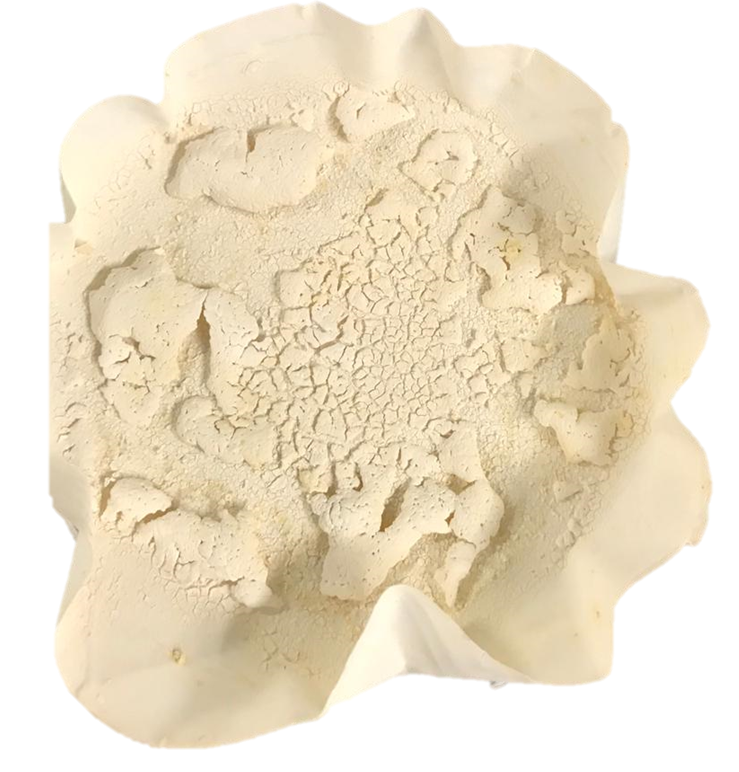
\includegraphics[width=0.3\linewidth]{Documento_Latex/Tesis_1/Imagenes/capsulas.png}
    \caption{Silica microcapsules obtained by the methodology described in section \ref{sec:capusules}}
    \label{fig:capsules}
\end{figure}

\subsection{Film Elaboration} \label{sec:film_elaboration}
Once having 9g of nanocapsules, a masterbatch is prepared by mixing the nanocapsules load and polypropylene-maleic anhydride graft copolymer (PP-g-MAH) in a  20:80 mass proportion respectively. Before entering the sample into the internal mixer, this has to be preheated for 10 minutes so that it reaches a temperature of 190\degree C, after which the mix is poured and stays within 7 minutes at a speed of 60rpm. The material obtained must then be frozen to a temperature of -80\degree C for 3 hours. Afterward, it has to be taken into a blade mill for grinding for 2 minutes and in this way, the masterbatch is ready to be mixed with polypropylene homo-polymer (PP) to form the films. The quantity of masterbatch used is so that the nanocapsule load is 5\% of the total film weight. These two components go again through the same process of mixing as the masterbatch did. Finally, the process of compression molding is done by using a press. To do this, two aluminum foils and two Teflon foils are put over the two sides of the press, and in the inferior part of it, a quantity of 12g of the PP mixture is poured using a 19cm x 19cm x 3cm aluminum frame. The inferior and superior plates are both preheated to a temperature of 190\degree C and the press must be configured so that an initial pressure of 15 bar is applied during 1 minute and then a pressure of 110 bar must be applied during 1.5 minutes after which a 10 minutes cooling time is done. After this, the desired film of 19cm x 19cm with OS load is obtained (Figure \ref{fig:film}).

\begin{figure}[ht]
    \centering
    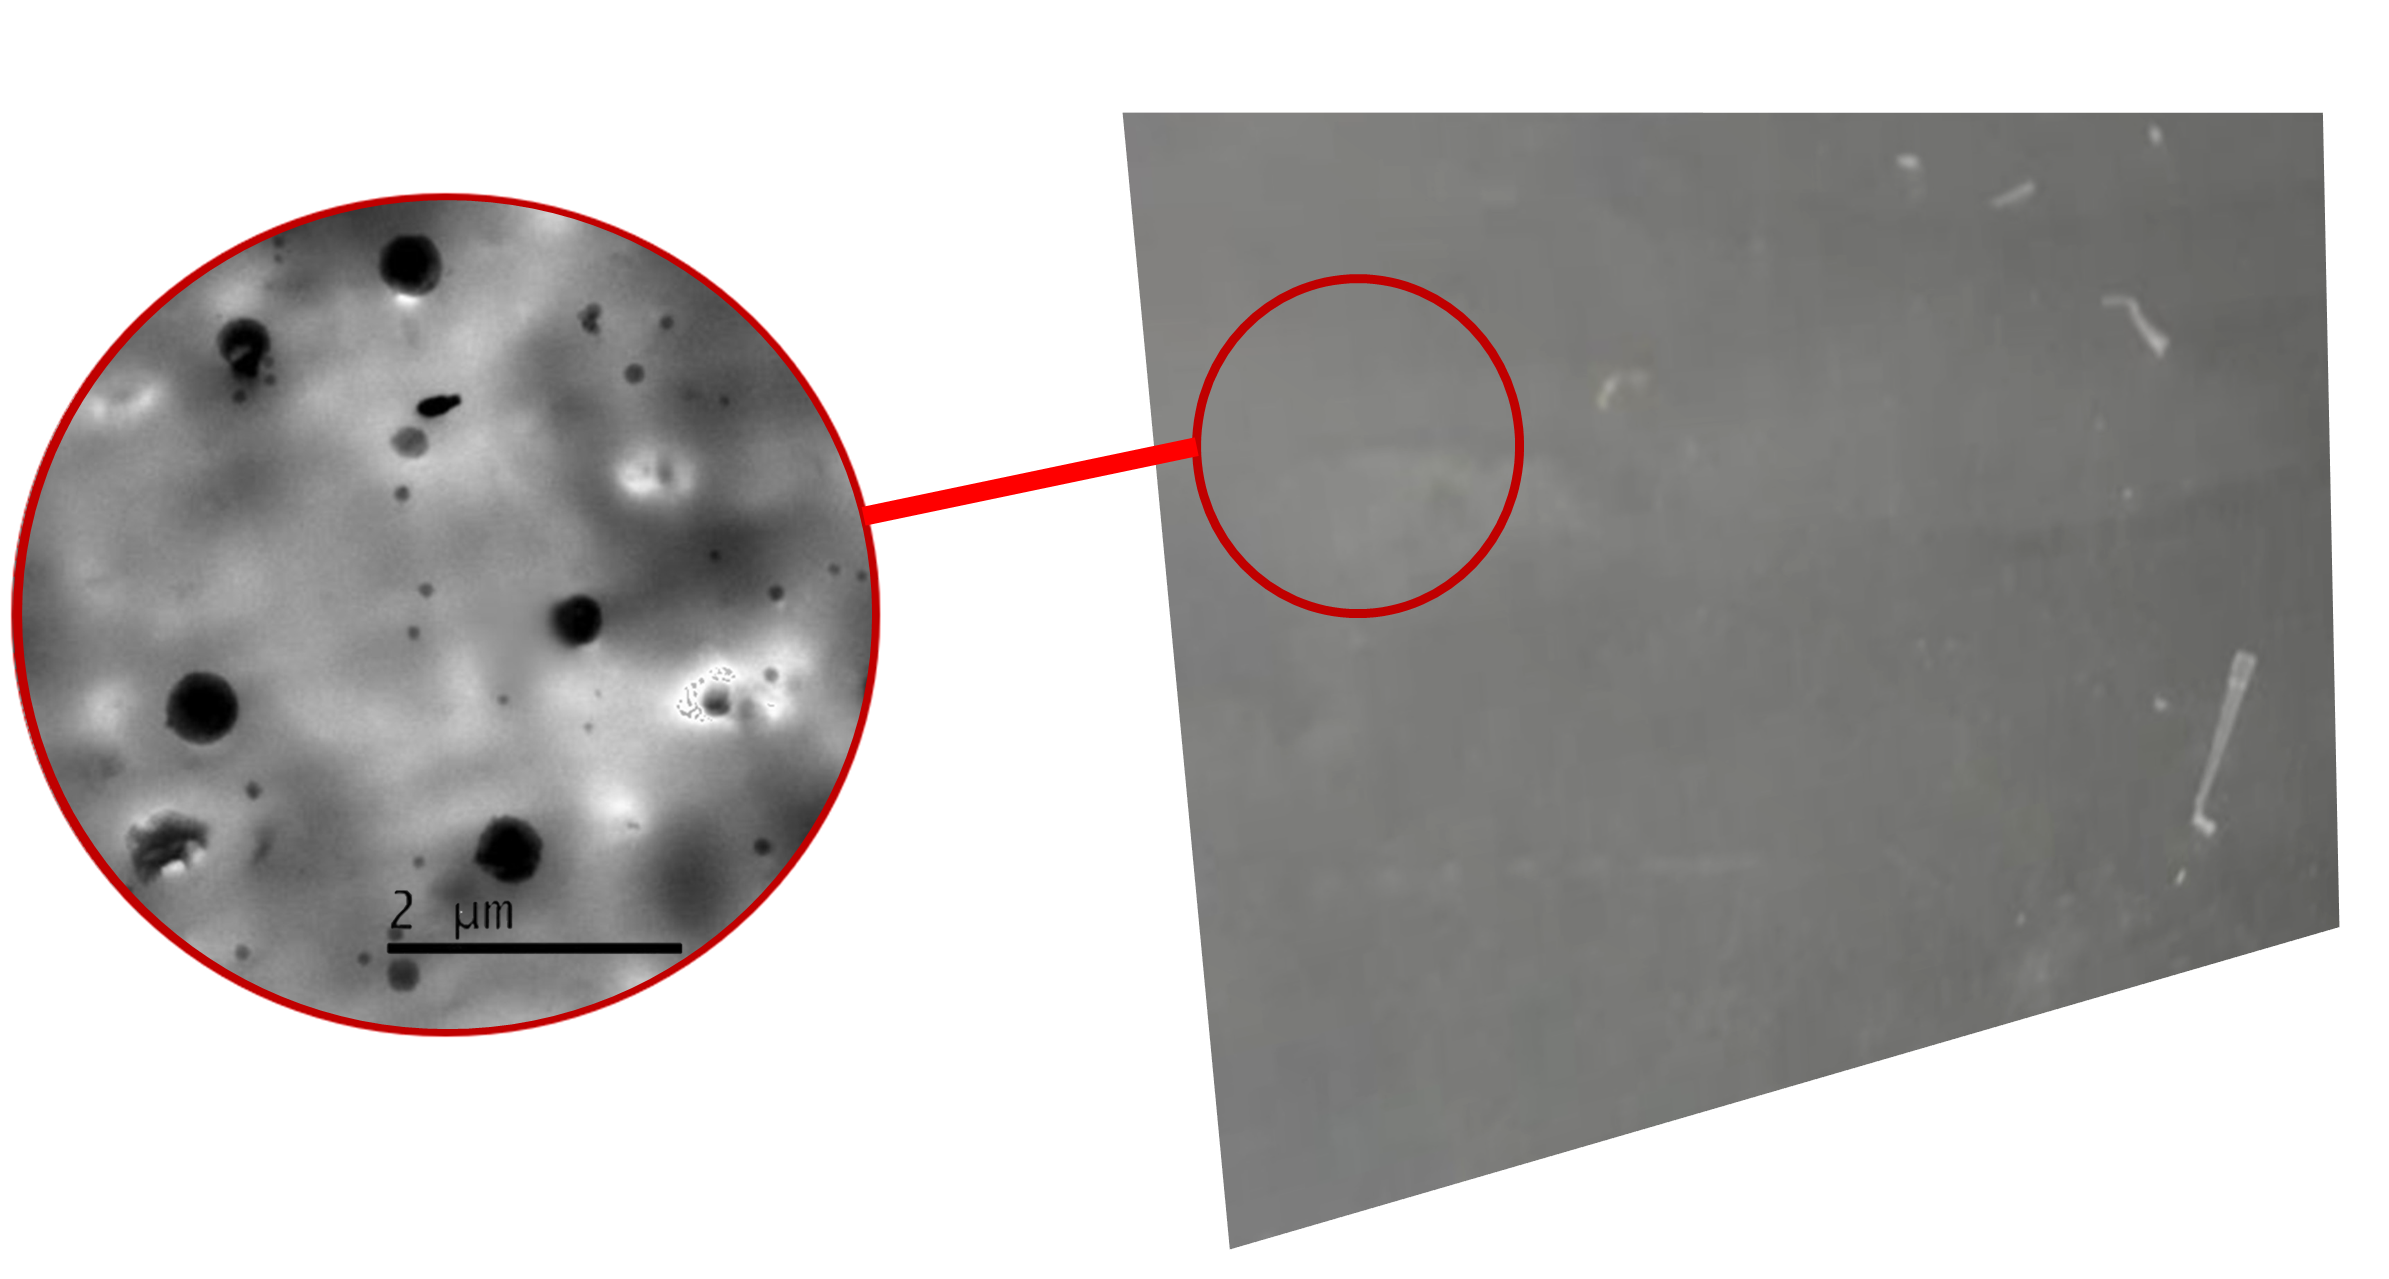
\includegraphics[width=0.6\linewidth]{Documento_Latex/Tesis_1/Imagenes/pelicula.png}
    \caption{PP film containing silica microcapsules which were incorporated by the methodology described in section \ref{sec:film_elaboration} \cite{ArellanoAyala2019EfectosAntioxidantes}}
    \label{fig:film}
\end{figure}

\subsection{Headspace Oxygen Absorption Test}\label{subsec:headspace}
Head-space oxygen absorption is one of the two tests which enables to study the performance of the OS film, and its results together with the oxidative TGA are the ones that are used to verify the prediction capacity of the model proposed. To do this test, a Quantek 901 head-space oxygen analyzer was be used. First, a sample of the film made is placed within a 100mL glass bottle. This bottle is sealed by pressurizing its cap, after which it is ready to test. To perform the test, in the cap of the bottle, a plastic seal will be put and perforation with a needle will be made through it (See Figure \ref{fig:headspace}).

\begin{figure}[ht]
    \centering
    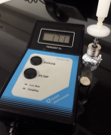
\includegraphics[width=0.25\textwidth]{Imagenes/headspace.png}
    \caption{Headspace oxygen absorption test}
    \label{fig:headspace}
\end{figure}

The gas extracted from the bottle goes by a syringe to a ''fuel cell" type oxygen sensor, which consists of a diffusion barrier, a sensing electrode made of platinum and a working electrode made of zinc, all submerged in a solution of potassium hydroxide which acts as an electrolyte \cite{Boissevain1996CorporateGuide}. The entering oxygen diffuses into the sensor a reduces to hydroxyl ions at the cathode.

 \reaction{O2 +2H2O +4e^- -> 4OH^-}
the hydroxyl ions formed are oxidized at the zinc anode.
 \reaction{2Pb + 4OH^- -> 2PbO +2H2O + 4e^-}
 which yields an overall cell reaction 
 \reaction{2Pb + O2 -> 2PbO}

 
 The current generated during this reaction is proportional to the concentration of oxygen present in the medium. With this in mind,  the sensor measures these currents and calculates the quantity of oxygen within the air \cite{GarciaMora2015KineticScavengers, Boissevain1996CorporateGuide}. This test was carried out every 12 hours until the oxygen concentration becomes constant in time, which indicates that the oxygen absorption on behalf of the film has stopped and so its useful life. It is essential to mention that for avoiding external air for entering the vial, each one of this was punctured once, and then it was discarded. Negative control was carried out for each head-space test done. For every puncture made, a  quantity of 4 ml of air is extracted from the bottle; this was calibrated, taking into account the advice from the manufacturer. The analyzer Quantek model 901 has a resolution of 0.1\% and an accuracy of $\pm$0.1\% in reading \cite{Instruments2019ModelAnalyzer}. 
 
\subsection{Oxidative TGA}
The second oxygen uptake performance test, which was made on OS films and linseed oil individually, is a thermogravimetric analysis (TGA). Given that in the autoxidation process described in Section \ref{subsec:PUFA_os}, there is an increase in the weight of oils due to the absorption of oxygen from the environment. Even though these changes in weight are minimal, they are big enough for being detected in the thermogravimetric analysis. So to determine the performance of the films and the oil, three TGA must be carried out. All tests were made using an SDT Q600 (TA instruments) with isothermal curves at 40\degree C, 60\degree C, 80\degree C, and 110\degree C and a heating rate of 20\degree C/min with a sample mas of 4 mg. The first TGA test carried out was under a nitrogen atmosphere. This is done to observe the sole effect of the flow of air around linseed oil and OS films. In this case, the volatile components within the sample are going to evaporate, generating a reduction in the measured mass. The second TGA test, which has to be carried is in a pure oxygen atmosphere. This is the case in which oxygen is in excess concerning the substrate, so the kinetics of oxidation can be simplified, as explained in section \ref{subsec:PUFA_os}. The results in the change of mass of the sample obtained are normalized for the mass reduction due to the evaporation obtained from the nitrogen atmosphere TGA. In this way, there is a guarantee that the changes observed in the mass on the oxygen TGA are exclusively due to the absorption of oxygen. The third and final TGA made was in air atmosphere, in which oxygen has a concentration of 21 vol\%. Contrary to the case of oxygen atmosphere TGA, in this case, it is not correct to assume that oxygen is in excess to the substrate in the oil, so the results obtained in this test must be compared to the complete autoxidation kinetics of the linseed oil.   

\section{Computational Methodology}\label{sec:computational methodology}
In this section of the document, an explanation of how the development of the computational tool was made is described. The first step taken towards fulfilling this objective was using conservation equations to establish a PDE which describes the dynamics of oxygen within linseed oil and OS polymeric films, this was developed both for monolayer films and for the multilayer films. Therefore, to evaluate the validity of the model developed, a new adjustment of the kinetic constant and initial concentrations was made over linseed oil kinetics. Once having determined the kinetic constants that describe the oxidation of linseed oil, a study of different numerical methods was made to find out which of these enabled a fast and accurate solution of the differential equations established from the mathematical models. Finally, once studied the method by which the model is solved, a graphic interface was developed so that an external user may study the effect of different parameters on the $O_2$ absorption. An explanation of how this interface was made is explained at the end of this section. 

\subsection{Model Description}\label{subsec:model_desc.}

\subsubsection{Mono Layer Film}
The main idea in developing a model that describes the oxygen uptake by an OS film is to replicate the results obtained experimentally by the Headspace oxygen test described in section \ref{subsec:headspace}. To establish this model, a film of Area $A$ and thickness $L$, which is inside a bottle volume $V$ and at constant temperature $T$ is considered. The gas in the bottle considered has an initial oxygen molar concentration $C_{ext_o}$. The situation described is shown in figure \ref{fig:model_diagram}. 

\begin{figure}[ht]
    \centering
    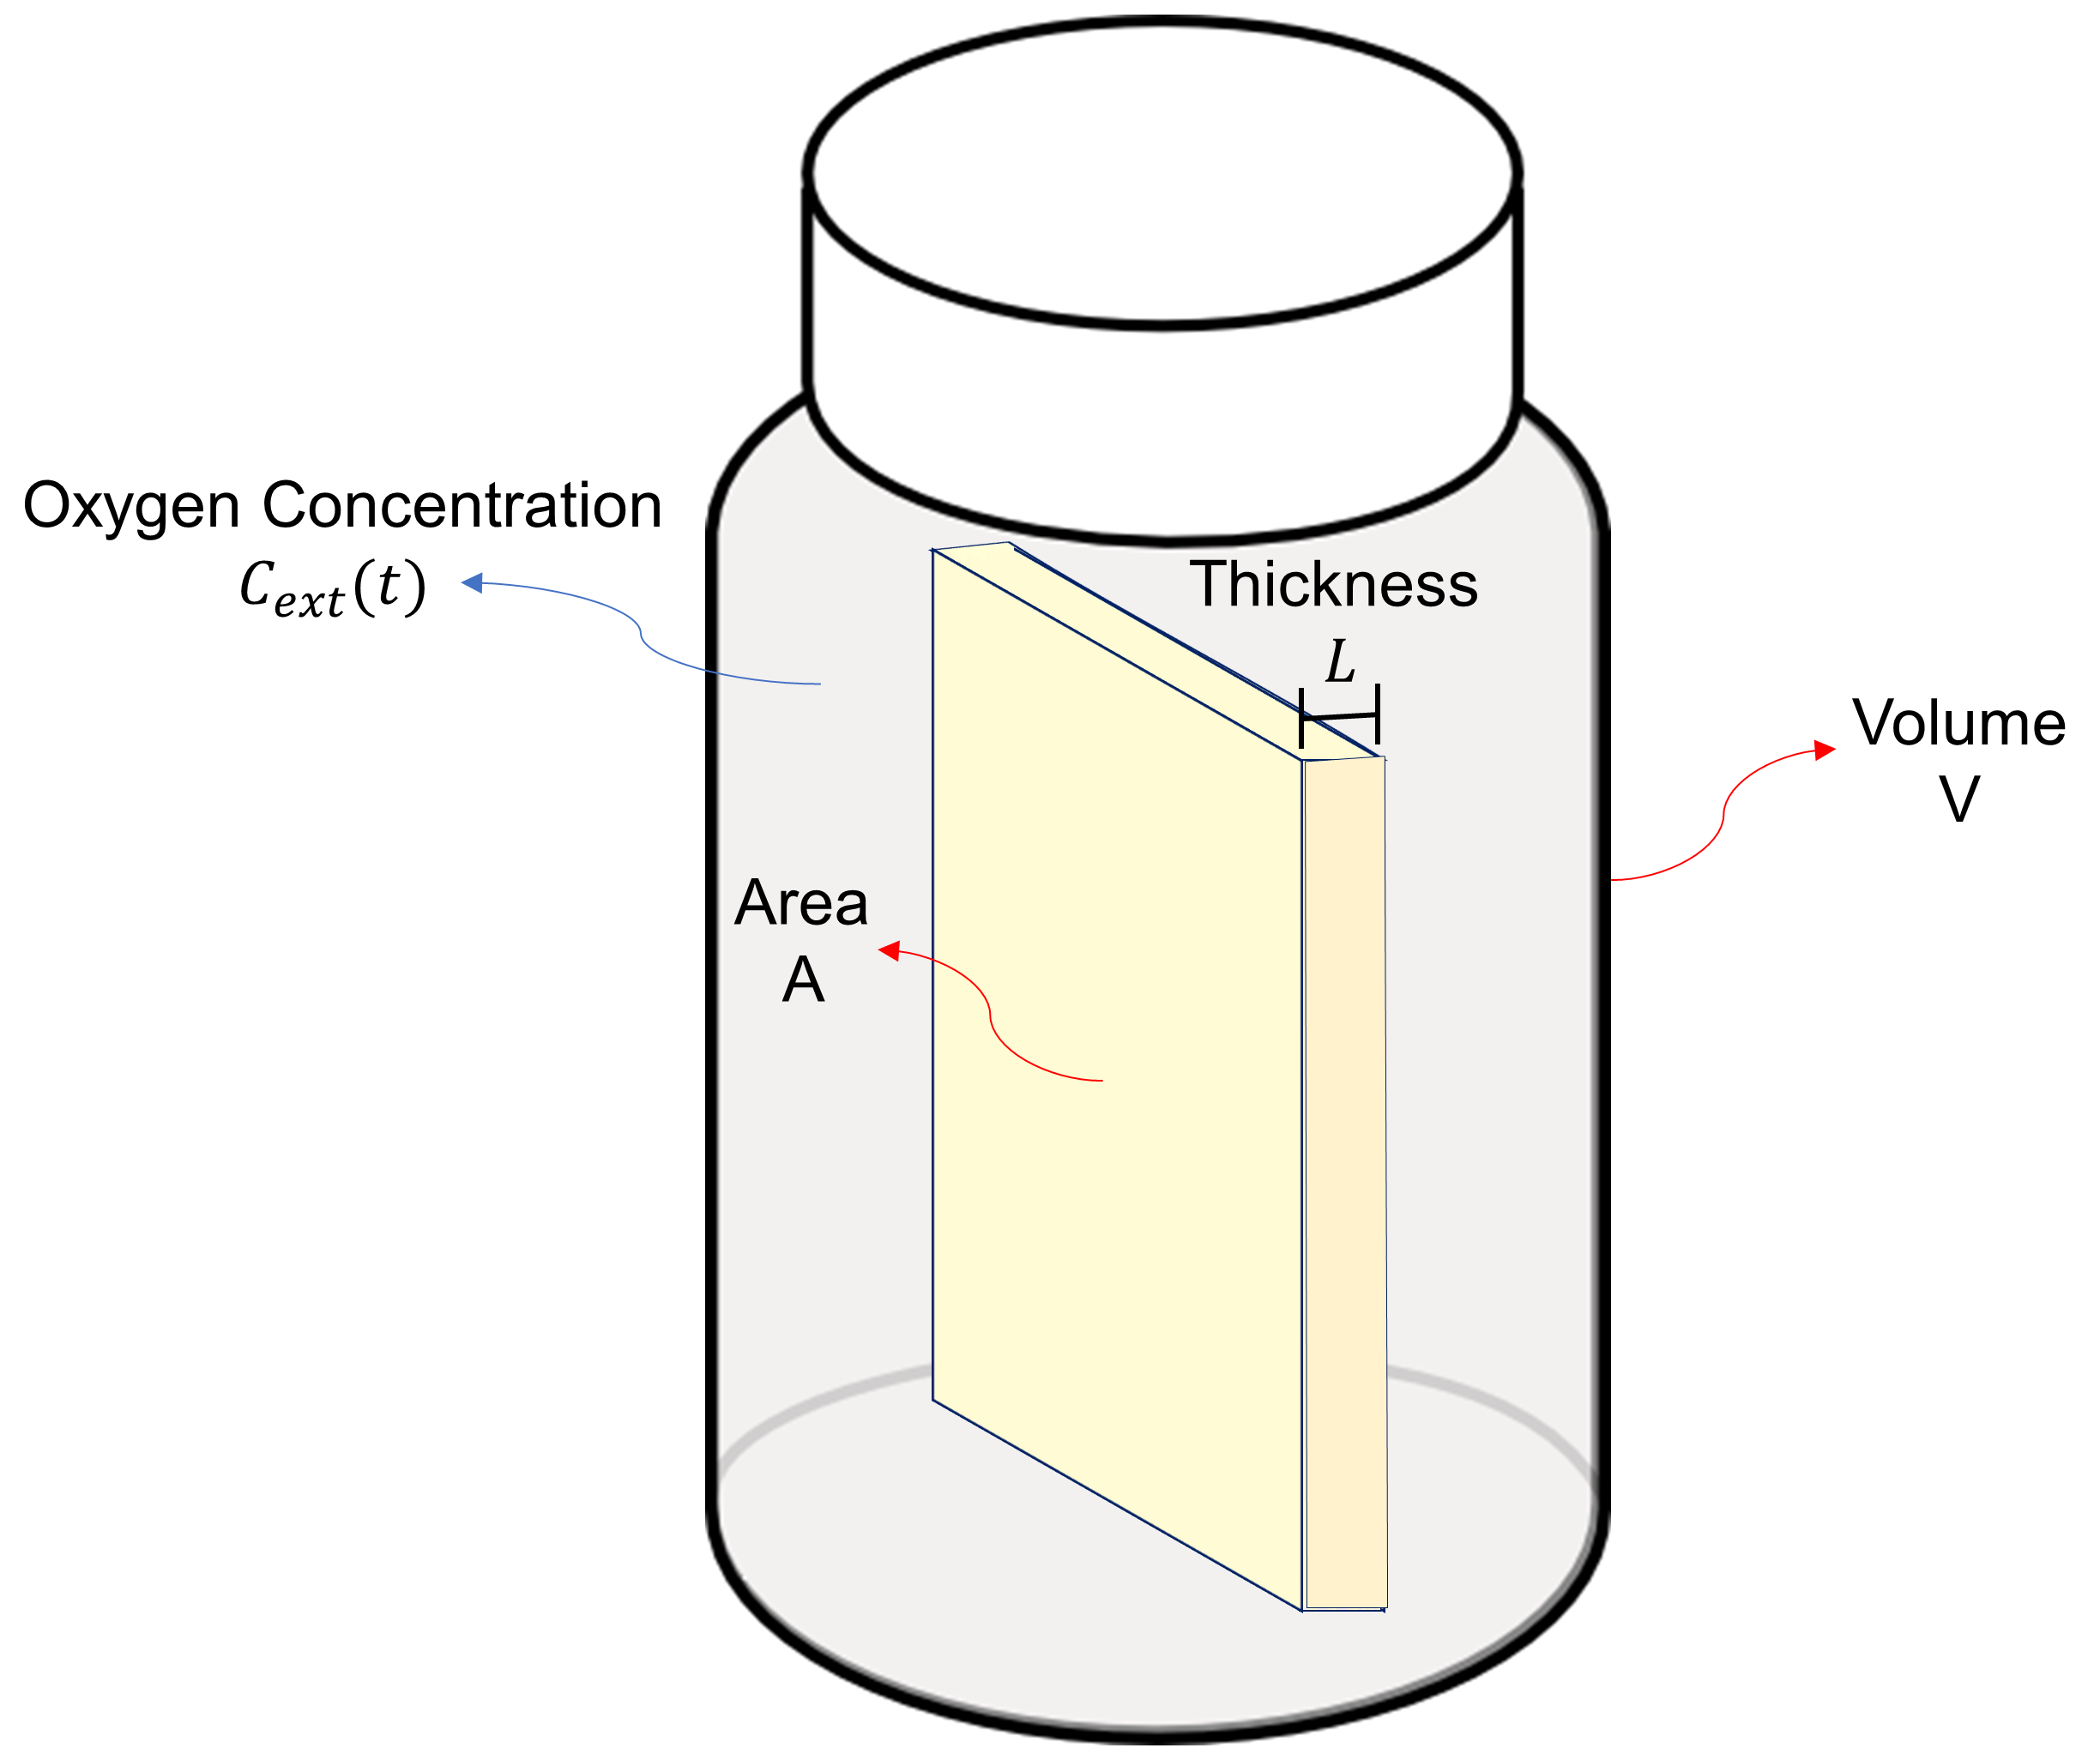
\includegraphics[width=0.5\linewidth]{Documento_Latex/Tesis_1/Imagenes/modelo.png}
    \caption{Schematic diagram of the OS film in a vial with oxygen concentration $C_{ext}$}
    \label{fig:model_diagram}
\end{figure}

In this case, the homogeneous film approach is going to be used. This considers the whole film as reactive with an initial OS volumetric concentration $C_{OS_0}$. For the initial conditions of the model, it was assumed that there is no oxygen consumption or diffusion in the process of compression molding, which is why the initial molar concentration of oxygen in the film is $[O_2]=0 \hspace{5pt} mol/cm^3$.  It is essential to state that in this model, oxygen will be assumed to enter by both faces of Area $A$ and given that this area is much bigger than the thickness $L$ of the film, then the propagation of oxygen into the foil can be assumed to be one dimensional in the direction normal to its faces (Figure \ref{fig:model_diagram}).

Now assuming that the film is isotropic, the diffusion of oxygen through it is going to be given by Fick's first law, which allows calculating the molar diffusive flux as the product of the diffusivity of oxygen in the polymer and the gradient of the $O_2$ concentration within the film (Equation \ref{eq:flux}).

\begin{equation}
    J=-D_{O_2}\nabla [O_2] \xrightarrow{1D}J_x=-D_{O_2}\frac{\partial [O_2]}{\partial x}
    \label{eq:flux}
\end{equation}

In the previous equation, $J$ represents the molar flux of oxygen and $D$ is the diffusivity of oxygen in the polymer material which the film is made of. The equation stated before indicates that the flux will go in the direction in which the concentration of $O_2$ decreases; this suggests that the mass will move towards reducing the concentration gradient in the system. Now, applying this to the oxygen molar balance, the equation \ref{eq:mass_bal_dif} is obtained. 

\begin{equation}
    \frac{\partial [O_2]}{\partial t}= -\nabla \cdot J= \frac{\partial}{\partial x} \left(D_{O_2}\frac{\partial [O_2] }{\partial x}\right)
    \label{eq:mass_bal_dif}
\end{equation}

This last equation is the transient diffusion equation and describes how any species propagates in a medium given a gradient in its concentration. In this case, given that the film is assumed to be reactive, a source/sink term must be taken into account in the prior equation due to the consumption of oxygen by the OS.

\begin{equation}
    \frac{\partial [O_2]}{\partial t}= \frac{\partial}{\partial x} \left(D_{O_2}\frac{\partial [O_2] }{\partial x}\right)+ R
    \label{eq:mass_bal_dif_reacc}
\end{equation}

The equation \ref{eq:mass_bal_dif_reacc}, corresponds to the one dimensional transient diffusion-reaction equation, in which $R$ represents the reactive term. By describing mass conservation in the system with equation \ref{eq:mass_bal_dif_reacc}, there is an assumption that no convection occurs within the vial so there is no net flow of the oxygen in the polymeric film and the only movement of this specie is given by concentration gradients. Now to describe the reactive term shown in the last equation, the kinetic model presented by Garcia \cite{GarciaMora2015KineticScavengers} for describing linseed oil autoxidation is going to be used with a modification on the termination equation of peroxyl radicals (this modification is explained in section). This model assumes that the reactions which occurs during oxidation are:

\reaction[reacc:initiation]{2ROOH ->[k_1] ROO^. +R^. + carbonyl + Scission}
\reaction[reacc:O_2 consumption]{R^. + O2 ->[k_2] ROO^.}
\reaction[reacc: propagation]{ROO^. + RH ->[k_3] ROOH + R^.}
\reaction[reacc:termination_2alkyrad]{R^. +R^. ->[k_4] $\text{Inactive Products}$}
\reaction[reacc:termination_alky_peroxide_rad]{R^. +ROO^. ->[k_5] $\text{Inactive Products}$}
\reaction[reacc:termination_2peroxide_rad]{ROO^. +ROO^. ->[k_6] $\text{Inactive Products}$}

Where $ROOH$ is hydroperoxide, $RH$ is the substrate and \ce{R^.}, \ce{ROO^.} are the alkyl and peroxyl radicals respectively. By assigning a simple kinetics using the rate law expression the following system of ordinary differential equations (ODE) is obtained:

\begin{gather}
    \frac{d[\ce{R^.}]}{dt}= k_1[ROOH]^2 - k_2 [\ce{R^.}][O_2]+ k_3[\ce{ROO^.}][RH]-2k_4[\ce{R^.}]^2 -k_5[\ce{R^.}][\ce{ROO^.}]\label{eq:consum_R.}\\
    \frac{d[\ce{ROO^.}]}{dt}= k_1[ROOH]^2 + k_2 [\ce{R^.}][O_2]- k_3[\ce{ROO^.}][RH]-k_5[\ce{R^.}][\ce{ROO^.}]-2k_6 [ROO^.]^2\\
   \frac{d[ROOH]}{dt}= -2k_1[ROOH]^2 + k_3[\ce{ROO^.}][RH]\\
   \frac{d[RH]}{dt}=-k_3[\ce{ROO^.}][RH]\label{eq:consum_RH}\\
   \frac{d[O_2]}{dt}= -k_2[\ce{R^.}][O_2]\label{eq:consum_O2}
\end{gather}

Combining the equations \ref{eq:mass_bal_dif_reacc} and \ref{eq:consum_O2}, the oxygen mass balance can be expressed as:

\begin{equation}
     \frac{\partial [O_2]}{\partial t}= \frac{\partial}{\partial x} \left(D_{O_2}\frac{\partial [O_2] }{\partial x}\right) -k_2[\ce{R^.}][O_2].
    \label{eq:mass_bal_def}
\end{equation}

This last equation together with equations \ref{eq:consum_R.} to \ref{eq:consum_RH} are going to describe the dynamics of oxygen concentration within the film. Also, this are the ones that are going to be numerically solved (this is going to be explained in section \ref{subsec:numerical_methodology.}). On the other hand, the total quantity of oxygen absorbed by the film is calculated by integrating the mass flow of oxygen into it. 

\begin{equation}
    m_{O_2}(t)= \int_0^t \dot{m}dt =M_{O_2}A\int_0^t Jdt 
\end{equation}

To arrive at the right-hand side of the equation, mass flux was calculated by multiplying the molar flux $J$ by the molecular weight of oxygen $M_{O_2}$, while the mass flow was calculated by multiplying the mass flux by the film area $A$. It is essential to state that the flux $J$ used to calculate the total mass of oxygen in the film is the sum of the flux at both faces of the film, $J= J_x\rvert_{x = 0} - J_x\rvert_{x = L}$. But given that the concentration $[O_2]$ is symmetrical concerning the film, the flux at both faces will be equal in magnitude, so $J=2J_x\rvert_{x = 0}$.  Now replacing the definition of molar flux (Equation \ref{eq:flux}) into the previous expression

\begin{equation}
    m_{O_2}(t) =-2D_{O_2}AM_{O_2}\int_0^t \frac{\partial [O_2]}{\partial x}\biggr\rvert_{x = 0}dt
    \label{eq:total_mass_O2}
\end{equation}

This last expression will enable to calculate the oxygen uptake profile through time as well as the head space oxygen concentration profile (Equation \ref{eq:headspace}). 

\begin{equation}
    C_{ext}(t)= C_{ext_o} - \frac{1}{M_{O_2}V} m_{O_2}(t)= C_{ext_o} + \frac{2AD_{O_2}}{V} \int_0^t \frac{\partial [O_2]}{\partial x}\biggr\rvert_{x = 0}dt
    \label{eq:headspace}
\end{equation}

This last quantity, $C_{ext}(t)$, is of great interest,
because it is the one that the headspace test
allows to obtain experimentally, so the model
will seek to predict the behavior of this quantity
overtime. Concerning the initial and boundary conditions in this problem, as stated at the beginning of this section the film is going to be considered to be devoid of $O_2$ and the external headspace oxygen concentration is going to be $C_{ext_o}$. Also concerning the initial concentration of the reacting species in the linseed oil (i.e. hydroperoxide,substrate, alkyl, and hydroxyl radicals) is it assumed that they are going to be uniform through the whole film (Equation \ref{eq:ic_mono_film}). 

\begin{align}
    &\text{IC: } & &[O_2](x,t=0)=0, & &C_{ext}(t=0)= C_{ext_o},\nonumber\\
    && &[\ce{RH}](x,t=0)=C_{OS}[\ce{RH}]_o,   & &[\ce{ROOH}](x,t=0)=C_{OS}[\ce{ROOH}]_o, \nonumber\\
    && &[\ce{R^.}](x,t=0)=C_{OS}[\ce{R^.}]_o,   & &[\ce{ROO^.}](x,t=0)=C_{OS}[\ce{ROO^.}]_o. 
    \label{eq:ic_mono_film}
\end{align}
    
The quantities $[\ce{RH}]_o$, $[\ce{ROOH}]_o$,  $[\ce{R^.}]_o$, and $[\ce{ROO^.}]_o$ are the respective molar concentrations of chemical species in Linseed oil and $C_{os}$ is the charge of OS scavenger in the film. This latter quantity is calculated by multiplying the mass charge of OS in the film (wt\%) by the reason between the oil and the film density (Equation \ref{eq:load_concentration}).

\begin{equation}
    C_{OS}= \text{Oil wt}\% \frac{\rho_{polymer}}{\rho_{oil}}
    \label{eq:load_concentration}
\end{equation}

On the other hand, given that the molar balance of oxygen in the film has second-order derivative respect to the spatial component, it is necessary to establish two boundary conditions over the film so that the problem stated has a solution. These conditions are given in the outer face of the film, which is in contact with the head-space gas. In this case, oxygen dissolved in the boundary face of the film must be in equilibrium with the external oxygen. This equilibrium is described by Henry's law which states that the partial concentration of the oxygen dissolved in the polymer is proportional to the partial pressure of oxygen in the head-space gas (i.e. $[O_2](x=0, L)=s\hspace{2pt}p_{O_2}$ ). The relation between the partial pressure of oxygen and its'external concentration is obtained assuming that the gas in the vial behaves as an ideal gas.  In that case $p_{O_2}=RTC_{ext}(t)$, and so the boundary conditions for oxygen concentration in the film are:

\begin{align}
    &\text{BC:} & &[O_2](x=0, t)= \left(sRT\right) C_{ext}(t) & & [O_2](x=L, t)= \left(sRT\right) C_{ext}(t)
    \label{eq:bc_mono_film}
\end{align}

With these set of initial and boundary conditions, the complete set of conditions necessary to solve the problem is established.

\subsubsection{Multi-layer Film}
Continuing with the presentation of the mathematical models developed for the creation of an OS film modeling tool, the case of a multilayer system was considered. The situation studied was a multilayer OS film with total thickness $L$,  composed of  $n$ layers, each one of thickness $L_i, 0<i<n$ where  $L_i\neq L_j, \forall  i\neq j$ and made of a different material. The film has a face of area $A$ and is inside a vial of volume $V$ with an initial headspace oxygen concentration $C_{ext_o}$. The situation described is shown in figure \ref{fig:model_multilayer_diagram}.

\begin{figure}[ht]
    \centering
    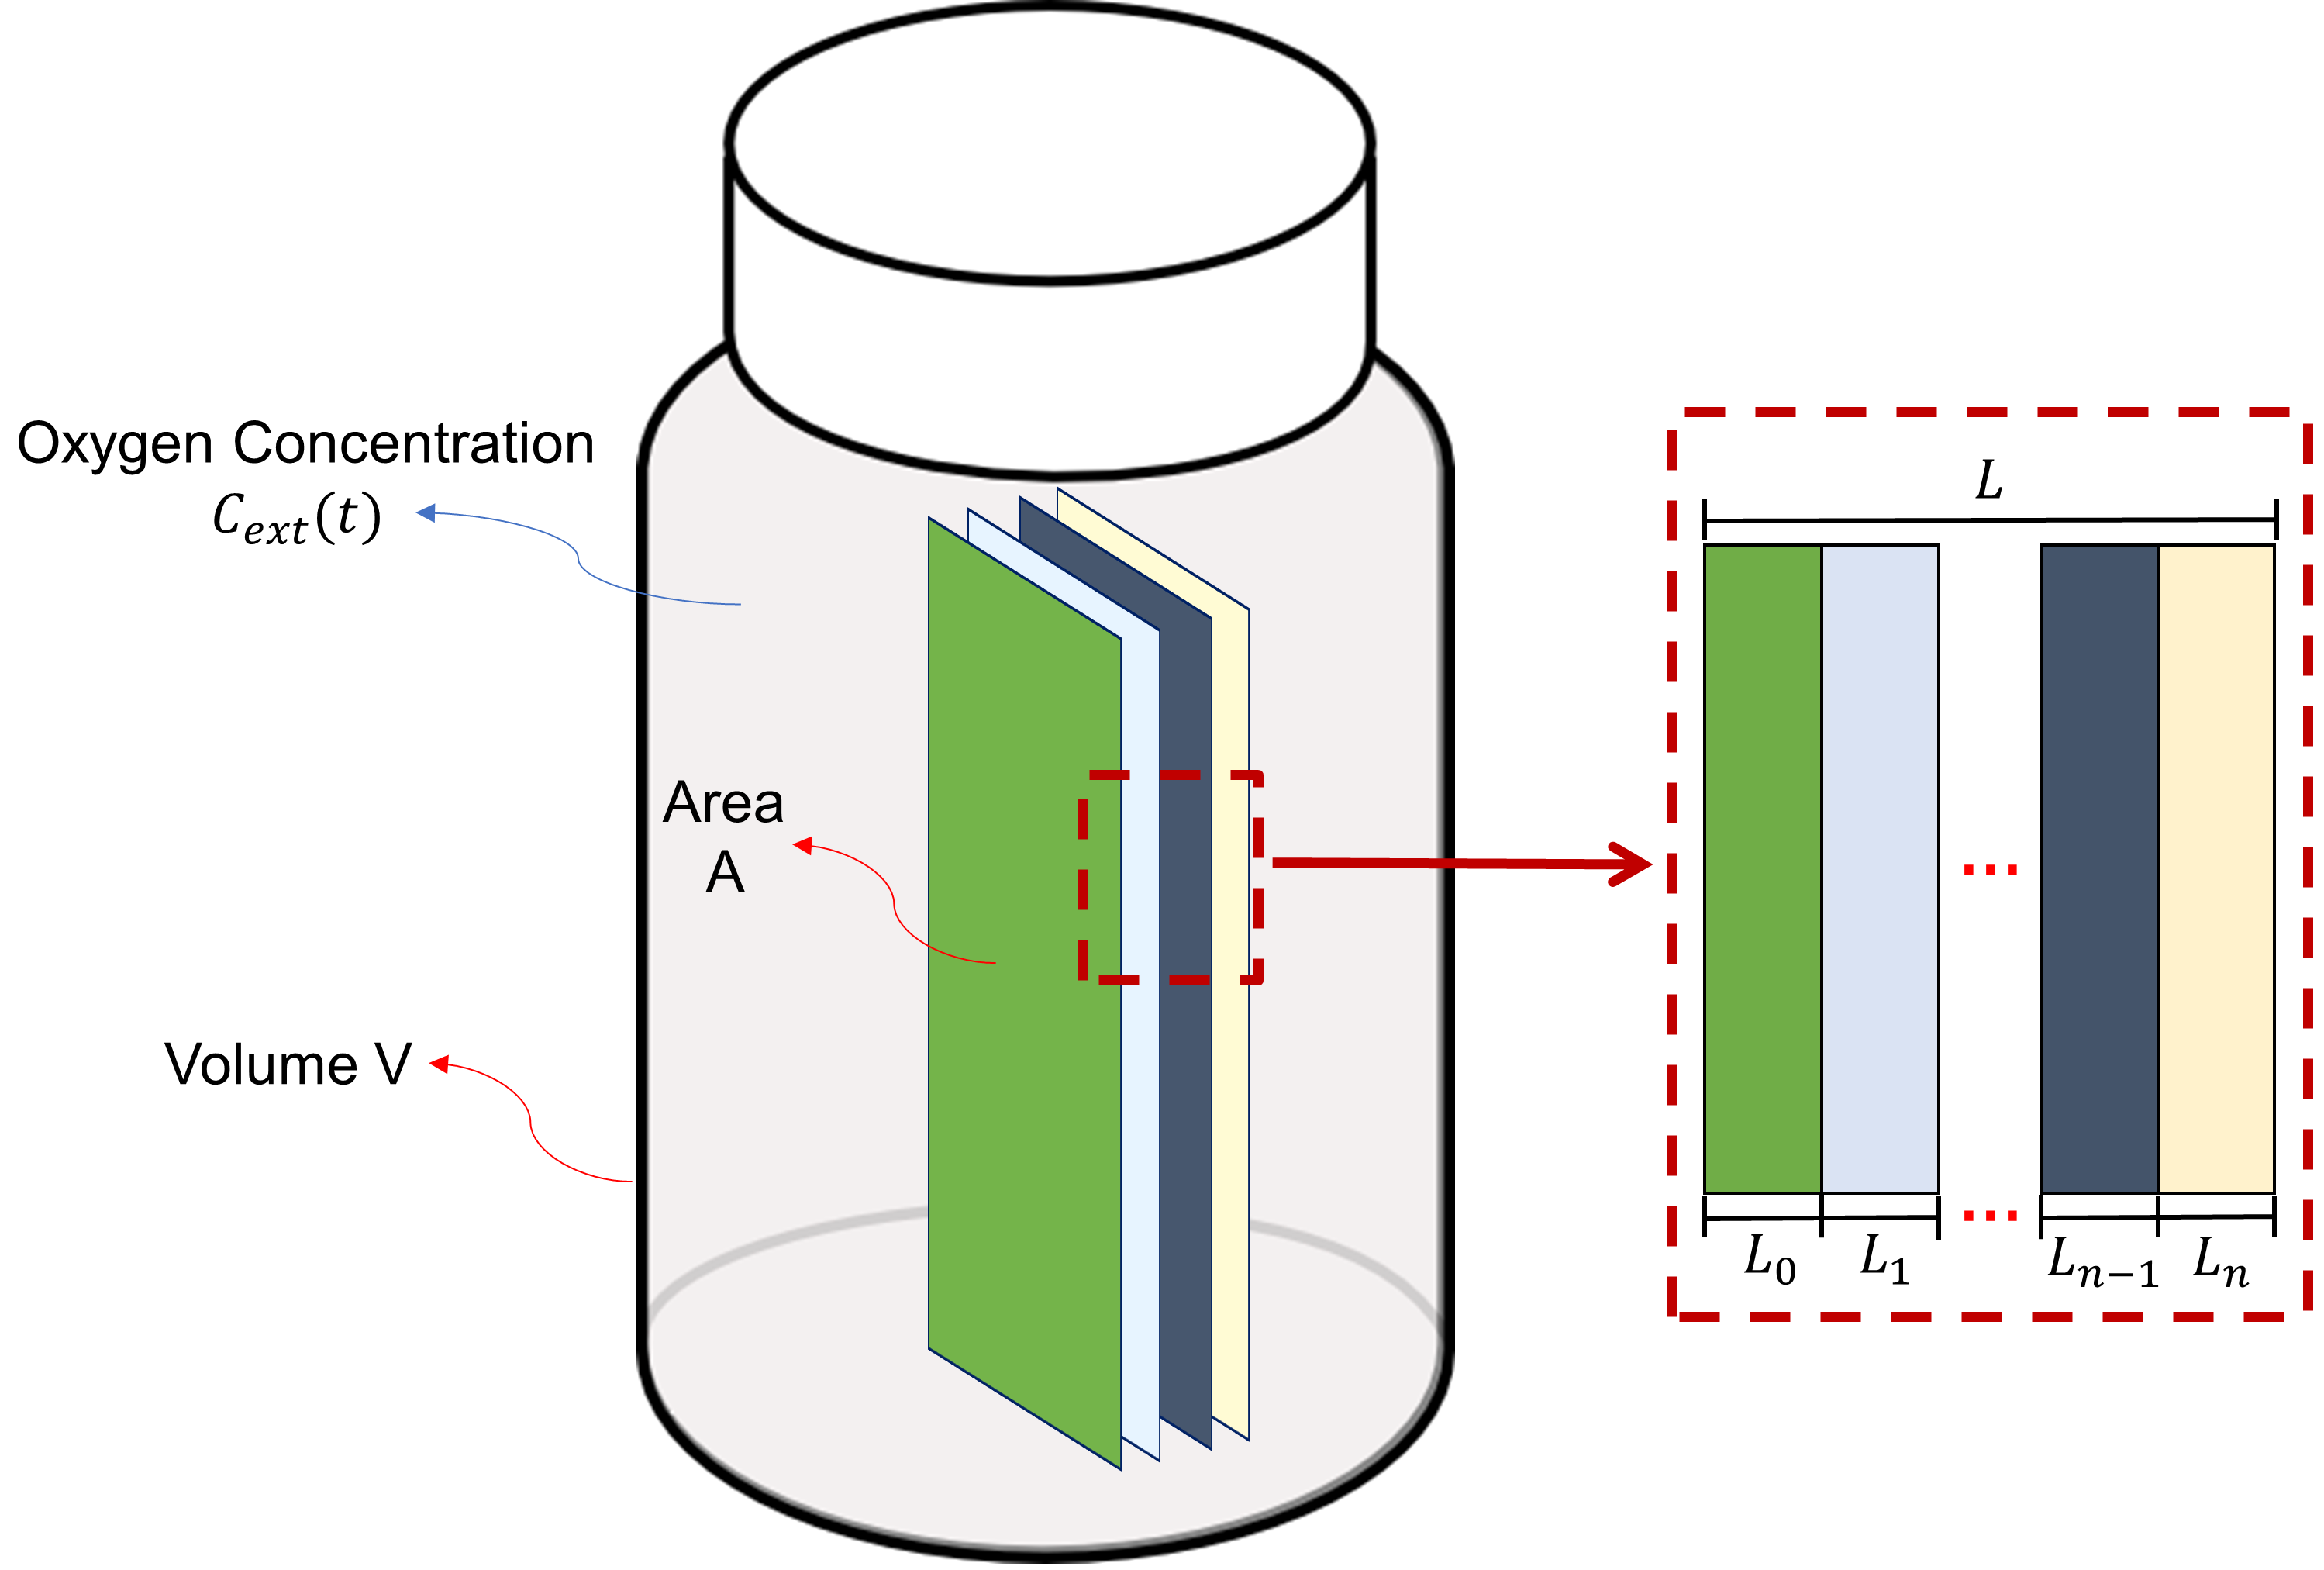
\includegraphics[width=0.62\linewidth]{Documento_Latex/Tesis_1/Imagenes/modelo_multicapa.png}
    \caption{Schematic diagram of a OS film composed of $n$ different layers in a vial with oxygen concentration $C_{ext}$}
    \label{fig:model_multilayer_diagram}
\end{figure}

The equation describing the dynamics of the reaction in the film are the same as equations \ref{eq:consum_R.} to \ref{eq:consum_RH}, while the expression regarding oxygen concentration dynamics in the film is going to be

\begin{equation}
    \frac{\partial [O_2]}{\partial t}= \frac{\partial}{\partial x} \left(D_{O_2}(x) \frac{\partial [O_2] }{\partial x}\right) -k_2[\ce{R^.}][O_2]
    \label{eq:mass_bal_def_multi}
\end{equation}

The main difference between the last equation and equation \ref{eq:mass_bal_def} is that the diffusivity of oxygen depends on the position $x$ in the film. The function that describes this dependence is :

\begin{align}
    D_{O_2}&=  D_i,  & L_{i-1}&< x< L_i,
\end{align}

where $D_i$ is the diffusivity of oxygen in the material of the $i$th-layer of the film. Now, given that the model assumes that all layers are of  different materials, then the flux of oxygen in both faces of the film is not going to be equal, i.e. $J_x\rvert_{x = 0}\neq-J_x\rvert_{x = L} $. This is why in this case the total oxygen mass absorbed by the film has to be calculated as:
\begin{equation}
    m_{O_2}(t) =-AM_{O_2}\int_0^t \left(D_{O_2}(x)\frac{\partial [O_2]}{\partial x}\biggr\rvert_{x = 0} -D_{O_2}(x)\frac{\partial [O_2]}{\partial x}\biggr\rvert_{x = L}\right )dt.
    \label{eq:total_mass_O2_multi}
\end{equation}

And so the headspace oxygen concentration profile is going to be given by:
\begin{equation}
    C_{ext}(t)=C_{ext_o} + \frac{A}{V} \int_0^t \left(D_{O_2}(x)\frac{\partial [O_2]}{\partial x}\biggr\rvert_{x = 0} -D_{O_2}(x)\frac{\partial [O_2]}{\partial x}\biggr\rvert_{x = L}\right) dt.
    \label{eq:headspace_multi}
\end{equation}

Besides the previous equations, there exists an internal boundary condition at the interface between any two collateral layers. This states that the flux of oxygen as well as it's partial pressure are continuous due to mass conservation. The partial pressure of a gas dissolved in a certain media is given by Henry's law, $p=sC$, where $s$ is the solubility of the gas in the media. Given that at the interface of the layer the partial pressure must be continuous:
 \begin{equation}
   p_{i}(x=L_i) =p_{i+1}(x=L_i)  \xrightarrow{}\frac{[O_2]_{i}(x=L_i)}{S_{i}} =\frac{[O_2]_{i+1}(x=L_i)}{S_{i+1}},
 \end{equation} where $p_{i}(x=L_i)$, $[O_2]_{i}(x=L_i)$ and $S_{i}$ is the partial pressure, concentration and solubility of oxygen in $ith$ layer of the film at position $x=L_i$ (which is the interface) and  $p_{i+1}(x=L_i)$, $[O_2]_{i+1}(x=L_i)$ and $S_{i+1}$ are the partial pressure, concentration and solubility of oxygen in the $i+1th$ film of the layer at the interface $x=L_i$. 

Lastly, to establish this model, boundary and initial conditions are necessary. For the latter conditions, this are the same ones established for the monolayer film (Equation  \ref{eq:ic_mono_film}) with the difference that $C_{OS}=f(x)$ (see equation \ref{eq:ic_multi_film}).

\begin{align}
    &\text{IC: } & &[O_2](x,t=0)=0, & &C_{ext}(t=0)= C_{ext_o},\nonumber\\
    && &[\ce{RH}](x,t=0)=C_{OS}(x)[\ce{RH}]_o,   & &[\ce{ROOH}](x,t=0)=C_{OS}(x)[\ce{ROOH}]_o, \nonumber\\
    && &[\ce{R^.}](x,t=0)=C_{OS}(x)[\ce{R^.}]_o,   & &[\ce{ROO^.}](x,t=0)=C_{OS}(x)[\ce{ROO^.}]_o. 
    \label{eq:ic_multi_film}
\end{align}

The reason why in this case $C_{OS}$ depends on the position of film is that not all the layers of the film are reactive. The layers which are inert, have no load of Linseed oil, while reactive layers are. This do not necessarily mean that  all have the same load of Linseed oil (i.e. $C_{OS_i}\neq C_{OS_{j}}, \forall i\neq j$). With this in mind, $C_{OS}(x)$  is given by the following expression:
\begin{equation}
    C_{OS}(x)= 
    \begin{cases}
    0  &\quad\text{if film }i \text{ is inert and } L_{i-1} \le x \ge L_i\\
    C_{OS_i}  &\quad\text{if film }i \text{ is reactive and }  L_{i-1} \le x \ge L_i,\\
    \end{cases}
\end{equation}
where $C_{OS_i}$ (the load of OS per layer) is calculated as:
\begin{equation}
    C_{OS_i}= \text{Oil wt}\%_i \left( \frac{\rho_{polymer_i}}{\rho_{oil}}\right).
    \label{eq:load_multi_concentration}
\end{equation}

On the other hand, the boundary conditions established for the monolayer film (Equation \ref{eq:bc_mono_film}) are valid for the multilayer case, with the difference that the solubility term on each boundary depends on the material of the exterior faces. Having said this, the boundary condition are going to be:
\begin{align}
    &\text{BC:} & &[O_2](x=0, t)= \left(s_0RT\right) C_{ext}(t) & & [O_2](x=L, t)= \left(s_nRT\right) C_{ext}(t),
    \label{eq:bc_multi_film}
\end{align}
where $s_o$ and $s_n$ are the oxygen solubility in the material of the first and last layer of the film. With the boundary and initial conditions established, the model for the multilayer film case is finished. 

\subsection{Numerical Resolution Methodology}\label{subsec:numerical_methodology.}
To obtain a solution to the models presented in section \ref{sec:modeling}, given the complexity of the system of differential equations to be solved, there exists the necessity of using numerical methods. Even though these methods do not enable us to find the exact solution of the problem, it does enables us to obtain an approximation of the analytical solution within an error interval, which depends on the implementation of the solution algorithm. In this case, given that the system of partial differential equations (PDE) which is needed to be solved is one dimensional, this system is going to be solved using finite differences techniques. These methods are based on the approximation of the definition of derivative to a finite difference, which can be solved algebraically (Equation \ref{eq:fin_dif}).

\begin{equation}
    \frac{df}{dx}\approx \frac{f(x_{i+1})-f(x_{i}) }{\Delta x}
    \label{eq:fin_dif}
\end{equation}

To use this technique, the domains in which the equations are going to be solved must be discretized. With this in mind, the spacial domain $x$ in which the diffusion and reaction of oxygen take place becomes $x_i$, which are $n$ discrete points that represent the whole domain. In the same way, time $t$ becomes $t_j$ where $0<j<m$, being $m$ the total number of steps taken in the time interval which is going to be solved. For solving the  system of equations \ref{eq:consum_RH} to  \ref{eq:mass_bal_def}
different finite-difference algorithms were evaluated to find which of these methods was able to solve the diffusion-reaction equation in a fast and stable way. In the next subsections, the methods which were taken into account for this are going to be described, as well as how these were applied to the PDE system of the OS film. 

\subsubsection{Methods of lines}
One of the most straightforward techniques used for numerically solving PDEs is the method of lines (MOL). This method enables to transform a system of PDEs to a system of ODEs, which in turn can be solved using ODE methods such as Runge-Kutta or backward difference formula (BDF), among others. To do this all the dimensions within the PDE equation must be discretized except one. In this case, the equation which is going to be solved is

\begin{equation*}
     \frac{\partial [O_2]}{\partial t}= \frac{\partial}{\partial x} \left(D_{O_2}\frac{\partial [O_2] }{\partial x}\right) -k_2[\ce{R^.}][O_2]
\end{equation*}

The variable which is going to be discretized is $x$ or the spacial dimension. This was chosen given that the only specie which has a spacial component in its mass balance is oxygen, the rest only varies along time. This implies that the reactive sites are fixed within the film. The discretization scheme chosen for the second derivative is a second-order central difference  (Equation \ref{eq:disc_diff}). 

\begin{equation}
    D_{O_2}\frac{\partial^2 [O_2]}{\partial x^2}= D_{O_2} \frac{[O_2]_{i-1}-2[O_2]_{i}+[O_2]_{i+1}}{(\Delta x)^2}
    \label{eq:disc_diff}
\end{equation}

Applying the previous equation into molar balance equation of oxygen the next expression is obtained:
\begin{equation}
     \frac{\partial [O_2]_i}{\partial t}=  D_{O_2} \frac{[O_2]_{i-1}-2[O_2]_{i}+[O_2]_{i+1}}{(\Delta x)^2} -k_2[\ce{R^.}]_i[O_2]_i.
     \label{eq:LOD_oxygen}
\end{equation}
This equation now represents an ordinary differential equation for $[O_2]_i$, which is a vector of variables of concentration of oxygen through the spacial domain which only depends on time (see Figure \ref{fig:LOD_diagram}).

\begin{figure}[ht]
    \centering
    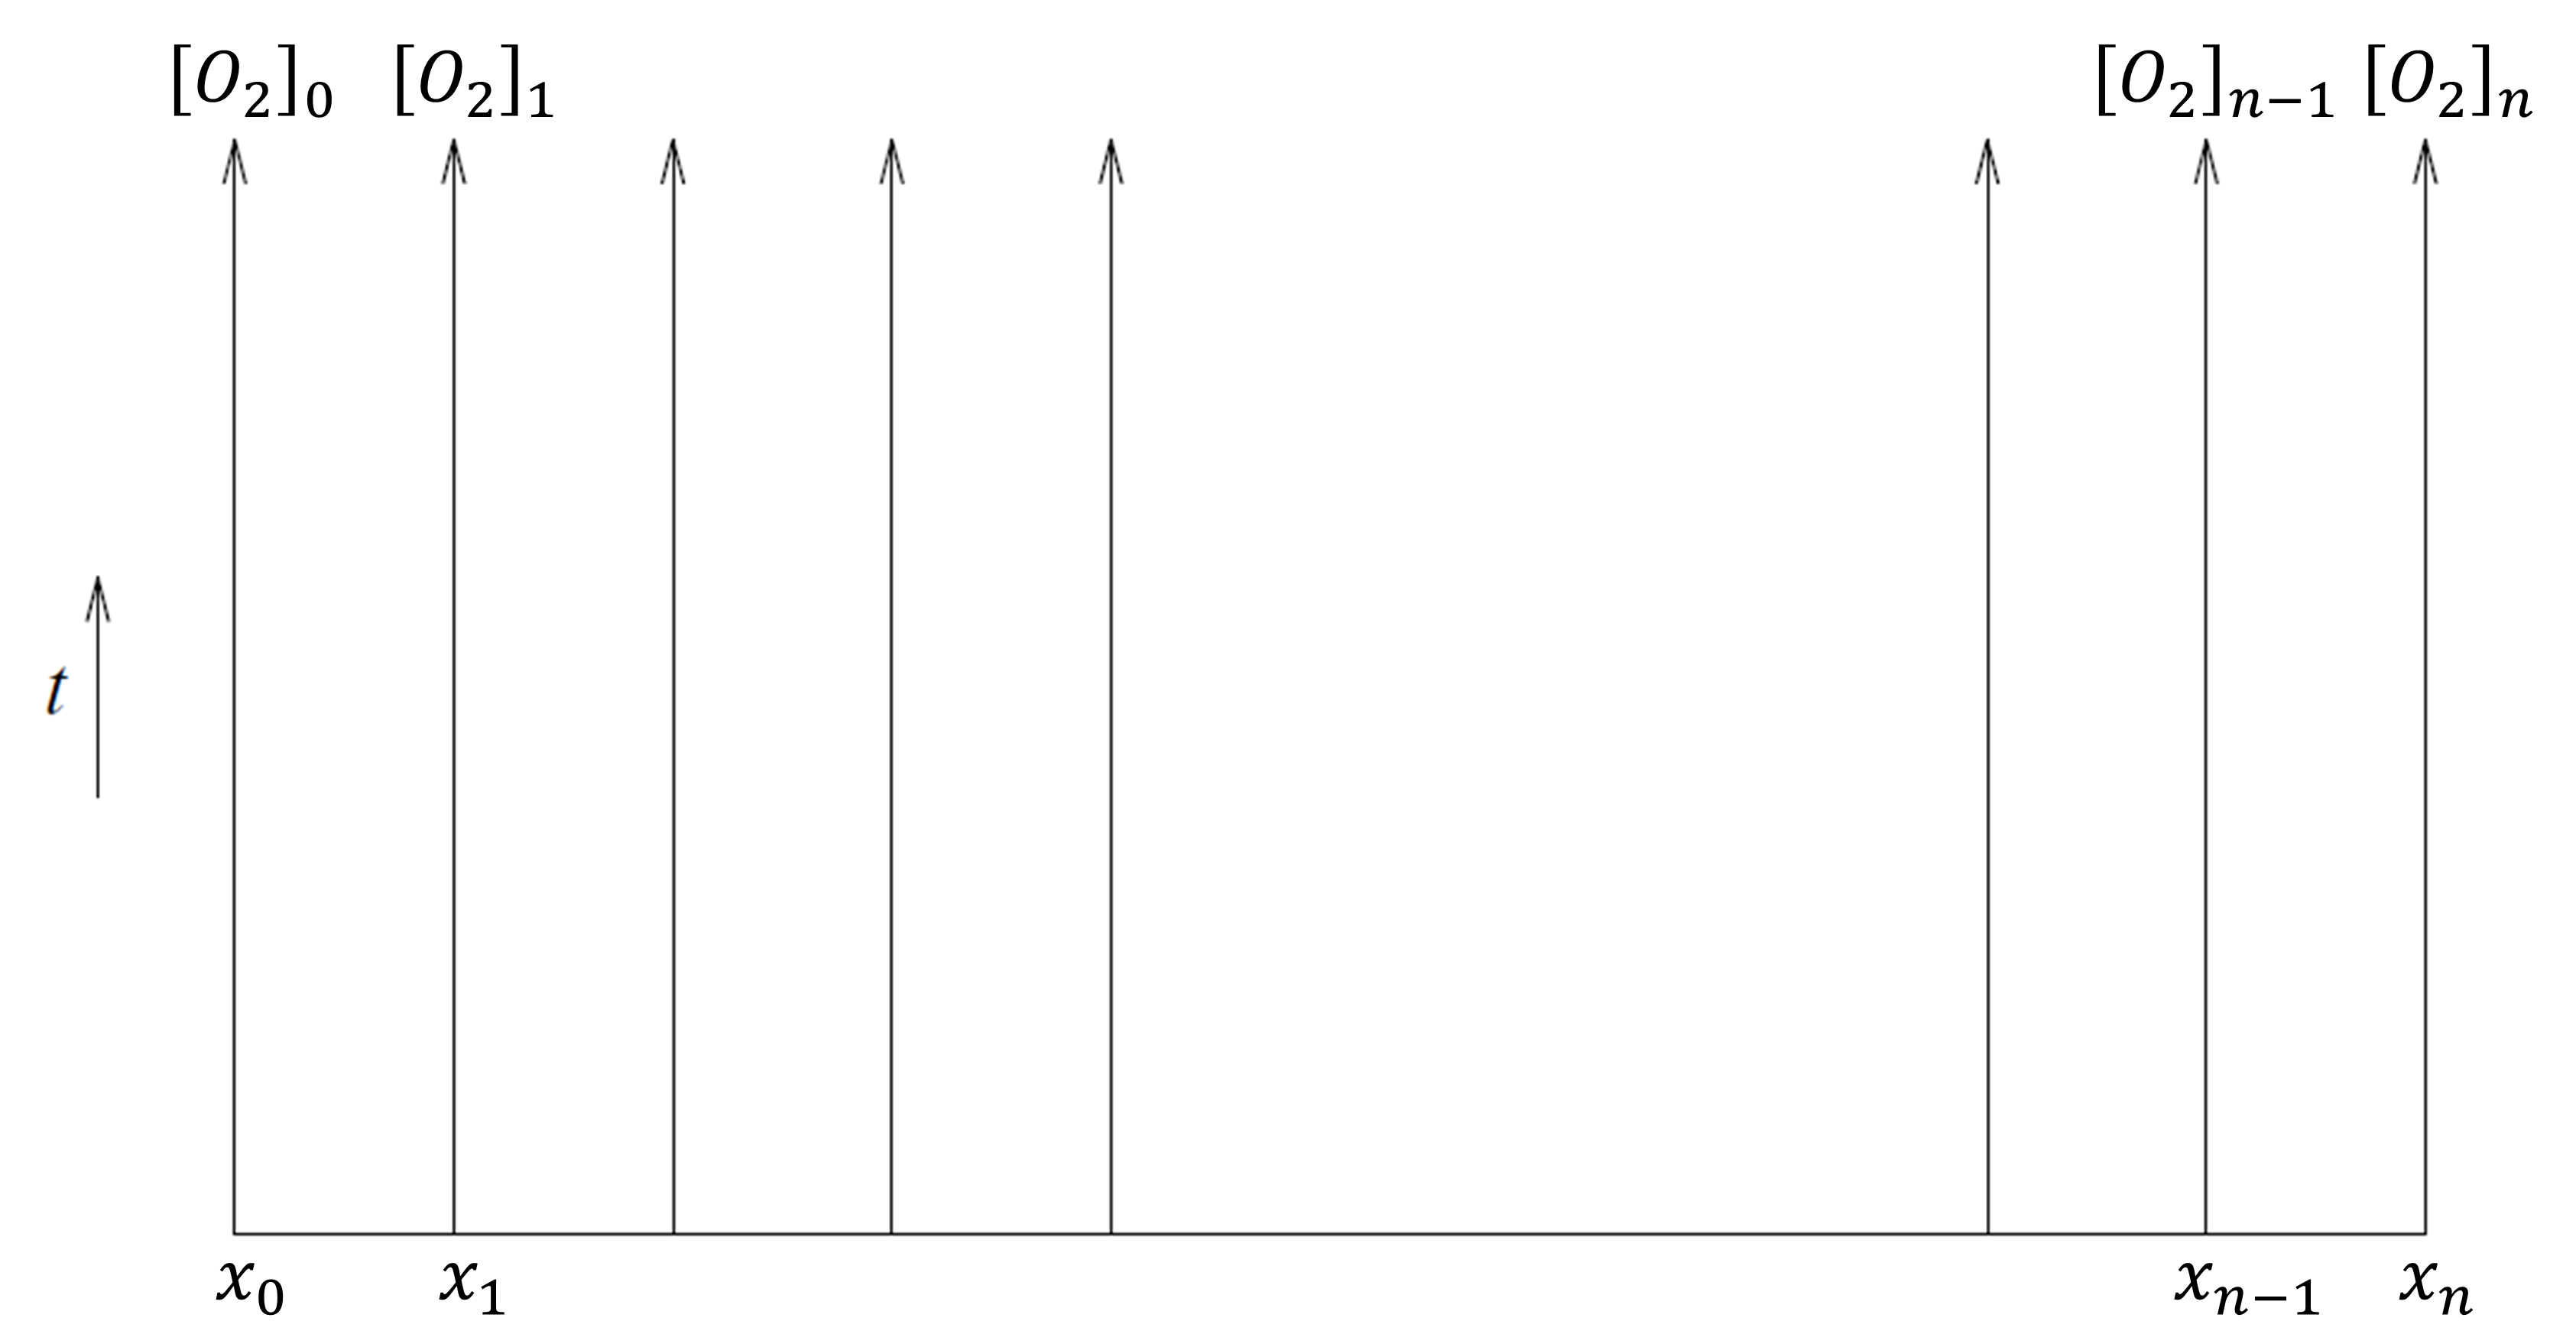
\includegraphics[width=0.7 \linewidth]{Documento_Latex/Tesis_1/Imagenes/LOD.png}
    \caption{Method of lines interpretation. $[O_2]_i$ is the solution along the line forward in time at the grid point $x_i$. Adapted from \cite{LeVeque2007FiniteProblems}.}
    \label{fig:LOD_diagram}
\end{figure}

To solve the system of ODEs, a trapezoidal method will be used. These methods consist of calculating the time derivative at a point $t_i$ as the average of the derivative in that time step and the derivative in the next time step $t_{i+1}$. With this in mind, if the derivative of the oxygen concentration in the film with respect to time is given by equation \ref{eq:LOD_oxygen}, then in the approximation finite difference approximation this derivative is going to be given by:

\begin{align}
    \frac{[O_2]^{j+1}_i-[O_2]^j_i}{\Delta t}=&\frac{1}{2}\Biggr(\left[ D_{O_2} \frac{[O_2]_{i-1}^{j+1}-2[O_2]_{i}^{j+1}+[O_2]_{i+1}^{j+1}}{(\Delta x)^2}-k_2[\ce{R^.}]_i^{j+1}[O_2]_i^{j+1}\right] \nonumber\\
    &-\left[D_{O_2}\frac{[O_2]_{i-1}^{j}-2[O_2]_{i}^{j}+[O_2]_{i+1}^{j}}{(\Delta x)^2}-k_2[\ce{R^.}]_i^{j}[O_2]_i^{j}\right]\Biggr).
\end{align}
This last equation is implicit with respect to time, given that the next time step can not be solve directly from the last step without solving a system of equations. The method implemented was implicit given that it is unconditionally stable and given the presence of the diffusive term which is stiff, an implicit method is required so that the method can be solve using greater time step.  The method of trapezoid when applied to LOD with a second derivative, coincides with the numerical method of Crank-Nicholson. To solve the previous system of equations in order to calculate a new time step, the previous function is rewritten as:

\begin{align}
    0=&\frac{[O_2]^{j+1}_i-[O_2]^j_i}{\Delta t}-\frac{1}{2}\Biggr(\left[ D_{O_2} \frac{[O_2]_{i-1}^{j+1}-2[O_2]_{i}^{j+1}+[O_2]_{i+1}^{j+1}}{(\Delta x)^2}-k_2[\ce{R^.}]_i^{j+1}[O_2]_i^{j+1}\right] \nonumber\\
    &-\left[D_{O_2}\frac{[O_2]_{i-1}^{j}-2[O_2]_{i}^{j}+[O_2]_{i+1}^{j}}{(\Delta x)^2}-k_2[\ce{R^.}]_i^{j}[O_2]_i^{j}\right]\Biggr),
\end{align}
which is equivalent to 
\begin{equation}
    0=F([O_2]^{i+1}). 
\end{equation}
So to find the root for the last equation will mean to calculate the next time step. This was done using the function \textit{fsolve} of the \textit{scipy} library and using as initialization the vector of concentration of the previous time step $[O_2]^{i}$. The initialization was chosen so that the solver converges quickly into a solution given that the profile will not change drastically in one time step. This was done for each time step until the final time $t_m$ was reached. It is important to highlight that both time and space have a uniform discretization. 

\subsubsection{Implicit-Explicit Method}
The implicit-explicit method (IMEX) is a method that has been long used for solving reaction-diffusion problems. This is because generally, the reaction part of the PDE tends to be non-stiff, which is why it can be solved individually by an explicit method, which is simpler to implement and does less work per time step than an implicit scheme. Given that the diffusion part of the equation is stiff, the use of an explicit method to solve the whole PDE is not viable, because it would require excessively small time steps for the method to be stable. In that sense, it is possible to think that an explicit treatment can be given to the reaction part of the PDE, while providing an implicit treatment to the diffusive component of it. In this way, less computational time and effort will be needed to solve the whole PDE given. This is the principle under which IMEX schemes are created. There exist several methods that apply the IMEX schemes; this depends on the treatment given to the implicit and explicit part. In this project, 4 IMEX schemes were evaluated.

The first and most simple IMEX method evaluated was the first order semi-implicit backward differentiation formula (1-SBDF). This scheme is based on the application of the BDF method to solve the diffusive part of the reaction implicitly while using a simple forward Euler method for the reactive part. Applying this algorithm to the oxygen molar balance equation the next expression is obtained \footnote{for the sake of simplicity, the operator of second-order centered difference will be defined for the rest of the document as $\nabla^2 [O_2]^j_i=\frac{[O_2]_{i-1}^{j}-2[O_2]_{i}^{j}+[O_2]_{i+1}^{j}}{(\Delta x)^2}$}:

\begin{equation}
   \frac{[O_2]^{j+1}_i-[O_2]^j_i}{\Delta t}=-k_2[\ce{R^.}]_i^{j}[O_2]_i^{j}+ D_{O_{2_i}}\nabla^2[O_2]_i^{j+1}.
\end{equation}
This method has the advantage of using less memory than the second-order schemes and it is more stable against high-frequency spatial errors \cite{Ruuth1995Implicit-explicitFormation}. The next three IMEX algorithms considered were the Crank-Nicholson Adam-Bashford method (CNAB, equation \ref{eq:CNAB}), the modified CNAB (MCNAB, equation \ref{eq:MCNAB}) and a second-order SBDF method (2-SBDF, equation \ref{eq:2-SBDF}). The first method, CNAB, has a small truncation error but, at the same time, does not have a good response to high-frequency error components.
    \begin{align}
    \frac{[O_2]^{j+1}_i-[O_2]^j_i}{\Delta t}=& \frac{1}{2}\Biggr[-k_2(3[\ce{R^.}]_i^{j}[O_2]_i^{j}-2[\ce{R^.}]_i^{j-1}[O_2]_i^{j-1})+\nonumber\\ &D_{O_{2_i}}(\nabla^2[O_2]_i^{j+1}+\nabla^2[O_2]_i^{j})\Biggr]
    \label{eq:CNAB}
    \end{align}
    
To solve the previous frequency problem there is the MCNAB, which has a better response to high-frequency errors but the price paid is that it requires additional computational work given the evaluation of $\nabla^2[O_2]_i^{j-1}$ \cite{ascher1995implicit} (Equation \ref{eq:MCNAB})
\begin{align}
  \frac{[O_2]^{j+1}_i-[O_2]^j_i}{\Delta t}=& \frac{1}{2}\Biggr[-k_2(3[\ce{R^.}]_i^{j}[O_2]_i^{j}-2[\ce{R^.}]_i^{j-1}[O_2]_i^{j-1})+\nonumber\\
  &\frac{D_{O_{2_i}}}{8}(9\nabla^2[O_2]_i^{j+1}+6\nabla^2[O_2]_i^{j})+\nabla^2[O_2]_i^{j-1})\Biggr]  
  \label{eq:MCNAB}
\end{align}
The last method evaluated, 2-SBDF has a larger truncation error than the CNAB, and MCNAB but it is the most stable of both methods and it does not require to evaluate any operator over $[O_2]_i^{j-1}$ (Equation \ref{eq:2-SBDF}).

\begin{align}
    \frac{3[O_2]^{j+1}_i-4[O_2]^j_i+[O_2]^{j-1}_i}{2\Delta t}=&-k_2(2[\ce{R^.}]_i^{j}[O_2]_i^{j}-[\ce{R^.}]_i^{j-1}[O_2]_i^{j-1})\nonumber\\
    &+D_{O_{2_i}}\nabla^2[O_2]_i^{j+1} 
    \label{eq:2-SBDF}
\end{align}

All second-order schemes require to know the concentration profile for the first two time steps taken, that is why for calculating the first time step the 1-SBDF method was used. 

\subsubsection{Fractional Step Methods}
In case the reactive terms of the PDE system that describes the oxygen absorption dynamics are stiff, it would require an implicit method for solving this using an acceptable time step $\Delta t$. Given that the diffusion part is linear, it can be solved using a different method that the non-linear reaction term. In that way, it is convenient to split the reaction-diffusion equation into two terms, as shown in equation \ref{eq:frac_met}.

\begin{align}
        \frac{\partial [O_2]^*}{\partial t}&=D_{O_2}\frac{\partial^2[O_2]}{\partial x^2}&
        \frac{\partial [O_2]}{\partial t} &=-k_2[\ce{R^.}][O_2]^*
    \label{eq:frac_met}
\end{align}

This method is called the fractional step method (FSM), and it has the advantage that when decoupling both parts of the equation, a different solution treatment can be given for both. The case is shown in equation  \ref{eq:frac_met} is the most straightforward implementation of first-order for an FMS. The point where both terms are relate is that the result obtained for the diffusive part is used to calculate the derivative in the reactive component. In that way, for a $\Delta t$ sufficiently small, this method will approach the solution of the non-separated PDE system. For solving the fractional diffusion equation, a Crank-Nicholson algorithm was applied (Equation \ref{eq:fraction_CN}).

\begin{equation}
    \frac{[O_2]_i^*-[O_2]_i^j}{\Delta t} = \frac{1}{2}(D_{O_{2_i}}\nabla^2[O_2]_i^j + D_{O_{2_i}}\nabla^2[O_2]_i^*)
    \label{eq:fraction_CN}
\end{equation}
This equation was solved for each time-step by using the conjugate gradient algorithm (CG) implemented in the scipy library, without preconditioning and using $[O_2]_i^j$ as the initial guess value. On the other hand, concerning the method for solving the reaction fractional equation, a trapezoidal method was used.

\begin{equation}
    \frac{[O_2]_i^{j+1}-[O_2]_i^*}{\Delta t}= -k_2 \frac{1}{2}([\ce{R^.}]_i^j[O_2]^*-[\ce{R^.}]_i^{j+1}[O_2]^{j+1}) \label{eq:fraction_trapz}
\end{equation}

As in the case of the LOD method, equation \ref{eq:fraction_trapz} was solve by rewriting the equation to the form $F([O_2]^{j+1})=0$ and finding the root of the equation with the function \textit{fsolve} of \textit{scipy}. 

\subsubsection{Adaptive Time-step Algorithm}
A disadvantage of implementing the previous numerical methods with a constant time step is that they would take a longer computational time because they will always do the same amount of iterations no matter what the final time is. In this case, given that the objective of solving the PDE system of equations for the OS film is to predict the results of the head-space test, the time-lapse over which the solution is going to be needed is of the order of 100h. In that sense, having time steps of the order of 1 second would reduce numerical error but it implies a great amount of computational time to get to the final result. As a solution to the problem of long computational times, the implementation of a variable time step algorithm is proposed. This implementation was taken from the algorithm developed by Janneli and Fazio \cite{Jannelli2006AdaptiveComplexity}, which consist of defining a criteria variable $\eta^j$ as
\begin{equation}
    \eta^j= \frac{||u^{j+1}-u^{j}||}{||u^{j}||+\varepsilon_M}.
\end{equation}
Where $u^j,u^{j+1} $ would be the whole concentration vector at the time $t^j$ and $t^{j+1}$ respectively, and $\varepsilon_M$ is a parameter which is of the order of the rounding unit so that in case that $||u^{j}||=0$ the monitor function $\eta^j$ is still well defined. This function can be interpreted as the relative change of the solution in the next time step with respect to the solution in the actual time. For numerical stability  it is desired that the value of $\eta^j$ is between a certain range $ \eta_{min}<\eta^j <\eta_{max}$. The basic guidelines so that this occurs is that for a given time step $\Delta t^j$ if the quantity is between $ \eta_{min}<\eta^j <\eta_{max}$ the new solution is accepted and the next time step $\Delta t^{j+1}$ remains equal to the actual one. In the case where $\eta^j<\eta_{min}$ then the new solution $u^{j+1}$ is accepted and the new time step is increased by a factor of $\rho$. But in the case $ \eta_{max}<\eta^j$, the solution $u^{j+1}$ calculated is not accepted and a new solution must be calculated with a reduced time step $\sigma \Delta t^j$, being $\sigma$ the factor by which the actual time step is reduced. This verification is made for every time step until the getting to the final time $t_m$. This algorithm was implemented for the LOD and FMS method described in the previous section with the parameter shown in Table \ref{tab:parameters_vari_time _Step}.


\begin{table}[H]
\centering
\caption{Variable step algorithm parameters used for the implementation of  the LOD and FSM methods. This values were determined by observation.}
\label{tab:parameters_vari_time _Step}
\begin{tabular}{|c|c|c|}
\hline
Parameters             & LOD          & FSM         \\ \hline
$\eta_{min}$           & $8x10^{-10}$ & $1x10^{-8}$ \\ \hline
$\eta_{max}$           & $1x10^{-4}$  & $1x10^{-4}$ \\ \hline
$\varepsilon_M$        & 0            & 0           \\ \hline
$\sigma$               & 0.66         & 0.2         \\ \hline
$\rho$                 & 1.5          & 2           \\ \hline
$\Delta   t_{min}$ (s) & 0.001        & 0.001       \\ \hline
$\Delta   t_{max}$ (s) & 500          & 1000        \\ \hline
$\Delta t_o$   (s)     & 0.001        & 0.001       \\ \hline
\end{tabular}%
\end{table}

\subsection{Methodology of Kinetic Parameters Adjustment}\label{subsec:parameters_adjustment_meth}
The adjustment of the kinetic parameters was made based on the equations 
\ref{eq:consum_R.}- \ref{eq:consum_O2} and the oxidative TGA experimental data presented by Lazzari and Chiantore \cite{lazzari1999drying}. In this case, to carry out the adjustment, minimization of a weighted square difference function was made through the method of Gauss-Newton (Equation  \ref{eq:funcion objetivo}).

\begin{equation}
 min \frac{1}{2}\sum_{i=0}^k (\bar{y_i}- y(t_i,v))^\dagger W_i (\bar{y_i}- y(t_i,v))
 \label{eq:funcion objetivo}
\end{equation}

In the previous function, $\bar{y_i}$ represents the vector of  experimental data, $W_i$ the diagonal matrix of weights, and $y(t_i,v)$ is the data predicted by the model using the parameters $v$. The function $y$ is such that $\dot{y}=f(y,t,v)$, in this case this function was the mass change in linseed oil due to oxygen absorption (equation \ref{eq:cambio_masa_aceite}).    

\begin{equation}
    \frac{dm}{dt} = \frac{M_{O2}}{\rho_{oil}}k_2 [\ce{R^.}][O_2]
    \label{eq:cambio_masa_aceite}
\end{equation}

Where $m$ is the oil weight gain due to oxygen absorption. In order to obtain $y(t_i,v)$ from the previous equation, the ODE system of kinetic velocity equations must be solved for a given value of parameters. To solve this the backward difference formula (BDF) method was used. On the other hand the way the Gauss Newton method was applied for minimizing the function \ref{eq:funcion objetivo} was through the next equation:
\begin{equation}
    v^{l+1}=v^l+\delta^l
\end{equation}
In this $v^{l+1}$ is the parameter vector $l+1$ step of the optimization search and $\delta^l$ is the vector of the direction in which the next step is taken. To find the latter vector the next equation must be solved 

\begin{equation}
    J(v^k)^\dagger J(v^k)\delta^k=-J(v^k)^\dagger f(v)
    \label{eq:calculo direccion de optimizacion}
\end{equation}

Where $J$ is the Jacobian of the system of ODEs with respect to the parameters evaluated in $v^k$ and is the solution to the system of ODE using the parameters $v^k$. In that sense, for a given set of parameters, the system of ODEs was numerically solved, and the objective function as evaluated. In the case, the value obtained was no under a tolerance value (tol=1e-3) a new set of parameters was calculated by calculating the jacobian, and solving the system of equations \ref{eq:calculo direccion de optimizacion} using the method \textit{spsolve} of python. It is important to state that the weight matrix function $W_i$ used had only values of zeros in its diagonal except for the rows corresponding to the variable of interest $m_i$. the values assigned to the weights associated with $w_i$ were established by giving 10 times more weight to the initial values of the mass absorption.

\subsection{Prediction Tool programming}\label{sec:metodologia_interfaz}
As a sum of all the previous computational methodologies, a modeling tool was developed. In this case, the interface of the program was made using the \textit{tkinter} library of python. This interface was thought so that the main window would be divided into two regions, the left-hand side corresponding to the results of the simulation and the right-hand side corresponding to the parameter panel. In the latter, the user would be able to enter the parameters with which he wanted to predict the OS film performance. One main button would execute the numerical algorithms which would solve OS film dynamics, and the results would be shown in a dynamic plot or plots. For the development of the tool, considerations of whether the film was within a finite volume or was exposed in an open volume were considered. Also, the effect of temperature and the material of the film in its performance was also taken into account.  The materials which are implemented into the tool and its properties are shown in table \ref{tab:materiales_herramienta}. The resulting tool and the instructions on how to use it are exposed in the next chapter.

\begin{table}[H]
\centering
\caption{Oxygen diffusivity and solubility pre-exponential factor and activation energy on the different types of polymer matrix implemented in the design tool.}
\label{tab:materiales_herramienta}

\begin{tabular}{|c|c|c|c|c|}
\hline
Material & Do (cm2/s) & Ea (J/mol) & So (mol/cm3*Pa) & $\Delta$H (J/mol) \\ \hline
iPP      & 1.50       & 36400      & 2.54E-11        & 1200             \\ \hline
LDPE     & 4.48       & 39907.2    & 2.899E-11       & 2500             \\ \hline
HDPE     & 0.43       & 36581.6    & 2.0962E-11      & -1700            \\ \hline
BR       & 0.15       & 28267.6    & 4.3262E-11      & 1300             \\ \hline
PS       & 0.13       & 34503.1    & 2.453E-11       & 0                \\ \hline
PET      & 0.38       & 45727      & 3.0774E-11      & -31400           \\ \hline
PVC      & 42.50      & 54456.7    & 1.29E-11        & -7900            \\ \hline
\end{tabular}%
\end{table}










\printbibliography
\end{refsection}
\chapter{Results and Analysis}
\begin{refsection}
The chapter of results is divided in three main sections. The first one corresponds to the results in the adjustment of the kinetic constant and initial concentration of chemical species in linseed oil. Afterwards  the results over the analysis of the different numerical methods implemented is going to be done, and one of the methods used is going to be chosen for the computational design tool implementation. Finally The interface of the design tool is going to be presented and a brief description in how to use this program is described.  


\section{Linseed oil kinetics adjustment results}
Following the procedure described in \ref{subsec:parameters_adjustment_meth}, and adjustment over the initial concentration of chemical species in linseed oil was made.  The oxidative TGA results obtained by  Lazzari and Chiantore \cite{lazzari1999drying}  for linseed oil at a temperature of 80\degree C were used as the reference whose prediction is desired. In this case, the values for the kinetic constants $k_1$  to $k_6$  were taken from Richaud \cite{Richaud2012RateChemiluminescence}. The initialization point for the optimization method was taken from the concentrations for $[ROOH]_o$ and  $[RH]_o$  in linseed oil proposed by Garcia \cite{GarciaMora2015KineticScavengers}. In this case it is considered that the initial concentration of radicals $[\ce{R^.}]$ and $[\ce{ROO^.}]$ its zero given that hydroperoxide decomposition has not occurred yet. With this in mind the results of the adjusment are shown in figure \ref{fig:ajuste_1_cinetica} and table .

\begin{figure}[H]
    \centering
    \includegraphics[width=0.56\linewidth,page=4]{Documento_Latex/Tesis_1/Imagenes/rozogafas.pdf}
    \caption{Comparison between the kinetic model and the experimental data for quantity of oxygen absorbed per gram of Linseed oil. Experimental results taken from \cite{lazzari1999drying}.}
    \label{fig:ajuste_1_cinetica}
\end{figure}

\begin{table}[H]
\centering
\caption{Arrhenius parameters for reaction velocity constants, and the initial concentrations of chemical species in linseed oil determined from adjustments with experimental data. }
\label{tab:kinetic parameters}

\begin{tabular}{ccc}
\hline
\multirow{2}{*}{} & \multicolumn{2}{c}{Arrhenius   Parameters}  \\
                  & ko {[}L/mol s{]}         & Ea {[}kJ/mol{]}   \\ \hline
\ref{reacc:initiation} ($k_1$)  & 4.09E+10   & 101.5             \\ 
\ref{reacc:O_2 consumption} ($k_2$) & 1.00E+07 & 1               \\ 
\ref{reacc: propagation} ($k_3$) & 3.52E+06  & 31                 \\ 
\ref{reacc:termination_2alkyrad} ($k_4$)  & 3.00E+11 & 0          \\ 
\ref{reacc:termination_alky_peroxide_rad} ($k_5$) & 1.00E+10 & 0   \\
\ref{reacc:termination_2peroxide_rad} ($k_6$)  & 3.05E+15 & 48.8    \\ \hline
                  & \multicolumn{2}{c}{Intial   Concentration (mol/L)} \\
$[ROOH]_o$        & \multicolumn{2}{c}{5.00E-03}                       \\
$[RH]_o$          & \multicolumn{2}{c}{6.8} \\ \hline           
\end{tabular}%
\end{table}

Results in figure \ref{fig:ajuste_1_cinetica}, show that the kinetic model is consistent with experimental data until the maximum  quantity of oxygen absorbed is reached. In the case of experimental data, the reduction detected in the mass of oxygen absorbed during the final test times occurs due to the evaporation of volatile components present in the oil. To calculate the oxygen absorption with the TGA data given in \cite{lazzari1999drying}, weight changes in the linseed oil where normalized with respect to the initial weight value. In that sense, the values reported in this document as experimental oxygen absorption data  are really the weight changes in the linseed oil which are causes by absorption of oxygen and evaporation of volatile components. Given that the kinetic model adjusted does not take into account lost of volatile components by evaporation, it is not able to predict the reduction in the weight of the linseed oil.  It is useful to observe that kinetic model used  is able to predict the induction time in which the reaction take place. Predicting this time is crucial when calculating the useful life of the OS films. On the other hand, the kinetic model adjusted is consistent when evaluating the dynamics of absorption at different temperatures (see Figure \ref{fig:temperature_kinetics_result}).

\begin{figure}[ht]
    \centering
    \includegraphics[width=0.56\linewidth,page=5]{Documento_Latex/Tesis_1/Imagenes/rozogafas.pdf}
    \caption{Oxygen absorption profile of linseed oil calculated with the kinetic model for different temperatures.}
    \label{fig:temperature_kinetics_result}
\end{figure}

The kinetic model is able to predict the endothermic behaviour of the reaction, were for high temperatures (90\degree C) the induction time is reduced to approximately 2 hours while for lower temperatures the induction time is of the order of 41 hours. This profile also predicts an  oxygen uptake capacity of 0.7 wt\% for linseed oil. To confirm the validity of the values obtained from  the kinetic model adjusted, a comparison of the peroxide value obtained by this mean was contrasted against the experimental values determined by Hess and O'Hare \cite{Hess1950OxidationOil} (Figure \ref{fig:Peroxide value}).

\begin{figure}[H]
    \centering
    \includegraphics[width=0.7\linewidth,page=6]{Documento_Latex/Tesis_1/Imagenes/rozogafas.pdf}
    \caption{Comparison between experimental and computational peroxide value profile for linseed oil oxidation. Experimental data obtained from \cite{Hess1950OxidationOil}}
    \label{fig:Peroxide value}
\end{figure}

The result in the previous figure shows that the kinetic model is able to predict the maximum peroxide value given a certain temperature. On the other hand it does not predict correctly when this maximum values occur. This is a systematic error in the model, because for all temperatures the maximum peroxide values predicted by the model occurs earlier than in the experimental data. This means that in the kinetic model the  bi-molecular decomposition is occurring at a much more faster rate than it should be, reason why the accumulation of peroxide radicals reaches its maximum value in a shorter time, before decreasing by the termination reactions. This means that the values of concentration  predicted are going to be correct but the times given by the model are going to be underestimated. To correct this, more experimental data regarding oxidative TGA, is needed at different temperatures so 
that more accurate kinetic velocity constants are determined. Even so, the values found in this section are going to be used as a first approximation to the development of the computational design tool.  

\section{Finite Difference Numerical Methods Comparison}
Once having establish the kinetic model which is going to be used for the simulations, the performance of the different numerical methods described in section \ref{subsec:numerical_methodology.} were compared. To do this a simulation of a 0.06$mm$ thick and 25 $cm^2$ monolayer PET film was made. The time interval modeled was 2 hours at a temperature of 373K. This temperature was  chosen so that the reaction has a faster velocity rate which enables to see the scavenging effect of the oil in the time simulated. The OS load used was $0.1 vol\%$. To observe that the chosen parameters had a significant effect over the oxygen concentration profile, a simulation with and without OS load was made. The results obtained are shown in figure \ref{fig:oxygen_profile with and without OS}. 

\begin{figure}[ht]
    \centering
    \subfloat[]{
    \resizebox{0.48\textwidth}{!}{
    \begin{adjustbox}{clip,trim=3.3cm 1cm 1.3cm 2cm}
    %% Creator: Matplotlib, PGF backend
%%
%% To include the figure in your LaTeX document, write
%%   \input{<filename>.pgf}
%%
%% Make sure the required packages are loaded in your preamble
%%   \usepackage{pgf}
%%
%% Figures using additional raster images can only be included by \input if
%% they are in the same directory as the main LaTeX file. For loading figures
%% from other directories you can use the `import` package
%%   \usepackage{import}
%% and then include the figures with
%%   \import{<path to file>}{<filename>.pgf}
%%
%% Matplotlib used the following preamble
%%   \usepackage{fontspec}
%%   \setmainfont{Times New Roman}
%%   \setsansfont{Verdana}
%%   \setmonofont{Courier New}
%%
\begingroup%
\makeatletter%
\begin{pgfpicture}%
\pgfpathrectangle{\pgfpointorigin}{\pgfqpoint{6.000000in}{5.000000in}}%
\pgfusepath{use as bounding box, clip}%
\begin{pgfscope}%
\pgfsetbuttcap%
\pgfsetmiterjoin%
\definecolor{currentfill}{rgb}{1.000000,1.000000,1.000000}%
\pgfsetfillcolor{currentfill}%
\pgfsetlinewidth{0.000000pt}%
\definecolor{currentstroke}{rgb}{1.000000,1.000000,1.000000}%
\pgfsetstrokecolor{currentstroke}%
\pgfsetdash{}{0pt}%
\pgfpathmoveto{\pgfqpoint{0.000000in}{0.000000in}}%
\pgfpathlineto{\pgfqpoint{6.000000in}{0.000000in}}%
\pgfpathlineto{\pgfqpoint{6.000000in}{5.000000in}}%
\pgfpathlineto{\pgfqpoint{0.000000in}{5.000000in}}%
\pgfpathclose%
\pgfusepath{fill}%
\end{pgfscope}%
\begin{pgfscope}%
\pgfsetbuttcap%
\pgfsetmiterjoin%
\definecolor{currentfill}{rgb}{1.000000,1.000000,1.000000}%
\pgfsetfillcolor{currentfill}%
\pgfsetlinewidth{0.000000pt}%
\definecolor{currentstroke}{rgb}{0.000000,0.000000,0.000000}%
\pgfsetstrokecolor{currentstroke}%
\pgfsetstrokeopacity{0.000000}%
\pgfsetdash{}{0pt}%
\pgfpathmoveto{\pgfqpoint{0.750000in}{0.625000in}}%
\pgfpathlineto{\pgfqpoint{4.470000in}{0.625000in}}%
\pgfpathlineto{\pgfqpoint{4.470000in}{4.400000in}}%
\pgfpathlineto{\pgfqpoint{0.750000in}{4.400000in}}%
\pgfpathclose%
\pgfusepath{fill}%
\end{pgfscope}%
\begin{pgfscope}%
\pgfsetbuttcap%
\pgfsetmiterjoin%
\definecolor{currentfill}{rgb}{0.950000,0.950000,0.950000}%
\pgfsetfillcolor{currentfill}%
\pgfsetfillopacity{0.500000}%
\pgfsetlinewidth{1.003750pt}%
\definecolor{currentstroke}{rgb}{0.950000,0.950000,0.950000}%
\pgfsetstrokecolor{currentstroke}%
\pgfsetstrokeopacity{0.500000}%
\pgfsetdash{}{0pt}%
\pgfpathmoveto{\pgfqpoint{1.370047in}{1.259737in}}%
\pgfpathlineto{\pgfqpoint{1.975389in}{2.314201in}}%
\pgfpathlineto{\pgfqpoint{1.940731in}{4.090148in}}%
\pgfpathlineto{\pgfqpoint{1.298715in}{3.141655in}}%
\pgfusepath{stroke,fill}%
\end{pgfscope}%
\begin{pgfscope}%
\pgfsetbuttcap%
\pgfsetmiterjoin%
\definecolor{currentfill}{rgb}{0.900000,0.900000,0.900000}%
\pgfsetfillcolor{currentfill}%
\pgfsetfillopacity{0.500000}%
\pgfsetlinewidth{1.003750pt}%
\definecolor{currentstroke}{rgb}{0.900000,0.900000,0.900000}%
\pgfsetstrokecolor{currentstroke}%
\pgfsetstrokeopacity{0.500000}%
\pgfsetdash{}{0pt}%
\pgfpathmoveto{\pgfqpoint{1.975389in}{2.314201in}}%
\pgfpathlineto{\pgfqpoint{3.872699in}{2.048694in}}%
\pgfpathlineto{\pgfqpoint{3.935479in}{3.852117in}}%
\pgfpathlineto{\pgfqpoint{1.940731in}{4.090148in}}%
\pgfusepath{stroke,fill}%
\end{pgfscope}%
\begin{pgfscope}%
\pgfsetbuttcap%
\pgfsetmiterjoin%
\definecolor{currentfill}{rgb}{0.925000,0.925000,0.925000}%
\pgfsetfillcolor{currentfill}%
\pgfsetfillopacity{0.500000}%
\pgfsetlinewidth{1.003750pt}%
\definecolor{currentstroke}{rgb}{0.925000,0.925000,0.925000}%
\pgfsetstrokecolor{currentstroke}%
\pgfsetstrokeopacity{0.500000}%
\pgfsetdash{}{0pt}%
\pgfpathmoveto{\pgfqpoint{1.370047in}{1.259737in}}%
\pgfpathlineto{\pgfqpoint{3.423097in}{0.945038in}}%
\pgfpathlineto{\pgfqpoint{3.872699in}{2.048694in}}%
\pgfpathlineto{\pgfqpoint{1.975389in}{2.314201in}}%
\pgfusepath{stroke,fill}%
\end{pgfscope}%
\begin{pgfscope}%
\pgfsetrectcap%
\pgfsetroundjoin%
\pgfsetlinewidth{0.803000pt}%
\definecolor{currentstroke}{rgb}{0.000000,0.000000,0.000000}%
\pgfsetstrokecolor{currentstroke}%
\pgfsetdash{}{0pt}%
\pgfpathmoveto{\pgfqpoint{1.370047in}{1.259737in}}%
\pgfpathlineto{\pgfqpoint{3.423097in}{0.945038in}}%
\pgfusepath{stroke}%
\end{pgfscope}%
\begin{pgfscope}%
\pgftext[x=1.813267in,y=0.605311in,left,base,rotate=351.285333]{\sffamily\fontsize{10.0}{12.0}\selectfont Posicion [cm]}%
\end{pgfscope}%
\begin{pgfscope}%
\pgfsetbuttcap%
\pgfsetroundjoin%
\pgfsetlinewidth{0.803000pt}%
\definecolor{currentstroke}{rgb}{0.690196,0.690196,0.690196}%
\pgfsetstrokecolor{currentstroke}%
\pgfsetdash{}{0pt}%
\pgfpathmoveto{\pgfqpoint{1.497818in}{1.240152in}}%
\pgfpathlineto{\pgfqpoint{2.093683in}{2.297647in}}%
\pgfpathlineto{\pgfqpoint{2.064969in}{4.075323in}}%
\pgfusepath{stroke}%
\end{pgfscope}%
\begin{pgfscope}%
\pgfsetbuttcap%
\pgfsetroundjoin%
\pgfsetlinewidth{0.803000pt}%
\definecolor{currentstroke}{rgb}{0.690196,0.690196,0.690196}%
\pgfsetstrokecolor{currentstroke}%
\pgfsetdash{}{0pt}%
\pgfpathmoveto{\pgfqpoint{1.791308in}{1.195165in}}%
\pgfpathlineto{\pgfqpoint{2.365294in}{2.259638in}}%
\pgfpathlineto{\pgfqpoint{2.350295in}{4.041275in}}%
\pgfusepath{stroke}%
\end{pgfscope}%
\begin{pgfscope}%
\pgfsetbuttcap%
\pgfsetroundjoin%
\pgfsetlinewidth{0.803000pt}%
\definecolor{currentstroke}{rgb}{0.690196,0.690196,0.690196}%
\pgfsetstrokecolor{currentstroke}%
\pgfsetdash{}{0pt}%
\pgfpathmoveto{\pgfqpoint{2.086819in}{1.149868in}}%
\pgfpathlineto{\pgfqpoint{2.638624in}{2.221389in}}%
\pgfpathlineto{\pgfqpoint{2.637520in}{4.007001in}}%
\pgfusepath{stroke}%
\end{pgfscope}%
\begin{pgfscope}%
\pgfsetbuttcap%
\pgfsetroundjoin%
\pgfsetlinewidth{0.803000pt}%
\definecolor{currentstroke}{rgb}{0.690196,0.690196,0.690196}%
\pgfsetstrokecolor{currentstroke}%
\pgfsetdash{}{0pt}%
\pgfpathmoveto{\pgfqpoint{2.384374in}{1.104257in}}%
\pgfpathlineto{\pgfqpoint{2.913690in}{2.182897in}}%
\pgfpathlineto{\pgfqpoint{2.926662in}{3.972498in}}%
\pgfusepath{stroke}%
\end{pgfscope}%
\begin{pgfscope}%
\pgfsetbuttcap%
\pgfsetroundjoin%
\pgfsetlinewidth{0.803000pt}%
\definecolor{currentstroke}{rgb}{0.690196,0.690196,0.690196}%
\pgfsetstrokecolor{currentstroke}%
\pgfsetdash{}{0pt}%
\pgfpathmoveto{\pgfqpoint{2.683993in}{1.058331in}}%
\pgfpathlineto{\pgfqpoint{3.190508in}{2.144159in}}%
\pgfpathlineto{\pgfqpoint{3.217740in}{3.937764in}}%
\pgfusepath{stroke}%
\end{pgfscope}%
\begin{pgfscope}%
\pgfsetbuttcap%
\pgfsetroundjoin%
\pgfsetlinewidth{0.803000pt}%
\definecolor{currentstroke}{rgb}{0.690196,0.690196,0.690196}%
\pgfsetstrokecolor{currentstroke}%
\pgfsetdash{}{0pt}%
\pgfpathmoveto{\pgfqpoint{2.985698in}{1.012084in}}%
\pgfpathlineto{\pgfqpoint{3.469096in}{2.105174in}}%
\pgfpathlineto{\pgfqpoint{3.510775in}{3.902797in}}%
\pgfusepath{stroke}%
\end{pgfscope}%
\begin{pgfscope}%
\pgfsetbuttcap%
\pgfsetroundjoin%
\pgfsetlinewidth{0.803000pt}%
\definecolor{currentstroke}{rgb}{0.690196,0.690196,0.690196}%
\pgfsetstrokecolor{currentstroke}%
\pgfsetdash{}{0pt}%
\pgfpathmoveto{\pgfqpoint{3.289510in}{0.965515in}}%
\pgfpathlineto{\pgfqpoint{3.749469in}{2.065939in}}%
\pgfpathlineto{\pgfqpoint{3.805785in}{3.867594in}}%
\pgfusepath{stroke}%
\end{pgfscope}%
\begin{pgfscope}%
\pgfsetrectcap%
\pgfsetroundjoin%
\pgfsetlinewidth{0.803000pt}%
\definecolor{currentstroke}{rgb}{0.000000,0.000000,0.000000}%
\pgfsetstrokecolor{currentstroke}%
\pgfsetdash{}{0pt}%
\pgfpathmoveto{\pgfqpoint{1.503000in}{1.249348in}}%
\pgfpathlineto{\pgfqpoint{1.487433in}{1.221721in}}%
\pgfusepath{stroke}%
\end{pgfscope}%
\begin{pgfscope}%
\pgftext[x=1.449629in,y=0.999254in,,top]{\sffamily\fontsize{10.000000}{12.000000}\selectfont 0.00}%
\end{pgfscope}%
\begin{pgfscope}%
\pgfsetrectcap%
\pgfsetroundjoin%
\pgfsetlinewidth{0.803000pt}%
\definecolor{currentstroke}{rgb}{0.000000,0.000000,0.000000}%
\pgfsetstrokecolor{currentstroke}%
\pgfsetdash{}{0pt}%
\pgfpathmoveto{\pgfqpoint{1.796301in}{1.204424in}}%
\pgfpathlineto{\pgfqpoint{1.781301in}{1.176607in}}%
\pgfusepath{stroke}%
\end{pgfscope}%
\begin{pgfscope}%
\pgftext[x=1.743806in,y=0.953307in,,top]{\sffamily\fontsize{10.000000}{12.000000}\selectfont 0.01}%
\end{pgfscope}%
\begin{pgfscope}%
\pgfsetrectcap%
\pgfsetroundjoin%
\pgfsetlinewidth{0.803000pt}%
\definecolor{currentstroke}{rgb}{0.000000,0.000000,0.000000}%
\pgfsetstrokecolor{currentstroke}%
\pgfsetdash{}{0pt}%
\pgfpathmoveto{\pgfqpoint{2.091621in}{1.159191in}}%
\pgfpathlineto{\pgfqpoint{2.077197in}{1.131182in}}%
\pgfusepath{stroke}%
\end{pgfscope}%
\begin{pgfscope}%
\pgftext[x=2.040016in,y=0.907042in,,top]{\sffamily\fontsize{10.000000}{12.000000}\selectfont 0.02}%
\end{pgfscope}%
\begin{pgfscope}%
\pgfsetrectcap%
\pgfsetroundjoin%
\pgfsetlinewidth{0.803000pt}%
\definecolor{currentstroke}{rgb}{0.000000,0.000000,0.000000}%
\pgfsetstrokecolor{currentstroke}%
\pgfsetdash{}{0pt}%
\pgfpathmoveto{\pgfqpoint{2.388981in}{1.113645in}}%
\pgfpathlineto{\pgfqpoint{2.375141in}{1.085442in}}%
\pgfusepath{stroke}%
\end{pgfscope}%
\begin{pgfscope}%
\pgftext[x=2.338280in,y=0.860456in,,top]{\sffamily\fontsize{10.000000}{12.000000}\selectfont 0.03}%
\end{pgfscope}%
\begin{pgfscope}%
\pgfsetrectcap%
\pgfsetroundjoin%
\pgfsetlinewidth{0.803000pt}%
\definecolor{currentstroke}{rgb}{0.000000,0.000000,0.000000}%
\pgfsetstrokecolor{currentstroke}%
\pgfsetdash{}{0pt}%
\pgfpathmoveto{\pgfqpoint{2.688403in}{1.067784in}}%
\pgfpathlineto{\pgfqpoint{2.675155in}{1.039384in}}%
\pgfusepath{stroke}%
\end{pgfscope}%
\begin{pgfscope}%
\pgftext[x=2.638619in,y=0.813547in,,top]{\sffamily\fontsize{10.000000}{12.000000}\selectfont 0.04}%
\end{pgfscope}%
\begin{pgfscope}%
\pgfsetrectcap%
\pgfsetroundjoin%
\pgfsetlinewidth{0.803000pt}%
\definecolor{currentstroke}{rgb}{0.000000,0.000000,0.000000}%
\pgfsetstrokecolor{currentstroke}%
\pgfsetdash{}{0pt}%
\pgfpathmoveto{\pgfqpoint{2.989907in}{1.021603in}}%
\pgfpathlineto{\pgfqpoint{2.977261in}{0.993006in}}%
\pgfusepath{stroke}%
\end{pgfscope}%
\begin{pgfscope}%
\pgftext[x=2.941055in,y=0.766309in,,top]{\sffamily\fontsize{10.000000}{12.000000}\selectfont 0.05}%
\end{pgfscope}%
\begin{pgfscope}%
\pgfsetrectcap%
\pgfsetroundjoin%
\pgfsetlinewidth{0.803000pt}%
\definecolor{currentstroke}{rgb}{0.000000,0.000000,0.000000}%
\pgfsetstrokecolor{currentstroke}%
\pgfsetdash{}{0pt}%
\pgfpathmoveto{\pgfqpoint{3.293517in}{0.975100in}}%
\pgfpathlineto{\pgfqpoint{3.281480in}{0.946303in}}%
\pgfusepath{stroke}%
\end{pgfscope}%
\begin{pgfscope}%
\pgftext[x=3.245610in,y=0.718741in,,top]{\sffamily\fontsize{10.000000}{12.000000}\selectfont 0.06}%
\end{pgfscope}%
\begin{pgfscope}%
\pgfsetrectcap%
\pgfsetroundjoin%
\pgfsetlinewidth{0.803000pt}%
\definecolor{currentstroke}{rgb}{0.000000,0.000000,0.000000}%
\pgfsetstrokecolor{currentstroke}%
\pgfsetdash{}{0pt}%
\pgfpathmoveto{\pgfqpoint{3.872699in}{2.048694in}}%
\pgfpathlineto{\pgfqpoint{3.423097in}{0.945038in}}%
\pgfusepath{stroke}%
\end{pgfscope}%
\begin{pgfscope}%
\pgftext[x=3.904042in,y=0.804466in,left,base,rotate=67.835226]{\sffamily\fontsize{10.000000}{12.000000}\selectfont tiempo [s]}%
\end{pgfscope}%
\begin{pgfscope}%
\pgfsetbuttcap%
\pgfsetroundjoin%
\pgfsetlinewidth{0.803000pt}%
\definecolor{currentstroke}{rgb}{0.690196,0.690196,0.690196}%
\pgfsetstrokecolor{currentstroke}%
\pgfsetdash{}{0pt}%
\pgfpathmoveto{\pgfqpoint{1.343088in}{3.207210in}}%
\pgfpathlineto{\pgfqpoint{1.411713in}{1.332316in}}%
\pgfpathlineto{\pgfqpoint{3.454099in}{1.021140in}}%
\pgfusepath{stroke}%
\end{pgfscope}%
\begin{pgfscope}%
\pgfsetbuttcap%
\pgfsetroundjoin%
\pgfsetlinewidth{0.803000pt}%
\definecolor{currentstroke}{rgb}{0.690196,0.690196,0.690196}%
\pgfsetstrokecolor{currentstroke}%
\pgfsetdash{}{0pt}%
\pgfpathmoveto{\pgfqpoint{1.426188in}{3.329979in}}%
\pgfpathlineto{\pgfqpoint{1.489811in}{1.468357in}}%
\pgfpathlineto{\pgfqpoint{3.512186in}{1.163731in}}%
\pgfusepath{stroke}%
\end{pgfscope}%
\begin{pgfscope}%
\pgfsetbuttcap%
\pgfsetroundjoin%
\pgfsetlinewidth{0.803000pt}%
\definecolor{currentstroke}{rgb}{0.690196,0.690196,0.690196}%
\pgfsetstrokecolor{currentstroke}%
\pgfsetdash{}{0pt}%
\pgfpathmoveto{\pgfqpoint{1.507476in}{3.450071in}}%
\pgfpathlineto{\pgfqpoint{1.566293in}{1.601584in}}%
\pgfpathlineto{\pgfqpoint{3.569044in}{1.303301in}}%
\pgfusepath{stroke}%
\end{pgfscope}%
\begin{pgfscope}%
\pgfsetbuttcap%
\pgfsetroundjoin%
\pgfsetlinewidth{0.803000pt}%
\definecolor{currentstroke}{rgb}{0.690196,0.690196,0.690196}%
\pgfsetstrokecolor{currentstroke}%
\pgfsetdash{}{0pt}%
\pgfpathmoveto{\pgfqpoint{1.587010in}{3.567573in}}%
\pgfpathlineto{\pgfqpoint{1.641208in}{1.732081in}}%
\pgfpathlineto{\pgfqpoint{3.624710in}{1.439947in}}%
\pgfusepath{stroke}%
\end{pgfscope}%
\begin{pgfscope}%
\pgfsetbuttcap%
\pgfsetroundjoin%
\pgfsetlinewidth{0.803000pt}%
\definecolor{currentstroke}{rgb}{0.690196,0.690196,0.690196}%
\pgfsetstrokecolor{currentstroke}%
\pgfsetdash{}{0pt}%
\pgfpathmoveto{\pgfqpoint{1.664847in}{3.682567in}}%
\pgfpathlineto{\pgfqpoint{1.714605in}{1.859933in}}%
\pgfpathlineto{\pgfqpoint{3.679222in}{1.573759in}}%
\pgfusepath{stroke}%
\end{pgfscope}%
\begin{pgfscope}%
\pgfsetbuttcap%
\pgfsetroundjoin%
\pgfsetlinewidth{0.803000pt}%
\definecolor{currentstroke}{rgb}{0.690196,0.690196,0.690196}%
\pgfsetstrokecolor{currentstroke}%
\pgfsetdash{}{0pt}%
\pgfpathmoveto{\pgfqpoint{1.741041in}{3.795132in}}%
\pgfpathlineto{\pgfqpoint{1.786529in}{1.985219in}}%
\pgfpathlineto{\pgfqpoint{3.732614in}{1.704824in}}%
\pgfusepath{stroke}%
\end{pgfscope}%
\begin{pgfscope}%
\pgfsetbuttcap%
\pgfsetroundjoin%
\pgfsetlinewidth{0.803000pt}%
\definecolor{currentstroke}{rgb}{0.690196,0.690196,0.690196}%
\pgfsetstrokecolor{currentstroke}%
\pgfsetdash{}{0pt}%
\pgfpathmoveto{\pgfqpoint{1.815642in}{3.905346in}}%
\pgfpathlineto{\pgfqpoint{1.857023in}{2.108016in}}%
\pgfpathlineto{\pgfqpoint{3.784922in}{1.833226in}}%
\pgfusepath{stroke}%
\end{pgfscope}%
\begin{pgfscope}%
\pgfsetbuttcap%
\pgfsetroundjoin%
\pgfsetlinewidth{0.803000pt}%
\definecolor{currentstroke}{rgb}{0.690196,0.690196,0.690196}%
\pgfsetstrokecolor{currentstroke}%
\pgfsetdash{}{0pt}%
\pgfpathmoveto{\pgfqpoint{1.888701in}{4.013281in}}%
\pgfpathlineto{\pgfqpoint{1.926131in}{2.228396in}}%
\pgfpathlineto{\pgfqpoint{3.836178in}{1.959046in}}%
\pgfusepath{stroke}%
\end{pgfscope}%
\begin{pgfscope}%
\pgfsetrectcap%
\pgfsetroundjoin%
\pgfsetlinewidth{0.803000pt}%
\definecolor{currentstroke}{rgb}{0.000000,0.000000,0.000000}%
\pgfsetstrokecolor{currentstroke}%
\pgfsetdash{}{0pt}%
\pgfpathmoveto{\pgfqpoint{3.437372in}{1.023689in}}%
\pgfpathlineto{\pgfqpoint{3.487571in}{1.016041in}}%
\pgfusepath{stroke}%
\end{pgfscope}%
\begin{pgfscope}%
\pgftext[x=3.621361in,y=0.847931in,,top]{\sffamily\fontsize{10.000000}{12.000000}\selectfont 0}%
\end{pgfscope}%
\begin{pgfscope}%
\pgfsetrectcap%
\pgfsetroundjoin%
\pgfsetlinewidth{0.803000pt}%
\definecolor{currentstroke}{rgb}{0.000000,0.000000,0.000000}%
\pgfsetstrokecolor{currentstroke}%
\pgfsetdash{}{0pt}%
\pgfpathmoveto{\pgfqpoint{3.495628in}{1.166225in}}%
\pgfpathlineto{\pgfqpoint{3.545323in}{1.158739in}}%
\pgfusepath{stroke}%
\end{pgfscope}%
\begin{pgfscope}%
\pgftext[x=3.677524in,y=0.992032in,,top]{\sffamily\fontsize{10.000000}{12.000000}\selectfont 1000}%
\end{pgfscope}%
\begin{pgfscope}%
\pgfsetrectcap%
\pgfsetroundjoin%
\pgfsetlinewidth{0.803000pt}%
\definecolor{currentstroke}{rgb}{0.000000,0.000000,0.000000}%
\pgfsetstrokecolor{currentstroke}%
\pgfsetdash{}{0pt}%
\pgfpathmoveto{\pgfqpoint{3.552650in}{1.305743in}}%
\pgfpathlineto{\pgfqpoint{3.601850in}{1.298415in}}%
\pgfusepath{stroke}%
\end{pgfscope}%
\begin{pgfscope}%
\pgftext[x=3.732502in,y=1.133088in,,top]{\sffamily\fontsize{10.000000}{12.000000}\selectfont 2000}%
\end{pgfscope}%
\begin{pgfscope}%
\pgfsetrectcap%
\pgfsetroundjoin%
\pgfsetlinewidth{0.803000pt}%
\definecolor{currentstroke}{rgb}{0.000000,0.000000,0.000000}%
\pgfsetstrokecolor{currentstroke}%
\pgfsetdash{}{0pt}%
\pgfpathmoveto{\pgfqpoint{3.608478in}{1.442337in}}%
\pgfpathlineto{\pgfqpoint{3.657193in}{1.435163in}}%
\pgfusepath{stroke}%
\end{pgfscope}%
\begin{pgfscope}%
\pgftext[x=3.786329in,y=1.271195in,,top]{\sffamily\fontsize{10.000000}{12.000000}\selectfont 3000}%
\end{pgfscope}%
\begin{pgfscope}%
\pgfsetrectcap%
\pgfsetroundjoin%
\pgfsetlinewidth{0.803000pt}%
\definecolor{currentstroke}{rgb}{0.000000,0.000000,0.000000}%
\pgfsetstrokecolor{currentstroke}%
\pgfsetdash{}{0pt}%
\pgfpathmoveto{\pgfqpoint{3.663147in}{1.576100in}}%
\pgfpathlineto{\pgfqpoint{3.711388in}{1.569073in}}%
\pgfusepath{stroke}%
\end{pgfscope}%
\begin{pgfscope}%
\pgftext[x=3.839044in,y=1.406444in,,top]{\sffamily\fontsize{10.000000}{12.000000}\selectfont 4000}%
\end{pgfscope}%
\begin{pgfscope}%
\pgfsetrectcap%
\pgfsetroundjoin%
\pgfsetlinewidth{0.803000pt}%
\definecolor{currentstroke}{rgb}{0.000000,0.000000,0.000000}%
\pgfsetstrokecolor{currentstroke}%
\pgfsetdash{}{0pt}%
\pgfpathmoveto{\pgfqpoint{3.716695in}{1.707117in}}%
\pgfpathlineto{\pgfqpoint{3.764470in}{1.700234in}}%
\pgfusepath{stroke}%
\end{pgfscope}%
\begin{pgfscope}%
\pgftext[x=3.890678in,y=1.538924in,,top]{\sffamily\fontsize{10.000000}{12.000000}\selectfont 5000}%
\end{pgfscope}%
\begin{pgfscope}%
\pgfsetrectcap%
\pgfsetroundjoin%
\pgfsetlinewidth{0.803000pt}%
\definecolor{currentstroke}{rgb}{0.000000,0.000000,0.000000}%
\pgfsetstrokecolor{currentstroke}%
\pgfsetdash{}{0pt}%
\pgfpathmoveto{\pgfqpoint{3.769156in}{1.835473in}}%
\pgfpathlineto{\pgfqpoint{3.816473in}{1.828729in}}%
\pgfusepath{stroke}%
\end{pgfscope}%
\begin{pgfscope}%
\pgftext[x=3.941266in,y=1.668718in,,top]{\sffamily\fontsize{10.000000}{12.000000}\selectfont 6000}%
\end{pgfscope}%
\begin{pgfscope}%
\pgfsetrectcap%
\pgfsetroundjoin%
\pgfsetlinewidth{0.803000pt}%
\definecolor{currentstroke}{rgb}{0.000000,0.000000,0.000000}%
\pgfsetstrokecolor{currentstroke}%
\pgfsetdash{}{0pt}%
\pgfpathmoveto{\pgfqpoint{3.820561in}{1.961248in}}%
\pgfpathlineto{\pgfqpoint{3.867430in}{1.954639in}}%
\pgfusepath{stroke}%
\end{pgfscope}%
\begin{pgfscope}%
\pgftext[x=3.990839in,y=1.795908in,,top]{\sffamily\fontsize{10.000000}{12.000000}\selectfont 7000}%
\end{pgfscope}%
\begin{pgfscope}%
\pgfsetrectcap%
\pgfsetroundjoin%
\pgfsetlinewidth{0.803000pt}%
\definecolor{currentstroke}{rgb}{0.000000,0.000000,0.000000}%
\pgfsetstrokecolor{currentstroke}%
\pgfsetdash{}{0pt}%
\pgfpathmoveto{\pgfqpoint{3.872699in}{2.048694in}}%
\pgfpathlineto{\pgfqpoint{3.935479in}{3.852117in}}%
\pgfusepath{stroke}%
\end{pgfscope}%
\begin{pgfscope}%
\pgftext[x=4.356752in,y=2.596461in,left,base,rotate=88.006252]{\sffamily\fontsize{10.000000}{12.000000}\selectfont \(\displaystyle O_2\) [mol/\(\displaystyle cm^3\)]}%
\end{pgfscope}%
\begin{pgfscope}%
\pgftext[x=4.369901in,y=3.969170in,right,,rotate=88.006252]{\sffamily\fontsize{10.000000}{12.000000}\selectfont 1e−7}%
\end{pgfscope}%
\begin{pgfscope}%
\pgfsetbuttcap%
\pgfsetroundjoin%
\pgfsetlinewidth{0.803000pt}%
\definecolor{currentstroke}{rgb}{0.690196,0.690196,0.690196}%
\pgfsetstrokecolor{currentstroke}%
\pgfsetdash{}{0pt}%
\pgfpathmoveto{\pgfqpoint{3.873894in}{2.083021in}}%
\pgfpathlineto{\pgfqpoint{1.974729in}{2.348042in}}%
\pgfpathlineto{\pgfqpoint{1.368694in}{1.295441in}}%
\pgfusepath{stroke}%
\end{pgfscope}%
\begin{pgfscope}%
\pgfsetbuttcap%
\pgfsetroundjoin%
\pgfsetlinewidth{0.803000pt}%
\definecolor{currentstroke}{rgb}{0.690196,0.690196,0.690196}%
\pgfsetstrokecolor{currentstroke}%
\pgfsetdash{}{0pt}%
\pgfpathmoveto{\pgfqpoint{3.881883in}{2.312507in}}%
\pgfpathlineto{\pgfqpoint{1.970314in}{2.574242in}}%
\pgfpathlineto{\pgfqpoint{1.359642in}{1.534251in}}%
\pgfusepath{stroke}%
\end{pgfscope}%
\begin{pgfscope}%
\pgfsetbuttcap%
\pgfsetroundjoin%
\pgfsetlinewidth{0.803000pt}%
\definecolor{currentstroke}{rgb}{0.690196,0.690196,0.690196}%
\pgfsetstrokecolor{currentstroke}%
\pgfsetdash{}{0pt}%
\pgfpathmoveto{\pgfqpoint{3.889977in}{2.545034in}}%
\pgfpathlineto{\pgfqpoint{1.965843in}{2.803375in}}%
\pgfpathlineto{\pgfqpoint{1.350462in}{1.776432in}}%
\pgfusepath{stroke}%
\end{pgfscope}%
\begin{pgfscope}%
\pgfsetbuttcap%
\pgfsetroundjoin%
\pgfsetlinewidth{0.803000pt}%
\definecolor{currentstroke}{rgb}{0.690196,0.690196,0.690196}%
\pgfsetstrokecolor{currentstroke}%
\pgfsetdash{}{0pt}%
\pgfpathmoveto{\pgfqpoint{3.898180in}{2.780664in}}%
\pgfpathlineto{\pgfqpoint{1.961313in}{3.035497in}}%
\pgfpathlineto{\pgfqpoint{1.341152in}{2.022056in}}%
\pgfusepath{stroke}%
\end{pgfscope}%
\begin{pgfscope}%
\pgfsetbuttcap%
\pgfsetroundjoin%
\pgfsetlinewidth{0.803000pt}%
\definecolor{currentstroke}{rgb}{0.690196,0.690196,0.690196}%
\pgfsetstrokecolor{currentstroke}%
\pgfsetdash{}{0pt}%
\pgfpathmoveto{\pgfqpoint{3.906493in}{3.019458in}}%
\pgfpathlineto{\pgfqpoint{1.956723in}{3.270668in}}%
\pgfpathlineto{\pgfqpoint{1.331709in}{2.271197in}}%
\pgfusepath{stroke}%
\end{pgfscope}%
\begin{pgfscope}%
\pgfsetbuttcap%
\pgfsetroundjoin%
\pgfsetlinewidth{0.803000pt}%
\definecolor{currentstroke}{rgb}{0.690196,0.690196,0.690196}%
\pgfsetstrokecolor{currentstroke}%
\pgfsetdash{}{0pt}%
\pgfpathmoveto{\pgfqpoint{3.914918in}{3.261481in}}%
\pgfpathlineto{\pgfqpoint{1.952073in}{3.508947in}}%
\pgfpathlineto{\pgfqpoint{1.322129in}{2.523930in}}%
\pgfusepath{stroke}%
\end{pgfscope}%
\begin{pgfscope}%
\pgfsetbuttcap%
\pgfsetroundjoin%
\pgfsetlinewidth{0.803000pt}%
\definecolor{currentstroke}{rgb}{0.690196,0.690196,0.690196}%
\pgfsetstrokecolor{currentstroke}%
\pgfsetdash{}{0pt}%
\pgfpathmoveto{\pgfqpoint{3.923458in}{3.506798in}}%
\pgfpathlineto{\pgfqpoint{1.947361in}{3.750397in}}%
\pgfpathlineto{\pgfqpoint{1.312411in}{2.780335in}}%
\pgfusepath{stroke}%
\end{pgfscope}%
\begin{pgfscope}%
\pgfsetbuttcap%
\pgfsetroundjoin%
\pgfsetlinewidth{0.803000pt}%
\definecolor{currentstroke}{rgb}{0.690196,0.690196,0.690196}%
\pgfsetstrokecolor{currentstroke}%
\pgfsetdash{}{0pt}%
\pgfpathmoveto{\pgfqpoint{3.932115in}{3.755478in}}%
\pgfpathlineto{\pgfqpoint{1.942586in}{3.995082in}}%
\pgfpathlineto{\pgfqpoint{1.302550in}{3.040491in}}%
\pgfusepath{stroke}%
\end{pgfscope}%
\begin{pgfscope}%
\pgfsetrectcap%
\pgfsetroundjoin%
\pgfsetlinewidth{0.803000pt}%
\definecolor{currentstroke}{rgb}{0.000000,0.000000,0.000000}%
\pgfsetstrokecolor{currentstroke}%
\pgfsetdash{}{0pt}%
\pgfpathmoveto{\pgfqpoint{3.858368in}{2.085188in}}%
\pgfpathlineto{\pgfqpoint{3.904963in}{2.078685in}}%
\pgfusepath{stroke}%
\end{pgfscope}%
\begin{pgfscope}%
\pgftext[x=4.065580in,y=2.143283in,,top]{\sffamily\fontsize{10.000000}{12.000000}\selectfont 0.00}%
\end{pgfscope}%
\begin{pgfscope}%
\pgfsetrectcap%
\pgfsetroundjoin%
\pgfsetlinewidth{0.803000pt}%
\definecolor{currentstroke}{rgb}{0.000000,0.000000,0.000000}%
\pgfsetstrokecolor{currentstroke}%
\pgfsetdash{}{0pt}%
\pgfpathmoveto{\pgfqpoint{3.866253in}{2.314647in}}%
\pgfpathlineto{\pgfqpoint{3.913159in}{2.308225in}}%
\pgfusepath{stroke}%
\end{pgfscope}%
\begin{pgfscope}%
\pgftext[x=4.074785in,y=2.372029in,,top]{\sffamily\fontsize{10.000000}{12.000000}\selectfont 0.25}%
\end{pgfscope}%
\begin{pgfscope}%
\pgfsetrectcap%
\pgfsetroundjoin%
\pgfsetlinewidth{0.803000pt}%
\definecolor{currentstroke}{rgb}{0.000000,0.000000,0.000000}%
\pgfsetstrokecolor{currentstroke}%
\pgfsetdash{}{0pt}%
\pgfpathmoveto{\pgfqpoint{3.874242in}{2.547147in}}%
\pgfpathlineto{\pgfqpoint{3.921464in}{2.540807in}}%
\pgfusepath{stroke}%
\end{pgfscope}%
\begin{pgfscope}%
\pgftext[x=4.084111in,y=2.603791in,,top]{\sffamily\fontsize{10.000000}{12.000000}\selectfont 0.50}%
\end{pgfscope}%
\begin{pgfscope}%
\pgfsetrectcap%
\pgfsetroundjoin%
\pgfsetlinewidth{0.803000pt}%
\definecolor{currentstroke}{rgb}{0.000000,0.000000,0.000000}%
\pgfsetstrokecolor{currentstroke}%
\pgfsetdash{}{0pt}%
\pgfpathmoveto{\pgfqpoint{3.882339in}{2.782748in}}%
\pgfpathlineto{\pgfqpoint{3.929880in}{2.776493in}}%
\pgfusepath{stroke}%
\end{pgfscope}%
\begin{pgfscope}%
\pgftext[x=4.093561in,y=2.838629in,,top]{\sffamily\fontsize{10.000000}{12.000000}\selectfont 0.75}%
\end{pgfscope}%
\begin{pgfscope}%
\pgfsetrectcap%
\pgfsetroundjoin%
\pgfsetlinewidth{0.803000pt}%
\definecolor{currentstroke}{rgb}{0.000000,0.000000,0.000000}%
\pgfsetstrokecolor{currentstroke}%
\pgfsetdash{}{0pt}%
\pgfpathmoveto{\pgfqpoint{3.890544in}{3.021513in}}%
\pgfpathlineto{\pgfqpoint{3.938408in}{3.015346in}}%
\pgfusepath{stroke}%
\end{pgfscope}%
\begin{pgfscope}%
\pgftext[x=4.103138in,y=3.076605in,,top]{\sffamily\fontsize{10.000000}{12.000000}\selectfont 1.00}%
\end{pgfscope}%
\begin{pgfscope}%
\pgfsetrectcap%
\pgfsetroundjoin%
\pgfsetlinewidth{0.803000pt}%
\definecolor{currentstroke}{rgb}{0.000000,0.000000,0.000000}%
\pgfsetstrokecolor{currentstroke}%
\pgfsetdash{}{0pt}%
\pgfpathmoveto{\pgfqpoint{3.898859in}{3.263505in}}%
\pgfpathlineto{\pgfqpoint{3.947052in}{3.257430in}}%
\pgfusepath{stroke}%
\end{pgfscope}%
\begin{pgfscope}%
\pgftext[x=4.112843in,y=3.317783in,,top]{\sffamily\fontsize{10.000000}{12.000000}\selectfont 1.25}%
\end{pgfscope}%
\begin{pgfscope}%
\pgfsetrectcap%
\pgfsetroundjoin%
\pgfsetlinewidth{0.803000pt}%
\definecolor{currentstroke}{rgb}{0.000000,0.000000,0.000000}%
\pgfsetstrokecolor{currentstroke}%
\pgfsetdash{}{0pt}%
\pgfpathmoveto{\pgfqpoint{3.907288in}{3.508792in}}%
\pgfpathlineto{\pgfqpoint{3.955814in}{3.502810in}}%
\pgfusepath{stroke}%
\end{pgfscope}%
\begin{pgfscope}%
\pgftext[x=4.122679in,y=3.562227in,,top]{\sffamily\fontsize{10.000000}{12.000000}\selectfont 1.50}%
\end{pgfscope}%
\begin{pgfscope}%
\pgfsetrectcap%
\pgfsetroundjoin%
\pgfsetlinewidth{0.803000pt}%
\definecolor{currentstroke}{rgb}{0.000000,0.000000,0.000000}%
\pgfsetstrokecolor{currentstroke}%
\pgfsetdash{}{0pt}%
\pgfpathmoveto{\pgfqpoint{3.915833in}{3.757439in}}%
\pgfpathlineto{\pgfqpoint{3.964696in}{3.751555in}}%
\pgfusepath{stroke}%
\end{pgfscope}%
\begin{pgfscope}%
\pgftext[x=4.132650in,y=3.810005in,,top]{\sffamily\fontsize{10.000000}{12.000000}\selectfont 1.75}%
\end{pgfscope}%
\begin{pgfscope}%
\pgfpathrectangle{\pgfqpoint{0.750000in}{0.625000in}}{\pgfqpoint{3.720000in}{3.775000in}}%
\pgfusepath{clip}%
\pgfsetbuttcap%
\pgfsetroundjoin%
\definecolor{currentfill}{rgb}{0.000000,0.000000,0.500000}%
\pgfsetfillcolor{currentfill}%
\pgfsetlinewidth{0.000000pt}%
\definecolor{currentstroke}{rgb}{0.000000,0.000000,0.000000}%
\pgfsetstrokecolor{currentstroke}%
\pgfsetdash{}{0pt}%
\pgfpathmoveto{\pgfqpoint{1.625144in}{1.335270in}}%
\pgfpathlineto{\pgfqpoint{1.712803in}{1.321950in}}%
\pgfpathlineto{\pgfqpoint{1.712803in}{1.321951in}}%
\pgfpathlineto{\pgfqpoint{1.712803in}{1.321951in}}%
\pgfpathlineto{\pgfqpoint{1.712803in}{1.321952in}}%
\pgfpathlineto{\pgfqpoint{1.712804in}{1.321955in}}%
\pgfpathlineto{\pgfqpoint{1.712805in}{1.321965in}}%
\pgfpathlineto{\pgfqpoint{1.712806in}{1.322001in}}%
\pgfpathlineto{\pgfqpoint{1.624786in}{1.347241in}}%
\pgfpathlineto{\pgfqpoint{1.624967in}{1.341180in}}%
\pgfpathlineto{\pgfqpoint{1.625059in}{1.338135in}}%
\pgfpathlineto{\pgfqpoint{1.625104in}{1.336608in}}%
\pgfpathlineto{\pgfqpoint{1.625127in}{1.335843in}}%
\pgfpathlineto{\pgfqpoint{1.625138in}{1.335461in}}%
\pgfpathlineto{\pgfqpoint{1.625144in}{1.335270in}}%
\pgfpathclose%
\pgfusepath{fill}%
\end{pgfscope}%
\begin{pgfscope}%
\pgfpathrectangle{\pgfqpoint{0.750000in}{0.625000in}}{\pgfqpoint{3.720000in}{3.775000in}}%
\pgfusepath{clip}%
\pgfsetbuttcap%
\pgfsetroundjoin%
\definecolor{currentfill}{rgb}{0.000000,0.000000,0.500000}%
\pgfsetfillcolor{currentfill}%
\pgfsetlinewidth{0.000000pt}%
\definecolor{currentstroke}{rgb}{0.000000,0.000000,0.000000}%
\pgfsetstrokecolor{currentstroke}%
\pgfsetdash{}{0pt}%
\pgfpathmoveto{\pgfqpoint{1.712803in}{1.321950in}}%
\pgfpathlineto{\pgfqpoint{1.800641in}{1.308604in}}%
\pgfpathlineto{\pgfqpoint{1.800641in}{1.308604in}}%
\pgfpathlineto{\pgfqpoint{1.800641in}{1.308604in}}%
\pgfpathlineto{\pgfqpoint{1.800642in}{1.308605in}}%
\pgfpathlineto{\pgfqpoint{1.800642in}{1.308606in}}%
\pgfpathlineto{\pgfqpoint{1.800643in}{1.308608in}}%
\pgfpathlineto{\pgfqpoint{1.800646in}{1.308613in}}%
\pgfpathlineto{\pgfqpoint{1.712806in}{1.322001in}}%
\pgfpathlineto{\pgfqpoint{1.712805in}{1.321965in}}%
\pgfpathlineto{\pgfqpoint{1.712804in}{1.321955in}}%
\pgfpathlineto{\pgfqpoint{1.712803in}{1.321952in}}%
\pgfpathlineto{\pgfqpoint{1.712803in}{1.321951in}}%
\pgfpathlineto{\pgfqpoint{1.712803in}{1.321951in}}%
\pgfpathlineto{\pgfqpoint{1.712803in}{1.321950in}}%
\pgfpathclose%
\pgfusepath{fill}%
\end{pgfscope}%
\begin{pgfscope}%
\pgfpathrectangle{\pgfqpoint{0.750000in}{0.625000in}}{\pgfqpoint{3.720000in}{3.775000in}}%
\pgfusepath{clip}%
\pgfsetbuttcap%
\pgfsetroundjoin%
\definecolor{currentfill}{rgb}{0.000000,0.000000,0.500000}%
\pgfsetfillcolor{currentfill}%
\pgfsetlinewidth{0.000000pt}%
\definecolor{currentstroke}{rgb}{0.000000,0.000000,0.000000}%
\pgfsetstrokecolor{currentstroke}%
\pgfsetdash{}{0pt}%
\pgfpathmoveto{\pgfqpoint{1.712806in}{1.322001in}}%
\pgfpathlineto{\pgfqpoint{1.800646in}{1.308613in}}%
\pgfpathlineto{\pgfqpoint{1.800651in}{1.308622in}}%
\pgfpathlineto{\pgfqpoint{1.800660in}{1.308646in}}%
\pgfpathlineto{\pgfqpoint{1.800678in}{1.308726in}}%
\pgfpathlineto{\pgfqpoint{1.800709in}{1.309120in}}%
\pgfpathlineto{\pgfqpoint{1.800728in}{1.309953in}}%
\pgfpathlineto{\pgfqpoint{1.800733in}{1.311349in}}%
\pgfpathlineto{\pgfqpoint{1.712033in}{1.355570in}}%
\pgfpathlineto{\pgfqpoint{1.712362in}{1.342227in}}%
\pgfpathlineto{\pgfqpoint{1.712615in}{1.331642in}}%
\pgfpathlineto{\pgfqpoint{1.712770in}{1.324595in}}%
\pgfpathlineto{\pgfqpoint{1.712804in}{1.322653in}}%
\pgfpathlineto{\pgfqpoint{1.712808in}{1.322137in}}%
\pgfpathlineto{\pgfqpoint{1.712806in}{1.322001in}}%
\pgfpathclose%
\pgfusepath{fill}%
\end{pgfscope}%
\begin{pgfscope}%
\pgfpathrectangle{\pgfqpoint{0.750000in}{0.625000in}}{\pgfqpoint{3.720000in}{3.775000in}}%
\pgfusepath{clip}%
\pgfsetbuttcap%
\pgfsetroundjoin%
\definecolor{currentfill}{rgb}{0.000000,0.000000,0.660428}%
\pgfsetfillcolor{currentfill}%
\pgfsetlinewidth{0.000000pt}%
\definecolor{currentstroke}{rgb}{0.000000,0.000000,0.000000}%
\pgfsetstrokecolor{currentstroke}%
\pgfsetdash{}{0pt}%
\pgfpathmoveto{\pgfqpoint{1.624786in}{1.347241in}}%
\pgfpathlineto{\pgfqpoint{1.712806in}{1.322001in}}%
\pgfpathlineto{\pgfqpoint{1.712808in}{1.322137in}}%
\pgfpathlineto{\pgfqpoint{1.712804in}{1.322653in}}%
\pgfpathlineto{\pgfqpoint{1.712770in}{1.324595in}}%
\pgfpathlineto{\pgfqpoint{1.712615in}{1.331642in}}%
\pgfpathlineto{\pgfqpoint{1.712362in}{1.342227in}}%
\pgfpathlineto{\pgfqpoint{1.712033in}{1.355570in}}%
\pgfpathlineto{\pgfqpoint{1.615603in}{1.655255in}}%
\pgfpathlineto{\pgfqpoint{1.617630in}{1.587041in}}%
\pgfpathlineto{\pgfqpoint{1.619877in}{1.511612in}}%
\pgfpathlineto{\pgfqpoint{1.622373in}{1.427970in}}%
\pgfpathlineto{\pgfqpoint{1.623724in}{1.382762in}}%
\pgfpathlineto{\pgfqpoint{1.624427in}{1.359241in}}%
\pgfpathlineto{\pgfqpoint{1.624786in}{1.347241in}}%
\pgfpathclose%
\pgfusepath{fill}%
\end{pgfscope}%
\begin{pgfscope}%
\pgfpathrectangle{\pgfqpoint{0.750000in}{0.625000in}}{\pgfqpoint{3.720000in}{3.775000in}}%
\pgfusepath{clip}%
\pgfsetbuttcap%
\pgfsetroundjoin%
\definecolor{currentfill}{rgb}{0.000000,0.000000,0.500000}%
\pgfsetfillcolor{currentfill}%
\pgfsetlinewidth{0.000000pt}%
\definecolor{currentstroke}{rgb}{0.000000,0.000000,0.000000}%
\pgfsetstrokecolor{currentstroke}%
\pgfsetdash{}{0pt}%
\pgfpathmoveto{\pgfqpoint{1.800641in}{1.308604in}}%
\pgfpathlineto{\pgfqpoint{1.888660in}{1.295230in}}%
\pgfpathlineto{\pgfqpoint{1.888660in}{1.295230in}}%
\pgfpathlineto{\pgfqpoint{1.888660in}{1.295230in}}%
\pgfpathlineto{\pgfqpoint{1.888660in}{1.295231in}}%
\pgfpathlineto{\pgfqpoint{1.888661in}{1.295232in}}%
\pgfpathlineto{\pgfqpoint{1.888662in}{1.295234in}}%
\pgfpathlineto{\pgfqpoint{1.888664in}{1.295239in}}%
\pgfpathlineto{\pgfqpoint{1.800646in}{1.308613in}}%
\pgfpathlineto{\pgfqpoint{1.800643in}{1.308608in}}%
\pgfpathlineto{\pgfqpoint{1.800642in}{1.308606in}}%
\pgfpathlineto{\pgfqpoint{1.800642in}{1.308605in}}%
\pgfpathlineto{\pgfqpoint{1.800641in}{1.308604in}}%
\pgfpathlineto{\pgfqpoint{1.800641in}{1.308604in}}%
\pgfpathlineto{\pgfqpoint{1.800641in}{1.308604in}}%
\pgfpathclose%
\pgfusepath{fill}%
\end{pgfscope}%
\begin{pgfscope}%
\pgfpathrectangle{\pgfqpoint{0.750000in}{0.625000in}}{\pgfqpoint{3.720000in}{3.775000in}}%
\pgfusepath{clip}%
\pgfsetbuttcap%
\pgfsetroundjoin%
\definecolor{currentfill}{rgb}{0.000000,0.000000,0.500000}%
\pgfsetfillcolor{currentfill}%
\pgfsetlinewidth{0.000000pt}%
\definecolor{currentstroke}{rgb}{0.000000,0.000000,0.000000}%
\pgfsetstrokecolor{currentstroke}%
\pgfsetdash{}{0pt}%
\pgfpathmoveto{\pgfqpoint{1.800646in}{1.308613in}}%
\pgfpathlineto{\pgfqpoint{1.888664in}{1.295239in}}%
\pgfpathlineto{\pgfqpoint{1.888669in}{1.295248in}}%
\pgfpathlineto{\pgfqpoint{1.888679in}{1.295265in}}%
\pgfpathlineto{\pgfqpoint{1.888698in}{1.295302in}}%
\pgfpathlineto{\pgfqpoint{1.888735in}{1.295384in}}%
\pgfpathlineto{\pgfqpoint{1.888773in}{1.295495in}}%
\pgfpathlineto{\pgfqpoint{1.888809in}{1.295658in}}%
\pgfpathlineto{\pgfqpoint{1.800733in}{1.311349in}}%
\pgfpathlineto{\pgfqpoint{1.800728in}{1.309953in}}%
\pgfpathlineto{\pgfqpoint{1.800709in}{1.309120in}}%
\pgfpathlineto{\pgfqpoint{1.800678in}{1.308726in}}%
\pgfpathlineto{\pgfqpoint{1.800660in}{1.308646in}}%
\pgfpathlineto{\pgfqpoint{1.800651in}{1.308622in}}%
\pgfpathlineto{\pgfqpoint{1.800646in}{1.308613in}}%
\pgfpathclose%
\pgfusepath{fill}%
\end{pgfscope}%
\begin{pgfscope}%
\pgfpathrectangle{\pgfqpoint{0.750000in}{0.625000in}}{\pgfqpoint{3.720000in}{3.775000in}}%
\pgfusepath{clip}%
\pgfsetbuttcap%
\pgfsetroundjoin%
\definecolor{currentfill}{rgb}{0.000000,0.000000,0.500000}%
\pgfsetfillcolor{currentfill}%
\pgfsetlinewidth{0.000000pt}%
\definecolor{currentstroke}{rgb}{0.000000,0.000000,0.000000}%
\pgfsetstrokecolor{currentstroke}%
\pgfsetdash{}{0pt}%
\pgfpathmoveto{\pgfqpoint{1.800733in}{1.311349in}}%
\pgfpathlineto{\pgfqpoint{1.888809in}{1.295658in}}%
\pgfpathlineto{\pgfqpoint{1.888843in}{1.295900in}}%
\pgfpathlineto{\pgfqpoint{1.888875in}{1.296250in}}%
\pgfpathlineto{\pgfqpoint{1.888903in}{1.296732in}}%
\pgfpathlineto{\pgfqpoint{1.888929in}{1.297370in}}%
\pgfpathlineto{\pgfqpoint{1.888950in}{1.298184in}}%
\pgfpathlineto{\pgfqpoint{1.888967in}{1.299190in}}%
\pgfpathlineto{\pgfqpoint{1.800415in}{1.333566in}}%
\pgfpathlineto{\pgfqpoint{1.800509in}{1.328251in}}%
\pgfpathlineto{\pgfqpoint{1.800587in}{1.323546in}}%
\pgfpathlineto{\pgfqpoint{1.800649in}{1.319484in}}%
\pgfpathlineto{\pgfqpoint{1.800694in}{1.316093in}}%
\pgfpathlineto{\pgfqpoint{1.800722in}{1.313384in}}%
\pgfpathlineto{\pgfqpoint{1.800733in}{1.311349in}}%
\pgfpathclose%
\pgfusepath{fill}%
\end{pgfscope}%
\begin{pgfscope}%
\pgfpathrectangle{\pgfqpoint{0.750000in}{0.625000in}}{\pgfqpoint{3.720000in}{3.775000in}}%
\pgfusepath{clip}%
\pgfsetbuttcap%
\pgfsetroundjoin%
\definecolor{currentfill}{rgb}{0.000000,0.000000,0.624777}%
\pgfsetfillcolor{currentfill}%
\pgfsetlinewidth{0.000000pt}%
\definecolor{currentstroke}{rgb}{0.000000,0.000000,0.000000}%
\pgfsetstrokecolor{currentstroke}%
\pgfsetdash{}{0pt}%
\pgfpathmoveto{\pgfqpoint{1.712033in}{1.355570in}}%
\pgfpathlineto{\pgfqpoint{1.800733in}{1.311349in}}%
\pgfpathlineto{\pgfqpoint{1.800722in}{1.313384in}}%
\pgfpathlineto{\pgfqpoint{1.800694in}{1.316093in}}%
\pgfpathlineto{\pgfqpoint{1.800649in}{1.319484in}}%
\pgfpathlineto{\pgfqpoint{1.800587in}{1.323546in}}%
\pgfpathlineto{\pgfqpoint{1.800509in}{1.328251in}}%
\pgfpathlineto{\pgfqpoint{1.800415in}{1.333566in}}%
\pgfpathlineto{\pgfqpoint{1.709235in}{1.465139in}}%
\pgfpathlineto{\pgfqpoint{1.709750in}{1.445128in}}%
\pgfpathlineto{\pgfqpoint{1.710255in}{1.425461in}}%
\pgfpathlineto{\pgfqpoint{1.710745in}{1.406362in}}%
\pgfpathlineto{\pgfqpoint{1.711211in}{1.388106in}}%
\pgfpathlineto{\pgfqpoint{1.711644in}{1.371035in}}%
\pgfpathlineto{\pgfqpoint{1.712033in}{1.355570in}}%
\pgfpathclose%
\pgfusepath{fill}%
\end{pgfscope}%
\begin{pgfscope}%
\pgfpathrectangle{\pgfqpoint{0.750000in}{0.625000in}}{\pgfqpoint{3.720000in}{3.775000in}}%
\pgfusepath{clip}%
\pgfsetbuttcap%
\pgfsetroundjoin%
\definecolor{currentfill}{rgb}{0.000000,0.000000,0.553476}%
\pgfsetfillcolor{currentfill}%
\pgfsetlinewidth{0.000000pt}%
\definecolor{currentstroke}{rgb}{0.000000,0.000000,0.000000}%
\pgfsetstrokecolor{currentstroke}%
\pgfsetdash{}{0pt}%
\pgfpathmoveto{\pgfqpoint{1.800415in}{1.333566in}}%
\pgfpathlineto{\pgfqpoint{1.888967in}{1.299190in}}%
\pgfpathlineto{\pgfqpoint{1.888979in}{1.300402in}}%
\pgfpathlineto{\pgfqpoint{1.888986in}{1.301829in}}%
\pgfpathlineto{\pgfqpoint{1.888989in}{1.303478in}}%
\pgfpathlineto{\pgfqpoint{1.888986in}{1.305352in}}%
\pgfpathlineto{\pgfqpoint{1.888978in}{1.307453in}}%
\pgfpathlineto{\pgfqpoint{1.888965in}{1.309778in}}%
\pgfpathlineto{\pgfqpoint{1.799594in}{1.375738in}}%
\pgfpathlineto{\pgfqpoint{1.799756in}{1.367715in}}%
\pgfpathlineto{\pgfqpoint{1.799909in}{1.360030in}}%
\pgfpathlineto{\pgfqpoint{1.800053in}{1.352726in}}%
\pgfpathlineto{\pgfqpoint{1.800186in}{1.345849in}}%
\pgfpathlineto{\pgfqpoint{1.800307in}{1.339447in}}%
\pgfpathlineto{\pgfqpoint{1.800415in}{1.333566in}}%
\pgfpathclose%
\pgfusepath{fill}%
\end{pgfscope}%
\begin{pgfscope}%
\pgfpathrectangle{\pgfqpoint{0.750000in}{0.625000in}}{\pgfqpoint{3.720000in}{3.775000in}}%
\pgfusepath{clip}%
\pgfsetbuttcap%
\pgfsetroundjoin%
\definecolor{currentfill}{rgb}{0.000000,0.000000,0.500000}%
\pgfsetfillcolor{currentfill}%
\pgfsetlinewidth{0.000000pt}%
\definecolor{currentstroke}{rgb}{0.000000,0.000000,0.000000}%
\pgfsetstrokecolor{currentstroke}%
\pgfsetdash{}{0pt}%
\pgfpathmoveto{\pgfqpoint{1.888809in}{1.295658in}}%
\pgfpathlineto{\pgfqpoint{1.977009in}{1.282120in}}%
\pgfpathlineto{\pgfqpoint{1.977047in}{1.282203in}}%
\pgfpathlineto{\pgfqpoint{1.977084in}{1.282297in}}%
\pgfpathlineto{\pgfqpoint{1.977121in}{1.282407in}}%
\pgfpathlineto{\pgfqpoint{1.977157in}{1.282540in}}%
\pgfpathlineto{\pgfqpoint{1.977193in}{1.282702in}}%
\pgfpathlineto{\pgfqpoint{1.977228in}{1.282900in}}%
\pgfpathlineto{\pgfqpoint{1.888967in}{1.299190in}}%
\pgfpathlineto{\pgfqpoint{1.888950in}{1.298184in}}%
\pgfpathlineto{\pgfqpoint{1.888929in}{1.297370in}}%
\pgfpathlineto{\pgfqpoint{1.888903in}{1.296732in}}%
\pgfpathlineto{\pgfqpoint{1.888875in}{1.296250in}}%
\pgfpathlineto{\pgfqpoint{1.888843in}{1.295900in}}%
\pgfpathlineto{\pgfqpoint{1.888809in}{1.295658in}}%
\pgfpathclose%
\pgfusepath{fill}%
\end{pgfscope}%
\begin{pgfscope}%
\pgfpathrectangle{\pgfqpoint{0.750000in}{0.625000in}}{\pgfqpoint{3.720000in}{3.775000in}}%
\pgfusepath{clip}%
\pgfsetbuttcap%
\pgfsetroundjoin%
\definecolor{currentfill}{rgb}{0.000000,0.000000,0.500000}%
\pgfsetfillcolor{currentfill}%
\pgfsetlinewidth{0.000000pt}%
\definecolor{currentstroke}{rgb}{0.000000,0.000000,0.000000}%
\pgfsetstrokecolor{currentstroke}%
\pgfsetdash{}{0pt}%
\pgfpathmoveto{\pgfqpoint{1.888664in}{1.295239in}}%
\pgfpathlineto{\pgfqpoint{1.976864in}{1.281837in}}%
\pgfpathlineto{\pgfqpoint{1.976868in}{1.281846in}}%
\pgfpathlineto{\pgfqpoint{1.976878in}{1.281864in}}%
\pgfpathlineto{\pgfqpoint{1.976897in}{1.281900in}}%
\pgfpathlineto{\pgfqpoint{1.976934in}{1.281971in}}%
\pgfpathlineto{\pgfqpoint{1.976972in}{1.282044in}}%
\pgfpathlineto{\pgfqpoint{1.977009in}{1.282120in}}%
\pgfpathlineto{\pgfqpoint{1.888809in}{1.295658in}}%
\pgfpathlineto{\pgfqpoint{1.888773in}{1.295495in}}%
\pgfpathlineto{\pgfqpoint{1.888735in}{1.295384in}}%
\pgfpathlineto{\pgfqpoint{1.888698in}{1.295302in}}%
\pgfpathlineto{\pgfqpoint{1.888679in}{1.295265in}}%
\pgfpathlineto{\pgfqpoint{1.888669in}{1.295248in}}%
\pgfpathlineto{\pgfqpoint{1.888664in}{1.295239in}}%
\pgfpathclose%
\pgfusepath{fill}%
\end{pgfscope}%
\begin{pgfscope}%
\pgfpathrectangle{\pgfqpoint{0.750000in}{0.625000in}}{\pgfqpoint{3.720000in}{3.775000in}}%
\pgfusepath{clip}%
\pgfsetbuttcap%
\pgfsetroundjoin%
\definecolor{currentfill}{rgb}{0.000000,0.000000,0.500000}%
\pgfsetfillcolor{currentfill}%
\pgfsetlinewidth{0.000000pt}%
\definecolor{currentstroke}{rgb}{0.000000,0.000000,0.000000}%
\pgfsetstrokecolor{currentstroke}%
\pgfsetdash{}{0pt}%
\pgfpathmoveto{\pgfqpoint{1.888660in}{1.295230in}}%
\pgfpathlineto{\pgfqpoint{1.976859in}{1.281829in}}%
\pgfpathlineto{\pgfqpoint{1.976859in}{1.281829in}}%
\pgfpathlineto{\pgfqpoint{1.976859in}{1.281829in}}%
\pgfpathlineto{\pgfqpoint{1.976859in}{1.281830in}}%
\pgfpathlineto{\pgfqpoint{1.976860in}{1.281831in}}%
\pgfpathlineto{\pgfqpoint{1.976861in}{1.281833in}}%
\pgfpathlineto{\pgfqpoint{1.976864in}{1.281837in}}%
\pgfpathlineto{\pgfqpoint{1.888664in}{1.295239in}}%
\pgfpathlineto{\pgfqpoint{1.888662in}{1.295234in}}%
\pgfpathlineto{\pgfqpoint{1.888661in}{1.295232in}}%
\pgfpathlineto{\pgfqpoint{1.888660in}{1.295231in}}%
\pgfpathlineto{\pgfqpoint{1.888660in}{1.295230in}}%
\pgfpathlineto{\pgfqpoint{1.888660in}{1.295230in}}%
\pgfpathlineto{\pgfqpoint{1.888660in}{1.295230in}}%
\pgfpathclose%
\pgfusepath{fill}%
\end{pgfscope}%
\begin{pgfscope}%
\pgfpathrectangle{\pgfqpoint{0.750000in}{0.625000in}}{\pgfqpoint{3.720000in}{3.775000in}}%
\pgfusepath{clip}%
\pgfsetbuttcap%
\pgfsetroundjoin%
\definecolor{currentfill}{rgb}{0.000000,0.000000,0.500000}%
\pgfsetfillcolor{currentfill}%
\pgfsetlinewidth{0.000000pt}%
\definecolor{currentstroke}{rgb}{0.000000,0.000000,0.000000}%
\pgfsetstrokecolor{currentstroke}%
\pgfsetdash{}{0pt}%
\pgfpathmoveto{\pgfqpoint{1.888967in}{1.299190in}}%
\pgfpathlineto{\pgfqpoint{1.977228in}{1.282900in}}%
\pgfpathlineto{\pgfqpoint{1.977262in}{1.283141in}}%
\pgfpathlineto{\pgfqpoint{1.977295in}{1.283433in}}%
\pgfpathlineto{\pgfqpoint{1.977328in}{1.283782in}}%
\pgfpathlineto{\pgfqpoint{1.977358in}{1.284195in}}%
\pgfpathlineto{\pgfqpoint{1.977388in}{1.284678in}}%
\pgfpathlineto{\pgfqpoint{1.977416in}{1.285237in}}%
\pgfpathlineto{\pgfqpoint{1.888965in}{1.309778in}}%
\pgfpathlineto{\pgfqpoint{1.888978in}{1.307453in}}%
\pgfpathlineto{\pgfqpoint{1.888986in}{1.305352in}}%
\pgfpathlineto{\pgfqpoint{1.888989in}{1.303478in}}%
\pgfpathlineto{\pgfqpoint{1.888986in}{1.301829in}}%
\pgfpathlineto{\pgfqpoint{1.888979in}{1.300402in}}%
\pgfpathlineto{\pgfqpoint{1.888967in}{1.299190in}}%
\pgfpathclose%
\pgfusepath{fill}%
\end{pgfscope}%
\begin{pgfscope}%
\pgfpathrectangle{\pgfqpoint{0.750000in}{0.625000in}}{\pgfqpoint{3.720000in}{3.775000in}}%
\pgfusepath{clip}%
\pgfsetbuttcap%
\pgfsetroundjoin%
\definecolor{currentfill}{rgb}{0.000000,0.000000,0.517825}%
\pgfsetfillcolor{currentfill}%
\pgfsetlinewidth{0.000000pt}%
\definecolor{currentstroke}{rgb}{0.000000,0.000000,0.000000}%
\pgfsetstrokecolor{currentstroke}%
\pgfsetdash{}{0pt}%
\pgfpathmoveto{\pgfqpoint{1.888965in}{1.309778in}}%
\pgfpathlineto{\pgfqpoint{1.977416in}{1.285237in}}%
\pgfpathlineto{\pgfqpoint{1.977442in}{1.285875in}}%
\pgfpathlineto{\pgfqpoint{1.977466in}{1.286599in}}%
\pgfpathlineto{\pgfqpoint{1.977489in}{1.287410in}}%
\pgfpathlineto{\pgfqpoint{1.977510in}{1.288314in}}%
\pgfpathlineto{\pgfqpoint{1.977529in}{1.289311in}}%
\pgfpathlineto{\pgfqpoint{1.977546in}{1.290404in}}%
\pgfpathlineto{\pgfqpoint{1.888787in}{1.328181in}}%
\pgfpathlineto{\pgfqpoint{1.888828in}{1.324619in}}%
\pgfpathlineto{\pgfqpoint{1.888865in}{1.321244in}}%
\pgfpathlineto{\pgfqpoint{1.888897in}{1.318065in}}%
\pgfpathlineto{\pgfqpoint{1.888925in}{1.315090in}}%
\pgfpathlineto{\pgfqpoint{1.888947in}{1.312325in}}%
\pgfpathlineto{\pgfqpoint{1.888965in}{1.309778in}}%
\pgfpathclose%
\pgfusepath{fill}%
\end{pgfscope}%
\begin{pgfscope}%
\pgfpathrectangle{\pgfqpoint{0.750000in}{0.625000in}}{\pgfqpoint{3.720000in}{3.775000in}}%
\pgfusepath{clip}%
\pgfsetbuttcap%
\pgfsetroundjoin%
\definecolor{currentfill}{rgb}{0.000000,0.000000,0.642602}%
\pgfsetfillcolor{currentfill}%
\pgfsetlinewidth{0.000000pt}%
\definecolor{currentstroke}{rgb}{0.000000,0.000000,0.000000}%
\pgfsetstrokecolor{currentstroke}%
\pgfsetdash{}{0pt}%
\pgfpathmoveto{\pgfqpoint{1.799594in}{1.375738in}}%
\pgfpathlineto{\pgfqpoint{1.888965in}{1.309778in}}%
\pgfpathlineto{\pgfqpoint{1.888947in}{1.312325in}}%
\pgfpathlineto{\pgfqpoint{1.888925in}{1.315090in}}%
\pgfpathlineto{\pgfqpoint{1.888897in}{1.318065in}}%
\pgfpathlineto{\pgfqpoint{1.888865in}{1.321244in}}%
\pgfpathlineto{\pgfqpoint{1.888828in}{1.324619in}}%
\pgfpathlineto{\pgfqpoint{1.888787in}{1.328181in}}%
\pgfpathlineto{\pgfqpoint{1.798500in}{1.428776in}}%
\pgfpathlineto{\pgfqpoint{1.798693in}{1.419524in}}%
\pgfpathlineto{\pgfqpoint{1.798883in}{1.410395in}}%
\pgfpathlineto{\pgfqpoint{1.799068in}{1.401419in}}%
\pgfpathlineto{\pgfqpoint{1.799249in}{1.392628in}}%
\pgfpathlineto{\pgfqpoint{1.799425in}{1.384055in}}%
\pgfpathlineto{\pgfqpoint{1.799594in}{1.375738in}}%
\pgfpathclose%
\pgfusepath{fill}%
\end{pgfscope}%
\begin{pgfscope}%
\pgfpathrectangle{\pgfqpoint{0.750000in}{0.625000in}}{\pgfqpoint{3.720000in}{3.775000in}}%
\pgfusepath{clip}%
\pgfsetbuttcap%
\pgfsetroundjoin%
\definecolor{currentfill}{rgb}{0.000000,0.000000,0.589127}%
\pgfsetfillcolor{currentfill}%
\pgfsetlinewidth{0.000000pt}%
\definecolor{currentstroke}{rgb}{0.000000,0.000000,0.000000}%
\pgfsetstrokecolor{currentstroke}%
\pgfsetdash{}{0pt}%
\pgfpathmoveto{\pgfqpoint{1.888787in}{1.328181in}}%
\pgfpathlineto{\pgfqpoint{1.977546in}{1.290404in}}%
\pgfpathlineto{\pgfqpoint{1.977575in}{1.292881in}}%
\pgfpathlineto{\pgfqpoint{1.977596in}{1.295750in}}%
\pgfpathlineto{\pgfqpoint{1.977608in}{1.299007in}}%
\pgfpathlineto{\pgfqpoint{1.977614in}{1.302644in}}%
\pgfpathlineto{\pgfqpoint{1.977612in}{1.306647in}}%
\pgfpathlineto{\pgfqpoint{1.977603in}{1.310999in}}%
\pgfpathlineto{\pgfqpoint{1.888045in}{1.382082in}}%
\pgfpathlineto{\pgfqpoint{1.888194in}{1.372001in}}%
\pgfpathlineto{\pgfqpoint{1.888334in}{1.362265in}}%
\pgfpathlineto{\pgfqpoint{1.888466in}{1.352942in}}%
\pgfpathlineto{\pgfqpoint{1.888586in}{1.344104in}}%
\pgfpathlineto{\pgfqpoint{1.888694in}{1.335824in}}%
\pgfpathlineto{\pgfqpoint{1.888787in}{1.328181in}}%
\pgfpathclose%
\pgfusepath{fill}%
\end{pgfscope}%
\begin{pgfscope}%
\pgfpathrectangle{\pgfqpoint{0.750000in}{0.625000in}}{\pgfqpoint{3.720000in}{3.775000in}}%
\pgfusepath{clip}%
\pgfsetbuttcap%
\pgfsetroundjoin%
\definecolor{currentfill}{rgb}{0.000000,0.000000,0.500000}%
\pgfsetfillcolor{currentfill}%
\pgfsetlinewidth{0.000000pt}%
\definecolor{currentstroke}{rgb}{0.000000,0.000000,0.000000}%
\pgfsetstrokecolor{currentstroke}%
\pgfsetdash{}{0pt}%
\pgfpathmoveto{\pgfqpoint{1.977228in}{1.282900in}}%
\pgfpathlineto{\pgfqpoint{2.065611in}{1.269147in}}%
\pgfpathlineto{\pgfqpoint{2.065648in}{1.269239in}}%
\pgfpathlineto{\pgfqpoint{2.065684in}{1.269339in}}%
\pgfpathlineto{\pgfqpoint{2.065721in}{1.269450in}}%
\pgfpathlineto{\pgfqpoint{2.065757in}{1.269574in}}%
\pgfpathlineto{\pgfqpoint{2.065793in}{1.269713in}}%
\pgfpathlineto{\pgfqpoint{2.065829in}{1.269869in}}%
\pgfpathlineto{\pgfqpoint{1.977416in}{1.285237in}}%
\pgfpathlineto{\pgfqpoint{1.977388in}{1.284678in}}%
\pgfpathlineto{\pgfqpoint{1.977358in}{1.284195in}}%
\pgfpathlineto{\pgfqpoint{1.977328in}{1.283782in}}%
\pgfpathlineto{\pgfqpoint{1.977295in}{1.283433in}}%
\pgfpathlineto{\pgfqpoint{1.977262in}{1.283141in}}%
\pgfpathlineto{\pgfqpoint{1.977228in}{1.282900in}}%
\pgfpathclose%
\pgfusepath{fill}%
\end{pgfscope}%
\begin{pgfscope}%
\pgfpathrectangle{\pgfqpoint{0.750000in}{0.625000in}}{\pgfqpoint{3.720000in}{3.775000in}}%
\pgfusepath{clip}%
\pgfsetbuttcap%
\pgfsetroundjoin%
\definecolor{currentfill}{rgb}{0.000000,0.000000,0.500000}%
\pgfsetfillcolor{currentfill}%
\pgfsetlinewidth{0.000000pt}%
\definecolor{currentstroke}{rgb}{0.000000,0.000000,0.000000}%
\pgfsetstrokecolor{currentstroke}%
\pgfsetdash{}{0pt}%
\pgfpathmoveto{\pgfqpoint{1.977009in}{1.282120in}}%
\pgfpathlineto{\pgfqpoint{2.065388in}{1.268685in}}%
\pgfpathlineto{\pgfqpoint{2.065425in}{1.268757in}}%
\pgfpathlineto{\pgfqpoint{2.065463in}{1.268830in}}%
\pgfpathlineto{\pgfqpoint{2.065500in}{1.268904in}}%
\pgfpathlineto{\pgfqpoint{2.065537in}{1.268981in}}%
\pgfpathlineto{\pgfqpoint{2.065574in}{1.269062in}}%
\pgfpathlineto{\pgfqpoint{2.065611in}{1.269147in}}%
\pgfpathlineto{\pgfqpoint{1.977228in}{1.282900in}}%
\pgfpathlineto{\pgfqpoint{1.977193in}{1.282702in}}%
\pgfpathlineto{\pgfqpoint{1.977157in}{1.282540in}}%
\pgfpathlineto{\pgfqpoint{1.977121in}{1.282407in}}%
\pgfpathlineto{\pgfqpoint{1.977084in}{1.282297in}}%
\pgfpathlineto{\pgfqpoint{1.977047in}{1.282203in}}%
\pgfpathlineto{\pgfqpoint{1.977009in}{1.282120in}}%
\pgfpathclose%
\pgfusepath{fill}%
\end{pgfscope}%
\begin{pgfscope}%
\pgfpathrectangle{\pgfqpoint{0.750000in}{0.625000in}}{\pgfqpoint{3.720000in}{3.775000in}}%
\pgfusepath{clip}%
\pgfsetbuttcap%
\pgfsetroundjoin%
\definecolor{currentfill}{rgb}{0.000000,0.000000,0.500000}%
\pgfsetfillcolor{currentfill}%
\pgfsetlinewidth{0.000000pt}%
\definecolor{currentstroke}{rgb}{0.000000,0.000000,0.000000}%
\pgfsetstrokecolor{currentstroke}%
\pgfsetdash{}{0pt}%
\pgfpathmoveto{\pgfqpoint{1.977416in}{1.285237in}}%
\pgfpathlineto{\pgfqpoint{2.065829in}{1.269869in}}%
\pgfpathlineto{\pgfqpoint{2.065864in}{1.270046in}}%
\pgfpathlineto{\pgfqpoint{2.065899in}{1.270245in}}%
\pgfpathlineto{\pgfqpoint{2.065934in}{1.270470in}}%
\pgfpathlineto{\pgfqpoint{2.065968in}{1.270722in}}%
\pgfpathlineto{\pgfqpoint{2.066001in}{1.271003in}}%
\pgfpathlineto{\pgfqpoint{2.066034in}{1.271318in}}%
\pgfpathlineto{\pgfqpoint{1.977546in}{1.290404in}}%
\pgfpathlineto{\pgfqpoint{1.977529in}{1.289311in}}%
\pgfpathlineto{\pgfqpoint{1.977510in}{1.288314in}}%
\pgfpathlineto{\pgfqpoint{1.977489in}{1.287410in}}%
\pgfpathlineto{\pgfqpoint{1.977466in}{1.286599in}}%
\pgfpathlineto{\pgfqpoint{1.977442in}{1.285875in}}%
\pgfpathlineto{\pgfqpoint{1.977416in}{1.285237in}}%
\pgfpathclose%
\pgfusepath{fill}%
\end{pgfscope}%
\begin{pgfscope}%
\pgfpathrectangle{\pgfqpoint{0.750000in}{0.625000in}}{\pgfqpoint{3.720000in}{3.775000in}}%
\pgfusepath{clip}%
\pgfsetbuttcap%
\pgfsetroundjoin%
\definecolor{currentfill}{rgb}{0.000000,0.000000,0.500000}%
\pgfsetfillcolor{currentfill}%
\pgfsetlinewidth{0.000000pt}%
\definecolor{currentstroke}{rgb}{0.000000,0.000000,0.000000}%
\pgfsetstrokecolor{currentstroke}%
\pgfsetdash{}{0pt}%
\pgfpathmoveto{\pgfqpoint{1.976864in}{1.281837in}}%
\pgfpathlineto{\pgfqpoint{2.065244in}{1.268408in}}%
\pgfpathlineto{\pgfqpoint{2.065249in}{1.268417in}}%
\pgfpathlineto{\pgfqpoint{2.065258in}{1.268435in}}%
\pgfpathlineto{\pgfqpoint{2.065277in}{1.268471in}}%
\pgfpathlineto{\pgfqpoint{2.065314in}{1.268542in}}%
\pgfpathlineto{\pgfqpoint{2.065351in}{1.268614in}}%
\pgfpathlineto{\pgfqpoint{2.065388in}{1.268685in}}%
\pgfpathlineto{\pgfqpoint{1.977009in}{1.282120in}}%
\pgfpathlineto{\pgfqpoint{1.976972in}{1.282044in}}%
\pgfpathlineto{\pgfqpoint{1.976934in}{1.281971in}}%
\pgfpathlineto{\pgfqpoint{1.976897in}{1.281900in}}%
\pgfpathlineto{\pgfqpoint{1.976878in}{1.281864in}}%
\pgfpathlineto{\pgfqpoint{1.976868in}{1.281846in}}%
\pgfpathlineto{\pgfqpoint{1.976864in}{1.281837in}}%
\pgfpathclose%
\pgfusepath{fill}%
\end{pgfscope}%
\begin{pgfscope}%
\pgfpathrectangle{\pgfqpoint{0.750000in}{0.625000in}}{\pgfqpoint{3.720000in}{3.775000in}}%
\pgfusepath{clip}%
\pgfsetbuttcap%
\pgfsetroundjoin%
\definecolor{currentfill}{rgb}{0.000000,0.000000,0.500000}%
\pgfsetfillcolor{currentfill}%
\pgfsetlinewidth{0.000000pt}%
\definecolor{currentstroke}{rgb}{0.000000,0.000000,0.000000}%
\pgfsetstrokecolor{currentstroke}%
\pgfsetdash{}{0pt}%
\pgfpathmoveto{\pgfqpoint{1.976859in}{1.281829in}}%
\pgfpathlineto{\pgfqpoint{2.065240in}{1.268400in}}%
\pgfpathlineto{\pgfqpoint{2.065240in}{1.268400in}}%
\pgfpathlineto{\pgfqpoint{2.065240in}{1.268400in}}%
\pgfpathlineto{\pgfqpoint{2.065240in}{1.268401in}}%
\pgfpathlineto{\pgfqpoint{2.065241in}{1.268402in}}%
\pgfpathlineto{\pgfqpoint{2.065242in}{1.268404in}}%
\pgfpathlineto{\pgfqpoint{2.065244in}{1.268408in}}%
\pgfpathlineto{\pgfqpoint{1.976864in}{1.281837in}}%
\pgfpathlineto{\pgfqpoint{1.976861in}{1.281833in}}%
\pgfpathlineto{\pgfqpoint{1.976860in}{1.281831in}}%
\pgfpathlineto{\pgfqpoint{1.976859in}{1.281830in}}%
\pgfpathlineto{\pgfqpoint{1.976859in}{1.281829in}}%
\pgfpathlineto{\pgfqpoint{1.976859in}{1.281829in}}%
\pgfpathlineto{\pgfqpoint{1.976859in}{1.281829in}}%
\pgfpathclose%
\pgfusepath{fill}%
\end{pgfscope}%
\begin{pgfscope}%
\pgfpathrectangle{\pgfqpoint{0.750000in}{0.625000in}}{\pgfqpoint{3.720000in}{3.775000in}}%
\pgfusepath{clip}%
\pgfsetbuttcap%
\pgfsetroundjoin%
\definecolor{currentfill}{rgb}{0.000000,0.000000,0.517825}%
\pgfsetfillcolor{currentfill}%
\pgfsetlinewidth{0.000000pt}%
\definecolor{currentstroke}{rgb}{0.000000,0.000000,0.000000}%
\pgfsetstrokecolor{currentstroke}%
\pgfsetdash{}{0pt}%
\pgfpathmoveto{\pgfqpoint{1.977546in}{1.290404in}}%
\pgfpathlineto{\pgfqpoint{2.066034in}{1.271318in}}%
\pgfpathlineto{\pgfqpoint{2.066098in}{1.272053in}}%
\pgfpathlineto{\pgfqpoint{2.066160in}{1.272941in}}%
\pgfpathlineto{\pgfqpoint{2.066218in}{1.273997in}}%
\pgfpathlineto{\pgfqpoint{2.066273in}{1.275230in}}%
\pgfpathlineto{\pgfqpoint{2.066325in}{1.276651in}}%
\pgfpathlineto{\pgfqpoint{2.066374in}{1.278264in}}%
\pgfpathlineto{\pgfqpoint{1.977603in}{1.310999in}}%
\pgfpathlineto{\pgfqpoint{1.977612in}{1.306647in}}%
\pgfpathlineto{\pgfqpoint{1.977614in}{1.302644in}}%
\pgfpathlineto{\pgfqpoint{1.977608in}{1.299007in}}%
\pgfpathlineto{\pgfqpoint{1.977596in}{1.295750in}}%
\pgfpathlineto{\pgfqpoint{1.977575in}{1.292881in}}%
\pgfpathlineto{\pgfqpoint{1.977546in}{1.290404in}}%
\pgfpathclose%
\pgfusepath{fill}%
\end{pgfscope}%
\begin{pgfscope}%
\pgfpathrectangle{\pgfqpoint{0.750000in}{0.625000in}}{\pgfqpoint{3.720000in}{3.775000in}}%
\pgfusepath{clip}%
\pgfsetbuttcap%
\pgfsetroundjoin%
\definecolor{currentfill}{rgb}{0.000000,0.000000,0.820856}%
\pgfsetfillcolor{currentfill}%
\pgfsetlinewidth{0.000000pt}%
\definecolor{currentstroke}{rgb}{0.000000,0.000000,0.000000}%
\pgfsetstrokecolor{currentstroke}%
\pgfsetdash{}{0pt}%
\pgfpathmoveto{\pgfqpoint{1.709235in}{1.465139in}}%
\pgfpathlineto{\pgfqpoint{1.800415in}{1.333566in}}%
\pgfpathlineto{\pgfqpoint{1.800307in}{1.339447in}}%
\pgfpathlineto{\pgfqpoint{1.800186in}{1.345849in}}%
\pgfpathlineto{\pgfqpoint{1.800053in}{1.352726in}}%
\pgfpathlineto{\pgfqpoint{1.799909in}{1.360030in}}%
\pgfpathlineto{\pgfqpoint{1.799756in}{1.367715in}}%
\pgfpathlineto{\pgfqpoint{1.799594in}{1.375738in}}%
\pgfpathlineto{\pgfqpoint{1.706165in}{1.584590in}}%
\pgfpathlineto{\pgfqpoint{1.706662in}{1.565220in}}%
\pgfpathlineto{\pgfqpoint{1.707167in}{1.545546in}}%
\pgfpathlineto{\pgfqpoint{1.707679in}{1.525620in}}%
\pgfpathlineto{\pgfqpoint{1.708196in}{1.505513in}}%
\pgfpathlineto{\pgfqpoint{1.708716in}{1.485315in}}%
\pgfpathlineto{\pgfqpoint{1.709235in}{1.465139in}}%
\pgfpathclose%
\pgfusepath{fill}%
\end{pgfscope}%
\begin{pgfscope}%
\pgfpathrectangle{\pgfqpoint{0.750000in}{0.625000in}}{\pgfqpoint{3.720000in}{3.775000in}}%
\pgfusepath{clip}%
\pgfsetbuttcap%
\pgfsetroundjoin%
\definecolor{currentfill}{rgb}{0.000000,0.000000,0.571301}%
\pgfsetfillcolor{currentfill}%
\pgfsetlinewidth{0.000000pt}%
\definecolor{currentstroke}{rgb}{0.000000,0.000000,0.000000}%
\pgfsetstrokecolor{currentstroke}%
\pgfsetdash{}{0pt}%
\pgfpathmoveto{\pgfqpoint{1.977603in}{1.310999in}}%
\pgfpathlineto{\pgfqpoint{2.066374in}{1.278264in}}%
\pgfpathlineto{\pgfqpoint{2.066420in}{1.280073in}}%
\pgfpathlineto{\pgfqpoint{2.066461in}{1.282079in}}%
\pgfpathlineto{\pgfqpoint{2.066500in}{1.284283in}}%
\pgfpathlineto{\pgfqpoint{2.066535in}{1.286681in}}%
\pgfpathlineto{\pgfqpoint{2.066567in}{1.289270in}}%
\pgfpathlineto{\pgfqpoint{2.066595in}{1.292045in}}%
\pgfpathlineto{\pgfqpoint{1.977426in}{1.343263in}}%
\pgfpathlineto{\pgfqpoint{1.977468in}{1.337265in}}%
\pgfpathlineto{\pgfqpoint{1.977505in}{1.331486in}}%
\pgfpathlineto{\pgfqpoint{1.977538in}{1.325947in}}%
\pgfpathlineto{\pgfqpoint{1.977565in}{1.320671in}}%
\pgfpathlineto{\pgfqpoint{1.977587in}{1.315681in}}%
\pgfpathlineto{\pgfqpoint{1.977603in}{1.310999in}}%
\pgfpathclose%
\pgfusepath{fill}%
\end{pgfscope}%
\begin{pgfscope}%
\pgfpathrectangle{\pgfqpoint{0.750000in}{0.625000in}}{\pgfqpoint{3.720000in}{3.775000in}}%
\pgfusepath{clip}%
\pgfsetbuttcap%
\pgfsetroundjoin%
\definecolor{currentfill}{rgb}{0.000000,0.000000,0.500000}%
\pgfsetfillcolor{currentfill}%
\pgfsetlinewidth{0.000000pt}%
\definecolor{currentstroke}{rgb}{0.000000,0.000000,0.000000}%
\pgfsetstrokecolor{currentstroke}%
\pgfsetdash{}{0pt}%
\pgfpathmoveto{\pgfqpoint{2.065829in}{1.269869in}}%
\pgfpathlineto{\pgfqpoint{2.154389in}{1.256128in}}%
\pgfpathlineto{\pgfqpoint{2.154426in}{1.256216in}}%
\pgfpathlineto{\pgfqpoint{2.154462in}{1.256309in}}%
\pgfpathlineto{\pgfqpoint{2.154499in}{1.256407in}}%
\pgfpathlineto{\pgfqpoint{2.154535in}{1.256511in}}%
\pgfpathlineto{\pgfqpoint{2.154571in}{1.256623in}}%
\pgfpathlineto{\pgfqpoint{2.154607in}{1.256743in}}%
\pgfpathlineto{\pgfqpoint{2.066034in}{1.271318in}}%
\pgfpathlineto{\pgfqpoint{2.066001in}{1.271003in}}%
\pgfpathlineto{\pgfqpoint{2.065968in}{1.270722in}}%
\pgfpathlineto{\pgfqpoint{2.065934in}{1.270470in}}%
\pgfpathlineto{\pgfqpoint{2.065899in}{1.270245in}}%
\pgfpathlineto{\pgfqpoint{2.065864in}{1.270046in}}%
\pgfpathlineto{\pgfqpoint{2.065829in}{1.269869in}}%
\pgfpathclose%
\pgfusepath{fill}%
\end{pgfscope}%
\begin{pgfscope}%
\pgfpathrectangle{\pgfqpoint{0.750000in}{0.625000in}}{\pgfqpoint{3.720000in}{3.775000in}}%
\pgfusepath{clip}%
\pgfsetbuttcap%
\pgfsetroundjoin%
\definecolor{currentfill}{rgb}{0.000000,0.000000,0.500000}%
\pgfsetfillcolor{currentfill}%
\pgfsetlinewidth{0.000000pt}%
\definecolor{currentstroke}{rgb}{0.000000,0.000000,0.000000}%
\pgfsetstrokecolor{currentstroke}%
\pgfsetdash{}{0pt}%
\pgfpathmoveto{\pgfqpoint{2.066034in}{1.271318in}}%
\pgfpathlineto{\pgfqpoint{2.154607in}{1.256743in}}%
\pgfpathlineto{\pgfqpoint{2.154679in}{1.257013in}}%
\pgfpathlineto{\pgfqpoint{2.154750in}{1.257329in}}%
\pgfpathlineto{\pgfqpoint{2.154820in}{1.257698in}}%
\pgfpathlineto{\pgfqpoint{2.154889in}{1.258130in}}%
\pgfpathlineto{\pgfqpoint{2.154957in}{1.258632in}}%
\pgfpathlineto{\pgfqpoint{2.155024in}{1.259211in}}%
\pgfpathlineto{\pgfqpoint{2.066374in}{1.278264in}}%
\pgfpathlineto{\pgfqpoint{2.066325in}{1.276651in}}%
\pgfpathlineto{\pgfqpoint{2.066273in}{1.275230in}}%
\pgfpathlineto{\pgfqpoint{2.066218in}{1.273997in}}%
\pgfpathlineto{\pgfqpoint{2.066160in}{1.272941in}}%
\pgfpathlineto{\pgfqpoint{2.066098in}{1.272053in}}%
\pgfpathlineto{\pgfqpoint{2.066034in}{1.271318in}}%
\pgfpathclose%
\pgfusepath{fill}%
\end{pgfscope}%
\begin{pgfscope}%
\pgfpathrectangle{\pgfqpoint{0.750000in}{0.625000in}}{\pgfqpoint{3.720000in}{3.775000in}}%
\pgfusepath{clip}%
\pgfsetbuttcap%
\pgfsetroundjoin%
\definecolor{currentfill}{rgb}{0.000000,0.000000,0.500000}%
\pgfsetfillcolor{currentfill}%
\pgfsetlinewidth{0.000000pt}%
\definecolor{currentstroke}{rgb}{0.000000,0.000000,0.000000}%
\pgfsetstrokecolor{currentstroke}%
\pgfsetdash{}{0pt}%
\pgfpathmoveto{\pgfqpoint{2.065611in}{1.269147in}}%
\pgfpathlineto{\pgfqpoint{2.154170in}{1.255661in}}%
\pgfpathlineto{\pgfqpoint{2.154206in}{1.255734in}}%
\pgfpathlineto{\pgfqpoint{2.154243in}{1.255809in}}%
\pgfpathlineto{\pgfqpoint{2.154280in}{1.255885in}}%
\pgfpathlineto{\pgfqpoint{2.154316in}{1.255963in}}%
\pgfpathlineto{\pgfqpoint{2.154353in}{1.256044in}}%
\pgfpathlineto{\pgfqpoint{2.154389in}{1.256128in}}%
\pgfpathlineto{\pgfqpoint{2.065829in}{1.269869in}}%
\pgfpathlineto{\pgfqpoint{2.065793in}{1.269713in}}%
\pgfpathlineto{\pgfqpoint{2.065757in}{1.269574in}}%
\pgfpathlineto{\pgfqpoint{2.065721in}{1.269450in}}%
\pgfpathlineto{\pgfqpoint{2.065684in}{1.269339in}}%
\pgfpathlineto{\pgfqpoint{2.065648in}{1.269239in}}%
\pgfpathlineto{\pgfqpoint{2.065611in}{1.269147in}}%
\pgfpathclose%
\pgfusepath{fill}%
\end{pgfscope}%
\begin{pgfscope}%
\pgfpathrectangle{\pgfqpoint{0.750000in}{0.625000in}}{\pgfqpoint{3.720000in}{3.775000in}}%
\pgfusepath{clip}%
\pgfsetbuttcap%
\pgfsetroundjoin%
\definecolor{currentfill}{rgb}{0.000000,0.000000,0.500000}%
\pgfsetfillcolor{currentfill}%
\pgfsetlinewidth{0.000000pt}%
\definecolor{currentstroke}{rgb}{0.000000,0.000000,0.000000}%
\pgfsetstrokecolor{currentstroke}%
\pgfsetdash{}{0pt}%
\pgfpathmoveto{\pgfqpoint{2.065388in}{1.268685in}}%
\pgfpathlineto{\pgfqpoint{2.153949in}{1.255229in}}%
\pgfpathlineto{\pgfqpoint{2.153986in}{1.255300in}}%
\pgfpathlineto{\pgfqpoint{2.154023in}{1.255372in}}%
\pgfpathlineto{\pgfqpoint{2.154059in}{1.255444in}}%
\pgfpathlineto{\pgfqpoint{2.154096in}{1.255516in}}%
\pgfpathlineto{\pgfqpoint{2.154133in}{1.255588in}}%
\pgfpathlineto{\pgfqpoint{2.154170in}{1.255661in}}%
\pgfpathlineto{\pgfqpoint{2.065611in}{1.269147in}}%
\pgfpathlineto{\pgfqpoint{2.065574in}{1.269062in}}%
\pgfpathlineto{\pgfqpoint{2.065537in}{1.268981in}}%
\pgfpathlineto{\pgfqpoint{2.065500in}{1.268904in}}%
\pgfpathlineto{\pgfqpoint{2.065463in}{1.268830in}}%
\pgfpathlineto{\pgfqpoint{2.065425in}{1.268757in}}%
\pgfpathlineto{\pgfqpoint{2.065388in}{1.268685in}}%
\pgfpathclose%
\pgfusepath{fill}%
\end{pgfscope}%
\begin{pgfscope}%
\pgfpathrectangle{\pgfqpoint{0.750000in}{0.625000in}}{\pgfqpoint{3.720000in}{3.775000in}}%
\pgfusepath{clip}%
\pgfsetbuttcap%
\pgfsetroundjoin%
\definecolor{currentfill}{rgb}{0.000000,0.000000,0.500000}%
\pgfsetfillcolor{currentfill}%
\pgfsetlinewidth{0.000000pt}%
\definecolor{currentstroke}{rgb}{0.000000,0.000000,0.000000}%
\pgfsetstrokecolor{currentstroke}%
\pgfsetdash{}{0pt}%
\pgfpathmoveto{\pgfqpoint{2.065244in}{1.268408in}}%
\pgfpathlineto{\pgfqpoint{2.153807in}{1.254952in}}%
\pgfpathlineto{\pgfqpoint{2.153811in}{1.254961in}}%
\pgfpathlineto{\pgfqpoint{2.153820in}{1.254979in}}%
\pgfpathlineto{\pgfqpoint{2.153839in}{1.255014in}}%
\pgfpathlineto{\pgfqpoint{2.153876in}{1.255086in}}%
\pgfpathlineto{\pgfqpoint{2.153912in}{1.255157in}}%
\pgfpathlineto{\pgfqpoint{2.153949in}{1.255229in}}%
\pgfpathlineto{\pgfqpoint{2.065388in}{1.268685in}}%
\pgfpathlineto{\pgfqpoint{2.065351in}{1.268614in}}%
\pgfpathlineto{\pgfqpoint{2.065314in}{1.268542in}}%
\pgfpathlineto{\pgfqpoint{2.065277in}{1.268471in}}%
\pgfpathlineto{\pgfqpoint{2.065258in}{1.268435in}}%
\pgfpathlineto{\pgfqpoint{2.065249in}{1.268417in}}%
\pgfpathlineto{\pgfqpoint{2.065244in}{1.268408in}}%
\pgfpathclose%
\pgfusepath{fill}%
\end{pgfscope}%
\begin{pgfscope}%
\pgfpathrectangle{\pgfqpoint{0.750000in}{0.625000in}}{\pgfqpoint{3.720000in}{3.775000in}}%
\pgfusepath{clip}%
\pgfsetbuttcap%
\pgfsetroundjoin%
\definecolor{currentfill}{rgb}{0.000000,0.000000,0.500000}%
\pgfsetfillcolor{currentfill}%
\pgfsetlinewidth{0.000000pt}%
\definecolor{currentstroke}{rgb}{0.000000,0.000000,0.000000}%
\pgfsetstrokecolor{currentstroke}%
\pgfsetdash{}{0pt}%
\pgfpathmoveto{\pgfqpoint{2.065240in}{1.268400in}}%
\pgfpathlineto{\pgfqpoint{2.153802in}{1.254943in}}%
\pgfpathlineto{\pgfqpoint{2.153802in}{1.254943in}}%
\pgfpathlineto{\pgfqpoint{2.153802in}{1.254943in}}%
\pgfpathlineto{\pgfqpoint{2.153803in}{1.254944in}}%
\pgfpathlineto{\pgfqpoint{2.153803in}{1.254945in}}%
\pgfpathlineto{\pgfqpoint{2.153804in}{1.254947in}}%
\pgfpathlineto{\pgfqpoint{2.153807in}{1.254952in}}%
\pgfpathlineto{\pgfqpoint{2.065244in}{1.268408in}}%
\pgfpathlineto{\pgfqpoint{2.065242in}{1.268404in}}%
\pgfpathlineto{\pgfqpoint{2.065241in}{1.268402in}}%
\pgfpathlineto{\pgfqpoint{2.065240in}{1.268401in}}%
\pgfpathlineto{\pgfqpoint{2.065240in}{1.268400in}}%
\pgfpathlineto{\pgfqpoint{2.065240in}{1.268400in}}%
\pgfpathlineto{\pgfqpoint{2.065240in}{1.268400in}}%
\pgfpathclose%
\pgfusepath{fill}%
\end{pgfscope}%
\begin{pgfscope}%
\pgfpathrectangle{\pgfqpoint{0.750000in}{0.625000in}}{\pgfqpoint{3.720000in}{3.775000in}}%
\pgfusepath{clip}%
\pgfsetbuttcap%
\pgfsetroundjoin%
\definecolor{currentfill}{rgb}{0.000000,0.000000,0.517825}%
\pgfsetfillcolor{currentfill}%
\pgfsetlinewidth{0.000000pt}%
\definecolor{currentstroke}{rgb}{0.000000,0.000000,0.000000}%
\pgfsetstrokecolor{currentstroke}%
\pgfsetdash{}{0pt}%
\pgfpathmoveto{\pgfqpoint{2.066374in}{1.278264in}}%
\pgfpathlineto{\pgfqpoint{2.155024in}{1.259211in}}%
\pgfpathlineto{\pgfqpoint{2.155090in}{1.259875in}}%
\pgfpathlineto{\pgfqpoint{2.155154in}{1.260630in}}%
\pgfpathlineto{\pgfqpoint{2.155217in}{1.261480in}}%
\pgfpathlineto{\pgfqpoint{2.155279in}{1.262430in}}%
\pgfpathlineto{\pgfqpoint{2.155339in}{1.263485in}}%
\pgfpathlineto{\pgfqpoint{2.155397in}{1.264645in}}%
\pgfpathlineto{\pgfqpoint{2.066595in}{1.292045in}}%
\pgfpathlineto{\pgfqpoint{2.066567in}{1.289270in}}%
\pgfpathlineto{\pgfqpoint{2.066535in}{1.286681in}}%
\pgfpathlineto{\pgfqpoint{2.066500in}{1.284283in}}%
\pgfpathlineto{\pgfqpoint{2.066461in}{1.282079in}}%
\pgfpathlineto{\pgfqpoint{2.066420in}{1.280073in}}%
\pgfpathlineto{\pgfqpoint{2.066374in}{1.278264in}}%
\pgfpathclose%
\pgfusepath{fill}%
\end{pgfscope}%
\begin{pgfscope}%
\pgfpathrectangle{\pgfqpoint{0.750000in}{0.625000in}}{\pgfqpoint{3.720000in}{3.775000in}}%
\pgfusepath{clip}%
\pgfsetbuttcap%
\pgfsetroundjoin%
\definecolor{currentfill}{rgb}{0.000000,0.000000,0.696078}%
\pgfsetfillcolor{currentfill}%
\pgfsetlinewidth{0.000000pt}%
\definecolor{currentstroke}{rgb}{0.000000,0.000000,0.000000}%
\pgfsetstrokecolor{currentstroke}%
\pgfsetdash{}{0pt}%
\pgfpathmoveto{\pgfqpoint{1.888045in}{1.382082in}}%
\pgfpathlineto{\pgfqpoint{1.977603in}{1.310999in}}%
\pgfpathlineto{\pgfqpoint{1.977587in}{1.315681in}}%
\pgfpathlineto{\pgfqpoint{1.977565in}{1.320671in}}%
\pgfpathlineto{\pgfqpoint{1.977538in}{1.325947in}}%
\pgfpathlineto{\pgfqpoint{1.977505in}{1.331486in}}%
\pgfpathlineto{\pgfqpoint{1.977468in}{1.337265in}}%
\pgfpathlineto{\pgfqpoint{1.977426in}{1.343263in}}%
\pgfpathlineto{\pgfqpoint{1.887061in}{1.446783in}}%
\pgfpathlineto{\pgfqpoint{1.887231in}{1.435723in}}%
\pgfpathlineto{\pgfqpoint{1.887400in}{1.424723in}}%
\pgfpathlineto{\pgfqpoint{1.887567in}{1.413816in}}%
\pgfpathlineto{\pgfqpoint{1.887731in}{1.403043in}}%
\pgfpathlineto{\pgfqpoint{1.887891in}{1.392448in}}%
\pgfpathlineto{\pgfqpoint{1.888045in}{1.382082in}}%
\pgfpathclose%
\pgfusepath{fill}%
\end{pgfscope}%
\begin{pgfscope}%
\pgfpathrectangle{\pgfqpoint{0.750000in}{0.625000in}}{\pgfqpoint{3.720000in}{3.775000in}}%
\pgfusepath{clip}%
\pgfsetbuttcap%
\pgfsetroundjoin%
\definecolor{currentfill}{rgb}{0.000000,0.000000,0.803030}%
\pgfsetfillcolor{currentfill}%
\pgfsetlinewidth{0.000000pt}%
\definecolor{currentstroke}{rgb}{0.000000,0.000000,0.000000}%
\pgfsetstrokecolor{currentstroke}%
\pgfsetdash{}{0pt}%
\pgfpathmoveto{\pgfqpoint{1.798500in}{1.428776in}}%
\pgfpathlineto{\pgfqpoint{1.888787in}{1.328181in}}%
\pgfpathlineto{\pgfqpoint{1.888694in}{1.335824in}}%
\pgfpathlineto{\pgfqpoint{1.888586in}{1.344104in}}%
\pgfpathlineto{\pgfqpoint{1.888466in}{1.352942in}}%
\pgfpathlineto{\pgfqpoint{1.888334in}{1.362265in}}%
\pgfpathlineto{\pgfqpoint{1.888194in}{1.372001in}}%
\pgfpathlineto{\pgfqpoint{1.888045in}{1.382082in}}%
\pgfpathlineto{\pgfqpoint{1.796133in}{1.542060in}}%
\pgfpathlineto{\pgfqpoint{1.796521in}{1.523423in}}%
\pgfpathlineto{\pgfqpoint{1.796915in}{1.504569in}}%
\pgfpathlineto{\pgfqpoint{1.797313in}{1.485571in}}%
\pgfpathlineto{\pgfqpoint{1.797711in}{1.466522in}}%
\pgfpathlineto{\pgfqpoint{1.798109in}{1.447541in}}%
\pgfpathlineto{\pgfqpoint{1.798500in}{1.428776in}}%
\pgfpathclose%
\pgfusepath{fill}%
\end{pgfscope}%
\begin{pgfscope}%
\pgfpathrectangle{\pgfqpoint{0.750000in}{0.625000in}}{\pgfqpoint{3.720000in}{3.775000in}}%
\pgfusepath{clip}%
\pgfsetbuttcap%
\pgfsetroundjoin%
\definecolor{currentfill}{rgb}{0.000000,0.000000,0.624777}%
\pgfsetfillcolor{currentfill}%
\pgfsetlinewidth{0.000000pt}%
\definecolor{currentstroke}{rgb}{0.000000,0.000000,0.000000}%
\pgfsetstrokecolor{currentstroke}%
\pgfsetdash{}{0pt}%
\pgfpathmoveto{\pgfqpoint{1.977426in}{1.343263in}}%
\pgfpathlineto{\pgfqpoint{2.066595in}{1.292045in}}%
\pgfpathlineto{\pgfqpoint{2.066621in}{1.295000in}}%
\pgfpathlineto{\pgfqpoint{2.066643in}{1.298129in}}%
\pgfpathlineto{\pgfqpoint{2.066663in}{1.301423in}}%
\pgfpathlineto{\pgfqpoint{2.066679in}{1.304876in}}%
\pgfpathlineto{\pgfqpoint{2.066693in}{1.308479in}}%
\pgfpathlineto{\pgfqpoint{2.066705in}{1.312224in}}%
\pgfpathlineto{\pgfqpoint{1.977107in}{1.382686in}}%
\pgfpathlineto{\pgfqpoint{1.977166in}{1.375799in}}%
\pgfpathlineto{\pgfqpoint{1.977224in}{1.369016in}}%
\pgfpathlineto{\pgfqpoint{1.977279in}{1.362353in}}%
\pgfpathlineto{\pgfqpoint{1.977331in}{1.355827in}}%
\pgfpathlineto{\pgfqpoint{1.977380in}{1.349457in}}%
\pgfpathlineto{\pgfqpoint{1.977426in}{1.343263in}}%
\pgfpathclose%
\pgfusepath{fill}%
\end{pgfscope}%
\begin{pgfscope}%
\pgfpathrectangle{\pgfqpoint{0.750000in}{0.625000in}}{\pgfqpoint{3.720000in}{3.775000in}}%
\pgfusepath{clip}%
\pgfsetbuttcap%
\pgfsetroundjoin%
\definecolor{currentfill}{rgb}{0.000000,0.000000,0.535651}%
\pgfsetfillcolor{currentfill}%
\pgfsetlinewidth{0.000000pt}%
\definecolor{currentstroke}{rgb}{0.000000,0.000000,0.000000}%
\pgfsetstrokecolor{currentstroke}%
\pgfsetdash{}{0pt}%
\pgfpathmoveto{\pgfqpoint{2.066595in}{1.292045in}}%
\pgfpathlineto{\pgfqpoint{2.155397in}{1.264645in}}%
\pgfpathlineto{\pgfqpoint{2.155454in}{1.265915in}}%
\pgfpathlineto{\pgfqpoint{2.155509in}{1.267294in}}%
\pgfpathlineto{\pgfqpoint{2.155562in}{1.268784in}}%
\pgfpathlineto{\pgfqpoint{2.155614in}{1.270384in}}%
\pgfpathlineto{\pgfqpoint{2.155665in}{1.272094in}}%
\pgfpathlineto{\pgfqpoint{2.155713in}{1.273912in}}%
\pgfpathlineto{\pgfqpoint{2.066705in}{1.312224in}}%
\pgfpathlineto{\pgfqpoint{2.066693in}{1.308479in}}%
\pgfpathlineto{\pgfqpoint{2.066679in}{1.304876in}}%
\pgfpathlineto{\pgfqpoint{2.066663in}{1.301423in}}%
\pgfpathlineto{\pgfqpoint{2.066643in}{1.298129in}}%
\pgfpathlineto{\pgfqpoint{2.066621in}{1.295000in}}%
\pgfpathlineto{\pgfqpoint{2.066595in}{1.292045in}}%
\pgfpathclose%
\pgfusepath{fill}%
\end{pgfscope}%
\begin{pgfscope}%
\pgfpathrectangle{\pgfqpoint{0.750000in}{0.625000in}}{\pgfqpoint{3.720000in}{3.775000in}}%
\pgfusepath{clip}%
\pgfsetbuttcap%
\pgfsetroundjoin%
\definecolor{currentfill}{rgb}{0.000000,0.000000,0.589127}%
\pgfsetfillcolor{currentfill}%
\pgfsetlinewidth{0.000000pt}%
\definecolor{currentstroke}{rgb}{0.000000,0.000000,0.000000}%
\pgfsetstrokecolor{currentstroke}%
\pgfsetdash{}{0pt}%
\pgfpathmoveto{\pgfqpoint{2.066705in}{1.312224in}}%
\pgfpathlineto{\pgfqpoint{2.155713in}{1.273912in}}%
\pgfpathlineto{\pgfqpoint{2.155760in}{1.275838in}}%
\pgfpathlineto{\pgfqpoint{2.155806in}{1.277869in}}%
\pgfpathlineto{\pgfqpoint{2.155850in}{1.280002in}}%
\pgfpathlineto{\pgfqpoint{2.155892in}{1.282236in}}%
\pgfpathlineto{\pgfqpoint{2.155933in}{1.284567in}}%
\pgfpathlineto{\pgfqpoint{2.155973in}{1.286993in}}%
\pgfpathlineto{\pgfqpoint{2.066732in}{1.337214in}}%
\pgfpathlineto{\pgfqpoint{2.066732in}{1.332789in}}%
\pgfpathlineto{\pgfqpoint{2.066730in}{1.328457in}}%
\pgfpathlineto{\pgfqpoint{2.066727in}{1.324227in}}%
\pgfpathlineto{\pgfqpoint{2.066722in}{1.320106in}}%
\pgfpathlineto{\pgfqpoint{2.066715in}{1.316102in}}%
\pgfpathlineto{\pgfqpoint{2.066705in}{1.312224in}}%
\pgfpathclose%
\pgfusepath{fill}%
\end{pgfscope}%
\begin{pgfscope}%
\pgfpathrectangle{\pgfqpoint{0.750000in}{0.625000in}}{\pgfqpoint{3.720000in}{3.775000in}}%
\pgfusepath{clip}%
\pgfsetbuttcap%
\pgfsetroundjoin%
\definecolor{currentfill}{rgb}{0.000000,0.000000,0.500000}%
\pgfsetfillcolor{currentfill}%
\pgfsetlinewidth{0.000000pt}%
\definecolor{currentstroke}{rgb}{0.000000,0.000000,0.000000}%
\pgfsetstrokecolor{currentstroke}%
\pgfsetdash{}{0pt}%
\pgfpathmoveto{\pgfqpoint{2.155024in}{1.259211in}}%
\pgfpathlineto{\pgfqpoint{2.243776in}{1.244302in}}%
\pgfpathlineto{\pgfqpoint{2.243847in}{1.244588in}}%
\pgfpathlineto{\pgfqpoint{2.243917in}{1.244906in}}%
\pgfpathlineto{\pgfqpoint{2.243987in}{1.245262in}}%
\pgfpathlineto{\pgfqpoint{2.244057in}{1.245659in}}%
\pgfpathlineto{\pgfqpoint{2.244126in}{1.246100in}}%
\pgfpathlineto{\pgfqpoint{2.244194in}{1.246589in}}%
\pgfpathlineto{\pgfqpoint{2.155397in}{1.264645in}}%
\pgfpathlineto{\pgfqpoint{2.155339in}{1.263485in}}%
\pgfpathlineto{\pgfqpoint{2.155279in}{1.262430in}}%
\pgfpathlineto{\pgfqpoint{2.155217in}{1.261480in}}%
\pgfpathlineto{\pgfqpoint{2.155154in}{1.260630in}}%
\pgfpathlineto{\pgfqpoint{2.155090in}{1.259875in}}%
\pgfpathlineto{\pgfqpoint{2.155024in}{1.259211in}}%
\pgfpathclose%
\pgfusepath{fill}%
\end{pgfscope}%
\begin{pgfscope}%
\pgfpathrectangle{\pgfqpoint{0.750000in}{0.625000in}}{\pgfqpoint{3.720000in}{3.775000in}}%
\pgfusepath{clip}%
\pgfsetbuttcap%
\pgfsetroundjoin%
\definecolor{currentfill}{rgb}{0.000000,0.000000,0.500000}%
\pgfsetfillcolor{currentfill}%
\pgfsetlinewidth{0.000000pt}%
\definecolor{currentstroke}{rgb}{0.000000,0.000000,0.000000}%
\pgfsetstrokecolor{currentstroke}%
\pgfsetdash{}{0pt}%
\pgfpathmoveto{\pgfqpoint{2.154607in}{1.256743in}}%
\pgfpathlineto{\pgfqpoint{2.243345in}{1.243069in}}%
\pgfpathlineto{\pgfqpoint{2.243418in}{1.243236in}}%
\pgfpathlineto{\pgfqpoint{2.243490in}{1.243413in}}%
\pgfpathlineto{\pgfqpoint{2.243562in}{1.243605in}}%
\pgfpathlineto{\pgfqpoint{2.243633in}{1.243815in}}%
\pgfpathlineto{\pgfqpoint{2.243705in}{1.244046in}}%
\pgfpathlineto{\pgfqpoint{2.243776in}{1.244302in}}%
\pgfpathlineto{\pgfqpoint{2.155024in}{1.259211in}}%
\pgfpathlineto{\pgfqpoint{2.154957in}{1.258632in}}%
\pgfpathlineto{\pgfqpoint{2.154889in}{1.258130in}}%
\pgfpathlineto{\pgfqpoint{2.154820in}{1.257698in}}%
\pgfpathlineto{\pgfqpoint{2.154750in}{1.257329in}}%
\pgfpathlineto{\pgfqpoint{2.154679in}{1.257013in}}%
\pgfpathlineto{\pgfqpoint{2.154607in}{1.256743in}}%
\pgfpathclose%
\pgfusepath{fill}%
\end{pgfscope}%
\begin{pgfscope}%
\pgfpathrectangle{\pgfqpoint{0.750000in}{0.625000in}}{\pgfqpoint{3.720000in}{3.775000in}}%
\pgfusepath{clip}%
\pgfsetbuttcap%
\pgfsetroundjoin%
\definecolor{currentfill}{rgb}{0.000000,0.000000,0.500000}%
\pgfsetfillcolor{currentfill}%
\pgfsetlinewidth{0.000000pt}%
\definecolor{currentstroke}{rgb}{0.000000,0.000000,0.000000}%
\pgfsetstrokecolor{currentstroke}%
\pgfsetdash{}{0pt}%
\pgfpathmoveto{\pgfqpoint{2.154389in}{1.256128in}}%
\pgfpathlineto{\pgfqpoint{2.243128in}{1.242609in}}%
\pgfpathlineto{\pgfqpoint{2.243164in}{1.242683in}}%
\pgfpathlineto{\pgfqpoint{2.243200in}{1.242758in}}%
\pgfpathlineto{\pgfqpoint{2.243237in}{1.242834in}}%
\pgfpathlineto{\pgfqpoint{2.243273in}{1.242910in}}%
\pgfpathlineto{\pgfqpoint{2.243309in}{1.242989in}}%
\pgfpathlineto{\pgfqpoint{2.243345in}{1.243069in}}%
\pgfpathlineto{\pgfqpoint{2.154607in}{1.256743in}}%
\pgfpathlineto{\pgfqpoint{2.154571in}{1.256623in}}%
\pgfpathlineto{\pgfqpoint{2.154535in}{1.256511in}}%
\pgfpathlineto{\pgfqpoint{2.154499in}{1.256407in}}%
\pgfpathlineto{\pgfqpoint{2.154462in}{1.256309in}}%
\pgfpathlineto{\pgfqpoint{2.154426in}{1.256216in}}%
\pgfpathlineto{\pgfqpoint{2.154389in}{1.256128in}}%
\pgfpathclose%
\pgfusepath{fill}%
\end{pgfscope}%
\begin{pgfscope}%
\pgfpathrectangle{\pgfqpoint{0.750000in}{0.625000in}}{\pgfqpoint{3.720000in}{3.775000in}}%
\pgfusepath{clip}%
\pgfsetbuttcap%
\pgfsetroundjoin%
\definecolor{currentfill}{rgb}{0.000000,0.000000,0.517825}%
\pgfsetfillcolor{currentfill}%
\pgfsetlinewidth{0.000000pt}%
\definecolor{currentstroke}{rgb}{0.000000,0.000000,0.000000}%
\pgfsetstrokecolor{currentstroke}%
\pgfsetdash{}{0pt}%
\pgfpathmoveto{\pgfqpoint{2.155397in}{1.264645in}}%
\pgfpathlineto{\pgfqpoint{2.244194in}{1.246589in}}%
\pgfpathlineto{\pgfqpoint{2.244262in}{1.247130in}}%
\pgfpathlineto{\pgfqpoint{2.244329in}{1.247726in}}%
\pgfpathlineto{\pgfqpoint{2.244395in}{1.248379in}}%
\pgfpathlineto{\pgfqpoint{2.244461in}{1.249091in}}%
\pgfpathlineto{\pgfqpoint{2.244526in}{1.249865in}}%
\pgfpathlineto{\pgfqpoint{2.244590in}{1.250703in}}%
\pgfpathlineto{\pgfqpoint{2.155713in}{1.273912in}}%
\pgfpathlineto{\pgfqpoint{2.155665in}{1.272094in}}%
\pgfpathlineto{\pgfqpoint{2.155614in}{1.270384in}}%
\pgfpathlineto{\pgfqpoint{2.155562in}{1.268784in}}%
\pgfpathlineto{\pgfqpoint{2.155509in}{1.267294in}}%
\pgfpathlineto{\pgfqpoint{2.155454in}{1.265915in}}%
\pgfpathlineto{\pgfqpoint{2.155397in}{1.264645in}}%
\pgfpathclose%
\pgfusepath{fill}%
\end{pgfscope}%
\begin{pgfscope}%
\pgfpathrectangle{\pgfqpoint{0.750000in}{0.625000in}}{\pgfqpoint{3.720000in}{3.775000in}}%
\pgfusepath{clip}%
\pgfsetbuttcap%
\pgfsetroundjoin%
\definecolor{currentfill}{rgb}{0.500000,0.000000,0.000000}%
\pgfsetfillcolor{currentfill}%
\pgfsetlinewidth{0.000000pt}%
\definecolor{currentstroke}{rgb}{0.000000,0.000000,0.000000}%
\pgfsetstrokecolor{currentstroke}%
\pgfsetdash{}{0pt}%
\pgfpathmoveto{\pgfqpoint{1.650267in}{3.409144in}}%
\pgfpathlineto{\pgfqpoint{1.740371in}{3.396633in}}%
\pgfpathlineto{\pgfqpoint{1.780942in}{3.459700in}}%
\pgfpathlineto{\pgfqpoint{1.860754in}{3.582239in}}%
\pgfpathlineto{\pgfqpoint{2.015124in}{3.818825in}}%
\pgfpathlineto{\pgfqpoint{2.114385in}{3.971005in}}%
\pgfpathlineto{\pgfqpoint{2.028647in}{3.981325in}}%
\pgfpathlineto{\pgfqpoint{1.928230in}{3.829473in}}%
\pgfpathlineto{\pgfqpoint{1.772069in}{3.593328in}}%
\pgfpathlineto{\pgfqpoint{1.691329in}{3.471235in}}%
\pgfpathlineto{\pgfqpoint{1.650267in}{3.409144in}}%
\pgfpathclose%
\pgfusepath{fill}%
\end{pgfscope}%
\begin{pgfscope}%
\pgfpathrectangle{\pgfqpoint{0.750000in}{0.625000in}}{\pgfqpoint{3.720000in}{3.775000in}}%
\pgfusepath{clip}%
\pgfsetbuttcap%
\pgfsetroundjoin%
\definecolor{currentfill}{rgb}{0.000000,0.000000,0.500000}%
\pgfsetfillcolor{currentfill}%
\pgfsetlinewidth{0.000000pt}%
\definecolor{currentstroke}{rgb}{0.000000,0.000000,0.000000}%
\pgfsetstrokecolor{currentstroke}%
\pgfsetdash{}{0pt}%
\pgfpathmoveto{\pgfqpoint{2.154170in}{1.255661in}}%
\pgfpathlineto{\pgfqpoint{2.242910in}{1.242175in}}%
\pgfpathlineto{\pgfqpoint{2.242946in}{1.242247in}}%
\pgfpathlineto{\pgfqpoint{2.242983in}{1.242319in}}%
\pgfpathlineto{\pgfqpoint{2.243019in}{1.242391in}}%
\pgfpathlineto{\pgfqpoint{2.243055in}{1.242463in}}%
\pgfpathlineto{\pgfqpoint{2.243092in}{1.242536in}}%
\pgfpathlineto{\pgfqpoint{2.243128in}{1.242609in}}%
\pgfpathlineto{\pgfqpoint{2.154389in}{1.256128in}}%
\pgfpathlineto{\pgfqpoint{2.154353in}{1.256044in}}%
\pgfpathlineto{\pgfqpoint{2.154316in}{1.255963in}}%
\pgfpathlineto{\pgfqpoint{2.154280in}{1.255885in}}%
\pgfpathlineto{\pgfqpoint{2.154243in}{1.255809in}}%
\pgfpathlineto{\pgfqpoint{2.154206in}{1.255734in}}%
\pgfpathlineto{\pgfqpoint{2.154170in}{1.255661in}}%
\pgfpathclose%
\pgfusepath{fill}%
\end{pgfscope}%
\begin{pgfscope}%
\pgfpathrectangle{\pgfqpoint{0.750000in}{0.625000in}}{\pgfqpoint{3.720000in}{3.775000in}}%
\pgfusepath{clip}%
\pgfsetbuttcap%
\pgfsetroundjoin%
\definecolor{currentfill}{rgb}{0.000000,0.000000,0.500000}%
\pgfsetfillcolor{currentfill}%
\pgfsetlinewidth{0.000000pt}%
\definecolor{currentstroke}{rgb}{0.000000,0.000000,0.000000}%
\pgfsetstrokecolor{currentstroke}%
\pgfsetdash{}{0pt}%
\pgfpathmoveto{\pgfqpoint{2.153949in}{1.255229in}}%
\pgfpathlineto{\pgfqpoint{2.242692in}{1.241745in}}%
\pgfpathlineto{\pgfqpoint{2.242729in}{1.241817in}}%
\pgfpathlineto{\pgfqpoint{2.242765in}{1.241888in}}%
\pgfpathlineto{\pgfqpoint{2.242801in}{1.241960in}}%
\pgfpathlineto{\pgfqpoint{2.242838in}{1.242032in}}%
\pgfpathlineto{\pgfqpoint{2.242874in}{1.242103in}}%
\pgfpathlineto{\pgfqpoint{2.242910in}{1.242175in}}%
\pgfpathlineto{\pgfqpoint{2.154170in}{1.255661in}}%
\pgfpathlineto{\pgfqpoint{2.154133in}{1.255588in}}%
\pgfpathlineto{\pgfqpoint{2.154096in}{1.255516in}}%
\pgfpathlineto{\pgfqpoint{2.154059in}{1.255444in}}%
\pgfpathlineto{\pgfqpoint{2.154023in}{1.255372in}}%
\pgfpathlineto{\pgfqpoint{2.153986in}{1.255300in}}%
\pgfpathlineto{\pgfqpoint{2.153949in}{1.255229in}}%
\pgfpathclose%
\pgfusepath{fill}%
\end{pgfscope}%
\begin{pgfscope}%
\pgfpathrectangle{\pgfqpoint{0.750000in}{0.625000in}}{\pgfqpoint{3.720000in}{3.775000in}}%
\pgfusepath{clip}%
\pgfsetbuttcap%
\pgfsetroundjoin%
\definecolor{currentfill}{rgb}{0.000000,0.000000,0.500000}%
\pgfsetfillcolor{currentfill}%
\pgfsetlinewidth{0.000000pt}%
\definecolor{currentstroke}{rgb}{0.000000,0.000000,0.000000}%
\pgfsetstrokecolor{currentstroke}%
\pgfsetdash{}{0pt}%
\pgfpathmoveto{\pgfqpoint{2.153807in}{1.254952in}}%
\pgfpathlineto{\pgfqpoint{2.242552in}{1.241467in}}%
\pgfpathlineto{\pgfqpoint{2.242556in}{1.241476in}}%
\pgfpathlineto{\pgfqpoint{2.242565in}{1.241494in}}%
\pgfpathlineto{\pgfqpoint{2.242583in}{1.241530in}}%
\pgfpathlineto{\pgfqpoint{2.242620in}{1.241602in}}%
\pgfpathlineto{\pgfqpoint{2.242656in}{1.241673in}}%
\pgfpathlineto{\pgfqpoint{2.242692in}{1.241745in}}%
\pgfpathlineto{\pgfqpoint{2.153949in}{1.255229in}}%
\pgfpathlineto{\pgfqpoint{2.153912in}{1.255157in}}%
\pgfpathlineto{\pgfqpoint{2.153876in}{1.255086in}}%
\pgfpathlineto{\pgfqpoint{2.153839in}{1.255014in}}%
\pgfpathlineto{\pgfqpoint{2.153820in}{1.254979in}}%
\pgfpathlineto{\pgfqpoint{2.153811in}{1.254961in}}%
\pgfpathlineto{\pgfqpoint{2.153807in}{1.254952in}}%
\pgfpathclose%
\pgfusepath{fill}%
\end{pgfscope}%
\begin{pgfscope}%
\pgfpathrectangle{\pgfqpoint{0.750000in}{0.625000in}}{\pgfqpoint{3.720000in}{3.775000in}}%
\pgfusepath{clip}%
\pgfsetbuttcap%
\pgfsetroundjoin%
\definecolor{currentfill}{rgb}{0.000000,0.000000,0.500000}%
\pgfsetfillcolor{currentfill}%
\pgfsetlinewidth{0.000000pt}%
\definecolor{currentstroke}{rgb}{0.000000,0.000000,0.000000}%
\pgfsetstrokecolor{currentstroke}%
\pgfsetdash{}{0pt}%
\pgfpathmoveto{\pgfqpoint{2.153802in}{1.254943in}}%
\pgfpathlineto{\pgfqpoint{2.242547in}{1.241459in}}%
\pgfpathlineto{\pgfqpoint{2.242547in}{1.241459in}}%
\pgfpathlineto{\pgfqpoint{2.242547in}{1.241459in}}%
\pgfpathlineto{\pgfqpoint{2.242548in}{1.241460in}}%
\pgfpathlineto{\pgfqpoint{2.242548in}{1.241461in}}%
\pgfpathlineto{\pgfqpoint{2.242549in}{1.241463in}}%
\pgfpathlineto{\pgfqpoint{2.242552in}{1.241467in}}%
\pgfpathlineto{\pgfqpoint{2.153807in}{1.254952in}}%
\pgfpathlineto{\pgfqpoint{2.153804in}{1.254947in}}%
\pgfpathlineto{\pgfqpoint{2.153803in}{1.254945in}}%
\pgfpathlineto{\pgfqpoint{2.153803in}{1.254944in}}%
\pgfpathlineto{\pgfqpoint{2.153802in}{1.254943in}}%
\pgfpathlineto{\pgfqpoint{2.153802in}{1.254943in}}%
\pgfpathlineto{\pgfqpoint{2.153802in}{1.254943in}}%
\pgfpathclose%
\pgfusepath{fill}%
\end{pgfscope}%
\begin{pgfscope}%
\pgfpathrectangle{\pgfqpoint{0.750000in}{0.625000in}}{\pgfqpoint{3.720000in}{3.775000in}}%
\pgfusepath{clip}%
\pgfsetbuttcap%
\pgfsetroundjoin%
\definecolor{currentfill}{rgb}{0.000000,0.000000,0.535651}%
\pgfsetfillcolor{currentfill}%
\pgfsetlinewidth{0.000000pt}%
\definecolor{currentstroke}{rgb}{0.000000,0.000000,0.000000}%
\pgfsetstrokecolor{currentstroke}%
\pgfsetdash{}{0pt}%
\pgfpathmoveto{\pgfqpoint{2.155713in}{1.273912in}}%
\pgfpathlineto{\pgfqpoint{2.244590in}{1.250703in}}%
\pgfpathlineto{\pgfqpoint{2.244653in}{1.251607in}}%
\pgfpathlineto{\pgfqpoint{2.244716in}{1.252576in}}%
\pgfpathlineto{\pgfqpoint{2.244777in}{1.253614in}}%
\pgfpathlineto{\pgfqpoint{2.244838in}{1.254720in}}%
\pgfpathlineto{\pgfqpoint{2.244898in}{1.255894in}}%
\pgfpathlineto{\pgfqpoint{2.244957in}{1.257138in}}%
\pgfpathlineto{\pgfqpoint{2.155973in}{1.286993in}}%
\pgfpathlineto{\pgfqpoint{2.155933in}{1.284567in}}%
\pgfpathlineto{\pgfqpoint{2.155892in}{1.282236in}}%
\pgfpathlineto{\pgfqpoint{2.155850in}{1.280002in}}%
\pgfpathlineto{\pgfqpoint{2.155806in}{1.277869in}}%
\pgfpathlineto{\pgfqpoint{2.155760in}{1.275838in}}%
\pgfpathlineto{\pgfqpoint{2.155713in}{1.273912in}}%
\pgfpathclose%
\pgfusepath{fill}%
\end{pgfscope}%
\begin{pgfscope}%
\pgfpathrectangle{\pgfqpoint{0.750000in}{0.625000in}}{\pgfqpoint{3.720000in}{3.775000in}}%
\pgfusepath{clip}%
\pgfsetbuttcap%
\pgfsetroundjoin%
\definecolor{currentfill}{rgb}{0.000000,0.000000,0.713904}%
\pgfsetfillcolor{currentfill}%
\pgfsetlinewidth{0.000000pt}%
\definecolor{currentstroke}{rgb}{0.000000,0.000000,0.000000}%
\pgfsetstrokecolor{currentstroke}%
\pgfsetdash{}{0pt}%
\pgfpathmoveto{\pgfqpoint{1.977107in}{1.382686in}}%
\pgfpathlineto{\pgfqpoint{2.066705in}{1.312224in}}%
\pgfpathlineto{\pgfqpoint{2.066715in}{1.316102in}}%
\pgfpathlineto{\pgfqpoint{2.066722in}{1.320106in}}%
\pgfpathlineto{\pgfqpoint{2.066727in}{1.324227in}}%
\pgfpathlineto{\pgfqpoint{2.066730in}{1.328457in}}%
\pgfpathlineto{\pgfqpoint{2.066732in}{1.332789in}}%
\pgfpathlineto{\pgfqpoint{2.066732in}{1.337214in}}%
\pgfpathlineto{\pgfqpoint{1.976723in}{1.425403in}}%
\pgfpathlineto{\pgfqpoint{1.976789in}{1.418177in}}%
\pgfpathlineto{\pgfqpoint{1.976855in}{1.410979in}}%
\pgfpathlineto{\pgfqpoint{1.976919in}{1.403819in}}%
\pgfpathlineto{\pgfqpoint{1.976983in}{1.396709in}}%
\pgfpathlineto{\pgfqpoint{1.977046in}{1.389660in}}%
\pgfpathlineto{\pgfqpoint{1.977107in}{1.382686in}}%
\pgfpathclose%
\pgfusepath{fill}%
\end{pgfscope}%
\begin{pgfscope}%
\pgfpathrectangle{\pgfqpoint{0.750000in}{0.625000in}}{\pgfqpoint{3.720000in}{3.775000in}}%
\pgfusepath{clip}%
\pgfsetbuttcap%
\pgfsetroundjoin%
\definecolor{currentfill}{rgb}{0.000000,0.000000,0.642602}%
\pgfsetfillcolor{currentfill}%
\pgfsetlinewidth{0.000000pt}%
\definecolor{currentstroke}{rgb}{0.000000,0.000000,0.000000}%
\pgfsetstrokecolor{currentstroke}%
\pgfsetdash{}{0pt}%
\pgfpathmoveto{\pgfqpoint{2.066732in}{1.337214in}}%
\pgfpathlineto{\pgfqpoint{2.155973in}{1.286993in}}%
\pgfpathlineto{\pgfqpoint{2.156012in}{1.289510in}}%
\pgfpathlineto{\pgfqpoint{2.156049in}{1.292116in}}%
\pgfpathlineto{\pgfqpoint{2.156084in}{1.294807in}}%
\pgfpathlineto{\pgfqpoint{2.156119in}{1.297579in}}%
\pgfpathlineto{\pgfqpoint{2.156152in}{1.300430in}}%
\pgfpathlineto{\pgfqpoint{2.156185in}{1.303357in}}%
\pgfpathlineto{\pgfqpoint{2.066705in}{1.365347in}}%
\pgfpathlineto{\pgfqpoint{2.066712in}{1.360502in}}%
\pgfpathlineto{\pgfqpoint{2.066718in}{1.355711in}}%
\pgfpathlineto{\pgfqpoint{2.066723in}{1.350981in}}%
\pgfpathlineto{\pgfqpoint{2.066727in}{1.346317in}}%
\pgfpathlineto{\pgfqpoint{2.066730in}{1.341726in}}%
\pgfpathlineto{\pgfqpoint{2.066732in}{1.337214in}}%
\pgfpathclose%
\pgfusepath{fill}%
\end{pgfscope}%
\begin{pgfscope}%
\pgfpathrectangle{\pgfqpoint{0.750000in}{0.625000in}}{\pgfqpoint{3.720000in}{3.775000in}}%
\pgfusepath{clip}%
\pgfsetbuttcap%
\pgfsetroundjoin%
\definecolor{currentfill}{rgb}{0.000000,0.000000,0.553476}%
\pgfsetfillcolor{currentfill}%
\pgfsetlinewidth{0.000000pt}%
\definecolor{currentstroke}{rgb}{0.000000,0.000000,0.000000}%
\pgfsetstrokecolor{currentstroke}%
\pgfsetdash{}{0pt}%
\pgfpathmoveto{\pgfqpoint{2.155973in}{1.286993in}}%
\pgfpathlineto{\pgfqpoint{2.244957in}{1.257138in}}%
\pgfpathlineto{\pgfqpoint{2.245015in}{1.258452in}}%
\pgfpathlineto{\pgfqpoint{2.245073in}{1.259834in}}%
\pgfpathlineto{\pgfqpoint{2.245129in}{1.261286in}}%
\pgfpathlineto{\pgfqpoint{2.245185in}{1.262807in}}%
\pgfpathlineto{\pgfqpoint{2.245240in}{1.264395in}}%
\pgfpathlineto{\pgfqpoint{2.245294in}{1.266051in}}%
\pgfpathlineto{\pgfqpoint{2.156185in}{1.303357in}}%
\pgfpathlineto{\pgfqpoint{2.156152in}{1.300430in}}%
\pgfpathlineto{\pgfqpoint{2.156119in}{1.297579in}}%
\pgfpathlineto{\pgfqpoint{2.156084in}{1.294807in}}%
\pgfpathlineto{\pgfqpoint{2.156049in}{1.292116in}}%
\pgfpathlineto{\pgfqpoint{2.156012in}{1.289510in}}%
\pgfpathlineto{\pgfqpoint{2.155973in}{1.286993in}}%
\pgfpathclose%
\pgfusepath{fill}%
\end{pgfscope}%
\begin{pgfscope}%
\pgfpathrectangle{\pgfqpoint{0.750000in}{0.625000in}}{\pgfqpoint{3.720000in}{3.775000in}}%
\pgfusepath{clip}%
\pgfsetbuttcap%
\pgfsetroundjoin%
\definecolor{currentfill}{rgb}{0.000000,0.000000,0.838681}%
\pgfsetfillcolor{currentfill}%
\pgfsetlinewidth{0.000000pt}%
\definecolor{currentstroke}{rgb}{0.000000,0.000000,0.000000}%
\pgfsetstrokecolor{currentstroke}%
\pgfsetdash{}{0pt}%
\pgfpathmoveto{\pgfqpoint{1.887061in}{1.446783in}}%
\pgfpathlineto{\pgfqpoint{1.977426in}{1.343263in}}%
\pgfpathlineto{\pgfqpoint{1.977380in}{1.349457in}}%
\pgfpathlineto{\pgfqpoint{1.977331in}{1.355827in}}%
\pgfpathlineto{\pgfqpoint{1.977279in}{1.362353in}}%
\pgfpathlineto{\pgfqpoint{1.977224in}{1.369016in}}%
\pgfpathlineto{\pgfqpoint{1.977166in}{1.375799in}}%
\pgfpathlineto{\pgfqpoint{1.977107in}{1.382686in}}%
\pgfpathlineto{\pgfqpoint{1.886046in}{1.512924in}}%
\pgfpathlineto{\pgfqpoint{1.886212in}{1.502027in}}%
\pgfpathlineto{\pgfqpoint{1.886380in}{1.491058in}}%
\pgfpathlineto{\pgfqpoint{1.886549in}{1.480030in}}%
\pgfpathlineto{\pgfqpoint{1.886719in}{1.468961in}}%
\pgfpathlineto{\pgfqpoint{1.886890in}{1.457871in}}%
\pgfpathlineto{\pgfqpoint{1.887061in}{1.446783in}}%
\pgfpathclose%
\pgfusepath{fill}%
\end{pgfscope}%
\begin{pgfscope}%
\pgfpathrectangle{\pgfqpoint{0.750000in}{0.625000in}}{\pgfqpoint{3.720000in}{3.775000in}}%
\pgfusepath{clip}%
\pgfsetbuttcap%
\pgfsetroundjoin%
\definecolor{currentfill}{rgb}{0.000000,0.000000,0.589127}%
\pgfsetfillcolor{currentfill}%
\pgfsetlinewidth{0.000000pt}%
\definecolor{currentstroke}{rgb}{0.000000,0.000000,0.000000}%
\pgfsetstrokecolor{currentstroke}%
\pgfsetdash{}{0pt}%
\pgfpathmoveto{\pgfqpoint{2.156185in}{1.303357in}}%
\pgfpathlineto{\pgfqpoint{2.245294in}{1.266051in}}%
\pgfpathlineto{\pgfqpoint{2.245348in}{1.267774in}}%
\pgfpathlineto{\pgfqpoint{2.245400in}{1.269562in}}%
\pgfpathlineto{\pgfqpoint{2.245452in}{1.271416in}}%
\pgfpathlineto{\pgfqpoint{2.245503in}{1.273333in}}%
\pgfpathlineto{\pgfqpoint{2.245553in}{1.275313in}}%
\pgfpathlineto{\pgfqpoint{2.245603in}{1.277354in}}%
\pgfpathlineto{\pgfqpoint{2.156359in}{1.322313in}}%
\pgfpathlineto{\pgfqpoint{2.156332in}{1.319002in}}%
\pgfpathlineto{\pgfqpoint{2.156304in}{1.315748in}}%
\pgfpathlineto{\pgfqpoint{2.156276in}{1.312554in}}%
\pgfpathlineto{\pgfqpoint{2.156246in}{1.309421in}}%
\pgfpathlineto{\pgfqpoint{2.156216in}{1.306355in}}%
\pgfpathlineto{\pgfqpoint{2.156185in}{1.303357in}}%
\pgfpathclose%
\pgfusepath{fill}%
\end{pgfscope}%
\begin{pgfscope}%
\pgfpathrectangle{\pgfqpoint{0.750000in}{0.625000in}}{\pgfqpoint{3.720000in}{3.775000in}}%
\pgfusepath{clip}%
\pgfsetbuttcap%
\pgfsetroundjoin%
\definecolor{currentfill}{rgb}{0.000000,0.000000,0.500000}%
\pgfsetfillcolor{currentfill}%
\pgfsetlinewidth{0.000000pt}%
\definecolor{currentstroke}{rgb}{0.000000,0.000000,0.000000}%
\pgfsetstrokecolor{currentstroke}%
\pgfsetdash{}{0pt}%
\pgfpathmoveto{\pgfqpoint{2.244194in}{1.246589in}}%
\pgfpathlineto{\pgfqpoint{2.333119in}{1.231751in}}%
\pgfpathlineto{\pgfqpoint{2.333190in}{1.232027in}}%
\pgfpathlineto{\pgfqpoint{2.333260in}{1.232328in}}%
\pgfpathlineto{\pgfqpoint{2.333330in}{1.232655in}}%
\pgfpathlineto{\pgfqpoint{2.333399in}{1.233012in}}%
\pgfpathlineto{\pgfqpoint{2.333469in}{1.233400in}}%
\pgfpathlineto{\pgfqpoint{2.333538in}{1.233822in}}%
\pgfpathlineto{\pgfqpoint{2.244590in}{1.250703in}}%
\pgfpathlineto{\pgfqpoint{2.244526in}{1.249865in}}%
\pgfpathlineto{\pgfqpoint{2.244461in}{1.249091in}}%
\pgfpathlineto{\pgfqpoint{2.244395in}{1.248379in}}%
\pgfpathlineto{\pgfqpoint{2.244329in}{1.247726in}}%
\pgfpathlineto{\pgfqpoint{2.244262in}{1.247130in}}%
\pgfpathlineto{\pgfqpoint{2.244194in}{1.246589in}}%
\pgfpathclose%
\pgfusepath{fill}%
\end{pgfscope}%
\begin{pgfscope}%
\pgfpathrectangle{\pgfqpoint{0.750000in}{0.625000in}}{\pgfqpoint{3.720000in}{3.775000in}}%
\pgfusepath{clip}%
\pgfsetbuttcap%
\pgfsetroundjoin%
\definecolor{currentfill}{rgb}{0.000000,0.000000,0.696078}%
\pgfsetfillcolor{currentfill}%
\pgfsetlinewidth{0.000000pt}%
\definecolor{currentstroke}{rgb}{0.000000,0.000000,0.000000}%
\pgfsetstrokecolor{currentstroke}%
\pgfsetdash{}{0pt}%
\pgfpathmoveto{\pgfqpoint{2.066705in}{1.365347in}}%
\pgfpathlineto{\pgfqpoint{2.156185in}{1.303357in}}%
\pgfpathlineto{\pgfqpoint{2.156216in}{1.306355in}}%
\pgfpathlineto{\pgfqpoint{2.156246in}{1.309421in}}%
\pgfpathlineto{\pgfqpoint{2.156276in}{1.312554in}}%
\pgfpathlineto{\pgfqpoint{2.156304in}{1.315748in}}%
\pgfpathlineto{\pgfqpoint{2.156332in}{1.319002in}}%
\pgfpathlineto{\pgfqpoint{2.156359in}{1.322313in}}%
\pgfpathlineto{\pgfqpoint{2.066647in}{1.395272in}}%
\pgfpathlineto{\pgfqpoint{2.066658in}{1.390206in}}%
\pgfpathlineto{\pgfqpoint{2.066668in}{1.385165in}}%
\pgfpathlineto{\pgfqpoint{2.066678in}{1.380154in}}%
\pgfpathlineto{\pgfqpoint{2.066688in}{1.375178in}}%
\pgfpathlineto{\pgfqpoint{2.066696in}{1.370240in}}%
\pgfpathlineto{\pgfqpoint{2.066705in}{1.365347in}}%
\pgfpathclose%
\pgfusepath{fill}%
\end{pgfscope}%
\begin{pgfscope}%
\pgfpathrectangle{\pgfqpoint{0.750000in}{0.625000in}}{\pgfqpoint{3.720000in}{3.775000in}}%
\pgfusepath{clip}%
\pgfsetbuttcap%
\pgfsetroundjoin%
\definecolor{currentfill}{rgb}{0.000000,0.000000,0.500000}%
\pgfsetfillcolor{currentfill}%
\pgfsetlinewidth{0.000000pt}%
\definecolor{currentstroke}{rgb}{0.000000,0.000000,0.000000}%
\pgfsetstrokecolor{currentstroke}%
\pgfsetdash{}{0pt}%
\pgfpathmoveto{\pgfqpoint{2.243776in}{1.244302in}}%
\pgfpathlineto{\pgfqpoint{2.332693in}{1.230472in}}%
\pgfpathlineto{\pgfqpoint{2.332764in}{1.230651in}}%
\pgfpathlineto{\pgfqpoint{2.332836in}{1.230841in}}%
\pgfpathlineto{\pgfqpoint{2.332907in}{1.231044in}}%
\pgfpathlineto{\pgfqpoint{2.332978in}{1.231261in}}%
\pgfpathlineto{\pgfqpoint{2.333049in}{1.231496in}}%
\pgfpathlineto{\pgfqpoint{2.333119in}{1.231751in}}%
\pgfpathlineto{\pgfqpoint{2.244194in}{1.246589in}}%
\pgfpathlineto{\pgfqpoint{2.244126in}{1.246100in}}%
\pgfpathlineto{\pgfqpoint{2.244057in}{1.245659in}}%
\pgfpathlineto{\pgfqpoint{2.243987in}{1.245262in}}%
\pgfpathlineto{\pgfqpoint{2.243917in}{1.244906in}}%
\pgfpathlineto{\pgfqpoint{2.243847in}{1.244588in}}%
\pgfpathlineto{\pgfqpoint{2.243776in}{1.244302in}}%
\pgfpathclose%
\pgfusepath{fill}%
\end{pgfscope}%
\begin{pgfscope}%
\pgfpathrectangle{\pgfqpoint{0.750000in}{0.625000in}}{\pgfqpoint{3.720000in}{3.775000in}}%
\pgfusepath{clip}%
\pgfsetbuttcap%
\pgfsetroundjoin%
\definecolor{currentfill}{rgb}{0.000000,0.000000,0.500000}%
\pgfsetfillcolor{currentfill}%
\pgfsetlinewidth{0.000000pt}%
\definecolor{currentstroke}{rgb}{0.000000,0.000000,0.000000}%
\pgfsetstrokecolor{currentstroke}%
\pgfsetdash{}{0pt}%
\pgfpathmoveto{\pgfqpoint{2.244590in}{1.250703in}}%
\pgfpathlineto{\pgfqpoint{2.333538in}{1.233822in}}%
\pgfpathlineto{\pgfqpoint{2.333606in}{1.234280in}}%
\pgfpathlineto{\pgfqpoint{2.333674in}{1.234776in}}%
\pgfpathlineto{\pgfqpoint{2.333742in}{1.235313in}}%
\pgfpathlineto{\pgfqpoint{2.333810in}{1.235892in}}%
\pgfpathlineto{\pgfqpoint{2.333877in}{1.236515in}}%
\pgfpathlineto{\pgfqpoint{2.333943in}{1.237185in}}%
\pgfpathlineto{\pgfqpoint{2.244957in}{1.257138in}}%
\pgfpathlineto{\pgfqpoint{2.244898in}{1.255894in}}%
\pgfpathlineto{\pgfqpoint{2.244838in}{1.254720in}}%
\pgfpathlineto{\pgfqpoint{2.244777in}{1.253614in}}%
\pgfpathlineto{\pgfqpoint{2.244716in}{1.252576in}}%
\pgfpathlineto{\pgfqpoint{2.244653in}{1.251607in}}%
\pgfpathlineto{\pgfqpoint{2.244590in}{1.250703in}}%
\pgfpathclose%
\pgfusepath{fill}%
\end{pgfscope}%
\begin{pgfscope}%
\pgfpathrectangle{\pgfqpoint{0.750000in}{0.625000in}}{\pgfqpoint{3.720000in}{3.775000in}}%
\pgfusepath{clip}%
\pgfsetbuttcap%
\pgfsetroundjoin%
\definecolor{currentfill}{rgb}{0.000000,0.000000,1.000000}%
\pgfsetfillcolor{currentfill}%
\pgfsetlinewidth{0.000000pt}%
\definecolor{currentstroke}{rgb}{0.000000,0.000000,0.000000}%
\pgfsetstrokecolor{currentstroke}%
\pgfsetdash{}{0pt}%
\pgfpathmoveto{\pgfqpoint{1.706165in}{1.584590in}}%
\pgfpathlineto{\pgfqpoint{1.799594in}{1.375738in}}%
\pgfpathlineto{\pgfqpoint{1.799425in}{1.384055in}}%
\pgfpathlineto{\pgfqpoint{1.799249in}{1.392628in}}%
\pgfpathlineto{\pgfqpoint{1.799068in}{1.401419in}}%
\pgfpathlineto{\pgfqpoint{1.798883in}{1.410395in}}%
\pgfpathlineto{\pgfqpoint{1.798693in}{1.419524in}}%
\pgfpathlineto{\pgfqpoint{1.798500in}{1.428776in}}%
\pgfpathlineto{\pgfqpoint{1.703409in}{1.692790in}}%
\pgfpathlineto{\pgfqpoint{1.703840in}{1.675787in}}%
\pgfpathlineto{\pgfqpoint{1.704282in}{1.658362in}}%
\pgfpathlineto{\pgfqpoint{1.704736in}{1.640518in}}%
\pgfpathlineto{\pgfqpoint{1.705202in}{1.622264in}}%
\pgfpathlineto{\pgfqpoint{1.705678in}{1.603615in}}%
\pgfpathlineto{\pgfqpoint{1.706165in}{1.584590in}}%
\pgfpathclose%
\pgfusepath{fill}%
\end{pgfscope}%
\begin{pgfscope}%
\pgfpathrectangle{\pgfqpoint{0.750000in}{0.625000in}}{\pgfqpoint{3.720000in}{3.775000in}}%
\pgfusepath{clip}%
\pgfsetbuttcap%
\pgfsetroundjoin%
\definecolor{currentfill}{rgb}{0.000000,0.000000,0.500000}%
\pgfsetfillcolor{currentfill}%
\pgfsetlinewidth{0.000000pt}%
\definecolor{currentstroke}{rgb}{0.000000,0.000000,0.000000}%
\pgfsetstrokecolor{currentstroke}%
\pgfsetdash{}{0pt}%
\pgfpathmoveto{\pgfqpoint{2.243345in}{1.243069in}}%
\pgfpathlineto{\pgfqpoint{2.332264in}{1.229530in}}%
\pgfpathlineto{\pgfqpoint{2.332335in}{1.229678in}}%
\pgfpathlineto{\pgfqpoint{2.332407in}{1.229828in}}%
\pgfpathlineto{\pgfqpoint{2.332479in}{1.229981in}}%
\pgfpathlineto{\pgfqpoint{2.332550in}{1.230138in}}%
\pgfpathlineto{\pgfqpoint{2.332622in}{1.230301in}}%
\pgfpathlineto{\pgfqpoint{2.332693in}{1.230472in}}%
\pgfpathlineto{\pgfqpoint{2.243776in}{1.244302in}}%
\pgfpathlineto{\pgfqpoint{2.243705in}{1.244046in}}%
\pgfpathlineto{\pgfqpoint{2.243633in}{1.243815in}}%
\pgfpathlineto{\pgfqpoint{2.243562in}{1.243605in}}%
\pgfpathlineto{\pgfqpoint{2.243490in}{1.243413in}}%
\pgfpathlineto{\pgfqpoint{2.243418in}{1.243236in}}%
\pgfpathlineto{\pgfqpoint{2.243345in}{1.243069in}}%
\pgfpathclose%
\pgfusepath{fill}%
\end{pgfscope}%
\begin{pgfscope}%
\pgfpathrectangle{\pgfqpoint{0.750000in}{0.625000in}}{\pgfqpoint{3.720000in}{3.775000in}}%
\pgfusepath{clip}%
\pgfsetbuttcap%
\pgfsetroundjoin%
\definecolor{currentfill}{rgb}{0.000000,0.000000,0.517825}%
\pgfsetfillcolor{currentfill}%
\pgfsetlinewidth{0.000000pt}%
\definecolor{currentstroke}{rgb}{0.000000,0.000000,0.000000}%
\pgfsetstrokecolor{currentstroke}%
\pgfsetdash{}{0pt}%
\pgfpathmoveto{\pgfqpoint{2.244957in}{1.257138in}}%
\pgfpathlineto{\pgfqpoint{2.333943in}{1.237185in}}%
\pgfpathlineto{\pgfqpoint{2.334010in}{1.237901in}}%
\pgfpathlineto{\pgfqpoint{2.334075in}{1.238667in}}%
\pgfpathlineto{\pgfqpoint{2.334141in}{1.239483in}}%
\pgfpathlineto{\pgfqpoint{2.334205in}{1.240351in}}%
\pgfpathlineto{\pgfqpoint{2.334269in}{1.241271in}}%
\pgfpathlineto{\pgfqpoint{2.334333in}{1.242244in}}%
\pgfpathlineto{\pgfqpoint{2.245294in}{1.266051in}}%
\pgfpathlineto{\pgfqpoint{2.245240in}{1.264395in}}%
\pgfpathlineto{\pgfqpoint{2.245185in}{1.262807in}}%
\pgfpathlineto{\pgfqpoint{2.245129in}{1.261286in}}%
\pgfpathlineto{\pgfqpoint{2.245073in}{1.259834in}}%
\pgfpathlineto{\pgfqpoint{2.245015in}{1.258452in}}%
\pgfpathlineto{\pgfqpoint{2.244957in}{1.257138in}}%
\pgfpathclose%
\pgfusepath{fill}%
\end{pgfscope}%
\begin{pgfscope}%
\pgfpathrectangle{\pgfqpoint{0.750000in}{0.625000in}}{\pgfqpoint{3.720000in}{3.775000in}}%
\pgfusepath{clip}%
\pgfsetbuttcap%
\pgfsetroundjoin%
\definecolor{currentfill}{rgb}{0.000000,0.000000,0.500000}%
\pgfsetfillcolor{currentfill}%
\pgfsetlinewidth{0.000000pt}%
\definecolor{currentstroke}{rgb}{0.000000,0.000000,0.000000}%
\pgfsetstrokecolor{currentstroke}%
\pgfsetdash{}{0pt}%
\pgfpathmoveto{\pgfqpoint{2.243128in}{1.242609in}}%
\pgfpathlineto{\pgfqpoint{2.332049in}{1.229095in}}%
\pgfpathlineto{\pgfqpoint{2.332085in}{1.229168in}}%
\pgfpathlineto{\pgfqpoint{2.332120in}{1.229240in}}%
\pgfpathlineto{\pgfqpoint{2.332156in}{1.229312in}}%
\pgfpathlineto{\pgfqpoint{2.332192in}{1.229385in}}%
\pgfpathlineto{\pgfqpoint{2.332228in}{1.229457in}}%
\pgfpathlineto{\pgfqpoint{2.332264in}{1.229530in}}%
\pgfpathlineto{\pgfqpoint{2.243345in}{1.243069in}}%
\pgfpathlineto{\pgfqpoint{2.243309in}{1.242989in}}%
\pgfpathlineto{\pgfqpoint{2.243273in}{1.242910in}}%
\pgfpathlineto{\pgfqpoint{2.243237in}{1.242834in}}%
\pgfpathlineto{\pgfqpoint{2.243200in}{1.242758in}}%
\pgfpathlineto{\pgfqpoint{2.243164in}{1.242683in}}%
\pgfpathlineto{\pgfqpoint{2.243128in}{1.242609in}}%
\pgfpathclose%
\pgfusepath{fill}%
\end{pgfscope}%
\begin{pgfscope}%
\pgfpathrectangle{\pgfqpoint{0.750000in}{0.625000in}}{\pgfqpoint{3.720000in}{3.775000in}}%
\pgfusepath{clip}%
\pgfsetbuttcap%
\pgfsetroundjoin%
\definecolor{currentfill}{rgb}{0.500000,0.000000,0.000000}%
\pgfsetfillcolor{currentfill}%
\pgfsetlinewidth{0.000000pt}%
\definecolor{currentstroke}{rgb}{0.000000,0.000000,0.000000}%
\pgfsetstrokecolor{currentstroke}%
\pgfsetdash{}{0pt}%
\pgfpathmoveto{\pgfqpoint{1.740371in}{3.396633in}}%
\pgfpathlineto{\pgfqpoint{1.830660in}{3.384123in}}%
\pgfpathlineto{\pgfqpoint{1.870743in}{3.448145in}}%
\pgfpathlineto{\pgfqpoint{1.949623in}{3.571127in}}%
\pgfpathlineto{\pgfqpoint{2.102194in}{3.808156in}}%
\pgfpathlineto{\pgfqpoint{2.200293in}{3.960664in}}%
\pgfpathlineto{\pgfqpoint{2.114385in}{3.971005in}}%
\pgfpathlineto{\pgfqpoint{2.015124in}{3.818825in}}%
\pgfpathlineto{\pgfqpoint{1.860754in}{3.582239in}}%
\pgfpathlineto{\pgfqpoint{1.780942in}{3.459700in}}%
\pgfpathlineto{\pgfqpoint{1.740371in}{3.396633in}}%
\pgfpathclose%
\pgfusepath{fill}%
\end{pgfscope}%
\begin{pgfscope}%
\pgfpathrectangle{\pgfqpoint{0.750000in}{0.625000in}}{\pgfqpoint{3.720000in}{3.775000in}}%
\pgfusepath{clip}%
\pgfsetbuttcap%
\pgfsetroundjoin%
\definecolor{currentfill}{rgb}{0.000000,0.000000,0.500000}%
\pgfsetfillcolor{currentfill}%
\pgfsetlinewidth{0.000000pt}%
\definecolor{currentstroke}{rgb}{0.000000,0.000000,0.000000}%
\pgfsetstrokecolor{currentstroke}%
\pgfsetdash{}{0pt}%
\pgfpathmoveto{\pgfqpoint{2.242910in}{1.242175in}}%
\pgfpathlineto{\pgfqpoint{2.331834in}{1.228664in}}%
\pgfpathlineto{\pgfqpoint{2.331870in}{1.228736in}}%
\pgfpathlineto{\pgfqpoint{2.331905in}{1.228808in}}%
\pgfpathlineto{\pgfqpoint{2.331941in}{1.228880in}}%
\pgfpathlineto{\pgfqpoint{2.331977in}{1.228952in}}%
\pgfpathlineto{\pgfqpoint{2.332013in}{1.229023in}}%
\pgfpathlineto{\pgfqpoint{2.332049in}{1.229095in}}%
\pgfpathlineto{\pgfqpoint{2.243128in}{1.242609in}}%
\pgfpathlineto{\pgfqpoint{2.243092in}{1.242536in}}%
\pgfpathlineto{\pgfqpoint{2.243055in}{1.242463in}}%
\pgfpathlineto{\pgfqpoint{2.243019in}{1.242391in}}%
\pgfpathlineto{\pgfqpoint{2.242983in}{1.242319in}}%
\pgfpathlineto{\pgfqpoint{2.242946in}{1.242247in}}%
\pgfpathlineto{\pgfqpoint{2.242910in}{1.242175in}}%
\pgfpathclose%
\pgfusepath{fill}%
\end{pgfscope}%
\begin{pgfscope}%
\pgfpathrectangle{\pgfqpoint{0.750000in}{0.625000in}}{\pgfqpoint{3.720000in}{3.775000in}}%
\pgfusepath{clip}%
\pgfsetbuttcap%
\pgfsetroundjoin%
\definecolor{currentfill}{rgb}{0.000000,0.000000,0.500000}%
\pgfsetfillcolor{currentfill}%
\pgfsetlinewidth{0.000000pt}%
\definecolor{currentstroke}{rgb}{0.000000,0.000000,0.000000}%
\pgfsetstrokecolor{currentstroke}%
\pgfsetdash{}{0pt}%
\pgfpathmoveto{\pgfqpoint{2.242692in}{1.241745in}}%
\pgfpathlineto{\pgfqpoint{2.331619in}{1.228234in}}%
\pgfpathlineto{\pgfqpoint{2.331654in}{1.228305in}}%
\pgfpathlineto{\pgfqpoint{2.331690in}{1.228377in}}%
\pgfpathlineto{\pgfqpoint{2.331726in}{1.228449in}}%
\pgfpathlineto{\pgfqpoint{2.331762in}{1.228521in}}%
\pgfpathlineto{\pgfqpoint{2.331798in}{1.228592in}}%
\pgfpathlineto{\pgfqpoint{2.331834in}{1.228664in}}%
\pgfpathlineto{\pgfqpoint{2.242910in}{1.242175in}}%
\pgfpathlineto{\pgfqpoint{2.242874in}{1.242103in}}%
\pgfpathlineto{\pgfqpoint{2.242838in}{1.242032in}}%
\pgfpathlineto{\pgfqpoint{2.242801in}{1.241960in}}%
\pgfpathlineto{\pgfqpoint{2.242765in}{1.241888in}}%
\pgfpathlineto{\pgfqpoint{2.242729in}{1.241817in}}%
\pgfpathlineto{\pgfqpoint{2.242692in}{1.241745in}}%
\pgfpathclose%
\pgfusepath{fill}%
\end{pgfscope}%
\begin{pgfscope}%
\pgfpathrectangle{\pgfqpoint{0.750000in}{0.625000in}}{\pgfqpoint{3.720000in}{3.775000in}}%
\pgfusepath{clip}%
\pgfsetbuttcap%
\pgfsetroundjoin%
\definecolor{currentfill}{rgb}{0.000000,0.000000,0.500000}%
\pgfsetfillcolor{currentfill}%
\pgfsetlinewidth{0.000000pt}%
\definecolor{currentstroke}{rgb}{0.000000,0.000000,0.000000}%
\pgfsetstrokecolor{currentstroke}%
\pgfsetdash{}{0pt}%
\pgfpathmoveto{\pgfqpoint{2.242552in}{1.241467in}}%
\pgfpathlineto{\pgfqpoint{2.331480in}{1.227955in}}%
\pgfpathlineto{\pgfqpoint{2.331484in}{1.227964in}}%
\pgfpathlineto{\pgfqpoint{2.331493in}{1.227982in}}%
\pgfpathlineto{\pgfqpoint{2.331511in}{1.228018in}}%
\pgfpathlineto{\pgfqpoint{2.331547in}{1.228090in}}%
\pgfpathlineto{\pgfqpoint{2.331583in}{1.228162in}}%
\pgfpathlineto{\pgfqpoint{2.331619in}{1.228234in}}%
\pgfpathlineto{\pgfqpoint{2.242692in}{1.241745in}}%
\pgfpathlineto{\pgfqpoint{2.242656in}{1.241673in}}%
\pgfpathlineto{\pgfqpoint{2.242620in}{1.241602in}}%
\pgfpathlineto{\pgfqpoint{2.242583in}{1.241530in}}%
\pgfpathlineto{\pgfqpoint{2.242565in}{1.241494in}}%
\pgfpathlineto{\pgfqpoint{2.242556in}{1.241476in}}%
\pgfpathlineto{\pgfqpoint{2.242552in}{1.241467in}}%
\pgfpathclose%
\pgfusepath{fill}%
\end{pgfscope}%
\begin{pgfscope}%
\pgfpathrectangle{\pgfqpoint{0.750000in}{0.625000in}}{\pgfqpoint{3.720000in}{3.775000in}}%
\pgfusepath{clip}%
\pgfsetbuttcap%
\pgfsetroundjoin%
\definecolor{currentfill}{rgb}{0.000000,0.000000,0.500000}%
\pgfsetfillcolor{currentfill}%
\pgfsetlinewidth{0.000000pt}%
\definecolor{currentstroke}{rgb}{0.000000,0.000000,0.000000}%
\pgfsetstrokecolor{currentstroke}%
\pgfsetdash{}{0pt}%
\pgfpathmoveto{\pgfqpoint{2.242547in}{1.241459in}}%
\pgfpathlineto{\pgfqpoint{2.331475in}{1.227947in}}%
\pgfpathlineto{\pgfqpoint{2.331475in}{1.227947in}}%
\pgfpathlineto{\pgfqpoint{2.331475in}{1.227947in}}%
\pgfpathlineto{\pgfqpoint{2.331476in}{1.227948in}}%
\pgfpathlineto{\pgfqpoint{2.331476in}{1.227949in}}%
\pgfpathlineto{\pgfqpoint{2.331477in}{1.227951in}}%
\pgfpathlineto{\pgfqpoint{2.331480in}{1.227955in}}%
\pgfpathlineto{\pgfqpoint{2.242552in}{1.241467in}}%
\pgfpathlineto{\pgfqpoint{2.242549in}{1.241463in}}%
\pgfpathlineto{\pgfqpoint{2.242548in}{1.241461in}}%
\pgfpathlineto{\pgfqpoint{2.242548in}{1.241460in}}%
\pgfpathlineto{\pgfqpoint{2.242547in}{1.241459in}}%
\pgfpathlineto{\pgfqpoint{2.242547in}{1.241459in}}%
\pgfpathlineto{\pgfqpoint{2.242547in}{1.241459in}}%
\pgfpathclose%
\pgfusepath{fill}%
\end{pgfscope}%
\begin{pgfscope}%
\pgfpathrectangle{\pgfqpoint{0.750000in}{0.625000in}}{\pgfqpoint{3.720000in}{3.775000in}}%
\pgfusepath{clip}%
\pgfsetbuttcap%
\pgfsetroundjoin%
\definecolor{currentfill}{rgb}{0.000000,0.000000,0.803030}%
\pgfsetfillcolor{currentfill}%
\pgfsetlinewidth{0.000000pt}%
\definecolor{currentstroke}{rgb}{0.000000,0.000000,0.000000}%
\pgfsetstrokecolor{currentstroke}%
\pgfsetdash{}{0pt}%
\pgfpathmoveto{\pgfqpoint{1.976723in}{1.425403in}}%
\pgfpathlineto{\pgfqpoint{2.066732in}{1.337214in}}%
\pgfpathlineto{\pgfqpoint{2.066730in}{1.341726in}}%
\pgfpathlineto{\pgfqpoint{2.066727in}{1.346317in}}%
\pgfpathlineto{\pgfqpoint{2.066723in}{1.350981in}}%
\pgfpathlineto{\pgfqpoint{2.066718in}{1.355711in}}%
\pgfpathlineto{\pgfqpoint{2.066712in}{1.360502in}}%
\pgfpathlineto{\pgfqpoint{2.066705in}{1.365347in}}%
\pgfpathlineto{\pgfqpoint{1.976325in}{1.468894in}}%
\pgfpathlineto{\pgfqpoint{1.976391in}{1.461664in}}%
\pgfpathlineto{\pgfqpoint{1.976457in}{1.454418in}}%
\pgfpathlineto{\pgfqpoint{1.976523in}{1.447163in}}%
\pgfpathlineto{\pgfqpoint{1.976590in}{1.439904in}}%
\pgfpathlineto{\pgfqpoint{1.976657in}{1.432648in}}%
\pgfpathlineto{\pgfqpoint{1.976723in}{1.425403in}}%
\pgfpathclose%
\pgfusepath{fill}%
\end{pgfscope}%
\begin{pgfscope}%
\pgfpathrectangle{\pgfqpoint{0.750000in}{0.625000in}}{\pgfqpoint{3.720000in}{3.775000in}}%
\pgfusepath{clip}%
\pgfsetbuttcap%
\pgfsetroundjoin%
\definecolor{currentfill}{rgb}{0.000000,0.000000,0.535651}%
\pgfsetfillcolor{currentfill}%
\pgfsetlinewidth{0.000000pt}%
\definecolor{currentstroke}{rgb}{0.000000,0.000000,0.000000}%
\pgfsetstrokecolor{currentstroke}%
\pgfsetdash{}{0pt}%
\pgfpathmoveto{\pgfqpoint{2.245294in}{1.266051in}}%
\pgfpathlineto{\pgfqpoint{2.334333in}{1.242244in}}%
\pgfpathlineto{\pgfqpoint{2.334396in}{1.243272in}}%
\pgfpathlineto{\pgfqpoint{2.334459in}{1.244356in}}%
\pgfpathlineto{\pgfqpoint{2.334521in}{1.245494in}}%
\pgfpathlineto{\pgfqpoint{2.334583in}{1.246689in}}%
\pgfpathlineto{\pgfqpoint{2.334644in}{1.247941in}}%
\pgfpathlineto{\pgfqpoint{2.334704in}{1.249249in}}%
\pgfpathlineto{\pgfqpoint{2.245603in}{1.277354in}}%
\pgfpathlineto{\pgfqpoint{2.245553in}{1.275313in}}%
\pgfpathlineto{\pgfqpoint{2.245503in}{1.273333in}}%
\pgfpathlineto{\pgfqpoint{2.245452in}{1.271416in}}%
\pgfpathlineto{\pgfqpoint{2.245400in}{1.269562in}}%
\pgfpathlineto{\pgfqpoint{2.245348in}{1.267774in}}%
\pgfpathlineto{\pgfqpoint{2.245294in}{1.266051in}}%
\pgfpathclose%
\pgfusepath{fill}%
\end{pgfscope}%
\begin{pgfscope}%
\pgfpathrectangle{\pgfqpoint{0.750000in}{0.625000in}}{\pgfqpoint{3.720000in}{3.775000in}}%
\pgfusepath{clip}%
\pgfsetbuttcap%
\pgfsetroundjoin%
\definecolor{currentfill}{rgb}{0.000000,0.000000,0.660428}%
\pgfsetfillcolor{currentfill}%
\pgfsetlinewidth{0.000000pt}%
\definecolor{currentstroke}{rgb}{0.000000,0.000000,0.000000}%
\pgfsetstrokecolor{currentstroke}%
\pgfsetdash{}{0pt}%
\pgfpathmoveto{\pgfqpoint{2.156359in}{1.322313in}}%
\pgfpathlineto{\pgfqpoint{2.245603in}{1.277354in}}%
\pgfpathlineto{\pgfqpoint{2.245699in}{1.281617in}}%
\pgfpathlineto{\pgfqpoint{2.245793in}{1.286111in}}%
\pgfpathlineto{\pgfqpoint{2.245885in}{1.290827in}}%
\pgfpathlineto{\pgfqpoint{2.245974in}{1.295754in}}%
\pgfpathlineto{\pgfqpoint{2.246060in}{1.300882in}}%
\pgfpathlineto{\pgfqpoint{2.246144in}{1.306200in}}%
\pgfpathlineto{\pgfqpoint{2.156630in}{1.365481in}}%
\pgfpathlineto{\pgfqpoint{2.156590in}{1.357929in}}%
\pgfpathlineto{\pgfqpoint{2.156548in}{1.350498in}}%
\pgfpathlineto{\pgfqpoint{2.156504in}{1.343202in}}%
\pgfpathlineto{\pgfqpoint{2.156458in}{1.336060in}}%
\pgfpathlineto{\pgfqpoint{2.156410in}{1.329090in}}%
\pgfpathlineto{\pgfqpoint{2.156359in}{1.322313in}}%
\pgfpathclose%
\pgfusepath{fill}%
\end{pgfscope}%
\begin{pgfscope}%
\pgfpathrectangle{\pgfqpoint{0.750000in}{0.625000in}}{\pgfqpoint{3.720000in}{3.775000in}}%
\pgfusepath{clip}%
\pgfsetbuttcap%
\pgfsetroundjoin%
\definecolor{currentfill}{rgb}{0.000000,0.000000,0.571301}%
\pgfsetfillcolor{currentfill}%
\pgfsetlinewidth{0.000000pt}%
\definecolor{currentstroke}{rgb}{0.000000,0.000000,0.000000}%
\pgfsetstrokecolor{currentstroke}%
\pgfsetdash{}{0pt}%
\pgfpathmoveto{\pgfqpoint{2.245603in}{1.277354in}}%
\pgfpathlineto{\pgfqpoint{2.334704in}{1.249249in}}%
\pgfpathlineto{\pgfqpoint{2.334824in}{1.252036in}}%
\pgfpathlineto{\pgfqpoint{2.334941in}{1.255051in}}%
\pgfpathlineto{\pgfqpoint{2.335056in}{1.258292in}}%
\pgfpathlineto{\pgfqpoint{2.335169in}{1.261758in}}%
\pgfpathlineto{\pgfqpoint{2.335280in}{1.265443in}}%
\pgfpathlineto{\pgfqpoint{2.335389in}{1.269345in}}%
\pgfpathlineto{\pgfqpoint{2.246144in}{1.306200in}}%
\pgfpathlineto{\pgfqpoint{2.246060in}{1.300882in}}%
\pgfpathlineto{\pgfqpoint{2.245974in}{1.295754in}}%
\pgfpathlineto{\pgfqpoint{2.245885in}{1.290827in}}%
\pgfpathlineto{\pgfqpoint{2.245793in}{1.286111in}}%
\pgfpathlineto{\pgfqpoint{2.245699in}{1.281617in}}%
\pgfpathlineto{\pgfqpoint{2.245603in}{1.277354in}}%
\pgfpathclose%
\pgfusepath{fill}%
\end{pgfscope}%
\begin{pgfscope}%
\pgfpathrectangle{\pgfqpoint{0.750000in}{0.625000in}}{\pgfqpoint{3.720000in}{3.775000in}}%
\pgfusepath{clip}%
\pgfsetbuttcap%
\pgfsetroundjoin%
\definecolor{currentfill}{rgb}{0.000000,0.000000,1.000000}%
\pgfsetfillcolor{currentfill}%
\pgfsetlinewidth{0.000000pt}%
\definecolor{currentstroke}{rgb}{0.000000,0.000000,0.000000}%
\pgfsetstrokecolor{currentstroke}%
\pgfsetdash{}{0pt}%
\pgfpathmoveto{\pgfqpoint{1.796133in}{1.542060in}}%
\pgfpathlineto{\pgfqpoint{1.888045in}{1.382082in}}%
\pgfpathlineto{\pgfqpoint{1.887891in}{1.392448in}}%
\pgfpathlineto{\pgfqpoint{1.887731in}{1.403043in}}%
\pgfpathlineto{\pgfqpoint{1.887567in}{1.413816in}}%
\pgfpathlineto{\pgfqpoint{1.887400in}{1.424723in}}%
\pgfpathlineto{\pgfqpoint{1.887231in}{1.435723in}}%
\pgfpathlineto{\pgfqpoint{1.887061in}{1.446783in}}%
\pgfpathlineto{\pgfqpoint{1.793978in}{1.647054in}}%
\pgfpathlineto{\pgfqpoint{1.794314in}{1.630481in}}%
\pgfpathlineto{\pgfqpoint{1.794659in}{1.613520in}}%
\pgfpathlineto{\pgfqpoint{1.795014in}{1.596180in}}%
\pgfpathlineto{\pgfqpoint{1.795379in}{1.578474in}}%
\pgfpathlineto{\pgfqpoint{1.795752in}{1.560424in}}%
\pgfpathlineto{\pgfqpoint{1.796133in}{1.542060in}}%
\pgfpathclose%
\pgfusepath{fill}%
\end{pgfscope}%
\begin{pgfscope}%
\pgfpathrectangle{\pgfqpoint{0.750000in}{0.625000in}}{\pgfqpoint{3.720000in}{3.775000in}}%
\pgfusepath{clip}%
\pgfsetbuttcap%
\pgfsetroundjoin%
\definecolor{currentfill}{rgb}{0.000000,0.000000,0.500000}%
\pgfsetfillcolor{currentfill}%
\pgfsetlinewidth{0.000000pt}%
\definecolor{currentstroke}{rgb}{0.000000,0.000000,0.000000}%
\pgfsetstrokecolor{currentstroke}%
\pgfsetdash{}{0pt}%
\pgfpathmoveto{\pgfqpoint{2.333538in}{1.233822in}}%
\pgfpathlineto{\pgfqpoint{2.422633in}{1.219500in}}%
\pgfpathlineto{\pgfqpoint{2.422702in}{1.219838in}}%
\pgfpathlineto{\pgfqpoint{2.422772in}{1.220205in}}%
\pgfpathlineto{\pgfqpoint{2.422841in}{1.220603in}}%
\pgfpathlineto{\pgfqpoint{2.422909in}{1.221034in}}%
\pgfpathlineto{\pgfqpoint{2.422978in}{1.221500in}}%
\pgfpathlineto{\pgfqpoint{2.423046in}{1.222003in}}%
\pgfpathlineto{\pgfqpoint{2.333943in}{1.237185in}}%
\pgfpathlineto{\pgfqpoint{2.333877in}{1.236515in}}%
\pgfpathlineto{\pgfqpoint{2.333810in}{1.235892in}}%
\pgfpathlineto{\pgfqpoint{2.333742in}{1.235313in}}%
\pgfpathlineto{\pgfqpoint{2.333674in}{1.234776in}}%
\pgfpathlineto{\pgfqpoint{2.333606in}{1.234280in}}%
\pgfpathlineto{\pgfqpoint{2.333538in}{1.233822in}}%
\pgfpathclose%
\pgfusepath{fill}%
\end{pgfscope}%
\begin{pgfscope}%
\pgfpathrectangle{\pgfqpoint{0.750000in}{0.625000in}}{\pgfqpoint{3.720000in}{3.775000in}}%
\pgfusepath{clip}%
\pgfsetbuttcap%
\pgfsetroundjoin%
\definecolor{currentfill}{rgb}{0.000000,0.000000,0.803030}%
\pgfsetfillcolor{currentfill}%
\pgfsetlinewidth{0.000000pt}%
\definecolor{currentstroke}{rgb}{0.000000,0.000000,0.000000}%
\pgfsetstrokecolor{currentstroke}%
\pgfsetdash{}{0pt}%
\pgfpathmoveto{\pgfqpoint{2.066647in}{1.395272in}}%
\pgfpathlineto{\pgfqpoint{2.156359in}{1.322313in}}%
\pgfpathlineto{\pgfqpoint{2.156410in}{1.329090in}}%
\pgfpathlineto{\pgfqpoint{2.156458in}{1.336060in}}%
\pgfpathlineto{\pgfqpoint{2.156504in}{1.343202in}}%
\pgfpathlineto{\pgfqpoint{2.156548in}{1.350498in}}%
\pgfpathlineto{\pgfqpoint{2.156590in}{1.357929in}}%
\pgfpathlineto{\pgfqpoint{2.156630in}{1.365481in}}%
\pgfpathlineto{\pgfqpoint{2.066502in}{1.456931in}}%
\pgfpathlineto{\pgfqpoint{2.066526in}{1.446637in}}%
\pgfpathlineto{\pgfqpoint{2.066551in}{1.436327in}}%
\pgfpathlineto{\pgfqpoint{2.066575in}{1.426016in}}%
\pgfpathlineto{\pgfqpoint{2.066600in}{1.415722in}}%
\pgfpathlineto{\pgfqpoint{2.066624in}{1.405466in}}%
\pgfpathlineto{\pgfqpoint{2.066647in}{1.395272in}}%
\pgfpathclose%
\pgfusepath{fill}%
\end{pgfscope}%
\begin{pgfscope}%
\pgfpathrectangle{\pgfqpoint{0.750000in}{0.625000in}}{\pgfqpoint{3.720000in}{3.775000in}}%
\pgfusepath{clip}%
\pgfsetbuttcap%
\pgfsetroundjoin%
\definecolor{currentfill}{rgb}{0.000000,0.000000,0.500000}%
\pgfsetfillcolor{currentfill}%
\pgfsetlinewidth{0.000000pt}%
\definecolor{currentstroke}{rgb}{0.000000,0.000000,0.000000}%
\pgfsetstrokecolor{currentstroke}%
\pgfsetdash{}{0pt}%
\pgfpathmoveto{\pgfqpoint{2.333943in}{1.237185in}}%
\pgfpathlineto{\pgfqpoint{2.423046in}{1.222003in}}%
\pgfpathlineto{\pgfqpoint{2.423114in}{1.222545in}}%
\pgfpathlineto{\pgfqpoint{2.423182in}{1.223128in}}%
\pgfpathlineto{\pgfqpoint{2.423249in}{1.223754in}}%
\pgfpathlineto{\pgfqpoint{2.423316in}{1.224424in}}%
\pgfpathlineto{\pgfqpoint{2.423383in}{1.225140in}}%
\pgfpathlineto{\pgfqpoint{2.423449in}{1.225904in}}%
\pgfpathlineto{\pgfqpoint{2.334333in}{1.242244in}}%
\pgfpathlineto{\pgfqpoint{2.334269in}{1.241271in}}%
\pgfpathlineto{\pgfqpoint{2.334205in}{1.240351in}}%
\pgfpathlineto{\pgfqpoint{2.334141in}{1.239483in}}%
\pgfpathlineto{\pgfqpoint{2.334075in}{1.238667in}}%
\pgfpathlineto{\pgfqpoint{2.334010in}{1.237901in}}%
\pgfpathlineto{\pgfqpoint{2.333943in}{1.237185in}}%
\pgfpathclose%
\pgfusepath{fill}%
\end{pgfscope}%
\begin{pgfscope}%
\pgfpathrectangle{\pgfqpoint{0.750000in}{0.625000in}}{\pgfqpoint{3.720000in}{3.775000in}}%
\pgfusepath{clip}%
\pgfsetbuttcap%
\pgfsetroundjoin%
\definecolor{currentfill}{rgb}{0.000000,0.000000,0.500000}%
\pgfsetfillcolor{currentfill}%
\pgfsetlinewidth{0.000000pt}%
\definecolor{currentstroke}{rgb}{0.000000,0.000000,0.000000}%
\pgfsetstrokecolor{currentstroke}%
\pgfsetdash{}{0pt}%
\pgfpathmoveto{\pgfqpoint{2.333119in}{1.231751in}}%
\pgfpathlineto{\pgfqpoint{2.422213in}{1.217944in}}%
\pgfpathlineto{\pgfqpoint{2.422284in}{1.218157in}}%
\pgfpathlineto{\pgfqpoint{2.422354in}{1.218386in}}%
\pgfpathlineto{\pgfqpoint{2.422424in}{1.218633in}}%
\pgfpathlineto{\pgfqpoint{2.422494in}{1.218899in}}%
\pgfpathlineto{\pgfqpoint{2.422563in}{1.219187in}}%
\pgfpathlineto{\pgfqpoint{2.422633in}{1.219500in}}%
\pgfpathlineto{\pgfqpoint{2.333538in}{1.233822in}}%
\pgfpathlineto{\pgfqpoint{2.333469in}{1.233400in}}%
\pgfpathlineto{\pgfqpoint{2.333399in}{1.233012in}}%
\pgfpathlineto{\pgfqpoint{2.333330in}{1.232655in}}%
\pgfpathlineto{\pgfqpoint{2.333260in}{1.232328in}}%
\pgfpathlineto{\pgfqpoint{2.333190in}{1.232027in}}%
\pgfpathlineto{\pgfqpoint{2.333119in}{1.231751in}}%
\pgfpathclose%
\pgfusepath{fill}%
\end{pgfscope}%
\begin{pgfscope}%
\pgfpathrectangle{\pgfqpoint{0.750000in}{0.625000in}}{\pgfqpoint{3.720000in}{3.775000in}}%
\pgfusepath{clip}%
\pgfsetbuttcap%
\pgfsetroundjoin%
\definecolor{currentfill}{rgb}{0.000000,0.000000,0.500000}%
\pgfsetfillcolor{currentfill}%
\pgfsetlinewidth{0.000000pt}%
\definecolor{currentstroke}{rgb}{0.000000,0.000000,0.000000}%
\pgfsetstrokecolor{currentstroke}%
\pgfsetdash{}{0pt}%
\pgfpathmoveto{\pgfqpoint{2.332693in}{1.230472in}}%
\pgfpathlineto{\pgfqpoint{2.421790in}{1.216882in}}%
\pgfpathlineto{\pgfqpoint{2.421861in}{1.217041in}}%
\pgfpathlineto{\pgfqpoint{2.421931in}{1.217205in}}%
\pgfpathlineto{\pgfqpoint{2.422002in}{1.217376in}}%
\pgfpathlineto{\pgfqpoint{2.422072in}{1.217555in}}%
\pgfpathlineto{\pgfqpoint{2.422143in}{1.217743in}}%
\pgfpathlineto{\pgfqpoint{2.422213in}{1.217944in}}%
\pgfpathlineto{\pgfqpoint{2.333119in}{1.231751in}}%
\pgfpathlineto{\pgfqpoint{2.333049in}{1.231496in}}%
\pgfpathlineto{\pgfqpoint{2.332978in}{1.231261in}}%
\pgfpathlineto{\pgfqpoint{2.332907in}{1.231044in}}%
\pgfpathlineto{\pgfqpoint{2.332836in}{1.230841in}}%
\pgfpathlineto{\pgfqpoint{2.332764in}{1.230651in}}%
\pgfpathlineto{\pgfqpoint{2.332693in}{1.230472in}}%
\pgfpathclose%
\pgfusepath{fill}%
\end{pgfscope}%
\begin{pgfscope}%
\pgfpathrectangle{\pgfqpoint{0.750000in}{0.625000in}}{\pgfqpoint{3.720000in}{3.775000in}}%
\pgfusepath{clip}%
\pgfsetbuttcap%
\pgfsetroundjoin%
\definecolor{currentfill}{rgb}{0.000000,0.000000,0.517825}%
\pgfsetfillcolor{currentfill}%
\pgfsetlinewidth{0.000000pt}%
\definecolor{currentstroke}{rgb}{0.000000,0.000000,0.000000}%
\pgfsetstrokecolor{currentstroke}%
\pgfsetdash{}{0pt}%
\pgfpathmoveto{\pgfqpoint{2.334333in}{1.242244in}}%
\pgfpathlineto{\pgfqpoint{2.423449in}{1.225904in}}%
\pgfpathlineto{\pgfqpoint{2.423516in}{1.226717in}}%
\pgfpathlineto{\pgfqpoint{2.423581in}{1.227579in}}%
\pgfpathlineto{\pgfqpoint{2.423647in}{1.228493in}}%
\pgfpathlineto{\pgfqpoint{2.423712in}{1.229459in}}%
\pgfpathlineto{\pgfqpoint{2.423776in}{1.230478in}}%
\pgfpathlineto{\pgfqpoint{2.423841in}{1.231550in}}%
\pgfpathlineto{\pgfqpoint{2.334704in}{1.249249in}}%
\pgfpathlineto{\pgfqpoint{2.334644in}{1.247941in}}%
\pgfpathlineto{\pgfqpoint{2.334583in}{1.246689in}}%
\pgfpathlineto{\pgfqpoint{2.334521in}{1.245494in}}%
\pgfpathlineto{\pgfqpoint{2.334459in}{1.244356in}}%
\pgfpathlineto{\pgfqpoint{2.334396in}{1.243272in}}%
\pgfpathlineto{\pgfqpoint{2.334333in}{1.242244in}}%
\pgfpathclose%
\pgfusepath{fill}%
\end{pgfscope}%
\begin{pgfscope}%
\pgfpathrectangle{\pgfqpoint{0.750000in}{0.625000in}}{\pgfqpoint{3.720000in}{3.775000in}}%
\pgfusepath{clip}%
\pgfsetbuttcap%
\pgfsetroundjoin%
\definecolor{currentfill}{rgb}{0.000000,0.000000,0.500000}%
\pgfsetfillcolor{currentfill}%
\pgfsetlinewidth{0.000000pt}%
\definecolor{currentstroke}{rgb}{0.000000,0.000000,0.000000}%
\pgfsetstrokecolor{currentstroke}%
\pgfsetdash{}{0pt}%
\pgfpathmoveto{\pgfqpoint{2.332264in}{1.229530in}}%
\pgfpathlineto{\pgfqpoint{2.421366in}{1.215990in}}%
\pgfpathlineto{\pgfqpoint{2.421436in}{1.216135in}}%
\pgfpathlineto{\pgfqpoint{2.421507in}{1.216281in}}%
\pgfpathlineto{\pgfqpoint{2.421578in}{1.216428in}}%
\pgfpathlineto{\pgfqpoint{2.421649in}{1.216577in}}%
\pgfpathlineto{\pgfqpoint{2.421719in}{1.216728in}}%
\pgfpathlineto{\pgfqpoint{2.421790in}{1.216882in}}%
\pgfpathlineto{\pgfqpoint{2.332693in}{1.230472in}}%
\pgfpathlineto{\pgfqpoint{2.332622in}{1.230301in}}%
\pgfpathlineto{\pgfqpoint{2.332550in}{1.230138in}}%
\pgfpathlineto{\pgfqpoint{2.332479in}{1.229981in}}%
\pgfpathlineto{\pgfqpoint{2.332407in}{1.229828in}}%
\pgfpathlineto{\pgfqpoint{2.332335in}{1.229678in}}%
\pgfpathlineto{\pgfqpoint{2.332264in}{1.229530in}}%
\pgfpathclose%
\pgfusepath{fill}%
\end{pgfscope}%
\begin{pgfscope}%
\pgfpathrectangle{\pgfqpoint{0.750000in}{0.625000in}}{\pgfqpoint{3.720000in}{3.775000in}}%
\pgfusepath{clip}%
\pgfsetbuttcap%
\pgfsetroundjoin%
\definecolor{currentfill}{rgb}{0.000000,0.000000,0.981283}%
\pgfsetfillcolor{currentfill}%
\pgfsetlinewidth{0.000000pt}%
\definecolor{currentstroke}{rgb}{0.000000,0.000000,0.000000}%
\pgfsetstrokecolor{currentstroke}%
\pgfsetdash{}{0pt}%
\pgfpathmoveto{\pgfqpoint{1.886046in}{1.512924in}}%
\pgfpathlineto{\pgfqpoint{1.977107in}{1.382686in}}%
\pgfpathlineto{\pgfqpoint{1.977046in}{1.389660in}}%
\pgfpathlineto{\pgfqpoint{1.976983in}{1.396709in}}%
\pgfpathlineto{\pgfqpoint{1.976919in}{1.403819in}}%
\pgfpathlineto{\pgfqpoint{1.976855in}{1.410979in}}%
\pgfpathlineto{\pgfqpoint{1.976789in}{1.418177in}}%
\pgfpathlineto{\pgfqpoint{1.976723in}{1.425403in}}%
\pgfpathlineto{\pgfqpoint{1.885096in}{1.576221in}}%
\pgfpathlineto{\pgfqpoint{1.885248in}{1.565956in}}%
\pgfpathlineto{\pgfqpoint{1.885402in}{1.555570in}}%
\pgfpathlineto{\pgfqpoint{1.885560in}{1.545068in}}%
\pgfpathlineto{\pgfqpoint{1.885719in}{1.534454in}}%
\pgfpathlineto{\pgfqpoint{1.885881in}{1.523737in}}%
\pgfpathlineto{\pgfqpoint{1.886046in}{1.512924in}}%
\pgfpathclose%
\pgfusepath{fill}%
\end{pgfscope}%
\begin{pgfscope}%
\pgfpathrectangle{\pgfqpoint{0.750000in}{0.625000in}}{\pgfqpoint{3.720000in}{3.775000in}}%
\pgfusepath{clip}%
\pgfsetbuttcap%
\pgfsetroundjoin%
\definecolor{currentfill}{rgb}{0.000000,0.000000,0.500000}%
\pgfsetfillcolor{currentfill}%
\pgfsetlinewidth{0.000000pt}%
\definecolor{currentstroke}{rgb}{0.000000,0.000000,0.000000}%
\pgfsetstrokecolor{currentstroke}%
\pgfsetdash{}{0pt}%
\pgfpathmoveto{\pgfqpoint{2.332049in}{1.229095in}}%
\pgfpathlineto{\pgfqpoint{2.421153in}{1.215557in}}%
\pgfpathlineto{\pgfqpoint{2.421189in}{1.215629in}}%
\pgfpathlineto{\pgfqpoint{2.421224in}{1.215701in}}%
\pgfpathlineto{\pgfqpoint{2.421259in}{1.215773in}}%
\pgfpathlineto{\pgfqpoint{2.421295in}{1.215846in}}%
\pgfpathlineto{\pgfqpoint{2.421330in}{1.215918in}}%
\pgfpathlineto{\pgfqpoint{2.421366in}{1.215990in}}%
\pgfpathlineto{\pgfqpoint{2.332264in}{1.229530in}}%
\pgfpathlineto{\pgfqpoint{2.332228in}{1.229457in}}%
\pgfpathlineto{\pgfqpoint{2.332192in}{1.229385in}}%
\pgfpathlineto{\pgfqpoint{2.332156in}{1.229312in}}%
\pgfpathlineto{\pgfqpoint{2.332120in}{1.229240in}}%
\pgfpathlineto{\pgfqpoint{2.332085in}{1.229168in}}%
\pgfpathlineto{\pgfqpoint{2.332049in}{1.229095in}}%
\pgfpathclose%
\pgfusepath{fill}%
\end{pgfscope}%
\begin{pgfscope}%
\pgfpathrectangle{\pgfqpoint{0.750000in}{0.625000in}}{\pgfqpoint{3.720000in}{3.775000in}}%
\pgfusepath{clip}%
\pgfsetbuttcap%
\pgfsetroundjoin%
\definecolor{currentfill}{rgb}{0.500000,0.000000,0.000000}%
\pgfsetfillcolor{currentfill}%
\pgfsetlinewidth{0.000000pt}%
\definecolor{currentstroke}{rgb}{0.000000,0.000000,0.000000}%
\pgfsetstrokecolor{currentstroke}%
\pgfsetdash{}{0pt}%
\pgfpathmoveto{\pgfqpoint{1.830660in}{3.384123in}}%
\pgfpathlineto{\pgfqpoint{1.921133in}{3.371635in}}%
\pgfpathlineto{\pgfqpoint{1.960730in}{3.436575in}}%
\pgfpathlineto{\pgfqpoint{2.038677in}{3.559991in}}%
\pgfpathlineto{\pgfqpoint{2.189440in}{3.797466in}}%
\pgfpathlineto{\pgfqpoint{2.286374in}{3.950303in}}%
\pgfpathlineto{\pgfqpoint{2.200293in}{3.960664in}}%
\pgfpathlineto{\pgfqpoint{2.102194in}{3.808156in}}%
\pgfpathlineto{\pgfqpoint{1.949623in}{3.571127in}}%
\pgfpathlineto{\pgfqpoint{1.870743in}{3.448145in}}%
\pgfpathlineto{\pgfqpoint{1.830660in}{3.384123in}}%
\pgfpathclose%
\pgfusepath{fill}%
\end{pgfscope}%
\begin{pgfscope}%
\pgfpathrectangle{\pgfqpoint{0.750000in}{0.625000in}}{\pgfqpoint{3.720000in}{3.775000in}}%
\pgfusepath{clip}%
\pgfsetbuttcap%
\pgfsetroundjoin%
\definecolor{currentfill}{rgb}{0.000000,0.000000,0.500000}%
\pgfsetfillcolor{currentfill}%
\pgfsetlinewidth{0.000000pt}%
\definecolor{currentstroke}{rgb}{0.000000,0.000000,0.000000}%
\pgfsetstrokecolor{currentstroke}%
\pgfsetdash{}{0pt}%
\pgfpathmoveto{\pgfqpoint{2.331834in}{1.228664in}}%
\pgfpathlineto{\pgfqpoint{2.420941in}{1.215126in}}%
\pgfpathlineto{\pgfqpoint{2.420976in}{1.215198in}}%
\pgfpathlineto{\pgfqpoint{2.421012in}{1.215270in}}%
\pgfpathlineto{\pgfqpoint{2.421047in}{1.215342in}}%
\pgfpathlineto{\pgfqpoint{2.421082in}{1.215413in}}%
\pgfpathlineto{\pgfqpoint{2.421118in}{1.215485in}}%
\pgfpathlineto{\pgfqpoint{2.421153in}{1.215557in}}%
\pgfpathlineto{\pgfqpoint{2.332049in}{1.229095in}}%
\pgfpathlineto{\pgfqpoint{2.332013in}{1.229023in}}%
\pgfpathlineto{\pgfqpoint{2.331977in}{1.228952in}}%
\pgfpathlineto{\pgfqpoint{2.331941in}{1.228880in}}%
\pgfpathlineto{\pgfqpoint{2.331905in}{1.228808in}}%
\pgfpathlineto{\pgfqpoint{2.331870in}{1.228736in}}%
\pgfpathlineto{\pgfqpoint{2.331834in}{1.228664in}}%
\pgfpathclose%
\pgfusepath{fill}%
\end{pgfscope}%
\begin{pgfscope}%
\pgfpathrectangle{\pgfqpoint{0.750000in}{0.625000in}}{\pgfqpoint{3.720000in}{3.775000in}}%
\pgfusepath{clip}%
\pgfsetbuttcap%
\pgfsetroundjoin%
\definecolor{currentfill}{rgb}{0.000000,0.000000,0.500000}%
\pgfsetfillcolor{currentfill}%
\pgfsetlinewidth{0.000000pt}%
\definecolor{currentstroke}{rgb}{0.000000,0.000000,0.000000}%
\pgfsetstrokecolor{currentstroke}%
\pgfsetdash{}{0pt}%
\pgfpathmoveto{\pgfqpoint{2.331619in}{1.228234in}}%
\pgfpathlineto{\pgfqpoint{2.420728in}{1.214694in}}%
\pgfpathlineto{\pgfqpoint{2.420764in}{1.214766in}}%
\pgfpathlineto{\pgfqpoint{2.420799in}{1.214838in}}%
\pgfpathlineto{\pgfqpoint{2.420835in}{1.214910in}}%
\pgfpathlineto{\pgfqpoint{2.420870in}{1.214982in}}%
\pgfpathlineto{\pgfqpoint{2.420905in}{1.215054in}}%
\pgfpathlineto{\pgfqpoint{2.420941in}{1.215126in}}%
\pgfpathlineto{\pgfqpoint{2.331834in}{1.228664in}}%
\pgfpathlineto{\pgfqpoint{2.331798in}{1.228592in}}%
\pgfpathlineto{\pgfqpoint{2.331762in}{1.228521in}}%
\pgfpathlineto{\pgfqpoint{2.331726in}{1.228449in}}%
\pgfpathlineto{\pgfqpoint{2.331690in}{1.228377in}}%
\pgfpathlineto{\pgfqpoint{2.331654in}{1.228305in}}%
\pgfpathlineto{\pgfqpoint{2.331619in}{1.228234in}}%
\pgfpathclose%
\pgfusepath{fill}%
\end{pgfscope}%
\begin{pgfscope}%
\pgfpathrectangle{\pgfqpoint{0.750000in}{0.625000in}}{\pgfqpoint{3.720000in}{3.775000in}}%
\pgfusepath{clip}%
\pgfsetbuttcap%
\pgfsetroundjoin%
\definecolor{currentfill}{rgb}{0.000000,0.000000,0.909982}%
\pgfsetfillcolor{currentfill}%
\pgfsetlinewidth{0.000000pt}%
\definecolor{currentstroke}{rgb}{0.000000,0.000000,0.000000}%
\pgfsetstrokecolor{currentstroke}%
\pgfsetdash{}{0pt}%
\pgfpathmoveto{\pgfqpoint{1.976325in}{1.468894in}}%
\pgfpathlineto{\pgfqpoint{2.066705in}{1.365347in}}%
\pgfpathlineto{\pgfqpoint{2.066696in}{1.370240in}}%
\pgfpathlineto{\pgfqpoint{2.066688in}{1.375178in}}%
\pgfpathlineto{\pgfqpoint{2.066678in}{1.380154in}}%
\pgfpathlineto{\pgfqpoint{2.066668in}{1.385165in}}%
\pgfpathlineto{\pgfqpoint{2.066658in}{1.390206in}}%
\pgfpathlineto{\pgfqpoint{2.066647in}{1.395272in}}%
\pgfpathlineto{\pgfqpoint{1.975941in}{1.511700in}}%
\pgfpathlineto{\pgfqpoint{1.976003in}{1.504652in}}%
\pgfpathlineto{\pgfqpoint{1.976066in}{1.497566in}}%
\pgfpathlineto{\pgfqpoint{1.976130in}{1.490443in}}%
\pgfpathlineto{\pgfqpoint{1.976194in}{1.483288in}}%
\pgfpathlineto{\pgfqpoint{1.976259in}{1.476103in}}%
\pgfpathlineto{\pgfqpoint{1.976325in}{1.468894in}}%
\pgfpathclose%
\pgfusepath{fill}%
\end{pgfscope}%
\begin{pgfscope}%
\pgfpathrectangle{\pgfqpoint{0.750000in}{0.625000in}}{\pgfqpoint{3.720000in}{3.775000in}}%
\pgfusepath{clip}%
\pgfsetbuttcap%
\pgfsetroundjoin%
\definecolor{currentfill}{rgb}{0.000000,0.000000,0.642602}%
\pgfsetfillcolor{currentfill}%
\pgfsetlinewidth{0.000000pt}%
\definecolor{currentstroke}{rgb}{0.000000,0.000000,0.000000}%
\pgfsetstrokecolor{currentstroke}%
\pgfsetdash{}{0pt}%
\pgfpathmoveto{\pgfqpoint{2.246144in}{1.306200in}}%
\pgfpathlineto{\pgfqpoint{2.335389in}{1.269345in}}%
\pgfpathlineto{\pgfqpoint{2.335496in}{1.273459in}}%
\pgfpathlineto{\pgfqpoint{2.335601in}{1.277778in}}%
\pgfpathlineto{\pgfqpoint{2.335704in}{1.282296in}}%
\pgfpathlineto{\pgfqpoint{2.335805in}{1.287008in}}%
\pgfpathlineto{\pgfqpoint{2.335904in}{1.291905in}}%
\pgfpathlineto{\pgfqpoint{2.336002in}{1.296982in}}%
\pgfpathlineto{\pgfqpoint{2.246608in}{1.341564in}}%
\pgfpathlineto{\pgfqpoint{2.246535in}{1.335306in}}%
\pgfpathlineto{\pgfqpoint{2.246460in}{1.329181in}}%
\pgfpathlineto{\pgfqpoint{2.246384in}{1.323199in}}%
\pgfpathlineto{\pgfqpoint{2.246306in}{1.317369in}}%
\pgfpathlineto{\pgfqpoint{2.246226in}{1.311699in}}%
\pgfpathlineto{\pgfqpoint{2.246144in}{1.306200in}}%
\pgfpathclose%
\pgfusepath{fill}%
\end{pgfscope}%
\begin{pgfscope}%
\pgfpathrectangle{\pgfqpoint{0.750000in}{0.625000in}}{\pgfqpoint{3.720000in}{3.775000in}}%
\pgfusepath{clip}%
\pgfsetbuttcap%
\pgfsetroundjoin%
\definecolor{currentfill}{rgb}{0.000000,0.000000,0.500000}%
\pgfsetfillcolor{currentfill}%
\pgfsetlinewidth{0.000000pt}%
\definecolor{currentstroke}{rgb}{0.000000,0.000000,0.000000}%
\pgfsetstrokecolor{currentstroke}%
\pgfsetdash{}{0pt}%
\pgfpathmoveto{\pgfqpoint{2.331480in}{1.227955in}}%
\pgfpathlineto{\pgfqpoint{2.420591in}{1.214415in}}%
\pgfpathlineto{\pgfqpoint{2.420596in}{1.214424in}}%
\pgfpathlineto{\pgfqpoint{2.420605in}{1.214442in}}%
\pgfpathlineto{\pgfqpoint{2.420622in}{1.214478in}}%
\pgfpathlineto{\pgfqpoint{2.420658in}{1.214550in}}%
\pgfpathlineto{\pgfqpoint{2.420693in}{1.214622in}}%
\pgfpathlineto{\pgfqpoint{2.420728in}{1.214694in}}%
\pgfpathlineto{\pgfqpoint{2.331619in}{1.228234in}}%
\pgfpathlineto{\pgfqpoint{2.331583in}{1.228162in}}%
\pgfpathlineto{\pgfqpoint{2.331547in}{1.228090in}}%
\pgfpathlineto{\pgfqpoint{2.331511in}{1.228018in}}%
\pgfpathlineto{\pgfqpoint{2.331493in}{1.227982in}}%
\pgfpathlineto{\pgfqpoint{2.331484in}{1.227964in}}%
\pgfpathlineto{\pgfqpoint{2.331480in}{1.227955in}}%
\pgfpathclose%
\pgfusepath{fill}%
\end{pgfscope}%
\begin{pgfscope}%
\pgfpathrectangle{\pgfqpoint{0.750000in}{0.625000in}}{\pgfqpoint{3.720000in}{3.775000in}}%
\pgfusepath{clip}%
\pgfsetbuttcap%
\pgfsetroundjoin%
\definecolor{currentfill}{rgb}{0.000000,0.000000,0.500000}%
\pgfsetfillcolor{currentfill}%
\pgfsetlinewidth{0.000000pt}%
\definecolor{currentstroke}{rgb}{0.000000,0.000000,0.000000}%
\pgfsetstrokecolor{currentstroke}%
\pgfsetdash{}{0pt}%
\pgfpathmoveto{\pgfqpoint{2.331475in}{1.227947in}}%
\pgfpathlineto{\pgfqpoint{2.420587in}{1.214406in}}%
\pgfpathlineto{\pgfqpoint{2.420587in}{1.214407in}}%
\pgfpathlineto{\pgfqpoint{2.420587in}{1.214407in}}%
\pgfpathlineto{\pgfqpoint{2.420587in}{1.214407in}}%
\pgfpathlineto{\pgfqpoint{2.420588in}{1.214409in}}%
\pgfpathlineto{\pgfqpoint{2.420589in}{1.214411in}}%
\pgfpathlineto{\pgfqpoint{2.420591in}{1.214415in}}%
\pgfpathlineto{\pgfqpoint{2.331480in}{1.227955in}}%
\pgfpathlineto{\pgfqpoint{2.331477in}{1.227951in}}%
\pgfpathlineto{\pgfqpoint{2.331476in}{1.227949in}}%
\pgfpathlineto{\pgfqpoint{2.331476in}{1.227948in}}%
\pgfpathlineto{\pgfqpoint{2.331475in}{1.227947in}}%
\pgfpathlineto{\pgfqpoint{2.331475in}{1.227947in}}%
\pgfpathlineto{\pgfqpoint{2.331475in}{1.227947in}}%
\pgfpathclose%
\pgfusepath{fill}%
\end{pgfscope}%
\begin{pgfscope}%
\pgfpathrectangle{\pgfqpoint{0.750000in}{0.625000in}}{\pgfqpoint{3.720000in}{3.775000in}}%
\pgfusepath{clip}%
\pgfsetbuttcap%
\pgfsetroundjoin%
\definecolor{currentfill}{rgb}{0.000000,0.000000,0.535651}%
\pgfsetfillcolor{currentfill}%
\pgfsetlinewidth{0.000000pt}%
\definecolor{currentstroke}{rgb}{0.000000,0.000000,0.000000}%
\pgfsetstrokecolor{currentstroke}%
\pgfsetdash{}{0pt}%
\pgfpathmoveto{\pgfqpoint{2.334704in}{1.249249in}}%
\pgfpathlineto{\pgfqpoint{2.423841in}{1.231550in}}%
\pgfpathlineto{\pgfqpoint{2.423968in}{1.233859in}}%
\pgfpathlineto{\pgfqpoint{2.424094in}{1.236390in}}%
\pgfpathlineto{\pgfqpoint{2.424218in}{1.239143in}}%
\pgfpathlineto{\pgfqpoint{2.424341in}{1.242120in}}%
\pgfpathlineto{\pgfqpoint{2.424463in}{1.245321in}}%
\pgfpathlineto{\pgfqpoint{2.424582in}{1.248744in}}%
\pgfpathlineto{\pgfqpoint{2.335389in}{1.269345in}}%
\pgfpathlineto{\pgfqpoint{2.335280in}{1.265443in}}%
\pgfpathlineto{\pgfqpoint{2.335169in}{1.261758in}}%
\pgfpathlineto{\pgfqpoint{2.335056in}{1.258292in}}%
\pgfpathlineto{\pgfqpoint{2.334941in}{1.255051in}}%
\pgfpathlineto{\pgfqpoint{2.334824in}{1.252036in}}%
\pgfpathlineto{\pgfqpoint{2.334704in}{1.249249in}}%
\pgfpathclose%
\pgfusepath{fill}%
\end{pgfscope}%
\begin{pgfscope}%
\pgfpathrectangle{\pgfqpoint{0.750000in}{0.625000in}}{\pgfqpoint{3.720000in}{3.775000in}}%
\pgfusepath{clip}%
\pgfsetbuttcap%
\pgfsetroundjoin%
\definecolor{currentfill}{rgb}{0.000000,0.158824,1.000000}%
\pgfsetfillcolor{currentfill}%
\pgfsetlinewidth{0.000000pt}%
\definecolor{currentstroke}{rgb}{0.000000,0.000000,0.000000}%
\pgfsetstrokecolor{currentstroke}%
\pgfsetdash{}{0pt}%
\pgfpathmoveto{\pgfqpoint{1.615603in}{1.655255in}}%
\pgfpathlineto{\pgfqpoint{1.712033in}{1.355570in}}%
\pgfpathlineto{\pgfqpoint{1.711644in}{1.371035in}}%
\pgfpathlineto{\pgfqpoint{1.711211in}{1.388106in}}%
\pgfpathlineto{\pgfqpoint{1.710745in}{1.406362in}}%
\pgfpathlineto{\pgfqpoint{1.710255in}{1.425461in}}%
\pgfpathlineto{\pgfqpoint{1.709750in}{1.445128in}}%
\pgfpathlineto{\pgfqpoint{1.709235in}{1.465139in}}%
\pgfpathlineto{\pgfqpoint{1.606785in}{1.954260in}}%
\pgfpathlineto{\pgfqpoint{1.607944in}{1.914673in}}%
\pgfpathlineto{\pgfqpoint{1.609207in}{1.871628in}}%
\pgfpathlineto{\pgfqpoint{1.610589in}{1.824695in}}%
\pgfpathlineto{\pgfqpoint{1.612103in}{1.773380in}}%
\pgfpathlineto{\pgfqpoint{1.613768in}{1.717118in}}%
\pgfpathlineto{\pgfqpoint{1.615603in}{1.655255in}}%
\pgfpathclose%
\pgfusepath{fill}%
\end{pgfscope}%
\begin{pgfscope}%
\pgfpathrectangle{\pgfqpoint{0.750000in}{0.625000in}}{\pgfqpoint{3.720000in}{3.775000in}}%
\pgfusepath{clip}%
\pgfsetbuttcap%
\pgfsetroundjoin%
\definecolor{currentfill}{rgb}{0.000000,0.000000,0.749554}%
\pgfsetfillcolor{currentfill}%
\pgfsetlinewidth{0.000000pt}%
\definecolor{currentstroke}{rgb}{0.000000,0.000000,0.000000}%
\pgfsetstrokecolor{currentstroke}%
\pgfsetdash{}{0pt}%
\pgfpathmoveto{\pgfqpoint{2.156630in}{1.365481in}}%
\pgfpathlineto{\pgfqpoint{2.246144in}{1.306200in}}%
\pgfpathlineto{\pgfqpoint{2.246226in}{1.311699in}}%
\pgfpathlineto{\pgfqpoint{2.246306in}{1.317369in}}%
\pgfpathlineto{\pgfqpoint{2.246384in}{1.323199in}}%
\pgfpathlineto{\pgfqpoint{2.246460in}{1.329181in}}%
\pgfpathlineto{\pgfqpoint{2.246535in}{1.335306in}}%
\pgfpathlineto{\pgfqpoint{2.246608in}{1.341564in}}%
\pgfpathlineto{\pgfqpoint{2.156845in}{1.412599in}}%
\pgfpathlineto{\pgfqpoint{2.156811in}{1.404586in}}%
\pgfpathlineto{\pgfqpoint{2.156777in}{1.396624in}}%
\pgfpathlineto{\pgfqpoint{2.156742in}{1.388722in}}%
\pgfpathlineto{\pgfqpoint{2.156705in}{1.380890in}}%
\pgfpathlineto{\pgfqpoint{2.156668in}{1.373139in}}%
\pgfpathlineto{\pgfqpoint{2.156630in}{1.365481in}}%
\pgfpathclose%
\pgfusepath{fill}%
\end{pgfscope}%
\begin{pgfscope}%
\pgfpathrectangle{\pgfqpoint{0.750000in}{0.625000in}}{\pgfqpoint{3.720000in}{3.775000in}}%
\pgfusepath{clip}%
\pgfsetbuttcap%
\pgfsetroundjoin%
\definecolor{currentfill}{rgb}{0.000000,0.000000,0.606952}%
\pgfsetfillcolor{currentfill}%
\pgfsetlinewidth{0.000000pt}%
\definecolor{currentstroke}{rgb}{0.000000,0.000000,0.000000}%
\pgfsetstrokecolor{currentstroke}%
\pgfsetdash{}{0pt}%
\pgfpathmoveto{\pgfqpoint{2.335389in}{1.269345in}}%
\pgfpathlineto{\pgfqpoint{2.424582in}{1.248744in}}%
\pgfpathlineto{\pgfqpoint{2.424701in}{1.252385in}}%
\pgfpathlineto{\pgfqpoint{2.424818in}{1.256242in}}%
\pgfpathlineto{\pgfqpoint{2.424933in}{1.260308in}}%
\pgfpathlineto{\pgfqpoint{2.425047in}{1.264580in}}%
\pgfpathlineto{\pgfqpoint{2.425160in}{1.269051in}}%
\pgfpathlineto{\pgfqpoint{2.425271in}{1.273716in}}%
\pgfpathlineto{\pgfqpoint{2.336002in}{1.296982in}}%
\pgfpathlineto{\pgfqpoint{2.335904in}{1.291905in}}%
\pgfpathlineto{\pgfqpoint{2.335805in}{1.287008in}}%
\pgfpathlineto{\pgfqpoint{2.335704in}{1.282296in}}%
\pgfpathlineto{\pgfqpoint{2.335601in}{1.277778in}}%
\pgfpathlineto{\pgfqpoint{2.335496in}{1.273459in}}%
\pgfpathlineto{\pgfqpoint{2.335389in}{1.269345in}}%
\pgfpathclose%
\pgfusepath{fill}%
\end{pgfscope}%
\begin{pgfscope}%
\pgfpathrectangle{\pgfqpoint{0.750000in}{0.625000in}}{\pgfqpoint{3.720000in}{3.775000in}}%
\pgfusepath{clip}%
\pgfsetbuttcap%
\pgfsetroundjoin%
\definecolor{currentfill}{rgb}{0.000000,0.000000,0.500000}%
\pgfsetfillcolor{currentfill}%
\pgfsetlinewidth{0.000000pt}%
\definecolor{currentstroke}{rgb}{0.000000,0.000000,0.000000}%
\pgfsetstrokecolor{currentstroke}%
\pgfsetdash{}{0pt}%
\pgfpathmoveto{\pgfqpoint{2.422633in}{1.219500in}}%
\pgfpathlineto{\pgfqpoint{2.511902in}{1.206733in}}%
\pgfpathlineto{\pgfqpoint{2.511970in}{1.207192in}}%
\pgfpathlineto{\pgfqpoint{2.512038in}{1.207690in}}%
\pgfpathlineto{\pgfqpoint{2.512106in}{1.208228in}}%
\pgfpathlineto{\pgfqpoint{2.512174in}{1.208808in}}%
\pgfpathlineto{\pgfqpoint{2.512242in}{1.209432in}}%
\pgfpathlineto{\pgfqpoint{2.512310in}{1.210103in}}%
\pgfpathlineto{\pgfqpoint{2.423046in}{1.222003in}}%
\pgfpathlineto{\pgfqpoint{2.422978in}{1.221500in}}%
\pgfpathlineto{\pgfqpoint{2.422909in}{1.221034in}}%
\pgfpathlineto{\pgfqpoint{2.422841in}{1.220603in}}%
\pgfpathlineto{\pgfqpoint{2.422772in}{1.220205in}}%
\pgfpathlineto{\pgfqpoint{2.422702in}{1.219838in}}%
\pgfpathlineto{\pgfqpoint{2.422633in}{1.219500in}}%
\pgfpathclose%
\pgfusepath{fill}%
\end{pgfscope}%
\begin{pgfscope}%
\pgfpathrectangle{\pgfqpoint{0.750000in}{0.625000in}}{\pgfqpoint{3.720000in}{3.775000in}}%
\pgfusepath{clip}%
\pgfsetbuttcap%
\pgfsetroundjoin%
\definecolor{currentfill}{rgb}{0.000000,0.000000,0.500000}%
\pgfsetfillcolor{currentfill}%
\pgfsetlinewidth{0.000000pt}%
\definecolor{currentstroke}{rgb}{0.000000,0.000000,0.000000}%
\pgfsetstrokecolor{currentstroke}%
\pgfsetdash{}{0pt}%
\pgfpathmoveto{\pgfqpoint{2.423046in}{1.222003in}}%
\pgfpathlineto{\pgfqpoint{2.512310in}{1.210103in}}%
\pgfpathlineto{\pgfqpoint{2.512377in}{1.210821in}}%
\pgfpathlineto{\pgfqpoint{2.512444in}{1.211588in}}%
\pgfpathlineto{\pgfqpoint{2.512511in}{1.212405in}}%
\pgfpathlineto{\pgfqpoint{2.512578in}{1.213274in}}%
\pgfpathlineto{\pgfqpoint{2.512644in}{1.214196in}}%
\pgfpathlineto{\pgfqpoint{2.512711in}{1.215171in}}%
\pgfpathlineto{\pgfqpoint{2.423449in}{1.225904in}}%
\pgfpathlineto{\pgfqpoint{2.423383in}{1.225140in}}%
\pgfpathlineto{\pgfqpoint{2.423316in}{1.224424in}}%
\pgfpathlineto{\pgfqpoint{2.423249in}{1.223754in}}%
\pgfpathlineto{\pgfqpoint{2.423182in}{1.223128in}}%
\pgfpathlineto{\pgfqpoint{2.423114in}{1.222545in}}%
\pgfpathlineto{\pgfqpoint{2.423046in}{1.222003in}}%
\pgfpathclose%
\pgfusepath{fill}%
\end{pgfscope}%
\begin{pgfscope}%
\pgfpathrectangle{\pgfqpoint{0.750000in}{0.625000in}}{\pgfqpoint{3.720000in}{3.775000in}}%
\pgfusepath{clip}%
\pgfsetbuttcap%
\pgfsetroundjoin%
\definecolor{currentfill}{rgb}{0.000000,0.000000,0.500000}%
\pgfsetfillcolor{currentfill}%
\pgfsetlinewidth{0.000000pt}%
\definecolor{currentstroke}{rgb}{0.000000,0.000000,0.000000}%
\pgfsetstrokecolor{currentstroke}%
\pgfsetdash{}{0pt}%
\pgfpathmoveto{\pgfqpoint{2.422213in}{1.217944in}}%
\pgfpathlineto{\pgfqpoint{2.511488in}{1.204657in}}%
\pgfpathlineto{\pgfqpoint{2.511557in}{1.204934in}}%
\pgfpathlineto{\pgfqpoint{2.511626in}{1.205235in}}%
\pgfpathlineto{\pgfqpoint{2.511695in}{1.205564in}}%
\pgfpathlineto{\pgfqpoint{2.511764in}{1.205921in}}%
\pgfpathlineto{\pgfqpoint{2.511833in}{1.206310in}}%
\pgfpathlineto{\pgfqpoint{2.511902in}{1.206733in}}%
\pgfpathlineto{\pgfqpoint{2.422633in}{1.219500in}}%
\pgfpathlineto{\pgfqpoint{2.422563in}{1.219187in}}%
\pgfpathlineto{\pgfqpoint{2.422494in}{1.218899in}}%
\pgfpathlineto{\pgfqpoint{2.422424in}{1.218633in}}%
\pgfpathlineto{\pgfqpoint{2.422354in}{1.218386in}}%
\pgfpathlineto{\pgfqpoint{2.422284in}{1.218157in}}%
\pgfpathlineto{\pgfqpoint{2.422213in}{1.217944in}}%
\pgfpathclose%
\pgfusepath{fill}%
\end{pgfscope}%
\begin{pgfscope}%
\pgfpathrectangle{\pgfqpoint{0.750000in}{0.625000in}}{\pgfqpoint{3.720000in}{3.775000in}}%
\pgfusepath{clip}%
\pgfsetbuttcap%
\pgfsetroundjoin%
\definecolor{currentfill}{rgb}{0.000000,0.000000,0.731729}%
\pgfsetfillcolor{currentfill}%
\pgfsetlinewidth{0.000000pt}%
\definecolor{currentstroke}{rgb}{0.000000,0.000000,0.000000}%
\pgfsetstrokecolor{currentstroke}%
\pgfsetdash{}{0pt}%
\pgfpathmoveto{\pgfqpoint{2.246608in}{1.341564in}}%
\pgfpathlineto{\pgfqpoint{2.336002in}{1.296982in}}%
\pgfpathlineto{\pgfqpoint{2.336099in}{1.302231in}}%
\pgfpathlineto{\pgfqpoint{2.336193in}{1.307644in}}%
\pgfpathlineto{\pgfqpoint{2.336287in}{1.313215in}}%
\pgfpathlineto{\pgfqpoint{2.336378in}{1.318935in}}%
\pgfpathlineto{\pgfqpoint{2.336469in}{1.324799in}}%
\pgfpathlineto{\pgfqpoint{2.336558in}{1.330798in}}%
\pgfpathlineto{\pgfqpoint{2.247018in}{1.381484in}}%
\pgfpathlineto{\pgfqpoint{2.246952in}{1.374585in}}%
\pgfpathlineto{\pgfqpoint{2.246886in}{1.367775in}}%
\pgfpathlineto{\pgfqpoint{2.246818in}{1.361061in}}%
\pgfpathlineto{\pgfqpoint{2.246749in}{1.354450in}}%
\pgfpathlineto{\pgfqpoint{2.246679in}{1.347948in}}%
\pgfpathlineto{\pgfqpoint{2.246608in}{1.341564in}}%
\pgfpathclose%
\pgfusepath{fill}%
\end{pgfscope}%
\begin{pgfscope}%
\pgfpathrectangle{\pgfqpoint{0.750000in}{0.625000in}}{\pgfqpoint{3.720000in}{3.775000in}}%
\pgfusepath{clip}%
\pgfsetbuttcap%
\pgfsetroundjoin%
\definecolor{currentfill}{rgb}{0.000000,0.000000,0.500000}%
\pgfsetfillcolor{currentfill}%
\pgfsetlinewidth{0.000000pt}%
\definecolor{currentstroke}{rgb}{0.000000,0.000000,0.000000}%
\pgfsetstrokecolor{currentstroke}%
\pgfsetdash{}{0pt}%
\pgfpathmoveto{\pgfqpoint{2.421790in}{1.216882in}}%
\pgfpathlineto{\pgfqpoint{2.511070in}{1.203374in}}%
\pgfpathlineto{\pgfqpoint{2.511140in}{1.203554in}}%
\pgfpathlineto{\pgfqpoint{2.511210in}{1.203744in}}%
\pgfpathlineto{\pgfqpoint{2.511279in}{1.203948in}}%
\pgfpathlineto{\pgfqpoint{2.511349in}{1.204166in}}%
\pgfpathlineto{\pgfqpoint{2.511418in}{1.204402in}}%
\pgfpathlineto{\pgfqpoint{2.511488in}{1.204657in}}%
\pgfpathlineto{\pgfqpoint{2.422213in}{1.217944in}}%
\pgfpathlineto{\pgfqpoint{2.422143in}{1.217743in}}%
\pgfpathlineto{\pgfqpoint{2.422072in}{1.217555in}}%
\pgfpathlineto{\pgfqpoint{2.422002in}{1.217376in}}%
\pgfpathlineto{\pgfqpoint{2.421931in}{1.217205in}}%
\pgfpathlineto{\pgfqpoint{2.421861in}{1.217041in}}%
\pgfpathlineto{\pgfqpoint{2.421790in}{1.216882in}}%
\pgfpathclose%
\pgfusepath{fill}%
\end{pgfscope}%
\begin{pgfscope}%
\pgfpathrectangle{\pgfqpoint{0.750000in}{0.625000in}}{\pgfqpoint{3.720000in}{3.775000in}}%
\pgfusepath{clip}%
\pgfsetbuttcap%
\pgfsetroundjoin%
\definecolor{currentfill}{rgb}{0.000000,0.000000,0.517825}%
\pgfsetfillcolor{currentfill}%
\pgfsetlinewidth{0.000000pt}%
\definecolor{currentstroke}{rgb}{0.000000,0.000000,0.000000}%
\pgfsetstrokecolor{currentstroke}%
\pgfsetdash{}{0pt}%
\pgfpathmoveto{\pgfqpoint{2.423449in}{1.225904in}}%
\pgfpathlineto{\pgfqpoint{2.512711in}{1.215171in}}%
\pgfpathlineto{\pgfqpoint{2.512777in}{1.216201in}}%
\pgfpathlineto{\pgfqpoint{2.512842in}{1.217286in}}%
\pgfpathlineto{\pgfqpoint{2.512908in}{1.218427in}}%
\pgfpathlineto{\pgfqpoint{2.512973in}{1.219624in}}%
\pgfpathlineto{\pgfqpoint{2.513038in}{1.220877in}}%
\pgfpathlineto{\pgfqpoint{2.513103in}{1.222187in}}%
\pgfpathlineto{\pgfqpoint{2.423841in}{1.231550in}}%
\pgfpathlineto{\pgfqpoint{2.423776in}{1.230478in}}%
\pgfpathlineto{\pgfqpoint{2.423712in}{1.229459in}}%
\pgfpathlineto{\pgfqpoint{2.423647in}{1.228493in}}%
\pgfpathlineto{\pgfqpoint{2.423581in}{1.227579in}}%
\pgfpathlineto{\pgfqpoint{2.423516in}{1.226717in}}%
\pgfpathlineto{\pgfqpoint{2.423449in}{1.225904in}}%
\pgfpathclose%
\pgfusepath{fill}%
\end{pgfscope}%
\begin{pgfscope}%
\pgfpathrectangle{\pgfqpoint{0.750000in}{0.625000in}}{\pgfqpoint{3.720000in}{3.775000in}}%
\pgfusepath{clip}%
\pgfsetbuttcap%
\pgfsetroundjoin%
\definecolor{currentfill}{rgb}{0.000000,0.000000,0.500000}%
\pgfsetfillcolor{currentfill}%
\pgfsetlinewidth{0.000000pt}%
\definecolor{currentstroke}{rgb}{0.000000,0.000000,0.000000}%
\pgfsetstrokecolor{currentstroke}%
\pgfsetdash{}{0pt}%
\pgfpathmoveto{\pgfqpoint{2.421366in}{1.215990in}}%
\pgfpathlineto{\pgfqpoint{2.510651in}{1.202429in}}%
\pgfpathlineto{\pgfqpoint{2.510721in}{1.202577in}}%
\pgfpathlineto{\pgfqpoint{2.510791in}{1.202727in}}%
\pgfpathlineto{\pgfqpoint{2.510861in}{1.202881in}}%
\pgfpathlineto{\pgfqpoint{2.510931in}{1.203039in}}%
\pgfpathlineto{\pgfqpoint{2.511001in}{1.203203in}}%
\pgfpathlineto{\pgfqpoint{2.511070in}{1.203374in}}%
\pgfpathlineto{\pgfqpoint{2.421790in}{1.216882in}}%
\pgfpathlineto{\pgfqpoint{2.421719in}{1.216728in}}%
\pgfpathlineto{\pgfqpoint{2.421649in}{1.216577in}}%
\pgfpathlineto{\pgfqpoint{2.421578in}{1.216428in}}%
\pgfpathlineto{\pgfqpoint{2.421507in}{1.216281in}}%
\pgfpathlineto{\pgfqpoint{2.421436in}{1.216135in}}%
\pgfpathlineto{\pgfqpoint{2.421366in}{1.215990in}}%
\pgfpathclose%
\pgfusepath{fill}%
\end{pgfscope}%
\begin{pgfscope}%
\pgfpathrectangle{\pgfqpoint{0.750000in}{0.625000in}}{\pgfqpoint{3.720000in}{3.775000in}}%
\pgfusepath{clip}%
\pgfsetbuttcap%
\pgfsetroundjoin%
\definecolor{currentfill}{rgb}{0.000000,0.000000,0.500000}%
\pgfsetfillcolor{currentfill}%
\pgfsetlinewidth{0.000000pt}%
\definecolor{currentstroke}{rgb}{0.000000,0.000000,0.000000}%
\pgfsetstrokecolor{currentstroke}%
\pgfsetdash{}{0pt}%
\pgfpathmoveto{\pgfqpoint{2.421153in}{1.215557in}}%
\pgfpathlineto{\pgfqpoint{2.510442in}{1.201992in}}%
\pgfpathlineto{\pgfqpoint{2.510477in}{1.202065in}}%
\pgfpathlineto{\pgfqpoint{2.510512in}{1.202137in}}%
\pgfpathlineto{\pgfqpoint{2.510547in}{1.202210in}}%
\pgfpathlineto{\pgfqpoint{2.510582in}{1.202282in}}%
\pgfpathlineto{\pgfqpoint{2.510616in}{1.202355in}}%
\pgfpathlineto{\pgfqpoint{2.510651in}{1.202429in}}%
\pgfpathlineto{\pgfqpoint{2.421366in}{1.215990in}}%
\pgfpathlineto{\pgfqpoint{2.421330in}{1.215918in}}%
\pgfpathlineto{\pgfqpoint{2.421295in}{1.215846in}}%
\pgfpathlineto{\pgfqpoint{2.421259in}{1.215773in}}%
\pgfpathlineto{\pgfqpoint{2.421224in}{1.215701in}}%
\pgfpathlineto{\pgfqpoint{2.421189in}{1.215629in}}%
\pgfpathlineto{\pgfqpoint{2.421153in}{1.215557in}}%
\pgfpathclose%
\pgfusepath{fill}%
\end{pgfscope}%
\begin{pgfscope}%
\pgfpathrectangle{\pgfqpoint{0.750000in}{0.625000in}}{\pgfqpoint{3.720000in}{3.775000in}}%
\pgfusepath{clip}%
\pgfsetbuttcap%
\pgfsetroundjoin%
\definecolor{currentfill}{rgb}{0.500000,0.000000,0.000000}%
\pgfsetfillcolor{currentfill}%
\pgfsetlinewidth{0.000000pt}%
\definecolor{currentstroke}{rgb}{0.000000,0.000000,0.000000}%
\pgfsetstrokecolor{currentstroke}%
\pgfsetdash{}{0pt}%
\pgfpathmoveto{\pgfqpoint{1.921133in}{3.371635in}}%
\pgfpathlineto{\pgfqpoint{2.011790in}{3.359195in}}%
\pgfpathlineto{\pgfqpoint{2.050906in}{3.424992in}}%
\pgfpathlineto{\pgfqpoint{2.127915in}{3.548830in}}%
\pgfpathlineto{\pgfqpoint{2.276863in}{3.786755in}}%
\pgfpathlineto{\pgfqpoint{2.372626in}{3.939919in}}%
\pgfpathlineto{\pgfqpoint{2.286374in}{3.950303in}}%
\pgfpathlineto{\pgfqpoint{2.189440in}{3.797466in}}%
\pgfpathlineto{\pgfqpoint{2.038677in}{3.559991in}}%
\pgfpathlineto{\pgfqpoint{1.960730in}{3.436575in}}%
\pgfpathlineto{\pgfqpoint{1.921133in}{3.371635in}}%
\pgfpathclose%
\pgfusepath{fill}%
\end{pgfscope}%
\begin{pgfscope}%
\pgfpathrectangle{\pgfqpoint{0.750000in}{0.625000in}}{\pgfqpoint{3.720000in}{3.775000in}}%
\pgfusepath{clip}%
\pgfsetbuttcap%
\pgfsetroundjoin%
\definecolor{currentfill}{rgb}{0.000000,0.000000,0.500000}%
\pgfsetfillcolor{currentfill}%
\pgfsetlinewidth{0.000000pt}%
\definecolor{currentstroke}{rgb}{0.000000,0.000000,0.000000}%
\pgfsetstrokecolor{currentstroke}%
\pgfsetdash{}{0pt}%
\pgfpathmoveto{\pgfqpoint{2.420941in}{1.215126in}}%
\pgfpathlineto{\pgfqpoint{2.510232in}{1.201559in}}%
\pgfpathlineto{\pgfqpoint{2.510267in}{1.201631in}}%
\pgfpathlineto{\pgfqpoint{2.510302in}{1.201703in}}%
\pgfpathlineto{\pgfqpoint{2.510337in}{1.201776in}}%
\pgfpathlineto{\pgfqpoint{2.510372in}{1.201848in}}%
\pgfpathlineto{\pgfqpoint{2.510407in}{1.201920in}}%
\pgfpathlineto{\pgfqpoint{2.510442in}{1.201992in}}%
\pgfpathlineto{\pgfqpoint{2.421153in}{1.215557in}}%
\pgfpathlineto{\pgfqpoint{2.421118in}{1.215485in}}%
\pgfpathlineto{\pgfqpoint{2.421082in}{1.215413in}}%
\pgfpathlineto{\pgfqpoint{2.421047in}{1.215342in}}%
\pgfpathlineto{\pgfqpoint{2.421012in}{1.215270in}}%
\pgfpathlineto{\pgfqpoint{2.420976in}{1.215198in}}%
\pgfpathlineto{\pgfqpoint{2.420941in}{1.215126in}}%
\pgfpathclose%
\pgfusepath{fill}%
\end{pgfscope}%
\begin{pgfscope}%
\pgfpathrectangle{\pgfqpoint{0.750000in}{0.625000in}}{\pgfqpoint{3.720000in}{3.775000in}}%
\pgfusepath{clip}%
\pgfsetbuttcap%
\pgfsetroundjoin%
\definecolor{currentfill}{rgb}{0.000000,0.000000,0.500000}%
\pgfsetfillcolor{currentfill}%
\pgfsetlinewidth{0.000000pt}%
\definecolor{currentstroke}{rgb}{0.000000,0.000000,0.000000}%
\pgfsetstrokecolor{currentstroke}%
\pgfsetdash{}{0pt}%
\pgfpathmoveto{\pgfqpoint{2.420728in}{1.214694in}}%
\pgfpathlineto{\pgfqpoint{2.510022in}{1.201127in}}%
\pgfpathlineto{\pgfqpoint{2.510057in}{1.201199in}}%
\pgfpathlineto{\pgfqpoint{2.510092in}{1.201271in}}%
\pgfpathlineto{\pgfqpoint{2.510127in}{1.201343in}}%
\pgfpathlineto{\pgfqpoint{2.510162in}{1.201415in}}%
\pgfpathlineto{\pgfqpoint{2.510197in}{1.201487in}}%
\pgfpathlineto{\pgfqpoint{2.510232in}{1.201559in}}%
\pgfpathlineto{\pgfqpoint{2.420941in}{1.215126in}}%
\pgfpathlineto{\pgfqpoint{2.420905in}{1.215054in}}%
\pgfpathlineto{\pgfqpoint{2.420870in}{1.214982in}}%
\pgfpathlineto{\pgfqpoint{2.420835in}{1.214910in}}%
\pgfpathlineto{\pgfqpoint{2.420799in}{1.214838in}}%
\pgfpathlineto{\pgfqpoint{2.420764in}{1.214766in}}%
\pgfpathlineto{\pgfqpoint{2.420728in}{1.214694in}}%
\pgfpathclose%
\pgfusepath{fill}%
\end{pgfscope}%
\begin{pgfscope}%
\pgfpathrectangle{\pgfqpoint{0.750000in}{0.625000in}}{\pgfqpoint{3.720000in}{3.775000in}}%
\pgfusepath{clip}%
\pgfsetbuttcap%
\pgfsetroundjoin%
\definecolor{currentfill}{rgb}{0.000000,0.000000,0.500000}%
\pgfsetfillcolor{currentfill}%
\pgfsetlinewidth{0.000000pt}%
\definecolor{currentstroke}{rgb}{0.000000,0.000000,0.000000}%
\pgfsetstrokecolor{currentstroke}%
\pgfsetdash{}{0pt}%
\pgfpathmoveto{\pgfqpoint{2.420591in}{1.214415in}}%
\pgfpathlineto{\pgfqpoint{2.509887in}{1.200847in}}%
\pgfpathlineto{\pgfqpoint{2.509891in}{1.200856in}}%
\pgfpathlineto{\pgfqpoint{2.509900in}{1.200874in}}%
\pgfpathlineto{\pgfqpoint{2.509918in}{1.200910in}}%
\pgfpathlineto{\pgfqpoint{2.509953in}{1.200983in}}%
\pgfpathlineto{\pgfqpoint{2.509987in}{1.201055in}}%
\pgfpathlineto{\pgfqpoint{2.510022in}{1.201127in}}%
\pgfpathlineto{\pgfqpoint{2.420728in}{1.214694in}}%
\pgfpathlineto{\pgfqpoint{2.420693in}{1.214622in}}%
\pgfpathlineto{\pgfqpoint{2.420658in}{1.214550in}}%
\pgfpathlineto{\pgfqpoint{2.420622in}{1.214478in}}%
\pgfpathlineto{\pgfqpoint{2.420605in}{1.214442in}}%
\pgfpathlineto{\pgfqpoint{2.420596in}{1.214424in}}%
\pgfpathlineto{\pgfqpoint{2.420591in}{1.214415in}}%
\pgfpathclose%
\pgfusepath{fill}%
\end{pgfscope}%
\begin{pgfscope}%
\pgfpathrectangle{\pgfqpoint{0.750000in}{0.625000in}}{\pgfqpoint{3.720000in}{3.775000in}}%
\pgfusepath{clip}%
\pgfsetbuttcap%
\pgfsetroundjoin%
\definecolor{currentfill}{rgb}{0.000000,0.000000,0.500000}%
\pgfsetfillcolor{currentfill}%
\pgfsetlinewidth{0.000000pt}%
\definecolor{currentstroke}{rgb}{0.000000,0.000000,0.000000}%
\pgfsetstrokecolor{currentstroke}%
\pgfsetdash{}{0pt}%
\pgfpathmoveto{\pgfqpoint{2.420587in}{1.214406in}}%
\pgfpathlineto{\pgfqpoint{2.509883in}{1.200838in}}%
\pgfpathlineto{\pgfqpoint{2.509883in}{1.200839in}}%
\pgfpathlineto{\pgfqpoint{2.509883in}{1.200839in}}%
\pgfpathlineto{\pgfqpoint{2.509883in}{1.200839in}}%
\pgfpathlineto{\pgfqpoint{2.509884in}{1.200841in}}%
\pgfpathlineto{\pgfqpoint{2.509885in}{1.200843in}}%
\pgfpathlineto{\pgfqpoint{2.509887in}{1.200847in}}%
\pgfpathlineto{\pgfqpoint{2.420591in}{1.214415in}}%
\pgfpathlineto{\pgfqpoint{2.420589in}{1.214411in}}%
\pgfpathlineto{\pgfqpoint{2.420588in}{1.214409in}}%
\pgfpathlineto{\pgfqpoint{2.420587in}{1.214407in}}%
\pgfpathlineto{\pgfqpoint{2.420587in}{1.214407in}}%
\pgfpathlineto{\pgfqpoint{2.420587in}{1.214407in}}%
\pgfpathlineto{\pgfqpoint{2.420587in}{1.214406in}}%
\pgfpathclose%
\pgfusepath{fill}%
\end{pgfscope}%
\begin{pgfscope}%
\pgfpathrectangle{\pgfqpoint{0.750000in}{0.625000in}}{\pgfqpoint{3.720000in}{3.775000in}}%
\pgfusepath{clip}%
\pgfsetbuttcap%
\pgfsetroundjoin%
\definecolor{currentfill}{rgb}{0.000000,0.000000,0.535651}%
\pgfsetfillcolor{currentfill}%
\pgfsetlinewidth{0.000000pt}%
\definecolor{currentstroke}{rgb}{0.000000,0.000000,0.000000}%
\pgfsetstrokecolor{currentstroke}%
\pgfsetdash{}{0pt}%
\pgfpathmoveto{\pgfqpoint{2.423841in}{1.231550in}}%
\pgfpathlineto{\pgfqpoint{2.513103in}{1.222187in}}%
\pgfpathlineto{\pgfqpoint{2.513232in}{1.224979in}}%
\pgfpathlineto{\pgfqpoint{2.513360in}{1.227999in}}%
\pgfpathlineto{\pgfqpoint{2.513487in}{1.231245in}}%
\pgfpathlineto{\pgfqpoint{2.513613in}{1.234715in}}%
\pgfpathlineto{\pgfqpoint{2.513738in}{1.238406in}}%
\pgfpathlineto{\pgfqpoint{2.513862in}{1.242314in}}%
\pgfpathlineto{\pgfqpoint{2.424582in}{1.248744in}}%
\pgfpathlineto{\pgfqpoint{2.424463in}{1.245321in}}%
\pgfpathlineto{\pgfqpoint{2.424341in}{1.242120in}}%
\pgfpathlineto{\pgfqpoint{2.424218in}{1.239143in}}%
\pgfpathlineto{\pgfqpoint{2.424094in}{1.236390in}}%
\pgfpathlineto{\pgfqpoint{2.423968in}{1.233859in}}%
\pgfpathlineto{\pgfqpoint{2.423841in}{1.231550in}}%
\pgfpathclose%
\pgfusepath{fill}%
\end{pgfscope}%
\begin{pgfscope}%
\pgfpathrectangle{\pgfqpoint{0.750000in}{0.625000in}}{\pgfqpoint{3.720000in}{3.775000in}}%
\pgfusepath{clip}%
\pgfsetbuttcap%
\pgfsetroundjoin%
\definecolor{currentfill}{rgb}{0.000000,0.000000,0.927807}%
\pgfsetfillcolor{currentfill}%
\pgfsetlinewidth{0.000000pt}%
\definecolor{currentstroke}{rgb}{0.000000,0.000000,0.000000}%
\pgfsetstrokecolor{currentstroke}%
\pgfsetdash{}{0pt}%
\pgfpathmoveto{\pgfqpoint{2.066502in}{1.456931in}}%
\pgfpathlineto{\pgfqpoint{2.156630in}{1.365481in}}%
\pgfpathlineto{\pgfqpoint{2.156668in}{1.373139in}}%
\pgfpathlineto{\pgfqpoint{2.156705in}{1.380890in}}%
\pgfpathlineto{\pgfqpoint{2.156742in}{1.388722in}}%
\pgfpathlineto{\pgfqpoint{2.156777in}{1.396624in}}%
\pgfpathlineto{\pgfqpoint{2.156811in}{1.404586in}}%
\pgfpathlineto{\pgfqpoint{2.156845in}{1.412599in}}%
\pgfpathlineto{\pgfqpoint{2.066374in}{1.517768in}}%
\pgfpathlineto{\pgfqpoint{2.066393in}{1.507778in}}%
\pgfpathlineto{\pgfqpoint{2.066413in}{1.497720in}}%
\pgfpathlineto{\pgfqpoint{2.066433in}{1.487600in}}%
\pgfpathlineto{\pgfqpoint{2.066455in}{1.477423in}}%
\pgfpathlineto{\pgfqpoint{2.066478in}{1.467197in}}%
\pgfpathlineto{\pgfqpoint{2.066502in}{1.456931in}}%
\pgfpathclose%
\pgfusepath{fill}%
\end{pgfscope}%
\begin{pgfscope}%
\pgfpathrectangle{\pgfqpoint{0.750000in}{0.625000in}}{\pgfqpoint{3.720000in}{3.775000in}}%
\pgfusepath{clip}%
\pgfsetbuttcap%
\pgfsetroundjoin%
\definecolor{currentfill}{rgb}{0.000000,0.000000,0.678253}%
\pgfsetfillcolor{currentfill}%
\pgfsetlinewidth{0.000000pt}%
\definecolor{currentstroke}{rgb}{0.000000,0.000000,0.000000}%
\pgfsetstrokecolor{currentstroke}%
\pgfsetdash{}{0pt}%
\pgfpathmoveto{\pgfqpoint{2.336002in}{1.296982in}}%
\pgfpathlineto{\pgfqpoint{2.425271in}{1.273716in}}%
\pgfpathlineto{\pgfqpoint{2.425381in}{1.278567in}}%
\pgfpathlineto{\pgfqpoint{2.425490in}{1.283598in}}%
\pgfpathlineto{\pgfqpoint{2.425598in}{1.288802in}}%
\pgfpathlineto{\pgfqpoint{2.425704in}{1.294171in}}%
\pgfpathlineto{\pgfqpoint{2.425810in}{1.299699in}}%
\pgfpathlineto{\pgfqpoint{2.425915in}{1.305379in}}%
\pgfpathlineto{\pgfqpoint{2.336558in}{1.330798in}}%
\pgfpathlineto{\pgfqpoint{2.336469in}{1.324799in}}%
\pgfpathlineto{\pgfqpoint{2.336378in}{1.318935in}}%
\pgfpathlineto{\pgfqpoint{2.336287in}{1.313215in}}%
\pgfpathlineto{\pgfqpoint{2.336193in}{1.307644in}}%
\pgfpathlineto{\pgfqpoint{2.336099in}{1.302231in}}%
\pgfpathlineto{\pgfqpoint{2.336002in}{1.296982in}}%
\pgfpathclose%
\pgfusepath{fill}%
\end{pgfscope}%
\begin{pgfscope}%
\pgfpathrectangle{\pgfqpoint{0.750000in}{0.625000in}}{\pgfqpoint{3.720000in}{3.775000in}}%
\pgfusepath{clip}%
\pgfsetbuttcap%
\pgfsetroundjoin%
\definecolor{currentfill}{rgb}{0.000000,0.000000,0.856506}%
\pgfsetfillcolor{currentfill}%
\pgfsetlinewidth{0.000000pt}%
\definecolor{currentstroke}{rgb}{0.000000,0.000000,0.000000}%
\pgfsetstrokecolor{currentstroke}%
\pgfsetdash{}{0pt}%
\pgfpathmoveto{\pgfqpoint{2.156845in}{1.412599in}}%
\pgfpathlineto{\pgfqpoint{2.246608in}{1.341564in}}%
\pgfpathlineto{\pgfqpoint{2.246679in}{1.347948in}}%
\pgfpathlineto{\pgfqpoint{2.246749in}{1.354450in}}%
\pgfpathlineto{\pgfqpoint{2.246818in}{1.361061in}}%
\pgfpathlineto{\pgfqpoint{2.246886in}{1.367775in}}%
\pgfpathlineto{\pgfqpoint{2.246952in}{1.374585in}}%
\pgfpathlineto{\pgfqpoint{2.247018in}{1.381484in}}%
\pgfpathlineto{\pgfqpoint{2.157038in}{1.461365in}}%
\pgfpathlineto{\pgfqpoint{2.157006in}{1.453186in}}%
\pgfpathlineto{\pgfqpoint{2.156974in}{1.445020in}}%
\pgfpathlineto{\pgfqpoint{2.156942in}{1.436873in}}%
\pgfpathlineto{\pgfqpoint{2.156910in}{1.428750in}}%
\pgfpathlineto{\pgfqpoint{2.156878in}{1.420656in}}%
\pgfpathlineto{\pgfqpoint{2.156845in}{1.412599in}}%
\pgfpathclose%
\pgfusepath{fill}%
\end{pgfscope}%
\begin{pgfscope}%
\pgfpathrectangle{\pgfqpoint{0.750000in}{0.625000in}}{\pgfqpoint{3.720000in}{3.775000in}}%
\pgfusepath{clip}%
\pgfsetbuttcap%
\pgfsetroundjoin%
\definecolor{currentfill}{rgb}{0.000000,0.033333,1.000000}%
\pgfsetfillcolor{currentfill}%
\pgfsetlinewidth{0.000000pt}%
\definecolor{currentstroke}{rgb}{0.000000,0.000000,0.000000}%
\pgfsetstrokecolor{currentstroke}%
\pgfsetdash{}{0pt}%
\pgfpathmoveto{\pgfqpoint{1.885096in}{1.576221in}}%
\pgfpathlineto{\pgfqpoint{1.976723in}{1.425403in}}%
\pgfpathlineto{\pgfqpoint{1.976657in}{1.432648in}}%
\pgfpathlineto{\pgfqpoint{1.976590in}{1.439904in}}%
\pgfpathlineto{\pgfqpoint{1.976523in}{1.447163in}}%
\pgfpathlineto{\pgfqpoint{1.976457in}{1.454418in}}%
\pgfpathlineto{\pgfqpoint{1.976391in}{1.461664in}}%
\pgfpathlineto{\pgfqpoint{1.976325in}{1.468894in}}%
\pgfpathlineto{\pgfqpoint{1.884248in}{1.635110in}}%
\pgfpathlineto{\pgfqpoint{1.884382in}{1.625624in}}%
\pgfpathlineto{\pgfqpoint{1.884519in}{1.616005in}}%
\pgfpathlineto{\pgfqpoint{1.884659in}{1.606254in}}%
\pgfpathlineto{\pgfqpoint{1.884802in}{1.596372in}}%
\pgfpathlineto{\pgfqpoint{1.884948in}{1.586361in}}%
\pgfpathlineto{\pgfqpoint{1.885096in}{1.576221in}}%
\pgfpathclose%
\pgfusepath{fill}%
\end{pgfscope}%
\begin{pgfscope}%
\pgfpathrectangle{\pgfqpoint{0.750000in}{0.625000in}}{\pgfqpoint{3.720000in}{3.775000in}}%
\pgfusepath{clip}%
\pgfsetbuttcap%
\pgfsetroundjoin%
\definecolor{currentfill}{rgb}{0.000000,0.000000,1.000000}%
\pgfsetfillcolor{currentfill}%
\pgfsetlinewidth{0.000000pt}%
\definecolor{currentstroke}{rgb}{0.000000,0.000000,0.000000}%
\pgfsetstrokecolor{currentstroke}%
\pgfsetdash{}{0pt}%
\pgfpathmoveto{\pgfqpoint{1.975941in}{1.511700in}}%
\pgfpathlineto{\pgfqpoint{2.066647in}{1.395272in}}%
\pgfpathlineto{\pgfqpoint{2.066624in}{1.405466in}}%
\pgfpathlineto{\pgfqpoint{2.066600in}{1.415722in}}%
\pgfpathlineto{\pgfqpoint{2.066575in}{1.426016in}}%
\pgfpathlineto{\pgfqpoint{2.066551in}{1.436327in}}%
\pgfpathlineto{\pgfqpoint{2.066526in}{1.446637in}}%
\pgfpathlineto{\pgfqpoint{2.066502in}{1.456931in}}%
\pgfpathlineto{\pgfqpoint{1.975272in}{1.592580in}}%
\pgfpathlineto{\pgfqpoint{1.975373in}{1.579615in}}%
\pgfpathlineto{\pgfqpoint{1.975478in}{1.566437in}}%
\pgfpathlineto{\pgfqpoint{1.975588in}{1.553048in}}%
\pgfpathlineto{\pgfqpoint{1.975702in}{1.539455in}}%
\pgfpathlineto{\pgfqpoint{1.975820in}{1.525668in}}%
\pgfpathlineto{\pgfqpoint{1.975941in}{1.511700in}}%
\pgfpathclose%
\pgfusepath{fill}%
\end{pgfscope}%
\begin{pgfscope}%
\pgfpathrectangle{\pgfqpoint{0.750000in}{0.625000in}}{\pgfqpoint{3.720000in}{3.775000in}}%
\pgfusepath{clip}%
\pgfsetbuttcap%
\pgfsetroundjoin%
\definecolor{currentfill}{rgb}{0.000000,0.000000,0.589127}%
\pgfsetfillcolor{currentfill}%
\pgfsetlinewidth{0.000000pt}%
\definecolor{currentstroke}{rgb}{0.000000,0.000000,0.000000}%
\pgfsetstrokecolor{currentstroke}%
\pgfsetdash{}{0pt}%
\pgfpathmoveto{\pgfqpoint{2.424582in}{1.248744in}}%
\pgfpathlineto{\pgfqpoint{2.513862in}{1.242314in}}%
\pgfpathlineto{\pgfqpoint{2.513985in}{1.246434in}}%
\pgfpathlineto{\pgfqpoint{2.514108in}{1.250759in}}%
\pgfpathlineto{\pgfqpoint{2.514229in}{1.255284in}}%
\pgfpathlineto{\pgfqpoint{2.514350in}{1.260002in}}%
\pgfpathlineto{\pgfqpoint{2.514470in}{1.264907in}}%
\pgfpathlineto{\pgfqpoint{2.514589in}{1.269991in}}%
\pgfpathlineto{\pgfqpoint{2.425271in}{1.273716in}}%
\pgfpathlineto{\pgfqpoint{2.425160in}{1.269051in}}%
\pgfpathlineto{\pgfqpoint{2.425047in}{1.264580in}}%
\pgfpathlineto{\pgfqpoint{2.424933in}{1.260308in}}%
\pgfpathlineto{\pgfqpoint{2.424818in}{1.256242in}}%
\pgfpathlineto{\pgfqpoint{2.424701in}{1.252385in}}%
\pgfpathlineto{\pgfqpoint{2.424582in}{1.248744in}}%
\pgfpathclose%
\pgfusepath{fill}%
\end{pgfscope}%
\begin{pgfscope}%
\pgfpathrectangle{\pgfqpoint{0.750000in}{0.625000in}}{\pgfqpoint{3.720000in}{3.775000in}}%
\pgfusepath{clip}%
\pgfsetbuttcap%
\pgfsetroundjoin%
\definecolor{currentfill}{rgb}{0.000000,0.000000,0.838681}%
\pgfsetfillcolor{currentfill}%
\pgfsetlinewidth{0.000000pt}%
\definecolor{currentstroke}{rgb}{0.000000,0.000000,0.000000}%
\pgfsetstrokecolor{currentstroke}%
\pgfsetdash{}{0pt}%
\pgfpathmoveto{\pgfqpoint{2.247018in}{1.381484in}}%
\pgfpathlineto{\pgfqpoint{2.336558in}{1.330798in}}%
\pgfpathlineto{\pgfqpoint{2.336646in}{1.336926in}}%
\pgfpathlineto{\pgfqpoint{2.336733in}{1.343176in}}%
\pgfpathlineto{\pgfqpoint{2.336819in}{1.349541in}}%
\pgfpathlineto{\pgfqpoint{2.336904in}{1.356015in}}%
\pgfpathlineto{\pgfqpoint{2.336988in}{1.362591in}}%
\pgfpathlineto{\pgfqpoint{2.337072in}{1.369263in}}%
\pgfpathlineto{\pgfqpoint{2.247393in}{1.424414in}}%
\pgfpathlineto{\pgfqpoint{2.247332in}{1.417103in}}%
\pgfpathlineto{\pgfqpoint{2.247271in}{1.409848in}}%
\pgfpathlineto{\pgfqpoint{2.247209in}{1.402653in}}%
\pgfpathlineto{\pgfqpoint{2.247146in}{1.395524in}}%
\pgfpathlineto{\pgfqpoint{2.247082in}{1.388466in}}%
\pgfpathlineto{\pgfqpoint{2.247018in}{1.381484in}}%
\pgfpathclose%
\pgfusepath{fill}%
\end{pgfscope}%
\begin{pgfscope}%
\pgfpathrectangle{\pgfqpoint{0.750000in}{0.625000in}}{\pgfqpoint{3.720000in}{3.775000in}}%
\pgfusepath{clip}%
\pgfsetbuttcap%
\pgfsetroundjoin%
\definecolor{currentfill}{rgb}{0.000000,0.000000,0.500000}%
\pgfsetfillcolor{currentfill}%
\pgfsetlinewidth{0.000000pt}%
\definecolor{currentstroke}{rgb}{0.000000,0.000000,0.000000}%
\pgfsetstrokecolor{currentstroke}%
\pgfsetdash{}{0pt}%
\pgfpathmoveto{\pgfqpoint{2.511488in}{1.204657in}}%
\pgfpathlineto{\pgfqpoint{2.600946in}{1.192405in}}%
\pgfpathlineto{\pgfqpoint{2.601015in}{1.192948in}}%
\pgfpathlineto{\pgfqpoint{2.601083in}{1.193546in}}%
\pgfpathlineto{\pgfqpoint{2.601151in}{1.194201in}}%
\pgfpathlineto{\pgfqpoint{2.601219in}{1.194916in}}%
\pgfpathlineto{\pgfqpoint{2.601287in}{1.195694in}}%
\pgfpathlineto{\pgfqpoint{2.601354in}{1.196534in}}%
\pgfpathlineto{\pgfqpoint{2.511902in}{1.206733in}}%
\pgfpathlineto{\pgfqpoint{2.511833in}{1.206310in}}%
\pgfpathlineto{\pgfqpoint{2.511764in}{1.205921in}}%
\pgfpathlineto{\pgfqpoint{2.511695in}{1.205564in}}%
\pgfpathlineto{\pgfqpoint{2.511626in}{1.205235in}}%
\pgfpathlineto{\pgfqpoint{2.511557in}{1.204934in}}%
\pgfpathlineto{\pgfqpoint{2.511488in}{1.204657in}}%
\pgfpathclose%
\pgfusepath{fill}%
\end{pgfscope}%
\begin{pgfscope}%
\pgfpathrectangle{\pgfqpoint{0.750000in}{0.625000in}}{\pgfqpoint{3.720000in}{3.775000in}}%
\pgfusepath{clip}%
\pgfsetbuttcap%
\pgfsetroundjoin%
\definecolor{currentfill}{rgb}{0.000000,0.000000,0.500000}%
\pgfsetfillcolor{currentfill}%
\pgfsetlinewidth{0.000000pt}%
\definecolor{currentstroke}{rgb}{0.000000,0.000000,0.000000}%
\pgfsetstrokecolor{currentstroke}%
\pgfsetdash{}{0pt}%
\pgfpathmoveto{\pgfqpoint{2.511902in}{1.206733in}}%
\pgfpathlineto{\pgfqpoint{2.601354in}{1.196534in}}%
\pgfpathlineto{\pgfqpoint{2.601422in}{1.197441in}}%
\pgfpathlineto{\pgfqpoint{2.601489in}{1.198414in}}%
\pgfpathlineto{\pgfqpoint{2.601557in}{1.199455in}}%
\pgfpathlineto{\pgfqpoint{2.601624in}{1.200564in}}%
\pgfpathlineto{\pgfqpoint{2.601691in}{1.201743in}}%
\pgfpathlineto{\pgfqpoint{2.601758in}{1.202991in}}%
\pgfpathlineto{\pgfqpoint{2.512310in}{1.210103in}}%
\pgfpathlineto{\pgfqpoint{2.512242in}{1.209432in}}%
\pgfpathlineto{\pgfqpoint{2.512174in}{1.208808in}}%
\pgfpathlineto{\pgfqpoint{2.512106in}{1.208228in}}%
\pgfpathlineto{\pgfqpoint{2.512038in}{1.207690in}}%
\pgfpathlineto{\pgfqpoint{2.511970in}{1.207192in}}%
\pgfpathlineto{\pgfqpoint{2.511902in}{1.206733in}}%
\pgfpathclose%
\pgfusepath{fill}%
\end{pgfscope}%
\begin{pgfscope}%
\pgfpathrectangle{\pgfqpoint{0.750000in}{0.625000in}}{\pgfqpoint{3.720000in}{3.775000in}}%
\pgfusepath{clip}%
\pgfsetbuttcap%
\pgfsetroundjoin%
\definecolor{currentfill}{rgb}{0.000000,0.000000,0.500000}%
\pgfsetfillcolor{currentfill}%
\pgfsetlinewidth{0.000000pt}%
\definecolor{currentstroke}{rgb}{0.000000,0.000000,0.000000}%
\pgfsetstrokecolor{currentstroke}%
\pgfsetdash{}{0pt}%
\pgfpathmoveto{\pgfqpoint{2.511070in}{1.203374in}}%
\pgfpathlineto{\pgfqpoint{2.600535in}{1.190107in}}%
\pgfpathlineto{\pgfqpoint{2.600604in}{1.190394in}}%
\pgfpathlineto{\pgfqpoint{2.600672in}{1.190714in}}%
\pgfpathlineto{\pgfqpoint{2.600741in}{1.191072in}}%
\pgfpathlineto{\pgfqpoint{2.600809in}{1.191470in}}%
\pgfpathlineto{\pgfqpoint{2.600878in}{1.191914in}}%
\pgfpathlineto{\pgfqpoint{2.600946in}{1.192405in}}%
\pgfpathlineto{\pgfqpoint{2.511488in}{1.204657in}}%
\pgfpathlineto{\pgfqpoint{2.511418in}{1.204402in}}%
\pgfpathlineto{\pgfqpoint{2.511349in}{1.204166in}}%
\pgfpathlineto{\pgfqpoint{2.511279in}{1.203948in}}%
\pgfpathlineto{\pgfqpoint{2.511210in}{1.203744in}}%
\pgfpathlineto{\pgfqpoint{2.511140in}{1.203554in}}%
\pgfpathlineto{\pgfqpoint{2.511070in}{1.203374in}}%
\pgfpathclose%
\pgfusepath{fill}%
\end{pgfscope}%
\begin{pgfscope}%
\pgfpathrectangle{\pgfqpoint{0.750000in}{0.625000in}}{\pgfqpoint{3.720000in}{3.775000in}}%
\pgfusepath{clip}%
\pgfsetbuttcap%
\pgfsetroundjoin%
\definecolor{currentfill}{rgb}{0.000000,0.158824,1.000000}%
\pgfsetfillcolor{currentfill}%
\pgfsetlinewidth{0.000000pt}%
\definecolor{currentstroke}{rgb}{0.000000,0.000000,0.000000}%
\pgfsetstrokecolor{currentstroke}%
\pgfsetdash{}{0pt}%
\pgfpathmoveto{\pgfqpoint{1.793978in}{1.647054in}}%
\pgfpathlineto{\pgfqpoint{1.887061in}{1.446783in}}%
\pgfpathlineto{\pgfqpoint{1.886890in}{1.457871in}}%
\pgfpathlineto{\pgfqpoint{1.886719in}{1.468961in}}%
\pgfpathlineto{\pgfqpoint{1.886549in}{1.480030in}}%
\pgfpathlineto{\pgfqpoint{1.886380in}{1.491058in}}%
\pgfpathlineto{\pgfqpoint{1.886212in}{1.502027in}}%
\pgfpathlineto{\pgfqpoint{1.886046in}{1.512924in}}%
\pgfpathlineto{\pgfqpoint{1.792169in}{1.738381in}}%
\pgfpathlineto{\pgfqpoint{1.792447in}{1.724102in}}%
\pgfpathlineto{\pgfqpoint{1.792734in}{1.709456in}}%
\pgfpathlineto{\pgfqpoint{1.793030in}{1.694434in}}%
\pgfpathlineto{\pgfqpoint{1.793336in}{1.679029in}}%
\pgfpathlineto{\pgfqpoint{1.793652in}{1.663237in}}%
\pgfpathlineto{\pgfqpoint{1.793978in}{1.647054in}}%
\pgfpathclose%
\pgfusepath{fill}%
\end{pgfscope}%
\begin{pgfscope}%
\pgfpathrectangle{\pgfqpoint{0.750000in}{0.625000in}}{\pgfqpoint{3.720000in}{3.775000in}}%
\pgfusepath{clip}%
\pgfsetbuttcap%
\pgfsetroundjoin%
\definecolor{currentfill}{rgb}{0.000000,0.000000,0.500000}%
\pgfsetfillcolor{currentfill}%
\pgfsetlinewidth{0.000000pt}%
\definecolor{currentstroke}{rgb}{0.000000,0.000000,0.000000}%
\pgfsetstrokecolor{currentstroke}%
\pgfsetdash{}{0pt}%
\pgfpathmoveto{\pgfqpoint{2.510651in}{1.202429in}}%
\pgfpathlineto{\pgfqpoint{2.600122in}{1.188866in}}%
\pgfpathlineto{\pgfqpoint{2.600191in}{1.189034in}}%
\pgfpathlineto{\pgfqpoint{2.600260in}{1.189213in}}%
\pgfpathlineto{\pgfqpoint{2.600329in}{1.189406in}}%
\pgfpathlineto{\pgfqpoint{2.600397in}{1.189617in}}%
\pgfpathlineto{\pgfqpoint{2.600466in}{1.189850in}}%
\pgfpathlineto{\pgfqpoint{2.600535in}{1.190107in}}%
\pgfpathlineto{\pgfqpoint{2.511070in}{1.203374in}}%
\pgfpathlineto{\pgfqpoint{2.511001in}{1.203203in}}%
\pgfpathlineto{\pgfqpoint{2.510931in}{1.203039in}}%
\pgfpathlineto{\pgfqpoint{2.510861in}{1.202881in}}%
\pgfpathlineto{\pgfqpoint{2.510791in}{1.202727in}}%
\pgfpathlineto{\pgfqpoint{2.510721in}{1.202577in}}%
\pgfpathlineto{\pgfqpoint{2.510651in}{1.202429in}}%
\pgfpathclose%
\pgfusepath{fill}%
\end{pgfscope}%
\begin{pgfscope}%
\pgfpathrectangle{\pgfqpoint{0.750000in}{0.625000in}}{\pgfqpoint{3.720000in}{3.775000in}}%
\pgfusepath{clip}%
\pgfsetbuttcap%
\pgfsetroundjoin%
\definecolor{currentfill}{rgb}{0.000000,0.000000,0.517825}%
\pgfsetfillcolor{currentfill}%
\pgfsetlinewidth{0.000000pt}%
\definecolor{currentstroke}{rgb}{0.000000,0.000000,0.000000}%
\pgfsetstrokecolor{currentstroke}%
\pgfsetdash{}{0pt}%
\pgfpathmoveto{\pgfqpoint{2.512310in}{1.210103in}}%
\pgfpathlineto{\pgfqpoint{2.601758in}{1.202991in}}%
\pgfpathlineto{\pgfqpoint{2.601825in}{1.204308in}}%
\pgfpathlineto{\pgfqpoint{2.601892in}{1.205695in}}%
\pgfpathlineto{\pgfqpoint{2.601959in}{1.207152in}}%
\pgfpathlineto{\pgfqpoint{2.602025in}{1.208677in}}%
\pgfpathlineto{\pgfqpoint{2.602092in}{1.210270in}}%
\pgfpathlineto{\pgfqpoint{2.602158in}{1.211931in}}%
\pgfpathlineto{\pgfqpoint{2.512711in}{1.215171in}}%
\pgfpathlineto{\pgfqpoint{2.512644in}{1.214196in}}%
\pgfpathlineto{\pgfqpoint{2.512578in}{1.213274in}}%
\pgfpathlineto{\pgfqpoint{2.512511in}{1.212405in}}%
\pgfpathlineto{\pgfqpoint{2.512444in}{1.211588in}}%
\pgfpathlineto{\pgfqpoint{2.512377in}{1.210821in}}%
\pgfpathlineto{\pgfqpoint{2.512310in}{1.210103in}}%
\pgfpathclose%
\pgfusepath{fill}%
\end{pgfscope}%
\begin{pgfscope}%
\pgfpathrectangle{\pgfqpoint{0.750000in}{0.625000in}}{\pgfqpoint{3.720000in}{3.775000in}}%
\pgfusepath{clip}%
\pgfsetbuttcap%
\pgfsetroundjoin%
\definecolor{currentfill}{rgb}{0.000000,0.000000,0.500000}%
\pgfsetfillcolor{currentfill}%
\pgfsetlinewidth{0.000000pt}%
\definecolor{currentstroke}{rgb}{0.000000,0.000000,0.000000}%
\pgfsetstrokecolor{currentstroke}%
\pgfsetdash{}{0pt}%
\pgfpathmoveto{\pgfqpoint{2.510442in}{1.201992in}}%
\pgfpathlineto{\pgfqpoint{2.599915in}{1.188403in}}%
\pgfpathlineto{\pgfqpoint{2.599950in}{1.188477in}}%
\pgfpathlineto{\pgfqpoint{2.599984in}{1.188552in}}%
\pgfpathlineto{\pgfqpoint{2.600018in}{1.188629in}}%
\pgfpathlineto{\pgfqpoint{2.600053in}{1.188706in}}%
\pgfpathlineto{\pgfqpoint{2.600087in}{1.188785in}}%
\pgfpathlineto{\pgfqpoint{2.600122in}{1.188866in}}%
\pgfpathlineto{\pgfqpoint{2.510651in}{1.202429in}}%
\pgfpathlineto{\pgfqpoint{2.510616in}{1.202355in}}%
\pgfpathlineto{\pgfqpoint{2.510582in}{1.202282in}}%
\pgfpathlineto{\pgfqpoint{2.510547in}{1.202210in}}%
\pgfpathlineto{\pgfqpoint{2.510512in}{1.202137in}}%
\pgfpathlineto{\pgfqpoint{2.510477in}{1.202065in}}%
\pgfpathlineto{\pgfqpoint{2.510442in}{1.201992in}}%
\pgfpathclose%
\pgfusepath{fill}%
\end{pgfscope}%
\begin{pgfscope}%
\pgfpathrectangle{\pgfqpoint{0.750000in}{0.625000in}}{\pgfqpoint{3.720000in}{3.775000in}}%
\pgfusepath{clip}%
\pgfsetbuttcap%
\pgfsetroundjoin%
\definecolor{currentfill}{rgb}{0.500000,0.000000,0.000000}%
\pgfsetfillcolor{currentfill}%
\pgfsetlinewidth{0.000000pt}%
\definecolor{currentstroke}{rgb}{0.000000,0.000000,0.000000}%
\pgfsetstrokecolor{currentstroke}%
\pgfsetdash{}{0pt}%
\pgfpathmoveto{\pgfqpoint{2.011790in}{3.359195in}}%
\pgfpathlineto{\pgfqpoint{2.102634in}{3.346821in}}%
\pgfpathlineto{\pgfqpoint{2.141270in}{3.413400in}}%
\pgfpathlineto{\pgfqpoint{2.217338in}{3.537643in}}%
\pgfpathlineto{\pgfqpoint{2.364464in}{3.776023in}}%
\pgfpathlineto{\pgfqpoint{2.459052in}{3.929515in}}%
\pgfpathlineto{\pgfqpoint{2.372626in}{3.939919in}}%
\pgfpathlineto{\pgfqpoint{2.276863in}{3.786755in}}%
\pgfpathlineto{\pgfqpoint{2.127915in}{3.548830in}}%
\pgfpathlineto{\pgfqpoint{2.050906in}{3.424992in}}%
\pgfpathlineto{\pgfqpoint{2.011790in}{3.359195in}}%
\pgfpathclose%
\pgfusepath{fill}%
\end{pgfscope}%
\begin{pgfscope}%
\pgfpathrectangle{\pgfqpoint{0.750000in}{0.625000in}}{\pgfqpoint{3.720000in}{3.775000in}}%
\pgfusepath{clip}%
\pgfsetbuttcap%
\pgfsetroundjoin%
\definecolor{currentfill}{rgb}{0.000000,0.000000,0.500000}%
\pgfsetfillcolor{currentfill}%
\pgfsetlinewidth{0.000000pt}%
\definecolor{currentstroke}{rgb}{0.000000,0.000000,0.000000}%
\pgfsetstrokecolor{currentstroke}%
\pgfsetdash{}{0pt}%
\pgfpathmoveto{\pgfqpoint{2.510232in}{1.201559in}}%
\pgfpathlineto{\pgfqpoint{2.599708in}{1.187965in}}%
\pgfpathlineto{\pgfqpoint{2.599743in}{1.188037in}}%
\pgfpathlineto{\pgfqpoint{2.599777in}{1.188110in}}%
\pgfpathlineto{\pgfqpoint{2.599812in}{1.188183in}}%
\pgfpathlineto{\pgfqpoint{2.599846in}{1.188255in}}%
\pgfpathlineto{\pgfqpoint{2.599881in}{1.188329in}}%
\pgfpathlineto{\pgfqpoint{2.599915in}{1.188403in}}%
\pgfpathlineto{\pgfqpoint{2.510442in}{1.201992in}}%
\pgfpathlineto{\pgfqpoint{2.510407in}{1.201920in}}%
\pgfpathlineto{\pgfqpoint{2.510372in}{1.201848in}}%
\pgfpathlineto{\pgfqpoint{2.510337in}{1.201776in}}%
\pgfpathlineto{\pgfqpoint{2.510302in}{1.201703in}}%
\pgfpathlineto{\pgfqpoint{2.510267in}{1.201631in}}%
\pgfpathlineto{\pgfqpoint{2.510232in}{1.201559in}}%
\pgfpathclose%
\pgfusepath{fill}%
\end{pgfscope}%
\begin{pgfscope}%
\pgfpathrectangle{\pgfqpoint{0.750000in}{0.625000in}}{\pgfqpoint{3.720000in}{3.775000in}}%
\pgfusepath{clip}%
\pgfsetbuttcap%
\pgfsetroundjoin%
\definecolor{currentfill}{rgb}{0.000000,0.237255,1.000000}%
\pgfsetfillcolor{currentfill}%
\pgfsetlinewidth{0.000000pt}%
\definecolor{currentstroke}{rgb}{0.000000,0.000000,0.000000}%
\pgfsetstrokecolor{currentstroke}%
\pgfsetdash{}{0pt}%
\pgfpathmoveto{\pgfqpoint{1.703409in}{1.692790in}}%
\pgfpathlineto{\pgfqpoint{1.798500in}{1.428776in}}%
\pgfpathlineto{\pgfqpoint{1.798109in}{1.447541in}}%
\pgfpathlineto{\pgfqpoint{1.797711in}{1.466522in}}%
\pgfpathlineto{\pgfqpoint{1.797313in}{1.485571in}}%
\pgfpathlineto{\pgfqpoint{1.796915in}{1.504569in}}%
\pgfpathlineto{\pgfqpoint{1.796521in}{1.523423in}}%
\pgfpathlineto{\pgfqpoint{1.796133in}{1.542060in}}%
\pgfpathlineto{\pgfqpoint{1.699104in}{1.865851in}}%
\pgfpathlineto{\pgfqpoint{1.699720in}{1.840657in}}%
\pgfpathlineto{\pgfqpoint{1.700374in}{1.814114in}}%
\pgfpathlineto{\pgfqpoint{1.701067in}{1.786133in}}%
\pgfpathlineto{\pgfqpoint{1.701803in}{1.756632in}}%
\pgfpathlineto{\pgfqpoint{1.702583in}{1.725537in}}%
\pgfpathlineto{\pgfqpoint{1.703409in}{1.692790in}}%
\pgfpathclose%
\pgfusepath{fill}%
\end{pgfscope}%
\begin{pgfscope}%
\pgfpathrectangle{\pgfqpoint{0.750000in}{0.625000in}}{\pgfqpoint{3.720000in}{3.775000in}}%
\pgfusepath{clip}%
\pgfsetbuttcap%
\pgfsetroundjoin%
\definecolor{currentfill}{rgb}{0.000000,0.000000,0.767380}%
\pgfsetfillcolor{currentfill}%
\pgfsetlinewidth{0.000000pt}%
\definecolor{currentstroke}{rgb}{0.000000,0.000000,0.000000}%
\pgfsetstrokecolor{currentstroke}%
\pgfsetdash{}{0pt}%
\pgfpathmoveto{\pgfqpoint{2.336558in}{1.330798in}}%
\pgfpathlineto{\pgfqpoint{2.425915in}{1.305379in}}%
\pgfpathlineto{\pgfqpoint{2.426018in}{1.311203in}}%
\pgfpathlineto{\pgfqpoint{2.426121in}{1.317164in}}%
\pgfpathlineto{\pgfqpoint{2.426223in}{1.323256in}}%
\pgfpathlineto{\pgfqpoint{2.426324in}{1.329471in}}%
\pgfpathlineto{\pgfqpoint{2.426424in}{1.335803in}}%
\pgfpathlineto{\pgfqpoint{2.426524in}{1.342245in}}%
\pgfpathlineto{\pgfqpoint{2.337072in}{1.369263in}}%
\pgfpathlineto{\pgfqpoint{2.336988in}{1.362591in}}%
\pgfpathlineto{\pgfqpoint{2.336904in}{1.356015in}}%
\pgfpathlineto{\pgfqpoint{2.336819in}{1.349541in}}%
\pgfpathlineto{\pgfqpoint{2.336733in}{1.343176in}}%
\pgfpathlineto{\pgfqpoint{2.336646in}{1.336926in}}%
\pgfpathlineto{\pgfqpoint{2.336558in}{1.330798in}}%
\pgfpathclose%
\pgfusepath{fill}%
\end{pgfscope}%
\begin{pgfscope}%
\pgfpathrectangle{\pgfqpoint{0.750000in}{0.625000in}}{\pgfqpoint{3.720000in}{3.775000in}}%
\pgfusepath{clip}%
\pgfsetbuttcap%
\pgfsetroundjoin%
\definecolor{currentfill}{rgb}{0.000000,0.000000,0.500000}%
\pgfsetfillcolor{currentfill}%
\pgfsetlinewidth{0.000000pt}%
\definecolor{currentstroke}{rgb}{0.000000,0.000000,0.000000}%
\pgfsetstrokecolor{currentstroke}%
\pgfsetdash{}{0pt}%
\pgfpathmoveto{\pgfqpoint{2.510022in}{1.201127in}}%
\pgfpathlineto{\pgfqpoint{2.599501in}{1.187531in}}%
\pgfpathlineto{\pgfqpoint{2.599536in}{1.187603in}}%
\pgfpathlineto{\pgfqpoint{2.599570in}{1.187676in}}%
\pgfpathlineto{\pgfqpoint{2.599605in}{1.187748in}}%
\pgfpathlineto{\pgfqpoint{2.599639in}{1.187820in}}%
\pgfpathlineto{\pgfqpoint{2.599674in}{1.187892in}}%
\pgfpathlineto{\pgfqpoint{2.599708in}{1.187965in}}%
\pgfpathlineto{\pgfqpoint{2.510232in}{1.201559in}}%
\pgfpathlineto{\pgfqpoint{2.510197in}{1.201487in}}%
\pgfpathlineto{\pgfqpoint{2.510162in}{1.201415in}}%
\pgfpathlineto{\pgfqpoint{2.510127in}{1.201343in}}%
\pgfpathlineto{\pgfqpoint{2.510092in}{1.201271in}}%
\pgfpathlineto{\pgfqpoint{2.510057in}{1.201199in}}%
\pgfpathlineto{\pgfqpoint{2.510022in}{1.201127in}}%
\pgfpathclose%
\pgfusepath{fill}%
\end{pgfscope}%
\begin{pgfscope}%
\pgfpathrectangle{\pgfqpoint{0.750000in}{0.625000in}}{\pgfqpoint{3.720000in}{3.775000in}}%
\pgfusepath{clip}%
\pgfsetbuttcap%
\pgfsetroundjoin%
\definecolor{currentfill}{rgb}{0.000000,0.000000,0.500000}%
\pgfsetfillcolor{currentfill}%
\pgfsetlinewidth{0.000000pt}%
\definecolor{currentstroke}{rgb}{0.000000,0.000000,0.000000}%
\pgfsetstrokecolor{currentstroke}%
\pgfsetdash{}{0pt}%
\pgfpathmoveto{\pgfqpoint{2.509887in}{1.200847in}}%
\pgfpathlineto{\pgfqpoint{2.599367in}{1.187251in}}%
\pgfpathlineto{\pgfqpoint{2.599372in}{1.187260in}}%
\pgfpathlineto{\pgfqpoint{2.599380in}{1.187278in}}%
\pgfpathlineto{\pgfqpoint{2.599398in}{1.187314in}}%
\pgfpathlineto{\pgfqpoint{2.599432in}{1.187387in}}%
\pgfpathlineto{\pgfqpoint{2.599467in}{1.187459in}}%
\pgfpathlineto{\pgfqpoint{2.599501in}{1.187531in}}%
\pgfpathlineto{\pgfqpoint{2.510022in}{1.201127in}}%
\pgfpathlineto{\pgfqpoint{2.509987in}{1.201055in}}%
\pgfpathlineto{\pgfqpoint{2.509953in}{1.200983in}}%
\pgfpathlineto{\pgfqpoint{2.509918in}{1.200910in}}%
\pgfpathlineto{\pgfqpoint{2.509900in}{1.200874in}}%
\pgfpathlineto{\pgfqpoint{2.509891in}{1.200856in}}%
\pgfpathlineto{\pgfqpoint{2.509887in}{1.200847in}}%
\pgfpathclose%
\pgfusepath{fill}%
\end{pgfscope}%
\begin{pgfscope}%
\pgfpathrectangle{\pgfqpoint{0.750000in}{0.625000in}}{\pgfqpoint{3.720000in}{3.775000in}}%
\pgfusepath{clip}%
\pgfsetbuttcap%
\pgfsetroundjoin%
\definecolor{currentfill}{rgb}{0.000000,0.000000,0.500000}%
\pgfsetfillcolor{currentfill}%
\pgfsetlinewidth{0.000000pt}%
\definecolor{currentstroke}{rgb}{0.000000,0.000000,0.000000}%
\pgfsetstrokecolor{currentstroke}%
\pgfsetdash{}{0pt}%
\pgfpathmoveto{\pgfqpoint{2.509883in}{1.200838in}}%
\pgfpathlineto{\pgfqpoint{2.599363in}{1.187242in}}%
\pgfpathlineto{\pgfqpoint{2.599363in}{1.187243in}}%
\pgfpathlineto{\pgfqpoint{2.599363in}{1.187243in}}%
\pgfpathlineto{\pgfqpoint{2.599364in}{1.187243in}}%
\pgfpathlineto{\pgfqpoint{2.599364in}{1.187245in}}%
\pgfpathlineto{\pgfqpoint{2.599365in}{1.187247in}}%
\pgfpathlineto{\pgfqpoint{2.599367in}{1.187251in}}%
\pgfpathlineto{\pgfqpoint{2.509887in}{1.200847in}}%
\pgfpathlineto{\pgfqpoint{2.509885in}{1.200843in}}%
\pgfpathlineto{\pgfqpoint{2.509884in}{1.200841in}}%
\pgfpathlineto{\pgfqpoint{2.509883in}{1.200839in}}%
\pgfpathlineto{\pgfqpoint{2.509883in}{1.200839in}}%
\pgfpathlineto{\pgfqpoint{2.509883in}{1.200839in}}%
\pgfpathlineto{\pgfqpoint{2.509883in}{1.200838in}}%
\pgfpathclose%
\pgfusepath{fill}%
\end{pgfscope}%
\begin{pgfscope}%
\pgfpathrectangle{\pgfqpoint{0.750000in}{0.625000in}}{\pgfqpoint{3.720000in}{3.775000in}}%
\pgfusepath{clip}%
\pgfsetbuttcap%
\pgfsetroundjoin%
\definecolor{currentfill}{rgb}{0.000000,0.000000,0.535651}%
\pgfsetfillcolor{currentfill}%
\pgfsetlinewidth{0.000000pt}%
\definecolor{currentstroke}{rgb}{0.000000,0.000000,0.000000}%
\pgfsetstrokecolor{currentstroke}%
\pgfsetdash{}{0pt}%
\pgfpathmoveto{\pgfqpoint{2.512711in}{1.215171in}}%
\pgfpathlineto{\pgfqpoint{2.602158in}{1.211931in}}%
\pgfpathlineto{\pgfqpoint{2.602225in}{1.213659in}}%
\pgfpathlineto{\pgfqpoint{2.602291in}{1.215453in}}%
\pgfpathlineto{\pgfqpoint{2.602357in}{1.217312in}}%
\pgfpathlineto{\pgfqpoint{2.602423in}{1.219234in}}%
\pgfpathlineto{\pgfqpoint{2.602489in}{1.221220in}}%
\pgfpathlineto{\pgfqpoint{2.602554in}{1.223268in}}%
\pgfpathlineto{\pgfqpoint{2.513103in}{1.222187in}}%
\pgfpathlineto{\pgfqpoint{2.513038in}{1.220877in}}%
\pgfpathlineto{\pgfqpoint{2.512973in}{1.219624in}}%
\pgfpathlineto{\pgfqpoint{2.512908in}{1.218427in}}%
\pgfpathlineto{\pgfqpoint{2.512842in}{1.217286in}}%
\pgfpathlineto{\pgfqpoint{2.512777in}{1.216201in}}%
\pgfpathlineto{\pgfqpoint{2.512711in}{1.215171in}}%
\pgfpathclose%
\pgfusepath{fill}%
\end{pgfscope}%
\begin{pgfscope}%
\pgfpathrectangle{\pgfqpoint{0.750000in}{0.625000in}}{\pgfqpoint{3.720000in}{3.775000in}}%
\pgfusepath{clip}%
\pgfsetbuttcap%
\pgfsetroundjoin%
\definecolor{currentfill}{rgb}{0.000000,0.000000,0.678253}%
\pgfsetfillcolor{currentfill}%
\pgfsetlinewidth{0.000000pt}%
\definecolor{currentstroke}{rgb}{0.000000,0.000000,0.000000}%
\pgfsetstrokecolor{currentstroke}%
\pgfsetdash{}{0pt}%
\pgfpathmoveto{\pgfqpoint{2.425271in}{1.273716in}}%
\pgfpathlineto{\pgfqpoint{2.514589in}{1.269991in}}%
\pgfpathlineto{\pgfqpoint{2.514708in}{1.275247in}}%
\pgfpathlineto{\pgfqpoint{2.514826in}{1.280668in}}%
\pgfpathlineto{\pgfqpoint{2.514943in}{1.286247in}}%
\pgfpathlineto{\pgfqpoint{2.515060in}{1.291975in}}%
\pgfpathlineto{\pgfqpoint{2.515176in}{1.297847in}}%
\pgfpathlineto{\pgfqpoint{2.515291in}{1.303855in}}%
\pgfpathlineto{\pgfqpoint{2.425915in}{1.305379in}}%
\pgfpathlineto{\pgfqpoint{2.425810in}{1.299699in}}%
\pgfpathlineto{\pgfqpoint{2.425704in}{1.294171in}}%
\pgfpathlineto{\pgfqpoint{2.425598in}{1.288802in}}%
\pgfpathlineto{\pgfqpoint{2.425490in}{1.283598in}}%
\pgfpathlineto{\pgfqpoint{2.425381in}{1.278567in}}%
\pgfpathlineto{\pgfqpoint{2.425271in}{1.273716in}}%
\pgfpathclose%
\pgfusepath{fill}%
\end{pgfscope}%
\begin{pgfscope}%
\pgfpathrectangle{\pgfqpoint{0.750000in}{0.625000in}}{\pgfqpoint{3.720000in}{3.775000in}}%
\pgfusepath{clip}%
\pgfsetbuttcap%
\pgfsetroundjoin%
\definecolor{currentfill}{rgb}{0.000000,0.000000,0.981283}%
\pgfsetfillcolor{currentfill}%
\pgfsetlinewidth{0.000000pt}%
\definecolor{currentstroke}{rgb}{0.000000,0.000000,0.000000}%
\pgfsetstrokecolor{currentstroke}%
\pgfsetdash{}{0pt}%
\pgfpathmoveto{\pgfqpoint{2.157038in}{1.461365in}}%
\pgfpathlineto{\pgfqpoint{2.247018in}{1.381484in}}%
\pgfpathlineto{\pgfqpoint{2.247082in}{1.388466in}}%
\pgfpathlineto{\pgfqpoint{2.247146in}{1.395524in}}%
\pgfpathlineto{\pgfqpoint{2.247209in}{1.402653in}}%
\pgfpathlineto{\pgfqpoint{2.247271in}{1.409848in}}%
\pgfpathlineto{\pgfqpoint{2.247332in}{1.417103in}}%
\pgfpathlineto{\pgfqpoint{2.247393in}{1.424414in}}%
\pgfpathlineto{\pgfqpoint{2.157227in}{1.510521in}}%
\pgfpathlineto{\pgfqpoint{2.157195in}{1.502335in}}%
\pgfpathlineto{\pgfqpoint{2.157163in}{1.494143in}}%
\pgfpathlineto{\pgfqpoint{2.157132in}{1.485947in}}%
\pgfpathlineto{\pgfqpoint{2.157100in}{1.477750in}}%
\pgfpathlineto{\pgfqpoint{2.157069in}{1.469555in}}%
\pgfpathlineto{\pgfqpoint{2.157038in}{1.461365in}}%
\pgfpathclose%
\pgfusepath{fill}%
\end{pgfscope}%
\begin{pgfscope}%
\pgfpathrectangle{\pgfqpoint{0.750000in}{0.625000in}}{\pgfqpoint{3.720000in}{3.775000in}}%
\pgfusepath{clip}%
\pgfsetbuttcap%
\pgfsetroundjoin%
\definecolor{currentfill}{rgb}{0.000000,0.000000,0.571301}%
\pgfsetfillcolor{currentfill}%
\pgfsetlinewidth{0.000000pt}%
\definecolor{currentstroke}{rgb}{0.000000,0.000000,0.000000}%
\pgfsetstrokecolor{currentstroke}%
\pgfsetdash{}{0pt}%
\pgfpathmoveto{\pgfqpoint{2.513103in}{1.222187in}}%
\pgfpathlineto{\pgfqpoint{2.602554in}{1.223268in}}%
\pgfpathlineto{\pgfqpoint{2.602685in}{1.227543in}}%
\pgfpathlineto{\pgfqpoint{2.602816in}{1.232050in}}%
\pgfpathlineto{\pgfqpoint{2.602947in}{1.236779in}}%
\pgfpathlineto{\pgfqpoint{2.603077in}{1.241721in}}%
\pgfpathlineto{\pgfqpoint{2.603207in}{1.246863in}}%
\pgfpathlineto{\pgfqpoint{2.603336in}{1.252197in}}%
\pgfpathlineto{\pgfqpoint{2.513862in}{1.242314in}}%
\pgfpathlineto{\pgfqpoint{2.513738in}{1.238406in}}%
\pgfpathlineto{\pgfqpoint{2.513613in}{1.234715in}}%
\pgfpathlineto{\pgfqpoint{2.513487in}{1.231245in}}%
\pgfpathlineto{\pgfqpoint{2.513360in}{1.227999in}}%
\pgfpathlineto{\pgfqpoint{2.513232in}{1.224979in}}%
\pgfpathlineto{\pgfqpoint{2.513103in}{1.222187in}}%
\pgfpathclose%
\pgfusepath{fill}%
\end{pgfscope}%
\begin{pgfscope}%
\pgfpathrectangle{\pgfqpoint{0.750000in}{0.625000in}}{\pgfqpoint{3.720000in}{3.775000in}}%
\pgfusepath{clip}%
\pgfsetbuttcap%
\pgfsetroundjoin%
\definecolor{currentfill}{rgb}{0.000000,0.001961,1.000000}%
\pgfsetfillcolor{currentfill}%
\pgfsetlinewidth{0.000000pt}%
\definecolor{currentstroke}{rgb}{0.000000,0.000000,0.000000}%
\pgfsetstrokecolor{currentstroke}%
\pgfsetdash{}{0pt}%
\pgfpathmoveto{\pgfqpoint{2.066374in}{1.517768in}}%
\pgfpathlineto{\pgfqpoint{2.156845in}{1.412599in}}%
\pgfpathlineto{\pgfqpoint{2.156878in}{1.420656in}}%
\pgfpathlineto{\pgfqpoint{2.156910in}{1.428750in}}%
\pgfpathlineto{\pgfqpoint{2.156942in}{1.436873in}}%
\pgfpathlineto{\pgfqpoint{2.156974in}{1.445020in}}%
\pgfpathlineto{\pgfqpoint{2.157006in}{1.453186in}}%
\pgfpathlineto{\pgfqpoint{2.157038in}{1.461365in}}%
\pgfpathlineto{\pgfqpoint{2.066293in}{1.576106in}}%
\pgfpathlineto{\pgfqpoint{2.066303in}{1.566583in}}%
\pgfpathlineto{\pgfqpoint{2.066314in}{1.556979in}}%
\pgfpathlineto{\pgfqpoint{2.066327in}{1.547293in}}%
\pgfpathlineto{\pgfqpoint{2.066341in}{1.537528in}}%
\pgfpathlineto{\pgfqpoint{2.066357in}{1.527686in}}%
\pgfpathlineto{\pgfqpoint{2.066374in}{1.517768in}}%
\pgfpathclose%
\pgfusepath{fill}%
\end{pgfscope}%
\begin{pgfscope}%
\pgfpathrectangle{\pgfqpoint{0.750000in}{0.625000in}}{\pgfqpoint{3.720000in}{3.775000in}}%
\pgfusepath{clip}%
\pgfsetbuttcap%
\pgfsetroundjoin%
\definecolor{currentfill}{rgb}{0.000000,0.158824,1.000000}%
\pgfsetfillcolor{currentfill}%
\pgfsetlinewidth{0.000000pt}%
\definecolor{currentstroke}{rgb}{0.000000,0.000000,0.000000}%
\pgfsetstrokecolor{currentstroke}%
\pgfsetdash{}{0pt}%
\pgfpathmoveto{\pgfqpoint{1.884248in}{1.635110in}}%
\pgfpathlineto{\pgfqpoint{1.976325in}{1.468894in}}%
\pgfpathlineto{\pgfqpoint{1.976259in}{1.476103in}}%
\pgfpathlineto{\pgfqpoint{1.976194in}{1.483288in}}%
\pgfpathlineto{\pgfqpoint{1.976130in}{1.490443in}}%
\pgfpathlineto{\pgfqpoint{1.976066in}{1.497566in}}%
\pgfpathlineto{\pgfqpoint{1.976003in}{1.504652in}}%
\pgfpathlineto{\pgfqpoint{1.975941in}{1.511700in}}%
\pgfpathlineto{\pgfqpoint{1.883508in}{1.689269in}}%
\pgfpathlineto{\pgfqpoint{1.883624in}{1.680566in}}%
\pgfpathlineto{\pgfqpoint{1.883743in}{1.671735in}}%
\pgfpathlineto{\pgfqpoint{1.883865in}{1.662775in}}%
\pgfpathlineto{\pgfqpoint{1.883989in}{1.653685in}}%
\pgfpathlineto{\pgfqpoint{1.884117in}{1.644464in}}%
\pgfpathlineto{\pgfqpoint{1.884248in}{1.635110in}}%
\pgfpathclose%
\pgfusepath{fill}%
\end{pgfscope}%
\begin{pgfscope}%
\pgfpathrectangle{\pgfqpoint{0.750000in}{0.625000in}}{\pgfqpoint{3.720000in}{3.775000in}}%
\pgfusepath{clip}%
\pgfsetbuttcap%
\pgfsetroundjoin%
\definecolor{currentfill}{rgb}{0.000000,0.000000,0.945633}%
\pgfsetfillcolor{currentfill}%
\pgfsetlinewidth{0.000000pt}%
\definecolor{currentstroke}{rgb}{0.000000,0.000000,0.000000}%
\pgfsetstrokecolor{currentstroke}%
\pgfsetdash{}{0pt}%
\pgfpathmoveto{\pgfqpoint{2.247393in}{1.424414in}}%
\pgfpathlineto{\pgfqpoint{2.337072in}{1.369263in}}%
\pgfpathlineto{\pgfqpoint{2.337154in}{1.376025in}}%
\pgfpathlineto{\pgfqpoint{2.337236in}{1.382871in}}%
\pgfpathlineto{\pgfqpoint{2.337317in}{1.389797in}}%
\pgfpathlineto{\pgfqpoint{2.337397in}{1.396796in}}%
\pgfpathlineto{\pgfqpoint{2.337477in}{1.403863in}}%
\pgfpathlineto{\pgfqpoint{2.337556in}{1.410994in}}%
\pgfpathlineto{\pgfqpoint{2.247748in}{1.469194in}}%
\pgfpathlineto{\pgfqpoint{2.247690in}{1.461642in}}%
\pgfpathlineto{\pgfqpoint{2.247631in}{1.454120in}}%
\pgfpathlineto{\pgfqpoint{2.247572in}{1.446632in}}%
\pgfpathlineto{\pgfqpoint{2.247513in}{1.439183in}}%
\pgfpathlineto{\pgfqpoint{2.247453in}{1.431775in}}%
\pgfpathlineto{\pgfqpoint{2.247393in}{1.424414in}}%
\pgfpathclose%
\pgfusepath{fill}%
\end{pgfscope}%
\begin{pgfscope}%
\pgfpathrectangle{\pgfqpoint{0.750000in}{0.625000in}}{\pgfqpoint{3.720000in}{3.775000in}}%
\pgfusepath{clip}%
\pgfsetbuttcap%
\pgfsetroundjoin%
\definecolor{currentfill}{rgb}{0.000000,0.000000,0.500000}%
\pgfsetfillcolor{currentfill}%
\pgfsetlinewidth{0.000000pt}%
\definecolor{currentstroke}{rgb}{0.000000,0.000000,0.000000}%
\pgfsetstrokecolor{currentstroke}%
\pgfsetdash{}{0pt}%
\pgfpathmoveto{\pgfqpoint{2.600535in}{1.190107in}}%
\pgfpathlineto{\pgfqpoint{2.690188in}{1.177924in}}%
\pgfpathlineto{\pgfqpoint{2.690256in}{1.178591in}}%
\pgfpathlineto{\pgfqpoint{2.690325in}{1.179350in}}%
\pgfpathlineto{\pgfqpoint{2.690393in}{1.180205in}}%
\pgfpathlineto{\pgfqpoint{2.690462in}{1.181160in}}%
\pgfpathlineto{\pgfqpoint{2.690531in}{1.182220in}}%
\pgfpathlineto{\pgfqpoint{2.690600in}{1.183386in}}%
\pgfpathlineto{\pgfqpoint{2.600946in}{1.192405in}}%
\pgfpathlineto{\pgfqpoint{2.600878in}{1.191914in}}%
\pgfpathlineto{\pgfqpoint{2.600809in}{1.191470in}}%
\pgfpathlineto{\pgfqpoint{2.600741in}{1.191072in}}%
\pgfpathlineto{\pgfqpoint{2.600672in}{1.190714in}}%
\pgfpathlineto{\pgfqpoint{2.600604in}{1.190394in}}%
\pgfpathlineto{\pgfqpoint{2.600535in}{1.190107in}}%
\pgfpathclose%
\pgfusepath{fill}%
\end{pgfscope}%
\begin{pgfscope}%
\pgfpathrectangle{\pgfqpoint{0.750000in}{0.625000in}}{\pgfqpoint{3.720000in}{3.775000in}}%
\pgfusepath{clip}%
\pgfsetbuttcap%
\pgfsetroundjoin%
\definecolor{currentfill}{rgb}{0.000000,0.000000,0.500000}%
\pgfsetfillcolor{currentfill}%
\pgfsetlinewidth{0.000000pt}%
\definecolor{currentstroke}{rgb}{0.000000,0.000000,0.000000}%
\pgfsetstrokecolor{currentstroke}%
\pgfsetdash{}{0pt}%
\pgfpathmoveto{\pgfqpoint{2.600122in}{1.188866in}}%
\pgfpathlineto{\pgfqpoint{2.689778in}{1.175439in}}%
\pgfpathlineto{\pgfqpoint{2.689846in}{1.175711in}}%
\pgfpathlineto{\pgfqpoint{2.689914in}{1.176029in}}%
\pgfpathlineto{\pgfqpoint{2.689983in}{1.176401in}}%
\pgfpathlineto{\pgfqpoint{2.690051in}{1.176836in}}%
\pgfpathlineto{\pgfqpoint{2.690119in}{1.177341in}}%
\pgfpathlineto{\pgfqpoint{2.690188in}{1.177924in}}%
\pgfpathlineto{\pgfqpoint{2.600535in}{1.190107in}}%
\pgfpathlineto{\pgfqpoint{2.600466in}{1.189850in}}%
\pgfpathlineto{\pgfqpoint{2.600397in}{1.189617in}}%
\pgfpathlineto{\pgfqpoint{2.600329in}{1.189406in}}%
\pgfpathlineto{\pgfqpoint{2.600260in}{1.189213in}}%
\pgfpathlineto{\pgfqpoint{2.600191in}{1.189034in}}%
\pgfpathlineto{\pgfqpoint{2.600122in}{1.188866in}}%
\pgfpathclose%
\pgfusepath{fill}%
\end{pgfscope}%
\begin{pgfscope}%
\pgfpathrectangle{\pgfqpoint{0.750000in}{0.625000in}}{\pgfqpoint{3.720000in}{3.775000in}}%
\pgfusepath{clip}%
\pgfsetbuttcap%
\pgfsetroundjoin%
\definecolor{currentfill}{rgb}{0.500000,0.000000,0.000000}%
\pgfsetfillcolor{currentfill}%
\pgfsetlinewidth{0.000000pt}%
\definecolor{currentstroke}{rgb}{0.000000,0.000000,0.000000}%
\pgfsetstrokecolor{currentstroke}%
\pgfsetdash{}{0pt}%
\pgfpathmoveto{\pgfqpoint{2.102634in}{3.346821in}}%
\pgfpathlineto{\pgfqpoint{2.193664in}{3.334535in}}%
\pgfpathlineto{\pgfqpoint{2.231823in}{3.401802in}}%
\pgfpathlineto{\pgfqpoint{2.306948in}{3.526429in}}%
\pgfpathlineto{\pgfqpoint{2.452243in}{3.765272in}}%
\pgfpathlineto{\pgfqpoint{2.545650in}{3.919088in}}%
\pgfpathlineto{\pgfqpoint{2.459052in}{3.929515in}}%
\pgfpathlineto{\pgfqpoint{2.364464in}{3.776023in}}%
\pgfpathlineto{\pgfqpoint{2.217338in}{3.537643in}}%
\pgfpathlineto{\pgfqpoint{2.141270in}{3.413400in}}%
\pgfpathlineto{\pgfqpoint{2.102634in}{3.346821in}}%
\pgfpathclose%
\pgfusepath{fill}%
\end{pgfscope}%
\begin{pgfscope}%
\pgfpathrectangle{\pgfqpoint{0.750000in}{0.625000in}}{\pgfqpoint{3.720000in}{3.775000in}}%
\pgfusepath{clip}%
\pgfsetbuttcap%
\pgfsetroundjoin%
\definecolor{currentfill}{rgb}{0.000000,0.000000,0.856506}%
\pgfsetfillcolor{currentfill}%
\pgfsetlinewidth{0.000000pt}%
\definecolor{currentstroke}{rgb}{0.000000,0.000000,0.000000}%
\pgfsetstrokecolor{currentstroke}%
\pgfsetdash{}{0pt}%
\pgfpathmoveto{\pgfqpoint{2.337072in}{1.369263in}}%
\pgfpathlineto{\pgfqpoint{2.426524in}{1.342245in}}%
\pgfpathlineto{\pgfqpoint{2.426623in}{1.348792in}}%
\pgfpathlineto{\pgfqpoint{2.426721in}{1.355435in}}%
\pgfpathlineto{\pgfqpoint{2.426819in}{1.362171in}}%
\pgfpathlineto{\pgfqpoint{2.426916in}{1.368993in}}%
\pgfpathlineto{\pgfqpoint{2.427013in}{1.375895in}}%
\pgfpathlineto{\pgfqpoint{2.427109in}{1.382872in}}%
\pgfpathlineto{\pgfqpoint{2.337556in}{1.410994in}}%
\pgfpathlineto{\pgfqpoint{2.337477in}{1.403863in}}%
\pgfpathlineto{\pgfqpoint{2.337397in}{1.396796in}}%
\pgfpathlineto{\pgfqpoint{2.337317in}{1.389797in}}%
\pgfpathlineto{\pgfqpoint{2.337236in}{1.382871in}}%
\pgfpathlineto{\pgfqpoint{2.337154in}{1.376025in}}%
\pgfpathlineto{\pgfqpoint{2.337072in}{1.369263in}}%
\pgfpathclose%
\pgfusepath{fill}%
\end{pgfscope}%
\begin{pgfscope}%
\pgfpathrectangle{\pgfqpoint{0.750000in}{0.625000in}}{\pgfqpoint{3.720000in}{3.775000in}}%
\pgfusepath{clip}%
\pgfsetbuttcap%
\pgfsetroundjoin%
\definecolor{currentfill}{rgb}{0.000000,0.000000,0.500000}%
\pgfsetfillcolor{currentfill}%
\pgfsetlinewidth{0.000000pt}%
\definecolor{currentstroke}{rgb}{0.000000,0.000000,0.000000}%
\pgfsetstrokecolor{currentstroke}%
\pgfsetdash{}{0pt}%
\pgfpathmoveto{\pgfqpoint{2.599915in}{1.188403in}}%
\pgfpathlineto{\pgfqpoint{2.689574in}{1.174818in}}%
\pgfpathlineto{\pgfqpoint{2.689608in}{1.174907in}}%
\pgfpathlineto{\pgfqpoint{2.689642in}{1.175000in}}%
\pgfpathlineto{\pgfqpoint{2.689676in}{1.175099in}}%
\pgfpathlineto{\pgfqpoint{2.689710in}{1.175205in}}%
\pgfpathlineto{\pgfqpoint{2.689744in}{1.175318in}}%
\pgfpathlineto{\pgfqpoint{2.689778in}{1.175439in}}%
\pgfpathlineto{\pgfqpoint{2.600122in}{1.188866in}}%
\pgfpathlineto{\pgfqpoint{2.600087in}{1.188785in}}%
\pgfpathlineto{\pgfqpoint{2.600053in}{1.188706in}}%
\pgfpathlineto{\pgfqpoint{2.600018in}{1.188629in}}%
\pgfpathlineto{\pgfqpoint{2.599984in}{1.188552in}}%
\pgfpathlineto{\pgfqpoint{2.599950in}{1.188477in}}%
\pgfpathlineto{\pgfqpoint{2.599915in}{1.188403in}}%
\pgfpathclose%
\pgfusepath{fill}%
\end{pgfscope}%
\begin{pgfscope}%
\pgfpathrectangle{\pgfqpoint{0.750000in}{0.625000in}}{\pgfqpoint{3.720000in}{3.775000in}}%
\pgfusepath{clip}%
\pgfsetbuttcap%
\pgfsetroundjoin%
\definecolor{currentfill}{rgb}{0.000000,0.000000,0.500000}%
\pgfsetfillcolor{currentfill}%
\pgfsetlinewidth{0.000000pt}%
\definecolor{currentstroke}{rgb}{0.000000,0.000000,0.000000}%
\pgfsetstrokecolor{currentstroke}%
\pgfsetdash{}{0pt}%
\pgfpathmoveto{\pgfqpoint{2.600946in}{1.192405in}}%
\pgfpathlineto{\pgfqpoint{2.690600in}{1.183386in}}%
\pgfpathlineto{\pgfqpoint{2.690669in}{1.184662in}}%
\pgfpathlineto{\pgfqpoint{2.690738in}{1.186047in}}%
\pgfpathlineto{\pgfqpoint{2.690808in}{1.187544in}}%
\pgfpathlineto{\pgfqpoint{2.690877in}{1.189151in}}%
\pgfpathlineto{\pgfqpoint{2.690946in}{1.190869in}}%
\pgfpathlineto{\pgfqpoint{2.691016in}{1.192696in}}%
\pgfpathlineto{\pgfqpoint{2.601354in}{1.196534in}}%
\pgfpathlineto{\pgfqpoint{2.601287in}{1.195694in}}%
\pgfpathlineto{\pgfqpoint{2.601219in}{1.194916in}}%
\pgfpathlineto{\pgfqpoint{2.601151in}{1.194201in}}%
\pgfpathlineto{\pgfqpoint{2.601083in}{1.193546in}}%
\pgfpathlineto{\pgfqpoint{2.601015in}{1.192948in}}%
\pgfpathlineto{\pgfqpoint{2.600946in}{1.192405in}}%
\pgfpathclose%
\pgfusepath{fill}%
\end{pgfscope}%
\begin{pgfscope}%
\pgfpathrectangle{\pgfqpoint{0.750000in}{0.625000in}}{\pgfqpoint{3.720000in}{3.775000in}}%
\pgfusepath{clip}%
\pgfsetbuttcap%
\pgfsetroundjoin%
\definecolor{currentfill}{rgb}{0.000000,0.000000,0.500000}%
\pgfsetfillcolor{currentfill}%
\pgfsetlinewidth{0.000000pt}%
\definecolor{currentstroke}{rgb}{0.000000,0.000000,0.000000}%
\pgfsetstrokecolor{currentstroke}%
\pgfsetdash{}{0pt}%
\pgfpathmoveto{\pgfqpoint{2.599708in}{1.187965in}}%
\pgfpathlineto{\pgfqpoint{2.689369in}{1.174345in}}%
\pgfpathlineto{\pgfqpoint{2.689403in}{1.174419in}}%
\pgfpathlineto{\pgfqpoint{2.689437in}{1.174495in}}%
\pgfpathlineto{\pgfqpoint{2.689472in}{1.174572in}}%
\pgfpathlineto{\pgfqpoint{2.689506in}{1.174651in}}%
\pgfpathlineto{\pgfqpoint{2.689540in}{1.174733in}}%
\pgfpathlineto{\pgfqpoint{2.689574in}{1.174818in}}%
\pgfpathlineto{\pgfqpoint{2.599915in}{1.188403in}}%
\pgfpathlineto{\pgfqpoint{2.599881in}{1.188329in}}%
\pgfpathlineto{\pgfqpoint{2.599846in}{1.188255in}}%
\pgfpathlineto{\pgfqpoint{2.599812in}{1.188183in}}%
\pgfpathlineto{\pgfqpoint{2.599777in}{1.188110in}}%
\pgfpathlineto{\pgfqpoint{2.599743in}{1.188037in}}%
\pgfpathlineto{\pgfqpoint{2.599708in}{1.187965in}}%
\pgfpathclose%
\pgfusepath{fill}%
\end{pgfscope}%
\begin{pgfscope}%
\pgfpathrectangle{\pgfqpoint{0.750000in}{0.625000in}}{\pgfqpoint{3.720000in}{3.775000in}}%
\pgfusepath{clip}%
\pgfsetbuttcap%
\pgfsetroundjoin%
\definecolor{currentfill}{rgb}{0.000000,0.000000,0.767380}%
\pgfsetfillcolor{currentfill}%
\pgfsetlinewidth{0.000000pt}%
\definecolor{currentstroke}{rgb}{0.000000,0.000000,0.000000}%
\pgfsetstrokecolor{currentstroke}%
\pgfsetdash{}{0pt}%
\pgfpathmoveto{\pgfqpoint{2.425915in}{1.305379in}}%
\pgfpathlineto{\pgfqpoint{2.515291in}{1.303855in}}%
\pgfpathlineto{\pgfqpoint{2.515407in}{1.309992in}}%
\pgfpathlineto{\pgfqpoint{2.515521in}{1.316251in}}%
\pgfpathlineto{\pgfqpoint{2.515635in}{1.322625in}}%
\pgfpathlineto{\pgfqpoint{2.515749in}{1.329107in}}%
\pgfpathlineto{\pgfqpoint{2.515862in}{1.335692in}}%
\pgfpathlineto{\pgfqpoint{2.515975in}{1.342374in}}%
\pgfpathlineto{\pgfqpoint{2.426524in}{1.342245in}}%
\pgfpathlineto{\pgfqpoint{2.426424in}{1.335803in}}%
\pgfpathlineto{\pgfqpoint{2.426324in}{1.329471in}}%
\pgfpathlineto{\pgfqpoint{2.426223in}{1.323256in}}%
\pgfpathlineto{\pgfqpoint{2.426121in}{1.317164in}}%
\pgfpathlineto{\pgfqpoint{2.426018in}{1.311203in}}%
\pgfpathlineto{\pgfqpoint{2.425915in}{1.305379in}}%
\pgfpathclose%
\pgfusepath{fill}%
\end{pgfscope}%
\begin{pgfscope}%
\pgfpathrectangle{\pgfqpoint{0.750000in}{0.625000in}}{\pgfqpoint{3.720000in}{3.775000in}}%
\pgfusepath{clip}%
\pgfsetbuttcap%
\pgfsetroundjoin%
\definecolor{currentfill}{rgb}{0.000000,0.000000,0.642602}%
\pgfsetfillcolor{currentfill}%
\pgfsetlinewidth{0.000000pt}%
\definecolor{currentstroke}{rgb}{0.000000,0.000000,0.000000}%
\pgfsetstrokecolor{currentstroke}%
\pgfsetdash{}{0pt}%
\pgfpathmoveto{\pgfqpoint{2.513862in}{1.242314in}}%
\pgfpathlineto{\pgfqpoint{2.603336in}{1.252197in}}%
\pgfpathlineto{\pgfqpoint{2.603466in}{1.257712in}}%
\pgfpathlineto{\pgfqpoint{2.603595in}{1.263398in}}%
\pgfpathlineto{\pgfqpoint{2.603724in}{1.269245in}}%
\pgfpathlineto{\pgfqpoint{2.603852in}{1.275244in}}%
\pgfpathlineto{\pgfqpoint{2.603981in}{1.281385in}}%
\pgfpathlineto{\pgfqpoint{2.604109in}{1.287661in}}%
\pgfpathlineto{\pgfqpoint{2.514589in}{1.269991in}}%
\pgfpathlineto{\pgfqpoint{2.514470in}{1.264907in}}%
\pgfpathlineto{\pgfqpoint{2.514350in}{1.260002in}}%
\pgfpathlineto{\pgfqpoint{2.514229in}{1.255284in}}%
\pgfpathlineto{\pgfqpoint{2.514108in}{1.250759in}}%
\pgfpathlineto{\pgfqpoint{2.513985in}{1.246434in}}%
\pgfpathlineto{\pgfqpoint{2.513862in}{1.242314in}}%
\pgfpathclose%
\pgfusepath{fill}%
\end{pgfscope}%
\begin{pgfscope}%
\pgfpathrectangle{\pgfqpoint{0.750000in}{0.625000in}}{\pgfqpoint{3.720000in}{3.775000in}}%
\pgfusepath{clip}%
\pgfsetbuttcap%
\pgfsetroundjoin%
\definecolor{currentfill}{rgb}{0.000000,0.000000,0.500000}%
\pgfsetfillcolor{currentfill}%
\pgfsetlinewidth{0.000000pt}%
\definecolor{currentstroke}{rgb}{0.000000,0.000000,0.000000}%
\pgfsetstrokecolor{currentstroke}%
\pgfsetdash{}{0pt}%
\pgfpathmoveto{\pgfqpoint{2.599501in}{1.187531in}}%
\pgfpathlineto{\pgfqpoint{2.689165in}{1.173908in}}%
\pgfpathlineto{\pgfqpoint{2.689199in}{1.173980in}}%
\pgfpathlineto{\pgfqpoint{2.689233in}{1.174052in}}%
\pgfpathlineto{\pgfqpoint{2.689267in}{1.174125in}}%
\pgfpathlineto{\pgfqpoint{2.689301in}{1.174198in}}%
\pgfpathlineto{\pgfqpoint{2.689335in}{1.174271in}}%
\pgfpathlineto{\pgfqpoint{2.689369in}{1.174345in}}%
\pgfpathlineto{\pgfqpoint{2.599708in}{1.187965in}}%
\pgfpathlineto{\pgfqpoint{2.599674in}{1.187892in}}%
\pgfpathlineto{\pgfqpoint{2.599639in}{1.187820in}}%
\pgfpathlineto{\pgfqpoint{2.599605in}{1.187748in}}%
\pgfpathlineto{\pgfqpoint{2.599570in}{1.187676in}}%
\pgfpathlineto{\pgfqpoint{2.599536in}{1.187603in}}%
\pgfpathlineto{\pgfqpoint{2.599501in}{1.187531in}}%
\pgfpathclose%
\pgfusepath{fill}%
\end{pgfscope}%
\begin{pgfscope}%
\pgfpathrectangle{\pgfqpoint{0.750000in}{0.625000in}}{\pgfqpoint{3.720000in}{3.775000in}}%
\pgfusepath{clip}%
\pgfsetbuttcap%
\pgfsetroundjoin%
\definecolor{currentfill}{rgb}{0.000000,0.000000,0.500000}%
\pgfsetfillcolor{currentfill}%
\pgfsetlinewidth{0.000000pt}%
\definecolor{currentstroke}{rgb}{0.000000,0.000000,0.000000}%
\pgfsetstrokecolor{currentstroke}%
\pgfsetdash{}{0pt}%
\pgfpathmoveto{\pgfqpoint{2.599367in}{1.187251in}}%
\pgfpathlineto{\pgfqpoint{2.689033in}{1.173627in}}%
\pgfpathlineto{\pgfqpoint{2.689038in}{1.173636in}}%
\pgfpathlineto{\pgfqpoint{2.689046in}{1.173654in}}%
\pgfpathlineto{\pgfqpoint{2.689063in}{1.173690in}}%
\pgfpathlineto{\pgfqpoint{2.689097in}{1.173763in}}%
\pgfpathlineto{\pgfqpoint{2.689131in}{1.173835in}}%
\pgfpathlineto{\pgfqpoint{2.689165in}{1.173908in}}%
\pgfpathlineto{\pgfqpoint{2.599501in}{1.187531in}}%
\pgfpathlineto{\pgfqpoint{2.599467in}{1.187459in}}%
\pgfpathlineto{\pgfqpoint{2.599432in}{1.187387in}}%
\pgfpathlineto{\pgfqpoint{2.599398in}{1.187314in}}%
\pgfpathlineto{\pgfqpoint{2.599380in}{1.187278in}}%
\pgfpathlineto{\pgfqpoint{2.599372in}{1.187260in}}%
\pgfpathlineto{\pgfqpoint{2.599367in}{1.187251in}}%
\pgfpathclose%
\pgfusepath{fill}%
\end{pgfscope}%
\begin{pgfscope}%
\pgfpathrectangle{\pgfqpoint{0.750000in}{0.625000in}}{\pgfqpoint{3.720000in}{3.775000in}}%
\pgfusepath{clip}%
\pgfsetbuttcap%
\pgfsetroundjoin%
\definecolor{currentfill}{rgb}{0.000000,0.000000,0.500000}%
\pgfsetfillcolor{currentfill}%
\pgfsetlinewidth{0.000000pt}%
\definecolor{currentstroke}{rgb}{0.000000,0.000000,0.000000}%
\pgfsetstrokecolor{currentstroke}%
\pgfsetdash{}{0pt}%
\pgfpathmoveto{\pgfqpoint{2.599363in}{1.187242in}}%
\pgfpathlineto{\pgfqpoint{2.689029in}{1.173618in}}%
\pgfpathlineto{\pgfqpoint{2.689029in}{1.173618in}}%
\pgfpathlineto{\pgfqpoint{2.689029in}{1.173619in}}%
\pgfpathlineto{\pgfqpoint{2.689030in}{1.173619in}}%
\pgfpathlineto{\pgfqpoint{2.689030in}{1.173620in}}%
\pgfpathlineto{\pgfqpoint{2.689031in}{1.173623in}}%
\pgfpathlineto{\pgfqpoint{2.689033in}{1.173627in}}%
\pgfpathlineto{\pgfqpoint{2.599367in}{1.187251in}}%
\pgfpathlineto{\pgfqpoint{2.599365in}{1.187247in}}%
\pgfpathlineto{\pgfqpoint{2.599364in}{1.187245in}}%
\pgfpathlineto{\pgfqpoint{2.599364in}{1.187243in}}%
\pgfpathlineto{\pgfqpoint{2.599363in}{1.187243in}}%
\pgfpathlineto{\pgfqpoint{2.599363in}{1.187243in}}%
\pgfpathlineto{\pgfqpoint{2.599363in}{1.187242in}}%
\pgfpathclose%
\pgfusepath{fill}%
\end{pgfscope}%
\begin{pgfscope}%
\pgfpathrectangle{\pgfqpoint{0.750000in}{0.625000in}}{\pgfqpoint{3.720000in}{3.775000in}}%
\pgfusepath{clip}%
\pgfsetbuttcap%
\pgfsetroundjoin%
\definecolor{currentfill}{rgb}{0.000000,0.000000,0.535651}%
\pgfsetfillcolor{currentfill}%
\pgfsetlinewidth{0.000000pt}%
\definecolor{currentstroke}{rgb}{0.000000,0.000000,0.000000}%
\pgfsetstrokecolor{currentstroke}%
\pgfsetdash{}{0pt}%
\pgfpathmoveto{\pgfqpoint{2.601354in}{1.196534in}}%
\pgfpathlineto{\pgfqpoint{2.691016in}{1.192696in}}%
\pgfpathlineto{\pgfqpoint{2.691086in}{1.194630in}}%
\pgfpathlineto{\pgfqpoint{2.691155in}{1.196669in}}%
\pgfpathlineto{\pgfqpoint{2.691225in}{1.198812in}}%
\pgfpathlineto{\pgfqpoint{2.691295in}{1.201056in}}%
\pgfpathlineto{\pgfqpoint{2.691365in}{1.203397in}}%
\pgfpathlineto{\pgfqpoint{2.691436in}{1.205834in}}%
\pgfpathlineto{\pgfqpoint{2.601758in}{1.202991in}}%
\pgfpathlineto{\pgfqpoint{2.601691in}{1.201743in}}%
\pgfpathlineto{\pgfqpoint{2.601624in}{1.200564in}}%
\pgfpathlineto{\pgfqpoint{2.601557in}{1.199455in}}%
\pgfpathlineto{\pgfqpoint{2.601489in}{1.198414in}}%
\pgfpathlineto{\pgfqpoint{2.601422in}{1.197441in}}%
\pgfpathlineto{\pgfqpoint{2.601354in}{1.196534in}}%
\pgfpathclose%
\pgfusepath{fill}%
\end{pgfscope}%
\begin{pgfscope}%
\pgfpathrectangle{\pgfqpoint{0.750000in}{0.625000in}}{\pgfqpoint{3.720000in}{3.775000in}}%
\pgfusepath{clip}%
\pgfsetbuttcap%
\pgfsetroundjoin%
\definecolor{currentfill}{rgb}{0.000000,0.127451,1.000000}%
\pgfsetfillcolor{currentfill}%
\pgfsetlinewidth{0.000000pt}%
\definecolor{currentstroke}{rgb}{0.000000,0.000000,0.000000}%
\pgfsetstrokecolor{currentstroke}%
\pgfsetdash{}{0pt}%
\pgfpathmoveto{\pgfqpoint{1.975272in}{1.592580in}}%
\pgfpathlineto{\pgfqpoint{2.066502in}{1.456931in}}%
\pgfpathlineto{\pgfqpoint{2.066478in}{1.467197in}}%
\pgfpathlineto{\pgfqpoint{2.066455in}{1.477423in}}%
\pgfpathlineto{\pgfqpoint{2.066433in}{1.487600in}}%
\pgfpathlineto{\pgfqpoint{2.066413in}{1.497720in}}%
\pgfpathlineto{\pgfqpoint{2.066393in}{1.507778in}}%
\pgfpathlineto{\pgfqpoint{2.066374in}{1.517768in}}%
\pgfpathlineto{\pgfqpoint{1.974758in}{1.665847in}}%
\pgfpathlineto{\pgfqpoint{1.974833in}{1.654166in}}%
\pgfpathlineto{\pgfqpoint{1.974912in}{1.642277in}}%
\pgfpathlineto{\pgfqpoint{1.974995in}{1.630176in}}%
\pgfpathlineto{\pgfqpoint{1.975083in}{1.617860in}}%
\pgfpathlineto{\pgfqpoint{1.975175in}{1.605329in}}%
\pgfpathlineto{\pgfqpoint{1.975272in}{1.592580in}}%
\pgfpathclose%
\pgfusepath{fill}%
\end{pgfscope}%
\begin{pgfscope}%
\pgfpathrectangle{\pgfqpoint{0.750000in}{0.625000in}}{\pgfqpoint{3.720000in}{3.775000in}}%
\pgfusepath{clip}%
\pgfsetbuttcap%
\pgfsetroundjoin%
\definecolor{currentfill}{rgb}{0.000000,0.000000,0.553476}%
\pgfsetfillcolor{currentfill}%
\pgfsetlinewidth{0.000000pt}%
\definecolor{currentstroke}{rgb}{0.000000,0.000000,0.000000}%
\pgfsetstrokecolor{currentstroke}%
\pgfsetdash{}{0pt}%
\pgfpathmoveto{\pgfqpoint{2.601758in}{1.202991in}}%
\pgfpathlineto{\pgfqpoint{2.691436in}{1.205834in}}%
\pgfpathlineto{\pgfqpoint{2.691506in}{1.208362in}}%
\pgfpathlineto{\pgfqpoint{2.691576in}{1.210979in}}%
\pgfpathlineto{\pgfqpoint{2.691647in}{1.213681in}}%
\pgfpathlineto{\pgfqpoint{2.691717in}{1.216465in}}%
\pgfpathlineto{\pgfqpoint{2.691788in}{1.219329in}}%
\pgfpathlineto{\pgfqpoint{2.691858in}{1.222267in}}%
\pgfpathlineto{\pgfqpoint{2.602158in}{1.211931in}}%
\pgfpathlineto{\pgfqpoint{2.602092in}{1.210270in}}%
\pgfpathlineto{\pgfqpoint{2.602025in}{1.208677in}}%
\pgfpathlineto{\pgfqpoint{2.601959in}{1.207152in}}%
\pgfpathlineto{\pgfqpoint{2.601892in}{1.205695in}}%
\pgfpathlineto{\pgfqpoint{2.601825in}{1.204308in}}%
\pgfpathlineto{\pgfqpoint{2.601758in}{1.202991in}}%
\pgfpathclose%
\pgfusepath{fill}%
\end{pgfscope}%
\begin{pgfscope}%
\pgfpathrectangle{\pgfqpoint{0.750000in}{0.625000in}}{\pgfqpoint{3.720000in}{3.775000in}}%
\pgfusepath{clip}%
\pgfsetbuttcap%
\pgfsetroundjoin%
\definecolor{currentfill}{rgb}{0.000000,0.017647,1.000000}%
\pgfsetfillcolor{currentfill}%
\pgfsetlinewidth{0.000000pt}%
\definecolor{currentstroke}{rgb}{0.000000,0.000000,0.000000}%
\pgfsetstrokecolor{currentstroke}%
\pgfsetdash{}{0pt}%
\pgfpathmoveto{\pgfqpoint{2.157227in}{1.510521in}}%
\pgfpathlineto{\pgfqpoint{2.247393in}{1.424414in}}%
\pgfpathlineto{\pgfqpoint{2.247453in}{1.431775in}}%
\pgfpathlineto{\pgfqpoint{2.247513in}{1.439183in}}%
\pgfpathlineto{\pgfqpoint{2.247572in}{1.446632in}}%
\pgfpathlineto{\pgfqpoint{2.247631in}{1.454120in}}%
\pgfpathlineto{\pgfqpoint{2.247690in}{1.461642in}}%
\pgfpathlineto{\pgfqpoint{2.247748in}{1.469194in}}%
\pgfpathlineto{\pgfqpoint{2.157423in}{1.559377in}}%
\pgfpathlineto{\pgfqpoint{2.157390in}{1.551274in}}%
\pgfpathlineto{\pgfqpoint{2.157357in}{1.543153in}}%
\pgfpathlineto{\pgfqpoint{2.157324in}{1.535015in}}%
\pgfpathlineto{\pgfqpoint{2.157291in}{1.526863in}}%
\pgfpathlineto{\pgfqpoint{2.157259in}{1.518697in}}%
\pgfpathlineto{\pgfqpoint{2.157227in}{1.510521in}}%
\pgfpathclose%
\pgfusepath{fill}%
\end{pgfscope}%
\begin{pgfscope}%
\pgfpathrectangle{\pgfqpoint{0.750000in}{0.625000in}}{\pgfqpoint{3.720000in}{3.775000in}}%
\pgfusepath{clip}%
\pgfsetbuttcap%
\pgfsetroundjoin%
\definecolor{currentfill}{rgb}{0.000000,0.000000,0.589127}%
\pgfsetfillcolor{currentfill}%
\pgfsetlinewidth{0.000000pt}%
\definecolor{currentstroke}{rgb}{0.000000,0.000000,0.000000}%
\pgfsetstrokecolor{currentstroke}%
\pgfsetdash{}{0pt}%
\pgfpathmoveto{\pgfqpoint{2.602158in}{1.211931in}}%
\pgfpathlineto{\pgfqpoint{2.691858in}{1.222267in}}%
\pgfpathlineto{\pgfqpoint{2.691929in}{1.225278in}}%
\pgfpathlineto{\pgfqpoint{2.692000in}{1.228358in}}%
\pgfpathlineto{\pgfqpoint{2.692071in}{1.231503in}}%
\pgfpathlineto{\pgfqpoint{2.692142in}{1.234711in}}%
\pgfpathlineto{\pgfqpoint{2.692213in}{1.237979in}}%
\pgfpathlineto{\pgfqpoint{2.692284in}{1.241303in}}%
\pgfpathlineto{\pgfqpoint{2.602554in}{1.223268in}}%
\pgfpathlineto{\pgfqpoint{2.602489in}{1.221220in}}%
\pgfpathlineto{\pgfqpoint{2.602423in}{1.219234in}}%
\pgfpathlineto{\pgfqpoint{2.602357in}{1.217312in}}%
\pgfpathlineto{\pgfqpoint{2.602291in}{1.215453in}}%
\pgfpathlineto{\pgfqpoint{2.602225in}{1.213659in}}%
\pgfpathlineto{\pgfqpoint{2.602158in}{1.211931in}}%
\pgfpathclose%
\pgfusepath{fill}%
\end{pgfscope}%
\begin{pgfscope}%
\pgfpathrectangle{\pgfqpoint{0.750000in}{0.625000in}}{\pgfqpoint{3.720000in}{3.775000in}}%
\pgfusepath{clip}%
\pgfsetbuttcap%
\pgfsetroundjoin%
\definecolor{currentfill}{rgb}{0.000000,0.000000,0.731729}%
\pgfsetfillcolor{currentfill}%
\pgfsetlinewidth{0.000000pt}%
\definecolor{currentstroke}{rgb}{0.000000,0.000000,0.000000}%
\pgfsetstrokecolor{currentstroke}%
\pgfsetdash{}{0pt}%
\pgfpathmoveto{\pgfqpoint{2.514589in}{1.269991in}}%
\pgfpathlineto{\pgfqpoint{2.604109in}{1.287661in}}%
\pgfpathlineto{\pgfqpoint{2.604237in}{1.294063in}}%
\pgfpathlineto{\pgfqpoint{2.604365in}{1.300583in}}%
\pgfpathlineto{\pgfqpoint{2.604493in}{1.307213in}}%
\pgfpathlineto{\pgfqpoint{2.604620in}{1.313946in}}%
\pgfpathlineto{\pgfqpoint{2.604748in}{1.320775in}}%
\pgfpathlineto{\pgfqpoint{2.604875in}{1.327694in}}%
\pgfpathlineto{\pgfqpoint{2.515291in}{1.303855in}}%
\pgfpathlineto{\pgfqpoint{2.515176in}{1.297847in}}%
\pgfpathlineto{\pgfqpoint{2.515060in}{1.291975in}}%
\pgfpathlineto{\pgfqpoint{2.514943in}{1.286247in}}%
\pgfpathlineto{\pgfqpoint{2.514826in}{1.280668in}}%
\pgfpathlineto{\pgfqpoint{2.514708in}{1.275247in}}%
\pgfpathlineto{\pgfqpoint{2.514589in}{1.269991in}}%
\pgfpathclose%
\pgfusepath{fill}%
\end{pgfscope}%
\begin{pgfscope}%
\pgfpathrectangle{\pgfqpoint{0.750000in}{0.625000in}}{\pgfqpoint{3.720000in}{3.775000in}}%
\pgfusepath{clip}%
\pgfsetbuttcap%
\pgfsetroundjoin%
\definecolor{currentfill}{rgb}{0.000000,0.127451,1.000000}%
\pgfsetfillcolor{currentfill}%
\pgfsetlinewidth{0.000000pt}%
\definecolor{currentstroke}{rgb}{0.000000,0.000000,0.000000}%
\pgfsetstrokecolor{currentstroke}%
\pgfsetdash{}{0pt}%
\pgfpathmoveto{\pgfqpoint{2.066293in}{1.576106in}}%
\pgfpathlineto{\pgfqpoint{2.157038in}{1.461365in}}%
\pgfpathlineto{\pgfqpoint{2.157069in}{1.469555in}}%
\pgfpathlineto{\pgfqpoint{2.157100in}{1.477750in}}%
\pgfpathlineto{\pgfqpoint{2.157132in}{1.485947in}}%
\pgfpathlineto{\pgfqpoint{2.157163in}{1.494143in}}%
\pgfpathlineto{\pgfqpoint{2.157195in}{1.502335in}}%
\pgfpathlineto{\pgfqpoint{2.157227in}{1.510521in}}%
\pgfpathlineto{\pgfqpoint{2.066265in}{1.631528in}}%
\pgfpathlineto{\pgfqpoint{2.066266in}{1.622493in}}%
\pgfpathlineto{\pgfqpoint{2.066268in}{1.613378in}}%
\pgfpathlineto{\pgfqpoint{2.066272in}{1.604183in}}%
\pgfpathlineto{\pgfqpoint{2.066278in}{1.594906in}}%
\pgfpathlineto{\pgfqpoint{2.066285in}{1.585547in}}%
\pgfpathlineto{\pgfqpoint{2.066293in}{1.576106in}}%
\pgfpathclose%
\pgfusepath{fill}%
\end{pgfscope}%
\begin{pgfscope}%
\pgfpathrectangle{\pgfqpoint{0.750000in}{0.625000in}}{\pgfqpoint{3.720000in}{3.775000in}}%
\pgfusepath{clip}%
\pgfsetbuttcap%
\pgfsetroundjoin%
\definecolor{currentfill}{rgb}{0.000000,0.000000,1.000000}%
\pgfsetfillcolor{currentfill}%
\pgfsetlinewidth{0.000000pt}%
\definecolor{currentstroke}{rgb}{0.000000,0.000000,0.000000}%
\pgfsetstrokecolor{currentstroke}%
\pgfsetdash{}{0pt}%
\pgfpathmoveto{\pgfqpoint{2.247748in}{1.469194in}}%
\pgfpathlineto{\pgfqpoint{2.337556in}{1.410994in}}%
\pgfpathlineto{\pgfqpoint{2.337634in}{1.418183in}}%
\pgfpathlineto{\pgfqpoint{2.337713in}{1.425426in}}%
\pgfpathlineto{\pgfqpoint{2.337790in}{1.432720in}}%
\pgfpathlineto{\pgfqpoint{2.337868in}{1.440058in}}%
\pgfpathlineto{\pgfqpoint{2.337945in}{1.447439in}}%
\pgfpathlineto{\pgfqpoint{2.338022in}{1.454857in}}%
\pgfpathlineto{\pgfqpoint{2.248093in}{1.514968in}}%
\pgfpathlineto{\pgfqpoint{2.248036in}{1.507299in}}%
\pgfpathlineto{\pgfqpoint{2.247979in}{1.499642in}}%
\pgfpathlineto{\pgfqpoint{2.247921in}{1.492001in}}%
\pgfpathlineto{\pgfqpoint{2.247864in}{1.484377in}}%
\pgfpathlineto{\pgfqpoint{2.247806in}{1.476773in}}%
\pgfpathlineto{\pgfqpoint{2.247748in}{1.469194in}}%
\pgfpathclose%
\pgfusepath{fill}%
\end{pgfscope}%
\begin{pgfscope}%
\pgfpathrectangle{\pgfqpoint{0.750000in}{0.625000in}}{\pgfqpoint{3.720000in}{3.775000in}}%
\pgfusepath{clip}%
\pgfsetbuttcap%
\pgfsetroundjoin%
\definecolor{currentfill}{rgb}{0.000000,0.331373,1.000000}%
\pgfsetfillcolor{currentfill}%
\pgfsetlinewidth{0.000000pt}%
\definecolor{currentstroke}{rgb}{0.000000,0.000000,0.000000}%
\pgfsetstrokecolor{currentstroke}%
\pgfsetdash{}{0pt}%
\pgfpathmoveto{\pgfqpoint{1.792169in}{1.738381in}}%
\pgfpathlineto{\pgfqpoint{1.886046in}{1.512924in}}%
\pgfpathlineto{\pgfqpoint{1.885881in}{1.523737in}}%
\pgfpathlineto{\pgfqpoint{1.885719in}{1.534454in}}%
\pgfpathlineto{\pgfqpoint{1.885560in}{1.545068in}}%
\pgfpathlineto{\pgfqpoint{1.885402in}{1.555570in}}%
\pgfpathlineto{\pgfqpoint{1.885248in}{1.565956in}}%
\pgfpathlineto{\pgfqpoint{1.885096in}{1.576221in}}%
\pgfpathlineto{\pgfqpoint{1.790686in}{1.816853in}}%
\pgfpathlineto{\pgfqpoint{1.790913in}{1.804582in}}%
\pgfpathlineto{\pgfqpoint{1.791148in}{1.792001in}}%
\pgfpathlineto{\pgfqpoint{1.791390in}{1.779101in}}%
\pgfpathlineto{\pgfqpoint{1.791641in}{1.765870in}}%
\pgfpathlineto{\pgfqpoint{1.791901in}{1.752300in}}%
\pgfpathlineto{\pgfqpoint{1.792169in}{1.738381in}}%
\pgfpathclose%
\pgfusepath{fill}%
\end{pgfscope}%
\begin{pgfscope}%
\pgfpathrectangle{\pgfqpoint{0.750000in}{0.625000in}}{\pgfqpoint{3.720000in}{3.775000in}}%
\pgfusepath{clip}%
\pgfsetbuttcap%
\pgfsetroundjoin%
\definecolor{currentfill}{rgb}{0.000000,0.000000,0.856506}%
\pgfsetfillcolor{currentfill}%
\pgfsetlinewidth{0.000000pt}%
\definecolor{currentstroke}{rgb}{0.000000,0.000000,0.000000}%
\pgfsetstrokecolor{currentstroke}%
\pgfsetdash{}{0pt}%
\pgfpathmoveto{\pgfqpoint{2.426524in}{1.342245in}}%
\pgfpathlineto{\pgfqpoint{2.515975in}{1.342374in}}%
\pgfpathlineto{\pgfqpoint{2.516088in}{1.349146in}}%
\pgfpathlineto{\pgfqpoint{2.516200in}{1.356002in}}%
\pgfpathlineto{\pgfqpoint{2.516312in}{1.362937in}}%
\pgfpathlineto{\pgfqpoint{2.516424in}{1.369946in}}%
\pgfpathlineto{\pgfqpoint{2.516536in}{1.377023in}}%
\pgfpathlineto{\pgfqpoint{2.516647in}{1.384163in}}%
\pgfpathlineto{\pgfqpoint{2.427109in}{1.382872in}}%
\pgfpathlineto{\pgfqpoint{2.427013in}{1.375895in}}%
\pgfpathlineto{\pgfqpoint{2.426916in}{1.368993in}}%
\pgfpathlineto{\pgfqpoint{2.426819in}{1.362171in}}%
\pgfpathlineto{\pgfqpoint{2.426721in}{1.355435in}}%
\pgfpathlineto{\pgfqpoint{2.426623in}{1.348792in}}%
\pgfpathlineto{\pgfqpoint{2.426524in}{1.342245in}}%
\pgfpathclose%
\pgfusepath{fill}%
\end{pgfscope}%
\begin{pgfscope}%
\pgfpathrectangle{\pgfqpoint{0.750000in}{0.625000in}}{\pgfqpoint{3.720000in}{3.775000in}}%
\pgfusepath{clip}%
\pgfsetbuttcap%
\pgfsetroundjoin%
\definecolor{currentfill}{rgb}{0.500000,0.000000,0.000000}%
\pgfsetfillcolor{currentfill}%
\pgfsetlinewidth{0.000000pt}%
\definecolor{currentstroke}{rgb}{0.000000,0.000000,0.000000}%
\pgfsetstrokecolor{currentstroke}%
\pgfsetdash{}{0pt}%
\pgfpathmoveto{\pgfqpoint{2.193664in}{3.334535in}}%
\pgfpathlineto{\pgfqpoint{2.284882in}{3.322353in}}%
\pgfpathlineto{\pgfqpoint{2.322566in}{3.390200in}}%
\pgfpathlineto{\pgfqpoint{2.396744in}{3.515188in}}%
\pgfpathlineto{\pgfqpoint{2.540200in}{3.754500in}}%
\pgfpathlineto{\pgfqpoint{2.632422in}{3.908639in}}%
\pgfpathlineto{\pgfqpoint{2.545650in}{3.919088in}}%
\pgfpathlineto{\pgfqpoint{2.452243in}{3.765272in}}%
\pgfpathlineto{\pgfqpoint{2.306948in}{3.526429in}}%
\pgfpathlineto{\pgfqpoint{2.231823in}{3.401802in}}%
\pgfpathlineto{\pgfqpoint{2.193664in}{3.334535in}}%
\pgfpathclose%
\pgfusepath{fill}%
\end{pgfscope}%
\begin{pgfscope}%
\pgfpathrectangle{\pgfqpoint{0.750000in}{0.625000in}}{\pgfqpoint{3.720000in}{3.775000in}}%
\pgfusepath{clip}%
\pgfsetbuttcap%
\pgfsetroundjoin%
\definecolor{currentfill}{rgb}{0.000000,0.000000,0.500000}%
\pgfsetfillcolor{currentfill}%
\pgfsetlinewidth{0.000000pt}%
\definecolor{currentstroke}{rgb}{0.000000,0.000000,0.000000}%
\pgfsetstrokecolor{currentstroke}%
\pgfsetdash{}{0pt}%
\pgfpathmoveto{\pgfqpoint{2.689574in}{1.174818in}}%
\pgfpathlineto{\pgfqpoint{2.779419in}{1.161456in}}%
\pgfpathlineto{\pgfqpoint{2.779453in}{1.161634in}}%
\pgfpathlineto{\pgfqpoint{2.779487in}{1.161836in}}%
\pgfpathlineto{\pgfqpoint{2.779521in}{1.162062in}}%
\pgfpathlineto{\pgfqpoint{2.779555in}{1.162316in}}%
\pgfpathlineto{\pgfqpoint{2.779590in}{1.162600in}}%
\pgfpathlineto{\pgfqpoint{2.779624in}{1.162917in}}%
\pgfpathlineto{\pgfqpoint{2.689778in}{1.175439in}}%
\pgfpathlineto{\pgfqpoint{2.689744in}{1.175318in}}%
\pgfpathlineto{\pgfqpoint{2.689710in}{1.175205in}}%
\pgfpathlineto{\pgfqpoint{2.689676in}{1.175099in}}%
\pgfpathlineto{\pgfqpoint{2.689642in}{1.175000in}}%
\pgfpathlineto{\pgfqpoint{2.689608in}{1.174907in}}%
\pgfpathlineto{\pgfqpoint{2.689574in}{1.174818in}}%
\pgfpathclose%
\pgfusepath{fill}%
\end{pgfscope}%
\begin{pgfscope}%
\pgfpathrectangle{\pgfqpoint{0.750000in}{0.625000in}}{\pgfqpoint{3.720000in}{3.775000in}}%
\pgfusepath{clip}%
\pgfsetbuttcap%
\pgfsetroundjoin%
\definecolor{currentfill}{rgb}{0.000000,0.000000,0.500000}%
\pgfsetfillcolor{currentfill}%
\pgfsetlinewidth{0.000000pt}%
\definecolor{currentstroke}{rgb}{0.000000,0.000000,0.000000}%
\pgfsetstrokecolor{currentstroke}%
\pgfsetdash{}{0pt}%
\pgfpathmoveto{\pgfqpoint{2.689778in}{1.175439in}}%
\pgfpathlineto{\pgfqpoint{2.779624in}{1.162917in}}%
\pgfpathlineto{\pgfqpoint{2.779693in}{1.163657in}}%
\pgfpathlineto{\pgfqpoint{2.779763in}{1.164552in}}%
\pgfpathlineto{\pgfqpoint{2.779834in}{1.165614in}}%
\pgfpathlineto{\pgfqpoint{2.779905in}{1.166856in}}%
\pgfpathlineto{\pgfqpoint{2.779976in}{1.168285in}}%
\pgfpathlineto{\pgfqpoint{2.780049in}{1.169908in}}%
\pgfpathlineto{\pgfqpoint{2.690188in}{1.177924in}}%
\pgfpathlineto{\pgfqpoint{2.690119in}{1.177341in}}%
\pgfpathlineto{\pgfqpoint{2.690051in}{1.176836in}}%
\pgfpathlineto{\pgfqpoint{2.689983in}{1.176401in}}%
\pgfpathlineto{\pgfqpoint{2.689914in}{1.176029in}}%
\pgfpathlineto{\pgfqpoint{2.689846in}{1.175711in}}%
\pgfpathlineto{\pgfqpoint{2.689778in}{1.175439in}}%
\pgfpathclose%
\pgfusepath{fill}%
\end{pgfscope}%
\begin{pgfscope}%
\pgfpathrectangle{\pgfqpoint{0.750000in}{0.625000in}}{\pgfqpoint{3.720000in}{3.775000in}}%
\pgfusepath{clip}%
\pgfsetbuttcap%
\pgfsetroundjoin%
\definecolor{currentfill}{rgb}{0.000000,0.000000,0.963458}%
\pgfsetfillcolor{currentfill}%
\pgfsetlinewidth{0.000000pt}%
\definecolor{currentstroke}{rgb}{0.000000,0.000000,0.000000}%
\pgfsetstrokecolor{currentstroke}%
\pgfsetdash{}{0pt}%
\pgfpathmoveto{\pgfqpoint{2.337556in}{1.410994in}}%
\pgfpathlineto{\pgfqpoint{2.427109in}{1.382872in}}%
\pgfpathlineto{\pgfqpoint{2.427205in}{1.389919in}}%
\pgfpathlineto{\pgfqpoint{2.427300in}{1.397030in}}%
\pgfpathlineto{\pgfqpoint{2.427395in}{1.404202in}}%
\pgfpathlineto{\pgfqpoint{2.427490in}{1.411429in}}%
\pgfpathlineto{\pgfqpoint{2.427585in}{1.418707in}}%
\pgfpathlineto{\pgfqpoint{2.427679in}{1.426032in}}%
\pgfpathlineto{\pgfqpoint{2.338022in}{1.454857in}}%
\pgfpathlineto{\pgfqpoint{2.337945in}{1.447439in}}%
\pgfpathlineto{\pgfqpoint{2.337868in}{1.440058in}}%
\pgfpathlineto{\pgfqpoint{2.337790in}{1.432720in}}%
\pgfpathlineto{\pgfqpoint{2.337713in}{1.425426in}}%
\pgfpathlineto{\pgfqpoint{2.337634in}{1.418183in}}%
\pgfpathlineto{\pgfqpoint{2.337556in}{1.410994in}}%
\pgfpathclose%
\pgfusepath{fill}%
\end{pgfscope}%
\begin{pgfscope}%
\pgfpathrectangle{\pgfqpoint{0.750000in}{0.625000in}}{\pgfqpoint{3.720000in}{3.775000in}}%
\pgfusepath{clip}%
\pgfsetbuttcap%
\pgfsetroundjoin%
\definecolor{currentfill}{rgb}{0.000000,0.000000,0.500000}%
\pgfsetfillcolor{currentfill}%
\pgfsetlinewidth{0.000000pt}%
\definecolor{currentstroke}{rgb}{0.000000,0.000000,0.000000}%
\pgfsetstrokecolor{currentstroke}%
\pgfsetdash{}{0pt}%
\pgfpathmoveto{\pgfqpoint{2.689369in}{1.174345in}}%
\pgfpathlineto{\pgfqpoint{2.779217in}{1.160725in}}%
\pgfpathlineto{\pgfqpoint{2.779250in}{1.160818in}}%
\pgfpathlineto{\pgfqpoint{2.779284in}{1.160920in}}%
\pgfpathlineto{\pgfqpoint{2.779318in}{1.161032in}}%
\pgfpathlineto{\pgfqpoint{2.779351in}{1.161158in}}%
\pgfpathlineto{\pgfqpoint{2.779385in}{1.161298in}}%
\pgfpathlineto{\pgfqpoint{2.779419in}{1.161456in}}%
\pgfpathlineto{\pgfqpoint{2.689574in}{1.174818in}}%
\pgfpathlineto{\pgfqpoint{2.689540in}{1.174733in}}%
\pgfpathlineto{\pgfqpoint{2.689506in}{1.174651in}}%
\pgfpathlineto{\pgfqpoint{2.689472in}{1.174572in}}%
\pgfpathlineto{\pgfqpoint{2.689437in}{1.174495in}}%
\pgfpathlineto{\pgfqpoint{2.689403in}{1.174419in}}%
\pgfpathlineto{\pgfqpoint{2.689369in}{1.174345in}}%
\pgfpathclose%
\pgfusepath{fill}%
\end{pgfscope}%
\begin{pgfscope}%
\pgfpathrectangle{\pgfqpoint{0.750000in}{0.625000in}}{\pgfqpoint{3.720000in}{3.775000in}}%
\pgfusepath{clip}%
\pgfsetbuttcap%
\pgfsetroundjoin%
\definecolor{currentfill}{rgb}{0.000000,0.000000,0.500000}%
\pgfsetfillcolor{currentfill}%
\pgfsetlinewidth{0.000000pt}%
\definecolor{currentstroke}{rgb}{0.000000,0.000000,0.000000}%
\pgfsetstrokecolor{currentstroke}%
\pgfsetdash{}{0pt}%
\pgfpathmoveto{\pgfqpoint{2.689165in}{1.173908in}}%
\pgfpathlineto{\pgfqpoint{2.779015in}{1.160256in}}%
\pgfpathlineto{\pgfqpoint{2.779049in}{1.160329in}}%
\pgfpathlineto{\pgfqpoint{2.779082in}{1.160403in}}%
\pgfpathlineto{\pgfqpoint{2.779116in}{1.160479in}}%
\pgfpathlineto{\pgfqpoint{2.779149in}{1.160557in}}%
\pgfpathlineto{\pgfqpoint{2.779183in}{1.160638in}}%
\pgfpathlineto{\pgfqpoint{2.779217in}{1.160725in}}%
\pgfpathlineto{\pgfqpoint{2.689369in}{1.174345in}}%
\pgfpathlineto{\pgfqpoint{2.689335in}{1.174271in}}%
\pgfpathlineto{\pgfqpoint{2.689301in}{1.174198in}}%
\pgfpathlineto{\pgfqpoint{2.689267in}{1.174125in}}%
\pgfpathlineto{\pgfqpoint{2.689233in}{1.174052in}}%
\pgfpathlineto{\pgfqpoint{2.689199in}{1.173980in}}%
\pgfpathlineto{\pgfqpoint{2.689165in}{1.173908in}}%
\pgfpathclose%
\pgfusepath{fill}%
\end{pgfscope}%
\begin{pgfscope}%
\pgfpathrectangle{\pgfqpoint{0.750000in}{0.625000in}}{\pgfqpoint{3.720000in}{3.775000in}}%
\pgfusepath{clip}%
\pgfsetbuttcap%
\pgfsetroundjoin%
\definecolor{currentfill}{rgb}{0.000000,0.000000,0.500000}%
\pgfsetfillcolor{currentfill}%
\pgfsetlinewidth{0.000000pt}%
\definecolor{currentstroke}{rgb}{0.000000,0.000000,0.000000}%
\pgfsetstrokecolor{currentstroke}%
\pgfsetdash{}{0pt}%
\pgfpathmoveto{\pgfqpoint{2.689033in}{1.173627in}}%
\pgfpathlineto{\pgfqpoint{2.778885in}{1.159975in}}%
\pgfpathlineto{\pgfqpoint{2.778889in}{1.159984in}}%
\pgfpathlineto{\pgfqpoint{2.778898in}{1.160002in}}%
\pgfpathlineto{\pgfqpoint{2.778914in}{1.160038in}}%
\pgfpathlineto{\pgfqpoint{2.778948in}{1.160111in}}%
\pgfpathlineto{\pgfqpoint{2.778982in}{1.160183in}}%
\pgfpathlineto{\pgfqpoint{2.779015in}{1.160256in}}%
\pgfpathlineto{\pgfqpoint{2.689165in}{1.173908in}}%
\pgfpathlineto{\pgfqpoint{2.689131in}{1.173835in}}%
\pgfpathlineto{\pgfqpoint{2.689097in}{1.173763in}}%
\pgfpathlineto{\pgfqpoint{2.689063in}{1.173690in}}%
\pgfpathlineto{\pgfqpoint{2.689046in}{1.173654in}}%
\pgfpathlineto{\pgfqpoint{2.689038in}{1.173636in}}%
\pgfpathlineto{\pgfqpoint{2.689033in}{1.173627in}}%
\pgfpathclose%
\pgfusepath{fill}%
\end{pgfscope}%
\begin{pgfscope}%
\pgfpathrectangle{\pgfqpoint{0.750000in}{0.625000in}}{\pgfqpoint{3.720000in}{3.775000in}}%
\pgfusepath{clip}%
\pgfsetbuttcap%
\pgfsetroundjoin%
\definecolor{currentfill}{rgb}{0.000000,0.000000,0.500000}%
\pgfsetfillcolor{currentfill}%
\pgfsetlinewidth{0.000000pt}%
\definecolor{currentstroke}{rgb}{0.000000,0.000000,0.000000}%
\pgfsetstrokecolor{currentstroke}%
\pgfsetdash{}{0pt}%
\pgfpathmoveto{\pgfqpoint{2.689029in}{1.173618in}}%
\pgfpathlineto{\pgfqpoint{2.778881in}{1.159966in}}%
\pgfpathlineto{\pgfqpoint{2.778881in}{1.159966in}}%
\pgfpathlineto{\pgfqpoint{2.778881in}{1.159966in}}%
\pgfpathlineto{\pgfqpoint{2.778881in}{1.159967in}}%
\pgfpathlineto{\pgfqpoint{2.778882in}{1.159968in}}%
\pgfpathlineto{\pgfqpoint{2.778883in}{1.159970in}}%
\pgfpathlineto{\pgfqpoint{2.778885in}{1.159975in}}%
\pgfpathlineto{\pgfqpoint{2.689033in}{1.173627in}}%
\pgfpathlineto{\pgfqpoint{2.689031in}{1.173623in}}%
\pgfpathlineto{\pgfqpoint{2.689030in}{1.173620in}}%
\pgfpathlineto{\pgfqpoint{2.689030in}{1.173619in}}%
\pgfpathlineto{\pgfqpoint{2.689029in}{1.173619in}}%
\pgfpathlineto{\pgfqpoint{2.689029in}{1.173618in}}%
\pgfpathlineto{\pgfqpoint{2.689029in}{1.173618in}}%
\pgfpathclose%
\pgfusepath{fill}%
\end{pgfscope}%
\begin{pgfscope}%
\pgfpathrectangle{\pgfqpoint{0.750000in}{0.625000in}}{\pgfqpoint{3.720000in}{3.775000in}}%
\pgfusepath{clip}%
\pgfsetbuttcap%
\pgfsetroundjoin%
\definecolor{currentfill}{rgb}{0.000000,0.000000,0.517825}%
\pgfsetfillcolor{currentfill}%
\pgfsetlinewidth{0.000000pt}%
\definecolor{currentstroke}{rgb}{0.000000,0.000000,0.000000}%
\pgfsetstrokecolor{currentstroke}%
\pgfsetdash{}{0pt}%
\pgfpathmoveto{\pgfqpoint{2.690188in}{1.177924in}}%
\pgfpathlineto{\pgfqpoint{2.780049in}{1.169908in}}%
\pgfpathlineto{\pgfqpoint{2.780122in}{1.171728in}}%
\pgfpathlineto{\pgfqpoint{2.780195in}{1.173746in}}%
\pgfpathlineto{\pgfqpoint{2.780270in}{1.175962in}}%
\pgfpathlineto{\pgfqpoint{2.780345in}{1.178374in}}%
\pgfpathlineto{\pgfqpoint{2.780421in}{1.180978in}}%
\pgfpathlineto{\pgfqpoint{2.780497in}{1.183769in}}%
\pgfpathlineto{\pgfqpoint{2.690600in}{1.183386in}}%
\pgfpathlineto{\pgfqpoint{2.690531in}{1.182220in}}%
\pgfpathlineto{\pgfqpoint{2.690462in}{1.181160in}}%
\pgfpathlineto{\pgfqpoint{2.690393in}{1.180205in}}%
\pgfpathlineto{\pgfqpoint{2.690325in}{1.179350in}}%
\pgfpathlineto{\pgfqpoint{2.690256in}{1.178591in}}%
\pgfpathlineto{\pgfqpoint{2.690188in}{1.177924in}}%
\pgfpathclose%
\pgfusepath{fill}%
\end{pgfscope}%
\begin{pgfscope}%
\pgfpathrectangle{\pgfqpoint{0.750000in}{0.625000in}}{\pgfqpoint{3.720000in}{3.775000in}}%
\pgfusepath{clip}%
\pgfsetbuttcap%
\pgfsetroundjoin%
\definecolor{currentfill}{rgb}{0.000000,0.000000,0.642602}%
\pgfsetfillcolor{currentfill}%
\pgfsetlinewidth{0.000000pt}%
\definecolor{currentstroke}{rgb}{0.000000,0.000000,0.000000}%
\pgfsetstrokecolor{currentstroke}%
\pgfsetdash{}{0pt}%
\pgfpathmoveto{\pgfqpoint{2.602554in}{1.223268in}}%
\pgfpathlineto{\pgfqpoint{2.692284in}{1.241303in}}%
\pgfpathlineto{\pgfqpoint{2.692426in}{1.248109in}}%
\pgfpathlineto{\pgfqpoint{2.692569in}{1.255108in}}%
\pgfpathlineto{\pgfqpoint{2.692712in}{1.262280in}}%
\pgfpathlineto{\pgfqpoint{2.692855in}{1.269606in}}%
\pgfpathlineto{\pgfqpoint{2.692998in}{1.277069in}}%
\pgfpathlineto{\pgfqpoint{2.693142in}{1.284652in}}%
\pgfpathlineto{\pgfqpoint{2.603336in}{1.252197in}}%
\pgfpathlineto{\pgfqpoint{2.603207in}{1.246863in}}%
\pgfpathlineto{\pgfqpoint{2.603077in}{1.241721in}}%
\pgfpathlineto{\pgfqpoint{2.602947in}{1.236779in}}%
\pgfpathlineto{\pgfqpoint{2.602816in}{1.232050in}}%
\pgfpathlineto{\pgfqpoint{2.602685in}{1.227543in}}%
\pgfpathlineto{\pgfqpoint{2.602554in}{1.223268in}}%
\pgfpathclose%
\pgfusepath{fill}%
\end{pgfscope}%
\begin{pgfscope}%
\pgfpathrectangle{\pgfqpoint{0.750000in}{0.625000in}}{\pgfqpoint{3.720000in}{3.775000in}}%
\pgfusepath{clip}%
\pgfsetbuttcap%
\pgfsetroundjoin%
\definecolor{currentfill}{rgb}{0.000000,0.000000,0.535651}%
\pgfsetfillcolor{currentfill}%
\pgfsetlinewidth{0.000000pt}%
\definecolor{currentstroke}{rgb}{0.000000,0.000000,0.000000}%
\pgfsetstrokecolor{currentstroke}%
\pgfsetdash{}{0pt}%
\pgfpathmoveto{\pgfqpoint{2.690600in}{1.183386in}}%
\pgfpathlineto{\pgfqpoint{2.780497in}{1.183769in}}%
\pgfpathlineto{\pgfqpoint{2.780575in}{1.186741in}}%
\pgfpathlineto{\pgfqpoint{2.780652in}{1.189887in}}%
\pgfpathlineto{\pgfqpoint{2.780731in}{1.193200in}}%
\pgfpathlineto{\pgfqpoint{2.780810in}{1.196672in}}%
\pgfpathlineto{\pgfqpoint{2.780889in}{1.200295in}}%
\pgfpathlineto{\pgfqpoint{2.780969in}{1.204061in}}%
\pgfpathlineto{\pgfqpoint{2.691016in}{1.192696in}}%
\pgfpathlineto{\pgfqpoint{2.690946in}{1.190869in}}%
\pgfpathlineto{\pgfqpoint{2.690877in}{1.189151in}}%
\pgfpathlineto{\pgfqpoint{2.690808in}{1.187544in}}%
\pgfpathlineto{\pgfqpoint{2.690738in}{1.186047in}}%
\pgfpathlineto{\pgfqpoint{2.690669in}{1.184662in}}%
\pgfpathlineto{\pgfqpoint{2.690600in}{1.183386in}}%
\pgfpathclose%
\pgfusepath{fill}%
\end{pgfscope}%
\begin{pgfscope}%
\pgfpathrectangle{\pgfqpoint{0.750000in}{0.625000in}}{\pgfqpoint{3.720000in}{3.775000in}}%
\pgfusepath{clip}%
\pgfsetbuttcap%
\pgfsetroundjoin%
\definecolor{currentfill}{rgb}{0.000000,0.300000,1.000000}%
\pgfsetfillcolor{currentfill}%
\pgfsetlinewidth{0.000000pt}%
\definecolor{currentstroke}{rgb}{0.000000,0.000000,0.000000}%
\pgfsetstrokecolor{currentstroke}%
\pgfsetdash{}{0pt}%
\pgfpathmoveto{\pgfqpoint{1.883508in}{1.689269in}}%
\pgfpathlineto{\pgfqpoint{1.975941in}{1.511700in}}%
\pgfpathlineto{\pgfqpoint{1.975820in}{1.525668in}}%
\pgfpathlineto{\pgfqpoint{1.975702in}{1.539455in}}%
\pgfpathlineto{\pgfqpoint{1.975588in}{1.553048in}}%
\pgfpathlineto{\pgfqpoint{1.975478in}{1.566437in}}%
\pgfpathlineto{\pgfqpoint{1.975373in}{1.579615in}}%
\pgfpathlineto{\pgfqpoint{1.975272in}{1.592580in}}%
\pgfpathlineto{\pgfqpoint{1.882329in}{1.784376in}}%
\pgfpathlineto{\pgfqpoint{1.882500in}{1.769650in}}%
\pgfpathlineto{\pgfqpoint{1.882681in}{1.754495in}}%
\pgfpathlineto{\pgfqpoint{1.882871in}{1.738896in}}%
\pgfpathlineto{\pgfqpoint{1.883073in}{1.722835in}}%
\pgfpathlineto{\pgfqpoint{1.883285in}{1.706298in}}%
\pgfpathlineto{\pgfqpoint{1.883508in}{1.689269in}}%
\pgfpathclose%
\pgfusepath{fill}%
\end{pgfscope}%
\begin{pgfscope}%
\pgfpathrectangle{\pgfqpoint{0.750000in}{0.625000in}}{\pgfqpoint{3.720000in}{3.775000in}}%
\pgfusepath{clip}%
\pgfsetbuttcap%
\pgfsetroundjoin%
\definecolor{currentfill}{rgb}{0.000000,0.127451,1.000000}%
\pgfsetfillcolor{currentfill}%
\pgfsetlinewidth{0.000000pt}%
\definecolor{currentstroke}{rgb}{0.000000,0.000000,0.000000}%
\pgfsetstrokecolor{currentstroke}%
\pgfsetdash{}{0pt}%
\pgfpathmoveto{\pgfqpoint{2.157423in}{1.559377in}}%
\pgfpathlineto{\pgfqpoint{2.247748in}{1.469194in}}%
\pgfpathlineto{\pgfqpoint{2.247806in}{1.476773in}}%
\pgfpathlineto{\pgfqpoint{2.247864in}{1.484377in}}%
\pgfpathlineto{\pgfqpoint{2.247921in}{1.492001in}}%
\pgfpathlineto{\pgfqpoint{2.247979in}{1.499642in}}%
\pgfpathlineto{\pgfqpoint{2.248036in}{1.507299in}}%
\pgfpathlineto{\pgfqpoint{2.248093in}{1.514968in}}%
\pgfpathlineto{\pgfqpoint{2.157631in}{1.607552in}}%
\pgfpathlineto{\pgfqpoint{2.157596in}{1.599581in}}%
\pgfpathlineto{\pgfqpoint{2.157560in}{1.591585in}}%
\pgfpathlineto{\pgfqpoint{2.157525in}{1.583566in}}%
\pgfpathlineto{\pgfqpoint{2.157491in}{1.575525in}}%
\pgfpathlineto{\pgfqpoint{2.157457in}{1.567461in}}%
\pgfpathlineto{\pgfqpoint{2.157423in}{1.559377in}}%
\pgfpathclose%
\pgfusepath{fill}%
\end{pgfscope}%
\begin{pgfscope}%
\pgfpathrectangle{\pgfqpoint{0.750000in}{0.625000in}}{\pgfqpoint{3.720000in}{3.775000in}}%
\pgfusepath{clip}%
\pgfsetbuttcap%
\pgfsetroundjoin%
\definecolor{currentfill}{rgb}{0.000000,0.000000,0.820856}%
\pgfsetfillcolor{currentfill}%
\pgfsetlinewidth{0.000000pt}%
\definecolor{currentstroke}{rgb}{0.000000,0.000000,0.000000}%
\pgfsetstrokecolor{currentstroke}%
\pgfsetdash{}{0pt}%
\pgfpathmoveto{\pgfqpoint{2.515291in}{1.303855in}}%
\pgfpathlineto{\pgfqpoint{2.604875in}{1.327694in}}%
\pgfpathlineto{\pgfqpoint{2.605003in}{1.334695in}}%
\pgfpathlineto{\pgfqpoint{2.605130in}{1.341773in}}%
\pgfpathlineto{\pgfqpoint{2.605257in}{1.348922in}}%
\pgfpathlineto{\pgfqpoint{2.605384in}{1.356137in}}%
\pgfpathlineto{\pgfqpoint{2.605511in}{1.363413in}}%
\pgfpathlineto{\pgfqpoint{2.605638in}{1.370744in}}%
\pgfpathlineto{\pgfqpoint{2.515975in}{1.342374in}}%
\pgfpathlineto{\pgfqpoint{2.515862in}{1.335692in}}%
\pgfpathlineto{\pgfqpoint{2.515749in}{1.329107in}}%
\pgfpathlineto{\pgfqpoint{2.515635in}{1.322625in}}%
\pgfpathlineto{\pgfqpoint{2.515521in}{1.316251in}}%
\pgfpathlineto{\pgfqpoint{2.515407in}{1.309992in}}%
\pgfpathlineto{\pgfqpoint{2.515291in}{1.303855in}}%
\pgfpathclose%
\pgfusepath{fill}%
\end{pgfscope}%
\begin{pgfscope}%
\pgfpathrectangle{\pgfqpoint{0.750000in}{0.625000in}}{\pgfqpoint{3.720000in}{3.775000in}}%
\pgfusepath{clip}%
\pgfsetbuttcap%
\pgfsetroundjoin%
\definecolor{currentfill}{rgb}{0.000000,0.000000,0.589127}%
\pgfsetfillcolor{currentfill}%
\pgfsetlinewidth{0.000000pt}%
\definecolor{currentstroke}{rgb}{0.000000,0.000000,0.000000}%
\pgfsetstrokecolor{currentstroke}%
\pgfsetdash{}{0pt}%
\pgfpathmoveto{\pgfqpoint{2.691016in}{1.192696in}}%
\pgfpathlineto{\pgfqpoint{2.780969in}{1.204061in}}%
\pgfpathlineto{\pgfqpoint{2.781050in}{1.207960in}}%
\pgfpathlineto{\pgfqpoint{2.781131in}{1.211986in}}%
\pgfpathlineto{\pgfqpoint{2.781212in}{1.216130in}}%
\pgfpathlineto{\pgfqpoint{2.781294in}{1.220384in}}%
\pgfpathlineto{\pgfqpoint{2.781376in}{1.224739in}}%
\pgfpathlineto{\pgfqpoint{2.781459in}{1.229188in}}%
\pgfpathlineto{\pgfqpoint{2.691436in}{1.205834in}}%
\pgfpathlineto{\pgfqpoint{2.691365in}{1.203397in}}%
\pgfpathlineto{\pgfqpoint{2.691295in}{1.201056in}}%
\pgfpathlineto{\pgfqpoint{2.691225in}{1.198812in}}%
\pgfpathlineto{\pgfqpoint{2.691155in}{1.196669in}}%
\pgfpathlineto{\pgfqpoint{2.691086in}{1.194630in}}%
\pgfpathlineto{\pgfqpoint{2.691016in}{1.192696in}}%
\pgfpathclose%
\pgfusepath{fill}%
\end{pgfscope}%
\begin{pgfscope}%
\pgfpathrectangle{\pgfqpoint{0.750000in}{0.625000in}}{\pgfqpoint{3.720000in}{3.775000in}}%
\pgfusepath{clip}%
\pgfsetbuttcap%
\pgfsetroundjoin%
\definecolor{currentfill}{rgb}{0.000000,0.284314,1.000000}%
\pgfsetfillcolor{currentfill}%
\pgfsetlinewidth{0.000000pt}%
\definecolor{currentstroke}{rgb}{0.000000,0.000000,0.000000}%
\pgfsetstrokecolor{currentstroke}%
\pgfsetdash{}{0pt}%
\pgfpathmoveto{\pgfqpoint{1.974758in}{1.665847in}}%
\pgfpathlineto{\pgfqpoint{2.066374in}{1.517768in}}%
\pgfpathlineto{\pgfqpoint{2.066357in}{1.527686in}}%
\pgfpathlineto{\pgfqpoint{2.066341in}{1.537528in}}%
\pgfpathlineto{\pgfqpoint{2.066327in}{1.547293in}}%
\pgfpathlineto{\pgfqpoint{2.066314in}{1.556979in}}%
\pgfpathlineto{\pgfqpoint{2.066303in}{1.566583in}}%
\pgfpathlineto{\pgfqpoint{2.066293in}{1.576106in}}%
\pgfpathlineto{\pgfqpoint{1.974393in}{1.731795in}}%
\pgfpathlineto{\pgfqpoint{1.974445in}{1.721272in}}%
\pgfpathlineto{\pgfqpoint{1.974499in}{1.710569in}}%
\pgfpathlineto{\pgfqpoint{1.974558in}{1.699679in}}%
\pgfpathlineto{\pgfqpoint{1.974621in}{1.688599in}}%
\pgfpathlineto{\pgfqpoint{1.974687in}{1.677323in}}%
\pgfpathlineto{\pgfqpoint{1.974758in}{1.665847in}}%
\pgfpathclose%
\pgfusepath{fill}%
\end{pgfscope}%
\begin{pgfscope}%
\pgfpathrectangle{\pgfqpoint{0.750000in}{0.625000in}}{\pgfqpoint{3.720000in}{3.775000in}}%
\pgfusepath{clip}%
\pgfsetbuttcap%
\pgfsetroundjoin%
\definecolor{currentfill}{rgb}{0.500000,0.000000,0.000000}%
\pgfsetfillcolor{currentfill}%
\pgfsetlinewidth{0.000000pt}%
\definecolor{currentstroke}{rgb}{0.000000,0.000000,0.000000}%
\pgfsetstrokecolor{currentstroke}%
\pgfsetdash{}{0pt}%
\pgfpathmoveto{\pgfqpoint{2.284882in}{3.322353in}}%
\pgfpathlineto{\pgfqpoint{2.376290in}{3.310287in}}%
\pgfpathlineto{\pgfqpoint{2.413499in}{3.378597in}}%
\pgfpathlineto{\pgfqpoint{2.486728in}{3.503919in}}%
\pgfpathlineto{\pgfqpoint{2.628337in}{3.743709in}}%
\pgfpathlineto{\pgfqpoint{2.719369in}{3.898168in}}%
\pgfpathlineto{\pgfqpoint{2.632422in}{3.908639in}}%
\pgfpathlineto{\pgfqpoint{2.540200in}{3.754500in}}%
\pgfpathlineto{\pgfqpoint{2.396744in}{3.515188in}}%
\pgfpathlineto{\pgfqpoint{2.322566in}{3.390200in}}%
\pgfpathlineto{\pgfqpoint{2.284882in}{3.322353in}}%
\pgfpathclose%
\pgfusepath{fill}%
\end{pgfscope}%
\begin{pgfscope}%
\pgfpathrectangle{\pgfqpoint{0.750000in}{0.625000in}}{\pgfqpoint{3.720000in}{3.775000in}}%
\pgfusepath{clip}%
\pgfsetbuttcap%
\pgfsetroundjoin%
\definecolor{currentfill}{rgb}{0.000000,0.000000,0.963458}%
\pgfsetfillcolor{currentfill}%
\pgfsetlinewidth{0.000000pt}%
\definecolor{currentstroke}{rgb}{0.000000,0.000000,0.000000}%
\pgfsetstrokecolor{currentstroke}%
\pgfsetdash{}{0pt}%
\pgfpathmoveto{\pgfqpoint{2.427109in}{1.382872in}}%
\pgfpathlineto{\pgfqpoint{2.516647in}{1.384163in}}%
\pgfpathlineto{\pgfqpoint{2.516758in}{1.391363in}}%
\pgfpathlineto{\pgfqpoint{2.516869in}{1.398616in}}%
\pgfpathlineto{\pgfqpoint{2.516980in}{1.405920in}}%
\pgfpathlineto{\pgfqpoint{2.517090in}{1.413269in}}%
\pgfpathlineto{\pgfqpoint{2.517201in}{1.420659in}}%
\pgfpathlineto{\pgfqpoint{2.517311in}{1.428088in}}%
\pgfpathlineto{\pgfqpoint{2.427679in}{1.426032in}}%
\pgfpathlineto{\pgfqpoint{2.427585in}{1.418707in}}%
\pgfpathlineto{\pgfqpoint{2.427490in}{1.411429in}}%
\pgfpathlineto{\pgfqpoint{2.427395in}{1.404202in}}%
\pgfpathlineto{\pgfqpoint{2.427300in}{1.397030in}}%
\pgfpathlineto{\pgfqpoint{2.427205in}{1.389919in}}%
\pgfpathlineto{\pgfqpoint{2.427109in}{1.382872in}}%
\pgfpathclose%
\pgfusepath{fill}%
\end{pgfscope}%
\begin{pgfscope}%
\pgfpathrectangle{\pgfqpoint{0.750000in}{0.625000in}}{\pgfqpoint{3.720000in}{3.775000in}}%
\pgfusepath{clip}%
\pgfsetbuttcap%
\pgfsetroundjoin%
\definecolor{currentfill}{rgb}{0.000000,0.080392,1.000000}%
\pgfsetfillcolor{currentfill}%
\pgfsetlinewidth{0.000000pt}%
\definecolor{currentstroke}{rgb}{0.000000,0.000000,0.000000}%
\pgfsetstrokecolor{currentstroke}%
\pgfsetdash{}{0pt}%
\pgfpathmoveto{\pgfqpoint{2.248093in}{1.514968in}}%
\pgfpathlineto{\pgfqpoint{2.338022in}{1.454857in}}%
\pgfpathlineto{\pgfqpoint{2.338098in}{1.462309in}}%
\pgfpathlineto{\pgfqpoint{2.338175in}{1.469792in}}%
\pgfpathlineto{\pgfqpoint{2.338251in}{1.477302in}}%
\pgfpathlineto{\pgfqpoint{2.338327in}{1.484836in}}%
\pgfpathlineto{\pgfqpoint{2.338402in}{1.492392in}}%
\pgfpathlineto{\pgfqpoint{2.338478in}{1.499966in}}%
\pgfpathlineto{\pgfqpoint{2.248436in}{1.561111in}}%
\pgfpathlineto{\pgfqpoint{2.248379in}{1.553416in}}%
\pgfpathlineto{\pgfqpoint{2.248322in}{1.545720in}}%
\pgfpathlineto{\pgfqpoint{2.248265in}{1.538026in}}%
\pgfpathlineto{\pgfqpoint{2.248207in}{1.530334in}}%
\pgfpathlineto{\pgfqpoint{2.248150in}{1.522647in}}%
\pgfpathlineto{\pgfqpoint{2.248093in}{1.514968in}}%
\pgfpathclose%
\pgfusepath{fill}%
\end{pgfscope}%
\begin{pgfscope}%
\pgfpathrectangle{\pgfqpoint{0.750000in}{0.625000in}}{\pgfqpoint{3.720000in}{3.775000in}}%
\pgfusepath{clip}%
\pgfsetbuttcap%
\pgfsetroundjoin%
\definecolor{currentfill}{rgb}{0.000000,0.000000,0.500000}%
\pgfsetfillcolor{currentfill}%
\pgfsetlinewidth{0.000000pt}%
\definecolor{currentstroke}{rgb}{0.000000,0.000000,0.000000}%
\pgfsetstrokecolor{currentstroke}%
\pgfsetdash{}{0pt}%
\pgfpathmoveto{\pgfqpoint{2.779217in}{1.160725in}}%
\pgfpathlineto{\pgfqpoint{2.869252in}{1.147373in}}%
\pgfpathlineto{\pgfqpoint{2.869287in}{1.147617in}}%
\pgfpathlineto{\pgfqpoint{2.869321in}{1.147912in}}%
\pgfpathlineto{\pgfqpoint{2.869356in}{1.148264in}}%
\pgfpathlineto{\pgfqpoint{2.869391in}{1.148681in}}%
\pgfpathlineto{\pgfqpoint{2.869427in}{1.149168in}}%
\pgfpathlineto{\pgfqpoint{2.869463in}{1.149731in}}%
\pgfpathlineto{\pgfqpoint{2.779419in}{1.161456in}}%
\pgfpathlineto{\pgfqpoint{2.779385in}{1.161298in}}%
\pgfpathlineto{\pgfqpoint{2.779351in}{1.161158in}}%
\pgfpathlineto{\pgfqpoint{2.779318in}{1.161032in}}%
\pgfpathlineto{\pgfqpoint{2.779284in}{1.160920in}}%
\pgfpathlineto{\pgfqpoint{2.779250in}{1.160818in}}%
\pgfpathlineto{\pgfqpoint{2.779217in}{1.160725in}}%
\pgfpathclose%
\pgfusepath{fill}%
\end{pgfscope}%
\begin{pgfscope}%
\pgfpathrectangle{\pgfqpoint{0.750000in}{0.625000in}}{\pgfqpoint{3.720000in}{3.775000in}}%
\pgfusepath{clip}%
\pgfsetbuttcap%
\pgfsetroundjoin%
\definecolor{currentfill}{rgb}{0.000000,0.000000,0.500000}%
\pgfsetfillcolor{currentfill}%
\pgfsetlinewidth{0.000000pt}%
\definecolor{currentstroke}{rgb}{0.000000,0.000000,0.000000}%
\pgfsetstrokecolor{currentstroke}%
\pgfsetdash{}{0pt}%
\pgfpathmoveto{\pgfqpoint{2.779015in}{1.160256in}}%
\pgfpathlineto{\pgfqpoint{2.869052in}{1.146583in}}%
\pgfpathlineto{\pgfqpoint{2.869085in}{1.146667in}}%
\pgfpathlineto{\pgfqpoint{2.869118in}{1.146763in}}%
\pgfpathlineto{\pgfqpoint{2.869151in}{1.146874in}}%
\pgfpathlineto{\pgfqpoint{2.869185in}{1.147009in}}%
\pgfpathlineto{\pgfqpoint{2.869218in}{1.147173in}}%
\pgfpathlineto{\pgfqpoint{2.869252in}{1.147373in}}%
\pgfpathlineto{\pgfqpoint{2.779217in}{1.160725in}}%
\pgfpathlineto{\pgfqpoint{2.779183in}{1.160638in}}%
\pgfpathlineto{\pgfqpoint{2.779149in}{1.160557in}}%
\pgfpathlineto{\pgfqpoint{2.779116in}{1.160479in}}%
\pgfpathlineto{\pgfqpoint{2.779082in}{1.160403in}}%
\pgfpathlineto{\pgfqpoint{2.779049in}{1.160329in}}%
\pgfpathlineto{\pgfqpoint{2.779015in}{1.160256in}}%
\pgfpathclose%
\pgfusepath{fill}%
\end{pgfscope}%
\begin{pgfscope}%
\pgfpathrectangle{\pgfqpoint{0.750000in}{0.625000in}}{\pgfqpoint{3.720000in}{3.775000in}}%
\pgfusepath{clip}%
\pgfsetbuttcap%
\pgfsetroundjoin%
\definecolor{currentfill}{rgb}{0.000000,0.000000,0.500000}%
\pgfsetfillcolor{currentfill}%
\pgfsetlinewidth{0.000000pt}%
\definecolor{currentstroke}{rgb}{0.000000,0.000000,0.000000}%
\pgfsetstrokecolor{currentstroke}%
\pgfsetdash{}{0pt}%
\pgfpathmoveto{\pgfqpoint{2.779419in}{1.161456in}}%
\pgfpathlineto{\pgfqpoint{2.869463in}{1.149731in}}%
\pgfpathlineto{\pgfqpoint{2.869500in}{1.150375in}}%
\pgfpathlineto{\pgfqpoint{2.869537in}{1.151104in}}%
\pgfpathlineto{\pgfqpoint{2.869574in}{1.151922in}}%
\pgfpathlineto{\pgfqpoint{2.869613in}{1.152832in}}%
\pgfpathlineto{\pgfqpoint{2.869652in}{1.153836in}}%
\pgfpathlineto{\pgfqpoint{2.869691in}{1.154937in}}%
\pgfpathlineto{\pgfqpoint{2.779624in}{1.162917in}}%
\pgfpathlineto{\pgfqpoint{2.779590in}{1.162600in}}%
\pgfpathlineto{\pgfqpoint{2.779555in}{1.162316in}}%
\pgfpathlineto{\pgfqpoint{2.779521in}{1.162062in}}%
\pgfpathlineto{\pgfqpoint{2.779487in}{1.161836in}}%
\pgfpathlineto{\pgfqpoint{2.779453in}{1.161634in}}%
\pgfpathlineto{\pgfqpoint{2.779419in}{1.161456in}}%
\pgfpathclose%
\pgfusepath{fill}%
\end{pgfscope}%
\begin{pgfscope}%
\pgfpathrectangle{\pgfqpoint{0.750000in}{0.625000in}}{\pgfqpoint{3.720000in}{3.775000in}}%
\pgfusepath{clip}%
\pgfsetbuttcap%
\pgfsetroundjoin%
\definecolor{currentfill}{rgb}{0.000000,0.001961,1.000000}%
\pgfsetfillcolor{currentfill}%
\pgfsetlinewidth{0.000000pt}%
\definecolor{currentstroke}{rgb}{0.000000,0.000000,0.000000}%
\pgfsetstrokecolor{currentstroke}%
\pgfsetdash{}{0pt}%
\pgfpathmoveto{\pgfqpoint{2.338022in}{1.454857in}}%
\pgfpathlineto{\pgfqpoint{2.427679in}{1.426032in}}%
\pgfpathlineto{\pgfqpoint{2.427773in}{1.433400in}}%
\pgfpathlineto{\pgfqpoint{2.427866in}{1.440807in}}%
\pgfpathlineto{\pgfqpoint{2.427960in}{1.448249in}}%
\pgfpathlineto{\pgfqpoint{2.428053in}{1.455723in}}%
\pgfpathlineto{\pgfqpoint{2.428146in}{1.463225in}}%
\pgfpathlineto{\pgfqpoint{2.428240in}{1.470752in}}%
\pgfpathlineto{\pgfqpoint{2.338478in}{1.499966in}}%
\pgfpathlineto{\pgfqpoint{2.338402in}{1.492392in}}%
\pgfpathlineto{\pgfqpoint{2.338327in}{1.484836in}}%
\pgfpathlineto{\pgfqpoint{2.338251in}{1.477302in}}%
\pgfpathlineto{\pgfqpoint{2.338175in}{1.469792in}}%
\pgfpathlineto{\pgfqpoint{2.338098in}{1.462309in}}%
\pgfpathlineto{\pgfqpoint{2.338022in}{1.454857in}}%
\pgfpathclose%
\pgfusepath{fill}%
\end{pgfscope}%
\begin{pgfscope}%
\pgfpathrectangle{\pgfqpoint{0.750000in}{0.625000in}}{\pgfqpoint{3.720000in}{3.775000in}}%
\pgfusepath{clip}%
\pgfsetbuttcap%
\pgfsetroundjoin%
\definecolor{currentfill}{rgb}{0.000000,0.000000,0.500000}%
\pgfsetfillcolor{currentfill}%
\pgfsetlinewidth{0.000000pt}%
\definecolor{currentstroke}{rgb}{0.000000,0.000000,0.000000}%
\pgfsetstrokecolor{currentstroke}%
\pgfsetdash{}{0pt}%
\pgfpathmoveto{\pgfqpoint{2.778885in}{1.159975in}}%
\pgfpathlineto{\pgfqpoint{2.868923in}{1.146294in}}%
\pgfpathlineto{\pgfqpoint{2.868927in}{1.146303in}}%
\pgfpathlineto{\pgfqpoint{2.868936in}{1.146321in}}%
\pgfpathlineto{\pgfqpoint{2.868952in}{1.146357in}}%
\pgfpathlineto{\pgfqpoint{2.868985in}{1.146430in}}%
\pgfpathlineto{\pgfqpoint{2.869018in}{1.146505in}}%
\pgfpathlineto{\pgfqpoint{2.869052in}{1.146583in}}%
\pgfpathlineto{\pgfqpoint{2.779015in}{1.160256in}}%
\pgfpathlineto{\pgfqpoint{2.778982in}{1.160183in}}%
\pgfpathlineto{\pgfqpoint{2.778948in}{1.160111in}}%
\pgfpathlineto{\pgfqpoint{2.778914in}{1.160038in}}%
\pgfpathlineto{\pgfqpoint{2.778898in}{1.160002in}}%
\pgfpathlineto{\pgfqpoint{2.778889in}{1.159984in}}%
\pgfpathlineto{\pgfqpoint{2.778885in}{1.159975in}}%
\pgfpathclose%
\pgfusepath{fill}%
\end{pgfscope}%
\begin{pgfscope}%
\pgfpathrectangle{\pgfqpoint{0.750000in}{0.625000in}}{\pgfqpoint{3.720000in}{3.775000in}}%
\pgfusepath{clip}%
\pgfsetbuttcap%
\pgfsetroundjoin%
\definecolor{currentfill}{rgb}{0.000000,0.000000,0.500000}%
\pgfsetfillcolor{currentfill}%
\pgfsetlinewidth{0.000000pt}%
\definecolor{currentstroke}{rgb}{0.000000,0.000000,0.000000}%
\pgfsetstrokecolor{currentstroke}%
\pgfsetdash{}{0pt}%
\pgfpathmoveto{\pgfqpoint{2.778881in}{1.159966in}}%
\pgfpathlineto{\pgfqpoint{2.868919in}{1.146285in}}%
\pgfpathlineto{\pgfqpoint{2.868919in}{1.146285in}}%
\pgfpathlineto{\pgfqpoint{2.868919in}{1.146285in}}%
\pgfpathlineto{\pgfqpoint{2.868920in}{1.146286in}}%
\pgfpathlineto{\pgfqpoint{2.868920in}{1.146287in}}%
\pgfpathlineto{\pgfqpoint{2.868921in}{1.146289in}}%
\pgfpathlineto{\pgfqpoint{2.868923in}{1.146294in}}%
\pgfpathlineto{\pgfqpoint{2.778885in}{1.159975in}}%
\pgfpathlineto{\pgfqpoint{2.778883in}{1.159970in}}%
\pgfpathlineto{\pgfqpoint{2.778882in}{1.159968in}}%
\pgfpathlineto{\pgfqpoint{2.778881in}{1.159967in}}%
\pgfpathlineto{\pgfqpoint{2.778881in}{1.159966in}}%
\pgfpathlineto{\pgfqpoint{2.778881in}{1.159966in}}%
\pgfpathlineto{\pgfqpoint{2.778881in}{1.159966in}}%
\pgfpathclose%
\pgfusepath{fill}%
\end{pgfscope}%
\begin{pgfscope}%
\pgfpathrectangle{\pgfqpoint{0.750000in}{0.625000in}}{\pgfqpoint{3.720000in}{3.775000in}}%
\pgfusepath{clip}%
\pgfsetbuttcap%
\pgfsetroundjoin%
\definecolor{currentfill}{rgb}{0.000000,0.000000,0.749554}%
\pgfsetfillcolor{currentfill}%
\pgfsetlinewidth{0.000000pt}%
\definecolor{currentstroke}{rgb}{0.000000,0.000000,0.000000}%
\pgfsetstrokecolor{currentstroke}%
\pgfsetdash{}{0pt}%
\pgfpathmoveto{\pgfqpoint{2.603336in}{1.252197in}}%
\pgfpathlineto{\pgfqpoint{2.693142in}{1.284652in}}%
\pgfpathlineto{\pgfqpoint{2.693285in}{1.292342in}}%
\pgfpathlineto{\pgfqpoint{2.693429in}{1.300125in}}%
\pgfpathlineto{\pgfqpoint{2.693573in}{1.307990in}}%
\pgfpathlineto{\pgfqpoint{2.693717in}{1.315924in}}%
\pgfpathlineto{\pgfqpoint{2.693861in}{1.323920in}}%
\pgfpathlineto{\pgfqpoint{2.694005in}{1.331966in}}%
\pgfpathlineto{\pgfqpoint{2.604109in}{1.287661in}}%
\pgfpathlineto{\pgfqpoint{2.603981in}{1.281385in}}%
\pgfpathlineto{\pgfqpoint{2.603852in}{1.275244in}}%
\pgfpathlineto{\pgfqpoint{2.603724in}{1.269245in}}%
\pgfpathlineto{\pgfqpoint{2.603595in}{1.263398in}}%
\pgfpathlineto{\pgfqpoint{2.603466in}{1.257712in}}%
\pgfpathlineto{\pgfqpoint{2.603336in}{1.252197in}}%
\pgfpathclose%
\pgfusepath{fill}%
\end{pgfscope}%
\begin{pgfscope}%
\pgfpathrectangle{\pgfqpoint{0.750000in}{0.625000in}}{\pgfqpoint{3.720000in}{3.775000in}}%
\pgfusepath{clip}%
\pgfsetbuttcap%
\pgfsetroundjoin%
\definecolor{currentfill}{rgb}{0.000000,0.237255,1.000000}%
\pgfsetfillcolor{currentfill}%
\pgfsetlinewidth{0.000000pt}%
\definecolor{currentstroke}{rgb}{0.000000,0.000000,0.000000}%
\pgfsetstrokecolor{currentstroke}%
\pgfsetdash{}{0pt}%
\pgfpathmoveto{\pgfqpoint{2.066265in}{1.631528in}}%
\pgfpathlineto{\pgfqpoint{2.157227in}{1.510521in}}%
\pgfpathlineto{\pgfqpoint{2.157259in}{1.518697in}}%
\pgfpathlineto{\pgfqpoint{2.157291in}{1.526863in}}%
\pgfpathlineto{\pgfqpoint{2.157324in}{1.535015in}}%
\pgfpathlineto{\pgfqpoint{2.157357in}{1.543153in}}%
\pgfpathlineto{\pgfqpoint{2.157390in}{1.551274in}}%
\pgfpathlineto{\pgfqpoint{2.157423in}{1.559377in}}%
\pgfpathlineto{\pgfqpoint{2.066288in}{1.684116in}}%
\pgfpathlineto{\pgfqpoint{2.066281in}{1.675538in}}%
\pgfpathlineto{\pgfqpoint{2.066275in}{1.666887in}}%
\pgfpathlineto{\pgfqpoint{2.066270in}{1.658162in}}%
\pgfpathlineto{\pgfqpoint{2.066267in}{1.649361in}}%
\pgfpathlineto{\pgfqpoint{2.066265in}{1.640483in}}%
\pgfpathlineto{\pgfqpoint{2.066265in}{1.631528in}}%
\pgfpathclose%
\pgfusepath{fill}%
\end{pgfscope}%
\begin{pgfscope}%
\pgfpathrectangle{\pgfqpoint{0.750000in}{0.625000in}}{\pgfqpoint{3.720000in}{3.775000in}}%
\pgfusepath{clip}%
\pgfsetbuttcap%
\pgfsetroundjoin%
\definecolor{currentfill}{rgb}{0.000000,0.000000,0.517825}%
\pgfsetfillcolor{currentfill}%
\pgfsetlinewidth{0.000000pt}%
\definecolor{currentstroke}{rgb}{0.000000,0.000000,0.000000}%
\pgfsetstrokecolor{currentstroke}%
\pgfsetdash{}{0pt}%
\pgfpathmoveto{\pgfqpoint{2.779624in}{1.162917in}}%
\pgfpathlineto{\pgfqpoint{2.869691in}{1.154937in}}%
\pgfpathlineto{\pgfqpoint{2.869772in}{1.157433in}}%
\pgfpathlineto{\pgfqpoint{2.869855in}{1.160322in}}%
\pgfpathlineto{\pgfqpoint{2.869941in}{1.163601in}}%
\pgfpathlineto{\pgfqpoint{2.870028in}{1.167263in}}%
\pgfpathlineto{\pgfqpoint{2.870119in}{1.171294in}}%
\pgfpathlineto{\pgfqpoint{2.870211in}{1.175676in}}%
\pgfpathlineto{\pgfqpoint{2.780049in}{1.169908in}}%
\pgfpathlineto{\pgfqpoint{2.779976in}{1.168285in}}%
\pgfpathlineto{\pgfqpoint{2.779905in}{1.166856in}}%
\pgfpathlineto{\pgfqpoint{2.779834in}{1.165614in}}%
\pgfpathlineto{\pgfqpoint{2.779763in}{1.164552in}}%
\pgfpathlineto{\pgfqpoint{2.779693in}{1.163657in}}%
\pgfpathlineto{\pgfqpoint{2.779624in}{1.162917in}}%
\pgfpathclose%
\pgfusepath{fill}%
\end{pgfscope}%
\begin{pgfscope}%
\pgfpathrectangle{\pgfqpoint{0.750000in}{0.625000in}}{\pgfqpoint{3.720000in}{3.775000in}}%
\pgfusepath{clip}%
\pgfsetbuttcap%
\pgfsetroundjoin%
\definecolor{currentfill}{rgb}{0.000000,0.000000,0.642602}%
\pgfsetfillcolor{currentfill}%
\pgfsetlinewidth{0.000000pt}%
\definecolor{currentstroke}{rgb}{0.000000,0.000000,0.000000}%
\pgfsetstrokecolor{currentstroke}%
\pgfsetdash{}{0pt}%
\pgfpathmoveto{\pgfqpoint{2.691436in}{1.205834in}}%
\pgfpathlineto{\pgfqpoint{2.781459in}{1.229188in}}%
\pgfpathlineto{\pgfqpoint{2.781542in}{1.233725in}}%
\pgfpathlineto{\pgfqpoint{2.781625in}{1.238341in}}%
\pgfpathlineto{\pgfqpoint{2.781708in}{1.243031in}}%
\pgfpathlineto{\pgfqpoint{2.781792in}{1.247787in}}%
\pgfpathlineto{\pgfqpoint{2.781876in}{1.252604in}}%
\pgfpathlineto{\pgfqpoint{2.781960in}{1.257475in}}%
\pgfpathlineto{\pgfqpoint{2.691858in}{1.222267in}}%
\pgfpathlineto{\pgfqpoint{2.691788in}{1.219329in}}%
\pgfpathlineto{\pgfqpoint{2.691717in}{1.216465in}}%
\pgfpathlineto{\pgfqpoint{2.691647in}{1.213681in}}%
\pgfpathlineto{\pgfqpoint{2.691576in}{1.210979in}}%
\pgfpathlineto{\pgfqpoint{2.691506in}{1.208362in}}%
\pgfpathlineto{\pgfqpoint{2.691436in}{1.205834in}}%
\pgfpathclose%
\pgfusepath{fill}%
\end{pgfscope}%
\begin{pgfscope}%
\pgfpathrectangle{\pgfqpoint{0.750000in}{0.625000in}}{\pgfqpoint{3.720000in}{3.775000in}}%
\pgfusepath{clip}%
\pgfsetbuttcap%
\pgfsetroundjoin%
\definecolor{currentfill}{rgb}{0.000000,0.566667,1.000000}%
\pgfsetfillcolor{currentfill}%
\pgfsetlinewidth{0.000000pt}%
\definecolor{currentstroke}{rgb}{0.000000,0.000000,0.000000}%
\pgfsetstrokecolor{currentstroke}%
\pgfsetdash{}{0pt}%
\pgfpathmoveto{\pgfqpoint{1.606785in}{1.954260in}}%
\pgfpathlineto{\pgfqpoint{1.709235in}{1.465139in}}%
\pgfpathlineto{\pgfqpoint{1.708716in}{1.485315in}}%
\pgfpathlineto{\pgfqpoint{1.708196in}{1.505513in}}%
\pgfpathlineto{\pgfqpoint{1.707679in}{1.525620in}}%
\pgfpathlineto{\pgfqpoint{1.707167in}{1.545546in}}%
\pgfpathlineto{\pgfqpoint{1.706662in}{1.565220in}}%
\pgfpathlineto{\pgfqpoint{1.706165in}{1.584590in}}%
\pgfpathlineto{\pgfqpoint{1.601492in}{2.137197in}}%
\pgfpathlineto{\pgfqpoint{1.602216in}{2.111926in}}%
\pgfpathlineto{\pgfqpoint{1.602994in}{2.084856in}}%
\pgfpathlineto{\pgfqpoint{1.603833in}{2.055792in}}%
\pgfpathlineto{\pgfqpoint{1.604739in}{2.024512in}}%
\pgfpathlineto{\pgfqpoint{1.605721in}{1.990764in}}%
\pgfpathlineto{\pgfqpoint{1.606785in}{1.954260in}}%
\pgfpathclose%
\pgfusepath{fill}%
\end{pgfscope}%
\begin{pgfscope}%
\pgfpathrectangle{\pgfqpoint{0.750000in}{0.625000in}}{\pgfqpoint{3.720000in}{3.775000in}}%
\pgfusepath{clip}%
\pgfsetbuttcap%
\pgfsetroundjoin%
\definecolor{currentfill}{rgb}{0.000000,0.000000,0.553476}%
\pgfsetfillcolor{currentfill}%
\pgfsetlinewidth{0.000000pt}%
\definecolor{currentstroke}{rgb}{0.000000,0.000000,0.000000}%
\pgfsetstrokecolor{currentstroke}%
\pgfsetdash{}{0pt}%
\pgfpathmoveto{\pgfqpoint{2.780049in}{1.169908in}}%
\pgfpathlineto{\pgfqpoint{2.870211in}{1.175676in}}%
\pgfpathlineto{\pgfqpoint{2.870306in}{1.180390in}}%
\pgfpathlineto{\pgfqpoint{2.870402in}{1.185413in}}%
\pgfpathlineto{\pgfqpoint{2.870500in}{1.190725in}}%
\pgfpathlineto{\pgfqpoint{2.870600in}{1.196302in}}%
\pgfpathlineto{\pgfqpoint{2.870702in}{1.202120in}}%
\pgfpathlineto{\pgfqpoint{2.870805in}{1.208158in}}%
\pgfpathlineto{\pgfqpoint{2.780497in}{1.183769in}}%
\pgfpathlineto{\pgfqpoint{2.780421in}{1.180978in}}%
\pgfpathlineto{\pgfqpoint{2.780345in}{1.178374in}}%
\pgfpathlineto{\pgfqpoint{2.780270in}{1.175962in}}%
\pgfpathlineto{\pgfqpoint{2.780195in}{1.173746in}}%
\pgfpathlineto{\pgfqpoint{2.780122in}{1.171728in}}%
\pgfpathlineto{\pgfqpoint{2.780049in}{1.169908in}}%
\pgfpathclose%
\pgfusepath{fill}%
\end{pgfscope}%
\begin{pgfscope}%
\pgfpathrectangle{\pgfqpoint{0.750000in}{0.625000in}}{\pgfqpoint{3.720000in}{3.775000in}}%
\pgfusepath{clip}%
\pgfsetbuttcap%
\pgfsetroundjoin%
\definecolor{currentfill}{rgb}{0.000000,0.535294,1.000000}%
\pgfsetfillcolor{currentfill}%
\pgfsetlinewidth{0.000000pt}%
\definecolor{currentstroke}{rgb}{0.000000,0.000000,0.000000}%
\pgfsetstrokecolor{currentstroke}%
\pgfsetdash{}{0pt}%
\pgfpathmoveto{\pgfqpoint{1.699104in}{1.865851in}}%
\pgfpathlineto{\pgfqpoint{1.796133in}{1.542060in}}%
\pgfpathlineto{\pgfqpoint{1.795752in}{1.560424in}}%
\pgfpathlineto{\pgfqpoint{1.795379in}{1.578474in}}%
\pgfpathlineto{\pgfqpoint{1.795014in}{1.596180in}}%
\pgfpathlineto{\pgfqpoint{1.794659in}{1.613520in}}%
\pgfpathlineto{\pgfqpoint{1.794314in}{1.630481in}}%
\pgfpathlineto{\pgfqpoint{1.793978in}{1.647054in}}%
\pgfpathlineto{\pgfqpoint{1.696071in}{1.993229in}}%
\pgfpathlineto{\pgfqpoint{1.696508in}{1.974459in}}%
\pgfpathlineto{\pgfqpoint{1.696970in}{1.954796in}}%
\pgfpathlineto{\pgfqpoint{1.697459in}{1.934176in}}%
\pgfpathlineto{\pgfqpoint{1.697976in}{1.912529in}}%
\pgfpathlineto{\pgfqpoint{1.698524in}{1.889781in}}%
\pgfpathlineto{\pgfqpoint{1.699104in}{1.865851in}}%
\pgfpathclose%
\pgfusepath{fill}%
\end{pgfscope}%
\begin{pgfscope}%
\pgfpathrectangle{\pgfqpoint{0.750000in}{0.625000in}}{\pgfqpoint{3.720000in}{3.775000in}}%
\pgfusepath{clip}%
\pgfsetbuttcap%
\pgfsetroundjoin%
\definecolor{currentfill}{rgb}{0.000000,0.000000,0.927807}%
\pgfsetfillcolor{currentfill}%
\pgfsetlinewidth{0.000000pt}%
\definecolor{currentstroke}{rgb}{0.000000,0.000000,0.000000}%
\pgfsetstrokecolor{currentstroke}%
\pgfsetdash{}{0pt}%
\pgfpathmoveto{\pgfqpoint{2.515975in}{1.342374in}}%
\pgfpathlineto{\pgfqpoint{2.605638in}{1.370744in}}%
\pgfpathlineto{\pgfqpoint{2.605766in}{1.378125in}}%
\pgfpathlineto{\pgfqpoint{2.605893in}{1.385554in}}%
\pgfpathlineto{\pgfqpoint{2.606020in}{1.393024in}}%
\pgfpathlineto{\pgfqpoint{2.606147in}{1.400533in}}%
\pgfpathlineto{\pgfqpoint{2.606274in}{1.408076in}}%
\pgfpathlineto{\pgfqpoint{2.606401in}{1.415649in}}%
\pgfpathlineto{\pgfqpoint{2.516647in}{1.384163in}}%
\pgfpathlineto{\pgfqpoint{2.516536in}{1.377023in}}%
\pgfpathlineto{\pgfqpoint{2.516424in}{1.369946in}}%
\pgfpathlineto{\pgfqpoint{2.516312in}{1.362937in}}%
\pgfpathlineto{\pgfqpoint{2.516200in}{1.356002in}}%
\pgfpathlineto{\pgfqpoint{2.516088in}{1.349146in}}%
\pgfpathlineto{\pgfqpoint{2.515975in}{1.342374in}}%
\pgfpathclose%
\pgfusepath{fill}%
\end{pgfscope}%
\begin{pgfscope}%
\pgfpathrectangle{\pgfqpoint{0.750000in}{0.625000in}}{\pgfqpoint{3.720000in}{3.775000in}}%
\pgfusepath{clip}%
\pgfsetbuttcap%
\pgfsetroundjoin%
\definecolor{currentfill}{rgb}{0.000000,0.472549,1.000000}%
\pgfsetfillcolor{currentfill}%
\pgfsetlinewidth{0.000000pt}%
\definecolor{currentstroke}{rgb}{0.000000,0.000000,0.000000}%
\pgfsetstrokecolor{currentstroke}%
\pgfsetdash{}{0pt}%
\pgfpathmoveto{\pgfqpoint{1.790686in}{1.816853in}}%
\pgfpathlineto{\pgfqpoint{1.885096in}{1.576221in}}%
\pgfpathlineto{\pgfqpoint{1.884948in}{1.586361in}}%
\pgfpathlineto{\pgfqpoint{1.884802in}{1.596372in}}%
\pgfpathlineto{\pgfqpoint{1.884659in}{1.606254in}}%
\pgfpathlineto{\pgfqpoint{1.884519in}{1.616005in}}%
\pgfpathlineto{\pgfqpoint{1.884382in}{1.625624in}}%
\pgfpathlineto{\pgfqpoint{1.884248in}{1.635110in}}%
\pgfpathlineto{\pgfqpoint{1.789477in}{1.884521in}}%
\pgfpathlineto{\pgfqpoint{1.789662in}{1.873905in}}%
\pgfpathlineto{\pgfqpoint{1.789853in}{1.863037in}}%
\pgfpathlineto{\pgfqpoint{1.790051in}{1.851907in}}%
\pgfpathlineto{\pgfqpoint{1.790255in}{1.840506in}}%
\pgfpathlineto{\pgfqpoint{1.790467in}{1.828824in}}%
\pgfpathlineto{\pgfqpoint{1.790686in}{1.816853in}}%
\pgfpathclose%
\pgfusepath{fill}%
\end{pgfscope}%
\begin{pgfscope}%
\pgfpathrectangle{\pgfqpoint{0.750000in}{0.625000in}}{\pgfqpoint{3.720000in}{3.775000in}}%
\pgfusepath{clip}%
\pgfsetbuttcap%
\pgfsetroundjoin%
\definecolor{currentfill}{rgb}{0.000000,0.000000,0.696078}%
\pgfsetfillcolor{currentfill}%
\pgfsetlinewidth{0.000000pt}%
\definecolor{currentstroke}{rgb}{0.000000,0.000000,0.000000}%
\pgfsetstrokecolor{currentstroke}%
\pgfsetdash{}{0pt}%
\pgfpathmoveto{\pgfqpoint{2.691858in}{1.222267in}}%
\pgfpathlineto{\pgfqpoint{2.781960in}{1.257475in}}%
\pgfpathlineto{\pgfqpoint{2.782045in}{1.262396in}}%
\pgfpathlineto{\pgfqpoint{2.782129in}{1.267360in}}%
\pgfpathlineto{\pgfqpoint{2.782214in}{1.272364in}}%
\pgfpathlineto{\pgfqpoint{2.782299in}{1.277402in}}%
\pgfpathlineto{\pgfqpoint{2.782384in}{1.282470in}}%
\pgfpathlineto{\pgfqpoint{2.782469in}{1.287564in}}%
\pgfpathlineto{\pgfqpoint{2.692284in}{1.241303in}}%
\pgfpathlineto{\pgfqpoint{2.692213in}{1.237979in}}%
\pgfpathlineto{\pgfqpoint{2.692142in}{1.234711in}}%
\pgfpathlineto{\pgfqpoint{2.692071in}{1.231503in}}%
\pgfpathlineto{\pgfqpoint{2.692000in}{1.228358in}}%
\pgfpathlineto{\pgfqpoint{2.691929in}{1.225278in}}%
\pgfpathlineto{\pgfqpoint{2.691858in}{1.222267in}}%
\pgfpathclose%
\pgfusepath{fill}%
\end{pgfscope}%
\begin{pgfscope}%
\pgfpathrectangle{\pgfqpoint{0.750000in}{0.625000in}}{\pgfqpoint{3.720000in}{3.775000in}}%
\pgfusepath{clip}%
\pgfsetbuttcap%
\pgfsetroundjoin%
\definecolor{currentfill}{rgb}{0.000000,0.237255,1.000000}%
\pgfsetfillcolor{currentfill}%
\pgfsetlinewidth{0.000000pt}%
\definecolor{currentstroke}{rgb}{0.000000,0.000000,0.000000}%
\pgfsetstrokecolor{currentstroke}%
\pgfsetdash{}{0pt}%
\pgfpathmoveto{\pgfqpoint{2.157631in}{1.607552in}}%
\pgfpathlineto{\pgfqpoint{2.248093in}{1.514968in}}%
\pgfpathlineto{\pgfqpoint{2.248150in}{1.522647in}}%
\pgfpathlineto{\pgfqpoint{2.248207in}{1.530334in}}%
\pgfpathlineto{\pgfqpoint{2.248265in}{1.538026in}}%
\pgfpathlineto{\pgfqpoint{2.248322in}{1.545720in}}%
\pgfpathlineto{\pgfqpoint{2.248379in}{1.553416in}}%
\pgfpathlineto{\pgfqpoint{2.248436in}{1.561111in}}%
\pgfpathlineto{\pgfqpoint{2.157855in}{1.654822in}}%
\pgfpathlineto{\pgfqpoint{2.157817in}{1.647012in}}%
\pgfpathlineto{\pgfqpoint{2.157779in}{1.639175in}}%
\pgfpathlineto{\pgfqpoint{2.157741in}{1.631309in}}%
\pgfpathlineto{\pgfqpoint{2.157704in}{1.623417in}}%
\pgfpathlineto{\pgfqpoint{2.157668in}{1.615497in}}%
\pgfpathlineto{\pgfqpoint{2.157631in}{1.607552in}}%
\pgfpathclose%
\pgfusepath{fill}%
\end{pgfscope}%
\begin{pgfscope}%
\pgfpathrectangle{\pgfqpoint{0.750000in}{0.625000in}}{\pgfqpoint{3.720000in}{3.775000in}}%
\pgfusepath{clip}%
\pgfsetbuttcap%
\pgfsetroundjoin%
\definecolor{currentfill}{rgb}{0.500000,0.000000,0.000000}%
\pgfsetfillcolor{currentfill}%
\pgfsetlinewidth{0.000000pt}%
\definecolor{currentstroke}{rgb}{0.000000,0.000000,0.000000}%
\pgfsetstrokecolor{currentstroke}%
\pgfsetdash{}{0pt}%
\pgfpathmoveto{\pgfqpoint{2.376290in}{3.310287in}}%
\pgfpathlineto{\pgfqpoint{2.467889in}{3.298347in}}%
\pgfpathlineto{\pgfqpoint{2.504624in}{3.366994in}}%
\pgfpathlineto{\pgfqpoint{2.576899in}{3.492623in}}%
\pgfpathlineto{\pgfqpoint{2.716653in}{3.732897in}}%
\pgfpathlineto{\pgfqpoint{2.806490in}{3.887675in}}%
\pgfpathlineto{\pgfqpoint{2.719369in}{3.898168in}}%
\pgfpathlineto{\pgfqpoint{2.628337in}{3.743709in}}%
\pgfpathlineto{\pgfqpoint{2.486728in}{3.503919in}}%
\pgfpathlineto{\pgfqpoint{2.413499in}{3.378597in}}%
\pgfpathlineto{\pgfqpoint{2.376290in}{3.310287in}}%
\pgfpathclose%
\pgfusepath{fill}%
\end{pgfscope}%
\begin{pgfscope}%
\pgfpathrectangle{\pgfqpoint{0.750000in}{0.625000in}}{\pgfqpoint{3.720000in}{3.775000in}}%
\pgfusepath{clip}%
\pgfsetbuttcap%
\pgfsetroundjoin%
\definecolor{currentfill}{rgb}{0.000000,0.001961,1.000000}%
\pgfsetfillcolor{currentfill}%
\pgfsetlinewidth{0.000000pt}%
\definecolor{currentstroke}{rgb}{0.000000,0.000000,0.000000}%
\pgfsetstrokecolor{currentstroke}%
\pgfsetdash{}{0pt}%
\pgfpathmoveto{\pgfqpoint{2.427679in}{1.426032in}}%
\pgfpathlineto{\pgfqpoint{2.517311in}{1.428088in}}%
\pgfpathlineto{\pgfqpoint{2.517422in}{1.435551in}}%
\pgfpathlineto{\pgfqpoint{2.517532in}{1.443044in}}%
\pgfpathlineto{\pgfqpoint{2.517642in}{1.450565in}}%
\pgfpathlineto{\pgfqpoint{2.517752in}{1.458110in}}%
\pgfpathlineto{\pgfqpoint{2.517862in}{1.465676in}}%
\pgfpathlineto{\pgfqpoint{2.517973in}{1.473260in}}%
\pgfpathlineto{\pgfqpoint{2.428240in}{1.470752in}}%
\pgfpathlineto{\pgfqpoint{2.428146in}{1.463225in}}%
\pgfpathlineto{\pgfqpoint{2.428053in}{1.455723in}}%
\pgfpathlineto{\pgfqpoint{2.427960in}{1.448249in}}%
\pgfpathlineto{\pgfqpoint{2.427866in}{1.440807in}}%
\pgfpathlineto{\pgfqpoint{2.427773in}{1.433400in}}%
\pgfpathlineto{\pgfqpoint{2.427679in}{1.426032in}}%
\pgfpathclose%
\pgfusepath{fill}%
\end{pgfscope}%
\begin{pgfscope}%
\pgfpathrectangle{\pgfqpoint{0.750000in}{0.625000in}}{\pgfqpoint{3.720000in}{3.775000in}}%
\pgfusepath{clip}%
\pgfsetbuttcap%
\pgfsetroundjoin%
\definecolor{currentfill}{rgb}{0.000000,0.000000,0.500000}%
\pgfsetfillcolor{currentfill}%
\pgfsetlinewidth{0.000000pt}%
\definecolor{currentstroke}{rgb}{0.000000,0.000000,0.000000}%
\pgfsetstrokecolor{currentstroke}%
\pgfsetdash{}{0pt}%
\pgfpathmoveto{\pgfqpoint{2.869052in}{1.146583in}}%
\pgfpathlineto{\pgfqpoint{2.959276in}{1.133012in}}%
\pgfpathlineto{\pgfqpoint{2.959310in}{1.133257in}}%
\pgfpathlineto{\pgfqpoint{2.959345in}{1.133611in}}%
\pgfpathlineto{\pgfqpoint{2.959382in}{1.134098in}}%
\pgfpathlineto{\pgfqpoint{2.959419in}{1.134742in}}%
\pgfpathlineto{\pgfqpoint{2.959459in}{1.135563in}}%
\pgfpathlineto{\pgfqpoint{2.959500in}{1.136578in}}%
\pgfpathlineto{\pgfqpoint{2.869252in}{1.147373in}}%
\pgfpathlineto{\pgfqpoint{2.869218in}{1.147173in}}%
\pgfpathlineto{\pgfqpoint{2.869185in}{1.147009in}}%
\pgfpathlineto{\pgfqpoint{2.869151in}{1.146874in}}%
\pgfpathlineto{\pgfqpoint{2.869118in}{1.146763in}}%
\pgfpathlineto{\pgfqpoint{2.869085in}{1.146667in}}%
\pgfpathlineto{\pgfqpoint{2.869052in}{1.146583in}}%
\pgfpathclose%
\pgfusepath{fill}%
\end{pgfscope}%
\begin{pgfscope}%
\pgfpathrectangle{\pgfqpoint{0.750000in}{0.625000in}}{\pgfqpoint{3.720000in}{3.775000in}}%
\pgfusepath{clip}%
\pgfsetbuttcap%
\pgfsetroundjoin%
\definecolor{currentfill}{rgb}{0.000000,0.000000,0.500000}%
\pgfsetfillcolor{currentfill}%
\pgfsetlinewidth{0.000000pt}%
\definecolor{currentstroke}{rgb}{0.000000,0.000000,0.000000}%
\pgfsetstrokecolor{currentstroke}%
\pgfsetdash{}{0pt}%
\pgfpathmoveto{\pgfqpoint{2.868923in}{1.146294in}}%
\pgfpathlineto{\pgfqpoint{2.959148in}{1.132585in}}%
\pgfpathlineto{\pgfqpoint{2.959152in}{1.132594in}}%
\pgfpathlineto{\pgfqpoint{2.959161in}{1.132612in}}%
\pgfpathlineto{\pgfqpoint{2.959177in}{1.132649in}}%
\pgfpathlineto{\pgfqpoint{2.959210in}{1.132734in}}%
\pgfpathlineto{\pgfqpoint{2.959243in}{1.132846in}}%
\pgfpathlineto{\pgfqpoint{2.959276in}{1.133012in}}%
\pgfpathlineto{\pgfqpoint{2.869052in}{1.146583in}}%
\pgfpathlineto{\pgfqpoint{2.869018in}{1.146505in}}%
\pgfpathlineto{\pgfqpoint{2.868985in}{1.146430in}}%
\pgfpathlineto{\pgfqpoint{2.868952in}{1.146357in}}%
\pgfpathlineto{\pgfqpoint{2.868936in}{1.146321in}}%
\pgfpathlineto{\pgfqpoint{2.868927in}{1.146303in}}%
\pgfpathlineto{\pgfqpoint{2.868923in}{1.146294in}}%
\pgfpathclose%
\pgfusepath{fill}%
\end{pgfscope}%
\begin{pgfscope}%
\pgfpathrectangle{\pgfqpoint{0.750000in}{0.625000in}}{\pgfqpoint{3.720000in}{3.775000in}}%
\pgfusepath{clip}%
\pgfsetbuttcap%
\pgfsetroundjoin%
\definecolor{currentfill}{rgb}{0.000000,0.000000,0.500000}%
\pgfsetfillcolor{currentfill}%
\pgfsetlinewidth{0.000000pt}%
\definecolor{currentstroke}{rgb}{0.000000,0.000000,0.000000}%
\pgfsetstrokecolor{currentstroke}%
\pgfsetdash{}{0pt}%
\pgfpathmoveto{\pgfqpoint{2.868919in}{1.146285in}}%
\pgfpathlineto{\pgfqpoint{2.959144in}{1.132576in}}%
\pgfpathlineto{\pgfqpoint{2.959144in}{1.132576in}}%
\pgfpathlineto{\pgfqpoint{2.959145in}{1.132576in}}%
\pgfpathlineto{\pgfqpoint{2.959145in}{1.132577in}}%
\pgfpathlineto{\pgfqpoint{2.959145in}{1.132578in}}%
\pgfpathlineto{\pgfqpoint{2.959146in}{1.132580in}}%
\pgfpathlineto{\pgfqpoint{2.959148in}{1.132585in}}%
\pgfpathlineto{\pgfqpoint{2.868923in}{1.146294in}}%
\pgfpathlineto{\pgfqpoint{2.868921in}{1.146289in}}%
\pgfpathlineto{\pgfqpoint{2.868920in}{1.146287in}}%
\pgfpathlineto{\pgfqpoint{2.868920in}{1.146286in}}%
\pgfpathlineto{\pgfqpoint{2.868919in}{1.146285in}}%
\pgfpathlineto{\pgfqpoint{2.868919in}{1.146285in}}%
\pgfpathlineto{\pgfqpoint{2.868919in}{1.146285in}}%
\pgfpathclose%
\pgfusepath{fill}%
\end{pgfscope}%
\begin{pgfscope}%
\pgfpathrectangle{\pgfqpoint{0.750000in}{0.625000in}}{\pgfqpoint{3.720000in}{3.775000in}}%
\pgfusepath{clip}%
\pgfsetbuttcap%
\pgfsetroundjoin%
\definecolor{currentfill}{rgb}{0.000000,0.190196,1.000000}%
\pgfsetfillcolor{currentfill}%
\pgfsetlinewidth{0.000000pt}%
\definecolor{currentstroke}{rgb}{0.000000,0.000000,0.000000}%
\pgfsetstrokecolor{currentstroke}%
\pgfsetdash{}{0pt}%
\pgfpathmoveto{\pgfqpoint{2.248436in}{1.561111in}}%
\pgfpathlineto{\pgfqpoint{2.338478in}{1.499966in}}%
\pgfpathlineto{\pgfqpoint{2.338554in}{1.507555in}}%
\pgfpathlineto{\pgfqpoint{2.338629in}{1.515157in}}%
\pgfpathlineto{\pgfqpoint{2.338704in}{1.522770in}}%
\pgfpathlineto{\pgfqpoint{2.338780in}{1.530391in}}%
\pgfpathlineto{\pgfqpoint{2.338855in}{1.538018in}}%
\pgfpathlineto{\pgfqpoint{2.338931in}{1.545648in}}%
\pgfpathlineto{\pgfqpoint{2.248782in}{1.607167in}}%
\pgfpathlineto{\pgfqpoint{2.248724in}{1.599512in}}%
\pgfpathlineto{\pgfqpoint{2.248666in}{1.591847in}}%
\pgfpathlineto{\pgfqpoint{2.248608in}{1.584173in}}%
\pgfpathlineto{\pgfqpoint{2.248551in}{1.576491in}}%
\pgfpathlineto{\pgfqpoint{2.248493in}{1.568803in}}%
\pgfpathlineto{\pgfqpoint{2.248436in}{1.561111in}}%
\pgfpathclose%
\pgfusepath{fill}%
\end{pgfscope}%
\begin{pgfscope}%
\pgfpathrectangle{\pgfqpoint{0.750000in}{0.625000in}}{\pgfqpoint{3.720000in}{3.775000in}}%
\pgfusepath{clip}%
\pgfsetbuttcap%
\pgfsetroundjoin%
\definecolor{currentfill}{rgb}{0.000000,0.000000,0.500000}%
\pgfsetfillcolor{currentfill}%
\pgfsetlinewidth{0.000000pt}%
\definecolor{currentstroke}{rgb}{0.000000,0.000000,0.000000}%
\pgfsetstrokecolor{currentstroke}%
\pgfsetdash{}{0pt}%
\pgfpathmoveto{\pgfqpoint{2.869252in}{1.147373in}}%
\pgfpathlineto{\pgfqpoint{2.959500in}{1.136578in}}%
\pgfpathlineto{\pgfqpoint{2.959542in}{1.137801in}}%
\pgfpathlineto{\pgfqpoint{2.959587in}{1.139240in}}%
\pgfpathlineto{\pgfqpoint{2.959634in}{1.140903in}}%
\pgfpathlineto{\pgfqpoint{2.959683in}{1.142793in}}%
\pgfpathlineto{\pgfqpoint{2.959733in}{1.144910in}}%
\pgfpathlineto{\pgfqpoint{2.959786in}{1.147255in}}%
\pgfpathlineto{\pgfqpoint{2.869463in}{1.149731in}}%
\pgfpathlineto{\pgfqpoint{2.869427in}{1.149168in}}%
\pgfpathlineto{\pgfqpoint{2.869391in}{1.148681in}}%
\pgfpathlineto{\pgfqpoint{2.869356in}{1.148264in}}%
\pgfpathlineto{\pgfqpoint{2.869321in}{1.147912in}}%
\pgfpathlineto{\pgfqpoint{2.869287in}{1.147617in}}%
\pgfpathlineto{\pgfqpoint{2.869252in}{1.147373in}}%
\pgfpathclose%
\pgfusepath{fill}%
\end{pgfscope}%
\begin{pgfscope}%
\pgfpathrectangle{\pgfqpoint{0.750000in}{0.625000in}}{\pgfqpoint{3.720000in}{3.775000in}}%
\pgfusepath{clip}%
\pgfsetbuttcap%
\pgfsetroundjoin%
\definecolor{currentfill}{rgb}{0.000000,0.000000,0.856506}%
\pgfsetfillcolor{currentfill}%
\pgfsetlinewidth{0.000000pt}%
\definecolor{currentstroke}{rgb}{0.000000,0.000000,0.000000}%
\pgfsetstrokecolor{currentstroke}%
\pgfsetdash{}{0pt}%
\pgfpathmoveto{\pgfqpoint{2.604109in}{1.287661in}}%
\pgfpathlineto{\pgfqpoint{2.694005in}{1.331966in}}%
\pgfpathlineto{\pgfqpoint{2.694149in}{1.340057in}}%
\pgfpathlineto{\pgfqpoint{2.694293in}{1.348184in}}%
\pgfpathlineto{\pgfqpoint{2.694438in}{1.356341in}}%
\pgfpathlineto{\pgfqpoint{2.694582in}{1.364522in}}%
\pgfpathlineto{\pgfqpoint{2.694727in}{1.372722in}}%
\pgfpathlineto{\pgfqpoint{2.694872in}{1.380936in}}%
\pgfpathlineto{\pgfqpoint{2.604875in}{1.327694in}}%
\pgfpathlineto{\pgfqpoint{2.604748in}{1.320775in}}%
\pgfpathlineto{\pgfqpoint{2.604620in}{1.313946in}}%
\pgfpathlineto{\pgfqpoint{2.604493in}{1.307213in}}%
\pgfpathlineto{\pgfqpoint{2.604365in}{1.300583in}}%
\pgfpathlineto{\pgfqpoint{2.604237in}{1.294063in}}%
\pgfpathlineto{\pgfqpoint{2.604109in}{1.287661in}}%
\pgfpathclose%
\pgfusepath{fill}%
\end{pgfscope}%
\begin{pgfscope}%
\pgfpathrectangle{\pgfqpoint{0.750000in}{0.625000in}}{\pgfqpoint{3.720000in}{3.775000in}}%
\pgfusepath{clip}%
\pgfsetbuttcap%
\pgfsetroundjoin%
\definecolor{currentfill}{rgb}{0.000000,0.111765,1.000000}%
\pgfsetfillcolor{currentfill}%
\pgfsetlinewidth{0.000000pt}%
\definecolor{currentstroke}{rgb}{0.000000,0.000000,0.000000}%
\pgfsetstrokecolor{currentstroke}%
\pgfsetdash{}{0pt}%
\pgfpathmoveto{\pgfqpoint{2.338478in}{1.499966in}}%
\pgfpathlineto{\pgfqpoint{2.428240in}{1.470752in}}%
\pgfpathlineto{\pgfqpoint{2.428333in}{1.478302in}}%
\pgfpathlineto{\pgfqpoint{2.428426in}{1.485870in}}%
\pgfpathlineto{\pgfqpoint{2.428518in}{1.493455in}}%
\pgfpathlineto{\pgfqpoint{2.428611in}{1.501054in}}%
\pgfpathlineto{\pgfqpoint{2.428704in}{1.508664in}}%
\pgfpathlineto{\pgfqpoint{2.428797in}{1.516282in}}%
\pgfpathlineto{\pgfqpoint{2.338931in}{1.545648in}}%
\pgfpathlineto{\pgfqpoint{2.338855in}{1.538018in}}%
\pgfpathlineto{\pgfqpoint{2.338780in}{1.530391in}}%
\pgfpathlineto{\pgfqpoint{2.338704in}{1.522770in}}%
\pgfpathlineto{\pgfqpoint{2.338629in}{1.515157in}}%
\pgfpathlineto{\pgfqpoint{2.338554in}{1.507555in}}%
\pgfpathlineto{\pgfqpoint{2.338478in}{1.499966in}}%
\pgfpathclose%
\pgfusepath{fill}%
\end{pgfscope}%
\begin{pgfscope}%
\pgfpathrectangle{\pgfqpoint{0.750000in}{0.625000in}}{\pgfqpoint{3.720000in}{3.775000in}}%
\pgfusepath{clip}%
\pgfsetbuttcap%
\pgfsetroundjoin%
\definecolor{currentfill}{rgb}{0.000000,0.000000,0.624777}%
\pgfsetfillcolor{currentfill}%
\pgfsetlinewidth{0.000000pt}%
\definecolor{currentstroke}{rgb}{0.000000,0.000000,0.000000}%
\pgfsetstrokecolor{currentstroke}%
\pgfsetdash{}{0pt}%
\pgfpathmoveto{\pgfqpoint{2.780497in}{1.183769in}}%
\pgfpathlineto{\pgfqpoint{2.870805in}{1.208158in}}%
\pgfpathlineto{\pgfqpoint{2.870909in}{1.214394in}}%
\pgfpathlineto{\pgfqpoint{2.871014in}{1.220807in}}%
\pgfpathlineto{\pgfqpoint{2.871120in}{1.227376in}}%
\pgfpathlineto{\pgfqpoint{2.871227in}{1.234084in}}%
\pgfpathlineto{\pgfqpoint{2.871335in}{1.240913in}}%
\pgfpathlineto{\pgfqpoint{2.871443in}{1.247846in}}%
\pgfpathlineto{\pgfqpoint{2.780969in}{1.204061in}}%
\pgfpathlineto{\pgfqpoint{2.780889in}{1.200295in}}%
\pgfpathlineto{\pgfqpoint{2.780810in}{1.196672in}}%
\pgfpathlineto{\pgfqpoint{2.780731in}{1.193200in}}%
\pgfpathlineto{\pgfqpoint{2.780652in}{1.189887in}}%
\pgfpathlineto{\pgfqpoint{2.780575in}{1.186741in}}%
\pgfpathlineto{\pgfqpoint{2.780497in}{1.183769in}}%
\pgfpathclose%
\pgfusepath{fill}%
\end{pgfscope}%
\begin{pgfscope}%
\pgfpathrectangle{\pgfqpoint{0.750000in}{0.625000in}}{\pgfqpoint{3.720000in}{3.775000in}}%
\pgfusepath{clip}%
\pgfsetbuttcap%
\pgfsetroundjoin%
\definecolor{currentfill}{rgb}{0.000000,0.000000,0.517825}%
\pgfsetfillcolor{currentfill}%
\pgfsetlinewidth{0.000000pt}%
\definecolor{currentstroke}{rgb}{0.000000,0.000000,0.000000}%
\pgfsetstrokecolor{currentstroke}%
\pgfsetdash{}{0pt}%
\pgfpathmoveto{\pgfqpoint{2.869463in}{1.149731in}}%
\pgfpathlineto{\pgfqpoint{2.959786in}{1.147255in}}%
\pgfpathlineto{\pgfqpoint{2.959841in}{1.149823in}}%
\pgfpathlineto{\pgfqpoint{2.959897in}{1.152609in}}%
\pgfpathlineto{\pgfqpoint{2.959956in}{1.155609in}}%
\pgfpathlineto{\pgfqpoint{2.960016in}{1.158813in}}%
\pgfpathlineto{\pgfqpoint{2.960078in}{1.162215in}}%
\pgfpathlineto{\pgfqpoint{2.960142in}{1.165806in}}%
\pgfpathlineto{\pgfqpoint{2.869691in}{1.154937in}}%
\pgfpathlineto{\pgfqpoint{2.869652in}{1.153836in}}%
\pgfpathlineto{\pgfqpoint{2.869613in}{1.152832in}}%
\pgfpathlineto{\pgfqpoint{2.869574in}{1.151922in}}%
\pgfpathlineto{\pgfqpoint{2.869537in}{1.151104in}}%
\pgfpathlineto{\pgfqpoint{2.869500in}{1.150375in}}%
\pgfpathlineto{\pgfqpoint{2.869463in}{1.149731in}}%
\pgfpathclose%
\pgfusepath{fill}%
\end{pgfscope}%
\begin{pgfscope}%
\pgfpathrectangle{\pgfqpoint{0.750000in}{0.625000in}}{\pgfqpoint{3.720000in}{3.775000in}}%
\pgfusepath{clip}%
\pgfsetbuttcap%
\pgfsetroundjoin%
\definecolor{currentfill}{rgb}{0.000000,0.347059,1.000000}%
\pgfsetfillcolor{currentfill}%
\pgfsetlinewidth{0.000000pt}%
\definecolor{currentstroke}{rgb}{0.000000,0.000000,0.000000}%
\pgfsetstrokecolor{currentstroke}%
\pgfsetdash{}{0pt}%
\pgfpathmoveto{\pgfqpoint{2.066288in}{1.684116in}}%
\pgfpathlineto{\pgfqpoint{2.157423in}{1.559377in}}%
\pgfpathlineto{\pgfqpoint{2.157457in}{1.567461in}}%
\pgfpathlineto{\pgfqpoint{2.157491in}{1.575525in}}%
\pgfpathlineto{\pgfqpoint{2.157525in}{1.583566in}}%
\pgfpathlineto{\pgfqpoint{2.157560in}{1.591585in}}%
\pgfpathlineto{\pgfqpoint{2.157596in}{1.599581in}}%
\pgfpathlineto{\pgfqpoint{2.157631in}{1.607552in}}%
\pgfpathlineto{\pgfqpoint{2.066358in}{1.734119in}}%
\pgfpathlineto{\pgfqpoint{2.066343in}{1.725953in}}%
\pgfpathlineto{\pgfqpoint{2.066330in}{1.717722in}}%
\pgfpathlineto{\pgfqpoint{2.066318in}{1.709423in}}%
\pgfpathlineto{\pgfqpoint{2.066306in}{1.701057in}}%
\pgfpathlineto{\pgfqpoint{2.066297in}{1.692622in}}%
\pgfpathlineto{\pgfqpoint{2.066288in}{1.684116in}}%
\pgfpathclose%
\pgfusepath{fill}%
\end{pgfscope}%
\begin{pgfscope}%
\pgfpathrectangle{\pgfqpoint{0.750000in}{0.625000in}}{\pgfqpoint{3.720000in}{3.775000in}}%
\pgfusepath{clip}%
\pgfsetbuttcap%
\pgfsetroundjoin%
\definecolor{currentfill}{rgb}{0.000000,0.409804,1.000000}%
\pgfsetfillcolor{currentfill}%
\pgfsetlinewidth{0.000000pt}%
\definecolor{currentstroke}{rgb}{0.000000,0.000000,0.000000}%
\pgfsetstrokecolor{currentstroke}%
\pgfsetdash{}{0pt}%
\pgfpathmoveto{\pgfqpoint{1.974393in}{1.731795in}}%
\pgfpathlineto{\pgfqpoint{2.066293in}{1.576106in}}%
\pgfpathlineto{\pgfqpoint{2.066285in}{1.585547in}}%
\pgfpathlineto{\pgfqpoint{2.066278in}{1.594906in}}%
\pgfpathlineto{\pgfqpoint{2.066272in}{1.604183in}}%
\pgfpathlineto{\pgfqpoint{2.066268in}{1.613378in}}%
\pgfpathlineto{\pgfqpoint{2.066266in}{1.622493in}}%
\pgfpathlineto{\pgfqpoint{2.066265in}{1.631528in}}%
\pgfpathlineto{\pgfqpoint{1.974157in}{1.791421in}}%
\pgfpathlineto{\pgfqpoint{1.974189in}{1.781876in}}%
\pgfpathlineto{\pgfqpoint{1.974223in}{1.772181in}}%
\pgfpathlineto{\pgfqpoint{1.974261in}{1.762330in}}%
\pgfpathlineto{\pgfqpoint{1.974302in}{1.752319in}}%
\pgfpathlineto{\pgfqpoint{1.974346in}{1.742142in}}%
\pgfpathlineto{\pgfqpoint{1.974393in}{1.731795in}}%
\pgfpathclose%
\pgfusepath{fill}%
\end{pgfscope}%
\begin{pgfscope}%
\pgfpathrectangle{\pgfqpoint{0.750000in}{0.625000in}}{\pgfqpoint{3.720000in}{3.775000in}}%
\pgfusepath{clip}%
\pgfsetbuttcap%
\pgfsetroundjoin%
\definecolor{currentfill}{rgb}{0.000000,0.488235,1.000000}%
\pgfsetfillcolor{currentfill}%
\pgfsetlinewidth{0.000000pt}%
\definecolor{currentstroke}{rgb}{0.000000,0.000000,0.000000}%
\pgfsetstrokecolor{currentstroke}%
\pgfsetdash{}{0pt}%
\pgfpathmoveto{\pgfqpoint{1.882329in}{1.784376in}}%
\pgfpathlineto{\pgfqpoint{1.975272in}{1.592580in}}%
\pgfpathlineto{\pgfqpoint{1.975175in}{1.605329in}}%
\pgfpathlineto{\pgfqpoint{1.975083in}{1.617860in}}%
\pgfpathlineto{\pgfqpoint{1.974995in}{1.630176in}}%
\pgfpathlineto{\pgfqpoint{1.974912in}{1.642277in}}%
\pgfpathlineto{\pgfqpoint{1.974833in}{1.654166in}}%
\pgfpathlineto{\pgfqpoint{1.974758in}{1.665847in}}%
\pgfpathlineto{\pgfqpoint{1.881490in}{1.864631in}}%
\pgfpathlineto{\pgfqpoint{1.881609in}{1.852143in}}%
\pgfpathlineto{\pgfqpoint{1.881737in}{1.839319in}}%
\pgfpathlineto{\pgfqpoint{1.881872in}{1.826146in}}%
\pgfpathlineto{\pgfqpoint{1.882016in}{1.812608in}}%
\pgfpathlineto{\pgfqpoint{1.882168in}{1.798690in}}%
\pgfpathlineto{\pgfqpoint{1.882329in}{1.784376in}}%
\pgfpathclose%
\pgfusepath{fill}%
\end{pgfscope}%
\begin{pgfscope}%
\pgfpathrectangle{\pgfqpoint{0.750000in}{0.625000in}}{\pgfqpoint{3.720000in}{3.775000in}}%
\pgfusepath{clip}%
\pgfsetbuttcap%
\pgfsetroundjoin%
\definecolor{currentfill}{rgb}{0.000000,0.000000,0.785205}%
\pgfsetfillcolor{currentfill}%
\pgfsetlinewidth{0.000000pt}%
\definecolor{currentstroke}{rgb}{0.000000,0.000000,0.000000}%
\pgfsetstrokecolor{currentstroke}%
\pgfsetdash{}{0pt}%
\pgfpathmoveto{\pgfqpoint{2.692284in}{1.241303in}}%
\pgfpathlineto{\pgfqpoint{2.782469in}{1.287564in}}%
\pgfpathlineto{\pgfqpoint{2.782639in}{1.297814in}}%
\pgfpathlineto{\pgfqpoint{2.782810in}{1.308126in}}%
\pgfpathlineto{\pgfqpoint{2.782981in}{1.318476in}}%
\pgfpathlineto{\pgfqpoint{2.783152in}{1.328843in}}%
\pgfpathlineto{\pgfqpoint{2.783323in}{1.339210in}}%
\pgfpathlineto{\pgfqpoint{2.783494in}{1.349561in}}%
\pgfpathlineto{\pgfqpoint{2.693142in}{1.284652in}}%
\pgfpathlineto{\pgfqpoint{2.692998in}{1.277069in}}%
\pgfpathlineto{\pgfqpoint{2.692855in}{1.269606in}}%
\pgfpathlineto{\pgfqpoint{2.692712in}{1.262280in}}%
\pgfpathlineto{\pgfqpoint{2.692569in}{1.255108in}}%
\pgfpathlineto{\pgfqpoint{2.692426in}{1.248109in}}%
\pgfpathlineto{\pgfqpoint{2.692284in}{1.241303in}}%
\pgfpathclose%
\pgfusepath{fill}%
\end{pgfscope}%
\begin{pgfscope}%
\pgfpathrectangle{\pgfqpoint{0.750000in}{0.625000in}}{\pgfqpoint{3.720000in}{3.775000in}}%
\pgfusepath{clip}%
\pgfsetbuttcap%
\pgfsetroundjoin%
\definecolor{currentfill}{rgb}{0.000000,0.000000,1.000000}%
\pgfsetfillcolor{currentfill}%
\pgfsetlinewidth{0.000000pt}%
\definecolor{currentstroke}{rgb}{0.000000,0.000000,0.000000}%
\pgfsetstrokecolor{currentstroke}%
\pgfsetdash{}{0pt}%
\pgfpathmoveto{\pgfqpoint{2.516647in}{1.384163in}}%
\pgfpathlineto{\pgfqpoint{2.606401in}{1.415649in}}%
\pgfpathlineto{\pgfqpoint{2.606528in}{1.423250in}}%
\pgfpathlineto{\pgfqpoint{2.606655in}{1.430874in}}%
\pgfpathlineto{\pgfqpoint{2.606782in}{1.438520in}}%
\pgfpathlineto{\pgfqpoint{2.606909in}{1.446183in}}%
\pgfpathlineto{\pgfqpoint{2.607036in}{1.453861in}}%
\pgfpathlineto{\pgfqpoint{2.607163in}{1.461552in}}%
\pgfpathlineto{\pgfqpoint{2.517311in}{1.428088in}}%
\pgfpathlineto{\pgfqpoint{2.517201in}{1.420659in}}%
\pgfpathlineto{\pgfqpoint{2.517090in}{1.413269in}}%
\pgfpathlineto{\pgfqpoint{2.516980in}{1.405920in}}%
\pgfpathlineto{\pgfqpoint{2.516869in}{1.398616in}}%
\pgfpathlineto{\pgfqpoint{2.516758in}{1.391363in}}%
\pgfpathlineto{\pgfqpoint{2.516647in}{1.384163in}}%
\pgfpathclose%
\pgfusepath{fill}%
\end{pgfscope}%
\begin{pgfscope}%
\pgfpathrectangle{\pgfqpoint{0.750000in}{0.625000in}}{\pgfqpoint{3.720000in}{3.775000in}}%
\pgfusepath{clip}%
\pgfsetbuttcap%
\pgfsetroundjoin%
\definecolor{currentfill}{rgb}{0.000000,0.000000,0.589127}%
\pgfsetfillcolor{currentfill}%
\pgfsetlinewidth{0.000000pt}%
\definecolor{currentstroke}{rgb}{0.000000,0.000000,0.000000}%
\pgfsetstrokecolor{currentstroke}%
\pgfsetdash{}{0pt}%
\pgfpathmoveto{\pgfqpoint{2.869691in}{1.154937in}}%
\pgfpathlineto{\pgfqpoint{2.960142in}{1.165806in}}%
\pgfpathlineto{\pgfqpoint{2.960274in}{1.173510in}}%
\pgfpathlineto{\pgfqpoint{2.960412in}{1.181855in}}%
\pgfpathlineto{\pgfqpoint{2.960555in}{1.190764in}}%
\pgfpathlineto{\pgfqpoint{2.960702in}{1.200161in}}%
\pgfpathlineto{\pgfqpoint{2.960853in}{1.209974in}}%
\pgfpathlineto{\pgfqpoint{2.961007in}{1.220135in}}%
\pgfpathlineto{\pgfqpoint{2.870211in}{1.175676in}}%
\pgfpathlineto{\pgfqpoint{2.870119in}{1.171294in}}%
\pgfpathlineto{\pgfqpoint{2.870028in}{1.167263in}}%
\pgfpathlineto{\pgfqpoint{2.869941in}{1.163601in}}%
\pgfpathlineto{\pgfqpoint{2.869855in}{1.160322in}}%
\pgfpathlineto{\pgfqpoint{2.869772in}{1.157433in}}%
\pgfpathlineto{\pgfqpoint{2.869691in}{1.154937in}}%
\pgfpathclose%
\pgfusepath{fill}%
\end{pgfscope}%
\begin{pgfscope}%
\pgfpathrectangle{\pgfqpoint{0.750000in}{0.625000in}}{\pgfqpoint{3.720000in}{3.775000in}}%
\pgfusepath{clip}%
\pgfsetbuttcap%
\pgfsetroundjoin%
\definecolor{currentfill}{rgb}{0.000000,0.331373,1.000000}%
\pgfsetfillcolor{currentfill}%
\pgfsetlinewidth{0.000000pt}%
\definecolor{currentstroke}{rgb}{0.000000,0.000000,0.000000}%
\pgfsetstrokecolor{currentstroke}%
\pgfsetdash{}{0pt}%
\pgfpathmoveto{\pgfqpoint{2.157855in}{1.654822in}}%
\pgfpathlineto{\pgfqpoint{2.248436in}{1.561111in}}%
\pgfpathlineto{\pgfqpoint{2.248493in}{1.568803in}}%
\pgfpathlineto{\pgfqpoint{2.248551in}{1.576491in}}%
\pgfpathlineto{\pgfqpoint{2.248608in}{1.584173in}}%
\pgfpathlineto{\pgfqpoint{2.248666in}{1.591847in}}%
\pgfpathlineto{\pgfqpoint{2.248724in}{1.599512in}}%
\pgfpathlineto{\pgfqpoint{2.248782in}{1.607167in}}%
\pgfpathlineto{\pgfqpoint{2.158096in}{1.701058in}}%
\pgfpathlineto{\pgfqpoint{2.158055in}{1.693427in}}%
\pgfpathlineto{\pgfqpoint{2.158014in}{1.685766in}}%
\pgfpathlineto{\pgfqpoint{2.157973in}{1.678075in}}%
\pgfpathlineto{\pgfqpoint{2.157934in}{1.670353in}}%
\pgfpathlineto{\pgfqpoint{2.157894in}{1.662602in}}%
\pgfpathlineto{\pgfqpoint{2.157855in}{1.654822in}}%
\pgfpathclose%
\pgfusepath{fill}%
\end{pgfscope}%
\begin{pgfscope}%
\pgfpathrectangle{\pgfqpoint{0.750000in}{0.625000in}}{\pgfqpoint{3.720000in}{3.775000in}}%
\pgfusepath{clip}%
\pgfsetbuttcap%
\pgfsetroundjoin%
\definecolor{currentfill}{rgb}{0.500000,0.000000,0.000000}%
\pgfsetfillcolor{currentfill}%
\pgfsetlinewidth{0.000000pt}%
\definecolor{currentstroke}{rgb}{0.000000,0.000000,0.000000}%
\pgfsetstrokecolor{currentstroke}%
\pgfsetdash{}{0pt}%
\pgfpathmoveto{\pgfqpoint{2.467889in}{3.298347in}}%
\pgfpathlineto{\pgfqpoint{2.559680in}{3.286540in}}%
\pgfpathlineto{\pgfqpoint{2.595941in}{3.355392in}}%
\pgfpathlineto{\pgfqpoint{2.667259in}{3.481298in}}%
\pgfpathlineto{\pgfqpoint{2.805149in}{3.722066in}}%
\pgfpathlineto{\pgfqpoint{2.893786in}{3.877159in}}%
\pgfpathlineto{\pgfqpoint{2.806490in}{3.887675in}}%
\pgfpathlineto{\pgfqpoint{2.716653in}{3.732897in}}%
\pgfpathlineto{\pgfqpoint{2.576899in}{3.492623in}}%
\pgfpathlineto{\pgfqpoint{2.504624in}{3.366994in}}%
\pgfpathlineto{\pgfqpoint{2.467889in}{3.298347in}}%
\pgfpathclose%
\pgfusepath{fill}%
\end{pgfscope}%
\begin{pgfscope}%
\pgfpathrectangle{\pgfqpoint{0.750000in}{0.625000in}}{\pgfqpoint{3.720000in}{3.775000in}}%
\pgfusepath{clip}%
\pgfsetbuttcap%
\pgfsetroundjoin%
\definecolor{currentfill}{rgb}{0.000000,0.000000,0.713904}%
\pgfsetfillcolor{currentfill}%
\pgfsetlinewidth{0.000000pt}%
\definecolor{currentstroke}{rgb}{0.000000,0.000000,0.000000}%
\pgfsetstrokecolor{currentstroke}%
\pgfsetdash{}{0pt}%
\pgfpathmoveto{\pgfqpoint{2.780969in}{1.204061in}}%
\pgfpathlineto{\pgfqpoint{2.871443in}{1.247846in}}%
\pgfpathlineto{\pgfqpoint{2.871552in}{1.254867in}}%
\pgfpathlineto{\pgfqpoint{2.871662in}{1.261963in}}%
\pgfpathlineto{\pgfqpoint{2.871772in}{1.269121in}}%
\pgfpathlineto{\pgfqpoint{2.871882in}{1.276329in}}%
\pgfpathlineto{\pgfqpoint{2.871993in}{1.283575in}}%
\pgfpathlineto{\pgfqpoint{2.872103in}{1.290849in}}%
\pgfpathlineto{\pgfqpoint{2.781459in}{1.229188in}}%
\pgfpathlineto{\pgfqpoint{2.781376in}{1.224739in}}%
\pgfpathlineto{\pgfqpoint{2.781294in}{1.220384in}}%
\pgfpathlineto{\pgfqpoint{2.781212in}{1.216130in}}%
\pgfpathlineto{\pgfqpoint{2.781131in}{1.211986in}}%
\pgfpathlineto{\pgfqpoint{2.781050in}{1.207960in}}%
\pgfpathlineto{\pgfqpoint{2.780969in}{1.204061in}}%
\pgfpathclose%
\pgfusepath{fill}%
\end{pgfscope}%
\begin{pgfscope}%
\pgfpathrectangle{\pgfqpoint{0.750000in}{0.625000in}}{\pgfqpoint{3.720000in}{3.775000in}}%
\pgfusepath{clip}%
\pgfsetbuttcap%
\pgfsetroundjoin%
\definecolor{currentfill}{rgb}{0.000000,0.000000,0.500000}%
\pgfsetfillcolor{currentfill}%
\pgfsetlinewidth{0.000000pt}%
\definecolor{currentstroke}{rgb}{0.000000,0.000000,0.000000}%
\pgfsetstrokecolor{currentstroke}%
\pgfsetdash{}{0pt}%
\pgfpathmoveto{\pgfqpoint{2.959144in}{1.132576in}}%
\pgfpathlineto{\pgfqpoint{3.049557in}{1.118838in}}%
\pgfpathlineto{\pgfqpoint{3.049557in}{1.118838in}}%
\pgfpathlineto{\pgfqpoint{3.049557in}{1.118838in}}%
\pgfpathlineto{\pgfqpoint{3.049558in}{1.118839in}}%
\pgfpathlineto{\pgfqpoint{3.049558in}{1.118840in}}%
\pgfpathlineto{\pgfqpoint{3.049559in}{1.118842in}}%
\pgfpathlineto{\pgfqpoint{3.049561in}{1.118847in}}%
\pgfpathlineto{\pgfqpoint{2.959148in}{1.132585in}}%
\pgfpathlineto{\pgfqpoint{2.959146in}{1.132580in}}%
\pgfpathlineto{\pgfqpoint{2.959145in}{1.132578in}}%
\pgfpathlineto{\pgfqpoint{2.959145in}{1.132577in}}%
\pgfpathlineto{\pgfqpoint{2.959145in}{1.132576in}}%
\pgfpathlineto{\pgfqpoint{2.959144in}{1.132576in}}%
\pgfpathlineto{\pgfqpoint{2.959144in}{1.132576in}}%
\pgfpathclose%
\pgfusepath{fill}%
\end{pgfscope}%
\begin{pgfscope}%
\pgfpathrectangle{\pgfqpoint{0.750000in}{0.625000in}}{\pgfqpoint{3.720000in}{3.775000in}}%
\pgfusepath{clip}%
\pgfsetbuttcap%
\pgfsetroundjoin%
\definecolor{currentfill}{rgb}{0.000000,0.000000,0.500000}%
\pgfsetfillcolor{currentfill}%
\pgfsetlinewidth{0.000000pt}%
\definecolor{currentstroke}{rgb}{0.000000,0.000000,0.000000}%
\pgfsetstrokecolor{currentstroke}%
\pgfsetdash{}{0pt}%
\pgfpathmoveto{\pgfqpoint{2.959148in}{1.132585in}}%
\pgfpathlineto{\pgfqpoint{3.049561in}{1.118847in}}%
\pgfpathlineto{\pgfqpoint{3.049565in}{1.118857in}}%
\pgfpathlineto{\pgfqpoint{3.049573in}{1.118881in}}%
\pgfpathlineto{\pgfqpoint{3.049590in}{1.118963in}}%
\pgfpathlineto{\pgfqpoint{3.049626in}{1.119361in}}%
\pgfpathlineto{\pgfqpoint{3.049667in}{1.120203in}}%
\pgfpathlineto{\pgfqpoint{3.049714in}{1.121614in}}%
\pgfpathlineto{\pgfqpoint{2.959276in}{1.133012in}}%
\pgfpathlineto{\pgfqpoint{2.959243in}{1.132846in}}%
\pgfpathlineto{\pgfqpoint{2.959210in}{1.132734in}}%
\pgfpathlineto{\pgfqpoint{2.959177in}{1.132649in}}%
\pgfpathlineto{\pgfqpoint{2.959161in}{1.132612in}}%
\pgfpathlineto{\pgfqpoint{2.959152in}{1.132594in}}%
\pgfpathlineto{\pgfqpoint{2.959148in}{1.132585in}}%
\pgfpathclose%
\pgfusepath{fill}%
\end{pgfscope}%
\begin{pgfscope}%
\pgfpathrectangle{\pgfqpoint{0.750000in}{0.625000in}}{\pgfqpoint{3.720000in}{3.775000in}}%
\pgfusepath{clip}%
\pgfsetbuttcap%
\pgfsetroundjoin%
\definecolor{currentfill}{rgb}{0.000000,0.111765,1.000000}%
\pgfsetfillcolor{currentfill}%
\pgfsetlinewidth{0.000000pt}%
\definecolor{currentstroke}{rgb}{0.000000,0.000000,0.000000}%
\pgfsetstrokecolor{currentstroke}%
\pgfsetdash{}{0pt}%
\pgfpathmoveto{\pgfqpoint{2.428240in}{1.470752in}}%
\pgfpathlineto{\pgfqpoint{2.517973in}{1.473260in}}%
\pgfpathlineto{\pgfqpoint{2.518083in}{1.480860in}}%
\pgfpathlineto{\pgfqpoint{2.518193in}{1.488473in}}%
\pgfpathlineto{\pgfqpoint{2.518303in}{1.496097in}}%
\pgfpathlineto{\pgfqpoint{2.518413in}{1.503728in}}%
\pgfpathlineto{\pgfqpoint{2.518523in}{1.511366in}}%
\pgfpathlineto{\pgfqpoint{2.518633in}{1.519007in}}%
\pgfpathlineto{\pgfqpoint{2.428797in}{1.516282in}}%
\pgfpathlineto{\pgfqpoint{2.428704in}{1.508664in}}%
\pgfpathlineto{\pgfqpoint{2.428611in}{1.501054in}}%
\pgfpathlineto{\pgfqpoint{2.428518in}{1.493455in}}%
\pgfpathlineto{\pgfqpoint{2.428426in}{1.485870in}}%
\pgfpathlineto{\pgfqpoint{2.428333in}{1.478302in}}%
\pgfpathlineto{\pgfqpoint{2.428240in}{1.470752in}}%
\pgfpathclose%
\pgfusepath{fill}%
\end{pgfscope}%
\begin{pgfscope}%
\pgfpathrectangle{\pgfqpoint{0.750000in}{0.625000in}}{\pgfqpoint{3.720000in}{3.775000in}}%
\pgfusepath{clip}%
\pgfsetbuttcap%
\pgfsetroundjoin%
\definecolor{currentfill}{rgb}{0.000000,0.284314,1.000000}%
\pgfsetfillcolor{currentfill}%
\pgfsetlinewidth{0.000000pt}%
\definecolor{currentstroke}{rgb}{0.000000,0.000000,0.000000}%
\pgfsetstrokecolor{currentstroke}%
\pgfsetdash{}{0pt}%
\pgfpathmoveto{\pgfqpoint{2.248782in}{1.607167in}}%
\pgfpathlineto{\pgfqpoint{2.338931in}{1.545648in}}%
\pgfpathlineto{\pgfqpoint{2.339006in}{1.553280in}}%
\pgfpathlineto{\pgfqpoint{2.339082in}{1.560912in}}%
\pgfpathlineto{\pgfqpoint{2.339157in}{1.568542in}}%
\pgfpathlineto{\pgfqpoint{2.339233in}{1.576169in}}%
\pgfpathlineto{\pgfqpoint{2.339309in}{1.583790in}}%
\pgfpathlineto{\pgfqpoint{2.339385in}{1.591404in}}%
\pgfpathlineto{\pgfqpoint{2.249135in}{1.652807in}}%
\pgfpathlineto{\pgfqpoint{2.249075in}{1.645240in}}%
\pgfpathlineto{\pgfqpoint{2.249016in}{1.637656in}}%
\pgfpathlineto{\pgfqpoint{2.248957in}{1.630055in}}%
\pgfpathlineto{\pgfqpoint{2.248899in}{1.622439in}}%
\pgfpathlineto{\pgfqpoint{2.248840in}{1.614810in}}%
\pgfpathlineto{\pgfqpoint{2.248782in}{1.607167in}}%
\pgfpathclose%
\pgfusepath{fill}%
\end{pgfscope}%
\begin{pgfscope}%
\pgfpathrectangle{\pgfqpoint{0.750000in}{0.625000in}}{\pgfqpoint{3.720000in}{3.775000in}}%
\pgfusepath{clip}%
\pgfsetbuttcap%
\pgfsetroundjoin%
\definecolor{currentfill}{rgb}{0.000000,0.000000,0.500000}%
\pgfsetfillcolor{currentfill}%
\pgfsetlinewidth{0.000000pt}%
\definecolor{currentstroke}{rgb}{0.000000,0.000000,0.000000}%
\pgfsetstrokecolor{currentstroke}%
\pgfsetdash{}{0pt}%
\pgfpathmoveto{\pgfqpoint{2.959276in}{1.133012in}}%
\pgfpathlineto{\pgfqpoint{3.049714in}{1.121614in}}%
\pgfpathlineto{\pgfqpoint{3.049769in}{1.123668in}}%
\pgfpathlineto{\pgfqpoint{3.049832in}{1.126402in}}%
\pgfpathlineto{\pgfqpoint{3.049903in}{1.129825in}}%
\pgfpathlineto{\pgfqpoint{3.049981in}{1.133924in}}%
\pgfpathlineto{\pgfqpoint{3.050067in}{1.138674in}}%
\pgfpathlineto{\pgfqpoint{3.050160in}{1.144037in}}%
\pgfpathlineto{\pgfqpoint{2.959500in}{1.136578in}}%
\pgfpathlineto{\pgfqpoint{2.959459in}{1.135563in}}%
\pgfpathlineto{\pgfqpoint{2.959419in}{1.134742in}}%
\pgfpathlineto{\pgfqpoint{2.959382in}{1.134098in}}%
\pgfpathlineto{\pgfqpoint{2.959345in}{1.133611in}}%
\pgfpathlineto{\pgfqpoint{2.959310in}{1.133257in}}%
\pgfpathlineto{\pgfqpoint{2.959276in}{1.133012in}}%
\pgfpathclose%
\pgfusepath{fill}%
\end{pgfscope}%
\begin{pgfscope}%
\pgfpathrectangle{\pgfqpoint{0.750000in}{0.625000in}}{\pgfqpoint{3.720000in}{3.775000in}}%
\pgfusepath{clip}%
\pgfsetbuttcap%
\pgfsetroundjoin%
\definecolor{currentfill}{rgb}{0.000000,0.000000,0.963458}%
\pgfsetfillcolor{currentfill}%
\pgfsetlinewidth{0.000000pt}%
\definecolor{currentstroke}{rgb}{0.000000,0.000000,0.000000}%
\pgfsetstrokecolor{currentstroke}%
\pgfsetdash{}{0pt}%
\pgfpathmoveto{\pgfqpoint{2.604875in}{1.327694in}}%
\pgfpathlineto{\pgfqpoint{2.694872in}{1.380936in}}%
\pgfpathlineto{\pgfqpoint{2.695016in}{1.389160in}}%
\pgfpathlineto{\pgfqpoint{2.695161in}{1.397389in}}%
\pgfpathlineto{\pgfqpoint{2.695306in}{1.405620in}}%
\pgfpathlineto{\pgfqpoint{2.695451in}{1.413851in}}%
\pgfpathlineto{\pgfqpoint{2.695596in}{1.422077in}}%
\pgfpathlineto{\pgfqpoint{2.695741in}{1.430297in}}%
\pgfpathlineto{\pgfqpoint{2.605638in}{1.370744in}}%
\pgfpathlineto{\pgfqpoint{2.605511in}{1.363413in}}%
\pgfpathlineto{\pgfqpoint{2.605384in}{1.356137in}}%
\pgfpathlineto{\pgfqpoint{2.605257in}{1.348922in}}%
\pgfpathlineto{\pgfqpoint{2.605130in}{1.341773in}}%
\pgfpathlineto{\pgfqpoint{2.605003in}{1.334695in}}%
\pgfpathlineto{\pgfqpoint{2.604875in}{1.327694in}}%
\pgfpathclose%
\pgfusepath{fill}%
\end{pgfscope}%
\begin{pgfscope}%
\pgfpathrectangle{\pgfqpoint{0.750000in}{0.625000in}}{\pgfqpoint{3.720000in}{3.775000in}}%
\pgfusepath{clip}%
\pgfsetbuttcap%
\pgfsetroundjoin%
\definecolor{currentfill}{rgb}{0.000000,0.205882,1.000000}%
\pgfsetfillcolor{currentfill}%
\pgfsetlinewidth{0.000000pt}%
\definecolor{currentstroke}{rgb}{0.000000,0.000000,0.000000}%
\pgfsetstrokecolor{currentstroke}%
\pgfsetdash{}{0pt}%
\pgfpathmoveto{\pgfqpoint{2.338931in}{1.545648in}}%
\pgfpathlineto{\pgfqpoint{2.428797in}{1.516282in}}%
\pgfpathlineto{\pgfqpoint{2.428890in}{1.523908in}}%
\pgfpathlineto{\pgfqpoint{2.428983in}{1.531538in}}%
\pgfpathlineto{\pgfqpoint{2.429076in}{1.539170in}}%
\pgfpathlineto{\pgfqpoint{2.429169in}{1.546802in}}%
\pgfpathlineto{\pgfqpoint{2.429262in}{1.554433in}}%
\pgfpathlineto{\pgfqpoint{2.429355in}{1.562061in}}%
\pgfpathlineto{\pgfqpoint{2.339385in}{1.591404in}}%
\pgfpathlineto{\pgfqpoint{2.339309in}{1.583790in}}%
\pgfpathlineto{\pgfqpoint{2.339233in}{1.576169in}}%
\pgfpathlineto{\pgfqpoint{2.339157in}{1.568542in}}%
\pgfpathlineto{\pgfqpoint{2.339082in}{1.560912in}}%
\pgfpathlineto{\pgfqpoint{2.339006in}{1.553280in}}%
\pgfpathlineto{\pgfqpoint{2.338931in}{1.545648in}}%
\pgfpathclose%
\pgfusepath{fill}%
\end{pgfscope}%
\begin{pgfscope}%
\pgfpathrectangle{\pgfqpoint{0.750000in}{0.625000in}}{\pgfqpoint{3.720000in}{3.775000in}}%
\pgfusepath{clip}%
\pgfsetbuttcap%
\pgfsetroundjoin%
\definecolor{currentfill}{rgb}{0.000000,0.613725,1.000000}%
\pgfsetfillcolor{currentfill}%
\pgfsetlinewidth{0.000000pt}%
\definecolor{currentstroke}{rgb}{0.000000,0.000000,0.000000}%
\pgfsetstrokecolor{currentstroke}%
\pgfsetdash{}{0pt}%
\pgfpathmoveto{\pgfqpoint{1.789477in}{1.884521in}}%
\pgfpathlineto{\pgfqpoint{1.884248in}{1.635110in}}%
\pgfpathlineto{\pgfqpoint{1.884117in}{1.644464in}}%
\pgfpathlineto{\pgfqpoint{1.883989in}{1.653685in}}%
\pgfpathlineto{\pgfqpoint{1.883865in}{1.662775in}}%
\pgfpathlineto{\pgfqpoint{1.883743in}{1.671735in}}%
\pgfpathlineto{\pgfqpoint{1.883624in}{1.680566in}}%
\pgfpathlineto{\pgfqpoint{1.883508in}{1.689269in}}%
\pgfpathlineto{\pgfqpoint{1.788491in}{1.943361in}}%
\pgfpathlineto{\pgfqpoint{1.788641in}{1.934094in}}%
\pgfpathlineto{\pgfqpoint{1.788797in}{1.924620in}}%
\pgfpathlineto{\pgfqpoint{1.788959in}{1.914934in}}%
\pgfpathlineto{\pgfqpoint{1.789125in}{1.905027in}}%
\pgfpathlineto{\pgfqpoint{1.789298in}{1.894892in}}%
\pgfpathlineto{\pgfqpoint{1.789477in}{1.884521in}}%
\pgfpathclose%
\pgfusepath{fill}%
\end{pgfscope}%
\begin{pgfscope}%
\pgfpathrectangle{\pgfqpoint{0.750000in}{0.625000in}}{\pgfqpoint{3.720000in}{3.775000in}}%
\pgfusepath{clip}%
\pgfsetbuttcap%
\pgfsetroundjoin%
\definecolor{currentfill}{rgb}{0.000000,0.456863,1.000000}%
\pgfsetfillcolor{currentfill}%
\pgfsetlinewidth{0.000000pt}%
\definecolor{currentstroke}{rgb}{0.000000,0.000000,0.000000}%
\pgfsetstrokecolor{currentstroke}%
\pgfsetdash{}{0pt}%
\pgfpathmoveto{\pgfqpoint{2.066358in}{1.734119in}}%
\pgfpathlineto{\pgfqpoint{2.157631in}{1.607552in}}%
\pgfpathlineto{\pgfqpoint{2.157668in}{1.615497in}}%
\pgfpathlineto{\pgfqpoint{2.157704in}{1.623417in}}%
\pgfpathlineto{\pgfqpoint{2.157741in}{1.631309in}}%
\pgfpathlineto{\pgfqpoint{2.157779in}{1.639175in}}%
\pgfpathlineto{\pgfqpoint{2.157817in}{1.647012in}}%
\pgfpathlineto{\pgfqpoint{2.157855in}{1.654822in}}%
\pgfpathlineto{\pgfqpoint{2.066471in}{1.781811in}}%
\pgfpathlineto{\pgfqpoint{2.066449in}{1.774012in}}%
\pgfpathlineto{\pgfqpoint{2.066429in}{1.766154in}}%
\pgfpathlineto{\pgfqpoint{2.066409in}{1.758238in}}%
\pgfpathlineto{\pgfqpoint{2.066391in}{1.750260in}}%
\pgfpathlineto{\pgfqpoint{2.066374in}{1.742221in}}%
\pgfpathlineto{\pgfqpoint{2.066358in}{1.734119in}}%
\pgfpathclose%
\pgfusepath{fill}%
\end{pgfscope}%
\begin{pgfscope}%
\pgfpathrectangle{\pgfqpoint{0.750000in}{0.625000in}}{\pgfqpoint{3.720000in}{3.775000in}}%
\pgfusepath{clip}%
\pgfsetbuttcap%
\pgfsetroundjoin%
\definecolor{currentfill}{rgb}{0.000000,0.000000,0.553476}%
\pgfsetfillcolor{currentfill}%
\pgfsetlinewidth{0.000000pt}%
\definecolor{currentstroke}{rgb}{0.000000,0.000000,0.000000}%
\pgfsetstrokecolor{currentstroke}%
\pgfsetdash{}{0pt}%
\pgfpathmoveto{\pgfqpoint{2.959500in}{1.136578in}}%
\pgfpathlineto{\pgfqpoint{3.050160in}{1.144037in}}%
\pgfpathlineto{\pgfqpoint{3.050260in}{1.149972in}}%
\pgfpathlineto{\pgfqpoint{3.050366in}{1.156433in}}%
\pgfpathlineto{\pgfqpoint{3.050477in}{1.163372in}}%
\pgfpathlineto{\pgfqpoint{3.050593in}{1.170743in}}%
\pgfpathlineto{\pgfqpoint{3.050713in}{1.178499in}}%
\pgfpathlineto{\pgfqpoint{3.050838in}{1.186595in}}%
\pgfpathlineto{\pgfqpoint{2.959786in}{1.147255in}}%
\pgfpathlineto{\pgfqpoint{2.959733in}{1.144910in}}%
\pgfpathlineto{\pgfqpoint{2.959683in}{1.142793in}}%
\pgfpathlineto{\pgfqpoint{2.959634in}{1.140903in}}%
\pgfpathlineto{\pgfqpoint{2.959587in}{1.139240in}}%
\pgfpathlineto{\pgfqpoint{2.959542in}{1.137801in}}%
\pgfpathlineto{\pgfqpoint{2.959500in}{1.136578in}}%
\pgfpathclose%
\pgfusepath{fill}%
\end{pgfscope}%
\begin{pgfscope}%
\pgfpathrectangle{\pgfqpoint{0.750000in}{0.625000in}}{\pgfqpoint{3.720000in}{3.775000in}}%
\pgfusepath{clip}%
\pgfsetbuttcap%
\pgfsetroundjoin%
\definecolor{currentfill}{rgb}{0.000000,0.535294,1.000000}%
\pgfsetfillcolor{currentfill}%
\pgfsetlinewidth{0.000000pt}%
\definecolor{currentstroke}{rgb}{0.000000,0.000000,0.000000}%
\pgfsetstrokecolor{currentstroke}%
\pgfsetdash{}{0pt}%
\pgfpathmoveto{\pgfqpoint{1.974157in}{1.791421in}}%
\pgfpathlineto{\pgfqpoint{2.066265in}{1.631528in}}%
\pgfpathlineto{\pgfqpoint{2.066265in}{1.640483in}}%
\pgfpathlineto{\pgfqpoint{2.066267in}{1.649361in}}%
\pgfpathlineto{\pgfqpoint{2.066270in}{1.658162in}}%
\pgfpathlineto{\pgfqpoint{2.066275in}{1.666887in}}%
\pgfpathlineto{\pgfqpoint{2.066281in}{1.675538in}}%
\pgfpathlineto{\pgfqpoint{2.066288in}{1.684116in}}%
\pgfpathlineto{\pgfqpoint{1.974029in}{1.845795in}}%
\pgfpathlineto{\pgfqpoint{1.974043in}{1.837055in}}%
\pgfpathlineto{\pgfqpoint{1.974061in}{1.828192in}}%
\pgfpathlineto{\pgfqpoint{1.974081in}{1.819202in}}%
\pgfpathlineto{\pgfqpoint{1.974104in}{1.810080in}}%
\pgfpathlineto{\pgfqpoint{1.974129in}{1.800821in}}%
\pgfpathlineto{\pgfqpoint{1.974157in}{1.791421in}}%
\pgfpathclose%
\pgfusepath{fill}%
\end{pgfscope}%
\begin{pgfscope}%
\pgfpathrectangle{\pgfqpoint{0.750000in}{0.625000in}}{\pgfqpoint{3.720000in}{3.775000in}}%
\pgfusepath{clip}%
\pgfsetbuttcap%
\pgfsetroundjoin%
\definecolor{currentfill}{rgb}{0.000000,0.080392,1.000000}%
\pgfsetfillcolor{currentfill}%
\pgfsetlinewidth{0.000000pt}%
\definecolor{currentstroke}{rgb}{0.000000,0.000000,0.000000}%
\pgfsetstrokecolor{currentstroke}%
\pgfsetdash{}{0pt}%
\pgfpathmoveto{\pgfqpoint{2.517311in}{1.428088in}}%
\pgfpathlineto{\pgfqpoint{2.607163in}{1.461552in}}%
\pgfpathlineto{\pgfqpoint{2.607290in}{1.469253in}}%
\pgfpathlineto{\pgfqpoint{2.607417in}{1.476961in}}%
\pgfpathlineto{\pgfqpoint{2.607545in}{1.484674in}}%
\pgfpathlineto{\pgfqpoint{2.607672in}{1.492390in}}%
\pgfpathlineto{\pgfqpoint{2.607799in}{1.500108in}}%
\pgfpathlineto{\pgfqpoint{2.607927in}{1.507825in}}%
\pgfpathlineto{\pgfqpoint{2.517973in}{1.473260in}}%
\pgfpathlineto{\pgfqpoint{2.517862in}{1.465676in}}%
\pgfpathlineto{\pgfqpoint{2.517752in}{1.458110in}}%
\pgfpathlineto{\pgfqpoint{2.517642in}{1.450565in}}%
\pgfpathlineto{\pgfqpoint{2.517532in}{1.443044in}}%
\pgfpathlineto{\pgfqpoint{2.517422in}{1.435551in}}%
\pgfpathlineto{\pgfqpoint{2.517311in}{1.428088in}}%
\pgfpathclose%
\pgfusepath{fill}%
\end{pgfscope}%
\begin{pgfscope}%
\pgfpathrectangle{\pgfqpoint{0.750000in}{0.625000in}}{\pgfqpoint{3.720000in}{3.775000in}}%
\pgfusepath{clip}%
\pgfsetbuttcap%
\pgfsetroundjoin%
\definecolor{currentfill}{rgb}{0.000000,0.000000,0.803030}%
\pgfsetfillcolor{currentfill}%
\pgfsetlinewidth{0.000000pt}%
\definecolor{currentstroke}{rgb}{0.000000,0.000000,0.000000}%
\pgfsetstrokecolor{currentstroke}%
\pgfsetdash{}{0pt}%
\pgfpathmoveto{\pgfqpoint{2.781459in}{1.229188in}}%
\pgfpathlineto{\pgfqpoint{2.872103in}{1.290849in}}%
\pgfpathlineto{\pgfqpoint{2.872214in}{1.298143in}}%
\pgfpathlineto{\pgfqpoint{2.872325in}{1.305448in}}%
\pgfpathlineto{\pgfqpoint{2.872436in}{1.312756in}}%
\pgfpathlineto{\pgfqpoint{2.872547in}{1.320060in}}%
\pgfpathlineto{\pgfqpoint{2.872658in}{1.327355in}}%
\pgfpathlineto{\pgfqpoint{2.872769in}{1.334634in}}%
\pgfpathlineto{\pgfqpoint{2.781960in}{1.257475in}}%
\pgfpathlineto{\pgfqpoint{2.781876in}{1.252604in}}%
\pgfpathlineto{\pgfqpoint{2.781792in}{1.247787in}}%
\pgfpathlineto{\pgfqpoint{2.781708in}{1.243031in}}%
\pgfpathlineto{\pgfqpoint{2.781625in}{1.238341in}}%
\pgfpathlineto{\pgfqpoint{2.781542in}{1.233725in}}%
\pgfpathlineto{\pgfqpoint{2.781459in}{1.229188in}}%
\pgfpathclose%
\pgfusepath{fill}%
\end{pgfscope}%
\begin{pgfscope}%
\pgfpathrectangle{\pgfqpoint{0.750000in}{0.625000in}}{\pgfqpoint{3.720000in}{3.775000in}}%
\pgfusepath{clip}%
\pgfsetbuttcap%
\pgfsetroundjoin%
\definecolor{currentfill}{rgb}{0.500000,0.000000,0.000000}%
\pgfsetfillcolor{currentfill}%
\pgfsetlinewidth{0.000000pt}%
\definecolor{currentstroke}{rgb}{0.000000,0.000000,0.000000}%
\pgfsetstrokecolor{currentstroke}%
\pgfsetdash{}{0pt}%
\pgfpathmoveto{\pgfqpoint{2.559680in}{3.286540in}}%
\pgfpathlineto{\pgfqpoint{2.651667in}{3.274868in}}%
\pgfpathlineto{\pgfqpoint{2.687451in}{3.343791in}}%
\pgfpathlineto{\pgfqpoint{2.757807in}{3.469946in}}%
\pgfpathlineto{\pgfqpoint{2.893826in}{3.711214in}}%
\pgfpathlineto{\pgfqpoint{2.981258in}{3.866620in}}%
\pgfpathlineto{\pgfqpoint{2.893786in}{3.877159in}}%
\pgfpathlineto{\pgfqpoint{2.805149in}{3.722066in}}%
\pgfpathlineto{\pgfqpoint{2.667259in}{3.481298in}}%
\pgfpathlineto{\pgfqpoint{2.595941in}{3.355392in}}%
\pgfpathlineto{\pgfqpoint{2.559680in}{3.286540in}}%
\pgfpathclose%
\pgfusepath{fill}%
\end{pgfscope}%
\begin{pgfscope}%
\pgfpathrectangle{\pgfqpoint{0.750000in}{0.625000in}}{\pgfqpoint{3.720000in}{3.775000in}}%
\pgfusepath{clip}%
\pgfsetbuttcap%
\pgfsetroundjoin%
\definecolor{currentfill}{rgb}{0.000000,0.000000,0.696078}%
\pgfsetfillcolor{currentfill}%
\pgfsetlinewidth{0.000000pt}%
\definecolor{currentstroke}{rgb}{0.000000,0.000000,0.000000}%
\pgfsetstrokecolor{currentstroke}%
\pgfsetdash{}{0pt}%
\pgfpathmoveto{\pgfqpoint{2.870211in}{1.175676in}}%
\pgfpathlineto{\pgfqpoint{2.961007in}{1.220135in}}%
\pgfpathlineto{\pgfqpoint{2.961163in}{1.230584in}}%
\pgfpathlineto{\pgfqpoint{2.961322in}{1.241262in}}%
\pgfpathlineto{\pgfqpoint{2.961482in}{1.252121in}}%
\pgfpathlineto{\pgfqpoint{2.961644in}{1.263114in}}%
\pgfpathlineto{\pgfqpoint{2.961806in}{1.274203in}}%
\pgfpathlineto{\pgfqpoint{2.961969in}{1.285350in}}%
\pgfpathlineto{\pgfqpoint{2.870805in}{1.208158in}}%
\pgfpathlineto{\pgfqpoint{2.870702in}{1.202120in}}%
\pgfpathlineto{\pgfqpoint{2.870600in}{1.196302in}}%
\pgfpathlineto{\pgfqpoint{2.870500in}{1.190725in}}%
\pgfpathlineto{\pgfqpoint{2.870402in}{1.185413in}}%
\pgfpathlineto{\pgfqpoint{2.870306in}{1.180390in}}%
\pgfpathlineto{\pgfqpoint{2.870211in}{1.175676in}}%
\pgfpathclose%
\pgfusepath{fill}%
\end{pgfscope}%
\begin{pgfscope}%
\pgfpathrectangle{\pgfqpoint{0.750000in}{0.625000in}}{\pgfqpoint{3.720000in}{3.775000in}}%
\pgfusepath{clip}%
\pgfsetbuttcap%
\pgfsetroundjoin%
\definecolor{currentfill}{rgb}{0.000000,0.000000,0.927807}%
\pgfsetfillcolor{currentfill}%
\pgfsetlinewidth{0.000000pt}%
\definecolor{currentstroke}{rgb}{0.000000,0.000000,0.000000}%
\pgfsetstrokecolor{currentstroke}%
\pgfsetdash{}{0pt}%
\pgfpathmoveto{\pgfqpoint{2.693142in}{1.284652in}}%
\pgfpathlineto{\pgfqpoint{2.783494in}{1.349561in}}%
\pgfpathlineto{\pgfqpoint{2.783665in}{1.359883in}}%
\pgfpathlineto{\pgfqpoint{2.783836in}{1.370165in}}%
\pgfpathlineto{\pgfqpoint{2.784007in}{1.380398in}}%
\pgfpathlineto{\pgfqpoint{2.784178in}{1.390574in}}%
\pgfpathlineto{\pgfqpoint{2.784348in}{1.400687in}}%
\pgfpathlineto{\pgfqpoint{2.784519in}{1.410732in}}%
\pgfpathlineto{\pgfqpoint{2.694005in}{1.331966in}}%
\pgfpathlineto{\pgfqpoint{2.693861in}{1.323920in}}%
\pgfpathlineto{\pgfqpoint{2.693717in}{1.315924in}}%
\pgfpathlineto{\pgfqpoint{2.693573in}{1.307990in}}%
\pgfpathlineto{\pgfqpoint{2.693429in}{1.300125in}}%
\pgfpathlineto{\pgfqpoint{2.693285in}{1.292342in}}%
\pgfpathlineto{\pgfqpoint{2.693142in}{1.284652in}}%
\pgfpathclose%
\pgfusepath{fill}%
\end{pgfscope}%
\begin{pgfscope}%
\pgfpathrectangle{\pgfqpoint{0.750000in}{0.625000in}}{\pgfqpoint{3.720000in}{3.775000in}}%
\pgfusepath{clip}%
\pgfsetbuttcap%
\pgfsetroundjoin%
\definecolor{currentfill}{rgb}{0.000000,0.441176,1.000000}%
\pgfsetfillcolor{currentfill}%
\pgfsetlinewidth{0.000000pt}%
\definecolor{currentstroke}{rgb}{0.000000,0.000000,0.000000}%
\pgfsetstrokecolor{currentstroke}%
\pgfsetdash{}{0pt}%
\pgfpathmoveto{\pgfqpoint{2.158096in}{1.701058in}}%
\pgfpathlineto{\pgfqpoint{2.248782in}{1.607167in}}%
\pgfpathlineto{\pgfqpoint{2.248840in}{1.614810in}}%
\pgfpathlineto{\pgfqpoint{2.248899in}{1.622439in}}%
\pgfpathlineto{\pgfqpoint{2.248957in}{1.630055in}}%
\pgfpathlineto{\pgfqpoint{2.249016in}{1.637656in}}%
\pgfpathlineto{\pgfqpoint{2.249075in}{1.645240in}}%
\pgfpathlineto{\pgfqpoint{2.249135in}{1.652807in}}%
\pgfpathlineto{\pgfqpoint{2.158355in}{1.746185in}}%
\pgfpathlineto{\pgfqpoint{2.158311in}{1.738743in}}%
\pgfpathlineto{\pgfqpoint{2.158267in}{1.731269in}}%
\pgfpathlineto{\pgfqpoint{2.158224in}{1.723763in}}%
\pgfpathlineto{\pgfqpoint{2.158181in}{1.716226in}}%
\pgfpathlineto{\pgfqpoint{2.158138in}{1.708657in}}%
\pgfpathlineto{\pgfqpoint{2.158096in}{1.701058in}}%
\pgfpathclose%
\pgfusepath{fill}%
\end{pgfscope}%
\begin{pgfscope}%
\pgfpathrectangle{\pgfqpoint{0.750000in}{0.625000in}}{\pgfqpoint{3.720000in}{3.775000in}}%
\pgfusepath{clip}%
\pgfsetbuttcap%
\pgfsetroundjoin%
\definecolor{currentfill}{rgb}{0.000000,0.000000,0.500000}%
\pgfsetfillcolor{currentfill}%
\pgfsetlinewidth{0.000000pt}%
\definecolor{currentstroke}{rgb}{0.000000,0.000000,0.000000}%
\pgfsetstrokecolor{currentstroke}%
\pgfsetdash{}{0pt}%
\pgfpathmoveto{\pgfqpoint{3.049557in}{1.118838in}}%
\pgfpathlineto{\pgfqpoint{3.140158in}{1.105071in}}%
\pgfpathlineto{\pgfqpoint{3.140158in}{1.105072in}}%
\pgfpathlineto{\pgfqpoint{3.140159in}{1.105072in}}%
\pgfpathlineto{\pgfqpoint{3.140159in}{1.105073in}}%
\pgfpathlineto{\pgfqpoint{3.140159in}{1.105076in}}%
\pgfpathlineto{\pgfqpoint{3.140160in}{1.105086in}}%
\pgfpathlineto{\pgfqpoint{3.140163in}{1.105123in}}%
\pgfpathlineto{\pgfqpoint{3.049561in}{1.118847in}}%
\pgfpathlineto{\pgfqpoint{3.049559in}{1.118842in}}%
\pgfpathlineto{\pgfqpoint{3.049558in}{1.118840in}}%
\pgfpathlineto{\pgfqpoint{3.049558in}{1.118839in}}%
\pgfpathlineto{\pgfqpoint{3.049557in}{1.118838in}}%
\pgfpathlineto{\pgfqpoint{3.049557in}{1.118838in}}%
\pgfpathlineto{\pgfqpoint{3.049557in}{1.118838in}}%
\pgfpathclose%
\pgfusepath{fill}%
\end{pgfscope}%
\begin{pgfscope}%
\pgfpathrectangle{\pgfqpoint{0.750000in}{0.625000in}}{\pgfqpoint{3.720000in}{3.775000in}}%
\pgfusepath{clip}%
\pgfsetbuttcap%
\pgfsetroundjoin%
\definecolor{currentfill}{rgb}{0.000000,0.000000,0.500000}%
\pgfsetfillcolor{currentfill}%
\pgfsetlinewidth{0.000000pt}%
\definecolor{currentstroke}{rgb}{0.000000,0.000000,0.000000}%
\pgfsetstrokecolor{currentstroke}%
\pgfsetdash{}{0pt}%
\pgfpathmoveto{\pgfqpoint{3.049561in}{1.118847in}}%
\pgfpathlineto{\pgfqpoint{3.140163in}{1.105123in}}%
\pgfpathlineto{\pgfqpoint{3.140169in}{1.105260in}}%
\pgfpathlineto{\pgfqpoint{3.140184in}{1.105782in}}%
\pgfpathlineto{\pgfqpoint{3.140227in}{1.107744in}}%
\pgfpathlineto{\pgfqpoint{3.140358in}{1.114865in}}%
\pgfpathlineto{\pgfqpoint{3.140541in}{1.125560in}}%
\pgfpathlineto{\pgfqpoint{3.140762in}{1.139041in}}%
\pgfpathlineto{\pgfqpoint{3.049714in}{1.121614in}}%
\pgfpathlineto{\pgfqpoint{3.049667in}{1.120203in}}%
\pgfpathlineto{\pgfqpoint{3.049626in}{1.119361in}}%
\pgfpathlineto{\pgfqpoint{3.049590in}{1.118963in}}%
\pgfpathlineto{\pgfqpoint{3.049573in}{1.118881in}}%
\pgfpathlineto{\pgfqpoint{3.049565in}{1.118857in}}%
\pgfpathlineto{\pgfqpoint{3.049561in}{1.118847in}}%
\pgfpathclose%
\pgfusepath{fill}%
\end{pgfscope}%
\begin{pgfscope}%
\pgfpathrectangle{\pgfqpoint{0.750000in}{0.625000in}}{\pgfqpoint{3.720000in}{3.775000in}}%
\pgfusepath{clip}%
\pgfsetbuttcap%
\pgfsetroundjoin%
\definecolor{currentfill}{rgb}{0.000000,0.205882,1.000000}%
\pgfsetfillcolor{currentfill}%
\pgfsetlinewidth{0.000000pt}%
\definecolor{currentstroke}{rgb}{0.000000,0.000000,0.000000}%
\pgfsetstrokecolor{currentstroke}%
\pgfsetdash{}{0pt}%
\pgfpathmoveto{\pgfqpoint{2.428797in}{1.516282in}}%
\pgfpathlineto{\pgfqpoint{2.518633in}{1.519007in}}%
\pgfpathlineto{\pgfqpoint{2.518744in}{1.526650in}}%
\pgfpathlineto{\pgfqpoint{2.518854in}{1.534293in}}%
\pgfpathlineto{\pgfqpoint{2.518964in}{1.541934in}}%
\pgfpathlineto{\pgfqpoint{2.519075in}{1.549571in}}%
\pgfpathlineto{\pgfqpoint{2.519185in}{1.557202in}}%
\pgfpathlineto{\pgfqpoint{2.519296in}{1.564827in}}%
\pgfpathlineto{\pgfqpoint{2.429355in}{1.562061in}}%
\pgfpathlineto{\pgfqpoint{2.429262in}{1.554433in}}%
\pgfpathlineto{\pgfqpoint{2.429169in}{1.546802in}}%
\pgfpathlineto{\pgfqpoint{2.429076in}{1.539170in}}%
\pgfpathlineto{\pgfqpoint{2.428983in}{1.531538in}}%
\pgfpathlineto{\pgfqpoint{2.428890in}{1.523908in}}%
\pgfpathlineto{\pgfqpoint{2.428797in}{1.516282in}}%
\pgfpathclose%
\pgfusepath{fill}%
\end{pgfscope}%
\begin{pgfscope}%
\pgfpathrectangle{\pgfqpoint{0.750000in}{0.625000in}}{\pgfqpoint{3.720000in}{3.775000in}}%
\pgfusepath{clip}%
\pgfsetbuttcap%
\pgfsetroundjoin%
\definecolor{currentfill}{rgb}{0.000000,0.394118,1.000000}%
\pgfsetfillcolor{currentfill}%
\pgfsetlinewidth{0.000000pt}%
\definecolor{currentstroke}{rgb}{0.000000,0.000000,0.000000}%
\pgfsetstrokecolor{currentstroke}%
\pgfsetdash{}{0pt}%
\pgfpathmoveto{\pgfqpoint{2.249135in}{1.652807in}}%
\pgfpathlineto{\pgfqpoint{2.339385in}{1.591404in}}%
\pgfpathlineto{\pgfqpoint{2.339461in}{1.599010in}}%
\pgfpathlineto{\pgfqpoint{2.339537in}{1.606605in}}%
\pgfpathlineto{\pgfqpoint{2.339614in}{1.614190in}}%
\pgfpathlineto{\pgfqpoint{2.339690in}{1.621763in}}%
\pgfpathlineto{\pgfqpoint{2.339767in}{1.629322in}}%
\pgfpathlineto{\pgfqpoint{2.339844in}{1.636866in}}%
\pgfpathlineto{\pgfqpoint{2.249498in}{1.697797in}}%
\pgfpathlineto{\pgfqpoint{2.249436in}{1.690352in}}%
\pgfpathlineto{\pgfqpoint{2.249375in}{1.682884in}}%
\pgfpathlineto{\pgfqpoint{2.249315in}{1.675395in}}%
\pgfpathlineto{\pgfqpoint{2.249255in}{1.667885in}}%
\pgfpathlineto{\pgfqpoint{2.249195in}{1.660356in}}%
\pgfpathlineto{\pgfqpoint{2.249135in}{1.652807in}}%
\pgfpathclose%
\pgfusepath{fill}%
\end{pgfscope}%
\begin{pgfscope}%
\pgfpathrectangle{\pgfqpoint{0.750000in}{0.625000in}}{\pgfqpoint{3.720000in}{3.775000in}}%
\pgfusepath{clip}%
\pgfsetbuttcap%
\pgfsetroundjoin%
\definecolor{currentfill}{rgb}{0.000000,0.017647,1.000000}%
\pgfsetfillcolor{currentfill}%
\pgfsetlinewidth{0.000000pt}%
\definecolor{currentstroke}{rgb}{0.000000,0.000000,0.000000}%
\pgfsetstrokecolor{currentstroke}%
\pgfsetdash{}{0pt}%
\pgfpathmoveto{\pgfqpoint{2.605638in}{1.370744in}}%
\pgfpathlineto{\pgfqpoint{2.695741in}{1.430297in}}%
\pgfpathlineto{\pgfqpoint{2.695886in}{1.438508in}}%
\pgfpathlineto{\pgfqpoint{2.696031in}{1.446708in}}%
\pgfpathlineto{\pgfqpoint{2.696176in}{1.454895in}}%
\pgfpathlineto{\pgfqpoint{2.696322in}{1.463067in}}%
\pgfpathlineto{\pgfqpoint{2.696467in}{1.471222in}}%
\pgfpathlineto{\pgfqpoint{2.696612in}{1.479359in}}%
\pgfpathlineto{\pgfqpoint{2.606401in}{1.415649in}}%
\pgfpathlineto{\pgfqpoint{2.606274in}{1.408076in}}%
\pgfpathlineto{\pgfqpoint{2.606147in}{1.400533in}}%
\pgfpathlineto{\pgfqpoint{2.606020in}{1.393024in}}%
\pgfpathlineto{\pgfqpoint{2.605893in}{1.385554in}}%
\pgfpathlineto{\pgfqpoint{2.605766in}{1.378125in}}%
\pgfpathlineto{\pgfqpoint{2.605638in}{1.370744in}}%
\pgfpathclose%
\pgfusepath{fill}%
\end{pgfscope}%
\begin{pgfscope}%
\pgfpathrectangle{\pgfqpoint{0.750000in}{0.625000in}}{\pgfqpoint{3.720000in}{3.775000in}}%
\pgfusepath{clip}%
\pgfsetbuttcap%
\pgfsetroundjoin%
\definecolor{currentfill}{rgb}{0.000000,0.315686,1.000000}%
\pgfsetfillcolor{currentfill}%
\pgfsetlinewidth{0.000000pt}%
\definecolor{currentstroke}{rgb}{0.000000,0.000000,0.000000}%
\pgfsetstrokecolor{currentstroke}%
\pgfsetdash{}{0pt}%
\pgfpathmoveto{\pgfqpoint{2.339385in}{1.591404in}}%
\pgfpathlineto{\pgfqpoint{2.429355in}{1.562061in}}%
\pgfpathlineto{\pgfqpoint{2.429448in}{1.569685in}}%
\pgfpathlineto{\pgfqpoint{2.429541in}{1.577301in}}%
\pgfpathlineto{\pgfqpoint{2.429635in}{1.584910in}}%
\pgfpathlineto{\pgfqpoint{2.429728in}{1.592510in}}%
\pgfpathlineto{\pgfqpoint{2.429822in}{1.600099in}}%
\pgfpathlineto{\pgfqpoint{2.429916in}{1.607676in}}%
\pgfpathlineto{\pgfqpoint{2.339844in}{1.636866in}}%
\pgfpathlineto{\pgfqpoint{2.339767in}{1.629322in}}%
\pgfpathlineto{\pgfqpoint{2.339690in}{1.621763in}}%
\pgfpathlineto{\pgfqpoint{2.339614in}{1.614190in}}%
\pgfpathlineto{\pgfqpoint{2.339537in}{1.606605in}}%
\pgfpathlineto{\pgfqpoint{2.339461in}{1.599010in}}%
\pgfpathlineto{\pgfqpoint{2.339385in}{1.591404in}}%
\pgfpathclose%
\pgfusepath{fill}%
\end{pgfscope}%
\begin{pgfscope}%
\pgfpathrectangle{\pgfqpoint{0.750000in}{0.625000in}}{\pgfqpoint{3.720000in}{3.775000in}}%
\pgfusepath{clip}%
\pgfsetbuttcap%
\pgfsetroundjoin%
\definecolor{currentfill}{rgb}{0.000000,0.660784,1.000000}%
\pgfsetfillcolor{currentfill}%
\pgfsetlinewidth{0.000000pt}%
\definecolor{currentstroke}{rgb}{0.000000,0.000000,0.000000}%
\pgfsetstrokecolor{currentstroke}%
\pgfsetdash{}{0pt}%
\pgfpathmoveto{\pgfqpoint{1.881490in}{1.864631in}}%
\pgfpathlineto{\pgfqpoint{1.974758in}{1.665847in}}%
\pgfpathlineto{\pgfqpoint{1.974687in}{1.677323in}}%
\pgfpathlineto{\pgfqpoint{1.974621in}{1.688599in}}%
\pgfpathlineto{\pgfqpoint{1.974558in}{1.699679in}}%
\pgfpathlineto{\pgfqpoint{1.974499in}{1.710569in}}%
\pgfpathlineto{\pgfqpoint{1.974445in}{1.721272in}}%
\pgfpathlineto{\pgfqpoint{1.974393in}{1.731795in}}%
\pgfpathlineto{\pgfqpoint{1.880915in}{1.933271in}}%
\pgfpathlineto{\pgfqpoint{1.880995in}{1.922518in}}%
\pgfpathlineto{\pgfqpoint{1.881081in}{1.911506in}}%
\pgfpathlineto{\pgfqpoint{1.881173in}{1.900223in}}%
\pgfpathlineto{\pgfqpoint{1.881272in}{1.888658in}}%
\pgfpathlineto{\pgfqpoint{1.881377in}{1.876799in}}%
\pgfpathlineto{\pgfqpoint{1.881490in}{1.864631in}}%
\pgfpathclose%
\pgfusepath{fill}%
\end{pgfscope}%
\begin{pgfscope}%
\pgfpathrectangle{\pgfqpoint{0.750000in}{0.625000in}}{\pgfqpoint{3.720000in}{3.775000in}}%
\pgfusepath{clip}%
\pgfsetbuttcap%
\pgfsetroundjoin%
\definecolor{currentfill}{rgb}{0.000000,0.770588,1.000000}%
\pgfsetfillcolor{currentfill}%
\pgfsetlinewidth{0.000000pt}%
\definecolor{currentstroke}{rgb}{0.000000,0.000000,0.000000}%
\pgfsetstrokecolor{currentstroke}%
\pgfsetdash{}{0pt}%
\pgfpathmoveto{\pgfqpoint{1.696071in}{1.993229in}}%
\pgfpathlineto{\pgfqpoint{1.793978in}{1.647054in}}%
\pgfpathlineto{\pgfqpoint{1.793652in}{1.663237in}}%
\pgfpathlineto{\pgfqpoint{1.793336in}{1.679029in}}%
\pgfpathlineto{\pgfqpoint{1.793030in}{1.694434in}}%
\pgfpathlineto{\pgfqpoint{1.792734in}{1.709456in}}%
\pgfpathlineto{\pgfqpoint{1.792447in}{1.724102in}}%
\pgfpathlineto{\pgfqpoint{1.792169in}{1.738381in}}%
\pgfpathlineto{\pgfqpoint{1.693885in}{2.090157in}}%
\pgfpathlineto{\pgfqpoint{1.694204in}{2.075634in}}%
\pgfpathlineto{\pgfqpoint{1.694540in}{2.060515in}}%
\pgfpathlineto{\pgfqpoint{1.694893in}{2.044760in}}%
\pgfpathlineto{\pgfqpoint{1.695265in}{2.028326in}}%
\pgfpathlineto{\pgfqpoint{1.695657in}{2.011166in}}%
\pgfpathlineto{\pgfqpoint{1.696071in}{1.993229in}}%
\pgfpathclose%
\pgfusepath{fill}%
\end{pgfscope}%
\begin{pgfscope}%
\pgfpathrectangle{\pgfqpoint{0.750000in}{0.625000in}}{\pgfqpoint{3.720000in}{3.775000in}}%
\pgfusepath{clip}%
\pgfsetbuttcap%
\pgfsetroundjoin%
\definecolor{currentfill}{rgb}{0.000000,0.000000,0.642602}%
\pgfsetfillcolor{currentfill}%
\pgfsetlinewidth{0.000000pt}%
\definecolor{currentstroke}{rgb}{0.000000,0.000000,0.000000}%
\pgfsetstrokecolor{currentstroke}%
\pgfsetdash{}{0pt}%
\pgfpathmoveto{\pgfqpoint{2.959786in}{1.147255in}}%
\pgfpathlineto{\pgfqpoint{3.050838in}{1.186595in}}%
\pgfpathlineto{\pgfqpoint{3.050966in}{1.194988in}}%
\pgfpathlineto{\pgfqpoint{3.051097in}{1.203640in}}%
\pgfpathlineto{\pgfqpoint{3.051230in}{1.212511in}}%
\pgfpathlineto{\pgfqpoint{3.051366in}{1.221569in}}%
\pgfpathlineto{\pgfqpoint{3.051503in}{1.230781in}}%
\pgfpathlineto{\pgfqpoint{3.051642in}{1.240119in}}%
\pgfpathlineto{\pgfqpoint{2.960142in}{1.165806in}}%
\pgfpathlineto{\pgfqpoint{2.960078in}{1.162215in}}%
\pgfpathlineto{\pgfqpoint{2.960016in}{1.158813in}}%
\pgfpathlineto{\pgfqpoint{2.959956in}{1.155609in}}%
\pgfpathlineto{\pgfqpoint{2.959897in}{1.152609in}}%
\pgfpathlineto{\pgfqpoint{2.959841in}{1.149823in}}%
\pgfpathlineto{\pgfqpoint{2.959786in}{1.147255in}}%
\pgfpathclose%
\pgfusepath{fill}%
\end{pgfscope}%
\begin{pgfscope}%
\pgfpathrectangle{\pgfqpoint{0.750000in}{0.625000in}}{\pgfqpoint{3.720000in}{3.775000in}}%
\pgfusepath{clip}%
\pgfsetbuttcap%
\pgfsetroundjoin%
\definecolor{currentfill}{rgb}{0.000000,0.566667,1.000000}%
\pgfsetfillcolor{currentfill}%
\pgfsetlinewidth{0.000000pt}%
\definecolor{currentstroke}{rgb}{0.000000,0.000000,0.000000}%
\pgfsetstrokecolor{currentstroke}%
\pgfsetdash{}{0pt}%
\pgfpathmoveto{\pgfqpoint{2.066471in}{1.781811in}}%
\pgfpathlineto{\pgfqpoint{2.157855in}{1.654822in}}%
\pgfpathlineto{\pgfqpoint{2.157894in}{1.662602in}}%
\pgfpathlineto{\pgfqpoint{2.157934in}{1.670353in}}%
\pgfpathlineto{\pgfqpoint{2.157973in}{1.678075in}}%
\pgfpathlineto{\pgfqpoint{2.158014in}{1.685766in}}%
\pgfpathlineto{\pgfqpoint{2.158055in}{1.693427in}}%
\pgfpathlineto{\pgfqpoint{2.158096in}{1.701058in}}%
\pgfpathlineto{\pgfqpoint{2.066620in}{1.827441in}}%
\pgfpathlineto{\pgfqpoint{2.066593in}{1.819970in}}%
\pgfpathlineto{\pgfqpoint{2.066567in}{1.812446in}}%
\pgfpathlineto{\pgfqpoint{2.066541in}{1.804870in}}%
\pgfpathlineto{\pgfqpoint{2.066517in}{1.797239in}}%
\pgfpathlineto{\pgfqpoint{2.066493in}{1.789553in}}%
\pgfpathlineto{\pgfqpoint{2.066471in}{1.781811in}}%
\pgfpathclose%
\pgfusepath{fill}%
\end{pgfscope}%
\begin{pgfscope}%
\pgfpathrectangle{\pgfqpoint{0.750000in}{0.625000in}}{\pgfqpoint{3.720000in}{3.775000in}}%
\pgfusepath{clip}%
\pgfsetbuttcap%
\pgfsetroundjoin%
\definecolor{currentfill}{rgb}{0.000000,0.000000,0.892157}%
\pgfsetfillcolor{currentfill}%
\pgfsetlinewidth{0.000000pt}%
\definecolor{currentstroke}{rgb}{0.000000,0.000000,0.000000}%
\pgfsetstrokecolor{currentstroke}%
\pgfsetdash{}{0pt}%
\pgfpathmoveto{\pgfqpoint{2.781960in}{1.257475in}}%
\pgfpathlineto{\pgfqpoint{2.872769in}{1.334634in}}%
\pgfpathlineto{\pgfqpoint{2.872880in}{1.341892in}}%
\pgfpathlineto{\pgfqpoint{2.872991in}{1.349125in}}%
\pgfpathlineto{\pgfqpoint{2.873102in}{1.356328in}}%
\pgfpathlineto{\pgfqpoint{2.873212in}{1.363499in}}%
\pgfpathlineto{\pgfqpoint{2.873322in}{1.370634in}}%
\pgfpathlineto{\pgfqpoint{2.873432in}{1.377729in}}%
\pgfpathlineto{\pgfqpoint{2.782469in}{1.287564in}}%
\pgfpathlineto{\pgfqpoint{2.782384in}{1.282470in}}%
\pgfpathlineto{\pgfqpoint{2.782299in}{1.277402in}}%
\pgfpathlineto{\pgfqpoint{2.782214in}{1.272364in}}%
\pgfpathlineto{\pgfqpoint{2.782129in}{1.267360in}}%
\pgfpathlineto{\pgfqpoint{2.782045in}{1.262396in}}%
\pgfpathlineto{\pgfqpoint{2.781960in}{1.257475in}}%
\pgfpathclose%
\pgfusepath{fill}%
\end{pgfscope}%
\begin{pgfscope}%
\pgfpathrectangle{\pgfqpoint{0.750000in}{0.625000in}}{\pgfqpoint{3.720000in}{3.775000in}}%
\pgfusepath{clip}%
\pgfsetbuttcap%
\pgfsetroundjoin%
\definecolor{currentfill}{rgb}{0.500000,0.000000,0.000000}%
\pgfsetfillcolor{currentfill}%
\pgfsetlinewidth{0.000000pt}%
\definecolor{currentstroke}{rgb}{0.000000,0.000000,0.000000}%
\pgfsetstrokecolor{currentstroke}%
\pgfsetdash{}{0pt}%
\pgfpathmoveto{\pgfqpoint{2.651667in}{3.274868in}}%
\pgfpathlineto{\pgfqpoint{2.743849in}{3.263329in}}%
\pgfpathlineto{\pgfqpoint{2.779155in}{3.332192in}}%
\pgfpathlineto{\pgfqpoint{2.848544in}{3.458564in}}%
\pgfpathlineto{\pgfqpoint{2.982685in}{3.700343in}}%
\pgfpathlineto{\pgfqpoint{3.068906in}{3.856059in}}%
\pgfpathlineto{\pgfqpoint{2.981258in}{3.866620in}}%
\pgfpathlineto{\pgfqpoint{2.893826in}{3.711214in}}%
\pgfpathlineto{\pgfqpoint{2.757807in}{3.469946in}}%
\pgfpathlineto{\pgfqpoint{2.687451in}{3.343791in}}%
\pgfpathlineto{\pgfqpoint{2.651667in}{3.274868in}}%
\pgfpathclose%
\pgfusepath{fill}%
\end{pgfscope}%
\begin{pgfscope}%
\pgfpathrectangle{\pgfqpoint{0.750000in}{0.625000in}}{\pgfqpoint{3.720000in}{3.775000in}}%
\pgfusepath{clip}%
\pgfsetbuttcap%
\pgfsetroundjoin%
\definecolor{currentfill}{rgb}{0.000000,0.880392,0.983555}%
\pgfsetfillcolor{currentfill}%
\pgfsetlinewidth{0.000000pt}%
\definecolor{currentstroke}{rgb}{0.000000,0.000000,0.000000}%
\pgfsetstrokecolor{currentstroke}%
\pgfsetdash{}{0pt}%
\pgfpathmoveto{\pgfqpoint{1.601492in}{2.137197in}}%
\pgfpathlineto{\pgfqpoint{1.706165in}{1.584590in}}%
\pgfpathlineto{\pgfqpoint{1.705678in}{1.603615in}}%
\pgfpathlineto{\pgfqpoint{1.705202in}{1.622264in}}%
\pgfpathlineto{\pgfqpoint{1.704736in}{1.640518in}}%
\pgfpathlineto{\pgfqpoint{1.704282in}{1.658362in}}%
\pgfpathlineto{\pgfqpoint{1.703840in}{1.675787in}}%
\pgfpathlineto{\pgfqpoint{1.703409in}{1.692790in}}%
\pgfpathlineto{\pgfqpoint{1.598042in}{2.259412in}}%
\pgfpathlineto{\pgfqpoint{1.598529in}{2.241937in}}%
\pgfpathlineto{\pgfqpoint{1.599047in}{2.223444in}}%
\pgfpathlineto{\pgfqpoint{1.599599in}{2.203837in}}%
\pgfpathlineto{\pgfqpoint{1.600188in}{2.183009in}}%
\pgfpathlineto{\pgfqpoint{1.600818in}{2.160840in}}%
\pgfpathlineto{\pgfqpoint{1.601492in}{2.137197in}}%
\pgfpathclose%
\pgfusepath{fill}%
\end{pgfscope}%
\begin{pgfscope}%
\pgfpathrectangle{\pgfqpoint{0.750000in}{0.625000in}}{\pgfqpoint{3.720000in}{3.775000in}}%
\pgfusepath{clip}%
\pgfsetbuttcap%
\pgfsetroundjoin%
\definecolor{currentfill}{rgb}{0.000000,0.174510,1.000000}%
\pgfsetfillcolor{currentfill}%
\pgfsetlinewidth{0.000000pt}%
\definecolor{currentstroke}{rgb}{0.000000,0.000000,0.000000}%
\pgfsetstrokecolor{currentstroke}%
\pgfsetdash{}{0pt}%
\pgfpathmoveto{\pgfqpoint{2.517973in}{1.473260in}}%
\pgfpathlineto{\pgfqpoint{2.607927in}{1.507825in}}%
\pgfpathlineto{\pgfqpoint{2.608054in}{1.515538in}}%
\pgfpathlineto{\pgfqpoint{2.608182in}{1.523248in}}%
\pgfpathlineto{\pgfqpoint{2.608310in}{1.530951in}}%
\pgfpathlineto{\pgfqpoint{2.608437in}{1.538647in}}%
\pgfpathlineto{\pgfqpoint{2.608565in}{1.546334in}}%
\pgfpathlineto{\pgfqpoint{2.608693in}{1.554010in}}%
\pgfpathlineto{\pgfqpoint{2.518633in}{1.519007in}}%
\pgfpathlineto{\pgfqpoint{2.518523in}{1.511366in}}%
\pgfpathlineto{\pgfqpoint{2.518413in}{1.503728in}}%
\pgfpathlineto{\pgfqpoint{2.518303in}{1.496097in}}%
\pgfpathlineto{\pgfqpoint{2.518193in}{1.488473in}}%
\pgfpathlineto{\pgfqpoint{2.518083in}{1.480860in}}%
\pgfpathlineto{\pgfqpoint{2.517973in}{1.473260in}}%
\pgfpathclose%
\pgfusepath{fill}%
\end{pgfscope}%
\begin{pgfscope}%
\pgfpathrectangle{\pgfqpoint{0.750000in}{0.625000in}}{\pgfqpoint{3.720000in}{3.775000in}}%
\pgfusepath{clip}%
\pgfsetbuttcap%
\pgfsetroundjoin%
\definecolor{currentfill}{rgb}{0.000000,0.645098,1.000000}%
\pgfsetfillcolor{currentfill}%
\pgfsetlinewidth{0.000000pt}%
\definecolor{currentstroke}{rgb}{0.000000,0.000000,0.000000}%
\pgfsetstrokecolor{currentstroke}%
\pgfsetdash{}{0pt}%
\pgfpathmoveto{\pgfqpoint{1.974029in}{1.845795in}}%
\pgfpathlineto{\pgfqpoint{2.066288in}{1.684116in}}%
\pgfpathlineto{\pgfqpoint{2.066297in}{1.692622in}}%
\pgfpathlineto{\pgfqpoint{2.066306in}{1.701057in}}%
\pgfpathlineto{\pgfqpoint{2.066318in}{1.709423in}}%
\pgfpathlineto{\pgfqpoint{2.066330in}{1.717722in}}%
\pgfpathlineto{\pgfqpoint{2.066343in}{1.725953in}}%
\pgfpathlineto{\pgfqpoint{2.066358in}{1.734119in}}%
\pgfpathlineto{\pgfqpoint{1.973988in}{1.895856in}}%
\pgfpathlineto{\pgfqpoint{1.973989in}{1.887778in}}%
\pgfpathlineto{\pgfqpoint{1.973993in}{1.879597in}}%
\pgfpathlineto{\pgfqpoint{1.973998in}{1.871313in}}%
\pgfpathlineto{\pgfqpoint{1.974006in}{1.862920in}}%
\pgfpathlineto{\pgfqpoint{1.974016in}{1.854415in}}%
\pgfpathlineto{\pgfqpoint{1.974029in}{1.845795in}}%
\pgfpathclose%
\pgfusepath{fill}%
\end{pgfscope}%
\begin{pgfscope}%
\pgfpathrectangle{\pgfqpoint{0.750000in}{0.625000in}}{\pgfqpoint{3.720000in}{3.775000in}}%
\pgfusepath{clip}%
\pgfsetbuttcap%
\pgfsetroundjoin%
\definecolor{currentfill}{rgb}{0.000000,0.535294,1.000000}%
\pgfsetfillcolor{currentfill}%
\pgfsetlinewidth{0.000000pt}%
\definecolor{currentstroke}{rgb}{0.000000,0.000000,0.000000}%
\pgfsetstrokecolor{currentstroke}%
\pgfsetdash{}{0pt}%
\pgfpathmoveto{\pgfqpoint{2.158355in}{1.746185in}}%
\pgfpathlineto{\pgfqpoint{2.249135in}{1.652807in}}%
\pgfpathlineto{\pgfqpoint{2.249195in}{1.660356in}}%
\pgfpathlineto{\pgfqpoint{2.249255in}{1.667885in}}%
\pgfpathlineto{\pgfqpoint{2.249315in}{1.675395in}}%
\pgfpathlineto{\pgfqpoint{2.249375in}{1.682884in}}%
\pgfpathlineto{\pgfqpoint{2.249436in}{1.690352in}}%
\pgfpathlineto{\pgfqpoint{2.249498in}{1.697797in}}%
\pgfpathlineto{\pgfqpoint{2.158634in}{1.790160in}}%
\pgfpathlineto{\pgfqpoint{2.158586in}{1.782912in}}%
\pgfpathlineto{\pgfqpoint{2.158539in}{1.775631in}}%
\pgfpathlineto{\pgfqpoint{2.158492in}{1.768318in}}%
\pgfpathlineto{\pgfqpoint{2.158446in}{1.760972in}}%
\pgfpathlineto{\pgfqpoint{2.158401in}{1.753595in}}%
\pgfpathlineto{\pgfqpoint{2.158355in}{1.746185in}}%
\pgfpathclose%
\pgfusepath{fill}%
\end{pgfscope}%
\begin{pgfscope}%
\pgfpathrectangle{\pgfqpoint{0.750000in}{0.625000in}}{\pgfqpoint{3.720000in}{3.775000in}}%
\pgfusepath{clip}%
\pgfsetbuttcap%
\pgfsetroundjoin%
\definecolor{currentfill}{rgb}{0.000000,0.000000,0.500000}%
\pgfsetfillcolor{currentfill}%
\pgfsetlinewidth{0.000000pt}%
\definecolor{currentstroke}{rgb}{0.000000,0.000000,0.000000}%
\pgfsetstrokecolor{currentstroke}%
\pgfsetdash{}{0pt}%
\pgfpathmoveto{\pgfqpoint{3.140158in}{1.105071in}}%
\pgfpathlineto{\pgfqpoint{3.230948in}{1.091276in}}%
\pgfpathlineto{\pgfqpoint{3.230952in}{1.091470in}}%
\pgfpathlineto{\pgfqpoint{3.230958in}{1.091857in}}%
\pgfpathlineto{\pgfqpoint{3.230972in}{1.092630in}}%
\pgfpathlineto{\pgfqpoint{3.230998in}{1.094174in}}%
\pgfpathlineto{\pgfqpoint{3.231051in}{1.097255in}}%
\pgfpathlineto{\pgfqpoint{3.231156in}{1.103386in}}%
\pgfpathlineto{\pgfqpoint{3.140163in}{1.105123in}}%
\pgfpathlineto{\pgfqpoint{3.140160in}{1.105086in}}%
\pgfpathlineto{\pgfqpoint{3.140159in}{1.105076in}}%
\pgfpathlineto{\pgfqpoint{3.140159in}{1.105073in}}%
\pgfpathlineto{\pgfqpoint{3.140159in}{1.105072in}}%
\pgfpathlineto{\pgfqpoint{3.140158in}{1.105072in}}%
\pgfpathlineto{\pgfqpoint{3.140158in}{1.105071in}}%
\pgfpathclose%
\pgfusepath{fill}%
\end{pgfscope}%
\begin{pgfscope}%
\pgfpathrectangle{\pgfqpoint{0.750000in}{0.625000in}}{\pgfqpoint{3.720000in}{3.775000in}}%
\pgfusepath{clip}%
\pgfsetbuttcap%
\pgfsetroundjoin%
\definecolor{currentfill}{rgb}{0.000000,0.786275,1.000000}%
\pgfsetfillcolor{currentfill}%
\pgfsetlinewidth{0.000000pt}%
\definecolor{currentstroke}{rgb}{0.000000,0.000000,0.000000}%
\pgfsetstrokecolor{currentstroke}%
\pgfsetdash{}{0pt}%
\pgfpathmoveto{\pgfqpoint{1.788491in}{1.943361in}}%
\pgfpathlineto{\pgfqpoint{1.883508in}{1.689269in}}%
\pgfpathlineto{\pgfqpoint{1.883285in}{1.706298in}}%
\pgfpathlineto{\pgfqpoint{1.883073in}{1.722835in}}%
\pgfpathlineto{\pgfqpoint{1.882871in}{1.738896in}}%
\pgfpathlineto{\pgfqpoint{1.882681in}{1.754495in}}%
\pgfpathlineto{\pgfqpoint{1.882500in}{1.769650in}}%
\pgfpathlineto{\pgfqpoint{1.882329in}{1.784376in}}%
\pgfpathlineto{\pgfqpoint{1.787032in}{2.040775in}}%
\pgfpathlineto{\pgfqpoint{1.787235in}{2.026110in}}%
\pgfpathlineto{\pgfqpoint{1.787453in}{2.010870in}}%
\pgfpathlineto{\pgfqpoint{1.787686in}{1.995018in}}%
\pgfpathlineto{\pgfqpoint{1.787937in}{1.978512in}}%
\pgfpathlineto{\pgfqpoint{1.788204in}{1.961309in}}%
\pgfpathlineto{\pgfqpoint{1.788491in}{1.943361in}}%
\pgfpathclose%
\pgfusepath{fill}%
\end{pgfscope}%
\begin{pgfscope}%
\pgfpathrectangle{\pgfqpoint{0.750000in}{0.625000in}}{\pgfqpoint{3.720000in}{3.775000in}}%
\pgfusepath{clip}%
\pgfsetbuttcap%
\pgfsetroundjoin%
\definecolor{currentfill}{rgb}{0.000000,0.000000,0.606952}%
\pgfsetfillcolor{currentfill}%
\pgfsetlinewidth{0.000000pt}%
\definecolor{currentstroke}{rgb}{0.000000,0.000000,0.000000}%
\pgfsetstrokecolor{currentstroke}%
\pgfsetdash{}{0pt}%
\pgfpathmoveto{\pgfqpoint{3.049714in}{1.121614in}}%
\pgfpathlineto{\pgfqpoint{3.140762in}{1.139041in}}%
\pgfpathlineto{\pgfqpoint{3.141014in}{1.154666in}}%
\pgfpathlineto{\pgfqpoint{3.141289in}{1.171914in}}%
\pgfpathlineto{\pgfqpoint{3.141582in}{1.190358in}}%
\pgfpathlineto{\pgfqpoint{3.141886in}{1.209655in}}%
\pgfpathlineto{\pgfqpoint{3.142198in}{1.229526in}}%
\pgfpathlineto{\pgfqpoint{3.142515in}{1.249745in}}%
\pgfpathlineto{\pgfqpoint{3.050160in}{1.144037in}}%
\pgfpathlineto{\pgfqpoint{3.050067in}{1.138674in}}%
\pgfpathlineto{\pgfqpoint{3.049981in}{1.133924in}}%
\pgfpathlineto{\pgfqpoint{3.049903in}{1.129825in}}%
\pgfpathlineto{\pgfqpoint{3.049832in}{1.126402in}}%
\pgfpathlineto{\pgfqpoint{3.049769in}{1.123668in}}%
\pgfpathlineto{\pgfqpoint{3.049714in}{1.121614in}}%
\pgfpathclose%
\pgfusepath{fill}%
\end{pgfscope}%
\begin{pgfscope}%
\pgfpathrectangle{\pgfqpoint{0.750000in}{0.625000in}}{\pgfqpoint{3.720000in}{3.775000in}}%
\pgfusepath{clip}%
\pgfsetbuttcap%
\pgfsetroundjoin%
\definecolor{currentfill}{rgb}{0.000000,0.000000,0.820856}%
\pgfsetfillcolor{currentfill}%
\pgfsetlinewidth{0.000000pt}%
\definecolor{currentstroke}{rgb}{0.000000,0.000000,0.000000}%
\pgfsetstrokecolor{currentstroke}%
\pgfsetdash{}{0pt}%
\pgfpathmoveto{\pgfqpoint{2.870805in}{1.208158in}}%
\pgfpathlineto{\pgfqpoint{2.961969in}{1.285350in}}%
\pgfpathlineto{\pgfqpoint{2.962133in}{1.296527in}}%
\pgfpathlineto{\pgfqpoint{2.962296in}{1.307705in}}%
\pgfpathlineto{\pgfqpoint{2.962459in}{1.318862in}}%
\pgfpathlineto{\pgfqpoint{2.962622in}{1.329978in}}%
\pgfpathlineto{\pgfqpoint{2.962784in}{1.341036in}}%
\pgfpathlineto{\pgfqpoint{2.962946in}{1.352020in}}%
\pgfpathlineto{\pgfqpoint{2.871443in}{1.247846in}}%
\pgfpathlineto{\pgfqpoint{2.871335in}{1.240913in}}%
\pgfpathlineto{\pgfqpoint{2.871227in}{1.234084in}}%
\pgfpathlineto{\pgfqpoint{2.871120in}{1.227376in}}%
\pgfpathlineto{\pgfqpoint{2.871014in}{1.220807in}}%
\pgfpathlineto{\pgfqpoint{2.870909in}{1.214394in}}%
\pgfpathlineto{\pgfqpoint{2.870805in}{1.208158in}}%
\pgfpathclose%
\pgfusepath{fill}%
\end{pgfscope}%
\begin{pgfscope}%
\pgfpathrectangle{\pgfqpoint{0.750000in}{0.625000in}}{\pgfqpoint{3.720000in}{3.775000in}}%
\pgfusepath{clip}%
\pgfsetbuttcap%
\pgfsetroundjoin%
\definecolor{currentfill}{rgb}{0.000000,0.315686,1.000000}%
\pgfsetfillcolor{currentfill}%
\pgfsetlinewidth{0.000000pt}%
\definecolor{currentstroke}{rgb}{0.000000,0.000000,0.000000}%
\pgfsetstrokecolor{currentstroke}%
\pgfsetdash{}{0pt}%
\pgfpathmoveto{\pgfqpoint{2.429355in}{1.562061in}}%
\pgfpathlineto{\pgfqpoint{2.519296in}{1.564827in}}%
\pgfpathlineto{\pgfqpoint{2.519406in}{1.572444in}}%
\pgfpathlineto{\pgfqpoint{2.519517in}{1.580050in}}%
\pgfpathlineto{\pgfqpoint{2.519628in}{1.587646in}}%
\pgfpathlineto{\pgfqpoint{2.519739in}{1.595229in}}%
\pgfpathlineto{\pgfqpoint{2.519850in}{1.602799in}}%
\pgfpathlineto{\pgfqpoint{2.519961in}{1.610354in}}%
\pgfpathlineto{\pgfqpoint{2.429916in}{1.607676in}}%
\pgfpathlineto{\pgfqpoint{2.429822in}{1.600099in}}%
\pgfpathlineto{\pgfqpoint{2.429728in}{1.592510in}}%
\pgfpathlineto{\pgfqpoint{2.429635in}{1.584910in}}%
\pgfpathlineto{\pgfqpoint{2.429541in}{1.577301in}}%
\pgfpathlineto{\pgfqpoint{2.429448in}{1.569685in}}%
\pgfpathlineto{\pgfqpoint{2.429355in}{1.562061in}}%
\pgfpathclose%
\pgfusepath{fill}%
\end{pgfscope}%
\begin{pgfscope}%
\pgfpathrectangle{\pgfqpoint{0.750000in}{0.625000in}}{\pgfqpoint{3.720000in}{3.775000in}}%
\pgfusepath{clip}%
\pgfsetbuttcap%
\pgfsetroundjoin%
\definecolor{currentfill}{rgb}{0.000000,0.000000,1.000000}%
\pgfsetfillcolor{currentfill}%
\pgfsetlinewidth{0.000000pt}%
\definecolor{currentstroke}{rgb}{0.000000,0.000000,0.000000}%
\pgfsetstrokecolor{currentstroke}%
\pgfsetdash{}{0pt}%
\pgfpathmoveto{\pgfqpoint{2.694005in}{1.331966in}}%
\pgfpathlineto{\pgfqpoint{2.784519in}{1.410732in}}%
\pgfpathlineto{\pgfqpoint{2.784689in}{1.420705in}}%
\pgfpathlineto{\pgfqpoint{2.784859in}{1.430602in}}%
\pgfpathlineto{\pgfqpoint{2.785029in}{1.440421in}}%
\pgfpathlineto{\pgfqpoint{2.785199in}{1.450160in}}%
\pgfpathlineto{\pgfqpoint{2.785368in}{1.459818in}}%
\pgfpathlineto{\pgfqpoint{2.785537in}{1.469394in}}%
\pgfpathlineto{\pgfqpoint{2.694872in}{1.380936in}}%
\pgfpathlineto{\pgfqpoint{2.694727in}{1.372722in}}%
\pgfpathlineto{\pgfqpoint{2.694582in}{1.364522in}}%
\pgfpathlineto{\pgfqpoint{2.694438in}{1.356341in}}%
\pgfpathlineto{\pgfqpoint{2.694293in}{1.348184in}}%
\pgfpathlineto{\pgfqpoint{2.694149in}{1.340057in}}%
\pgfpathlineto{\pgfqpoint{2.694005in}{1.331966in}}%
\pgfpathclose%
\pgfusepath{fill}%
\end{pgfscope}%
\begin{pgfscope}%
\pgfpathrectangle{\pgfqpoint{0.750000in}{0.625000in}}{\pgfqpoint{3.720000in}{3.775000in}}%
\pgfusepath{clip}%
\pgfsetbuttcap%
\pgfsetroundjoin%
\definecolor{currentfill}{rgb}{0.000000,0.488235,1.000000}%
\pgfsetfillcolor{currentfill}%
\pgfsetlinewidth{0.000000pt}%
\definecolor{currentstroke}{rgb}{0.000000,0.000000,0.000000}%
\pgfsetstrokecolor{currentstroke}%
\pgfsetdash{}{0pt}%
\pgfpathmoveto{\pgfqpoint{2.249498in}{1.697797in}}%
\pgfpathlineto{\pgfqpoint{2.339844in}{1.636866in}}%
\pgfpathlineto{\pgfqpoint{2.339921in}{1.644395in}}%
\pgfpathlineto{\pgfqpoint{2.339998in}{1.651907in}}%
\pgfpathlineto{\pgfqpoint{2.340076in}{1.659401in}}%
\pgfpathlineto{\pgfqpoint{2.340154in}{1.666877in}}%
\pgfpathlineto{\pgfqpoint{2.340232in}{1.674333in}}%
\pgfpathlineto{\pgfqpoint{2.340310in}{1.681770in}}%
\pgfpathlineto{\pgfqpoint{2.249872in}{1.741974in}}%
\pgfpathlineto{\pgfqpoint{2.249809in}{1.734673in}}%
\pgfpathlineto{\pgfqpoint{2.249746in}{1.727347in}}%
\pgfpathlineto{\pgfqpoint{2.249683in}{1.719995in}}%
\pgfpathlineto{\pgfqpoint{2.249621in}{1.712620in}}%
\pgfpathlineto{\pgfqpoint{2.249559in}{1.705220in}}%
\pgfpathlineto{\pgfqpoint{2.249498in}{1.697797in}}%
\pgfpathclose%
\pgfusepath{fill}%
\end{pgfscope}%
\begin{pgfscope}%
\pgfpathrectangle{\pgfqpoint{0.750000in}{0.625000in}}{\pgfqpoint{3.720000in}{3.775000in}}%
\pgfusepath{clip}%
\pgfsetbuttcap%
\pgfsetroundjoin%
\definecolor{currentfill}{rgb}{0.000000,0.409804,1.000000}%
\pgfsetfillcolor{currentfill}%
\pgfsetlinewidth{0.000000pt}%
\definecolor{currentstroke}{rgb}{0.000000,0.000000,0.000000}%
\pgfsetstrokecolor{currentstroke}%
\pgfsetdash{}{0pt}%
\pgfpathmoveto{\pgfqpoint{2.339844in}{1.636866in}}%
\pgfpathlineto{\pgfqpoint{2.429916in}{1.607676in}}%
\pgfpathlineto{\pgfqpoint{2.430009in}{1.615239in}}%
\pgfpathlineto{\pgfqpoint{2.430104in}{1.622789in}}%
\pgfpathlineto{\pgfqpoint{2.430198in}{1.630323in}}%
\pgfpathlineto{\pgfqpoint{2.430292in}{1.637841in}}%
\pgfpathlineto{\pgfqpoint{2.430387in}{1.645341in}}%
\pgfpathlineto{\pgfqpoint{2.430481in}{1.652823in}}%
\pgfpathlineto{\pgfqpoint{2.340310in}{1.681770in}}%
\pgfpathlineto{\pgfqpoint{2.340232in}{1.674333in}}%
\pgfpathlineto{\pgfqpoint{2.340154in}{1.666877in}}%
\pgfpathlineto{\pgfqpoint{2.340076in}{1.659401in}}%
\pgfpathlineto{\pgfqpoint{2.339998in}{1.651907in}}%
\pgfpathlineto{\pgfqpoint{2.339921in}{1.644395in}}%
\pgfpathlineto{\pgfqpoint{2.339844in}{1.636866in}}%
\pgfpathclose%
\pgfusepath{fill}%
\end{pgfscope}%
\begin{pgfscope}%
\pgfpathrectangle{\pgfqpoint{0.750000in}{0.625000in}}{\pgfqpoint{3.720000in}{3.775000in}}%
\pgfusepath{clip}%
\pgfsetbuttcap%
\pgfsetroundjoin%
\definecolor{currentfill}{rgb}{0.000000,0.111765,1.000000}%
\pgfsetfillcolor{currentfill}%
\pgfsetlinewidth{0.000000pt}%
\definecolor{currentstroke}{rgb}{0.000000,0.000000,0.000000}%
\pgfsetstrokecolor{currentstroke}%
\pgfsetdash{}{0pt}%
\pgfpathmoveto{\pgfqpoint{2.606401in}{1.415649in}}%
\pgfpathlineto{\pgfqpoint{2.696612in}{1.479359in}}%
\pgfpathlineto{\pgfqpoint{2.696757in}{1.487477in}}%
\pgfpathlineto{\pgfqpoint{2.696903in}{1.495575in}}%
\pgfpathlineto{\pgfqpoint{2.697048in}{1.503650in}}%
\pgfpathlineto{\pgfqpoint{2.697194in}{1.511703in}}%
\pgfpathlineto{\pgfqpoint{2.697339in}{1.519732in}}%
\pgfpathlineto{\pgfqpoint{2.697485in}{1.527737in}}%
\pgfpathlineto{\pgfqpoint{2.607163in}{1.461552in}}%
\pgfpathlineto{\pgfqpoint{2.607036in}{1.453861in}}%
\pgfpathlineto{\pgfqpoint{2.606909in}{1.446183in}}%
\pgfpathlineto{\pgfqpoint{2.606782in}{1.438520in}}%
\pgfpathlineto{\pgfqpoint{2.606655in}{1.430874in}}%
\pgfpathlineto{\pgfqpoint{2.606528in}{1.423250in}}%
\pgfpathlineto{\pgfqpoint{2.606401in}{1.415649in}}%
\pgfpathclose%
\pgfusepath{fill}%
\end{pgfscope}%
\begin{pgfscope}%
\pgfpathrectangle{\pgfqpoint{0.750000in}{0.625000in}}{\pgfqpoint{3.720000in}{3.775000in}}%
\pgfusepath{clip}%
\pgfsetbuttcap%
\pgfsetroundjoin%
\definecolor{currentfill}{rgb}{0.000000,0.660784,1.000000}%
\pgfsetfillcolor{currentfill}%
\pgfsetlinewidth{0.000000pt}%
\definecolor{currentstroke}{rgb}{0.000000,0.000000,0.000000}%
\pgfsetstrokecolor{currentstroke}%
\pgfsetdash{}{0pt}%
\pgfpathmoveto{\pgfqpoint{2.066620in}{1.827441in}}%
\pgfpathlineto{\pgfqpoint{2.158096in}{1.701058in}}%
\pgfpathlineto{\pgfqpoint{2.158138in}{1.708657in}}%
\pgfpathlineto{\pgfqpoint{2.158181in}{1.716226in}}%
\pgfpathlineto{\pgfqpoint{2.158224in}{1.723763in}}%
\pgfpathlineto{\pgfqpoint{2.158267in}{1.731269in}}%
\pgfpathlineto{\pgfqpoint{2.158311in}{1.738743in}}%
\pgfpathlineto{\pgfqpoint{2.158355in}{1.746185in}}%
\pgfpathlineto{\pgfqpoint{2.066804in}{1.871219in}}%
\pgfpathlineto{\pgfqpoint{2.066771in}{1.864043in}}%
\pgfpathlineto{\pgfqpoint{2.066739in}{1.856821in}}%
\pgfpathlineto{\pgfqpoint{2.066708in}{1.849550in}}%
\pgfpathlineto{\pgfqpoint{2.066678in}{1.842230in}}%
\pgfpathlineto{\pgfqpoint{2.066649in}{1.834861in}}%
\pgfpathlineto{\pgfqpoint{2.066620in}{1.827441in}}%
\pgfpathclose%
\pgfusepath{fill}%
\end{pgfscope}%
\begin{pgfscope}%
\pgfpathrectangle{\pgfqpoint{0.750000in}{0.625000in}}{\pgfqpoint{3.720000in}{3.775000in}}%
\pgfusepath{clip}%
\pgfsetbuttcap%
\pgfsetroundjoin%
\definecolor{currentfill}{rgb}{0.500000,0.000000,0.000000}%
\pgfsetfillcolor{currentfill}%
\pgfsetlinewidth{0.000000pt}%
\definecolor{currentstroke}{rgb}{0.000000,0.000000,0.000000}%
\pgfsetstrokecolor{currentstroke}%
\pgfsetdash{}{0pt}%
\pgfpathmoveto{\pgfqpoint{2.743849in}{3.263329in}}%
\pgfpathlineto{\pgfqpoint{2.836230in}{3.251917in}}%
\pgfpathlineto{\pgfqpoint{2.871053in}{3.320592in}}%
\pgfpathlineto{\pgfqpoint{2.939472in}{3.447155in}}%
\pgfpathlineto{\pgfqpoint{3.071726in}{3.689452in}}%
\pgfpathlineto{\pgfqpoint{3.156732in}{3.845475in}}%
\pgfpathlineto{\pgfqpoint{3.068906in}{3.856059in}}%
\pgfpathlineto{\pgfqpoint{2.982685in}{3.700343in}}%
\pgfpathlineto{\pgfqpoint{2.848544in}{3.458564in}}%
\pgfpathlineto{\pgfqpoint{2.779155in}{3.332192in}}%
\pgfpathlineto{\pgfqpoint{2.743849in}{3.263329in}}%
\pgfpathclose%
\pgfusepath{fill}%
\end{pgfscope}%
\begin{pgfscope}%
\pgfpathrectangle{\pgfqpoint{0.750000in}{0.625000in}}{\pgfqpoint{3.720000in}{3.775000in}}%
\pgfusepath{clip}%
\pgfsetbuttcap%
\pgfsetroundjoin%
\definecolor{currentfill}{rgb}{0.000000,0.801961,1.000000}%
\pgfsetfillcolor{currentfill}%
\pgfsetlinewidth{0.000000pt}%
\definecolor{currentstroke}{rgb}{0.000000,0.000000,0.000000}%
\pgfsetstrokecolor{currentstroke}%
\pgfsetdash{}{0pt}%
\pgfpathmoveto{\pgfqpoint{1.880915in}{1.933271in}}%
\pgfpathlineto{\pgfqpoint{1.974393in}{1.731795in}}%
\pgfpathlineto{\pgfqpoint{1.974346in}{1.742142in}}%
\pgfpathlineto{\pgfqpoint{1.974302in}{1.752319in}}%
\pgfpathlineto{\pgfqpoint{1.974261in}{1.762330in}}%
\pgfpathlineto{\pgfqpoint{1.974223in}{1.772181in}}%
\pgfpathlineto{\pgfqpoint{1.974189in}{1.781876in}}%
\pgfpathlineto{\pgfqpoint{1.974157in}{1.791421in}}%
\pgfpathlineto{\pgfqpoint{1.880545in}{1.992927in}}%
\pgfpathlineto{\pgfqpoint{1.880594in}{1.983516in}}%
\pgfpathlineto{\pgfqpoint{1.880649in}{1.973904in}}%
\pgfpathlineto{\pgfqpoint{1.880707in}{1.964083in}}%
\pgfpathlineto{\pgfqpoint{1.880771in}{1.954043in}}%
\pgfpathlineto{\pgfqpoint{1.880840in}{1.943776in}}%
\pgfpathlineto{\pgfqpoint{1.880915in}{1.933271in}}%
\pgfpathclose%
\pgfusepath{fill}%
\end{pgfscope}%
\begin{pgfscope}%
\pgfpathrectangle{\pgfqpoint{0.750000in}{0.625000in}}{\pgfqpoint{3.720000in}{3.775000in}}%
\pgfusepath{clip}%
\pgfsetbuttcap%
\pgfsetroundjoin%
\definecolor{currentfill}{rgb}{0.000000,0.000000,0.785205}%
\pgfsetfillcolor{currentfill}%
\pgfsetlinewidth{0.000000pt}%
\definecolor{currentstroke}{rgb}{0.000000,0.000000,0.000000}%
\pgfsetstrokecolor{currentstroke}%
\pgfsetdash{}{0pt}%
\pgfpathmoveto{\pgfqpoint{2.960142in}{1.165806in}}%
\pgfpathlineto{\pgfqpoint{3.051642in}{1.240119in}}%
\pgfpathlineto{\pgfqpoint{3.051923in}{1.259055in}}%
\pgfpathlineto{\pgfqpoint{3.052206in}{1.278211in}}%
\pgfpathlineto{\pgfqpoint{3.052490in}{1.297435in}}%
\pgfpathlineto{\pgfqpoint{3.052774in}{1.316608in}}%
\pgfpathlineto{\pgfqpoint{3.053056in}{1.335636in}}%
\pgfpathlineto{\pgfqpoint{3.053336in}{1.354446in}}%
\pgfpathlineto{\pgfqpoint{2.961007in}{1.220135in}}%
\pgfpathlineto{\pgfqpoint{2.960853in}{1.209974in}}%
\pgfpathlineto{\pgfqpoint{2.960702in}{1.200161in}}%
\pgfpathlineto{\pgfqpoint{2.960555in}{1.190764in}}%
\pgfpathlineto{\pgfqpoint{2.960412in}{1.181855in}}%
\pgfpathlineto{\pgfqpoint{2.960274in}{1.173510in}}%
\pgfpathlineto{\pgfqpoint{2.960142in}{1.165806in}}%
\pgfpathclose%
\pgfusepath{fill}%
\end{pgfscope}%
\begin{pgfscope}%
\pgfpathrectangle{\pgfqpoint{0.750000in}{0.625000in}}{\pgfqpoint{3.720000in}{3.775000in}}%
\pgfusepath{clip}%
\pgfsetbuttcap%
\pgfsetroundjoin%
\definecolor{currentfill}{rgb}{0.000000,0.284314,1.000000}%
\pgfsetfillcolor{currentfill}%
\pgfsetlinewidth{0.000000pt}%
\definecolor{currentstroke}{rgb}{0.000000,0.000000,0.000000}%
\pgfsetstrokecolor{currentstroke}%
\pgfsetdash{}{0pt}%
\pgfpathmoveto{\pgfqpoint{2.518633in}{1.519007in}}%
\pgfpathlineto{\pgfqpoint{2.608693in}{1.554010in}}%
\pgfpathlineto{\pgfqpoint{2.608821in}{1.561675in}}%
\pgfpathlineto{\pgfqpoint{2.608949in}{1.569326in}}%
\pgfpathlineto{\pgfqpoint{2.609077in}{1.576964in}}%
\pgfpathlineto{\pgfqpoint{2.609205in}{1.584586in}}%
\pgfpathlineto{\pgfqpoint{2.609333in}{1.592192in}}%
\pgfpathlineto{\pgfqpoint{2.609461in}{1.599780in}}%
\pgfpathlineto{\pgfqpoint{2.519296in}{1.564827in}}%
\pgfpathlineto{\pgfqpoint{2.519185in}{1.557202in}}%
\pgfpathlineto{\pgfqpoint{2.519075in}{1.549571in}}%
\pgfpathlineto{\pgfqpoint{2.518964in}{1.541934in}}%
\pgfpathlineto{\pgfqpoint{2.518854in}{1.534293in}}%
\pgfpathlineto{\pgfqpoint{2.518744in}{1.526650in}}%
\pgfpathlineto{\pgfqpoint{2.518633in}{1.519007in}}%
\pgfpathclose%
\pgfusepath{fill}%
\end{pgfscope}%
\begin{pgfscope}%
\pgfpathrectangle{\pgfqpoint{0.750000in}{0.625000in}}{\pgfqpoint{3.720000in}{3.775000in}}%
\pgfusepath{clip}%
\pgfsetbuttcap%
\pgfsetroundjoin%
\definecolor{currentfill}{rgb}{0.000000,0.629412,1.000000}%
\pgfsetfillcolor{currentfill}%
\pgfsetlinewidth{0.000000pt}%
\definecolor{currentstroke}{rgb}{0.000000,0.000000,0.000000}%
\pgfsetstrokecolor{currentstroke}%
\pgfsetdash{}{0pt}%
\pgfpathmoveto{\pgfqpoint{2.158634in}{1.790160in}}%
\pgfpathlineto{\pgfqpoint{2.249498in}{1.697797in}}%
\pgfpathlineto{\pgfqpoint{2.249559in}{1.705220in}}%
\pgfpathlineto{\pgfqpoint{2.249621in}{1.712620in}}%
\pgfpathlineto{\pgfqpoint{2.249683in}{1.719995in}}%
\pgfpathlineto{\pgfqpoint{2.249746in}{1.727347in}}%
\pgfpathlineto{\pgfqpoint{2.249809in}{1.734673in}}%
\pgfpathlineto{\pgfqpoint{2.249872in}{1.741974in}}%
\pgfpathlineto{\pgfqpoint{2.158931in}{1.832965in}}%
\pgfpathlineto{\pgfqpoint{2.158880in}{1.825913in}}%
\pgfpathlineto{\pgfqpoint{2.158829in}{1.818828in}}%
\pgfpathlineto{\pgfqpoint{2.158780in}{1.811710in}}%
\pgfpathlineto{\pgfqpoint{2.158730in}{1.804559in}}%
\pgfpathlineto{\pgfqpoint{2.158682in}{1.797376in}}%
\pgfpathlineto{\pgfqpoint{2.158634in}{1.790160in}}%
\pgfpathclose%
\pgfusepath{fill}%
\end{pgfscope}%
\begin{pgfscope}%
\pgfpathrectangle{\pgfqpoint{0.750000in}{0.625000in}}{\pgfqpoint{3.720000in}{3.775000in}}%
\pgfusepath{clip}%
\pgfsetbuttcap%
\pgfsetroundjoin%
\definecolor{currentfill}{rgb}{0.000000,0.754902,1.000000}%
\pgfsetfillcolor{currentfill}%
\pgfsetlinewidth{0.000000pt}%
\definecolor{currentstroke}{rgb}{0.000000,0.000000,0.000000}%
\pgfsetstrokecolor{currentstroke}%
\pgfsetdash{}{0pt}%
\pgfpathmoveto{\pgfqpoint{1.973988in}{1.895856in}}%
\pgfpathlineto{\pgfqpoint{2.066358in}{1.734119in}}%
\pgfpathlineto{\pgfqpoint{2.066374in}{1.742221in}}%
\pgfpathlineto{\pgfqpoint{2.066391in}{1.750260in}}%
\pgfpathlineto{\pgfqpoint{2.066409in}{1.758238in}}%
\pgfpathlineto{\pgfqpoint{2.066429in}{1.766154in}}%
\pgfpathlineto{\pgfqpoint{2.066449in}{1.774012in}}%
\pgfpathlineto{\pgfqpoint{2.066471in}{1.781811in}}%
\pgfpathlineto{\pgfqpoint{1.974019in}{1.942375in}}%
\pgfpathlineto{\pgfqpoint{1.974009in}{1.934841in}}%
\pgfpathlineto{\pgfqpoint{1.974001in}{1.927222in}}%
\pgfpathlineto{\pgfqpoint{1.973995in}{1.919517in}}%
\pgfpathlineto{\pgfqpoint{1.973991in}{1.911723in}}%
\pgfpathlineto{\pgfqpoint{1.973988in}{1.903837in}}%
\pgfpathlineto{\pgfqpoint{1.973988in}{1.895856in}}%
\pgfpathclose%
\pgfusepath{fill}%
\end{pgfscope}%
\begin{pgfscope}%
\pgfpathrectangle{\pgfqpoint{0.750000in}{0.625000in}}{\pgfqpoint{3.720000in}{3.775000in}}%
\pgfusepath{clip}%
\pgfsetbuttcap%
\pgfsetroundjoin%
\definecolor{currentfill}{rgb}{0.000000,0.000000,1.000000}%
\pgfsetfillcolor{currentfill}%
\pgfsetlinewidth{0.000000pt}%
\definecolor{currentstroke}{rgb}{0.000000,0.000000,0.000000}%
\pgfsetstrokecolor{currentstroke}%
\pgfsetdash{}{0pt}%
\pgfpathmoveto{\pgfqpoint{2.782469in}{1.287564in}}%
\pgfpathlineto{\pgfqpoint{2.873432in}{1.377729in}}%
\pgfpathlineto{\pgfqpoint{2.873651in}{1.391792in}}%
\pgfpathlineto{\pgfqpoint{2.873869in}{1.405673in}}%
\pgfpathlineto{\pgfqpoint{2.874086in}{1.419358in}}%
\pgfpathlineto{\pgfqpoint{2.874302in}{1.432838in}}%
\pgfpathlineto{\pgfqpoint{2.874517in}{1.446108in}}%
\pgfpathlineto{\pgfqpoint{2.874730in}{1.459161in}}%
\pgfpathlineto{\pgfqpoint{2.783494in}{1.349561in}}%
\pgfpathlineto{\pgfqpoint{2.783323in}{1.339210in}}%
\pgfpathlineto{\pgfqpoint{2.783152in}{1.328843in}}%
\pgfpathlineto{\pgfqpoint{2.782981in}{1.318476in}}%
\pgfpathlineto{\pgfqpoint{2.782810in}{1.308126in}}%
\pgfpathlineto{\pgfqpoint{2.782639in}{1.297814in}}%
\pgfpathlineto{\pgfqpoint{2.782469in}{1.287564in}}%
\pgfpathclose%
\pgfusepath{fill}%
\end{pgfscope}%
\begin{pgfscope}%
\pgfpathrectangle{\pgfqpoint{0.750000in}{0.625000in}}{\pgfqpoint{3.720000in}{3.775000in}}%
\pgfusepath{clip}%
\pgfsetbuttcap%
\pgfsetroundjoin%
\definecolor{currentfill}{rgb}{0.000000,0.409804,1.000000}%
\pgfsetfillcolor{currentfill}%
\pgfsetlinewidth{0.000000pt}%
\definecolor{currentstroke}{rgb}{0.000000,0.000000,0.000000}%
\pgfsetstrokecolor{currentstroke}%
\pgfsetdash{}{0pt}%
\pgfpathmoveto{\pgfqpoint{2.429916in}{1.607676in}}%
\pgfpathlineto{\pgfqpoint{2.519961in}{1.610354in}}%
\pgfpathlineto{\pgfqpoint{2.520073in}{1.617893in}}%
\pgfpathlineto{\pgfqpoint{2.520184in}{1.625416in}}%
\pgfpathlineto{\pgfqpoint{2.520296in}{1.632921in}}%
\pgfpathlineto{\pgfqpoint{2.520407in}{1.640407in}}%
\pgfpathlineto{\pgfqpoint{2.520519in}{1.647874in}}%
\pgfpathlineto{\pgfqpoint{2.520631in}{1.655321in}}%
\pgfpathlineto{\pgfqpoint{2.430481in}{1.652823in}}%
\pgfpathlineto{\pgfqpoint{2.430387in}{1.645341in}}%
\pgfpathlineto{\pgfqpoint{2.430292in}{1.637841in}}%
\pgfpathlineto{\pgfqpoint{2.430198in}{1.630323in}}%
\pgfpathlineto{\pgfqpoint{2.430104in}{1.622789in}}%
\pgfpathlineto{\pgfqpoint{2.430009in}{1.615239in}}%
\pgfpathlineto{\pgfqpoint{2.429916in}{1.607676in}}%
\pgfpathclose%
\pgfusepath{fill}%
\end{pgfscope}%
\begin{pgfscope}%
\pgfpathrectangle{\pgfqpoint{0.750000in}{0.625000in}}{\pgfqpoint{3.720000in}{3.775000in}}%
\pgfusepath{clip}%
\pgfsetbuttcap%
\pgfsetroundjoin%
\definecolor{currentfill}{rgb}{0.000000,0.598039,1.000000}%
\pgfsetfillcolor{currentfill}%
\pgfsetlinewidth{0.000000pt}%
\definecolor{currentstroke}{rgb}{0.000000,0.000000,0.000000}%
\pgfsetstrokecolor{currentstroke}%
\pgfsetdash{}{0pt}%
\pgfpathmoveto{\pgfqpoint{2.249872in}{1.741974in}}%
\pgfpathlineto{\pgfqpoint{2.340310in}{1.681770in}}%
\pgfpathlineto{\pgfqpoint{2.340388in}{1.689185in}}%
\pgfpathlineto{\pgfqpoint{2.340467in}{1.696579in}}%
\pgfpathlineto{\pgfqpoint{2.340546in}{1.703951in}}%
\pgfpathlineto{\pgfqpoint{2.340705in}{1.718625in}}%
\pgfpathlineto{\pgfqpoint{2.340865in}{1.733203in}}%
\pgfpathlineto{\pgfqpoint{2.341026in}{1.747681in}}%
\pgfpathlineto{\pgfqpoint{2.250458in}{1.806476in}}%
\pgfpathlineto{\pgfqpoint{2.250325in}{1.792336in}}%
\pgfpathlineto{\pgfqpoint{2.250194in}{1.778083in}}%
\pgfpathlineto{\pgfqpoint{2.250064in}{1.763720in}}%
\pgfpathlineto{\pgfqpoint{2.250000in}{1.756498in}}%
\pgfpathlineto{\pgfqpoint{2.249936in}{1.749249in}}%
\pgfpathlineto{\pgfqpoint{2.249872in}{1.741974in}}%
\pgfpathclose%
\pgfusepath{fill}%
\end{pgfscope}%
\begin{pgfscope}%
\pgfpathrectangle{\pgfqpoint{0.750000in}{0.625000in}}{\pgfqpoint{3.720000in}{3.775000in}}%
\pgfusepath{clip}%
\pgfsetbuttcap%
\pgfsetroundjoin%
\definecolor{currentfill}{rgb}{0.000000,0.221569,1.000000}%
\pgfsetfillcolor{currentfill}%
\pgfsetlinewidth{0.000000pt}%
\definecolor{currentstroke}{rgb}{0.000000,0.000000,0.000000}%
\pgfsetstrokecolor{currentstroke}%
\pgfsetdash{}{0pt}%
\pgfpathmoveto{\pgfqpoint{2.607163in}{1.461552in}}%
\pgfpathlineto{\pgfqpoint{2.697485in}{1.527737in}}%
\pgfpathlineto{\pgfqpoint{2.697630in}{1.535716in}}%
\pgfpathlineto{\pgfqpoint{2.697776in}{1.543669in}}%
\pgfpathlineto{\pgfqpoint{2.697921in}{1.551596in}}%
\pgfpathlineto{\pgfqpoint{2.698067in}{1.559494in}}%
\pgfpathlineto{\pgfqpoint{2.698212in}{1.567365in}}%
\pgfpathlineto{\pgfqpoint{2.698358in}{1.575208in}}%
\pgfpathlineto{\pgfqpoint{2.607927in}{1.507825in}}%
\pgfpathlineto{\pgfqpoint{2.607799in}{1.500108in}}%
\pgfpathlineto{\pgfqpoint{2.607672in}{1.492390in}}%
\pgfpathlineto{\pgfqpoint{2.607545in}{1.484674in}}%
\pgfpathlineto{\pgfqpoint{2.607417in}{1.476961in}}%
\pgfpathlineto{\pgfqpoint{2.607290in}{1.469253in}}%
\pgfpathlineto{\pgfqpoint{2.607163in}{1.461552in}}%
\pgfpathclose%
\pgfusepath{fill}%
\end{pgfscope}%
\begin{pgfscope}%
\pgfpathrectangle{\pgfqpoint{0.750000in}{0.625000in}}{\pgfqpoint{3.720000in}{3.775000in}}%
\pgfusepath{clip}%
\pgfsetbuttcap%
\pgfsetroundjoin%
\definecolor{currentfill}{rgb}{0.000000,0.111765,1.000000}%
\pgfsetfillcolor{currentfill}%
\pgfsetlinewidth{0.000000pt}%
\definecolor{currentstroke}{rgb}{0.000000,0.000000,0.000000}%
\pgfsetstrokecolor{currentstroke}%
\pgfsetdash{}{0pt}%
\pgfpathmoveto{\pgfqpoint{2.694872in}{1.380936in}}%
\pgfpathlineto{\pgfqpoint{2.785537in}{1.469394in}}%
\pgfpathlineto{\pgfqpoint{2.785706in}{1.478887in}}%
\pgfpathlineto{\pgfqpoint{2.785875in}{1.488298in}}%
\pgfpathlineto{\pgfqpoint{2.786043in}{1.497627in}}%
\pgfpathlineto{\pgfqpoint{2.786212in}{1.506874in}}%
\pgfpathlineto{\pgfqpoint{2.786380in}{1.516040in}}%
\pgfpathlineto{\pgfqpoint{2.786547in}{1.525125in}}%
\pgfpathlineto{\pgfqpoint{2.695741in}{1.430297in}}%
\pgfpathlineto{\pgfqpoint{2.695596in}{1.422077in}}%
\pgfpathlineto{\pgfqpoint{2.695451in}{1.413851in}}%
\pgfpathlineto{\pgfqpoint{2.695306in}{1.405620in}}%
\pgfpathlineto{\pgfqpoint{2.695161in}{1.397389in}}%
\pgfpathlineto{\pgfqpoint{2.695016in}{1.389160in}}%
\pgfpathlineto{\pgfqpoint{2.694872in}{1.380936in}}%
\pgfpathclose%
\pgfusepath{fill}%
\end{pgfscope}%
\begin{pgfscope}%
\pgfpathrectangle{\pgfqpoint{0.750000in}{0.625000in}}{\pgfqpoint{3.720000in}{3.775000in}}%
\pgfusepath{clip}%
\pgfsetbuttcap%
\pgfsetroundjoin%
\definecolor{currentfill}{rgb}{0.000000,0.519608,1.000000}%
\pgfsetfillcolor{currentfill}%
\pgfsetlinewidth{0.000000pt}%
\definecolor{currentstroke}{rgb}{0.000000,0.000000,0.000000}%
\pgfsetstrokecolor{currentstroke}%
\pgfsetdash{}{0pt}%
\pgfpathmoveto{\pgfqpoint{2.340310in}{1.681770in}}%
\pgfpathlineto{\pgfqpoint{2.430481in}{1.652823in}}%
\pgfpathlineto{\pgfqpoint{2.430576in}{1.660287in}}%
\pgfpathlineto{\pgfqpoint{2.430672in}{1.667730in}}%
\pgfpathlineto{\pgfqpoint{2.430767in}{1.675153in}}%
\pgfpathlineto{\pgfqpoint{2.430958in}{1.689933in}}%
\pgfpathlineto{\pgfqpoint{2.431150in}{1.704623in}}%
\pgfpathlineto{\pgfqpoint{2.431343in}{1.719218in}}%
\pgfpathlineto{\pgfqpoint{2.341026in}{1.747681in}}%
\pgfpathlineto{\pgfqpoint{2.340865in}{1.733203in}}%
\pgfpathlineto{\pgfqpoint{2.340705in}{1.718625in}}%
\pgfpathlineto{\pgfqpoint{2.340546in}{1.703951in}}%
\pgfpathlineto{\pgfqpoint{2.340467in}{1.696579in}}%
\pgfpathlineto{\pgfqpoint{2.340388in}{1.689185in}}%
\pgfpathlineto{\pgfqpoint{2.340310in}{1.681770in}}%
\pgfpathclose%
\pgfusepath{fill}%
\end{pgfscope}%
\begin{pgfscope}%
\pgfpathrectangle{\pgfqpoint{0.750000in}{0.625000in}}{\pgfqpoint{3.720000in}{3.775000in}}%
\pgfusepath{clip}%
\pgfsetbuttcap%
\pgfsetroundjoin%
\definecolor{currentfill}{rgb}{0.000000,0.000000,0.963458}%
\pgfsetfillcolor{currentfill}%
\pgfsetlinewidth{0.000000pt}%
\definecolor{currentstroke}{rgb}{0.000000,0.000000,0.000000}%
\pgfsetstrokecolor{currentstroke}%
\pgfsetdash{}{0pt}%
\pgfpathmoveto{\pgfqpoint{2.871443in}{1.247846in}}%
\pgfpathlineto{\pgfqpoint{2.962946in}{1.352020in}}%
\pgfpathlineto{\pgfqpoint{2.963107in}{1.362919in}}%
\pgfpathlineto{\pgfqpoint{2.963267in}{1.373722in}}%
\pgfpathlineto{\pgfqpoint{2.963427in}{1.384421in}}%
\pgfpathlineto{\pgfqpoint{2.963585in}{1.395008in}}%
\pgfpathlineto{\pgfqpoint{2.963743in}{1.405478in}}%
\pgfpathlineto{\pgfqpoint{2.963899in}{1.415826in}}%
\pgfpathlineto{\pgfqpoint{2.872103in}{1.290849in}}%
\pgfpathlineto{\pgfqpoint{2.871993in}{1.283575in}}%
\pgfpathlineto{\pgfqpoint{2.871882in}{1.276329in}}%
\pgfpathlineto{\pgfqpoint{2.871772in}{1.269121in}}%
\pgfpathlineto{\pgfqpoint{2.871662in}{1.261963in}}%
\pgfpathlineto{\pgfqpoint{2.871552in}{1.254867in}}%
\pgfpathlineto{\pgfqpoint{2.871443in}{1.247846in}}%
\pgfpathclose%
\pgfusepath{fill}%
\end{pgfscope}%
\begin{pgfscope}%
\pgfpathrectangle{\pgfqpoint{0.750000in}{0.625000in}}{\pgfqpoint{3.720000in}{3.775000in}}%
\pgfusepath{clip}%
\pgfsetbuttcap%
\pgfsetroundjoin%
\definecolor{currentfill}{rgb}{0.000000,0.754902,1.000000}%
\pgfsetfillcolor{currentfill}%
\pgfsetlinewidth{0.000000pt}%
\definecolor{currentstroke}{rgb}{0.000000,0.000000,0.000000}%
\pgfsetstrokecolor{currentstroke}%
\pgfsetdash{}{0pt}%
\pgfpathmoveto{\pgfqpoint{2.066804in}{1.871219in}}%
\pgfpathlineto{\pgfqpoint{2.158355in}{1.746185in}}%
\pgfpathlineto{\pgfqpoint{2.158401in}{1.753595in}}%
\pgfpathlineto{\pgfqpoint{2.158446in}{1.760972in}}%
\pgfpathlineto{\pgfqpoint{2.158492in}{1.768318in}}%
\pgfpathlineto{\pgfqpoint{2.158539in}{1.775631in}}%
\pgfpathlineto{\pgfqpoint{2.158586in}{1.782912in}}%
\pgfpathlineto{\pgfqpoint{2.158634in}{1.790160in}}%
\pgfpathlineto{\pgfqpoint{2.067019in}{1.913319in}}%
\pgfpathlineto{\pgfqpoint{2.066981in}{1.906412in}}%
\pgfpathlineto{\pgfqpoint{2.066944in}{1.899463in}}%
\pgfpathlineto{\pgfqpoint{2.066908in}{1.892469in}}%
\pgfpathlineto{\pgfqpoint{2.066872in}{1.885431in}}%
\pgfpathlineto{\pgfqpoint{2.066838in}{1.878348in}}%
\pgfpathlineto{\pgfqpoint{2.066804in}{1.871219in}}%
\pgfpathclose%
\pgfusepath{fill}%
\end{pgfscope}%
\begin{pgfscope}%
\pgfpathrectangle{\pgfqpoint{0.750000in}{0.625000in}}{\pgfqpoint{3.720000in}{3.775000in}}%
\pgfusepath{clip}%
\pgfsetbuttcap%
\pgfsetroundjoin%
\definecolor{currentfill}{rgb}{0.060089,0.974510,0.907653}%
\pgfsetfillcolor{currentfill}%
\pgfsetlinewidth{0.000000pt}%
\definecolor{currentstroke}{rgb}{0.000000,0.000000,0.000000}%
\pgfsetstrokecolor{currentstroke}%
\pgfsetdash{}{0pt}%
\pgfpathmoveto{\pgfqpoint{1.693885in}{2.090157in}}%
\pgfpathlineto{\pgfqpoint{1.792169in}{1.738381in}}%
\pgfpathlineto{\pgfqpoint{1.791901in}{1.752300in}}%
\pgfpathlineto{\pgfqpoint{1.791641in}{1.765870in}}%
\pgfpathlineto{\pgfqpoint{1.791390in}{1.779101in}}%
\pgfpathlineto{\pgfqpoint{1.791148in}{1.792001in}}%
\pgfpathlineto{\pgfqpoint{1.790913in}{1.804582in}}%
\pgfpathlineto{\pgfqpoint{1.790686in}{1.816853in}}%
\pgfpathlineto{\pgfqpoint{1.692268in}{2.166641in}}%
\pgfpathlineto{\pgfqpoint{1.692507in}{2.155017in}}%
\pgfpathlineto{\pgfqpoint{1.692756in}{2.142978in}}%
\pgfpathlineto{\pgfqpoint{1.693018in}{2.130500in}}%
\pgfpathlineto{\pgfqpoint{1.693293in}{2.117557in}}%
\pgfpathlineto{\pgfqpoint{1.693582in}{2.104120in}}%
\pgfpathlineto{\pgfqpoint{1.693885in}{2.090157in}}%
\pgfpathclose%
\pgfusepath{fill}%
\end{pgfscope}%
\begin{pgfscope}%
\pgfpathrectangle{\pgfqpoint{0.750000in}{0.625000in}}{\pgfqpoint{3.720000in}{3.775000in}}%
\pgfusepath{clip}%
\pgfsetbuttcap%
\pgfsetroundjoin%
\definecolor{currentfill}{rgb}{0.000000,0.000000,0.660428}%
\pgfsetfillcolor{currentfill}%
\pgfsetlinewidth{0.000000pt}%
\definecolor{currentstroke}{rgb}{0.000000,0.000000,0.000000}%
\pgfsetstrokecolor{currentstroke}%
\pgfsetdash{}{0pt}%
\pgfpathmoveto{\pgfqpoint{3.140163in}{1.105123in}}%
\pgfpathlineto{\pgfqpoint{3.231156in}{1.103386in}}%
\pgfpathlineto{\pgfqpoint{3.231364in}{1.115523in}}%
\pgfpathlineto{\pgfqpoint{3.231773in}{1.139316in}}%
\pgfpathlineto{\pgfqpoint{3.232558in}{1.185046in}}%
\pgfpathlineto{\pgfqpoint{3.234014in}{1.269663in}}%
\pgfpathlineto{\pgfqpoint{3.235330in}{1.345977in}}%
\pgfpathlineto{\pgfqpoint{3.236524in}{1.414996in}}%
\pgfpathlineto{\pgfqpoint{3.140762in}{1.139041in}}%
\pgfpathlineto{\pgfqpoint{3.140541in}{1.125560in}}%
\pgfpathlineto{\pgfqpoint{3.140358in}{1.114865in}}%
\pgfpathlineto{\pgfqpoint{3.140227in}{1.107744in}}%
\pgfpathlineto{\pgfqpoint{3.140184in}{1.105782in}}%
\pgfpathlineto{\pgfqpoint{3.140169in}{1.105260in}}%
\pgfpathlineto{\pgfqpoint{3.140163in}{1.105123in}}%
\pgfpathclose%
\pgfusepath{fill}%
\end{pgfscope}%
\begin{pgfscope}%
\pgfpathrectangle{\pgfqpoint{0.750000in}{0.625000in}}{\pgfqpoint{3.720000in}{3.775000in}}%
\pgfusepath{clip}%
\pgfsetbuttcap%
\pgfsetroundjoin%
\definecolor{currentfill}{rgb}{0.500000,0.000000,0.000000}%
\pgfsetfillcolor{currentfill}%
\pgfsetlinewidth{0.000000pt}%
\definecolor{currentstroke}{rgb}{0.000000,0.000000,0.000000}%
\pgfsetstrokecolor{currentstroke}%
\pgfsetdash{}{0pt}%
\pgfpathmoveto{\pgfqpoint{2.836230in}{3.251917in}}%
\pgfpathlineto{\pgfqpoint{2.928812in}{3.240624in}}%
\pgfpathlineto{\pgfqpoint{2.963147in}{3.308990in}}%
\pgfpathlineto{\pgfqpoint{3.030590in}{3.435717in}}%
\pgfpathlineto{\pgfqpoint{3.160949in}{3.678540in}}%
\pgfpathlineto{\pgfqpoint{3.244734in}{3.834869in}}%
\pgfpathlineto{\pgfqpoint{3.156732in}{3.845475in}}%
\pgfpathlineto{\pgfqpoint{3.071726in}{3.689452in}}%
\pgfpathlineto{\pgfqpoint{2.939472in}{3.447155in}}%
\pgfpathlineto{\pgfqpoint{2.871053in}{3.320592in}}%
\pgfpathlineto{\pgfqpoint{2.836230in}{3.251917in}}%
\pgfpathclose%
\pgfusepath{fill}%
\end{pgfscope}%
\begin{pgfscope}%
\pgfpathrectangle{\pgfqpoint{0.750000in}{0.625000in}}{\pgfqpoint{3.720000in}{3.775000in}}%
\pgfusepath{clip}%
\pgfsetbuttcap%
\pgfsetroundjoin%
\definecolor{currentfill}{rgb}{0.000000,0.378431,1.000000}%
\pgfsetfillcolor{currentfill}%
\pgfsetlinewidth{0.000000pt}%
\definecolor{currentstroke}{rgb}{0.000000,0.000000,0.000000}%
\pgfsetstrokecolor{currentstroke}%
\pgfsetdash{}{0pt}%
\pgfpathmoveto{\pgfqpoint{2.519296in}{1.564827in}}%
\pgfpathlineto{\pgfqpoint{2.609461in}{1.599780in}}%
\pgfpathlineto{\pgfqpoint{2.609590in}{1.607350in}}%
\pgfpathlineto{\pgfqpoint{2.609718in}{1.614901in}}%
\pgfpathlineto{\pgfqpoint{2.609847in}{1.622432in}}%
\pgfpathlineto{\pgfqpoint{2.609975in}{1.629943in}}%
\pgfpathlineto{\pgfqpoint{2.610104in}{1.637432in}}%
\pgfpathlineto{\pgfqpoint{2.610233in}{1.644899in}}%
\pgfpathlineto{\pgfqpoint{2.519961in}{1.610354in}}%
\pgfpathlineto{\pgfqpoint{2.519850in}{1.602799in}}%
\pgfpathlineto{\pgfqpoint{2.519739in}{1.595229in}}%
\pgfpathlineto{\pgfqpoint{2.519628in}{1.587646in}}%
\pgfpathlineto{\pgfqpoint{2.519517in}{1.580050in}}%
\pgfpathlineto{\pgfqpoint{2.519406in}{1.572444in}}%
\pgfpathlineto{\pgfqpoint{2.519296in}{1.564827in}}%
\pgfpathclose%
\pgfusepath{fill}%
\end{pgfscope}%
\begin{pgfscope}%
\pgfpathrectangle{\pgfqpoint{0.750000in}{0.625000in}}{\pgfqpoint{3.720000in}{3.775000in}}%
\pgfusepath{clip}%
\pgfsetbuttcap%
\pgfsetroundjoin%
\definecolor{currentfill}{rgb}{0.000000,0.864706,0.996205}%
\pgfsetfillcolor{currentfill}%
\pgfsetlinewidth{0.000000pt}%
\definecolor{currentstroke}{rgb}{0.000000,0.000000,0.000000}%
\pgfsetstrokecolor{currentstroke}%
\pgfsetdash{}{0pt}%
\pgfpathmoveto{\pgfqpoint{1.974019in}{1.942375in}}%
\pgfpathlineto{\pgfqpoint{2.066471in}{1.781811in}}%
\pgfpathlineto{\pgfqpoint{2.066493in}{1.789553in}}%
\pgfpathlineto{\pgfqpoint{2.066517in}{1.797239in}}%
\pgfpathlineto{\pgfqpoint{2.066541in}{1.804870in}}%
\pgfpathlineto{\pgfqpoint{2.066567in}{1.812446in}}%
\pgfpathlineto{\pgfqpoint{2.066593in}{1.819970in}}%
\pgfpathlineto{\pgfqpoint{2.066620in}{1.827441in}}%
\pgfpathlineto{\pgfqpoint{1.974111in}{1.985959in}}%
\pgfpathlineto{\pgfqpoint{1.974092in}{1.978877in}}%
\pgfpathlineto{\pgfqpoint{1.974074in}{1.971726in}}%
\pgfpathlineto{\pgfqpoint{1.974058in}{1.964502in}}%
\pgfpathlineto{\pgfqpoint{1.974044in}{1.957203in}}%
\pgfpathlineto{\pgfqpoint{1.974031in}{1.949829in}}%
\pgfpathlineto{\pgfqpoint{1.974019in}{1.942375in}}%
\pgfpathclose%
\pgfusepath{fill}%
\end{pgfscope}%
\begin{pgfscope}%
\pgfpathrectangle{\pgfqpoint{0.750000in}{0.625000in}}{\pgfqpoint{3.720000in}{3.775000in}}%
\pgfusepath{clip}%
\pgfsetbuttcap%
\pgfsetroundjoin%
\definecolor{currentfill}{rgb}{0.000000,0.739216,1.000000}%
\pgfsetfillcolor{currentfill}%
\pgfsetlinewidth{0.000000pt}%
\definecolor{currentstroke}{rgb}{0.000000,0.000000,0.000000}%
\pgfsetstrokecolor{currentstroke}%
\pgfsetdash{}{0pt}%
\pgfpathmoveto{\pgfqpoint{2.158931in}{1.832965in}}%
\pgfpathlineto{\pgfqpoint{2.249872in}{1.741974in}}%
\pgfpathlineto{\pgfqpoint{2.249936in}{1.749249in}}%
\pgfpathlineto{\pgfqpoint{2.250000in}{1.756498in}}%
\pgfpathlineto{\pgfqpoint{2.250064in}{1.763720in}}%
\pgfpathlineto{\pgfqpoint{2.250194in}{1.778083in}}%
\pgfpathlineto{\pgfqpoint{2.250325in}{1.792336in}}%
\pgfpathlineto{\pgfqpoint{2.250458in}{1.806476in}}%
\pgfpathlineto{\pgfqpoint{2.159411in}{1.894972in}}%
\pgfpathlineto{\pgfqpoint{2.159301in}{1.881420in}}%
\pgfpathlineto{\pgfqpoint{2.159192in}{1.867739in}}%
\pgfpathlineto{\pgfqpoint{2.159086in}{1.853927in}}%
\pgfpathlineto{\pgfqpoint{2.159034in}{1.846973in}}%
\pgfpathlineto{\pgfqpoint{2.158982in}{1.839985in}}%
\pgfpathlineto{\pgfqpoint{2.158931in}{1.832965in}}%
\pgfpathclose%
\pgfusepath{fill}%
\end{pgfscope}%
\begin{pgfscope}%
\pgfpathrectangle{\pgfqpoint{0.750000in}{0.625000in}}{\pgfqpoint{3.720000in}{3.775000in}}%
\pgfusepath{clip}%
\pgfsetbuttcap%
\pgfsetroundjoin%
\definecolor{currentfill}{rgb}{0.000000,0.000000,0.803030}%
\pgfsetfillcolor{currentfill}%
\pgfsetlinewidth{0.000000pt}%
\definecolor{currentstroke}{rgb}{0.000000,0.000000,0.000000}%
\pgfsetstrokecolor{currentstroke}%
\pgfsetdash{}{0pt}%
\pgfpathmoveto{\pgfqpoint{3.050160in}{1.144037in}}%
\pgfpathlineto{\pgfqpoint{3.142515in}{1.249745in}}%
\pgfpathlineto{\pgfqpoint{3.142835in}{1.270132in}}%
\pgfpathlineto{\pgfqpoint{3.143155in}{1.290541in}}%
\pgfpathlineto{\pgfqpoint{3.143474in}{1.310858in}}%
\pgfpathlineto{\pgfqpoint{3.143790in}{1.330992in}}%
\pgfpathlineto{\pgfqpoint{3.144103in}{1.350874in}}%
\pgfpathlineto{\pgfqpoint{3.144411in}{1.370447in}}%
\pgfpathlineto{\pgfqpoint{3.050838in}{1.186595in}}%
\pgfpathlineto{\pgfqpoint{3.050713in}{1.178499in}}%
\pgfpathlineto{\pgfqpoint{3.050593in}{1.170743in}}%
\pgfpathlineto{\pgfqpoint{3.050477in}{1.163372in}}%
\pgfpathlineto{\pgfqpoint{3.050366in}{1.156433in}}%
\pgfpathlineto{\pgfqpoint{3.050260in}{1.149972in}}%
\pgfpathlineto{\pgfqpoint{3.050160in}{1.144037in}}%
\pgfpathclose%
\pgfusepath{fill}%
\end{pgfscope}%
\begin{pgfscope}%
\pgfpathrectangle{\pgfqpoint{0.750000in}{0.625000in}}{\pgfqpoint{3.720000in}{3.775000in}}%
\pgfusepath{clip}%
\pgfsetbuttcap%
\pgfsetroundjoin%
\definecolor{currentfill}{rgb}{0.022138,0.927451,0.945604}%
\pgfsetfillcolor{currentfill}%
\pgfsetlinewidth{0.000000pt}%
\definecolor{currentstroke}{rgb}{0.000000,0.000000,0.000000}%
\pgfsetstrokecolor{currentstroke}%
\pgfsetdash{}{0pt}%
\pgfpathmoveto{\pgfqpoint{1.880545in}{1.992927in}}%
\pgfpathlineto{\pgfqpoint{1.974157in}{1.791421in}}%
\pgfpathlineto{\pgfqpoint{1.974129in}{1.800821in}}%
\pgfpathlineto{\pgfqpoint{1.974104in}{1.810080in}}%
\pgfpathlineto{\pgfqpoint{1.974081in}{1.819202in}}%
\pgfpathlineto{\pgfqpoint{1.974061in}{1.828192in}}%
\pgfpathlineto{\pgfqpoint{1.974043in}{1.837055in}}%
\pgfpathlineto{\pgfqpoint{1.974029in}{1.845795in}}%
\pgfpathlineto{\pgfqpoint{1.880334in}{2.045617in}}%
\pgfpathlineto{\pgfqpoint{1.880360in}{2.037249in}}%
\pgfpathlineto{\pgfqpoint{1.880389in}{2.028725in}}%
\pgfpathlineto{\pgfqpoint{1.880422in}{2.020037in}}%
\pgfpathlineto{\pgfqpoint{1.880459in}{2.011180in}}%
\pgfpathlineto{\pgfqpoint{1.880500in}{2.002146in}}%
\pgfpathlineto{\pgfqpoint{1.880545in}{1.992927in}}%
\pgfpathclose%
\pgfusepath{fill}%
\end{pgfscope}%
\begin{pgfscope}%
\pgfpathrectangle{\pgfqpoint{0.750000in}{0.625000in}}{\pgfqpoint{3.720000in}{3.775000in}}%
\pgfusepath{clip}%
\pgfsetbuttcap%
\pgfsetroundjoin%
\definecolor{currentfill}{rgb}{0.060089,0.974510,0.907653}%
\pgfsetfillcolor{currentfill}%
\pgfsetlinewidth{0.000000pt}%
\definecolor{currentstroke}{rgb}{0.000000,0.000000,0.000000}%
\pgfsetstrokecolor{currentstroke}%
\pgfsetdash{}{0pt}%
\pgfpathmoveto{\pgfqpoint{1.787032in}{2.040775in}}%
\pgfpathlineto{\pgfqpoint{1.882329in}{1.784376in}}%
\pgfpathlineto{\pgfqpoint{1.882168in}{1.798690in}}%
\pgfpathlineto{\pgfqpoint{1.882016in}{1.812608in}}%
\pgfpathlineto{\pgfqpoint{1.881872in}{1.826146in}}%
\pgfpathlineto{\pgfqpoint{1.881737in}{1.839319in}}%
\pgfpathlineto{\pgfqpoint{1.881609in}{1.852143in}}%
\pgfpathlineto{\pgfqpoint{1.881490in}{1.864631in}}%
\pgfpathlineto{\pgfqpoint{1.786072in}{2.118468in}}%
\pgfpathlineto{\pgfqpoint{1.786204in}{2.106607in}}%
\pgfpathlineto{\pgfqpoint{1.786347in}{2.094344in}}%
\pgfpathlineto{\pgfqpoint{1.786500in}{2.081656in}}%
\pgfpathlineto{\pgfqpoint{1.786665in}{2.068518in}}%
\pgfpathlineto{\pgfqpoint{1.786842in}{2.054900in}}%
\pgfpathlineto{\pgfqpoint{1.787032in}{2.040775in}}%
\pgfpathclose%
\pgfusepath{fill}%
\end{pgfscope}%
\begin{pgfscope}%
\pgfpathrectangle{\pgfqpoint{0.750000in}{0.625000in}}{\pgfqpoint{3.720000in}{3.775000in}}%
\pgfusepath{clip}%
\pgfsetbuttcap%
\pgfsetroundjoin%
\definecolor{currentfill}{rgb}{0.000000,0.519608,1.000000}%
\pgfsetfillcolor{currentfill}%
\pgfsetlinewidth{0.000000pt}%
\definecolor{currentstroke}{rgb}{0.000000,0.000000,0.000000}%
\pgfsetstrokecolor{currentstroke}%
\pgfsetdash{}{0pt}%
\pgfpathmoveto{\pgfqpoint{2.430481in}{1.652823in}}%
\pgfpathlineto{\pgfqpoint{2.520631in}{1.655321in}}%
\pgfpathlineto{\pgfqpoint{2.520743in}{1.662747in}}%
\pgfpathlineto{\pgfqpoint{2.520855in}{1.670152in}}%
\pgfpathlineto{\pgfqpoint{2.520968in}{1.677534in}}%
\pgfpathlineto{\pgfqpoint{2.521193in}{1.692229in}}%
\pgfpathlineto{\pgfqpoint{2.521419in}{1.706828in}}%
\pgfpathlineto{\pgfqpoint{2.521645in}{1.721328in}}%
\pgfpathlineto{\pgfqpoint{2.431343in}{1.719218in}}%
\pgfpathlineto{\pgfqpoint{2.431150in}{1.704623in}}%
\pgfpathlineto{\pgfqpoint{2.430958in}{1.689933in}}%
\pgfpathlineto{\pgfqpoint{2.430767in}{1.675153in}}%
\pgfpathlineto{\pgfqpoint{2.430672in}{1.667730in}}%
\pgfpathlineto{\pgfqpoint{2.430576in}{1.660287in}}%
\pgfpathlineto{\pgfqpoint{2.430481in}{1.652823in}}%
\pgfpathclose%
\pgfusepath{fill}%
\end{pgfscope}%
\begin{pgfscope}%
\pgfpathrectangle{\pgfqpoint{0.750000in}{0.625000in}}{\pgfqpoint{3.720000in}{3.775000in}}%
\pgfusepath{clip}%
\pgfsetbuttcap%
\pgfsetroundjoin%
\definecolor{currentfill}{rgb}{0.000000,0.315686,1.000000}%
\pgfsetfillcolor{currentfill}%
\pgfsetlinewidth{0.000000pt}%
\definecolor{currentstroke}{rgb}{0.000000,0.000000,0.000000}%
\pgfsetstrokecolor{currentstroke}%
\pgfsetdash{}{0pt}%
\pgfpathmoveto{\pgfqpoint{2.607927in}{1.507825in}}%
\pgfpathlineto{\pgfqpoint{2.698358in}{1.575208in}}%
\pgfpathlineto{\pgfqpoint{2.698504in}{1.583021in}}%
\pgfpathlineto{\pgfqpoint{2.698649in}{1.590806in}}%
\pgfpathlineto{\pgfqpoint{2.698795in}{1.598560in}}%
\pgfpathlineto{\pgfqpoint{2.698941in}{1.606284in}}%
\pgfpathlineto{\pgfqpoint{2.699086in}{1.613978in}}%
\pgfpathlineto{\pgfqpoint{2.699232in}{1.621641in}}%
\pgfpathlineto{\pgfqpoint{2.608693in}{1.554010in}}%
\pgfpathlineto{\pgfqpoint{2.608565in}{1.546334in}}%
\pgfpathlineto{\pgfqpoint{2.608437in}{1.538647in}}%
\pgfpathlineto{\pgfqpoint{2.608310in}{1.530951in}}%
\pgfpathlineto{\pgfqpoint{2.608182in}{1.523248in}}%
\pgfpathlineto{\pgfqpoint{2.608054in}{1.515538in}}%
\pgfpathlineto{\pgfqpoint{2.607927in}{1.507825in}}%
\pgfpathclose%
\pgfusepath{fill}%
\end{pgfscope}%
\begin{pgfscope}%
\pgfpathrectangle{\pgfqpoint{0.750000in}{0.625000in}}{\pgfqpoint{3.720000in}{3.775000in}}%
\pgfusepath{clip}%
\pgfsetbuttcap%
\pgfsetroundjoin%
\definecolor{currentfill}{rgb}{0.000000,0.849020,1.000000}%
\pgfsetfillcolor{currentfill}%
\pgfsetlinewidth{0.000000pt}%
\definecolor{currentstroke}{rgb}{0.000000,0.000000,0.000000}%
\pgfsetstrokecolor{currentstroke}%
\pgfsetdash{}{0pt}%
\pgfpathmoveto{\pgfqpoint{2.067019in}{1.913319in}}%
\pgfpathlineto{\pgfqpoint{2.158634in}{1.790160in}}%
\pgfpathlineto{\pgfqpoint{2.158682in}{1.797376in}}%
\pgfpathlineto{\pgfqpoint{2.158730in}{1.804559in}}%
\pgfpathlineto{\pgfqpoint{2.158780in}{1.811710in}}%
\pgfpathlineto{\pgfqpoint{2.158829in}{1.818828in}}%
\pgfpathlineto{\pgfqpoint{2.158880in}{1.825913in}}%
\pgfpathlineto{\pgfqpoint{2.158931in}{1.832965in}}%
\pgfpathlineto{\pgfqpoint{2.067261in}{1.953880in}}%
\pgfpathlineto{\pgfqpoint{2.067219in}{1.947222in}}%
\pgfpathlineto{\pgfqpoint{2.067177in}{1.940523in}}%
\pgfpathlineto{\pgfqpoint{2.067137in}{1.933784in}}%
\pgfpathlineto{\pgfqpoint{2.067097in}{1.927004in}}%
\pgfpathlineto{\pgfqpoint{2.067057in}{1.920182in}}%
\pgfpathlineto{\pgfqpoint{2.067019in}{1.913319in}}%
\pgfpathclose%
\pgfusepath{fill}%
\end{pgfscope}%
\begin{pgfscope}%
\pgfpathrectangle{\pgfqpoint{0.750000in}{0.625000in}}{\pgfqpoint{3.720000in}{3.775000in}}%
\pgfusepath{clip}%
\pgfsetbuttcap%
\pgfsetroundjoin%
\definecolor{currentfill}{rgb}{0.000000,0.221569,1.000000}%
\pgfsetfillcolor{currentfill}%
\pgfsetlinewidth{0.000000pt}%
\definecolor{currentstroke}{rgb}{0.000000,0.000000,0.000000}%
\pgfsetstrokecolor{currentstroke}%
\pgfsetdash{}{0pt}%
\pgfpathmoveto{\pgfqpoint{2.695741in}{1.430297in}}%
\pgfpathlineto{\pgfqpoint{2.786547in}{1.525125in}}%
\pgfpathlineto{\pgfqpoint{2.786715in}{1.534131in}}%
\pgfpathlineto{\pgfqpoint{2.786882in}{1.543059in}}%
\pgfpathlineto{\pgfqpoint{2.787049in}{1.551909in}}%
\pgfpathlineto{\pgfqpoint{2.787216in}{1.560684in}}%
\pgfpathlineto{\pgfqpoint{2.787383in}{1.569384in}}%
\pgfpathlineto{\pgfqpoint{2.787549in}{1.578010in}}%
\pgfpathlineto{\pgfqpoint{2.696612in}{1.479359in}}%
\pgfpathlineto{\pgfqpoint{2.696467in}{1.471222in}}%
\pgfpathlineto{\pgfqpoint{2.696322in}{1.463067in}}%
\pgfpathlineto{\pgfqpoint{2.696176in}{1.454895in}}%
\pgfpathlineto{\pgfqpoint{2.696031in}{1.446708in}}%
\pgfpathlineto{\pgfqpoint{2.695886in}{1.438508in}}%
\pgfpathlineto{\pgfqpoint{2.695741in}{1.430297in}}%
\pgfpathclose%
\pgfusepath{fill}%
\end{pgfscope}%
\begin{pgfscope}%
\pgfpathrectangle{\pgfqpoint{0.750000in}{0.625000in}}{\pgfqpoint{3.720000in}{3.775000in}}%
\pgfusepath{clip}%
\pgfsetbuttcap%
\pgfsetroundjoin%
\definecolor{currentfill}{rgb}{0.500000,0.000000,0.000000}%
\pgfsetfillcolor{currentfill}%
\pgfsetlinewidth{0.000000pt}%
\definecolor{currentstroke}{rgb}{0.000000,0.000000,0.000000}%
\pgfsetstrokecolor{currentstroke}%
\pgfsetdash{}{0pt}%
\pgfpathmoveto{\pgfqpoint{2.928812in}{3.240624in}}%
\pgfpathlineto{\pgfqpoint{3.021594in}{3.229435in}}%
\pgfpathlineto{\pgfqpoint{3.055437in}{3.297385in}}%
\pgfpathlineto{\pgfqpoint{3.121899in}{3.424252in}}%
\pgfpathlineto{\pgfqpoint{3.250355in}{3.667608in}}%
\pgfpathlineto{\pgfqpoint{3.332914in}{3.824239in}}%
\pgfpathlineto{\pgfqpoint{3.244734in}{3.834869in}}%
\pgfpathlineto{\pgfqpoint{3.160949in}{3.678540in}}%
\pgfpathlineto{\pgfqpoint{3.030590in}{3.435717in}}%
\pgfpathlineto{\pgfqpoint{2.963147in}{3.308990in}}%
\pgfpathlineto{\pgfqpoint{2.928812in}{3.240624in}}%
\pgfpathclose%
\pgfusepath{fill}%
\end{pgfscope}%
\begin{pgfscope}%
\pgfpathrectangle{\pgfqpoint{0.750000in}{0.625000in}}{\pgfqpoint{3.720000in}{3.775000in}}%
\pgfusepath{clip}%
\pgfsetbuttcap%
\pgfsetroundjoin%
\definecolor{currentfill}{rgb}{0.000000,0.111765,1.000000}%
\pgfsetfillcolor{currentfill}%
\pgfsetlinewidth{0.000000pt}%
\definecolor{currentstroke}{rgb}{0.000000,0.000000,0.000000}%
\pgfsetstrokecolor{currentstroke}%
\pgfsetdash{}{0pt}%
\pgfpathmoveto{\pgfqpoint{2.783494in}{1.349561in}}%
\pgfpathlineto{\pgfqpoint{2.874730in}{1.459161in}}%
\pgfpathlineto{\pgfqpoint{2.874942in}{1.471997in}}%
\pgfpathlineto{\pgfqpoint{2.875153in}{1.484615in}}%
\pgfpathlineto{\pgfqpoint{2.875363in}{1.497015in}}%
\pgfpathlineto{\pgfqpoint{2.875571in}{1.509199in}}%
\pgfpathlineto{\pgfqpoint{2.875778in}{1.521171in}}%
\pgfpathlineto{\pgfqpoint{2.875984in}{1.532933in}}%
\pgfpathlineto{\pgfqpoint{2.784519in}{1.410732in}}%
\pgfpathlineto{\pgfqpoint{2.784348in}{1.400687in}}%
\pgfpathlineto{\pgfqpoint{2.784178in}{1.390574in}}%
\pgfpathlineto{\pgfqpoint{2.784007in}{1.380398in}}%
\pgfpathlineto{\pgfqpoint{2.783836in}{1.370165in}}%
\pgfpathlineto{\pgfqpoint{2.783665in}{1.359883in}}%
\pgfpathlineto{\pgfqpoint{2.783494in}{1.349561in}}%
\pgfpathclose%
\pgfusepath{fill}%
\end{pgfscope}%
\begin{pgfscope}%
\pgfpathrectangle{\pgfqpoint{0.750000in}{0.625000in}}{\pgfqpoint{3.720000in}{3.775000in}}%
\pgfusepath{clip}%
\pgfsetbuttcap%
\pgfsetroundjoin%
\definecolor{currentfill}{rgb}{0.000000,0.017647,1.000000}%
\pgfsetfillcolor{currentfill}%
\pgfsetlinewidth{0.000000pt}%
\definecolor{currentstroke}{rgb}{0.000000,0.000000,0.000000}%
\pgfsetstrokecolor{currentstroke}%
\pgfsetdash{}{0pt}%
\pgfpathmoveto{\pgfqpoint{2.872103in}{1.290849in}}%
\pgfpathlineto{\pgfqpoint{2.963899in}{1.415826in}}%
\pgfpathlineto{\pgfqpoint{2.964054in}{1.426047in}}%
\pgfpathlineto{\pgfqpoint{2.964208in}{1.436140in}}%
\pgfpathlineto{\pgfqpoint{2.964361in}{1.446102in}}%
\pgfpathlineto{\pgfqpoint{2.964513in}{1.455932in}}%
\pgfpathlineto{\pgfqpoint{2.964664in}{1.465629in}}%
\pgfpathlineto{\pgfqpoint{2.964814in}{1.475192in}}%
\pgfpathlineto{\pgfqpoint{2.872769in}{1.334634in}}%
\pgfpathlineto{\pgfqpoint{2.872658in}{1.327355in}}%
\pgfpathlineto{\pgfqpoint{2.872547in}{1.320060in}}%
\pgfpathlineto{\pgfqpoint{2.872436in}{1.312756in}}%
\pgfpathlineto{\pgfqpoint{2.872325in}{1.305448in}}%
\pgfpathlineto{\pgfqpoint{2.872214in}{1.298143in}}%
\pgfpathlineto{\pgfqpoint{2.872103in}{1.290849in}}%
\pgfpathclose%
\pgfusepath{fill}%
\end{pgfscope}%
\begin{pgfscope}%
\pgfpathrectangle{\pgfqpoint{0.750000in}{0.625000in}}{\pgfqpoint{3.720000in}{3.775000in}}%
\pgfusepath{clip}%
\pgfsetbuttcap%
\pgfsetroundjoin%
\definecolor{currentfill}{rgb}{0.000000,0.472549,1.000000}%
\pgfsetfillcolor{currentfill}%
\pgfsetlinewidth{0.000000pt}%
\definecolor{currentstroke}{rgb}{0.000000,0.000000,0.000000}%
\pgfsetstrokecolor{currentstroke}%
\pgfsetdash{}{0pt}%
\pgfpathmoveto{\pgfqpoint{2.519961in}{1.610354in}}%
\pgfpathlineto{\pgfqpoint{2.610233in}{1.644899in}}%
\pgfpathlineto{\pgfqpoint{2.610361in}{1.652343in}}%
\pgfpathlineto{\pgfqpoint{2.610490in}{1.659764in}}%
\pgfpathlineto{\pgfqpoint{2.610619in}{1.667160in}}%
\pgfpathlineto{\pgfqpoint{2.610749in}{1.674533in}}%
\pgfpathlineto{\pgfqpoint{2.610878in}{1.681880in}}%
\pgfpathlineto{\pgfqpoint{2.611007in}{1.689202in}}%
\pgfpathlineto{\pgfqpoint{2.520631in}{1.655321in}}%
\pgfpathlineto{\pgfqpoint{2.520519in}{1.647874in}}%
\pgfpathlineto{\pgfqpoint{2.520407in}{1.640407in}}%
\pgfpathlineto{\pgfqpoint{2.520296in}{1.632921in}}%
\pgfpathlineto{\pgfqpoint{2.520184in}{1.625416in}}%
\pgfpathlineto{\pgfqpoint{2.520073in}{1.617893in}}%
\pgfpathlineto{\pgfqpoint{2.519961in}{1.610354in}}%
\pgfpathclose%
\pgfusepath{fill}%
\end{pgfscope}%
\begin{pgfscope}%
\pgfpathrectangle{\pgfqpoint{0.750000in}{0.625000in}}{\pgfqpoint{3.720000in}{3.775000in}}%
\pgfusepath{clip}%
\pgfsetbuttcap%
\pgfsetroundjoin%
\definecolor{currentfill}{rgb}{0.047438,0.958824,0.920304}%
\pgfsetfillcolor{currentfill}%
\pgfsetlinewidth{0.000000pt}%
\definecolor{currentstroke}{rgb}{0.000000,0.000000,0.000000}%
\pgfsetstrokecolor{currentstroke}%
\pgfsetdash{}{0pt}%
\pgfpathmoveto{\pgfqpoint{1.974111in}{1.985959in}}%
\pgfpathlineto{\pgfqpoint{2.066620in}{1.827441in}}%
\pgfpathlineto{\pgfqpoint{2.066649in}{1.834861in}}%
\pgfpathlineto{\pgfqpoint{2.066678in}{1.842230in}}%
\pgfpathlineto{\pgfqpoint{2.066708in}{1.849550in}}%
\pgfpathlineto{\pgfqpoint{2.066739in}{1.856821in}}%
\pgfpathlineto{\pgfqpoint{2.066771in}{1.864043in}}%
\pgfpathlineto{\pgfqpoint{2.066804in}{1.871219in}}%
\pgfpathlineto{\pgfqpoint{1.974253in}{2.027080in}}%
\pgfpathlineto{\pgfqpoint{1.974226in}{2.020381in}}%
\pgfpathlineto{\pgfqpoint{1.974201in}{2.013622in}}%
\pgfpathlineto{\pgfqpoint{1.974176in}{2.006802in}}%
\pgfpathlineto{\pgfqpoint{1.974153in}{1.999920in}}%
\pgfpathlineto{\pgfqpoint{1.974131in}{1.992972in}}%
\pgfpathlineto{\pgfqpoint{1.974111in}{1.985959in}}%
\pgfpathclose%
\pgfusepath{fill}%
\end{pgfscope}%
\begin{pgfscope}%
\pgfpathrectangle{\pgfqpoint{0.750000in}{0.625000in}}{\pgfqpoint{3.720000in}{3.775000in}}%
\pgfusepath{clip}%
\pgfsetbuttcap%
\pgfsetroundjoin%
\definecolor{currentfill}{rgb}{0.000000,0.000000,0.999109}%
\pgfsetfillcolor{currentfill}%
\pgfsetlinewidth{0.000000pt}%
\definecolor{currentstroke}{rgb}{0.000000,0.000000,0.000000}%
\pgfsetstrokecolor{currentstroke}%
\pgfsetdash{}{0pt}%
\pgfpathmoveto{\pgfqpoint{2.961007in}{1.220135in}}%
\pgfpathlineto{\pgfqpoint{3.053336in}{1.354446in}}%
\pgfpathlineto{\pgfqpoint{3.053612in}{1.372981in}}%
\pgfpathlineto{\pgfqpoint{3.053885in}{1.391198in}}%
\pgfpathlineto{\pgfqpoint{3.054155in}{1.409069in}}%
\pgfpathlineto{\pgfqpoint{3.054419in}{1.426571in}}%
\pgfpathlineto{\pgfqpoint{3.054680in}{1.443690in}}%
\pgfpathlineto{\pgfqpoint{3.054936in}{1.460419in}}%
\pgfpathlineto{\pgfqpoint{2.961969in}{1.285350in}}%
\pgfpathlineto{\pgfqpoint{2.961806in}{1.274203in}}%
\pgfpathlineto{\pgfqpoint{2.961644in}{1.263114in}}%
\pgfpathlineto{\pgfqpoint{2.961482in}{1.252121in}}%
\pgfpathlineto{\pgfqpoint{2.961322in}{1.241262in}}%
\pgfpathlineto{\pgfqpoint{2.961163in}{1.230584in}}%
\pgfpathlineto{\pgfqpoint{2.961007in}{1.220135in}}%
\pgfpathclose%
\pgfusepath{fill}%
\end{pgfscope}%
\begin{pgfscope}%
\pgfpathrectangle{\pgfqpoint{0.750000in}{0.625000in}}{\pgfqpoint{3.720000in}{3.775000in}}%
\pgfusepath{clip}%
\pgfsetbuttcap%
\pgfsetroundjoin%
\definecolor{currentfill}{rgb}{0.000000,0.770588,1.000000}%
\pgfsetfillcolor{currentfill}%
\pgfsetlinewidth{0.000000pt}%
\definecolor{currentstroke}{rgb}{0.000000,0.000000,0.000000}%
\pgfsetstrokecolor{currentstroke}%
\pgfsetdash{}{0pt}%
\pgfpathmoveto{\pgfqpoint{2.250458in}{1.806476in}}%
\pgfpathlineto{\pgfqpoint{2.341026in}{1.747681in}}%
\pgfpathlineto{\pgfqpoint{2.341188in}{1.762057in}}%
\pgfpathlineto{\pgfqpoint{2.341352in}{1.776326in}}%
\pgfpathlineto{\pgfqpoint{2.341517in}{1.790486in}}%
\pgfpathlineto{\pgfqpoint{2.341683in}{1.804535in}}%
\pgfpathlineto{\pgfqpoint{2.341850in}{1.818472in}}%
\pgfpathlineto{\pgfqpoint{2.342018in}{1.832294in}}%
\pgfpathlineto{\pgfqpoint{2.251289in}{1.888871in}}%
\pgfpathlineto{\pgfqpoint{2.251147in}{1.875435in}}%
\pgfpathlineto{\pgfqpoint{2.251006in}{1.861880in}}%
\pgfpathlineto{\pgfqpoint{2.250867in}{1.848205in}}%
\pgfpathlineto{\pgfqpoint{2.250729in}{1.834412in}}%
\pgfpathlineto{\pgfqpoint{2.250593in}{1.820502in}}%
\pgfpathlineto{\pgfqpoint{2.250458in}{1.806476in}}%
\pgfpathclose%
\pgfusepath{fill}%
\end{pgfscope}%
\begin{pgfscope}%
\pgfpathrectangle{\pgfqpoint{0.750000in}{0.625000in}}{\pgfqpoint{3.720000in}{3.775000in}}%
\pgfusepath{clip}%
\pgfsetbuttcap%
\pgfsetroundjoin%
\definecolor{currentfill}{rgb}{0.000000,0.692157,1.000000}%
\pgfsetfillcolor{currentfill}%
\pgfsetlinewidth{0.000000pt}%
\definecolor{currentstroke}{rgb}{0.000000,0.000000,0.000000}%
\pgfsetstrokecolor{currentstroke}%
\pgfsetdash{}{0pt}%
\pgfpathmoveto{\pgfqpoint{2.341026in}{1.747681in}}%
\pgfpathlineto{\pgfqpoint{2.431343in}{1.719218in}}%
\pgfpathlineto{\pgfqpoint{2.431537in}{1.733713in}}%
\pgfpathlineto{\pgfqpoint{2.431731in}{1.748106in}}%
\pgfpathlineto{\pgfqpoint{2.431927in}{1.762394in}}%
\pgfpathlineto{\pgfqpoint{2.432123in}{1.776573in}}%
\pgfpathlineto{\pgfqpoint{2.432320in}{1.790641in}}%
\pgfpathlineto{\pgfqpoint{2.432519in}{1.804597in}}%
\pgfpathlineto{\pgfqpoint{2.342018in}{1.832294in}}%
\pgfpathlineto{\pgfqpoint{2.341850in}{1.818472in}}%
\pgfpathlineto{\pgfqpoint{2.341683in}{1.804535in}}%
\pgfpathlineto{\pgfqpoint{2.341517in}{1.790486in}}%
\pgfpathlineto{\pgfqpoint{2.341352in}{1.776326in}}%
\pgfpathlineto{\pgfqpoint{2.341188in}{1.762057in}}%
\pgfpathlineto{\pgfqpoint{2.341026in}{1.747681in}}%
\pgfpathclose%
\pgfusepath{fill}%
\end{pgfscope}%
\begin{pgfscope}%
\pgfpathrectangle{\pgfqpoint{0.750000in}{0.625000in}}{\pgfqpoint{3.720000in}{3.775000in}}%
\pgfusepath{clip}%
\pgfsetbuttcap%
\pgfsetroundjoin%
\definecolor{currentfill}{rgb}{0.186591,1.000000,0.781151}%
\pgfsetfillcolor{currentfill}%
\pgfsetlinewidth{0.000000pt}%
\definecolor{currentstroke}{rgb}{0.000000,0.000000,0.000000}%
\pgfsetstrokecolor{currentstroke}%
\pgfsetdash{}{0pt}%
\pgfpathmoveto{\pgfqpoint{1.692268in}{2.166641in}}%
\pgfpathlineto{\pgfqpoint{1.790686in}{1.816853in}}%
\pgfpathlineto{\pgfqpoint{1.790467in}{1.828824in}}%
\pgfpathlineto{\pgfqpoint{1.790255in}{1.840506in}}%
\pgfpathlineto{\pgfqpoint{1.790051in}{1.851907in}}%
\pgfpathlineto{\pgfqpoint{1.789853in}{1.863037in}}%
\pgfpathlineto{\pgfqpoint{1.789662in}{1.873905in}}%
\pgfpathlineto{\pgfqpoint{1.789477in}{1.884521in}}%
\pgfpathlineto{\pgfqpoint{1.691048in}{2.228858in}}%
\pgfpathlineto{\pgfqpoint{1.691229in}{2.219293in}}%
\pgfpathlineto{\pgfqpoint{1.691419in}{2.209428in}}%
\pgfpathlineto{\pgfqpoint{1.691617in}{2.199249in}}%
\pgfpathlineto{\pgfqpoint{1.691824in}{2.188737in}}%
\pgfpathlineto{\pgfqpoint{1.692041in}{2.177874in}}%
\pgfpathlineto{\pgfqpoint{1.692268in}{2.166641in}}%
\pgfpathclose%
\pgfusepath{fill}%
\end{pgfscope}%
\begin{pgfscope}%
\pgfpathrectangle{\pgfqpoint{0.750000in}{0.625000in}}{\pgfqpoint{3.720000in}{3.775000in}}%
\pgfusepath{clip}%
\pgfsetbuttcap%
\pgfsetroundjoin%
\definecolor{currentfill}{rgb}{0.110689,1.000000,0.857052}%
\pgfsetfillcolor{currentfill}%
\pgfsetlinewidth{0.000000pt}%
\definecolor{currentstroke}{rgb}{0.000000,0.000000,0.000000}%
\pgfsetstrokecolor{currentstroke}%
\pgfsetdash{}{0pt}%
\pgfpathmoveto{\pgfqpoint{1.880334in}{2.045617in}}%
\pgfpathlineto{\pgfqpoint{1.974029in}{1.845795in}}%
\pgfpathlineto{\pgfqpoint{1.974016in}{1.854415in}}%
\pgfpathlineto{\pgfqpoint{1.974006in}{1.862920in}}%
\pgfpathlineto{\pgfqpoint{1.973998in}{1.871313in}}%
\pgfpathlineto{\pgfqpoint{1.973993in}{1.879597in}}%
\pgfpathlineto{\pgfqpoint{1.973989in}{1.887778in}}%
\pgfpathlineto{\pgfqpoint{1.973988in}{1.895856in}}%
\pgfpathlineto{\pgfqpoint{1.880247in}{2.092869in}}%
\pgfpathlineto{\pgfqpoint{1.880254in}{2.085319in}}%
\pgfpathlineto{\pgfqpoint{1.880264in}{2.077645in}}%
\pgfpathlineto{\pgfqpoint{1.880277in}{2.069844in}}%
\pgfpathlineto{\pgfqpoint{1.880293in}{2.061909in}}%
\pgfpathlineto{\pgfqpoint{1.880312in}{2.053835in}}%
\pgfpathlineto{\pgfqpoint{1.880334in}{2.045617in}}%
\pgfpathclose%
\pgfusepath{fill}%
\end{pgfscope}%
\begin{pgfscope}%
\pgfpathrectangle{\pgfqpoint{0.750000in}{0.625000in}}{\pgfqpoint{3.720000in}{3.775000in}}%
\pgfusepath{clip}%
\pgfsetbuttcap%
\pgfsetroundjoin%
\definecolor{currentfill}{rgb}{0.237192,1.000000,0.730550}%
\pgfsetfillcolor{currentfill}%
\pgfsetlinewidth{0.000000pt}%
\definecolor{currentstroke}{rgb}{0.000000,0.000000,0.000000}%
\pgfsetstrokecolor{currentstroke}%
\pgfsetdash{}{0pt}%
\pgfpathmoveto{\pgfqpoint{1.598042in}{2.259412in}}%
\pgfpathlineto{\pgfqpoint{1.703409in}{1.692790in}}%
\pgfpathlineto{\pgfqpoint{1.702583in}{1.725537in}}%
\pgfpathlineto{\pgfqpoint{1.701803in}{1.756632in}}%
\pgfpathlineto{\pgfqpoint{1.701067in}{1.786133in}}%
\pgfpathlineto{\pgfqpoint{1.700374in}{1.814114in}}%
\pgfpathlineto{\pgfqpoint{1.699720in}{1.840657in}}%
\pgfpathlineto{\pgfqpoint{1.699104in}{1.865851in}}%
\pgfpathlineto{\pgfqpoint{1.593886in}{2.413462in}}%
\pgfpathlineto{\pgfqpoint{1.594415in}{2.393181in}}%
\pgfpathlineto{\pgfqpoint{1.594997in}{2.371150in}}%
\pgfpathlineto{\pgfqpoint{1.595640in}{2.347109in}}%
\pgfpathlineto{\pgfqpoint{1.596354in}{2.320742in}}%
\pgfpathlineto{\pgfqpoint{1.597149in}{2.291667in}}%
\pgfpathlineto{\pgfqpoint{1.598042in}{2.259412in}}%
\pgfpathclose%
\pgfusepath{fill}%
\end{pgfscope}%
\begin{pgfscope}%
\pgfpathrectangle{\pgfqpoint{0.750000in}{0.625000in}}{\pgfqpoint{3.720000in}{3.775000in}}%
\pgfusepath{clip}%
\pgfsetbuttcap%
\pgfsetroundjoin%
\definecolor{currentfill}{rgb}{0.034788,0.943137,0.932954}%
\pgfsetfillcolor{currentfill}%
\pgfsetlinewidth{0.000000pt}%
\definecolor{currentstroke}{rgb}{0.000000,0.000000,0.000000}%
\pgfsetstrokecolor{currentstroke}%
\pgfsetdash{}{0pt}%
\pgfpathmoveto{\pgfqpoint{2.067261in}{1.953880in}}%
\pgfpathlineto{\pgfqpoint{2.158931in}{1.832965in}}%
\pgfpathlineto{\pgfqpoint{2.158982in}{1.839985in}}%
\pgfpathlineto{\pgfqpoint{2.159034in}{1.846973in}}%
\pgfpathlineto{\pgfqpoint{2.159086in}{1.853927in}}%
\pgfpathlineto{\pgfqpoint{2.159192in}{1.867739in}}%
\pgfpathlineto{\pgfqpoint{2.159301in}{1.881420in}}%
\pgfpathlineto{\pgfqpoint{2.159411in}{1.894972in}}%
\pgfpathlineto{\pgfqpoint{2.067674in}{2.012085in}}%
\pgfpathlineto{\pgfqpoint{2.067577in}{1.999411in}}%
\pgfpathlineto{\pgfqpoint{2.067484in}{1.986591in}}%
\pgfpathlineto{\pgfqpoint{2.067393in}{1.973621in}}%
\pgfpathlineto{\pgfqpoint{2.067348in}{1.967080in}}%
\pgfpathlineto{\pgfqpoint{2.067304in}{1.960500in}}%
\pgfpathlineto{\pgfqpoint{2.067261in}{1.953880in}}%
\pgfpathclose%
\pgfusepath{fill}%
\end{pgfscope}%
\begin{pgfscope}%
\pgfpathrectangle{\pgfqpoint{0.750000in}{0.625000in}}{\pgfqpoint{3.720000in}{3.775000in}}%
\pgfusepath{clip}%
\pgfsetbuttcap%
\pgfsetroundjoin%
\definecolor{currentfill}{rgb}{0.000000,0.425490,1.000000}%
\pgfsetfillcolor{currentfill}%
\pgfsetlinewidth{0.000000pt}%
\definecolor{currentstroke}{rgb}{0.000000,0.000000,0.000000}%
\pgfsetstrokecolor{currentstroke}%
\pgfsetdash{}{0pt}%
\pgfpathmoveto{\pgfqpoint{2.608693in}{1.554010in}}%
\pgfpathlineto{\pgfqpoint{2.699232in}{1.621641in}}%
\pgfpathlineto{\pgfqpoint{2.699378in}{1.629274in}}%
\pgfpathlineto{\pgfqpoint{2.699524in}{1.636874in}}%
\pgfpathlineto{\pgfqpoint{2.699669in}{1.644444in}}%
\pgfpathlineto{\pgfqpoint{2.699815in}{1.651982in}}%
\pgfpathlineto{\pgfqpoint{2.699961in}{1.659488in}}%
\pgfpathlineto{\pgfqpoint{2.700107in}{1.666962in}}%
\pgfpathlineto{\pgfqpoint{2.609461in}{1.599780in}}%
\pgfpathlineto{\pgfqpoint{2.609333in}{1.592192in}}%
\pgfpathlineto{\pgfqpoint{2.609205in}{1.584586in}}%
\pgfpathlineto{\pgfqpoint{2.609077in}{1.576964in}}%
\pgfpathlineto{\pgfqpoint{2.608949in}{1.569326in}}%
\pgfpathlineto{\pgfqpoint{2.608821in}{1.561675in}}%
\pgfpathlineto{\pgfqpoint{2.608693in}{1.554010in}}%
\pgfpathclose%
\pgfusepath{fill}%
\end{pgfscope}%
\begin{pgfscope}%
\pgfpathrectangle{\pgfqpoint{0.750000in}{0.625000in}}{\pgfqpoint{3.720000in}{3.775000in}}%
\pgfusepath{clip}%
\pgfsetbuttcap%
\pgfsetroundjoin%
\definecolor{currentfill}{rgb}{0.500000,0.000000,0.000000}%
\pgfsetfillcolor{currentfill}%
\pgfsetlinewidth{0.000000pt}%
\definecolor{currentstroke}{rgb}{0.000000,0.000000,0.000000}%
\pgfsetstrokecolor{currentstroke}%
\pgfsetdash{}{0pt}%
\pgfpathmoveto{\pgfqpoint{3.021594in}{3.229435in}}%
\pgfpathlineto{\pgfqpoint{3.114580in}{3.218336in}}%
\pgfpathlineto{\pgfqpoint{3.147924in}{3.285774in}}%
\pgfpathlineto{\pgfqpoint{3.213400in}{3.412759in}}%
\pgfpathlineto{\pgfqpoint{3.339945in}{3.656654in}}%
\pgfpathlineto{\pgfqpoint{3.421273in}{3.813588in}}%
\pgfpathlineto{\pgfqpoint{3.332914in}{3.824239in}}%
\pgfpathlineto{\pgfqpoint{3.250355in}{3.667608in}}%
\pgfpathlineto{\pgfqpoint{3.121899in}{3.424252in}}%
\pgfpathlineto{\pgfqpoint{3.055437in}{3.297385in}}%
\pgfpathlineto{\pgfqpoint{3.021594in}{3.229435in}}%
\pgfpathclose%
\pgfusepath{fill}%
\end{pgfscope}%
\begin{pgfscope}%
\pgfpathrectangle{\pgfqpoint{0.750000in}{0.625000in}}{\pgfqpoint{3.720000in}{3.775000in}}%
\pgfusepath{clip}%
\pgfsetbuttcap%
\pgfsetroundjoin%
\definecolor{currentfill}{rgb}{0.000000,0.896078,0.970904}%
\pgfsetfillcolor{currentfill}%
\pgfsetlinewidth{0.000000pt}%
\definecolor{currentstroke}{rgb}{0.000000,0.000000,0.000000}%
\pgfsetstrokecolor{currentstroke}%
\pgfsetdash{}{0pt}%
\pgfpathmoveto{\pgfqpoint{2.159411in}{1.894972in}}%
\pgfpathlineto{\pgfqpoint{2.250458in}{1.806476in}}%
\pgfpathlineto{\pgfqpoint{2.250593in}{1.820502in}}%
\pgfpathlineto{\pgfqpoint{2.250729in}{1.834412in}}%
\pgfpathlineto{\pgfqpoint{2.250867in}{1.848205in}}%
\pgfpathlineto{\pgfqpoint{2.251006in}{1.861880in}}%
\pgfpathlineto{\pgfqpoint{2.251147in}{1.875435in}}%
\pgfpathlineto{\pgfqpoint{2.251289in}{1.888871in}}%
\pgfpathlineto{\pgfqpoint{2.160118in}{1.973590in}}%
\pgfpathlineto{\pgfqpoint{2.159995in}{1.960805in}}%
\pgfpathlineto{\pgfqpoint{2.159874in}{1.947893in}}%
\pgfpathlineto{\pgfqpoint{2.159755in}{1.934855in}}%
\pgfpathlineto{\pgfqpoint{2.159639in}{1.921689in}}%
\pgfpathlineto{\pgfqpoint{2.159524in}{1.908395in}}%
\pgfpathlineto{\pgfqpoint{2.159411in}{1.894972in}}%
\pgfpathclose%
\pgfusepath{fill}%
\end{pgfscope}%
\begin{pgfscope}%
\pgfpathrectangle{\pgfqpoint{0.750000in}{0.625000in}}{\pgfqpoint{3.720000in}{3.775000in}}%
\pgfusepath{clip}%
\pgfsetbuttcap%
\pgfsetroundjoin%
\definecolor{currentfill}{rgb}{0.000000,0.331373,1.000000}%
\pgfsetfillcolor{currentfill}%
\pgfsetlinewidth{0.000000pt}%
\definecolor{currentstroke}{rgb}{0.000000,0.000000,0.000000}%
\pgfsetstrokecolor{currentstroke}%
\pgfsetdash{}{0pt}%
\pgfpathmoveto{\pgfqpoint{2.696612in}{1.479359in}}%
\pgfpathlineto{\pgfqpoint{2.787549in}{1.578010in}}%
\pgfpathlineto{\pgfqpoint{2.787715in}{1.586564in}}%
\pgfpathlineto{\pgfqpoint{2.787881in}{1.595047in}}%
\pgfpathlineto{\pgfqpoint{2.788047in}{1.603460in}}%
\pgfpathlineto{\pgfqpoint{2.788213in}{1.611806in}}%
\pgfpathlineto{\pgfqpoint{2.788378in}{1.620084in}}%
\pgfpathlineto{\pgfqpoint{2.788543in}{1.628297in}}%
\pgfpathlineto{\pgfqpoint{2.697485in}{1.527737in}}%
\pgfpathlineto{\pgfqpoint{2.697339in}{1.519732in}}%
\pgfpathlineto{\pgfqpoint{2.697194in}{1.511703in}}%
\pgfpathlineto{\pgfqpoint{2.697048in}{1.503650in}}%
\pgfpathlineto{\pgfqpoint{2.696903in}{1.495575in}}%
\pgfpathlineto{\pgfqpoint{2.696757in}{1.487477in}}%
\pgfpathlineto{\pgfqpoint{2.696612in}{1.479359in}}%
\pgfpathclose%
\pgfusepath{fill}%
\end{pgfscope}%
\begin{pgfscope}%
\pgfpathrectangle{\pgfqpoint{0.750000in}{0.625000in}}{\pgfqpoint{3.720000in}{3.775000in}}%
\pgfusepath{clip}%
\pgfsetbuttcap%
\pgfsetroundjoin%
\definecolor{currentfill}{rgb}{0.110689,1.000000,0.857052}%
\pgfsetfillcolor{currentfill}%
\pgfsetlinewidth{0.000000pt}%
\definecolor{currentstroke}{rgb}{0.000000,0.000000,0.000000}%
\pgfsetstrokecolor{currentstroke}%
\pgfsetdash{}{0pt}%
\pgfpathmoveto{\pgfqpoint{1.974253in}{2.027080in}}%
\pgfpathlineto{\pgfqpoint{2.066804in}{1.871219in}}%
\pgfpathlineto{\pgfqpoint{2.066838in}{1.878348in}}%
\pgfpathlineto{\pgfqpoint{2.066872in}{1.885431in}}%
\pgfpathlineto{\pgfqpoint{2.066908in}{1.892469in}}%
\pgfpathlineto{\pgfqpoint{2.066944in}{1.899463in}}%
\pgfpathlineto{\pgfqpoint{2.066981in}{1.906412in}}%
\pgfpathlineto{\pgfqpoint{2.067019in}{1.913319in}}%
\pgfpathlineto{\pgfqpoint{1.974439in}{2.066103in}}%
\pgfpathlineto{\pgfqpoint{1.974405in}{2.059732in}}%
\pgfpathlineto{\pgfqpoint{1.974372in}{2.053309in}}%
\pgfpathlineto{\pgfqpoint{1.974341in}{2.046834in}}%
\pgfpathlineto{\pgfqpoint{1.974310in}{2.040305in}}%
\pgfpathlineto{\pgfqpoint{1.974281in}{2.033721in}}%
\pgfpathlineto{\pgfqpoint{1.974253in}{2.027080in}}%
\pgfpathclose%
\pgfusepath{fill}%
\end{pgfscope}%
\begin{pgfscope}%
\pgfpathrectangle{\pgfqpoint{0.750000in}{0.625000in}}{\pgfqpoint{3.720000in}{3.775000in}}%
\pgfusepath{clip}%
\pgfsetbuttcap%
\pgfsetroundjoin%
\definecolor{currentfill}{rgb}{0.199241,1.000000,0.768501}%
\pgfsetfillcolor{currentfill}%
\pgfsetlinewidth{0.000000pt}%
\definecolor{currentstroke}{rgb}{0.000000,0.000000,0.000000}%
\pgfsetstrokecolor{currentstroke}%
\pgfsetdash{}{0pt}%
\pgfpathmoveto{\pgfqpoint{1.786072in}{2.118468in}}%
\pgfpathlineto{\pgfqpoint{1.881490in}{1.864631in}}%
\pgfpathlineto{\pgfqpoint{1.881377in}{1.876799in}}%
\pgfpathlineto{\pgfqpoint{1.881272in}{1.888658in}}%
\pgfpathlineto{\pgfqpoint{1.881173in}{1.900223in}}%
\pgfpathlineto{\pgfqpoint{1.881081in}{1.911506in}}%
\pgfpathlineto{\pgfqpoint{1.880995in}{1.922518in}}%
\pgfpathlineto{\pgfqpoint{1.880915in}{1.933271in}}%
\pgfpathlineto{\pgfqpoint{1.785462in}{2.182337in}}%
\pgfpathlineto{\pgfqpoint{1.785544in}{2.172471in}}%
\pgfpathlineto{\pgfqpoint{1.785633in}{2.162316in}}%
\pgfpathlineto{\pgfqpoint{1.785730in}{2.151855in}}%
\pgfpathlineto{\pgfqpoint{1.785835in}{2.141073in}}%
\pgfpathlineto{\pgfqpoint{1.785949in}{2.129950in}}%
\pgfpathlineto{\pgfqpoint{1.786072in}{2.118468in}}%
\pgfpathclose%
\pgfusepath{fill}%
\end{pgfscope}%
\begin{pgfscope}%
\pgfpathrectangle{\pgfqpoint{0.750000in}{0.625000in}}{\pgfqpoint{3.720000in}{3.775000in}}%
\pgfusepath{clip}%
\pgfsetbuttcap%
\pgfsetroundjoin%
\definecolor{currentfill}{rgb}{0.000000,0.127451,1.000000}%
\pgfsetfillcolor{currentfill}%
\pgfsetlinewidth{0.000000pt}%
\definecolor{currentstroke}{rgb}{0.000000,0.000000,0.000000}%
\pgfsetstrokecolor{currentstroke}%
\pgfsetdash{}{0pt}%
\pgfpathmoveto{\pgfqpoint{2.872769in}{1.334634in}}%
\pgfpathlineto{\pgfqpoint{2.964814in}{1.475192in}}%
\pgfpathlineto{\pgfqpoint{2.964962in}{1.484622in}}%
\pgfpathlineto{\pgfqpoint{2.965109in}{1.493918in}}%
\pgfpathlineto{\pgfqpoint{2.965255in}{1.503083in}}%
\pgfpathlineto{\pgfqpoint{2.965400in}{1.512116in}}%
\pgfpathlineto{\pgfqpoint{2.965544in}{1.521019in}}%
\pgfpathlineto{\pgfqpoint{2.965687in}{1.529793in}}%
\pgfpathlineto{\pgfqpoint{2.873432in}{1.377729in}}%
\pgfpathlineto{\pgfqpoint{2.873322in}{1.370634in}}%
\pgfpathlineto{\pgfqpoint{2.873212in}{1.363499in}}%
\pgfpathlineto{\pgfqpoint{2.873102in}{1.356328in}}%
\pgfpathlineto{\pgfqpoint{2.872991in}{1.349125in}}%
\pgfpathlineto{\pgfqpoint{2.872880in}{1.341892in}}%
\pgfpathlineto{\pgfqpoint{2.872769in}{1.334634in}}%
\pgfpathclose%
\pgfusepath{fill}%
\end{pgfscope}%
\begin{pgfscope}%
\pgfpathrectangle{\pgfqpoint{0.750000in}{0.625000in}}{\pgfqpoint{3.720000in}{3.775000in}}%
\pgfusepath{clip}%
\pgfsetbuttcap%
\pgfsetroundjoin%
\definecolor{currentfill}{rgb}{0.000000,0.582353,1.000000}%
\pgfsetfillcolor{currentfill}%
\pgfsetlinewidth{0.000000pt}%
\definecolor{currentstroke}{rgb}{0.000000,0.000000,0.000000}%
\pgfsetstrokecolor{currentstroke}%
\pgfsetdash{}{0pt}%
\pgfpathmoveto{\pgfqpoint{2.520631in}{1.655321in}}%
\pgfpathlineto{\pgfqpoint{2.611007in}{1.689202in}}%
\pgfpathlineto{\pgfqpoint{2.611136in}{1.696498in}}%
\pgfpathlineto{\pgfqpoint{2.611266in}{1.703768in}}%
\pgfpathlineto{\pgfqpoint{2.611395in}{1.711011in}}%
\pgfpathlineto{\pgfqpoint{2.611655in}{1.725415in}}%
\pgfpathlineto{\pgfqpoint{2.611914in}{1.739709in}}%
\pgfpathlineto{\pgfqpoint{2.612175in}{1.753890in}}%
\pgfpathlineto{\pgfqpoint{2.521645in}{1.721328in}}%
\pgfpathlineto{\pgfqpoint{2.521419in}{1.706828in}}%
\pgfpathlineto{\pgfqpoint{2.521193in}{1.692229in}}%
\pgfpathlineto{\pgfqpoint{2.520968in}{1.677534in}}%
\pgfpathlineto{\pgfqpoint{2.520855in}{1.670152in}}%
\pgfpathlineto{\pgfqpoint{2.520743in}{1.662747in}}%
\pgfpathlineto{\pgfqpoint{2.520631in}{1.655321in}}%
\pgfpathclose%
\pgfusepath{fill}%
\end{pgfscope}%
\begin{pgfscope}%
\pgfpathrectangle{\pgfqpoint{0.750000in}{0.625000in}}{\pgfqpoint{3.720000in}{3.775000in}}%
\pgfusepath{clip}%
\pgfsetbuttcap%
\pgfsetroundjoin%
\definecolor{currentfill}{rgb}{0.000000,0.000000,0.999109}%
\pgfsetfillcolor{currentfill}%
\pgfsetlinewidth{0.000000pt}%
\definecolor{currentstroke}{rgb}{0.000000,0.000000,0.000000}%
\pgfsetstrokecolor{currentstroke}%
\pgfsetdash{}{0pt}%
\pgfpathmoveto{\pgfqpoint{3.050838in}{1.186595in}}%
\pgfpathlineto{\pgfqpoint{3.144411in}{1.370447in}}%
\pgfpathlineto{\pgfqpoint{3.144715in}{1.389672in}}%
\pgfpathlineto{\pgfqpoint{3.145013in}{1.408519in}}%
\pgfpathlineto{\pgfqpoint{3.145306in}{1.426966in}}%
\pgfpathlineto{\pgfqpoint{3.145592in}{1.444998in}}%
\pgfpathlineto{\pgfqpoint{3.145873in}{1.462609in}}%
\pgfpathlineto{\pgfqpoint{3.146148in}{1.479793in}}%
\pgfpathlineto{\pgfqpoint{3.051642in}{1.240119in}}%
\pgfpathlineto{\pgfqpoint{3.051503in}{1.230781in}}%
\pgfpathlineto{\pgfqpoint{3.051366in}{1.221569in}}%
\pgfpathlineto{\pgfqpoint{3.051230in}{1.212511in}}%
\pgfpathlineto{\pgfqpoint{3.051097in}{1.203640in}}%
\pgfpathlineto{\pgfqpoint{3.050966in}{1.194988in}}%
\pgfpathlineto{\pgfqpoint{3.050838in}{1.186595in}}%
\pgfpathclose%
\pgfusepath{fill}%
\end{pgfscope}%
\begin{pgfscope}%
\pgfpathrectangle{\pgfqpoint{0.750000in}{0.625000in}}{\pgfqpoint{3.720000in}{3.775000in}}%
\pgfusepath{clip}%
\pgfsetbuttcap%
\pgfsetroundjoin%
\definecolor{currentfill}{rgb}{0.000000,0.692157,1.000000}%
\pgfsetfillcolor{currentfill}%
\pgfsetlinewidth{0.000000pt}%
\definecolor{currentstroke}{rgb}{0.000000,0.000000,0.000000}%
\pgfsetstrokecolor{currentstroke}%
\pgfsetdash{}{0pt}%
\pgfpathmoveto{\pgfqpoint{2.431343in}{1.719218in}}%
\pgfpathlineto{\pgfqpoint{2.521645in}{1.721328in}}%
\pgfpathlineto{\pgfqpoint{2.521872in}{1.735724in}}%
\pgfpathlineto{\pgfqpoint{2.522100in}{1.750013in}}%
\pgfpathlineto{\pgfqpoint{2.522328in}{1.764194in}}%
\pgfpathlineto{\pgfqpoint{2.522557in}{1.778264in}}%
\pgfpathlineto{\pgfqpoint{2.522787in}{1.792220in}}%
\pgfpathlineto{\pgfqpoint{2.523017in}{1.806062in}}%
\pgfpathlineto{\pgfqpoint{2.432519in}{1.804597in}}%
\pgfpathlineto{\pgfqpoint{2.432320in}{1.790641in}}%
\pgfpathlineto{\pgfqpoint{2.432123in}{1.776573in}}%
\pgfpathlineto{\pgfqpoint{2.431927in}{1.762394in}}%
\pgfpathlineto{\pgfqpoint{2.431731in}{1.748106in}}%
\pgfpathlineto{\pgfqpoint{2.431537in}{1.733713in}}%
\pgfpathlineto{\pgfqpoint{2.431343in}{1.719218in}}%
\pgfpathclose%
\pgfusepath{fill}%
\end{pgfscope}%
\begin{pgfscope}%
\pgfpathrectangle{\pgfqpoint{0.750000in}{0.625000in}}{\pgfqpoint{3.720000in}{3.775000in}}%
\pgfusepath{clip}%
\pgfsetbuttcap%
\pgfsetroundjoin%
\definecolor{currentfill}{rgb}{0.000000,0.252941,1.000000}%
\pgfsetfillcolor{currentfill}%
\pgfsetlinewidth{0.000000pt}%
\definecolor{currentstroke}{rgb}{0.000000,0.000000,0.000000}%
\pgfsetstrokecolor{currentstroke}%
\pgfsetdash{}{0pt}%
\pgfpathmoveto{\pgfqpoint{2.784519in}{1.410732in}}%
\pgfpathlineto{\pgfqpoint{2.875984in}{1.532933in}}%
\pgfpathlineto{\pgfqpoint{2.876188in}{1.544489in}}%
\pgfpathlineto{\pgfqpoint{2.876392in}{1.555843in}}%
\pgfpathlineto{\pgfqpoint{2.876594in}{1.567000in}}%
\pgfpathlineto{\pgfqpoint{2.876795in}{1.577966in}}%
\pgfpathlineto{\pgfqpoint{2.876995in}{1.588744in}}%
\pgfpathlineto{\pgfqpoint{2.877194in}{1.599341in}}%
\pgfpathlineto{\pgfqpoint{2.785537in}{1.469394in}}%
\pgfpathlineto{\pgfqpoint{2.785368in}{1.459818in}}%
\pgfpathlineto{\pgfqpoint{2.785199in}{1.450160in}}%
\pgfpathlineto{\pgfqpoint{2.785029in}{1.440421in}}%
\pgfpathlineto{\pgfqpoint{2.784859in}{1.430602in}}%
\pgfpathlineto{\pgfqpoint{2.784689in}{1.420705in}}%
\pgfpathlineto{\pgfqpoint{2.784519in}{1.410732in}}%
\pgfpathclose%
\pgfusepath{fill}%
\end{pgfscope}%
\begin{pgfscope}%
\pgfpathrectangle{\pgfqpoint{0.750000in}{0.625000in}}{\pgfqpoint{3.720000in}{3.775000in}}%
\pgfusepath{clip}%
\pgfsetbuttcap%
\pgfsetroundjoin%
\definecolor{currentfill}{rgb}{0.186591,1.000000,0.781151}%
\pgfsetfillcolor{currentfill}%
\pgfsetlinewidth{0.000000pt}%
\definecolor{currentstroke}{rgb}{0.000000,0.000000,0.000000}%
\pgfsetstrokecolor{currentstroke}%
\pgfsetdash{}{0pt}%
\pgfpathmoveto{\pgfqpoint{1.880247in}{2.092869in}}%
\pgfpathlineto{\pgfqpoint{1.973988in}{1.895856in}}%
\pgfpathlineto{\pgfqpoint{1.973988in}{1.903837in}}%
\pgfpathlineto{\pgfqpoint{1.973991in}{1.911723in}}%
\pgfpathlineto{\pgfqpoint{1.973995in}{1.919517in}}%
\pgfpathlineto{\pgfqpoint{1.974001in}{1.927222in}}%
\pgfpathlineto{\pgfqpoint{1.974009in}{1.934841in}}%
\pgfpathlineto{\pgfqpoint{1.974019in}{1.942375in}}%
\pgfpathlineto{\pgfqpoint{1.880259in}{2.135829in}}%
\pgfpathlineto{\pgfqpoint{1.880251in}{2.128927in}}%
\pgfpathlineto{\pgfqpoint{1.880245in}{2.121927in}}%
\pgfpathlineto{\pgfqpoint{1.880242in}{2.114825in}}%
\pgfpathlineto{\pgfqpoint{1.880241in}{2.107618in}}%
\pgfpathlineto{\pgfqpoint{1.880243in}{2.100300in}}%
\pgfpathlineto{\pgfqpoint{1.880247in}{2.092869in}}%
\pgfpathclose%
\pgfusepath{fill}%
\end{pgfscope}%
\begin{pgfscope}%
\pgfpathrectangle{\pgfqpoint{0.750000in}{0.625000in}}{\pgfqpoint{3.720000in}{3.775000in}}%
\pgfusepath{clip}%
\pgfsetbuttcap%
\pgfsetroundjoin%
\definecolor{currentfill}{rgb}{0.000000,0.519608,1.000000}%
\pgfsetfillcolor{currentfill}%
\pgfsetlinewidth{0.000000pt}%
\definecolor{currentstroke}{rgb}{0.000000,0.000000,0.000000}%
\pgfsetstrokecolor{currentstroke}%
\pgfsetdash{}{0pt}%
\pgfpathmoveto{\pgfqpoint{2.609461in}{1.599780in}}%
\pgfpathlineto{\pgfqpoint{2.700107in}{1.666962in}}%
\pgfpathlineto{\pgfqpoint{2.700253in}{1.674404in}}%
\pgfpathlineto{\pgfqpoint{2.700399in}{1.681813in}}%
\pgfpathlineto{\pgfqpoint{2.700545in}{1.689191in}}%
\pgfpathlineto{\pgfqpoint{2.700690in}{1.696535in}}%
\pgfpathlineto{\pgfqpoint{2.700836in}{1.703848in}}%
\pgfpathlineto{\pgfqpoint{2.700982in}{1.711127in}}%
\pgfpathlineto{\pgfqpoint{2.610233in}{1.644899in}}%
\pgfpathlineto{\pgfqpoint{2.610104in}{1.637432in}}%
\pgfpathlineto{\pgfqpoint{2.609975in}{1.629943in}}%
\pgfpathlineto{\pgfqpoint{2.609847in}{1.622432in}}%
\pgfpathlineto{\pgfqpoint{2.609718in}{1.614901in}}%
\pgfpathlineto{\pgfqpoint{2.609590in}{1.607350in}}%
\pgfpathlineto{\pgfqpoint{2.609461in}{1.599780in}}%
\pgfpathclose%
\pgfusepath{fill}%
\end{pgfscope}%
\begin{pgfscope}%
\pgfpathrectangle{\pgfqpoint{0.750000in}{0.625000in}}{\pgfqpoint{3.720000in}{3.775000in}}%
\pgfusepath{clip}%
\pgfsetbuttcap%
\pgfsetroundjoin%
\definecolor{currentfill}{rgb}{0.500000,0.000000,0.000000}%
\pgfsetfillcolor{currentfill}%
\pgfsetlinewidth{0.000000pt}%
\definecolor{currentstroke}{rgb}{0.000000,0.000000,0.000000}%
\pgfsetstrokecolor{currentstroke}%
\pgfsetdash{}{0pt}%
\pgfpathmoveto{\pgfqpoint{3.114580in}{3.218336in}}%
\pgfpathlineto{\pgfqpoint{3.207771in}{3.207307in}}%
\pgfpathlineto{\pgfqpoint{3.240608in}{3.274153in}}%
\pgfpathlineto{\pgfqpoint{3.305093in}{3.401240in}}%
\pgfpathlineto{\pgfqpoint{3.429720in}{3.645680in}}%
\pgfpathlineto{\pgfqpoint{3.509811in}{3.802913in}}%
\pgfpathlineto{\pgfqpoint{3.421273in}{3.813588in}}%
\pgfpathlineto{\pgfqpoint{3.339945in}{3.656654in}}%
\pgfpathlineto{\pgfqpoint{3.213400in}{3.412759in}}%
\pgfpathlineto{\pgfqpoint{3.147924in}{3.285774in}}%
\pgfpathlineto{\pgfqpoint{3.114580in}{3.218336in}}%
\pgfpathclose%
\pgfusepath{fill}%
\end{pgfscope}%
\begin{pgfscope}%
\pgfpathrectangle{\pgfqpoint{0.750000in}{0.625000in}}{\pgfqpoint{3.720000in}{3.775000in}}%
\pgfusepath{clip}%
\pgfsetbuttcap%
\pgfsetroundjoin%
\definecolor{currentfill}{rgb}{0.186591,1.000000,0.781151}%
\pgfsetfillcolor{currentfill}%
\pgfsetlinewidth{0.000000pt}%
\definecolor{currentstroke}{rgb}{0.000000,0.000000,0.000000}%
\pgfsetstrokecolor{currentstroke}%
\pgfsetdash{}{0pt}%
\pgfpathmoveto{\pgfqpoint{1.974439in}{2.066103in}}%
\pgfpathlineto{\pgfqpoint{2.067019in}{1.913319in}}%
\pgfpathlineto{\pgfqpoint{2.067057in}{1.920182in}}%
\pgfpathlineto{\pgfqpoint{2.067097in}{1.927004in}}%
\pgfpathlineto{\pgfqpoint{2.067137in}{1.933784in}}%
\pgfpathlineto{\pgfqpoint{2.067177in}{1.940523in}}%
\pgfpathlineto{\pgfqpoint{2.067219in}{1.947222in}}%
\pgfpathlineto{\pgfqpoint{2.067261in}{1.953880in}}%
\pgfpathlineto{\pgfqpoint{1.974661in}{2.103309in}}%
\pgfpathlineto{\pgfqpoint{1.974622in}{2.097224in}}%
\pgfpathlineto{\pgfqpoint{1.974583in}{2.091094in}}%
\pgfpathlineto{\pgfqpoint{1.974546in}{2.084918in}}%
\pgfpathlineto{\pgfqpoint{1.974509in}{2.078695in}}%
\pgfpathlineto{\pgfqpoint{1.974473in}{2.072423in}}%
\pgfpathlineto{\pgfqpoint{1.974439in}{2.066103in}}%
\pgfpathclose%
\pgfusepath{fill}%
\end{pgfscope}%
\begin{pgfscope}%
\pgfpathrectangle{\pgfqpoint{0.750000in}{0.625000in}}{\pgfqpoint{3.720000in}{3.775000in}}%
\pgfusepath{clip}%
\pgfsetbuttcap%
\pgfsetroundjoin%
\definecolor{currentfill}{rgb}{0.287793,1.000000,0.679949}%
\pgfsetfillcolor{currentfill}%
\pgfsetlinewidth{0.000000pt}%
\definecolor{currentstroke}{rgb}{0.000000,0.000000,0.000000}%
\pgfsetstrokecolor{currentstroke}%
\pgfsetdash{}{0pt}%
\pgfpathmoveto{\pgfqpoint{1.691048in}{2.228858in}}%
\pgfpathlineto{\pgfqpoint{1.789477in}{1.884521in}}%
\pgfpathlineto{\pgfqpoint{1.789298in}{1.894892in}}%
\pgfpathlineto{\pgfqpoint{1.789125in}{1.905027in}}%
\pgfpathlineto{\pgfqpoint{1.788959in}{1.914934in}}%
\pgfpathlineto{\pgfqpoint{1.788797in}{1.924620in}}%
\pgfpathlineto{\pgfqpoint{1.788641in}{1.934094in}}%
\pgfpathlineto{\pgfqpoint{1.788491in}{1.943361in}}%
\pgfpathlineto{\pgfqpoint{1.690117in}{2.280723in}}%
\pgfpathlineto{\pgfqpoint{1.690255in}{2.272676in}}%
\pgfpathlineto{\pgfqpoint{1.690400in}{2.264405in}}%
\pgfpathlineto{\pgfqpoint{1.690552in}{2.255899in}}%
\pgfpathlineto{\pgfqpoint{1.690710in}{2.247147in}}%
\pgfpathlineto{\pgfqpoint{1.690875in}{2.238138in}}%
\pgfpathlineto{\pgfqpoint{1.691048in}{2.228858in}}%
\pgfpathclose%
\pgfusepath{fill}%
\end{pgfscope}%
\begin{pgfscope}%
\pgfpathrectangle{\pgfqpoint{0.750000in}{0.625000in}}{\pgfqpoint{3.720000in}{3.775000in}}%
\pgfusepath{clip}%
\pgfsetbuttcap%
\pgfsetroundjoin%
\definecolor{currentfill}{rgb}{0.034788,0.943137,0.932954}%
\pgfsetfillcolor{currentfill}%
\pgfsetlinewidth{0.000000pt}%
\definecolor{currentstroke}{rgb}{0.000000,0.000000,0.000000}%
\pgfsetstrokecolor{currentstroke}%
\pgfsetdash{}{0pt}%
\pgfpathmoveto{\pgfqpoint{2.251289in}{1.888871in}}%
\pgfpathlineto{\pgfqpoint{2.342018in}{1.832294in}}%
\pgfpathlineto{\pgfqpoint{2.342188in}{1.845999in}}%
\pgfpathlineto{\pgfqpoint{2.342359in}{1.859588in}}%
\pgfpathlineto{\pgfqpoint{2.342531in}{1.873059in}}%
\pgfpathlineto{\pgfqpoint{2.342704in}{1.886412in}}%
\pgfpathlineto{\pgfqpoint{2.342879in}{1.899646in}}%
\pgfpathlineto{\pgfqpoint{2.343055in}{1.912760in}}%
\pgfpathlineto{\pgfqpoint{2.252178in}{1.966959in}}%
\pgfpathlineto{\pgfqpoint{2.252026in}{1.954246in}}%
\pgfpathlineto{\pgfqpoint{2.251875in}{1.941412in}}%
\pgfpathlineto{\pgfqpoint{2.251726in}{1.928458in}}%
\pgfpathlineto{\pgfqpoint{2.251579in}{1.915383in}}%
\pgfpathlineto{\pgfqpoint{2.251433in}{1.902187in}}%
\pgfpathlineto{\pgfqpoint{2.251289in}{1.888871in}}%
\pgfpathclose%
\pgfusepath{fill}%
\end{pgfscope}%
\begin{pgfscope}%
\pgfpathrectangle{\pgfqpoint{0.750000in}{0.625000in}}{\pgfqpoint{3.720000in}{3.775000in}}%
\pgfusepath{clip}%
\pgfsetbuttcap%
\pgfsetroundjoin%
\definecolor{currentfill}{rgb}{0.000000,0.441176,1.000000}%
\pgfsetfillcolor{currentfill}%
\pgfsetlinewidth{0.000000pt}%
\definecolor{currentstroke}{rgb}{0.000000,0.000000,0.000000}%
\pgfsetstrokecolor{currentstroke}%
\pgfsetdash{}{0pt}%
\pgfpathmoveto{\pgfqpoint{2.697485in}{1.527737in}}%
\pgfpathlineto{\pgfqpoint{2.788543in}{1.628297in}}%
\pgfpathlineto{\pgfqpoint{2.788708in}{1.636445in}}%
\pgfpathlineto{\pgfqpoint{2.788873in}{1.644530in}}%
\pgfpathlineto{\pgfqpoint{2.789038in}{1.652553in}}%
\pgfpathlineto{\pgfqpoint{2.789202in}{1.660515in}}%
\pgfpathlineto{\pgfqpoint{2.789367in}{1.668417in}}%
\pgfpathlineto{\pgfqpoint{2.789531in}{1.676261in}}%
\pgfpathlineto{\pgfqpoint{2.698358in}{1.575208in}}%
\pgfpathlineto{\pgfqpoint{2.698212in}{1.567365in}}%
\pgfpathlineto{\pgfqpoint{2.698067in}{1.559494in}}%
\pgfpathlineto{\pgfqpoint{2.697921in}{1.551596in}}%
\pgfpathlineto{\pgfqpoint{2.697776in}{1.543669in}}%
\pgfpathlineto{\pgfqpoint{2.697630in}{1.535716in}}%
\pgfpathlineto{\pgfqpoint{2.697485in}{1.527737in}}%
\pgfpathclose%
\pgfusepath{fill}%
\end{pgfscope}%
\begin{pgfscope}%
\pgfpathrectangle{\pgfqpoint{0.750000in}{0.625000in}}{\pgfqpoint{3.720000in}{3.775000in}}%
\pgfusepath{clip}%
\pgfsetbuttcap%
\pgfsetroundjoin%
\definecolor{currentfill}{rgb}{0.000000,0.880392,0.983555}%
\pgfsetfillcolor{currentfill}%
\pgfsetlinewidth{0.000000pt}%
\definecolor{currentstroke}{rgb}{0.000000,0.000000,0.000000}%
\pgfsetstrokecolor{currentstroke}%
\pgfsetdash{}{0pt}%
\pgfpathmoveto{\pgfqpoint{2.342018in}{1.832294in}}%
\pgfpathlineto{\pgfqpoint{2.432519in}{1.804597in}}%
\pgfpathlineto{\pgfqpoint{2.432718in}{1.818438in}}%
\pgfpathlineto{\pgfqpoint{2.432918in}{1.832164in}}%
\pgfpathlineto{\pgfqpoint{2.433119in}{1.845772in}}%
\pgfpathlineto{\pgfqpoint{2.433322in}{1.859264in}}%
\pgfpathlineto{\pgfqpoint{2.433525in}{1.872636in}}%
\pgfpathlineto{\pgfqpoint{2.433729in}{1.885890in}}%
\pgfpathlineto{\pgfqpoint{2.343055in}{1.912760in}}%
\pgfpathlineto{\pgfqpoint{2.342879in}{1.899646in}}%
\pgfpathlineto{\pgfqpoint{2.342704in}{1.886412in}}%
\pgfpathlineto{\pgfqpoint{2.342531in}{1.873059in}}%
\pgfpathlineto{\pgfqpoint{2.342359in}{1.859588in}}%
\pgfpathlineto{\pgfqpoint{2.342188in}{1.845999in}}%
\pgfpathlineto{\pgfqpoint{2.342018in}{1.832294in}}%
\pgfpathclose%
\pgfusepath{fill}%
\end{pgfscope}%
\begin{pgfscope}%
\pgfpathrectangle{\pgfqpoint{0.750000in}{0.625000in}}{\pgfqpoint{3.720000in}{3.775000in}}%
\pgfusepath{clip}%
\pgfsetbuttcap%
\pgfsetroundjoin%
\definecolor{currentfill}{rgb}{0.161290,1.000000,0.806452}%
\pgfsetfillcolor{currentfill}%
\pgfsetlinewidth{0.000000pt}%
\definecolor{currentstroke}{rgb}{0.000000,0.000000,0.000000}%
\pgfsetstrokecolor{currentstroke}%
\pgfsetdash{}{0pt}%
\pgfpathmoveto{\pgfqpoint{2.067674in}{2.012085in}}%
\pgfpathlineto{\pgfqpoint{2.159411in}{1.894972in}}%
\pgfpathlineto{\pgfqpoint{2.159524in}{1.908395in}}%
\pgfpathlineto{\pgfqpoint{2.159639in}{1.921689in}}%
\pgfpathlineto{\pgfqpoint{2.159755in}{1.934855in}}%
\pgfpathlineto{\pgfqpoint{2.159874in}{1.947893in}}%
\pgfpathlineto{\pgfqpoint{2.159995in}{1.960805in}}%
\pgfpathlineto{\pgfqpoint{2.160118in}{1.973590in}}%
\pgfpathlineto{\pgfqpoint{2.068306in}{2.085217in}}%
\pgfpathlineto{\pgfqpoint{2.068194in}{2.073362in}}%
\pgfpathlineto{\pgfqpoint{2.068085in}{2.061377in}}%
\pgfpathlineto{\pgfqpoint{2.067979in}{2.049259in}}%
\pgfpathlineto{\pgfqpoint{2.067874in}{2.037006in}}%
\pgfpathlineto{\pgfqpoint{2.067773in}{2.024616in}}%
\pgfpathlineto{\pgfqpoint{2.067674in}{2.012085in}}%
\pgfpathclose%
\pgfusepath{fill}%
\end{pgfscope}%
\begin{pgfscope}%
\pgfpathrectangle{\pgfqpoint{0.750000in}{0.625000in}}{\pgfqpoint{3.720000in}{3.775000in}}%
\pgfusepath{clip}%
\pgfsetbuttcap%
\pgfsetroundjoin%
\definecolor{currentfill}{rgb}{0.000000,0.127451,1.000000}%
\pgfsetfillcolor{currentfill}%
\pgfsetlinewidth{0.000000pt}%
\definecolor{currentstroke}{rgb}{0.000000,0.000000,0.000000}%
\pgfsetstrokecolor{currentstroke}%
\pgfsetdash{}{0pt}%
\pgfpathmoveto{\pgfqpoint{2.961969in}{1.285350in}}%
\pgfpathlineto{\pgfqpoint{3.054936in}{1.460419in}}%
\pgfpathlineto{\pgfqpoint{3.055188in}{1.476753in}}%
\pgfpathlineto{\pgfqpoint{3.055435in}{1.492693in}}%
\pgfpathlineto{\pgfqpoint{3.055677in}{1.508243in}}%
\pgfpathlineto{\pgfqpoint{3.055916in}{1.523407in}}%
\pgfpathlineto{\pgfqpoint{3.056150in}{1.538192in}}%
\pgfpathlineto{\pgfqpoint{3.056379in}{1.552605in}}%
\pgfpathlineto{\pgfqpoint{2.962946in}{1.352020in}}%
\pgfpathlineto{\pgfqpoint{2.962784in}{1.341036in}}%
\pgfpathlineto{\pgfqpoint{2.962622in}{1.329978in}}%
\pgfpathlineto{\pgfqpoint{2.962459in}{1.318862in}}%
\pgfpathlineto{\pgfqpoint{2.962296in}{1.307705in}}%
\pgfpathlineto{\pgfqpoint{2.962133in}{1.296527in}}%
\pgfpathlineto{\pgfqpoint{2.961969in}{1.285350in}}%
\pgfpathclose%
\pgfusepath{fill}%
\end{pgfscope}%
\begin{pgfscope}%
\pgfpathrectangle{\pgfqpoint{0.750000in}{0.625000in}}{\pgfqpoint{3.720000in}{3.775000in}}%
\pgfusepath{clip}%
\pgfsetbuttcap%
\pgfsetroundjoin%
\definecolor{currentfill}{rgb}{0.262492,1.000000,0.705250}%
\pgfsetfillcolor{currentfill}%
\pgfsetlinewidth{0.000000pt}%
\definecolor{currentstroke}{rgb}{0.000000,0.000000,0.000000}%
\pgfsetstrokecolor{currentstroke}%
\pgfsetdash{}{0pt}%
\pgfpathmoveto{\pgfqpoint{1.880259in}{2.135829in}}%
\pgfpathlineto{\pgfqpoint{1.974019in}{1.942375in}}%
\pgfpathlineto{\pgfqpoint{1.974031in}{1.949829in}}%
\pgfpathlineto{\pgfqpoint{1.974044in}{1.957203in}}%
\pgfpathlineto{\pgfqpoint{1.974058in}{1.964502in}}%
\pgfpathlineto{\pgfqpoint{1.974074in}{1.971726in}}%
\pgfpathlineto{\pgfqpoint{1.974092in}{1.978877in}}%
\pgfpathlineto{\pgfqpoint{1.974111in}{1.985959in}}%
\pgfpathlineto{\pgfqpoint{1.880349in}{2.175360in}}%
\pgfpathlineto{\pgfqpoint{1.880329in}{2.168980in}}%
\pgfpathlineto{\pgfqpoint{1.880311in}{2.162520in}}%
\pgfpathlineto{\pgfqpoint{1.880295in}{2.155978in}}%
\pgfpathlineto{\pgfqpoint{1.880281in}{2.149351in}}%
\pgfpathlineto{\pgfqpoint{1.880269in}{2.142635in}}%
\pgfpathlineto{\pgfqpoint{1.880259in}{2.135829in}}%
\pgfpathclose%
\pgfusepath{fill}%
\end{pgfscope}%
\begin{pgfscope}%
\pgfpathrectangle{\pgfqpoint{0.750000in}{0.625000in}}{\pgfqpoint{3.720000in}{3.775000in}}%
\pgfusepath{clip}%
\pgfsetbuttcap%
\pgfsetroundjoin%
\definecolor{currentfill}{rgb}{0.135990,1.000000,0.831752}%
\pgfsetfillcolor{currentfill}%
\pgfsetlinewidth{0.000000pt}%
\definecolor{currentstroke}{rgb}{0.000000,0.000000,0.000000}%
\pgfsetstrokecolor{currentstroke}%
\pgfsetdash{}{0pt}%
\pgfpathmoveto{\pgfqpoint{2.160118in}{1.973590in}}%
\pgfpathlineto{\pgfqpoint{2.251289in}{1.888871in}}%
\pgfpathlineto{\pgfqpoint{2.251433in}{1.902187in}}%
\pgfpathlineto{\pgfqpoint{2.251579in}{1.915383in}}%
\pgfpathlineto{\pgfqpoint{2.251726in}{1.928458in}}%
\pgfpathlineto{\pgfqpoint{2.251875in}{1.941412in}}%
\pgfpathlineto{\pgfqpoint{2.252026in}{1.954246in}}%
\pgfpathlineto{\pgfqpoint{2.252178in}{1.966959in}}%
\pgfpathlineto{\pgfqpoint{2.160895in}{2.047707in}}%
\pgfpathlineto{\pgfqpoint{2.160761in}{2.035659in}}%
\pgfpathlineto{\pgfqpoint{2.160628in}{2.023490in}}%
\pgfpathlineto{\pgfqpoint{2.160498in}{2.011200in}}%
\pgfpathlineto{\pgfqpoint{2.160369in}{1.998787in}}%
\pgfpathlineto{\pgfqpoint{2.160242in}{1.986251in}}%
\pgfpathlineto{\pgfqpoint{2.160118in}{1.973590in}}%
\pgfpathclose%
\pgfusepath{fill}%
\end{pgfscope}%
\begin{pgfscope}%
\pgfpathrectangle{\pgfqpoint{0.750000in}{0.625000in}}{\pgfqpoint{3.720000in}{3.775000in}}%
\pgfusepath{clip}%
\pgfsetbuttcap%
\pgfsetroundjoin%
\definecolor{currentfill}{rgb}{0.300443,1.000000,0.667299}%
\pgfsetfillcolor{currentfill}%
\pgfsetlinewidth{0.000000pt}%
\definecolor{currentstroke}{rgb}{0.000000,0.000000,0.000000}%
\pgfsetstrokecolor{currentstroke}%
\pgfsetdash{}{0pt}%
\pgfpathmoveto{\pgfqpoint{1.785462in}{2.182337in}}%
\pgfpathlineto{\pgfqpoint{1.880915in}{1.933271in}}%
\pgfpathlineto{\pgfqpoint{1.880840in}{1.943776in}}%
\pgfpathlineto{\pgfqpoint{1.880771in}{1.954043in}}%
\pgfpathlineto{\pgfqpoint{1.880707in}{1.964083in}}%
\pgfpathlineto{\pgfqpoint{1.880649in}{1.973904in}}%
\pgfpathlineto{\pgfqpoint{1.880594in}{1.983516in}}%
\pgfpathlineto{\pgfqpoint{1.880545in}{1.992927in}}%
\pgfpathlineto{\pgfqpoint{1.785105in}{2.236203in}}%
\pgfpathlineto{\pgfqpoint{1.785150in}{2.227799in}}%
\pgfpathlineto{\pgfqpoint{1.785200in}{2.219180in}}%
\pgfpathlineto{\pgfqpoint{1.785256in}{2.210336in}}%
\pgfpathlineto{\pgfqpoint{1.785318in}{2.201256in}}%
\pgfpathlineto{\pgfqpoint{1.785387in}{2.191927in}}%
\pgfpathlineto{\pgfqpoint{1.785462in}{2.182337in}}%
\pgfpathclose%
\pgfusepath{fill}%
\end{pgfscope}%
\begin{pgfscope}%
\pgfpathrectangle{\pgfqpoint{0.750000in}{0.625000in}}{\pgfqpoint{3.720000in}{3.775000in}}%
\pgfusepath{clip}%
\pgfsetbuttcap%
\pgfsetroundjoin%
\definecolor{currentfill}{rgb}{0.500000,0.000000,0.000000}%
\pgfsetfillcolor{currentfill}%
\pgfsetlinewidth{0.000000pt}%
\definecolor{currentstroke}{rgb}{0.000000,0.000000,0.000000}%
\pgfsetstrokecolor{currentstroke}%
\pgfsetdash{}{0pt}%
\pgfpathmoveto{\pgfqpoint{3.207771in}{3.207307in}}%
\pgfpathlineto{\pgfqpoint{3.301167in}{3.196327in}}%
\pgfpathlineto{\pgfqpoint{3.333491in}{3.262518in}}%
\pgfpathlineto{\pgfqpoint{3.396979in}{3.389694in}}%
\pgfpathlineto{\pgfqpoint{3.519679in}{3.634684in}}%
\pgfpathlineto{\pgfqpoint{3.598528in}{3.792217in}}%
\pgfpathlineto{\pgfqpoint{3.509811in}{3.802913in}}%
\pgfpathlineto{\pgfqpoint{3.429720in}{3.645680in}}%
\pgfpathlineto{\pgfqpoint{3.305093in}{3.401240in}}%
\pgfpathlineto{\pgfqpoint{3.240608in}{3.274153in}}%
\pgfpathlineto{\pgfqpoint{3.207771in}{3.207307in}}%
\pgfpathclose%
\pgfusepath{fill}%
\end{pgfscope}%
\begin{pgfscope}%
\pgfpathrectangle{\pgfqpoint{0.750000in}{0.625000in}}{\pgfqpoint{3.720000in}{3.775000in}}%
\pgfusepath{clip}%
\pgfsetbuttcap%
\pgfsetroundjoin%
\definecolor{currentfill}{rgb}{0.000000,0.613725,1.000000}%
\pgfsetfillcolor{currentfill}%
\pgfsetlinewidth{0.000000pt}%
\definecolor{currentstroke}{rgb}{0.000000,0.000000,0.000000}%
\pgfsetstrokecolor{currentstroke}%
\pgfsetdash{}{0pt}%
\pgfpathmoveto{\pgfqpoint{2.610233in}{1.644899in}}%
\pgfpathlineto{\pgfqpoint{2.700982in}{1.711127in}}%
\pgfpathlineto{\pgfqpoint{2.701128in}{1.718374in}}%
\pgfpathlineto{\pgfqpoint{2.701274in}{1.725589in}}%
\pgfpathlineto{\pgfqpoint{2.701420in}{1.732770in}}%
\pgfpathlineto{\pgfqpoint{2.701566in}{1.739919in}}%
\pgfpathlineto{\pgfqpoint{2.701712in}{1.747035in}}%
\pgfpathlineto{\pgfqpoint{2.701858in}{1.754118in}}%
\pgfpathlineto{\pgfqpoint{2.611007in}{1.689202in}}%
\pgfpathlineto{\pgfqpoint{2.610878in}{1.681880in}}%
\pgfpathlineto{\pgfqpoint{2.610749in}{1.674533in}}%
\pgfpathlineto{\pgfqpoint{2.610619in}{1.667160in}}%
\pgfpathlineto{\pgfqpoint{2.610490in}{1.659764in}}%
\pgfpathlineto{\pgfqpoint{2.610361in}{1.652343in}}%
\pgfpathlineto{\pgfqpoint{2.610233in}{1.644899in}}%
\pgfpathclose%
\pgfusepath{fill}%
\end{pgfscope}%
\begin{pgfscope}%
\pgfpathrectangle{\pgfqpoint{0.750000in}{0.625000in}}{\pgfqpoint{3.720000in}{3.775000in}}%
\pgfusepath{clip}%
\pgfsetbuttcap%
\pgfsetroundjoin%
\definecolor{currentfill}{rgb}{0.000000,0.394118,1.000000}%
\pgfsetfillcolor{currentfill}%
\pgfsetlinewidth{0.000000pt}%
\definecolor{currentstroke}{rgb}{0.000000,0.000000,0.000000}%
\pgfsetstrokecolor{currentstroke}%
\pgfsetdash{}{0pt}%
\pgfpathmoveto{\pgfqpoint{2.785537in}{1.469394in}}%
\pgfpathlineto{\pgfqpoint{2.877194in}{1.599341in}}%
\pgfpathlineto{\pgfqpoint{2.877392in}{1.609760in}}%
\pgfpathlineto{\pgfqpoint{2.877589in}{1.620008in}}%
\pgfpathlineto{\pgfqpoint{2.877784in}{1.630090in}}%
\pgfpathlineto{\pgfqpoint{2.877979in}{1.640010in}}%
\pgfpathlineto{\pgfqpoint{2.878173in}{1.649775in}}%
\pgfpathlineto{\pgfqpoint{2.878367in}{1.659387in}}%
\pgfpathlineto{\pgfqpoint{2.786547in}{1.525125in}}%
\pgfpathlineto{\pgfqpoint{2.786380in}{1.516040in}}%
\pgfpathlineto{\pgfqpoint{2.786212in}{1.506874in}}%
\pgfpathlineto{\pgfqpoint{2.786043in}{1.497627in}}%
\pgfpathlineto{\pgfqpoint{2.785875in}{1.488298in}}%
\pgfpathlineto{\pgfqpoint{2.785706in}{1.478887in}}%
\pgfpathlineto{\pgfqpoint{2.785537in}{1.469394in}}%
\pgfpathclose%
\pgfusepath{fill}%
\end{pgfscope}%
\begin{pgfscope}%
\pgfpathrectangle{\pgfqpoint{0.750000in}{0.625000in}}{\pgfqpoint{3.720000in}{3.775000in}}%
\pgfusepath{clip}%
\pgfsetbuttcap%
\pgfsetroundjoin%
\definecolor{currentfill}{rgb}{0.000000,0.284314,1.000000}%
\pgfsetfillcolor{currentfill}%
\pgfsetlinewidth{0.000000pt}%
\definecolor{currentstroke}{rgb}{0.000000,0.000000,0.000000}%
\pgfsetstrokecolor{currentstroke}%
\pgfsetdash{}{0pt}%
\pgfpathmoveto{\pgfqpoint{2.873432in}{1.377729in}}%
\pgfpathlineto{\pgfqpoint{2.965687in}{1.529793in}}%
\pgfpathlineto{\pgfqpoint{2.965969in}{1.546962in}}%
\pgfpathlineto{\pgfqpoint{2.966247in}{1.563635in}}%
\pgfpathlineto{\pgfqpoint{2.966521in}{1.579828in}}%
\pgfpathlineto{\pgfqpoint{2.966791in}{1.595557in}}%
\pgfpathlineto{\pgfqpoint{2.967057in}{1.610837in}}%
\pgfpathlineto{\pgfqpoint{2.967319in}{1.625686in}}%
\pgfpathlineto{\pgfqpoint{2.874730in}{1.459161in}}%
\pgfpathlineto{\pgfqpoint{2.874517in}{1.446108in}}%
\pgfpathlineto{\pgfqpoint{2.874302in}{1.432838in}}%
\pgfpathlineto{\pgfqpoint{2.874086in}{1.419358in}}%
\pgfpathlineto{\pgfqpoint{2.873869in}{1.405673in}}%
\pgfpathlineto{\pgfqpoint{2.873651in}{1.391792in}}%
\pgfpathlineto{\pgfqpoint{2.873432in}{1.377729in}}%
\pgfpathclose%
\pgfusepath{fill}%
\end{pgfscope}%
\begin{pgfscope}%
\pgfpathrectangle{\pgfqpoint{0.750000in}{0.625000in}}{\pgfqpoint{3.720000in}{3.775000in}}%
\pgfusepath{clip}%
\pgfsetbuttcap%
\pgfsetroundjoin%
\definecolor{currentfill}{rgb}{0.262492,1.000000,0.705250}%
\pgfsetfillcolor{currentfill}%
\pgfsetlinewidth{0.000000pt}%
\definecolor{currentstroke}{rgb}{0.000000,0.000000,0.000000}%
\pgfsetstrokecolor{currentstroke}%
\pgfsetdash{}{0pt}%
\pgfpathmoveto{\pgfqpoint{1.974661in}{2.103309in}}%
\pgfpathlineto{\pgfqpoint{2.067261in}{1.953880in}}%
\pgfpathlineto{\pgfqpoint{2.067304in}{1.960500in}}%
\pgfpathlineto{\pgfqpoint{2.067348in}{1.967080in}}%
\pgfpathlineto{\pgfqpoint{2.067393in}{1.973621in}}%
\pgfpathlineto{\pgfqpoint{2.067484in}{1.986591in}}%
\pgfpathlineto{\pgfqpoint{2.067577in}{1.999411in}}%
\pgfpathlineto{\pgfqpoint{2.067674in}{2.012085in}}%
\pgfpathlineto{\pgfqpoint{1.975057in}{2.156177in}}%
\pgfpathlineto{\pgfqpoint{1.974963in}{2.144709in}}%
\pgfpathlineto{\pgfqpoint{1.974873in}{2.133086in}}%
\pgfpathlineto{\pgfqpoint{1.974786in}{2.121301in}}%
\pgfpathlineto{\pgfqpoint{1.974743in}{2.115346in}}%
\pgfpathlineto{\pgfqpoint{1.974702in}{2.109349in}}%
\pgfpathlineto{\pgfqpoint{1.974661in}{2.103309in}}%
\pgfpathclose%
\pgfusepath{fill}%
\end{pgfscope}%
\begin{pgfscope}%
\pgfpathrectangle{\pgfqpoint{0.750000in}{0.625000in}}{\pgfqpoint{3.720000in}{3.775000in}}%
\pgfusepath{clip}%
\pgfsetbuttcap%
\pgfsetroundjoin%
\definecolor{currentfill}{rgb}{0.000000,0.754902,1.000000}%
\pgfsetfillcolor{currentfill}%
\pgfsetlinewidth{0.000000pt}%
\definecolor{currentstroke}{rgb}{0.000000,0.000000,0.000000}%
\pgfsetstrokecolor{currentstroke}%
\pgfsetdash{}{0pt}%
\pgfpathmoveto{\pgfqpoint{2.521645in}{1.721328in}}%
\pgfpathlineto{\pgfqpoint{2.612175in}{1.753890in}}%
\pgfpathlineto{\pgfqpoint{2.612435in}{1.767957in}}%
\pgfpathlineto{\pgfqpoint{2.612696in}{1.781907in}}%
\pgfpathlineto{\pgfqpoint{2.612957in}{1.795740in}}%
\pgfpathlineto{\pgfqpoint{2.613218in}{1.809455in}}%
\pgfpathlineto{\pgfqpoint{2.613480in}{1.823050in}}%
\pgfpathlineto{\pgfqpoint{2.613742in}{1.836525in}}%
\pgfpathlineto{\pgfqpoint{2.523017in}{1.806062in}}%
\pgfpathlineto{\pgfqpoint{2.522787in}{1.792220in}}%
\pgfpathlineto{\pgfqpoint{2.522557in}{1.778264in}}%
\pgfpathlineto{\pgfqpoint{2.522328in}{1.764194in}}%
\pgfpathlineto{\pgfqpoint{2.522100in}{1.750013in}}%
\pgfpathlineto{\pgfqpoint{2.521872in}{1.735724in}}%
\pgfpathlineto{\pgfqpoint{2.521645in}{1.721328in}}%
\pgfpathclose%
\pgfusepath{fill}%
\end{pgfscope}%
\begin{pgfscope}%
\pgfpathrectangle{\pgfqpoint{0.750000in}{0.625000in}}{\pgfqpoint{3.720000in}{3.775000in}}%
\pgfusepath{clip}%
\pgfsetbuttcap%
\pgfsetroundjoin%
\definecolor{currentfill}{rgb}{0.000000,0.535294,1.000000}%
\pgfsetfillcolor{currentfill}%
\pgfsetlinewidth{0.000000pt}%
\definecolor{currentstroke}{rgb}{0.000000,0.000000,0.000000}%
\pgfsetstrokecolor{currentstroke}%
\pgfsetdash{}{0pt}%
\pgfpathmoveto{\pgfqpoint{2.698358in}{1.575208in}}%
\pgfpathlineto{\pgfqpoint{2.789531in}{1.676261in}}%
\pgfpathlineto{\pgfqpoint{2.789695in}{1.684047in}}%
\pgfpathlineto{\pgfqpoint{2.789859in}{1.691777in}}%
\pgfpathlineto{\pgfqpoint{2.790023in}{1.699452in}}%
\pgfpathlineto{\pgfqpoint{2.790186in}{1.707072in}}%
\pgfpathlineto{\pgfqpoint{2.790350in}{1.714639in}}%
\pgfpathlineto{\pgfqpoint{2.790513in}{1.722153in}}%
\pgfpathlineto{\pgfqpoint{2.699232in}{1.621641in}}%
\pgfpathlineto{\pgfqpoint{2.699086in}{1.613978in}}%
\pgfpathlineto{\pgfqpoint{2.698941in}{1.606284in}}%
\pgfpathlineto{\pgfqpoint{2.698795in}{1.598560in}}%
\pgfpathlineto{\pgfqpoint{2.698649in}{1.590806in}}%
\pgfpathlineto{\pgfqpoint{2.698504in}{1.583021in}}%
\pgfpathlineto{\pgfqpoint{2.698358in}{1.575208in}}%
\pgfpathclose%
\pgfusepath{fill}%
\end{pgfscope}%
\begin{pgfscope}%
\pgfpathrectangle{\pgfqpoint{0.750000in}{0.625000in}}{\pgfqpoint{3.720000in}{3.775000in}}%
\pgfusepath{clip}%
\pgfsetbuttcap%
\pgfsetroundjoin%
\definecolor{currentfill}{rgb}{0.000000,0.880392,0.983555}%
\pgfsetfillcolor{currentfill}%
\pgfsetlinewidth{0.000000pt}%
\definecolor{currentstroke}{rgb}{0.000000,0.000000,0.000000}%
\pgfsetstrokecolor{currentstroke}%
\pgfsetdash{}{0pt}%
\pgfpathmoveto{\pgfqpoint{2.432519in}{1.804597in}}%
\pgfpathlineto{\pgfqpoint{2.523017in}{1.806062in}}%
\pgfpathlineto{\pgfqpoint{2.523248in}{1.819788in}}%
\pgfpathlineto{\pgfqpoint{2.523479in}{1.833397in}}%
\pgfpathlineto{\pgfqpoint{2.523711in}{1.846887in}}%
\pgfpathlineto{\pgfqpoint{2.523944in}{1.860259in}}%
\pgfpathlineto{\pgfqpoint{2.524178in}{1.873512in}}%
\pgfpathlineto{\pgfqpoint{2.524412in}{1.886646in}}%
\pgfpathlineto{\pgfqpoint{2.433729in}{1.885890in}}%
\pgfpathlineto{\pgfqpoint{2.433525in}{1.872636in}}%
\pgfpathlineto{\pgfqpoint{2.433322in}{1.859264in}}%
\pgfpathlineto{\pgfqpoint{2.433119in}{1.845772in}}%
\pgfpathlineto{\pgfqpoint{2.432918in}{1.832164in}}%
\pgfpathlineto{\pgfqpoint{2.432718in}{1.818438in}}%
\pgfpathlineto{\pgfqpoint{2.432519in}{1.804597in}}%
\pgfpathclose%
\pgfusepath{fill}%
\end{pgfscope}%
\begin{pgfscope}%
\pgfpathrectangle{\pgfqpoint{0.750000in}{0.625000in}}{\pgfqpoint{3.720000in}{3.775000in}}%
\pgfusepath{clip}%
\pgfsetbuttcap%
\pgfsetroundjoin%
\definecolor{currentfill}{rgb}{0.338393,1.000000,0.629349}%
\pgfsetfillcolor{currentfill}%
\pgfsetlinewidth{0.000000pt}%
\definecolor{currentstroke}{rgb}{0.000000,0.000000,0.000000}%
\pgfsetstrokecolor{currentstroke}%
\pgfsetdash{}{0pt}%
\pgfpathmoveto{\pgfqpoint{1.880349in}{2.175360in}}%
\pgfpathlineto{\pgfqpoint{1.974111in}{1.985959in}}%
\pgfpathlineto{\pgfqpoint{1.974131in}{1.992972in}}%
\pgfpathlineto{\pgfqpoint{1.974153in}{1.999920in}}%
\pgfpathlineto{\pgfqpoint{1.974176in}{2.006802in}}%
\pgfpathlineto{\pgfqpoint{1.974201in}{2.013622in}}%
\pgfpathlineto{\pgfqpoint{1.974226in}{2.020381in}}%
\pgfpathlineto{\pgfqpoint{1.974253in}{2.027080in}}%
\pgfpathlineto{\pgfqpoint{1.880503in}{2.212112in}}%
\pgfpathlineto{\pgfqpoint{1.880473in}{2.206158in}}%
\pgfpathlineto{\pgfqpoint{1.880445in}{2.200137in}}%
\pgfpathlineto{\pgfqpoint{1.880418in}{2.194050in}}%
\pgfpathlineto{\pgfqpoint{1.880394in}{2.187892in}}%
\pgfpathlineto{\pgfqpoint{1.880370in}{2.181663in}}%
\pgfpathlineto{\pgfqpoint{1.880349in}{2.175360in}}%
\pgfpathclose%
\pgfusepath{fill}%
\end{pgfscope}%
\begin{pgfscope}%
\pgfpathrectangle{\pgfqpoint{0.750000in}{0.625000in}}{\pgfqpoint{3.720000in}{3.775000in}}%
\pgfusepath{clip}%
\pgfsetbuttcap%
\pgfsetroundjoin%
\definecolor{currentfill}{rgb}{0.500000,0.000000,0.000000}%
\pgfsetfillcolor{currentfill}%
\pgfsetlinewidth{0.000000pt}%
\definecolor{currentstroke}{rgb}{0.000000,0.000000,0.000000}%
\pgfsetstrokecolor{currentstroke}%
\pgfsetdash{}{0pt}%
\pgfpathmoveto{\pgfqpoint{3.301167in}{3.196327in}}%
\pgfpathlineto{\pgfqpoint{3.394768in}{3.185372in}}%
\pgfpathlineto{\pgfqpoint{3.426573in}{3.250868in}}%
\pgfpathlineto{\pgfqpoint{3.489059in}{3.378121in}}%
\pgfpathlineto{\pgfqpoint{3.609823in}{3.623666in}}%
\pgfpathlineto{\pgfqpoint{3.687425in}{3.781498in}}%
\pgfpathlineto{\pgfqpoint{3.598528in}{3.792217in}}%
\pgfpathlineto{\pgfqpoint{3.519679in}{3.634684in}}%
\pgfpathlineto{\pgfqpoint{3.396979in}{3.389694in}}%
\pgfpathlineto{\pgfqpoint{3.333491in}{3.262518in}}%
\pgfpathlineto{\pgfqpoint{3.301167in}{3.196327in}}%
\pgfpathclose%
\pgfusepath{fill}%
\end{pgfscope}%
\begin{pgfscope}%
\pgfpathrectangle{\pgfqpoint{0.750000in}{0.625000in}}{\pgfqpoint{3.720000in}{3.775000in}}%
\pgfusepath{clip}%
\pgfsetbuttcap%
\pgfsetroundjoin%
\definecolor{currentfill}{rgb}{0.414295,1.000000,0.553447}%
\pgfsetfillcolor{currentfill}%
\pgfsetlinewidth{0.000000pt}%
\definecolor{currentstroke}{rgb}{0.000000,0.000000,0.000000}%
\pgfsetstrokecolor{currentstroke}%
\pgfsetdash{}{0pt}%
\pgfpathmoveto{\pgfqpoint{1.690117in}{2.280723in}}%
\pgfpathlineto{\pgfqpoint{1.788491in}{1.943361in}}%
\pgfpathlineto{\pgfqpoint{1.788204in}{1.961309in}}%
\pgfpathlineto{\pgfqpoint{1.787937in}{1.978512in}}%
\pgfpathlineto{\pgfqpoint{1.787686in}{1.995018in}}%
\pgfpathlineto{\pgfqpoint{1.787453in}{2.010870in}}%
\pgfpathlineto{\pgfqpoint{1.787235in}{2.026110in}}%
\pgfpathlineto{\pgfqpoint{1.787032in}{2.040775in}}%
\pgfpathlineto{\pgfqpoint{1.688852in}{2.362944in}}%
\pgfpathlineto{\pgfqpoint{1.689019in}{2.350820in}}%
\pgfpathlineto{\pgfqpoint{1.689202in}{2.338132in}}%
\pgfpathlineto{\pgfqpoint{1.689401in}{2.324832in}}%
\pgfpathlineto{\pgfqpoint{1.689619in}{2.310870in}}%
\pgfpathlineto{\pgfqpoint{1.689857in}{2.296189in}}%
\pgfpathlineto{\pgfqpoint{1.690117in}{2.280723in}}%
\pgfpathclose%
\pgfusepath{fill}%
\end{pgfscope}%
\begin{pgfscope}%
\pgfpathrectangle{\pgfqpoint{0.750000in}{0.625000in}}{\pgfqpoint{3.720000in}{3.775000in}}%
\pgfusepath{clip}%
\pgfsetbuttcap%
\pgfsetroundjoin%
\definecolor{currentfill}{rgb}{0.173941,1.000000,0.793801}%
\pgfsetfillcolor{currentfill}%
\pgfsetlinewidth{0.000000pt}%
\definecolor{currentstroke}{rgb}{0.000000,0.000000,0.000000}%
\pgfsetstrokecolor{currentstroke}%
\pgfsetdash{}{0pt}%
\pgfpathmoveto{\pgfqpoint{2.252178in}{1.966959in}}%
\pgfpathlineto{\pgfqpoint{2.343055in}{1.912760in}}%
\pgfpathlineto{\pgfqpoint{2.343232in}{1.925754in}}%
\pgfpathlineto{\pgfqpoint{2.343411in}{1.938629in}}%
\pgfpathlineto{\pgfqpoint{2.343591in}{1.951385in}}%
\pgfpathlineto{\pgfqpoint{2.343772in}{1.964021in}}%
\pgfpathlineto{\pgfqpoint{2.343955in}{1.976538in}}%
\pgfpathlineto{\pgfqpoint{2.344138in}{1.988937in}}%
\pgfpathlineto{\pgfqpoint{2.253124in}{2.040735in}}%
\pgfpathlineto{\pgfqpoint{2.252962in}{2.028735in}}%
\pgfpathlineto{\pgfqpoint{2.252802in}{2.016617in}}%
\pgfpathlineto{\pgfqpoint{2.252644in}{2.004381in}}%
\pgfpathlineto{\pgfqpoint{2.252487in}{1.992027in}}%
\pgfpathlineto{\pgfqpoint{2.252332in}{1.979553in}}%
\pgfpathlineto{\pgfqpoint{2.252178in}{1.966959in}}%
\pgfpathclose%
\pgfusepath{fill}%
\end{pgfscope}%
\begin{pgfscope}%
\pgfpathrectangle{\pgfqpoint{0.750000in}{0.625000in}}{\pgfqpoint{3.720000in}{3.775000in}}%
\pgfusepath{clip}%
\pgfsetbuttcap%
\pgfsetroundjoin%
\definecolor{currentfill}{rgb}{0.000000,0.723529,1.000000}%
\pgfsetfillcolor{currentfill}%
\pgfsetlinewidth{0.000000pt}%
\definecolor{currentstroke}{rgb}{0.000000,0.000000,0.000000}%
\pgfsetstrokecolor{currentstroke}%
\pgfsetdash{}{0pt}%
\pgfpathmoveto{\pgfqpoint{2.611007in}{1.689202in}}%
\pgfpathlineto{\pgfqpoint{2.701858in}{1.754118in}}%
\pgfpathlineto{\pgfqpoint{2.702004in}{1.761169in}}%
\pgfpathlineto{\pgfqpoint{2.702150in}{1.768186in}}%
\pgfpathlineto{\pgfqpoint{2.702296in}{1.775171in}}%
\pgfpathlineto{\pgfqpoint{2.702588in}{1.789043in}}%
\pgfpathlineto{\pgfqpoint{2.702880in}{1.802785in}}%
\pgfpathlineto{\pgfqpoint{2.703172in}{1.816396in}}%
\pgfpathlineto{\pgfqpoint{2.612175in}{1.753890in}}%
\pgfpathlineto{\pgfqpoint{2.611914in}{1.739709in}}%
\pgfpathlineto{\pgfqpoint{2.611655in}{1.725415in}}%
\pgfpathlineto{\pgfqpoint{2.611395in}{1.711011in}}%
\pgfpathlineto{\pgfqpoint{2.611266in}{1.703768in}}%
\pgfpathlineto{\pgfqpoint{2.611136in}{1.696498in}}%
\pgfpathlineto{\pgfqpoint{2.611007in}{1.689202in}}%
\pgfpathclose%
\pgfusepath{fill}%
\end{pgfscope}%
\begin{pgfscope}%
\pgfpathrectangle{\pgfqpoint{0.750000in}{0.625000in}}{\pgfqpoint{3.720000in}{3.775000in}}%
\pgfusepath{clip}%
\pgfsetbuttcap%
\pgfsetroundjoin%
\definecolor{currentfill}{rgb}{0.287793,1.000000,0.679949}%
\pgfsetfillcolor{currentfill}%
\pgfsetlinewidth{0.000000pt}%
\definecolor{currentstroke}{rgb}{0.000000,0.000000,0.000000}%
\pgfsetstrokecolor{currentstroke}%
\pgfsetdash{}{0pt}%
\pgfpathmoveto{\pgfqpoint{2.068306in}{2.085217in}}%
\pgfpathlineto{\pgfqpoint{2.160118in}{1.973590in}}%
\pgfpathlineto{\pgfqpoint{2.160242in}{1.986251in}}%
\pgfpathlineto{\pgfqpoint{2.160369in}{1.998787in}}%
\pgfpathlineto{\pgfqpoint{2.160498in}{2.011200in}}%
\pgfpathlineto{\pgfqpoint{2.160628in}{2.023490in}}%
\pgfpathlineto{\pgfqpoint{2.160761in}{2.035659in}}%
\pgfpathlineto{\pgfqpoint{2.160895in}{2.047707in}}%
\pgfpathlineto{\pgfqpoint{2.069023in}{2.153718in}}%
\pgfpathlineto{\pgfqpoint{2.068898in}{2.142604in}}%
\pgfpathlineto{\pgfqpoint{2.068775in}{2.131372in}}%
\pgfpathlineto{\pgfqpoint{2.068654in}{2.120018in}}%
\pgfpathlineto{\pgfqpoint{2.068536in}{2.108543in}}%
\pgfpathlineto{\pgfqpoint{2.068420in}{2.096943in}}%
\pgfpathlineto{\pgfqpoint{2.068306in}{2.085217in}}%
\pgfpathclose%
\pgfusepath{fill}%
\end{pgfscope}%
\begin{pgfscope}%
\pgfpathrectangle{\pgfqpoint{0.750000in}{0.625000in}}{\pgfqpoint{3.720000in}{3.775000in}}%
\pgfusepath{clip}%
\pgfsetbuttcap%
\pgfsetroundjoin%
\definecolor{currentfill}{rgb}{0.388994,1.000000,0.578748}%
\pgfsetfillcolor{currentfill}%
\pgfsetlinewidth{0.000000pt}%
\definecolor{currentstroke}{rgb}{0.000000,0.000000,0.000000}%
\pgfsetstrokecolor{currentstroke}%
\pgfsetdash{}{0pt}%
\pgfpathmoveto{\pgfqpoint{1.785105in}{2.236203in}}%
\pgfpathlineto{\pgfqpoint{1.880545in}{1.992927in}}%
\pgfpathlineto{\pgfqpoint{1.880500in}{2.002146in}}%
\pgfpathlineto{\pgfqpoint{1.880459in}{2.011180in}}%
\pgfpathlineto{\pgfqpoint{1.880422in}{2.020037in}}%
\pgfpathlineto{\pgfqpoint{1.880389in}{2.028725in}}%
\pgfpathlineto{\pgfqpoint{1.880360in}{2.037249in}}%
\pgfpathlineto{\pgfqpoint{1.880334in}{2.045617in}}%
\pgfpathlineto{\pgfqpoint{1.784936in}{2.282648in}}%
\pgfpathlineto{\pgfqpoint{1.784953in}{2.275338in}}%
\pgfpathlineto{\pgfqpoint{1.784975in}{2.267867in}}%
\pgfpathlineto{\pgfqpoint{1.785000in}{2.260226in}}%
\pgfpathlineto{\pgfqpoint{1.785030in}{2.252407in}}%
\pgfpathlineto{\pgfqpoint{1.785065in}{2.244402in}}%
\pgfpathlineto{\pgfqpoint{1.785105in}{2.236203in}}%
\pgfpathclose%
\pgfusepath{fill}%
\end{pgfscope}%
\begin{pgfscope}%
\pgfpathrectangle{\pgfqpoint{0.750000in}{0.625000in}}{\pgfqpoint{3.720000in}{3.775000in}}%
\pgfusepath{clip}%
\pgfsetbuttcap%
\pgfsetroundjoin%
\definecolor{currentfill}{rgb}{0.123340,1.000000,0.844402}%
\pgfsetfillcolor{currentfill}%
\pgfsetlinewidth{0.000000pt}%
\definecolor{currentstroke}{rgb}{0.000000,0.000000,0.000000}%
\pgfsetstrokecolor{currentstroke}%
\pgfsetdash{}{0pt}%
\pgfpathmoveto{\pgfqpoint{2.343055in}{1.912760in}}%
\pgfpathlineto{\pgfqpoint{2.433729in}{1.885890in}}%
\pgfpathlineto{\pgfqpoint{2.433934in}{1.899024in}}%
\pgfpathlineto{\pgfqpoint{2.434140in}{1.912039in}}%
\pgfpathlineto{\pgfqpoint{2.434347in}{1.924935in}}%
\pgfpathlineto{\pgfqpoint{2.434555in}{1.937711in}}%
\pgfpathlineto{\pgfqpoint{2.434763in}{1.950367in}}%
\pgfpathlineto{\pgfqpoint{2.434973in}{1.962904in}}%
\pgfpathlineto{\pgfqpoint{2.344138in}{1.988937in}}%
\pgfpathlineto{\pgfqpoint{2.343955in}{1.976538in}}%
\pgfpathlineto{\pgfqpoint{2.343772in}{1.964021in}}%
\pgfpathlineto{\pgfqpoint{2.343591in}{1.951385in}}%
\pgfpathlineto{\pgfqpoint{2.343411in}{1.938629in}}%
\pgfpathlineto{\pgfqpoint{2.343232in}{1.925754in}}%
\pgfpathlineto{\pgfqpoint{2.343055in}{1.912760in}}%
\pgfpathclose%
\pgfusepath{fill}%
\end{pgfscope}%
\begin{pgfscope}%
\pgfpathrectangle{\pgfqpoint{0.750000in}{0.625000in}}{\pgfqpoint{3.720000in}{3.775000in}}%
\pgfusepath{clip}%
\pgfsetbuttcap%
\pgfsetroundjoin%
\definecolor{currentfill}{rgb}{0.490196,1.000000,0.477546}%
\pgfsetfillcolor{currentfill}%
\pgfsetlinewidth{0.000000pt}%
\definecolor{currentstroke}{rgb}{0.000000,0.000000,0.000000}%
\pgfsetstrokecolor{currentstroke}%
\pgfsetdash{}{0pt}%
\pgfpathmoveto{\pgfqpoint{1.593886in}{2.413462in}}%
\pgfpathlineto{\pgfqpoint{1.699104in}{1.865851in}}%
\pgfpathlineto{\pgfqpoint{1.698524in}{1.889781in}}%
\pgfpathlineto{\pgfqpoint{1.697976in}{1.912529in}}%
\pgfpathlineto{\pgfqpoint{1.697459in}{1.934176in}}%
\pgfpathlineto{\pgfqpoint{1.696970in}{1.954796in}}%
\pgfpathlineto{\pgfqpoint{1.696508in}{1.974459in}}%
\pgfpathlineto{\pgfqpoint{1.696071in}{1.993229in}}%
\pgfpathlineto{\pgfqpoint{1.591524in}{2.508425in}}%
\pgfpathlineto{\pgfqpoint{1.591841in}{2.495109in}}%
\pgfpathlineto{\pgfqpoint{1.592185in}{2.480933in}}%
\pgfpathlineto{\pgfqpoint{1.592557in}{2.465802in}}%
\pgfpathlineto{\pgfqpoint{1.592962in}{2.449605in}}%
\pgfpathlineto{\pgfqpoint{1.593403in}{2.432209in}}%
\pgfpathlineto{\pgfqpoint{1.593886in}{2.413462in}}%
\pgfpathclose%
\pgfusepath{fill}%
\end{pgfscope}%
\begin{pgfscope}%
\pgfpathrectangle{\pgfqpoint{0.750000in}{0.625000in}}{\pgfqpoint{3.720000in}{3.775000in}}%
\pgfusepath{clip}%
\pgfsetbuttcap%
\pgfsetroundjoin%
\definecolor{currentfill}{rgb}{0.000000,0.519608,1.000000}%
\pgfsetfillcolor{currentfill}%
\pgfsetlinewidth{0.000000pt}%
\definecolor{currentstroke}{rgb}{0.000000,0.000000,0.000000}%
\pgfsetstrokecolor{currentstroke}%
\pgfsetdash{}{0pt}%
\pgfpathmoveto{\pgfqpoint{2.786547in}{1.525125in}}%
\pgfpathlineto{\pgfqpoint{2.878367in}{1.659387in}}%
\pgfpathlineto{\pgfqpoint{2.878559in}{1.668854in}}%
\pgfpathlineto{\pgfqpoint{2.878750in}{1.678178in}}%
\pgfpathlineto{\pgfqpoint{2.878941in}{1.687365in}}%
\pgfpathlineto{\pgfqpoint{2.879131in}{1.696420in}}%
\pgfpathlineto{\pgfqpoint{2.879320in}{1.705346in}}%
\pgfpathlineto{\pgfqpoint{2.879508in}{1.714148in}}%
\pgfpathlineto{\pgfqpoint{2.787549in}{1.578010in}}%
\pgfpathlineto{\pgfqpoint{2.787383in}{1.569384in}}%
\pgfpathlineto{\pgfqpoint{2.787216in}{1.560684in}}%
\pgfpathlineto{\pgfqpoint{2.787049in}{1.551909in}}%
\pgfpathlineto{\pgfqpoint{2.786882in}{1.543059in}}%
\pgfpathlineto{\pgfqpoint{2.786715in}{1.534131in}}%
\pgfpathlineto{\pgfqpoint{2.786547in}{1.525125in}}%
\pgfpathclose%
\pgfusepath{fill}%
\end{pgfscope}%
\begin{pgfscope}%
\pgfpathrectangle{\pgfqpoint{0.750000in}{0.625000in}}{\pgfqpoint{3.720000in}{3.775000in}}%
\pgfusepath{clip}%
\pgfsetbuttcap%
\pgfsetroundjoin%
\definecolor{currentfill}{rgb}{0.000000,0.300000,1.000000}%
\pgfsetfillcolor{currentfill}%
\pgfsetlinewidth{0.000000pt}%
\definecolor{currentstroke}{rgb}{0.000000,0.000000,0.000000}%
\pgfsetstrokecolor{currentstroke}%
\pgfsetdash{}{0pt}%
\pgfpathmoveto{\pgfqpoint{2.962946in}{1.352020in}}%
\pgfpathlineto{\pgfqpoint{3.056379in}{1.552605in}}%
\pgfpathlineto{\pgfqpoint{3.056605in}{1.566657in}}%
\pgfpathlineto{\pgfqpoint{3.056826in}{1.580356in}}%
\pgfpathlineto{\pgfqpoint{3.057044in}{1.593712in}}%
\pgfpathlineto{\pgfqpoint{3.057258in}{1.606736in}}%
\pgfpathlineto{\pgfqpoint{3.057468in}{1.619437in}}%
\pgfpathlineto{\pgfqpoint{3.057675in}{1.631825in}}%
\pgfpathlineto{\pgfqpoint{2.963899in}{1.415826in}}%
\pgfpathlineto{\pgfqpoint{2.963743in}{1.405478in}}%
\pgfpathlineto{\pgfqpoint{2.963585in}{1.395008in}}%
\pgfpathlineto{\pgfqpoint{2.963427in}{1.384421in}}%
\pgfpathlineto{\pgfqpoint{2.963267in}{1.373722in}}%
\pgfpathlineto{\pgfqpoint{2.963107in}{1.362919in}}%
\pgfpathlineto{\pgfqpoint{2.962946in}{1.352020in}}%
\pgfpathclose%
\pgfusepath{fill}%
\end{pgfscope}%
\begin{pgfscope}%
\pgfpathrectangle{\pgfqpoint{0.750000in}{0.625000in}}{\pgfqpoint{3.720000in}{3.775000in}}%
\pgfusepath{clip}%
\pgfsetbuttcap%
\pgfsetroundjoin%
\definecolor{currentfill}{rgb}{0.000000,0.645098,1.000000}%
\pgfsetfillcolor{currentfill}%
\pgfsetlinewidth{0.000000pt}%
\definecolor{currentstroke}{rgb}{0.000000,0.000000,0.000000}%
\pgfsetstrokecolor{currentstroke}%
\pgfsetdash{}{0pt}%
\pgfpathmoveto{\pgfqpoint{2.699232in}{1.621641in}}%
\pgfpathlineto{\pgfqpoint{2.790513in}{1.722153in}}%
\pgfpathlineto{\pgfqpoint{2.790676in}{1.729616in}}%
\pgfpathlineto{\pgfqpoint{2.790839in}{1.737028in}}%
\pgfpathlineto{\pgfqpoint{2.791002in}{1.744390in}}%
\pgfpathlineto{\pgfqpoint{2.791164in}{1.751703in}}%
\pgfpathlineto{\pgfqpoint{2.791327in}{1.758968in}}%
\pgfpathlineto{\pgfqpoint{2.791489in}{1.766185in}}%
\pgfpathlineto{\pgfqpoint{2.700107in}{1.666962in}}%
\pgfpathlineto{\pgfqpoint{2.699961in}{1.659488in}}%
\pgfpathlineto{\pgfqpoint{2.699815in}{1.651982in}}%
\pgfpathlineto{\pgfqpoint{2.699669in}{1.644444in}}%
\pgfpathlineto{\pgfqpoint{2.699524in}{1.636874in}}%
\pgfpathlineto{\pgfqpoint{2.699378in}{1.629274in}}%
\pgfpathlineto{\pgfqpoint{2.699232in}{1.621641in}}%
\pgfpathclose%
\pgfusepath{fill}%
\end{pgfscope}%
\begin{pgfscope}%
\pgfpathrectangle{\pgfqpoint{0.750000in}{0.625000in}}{\pgfqpoint{3.720000in}{3.775000in}}%
\pgfusepath{clip}%
\pgfsetbuttcap%
\pgfsetroundjoin%
\definecolor{currentfill}{rgb}{0.000000,0.190196,1.000000}%
\pgfsetfillcolor{currentfill}%
\pgfsetlinewidth{0.000000pt}%
\definecolor{currentstroke}{rgb}{0.000000,0.000000,0.000000}%
\pgfsetstrokecolor{currentstroke}%
\pgfsetdash{}{0pt}%
\pgfpathmoveto{\pgfqpoint{3.051642in}{1.240119in}}%
\pgfpathlineto{\pgfqpoint{3.146148in}{1.479793in}}%
\pgfpathlineto{\pgfqpoint{3.146679in}{1.512890in}}%
\pgfpathlineto{\pgfqpoint{3.147187in}{1.544317in}}%
\pgfpathlineto{\pgfqpoint{3.147672in}{1.574135in}}%
\pgfpathlineto{\pgfqpoint{3.148136in}{1.602417in}}%
\pgfpathlineto{\pgfqpoint{3.148579in}{1.629248in}}%
\pgfpathlineto{\pgfqpoint{3.149002in}{1.654715in}}%
\pgfpathlineto{\pgfqpoint{3.053336in}{1.354446in}}%
\pgfpathlineto{\pgfqpoint{3.053056in}{1.335636in}}%
\pgfpathlineto{\pgfqpoint{3.052774in}{1.316608in}}%
\pgfpathlineto{\pgfqpoint{3.052490in}{1.297435in}}%
\pgfpathlineto{\pgfqpoint{3.052206in}{1.278211in}}%
\pgfpathlineto{\pgfqpoint{3.051923in}{1.259055in}}%
\pgfpathlineto{\pgfqpoint{3.051642in}{1.240119in}}%
\pgfpathclose%
\pgfusepath{fill}%
\end{pgfscope}%
\begin{pgfscope}%
\pgfpathrectangle{\pgfqpoint{0.750000in}{0.625000in}}{\pgfqpoint{3.720000in}{3.775000in}}%
\pgfusepath{clip}%
\pgfsetbuttcap%
\pgfsetroundjoin%
\definecolor{currentfill}{rgb}{0.262492,1.000000,0.705250}%
\pgfsetfillcolor{currentfill}%
\pgfsetlinewidth{0.000000pt}%
\definecolor{currentstroke}{rgb}{0.000000,0.000000,0.000000}%
\pgfsetstrokecolor{currentstroke}%
\pgfsetdash{}{0pt}%
\pgfpathmoveto{\pgfqpoint{2.160895in}{2.047707in}}%
\pgfpathlineto{\pgfqpoint{2.252178in}{1.966959in}}%
\pgfpathlineto{\pgfqpoint{2.252332in}{1.979553in}}%
\pgfpathlineto{\pgfqpoint{2.252487in}{1.992027in}}%
\pgfpathlineto{\pgfqpoint{2.252644in}{2.004381in}}%
\pgfpathlineto{\pgfqpoint{2.252802in}{2.016617in}}%
\pgfpathlineto{\pgfqpoint{2.252962in}{2.028735in}}%
\pgfpathlineto{\pgfqpoint{2.253124in}{2.040735in}}%
\pgfpathlineto{\pgfqpoint{2.161741in}{2.117514in}}%
\pgfpathlineto{\pgfqpoint{2.161595in}{2.106170in}}%
\pgfpathlineto{\pgfqpoint{2.161452in}{2.094711in}}%
\pgfpathlineto{\pgfqpoint{2.161310in}{2.083136in}}%
\pgfpathlineto{\pgfqpoint{2.161170in}{2.071444in}}%
\pgfpathlineto{\pgfqpoint{2.161032in}{2.059635in}}%
\pgfpathlineto{\pgfqpoint{2.160895in}{2.047707in}}%
\pgfpathclose%
\pgfusepath{fill}%
\end{pgfscope}%
\begin{pgfscope}%
\pgfpathrectangle{\pgfqpoint{0.750000in}{0.625000in}}{\pgfqpoint{3.720000in}{3.775000in}}%
\pgfusepath{clip}%
\pgfsetbuttcap%
\pgfsetroundjoin%
\definecolor{currentfill}{rgb}{0.401645,1.000000,0.566097}%
\pgfsetfillcolor{currentfill}%
\pgfsetlinewidth{0.000000pt}%
\definecolor{currentstroke}{rgb}{0.000000,0.000000,0.000000}%
\pgfsetstrokecolor{currentstroke}%
\pgfsetdash{}{0pt}%
\pgfpathmoveto{\pgfqpoint{1.880503in}{2.212112in}}%
\pgfpathlineto{\pgfqpoint{1.974253in}{2.027080in}}%
\pgfpathlineto{\pgfqpoint{1.974281in}{2.033721in}}%
\pgfpathlineto{\pgfqpoint{1.974310in}{2.040305in}}%
\pgfpathlineto{\pgfqpoint{1.974341in}{2.046834in}}%
\pgfpathlineto{\pgfqpoint{1.974372in}{2.053309in}}%
\pgfpathlineto{\pgfqpoint{1.974405in}{2.059732in}}%
\pgfpathlineto{\pgfqpoint{1.974439in}{2.066103in}}%
\pgfpathlineto{\pgfqpoint{1.880709in}{2.246577in}}%
\pgfpathlineto{\pgfqpoint{1.880671in}{2.240975in}}%
\pgfpathlineto{\pgfqpoint{1.880635in}{2.235318in}}%
\pgfpathlineto{\pgfqpoint{1.880600in}{2.229605in}}%
\pgfpathlineto{\pgfqpoint{1.880566in}{2.223834in}}%
\pgfpathlineto{\pgfqpoint{1.880534in}{2.218004in}}%
\pgfpathlineto{\pgfqpoint{1.880503in}{2.212112in}}%
\pgfpathclose%
\pgfusepath{fill}%
\end{pgfscope}%
\begin{pgfscope}%
\pgfpathrectangle{\pgfqpoint{0.750000in}{0.625000in}}{\pgfqpoint{3.720000in}{3.775000in}}%
\pgfusepath{clip}%
\pgfsetbuttcap%
\pgfsetroundjoin%
\definecolor{currentfill}{rgb}{0.000000,0.111765,1.000000}%
\pgfsetfillcolor{currentfill}%
\pgfsetlinewidth{0.000000pt}%
\definecolor{currentstroke}{rgb}{0.000000,0.000000,0.000000}%
\pgfsetstrokecolor{currentstroke}%
\pgfsetdash{}{0pt}%
\pgfpathmoveto{\pgfqpoint{3.140762in}{1.139041in}}%
\pgfpathlineto{\pgfqpoint{3.236524in}{1.414996in}}%
\pgfpathlineto{\pgfqpoint{3.237609in}{1.477594in}}%
\pgfpathlineto{\pgfqpoint{3.238599in}{1.534530in}}%
\pgfpathlineto{\pgfqpoint{3.239505in}{1.586461in}}%
\pgfpathlineto{\pgfqpoint{3.240336in}{1.633961in}}%
\pgfpathlineto{\pgfqpoint{3.241101in}{1.677528in}}%
\pgfpathlineto{\pgfqpoint{3.241807in}{1.717597in}}%
\pgfpathlineto{\pgfqpoint{3.142515in}{1.249745in}}%
\pgfpathlineto{\pgfqpoint{3.142198in}{1.229526in}}%
\pgfpathlineto{\pgfqpoint{3.141886in}{1.209655in}}%
\pgfpathlineto{\pgfqpoint{3.141582in}{1.190358in}}%
\pgfpathlineto{\pgfqpoint{3.141289in}{1.171914in}}%
\pgfpathlineto{\pgfqpoint{3.141014in}{1.154666in}}%
\pgfpathlineto{\pgfqpoint{3.140762in}{1.139041in}}%
\pgfpathclose%
\pgfusepath{fill}%
\end{pgfscope}%
\begin{pgfscope}%
\pgfpathrectangle{\pgfqpoint{0.750000in}{0.625000in}}{\pgfqpoint{3.720000in}{3.775000in}}%
\pgfusepath{clip}%
\pgfsetbuttcap%
\pgfsetroundjoin%
\definecolor{currentfill}{rgb}{0.376344,1.000000,0.591398}%
\pgfsetfillcolor{currentfill}%
\pgfsetlinewidth{0.000000pt}%
\definecolor{currentstroke}{rgb}{0.000000,0.000000,0.000000}%
\pgfsetstrokecolor{currentstroke}%
\pgfsetdash{}{0pt}%
\pgfpathmoveto{\pgfqpoint{1.975057in}{2.156177in}}%
\pgfpathlineto{\pgfqpoint{2.067674in}{2.012085in}}%
\pgfpathlineto{\pgfqpoint{2.067773in}{2.024616in}}%
\pgfpathlineto{\pgfqpoint{2.067874in}{2.037006in}}%
\pgfpathlineto{\pgfqpoint{2.067979in}{2.049259in}}%
\pgfpathlineto{\pgfqpoint{2.068085in}{2.061377in}}%
\pgfpathlineto{\pgfqpoint{2.068194in}{2.073362in}}%
\pgfpathlineto{\pgfqpoint{2.068306in}{2.085217in}}%
\pgfpathlineto{\pgfqpoint{1.975681in}{2.221974in}}%
\pgfpathlineto{\pgfqpoint{1.975570in}{2.211345in}}%
\pgfpathlineto{\pgfqpoint{1.975462in}{2.200587in}}%
\pgfpathlineto{\pgfqpoint{1.975356in}{2.189694in}}%
\pgfpathlineto{\pgfqpoint{1.975253in}{2.178665in}}%
\pgfpathlineto{\pgfqpoint{1.975154in}{2.167494in}}%
\pgfpathlineto{\pgfqpoint{1.975057in}{2.156177in}}%
\pgfpathclose%
\pgfusepath{fill}%
\end{pgfscope}%
\begin{pgfscope}%
\pgfpathrectangle{\pgfqpoint{0.750000in}{0.625000in}}{\pgfqpoint{3.720000in}{3.775000in}}%
\pgfusepath{clip}%
\pgfsetbuttcap%
\pgfsetroundjoin%
\definecolor{currentfill}{rgb}{0.500000,0.000000,0.000000}%
\pgfsetfillcolor{currentfill}%
\pgfsetlinewidth{0.000000pt}%
\definecolor{currentstroke}{rgb}{0.000000,0.000000,0.000000}%
\pgfsetstrokecolor{currentstroke}%
\pgfsetdash{}{0pt}%
\pgfpathmoveto{\pgfqpoint{3.394768in}{3.185372in}}%
\pgfpathlineto{\pgfqpoint{3.488577in}{3.174420in}}%
\pgfpathlineto{\pgfqpoint{3.519854in}{3.239197in}}%
\pgfpathlineto{\pgfqpoint{3.581332in}{3.366526in}}%
\pgfpathlineto{\pgfqpoint{3.700154in}{3.612625in}}%
\pgfpathlineto{\pgfqpoint{3.776503in}{3.770757in}}%
\pgfpathlineto{\pgfqpoint{3.687425in}{3.781498in}}%
\pgfpathlineto{\pgfqpoint{3.609823in}{3.623666in}}%
\pgfpathlineto{\pgfqpoint{3.489059in}{3.378121in}}%
\pgfpathlineto{\pgfqpoint{3.426573in}{3.250868in}}%
\pgfpathlineto{\pgfqpoint{3.394768in}{3.185372in}}%
\pgfpathclose%
\pgfusepath{fill}%
\end{pgfscope}%
\begin{pgfscope}%
\pgfpathrectangle{\pgfqpoint{0.750000in}{0.625000in}}{\pgfqpoint{3.720000in}{3.775000in}}%
\pgfusepath{clip}%
\pgfsetbuttcap%
\pgfsetroundjoin%
\definecolor{currentfill}{rgb}{0.034788,0.943137,0.932954}%
\pgfsetfillcolor{currentfill}%
\pgfsetlinewidth{0.000000pt}%
\definecolor{currentstroke}{rgb}{0.000000,0.000000,0.000000}%
\pgfsetstrokecolor{currentstroke}%
\pgfsetdash{}{0pt}%
\pgfpathmoveto{\pgfqpoint{2.523017in}{1.806062in}}%
\pgfpathlineto{\pgfqpoint{2.613742in}{1.836525in}}%
\pgfpathlineto{\pgfqpoint{2.614005in}{1.849880in}}%
\pgfpathlineto{\pgfqpoint{2.614268in}{1.863114in}}%
\pgfpathlineto{\pgfqpoint{2.614531in}{1.876227in}}%
\pgfpathlineto{\pgfqpoint{2.614795in}{1.889220in}}%
\pgfpathlineto{\pgfqpoint{2.615058in}{1.902091in}}%
\pgfpathlineto{\pgfqpoint{2.615323in}{1.914842in}}%
\pgfpathlineto{\pgfqpoint{2.524412in}{1.886646in}}%
\pgfpathlineto{\pgfqpoint{2.524178in}{1.873512in}}%
\pgfpathlineto{\pgfqpoint{2.523944in}{1.860259in}}%
\pgfpathlineto{\pgfqpoint{2.523711in}{1.846887in}}%
\pgfpathlineto{\pgfqpoint{2.523479in}{1.833397in}}%
\pgfpathlineto{\pgfqpoint{2.523248in}{1.819788in}}%
\pgfpathlineto{\pgfqpoint{2.523017in}{1.806062in}}%
\pgfpathclose%
\pgfusepath{fill}%
\end{pgfscope}%
\begin{pgfscope}%
\pgfpathrectangle{\pgfqpoint{0.750000in}{0.625000in}}{\pgfqpoint{3.720000in}{3.775000in}}%
\pgfusepath{clip}%
\pgfsetbuttcap%
\pgfsetroundjoin%
\definecolor{currentfill}{rgb}{0.477546,1.000000,0.490196}%
\pgfsetfillcolor{currentfill}%
\pgfsetlinewidth{0.000000pt}%
\definecolor{currentstroke}{rgb}{0.000000,0.000000,0.000000}%
\pgfsetstrokecolor{currentstroke}%
\pgfsetdash{}{0pt}%
\pgfpathmoveto{\pgfqpoint{1.784936in}{2.282648in}}%
\pgfpathlineto{\pgfqpoint{1.880334in}{2.045617in}}%
\pgfpathlineto{\pgfqpoint{1.880312in}{2.053835in}}%
\pgfpathlineto{\pgfqpoint{1.880293in}{2.061909in}}%
\pgfpathlineto{\pgfqpoint{1.880277in}{2.069844in}}%
\pgfpathlineto{\pgfqpoint{1.880264in}{2.077645in}}%
\pgfpathlineto{\pgfqpoint{1.880254in}{2.085319in}}%
\pgfpathlineto{\pgfqpoint{1.880247in}{2.092869in}}%
\pgfpathlineto{\pgfqpoint{1.784910in}{2.323478in}}%
\pgfpathlineto{\pgfqpoint{1.784906in}{2.317003in}}%
\pgfpathlineto{\pgfqpoint{1.784905in}{2.310403in}}%
\pgfpathlineto{\pgfqpoint{1.784907in}{2.303674in}}%
\pgfpathlineto{\pgfqpoint{1.784913in}{2.296809in}}%
\pgfpathlineto{\pgfqpoint{1.784923in}{2.289803in}}%
\pgfpathlineto{\pgfqpoint{1.784936in}{2.282648in}}%
\pgfpathclose%
\pgfusepath{fill}%
\end{pgfscope}%
\begin{pgfscope}%
\pgfpathrectangle{\pgfqpoint{0.750000in}{0.625000in}}{\pgfqpoint{3.720000in}{3.775000in}}%
\pgfusepath{clip}%
\pgfsetbuttcap%
\pgfsetroundjoin%
\definecolor{currentfill}{rgb}{0.000000,0.472549,1.000000}%
\pgfsetfillcolor{currentfill}%
\pgfsetlinewidth{0.000000pt}%
\definecolor{currentstroke}{rgb}{0.000000,0.000000,0.000000}%
\pgfsetstrokecolor{currentstroke}%
\pgfsetdash{}{0pt}%
\pgfpathmoveto{\pgfqpoint{2.874730in}{1.459161in}}%
\pgfpathlineto{\pgfqpoint{2.967319in}{1.625686in}}%
\pgfpathlineto{\pgfqpoint{2.967577in}{1.640119in}}%
\pgfpathlineto{\pgfqpoint{2.967833in}{1.654153in}}%
\pgfpathlineto{\pgfqpoint{2.968084in}{1.667804in}}%
\pgfpathlineto{\pgfqpoint{2.968333in}{1.681088in}}%
\pgfpathlineto{\pgfqpoint{2.968578in}{1.694020in}}%
\pgfpathlineto{\pgfqpoint{2.968821in}{1.706613in}}%
\pgfpathlineto{\pgfqpoint{2.875984in}{1.532933in}}%
\pgfpathlineto{\pgfqpoint{2.875778in}{1.521171in}}%
\pgfpathlineto{\pgfqpoint{2.875571in}{1.509199in}}%
\pgfpathlineto{\pgfqpoint{2.875363in}{1.497015in}}%
\pgfpathlineto{\pgfqpoint{2.875153in}{1.484615in}}%
\pgfpathlineto{\pgfqpoint{2.874942in}{1.471997in}}%
\pgfpathlineto{\pgfqpoint{2.874730in}{1.459161in}}%
\pgfpathclose%
\pgfusepath{fill}%
\end{pgfscope}%
\begin{pgfscope}%
\pgfpathrectangle{\pgfqpoint{0.750000in}{0.625000in}}{\pgfqpoint{3.720000in}{3.775000in}}%
\pgfusepath{clip}%
\pgfsetbuttcap%
\pgfsetroundjoin%
\definecolor{currentfill}{rgb}{0.110689,1.000000,0.857052}%
\pgfsetfillcolor{currentfill}%
\pgfsetlinewidth{0.000000pt}%
\definecolor{currentstroke}{rgb}{0.000000,0.000000,0.000000}%
\pgfsetstrokecolor{currentstroke}%
\pgfsetdash{}{0pt}%
\pgfpathmoveto{\pgfqpoint{2.433729in}{1.885890in}}%
\pgfpathlineto{\pgfqpoint{2.524412in}{1.886646in}}%
\pgfpathlineto{\pgfqpoint{2.524647in}{1.899659in}}%
\pgfpathlineto{\pgfqpoint{2.524882in}{1.912553in}}%
\pgfpathlineto{\pgfqpoint{2.525118in}{1.925328in}}%
\pgfpathlineto{\pgfqpoint{2.525355in}{1.937983in}}%
\pgfpathlineto{\pgfqpoint{2.525592in}{1.950518in}}%
\pgfpathlineto{\pgfqpoint{2.525830in}{1.962935in}}%
\pgfpathlineto{\pgfqpoint{2.434973in}{1.962904in}}%
\pgfpathlineto{\pgfqpoint{2.434763in}{1.950367in}}%
\pgfpathlineto{\pgfqpoint{2.434555in}{1.937711in}}%
\pgfpathlineto{\pgfqpoint{2.434347in}{1.924935in}}%
\pgfpathlineto{\pgfqpoint{2.434140in}{1.912039in}}%
\pgfpathlineto{\pgfqpoint{2.433934in}{1.899024in}}%
\pgfpathlineto{\pgfqpoint{2.433729in}{1.885890in}}%
\pgfpathclose%
\pgfusepath{fill}%
\end{pgfscope}%
\begin{pgfscope}%
\pgfpathrectangle{\pgfqpoint{0.750000in}{0.625000in}}{\pgfqpoint{3.720000in}{3.775000in}}%
\pgfusepath{clip}%
\pgfsetbuttcap%
\pgfsetroundjoin%
\definecolor{currentfill}{rgb}{0.464896,1.000000,0.502846}%
\pgfsetfillcolor{currentfill}%
\pgfsetlinewidth{0.000000pt}%
\definecolor{currentstroke}{rgb}{0.000000,0.000000,0.000000}%
\pgfsetstrokecolor{currentstroke}%
\pgfsetdash{}{0pt}%
\pgfpathmoveto{\pgfqpoint{1.880709in}{2.246577in}}%
\pgfpathlineto{\pgfqpoint{1.974439in}{2.066103in}}%
\pgfpathlineto{\pgfqpoint{1.974473in}{2.072423in}}%
\pgfpathlineto{\pgfqpoint{1.974509in}{2.078695in}}%
\pgfpathlineto{\pgfqpoint{1.974546in}{2.084918in}}%
\pgfpathlineto{\pgfqpoint{1.974583in}{2.091094in}}%
\pgfpathlineto{\pgfqpoint{1.974622in}{2.097224in}}%
\pgfpathlineto{\pgfqpoint{1.974661in}{2.103309in}}%
\pgfpathlineto{\pgfqpoint{1.880959in}{2.279126in}}%
\pgfpathlineto{\pgfqpoint{1.880915in}{2.273821in}}%
\pgfpathlineto{\pgfqpoint{1.880871in}{2.268470in}}%
\pgfpathlineto{\pgfqpoint{1.880829in}{2.263071in}}%
\pgfpathlineto{\pgfqpoint{1.880788in}{2.257624in}}%
\pgfpathlineto{\pgfqpoint{1.880748in}{2.252126in}}%
\pgfpathlineto{\pgfqpoint{1.880709in}{2.246577in}}%
\pgfpathclose%
\pgfusepath{fill}%
\end{pgfscope}%
\begin{pgfscope}%
\pgfpathrectangle{\pgfqpoint{0.750000in}{0.625000in}}{\pgfqpoint{3.720000in}{3.775000in}}%
\pgfusepath{clip}%
\pgfsetbuttcap%
\pgfsetroundjoin%
\definecolor{currentfill}{rgb}{0.000000,0.739216,1.000000}%
\pgfsetfillcolor{currentfill}%
\pgfsetlinewidth{0.000000pt}%
\definecolor{currentstroke}{rgb}{0.000000,0.000000,0.000000}%
\pgfsetstrokecolor{currentstroke}%
\pgfsetdash{}{0pt}%
\pgfpathmoveto{\pgfqpoint{2.700107in}{1.666962in}}%
\pgfpathlineto{\pgfqpoint{2.791489in}{1.766185in}}%
\pgfpathlineto{\pgfqpoint{2.791652in}{1.773356in}}%
\pgfpathlineto{\pgfqpoint{2.791814in}{1.780480in}}%
\pgfpathlineto{\pgfqpoint{2.791976in}{1.787559in}}%
\pgfpathlineto{\pgfqpoint{2.792138in}{1.794593in}}%
\pgfpathlineto{\pgfqpoint{2.792300in}{1.801584in}}%
\pgfpathlineto{\pgfqpoint{2.792461in}{1.808530in}}%
\pgfpathlineto{\pgfqpoint{2.700982in}{1.711127in}}%
\pgfpathlineto{\pgfqpoint{2.700836in}{1.703848in}}%
\pgfpathlineto{\pgfqpoint{2.700690in}{1.696535in}}%
\pgfpathlineto{\pgfqpoint{2.700545in}{1.689191in}}%
\pgfpathlineto{\pgfqpoint{2.700399in}{1.681813in}}%
\pgfpathlineto{\pgfqpoint{2.700253in}{1.674404in}}%
\pgfpathlineto{\pgfqpoint{2.700107in}{1.666962in}}%
\pgfpathclose%
\pgfusepath{fill}%
\end{pgfscope}%
\begin{pgfscope}%
\pgfpathrectangle{\pgfqpoint{0.750000in}{0.625000in}}{\pgfqpoint{3.720000in}{3.775000in}}%
\pgfusepath{clip}%
\pgfsetbuttcap%
\pgfsetroundjoin%
\definecolor{currentfill}{rgb}{0.414295,1.000000,0.553447}%
\pgfsetfillcolor{currentfill}%
\pgfsetlinewidth{0.000000pt}%
\definecolor{currentstroke}{rgb}{0.000000,0.000000,0.000000}%
\pgfsetstrokecolor{currentstroke}%
\pgfsetdash{}{0pt}%
\pgfpathmoveto{\pgfqpoint{2.069023in}{2.153718in}}%
\pgfpathlineto{\pgfqpoint{2.160895in}{2.047707in}}%
\pgfpathlineto{\pgfqpoint{2.161032in}{2.059635in}}%
\pgfpathlineto{\pgfqpoint{2.161170in}{2.071444in}}%
\pgfpathlineto{\pgfqpoint{2.161310in}{2.083136in}}%
\pgfpathlineto{\pgfqpoint{2.161452in}{2.094711in}}%
\pgfpathlineto{\pgfqpoint{2.161595in}{2.106170in}}%
\pgfpathlineto{\pgfqpoint{2.161741in}{2.117514in}}%
\pgfpathlineto{\pgfqpoint{2.069817in}{2.217990in}}%
\pgfpathlineto{\pgfqpoint{2.069679in}{2.207557in}}%
\pgfpathlineto{\pgfqpoint{2.069544in}{2.197015in}}%
\pgfpathlineto{\pgfqpoint{2.069410in}{2.186361in}}%
\pgfpathlineto{\pgfqpoint{2.069279in}{2.175594in}}%
\pgfpathlineto{\pgfqpoint{2.069150in}{2.164714in}}%
\pgfpathlineto{\pgfqpoint{2.069023in}{2.153718in}}%
\pgfpathclose%
\pgfusepath{fill}%
\end{pgfscope}%
\begin{pgfscope}%
\pgfpathrectangle{\pgfqpoint{0.750000in}{0.625000in}}{\pgfqpoint{3.720000in}{3.775000in}}%
\pgfusepath{clip}%
\pgfsetbuttcap%
\pgfsetroundjoin%
\definecolor{currentfill}{rgb}{0.287793,1.000000,0.679949}%
\pgfsetfillcolor{currentfill}%
\pgfsetlinewidth{0.000000pt}%
\definecolor{currentstroke}{rgb}{0.000000,0.000000,0.000000}%
\pgfsetstrokecolor{currentstroke}%
\pgfsetdash{}{0pt}%
\pgfpathmoveto{\pgfqpoint{2.253124in}{2.040735in}}%
\pgfpathlineto{\pgfqpoint{2.344138in}{1.988937in}}%
\pgfpathlineto{\pgfqpoint{2.344323in}{2.001217in}}%
\pgfpathlineto{\pgfqpoint{2.344509in}{2.013379in}}%
\pgfpathlineto{\pgfqpoint{2.344697in}{2.025424in}}%
\pgfpathlineto{\pgfqpoint{2.344885in}{2.037352in}}%
\pgfpathlineto{\pgfqpoint{2.345075in}{2.049164in}}%
\pgfpathlineto{\pgfqpoint{2.345266in}{2.060861in}}%
\pgfpathlineto{\pgfqpoint{2.254125in}{2.110310in}}%
\pgfpathlineto{\pgfqpoint{2.253955in}{2.098999in}}%
\pgfpathlineto{\pgfqpoint{2.253786in}{2.087575in}}%
\pgfpathlineto{\pgfqpoint{2.253618in}{2.076038in}}%
\pgfpathlineto{\pgfqpoint{2.253452in}{2.064386in}}%
\pgfpathlineto{\pgfqpoint{2.253287in}{2.052619in}}%
\pgfpathlineto{\pgfqpoint{2.253124in}{2.040735in}}%
\pgfpathclose%
\pgfusepath{fill}%
\end{pgfscope}%
\begin{pgfscope}%
\pgfpathrectangle{\pgfqpoint{0.750000in}{0.625000in}}{\pgfqpoint{3.720000in}{3.775000in}}%
\pgfusepath{clip}%
\pgfsetbuttcap%
\pgfsetroundjoin%
\definecolor{currentfill}{rgb}{0.000000,0.629412,1.000000}%
\pgfsetfillcolor{currentfill}%
\pgfsetlinewidth{0.000000pt}%
\definecolor{currentstroke}{rgb}{0.000000,0.000000,0.000000}%
\pgfsetstrokecolor{currentstroke}%
\pgfsetdash{}{0pt}%
\pgfpathmoveto{\pgfqpoint{2.787549in}{1.578010in}}%
\pgfpathlineto{\pgfqpoint{2.879508in}{1.714148in}}%
\pgfpathlineto{\pgfqpoint{2.879696in}{1.722830in}}%
\pgfpathlineto{\pgfqpoint{2.879883in}{1.731395in}}%
\pgfpathlineto{\pgfqpoint{2.880069in}{1.739848in}}%
\pgfpathlineto{\pgfqpoint{2.880255in}{1.748193in}}%
\pgfpathlineto{\pgfqpoint{2.880440in}{1.756432in}}%
\pgfpathlineto{\pgfqpoint{2.880624in}{1.764569in}}%
\pgfpathlineto{\pgfqpoint{2.788543in}{1.628297in}}%
\pgfpathlineto{\pgfqpoint{2.788378in}{1.620084in}}%
\pgfpathlineto{\pgfqpoint{2.788213in}{1.611806in}}%
\pgfpathlineto{\pgfqpoint{2.788047in}{1.603460in}}%
\pgfpathlineto{\pgfqpoint{2.787881in}{1.595047in}}%
\pgfpathlineto{\pgfqpoint{2.787715in}{1.586564in}}%
\pgfpathlineto{\pgfqpoint{2.787549in}{1.578010in}}%
\pgfpathclose%
\pgfusepath{fill}%
\end{pgfscope}%
\begin{pgfscope}%
\pgfpathrectangle{\pgfqpoint{0.750000in}{0.625000in}}{\pgfqpoint{3.720000in}{3.775000in}}%
\pgfusepath{clip}%
\pgfsetbuttcap%
\pgfsetroundjoin%
\definecolor{currentfill}{rgb}{0.591398,1.000000,0.376344}%
\pgfsetfillcolor{currentfill}%
\pgfsetlinewidth{0.000000pt}%
\definecolor{currentstroke}{rgb}{0.000000,0.000000,0.000000}%
\pgfsetstrokecolor{currentstroke}%
\pgfsetdash{}{0pt}%
\pgfpathmoveto{\pgfqpoint{1.478403in}{3.150162in}}%
\pgfpathlineto{\pgfqpoint{1.625144in}{1.335270in}}%
\pgfpathlineto{\pgfqpoint{1.625138in}{1.335461in}}%
\pgfpathlineto{\pgfqpoint{1.625127in}{1.335843in}}%
\pgfpathlineto{\pgfqpoint{1.625104in}{1.336608in}}%
\pgfpathlineto{\pgfqpoint{1.625059in}{1.338135in}}%
\pgfpathlineto{\pgfqpoint{1.624967in}{1.341180in}}%
\pgfpathlineto{\pgfqpoint{1.624786in}{1.347241in}}%
\pgfpathlineto{\pgfqpoint{1.478409in}{3.150169in}}%
\pgfpathlineto{\pgfqpoint{1.478406in}{3.150165in}}%
\pgfpathlineto{\pgfqpoint{1.478405in}{3.150164in}}%
\pgfpathlineto{\pgfqpoint{1.478404in}{3.150163in}}%
\pgfpathlineto{\pgfqpoint{1.478404in}{3.150162in}}%
\pgfpathlineto{\pgfqpoint{1.478403in}{3.150162in}}%
\pgfpathlineto{\pgfqpoint{1.478403in}{3.150162in}}%
\pgfpathclose%
\pgfusepath{fill}%
\end{pgfscope}%
\begin{pgfscope}%
\pgfpathrectangle{\pgfqpoint{0.750000in}{0.625000in}}{\pgfqpoint{3.720000in}{3.775000in}}%
\pgfusepath{clip}%
\pgfsetbuttcap%
\pgfsetroundjoin%
\definecolor{currentfill}{rgb}{0.000000,0.896078,0.970904}%
\pgfsetfillcolor{currentfill}%
\pgfsetlinewidth{0.000000pt}%
\definecolor{currentstroke}{rgb}{0.000000,0.000000,0.000000}%
\pgfsetstrokecolor{currentstroke}%
\pgfsetdash{}{0pt}%
\pgfpathmoveto{\pgfqpoint{2.612175in}{1.753890in}}%
\pgfpathlineto{\pgfqpoint{2.703172in}{1.816396in}}%
\pgfpathlineto{\pgfqpoint{2.703464in}{1.829877in}}%
\pgfpathlineto{\pgfqpoint{2.703756in}{1.843230in}}%
\pgfpathlineto{\pgfqpoint{2.704048in}{1.856453in}}%
\pgfpathlineto{\pgfqpoint{2.704341in}{1.869549in}}%
\pgfpathlineto{\pgfqpoint{2.704633in}{1.882518in}}%
\pgfpathlineto{\pgfqpoint{2.704925in}{1.895360in}}%
\pgfpathlineto{\pgfqpoint{2.613742in}{1.836525in}}%
\pgfpathlineto{\pgfqpoint{2.613480in}{1.823050in}}%
\pgfpathlineto{\pgfqpoint{2.613218in}{1.809455in}}%
\pgfpathlineto{\pgfqpoint{2.612957in}{1.795740in}}%
\pgfpathlineto{\pgfqpoint{2.612696in}{1.781907in}}%
\pgfpathlineto{\pgfqpoint{2.612435in}{1.767957in}}%
\pgfpathlineto{\pgfqpoint{2.612175in}{1.753890in}}%
\pgfpathclose%
\pgfusepath{fill}%
\end{pgfscope}%
\begin{pgfscope}%
\pgfpathrectangle{\pgfqpoint{0.750000in}{0.625000in}}{\pgfqpoint{3.720000in}{3.775000in}}%
\pgfusepath{clip}%
\pgfsetbuttcap%
\pgfsetroundjoin%
\definecolor{currentfill}{rgb}{0.249842,1.000000,0.717900}%
\pgfsetfillcolor{currentfill}%
\pgfsetlinewidth{0.000000pt}%
\definecolor{currentstroke}{rgb}{0.000000,0.000000,0.000000}%
\pgfsetstrokecolor{currentstroke}%
\pgfsetdash{}{0pt}%
\pgfpathmoveto{\pgfqpoint{2.344138in}{1.988937in}}%
\pgfpathlineto{\pgfqpoint{2.434973in}{1.962904in}}%
\pgfpathlineto{\pgfqpoint{2.435184in}{1.975323in}}%
\pgfpathlineto{\pgfqpoint{2.435396in}{1.987623in}}%
\pgfpathlineto{\pgfqpoint{2.435608in}{1.999805in}}%
\pgfpathlineto{\pgfqpoint{2.435822in}{2.011870in}}%
\pgfpathlineto{\pgfqpoint{2.436036in}{2.023818in}}%
\pgfpathlineto{\pgfqpoint{2.436252in}{2.035650in}}%
\pgfpathlineto{\pgfqpoint{2.345266in}{2.060861in}}%
\pgfpathlineto{\pgfqpoint{2.345075in}{2.049164in}}%
\pgfpathlineto{\pgfqpoint{2.344885in}{2.037352in}}%
\pgfpathlineto{\pgfqpoint{2.344697in}{2.025424in}}%
\pgfpathlineto{\pgfqpoint{2.344509in}{2.013379in}}%
\pgfpathlineto{\pgfqpoint{2.344323in}{2.001217in}}%
\pgfpathlineto{\pgfqpoint{2.344138in}{1.988937in}}%
\pgfpathclose%
\pgfusepath{fill}%
\end{pgfscope}%
\begin{pgfscope}%
\pgfpathrectangle{\pgfqpoint{0.750000in}{0.625000in}}{\pgfqpoint{3.720000in}{3.775000in}}%
\pgfusepath{clip}%
\pgfsetbuttcap%
\pgfsetroundjoin%
\definecolor{currentfill}{rgb}{0.566097,1.000000,0.401645}%
\pgfsetfillcolor{currentfill}%
\pgfsetlinewidth{0.000000pt}%
\definecolor{currentstroke}{rgb}{0.000000,0.000000,0.000000}%
\pgfsetstrokecolor{currentstroke}%
\pgfsetdash{}{0pt}%
\pgfpathmoveto{\pgfqpoint{1.688852in}{2.362944in}}%
\pgfpathlineto{\pgfqpoint{1.787032in}{2.040775in}}%
\pgfpathlineto{\pgfqpoint{1.786842in}{2.054900in}}%
\pgfpathlineto{\pgfqpoint{1.786665in}{2.068518in}}%
\pgfpathlineto{\pgfqpoint{1.786500in}{2.081656in}}%
\pgfpathlineto{\pgfqpoint{1.786347in}{2.094344in}}%
\pgfpathlineto{\pgfqpoint{1.786204in}{2.106607in}}%
\pgfpathlineto{\pgfqpoint{1.786072in}{2.118468in}}%
\pgfpathlineto{\pgfqpoint{1.688124in}{2.425893in}}%
\pgfpathlineto{\pgfqpoint{1.688217in}{2.416413in}}%
\pgfpathlineto{\pgfqpoint{1.688321in}{2.406565in}}%
\pgfpathlineto{\pgfqpoint{1.688435in}{2.396323in}}%
\pgfpathlineto{\pgfqpoint{1.688561in}{2.385660in}}%
\pgfpathlineto{\pgfqpoint{1.688700in}{2.374545in}}%
\pgfpathlineto{\pgfqpoint{1.688852in}{2.362944in}}%
\pgfpathclose%
\pgfusepath{fill}%
\end{pgfscope}%
\begin{pgfscope}%
\pgfpathrectangle{\pgfqpoint{0.750000in}{0.625000in}}{\pgfqpoint{3.720000in}{3.775000in}}%
\pgfusepath{clip}%
\pgfsetbuttcap%
\pgfsetroundjoin%
\definecolor{currentfill}{rgb}{0.388994,1.000000,0.578748}%
\pgfsetfillcolor{currentfill}%
\pgfsetlinewidth{0.000000pt}%
\definecolor{currentstroke}{rgb}{0.000000,0.000000,0.000000}%
\pgfsetstrokecolor{currentstroke}%
\pgfsetdash{}{0pt}%
\pgfpathmoveto{\pgfqpoint{2.161741in}{2.117514in}}%
\pgfpathlineto{\pgfqpoint{2.253124in}{2.040735in}}%
\pgfpathlineto{\pgfqpoint{2.253287in}{2.052619in}}%
\pgfpathlineto{\pgfqpoint{2.253452in}{2.064386in}}%
\pgfpathlineto{\pgfqpoint{2.253618in}{2.076038in}}%
\pgfpathlineto{\pgfqpoint{2.253786in}{2.087575in}}%
\pgfpathlineto{\pgfqpoint{2.253955in}{2.098999in}}%
\pgfpathlineto{\pgfqpoint{2.254125in}{2.110310in}}%
\pgfpathlineto{\pgfqpoint{2.162651in}{2.183225in}}%
\pgfpathlineto{\pgfqpoint{2.162495in}{2.172548in}}%
\pgfpathlineto{\pgfqpoint{2.162341in}{2.161763in}}%
\pgfpathlineto{\pgfqpoint{2.162188in}{2.150868in}}%
\pgfpathlineto{\pgfqpoint{2.162037in}{2.139862in}}%
\pgfpathlineto{\pgfqpoint{2.161888in}{2.128744in}}%
\pgfpathlineto{\pgfqpoint{2.161741in}{2.117514in}}%
\pgfpathclose%
\pgfusepath{fill}%
\end{pgfscope}%
\begin{pgfscope}%
\pgfpathrectangle{\pgfqpoint{0.750000in}{0.625000in}}{\pgfqpoint{3.720000in}{3.775000in}}%
\pgfusepath{clip}%
\pgfsetbuttcap%
\pgfsetroundjoin%
\definecolor{currentfill}{rgb}{0.490196,1.000000,0.477546}%
\pgfsetfillcolor{currentfill}%
\pgfsetlinewidth{0.000000pt}%
\definecolor{currentstroke}{rgb}{0.000000,0.000000,0.000000}%
\pgfsetstrokecolor{currentstroke}%
\pgfsetdash{}{0pt}%
\pgfpathmoveto{\pgfqpoint{1.975681in}{2.221974in}}%
\pgfpathlineto{\pgfqpoint{2.068306in}{2.085217in}}%
\pgfpathlineto{\pgfqpoint{2.068420in}{2.096943in}}%
\pgfpathlineto{\pgfqpoint{2.068536in}{2.108543in}}%
\pgfpathlineto{\pgfqpoint{2.068654in}{2.120018in}}%
\pgfpathlineto{\pgfqpoint{2.068775in}{2.131372in}}%
\pgfpathlineto{\pgfqpoint{2.068898in}{2.142604in}}%
\pgfpathlineto{\pgfqpoint{2.069023in}{2.153718in}}%
\pgfpathlineto{\pgfqpoint{1.976401in}{2.283182in}}%
\pgfpathlineto{\pgfqpoint{1.976275in}{2.273272in}}%
\pgfpathlineto{\pgfqpoint{1.976151in}{2.263249in}}%
\pgfpathlineto{\pgfqpoint{1.976030in}{2.253110in}}%
\pgfpathlineto{\pgfqpoint{1.975911in}{2.242853in}}%
\pgfpathlineto{\pgfqpoint{1.975795in}{2.232475in}}%
\pgfpathlineto{\pgfqpoint{1.975681in}{2.221974in}}%
\pgfpathclose%
\pgfusepath{fill}%
\end{pgfscope}%
\begin{pgfscope}%
\pgfpathrectangle{\pgfqpoint{0.750000in}{0.625000in}}{\pgfqpoint{3.720000in}{3.775000in}}%
\pgfusepath{clip}%
\pgfsetbuttcap%
\pgfsetroundjoin%
\definecolor{currentfill}{rgb}{0.528147,1.000000,0.439595}%
\pgfsetfillcolor{currentfill}%
\pgfsetlinewidth{0.000000pt}%
\definecolor{currentstroke}{rgb}{0.000000,0.000000,0.000000}%
\pgfsetstrokecolor{currentstroke}%
\pgfsetdash{}{0pt}%
\pgfpathmoveto{\pgfqpoint{1.880959in}{2.279126in}}%
\pgfpathlineto{\pgfqpoint{1.974661in}{2.103309in}}%
\pgfpathlineto{\pgfqpoint{1.974702in}{2.109349in}}%
\pgfpathlineto{\pgfqpoint{1.974743in}{2.115346in}}%
\pgfpathlineto{\pgfqpoint{1.974786in}{2.121301in}}%
\pgfpathlineto{\pgfqpoint{1.974873in}{2.133086in}}%
\pgfpathlineto{\pgfqpoint{1.974963in}{2.144709in}}%
\pgfpathlineto{\pgfqpoint{1.975057in}{2.156177in}}%
\pgfpathlineto{\pgfqpoint{1.881404in}{2.324957in}}%
\pgfpathlineto{\pgfqpoint{1.881299in}{2.315052in}}%
\pgfpathlineto{\pgfqpoint{1.881197in}{2.304992in}}%
\pgfpathlineto{\pgfqpoint{1.881099in}{2.294773in}}%
\pgfpathlineto{\pgfqpoint{1.881052in}{2.289600in}}%
\pgfpathlineto{\pgfqpoint{1.881005in}{2.284385in}}%
\pgfpathlineto{\pgfqpoint{1.880959in}{2.279126in}}%
\pgfpathclose%
\pgfusepath{fill}%
\end{pgfscope}%
\begin{pgfscope}%
\pgfpathrectangle{\pgfqpoint{0.750000in}{0.625000in}}{\pgfqpoint{3.720000in}{3.775000in}}%
\pgfusepath{clip}%
\pgfsetbuttcap%
\pgfsetroundjoin%
\definecolor{currentfill}{rgb}{0.553447,1.000000,0.414295}%
\pgfsetfillcolor{currentfill}%
\pgfsetlinewidth{0.000000pt}%
\definecolor{currentstroke}{rgb}{0.000000,0.000000,0.000000}%
\pgfsetstrokecolor{currentstroke}%
\pgfsetdash{}{0pt}%
\pgfpathmoveto{\pgfqpoint{1.784910in}{2.323478in}}%
\pgfpathlineto{\pgfqpoint{1.880247in}{2.092869in}}%
\pgfpathlineto{\pgfqpoint{1.880243in}{2.100300in}}%
\pgfpathlineto{\pgfqpoint{1.880241in}{2.107618in}}%
\pgfpathlineto{\pgfqpoint{1.880242in}{2.114825in}}%
\pgfpathlineto{\pgfqpoint{1.880245in}{2.121927in}}%
\pgfpathlineto{\pgfqpoint{1.880251in}{2.128927in}}%
\pgfpathlineto{\pgfqpoint{1.880259in}{2.135829in}}%
\pgfpathlineto{\pgfqpoint{1.784993in}{2.359985in}}%
\pgfpathlineto{\pgfqpoint{1.784972in}{2.354157in}}%
\pgfpathlineto{\pgfqpoint{1.784954in}{2.348232in}}%
\pgfpathlineto{\pgfqpoint{1.784939in}{2.342206in}}%
\pgfpathlineto{\pgfqpoint{1.784926in}{2.336074in}}%
\pgfpathlineto{\pgfqpoint{1.784917in}{2.329833in}}%
\pgfpathlineto{\pgfqpoint{1.784910in}{2.323478in}}%
\pgfpathclose%
\pgfusepath{fill}%
\end{pgfscope}%
\begin{pgfscope}%
\pgfpathrectangle{\pgfqpoint{0.750000in}{0.625000in}}{\pgfqpoint{3.720000in}{3.775000in}}%
\pgfusepath{clip}%
\pgfsetbuttcap%
\pgfsetroundjoin%
\definecolor{currentfill}{rgb}{0.000000,0.441176,1.000000}%
\pgfsetfillcolor{currentfill}%
\pgfsetlinewidth{0.000000pt}%
\definecolor{currentstroke}{rgb}{0.000000,0.000000,0.000000}%
\pgfsetstrokecolor{currentstroke}%
\pgfsetdash{}{0pt}%
\pgfpathmoveto{\pgfqpoint{2.963899in}{1.415826in}}%
\pgfpathlineto{\pgfqpoint{3.057675in}{1.631825in}}%
\pgfpathlineto{\pgfqpoint{3.057878in}{1.643911in}}%
\pgfpathlineto{\pgfqpoint{3.058078in}{1.655705in}}%
\pgfpathlineto{\pgfqpoint{3.058274in}{1.667215in}}%
\pgfpathlineto{\pgfqpoint{3.058468in}{1.678453in}}%
\pgfpathlineto{\pgfqpoint{3.058658in}{1.689426in}}%
\pgfpathlineto{\pgfqpoint{3.058846in}{1.700144in}}%
\pgfpathlineto{\pgfqpoint{2.964814in}{1.475192in}}%
\pgfpathlineto{\pgfqpoint{2.964664in}{1.465629in}}%
\pgfpathlineto{\pgfqpoint{2.964513in}{1.455932in}}%
\pgfpathlineto{\pgfqpoint{2.964361in}{1.446102in}}%
\pgfpathlineto{\pgfqpoint{2.964208in}{1.436140in}}%
\pgfpathlineto{\pgfqpoint{2.964054in}{1.426047in}}%
\pgfpathlineto{\pgfqpoint{2.963899in}{1.415826in}}%
\pgfpathclose%
\pgfusepath{fill}%
\end{pgfscope}%
\begin{pgfscope}%
\pgfpathrectangle{\pgfqpoint{0.750000in}{0.625000in}}{\pgfqpoint{3.720000in}{3.775000in}}%
\pgfusepath{clip}%
\pgfsetbuttcap%
\pgfsetroundjoin%
\definecolor{currentfill}{rgb}{0.000000,0.833333,1.000000}%
\pgfsetfillcolor{currentfill}%
\pgfsetlinewidth{0.000000pt}%
\definecolor{currentstroke}{rgb}{0.000000,0.000000,0.000000}%
\pgfsetstrokecolor{currentstroke}%
\pgfsetdash{}{0pt}%
\pgfpathmoveto{\pgfqpoint{2.700982in}{1.711127in}}%
\pgfpathlineto{\pgfqpoint{2.792461in}{1.808530in}}%
\pgfpathlineto{\pgfqpoint{2.792623in}{1.815434in}}%
\pgfpathlineto{\pgfqpoint{2.792784in}{1.822296in}}%
\pgfpathlineto{\pgfqpoint{2.792946in}{1.829115in}}%
\pgfpathlineto{\pgfqpoint{2.793107in}{1.835894in}}%
\pgfpathlineto{\pgfqpoint{2.793268in}{1.842632in}}%
\pgfpathlineto{\pgfqpoint{2.793429in}{1.849330in}}%
\pgfpathlineto{\pgfqpoint{2.701858in}{1.754118in}}%
\pgfpathlineto{\pgfqpoint{2.701712in}{1.747035in}}%
\pgfpathlineto{\pgfqpoint{2.701566in}{1.739919in}}%
\pgfpathlineto{\pgfqpoint{2.701420in}{1.732770in}}%
\pgfpathlineto{\pgfqpoint{2.701274in}{1.725589in}}%
\pgfpathlineto{\pgfqpoint{2.701128in}{1.718374in}}%
\pgfpathlineto{\pgfqpoint{2.700982in}{1.711127in}}%
\pgfpathclose%
\pgfusepath{fill}%
\end{pgfscope}%
\begin{pgfscope}%
\pgfpathrectangle{\pgfqpoint{0.750000in}{0.625000in}}{\pgfqpoint{3.720000in}{3.775000in}}%
\pgfusepath{clip}%
\pgfsetbuttcap%
\pgfsetroundjoin%
\definecolor{currentfill}{rgb}{0.000000,0.739216,1.000000}%
\pgfsetfillcolor{currentfill}%
\pgfsetlinewidth{0.000000pt}%
\definecolor{currentstroke}{rgb}{0.000000,0.000000,0.000000}%
\pgfsetstrokecolor{currentstroke}%
\pgfsetdash{}{0pt}%
\pgfpathmoveto{\pgfqpoint{2.788543in}{1.628297in}}%
\pgfpathlineto{\pgfqpoint{2.880624in}{1.764569in}}%
\pgfpathlineto{\pgfqpoint{2.880808in}{1.772608in}}%
\pgfpathlineto{\pgfqpoint{2.880991in}{1.780551in}}%
\pgfpathlineto{\pgfqpoint{2.881174in}{1.788401in}}%
\pgfpathlineto{\pgfqpoint{2.881356in}{1.796162in}}%
\pgfpathlineto{\pgfqpoint{2.881538in}{1.803836in}}%
\pgfpathlineto{\pgfqpoint{2.881719in}{1.811425in}}%
\pgfpathlineto{\pgfqpoint{2.789531in}{1.676261in}}%
\pgfpathlineto{\pgfqpoint{2.789367in}{1.668417in}}%
\pgfpathlineto{\pgfqpoint{2.789202in}{1.660515in}}%
\pgfpathlineto{\pgfqpoint{2.789038in}{1.652553in}}%
\pgfpathlineto{\pgfqpoint{2.788873in}{1.644530in}}%
\pgfpathlineto{\pgfqpoint{2.788708in}{1.636445in}}%
\pgfpathlineto{\pgfqpoint{2.788543in}{1.628297in}}%
\pgfpathclose%
\pgfusepath{fill}%
\end{pgfscope}%
\begin{pgfscope}%
\pgfpathrectangle{\pgfqpoint{0.750000in}{0.625000in}}{\pgfqpoint{3.720000in}{3.775000in}}%
\pgfusepath{clip}%
\pgfsetbuttcap%
\pgfsetroundjoin%
\definecolor{currentfill}{rgb}{0.654649,1.000000,0.313093}%
\pgfsetfillcolor{currentfill}%
\pgfsetlinewidth{0.000000pt}%
\definecolor{currentstroke}{rgb}{0.000000,0.000000,0.000000}%
\pgfsetstrokecolor{currentstroke}%
\pgfsetdash{}{0pt}%
\pgfpathmoveto{\pgfqpoint{1.591524in}{2.508425in}}%
\pgfpathlineto{\pgfqpoint{1.696071in}{1.993229in}}%
\pgfpathlineto{\pgfqpoint{1.695657in}{2.011166in}}%
\pgfpathlineto{\pgfqpoint{1.695265in}{2.028326in}}%
\pgfpathlineto{\pgfqpoint{1.694893in}{2.044760in}}%
\pgfpathlineto{\pgfqpoint{1.694540in}{2.060515in}}%
\pgfpathlineto{\pgfqpoint{1.694204in}{2.075634in}}%
\pgfpathlineto{\pgfqpoint{1.693885in}{2.090157in}}%
\pgfpathlineto{\pgfqpoint{1.590045in}{2.574296in}}%
\pgfpathlineto{\pgfqpoint{1.590249in}{2.564704in}}%
\pgfpathlineto{\pgfqpoint{1.590468in}{2.554622in}}%
\pgfpathlineto{\pgfqpoint{1.590704in}{2.544005in}}%
\pgfpathlineto{\pgfqpoint{1.590957in}{2.532806in}}%
\pgfpathlineto{\pgfqpoint{1.591230in}{2.520967in}}%
\pgfpathlineto{\pgfqpoint{1.591524in}{2.508425in}}%
\pgfpathclose%
\pgfusepath{fill}%
\end{pgfscope}%
\begin{pgfscope}%
\pgfpathrectangle{\pgfqpoint{0.750000in}{0.625000in}}{\pgfqpoint{3.720000in}{3.775000in}}%
\pgfusepath{clip}%
\pgfsetbuttcap%
\pgfsetroundjoin%
\definecolor{currentfill}{rgb}{0.249842,1.000000,0.717900}%
\pgfsetfillcolor{currentfill}%
\pgfsetlinewidth{0.000000pt}%
\definecolor{currentstroke}{rgb}{0.000000,0.000000,0.000000}%
\pgfsetstrokecolor{currentstroke}%
\pgfsetdash{}{0pt}%
\pgfpathmoveto{\pgfqpoint{2.434973in}{1.962904in}}%
\pgfpathlineto{\pgfqpoint{2.525830in}{1.962935in}}%
\pgfpathlineto{\pgfqpoint{2.526069in}{1.975233in}}%
\pgfpathlineto{\pgfqpoint{2.526308in}{1.987413in}}%
\pgfpathlineto{\pgfqpoint{2.526548in}{1.999476in}}%
\pgfpathlineto{\pgfqpoint{2.526788in}{2.011422in}}%
\pgfpathlineto{\pgfqpoint{2.527029in}{2.023252in}}%
\pgfpathlineto{\pgfqpoint{2.527271in}{2.034967in}}%
\pgfpathlineto{\pgfqpoint{2.436252in}{2.035650in}}%
\pgfpathlineto{\pgfqpoint{2.436036in}{2.023818in}}%
\pgfpathlineto{\pgfqpoint{2.435822in}{2.011870in}}%
\pgfpathlineto{\pgfqpoint{2.435608in}{1.999805in}}%
\pgfpathlineto{\pgfqpoint{2.435396in}{1.987623in}}%
\pgfpathlineto{\pgfqpoint{2.435184in}{1.975323in}}%
\pgfpathlineto{\pgfqpoint{2.434973in}{1.962904in}}%
\pgfpathclose%
\pgfusepath{fill}%
\end{pgfscope}%
\begin{pgfscope}%
\pgfpathrectangle{\pgfqpoint{0.750000in}{0.625000in}}{\pgfqpoint{3.720000in}{3.775000in}}%
\pgfusepath{clip}%
\pgfsetbuttcap%
\pgfsetroundjoin%
\definecolor{currentfill}{rgb}{0.161290,1.000000,0.806452}%
\pgfsetfillcolor{currentfill}%
\pgfsetlinewidth{0.000000pt}%
\definecolor{currentstroke}{rgb}{0.000000,0.000000,0.000000}%
\pgfsetstrokecolor{currentstroke}%
\pgfsetdash{}{0pt}%
\pgfpathmoveto{\pgfqpoint{2.524412in}{1.886646in}}%
\pgfpathlineto{\pgfqpoint{2.615323in}{1.914842in}}%
\pgfpathlineto{\pgfqpoint{2.615587in}{1.927473in}}%
\pgfpathlineto{\pgfqpoint{2.615852in}{1.939984in}}%
\pgfpathlineto{\pgfqpoint{2.616117in}{1.952375in}}%
\pgfpathlineto{\pgfqpoint{2.616383in}{1.964647in}}%
\pgfpathlineto{\pgfqpoint{2.616649in}{1.976801in}}%
\pgfpathlineto{\pgfqpoint{2.616915in}{1.988837in}}%
\pgfpathlineto{\pgfqpoint{2.525830in}{1.962935in}}%
\pgfpathlineto{\pgfqpoint{2.525592in}{1.950518in}}%
\pgfpathlineto{\pgfqpoint{2.525355in}{1.937983in}}%
\pgfpathlineto{\pgfqpoint{2.525118in}{1.925328in}}%
\pgfpathlineto{\pgfqpoint{2.524882in}{1.912553in}}%
\pgfpathlineto{\pgfqpoint{2.524647in}{1.899659in}}%
\pgfpathlineto{\pgfqpoint{2.524412in}{1.886646in}}%
\pgfpathclose%
\pgfusepath{fill}%
\end{pgfscope}%
\begin{pgfscope}%
\pgfpathrectangle{\pgfqpoint{0.750000in}{0.625000in}}{\pgfqpoint{3.720000in}{3.775000in}}%
\pgfusepath{clip}%
\pgfsetbuttcap%
\pgfsetroundjoin%
\definecolor{currentfill}{rgb}{0.616698,1.000000,0.351044}%
\pgfsetfillcolor{currentfill}%
\pgfsetlinewidth{0.000000pt}%
\definecolor{currentstroke}{rgb}{0.000000,0.000000,0.000000}%
\pgfsetstrokecolor{currentstroke}%
\pgfsetdash{}{0pt}%
\pgfpathmoveto{\pgfqpoint{1.784993in}{2.359985in}}%
\pgfpathlineto{\pgfqpoint{1.880259in}{2.135829in}}%
\pgfpathlineto{\pgfqpoint{1.880269in}{2.142635in}}%
\pgfpathlineto{\pgfqpoint{1.880281in}{2.149351in}}%
\pgfpathlineto{\pgfqpoint{1.880295in}{2.155978in}}%
\pgfpathlineto{\pgfqpoint{1.880311in}{2.162520in}}%
\pgfpathlineto{\pgfqpoint{1.880329in}{2.168980in}}%
\pgfpathlineto{\pgfqpoint{1.880349in}{2.175360in}}%
\pgfpathlineto{\pgfqpoint{1.785162in}{2.393114in}}%
\pgfpathlineto{\pgfqpoint{1.785128in}{2.387795in}}%
\pgfpathlineto{\pgfqpoint{1.785097in}{2.382399in}}%
\pgfpathlineto{\pgfqpoint{1.785068in}{2.376924in}}%
\pgfpathlineto{\pgfqpoint{1.785040in}{2.371365in}}%
\pgfpathlineto{\pgfqpoint{1.785015in}{2.365720in}}%
\pgfpathlineto{\pgfqpoint{1.784993in}{2.359985in}}%
\pgfpathclose%
\pgfusepath{fill}%
\end{pgfscope}%
\begin{pgfscope}%
\pgfpathrectangle{\pgfqpoint{0.750000in}{0.625000in}}{\pgfqpoint{3.720000in}{3.775000in}}%
\pgfusepath{clip}%
\pgfsetbuttcap%
\pgfsetroundjoin%
\definecolor{currentfill}{rgb}{0.000000,0.629412,1.000000}%
\pgfsetfillcolor{currentfill}%
\pgfsetlinewidth{0.000000pt}%
\definecolor{currentstroke}{rgb}{0.000000,0.000000,0.000000}%
\pgfsetstrokecolor{currentstroke}%
\pgfsetdash{}{0pt}%
\pgfpathmoveto{\pgfqpoint{2.875984in}{1.532933in}}%
\pgfpathlineto{\pgfqpoint{2.968821in}{1.706613in}}%
\pgfpathlineto{\pgfqpoint{2.969061in}{1.718883in}}%
\pgfpathlineto{\pgfqpoint{2.969298in}{1.730843in}}%
\pgfpathlineto{\pgfqpoint{2.969532in}{1.742506in}}%
\pgfpathlineto{\pgfqpoint{2.969764in}{1.753885in}}%
\pgfpathlineto{\pgfqpoint{2.969994in}{1.764991in}}%
\pgfpathlineto{\pgfqpoint{2.970221in}{1.775836in}}%
\pgfpathlineto{\pgfqpoint{2.877194in}{1.599341in}}%
\pgfpathlineto{\pgfqpoint{2.876995in}{1.588744in}}%
\pgfpathlineto{\pgfqpoint{2.876795in}{1.577966in}}%
\pgfpathlineto{\pgfqpoint{2.876594in}{1.567000in}}%
\pgfpathlineto{\pgfqpoint{2.876392in}{1.555843in}}%
\pgfpathlineto{\pgfqpoint{2.876188in}{1.544489in}}%
\pgfpathlineto{\pgfqpoint{2.875984in}{1.532933in}}%
\pgfpathclose%
\pgfusepath{fill}%
\end{pgfscope}%
\begin{pgfscope}%
\pgfpathrectangle{\pgfqpoint{0.750000in}{0.625000in}}{\pgfqpoint{3.720000in}{3.775000in}}%
\pgfusepath{clip}%
\pgfsetbuttcap%
\pgfsetroundjoin%
\definecolor{currentfill}{rgb}{0.515497,1.000000,0.452245}%
\pgfsetfillcolor{currentfill}%
\pgfsetlinewidth{0.000000pt}%
\definecolor{currentstroke}{rgb}{0.000000,0.000000,0.000000}%
\pgfsetstrokecolor{currentstroke}%
\pgfsetdash{}{0pt}%
\pgfpathmoveto{\pgfqpoint{2.069817in}{2.217990in}}%
\pgfpathlineto{\pgfqpoint{2.161741in}{2.117514in}}%
\pgfpathlineto{\pgfqpoint{2.161888in}{2.128744in}}%
\pgfpathlineto{\pgfqpoint{2.162037in}{2.139862in}}%
\pgfpathlineto{\pgfqpoint{2.162188in}{2.150868in}}%
\pgfpathlineto{\pgfqpoint{2.162341in}{2.161763in}}%
\pgfpathlineto{\pgfqpoint{2.162495in}{2.172548in}}%
\pgfpathlineto{\pgfqpoint{2.162651in}{2.183225in}}%
\pgfpathlineto{\pgfqpoint{2.070682in}{2.278356in}}%
\pgfpathlineto{\pgfqpoint{2.070533in}{2.268554in}}%
\pgfpathlineto{\pgfqpoint{2.070386in}{2.258650in}}%
\pgfpathlineto{\pgfqpoint{2.070241in}{2.248643in}}%
\pgfpathlineto{\pgfqpoint{2.070098in}{2.238532in}}%
\pgfpathlineto{\pgfqpoint{2.069956in}{2.228314in}}%
\pgfpathlineto{\pgfqpoint{2.069817in}{2.217990in}}%
\pgfpathclose%
\pgfusepath{fill}%
\end{pgfscope}%
\begin{pgfscope}%
\pgfpathrectangle{\pgfqpoint{0.750000in}{0.625000in}}{\pgfqpoint{3.720000in}{3.775000in}}%
\pgfusepath{clip}%
\pgfsetbuttcap%
\pgfsetroundjoin%
\definecolor{currentfill}{rgb}{0.414295,1.000000,0.553447}%
\pgfsetfillcolor{currentfill}%
\pgfsetlinewidth{0.000000pt}%
\definecolor{currentstroke}{rgb}{0.000000,0.000000,0.000000}%
\pgfsetstrokecolor{currentstroke}%
\pgfsetdash{}{0pt}%
\pgfpathmoveto{\pgfqpoint{2.254125in}{2.110310in}}%
\pgfpathlineto{\pgfqpoint{2.345266in}{2.060861in}}%
\pgfpathlineto{\pgfqpoint{2.345459in}{2.072443in}}%
\pgfpathlineto{\pgfqpoint{2.345652in}{2.083912in}}%
\pgfpathlineto{\pgfqpoint{2.345847in}{2.095267in}}%
\pgfpathlineto{\pgfqpoint{2.346042in}{2.106511in}}%
\pgfpathlineto{\pgfqpoint{2.346239in}{2.117643in}}%
\pgfpathlineto{\pgfqpoint{2.346437in}{2.128664in}}%
\pgfpathlineto{\pgfqpoint{2.255179in}{2.175851in}}%
\pgfpathlineto{\pgfqpoint{2.255000in}{2.165200in}}%
\pgfpathlineto{\pgfqpoint{2.254822in}{2.154441in}}%
\pgfpathlineto{\pgfqpoint{2.254646in}{2.143573in}}%
\pgfpathlineto{\pgfqpoint{2.254471in}{2.132596in}}%
\pgfpathlineto{\pgfqpoint{2.254297in}{2.121508in}}%
\pgfpathlineto{\pgfqpoint{2.254125in}{2.110310in}}%
\pgfpathclose%
\pgfusepath{fill}%
\end{pgfscope}%
\begin{pgfscope}%
\pgfpathrectangle{\pgfqpoint{0.750000in}{0.625000in}}{\pgfqpoint{3.720000in}{3.775000in}}%
\pgfusepath{clip}%
\pgfsetbuttcap%
\pgfsetroundjoin%
\definecolor{currentfill}{rgb}{0.629349,1.000000,0.338393}%
\pgfsetfillcolor{currentfill}%
\pgfsetlinewidth{0.000000pt}%
\definecolor{currentstroke}{rgb}{0.000000,0.000000,0.000000}%
\pgfsetstrokecolor{currentstroke}%
\pgfsetdash{}{0pt}%
\pgfpathmoveto{\pgfqpoint{1.881404in}{2.324957in}}%
\pgfpathlineto{\pgfqpoint{1.975057in}{2.156177in}}%
\pgfpathlineto{\pgfqpoint{1.975154in}{2.167494in}}%
\pgfpathlineto{\pgfqpoint{1.975253in}{2.178665in}}%
\pgfpathlineto{\pgfqpoint{1.975356in}{2.189694in}}%
\pgfpathlineto{\pgfqpoint{1.975462in}{2.200587in}}%
\pgfpathlineto{\pgfqpoint{1.975570in}{2.211345in}}%
\pgfpathlineto{\pgfqpoint{1.975681in}{2.221974in}}%
\pgfpathlineto{\pgfqpoint{1.882104in}{2.381491in}}%
\pgfpathlineto{\pgfqpoint{1.881980in}{2.372389in}}%
\pgfpathlineto{\pgfqpoint{1.881858in}{2.363165in}}%
\pgfpathlineto{\pgfqpoint{1.881740in}{2.353814in}}%
\pgfpathlineto{\pgfqpoint{1.881625in}{2.344333in}}%
\pgfpathlineto{\pgfqpoint{1.881513in}{2.334716in}}%
\pgfpathlineto{\pgfqpoint{1.881404in}{2.324957in}}%
\pgfpathclose%
\pgfusepath{fill}%
\end{pgfscope}%
\begin{pgfscope}%
\pgfpathrectangle{\pgfqpoint{0.750000in}{0.625000in}}{\pgfqpoint{3.720000in}{3.775000in}}%
\pgfusepath{clip}%
\pgfsetbuttcap%
\pgfsetroundjoin%
\definecolor{currentfill}{rgb}{0.705250,1.000000,0.262492}%
\pgfsetfillcolor{currentfill}%
\pgfsetlinewidth{0.000000pt}%
\definecolor{currentstroke}{rgb}{0.000000,0.000000,0.000000}%
\pgfsetstrokecolor{currentstroke}%
\pgfsetdash{}{0pt}%
\pgfpathmoveto{\pgfqpoint{1.478409in}{3.150169in}}%
\pgfpathlineto{\pgfqpoint{1.624786in}{1.347241in}}%
\pgfpathlineto{\pgfqpoint{1.624427in}{1.359241in}}%
\pgfpathlineto{\pgfqpoint{1.623724in}{1.382762in}}%
\pgfpathlineto{\pgfqpoint{1.622373in}{1.427970in}}%
\pgfpathlineto{\pgfqpoint{1.619877in}{1.511612in}}%
\pgfpathlineto{\pgfqpoint{1.617630in}{1.587041in}}%
\pgfpathlineto{\pgfqpoint{1.615603in}{1.655255in}}%
\pgfpathlineto{\pgfqpoint{1.478573in}{3.150397in}}%
\pgfpathlineto{\pgfqpoint{1.478531in}{3.150339in}}%
\pgfpathlineto{\pgfqpoint{1.478488in}{3.150282in}}%
\pgfpathlineto{\pgfqpoint{1.478446in}{3.150222in}}%
\pgfpathlineto{\pgfqpoint{1.478424in}{3.150192in}}%
\pgfpathlineto{\pgfqpoint{1.478414in}{3.150177in}}%
\pgfpathlineto{\pgfqpoint{1.478409in}{3.150169in}}%
\pgfpathclose%
\pgfusepath{fill}%
\end{pgfscope}%
\begin{pgfscope}%
\pgfpathrectangle{\pgfqpoint{0.750000in}{0.625000in}}{\pgfqpoint{3.720000in}{3.775000in}}%
\pgfusepath{clip}%
\pgfsetbuttcap%
\pgfsetroundjoin%
\definecolor{currentfill}{rgb}{0.591398,1.000000,0.376344}%
\pgfsetfillcolor{currentfill}%
\pgfsetlinewidth{0.000000pt}%
\definecolor{currentstroke}{rgb}{0.000000,0.000000,0.000000}%
\pgfsetstrokecolor{currentstroke}%
\pgfsetdash{}{0pt}%
\pgfpathmoveto{\pgfqpoint{1.976401in}{2.283182in}}%
\pgfpathlineto{\pgfqpoint{2.069023in}{2.153718in}}%
\pgfpathlineto{\pgfqpoint{2.069150in}{2.164714in}}%
\pgfpathlineto{\pgfqpoint{2.069279in}{2.175594in}}%
\pgfpathlineto{\pgfqpoint{2.069410in}{2.186361in}}%
\pgfpathlineto{\pgfqpoint{2.069544in}{2.197015in}}%
\pgfpathlineto{\pgfqpoint{2.069679in}{2.207557in}}%
\pgfpathlineto{\pgfqpoint{2.069817in}{2.217990in}}%
\pgfpathlineto{\pgfqpoint{1.977204in}{2.340378in}}%
\pgfpathlineto{\pgfqpoint{1.977065in}{2.331105in}}%
\pgfpathlineto{\pgfqpoint{1.976928in}{2.321731in}}%
\pgfpathlineto{\pgfqpoint{1.976793in}{2.312253in}}%
\pgfpathlineto{\pgfqpoint{1.976660in}{2.302670in}}%
\pgfpathlineto{\pgfqpoint{1.976529in}{2.292980in}}%
\pgfpathlineto{\pgfqpoint{1.976401in}{2.283182in}}%
\pgfpathclose%
\pgfusepath{fill}%
\end{pgfscope}%
\begin{pgfscope}%
\pgfpathrectangle{\pgfqpoint{0.750000in}{0.625000in}}{\pgfqpoint{3.720000in}{3.775000in}}%
\pgfusepath{clip}%
\pgfsetbuttcap%
\pgfsetroundjoin%
\definecolor{currentfill}{rgb}{0.502846,1.000000,0.464896}%
\pgfsetfillcolor{currentfill}%
\pgfsetlinewidth{0.000000pt}%
\definecolor{currentstroke}{rgb}{0.000000,0.000000,0.000000}%
\pgfsetstrokecolor{currentstroke}%
\pgfsetdash{}{0pt}%
\pgfpathmoveto{\pgfqpoint{2.162651in}{2.183225in}}%
\pgfpathlineto{\pgfqpoint{2.254125in}{2.110310in}}%
\pgfpathlineto{\pgfqpoint{2.254297in}{2.121508in}}%
\pgfpathlineto{\pgfqpoint{2.254471in}{2.132596in}}%
\pgfpathlineto{\pgfqpoint{2.254646in}{2.143573in}}%
\pgfpathlineto{\pgfqpoint{2.254822in}{2.154441in}}%
\pgfpathlineto{\pgfqpoint{2.255000in}{2.165200in}}%
\pgfpathlineto{\pgfqpoint{2.255179in}{2.175851in}}%
\pgfpathlineto{\pgfqpoint{2.163622in}{2.245061in}}%
\pgfpathlineto{\pgfqpoint{2.163456in}{2.235015in}}%
\pgfpathlineto{\pgfqpoint{2.163292in}{2.224866in}}%
\pgfpathlineto{\pgfqpoint{2.163129in}{2.214614in}}%
\pgfpathlineto{\pgfqpoint{2.162968in}{2.204257in}}%
\pgfpathlineto{\pgfqpoint{2.162809in}{2.193794in}}%
\pgfpathlineto{\pgfqpoint{2.162651in}{2.183225in}}%
\pgfpathclose%
\pgfusepath{fill}%
\end{pgfscope}%
\begin{pgfscope}%
\pgfpathrectangle{\pgfqpoint{0.750000in}{0.625000in}}{\pgfqpoint{3.720000in}{3.775000in}}%
\pgfusepath{clip}%
\pgfsetbuttcap%
\pgfsetroundjoin%
\definecolor{currentfill}{rgb}{0.363694,1.000000,0.604048}%
\pgfsetfillcolor{currentfill}%
\pgfsetlinewidth{0.000000pt}%
\definecolor{currentstroke}{rgb}{0.000000,0.000000,0.000000}%
\pgfsetstrokecolor{currentstroke}%
\pgfsetdash{}{0pt}%
\pgfpathmoveto{\pgfqpoint{2.345266in}{2.060861in}}%
\pgfpathlineto{\pgfqpoint{2.436252in}{2.035650in}}%
\pgfpathlineto{\pgfqpoint{2.436468in}{2.047366in}}%
\pgfpathlineto{\pgfqpoint{2.436685in}{2.058968in}}%
\pgfpathlineto{\pgfqpoint{2.436903in}{2.070456in}}%
\pgfpathlineto{\pgfqpoint{2.437122in}{2.081831in}}%
\pgfpathlineto{\pgfqpoint{2.437342in}{2.093093in}}%
\pgfpathlineto{\pgfqpoint{2.437563in}{2.104244in}}%
\pgfpathlineto{\pgfqpoint{2.346437in}{2.128664in}}%
\pgfpathlineto{\pgfqpoint{2.346239in}{2.117643in}}%
\pgfpathlineto{\pgfqpoint{2.346042in}{2.106511in}}%
\pgfpathlineto{\pgfqpoint{2.345847in}{2.095267in}}%
\pgfpathlineto{\pgfqpoint{2.345652in}{2.083912in}}%
\pgfpathlineto{\pgfqpoint{2.345459in}{2.072443in}}%
\pgfpathlineto{\pgfqpoint{2.345266in}{2.060861in}}%
\pgfpathclose%
\pgfusepath{fill}%
\end{pgfscope}%
\begin{pgfscope}%
\pgfpathrectangle{\pgfqpoint{0.750000in}{0.625000in}}{\pgfqpoint{3.720000in}{3.775000in}}%
\pgfusepath{clip}%
\pgfsetbuttcap%
\pgfsetroundjoin%
\definecolor{currentfill}{rgb}{0.667299,1.000000,0.300443}%
\pgfsetfillcolor{currentfill}%
\pgfsetlinewidth{0.000000pt}%
\definecolor{currentstroke}{rgb}{0.000000,0.000000,0.000000}%
\pgfsetstrokecolor{currentstroke}%
\pgfsetdash{}{0pt}%
\pgfpathmoveto{\pgfqpoint{1.688124in}{2.425893in}}%
\pgfpathlineto{\pgfqpoint{1.786072in}{2.118468in}}%
\pgfpathlineto{\pgfqpoint{1.785949in}{2.129950in}}%
\pgfpathlineto{\pgfqpoint{1.785835in}{2.141073in}}%
\pgfpathlineto{\pgfqpoint{1.785730in}{2.151855in}}%
\pgfpathlineto{\pgfqpoint{1.785633in}{2.162316in}}%
\pgfpathlineto{\pgfqpoint{1.785544in}{2.172471in}}%
\pgfpathlineto{\pgfqpoint{1.785462in}{2.182337in}}%
\pgfpathlineto{\pgfqpoint{1.687748in}{2.476220in}}%
\pgfpathlineto{\pgfqpoint{1.687791in}{2.468521in}}%
\pgfpathlineto{\pgfqpoint{1.687842in}{2.460569in}}%
\pgfpathlineto{\pgfqpoint{1.687900in}{2.452347in}}%
\pgfpathlineto{\pgfqpoint{1.687966in}{2.443840in}}%
\pgfpathlineto{\pgfqpoint{1.688041in}{2.435028in}}%
\pgfpathlineto{\pgfqpoint{1.688124in}{2.425893in}}%
\pgfpathclose%
\pgfusepath{fill}%
\end{pgfscope}%
\begin{pgfscope}%
\pgfpathrectangle{\pgfqpoint{0.750000in}{0.625000in}}{\pgfqpoint{3.720000in}{3.775000in}}%
\pgfusepath{clip}%
\pgfsetbuttcap%
\pgfsetroundjoin%
\definecolor{currentfill}{rgb}{0.022138,0.927451,0.945604}%
\pgfsetfillcolor{currentfill}%
\pgfsetlinewidth{0.000000pt}%
\definecolor{currentstroke}{rgb}{0.000000,0.000000,0.000000}%
\pgfsetstrokecolor{currentstroke}%
\pgfsetdash{}{0pt}%
\pgfpathmoveto{\pgfqpoint{2.701858in}{1.754118in}}%
\pgfpathlineto{\pgfqpoint{2.793429in}{1.849330in}}%
\pgfpathlineto{\pgfqpoint{2.793590in}{1.855988in}}%
\pgfpathlineto{\pgfqpoint{2.793751in}{1.862607in}}%
\pgfpathlineto{\pgfqpoint{2.793911in}{1.869187in}}%
\pgfpathlineto{\pgfqpoint{2.794232in}{1.882233in}}%
\pgfpathlineto{\pgfqpoint{2.794553in}{1.895129in}}%
\pgfpathlineto{\pgfqpoint{2.794873in}{1.907878in}}%
\pgfpathlineto{\pgfqpoint{2.703172in}{1.816396in}}%
\pgfpathlineto{\pgfqpoint{2.702880in}{1.802785in}}%
\pgfpathlineto{\pgfqpoint{2.702588in}{1.789043in}}%
\pgfpathlineto{\pgfqpoint{2.702296in}{1.775171in}}%
\pgfpathlineto{\pgfqpoint{2.702150in}{1.768186in}}%
\pgfpathlineto{\pgfqpoint{2.702004in}{1.761169in}}%
\pgfpathlineto{\pgfqpoint{2.701858in}{1.754118in}}%
\pgfpathclose%
\pgfusepath{fill}%
\end{pgfscope}%
\begin{pgfscope}%
\pgfpathrectangle{\pgfqpoint{0.750000in}{0.625000in}}{\pgfqpoint{3.720000in}{3.775000in}}%
\pgfusepath{clip}%
\pgfsetbuttcap%
\pgfsetroundjoin%
\definecolor{currentfill}{rgb}{0.123340,1.000000,0.844402}%
\pgfsetfillcolor{currentfill}%
\pgfsetlinewidth{0.000000pt}%
\definecolor{currentstroke}{rgb}{0.000000,0.000000,0.000000}%
\pgfsetstrokecolor{currentstroke}%
\pgfsetdash{}{0pt}%
\pgfpathmoveto{\pgfqpoint{2.613742in}{1.836525in}}%
\pgfpathlineto{\pgfqpoint{2.704925in}{1.895360in}}%
\pgfpathlineto{\pgfqpoint{2.705217in}{1.908077in}}%
\pgfpathlineto{\pgfqpoint{2.705509in}{1.920669in}}%
\pgfpathlineto{\pgfqpoint{2.705801in}{1.933137in}}%
\pgfpathlineto{\pgfqpoint{2.706094in}{1.945482in}}%
\pgfpathlineto{\pgfqpoint{2.706386in}{1.957705in}}%
\pgfpathlineto{\pgfqpoint{2.706678in}{1.969807in}}%
\pgfpathlineto{\pgfqpoint{2.615323in}{1.914842in}}%
\pgfpathlineto{\pgfqpoint{2.615058in}{1.902091in}}%
\pgfpathlineto{\pgfqpoint{2.614795in}{1.889220in}}%
\pgfpathlineto{\pgfqpoint{2.614531in}{1.876227in}}%
\pgfpathlineto{\pgfqpoint{2.614268in}{1.863114in}}%
\pgfpathlineto{\pgfqpoint{2.614005in}{1.849880in}}%
\pgfpathlineto{\pgfqpoint{2.613742in}{1.836525in}}%
\pgfpathclose%
\pgfusepath{fill}%
\end{pgfscope}%
\begin{pgfscope}%
\pgfpathrectangle{\pgfqpoint{0.750000in}{0.625000in}}{\pgfqpoint{3.720000in}{3.775000in}}%
\pgfusepath{clip}%
\pgfsetbuttcap%
\pgfsetroundjoin%
\definecolor{currentfill}{rgb}{0.667299,1.000000,0.300443}%
\pgfsetfillcolor{currentfill}%
\pgfsetlinewidth{0.000000pt}%
\definecolor{currentstroke}{rgb}{0.000000,0.000000,0.000000}%
\pgfsetstrokecolor{currentstroke}%
\pgfsetdash{}{0pt}%
\pgfpathmoveto{\pgfqpoint{1.785162in}{2.393114in}}%
\pgfpathlineto{\pgfqpoint{1.880349in}{2.175360in}}%
\pgfpathlineto{\pgfqpoint{1.880370in}{2.181663in}}%
\pgfpathlineto{\pgfqpoint{1.880394in}{2.187892in}}%
\pgfpathlineto{\pgfqpoint{1.880418in}{2.194050in}}%
\pgfpathlineto{\pgfqpoint{1.880445in}{2.200137in}}%
\pgfpathlineto{\pgfqpoint{1.880473in}{2.206158in}}%
\pgfpathlineto{\pgfqpoint{1.880503in}{2.212112in}}%
\pgfpathlineto{\pgfqpoint{1.785399in}{2.423560in}}%
\pgfpathlineto{\pgfqpoint{1.785355in}{2.418648in}}%
\pgfpathlineto{\pgfqpoint{1.785313in}{2.413674in}}%
\pgfpathlineto{\pgfqpoint{1.785272in}{2.408636in}}%
\pgfpathlineto{\pgfqpoint{1.785234in}{2.403532in}}%
\pgfpathlineto{\pgfqpoint{1.785197in}{2.398359in}}%
\pgfpathlineto{\pgfqpoint{1.785162in}{2.393114in}}%
\pgfpathclose%
\pgfusepath{fill}%
\end{pgfscope}%
\begin{pgfscope}%
\pgfpathrectangle{\pgfqpoint{0.750000in}{0.625000in}}{\pgfqpoint{3.720000in}{3.775000in}}%
\pgfusepath{clip}%
\pgfsetbuttcap%
\pgfsetroundjoin%
\definecolor{currentfill}{rgb}{0.000000,0.582353,1.000000}%
\pgfsetfillcolor{currentfill}%
\pgfsetlinewidth{0.000000pt}%
\definecolor{currentstroke}{rgb}{0.000000,0.000000,0.000000}%
\pgfsetstrokecolor{currentstroke}%
\pgfsetdash{}{0pt}%
\pgfpathmoveto{\pgfqpoint{2.964814in}{1.475192in}}%
\pgfpathlineto{\pgfqpoint{3.058846in}{1.700144in}}%
\pgfpathlineto{\pgfqpoint{3.059031in}{1.710615in}}%
\pgfpathlineto{\pgfqpoint{3.059213in}{1.720849in}}%
\pgfpathlineto{\pgfqpoint{3.059392in}{1.730852in}}%
\pgfpathlineto{\pgfqpoint{3.059569in}{1.740632in}}%
\pgfpathlineto{\pgfqpoint{3.059743in}{1.750198in}}%
\pgfpathlineto{\pgfqpoint{3.059916in}{1.759556in}}%
\pgfpathlineto{\pgfqpoint{2.965687in}{1.529793in}}%
\pgfpathlineto{\pgfqpoint{2.965544in}{1.521019in}}%
\pgfpathlineto{\pgfqpoint{2.965400in}{1.512116in}}%
\pgfpathlineto{\pgfqpoint{2.965255in}{1.503083in}}%
\pgfpathlineto{\pgfqpoint{2.965109in}{1.493918in}}%
\pgfpathlineto{\pgfqpoint{2.964962in}{1.484622in}}%
\pgfpathlineto{\pgfqpoint{2.964814in}{1.475192in}}%
\pgfpathclose%
\pgfusepath{fill}%
\end{pgfscope}%
\begin{pgfscope}%
\pgfpathrectangle{\pgfqpoint{0.750000in}{0.625000in}}{\pgfqpoint{3.720000in}{3.775000in}}%
\pgfusepath{clip}%
\pgfsetbuttcap%
\pgfsetroundjoin%
\definecolor{currentfill}{rgb}{0.000000,0.833333,1.000000}%
\pgfsetfillcolor{currentfill}%
\pgfsetlinewidth{0.000000pt}%
\definecolor{currentstroke}{rgb}{0.000000,0.000000,0.000000}%
\pgfsetstrokecolor{currentstroke}%
\pgfsetdash{}{0pt}%
\pgfpathmoveto{\pgfqpoint{2.789531in}{1.676261in}}%
\pgfpathlineto{\pgfqpoint{2.881719in}{1.811425in}}%
\pgfpathlineto{\pgfqpoint{2.881900in}{1.818933in}}%
\pgfpathlineto{\pgfqpoint{2.882080in}{1.826361in}}%
\pgfpathlineto{\pgfqpoint{2.882260in}{1.833713in}}%
\pgfpathlineto{\pgfqpoint{2.882440in}{1.840990in}}%
\pgfpathlineto{\pgfqpoint{2.882619in}{1.848194in}}%
\pgfpathlineto{\pgfqpoint{2.882797in}{1.855327in}}%
\pgfpathlineto{\pgfqpoint{2.790513in}{1.722153in}}%
\pgfpathlineto{\pgfqpoint{2.790350in}{1.714639in}}%
\pgfpathlineto{\pgfqpoint{2.790186in}{1.707072in}}%
\pgfpathlineto{\pgfqpoint{2.790023in}{1.699452in}}%
\pgfpathlineto{\pgfqpoint{2.789859in}{1.691777in}}%
\pgfpathlineto{\pgfqpoint{2.789695in}{1.684047in}}%
\pgfpathlineto{\pgfqpoint{2.789531in}{1.676261in}}%
\pgfpathclose%
\pgfusepath{fill}%
\end{pgfscope}%
\begin{pgfscope}%
\pgfpathrectangle{\pgfqpoint{0.750000in}{0.625000in}}{\pgfqpoint{3.720000in}{3.775000in}}%
\pgfusepath{clip}%
\pgfsetbuttcap%
\pgfsetroundjoin%
\definecolor{currentfill}{rgb}{0.000000,0.488235,1.000000}%
\pgfsetfillcolor{currentfill}%
\pgfsetlinewidth{0.000000pt}%
\definecolor{currentstroke}{rgb}{0.000000,0.000000,0.000000}%
\pgfsetstrokecolor{currentstroke}%
\pgfsetdash{}{0pt}%
\pgfpathmoveto{\pgfqpoint{3.053336in}{1.354446in}}%
\pgfpathlineto{\pgfqpoint{3.149002in}{1.654715in}}%
\pgfpathlineto{\pgfqpoint{3.149408in}{1.678904in}}%
\pgfpathlineto{\pgfqpoint{3.149797in}{1.701901in}}%
\pgfpathlineto{\pgfqpoint{3.150170in}{1.723784in}}%
\pgfpathlineto{\pgfqpoint{3.150529in}{1.744630in}}%
\pgfpathlineto{\pgfqpoint{3.150873in}{1.764508in}}%
\pgfpathlineto{\pgfqpoint{3.151206in}{1.783485in}}%
\pgfpathlineto{\pgfqpoint{3.054936in}{1.460419in}}%
\pgfpathlineto{\pgfqpoint{3.054680in}{1.443690in}}%
\pgfpathlineto{\pgfqpoint{3.054419in}{1.426571in}}%
\pgfpathlineto{\pgfqpoint{3.054155in}{1.409069in}}%
\pgfpathlineto{\pgfqpoint{3.053885in}{1.391198in}}%
\pgfpathlineto{\pgfqpoint{3.053612in}{1.372981in}}%
\pgfpathlineto{\pgfqpoint{3.053336in}{1.354446in}}%
\pgfpathclose%
\pgfusepath{fill}%
\end{pgfscope}%
\begin{pgfscope}%
\pgfpathrectangle{\pgfqpoint{0.750000in}{0.625000in}}{\pgfqpoint{3.720000in}{3.775000in}}%
\pgfusepath{clip}%
\pgfsetbuttcap%
\pgfsetroundjoin%
\definecolor{currentfill}{rgb}{0.616698,1.000000,0.351044}%
\pgfsetfillcolor{currentfill}%
\pgfsetlinewidth{0.000000pt}%
\definecolor{currentstroke}{rgb}{0.000000,0.000000,0.000000}%
\pgfsetstrokecolor{currentstroke}%
\pgfsetdash{}{0pt}%
\pgfpathmoveto{\pgfqpoint{2.070682in}{2.278356in}}%
\pgfpathlineto{\pgfqpoint{2.162651in}{2.183225in}}%
\pgfpathlineto{\pgfqpoint{2.162809in}{2.193794in}}%
\pgfpathlineto{\pgfqpoint{2.162968in}{2.204257in}}%
\pgfpathlineto{\pgfqpoint{2.163129in}{2.214614in}}%
\pgfpathlineto{\pgfqpoint{2.163292in}{2.224866in}}%
\pgfpathlineto{\pgfqpoint{2.163456in}{2.235015in}}%
\pgfpathlineto{\pgfqpoint{2.163622in}{2.245061in}}%
\pgfpathlineto{\pgfqpoint{2.071614in}{2.335088in}}%
\pgfpathlineto{\pgfqpoint{2.071454in}{2.325874in}}%
\pgfpathlineto{\pgfqpoint{2.071296in}{2.316566in}}%
\pgfpathlineto{\pgfqpoint{2.071140in}{2.307161in}}%
\pgfpathlineto{\pgfqpoint{2.070986in}{2.297658in}}%
\pgfpathlineto{\pgfqpoint{2.070833in}{2.288057in}}%
\pgfpathlineto{\pgfqpoint{2.070682in}{2.278356in}}%
\pgfpathclose%
\pgfusepath{fill}%
\end{pgfscope}%
\begin{pgfscope}%
\pgfpathrectangle{\pgfqpoint{0.750000in}{0.625000in}}{\pgfqpoint{3.720000in}{3.775000in}}%
\pgfusepath{clip}%
\pgfsetbuttcap%
\pgfsetroundjoin%
\definecolor{currentfill}{rgb}{0.363694,1.000000,0.604048}%
\pgfsetfillcolor{currentfill}%
\pgfsetlinewidth{0.000000pt}%
\definecolor{currentstroke}{rgb}{0.000000,0.000000,0.000000}%
\pgfsetstrokecolor{currentstroke}%
\pgfsetdash{}{0pt}%
\pgfpathmoveto{\pgfqpoint{2.436252in}{2.035650in}}%
\pgfpathlineto{\pgfqpoint{2.527271in}{2.034967in}}%
\pgfpathlineto{\pgfqpoint{2.527513in}{2.046566in}}%
\pgfpathlineto{\pgfqpoint{2.527756in}{2.058052in}}%
\pgfpathlineto{\pgfqpoint{2.528000in}{2.069425in}}%
\pgfpathlineto{\pgfqpoint{2.528244in}{2.080685in}}%
\pgfpathlineto{\pgfqpoint{2.528488in}{2.091834in}}%
\pgfpathlineto{\pgfqpoint{2.528733in}{2.102872in}}%
\pgfpathlineto{\pgfqpoint{2.437563in}{2.104244in}}%
\pgfpathlineto{\pgfqpoint{2.437342in}{2.093093in}}%
\pgfpathlineto{\pgfqpoint{2.437122in}{2.081831in}}%
\pgfpathlineto{\pgfqpoint{2.436903in}{2.070456in}}%
\pgfpathlineto{\pgfqpoint{2.436685in}{2.058968in}}%
\pgfpathlineto{\pgfqpoint{2.436468in}{2.047366in}}%
\pgfpathlineto{\pgfqpoint{2.436252in}{2.035650in}}%
\pgfpathclose%
\pgfusepath{fill}%
\end{pgfscope}%
\begin{pgfscope}%
\pgfpathrectangle{\pgfqpoint{0.750000in}{0.625000in}}{\pgfqpoint{3.720000in}{3.775000in}}%
\pgfusepath{clip}%
\pgfsetbuttcap%
\pgfsetroundjoin%
\definecolor{currentfill}{rgb}{0.730550,1.000000,0.237192}%
\pgfsetfillcolor{currentfill}%
\pgfsetlinewidth{0.000000pt}%
\definecolor{currentstroke}{rgb}{0.000000,0.000000,0.000000}%
\pgfsetstrokecolor{currentstroke}%
\pgfsetdash{}{0pt}%
\pgfpathmoveto{\pgfqpoint{1.785399in}{2.423560in}}%
\pgfpathlineto{\pgfqpoint{1.880503in}{2.212112in}}%
\pgfpathlineto{\pgfqpoint{1.880534in}{2.218004in}}%
\pgfpathlineto{\pgfqpoint{1.880566in}{2.223834in}}%
\pgfpathlineto{\pgfqpoint{1.880600in}{2.229605in}}%
\pgfpathlineto{\pgfqpoint{1.880635in}{2.235318in}}%
\pgfpathlineto{\pgfqpoint{1.880671in}{2.240975in}}%
\pgfpathlineto{\pgfqpoint{1.880709in}{2.246577in}}%
\pgfpathlineto{\pgfqpoint{1.785691in}{2.451841in}}%
\pgfpathlineto{\pgfqpoint{1.785639in}{2.447260in}}%
\pgfpathlineto{\pgfqpoint{1.785588in}{2.442628in}}%
\pgfpathlineto{\pgfqpoint{1.785539in}{2.437944in}}%
\pgfpathlineto{\pgfqpoint{1.785490in}{2.433206in}}%
\pgfpathlineto{\pgfqpoint{1.785444in}{2.428412in}}%
\pgfpathlineto{\pgfqpoint{1.785399in}{2.423560in}}%
\pgfpathclose%
\pgfusepath{fill}%
\end{pgfscope}%
\begin{pgfscope}%
\pgfpathrectangle{\pgfqpoint{0.750000in}{0.625000in}}{\pgfqpoint{3.720000in}{3.775000in}}%
\pgfusepath{clip}%
\pgfsetbuttcap%
\pgfsetroundjoin%
\definecolor{currentfill}{rgb}{0.287793,1.000000,0.679949}%
\pgfsetfillcolor{currentfill}%
\pgfsetlinewidth{0.000000pt}%
\definecolor{currentstroke}{rgb}{0.000000,0.000000,0.000000}%
\pgfsetstrokecolor{currentstroke}%
\pgfsetdash{}{0pt}%
\pgfpathmoveto{\pgfqpoint{2.525830in}{1.962935in}}%
\pgfpathlineto{\pgfqpoint{2.616915in}{1.988837in}}%
\pgfpathlineto{\pgfqpoint{2.617181in}{2.000756in}}%
\pgfpathlineto{\pgfqpoint{2.617448in}{2.012559in}}%
\pgfpathlineto{\pgfqpoint{2.617715in}{2.024246in}}%
\pgfpathlineto{\pgfqpoint{2.617982in}{2.035818in}}%
\pgfpathlineto{\pgfqpoint{2.618250in}{2.047276in}}%
\pgfpathlineto{\pgfqpoint{2.618518in}{2.058621in}}%
\pgfpathlineto{\pgfqpoint{2.527271in}{2.034967in}}%
\pgfpathlineto{\pgfqpoint{2.527029in}{2.023252in}}%
\pgfpathlineto{\pgfqpoint{2.526788in}{2.011422in}}%
\pgfpathlineto{\pgfqpoint{2.526548in}{1.999476in}}%
\pgfpathlineto{\pgfqpoint{2.526308in}{1.987413in}}%
\pgfpathlineto{\pgfqpoint{2.526069in}{1.975233in}}%
\pgfpathlineto{\pgfqpoint{2.525830in}{1.962935in}}%
\pgfpathclose%
\pgfusepath{fill}%
\end{pgfscope}%
\begin{pgfscope}%
\pgfpathrectangle{\pgfqpoint{0.750000in}{0.625000in}}{\pgfqpoint{3.720000in}{3.775000in}}%
\pgfusepath{clip}%
\pgfsetbuttcap%
\pgfsetroundjoin%
\definecolor{currentfill}{rgb}{0.528147,1.000000,0.439595}%
\pgfsetfillcolor{currentfill}%
\pgfsetlinewidth{0.000000pt}%
\definecolor{currentstroke}{rgb}{0.000000,0.000000,0.000000}%
\pgfsetstrokecolor{currentstroke}%
\pgfsetdash{}{0pt}%
\pgfpathmoveto{\pgfqpoint{2.255179in}{2.175851in}}%
\pgfpathlineto{\pgfqpoint{2.346437in}{2.128664in}}%
\pgfpathlineto{\pgfqpoint{2.346637in}{2.139576in}}%
\pgfpathlineto{\pgfqpoint{2.346837in}{2.150379in}}%
\pgfpathlineto{\pgfqpoint{2.347038in}{2.161074in}}%
\pgfpathlineto{\pgfqpoint{2.347241in}{2.171663in}}%
\pgfpathlineto{\pgfqpoint{2.347445in}{2.182145in}}%
\pgfpathlineto{\pgfqpoint{2.347649in}{2.192523in}}%
\pgfpathlineto{\pgfqpoint{2.256283in}{2.237554in}}%
\pgfpathlineto{\pgfqpoint{2.256096in}{2.227528in}}%
\pgfpathlineto{\pgfqpoint{2.255910in}{2.217401in}}%
\pgfpathlineto{\pgfqpoint{2.255725in}{2.207170in}}%
\pgfpathlineto{\pgfqpoint{2.255542in}{2.196835in}}%
\pgfpathlineto{\pgfqpoint{2.255360in}{2.186396in}}%
\pgfpathlineto{\pgfqpoint{2.255179in}{2.175851in}}%
\pgfpathclose%
\pgfusepath{fill}%
\end{pgfscope}%
\begin{pgfscope}%
\pgfpathrectangle{\pgfqpoint{0.750000in}{0.625000in}}{\pgfqpoint{3.720000in}{3.775000in}}%
\pgfusepath{clip}%
\pgfsetbuttcap%
\pgfsetroundjoin%
\definecolor{currentfill}{rgb}{0.000000,0.770588,1.000000}%
\pgfsetfillcolor{currentfill}%
\pgfsetlinewidth{0.000000pt}%
\definecolor{currentstroke}{rgb}{0.000000,0.000000,0.000000}%
\pgfsetstrokecolor{currentstroke}%
\pgfsetdash{}{0pt}%
\pgfpathmoveto{\pgfqpoint{2.877194in}{1.599341in}}%
\pgfpathlineto{\pgfqpoint{2.970221in}{1.775836in}}%
\pgfpathlineto{\pgfqpoint{2.970446in}{1.786430in}}%
\pgfpathlineto{\pgfqpoint{2.970670in}{1.796786in}}%
\pgfpathlineto{\pgfqpoint{2.970891in}{1.806911in}}%
\pgfpathlineto{\pgfqpoint{2.971110in}{1.816817in}}%
\pgfpathlineto{\pgfqpoint{2.971327in}{1.826511in}}%
\pgfpathlineto{\pgfqpoint{2.971543in}{1.836004in}}%
\pgfpathlineto{\pgfqpoint{2.878367in}{1.659387in}}%
\pgfpathlineto{\pgfqpoint{2.878173in}{1.649775in}}%
\pgfpathlineto{\pgfqpoint{2.877979in}{1.640010in}}%
\pgfpathlineto{\pgfqpoint{2.877784in}{1.630090in}}%
\pgfpathlineto{\pgfqpoint{2.877589in}{1.620008in}}%
\pgfpathlineto{\pgfqpoint{2.877392in}{1.609760in}}%
\pgfpathlineto{\pgfqpoint{2.877194in}{1.599341in}}%
\pgfpathclose%
\pgfusepath{fill}%
\end{pgfscope}%
\begin{pgfscope}%
\pgfpathrectangle{\pgfqpoint{0.750000in}{0.625000in}}{\pgfqpoint{3.720000in}{3.775000in}}%
\pgfusepath{clip}%
\pgfsetbuttcap%
\pgfsetroundjoin%
\definecolor{currentfill}{rgb}{0.717900,1.000000,0.249842}%
\pgfsetfillcolor{currentfill}%
\pgfsetlinewidth{0.000000pt}%
\definecolor{currentstroke}{rgb}{0.000000,0.000000,0.000000}%
\pgfsetstrokecolor{currentstroke}%
\pgfsetdash{}{0pt}%
\pgfpathmoveto{\pgfqpoint{1.882104in}{2.381491in}}%
\pgfpathlineto{\pgfqpoint{1.975681in}{2.221974in}}%
\pgfpathlineto{\pgfqpoint{1.975795in}{2.232475in}}%
\pgfpathlineto{\pgfqpoint{1.975911in}{2.242853in}}%
\pgfpathlineto{\pgfqpoint{1.976030in}{2.253110in}}%
\pgfpathlineto{\pgfqpoint{1.976151in}{2.263249in}}%
\pgfpathlineto{\pgfqpoint{1.976275in}{2.273272in}}%
\pgfpathlineto{\pgfqpoint{1.976401in}{2.283182in}}%
\pgfpathlineto{\pgfqpoint{1.882902in}{2.433743in}}%
\pgfpathlineto{\pgfqpoint{1.882763in}{2.425300in}}%
\pgfpathlineto{\pgfqpoint{1.882626in}{2.416754in}}%
\pgfpathlineto{\pgfqpoint{1.882492in}{2.408103in}}%
\pgfpathlineto{\pgfqpoint{1.882360in}{2.399345in}}%
\pgfpathlineto{\pgfqpoint{1.882230in}{2.390475in}}%
\pgfpathlineto{\pgfqpoint{1.882104in}{2.381491in}}%
\pgfpathclose%
\pgfusepath{fill}%
\end{pgfscope}%
\begin{pgfscope}%
\pgfpathrectangle{\pgfqpoint{0.750000in}{0.625000in}}{\pgfqpoint{3.720000in}{3.775000in}}%
\pgfusepath{clip}%
\pgfsetbuttcap%
\pgfsetroundjoin%
\definecolor{currentfill}{rgb}{0.692600,1.000000,0.275142}%
\pgfsetfillcolor{currentfill}%
\pgfsetlinewidth{0.000000pt}%
\definecolor{currentstroke}{rgb}{0.000000,0.000000,0.000000}%
\pgfsetstrokecolor{currentstroke}%
\pgfsetdash{}{0pt}%
\pgfpathmoveto{\pgfqpoint{1.977204in}{2.340378in}}%
\pgfpathlineto{\pgfqpoint{2.069817in}{2.217990in}}%
\pgfpathlineto{\pgfqpoint{2.069956in}{2.228314in}}%
\pgfpathlineto{\pgfqpoint{2.070098in}{2.238532in}}%
\pgfpathlineto{\pgfqpoint{2.070241in}{2.248643in}}%
\pgfpathlineto{\pgfqpoint{2.070386in}{2.258650in}}%
\pgfpathlineto{\pgfqpoint{2.070533in}{2.268554in}}%
\pgfpathlineto{\pgfqpoint{2.070682in}{2.278356in}}%
\pgfpathlineto{\pgfqpoint{1.978082in}{2.393972in}}%
\pgfpathlineto{\pgfqpoint{1.977930in}{2.385276in}}%
\pgfpathlineto{\pgfqpoint{1.977781in}{2.376487in}}%
\pgfpathlineto{\pgfqpoint{1.977634in}{2.367604in}}%
\pgfpathlineto{\pgfqpoint{1.977489in}{2.358626in}}%
\pgfpathlineto{\pgfqpoint{1.977345in}{2.349551in}}%
\pgfpathlineto{\pgfqpoint{1.977204in}{2.340378in}}%
\pgfpathclose%
\pgfusepath{fill}%
\end{pgfscope}%
\begin{pgfscope}%
\pgfpathrectangle{\pgfqpoint{0.750000in}{0.625000in}}{\pgfqpoint{3.720000in}{3.775000in}}%
\pgfusepath{clip}%
\pgfsetbuttcap%
\pgfsetroundjoin%
\definecolor{currentfill}{rgb}{0.781151,1.000000,0.186591}%
\pgfsetfillcolor{currentfill}%
\pgfsetlinewidth{0.000000pt}%
\definecolor{currentstroke}{rgb}{0.000000,0.000000,0.000000}%
\pgfsetstrokecolor{currentstroke}%
\pgfsetdash{}{0pt}%
\pgfpathmoveto{\pgfqpoint{1.590045in}{2.574296in}}%
\pgfpathlineto{\pgfqpoint{1.693885in}{2.090157in}}%
\pgfpathlineto{\pgfqpoint{1.693582in}{2.104120in}}%
\pgfpathlineto{\pgfqpoint{1.693293in}{2.117557in}}%
\pgfpathlineto{\pgfqpoint{1.693018in}{2.130500in}}%
\pgfpathlineto{\pgfqpoint{1.692756in}{2.142978in}}%
\pgfpathlineto{\pgfqpoint{1.692507in}{2.155017in}}%
\pgfpathlineto{\pgfqpoint{1.692268in}{2.166641in}}%
\pgfpathlineto{\pgfqpoint{1.589073in}{2.623465in}}%
\pgfpathlineto{\pgfqpoint{1.589209in}{2.616127in}}%
\pgfpathlineto{\pgfqpoint{1.589354in}{2.608479in}}%
\pgfpathlineto{\pgfqpoint{1.589510in}{2.600499in}}%
\pgfpathlineto{\pgfqpoint{1.589676in}{2.592161in}}%
\pgfpathlineto{\pgfqpoint{1.589854in}{2.583437in}}%
\pgfpathlineto{\pgfqpoint{1.590045in}{2.574296in}}%
\pgfpathclose%
\pgfusepath{fill}%
\end{pgfscope}%
\begin{pgfscope}%
\pgfpathrectangle{\pgfqpoint{0.750000in}{0.625000in}}{\pgfqpoint{3.720000in}{3.775000in}}%
\pgfusepath{clip}%
\pgfsetbuttcap%
\pgfsetroundjoin%
\definecolor{currentfill}{rgb}{0.755851,1.000000,0.211891}%
\pgfsetfillcolor{currentfill}%
\pgfsetlinewidth{0.000000pt}%
\definecolor{currentstroke}{rgb}{0.000000,0.000000,0.000000}%
\pgfsetstrokecolor{currentstroke}%
\pgfsetdash{}{0pt}%
\pgfpathmoveto{\pgfqpoint{1.687748in}{2.476220in}}%
\pgfpathlineto{\pgfqpoint{1.785462in}{2.182337in}}%
\pgfpathlineto{\pgfqpoint{1.785387in}{2.191927in}}%
\pgfpathlineto{\pgfqpoint{1.785318in}{2.201256in}}%
\pgfpathlineto{\pgfqpoint{1.785256in}{2.210336in}}%
\pgfpathlineto{\pgfqpoint{1.785200in}{2.219180in}}%
\pgfpathlineto{\pgfqpoint{1.785150in}{2.227799in}}%
\pgfpathlineto{\pgfqpoint{1.785105in}{2.236203in}}%
\pgfpathlineto{\pgfqpoint{1.687614in}{2.517804in}}%
\pgfpathlineto{\pgfqpoint{1.687623in}{2.511365in}}%
\pgfpathlineto{\pgfqpoint{1.687636in}{2.504742in}}%
\pgfpathlineto{\pgfqpoint{1.687655in}{2.497928in}}%
\pgfpathlineto{\pgfqpoint{1.687680in}{2.490910in}}%
\pgfpathlineto{\pgfqpoint{1.687711in}{2.483678in}}%
\pgfpathlineto{\pgfqpoint{1.687748in}{2.476220in}}%
\pgfpathclose%
\pgfusepath{fill}%
\end{pgfscope}%
\begin{pgfscope}%
\pgfpathrectangle{\pgfqpoint{0.750000in}{0.625000in}}{\pgfqpoint{3.720000in}{3.775000in}}%
\pgfusepath{clip}%
\pgfsetbuttcap%
\pgfsetroundjoin%
\definecolor{currentfill}{rgb}{0.604048,1.000000,0.363694}%
\pgfsetfillcolor{currentfill}%
\pgfsetlinewidth{0.000000pt}%
\definecolor{currentstroke}{rgb}{0.000000,0.000000,0.000000}%
\pgfsetstrokecolor{currentstroke}%
\pgfsetdash{}{0pt}%
\pgfpathmoveto{\pgfqpoint{2.163622in}{2.245061in}}%
\pgfpathlineto{\pgfqpoint{2.255179in}{2.175851in}}%
\pgfpathlineto{\pgfqpoint{2.255360in}{2.186396in}}%
\pgfpathlineto{\pgfqpoint{2.255542in}{2.196835in}}%
\pgfpathlineto{\pgfqpoint{2.255725in}{2.207170in}}%
\pgfpathlineto{\pgfqpoint{2.255910in}{2.217401in}}%
\pgfpathlineto{\pgfqpoint{2.256096in}{2.227528in}}%
\pgfpathlineto{\pgfqpoint{2.256283in}{2.237554in}}%
\pgfpathlineto{\pgfqpoint{2.164649in}{2.303239in}}%
\pgfpathlineto{\pgfqpoint{2.164474in}{2.293787in}}%
\pgfpathlineto{\pgfqpoint{2.164301in}{2.284239in}}%
\pgfpathlineto{\pgfqpoint{2.164128in}{2.274594in}}%
\pgfpathlineto{\pgfqpoint{2.163958in}{2.264849in}}%
\pgfpathlineto{\pgfqpoint{2.163789in}{2.255006in}}%
\pgfpathlineto{\pgfqpoint{2.163622in}{2.245061in}}%
\pgfpathclose%
\pgfusepath{fill}%
\end{pgfscope}%
\begin{pgfscope}%
\pgfpathrectangle{\pgfqpoint{0.750000in}{0.625000in}}{\pgfqpoint{3.720000in}{3.775000in}}%
\pgfusepath{clip}%
\pgfsetbuttcap%
\pgfsetroundjoin%
\definecolor{currentfill}{rgb}{0.477546,1.000000,0.490196}%
\pgfsetfillcolor{currentfill}%
\pgfsetlinewidth{0.000000pt}%
\definecolor{currentstroke}{rgb}{0.000000,0.000000,0.000000}%
\pgfsetstrokecolor{currentstroke}%
\pgfsetdash{}{0pt}%
\pgfpathmoveto{\pgfqpoint{2.346437in}{2.128664in}}%
\pgfpathlineto{\pgfqpoint{2.437563in}{2.104244in}}%
\pgfpathlineto{\pgfqpoint{2.437785in}{2.115285in}}%
\pgfpathlineto{\pgfqpoint{2.438007in}{2.126215in}}%
\pgfpathlineto{\pgfqpoint{2.438230in}{2.137037in}}%
\pgfpathlineto{\pgfqpoint{2.438454in}{2.147750in}}%
\pgfpathlineto{\pgfqpoint{2.438679in}{2.158357in}}%
\pgfpathlineto{\pgfqpoint{2.438905in}{2.168858in}}%
\pgfpathlineto{\pgfqpoint{2.347649in}{2.192523in}}%
\pgfpathlineto{\pgfqpoint{2.347445in}{2.182145in}}%
\pgfpathlineto{\pgfqpoint{2.347241in}{2.171663in}}%
\pgfpathlineto{\pgfqpoint{2.347038in}{2.161074in}}%
\pgfpathlineto{\pgfqpoint{2.346837in}{2.150379in}}%
\pgfpathlineto{\pgfqpoint{2.346637in}{2.139576in}}%
\pgfpathlineto{\pgfqpoint{2.346437in}{2.128664in}}%
\pgfpathclose%
\pgfusepath{fill}%
\end{pgfscope}%
\begin{pgfscope}%
\pgfpathrectangle{\pgfqpoint{0.750000in}{0.625000in}}{\pgfqpoint{3.720000in}{3.775000in}}%
\pgfusepath{clip}%
\pgfsetbuttcap%
\pgfsetroundjoin%
\definecolor{currentfill}{rgb}{0.022138,0.927451,0.945604}%
\pgfsetfillcolor{currentfill}%
\pgfsetlinewidth{0.000000pt}%
\definecolor{currentstroke}{rgb}{0.000000,0.000000,0.000000}%
\pgfsetstrokecolor{currentstroke}%
\pgfsetdash{}{0pt}%
\pgfpathmoveto{\pgfqpoint{2.790513in}{1.722153in}}%
\pgfpathlineto{\pgfqpoint{2.882797in}{1.855327in}}%
\pgfpathlineto{\pgfqpoint{2.882976in}{1.862392in}}%
\pgfpathlineto{\pgfqpoint{2.883154in}{1.869390in}}%
\pgfpathlineto{\pgfqpoint{2.883331in}{1.876324in}}%
\pgfpathlineto{\pgfqpoint{2.883508in}{1.883194in}}%
\pgfpathlineto{\pgfqpoint{2.883685in}{1.890002in}}%
\pgfpathlineto{\pgfqpoint{2.883861in}{1.896751in}}%
\pgfpathlineto{\pgfqpoint{2.791489in}{1.766185in}}%
\pgfpathlineto{\pgfqpoint{2.791327in}{1.758968in}}%
\pgfpathlineto{\pgfqpoint{2.791164in}{1.751703in}}%
\pgfpathlineto{\pgfqpoint{2.791002in}{1.744390in}}%
\pgfpathlineto{\pgfqpoint{2.790839in}{1.737028in}}%
\pgfpathlineto{\pgfqpoint{2.790676in}{1.729616in}}%
\pgfpathlineto{\pgfqpoint{2.790513in}{1.722153in}}%
\pgfpathclose%
\pgfusepath{fill}%
\end{pgfscope}%
\begin{pgfscope}%
\pgfpathrectangle{\pgfqpoint{0.750000in}{0.625000in}}{\pgfqpoint{3.720000in}{3.775000in}}%
\pgfusepath{clip}%
\pgfsetbuttcap%
\pgfsetroundjoin%
\definecolor{currentfill}{rgb}{0.781151,1.000000,0.186591}%
\pgfsetfillcolor{currentfill}%
\pgfsetlinewidth{0.000000pt}%
\definecolor{currentstroke}{rgb}{0.000000,0.000000,0.000000}%
\pgfsetstrokecolor{currentstroke}%
\pgfsetdash{}{0pt}%
\pgfpathmoveto{\pgfqpoint{1.785691in}{2.451841in}}%
\pgfpathlineto{\pgfqpoint{1.880709in}{2.246577in}}%
\pgfpathlineto{\pgfqpoint{1.880748in}{2.252126in}}%
\pgfpathlineto{\pgfqpoint{1.880788in}{2.257624in}}%
\pgfpathlineto{\pgfqpoint{1.880829in}{2.263071in}}%
\pgfpathlineto{\pgfqpoint{1.880871in}{2.268470in}}%
\pgfpathlineto{\pgfqpoint{1.880915in}{2.273821in}}%
\pgfpathlineto{\pgfqpoint{1.880959in}{2.279126in}}%
\pgfpathlineto{\pgfqpoint{1.786028in}{2.478346in}}%
\pgfpathlineto{\pgfqpoint{1.785969in}{2.474039in}}%
\pgfpathlineto{\pgfqpoint{1.785911in}{2.469689in}}%
\pgfpathlineto{\pgfqpoint{1.785854in}{2.465296in}}%
\pgfpathlineto{\pgfqpoint{1.785799in}{2.460858in}}%
\pgfpathlineto{\pgfqpoint{1.785744in}{2.456373in}}%
\pgfpathlineto{\pgfqpoint{1.785691in}{2.451841in}}%
\pgfpathclose%
\pgfusepath{fill}%
\end{pgfscope}%
\begin{pgfscope}%
\pgfpathrectangle{\pgfqpoint{0.750000in}{0.625000in}}{\pgfqpoint{3.720000in}{3.775000in}}%
\pgfusepath{clip}%
\pgfsetbuttcap%
\pgfsetroundjoin%
\definecolor{currentfill}{rgb}{0.148640,1.000000,0.819102}%
\pgfsetfillcolor{currentfill}%
\pgfsetlinewidth{0.000000pt}%
\definecolor{currentstroke}{rgb}{0.000000,0.000000,0.000000}%
\pgfsetstrokecolor{currentstroke}%
\pgfsetdash{}{0pt}%
\pgfpathmoveto{\pgfqpoint{2.703172in}{1.816396in}}%
\pgfpathlineto{\pgfqpoint{2.794873in}{1.907878in}}%
\pgfpathlineto{\pgfqpoint{2.795193in}{1.920483in}}%
\pgfpathlineto{\pgfqpoint{2.795512in}{1.932947in}}%
\pgfpathlineto{\pgfqpoint{2.795831in}{1.945273in}}%
\pgfpathlineto{\pgfqpoint{2.796150in}{1.957464in}}%
\pgfpathlineto{\pgfqpoint{2.796468in}{1.969520in}}%
\pgfpathlineto{\pgfqpoint{2.796786in}{1.981446in}}%
\pgfpathlineto{\pgfqpoint{2.704925in}{1.895360in}}%
\pgfpathlineto{\pgfqpoint{2.704633in}{1.882518in}}%
\pgfpathlineto{\pgfqpoint{2.704341in}{1.869549in}}%
\pgfpathlineto{\pgfqpoint{2.704048in}{1.856453in}}%
\pgfpathlineto{\pgfqpoint{2.703756in}{1.843230in}}%
\pgfpathlineto{\pgfqpoint{2.703464in}{1.829877in}}%
\pgfpathlineto{\pgfqpoint{2.703172in}{1.816396in}}%
\pgfpathclose%
\pgfusepath{fill}%
\end{pgfscope}%
\begin{pgfscope}%
\pgfpathrectangle{\pgfqpoint{0.750000in}{0.625000in}}{\pgfqpoint{3.720000in}{3.775000in}}%
\pgfusepath{clip}%
\pgfsetbuttcap%
\pgfsetroundjoin%
\definecolor{currentfill}{rgb}{0.000000,0.503922,1.000000}%
\pgfsetfillcolor{currentfill}%
\pgfsetlinewidth{0.000000pt}%
\definecolor{currentstroke}{rgb}{0.000000,0.000000,0.000000}%
\pgfsetstrokecolor{currentstroke}%
\pgfsetdash{}{0pt}%
\pgfpathmoveto{\pgfqpoint{3.142515in}{1.249745in}}%
\pgfpathlineto{\pgfqpoint{3.241807in}{1.717597in}}%
\pgfpathlineto{\pgfqpoint{3.242460in}{1.754547in}}%
\pgfpathlineto{\pgfqpoint{3.243067in}{1.788709in}}%
\pgfpathlineto{\pgfqpoint{3.243631in}{1.820375in}}%
\pgfpathlineto{\pgfqpoint{3.244158in}{1.849798in}}%
\pgfpathlineto{\pgfqpoint{3.244651in}{1.877203in}}%
\pgfpathlineto{\pgfqpoint{3.245113in}{1.902788in}}%
\pgfpathlineto{\pgfqpoint{3.144411in}{1.370447in}}%
\pgfpathlineto{\pgfqpoint{3.144103in}{1.350874in}}%
\pgfpathlineto{\pgfqpoint{3.143790in}{1.330992in}}%
\pgfpathlineto{\pgfqpoint{3.143474in}{1.310858in}}%
\pgfpathlineto{\pgfqpoint{3.143155in}{1.290541in}}%
\pgfpathlineto{\pgfqpoint{3.142835in}{1.270132in}}%
\pgfpathlineto{\pgfqpoint{3.142515in}{1.249745in}}%
\pgfpathclose%
\pgfusepath{fill}%
\end{pgfscope}%
\begin{pgfscope}%
\pgfpathrectangle{\pgfqpoint{0.750000in}{0.625000in}}{\pgfqpoint{3.720000in}{3.775000in}}%
\pgfusepath{clip}%
\pgfsetbuttcap%
\pgfsetroundjoin%
\definecolor{currentfill}{rgb}{0.262492,1.000000,0.705250}%
\pgfsetfillcolor{currentfill}%
\pgfsetlinewidth{0.000000pt}%
\definecolor{currentstroke}{rgb}{0.000000,0.000000,0.000000}%
\pgfsetstrokecolor{currentstroke}%
\pgfsetdash{}{0pt}%
\pgfpathmoveto{\pgfqpoint{2.615323in}{1.914842in}}%
\pgfpathlineto{\pgfqpoint{2.706678in}{1.969807in}}%
\pgfpathlineto{\pgfqpoint{2.706970in}{1.981789in}}%
\pgfpathlineto{\pgfqpoint{2.707262in}{1.993651in}}%
\pgfpathlineto{\pgfqpoint{2.707555in}{2.005395in}}%
\pgfpathlineto{\pgfqpoint{2.707847in}{2.017022in}}%
\pgfpathlineto{\pgfqpoint{2.708139in}{2.028533in}}%
\pgfpathlineto{\pgfqpoint{2.708431in}{2.039928in}}%
\pgfpathlineto{\pgfqpoint{2.616915in}{1.988837in}}%
\pgfpathlineto{\pgfqpoint{2.616649in}{1.976801in}}%
\pgfpathlineto{\pgfqpoint{2.616383in}{1.964647in}}%
\pgfpathlineto{\pgfqpoint{2.616117in}{1.952375in}}%
\pgfpathlineto{\pgfqpoint{2.615852in}{1.939984in}}%
\pgfpathlineto{\pgfqpoint{2.615587in}{1.927473in}}%
\pgfpathlineto{\pgfqpoint{2.615323in}{1.914842in}}%
\pgfpathclose%
\pgfusepath{fill}%
\end{pgfscope}%
\begin{pgfscope}%
\pgfpathrectangle{\pgfqpoint{0.750000in}{0.625000in}}{\pgfqpoint{3.720000in}{3.775000in}}%
\pgfusepath{clip}%
\pgfsetbuttcap%
\pgfsetroundjoin%
\definecolor{currentfill}{rgb}{0.717900,1.000000,0.249842}%
\pgfsetfillcolor{currentfill}%
\pgfsetlinewidth{0.000000pt}%
\definecolor{currentstroke}{rgb}{0.000000,0.000000,0.000000}%
\pgfsetstrokecolor{currentstroke}%
\pgfsetdash{}{0pt}%
\pgfpathmoveto{\pgfqpoint{2.071614in}{2.335088in}}%
\pgfpathlineto{\pgfqpoint{2.163622in}{2.245061in}}%
\pgfpathlineto{\pgfqpoint{2.163789in}{2.255006in}}%
\pgfpathlineto{\pgfqpoint{2.163958in}{2.264849in}}%
\pgfpathlineto{\pgfqpoint{2.164128in}{2.274594in}}%
\pgfpathlineto{\pgfqpoint{2.164301in}{2.284239in}}%
\pgfpathlineto{\pgfqpoint{2.164474in}{2.293787in}}%
\pgfpathlineto{\pgfqpoint{2.164649in}{2.303239in}}%
\pgfpathlineto{\pgfqpoint{2.072607in}{2.388424in}}%
\pgfpathlineto{\pgfqpoint{2.072437in}{2.379761in}}%
\pgfpathlineto{\pgfqpoint{2.072269in}{2.371009in}}%
\pgfpathlineto{\pgfqpoint{2.072103in}{2.362166in}}%
\pgfpathlineto{\pgfqpoint{2.071938in}{2.353233in}}%
\pgfpathlineto{\pgfqpoint{2.071775in}{2.344207in}}%
\pgfpathlineto{\pgfqpoint{2.071614in}{2.335088in}}%
\pgfpathclose%
\pgfusepath{fill}%
\end{pgfscope}%
\begin{pgfscope}%
\pgfpathrectangle{\pgfqpoint{0.750000in}{0.625000in}}{\pgfqpoint{3.720000in}{3.775000in}}%
\pgfusepath{clip}%
\pgfsetbuttcap%
\pgfsetroundjoin%
\definecolor{currentfill}{rgb}{0.000000,0.754902,1.000000}%
\pgfsetfillcolor{currentfill}%
\pgfsetlinewidth{0.000000pt}%
\definecolor{currentstroke}{rgb}{0.000000,0.000000,0.000000}%
\pgfsetstrokecolor{currentstroke}%
\pgfsetdash{}{0pt}%
\pgfpathmoveto{\pgfqpoint{2.965687in}{1.529793in}}%
\pgfpathlineto{\pgfqpoint{3.059916in}{1.759556in}}%
\pgfpathlineto{\pgfqpoint{3.060253in}{1.777679in}}%
\pgfpathlineto{\pgfqpoint{3.060582in}{1.795050in}}%
\pgfpathlineto{\pgfqpoint{3.060902in}{1.811718in}}%
\pgfpathlineto{\pgfqpoint{3.061216in}{1.827727in}}%
\pgfpathlineto{\pgfqpoint{3.061522in}{1.843118in}}%
\pgfpathlineto{\pgfqpoint{3.061821in}{1.857928in}}%
\pgfpathlineto{\pgfqpoint{2.967319in}{1.625686in}}%
\pgfpathlineto{\pgfqpoint{2.967057in}{1.610837in}}%
\pgfpathlineto{\pgfqpoint{2.966791in}{1.595557in}}%
\pgfpathlineto{\pgfqpoint{2.966521in}{1.579828in}}%
\pgfpathlineto{\pgfqpoint{2.966247in}{1.563635in}}%
\pgfpathlineto{\pgfqpoint{2.965969in}{1.546962in}}%
\pgfpathlineto{\pgfqpoint{2.965687in}{1.529793in}}%
\pgfpathclose%
\pgfusepath{fill}%
\end{pgfscope}%
\begin{pgfscope}%
\pgfpathrectangle{\pgfqpoint{0.750000in}{0.625000in}}{\pgfqpoint{3.720000in}{3.775000in}}%
\pgfusepath{clip}%
\pgfsetbuttcap%
\pgfsetroundjoin%
\definecolor{currentfill}{rgb}{0.819102,1.000000,0.148640}%
\pgfsetfillcolor{currentfill}%
\pgfsetlinewidth{0.000000pt}%
\definecolor{currentstroke}{rgb}{0.000000,0.000000,0.000000}%
\pgfsetstrokecolor{currentstroke}%
\pgfsetdash{}{0pt}%
\pgfpathmoveto{\pgfqpoint{1.882902in}{2.433743in}}%
\pgfpathlineto{\pgfqpoint{1.976401in}{2.283182in}}%
\pgfpathlineto{\pgfqpoint{1.976529in}{2.292980in}}%
\pgfpathlineto{\pgfqpoint{1.976660in}{2.302670in}}%
\pgfpathlineto{\pgfqpoint{1.976793in}{2.312253in}}%
\pgfpathlineto{\pgfqpoint{1.976928in}{2.321731in}}%
\pgfpathlineto{\pgfqpoint{1.977065in}{2.331105in}}%
\pgfpathlineto{\pgfqpoint{1.977204in}{2.340378in}}%
\pgfpathlineto{\pgfqpoint{1.883785in}{2.482387in}}%
\pgfpathlineto{\pgfqpoint{1.883632in}{2.474509in}}%
\pgfpathlineto{\pgfqpoint{1.883482in}{2.466542in}}%
\pgfpathlineto{\pgfqpoint{1.883334in}{2.458484in}}%
\pgfpathlineto{\pgfqpoint{1.883188in}{2.450333in}}%
\pgfpathlineto{\pgfqpoint{1.883044in}{2.442087in}}%
\pgfpathlineto{\pgfqpoint{1.882902in}{2.433743in}}%
\pgfpathclose%
\pgfusepath{fill}%
\end{pgfscope}%
\begin{pgfscope}%
\pgfpathrectangle{\pgfqpoint{0.750000in}{0.625000in}}{\pgfqpoint{3.720000in}{3.775000in}}%
\pgfusepath{clip}%
\pgfsetbuttcap%
\pgfsetroundjoin%
\definecolor{currentfill}{rgb}{0.831752,1.000000,0.135990}%
\pgfsetfillcolor{currentfill}%
\pgfsetlinewidth{0.000000pt}%
\definecolor{currentstroke}{rgb}{0.000000,0.000000,0.000000}%
\pgfsetstrokecolor{currentstroke}%
\pgfsetdash{}{0pt}%
\pgfpathmoveto{\pgfqpoint{1.687614in}{2.517804in}}%
\pgfpathlineto{\pgfqpoint{1.785105in}{2.236203in}}%
\pgfpathlineto{\pgfqpoint{1.785065in}{2.244402in}}%
\pgfpathlineto{\pgfqpoint{1.785030in}{2.252407in}}%
\pgfpathlineto{\pgfqpoint{1.785000in}{2.260226in}}%
\pgfpathlineto{\pgfqpoint{1.784975in}{2.267867in}}%
\pgfpathlineto{\pgfqpoint{1.784953in}{2.275338in}}%
\pgfpathlineto{\pgfqpoint{1.784936in}{2.282648in}}%
\pgfpathlineto{\pgfqpoint{1.687657in}{2.553091in}}%
\pgfpathlineto{\pgfqpoint{1.687639in}{2.547571in}}%
\pgfpathlineto{\pgfqpoint{1.687626in}{2.541916in}}%
\pgfpathlineto{\pgfqpoint{1.687617in}{2.536119in}}%
\pgfpathlineto{\pgfqpoint{1.687612in}{2.530173in}}%
\pgfpathlineto{\pgfqpoint{1.687611in}{2.524071in}}%
\pgfpathlineto{\pgfqpoint{1.687614in}{2.517804in}}%
\pgfpathclose%
\pgfusepath{fill}%
\end{pgfscope}%
\begin{pgfscope}%
\pgfpathrectangle{\pgfqpoint{0.750000in}{0.625000in}}{\pgfqpoint{3.720000in}{3.775000in}}%
\pgfusepath{clip}%
\pgfsetbuttcap%
\pgfsetroundjoin%
\definecolor{currentfill}{rgb}{0.831752,1.000000,0.135990}%
\pgfsetfillcolor{currentfill}%
\pgfsetlinewidth{0.000000pt}%
\definecolor{currentstroke}{rgb}{0.000000,0.000000,0.000000}%
\pgfsetstrokecolor{currentstroke}%
\pgfsetdash{}{0pt}%
\pgfpathmoveto{\pgfqpoint{1.786028in}{2.478346in}}%
\pgfpathlineto{\pgfqpoint{1.880959in}{2.279126in}}%
\pgfpathlineto{\pgfqpoint{1.881005in}{2.284385in}}%
\pgfpathlineto{\pgfqpoint{1.881052in}{2.289600in}}%
\pgfpathlineto{\pgfqpoint{1.881099in}{2.294773in}}%
\pgfpathlineto{\pgfqpoint{1.881197in}{2.304992in}}%
\pgfpathlineto{\pgfqpoint{1.881299in}{2.315052in}}%
\pgfpathlineto{\pgfqpoint{1.881404in}{2.324957in}}%
\pgfpathlineto{\pgfqpoint{1.786604in}{2.515396in}}%
\pgfpathlineto{\pgfqpoint{1.786469in}{2.507412in}}%
\pgfpathlineto{\pgfqpoint{1.786339in}{2.499291in}}%
\pgfpathlineto{\pgfqpoint{1.786212in}{2.491027in}}%
\pgfpathlineto{\pgfqpoint{1.786149in}{2.486840in}}%
\pgfpathlineto{\pgfqpoint{1.786088in}{2.482613in}}%
\pgfpathlineto{\pgfqpoint{1.786028in}{2.478346in}}%
\pgfpathclose%
\pgfusepath{fill}%
\end{pgfscope}%
\begin{pgfscope}%
\pgfpathrectangle{\pgfqpoint{0.750000in}{0.625000in}}{\pgfqpoint{3.720000in}{3.775000in}}%
\pgfusepath{clip}%
\pgfsetbuttcap%
\pgfsetroundjoin%
\definecolor{currentfill}{rgb}{0.781151,1.000000,0.186591}%
\pgfsetfillcolor{currentfill}%
\pgfsetlinewidth{0.000000pt}%
\definecolor{currentstroke}{rgb}{0.000000,0.000000,0.000000}%
\pgfsetstrokecolor{currentstroke}%
\pgfsetdash{}{0pt}%
\pgfpathmoveto{\pgfqpoint{1.978082in}{2.393972in}}%
\pgfpathlineto{\pgfqpoint{2.070682in}{2.278356in}}%
\pgfpathlineto{\pgfqpoint{2.070833in}{2.288057in}}%
\pgfpathlineto{\pgfqpoint{2.070986in}{2.297658in}}%
\pgfpathlineto{\pgfqpoint{2.071140in}{2.307161in}}%
\pgfpathlineto{\pgfqpoint{2.071296in}{2.316566in}}%
\pgfpathlineto{\pgfqpoint{2.071454in}{2.325874in}}%
\pgfpathlineto{\pgfqpoint{2.071614in}{2.335088in}}%
\pgfpathlineto{\pgfqpoint{1.979028in}{2.444271in}}%
\pgfpathlineto{\pgfqpoint{1.978865in}{2.436105in}}%
\pgfpathlineto{\pgfqpoint{1.978705in}{2.427854in}}%
\pgfpathlineto{\pgfqpoint{1.978546in}{2.419516in}}%
\pgfpathlineto{\pgfqpoint{1.978390in}{2.411091in}}%
\pgfpathlineto{\pgfqpoint{1.978235in}{2.402576in}}%
\pgfpathlineto{\pgfqpoint{1.978082in}{2.393972in}}%
\pgfpathclose%
\pgfusepath{fill}%
\end{pgfscope}%
\begin{pgfscope}%
\pgfpathrectangle{\pgfqpoint{0.750000in}{0.625000in}}{\pgfqpoint{3.720000in}{3.775000in}}%
\pgfusepath{clip}%
\pgfsetbuttcap%
\pgfsetroundjoin%
\definecolor{currentfill}{rgb}{0.629349,1.000000,0.338393}%
\pgfsetfillcolor{currentfill}%
\pgfsetlinewidth{0.000000pt}%
\definecolor{currentstroke}{rgb}{0.000000,0.000000,0.000000}%
\pgfsetstrokecolor{currentstroke}%
\pgfsetdash{}{0pt}%
\pgfpathmoveto{\pgfqpoint{2.256283in}{2.237554in}}%
\pgfpathlineto{\pgfqpoint{2.347649in}{2.192523in}}%
\pgfpathlineto{\pgfqpoint{2.347855in}{2.202796in}}%
\pgfpathlineto{\pgfqpoint{2.348062in}{2.212966in}}%
\pgfpathlineto{\pgfqpoint{2.348270in}{2.223034in}}%
\pgfpathlineto{\pgfqpoint{2.348479in}{2.233001in}}%
\pgfpathlineto{\pgfqpoint{2.348689in}{2.242867in}}%
\pgfpathlineto{\pgfqpoint{2.348900in}{2.252634in}}%
\pgfpathlineto{\pgfqpoint{2.257434in}{2.295622in}}%
\pgfpathlineto{\pgfqpoint{2.257239in}{2.286188in}}%
\pgfpathlineto{\pgfqpoint{2.257045in}{2.276657in}}%
\pgfpathlineto{\pgfqpoint{2.256853in}{2.267030in}}%
\pgfpathlineto{\pgfqpoint{2.256662in}{2.257304in}}%
\pgfpathlineto{\pgfqpoint{2.256472in}{2.247479in}}%
\pgfpathlineto{\pgfqpoint{2.256283in}{2.237554in}}%
\pgfpathclose%
\pgfusepath{fill}%
\end{pgfscope}%
\begin{pgfscope}%
\pgfpathrectangle{\pgfqpoint{0.750000in}{0.625000in}}{\pgfqpoint{3.720000in}{3.775000in}}%
\pgfusepath{clip}%
\pgfsetbuttcap%
\pgfsetroundjoin%
\definecolor{currentfill}{rgb}{0.098039,1.000000,0.869703}%
\pgfsetfillcolor{currentfill}%
\pgfsetlinewidth{0.000000pt}%
\definecolor{currentstroke}{rgb}{0.000000,0.000000,0.000000}%
\pgfsetstrokecolor{currentstroke}%
\pgfsetdash{}{0pt}%
\pgfpathmoveto{\pgfqpoint{2.791489in}{1.766185in}}%
\pgfpathlineto{\pgfqpoint{2.883861in}{1.896751in}}%
\pgfpathlineto{\pgfqpoint{2.884037in}{1.903441in}}%
\pgfpathlineto{\pgfqpoint{2.884213in}{1.910074in}}%
\pgfpathlineto{\pgfqpoint{2.884389in}{1.916652in}}%
\pgfpathlineto{\pgfqpoint{2.884564in}{1.923175in}}%
\pgfpathlineto{\pgfqpoint{2.884739in}{1.929645in}}%
\pgfpathlineto{\pgfqpoint{2.884913in}{1.936063in}}%
\pgfpathlineto{\pgfqpoint{2.792461in}{1.808530in}}%
\pgfpathlineto{\pgfqpoint{2.792300in}{1.801584in}}%
\pgfpathlineto{\pgfqpoint{2.792138in}{1.794593in}}%
\pgfpathlineto{\pgfqpoint{2.791976in}{1.787559in}}%
\pgfpathlineto{\pgfqpoint{2.791814in}{1.780480in}}%
\pgfpathlineto{\pgfqpoint{2.791652in}{1.773356in}}%
\pgfpathlineto{\pgfqpoint{2.791489in}{1.766185in}}%
\pgfpathclose%
\pgfusepath{fill}%
\end{pgfscope}%
\begin{pgfscope}%
\pgfpathrectangle{\pgfqpoint{0.750000in}{0.625000in}}{\pgfqpoint{3.720000in}{3.775000in}}%
\pgfusepath{clip}%
\pgfsetbuttcap%
\pgfsetroundjoin%
\definecolor{currentfill}{rgb}{0.477546,1.000000,0.490196}%
\pgfsetfillcolor{currentfill}%
\pgfsetlinewidth{0.000000pt}%
\definecolor{currentstroke}{rgb}{0.000000,0.000000,0.000000}%
\pgfsetstrokecolor{currentstroke}%
\pgfsetdash{}{0pt}%
\pgfpathmoveto{\pgfqpoint{2.437563in}{2.104244in}}%
\pgfpathlineto{\pgfqpoint{2.528733in}{2.102872in}}%
\pgfpathlineto{\pgfqpoint{2.528979in}{2.113800in}}%
\pgfpathlineto{\pgfqpoint{2.529225in}{2.124620in}}%
\pgfpathlineto{\pgfqpoint{2.529472in}{2.135331in}}%
\pgfpathlineto{\pgfqpoint{2.529720in}{2.145936in}}%
\pgfpathlineto{\pgfqpoint{2.529968in}{2.156434in}}%
\pgfpathlineto{\pgfqpoint{2.530216in}{2.166827in}}%
\pgfpathlineto{\pgfqpoint{2.438905in}{2.168858in}}%
\pgfpathlineto{\pgfqpoint{2.438679in}{2.158357in}}%
\pgfpathlineto{\pgfqpoint{2.438454in}{2.147750in}}%
\pgfpathlineto{\pgfqpoint{2.438230in}{2.137037in}}%
\pgfpathlineto{\pgfqpoint{2.438007in}{2.126215in}}%
\pgfpathlineto{\pgfqpoint{2.437785in}{2.115285in}}%
\pgfpathlineto{\pgfqpoint{2.437563in}{2.104244in}}%
\pgfpathclose%
\pgfusepath{fill}%
\end{pgfscope}%
\begin{pgfscope}%
\pgfpathrectangle{\pgfqpoint{0.750000in}{0.625000in}}{\pgfqpoint{3.720000in}{3.775000in}}%
\pgfusepath{clip}%
\pgfsetbuttcap%
\pgfsetroundjoin%
\definecolor{currentfill}{rgb}{0.000000,0.896078,0.970904}%
\pgfsetfillcolor{currentfill}%
\pgfsetlinewidth{0.000000pt}%
\definecolor{currentstroke}{rgb}{0.000000,0.000000,0.000000}%
\pgfsetstrokecolor{currentstroke}%
\pgfsetdash{}{0pt}%
\pgfpathmoveto{\pgfqpoint{2.878367in}{1.659387in}}%
\pgfpathlineto{\pgfqpoint{2.971543in}{1.836004in}}%
\pgfpathlineto{\pgfqpoint{2.971757in}{1.845302in}}%
\pgfpathlineto{\pgfqpoint{2.971969in}{1.854415in}}%
\pgfpathlineto{\pgfqpoint{2.972180in}{1.863349in}}%
\pgfpathlineto{\pgfqpoint{2.972389in}{1.872113in}}%
\pgfpathlineto{\pgfqpoint{2.972597in}{1.880711in}}%
\pgfpathlineto{\pgfqpoint{2.972804in}{1.889153in}}%
\pgfpathlineto{\pgfqpoint{2.879508in}{1.714148in}}%
\pgfpathlineto{\pgfqpoint{2.879320in}{1.705346in}}%
\pgfpathlineto{\pgfqpoint{2.879131in}{1.696420in}}%
\pgfpathlineto{\pgfqpoint{2.878941in}{1.687365in}}%
\pgfpathlineto{\pgfqpoint{2.878750in}{1.678178in}}%
\pgfpathlineto{\pgfqpoint{2.878559in}{1.668854in}}%
\pgfpathlineto{\pgfqpoint{2.878367in}{1.659387in}}%
\pgfpathclose%
\pgfusepath{fill}%
\end{pgfscope}%
\begin{pgfscope}%
\pgfpathrectangle{\pgfqpoint{0.750000in}{0.625000in}}{\pgfqpoint{3.720000in}{3.775000in}}%
\pgfusepath{clip}%
\pgfsetbuttcap%
\pgfsetroundjoin%
\definecolor{currentfill}{rgb}{0.705250,1.000000,0.262492}%
\pgfsetfillcolor{currentfill}%
\pgfsetlinewidth{0.000000pt}%
\definecolor{currentstroke}{rgb}{0.000000,0.000000,0.000000}%
\pgfsetstrokecolor{currentstroke}%
\pgfsetdash{}{0pt}%
\pgfpathmoveto{\pgfqpoint{2.164649in}{2.303239in}}%
\pgfpathlineto{\pgfqpoint{2.256283in}{2.237554in}}%
\pgfpathlineto{\pgfqpoint{2.256472in}{2.247479in}}%
\pgfpathlineto{\pgfqpoint{2.256662in}{2.257304in}}%
\pgfpathlineto{\pgfqpoint{2.256853in}{2.267030in}}%
\pgfpathlineto{\pgfqpoint{2.257045in}{2.276657in}}%
\pgfpathlineto{\pgfqpoint{2.257239in}{2.286188in}}%
\pgfpathlineto{\pgfqpoint{2.257434in}{2.295622in}}%
\pgfpathlineto{\pgfqpoint{2.165730in}{2.357970in}}%
\pgfpathlineto{\pgfqpoint{2.165546in}{2.349079in}}%
\pgfpathlineto{\pgfqpoint{2.165364in}{2.340097in}}%
\pgfpathlineto{\pgfqpoint{2.165183in}{2.331022in}}%
\pgfpathlineto{\pgfqpoint{2.165004in}{2.321855in}}%
\pgfpathlineto{\pgfqpoint{2.164826in}{2.312594in}}%
\pgfpathlineto{\pgfqpoint{2.164649in}{2.303239in}}%
\pgfpathclose%
\pgfusepath{fill}%
\end{pgfscope}%
\begin{pgfscope}%
\pgfpathrectangle{\pgfqpoint{0.750000in}{0.625000in}}{\pgfqpoint{3.720000in}{3.775000in}}%
\pgfusepath{clip}%
\pgfsetbuttcap%
\pgfsetroundjoin%
\definecolor{currentfill}{rgb}{0.401645,1.000000,0.566097}%
\pgfsetfillcolor{currentfill}%
\pgfsetlinewidth{0.000000pt}%
\definecolor{currentstroke}{rgb}{0.000000,0.000000,0.000000}%
\pgfsetstrokecolor{currentstroke}%
\pgfsetdash{}{0pt}%
\pgfpathmoveto{\pgfqpoint{2.527271in}{2.034967in}}%
\pgfpathlineto{\pgfqpoint{2.618518in}{2.058621in}}%
\pgfpathlineto{\pgfqpoint{2.618786in}{2.069853in}}%
\pgfpathlineto{\pgfqpoint{2.619054in}{2.080974in}}%
\pgfpathlineto{\pgfqpoint{2.619323in}{2.091984in}}%
\pgfpathlineto{\pgfqpoint{2.619592in}{2.102885in}}%
\pgfpathlineto{\pgfqpoint{2.619861in}{2.113677in}}%
\pgfpathlineto{\pgfqpoint{2.620131in}{2.124361in}}%
\pgfpathlineto{\pgfqpoint{2.528733in}{2.102872in}}%
\pgfpathlineto{\pgfqpoint{2.528488in}{2.091834in}}%
\pgfpathlineto{\pgfqpoint{2.528244in}{2.080685in}}%
\pgfpathlineto{\pgfqpoint{2.528000in}{2.069425in}}%
\pgfpathlineto{\pgfqpoint{2.527756in}{2.058052in}}%
\pgfpathlineto{\pgfqpoint{2.527513in}{2.046566in}}%
\pgfpathlineto{\pgfqpoint{2.527271in}{2.034967in}}%
\pgfpathclose%
\pgfusepath{fill}%
\end{pgfscope}%
\begin{pgfscope}%
\pgfpathrectangle{\pgfqpoint{0.750000in}{0.625000in}}{\pgfqpoint{3.720000in}{3.775000in}}%
\pgfusepath{clip}%
\pgfsetbuttcap%
\pgfsetroundjoin%
\definecolor{currentfill}{rgb}{0.882353,1.000000,0.085389}%
\pgfsetfillcolor{currentfill}%
\pgfsetlinewidth{0.000000pt}%
\definecolor{currentstroke}{rgb}{0.000000,0.000000,0.000000}%
\pgfsetstrokecolor{currentstroke}%
\pgfsetdash{}{0pt}%
\pgfpathmoveto{\pgfqpoint{1.589073in}{2.623465in}}%
\pgfpathlineto{\pgfqpoint{1.692268in}{2.166641in}}%
\pgfpathlineto{\pgfqpoint{1.692041in}{2.177874in}}%
\pgfpathlineto{\pgfqpoint{1.691824in}{2.188737in}}%
\pgfpathlineto{\pgfqpoint{1.691617in}{2.199249in}}%
\pgfpathlineto{\pgfqpoint{1.691419in}{2.209428in}}%
\pgfpathlineto{\pgfqpoint{1.691229in}{2.219293in}}%
\pgfpathlineto{\pgfqpoint{1.691048in}{2.228858in}}%
\pgfpathlineto{\pgfqpoint{1.588424in}{2.662028in}}%
\pgfpathlineto{\pgfqpoint{1.588514in}{2.656173in}}%
\pgfpathlineto{\pgfqpoint{1.588612in}{2.650107in}}%
\pgfpathlineto{\pgfqpoint{1.588716in}{2.643819in}}%
\pgfpathlineto{\pgfqpoint{1.588827in}{2.637293in}}%
\pgfpathlineto{\pgfqpoint{1.588946in}{2.630515in}}%
\pgfpathlineto{\pgfqpoint{1.589073in}{2.623465in}}%
\pgfpathclose%
\pgfusepath{fill}%
\end{pgfscope}%
\begin{pgfscope}%
\pgfpathrectangle{\pgfqpoint{0.750000in}{0.625000in}}{\pgfqpoint{3.720000in}{3.775000in}}%
\pgfusepath{clip}%
\pgfsetbuttcap%
\pgfsetroundjoin%
\definecolor{currentfill}{rgb}{0.591398,1.000000,0.376344}%
\pgfsetfillcolor{currentfill}%
\pgfsetlinewidth{0.000000pt}%
\definecolor{currentstroke}{rgb}{0.000000,0.000000,0.000000}%
\pgfsetstrokecolor{currentstroke}%
\pgfsetdash{}{0pt}%
\pgfpathmoveto{\pgfqpoint{2.347649in}{2.192523in}}%
\pgfpathlineto{\pgfqpoint{2.438905in}{2.168858in}}%
\pgfpathlineto{\pgfqpoint{2.439131in}{2.179253in}}%
\pgfpathlineto{\pgfqpoint{2.439359in}{2.189544in}}%
\pgfpathlineto{\pgfqpoint{2.439587in}{2.199732in}}%
\pgfpathlineto{\pgfqpoint{2.439816in}{2.209817in}}%
\pgfpathlineto{\pgfqpoint{2.440045in}{2.219801in}}%
\pgfpathlineto{\pgfqpoint{2.440276in}{2.229685in}}%
\pgfpathlineto{\pgfqpoint{2.348900in}{2.252634in}}%
\pgfpathlineto{\pgfqpoint{2.348689in}{2.242867in}}%
\pgfpathlineto{\pgfqpoint{2.348479in}{2.233001in}}%
\pgfpathlineto{\pgfqpoint{2.348270in}{2.223034in}}%
\pgfpathlineto{\pgfqpoint{2.348062in}{2.212966in}}%
\pgfpathlineto{\pgfqpoint{2.347855in}{2.202796in}}%
\pgfpathlineto{\pgfqpoint{2.347649in}{2.192523in}}%
\pgfpathclose%
\pgfusepath{fill}%
\end{pgfscope}%
\begin{pgfscope}%
\pgfpathrectangle{\pgfqpoint{0.750000in}{0.625000in}}{\pgfqpoint{3.720000in}{3.775000in}}%
\pgfusepath{clip}%
\pgfsetbuttcap%
\pgfsetroundjoin%
\definecolor{currentfill}{rgb}{0.907653,1.000000,0.060089}%
\pgfsetfillcolor{currentfill}%
\pgfsetlinewidth{0.000000pt}%
\definecolor{currentstroke}{rgb}{0.000000,0.000000,0.000000}%
\pgfsetstrokecolor{currentstroke}%
\pgfsetdash{}{0pt}%
\pgfpathmoveto{\pgfqpoint{1.687657in}{2.553091in}}%
\pgfpathlineto{\pgfqpoint{1.784936in}{2.282648in}}%
\pgfpathlineto{\pgfqpoint{1.784923in}{2.289803in}}%
\pgfpathlineto{\pgfqpoint{1.784913in}{2.296809in}}%
\pgfpathlineto{\pgfqpoint{1.784907in}{2.303674in}}%
\pgfpathlineto{\pgfqpoint{1.784905in}{2.310403in}}%
\pgfpathlineto{\pgfqpoint{1.784906in}{2.317003in}}%
\pgfpathlineto{\pgfqpoint{1.784910in}{2.323478in}}%
\pgfpathlineto{\pgfqpoint{1.687829in}{2.583711in}}%
\pgfpathlineto{\pgfqpoint{1.687792in}{2.578879in}}%
\pgfpathlineto{\pgfqpoint{1.687759in}{2.573945in}}%
\pgfpathlineto{\pgfqpoint{1.687729in}{2.568905in}}%
\pgfpathlineto{\pgfqpoint{1.687701in}{2.563752in}}%
\pgfpathlineto{\pgfqpoint{1.687677in}{2.558483in}}%
\pgfpathlineto{\pgfqpoint{1.687657in}{2.553091in}}%
\pgfpathclose%
\pgfusepath{fill}%
\end{pgfscope}%
\begin{pgfscope}%
\pgfpathrectangle{\pgfqpoint{0.750000in}{0.625000in}}{\pgfqpoint{3.720000in}{3.775000in}}%
\pgfusepath{clip}%
\pgfsetbuttcap%
\pgfsetroundjoin%
\definecolor{currentfill}{rgb}{0.806452,1.000000,0.161290}%
\pgfsetfillcolor{currentfill}%
\pgfsetlinewidth{0.000000pt}%
\definecolor{currentstroke}{rgb}{0.000000,0.000000,0.000000}%
\pgfsetstrokecolor{currentstroke}%
\pgfsetdash{}{0pt}%
\pgfpathmoveto{\pgfqpoint{2.072607in}{2.388424in}}%
\pgfpathlineto{\pgfqpoint{2.164649in}{2.303239in}}%
\pgfpathlineto{\pgfqpoint{2.164826in}{2.312594in}}%
\pgfpathlineto{\pgfqpoint{2.165004in}{2.321855in}}%
\pgfpathlineto{\pgfqpoint{2.165183in}{2.331022in}}%
\pgfpathlineto{\pgfqpoint{2.165364in}{2.340097in}}%
\pgfpathlineto{\pgfqpoint{2.165546in}{2.349079in}}%
\pgfpathlineto{\pgfqpoint{2.165730in}{2.357970in}}%
\pgfpathlineto{\pgfqpoint{2.073657in}{2.438581in}}%
\pgfpathlineto{\pgfqpoint{2.073478in}{2.430434in}}%
\pgfpathlineto{\pgfqpoint{2.073301in}{2.422203in}}%
\pgfpathlineto{\pgfqpoint{2.073125in}{2.413887in}}%
\pgfpathlineto{\pgfqpoint{2.072951in}{2.405486in}}%
\pgfpathlineto{\pgfqpoint{2.072778in}{2.396999in}}%
\pgfpathlineto{\pgfqpoint{2.072607in}{2.388424in}}%
\pgfpathclose%
\pgfusepath{fill}%
\end{pgfscope}%
\begin{pgfscope}%
\pgfpathrectangle{\pgfqpoint{0.750000in}{0.625000in}}{\pgfqpoint{3.720000in}{3.775000in}}%
\pgfusepath{clip}%
\pgfsetbuttcap%
\pgfsetroundjoin%
\definecolor{currentfill}{rgb}{0.000000,0.723529,1.000000}%
\pgfsetfillcolor{currentfill}%
\pgfsetlinewidth{0.000000pt}%
\definecolor{currentstroke}{rgb}{0.000000,0.000000,0.000000}%
\pgfsetstrokecolor{currentstroke}%
\pgfsetdash{}{0pt}%
\pgfpathmoveto{\pgfqpoint{3.054936in}{1.460419in}}%
\pgfpathlineto{\pgfqpoint{3.151206in}{1.783485in}}%
\pgfpathlineto{\pgfqpoint{3.151526in}{1.801620in}}%
\pgfpathlineto{\pgfqpoint{3.151835in}{1.818970in}}%
\pgfpathlineto{\pgfqpoint{3.152134in}{1.835587in}}%
\pgfpathlineto{\pgfqpoint{3.152423in}{1.851516in}}%
\pgfpathlineto{\pgfqpoint{3.152702in}{1.866803in}}%
\pgfpathlineto{\pgfqpoint{3.152974in}{1.881488in}}%
\pgfpathlineto{\pgfqpoint{3.056379in}{1.552605in}}%
\pgfpathlineto{\pgfqpoint{3.056150in}{1.538192in}}%
\pgfpathlineto{\pgfqpoint{3.055916in}{1.523407in}}%
\pgfpathlineto{\pgfqpoint{3.055677in}{1.508243in}}%
\pgfpathlineto{\pgfqpoint{3.055435in}{1.492693in}}%
\pgfpathlineto{\pgfqpoint{3.055188in}{1.476753in}}%
\pgfpathlineto{\pgfqpoint{3.054936in}{1.460419in}}%
\pgfpathclose%
\pgfusepath{fill}%
\end{pgfscope}%
\begin{pgfscope}%
\pgfpathrectangle{\pgfqpoint{0.750000in}{0.625000in}}{\pgfqpoint{3.720000in}{3.775000in}}%
\pgfusepath{clip}%
\pgfsetbuttcap%
\pgfsetroundjoin%
\definecolor{currentfill}{rgb}{0.907653,1.000000,0.060089}%
\pgfsetfillcolor{currentfill}%
\pgfsetlinewidth{0.000000pt}%
\definecolor{currentstroke}{rgb}{0.000000,0.000000,0.000000}%
\pgfsetstrokecolor{currentstroke}%
\pgfsetdash{}{0pt}%
\pgfpathmoveto{\pgfqpoint{1.786604in}{2.515396in}}%
\pgfpathlineto{\pgfqpoint{1.881404in}{2.324957in}}%
\pgfpathlineto{\pgfqpoint{1.881513in}{2.334716in}}%
\pgfpathlineto{\pgfqpoint{1.881625in}{2.344333in}}%
\pgfpathlineto{\pgfqpoint{1.881740in}{2.353814in}}%
\pgfpathlineto{\pgfqpoint{1.881858in}{2.363165in}}%
\pgfpathlineto{\pgfqpoint{1.881980in}{2.372389in}}%
\pgfpathlineto{\pgfqpoint{1.882104in}{2.381491in}}%
\pgfpathlineto{\pgfqpoint{1.787474in}{2.560769in}}%
\pgfpathlineto{\pgfqpoint{1.787322in}{2.553483in}}%
\pgfpathlineto{\pgfqpoint{1.787172in}{2.546092in}}%
\pgfpathlineto{\pgfqpoint{1.787026in}{2.538593in}}%
\pgfpathlineto{\pgfqpoint{1.786882in}{2.530981in}}%
\pgfpathlineto{\pgfqpoint{1.786741in}{2.523250in}}%
\pgfpathlineto{\pgfqpoint{1.786604in}{2.515396in}}%
\pgfpathclose%
\pgfusepath{fill}%
\end{pgfscope}%
\begin{pgfscope}%
\pgfpathrectangle{\pgfqpoint{0.750000in}{0.625000in}}{\pgfqpoint{3.720000in}{3.775000in}}%
\pgfusepath{clip}%
\pgfsetbuttcap%
\pgfsetroundjoin%
\definecolor{currentfill}{rgb}{0.895003,1.000000,0.072739}%
\pgfsetfillcolor{currentfill}%
\pgfsetlinewidth{0.000000pt}%
\definecolor{currentstroke}{rgb}{0.000000,0.000000,0.000000}%
\pgfsetstrokecolor{currentstroke}%
\pgfsetdash{}{0pt}%
\pgfpathmoveto{\pgfqpoint{1.883785in}{2.482387in}}%
\pgfpathlineto{\pgfqpoint{1.977204in}{2.340378in}}%
\pgfpathlineto{\pgfqpoint{1.977345in}{2.349551in}}%
\pgfpathlineto{\pgfqpoint{1.977489in}{2.358626in}}%
\pgfpathlineto{\pgfqpoint{1.977634in}{2.367604in}}%
\pgfpathlineto{\pgfqpoint{1.977781in}{2.376487in}}%
\pgfpathlineto{\pgfqpoint{1.977930in}{2.385276in}}%
\pgfpathlineto{\pgfqpoint{1.978082in}{2.393972in}}%
\pgfpathlineto{\pgfqpoint{1.884740in}{2.527869in}}%
\pgfpathlineto{\pgfqpoint{1.884576in}{2.520494in}}%
\pgfpathlineto{\pgfqpoint{1.884414in}{2.513038in}}%
\pgfpathlineto{\pgfqpoint{1.884254in}{2.505501in}}%
\pgfpathlineto{\pgfqpoint{1.884095in}{2.497881in}}%
\pgfpathlineto{\pgfqpoint{1.883939in}{2.490177in}}%
\pgfpathlineto{\pgfqpoint{1.883785in}{2.482387in}}%
\pgfpathclose%
\pgfusepath{fill}%
\end{pgfscope}%
\begin{pgfscope}%
\pgfpathrectangle{\pgfqpoint{0.750000in}{0.625000in}}{\pgfqpoint{3.720000in}{3.775000in}}%
\pgfusepath{clip}%
\pgfsetbuttcap%
\pgfsetroundjoin%
\definecolor{currentfill}{rgb}{0.161290,1.000000,0.806452}%
\pgfsetfillcolor{currentfill}%
\pgfsetlinewidth{0.000000pt}%
\definecolor{currentstroke}{rgb}{0.000000,0.000000,0.000000}%
\pgfsetstrokecolor{currentstroke}%
\pgfsetdash{}{0pt}%
\pgfpathmoveto{\pgfqpoint{2.792461in}{1.808530in}}%
\pgfpathlineto{\pgfqpoint{2.884913in}{1.936063in}}%
\pgfpathlineto{\pgfqpoint{2.885088in}{1.942431in}}%
\pgfpathlineto{\pgfqpoint{2.885261in}{1.948749in}}%
\pgfpathlineto{\pgfqpoint{2.885435in}{1.955019in}}%
\pgfpathlineto{\pgfqpoint{2.885609in}{1.961241in}}%
\pgfpathlineto{\pgfqpoint{2.885782in}{1.967417in}}%
\pgfpathlineto{\pgfqpoint{2.885955in}{1.973547in}}%
\pgfpathlineto{\pgfqpoint{2.793429in}{1.849330in}}%
\pgfpathlineto{\pgfqpoint{2.793268in}{1.842632in}}%
\pgfpathlineto{\pgfqpoint{2.793107in}{1.835894in}}%
\pgfpathlineto{\pgfqpoint{2.792946in}{1.829115in}}%
\pgfpathlineto{\pgfqpoint{2.792784in}{1.822296in}}%
\pgfpathlineto{\pgfqpoint{2.792623in}{1.815434in}}%
\pgfpathlineto{\pgfqpoint{2.792461in}{1.808530in}}%
\pgfpathclose%
\pgfusepath{fill}%
\end{pgfscope}%
\begin{pgfscope}%
\pgfpathrectangle{\pgfqpoint{0.750000in}{0.625000in}}{\pgfqpoint{3.720000in}{3.775000in}}%
\pgfusepath{clip}%
\pgfsetbuttcap%
\pgfsetroundjoin%
\definecolor{currentfill}{rgb}{0.869703,1.000000,0.098039}%
\pgfsetfillcolor{currentfill}%
\pgfsetlinewidth{0.000000pt}%
\definecolor{currentstroke}{rgb}{0.000000,0.000000,0.000000}%
\pgfsetstrokecolor{currentstroke}%
\pgfsetdash{}{0pt}%
\pgfpathmoveto{\pgfqpoint{1.979028in}{2.444271in}}%
\pgfpathlineto{\pgfqpoint{2.071614in}{2.335088in}}%
\pgfpathlineto{\pgfqpoint{2.071775in}{2.344207in}}%
\pgfpathlineto{\pgfqpoint{2.071938in}{2.353233in}}%
\pgfpathlineto{\pgfqpoint{2.072103in}{2.362166in}}%
\pgfpathlineto{\pgfqpoint{2.072269in}{2.371009in}}%
\pgfpathlineto{\pgfqpoint{2.072437in}{2.379761in}}%
\pgfpathlineto{\pgfqpoint{2.072607in}{2.388424in}}%
\pgfpathlineto{\pgfqpoint{1.980036in}{2.491527in}}%
\pgfpathlineto{\pgfqpoint{1.979864in}{2.483853in}}%
\pgfpathlineto{\pgfqpoint{1.979693in}{2.476099in}}%
\pgfpathlineto{\pgfqpoint{1.979524in}{2.468265in}}%
\pgfpathlineto{\pgfqpoint{1.979357in}{2.460350in}}%
\pgfpathlineto{\pgfqpoint{1.979192in}{2.452352in}}%
\pgfpathlineto{\pgfqpoint{1.979028in}{2.444271in}}%
\pgfpathclose%
\pgfusepath{fill}%
\end{pgfscope}%
\begin{pgfscope}%
\pgfpathrectangle{\pgfqpoint{0.750000in}{0.625000in}}{\pgfqpoint{3.720000in}{3.775000in}}%
\pgfusepath{clip}%
\pgfsetbuttcap%
\pgfsetroundjoin%
\definecolor{currentfill}{rgb}{0.275142,1.000000,0.692600}%
\pgfsetfillcolor{currentfill}%
\pgfsetlinewidth{0.000000pt}%
\definecolor{currentstroke}{rgb}{0.000000,0.000000,0.000000}%
\pgfsetstrokecolor{currentstroke}%
\pgfsetdash{}{0pt}%
\pgfpathmoveto{\pgfqpoint{2.704925in}{1.895360in}}%
\pgfpathlineto{\pgfqpoint{2.796786in}{1.981446in}}%
\pgfpathlineto{\pgfqpoint{2.797104in}{1.993243in}}%
\pgfpathlineto{\pgfqpoint{2.797421in}{2.004912in}}%
\pgfpathlineto{\pgfqpoint{2.797738in}{2.016457in}}%
\pgfpathlineto{\pgfqpoint{2.798055in}{2.027879in}}%
\pgfpathlineto{\pgfqpoint{2.798371in}{2.039179in}}%
\pgfpathlineto{\pgfqpoint{2.798687in}{2.050360in}}%
\pgfpathlineto{\pgfqpoint{2.706678in}{1.969807in}}%
\pgfpathlineto{\pgfqpoint{2.706386in}{1.957705in}}%
\pgfpathlineto{\pgfqpoint{2.706094in}{1.945482in}}%
\pgfpathlineto{\pgfqpoint{2.705801in}{1.933137in}}%
\pgfpathlineto{\pgfqpoint{2.705509in}{1.920669in}}%
\pgfpathlineto{\pgfqpoint{2.705217in}{1.908077in}}%
\pgfpathlineto{\pgfqpoint{2.704925in}{1.895360in}}%
\pgfpathclose%
\pgfusepath{fill}%
\end{pgfscope}%
\begin{pgfscope}%
\pgfpathrectangle{\pgfqpoint{0.750000in}{0.625000in}}{\pgfqpoint{3.720000in}{3.775000in}}%
\pgfusepath{clip}%
\pgfsetbuttcap%
\pgfsetroundjoin%
\definecolor{currentfill}{rgb}{0.376344,1.000000,0.591398}%
\pgfsetfillcolor{currentfill}%
\pgfsetlinewidth{0.000000pt}%
\definecolor{currentstroke}{rgb}{0.000000,0.000000,0.000000}%
\pgfsetstrokecolor{currentstroke}%
\pgfsetdash{}{0pt}%
\pgfpathmoveto{\pgfqpoint{2.616915in}{1.988837in}}%
\pgfpathlineto{\pgfqpoint{2.708431in}{2.039928in}}%
\pgfpathlineto{\pgfqpoint{2.708723in}{2.051209in}}%
\pgfpathlineto{\pgfqpoint{2.709015in}{2.062378in}}%
\pgfpathlineto{\pgfqpoint{2.709307in}{2.073433in}}%
\pgfpathlineto{\pgfqpoint{2.709599in}{2.084378in}}%
\pgfpathlineto{\pgfqpoint{2.709892in}{2.095213in}}%
\pgfpathlineto{\pgfqpoint{2.710184in}{2.105939in}}%
\pgfpathlineto{\pgfqpoint{2.618518in}{2.058621in}}%
\pgfpathlineto{\pgfqpoint{2.618250in}{2.047276in}}%
\pgfpathlineto{\pgfqpoint{2.617982in}{2.035818in}}%
\pgfpathlineto{\pgfqpoint{2.617715in}{2.024246in}}%
\pgfpathlineto{\pgfqpoint{2.617448in}{2.012559in}}%
\pgfpathlineto{\pgfqpoint{2.617181in}{2.000756in}}%
\pgfpathlineto{\pgfqpoint{2.616915in}{1.988837in}}%
\pgfpathclose%
\pgfusepath{fill}%
\end{pgfscope}%
\begin{pgfscope}%
\pgfpathrectangle{\pgfqpoint{0.750000in}{0.625000in}}{\pgfqpoint{3.720000in}{3.775000in}}%
\pgfusepath{clip}%
\pgfsetbuttcap%
\pgfsetroundjoin%
\definecolor{currentfill}{rgb}{0.500000,0.000000,0.000000}%
\pgfsetfillcolor{currentfill}%
\pgfsetlinewidth{0.000000pt}%
\definecolor{currentstroke}{rgb}{0.000000,0.000000,0.000000}%
\pgfsetstrokecolor{currentstroke}%
\pgfsetdash{}{0pt}%
\pgfpathmoveto{\pgfqpoint{1.587787in}{3.314682in}}%
\pgfpathlineto{\pgfqpoint{1.678830in}{3.293739in}}%
\pgfpathlineto{\pgfqpoint{1.683975in}{3.303220in}}%
\pgfpathlineto{\pgfqpoint{1.689120in}{3.312435in}}%
\pgfpathlineto{\pgfqpoint{1.699405in}{3.330249in}}%
\pgfpathlineto{\pgfqpoint{1.709677in}{3.347412in}}%
\pgfpathlineto{\pgfqpoint{1.719931in}{3.364116in}}%
\pgfpathlineto{\pgfqpoint{1.740371in}{3.396633in}}%
\pgfpathlineto{\pgfqpoint{1.650267in}{3.409144in}}%
\pgfpathlineto{\pgfqpoint{1.629560in}{3.377833in}}%
\pgfpathlineto{\pgfqpoint{1.619161in}{3.362112in}}%
\pgfpathlineto{\pgfqpoint{1.608733in}{3.346347in}}%
\pgfpathlineto{\pgfqpoint{1.598275in}{3.330535in}}%
\pgfpathlineto{\pgfqpoint{1.593035in}{3.322614in}}%
\pgfpathlineto{\pgfqpoint{1.587787in}{3.314682in}}%
\pgfpathclose%
\pgfusepath{fill}%
\end{pgfscope}%
\begin{pgfscope}%
\pgfpathrectangle{\pgfqpoint{0.750000in}{0.625000in}}{\pgfqpoint{3.720000in}{3.775000in}}%
\pgfusepath{clip}%
\pgfsetbuttcap%
\pgfsetroundjoin%
\definecolor{currentfill}{rgb}{0.717900,1.000000,0.249842}%
\pgfsetfillcolor{currentfill}%
\pgfsetlinewidth{0.000000pt}%
\definecolor{currentstroke}{rgb}{0.000000,0.000000,0.000000}%
\pgfsetstrokecolor{currentstroke}%
\pgfsetdash{}{0pt}%
\pgfpathmoveto{\pgfqpoint{2.257434in}{2.295622in}}%
\pgfpathlineto{\pgfqpoint{2.348900in}{2.252634in}}%
\pgfpathlineto{\pgfqpoint{2.349112in}{2.262302in}}%
\pgfpathlineto{\pgfqpoint{2.349325in}{2.271873in}}%
\pgfpathlineto{\pgfqpoint{2.349539in}{2.281347in}}%
\pgfpathlineto{\pgfqpoint{2.349754in}{2.290726in}}%
\pgfpathlineto{\pgfqpoint{2.349970in}{2.300010in}}%
\pgfpathlineto{\pgfqpoint{2.350187in}{2.309200in}}%
\pgfpathlineto{\pgfqpoint{2.258628in}{2.350258in}}%
\pgfpathlineto{\pgfqpoint{2.258426in}{2.341382in}}%
\pgfpathlineto{\pgfqpoint{2.258225in}{2.332415in}}%
\pgfpathlineto{\pgfqpoint{2.258026in}{2.323357in}}%
\pgfpathlineto{\pgfqpoint{2.257827in}{2.314205in}}%
\pgfpathlineto{\pgfqpoint{2.257630in}{2.304961in}}%
\pgfpathlineto{\pgfqpoint{2.257434in}{2.295622in}}%
\pgfpathclose%
\pgfusepath{fill}%
\end{pgfscope}%
\begin{pgfscope}%
\pgfpathrectangle{\pgfqpoint{0.750000in}{0.625000in}}{\pgfqpoint{3.720000in}{3.775000in}}%
\pgfusepath{clip}%
\pgfsetbuttcap%
\pgfsetroundjoin%
\definecolor{currentfill}{rgb}{0.793801,1.000000,0.173941}%
\pgfsetfillcolor{currentfill}%
\pgfsetlinewidth{0.000000pt}%
\definecolor{currentstroke}{rgb}{0.000000,0.000000,0.000000}%
\pgfsetstrokecolor{currentstroke}%
\pgfsetdash{}{0pt}%
\pgfpathmoveto{\pgfqpoint{2.165730in}{2.357970in}}%
\pgfpathlineto{\pgfqpoint{2.257434in}{2.295622in}}%
\pgfpathlineto{\pgfqpoint{2.257630in}{2.304961in}}%
\pgfpathlineto{\pgfqpoint{2.257827in}{2.314205in}}%
\pgfpathlineto{\pgfqpoint{2.258026in}{2.323357in}}%
\pgfpathlineto{\pgfqpoint{2.258225in}{2.332415in}}%
\pgfpathlineto{\pgfqpoint{2.258426in}{2.341382in}}%
\pgfpathlineto{\pgfqpoint{2.258628in}{2.350258in}}%
\pgfpathlineto{\pgfqpoint{2.166861in}{2.409458in}}%
\pgfpathlineto{\pgfqpoint{2.166669in}{2.401094in}}%
\pgfpathlineto{\pgfqpoint{2.166478in}{2.392644in}}%
\pgfpathlineto{\pgfqpoint{2.166289in}{2.384107in}}%
\pgfpathlineto{\pgfqpoint{2.166101in}{2.375483in}}%
\pgfpathlineto{\pgfqpoint{2.165915in}{2.366771in}}%
\pgfpathlineto{\pgfqpoint{2.165730in}{2.357970in}}%
\pgfpathclose%
\pgfusepath{fill}%
\end{pgfscope}%
\begin{pgfscope}%
\pgfpathrectangle{\pgfqpoint{0.750000in}{0.625000in}}{\pgfqpoint{3.720000in}{3.775000in}}%
\pgfusepath{clip}%
\pgfsetbuttcap%
\pgfsetroundjoin%
\definecolor{currentfill}{rgb}{0.958254,0.973856,0.009488}%
\pgfsetfillcolor{currentfill}%
\pgfsetlinewidth{0.000000pt}%
\definecolor{currentstroke}{rgb}{0.000000,0.000000,0.000000}%
\pgfsetstrokecolor{currentstroke}%
\pgfsetdash{}{0pt}%
\pgfpathmoveto{\pgfqpoint{1.588424in}{2.662028in}}%
\pgfpathlineto{\pgfqpoint{1.691048in}{2.228858in}}%
\pgfpathlineto{\pgfqpoint{1.690875in}{2.238138in}}%
\pgfpathlineto{\pgfqpoint{1.690710in}{2.247147in}}%
\pgfpathlineto{\pgfqpoint{1.690552in}{2.255899in}}%
\pgfpathlineto{\pgfqpoint{1.690400in}{2.264405in}}%
\pgfpathlineto{\pgfqpoint{1.690255in}{2.272676in}}%
\pgfpathlineto{\pgfqpoint{1.690117in}{2.280723in}}%
\pgfpathlineto{\pgfqpoint{1.587993in}{2.693364in}}%
\pgfpathlineto{\pgfqpoint{1.588053in}{2.688545in}}%
\pgfpathlineto{\pgfqpoint{1.588117in}{2.683576in}}%
\pgfpathlineto{\pgfqpoint{1.588186in}{2.678449in}}%
\pgfpathlineto{\pgfqpoint{1.588259in}{2.673155in}}%
\pgfpathlineto{\pgfqpoint{1.588339in}{2.667685in}}%
\pgfpathlineto{\pgfqpoint{1.588424in}{2.662028in}}%
\pgfpathclose%
\pgfusepath{fill}%
\end{pgfscope}%
\begin{pgfscope}%
\pgfpathrectangle{\pgfqpoint{0.750000in}{0.625000in}}{\pgfqpoint{3.720000in}{3.775000in}}%
\pgfusepath{clip}%
\pgfsetbuttcap%
\pgfsetroundjoin%
\definecolor{currentfill}{rgb}{0.085389,1.000000,0.882353}%
\pgfsetfillcolor{currentfill}%
\pgfsetlinewidth{0.000000pt}%
\definecolor{currentstroke}{rgb}{0.000000,0.000000,0.000000}%
\pgfsetstrokecolor{currentstroke}%
\pgfsetdash{}{0pt}%
\pgfpathmoveto{\pgfqpoint{2.879508in}{1.714148in}}%
\pgfpathlineto{\pgfqpoint{2.972804in}{1.889153in}}%
\pgfpathlineto{\pgfqpoint{2.973009in}{1.897442in}}%
\pgfpathlineto{\pgfqpoint{2.973213in}{1.905587in}}%
\pgfpathlineto{\pgfqpoint{2.973416in}{1.913591in}}%
\pgfpathlineto{\pgfqpoint{2.973617in}{1.921462in}}%
\pgfpathlineto{\pgfqpoint{2.973818in}{1.929203in}}%
\pgfpathlineto{\pgfqpoint{2.974017in}{1.936820in}}%
\pgfpathlineto{\pgfqpoint{2.880624in}{1.764569in}}%
\pgfpathlineto{\pgfqpoint{2.880440in}{1.756432in}}%
\pgfpathlineto{\pgfqpoint{2.880255in}{1.748193in}}%
\pgfpathlineto{\pgfqpoint{2.880069in}{1.739848in}}%
\pgfpathlineto{\pgfqpoint{2.879883in}{1.731395in}}%
\pgfpathlineto{\pgfqpoint{2.879696in}{1.722830in}}%
\pgfpathlineto{\pgfqpoint{2.879508in}{1.714148in}}%
\pgfpathclose%
\pgfusepath{fill}%
\end{pgfscope}%
\begin{pgfscope}%
\pgfpathrectangle{\pgfqpoint{0.750000in}{0.625000in}}{\pgfqpoint{3.720000in}{3.775000in}}%
\pgfusepath{clip}%
\pgfsetbuttcap%
\pgfsetroundjoin%
\definecolor{currentfill}{rgb}{0.591398,1.000000,0.376344}%
\pgfsetfillcolor{currentfill}%
\pgfsetlinewidth{0.000000pt}%
\definecolor{currentstroke}{rgb}{0.000000,0.000000,0.000000}%
\pgfsetstrokecolor{currentstroke}%
\pgfsetdash{}{0pt}%
\pgfpathmoveto{\pgfqpoint{2.438905in}{2.168858in}}%
\pgfpathlineto{\pgfqpoint{2.530216in}{2.166827in}}%
\pgfpathlineto{\pgfqpoint{2.530465in}{2.177116in}}%
\pgfpathlineto{\pgfqpoint{2.530714in}{2.187302in}}%
\pgfpathlineto{\pgfqpoint{2.530964in}{2.197385in}}%
\pgfpathlineto{\pgfqpoint{2.531215in}{2.207367in}}%
\pgfpathlineto{\pgfqpoint{2.531466in}{2.217249in}}%
\pgfpathlineto{\pgfqpoint{2.531717in}{2.227031in}}%
\pgfpathlineto{\pgfqpoint{2.440276in}{2.229685in}}%
\pgfpathlineto{\pgfqpoint{2.440045in}{2.219801in}}%
\pgfpathlineto{\pgfqpoint{2.439816in}{2.209817in}}%
\pgfpathlineto{\pgfqpoint{2.439587in}{2.199732in}}%
\pgfpathlineto{\pgfqpoint{2.439359in}{2.189544in}}%
\pgfpathlineto{\pgfqpoint{2.439131in}{2.179253in}}%
\pgfpathlineto{\pgfqpoint{2.438905in}{2.168858in}}%
\pgfpathclose%
\pgfusepath{fill}%
\end{pgfscope}%
\begin{pgfscope}%
\pgfpathrectangle{\pgfqpoint{0.750000in}{0.625000in}}{\pgfqpoint{3.720000in}{3.775000in}}%
\pgfusepath{clip}%
\pgfsetbuttcap%
\pgfsetroundjoin%
\definecolor{currentfill}{rgb}{0.958254,0.973856,0.009488}%
\pgfsetfillcolor{currentfill}%
\pgfsetlinewidth{0.000000pt}%
\definecolor{currentstroke}{rgb}{0.000000,0.000000,0.000000}%
\pgfsetstrokecolor{currentstroke}%
\pgfsetdash{}{0pt}%
\pgfpathmoveto{\pgfqpoint{1.687829in}{2.583711in}}%
\pgfpathlineto{\pgfqpoint{1.784910in}{2.323478in}}%
\pgfpathlineto{\pgfqpoint{1.784917in}{2.329833in}}%
\pgfpathlineto{\pgfqpoint{1.784926in}{2.336074in}}%
\pgfpathlineto{\pgfqpoint{1.784939in}{2.342206in}}%
\pgfpathlineto{\pgfqpoint{1.784954in}{2.348232in}}%
\pgfpathlineto{\pgfqpoint{1.784972in}{2.354157in}}%
\pgfpathlineto{\pgfqpoint{1.784993in}{2.359985in}}%
\pgfpathlineto{\pgfqpoint{1.688099in}{2.610797in}}%
\pgfpathlineto{\pgfqpoint{1.688048in}{2.606491in}}%
\pgfpathlineto{\pgfqpoint{1.688000in}{2.602106in}}%
\pgfpathlineto{\pgfqpoint{1.687953in}{2.597639in}}%
\pgfpathlineto{\pgfqpoint{1.687909in}{2.593087in}}%
\pgfpathlineto{\pgfqpoint{1.687868in}{2.588446in}}%
\pgfpathlineto{\pgfqpoint{1.687829in}{2.583711in}}%
\pgfpathclose%
\pgfusepath{fill}%
\end{pgfscope}%
\begin{pgfscope}%
\pgfpathrectangle{\pgfqpoint{0.750000in}{0.625000in}}{\pgfqpoint{3.720000in}{3.775000in}}%
\pgfusepath{clip}%
\pgfsetbuttcap%
\pgfsetroundjoin%
\definecolor{currentfill}{rgb}{0.515497,1.000000,0.452245}%
\pgfsetfillcolor{currentfill}%
\pgfsetlinewidth{0.000000pt}%
\definecolor{currentstroke}{rgb}{0.000000,0.000000,0.000000}%
\pgfsetstrokecolor{currentstroke}%
\pgfsetdash{}{0pt}%
\pgfpathmoveto{\pgfqpoint{2.528733in}{2.102872in}}%
\pgfpathlineto{\pgfqpoint{2.620131in}{2.124361in}}%
\pgfpathlineto{\pgfqpoint{2.620401in}{2.134938in}}%
\pgfpathlineto{\pgfqpoint{2.620671in}{2.145409in}}%
\pgfpathlineto{\pgfqpoint{2.620941in}{2.155775in}}%
\pgfpathlineto{\pgfqpoint{2.621212in}{2.166037in}}%
\pgfpathlineto{\pgfqpoint{2.621482in}{2.176196in}}%
\pgfpathlineto{\pgfqpoint{2.621753in}{2.186253in}}%
\pgfpathlineto{\pgfqpoint{2.530216in}{2.166827in}}%
\pgfpathlineto{\pgfqpoint{2.529968in}{2.156434in}}%
\pgfpathlineto{\pgfqpoint{2.529720in}{2.145936in}}%
\pgfpathlineto{\pgfqpoint{2.529472in}{2.135331in}}%
\pgfpathlineto{\pgfqpoint{2.529225in}{2.124620in}}%
\pgfpathlineto{\pgfqpoint{2.528979in}{2.113800in}}%
\pgfpathlineto{\pgfqpoint{2.528733in}{2.102872in}}%
\pgfpathclose%
\pgfusepath{fill}%
\end{pgfscope}%
\begin{pgfscope}%
\pgfpathrectangle{\pgfqpoint{0.750000in}{0.625000in}}{\pgfqpoint{3.720000in}{3.775000in}}%
\pgfusepath{clip}%
\pgfsetbuttcap%
\pgfsetroundjoin%
\definecolor{currentfill}{rgb}{0.679949,1.000000,0.287793}%
\pgfsetfillcolor{currentfill}%
\pgfsetlinewidth{0.000000pt}%
\definecolor{currentstroke}{rgb}{0.000000,0.000000,0.000000}%
\pgfsetstrokecolor{currentstroke}%
\pgfsetdash{}{0pt}%
\pgfpathmoveto{\pgfqpoint{2.348900in}{2.252634in}}%
\pgfpathlineto{\pgfqpoint{2.440276in}{2.229685in}}%
\pgfpathlineto{\pgfqpoint{2.440507in}{2.239469in}}%
\pgfpathlineto{\pgfqpoint{2.440739in}{2.249154in}}%
\pgfpathlineto{\pgfqpoint{2.440972in}{2.258742in}}%
\pgfpathlineto{\pgfqpoint{2.441205in}{2.268233in}}%
\pgfpathlineto{\pgfqpoint{2.441439in}{2.277628in}}%
\pgfpathlineto{\pgfqpoint{2.441674in}{2.286928in}}%
\pgfpathlineto{\pgfqpoint{2.350187in}{2.309200in}}%
\pgfpathlineto{\pgfqpoint{2.349970in}{2.300010in}}%
\pgfpathlineto{\pgfqpoint{2.349754in}{2.290726in}}%
\pgfpathlineto{\pgfqpoint{2.349539in}{2.281347in}}%
\pgfpathlineto{\pgfqpoint{2.349325in}{2.271873in}}%
\pgfpathlineto{\pgfqpoint{2.349112in}{2.262302in}}%
\pgfpathlineto{\pgfqpoint{2.348900in}{2.252634in}}%
\pgfpathclose%
\pgfusepath{fill}%
\end{pgfscope}%
\begin{pgfscope}%
\pgfpathrectangle{\pgfqpoint{0.750000in}{0.625000in}}{\pgfqpoint{3.720000in}{3.775000in}}%
\pgfusepath{clip}%
\pgfsetbuttcap%
\pgfsetroundjoin%
\definecolor{currentfill}{rgb}{0.895003,1.000000,0.072739}%
\pgfsetfillcolor{currentfill}%
\pgfsetlinewidth{0.000000pt}%
\definecolor{currentstroke}{rgb}{0.000000,0.000000,0.000000}%
\pgfsetstrokecolor{currentstroke}%
\pgfsetdash{}{0pt}%
\pgfpathmoveto{\pgfqpoint{2.073657in}{2.438581in}}%
\pgfpathlineto{\pgfqpoint{2.165730in}{2.357970in}}%
\pgfpathlineto{\pgfqpoint{2.165915in}{2.366771in}}%
\pgfpathlineto{\pgfqpoint{2.166101in}{2.375483in}}%
\pgfpathlineto{\pgfqpoint{2.166289in}{2.384107in}}%
\pgfpathlineto{\pgfqpoint{2.166478in}{2.392644in}}%
\pgfpathlineto{\pgfqpoint{2.166669in}{2.401094in}}%
\pgfpathlineto{\pgfqpoint{2.166861in}{2.409458in}}%
\pgfpathlineto{\pgfqpoint{2.074761in}{2.485758in}}%
\pgfpathlineto{\pgfqpoint{2.074573in}{2.478094in}}%
\pgfpathlineto{\pgfqpoint{2.074387in}{2.470352in}}%
\pgfpathlineto{\pgfqpoint{2.074203in}{2.462530in}}%
\pgfpathlineto{\pgfqpoint{2.074019in}{2.454629in}}%
\pgfpathlineto{\pgfqpoint{2.073837in}{2.446646in}}%
\pgfpathlineto{\pgfqpoint{2.073657in}{2.438581in}}%
\pgfpathclose%
\pgfusepath{fill}%
\end{pgfscope}%
\begin{pgfscope}%
\pgfpathrectangle{\pgfqpoint{0.750000in}{0.625000in}}{\pgfqpoint{3.720000in}{3.775000in}}%
\pgfusepath{clip}%
\pgfsetbuttcap%
\pgfsetroundjoin%
\definecolor{currentfill}{rgb}{1.000000,0.915759,0.000000}%
\pgfsetfillcolor{currentfill}%
\pgfsetlinewidth{0.000000pt}%
\definecolor{currentstroke}{rgb}{0.000000,0.000000,0.000000}%
\pgfsetstrokecolor{currentstroke}%
\pgfsetdash{}{0pt}%
\pgfpathmoveto{\pgfqpoint{1.478573in}{3.150397in}}%
\pgfpathlineto{\pgfqpoint{1.615603in}{1.655255in}}%
\pgfpathlineto{\pgfqpoint{1.613768in}{1.717118in}}%
\pgfpathlineto{\pgfqpoint{1.612103in}{1.773380in}}%
\pgfpathlineto{\pgfqpoint{1.610589in}{1.824695in}}%
\pgfpathlineto{\pgfqpoint{1.609207in}{1.871628in}}%
\pgfpathlineto{\pgfqpoint{1.607944in}{1.914673in}}%
\pgfpathlineto{\pgfqpoint{1.606785in}{1.954260in}}%
\pgfpathlineto{\pgfqpoint{1.478828in}{3.150749in}}%
\pgfpathlineto{\pgfqpoint{1.478785in}{3.150690in}}%
\pgfpathlineto{\pgfqpoint{1.478743in}{3.150631in}}%
\pgfpathlineto{\pgfqpoint{1.478700in}{3.150572in}}%
\pgfpathlineto{\pgfqpoint{1.478658in}{3.150513in}}%
\pgfpathlineto{\pgfqpoint{1.478615in}{3.150455in}}%
\pgfpathlineto{\pgfqpoint{1.478573in}{3.150397in}}%
\pgfpathclose%
\pgfusepath{fill}%
\end{pgfscope}%
\begin{pgfscope}%
\pgfpathrectangle{\pgfqpoint{0.750000in}{0.625000in}}{\pgfqpoint{3.720000in}{3.775000in}}%
\pgfusepath{clip}%
\pgfsetbuttcap%
\pgfsetroundjoin%
\definecolor{currentfill}{rgb}{0.983555,0.944808,0.000000}%
\pgfsetfillcolor{currentfill}%
\pgfsetlinewidth{0.000000pt}%
\definecolor{currentstroke}{rgb}{0.000000,0.000000,0.000000}%
\pgfsetstrokecolor{currentstroke}%
\pgfsetdash{}{0pt}%
\pgfpathmoveto{\pgfqpoint{1.884740in}{2.527869in}}%
\pgfpathlineto{\pgfqpoint{1.978082in}{2.393972in}}%
\pgfpathlineto{\pgfqpoint{1.978235in}{2.402576in}}%
\pgfpathlineto{\pgfqpoint{1.978390in}{2.411091in}}%
\pgfpathlineto{\pgfqpoint{1.978546in}{2.419516in}}%
\pgfpathlineto{\pgfqpoint{1.978705in}{2.427854in}}%
\pgfpathlineto{\pgfqpoint{1.978865in}{2.436105in}}%
\pgfpathlineto{\pgfqpoint{1.979028in}{2.444271in}}%
\pgfpathlineto{\pgfqpoint{1.885762in}{2.570509in}}%
\pgfpathlineto{\pgfqpoint{1.885588in}{2.563589in}}%
\pgfpathlineto{\pgfqpoint{1.885415in}{2.556595in}}%
\pgfpathlineto{\pgfqpoint{1.885243in}{2.549528in}}%
\pgfpathlineto{\pgfqpoint{1.885074in}{2.542385in}}%
\pgfpathlineto{\pgfqpoint{1.884906in}{2.535166in}}%
\pgfpathlineto{\pgfqpoint{1.884740in}{2.527869in}}%
\pgfpathclose%
\pgfusepath{fill}%
\end{pgfscope}%
\begin{pgfscope}%
\pgfpathrectangle{\pgfqpoint{0.750000in}{0.625000in}}{\pgfqpoint{3.720000in}{3.775000in}}%
\pgfusepath{clip}%
\pgfsetbuttcap%
\pgfsetroundjoin%
\definecolor{currentfill}{rgb}{0.996205,0.930283,0.000000}%
\pgfsetfillcolor{currentfill}%
\pgfsetlinewidth{0.000000pt}%
\definecolor{currentstroke}{rgb}{0.000000,0.000000,0.000000}%
\pgfsetstrokecolor{currentstroke}%
\pgfsetdash{}{0pt}%
\pgfpathmoveto{\pgfqpoint{1.787474in}{2.560769in}}%
\pgfpathlineto{\pgfqpoint{1.882104in}{2.381491in}}%
\pgfpathlineto{\pgfqpoint{1.882230in}{2.390475in}}%
\pgfpathlineto{\pgfqpoint{1.882360in}{2.399345in}}%
\pgfpathlineto{\pgfqpoint{1.882492in}{2.408103in}}%
\pgfpathlineto{\pgfqpoint{1.882626in}{2.416754in}}%
\pgfpathlineto{\pgfqpoint{1.882763in}{2.425300in}}%
\pgfpathlineto{\pgfqpoint{1.882902in}{2.433743in}}%
\pgfpathlineto{\pgfqpoint{1.788438in}{2.602491in}}%
\pgfpathlineto{\pgfqpoint{1.788271in}{2.595760in}}%
\pgfpathlineto{\pgfqpoint{1.788107in}{2.588943in}}%
\pgfpathlineto{\pgfqpoint{1.787945in}{2.582038in}}%
\pgfpathlineto{\pgfqpoint{1.787786in}{2.575043in}}%
\pgfpathlineto{\pgfqpoint{1.787628in}{2.567954in}}%
\pgfpathlineto{\pgfqpoint{1.787474in}{2.560769in}}%
\pgfpathclose%
\pgfusepath{fill}%
\end{pgfscope}%
\begin{pgfscope}%
\pgfpathrectangle{\pgfqpoint{0.750000in}{0.625000in}}{\pgfqpoint{3.720000in}{3.775000in}}%
\pgfusepath{clip}%
\pgfsetbuttcap%
\pgfsetroundjoin%
\definecolor{currentfill}{rgb}{0.945604,0.988381,0.022138}%
\pgfsetfillcolor{currentfill}%
\pgfsetlinewidth{0.000000pt}%
\definecolor{currentstroke}{rgb}{0.000000,0.000000,0.000000}%
\pgfsetstrokecolor{currentstroke}%
\pgfsetdash{}{0pt}%
\pgfpathmoveto{\pgfqpoint{1.980036in}{2.491527in}}%
\pgfpathlineto{\pgfqpoint{2.072607in}{2.388424in}}%
\pgfpathlineto{\pgfqpoint{2.072778in}{2.396999in}}%
\pgfpathlineto{\pgfqpoint{2.072951in}{2.405486in}}%
\pgfpathlineto{\pgfqpoint{2.073125in}{2.413887in}}%
\pgfpathlineto{\pgfqpoint{2.073301in}{2.422203in}}%
\pgfpathlineto{\pgfqpoint{2.073478in}{2.430434in}}%
\pgfpathlineto{\pgfqpoint{2.073657in}{2.438581in}}%
\pgfpathlineto{\pgfqpoint{1.981103in}{2.535952in}}%
\pgfpathlineto{\pgfqpoint{1.980922in}{2.528736in}}%
\pgfpathlineto{\pgfqpoint{1.980741in}{2.521446in}}%
\pgfpathlineto{\pgfqpoint{1.980563in}{2.514081in}}%
\pgfpathlineto{\pgfqpoint{1.980386in}{2.506640in}}%
\pgfpathlineto{\pgfqpoint{1.980210in}{2.499122in}}%
\pgfpathlineto{\pgfqpoint{1.980036in}{2.491527in}}%
\pgfpathclose%
\pgfusepath{fill}%
\end{pgfscope}%
\begin{pgfscope}%
\pgfpathrectangle{\pgfqpoint{0.750000in}{0.625000in}}{\pgfqpoint{3.720000in}{3.775000in}}%
\pgfusepath{clip}%
\pgfsetbuttcap%
\pgfsetroundjoin%
\definecolor{currentfill}{rgb}{0.237192,1.000000,0.730550}%
\pgfsetfillcolor{currentfill}%
\pgfsetlinewidth{0.000000pt}%
\definecolor{currentstroke}{rgb}{0.000000,0.000000,0.000000}%
\pgfsetstrokecolor{currentstroke}%
\pgfsetdash{}{0pt}%
\pgfpathmoveto{\pgfqpoint{2.793429in}{1.849330in}}%
\pgfpathlineto{\pgfqpoint{2.885955in}{1.973547in}}%
\pgfpathlineto{\pgfqpoint{2.886127in}{1.979633in}}%
\pgfpathlineto{\pgfqpoint{2.886300in}{1.985675in}}%
\pgfpathlineto{\pgfqpoint{2.886472in}{1.991674in}}%
\pgfpathlineto{\pgfqpoint{2.886816in}{2.003548in}}%
\pgfpathlineto{\pgfqpoint{2.887158in}{2.015259in}}%
\pgfpathlineto{\pgfqpoint{2.887500in}{2.026813in}}%
\pgfpathlineto{\pgfqpoint{2.794873in}{1.907878in}}%
\pgfpathlineto{\pgfqpoint{2.794553in}{1.895129in}}%
\pgfpathlineto{\pgfqpoint{2.794232in}{1.882233in}}%
\pgfpathlineto{\pgfqpoint{2.793911in}{1.869187in}}%
\pgfpathlineto{\pgfqpoint{2.793751in}{1.862607in}}%
\pgfpathlineto{\pgfqpoint{2.793590in}{1.855988in}}%
\pgfpathlineto{\pgfqpoint{2.793429in}{1.849330in}}%
\pgfpathclose%
\pgfusepath{fill}%
\end{pgfscope}%
\begin{pgfscope}%
\pgfpathrectangle{\pgfqpoint{0.750000in}{0.625000in}}{\pgfqpoint{3.720000in}{3.775000in}}%
\pgfusepath{clip}%
\pgfsetbuttcap%
\pgfsetroundjoin%
\definecolor{currentfill}{rgb}{0.500000,0.000000,0.000000}%
\pgfsetfillcolor{currentfill}%
\pgfsetlinewidth{0.000000pt}%
\definecolor{currentstroke}{rgb}{0.000000,0.000000,0.000000}%
\pgfsetstrokecolor{currentstroke}%
\pgfsetdash{}{0pt}%
\pgfpathmoveto{\pgfqpoint{1.678830in}{3.293739in}}%
\pgfpathlineto{\pgfqpoint{1.770014in}{3.272992in}}%
\pgfpathlineto{\pgfqpoint{1.775065in}{3.283984in}}%
\pgfpathlineto{\pgfqpoint{1.780121in}{3.294463in}}%
\pgfpathlineto{\pgfqpoint{1.790243in}{3.314231in}}%
\pgfpathlineto{\pgfqpoint{1.800366in}{3.332763in}}%
\pgfpathlineto{\pgfqpoint{1.810480in}{3.350425in}}%
\pgfpathlineto{\pgfqpoint{1.830660in}{3.384123in}}%
\pgfpathlineto{\pgfqpoint{1.740371in}{3.396633in}}%
\pgfpathlineto{\pgfqpoint{1.719931in}{3.364116in}}%
\pgfpathlineto{\pgfqpoint{1.709677in}{3.347412in}}%
\pgfpathlineto{\pgfqpoint{1.699405in}{3.330249in}}%
\pgfpathlineto{\pgfqpoint{1.689120in}{3.312435in}}%
\pgfpathlineto{\pgfqpoint{1.683975in}{3.303220in}}%
\pgfpathlineto{\pgfqpoint{1.678830in}{3.293739in}}%
\pgfpathclose%
\pgfusepath{fill}%
\end{pgfscope}%
\begin{pgfscope}%
\pgfpathrectangle{\pgfqpoint{0.750000in}{0.625000in}}{\pgfqpoint{3.720000in}{3.775000in}}%
\pgfusepath{clip}%
\pgfsetbuttcap%
\pgfsetroundjoin%
\definecolor{currentfill}{rgb}{1.000000,0.915759,0.000000}%
\pgfsetfillcolor{currentfill}%
\pgfsetlinewidth{0.000000pt}%
\definecolor{currentstroke}{rgb}{0.000000,0.000000,0.000000}%
\pgfsetstrokecolor{currentstroke}%
\pgfsetdash{}{0pt}%
\pgfpathmoveto{\pgfqpoint{1.688099in}{2.610797in}}%
\pgfpathlineto{\pgfqpoint{1.784993in}{2.359985in}}%
\pgfpathlineto{\pgfqpoint{1.785015in}{2.365720in}}%
\pgfpathlineto{\pgfqpoint{1.785040in}{2.371365in}}%
\pgfpathlineto{\pgfqpoint{1.785068in}{2.376924in}}%
\pgfpathlineto{\pgfqpoint{1.785097in}{2.382399in}}%
\pgfpathlineto{\pgfqpoint{1.785128in}{2.387795in}}%
\pgfpathlineto{\pgfqpoint{1.785162in}{2.393114in}}%
\pgfpathlineto{\pgfqpoint{1.688446in}{2.635157in}}%
\pgfpathlineto{\pgfqpoint{1.688384in}{2.631259in}}%
\pgfpathlineto{\pgfqpoint{1.688323in}{2.627300in}}%
\pgfpathlineto{\pgfqpoint{1.688264in}{2.623277in}}%
\pgfpathlineto{\pgfqpoint{1.688207in}{2.619187in}}%
\pgfpathlineto{\pgfqpoint{1.688152in}{2.615028in}}%
\pgfpathlineto{\pgfqpoint{1.688099in}{2.610797in}}%
\pgfpathclose%
\pgfusepath{fill}%
\end{pgfscope}%
\begin{pgfscope}%
\pgfpathrectangle{\pgfqpoint{0.750000in}{0.625000in}}{\pgfqpoint{3.720000in}{3.775000in}}%
\pgfusepath{clip}%
\pgfsetbuttcap%
\pgfsetroundjoin%
\definecolor{currentfill}{rgb}{0.034788,0.943137,0.932954}%
\pgfsetfillcolor{currentfill}%
\pgfsetlinewidth{0.000000pt}%
\definecolor{currentstroke}{rgb}{0.000000,0.000000,0.000000}%
\pgfsetstrokecolor{currentstroke}%
\pgfsetdash{}{0pt}%
\pgfpathmoveto{\pgfqpoint{2.967319in}{1.625686in}}%
\pgfpathlineto{\pgfqpoint{3.061821in}{1.857928in}}%
\pgfpathlineto{\pgfqpoint{3.062115in}{1.872193in}}%
\pgfpathlineto{\pgfqpoint{3.062402in}{1.885946in}}%
\pgfpathlineto{\pgfqpoint{3.062684in}{1.899216in}}%
\pgfpathlineto{\pgfqpoint{3.062961in}{1.912031in}}%
\pgfpathlineto{\pgfqpoint{3.063233in}{1.924417in}}%
\pgfpathlineto{\pgfqpoint{3.063500in}{1.936397in}}%
\pgfpathlineto{\pgfqpoint{2.968821in}{1.706613in}}%
\pgfpathlineto{\pgfqpoint{2.968578in}{1.694020in}}%
\pgfpathlineto{\pgfqpoint{2.968333in}{1.681088in}}%
\pgfpathlineto{\pgfqpoint{2.968084in}{1.667804in}}%
\pgfpathlineto{\pgfqpoint{2.967833in}{1.654153in}}%
\pgfpathlineto{\pgfqpoint{2.967577in}{1.640119in}}%
\pgfpathlineto{\pgfqpoint{2.967319in}{1.625686in}}%
\pgfpathclose%
\pgfusepath{fill}%
\end{pgfscope}%
\begin{pgfscope}%
\pgfpathrectangle{\pgfqpoint{0.750000in}{0.625000in}}{\pgfqpoint{3.720000in}{3.775000in}}%
\pgfusepath{clip}%
\pgfsetbuttcap%
\pgfsetroundjoin%
\definecolor{currentfill}{rgb}{0.882353,1.000000,0.085389}%
\pgfsetfillcolor{currentfill}%
\pgfsetlinewidth{0.000000pt}%
\definecolor{currentstroke}{rgb}{0.000000,0.000000,0.000000}%
\pgfsetstrokecolor{currentstroke}%
\pgfsetdash{}{0pt}%
\pgfpathmoveto{\pgfqpoint{2.166861in}{2.409458in}}%
\pgfpathlineto{\pgfqpoint{2.258628in}{2.350258in}}%
\pgfpathlineto{\pgfqpoint{2.258831in}{2.359045in}}%
\pgfpathlineto{\pgfqpoint{2.259036in}{2.367743in}}%
\pgfpathlineto{\pgfqpoint{2.259241in}{2.376352in}}%
\pgfpathlineto{\pgfqpoint{2.259448in}{2.384875in}}%
\pgfpathlineto{\pgfqpoint{2.259655in}{2.393311in}}%
\pgfpathlineto{\pgfqpoint{2.259864in}{2.401662in}}%
\pgfpathlineto{\pgfqpoint{2.168038in}{2.457896in}}%
\pgfpathlineto{\pgfqpoint{2.167839in}{2.450027in}}%
\pgfpathlineto{\pgfqpoint{2.167641in}{2.442078in}}%
\pgfpathlineto{\pgfqpoint{2.167444in}{2.434047in}}%
\pgfpathlineto{\pgfqpoint{2.167248in}{2.425934in}}%
\pgfpathlineto{\pgfqpoint{2.167054in}{2.417738in}}%
\pgfpathlineto{\pgfqpoint{2.166861in}{2.409458in}}%
\pgfpathclose%
\pgfusepath{fill}%
\end{pgfscope}%
\begin{pgfscope}%
\pgfpathrectangle{\pgfqpoint{0.750000in}{0.625000in}}{\pgfqpoint{3.720000in}{3.775000in}}%
\pgfusepath{clip}%
\pgfsetbuttcap%
\pgfsetroundjoin%
\definecolor{currentfill}{rgb}{0.806452,1.000000,0.161290}%
\pgfsetfillcolor{currentfill}%
\pgfsetlinewidth{0.000000pt}%
\definecolor{currentstroke}{rgb}{0.000000,0.000000,0.000000}%
\pgfsetstrokecolor{currentstroke}%
\pgfsetdash{}{0pt}%
\pgfpathmoveto{\pgfqpoint{2.258628in}{2.350258in}}%
\pgfpathlineto{\pgfqpoint{2.350187in}{2.309200in}}%
\pgfpathlineto{\pgfqpoint{2.350405in}{2.318297in}}%
\pgfpathlineto{\pgfqpoint{2.350623in}{2.327302in}}%
\pgfpathlineto{\pgfqpoint{2.350843in}{2.336217in}}%
\pgfpathlineto{\pgfqpoint{2.351064in}{2.345041in}}%
\pgfpathlineto{\pgfqpoint{2.351285in}{2.353776in}}%
\pgfpathlineto{\pgfqpoint{2.351507in}{2.362422in}}%
\pgfpathlineto{\pgfqpoint{2.259864in}{2.401662in}}%
\pgfpathlineto{\pgfqpoint{2.259655in}{2.393311in}}%
\pgfpathlineto{\pgfqpoint{2.259448in}{2.384875in}}%
\pgfpathlineto{\pgfqpoint{2.259241in}{2.376352in}}%
\pgfpathlineto{\pgfqpoint{2.259036in}{2.367743in}}%
\pgfpathlineto{\pgfqpoint{2.258831in}{2.359045in}}%
\pgfpathlineto{\pgfqpoint{2.258628in}{2.350258in}}%
\pgfpathclose%
\pgfusepath{fill}%
\end{pgfscope}%
\begin{pgfscope}%
\pgfpathrectangle{\pgfqpoint{0.750000in}{0.625000in}}{\pgfqpoint{3.720000in}{3.775000in}}%
\pgfusepath{clip}%
\pgfsetbuttcap%
\pgfsetroundjoin%
\definecolor{currentfill}{rgb}{0.490196,1.000000,0.477546}%
\pgfsetfillcolor{currentfill}%
\pgfsetlinewidth{0.000000pt}%
\definecolor{currentstroke}{rgb}{0.000000,0.000000,0.000000}%
\pgfsetstrokecolor{currentstroke}%
\pgfsetdash{}{0pt}%
\pgfpathmoveto{\pgfqpoint{2.618518in}{2.058621in}}%
\pgfpathlineto{\pgfqpoint{2.710184in}{2.105939in}}%
\pgfpathlineto{\pgfqpoint{2.710476in}{2.116556in}}%
\pgfpathlineto{\pgfqpoint{2.710768in}{2.127067in}}%
\pgfpathlineto{\pgfqpoint{2.711060in}{2.137471in}}%
\pgfpathlineto{\pgfqpoint{2.711352in}{2.147770in}}%
\pgfpathlineto{\pgfqpoint{2.711644in}{2.157966in}}%
\pgfpathlineto{\pgfqpoint{2.711936in}{2.168058in}}%
\pgfpathlineto{\pgfqpoint{2.620131in}{2.124361in}}%
\pgfpathlineto{\pgfqpoint{2.619861in}{2.113677in}}%
\pgfpathlineto{\pgfqpoint{2.619592in}{2.102885in}}%
\pgfpathlineto{\pgfqpoint{2.619323in}{2.091984in}}%
\pgfpathlineto{\pgfqpoint{2.619054in}{2.080974in}}%
\pgfpathlineto{\pgfqpoint{2.618786in}{2.069853in}}%
\pgfpathlineto{\pgfqpoint{2.618518in}{2.058621in}}%
\pgfpathclose%
\pgfusepath{fill}%
\end{pgfscope}%
\begin{pgfscope}%
\pgfpathrectangle{\pgfqpoint{0.750000in}{0.625000in}}{\pgfqpoint{3.720000in}{3.775000in}}%
\pgfusepath{clip}%
\pgfsetbuttcap%
\pgfsetroundjoin%
\definecolor{currentfill}{rgb}{0.161290,1.000000,0.806452}%
\pgfsetfillcolor{currentfill}%
\pgfsetlinewidth{0.000000pt}%
\definecolor{currentstroke}{rgb}{0.000000,0.000000,0.000000}%
\pgfsetstrokecolor{currentstroke}%
\pgfsetdash{}{0pt}%
\pgfpathmoveto{\pgfqpoint{2.880624in}{1.764569in}}%
\pgfpathlineto{\pgfqpoint{2.974017in}{1.936820in}}%
\pgfpathlineto{\pgfqpoint{2.974216in}{1.944317in}}%
\pgfpathlineto{\pgfqpoint{2.974413in}{1.951699in}}%
\pgfpathlineto{\pgfqpoint{2.974610in}{1.958971in}}%
\pgfpathlineto{\pgfqpoint{2.974805in}{1.966136in}}%
\pgfpathlineto{\pgfqpoint{2.975000in}{1.973198in}}%
\pgfpathlineto{\pgfqpoint{2.975193in}{1.980161in}}%
\pgfpathlineto{\pgfqpoint{2.881719in}{1.811425in}}%
\pgfpathlineto{\pgfqpoint{2.881538in}{1.803836in}}%
\pgfpathlineto{\pgfqpoint{2.881356in}{1.796162in}}%
\pgfpathlineto{\pgfqpoint{2.881174in}{1.788401in}}%
\pgfpathlineto{\pgfqpoint{2.880991in}{1.780551in}}%
\pgfpathlineto{\pgfqpoint{2.880808in}{1.772608in}}%
\pgfpathlineto{\pgfqpoint{2.880624in}{1.764569in}}%
\pgfpathclose%
\pgfusepath{fill}%
\end{pgfscope}%
\begin{pgfscope}%
\pgfpathrectangle{\pgfqpoint{0.750000in}{0.625000in}}{\pgfqpoint{3.720000in}{3.775000in}}%
\pgfusepath{clip}%
\pgfsetbuttcap%
\pgfsetroundjoin%
\definecolor{currentfill}{rgb}{0.401645,1.000000,0.566097}%
\pgfsetfillcolor{currentfill}%
\pgfsetlinewidth{0.000000pt}%
\definecolor{currentstroke}{rgb}{0.000000,0.000000,0.000000}%
\pgfsetstrokecolor{currentstroke}%
\pgfsetdash{}{0pt}%
\pgfpathmoveto{\pgfqpoint{2.706678in}{1.969807in}}%
\pgfpathlineto{\pgfqpoint{2.798687in}{2.050360in}}%
\pgfpathlineto{\pgfqpoint{2.799003in}{2.061423in}}%
\pgfpathlineto{\pgfqpoint{2.799318in}{2.072369in}}%
\pgfpathlineto{\pgfqpoint{2.799633in}{2.083201in}}%
\pgfpathlineto{\pgfqpoint{2.799947in}{2.093920in}}%
\pgfpathlineto{\pgfqpoint{2.800262in}{2.104527in}}%
\pgfpathlineto{\pgfqpoint{2.800576in}{2.115024in}}%
\pgfpathlineto{\pgfqpoint{2.708431in}{2.039928in}}%
\pgfpathlineto{\pgfqpoint{2.708139in}{2.028533in}}%
\pgfpathlineto{\pgfqpoint{2.707847in}{2.017022in}}%
\pgfpathlineto{\pgfqpoint{2.707555in}{2.005395in}}%
\pgfpathlineto{\pgfqpoint{2.707262in}{1.993651in}}%
\pgfpathlineto{\pgfqpoint{2.706970in}{1.981789in}}%
\pgfpathlineto{\pgfqpoint{2.706678in}{1.969807in}}%
\pgfpathclose%
\pgfusepath{fill}%
\end{pgfscope}%
\begin{pgfscope}%
\pgfpathrectangle{\pgfqpoint{0.750000in}{0.625000in}}{\pgfqpoint{3.720000in}{3.775000in}}%
\pgfusepath{clip}%
\pgfsetbuttcap%
\pgfsetroundjoin%
\definecolor{currentfill}{rgb}{1.000000,0.872186,0.000000}%
\pgfsetfillcolor{currentfill}%
\pgfsetlinewidth{0.000000pt}%
\definecolor{currentstroke}{rgb}{0.000000,0.000000,0.000000}%
\pgfsetstrokecolor{currentstroke}%
\pgfsetdash{}{0pt}%
\pgfpathmoveto{\pgfqpoint{1.587993in}{2.693364in}}%
\pgfpathlineto{\pgfqpoint{1.690117in}{2.280723in}}%
\pgfpathlineto{\pgfqpoint{1.689857in}{2.296189in}}%
\pgfpathlineto{\pgfqpoint{1.689619in}{2.310870in}}%
\pgfpathlineto{\pgfqpoint{1.689401in}{2.324832in}}%
\pgfpathlineto{\pgfqpoint{1.689202in}{2.338132in}}%
\pgfpathlineto{\pgfqpoint{1.689019in}{2.350820in}}%
\pgfpathlineto{\pgfqpoint{1.688852in}{2.362944in}}%
\pgfpathlineto{\pgfqpoint{1.587565in}{2.741816in}}%
\pgfpathlineto{\pgfqpoint{1.587606in}{2.734754in}}%
\pgfpathlineto{\pgfqpoint{1.587657in}{2.727334in}}%
\pgfpathlineto{\pgfqpoint{1.587721in}{2.719525in}}%
\pgfpathlineto{\pgfqpoint{1.587797in}{2.711289in}}%
\pgfpathlineto{\pgfqpoint{1.587887in}{2.702585in}}%
\pgfpathlineto{\pgfqpoint{1.587993in}{2.693364in}}%
\pgfpathclose%
\pgfusepath{fill}%
\end{pgfscope}%
\begin{pgfscope}%
\pgfpathrectangle{\pgfqpoint{0.750000in}{0.625000in}}{\pgfqpoint{3.720000in}{3.775000in}}%
\pgfusepath{clip}%
\pgfsetbuttcap%
\pgfsetroundjoin%
\definecolor{currentfill}{rgb}{0.679949,1.000000,0.287793}%
\pgfsetfillcolor{currentfill}%
\pgfsetlinewidth{0.000000pt}%
\definecolor{currentstroke}{rgb}{0.000000,0.000000,0.000000}%
\pgfsetstrokecolor{currentstroke}%
\pgfsetdash{}{0pt}%
\pgfpathmoveto{\pgfqpoint{2.440276in}{2.229685in}}%
\pgfpathlineto{\pgfqpoint{2.531717in}{2.227031in}}%
\pgfpathlineto{\pgfqpoint{2.531969in}{2.236714in}}%
\pgfpathlineto{\pgfqpoint{2.532222in}{2.246300in}}%
\pgfpathlineto{\pgfqpoint{2.532475in}{2.255789in}}%
\pgfpathlineto{\pgfqpoint{2.532728in}{2.265182in}}%
\pgfpathlineto{\pgfqpoint{2.532982in}{2.274480in}}%
\pgfpathlineto{\pgfqpoint{2.533236in}{2.283685in}}%
\pgfpathlineto{\pgfqpoint{2.441674in}{2.286928in}}%
\pgfpathlineto{\pgfqpoint{2.441439in}{2.277628in}}%
\pgfpathlineto{\pgfqpoint{2.441205in}{2.268233in}}%
\pgfpathlineto{\pgfqpoint{2.440972in}{2.258742in}}%
\pgfpathlineto{\pgfqpoint{2.440739in}{2.249154in}}%
\pgfpathlineto{\pgfqpoint{2.440507in}{2.239469in}}%
\pgfpathlineto{\pgfqpoint{2.440276in}{2.229685in}}%
\pgfpathclose%
\pgfusepath{fill}%
\end{pgfscope}%
\begin{pgfscope}%
\pgfpathrectangle{\pgfqpoint{0.750000in}{0.625000in}}{\pgfqpoint{3.720000in}{3.775000in}}%
\pgfusepath{clip}%
\pgfsetbuttcap%
\pgfsetroundjoin%
\definecolor{currentfill}{rgb}{1.000000,0.857662,0.000000}%
\pgfsetfillcolor{currentfill}%
\pgfsetlinewidth{0.000000pt}%
\definecolor{currentstroke}{rgb}{0.000000,0.000000,0.000000}%
\pgfsetstrokecolor{currentstroke}%
\pgfsetdash{}{0pt}%
\pgfpathmoveto{\pgfqpoint{1.688446in}{2.635157in}}%
\pgfpathlineto{\pgfqpoint{1.785162in}{2.393114in}}%
\pgfpathlineto{\pgfqpoint{1.785197in}{2.398359in}}%
\pgfpathlineto{\pgfqpoint{1.785234in}{2.403532in}}%
\pgfpathlineto{\pgfqpoint{1.785272in}{2.408636in}}%
\pgfpathlineto{\pgfqpoint{1.785313in}{2.413674in}}%
\pgfpathlineto{\pgfqpoint{1.785355in}{2.418648in}}%
\pgfpathlineto{\pgfqpoint{1.785399in}{2.423560in}}%
\pgfpathlineto{\pgfqpoint{1.688852in}{2.657381in}}%
\pgfpathlineto{\pgfqpoint{1.688781in}{2.653805in}}%
\pgfpathlineto{\pgfqpoint{1.688711in}{2.650181in}}%
\pgfpathlineto{\pgfqpoint{1.688643in}{2.646506in}}%
\pgfpathlineto{\pgfqpoint{1.688576in}{2.642779in}}%
\pgfpathlineto{\pgfqpoint{1.688510in}{2.638996in}}%
\pgfpathlineto{\pgfqpoint{1.688446in}{2.635157in}}%
\pgfpathclose%
\pgfusepath{fill}%
\end{pgfscope}%
\begin{pgfscope}%
\pgfpathrectangle{\pgfqpoint{0.750000in}{0.625000in}}{\pgfqpoint{3.720000in}{3.775000in}}%
\pgfusepath{clip}%
\pgfsetbuttcap%
\pgfsetroundjoin%
\definecolor{currentfill}{rgb}{1.000000,0.872186,0.000000}%
\pgfsetfillcolor{currentfill}%
\pgfsetlinewidth{0.000000pt}%
\definecolor{currentstroke}{rgb}{0.000000,0.000000,0.000000}%
\pgfsetstrokecolor{currentstroke}%
\pgfsetdash{}{0pt}%
\pgfpathmoveto{\pgfqpoint{1.885762in}{2.570509in}}%
\pgfpathlineto{\pgfqpoint{1.979028in}{2.444271in}}%
\pgfpathlineto{\pgfqpoint{1.979192in}{2.452352in}}%
\pgfpathlineto{\pgfqpoint{1.979357in}{2.460350in}}%
\pgfpathlineto{\pgfqpoint{1.979524in}{2.468265in}}%
\pgfpathlineto{\pgfqpoint{1.979693in}{2.476099in}}%
\pgfpathlineto{\pgfqpoint{1.979864in}{2.483853in}}%
\pgfpathlineto{\pgfqpoint{1.980036in}{2.491527in}}%
\pgfpathlineto{\pgfqpoint{1.886844in}{2.610550in}}%
\pgfpathlineto{\pgfqpoint{1.886660in}{2.604048in}}%
\pgfpathlineto{\pgfqpoint{1.886477in}{2.597479in}}%
\pgfpathlineto{\pgfqpoint{1.886296in}{2.590841in}}%
\pgfpathlineto{\pgfqpoint{1.886116in}{2.584134in}}%
\pgfpathlineto{\pgfqpoint{1.885938in}{2.577357in}}%
\pgfpathlineto{\pgfqpoint{1.885762in}{2.570509in}}%
\pgfpathclose%
\pgfusepath{fill}%
\end{pgfscope}%
\begin{pgfscope}%
\pgfpathrectangle{\pgfqpoint{0.750000in}{0.625000in}}{\pgfqpoint{3.720000in}{3.775000in}}%
\pgfusepath{clip}%
\pgfsetbuttcap%
\pgfsetroundjoin%
\definecolor{currentfill}{rgb}{1.000000,0.843137,0.000000}%
\pgfsetfillcolor{currentfill}%
\pgfsetlinewidth{0.000000pt}%
\definecolor{currentstroke}{rgb}{0.000000,0.000000,0.000000}%
\pgfsetstrokecolor{currentstroke}%
\pgfsetdash{}{0pt}%
\pgfpathmoveto{\pgfqpoint{1.788438in}{2.602491in}}%
\pgfpathlineto{\pgfqpoint{1.882902in}{2.433743in}}%
\pgfpathlineto{\pgfqpoint{1.883044in}{2.442087in}}%
\pgfpathlineto{\pgfqpoint{1.883188in}{2.450333in}}%
\pgfpathlineto{\pgfqpoint{1.883334in}{2.458484in}}%
\pgfpathlineto{\pgfqpoint{1.883482in}{2.466542in}}%
\pgfpathlineto{\pgfqpoint{1.883632in}{2.474509in}}%
\pgfpathlineto{\pgfqpoint{1.883785in}{2.482387in}}%
\pgfpathlineto{\pgfqpoint{1.789478in}{2.641223in}}%
\pgfpathlineto{\pgfqpoint{1.789300in}{2.634956in}}%
\pgfpathlineto{\pgfqpoint{1.789124in}{2.628615in}}%
\pgfpathlineto{\pgfqpoint{1.788949in}{2.622201in}}%
\pgfpathlineto{\pgfqpoint{1.788777in}{2.615710in}}%
\pgfpathlineto{\pgfqpoint{1.788606in}{2.609141in}}%
\pgfpathlineto{\pgfqpoint{1.788438in}{2.602491in}}%
\pgfpathclose%
\pgfusepath{fill}%
\end{pgfscope}%
\begin{pgfscope}%
\pgfpathrectangle{\pgfqpoint{0.750000in}{0.625000in}}{\pgfqpoint{3.720000in}{3.775000in}}%
\pgfusepath{clip}%
\pgfsetbuttcap%
\pgfsetroundjoin%
\definecolor{currentfill}{rgb}{0.970904,0.959332,0.000000}%
\pgfsetfillcolor{currentfill}%
\pgfsetlinewidth{0.000000pt}%
\definecolor{currentstroke}{rgb}{0.000000,0.000000,0.000000}%
\pgfsetstrokecolor{currentstroke}%
\pgfsetdash{}{0pt}%
\pgfpathmoveto{\pgfqpoint{2.074761in}{2.485758in}}%
\pgfpathlineto{\pgfqpoint{2.166861in}{2.409458in}}%
\pgfpathlineto{\pgfqpoint{2.167054in}{2.417738in}}%
\pgfpathlineto{\pgfqpoint{2.167248in}{2.425934in}}%
\pgfpathlineto{\pgfqpoint{2.167444in}{2.434047in}}%
\pgfpathlineto{\pgfqpoint{2.167641in}{2.442078in}}%
\pgfpathlineto{\pgfqpoint{2.167839in}{2.450027in}}%
\pgfpathlineto{\pgfqpoint{2.168038in}{2.457896in}}%
\pgfpathlineto{\pgfqpoint{2.075915in}{2.530140in}}%
\pgfpathlineto{\pgfqpoint{2.075719in}{2.522929in}}%
\pgfpathlineto{\pgfqpoint{2.075525in}{2.515646in}}%
\pgfpathlineto{\pgfqpoint{2.075332in}{2.508287in}}%
\pgfpathlineto{\pgfqpoint{2.075140in}{2.500854in}}%
\pgfpathlineto{\pgfqpoint{2.074950in}{2.493344in}}%
\pgfpathlineto{\pgfqpoint{2.074761in}{2.485758in}}%
\pgfpathclose%
\pgfusepath{fill}%
\end{pgfscope}%
\begin{pgfscope}%
\pgfpathrectangle{\pgfqpoint{0.750000in}{0.625000in}}{\pgfqpoint{3.720000in}{3.775000in}}%
\pgfusepath{clip}%
\pgfsetbuttcap%
\pgfsetroundjoin%
\definecolor{currentfill}{rgb}{0.781151,1.000000,0.186591}%
\pgfsetfillcolor{currentfill}%
\pgfsetlinewidth{0.000000pt}%
\definecolor{currentstroke}{rgb}{0.000000,0.000000,0.000000}%
\pgfsetstrokecolor{currentstroke}%
\pgfsetdash{}{0pt}%
\pgfpathmoveto{\pgfqpoint{2.350187in}{2.309200in}}%
\pgfpathlineto{\pgfqpoint{2.441674in}{2.286928in}}%
\pgfpathlineto{\pgfqpoint{2.441909in}{2.296134in}}%
\pgfpathlineto{\pgfqpoint{2.442146in}{2.305247in}}%
\pgfpathlineto{\pgfqpoint{2.442383in}{2.314269in}}%
\pgfpathlineto{\pgfqpoint{2.442620in}{2.323199in}}%
\pgfpathlineto{\pgfqpoint{2.442858in}{2.332038in}}%
\pgfpathlineto{\pgfqpoint{2.443097in}{2.340789in}}%
\pgfpathlineto{\pgfqpoint{2.351507in}{2.362422in}}%
\pgfpathlineto{\pgfqpoint{2.351285in}{2.353776in}}%
\pgfpathlineto{\pgfqpoint{2.351064in}{2.345041in}}%
\pgfpathlineto{\pgfqpoint{2.350843in}{2.336217in}}%
\pgfpathlineto{\pgfqpoint{2.350623in}{2.327302in}}%
\pgfpathlineto{\pgfqpoint{2.350405in}{2.318297in}}%
\pgfpathlineto{\pgfqpoint{2.350187in}{2.309200in}}%
\pgfpathclose%
\pgfusepath{fill}%
\end{pgfscope}%
\begin{pgfscope}%
\pgfpathrectangle{\pgfqpoint{0.750000in}{0.625000in}}{\pgfqpoint{3.720000in}{3.775000in}}%
\pgfusepath{clip}%
\pgfsetbuttcap%
\pgfsetroundjoin%
\definecolor{currentfill}{rgb}{1.000000,0.901235,0.000000}%
\pgfsetfillcolor{currentfill}%
\pgfsetlinewidth{0.000000pt}%
\definecolor{currentstroke}{rgb}{0.000000,0.000000,0.000000}%
\pgfsetstrokecolor{currentstroke}%
\pgfsetdash{}{0pt}%
\pgfpathmoveto{\pgfqpoint{1.981103in}{2.535952in}}%
\pgfpathlineto{\pgfqpoint{2.073657in}{2.438581in}}%
\pgfpathlineto{\pgfqpoint{2.073837in}{2.446646in}}%
\pgfpathlineto{\pgfqpoint{2.074019in}{2.454629in}}%
\pgfpathlineto{\pgfqpoint{2.074203in}{2.462530in}}%
\pgfpathlineto{\pgfqpoint{2.074387in}{2.470352in}}%
\pgfpathlineto{\pgfqpoint{2.074573in}{2.478094in}}%
\pgfpathlineto{\pgfqpoint{2.074761in}{2.485758in}}%
\pgfpathlineto{\pgfqpoint{1.982224in}{2.577735in}}%
\pgfpathlineto{\pgfqpoint{1.982034in}{2.570947in}}%
\pgfpathlineto{\pgfqpoint{1.981845in}{2.564090in}}%
\pgfpathlineto{\pgfqpoint{1.981657in}{2.557162in}}%
\pgfpathlineto{\pgfqpoint{1.981471in}{2.550164in}}%
\pgfpathlineto{\pgfqpoint{1.981287in}{2.543094in}}%
\pgfpathlineto{\pgfqpoint{1.981103in}{2.535952in}}%
\pgfpathclose%
\pgfusepath{fill}%
\end{pgfscope}%
\begin{pgfscope}%
\pgfpathrectangle{\pgfqpoint{0.750000in}{0.625000in}}{\pgfqpoint{3.720000in}{3.775000in}}%
\pgfusepath{clip}%
\pgfsetbuttcap%
\pgfsetroundjoin%
\definecolor{currentfill}{rgb}{0.517825,0.000000,0.000000}%
\pgfsetfillcolor{currentfill}%
\pgfsetlinewidth{0.000000pt}%
\definecolor{currentstroke}{rgb}{0.000000,0.000000,0.000000}%
\pgfsetstrokecolor{currentstroke}%
\pgfsetdash{}{0pt}%
\pgfpathmoveto{\pgfqpoint{1.770014in}{3.272992in}}%
\pgfpathlineto{\pgfqpoint{1.861336in}{3.252661in}}%
\pgfpathlineto{\pgfqpoint{1.866302in}{3.265090in}}%
\pgfpathlineto{\pgfqpoint{1.871277in}{3.276772in}}%
\pgfpathlineto{\pgfqpoint{1.881247in}{3.298401in}}%
\pgfpathlineto{\pgfqpoint{1.891229in}{3.318235in}}%
\pgfpathlineto{\pgfqpoint{1.901209in}{3.336811in}}%
\pgfpathlineto{\pgfqpoint{1.921133in}{3.371635in}}%
\pgfpathlineto{\pgfqpoint{1.830660in}{3.384123in}}%
\pgfpathlineto{\pgfqpoint{1.810480in}{3.350425in}}%
\pgfpathlineto{\pgfqpoint{1.800366in}{3.332763in}}%
\pgfpathlineto{\pgfqpoint{1.790243in}{3.314231in}}%
\pgfpathlineto{\pgfqpoint{1.780121in}{3.294463in}}%
\pgfpathlineto{\pgfqpoint{1.775065in}{3.283984in}}%
\pgfpathlineto{\pgfqpoint{1.770014in}{3.272992in}}%
\pgfpathclose%
\pgfusepath{fill}%
\end{pgfscope}%
\begin{pgfscope}%
\pgfpathrectangle{\pgfqpoint{0.750000in}{0.625000in}}{\pgfqpoint{3.720000in}{3.775000in}}%
\pgfusepath{clip}%
\pgfsetbuttcap%
\pgfsetroundjoin%
\definecolor{currentfill}{rgb}{0.616698,1.000000,0.351044}%
\pgfsetfillcolor{currentfill}%
\pgfsetlinewidth{0.000000pt}%
\definecolor{currentstroke}{rgb}{0.000000,0.000000,0.000000}%
\pgfsetstrokecolor{currentstroke}%
\pgfsetdash{}{0pt}%
\pgfpathmoveto{\pgfqpoint{2.530216in}{2.166827in}}%
\pgfpathlineto{\pgfqpoint{2.621753in}{2.186253in}}%
\pgfpathlineto{\pgfqpoint{2.622025in}{2.196208in}}%
\pgfpathlineto{\pgfqpoint{2.622296in}{2.206063in}}%
\pgfpathlineto{\pgfqpoint{2.622568in}{2.215819in}}%
\pgfpathlineto{\pgfqpoint{2.622840in}{2.225476in}}%
\pgfpathlineto{\pgfqpoint{2.623112in}{2.235036in}}%
\pgfpathlineto{\pgfqpoint{2.623385in}{2.244500in}}%
\pgfpathlineto{\pgfqpoint{2.531717in}{2.227031in}}%
\pgfpathlineto{\pgfqpoint{2.531466in}{2.217249in}}%
\pgfpathlineto{\pgfqpoint{2.531215in}{2.207367in}}%
\pgfpathlineto{\pgfqpoint{2.530964in}{2.197385in}}%
\pgfpathlineto{\pgfqpoint{2.530714in}{2.187302in}}%
\pgfpathlineto{\pgfqpoint{2.530465in}{2.177116in}}%
\pgfpathlineto{\pgfqpoint{2.530216in}{2.166827in}}%
\pgfpathclose%
\pgfusepath{fill}%
\end{pgfscope}%
\begin{pgfscope}%
\pgfpathrectangle{\pgfqpoint{0.750000in}{0.625000in}}{\pgfqpoint{3.720000in}{3.775000in}}%
\pgfusepath{clip}%
\pgfsetbuttcap%
\pgfsetroundjoin%
\definecolor{currentfill}{rgb}{0.000000,0.801961,1.000000}%
\pgfsetfillcolor{currentfill}%
\pgfsetlinewidth{0.000000pt}%
\definecolor{currentstroke}{rgb}{0.000000,0.000000,0.000000}%
\pgfsetstrokecolor{currentstroke}%
\pgfsetdash{}{0pt}%
\pgfpathmoveto{\pgfqpoint{3.144411in}{1.370447in}}%
\pgfpathlineto{\pgfqpoint{3.245113in}{1.902788in}}%
\pgfpathlineto{\pgfqpoint{3.245547in}{1.926725in}}%
\pgfpathlineto{\pgfqpoint{3.245956in}{1.949170in}}%
\pgfpathlineto{\pgfqpoint{3.246343in}{1.970259in}}%
\pgfpathlineto{\pgfqpoint{3.246709in}{1.990112in}}%
\pgfpathlineto{\pgfqpoint{3.247055in}{2.008838in}}%
\pgfpathlineto{\pgfqpoint{3.247384in}{2.026532in}}%
\pgfpathlineto{\pgfqpoint{3.146148in}{1.479793in}}%
\pgfpathlineto{\pgfqpoint{3.145873in}{1.462609in}}%
\pgfpathlineto{\pgfqpoint{3.145592in}{1.444998in}}%
\pgfpathlineto{\pgfqpoint{3.145306in}{1.426966in}}%
\pgfpathlineto{\pgfqpoint{3.145013in}{1.408519in}}%
\pgfpathlineto{\pgfqpoint{3.144715in}{1.389672in}}%
\pgfpathlineto{\pgfqpoint{3.144411in}{1.370447in}}%
\pgfpathclose%
\pgfusepath{fill}%
\end{pgfscope}%
\begin{pgfscope}%
\pgfpathrectangle{\pgfqpoint{0.750000in}{0.625000in}}{\pgfqpoint{3.720000in}{3.775000in}}%
\pgfusepath{clip}%
\pgfsetbuttcap%
\pgfsetroundjoin%
\definecolor{currentfill}{rgb}{1.000000,0.814089,0.000000}%
\pgfsetfillcolor{currentfill}%
\pgfsetlinewidth{0.000000pt}%
\definecolor{currentstroke}{rgb}{0.000000,0.000000,0.000000}%
\pgfsetstrokecolor{currentstroke}%
\pgfsetdash{}{0pt}%
\pgfpathmoveto{\pgfqpoint{1.688852in}{2.657381in}}%
\pgfpathlineto{\pgfqpoint{1.785399in}{2.423560in}}%
\pgfpathlineto{\pgfqpoint{1.785444in}{2.428412in}}%
\pgfpathlineto{\pgfqpoint{1.785490in}{2.433206in}}%
\pgfpathlineto{\pgfqpoint{1.785539in}{2.437944in}}%
\pgfpathlineto{\pgfqpoint{1.785588in}{2.442628in}}%
\pgfpathlineto{\pgfqpoint{1.785639in}{2.447260in}}%
\pgfpathlineto{\pgfqpoint{1.785691in}{2.451841in}}%
\pgfpathlineto{\pgfqpoint{1.689306in}{2.677902in}}%
\pgfpathlineto{\pgfqpoint{1.689228in}{2.674585in}}%
\pgfpathlineto{\pgfqpoint{1.689150in}{2.671229in}}%
\pgfpathlineto{\pgfqpoint{1.689074in}{2.667832in}}%
\pgfpathlineto{\pgfqpoint{1.688999in}{2.664393in}}%
\pgfpathlineto{\pgfqpoint{1.688925in}{2.660909in}}%
\pgfpathlineto{\pgfqpoint{1.688852in}{2.657381in}}%
\pgfpathclose%
\pgfusepath{fill}%
\end{pgfscope}%
\begin{pgfscope}%
\pgfpathrectangle{\pgfqpoint{0.750000in}{0.625000in}}{\pgfqpoint{3.720000in}{3.775000in}}%
\pgfusepath{clip}%
\pgfsetbuttcap%
\pgfsetroundjoin%
\definecolor{currentfill}{rgb}{0.009488,0.911765,0.958254}%
\pgfsetfillcolor{currentfill}%
\pgfsetlinewidth{0.000000pt}%
\definecolor{currentstroke}{rgb}{0.000000,0.000000,0.000000}%
\pgfsetstrokecolor{currentstroke}%
\pgfsetdash{}{0pt}%
\pgfpathmoveto{\pgfqpoint{3.056379in}{1.552605in}}%
\pgfpathlineto{\pgfqpoint{3.152974in}{1.881488in}}%
\pgfpathlineto{\pgfqpoint{3.153237in}{1.895607in}}%
\pgfpathlineto{\pgfqpoint{3.153493in}{1.909195in}}%
\pgfpathlineto{\pgfqpoint{3.153742in}{1.922284in}}%
\pgfpathlineto{\pgfqpoint{3.153984in}{1.934902in}}%
\pgfpathlineto{\pgfqpoint{3.154220in}{1.947076in}}%
\pgfpathlineto{\pgfqpoint{3.154450in}{1.958831in}}%
\pgfpathlineto{\pgfqpoint{3.057675in}{1.631825in}}%
\pgfpathlineto{\pgfqpoint{3.057468in}{1.619437in}}%
\pgfpathlineto{\pgfqpoint{3.057258in}{1.606736in}}%
\pgfpathlineto{\pgfqpoint{3.057044in}{1.593712in}}%
\pgfpathlineto{\pgfqpoint{3.056826in}{1.580356in}}%
\pgfpathlineto{\pgfqpoint{3.056605in}{1.566657in}}%
\pgfpathlineto{\pgfqpoint{3.056379in}{1.552605in}}%
\pgfpathclose%
\pgfusepath{fill}%
\end{pgfscope}%
\begin{pgfscope}%
\pgfpathrectangle{\pgfqpoint{0.750000in}{0.625000in}}{\pgfqpoint{3.720000in}{3.775000in}}%
\pgfusepath{clip}%
\pgfsetbuttcap%
\pgfsetroundjoin%
\definecolor{currentfill}{rgb}{0.970904,0.959332,0.000000}%
\pgfsetfillcolor{currentfill}%
\pgfsetlinewidth{0.000000pt}%
\definecolor{currentstroke}{rgb}{0.000000,0.000000,0.000000}%
\pgfsetstrokecolor{currentstroke}%
\pgfsetdash{}{0pt}%
\pgfpathmoveto{\pgfqpoint{2.168038in}{2.457896in}}%
\pgfpathlineto{\pgfqpoint{2.259864in}{2.401662in}}%
\pgfpathlineto{\pgfqpoint{2.260074in}{2.409928in}}%
\pgfpathlineto{\pgfqpoint{2.260284in}{2.418111in}}%
\pgfpathlineto{\pgfqpoint{2.260496in}{2.426211in}}%
\pgfpathlineto{\pgfqpoint{2.260923in}{2.442167in}}%
\pgfpathlineto{\pgfqpoint{2.261354in}{2.457802in}}%
\pgfpathlineto{\pgfqpoint{2.261789in}{2.473122in}}%
\pgfpathlineto{\pgfqpoint{2.169885in}{2.525236in}}%
\pgfpathlineto{\pgfqpoint{2.169467in}{2.510798in}}%
\pgfpathlineto{\pgfqpoint{2.169053in}{2.496065in}}%
\pgfpathlineto{\pgfqpoint{2.168643in}{2.481029in}}%
\pgfpathlineto{\pgfqpoint{2.168440in}{2.473397in}}%
\pgfpathlineto{\pgfqpoint{2.168239in}{2.465686in}}%
\pgfpathlineto{\pgfqpoint{2.168038in}{2.457896in}}%
\pgfpathclose%
\pgfusepath{fill}%
\end{pgfscope}%
\begin{pgfscope}%
\pgfpathrectangle{\pgfqpoint{0.750000in}{0.625000in}}{\pgfqpoint{3.720000in}{3.775000in}}%
\pgfusepath{clip}%
\pgfsetbuttcap%
\pgfsetroundjoin%
\definecolor{currentfill}{rgb}{0.351044,1.000000,0.616698}%
\pgfsetfillcolor{currentfill}%
\pgfsetlinewidth{0.000000pt}%
\definecolor{currentstroke}{rgb}{0.000000,0.000000,0.000000}%
\pgfsetstrokecolor{currentstroke}%
\pgfsetdash{}{0pt}%
\pgfpathmoveto{\pgfqpoint{2.794873in}{1.907878in}}%
\pgfpathlineto{\pgfqpoint{2.887500in}{2.026813in}}%
\pgfpathlineto{\pgfqpoint{2.887841in}{2.038216in}}%
\pgfpathlineto{\pgfqpoint{2.888182in}{2.049471in}}%
\pgfpathlineto{\pgfqpoint{2.888521in}{2.060585in}}%
\pgfpathlineto{\pgfqpoint{2.888860in}{2.071560in}}%
\pgfpathlineto{\pgfqpoint{2.889198in}{2.082401in}}%
\pgfpathlineto{\pgfqpoint{2.889535in}{2.093110in}}%
\pgfpathlineto{\pgfqpoint{2.796786in}{1.981446in}}%
\pgfpathlineto{\pgfqpoint{2.796468in}{1.969520in}}%
\pgfpathlineto{\pgfqpoint{2.796150in}{1.957464in}}%
\pgfpathlineto{\pgfqpoint{2.795831in}{1.945273in}}%
\pgfpathlineto{\pgfqpoint{2.795512in}{1.932947in}}%
\pgfpathlineto{\pgfqpoint{2.795193in}{1.920483in}}%
\pgfpathlineto{\pgfqpoint{2.794873in}{1.907878in}}%
\pgfpathclose%
\pgfusepath{fill}%
\end{pgfscope}%
\begin{pgfscope}%
\pgfpathrectangle{\pgfqpoint{0.750000in}{0.625000in}}{\pgfqpoint{3.720000in}{3.775000in}}%
\pgfusepath{clip}%
\pgfsetbuttcap%
\pgfsetroundjoin%
\definecolor{currentfill}{rgb}{0.907653,1.000000,0.060089}%
\pgfsetfillcolor{currentfill}%
\pgfsetlinewidth{0.000000pt}%
\definecolor{currentstroke}{rgb}{0.000000,0.000000,0.000000}%
\pgfsetstrokecolor{currentstroke}%
\pgfsetdash{}{0pt}%
\pgfpathmoveto{\pgfqpoint{2.259864in}{2.401662in}}%
\pgfpathlineto{\pgfqpoint{2.351507in}{2.362422in}}%
\pgfpathlineto{\pgfqpoint{2.351731in}{2.370981in}}%
\pgfpathlineto{\pgfqpoint{2.351955in}{2.379454in}}%
\pgfpathlineto{\pgfqpoint{2.352180in}{2.387841in}}%
\pgfpathlineto{\pgfqpoint{2.352632in}{2.404361in}}%
\pgfpathlineto{\pgfqpoint{2.353088in}{2.420549in}}%
\pgfpathlineto{\pgfqpoint{2.353547in}{2.436412in}}%
\pgfpathlineto{\pgfqpoint{2.261789in}{2.473122in}}%
\pgfpathlineto{\pgfqpoint{2.261354in}{2.457802in}}%
\pgfpathlineto{\pgfqpoint{2.260923in}{2.442167in}}%
\pgfpathlineto{\pgfqpoint{2.260496in}{2.426211in}}%
\pgfpathlineto{\pgfqpoint{2.260284in}{2.418111in}}%
\pgfpathlineto{\pgfqpoint{2.260074in}{2.409928in}}%
\pgfpathlineto{\pgfqpoint{2.259864in}{2.401662in}}%
\pgfpathclose%
\pgfusepath{fill}%
\end{pgfscope}%
\begin{pgfscope}%
\pgfpathrectangle{\pgfqpoint{0.750000in}{0.625000in}}{\pgfqpoint{3.720000in}{3.775000in}}%
\pgfusepath{clip}%
\pgfsetbuttcap%
\pgfsetroundjoin%
\definecolor{currentfill}{rgb}{0.237192,1.000000,0.730550}%
\pgfsetfillcolor{currentfill}%
\pgfsetlinewidth{0.000000pt}%
\definecolor{currentstroke}{rgb}{0.000000,0.000000,0.000000}%
\pgfsetstrokecolor{currentstroke}%
\pgfsetdash{}{0pt}%
\pgfpathmoveto{\pgfqpoint{2.881719in}{1.811425in}}%
\pgfpathlineto{\pgfqpoint{2.975193in}{1.980161in}}%
\pgfpathlineto{\pgfqpoint{2.975386in}{1.987029in}}%
\pgfpathlineto{\pgfqpoint{2.975579in}{1.993804in}}%
\pgfpathlineto{\pgfqpoint{2.975770in}{2.000490in}}%
\pgfpathlineto{\pgfqpoint{2.975961in}{2.007091in}}%
\pgfpathlineto{\pgfqpoint{2.976151in}{2.013609in}}%
\pgfpathlineto{\pgfqpoint{2.976340in}{2.020047in}}%
\pgfpathlineto{\pgfqpoint{2.882797in}{1.855327in}}%
\pgfpathlineto{\pgfqpoint{2.882619in}{1.848194in}}%
\pgfpathlineto{\pgfqpoint{2.882440in}{1.840990in}}%
\pgfpathlineto{\pgfqpoint{2.882260in}{1.833713in}}%
\pgfpathlineto{\pgfqpoint{2.882080in}{1.826361in}}%
\pgfpathlineto{\pgfqpoint{2.881900in}{1.818933in}}%
\pgfpathlineto{\pgfqpoint{2.881719in}{1.811425in}}%
\pgfpathclose%
\pgfusepath{fill}%
\end{pgfscope}%
\begin{pgfscope}%
\pgfpathrectangle{\pgfqpoint{0.750000in}{0.625000in}}{\pgfqpoint{3.720000in}{3.775000in}}%
\pgfusepath{clip}%
\pgfsetbuttcap%
\pgfsetroundjoin%
\definecolor{currentfill}{rgb}{1.000000,0.785040,0.000000}%
\pgfsetfillcolor{currentfill}%
\pgfsetlinewidth{0.000000pt}%
\definecolor{currentstroke}{rgb}{0.000000,0.000000,0.000000}%
\pgfsetstrokecolor{currentstroke}%
\pgfsetdash{}{0pt}%
\pgfpathmoveto{\pgfqpoint{1.886844in}{2.610550in}}%
\pgfpathlineto{\pgfqpoint{1.980036in}{2.491527in}}%
\pgfpathlineto{\pgfqpoint{1.980210in}{2.499122in}}%
\pgfpathlineto{\pgfqpoint{1.980386in}{2.506640in}}%
\pgfpathlineto{\pgfqpoint{1.980563in}{2.514081in}}%
\pgfpathlineto{\pgfqpoint{1.980741in}{2.521446in}}%
\pgfpathlineto{\pgfqpoint{1.980922in}{2.528736in}}%
\pgfpathlineto{\pgfqpoint{1.981103in}{2.535952in}}%
\pgfpathlineto{\pgfqpoint{1.887981in}{2.648190in}}%
\pgfpathlineto{\pgfqpoint{1.887788in}{2.642076in}}%
\pgfpathlineto{\pgfqpoint{1.887596in}{2.635899in}}%
\pgfpathlineto{\pgfqpoint{1.887406in}{2.629659in}}%
\pgfpathlineto{\pgfqpoint{1.887217in}{2.623355in}}%
\pgfpathlineto{\pgfqpoint{1.887030in}{2.616985in}}%
\pgfpathlineto{\pgfqpoint{1.886844in}{2.610550in}}%
\pgfpathclose%
\pgfusepath{fill}%
\end{pgfscope}%
\begin{pgfscope}%
\pgfpathrectangle{\pgfqpoint{0.750000in}{0.625000in}}{\pgfqpoint{3.720000in}{3.775000in}}%
\pgfusepath{clip}%
\pgfsetbuttcap%
\pgfsetroundjoin%
\definecolor{currentfill}{rgb}{1.000000,0.770516,0.000000}%
\pgfsetfillcolor{currentfill}%
\pgfsetlinewidth{0.000000pt}%
\definecolor{currentstroke}{rgb}{0.000000,0.000000,0.000000}%
\pgfsetstrokecolor{currentstroke}%
\pgfsetdash{}{0pt}%
\pgfpathmoveto{\pgfqpoint{1.789478in}{2.641223in}}%
\pgfpathlineto{\pgfqpoint{1.883785in}{2.482387in}}%
\pgfpathlineto{\pgfqpoint{1.883939in}{2.490177in}}%
\pgfpathlineto{\pgfqpoint{1.884095in}{2.497881in}}%
\pgfpathlineto{\pgfqpoint{1.884254in}{2.505501in}}%
\pgfpathlineto{\pgfqpoint{1.884414in}{2.513038in}}%
\pgfpathlineto{\pgfqpoint{1.884576in}{2.520494in}}%
\pgfpathlineto{\pgfqpoint{1.884740in}{2.527869in}}%
\pgfpathlineto{\pgfqpoint{1.790585in}{2.677388in}}%
\pgfpathlineto{\pgfqpoint{1.790396in}{2.671526in}}%
\pgfpathlineto{\pgfqpoint{1.790209in}{2.665599in}}%
\pgfpathlineto{\pgfqpoint{1.790024in}{2.659606in}}%
\pgfpathlineto{\pgfqpoint{1.789840in}{2.653547in}}%
\pgfpathlineto{\pgfqpoint{1.789658in}{2.647420in}}%
\pgfpathlineto{\pgfqpoint{1.789478in}{2.641223in}}%
\pgfpathclose%
\pgfusepath{fill}%
\end{pgfscope}%
\begin{pgfscope}%
\pgfpathrectangle{\pgfqpoint{0.750000in}{0.625000in}}{\pgfqpoint{3.720000in}{3.775000in}}%
\pgfusepath{clip}%
\pgfsetbuttcap%
\pgfsetroundjoin%
\definecolor{currentfill}{rgb}{1.000000,0.770516,0.000000}%
\pgfsetfillcolor{currentfill}%
\pgfsetlinewidth{0.000000pt}%
\definecolor{currentstroke}{rgb}{0.000000,0.000000,0.000000}%
\pgfsetstrokecolor{currentstroke}%
\pgfsetdash{}{0pt}%
\pgfpathmoveto{\pgfqpoint{1.689306in}{2.677902in}}%
\pgfpathlineto{\pgfqpoint{1.785691in}{2.451841in}}%
\pgfpathlineto{\pgfqpoint{1.785744in}{2.456373in}}%
\pgfpathlineto{\pgfqpoint{1.785799in}{2.460858in}}%
\pgfpathlineto{\pgfqpoint{1.785854in}{2.465296in}}%
\pgfpathlineto{\pgfqpoint{1.785911in}{2.469689in}}%
\pgfpathlineto{\pgfqpoint{1.785969in}{2.474039in}}%
\pgfpathlineto{\pgfqpoint{1.786028in}{2.478346in}}%
\pgfpathlineto{\pgfqpoint{1.689798in}{2.697042in}}%
\pgfpathlineto{\pgfqpoint{1.689714in}{2.693937in}}%
\pgfpathlineto{\pgfqpoint{1.689630in}{2.690799in}}%
\pgfpathlineto{\pgfqpoint{1.689548in}{2.687628in}}%
\pgfpathlineto{\pgfqpoint{1.689466in}{2.684422in}}%
\pgfpathlineto{\pgfqpoint{1.689386in}{2.681180in}}%
\pgfpathlineto{\pgfqpoint{1.689306in}{2.677902in}}%
\pgfpathclose%
\pgfusepath{fill}%
\end{pgfscope}%
\begin{pgfscope}%
\pgfpathrectangle{\pgfqpoint{0.750000in}{0.625000in}}{\pgfqpoint{3.720000in}{3.775000in}}%
\pgfusepath{clip}%
\pgfsetbuttcap%
\pgfsetroundjoin%
\definecolor{currentfill}{rgb}{1.000000,0.814089,0.000000}%
\pgfsetfillcolor{currentfill}%
\pgfsetlinewidth{0.000000pt}%
\definecolor{currentstroke}{rgb}{0.000000,0.000000,0.000000}%
\pgfsetstrokecolor{currentstroke}%
\pgfsetdash{}{0pt}%
\pgfpathmoveto{\pgfqpoint{1.982224in}{2.577735in}}%
\pgfpathlineto{\pgfqpoint{2.074761in}{2.485758in}}%
\pgfpathlineto{\pgfqpoint{2.074950in}{2.493344in}}%
\pgfpathlineto{\pgfqpoint{2.075140in}{2.500854in}}%
\pgfpathlineto{\pgfqpoint{2.075332in}{2.508287in}}%
\pgfpathlineto{\pgfqpoint{2.075525in}{2.515646in}}%
\pgfpathlineto{\pgfqpoint{2.075719in}{2.522929in}}%
\pgfpathlineto{\pgfqpoint{2.075915in}{2.530140in}}%
\pgfpathlineto{\pgfqpoint{1.983396in}{2.617046in}}%
\pgfpathlineto{\pgfqpoint{1.983197in}{2.610659in}}%
\pgfpathlineto{\pgfqpoint{1.983000in}{2.604207in}}%
\pgfpathlineto{\pgfqpoint{1.982804in}{2.597689in}}%
\pgfpathlineto{\pgfqpoint{1.982609in}{2.591105in}}%
\pgfpathlineto{\pgfqpoint{1.982416in}{2.584454in}}%
\pgfpathlineto{\pgfqpoint{1.982224in}{2.577735in}}%
\pgfpathclose%
\pgfusepath{fill}%
\end{pgfscope}%
\begin{pgfscope}%
\pgfpathrectangle{\pgfqpoint{0.750000in}{0.625000in}}{\pgfqpoint{3.720000in}{3.775000in}}%
\pgfusepath{clip}%
\pgfsetbuttcap%
\pgfsetroundjoin%
\definecolor{currentfill}{rgb}{1.000000,0.857662,0.000000}%
\pgfsetfillcolor{currentfill}%
\pgfsetlinewidth{0.000000pt}%
\definecolor{currentstroke}{rgb}{0.000000,0.000000,0.000000}%
\pgfsetstrokecolor{currentstroke}%
\pgfsetdash{}{0pt}%
\pgfpathmoveto{\pgfqpoint{2.075915in}{2.530140in}}%
\pgfpathlineto{\pgfqpoint{2.168038in}{2.457896in}}%
\pgfpathlineto{\pgfqpoint{2.168239in}{2.465686in}}%
\pgfpathlineto{\pgfqpoint{2.168440in}{2.473397in}}%
\pgfpathlineto{\pgfqpoint{2.168643in}{2.481029in}}%
\pgfpathlineto{\pgfqpoint{2.169053in}{2.496065in}}%
\pgfpathlineto{\pgfqpoint{2.169467in}{2.510798in}}%
\pgfpathlineto{\pgfqpoint{2.169885in}{2.525236in}}%
\pgfpathlineto{\pgfqpoint{2.077732in}{2.591846in}}%
\pgfpathlineto{\pgfqpoint{2.077319in}{2.578616in}}%
\pgfpathlineto{\pgfqpoint{2.076912in}{2.565114in}}%
\pgfpathlineto{\pgfqpoint{2.076509in}{2.551337in}}%
\pgfpathlineto{\pgfqpoint{2.076310in}{2.544342in}}%
\pgfpathlineto{\pgfqpoint{2.076112in}{2.537277in}}%
\pgfpathlineto{\pgfqpoint{2.075915in}{2.530140in}}%
\pgfpathclose%
\pgfusepath{fill}%
\end{pgfscope}%
\begin{pgfscope}%
\pgfpathrectangle{\pgfqpoint{0.750000in}{0.625000in}}{\pgfqpoint{3.720000in}{3.775000in}}%
\pgfusepath{clip}%
\pgfsetbuttcap%
\pgfsetroundjoin%
\definecolor{currentfill}{rgb}{0.535651,0.000000,0.000000}%
\pgfsetfillcolor{currentfill}%
\pgfsetlinewidth{0.000000pt}%
\definecolor{currentstroke}{rgb}{0.000000,0.000000,0.000000}%
\pgfsetstrokecolor{currentstroke}%
\pgfsetdash{}{0pt}%
\pgfpathmoveto{\pgfqpoint{1.861336in}{3.252661in}}%
\pgfpathlineto{\pgfqpoint{1.952796in}{3.232957in}}%
\pgfpathlineto{\pgfqpoint{1.957685in}{3.246715in}}%
\pgfpathlineto{\pgfqpoint{1.962588in}{3.259509in}}%
\pgfpathlineto{\pgfqpoint{1.972418in}{3.282860in}}%
\pgfpathlineto{\pgfqpoint{1.982265in}{3.303901in}}%
\pgfpathlineto{\pgfqpoint{1.992116in}{3.323324in}}%
\pgfpathlineto{\pgfqpoint{2.011790in}{3.359195in}}%
\pgfpathlineto{\pgfqpoint{1.921133in}{3.371635in}}%
\pgfpathlineto{\pgfqpoint{1.901209in}{3.336811in}}%
\pgfpathlineto{\pgfqpoint{1.891229in}{3.318235in}}%
\pgfpathlineto{\pgfqpoint{1.881247in}{3.298401in}}%
\pgfpathlineto{\pgfqpoint{1.871277in}{3.276772in}}%
\pgfpathlineto{\pgfqpoint{1.866302in}{3.265090in}}%
\pgfpathlineto{\pgfqpoint{1.861336in}{3.252661in}}%
\pgfpathclose%
\pgfusepath{fill}%
\end{pgfscope}%
\begin{pgfscope}%
\pgfpathrectangle{\pgfqpoint{0.750000in}{0.625000in}}{\pgfqpoint{3.720000in}{3.775000in}}%
\pgfusepath{clip}%
\pgfsetbuttcap%
\pgfsetroundjoin%
\definecolor{currentfill}{rgb}{0.781151,1.000000,0.186591}%
\pgfsetfillcolor{currentfill}%
\pgfsetlinewidth{0.000000pt}%
\definecolor{currentstroke}{rgb}{0.000000,0.000000,0.000000}%
\pgfsetstrokecolor{currentstroke}%
\pgfsetdash{}{0pt}%
\pgfpathmoveto{\pgfqpoint{2.441674in}{2.286928in}}%
\pgfpathlineto{\pgfqpoint{2.533236in}{2.283685in}}%
\pgfpathlineto{\pgfqpoint{2.533491in}{2.292796in}}%
\pgfpathlineto{\pgfqpoint{2.533746in}{2.301816in}}%
\pgfpathlineto{\pgfqpoint{2.534002in}{2.310744in}}%
\pgfpathlineto{\pgfqpoint{2.534258in}{2.319582in}}%
\pgfpathlineto{\pgfqpoint{2.534514in}{2.328330in}}%
\pgfpathlineto{\pgfqpoint{2.534771in}{2.336991in}}%
\pgfpathlineto{\pgfqpoint{2.443097in}{2.340789in}}%
\pgfpathlineto{\pgfqpoint{2.442858in}{2.332038in}}%
\pgfpathlineto{\pgfqpoint{2.442620in}{2.323199in}}%
\pgfpathlineto{\pgfqpoint{2.442383in}{2.314269in}}%
\pgfpathlineto{\pgfqpoint{2.442146in}{2.305247in}}%
\pgfpathlineto{\pgfqpoint{2.441909in}{2.296134in}}%
\pgfpathlineto{\pgfqpoint{2.441674in}{2.286928in}}%
\pgfpathclose%
\pgfusepath{fill}%
\end{pgfscope}%
\begin{pgfscope}%
\pgfpathrectangle{\pgfqpoint{0.750000in}{0.625000in}}{\pgfqpoint{3.720000in}{3.775000in}}%
\pgfusepath{clip}%
\pgfsetbuttcap%
\pgfsetroundjoin%
\definecolor{currentfill}{rgb}{0.591398,1.000000,0.376344}%
\pgfsetfillcolor{currentfill}%
\pgfsetlinewidth{0.000000pt}%
\definecolor{currentstroke}{rgb}{0.000000,0.000000,0.000000}%
\pgfsetstrokecolor{currentstroke}%
\pgfsetdash{}{0pt}%
\pgfpathmoveto{\pgfqpoint{2.620131in}{2.124361in}}%
\pgfpathlineto{\pgfqpoint{2.711936in}{2.168058in}}%
\pgfpathlineto{\pgfqpoint{2.712227in}{2.178049in}}%
\pgfpathlineto{\pgfqpoint{2.712519in}{2.187938in}}%
\pgfpathlineto{\pgfqpoint{2.712811in}{2.197728in}}%
\pgfpathlineto{\pgfqpoint{2.713103in}{2.207418in}}%
\pgfpathlineto{\pgfqpoint{2.713395in}{2.217011in}}%
\pgfpathlineto{\pgfqpoint{2.713687in}{2.226506in}}%
\pgfpathlineto{\pgfqpoint{2.621753in}{2.186253in}}%
\pgfpathlineto{\pgfqpoint{2.621482in}{2.176196in}}%
\pgfpathlineto{\pgfqpoint{2.621212in}{2.166037in}}%
\pgfpathlineto{\pgfqpoint{2.620941in}{2.155775in}}%
\pgfpathlineto{\pgfqpoint{2.620671in}{2.145409in}}%
\pgfpathlineto{\pgfqpoint{2.620401in}{2.134938in}}%
\pgfpathlineto{\pgfqpoint{2.620131in}{2.124361in}}%
\pgfpathclose%
\pgfusepath{fill}%
\end{pgfscope}%
\begin{pgfscope}%
\pgfpathrectangle{\pgfqpoint{0.750000in}{0.625000in}}{\pgfqpoint{3.720000in}{3.775000in}}%
\pgfusepath{clip}%
\pgfsetbuttcap%
\pgfsetroundjoin%
\definecolor{currentfill}{rgb}{0.161290,1.000000,0.806452}%
\pgfsetfillcolor{currentfill}%
\pgfsetlinewidth{0.000000pt}%
\definecolor{currentstroke}{rgb}{0.000000,0.000000,0.000000}%
\pgfsetstrokecolor{currentstroke}%
\pgfsetdash{}{0pt}%
\pgfpathmoveto{\pgfqpoint{2.968821in}{1.706613in}}%
\pgfpathlineto{\pgfqpoint{3.063500in}{1.936397in}}%
\pgfpathlineto{\pgfqpoint{3.063763in}{1.947995in}}%
\pgfpathlineto{\pgfqpoint{3.064022in}{1.959230in}}%
\pgfpathlineto{\pgfqpoint{3.064277in}{1.970122in}}%
\pgfpathlineto{\pgfqpoint{3.064528in}{1.980689in}}%
\pgfpathlineto{\pgfqpoint{3.064775in}{1.990948in}}%
\pgfpathlineto{\pgfqpoint{3.065020in}{2.000914in}}%
\pgfpathlineto{\pgfqpoint{2.970221in}{1.775836in}}%
\pgfpathlineto{\pgfqpoint{2.969994in}{1.764991in}}%
\pgfpathlineto{\pgfqpoint{2.969764in}{1.753885in}}%
\pgfpathlineto{\pgfqpoint{2.969532in}{1.742506in}}%
\pgfpathlineto{\pgfqpoint{2.969298in}{1.730843in}}%
\pgfpathlineto{\pgfqpoint{2.969061in}{1.718883in}}%
\pgfpathlineto{\pgfqpoint{2.968821in}{1.706613in}}%
\pgfpathclose%
\pgfusepath{fill}%
\end{pgfscope}%
\begin{pgfscope}%
\pgfpathrectangle{\pgfqpoint{0.750000in}{0.625000in}}{\pgfqpoint{3.720000in}{3.775000in}}%
\pgfusepath{clip}%
\pgfsetbuttcap%
\pgfsetroundjoin%
\definecolor{currentfill}{rgb}{1.000000,0.755991,0.000000}%
\pgfsetfillcolor{currentfill}%
\pgfsetlinewidth{0.000000pt}%
\definecolor{currentstroke}{rgb}{0.000000,0.000000,0.000000}%
\pgfsetstrokecolor{currentstroke}%
\pgfsetdash{}{0pt}%
\pgfpathmoveto{\pgfqpoint{1.587565in}{2.741816in}}%
\pgfpathlineto{\pgfqpoint{1.688852in}{2.362944in}}%
\pgfpathlineto{\pgfqpoint{1.688700in}{2.374545in}}%
\pgfpathlineto{\pgfqpoint{1.688561in}{2.385660in}}%
\pgfpathlineto{\pgfqpoint{1.688435in}{2.396323in}}%
\pgfpathlineto{\pgfqpoint{1.688321in}{2.406565in}}%
\pgfpathlineto{\pgfqpoint{1.688217in}{2.416413in}}%
\pgfpathlineto{\pgfqpoint{1.688124in}{2.425893in}}%
\pgfpathlineto{\pgfqpoint{1.587506in}{2.778101in}}%
\pgfpathlineto{\pgfqpoint{1.587497in}{2.772674in}}%
\pgfpathlineto{\pgfqpoint{1.587495in}{2.767023in}}%
\pgfpathlineto{\pgfqpoint{1.587500in}{2.761131in}}%
\pgfpathlineto{\pgfqpoint{1.587513in}{2.754980in}}%
\pgfpathlineto{\pgfqpoint{1.587535in}{2.748549in}}%
\pgfpathlineto{\pgfqpoint{1.587565in}{2.741816in}}%
\pgfpathclose%
\pgfusepath{fill}%
\end{pgfscope}%
\begin{pgfscope}%
\pgfpathrectangle{\pgfqpoint{0.750000in}{0.625000in}}{\pgfqpoint{3.720000in}{3.775000in}}%
\pgfusepath{clip}%
\pgfsetbuttcap%
\pgfsetroundjoin%
\definecolor{currentfill}{rgb}{0.869703,1.000000,0.098039}%
\pgfsetfillcolor{currentfill}%
\pgfsetlinewidth{0.000000pt}%
\definecolor{currentstroke}{rgb}{0.000000,0.000000,0.000000}%
\pgfsetstrokecolor{currentstroke}%
\pgfsetdash{}{0pt}%
\pgfpathmoveto{\pgfqpoint{2.351507in}{2.362422in}}%
\pgfpathlineto{\pgfqpoint{2.443097in}{2.340789in}}%
\pgfpathlineto{\pgfqpoint{2.443337in}{2.349450in}}%
\pgfpathlineto{\pgfqpoint{2.443577in}{2.358025in}}%
\pgfpathlineto{\pgfqpoint{2.443818in}{2.366512in}}%
\pgfpathlineto{\pgfqpoint{2.444302in}{2.383231in}}%
\pgfpathlineto{\pgfqpoint{2.444788in}{2.399614in}}%
\pgfpathlineto{\pgfqpoint{2.445276in}{2.415667in}}%
\pgfpathlineto{\pgfqpoint{2.353547in}{2.436412in}}%
\pgfpathlineto{\pgfqpoint{2.353088in}{2.420549in}}%
\pgfpathlineto{\pgfqpoint{2.352632in}{2.404361in}}%
\pgfpathlineto{\pgfqpoint{2.352180in}{2.387841in}}%
\pgfpathlineto{\pgfqpoint{2.351955in}{2.379454in}}%
\pgfpathlineto{\pgfqpoint{2.351731in}{2.370981in}}%
\pgfpathlineto{\pgfqpoint{2.351507in}{2.362422in}}%
\pgfpathclose%
\pgfusepath{fill}%
\end{pgfscope}%
\begin{pgfscope}%
\pgfpathrectangle{\pgfqpoint{0.750000in}{0.625000in}}{\pgfqpoint{3.720000in}{3.775000in}}%
\pgfusepath{clip}%
\pgfsetbuttcap%
\pgfsetroundjoin%
\definecolor{currentfill}{rgb}{0.502846,1.000000,0.464896}%
\pgfsetfillcolor{currentfill}%
\pgfsetlinewidth{0.000000pt}%
\definecolor{currentstroke}{rgb}{0.000000,0.000000,0.000000}%
\pgfsetstrokecolor{currentstroke}%
\pgfsetdash{}{0pt}%
\pgfpathmoveto{\pgfqpoint{2.708431in}{2.039928in}}%
\pgfpathlineto{\pgfqpoint{2.800576in}{2.115024in}}%
\pgfpathlineto{\pgfqpoint{2.800889in}{2.125412in}}%
\pgfpathlineto{\pgfqpoint{2.801203in}{2.135692in}}%
\pgfpathlineto{\pgfqpoint{2.801516in}{2.145866in}}%
\pgfpathlineto{\pgfqpoint{2.801829in}{2.155934in}}%
\pgfpathlineto{\pgfqpoint{2.802141in}{2.165899in}}%
\pgfpathlineto{\pgfqpoint{2.802453in}{2.175762in}}%
\pgfpathlineto{\pgfqpoint{2.710184in}{2.105939in}}%
\pgfpathlineto{\pgfqpoint{2.709892in}{2.095213in}}%
\pgfpathlineto{\pgfqpoint{2.709599in}{2.084378in}}%
\pgfpathlineto{\pgfqpoint{2.709307in}{2.073433in}}%
\pgfpathlineto{\pgfqpoint{2.709015in}{2.062378in}}%
\pgfpathlineto{\pgfqpoint{2.708723in}{2.051209in}}%
\pgfpathlineto{\pgfqpoint{2.708431in}{2.039928in}}%
\pgfpathclose%
\pgfusepath{fill}%
\end{pgfscope}%
\begin{pgfscope}%
\pgfpathrectangle{\pgfqpoint{0.750000in}{0.625000in}}{\pgfqpoint{3.720000in}{3.775000in}}%
\pgfusepath{clip}%
\pgfsetbuttcap%
\pgfsetroundjoin%
\definecolor{currentfill}{rgb}{1.000000,0.726943,0.000000}%
\pgfsetfillcolor{currentfill}%
\pgfsetlinewidth{0.000000pt}%
\definecolor{currentstroke}{rgb}{0.000000,0.000000,0.000000}%
\pgfsetstrokecolor{currentstroke}%
\pgfsetdash{}{0pt}%
\pgfpathmoveto{\pgfqpoint{1.689798in}{2.697042in}}%
\pgfpathlineto{\pgfqpoint{1.786028in}{2.478346in}}%
\pgfpathlineto{\pgfqpoint{1.786088in}{2.482613in}}%
\pgfpathlineto{\pgfqpoint{1.786149in}{2.486840in}}%
\pgfpathlineto{\pgfqpoint{1.786212in}{2.491027in}}%
\pgfpathlineto{\pgfqpoint{1.786339in}{2.499291in}}%
\pgfpathlineto{\pgfqpoint{1.786469in}{2.507412in}}%
\pgfpathlineto{\pgfqpoint{1.786604in}{2.515396in}}%
\pgfpathlineto{\pgfqpoint{1.690595in}{2.723680in}}%
\pgfpathlineto{\pgfqpoint{1.690413in}{2.717949in}}%
\pgfpathlineto{\pgfqpoint{1.690233in}{2.712116in}}%
\pgfpathlineto{\pgfqpoint{1.690057in}{2.706173in}}%
\pgfpathlineto{\pgfqpoint{1.689970in}{2.703160in}}%
\pgfpathlineto{\pgfqpoint{1.689884in}{2.700116in}}%
\pgfpathlineto{\pgfqpoint{1.689798in}{2.697042in}}%
\pgfpathclose%
\pgfusepath{fill}%
\end{pgfscope}%
\begin{pgfscope}%
\pgfpathrectangle{\pgfqpoint{0.750000in}{0.625000in}}{\pgfqpoint{3.720000in}{3.775000in}}%
\pgfusepath{clip}%
\pgfsetbuttcap%
\pgfsetroundjoin%
\definecolor{currentfill}{rgb}{0.717900,1.000000,0.249842}%
\pgfsetfillcolor{currentfill}%
\pgfsetlinewidth{0.000000pt}%
\definecolor{currentstroke}{rgb}{0.000000,0.000000,0.000000}%
\pgfsetstrokecolor{currentstroke}%
\pgfsetdash{}{0pt}%
\pgfpathmoveto{\pgfqpoint{2.531717in}{2.227031in}}%
\pgfpathlineto{\pgfqpoint{2.623385in}{2.244500in}}%
\pgfpathlineto{\pgfqpoint{2.623657in}{2.253868in}}%
\pgfpathlineto{\pgfqpoint{2.623930in}{2.263141in}}%
\pgfpathlineto{\pgfqpoint{2.624203in}{2.272321in}}%
\pgfpathlineto{\pgfqpoint{2.624476in}{2.281408in}}%
\pgfpathlineto{\pgfqpoint{2.624750in}{2.290403in}}%
\pgfpathlineto{\pgfqpoint{2.625024in}{2.299307in}}%
\pgfpathlineto{\pgfqpoint{2.533236in}{2.283685in}}%
\pgfpathlineto{\pgfqpoint{2.532982in}{2.274480in}}%
\pgfpathlineto{\pgfqpoint{2.532728in}{2.265182in}}%
\pgfpathlineto{\pgfqpoint{2.532475in}{2.255789in}}%
\pgfpathlineto{\pgfqpoint{2.532222in}{2.246300in}}%
\pgfpathlineto{\pgfqpoint{2.531969in}{2.236714in}}%
\pgfpathlineto{\pgfqpoint{2.531717in}{2.227031in}}%
\pgfpathclose%
\pgfusepath{fill}%
\end{pgfscope}%
\begin{pgfscope}%
\pgfpathrectangle{\pgfqpoint{0.750000in}{0.625000in}}{\pgfqpoint{3.720000in}{3.775000in}}%
\pgfusepath{clip}%
\pgfsetbuttcap%
\pgfsetroundjoin%
\definecolor{currentfill}{rgb}{1.000000,0.697894,0.000000}%
\pgfsetfillcolor{currentfill}%
\pgfsetlinewidth{0.000000pt}%
\definecolor{currentstroke}{rgb}{0.000000,0.000000,0.000000}%
\pgfsetstrokecolor{currentstroke}%
\pgfsetdash{}{0pt}%
\pgfpathmoveto{\pgfqpoint{1.790585in}{2.677388in}}%
\pgfpathlineto{\pgfqpoint{1.884740in}{2.527869in}}%
\pgfpathlineto{\pgfqpoint{1.884906in}{2.535166in}}%
\pgfpathlineto{\pgfqpoint{1.885074in}{2.542385in}}%
\pgfpathlineto{\pgfqpoint{1.885243in}{2.549528in}}%
\pgfpathlineto{\pgfqpoint{1.885415in}{2.556595in}}%
\pgfpathlineto{\pgfqpoint{1.885588in}{2.563589in}}%
\pgfpathlineto{\pgfqpoint{1.885762in}{2.570509in}}%
\pgfpathlineto{\pgfqpoint{1.791750in}{2.711278in}}%
\pgfpathlineto{\pgfqpoint{1.791552in}{2.705778in}}%
\pgfpathlineto{\pgfqpoint{1.791355in}{2.700220in}}%
\pgfpathlineto{\pgfqpoint{1.791160in}{2.694603in}}%
\pgfpathlineto{\pgfqpoint{1.790967in}{2.688926in}}%
\pgfpathlineto{\pgfqpoint{1.790775in}{2.683188in}}%
\pgfpathlineto{\pgfqpoint{1.790585in}{2.677388in}}%
\pgfpathclose%
\pgfusepath{fill}%
\end{pgfscope}%
\begin{pgfscope}%
\pgfpathrectangle{\pgfqpoint{0.750000in}{0.625000in}}{\pgfqpoint{3.720000in}{3.775000in}}%
\pgfusepath{clip}%
\pgfsetbuttcap%
\pgfsetroundjoin%
\definecolor{currentfill}{rgb}{1.000000,0.712418,0.000000}%
\pgfsetfillcolor{currentfill}%
\pgfsetlinewidth{0.000000pt}%
\definecolor{currentstroke}{rgb}{0.000000,0.000000,0.000000}%
\pgfsetstrokecolor{currentstroke}%
\pgfsetdash{}{0pt}%
\pgfpathmoveto{\pgfqpoint{1.887981in}{2.648190in}}%
\pgfpathlineto{\pgfqpoint{1.981103in}{2.535952in}}%
\pgfpathlineto{\pgfqpoint{1.981287in}{2.543094in}}%
\pgfpathlineto{\pgfqpoint{1.981471in}{2.550164in}}%
\pgfpathlineto{\pgfqpoint{1.981657in}{2.557162in}}%
\pgfpathlineto{\pgfqpoint{1.981845in}{2.564090in}}%
\pgfpathlineto{\pgfqpoint{1.982034in}{2.570947in}}%
\pgfpathlineto{\pgfqpoint{1.982224in}{2.577735in}}%
\pgfpathlineto{\pgfqpoint{1.889170in}{2.683599in}}%
\pgfpathlineto{\pgfqpoint{1.888968in}{2.677846in}}%
\pgfpathlineto{\pgfqpoint{1.888768in}{2.672034in}}%
\pgfpathlineto{\pgfqpoint{1.888569in}{2.666163in}}%
\pgfpathlineto{\pgfqpoint{1.888372in}{2.660233in}}%
\pgfpathlineto{\pgfqpoint{1.888176in}{2.654242in}}%
\pgfpathlineto{\pgfqpoint{1.887981in}{2.648190in}}%
\pgfpathclose%
\pgfusepath{fill}%
\end{pgfscope}%
\begin{pgfscope}%
\pgfpathrectangle{\pgfqpoint{0.750000in}{0.625000in}}{\pgfqpoint{3.720000in}{3.775000in}}%
\pgfusepath{clip}%
\pgfsetbuttcap%
\pgfsetroundjoin%
\definecolor{currentfill}{rgb}{0.313093,1.000000,0.654649}%
\pgfsetfillcolor{currentfill}%
\pgfsetlinewidth{0.000000pt}%
\definecolor{currentstroke}{rgb}{0.000000,0.000000,0.000000}%
\pgfsetstrokecolor{currentstroke}%
\pgfsetdash{}{0pt}%
\pgfpathmoveto{\pgfqpoint{2.882797in}{1.855327in}}%
\pgfpathlineto{\pgfqpoint{2.976340in}{2.020047in}}%
\pgfpathlineto{\pgfqpoint{2.976529in}{2.026407in}}%
\pgfpathlineto{\pgfqpoint{2.976716in}{2.032692in}}%
\pgfpathlineto{\pgfqpoint{2.976904in}{2.038905in}}%
\pgfpathlineto{\pgfqpoint{2.977091in}{2.045048in}}%
\pgfpathlineto{\pgfqpoint{2.977277in}{2.051123in}}%
\pgfpathlineto{\pgfqpoint{2.977462in}{2.057132in}}%
\pgfpathlineto{\pgfqpoint{2.883861in}{1.896751in}}%
\pgfpathlineto{\pgfqpoint{2.883685in}{1.890002in}}%
\pgfpathlineto{\pgfqpoint{2.883508in}{1.883194in}}%
\pgfpathlineto{\pgfqpoint{2.883331in}{1.876324in}}%
\pgfpathlineto{\pgfqpoint{2.883154in}{1.869390in}}%
\pgfpathlineto{\pgfqpoint{2.882976in}{1.862392in}}%
\pgfpathlineto{\pgfqpoint{2.882797in}{1.855327in}}%
\pgfpathclose%
\pgfusepath{fill}%
\end{pgfscope}%
\begin{pgfscope}%
\pgfpathrectangle{\pgfqpoint{0.750000in}{0.625000in}}{\pgfqpoint{3.720000in}{3.775000in}}%
\pgfusepath{clip}%
\pgfsetbuttcap%
\pgfsetroundjoin%
\definecolor{currentfill}{rgb}{1.000000,0.726943,0.000000}%
\pgfsetfillcolor{currentfill}%
\pgfsetlinewidth{0.000000pt}%
\definecolor{currentstroke}{rgb}{0.000000,0.000000,0.000000}%
\pgfsetstrokecolor{currentstroke}%
\pgfsetdash{}{0pt}%
\pgfpathmoveto{\pgfqpoint{1.983396in}{2.617046in}}%
\pgfpathlineto{\pgfqpoint{2.075915in}{2.530140in}}%
\pgfpathlineto{\pgfqpoint{2.076112in}{2.537277in}}%
\pgfpathlineto{\pgfqpoint{2.076310in}{2.544342in}}%
\pgfpathlineto{\pgfqpoint{2.076509in}{2.551337in}}%
\pgfpathlineto{\pgfqpoint{2.076912in}{2.565114in}}%
\pgfpathlineto{\pgfqpoint{2.077319in}{2.578616in}}%
\pgfpathlineto{\pgfqpoint{2.077732in}{2.591846in}}%
\pgfpathlineto{\pgfqpoint{1.985240in}{2.671720in}}%
\pgfpathlineto{\pgfqpoint{1.984822in}{2.659995in}}%
\pgfpathlineto{\pgfqpoint{1.984408in}{2.648031in}}%
\pgfpathlineto{\pgfqpoint{1.983999in}{2.635824in}}%
\pgfpathlineto{\pgfqpoint{1.983797in}{2.629628in}}%
\pgfpathlineto{\pgfqpoint{1.983596in}{2.623369in}}%
\pgfpathlineto{\pgfqpoint{1.983396in}{2.617046in}}%
\pgfpathclose%
\pgfusepath{fill}%
\end{pgfscope}%
\begin{pgfscope}%
\pgfpathrectangle{\pgfqpoint{0.750000in}{0.625000in}}{\pgfqpoint{3.720000in}{3.775000in}}%
\pgfusepath{clip}%
\pgfsetbuttcap%
\pgfsetroundjoin%
\definecolor{currentfill}{rgb}{0.535651,0.000000,0.000000}%
\pgfsetfillcolor{currentfill}%
\pgfsetlinewidth{0.000000pt}%
\definecolor{currentstroke}{rgb}{0.000000,0.000000,0.000000}%
\pgfsetstrokecolor{currentstroke}%
\pgfsetdash{}{0pt}%
\pgfpathmoveto{\pgfqpoint{1.952796in}{3.232957in}}%
\pgfpathlineto{\pgfqpoint{2.044395in}{3.214074in}}%
\pgfpathlineto{\pgfqpoint{2.049218in}{3.229021in}}%
\pgfpathlineto{\pgfqpoint{2.054054in}{3.242810in}}%
\pgfpathlineto{\pgfqpoint{2.063755in}{3.267703in}}%
\pgfpathlineto{\pgfqpoint{2.073477in}{3.289825in}}%
\pgfpathlineto{\pgfqpoint{2.083204in}{3.310009in}}%
\pgfpathlineto{\pgfqpoint{2.102634in}{3.346821in}}%
\pgfpathlineto{\pgfqpoint{2.011790in}{3.359195in}}%
\pgfpathlineto{\pgfqpoint{1.992116in}{3.323324in}}%
\pgfpathlineto{\pgfqpoint{1.982265in}{3.303901in}}%
\pgfpathlineto{\pgfqpoint{1.972418in}{3.282860in}}%
\pgfpathlineto{\pgfqpoint{1.962588in}{3.259509in}}%
\pgfpathlineto{\pgfqpoint{1.957685in}{3.246715in}}%
\pgfpathlineto{\pgfqpoint{1.952796in}{3.232957in}}%
\pgfpathclose%
\pgfusepath{fill}%
\end{pgfscope}%
\begin{pgfscope}%
\pgfpathrectangle{\pgfqpoint{0.750000in}{0.625000in}}{\pgfqpoint{3.720000in}{3.775000in}}%
\pgfusepath{clip}%
\pgfsetbuttcap%
\pgfsetroundjoin%
\definecolor{currentfill}{rgb}{1.000000,0.683370,0.000000}%
\pgfsetfillcolor{currentfill}%
\pgfsetlinewidth{0.000000pt}%
\definecolor{currentstroke}{rgb}{0.000000,0.000000,0.000000}%
\pgfsetstrokecolor{currentstroke}%
\pgfsetdash{}{0pt}%
\pgfpathmoveto{\pgfqpoint{1.478828in}{3.150749in}}%
\pgfpathlineto{\pgfqpoint{1.606785in}{1.954260in}}%
\pgfpathlineto{\pgfqpoint{1.605721in}{1.990764in}}%
\pgfpathlineto{\pgfqpoint{1.604739in}{2.024512in}}%
\pgfpathlineto{\pgfqpoint{1.603833in}{2.055792in}}%
\pgfpathlineto{\pgfqpoint{1.602994in}{2.084856in}}%
\pgfpathlineto{\pgfqpoint{1.602216in}{2.111926in}}%
\pgfpathlineto{\pgfqpoint{1.601492in}{2.137197in}}%
\pgfpathlineto{\pgfqpoint{1.479082in}{3.151110in}}%
\pgfpathlineto{\pgfqpoint{1.479040in}{3.151049in}}%
\pgfpathlineto{\pgfqpoint{1.478997in}{3.150989in}}%
\pgfpathlineto{\pgfqpoint{1.478955in}{3.150929in}}%
\pgfpathlineto{\pgfqpoint{1.478912in}{3.150869in}}%
\pgfpathlineto{\pgfqpoint{1.478870in}{3.150809in}}%
\pgfpathlineto{\pgfqpoint{1.478828in}{3.150749in}}%
\pgfpathclose%
\pgfusepath{fill}%
\end{pgfscope}%
\begin{pgfscope}%
\pgfpathrectangle{\pgfqpoint{0.750000in}{0.625000in}}{\pgfqpoint{3.720000in}{3.775000in}}%
\pgfusepath{clip}%
\pgfsetbuttcap%
\pgfsetroundjoin%
\definecolor{currentfill}{rgb}{1.000000,0.654321,0.000000}%
\pgfsetfillcolor{currentfill}%
\pgfsetlinewidth{0.000000pt}%
\definecolor{currentstroke}{rgb}{0.000000,0.000000,0.000000}%
\pgfsetstrokecolor{currentstroke}%
\pgfsetdash{}{0pt}%
\pgfpathmoveto{\pgfqpoint{1.690595in}{2.723680in}}%
\pgfpathlineto{\pgfqpoint{1.786604in}{2.515396in}}%
\pgfpathlineto{\pgfqpoint{1.786741in}{2.523250in}}%
\pgfpathlineto{\pgfqpoint{1.786882in}{2.530981in}}%
\pgfpathlineto{\pgfqpoint{1.787026in}{2.538593in}}%
\pgfpathlineto{\pgfqpoint{1.787172in}{2.546092in}}%
\pgfpathlineto{\pgfqpoint{1.787322in}{2.553483in}}%
\pgfpathlineto{\pgfqpoint{1.787474in}{2.560769in}}%
\pgfpathlineto{\pgfqpoint{1.691742in}{2.756170in}}%
\pgfpathlineto{\pgfqpoint{1.691545in}{2.750960in}}%
\pgfpathlineto{\pgfqpoint{1.691350in}{2.745672in}}%
\pgfpathlineto{\pgfqpoint{1.691158in}{2.740305in}}%
\pgfpathlineto{\pgfqpoint{1.690968in}{2.734853in}}%
\pgfpathlineto{\pgfqpoint{1.690780in}{2.729313in}}%
\pgfpathlineto{\pgfqpoint{1.690595in}{2.723680in}}%
\pgfpathclose%
\pgfusepath{fill}%
\end{pgfscope}%
\begin{pgfscope}%
\pgfpathrectangle{\pgfqpoint{0.750000in}{0.625000in}}{\pgfqpoint{3.720000in}{3.775000in}}%
\pgfusepath{clip}%
\pgfsetbuttcap%
\pgfsetroundjoin%
\definecolor{currentfill}{rgb}{1.000000,0.625272,0.000000}%
\pgfsetfillcolor{currentfill}%
\pgfsetlinewidth{0.000000pt}%
\definecolor{currentstroke}{rgb}{0.000000,0.000000,0.000000}%
\pgfsetstrokecolor{currentstroke}%
\pgfsetdash{}{0pt}%
\pgfpathmoveto{\pgfqpoint{1.791750in}{2.711278in}}%
\pgfpathlineto{\pgfqpoint{1.885762in}{2.570509in}}%
\pgfpathlineto{\pgfqpoint{1.885938in}{2.577357in}}%
\pgfpathlineto{\pgfqpoint{1.886116in}{2.584134in}}%
\pgfpathlineto{\pgfqpoint{1.886296in}{2.590841in}}%
\pgfpathlineto{\pgfqpoint{1.886477in}{2.597479in}}%
\pgfpathlineto{\pgfqpoint{1.886660in}{2.604048in}}%
\pgfpathlineto{\pgfqpoint{1.886844in}{2.610550in}}%
\pgfpathlineto{\pgfqpoint{1.792967in}{2.743105in}}%
\pgfpathlineto{\pgfqpoint{1.792761in}{2.737936in}}%
\pgfpathlineto{\pgfqpoint{1.792556in}{2.732714in}}%
\pgfpathlineto{\pgfqpoint{1.792352in}{2.727438in}}%
\pgfpathlineto{\pgfqpoint{1.792150in}{2.722107in}}%
\pgfpathlineto{\pgfqpoint{1.791949in}{2.716721in}}%
\pgfpathlineto{\pgfqpoint{1.791750in}{2.711278in}}%
\pgfpathclose%
\pgfusepath{fill}%
\end{pgfscope}%
\begin{pgfscope}%
\pgfpathrectangle{\pgfqpoint{0.750000in}{0.625000in}}{\pgfqpoint{3.720000in}{3.775000in}}%
\pgfusepath{clip}%
\pgfsetbuttcap%
\pgfsetroundjoin%
\definecolor{currentfill}{rgb}{1.000000,0.639797,0.000000}%
\pgfsetfillcolor{currentfill}%
\pgfsetlinewidth{0.000000pt}%
\definecolor{currentstroke}{rgb}{0.000000,0.000000,0.000000}%
\pgfsetstrokecolor{currentstroke}%
\pgfsetdash{}{0pt}%
\pgfpathmoveto{\pgfqpoint{1.889170in}{2.683599in}}%
\pgfpathlineto{\pgfqpoint{1.982224in}{2.577735in}}%
\pgfpathlineto{\pgfqpoint{1.982416in}{2.584454in}}%
\pgfpathlineto{\pgfqpoint{1.982609in}{2.591105in}}%
\pgfpathlineto{\pgfqpoint{1.982804in}{2.597689in}}%
\pgfpathlineto{\pgfqpoint{1.983000in}{2.604207in}}%
\pgfpathlineto{\pgfqpoint{1.983197in}{2.610659in}}%
\pgfpathlineto{\pgfqpoint{1.983396in}{2.617046in}}%
\pgfpathlineto{\pgfqpoint{1.890406in}{2.716926in}}%
\pgfpathlineto{\pgfqpoint{1.890197in}{2.711510in}}%
\pgfpathlineto{\pgfqpoint{1.889989in}{2.706039in}}%
\pgfpathlineto{\pgfqpoint{1.889782in}{2.700514in}}%
\pgfpathlineto{\pgfqpoint{1.889577in}{2.694932in}}%
\pgfpathlineto{\pgfqpoint{1.889373in}{2.689294in}}%
\pgfpathlineto{\pgfqpoint{1.889170in}{2.683599in}}%
\pgfpathclose%
\pgfusepath{fill}%
\end{pgfscope}%
\begin{pgfscope}%
\pgfpathrectangle{\pgfqpoint{0.750000in}{0.625000in}}{\pgfqpoint{3.720000in}{3.775000in}}%
\pgfusepath{clip}%
\pgfsetbuttcap%
\pgfsetroundjoin%
\definecolor{currentfill}{rgb}{1.000000,0.814089,0.000000}%
\pgfsetfillcolor{currentfill}%
\pgfsetlinewidth{0.000000pt}%
\definecolor{currentstroke}{rgb}{0.000000,0.000000,0.000000}%
\pgfsetstrokecolor{currentstroke}%
\pgfsetdash{}{0pt}%
\pgfpathmoveto{\pgfqpoint{2.169885in}{2.525236in}}%
\pgfpathlineto{\pgfqpoint{2.261789in}{2.473122in}}%
\pgfpathlineto{\pgfqpoint{2.262227in}{2.488135in}}%
\pgfpathlineto{\pgfqpoint{2.262670in}{2.502845in}}%
\pgfpathlineto{\pgfqpoint{2.263116in}{2.517261in}}%
\pgfpathlineto{\pgfqpoint{2.263565in}{2.531387in}}%
\pgfpathlineto{\pgfqpoint{2.264019in}{2.545230in}}%
\pgfpathlineto{\pgfqpoint{2.264475in}{2.558796in}}%
\pgfpathlineto{\pgfqpoint{2.172484in}{2.605981in}}%
\pgfpathlineto{\pgfqpoint{2.172041in}{2.593194in}}%
\pgfpathlineto{\pgfqpoint{2.171602in}{2.580147in}}%
\pgfpathlineto{\pgfqpoint{2.171166in}{2.566833in}}%
\pgfpathlineto{\pgfqpoint{2.170735in}{2.553247in}}%
\pgfpathlineto{\pgfqpoint{2.170308in}{2.539383in}}%
\pgfpathlineto{\pgfqpoint{2.169885in}{2.525236in}}%
\pgfpathclose%
\pgfusepath{fill}%
\end{pgfscope}%
\begin{pgfscope}%
\pgfpathrectangle{\pgfqpoint{0.750000in}{0.625000in}}{\pgfqpoint{3.720000in}{3.775000in}}%
\pgfusepath{clip}%
\pgfsetbuttcap%
\pgfsetroundjoin%
\definecolor{currentfill}{rgb}{0.464896,1.000000,0.502846}%
\pgfsetfillcolor{currentfill}%
\pgfsetlinewidth{0.000000pt}%
\definecolor{currentstroke}{rgb}{0.000000,0.000000,0.000000}%
\pgfsetstrokecolor{currentstroke}%
\pgfsetdash{}{0pt}%
\pgfpathmoveto{\pgfqpoint{2.796786in}{1.981446in}}%
\pgfpathlineto{\pgfqpoint{2.889535in}{2.093110in}}%
\pgfpathlineto{\pgfqpoint{2.889871in}{2.103692in}}%
\pgfpathlineto{\pgfqpoint{2.890207in}{2.114150in}}%
\pgfpathlineto{\pgfqpoint{2.890542in}{2.124486in}}%
\pgfpathlineto{\pgfqpoint{2.890877in}{2.134702in}}%
\pgfpathlineto{\pgfqpoint{2.891210in}{2.144803in}}%
\pgfpathlineto{\pgfqpoint{2.891544in}{2.154789in}}%
\pgfpathlineto{\pgfqpoint{2.798687in}{2.050360in}}%
\pgfpathlineto{\pgfqpoint{2.798371in}{2.039179in}}%
\pgfpathlineto{\pgfqpoint{2.798055in}{2.027879in}}%
\pgfpathlineto{\pgfqpoint{2.797738in}{2.016457in}}%
\pgfpathlineto{\pgfqpoint{2.797421in}{2.004912in}}%
\pgfpathlineto{\pgfqpoint{2.797104in}{1.993243in}}%
\pgfpathlineto{\pgfqpoint{2.796786in}{1.981446in}}%
\pgfpathclose%
\pgfusepath{fill}%
\end{pgfscope}%
\begin{pgfscope}%
\pgfpathrectangle{\pgfqpoint{0.750000in}{0.625000in}}{\pgfqpoint{3.720000in}{3.775000in}}%
\pgfusepath{clip}%
\pgfsetbuttcap%
\pgfsetroundjoin%
\definecolor{currentfill}{rgb}{1.000000,0.668845,0.000000}%
\pgfsetfillcolor{currentfill}%
\pgfsetlinewidth{0.000000pt}%
\definecolor{currentstroke}{rgb}{0.000000,0.000000,0.000000}%
\pgfsetstrokecolor{currentstroke}%
\pgfsetdash{}{0pt}%
\pgfpathmoveto{\pgfqpoint{1.587506in}{2.778101in}}%
\pgfpathlineto{\pgfqpoint{1.688124in}{2.425893in}}%
\pgfpathlineto{\pgfqpoint{1.688041in}{2.435028in}}%
\pgfpathlineto{\pgfqpoint{1.687966in}{2.443840in}}%
\pgfpathlineto{\pgfqpoint{1.687900in}{2.452347in}}%
\pgfpathlineto{\pgfqpoint{1.687842in}{2.460569in}}%
\pgfpathlineto{\pgfqpoint{1.687791in}{2.468521in}}%
\pgfpathlineto{\pgfqpoint{1.687748in}{2.476220in}}%
\pgfpathlineto{\pgfqpoint{1.587680in}{2.806729in}}%
\pgfpathlineto{\pgfqpoint{1.587639in}{2.802368in}}%
\pgfpathlineto{\pgfqpoint{1.587602in}{2.797857in}}%
\pgfpathlineto{\pgfqpoint{1.587570in}{2.793186in}}%
\pgfpathlineto{\pgfqpoint{1.587543in}{2.788344in}}%
\pgfpathlineto{\pgfqpoint{1.587522in}{2.783320in}}%
\pgfpathlineto{\pgfqpoint{1.587506in}{2.778101in}}%
\pgfpathclose%
\pgfusepath{fill}%
\end{pgfscope}%
\begin{pgfscope}%
\pgfpathrectangle{\pgfqpoint{0.750000in}{0.625000in}}{\pgfqpoint{3.720000in}{3.775000in}}%
\pgfusepath{clip}%
\pgfsetbuttcap%
\pgfsetroundjoin%
\definecolor{currentfill}{rgb}{0.869703,1.000000,0.098039}%
\pgfsetfillcolor{currentfill}%
\pgfsetlinewidth{0.000000pt}%
\definecolor{currentstroke}{rgb}{0.000000,0.000000,0.000000}%
\pgfsetstrokecolor{currentstroke}%
\pgfsetdash{}{0pt}%
\pgfpathmoveto{\pgfqpoint{2.443097in}{2.340789in}}%
\pgfpathlineto{\pgfqpoint{2.534771in}{2.336991in}}%
\pgfpathlineto{\pgfqpoint{2.535029in}{2.345563in}}%
\pgfpathlineto{\pgfqpoint{2.535286in}{2.354049in}}%
\pgfpathlineto{\pgfqpoint{2.535545in}{2.362449in}}%
\pgfpathlineto{\pgfqpoint{2.536062in}{2.378996in}}%
\pgfpathlineto{\pgfqpoint{2.536581in}{2.395210in}}%
\pgfpathlineto{\pgfqpoint{2.537102in}{2.411098in}}%
\pgfpathlineto{\pgfqpoint{2.445276in}{2.415667in}}%
\pgfpathlineto{\pgfqpoint{2.444788in}{2.399614in}}%
\pgfpathlineto{\pgfqpoint{2.444302in}{2.383231in}}%
\pgfpathlineto{\pgfqpoint{2.443818in}{2.366512in}}%
\pgfpathlineto{\pgfqpoint{2.443577in}{2.358025in}}%
\pgfpathlineto{\pgfqpoint{2.443337in}{2.349450in}}%
\pgfpathlineto{\pgfqpoint{2.443097in}{2.340789in}}%
\pgfpathclose%
\pgfusepath{fill}%
\end{pgfscope}%
\begin{pgfscope}%
\pgfpathrectangle{\pgfqpoint{0.750000in}{0.625000in}}{\pgfqpoint{3.720000in}{3.775000in}}%
\pgfusepath{clip}%
\pgfsetbuttcap%
\pgfsetroundjoin%
\definecolor{currentfill}{rgb}{0.692600,1.000000,0.275142}%
\pgfsetfillcolor{currentfill}%
\pgfsetlinewidth{0.000000pt}%
\definecolor{currentstroke}{rgb}{0.000000,0.000000,0.000000}%
\pgfsetstrokecolor{currentstroke}%
\pgfsetdash{}{0pt}%
\pgfpathmoveto{\pgfqpoint{2.621753in}{2.186253in}}%
\pgfpathlineto{\pgfqpoint{2.713687in}{2.226506in}}%
\pgfpathlineto{\pgfqpoint{2.713978in}{2.235906in}}%
\pgfpathlineto{\pgfqpoint{2.714270in}{2.245210in}}%
\pgfpathlineto{\pgfqpoint{2.714562in}{2.254420in}}%
\pgfpathlineto{\pgfqpoint{2.714853in}{2.263537in}}%
\pgfpathlineto{\pgfqpoint{2.715145in}{2.272561in}}%
\pgfpathlineto{\pgfqpoint{2.715436in}{2.281494in}}%
\pgfpathlineto{\pgfqpoint{2.623385in}{2.244500in}}%
\pgfpathlineto{\pgfqpoint{2.623112in}{2.235036in}}%
\pgfpathlineto{\pgfqpoint{2.622840in}{2.225476in}}%
\pgfpathlineto{\pgfqpoint{2.622568in}{2.215819in}}%
\pgfpathlineto{\pgfqpoint{2.622296in}{2.206063in}}%
\pgfpathlineto{\pgfqpoint{2.622025in}{2.196208in}}%
\pgfpathlineto{\pgfqpoint{2.621753in}{2.186253in}}%
\pgfpathclose%
\pgfusepath{fill}%
\end{pgfscope}%
\begin{pgfscope}%
\pgfpathrectangle{\pgfqpoint{0.750000in}{0.625000in}}{\pgfqpoint{3.720000in}{3.775000in}}%
\pgfusepath{clip}%
\pgfsetbuttcap%
\pgfsetroundjoin%
\definecolor{currentfill}{rgb}{0.148640,1.000000,0.819102}%
\pgfsetfillcolor{currentfill}%
\pgfsetlinewidth{0.000000pt}%
\definecolor{currentstroke}{rgb}{0.000000,0.000000,0.000000}%
\pgfsetstrokecolor{currentstroke}%
\pgfsetdash{}{0pt}%
\pgfpathmoveto{\pgfqpoint{3.057675in}{1.631825in}}%
\pgfpathlineto{\pgfqpoint{3.154450in}{1.958831in}}%
\pgfpathlineto{\pgfqpoint{3.154675in}{1.970191in}}%
\pgfpathlineto{\pgfqpoint{3.154894in}{1.981177in}}%
\pgfpathlineto{\pgfqpoint{3.155108in}{1.991808in}}%
\pgfpathlineto{\pgfqpoint{3.155318in}{2.002104in}}%
\pgfpathlineto{\pgfqpoint{3.155523in}{2.012080in}}%
\pgfpathlineto{\pgfqpoint{3.155723in}{2.021754in}}%
\pgfpathlineto{\pgfqpoint{3.058846in}{1.700144in}}%
\pgfpathlineto{\pgfqpoint{3.058658in}{1.689426in}}%
\pgfpathlineto{\pgfqpoint{3.058468in}{1.678453in}}%
\pgfpathlineto{\pgfqpoint{3.058274in}{1.667215in}}%
\pgfpathlineto{\pgfqpoint{3.058078in}{1.655705in}}%
\pgfpathlineto{\pgfqpoint{3.057878in}{1.643911in}}%
\pgfpathlineto{\pgfqpoint{3.057675in}{1.631825in}}%
\pgfpathclose%
\pgfusepath{fill}%
\end{pgfscope}%
\begin{pgfscope}%
\pgfpathrectangle{\pgfqpoint{0.750000in}{0.625000in}}{\pgfqpoint{3.720000in}{3.775000in}}%
\pgfusepath{clip}%
\pgfsetbuttcap%
\pgfsetroundjoin%
\definecolor{currentfill}{rgb}{1.000000,0.872186,0.000000}%
\pgfsetfillcolor{currentfill}%
\pgfsetlinewidth{0.000000pt}%
\definecolor{currentstroke}{rgb}{0.000000,0.000000,0.000000}%
\pgfsetstrokecolor{currentstroke}%
\pgfsetdash{}{0pt}%
\pgfpathmoveto{\pgfqpoint{2.261789in}{2.473122in}}%
\pgfpathlineto{\pgfqpoint{2.353547in}{2.436412in}}%
\pgfpathlineto{\pgfqpoint{2.354009in}{2.451955in}}%
\pgfpathlineto{\pgfqpoint{2.354474in}{2.467186in}}%
\pgfpathlineto{\pgfqpoint{2.354943in}{2.482111in}}%
\pgfpathlineto{\pgfqpoint{2.355414in}{2.496736in}}%
\pgfpathlineto{\pgfqpoint{2.355888in}{2.511068in}}%
\pgfpathlineto{\pgfqpoint{2.356365in}{2.525112in}}%
\pgfpathlineto{\pgfqpoint{2.264475in}{2.558796in}}%
\pgfpathlineto{\pgfqpoint{2.264019in}{2.545230in}}%
\pgfpathlineto{\pgfqpoint{2.263565in}{2.531387in}}%
\pgfpathlineto{\pgfqpoint{2.263116in}{2.517261in}}%
\pgfpathlineto{\pgfqpoint{2.262670in}{2.502845in}}%
\pgfpathlineto{\pgfqpoint{2.262227in}{2.488135in}}%
\pgfpathlineto{\pgfqpoint{2.261789in}{2.473122in}}%
\pgfpathclose%
\pgfusepath{fill}%
\end{pgfscope}%
\begin{pgfscope}%
\pgfpathrectangle{\pgfqpoint{0.750000in}{0.625000in}}{\pgfqpoint{3.720000in}{3.775000in}}%
\pgfusepath{clip}%
\pgfsetbuttcap%
\pgfsetroundjoin%
\definecolor{currentfill}{rgb}{1.000000,0.726943,0.000000}%
\pgfsetfillcolor{currentfill}%
\pgfsetlinewidth{0.000000pt}%
\definecolor{currentstroke}{rgb}{0.000000,0.000000,0.000000}%
\pgfsetstrokecolor{currentstroke}%
\pgfsetdash{}{0pt}%
\pgfpathmoveto{\pgfqpoint{2.077732in}{2.591846in}}%
\pgfpathlineto{\pgfqpoint{2.169885in}{2.525236in}}%
\pgfpathlineto{\pgfqpoint{2.170308in}{2.539383in}}%
\pgfpathlineto{\pgfqpoint{2.170735in}{2.553247in}}%
\pgfpathlineto{\pgfqpoint{2.171166in}{2.566833in}}%
\pgfpathlineto{\pgfqpoint{2.171602in}{2.580147in}}%
\pgfpathlineto{\pgfqpoint{2.172041in}{2.593194in}}%
\pgfpathlineto{\pgfqpoint{2.172484in}{2.605981in}}%
\pgfpathlineto{\pgfqpoint{2.080300in}{2.665863in}}%
\pgfpathlineto{\pgfqpoint{2.079862in}{2.654139in}}%
\pgfpathlineto{\pgfqpoint{2.079427in}{2.642178in}}%
\pgfpathlineto{\pgfqpoint{2.078996in}{2.629973in}}%
\pgfpathlineto{\pgfqpoint{2.078570in}{2.617520in}}%
\pgfpathlineto{\pgfqpoint{2.078149in}{2.604813in}}%
\pgfpathlineto{\pgfqpoint{2.077732in}{2.591846in}}%
\pgfpathclose%
\pgfusepath{fill}%
\end{pgfscope}%
\begin{pgfscope}%
\pgfpathrectangle{\pgfqpoint{0.750000in}{0.625000in}}{\pgfqpoint{3.720000in}{3.775000in}}%
\pgfusepath{clip}%
\pgfsetbuttcap%
\pgfsetroundjoin%
\definecolor{currentfill}{rgb}{0.806452,1.000000,0.161290}%
\pgfsetfillcolor{currentfill}%
\pgfsetlinewidth{0.000000pt}%
\definecolor{currentstroke}{rgb}{0.000000,0.000000,0.000000}%
\pgfsetstrokecolor{currentstroke}%
\pgfsetdash{}{0pt}%
\pgfpathmoveto{\pgfqpoint{2.533236in}{2.283685in}}%
\pgfpathlineto{\pgfqpoint{2.625024in}{2.299307in}}%
\pgfpathlineto{\pgfqpoint{2.625298in}{2.308121in}}%
\pgfpathlineto{\pgfqpoint{2.625572in}{2.316846in}}%
\pgfpathlineto{\pgfqpoint{2.625846in}{2.325483in}}%
\pgfpathlineto{\pgfqpoint{2.626120in}{2.334032in}}%
\pgfpathlineto{\pgfqpoint{2.626395in}{2.342495in}}%
\pgfpathlineto{\pgfqpoint{2.626670in}{2.350873in}}%
\pgfpathlineto{\pgfqpoint{2.534771in}{2.336991in}}%
\pgfpathlineto{\pgfqpoint{2.534514in}{2.328330in}}%
\pgfpathlineto{\pgfqpoint{2.534258in}{2.319582in}}%
\pgfpathlineto{\pgfqpoint{2.534002in}{2.310744in}}%
\pgfpathlineto{\pgfqpoint{2.533746in}{2.301816in}}%
\pgfpathlineto{\pgfqpoint{2.533491in}{2.292796in}}%
\pgfpathlineto{\pgfqpoint{2.533236in}{2.283685in}}%
\pgfpathclose%
\pgfusepath{fill}%
\end{pgfscope}%
\begin{pgfscope}%
\pgfpathrectangle{\pgfqpoint{0.750000in}{0.625000in}}{\pgfqpoint{3.720000in}{3.775000in}}%
\pgfusepath{clip}%
\pgfsetbuttcap%
\pgfsetroundjoin%
\definecolor{currentfill}{rgb}{0.376344,1.000000,0.591398}%
\pgfsetfillcolor{currentfill}%
\pgfsetlinewidth{0.000000pt}%
\definecolor{currentstroke}{rgb}{0.000000,0.000000,0.000000}%
\pgfsetstrokecolor{currentstroke}%
\pgfsetdash{}{0pt}%
\pgfpathmoveto{\pgfqpoint{2.883861in}{1.896751in}}%
\pgfpathlineto{\pgfqpoint{2.977462in}{2.057132in}}%
\pgfpathlineto{\pgfqpoint{2.977647in}{2.063077in}}%
\pgfpathlineto{\pgfqpoint{2.977832in}{2.068960in}}%
\pgfpathlineto{\pgfqpoint{2.978016in}{2.074784in}}%
\pgfpathlineto{\pgfqpoint{2.978200in}{2.080549in}}%
\pgfpathlineto{\pgfqpoint{2.978383in}{2.086257in}}%
\pgfpathlineto{\pgfqpoint{2.978565in}{2.091911in}}%
\pgfpathlineto{\pgfqpoint{2.884913in}{1.936063in}}%
\pgfpathlineto{\pgfqpoint{2.884739in}{1.929645in}}%
\pgfpathlineto{\pgfqpoint{2.884564in}{1.923175in}}%
\pgfpathlineto{\pgfqpoint{2.884389in}{1.916652in}}%
\pgfpathlineto{\pgfqpoint{2.884213in}{1.910074in}}%
\pgfpathlineto{\pgfqpoint{2.884037in}{1.903441in}}%
\pgfpathlineto{\pgfqpoint{2.883861in}{1.896751in}}%
\pgfpathclose%
\pgfusepath{fill}%
\end{pgfscope}%
\begin{pgfscope}%
\pgfpathrectangle{\pgfqpoint{0.750000in}{0.625000in}}{\pgfqpoint{3.720000in}{3.775000in}}%
\pgfusepath{clip}%
\pgfsetbuttcap%
\pgfsetroundjoin%
\definecolor{currentfill}{rgb}{0.616698,1.000000,0.351044}%
\pgfsetfillcolor{currentfill}%
\pgfsetlinewidth{0.000000pt}%
\definecolor{currentstroke}{rgb}{0.000000,0.000000,0.000000}%
\pgfsetstrokecolor{currentstroke}%
\pgfsetdash{}{0pt}%
\pgfpathmoveto{\pgfqpoint{2.710184in}{2.105939in}}%
\pgfpathlineto{\pgfqpoint{2.802453in}{2.175762in}}%
\pgfpathlineto{\pgfqpoint{2.802765in}{2.185523in}}%
\pgfpathlineto{\pgfqpoint{2.803077in}{2.195183in}}%
\pgfpathlineto{\pgfqpoint{2.803388in}{2.204745in}}%
\pgfpathlineto{\pgfqpoint{2.803699in}{2.214209in}}%
\pgfpathlineto{\pgfqpoint{2.804010in}{2.223575in}}%
\pgfpathlineto{\pgfqpoint{2.804320in}{2.232846in}}%
\pgfpathlineto{\pgfqpoint{2.711936in}{2.168058in}}%
\pgfpathlineto{\pgfqpoint{2.711644in}{2.157966in}}%
\pgfpathlineto{\pgfqpoint{2.711352in}{2.147770in}}%
\pgfpathlineto{\pgfqpoint{2.711060in}{2.137471in}}%
\pgfpathlineto{\pgfqpoint{2.710768in}{2.127067in}}%
\pgfpathlineto{\pgfqpoint{2.710476in}{2.116556in}}%
\pgfpathlineto{\pgfqpoint{2.710184in}{2.105939in}}%
\pgfpathclose%
\pgfusepath{fill}%
\end{pgfscope}%
\begin{pgfscope}%
\pgfpathrectangle{\pgfqpoint{0.750000in}{0.625000in}}{\pgfqpoint{3.720000in}{3.775000in}}%
\pgfusepath{clip}%
\pgfsetbuttcap%
\pgfsetroundjoin%
\definecolor{currentfill}{rgb}{1.000000,0.581699,0.000000}%
\pgfsetfillcolor{currentfill}%
\pgfsetlinewidth{0.000000pt}%
\definecolor{currentstroke}{rgb}{0.000000,0.000000,0.000000}%
\pgfsetstrokecolor{currentstroke}%
\pgfsetdash{}{0pt}%
\pgfpathmoveto{\pgfqpoint{1.691742in}{2.756170in}}%
\pgfpathlineto{\pgfqpoint{1.787474in}{2.560769in}}%
\pgfpathlineto{\pgfqpoint{1.787628in}{2.567954in}}%
\pgfpathlineto{\pgfqpoint{1.787786in}{2.575043in}}%
\pgfpathlineto{\pgfqpoint{1.787945in}{2.582038in}}%
\pgfpathlineto{\pgfqpoint{1.788107in}{2.588943in}}%
\pgfpathlineto{\pgfqpoint{1.788271in}{2.595760in}}%
\pgfpathlineto{\pgfqpoint{1.788438in}{2.602491in}}%
\pgfpathlineto{\pgfqpoint{1.692964in}{2.785973in}}%
\pgfpathlineto{\pgfqpoint{1.692756in}{2.781167in}}%
\pgfpathlineto{\pgfqpoint{1.692549in}{2.776300in}}%
\pgfpathlineto{\pgfqpoint{1.692344in}{2.771368in}}%
\pgfpathlineto{\pgfqpoint{1.692142in}{2.766371in}}%
\pgfpathlineto{\pgfqpoint{1.691941in}{2.761306in}}%
\pgfpathlineto{\pgfqpoint{1.691742in}{2.756170in}}%
\pgfpathclose%
\pgfusepath{fill}%
\end{pgfscope}%
\begin{pgfscope}%
\pgfpathrectangle{\pgfqpoint{0.750000in}{0.625000in}}{\pgfqpoint{3.720000in}{3.775000in}}%
\pgfusepath{clip}%
\pgfsetbuttcap%
\pgfsetroundjoin%
\definecolor{currentfill}{rgb}{1.000000,0.567175,0.000000}%
\pgfsetfillcolor{currentfill}%
\pgfsetlinewidth{0.000000pt}%
\definecolor{currentstroke}{rgb}{0.000000,0.000000,0.000000}%
\pgfsetstrokecolor{currentstroke}%
\pgfsetdash{}{0pt}%
\pgfpathmoveto{\pgfqpoint{1.792967in}{2.743105in}}%
\pgfpathlineto{\pgfqpoint{1.886844in}{2.610550in}}%
\pgfpathlineto{\pgfqpoint{1.887030in}{2.616985in}}%
\pgfpathlineto{\pgfqpoint{1.887217in}{2.623355in}}%
\pgfpathlineto{\pgfqpoint{1.887406in}{2.629659in}}%
\pgfpathlineto{\pgfqpoint{1.887596in}{2.635899in}}%
\pgfpathlineto{\pgfqpoint{1.887788in}{2.642076in}}%
\pgfpathlineto{\pgfqpoint{1.887981in}{2.648190in}}%
\pgfpathlineto{\pgfqpoint{1.794233in}{2.773040in}}%
\pgfpathlineto{\pgfqpoint{1.794019in}{2.768176in}}%
\pgfpathlineto{\pgfqpoint{1.793806in}{2.763263in}}%
\pgfpathlineto{\pgfqpoint{1.793594in}{2.758300in}}%
\pgfpathlineto{\pgfqpoint{1.793384in}{2.753287in}}%
\pgfpathlineto{\pgfqpoint{1.793175in}{2.748222in}}%
\pgfpathlineto{\pgfqpoint{1.792967in}{2.743105in}}%
\pgfpathclose%
\pgfusepath{fill}%
\end{pgfscope}%
\begin{pgfscope}%
\pgfpathrectangle{\pgfqpoint{0.750000in}{0.625000in}}{\pgfqpoint{3.720000in}{3.775000in}}%
\pgfusepath{clip}%
\pgfsetbuttcap%
\pgfsetroundjoin%
\definecolor{currentfill}{rgb}{0.275142,1.000000,0.692600}%
\pgfsetfillcolor{currentfill}%
\pgfsetlinewidth{0.000000pt}%
\definecolor{currentstroke}{rgb}{0.000000,0.000000,0.000000}%
\pgfsetstrokecolor{currentstroke}%
\pgfsetdash{}{0pt}%
\pgfpathmoveto{\pgfqpoint{2.970221in}{1.775836in}}%
\pgfpathlineto{\pgfqpoint{3.065020in}{2.000914in}}%
\pgfpathlineto{\pgfqpoint{3.065261in}{2.010602in}}%
\pgfpathlineto{\pgfqpoint{3.065499in}{2.020027in}}%
\pgfpathlineto{\pgfqpoint{3.065734in}{2.029200in}}%
\pgfpathlineto{\pgfqpoint{3.065967in}{2.038135in}}%
\pgfpathlineto{\pgfqpoint{3.066196in}{2.046843in}}%
\pgfpathlineto{\pgfqpoint{3.066424in}{2.055334in}}%
\pgfpathlineto{\pgfqpoint{2.971543in}{1.836004in}}%
\pgfpathlineto{\pgfqpoint{2.971327in}{1.826511in}}%
\pgfpathlineto{\pgfqpoint{2.971110in}{1.816817in}}%
\pgfpathlineto{\pgfqpoint{2.970891in}{1.806911in}}%
\pgfpathlineto{\pgfqpoint{2.970670in}{1.796786in}}%
\pgfpathlineto{\pgfqpoint{2.970446in}{1.786430in}}%
\pgfpathlineto{\pgfqpoint{2.970221in}{1.775836in}}%
\pgfpathclose%
\pgfusepath{fill}%
\end{pgfscope}%
\begin{pgfscope}%
\pgfpathrectangle{\pgfqpoint{0.750000in}{0.625000in}}{\pgfqpoint{3.720000in}{3.775000in}}%
\pgfusepath{clip}%
\pgfsetbuttcap%
\pgfsetroundjoin%
\definecolor{currentfill}{rgb}{1.000000,0.567175,0.000000}%
\pgfsetfillcolor{currentfill}%
\pgfsetlinewidth{0.000000pt}%
\definecolor{currentstroke}{rgb}{0.000000,0.000000,0.000000}%
\pgfsetstrokecolor{currentstroke}%
\pgfsetdash{}{0pt}%
\pgfpathmoveto{\pgfqpoint{1.890406in}{2.716926in}}%
\pgfpathlineto{\pgfqpoint{1.983396in}{2.617046in}}%
\pgfpathlineto{\pgfqpoint{1.983596in}{2.623369in}}%
\pgfpathlineto{\pgfqpoint{1.983797in}{2.629628in}}%
\pgfpathlineto{\pgfqpoint{1.983999in}{2.635824in}}%
\pgfpathlineto{\pgfqpoint{1.984408in}{2.648031in}}%
\pgfpathlineto{\pgfqpoint{1.984822in}{2.659995in}}%
\pgfpathlineto{\pgfqpoint{1.985240in}{2.671720in}}%
\pgfpathlineto{\pgfqpoint{1.892342in}{2.763309in}}%
\pgfpathlineto{\pgfqpoint{1.891904in}{2.753358in}}%
\pgfpathlineto{\pgfqpoint{1.891470in}{2.743207in}}%
\pgfpathlineto{\pgfqpoint{1.891041in}{2.732852in}}%
\pgfpathlineto{\pgfqpoint{1.890828in}{2.727596in}}%
\pgfpathlineto{\pgfqpoint{1.890616in}{2.722288in}}%
\pgfpathlineto{\pgfqpoint{1.890406in}{2.716926in}}%
\pgfpathclose%
\pgfusepath{fill}%
\end{pgfscope}%
\begin{pgfscope}%
\pgfpathrectangle{\pgfqpoint{0.750000in}{0.625000in}}{\pgfqpoint{3.720000in}{3.775000in}}%
\pgfusepath{clip}%
\pgfsetbuttcap%
\pgfsetroundjoin%
\definecolor{currentfill}{rgb}{0.553476,0.000000,0.000000}%
\pgfsetfillcolor{currentfill}%
\pgfsetlinewidth{0.000000pt}%
\definecolor{currentstroke}{rgb}{0.000000,0.000000,0.000000}%
\pgfsetstrokecolor{currentstroke}%
\pgfsetdash{}{0pt}%
\pgfpathmoveto{\pgfqpoint{2.044395in}{3.214074in}}%
\pgfpathlineto{\pgfqpoint{2.136139in}{3.196188in}}%
\pgfpathlineto{\pgfqpoint{2.140903in}{3.212154in}}%
\pgfpathlineto{\pgfqpoint{2.145681in}{3.226797in}}%
\pgfpathlineto{\pgfqpoint{2.155263in}{3.253014in}}%
\pgfpathlineto{\pgfqpoint{2.164865in}{3.276067in}}%
\pgfpathlineto{\pgfqpoint{2.174473in}{3.296906in}}%
\pgfpathlineto{\pgfqpoint{2.193664in}{3.334535in}}%
\pgfpathlineto{\pgfqpoint{2.102634in}{3.346821in}}%
\pgfpathlineto{\pgfqpoint{2.083204in}{3.310009in}}%
\pgfpathlineto{\pgfqpoint{2.073477in}{3.289825in}}%
\pgfpathlineto{\pgfqpoint{2.063755in}{3.267703in}}%
\pgfpathlineto{\pgfqpoint{2.054054in}{3.242810in}}%
\pgfpathlineto{\pgfqpoint{2.049218in}{3.229021in}}%
\pgfpathlineto{\pgfqpoint{2.044395in}{3.214074in}}%
\pgfpathclose%
\pgfusepath{fill}%
\end{pgfscope}%
\begin{pgfscope}%
\pgfpathrectangle{\pgfqpoint{0.750000in}{0.625000in}}{\pgfqpoint{3.720000in}{3.775000in}}%
\pgfusepath{clip}%
\pgfsetbuttcap%
\pgfsetroundjoin%
\definecolor{currentfill}{rgb}{1.000000,0.610748,0.000000}%
\pgfsetfillcolor{currentfill}%
\pgfsetlinewidth{0.000000pt}%
\definecolor{currentstroke}{rgb}{0.000000,0.000000,0.000000}%
\pgfsetstrokecolor{currentstroke}%
\pgfsetdash{}{0pt}%
\pgfpathmoveto{\pgfqpoint{1.985240in}{2.671720in}}%
\pgfpathlineto{\pgfqpoint{2.077732in}{2.591846in}}%
\pgfpathlineto{\pgfqpoint{2.078149in}{2.604813in}}%
\pgfpathlineto{\pgfqpoint{2.078570in}{2.617520in}}%
\pgfpathlineto{\pgfqpoint{2.078996in}{2.629973in}}%
\pgfpathlineto{\pgfqpoint{2.079427in}{2.642178in}}%
\pgfpathlineto{\pgfqpoint{2.079862in}{2.654139in}}%
\pgfpathlineto{\pgfqpoint{2.080300in}{2.665863in}}%
\pgfpathlineto{\pgfqpoint{1.987846in}{2.737343in}}%
\pgfpathlineto{\pgfqpoint{1.987401in}{2.726945in}}%
\pgfpathlineto{\pgfqpoint{1.986960in}{2.716337in}}%
\pgfpathlineto{\pgfqpoint{1.986524in}{2.705516in}}%
\pgfpathlineto{\pgfqpoint{1.986091in}{2.694475in}}%
\pgfpathlineto{\pgfqpoint{1.985663in}{2.683212in}}%
\pgfpathlineto{\pgfqpoint{1.985240in}{2.671720in}}%
\pgfpathclose%
\pgfusepath{fill}%
\end{pgfscope}%
\begin{pgfscope}%
\pgfpathrectangle{\pgfqpoint{0.750000in}{0.625000in}}{\pgfqpoint{3.720000in}{3.775000in}}%
\pgfusepath{clip}%
\pgfsetbuttcap%
\pgfsetroundjoin%
\definecolor{currentfill}{rgb}{0.500000,0.000000,0.000000}%
\pgfsetfillcolor{currentfill}%
\pgfsetlinewidth{0.000000pt}%
\definecolor{currentstroke}{rgb}{0.000000,0.000000,0.000000}%
\pgfsetstrokecolor{currentstroke}%
\pgfsetdash{}{0pt}%
\pgfpathmoveto{\pgfqpoint{1.566719in}{3.282843in}}%
\pgfpathlineto{\pgfqpoint{1.658281in}{3.252019in}}%
\pgfpathlineto{\pgfqpoint{1.660844in}{3.257663in}}%
\pgfpathlineto{\pgfqpoint{1.663409in}{3.263162in}}%
\pgfpathlineto{\pgfqpoint{1.665976in}{3.268528in}}%
\pgfpathlineto{\pgfqpoint{1.668545in}{3.273773in}}%
\pgfpathlineto{\pgfqpoint{1.673686in}{3.283945in}}%
\pgfpathlineto{\pgfqpoint{1.678830in}{3.293739in}}%
\pgfpathlineto{\pgfqpoint{1.587787in}{3.314682in}}%
\pgfpathlineto{\pgfqpoint{1.582531in}{3.306739in}}%
\pgfpathlineto{\pgfqpoint{1.577268in}{3.298783in}}%
\pgfpathlineto{\pgfqpoint{1.574634in}{3.294802in}}%
\pgfpathlineto{\pgfqpoint{1.571997in}{3.290818in}}%
\pgfpathlineto{\pgfqpoint{1.569359in}{3.286832in}}%
\pgfpathlineto{\pgfqpoint{1.566719in}{3.282843in}}%
\pgfpathclose%
\pgfusepath{fill}%
\end{pgfscope}%
\begin{pgfscope}%
\pgfpathrectangle{\pgfqpoint{0.750000in}{0.625000in}}{\pgfqpoint{3.720000in}{3.775000in}}%
\pgfusepath{clip}%
\pgfsetbuttcap%
\pgfsetroundjoin%
\definecolor{currentfill}{rgb}{1.000000,0.901235,0.000000}%
\pgfsetfillcolor{currentfill}%
\pgfsetlinewidth{0.000000pt}%
\definecolor{currentstroke}{rgb}{0.000000,0.000000,0.000000}%
\pgfsetstrokecolor{currentstroke}%
\pgfsetdash{}{0pt}%
\pgfpathmoveto{\pgfqpoint{2.353547in}{2.436412in}}%
\pgfpathlineto{\pgfqpoint{2.445276in}{2.415667in}}%
\pgfpathlineto{\pgfqpoint{2.445767in}{2.431397in}}%
\pgfpathlineto{\pgfqpoint{2.446261in}{2.446811in}}%
\pgfpathlineto{\pgfqpoint{2.446756in}{2.461915in}}%
\pgfpathlineto{\pgfqpoint{2.447254in}{2.476715in}}%
\pgfpathlineto{\pgfqpoint{2.447754in}{2.491219in}}%
\pgfpathlineto{\pgfqpoint{2.448255in}{2.505431in}}%
\pgfpathlineto{\pgfqpoint{2.356365in}{2.525112in}}%
\pgfpathlineto{\pgfqpoint{2.355888in}{2.511068in}}%
\pgfpathlineto{\pgfqpoint{2.355414in}{2.496736in}}%
\pgfpathlineto{\pgfqpoint{2.354943in}{2.482111in}}%
\pgfpathlineto{\pgfqpoint{2.354474in}{2.467186in}}%
\pgfpathlineto{\pgfqpoint{2.354009in}{2.451955in}}%
\pgfpathlineto{\pgfqpoint{2.353547in}{2.436412in}}%
\pgfpathclose%
\pgfusepath{fill}%
\end{pgfscope}%
\begin{pgfscope}%
\pgfpathrectangle{\pgfqpoint{0.750000in}{0.625000in}}{\pgfqpoint{3.720000in}{3.775000in}}%
\pgfusepath{clip}%
\pgfsetbuttcap%
\pgfsetroundjoin%
\definecolor{currentfill}{rgb}{1.000000,0.610748,0.000000}%
\pgfsetfillcolor{currentfill}%
\pgfsetlinewidth{0.000000pt}%
\definecolor{currentstroke}{rgb}{0.000000,0.000000,0.000000}%
\pgfsetstrokecolor{currentstroke}%
\pgfsetdash{}{0pt}%
\pgfpathmoveto{\pgfqpoint{1.587680in}{2.806729in}}%
\pgfpathlineto{\pgfqpoint{1.687748in}{2.476220in}}%
\pgfpathlineto{\pgfqpoint{1.687711in}{2.483678in}}%
\pgfpathlineto{\pgfqpoint{1.687680in}{2.490910in}}%
\pgfpathlineto{\pgfqpoint{1.687655in}{2.497928in}}%
\pgfpathlineto{\pgfqpoint{1.687636in}{2.504742in}}%
\pgfpathlineto{\pgfqpoint{1.687623in}{2.511365in}}%
\pgfpathlineto{\pgfqpoint{1.687614in}{2.517804in}}%
\pgfpathlineto{\pgfqpoint{1.588011in}{2.830189in}}%
\pgfpathlineto{\pgfqpoint{1.587947in}{2.826566in}}%
\pgfpathlineto{\pgfqpoint{1.587887in}{2.822836in}}%
\pgfpathlineto{\pgfqpoint{1.587829in}{2.818995in}}%
\pgfpathlineto{\pgfqpoint{1.587776in}{2.815034in}}%
\pgfpathlineto{\pgfqpoint{1.587726in}{2.810948in}}%
\pgfpathlineto{\pgfqpoint{1.587680in}{2.806729in}}%
\pgfpathclose%
\pgfusepath{fill}%
\end{pgfscope}%
\begin{pgfscope}%
\pgfpathrectangle{\pgfqpoint{0.750000in}{0.625000in}}{\pgfqpoint{3.720000in}{3.775000in}}%
\pgfusepath{clip}%
\pgfsetbuttcap%
\pgfsetroundjoin%
\definecolor{currentfill}{rgb}{1.000000,0.523602,0.000000}%
\pgfsetfillcolor{currentfill}%
\pgfsetlinewidth{0.000000pt}%
\definecolor{currentstroke}{rgb}{0.000000,0.000000,0.000000}%
\pgfsetstrokecolor{currentstroke}%
\pgfsetdash{}{0pt}%
\pgfpathmoveto{\pgfqpoint{1.692964in}{2.785973in}}%
\pgfpathlineto{\pgfqpoint{1.788438in}{2.602491in}}%
\pgfpathlineto{\pgfqpoint{1.788606in}{2.609141in}}%
\pgfpathlineto{\pgfqpoint{1.788777in}{2.615710in}}%
\pgfpathlineto{\pgfqpoint{1.788949in}{2.622201in}}%
\pgfpathlineto{\pgfqpoint{1.789124in}{2.628615in}}%
\pgfpathlineto{\pgfqpoint{1.789300in}{2.634956in}}%
\pgfpathlineto{\pgfqpoint{1.789478in}{2.641223in}}%
\pgfpathlineto{\pgfqpoint{1.694247in}{2.813619in}}%
\pgfpathlineto{\pgfqpoint{1.694029in}{2.809146in}}%
\pgfpathlineto{\pgfqpoint{1.693813in}{2.804620in}}%
\pgfpathlineto{\pgfqpoint{1.693598in}{2.800042in}}%
\pgfpathlineto{\pgfqpoint{1.693385in}{2.795409in}}%
\pgfpathlineto{\pgfqpoint{1.693174in}{2.790720in}}%
\pgfpathlineto{\pgfqpoint{1.692964in}{2.785973in}}%
\pgfpathclose%
\pgfusepath{fill}%
\end{pgfscope}%
\begin{pgfscope}%
\pgfpathrectangle{\pgfqpoint{0.750000in}{0.625000in}}{\pgfqpoint{3.720000in}{3.775000in}}%
\pgfusepath{clip}%
\pgfsetbuttcap%
\pgfsetroundjoin%
\definecolor{currentfill}{rgb}{1.000000,0.509078,0.000000}%
\pgfsetfillcolor{currentfill}%
\pgfsetlinewidth{0.000000pt}%
\definecolor{currentstroke}{rgb}{0.000000,0.000000,0.000000}%
\pgfsetstrokecolor{currentstroke}%
\pgfsetdash{}{0pt}%
\pgfpathmoveto{\pgfqpoint{1.794233in}{2.773040in}}%
\pgfpathlineto{\pgfqpoint{1.887981in}{2.648190in}}%
\pgfpathlineto{\pgfqpoint{1.888176in}{2.654242in}}%
\pgfpathlineto{\pgfqpoint{1.888372in}{2.660233in}}%
\pgfpathlineto{\pgfqpoint{1.888569in}{2.666163in}}%
\pgfpathlineto{\pgfqpoint{1.888768in}{2.672034in}}%
\pgfpathlineto{\pgfqpoint{1.888968in}{2.677846in}}%
\pgfpathlineto{\pgfqpoint{1.889170in}{2.683599in}}%
\pgfpathlineto{\pgfqpoint{1.795543in}{2.801222in}}%
\pgfpathlineto{\pgfqpoint{1.795322in}{2.796641in}}%
\pgfpathlineto{\pgfqpoint{1.795102in}{2.792015in}}%
\pgfpathlineto{\pgfqpoint{1.794883in}{2.787342in}}%
\pgfpathlineto{\pgfqpoint{1.794665in}{2.782622in}}%
\pgfpathlineto{\pgfqpoint{1.794448in}{2.777855in}}%
\pgfpathlineto{\pgfqpoint{1.794233in}{2.773040in}}%
\pgfpathclose%
\pgfusepath{fill}%
\end{pgfscope}%
\begin{pgfscope}%
\pgfpathrectangle{\pgfqpoint{0.750000in}{0.625000in}}{\pgfqpoint{3.720000in}{3.775000in}}%
\pgfusepath{clip}%
\pgfsetbuttcap%
\pgfsetroundjoin%
\definecolor{currentfill}{rgb}{0.439595,1.000000,0.528147}%
\pgfsetfillcolor{currentfill}%
\pgfsetlinewidth{0.000000pt}%
\definecolor{currentstroke}{rgb}{0.000000,0.000000,0.000000}%
\pgfsetstrokecolor{currentstroke}%
\pgfsetdash{}{0pt}%
\pgfpathmoveto{\pgfqpoint{2.884913in}{1.936063in}}%
\pgfpathlineto{\pgfqpoint{2.978565in}{2.091911in}}%
\pgfpathlineto{\pgfqpoint{2.978747in}{2.097511in}}%
\pgfpathlineto{\pgfqpoint{2.978929in}{2.103059in}}%
\pgfpathlineto{\pgfqpoint{2.979110in}{2.108556in}}%
\pgfpathlineto{\pgfqpoint{2.979291in}{2.114005in}}%
\pgfpathlineto{\pgfqpoint{2.979471in}{2.119405in}}%
\pgfpathlineto{\pgfqpoint{2.979652in}{2.124758in}}%
\pgfpathlineto{\pgfqpoint{2.885955in}{1.973547in}}%
\pgfpathlineto{\pgfqpoint{2.885782in}{1.967417in}}%
\pgfpathlineto{\pgfqpoint{2.885609in}{1.961241in}}%
\pgfpathlineto{\pgfqpoint{2.885435in}{1.955019in}}%
\pgfpathlineto{\pgfqpoint{2.885261in}{1.948749in}}%
\pgfpathlineto{\pgfqpoint{2.885088in}{1.942431in}}%
\pgfpathlineto{\pgfqpoint{2.884913in}{1.936063in}}%
\pgfpathclose%
\pgfusepath{fill}%
\end{pgfscope}%
\begin{pgfscope}%
\pgfpathrectangle{\pgfqpoint{0.750000in}{0.625000in}}{\pgfqpoint{3.720000in}{3.775000in}}%
\pgfusepath{clip}%
\pgfsetbuttcap%
\pgfsetroundjoin%
\definecolor{currentfill}{rgb}{0.781151,1.000000,0.186591}%
\pgfsetfillcolor{currentfill}%
\pgfsetlinewidth{0.000000pt}%
\definecolor{currentstroke}{rgb}{0.000000,0.000000,0.000000}%
\pgfsetstrokecolor{currentstroke}%
\pgfsetdash{}{0pt}%
\pgfpathmoveto{\pgfqpoint{2.623385in}{2.244500in}}%
\pgfpathlineto{\pgfqpoint{2.715436in}{2.281494in}}%
\pgfpathlineto{\pgfqpoint{2.715728in}{2.290337in}}%
\pgfpathlineto{\pgfqpoint{2.716020in}{2.299090in}}%
\pgfpathlineto{\pgfqpoint{2.716311in}{2.307755in}}%
\pgfpathlineto{\pgfqpoint{2.716602in}{2.316332in}}%
\pgfpathlineto{\pgfqpoint{2.716894in}{2.324822in}}%
\pgfpathlineto{\pgfqpoint{2.717185in}{2.333226in}}%
\pgfpathlineto{\pgfqpoint{2.625024in}{2.299307in}}%
\pgfpathlineto{\pgfqpoint{2.624750in}{2.290403in}}%
\pgfpathlineto{\pgfqpoint{2.624476in}{2.281408in}}%
\pgfpathlineto{\pgfqpoint{2.624203in}{2.272321in}}%
\pgfpathlineto{\pgfqpoint{2.623930in}{2.263141in}}%
\pgfpathlineto{\pgfqpoint{2.623657in}{2.253868in}}%
\pgfpathlineto{\pgfqpoint{2.623385in}{2.244500in}}%
\pgfpathclose%
\pgfusepath{fill}%
\end{pgfscope}%
\begin{pgfscope}%
\pgfpathrectangle{\pgfqpoint{0.750000in}{0.625000in}}{\pgfqpoint{3.720000in}{3.775000in}}%
\pgfusepath{clip}%
\pgfsetbuttcap%
\pgfsetroundjoin%
\definecolor{currentfill}{rgb}{0.535651,0.000000,0.000000}%
\pgfsetfillcolor{currentfill}%
\pgfsetlinewidth{0.000000pt}%
\definecolor{currentstroke}{rgb}{0.000000,0.000000,0.000000}%
\pgfsetstrokecolor{currentstroke}%
\pgfsetdash{}{0pt}%
\pgfpathmoveto{\pgfqpoint{1.658281in}{3.252019in}}%
\pgfpathlineto{\pgfqpoint{1.749928in}{3.221631in}}%
\pgfpathlineto{\pgfqpoint{1.752423in}{3.228889in}}%
\pgfpathlineto{\pgfqpoint{1.754924in}{3.235863in}}%
\pgfpathlineto{\pgfqpoint{1.757430in}{3.242578in}}%
\pgfpathlineto{\pgfqpoint{1.759940in}{3.249057in}}%
\pgfpathlineto{\pgfqpoint{1.764971in}{3.261390in}}%
\pgfpathlineto{\pgfqpoint{1.770014in}{3.272992in}}%
\pgfpathlineto{\pgfqpoint{1.678830in}{3.293739in}}%
\pgfpathlineto{\pgfqpoint{1.673686in}{3.283945in}}%
\pgfpathlineto{\pgfqpoint{1.668545in}{3.273773in}}%
\pgfpathlineto{\pgfqpoint{1.665976in}{3.268528in}}%
\pgfpathlineto{\pgfqpoint{1.663409in}{3.263162in}}%
\pgfpathlineto{\pgfqpoint{1.660844in}{3.257663in}}%
\pgfpathlineto{\pgfqpoint{1.658281in}{3.252019in}}%
\pgfpathclose%
\pgfusepath{fill}%
\end{pgfscope}%
\begin{pgfscope}%
\pgfpathrectangle{\pgfqpoint{0.750000in}{0.625000in}}{\pgfqpoint{3.720000in}{3.775000in}}%
\pgfusepath{clip}%
\pgfsetbuttcap%
\pgfsetroundjoin%
\definecolor{currentfill}{rgb}{0.578748,1.000000,0.388994}%
\pgfsetfillcolor{currentfill}%
\pgfsetlinewidth{0.000000pt}%
\definecolor{currentstroke}{rgb}{0.000000,0.000000,0.000000}%
\pgfsetstrokecolor{currentstroke}%
\pgfsetdash{}{0pt}%
\pgfpathmoveto{\pgfqpoint{2.798687in}{2.050360in}}%
\pgfpathlineto{\pgfqpoint{2.891544in}{2.154789in}}%
\pgfpathlineto{\pgfqpoint{2.891876in}{2.164664in}}%
\pgfpathlineto{\pgfqpoint{2.892208in}{2.174429in}}%
\pgfpathlineto{\pgfqpoint{2.892539in}{2.184086in}}%
\pgfpathlineto{\pgfqpoint{2.892870in}{2.193638in}}%
\pgfpathlineto{\pgfqpoint{2.893200in}{2.203085in}}%
\pgfpathlineto{\pgfqpoint{2.893530in}{2.212431in}}%
\pgfpathlineto{\pgfqpoint{2.800576in}{2.115024in}}%
\pgfpathlineto{\pgfqpoint{2.800262in}{2.104527in}}%
\pgfpathlineto{\pgfqpoint{2.799947in}{2.093920in}}%
\pgfpathlineto{\pgfqpoint{2.799633in}{2.083201in}}%
\pgfpathlineto{\pgfqpoint{2.799318in}{2.072369in}}%
\pgfpathlineto{\pgfqpoint{2.799003in}{2.061423in}}%
\pgfpathlineto{\pgfqpoint{2.798687in}{2.050360in}}%
\pgfpathclose%
\pgfusepath{fill}%
\end{pgfscope}%
\begin{pgfscope}%
\pgfpathrectangle{\pgfqpoint{0.750000in}{0.625000in}}{\pgfqpoint{3.720000in}{3.775000in}}%
\pgfusepath{clip}%
\pgfsetbuttcap%
\pgfsetroundjoin%
\definecolor{currentfill}{rgb}{1.000000,0.668845,0.000000}%
\pgfsetfillcolor{currentfill}%
\pgfsetlinewidth{0.000000pt}%
\definecolor{currentstroke}{rgb}{0.000000,0.000000,0.000000}%
\pgfsetstrokecolor{currentstroke}%
\pgfsetdash{}{0pt}%
\pgfpathmoveto{\pgfqpoint{2.172484in}{2.605981in}}%
\pgfpathlineto{\pgfqpoint{2.264475in}{2.558796in}}%
\pgfpathlineto{\pgfqpoint{2.264935in}{2.572090in}}%
\pgfpathlineto{\pgfqpoint{2.265399in}{2.585118in}}%
\pgfpathlineto{\pgfqpoint{2.265865in}{2.597886in}}%
\pgfpathlineto{\pgfqpoint{2.266335in}{2.610399in}}%
\pgfpathlineto{\pgfqpoint{2.266807in}{2.622663in}}%
\pgfpathlineto{\pgfqpoint{2.267283in}{2.634682in}}%
\pgfpathlineto{\pgfqpoint{2.175221in}{2.677525in}}%
\pgfpathlineto{\pgfqpoint{2.174756in}{2.666192in}}%
\pgfpathlineto{\pgfqpoint{2.174295in}{2.654629in}}%
\pgfpathlineto{\pgfqpoint{2.173837in}{2.642831in}}%
\pgfpathlineto{\pgfqpoint{2.173382in}{2.630794in}}%
\pgfpathlineto{\pgfqpoint{2.172931in}{2.618513in}}%
\pgfpathlineto{\pgfqpoint{2.172484in}{2.605981in}}%
\pgfpathclose%
\pgfusepath{fill}%
\end{pgfscope}%
\begin{pgfscope}%
\pgfpathrectangle{\pgfqpoint{0.750000in}{0.625000in}}{\pgfqpoint{3.720000in}{3.775000in}}%
\pgfusepath{clip}%
\pgfsetbuttcap%
\pgfsetroundjoin%
\definecolor{currentfill}{rgb}{1.000000,0.552651,0.000000}%
\pgfsetfillcolor{currentfill}%
\pgfsetlinewidth{0.000000pt}%
\definecolor{currentstroke}{rgb}{0.000000,0.000000,0.000000}%
\pgfsetstrokecolor{currentstroke}%
\pgfsetdash{}{0pt}%
\pgfpathmoveto{\pgfqpoint{1.588011in}{2.830189in}}%
\pgfpathlineto{\pgfqpoint{1.687614in}{2.517804in}}%
\pgfpathlineto{\pgfqpoint{1.687611in}{2.524071in}}%
\pgfpathlineto{\pgfqpoint{1.687612in}{2.530173in}}%
\pgfpathlineto{\pgfqpoint{1.687617in}{2.536119in}}%
\pgfpathlineto{\pgfqpoint{1.687626in}{2.541916in}}%
\pgfpathlineto{\pgfqpoint{1.687639in}{2.547571in}}%
\pgfpathlineto{\pgfqpoint{1.687657in}{2.553091in}}%
\pgfpathlineto{\pgfqpoint{1.588453in}{2.849992in}}%
\pgfpathlineto{\pgfqpoint{1.588373in}{2.846899in}}%
\pgfpathlineto{\pgfqpoint{1.588295in}{2.843729in}}%
\pgfpathlineto{\pgfqpoint{1.588220in}{2.840477in}}%
\pgfpathlineto{\pgfqpoint{1.588148in}{2.837140in}}%
\pgfpathlineto{\pgfqpoint{1.588078in}{2.833712in}}%
\pgfpathlineto{\pgfqpoint{1.588011in}{2.830189in}}%
\pgfpathclose%
\pgfusepath{fill}%
\end{pgfscope}%
\begin{pgfscope}%
\pgfpathrectangle{\pgfqpoint{0.750000in}{0.625000in}}{\pgfqpoint{3.720000in}{3.775000in}}%
\pgfusepath{clip}%
\pgfsetbuttcap%
\pgfsetroundjoin%
\definecolor{currentfill}{rgb}{1.000000,0.581699,0.000000}%
\pgfsetfillcolor{currentfill}%
\pgfsetlinewidth{0.000000pt}%
\definecolor{currentstroke}{rgb}{0.000000,0.000000,0.000000}%
\pgfsetstrokecolor{currentstroke}%
\pgfsetdash{}{0pt}%
\pgfpathmoveto{\pgfqpoint{2.080300in}{2.665863in}}%
\pgfpathlineto{\pgfqpoint{2.172484in}{2.605981in}}%
\pgfpathlineto{\pgfqpoint{2.172931in}{2.618513in}}%
\pgfpathlineto{\pgfqpoint{2.173382in}{2.630794in}}%
\pgfpathlineto{\pgfqpoint{2.173837in}{2.642831in}}%
\pgfpathlineto{\pgfqpoint{2.174295in}{2.654629in}}%
\pgfpathlineto{\pgfqpoint{2.174756in}{2.666192in}}%
\pgfpathlineto{\pgfqpoint{2.175221in}{2.677525in}}%
\pgfpathlineto{\pgfqpoint{2.083016in}{2.731482in}}%
\pgfpathlineto{\pgfqpoint{2.082554in}{2.721084in}}%
\pgfpathlineto{\pgfqpoint{2.082096in}{2.710477in}}%
\pgfpathlineto{\pgfqpoint{2.081641in}{2.699656in}}%
\pgfpathlineto{\pgfqpoint{2.081190in}{2.688616in}}%
\pgfpathlineto{\pgfqpoint{2.080743in}{2.677354in}}%
\pgfpathlineto{\pgfqpoint{2.080300in}{2.665863in}}%
\pgfpathclose%
\pgfusepath{fill}%
\end{pgfscope}%
\begin{pgfscope}%
\pgfpathrectangle{\pgfqpoint{0.750000in}{0.625000in}}{\pgfqpoint{3.720000in}{3.775000in}}%
\pgfusepath{clip}%
\pgfsetbuttcap%
\pgfsetroundjoin%
\definecolor{currentfill}{rgb}{0.907653,1.000000,0.060089}%
\pgfsetfillcolor{currentfill}%
\pgfsetlinewidth{0.000000pt}%
\definecolor{currentstroke}{rgb}{0.000000,0.000000,0.000000}%
\pgfsetstrokecolor{currentstroke}%
\pgfsetdash{}{0pt}%
\pgfpathmoveto{\pgfqpoint{2.534771in}{2.336991in}}%
\pgfpathlineto{\pgfqpoint{2.626670in}{2.350873in}}%
\pgfpathlineto{\pgfqpoint{2.626945in}{2.359166in}}%
\pgfpathlineto{\pgfqpoint{2.627220in}{2.367375in}}%
\pgfpathlineto{\pgfqpoint{2.627495in}{2.375500in}}%
\pgfpathlineto{\pgfqpoint{2.628047in}{2.391507in}}%
\pgfpathlineto{\pgfqpoint{2.628599in}{2.407192in}}%
\pgfpathlineto{\pgfqpoint{2.629151in}{2.422562in}}%
\pgfpathlineto{\pgfqpoint{2.537102in}{2.411098in}}%
\pgfpathlineto{\pgfqpoint{2.536581in}{2.395210in}}%
\pgfpathlineto{\pgfqpoint{2.536062in}{2.378996in}}%
\pgfpathlineto{\pgfqpoint{2.535545in}{2.362449in}}%
\pgfpathlineto{\pgfqpoint{2.535286in}{2.354049in}}%
\pgfpathlineto{\pgfqpoint{2.535029in}{2.345563in}}%
\pgfpathlineto{\pgfqpoint{2.534771in}{2.336991in}}%
\pgfpathclose%
\pgfusepath{fill}%
\end{pgfscope}%
\begin{pgfscope}%
\pgfpathrectangle{\pgfqpoint{0.750000in}{0.625000in}}{\pgfqpoint{3.720000in}{3.775000in}}%
\pgfusepath{clip}%
\pgfsetbuttcap%
\pgfsetroundjoin%
\definecolor{currentfill}{rgb}{1.000000,0.450980,0.000000}%
\pgfsetfillcolor{currentfill}%
\pgfsetlinewidth{0.000000pt}%
\definecolor{currentstroke}{rgb}{0.000000,0.000000,0.000000}%
\pgfsetstrokecolor{currentstroke}%
\pgfsetdash{}{0pt}%
\pgfpathmoveto{\pgfqpoint{1.795543in}{2.801222in}}%
\pgfpathlineto{\pgfqpoint{1.889170in}{2.683599in}}%
\pgfpathlineto{\pgfqpoint{1.889373in}{2.689294in}}%
\pgfpathlineto{\pgfqpoint{1.889577in}{2.694932in}}%
\pgfpathlineto{\pgfqpoint{1.889782in}{2.700514in}}%
\pgfpathlineto{\pgfqpoint{1.889989in}{2.706039in}}%
\pgfpathlineto{\pgfqpoint{1.890197in}{2.711510in}}%
\pgfpathlineto{\pgfqpoint{1.890406in}{2.716926in}}%
\pgfpathlineto{\pgfqpoint{1.796895in}{2.827774in}}%
\pgfpathlineto{\pgfqpoint{1.796667in}{2.823457in}}%
\pgfpathlineto{\pgfqpoint{1.796440in}{2.819097in}}%
\pgfpathlineto{\pgfqpoint{1.796214in}{2.814695in}}%
\pgfpathlineto{\pgfqpoint{1.795989in}{2.810248in}}%
\pgfpathlineto{\pgfqpoint{1.795766in}{2.805757in}}%
\pgfpathlineto{\pgfqpoint{1.795543in}{2.801222in}}%
\pgfpathclose%
\pgfusepath{fill}%
\end{pgfscope}%
\begin{pgfscope}%
\pgfpathrectangle{\pgfqpoint{0.750000in}{0.625000in}}{\pgfqpoint{3.720000in}{3.775000in}}%
\pgfusepath{clip}%
\pgfsetbuttcap%
\pgfsetroundjoin%
\definecolor{currentfill}{rgb}{0.553476,0.000000,0.000000}%
\pgfsetfillcolor{currentfill}%
\pgfsetlinewidth{0.000000pt}%
\definecolor{currentstroke}{rgb}{0.000000,0.000000,0.000000}%
\pgfsetstrokecolor{currentstroke}%
\pgfsetdash{}{0pt}%
\pgfpathmoveto{\pgfqpoint{2.136139in}{3.196188in}}%
\pgfpathlineto{\pgfqpoint{2.228034in}{3.179449in}}%
\pgfpathlineto{\pgfqpoint{2.232746in}{3.196241in}}%
\pgfpathlineto{\pgfqpoint{2.237471in}{3.211575in}}%
\pgfpathlineto{\pgfqpoint{2.246944in}{3.238867in}}%
\pgfpathlineto{\pgfqpoint{2.256434in}{3.262676in}}%
\pgfpathlineto{\pgfqpoint{2.265926in}{3.284052in}}%
\pgfpathlineto{\pgfqpoint{2.284882in}{3.322353in}}%
\pgfpathlineto{\pgfqpoint{2.193664in}{3.334535in}}%
\pgfpathlineto{\pgfqpoint{2.174473in}{3.296906in}}%
\pgfpathlineto{\pgfqpoint{2.164865in}{3.276067in}}%
\pgfpathlineto{\pgfqpoint{2.155263in}{3.253014in}}%
\pgfpathlineto{\pgfqpoint{2.145681in}{3.226797in}}%
\pgfpathlineto{\pgfqpoint{2.140903in}{3.212154in}}%
\pgfpathlineto{\pgfqpoint{2.136139in}{3.196188in}}%
\pgfpathclose%
\pgfusepath{fill}%
\end{pgfscope}%
\begin{pgfscope}%
\pgfpathrectangle{\pgfqpoint{0.750000in}{0.625000in}}{\pgfqpoint{3.720000in}{3.775000in}}%
\pgfusepath{clip}%
\pgfsetbuttcap%
\pgfsetroundjoin%
\definecolor{currentfill}{rgb}{1.000000,0.465505,0.000000}%
\pgfsetfillcolor{currentfill}%
\pgfsetlinewidth{0.000000pt}%
\definecolor{currentstroke}{rgb}{0.000000,0.000000,0.000000}%
\pgfsetstrokecolor{currentstroke}%
\pgfsetdash{}{0pt}%
\pgfpathmoveto{\pgfqpoint{1.694247in}{2.813619in}}%
\pgfpathlineto{\pgfqpoint{1.789478in}{2.641223in}}%
\pgfpathlineto{\pgfqpoint{1.789658in}{2.647420in}}%
\pgfpathlineto{\pgfqpoint{1.789840in}{2.653547in}}%
\pgfpathlineto{\pgfqpoint{1.790024in}{2.659606in}}%
\pgfpathlineto{\pgfqpoint{1.790209in}{2.665599in}}%
\pgfpathlineto{\pgfqpoint{1.790396in}{2.671526in}}%
\pgfpathlineto{\pgfqpoint{1.790585in}{2.677388in}}%
\pgfpathlineto{\pgfqpoint{1.695580in}{2.839441in}}%
\pgfpathlineto{\pgfqpoint{1.695355in}{2.835254in}}%
\pgfpathlineto{\pgfqpoint{1.695130in}{2.831021in}}%
\pgfpathlineto{\pgfqpoint{1.694907in}{2.826742in}}%
\pgfpathlineto{\pgfqpoint{1.694686in}{2.822417in}}%
\pgfpathlineto{\pgfqpoint{1.694465in}{2.818043in}}%
\pgfpathlineto{\pgfqpoint{1.694247in}{2.813619in}}%
\pgfpathclose%
\pgfusepath{fill}%
\end{pgfscope}%
\begin{pgfscope}%
\pgfpathrectangle{\pgfqpoint{0.750000in}{0.625000in}}{\pgfqpoint{3.720000in}{3.775000in}}%
\pgfusepath{clip}%
\pgfsetbuttcap%
\pgfsetroundjoin%
\definecolor{currentfill}{rgb}{1.000000,0.465505,0.000000}%
\pgfsetfillcolor{currentfill}%
\pgfsetlinewidth{0.000000pt}%
\definecolor{currentstroke}{rgb}{0.000000,0.000000,0.000000}%
\pgfsetstrokecolor{currentstroke}%
\pgfsetdash{}{0pt}%
\pgfpathmoveto{\pgfqpoint{1.892342in}{2.763309in}}%
\pgfpathlineto{\pgfqpoint{1.985240in}{2.671720in}}%
\pgfpathlineto{\pgfqpoint{1.985663in}{2.683212in}}%
\pgfpathlineto{\pgfqpoint{1.986091in}{2.694475in}}%
\pgfpathlineto{\pgfqpoint{1.986524in}{2.705516in}}%
\pgfpathlineto{\pgfqpoint{1.986960in}{2.716337in}}%
\pgfpathlineto{\pgfqpoint{1.987401in}{2.726945in}}%
\pgfpathlineto{\pgfqpoint{1.987846in}{2.737343in}}%
\pgfpathlineto{\pgfqpoint{1.895063in}{2.819051in}}%
\pgfpathlineto{\pgfqpoint{1.894599in}{2.810212in}}%
\pgfpathlineto{\pgfqpoint{1.894139in}{2.801198in}}%
\pgfpathlineto{\pgfqpoint{1.893684in}{2.792005in}}%
\pgfpathlineto{\pgfqpoint{1.893232in}{2.782628in}}%
\pgfpathlineto{\pgfqpoint{1.892785in}{2.773064in}}%
\pgfpathlineto{\pgfqpoint{1.892342in}{2.763309in}}%
\pgfpathclose%
\pgfusepath{fill}%
\end{pgfscope}%
\begin{pgfscope}%
\pgfpathrectangle{\pgfqpoint{0.750000in}{0.625000in}}{\pgfqpoint{3.720000in}{3.775000in}}%
\pgfusepath{clip}%
\pgfsetbuttcap%
\pgfsetroundjoin%
\definecolor{currentfill}{rgb}{0.705250,1.000000,0.262492}%
\pgfsetfillcolor{currentfill}%
\pgfsetlinewidth{0.000000pt}%
\definecolor{currentstroke}{rgb}{0.000000,0.000000,0.000000}%
\pgfsetstrokecolor{currentstroke}%
\pgfsetdash{}{0pt}%
\pgfpathmoveto{\pgfqpoint{2.711936in}{2.168058in}}%
\pgfpathlineto{\pgfqpoint{2.804320in}{2.232846in}}%
\pgfpathlineto{\pgfqpoint{2.804630in}{2.242022in}}%
\pgfpathlineto{\pgfqpoint{2.804940in}{2.251105in}}%
\pgfpathlineto{\pgfqpoint{2.805250in}{2.260095in}}%
\pgfpathlineto{\pgfqpoint{2.805559in}{2.268993in}}%
\pgfpathlineto{\pgfqpoint{2.805868in}{2.277800in}}%
\pgfpathlineto{\pgfqpoint{2.806177in}{2.286518in}}%
\pgfpathlineto{\pgfqpoint{2.713687in}{2.226506in}}%
\pgfpathlineto{\pgfqpoint{2.713395in}{2.217011in}}%
\pgfpathlineto{\pgfqpoint{2.713103in}{2.207418in}}%
\pgfpathlineto{\pgfqpoint{2.712811in}{2.197728in}}%
\pgfpathlineto{\pgfqpoint{2.712519in}{2.187938in}}%
\pgfpathlineto{\pgfqpoint{2.712227in}{2.178049in}}%
\pgfpathlineto{\pgfqpoint{2.711936in}{2.168058in}}%
\pgfpathclose%
\pgfusepath{fill}%
\end{pgfscope}%
\begin{pgfscope}%
\pgfpathrectangle{\pgfqpoint{0.750000in}{0.625000in}}{\pgfqpoint{3.720000in}{3.775000in}}%
\pgfusepath{clip}%
\pgfsetbuttcap%
\pgfsetroundjoin%
\definecolor{currentfill}{rgb}{1.000000,0.538126,0.000000}%
\pgfsetfillcolor{currentfill}%
\pgfsetlinewidth{0.000000pt}%
\definecolor{currentstroke}{rgb}{0.000000,0.000000,0.000000}%
\pgfsetstrokecolor{currentstroke}%
\pgfsetdash{}{0pt}%
\pgfpathmoveto{\pgfqpoint{1.479082in}{3.151110in}}%
\pgfpathlineto{\pgfqpoint{1.601492in}{2.137197in}}%
\pgfpathlineto{\pgfqpoint{1.600818in}{2.160840in}}%
\pgfpathlineto{\pgfqpoint{1.600188in}{2.183009in}}%
\pgfpathlineto{\pgfqpoint{1.599599in}{2.203837in}}%
\pgfpathlineto{\pgfqpoint{1.599047in}{2.223444in}}%
\pgfpathlineto{\pgfqpoint{1.598529in}{2.241937in}}%
\pgfpathlineto{\pgfqpoint{1.598042in}{2.259412in}}%
\pgfpathlineto{\pgfqpoint{1.479336in}{3.151475in}}%
\pgfpathlineto{\pgfqpoint{1.479294in}{3.151413in}}%
\pgfpathlineto{\pgfqpoint{1.479251in}{3.151353in}}%
\pgfpathlineto{\pgfqpoint{1.479209in}{3.151292in}}%
\pgfpathlineto{\pgfqpoint{1.479167in}{3.151231in}}%
\pgfpathlineto{\pgfqpoint{1.479124in}{3.151170in}}%
\pgfpathlineto{\pgfqpoint{1.479082in}{3.151110in}}%
\pgfpathclose%
\pgfusepath{fill}%
\end{pgfscope}%
\begin{pgfscope}%
\pgfpathrectangle{\pgfqpoint{0.750000in}{0.625000in}}{\pgfqpoint{3.720000in}{3.775000in}}%
\pgfusepath{clip}%
\pgfsetbuttcap%
\pgfsetroundjoin%
\definecolor{currentfill}{rgb}{1.000000,0.726943,0.000000}%
\pgfsetfillcolor{currentfill}%
\pgfsetlinewidth{0.000000pt}%
\definecolor{currentstroke}{rgb}{0.000000,0.000000,0.000000}%
\pgfsetstrokecolor{currentstroke}%
\pgfsetdash{}{0pt}%
\pgfpathmoveto{\pgfqpoint{2.264475in}{2.558796in}}%
\pgfpathlineto{\pgfqpoint{2.356365in}{2.525112in}}%
\pgfpathlineto{\pgfqpoint{2.356845in}{2.538875in}}%
\pgfpathlineto{\pgfqpoint{2.357327in}{2.552362in}}%
\pgfpathlineto{\pgfqpoint{2.357812in}{2.565579in}}%
\pgfpathlineto{\pgfqpoint{2.358300in}{2.578532in}}%
\pgfpathlineto{\pgfqpoint{2.358790in}{2.591227in}}%
\pgfpathlineto{\pgfqpoint{2.359282in}{2.603668in}}%
\pgfpathlineto{\pgfqpoint{2.267283in}{2.634682in}}%
\pgfpathlineto{\pgfqpoint{2.266807in}{2.622663in}}%
\pgfpathlineto{\pgfqpoint{2.266335in}{2.610399in}}%
\pgfpathlineto{\pgfqpoint{2.265865in}{2.597886in}}%
\pgfpathlineto{\pgfqpoint{2.265399in}{2.585118in}}%
\pgfpathlineto{\pgfqpoint{2.264935in}{2.572090in}}%
\pgfpathlineto{\pgfqpoint{2.264475in}{2.558796in}}%
\pgfpathclose%
\pgfusepath{fill}%
\end{pgfscope}%
\begin{pgfscope}%
\pgfpathrectangle{\pgfqpoint{0.750000in}{0.625000in}}{\pgfqpoint{3.720000in}{3.775000in}}%
\pgfusepath{clip}%
\pgfsetbuttcap%
\pgfsetroundjoin%
\definecolor{currentfill}{rgb}{0.249842,1.000000,0.717900}%
\pgfsetfillcolor{currentfill}%
\pgfsetlinewidth{0.000000pt}%
\definecolor{currentstroke}{rgb}{0.000000,0.000000,0.000000}%
\pgfsetstrokecolor{currentstroke}%
\pgfsetdash{}{0pt}%
\pgfpathmoveto{\pgfqpoint{3.058846in}{1.700144in}}%
\pgfpathlineto{\pgfqpoint{3.155723in}{2.021754in}}%
\pgfpathlineto{\pgfqpoint{3.155920in}{2.031141in}}%
\pgfpathlineto{\pgfqpoint{3.156113in}{2.040253in}}%
\pgfpathlineto{\pgfqpoint{3.156302in}{2.049105in}}%
\pgfpathlineto{\pgfqpoint{3.156487in}{2.057708in}}%
\pgfpathlineto{\pgfqpoint{3.156669in}{2.066074in}}%
\pgfpathlineto{\pgfqpoint{3.156848in}{2.074214in}}%
\pgfpathlineto{\pgfqpoint{3.059916in}{1.759556in}}%
\pgfpathlineto{\pgfqpoint{3.059743in}{1.750198in}}%
\pgfpathlineto{\pgfqpoint{3.059569in}{1.740632in}}%
\pgfpathlineto{\pgfqpoint{3.059392in}{1.730852in}}%
\pgfpathlineto{\pgfqpoint{3.059213in}{1.720849in}}%
\pgfpathlineto{\pgfqpoint{3.059031in}{1.710615in}}%
\pgfpathlineto{\pgfqpoint{3.058846in}{1.700144in}}%
\pgfpathclose%
\pgfusepath{fill}%
\end{pgfscope}%
\begin{pgfscope}%
\pgfpathrectangle{\pgfqpoint{0.750000in}{0.625000in}}{\pgfqpoint{3.720000in}{3.775000in}}%
\pgfusepath{clip}%
\pgfsetbuttcap%
\pgfsetroundjoin%
\definecolor{currentfill}{rgb}{1.000000,0.901235,0.000000}%
\pgfsetfillcolor{currentfill}%
\pgfsetlinewidth{0.000000pt}%
\definecolor{currentstroke}{rgb}{0.000000,0.000000,0.000000}%
\pgfsetstrokecolor{currentstroke}%
\pgfsetdash{}{0pt}%
\pgfpathmoveto{\pgfqpoint{2.445276in}{2.415667in}}%
\pgfpathlineto{\pgfqpoint{2.537102in}{2.411098in}}%
\pgfpathlineto{\pgfqpoint{2.537624in}{2.426666in}}%
\pgfpathlineto{\pgfqpoint{2.538148in}{2.441921in}}%
\pgfpathlineto{\pgfqpoint{2.538673in}{2.456870in}}%
\pgfpathlineto{\pgfqpoint{2.539199in}{2.471519in}}%
\pgfpathlineto{\pgfqpoint{2.539727in}{2.485874in}}%
\pgfpathlineto{\pgfqpoint{2.540256in}{2.499941in}}%
\pgfpathlineto{\pgfqpoint{2.448255in}{2.505431in}}%
\pgfpathlineto{\pgfqpoint{2.447754in}{2.491219in}}%
\pgfpathlineto{\pgfqpoint{2.447254in}{2.476715in}}%
\pgfpathlineto{\pgfqpoint{2.446756in}{2.461915in}}%
\pgfpathlineto{\pgfqpoint{2.446261in}{2.446811in}}%
\pgfpathlineto{\pgfqpoint{2.445767in}{2.431397in}}%
\pgfpathlineto{\pgfqpoint{2.445276in}{2.415667in}}%
\pgfpathclose%
\pgfusepath{fill}%
\end{pgfscope}%
\begin{pgfscope}%
\pgfpathrectangle{\pgfqpoint{0.750000in}{0.625000in}}{\pgfqpoint{3.720000in}{3.775000in}}%
\pgfusepath{clip}%
\pgfsetbuttcap%
\pgfsetroundjoin%
\definecolor{currentfill}{rgb}{1.000000,0.480029,0.000000}%
\pgfsetfillcolor{currentfill}%
\pgfsetlinewidth{0.000000pt}%
\definecolor{currentstroke}{rgb}{0.000000,0.000000,0.000000}%
\pgfsetstrokecolor{currentstroke}%
\pgfsetdash{}{0pt}%
\pgfpathmoveto{\pgfqpoint{1.987846in}{2.737343in}}%
\pgfpathlineto{\pgfqpoint{2.080300in}{2.665863in}}%
\pgfpathlineto{\pgfqpoint{2.080743in}{2.677354in}}%
\pgfpathlineto{\pgfqpoint{2.081190in}{2.688616in}}%
\pgfpathlineto{\pgfqpoint{2.081641in}{2.699656in}}%
\pgfpathlineto{\pgfqpoint{2.082096in}{2.710477in}}%
\pgfpathlineto{\pgfqpoint{2.082554in}{2.721084in}}%
\pgfpathlineto{\pgfqpoint{2.083016in}{2.731482in}}%
\pgfpathlineto{\pgfqpoint{1.990600in}{2.795581in}}%
\pgfpathlineto{\pgfqpoint{1.990132in}{2.786348in}}%
\pgfpathlineto{\pgfqpoint{1.989667in}{2.776931in}}%
\pgfpathlineto{\pgfqpoint{1.989206in}{2.767326in}}%
\pgfpathlineto{\pgfqpoint{1.988749in}{2.757530in}}%
\pgfpathlineto{\pgfqpoint{1.988296in}{2.747537in}}%
\pgfpathlineto{\pgfqpoint{1.987846in}{2.737343in}}%
\pgfpathclose%
\pgfusepath{fill}%
\end{pgfscope}%
\begin{pgfscope}%
\pgfpathrectangle{\pgfqpoint{0.750000in}{0.625000in}}{\pgfqpoint{3.720000in}{3.775000in}}%
\pgfusepath{clip}%
\pgfsetbuttcap%
\pgfsetroundjoin%
\definecolor{currentfill}{rgb}{0.363694,1.000000,0.604048}%
\pgfsetfillcolor{currentfill}%
\pgfsetlinewidth{0.000000pt}%
\definecolor{currentstroke}{rgb}{0.000000,0.000000,0.000000}%
\pgfsetstrokecolor{currentstroke}%
\pgfsetdash{}{0pt}%
\pgfpathmoveto{\pgfqpoint{2.971543in}{1.836004in}}%
\pgfpathlineto{\pgfqpoint{3.066424in}{2.055334in}}%
\pgfpathlineto{\pgfqpoint{3.066649in}{2.063619in}}%
\pgfpathlineto{\pgfqpoint{3.066872in}{2.071706in}}%
\pgfpathlineto{\pgfqpoint{3.067093in}{2.079607in}}%
\pgfpathlineto{\pgfqpoint{3.067311in}{2.087327in}}%
\pgfpathlineto{\pgfqpoint{3.067528in}{2.094877in}}%
\pgfpathlineto{\pgfqpoint{3.067743in}{2.102263in}}%
\pgfpathlineto{\pgfqpoint{2.972804in}{1.889153in}}%
\pgfpathlineto{\pgfqpoint{2.972597in}{1.880711in}}%
\pgfpathlineto{\pgfqpoint{2.972389in}{1.872113in}}%
\pgfpathlineto{\pgfqpoint{2.972180in}{1.863349in}}%
\pgfpathlineto{\pgfqpoint{2.971969in}{1.854415in}}%
\pgfpathlineto{\pgfqpoint{2.971757in}{1.845302in}}%
\pgfpathlineto{\pgfqpoint{2.971543in}{1.836004in}}%
\pgfpathclose%
\pgfusepath{fill}%
\end{pgfscope}%
\begin{pgfscope}%
\pgfpathrectangle{\pgfqpoint{0.750000in}{0.625000in}}{\pgfqpoint{3.720000in}{3.775000in}}%
\pgfusepath{clip}%
\pgfsetbuttcap%
\pgfsetroundjoin%
\definecolor{currentfill}{rgb}{0.173941,1.000000,0.793801}%
\pgfsetfillcolor{currentfill}%
\pgfsetlinewidth{0.000000pt}%
\definecolor{currentstroke}{rgb}{0.000000,0.000000,0.000000}%
\pgfsetstrokecolor{currentstroke}%
\pgfsetdash{}{0pt}%
\pgfpathmoveto{\pgfqpoint{3.146148in}{1.479793in}}%
\pgfpathlineto{\pgfqpoint{3.247384in}{2.026532in}}%
\pgfpathlineto{\pgfqpoint{3.247997in}{2.059194in}}%
\pgfpathlineto{\pgfqpoint{3.248556in}{2.088638in}}%
\pgfpathlineto{\pgfqpoint{3.249068in}{2.115340in}}%
\pgfpathlineto{\pgfqpoint{3.249541in}{2.139687in}}%
\pgfpathlineto{\pgfqpoint{3.249979in}{2.162000in}}%
\pgfpathlineto{\pgfqpoint{3.250388in}{2.182541in}}%
\pgfpathlineto{\pgfqpoint{3.149002in}{1.654715in}}%
\pgfpathlineto{\pgfqpoint{3.148579in}{1.629248in}}%
\pgfpathlineto{\pgfqpoint{3.148136in}{1.602417in}}%
\pgfpathlineto{\pgfqpoint{3.147672in}{1.574135in}}%
\pgfpathlineto{\pgfqpoint{3.147187in}{1.544317in}}%
\pgfpathlineto{\pgfqpoint{3.146679in}{1.512890in}}%
\pgfpathlineto{\pgfqpoint{3.146148in}{1.479793in}}%
\pgfpathclose%
\pgfusepath{fill}%
\end{pgfscope}%
\begin{pgfscope}%
\pgfpathrectangle{\pgfqpoint{0.750000in}{0.625000in}}{\pgfqpoint{3.720000in}{3.775000in}}%
\pgfusepath{clip}%
\pgfsetbuttcap%
\pgfsetroundjoin%
\definecolor{currentfill}{rgb}{1.000000,0.494553,0.000000}%
\pgfsetfillcolor{currentfill}%
\pgfsetlinewidth{0.000000pt}%
\definecolor{currentstroke}{rgb}{0.000000,0.000000,0.000000}%
\pgfsetstrokecolor{currentstroke}%
\pgfsetdash{}{0pt}%
\pgfpathmoveto{\pgfqpoint{1.588453in}{2.849992in}}%
\pgfpathlineto{\pgfqpoint{1.687657in}{2.553091in}}%
\pgfpathlineto{\pgfqpoint{1.687677in}{2.558483in}}%
\pgfpathlineto{\pgfqpoint{1.687701in}{2.563752in}}%
\pgfpathlineto{\pgfqpoint{1.687729in}{2.568905in}}%
\pgfpathlineto{\pgfqpoint{1.687759in}{2.573945in}}%
\pgfpathlineto{\pgfqpoint{1.687792in}{2.578879in}}%
\pgfpathlineto{\pgfqpoint{1.687829in}{2.583711in}}%
\pgfpathlineto{\pgfqpoint{1.588976in}{2.867120in}}%
\pgfpathlineto{\pgfqpoint{1.588884in}{2.864420in}}%
\pgfpathlineto{\pgfqpoint{1.588794in}{2.861662in}}%
\pgfpathlineto{\pgfqpoint{1.588705in}{2.858843in}}%
\pgfpathlineto{\pgfqpoint{1.588619in}{2.855961in}}%
\pgfpathlineto{\pgfqpoint{1.588535in}{2.853011in}}%
\pgfpathlineto{\pgfqpoint{1.588453in}{2.849992in}}%
\pgfpathclose%
\pgfusepath{fill}%
\end{pgfscope}%
\begin{pgfscope}%
\pgfpathrectangle{\pgfqpoint{0.750000in}{0.625000in}}{\pgfqpoint{3.720000in}{3.775000in}}%
\pgfusepath{clip}%
\pgfsetbuttcap%
\pgfsetroundjoin%
\definecolor{currentfill}{rgb}{0.571301,0.000000,0.000000}%
\pgfsetfillcolor{currentfill}%
\pgfsetlinewidth{0.000000pt}%
\definecolor{currentstroke}{rgb}{0.000000,0.000000,0.000000}%
\pgfsetstrokecolor{currentstroke}%
\pgfsetdash{}{0pt}%
\pgfpathmoveto{\pgfqpoint{1.749928in}{3.221631in}}%
\pgfpathlineto{\pgfqpoint{1.841656in}{3.192136in}}%
\pgfpathlineto{\pgfqpoint{1.844093in}{3.200926in}}%
\pgfpathlineto{\pgfqpoint{1.846538in}{3.209303in}}%
\pgfpathlineto{\pgfqpoint{1.848990in}{3.217300in}}%
\pgfpathlineto{\pgfqpoint{1.851449in}{3.224950in}}%
\pgfpathlineto{\pgfqpoint{1.856384in}{3.239339in}}%
\pgfpathlineto{\pgfqpoint{1.861336in}{3.252661in}}%
\pgfpathlineto{\pgfqpoint{1.770014in}{3.272992in}}%
\pgfpathlineto{\pgfqpoint{1.764971in}{3.261390in}}%
\pgfpathlineto{\pgfqpoint{1.759940in}{3.249057in}}%
\pgfpathlineto{\pgfqpoint{1.757430in}{3.242578in}}%
\pgfpathlineto{\pgfqpoint{1.754924in}{3.235863in}}%
\pgfpathlineto{\pgfqpoint{1.752423in}{3.228889in}}%
\pgfpathlineto{\pgfqpoint{1.749928in}{3.221631in}}%
\pgfpathclose%
\pgfusepath{fill}%
\end{pgfscope}%
\begin{pgfscope}%
\pgfpathrectangle{\pgfqpoint{0.750000in}{0.625000in}}{\pgfqpoint{3.720000in}{3.775000in}}%
\pgfusepath{clip}%
\pgfsetbuttcap%
\pgfsetroundjoin%
\definecolor{currentfill}{rgb}{1.000000,0.421932,0.000000}%
\pgfsetfillcolor{currentfill}%
\pgfsetlinewidth{0.000000pt}%
\definecolor{currentstroke}{rgb}{0.000000,0.000000,0.000000}%
\pgfsetstrokecolor{currentstroke}%
\pgfsetdash{}{0pt}%
\pgfpathmoveto{\pgfqpoint{1.695580in}{2.839441in}}%
\pgfpathlineto{\pgfqpoint{1.790585in}{2.677388in}}%
\pgfpathlineto{\pgfqpoint{1.790775in}{2.683188in}}%
\pgfpathlineto{\pgfqpoint{1.790967in}{2.688926in}}%
\pgfpathlineto{\pgfqpoint{1.791160in}{2.694603in}}%
\pgfpathlineto{\pgfqpoint{1.791355in}{2.700220in}}%
\pgfpathlineto{\pgfqpoint{1.791552in}{2.705778in}}%
\pgfpathlineto{\pgfqpoint{1.791750in}{2.711278in}}%
\pgfpathlineto{\pgfqpoint{1.696959in}{2.863663in}}%
\pgfpathlineto{\pgfqpoint{1.696726in}{2.859730in}}%
\pgfpathlineto{\pgfqpoint{1.696495in}{2.855756in}}%
\pgfpathlineto{\pgfqpoint{1.696264in}{2.851741in}}%
\pgfpathlineto{\pgfqpoint{1.696035in}{2.847684in}}%
\pgfpathlineto{\pgfqpoint{1.695807in}{2.843584in}}%
\pgfpathlineto{\pgfqpoint{1.695580in}{2.839441in}}%
\pgfpathclose%
\pgfusepath{fill}%
\end{pgfscope}%
\begin{pgfscope}%
\pgfpathrectangle{\pgfqpoint{0.750000in}{0.625000in}}{\pgfqpoint{3.720000in}{3.775000in}}%
\pgfusepath{clip}%
\pgfsetbuttcap%
\pgfsetroundjoin%
\definecolor{currentfill}{rgb}{1.000000,0.392883,0.000000}%
\pgfsetfillcolor{currentfill}%
\pgfsetlinewidth{0.000000pt}%
\definecolor{currentstroke}{rgb}{0.000000,0.000000,0.000000}%
\pgfsetstrokecolor{currentstroke}%
\pgfsetdash{}{0pt}%
\pgfpathmoveto{\pgfqpoint{1.796895in}{2.827774in}}%
\pgfpathlineto{\pgfqpoint{1.890406in}{2.716926in}}%
\pgfpathlineto{\pgfqpoint{1.890616in}{2.722288in}}%
\pgfpathlineto{\pgfqpoint{1.890828in}{2.727596in}}%
\pgfpathlineto{\pgfqpoint{1.891041in}{2.732852in}}%
\pgfpathlineto{\pgfqpoint{1.891470in}{2.743207in}}%
\pgfpathlineto{\pgfqpoint{1.891904in}{2.753358in}}%
\pgfpathlineto{\pgfqpoint{1.892342in}{2.763309in}}%
\pgfpathlineto{\pgfqpoint{1.798993in}{2.864782in}}%
\pgfpathlineto{\pgfqpoint{1.798520in}{2.856836in}}%
\pgfpathlineto{\pgfqpoint{1.798050in}{2.848734in}}%
\pgfpathlineto{\pgfqpoint{1.797585in}{2.840473in}}%
\pgfpathlineto{\pgfqpoint{1.797354in}{2.836281in}}%
\pgfpathlineto{\pgfqpoint{1.797124in}{2.832048in}}%
\pgfpathlineto{\pgfqpoint{1.796895in}{2.827774in}}%
\pgfpathclose%
\pgfusepath{fill}%
\end{pgfscope}%
\begin{pgfscope}%
\pgfpathrectangle{\pgfqpoint{0.750000in}{0.625000in}}{\pgfqpoint{3.720000in}{3.775000in}}%
\pgfusepath{clip}%
\pgfsetbuttcap%
\pgfsetroundjoin%
\definecolor{currentfill}{rgb}{0.502846,1.000000,0.464896}%
\pgfsetfillcolor{currentfill}%
\pgfsetlinewidth{0.000000pt}%
\definecolor{currentstroke}{rgb}{0.000000,0.000000,0.000000}%
\pgfsetstrokecolor{currentstroke}%
\pgfsetdash{}{0pt}%
\pgfpathmoveto{\pgfqpoint{2.885955in}{1.973547in}}%
\pgfpathlineto{\pgfqpoint{2.979652in}{2.124758in}}%
\pgfpathlineto{\pgfqpoint{2.979831in}{2.130066in}}%
\pgfpathlineto{\pgfqpoint{2.980010in}{2.135330in}}%
\pgfpathlineto{\pgfqpoint{2.980189in}{2.140550in}}%
\pgfpathlineto{\pgfqpoint{2.980546in}{2.150864in}}%
\pgfpathlineto{\pgfqpoint{2.980902in}{2.161017in}}%
\pgfpathlineto{\pgfqpoint{2.981256in}{2.171015in}}%
\pgfpathlineto{\pgfqpoint{2.887500in}{2.026813in}}%
\pgfpathlineto{\pgfqpoint{2.887158in}{2.015259in}}%
\pgfpathlineto{\pgfqpoint{2.886816in}{2.003548in}}%
\pgfpathlineto{\pgfqpoint{2.886472in}{1.991674in}}%
\pgfpathlineto{\pgfqpoint{2.886300in}{1.985675in}}%
\pgfpathlineto{\pgfqpoint{2.886127in}{1.979633in}}%
\pgfpathlineto{\pgfqpoint{2.885955in}{1.973547in}}%
\pgfpathclose%
\pgfusepath{fill}%
\end{pgfscope}%
\begin{pgfscope}%
\pgfpathrectangle{\pgfqpoint{0.750000in}{0.625000in}}{\pgfqpoint{3.720000in}{3.775000in}}%
\pgfusepath{clip}%
\pgfsetbuttcap%
\pgfsetroundjoin%
\definecolor{currentfill}{rgb}{0.869703,1.000000,0.098039}%
\pgfsetfillcolor{currentfill}%
\pgfsetlinewidth{0.000000pt}%
\definecolor{currentstroke}{rgb}{0.000000,0.000000,0.000000}%
\pgfsetstrokecolor{currentstroke}%
\pgfsetdash{}{0pt}%
\pgfpathmoveto{\pgfqpoint{2.625024in}{2.299307in}}%
\pgfpathlineto{\pgfqpoint{2.717185in}{2.333226in}}%
\pgfpathlineto{\pgfqpoint{2.717476in}{2.341545in}}%
\pgfpathlineto{\pgfqpoint{2.717768in}{2.349780in}}%
\pgfpathlineto{\pgfqpoint{2.718059in}{2.357932in}}%
\pgfpathlineto{\pgfqpoint{2.718350in}{2.366001in}}%
\pgfpathlineto{\pgfqpoint{2.718641in}{2.373989in}}%
\pgfpathlineto{\pgfqpoint{2.718932in}{2.381896in}}%
\pgfpathlineto{\pgfqpoint{2.626670in}{2.350873in}}%
\pgfpathlineto{\pgfqpoint{2.626395in}{2.342495in}}%
\pgfpathlineto{\pgfqpoint{2.626120in}{2.334032in}}%
\pgfpathlineto{\pgfqpoint{2.625846in}{2.325483in}}%
\pgfpathlineto{\pgfqpoint{2.625572in}{2.316846in}}%
\pgfpathlineto{\pgfqpoint{2.625298in}{2.308121in}}%
\pgfpathlineto{\pgfqpoint{2.625024in}{2.299307in}}%
\pgfpathclose%
\pgfusepath{fill}%
\end{pgfscope}%
\begin{pgfscope}%
\pgfpathrectangle{\pgfqpoint{0.750000in}{0.625000in}}{\pgfqpoint{3.720000in}{3.775000in}}%
\pgfusepath{clip}%
\pgfsetbuttcap%
\pgfsetroundjoin%
\definecolor{currentfill}{rgb}{1.000000,0.741467,0.000000}%
\pgfsetfillcolor{currentfill}%
\pgfsetlinewidth{0.000000pt}%
\definecolor{currentstroke}{rgb}{0.000000,0.000000,0.000000}%
\pgfsetstrokecolor{currentstroke}%
\pgfsetdash{}{0pt}%
\pgfpathmoveto{\pgfqpoint{2.356365in}{2.525112in}}%
\pgfpathlineto{\pgfqpoint{2.448255in}{2.505431in}}%
\pgfpathlineto{\pgfqpoint{2.448759in}{2.519359in}}%
\pgfpathlineto{\pgfqpoint{2.449265in}{2.533008in}}%
\pgfpathlineto{\pgfqpoint{2.449773in}{2.546383in}}%
\pgfpathlineto{\pgfqpoint{2.450283in}{2.559491in}}%
\pgfpathlineto{\pgfqpoint{2.450794in}{2.572337in}}%
\pgfpathlineto{\pgfqpoint{2.451308in}{2.584927in}}%
\pgfpathlineto{\pgfqpoint{2.359282in}{2.603668in}}%
\pgfpathlineto{\pgfqpoint{2.358790in}{2.591227in}}%
\pgfpathlineto{\pgfqpoint{2.358300in}{2.578532in}}%
\pgfpathlineto{\pgfqpoint{2.357812in}{2.565579in}}%
\pgfpathlineto{\pgfqpoint{2.357327in}{2.552362in}}%
\pgfpathlineto{\pgfqpoint{2.356845in}{2.538875in}}%
\pgfpathlineto{\pgfqpoint{2.356365in}{2.525112in}}%
\pgfpathclose%
\pgfusepath{fill}%
\end{pgfscope}%
\begin{pgfscope}%
\pgfpathrectangle{\pgfqpoint{0.750000in}{0.625000in}}{\pgfqpoint{3.720000in}{3.775000in}}%
\pgfusepath{clip}%
\pgfsetbuttcap%
\pgfsetroundjoin%
\definecolor{currentfill}{rgb}{1.000000,0.465505,0.000000}%
\pgfsetfillcolor{currentfill}%
\pgfsetlinewidth{0.000000pt}%
\definecolor{currentstroke}{rgb}{0.000000,0.000000,0.000000}%
\pgfsetstrokecolor{currentstroke}%
\pgfsetdash{}{0pt}%
\pgfpathmoveto{\pgfqpoint{1.588976in}{2.867120in}}%
\pgfpathlineto{\pgfqpoint{1.687829in}{2.583711in}}%
\pgfpathlineto{\pgfqpoint{1.687868in}{2.588446in}}%
\pgfpathlineto{\pgfqpoint{1.687909in}{2.593087in}}%
\pgfpathlineto{\pgfqpoint{1.687953in}{2.597639in}}%
\pgfpathlineto{\pgfqpoint{1.688000in}{2.602106in}}%
\pgfpathlineto{\pgfqpoint{1.688048in}{2.606491in}}%
\pgfpathlineto{\pgfqpoint{1.688099in}{2.610797in}}%
\pgfpathlineto{\pgfqpoint{1.589559in}{2.882240in}}%
\pgfpathlineto{\pgfqpoint{1.589458in}{2.879838in}}%
\pgfpathlineto{\pgfqpoint{1.589359in}{2.877391in}}%
\pgfpathlineto{\pgfqpoint{1.589261in}{2.874898in}}%
\pgfpathlineto{\pgfqpoint{1.589164in}{2.872356in}}%
\pgfpathlineto{\pgfqpoint{1.589069in}{2.869764in}}%
\pgfpathlineto{\pgfqpoint{1.588976in}{2.867120in}}%
\pgfpathclose%
\pgfusepath{fill}%
\end{pgfscope}%
\begin{pgfscope}%
\pgfpathrectangle{\pgfqpoint{0.750000in}{0.625000in}}{\pgfqpoint{3.720000in}{3.775000in}}%
\pgfusepath{clip}%
\pgfsetbuttcap%
\pgfsetroundjoin%
\definecolor{currentfill}{rgb}{1.000000,0.363834,0.000000}%
\pgfsetfillcolor{currentfill}%
\pgfsetlinewidth{0.000000pt}%
\definecolor{currentstroke}{rgb}{0.000000,0.000000,0.000000}%
\pgfsetstrokecolor{currentstroke}%
\pgfsetdash{}{0pt}%
\pgfpathmoveto{\pgfqpoint{1.895063in}{2.819051in}}%
\pgfpathlineto{\pgfqpoint{1.987846in}{2.737343in}}%
\pgfpathlineto{\pgfqpoint{1.988296in}{2.747537in}}%
\pgfpathlineto{\pgfqpoint{1.988749in}{2.757530in}}%
\pgfpathlineto{\pgfqpoint{1.989206in}{2.767326in}}%
\pgfpathlineto{\pgfqpoint{1.989667in}{2.776931in}}%
\pgfpathlineto{\pgfqpoint{1.990132in}{2.786348in}}%
\pgfpathlineto{\pgfqpoint{1.990600in}{2.795581in}}%
\pgfpathlineto{\pgfqpoint{1.897922in}{2.868606in}}%
\pgfpathlineto{\pgfqpoint{1.897436in}{2.860743in}}%
\pgfpathlineto{\pgfqpoint{1.896954in}{2.852726in}}%
\pgfpathlineto{\pgfqpoint{1.896476in}{2.844552in}}%
\pgfpathlineto{\pgfqpoint{1.896001in}{2.836217in}}%
\pgfpathlineto{\pgfqpoint{1.895530in}{2.827718in}}%
\pgfpathlineto{\pgfqpoint{1.895063in}{2.819051in}}%
\pgfpathclose%
\pgfusepath{fill}%
\end{pgfscope}%
\begin{pgfscope}%
\pgfpathrectangle{\pgfqpoint{0.750000in}{0.625000in}}{\pgfqpoint{3.720000in}{3.775000in}}%
\pgfusepath{clip}%
\pgfsetbuttcap%
\pgfsetroundjoin%
\definecolor{currentfill}{rgb}{1.000000,0.363834,0.000000}%
\pgfsetfillcolor{currentfill}%
\pgfsetlinewidth{0.000000pt}%
\definecolor{currentstroke}{rgb}{0.000000,0.000000,0.000000}%
\pgfsetstrokecolor{currentstroke}%
\pgfsetdash{}{0pt}%
\pgfpathmoveto{\pgfqpoint{1.696959in}{2.863663in}}%
\pgfpathlineto{\pgfqpoint{1.791750in}{2.711278in}}%
\pgfpathlineto{\pgfqpoint{1.791949in}{2.716721in}}%
\pgfpathlineto{\pgfqpoint{1.792150in}{2.722107in}}%
\pgfpathlineto{\pgfqpoint{1.792352in}{2.727438in}}%
\pgfpathlineto{\pgfqpoint{1.792556in}{2.732714in}}%
\pgfpathlineto{\pgfqpoint{1.792761in}{2.737936in}}%
\pgfpathlineto{\pgfqpoint{1.792967in}{2.743105in}}%
\pgfpathlineto{\pgfqpoint{1.698377in}{2.886447in}}%
\pgfpathlineto{\pgfqpoint{1.698138in}{2.882744in}}%
\pgfpathlineto{\pgfqpoint{1.697900in}{2.879004in}}%
\pgfpathlineto{\pgfqpoint{1.697663in}{2.875226in}}%
\pgfpathlineto{\pgfqpoint{1.697427in}{2.871411in}}%
\pgfpathlineto{\pgfqpoint{1.697192in}{2.867557in}}%
\pgfpathlineto{\pgfqpoint{1.696959in}{2.863663in}}%
\pgfpathclose%
\pgfusepath{fill}%
\end{pgfscope}%
\begin{pgfscope}%
\pgfpathrectangle{\pgfqpoint{0.750000in}{0.625000in}}{\pgfqpoint{3.720000in}{3.775000in}}%
\pgfusepath{clip}%
\pgfsetbuttcap%
\pgfsetroundjoin%
\definecolor{currentfill}{rgb}{1.000000,0.465505,0.000000}%
\pgfsetfillcolor{currentfill}%
\pgfsetlinewidth{0.000000pt}%
\definecolor{currentstroke}{rgb}{0.000000,0.000000,0.000000}%
\pgfsetstrokecolor{currentstroke}%
\pgfsetdash{}{0pt}%
\pgfpathmoveto{\pgfqpoint{2.083016in}{2.731482in}}%
\pgfpathlineto{\pgfqpoint{2.175221in}{2.677525in}}%
\pgfpathlineto{\pgfqpoint{2.175689in}{2.688634in}}%
\pgfpathlineto{\pgfqpoint{2.176161in}{2.699523in}}%
\pgfpathlineto{\pgfqpoint{2.176635in}{2.710197in}}%
\pgfpathlineto{\pgfqpoint{2.177113in}{2.720660in}}%
\pgfpathlineto{\pgfqpoint{2.177594in}{2.730917in}}%
\pgfpathlineto{\pgfqpoint{2.178077in}{2.740973in}}%
\pgfpathlineto{\pgfqpoint{2.085859in}{2.789719in}}%
\pgfpathlineto{\pgfqpoint{2.085377in}{2.780486in}}%
\pgfpathlineto{\pgfqpoint{2.084898in}{2.771070in}}%
\pgfpathlineto{\pgfqpoint{2.084423in}{2.761465in}}%
\pgfpathlineto{\pgfqpoint{2.083950in}{2.751668in}}%
\pgfpathlineto{\pgfqpoint{2.083481in}{2.741676in}}%
\pgfpathlineto{\pgfqpoint{2.083016in}{2.731482in}}%
\pgfpathclose%
\pgfusepath{fill}%
\end{pgfscope}%
\begin{pgfscope}%
\pgfpathrectangle{\pgfqpoint{0.750000in}{0.625000in}}{\pgfqpoint{3.720000in}{3.775000in}}%
\pgfusepath{clip}%
\pgfsetbuttcap%
\pgfsetroundjoin%
\definecolor{currentfill}{rgb}{0.571301,0.000000,0.000000}%
\pgfsetfillcolor{currentfill}%
\pgfsetlinewidth{0.000000pt}%
\definecolor{currentstroke}{rgb}{0.000000,0.000000,0.000000}%
\pgfsetstrokecolor{currentstroke}%
\pgfsetdash{}{0pt}%
\pgfpathmoveto{\pgfqpoint{2.228034in}{3.179449in}}%
\pgfpathlineto{\pgfqpoint{2.320087in}{3.163978in}}%
\pgfpathlineto{\pgfqpoint{2.324754in}{3.181381in}}%
\pgfpathlineto{\pgfqpoint{2.329431in}{3.197229in}}%
\pgfpathlineto{\pgfqpoint{2.338802in}{3.225320in}}%
\pgfpathlineto{\pgfqpoint{2.348184in}{3.249695in}}%
\pgfpathlineto{\pgfqpoint{2.357565in}{3.271474in}}%
\pgfpathlineto{\pgfqpoint{2.376290in}{3.310287in}}%
\pgfpathlineto{\pgfqpoint{2.284882in}{3.322353in}}%
\pgfpathlineto{\pgfqpoint{2.265926in}{3.284052in}}%
\pgfpathlineto{\pgfqpoint{2.256434in}{3.262676in}}%
\pgfpathlineto{\pgfqpoint{2.246944in}{3.238867in}}%
\pgfpathlineto{\pgfqpoint{2.237471in}{3.211575in}}%
\pgfpathlineto{\pgfqpoint{2.232746in}{3.196241in}}%
\pgfpathlineto{\pgfqpoint{2.228034in}{3.179449in}}%
\pgfpathclose%
\pgfusepath{fill}%
\end{pgfscope}%
\begin{pgfscope}%
\pgfpathrectangle{\pgfqpoint{0.750000in}{0.625000in}}{\pgfqpoint{3.720000in}{3.775000in}}%
\pgfusepath{clip}%
\pgfsetbuttcap%
\pgfsetroundjoin%
\definecolor{currentfill}{rgb}{1.000000,0.538126,0.000000}%
\pgfsetfillcolor{currentfill}%
\pgfsetlinewidth{0.000000pt}%
\definecolor{currentstroke}{rgb}{0.000000,0.000000,0.000000}%
\pgfsetstrokecolor{currentstroke}%
\pgfsetdash{}{0pt}%
\pgfpathmoveto{\pgfqpoint{2.175221in}{2.677525in}}%
\pgfpathlineto{\pgfqpoint{2.267283in}{2.634682in}}%
\pgfpathlineto{\pgfqpoint{2.267762in}{2.646462in}}%
\pgfpathlineto{\pgfqpoint{2.268243in}{2.658009in}}%
\pgfpathlineto{\pgfqpoint{2.268727in}{2.669326in}}%
\pgfpathlineto{\pgfqpoint{2.269214in}{2.680419in}}%
\pgfpathlineto{\pgfqpoint{2.269704in}{2.691292in}}%
\pgfpathlineto{\pgfqpoint{2.270196in}{2.701951in}}%
\pgfpathlineto{\pgfqpoint{2.178077in}{2.740973in}}%
\pgfpathlineto{\pgfqpoint{2.177594in}{2.730917in}}%
\pgfpathlineto{\pgfqpoint{2.177113in}{2.720660in}}%
\pgfpathlineto{\pgfqpoint{2.176635in}{2.710197in}}%
\pgfpathlineto{\pgfqpoint{2.176161in}{2.699523in}}%
\pgfpathlineto{\pgfqpoint{2.175689in}{2.688634in}}%
\pgfpathlineto{\pgfqpoint{2.175221in}{2.677525in}}%
\pgfpathclose%
\pgfusepath{fill}%
\end{pgfscope}%
\begin{pgfscope}%
\pgfpathrectangle{\pgfqpoint{0.750000in}{0.625000in}}{\pgfqpoint{3.720000in}{3.775000in}}%
\pgfusepath{clip}%
\pgfsetbuttcap%
\pgfsetroundjoin%
\definecolor{currentfill}{rgb}{0.606952,0.000000,0.000000}%
\pgfsetfillcolor{currentfill}%
\pgfsetlinewidth{0.000000pt}%
\definecolor{currentstroke}{rgb}{0.000000,0.000000,0.000000}%
\pgfsetstrokecolor{currentstroke}%
\pgfsetdash{}{0pt}%
\pgfpathmoveto{\pgfqpoint{1.841656in}{3.192136in}}%
\pgfpathlineto{\pgfqpoint{1.933461in}{3.163966in}}%
\pgfpathlineto{\pgfqpoint{1.935850in}{3.174172in}}%
\pgfpathlineto{\pgfqpoint{1.938249in}{3.183843in}}%
\pgfpathlineto{\pgfqpoint{1.940657in}{3.193024in}}%
\pgfpathlineto{\pgfqpoint{1.943072in}{3.201757in}}%
\pgfpathlineto{\pgfqpoint{1.947923in}{3.218046in}}%
\pgfpathlineto{\pgfqpoint{1.952796in}{3.232957in}}%
\pgfpathlineto{\pgfqpoint{1.861336in}{3.252661in}}%
\pgfpathlineto{\pgfqpoint{1.856384in}{3.239339in}}%
\pgfpathlineto{\pgfqpoint{1.851449in}{3.224950in}}%
\pgfpathlineto{\pgfqpoint{1.848990in}{3.217300in}}%
\pgfpathlineto{\pgfqpoint{1.846538in}{3.209303in}}%
\pgfpathlineto{\pgfqpoint{1.844093in}{3.200926in}}%
\pgfpathlineto{\pgfqpoint{1.841656in}{3.192136in}}%
\pgfpathclose%
\pgfusepath{fill}%
\end{pgfscope}%
\begin{pgfscope}%
\pgfpathrectangle{\pgfqpoint{0.750000in}{0.625000in}}{\pgfqpoint{3.720000in}{3.775000in}}%
\pgfusepath{clip}%
\pgfsetbuttcap%
\pgfsetroundjoin%
\definecolor{currentfill}{rgb}{0.679949,1.000000,0.287793}%
\pgfsetfillcolor{currentfill}%
\pgfsetlinewidth{0.000000pt}%
\definecolor{currentstroke}{rgb}{0.000000,0.000000,0.000000}%
\pgfsetstrokecolor{currentstroke}%
\pgfsetdash{}{0pt}%
\pgfpathmoveto{\pgfqpoint{2.800576in}{2.115024in}}%
\pgfpathlineto{\pgfqpoint{2.893530in}{2.212431in}}%
\pgfpathlineto{\pgfqpoint{2.893859in}{2.221676in}}%
\pgfpathlineto{\pgfqpoint{2.894187in}{2.230822in}}%
\pgfpathlineto{\pgfqpoint{2.894515in}{2.239870in}}%
\pgfpathlineto{\pgfqpoint{2.894843in}{2.248823in}}%
\pgfpathlineto{\pgfqpoint{2.895170in}{2.257681in}}%
\pgfpathlineto{\pgfqpoint{2.895496in}{2.266445in}}%
\pgfpathlineto{\pgfqpoint{2.802453in}{2.175762in}}%
\pgfpathlineto{\pgfqpoint{2.802141in}{2.165899in}}%
\pgfpathlineto{\pgfqpoint{2.801829in}{2.155934in}}%
\pgfpathlineto{\pgfqpoint{2.801516in}{2.145866in}}%
\pgfpathlineto{\pgfqpoint{2.801203in}{2.135692in}}%
\pgfpathlineto{\pgfqpoint{2.800889in}{2.125412in}}%
\pgfpathlineto{\pgfqpoint{2.800576in}{2.115024in}}%
\pgfpathclose%
\pgfusepath{fill}%
\end{pgfscope}%
\begin{pgfscope}%
\pgfpathrectangle{\pgfqpoint{0.750000in}{0.625000in}}{\pgfqpoint{3.720000in}{3.775000in}}%
\pgfusepath{clip}%
\pgfsetbuttcap%
\pgfsetroundjoin%
\definecolor{currentfill}{rgb}{1.000000,0.378359,0.000000}%
\pgfsetfillcolor{currentfill}%
\pgfsetlinewidth{0.000000pt}%
\definecolor{currentstroke}{rgb}{0.000000,0.000000,0.000000}%
\pgfsetstrokecolor{currentstroke}%
\pgfsetdash{}{0pt}%
\pgfpathmoveto{\pgfqpoint{1.990600in}{2.795581in}}%
\pgfpathlineto{\pgfqpoint{2.083016in}{2.731482in}}%
\pgfpathlineto{\pgfqpoint{2.083481in}{2.741676in}}%
\pgfpathlineto{\pgfqpoint{2.083950in}{2.751668in}}%
\pgfpathlineto{\pgfqpoint{2.084423in}{2.761465in}}%
\pgfpathlineto{\pgfqpoint{2.084898in}{2.771070in}}%
\pgfpathlineto{\pgfqpoint{2.085377in}{2.780486in}}%
\pgfpathlineto{\pgfqpoint{2.085859in}{2.789719in}}%
\pgfpathlineto{\pgfqpoint{1.993482in}{2.847330in}}%
\pgfpathlineto{\pgfqpoint{1.992994in}{2.839121in}}%
\pgfpathlineto{\pgfqpoint{1.992508in}{2.830750in}}%
\pgfpathlineto{\pgfqpoint{1.992026in}{2.822214in}}%
\pgfpathlineto{\pgfqpoint{1.991547in}{2.813510in}}%
\pgfpathlineto{\pgfqpoint{1.991072in}{2.804633in}}%
\pgfpathlineto{\pgfqpoint{1.990600in}{2.795581in}}%
\pgfpathclose%
\pgfusepath{fill}%
\end{pgfscope}%
\begin{pgfscope}%
\pgfpathrectangle{\pgfqpoint{0.750000in}{0.625000in}}{\pgfqpoint{3.720000in}{3.775000in}}%
\pgfusepath{clip}%
\pgfsetbuttcap%
\pgfsetroundjoin%
\definecolor{currentfill}{rgb}{1.000000,0.305737,0.000000}%
\pgfsetfillcolor{currentfill}%
\pgfsetlinewidth{0.000000pt}%
\definecolor{currentstroke}{rgb}{0.000000,0.000000,0.000000}%
\pgfsetstrokecolor{currentstroke}%
\pgfsetdash{}{0pt}%
\pgfpathmoveto{\pgfqpoint{1.798993in}{2.864782in}}%
\pgfpathlineto{\pgfqpoint{1.892342in}{2.763309in}}%
\pgfpathlineto{\pgfqpoint{1.892785in}{2.773064in}}%
\pgfpathlineto{\pgfqpoint{1.893232in}{2.782628in}}%
\pgfpathlineto{\pgfqpoint{1.893684in}{2.792005in}}%
\pgfpathlineto{\pgfqpoint{1.894139in}{2.801198in}}%
\pgfpathlineto{\pgfqpoint{1.894599in}{2.810212in}}%
\pgfpathlineto{\pgfqpoint{1.895063in}{2.819051in}}%
\pgfpathlineto{\pgfqpoint{1.801910in}{2.909365in}}%
\pgfpathlineto{\pgfqpoint{1.801415in}{2.902286in}}%
\pgfpathlineto{\pgfqpoint{1.800924in}{2.895071in}}%
\pgfpathlineto{\pgfqpoint{1.800436in}{2.887716in}}%
\pgfpathlineto{\pgfqpoint{1.799951in}{2.880219in}}%
\pgfpathlineto{\pgfqpoint{1.799470in}{2.872575in}}%
\pgfpathlineto{\pgfqpoint{1.798993in}{2.864782in}}%
\pgfpathclose%
\pgfusepath{fill}%
\end{pgfscope}%
\begin{pgfscope}%
\pgfpathrectangle{\pgfqpoint{0.750000in}{0.625000in}}{\pgfqpoint{3.720000in}{3.775000in}}%
\pgfusepath{clip}%
\pgfsetbuttcap%
\pgfsetroundjoin%
\definecolor{currentfill}{rgb}{0.517825,0.000000,0.000000}%
\pgfsetfillcolor{currentfill}%
\pgfsetlinewidth{0.000000pt}%
\definecolor{currentstroke}{rgb}{0.000000,0.000000,0.000000}%
\pgfsetstrokecolor{currentstroke}%
\pgfsetdash{}{0pt}%
\pgfpathmoveto{\pgfqpoint{1.553490in}{3.262858in}}%
\pgfpathlineto{\pgfqpoint{1.645516in}{3.221112in}}%
\pgfpathlineto{\pgfqpoint{1.646787in}{3.224438in}}%
\pgfpathlineto{\pgfqpoint{1.648060in}{3.227706in}}%
\pgfpathlineto{\pgfqpoint{1.650610in}{3.234078in}}%
\pgfpathlineto{\pgfqpoint{1.653163in}{3.240242in}}%
\pgfpathlineto{\pgfqpoint{1.655720in}{3.246217in}}%
\pgfpathlineto{\pgfqpoint{1.658281in}{3.252019in}}%
\pgfpathlineto{\pgfqpoint{1.566719in}{3.282843in}}%
\pgfpathlineto{\pgfqpoint{1.564077in}{3.278852in}}%
\pgfpathlineto{\pgfqpoint{1.561433in}{3.274858in}}%
\pgfpathlineto{\pgfqpoint{1.558787in}{3.270861in}}%
\pgfpathlineto{\pgfqpoint{1.556139in}{3.266860in}}%
\pgfpathlineto{\pgfqpoint{1.554815in}{3.264860in}}%
\pgfpathlineto{\pgfqpoint{1.553490in}{3.262858in}}%
\pgfpathclose%
\pgfusepath{fill}%
\end{pgfscope}%
\begin{pgfscope}%
\pgfpathrectangle{\pgfqpoint{0.750000in}{0.625000in}}{\pgfqpoint{3.720000in}{3.775000in}}%
\pgfusepath{clip}%
\pgfsetbuttcap%
\pgfsetroundjoin%
\definecolor{currentfill}{rgb}{1.000000,0.421932,0.000000}%
\pgfsetfillcolor{currentfill}%
\pgfsetlinewidth{0.000000pt}%
\definecolor{currentstroke}{rgb}{0.000000,0.000000,0.000000}%
\pgfsetstrokecolor{currentstroke}%
\pgfsetdash{}{0pt}%
\pgfpathmoveto{\pgfqpoint{1.589559in}{2.882240in}}%
\pgfpathlineto{\pgfqpoint{1.688099in}{2.610797in}}%
\pgfpathlineto{\pgfqpoint{1.688152in}{2.615028in}}%
\pgfpathlineto{\pgfqpoint{1.688207in}{2.619187in}}%
\pgfpathlineto{\pgfqpoint{1.688264in}{2.623277in}}%
\pgfpathlineto{\pgfqpoint{1.688323in}{2.627300in}}%
\pgfpathlineto{\pgfqpoint{1.688384in}{2.631259in}}%
\pgfpathlineto{\pgfqpoint{1.688446in}{2.635157in}}%
\pgfpathlineto{\pgfqpoint{1.590190in}{2.895826in}}%
\pgfpathlineto{\pgfqpoint{1.590082in}{2.893653in}}%
\pgfpathlineto{\pgfqpoint{1.589975in}{2.891445in}}%
\pgfpathlineto{\pgfqpoint{1.589869in}{2.889201in}}%
\pgfpathlineto{\pgfqpoint{1.589765in}{2.886920in}}%
\pgfpathlineto{\pgfqpoint{1.589661in}{2.884601in}}%
\pgfpathlineto{\pgfqpoint{1.589559in}{2.882240in}}%
\pgfpathclose%
\pgfusepath{fill}%
\end{pgfscope}%
\begin{pgfscope}%
\pgfpathrectangle{\pgfqpoint{0.750000in}{0.625000in}}{\pgfqpoint{3.720000in}{3.775000in}}%
\pgfusepath{clip}%
\pgfsetbuttcap%
\pgfsetroundjoin%
\definecolor{currentfill}{rgb}{0.806452,1.000000,0.161290}%
\pgfsetfillcolor{currentfill}%
\pgfsetlinewidth{0.000000pt}%
\definecolor{currentstroke}{rgb}{0.000000,0.000000,0.000000}%
\pgfsetstrokecolor{currentstroke}%
\pgfsetdash{}{0pt}%
\pgfpathmoveto{\pgfqpoint{2.713687in}{2.226506in}}%
\pgfpathlineto{\pgfqpoint{2.806177in}{2.286518in}}%
\pgfpathlineto{\pgfqpoint{2.806486in}{2.295147in}}%
\pgfpathlineto{\pgfqpoint{2.806794in}{2.303688in}}%
\pgfpathlineto{\pgfqpoint{2.807102in}{2.312142in}}%
\pgfpathlineto{\pgfqpoint{2.807410in}{2.320511in}}%
\pgfpathlineto{\pgfqpoint{2.807717in}{2.328794in}}%
\pgfpathlineto{\pgfqpoint{2.808024in}{2.336993in}}%
\pgfpathlineto{\pgfqpoint{2.715436in}{2.281494in}}%
\pgfpathlineto{\pgfqpoint{2.715145in}{2.272561in}}%
\pgfpathlineto{\pgfqpoint{2.714853in}{2.263537in}}%
\pgfpathlineto{\pgfqpoint{2.714562in}{2.254420in}}%
\pgfpathlineto{\pgfqpoint{2.714270in}{2.245210in}}%
\pgfpathlineto{\pgfqpoint{2.713978in}{2.235906in}}%
\pgfpathlineto{\pgfqpoint{2.713687in}{2.226506in}}%
\pgfpathclose%
\pgfusepath{fill}%
\end{pgfscope}%
\begin{pgfscope}%
\pgfpathrectangle{\pgfqpoint{0.750000in}{0.625000in}}{\pgfqpoint{3.720000in}{3.775000in}}%
\pgfusepath{clip}%
\pgfsetbuttcap%
\pgfsetroundjoin%
\definecolor{currentfill}{rgb}{1.000000,0.320261,0.000000}%
\pgfsetfillcolor{currentfill}%
\pgfsetlinewidth{0.000000pt}%
\definecolor{currentstroke}{rgb}{0.000000,0.000000,0.000000}%
\pgfsetstrokecolor{currentstroke}%
\pgfsetdash{}{0pt}%
\pgfpathmoveto{\pgfqpoint{1.698377in}{2.886447in}}%
\pgfpathlineto{\pgfqpoint{1.792967in}{2.743105in}}%
\pgfpathlineto{\pgfqpoint{1.793175in}{2.748222in}}%
\pgfpathlineto{\pgfqpoint{1.793384in}{2.753287in}}%
\pgfpathlineto{\pgfqpoint{1.793594in}{2.758300in}}%
\pgfpathlineto{\pgfqpoint{1.793806in}{2.763263in}}%
\pgfpathlineto{\pgfqpoint{1.794019in}{2.768176in}}%
\pgfpathlineto{\pgfqpoint{1.794233in}{2.773040in}}%
\pgfpathlineto{\pgfqpoint{1.699832in}{2.907915in}}%
\pgfpathlineto{\pgfqpoint{1.699587in}{2.904424in}}%
\pgfpathlineto{\pgfqpoint{1.699343in}{2.900898in}}%
\pgfpathlineto{\pgfqpoint{1.699100in}{2.897338in}}%
\pgfpathlineto{\pgfqpoint{1.698858in}{2.893743in}}%
\pgfpathlineto{\pgfqpoint{1.698617in}{2.890113in}}%
\pgfpathlineto{\pgfqpoint{1.698377in}{2.886447in}}%
\pgfpathclose%
\pgfusepath{fill}%
\end{pgfscope}%
\begin{pgfscope}%
\pgfpathrectangle{\pgfqpoint{0.750000in}{0.625000in}}{\pgfqpoint{3.720000in}{3.775000in}}%
\pgfusepath{clip}%
\pgfsetbuttcap%
\pgfsetroundjoin%
\definecolor{currentfill}{rgb}{1.000000,0.581699,0.000000}%
\pgfsetfillcolor{currentfill}%
\pgfsetlinewidth{0.000000pt}%
\definecolor{currentstroke}{rgb}{0.000000,0.000000,0.000000}%
\pgfsetstrokecolor{currentstroke}%
\pgfsetdash{}{0pt}%
\pgfpathmoveto{\pgfqpoint{2.267283in}{2.634682in}}%
\pgfpathlineto{\pgfqpoint{2.359282in}{2.603668in}}%
\pgfpathlineto{\pgfqpoint{2.359777in}{2.615861in}}%
\pgfpathlineto{\pgfqpoint{2.360274in}{2.627811in}}%
\pgfpathlineto{\pgfqpoint{2.360774in}{2.639524in}}%
\pgfpathlineto{\pgfqpoint{2.361275in}{2.651005in}}%
\pgfpathlineto{\pgfqpoint{2.361779in}{2.662257in}}%
\pgfpathlineto{\pgfqpoint{2.362285in}{2.673287in}}%
\pgfpathlineto{\pgfqpoint{2.270196in}{2.701951in}}%
\pgfpathlineto{\pgfqpoint{2.269704in}{2.691292in}}%
\pgfpathlineto{\pgfqpoint{2.269214in}{2.680419in}}%
\pgfpathlineto{\pgfqpoint{2.268727in}{2.669326in}}%
\pgfpathlineto{\pgfqpoint{2.268243in}{2.658009in}}%
\pgfpathlineto{\pgfqpoint{2.267762in}{2.646462in}}%
\pgfpathlineto{\pgfqpoint{2.267283in}{2.634682in}}%
\pgfpathclose%
\pgfusepath{fill}%
\end{pgfscope}%
\begin{pgfscope}%
\pgfpathrectangle{\pgfqpoint{0.750000in}{0.625000in}}{\pgfqpoint{3.720000in}{3.775000in}}%
\pgfusepath{clip}%
\pgfsetbuttcap%
\pgfsetroundjoin%
\definecolor{currentfill}{rgb}{0.452245,1.000000,0.515497}%
\pgfsetfillcolor{currentfill}%
\pgfsetlinewidth{0.000000pt}%
\definecolor{currentstroke}{rgb}{0.000000,0.000000,0.000000}%
\pgfsetstrokecolor{currentstroke}%
\pgfsetdash{}{0pt}%
\pgfpathmoveto{\pgfqpoint{2.972804in}{1.889153in}}%
\pgfpathlineto{\pgfqpoint{3.067743in}{2.102263in}}%
\pgfpathlineto{\pgfqpoint{3.067956in}{2.109493in}}%
\pgfpathlineto{\pgfqpoint{3.068167in}{2.116574in}}%
\pgfpathlineto{\pgfqpoint{3.068377in}{2.123511in}}%
\pgfpathlineto{\pgfqpoint{3.068585in}{2.130311in}}%
\pgfpathlineto{\pgfqpoint{3.068792in}{2.136981in}}%
\pgfpathlineto{\pgfqpoint{3.068997in}{2.143524in}}%
\pgfpathlineto{\pgfqpoint{2.974017in}{1.936820in}}%
\pgfpathlineto{\pgfqpoint{2.973818in}{1.929203in}}%
\pgfpathlineto{\pgfqpoint{2.973617in}{1.921462in}}%
\pgfpathlineto{\pgfqpoint{2.973416in}{1.913591in}}%
\pgfpathlineto{\pgfqpoint{2.973213in}{1.905587in}}%
\pgfpathlineto{\pgfqpoint{2.973009in}{1.897442in}}%
\pgfpathlineto{\pgfqpoint{2.972804in}{1.889153in}}%
\pgfpathclose%
\pgfusepath{fill}%
\end{pgfscope}%
\begin{pgfscope}%
\pgfpathrectangle{\pgfqpoint{0.750000in}{0.625000in}}{\pgfqpoint{3.720000in}{3.775000in}}%
\pgfusepath{clip}%
\pgfsetbuttcap%
\pgfsetroundjoin%
\definecolor{currentfill}{rgb}{1.000000,0.392883,0.000000}%
\pgfsetfillcolor{currentfill}%
\pgfsetlinewidth{0.000000pt}%
\definecolor{currentstroke}{rgb}{0.000000,0.000000,0.000000}%
\pgfsetstrokecolor{currentstroke}%
\pgfsetdash{}{0pt}%
\pgfpathmoveto{\pgfqpoint{1.590190in}{2.895826in}}%
\pgfpathlineto{\pgfqpoint{1.688446in}{2.635157in}}%
\pgfpathlineto{\pgfqpoint{1.688510in}{2.638996in}}%
\pgfpathlineto{\pgfqpoint{1.688576in}{2.642779in}}%
\pgfpathlineto{\pgfqpoint{1.688643in}{2.646506in}}%
\pgfpathlineto{\pgfqpoint{1.688711in}{2.650181in}}%
\pgfpathlineto{\pgfqpoint{1.688781in}{2.653805in}}%
\pgfpathlineto{\pgfqpoint{1.688852in}{2.657381in}}%
\pgfpathlineto{\pgfqpoint{1.590856in}{2.908217in}}%
\pgfpathlineto{\pgfqpoint{1.590743in}{2.906223in}}%
\pgfpathlineto{\pgfqpoint{1.590630in}{2.904202in}}%
\pgfpathlineto{\pgfqpoint{1.590519in}{2.902153in}}%
\pgfpathlineto{\pgfqpoint{1.590408in}{2.900075in}}%
\pgfpathlineto{\pgfqpoint{1.590298in}{2.897966in}}%
\pgfpathlineto{\pgfqpoint{1.590190in}{2.895826in}}%
\pgfpathclose%
\pgfusepath{fill}%
\end{pgfscope}%
\begin{pgfscope}%
\pgfpathrectangle{\pgfqpoint{0.750000in}{0.625000in}}{\pgfqpoint{3.720000in}{3.775000in}}%
\pgfusepath{clip}%
\pgfsetbuttcap%
\pgfsetroundjoin%
\definecolor{currentfill}{rgb}{0.571301,0.000000,0.000000}%
\pgfsetfillcolor{currentfill}%
\pgfsetlinewidth{0.000000pt}%
\definecolor{currentstroke}{rgb}{0.000000,0.000000,0.000000}%
\pgfsetstrokecolor{currentstroke}%
\pgfsetdash{}{0pt}%
\pgfpathmoveto{\pgfqpoint{1.645516in}{3.221112in}}%
\pgfpathlineto{\pgfqpoint{1.737566in}{3.180081in}}%
\pgfpathlineto{\pgfqpoint{1.738792in}{3.184699in}}%
\pgfpathlineto{\pgfqpoint{1.740021in}{3.189202in}}%
\pgfpathlineto{\pgfqpoint{1.742485in}{3.197883in}}%
\pgfpathlineto{\pgfqpoint{1.744958in}{3.206159in}}%
\pgfpathlineto{\pgfqpoint{1.747440in}{3.214064in}}%
\pgfpathlineto{\pgfqpoint{1.749928in}{3.221631in}}%
\pgfpathlineto{\pgfqpoint{1.658281in}{3.252019in}}%
\pgfpathlineto{\pgfqpoint{1.655720in}{3.246217in}}%
\pgfpathlineto{\pgfqpoint{1.653163in}{3.240242in}}%
\pgfpathlineto{\pgfqpoint{1.650610in}{3.234078in}}%
\pgfpathlineto{\pgfqpoint{1.648060in}{3.227706in}}%
\pgfpathlineto{\pgfqpoint{1.646787in}{3.224438in}}%
\pgfpathlineto{\pgfqpoint{1.645516in}{3.221112in}}%
\pgfpathclose%
\pgfusepath{fill}%
\end{pgfscope}%
\begin{pgfscope}%
\pgfpathrectangle{\pgfqpoint{0.750000in}{0.625000in}}{\pgfqpoint{3.720000in}{3.775000in}}%
\pgfusepath{clip}%
\pgfsetbuttcap%
\pgfsetroundjoin%
\definecolor{currentfill}{rgb}{1.000000,0.276688,0.000000}%
\pgfsetfillcolor{currentfill}%
\pgfsetlinewidth{0.000000pt}%
\definecolor{currentstroke}{rgb}{0.000000,0.000000,0.000000}%
\pgfsetstrokecolor{currentstroke}%
\pgfsetdash{}{0pt}%
\pgfpathmoveto{\pgfqpoint{1.897922in}{2.868606in}}%
\pgfpathlineto{\pgfqpoint{1.990600in}{2.795581in}}%
\pgfpathlineto{\pgfqpoint{1.991072in}{2.804633in}}%
\pgfpathlineto{\pgfqpoint{1.991547in}{2.813510in}}%
\pgfpathlineto{\pgfqpoint{1.992026in}{2.822214in}}%
\pgfpathlineto{\pgfqpoint{1.992508in}{2.830750in}}%
\pgfpathlineto{\pgfqpoint{1.992994in}{2.839121in}}%
\pgfpathlineto{\pgfqpoint{1.993482in}{2.847330in}}%
\pgfpathlineto{\pgfqpoint{1.900901in}{2.912734in}}%
\pgfpathlineto{\pgfqpoint{1.900397in}{2.905727in}}%
\pgfpathlineto{\pgfqpoint{1.899896in}{2.898585in}}%
\pgfpathlineto{\pgfqpoint{1.899397in}{2.891305in}}%
\pgfpathlineto{\pgfqpoint{1.898902in}{2.883884in}}%
\pgfpathlineto{\pgfqpoint{1.898410in}{2.876319in}}%
\pgfpathlineto{\pgfqpoint{1.897922in}{2.868606in}}%
\pgfpathclose%
\pgfusepath{fill}%
\end{pgfscope}%
\begin{pgfscope}%
\pgfpathrectangle{\pgfqpoint{0.750000in}{0.625000in}}{\pgfqpoint{3.720000in}{3.775000in}}%
\pgfusepath{clip}%
\pgfsetbuttcap%
\pgfsetroundjoin%
\definecolor{currentfill}{rgb}{1.000000,0.276688,0.000000}%
\pgfsetfillcolor{currentfill}%
\pgfsetlinewidth{0.000000pt}%
\definecolor{currentstroke}{rgb}{0.000000,0.000000,0.000000}%
\pgfsetstrokecolor{currentstroke}%
\pgfsetdash{}{0pt}%
\pgfpathmoveto{\pgfqpoint{1.699832in}{2.907915in}}%
\pgfpathlineto{\pgfqpoint{1.794233in}{2.773040in}}%
\pgfpathlineto{\pgfqpoint{1.794448in}{2.777855in}}%
\pgfpathlineto{\pgfqpoint{1.794665in}{2.782622in}}%
\pgfpathlineto{\pgfqpoint{1.794883in}{2.787342in}}%
\pgfpathlineto{\pgfqpoint{1.795102in}{2.792015in}}%
\pgfpathlineto{\pgfqpoint{1.795322in}{2.796641in}}%
\pgfpathlineto{\pgfqpoint{1.795543in}{2.801222in}}%
\pgfpathlineto{\pgfqpoint{1.701321in}{2.928171in}}%
\pgfpathlineto{\pgfqpoint{1.701071in}{2.924875in}}%
\pgfpathlineto{\pgfqpoint{1.700821in}{2.921548in}}%
\pgfpathlineto{\pgfqpoint{1.700573in}{2.918189in}}%
\pgfpathlineto{\pgfqpoint{1.700325in}{2.914797in}}%
\pgfpathlineto{\pgfqpoint{1.700078in}{2.911373in}}%
\pgfpathlineto{\pgfqpoint{1.699832in}{2.907915in}}%
\pgfpathclose%
\pgfusepath{fill}%
\end{pgfscope}%
\begin{pgfscope}%
\pgfpathrectangle{\pgfqpoint{0.750000in}{0.625000in}}{\pgfqpoint{3.720000in}{3.775000in}}%
\pgfusepath{clip}%
\pgfsetbuttcap%
\pgfsetroundjoin%
\definecolor{currentfill}{rgb}{1.000000,0.872186,0.000000}%
\pgfsetfillcolor{currentfill}%
\pgfsetlinewidth{0.000000pt}%
\definecolor{currentstroke}{rgb}{0.000000,0.000000,0.000000}%
\pgfsetstrokecolor{currentstroke}%
\pgfsetdash{}{0pt}%
\pgfpathmoveto{\pgfqpoint{2.537102in}{2.411098in}}%
\pgfpathlineto{\pgfqpoint{2.629151in}{2.422562in}}%
\pgfpathlineto{\pgfqpoint{2.629704in}{2.437622in}}%
\pgfpathlineto{\pgfqpoint{2.630258in}{2.452381in}}%
\pgfpathlineto{\pgfqpoint{2.630813in}{2.466843in}}%
\pgfpathlineto{\pgfqpoint{2.631368in}{2.481015in}}%
\pgfpathlineto{\pgfqpoint{2.631923in}{2.494904in}}%
\pgfpathlineto{\pgfqpoint{2.632479in}{2.508514in}}%
\pgfpathlineto{\pgfqpoint{2.540256in}{2.499941in}}%
\pgfpathlineto{\pgfqpoint{2.539727in}{2.485874in}}%
\pgfpathlineto{\pgfqpoint{2.539199in}{2.471519in}}%
\pgfpathlineto{\pgfqpoint{2.538673in}{2.456870in}}%
\pgfpathlineto{\pgfqpoint{2.538148in}{2.441921in}}%
\pgfpathlineto{\pgfqpoint{2.537624in}{2.426666in}}%
\pgfpathlineto{\pgfqpoint{2.537102in}{2.411098in}}%
\pgfpathclose%
\pgfusepath{fill}%
\end{pgfscope}%
\begin{pgfscope}%
\pgfpathrectangle{\pgfqpoint{0.750000in}{0.625000in}}{\pgfqpoint{3.720000in}{3.775000in}}%
\pgfusepath{clip}%
\pgfsetbuttcap%
\pgfsetroundjoin%
\definecolor{currentfill}{rgb}{1.000000,0.218591,0.000000}%
\pgfsetfillcolor{currentfill}%
\pgfsetlinewidth{0.000000pt}%
\definecolor{currentstroke}{rgb}{0.000000,0.000000,0.000000}%
\pgfsetstrokecolor{currentstroke}%
\pgfsetdash{}{0pt}%
\pgfpathmoveto{\pgfqpoint{1.801910in}{2.909365in}}%
\pgfpathlineto{\pgfqpoint{1.895063in}{2.819051in}}%
\pgfpathlineto{\pgfqpoint{1.895530in}{2.827718in}}%
\pgfpathlineto{\pgfqpoint{1.896001in}{2.836217in}}%
\pgfpathlineto{\pgfqpoint{1.896476in}{2.844552in}}%
\pgfpathlineto{\pgfqpoint{1.896954in}{2.852726in}}%
\pgfpathlineto{\pgfqpoint{1.897436in}{2.860743in}}%
\pgfpathlineto{\pgfqpoint{1.897922in}{2.868606in}}%
\pgfpathlineto{\pgfqpoint{1.804947in}{2.949128in}}%
\pgfpathlineto{\pgfqpoint{1.804433in}{2.942809in}}%
\pgfpathlineto{\pgfqpoint{1.803922in}{2.936370in}}%
\pgfpathlineto{\pgfqpoint{1.803415in}{2.929809in}}%
\pgfpathlineto{\pgfqpoint{1.802910in}{2.923123in}}%
\pgfpathlineto{\pgfqpoint{1.802408in}{2.916309in}}%
\pgfpathlineto{\pgfqpoint{1.801910in}{2.909365in}}%
\pgfpathclose%
\pgfusepath{fill}%
\end{pgfscope}%
\begin{pgfscope}%
\pgfpathrectangle{\pgfqpoint{0.750000in}{0.625000in}}{\pgfqpoint{3.720000in}{3.775000in}}%
\pgfusepath{clip}%
\pgfsetbuttcap%
\pgfsetroundjoin%
\definecolor{currentfill}{rgb}{1.000000,0.363834,0.000000}%
\pgfsetfillcolor{currentfill}%
\pgfsetlinewidth{0.000000pt}%
\definecolor{currentstroke}{rgb}{0.000000,0.000000,0.000000}%
\pgfsetstrokecolor{currentstroke}%
\pgfsetdash{}{0pt}%
\pgfpathmoveto{\pgfqpoint{1.590856in}{2.908217in}}%
\pgfpathlineto{\pgfqpoint{1.688852in}{2.657381in}}%
\pgfpathlineto{\pgfqpoint{1.688925in}{2.660909in}}%
\pgfpathlineto{\pgfqpoint{1.688999in}{2.664393in}}%
\pgfpathlineto{\pgfqpoint{1.689074in}{2.667832in}}%
\pgfpathlineto{\pgfqpoint{1.689150in}{2.671229in}}%
\pgfpathlineto{\pgfqpoint{1.689228in}{2.674585in}}%
\pgfpathlineto{\pgfqpoint{1.689306in}{2.677902in}}%
\pgfpathlineto{\pgfqpoint{1.591551in}{2.919662in}}%
\pgfpathlineto{\pgfqpoint{1.591434in}{2.917811in}}%
\pgfpathlineto{\pgfqpoint{1.591317in}{2.915939in}}%
\pgfpathlineto{\pgfqpoint{1.591201in}{2.914045in}}%
\pgfpathlineto{\pgfqpoint{1.591085in}{2.912126in}}%
\pgfpathlineto{\pgfqpoint{1.590970in}{2.910184in}}%
\pgfpathlineto{\pgfqpoint{1.590856in}{2.908217in}}%
\pgfpathclose%
\pgfusepath{fill}%
\end{pgfscope}%
\begin{pgfscope}%
\pgfpathrectangle{\pgfqpoint{0.750000in}{0.625000in}}{\pgfqpoint{3.720000in}{3.775000in}}%
\pgfusepath{clip}%
\pgfsetbuttcap%
\pgfsetroundjoin%
\definecolor{currentfill}{rgb}{0.604048,1.000000,0.363694}%
\pgfsetfillcolor{currentfill}%
\pgfsetlinewidth{0.000000pt}%
\definecolor{currentstroke}{rgb}{0.000000,0.000000,0.000000}%
\pgfsetstrokecolor{currentstroke}%
\pgfsetdash{}{0pt}%
\pgfpathmoveto{\pgfqpoint{2.887500in}{2.026813in}}%
\pgfpathlineto{\pgfqpoint{2.981256in}{2.171015in}}%
\pgfpathlineto{\pgfqpoint{2.981609in}{2.180864in}}%
\pgfpathlineto{\pgfqpoint{2.981960in}{2.190571in}}%
\pgfpathlineto{\pgfqpoint{2.982311in}{2.200142in}}%
\pgfpathlineto{\pgfqpoint{2.982660in}{2.209580in}}%
\pgfpathlineto{\pgfqpoint{2.983008in}{2.218891in}}%
\pgfpathlineto{\pgfqpoint{2.983356in}{2.228079in}}%
\pgfpathlineto{\pgfqpoint{2.889535in}{2.093110in}}%
\pgfpathlineto{\pgfqpoint{2.889198in}{2.082401in}}%
\pgfpathlineto{\pgfqpoint{2.888860in}{2.071560in}}%
\pgfpathlineto{\pgfqpoint{2.888521in}{2.060585in}}%
\pgfpathlineto{\pgfqpoint{2.888182in}{2.049471in}}%
\pgfpathlineto{\pgfqpoint{2.887841in}{2.038216in}}%
\pgfpathlineto{\pgfqpoint{2.887500in}{2.026813in}}%
\pgfpathclose%
\pgfusepath{fill}%
\end{pgfscope}%
\begin{pgfscope}%
\pgfpathrectangle{\pgfqpoint{0.750000in}{0.625000in}}{\pgfqpoint{3.720000in}{3.775000in}}%
\pgfusepath{clip}%
\pgfsetbuttcap%
\pgfsetroundjoin%
\definecolor{currentfill}{rgb}{1.000000,0.741467,0.000000}%
\pgfsetfillcolor{currentfill}%
\pgfsetlinewidth{0.000000pt}%
\definecolor{currentstroke}{rgb}{0.000000,0.000000,0.000000}%
\pgfsetstrokecolor{currentstroke}%
\pgfsetdash{}{0pt}%
\pgfpathmoveto{\pgfqpoint{2.448255in}{2.505431in}}%
\pgfpathlineto{\pgfqpoint{2.540256in}{2.499941in}}%
\pgfpathlineto{\pgfqpoint{2.540786in}{2.513727in}}%
\pgfpathlineto{\pgfqpoint{2.541318in}{2.527236in}}%
\pgfpathlineto{\pgfqpoint{2.541851in}{2.540475in}}%
\pgfpathlineto{\pgfqpoint{2.542385in}{2.553449in}}%
\pgfpathlineto{\pgfqpoint{2.542920in}{2.566165in}}%
\pgfpathlineto{\pgfqpoint{2.543456in}{2.578627in}}%
\pgfpathlineto{\pgfqpoint{2.451308in}{2.584927in}}%
\pgfpathlineto{\pgfqpoint{2.450794in}{2.572337in}}%
\pgfpathlineto{\pgfqpoint{2.450283in}{2.559491in}}%
\pgfpathlineto{\pgfqpoint{2.449773in}{2.546383in}}%
\pgfpathlineto{\pgfqpoint{2.449265in}{2.533008in}}%
\pgfpathlineto{\pgfqpoint{2.448759in}{2.519359in}}%
\pgfpathlineto{\pgfqpoint{2.448255in}{2.505431in}}%
\pgfpathclose%
\pgfusepath{fill}%
\end{pgfscope}%
\begin{pgfscope}%
\pgfpathrectangle{\pgfqpoint{0.750000in}{0.625000in}}{\pgfqpoint{3.720000in}{3.775000in}}%
\pgfusepath{clip}%
\pgfsetbuttcap%
\pgfsetroundjoin%
\definecolor{currentfill}{rgb}{0.642602,0.000000,0.000000}%
\pgfsetfillcolor{currentfill}%
\pgfsetlinewidth{0.000000pt}%
\definecolor{currentstroke}{rgb}{0.000000,0.000000,0.000000}%
\pgfsetstrokecolor{currentstroke}%
\pgfsetdash{}{0pt}%
\pgfpathmoveto{\pgfqpoint{1.933461in}{3.163966in}}%
\pgfpathlineto{\pgfqpoint{2.025347in}{3.137522in}}%
\pgfpathlineto{\pgfqpoint{2.027698in}{3.148991in}}%
\pgfpathlineto{\pgfqpoint{2.030060in}{3.159818in}}%
\pgfpathlineto{\pgfqpoint{2.032431in}{3.170056in}}%
\pgfpathlineto{\pgfqpoint{2.034811in}{3.179757in}}%
\pgfpathlineto{\pgfqpoint{2.039591in}{3.197743in}}%
\pgfpathlineto{\pgfqpoint{2.044395in}{3.214074in}}%
\pgfpathlineto{\pgfqpoint{1.952796in}{3.232957in}}%
\pgfpathlineto{\pgfqpoint{1.947923in}{3.218046in}}%
\pgfpathlineto{\pgfqpoint{1.943072in}{3.201757in}}%
\pgfpathlineto{\pgfqpoint{1.940657in}{3.193024in}}%
\pgfpathlineto{\pgfqpoint{1.938249in}{3.183843in}}%
\pgfpathlineto{\pgfqpoint{1.935850in}{3.174172in}}%
\pgfpathlineto{\pgfqpoint{1.933461in}{3.163966in}}%
\pgfpathclose%
\pgfusepath{fill}%
\end{pgfscope}%
\begin{pgfscope}%
\pgfpathrectangle{\pgfqpoint{0.750000in}{0.625000in}}{\pgfqpoint{3.720000in}{3.775000in}}%
\pgfusepath{clip}%
\pgfsetbuttcap%
\pgfsetroundjoin%
\definecolor{currentfill}{rgb}{1.000000,0.363834,0.000000}%
\pgfsetfillcolor{currentfill}%
\pgfsetlinewidth{0.000000pt}%
\definecolor{currentstroke}{rgb}{0.000000,0.000000,0.000000}%
\pgfsetstrokecolor{currentstroke}%
\pgfsetdash{}{0pt}%
\pgfpathmoveto{\pgfqpoint{2.085859in}{2.789719in}}%
\pgfpathlineto{\pgfqpoint{2.178077in}{2.740973in}}%
\pgfpathlineto{\pgfqpoint{2.178564in}{2.750830in}}%
\pgfpathlineto{\pgfqpoint{2.179053in}{2.760495in}}%
\pgfpathlineto{\pgfqpoint{2.179545in}{2.769970in}}%
\pgfpathlineto{\pgfqpoint{2.180040in}{2.779261in}}%
\pgfpathlineto{\pgfqpoint{2.180537in}{2.788370in}}%
\pgfpathlineto{\pgfqpoint{2.181037in}{2.797302in}}%
\pgfpathlineto{\pgfqpoint{2.088813in}{2.841470in}}%
\pgfpathlineto{\pgfqpoint{2.088314in}{2.833261in}}%
\pgfpathlineto{\pgfqpoint{2.087817in}{2.824890in}}%
\pgfpathlineto{\pgfqpoint{2.087323in}{2.816354in}}%
\pgfpathlineto{\pgfqpoint{2.086832in}{2.807649in}}%
\pgfpathlineto{\pgfqpoint{2.086344in}{2.798772in}}%
\pgfpathlineto{\pgfqpoint{2.085859in}{2.789719in}}%
\pgfpathclose%
\pgfusepath{fill}%
\end{pgfscope}%
\begin{pgfscope}%
\pgfpathrectangle{\pgfqpoint{0.750000in}{0.625000in}}{\pgfqpoint{3.720000in}{3.775000in}}%
\pgfusepath{clip}%
\pgfsetbuttcap%
\pgfsetroundjoin%
\definecolor{currentfill}{rgb}{1.000000,0.407407,0.000000}%
\pgfsetfillcolor{currentfill}%
\pgfsetlinewidth{0.000000pt}%
\definecolor{currentstroke}{rgb}{0.000000,0.000000,0.000000}%
\pgfsetstrokecolor{currentstroke}%
\pgfsetdash{}{0pt}%
\pgfpathmoveto{\pgfqpoint{1.479336in}{3.151475in}}%
\pgfpathlineto{\pgfqpoint{1.598042in}{2.259412in}}%
\pgfpathlineto{\pgfqpoint{1.597149in}{2.291667in}}%
\pgfpathlineto{\pgfqpoint{1.596354in}{2.320742in}}%
\pgfpathlineto{\pgfqpoint{1.595640in}{2.347109in}}%
\pgfpathlineto{\pgfqpoint{1.594997in}{2.371150in}}%
\pgfpathlineto{\pgfqpoint{1.594415in}{2.393181in}}%
\pgfpathlineto{\pgfqpoint{1.593886in}{2.413462in}}%
\pgfpathlineto{\pgfqpoint{1.479844in}{3.152213in}}%
\pgfpathlineto{\pgfqpoint{1.479759in}{3.152090in}}%
\pgfpathlineto{\pgfqpoint{1.479675in}{3.151967in}}%
\pgfpathlineto{\pgfqpoint{1.479590in}{3.151844in}}%
\pgfpathlineto{\pgfqpoint{1.479505in}{3.151722in}}%
\pgfpathlineto{\pgfqpoint{1.479421in}{3.151600in}}%
\pgfpathlineto{\pgfqpoint{1.479336in}{3.151475in}}%
\pgfpathclose%
\pgfusepath{fill}%
\end{pgfscope}%
\begin{pgfscope}%
\pgfpathrectangle{\pgfqpoint{0.750000in}{0.625000in}}{\pgfqpoint{3.720000in}{3.775000in}}%
\pgfusepath{clip}%
\pgfsetbuttcap%
\pgfsetroundjoin%
\definecolor{currentfill}{rgb}{1.000000,0.291213,0.000000}%
\pgfsetfillcolor{currentfill}%
\pgfsetlinewidth{0.000000pt}%
\definecolor{currentstroke}{rgb}{0.000000,0.000000,0.000000}%
\pgfsetstrokecolor{currentstroke}%
\pgfsetdash{}{0pt}%
\pgfpathmoveto{\pgfqpoint{1.993482in}{2.847330in}}%
\pgfpathlineto{\pgfqpoint{2.085859in}{2.789719in}}%
\pgfpathlineto{\pgfqpoint{2.086344in}{2.798772in}}%
\pgfpathlineto{\pgfqpoint{2.086832in}{2.807649in}}%
\pgfpathlineto{\pgfqpoint{2.087323in}{2.816354in}}%
\pgfpathlineto{\pgfqpoint{2.087817in}{2.824890in}}%
\pgfpathlineto{\pgfqpoint{2.088314in}{2.833261in}}%
\pgfpathlineto{\pgfqpoint{2.088813in}{2.841470in}}%
\pgfpathlineto{\pgfqpoint{1.996476in}{2.893385in}}%
\pgfpathlineto{\pgfqpoint{1.995970in}{2.886074in}}%
\pgfpathlineto{\pgfqpoint{1.995467in}{2.878621in}}%
\pgfpathlineto{\pgfqpoint{1.994966in}{2.871024in}}%
\pgfpathlineto{\pgfqpoint{1.994469in}{2.863278in}}%
\pgfpathlineto{\pgfqpoint{1.993974in}{2.855382in}}%
\pgfpathlineto{\pgfqpoint{1.993482in}{2.847330in}}%
\pgfpathclose%
\pgfusepath{fill}%
\end{pgfscope}%
\begin{pgfscope}%
\pgfpathrectangle{\pgfqpoint{0.750000in}{0.625000in}}{\pgfqpoint{3.720000in}{3.775000in}}%
\pgfusepath{clip}%
\pgfsetbuttcap%
\pgfsetroundjoin%
\definecolor{currentfill}{rgb}{1.000000,0.233115,0.000000}%
\pgfsetfillcolor{currentfill}%
\pgfsetlinewidth{0.000000pt}%
\definecolor{currentstroke}{rgb}{0.000000,0.000000,0.000000}%
\pgfsetstrokecolor{currentstroke}%
\pgfsetdash{}{0pt}%
\pgfpathmoveto{\pgfqpoint{1.701321in}{2.928171in}}%
\pgfpathlineto{\pgfqpoint{1.795543in}{2.801222in}}%
\pgfpathlineto{\pgfqpoint{1.795766in}{2.805757in}}%
\pgfpathlineto{\pgfqpoint{1.795989in}{2.810248in}}%
\pgfpathlineto{\pgfqpoint{1.796214in}{2.814695in}}%
\pgfpathlineto{\pgfqpoint{1.796440in}{2.819097in}}%
\pgfpathlineto{\pgfqpoint{1.796667in}{2.823457in}}%
\pgfpathlineto{\pgfqpoint{1.796895in}{2.827774in}}%
\pgfpathlineto{\pgfqpoint{1.702841in}{2.947300in}}%
\pgfpathlineto{\pgfqpoint{1.702585in}{2.944187in}}%
\pgfpathlineto{\pgfqpoint{1.702331in}{2.941044in}}%
\pgfpathlineto{\pgfqpoint{1.702077in}{2.937871in}}%
\pgfpathlineto{\pgfqpoint{1.701824in}{2.934668in}}%
\pgfpathlineto{\pgfqpoint{1.701572in}{2.931435in}}%
\pgfpathlineto{\pgfqpoint{1.701321in}{2.928171in}}%
\pgfpathclose%
\pgfusepath{fill}%
\end{pgfscope}%
\begin{pgfscope}%
\pgfpathrectangle{\pgfqpoint{0.750000in}{0.625000in}}{\pgfqpoint{3.720000in}{3.775000in}}%
\pgfusepath{clip}%
\pgfsetbuttcap%
\pgfsetroundjoin%
\definecolor{currentfill}{rgb}{0.958254,0.973856,0.009488}%
\pgfsetfillcolor{currentfill}%
\pgfsetlinewidth{0.000000pt}%
\definecolor{currentstroke}{rgb}{0.000000,0.000000,0.000000}%
\pgfsetstrokecolor{currentstroke}%
\pgfsetdash{}{0pt}%
\pgfpathmoveto{\pgfqpoint{2.626670in}{2.350873in}}%
\pgfpathlineto{\pgfqpoint{2.718932in}{2.381896in}}%
\pgfpathlineto{\pgfqpoint{2.719223in}{2.389723in}}%
\pgfpathlineto{\pgfqpoint{2.719514in}{2.397471in}}%
\pgfpathlineto{\pgfqpoint{2.719805in}{2.405141in}}%
\pgfpathlineto{\pgfqpoint{2.720387in}{2.420249in}}%
\pgfpathlineto{\pgfqpoint{2.720969in}{2.435054in}}%
\pgfpathlineto{\pgfqpoint{2.721550in}{2.449562in}}%
\pgfpathlineto{\pgfqpoint{2.629151in}{2.422562in}}%
\pgfpathlineto{\pgfqpoint{2.628599in}{2.407192in}}%
\pgfpathlineto{\pgfqpoint{2.628047in}{2.391507in}}%
\pgfpathlineto{\pgfqpoint{2.627495in}{2.375500in}}%
\pgfpathlineto{\pgfqpoint{2.627220in}{2.367375in}}%
\pgfpathlineto{\pgfqpoint{2.626945in}{2.359166in}}%
\pgfpathlineto{\pgfqpoint{2.626670in}{2.350873in}}%
\pgfpathclose%
\pgfusepath{fill}%
\end{pgfscope}%
\begin{pgfscope}%
\pgfpathrectangle{\pgfqpoint{0.750000in}{0.625000in}}{\pgfqpoint{3.720000in}{3.775000in}}%
\pgfusepath{clip}%
\pgfsetbuttcap%
\pgfsetroundjoin%
\definecolor{currentfill}{rgb}{0.642602,0.000000,0.000000}%
\pgfsetfillcolor{currentfill}%
\pgfsetlinewidth{0.000000pt}%
\definecolor{currentstroke}{rgb}{0.000000,0.000000,0.000000}%
\pgfsetstrokecolor{currentstroke}%
\pgfsetdash{}{0pt}%
\pgfpathmoveto{\pgfqpoint{1.737566in}{3.180081in}}%
\pgfpathlineto{\pgfqpoint{1.829630in}{3.140481in}}%
\pgfpathlineto{\pgfqpoint{1.830818in}{3.146324in}}%
\pgfpathlineto{\pgfqpoint{1.832010in}{3.151998in}}%
\pgfpathlineto{\pgfqpoint{1.834403in}{3.162872in}}%
\pgfpathlineto{\pgfqpoint{1.836810in}{3.173153in}}%
\pgfpathlineto{\pgfqpoint{1.839228in}{3.182892in}}%
\pgfpathlineto{\pgfqpoint{1.841656in}{3.192136in}}%
\pgfpathlineto{\pgfqpoint{1.749928in}{3.221631in}}%
\pgfpathlineto{\pgfqpoint{1.747440in}{3.214064in}}%
\pgfpathlineto{\pgfqpoint{1.744958in}{3.206159in}}%
\pgfpathlineto{\pgfqpoint{1.742485in}{3.197883in}}%
\pgfpathlineto{\pgfqpoint{1.740021in}{3.189202in}}%
\pgfpathlineto{\pgfqpoint{1.738792in}{3.184699in}}%
\pgfpathlineto{\pgfqpoint{1.737566in}{3.180081in}}%
\pgfpathclose%
\pgfusepath{fill}%
\end{pgfscope}%
\begin{pgfscope}%
\pgfpathrectangle{\pgfqpoint{0.750000in}{0.625000in}}{\pgfqpoint{3.720000in}{3.775000in}}%
\pgfusepath{clip}%
\pgfsetbuttcap%
\pgfsetroundjoin%
\definecolor{currentfill}{rgb}{0.571301,0.000000,0.000000}%
\pgfsetfillcolor{currentfill}%
\pgfsetlinewidth{0.000000pt}%
\definecolor{currentstroke}{rgb}{0.000000,0.000000,0.000000}%
\pgfsetstrokecolor{currentstroke}%
\pgfsetdash{}{0pt}%
\pgfpathmoveto{\pgfqpoint{2.320087in}{3.163978in}}%
\pgfpathlineto{\pgfqpoint{2.412309in}{3.149864in}}%
\pgfpathlineto{\pgfqpoint{2.416936in}{3.167649in}}%
\pgfpathlineto{\pgfqpoint{2.421569in}{3.183820in}}%
\pgfpathlineto{\pgfqpoint{2.430844in}{3.212417in}}%
\pgfpathlineto{\pgfqpoint{2.440121in}{3.237153in}}%
\pgfpathlineto{\pgfqpoint{2.449392in}{3.259193in}}%
\pgfpathlineto{\pgfqpoint{2.467889in}{3.298347in}}%
\pgfpathlineto{\pgfqpoint{2.376290in}{3.310287in}}%
\pgfpathlineto{\pgfqpoint{2.357565in}{3.271474in}}%
\pgfpathlineto{\pgfqpoint{2.348184in}{3.249695in}}%
\pgfpathlineto{\pgfqpoint{2.338802in}{3.225320in}}%
\pgfpathlineto{\pgfqpoint{2.329431in}{3.197229in}}%
\pgfpathlineto{\pgfqpoint{2.324754in}{3.181381in}}%
\pgfpathlineto{\pgfqpoint{2.320087in}{3.163978in}}%
\pgfpathclose%
\pgfusepath{fill}%
\end{pgfscope}%
\begin{pgfscope}%
\pgfpathrectangle{\pgfqpoint{0.750000in}{0.625000in}}{\pgfqpoint{3.720000in}{3.775000in}}%
\pgfusepath{clip}%
\pgfsetbuttcap%
\pgfsetroundjoin%
\definecolor{currentfill}{rgb}{1.000000,0.334786,0.000000}%
\pgfsetfillcolor{currentfill}%
\pgfsetlinewidth{0.000000pt}%
\definecolor{currentstroke}{rgb}{0.000000,0.000000,0.000000}%
\pgfsetstrokecolor{currentstroke}%
\pgfsetdash{}{0pt}%
\pgfpathmoveto{\pgfqpoint{1.591551in}{2.919662in}}%
\pgfpathlineto{\pgfqpoint{1.689306in}{2.677902in}}%
\pgfpathlineto{\pgfqpoint{1.689386in}{2.681180in}}%
\pgfpathlineto{\pgfqpoint{1.689466in}{2.684422in}}%
\pgfpathlineto{\pgfqpoint{1.689548in}{2.687628in}}%
\pgfpathlineto{\pgfqpoint{1.689630in}{2.690799in}}%
\pgfpathlineto{\pgfqpoint{1.689714in}{2.693937in}}%
\pgfpathlineto{\pgfqpoint{1.689798in}{2.697042in}}%
\pgfpathlineto{\pgfqpoint{1.592270in}{2.930345in}}%
\pgfpathlineto{\pgfqpoint{1.592149in}{2.928611in}}%
\pgfpathlineto{\pgfqpoint{1.592028in}{2.926859in}}%
\pgfpathlineto{\pgfqpoint{1.591908in}{2.925089in}}%
\pgfpathlineto{\pgfqpoint{1.591788in}{2.923300in}}%
\pgfpathlineto{\pgfqpoint{1.591670in}{2.921491in}}%
\pgfpathlineto{\pgfqpoint{1.591551in}{2.919662in}}%
\pgfpathclose%
\pgfusepath{fill}%
\end{pgfscope}%
\begin{pgfscope}%
\pgfpathrectangle{\pgfqpoint{0.750000in}{0.625000in}}{\pgfqpoint{3.720000in}{3.775000in}}%
\pgfusepath{clip}%
\pgfsetbuttcap%
\pgfsetroundjoin%
\definecolor{currentfill}{rgb}{1.000000,0.421932,0.000000}%
\pgfsetfillcolor{currentfill}%
\pgfsetlinewidth{0.000000pt}%
\definecolor{currentstroke}{rgb}{0.000000,0.000000,0.000000}%
\pgfsetstrokecolor{currentstroke}%
\pgfsetdash{}{0pt}%
\pgfpathmoveto{\pgfqpoint{2.178077in}{2.740973in}}%
\pgfpathlineto{\pgfqpoint{2.270196in}{2.701951in}}%
\pgfpathlineto{\pgfqpoint{2.270691in}{2.712399in}}%
\pgfpathlineto{\pgfqpoint{2.271188in}{2.722642in}}%
\pgfpathlineto{\pgfqpoint{2.271687in}{2.732683in}}%
\pgfpathlineto{\pgfqpoint{2.272189in}{2.742527in}}%
\pgfpathlineto{\pgfqpoint{2.272693in}{2.752178in}}%
\pgfpathlineto{\pgfqpoint{2.273200in}{2.761641in}}%
\pgfpathlineto{\pgfqpoint{2.181037in}{2.797302in}}%
\pgfpathlineto{\pgfqpoint{2.180537in}{2.788370in}}%
\pgfpathlineto{\pgfqpoint{2.180040in}{2.779261in}}%
\pgfpathlineto{\pgfqpoint{2.179545in}{2.769970in}}%
\pgfpathlineto{\pgfqpoint{2.179053in}{2.760495in}}%
\pgfpathlineto{\pgfqpoint{2.178564in}{2.750830in}}%
\pgfpathlineto{\pgfqpoint{2.178077in}{2.740973in}}%
\pgfpathclose%
\pgfusepath{fill}%
\end{pgfscope}%
\begin{pgfscope}%
\pgfpathrectangle{\pgfqpoint{0.750000in}{0.625000in}}{\pgfqpoint{3.720000in}{3.775000in}}%
\pgfusepath{clip}%
\pgfsetbuttcap%
\pgfsetroundjoin%
\definecolor{currentfill}{rgb}{1.000000,0.204067,0.000000}%
\pgfsetfillcolor{currentfill}%
\pgfsetlinewidth{0.000000pt}%
\definecolor{currentstroke}{rgb}{0.000000,0.000000,0.000000}%
\pgfsetstrokecolor{currentstroke}%
\pgfsetdash{}{0pt}%
\pgfpathmoveto{\pgfqpoint{1.900901in}{2.912734in}}%
\pgfpathlineto{\pgfqpoint{1.993482in}{2.847330in}}%
\pgfpathlineto{\pgfqpoint{1.993974in}{2.855382in}}%
\pgfpathlineto{\pgfqpoint{1.994469in}{2.863278in}}%
\pgfpathlineto{\pgfqpoint{1.994966in}{2.871024in}}%
\pgfpathlineto{\pgfqpoint{1.995467in}{2.878621in}}%
\pgfpathlineto{\pgfqpoint{1.995970in}{2.886074in}}%
\pgfpathlineto{\pgfqpoint{1.996476in}{2.893385in}}%
\pgfpathlineto{\pgfqpoint{1.903986in}{2.952102in}}%
\pgfpathlineto{\pgfqpoint{1.903465in}{2.945846in}}%
\pgfpathlineto{\pgfqpoint{1.902947in}{2.939471in}}%
\pgfpathlineto{\pgfqpoint{1.902432in}{2.932975in}}%
\pgfpathlineto{\pgfqpoint{1.901919in}{2.926355in}}%
\pgfpathlineto{\pgfqpoint{1.901409in}{2.919609in}}%
\pgfpathlineto{\pgfqpoint{1.900901in}{2.912734in}}%
\pgfpathclose%
\pgfusepath{fill}%
\end{pgfscope}%
\begin{pgfscope}%
\pgfpathrectangle{\pgfqpoint{0.750000in}{0.625000in}}{\pgfqpoint{3.720000in}{3.775000in}}%
\pgfusepath{clip}%
\pgfsetbuttcap%
\pgfsetroundjoin%
\definecolor{currentfill}{rgb}{0.376344,1.000000,0.591398}%
\pgfsetfillcolor{currentfill}%
\pgfsetlinewidth{0.000000pt}%
\definecolor{currentstroke}{rgb}{0.000000,0.000000,0.000000}%
\pgfsetstrokecolor{currentstroke}%
\pgfsetdash{}{0pt}%
\pgfpathmoveto{\pgfqpoint{3.059916in}{1.759556in}}%
\pgfpathlineto{\pgfqpoint{3.156848in}{2.074214in}}%
\pgfpathlineto{\pgfqpoint{3.157197in}{2.089859in}}%
\pgfpathlineto{\pgfqpoint{3.157535in}{2.104710in}}%
\pgfpathlineto{\pgfqpoint{3.157863in}{2.118834in}}%
\pgfpathlineto{\pgfqpoint{3.158181in}{2.132288in}}%
\pgfpathlineto{\pgfqpoint{3.158490in}{2.145125in}}%
\pgfpathlineto{\pgfqpoint{3.158792in}{2.157392in}}%
\pgfpathlineto{\pgfqpoint{3.061821in}{1.857928in}}%
\pgfpathlineto{\pgfqpoint{3.061522in}{1.843118in}}%
\pgfpathlineto{\pgfqpoint{3.061216in}{1.827727in}}%
\pgfpathlineto{\pgfqpoint{3.060902in}{1.811718in}}%
\pgfpathlineto{\pgfqpoint{3.060582in}{1.795050in}}%
\pgfpathlineto{\pgfqpoint{3.060253in}{1.777679in}}%
\pgfpathlineto{\pgfqpoint{3.059916in}{1.759556in}}%
\pgfpathclose%
\pgfusepath{fill}%
\end{pgfscope}%
\begin{pgfscope}%
\pgfpathrectangle{\pgfqpoint{0.750000in}{0.625000in}}{\pgfqpoint{3.720000in}{3.775000in}}%
\pgfusepath{clip}%
\pgfsetbuttcap%
\pgfsetroundjoin%
\definecolor{currentfill}{rgb}{1.000000,0.189542,0.000000}%
\pgfsetfillcolor{currentfill}%
\pgfsetlinewidth{0.000000pt}%
\definecolor{currentstroke}{rgb}{0.000000,0.000000,0.000000}%
\pgfsetstrokecolor{currentstroke}%
\pgfsetdash{}{0pt}%
\pgfpathmoveto{\pgfqpoint{1.702841in}{2.947300in}}%
\pgfpathlineto{\pgfqpoint{1.796895in}{2.827774in}}%
\pgfpathlineto{\pgfqpoint{1.797124in}{2.832048in}}%
\pgfpathlineto{\pgfqpoint{1.797354in}{2.836281in}}%
\pgfpathlineto{\pgfqpoint{1.797585in}{2.840473in}}%
\pgfpathlineto{\pgfqpoint{1.798050in}{2.848734in}}%
\pgfpathlineto{\pgfqpoint{1.798520in}{2.856836in}}%
\pgfpathlineto{\pgfqpoint{1.798993in}{2.864782in}}%
\pgfpathlineto{\pgfqpoint{1.705174in}{2.974051in}}%
\pgfpathlineto{\pgfqpoint{1.704650in}{2.968298in}}%
\pgfpathlineto{\pgfqpoint{1.704129in}{2.962438in}}%
\pgfpathlineto{\pgfqpoint{1.703611in}{2.956467in}}%
\pgfpathlineto{\pgfqpoint{1.703354in}{2.953440in}}%
\pgfpathlineto{\pgfqpoint{1.703097in}{2.950384in}}%
\pgfpathlineto{\pgfqpoint{1.702841in}{2.947300in}}%
\pgfpathclose%
\pgfusepath{fill}%
\end{pgfscope}%
\begin{pgfscope}%
\pgfpathrectangle{\pgfqpoint{0.750000in}{0.625000in}}{\pgfqpoint{3.720000in}{3.775000in}}%
\pgfusepath{clip}%
\pgfsetbuttcap%
\pgfsetroundjoin%
\definecolor{currentfill}{rgb}{1.000000,0.610748,0.000000}%
\pgfsetfillcolor{currentfill}%
\pgfsetlinewidth{0.000000pt}%
\definecolor{currentstroke}{rgb}{0.000000,0.000000,0.000000}%
\pgfsetstrokecolor{currentstroke}%
\pgfsetdash{}{0pt}%
\pgfpathmoveto{\pgfqpoint{2.359282in}{2.603668in}}%
\pgfpathlineto{\pgfqpoint{2.451308in}{2.584927in}}%
\pgfpathlineto{\pgfqpoint{2.451823in}{2.597266in}}%
\pgfpathlineto{\pgfqpoint{2.452340in}{2.609359in}}%
\pgfpathlineto{\pgfqpoint{2.452858in}{2.621211in}}%
\pgfpathlineto{\pgfqpoint{2.453379in}{2.632828in}}%
\pgfpathlineto{\pgfqpoint{2.453900in}{2.644215in}}%
\pgfpathlineto{\pgfqpoint{2.454424in}{2.655376in}}%
\pgfpathlineto{\pgfqpoint{2.362285in}{2.673287in}}%
\pgfpathlineto{\pgfqpoint{2.361779in}{2.662257in}}%
\pgfpathlineto{\pgfqpoint{2.361275in}{2.651005in}}%
\pgfpathlineto{\pgfqpoint{2.360774in}{2.639524in}}%
\pgfpathlineto{\pgfqpoint{2.360274in}{2.627811in}}%
\pgfpathlineto{\pgfqpoint{2.359777in}{2.615861in}}%
\pgfpathlineto{\pgfqpoint{2.359282in}{2.603668in}}%
\pgfpathclose%
\pgfusepath{fill}%
\end{pgfscope}%
\begin{pgfscope}%
\pgfpathrectangle{\pgfqpoint{0.750000in}{0.625000in}}{\pgfqpoint{3.720000in}{3.775000in}}%
\pgfusepath{clip}%
\pgfsetbuttcap%
\pgfsetroundjoin%
\definecolor{currentfill}{rgb}{1.000000,0.145969,0.000000}%
\pgfsetfillcolor{currentfill}%
\pgfsetlinewidth{0.000000pt}%
\definecolor{currentstroke}{rgb}{0.000000,0.000000,0.000000}%
\pgfsetstrokecolor{currentstroke}%
\pgfsetdash{}{0pt}%
\pgfpathmoveto{\pgfqpoint{1.804947in}{2.949128in}}%
\pgfpathlineto{\pgfqpoint{1.897922in}{2.868606in}}%
\pgfpathlineto{\pgfqpoint{1.898410in}{2.876319in}}%
\pgfpathlineto{\pgfqpoint{1.898902in}{2.883884in}}%
\pgfpathlineto{\pgfqpoint{1.899397in}{2.891305in}}%
\pgfpathlineto{\pgfqpoint{1.899896in}{2.898585in}}%
\pgfpathlineto{\pgfqpoint{1.900397in}{2.905727in}}%
\pgfpathlineto{\pgfqpoint{1.900901in}{2.912734in}}%
\pgfpathlineto{\pgfqpoint{1.808087in}{2.984668in}}%
\pgfpathlineto{\pgfqpoint{1.807557in}{2.979015in}}%
\pgfpathlineto{\pgfqpoint{1.807030in}{2.973257in}}%
\pgfpathlineto{\pgfqpoint{1.806505in}{2.967391in}}%
\pgfpathlineto{\pgfqpoint{1.805983in}{2.961416in}}%
\pgfpathlineto{\pgfqpoint{1.805463in}{2.955329in}}%
\pgfpathlineto{\pgfqpoint{1.804947in}{2.949128in}}%
\pgfpathclose%
\pgfusepath{fill}%
\end{pgfscope}%
\begin{pgfscope}%
\pgfpathrectangle{\pgfqpoint{0.750000in}{0.625000in}}{\pgfqpoint{3.720000in}{3.775000in}}%
\pgfusepath{clip}%
\pgfsetbuttcap%
\pgfsetroundjoin%
\definecolor{currentfill}{rgb}{1.000000,0.305737,0.000000}%
\pgfsetfillcolor{currentfill}%
\pgfsetlinewidth{0.000000pt}%
\definecolor{currentstroke}{rgb}{0.000000,0.000000,0.000000}%
\pgfsetstrokecolor{currentstroke}%
\pgfsetdash{}{0pt}%
\pgfpathmoveto{\pgfqpoint{1.592270in}{2.930345in}}%
\pgfpathlineto{\pgfqpoint{1.689798in}{2.697042in}}%
\pgfpathlineto{\pgfqpoint{1.689884in}{2.700116in}}%
\pgfpathlineto{\pgfqpoint{1.689970in}{2.703160in}}%
\pgfpathlineto{\pgfqpoint{1.690057in}{2.706173in}}%
\pgfpathlineto{\pgfqpoint{1.690233in}{2.712116in}}%
\pgfpathlineto{\pgfqpoint{1.690413in}{2.717949in}}%
\pgfpathlineto{\pgfqpoint{1.690595in}{2.723680in}}%
\pgfpathlineto{\pgfqpoint{1.593381in}{2.945237in}}%
\pgfpathlineto{\pgfqpoint{1.593131in}{2.942031in}}%
\pgfpathlineto{\pgfqpoint{1.592883in}{2.938768in}}%
\pgfpathlineto{\pgfqpoint{1.592636in}{2.935446in}}%
\pgfpathlineto{\pgfqpoint{1.592513in}{2.933762in}}%
\pgfpathlineto{\pgfqpoint{1.592391in}{2.932062in}}%
\pgfpathlineto{\pgfqpoint{1.592270in}{2.930345in}}%
\pgfpathclose%
\pgfusepath{fill}%
\end{pgfscope}%
\begin{pgfscope}%
\pgfpathrectangle{\pgfqpoint{0.750000in}{0.625000in}}{\pgfqpoint{3.720000in}{3.775000in}}%
\pgfusepath{clip}%
\pgfsetbuttcap%
\pgfsetroundjoin%
\definecolor{currentfill}{rgb}{0.882353,1.000000,0.085389}%
\pgfsetfillcolor{currentfill}%
\pgfsetlinewidth{0.000000pt}%
\definecolor{currentstroke}{rgb}{0.000000,0.000000,0.000000}%
\pgfsetstrokecolor{currentstroke}%
\pgfsetdash{}{0pt}%
\pgfpathmoveto{\pgfqpoint{2.715436in}{2.281494in}}%
\pgfpathlineto{\pgfqpoint{2.808024in}{2.336993in}}%
\pgfpathlineto{\pgfqpoint{2.808331in}{2.345110in}}%
\pgfpathlineto{\pgfqpoint{2.808638in}{2.353144in}}%
\pgfpathlineto{\pgfqpoint{2.808945in}{2.361096in}}%
\pgfpathlineto{\pgfqpoint{2.809251in}{2.368968in}}%
\pgfpathlineto{\pgfqpoint{2.809557in}{2.376760in}}%
\pgfpathlineto{\pgfqpoint{2.809863in}{2.384473in}}%
\pgfpathlineto{\pgfqpoint{2.717185in}{2.333226in}}%
\pgfpathlineto{\pgfqpoint{2.716894in}{2.324822in}}%
\pgfpathlineto{\pgfqpoint{2.716602in}{2.316332in}}%
\pgfpathlineto{\pgfqpoint{2.716311in}{2.307755in}}%
\pgfpathlineto{\pgfqpoint{2.716020in}{2.299090in}}%
\pgfpathlineto{\pgfqpoint{2.715728in}{2.290337in}}%
\pgfpathlineto{\pgfqpoint{2.715436in}{2.281494in}}%
\pgfpathclose%
\pgfusepath{fill}%
\end{pgfscope}%
\begin{pgfscope}%
\pgfpathrectangle{\pgfqpoint{0.750000in}{0.625000in}}{\pgfqpoint{3.720000in}{3.775000in}}%
\pgfusepath{clip}%
\pgfsetbuttcap%
\pgfsetroundjoin%
\definecolor{currentfill}{rgb}{0.535651,0.000000,0.000000}%
\pgfsetfillcolor{currentfill}%
\pgfsetlinewidth{0.000000pt}%
\definecolor{currentstroke}{rgb}{0.000000,0.000000,0.000000}%
\pgfsetstrokecolor{currentstroke}%
\pgfsetdash{}{0pt}%
\pgfpathmoveto{\pgfqpoint{1.545529in}{3.250839in}}%
\pgfpathlineto{\pgfqpoint{1.637917in}{3.199754in}}%
\pgfpathlineto{\pgfqpoint{1.639179in}{3.203495in}}%
\pgfpathlineto{\pgfqpoint{1.640443in}{3.207160in}}%
\pgfpathlineto{\pgfqpoint{1.641709in}{3.210750in}}%
\pgfpathlineto{\pgfqpoint{1.642976in}{3.214270in}}%
\pgfpathlineto{\pgfqpoint{1.644245in}{3.217723in}}%
\pgfpathlineto{\pgfqpoint{1.645516in}{3.221112in}}%
\pgfpathlineto{\pgfqpoint{1.553490in}{3.262858in}}%
\pgfpathlineto{\pgfqpoint{1.552164in}{3.260857in}}%
\pgfpathlineto{\pgfqpoint{1.550838in}{3.258854in}}%
\pgfpathlineto{\pgfqpoint{1.549511in}{3.256852in}}%
\pgfpathlineto{\pgfqpoint{1.548184in}{3.254848in}}%
\pgfpathlineto{\pgfqpoint{1.546857in}{3.252844in}}%
\pgfpathlineto{\pgfqpoint{1.545529in}{3.250839in}}%
\pgfpathclose%
\pgfusepath{fill}%
\end{pgfscope}%
\begin{pgfscope}%
\pgfpathrectangle{\pgfqpoint{0.750000in}{0.625000in}}{\pgfqpoint{3.720000in}{3.775000in}}%
\pgfusepath{clip}%
\pgfsetbuttcap%
\pgfsetroundjoin%
\definecolor{currentfill}{rgb}{0.768501,1.000000,0.199241}%
\pgfsetfillcolor{currentfill}%
\pgfsetlinewidth{0.000000pt}%
\definecolor{currentstroke}{rgb}{0.000000,0.000000,0.000000}%
\pgfsetstrokecolor{currentstroke}%
\pgfsetdash{}{0pt}%
\pgfpathmoveto{\pgfqpoint{2.802453in}{2.175762in}}%
\pgfpathlineto{\pgfqpoint{2.895496in}{2.266445in}}%
\pgfpathlineto{\pgfqpoint{2.895822in}{2.275118in}}%
\pgfpathlineto{\pgfqpoint{2.896147in}{2.283700in}}%
\pgfpathlineto{\pgfqpoint{2.896472in}{2.292192in}}%
\pgfpathlineto{\pgfqpoint{2.896796in}{2.300596in}}%
\pgfpathlineto{\pgfqpoint{2.897120in}{2.308913in}}%
\pgfpathlineto{\pgfqpoint{2.897443in}{2.317144in}}%
\pgfpathlineto{\pgfqpoint{2.804320in}{2.232846in}}%
\pgfpathlineto{\pgfqpoint{2.804010in}{2.223575in}}%
\pgfpathlineto{\pgfqpoint{2.803699in}{2.214209in}}%
\pgfpathlineto{\pgfqpoint{2.803388in}{2.204745in}}%
\pgfpathlineto{\pgfqpoint{2.803077in}{2.195183in}}%
\pgfpathlineto{\pgfqpoint{2.802765in}{2.185523in}}%
\pgfpathlineto{\pgfqpoint{2.802453in}{2.175762in}}%
\pgfpathclose%
\pgfusepath{fill}%
\end{pgfscope}%
\begin{pgfscope}%
\pgfpathrectangle{\pgfqpoint{0.750000in}{0.625000in}}{\pgfqpoint{3.720000in}{3.775000in}}%
\pgfusepath{clip}%
\pgfsetbuttcap%
\pgfsetroundjoin%
\definecolor{currentfill}{rgb}{0.696078,0.000000,0.000000}%
\pgfsetfillcolor{currentfill}%
\pgfsetlinewidth{0.000000pt}%
\definecolor{currentstroke}{rgb}{0.000000,0.000000,0.000000}%
\pgfsetstrokecolor{currentstroke}%
\pgfsetdash{}{0pt}%
\pgfpathmoveto{\pgfqpoint{1.829630in}{3.140481in}}%
\pgfpathlineto{\pgfqpoint{1.921704in}{3.102990in}}%
\pgfpathlineto{\pgfqpoint{1.922863in}{3.109962in}}%
\pgfpathlineto{\pgfqpoint{1.924026in}{3.116716in}}%
\pgfpathlineto{\pgfqpoint{1.926363in}{3.129612in}}%
\pgfpathlineto{\pgfqpoint{1.928716in}{3.141743in}}%
\pgfpathlineto{\pgfqpoint{1.931082in}{3.153174in}}%
\pgfpathlineto{\pgfqpoint{1.933461in}{3.163966in}}%
\pgfpathlineto{\pgfqpoint{1.841656in}{3.192136in}}%
\pgfpathlineto{\pgfqpoint{1.839228in}{3.182892in}}%
\pgfpathlineto{\pgfqpoint{1.836810in}{3.173153in}}%
\pgfpathlineto{\pgfqpoint{1.834403in}{3.162872in}}%
\pgfpathlineto{\pgfqpoint{1.832010in}{3.151998in}}%
\pgfpathlineto{\pgfqpoint{1.830818in}{3.146324in}}%
\pgfpathlineto{\pgfqpoint{1.829630in}{3.140481in}}%
\pgfpathclose%
\pgfusepath{fill}%
\end{pgfscope}%
\begin{pgfscope}%
\pgfpathrectangle{\pgfqpoint{0.750000in}{0.625000in}}{\pgfqpoint{3.720000in}{3.775000in}}%
\pgfusepath{clip}%
\pgfsetbuttcap%
\pgfsetroundjoin%
\definecolor{currentfill}{rgb}{0.606952,0.000000,0.000000}%
\pgfsetfillcolor{currentfill}%
\pgfsetlinewidth{0.000000pt}%
\definecolor{currentstroke}{rgb}{0.000000,0.000000,0.000000}%
\pgfsetstrokecolor{currentstroke}%
\pgfsetdash{}{0pt}%
\pgfpathmoveto{\pgfqpoint{1.637917in}{3.199754in}}%
\pgfpathlineto{\pgfqpoint{1.730276in}{3.149636in}}%
\pgfpathlineto{\pgfqpoint{1.731482in}{3.155066in}}%
\pgfpathlineto{\pgfqpoint{1.732693in}{3.160345in}}%
\pgfpathlineto{\pgfqpoint{1.733906in}{3.165481in}}%
\pgfpathlineto{\pgfqpoint{1.735123in}{3.170478in}}%
\pgfpathlineto{\pgfqpoint{1.736343in}{3.175342in}}%
\pgfpathlineto{\pgfqpoint{1.737566in}{3.180081in}}%
\pgfpathlineto{\pgfqpoint{1.645516in}{3.221112in}}%
\pgfpathlineto{\pgfqpoint{1.644245in}{3.217723in}}%
\pgfpathlineto{\pgfqpoint{1.642976in}{3.214270in}}%
\pgfpathlineto{\pgfqpoint{1.641709in}{3.210750in}}%
\pgfpathlineto{\pgfqpoint{1.640443in}{3.207160in}}%
\pgfpathlineto{\pgfqpoint{1.639179in}{3.203495in}}%
\pgfpathlineto{\pgfqpoint{1.637917in}{3.199754in}}%
\pgfpathclose%
\pgfusepath{fill}%
\end{pgfscope}%
\begin{pgfscope}%
\pgfpathrectangle{\pgfqpoint{0.750000in}{0.625000in}}{\pgfqpoint{3.720000in}{3.775000in}}%
\pgfusepath{clip}%
\pgfsetbuttcap%
\pgfsetroundjoin%
\definecolor{currentfill}{rgb}{1.000000,0.204067,0.000000}%
\pgfsetfillcolor{currentfill}%
\pgfsetlinewidth{0.000000pt}%
\definecolor{currentstroke}{rgb}{0.000000,0.000000,0.000000}%
\pgfsetstrokecolor{currentstroke}%
\pgfsetdash{}{0pt}%
\pgfpathmoveto{\pgfqpoint{1.996476in}{2.893385in}}%
\pgfpathlineto{\pgfqpoint{2.088813in}{2.841470in}}%
\pgfpathlineto{\pgfqpoint{2.089315in}{2.849522in}}%
\pgfpathlineto{\pgfqpoint{2.089820in}{2.857419in}}%
\pgfpathlineto{\pgfqpoint{2.090327in}{2.865165in}}%
\pgfpathlineto{\pgfqpoint{2.090837in}{2.872763in}}%
\pgfpathlineto{\pgfqpoint{2.091864in}{2.887529in}}%
\pgfpathlineto{\pgfqpoint{2.092900in}{2.901741in}}%
\pgfpathlineto{\pgfqpoint{2.000616in}{2.947132in}}%
\pgfpathlineto{\pgfqpoint{1.999567in}{2.934446in}}%
\pgfpathlineto{\pgfqpoint{1.998527in}{2.921274in}}%
\pgfpathlineto{\pgfqpoint{1.998010in}{2.914499in}}%
\pgfpathlineto{\pgfqpoint{1.997496in}{2.907595in}}%
\pgfpathlineto{\pgfqpoint{1.996985in}{2.900558in}}%
\pgfpathlineto{\pgfqpoint{1.996476in}{2.893385in}}%
\pgfpathclose%
\pgfusepath{fill}%
\end{pgfscope}%
\begin{pgfscope}%
\pgfpathrectangle{\pgfqpoint{0.750000in}{0.625000in}}{\pgfqpoint{3.720000in}{3.775000in}}%
\pgfusepath{clip}%
\pgfsetbuttcap%
\pgfsetroundjoin%
\definecolor{currentfill}{rgb}{0.528147,1.000000,0.439595}%
\pgfsetfillcolor{currentfill}%
\pgfsetlinewidth{0.000000pt}%
\definecolor{currentstroke}{rgb}{0.000000,0.000000,0.000000}%
\pgfsetstrokecolor{currentstroke}%
\pgfsetdash{}{0pt}%
\pgfpathmoveto{\pgfqpoint{2.974017in}{1.936820in}}%
\pgfpathlineto{\pgfqpoint{3.068997in}{2.143524in}}%
\pgfpathlineto{\pgfqpoint{3.069201in}{2.149947in}}%
\pgfpathlineto{\pgfqpoint{3.069404in}{2.156255in}}%
\pgfpathlineto{\pgfqpoint{3.069605in}{2.162452in}}%
\pgfpathlineto{\pgfqpoint{3.069805in}{2.168543in}}%
\pgfpathlineto{\pgfqpoint{3.070004in}{2.174531in}}%
\pgfpathlineto{\pgfqpoint{3.070202in}{2.180422in}}%
\pgfpathlineto{\pgfqpoint{2.975193in}{1.980161in}}%
\pgfpathlineto{\pgfqpoint{2.975000in}{1.973198in}}%
\pgfpathlineto{\pgfqpoint{2.974805in}{1.966136in}}%
\pgfpathlineto{\pgfqpoint{2.974610in}{1.958971in}}%
\pgfpathlineto{\pgfqpoint{2.974413in}{1.951699in}}%
\pgfpathlineto{\pgfqpoint{2.974216in}{1.944317in}}%
\pgfpathlineto{\pgfqpoint{2.974017in}{1.936820in}}%
\pgfpathclose%
\pgfusepath{fill}%
\end{pgfscope}%
\begin{pgfscope}%
\pgfpathrectangle{\pgfqpoint{0.750000in}{0.625000in}}{\pgfqpoint{3.720000in}{3.775000in}}%
\pgfusepath{clip}%
\pgfsetbuttcap%
\pgfsetroundjoin%
\definecolor{currentfill}{rgb}{1.000000,0.131445,0.000000}%
\pgfsetfillcolor{currentfill}%
\pgfsetlinewidth{0.000000pt}%
\definecolor{currentstroke}{rgb}{0.000000,0.000000,0.000000}%
\pgfsetstrokecolor{currentstroke}%
\pgfsetdash{}{0pt}%
\pgfpathmoveto{\pgfqpoint{1.705174in}{2.974051in}}%
\pgfpathlineto{\pgfqpoint{1.798993in}{2.864782in}}%
\pgfpathlineto{\pgfqpoint{1.799470in}{2.872575in}}%
\pgfpathlineto{\pgfqpoint{1.799951in}{2.880219in}}%
\pgfpathlineto{\pgfqpoint{1.800436in}{2.887716in}}%
\pgfpathlineto{\pgfqpoint{1.800924in}{2.895071in}}%
\pgfpathlineto{\pgfqpoint{1.801415in}{2.902286in}}%
\pgfpathlineto{\pgfqpoint{1.801910in}{2.909365in}}%
\pgfpathlineto{\pgfqpoint{1.708373in}{3.006443in}}%
\pgfpathlineto{\pgfqpoint{1.707833in}{3.001286in}}%
\pgfpathlineto{\pgfqpoint{1.707296in}{2.996036in}}%
\pgfpathlineto{\pgfqpoint{1.706761in}{2.990689in}}%
\pgfpathlineto{\pgfqpoint{1.706229in}{2.985244in}}%
\pgfpathlineto{\pgfqpoint{1.705700in}{2.979699in}}%
\pgfpathlineto{\pgfqpoint{1.705174in}{2.974051in}}%
\pgfpathclose%
\pgfusepath{fill}%
\end{pgfscope}%
\begin{pgfscope}%
\pgfpathrectangle{\pgfqpoint{0.750000in}{0.625000in}}{\pgfqpoint{3.720000in}{3.775000in}}%
\pgfusepath{clip}%
\pgfsetbuttcap%
\pgfsetroundjoin%
\definecolor{currentfill}{rgb}{1.000000,0.087872,0.000000}%
\pgfsetfillcolor{currentfill}%
\pgfsetlinewidth{0.000000pt}%
\definecolor{currentstroke}{rgb}{0.000000,0.000000,0.000000}%
\pgfsetstrokecolor{currentstroke}%
\pgfsetdash{}{0pt}%
\pgfpathmoveto{\pgfqpoint{1.808087in}{2.984668in}}%
\pgfpathlineto{\pgfqpoint{1.900901in}{2.912734in}}%
\pgfpathlineto{\pgfqpoint{1.901409in}{2.919609in}}%
\pgfpathlineto{\pgfqpoint{1.901919in}{2.926355in}}%
\pgfpathlineto{\pgfqpoint{1.902432in}{2.932975in}}%
\pgfpathlineto{\pgfqpoint{1.902947in}{2.939471in}}%
\pgfpathlineto{\pgfqpoint{1.903465in}{2.945846in}}%
\pgfpathlineto{\pgfqpoint{1.903986in}{2.952102in}}%
\pgfpathlineto{\pgfqpoint{1.811318in}{3.016509in}}%
\pgfpathlineto{\pgfqpoint{1.810774in}{3.011439in}}%
\pgfpathlineto{\pgfqpoint{1.810232in}{3.006277in}}%
\pgfpathlineto{\pgfqpoint{1.809692in}{3.001021in}}%
\pgfpathlineto{\pgfqpoint{1.809155in}{2.995669in}}%
\pgfpathlineto{\pgfqpoint{1.808620in}{2.990219in}}%
\pgfpathlineto{\pgfqpoint{1.808087in}{2.984668in}}%
\pgfpathclose%
\pgfusepath{fill}%
\end{pgfscope}%
\begin{pgfscope}%
\pgfpathrectangle{\pgfqpoint{0.750000in}{0.625000in}}{\pgfqpoint{3.720000in}{3.775000in}}%
\pgfusepath{clip}%
\pgfsetbuttcap%
\pgfsetroundjoin%
\definecolor{currentfill}{rgb}{1.000000,0.131445,0.000000}%
\pgfsetfillcolor{currentfill}%
\pgfsetlinewidth{0.000000pt}%
\definecolor{currentstroke}{rgb}{0.000000,0.000000,0.000000}%
\pgfsetstrokecolor{currentstroke}%
\pgfsetdash{}{0pt}%
\pgfpathmoveto{\pgfqpoint{1.903986in}{2.952102in}}%
\pgfpathlineto{\pgfqpoint{1.996476in}{2.893385in}}%
\pgfpathlineto{\pgfqpoint{1.996985in}{2.900558in}}%
\pgfpathlineto{\pgfqpoint{1.997496in}{2.907595in}}%
\pgfpathlineto{\pgfqpoint{1.998010in}{2.914499in}}%
\pgfpathlineto{\pgfqpoint{1.998527in}{2.921274in}}%
\pgfpathlineto{\pgfqpoint{1.999567in}{2.934446in}}%
\pgfpathlineto{\pgfqpoint{2.000616in}{2.947132in}}%
\pgfpathlineto{\pgfqpoint{1.908238in}{2.998196in}}%
\pgfpathlineto{\pgfqpoint{1.907162in}{2.987299in}}%
\pgfpathlineto{\pgfqpoint{1.906094in}{2.975996in}}%
\pgfpathlineto{\pgfqpoint{1.905563in}{2.970188in}}%
\pgfpathlineto{\pgfqpoint{1.905035in}{2.964271in}}%
\pgfpathlineto{\pgfqpoint{1.904509in}{2.958243in}}%
\pgfpathlineto{\pgfqpoint{1.903986in}{2.952102in}}%
\pgfpathclose%
\pgfusepath{fill}%
\end{pgfscope}%
\begin{pgfscope}%
\pgfpathrectangle{\pgfqpoint{0.750000in}{0.625000in}}{\pgfqpoint{3.720000in}{3.775000in}}%
\pgfusepath{clip}%
\pgfsetbuttcap%
\pgfsetroundjoin%
\definecolor{currentfill}{rgb}{1.000000,0.465505,0.000000}%
\pgfsetfillcolor{currentfill}%
\pgfsetlinewidth{0.000000pt}%
\definecolor{currentstroke}{rgb}{0.000000,0.000000,0.000000}%
\pgfsetstrokecolor{currentstroke}%
\pgfsetdash{}{0pt}%
\pgfpathmoveto{\pgfqpoint{2.270196in}{2.701951in}}%
\pgfpathlineto{\pgfqpoint{2.362285in}{2.673287in}}%
\pgfpathlineto{\pgfqpoint{2.362793in}{2.684099in}}%
\pgfpathlineto{\pgfqpoint{2.363303in}{2.694697in}}%
\pgfpathlineto{\pgfqpoint{2.363815in}{2.705087in}}%
\pgfpathlineto{\pgfqpoint{2.364329in}{2.715272in}}%
\pgfpathlineto{\pgfqpoint{2.364845in}{2.725256in}}%
\pgfpathlineto{\pgfqpoint{2.365362in}{2.735045in}}%
\pgfpathlineto{\pgfqpoint{2.273200in}{2.761641in}}%
\pgfpathlineto{\pgfqpoint{2.272693in}{2.752178in}}%
\pgfpathlineto{\pgfqpoint{2.272189in}{2.742527in}}%
\pgfpathlineto{\pgfqpoint{2.271687in}{2.732683in}}%
\pgfpathlineto{\pgfqpoint{2.271188in}{2.722642in}}%
\pgfpathlineto{\pgfqpoint{2.270691in}{2.712399in}}%
\pgfpathlineto{\pgfqpoint{2.270196in}{2.701951in}}%
\pgfpathclose%
\pgfusepath{fill}%
\end{pgfscope}%
\begin{pgfscope}%
\pgfpathrectangle{\pgfqpoint{0.750000in}{0.625000in}}{\pgfqpoint{3.720000in}{3.775000in}}%
\pgfusepath{clip}%
\pgfsetbuttcap%
\pgfsetroundjoin%
\definecolor{currentfill}{rgb}{1.000000,0.276688,0.000000}%
\pgfsetfillcolor{currentfill}%
\pgfsetlinewidth{0.000000pt}%
\definecolor{currentstroke}{rgb}{0.000000,0.000000,0.000000}%
\pgfsetstrokecolor{currentstroke}%
\pgfsetdash{}{0pt}%
\pgfpathmoveto{\pgfqpoint{2.088813in}{2.841470in}}%
\pgfpathlineto{\pgfqpoint{2.181037in}{2.797302in}}%
\pgfpathlineto{\pgfqpoint{2.181540in}{2.806061in}}%
\pgfpathlineto{\pgfqpoint{2.182045in}{2.814649in}}%
\pgfpathlineto{\pgfqpoint{2.182552in}{2.823072in}}%
\pgfpathlineto{\pgfqpoint{2.183062in}{2.831333in}}%
\pgfpathlineto{\pgfqpoint{2.184087in}{2.847381in}}%
\pgfpathlineto{\pgfqpoint{2.185122in}{2.862821in}}%
\pgfpathlineto{\pgfqpoint{2.092900in}{2.901741in}}%
\pgfpathlineto{\pgfqpoint{2.091864in}{2.887529in}}%
\pgfpathlineto{\pgfqpoint{2.090837in}{2.872763in}}%
\pgfpathlineto{\pgfqpoint{2.090327in}{2.865165in}}%
\pgfpathlineto{\pgfqpoint{2.089820in}{2.857419in}}%
\pgfpathlineto{\pgfqpoint{2.089315in}{2.849522in}}%
\pgfpathlineto{\pgfqpoint{2.088813in}{2.841470in}}%
\pgfpathclose%
\pgfusepath{fill}%
\end{pgfscope}%
\begin{pgfscope}%
\pgfpathrectangle{\pgfqpoint{0.750000in}{0.625000in}}{\pgfqpoint{3.720000in}{3.775000in}}%
\pgfusepath{clip}%
\pgfsetbuttcap%
\pgfsetroundjoin%
\definecolor{currentfill}{rgb}{1.000000,0.262164,0.000000}%
\pgfsetfillcolor{currentfill}%
\pgfsetlinewidth{0.000000pt}%
\definecolor{currentstroke}{rgb}{0.000000,0.000000,0.000000}%
\pgfsetstrokecolor{currentstroke}%
\pgfsetdash{}{0pt}%
\pgfpathmoveto{\pgfqpoint{1.593381in}{2.945237in}}%
\pgfpathlineto{\pgfqpoint{1.690595in}{2.723680in}}%
\pgfpathlineto{\pgfqpoint{1.690780in}{2.729313in}}%
\pgfpathlineto{\pgfqpoint{1.690968in}{2.734853in}}%
\pgfpathlineto{\pgfqpoint{1.691158in}{2.740305in}}%
\pgfpathlineto{\pgfqpoint{1.691350in}{2.745672in}}%
\pgfpathlineto{\pgfqpoint{1.691545in}{2.750960in}}%
\pgfpathlineto{\pgfqpoint{1.691742in}{2.756170in}}%
\pgfpathlineto{\pgfqpoint{1.594913in}{2.963453in}}%
\pgfpathlineto{\pgfqpoint{1.594655in}{2.960527in}}%
\pgfpathlineto{\pgfqpoint{1.594397in}{2.957560in}}%
\pgfpathlineto{\pgfqpoint{1.594141in}{2.954550in}}%
\pgfpathlineto{\pgfqpoint{1.593886in}{2.951494in}}%
\pgfpathlineto{\pgfqpoint{1.593633in}{2.948391in}}%
\pgfpathlineto{\pgfqpoint{1.593381in}{2.945237in}}%
\pgfpathclose%
\pgfusepath{fill}%
\end{pgfscope}%
\begin{pgfscope}%
\pgfpathrectangle{\pgfqpoint{0.750000in}{0.625000in}}{\pgfqpoint{3.720000in}{3.775000in}}%
\pgfusepath{clip}%
\pgfsetbuttcap%
\pgfsetroundjoin%
\definecolor{currentfill}{rgb}{0.696078,0.000000,0.000000}%
\pgfsetfillcolor{currentfill}%
\pgfsetlinewidth{0.000000pt}%
\definecolor{currentstroke}{rgb}{0.000000,0.000000,0.000000}%
\pgfsetstrokecolor{currentstroke}%
\pgfsetdash{}{0pt}%
\pgfpathmoveto{\pgfqpoint{1.730276in}{3.149636in}}%
\pgfpathlineto{\pgfqpoint{1.822591in}{3.101417in}}%
\pgfpathlineto{\pgfqpoint{1.823753in}{3.108449in}}%
\pgfpathlineto{\pgfqpoint{1.824919in}{3.115260in}}%
\pgfpathlineto{\pgfqpoint{1.826090in}{3.121860in}}%
\pgfpathlineto{\pgfqpoint{1.827266in}{3.128257in}}%
\pgfpathlineto{\pgfqpoint{1.828446in}{3.134462in}}%
\pgfpathlineto{\pgfqpoint{1.829630in}{3.140481in}}%
\pgfpathlineto{\pgfqpoint{1.737566in}{3.180081in}}%
\pgfpathlineto{\pgfqpoint{1.736343in}{3.175342in}}%
\pgfpathlineto{\pgfqpoint{1.735123in}{3.170478in}}%
\pgfpathlineto{\pgfqpoint{1.733906in}{3.165481in}}%
\pgfpathlineto{\pgfqpoint{1.732693in}{3.160345in}}%
\pgfpathlineto{\pgfqpoint{1.731482in}{3.155066in}}%
\pgfpathlineto{\pgfqpoint{1.730276in}{3.149636in}}%
\pgfpathclose%
\pgfusepath{fill}%
\end{pgfscope}%
\begin{pgfscope}%
\pgfpathrectangle{\pgfqpoint{0.750000in}{0.625000in}}{\pgfqpoint{3.720000in}{3.775000in}}%
\pgfusepath{clip}%
\pgfsetbuttcap%
\pgfsetroundjoin%
\definecolor{currentfill}{rgb}{0.660428,0.000000,0.000000}%
\pgfsetfillcolor{currentfill}%
\pgfsetlinewidth{0.000000pt}%
\definecolor{currentstroke}{rgb}{0.000000,0.000000,0.000000}%
\pgfsetstrokecolor{currentstroke}%
\pgfsetdash{}{0pt}%
\pgfpathmoveto{\pgfqpoint{2.025347in}{3.137522in}}%
\pgfpathlineto{\pgfqpoint{2.117323in}{3.113160in}}%
\pgfpathlineto{\pgfqpoint{2.119646in}{3.125711in}}%
\pgfpathlineto{\pgfqpoint{2.121979in}{3.137527in}}%
\pgfpathlineto{\pgfqpoint{2.124321in}{3.148671in}}%
\pgfpathlineto{\pgfqpoint{2.126671in}{3.159200in}}%
\pgfpathlineto{\pgfqpoint{2.131393in}{3.178640in}}%
\pgfpathlineto{\pgfqpoint{2.136139in}{3.196188in}}%
\pgfpathlineto{\pgfqpoint{2.044395in}{3.214074in}}%
\pgfpathlineto{\pgfqpoint{2.039591in}{3.197743in}}%
\pgfpathlineto{\pgfqpoint{2.034811in}{3.179757in}}%
\pgfpathlineto{\pgfqpoint{2.032431in}{3.170056in}}%
\pgfpathlineto{\pgfqpoint{2.030060in}{3.159818in}}%
\pgfpathlineto{\pgfqpoint{2.027698in}{3.148991in}}%
\pgfpathlineto{\pgfqpoint{2.025347in}{3.137522in}}%
\pgfpathclose%
\pgfusepath{fill}%
\end{pgfscope}%
\begin{pgfscope}%
\pgfpathrectangle{\pgfqpoint{0.750000in}{0.625000in}}{\pgfqpoint{3.720000in}{3.775000in}}%
\pgfusepath{clip}%
\pgfsetbuttcap%
\pgfsetroundjoin%
\definecolor{currentfill}{rgb}{0.945633,0.029775,0.000000}%
\pgfsetfillcolor{currentfill}%
\pgfsetlinewidth{0.000000pt}%
\definecolor{currentstroke}{rgb}{0.000000,0.000000,0.000000}%
\pgfsetstrokecolor{currentstroke}%
\pgfsetdash{}{0pt}%
\pgfpathmoveto{\pgfqpoint{1.811318in}{3.016509in}}%
\pgfpathlineto{\pgfqpoint{1.903986in}{2.952102in}}%
\pgfpathlineto{\pgfqpoint{1.904509in}{2.958243in}}%
\pgfpathlineto{\pgfqpoint{1.905035in}{2.964271in}}%
\pgfpathlineto{\pgfqpoint{1.905563in}{2.970188in}}%
\pgfpathlineto{\pgfqpoint{1.906094in}{2.975996in}}%
\pgfpathlineto{\pgfqpoint{1.907162in}{2.987299in}}%
\pgfpathlineto{\pgfqpoint{1.908238in}{2.998196in}}%
\pgfpathlineto{\pgfqpoint{1.815744in}{3.053995in}}%
\pgfpathlineto{\pgfqpoint{1.814626in}{3.045110in}}%
\pgfpathlineto{\pgfqpoint{1.813515in}{3.035910in}}%
\pgfpathlineto{\pgfqpoint{1.812963in}{3.031188in}}%
\pgfpathlineto{\pgfqpoint{1.812412in}{3.026381in}}%
\pgfpathlineto{\pgfqpoint{1.811864in}{3.021489in}}%
\pgfpathlineto{\pgfqpoint{1.811318in}{3.016509in}}%
\pgfpathclose%
\pgfusepath{fill}%
\end{pgfscope}%
\begin{pgfscope}%
\pgfpathrectangle{\pgfqpoint{0.750000in}{0.625000in}}{\pgfqpoint{3.720000in}{3.775000in}}%
\pgfusepath{clip}%
\pgfsetbuttcap%
\pgfsetroundjoin%
\definecolor{currentfill}{rgb}{0.767380,0.000000,0.000000}%
\pgfsetfillcolor{currentfill}%
\pgfsetlinewidth{0.000000pt}%
\definecolor{currentstroke}{rgb}{0.000000,0.000000,0.000000}%
\pgfsetstrokecolor{currentstroke}%
\pgfsetdash{}{0pt}%
\pgfpathmoveto{\pgfqpoint{1.822591in}{3.101417in}}%
\pgfpathlineto{\pgfqpoint{1.914859in}{3.055984in}}%
\pgfpathlineto{\pgfqpoint{1.915986in}{3.064490in}}%
\pgfpathlineto{\pgfqpoint{1.917119in}{3.072712in}}%
\pgfpathlineto{\pgfqpoint{1.918257in}{3.080661in}}%
\pgfpathlineto{\pgfqpoint{1.919401in}{3.088350in}}%
\pgfpathlineto{\pgfqpoint{1.920550in}{3.095789in}}%
\pgfpathlineto{\pgfqpoint{1.921704in}{3.102990in}}%
\pgfpathlineto{\pgfqpoint{1.829630in}{3.140481in}}%
\pgfpathlineto{\pgfqpoint{1.828446in}{3.134462in}}%
\pgfpathlineto{\pgfqpoint{1.827266in}{3.128257in}}%
\pgfpathlineto{\pgfqpoint{1.826090in}{3.121860in}}%
\pgfpathlineto{\pgfqpoint{1.824919in}{3.115260in}}%
\pgfpathlineto{\pgfqpoint{1.823753in}{3.108449in}}%
\pgfpathlineto{\pgfqpoint{1.822591in}{3.101417in}}%
\pgfpathclose%
\pgfusepath{fill}%
\end{pgfscope}%
\begin{pgfscope}%
\pgfpathrectangle{\pgfqpoint{0.750000in}{0.625000in}}{\pgfqpoint{3.720000in}{3.775000in}}%
\pgfusepath{clip}%
\pgfsetbuttcap%
\pgfsetroundjoin%
\definecolor{currentfill}{rgb}{0.999109,0.073348,0.000000}%
\pgfsetfillcolor{currentfill}%
\pgfsetlinewidth{0.000000pt}%
\definecolor{currentstroke}{rgb}{0.000000,0.000000,0.000000}%
\pgfsetstrokecolor{currentstroke}%
\pgfsetdash{}{0pt}%
\pgfpathmoveto{\pgfqpoint{1.708373in}{3.006443in}}%
\pgfpathlineto{\pgfqpoint{1.801910in}{2.909365in}}%
\pgfpathlineto{\pgfqpoint{1.802408in}{2.916309in}}%
\pgfpathlineto{\pgfqpoint{1.802910in}{2.923123in}}%
\pgfpathlineto{\pgfqpoint{1.803415in}{2.929809in}}%
\pgfpathlineto{\pgfqpoint{1.803922in}{2.936370in}}%
\pgfpathlineto{\pgfqpoint{1.804433in}{2.942809in}}%
\pgfpathlineto{\pgfqpoint{1.804947in}{2.949128in}}%
\pgfpathlineto{\pgfqpoint{1.711662in}{3.035522in}}%
\pgfpathlineto{\pgfqpoint{1.711108in}{3.030887in}}%
\pgfpathlineto{\pgfqpoint{1.710556in}{3.026170in}}%
\pgfpathlineto{\pgfqpoint{1.710007in}{3.021369in}}%
\pgfpathlineto{\pgfqpoint{1.709460in}{3.016482in}}%
\pgfpathlineto{\pgfqpoint{1.708915in}{3.011507in}}%
\pgfpathlineto{\pgfqpoint{1.708373in}{3.006443in}}%
\pgfpathclose%
\pgfusepath{fill}%
\end{pgfscope}%
\begin{pgfscope}%
\pgfpathrectangle{\pgfqpoint{0.750000in}{0.625000in}}{\pgfqpoint{3.720000in}{3.775000in}}%
\pgfusepath{clip}%
\pgfsetbuttcap%
\pgfsetroundjoin%
\definecolor{currentfill}{rgb}{0.749554,0.000000,0.000000}%
\pgfsetfillcolor{currentfill}%
\pgfsetlinewidth{0.000000pt}%
\definecolor{currentstroke}{rgb}{0.000000,0.000000,0.000000}%
\pgfsetstrokecolor{currentstroke}%
\pgfsetdash{}{0pt}%
\pgfpathmoveto{\pgfqpoint{1.921704in}{3.102990in}}%
\pgfpathlineto{\pgfqpoint{2.013794in}{3.068230in}}%
\pgfpathlineto{\pgfqpoint{2.014931in}{3.076209in}}%
\pgfpathlineto{\pgfqpoint{2.016073in}{3.083927in}}%
\pgfpathlineto{\pgfqpoint{2.018369in}{3.098627in}}%
\pgfpathlineto{\pgfqpoint{2.020681in}{3.112408in}}%
\pgfpathlineto{\pgfqpoint{2.023007in}{3.125349in}}%
\pgfpathlineto{\pgfqpoint{2.025347in}{3.137522in}}%
\pgfpathlineto{\pgfqpoint{1.933461in}{3.163966in}}%
\pgfpathlineto{\pgfqpoint{1.931082in}{3.153174in}}%
\pgfpathlineto{\pgfqpoint{1.928716in}{3.141743in}}%
\pgfpathlineto{\pgfqpoint{1.926363in}{3.129612in}}%
\pgfpathlineto{\pgfqpoint{1.924026in}{3.116716in}}%
\pgfpathlineto{\pgfqpoint{1.922863in}{3.109962in}}%
\pgfpathlineto{\pgfqpoint{1.921704in}{3.102990in}}%
\pgfpathclose%
\pgfusepath{fill}%
\end{pgfscope}%
\begin{pgfscope}%
\pgfpathrectangle{\pgfqpoint{0.750000in}{0.625000in}}{\pgfqpoint{3.720000in}{3.775000in}}%
\pgfusepath{clip}%
\pgfsetbuttcap%
\pgfsetroundjoin%
\definecolor{currentfill}{rgb}{1.000000,0.218591,0.000000}%
\pgfsetfillcolor{currentfill}%
\pgfsetlinewidth{0.000000pt}%
\definecolor{currentstroke}{rgb}{0.000000,0.000000,0.000000}%
\pgfsetstrokecolor{currentstroke}%
\pgfsetdash{}{0pt}%
\pgfpathmoveto{\pgfqpoint{1.594913in}{2.963453in}}%
\pgfpathlineto{\pgfqpoint{1.691742in}{2.756170in}}%
\pgfpathlineto{\pgfqpoint{1.691941in}{2.761306in}}%
\pgfpathlineto{\pgfqpoint{1.692142in}{2.766371in}}%
\pgfpathlineto{\pgfqpoint{1.692344in}{2.771368in}}%
\pgfpathlineto{\pgfqpoint{1.692549in}{2.776300in}}%
\pgfpathlineto{\pgfqpoint{1.692756in}{2.781167in}}%
\pgfpathlineto{\pgfqpoint{1.692964in}{2.785973in}}%
\pgfpathlineto{\pgfqpoint{1.596488in}{2.980233in}}%
\pgfpathlineto{\pgfqpoint{1.596223in}{2.977522in}}%
\pgfpathlineto{\pgfqpoint{1.595959in}{2.974778in}}%
\pgfpathlineto{\pgfqpoint{1.595696in}{2.972001in}}%
\pgfpathlineto{\pgfqpoint{1.595434in}{2.969188in}}%
\pgfpathlineto{\pgfqpoint{1.595173in}{2.966340in}}%
\pgfpathlineto{\pgfqpoint{1.594913in}{2.963453in}}%
\pgfpathclose%
\pgfusepath{fill}%
\end{pgfscope}%
\begin{pgfscope}%
\pgfpathrectangle{\pgfqpoint{0.750000in}{0.625000in}}{\pgfqpoint{3.720000in}{3.775000in}}%
\pgfusepath{clip}%
\pgfsetbuttcap%
\pgfsetroundjoin%
\definecolor{currentfill}{rgb}{0.856506,0.000000,0.000000}%
\pgfsetfillcolor{currentfill}%
\pgfsetlinewidth{0.000000pt}%
\definecolor{currentstroke}{rgb}{0.000000,0.000000,0.000000}%
\pgfsetstrokecolor{currentstroke}%
\pgfsetdash{}{0pt}%
\pgfpathmoveto{\pgfqpoint{1.815744in}{3.053995in}}%
\pgfpathlineto{\pgfqpoint{1.908238in}{2.998196in}}%
\pgfpathlineto{\pgfqpoint{1.909323in}{3.008704in}}%
\pgfpathlineto{\pgfqpoint{1.910416in}{3.018841in}}%
\pgfpathlineto{\pgfqpoint{1.911516in}{3.028622in}}%
\pgfpathlineto{\pgfqpoint{1.912624in}{3.038063in}}%
\pgfpathlineto{\pgfqpoint{1.913738in}{3.047179in}}%
\pgfpathlineto{\pgfqpoint{1.914859in}{3.055984in}}%
\pgfpathlineto{\pgfqpoint{1.822591in}{3.101417in}}%
\pgfpathlineto{\pgfqpoint{1.821435in}{3.094155in}}%
\pgfpathlineto{\pgfqpoint{1.820285in}{3.086651in}}%
\pgfpathlineto{\pgfqpoint{1.819140in}{3.078895in}}%
\pgfpathlineto{\pgfqpoint{1.818001in}{3.070875in}}%
\pgfpathlineto{\pgfqpoint{1.816869in}{3.062579in}}%
\pgfpathlineto{\pgfqpoint{1.815744in}{3.053995in}}%
\pgfpathclose%
\pgfusepath{fill}%
\end{pgfscope}%
\begin{pgfscope}%
\pgfpathrectangle{\pgfqpoint{0.750000in}{0.625000in}}{\pgfqpoint{3.720000in}{3.775000in}}%
\pgfusepath{clip}%
\pgfsetbuttcap%
\pgfsetroundjoin%
\definecolor{currentfill}{rgb}{1.000000,0.320261,0.000000}%
\pgfsetfillcolor{currentfill}%
\pgfsetlinewidth{0.000000pt}%
\definecolor{currentstroke}{rgb}{0.000000,0.000000,0.000000}%
\pgfsetstrokecolor{currentstroke}%
\pgfsetdash{}{0pt}%
\pgfpathmoveto{\pgfqpoint{2.181037in}{2.797302in}}%
\pgfpathlineto{\pgfqpoint{2.273200in}{2.761641in}}%
\pgfpathlineto{\pgfqpoint{2.273709in}{2.770918in}}%
\pgfpathlineto{\pgfqpoint{2.274219in}{2.780015in}}%
\pgfpathlineto{\pgfqpoint{2.274732in}{2.788935in}}%
\pgfpathlineto{\pgfqpoint{2.275247in}{2.797681in}}%
\pgfpathlineto{\pgfqpoint{2.276283in}{2.814672in}}%
\pgfpathlineto{\pgfqpoint{2.277326in}{2.831013in}}%
\pgfpathlineto{\pgfqpoint{2.185122in}{2.862821in}}%
\pgfpathlineto{\pgfqpoint{2.184087in}{2.847381in}}%
\pgfpathlineto{\pgfqpoint{2.183062in}{2.831333in}}%
\pgfpathlineto{\pgfqpoint{2.182552in}{2.823072in}}%
\pgfpathlineto{\pgfqpoint{2.182045in}{2.814649in}}%
\pgfpathlineto{\pgfqpoint{2.181540in}{2.806061in}}%
\pgfpathlineto{\pgfqpoint{2.181037in}{2.797302in}}%
\pgfpathclose%
\pgfusepath{fill}%
\end{pgfscope}%
\begin{pgfscope}%
\pgfpathrectangle{\pgfqpoint{0.750000in}{0.625000in}}{\pgfqpoint{3.720000in}{3.775000in}}%
\pgfusepath{clip}%
\pgfsetbuttcap%
\pgfsetroundjoin%
\definecolor{currentfill}{rgb}{0.945633,0.029775,0.000000}%
\pgfsetfillcolor{currentfill}%
\pgfsetlinewidth{0.000000pt}%
\definecolor{currentstroke}{rgb}{0.000000,0.000000,0.000000}%
\pgfsetstrokecolor{currentstroke}%
\pgfsetdash{}{0pt}%
\pgfpathmoveto{\pgfqpoint{1.908238in}{2.998196in}}%
\pgfpathlineto{\pgfqpoint{2.000616in}{2.947132in}}%
\pgfpathlineto{\pgfqpoint{2.001674in}{2.959353in}}%
\pgfpathlineto{\pgfqpoint{2.002741in}{2.971128in}}%
\pgfpathlineto{\pgfqpoint{2.003816in}{2.982477in}}%
\pgfpathlineto{\pgfqpoint{2.004899in}{2.993418in}}%
\pgfpathlineto{\pgfqpoint{2.005988in}{3.003969in}}%
\pgfpathlineto{\pgfqpoint{2.007085in}{3.014147in}}%
\pgfpathlineto{\pgfqpoint{1.914859in}{3.055984in}}%
\pgfpathlineto{\pgfqpoint{1.913738in}{3.047179in}}%
\pgfpathlineto{\pgfqpoint{1.912624in}{3.038063in}}%
\pgfpathlineto{\pgfqpoint{1.911516in}{3.028622in}}%
\pgfpathlineto{\pgfqpoint{1.910416in}{3.018841in}}%
\pgfpathlineto{\pgfqpoint{1.909323in}{3.008704in}}%
\pgfpathlineto{\pgfqpoint{1.908238in}{2.998196in}}%
\pgfpathclose%
\pgfusepath{fill}%
\end{pgfscope}%
\begin{pgfscope}%
\pgfpathrectangle{\pgfqpoint{0.750000in}{0.625000in}}{\pgfqpoint{3.720000in}{3.775000in}}%
\pgfusepath{clip}%
\pgfsetbuttcap%
\pgfsetroundjoin%
\definecolor{currentfill}{rgb}{0.749554,0.000000,0.000000}%
\pgfsetfillcolor{currentfill}%
\pgfsetlinewidth{0.000000pt}%
\definecolor{currentstroke}{rgb}{0.000000,0.000000,0.000000}%
\pgfsetstrokecolor{currentstroke}%
\pgfsetdash{}{0pt}%
\pgfpathmoveto{\pgfqpoint{1.723126in}{3.113475in}}%
\pgfpathlineto{\pgfqpoint{1.815744in}{3.053995in}}%
\pgfpathlineto{\pgfqpoint{1.816869in}{3.062579in}}%
\pgfpathlineto{\pgfqpoint{1.818001in}{3.070875in}}%
\pgfpathlineto{\pgfqpoint{1.819140in}{3.078895in}}%
\pgfpathlineto{\pgfqpoint{1.820285in}{3.086651in}}%
\pgfpathlineto{\pgfqpoint{1.821435in}{3.094155in}}%
\pgfpathlineto{\pgfqpoint{1.822591in}{3.101417in}}%
\pgfpathlineto{\pgfqpoint{1.730276in}{3.149636in}}%
\pgfpathlineto{\pgfqpoint{1.729073in}{3.144048in}}%
\pgfpathlineto{\pgfqpoint{1.727875in}{3.138294in}}%
\pgfpathlineto{\pgfqpoint{1.726681in}{3.132368in}}%
\pgfpathlineto{\pgfqpoint{1.725491in}{3.126262in}}%
\pgfpathlineto{\pgfqpoint{1.724306in}{3.119967in}}%
\pgfpathlineto{\pgfqpoint{1.723126in}{3.113475in}}%
\pgfpathclose%
\pgfusepath{fill}%
\end{pgfscope}%
\begin{pgfscope}%
\pgfpathrectangle{\pgfqpoint{0.750000in}{0.625000in}}{\pgfqpoint{3.720000in}{3.775000in}}%
\pgfusepath{clip}%
\pgfsetbuttcap%
\pgfsetroundjoin%
\definecolor{currentfill}{rgb}{0.571301,0.000000,0.000000}%
\pgfsetfillcolor{currentfill}%
\pgfsetlinewidth{0.000000pt}%
\definecolor{currentstroke}{rgb}{0.000000,0.000000,0.000000}%
\pgfsetstrokecolor{currentstroke}%
\pgfsetdash{}{0pt}%
\pgfpathmoveto{\pgfqpoint{2.412309in}{3.149864in}}%
\pgfpathlineto{\pgfqpoint{2.504712in}{3.137162in}}%
\pgfpathlineto{\pgfqpoint{2.509300in}{3.155093in}}%
\pgfpathlineto{\pgfqpoint{2.513891in}{3.171388in}}%
\pgfpathlineto{\pgfqpoint{2.523073in}{3.200184in}}%
\pgfpathlineto{\pgfqpoint{2.532249in}{3.225069in}}%
\pgfpathlineto{\pgfqpoint{2.541412in}{3.247223in}}%
\pgfpathlineto{\pgfqpoint{2.559680in}{3.286540in}}%
\pgfpathlineto{\pgfqpoint{2.467889in}{3.298347in}}%
\pgfpathlineto{\pgfqpoint{2.449392in}{3.259193in}}%
\pgfpathlineto{\pgfqpoint{2.440121in}{3.237153in}}%
\pgfpathlineto{\pgfqpoint{2.430844in}{3.212417in}}%
\pgfpathlineto{\pgfqpoint{2.421569in}{3.183820in}}%
\pgfpathlineto{\pgfqpoint{2.416936in}{3.167649in}}%
\pgfpathlineto{\pgfqpoint{2.412309in}{3.149864in}}%
\pgfpathclose%
\pgfusepath{fill}%
\end{pgfscope}%
\begin{pgfscope}%
\pgfpathrectangle{\pgfqpoint{0.750000in}{0.625000in}}{\pgfqpoint{3.720000in}{3.775000in}}%
\pgfusepath{clip}%
\pgfsetbuttcap%
\pgfsetroundjoin%
\definecolor{currentfill}{rgb}{0.927807,0.015251,0.000000}%
\pgfsetfillcolor{currentfill}%
\pgfsetlinewidth{0.000000pt}%
\definecolor{currentstroke}{rgb}{0.000000,0.000000,0.000000}%
\pgfsetstrokecolor{currentstroke}%
\pgfsetdash{}{0pt}%
\pgfpathmoveto{\pgfqpoint{1.711662in}{3.035522in}}%
\pgfpathlineto{\pgfqpoint{1.804947in}{2.949128in}}%
\pgfpathlineto{\pgfqpoint{1.805463in}{2.955329in}}%
\pgfpathlineto{\pgfqpoint{1.805983in}{2.961416in}}%
\pgfpathlineto{\pgfqpoint{1.806505in}{2.967391in}}%
\pgfpathlineto{\pgfqpoint{1.807030in}{2.973257in}}%
\pgfpathlineto{\pgfqpoint{1.807557in}{2.979015in}}%
\pgfpathlineto{\pgfqpoint{1.808087in}{2.984668in}}%
\pgfpathlineto{\pgfqpoint{1.715028in}{3.061704in}}%
\pgfpathlineto{\pgfqpoint{1.714462in}{3.057526in}}%
\pgfpathlineto{\pgfqpoint{1.713898in}{3.053275in}}%
\pgfpathlineto{\pgfqpoint{1.713336in}{3.048952in}}%
\pgfpathlineto{\pgfqpoint{1.712776in}{3.044553in}}%
\pgfpathlineto{\pgfqpoint{1.712218in}{3.040077in}}%
\pgfpathlineto{\pgfqpoint{1.711662in}{3.035522in}}%
\pgfpathclose%
\pgfusepath{fill}%
\end{pgfscope}%
\begin{pgfscope}%
\pgfpathrectangle{\pgfqpoint{0.750000in}{0.625000in}}{\pgfqpoint{3.720000in}{3.775000in}}%
\pgfusepath{clip}%
\pgfsetbuttcap%
\pgfsetroundjoin%
\definecolor{currentfill}{rgb}{0.838681,0.000000,0.000000}%
\pgfsetfillcolor{currentfill}%
\pgfsetlinewidth{0.000000pt}%
\definecolor{currentstroke}{rgb}{0.000000,0.000000,0.000000}%
\pgfsetstrokecolor{currentstroke}%
\pgfsetdash{}{0pt}%
\pgfpathmoveto{\pgfqpoint{1.914859in}{3.055984in}}%
\pgfpathlineto{\pgfqpoint{2.007085in}{3.014147in}}%
\pgfpathlineto{\pgfqpoint{2.008189in}{3.023967in}}%
\pgfpathlineto{\pgfqpoint{2.009298in}{3.033446in}}%
\pgfpathlineto{\pgfqpoint{2.010414in}{3.042598in}}%
\pgfpathlineto{\pgfqpoint{2.011535in}{3.051437in}}%
\pgfpathlineto{\pgfqpoint{2.012662in}{3.059976in}}%
\pgfpathlineto{\pgfqpoint{2.013794in}{3.068230in}}%
\pgfpathlineto{\pgfqpoint{1.921704in}{3.102990in}}%
\pgfpathlineto{\pgfqpoint{1.920550in}{3.095789in}}%
\pgfpathlineto{\pgfqpoint{1.919401in}{3.088350in}}%
\pgfpathlineto{\pgfqpoint{1.918257in}{3.080661in}}%
\pgfpathlineto{\pgfqpoint{1.917119in}{3.072712in}}%
\pgfpathlineto{\pgfqpoint{1.915986in}{3.064490in}}%
\pgfpathlineto{\pgfqpoint{1.914859in}{3.055984in}}%
\pgfpathclose%
\pgfusepath{fill}%
\end{pgfscope}%
\begin{pgfscope}%
\pgfpathrectangle{\pgfqpoint{0.750000in}{0.625000in}}{\pgfqpoint{3.720000in}{3.775000in}}%
\pgfusepath{clip}%
\pgfsetbuttcap%
\pgfsetroundjoin%
\definecolor{currentfill}{rgb}{0.874332,0.000000,0.000000}%
\pgfsetfillcolor{currentfill}%
\pgfsetlinewidth{0.000000pt}%
\definecolor{currentstroke}{rgb}{0.000000,0.000000,0.000000}%
\pgfsetstrokecolor{currentstroke}%
\pgfsetdash{}{0pt}%
\pgfpathmoveto{\pgfqpoint{1.715028in}{3.061704in}}%
\pgfpathlineto{\pgfqpoint{1.808087in}{2.984668in}}%
\pgfpathlineto{\pgfqpoint{1.808620in}{2.990219in}}%
\pgfpathlineto{\pgfqpoint{1.809155in}{2.995669in}}%
\pgfpathlineto{\pgfqpoint{1.809692in}{3.001021in}}%
\pgfpathlineto{\pgfqpoint{1.810232in}{3.006277in}}%
\pgfpathlineto{\pgfqpoint{1.810774in}{3.011439in}}%
\pgfpathlineto{\pgfqpoint{1.811318in}{3.016509in}}%
\pgfpathlineto{\pgfqpoint{1.718461in}{3.085350in}}%
\pgfpathlineto{\pgfqpoint{1.717884in}{3.081571in}}%
\pgfpathlineto{\pgfqpoint{1.717310in}{3.077729in}}%
\pgfpathlineto{\pgfqpoint{1.716736in}{3.073823in}}%
\pgfpathlineto{\pgfqpoint{1.716165in}{3.069851in}}%
\pgfpathlineto{\pgfqpoint{1.715596in}{3.065812in}}%
\pgfpathlineto{\pgfqpoint{1.715028in}{3.061704in}}%
\pgfpathclose%
\pgfusepath{fill}%
\end{pgfscope}%
\begin{pgfscope}%
\pgfpathrectangle{\pgfqpoint{0.750000in}{0.625000in}}{\pgfqpoint{3.720000in}{3.775000in}}%
\pgfusepath{clip}%
\pgfsetbuttcap%
\pgfsetroundjoin%
\definecolor{currentfill}{rgb}{0.642602,0.000000,0.000000}%
\pgfsetfillcolor{currentfill}%
\pgfsetlinewidth{0.000000pt}%
\definecolor{currentstroke}{rgb}{0.000000,0.000000,0.000000}%
\pgfsetstrokecolor{currentstroke}%
\pgfsetdash{}{0pt}%
\pgfpathmoveto{\pgfqpoint{1.630388in}{3.175483in}}%
\pgfpathlineto{\pgfqpoint{1.723126in}{3.113475in}}%
\pgfpathlineto{\pgfqpoint{1.724306in}{3.119967in}}%
\pgfpathlineto{\pgfqpoint{1.725491in}{3.126262in}}%
\pgfpathlineto{\pgfqpoint{1.726681in}{3.132368in}}%
\pgfpathlineto{\pgfqpoint{1.727875in}{3.138294in}}%
\pgfpathlineto{\pgfqpoint{1.729073in}{3.144048in}}%
\pgfpathlineto{\pgfqpoint{1.730276in}{3.149636in}}%
\pgfpathlineto{\pgfqpoint{1.637917in}{3.199754in}}%
\pgfpathlineto{\pgfqpoint{1.636657in}{3.195933in}}%
\pgfpathlineto{\pgfqpoint{1.635398in}{3.192027in}}%
\pgfpathlineto{\pgfqpoint{1.634142in}{3.188033in}}%
\pgfpathlineto{\pgfqpoint{1.632888in}{3.183948in}}%
\pgfpathlineto{\pgfqpoint{1.631637in}{3.179766in}}%
\pgfpathlineto{\pgfqpoint{1.630388in}{3.175483in}}%
\pgfpathclose%
\pgfusepath{fill}%
\end{pgfscope}%
\begin{pgfscope}%
\pgfpathrectangle{\pgfqpoint{0.750000in}{0.625000in}}{\pgfqpoint{3.720000in}{3.775000in}}%
\pgfusepath{clip}%
\pgfsetbuttcap%
\pgfsetroundjoin%
\definecolor{currentfill}{rgb}{1.000000,0.087872,0.000000}%
\pgfsetfillcolor{currentfill}%
\pgfsetlinewidth{0.000000pt}%
\definecolor{currentstroke}{rgb}{0.000000,0.000000,0.000000}%
\pgfsetstrokecolor{currentstroke}%
\pgfsetdash{}{0pt}%
\pgfpathmoveto{\pgfqpoint{2.000616in}{2.947132in}}%
\pgfpathlineto{\pgfqpoint{2.092900in}{2.901741in}}%
\pgfpathlineto{\pgfqpoint{2.093945in}{2.915422in}}%
\pgfpathlineto{\pgfqpoint{2.094998in}{2.928595in}}%
\pgfpathlineto{\pgfqpoint{2.096059in}{2.941282in}}%
\pgfpathlineto{\pgfqpoint{2.097128in}{2.953504in}}%
\pgfpathlineto{\pgfqpoint{2.098204in}{2.965280in}}%
\pgfpathlineto{\pgfqpoint{2.099287in}{2.976630in}}%
\pgfpathlineto{\pgfqpoint{2.007085in}{3.014147in}}%
\pgfpathlineto{\pgfqpoint{2.005988in}{3.003969in}}%
\pgfpathlineto{\pgfqpoint{2.004899in}{2.993418in}}%
\pgfpathlineto{\pgfqpoint{2.003816in}{2.982477in}}%
\pgfpathlineto{\pgfqpoint{2.002741in}{2.971128in}}%
\pgfpathlineto{\pgfqpoint{2.001674in}{2.959353in}}%
\pgfpathlineto{\pgfqpoint{2.000616in}{2.947132in}}%
\pgfpathclose%
\pgfusepath{fill}%
\end{pgfscope}%
\begin{pgfscope}%
\pgfpathrectangle{\pgfqpoint{0.750000in}{0.625000in}}{\pgfqpoint{3.720000in}{3.775000in}}%
\pgfusepath{clip}%
\pgfsetbuttcap%
\pgfsetroundjoin%
\definecolor{currentfill}{rgb}{0.820856,0.000000,0.000000}%
\pgfsetfillcolor{currentfill}%
\pgfsetlinewidth{0.000000pt}%
\definecolor{currentstroke}{rgb}{0.000000,0.000000,0.000000}%
\pgfsetstrokecolor{currentstroke}%
\pgfsetdash{}{0pt}%
\pgfpathmoveto{\pgfqpoint{1.718461in}{3.085350in}}%
\pgfpathlineto{\pgfqpoint{1.811318in}{3.016509in}}%
\pgfpathlineto{\pgfqpoint{1.811864in}{3.021489in}}%
\pgfpathlineto{\pgfqpoint{1.812412in}{3.026381in}}%
\pgfpathlineto{\pgfqpoint{1.812963in}{3.031188in}}%
\pgfpathlineto{\pgfqpoint{1.813515in}{3.035910in}}%
\pgfpathlineto{\pgfqpoint{1.814626in}{3.045110in}}%
\pgfpathlineto{\pgfqpoint{1.815744in}{3.053995in}}%
\pgfpathlineto{\pgfqpoint{1.723126in}{3.113475in}}%
\pgfpathlineto{\pgfqpoint{1.721951in}{3.106777in}}%
\pgfpathlineto{\pgfqpoint{1.720782in}{3.099863in}}%
\pgfpathlineto{\pgfqpoint{1.720199in}{3.096322in}}%
\pgfpathlineto{\pgfqpoint{1.719618in}{3.092724in}}%
\pgfpathlineto{\pgfqpoint{1.719039in}{3.089067in}}%
\pgfpathlineto{\pgfqpoint{1.718461in}{3.085350in}}%
\pgfpathclose%
\pgfusepath{fill}%
\end{pgfscope}%
\begin{pgfscope}%
\pgfpathrectangle{\pgfqpoint{0.750000in}{0.625000in}}{\pgfqpoint{3.720000in}{3.775000in}}%
\pgfusepath{clip}%
\pgfsetbuttcap%
\pgfsetroundjoin%
\definecolor{currentfill}{rgb}{0.705250,1.000000,0.262492}%
\pgfsetfillcolor{currentfill}%
\pgfsetlinewidth{0.000000pt}%
\definecolor{currentstroke}{rgb}{0.000000,0.000000,0.000000}%
\pgfsetstrokecolor{currentstroke}%
\pgfsetdash{}{0pt}%
\pgfpathmoveto{\pgfqpoint{2.889535in}{2.093110in}}%
\pgfpathlineto{\pgfqpoint{2.983356in}{2.228079in}}%
\pgfpathlineto{\pgfqpoint{2.983702in}{2.237148in}}%
\pgfpathlineto{\pgfqpoint{2.984047in}{2.246101in}}%
\pgfpathlineto{\pgfqpoint{2.984392in}{2.254943in}}%
\pgfpathlineto{\pgfqpoint{2.984735in}{2.263676in}}%
\pgfpathlineto{\pgfqpoint{2.985078in}{2.272303in}}%
\pgfpathlineto{\pgfqpoint{2.985420in}{2.280827in}}%
\pgfpathlineto{\pgfqpoint{2.891544in}{2.154789in}}%
\pgfpathlineto{\pgfqpoint{2.891210in}{2.144803in}}%
\pgfpathlineto{\pgfqpoint{2.890877in}{2.134702in}}%
\pgfpathlineto{\pgfqpoint{2.890542in}{2.124486in}}%
\pgfpathlineto{\pgfqpoint{2.890207in}{2.114150in}}%
\pgfpathlineto{\pgfqpoint{2.889871in}{2.103692in}}%
\pgfpathlineto{\pgfqpoint{2.889535in}{2.093110in}}%
\pgfpathclose%
\pgfusepath{fill}%
\end{pgfscope}%
\begin{pgfscope}%
\pgfpathrectangle{\pgfqpoint{0.750000in}{0.625000in}}{\pgfqpoint{3.720000in}{3.775000in}}%
\pgfusepath{clip}%
\pgfsetbuttcap%
\pgfsetroundjoin%
\definecolor{currentfill}{rgb}{1.000000,0.189542,0.000000}%
\pgfsetfillcolor{currentfill}%
\pgfsetlinewidth{0.000000pt}%
\definecolor{currentstroke}{rgb}{0.000000,0.000000,0.000000}%
\pgfsetstrokecolor{currentstroke}%
\pgfsetdash{}{0pt}%
\pgfpathmoveto{\pgfqpoint{1.596488in}{2.980233in}}%
\pgfpathlineto{\pgfqpoint{1.692964in}{2.785973in}}%
\pgfpathlineto{\pgfqpoint{1.693174in}{2.790720in}}%
\pgfpathlineto{\pgfqpoint{1.693385in}{2.795409in}}%
\pgfpathlineto{\pgfqpoint{1.693598in}{2.800042in}}%
\pgfpathlineto{\pgfqpoint{1.693813in}{2.804620in}}%
\pgfpathlineto{\pgfqpoint{1.694029in}{2.809146in}}%
\pgfpathlineto{\pgfqpoint{1.694247in}{2.813619in}}%
\pgfpathlineto{\pgfqpoint{1.598098in}{2.995871in}}%
\pgfpathlineto{\pgfqpoint{1.597828in}{2.993335in}}%
\pgfpathlineto{\pgfqpoint{1.597558in}{2.990772in}}%
\pgfpathlineto{\pgfqpoint{1.597289in}{2.988181in}}%
\pgfpathlineto{\pgfqpoint{1.597022in}{2.985561in}}%
\pgfpathlineto{\pgfqpoint{1.596755in}{2.982912in}}%
\pgfpathlineto{\pgfqpoint{1.596488in}{2.980233in}}%
\pgfpathclose%
\pgfusepath{fill}%
\end{pgfscope}%
\begin{pgfscope}%
\pgfpathrectangle{\pgfqpoint{0.750000in}{0.625000in}}{\pgfqpoint{3.720000in}{3.775000in}}%
\pgfusepath{clip}%
\pgfsetbuttcap%
\pgfsetroundjoin%
\definecolor{currentfill}{rgb}{1.000000,0.610748,0.000000}%
\pgfsetfillcolor{currentfill}%
\pgfsetlinewidth{0.000000pt}%
\definecolor{currentstroke}{rgb}{0.000000,0.000000,0.000000}%
\pgfsetstrokecolor{currentstroke}%
\pgfsetdash{}{0pt}%
\pgfpathmoveto{\pgfqpoint{2.451308in}{2.584927in}}%
\pgfpathlineto{\pgfqpoint{2.543456in}{2.578627in}}%
\pgfpathlineto{\pgfqpoint{2.543994in}{2.590840in}}%
\pgfpathlineto{\pgfqpoint{2.544532in}{2.602811in}}%
\pgfpathlineto{\pgfqpoint{2.545071in}{2.614543in}}%
\pgfpathlineto{\pgfqpoint{2.545612in}{2.626043in}}%
\pgfpathlineto{\pgfqpoint{2.546153in}{2.637315in}}%
\pgfpathlineto{\pgfqpoint{2.546695in}{2.648364in}}%
\pgfpathlineto{\pgfqpoint{2.454424in}{2.655376in}}%
\pgfpathlineto{\pgfqpoint{2.453900in}{2.644215in}}%
\pgfpathlineto{\pgfqpoint{2.453379in}{2.632828in}}%
\pgfpathlineto{\pgfqpoint{2.452858in}{2.621211in}}%
\pgfpathlineto{\pgfqpoint{2.452340in}{2.609359in}}%
\pgfpathlineto{\pgfqpoint{2.451823in}{2.597266in}}%
\pgfpathlineto{\pgfqpoint{2.451308in}{2.584927in}}%
\pgfpathclose%
\pgfusepath{fill}%
\end{pgfscope}%
\begin{pgfscope}%
\pgfpathrectangle{\pgfqpoint{0.750000in}{0.625000in}}{\pgfqpoint{3.720000in}{3.775000in}}%
\pgfusepath{clip}%
\pgfsetbuttcap%
\pgfsetroundjoin%
\definecolor{currentfill}{rgb}{1.000000,0.726943,0.000000}%
\pgfsetfillcolor{currentfill}%
\pgfsetlinewidth{0.000000pt}%
\definecolor{currentstroke}{rgb}{0.000000,0.000000,0.000000}%
\pgfsetstrokecolor{currentstroke}%
\pgfsetdash{}{0pt}%
\pgfpathmoveto{\pgfqpoint{2.540256in}{2.499941in}}%
\pgfpathlineto{\pgfqpoint{2.632479in}{2.508514in}}%
\pgfpathlineto{\pgfqpoint{2.633036in}{2.521852in}}%
\pgfpathlineto{\pgfqpoint{2.633593in}{2.534923in}}%
\pgfpathlineto{\pgfqpoint{2.634150in}{2.547733in}}%
\pgfpathlineto{\pgfqpoint{2.634708in}{2.560288in}}%
\pgfpathlineto{\pgfqpoint{2.635266in}{2.572593in}}%
\pgfpathlineto{\pgfqpoint{2.635825in}{2.584653in}}%
\pgfpathlineto{\pgfqpoint{2.543456in}{2.578627in}}%
\pgfpathlineto{\pgfqpoint{2.542920in}{2.566165in}}%
\pgfpathlineto{\pgfqpoint{2.542385in}{2.553449in}}%
\pgfpathlineto{\pgfqpoint{2.541851in}{2.540475in}}%
\pgfpathlineto{\pgfqpoint{2.541318in}{2.527236in}}%
\pgfpathlineto{\pgfqpoint{2.540786in}{2.513727in}}%
\pgfpathlineto{\pgfqpoint{2.540256in}{2.499941in}}%
\pgfpathclose%
\pgfusepath{fill}%
\end{pgfscope}%
\begin{pgfscope}%
\pgfpathrectangle{\pgfqpoint{0.750000in}{0.625000in}}{\pgfqpoint{3.720000in}{3.775000in}}%
\pgfusepath{clip}%
\pgfsetbuttcap%
\pgfsetroundjoin%
\definecolor{currentfill}{rgb}{0.535651,0.000000,0.000000}%
\pgfsetfillcolor{currentfill}%
\pgfsetlinewidth{0.000000pt}%
\definecolor{currentstroke}{rgb}{0.000000,0.000000,0.000000}%
\pgfsetstrokecolor{currentstroke}%
\pgfsetdash{}{0pt}%
\pgfpathmoveto{\pgfqpoint{1.537550in}{3.238800in}}%
\pgfpathlineto{\pgfqpoint{1.630388in}{3.175483in}}%
\pgfpathlineto{\pgfqpoint{1.631637in}{3.179766in}}%
\pgfpathlineto{\pgfqpoint{1.632888in}{3.183948in}}%
\pgfpathlineto{\pgfqpoint{1.634142in}{3.188033in}}%
\pgfpathlineto{\pgfqpoint{1.635398in}{3.192027in}}%
\pgfpathlineto{\pgfqpoint{1.636657in}{3.195933in}}%
\pgfpathlineto{\pgfqpoint{1.637917in}{3.199754in}}%
\pgfpathlineto{\pgfqpoint{1.545529in}{3.250839in}}%
\pgfpathlineto{\pgfqpoint{1.544200in}{3.248834in}}%
\pgfpathlineto{\pgfqpoint{1.542871in}{3.246828in}}%
\pgfpathlineto{\pgfqpoint{1.541542in}{3.244822in}}%
\pgfpathlineto{\pgfqpoint{1.540212in}{3.242815in}}%
\pgfpathlineto{\pgfqpoint{1.538881in}{3.240808in}}%
\pgfpathlineto{\pgfqpoint{1.537550in}{3.238800in}}%
\pgfpathclose%
\pgfusepath{fill}%
\end{pgfscope}%
\begin{pgfscope}%
\pgfpathrectangle{\pgfqpoint{0.750000in}{0.625000in}}{\pgfqpoint{3.720000in}{3.775000in}}%
\pgfusepath{clip}%
\pgfsetbuttcap%
\pgfsetroundjoin%
\definecolor{currentfill}{rgb}{1.000000,0.494553,0.000000}%
\pgfsetfillcolor{currentfill}%
\pgfsetlinewidth{0.000000pt}%
\definecolor{currentstroke}{rgb}{0.000000,0.000000,0.000000}%
\pgfsetstrokecolor{currentstroke}%
\pgfsetdash{}{0pt}%
\pgfpathmoveto{\pgfqpoint{2.362285in}{2.673287in}}%
\pgfpathlineto{\pgfqpoint{2.454424in}{2.655376in}}%
\pgfpathlineto{\pgfqpoint{2.454948in}{2.666316in}}%
\pgfpathlineto{\pgfqpoint{2.455475in}{2.677040in}}%
\pgfpathlineto{\pgfqpoint{2.456002in}{2.687552in}}%
\pgfpathlineto{\pgfqpoint{2.456532in}{2.697857in}}%
\pgfpathlineto{\pgfqpoint{2.457062in}{2.707960in}}%
\pgfpathlineto{\pgfqpoint{2.457594in}{2.717864in}}%
\pgfpathlineto{\pgfqpoint{2.365362in}{2.735045in}}%
\pgfpathlineto{\pgfqpoint{2.364845in}{2.725256in}}%
\pgfpathlineto{\pgfqpoint{2.364329in}{2.715272in}}%
\pgfpathlineto{\pgfqpoint{2.363815in}{2.705087in}}%
\pgfpathlineto{\pgfqpoint{2.363303in}{2.694697in}}%
\pgfpathlineto{\pgfqpoint{2.362793in}{2.684099in}}%
\pgfpathlineto{\pgfqpoint{2.362285in}{2.673287in}}%
\pgfpathclose%
\pgfusepath{fill}%
\end{pgfscope}%
\begin{pgfscope}%
\pgfpathrectangle{\pgfqpoint{0.750000in}{0.625000in}}{\pgfqpoint{3.720000in}{3.775000in}}%
\pgfusepath{clip}%
\pgfsetbuttcap%
\pgfsetroundjoin%
\definecolor{currentfill}{rgb}{0.970904,0.959332,0.000000}%
\pgfsetfillcolor{currentfill}%
\pgfsetlinewidth{0.000000pt}%
\definecolor{currentstroke}{rgb}{0.000000,0.000000,0.000000}%
\pgfsetstrokecolor{currentstroke}%
\pgfsetdash{}{0pt}%
\pgfpathmoveto{\pgfqpoint{2.717185in}{2.333226in}}%
\pgfpathlineto{\pgfqpoint{2.809863in}{2.384473in}}%
\pgfpathlineto{\pgfqpoint{2.810168in}{2.392108in}}%
\pgfpathlineto{\pgfqpoint{2.810473in}{2.399666in}}%
\pgfpathlineto{\pgfqpoint{2.810778in}{2.407148in}}%
\pgfpathlineto{\pgfqpoint{2.811083in}{2.414554in}}%
\pgfpathlineto{\pgfqpoint{2.811388in}{2.421885in}}%
\pgfpathlineto{\pgfqpoint{2.811692in}{2.429142in}}%
\pgfpathlineto{\pgfqpoint{2.718932in}{2.381896in}}%
\pgfpathlineto{\pgfqpoint{2.718641in}{2.373989in}}%
\pgfpathlineto{\pgfqpoint{2.718350in}{2.366001in}}%
\pgfpathlineto{\pgfqpoint{2.718059in}{2.357932in}}%
\pgfpathlineto{\pgfqpoint{2.717768in}{2.349780in}}%
\pgfpathlineto{\pgfqpoint{2.717476in}{2.341545in}}%
\pgfpathlineto{\pgfqpoint{2.717185in}{2.333226in}}%
\pgfpathclose%
\pgfusepath{fill}%
\end{pgfscope}%
\begin{pgfscope}%
\pgfpathrectangle{\pgfqpoint{0.750000in}{0.625000in}}{\pgfqpoint{3.720000in}{3.775000in}}%
\pgfusepath{clip}%
\pgfsetbuttcap%
\pgfsetroundjoin%
\definecolor{currentfill}{rgb}{1.000000,0.291213,0.000000}%
\pgfsetfillcolor{currentfill}%
\pgfsetlinewidth{0.000000pt}%
\definecolor{currentstroke}{rgb}{0.000000,0.000000,0.000000}%
\pgfsetstrokecolor{currentstroke}%
\pgfsetdash{}{0pt}%
\pgfpathmoveto{\pgfqpoint{1.479844in}{3.152213in}}%
\pgfpathlineto{\pgfqpoint{1.593886in}{2.413462in}}%
\pgfpathlineto{\pgfqpoint{1.593403in}{2.432209in}}%
\pgfpathlineto{\pgfqpoint{1.592962in}{2.449605in}}%
\pgfpathlineto{\pgfqpoint{1.592557in}{2.465802in}}%
\pgfpathlineto{\pgfqpoint{1.592185in}{2.480933in}}%
\pgfpathlineto{\pgfqpoint{1.591841in}{2.495109in}}%
\pgfpathlineto{\pgfqpoint{1.591524in}{2.508425in}}%
\pgfpathlineto{\pgfqpoint{1.480352in}{3.152955in}}%
\pgfpathlineto{\pgfqpoint{1.480267in}{3.152831in}}%
\pgfpathlineto{\pgfqpoint{1.480183in}{3.152708in}}%
\pgfpathlineto{\pgfqpoint{1.480098in}{3.152584in}}%
\pgfpathlineto{\pgfqpoint{1.480013in}{3.152460in}}%
\pgfpathlineto{\pgfqpoint{1.479929in}{3.152337in}}%
\pgfpathlineto{\pgfqpoint{1.479844in}{3.152213in}}%
\pgfpathclose%
\pgfusepath{fill}%
\end{pgfscope}%
\begin{pgfscope}%
\pgfpathrectangle{\pgfqpoint{0.750000in}{0.625000in}}{\pgfqpoint{3.720000in}{3.775000in}}%
\pgfusepath{clip}%
\pgfsetbuttcap%
\pgfsetroundjoin%
\definecolor{currentfill}{rgb}{1.000000,0.145969,0.000000}%
\pgfsetfillcolor{currentfill}%
\pgfsetlinewidth{0.000000pt}%
\definecolor{currentstroke}{rgb}{0.000000,0.000000,0.000000}%
\pgfsetstrokecolor{currentstroke}%
\pgfsetdash{}{0pt}%
\pgfpathmoveto{\pgfqpoint{1.598098in}{2.995871in}}%
\pgfpathlineto{\pgfqpoint{1.694247in}{2.813619in}}%
\pgfpathlineto{\pgfqpoint{1.694465in}{2.818043in}}%
\pgfpathlineto{\pgfqpoint{1.694686in}{2.822417in}}%
\pgfpathlineto{\pgfqpoint{1.694907in}{2.826742in}}%
\pgfpathlineto{\pgfqpoint{1.695130in}{2.831021in}}%
\pgfpathlineto{\pgfqpoint{1.695355in}{2.835254in}}%
\pgfpathlineto{\pgfqpoint{1.695580in}{2.839441in}}%
\pgfpathlineto{\pgfqpoint{1.599736in}{3.010555in}}%
\pgfpathlineto{\pgfqpoint{1.599461in}{3.008168in}}%
\pgfpathlineto{\pgfqpoint{1.599187in}{3.005758in}}%
\pgfpathlineto{\pgfqpoint{1.598914in}{3.003324in}}%
\pgfpathlineto{\pgfqpoint{1.598641in}{3.000865in}}%
\pgfpathlineto{\pgfqpoint{1.598369in}{2.998381in}}%
\pgfpathlineto{\pgfqpoint{1.598098in}{2.995871in}}%
\pgfpathclose%
\pgfusepath{fill}%
\end{pgfscope}%
\begin{pgfscope}%
\pgfpathrectangle{\pgfqpoint{0.750000in}{0.625000in}}{\pgfqpoint{3.720000in}{3.775000in}}%
\pgfusepath{clip}%
\pgfsetbuttcap%
\pgfsetroundjoin%
\definecolor{currentfill}{rgb}{0.591398,1.000000,0.376344}%
\pgfsetfillcolor{currentfill}%
\pgfsetlinewidth{0.000000pt}%
\definecolor{currentstroke}{rgb}{0.000000,0.000000,0.000000}%
\pgfsetstrokecolor{currentstroke}%
\pgfsetdash{}{0pt}%
\pgfpathmoveto{\pgfqpoint{2.975193in}{1.980161in}}%
\pgfpathlineto{\pgfqpoint{3.070202in}{2.180422in}}%
\pgfpathlineto{\pgfqpoint{3.070399in}{2.186218in}}%
\pgfpathlineto{\pgfqpoint{3.070595in}{2.191924in}}%
\pgfpathlineto{\pgfqpoint{3.070789in}{2.197542in}}%
\pgfpathlineto{\pgfqpoint{3.070983in}{2.203077in}}%
\pgfpathlineto{\pgfqpoint{3.071176in}{2.208532in}}%
\pgfpathlineto{\pgfqpoint{3.071368in}{2.213908in}}%
\pgfpathlineto{\pgfqpoint{2.976340in}{2.020047in}}%
\pgfpathlineto{\pgfqpoint{2.976151in}{2.013609in}}%
\pgfpathlineto{\pgfqpoint{2.975961in}{2.007091in}}%
\pgfpathlineto{\pgfqpoint{2.975770in}{2.000490in}}%
\pgfpathlineto{\pgfqpoint{2.975579in}{1.993804in}}%
\pgfpathlineto{\pgfqpoint{2.975386in}{1.987029in}}%
\pgfpathlineto{\pgfqpoint{2.975193in}{1.980161in}}%
\pgfpathclose%
\pgfusepath{fill}%
\end{pgfscope}%
\begin{pgfscope}%
\pgfpathrectangle{\pgfqpoint{0.750000in}{0.625000in}}{\pgfqpoint{3.720000in}{3.775000in}}%
\pgfusepath{clip}%
\pgfsetbuttcap%
\pgfsetroundjoin%
\definecolor{currentfill}{rgb}{0.785205,0.000000,0.000000}%
\pgfsetfillcolor{currentfill}%
\pgfsetlinewidth{0.000000pt}%
\definecolor{currentstroke}{rgb}{0.000000,0.000000,0.000000}%
\pgfsetstrokecolor{currentstroke}%
\pgfsetdash{}{0pt}%
\pgfpathmoveto{\pgfqpoint{2.013794in}{3.068230in}}%
\pgfpathlineto{\pgfqpoint{2.105912in}{3.036758in}}%
\pgfpathlineto{\pgfqpoint{2.107035in}{3.045598in}}%
\pgfpathlineto{\pgfqpoint{2.108163in}{3.054139in}}%
\pgfpathlineto{\pgfqpoint{2.110430in}{3.070381in}}%
\pgfpathlineto{\pgfqpoint{2.112714in}{3.085573in}}%
\pgfpathlineto{\pgfqpoint{2.115012in}{3.099806in}}%
\pgfpathlineto{\pgfqpoint{2.117323in}{3.113160in}}%
\pgfpathlineto{\pgfqpoint{2.025347in}{3.137522in}}%
\pgfpathlineto{\pgfqpoint{2.023007in}{3.125349in}}%
\pgfpathlineto{\pgfqpoint{2.020681in}{3.112408in}}%
\pgfpathlineto{\pgfqpoint{2.018369in}{3.098627in}}%
\pgfpathlineto{\pgfqpoint{2.016073in}{3.083927in}}%
\pgfpathlineto{\pgfqpoint{2.014931in}{3.076209in}}%
\pgfpathlineto{\pgfqpoint{2.013794in}{3.068230in}}%
\pgfpathclose%
\pgfusepath{fill}%
\end{pgfscope}%
\begin{pgfscope}%
\pgfpathrectangle{\pgfqpoint{0.750000in}{0.625000in}}{\pgfqpoint{3.720000in}{3.775000in}}%
\pgfusepath{clip}%
\pgfsetbuttcap%
\pgfsetroundjoin%
\definecolor{currentfill}{rgb}{1.000000,0.145969,0.000000}%
\pgfsetfillcolor{currentfill}%
\pgfsetlinewidth{0.000000pt}%
\definecolor{currentstroke}{rgb}{0.000000,0.000000,0.000000}%
\pgfsetstrokecolor{currentstroke}%
\pgfsetdash{}{0pt}%
\pgfpathmoveto{\pgfqpoint{2.092900in}{2.901741in}}%
\pgfpathlineto{\pgfqpoint{2.185122in}{2.862821in}}%
\pgfpathlineto{\pgfqpoint{2.186165in}{2.877677in}}%
\pgfpathlineto{\pgfqpoint{2.187215in}{2.891975in}}%
\pgfpathlineto{\pgfqpoint{2.188273in}{2.905739in}}%
\pgfpathlineto{\pgfqpoint{2.189339in}{2.918991in}}%
\pgfpathlineto{\pgfqpoint{2.190411in}{2.931754in}}%
\pgfpathlineto{\pgfqpoint{2.191489in}{2.944049in}}%
\pgfpathlineto{\pgfqpoint{2.099287in}{2.976630in}}%
\pgfpathlineto{\pgfqpoint{2.098204in}{2.965280in}}%
\pgfpathlineto{\pgfqpoint{2.097128in}{2.953504in}}%
\pgfpathlineto{\pgfqpoint{2.096059in}{2.941282in}}%
\pgfpathlineto{\pgfqpoint{2.094998in}{2.928595in}}%
\pgfpathlineto{\pgfqpoint{2.093945in}{2.915422in}}%
\pgfpathlineto{\pgfqpoint{2.092900in}{2.901741in}}%
\pgfpathclose%
\pgfusepath{fill}%
\end{pgfscope}%
\begin{pgfscope}%
\pgfpathrectangle{\pgfqpoint{0.750000in}{0.625000in}}{\pgfqpoint{3.720000in}{3.775000in}}%
\pgfusepath{clip}%
\pgfsetbuttcap%
\pgfsetroundjoin%
\definecolor{currentfill}{rgb}{0.678253,0.000000,0.000000}%
\pgfsetfillcolor{currentfill}%
\pgfsetlinewidth{0.000000pt}%
\definecolor{currentstroke}{rgb}{0.000000,0.000000,0.000000}%
\pgfsetstrokecolor{currentstroke}%
\pgfsetdash{}{0pt}%
\pgfpathmoveto{\pgfqpoint{2.117323in}{3.113160in}}%
\pgfpathlineto{\pgfqpoint{2.209402in}{3.091187in}}%
\pgfpathlineto{\pgfqpoint{2.211704in}{3.104611in}}%
\pgfpathlineto{\pgfqpoint{2.214015in}{3.117226in}}%
\pgfpathlineto{\pgfqpoint{2.216335in}{3.129102in}}%
\pgfpathlineto{\pgfqpoint{2.218663in}{3.140300in}}%
\pgfpathlineto{\pgfqpoint{2.223338in}{3.160916in}}%
\pgfpathlineto{\pgfqpoint{2.228034in}{3.179449in}}%
\pgfpathlineto{\pgfqpoint{2.136139in}{3.196188in}}%
\pgfpathlineto{\pgfqpoint{2.131393in}{3.178640in}}%
\pgfpathlineto{\pgfqpoint{2.126671in}{3.159200in}}%
\pgfpathlineto{\pgfqpoint{2.124321in}{3.148671in}}%
\pgfpathlineto{\pgfqpoint{2.121979in}{3.137527in}}%
\pgfpathlineto{\pgfqpoint{2.119646in}{3.125711in}}%
\pgfpathlineto{\pgfqpoint{2.117323in}{3.113160in}}%
\pgfpathclose%
\pgfusepath{fill}%
\end{pgfscope}%
\begin{pgfscope}%
\pgfpathrectangle{\pgfqpoint{0.750000in}{0.625000in}}{\pgfqpoint{3.720000in}{3.775000in}}%
\pgfusepath{clip}%
\pgfsetbuttcap%
\pgfsetroundjoin%
\definecolor{currentfill}{rgb}{0.892157,0.000000,0.000000}%
\pgfsetfillcolor{currentfill}%
\pgfsetlinewidth{0.000000pt}%
\definecolor{currentstroke}{rgb}{0.000000,0.000000,0.000000}%
\pgfsetstrokecolor{currentstroke}%
\pgfsetdash{}{0pt}%
\pgfpathmoveto{\pgfqpoint{2.007085in}{3.014147in}}%
\pgfpathlineto{\pgfqpoint{2.099287in}{2.976630in}}%
\pgfpathlineto{\pgfqpoint{2.100376in}{2.987572in}}%
\pgfpathlineto{\pgfqpoint{2.101472in}{2.998124in}}%
\pgfpathlineto{\pgfqpoint{2.102574in}{3.008303in}}%
\pgfpathlineto{\pgfqpoint{2.103681in}{3.018125in}}%
\pgfpathlineto{\pgfqpoint{2.104794in}{3.027605in}}%
\pgfpathlineto{\pgfqpoint{2.105912in}{3.036758in}}%
\pgfpathlineto{\pgfqpoint{2.013794in}{3.068230in}}%
\pgfpathlineto{\pgfqpoint{2.012662in}{3.059976in}}%
\pgfpathlineto{\pgfqpoint{2.011535in}{3.051437in}}%
\pgfpathlineto{\pgfqpoint{2.010414in}{3.042598in}}%
\pgfpathlineto{\pgfqpoint{2.009298in}{3.033446in}}%
\pgfpathlineto{\pgfqpoint{2.008189in}{3.023967in}}%
\pgfpathlineto{\pgfqpoint{2.007085in}{3.014147in}}%
\pgfpathclose%
\pgfusepath{fill}%
\end{pgfscope}%
\begin{pgfscope}%
\pgfpathrectangle{\pgfqpoint{0.750000in}{0.625000in}}{\pgfqpoint{3.720000in}{3.775000in}}%
\pgfusepath{clip}%
\pgfsetbuttcap%
\pgfsetroundjoin%
\definecolor{currentfill}{rgb}{1.000000,0.363834,0.000000}%
\pgfsetfillcolor{currentfill}%
\pgfsetlinewidth{0.000000pt}%
\definecolor{currentstroke}{rgb}{0.000000,0.000000,0.000000}%
\pgfsetstrokecolor{currentstroke}%
\pgfsetdash{}{0pt}%
\pgfpathmoveto{\pgfqpoint{2.273200in}{2.761641in}}%
\pgfpathlineto{\pgfqpoint{2.365362in}{2.735045in}}%
\pgfpathlineto{\pgfqpoint{2.365882in}{2.744642in}}%
\pgfpathlineto{\pgfqpoint{2.366403in}{2.754052in}}%
\pgfpathlineto{\pgfqpoint{2.366926in}{2.763278in}}%
\pgfpathlineto{\pgfqpoint{2.367450in}{2.772324in}}%
\pgfpathlineto{\pgfqpoint{2.368504in}{2.789895in}}%
\pgfpathlineto{\pgfqpoint{2.369563in}{2.806792in}}%
\pgfpathlineto{\pgfqpoint{2.277326in}{2.831013in}}%
\pgfpathlineto{\pgfqpoint{2.276283in}{2.814672in}}%
\pgfpathlineto{\pgfqpoint{2.275247in}{2.797681in}}%
\pgfpathlineto{\pgfqpoint{2.274732in}{2.788935in}}%
\pgfpathlineto{\pgfqpoint{2.274219in}{2.780015in}}%
\pgfpathlineto{\pgfqpoint{2.273709in}{2.770918in}}%
\pgfpathlineto{\pgfqpoint{2.273200in}{2.761641in}}%
\pgfpathclose%
\pgfusepath{fill}%
\end{pgfscope}%
\begin{pgfscope}%
\pgfpathrectangle{\pgfqpoint{0.750000in}{0.625000in}}{\pgfqpoint{3.720000in}{3.775000in}}%
\pgfusepath{clip}%
\pgfsetbuttcap%
\pgfsetroundjoin%
\definecolor{currentfill}{rgb}{0.857052,1.000000,0.110689}%
\pgfsetfillcolor{currentfill}%
\pgfsetlinewidth{0.000000pt}%
\definecolor{currentstroke}{rgb}{0.000000,0.000000,0.000000}%
\pgfsetstrokecolor{currentstroke}%
\pgfsetdash{}{0pt}%
\pgfpathmoveto{\pgfqpoint{2.804320in}{2.232846in}}%
\pgfpathlineto{\pgfqpoint{2.897443in}{2.317144in}}%
\pgfpathlineto{\pgfqpoint{2.897766in}{2.325290in}}%
\pgfpathlineto{\pgfqpoint{2.898089in}{2.333352in}}%
\pgfpathlineto{\pgfqpoint{2.898411in}{2.341331in}}%
\pgfpathlineto{\pgfqpoint{2.898732in}{2.349227in}}%
\pgfpathlineto{\pgfqpoint{2.899053in}{2.357043in}}%
\pgfpathlineto{\pgfqpoint{2.899374in}{2.364779in}}%
\pgfpathlineto{\pgfqpoint{2.806177in}{2.286518in}}%
\pgfpathlineto{\pgfqpoint{2.805868in}{2.277800in}}%
\pgfpathlineto{\pgfqpoint{2.805559in}{2.268993in}}%
\pgfpathlineto{\pgfqpoint{2.805250in}{2.260095in}}%
\pgfpathlineto{\pgfqpoint{2.804940in}{2.251105in}}%
\pgfpathlineto{\pgfqpoint{2.804630in}{2.242022in}}%
\pgfpathlineto{\pgfqpoint{2.804320in}{2.232846in}}%
\pgfpathclose%
\pgfusepath{fill}%
\end{pgfscope}%
\begin{pgfscope}%
\pgfpathrectangle{\pgfqpoint{0.750000in}{0.625000in}}{\pgfqpoint{3.720000in}{3.775000in}}%
\pgfusepath{clip}%
\pgfsetbuttcap%
\pgfsetroundjoin%
\definecolor{currentfill}{rgb}{1.000000,0.814089,0.000000}%
\pgfsetfillcolor{currentfill}%
\pgfsetlinewidth{0.000000pt}%
\definecolor{currentstroke}{rgb}{0.000000,0.000000,0.000000}%
\pgfsetstrokecolor{currentstroke}%
\pgfsetdash{}{0pt}%
\pgfpathmoveto{\pgfqpoint{2.629151in}{2.422562in}}%
\pgfpathlineto{\pgfqpoint{2.721550in}{2.449562in}}%
\pgfpathlineto{\pgfqpoint{2.722132in}{2.463778in}}%
\pgfpathlineto{\pgfqpoint{2.722713in}{2.477710in}}%
\pgfpathlineto{\pgfqpoint{2.723294in}{2.491363in}}%
\pgfpathlineto{\pgfqpoint{2.723874in}{2.504743in}}%
\pgfpathlineto{\pgfqpoint{2.724455in}{2.517855in}}%
\pgfpathlineto{\pgfqpoint{2.725035in}{2.530706in}}%
\pgfpathlineto{\pgfqpoint{2.632479in}{2.508514in}}%
\pgfpathlineto{\pgfqpoint{2.631923in}{2.494904in}}%
\pgfpathlineto{\pgfqpoint{2.631368in}{2.481015in}}%
\pgfpathlineto{\pgfqpoint{2.630813in}{2.466843in}}%
\pgfpathlineto{\pgfqpoint{2.630258in}{2.452381in}}%
\pgfpathlineto{\pgfqpoint{2.629704in}{2.437622in}}%
\pgfpathlineto{\pgfqpoint{2.629151in}{2.422562in}}%
\pgfpathclose%
\pgfusepath{fill}%
\end{pgfscope}%
\begin{pgfscope}%
\pgfpathrectangle{\pgfqpoint{0.750000in}{0.625000in}}{\pgfqpoint{3.720000in}{3.775000in}}%
\pgfusepath{clip}%
\pgfsetbuttcap%
\pgfsetroundjoin%
\definecolor{currentfill}{rgb}{1.000000,0.116921,0.000000}%
\pgfsetfillcolor{currentfill}%
\pgfsetlinewidth{0.000000pt}%
\definecolor{currentstroke}{rgb}{0.000000,0.000000,0.000000}%
\pgfsetstrokecolor{currentstroke}%
\pgfsetdash{}{0pt}%
\pgfpathmoveto{\pgfqpoint{1.599736in}{3.010555in}}%
\pgfpathlineto{\pgfqpoint{1.695580in}{2.839441in}}%
\pgfpathlineto{\pgfqpoint{1.695807in}{2.843584in}}%
\pgfpathlineto{\pgfqpoint{1.696035in}{2.847684in}}%
\pgfpathlineto{\pgfqpoint{1.696264in}{2.851741in}}%
\pgfpathlineto{\pgfqpoint{1.696495in}{2.855756in}}%
\pgfpathlineto{\pgfqpoint{1.696726in}{2.859730in}}%
\pgfpathlineto{\pgfqpoint{1.696959in}{2.863663in}}%
\pgfpathlineto{\pgfqpoint{1.601399in}{3.024407in}}%
\pgfpathlineto{\pgfqpoint{1.601121in}{3.022152in}}%
\pgfpathlineto{\pgfqpoint{1.600842in}{3.019876in}}%
\pgfpathlineto{\pgfqpoint{1.600565in}{3.017579in}}%
\pgfpathlineto{\pgfqpoint{1.600288in}{3.015260in}}%
\pgfpathlineto{\pgfqpoint{1.600012in}{3.012919in}}%
\pgfpathlineto{\pgfqpoint{1.599736in}{3.010555in}}%
\pgfpathclose%
\pgfusepath{fill}%
\end{pgfscope}%
\begin{pgfscope}%
\pgfpathrectangle{\pgfqpoint{0.750000in}{0.625000in}}{\pgfqpoint{3.720000in}{3.775000in}}%
\pgfusepath{clip}%
\pgfsetbuttcap%
\pgfsetroundjoin%
\definecolor{currentfill}{rgb}{0.696078,0.000000,0.000000}%
\pgfsetfillcolor{currentfill}%
\pgfsetlinewidth{0.000000pt}%
\definecolor{currentstroke}{rgb}{0.000000,0.000000,0.000000}%
\pgfsetstrokecolor{currentstroke}%
\pgfsetdash{}{0pt}%
\pgfpathmoveto{\pgfqpoint{1.625421in}{3.157253in}}%
\pgfpathlineto{\pgfqpoint{1.718461in}{3.085350in}}%
\pgfpathlineto{\pgfqpoint{1.719039in}{3.089067in}}%
\pgfpathlineto{\pgfqpoint{1.719618in}{3.092724in}}%
\pgfpathlineto{\pgfqpoint{1.720199in}{3.096322in}}%
\pgfpathlineto{\pgfqpoint{1.720782in}{3.099863in}}%
\pgfpathlineto{\pgfqpoint{1.721951in}{3.106777in}}%
\pgfpathlineto{\pgfqpoint{1.723126in}{3.113475in}}%
\pgfpathlineto{\pgfqpoint{1.630388in}{3.175483in}}%
\pgfpathlineto{\pgfqpoint{1.629142in}{3.171096in}}%
\pgfpathlineto{\pgfqpoint{1.627899in}{3.166597in}}%
\pgfpathlineto{\pgfqpoint{1.627278in}{3.164306in}}%
\pgfpathlineto{\pgfqpoint{1.626658in}{3.161985in}}%
\pgfpathlineto{\pgfqpoint{1.626039in}{3.159634in}}%
\pgfpathlineto{\pgfqpoint{1.625421in}{3.157253in}}%
\pgfpathclose%
\pgfusepath{fill}%
\end{pgfscope}%
\begin{pgfscope}%
\pgfpathrectangle{\pgfqpoint{0.750000in}{0.625000in}}{\pgfqpoint{3.720000in}{3.775000in}}%
\pgfusepath{clip}%
\pgfsetbuttcap%
\pgfsetroundjoin%
\definecolor{currentfill}{rgb}{1.000000,0.087872,0.000000}%
\pgfsetfillcolor{currentfill}%
\pgfsetlinewidth{0.000000pt}%
\definecolor{currentstroke}{rgb}{0.000000,0.000000,0.000000}%
\pgfsetstrokecolor{currentstroke}%
\pgfsetdash{}{0pt}%
\pgfpathmoveto{\pgfqpoint{1.601399in}{3.024407in}}%
\pgfpathlineto{\pgfqpoint{1.696959in}{2.863663in}}%
\pgfpathlineto{\pgfqpoint{1.697192in}{2.867557in}}%
\pgfpathlineto{\pgfqpoint{1.697427in}{2.871411in}}%
\pgfpathlineto{\pgfqpoint{1.697663in}{2.875226in}}%
\pgfpathlineto{\pgfqpoint{1.697900in}{2.879004in}}%
\pgfpathlineto{\pgfqpoint{1.698138in}{2.882744in}}%
\pgfpathlineto{\pgfqpoint{1.698377in}{2.886447in}}%
\pgfpathlineto{\pgfqpoint{1.603084in}{3.037513in}}%
\pgfpathlineto{\pgfqpoint{1.602802in}{3.035378in}}%
\pgfpathlineto{\pgfqpoint{1.602520in}{3.033223in}}%
\pgfpathlineto{\pgfqpoint{1.602239in}{3.031049in}}%
\pgfpathlineto{\pgfqpoint{1.601959in}{3.028855in}}%
\pgfpathlineto{\pgfqpoint{1.601679in}{3.026641in}}%
\pgfpathlineto{\pgfqpoint{1.601399in}{3.024407in}}%
\pgfpathclose%
\pgfusepath{fill}%
\end{pgfscope}%
\begin{pgfscope}%
\pgfpathrectangle{\pgfqpoint{0.750000in}{0.625000in}}{\pgfqpoint{3.720000in}{3.775000in}}%
\pgfusepath{clip}%
\pgfsetbuttcap%
\pgfsetroundjoin%
\definecolor{currentfill}{rgb}{0.731729,0.000000,0.000000}%
\pgfsetfillcolor{currentfill}%
\pgfsetlinewidth{0.000000pt}%
\definecolor{currentstroke}{rgb}{0.000000,0.000000,0.000000}%
\pgfsetstrokecolor{currentstroke}%
\pgfsetdash{}{0pt}%
\pgfpathmoveto{\pgfqpoint{1.621730in}{3.142278in}}%
\pgfpathlineto{\pgfqpoint{1.715028in}{3.061704in}}%
\pgfpathlineto{\pgfqpoint{1.715596in}{3.065812in}}%
\pgfpathlineto{\pgfqpoint{1.716165in}{3.069851in}}%
\pgfpathlineto{\pgfqpoint{1.716736in}{3.073823in}}%
\pgfpathlineto{\pgfqpoint{1.717310in}{3.077729in}}%
\pgfpathlineto{\pgfqpoint{1.717884in}{3.081571in}}%
\pgfpathlineto{\pgfqpoint{1.718461in}{3.085350in}}%
\pgfpathlineto{\pgfqpoint{1.625421in}{3.157253in}}%
\pgfpathlineto{\pgfqpoint{1.624804in}{3.154840in}}%
\pgfpathlineto{\pgfqpoint{1.624187in}{3.152395in}}%
\pgfpathlineto{\pgfqpoint{1.623571in}{3.149917in}}%
\pgfpathlineto{\pgfqpoint{1.622957in}{3.147405in}}%
\pgfpathlineto{\pgfqpoint{1.622343in}{3.144859in}}%
\pgfpathlineto{\pgfqpoint{1.621730in}{3.142278in}}%
\pgfpathclose%
\pgfusepath{fill}%
\end{pgfscope}%
\begin{pgfscope}%
\pgfpathrectangle{\pgfqpoint{0.750000in}{0.625000in}}{\pgfqpoint{3.720000in}{3.775000in}}%
\pgfusepath{clip}%
\pgfsetbuttcap%
\pgfsetroundjoin%
\definecolor{currentfill}{rgb}{0.981283,0.058824,0.000000}%
\pgfsetfillcolor{currentfill}%
\pgfsetlinewidth{0.000000pt}%
\definecolor{currentstroke}{rgb}{0.000000,0.000000,0.000000}%
\pgfsetstrokecolor{currentstroke}%
\pgfsetdash{}{0pt}%
\pgfpathmoveto{\pgfqpoint{1.603084in}{3.037513in}}%
\pgfpathlineto{\pgfqpoint{1.698377in}{2.886447in}}%
\pgfpathlineto{\pgfqpoint{1.698617in}{2.890113in}}%
\pgfpathlineto{\pgfqpoint{1.698858in}{2.893743in}}%
\pgfpathlineto{\pgfqpoint{1.699100in}{2.897338in}}%
\pgfpathlineto{\pgfqpoint{1.699343in}{2.900898in}}%
\pgfpathlineto{\pgfqpoint{1.699587in}{2.904424in}}%
\pgfpathlineto{\pgfqpoint{1.699832in}{2.907915in}}%
\pgfpathlineto{\pgfqpoint{1.604790in}{3.049942in}}%
\pgfpathlineto{\pgfqpoint{1.604504in}{3.047915in}}%
\pgfpathlineto{\pgfqpoint{1.604219in}{3.045871in}}%
\pgfpathlineto{\pgfqpoint{1.603935in}{3.043809in}}%
\pgfpathlineto{\pgfqpoint{1.603651in}{3.041729in}}%
\pgfpathlineto{\pgfqpoint{1.603367in}{3.039630in}}%
\pgfpathlineto{\pgfqpoint{1.603084in}{3.037513in}}%
\pgfpathclose%
\pgfusepath{fill}%
\end{pgfscope}%
\begin{pgfscope}%
\pgfpathrectangle{\pgfqpoint{0.750000in}{0.625000in}}{\pgfqpoint{3.720000in}{3.775000in}}%
\pgfusepath{clip}%
\pgfsetbuttcap%
\pgfsetroundjoin%
\definecolor{currentfill}{rgb}{1.000000,0.189542,0.000000}%
\pgfsetfillcolor{currentfill}%
\pgfsetlinewidth{0.000000pt}%
\definecolor{currentstroke}{rgb}{0.000000,0.000000,0.000000}%
\pgfsetstrokecolor{currentstroke}%
\pgfsetdash{}{0pt}%
\pgfpathmoveto{\pgfqpoint{2.185122in}{2.862821in}}%
\pgfpathlineto{\pgfqpoint{2.277326in}{2.831013in}}%
\pgfpathlineto{\pgfqpoint{2.278376in}{2.846733in}}%
\pgfpathlineto{\pgfqpoint{2.279434in}{2.861858in}}%
\pgfpathlineto{\pgfqpoint{2.280498in}{2.876413in}}%
\pgfpathlineto{\pgfqpoint{2.281568in}{2.890424in}}%
\pgfpathlineto{\pgfqpoint{2.282643in}{2.903912in}}%
\pgfpathlineto{\pgfqpoint{2.283725in}{2.916901in}}%
\pgfpathlineto{\pgfqpoint{2.191489in}{2.944049in}}%
\pgfpathlineto{\pgfqpoint{2.190411in}{2.931754in}}%
\pgfpathlineto{\pgfqpoint{2.189339in}{2.918991in}}%
\pgfpathlineto{\pgfqpoint{2.188273in}{2.905739in}}%
\pgfpathlineto{\pgfqpoint{2.187215in}{2.891975in}}%
\pgfpathlineto{\pgfqpoint{2.186165in}{2.877677in}}%
\pgfpathlineto{\pgfqpoint{2.185122in}{2.862821in}}%
\pgfpathclose%
\pgfusepath{fill}%
\end{pgfscope}%
\begin{pgfscope}%
\pgfpathrectangle{\pgfqpoint{0.750000in}{0.625000in}}{\pgfqpoint{3.720000in}{3.775000in}}%
\pgfusepath{clip}%
\pgfsetbuttcap%
\pgfsetroundjoin%
\definecolor{currentfill}{rgb}{0.945633,0.029775,0.000000}%
\pgfsetfillcolor{currentfill}%
\pgfsetlinewidth{0.000000pt}%
\definecolor{currentstroke}{rgb}{0.000000,0.000000,0.000000}%
\pgfsetstrokecolor{currentstroke}%
\pgfsetdash{}{0pt}%
\pgfpathmoveto{\pgfqpoint{1.604790in}{3.049942in}}%
\pgfpathlineto{\pgfqpoint{1.699832in}{2.907915in}}%
\pgfpathlineto{\pgfqpoint{1.700078in}{2.911373in}}%
\pgfpathlineto{\pgfqpoint{1.700325in}{2.914797in}}%
\pgfpathlineto{\pgfqpoint{1.700573in}{2.918189in}}%
\pgfpathlineto{\pgfqpoint{1.700821in}{2.921548in}}%
\pgfpathlineto{\pgfqpoint{1.701071in}{2.924875in}}%
\pgfpathlineto{\pgfqpoint{1.701321in}{2.928171in}}%
\pgfpathlineto{\pgfqpoint{1.606513in}{3.061746in}}%
\pgfpathlineto{\pgfqpoint{1.606225in}{3.059820in}}%
\pgfpathlineto{\pgfqpoint{1.605937in}{3.057878in}}%
\pgfpathlineto{\pgfqpoint{1.605649in}{3.055919in}}%
\pgfpathlineto{\pgfqpoint{1.605362in}{3.053944in}}%
\pgfpathlineto{\pgfqpoint{1.605076in}{3.051951in}}%
\pgfpathlineto{\pgfqpoint{1.604790in}{3.049942in}}%
\pgfpathclose%
\pgfusepath{fill}%
\end{pgfscope}%
\begin{pgfscope}%
\pgfpathrectangle{\pgfqpoint{0.750000in}{0.625000in}}{\pgfqpoint{3.720000in}{3.775000in}}%
\pgfusepath{clip}%
\pgfsetbuttcap%
\pgfsetroundjoin%
\definecolor{currentfill}{rgb}{0.749554,0.000000,0.000000}%
\pgfsetfillcolor{currentfill}%
\pgfsetlinewidth{0.000000pt}%
\definecolor{currentstroke}{rgb}{0.000000,0.000000,0.000000}%
\pgfsetstrokecolor{currentstroke}%
\pgfsetdash{}{0pt}%
\pgfpathmoveto{\pgfqpoint{1.618074in}{3.126009in}}%
\pgfpathlineto{\pgfqpoint{1.711662in}{3.035522in}}%
\pgfpathlineto{\pgfqpoint{1.712218in}{3.040077in}}%
\pgfpathlineto{\pgfqpoint{1.712776in}{3.044553in}}%
\pgfpathlineto{\pgfqpoint{1.713336in}{3.048952in}}%
\pgfpathlineto{\pgfqpoint{1.713898in}{3.053275in}}%
\pgfpathlineto{\pgfqpoint{1.714462in}{3.057526in}}%
\pgfpathlineto{\pgfqpoint{1.715028in}{3.061704in}}%
\pgfpathlineto{\pgfqpoint{1.621730in}{3.142278in}}%
\pgfpathlineto{\pgfqpoint{1.621118in}{3.139661in}}%
\pgfpathlineto{\pgfqpoint{1.620507in}{3.137008in}}%
\pgfpathlineto{\pgfqpoint{1.619897in}{3.134317in}}%
\pgfpathlineto{\pgfqpoint{1.619289in}{3.131587in}}%
\pgfpathlineto{\pgfqpoint{1.618681in}{3.128818in}}%
\pgfpathlineto{\pgfqpoint{1.618074in}{3.126009in}}%
\pgfpathclose%
\pgfusepath{fill}%
\end{pgfscope}%
\begin{pgfscope}%
\pgfpathrectangle{\pgfqpoint{0.750000in}{0.625000in}}{\pgfqpoint{3.720000in}{3.775000in}}%
\pgfusepath{clip}%
\pgfsetbuttcap%
\pgfsetroundjoin%
\definecolor{currentfill}{rgb}{0.945633,0.029775,0.000000}%
\pgfsetfillcolor{currentfill}%
\pgfsetlinewidth{0.000000pt}%
\definecolor{currentstroke}{rgb}{0.000000,0.000000,0.000000}%
\pgfsetstrokecolor{currentstroke}%
\pgfsetdash{}{0pt}%
\pgfpathmoveto{\pgfqpoint{2.099287in}{2.976630in}}%
\pgfpathlineto{\pgfqpoint{2.191489in}{2.944049in}}%
\pgfpathlineto{\pgfqpoint{2.192574in}{2.955895in}}%
\pgfpathlineto{\pgfqpoint{2.193664in}{2.967312in}}%
\pgfpathlineto{\pgfqpoint{2.194760in}{2.978319in}}%
\pgfpathlineto{\pgfqpoint{2.195861in}{2.988932in}}%
\pgfpathlineto{\pgfqpoint{2.196967in}{2.999170in}}%
\pgfpathlineto{\pgfqpoint{2.198078in}{3.009048in}}%
\pgfpathlineto{\pgfqpoint{2.105912in}{3.036758in}}%
\pgfpathlineto{\pgfqpoint{2.104794in}{3.027605in}}%
\pgfpathlineto{\pgfqpoint{2.103681in}{3.018125in}}%
\pgfpathlineto{\pgfqpoint{2.102574in}{3.008303in}}%
\pgfpathlineto{\pgfqpoint{2.101472in}{2.998124in}}%
\pgfpathlineto{\pgfqpoint{2.100376in}{2.987572in}}%
\pgfpathlineto{\pgfqpoint{2.099287in}{2.976630in}}%
\pgfpathclose%
\pgfusepath{fill}%
\end{pgfscope}%
\begin{pgfscope}%
\pgfpathrectangle{\pgfqpoint{0.750000in}{0.625000in}}{\pgfqpoint{3.720000in}{3.775000in}}%
\pgfusepath{clip}%
\pgfsetbuttcap%
\pgfsetroundjoin%
\definecolor{currentfill}{rgb}{0.909982,0.000726,0.000000}%
\pgfsetfillcolor{currentfill}%
\pgfsetlinewidth{0.000000pt}%
\definecolor{currentstroke}{rgb}{0.000000,0.000000,0.000000}%
\pgfsetstrokecolor{currentstroke}%
\pgfsetdash{}{0pt}%
\pgfpathmoveto{\pgfqpoint{1.606513in}{3.061746in}}%
\pgfpathlineto{\pgfqpoint{1.701321in}{2.928171in}}%
\pgfpathlineto{\pgfqpoint{1.701572in}{2.931435in}}%
\pgfpathlineto{\pgfqpoint{1.701824in}{2.934668in}}%
\pgfpathlineto{\pgfqpoint{1.702077in}{2.937871in}}%
\pgfpathlineto{\pgfqpoint{1.702331in}{2.941044in}}%
\pgfpathlineto{\pgfqpoint{1.702585in}{2.944187in}}%
\pgfpathlineto{\pgfqpoint{1.702841in}{2.947300in}}%
\pgfpathlineto{\pgfqpoint{1.608253in}{3.072972in}}%
\pgfpathlineto{\pgfqpoint{1.607962in}{3.071140in}}%
\pgfpathlineto{\pgfqpoint{1.607671in}{3.069292in}}%
\pgfpathlineto{\pgfqpoint{1.607381in}{3.067429in}}%
\pgfpathlineto{\pgfqpoint{1.607091in}{3.065550in}}%
\pgfpathlineto{\pgfqpoint{1.606802in}{3.063656in}}%
\pgfpathlineto{\pgfqpoint{1.606513in}{3.061746in}}%
\pgfpathclose%
\pgfusepath{fill}%
\end{pgfscope}%
\begin{pgfscope}%
\pgfpathrectangle{\pgfqpoint{0.750000in}{0.625000in}}{\pgfqpoint{3.720000in}{3.775000in}}%
\pgfusepath{clip}%
\pgfsetbuttcap%
\pgfsetroundjoin%
\definecolor{currentfill}{rgb}{0.803030,0.000000,0.000000}%
\pgfsetfillcolor{currentfill}%
\pgfsetlinewidth{0.000000pt}%
\definecolor{currentstroke}{rgb}{0.000000,0.000000,0.000000}%
\pgfsetstrokecolor{currentstroke}%
\pgfsetdash{}{0pt}%
\pgfpathmoveto{\pgfqpoint{1.614460in}{3.108259in}}%
\pgfpathlineto{\pgfqpoint{1.708373in}{3.006443in}}%
\pgfpathlineto{\pgfqpoint{1.708915in}{3.011507in}}%
\pgfpathlineto{\pgfqpoint{1.709460in}{3.016482in}}%
\pgfpathlineto{\pgfqpoint{1.710007in}{3.021369in}}%
\pgfpathlineto{\pgfqpoint{1.710556in}{3.026170in}}%
\pgfpathlineto{\pgfqpoint{1.711108in}{3.030887in}}%
\pgfpathlineto{\pgfqpoint{1.711662in}{3.035522in}}%
\pgfpathlineto{\pgfqpoint{1.618074in}{3.126009in}}%
\pgfpathlineto{\pgfqpoint{1.617469in}{3.123159in}}%
\pgfpathlineto{\pgfqpoint{1.616865in}{3.120267in}}%
\pgfpathlineto{\pgfqpoint{1.616261in}{3.117332in}}%
\pgfpathlineto{\pgfqpoint{1.615660in}{3.114353in}}%
\pgfpathlineto{\pgfqpoint{1.615059in}{3.111329in}}%
\pgfpathlineto{\pgfqpoint{1.614460in}{3.108259in}}%
\pgfpathclose%
\pgfusepath{fill}%
\end{pgfscope}%
\begin{pgfscope}%
\pgfpathrectangle{\pgfqpoint{0.750000in}{0.625000in}}{\pgfqpoint{3.720000in}{3.775000in}}%
\pgfusepath{clip}%
\pgfsetbuttcap%
\pgfsetroundjoin%
\definecolor{currentfill}{rgb}{0.892157,0.000000,0.000000}%
\pgfsetfillcolor{currentfill}%
\pgfsetlinewidth{0.000000pt}%
\definecolor{currentstroke}{rgb}{0.000000,0.000000,0.000000}%
\pgfsetstrokecolor{currentstroke}%
\pgfsetdash{}{0pt}%
\pgfpathmoveto{\pgfqpoint{1.608253in}{3.072972in}}%
\pgfpathlineto{\pgfqpoint{1.702841in}{2.947300in}}%
\pgfpathlineto{\pgfqpoint{1.703097in}{2.950384in}}%
\pgfpathlineto{\pgfqpoint{1.703354in}{2.953440in}}%
\pgfpathlineto{\pgfqpoint{1.703611in}{2.956467in}}%
\pgfpathlineto{\pgfqpoint{1.704129in}{2.962438in}}%
\pgfpathlineto{\pgfqpoint{1.704650in}{2.968298in}}%
\pgfpathlineto{\pgfqpoint{1.705174in}{2.974051in}}%
\pgfpathlineto{\pgfqpoint{1.610893in}{3.088815in}}%
\pgfpathlineto{\pgfqpoint{1.610303in}{3.085393in}}%
\pgfpathlineto{\pgfqpoint{1.609715in}{3.081915in}}%
\pgfpathlineto{\pgfqpoint{1.609129in}{3.078381in}}%
\pgfpathlineto{\pgfqpoint{1.608837in}{3.076593in}}%
\pgfpathlineto{\pgfqpoint{1.608545in}{3.074790in}}%
\pgfpathlineto{\pgfqpoint{1.608253in}{3.072972in}}%
\pgfpathclose%
\pgfusepath{fill}%
\end{pgfscope}%
\begin{pgfscope}%
\pgfpathrectangle{\pgfqpoint{0.750000in}{0.625000in}}{\pgfqpoint{3.720000in}{3.775000in}}%
\pgfusepath{clip}%
\pgfsetbuttcap%
\pgfsetroundjoin%
\definecolor{currentfill}{rgb}{0.571301,0.000000,0.000000}%
\pgfsetfillcolor{currentfill}%
\pgfsetlinewidth{0.000000pt}%
\definecolor{currentstroke}{rgb}{0.000000,0.000000,0.000000}%
\pgfsetstrokecolor{currentstroke}%
\pgfsetdash{}{0pt}%
\pgfpathmoveto{\pgfqpoint{2.504712in}{3.137162in}}%
\pgfpathlineto{\pgfqpoint{2.597305in}{3.125896in}}%
\pgfpathlineto{\pgfqpoint{2.601857in}{3.143730in}}%
\pgfpathlineto{\pgfqpoint{2.606407in}{3.159948in}}%
\pgfpathlineto{\pgfqpoint{2.615497in}{3.188632in}}%
\pgfpathlineto{\pgfqpoint{2.624572in}{3.213450in}}%
\pgfpathlineto{\pgfqpoint{2.633626in}{3.235567in}}%
\pgfpathlineto{\pgfqpoint{2.651667in}{3.274868in}}%
\pgfpathlineto{\pgfqpoint{2.559680in}{3.286540in}}%
\pgfpathlineto{\pgfqpoint{2.541412in}{3.247223in}}%
\pgfpathlineto{\pgfqpoint{2.532249in}{3.225069in}}%
\pgfpathlineto{\pgfqpoint{2.523073in}{3.200184in}}%
\pgfpathlineto{\pgfqpoint{2.513891in}{3.171388in}}%
\pgfpathlineto{\pgfqpoint{2.509300in}{3.155093in}}%
\pgfpathlineto{\pgfqpoint{2.504712in}{3.137162in}}%
\pgfpathclose%
\pgfusepath{fill}%
\end{pgfscope}%
\begin{pgfscope}%
\pgfpathrectangle{\pgfqpoint{0.750000in}{0.625000in}}{\pgfqpoint{3.720000in}{3.775000in}}%
\pgfusepath{clip}%
\pgfsetbuttcap%
\pgfsetroundjoin%
\definecolor{currentfill}{rgb}{0.820856,0.000000,0.000000}%
\pgfsetfillcolor{currentfill}%
\pgfsetlinewidth{0.000000pt}%
\definecolor{currentstroke}{rgb}{0.000000,0.000000,0.000000}%
\pgfsetstrokecolor{currentstroke}%
\pgfsetdash{}{0pt}%
\pgfpathmoveto{\pgfqpoint{2.105912in}{3.036758in}}%
\pgfpathlineto{\pgfqpoint{2.198078in}{3.009048in}}%
\pgfpathlineto{\pgfqpoint{2.199193in}{3.018583in}}%
\pgfpathlineto{\pgfqpoint{2.200313in}{3.027788in}}%
\pgfpathlineto{\pgfqpoint{2.202565in}{3.045273in}}%
\pgfpathlineto{\pgfqpoint{2.204831in}{3.061604in}}%
\pgfpathlineto{\pgfqpoint{2.207110in}{3.076879in}}%
\pgfpathlineto{\pgfqpoint{2.209402in}{3.091187in}}%
\pgfpathlineto{\pgfqpoint{2.117323in}{3.113160in}}%
\pgfpathlineto{\pgfqpoint{2.115012in}{3.099806in}}%
\pgfpathlineto{\pgfqpoint{2.112714in}{3.085573in}}%
\pgfpathlineto{\pgfqpoint{2.110430in}{3.070381in}}%
\pgfpathlineto{\pgfqpoint{2.108163in}{3.054139in}}%
\pgfpathlineto{\pgfqpoint{2.107035in}{3.045598in}}%
\pgfpathlineto{\pgfqpoint{2.105912in}{3.036758in}}%
\pgfpathclose%
\pgfusepath{fill}%
\end{pgfscope}%
\begin{pgfscope}%
\pgfpathrectangle{\pgfqpoint{0.750000in}{0.625000in}}{\pgfqpoint{3.720000in}{3.775000in}}%
\pgfusepath{clip}%
\pgfsetbuttcap%
\pgfsetroundjoin%
\definecolor{currentfill}{rgb}{0.553476,0.000000,0.000000}%
\pgfsetfillcolor{currentfill}%
\pgfsetlinewidth{0.000000pt}%
\definecolor{currentstroke}{rgb}{0.000000,0.000000,0.000000}%
\pgfsetstrokecolor{currentstroke}%
\pgfsetdash{}{0pt}%
\pgfpathmoveto{\pgfqpoint{1.532222in}{3.230760in}}%
\pgfpathlineto{\pgfqpoint{1.625421in}{3.157253in}}%
\pgfpathlineto{\pgfqpoint{1.626039in}{3.159634in}}%
\pgfpathlineto{\pgfqpoint{1.626658in}{3.161985in}}%
\pgfpathlineto{\pgfqpoint{1.627278in}{3.164306in}}%
\pgfpathlineto{\pgfqpoint{1.627899in}{3.166597in}}%
\pgfpathlineto{\pgfqpoint{1.629142in}{3.171096in}}%
\pgfpathlineto{\pgfqpoint{1.630388in}{3.175483in}}%
\pgfpathlineto{\pgfqpoint{1.537550in}{3.238800in}}%
\pgfpathlineto{\pgfqpoint{1.536219in}{3.236791in}}%
\pgfpathlineto{\pgfqpoint{1.534887in}{3.234780in}}%
\pgfpathlineto{\pgfqpoint{1.534221in}{3.233775in}}%
\pgfpathlineto{\pgfqpoint{1.533554in}{3.232770in}}%
\pgfpathlineto{\pgfqpoint{1.532888in}{3.231765in}}%
\pgfpathlineto{\pgfqpoint{1.532222in}{3.230760in}}%
\pgfpathclose%
\pgfusepath{fill}%
\end{pgfscope}%
\begin{pgfscope}%
\pgfpathrectangle{\pgfqpoint{0.750000in}{0.625000in}}{\pgfqpoint{3.720000in}{3.775000in}}%
\pgfusepath{clip}%
\pgfsetbuttcap%
\pgfsetroundjoin%
\definecolor{currentfill}{rgb}{0.838681,0.000000,0.000000}%
\pgfsetfillcolor{currentfill}%
\pgfsetlinewidth{0.000000pt}%
\definecolor{currentstroke}{rgb}{0.000000,0.000000,0.000000}%
\pgfsetstrokecolor{currentstroke}%
\pgfsetdash{}{0pt}%
\pgfpathmoveto{\pgfqpoint{1.610893in}{3.088815in}}%
\pgfpathlineto{\pgfqpoint{1.705174in}{2.974051in}}%
\pgfpathlineto{\pgfqpoint{1.705700in}{2.979699in}}%
\pgfpathlineto{\pgfqpoint{1.706229in}{2.985244in}}%
\pgfpathlineto{\pgfqpoint{1.706761in}{2.990689in}}%
\pgfpathlineto{\pgfqpoint{1.707296in}{2.996036in}}%
\pgfpathlineto{\pgfqpoint{1.707833in}{3.001286in}}%
\pgfpathlineto{\pgfqpoint{1.708373in}{3.006443in}}%
\pgfpathlineto{\pgfqpoint{1.614460in}{3.108259in}}%
\pgfpathlineto{\pgfqpoint{1.613862in}{3.105142in}}%
\pgfpathlineto{\pgfqpoint{1.613265in}{3.101977in}}%
\pgfpathlineto{\pgfqpoint{1.612670in}{3.098763in}}%
\pgfpathlineto{\pgfqpoint{1.612076in}{3.095499in}}%
\pgfpathlineto{\pgfqpoint{1.611483in}{3.092183in}}%
\pgfpathlineto{\pgfqpoint{1.610893in}{3.088815in}}%
\pgfpathclose%
\pgfusepath{fill}%
\end{pgfscope}%
\begin{pgfscope}%
\pgfpathrectangle{\pgfqpoint{0.750000in}{0.625000in}}{\pgfqpoint{3.720000in}{3.775000in}}%
\pgfusepath{clip}%
\pgfsetbuttcap%
\pgfsetroundjoin%
\definecolor{currentfill}{rgb}{0.426945,1.000000,0.540797}%
\pgfsetfillcolor{currentfill}%
\pgfsetlinewidth{0.000000pt}%
\definecolor{currentstroke}{rgb}{0.000000,0.000000,0.000000}%
\pgfsetstrokecolor{currentstroke}%
\pgfsetdash{}{0pt}%
\pgfpathmoveto{\pgfqpoint{3.149002in}{1.654715in}}%
\pgfpathlineto{\pgfqpoint{3.250388in}{2.182541in}}%
\pgfpathlineto{\pgfqpoint{3.250770in}{2.201530in}}%
\pgfpathlineto{\pgfqpoint{3.251130in}{2.219150in}}%
\pgfpathlineto{\pgfqpoint{3.251469in}{2.235557in}}%
\pgfpathlineto{\pgfqpoint{3.251789in}{2.250884in}}%
\pgfpathlineto{\pgfqpoint{3.252094in}{2.265244in}}%
\pgfpathlineto{\pgfqpoint{3.252384in}{2.278734in}}%
\pgfpathlineto{\pgfqpoint{3.151206in}{1.783485in}}%
\pgfpathlineto{\pgfqpoint{3.150873in}{1.764508in}}%
\pgfpathlineto{\pgfqpoint{3.150529in}{1.744630in}}%
\pgfpathlineto{\pgfqpoint{3.150170in}{1.723784in}}%
\pgfpathlineto{\pgfqpoint{3.149797in}{1.701901in}}%
\pgfpathlineto{\pgfqpoint{3.149408in}{1.678904in}}%
\pgfpathlineto{\pgfqpoint{3.149002in}{1.654715in}}%
\pgfpathclose%
\pgfusepath{fill}%
\end{pgfscope}%
\begin{pgfscope}%
\pgfpathrectangle{\pgfqpoint{0.750000in}{0.625000in}}{\pgfqpoint{3.720000in}{3.775000in}}%
\pgfusepath{clip}%
\pgfsetbuttcap%
\pgfsetroundjoin%
\definecolor{currentfill}{rgb}{0.641999,1.000000,0.325743}%
\pgfsetfillcolor{currentfill}%
\pgfsetlinewidth{0.000000pt}%
\definecolor{currentstroke}{rgb}{0.000000,0.000000,0.000000}%
\pgfsetstrokecolor{currentstroke}%
\pgfsetdash{}{0pt}%
\pgfpathmoveto{\pgfqpoint{2.976340in}{2.020047in}}%
\pgfpathlineto{\pgfqpoint{3.071368in}{2.213908in}}%
\pgfpathlineto{\pgfqpoint{3.071559in}{2.219210in}}%
\pgfpathlineto{\pgfqpoint{3.071750in}{2.224439in}}%
\pgfpathlineto{\pgfqpoint{3.071939in}{2.229600in}}%
\pgfpathlineto{\pgfqpoint{3.072128in}{2.234692in}}%
\pgfpathlineto{\pgfqpoint{3.072316in}{2.239721in}}%
\pgfpathlineto{\pgfqpoint{3.072504in}{2.244686in}}%
\pgfpathlineto{\pgfqpoint{2.977462in}{2.057132in}}%
\pgfpathlineto{\pgfqpoint{2.977277in}{2.051123in}}%
\pgfpathlineto{\pgfqpoint{2.977091in}{2.045048in}}%
\pgfpathlineto{\pgfqpoint{2.976904in}{2.038905in}}%
\pgfpathlineto{\pgfqpoint{2.976716in}{2.032692in}}%
\pgfpathlineto{\pgfqpoint{2.976529in}{2.026407in}}%
\pgfpathlineto{\pgfqpoint{2.976340in}{2.020047in}}%
\pgfpathclose%
\pgfusepath{fill}%
\end{pgfscope}%
\begin{pgfscope}%
\pgfpathrectangle{\pgfqpoint{0.750000in}{0.625000in}}{\pgfqpoint{3.720000in}{3.775000in}}%
\pgfusepath{clip}%
\pgfsetbuttcap%
\pgfsetroundjoin%
\definecolor{currentfill}{rgb}{0.528147,1.000000,0.439595}%
\pgfsetfillcolor{currentfill}%
\pgfsetlinewidth{0.000000pt}%
\definecolor{currentstroke}{rgb}{0.000000,0.000000,0.000000}%
\pgfsetstrokecolor{currentstroke}%
\pgfsetdash{}{0pt}%
\pgfpathmoveto{\pgfqpoint{3.061821in}{1.857928in}}%
\pgfpathlineto{\pgfqpoint{3.158792in}{2.157392in}}%
\pgfpathlineto{\pgfqpoint{3.159085in}{2.169129in}}%
\pgfpathlineto{\pgfqpoint{3.159372in}{2.180375in}}%
\pgfpathlineto{\pgfqpoint{3.159653in}{2.191164in}}%
\pgfpathlineto{\pgfqpoint{3.159927in}{2.201527in}}%
\pgfpathlineto{\pgfqpoint{3.160196in}{2.211492in}}%
\pgfpathlineto{\pgfqpoint{3.160460in}{2.221085in}}%
\pgfpathlineto{\pgfqpoint{3.063500in}{1.936397in}}%
\pgfpathlineto{\pgfqpoint{3.063233in}{1.924417in}}%
\pgfpathlineto{\pgfqpoint{3.062961in}{1.912031in}}%
\pgfpathlineto{\pgfqpoint{3.062684in}{1.899216in}}%
\pgfpathlineto{\pgfqpoint{3.062402in}{1.885946in}}%
\pgfpathlineto{\pgfqpoint{3.062115in}{1.872193in}}%
\pgfpathlineto{\pgfqpoint{3.061821in}{1.857928in}}%
\pgfpathclose%
\pgfusepath{fill}%
\end{pgfscope}%
\begin{pgfscope}%
\pgfpathrectangle{\pgfqpoint{0.750000in}{0.625000in}}{\pgfqpoint{3.720000in}{3.775000in}}%
\pgfusepath{clip}%
\pgfsetbuttcap%
\pgfsetroundjoin%
\definecolor{currentfill}{rgb}{1.000000,0.378359,0.000000}%
\pgfsetfillcolor{currentfill}%
\pgfsetlinewidth{0.000000pt}%
\definecolor{currentstroke}{rgb}{0.000000,0.000000,0.000000}%
\pgfsetstrokecolor{currentstroke}%
\pgfsetdash{}{0pt}%
\pgfpathmoveto{\pgfqpoint{2.365362in}{2.735045in}}%
\pgfpathlineto{\pgfqpoint{2.457594in}{2.717864in}}%
\pgfpathlineto{\pgfqpoint{2.458127in}{2.727574in}}%
\pgfpathlineto{\pgfqpoint{2.458661in}{2.737094in}}%
\pgfpathlineto{\pgfqpoint{2.459197in}{2.746428in}}%
\pgfpathlineto{\pgfqpoint{2.459734in}{2.755581in}}%
\pgfpathlineto{\pgfqpoint{2.460811in}{2.773357in}}%
\pgfpathlineto{\pgfqpoint{2.461892in}{2.790451in}}%
\pgfpathlineto{\pgfqpoint{2.369563in}{2.806792in}}%
\pgfpathlineto{\pgfqpoint{2.368504in}{2.789895in}}%
\pgfpathlineto{\pgfqpoint{2.367450in}{2.772324in}}%
\pgfpathlineto{\pgfqpoint{2.366926in}{2.763278in}}%
\pgfpathlineto{\pgfqpoint{2.366403in}{2.754052in}}%
\pgfpathlineto{\pgfqpoint{2.365882in}{2.744642in}}%
\pgfpathlineto{\pgfqpoint{2.365362in}{2.735045in}}%
\pgfpathclose%
\pgfusepath{fill}%
\end{pgfscope}%
\begin{pgfscope}%
\pgfpathrectangle{\pgfqpoint{0.750000in}{0.625000in}}{\pgfqpoint{3.720000in}{3.775000in}}%
\pgfusepath{clip}%
\pgfsetbuttcap%
\pgfsetroundjoin%
\definecolor{currentfill}{rgb}{0.696078,0.000000,0.000000}%
\pgfsetfillcolor{currentfill}%
\pgfsetlinewidth{0.000000pt}%
\definecolor{currentstroke}{rgb}{0.000000,0.000000,0.000000}%
\pgfsetstrokecolor{currentstroke}%
\pgfsetdash{}{0pt}%
\pgfpathmoveto{\pgfqpoint{2.209402in}{3.091187in}}%
\pgfpathlineto{\pgfqpoint{2.301599in}{3.071850in}}%
\pgfpathlineto{\pgfqpoint{2.303887in}{3.085918in}}%
\pgfpathlineto{\pgfqpoint{2.306184in}{3.099123in}}%
\pgfpathlineto{\pgfqpoint{2.308487in}{3.111538in}}%
\pgfpathlineto{\pgfqpoint{2.310797in}{3.123231in}}%
\pgfpathlineto{\pgfqpoint{2.315433in}{3.144716in}}%
\pgfpathlineto{\pgfqpoint{2.320087in}{3.163978in}}%
\pgfpathlineto{\pgfqpoint{2.228034in}{3.179449in}}%
\pgfpathlineto{\pgfqpoint{2.223338in}{3.160916in}}%
\pgfpathlineto{\pgfqpoint{2.218663in}{3.140300in}}%
\pgfpathlineto{\pgfqpoint{2.216335in}{3.129102in}}%
\pgfpathlineto{\pgfqpoint{2.214015in}{3.117226in}}%
\pgfpathlineto{\pgfqpoint{2.211704in}{3.104611in}}%
\pgfpathlineto{\pgfqpoint{2.209402in}{3.091187in}}%
\pgfpathclose%
\pgfusepath{fill}%
\end{pgfscope}%
\begin{pgfscope}%
\pgfpathrectangle{\pgfqpoint{0.750000in}{0.625000in}}{\pgfqpoint{3.720000in}{3.775000in}}%
\pgfusepath{clip}%
\pgfsetbuttcap%
\pgfsetroundjoin%
\definecolor{currentfill}{rgb}{1.000000,0.218591,0.000000}%
\pgfsetfillcolor{currentfill}%
\pgfsetlinewidth{0.000000pt}%
\definecolor{currentstroke}{rgb}{0.000000,0.000000,0.000000}%
\pgfsetstrokecolor{currentstroke}%
\pgfsetdash{}{0pt}%
\pgfpathmoveto{\pgfqpoint{1.480352in}{3.152955in}}%
\pgfpathlineto{\pgfqpoint{1.591524in}{2.508425in}}%
\pgfpathlineto{\pgfqpoint{1.591230in}{2.520967in}}%
\pgfpathlineto{\pgfqpoint{1.590957in}{2.532806in}}%
\pgfpathlineto{\pgfqpoint{1.590704in}{2.544005in}}%
\pgfpathlineto{\pgfqpoint{1.590468in}{2.554622in}}%
\pgfpathlineto{\pgfqpoint{1.590249in}{2.564704in}}%
\pgfpathlineto{\pgfqpoint{1.590045in}{2.574296in}}%
\pgfpathlineto{\pgfqpoint{1.480860in}{3.153701in}}%
\pgfpathlineto{\pgfqpoint{1.480775in}{3.153576in}}%
\pgfpathlineto{\pgfqpoint{1.480690in}{3.153452in}}%
\pgfpathlineto{\pgfqpoint{1.480606in}{3.153328in}}%
\pgfpathlineto{\pgfqpoint{1.480521in}{3.153204in}}%
\pgfpathlineto{\pgfqpoint{1.480437in}{3.153079in}}%
\pgfpathlineto{\pgfqpoint{1.480352in}{3.152955in}}%
\pgfpathclose%
\pgfusepath{fill}%
\end{pgfscope}%
\begin{pgfscope}%
\pgfpathrectangle{\pgfqpoint{0.750000in}{0.625000in}}{\pgfqpoint{3.720000in}{3.775000in}}%
\pgfusepath{clip}%
\pgfsetbuttcap%
\pgfsetroundjoin%
\definecolor{currentfill}{rgb}{1.000000,0.494553,0.000000}%
\pgfsetfillcolor{currentfill}%
\pgfsetlinewidth{0.000000pt}%
\definecolor{currentstroke}{rgb}{0.000000,0.000000,0.000000}%
\pgfsetstrokecolor{currentstroke}%
\pgfsetdash{}{0pt}%
\pgfpathmoveto{\pgfqpoint{2.454424in}{2.655376in}}%
\pgfpathlineto{\pgfqpoint{2.546695in}{2.648364in}}%
\pgfpathlineto{\pgfqpoint{2.547239in}{2.659194in}}%
\pgfpathlineto{\pgfqpoint{2.547783in}{2.669810in}}%
\pgfpathlineto{\pgfqpoint{2.548328in}{2.680218in}}%
\pgfpathlineto{\pgfqpoint{2.548874in}{2.690420in}}%
\pgfpathlineto{\pgfqpoint{2.549420in}{2.700422in}}%
\pgfpathlineto{\pgfqpoint{2.549968in}{2.710228in}}%
\pgfpathlineto{\pgfqpoint{2.457594in}{2.717864in}}%
\pgfpathlineto{\pgfqpoint{2.457062in}{2.707960in}}%
\pgfpathlineto{\pgfqpoint{2.456532in}{2.697857in}}%
\pgfpathlineto{\pgfqpoint{2.456002in}{2.687552in}}%
\pgfpathlineto{\pgfqpoint{2.455475in}{2.677040in}}%
\pgfpathlineto{\pgfqpoint{2.454948in}{2.666316in}}%
\pgfpathlineto{\pgfqpoint{2.454424in}{2.655376in}}%
\pgfpathclose%
\pgfusepath{fill}%
\end{pgfscope}%
\begin{pgfscope}%
\pgfpathrectangle{\pgfqpoint{0.750000in}{0.625000in}}{\pgfqpoint{3.720000in}{3.775000in}}%
\pgfusepath{clip}%
\pgfsetbuttcap%
\pgfsetroundjoin%
\definecolor{currentfill}{rgb}{1.000000,0.872186,0.000000}%
\pgfsetfillcolor{currentfill}%
\pgfsetlinewidth{0.000000pt}%
\definecolor{currentstroke}{rgb}{0.000000,0.000000,0.000000}%
\pgfsetstrokecolor{currentstroke}%
\pgfsetdash{}{0pt}%
\pgfpathmoveto{\pgfqpoint{2.718932in}{2.381896in}}%
\pgfpathlineto{\pgfqpoint{2.811692in}{2.429142in}}%
\pgfpathlineto{\pgfqpoint{2.811996in}{2.436326in}}%
\pgfpathlineto{\pgfqpoint{2.812300in}{2.443438in}}%
\pgfpathlineto{\pgfqpoint{2.812603in}{2.450478in}}%
\pgfpathlineto{\pgfqpoint{2.813210in}{2.464346in}}%
\pgfpathlineto{\pgfqpoint{2.813815in}{2.477936in}}%
\pgfpathlineto{\pgfqpoint{2.814420in}{2.491254in}}%
\pgfpathlineto{\pgfqpoint{2.721550in}{2.449562in}}%
\pgfpathlineto{\pgfqpoint{2.720969in}{2.435054in}}%
\pgfpathlineto{\pgfqpoint{2.720387in}{2.420249in}}%
\pgfpathlineto{\pgfqpoint{2.719805in}{2.405141in}}%
\pgfpathlineto{\pgfqpoint{2.719514in}{2.397471in}}%
\pgfpathlineto{\pgfqpoint{2.719223in}{2.389723in}}%
\pgfpathlineto{\pgfqpoint{2.718932in}{2.381896in}}%
\pgfpathclose%
\pgfusepath{fill}%
\end{pgfscope}%
\begin{pgfscope}%
\pgfpathrectangle{\pgfqpoint{0.750000in}{0.625000in}}{\pgfqpoint{3.720000in}{3.775000in}}%
\pgfusepath{clip}%
\pgfsetbuttcap%
\pgfsetroundjoin%
\definecolor{currentfill}{rgb}{0.793801,1.000000,0.173941}%
\pgfsetfillcolor{currentfill}%
\pgfsetlinewidth{0.000000pt}%
\definecolor{currentstroke}{rgb}{0.000000,0.000000,0.000000}%
\pgfsetstrokecolor{currentstroke}%
\pgfsetdash{}{0pt}%
\pgfpathmoveto{\pgfqpoint{2.891544in}{2.154789in}}%
\pgfpathlineto{\pgfqpoint{2.985420in}{2.280827in}}%
\pgfpathlineto{\pgfqpoint{2.985761in}{2.289250in}}%
\pgfpathlineto{\pgfqpoint{2.986101in}{2.297576in}}%
\pgfpathlineto{\pgfqpoint{2.986440in}{2.305805in}}%
\pgfpathlineto{\pgfqpoint{2.986779in}{2.313940in}}%
\pgfpathlineto{\pgfqpoint{2.987117in}{2.321984in}}%
\pgfpathlineto{\pgfqpoint{2.987454in}{2.329938in}}%
\pgfpathlineto{\pgfqpoint{2.893530in}{2.212431in}}%
\pgfpathlineto{\pgfqpoint{2.893200in}{2.203085in}}%
\pgfpathlineto{\pgfqpoint{2.892870in}{2.193638in}}%
\pgfpathlineto{\pgfqpoint{2.892539in}{2.184086in}}%
\pgfpathlineto{\pgfqpoint{2.892208in}{2.174429in}}%
\pgfpathlineto{\pgfqpoint{2.891876in}{2.164664in}}%
\pgfpathlineto{\pgfqpoint{2.891544in}{2.154789in}}%
\pgfpathclose%
\pgfusepath{fill}%
\end{pgfscope}%
\begin{pgfscope}%
\pgfpathrectangle{\pgfqpoint{0.750000in}{0.625000in}}{\pgfqpoint{3.720000in}{3.775000in}}%
\pgfusepath{clip}%
\pgfsetbuttcap%
\pgfsetroundjoin%
\definecolor{currentfill}{rgb}{0.945604,0.988381,0.022138}%
\pgfsetfillcolor{currentfill}%
\pgfsetlinewidth{0.000000pt}%
\definecolor{currentstroke}{rgb}{0.000000,0.000000,0.000000}%
\pgfsetstrokecolor{currentstroke}%
\pgfsetdash{}{0pt}%
\pgfpathmoveto{\pgfqpoint{2.806177in}{2.286518in}}%
\pgfpathlineto{\pgfqpoint{2.899374in}{2.364779in}}%
\pgfpathlineto{\pgfqpoint{2.899694in}{2.372436in}}%
\pgfpathlineto{\pgfqpoint{2.900013in}{2.380014in}}%
\pgfpathlineto{\pgfqpoint{2.900332in}{2.387516in}}%
\pgfpathlineto{\pgfqpoint{2.900651in}{2.394941in}}%
\pgfpathlineto{\pgfqpoint{2.900969in}{2.402290in}}%
\pgfpathlineto{\pgfqpoint{2.901287in}{2.409564in}}%
\pgfpathlineto{\pgfqpoint{2.808024in}{2.336993in}}%
\pgfpathlineto{\pgfqpoint{2.807717in}{2.328794in}}%
\pgfpathlineto{\pgfqpoint{2.807410in}{2.320511in}}%
\pgfpathlineto{\pgfqpoint{2.807102in}{2.312142in}}%
\pgfpathlineto{\pgfqpoint{2.806794in}{2.303688in}}%
\pgfpathlineto{\pgfqpoint{2.806486in}{2.295147in}}%
\pgfpathlineto{\pgfqpoint{2.806177in}{2.286518in}}%
\pgfpathclose%
\pgfusepath{fill}%
\end{pgfscope}%
\begin{pgfscope}%
\pgfpathrectangle{\pgfqpoint{0.750000in}{0.625000in}}{\pgfqpoint{3.720000in}{3.775000in}}%
\pgfusepath{clip}%
\pgfsetbuttcap%
\pgfsetroundjoin%
\definecolor{currentfill}{rgb}{0.571301,0.000000,0.000000}%
\pgfsetfillcolor{currentfill}%
\pgfsetlinewidth{0.000000pt}%
\definecolor{currentstroke}{rgb}{0.000000,0.000000,0.000000}%
\pgfsetstrokecolor{currentstroke}%
\pgfsetdash{}{0pt}%
\pgfpathmoveto{\pgfqpoint{1.528220in}{3.224727in}}%
\pgfpathlineto{\pgfqpoint{1.621730in}{3.142278in}}%
\pgfpathlineto{\pgfqpoint{1.622343in}{3.144859in}}%
\pgfpathlineto{\pgfqpoint{1.622957in}{3.147405in}}%
\pgfpathlineto{\pgfqpoint{1.623571in}{3.149917in}}%
\pgfpathlineto{\pgfqpoint{1.624187in}{3.152395in}}%
\pgfpathlineto{\pgfqpoint{1.624804in}{3.154840in}}%
\pgfpathlineto{\pgfqpoint{1.625421in}{3.157253in}}%
\pgfpathlineto{\pgfqpoint{1.532222in}{3.230760in}}%
\pgfpathlineto{\pgfqpoint{1.531555in}{3.229755in}}%
\pgfpathlineto{\pgfqpoint{1.530888in}{3.228750in}}%
\pgfpathlineto{\pgfqpoint{1.530221in}{3.227744in}}%
\pgfpathlineto{\pgfqpoint{1.529554in}{3.226739in}}%
\pgfpathlineto{\pgfqpoint{1.528887in}{3.225733in}}%
\pgfpathlineto{\pgfqpoint{1.528220in}{3.224727in}}%
\pgfpathclose%
\pgfusepath{fill}%
\end{pgfscope}%
\begin{pgfscope}%
\pgfpathrectangle{\pgfqpoint{0.750000in}{0.625000in}}{\pgfqpoint{3.720000in}{3.775000in}}%
\pgfusepath{clip}%
\pgfsetbuttcap%
\pgfsetroundjoin%
\definecolor{currentfill}{rgb}{1.000000,0.218591,0.000000}%
\pgfsetfillcolor{currentfill}%
\pgfsetlinewidth{0.000000pt}%
\definecolor{currentstroke}{rgb}{0.000000,0.000000,0.000000}%
\pgfsetstrokecolor{currentstroke}%
\pgfsetdash{}{0pt}%
\pgfpathmoveto{\pgfqpoint{2.277326in}{2.831013in}}%
\pgfpathlineto{\pgfqpoint{2.369563in}{2.806792in}}%
\pgfpathlineto{\pgfqpoint{2.370629in}{2.823044in}}%
\pgfpathlineto{\pgfqpoint{2.371700in}{2.838678in}}%
\pgfpathlineto{\pgfqpoint{2.372776in}{2.853722in}}%
\pgfpathlineto{\pgfqpoint{2.373858in}{2.868199in}}%
\pgfpathlineto{\pgfqpoint{2.374944in}{2.882135in}}%
\pgfpathlineto{\pgfqpoint{2.376034in}{2.895552in}}%
\pgfpathlineto{\pgfqpoint{2.283725in}{2.916901in}}%
\pgfpathlineto{\pgfqpoint{2.282643in}{2.903912in}}%
\pgfpathlineto{\pgfqpoint{2.281568in}{2.890424in}}%
\pgfpathlineto{\pgfqpoint{2.280498in}{2.876413in}}%
\pgfpathlineto{\pgfqpoint{2.279434in}{2.861858in}}%
\pgfpathlineto{\pgfqpoint{2.278376in}{2.846733in}}%
\pgfpathlineto{\pgfqpoint{2.277326in}{2.831013in}}%
\pgfpathclose%
\pgfusepath{fill}%
\end{pgfscope}%
\begin{pgfscope}%
\pgfpathrectangle{\pgfqpoint{0.750000in}{0.625000in}}{\pgfqpoint{3.720000in}{3.775000in}}%
\pgfusepath{clip}%
\pgfsetbuttcap%
\pgfsetroundjoin%
\definecolor{currentfill}{rgb}{0.981283,0.058824,0.000000}%
\pgfsetfillcolor{currentfill}%
\pgfsetlinewidth{0.000000pt}%
\definecolor{currentstroke}{rgb}{0.000000,0.000000,0.000000}%
\pgfsetstrokecolor{currentstroke}%
\pgfsetdash{}{0pt}%
\pgfpathmoveto{\pgfqpoint{2.191489in}{2.944049in}}%
\pgfpathlineto{\pgfqpoint{2.283725in}{2.916901in}}%
\pgfpathlineto{\pgfqpoint{2.284812in}{2.929412in}}%
\pgfpathlineto{\pgfqpoint{2.285904in}{2.941465in}}%
\pgfpathlineto{\pgfqpoint{2.287000in}{2.953080in}}%
\pgfpathlineto{\pgfqpoint{2.288102in}{2.964277in}}%
\pgfpathlineto{\pgfqpoint{2.289207in}{2.975073in}}%
\pgfpathlineto{\pgfqpoint{2.290317in}{2.985485in}}%
\pgfpathlineto{\pgfqpoint{2.198078in}{3.009048in}}%
\pgfpathlineto{\pgfqpoint{2.196967in}{2.999170in}}%
\pgfpathlineto{\pgfqpoint{2.195861in}{2.988932in}}%
\pgfpathlineto{\pgfqpoint{2.194760in}{2.978319in}}%
\pgfpathlineto{\pgfqpoint{2.193664in}{2.967312in}}%
\pgfpathlineto{\pgfqpoint{2.192574in}{2.955895in}}%
\pgfpathlineto{\pgfqpoint{2.191489in}{2.944049in}}%
\pgfpathclose%
\pgfusepath{fill}%
\end{pgfscope}%
\begin{pgfscope}%
\pgfpathrectangle{\pgfqpoint{0.750000in}{0.625000in}}{\pgfqpoint{3.720000in}{3.775000in}}%
\pgfusepath{clip}%
\pgfsetbuttcap%
\pgfsetroundjoin%
\definecolor{currentfill}{rgb}{1.000000,0.581699,0.000000}%
\pgfsetfillcolor{currentfill}%
\pgfsetlinewidth{0.000000pt}%
\definecolor{currentstroke}{rgb}{0.000000,0.000000,0.000000}%
\pgfsetstrokecolor{currentstroke}%
\pgfsetdash{}{0pt}%
\pgfpathmoveto{\pgfqpoint{2.543456in}{2.578627in}}%
\pgfpathlineto{\pgfqpoint{2.635825in}{2.584653in}}%
\pgfpathlineto{\pgfqpoint{2.636385in}{2.596473in}}%
\pgfpathlineto{\pgfqpoint{2.636944in}{2.608058in}}%
\pgfpathlineto{\pgfqpoint{2.637504in}{2.619413in}}%
\pgfpathlineto{\pgfqpoint{2.638065in}{2.630544in}}%
\pgfpathlineto{\pgfqpoint{2.638625in}{2.641455in}}%
\pgfpathlineto{\pgfqpoint{2.639186in}{2.652150in}}%
\pgfpathlineto{\pgfqpoint{2.546695in}{2.648364in}}%
\pgfpathlineto{\pgfqpoint{2.546153in}{2.637315in}}%
\pgfpathlineto{\pgfqpoint{2.545612in}{2.626043in}}%
\pgfpathlineto{\pgfqpoint{2.545071in}{2.614543in}}%
\pgfpathlineto{\pgfqpoint{2.544532in}{2.602811in}}%
\pgfpathlineto{\pgfqpoint{2.543994in}{2.590840in}}%
\pgfpathlineto{\pgfqpoint{2.543456in}{2.578627in}}%
\pgfpathclose%
\pgfusepath{fill}%
\end{pgfscope}%
\begin{pgfscope}%
\pgfpathrectangle{\pgfqpoint{0.750000in}{0.625000in}}{\pgfqpoint{3.720000in}{3.775000in}}%
\pgfusepath{clip}%
\pgfsetbuttcap%
\pgfsetroundjoin%
\definecolor{currentfill}{rgb}{0.856506,0.000000,0.000000}%
\pgfsetfillcolor{currentfill}%
\pgfsetlinewidth{0.000000pt}%
\definecolor{currentstroke}{rgb}{0.000000,0.000000,0.000000}%
\pgfsetstrokecolor{currentstroke}%
\pgfsetdash{}{0pt}%
\pgfpathmoveto{\pgfqpoint{2.198078in}{3.009048in}}%
\pgfpathlineto{\pgfqpoint{2.290317in}{2.985485in}}%
\pgfpathlineto{\pgfqpoint{2.291431in}{2.995530in}}%
\pgfpathlineto{\pgfqpoint{2.292548in}{3.005224in}}%
\pgfpathlineto{\pgfqpoint{2.294793in}{3.023625in}}%
\pgfpathlineto{\pgfqpoint{2.297051in}{3.040795in}}%
\pgfpathlineto{\pgfqpoint{2.299320in}{3.056838in}}%
\pgfpathlineto{\pgfqpoint{2.301599in}{3.071850in}}%
\pgfpathlineto{\pgfqpoint{2.209402in}{3.091187in}}%
\pgfpathlineto{\pgfqpoint{2.207110in}{3.076879in}}%
\pgfpathlineto{\pgfqpoint{2.204831in}{3.061604in}}%
\pgfpathlineto{\pgfqpoint{2.202565in}{3.045273in}}%
\pgfpathlineto{\pgfqpoint{2.200313in}{3.027788in}}%
\pgfpathlineto{\pgfqpoint{2.199193in}{3.018583in}}%
\pgfpathlineto{\pgfqpoint{2.198078in}{3.009048in}}%
\pgfpathclose%
\pgfusepath{fill}%
\end{pgfscope}%
\begin{pgfscope}%
\pgfpathrectangle{\pgfqpoint{0.750000in}{0.625000in}}{\pgfqpoint{3.720000in}{3.775000in}}%
\pgfusepath{clip}%
\pgfsetbuttcap%
\pgfsetroundjoin%
\definecolor{currentfill}{rgb}{0.571301,0.000000,0.000000}%
\pgfsetfillcolor{currentfill}%
\pgfsetlinewidth{0.000000pt}%
\definecolor{currentstroke}{rgb}{0.000000,0.000000,0.000000}%
\pgfsetstrokecolor{currentstroke}%
\pgfsetdash{}{0pt}%
\pgfpathmoveto{\pgfqpoint{1.524214in}{3.218690in}}%
\pgfpathlineto{\pgfqpoint{1.618074in}{3.126009in}}%
\pgfpathlineto{\pgfqpoint{1.618681in}{3.128818in}}%
\pgfpathlineto{\pgfqpoint{1.619289in}{3.131587in}}%
\pgfpathlineto{\pgfqpoint{1.619897in}{3.134317in}}%
\pgfpathlineto{\pgfqpoint{1.620507in}{3.137008in}}%
\pgfpathlineto{\pgfqpoint{1.621118in}{3.139661in}}%
\pgfpathlineto{\pgfqpoint{1.621730in}{3.142278in}}%
\pgfpathlineto{\pgfqpoint{1.528220in}{3.224727in}}%
\pgfpathlineto{\pgfqpoint{1.527553in}{3.223721in}}%
\pgfpathlineto{\pgfqpoint{1.526885in}{3.222715in}}%
\pgfpathlineto{\pgfqpoint{1.526217in}{3.221709in}}%
\pgfpathlineto{\pgfqpoint{1.525550in}{3.220703in}}%
\pgfpathlineto{\pgfqpoint{1.524882in}{3.219696in}}%
\pgfpathlineto{\pgfqpoint{1.524214in}{3.218690in}}%
\pgfpathclose%
\pgfusepath{fill}%
\end{pgfscope}%
\begin{pgfscope}%
\pgfpathrectangle{\pgfqpoint{0.750000in}{0.625000in}}{\pgfqpoint{3.720000in}{3.775000in}}%
\pgfusepath{clip}%
\pgfsetbuttcap%
\pgfsetroundjoin%
\definecolor{currentfill}{rgb}{1.000000,0.160494,0.000000}%
\pgfsetfillcolor{currentfill}%
\pgfsetlinewidth{0.000000pt}%
\definecolor{currentstroke}{rgb}{0.000000,0.000000,0.000000}%
\pgfsetstrokecolor{currentstroke}%
\pgfsetdash{}{0pt}%
\pgfpathmoveto{\pgfqpoint{1.480860in}{3.153701in}}%
\pgfpathlineto{\pgfqpoint{1.590045in}{2.574296in}}%
\pgfpathlineto{\pgfqpoint{1.589854in}{2.583437in}}%
\pgfpathlineto{\pgfqpoint{1.589676in}{2.592161in}}%
\pgfpathlineto{\pgfqpoint{1.589510in}{2.600499in}}%
\pgfpathlineto{\pgfqpoint{1.589354in}{2.608479in}}%
\pgfpathlineto{\pgfqpoint{1.589209in}{2.616127in}}%
\pgfpathlineto{\pgfqpoint{1.589073in}{2.623465in}}%
\pgfpathlineto{\pgfqpoint{1.481367in}{3.154449in}}%
\pgfpathlineto{\pgfqpoint{1.481282in}{3.154324in}}%
\pgfpathlineto{\pgfqpoint{1.481198in}{3.154199in}}%
\pgfpathlineto{\pgfqpoint{1.481113in}{3.154074in}}%
\pgfpathlineto{\pgfqpoint{1.481029in}{3.153950in}}%
\pgfpathlineto{\pgfqpoint{1.480944in}{3.153825in}}%
\pgfpathlineto{\pgfqpoint{1.480860in}{3.153701in}}%
\pgfpathclose%
\pgfusepath{fill}%
\end{pgfscope}%
\begin{pgfscope}%
\pgfpathrectangle{\pgfqpoint{0.750000in}{0.625000in}}{\pgfqpoint{3.720000in}{3.775000in}}%
\pgfusepath{clip}%
\pgfsetbuttcap%
\pgfsetroundjoin%
\definecolor{currentfill}{rgb}{0.705250,1.000000,0.262492}%
\pgfsetfillcolor{currentfill}%
\pgfsetlinewidth{0.000000pt}%
\definecolor{currentstroke}{rgb}{0.000000,0.000000,0.000000}%
\pgfsetstrokecolor{currentstroke}%
\pgfsetdash{}{0pt}%
\pgfpathmoveto{\pgfqpoint{2.977462in}{2.057132in}}%
\pgfpathlineto{\pgfqpoint{3.072504in}{2.244686in}}%
\pgfpathlineto{\pgfqpoint{3.072690in}{2.249592in}}%
\pgfpathlineto{\pgfqpoint{3.072876in}{2.254438in}}%
\pgfpathlineto{\pgfqpoint{3.073062in}{2.259229in}}%
\pgfpathlineto{\pgfqpoint{3.073247in}{2.263965in}}%
\pgfpathlineto{\pgfqpoint{3.073431in}{2.268647in}}%
\pgfpathlineto{\pgfqpoint{3.073614in}{2.273279in}}%
\pgfpathlineto{\pgfqpoint{2.978565in}{2.091911in}}%
\pgfpathlineto{\pgfqpoint{2.978383in}{2.086257in}}%
\pgfpathlineto{\pgfqpoint{2.978200in}{2.080549in}}%
\pgfpathlineto{\pgfqpoint{2.978016in}{2.074784in}}%
\pgfpathlineto{\pgfqpoint{2.977832in}{2.068960in}}%
\pgfpathlineto{\pgfqpoint{2.977647in}{2.063077in}}%
\pgfpathlineto{\pgfqpoint{2.977462in}{2.057132in}}%
\pgfpathclose%
\pgfusepath{fill}%
\end{pgfscope}%
\begin{pgfscope}%
\pgfpathrectangle{\pgfqpoint{0.750000in}{0.625000in}}{\pgfqpoint{3.720000in}{3.775000in}}%
\pgfusepath{clip}%
\pgfsetbuttcap%
\pgfsetroundjoin%
\definecolor{currentfill}{rgb}{1.000000,0.668845,0.000000}%
\pgfsetfillcolor{currentfill}%
\pgfsetlinewidth{0.000000pt}%
\definecolor{currentstroke}{rgb}{0.000000,0.000000,0.000000}%
\pgfsetstrokecolor{currentstroke}%
\pgfsetdash{}{0pt}%
\pgfpathmoveto{\pgfqpoint{2.632479in}{2.508514in}}%
\pgfpathlineto{\pgfqpoint{2.725035in}{2.530706in}}%
\pgfpathlineto{\pgfqpoint{2.725615in}{2.543300in}}%
\pgfpathlineto{\pgfqpoint{2.726195in}{2.555643in}}%
\pgfpathlineto{\pgfqpoint{2.726775in}{2.567741in}}%
\pgfpathlineto{\pgfqpoint{2.727354in}{2.579598in}}%
\pgfpathlineto{\pgfqpoint{2.727933in}{2.591220in}}%
\pgfpathlineto{\pgfqpoint{2.728512in}{2.602611in}}%
\pgfpathlineto{\pgfqpoint{2.635825in}{2.584653in}}%
\pgfpathlineto{\pgfqpoint{2.635266in}{2.572593in}}%
\pgfpathlineto{\pgfqpoint{2.634708in}{2.560288in}}%
\pgfpathlineto{\pgfqpoint{2.634150in}{2.547733in}}%
\pgfpathlineto{\pgfqpoint{2.633593in}{2.534923in}}%
\pgfpathlineto{\pgfqpoint{2.633036in}{2.521852in}}%
\pgfpathlineto{\pgfqpoint{2.632479in}{2.508514in}}%
\pgfpathclose%
\pgfusepath{fill}%
\end{pgfscope}%
\begin{pgfscope}%
\pgfpathrectangle{\pgfqpoint{0.750000in}{0.625000in}}{\pgfqpoint{3.720000in}{3.775000in}}%
\pgfusepath{clip}%
\pgfsetbuttcap%
\pgfsetroundjoin%
\definecolor{currentfill}{rgb}{0.571301,0.000000,0.000000}%
\pgfsetfillcolor{currentfill}%
\pgfsetlinewidth{0.000000pt}%
\definecolor{currentstroke}{rgb}{0.000000,0.000000,0.000000}%
\pgfsetstrokecolor{currentstroke}%
\pgfsetdash{}{0pt}%
\pgfpathmoveto{\pgfqpoint{2.597305in}{3.125896in}}%
\pgfpathlineto{\pgfqpoint{2.690103in}{3.116048in}}%
\pgfpathlineto{\pgfqpoint{2.694617in}{3.133548in}}%
\pgfpathlineto{\pgfqpoint{2.699125in}{3.149488in}}%
\pgfpathlineto{\pgfqpoint{2.708122in}{3.177753in}}%
\pgfpathlineto{\pgfqpoint{2.717094in}{3.202290in}}%
\pgfpathlineto{\pgfqpoint{2.726039in}{3.224223in}}%
\pgfpathlineto{\pgfqpoint{2.743849in}{3.263329in}}%
\pgfpathlineto{\pgfqpoint{2.651667in}{3.274868in}}%
\pgfpathlineto{\pgfqpoint{2.633626in}{3.235567in}}%
\pgfpathlineto{\pgfqpoint{2.624572in}{3.213450in}}%
\pgfpathlineto{\pgfqpoint{2.615497in}{3.188632in}}%
\pgfpathlineto{\pgfqpoint{2.606407in}{3.159948in}}%
\pgfpathlineto{\pgfqpoint{2.601857in}{3.143730in}}%
\pgfpathlineto{\pgfqpoint{2.597305in}{3.125896in}}%
\pgfpathclose%
\pgfusepath{fill}%
\end{pgfscope}%
\begin{pgfscope}%
\pgfpathrectangle{\pgfqpoint{0.750000in}{0.625000in}}{\pgfqpoint{3.720000in}{3.775000in}}%
\pgfusepath{clip}%
\pgfsetbuttcap%
\pgfsetroundjoin%
\definecolor{currentfill}{rgb}{0.713904,0.000000,0.000000}%
\pgfsetfillcolor{currentfill}%
\pgfsetlinewidth{0.000000pt}%
\definecolor{currentstroke}{rgb}{0.000000,0.000000,0.000000}%
\pgfsetstrokecolor{currentstroke}%
\pgfsetdash{}{0pt}%
\pgfpathmoveto{\pgfqpoint{2.301599in}{3.071850in}}%
\pgfpathlineto{\pgfqpoint{2.393935in}{3.055331in}}%
\pgfpathlineto{\pgfqpoint{2.396214in}{3.069798in}}%
\pgfpathlineto{\pgfqpoint{2.398500in}{3.083369in}}%
\pgfpathlineto{\pgfqpoint{2.400792in}{3.096120in}}%
\pgfpathlineto{\pgfqpoint{2.403088in}{3.108120in}}%
\pgfpathlineto{\pgfqpoint{2.407692in}{3.130147in}}%
\pgfpathlineto{\pgfqpoint{2.412309in}{3.149864in}}%
\pgfpathlineto{\pgfqpoint{2.320087in}{3.163978in}}%
\pgfpathlineto{\pgfqpoint{2.315433in}{3.144716in}}%
\pgfpathlineto{\pgfqpoint{2.310797in}{3.123231in}}%
\pgfpathlineto{\pgfqpoint{2.308487in}{3.111538in}}%
\pgfpathlineto{\pgfqpoint{2.306184in}{3.099123in}}%
\pgfpathlineto{\pgfqpoint{2.303887in}{3.085918in}}%
\pgfpathlineto{\pgfqpoint{2.301599in}{3.071850in}}%
\pgfpathclose%
\pgfusepath{fill}%
\end{pgfscope}%
\begin{pgfscope}%
\pgfpathrectangle{\pgfqpoint{0.750000in}{0.625000in}}{\pgfqpoint{3.720000in}{3.775000in}}%
\pgfusepath{clip}%
\pgfsetbuttcap%
\pgfsetroundjoin%
\definecolor{currentfill}{rgb}{1.000000,0.378359,0.000000}%
\pgfsetfillcolor{currentfill}%
\pgfsetlinewidth{0.000000pt}%
\definecolor{currentstroke}{rgb}{0.000000,0.000000,0.000000}%
\pgfsetstrokecolor{currentstroke}%
\pgfsetdash{}{0pt}%
\pgfpathmoveto{\pgfqpoint{2.457594in}{2.717864in}}%
\pgfpathlineto{\pgfqpoint{2.549968in}{2.710228in}}%
\pgfpathlineto{\pgfqpoint{2.550516in}{2.719842in}}%
\pgfpathlineto{\pgfqpoint{2.551065in}{2.729268in}}%
\pgfpathlineto{\pgfqpoint{2.551615in}{2.738510in}}%
\pgfpathlineto{\pgfqpoint{2.552165in}{2.747572in}}%
\pgfpathlineto{\pgfqpoint{2.553268in}{2.765174in}}%
\pgfpathlineto{\pgfqpoint{2.554373in}{2.782102in}}%
\pgfpathlineto{\pgfqpoint{2.461892in}{2.790451in}}%
\pgfpathlineto{\pgfqpoint{2.460811in}{2.773357in}}%
\pgfpathlineto{\pgfqpoint{2.459734in}{2.755581in}}%
\pgfpathlineto{\pgfqpoint{2.459197in}{2.746428in}}%
\pgfpathlineto{\pgfqpoint{2.458661in}{2.737094in}}%
\pgfpathlineto{\pgfqpoint{2.458127in}{2.727574in}}%
\pgfpathlineto{\pgfqpoint{2.457594in}{2.717864in}}%
\pgfpathclose%
\pgfusepath{fill}%
\end{pgfscope}%
\begin{pgfscope}%
\pgfpathrectangle{\pgfqpoint{0.750000in}{0.625000in}}{\pgfqpoint{3.720000in}{3.775000in}}%
\pgfusepath{clip}%
\pgfsetbuttcap%
\pgfsetroundjoin%
\definecolor{currentfill}{rgb}{1.000000,0.087872,0.000000}%
\pgfsetfillcolor{currentfill}%
\pgfsetlinewidth{0.000000pt}%
\definecolor{currentstroke}{rgb}{0.000000,0.000000,0.000000}%
\pgfsetstrokecolor{currentstroke}%
\pgfsetdash{}{0pt}%
\pgfpathmoveto{\pgfqpoint{2.283725in}{2.916901in}}%
\pgfpathlineto{\pgfqpoint{2.376034in}{2.895552in}}%
\pgfpathlineto{\pgfqpoint{2.377129in}{2.908473in}}%
\pgfpathlineto{\pgfqpoint{2.378228in}{2.920920in}}%
\pgfpathlineto{\pgfqpoint{2.379330in}{2.932911in}}%
\pgfpathlineto{\pgfqpoint{2.380437in}{2.944468in}}%
\pgfpathlineto{\pgfqpoint{2.381546in}{2.955608in}}%
\pgfpathlineto{\pgfqpoint{2.382659in}{2.966350in}}%
\pgfpathlineto{\pgfqpoint{2.290317in}{2.985485in}}%
\pgfpathlineto{\pgfqpoint{2.289207in}{2.975073in}}%
\pgfpathlineto{\pgfqpoint{2.288102in}{2.964277in}}%
\pgfpathlineto{\pgfqpoint{2.287000in}{2.953080in}}%
\pgfpathlineto{\pgfqpoint{2.285904in}{2.941465in}}%
\pgfpathlineto{\pgfqpoint{2.284812in}{2.929412in}}%
\pgfpathlineto{\pgfqpoint{2.283725in}{2.916901in}}%
\pgfpathclose%
\pgfusepath{fill}%
\end{pgfscope}%
\begin{pgfscope}%
\pgfpathrectangle{\pgfqpoint{0.750000in}{0.625000in}}{\pgfqpoint{3.720000in}{3.775000in}}%
\pgfusepath{clip}%
\pgfsetbuttcap%
\pgfsetroundjoin%
\definecolor{currentfill}{rgb}{0.589127,0.000000,0.000000}%
\pgfsetfillcolor{currentfill}%
\pgfsetlinewidth{0.000000pt}%
\definecolor{currentstroke}{rgb}{0.000000,0.000000,0.000000}%
\pgfsetstrokecolor{currentstroke}%
\pgfsetdash{}{0pt}%
\pgfpathmoveto{\pgfqpoint{1.520203in}{3.212649in}}%
\pgfpathlineto{\pgfqpoint{1.614460in}{3.108259in}}%
\pgfpathlineto{\pgfqpoint{1.615059in}{3.111329in}}%
\pgfpathlineto{\pgfqpoint{1.615660in}{3.114353in}}%
\pgfpathlineto{\pgfqpoint{1.616261in}{3.117332in}}%
\pgfpathlineto{\pgfqpoint{1.616865in}{3.120267in}}%
\pgfpathlineto{\pgfqpoint{1.617469in}{3.123159in}}%
\pgfpathlineto{\pgfqpoint{1.618074in}{3.126009in}}%
\pgfpathlineto{\pgfqpoint{1.524214in}{3.218690in}}%
\pgfpathlineto{\pgfqpoint{1.523546in}{3.217683in}}%
\pgfpathlineto{\pgfqpoint{1.522877in}{3.216676in}}%
\pgfpathlineto{\pgfqpoint{1.522209in}{3.215670in}}%
\pgfpathlineto{\pgfqpoint{1.521541in}{3.214663in}}%
\pgfpathlineto{\pgfqpoint{1.520872in}{3.213656in}}%
\pgfpathlineto{\pgfqpoint{1.520203in}{3.212649in}}%
\pgfpathclose%
\pgfusepath{fill}%
\end{pgfscope}%
\begin{pgfscope}%
\pgfpathrectangle{\pgfqpoint{0.750000in}{0.625000in}}{\pgfqpoint{3.720000in}{3.775000in}}%
\pgfusepath{clip}%
\pgfsetbuttcap%
\pgfsetroundjoin%
\definecolor{currentfill}{rgb}{1.000000,0.233115,0.000000}%
\pgfsetfillcolor{currentfill}%
\pgfsetlinewidth{0.000000pt}%
\definecolor{currentstroke}{rgb}{0.000000,0.000000,0.000000}%
\pgfsetstrokecolor{currentstroke}%
\pgfsetdash{}{0pt}%
\pgfpathmoveto{\pgfqpoint{2.369563in}{2.806792in}}%
\pgfpathlineto{\pgfqpoint{2.461892in}{2.790451in}}%
\pgfpathlineto{\pgfqpoint{2.462978in}{2.806892in}}%
\pgfpathlineto{\pgfqpoint{2.464067in}{2.822707in}}%
\pgfpathlineto{\pgfqpoint{2.465160in}{2.837924in}}%
\pgfpathlineto{\pgfqpoint{2.466257in}{2.852568in}}%
\pgfpathlineto{\pgfqpoint{2.467358in}{2.866663in}}%
\pgfpathlineto{\pgfqpoint{2.468461in}{2.880233in}}%
\pgfpathlineto{\pgfqpoint{2.376034in}{2.895552in}}%
\pgfpathlineto{\pgfqpoint{2.374944in}{2.882135in}}%
\pgfpathlineto{\pgfqpoint{2.373858in}{2.868199in}}%
\pgfpathlineto{\pgfqpoint{2.372776in}{2.853722in}}%
\pgfpathlineto{\pgfqpoint{2.371700in}{2.838678in}}%
\pgfpathlineto{\pgfqpoint{2.370629in}{2.823044in}}%
\pgfpathlineto{\pgfqpoint{2.369563in}{2.806792in}}%
\pgfpathclose%
\pgfusepath{fill}%
\end{pgfscope}%
\begin{pgfscope}%
\pgfpathrectangle{\pgfqpoint{0.750000in}{0.625000in}}{\pgfqpoint{3.720000in}{3.775000in}}%
\pgfusepath{clip}%
\pgfsetbuttcap%
\pgfsetroundjoin%
\definecolor{currentfill}{rgb}{1.000000,0.116921,0.000000}%
\pgfsetfillcolor{currentfill}%
\pgfsetlinewidth{0.000000pt}%
\definecolor{currentstroke}{rgb}{0.000000,0.000000,0.000000}%
\pgfsetstrokecolor{currentstroke}%
\pgfsetdash{}{0pt}%
\pgfpathmoveto{\pgfqpoint{1.481367in}{3.154449in}}%
\pgfpathlineto{\pgfqpoint{1.589073in}{2.623465in}}%
\pgfpathlineto{\pgfqpoint{1.588946in}{2.630515in}}%
\pgfpathlineto{\pgfqpoint{1.588827in}{2.637293in}}%
\pgfpathlineto{\pgfqpoint{1.588716in}{2.643819in}}%
\pgfpathlineto{\pgfqpoint{1.588612in}{2.650107in}}%
\pgfpathlineto{\pgfqpoint{1.588514in}{2.656173in}}%
\pgfpathlineto{\pgfqpoint{1.588424in}{2.662028in}}%
\pgfpathlineto{\pgfqpoint{1.481874in}{3.155198in}}%
\pgfpathlineto{\pgfqpoint{1.481790in}{3.155073in}}%
\pgfpathlineto{\pgfqpoint{1.481705in}{3.154948in}}%
\pgfpathlineto{\pgfqpoint{1.481621in}{3.154823in}}%
\pgfpathlineto{\pgfqpoint{1.481536in}{3.154698in}}%
\pgfpathlineto{\pgfqpoint{1.481452in}{3.154573in}}%
\pgfpathlineto{\pgfqpoint{1.481367in}{3.154449in}}%
\pgfpathclose%
\pgfusepath{fill}%
\end{pgfscope}%
\begin{pgfscope}%
\pgfpathrectangle{\pgfqpoint{0.750000in}{0.625000in}}{\pgfqpoint{3.720000in}{3.775000in}}%
\pgfusepath{clip}%
\pgfsetbuttcap%
\pgfsetroundjoin%
\definecolor{currentfill}{rgb}{1.000000,0.901235,0.000000}%
\pgfsetfillcolor{currentfill}%
\pgfsetlinewidth{0.000000pt}%
\definecolor{currentstroke}{rgb}{0.000000,0.000000,0.000000}%
\pgfsetstrokecolor{currentstroke}%
\pgfsetdash{}{0pt}%
\pgfpathmoveto{\pgfqpoint{2.808024in}{2.336993in}}%
\pgfpathlineto{\pgfqpoint{2.901287in}{2.409564in}}%
\pgfpathlineto{\pgfqpoint{2.901605in}{2.416765in}}%
\pgfpathlineto{\pgfqpoint{2.901922in}{2.423893in}}%
\pgfpathlineto{\pgfqpoint{2.902238in}{2.430949in}}%
\pgfpathlineto{\pgfqpoint{2.902555in}{2.437933in}}%
\pgfpathlineto{\pgfqpoint{2.902870in}{2.444846in}}%
\pgfpathlineto{\pgfqpoint{2.903186in}{2.451690in}}%
\pgfpathlineto{\pgfqpoint{2.809863in}{2.384473in}}%
\pgfpathlineto{\pgfqpoint{2.809557in}{2.376760in}}%
\pgfpathlineto{\pgfqpoint{2.809251in}{2.368968in}}%
\pgfpathlineto{\pgfqpoint{2.808945in}{2.361096in}}%
\pgfpathlineto{\pgfqpoint{2.808638in}{2.353144in}}%
\pgfpathlineto{\pgfqpoint{2.808331in}{2.345110in}}%
\pgfpathlineto{\pgfqpoint{2.808024in}{2.336993in}}%
\pgfpathclose%
\pgfusepath{fill}%
\end{pgfscope}%
\begin{pgfscope}%
\pgfpathrectangle{\pgfqpoint{0.750000in}{0.625000in}}{\pgfqpoint{3.720000in}{3.775000in}}%
\pgfusepath{clip}%
\pgfsetbuttcap%
\pgfsetroundjoin%
\definecolor{currentfill}{rgb}{0.376344,1.000000,0.591398}%
\pgfsetfillcolor{currentfill}%
\pgfsetlinewidth{0.000000pt}%
\definecolor{currentstroke}{rgb}{0.000000,0.000000,0.000000}%
\pgfsetstrokecolor{currentstroke}%
\pgfsetdash{}{0pt}%
\pgfpathmoveto{\pgfqpoint{3.230948in}{1.091276in}}%
\pgfpathlineto{\pgfqpoint{3.357624in}{2.904037in}}%
\pgfpathlineto{\pgfqpoint{3.357624in}{2.904037in}}%
\pgfpathlineto{\pgfqpoint{3.357624in}{2.904037in}}%
\pgfpathlineto{\pgfqpoint{3.357624in}{2.904038in}}%
\pgfpathlineto{\pgfqpoint{3.357625in}{2.904039in}}%
\pgfpathlineto{\pgfqpoint{3.357626in}{2.904041in}}%
\pgfpathlineto{\pgfqpoint{3.357628in}{2.904045in}}%
\pgfpathlineto{\pgfqpoint{3.231156in}{1.103386in}}%
\pgfpathlineto{\pgfqpoint{3.231051in}{1.097255in}}%
\pgfpathlineto{\pgfqpoint{3.230998in}{1.094174in}}%
\pgfpathlineto{\pgfqpoint{3.230972in}{1.092630in}}%
\pgfpathlineto{\pgfqpoint{3.230958in}{1.091857in}}%
\pgfpathlineto{\pgfqpoint{3.230952in}{1.091470in}}%
\pgfpathlineto{\pgfqpoint{3.230948in}{1.091276in}}%
\pgfpathclose%
\pgfusepath{fill}%
\end{pgfscope}%
\begin{pgfscope}%
\pgfpathrectangle{\pgfqpoint{0.750000in}{0.625000in}}{\pgfqpoint{3.720000in}{3.775000in}}%
\pgfusepath{clip}%
\pgfsetbuttcap%
\pgfsetroundjoin%
\definecolor{currentfill}{rgb}{0.882353,1.000000,0.085389}%
\pgfsetfillcolor{currentfill}%
\pgfsetlinewidth{0.000000pt}%
\definecolor{currentstroke}{rgb}{0.000000,0.000000,0.000000}%
\pgfsetstrokecolor{currentstroke}%
\pgfsetdash{}{0pt}%
\pgfpathmoveto{\pgfqpoint{2.893530in}{2.212431in}}%
\pgfpathlineto{\pgfqpoint{2.987454in}{2.329938in}}%
\pgfpathlineto{\pgfqpoint{2.987790in}{2.337803in}}%
\pgfpathlineto{\pgfqpoint{2.988126in}{2.345582in}}%
\pgfpathlineto{\pgfqpoint{2.988460in}{2.353276in}}%
\pgfpathlineto{\pgfqpoint{2.988795in}{2.360886in}}%
\pgfpathlineto{\pgfqpoint{2.989128in}{2.368414in}}%
\pgfpathlineto{\pgfqpoint{2.989461in}{2.375862in}}%
\pgfpathlineto{\pgfqpoint{2.895496in}{2.266445in}}%
\pgfpathlineto{\pgfqpoint{2.895170in}{2.257681in}}%
\pgfpathlineto{\pgfqpoint{2.894843in}{2.248823in}}%
\pgfpathlineto{\pgfqpoint{2.894515in}{2.239870in}}%
\pgfpathlineto{\pgfqpoint{2.894187in}{2.230822in}}%
\pgfpathlineto{\pgfqpoint{2.893859in}{2.221676in}}%
\pgfpathlineto{\pgfqpoint{2.893530in}{2.212431in}}%
\pgfpathclose%
\pgfusepath{fill}%
\end{pgfscope}%
\begin{pgfscope}%
\pgfpathrectangle{\pgfqpoint{0.750000in}{0.625000in}}{\pgfqpoint{3.720000in}{3.775000in}}%
\pgfusepath{clip}%
\pgfsetbuttcap%
\pgfsetroundjoin%
\definecolor{currentfill}{rgb}{0.874332,0.000000,0.000000}%
\pgfsetfillcolor{currentfill}%
\pgfsetlinewidth{0.000000pt}%
\definecolor{currentstroke}{rgb}{0.000000,0.000000,0.000000}%
\pgfsetstrokecolor{currentstroke}%
\pgfsetdash{}{0pt}%
\pgfpathmoveto{\pgfqpoint{2.290317in}{2.985485in}}%
\pgfpathlineto{\pgfqpoint{2.382659in}{2.966350in}}%
\pgfpathlineto{\pgfqpoint{2.383776in}{2.976711in}}%
\pgfpathlineto{\pgfqpoint{2.384895in}{2.986707in}}%
\pgfpathlineto{\pgfqpoint{2.387141in}{3.005675in}}%
\pgfpathlineto{\pgfqpoint{2.389397in}{3.023365in}}%
\pgfpathlineto{\pgfqpoint{2.391662in}{3.039883in}}%
\pgfpathlineto{\pgfqpoint{2.393935in}{3.055331in}}%
\pgfpathlineto{\pgfqpoint{2.301599in}{3.071850in}}%
\pgfpathlineto{\pgfqpoint{2.299320in}{3.056838in}}%
\pgfpathlineto{\pgfqpoint{2.297051in}{3.040795in}}%
\pgfpathlineto{\pgfqpoint{2.294793in}{3.023625in}}%
\pgfpathlineto{\pgfqpoint{2.292548in}{3.005224in}}%
\pgfpathlineto{\pgfqpoint{2.291431in}{2.995530in}}%
\pgfpathlineto{\pgfqpoint{2.290317in}{2.985485in}}%
\pgfpathclose%
\pgfusepath{fill}%
\end{pgfscope}%
\begin{pgfscope}%
\pgfpathrectangle{\pgfqpoint{0.750000in}{0.625000in}}{\pgfqpoint{3.720000in}{3.775000in}}%
\pgfusepath{clip}%
\pgfsetbuttcap%
\pgfsetroundjoin%
\definecolor{currentfill}{rgb}{1.000000,0.465505,0.000000}%
\pgfsetfillcolor{currentfill}%
\pgfsetlinewidth{0.000000pt}%
\definecolor{currentstroke}{rgb}{0.000000,0.000000,0.000000}%
\pgfsetstrokecolor{currentstroke}%
\pgfsetdash{}{0pt}%
\pgfpathmoveto{\pgfqpoint{2.546695in}{2.648364in}}%
\pgfpathlineto{\pgfqpoint{2.639186in}{2.652150in}}%
\pgfpathlineto{\pgfqpoint{2.639748in}{2.662634in}}%
\pgfpathlineto{\pgfqpoint{2.640310in}{2.672912in}}%
\pgfpathlineto{\pgfqpoint{2.640872in}{2.682988in}}%
\pgfpathlineto{\pgfqpoint{2.641434in}{2.692867in}}%
\pgfpathlineto{\pgfqpoint{2.641997in}{2.702552in}}%
\pgfpathlineto{\pgfqpoint{2.642559in}{2.712047in}}%
\pgfpathlineto{\pgfqpoint{2.549968in}{2.710228in}}%
\pgfpathlineto{\pgfqpoint{2.549420in}{2.700422in}}%
\pgfpathlineto{\pgfqpoint{2.548874in}{2.690420in}}%
\pgfpathlineto{\pgfqpoint{2.548328in}{2.680218in}}%
\pgfpathlineto{\pgfqpoint{2.547783in}{2.669810in}}%
\pgfpathlineto{\pgfqpoint{2.547239in}{2.659194in}}%
\pgfpathlineto{\pgfqpoint{2.546695in}{2.648364in}}%
\pgfpathclose%
\pgfusepath{fill}%
\end{pgfscope}%
\begin{pgfscope}%
\pgfpathrectangle{\pgfqpoint{0.750000in}{0.625000in}}{\pgfqpoint{3.720000in}{3.775000in}}%
\pgfusepath{clip}%
\pgfsetbuttcap%
\pgfsetroundjoin%
\definecolor{currentfill}{rgb}{0.755851,1.000000,0.211891}%
\pgfsetfillcolor{currentfill}%
\pgfsetlinewidth{0.000000pt}%
\definecolor{currentstroke}{rgb}{0.000000,0.000000,0.000000}%
\pgfsetstrokecolor{currentstroke}%
\pgfsetdash{}{0pt}%
\pgfpathmoveto{\pgfqpoint{2.978565in}{2.091911in}}%
\pgfpathlineto{\pgfqpoint{3.073614in}{2.273279in}}%
\pgfpathlineto{\pgfqpoint{3.073797in}{2.277861in}}%
\pgfpathlineto{\pgfqpoint{3.073980in}{2.282395in}}%
\pgfpathlineto{\pgfqpoint{3.074162in}{2.286883in}}%
\pgfpathlineto{\pgfqpoint{3.074343in}{2.291325in}}%
\pgfpathlineto{\pgfqpoint{3.074524in}{2.295723in}}%
\pgfpathlineto{\pgfqpoint{3.074705in}{2.300079in}}%
\pgfpathlineto{\pgfqpoint{2.979652in}{2.124758in}}%
\pgfpathlineto{\pgfqpoint{2.979471in}{2.119405in}}%
\pgfpathlineto{\pgfqpoint{2.979291in}{2.114005in}}%
\pgfpathlineto{\pgfqpoint{2.979110in}{2.108556in}}%
\pgfpathlineto{\pgfqpoint{2.978929in}{2.103059in}}%
\pgfpathlineto{\pgfqpoint{2.978747in}{2.097511in}}%
\pgfpathlineto{\pgfqpoint{2.978565in}{2.091911in}}%
\pgfpathclose%
\pgfusepath{fill}%
\end{pgfscope}%
\begin{pgfscope}%
\pgfpathrectangle{\pgfqpoint{0.750000in}{0.625000in}}{\pgfqpoint{3.720000in}{3.775000in}}%
\pgfusepath{clip}%
\pgfsetbuttcap%
\pgfsetroundjoin%
\definecolor{currentfill}{rgb}{0.606952,0.000000,0.000000}%
\pgfsetfillcolor{currentfill}%
\pgfsetlinewidth{0.000000pt}%
\definecolor{currentstroke}{rgb}{0.000000,0.000000,0.000000}%
\pgfsetstrokecolor{currentstroke}%
\pgfsetdash{}{0pt}%
\pgfpathmoveto{\pgfqpoint{1.516188in}{3.206604in}}%
\pgfpathlineto{\pgfqpoint{1.610893in}{3.088815in}}%
\pgfpathlineto{\pgfqpoint{1.611483in}{3.092183in}}%
\pgfpathlineto{\pgfqpoint{1.612076in}{3.095499in}}%
\pgfpathlineto{\pgfqpoint{1.612670in}{3.098763in}}%
\pgfpathlineto{\pgfqpoint{1.613265in}{3.101977in}}%
\pgfpathlineto{\pgfqpoint{1.613862in}{3.105142in}}%
\pgfpathlineto{\pgfqpoint{1.614460in}{3.108259in}}%
\pgfpathlineto{\pgfqpoint{1.520203in}{3.212649in}}%
\pgfpathlineto{\pgfqpoint{1.519534in}{3.211641in}}%
\pgfpathlineto{\pgfqpoint{1.518865in}{3.210634in}}%
\pgfpathlineto{\pgfqpoint{1.518196in}{3.209627in}}%
\pgfpathlineto{\pgfqpoint{1.517527in}{3.208619in}}%
\pgfpathlineto{\pgfqpoint{1.516858in}{3.207612in}}%
\pgfpathlineto{\pgfqpoint{1.516188in}{3.206604in}}%
\pgfpathclose%
\pgfusepath{fill}%
\end{pgfscope}%
\begin{pgfscope}%
\pgfpathrectangle{\pgfqpoint{0.750000in}{0.625000in}}{\pgfqpoint{3.720000in}{3.775000in}}%
\pgfusepath{clip}%
\pgfsetbuttcap%
\pgfsetroundjoin%
\definecolor{currentfill}{rgb}{1.000000,0.726943,0.000000}%
\pgfsetfillcolor{currentfill}%
\pgfsetlinewidth{0.000000pt}%
\definecolor{currentstroke}{rgb}{0.000000,0.000000,0.000000}%
\pgfsetstrokecolor{currentstroke}%
\pgfsetdash{}{0pt}%
\pgfpathmoveto{\pgfqpoint{2.721550in}{2.449562in}}%
\pgfpathlineto{\pgfqpoint{2.814420in}{2.491254in}}%
\pgfpathlineto{\pgfqpoint{2.815024in}{2.504306in}}%
\pgfpathlineto{\pgfqpoint{2.815626in}{2.517098in}}%
\pgfpathlineto{\pgfqpoint{2.816228in}{2.529634in}}%
\pgfpathlineto{\pgfqpoint{2.816830in}{2.541921in}}%
\pgfpathlineto{\pgfqpoint{2.817430in}{2.553963in}}%
\pgfpathlineto{\pgfqpoint{2.818029in}{2.565766in}}%
\pgfpathlineto{\pgfqpoint{2.725035in}{2.530706in}}%
\pgfpathlineto{\pgfqpoint{2.724455in}{2.517855in}}%
\pgfpathlineto{\pgfqpoint{2.723874in}{2.504743in}}%
\pgfpathlineto{\pgfqpoint{2.723294in}{2.491363in}}%
\pgfpathlineto{\pgfqpoint{2.722713in}{2.477710in}}%
\pgfpathlineto{\pgfqpoint{2.722132in}{2.463778in}}%
\pgfpathlineto{\pgfqpoint{2.721550in}{2.449562in}}%
\pgfpathclose%
\pgfusepath{fill}%
\end{pgfscope}%
\begin{pgfscope}%
\pgfpathrectangle{\pgfqpoint{0.750000in}{0.625000in}}{\pgfqpoint{3.720000in}{3.775000in}}%
\pgfusepath{clip}%
\pgfsetbuttcap%
\pgfsetroundjoin%
\definecolor{currentfill}{rgb}{1.000000,0.087872,0.000000}%
\pgfsetfillcolor{currentfill}%
\pgfsetlinewidth{0.000000pt}%
\definecolor{currentstroke}{rgb}{0.000000,0.000000,0.000000}%
\pgfsetstrokecolor{currentstroke}%
\pgfsetdash{}{0pt}%
\pgfpathmoveto{\pgfqpoint{1.481874in}{3.155198in}}%
\pgfpathlineto{\pgfqpoint{1.588424in}{2.662028in}}%
\pgfpathlineto{\pgfqpoint{1.588339in}{2.667685in}}%
\pgfpathlineto{\pgfqpoint{1.588259in}{2.673155in}}%
\pgfpathlineto{\pgfqpoint{1.588186in}{2.678449in}}%
\pgfpathlineto{\pgfqpoint{1.588117in}{2.683576in}}%
\pgfpathlineto{\pgfqpoint{1.588053in}{2.688545in}}%
\pgfpathlineto{\pgfqpoint{1.587993in}{2.693364in}}%
\pgfpathlineto{\pgfqpoint{1.482382in}{3.155948in}}%
\pgfpathlineto{\pgfqpoint{1.482297in}{3.155823in}}%
\pgfpathlineto{\pgfqpoint{1.482213in}{3.155698in}}%
\pgfpathlineto{\pgfqpoint{1.482128in}{3.155573in}}%
\pgfpathlineto{\pgfqpoint{1.482043in}{3.155448in}}%
\pgfpathlineto{\pgfqpoint{1.481959in}{3.155323in}}%
\pgfpathlineto{\pgfqpoint{1.481874in}{3.155198in}}%
\pgfpathclose%
\pgfusepath{fill}%
\end{pgfscope}%
\begin{pgfscope}%
\pgfpathrectangle{\pgfqpoint{0.750000in}{0.625000in}}{\pgfqpoint{3.720000in}{3.775000in}}%
\pgfusepath{clip}%
\pgfsetbuttcap%
\pgfsetroundjoin%
\definecolor{currentfill}{rgb}{0.641999,1.000000,0.325743}%
\pgfsetfillcolor{currentfill}%
\pgfsetlinewidth{0.000000pt}%
\definecolor{currentstroke}{rgb}{0.000000,0.000000,0.000000}%
\pgfsetstrokecolor{currentstroke}%
\pgfsetdash{}{0pt}%
\pgfpathmoveto{\pgfqpoint{3.063500in}{1.936397in}}%
\pgfpathlineto{\pgfqpoint{3.160460in}{2.221085in}}%
\pgfpathlineto{\pgfqpoint{3.160718in}{2.230329in}}%
\pgfpathlineto{\pgfqpoint{3.160972in}{2.239247in}}%
\pgfpathlineto{\pgfqpoint{3.161222in}{2.247857in}}%
\pgfpathlineto{\pgfqpoint{3.161468in}{2.256177in}}%
\pgfpathlineto{\pgfqpoint{3.161709in}{2.264226in}}%
\pgfpathlineto{\pgfqpoint{3.161947in}{2.272018in}}%
\pgfpathlineto{\pgfqpoint{3.065020in}{2.000914in}}%
\pgfpathlineto{\pgfqpoint{3.064775in}{1.990948in}}%
\pgfpathlineto{\pgfqpoint{3.064528in}{1.980689in}}%
\pgfpathlineto{\pgfqpoint{3.064277in}{1.970122in}}%
\pgfpathlineto{\pgfqpoint{3.064022in}{1.959230in}}%
\pgfpathlineto{\pgfqpoint{3.063763in}{1.947995in}}%
\pgfpathlineto{\pgfqpoint{3.063500in}{1.936397in}}%
\pgfpathclose%
\pgfusepath{fill}%
\end{pgfscope}%
\begin{pgfscope}%
\pgfpathrectangle{\pgfqpoint{0.750000in}{0.625000in}}{\pgfqpoint{3.720000in}{3.775000in}}%
\pgfusepath{clip}%
\pgfsetbuttcap%
\pgfsetroundjoin%
\definecolor{currentfill}{rgb}{0.624777,0.000000,0.000000}%
\pgfsetfillcolor{currentfill}%
\pgfsetlinewidth{0.000000pt}%
\definecolor{currentstroke}{rgb}{0.000000,0.000000,0.000000}%
\pgfsetstrokecolor{currentstroke}%
\pgfsetdash{}{0pt}%
\pgfpathmoveto{\pgfqpoint{1.513174in}{3.202066in}}%
\pgfpathlineto{\pgfqpoint{1.608253in}{3.072972in}}%
\pgfpathlineto{\pgfqpoint{1.608545in}{3.074790in}}%
\pgfpathlineto{\pgfqpoint{1.608837in}{3.076593in}}%
\pgfpathlineto{\pgfqpoint{1.609129in}{3.078381in}}%
\pgfpathlineto{\pgfqpoint{1.609715in}{3.081915in}}%
\pgfpathlineto{\pgfqpoint{1.610303in}{3.085393in}}%
\pgfpathlineto{\pgfqpoint{1.610893in}{3.088815in}}%
\pgfpathlineto{\pgfqpoint{1.516188in}{3.206604in}}%
\pgfpathlineto{\pgfqpoint{1.515519in}{3.205596in}}%
\pgfpathlineto{\pgfqpoint{1.514849in}{3.204589in}}%
\pgfpathlineto{\pgfqpoint{1.514179in}{3.203578in}}%
\pgfpathlineto{\pgfqpoint{1.513844in}{3.203074in}}%
\pgfpathlineto{\pgfqpoint{1.513509in}{3.202570in}}%
\pgfpathlineto{\pgfqpoint{1.513174in}{3.202066in}}%
\pgfpathclose%
\pgfusepath{fill}%
\end{pgfscope}%
\begin{pgfscope}%
\pgfpathrectangle{\pgfqpoint{0.750000in}{0.625000in}}{\pgfqpoint{3.720000in}{3.775000in}}%
\pgfusepath{clip}%
\pgfsetbuttcap%
\pgfsetroundjoin%
\definecolor{currentfill}{rgb}{0.713904,0.000000,0.000000}%
\pgfsetfillcolor{currentfill}%
\pgfsetlinewidth{0.000000pt}%
\definecolor{currentstroke}{rgb}{0.000000,0.000000,0.000000}%
\pgfsetstrokecolor{currentstroke}%
\pgfsetdash{}{0pt}%
\pgfpathmoveto{\pgfqpoint{2.393935in}{3.055331in}}%
\pgfpathlineto{\pgfqpoint{2.486430in}{3.041744in}}%
\pgfpathlineto{\pgfqpoint{2.488705in}{3.056357in}}%
\pgfpathlineto{\pgfqpoint{2.490984in}{3.070061in}}%
\pgfpathlineto{\pgfqpoint{2.493266in}{3.082935in}}%
\pgfpathlineto{\pgfqpoint{2.495551in}{3.095048in}}%
\pgfpathlineto{\pgfqpoint{2.500128in}{3.117275in}}%
\pgfpathlineto{\pgfqpoint{2.504712in}{3.137162in}}%
\pgfpathlineto{\pgfqpoint{2.412309in}{3.149864in}}%
\pgfpathlineto{\pgfqpoint{2.407692in}{3.130147in}}%
\pgfpathlineto{\pgfqpoint{2.403088in}{3.108120in}}%
\pgfpathlineto{\pgfqpoint{2.400792in}{3.096120in}}%
\pgfpathlineto{\pgfqpoint{2.398500in}{3.083369in}}%
\pgfpathlineto{\pgfqpoint{2.396214in}{3.069798in}}%
\pgfpathlineto{\pgfqpoint{2.393935in}{3.055331in}}%
\pgfpathclose%
\pgfusepath{fill}%
\end{pgfscope}%
\begin{pgfscope}%
\pgfpathrectangle{\pgfqpoint{0.750000in}{0.625000in}}{\pgfqpoint{3.720000in}{3.775000in}}%
\pgfusepath{clip}%
\pgfsetbuttcap%
\pgfsetroundjoin%
\definecolor{currentfill}{rgb}{1.000000,0.087872,0.000000}%
\pgfsetfillcolor{currentfill}%
\pgfsetlinewidth{0.000000pt}%
\definecolor{currentstroke}{rgb}{0.000000,0.000000,0.000000}%
\pgfsetstrokecolor{currentstroke}%
\pgfsetdash{}{0pt}%
\pgfpathmoveto{\pgfqpoint{2.376034in}{2.895552in}}%
\pgfpathlineto{\pgfqpoint{2.468461in}{2.880233in}}%
\pgfpathlineto{\pgfqpoint{2.469567in}{2.893300in}}%
\pgfpathlineto{\pgfqpoint{2.470677in}{2.905886in}}%
\pgfpathlineto{\pgfqpoint{2.471789in}{2.918012in}}%
\pgfpathlineto{\pgfqpoint{2.472903in}{2.929697in}}%
\pgfpathlineto{\pgfqpoint{2.474020in}{2.940960in}}%
\pgfpathlineto{\pgfqpoint{2.475139in}{2.951820in}}%
\pgfpathlineto{\pgfqpoint{2.382659in}{2.966350in}}%
\pgfpathlineto{\pgfqpoint{2.381546in}{2.955608in}}%
\pgfpathlineto{\pgfqpoint{2.380437in}{2.944468in}}%
\pgfpathlineto{\pgfqpoint{2.379330in}{2.932911in}}%
\pgfpathlineto{\pgfqpoint{2.378228in}{2.920920in}}%
\pgfpathlineto{\pgfqpoint{2.377129in}{2.908473in}}%
\pgfpathlineto{\pgfqpoint{2.376034in}{2.895552in}}%
\pgfpathclose%
\pgfusepath{fill}%
\end{pgfscope}%
\begin{pgfscope}%
\pgfpathrectangle{\pgfqpoint{0.750000in}{0.625000in}}{\pgfqpoint{3.720000in}{3.775000in}}%
\pgfusepath{clip}%
\pgfsetbuttcap%
\pgfsetroundjoin%
\definecolor{currentfill}{rgb}{0.571301,0.000000,0.000000}%
\pgfsetfillcolor{currentfill}%
\pgfsetlinewidth{0.000000pt}%
\definecolor{currentstroke}{rgb}{0.000000,0.000000,0.000000}%
\pgfsetstrokecolor{currentstroke}%
\pgfsetdash{}{0pt}%
\pgfpathmoveto{\pgfqpoint{2.690103in}{3.116048in}}%
\pgfpathlineto{\pgfqpoint{2.783115in}{3.107570in}}%
\pgfpathlineto{\pgfqpoint{2.787588in}{3.124504in}}%
\pgfpathlineto{\pgfqpoint{2.792052in}{3.139975in}}%
\pgfpathlineto{\pgfqpoint{2.800953in}{3.167524in}}%
\pgfpathlineto{\pgfqpoint{2.809819in}{3.191574in}}%
\pgfpathlineto{\pgfqpoint{2.818653in}{3.213179in}}%
\pgfpathlineto{\pgfqpoint{2.836230in}{3.251917in}}%
\pgfpathlineto{\pgfqpoint{2.743849in}{3.263329in}}%
\pgfpathlineto{\pgfqpoint{2.726039in}{3.224223in}}%
\pgfpathlineto{\pgfqpoint{2.717094in}{3.202290in}}%
\pgfpathlineto{\pgfqpoint{2.708122in}{3.177753in}}%
\pgfpathlineto{\pgfqpoint{2.699125in}{3.149488in}}%
\pgfpathlineto{\pgfqpoint{2.694617in}{3.133548in}}%
\pgfpathlineto{\pgfqpoint{2.690103in}{3.116048in}}%
\pgfpathclose%
\pgfusepath{fill}%
\end{pgfscope}%
\begin{pgfscope}%
\pgfpathrectangle{\pgfqpoint{0.750000in}{0.625000in}}{\pgfqpoint{3.720000in}{3.775000in}}%
\pgfusepath{clip}%
\pgfsetbuttcap%
\pgfsetroundjoin%
\definecolor{currentfill}{rgb}{0.981283,0.058824,0.000000}%
\pgfsetfillcolor{currentfill}%
\pgfsetlinewidth{0.000000pt}%
\definecolor{currentstroke}{rgb}{0.000000,0.000000,0.000000}%
\pgfsetstrokecolor{currentstroke}%
\pgfsetdash{}{0pt}%
\pgfpathmoveto{\pgfqpoint{1.482382in}{3.155948in}}%
\pgfpathlineto{\pgfqpoint{1.587993in}{2.693364in}}%
\pgfpathlineto{\pgfqpoint{1.587887in}{2.702585in}}%
\pgfpathlineto{\pgfqpoint{1.587797in}{2.711289in}}%
\pgfpathlineto{\pgfqpoint{1.587721in}{2.719525in}}%
\pgfpathlineto{\pgfqpoint{1.587657in}{2.727334in}}%
\pgfpathlineto{\pgfqpoint{1.587606in}{2.734754in}}%
\pgfpathlineto{\pgfqpoint{1.587565in}{2.741816in}}%
\pgfpathlineto{\pgfqpoint{1.483396in}{3.157454in}}%
\pgfpathlineto{\pgfqpoint{1.483227in}{3.157204in}}%
\pgfpathlineto{\pgfqpoint{1.483058in}{3.156953in}}%
\pgfpathlineto{\pgfqpoint{1.482889in}{3.156702in}}%
\pgfpathlineto{\pgfqpoint{1.482720in}{3.156452in}}%
\pgfpathlineto{\pgfqpoint{1.482551in}{3.156201in}}%
\pgfpathlineto{\pgfqpoint{1.482382in}{3.155948in}}%
\pgfpathclose%
\pgfusepath{fill}%
\end{pgfscope}%
\begin{pgfscope}%
\pgfpathrectangle{\pgfqpoint{0.750000in}{0.625000in}}{\pgfqpoint{3.720000in}{3.775000in}}%
\pgfusepath{clip}%
\pgfsetbuttcap%
\pgfsetroundjoin%
\definecolor{currentfill}{rgb}{0.624777,0.000000,0.000000}%
\pgfsetfillcolor{currentfill}%
\pgfsetlinewidth{0.000000pt}%
\definecolor{currentstroke}{rgb}{0.000000,0.000000,0.000000}%
\pgfsetstrokecolor{currentstroke}%
\pgfsetdash{}{0pt}%
\pgfpathmoveto{\pgfqpoint{1.511163in}{3.199042in}}%
\pgfpathlineto{\pgfqpoint{1.606513in}{3.061746in}}%
\pgfpathlineto{\pgfqpoint{1.606802in}{3.063656in}}%
\pgfpathlineto{\pgfqpoint{1.607091in}{3.065550in}}%
\pgfpathlineto{\pgfqpoint{1.607381in}{3.067429in}}%
\pgfpathlineto{\pgfqpoint{1.607671in}{3.069292in}}%
\pgfpathlineto{\pgfqpoint{1.607962in}{3.071140in}}%
\pgfpathlineto{\pgfqpoint{1.608253in}{3.072972in}}%
\pgfpathlineto{\pgfqpoint{1.513174in}{3.202066in}}%
\pgfpathlineto{\pgfqpoint{1.512839in}{3.201562in}}%
\pgfpathlineto{\pgfqpoint{1.512504in}{3.201058in}}%
\pgfpathlineto{\pgfqpoint{1.512169in}{3.200554in}}%
\pgfpathlineto{\pgfqpoint{1.511833in}{3.200050in}}%
\pgfpathlineto{\pgfqpoint{1.511498in}{3.199546in}}%
\pgfpathlineto{\pgfqpoint{1.511163in}{3.199042in}}%
\pgfpathclose%
\pgfusepath{fill}%
\end{pgfscope}%
\begin{pgfscope}%
\pgfpathrectangle{\pgfqpoint{0.750000in}{0.625000in}}{\pgfqpoint{3.720000in}{3.775000in}}%
\pgfusepath{clip}%
\pgfsetbuttcap%
\pgfsetroundjoin%
\definecolor{currentfill}{rgb}{1.000000,0.538126,0.000000}%
\pgfsetfillcolor{currentfill}%
\pgfsetlinewidth{0.000000pt}%
\definecolor{currentstroke}{rgb}{0.000000,0.000000,0.000000}%
\pgfsetstrokecolor{currentstroke}%
\pgfsetdash{}{0pt}%
\pgfpathmoveto{\pgfqpoint{2.635825in}{2.584653in}}%
\pgfpathlineto{\pgfqpoint{2.728512in}{2.602611in}}%
\pgfpathlineto{\pgfqpoint{2.729091in}{2.613777in}}%
\pgfpathlineto{\pgfqpoint{2.729670in}{2.624722in}}%
\pgfpathlineto{\pgfqpoint{2.730248in}{2.635450in}}%
\pgfpathlineto{\pgfqpoint{2.730826in}{2.645968in}}%
\pgfpathlineto{\pgfqpoint{2.731404in}{2.656278in}}%
\pgfpathlineto{\pgfqpoint{2.731982in}{2.666386in}}%
\pgfpathlineto{\pgfqpoint{2.639186in}{2.652150in}}%
\pgfpathlineto{\pgfqpoint{2.638625in}{2.641455in}}%
\pgfpathlineto{\pgfqpoint{2.638065in}{2.630544in}}%
\pgfpathlineto{\pgfqpoint{2.637504in}{2.619413in}}%
\pgfpathlineto{\pgfqpoint{2.636944in}{2.608058in}}%
\pgfpathlineto{\pgfqpoint{2.636385in}{2.596473in}}%
\pgfpathlineto{\pgfqpoint{2.635825in}{2.584653in}}%
\pgfpathclose%
\pgfusepath{fill}%
\end{pgfscope}%
\begin{pgfscope}%
\pgfpathrectangle{\pgfqpoint{0.750000in}{0.625000in}}{\pgfqpoint{3.720000in}{3.775000in}}%
\pgfusepath{clip}%
\pgfsetbuttcap%
\pgfsetroundjoin%
\definecolor{currentfill}{rgb}{1.000000,0.828613,0.000000}%
\pgfsetfillcolor{currentfill}%
\pgfsetlinewidth{0.000000pt}%
\definecolor{currentstroke}{rgb}{0.000000,0.000000,0.000000}%
\pgfsetstrokecolor{currentstroke}%
\pgfsetdash{}{0pt}%
\pgfpathmoveto{\pgfqpoint{2.809863in}{2.384473in}}%
\pgfpathlineto{\pgfqpoint{2.903186in}{2.451690in}}%
\pgfpathlineto{\pgfqpoint{2.903501in}{2.458464in}}%
\pgfpathlineto{\pgfqpoint{2.903815in}{2.465171in}}%
\pgfpathlineto{\pgfqpoint{2.904129in}{2.471809in}}%
\pgfpathlineto{\pgfqpoint{2.904443in}{2.478381in}}%
\pgfpathlineto{\pgfqpoint{2.904756in}{2.484887in}}%
\pgfpathlineto{\pgfqpoint{2.905069in}{2.491327in}}%
\pgfpathlineto{\pgfqpoint{2.811692in}{2.429142in}}%
\pgfpathlineto{\pgfqpoint{2.811388in}{2.421885in}}%
\pgfpathlineto{\pgfqpoint{2.811083in}{2.414554in}}%
\pgfpathlineto{\pgfqpoint{2.810778in}{2.407148in}}%
\pgfpathlineto{\pgfqpoint{2.810473in}{2.399666in}}%
\pgfpathlineto{\pgfqpoint{2.810168in}{2.392108in}}%
\pgfpathlineto{\pgfqpoint{2.809863in}{2.384473in}}%
\pgfpathclose%
\pgfusepath{fill}%
\end{pgfscope}%
\begin{pgfscope}%
\pgfpathrectangle{\pgfqpoint{0.750000in}{0.625000in}}{\pgfqpoint{3.720000in}{3.775000in}}%
\pgfusepath{clip}%
\pgfsetbuttcap%
\pgfsetroundjoin%
\definecolor{currentfill}{rgb}{0.642602,0.000000,0.000000}%
\pgfsetfillcolor{currentfill}%
\pgfsetlinewidth{0.000000pt}%
\definecolor{currentstroke}{rgb}{0.000000,0.000000,0.000000}%
\pgfsetstrokecolor{currentstroke}%
\pgfsetdash{}{0pt}%
\pgfpathmoveto{\pgfqpoint{1.509151in}{3.196017in}}%
\pgfpathlineto{\pgfqpoint{1.604790in}{3.049942in}}%
\pgfpathlineto{\pgfqpoint{1.605076in}{3.051951in}}%
\pgfpathlineto{\pgfqpoint{1.605362in}{3.053944in}}%
\pgfpathlineto{\pgfqpoint{1.605649in}{3.055919in}}%
\pgfpathlineto{\pgfqpoint{1.605937in}{3.057878in}}%
\pgfpathlineto{\pgfqpoint{1.606225in}{3.059820in}}%
\pgfpathlineto{\pgfqpoint{1.606513in}{3.061746in}}%
\pgfpathlineto{\pgfqpoint{1.511163in}{3.199042in}}%
\pgfpathlineto{\pgfqpoint{1.510828in}{3.198538in}}%
\pgfpathlineto{\pgfqpoint{1.510492in}{3.198033in}}%
\pgfpathlineto{\pgfqpoint{1.510157in}{3.197529in}}%
\pgfpathlineto{\pgfqpoint{1.509822in}{3.197025in}}%
\pgfpathlineto{\pgfqpoint{1.509486in}{3.196521in}}%
\pgfpathlineto{\pgfqpoint{1.509151in}{3.196017in}}%
\pgfpathclose%
\pgfusepath{fill}%
\end{pgfscope}%
\begin{pgfscope}%
\pgfpathrectangle{\pgfqpoint{0.750000in}{0.625000in}}{\pgfqpoint{3.720000in}{3.775000in}}%
\pgfusepath{clip}%
\pgfsetbuttcap%
\pgfsetroundjoin%
\definecolor{currentfill}{rgb}{0.806452,1.000000,0.161290}%
\pgfsetfillcolor{currentfill}%
\pgfsetlinewidth{0.000000pt}%
\definecolor{currentstroke}{rgb}{0.000000,0.000000,0.000000}%
\pgfsetstrokecolor{currentstroke}%
\pgfsetdash{}{0pt}%
\pgfpathmoveto{\pgfqpoint{2.979652in}{2.124758in}}%
\pgfpathlineto{\pgfqpoint{3.074705in}{2.300079in}}%
\pgfpathlineto{\pgfqpoint{3.074885in}{2.304393in}}%
\pgfpathlineto{\pgfqpoint{3.075065in}{2.308667in}}%
\pgfpathlineto{\pgfqpoint{3.075244in}{2.312902in}}%
\pgfpathlineto{\pgfqpoint{3.075601in}{2.321258in}}%
\pgfpathlineto{\pgfqpoint{3.075956in}{2.329470in}}%
\pgfpathlineto{\pgfqpoint{3.076310in}{2.337544in}}%
\pgfpathlineto{\pgfqpoint{2.981256in}{2.171015in}}%
\pgfpathlineto{\pgfqpoint{2.980902in}{2.161017in}}%
\pgfpathlineto{\pgfqpoint{2.980546in}{2.150864in}}%
\pgfpathlineto{\pgfqpoint{2.980189in}{2.140550in}}%
\pgfpathlineto{\pgfqpoint{2.980010in}{2.135330in}}%
\pgfpathlineto{\pgfqpoint{2.979831in}{2.130066in}}%
\pgfpathlineto{\pgfqpoint{2.979652in}{2.124758in}}%
\pgfpathclose%
\pgfusepath{fill}%
\end{pgfscope}%
\begin{pgfscope}%
\pgfpathrectangle{\pgfqpoint{0.750000in}{0.625000in}}{\pgfqpoint{3.720000in}{3.775000in}}%
\pgfusepath{clip}%
\pgfsetbuttcap%
\pgfsetroundjoin%
\definecolor{currentfill}{rgb}{1.000000,0.233115,0.000000}%
\pgfsetfillcolor{currentfill}%
\pgfsetlinewidth{0.000000pt}%
\definecolor{currentstroke}{rgb}{0.000000,0.000000,0.000000}%
\pgfsetstrokecolor{currentstroke}%
\pgfsetdash{}{0pt}%
\pgfpathmoveto{\pgfqpoint{2.461892in}{2.790451in}}%
\pgfpathlineto{\pgfqpoint{2.554373in}{2.782102in}}%
\pgfpathlineto{\pgfqpoint{2.555481in}{2.798383in}}%
\pgfpathlineto{\pgfqpoint{2.556591in}{2.814047in}}%
\pgfpathlineto{\pgfqpoint{2.557704in}{2.829118in}}%
\pgfpathlineto{\pgfqpoint{2.558818in}{2.843622in}}%
\pgfpathlineto{\pgfqpoint{2.559935in}{2.857584in}}%
\pgfpathlineto{\pgfqpoint{2.561053in}{2.871027in}}%
\pgfpathlineto{\pgfqpoint{2.468461in}{2.880233in}}%
\pgfpathlineto{\pgfqpoint{2.467358in}{2.866663in}}%
\pgfpathlineto{\pgfqpoint{2.466257in}{2.852568in}}%
\pgfpathlineto{\pgfqpoint{2.465160in}{2.837924in}}%
\pgfpathlineto{\pgfqpoint{2.464067in}{2.822707in}}%
\pgfpathlineto{\pgfqpoint{2.462978in}{2.806892in}}%
\pgfpathlineto{\pgfqpoint{2.461892in}{2.790451in}}%
\pgfpathclose%
\pgfusepath{fill}%
\end{pgfscope}%
\begin{pgfscope}%
\pgfpathrectangle{\pgfqpoint{0.750000in}{0.625000in}}{\pgfqpoint{3.720000in}{3.775000in}}%
\pgfusepath{clip}%
\pgfsetbuttcap%
\pgfsetroundjoin%
\definecolor{currentfill}{rgb}{0.958254,0.973856,0.009488}%
\pgfsetfillcolor{currentfill}%
\pgfsetlinewidth{0.000000pt}%
\definecolor{currentstroke}{rgb}{0.000000,0.000000,0.000000}%
\pgfsetstrokecolor{currentstroke}%
\pgfsetdash{}{0pt}%
\pgfpathmoveto{\pgfqpoint{2.895496in}{2.266445in}}%
\pgfpathlineto{\pgfqpoint{2.989461in}{2.375862in}}%
\pgfpathlineto{\pgfqpoint{2.989793in}{2.383230in}}%
\pgfpathlineto{\pgfqpoint{2.990124in}{2.390519in}}%
\pgfpathlineto{\pgfqpoint{2.990455in}{2.397732in}}%
\pgfpathlineto{\pgfqpoint{2.990785in}{2.404869in}}%
\pgfpathlineto{\pgfqpoint{2.991115in}{2.411931in}}%
\pgfpathlineto{\pgfqpoint{2.991444in}{2.418920in}}%
\pgfpathlineto{\pgfqpoint{2.897443in}{2.317144in}}%
\pgfpathlineto{\pgfqpoint{2.897120in}{2.308913in}}%
\pgfpathlineto{\pgfqpoint{2.896796in}{2.300596in}}%
\pgfpathlineto{\pgfqpoint{2.896472in}{2.292192in}}%
\pgfpathlineto{\pgfqpoint{2.896147in}{2.283700in}}%
\pgfpathlineto{\pgfqpoint{2.895822in}{2.275118in}}%
\pgfpathlineto{\pgfqpoint{2.895496in}{2.266445in}}%
\pgfpathclose%
\pgfusepath{fill}%
\end{pgfscope}%
\begin{pgfscope}%
\pgfpathrectangle{\pgfqpoint{0.750000in}{0.625000in}}{\pgfqpoint{3.720000in}{3.775000in}}%
\pgfusepath{clip}%
\pgfsetbuttcap%
\pgfsetroundjoin%
\definecolor{currentfill}{rgb}{0.642602,0.000000,0.000000}%
\pgfsetfillcolor{currentfill}%
\pgfsetlinewidth{0.000000pt}%
\definecolor{currentstroke}{rgb}{0.000000,0.000000,0.000000}%
\pgfsetstrokecolor{currentstroke}%
\pgfsetdash{}{0pt}%
\pgfpathmoveto{\pgfqpoint{1.507138in}{3.192991in}}%
\pgfpathlineto{\pgfqpoint{1.603084in}{3.037513in}}%
\pgfpathlineto{\pgfqpoint{1.603367in}{3.039630in}}%
\pgfpathlineto{\pgfqpoint{1.603651in}{3.041729in}}%
\pgfpathlineto{\pgfqpoint{1.603935in}{3.043809in}}%
\pgfpathlineto{\pgfqpoint{1.604219in}{3.045871in}}%
\pgfpathlineto{\pgfqpoint{1.604504in}{3.047915in}}%
\pgfpathlineto{\pgfqpoint{1.604790in}{3.049942in}}%
\pgfpathlineto{\pgfqpoint{1.509151in}{3.196017in}}%
\pgfpathlineto{\pgfqpoint{1.508816in}{3.195512in}}%
\pgfpathlineto{\pgfqpoint{1.508480in}{3.195008in}}%
\pgfpathlineto{\pgfqpoint{1.508145in}{3.194504in}}%
\pgfpathlineto{\pgfqpoint{1.507809in}{3.194000in}}%
\pgfpathlineto{\pgfqpoint{1.507473in}{3.193495in}}%
\pgfpathlineto{\pgfqpoint{1.507138in}{3.192991in}}%
\pgfpathclose%
\pgfusepath{fill}%
\end{pgfscope}%
\begin{pgfscope}%
\pgfpathrectangle{\pgfqpoint{0.750000in}{0.625000in}}{\pgfqpoint{3.720000in}{3.775000in}}%
\pgfusepath{clip}%
\pgfsetbuttcap%
\pgfsetroundjoin%
\definecolor{currentfill}{rgb}{0.874332,0.000000,0.000000}%
\pgfsetfillcolor{currentfill}%
\pgfsetlinewidth{0.000000pt}%
\definecolor{currentstroke}{rgb}{0.000000,0.000000,0.000000}%
\pgfsetstrokecolor{currentstroke}%
\pgfsetdash{}{0pt}%
\pgfpathmoveto{\pgfqpoint{2.382659in}{2.966350in}}%
\pgfpathlineto{\pgfqpoint{2.475139in}{2.951820in}}%
\pgfpathlineto{\pgfqpoint{2.476261in}{2.962295in}}%
\pgfpathlineto{\pgfqpoint{2.477384in}{2.972399in}}%
\pgfpathlineto{\pgfqpoint{2.479636in}{2.991571in}}%
\pgfpathlineto{\pgfqpoint{2.481895in}{3.009448in}}%
\pgfpathlineto{\pgfqpoint{2.484160in}{3.026138in}}%
\pgfpathlineto{\pgfqpoint{2.486430in}{3.041744in}}%
\pgfpathlineto{\pgfqpoint{2.393935in}{3.055331in}}%
\pgfpathlineto{\pgfqpoint{2.391662in}{3.039883in}}%
\pgfpathlineto{\pgfqpoint{2.389397in}{3.023365in}}%
\pgfpathlineto{\pgfqpoint{2.387141in}{3.005675in}}%
\pgfpathlineto{\pgfqpoint{2.384895in}{2.986707in}}%
\pgfpathlineto{\pgfqpoint{2.383776in}{2.976711in}}%
\pgfpathlineto{\pgfqpoint{2.382659in}{2.966350in}}%
\pgfpathclose%
\pgfusepath{fill}%
\end{pgfscope}%
\begin{pgfscope}%
\pgfpathrectangle{\pgfqpoint{0.750000in}{0.625000in}}{\pgfqpoint{3.720000in}{3.775000in}}%
\pgfusepath{clip}%
\pgfsetbuttcap%
\pgfsetroundjoin%
\definecolor{currentfill}{rgb}{0.927807,0.015251,0.000000}%
\pgfsetfillcolor{currentfill}%
\pgfsetlinewidth{0.000000pt}%
\definecolor{currentstroke}{rgb}{0.000000,0.000000,0.000000}%
\pgfsetstrokecolor{currentstroke}%
\pgfsetdash{}{0pt}%
\pgfpathmoveto{\pgfqpoint{1.483396in}{3.157454in}}%
\pgfpathlineto{\pgfqpoint{1.587565in}{2.741816in}}%
\pgfpathlineto{\pgfqpoint{1.587535in}{2.748549in}}%
\pgfpathlineto{\pgfqpoint{1.587513in}{2.754980in}}%
\pgfpathlineto{\pgfqpoint{1.587500in}{2.761131in}}%
\pgfpathlineto{\pgfqpoint{1.587495in}{2.767023in}}%
\pgfpathlineto{\pgfqpoint{1.587497in}{2.772674in}}%
\pgfpathlineto{\pgfqpoint{1.587506in}{2.778101in}}%
\pgfpathlineto{\pgfqpoint{1.484409in}{3.158961in}}%
\pgfpathlineto{\pgfqpoint{1.484240in}{3.158709in}}%
\pgfpathlineto{\pgfqpoint{1.484072in}{3.158458in}}%
\pgfpathlineto{\pgfqpoint{1.483903in}{3.158207in}}%
\pgfpathlineto{\pgfqpoint{1.483734in}{3.157956in}}%
\pgfpathlineto{\pgfqpoint{1.483565in}{3.157705in}}%
\pgfpathlineto{\pgfqpoint{1.483396in}{3.157454in}}%
\pgfpathclose%
\pgfusepath{fill}%
\end{pgfscope}%
\begin{pgfscope}%
\pgfpathrectangle{\pgfqpoint{0.750000in}{0.625000in}}{\pgfqpoint{3.720000in}{3.775000in}}%
\pgfusepath{clip}%
\pgfsetbuttcap%
\pgfsetroundjoin%
\definecolor{currentfill}{rgb}{1.000000,0.363834,0.000000}%
\pgfsetfillcolor{currentfill}%
\pgfsetlinewidth{0.000000pt}%
\definecolor{currentstroke}{rgb}{0.000000,0.000000,0.000000}%
\pgfsetstrokecolor{currentstroke}%
\pgfsetdash{}{0pt}%
\pgfpathmoveto{\pgfqpoint{2.549968in}{2.710228in}}%
\pgfpathlineto{\pgfqpoint{2.642559in}{2.712047in}}%
\pgfpathlineto{\pgfqpoint{2.643123in}{2.721357in}}%
\pgfpathlineto{\pgfqpoint{2.643686in}{2.730486in}}%
\pgfpathlineto{\pgfqpoint{2.644250in}{2.739438in}}%
\pgfpathlineto{\pgfqpoint{2.644813in}{2.748216in}}%
\pgfpathlineto{\pgfqpoint{2.645942in}{2.765267in}}%
\pgfpathlineto{\pgfqpoint{2.647071in}{2.781668in}}%
\pgfpathlineto{\pgfqpoint{2.554373in}{2.782102in}}%
\pgfpathlineto{\pgfqpoint{2.553268in}{2.765174in}}%
\pgfpathlineto{\pgfqpoint{2.552165in}{2.747572in}}%
\pgfpathlineto{\pgfqpoint{2.551615in}{2.738510in}}%
\pgfpathlineto{\pgfqpoint{2.551065in}{2.729268in}}%
\pgfpathlineto{\pgfqpoint{2.550516in}{2.719842in}}%
\pgfpathlineto{\pgfqpoint{2.549968in}{2.710228in}}%
\pgfpathclose%
\pgfusepath{fill}%
\end{pgfscope}%
\begin{pgfscope}%
\pgfpathrectangle{\pgfqpoint{0.750000in}{0.625000in}}{\pgfqpoint{3.720000in}{3.775000in}}%
\pgfusepath{clip}%
\pgfsetbuttcap%
\pgfsetroundjoin%
\definecolor{currentfill}{rgb}{0.660428,0.000000,0.000000}%
\pgfsetfillcolor{currentfill}%
\pgfsetlinewidth{0.000000pt}%
\definecolor{currentstroke}{rgb}{0.000000,0.000000,0.000000}%
\pgfsetstrokecolor{currentstroke}%
\pgfsetdash{}{0pt}%
\pgfpathmoveto{\pgfqpoint{1.505123in}{3.189965in}}%
\pgfpathlineto{\pgfqpoint{1.601399in}{3.024407in}}%
\pgfpathlineto{\pgfqpoint{1.601679in}{3.026641in}}%
\pgfpathlineto{\pgfqpoint{1.601959in}{3.028855in}}%
\pgfpathlineto{\pgfqpoint{1.602239in}{3.031049in}}%
\pgfpathlineto{\pgfqpoint{1.602520in}{3.033223in}}%
\pgfpathlineto{\pgfqpoint{1.602802in}{3.035378in}}%
\pgfpathlineto{\pgfqpoint{1.603084in}{3.037513in}}%
\pgfpathlineto{\pgfqpoint{1.507138in}{3.192991in}}%
\pgfpathlineto{\pgfqpoint{1.506802in}{3.192487in}}%
\pgfpathlineto{\pgfqpoint{1.506467in}{3.191982in}}%
\pgfpathlineto{\pgfqpoint{1.506131in}{3.191478in}}%
\pgfpathlineto{\pgfqpoint{1.505795in}{3.190974in}}%
\pgfpathlineto{\pgfqpoint{1.505459in}{3.190469in}}%
\pgfpathlineto{\pgfqpoint{1.505123in}{3.189965in}}%
\pgfpathclose%
\pgfusepath{fill}%
\end{pgfscope}%
\begin{pgfscope}%
\pgfpathrectangle{\pgfqpoint{0.750000in}{0.625000in}}{\pgfqpoint{3.720000in}{3.775000in}}%
\pgfusepath{clip}%
\pgfsetbuttcap%
\pgfsetroundjoin%
\definecolor{currentfill}{rgb}{0.678253,0.000000,0.000000}%
\pgfsetfillcolor{currentfill}%
\pgfsetlinewidth{0.000000pt}%
\definecolor{currentstroke}{rgb}{0.000000,0.000000,0.000000}%
\pgfsetstrokecolor{currentstroke}%
\pgfsetdash{}{0pt}%
\pgfpathmoveto{\pgfqpoint{1.503108in}{3.186939in}}%
\pgfpathlineto{\pgfqpoint{1.599736in}{3.010555in}}%
\pgfpathlineto{\pgfqpoint{1.600012in}{3.012919in}}%
\pgfpathlineto{\pgfqpoint{1.600288in}{3.015260in}}%
\pgfpathlineto{\pgfqpoint{1.600565in}{3.017579in}}%
\pgfpathlineto{\pgfqpoint{1.600842in}{3.019876in}}%
\pgfpathlineto{\pgfqpoint{1.601121in}{3.022152in}}%
\pgfpathlineto{\pgfqpoint{1.601399in}{3.024407in}}%
\pgfpathlineto{\pgfqpoint{1.505123in}{3.189965in}}%
\pgfpathlineto{\pgfqpoint{1.504788in}{3.189461in}}%
\pgfpathlineto{\pgfqpoint{1.504452in}{3.188956in}}%
\pgfpathlineto{\pgfqpoint{1.504116in}{3.188452in}}%
\pgfpathlineto{\pgfqpoint{1.503780in}{3.187947in}}%
\pgfpathlineto{\pgfqpoint{1.503444in}{3.187443in}}%
\pgfpathlineto{\pgfqpoint{1.503108in}{3.186939in}}%
\pgfpathclose%
\pgfusepath{fill}%
\end{pgfscope}%
\begin{pgfscope}%
\pgfpathrectangle{\pgfqpoint{0.750000in}{0.625000in}}{\pgfqpoint{3.720000in}{3.775000in}}%
\pgfusepath{clip}%
\pgfsetbuttcap%
\pgfsetroundjoin%
\definecolor{currentfill}{rgb}{0.892157,0.000000,0.000000}%
\pgfsetfillcolor{currentfill}%
\pgfsetlinewidth{0.000000pt}%
\definecolor{currentstroke}{rgb}{0.000000,0.000000,0.000000}%
\pgfsetstrokecolor{currentstroke}%
\pgfsetdash{}{0pt}%
\pgfpathmoveto{\pgfqpoint{1.484409in}{3.158961in}}%
\pgfpathlineto{\pgfqpoint{1.587506in}{2.778101in}}%
\pgfpathlineto{\pgfqpoint{1.587522in}{2.783320in}}%
\pgfpathlineto{\pgfqpoint{1.587543in}{2.788344in}}%
\pgfpathlineto{\pgfqpoint{1.587570in}{2.793186in}}%
\pgfpathlineto{\pgfqpoint{1.587602in}{2.797857in}}%
\pgfpathlineto{\pgfqpoint{1.587639in}{2.802368in}}%
\pgfpathlineto{\pgfqpoint{1.587680in}{2.806729in}}%
\pgfpathlineto{\pgfqpoint{1.485423in}{3.160468in}}%
\pgfpathlineto{\pgfqpoint{1.485254in}{3.160217in}}%
\pgfpathlineto{\pgfqpoint{1.485085in}{3.159966in}}%
\pgfpathlineto{\pgfqpoint{1.484916in}{3.159714in}}%
\pgfpathlineto{\pgfqpoint{1.484747in}{3.159463in}}%
\pgfpathlineto{\pgfqpoint{1.484578in}{3.159212in}}%
\pgfpathlineto{\pgfqpoint{1.484409in}{3.158961in}}%
\pgfpathclose%
\pgfusepath{fill}%
\end{pgfscope}%
\begin{pgfscope}%
\pgfpathrectangle{\pgfqpoint{0.750000in}{0.625000in}}{\pgfqpoint{3.720000in}{3.775000in}}%
\pgfusepath{clip}%
\pgfsetbuttcap%
\pgfsetroundjoin%
\definecolor{currentfill}{rgb}{0.591398,1.000000,0.376344}%
\pgfsetfillcolor{currentfill}%
\pgfsetlinewidth{0.000000pt}%
\definecolor{currentstroke}{rgb}{0.000000,0.000000,0.000000}%
\pgfsetstrokecolor{currentstroke}%
\pgfsetdash{}{0pt}%
\pgfpathmoveto{\pgfqpoint{3.151206in}{1.783485in}}%
\pgfpathlineto{\pgfqpoint{3.252384in}{2.278734in}}%
\pgfpathlineto{\pgfqpoint{3.252661in}{2.291439in}}%
\pgfpathlineto{\pgfqpoint{3.252925in}{2.303433in}}%
\pgfpathlineto{\pgfqpoint{3.253179in}{2.314779in}}%
\pgfpathlineto{\pgfqpoint{3.253423in}{2.325535in}}%
\pgfpathlineto{\pgfqpoint{3.253658in}{2.335750in}}%
\pgfpathlineto{\pgfqpoint{3.253884in}{2.345469in}}%
\pgfpathlineto{\pgfqpoint{3.152974in}{1.881488in}}%
\pgfpathlineto{\pgfqpoint{3.152702in}{1.866803in}}%
\pgfpathlineto{\pgfqpoint{3.152423in}{1.851516in}}%
\pgfpathlineto{\pgfqpoint{3.152134in}{1.835587in}}%
\pgfpathlineto{\pgfqpoint{3.151835in}{1.818970in}}%
\pgfpathlineto{\pgfqpoint{3.151526in}{1.801620in}}%
\pgfpathlineto{\pgfqpoint{3.151206in}{1.783485in}}%
\pgfpathclose%
\pgfusepath{fill}%
\end{pgfscope}%
\begin{pgfscope}%
\pgfpathrectangle{\pgfqpoint{0.750000in}{0.625000in}}{\pgfqpoint{3.720000in}{3.775000in}}%
\pgfusepath{clip}%
\pgfsetbuttcap%
\pgfsetroundjoin%
\definecolor{currentfill}{rgb}{0.678253,0.000000,0.000000}%
\pgfsetfillcolor{currentfill}%
\pgfsetlinewidth{0.000000pt}%
\definecolor{currentstroke}{rgb}{0.000000,0.000000,0.000000}%
\pgfsetstrokecolor{currentstroke}%
\pgfsetdash{}{0pt}%
\pgfpathmoveto{\pgfqpoint{1.501091in}{3.183912in}}%
\pgfpathlineto{\pgfqpoint{1.598098in}{2.995871in}}%
\pgfpathlineto{\pgfqpoint{1.598369in}{2.998381in}}%
\pgfpathlineto{\pgfqpoint{1.598641in}{3.000865in}}%
\pgfpathlineto{\pgfqpoint{1.598914in}{3.003324in}}%
\pgfpathlineto{\pgfqpoint{1.599187in}{3.005758in}}%
\pgfpathlineto{\pgfqpoint{1.599461in}{3.008168in}}%
\pgfpathlineto{\pgfqpoint{1.599736in}{3.010555in}}%
\pgfpathlineto{\pgfqpoint{1.503108in}{3.186939in}}%
\pgfpathlineto{\pgfqpoint{1.502772in}{3.186434in}}%
\pgfpathlineto{\pgfqpoint{1.502436in}{3.185930in}}%
\pgfpathlineto{\pgfqpoint{1.502100in}{3.185425in}}%
\pgfpathlineto{\pgfqpoint{1.501764in}{3.184921in}}%
\pgfpathlineto{\pgfqpoint{1.501428in}{3.184417in}}%
\pgfpathlineto{\pgfqpoint{1.501091in}{3.183912in}}%
\pgfpathclose%
\pgfusepath{fill}%
\end{pgfscope}%
\begin{pgfscope}%
\pgfpathrectangle{\pgfqpoint{0.750000in}{0.625000in}}{\pgfqpoint{3.720000in}{3.775000in}}%
\pgfusepath{clip}%
\pgfsetbuttcap%
\pgfsetroundjoin%
\definecolor{currentfill}{rgb}{0.856506,0.000000,0.000000}%
\pgfsetfillcolor{currentfill}%
\pgfsetlinewidth{0.000000pt}%
\definecolor{currentstroke}{rgb}{0.000000,0.000000,0.000000}%
\pgfsetstrokecolor{currentstroke}%
\pgfsetdash{}{0pt}%
\pgfpathmoveto{\pgfqpoint{1.485423in}{3.160468in}}%
\pgfpathlineto{\pgfqpoint{1.587680in}{2.806729in}}%
\pgfpathlineto{\pgfqpoint{1.587726in}{2.810948in}}%
\pgfpathlineto{\pgfqpoint{1.587776in}{2.815034in}}%
\pgfpathlineto{\pgfqpoint{1.587829in}{2.818995in}}%
\pgfpathlineto{\pgfqpoint{1.587887in}{2.822836in}}%
\pgfpathlineto{\pgfqpoint{1.587947in}{2.826566in}}%
\pgfpathlineto{\pgfqpoint{1.588011in}{2.830189in}}%
\pgfpathlineto{\pgfqpoint{1.486436in}{3.161978in}}%
\pgfpathlineto{\pgfqpoint{1.486267in}{3.161726in}}%
\pgfpathlineto{\pgfqpoint{1.486098in}{3.161474in}}%
\pgfpathlineto{\pgfqpoint{1.485929in}{3.161223in}}%
\pgfpathlineto{\pgfqpoint{1.485761in}{3.160971in}}%
\pgfpathlineto{\pgfqpoint{1.485592in}{3.160720in}}%
\pgfpathlineto{\pgfqpoint{1.485423in}{3.160468in}}%
\pgfpathclose%
\pgfusepath{fill}%
\end{pgfscope}%
\begin{pgfscope}%
\pgfpathrectangle{\pgfqpoint{0.750000in}{0.625000in}}{\pgfqpoint{3.720000in}{3.775000in}}%
\pgfusepath{clip}%
\pgfsetbuttcap%
\pgfsetroundjoin%
\definecolor{currentfill}{rgb}{0.696078,0.000000,0.000000}%
\pgfsetfillcolor{currentfill}%
\pgfsetlinewidth{0.000000pt}%
\definecolor{currentstroke}{rgb}{0.000000,0.000000,0.000000}%
\pgfsetstrokecolor{currentstroke}%
\pgfsetdash{}{0pt}%
\pgfpathmoveto{\pgfqpoint{1.499074in}{3.180886in}}%
\pgfpathlineto{\pgfqpoint{1.596488in}{2.980233in}}%
\pgfpathlineto{\pgfqpoint{1.596755in}{2.982912in}}%
\pgfpathlineto{\pgfqpoint{1.597022in}{2.985561in}}%
\pgfpathlineto{\pgfqpoint{1.597289in}{2.988181in}}%
\pgfpathlineto{\pgfqpoint{1.597558in}{2.990772in}}%
\pgfpathlineto{\pgfqpoint{1.597828in}{2.993335in}}%
\pgfpathlineto{\pgfqpoint{1.598098in}{2.995871in}}%
\pgfpathlineto{\pgfqpoint{1.501091in}{3.183912in}}%
\pgfpathlineto{\pgfqpoint{1.500755in}{3.183408in}}%
\pgfpathlineto{\pgfqpoint{1.500419in}{3.182903in}}%
\pgfpathlineto{\pgfqpoint{1.500083in}{3.182399in}}%
\pgfpathlineto{\pgfqpoint{1.499746in}{3.181894in}}%
\pgfpathlineto{\pgfqpoint{1.499410in}{3.181390in}}%
\pgfpathlineto{\pgfqpoint{1.499074in}{3.180886in}}%
\pgfpathclose%
\pgfusepath{fill}%
\end{pgfscope}%
\begin{pgfscope}%
\pgfpathrectangle{\pgfqpoint{0.750000in}{0.625000in}}{\pgfqpoint{3.720000in}{3.775000in}}%
\pgfusepath{clip}%
\pgfsetbuttcap%
\pgfsetroundjoin%
\definecolor{currentfill}{rgb}{1.000000,0.596224,0.000000}%
\pgfsetfillcolor{currentfill}%
\pgfsetlinewidth{0.000000pt}%
\definecolor{currentstroke}{rgb}{0.000000,0.000000,0.000000}%
\pgfsetstrokecolor{currentstroke}%
\pgfsetdash{}{0pt}%
\pgfpathmoveto{\pgfqpoint{2.725035in}{2.530706in}}%
\pgfpathlineto{\pgfqpoint{2.818029in}{2.565766in}}%
\pgfpathlineto{\pgfqpoint{2.818628in}{2.577335in}}%
\pgfpathlineto{\pgfqpoint{2.819226in}{2.588674in}}%
\pgfpathlineto{\pgfqpoint{2.819823in}{2.599789in}}%
\pgfpathlineto{\pgfqpoint{2.820419in}{2.610684in}}%
\pgfpathlineto{\pgfqpoint{2.821015in}{2.621365in}}%
\pgfpathlineto{\pgfqpoint{2.821610in}{2.631834in}}%
\pgfpathlineto{\pgfqpoint{2.728512in}{2.602611in}}%
\pgfpathlineto{\pgfqpoint{2.727933in}{2.591220in}}%
\pgfpathlineto{\pgfqpoint{2.727354in}{2.579598in}}%
\pgfpathlineto{\pgfqpoint{2.726775in}{2.567741in}}%
\pgfpathlineto{\pgfqpoint{2.726195in}{2.555643in}}%
\pgfpathlineto{\pgfqpoint{2.725615in}{2.543300in}}%
\pgfpathlineto{\pgfqpoint{2.725035in}{2.530706in}}%
\pgfpathclose%
\pgfusepath{fill}%
\end{pgfscope}%
\begin{pgfscope}%
\pgfpathrectangle{\pgfqpoint{0.750000in}{0.625000in}}{\pgfqpoint{3.720000in}{3.775000in}}%
\pgfusepath{clip}%
\pgfsetbuttcap%
\pgfsetroundjoin%
\definecolor{currentfill}{rgb}{0.713904,0.000000,0.000000}%
\pgfsetfillcolor{currentfill}%
\pgfsetlinewidth{0.000000pt}%
\definecolor{currentstroke}{rgb}{0.000000,0.000000,0.000000}%
\pgfsetstrokecolor{currentstroke}%
\pgfsetdash{}{0pt}%
\pgfpathmoveto{\pgfqpoint{1.497055in}{3.177859in}}%
\pgfpathlineto{\pgfqpoint{1.594913in}{2.963453in}}%
\pgfpathlineto{\pgfqpoint{1.595173in}{2.966340in}}%
\pgfpathlineto{\pgfqpoint{1.595434in}{2.969188in}}%
\pgfpathlineto{\pgfqpoint{1.595696in}{2.972001in}}%
\pgfpathlineto{\pgfqpoint{1.595959in}{2.974778in}}%
\pgfpathlineto{\pgfqpoint{1.596223in}{2.977522in}}%
\pgfpathlineto{\pgfqpoint{1.596488in}{2.980233in}}%
\pgfpathlineto{\pgfqpoint{1.499074in}{3.180886in}}%
\pgfpathlineto{\pgfqpoint{1.498737in}{3.180381in}}%
\pgfpathlineto{\pgfqpoint{1.498401in}{3.179877in}}%
\pgfpathlineto{\pgfqpoint{1.498064in}{3.179372in}}%
\pgfpathlineto{\pgfqpoint{1.497728in}{3.178868in}}%
\pgfpathlineto{\pgfqpoint{1.497391in}{3.178363in}}%
\pgfpathlineto{\pgfqpoint{1.497055in}{3.177859in}}%
\pgfpathclose%
\pgfusepath{fill}%
\end{pgfscope}%
\begin{pgfscope}%
\pgfpathrectangle{\pgfqpoint{0.750000in}{0.625000in}}{\pgfqpoint{3.720000in}{3.775000in}}%
\pgfusepath{clip}%
\pgfsetbuttcap%
\pgfsetroundjoin%
\definecolor{currentfill}{rgb}{0.838681,0.000000,0.000000}%
\pgfsetfillcolor{currentfill}%
\pgfsetlinewidth{0.000000pt}%
\definecolor{currentstroke}{rgb}{0.000000,0.000000,0.000000}%
\pgfsetstrokecolor{currentstroke}%
\pgfsetdash{}{0pt}%
\pgfpathmoveto{\pgfqpoint{1.486436in}{3.161978in}}%
\pgfpathlineto{\pgfqpoint{1.588011in}{2.830189in}}%
\pgfpathlineto{\pgfqpoint{1.588078in}{2.833712in}}%
\pgfpathlineto{\pgfqpoint{1.588148in}{2.837140in}}%
\pgfpathlineto{\pgfqpoint{1.588220in}{2.840477in}}%
\pgfpathlineto{\pgfqpoint{1.588295in}{2.843729in}}%
\pgfpathlineto{\pgfqpoint{1.588373in}{2.846899in}}%
\pgfpathlineto{\pgfqpoint{1.588453in}{2.849992in}}%
\pgfpathlineto{\pgfqpoint{1.487449in}{3.163488in}}%
\pgfpathlineto{\pgfqpoint{1.487280in}{3.163236in}}%
\pgfpathlineto{\pgfqpoint{1.487111in}{3.162984in}}%
\pgfpathlineto{\pgfqpoint{1.486942in}{3.162733in}}%
\pgfpathlineto{\pgfqpoint{1.486774in}{3.162481in}}%
\pgfpathlineto{\pgfqpoint{1.486605in}{3.162229in}}%
\pgfpathlineto{\pgfqpoint{1.486436in}{3.161978in}}%
\pgfpathclose%
\pgfusepath{fill}%
\end{pgfscope}%
\begin{pgfscope}%
\pgfpathrectangle{\pgfqpoint{0.750000in}{0.625000in}}{\pgfqpoint{3.720000in}{3.775000in}}%
\pgfusepath{clip}%
\pgfsetbuttcap%
\pgfsetroundjoin%
\definecolor{currentfill}{rgb}{0.490196,1.000000,0.477546}%
\pgfsetfillcolor{currentfill}%
\pgfsetlinewidth{0.000000pt}%
\definecolor{currentstroke}{rgb}{0.000000,0.000000,0.000000}%
\pgfsetstrokecolor{currentstroke}%
\pgfsetdash{}{0pt}%
\pgfpathmoveto{\pgfqpoint{3.231156in}{1.103386in}}%
\pgfpathlineto{\pgfqpoint{3.357628in}{2.904045in}}%
\pgfpathlineto{\pgfqpoint{3.357632in}{2.904053in}}%
\pgfpathlineto{\pgfqpoint{3.357640in}{2.904069in}}%
\pgfpathlineto{\pgfqpoint{3.357656in}{2.904100in}}%
\pgfpathlineto{\pgfqpoint{3.357688in}{2.904163in}}%
\pgfpathlineto{\pgfqpoint{3.357720in}{2.904223in}}%
\pgfpathlineto{\pgfqpoint{3.357752in}{2.904283in}}%
\pgfpathlineto{\pgfqpoint{3.236524in}{1.414996in}}%
\pgfpathlineto{\pgfqpoint{3.235330in}{1.345977in}}%
\pgfpathlineto{\pgfqpoint{3.234014in}{1.269663in}}%
\pgfpathlineto{\pgfqpoint{3.232558in}{1.185046in}}%
\pgfpathlineto{\pgfqpoint{3.231773in}{1.139316in}}%
\pgfpathlineto{\pgfqpoint{3.231364in}{1.115523in}}%
\pgfpathlineto{\pgfqpoint{3.231156in}{1.103386in}}%
\pgfpathclose%
\pgfusepath{fill}%
\end{pgfscope}%
\begin{pgfscope}%
\pgfpathrectangle{\pgfqpoint{0.750000in}{0.625000in}}{\pgfqpoint{3.720000in}{3.775000in}}%
\pgfusepath{clip}%
\pgfsetbuttcap%
\pgfsetroundjoin%
\definecolor{currentfill}{rgb}{1.000000,0.741467,0.000000}%
\pgfsetfillcolor{currentfill}%
\pgfsetlinewidth{0.000000pt}%
\definecolor{currentstroke}{rgb}{0.000000,0.000000,0.000000}%
\pgfsetstrokecolor{currentstroke}%
\pgfsetdash{}{0pt}%
\pgfpathmoveto{\pgfqpoint{2.811692in}{2.429142in}}%
\pgfpathlineto{\pgfqpoint{2.905069in}{2.491327in}}%
\pgfpathlineto{\pgfqpoint{2.905382in}{2.497702in}}%
\pgfpathlineto{\pgfqpoint{2.905694in}{2.504014in}}%
\pgfpathlineto{\pgfqpoint{2.906006in}{2.510262in}}%
\pgfpathlineto{\pgfqpoint{2.906629in}{2.522571in}}%
\pgfpathlineto{\pgfqpoint{2.907250in}{2.534635in}}%
\pgfpathlineto{\pgfqpoint{2.907869in}{2.546460in}}%
\pgfpathlineto{\pgfqpoint{2.814420in}{2.491254in}}%
\pgfpathlineto{\pgfqpoint{2.813815in}{2.477936in}}%
\pgfpathlineto{\pgfqpoint{2.813210in}{2.464346in}}%
\pgfpathlineto{\pgfqpoint{2.812603in}{2.450478in}}%
\pgfpathlineto{\pgfqpoint{2.812300in}{2.443438in}}%
\pgfpathlineto{\pgfqpoint{2.811996in}{2.436326in}}%
\pgfpathlineto{\pgfqpoint{2.811692in}{2.429142in}}%
\pgfpathclose%
\pgfusepath{fill}%
\end{pgfscope}%
\begin{pgfscope}%
\pgfpathrectangle{\pgfqpoint{0.750000in}{0.625000in}}{\pgfqpoint{3.720000in}{3.775000in}}%
\pgfusepath{clip}%
\pgfsetbuttcap%
\pgfsetroundjoin%
\definecolor{currentfill}{rgb}{0.730550,1.000000,0.237192}%
\pgfsetfillcolor{currentfill}%
\pgfsetlinewidth{0.000000pt}%
\definecolor{currentstroke}{rgb}{0.000000,0.000000,0.000000}%
\pgfsetstrokecolor{currentstroke}%
\pgfsetdash{}{0pt}%
\pgfpathmoveto{\pgfqpoint{3.065020in}{2.000914in}}%
\pgfpathlineto{\pgfqpoint{3.161947in}{2.272018in}}%
\pgfpathlineto{\pgfqpoint{3.162182in}{2.279567in}}%
\pgfpathlineto{\pgfqpoint{3.162414in}{2.286887in}}%
\pgfpathlineto{\pgfqpoint{3.162642in}{2.293990in}}%
\pgfpathlineto{\pgfqpoint{3.162868in}{2.300888in}}%
\pgfpathlineto{\pgfqpoint{3.163090in}{2.307592in}}%
\pgfpathlineto{\pgfqpoint{3.163311in}{2.314111in}}%
\pgfpathlineto{\pgfqpoint{3.066424in}{2.055334in}}%
\pgfpathlineto{\pgfqpoint{3.066196in}{2.046843in}}%
\pgfpathlineto{\pgfqpoint{3.065967in}{2.038135in}}%
\pgfpathlineto{\pgfqpoint{3.065734in}{2.029200in}}%
\pgfpathlineto{\pgfqpoint{3.065499in}{2.020027in}}%
\pgfpathlineto{\pgfqpoint{3.065261in}{2.010602in}}%
\pgfpathlineto{\pgfqpoint{3.065020in}{2.000914in}}%
\pgfpathclose%
\pgfusepath{fill}%
\end{pgfscope}%
\begin{pgfscope}%
\pgfpathrectangle{\pgfqpoint{0.750000in}{0.625000in}}{\pgfqpoint{3.720000in}{3.775000in}}%
\pgfusepath{clip}%
\pgfsetbuttcap%
\pgfsetroundjoin%
\definecolor{currentfill}{rgb}{0.731729,0.000000,0.000000}%
\pgfsetfillcolor{currentfill}%
\pgfsetlinewidth{0.000000pt}%
\definecolor{currentstroke}{rgb}{0.000000,0.000000,0.000000}%
\pgfsetstrokecolor{currentstroke}%
\pgfsetdash{}{0pt}%
\pgfpathmoveto{\pgfqpoint{1.495035in}{3.174833in}}%
\pgfpathlineto{\pgfqpoint{1.593381in}{2.945237in}}%
\pgfpathlineto{\pgfqpoint{1.593633in}{2.948391in}}%
\pgfpathlineto{\pgfqpoint{1.593886in}{2.951494in}}%
\pgfpathlineto{\pgfqpoint{1.594141in}{2.954550in}}%
\pgfpathlineto{\pgfqpoint{1.594397in}{2.957560in}}%
\pgfpathlineto{\pgfqpoint{1.594655in}{2.960527in}}%
\pgfpathlineto{\pgfqpoint{1.594913in}{2.963453in}}%
\pgfpathlineto{\pgfqpoint{1.497055in}{3.177859in}}%
\pgfpathlineto{\pgfqpoint{1.496718in}{3.177355in}}%
\pgfpathlineto{\pgfqpoint{1.496381in}{3.176850in}}%
\pgfpathlineto{\pgfqpoint{1.496045in}{3.176346in}}%
\pgfpathlineto{\pgfqpoint{1.495708in}{3.175841in}}%
\pgfpathlineto{\pgfqpoint{1.495371in}{3.175337in}}%
\pgfpathlineto{\pgfqpoint{1.495035in}{3.174833in}}%
\pgfpathclose%
\pgfusepath{fill}%
\end{pgfscope}%
\begin{pgfscope}%
\pgfpathrectangle{\pgfqpoint{0.750000in}{0.625000in}}{\pgfqpoint{3.720000in}{3.775000in}}%
\pgfusepath{clip}%
\pgfsetbuttcap%
\pgfsetroundjoin%
\definecolor{currentfill}{rgb}{0.820856,0.000000,0.000000}%
\pgfsetfillcolor{currentfill}%
\pgfsetlinewidth{0.000000pt}%
\definecolor{currentstroke}{rgb}{0.000000,0.000000,0.000000}%
\pgfsetstrokecolor{currentstroke}%
\pgfsetdash{}{0pt}%
\pgfpathmoveto{\pgfqpoint{1.487449in}{3.163488in}}%
\pgfpathlineto{\pgfqpoint{1.588453in}{2.849992in}}%
\pgfpathlineto{\pgfqpoint{1.588535in}{2.853011in}}%
\pgfpathlineto{\pgfqpoint{1.588619in}{2.855961in}}%
\pgfpathlineto{\pgfqpoint{1.588705in}{2.858843in}}%
\pgfpathlineto{\pgfqpoint{1.588794in}{2.861662in}}%
\pgfpathlineto{\pgfqpoint{1.588884in}{2.864420in}}%
\pgfpathlineto{\pgfqpoint{1.588976in}{2.867120in}}%
\pgfpathlineto{\pgfqpoint{1.488461in}{3.164999in}}%
\pgfpathlineto{\pgfqpoint{1.488292in}{3.164747in}}%
\pgfpathlineto{\pgfqpoint{1.488124in}{3.164495in}}%
\pgfpathlineto{\pgfqpoint{1.487955in}{3.164243in}}%
\pgfpathlineto{\pgfqpoint{1.487786in}{3.163992in}}%
\pgfpathlineto{\pgfqpoint{1.487617in}{3.163740in}}%
\pgfpathlineto{\pgfqpoint{1.487449in}{3.163488in}}%
\pgfpathclose%
\pgfusepath{fill}%
\end{pgfscope}%
\begin{pgfscope}%
\pgfpathrectangle{\pgfqpoint{0.750000in}{0.625000in}}{\pgfqpoint{3.720000in}{3.775000in}}%
\pgfusepath{clip}%
\pgfsetbuttcap%
\pgfsetroundjoin%
\definecolor{currentfill}{rgb}{0.713904,0.000000,0.000000}%
\pgfsetfillcolor{currentfill}%
\pgfsetlinewidth{0.000000pt}%
\definecolor{currentstroke}{rgb}{0.000000,0.000000,0.000000}%
\pgfsetstrokecolor{currentstroke}%
\pgfsetdash{}{0pt}%
\pgfpathmoveto{\pgfqpoint{2.486430in}{3.041744in}}%
\pgfpathlineto{\pgfqpoint{2.579110in}{3.031132in}}%
\pgfpathlineto{\pgfqpoint{2.581381in}{3.045632in}}%
\pgfpathlineto{\pgfqpoint{2.583654in}{3.059234in}}%
\pgfpathlineto{\pgfqpoint{2.585927in}{3.072015in}}%
\pgfpathlineto{\pgfqpoint{2.588202in}{3.084045in}}%
\pgfpathlineto{\pgfqpoint{2.592753in}{3.106127in}}%
\pgfpathlineto{\pgfqpoint{2.597305in}{3.125896in}}%
\pgfpathlineto{\pgfqpoint{2.504712in}{3.137162in}}%
\pgfpathlineto{\pgfqpoint{2.500128in}{3.117275in}}%
\pgfpathlineto{\pgfqpoint{2.495551in}{3.095048in}}%
\pgfpathlineto{\pgfqpoint{2.493266in}{3.082935in}}%
\pgfpathlineto{\pgfqpoint{2.490984in}{3.070061in}}%
\pgfpathlineto{\pgfqpoint{2.488705in}{3.056357in}}%
\pgfpathlineto{\pgfqpoint{2.486430in}{3.041744in}}%
\pgfpathclose%
\pgfusepath{fill}%
\end{pgfscope}%
\begin{pgfscope}%
\pgfpathrectangle{\pgfqpoint{0.750000in}{0.625000in}}{\pgfqpoint{3.720000in}{3.775000in}}%
\pgfusepath{clip}%
\pgfsetbuttcap%
\pgfsetroundjoin%
\definecolor{currentfill}{rgb}{1.000000,0.102397,0.000000}%
\pgfsetfillcolor{currentfill}%
\pgfsetlinewidth{0.000000pt}%
\definecolor{currentstroke}{rgb}{0.000000,0.000000,0.000000}%
\pgfsetstrokecolor{currentstroke}%
\pgfsetdash{}{0pt}%
\pgfpathmoveto{\pgfqpoint{2.468461in}{2.880233in}}%
\pgfpathlineto{\pgfqpoint{2.561053in}{2.871027in}}%
\pgfpathlineto{\pgfqpoint{2.562172in}{2.883972in}}%
\pgfpathlineto{\pgfqpoint{2.563294in}{2.896442in}}%
\pgfpathlineto{\pgfqpoint{2.564417in}{2.908457in}}%
\pgfpathlineto{\pgfqpoint{2.565541in}{2.920037in}}%
\pgfpathlineto{\pgfqpoint{2.566666in}{2.931199in}}%
\pgfpathlineto{\pgfqpoint{2.567793in}{2.941962in}}%
\pgfpathlineto{\pgfqpoint{2.475139in}{2.951820in}}%
\pgfpathlineto{\pgfqpoint{2.474020in}{2.940960in}}%
\pgfpathlineto{\pgfqpoint{2.472903in}{2.929697in}}%
\pgfpathlineto{\pgfqpoint{2.471789in}{2.918012in}}%
\pgfpathlineto{\pgfqpoint{2.470677in}{2.905886in}}%
\pgfpathlineto{\pgfqpoint{2.469567in}{2.893300in}}%
\pgfpathlineto{\pgfqpoint{2.468461in}{2.880233in}}%
\pgfpathclose%
\pgfusepath{fill}%
\end{pgfscope}%
\begin{pgfscope}%
\pgfpathrectangle{\pgfqpoint{0.750000in}{0.625000in}}{\pgfqpoint{3.720000in}{3.775000in}}%
\pgfusepath{clip}%
\pgfsetbuttcap%
\pgfsetroundjoin%
\definecolor{currentfill}{rgb}{1.000000,0.436456,0.000000}%
\pgfsetfillcolor{currentfill}%
\pgfsetlinewidth{0.000000pt}%
\definecolor{currentstroke}{rgb}{0.000000,0.000000,0.000000}%
\pgfsetstrokecolor{currentstroke}%
\pgfsetdash{}{0pt}%
\pgfpathmoveto{\pgfqpoint{2.639186in}{2.652150in}}%
\pgfpathlineto{\pgfqpoint{2.731982in}{2.666386in}}%
\pgfpathlineto{\pgfqpoint{2.732559in}{2.676295in}}%
\pgfpathlineto{\pgfqpoint{2.733137in}{2.686010in}}%
\pgfpathlineto{\pgfqpoint{2.733714in}{2.695536in}}%
\pgfpathlineto{\pgfqpoint{2.734291in}{2.704875in}}%
\pgfpathlineto{\pgfqpoint{2.734867in}{2.714033in}}%
\pgfpathlineto{\pgfqpoint{2.735444in}{2.723012in}}%
\pgfpathlineto{\pgfqpoint{2.642559in}{2.712047in}}%
\pgfpathlineto{\pgfqpoint{2.641997in}{2.702552in}}%
\pgfpathlineto{\pgfqpoint{2.641434in}{2.692867in}}%
\pgfpathlineto{\pgfqpoint{2.640872in}{2.682988in}}%
\pgfpathlineto{\pgfqpoint{2.640310in}{2.672912in}}%
\pgfpathlineto{\pgfqpoint{2.639748in}{2.662634in}}%
\pgfpathlineto{\pgfqpoint{2.639186in}{2.652150in}}%
\pgfpathclose%
\pgfusepath{fill}%
\end{pgfscope}%
\begin{pgfscope}%
\pgfpathrectangle{\pgfqpoint{0.750000in}{0.625000in}}{\pgfqpoint{3.720000in}{3.775000in}}%
\pgfusepath{clip}%
\pgfsetbuttcap%
\pgfsetroundjoin%
\definecolor{currentfill}{rgb}{0.803030,0.000000,0.000000}%
\pgfsetfillcolor{currentfill}%
\pgfsetlinewidth{0.000000pt}%
\definecolor{currentstroke}{rgb}{0.000000,0.000000,0.000000}%
\pgfsetstrokecolor{currentstroke}%
\pgfsetdash{}{0pt}%
\pgfpathmoveto{\pgfqpoint{1.488461in}{3.164999in}}%
\pgfpathlineto{\pgfqpoint{1.588976in}{2.867120in}}%
\pgfpathlineto{\pgfqpoint{1.589069in}{2.869764in}}%
\pgfpathlineto{\pgfqpoint{1.589164in}{2.872356in}}%
\pgfpathlineto{\pgfqpoint{1.589261in}{2.874898in}}%
\pgfpathlineto{\pgfqpoint{1.589359in}{2.877391in}}%
\pgfpathlineto{\pgfqpoint{1.589458in}{2.879838in}}%
\pgfpathlineto{\pgfqpoint{1.589559in}{2.882240in}}%
\pgfpathlineto{\pgfqpoint{1.489473in}{3.166511in}}%
\pgfpathlineto{\pgfqpoint{1.489305in}{3.166259in}}%
\pgfpathlineto{\pgfqpoint{1.489136in}{3.166007in}}%
\pgfpathlineto{\pgfqpoint{1.488967in}{3.165755in}}%
\pgfpathlineto{\pgfqpoint{1.488799in}{3.165503in}}%
\pgfpathlineto{\pgfqpoint{1.488630in}{3.165251in}}%
\pgfpathlineto{\pgfqpoint{1.488461in}{3.164999in}}%
\pgfpathclose%
\pgfusepath{fill}%
\end{pgfscope}%
\begin{pgfscope}%
\pgfpathrectangle{\pgfqpoint{0.750000in}{0.625000in}}{\pgfqpoint{3.720000in}{3.775000in}}%
\pgfusepath{clip}%
\pgfsetbuttcap%
\pgfsetroundjoin%
\definecolor{currentfill}{rgb}{0.749554,0.000000,0.000000}%
\pgfsetfillcolor{currentfill}%
\pgfsetlinewidth{0.000000pt}%
\definecolor{currentstroke}{rgb}{0.000000,0.000000,0.000000}%
\pgfsetstrokecolor{currentstroke}%
\pgfsetdash{}{0pt}%
\pgfpathmoveto{\pgfqpoint{1.493519in}{3.172561in}}%
\pgfpathlineto{\pgfqpoint{1.592270in}{2.930345in}}%
\pgfpathlineto{\pgfqpoint{1.592391in}{2.932062in}}%
\pgfpathlineto{\pgfqpoint{1.592513in}{2.933762in}}%
\pgfpathlineto{\pgfqpoint{1.592636in}{2.935446in}}%
\pgfpathlineto{\pgfqpoint{1.592883in}{2.938768in}}%
\pgfpathlineto{\pgfqpoint{1.593131in}{2.942031in}}%
\pgfpathlineto{\pgfqpoint{1.593381in}{2.945237in}}%
\pgfpathlineto{\pgfqpoint{1.495035in}{3.174833in}}%
\pgfpathlineto{\pgfqpoint{1.494698in}{3.174328in}}%
\pgfpathlineto{\pgfqpoint{1.494361in}{3.173824in}}%
\pgfpathlineto{\pgfqpoint{1.494024in}{3.173317in}}%
\pgfpathlineto{\pgfqpoint{1.493856in}{3.173065in}}%
\pgfpathlineto{\pgfqpoint{1.493687in}{3.172813in}}%
\pgfpathlineto{\pgfqpoint{1.493519in}{3.172561in}}%
\pgfpathclose%
\pgfusepath{fill}%
\end{pgfscope}%
\begin{pgfscope}%
\pgfpathrectangle{\pgfqpoint{0.750000in}{0.625000in}}{\pgfqpoint{3.720000in}{3.775000in}}%
\pgfusepath{clip}%
\pgfsetbuttcap%
\pgfsetroundjoin%
\definecolor{currentfill}{rgb}{0.749554,0.000000,0.000000}%
\pgfsetfillcolor{currentfill}%
\pgfsetlinewidth{0.000000pt}%
\definecolor{currentstroke}{rgb}{0.000000,0.000000,0.000000}%
\pgfsetstrokecolor{currentstroke}%
\pgfsetdash{}{0pt}%
\pgfpathmoveto{\pgfqpoint{1.492508in}{3.171048in}}%
\pgfpathlineto{\pgfqpoint{1.591551in}{2.919662in}}%
\pgfpathlineto{\pgfqpoint{1.591670in}{2.921491in}}%
\pgfpathlineto{\pgfqpoint{1.591788in}{2.923300in}}%
\pgfpathlineto{\pgfqpoint{1.591908in}{2.925089in}}%
\pgfpathlineto{\pgfqpoint{1.592028in}{2.926859in}}%
\pgfpathlineto{\pgfqpoint{1.592149in}{2.928611in}}%
\pgfpathlineto{\pgfqpoint{1.592270in}{2.930345in}}%
\pgfpathlineto{\pgfqpoint{1.493519in}{3.172561in}}%
\pgfpathlineto{\pgfqpoint{1.493350in}{3.172309in}}%
\pgfpathlineto{\pgfqpoint{1.493182in}{3.172056in}}%
\pgfpathlineto{\pgfqpoint{1.493013in}{3.171804in}}%
\pgfpathlineto{\pgfqpoint{1.492845in}{3.171552in}}%
\pgfpathlineto{\pgfqpoint{1.492676in}{3.171300in}}%
\pgfpathlineto{\pgfqpoint{1.492508in}{3.171048in}}%
\pgfpathclose%
\pgfusepath{fill}%
\end{pgfscope}%
\begin{pgfscope}%
\pgfpathrectangle{\pgfqpoint{0.750000in}{0.625000in}}{\pgfqpoint{3.720000in}{3.775000in}}%
\pgfusepath{clip}%
\pgfsetbuttcap%
\pgfsetroundjoin%
\definecolor{currentfill}{rgb}{0.785205,0.000000,0.000000}%
\pgfsetfillcolor{currentfill}%
\pgfsetlinewidth{0.000000pt}%
\definecolor{currentstroke}{rgb}{0.000000,0.000000,0.000000}%
\pgfsetstrokecolor{currentstroke}%
\pgfsetdash{}{0pt}%
\pgfpathmoveto{\pgfqpoint{1.489473in}{3.166511in}}%
\pgfpathlineto{\pgfqpoint{1.589559in}{2.882240in}}%
\pgfpathlineto{\pgfqpoint{1.589661in}{2.884601in}}%
\pgfpathlineto{\pgfqpoint{1.589765in}{2.886920in}}%
\pgfpathlineto{\pgfqpoint{1.589869in}{2.889201in}}%
\pgfpathlineto{\pgfqpoint{1.589975in}{2.891445in}}%
\pgfpathlineto{\pgfqpoint{1.590082in}{2.893653in}}%
\pgfpathlineto{\pgfqpoint{1.590190in}{2.895826in}}%
\pgfpathlineto{\pgfqpoint{1.490485in}{3.168023in}}%
\pgfpathlineto{\pgfqpoint{1.490317in}{3.167771in}}%
\pgfpathlineto{\pgfqpoint{1.490148in}{3.167519in}}%
\pgfpathlineto{\pgfqpoint{1.489979in}{3.167267in}}%
\pgfpathlineto{\pgfqpoint{1.489811in}{3.167015in}}%
\pgfpathlineto{\pgfqpoint{1.489642in}{3.166763in}}%
\pgfpathlineto{\pgfqpoint{1.489473in}{3.166511in}}%
\pgfpathclose%
\pgfusepath{fill}%
\end{pgfscope}%
\begin{pgfscope}%
\pgfpathrectangle{\pgfqpoint{0.750000in}{0.625000in}}{\pgfqpoint{3.720000in}{3.775000in}}%
\pgfusepath{clip}%
\pgfsetbuttcap%
\pgfsetroundjoin%
\definecolor{currentfill}{rgb}{0.553476,0.000000,0.000000}%
\pgfsetfillcolor{currentfill}%
\pgfsetlinewidth{0.000000pt}%
\definecolor{currentstroke}{rgb}{0.000000,0.000000,0.000000}%
\pgfsetstrokecolor{currentstroke}%
\pgfsetdash{}{0pt}%
\pgfpathmoveto{\pgfqpoint{2.783115in}{3.107570in}}%
\pgfpathlineto{\pgfqpoint{2.876353in}{3.100377in}}%
\pgfpathlineto{\pgfqpoint{2.880782in}{3.116529in}}%
\pgfpathlineto{\pgfqpoint{2.885198in}{3.131350in}}%
\pgfpathlineto{\pgfqpoint{2.893996in}{3.157903in}}%
\pgfpathlineto{\pgfqpoint{2.902752in}{3.181273in}}%
\pgfpathlineto{\pgfqpoint{2.911471in}{3.202415in}}%
\pgfpathlineto{\pgfqpoint{2.928812in}{3.240624in}}%
\pgfpathlineto{\pgfqpoint{2.836230in}{3.251917in}}%
\pgfpathlineto{\pgfqpoint{2.818653in}{3.213179in}}%
\pgfpathlineto{\pgfqpoint{2.809819in}{3.191574in}}%
\pgfpathlineto{\pgfqpoint{2.800953in}{3.167524in}}%
\pgfpathlineto{\pgfqpoint{2.792052in}{3.139975in}}%
\pgfpathlineto{\pgfqpoint{2.787588in}{3.124504in}}%
\pgfpathlineto{\pgfqpoint{2.783115in}{3.107570in}}%
\pgfpathclose%
\pgfusepath{fill}%
\end{pgfscope}%
\begin{pgfscope}%
\pgfpathrectangle{\pgfqpoint{0.750000in}{0.625000in}}{\pgfqpoint{3.720000in}{3.775000in}}%
\pgfusepath{clip}%
\pgfsetbuttcap%
\pgfsetroundjoin%
\definecolor{currentfill}{rgb}{0.767380,0.000000,0.000000}%
\pgfsetfillcolor{currentfill}%
\pgfsetlinewidth{0.000000pt}%
\definecolor{currentstroke}{rgb}{0.000000,0.000000,0.000000}%
\pgfsetstrokecolor{currentstroke}%
\pgfsetdash{}{0pt}%
\pgfpathmoveto{\pgfqpoint{1.491497in}{3.169535in}}%
\pgfpathlineto{\pgfqpoint{1.590856in}{2.908217in}}%
\pgfpathlineto{\pgfqpoint{1.590970in}{2.910184in}}%
\pgfpathlineto{\pgfqpoint{1.591085in}{2.912126in}}%
\pgfpathlineto{\pgfqpoint{1.591201in}{2.914045in}}%
\pgfpathlineto{\pgfqpoint{1.591317in}{2.915939in}}%
\pgfpathlineto{\pgfqpoint{1.591434in}{2.917811in}}%
\pgfpathlineto{\pgfqpoint{1.591551in}{2.919662in}}%
\pgfpathlineto{\pgfqpoint{1.492508in}{3.171048in}}%
\pgfpathlineto{\pgfqpoint{1.492339in}{3.170796in}}%
\pgfpathlineto{\pgfqpoint{1.492171in}{3.170544in}}%
\pgfpathlineto{\pgfqpoint{1.492002in}{3.170291in}}%
\pgfpathlineto{\pgfqpoint{1.491834in}{3.170039in}}%
\pgfpathlineto{\pgfqpoint{1.491665in}{3.169787in}}%
\pgfpathlineto{\pgfqpoint{1.491497in}{3.169535in}}%
\pgfpathclose%
\pgfusepath{fill}%
\end{pgfscope}%
\begin{pgfscope}%
\pgfpathrectangle{\pgfqpoint{0.750000in}{0.625000in}}{\pgfqpoint{3.720000in}{3.775000in}}%
\pgfusepath{clip}%
\pgfsetbuttcap%
\pgfsetroundjoin%
\definecolor{currentfill}{rgb}{0.785205,0.000000,0.000000}%
\pgfsetfillcolor{currentfill}%
\pgfsetlinewidth{0.000000pt}%
\definecolor{currentstroke}{rgb}{0.000000,0.000000,0.000000}%
\pgfsetstrokecolor{currentstroke}%
\pgfsetdash{}{0pt}%
\pgfpathmoveto{\pgfqpoint{1.490485in}{3.168023in}}%
\pgfpathlineto{\pgfqpoint{1.590190in}{2.895826in}}%
\pgfpathlineto{\pgfqpoint{1.590298in}{2.897966in}}%
\pgfpathlineto{\pgfqpoint{1.590408in}{2.900075in}}%
\pgfpathlineto{\pgfqpoint{1.590519in}{2.902153in}}%
\pgfpathlineto{\pgfqpoint{1.590630in}{2.904202in}}%
\pgfpathlineto{\pgfqpoint{1.590743in}{2.906223in}}%
\pgfpathlineto{\pgfqpoint{1.590856in}{2.908217in}}%
\pgfpathlineto{\pgfqpoint{1.491497in}{3.169535in}}%
\pgfpathlineto{\pgfqpoint{1.491328in}{3.169283in}}%
\pgfpathlineto{\pgfqpoint{1.491160in}{3.169031in}}%
\pgfpathlineto{\pgfqpoint{1.490991in}{3.168779in}}%
\pgfpathlineto{\pgfqpoint{1.490822in}{3.168527in}}%
\pgfpathlineto{\pgfqpoint{1.490654in}{3.168275in}}%
\pgfpathlineto{\pgfqpoint{1.490485in}{3.168023in}}%
\pgfpathclose%
\pgfusepath{fill}%
\end{pgfscope}%
\begin{pgfscope}%
\pgfpathrectangle{\pgfqpoint{0.750000in}{0.625000in}}{\pgfqpoint{3.720000in}{3.775000in}}%
\pgfusepath{clip}%
\pgfsetbuttcap%
\pgfsetroundjoin%
\definecolor{currentfill}{rgb}{1.000000,0.886710,0.000000}%
\pgfsetfillcolor{currentfill}%
\pgfsetlinewidth{0.000000pt}%
\definecolor{currentstroke}{rgb}{0.000000,0.000000,0.000000}%
\pgfsetstrokecolor{currentstroke}%
\pgfsetdash{}{0pt}%
\pgfpathmoveto{\pgfqpoint{2.897443in}{2.317144in}}%
\pgfpathlineto{\pgfqpoint{2.991444in}{2.418920in}}%
\pgfpathlineto{\pgfqpoint{2.991772in}{2.425836in}}%
\pgfpathlineto{\pgfqpoint{2.992100in}{2.432680in}}%
\pgfpathlineto{\pgfqpoint{2.992427in}{2.439453in}}%
\pgfpathlineto{\pgfqpoint{2.992754in}{2.446157in}}%
\pgfpathlineto{\pgfqpoint{2.993080in}{2.452792in}}%
\pgfpathlineto{\pgfqpoint{2.993405in}{2.459358in}}%
\pgfpathlineto{\pgfqpoint{2.899374in}{2.364779in}}%
\pgfpathlineto{\pgfqpoint{2.899053in}{2.357043in}}%
\pgfpathlineto{\pgfqpoint{2.898732in}{2.349227in}}%
\pgfpathlineto{\pgfqpoint{2.898411in}{2.341331in}}%
\pgfpathlineto{\pgfqpoint{2.898089in}{2.333352in}}%
\pgfpathlineto{\pgfqpoint{2.897766in}{2.325290in}}%
\pgfpathlineto{\pgfqpoint{2.897443in}{2.317144in}}%
\pgfpathclose%
\pgfusepath{fill}%
\end{pgfscope}%
\begin{pgfscope}%
\pgfpathrectangle{\pgfqpoint{0.750000in}{0.625000in}}{\pgfqpoint{3.720000in}{3.775000in}}%
\pgfusepath{clip}%
\pgfsetbuttcap%
\pgfsetroundjoin%
\definecolor{currentfill}{rgb}{0.895003,1.000000,0.072739}%
\pgfsetfillcolor{currentfill}%
\pgfsetlinewidth{0.000000pt}%
\definecolor{currentstroke}{rgb}{0.000000,0.000000,0.000000}%
\pgfsetstrokecolor{currentstroke}%
\pgfsetdash{}{0pt}%
\pgfpathmoveto{\pgfqpoint{2.981256in}{2.171015in}}%
\pgfpathlineto{\pgfqpoint{3.076310in}{2.337544in}}%
\pgfpathlineto{\pgfqpoint{3.076662in}{2.345487in}}%
\pgfpathlineto{\pgfqpoint{3.077013in}{2.353305in}}%
\pgfpathlineto{\pgfqpoint{3.077363in}{2.361004in}}%
\pgfpathlineto{\pgfqpoint{3.077711in}{2.368588in}}%
\pgfpathlineto{\pgfqpoint{3.078059in}{2.376063in}}%
\pgfpathlineto{\pgfqpoint{3.078405in}{2.383433in}}%
\pgfpathlineto{\pgfqpoint{2.983356in}{2.228079in}}%
\pgfpathlineto{\pgfqpoint{2.983008in}{2.218891in}}%
\pgfpathlineto{\pgfqpoint{2.982660in}{2.209580in}}%
\pgfpathlineto{\pgfqpoint{2.982311in}{2.200142in}}%
\pgfpathlineto{\pgfqpoint{2.981960in}{2.190571in}}%
\pgfpathlineto{\pgfqpoint{2.981609in}{2.180864in}}%
\pgfpathlineto{\pgfqpoint{2.981256in}{2.171015in}}%
\pgfpathclose%
\pgfusepath{fill}%
\end{pgfscope}%
\begin{pgfscope}%
\pgfpathrectangle{\pgfqpoint{0.750000in}{0.625000in}}{\pgfqpoint{3.720000in}{3.775000in}}%
\pgfusepath{clip}%
\pgfsetbuttcap%
\pgfsetroundjoin%
\definecolor{currentfill}{rgb}{0.874332,0.000000,0.000000}%
\pgfsetfillcolor{currentfill}%
\pgfsetlinewidth{0.000000pt}%
\definecolor{currentstroke}{rgb}{0.000000,0.000000,0.000000}%
\pgfsetstrokecolor{currentstroke}%
\pgfsetdash{}{0pt}%
\pgfpathmoveto{\pgfqpoint{2.475139in}{2.951820in}}%
\pgfpathlineto{\pgfqpoint{2.567793in}{2.941962in}}%
\pgfpathlineto{\pgfqpoint{2.568921in}{2.952344in}}%
\pgfpathlineto{\pgfqpoint{2.570050in}{2.962361in}}%
\pgfpathlineto{\pgfqpoint{2.572310in}{2.981369in}}%
\pgfpathlineto{\pgfqpoint{2.574574in}{2.999096in}}%
\pgfpathlineto{\pgfqpoint{2.576841in}{3.015650in}}%
\pgfpathlineto{\pgfqpoint{2.579110in}{3.031132in}}%
\pgfpathlineto{\pgfqpoint{2.486430in}{3.041744in}}%
\pgfpathlineto{\pgfqpoint{2.484160in}{3.026138in}}%
\pgfpathlineto{\pgfqpoint{2.481895in}{3.009448in}}%
\pgfpathlineto{\pgfqpoint{2.479636in}{2.991571in}}%
\pgfpathlineto{\pgfqpoint{2.477384in}{2.972399in}}%
\pgfpathlineto{\pgfqpoint{2.476261in}{2.962295in}}%
\pgfpathlineto{\pgfqpoint{2.475139in}{2.951820in}}%
\pgfpathclose%
\pgfusepath{fill}%
\end{pgfscope}%
\begin{pgfscope}%
\pgfpathrectangle{\pgfqpoint{0.750000in}{0.625000in}}{\pgfqpoint{3.720000in}{3.775000in}}%
\pgfusepath{clip}%
\pgfsetbuttcap%
\pgfsetroundjoin%
\definecolor{currentfill}{rgb}{1.000000,0.218591,0.000000}%
\pgfsetfillcolor{currentfill}%
\pgfsetlinewidth{0.000000pt}%
\definecolor{currentstroke}{rgb}{0.000000,0.000000,0.000000}%
\pgfsetstrokecolor{currentstroke}%
\pgfsetdash{}{0pt}%
\pgfpathmoveto{\pgfqpoint{2.554373in}{2.782102in}}%
\pgfpathlineto{\pgfqpoint{2.647071in}{2.781668in}}%
\pgfpathlineto{\pgfqpoint{2.648201in}{2.797445in}}%
\pgfpathlineto{\pgfqpoint{2.649331in}{2.812626in}}%
\pgfpathlineto{\pgfqpoint{2.650462in}{2.827235in}}%
\pgfpathlineto{\pgfqpoint{2.651593in}{2.841298in}}%
\pgfpathlineto{\pgfqpoint{2.652725in}{2.854837in}}%
\pgfpathlineto{\pgfqpoint{2.653858in}{2.867876in}}%
\pgfpathlineto{\pgfqpoint{2.561053in}{2.871027in}}%
\pgfpathlineto{\pgfqpoint{2.559935in}{2.857584in}}%
\pgfpathlineto{\pgfqpoint{2.558818in}{2.843622in}}%
\pgfpathlineto{\pgfqpoint{2.557704in}{2.829118in}}%
\pgfpathlineto{\pgfqpoint{2.556591in}{2.814047in}}%
\pgfpathlineto{\pgfqpoint{2.555481in}{2.798383in}}%
\pgfpathlineto{\pgfqpoint{2.554373in}{2.782102in}}%
\pgfpathclose%
\pgfusepath{fill}%
\end{pgfscope}%
\begin{pgfscope}%
\pgfpathrectangle{\pgfqpoint{0.750000in}{0.625000in}}{\pgfqpoint{3.720000in}{3.775000in}}%
\pgfusepath{clip}%
\pgfsetbuttcap%
\pgfsetroundjoin%
\definecolor{currentfill}{rgb}{1.000000,0.334786,0.000000}%
\pgfsetfillcolor{currentfill}%
\pgfsetlinewidth{0.000000pt}%
\definecolor{currentstroke}{rgb}{0.000000,0.000000,0.000000}%
\pgfsetstrokecolor{currentstroke}%
\pgfsetdash{}{0pt}%
\pgfpathmoveto{\pgfqpoint{2.642559in}{2.712047in}}%
\pgfpathlineto{\pgfqpoint{2.735444in}{2.723012in}}%
\pgfpathlineto{\pgfqpoint{2.736020in}{2.731818in}}%
\pgfpathlineto{\pgfqpoint{2.736596in}{2.740453in}}%
\pgfpathlineto{\pgfqpoint{2.737171in}{2.748921in}}%
\pgfpathlineto{\pgfqpoint{2.737747in}{2.757226in}}%
\pgfpathlineto{\pgfqpoint{2.738897in}{2.773363in}}%
\pgfpathlineto{\pgfqpoint{2.740047in}{2.788887in}}%
\pgfpathlineto{\pgfqpoint{2.647071in}{2.781668in}}%
\pgfpathlineto{\pgfqpoint{2.645942in}{2.765267in}}%
\pgfpathlineto{\pgfqpoint{2.644813in}{2.748216in}}%
\pgfpathlineto{\pgfqpoint{2.644250in}{2.739438in}}%
\pgfpathlineto{\pgfqpoint{2.643686in}{2.730486in}}%
\pgfpathlineto{\pgfqpoint{2.643123in}{2.721357in}}%
\pgfpathlineto{\pgfqpoint{2.642559in}{2.712047in}}%
\pgfpathclose%
\pgfusepath{fill}%
\end{pgfscope}%
\begin{pgfscope}%
\pgfpathrectangle{\pgfqpoint{0.750000in}{0.625000in}}{\pgfqpoint{3.720000in}{3.775000in}}%
\pgfusepath{clip}%
\pgfsetbuttcap%
\pgfsetroundjoin%
\definecolor{currentfill}{rgb}{1.000000,0.799564,0.000000}%
\pgfsetfillcolor{currentfill}%
\pgfsetlinewidth{0.000000pt}%
\definecolor{currentstroke}{rgb}{0.000000,0.000000,0.000000}%
\pgfsetstrokecolor{currentstroke}%
\pgfsetdash{}{0pt}%
\pgfpathmoveto{\pgfqpoint{2.899374in}{2.364779in}}%
\pgfpathlineto{\pgfqpoint{2.993405in}{2.459358in}}%
\pgfpathlineto{\pgfqpoint{2.993730in}{2.465858in}}%
\pgfpathlineto{\pgfqpoint{2.994054in}{2.472291in}}%
\pgfpathlineto{\pgfqpoint{2.994378in}{2.478658in}}%
\pgfpathlineto{\pgfqpoint{2.994701in}{2.484961in}}%
\pgfpathlineto{\pgfqpoint{2.995024in}{2.491200in}}%
\pgfpathlineto{\pgfqpoint{2.995346in}{2.497376in}}%
\pgfpathlineto{\pgfqpoint{2.901287in}{2.409564in}}%
\pgfpathlineto{\pgfqpoint{2.900969in}{2.402290in}}%
\pgfpathlineto{\pgfqpoint{2.900651in}{2.394941in}}%
\pgfpathlineto{\pgfqpoint{2.900332in}{2.387516in}}%
\pgfpathlineto{\pgfqpoint{2.900013in}{2.380014in}}%
\pgfpathlineto{\pgfqpoint{2.899694in}{2.372436in}}%
\pgfpathlineto{\pgfqpoint{2.899374in}{2.364779in}}%
\pgfpathclose%
\pgfusepath{fill}%
\end{pgfscope}%
\begin{pgfscope}%
\pgfpathrectangle{\pgfqpoint{0.750000in}{0.625000in}}{\pgfqpoint{3.720000in}{3.775000in}}%
\pgfusepath{clip}%
\pgfsetbuttcap%
\pgfsetroundjoin%
\definecolor{currentfill}{rgb}{1.000000,0.480029,0.000000}%
\pgfsetfillcolor{currentfill}%
\pgfsetlinewidth{0.000000pt}%
\definecolor{currentstroke}{rgb}{0.000000,0.000000,0.000000}%
\pgfsetstrokecolor{currentstroke}%
\pgfsetdash{}{0pt}%
\pgfpathmoveto{\pgfqpoint{2.728512in}{2.602611in}}%
\pgfpathlineto{\pgfqpoint{2.821610in}{2.631834in}}%
\pgfpathlineto{\pgfqpoint{2.822204in}{2.642098in}}%
\pgfpathlineto{\pgfqpoint{2.822797in}{2.652161in}}%
\pgfpathlineto{\pgfqpoint{2.823389in}{2.662026in}}%
\pgfpathlineto{\pgfqpoint{2.823981in}{2.671698in}}%
\pgfpathlineto{\pgfqpoint{2.824572in}{2.681181in}}%
\pgfpathlineto{\pgfqpoint{2.825163in}{2.690479in}}%
\pgfpathlineto{\pgfqpoint{2.731982in}{2.666386in}}%
\pgfpathlineto{\pgfqpoint{2.731404in}{2.656278in}}%
\pgfpathlineto{\pgfqpoint{2.730826in}{2.645968in}}%
\pgfpathlineto{\pgfqpoint{2.730248in}{2.635450in}}%
\pgfpathlineto{\pgfqpoint{2.729670in}{2.624722in}}%
\pgfpathlineto{\pgfqpoint{2.729091in}{2.613777in}}%
\pgfpathlineto{\pgfqpoint{2.728512in}{2.602611in}}%
\pgfpathclose%
\pgfusepath{fill}%
\end{pgfscope}%
\begin{pgfscope}%
\pgfpathrectangle{\pgfqpoint{0.750000in}{0.625000in}}{\pgfqpoint{3.720000in}{3.775000in}}%
\pgfusepath{clip}%
\pgfsetbuttcap%
\pgfsetroundjoin%
\definecolor{currentfill}{rgb}{0.806452,1.000000,0.161290}%
\pgfsetfillcolor{currentfill}%
\pgfsetlinewidth{0.000000pt}%
\definecolor{currentstroke}{rgb}{0.000000,0.000000,0.000000}%
\pgfsetstrokecolor{currentstroke}%
\pgfsetdash{}{0pt}%
\pgfpathmoveto{\pgfqpoint{3.066424in}{2.055334in}}%
\pgfpathlineto{\pgfqpoint{3.163311in}{2.314111in}}%
\pgfpathlineto{\pgfqpoint{3.163528in}{2.320455in}}%
\pgfpathlineto{\pgfqpoint{3.163744in}{2.326632in}}%
\pgfpathlineto{\pgfqpoint{3.163957in}{2.332652in}}%
\pgfpathlineto{\pgfqpoint{3.164168in}{2.338521in}}%
\pgfpathlineto{\pgfqpoint{3.164377in}{2.344247in}}%
\pgfpathlineto{\pgfqpoint{3.164584in}{2.349836in}}%
\pgfpathlineto{\pgfqpoint{3.067743in}{2.102263in}}%
\pgfpathlineto{\pgfqpoint{3.067528in}{2.094877in}}%
\pgfpathlineto{\pgfqpoint{3.067311in}{2.087327in}}%
\pgfpathlineto{\pgfqpoint{3.067093in}{2.079607in}}%
\pgfpathlineto{\pgfqpoint{3.066872in}{2.071706in}}%
\pgfpathlineto{\pgfqpoint{3.066649in}{2.063619in}}%
\pgfpathlineto{\pgfqpoint{3.066424in}{2.055334in}}%
\pgfpathclose%
\pgfusepath{fill}%
\end{pgfscope}%
\begin{pgfscope}%
\pgfpathrectangle{\pgfqpoint{0.750000in}{0.625000in}}{\pgfqpoint{3.720000in}{3.775000in}}%
\pgfusepath{clip}%
\pgfsetbuttcap%
\pgfsetroundjoin%
\definecolor{currentfill}{rgb}{0.713904,0.000000,0.000000}%
\pgfsetfillcolor{currentfill}%
\pgfsetlinewidth{0.000000pt}%
\definecolor{currentstroke}{rgb}{0.000000,0.000000,0.000000}%
\pgfsetstrokecolor{currentstroke}%
\pgfsetdash{}{0pt}%
\pgfpathmoveto{\pgfqpoint{2.579110in}{3.031132in}}%
\pgfpathlineto{\pgfqpoint{2.671997in}{3.023465in}}%
\pgfpathlineto{\pgfqpoint{2.674264in}{3.037597in}}%
\pgfpathlineto{\pgfqpoint{2.676530in}{3.050864in}}%
\pgfpathlineto{\pgfqpoint{2.678795in}{3.063339in}}%
\pgfpathlineto{\pgfqpoint{2.681059in}{3.075089in}}%
\pgfpathlineto{\pgfqpoint{2.685583in}{3.096684in}}%
\pgfpathlineto{\pgfqpoint{2.690103in}{3.116048in}}%
\pgfpathlineto{\pgfqpoint{2.597305in}{3.125896in}}%
\pgfpathlineto{\pgfqpoint{2.592753in}{3.106127in}}%
\pgfpathlineto{\pgfqpoint{2.588202in}{3.084045in}}%
\pgfpathlineto{\pgfqpoint{2.585927in}{3.072015in}}%
\pgfpathlineto{\pgfqpoint{2.583654in}{3.059234in}}%
\pgfpathlineto{\pgfqpoint{2.581381in}{3.045632in}}%
\pgfpathlineto{\pgfqpoint{2.579110in}{3.031132in}}%
\pgfpathclose%
\pgfusepath{fill}%
\end{pgfscope}%
\begin{pgfscope}%
\pgfpathrectangle{\pgfqpoint{0.750000in}{0.625000in}}{\pgfqpoint{3.720000in}{3.775000in}}%
\pgfusepath{clip}%
\pgfsetbuttcap%
\pgfsetroundjoin%
\definecolor{currentfill}{rgb}{1.000000,0.610748,0.000000}%
\pgfsetfillcolor{currentfill}%
\pgfsetlinewidth{0.000000pt}%
\definecolor{currentstroke}{rgb}{0.000000,0.000000,0.000000}%
\pgfsetstrokecolor{currentstroke}%
\pgfsetdash{}{0pt}%
\pgfpathmoveto{\pgfqpoint{2.814420in}{2.491254in}}%
\pgfpathlineto{\pgfqpoint{2.907869in}{2.546460in}}%
\pgfpathlineto{\pgfqpoint{2.908488in}{2.558049in}}%
\pgfpathlineto{\pgfqpoint{2.909104in}{2.569409in}}%
\pgfpathlineto{\pgfqpoint{2.909720in}{2.580543in}}%
\pgfpathlineto{\pgfqpoint{2.910334in}{2.591458in}}%
\pgfpathlineto{\pgfqpoint{2.910947in}{2.602157in}}%
\pgfpathlineto{\pgfqpoint{2.911558in}{2.612645in}}%
\pgfpathlineto{\pgfqpoint{2.818029in}{2.565766in}}%
\pgfpathlineto{\pgfqpoint{2.817430in}{2.553963in}}%
\pgfpathlineto{\pgfqpoint{2.816830in}{2.541921in}}%
\pgfpathlineto{\pgfqpoint{2.816228in}{2.529634in}}%
\pgfpathlineto{\pgfqpoint{2.815626in}{2.517098in}}%
\pgfpathlineto{\pgfqpoint{2.815024in}{2.504306in}}%
\pgfpathlineto{\pgfqpoint{2.814420in}{2.491254in}}%
\pgfpathclose%
\pgfusepath{fill}%
\end{pgfscope}%
\begin{pgfscope}%
\pgfpathrectangle{\pgfqpoint{0.750000in}{0.625000in}}{\pgfqpoint{3.720000in}{3.775000in}}%
\pgfusepath{clip}%
\pgfsetbuttcap%
\pgfsetroundjoin%
\definecolor{currentfill}{rgb}{1.000000,0.087872,0.000000}%
\pgfsetfillcolor{currentfill}%
\pgfsetlinewidth{0.000000pt}%
\definecolor{currentstroke}{rgb}{0.000000,0.000000,0.000000}%
\pgfsetstrokecolor{currentstroke}%
\pgfsetdash{}{0pt}%
\pgfpathmoveto{\pgfqpoint{2.561053in}{2.871027in}}%
\pgfpathlineto{\pgfqpoint{2.653858in}{2.867876in}}%
\pgfpathlineto{\pgfqpoint{2.654991in}{2.880435in}}%
\pgfpathlineto{\pgfqpoint{2.656124in}{2.892535in}}%
\pgfpathlineto{\pgfqpoint{2.657257in}{2.904196in}}%
\pgfpathlineto{\pgfqpoint{2.658391in}{2.915437in}}%
\pgfpathlineto{\pgfqpoint{2.659524in}{2.926276in}}%
\pgfpathlineto{\pgfqpoint{2.660658in}{2.936730in}}%
\pgfpathlineto{\pgfqpoint{2.567793in}{2.941962in}}%
\pgfpathlineto{\pgfqpoint{2.566666in}{2.931199in}}%
\pgfpathlineto{\pgfqpoint{2.565541in}{2.920037in}}%
\pgfpathlineto{\pgfqpoint{2.564417in}{2.908457in}}%
\pgfpathlineto{\pgfqpoint{2.563294in}{2.896442in}}%
\pgfpathlineto{\pgfqpoint{2.562172in}{2.883972in}}%
\pgfpathlineto{\pgfqpoint{2.561053in}{2.871027in}}%
\pgfpathclose%
\pgfusepath{fill}%
\end{pgfscope}%
\begin{pgfscope}%
\pgfpathrectangle{\pgfqpoint{0.750000in}{0.625000in}}{\pgfqpoint{3.720000in}{3.775000in}}%
\pgfusepath{clip}%
\pgfsetbuttcap%
\pgfsetroundjoin%
\definecolor{currentfill}{rgb}{0.553476,0.000000,0.000000}%
\pgfsetfillcolor{currentfill}%
\pgfsetlinewidth{0.000000pt}%
\definecolor{currentstroke}{rgb}{0.000000,0.000000,0.000000}%
\pgfsetstrokecolor{currentstroke}%
\pgfsetdash{}{0pt}%
\pgfpathmoveto{\pgfqpoint{2.876353in}{3.100377in}}%
\pgfpathlineto{\pgfqpoint{2.969828in}{3.094353in}}%
\pgfpathlineto{\pgfqpoint{2.974206in}{3.109525in}}%
\pgfpathlineto{\pgfqpoint{2.978569in}{3.123530in}}%
\pgfpathlineto{\pgfqpoint{2.987256in}{3.148834in}}%
\pgfpathlineto{\pgfqpoint{2.995897in}{3.171346in}}%
\pgfpathlineto{\pgfqpoint{3.004497in}{3.191904in}}%
\pgfpathlineto{\pgfqpoint{3.021594in}{3.229435in}}%
\pgfpathlineto{\pgfqpoint{2.928812in}{3.240624in}}%
\pgfpathlineto{\pgfqpoint{2.911471in}{3.202415in}}%
\pgfpathlineto{\pgfqpoint{2.902752in}{3.181273in}}%
\pgfpathlineto{\pgfqpoint{2.893996in}{3.157903in}}%
\pgfpathlineto{\pgfqpoint{2.885198in}{3.131350in}}%
\pgfpathlineto{\pgfqpoint{2.880782in}{3.116529in}}%
\pgfpathlineto{\pgfqpoint{2.876353in}{3.100377in}}%
\pgfpathclose%
\pgfusepath{fill}%
\end{pgfscope}%
\begin{pgfscope}%
\pgfpathrectangle{\pgfqpoint{0.750000in}{0.625000in}}{\pgfqpoint{3.720000in}{3.775000in}}%
\pgfusepath{clip}%
\pgfsetbuttcap%
\pgfsetroundjoin%
\definecolor{currentfill}{rgb}{0.970904,0.959332,0.000000}%
\pgfsetfillcolor{currentfill}%
\pgfsetlinewidth{0.000000pt}%
\definecolor{currentstroke}{rgb}{0.000000,0.000000,0.000000}%
\pgfsetstrokecolor{currentstroke}%
\pgfsetdash{}{0pt}%
\pgfpathmoveto{\pgfqpoint{2.983356in}{2.228079in}}%
\pgfpathlineto{\pgfqpoint{3.078405in}{2.383433in}}%
\pgfpathlineto{\pgfqpoint{3.078749in}{2.390700in}}%
\pgfpathlineto{\pgfqpoint{3.079093in}{2.397871in}}%
\pgfpathlineto{\pgfqpoint{3.079436in}{2.404946in}}%
\pgfpathlineto{\pgfqpoint{3.079778in}{2.411930in}}%
\pgfpathlineto{\pgfqpoint{3.080118in}{2.418826in}}%
\pgfpathlineto{\pgfqpoint{3.080458in}{2.425636in}}%
\pgfpathlineto{\pgfqpoint{2.985420in}{2.280827in}}%
\pgfpathlineto{\pgfqpoint{2.985078in}{2.272303in}}%
\pgfpathlineto{\pgfqpoint{2.984735in}{2.263676in}}%
\pgfpathlineto{\pgfqpoint{2.984392in}{2.254943in}}%
\pgfpathlineto{\pgfqpoint{2.984047in}{2.246101in}}%
\pgfpathlineto{\pgfqpoint{2.983702in}{2.237148in}}%
\pgfpathlineto{\pgfqpoint{2.983356in}{2.228079in}}%
\pgfpathclose%
\pgfusepath{fill}%
\end{pgfscope}%
\begin{pgfscope}%
\pgfpathrectangle{\pgfqpoint{0.750000in}{0.625000in}}{\pgfqpoint{3.720000in}{3.775000in}}%
\pgfusepath{clip}%
\pgfsetbuttcap%
\pgfsetroundjoin%
\definecolor{currentfill}{rgb}{0.874332,0.000000,0.000000}%
\pgfsetfillcolor{currentfill}%
\pgfsetlinewidth{0.000000pt}%
\definecolor{currentstroke}{rgb}{0.000000,0.000000,0.000000}%
\pgfsetstrokecolor{currentstroke}%
\pgfsetdash{}{0pt}%
\pgfpathmoveto{\pgfqpoint{2.567793in}{2.941962in}}%
\pgfpathlineto{\pgfqpoint{2.660658in}{2.936730in}}%
\pgfpathlineto{\pgfqpoint{2.661792in}{2.946816in}}%
\pgfpathlineto{\pgfqpoint{2.662926in}{2.956550in}}%
\pgfpathlineto{\pgfqpoint{2.665194in}{2.975029in}}%
\pgfpathlineto{\pgfqpoint{2.667462in}{2.992273in}}%
\pgfpathlineto{\pgfqpoint{2.669730in}{3.008386in}}%
\pgfpathlineto{\pgfqpoint{2.671997in}{3.023465in}}%
\pgfpathlineto{\pgfqpoint{2.579110in}{3.031132in}}%
\pgfpathlineto{\pgfqpoint{2.576841in}{3.015650in}}%
\pgfpathlineto{\pgfqpoint{2.574574in}{2.999096in}}%
\pgfpathlineto{\pgfqpoint{2.572310in}{2.981369in}}%
\pgfpathlineto{\pgfqpoint{2.570050in}{2.962361in}}%
\pgfpathlineto{\pgfqpoint{2.568921in}{2.952344in}}%
\pgfpathlineto{\pgfqpoint{2.567793in}{2.941962in}}%
\pgfpathclose%
\pgfusepath{fill}%
\end{pgfscope}%
\begin{pgfscope}%
\pgfpathrectangle{\pgfqpoint{0.750000in}{0.625000in}}{\pgfqpoint{3.720000in}{3.775000in}}%
\pgfusepath{clip}%
\pgfsetbuttcap%
\pgfsetroundjoin%
\definecolor{currentfill}{rgb}{0.730550,1.000000,0.237192}%
\pgfsetfillcolor{currentfill}%
\pgfsetlinewidth{0.000000pt}%
\definecolor{currentstroke}{rgb}{0.000000,0.000000,0.000000}%
\pgfsetstrokecolor{currentstroke}%
\pgfsetdash{}{0pt}%
\pgfpathmoveto{\pgfqpoint{3.152974in}{1.881488in}}%
\pgfpathlineto{\pgfqpoint{3.253884in}{2.345469in}}%
\pgfpathlineto{\pgfqpoint{3.254103in}{2.354731in}}%
\pgfpathlineto{\pgfqpoint{3.254315in}{2.363570in}}%
\pgfpathlineto{\pgfqpoint{3.254520in}{2.372019in}}%
\pgfpathlineto{\pgfqpoint{3.254719in}{2.380106in}}%
\pgfpathlineto{\pgfqpoint{3.254912in}{2.387856in}}%
\pgfpathlineto{\pgfqpoint{3.255100in}{2.395292in}}%
\pgfpathlineto{\pgfqpoint{3.154450in}{1.958831in}}%
\pgfpathlineto{\pgfqpoint{3.154220in}{1.947076in}}%
\pgfpathlineto{\pgfqpoint{3.153984in}{1.934902in}}%
\pgfpathlineto{\pgfqpoint{3.153742in}{1.922284in}}%
\pgfpathlineto{\pgfqpoint{3.153493in}{1.909195in}}%
\pgfpathlineto{\pgfqpoint{3.153237in}{1.895607in}}%
\pgfpathlineto{\pgfqpoint{3.152974in}{1.881488in}}%
\pgfpathclose%
\pgfusepath{fill}%
\end{pgfscope}%
\begin{pgfscope}%
\pgfpathrectangle{\pgfqpoint{0.750000in}{0.625000in}}{\pgfqpoint{3.720000in}{3.775000in}}%
\pgfusepath{clip}%
\pgfsetbuttcap%
\pgfsetroundjoin%
\definecolor{currentfill}{rgb}{1.000000,0.726943,0.000000}%
\pgfsetfillcolor{currentfill}%
\pgfsetlinewidth{0.000000pt}%
\definecolor{currentstroke}{rgb}{0.000000,0.000000,0.000000}%
\pgfsetstrokecolor{currentstroke}%
\pgfsetdash{}{0pt}%
\pgfpathmoveto{\pgfqpoint{2.901287in}{2.409564in}}%
\pgfpathlineto{\pgfqpoint{2.995346in}{2.497376in}}%
\pgfpathlineto{\pgfqpoint{2.995667in}{2.503489in}}%
\pgfpathlineto{\pgfqpoint{2.995988in}{2.509541in}}%
\pgfpathlineto{\pgfqpoint{2.996309in}{2.515531in}}%
\pgfpathlineto{\pgfqpoint{2.996629in}{2.521461in}}%
\pgfpathlineto{\pgfqpoint{2.996948in}{2.527332in}}%
\pgfpathlineto{\pgfqpoint{2.997267in}{2.533144in}}%
\pgfpathlineto{\pgfqpoint{2.903186in}{2.451690in}}%
\pgfpathlineto{\pgfqpoint{2.902870in}{2.444846in}}%
\pgfpathlineto{\pgfqpoint{2.902555in}{2.437933in}}%
\pgfpathlineto{\pgfqpoint{2.902238in}{2.430949in}}%
\pgfpathlineto{\pgfqpoint{2.901922in}{2.423893in}}%
\pgfpathlineto{\pgfqpoint{2.901605in}{2.416765in}}%
\pgfpathlineto{\pgfqpoint{2.901287in}{2.409564in}}%
\pgfpathclose%
\pgfusepath{fill}%
\end{pgfscope}%
\begin{pgfscope}%
\pgfpathrectangle{\pgfqpoint{0.750000in}{0.625000in}}{\pgfqpoint{3.720000in}{3.775000in}}%
\pgfusepath{clip}%
\pgfsetbuttcap%
\pgfsetroundjoin%
\definecolor{currentfill}{rgb}{1.000000,0.189542,0.000000}%
\pgfsetfillcolor{currentfill}%
\pgfsetlinewidth{0.000000pt}%
\definecolor{currentstroke}{rgb}{0.000000,0.000000,0.000000}%
\pgfsetstrokecolor{currentstroke}%
\pgfsetdash{}{0pt}%
\pgfpathmoveto{\pgfqpoint{2.647071in}{2.781668in}}%
\pgfpathlineto{\pgfqpoint{2.740047in}{2.788887in}}%
\pgfpathlineto{\pgfqpoint{2.741195in}{2.803826in}}%
\pgfpathlineto{\pgfqpoint{2.742343in}{2.818204in}}%
\pgfpathlineto{\pgfqpoint{2.743490in}{2.832046in}}%
\pgfpathlineto{\pgfqpoint{2.744635in}{2.845374in}}%
\pgfpathlineto{\pgfqpoint{2.745780in}{2.858210in}}%
\pgfpathlineto{\pgfqpoint{2.746924in}{2.870576in}}%
\pgfpathlineto{\pgfqpoint{2.653858in}{2.867876in}}%
\pgfpathlineto{\pgfqpoint{2.652725in}{2.854837in}}%
\pgfpathlineto{\pgfqpoint{2.651593in}{2.841298in}}%
\pgfpathlineto{\pgfqpoint{2.650462in}{2.827235in}}%
\pgfpathlineto{\pgfqpoint{2.649331in}{2.812626in}}%
\pgfpathlineto{\pgfqpoint{2.648201in}{2.797445in}}%
\pgfpathlineto{\pgfqpoint{2.647071in}{2.781668in}}%
\pgfpathclose%
\pgfusepath{fill}%
\end{pgfscope}%
\begin{pgfscope}%
\pgfpathrectangle{\pgfqpoint{0.750000in}{0.625000in}}{\pgfqpoint{3.720000in}{3.775000in}}%
\pgfusepath{clip}%
\pgfsetbuttcap%
\pgfsetroundjoin%
\definecolor{currentfill}{rgb}{1.000000,0.378359,0.000000}%
\pgfsetfillcolor{currentfill}%
\pgfsetlinewidth{0.000000pt}%
\definecolor{currentstroke}{rgb}{0.000000,0.000000,0.000000}%
\pgfsetstrokecolor{currentstroke}%
\pgfsetdash{}{0pt}%
\pgfpathmoveto{\pgfqpoint{2.731982in}{2.666386in}}%
\pgfpathlineto{\pgfqpoint{2.825163in}{2.690479in}}%
\pgfpathlineto{\pgfqpoint{2.825752in}{2.699596in}}%
\pgfpathlineto{\pgfqpoint{2.826341in}{2.708536in}}%
\pgfpathlineto{\pgfqpoint{2.826930in}{2.717303in}}%
\pgfpathlineto{\pgfqpoint{2.827518in}{2.725901in}}%
\pgfpathlineto{\pgfqpoint{2.828105in}{2.734332in}}%
\pgfpathlineto{\pgfqpoint{2.828691in}{2.742601in}}%
\pgfpathlineto{\pgfqpoint{2.735444in}{2.723012in}}%
\pgfpathlineto{\pgfqpoint{2.734867in}{2.714033in}}%
\pgfpathlineto{\pgfqpoint{2.734291in}{2.704875in}}%
\pgfpathlineto{\pgfqpoint{2.733714in}{2.695536in}}%
\pgfpathlineto{\pgfqpoint{2.733137in}{2.686010in}}%
\pgfpathlineto{\pgfqpoint{2.732559in}{2.676295in}}%
\pgfpathlineto{\pgfqpoint{2.731982in}{2.666386in}}%
\pgfpathclose%
\pgfusepath{fill}%
\end{pgfscope}%
\begin{pgfscope}%
\pgfpathrectangle{\pgfqpoint{0.750000in}{0.625000in}}{\pgfqpoint{3.720000in}{3.775000in}}%
\pgfusepath{clip}%
\pgfsetbuttcap%
\pgfsetroundjoin%
\definecolor{currentfill}{rgb}{0.869703,1.000000,0.098039}%
\pgfsetfillcolor{currentfill}%
\pgfsetlinewidth{0.000000pt}%
\definecolor{currentstroke}{rgb}{0.000000,0.000000,0.000000}%
\pgfsetstrokecolor{currentstroke}%
\pgfsetdash{}{0pt}%
\pgfpathmoveto{\pgfqpoint{3.067743in}{2.102263in}}%
\pgfpathlineto{\pgfqpoint{3.164584in}{2.349836in}}%
\pgfpathlineto{\pgfqpoint{3.164789in}{2.355296in}}%
\pgfpathlineto{\pgfqpoint{3.164992in}{2.360631in}}%
\pgfpathlineto{\pgfqpoint{3.165194in}{2.365848in}}%
\pgfpathlineto{\pgfqpoint{3.165394in}{2.370953in}}%
\pgfpathlineto{\pgfqpoint{3.165593in}{2.375949in}}%
\pgfpathlineto{\pgfqpoint{3.165790in}{2.380842in}}%
\pgfpathlineto{\pgfqpoint{3.068997in}{2.143524in}}%
\pgfpathlineto{\pgfqpoint{3.068792in}{2.136981in}}%
\pgfpathlineto{\pgfqpoint{3.068585in}{2.130311in}}%
\pgfpathlineto{\pgfqpoint{3.068377in}{2.123511in}}%
\pgfpathlineto{\pgfqpoint{3.068167in}{2.116574in}}%
\pgfpathlineto{\pgfqpoint{3.067956in}{2.109493in}}%
\pgfpathlineto{\pgfqpoint{3.067743in}{2.102263in}}%
\pgfpathclose%
\pgfusepath{fill}%
\end{pgfscope}%
\begin{pgfscope}%
\pgfpathrectangle{\pgfqpoint{0.750000in}{0.625000in}}{\pgfqpoint{3.720000in}{3.775000in}}%
\pgfusepath{clip}%
\pgfsetbuttcap%
\pgfsetroundjoin%
\definecolor{currentfill}{rgb}{1.000000,0.872186,0.000000}%
\pgfsetfillcolor{currentfill}%
\pgfsetlinewidth{0.000000pt}%
\definecolor{currentstroke}{rgb}{0.000000,0.000000,0.000000}%
\pgfsetstrokecolor{currentstroke}%
\pgfsetdash{}{0pt}%
\pgfpathmoveto{\pgfqpoint{2.985420in}{2.280827in}}%
\pgfpathlineto{\pgfqpoint{3.080458in}{2.425636in}}%
\pgfpathlineto{\pgfqpoint{3.080797in}{2.432363in}}%
\pgfpathlineto{\pgfqpoint{3.081135in}{2.439008in}}%
\pgfpathlineto{\pgfqpoint{3.081472in}{2.445575in}}%
\pgfpathlineto{\pgfqpoint{3.081808in}{2.452064in}}%
\pgfpathlineto{\pgfqpoint{3.082143in}{2.458479in}}%
\pgfpathlineto{\pgfqpoint{3.082478in}{2.464820in}}%
\pgfpathlineto{\pgfqpoint{2.987454in}{2.329938in}}%
\pgfpathlineto{\pgfqpoint{2.987117in}{2.321984in}}%
\pgfpathlineto{\pgfqpoint{2.986779in}{2.313940in}}%
\pgfpathlineto{\pgfqpoint{2.986440in}{2.305805in}}%
\pgfpathlineto{\pgfqpoint{2.986101in}{2.297576in}}%
\pgfpathlineto{\pgfqpoint{2.985761in}{2.289250in}}%
\pgfpathlineto{\pgfqpoint{2.985420in}{2.280827in}}%
\pgfpathclose%
\pgfusepath{fill}%
\end{pgfscope}%
\begin{pgfscope}%
\pgfpathrectangle{\pgfqpoint{0.750000in}{0.625000in}}{\pgfqpoint{3.720000in}{3.775000in}}%
\pgfusepath{clip}%
\pgfsetbuttcap%
\pgfsetroundjoin%
\definecolor{currentfill}{rgb}{0.696078,0.000000,0.000000}%
\pgfsetfillcolor{currentfill}%
\pgfsetlinewidth{0.000000pt}%
\definecolor{currentstroke}{rgb}{0.000000,0.000000,0.000000}%
\pgfsetstrokecolor{currentstroke}%
\pgfsetdash{}{0pt}%
\pgfpathmoveto{\pgfqpoint{2.671997in}{3.023465in}}%
\pgfpathlineto{\pgfqpoint{2.765116in}{3.018641in}}%
\pgfpathlineto{\pgfqpoint{2.767375in}{3.032159in}}%
\pgfpathlineto{\pgfqpoint{2.769632in}{3.044865in}}%
\pgfpathlineto{\pgfqpoint{2.771886in}{3.056827in}}%
\pgfpathlineto{\pgfqpoint{2.774137in}{3.068110in}}%
\pgfpathlineto{\pgfqpoint{2.778631in}{3.088886in}}%
\pgfpathlineto{\pgfqpoint{2.783115in}{3.107570in}}%
\pgfpathlineto{\pgfqpoint{2.690103in}{3.116048in}}%
\pgfpathlineto{\pgfqpoint{2.685583in}{3.096684in}}%
\pgfpathlineto{\pgfqpoint{2.681059in}{3.075089in}}%
\pgfpathlineto{\pgfqpoint{2.678795in}{3.063339in}}%
\pgfpathlineto{\pgfqpoint{2.676530in}{3.050864in}}%
\pgfpathlineto{\pgfqpoint{2.674264in}{3.037597in}}%
\pgfpathlineto{\pgfqpoint{2.671997in}{3.023465in}}%
\pgfpathclose%
\pgfusepath{fill}%
\end{pgfscope}%
\begin{pgfscope}%
\pgfpathrectangle{\pgfqpoint{0.750000in}{0.625000in}}{\pgfqpoint{3.720000in}{3.775000in}}%
\pgfusepath{clip}%
\pgfsetbuttcap%
\pgfsetroundjoin%
\definecolor{currentfill}{rgb}{1.000000,0.494553,0.000000}%
\pgfsetfillcolor{currentfill}%
\pgfsetlinewidth{0.000000pt}%
\definecolor{currentstroke}{rgb}{0.000000,0.000000,0.000000}%
\pgfsetstrokecolor{currentstroke}%
\pgfsetdash{}{0pt}%
\pgfpathmoveto{\pgfqpoint{2.818029in}{2.565766in}}%
\pgfpathlineto{\pgfqpoint{2.911558in}{2.612645in}}%
\pgfpathlineto{\pgfqpoint{2.912168in}{2.622927in}}%
\pgfpathlineto{\pgfqpoint{2.912777in}{2.633007in}}%
\pgfpathlineto{\pgfqpoint{2.913385in}{2.642889in}}%
\pgfpathlineto{\pgfqpoint{2.913991in}{2.652578in}}%
\pgfpathlineto{\pgfqpoint{2.914597in}{2.662078in}}%
\pgfpathlineto{\pgfqpoint{2.915201in}{2.671392in}}%
\pgfpathlineto{\pgfqpoint{2.821610in}{2.631834in}}%
\pgfpathlineto{\pgfqpoint{2.821015in}{2.621365in}}%
\pgfpathlineto{\pgfqpoint{2.820419in}{2.610684in}}%
\pgfpathlineto{\pgfqpoint{2.819823in}{2.599789in}}%
\pgfpathlineto{\pgfqpoint{2.819226in}{2.588674in}}%
\pgfpathlineto{\pgfqpoint{2.818628in}{2.577335in}}%
\pgfpathlineto{\pgfqpoint{2.818029in}{2.565766in}}%
\pgfpathclose%
\pgfusepath{fill}%
\end{pgfscope}%
\begin{pgfscope}%
\pgfpathrectangle{\pgfqpoint{0.750000in}{0.625000in}}{\pgfqpoint{3.720000in}{3.775000in}}%
\pgfusepath{clip}%
\pgfsetbuttcap%
\pgfsetroundjoin%
\definecolor{currentfill}{rgb}{0.535651,0.000000,0.000000}%
\pgfsetfillcolor{currentfill}%
\pgfsetlinewidth{0.000000pt}%
\definecolor{currentstroke}{rgb}{0.000000,0.000000,0.000000}%
\pgfsetstrokecolor{currentstroke}%
\pgfsetdash{}{0pt}%
\pgfpathmoveto{\pgfqpoint{2.969828in}{3.094353in}}%
\pgfpathlineto{\pgfqpoint{3.063548in}{3.089352in}}%
\pgfpathlineto{\pgfqpoint{3.067867in}{3.103370in}}%
\pgfpathlineto{\pgfqpoint{3.072171in}{3.116415in}}%
\pgfpathlineto{\pgfqpoint{3.080738in}{3.140246in}}%
\pgfpathlineto{\pgfqpoint{3.089256in}{3.161745in}}%
\pgfpathlineto{\pgfqpoint{3.097732in}{3.181611in}}%
\pgfpathlineto{\pgfqpoint{3.114580in}{3.218336in}}%
\pgfpathlineto{\pgfqpoint{3.021594in}{3.229435in}}%
\pgfpathlineto{\pgfqpoint{3.004497in}{3.191904in}}%
\pgfpathlineto{\pgfqpoint{2.995897in}{3.171346in}}%
\pgfpathlineto{\pgfqpoint{2.987256in}{3.148834in}}%
\pgfpathlineto{\pgfqpoint{2.978569in}{3.123530in}}%
\pgfpathlineto{\pgfqpoint{2.974206in}{3.109525in}}%
\pgfpathlineto{\pgfqpoint{2.969828in}{3.094353in}}%
\pgfpathclose%
\pgfusepath{fill}%
\end{pgfscope}%
\begin{pgfscope}%
\pgfpathrectangle{\pgfqpoint{0.750000in}{0.625000in}}{\pgfqpoint{3.720000in}{3.775000in}}%
\pgfusepath{clip}%
\pgfsetbuttcap%
\pgfsetroundjoin%
\definecolor{currentfill}{rgb}{1.000000,0.654321,0.000000}%
\pgfsetfillcolor{currentfill}%
\pgfsetlinewidth{0.000000pt}%
\definecolor{currentstroke}{rgb}{0.000000,0.000000,0.000000}%
\pgfsetstrokecolor{currentstroke}%
\pgfsetdash{}{0pt}%
\pgfpathmoveto{\pgfqpoint{2.903186in}{2.451690in}}%
\pgfpathlineto{\pgfqpoint{2.997267in}{2.533144in}}%
\pgfpathlineto{\pgfqpoint{2.997586in}{2.538897in}}%
\pgfpathlineto{\pgfqpoint{2.997904in}{2.544593in}}%
\pgfpathlineto{\pgfqpoint{2.998221in}{2.550232in}}%
\pgfpathlineto{\pgfqpoint{2.998538in}{2.555814in}}%
\pgfpathlineto{\pgfqpoint{2.998854in}{2.561341in}}%
\pgfpathlineto{\pgfqpoint{2.999171in}{2.566813in}}%
\pgfpathlineto{\pgfqpoint{2.905069in}{2.491327in}}%
\pgfpathlineto{\pgfqpoint{2.904756in}{2.484887in}}%
\pgfpathlineto{\pgfqpoint{2.904443in}{2.478381in}}%
\pgfpathlineto{\pgfqpoint{2.904129in}{2.471809in}}%
\pgfpathlineto{\pgfqpoint{2.903815in}{2.465171in}}%
\pgfpathlineto{\pgfqpoint{2.903501in}{2.458464in}}%
\pgfpathlineto{\pgfqpoint{2.903186in}{2.451690in}}%
\pgfpathclose%
\pgfusepath{fill}%
\end{pgfscope}%
\begin{pgfscope}%
\pgfpathrectangle{\pgfqpoint{0.750000in}{0.625000in}}{\pgfqpoint{3.720000in}{3.775000in}}%
\pgfusepath{clip}%
\pgfsetbuttcap%
\pgfsetroundjoin%
\definecolor{currentfill}{rgb}{0.981283,0.058824,0.000000}%
\pgfsetfillcolor{currentfill}%
\pgfsetlinewidth{0.000000pt}%
\definecolor{currentstroke}{rgb}{0.000000,0.000000,0.000000}%
\pgfsetstrokecolor{currentstroke}%
\pgfsetdash{}{0pt}%
\pgfpathmoveto{\pgfqpoint{2.653858in}{2.867876in}}%
\pgfpathlineto{\pgfqpoint{2.746924in}{2.870576in}}%
\pgfpathlineto{\pgfqpoint{2.748068in}{2.882492in}}%
\pgfpathlineto{\pgfqpoint{2.749210in}{2.893976in}}%
\pgfpathlineto{\pgfqpoint{2.750351in}{2.905049in}}%
\pgfpathlineto{\pgfqpoint{2.751492in}{2.915727in}}%
\pgfpathlineto{\pgfqpoint{2.752632in}{2.926027in}}%
\pgfpathlineto{\pgfqpoint{2.753771in}{2.935966in}}%
\pgfpathlineto{\pgfqpoint{2.660658in}{2.936730in}}%
\pgfpathlineto{\pgfqpoint{2.659524in}{2.926276in}}%
\pgfpathlineto{\pgfqpoint{2.658391in}{2.915437in}}%
\pgfpathlineto{\pgfqpoint{2.657257in}{2.904196in}}%
\pgfpathlineto{\pgfqpoint{2.656124in}{2.892535in}}%
\pgfpathlineto{\pgfqpoint{2.654991in}{2.880435in}}%
\pgfpathlineto{\pgfqpoint{2.653858in}{2.867876in}}%
\pgfpathclose%
\pgfusepath{fill}%
\end{pgfscope}%
\begin{pgfscope}%
\pgfpathrectangle{\pgfqpoint{0.750000in}{0.625000in}}{\pgfqpoint{3.720000in}{3.775000in}}%
\pgfusepath{clip}%
\pgfsetbuttcap%
\pgfsetroundjoin%
\definecolor{currentfill}{rgb}{1.000000,0.276688,0.000000}%
\pgfsetfillcolor{currentfill}%
\pgfsetlinewidth{0.000000pt}%
\definecolor{currentstroke}{rgb}{0.000000,0.000000,0.000000}%
\pgfsetstrokecolor{currentstroke}%
\pgfsetdash{}{0pt}%
\pgfpathmoveto{\pgfqpoint{2.735444in}{2.723012in}}%
\pgfpathlineto{\pgfqpoint{2.828691in}{2.742601in}}%
\pgfpathlineto{\pgfqpoint{2.829277in}{2.750711in}}%
\pgfpathlineto{\pgfqpoint{2.829862in}{2.758666in}}%
\pgfpathlineto{\pgfqpoint{2.830446in}{2.766469in}}%
\pgfpathlineto{\pgfqpoint{2.831030in}{2.774123in}}%
\pgfpathlineto{\pgfqpoint{2.832196in}{2.788999in}}%
\pgfpathlineto{\pgfqpoint{2.833360in}{2.803317in}}%
\pgfpathlineto{\pgfqpoint{2.740047in}{2.788887in}}%
\pgfpathlineto{\pgfqpoint{2.738897in}{2.773363in}}%
\pgfpathlineto{\pgfqpoint{2.737747in}{2.757226in}}%
\pgfpathlineto{\pgfqpoint{2.737171in}{2.748921in}}%
\pgfpathlineto{\pgfqpoint{2.736596in}{2.740453in}}%
\pgfpathlineto{\pgfqpoint{2.736020in}{2.731818in}}%
\pgfpathlineto{\pgfqpoint{2.735444in}{2.723012in}}%
\pgfpathclose%
\pgfusepath{fill}%
\end{pgfscope}%
\begin{pgfscope}%
\pgfpathrectangle{\pgfqpoint{0.750000in}{0.625000in}}{\pgfqpoint{3.720000in}{3.775000in}}%
\pgfusepath{clip}%
\pgfsetbuttcap%
\pgfsetroundjoin%
\definecolor{currentfill}{rgb}{0.932954,1.000000,0.034788}%
\pgfsetfillcolor{currentfill}%
\pgfsetlinewidth{0.000000pt}%
\definecolor{currentstroke}{rgb}{0.000000,0.000000,0.000000}%
\pgfsetstrokecolor{currentstroke}%
\pgfsetdash{}{0pt}%
\pgfpathmoveto{\pgfqpoint{3.068997in}{2.143524in}}%
\pgfpathlineto{\pgfqpoint{3.165790in}{2.380842in}}%
\pgfpathlineto{\pgfqpoint{3.165986in}{2.385637in}}%
\pgfpathlineto{\pgfqpoint{3.166181in}{2.390338in}}%
\pgfpathlineto{\pgfqpoint{3.166374in}{2.394948in}}%
\pgfpathlineto{\pgfqpoint{3.166566in}{2.399472in}}%
\pgfpathlineto{\pgfqpoint{3.166757in}{2.403913in}}%
\pgfpathlineto{\pgfqpoint{3.166947in}{2.408275in}}%
\pgfpathlineto{\pgfqpoint{3.070202in}{2.180422in}}%
\pgfpathlineto{\pgfqpoint{3.070004in}{2.174531in}}%
\pgfpathlineto{\pgfqpoint{3.069805in}{2.168543in}}%
\pgfpathlineto{\pgfqpoint{3.069605in}{2.162452in}}%
\pgfpathlineto{\pgfqpoint{3.069404in}{2.156255in}}%
\pgfpathlineto{\pgfqpoint{3.069201in}{2.149947in}}%
\pgfpathlineto{\pgfqpoint{3.068997in}{2.143524in}}%
\pgfpathclose%
\pgfusepath{fill}%
\end{pgfscope}%
\begin{pgfscope}%
\pgfpathrectangle{\pgfqpoint{0.750000in}{0.625000in}}{\pgfqpoint{3.720000in}{3.775000in}}%
\pgfusepath{clip}%
\pgfsetbuttcap%
\pgfsetroundjoin%
\definecolor{currentfill}{rgb}{0.856506,0.000000,0.000000}%
\pgfsetfillcolor{currentfill}%
\pgfsetlinewidth{0.000000pt}%
\definecolor{currentstroke}{rgb}{0.000000,0.000000,0.000000}%
\pgfsetstrokecolor{currentstroke}%
\pgfsetdash{}{0pt}%
\pgfpathmoveto{\pgfqpoint{2.660658in}{2.936730in}}%
\pgfpathlineto{\pgfqpoint{2.753771in}{2.935966in}}%
\pgfpathlineto{\pgfqpoint{2.754909in}{2.945560in}}%
\pgfpathlineto{\pgfqpoint{2.756046in}{2.954823in}}%
\pgfpathlineto{\pgfqpoint{2.758318in}{2.972420in}}%
\pgfpathlineto{\pgfqpoint{2.760587in}{2.988858in}}%
\pgfpathlineto{\pgfqpoint{2.762853in}{3.004235in}}%
\pgfpathlineto{\pgfqpoint{2.765116in}{3.018641in}}%
\pgfpathlineto{\pgfqpoint{2.671997in}{3.023465in}}%
\pgfpathlineto{\pgfqpoint{2.669730in}{3.008386in}}%
\pgfpathlineto{\pgfqpoint{2.667462in}{2.992273in}}%
\pgfpathlineto{\pgfqpoint{2.665194in}{2.975029in}}%
\pgfpathlineto{\pgfqpoint{2.662926in}{2.956550in}}%
\pgfpathlineto{\pgfqpoint{2.661792in}{2.946816in}}%
\pgfpathlineto{\pgfqpoint{2.660658in}{2.936730in}}%
\pgfpathclose%
\pgfusepath{fill}%
\end{pgfscope}%
\begin{pgfscope}%
\pgfpathrectangle{\pgfqpoint{0.750000in}{0.625000in}}{\pgfqpoint{3.720000in}{3.775000in}}%
\pgfusepath{clip}%
\pgfsetbuttcap%
\pgfsetroundjoin%
\definecolor{currentfill}{rgb}{1.000000,0.785040,0.000000}%
\pgfsetfillcolor{currentfill}%
\pgfsetlinewidth{0.000000pt}%
\definecolor{currentstroke}{rgb}{0.000000,0.000000,0.000000}%
\pgfsetstrokecolor{currentstroke}%
\pgfsetdash{}{0pt}%
\pgfpathmoveto{\pgfqpoint{2.987454in}{2.329938in}}%
\pgfpathlineto{\pgfqpoint{3.082478in}{2.464820in}}%
\pgfpathlineto{\pgfqpoint{3.082812in}{2.471089in}}%
\pgfpathlineto{\pgfqpoint{3.083145in}{2.477289in}}%
\pgfpathlineto{\pgfqpoint{3.083477in}{2.483419in}}%
\pgfpathlineto{\pgfqpoint{3.083808in}{2.489483in}}%
\pgfpathlineto{\pgfqpoint{3.084139in}{2.495480in}}%
\pgfpathlineto{\pgfqpoint{3.084469in}{2.501412in}}%
\pgfpathlineto{\pgfqpoint{2.989461in}{2.375862in}}%
\pgfpathlineto{\pgfqpoint{2.989128in}{2.368414in}}%
\pgfpathlineto{\pgfqpoint{2.988795in}{2.360886in}}%
\pgfpathlineto{\pgfqpoint{2.988460in}{2.353276in}}%
\pgfpathlineto{\pgfqpoint{2.988126in}{2.345582in}}%
\pgfpathlineto{\pgfqpoint{2.987790in}{2.337803in}}%
\pgfpathlineto{\pgfqpoint{2.987454in}{2.329938in}}%
\pgfpathclose%
\pgfusepath{fill}%
\end{pgfscope}%
\begin{pgfscope}%
\pgfpathrectangle{\pgfqpoint{0.750000in}{0.625000in}}{\pgfqpoint{3.720000in}{3.775000in}}%
\pgfusepath{clip}%
\pgfsetbuttcap%
\pgfsetroundjoin%
\definecolor{currentfill}{rgb}{1.000000,0.581699,0.000000}%
\pgfsetfillcolor{currentfill}%
\pgfsetlinewidth{0.000000pt}%
\definecolor{currentstroke}{rgb}{0.000000,0.000000,0.000000}%
\pgfsetstrokecolor{currentstroke}%
\pgfsetdash{}{0pt}%
\pgfpathmoveto{\pgfqpoint{2.905069in}{2.491327in}}%
\pgfpathlineto{\pgfqpoint{2.999171in}{2.566813in}}%
\pgfpathlineto{\pgfqpoint{2.999486in}{2.572230in}}%
\pgfpathlineto{\pgfqpoint{2.999801in}{2.577593in}}%
\pgfpathlineto{\pgfqpoint{3.000116in}{2.582903in}}%
\pgfpathlineto{\pgfqpoint{3.000744in}{2.593366in}}%
\pgfpathlineto{\pgfqpoint{3.001370in}{2.603623in}}%
\pgfpathlineto{\pgfqpoint{3.001994in}{2.613679in}}%
\pgfpathlineto{\pgfqpoint{2.907869in}{2.546460in}}%
\pgfpathlineto{\pgfqpoint{2.907250in}{2.534635in}}%
\pgfpathlineto{\pgfqpoint{2.906629in}{2.522571in}}%
\pgfpathlineto{\pgfqpoint{2.906006in}{2.510262in}}%
\pgfpathlineto{\pgfqpoint{2.905694in}{2.504014in}}%
\pgfpathlineto{\pgfqpoint{2.905382in}{2.497702in}}%
\pgfpathlineto{\pgfqpoint{2.905069in}{2.491327in}}%
\pgfpathclose%
\pgfusepath{fill}%
\end{pgfscope}%
\begin{pgfscope}%
\pgfpathrectangle{\pgfqpoint{0.750000in}{0.625000in}}{\pgfqpoint{3.720000in}{3.775000in}}%
\pgfusepath{clip}%
\pgfsetbuttcap%
\pgfsetroundjoin%
\definecolor{currentfill}{rgb}{0.831752,1.000000,0.135990}%
\pgfsetfillcolor{currentfill}%
\pgfsetlinewidth{0.000000pt}%
\definecolor{currentstroke}{rgb}{0.000000,0.000000,0.000000}%
\pgfsetstrokecolor{currentstroke}%
\pgfsetdash{}{0pt}%
\pgfpathmoveto{\pgfqpoint{3.154450in}{1.958831in}}%
\pgfpathlineto{\pgfqpoint{3.255100in}{2.395292in}}%
\pgfpathlineto{\pgfqpoint{3.255283in}{2.402436in}}%
\pgfpathlineto{\pgfqpoint{3.255462in}{2.409306in}}%
\pgfpathlineto{\pgfqpoint{3.255636in}{2.415919in}}%
\pgfpathlineto{\pgfqpoint{3.255806in}{2.422292in}}%
\pgfpathlineto{\pgfqpoint{3.255972in}{2.428439in}}%
\pgfpathlineto{\pgfqpoint{3.256135in}{2.434373in}}%
\pgfpathlineto{\pgfqpoint{3.155723in}{2.021754in}}%
\pgfpathlineto{\pgfqpoint{3.155523in}{2.012080in}}%
\pgfpathlineto{\pgfqpoint{3.155318in}{2.002104in}}%
\pgfpathlineto{\pgfqpoint{3.155108in}{1.991808in}}%
\pgfpathlineto{\pgfqpoint{3.154894in}{1.981177in}}%
\pgfpathlineto{\pgfqpoint{3.154675in}{1.970191in}}%
\pgfpathlineto{\pgfqpoint{3.154450in}{1.958831in}}%
\pgfpathclose%
\pgfusepath{fill}%
\end{pgfscope}%
\begin{pgfscope}%
\pgfpathrectangle{\pgfqpoint{0.750000in}{0.625000in}}{\pgfqpoint{3.720000in}{3.775000in}}%
\pgfusepath{clip}%
\pgfsetbuttcap%
\pgfsetroundjoin%
\definecolor{currentfill}{rgb}{1.000000,0.392883,0.000000}%
\pgfsetfillcolor{currentfill}%
\pgfsetlinewidth{0.000000pt}%
\definecolor{currentstroke}{rgb}{0.000000,0.000000,0.000000}%
\pgfsetstrokecolor{currentstroke}%
\pgfsetdash{}{0pt}%
\pgfpathmoveto{\pgfqpoint{2.821610in}{2.631834in}}%
\pgfpathlineto{\pgfqpoint{2.915201in}{2.671392in}}%
\pgfpathlineto{\pgfqpoint{2.915804in}{2.680526in}}%
\pgfpathlineto{\pgfqpoint{2.916406in}{2.689482in}}%
\pgfpathlineto{\pgfqpoint{2.917006in}{2.698264in}}%
\pgfpathlineto{\pgfqpoint{2.917606in}{2.706877in}}%
\pgfpathlineto{\pgfqpoint{2.918204in}{2.715323in}}%
\pgfpathlineto{\pgfqpoint{2.918802in}{2.723607in}}%
\pgfpathlineto{\pgfqpoint{2.825163in}{2.690479in}}%
\pgfpathlineto{\pgfqpoint{2.824572in}{2.681181in}}%
\pgfpathlineto{\pgfqpoint{2.823981in}{2.671698in}}%
\pgfpathlineto{\pgfqpoint{2.823389in}{2.662026in}}%
\pgfpathlineto{\pgfqpoint{2.822797in}{2.652161in}}%
\pgfpathlineto{\pgfqpoint{2.822204in}{2.642098in}}%
\pgfpathlineto{\pgfqpoint{2.821610in}{2.631834in}}%
\pgfpathclose%
\pgfusepath{fill}%
\end{pgfscope}%
\begin{pgfscope}%
\pgfpathrectangle{\pgfqpoint{0.750000in}{0.625000in}}{\pgfqpoint{3.720000in}{3.775000in}}%
\pgfusepath{clip}%
\pgfsetbuttcap%
\pgfsetroundjoin%
\definecolor{currentfill}{rgb}{0.983555,0.944808,0.000000}%
\pgfsetfillcolor{currentfill}%
\pgfsetlinewidth{0.000000pt}%
\definecolor{currentstroke}{rgb}{0.000000,0.000000,0.000000}%
\pgfsetstrokecolor{currentstroke}%
\pgfsetdash{}{0pt}%
\pgfpathmoveto{\pgfqpoint{3.070202in}{2.180422in}}%
\pgfpathlineto{\pgfqpoint{3.166947in}{2.408275in}}%
\pgfpathlineto{\pgfqpoint{3.167135in}{2.412560in}}%
\pgfpathlineto{\pgfqpoint{3.167323in}{2.416773in}}%
\pgfpathlineto{\pgfqpoint{3.167510in}{2.420916in}}%
\pgfpathlineto{\pgfqpoint{3.167695in}{2.424991in}}%
\pgfpathlineto{\pgfqpoint{3.167880in}{2.429002in}}%
\pgfpathlineto{\pgfqpoint{3.168064in}{2.432951in}}%
\pgfpathlineto{\pgfqpoint{3.071368in}{2.213908in}}%
\pgfpathlineto{\pgfqpoint{3.071176in}{2.208532in}}%
\pgfpathlineto{\pgfqpoint{3.070983in}{2.203077in}}%
\pgfpathlineto{\pgfqpoint{3.070789in}{2.197542in}}%
\pgfpathlineto{\pgfqpoint{3.070595in}{2.191924in}}%
\pgfpathlineto{\pgfqpoint{3.070399in}{2.186218in}}%
\pgfpathlineto{\pgfqpoint{3.070202in}{2.180422in}}%
\pgfpathclose%
\pgfusepath{fill}%
\end{pgfscope}%
\begin{pgfscope}%
\pgfpathrectangle{\pgfqpoint{0.750000in}{0.625000in}}{\pgfqpoint{3.720000in}{3.775000in}}%
\pgfusepath{clip}%
\pgfsetbuttcap%
\pgfsetroundjoin%
\definecolor{currentfill}{rgb}{1.000000,0.145969,0.000000}%
\pgfsetfillcolor{currentfill}%
\pgfsetlinewidth{0.000000pt}%
\definecolor{currentstroke}{rgb}{0.000000,0.000000,0.000000}%
\pgfsetstrokecolor{currentstroke}%
\pgfsetdash{}{0pt}%
\pgfpathmoveto{\pgfqpoint{2.740047in}{2.788887in}}%
\pgfpathlineto{\pgfqpoint{2.833360in}{2.803317in}}%
\pgfpathlineto{\pgfqpoint{2.834522in}{2.817102in}}%
\pgfpathlineto{\pgfqpoint{2.835681in}{2.830375in}}%
\pgfpathlineto{\pgfqpoint{2.836838in}{2.843160in}}%
\pgfpathlineto{\pgfqpoint{2.837993in}{2.855476in}}%
\pgfpathlineto{\pgfqpoint{2.839146in}{2.867345in}}%
\pgfpathlineto{\pgfqpoint{2.840297in}{2.878785in}}%
\pgfpathlineto{\pgfqpoint{2.746924in}{2.870576in}}%
\pgfpathlineto{\pgfqpoint{2.745780in}{2.858210in}}%
\pgfpathlineto{\pgfqpoint{2.744635in}{2.845374in}}%
\pgfpathlineto{\pgfqpoint{2.743490in}{2.832046in}}%
\pgfpathlineto{\pgfqpoint{2.742343in}{2.818204in}}%
\pgfpathlineto{\pgfqpoint{2.741195in}{2.803826in}}%
\pgfpathlineto{\pgfqpoint{2.740047in}{2.788887in}}%
\pgfpathclose%
\pgfusepath{fill}%
\end{pgfscope}%
\begin{pgfscope}%
\pgfpathrectangle{\pgfqpoint{0.750000in}{0.625000in}}{\pgfqpoint{3.720000in}{3.775000in}}%
\pgfusepath{clip}%
\pgfsetbuttcap%
\pgfsetroundjoin%
\definecolor{currentfill}{rgb}{0.678253,0.000000,0.000000}%
\pgfsetfillcolor{currentfill}%
\pgfsetlinewidth{0.000000pt}%
\definecolor{currentstroke}{rgb}{0.000000,0.000000,0.000000}%
\pgfsetstrokecolor{currentstroke}%
\pgfsetdash{}{0pt}%
\pgfpathmoveto{\pgfqpoint{2.765116in}{3.018641in}}%
\pgfpathlineto{\pgfqpoint{2.858488in}{3.016490in}}%
\pgfpathlineto{\pgfqpoint{2.860736in}{3.029162in}}%
\pgfpathlineto{\pgfqpoint{2.862979in}{3.041094in}}%
\pgfpathlineto{\pgfqpoint{2.865219in}{3.052349in}}%
\pgfpathlineto{\pgfqpoint{2.867453in}{3.062987in}}%
\pgfpathlineto{\pgfqpoint{2.871911in}{3.082634in}}%
\pgfpathlineto{\pgfqpoint{2.876353in}{3.100377in}}%
\pgfpathlineto{\pgfqpoint{2.783115in}{3.107570in}}%
\pgfpathlineto{\pgfqpoint{2.778631in}{3.088886in}}%
\pgfpathlineto{\pgfqpoint{2.774137in}{3.068110in}}%
\pgfpathlineto{\pgfqpoint{2.771886in}{3.056827in}}%
\pgfpathlineto{\pgfqpoint{2.769632in}{3.044865in}}%
\pgfpathlineto{\pgfqpoint{2.767375in}{3.032159in}}%
\pgfpathlineto{\pgfqpoint{2.765116in}{3.018641in}}%
\pgfpathclose%
\pgfusepath{fill}%
\end{pgfscope}%
\begin{pgfscope}%
\pgfpathrectangle{\pgfqpoint{0.750000in}{0.625000in}}{\pgfqpoint{3.720000in}{3.775000in}}%
\pgfusepath{clip}%
\pgfsetbuttcap%
\pgfsetroundjoin%
\definecolor{currentfill}{rgb}{0.535651,0.000000,0.000000}%
\pgfsetfillcolor{currentfill}%
\pgfsetlinewidth{0.000000pt}%
\definecolor{currentstroke}{rgb}{0.000000,0.000000,0.000000}%
\pgfsetstrokecolor{currentstroke}%
\pgfsetdash{}{0pt}%
\pgfpathmoveto{\pgfqpoint{3.063548in}{3.089352in}}%
\pgfpathlineto{\pgfqpoint{3.157518in}{3.085203in}}%
\pgfpathlineto{\pgfqpoint{3.161772in}{3.097921in}}%
\pgfpathlineto{\pgfqpoint{3.166009in}{3.109884in}}%
\pgfpathlineto{\pgfqpoint{3.174444in}{3.132055in}}%
\pgfpathlineto{\pgfqpoint{3.182832in}{3.152412in}}%
\pgfpathlineto{\pgfqpoint{3.191179in}{3.171496in}}%
\pgfpathlineto{\pgfqpoint{3.207771in}{3.207307in}}%
\pgfpathlineto{\pgfqpoint{3.114580in}{3.218336in}}%
\pgfpathlineto{\pgfqpoint{3.097732in}{3.181611in}}%
\pgfpathlineto{\pgfqpoint{3.089256in}{3.161745in}}%
\pgfpathlineto{\pgfqpoint{3.080738in}{3.140246in}}%
\pgfpathlineto{\pgfqpoint{3.072171in}{3.116415in}}%
\pgfpathlineto{\pgfqpoint{3.067867in}{3.103370in}}%
\pgfpathlineto{\pgfqpoint{3.063548in}{3.089352in}}%
\pgfpathclose%
\pgfusepath{fill}%
\end{pgfscope}%
\begin{pgfscope}%
\pgfpathrectangle{\pgfqpoint{0.750000in}{0.625000in}}{\pgfqpoint{3.720000in}{3.775000in}}%
\pgfusepath{clip}%
\pgfsetbuttcap%
\pgfsetroundjoin%
\definecolor{currentfill}{rgb}{1.000000,0.712418,0.000000}%
\pgfsetfillcolor{currentfill}%
\pgfsetlinewidth{0.000000pt}%
\definecolor{currentstroke}{rgb}{0.000000,0.000000,0.000000}%
\pgfsetstrokecolor{currentstroke}%
\pgfsetdash{}{0pt}%
\pgfpathmoveto{\pgfqpoint{2.989461in}{2.375862in}}%
\pgfpathlineto{\pgfqpoint{3.084469in}{2.501412in}}%
\pgfpathlineto{\pgfqpoint{3.084798in}{2.507281in}}%
\pgfpathlineto{\pgfqpoint{3.085127in}{2.513087in}}%
\pgfpathlineto{\pgfqpoint{3.085455in}{2.518832in}}%
\pgfpathlineto{\pgfqpoint{3.085782in}{2.524516in}}%
\pgfpathlineto{\pgfqpoint{3.086109in}{2.530140in}}%
\pgfpathlineto{\pgfqpoint{3.086435in}{2.535706in}}%
\pgfpathlineto{\pgfqpoint{2.991444in}{2.418920in}}%
\pgfpathlineto{\pgfqpoint{2.991115in}{2.411931in}}%
\pgfpathlineto{\pgfqpoint{2.990785in}{2.404869in}}%
\pgfpathlineto{\pgfqpoint{2.990455in}{2.397732in}}%
\pgfpathlineto{\pgfqpoint{2.990124in}{2.390519in}}%
\pgfpathlineto{\pgfqpoint{2.989793in}{2.383230in}}%
\pgfpathlineto{\pgfqpoint{2.989461in}{2.375862in}}%
\pgfpathclose%
\pgfusepath{fill}%
\end{pgfscope}%
\begin{pgfscope}%
\pgfpathrectangle{\pgfqpoint{0.750000in}{0.625000in}}{\pgfqpoint{3.720000in}{3.775000in}}%
\pgfusepath{clip}%
\pgfsetbuttcap%
\pgfsetroundjoin%
\definecolor{currentfill}{rgb}{1.000000,0.291213,0.000000}%
\pgfsetfillcolor{currentfill}%
\pgfsetlinewidth{0.000000pt}%
\definecolor{currentstroke}{rgb}{0.000000,0.000000,0.000000}%
\pgfsetstrokecolor{currentstroke}%
\pgfsetdash{}{0pt}%
\pgfpathmoveto{\pgfqpoint{2.825163in}{2.690479in}}%
\pgfpathlineto{\pgfqpoint{2.918802in}{2.723607in}}%
\pgfpathlineto{\pgfqpoint{2.919398in}{2.731731in}}%
\pgfpathlineto{\pgfqpoint{2.919994in}{2.739700in}}%
\pgfpathlineto{\pgfqpoint{2.920588in}{2.747517in}}%
\pgfpathlineto{\pgfqpoint{2.921182in}{2.755185in}}%
\pgfpathlineto{\pgfqpoint{2.921774in}{2.762707in}}%
\pgfpathlineto{\pgfqpoint{2.922366in}{2.770086in}}%
\pgfpathlineto{\pgfqpoint{2.828691in}{2.742601in}}%
\pgfpathlineto{\pgfqpoint{2.828105in}{2.734332in}}%
\pgfpathlineto{\pgfqpoint{2.827518in}{2.725901in}}%
\pgfpathlineto{\pgfqpoint{2.826930in}{2.717303in}}%
\pgfpathlineto{\pgfqpoint{2.826341in}{2.708536in}}%
\pgfpathlineto{\pgfqpoint{2.825752in}{2.699596in}}%
\pgfpathlineto{\pgfqpoint{2.825163in}{2.690479in}}%
\pgfpathclose%
\pgfusepath{fill}%
\end{pgfscope}%
\begin{pgfscope}%
\pgfpathrectangle{\pgfqpoint{0.750000in}{0.625000in}}{\pgfqpoint{3.720000in}{3.775000in}}%
\pgfusepath{clip}%
\pgfsetbuttcap%
\pgfsetroundjoin%
\definecolor{currentfill}{rgb}{0.945633,0.029775,0.000000}%
\pgfsetfillcolor{currentfill}%
\pgfsetlinewidth{0.000000pt}%
\definecolor{currentstroke}{rgb}{0.000000,0.000000,0.000000}%
\pgfsetstrokecolor{currentstroke}%
\pgfsetdash{}{0pt}%
\pgfpathmoveto{\pgfqpoint{2.746924in}{2.870576in}}%
\pgfpathlineto{\pgfqpoint{2.840297in}{2.878785in}}%
\pgfpathlineto{\pgfqpoint{2.841447in}{2.889815in}}%
\pgfpathlineto{\pgfqpoint{2.842594in}{2.900452in}}%
\pgfpathlineto{\pgfqpoint{2.843739in}{2.910714in}}%
\pgfpathlineto{\pgfqpoint{2.844883in}{2.920617in}}%
\pgfpathlineto{\pgfqpoint{2.846025in}{2.930176in}}%
\pgfpathlineto{\pgfqpoint{2.847166in}{2.939406in}}%
\pgfpathlineto{\pgfqpoint{2.753771in}{2.935966in}}%
\pgfpathlineto{\pgfqpoint{2.752632in}{2.926027in}}%
\pgfpathlineto{\pgfqpoint{2.751492in}{2.915727in}}%
\pgfpathlineto{\pgfqpoint{2.750351in}{2.905049in}}%
\pgfpathlineto{\pgfqpoint{2.749210in}{2.893976in}}%
\pgfpathlineto{\pgfqpoint{2.748068in}{2.882492in}}%
\pgfpathlineto{\pgfqpoint{2.746924in}{2.870576in}}%
\pgfpathclose%
\pgfusepath{fill}%
\end{pgfscope}%
\begin{pgfscope}%
\pgfpathrectangle{\pgfqpoint{0.750000in}{0.625000in}}{\pgfqpoint{3.720000in}{3.775000in}}%
\pgfusepath{clip}%
\pgfsetbuttcap%
\pgfsetroundjoin%
\definecolor{currentfill}{rgb}{1.000000,0.901235,0.000000}%
\pgfsetfillcolor{currentfill}%
\pgfsetlinewidth{0.000000pt}%
\definecolor{currentstroke}{rgb}{0.000000,0.000000,0.000000}%
\pgfsetstrokecolor{currentstroke}%
\pgfsetdash{}{0pt}%
\pgfpathmoveto{\pgfqpoint{3.071368in}{2.213908in}}%
\pgfpathlineto{\pgfqpoint{3.168064in}{2.432951in}}%
\pgfpathlineto{\pgfqpoint{3.168247in}{2.436840in}}%
\pgfpathlineto{\pgfqpoint{3.168429in}{2.440672in}}%
\pgfpathlineto{\pgfqpoint{3.168611in}{2.444448in}}%
\pgfpathlineto{\pgfqpoint{3.168792in}{2.448172in}}%
\pgfpathlineto{\pgfqpoint{3.168972in}{2.451844in}}%
\pgfpathlineto{\pgfqpoint{3.169151in}{2.455466in}}%
\pgfpathlineto{\pgfqpoint{3.072504in}{2.244686in}}%
\pgfpathlineto{\pgfqpoint{3.072316in}{2.239721in}}%
\pgfpathlineto{\pgfqpoint{3.072128in}{2.234692in}}%
\pgfpathlineto{\pgfqpoint{3.071939in}{2.229600in}}%
\pgfpathlineto{\pgfqpoint{3.071750in}{2.224439in}}%
\pgfpathlineto{\pgfqpoint{3.071559in}{2.219210in}}%
\pgfpathlineto{\pgfqpoint{3.071368in}{2.213908in}}%
\pgfpathclose%
\pgfusepath{fill}%
\end{pgfscope}%
\begin{pgfscope}%
\pgfpathrectangle{\pgfqpoint{0.750000in}{0.625000in}}{\pgfqpoint{3.720000in}{3.775000in}}%
\pgfusepath{clip}%
\pgfsetbuttcap%
\pgfsetroundjoin%
\definecolor{currentfill}{rgb}{0.820856,0.000000,0.000000}%
\pgfsetfillcolor{currentfill}%
\pgfsetlinewidth{0.000000pt}%
\definecolor{currentstroke}{rgb}{0.000000,0.000000,0.000000}%
\pgfsetstrokecolor{currentstroke}%
\pgfsetdash{}{0pt}%
\pgfpathmoveto{\pgfqpoint{2.753771in}{2.935966in}}%
\pgfpathlineto{\pgfqpoint{2.847166in}{2.939406in}}%
\pgfpathlineto{\pgfqpoint{2.848305in}{2.948321in}}%
\pgfpathlineto{\pgfqpoint{2.849442in}{2.956936in}}%
\pgfpathlineto{\pgfqpoint{2.851712in}{2.973320in}}%
\pgfpathlineto{\pgfqpoint{2.853976in}{2.988648in}}%
\pgfpathlineto{\pgfqpoint{2.856234in}{3.003011in}}%
\pgfpathlineto{\pgfqpoint{2.858488in}{3.016490in}}%
\pgfpathlineto{\pgfqpoint{2.765116in}{3.018641in}}%
\pgfpathlineto{\pgfqpoint{2.762853in}{3.004235in}}%
\pgfpathlineto{\pgfqpoint{2.760587in}{2.988858in}}%
\pgfpathlineto{\pgfqpoint{2.758318in}{2.972420in}}%
\pgfpathlineto{\pgfqpoint{2.756046in}{2.954823in}}%
\pgfpathlineto{\pgfqpoint{2.754909in}{2.945560in}}%
\pgfpathlineto{\pgfqpoint{2.753771in}{2.935966in}}%
\pgfpathclose%
\pgfusepath{fill}%
\end{pgfscope}%
\begin{pgfscope}%
\pgfpathrectangle{\pgfqpoint{0.750000in}{0.625000in}}{\pgfqpoint{3.720000in}{3.775000in}}%
\pgfusepath{clip}%
\pgfsetbuttcap%
\pgfsetroundjoin%
\definecolor{currentfill}{rgb}{1.000000,0.480029,0.000000}%
\pgfsetfillcolor{currentfill}%
\pgfsetlinewidth{0.000000pt}%
\definecolor{currentstroke}{rgb}{0.000000,0.000000,0.000000}%
\pgfsetstrokecolor{currentstroke}%
\pgfsetdash{}{0pt}%
\pgfpathmoveto{\pgfqpoint{2.907869in}{2.546460in}}%
\pgfpathlineto{\pgfqpoint{3.001994in}{2.613679in}}%
\pgfpathlineto{\pgfqpoint{3.002616in}{2.623536in}}%
\pgfpathlineto{\pgfqpoint{3.003237in}{2.633201in}}%
\pgfpathlineto{\pgfqpoint{3.003856in}{2.642677in}}%
\pgfpathlineto{\pgfqpoint{3.004474in}{2.651969in}}%
\pgfpathlineto{\pgfqpoint{3.005090in}{2.661079in}}%
\pgfpathlineto{\pgfqpoint{3.005704in}{2.670013in}}%
\pgfpathlineto{\pgfqpoint{2.911558in}{2.612645in}}%
\pgfpathlineto{\pgfqpoint{2.910947in}{2.602157in}}%
\pgfpathlineto{\pgfqpoint{2.910334in}{2.591458in}}%
\pgfpathlineto{\pgfqpoint{2.909720in}{2.580543in}}%
\pgfpathlineto{\pgfqpoint{2.909104in}{2.569409in}}%
\pgfpathlineto{\pgfqpoint{2.908488in}{2.558049in}}%
\pgfpathlineto{\pgfqpoint{2.907869in}{2.546460in}}%
\pgfpathclose%
\pgfusepath{fill}%
\end{pgfscope}%
\begin{pgfscope}%
\pgfpathrectangle{\pgfqpoint{0.750000in}{0.625000in}}{\pgfqpoint{3.720000in}{3.775000in}}%
\pgfusepath{clip}%
\pgfsetbuttcap%
\pgfsetroundjoin%
\definecolor{currentfill}{rgb}{0.907653,1.000000,0.060089}%
\pgfsetfillcolor{currentfill}%
\pgfsetlinewidth{0.000000pt}%
\definecolor{currentstroke}{rgb}{0.000000,0.000000,0.000000}%
\pgfsetstrokecolor{currentstroke}%
\pgfsetdash{}{0pt}%
\pgfpathmoveto{\pgfqpoint{3.155723in}{2.021754in}}%
\pgfpathlineto{\pgfqpoint{3.256135in}{2.434373in}}%
\pgfpathlineto{\pgfqpoint{3.256294in}{2.440107in}}%
\pgfpathlineto{\pgfqpoint{3.256450in}{2.445652in}}%
\pgfpathlineto{\pgfqpoint{3.256604in}{2.451018in}}%
\pgfpathlineto{\pgfqpoint{3.256754in}{2.456215in}}%
\pgfpathlineto{\pgfqpoint{3.256902in}{2.461252in}}%
\pgfpathlineto{\pgfqpoint{3.257047in}{2.466136in}}%
\pgfpathlineto{\pgfqpoint{3.156848in}{2.074214in}}%
\pgfpathlineto{\pgfqpoint{3.156669in}{2.066074in}}%
\pgfpathlineto{\pgfqpoint{3.156487in}{2.057708in}}%
\pgfpathlineto{\pgfqpoint{3.156302in}{2.049105in}}%
\pgfpathlineto{\pgfqpoint{3.156113in}{2.040253in}}%
\pgfpathlineto{\pgfqpoint{3.155920in}{2.031141in}}%
\pgfpathlineto{\pgfqpoint{3.155723in}{2.021754in}}%
\pgfpathclose%
\pgfusepath{fill}%
\end{pgfscope}%
\begin{pgfscope}%
\pgfpathrectangle{\pgfqpoint{0.750000in}{0.625000in}}{\pgfqpoint{3.720000in}{3.775000in}}%
\pgfusepath{clip}%
\pgfsetbuttcap%
\pgfsetroundjoin%
\definecolor{currentfill}{rgb}{1.000000,0.639797,0.000000}%
\pgfsetfillcolor{currentfill}%
\pgfsetlinewidth{0.000000pt}%
\definecolor{currentstroke}{rgb}{0.000000,0.000000,0.000000}%
\pgfsetstrokecolor{currentstroke}%
\pgfsetdash{}{0pt}%
\pgfpathmoveto{\pgfqpoint{2.991444in}{2.418920in}}%
\pgfpathlineto{\pgfqpoint{3.086435in}{2.535706in}}%
\pgfpathlineto{\pgfqpoint{3.086760in}{2.541215in}}%
\pgfpathlineto{\pgfqpoint{3.087084in}{2.546666in}}%
\pgfpathlineto{\pgfqpoint{3.087408in}{2.552061in}}%
\pgfpathlineto{\pgfqpoint{3.087732in}{2.557401in}}%
\pgfpathlineto{\pgfqpoint{3.088055in}{2.562687in}}%
\pgfpathlineto{\pgfqpoint{3.088377in}{2.567919in}}%
\pgfpathlineto{\pgfqpoint{2.993405in}{2.459358in}}%
\pgfpathlineto{\pgfqpoint{2.993080in}{2.452792in}}%
\pgfpathlineto{\pgfqpoint{2.992754in}{2.446157in}}%
\pgfpathlineto{\pgfqpoint{2.992427in}{2.439453in}}%
\pgfpathlineto{\pgfqpoint{2.992100in}{2.432680in}}%
\pgfpathlineto{\pgfqpoint{2.991772in}{2.425836in}}%
\pgfpathlineto{\pgfqpoint{2.991444in}{2.418920in}}%
\pgfpathclose%
\pgfusepath{fill}%
\end{pgfscope}%
\begin{pgfscope}%
\pgfpathrectangle{\pgfqpoint{0.750000in}{0.625000in}}{\pgfqpoint{3.720000in}{3.775000in}}%
\pgfusepath{clip}%
\pgfsetbuttcap%
\pgfsetroundjoin%
\definecolor{currentfill}{rgb}{1.000000,0.204067,0.000000}%
\pgfsetfillcolor{currentfill}%
\pgfsetlinewidth{0.000000pt}%
\definecolor{currentstroke}{rgb}{0.000000,0.000000,0.000000}%
\pgfsetstrokecolor{currentstroke}%
\pgfsetdash{}{0pt}%
\pgfpathmoveto{\pgfqpoint{2.828691in}{2.742601in}}%
\pgfpathlineto{\pgfqpoint{2.922366in}{2.770086in}}%
\pgfpathlineto{\pgfqpoint{2.922956in}{2.777325in}}%
\pgfpathlineto{\pgfqpoint{2.923546in}{2.784428in}}%
\pgfpathlineto{\pgfqpoint{2.924134in}{2.791398in}}%
\pgfpathlineto{\pgfqpoint{2.924722in}{2.798237in}}%
\pgfpathlineto{\pgfqpoint{2.925895in}{2.811535in}}%
\pgfpathlineto{\pgfqpoint{2.927065in}{2.824343in}}%
\pgfpathlineto{\pgfqpoint{2.833360in}{2.803317in}}%
\pgfpathlineto{\pgfqpoint{2.832196in}{2.788999in}}%
\pgfpathlineto{\pgfqpoint{2.831030in}{2.774123in}}%
\pgfpathlineto{\pgfqpoint{2.830446in}{2.766469in}}%
\pgfpathlineto{\pgfqpoint{2.829862in}{2.758666in}}%
\pgfpathlineto{\pgfqpoint{2.829277in}{2.750711in}}%
\pgfpathlineto{\pgfqpoint{2.828691in}{2.742601in}}%
\pgfpathclose%
\pgfusepath{fill}%
\end{pgfscope}%
\begin{pgfscope}%
\pgfpathrectangle{\pgfqpoint{0.750000in}{0.625000in}}{\pgfqpoint{3.720000in}{3.775000in}}%
\pgfusepath{clip}%
\pgfsetbuttcap%
\pgfsetroundjoin%
\definecolor{currentfill}{rgb}{1.000000,0.843137,0.000000}%
\pgfsetfillcolor{currentfill}%
\pgfsetlinewidth{0.000000pt}%
\definecolor{currentstroke}{rgb}{0.000000,0.000000,0.000000}%
\pgfsetstrokecolor{currentstroke}%
\pgfsetdash{}{0pt}%
\pgfpathmoveto{\pgfqpoint{3.072504in}{2.244686in}}%
\pgfpathlineto{\pgfqpoint{3.169151in}{2.455466in}}%
\pgfpathlineto{\pgfqpoint{3.169330in}{2.459041in}}%
\pgfpathlineto{\pgfqpoint{3.169508in}{2.462571in}}%
\pgfpathlineto{\pgfqpoint{3.169685in}{2.466056in}}%
\pgfpathlineto{\pgfqpoint{3.169862in}{2.469498in}}%
\pgfpathlineto{\pgfqpoint{3.170038in}{2.472899in}}%
\pgfpathlineto{\pgfqpoint{3.170214in}{2.476260in}}%
\pgfpathlineto{\pgfqpoint{3.073614in}{2.273279in}}%
\pgfpathlineto{\pgfqpoint{3.073431in}{2.268647in}}%
\pgfpathlineto{\pgfqpoint{3.073247in}{2.263965in}}%
\pgfpathlineto{\pgfqpoint{3.073062in}{2.259229in}}%
\pgfpathlineto{\pgfqpoint{3.072876in}{2.254438in}}%
\pgfpathlineto{\pgfqpoint{3.072690in}{2.249592in}}%
\pgfpathlineto{\pgfqpoint{3.072504in}{2.244686in}}%
\pgfpathclose%
\pgfusepath{fill}%
\end{pgfscope}%
\begin{pgfscope}%
\pgfpathrectangle{\pgfqpoint{0.750000in}{0.625000in}}{\pgfqpoint{3.720000in}{3.775000in}}%
\pgfusepath{clip}%
\pgfsetbuttcap%
\pgfsetroundjoin%
\definecolor{currentfill}{rgb}{0.517825,0.000000,0.000000}%
\pgfsetfillcolor{currentfill}%
\pgfsetlinewidth{0.000000pt}%
\definecolor{currentstroke}{rgb}{0.000000,0.000000,0.000000}%
\pgfsetstrokecolor{currentstroke}%
\pgfsetdash{}{0pt}%
\pgfpathmoveto{\pgfqpoint{3.157518in}{3.085203in}}%
\pgfpathlineto{\pgfqpoint{3.251745in}{3.081710in}}%
\pgfpathlineto{\pgfqpoint{3.255923in}{3.093015in}}%
\pgfpathlineto{\pgfqpoint{3.260087in}{3.103801in}}%
\pgfpathlineto{\pgfqpoint{3.268379in}{3.124168in}}%
\pgfpathlineto{\pgfqpoint{3.276627in}{3.143282in}}%
\pgfpathlineto{\pgfqpoint{3.284839in}{3.161514in}}%
\pgfpathlineto{\pgfqpoint{3.301167in}{3.196327in}}%
\pgfpathlineto{\pgfqpoint{3.207771in}{3.207307in}}%
\pgfpathlineto{\pgfqpoint{3.191179in}{3.171496in}}%
\pgfpathlineto{\pgfqpoint{3.182832in}{3.152412in}}%
\pgfpathlineto{\pgfqpoint{3.174444in}{3.132055in}}%
\pgfpathlineto{\pgfqpoint{3.166009in}{3.109884in}}%
\pgfpathlineto{\pgfqpoint{3.161772in}{3.097921in}}%
\pgfpathlineto{\pgfqpoint{3.157518in}{3.085203in}}%
\pgfpathclose%
\pgfusepath{fill}%
\end{pgfscope}%
\begin{pgfscope}%
\pgfpathrectangle{\pgfqpoint{0.750000in}{0.625000in}}{\pgfqpoint{3.720000in}{3.775000in}}%
\pgfusepath{clip}%
\pgfsetbuttcap%
\pgfsetroundjoin%
\definecolor{currentfill}{rgb}{0.660428,0.000000,0.000000}%
\pgfsetfillcolor{currentfill}%
\pgfsetlinewidth{0.000000pt}%
\definecolor{currentstroke}{rgb}{0.000000,0.000000,0.000000}%
\pgfsetstrokecolor{currentstroke}%
\pgfsetdash{}{0pt}%
\pgfpathmoveto{\pgfqpoint{2.858488in}{3.016490in}}%
\pgfpathlineto{\pgfqpoint{2.952133in}{3.016774in}}%
\pgfpathlineto{\pgfqpoint{2.954364in}{3.028387in}}%
\pgfpathlineto{\pgfqpoint{2.956588in}{3.039351in}}%
\pgfpathlineto{\pgfqpoint{2.958807in}{3.049723in}}%
\pgfpathlineto{\pgfqpoint{2.961021in}{3.059553in}}%
\pgfpathlineto{\pgfqpoint{2.965434in}{3.077787in}}%
\pgfpathlineto{\pgfqpoint{2.969828in}{3.094353in}}%
\pgfpathlineto{\pgfqpoint{2.876353in}{3.100377in}}%
\pgfpathlineto{\pgfqpoint{2.871911in}{3.082634in}}%
\pgfpathlineto{\pgfqpoint{2.867453in}{3.062987in}}%
\pgfpathlineto{\pgfqpoint{2.865219in}{3.052349in}}%
\pgfpathlineto{\pgfqpoint{2.862979in}{3.041094in}}%
\pgfpathlineto{\pgfqpoint{2.860736in}{3.029162in}}%
\pgfpathlineto{\pgfqpoint{2.858488in}{3.016490in}}%
\pgfpathclose%
\pgfusepath{fill}%
\end{pgfscope}%
\begin{pgfscope}%
\pgfpathrectangle{\pgfqpoint{0.750000in}{0.625000in}}{\pgfqpoint{3.720000in}{3.775000in}}%
\pgfusepath{clip}%
\pgfsetbuttcap%
\pgfsetroundjoin%
\definecolor{currentfill}{rgb}{1.000000,0.378359,0.000000}%
\pgfsetfillcolor{currentfill}%
\pgfsetlinewidth{0.000000pt}%
\definecolor{currentstroke}{rgb}{0.000000,0.000000,0.000000}%
\pgfsetstrokecolor{currentstroke}%
\pgfsetdash{}{0pt}%
\pgfpathmoveto{\pgfqpoint{2.911558in}{2.612645in}}%
\pgfpathlineto{\pgfqpoint{3.005704in}{2.670013in}}%
\pgfpathlineto{\pgfqpoint{3.006317in}{2.678773in}}%
\pgfpathlineto{\pgfqpoint{3.006928in}{2.687364in}}%
\pgfpathlineto{\pgfqpoint{3.007538in}{2.695790in}}%
\pgfpathlineto{\pgfqpoint{3.008146in}{2.704053in}}%
\pgfpathlineto{\pgfqpoint{3.008753in}{2.712158in}}%
\pgfpathlineto{\pgfqpoint{3.009358in}{2.720107in}}%
\pgfpathlineto{\pgfqpoint{2.915201in}{2.671392in}}%
\pgfpathlineto{\pgfqpoint{2.914597in}{2.662078in}}%
\pgfpathlineto{\pgfqpoint{2.913991in}{2.652578in}}%
\pgfpathlineto{\pgfqpoint{2.913385in}{2.642889in}}%
\pgfpathlineto{\pgfqpoint{2.912777in}{2.633007in}}%
\pgfpathlineto{\pgfqpoint{2.912168in}{2.622927in}}%
\pgfpathlineto{\pgfqpoint{2.911558in}{2.612645in}}%
\pgfpathclose%
\pgfusepath{fill}%
\end{pgfscope}%
\begin{pgfscope}%
\pgfpathrectangle{\pgfqpoint{0.750000in}{0.625000in}}{\pgfqpoint{3.720000in}{3.775000in}}%
\pgfusepath{clip}%
\pgfsetbuttcap%
\pgfsetroundjoin%
\definecolor{currentfill}{rgb}{1.000000,0.581699,0.000000}%
\pgfsetfillcolor{currentfill}%
\pgfsetlinewidth{0.000000pt}%
\definecolor{currentstroke}{rgb}{0.000000,0.000000,0.000000}%
\pgfsetstrokecolor{currentstroke}%
\pgfsetdash{}{0pt}%
\pgfpathmoveto{\pgfqpoint{2.993405in}{2.459358in}}%
\pgfpathlineto{\pgfqpoint{3.088377in}{2.567919in}}%
\pgfpathlineto{\pgfqpoint{3.088698in}{2.573098in}}%
\pgfpathlineto{\pgfqpoint{3.089019in}{2.578224in}}%
\pgfpathlineto{\pgfqpoint{3.089340in}{2.583299in}}%
\pgfpathlineto{\pgfqpoint{3.089659in}{2.588323in}}%
\pgfpathlineto{\pgfqpoint{3.089979in}{2.593296in}}%
\pgfpathlineto{\pgfqpoint{3.090297in}{2.598220in}}%
\pgfpathlineto{\pgfqpoint{2.995346in}{2.497376in}}%
\pgfpathlineto{\pgfqpoint{2.995024in}{2.491200in}}%
\pgfpathlineto{\pgfqpoint{2.994701in}{2.484961in}}%
\pgfpathlineto{\pgfqpoint{2.994378in}{2.478658in}}%
\pgfpathlineto{\pgfqpoint{2.994054in}{2.472291in}}%
\pgfpathlineto{\pgfqpoint{2.993730in}{2.465858in}}%
\pgfpathlineto{\pgfqpoint{2.993405in}{2.459358in}}%
\pgfpathclose%
\pgfusepath{fill}%
\end{pgfscope}%
\begin{pgfscope}%
\pgfpathrectangle{\pgfqpoint{0.750000in}{0.625000in}}{\pgfqpoint{3.720000in}{3.775000in}}%
\pgfusepath{clip}%
\pgfsetbuttcap%
\pgfsetroundjoin%
\definecolor{currentfill}{rgb}{1.000000,0.799564,0.000000}%
\pgfsetfillcolor{currentfill}%
\pgfsetlinewidth{0.000000pt}%
\definecolor{currentstroke}{rgb}{0.000000,0.000000,0.000000}%
\pgfsetstrokecolor{currentstroke}%
\pgfsetdash{}{0pt}%
\pgfpathmoveto{\pgfqpoint{3.073614in}{2.273279in}}%
\pgfpathlineto{\pgfqpoint{3.170214in}{2.476260in}}%
\pgfpathlineto{\pgfqpoint{3.170389in}{2.479582in}}%
\pgfpathlineto{\pgfqpoint{3.170564in}{2.482867in}}%
\pgfpathlineto{\pgfqpoint{3.170738in}{2.486116in}}%
\pgfpathlineto{\pgfqpoint{3.170911in}{2.489330in}}%
\pgfpathlineto{\pgfqpoint{3.171084in}{2.492510in}}%
\pgfpathlineto{\pgfqpoint{3.171257in}{2.495657in}}%
\pgfpathlineto{\pgfqpoint{3.074705in}{2.300079in}}%
\pgfpathlineto{\pgfqpoint{3.074524in}{2.295723in}}%
\pgfpathlineto{\pgfqpoint{3.074343in}{2.291325in}}%
\pgfpathlineto{\pgfqpoint{3.074162in}{2.286883in}}%
\pgfpathlineto{\pgfqpoint{3.073980in}{2.282395in}}%
\pgfpathlineto{\pgfqpoint{3.073797in}{2.277861in}}%
\pgfpathlineto{\pgfqpoint{3.073614in}{2.273279in}}%
\pgfpathclose%
\pgfusepath{fill}%
\end{pgfscope}%
\begin{pgfscope}%
\pgfpathrectangle{\pgfqpoint{0.750000in}{0.625000in}}{\pgfqpoint{3.720000in}{3.775000in}}%
\pgfusepath{clip}%
\pgfsetbuttcap%
\pgfsetroundjoin%
\definecolor{currentfill}{rgb}{0.831752,1.000000,0.135990}%
\pgfsetfillcolor{currentfill}%
\pgfsetlinewidth{0.000000pt}%
\definecolor{currentstroke}{rgb}{0.000000,0.000000,0.000000}%
\pgfsetstrokecolor{currentstroke}%
\pgfsetdash{}{0pt}%
\pgfpathmoveto{\pgfqpoint{3.236524in}{1.414996in}}%
\pgfpathlineto{\pgfqpoint{3.357752in}{2.904283in}}%
\pgfpathlineto{\pgfqpoint{3.357784in}{2.904344in}}%
\pgfpathlineto{\pgfqpoint{3.357817in}{2.904405in}}%
\pgfpathlineto{\pgfqpoint{3.357849in}{2.904467in}}%
\pgfpathlineto{\pgfqpoint{3.357881in}{2.904528in}}%
\pgfpathlineto{\pgfqpoint{3.357913in}{2.904590in}}%
\pgfpathlineto{\pgfqpoint{3.357945in}{2.904652in}}%
\pgfpathlineto{\pgfqpoint{3.241807in}{1.717597in}}%
\pgfpathlineto{\pgfqpoint{3.241101in}{1.677528in}}%
\pgfpathlineto{\pgfqpoint{3.240336in}{1.633961in}}%
\pgfpathlineto{\pgfqpoint{3.239505in}{1.586461in}}%
\pgfpathlineto{\pgfqpoint{3.238599in}{1.534530in}}%
\pgfpathlineto{\pgfqpoint{3.237609in}{1.477594in}}%
\pgfpathlineto{\pgfqpoint{3.236524in}{1.414996in}}%
\pgfpathclose%
\pgfusepath{fill}%
\end{pgfscope}%
\begin{pgfscope}%
\pgfpathrectangle{\pgfqpoint{0.750000in}{0.625000in}}{\pgfqpoint{3.720000in}{3.775000in}}%
\pgfusepath{clip}%
\pgfsetbuttcap%
\pgfsetroundjoin%
\definecolor{currentfill}{rgb}{1.000000,0.102397,0.000000}%
\pgfsetfillcolor{currentfill}%
\pgfsetlinewidth{0.000000pt}%
\definecolor{currentstroke}{rgb}{0.000000,0.000000,0.000000}%
\pgfsetstrokecolor{currentstroke}%
\pgfsetdash{}{0pt}%
\pgfpathmoveto{\pgfqpoint{2.833360in}{2.803317in}}%
\pgfpathlineto{\pgfqpoint{2.927065in}{2.824343in}}%
\pgfpathlineto{\pgfqpoint{2.928231in}{2.836682in}}%
\pgfpathlineto{\pgfqpoint{2.929395in}{2.848573in}}%
\pgfpathlineto{\pgfqpoint{2.930555in}{2.860035in}}%
\pgfpathlineto{\pgfqpoint{2.931712in}{2.871086in}}%
\pgfpathlineto{\pgfqpoint{2.932866in}{2.881744in}}%
\pgfpathlineto{\pgfqpoint{2.934018in}{2.892025in}}%
\pgfpathlineto{\pgfqpoint{2.840297in}{2.878785in}}%
\pgfpathlineto{\pgfqpoint{2.839146in}{2.867345in}}%
\pgfpathlineto{\pgfqpoint{2.837993in}{2.855476in}}%
\pgfpathlineto{\pgfqpoint{2.836838in}{2.843160in}}%
\pgfpathlineto{\pgfqpoint{2.835681in}{2.830375in}}%
\pgfpathlineto{\pgfqpoint{2.834522in}{2.817102in}}%
\pgfpathlineto{\pgfqpoint{2.833360in}{2.803317in}}%
\pgfpathclose%
\pgfusepath{fill}%
\end{pgfscope}%
\begin{pgfscope}%
\pgfpathrectangle{\pgfqpoint{0.750000in}{0.625000in}}{\pgfqpoint{3.720000in}{3.775000in}}%
\pgfusepath{clip}%
\pgfsetbuttcap%
\pgfsetroundjoin%
\definecolor{currentfill}{rgb}{0.785205,0.000000,0.000000}%
\pgfsetfillcolor{currentfill}%
\pgfsetlinewidth{0.000000pt}%
\definecolor{currentstroke}{rgb}{0.000000,0.000000,0.000000}%
\pgfsetstrokecolor{currentstroke}%
\pgfsetdash{}{0pt}%
\pgfpathmoveto{\pgfqpoint{2.847166in}{2.939406in}}%
\pgfpathlineto{\pgfqpoint{2.940874in}{2.946681in}}%
\pgfpathlineto{\pgfqpoint{2.942009in}{2.954749in}}%
\pgfpathlineto{\pgfqpoint{2.943142in}{2.962552in}}%
\pgfpathlineto{\pgfqpoint{2.945401in}{2.977418in}}%
\pgfpathlineto{\pgfqpoint{2.947652in}{2.991359in}}%
\pgfpathlineto{\pgfqpoint{2.949896in}{3.004454in}}%
\pgfpathlineto{\pgfqpoint{2.952133in}{3.016774in}}%
\pgfpathlineto{\pgfqpoint{2.858488in}{3.016490in}}%
\pgfpathlineto{\pgfqpoint{2.856234in}{3.003011in}}%
\pgfpathlineto{\pgfqpoint{2.853976in}{2.988648in}}%
\pgfpathlineto{\pgfqpoint{2.851712in}{2.973320in}}%
\pgfpathlineto{\pgfqpoint{2.849442in}{2.956936in}}%
\pgfpathlineto{\pgfqpoint{2.848305in}{2.948321in}}%
\pgfpathlineto{\pgfqpoint{2.847166in}{2.939406in}}%
\pgfpathclose%
\pgfusepath{fill}%
\end{pgfscope}%
\begin{pgfscope}%
\pgfpathrectangle{\pgfqpoint{0.750000in}{0.625000in}}{\pgfqpoint{3.720000in}{3.775000in}}%
\pgfusepath{clip}%
\pgfsetbuttcap%
\pgfsetroundjoin%
\definecolor{currentfill}{rgb}{1.000000,0.755991,0.000000}%
\pgfsetfillcolor{currentfill}%
\pgfsetlinewidth{0.000000pt}%
\definecolor{currentstroke}{rgb}{0.000000,0.000000,0.000000}%
\pgfsetstrokecolor{currentstroke}%
\pgfsetdash{}{0pt}%
\pgfpathmoveto{\pgfqpoint{3.074705in}{2.300079in}}%
\pgfpathlineto{\pgfqpoint{3.171257in}{2.495657in}}%
\pgfpathlineto{\pgfqpoint{3.171429in}{2.498773in}}%
\pgfpathlineto{\pgfqpoint{3.171601in}{2.501857in}}%
\pgfpathlineto{\pgfqpoint{3.171772in}{2.504912in}}%
\pgfpathlineto{\pgfqpoint{3.172114in}{2.510935in}}%
\pgfpathlineto{\pgfqpoint{3.172454in}{2.516848in}}%
\pgfpathlineto{\pgfqpoint{3.172792in}{2.522657in}}%
\pgfpathlineto{\pgfqpoint{3.076310in}{2.337544in}}%
\pgfpathlineto{\pgfqpoint{3.075956in}{2.329470in}}%
\pgfpathlineto{\pgfqpoint{3.075601in}{2.321258in}}%
\pgfpathlineto{\pgfqpoint{3.075244in}{2.312902in}}%
\pgfpathlineto{\pgfqpoint{3.075065in}{2.308667in}}%
\pgfpathlineto{\pgfqpoint{3.074885in}{2.304393in}}%
\pgfpathlineto{\pgfqpoint{3.074705in}{2.300079in}}%
\pgfpathclose%
\pgfusepath{fill}%
\end{pgfscope}%
\begin{pgfscope}%
\pgfpathrectangle{\pgfqpoint{0.750000in}{0.625000in}}{\pgfqpoint{3.720000in}{3.775000in}}%
\pgfusepath{clip}%
\pgfsetbuttcap%
\pgfsetroundjoin%
\definecolor{currentfill}{rgb}{0.892157,0.000000,0.000000}%
\pgfsetfillcolor{currentfill}%
\pgfsetlinewidth{0.000000pt}%
\definecolor{currentstroke}{rgb}{0.000000,0.000000,0.000000}%
\pgfsetstrokecolor{currentstroke}%
\pgfsetdash{}{0pt}%
\pgfpathmoveto{\pgfqpoint{2.840297in}{2.878785in}}%
\pgfpathlineto{\pgfqpoint{2.934018in}{2.892025in}}%
\pgfpathlineto{\pgfqpoint{2.935167in}{2.901947in}}%
\pgfpathlineto{\pgfqpoint{2.936313in}{2.911525in}}%
\pgfpathlineto{\pgfqpoint{2.937457in}{2.920773in}}%
\pgfpathlineto{\pgfqpoint{2.938599in}{2.929706in}}%
\pgfpathlineto{\pgfqpoint{2.939738in}{2.938338in}}%
\pgfpathlineto{\pgfqpoint{2.940874in}{2.946681in}}%
\pgfpathlineto{\pgfqpoint{2.847166in}{2.939406in}}%
\pgfpathlineto{\pgfqpoint{2.846025in}{2.930176in}}%
\pgfpathlineto{\pgfqpoint{2.844883in}{2.920617in}}%
\pgfpathlineto{\pgfqpoint{2.843739in}{2.910714in}}%
\pgfpathlineto{\pgfqpoint{2.842594in}{2.900452in}}%
\pgfpathlineto{\pgfqpoint{2.841447in}{2.889815in}}%
\pgfpathlineto{\pgfqpoint{2.840297in}{2.878785in}}%
\pgfpathclose%
\pgfusepath{fill}%
\end{pgfscope}%
\begin{pgfscope}%
\pgfpathrectangle{\pgfqpoint{0.750000in}{0.625000in}}{\pgfqpoint{3.720000in}{3.775000in}}%
\pgfusepath{clip}%
\pgfsetbuttcap%
\pgfsetroundjoin%
\definecolor{currentfill}{rgb}{1.000000,0.523602,0.000000}%
\pgfsetfillcolor{currentfill}%
\pgfsetlinewidth{0.000000pt}%
\definecolor{currentstroke}{rgb}{0.000000,0.000000,0.000000}%
\pgfsetstrokecolor{currentstroke}%
\pgfsetdash{}{0pt}%
\pgfpathmoveto{\pgfqpoint{2.995346in}{2.497376in}}%
\pgfpathlineto{\pgfqpoint{3.090297in}{2.598220in}}%
\pgfpathlineto{\pgfqpoint{3.090615in}{2.603094in}}%
\pgfpathlineto{\pgfqpoint{3.090933in}{2.607920in}}%
\pgfpathlineto{\pgfqpoint{3.091250in}{2.612698in}}%
\pgfpathlineto{\pgfqpoint{3.091566in}{2.617429in}}%
\pgfpathlineto{\pgfqpoint{3.091882in}{2.622113in}}%
\pgfpathlineto{\pgfqpoint{3.092198in}{2.626751in}}%
\pgfpathlineto{\pgfqpoint{2.997267in}{2.533144in}}%
\pgfpathlineto{\pgfqpoint{2.996948in}{2.527332in}}%
\pgfpathlineto{\pgfqpoint{2.996629in}{2.521461in}}%
\pgfpathlineto{\pgfqpoint{2.996309in}{2.515531in}}%
\pgfpathlineto{\pgfqpoint{2.995988in}{2.509541in}}%
\pgfpathlineto{\pgfqpoint{2.995667in}{2.503489in}}%
\pgfpathlineto{\pgfqpoint{2.995346in}{2.497376in}}%
\pgfpathclose%
\pgfusepath{fill}%
\end{pgfscope}%
\begin{pgfscope}%
\pgfpathrectangle{\pgfqpoint{0.750000in}{0.625000in}}{\pgfqpoint{3.720000in}{3.775000in}}%
\pgfusepath{clip}%
\pgfsetbuttcap%
\pgfsetroundjoin%
\definecolor{currentfill}{rgb}{1.000000,0.276688,0.000000}%
\pgfsetfillcolor{currentfill}%
\pgfsetlinewidth{0.000000pt}%
\definecolor{currentstroke}{rgb}{0.000000,0.000000,0.000000}%
\pgfsetstrokecolor{currentstroke}%
\pgfsetdash{}{0pt}%
\pgfpathmoveto{\pgfqpoint{2.915201in}{2.671392in}}%
\pgfpathlineto{\pgfqpoint{3.009358in}{2.720107in}}%
\pgfpathlineto{\pgfqpoint{3.009962in}{2.727905in}}%
\pgfpathlineto{\pgfqpoint{3.010565in}{2.735554in}}%
\pgfpathlineto{\pgfqpoint{3.011166in}{2.743058in}}%
\pgfpathlineto{\pgfqpoint{3.011766in}{2.750419in}}%
\pgfpathlineto{\pgfqpoint{3.012365in}{2.757642in}}%
\pgfpathlineto{\pgfqpoint{3.012963in}{2.764728in}}%
\pgfpathlineto{\pgfqpoint{2.918802in}{2.723607in}}%
\pgfpathlineto{\pgfqpoint{2.918204in}{2.715323in}}%
\pgfpathlineto{\pgfqpoint{2.917606in}{2.706877in}}%
\pgfpathlineto{\pgfqpoint{2.917006in}{2.698264in}}%
\pgfpathlineto{\pgfqpoint{2.916406in}{2.689482in}}%
\pgfpathlineto{\pgfqpoint{2.915804in}{2.680526in}}%
\pgfpathlineto{\pgfqpoint{2.915201in}{2.671392in}}%
\pgfpathclose%
\pgfusepath{fill}%
\end{pgfscope}%
\begin{pgfscope}%
\pgfpathrectangle{\pgfqpoint{0.750000in}{0.625000in}}{\pgfqpoint{3.720000in}{3.775000in}}%
\pgfusepath{clip}%
\pgfsetbuttcap%
\pgfsetroundjoin%
\definecolor{currentfill}{rgb}{0.996205,0.930283,0.000000}%
\pgfsetfillcolor{currentfill}%
\pgfsetlinewidth{0.000000pt}%
\definecolor{currentstroke}{rgb}{0.000000,0.000000,0.000000}%
\pgfsetstrokecolor{currentstroke}%
\pgfsetdash{}{0pt}%
\pgfpathmoveto{\pgfqpoint{3.156848in}{2.074214in}}%
\pgfpathlineto{\pgfqpoint{3.257047in}{2.466136in}}%
\pgfpathlineto{\pgfqpoint{3.257330in}{2.475484in}}%
\pgfpathlineto{\pgfqpoint{3.257604in}{2.484308in}}%
\pgfpathlineto{\pgfqpoint{3.257870in}{2.492658in}}%
\pgfpathlineto{\pgfqpoint{3.258129in}{2.500576in}}%
\pgfpathlineto{\pgfqpoint{3.258382in}{2.508098in}}%
\pgfpathlineto{\pgfqpoint{3.258628in}{2.515259in}}%
\pgfpathlineto{\pgfqpoint{3.158792in}{2.157392in}}%
\pgfpathlineto{\pgfqpoint{3.158490in}{2.145125in}}%
\pgfpathlineto{\pgfqpoint{3.158181in}{2.132288in}}%
\pgfpathlineto{\pgfqpoint{3.157863in}{2.118834in}}%
\pgfpathlineto{\pgfqpoint{3.157535in}{2.104710in}}%
\pgfpathlineto{\pgfqpoint{3.157197in}{2.089859in}}%
\pgfpathlineto{\pgfqpoint{3.156848in}{2.074214in}}%
\pgfpathclose%
\pgfusepath{fill}%
\end{pgfscope}%
\begin{pgfscope}%
\pgfpathrectangle{\pgfqpoint{0.750000in}{0.625000in}}{\pgfqpoint{3.720000in}{3.775000in}}%
\pgfusepath{clip}%
\pgfsetbuttcap%
\pgfsetroundjoin%
\definecolor{currentfill}{rgb}{0.517825,0.000000,0.000000}%
\pgfsetfillcolor{currentfill}%
\pgfsetlinewidth{0.000000pt}%
\definecolor{currentstroke}{rgb}{0.000000,0.000000,0.000000}%
\pgfsetstrokecolor{currentstroke}%
\pgfsetdash{}{0pt}%
\pgfpathmoveto{\pgfqpoint{3.251745in}{3.081710in}}%
\pgfpathlineto{\pgfqpoint{3.346229in}{3.078662in}}%
\pgfpathlineto{\pgfqpoint{3.350323in}{3.088476in}}%
\pgfpathlineto{\pgfqpoint{3.354405in}{3.098020in}}%
\pgfpathlineto{\pgfqpoint{3.362541in}{3.116482in}}%
\pgfpathlineto{\pgfqpoint{3.370643in}{3.134282in}}%
\pgfpathlineto{\pgfqpoint{3.378713in}{3.151615in}}%
\pgfpathlineto{\pgfqpoint{3.394768in}{3.185372in}}%
\pgfpathlineto{\pgfqpoint{3.301167in}{3.196327in}}%
\pgfpathlineto{\pgfqpoint{3.284839in}{3.161514in}}%
\pgfpathlineto{\pgfqpoint{3.276627in}{3.143282in}}%
\pgfpathlineto{\pgfqpoint{3.268379in}{3.124168in}}%
\pgfpathlineto{\pgfqpoint{3.260087in}{3.103801in}}%
\pgfpathlineto{\pgfqpoint{3.255923in}{3.093015in}}%
\pgfpathlineto{\pgfqpoint{3.251745in}{3.081710in}}%
\pgfpathclose%
\pgfusepath{fill}%
\end{pgfscope}%
\begin{pgfscope}%
\pgfpathrectangle{\pgfqpoint{0.750000in}{0.625000in}}{\pgfqpoint{3.720000in}{3.775000in}}%
\pgfusepath{clip}%
\pgfsetbuttcap%
\pgfsetroundjoin%
\definecolor{currentfill}{rgb}{0.642602,0.000000,0.000000}%
\pgfsetfillcolor{currentfill}%
\pgfsetlinewidth{0.000000pt}%
\definecolor{currentstroke}{rgb}{0.000000,0.000000,0.000000}%
\pgfsetstrokecolor{currentstroke}%
\pgfsetdash{}{0pt}%
\pgfpathmoveto{\pgfqpoint{2.952133in}{3.016774in}}%
\pgfpathlineto{\pgfqpoint{3.046069in}{3.019196in}}%
\pgfpathlineto{\pgfqpoint{3.048274in}{3.029562in}}%
\pgfpathlineto{\pgfqpoint{3.050473in}{3.039388in}}%
\pgfpathlineto{\pgfqpoint{3.052666in}{3.048720in}}%
\pgfpathlineto{\pgfqpoint{3.054853in}{3.057600in}}%
\pgfpathlineto{\pgfqpoint{3.059210in}{3.074172in}}%
\pgfpathlineto{\pgfqpoint{3.063548in}{3.089352in}}%
\pgfpathlineto{\pgfqpoint{2.969828in}{3.094353in}}%
\pgfpathlineto{\pgfqpoint{2.965434in}{3.077787in}}%
\pgfpathlineto{\pgfqpoint{2.961021in}{3.059553in}}%
\pgfpathlineto{\pgfqpoint{2.958807in}{3.049723in}}%
\pgfpathlineto{\pgfqpoint{2.956588in}{3.039351in}}%
\pgfpathlineto{\pgfqpoint{2.954364in}{3.028387in}}%
\pgfpathlineto{\pgfqpoint{2.952133in}{3.016774in}}%
\pgfpathclose%
\pgfusepath{fill}%
\end{pgfscope}%
\begin{pgfscope}%
\pgfpathrectangle{\pgfqpoint{0.750000in}{0.625000in}}{\pgfqpoint{3.720000in}{3.775000in}}%
\pgfusepath{clip}%
\pgfsetbuttcap%
\pgfsetroundjoin%
\definecolor{currentfill}{rgb}{1.000000,0.465505,0.000000}%
\pgfsetfillcolor{currentfill}%
\pgfsetlinewidth{0.000000pt}%
\definecolor{currentstroke}{rgb}{0.000000,0.000000,0.000000}%
\pgfsetstrokecolor{currentstroke}%
\pgfsetdash{}{0pt}%
\pgfpathmoveto{\pgfqpoint{2.997267in}{2.533144in}}%
\pgfpathlineto{\pgfqpoint{3.092198in}{2.626751in}}%
\pgfpathlineto{\pgfqpoint{3.092513in}{2.631343in}}%
\pgfpathlineto{\pgfqpoint{3.092827in}{2.635890in}}%
\pgfpathlineto{\pgfqpoint{3.093141in}{2.640392in}}%
\pgfpathlineto{\pgfqpoint{3.093454in}{2.644850in}}%
\pgfpathlineto{\pgfqpoint{3.093767in}{2.649264in}}%
\pgfpathlineto{\pgfqpoint{3.094079in}{2.653635in}}%
\pgfpathlineto{\pgfqpoint{2.999171in}{2.566813in}}%
\pgfpathlineto{\pgfqpoint{2.998854in}{2.561341in}}%
\pgfpathlineto{\pgfqpoint{2.998538in}{2.555814in}}%
\pgfpathlineto{\pgfqpoint{2.998221in}{2.550232in}}%
\pgfpathlineto{\pgfqpoint{2.997904in}{2.544593in}}%
\pgfpathlineto{\pgfqpoint{2.997586in}{2.538897in}}%
\pgfpathlineto{\pgfqpoint{2.997267in}{2.533144in}}%
\pgfpathclose%
\pgfusepath{fill}%
\end{pgfscope}%
\begin{pgfscope}%
\pgfpathrectangle{\pgfqpoint{0.750000in}{0.625000in}}{\pgfqpoint{3.720000in}{3.775000in}}%
\pgfusepath{clip}%
\pgfsetbuttcap%
\pgfsetroundjoin%
\definecolor{currentfill}{rgb}{1.000000,0.204067,0.000000}%
\pgfsetfillcolor{currentfill}%
\pgfsetlinewidth{0.000000pt}%
\definecolor{currentstroke}{rgb}{0.000000,0.000000,0.000000}%
\pgfsetstrokecolor{currentstroke}%
\pgfsetdash{}{0pt}%
\pgfpathmoveto{\pgfqpoint{2.918802in}{2.723607in}}%
\pgfpathlineto{\pgfqpoint{3.012963in}{2.764728in}}%
\pgfpathlineto{\pgfqpoint{3.013559in}{2.771681in}}%
\pgfpathlineto{\pgfqpoint{3.014154in}{2.778504in}}%
\pgfpathlineto{\pgfqpoint{3.014748in}{2.785199in}}%
\pgfpathlineto{\pgfqpoint{3.015340in}{2.791770in}}%
\pgfpathlineto{\pgfqpoint{3.015932in}{2.798219in}}%
\pgfpathlineto{\pgfqpoint{3.016522in}{2.804548in}}%
\pgfpathlineto{\pgfqpoint{2.922366in}{2.770086in}}%
\pgfpathlineto{\pgfqpoint{2.921774in}{2.762707in}}%
\pgfpathlineto{\pgfqpoint{2.921182in}{2.755185in}}%
\pgfpathlineto{\pgfqpoint{2.920588in}{2.747517in}}%
\pgfpathlineto{\pgfqpoint{2.919994in}{2.739700in}}%
\pgfpathlineto{\pgfqpoint{2.919398in}{2.731731in}}%
\pgfpathlineto{\pgfqpoint{2.918802in}{2.723607in}}%
\pgfpathclose%
\pgfusepath{fill}%
\end{pgfscope}%
\begin{pgfscope}%
\pgfpathrectangle{\pgfqpoint{0.750000in}{0.625000in}}{\pgfqpoint{3.720000in}{3.775000in}}%
\pgfusepath{clip}%
\pgfsetbuttcap%
\pgfsetroundjoin%
\definecolor{currentfill}{rgb}{1.000000,0.683370,0.000000}%
\pgfsetfillcolor{currentfill}%
\pgfsetlinewidth{0.000000pt}%
\definecolor{currentstroke}{rgb}{0.000000,0.000000,0.000000}%
\pgfsetstrokecolor{currentstroke}%
\pgfsetdash{}{0pt}%
\pgfpathmoveto{\pgfqpoint{3.076310in}{2.337544in}}%
\pgfpathlineto{\pgfqpoint{3.172792in}{2.522657in}}%
\pgfpathlineto{\pgfqpoint{3.173129in}{2.528367in}}%
\pgfpathlineto{\pgfqpoint{3.173465in}{2.533984in}}%
\pgfpathlineto{\pgfqpoint{3.173800in}{2.539511in}}%
\pgfpathlineto{\pgfqpoint{3.174133in}{2.544953in}}%
\pgfpathlineto{\pgfqpoint{3.174465in}{2.550313in}}%
\pgfpathlineto{\pgfqpoint{3.174797in}{2.555596in}}%
\pgfpathlineto{\pgfqpoint{3.078405in}{2.383433in}}%
\pgfpathlineto{\pgfqpoint{3.078059in}{2.376063in}}%
\pgfpathlineto{\pgfqpoint{3.077711in}{2.368588in}}%
\pgfpathlineto{\pgfqpoint{3.077363in}{2.361004in}}%
\pgfpathlineto{\pgfqpoint{3.077013in}{2.353305in}}%
\pgfpathlineto{\pgfqpoint{3.076662in}{2.345487in}}%
\pgfpathlineto{\pgfqpoint{3.076310in}{2.337544in}}%
\pgfpathclose%
\pgfusepath{fill}%
\end{pgfscope}%
\begin{pgfscope}%
\pgfpathrectangle{\pgfqpoint{0.750000in}{0.625000in}}{\pgfqpoint{3.720000in}{3.775000in}}%
\pgfusepath{clip}%
\pgfsetbuttcap%
\pgfsetroundjoin%
\definecolor{currentfill}{rgb}{1.000000,0.407407,0.000000}%
\pgfsetfillcolor{currentfill}%
\pgfsetlinewidth{0.000000pt}%
\definecolor{currentstroke}{rgb}{0.000000,0.000000,0.000000}%
\pgfsetstrokecolor{currentstroke}%
\pgfsetdash{}{0pt}%
\pgfpathmoveto{\pgfqpoint{2.999171in}{2.566813in}}%
\pgfpathlineto{\pgfqpoint{3.094079in}{2.653635in}}%
\pgfpathlineto{\pgfqpoint{3.094391in}{2.657964in}}%
\pgfpathlineto{\pgfqpoint{3.094703in}{2.662250in}}%
\pgfpathlineto{\pgfqpoint{3.095014in}{2.666495in}}%
\pgfpathlineto{\pgfqpoint{3.095634in}{2.674862in}}%
\pgfpathlineto{\pgfqpoint{3.096253in}{2.683067in}}%
\pgfpathlineto{\pgfqpoint{3.096869in}{2.691115in}}%
\pgfpathlineto{\pgfqpoint{3.001994in}{2.613679in}}%
\pgfpathlineto{\pgfqpoint{3.001370in}{2.603623in}}%
\pgfpathlineto{\pgfqpoint{3.000744in}{2.593366in}}%
\pgfpathlineto{\pgfqpoint{3.000116in}{2.582903in}}%
\pgfpathlineto{\pgfqpoint{2.999801in}{2.577593in}}%
\pgfpathlineto{\pgfqpoint{2.999486in}{2.572230in}}%
\pgfpathlineto{\pgfqpoint{2.999171in}{2.566813in}}%
\pgfpathclose%
\pgfusepath{fill}%
\end{pgfscope}%
\begin{pgfscope}%
\pgfpathrectangle{\pgfqpoint{0.750000in}{0.625000in}}{\pgfqpoint{3.720000in}{3.775000in}}%
\pgfusepath{clip}%
\pgfsetbuttcap%
\pgfsetroundjoin%
\definecolor{currentfill}{rgb}{1.000000,0.131445,0.000000}%
\pgfsetfillcolor{currentfill}%
\pgfsetlinewidth{0.000000pt}%
\definecolor{currentstroke}{rgb}{0.000000,0.000000,0.000000}%
\pgfsetstrokecolor{currentstroke}%
\pgfsetdash{}{0pt}%
\pgfpathmoveto{\pgfqpoint{2.922366in}{2.770086in}}%
\pgfpathlineto{\pgfqpoint{3.016522in}{2.804548in}}%
\pgfpathlineto{\pgfqpoint{3.017111in}{2.810761in}}%
\pgfpathlineto{\pgfqpoint{3.017700in}{2.816859in}}%
\pgfpathlineto{\pgfqpoint{3.018287in}{2.822846in}}%
\pgfpathlineto{\pgfqpoint{3.018873in}{2.828723in}}%
\pgfpathlineto{\pgfqpoint{3.020042in}{2.840161in}}%
\pgfpathlineto{\pgfqpoint{3.021207in}{2.851189in}}%
\pgfpathlineto{\pgfqpoint{2.927065in}{2.824343in}}%
\pgfpathlineto{\pgfqpoint{2.925895in}{2.811535in}}%
\pgfpathlineto{\pgfqpoint{2.924722in}{2.798237in}}%
\pgfpathlineto{\pgfqpoint{2.924134in}{2.791398in}}%
\pgfpathlineto{\pgfqpoint{2.923546in}{2.784428in}}%
\pgfpathlineto{\pgfqpoint{2.922956in}{2.777325in}}%
\pgfpathlineto{\pgfqpoint{2.922366in}{2.770086in}}%
\pgfpathclose%
\pgfusepath{fill}%
\end{pgfscope}%
\begin{pgfscope}%
\pgfpathrectangle{\pgfqpoint{0.750000in}{0.625000in}}{\pgfqpoint{3.720000in}{3.775000in}}%
\pgfusepath{clip}%
\pgfsetbuttcap%
\pgfsetroundjoin%
\definecolor{currentfill}{rgb}{1.000000,0.610748,0.000000}%
\pgfsetfillcolor{currentfill}%
\pgfsetlinewidth{0.000000pt}%
\definecolor{currentstroke}{rgb}{0.000000,0.000000,0.000000}%
\pgfsetstrokecolor{currentstroke}%
\pgfsetdash{}{0pt}%
\pgfpathmoveto{\pgfqpoint{3.078405in}{2.383433in}}%
\pgfpathlineto{\pgfqpoint{3.174797in}{2.555596in}}%
\pgfpathlineto{\pgfqpoint{3.175127in}{2.560804in}}%
\pgfpathlineto{\pgfqpoint{3.175456in}{2.565940in}}%
\pgfpathlineto{\pgfqpoint{3.175784in}{2.571007in}}%
\pgfpathlineto{\pgfqpoint{3.176111in}{2.576007in}}%
\pgfpathlineto{\pgfqpoint{3.176438in}{2.580944in}}%
\pgfpathlineto{\pgfqpoint{3.176763in}{2.585818in}}%
\pgfpathlineto{\pgfqpoint{3.080458in}{2.425636in}}%
\pgfpathlineto{\pgfqpoint{3.080118in}{2.418826in}}%
\pgfpathlineto{\pgfqpoint{3.079778in}{2.411930in}}%
\pgfpathlineto{\pgfqpoint{3.079436in}{2.404946in}}%
\pgfpathlineto{\pgfqpoint{3.079093in}{2.397871in}}%
\pgfpathlineto{\pgfqpoint{3.078749in}{2.390700in}}%
\pgfpathlineto{\pgfqpoint{3.078405in}{2.383433in}}%
\pgfpathclose%
\pgfusepath{fill}%
\end{pgfscope}%
\begin{pgfscope}%
\pgfpathrectangle{\pgfqpoint{0.750000in}{0.625000in}}{\pgfqpoint{3.720000in}{3.775000in}}%
\pgfusepath{clip}%
\pgfsetbuttcap%
\pgfsetroundjoin%
\definecolor{currentfill}{rgb}{0.500000,0.000000,0.000000}%
\pgfsetfillcolor{currentfill}%
\pgfsetlinewidth{0.000000pt}%
\definecolor{currentstroke}{rgb}{0.000000,0.000000,0.000000}%
\pgfsetstrokecolor{currentstroke}%
\pgfsetdash{}{0pt}%
\pgfpathmoveto{\pgfqpoint{3.346229in}{3.078662in}}%
\pgfpathlineto{\pgfqpoint{3.440972in}{3.075839in}}%
\pgfpathlineto{\pgfqpoint{3.444971in}{3.084119in}}%
\pgfpathlineto{\pgfqpoint{3.448964in}{3.092386in}}%
\pgfpathlineto{\pgfqpoint{3.456933in}{3.108889in}}%
\pgfpathlineto{\pgfqpoint{3.464879in}{3.125342in}}%
\pgfpathlineto{\pgfqpoint{3.472801in}{3.141748in}}%
\pgfpathlineto{\pgfqpoint{3.488577in}{3.174420in}}%
\pgfpathlineto{\pgfqpoint{3.394768in}{3.185372in}}%
\pgfpathlineto{\pgfqpoint{3.378713in}{3.151615in}}%
\pgfpathlineto{\pgfqpoint{3.370643in}{3.134282in}}%
\pgfpathlineto{\pgfqpoint{3.362541in}{3.116482in}}%
\pgfpathlineto{\pgfqpoint{3.354405in}{3.098020in}}%
\pgfpathlineto{\pgfqpoint{3.350323in}{3.088476in}}%
\pgfpathlineto{\pgfqpoint{3.346229in}{3.078662in}}%
\pgfpathclose%
\pgfusepath{fill}%
\end{pgfscope}%
\begin{pgfscope}%
\pgfpathrectangle{\pgfqpoint{0.750000in}{0.625000in}}{\pgfqpoint{3.720000in}{3.775000in}}%
\pgfusepath{clip}%
\pgfsetbuttcap%
\pgfsetroundjoin%
\definecolor{currentfill}{rgb}{0.749554,0.000000,0.000000}%
\pgfsetfillcolor{currentfill}%
\pgfsetlinewidth{0.000000pt}%
\definecolor{currentstroke}{rgb}{0.000000,0.000000,0.000000}%
\pgfsetstrokecolor{currentstroke}%
\pgfsetdash{}{0pt}%
\pgfpathmoveto{\pgfqpoint{2.940874in}{2.946681in}}%
\pgfpathlineto{\pgfqpoint{3.034923in}{2.957330in}}%
\pgfpathlineto{\pgfqpoint{3.036048in}{2.964400in}}%
\pgfpathlineto{\pgfqpoint{3.037170in}{2.971249in}}%
\pgfpathlineto{\pgfqpoint{3.039407in}{2.984329in}}%
\pgfpathlineto{\pgfqpoint{3.041636in}{2.996637in}}%
\pgfpathlineto{\pgfqpoint{3.043856in}{3.008239in}}%
\pgfpathlineto{\pgfqpoint{3.046069in}{3.019196in}}%
\pgfpathlineto{\pgfqpoint{2.952133in}{3.016774in}}%
\pgfpathlineto{\pgfqpoint{2.949896in}{3.004454in}}%
\pgfpathlineto{\pgfqpoint{2.947652in}{2.991359in}}%
\pgfpathlineto{\pgfqpoint{2.945401in}{2.977418in}}%
\pgfpathlineto{\pgfqpoint{2.943142in}{2.962552in}}%
\pgfpathlineto{\pgfqpoint{2.942009in}{2.954749in}}%
\pgfpathlineto{\pgfqpoint{2.940874in}{2.946681in}}%
\pgfpathclose%
\pgfusepath{fill}%
\end{pgfscope}%
\begin{pgfscope}%
\pgfpathrectangle{\pgfqpoint{0.750000in}{0.625000in}}{\pgfqpoint{3.720000in}{3.775000in}}%
\pgfusepath{clip}%
\pgfsetbuttcap%
\pgfsetroundjoin%
\definecolor{currentfill}{rgb}{0.945633,0.029775,0.000000}%
\pgfsetfillcolor{currentfill}%
\pgfsetlinewidth{0.000000pt}%
\definecolor{currentstroke}{rgb}{0.000000,0.000000,0.000000}%
\pgfsetstrokecolor{currentstroke}%
\pgfsetdash{}{0pt}%
\pgfpathmoveto{\pgfqpoint{2.927065in}{2.824343in}}%
\pgfpathlineto{\pgfqpoint{3.021207in}{2.851189in}}%
\pgfpathlineto{\pgfqpoint{3.022368in}{2.861825in}}%
\pgfpathlineto{\pgfqpoint{3.023525in}{2.872087in}}%
\pgfpathlineto{\pgfqpoint{3.024679in}{2.881989in}}%
\pgfpathlineto{\pgfqpoint{3.025830in}{2.891549in}}%
\pgfpathlineto{\pgfqpoint{3.026977in}{2.900781in}}%
\pgfpathlineto{\pgfqpoint{3.028121in}{2.909698in}}%
\pgfpathlineto{\pgfqpoint{2.934018in}{2.892025in}}%
\pgfpathlineto{\pgfqpoint{2.932866in}{2.881744in}}%
\pgfpathlineto{\pgfqpoint{2.931712in}{2.871086in}}%
\pgfpathlineto{\pgfqpoint{2.930555in}{2.860035in}}%
\pgfpathlineto{\pgfqpoint{2.929395in}{2.848573in}}%
\pgfpathlineto{\pgfqpoint{2.928231in}{2.836682in}}%
\pgfpathlineto{\pgfqpoint{2.927065in}{2.824343in}}%
\pgfpathclose%
\pgfusepath{fill}%
\end{pgfscope}%
\begin{pgfscope}%
\pgfpathrectangle{\pgfqpoint{0.750000in}{0.625000in}}{\pgfqpoint{3.720000in}{3.775000in}}%
\pgfusepath{clip}%
\pgfsetbuttcap%
\pgfsetroundjoin%
\definecolor{currentfill}{rgb}{1.000000,0.814089,0.000000}%
\pgfsetfillcolor{currentfill}%
\pgfsetlinewidth{0.000000pt}%
\definecolor{currentstroke}{rgb}{0.000000,0.000000,0.000000}%
\pgfsetstrokecolor{currentstroke}%
\pgfsetdash{}{0pt}%
\pgfpathmoveto{\pgfqpoint{3.158792in}{2.157392in}}%
\pgfpathlineto{\pgfqpoint{3.258628in}{2.515259in}}%
\pgfpathlineto{\pgfqpoint{3.258869in}{2.522088in}}%
\pgfpathlineto{\pgfqpoint{3.259104in}{2.528609in}}%
\pgfpathlineto{\pgfqpoint{3.259335in}{2.534847in}}%
\pgfpathlineto{\pgfqpoint{3.259561in}{2.540823in}}%
\pgfpathlineto{\pgfqpoint{3.259783in}{2.546555in}}%
\pgfpathlineto{\pgfqpoint{3.260002in}{2.552060in}}%
\pgfpathlineto{\pgfqpoint{3.160460in}{2.221085in}}%
\pgfpathlineto{\pgfqpoint{3.160196in}{2.211492in}}%
\pgfpathlineto{\pgfqpoint{3.159927in}{2.201527in}}%
\pgfpathlineto{\pgfqpoint{3.159653in}{2.191164in}}%
\pgfpathlineto{\pgfqpoint{3.159372in}{2.180375in}}%
\pgfpathlineto{\pgfqpoint{3.159085in}{2.169129in}}%
\pgfpathlineto{\pgfqpoint{3.158792in}{2.157392in}}%
\pgfpathclose%
\pgfusepath{fill}%
\end{pgfscope}%
\begin{pgfscope}%
\pgfpathrectangle{\pgfqpoint{0.750000in}{0.625000in}}{\pgfqpoint{3.720000in}{3.775000in}}%
\pgfusepath{clip}%
\pgfsetbuttcap%
\pgfsetroundjoin%
\definecolor{currentfill}{rgb}{0.838681,0.000000,0.000000}%
\pgfsetfillcolor{currentfill}%
\pgfsetlinewidth{0.000000pt}%
\definecolor{currentstroke}{rgb}{0.000000,0.000000,0.000000}%
\pgfsetstrokecolor{currentstroke}%
\pgfsetdash{}{0pt}%
\pgfpathmoveto{\pgfqpoint{2.934018in}{2.892025in}}%
\pgfpathlineto{\pgfqpoint{3.028121in}{2.909698in}}%
\pgfpathlineto{\pgfqpoint{3.029262in}{2.918315in}}%
\pgfpathlineto{\pgfqpoint{3.030400in}{2.926645in}}%
\pgfpathlineto{\pgfqpoint{3.031535in}{2.934699in}}%
\pgfpathlineto{\pgfqpoint{3.032667in}{2.942491in}}%
\pgfpathlineto{\pgfqpoint{3.033797in}{2.950031in}}%
\pgfpathlineto{\pgfqpoint{3.034923in}{2.957330in}}%
\pgfpathlineto{\pgfqpoint{2.940874in}{2.946681in}}%
\pgfpathlineto{\pgfqpoint{2.939738in}{2.938338in}}%
\pgfpathlineto{\pgfqpoint{2.938599in}{2.929706in}}%
\pgfpathlineto{\pgfqpoint{2.937457in}{2.920773in}}%
\pgfpathlineto{\pgfqpoint{2.936313in}{2.911525in}}%
\pgfpathlineto{\pgfqpoint{2.935167in}{2.901947in}}%
\pgfpathlineto{\pgfqpoint{2.934018in}{2.892025in}}%
\pgfpathclose%
\pgfusepath{fill}%
\end{pgfscope}%
\begin{pgfscope}%
\pgfpathrectangle{\pgfqpoint{0.750000in}{0.625000in}}{\pgfqpoint{3.720000in}{3.775000in}}%
\pgfusepath{clip}%
\pgfsetbuttcap%
\pgfsetroundjoin%
\definecolor{currentfill}{rgb}{1.000000,0.320261,0.000000}%
\pgfsetfillcolor{currentfill}%
\pgfsetlinewidth{0.000000pt}%
\definecolor{currentstroke}{rgb}{0.000000,0.000000,0.000000}%
\pgfsetstrokecolor{currentstroke}%
\pgfsetdash{}{0pt}%
\pgfpathmoveto{\pgfqpoint{3.001994in}{2.613679in}}%
\pgfpathlineto{\pgfqpoint{3.096869in}{2.691115in}}%
\pgfpathlineto{\pgfqpoint{3.097484in}{2.699008in}}%
\pgfpathlineto{\pgfqpoint{3.098097in}{2.706751in}}%
\pgfpathlineto{\pgfqpoint{3.098709in}{2.714346in}}%
\pgfpathlineto{\pgfqpoint{3.099319in}{2.721797in}}%
\pgfpathlineto{\pgfqpoint{3.099927in}{2.729107in}}%
\pgfpathlineto{\pgfqpoint{3.100533in}{2.736278in}}%
\pgfpathlineto{\pgfqpoint{3.005704in}{2.670013in}}%
\pgfpathlineto{\pgfqpoint{3.005090in}{2.661079in}}%
\pgfpathlineto{\pgfqpoint{3.004474in}{2.651969in}}%
\pgfpathlineto{\pgfqpoint{3.003856in}{2.642677in}}%
\pgfpathlineto{\pgfqpoint{3.003237in}{2.633201in}}%
\pgfpathlineto{\pgfqpoint{3.002616in}{2.623536in}}%
\pgfpathlineto{\pgfqpoint{3.001994in}{2.613679in}}%
\pgfpathclose%
\pgfusepath{fill}%
\end{pgfscope}%
\begin{pgfscope}%
\pgfpathrectangle{\pgfqpoint{0.750000in}{0.625000in}}{\pgfqpoint{3.720000in}{3.775000in}}%
\pgfusepath{clip}%
\pgfsetbuttcap%
\pgfsetroundjoin%
\definecolor{currentfill}{rgb}{0.606952,0.000000,0.000000}%
\pgfsetfillcolor{currentfill}%
\pgfsetlinewidth{0.000000pt}%
\definecolor{currentstroke}{rgb}{0.000000,0.000000,0.000000}%
\pgfsetstrokecolor{currentstroke}%
\pgfsetdash{}{0pt}%
\pgfpathmoveto{\pgfqpoint{3.046069in}{3.019196in}}%
\pgfpathlineto{\pgfqpoint{3.140309in}{3.023404in}}%
\pgfpathlineto{\pgfqpoint{3.142480in}{3.032367in}}%
\pgfpathlineto{\pgfqpoint{3.144645in}{3.040911in}}%
\pgfpathlineto{\pgfqpoint{3.146804in}{3.049072in}}%
\pgfpathlineto{\pgfqpoint{3.148957in}{3.056882in}}%
\pgfpathlineto{\pgfqpoint{3.153248in}{3.071582in}}%
\pgfpathlineto{\pgfqpoint{3.157518in}{3.085203in}}%
\pgfpathlineto{\pgfqpoint{3.063548in}{3.089352in}}%
\pgfpathlineto{\pgfqpoint{3.059210in}{3.074172in}}%
\pgfpathlineto{\pgfqpoint{3.054853in}{3.057600in}}%
\pgfpathlineto{\pgfqpoint{3.052666in}{3.048720in}}%
\pgfpathlineto{\pgfqpoint{3.050473in}{3.039388in}}%
\pgfpathlineto{\pgfqpoint{3.048274in}{3.029562in}}%
\pgfpathlineto{\pgfqpoint{3.046069in}{3.019196in}}%
\pgfpathclose%
\pgfusepath{fill}%
\end{pgfscope}%
\begin{pgfscope}%
\pgfpathrectangle{\pgfqpoint{0.750000in}{0.625000in}}{\pgfqpoint{3.720000in}{3.775000in}}%
\pgfusepath{clip}%
\pgfsetbuttcap%
\pgfsetroundjoin%
\definecolor{currentfill}{rgb}{1.000000,0.552651,0.000000}%
\pgfsetfillcolor{currentfill}%
\pgfsetlinewidth{0.000000pt}%
\definecolor{currentstroke}{rgb}{0.000000,0.000000,0.000000}%
\pgfsetstrokecolor{currentstroke}%
\pgfsetdash{}{0pt}%
\pgfpathmoveto{\pgfqpoint{3.080458in}{2.425636in}}%
\pgfpathlineto{\pgfqpoint{3.176763in}{2.585818in}}%
\pgfpathlineto{\pgfqpoint{3.177088in}{2.590632in}}%
\pgfpathlineto{\pgfqpoint{3.177411in}{2.595387in}}%
\pgfpathlineto{\pgfqpoint{3.177734in}{2.600086in}}%
\pgfpathlineto{\pgfqpoint{3.178057in}{2.604730in}}%
\pgfpathlineto{\pgfqpoint{3.178378in}{2.609320in}}%
\pgfpathlineto{\pgfqpoint{3.178699in}{2.613858in}}%
\pgfpathlineto{\pgfqpoint{3.082478in}{2.464820in}}%
\pgfpathlineto{\pgfqpoint{3.082143in}{2.458479in}}%
\pgfpathlineto{\pgfqpoint{3.081808in}{2.452064in}}%
\pgfpathlineto{\pgfqpoint{3.081472in}{2.445575in}}%
\pgfpathlineto{\pgfqpoint{3.081135in}{2.439008in}}%
\pgfpathlineto{\pgfqpoint{3.080797in}{2.432363in}}%
\pgfpathlineto{\pgfqpoint{3.080458in}{2.425636in}}%
\pgfpathclose%
\pgfusepath{fill}%
\end{pgfscope}%
\begin{pgfscope}%
\pgfpathrectangle{\pgfqpoint{0.750000in}{0.625000in}}{\pgfqpoint{3.720000in}{3.775000in}}%
\pgfusepath{clip}%
\pgfsetbuttcap%
\pgfsetroundjoin%
\definecolor{currentfill}{rgb}{1.000000,0.233115,0.000000}%
\pgfsetfillcolor{currentfill}%
\pgfsetlinewidth{0.000000pt}%
\definecolor{currentstroke}{rgb}{0.000000,0.000000,0.000000}%
\pgfsetstrokecolor{currentstroke}%
\pgfsetdash{}{0pt}%
\pgfpathmoveto{\pgfqpoint{3.005704in}{2.670013in}}%
\pgfpathlineto{\pgfqpoint{3.100533in}{2.736278in}}%
\pgfpathlineto{\pgfqpoint{3.101138in}{2.743315in}}%
\pgfpathlineto{\pgfqpoint{3.101741in}{2.750220in}}%
\pgfpathlineto{\pgfqpoint{3.102343in}{2.756995in}}%
\pgfpathlineto{\pgfqpoint{3.102943in}{2.763644in}}%
\pgfpathlineto{\pgfqpoint{3.103542in}{2.770169in}}%
\pgfpathlineto{\pgfqpoint{3.104139in}{2.776574in}}%
\pgfpathlineto{\pgfqpoint{3.009358in}{2.720107in}}%
\pgfpathlineto{\pgfqpoint{3.008753in}{2.712158in}}%
\pgfpathlineto{\pgfqpoint{3.008146in}{2.704053in}}%
\pgfpathlineto{\pgfqpoint{3.007538in}{2.695790in}}%
\pgfpathlineto{\pgfqpoint{3.006928in}{2.687364in}}%
\pgfpathlineto{\pgfqpoint{3.006317in}{2.678773in}}%
\pgfpathlineto{\pgfqpoint{3.005704in}{2.670013in}}%
\pgfpathclose%
\pgfusepath{fill}%
\end{pgfscope}%
\begin{pgfscope}%
\pgfpathrectangle{\pgfqpoint{0.750000in}{0.625000in}}{\pgfqpoint{3.720000in}{3.775000in}}%
\pgfusepath{clip}%
\pgfsetbuttcap%
\pgfsetroundjoin%
\definecolor{currentfill}{rgb}{1.000000,0.494553,0.000000}%
\pgfsetfillcolor{currentfill}%
\pgfsetlinewidth{0.000000pt}%
\definecolor{currentstroke}{rgb}{0.000000,0.000000,0.000000}%
\pgfsetstrokecolor{currentstroke}%
\pgfsetdash{}{0pt}%
\pgfpathmoveto{\pgfqpoint{3.082478in}{2.464820in}}%
\pgfpathlineto{\pgfqpoint{3.178699in}{2.613858in}}%
\pgfpathlineto{\pgfqpoint{3.179019in}{2.618344in}}%
\pgfpathlineto{\pgfqpoint{3.179338in}{2.622781in}}%
\pgfpathlineto{\pgfqpoint{3.179657in}{2.627170in}}%
\pgfpathlineto{\pgfqpoint{3.179975in}{2.631510in}}%
\pgfpathlineto{\pgfqpoint{3.180292in}{2.635804in}}%
\pgfpathlineto{\pgfqpoint{3.180609in}{2.640053in}}%
\pgfpathlineto{\pgfqpoint{3.084469in}{2.501412in}}%
\pgfpathlineto{\pgfqpoint{3.084139in}{2.495480in}}%
\pgfpathlineto{\pgfqpoint{3.083808in}{2.489483in}}%
\pgfpathlineto{\pgfqpoint{3.083477in}{2.483419in}}%
\pgfpathlineto{\pgfqpoint{3.083145in}{2.477289in}}%
\pgfpathlineto{\pgfqpoint{3.082812in}{2.471089in}}%
\pgfpathlineto{\pgfqpoint{3.082478in}{2.464820in}}%
\pgfpathclose%
\pgfusepath{fill}%
\end{pgfscope}%
\begin{pgfscope}%
\pgfpathrectangle{\pgfqpoint{0.750000in}{0.625000in}}{\pgfqpoint{3.720000in}{3.775000in}}%
\pgfusepath{clip}%
\pgfsetbuttcap%
\pgfsetroundjoin%
\definecolor{currentfill}{rgb}{1.000000,0.712418,0.000000}%
\pgfsetfillcolor{currentfill}%
\pgfsetlinewidth{0.000000pt}%
\definecolor{currentstroke}{rgb}{0.000000,0.000000,0.000000}%
\pgfsetstrokecolor{currentstroke}%
\pgfsetdash{}{0pt}%
\pgfpathmoveto{\pgfqpoint{3.160460in}{2.221085in}}%
\pgfpathlineto{\pgfqpoint{3.260002in}{2.552060in}}%
\pgfpathlineto{\pgfqpoint{3.260217in}{2.557354in}}%
\pgfpathlineto{\pgfqpoint{3.260428in}{2.562450in}}%
\pgfpathlineto{\pgfqpoint{3.260637in}{2.567362in}}%
\pgfpathlineto{\pgfqpoint{3.260842in}{2.572102in}}%
\pgfpathlineto{\pgfqpoint{3.261045in}{2.576679in}}%
\pgfpathlineto{\pgfqpoint{3.261245in}{2.581103in}}%
\pgfpathlineto{\pgfqpoint{3.161947in}{2.272018in}}%
\pgfpathlineto{\pgfqpoint{3.161709in}{2.264226in}}%
\pgfpathlineto{\pgfqpoint{3.161468in}{2.256177in}}%
\pgfpathlineto{\pgfqpoint{3.161222in}{2.247857in}}%
\pgfpathlineto{\pgfqpoint{3.160972in}{2.239247in}}%
\pgfpathlineto{\pgfqpoint{3.160718in}{2.230329in}}%
\pgfpathlineto{\pgfqpoint{3.160460in}{2.221085in}}%
\pgfpathclose%
\pgfusepath{fill}%
\end{pgfscope}%
\begin{pgfscope}%
\pgfpathrectangle{\pgfqpoint{0.750000in}{0.625000in}}{\pgfqpoint{3.720000in}{3.775000in}}%
\pgfusepath{clip}%
\pgfsetbuttcap%
\pgfsetroundjoin%
\definecolor{currentfill}{rgb}{1.000000,0.160494,0.000000}%
\pgfsetfillcolor{currentfill}%
\pgfsetlinewidth{0.000000pt}%
\definecolor{currentstroke}{rgb}{0.000000,0.000000,0.000000}%
\pgfsetstrokecolor{currentstroke}%
\pgfsetdash{}{0pt}%
\pgfpathmoveto{\pgfqpoint{3.009358in}{2.720107in}}%
\pgfpathlineto{\pgfqpoint{3.104139in}{2.776574in}}%
\pgfpathlineto{\pgfqpoint{3.104735in}{2.782860in}}%
\pgfpathlineto{\pgfqpoint{3.105330in}{2.789030in}}%
\pgfpathlineto{\pgfqpoint{3.105923in}{2.795087in}}%
\pgfpathlineto{\pgfqpoint{3.106515in}{2.801034in}}%
\pgfpathlineto{\pgfqpoint{3.107105in}{2.806872in}}%
\pgfpathlineto{\pgfqpoint{3.107695in}{2.812604in}}%
\pgfpathlineto{\pgfqpoint{3.012963in}{2.764728in}}%
\pgfpathlineto{\pgfqpoint{3.012365in}{2.757642in}}%
\pgfpathlineto{\pgfqpoint{3.011766in}{2.750419in}}%
\pgfpathlineto{\pgfqpoint{3.011166in}{2.743058in}}%
\pgfpathlineto{\pgfqpoint{3.010565in}{2.735554in}}%
\pgfpathlineto{\pgfqpoint{3.009962in}{2.727905in}}%
\pgfpathlineto{\pgfqpoint{3.009358in}{2.720107in}}%
\pgfpathclose%
\pgfusepath{fill}%
\end{pgfscope}%
\begin{pgfscope}%
\pgfpathrectangle{\pgfqpoint{0.750000in}{0.625000in}}{\pgfqpoint{3.720000in}{3.775000in}}%
\pgfusepath{clip}%
\pgfsetbuttcap%
\pgfsetroundjoin%
\definecolor{currentfill}{rgb}{1.000000,0.436456,0.000000}%
\pgfsetfillcolor{currentfill}%
\pgfsetlinewidth{0.000000pt}%
\definecolor{currentstroke}{rgb}{0.000000,0.000000,0.000000}%
\pgfsetstrokecolor{currentstroke}%
\pgfsetdash{}{0pt}%
\pgfpathmoveto{\pgfqpoint{3.084469in}{2.501412in}}%
\pgfpathlineto{\pgfqpoint{3.180609in}{2.640053in}}%
\pgfpathlineto{\pgfqpoint{3.180925in}{2.644256in}}%
\pgfpathlineto{\pgfqpoint{3.181241in}{2.648416in}}%
\pgfpathlineto{\pgfqpoint{3.181555in}{2.652532in}}%
\pgfpathlineto{\pgfqpoint{3.181870in}{2.656606in}}%
\pgfpathlineto{\pgfqpoint{3.182183in}{2.660638in}}%
\pgfpathlineto{\pgfqpoint{3.182496in}{2.664629in}}%
\pgfpathlineto{\pgfqpoint{3.086435in}{2.535706in}}%
\pgfpathlineto{\pgfqpoint{3.086109in}{2.530140in}}%
\pgfpathlineto{\pgfqpoint{3.085782in}{2.524516in}}%
\pgfpathlineto{\pgfqpoint{3.085455in}{2.518832in}}%
\pgfpathlineto{\pgfqpoint{3.085127in}{2.513087in}}%
\pgfpathlineto{\pgfqpoint{3.084798in}{2.507281in}}%
\pgfpathlineto{\pgfqpoint{3.084469in}{2.501412in}}%
\pgfpathclose%
\pgfusepath{fill}%
\end{pgfscope}%
\begin{pgfscope}%
\pgfpathrectangle{\pgfqpoint{0.750000in}{0.625000in}}{\pgfqpoint{3.720000in}{3.775000in}}%
\pgfusepath{clip}%
\pgfsetbuttcap%
\pgfsetroundjoin%
\definecolor{currentfill}{rgb}{1.000000,0.843137,0.000000}%
\pgfsetfillcolor{currentfill}%
\pgfsetlinewidth{0.000000pt}%
\definecolor{currentstroke}{rgb}{0.000000,0.000000,0.000000}%
\pgfsetstrokecolor{currentstroke}%
\pgfsetdash{}{0pt}%
\pgfpathmoveto{\pgfqpoint{3.241807in}{1.717597in}}%
\pgfpathlineto{\pgfqpoint{3.357945in}{2.904652in}}%
\pgfpathlineto{\pgfqpoint{3.357977in}{2.904715in}}%
\pgfpathlineto{\pgfqpoint{3.358009in}{2.904777in}}%
\pgfpathlineto{\pgfqpoint{3.358042in}{2.904840in}}%
\pgfpathlineto{\pgfqpoint{3.358074in}{2.904903in}}%
\pgfpathlineto{\pgfqpoint{3.358106in}{2.904966in}}%
\pgfpathlineto{\pgfqpoint{3.358138in}{2.905029in}}%
\pgfpathlineto{\pgfqpoint{3.245113in}{1.902788in}}%
\pgfpathlineto{\pgfqpoint{3.244651in}{1.877203in}}%
\pgfpathlineto{\pgfqpoint{3.244158in}{1.849798in}}%
\pgfpathlineto{\pgfqpoint{3.243631in}{1.820375in}}%
\pgfpathlineto{\pgfqpoint{3.243067in}{1.788709in}}%
\pgfpathlineto{\pgfqpoint{3.242460in}{1.754547in}}%
\pgfpathlineto{\pgfqpoint{3.241807in}{1.717597in}}%
\pgfpathclose%
\pgfusepath{fill}%
\end{pgfscope}%
\begin{pgfscope}%
\pgfpathrectangle{\pgfqpoint{0.750000in}{0.625000in}}{\pgfqpoint{3.720000in}{3.775000in}}%
\pgfusepath{clip}%
\pgfsetbuttcap%
\pgfsetroundjoin%
\definecolor{currentfill}{rgb}{0.696078,0.000000,0.000000}%
\pgfsetfillcolor{currentfill}%
\pgfsetlinewidth{0.000000pt}%
\definecolor{currentstroke}{rgb}{0.000000,0.000000,0.000000}%
\pgfsetstrokecolor{currentstroke}%
\pgfsetdash{}{0pt}%
\pgfpathmoveto{\pgfqpoint{3.034923in}{2.957330in}}%
\pgfpathlineto{\pgfqpoint{3.129334in}{2.970807in}}%
\pgfpathlineto{\pgfqpoint{3.130441in}{2.976751in}}%
\pgfpathlineto{\pgfqpoint{3.131546in}{2.982525in}}%
\pgfpathlineto{\pgfqpoint{3.133749in}{2.993592in}}%
\pgfpathlineto{\pgfqpoint{3.135944in}{3.004062in}}%
\pgfpathlineto{\pgfqpoint{3.138130in}{3.013983in}}%
\pgfpathlineto{\pgfqpoint{3.140309in}{3.023404in}}%
\pgfpathlineto{\pgfqpoint{3.046069in}{3.019196in}}%
\pgfpathlineto{\pgfqpoint{3.043856in}{3.008239in}}%
\pgfpathlineto{\pgfqpoint{3.041636in}{2.996637in}}%
\pgfpathlineto{\pgfqpoint{3.039407in}{2.984329in}}%
\pgfpathlineto{\pgfqpoint{3.037170in}{2.971249in}}%
\pgfpathlineto{\pgfqpoint{3.036048in}{2.964400in}}%
\pgfpathlineto{\pgfqpoint{3.034923in}{2.957330in}}%
\pgfpathclose%
\pgfusepath{fill}%
\end{pgfscope}%
\begin{pgfscope}%
\pgfpathrectangle{\pgfqpoint{0.750000in}{0.625000in}}{\pgfqpoint{3.720000in}{3.775000in}}%
\pgfusepath{clip}%
\pgfsetbuttcap%
\pgfsetroundjoin%
\definecolor{currentfill}{rgb}{1.000000,0.102397,0.000000}%
\pgfsetfillcolor{currentfill}%
\pgfsetlinewidth{0.000000pt}%
\definecolor{currentstroke}{rgb}{0.000000,0.000000,0.000000}%
\pgfsetstrokecolor{currentstroke}%
\pgfsetdash{}{0pt}%
\pgfpathmoveto{\pgfqpoint{3.012963in}{2.764728in}}%
\pgfpathlineto{\pgfqpoint{3.107695in}{2.812604in}}%
\pgfpathlineto{\pgfqpoint{3.108283in}{2.818232in}}%
\pgfpathlineto{\pgfqpoint{3.108869in}{2.823759in}}%
\pgfpathlineto{\pgfqpoint{3.109455in}{2.829187in}}%
\pgfpathlineto{\pgfqpoint{3.110039in}{2.834517in}}%
\pgfpathlineto{\pgfqpoint{3.110622in}{2.839753in}}%
\pgfpathlineto{\pgfqpoint{3.111204in}{2.844896in}}%
\pgfpathlineto{\pgfqpoint{3.016522in}{2.804548in}}%
\pgfpathlineto{\pgfqpoint{3.015932in}{2.798219in}}%
\pgfpathlineto{\pgfqpoint{3.015340in}{2.791770in}}%
\pgfpathlineto{\pgfqpoint{3.014748in}{2.785199in}}%
\pgfpathlineto{\pgfqpoint{3.014154in}{2.778504in}}%
\pgfpathlineto{\pgfqpoint{3.013559in}{2.771681in}}%
\pgfpathlineto{\pgfqpoint{3.012963in}{2.764728in}}%
\pgfpathclose%
\pgfusepath{fill}%
\end{pgfscope}%
\begin{pgfscope}%
\pgfpathrectangle{\pgfqpoint{0.750000in}{0.625000in}}{\pgfqpoint{3.720000in}{3.775000in}}%
\pgfusepath{clip}%
\pgfsetbuttcap%
\pgfsetroundjoin%
\definecolor{currentfill}{rgb}{0.571301,0.000000,0.000000}%
\pgfsetfillcolor{currentfill}%
\pgfsetlinewidth{0.000000pt}%
\definecolor{currentstroke}{rgb}{0.000000,0.000000,0.000000}%
\pgfsetstrokecolor{currentstroke}%
\pgfsetdash{}{0pt}%
\pgfpathmoveto{\pgfqpoint{3.140309in}{3.023404in}}%
\pgfpathlineto{\pgfqpoint{3.234861in}{3.029001in}}%
\pgfpathlineto{\pgfqpoint{3.236990in}{3.036437in}}%
\pgfpathlineto{\pgfqpoint{3.239112in}{3.043587in}}%
\pgfpathlineto{\pgfqpoint{3.241229in}{3.050474in}}%
\pgfpathlineto{\pgfqpoint{3.243341in}{3.057122in}}%
\pgfpathlineto{\pgfqpoint{3.247552in}{3.069786in}}%
\pgfpathlineto{\pgfqpoint{3.251745in}{3.081710in}}%
\pgfpathlineto{\pgfqpoint{3.157518in}{3.085203in}}%
\pgfpathlineto{\pgfqpoint{3.153248in}{3.071582in}}%
\pgfpathlineto{\pgfqpoint{3.148957in}{3.056882in}}%
\pgfpathlineto{\pgfqpoint{3.146804in}{3.049072in}}%
\pgfpathlineto{\pgfqpoint{3.144645in}{3.040911in}}%
\pgfpathlineto{\pgfqpoint{3.142480in}{3.032367in}}%
\pgfpathlineto{\pgfqpoint{3.140309in}{3.023404in}}%
\pgfpathclose%
\pgfusepath{fill}%
\end{pgfscope}%
\begin{pgfscope}%
\pgfpathrectangle{\pgfqpoint{0.750000in}{0.625000in}}{\pgfqpoint{3.720000in}{3.775000in}}%
\pgfusepath{clip}%
\pgfsetbuttcap%
\pgfsetroundjoin%
\definecolor{currentfill}{rgb}{0.963458,0.044299,0.000000}%
\pgfsetfillcolor{currentfill}%
\pgfsetlinewidth{0.000000pt}%
\definecolor{currentstroke}{rgb}{0.000000,0.000000,0.000000}%
\pgfsetstrokecolor{currentstroke}%
\pgfsetdash{}{0pt}%
\pgfpathmoveto{\pgfqpoint{3.016522in}{2.804548in}}%
\pgfpathlineto{\pgfqpoint{3.111204in}{2.844896in}}%
\pgfpathlineto{\pgfqpoint{3.111785in}{2.849948in}}%
\pgfpathlineto{\pgfqpoint{3.112365in}{2.854912in}}%
\pgfpathlineto{\pgfqpoint{3.112944in}{2.859788in}}%
\pgfpathlineto{\pgfqpoint{3.113521in}{2.864580in}}%
\pgfpathlineto{\pgfqpoint{3.114674in}{2.873916in}}%
\pgfpathlineto{\pgfqpoint{3.115822in}{2.882934in}}%
\pgfpathlineto{\pgfqpoint{3.021207in}{2.851189in}}%
\pgfpathlineto{\pgfqpoint{3.020042in}{2.840161in}}%
\pgfpathlineto{\pgfqpoint{3.018873in}{2.828723in}}%
\pgfpathlineto{\pgfqpoint{3.018287in}{2.822846in}}%
\pgfpathlineto{\pgfqpoint{3.017700in}{2.816859in}}%
\pgfpathlineto{\pgfqpoint{3.017111in}{2.810761in}}%
\pgfpathlineto{\pgfqpoint{3.016522in}{2.804548in}}%
\pgfpathclose%
\pgfusepath{fill}%
\end{pgfscope}%
\begin{pgfscope}%
\pgfpathrectangle{\pgfqpoint{0.750000in}{0.625000in}}{\pgfqpoint{3.720000in}{3.775000in}}%
\pgfusepath{clip}%
\pgfsetbuttcap%
\pgfsetroundjoin%
\definecolor{currentfill}{rgb}{1.000000,0.378359,0.000000}%
\pgfsetfillcolor{currentfill}%
\pgfsetlinewidth{0.000000pt}%
\definecolor{currentstroke}{rgb}{0.000000,0.000000,0.000000}%
\pgfsetstrokecolor{currentstroke}%
\pgfsetdash{}{0pt}%
\pgfpathmoveto{\pgfqpoint{3.086435in}{2.535706in}}%
\pgfpathlineto{\pgfqpoint{3.182496in}{2.664629in}}%
\pgfpathlineto{\pgfqpoint{3.182809in}{2.668580in}}%
\pgfpathlineto{\pgfqpoint{3.183121in}{2.672491in}}%
\pgfpathlineto{\pgfqpoint{3.183432in}{2.676364in}}%
\pgfpathlineto{\pgfqpoint{3.183743in}{2.680197in}}%
\pgfpathlineto{\pgfqpoint{3.184053in}{2.683993in}}%
\pgfpathlineto{\pgfqpoint{3.184363in}{2.687751in}}%
\pgfpathlineto{\pgfqpoint{3.088377in}{2.567919in}}%
\pgfpathlineto{\pgfqpoint{3.088055in}{2.562687in}}%
\pgfpathlineto{\pgfqpoint{3.087732in}{2.557401in}}%
\pgfpathlineto{\pgfqpoint{3.087408in}{2.552061in}}%
\pgfpathlineto{\pgfqpoint{3.087084in}{2.546666in}}%
\pgfpathlineto{\pgfqpoint{3.086760in}{2.541215in}}%
\pgfpathlineto{\pgfqpoint{3.086435in}{2.535706in}}%
\pgfpathclose%
\pgfusepath{fill}%
\end{pgfscope}%
\begin{pgfscope}%
\pgfpathrectangle{\pgfqpoint{0.750000in}{0.625000in}}{\pgfqpoint{3.720000in}{3.775000in}}%
\pgfusepath{clip}%
\pgfsetbuttcap%
\pgfsetroundjoin%
\definecolor{currentfill}{rgb}{0.767380,0.000000,0.000000}%
\pgfsetfillcolor{currentfill}%
\pgfsetlinewidth{0.000000pt}%
\definecolor{currentstroke}{rgb}{0.000000,0.000000,0.000000}%
\pgfsetstrokecolor{currentstroke}%
\pgfsetdash{}{0pt}%
\pgfpathmoveto{\pgfqpoint{3.028121in}{2.909698in}}%
\pgfpathlineto{\pgfqpoint{3.122634in}{2.931093in}}%
\pgfpathlineto{\pgfqpoint{3.123757in}{2.938239in}}%
\pgfpathlineto{\pgfqpoint{3.124878in}{2.945161in}}%
\pgfpathlineto{\pgfqpoint{3.125996in}{2.951870in}}%
\pgfpathlineto{\pgfqpoint{3.127111in}{2.958374in}}%
\pgfpathlineto{\pgfqpoint{3.128224in}{2.964684in}}%
\pgfpathlineto{\pgfqpoint{3.129334in}{2.970807in}}%
\pgfpathlineto{\pgfqpoint{3.034923in}{2.957330in}}%
\pgfpathlineto{\pgfqpoint{3.033797in}{2.950031in}}%
\pgfpathlineto{\pgfqpoint{3.032667in}{2.942491in}}%
\pgfpathlineto{\pgfqpoint{3.031535in}{2.934699in}}%
\pgfpathlineto{\pgfqpoint{3.030400in}{2.926645in}}%
\pgfpathlineto{\pgfqpoint{3.029262in}{2.918315in}}%
\pgfpathlineto{\pgfqpoint{3.028121in}{2.909698in}}%
\pgfpathclose%
\pgfusepath{fill}%
\end{pgfscope}%
\begin{pgfscope}%
\pgfpathrectangle{\pgfqpoint{0.750000in}{0.625000in}}{\pgfqpoint{3.720000in}{3.775000in}}%
\pgfusepath{clip}%
\pgfsetbuttcap%
\pgfsetroundjoin%
\definecolor{currentfill}{rgb}{1.000000,0.639797,0.000000}%
\pgfsetfillcolor{currentfill}%
\pgfsetlinewidth{0.000000pt}%
\definecolor{currentstroke}{rgb}{0.000000,0.000000,0.000000}%
\pgfsetstrokecolor{currentstroke}%
\pgfsetdash{}{0pt}%
\pgfpathmoveto{\pgfqpoint{3.161947in}{2.272018in}}%
\pgfpathlineto{\pgfqpoint{3.261245in}{2.581103in}}%
\pgfpathlineto{\pgfqpoint{3.261443in}{2.585385in}}%
\pgfpathlineto{\pgfqpoint{3.261638in}{2.589531in}}%
\pgfpathlineto{\pgfqpoint{3.261832in}{2.593550in}}%
\pgfpathlineto{\pgfqpoint{3.262023in}{2.597449in}}%
\pgfpathlineto{\pgfqpoint{3.262213in}{2.601234in}}%
\pgfpathlineto{\pgfqpoint{3.262400in}{2.604912in}}%
\pgfpathlineto{\pgfqpoint{3.163311in}{2.314111in}}%
\pgfpathlineto{\pgfqpoint{3.163090in}{2.307592in}}%
\pgfpathlineto{\pgfqpoint{3.162868in}{2.300888in}}%
\pgfpathlineto{\pgfqpoint{3.162642in}{2.293990in}}%
\pgfpathlineto{\pgfqpoint{3.162414in}{2.286887in}}%
\pgfpathlineto{\pgfqpoint{3.162182in}{2.279567in}}%
\pgfpathlineto{\pgfqpoint{3.161947in}{2.272018in}}%
\pgfpathclose%
\pgfusepath{fill}%
\end{pgfscope}%
\begin{pgfscope}%
\pgfpathrectangle{\pgfqpoint{0.750000in}{0.625000in}}{\pgfqpoint{3.720000in}{3.775000in}}%
\pgfusepath{clip}%
\pgfsetbuttcap%
\pgfsetroundjoin%
\definecolor{currentfill}{rgb}{0.856506,0.000000,0.000000}%
\pgfsetfillcolor{currentfill}%
\pgfsetlinewidth{0.000000pt}%
\definecolor{currentstroke}{rgb}{0.000000,0.000000,0.000000}%
\pgfsetstrokecolor{currentstroke}%
\pgfsetdash{}{0pt}%
\pgfpathmoveto{\pgfqpoint{3.021207in}{2.851189in}}%
\pgfpathlineto{\pgfqpoint{3.115822in}{2.882934in}}%
\pgfpathlineto{\pgfqpoint{3.116966in}{2.891648in}}%
\pgfpathlineto{\pgfqpoint{3.118106in}{2.900071in}}%
\pgfpathlineto{\pgfqpoint{3.119243in}{2.908215in}}%
\pgfpathlineto{\pgfqpoint{3.120377in}{2.916092in}}%
\pgfpathlineto{\pgfqpoint{3.121507in}{2.923715in}}%
\pgfpathlineto{\pgfqpoint{3.122634in}{2.931093in}}%
\pgfpathlineto{\pgfqpoint{3.028121in}{2.909698in}}%
\pgfpathlineto{\pgfqpoint{3.026977in}{2.900781in}}%
\pgfpathlineto{\pgfqpoint{3.025830in}{2.891549in}}%
\pgfpathlineto{\pgfqpoint{3.024679in}{2.881989in}}%
\pgfpathlineto{\pgfqpoint{3.023525in}{2.872087in}}%
\pgfpathlineto{\pgfqpoint{3.022368in}{2.861825in}}%
\pgfpathlineto{\pgfqpoint{3.021207in}{2.851189in}}%
\pgfpathclose%
\pgfusepath{fill}%
\end{pgfscope}%
\begin{pgfscope}%
\pgfpathrectangle{\pgfqpoint{0.750000in}{0.625000in}}{\pgfqpoint{3.720000in}{3.775000in}}%
\pgfusepath{clip}%
\pgfsetbuttcap%
\pgfsetroundjoin%
\definecolor{currentfill}{rgb}{1.000000,0.334786,0.000000}%
\pgfsetfillcolor{currentfill}%
\pgfsetlinewidth{0.000000pt}%
\definecolor{currentstroke}{rgb}{0.000000,0.000000,0.000000}%
\pgfsetstrokecolor{currentstroke}%
\pgfsetdash{}{0pt}%
\pgfpathmoveto{\pgfqpoint{3.088377in}{2.567919in}}%
\pgfpathlineto{\pgfqpoint{3.184363in}{2.687751in}}%
\pgfpathlineto{\pgfqpoint{3.184672in}{2.691472in}}%
\pgfpathlineto{\pgfqpoint{3.184981in}{2.695157in}}%
\pgfpathlineto{\pgfqpoint{3.185290in}{2.698806in}}%
\pgfpathlineto{\pgfqpoint{3.185597in}{2.702420in}}%
\pgfpathlineto{\pgfqpoint{3.185904in}{2.705998in}}%
\pgfpathlineto{\pgfqpoint{3.186211in}{2.709543in}}%
\pgfpathlineto{\pgfqpoint{3.090297in}{2.598220in}}%
\pgfpathlineto{\pgfqpoint{3.089979in}{2.593296in}}%
\pgfpathlineto{\pgfqpoint{3.089659in}{2.588323in}}%
\pgfpathlineto{\pgfqpoint{3.089340in}{2.583299in}}%
\pgfpathlineto{\pgfqpoint{3.089019in}{2.578224in}}%
\pgfpathlineto{\pgfqpoint{3.088698in}{2.573098in}}%
\pgfpathlineto{\pgfqpoint{3.088377in}{2.567919in}}%
\pgfpathclose%
\pgfusepath{fill}%
\end{pgfscope}%
\begin{pgfscope}%
\pgfpathrectangle{\pgfqpoint{0.750000in}{0.625000in}}{\pgfqpoint{3.720000in}{3.775000in}}%
\pgfusepath{clip}%
\pgfsetbuttcap%
\pgfsetroundjoin%
\definecolor{currentfill}{rgb}{1.000000,0.291213,0.000000}%
\pgfsetfillcolor{currentfill}%
\pgfsetlinewidth{0.000000pt}%
\definecolor{currentstroke}{rgb}{0.000000,0.000000,0.000000}%
\pgfsetstrokecolor{currentstroke}%
\pgfsetdash{}{0pt}%
\pgfpathmoveto{\pgfqpoint{3.090297in}{2.598220in}}%
\pgfpathlineto{\pgfqpoint{3.186211in}{2.709543in}}%
\pgfpathlineto{\pgfqpoint{3.186518in}{2.713053in}}%
\pgfpathlineto{\pgfqpoint{3.186823in}{2.716529in}}%
\pgfpathlineto{\pgfqpoint{3.187129in}{2.719973in}}%
\pgfpathlineto{\pgfqpoint{3.187433in}{2.723383in}}%
\pgfpathlineto{\pgfqpoint{3.187738in}{2.726761in}}%
\pgfpathlineto{\pgfqpoint{3.188042in}{2.730107in}}%
\pgfpathlineto{\pgfqpoint{3.092198in}{2.626751in}}%
\pgfpathlineto{\pgfqpoint{3.091882in}{2.622113in}}%
\pgfpathlineto{\pgfqpoint{3.091566in}{2.617429in}}%
\pgfpathlineto{\pgfqpoint{3.091250in}{2.612698in}}%
\pgfpathlineto{\pgfqpoint{3.090933in}{2.607920in}}%
\pgfpathlineto{\pgfqpoint{3.090615in}{2.603094in}}%
\pgfpathlineto{\pgfqpoint{3.090297in}{2.598220in}}%
\pgfpathclose%
\pgfusepath{fill}%
\end{pgfscope}%
\begin{pgfscope}%
\pgfpathrectangle{\pgfqpoint{0.750000in}{0.625000in}}{\pgfqpoint{3.720000in}{3.775000in}}%
\pgfusepath{clip}%
\pgfsetbuttcap%
\pgfsetroundjoin%
\definecolor{currentfill}{rgb}{1.000000,0.581699,0.000000}%
\pgfsetfillcolor{currentfill}%
\pgfsetlinewidth{0.000000pt}%
\definecolor{currentstroke}{rgb}{0.000000,0.000000,0.000000}%
\pgfsetstrokecolor{currentstroke}%
\pgfsetdash{}{0pt}%
\pgfpathmoveto{\pgfqpoint{3.163311in}{2.314111in}}%
\pgfpathlineto{\pgfqpoint{3.262400in}{2.604912in}}%
\pgfpathlineto{\pgfqpoint{3.262586in}{2.608488in}}%
\pgfpathlineto{\pgfqpoint{3.262770in}{2.611968in}}%
\pgfpathlineto{\pgfqpoint{3.262953in}{2.615356in}}%
\pgfpathlineto{\pgfqpoint{3.263135in}{2.618657in}}%
\pgfpathlineto{\pgfqpoint{3.263314in}{2.621876in}}%
\pgfpathlineto{\pgfqpoint{3.263493in}{2.625016in}}%
\pgfpathlineto{\pgfqpoint{3.164584in}{2.349836in}}%
\pgfpathlineto{\pgfqpoint{3.164377in}{2.344247in}}%
\pgfpathlineto{\pgfqpoint{3.164168in}{2.338521in}}%
\pgfpathlineto{\pgfqpoint{3.163957in}{2.332652in}}%
\pgfpathlineto{\pgfqpoint{3.163744in}{2.326632in}}%
\pgfpathlineto{\pgfqpoint{3.163528in}{2.320455in}}%
\pgfpathlineto{\pgfqpoint{3.163311in}{2.314111in}}%
\pgfpathclose%
\pgfusepath{fill}%
\end{pgfscope}%
\begin{pgfscope}%
\pgfpathrectangle{\pgfqpoint{0.750000in}{0.625000in}}{\pgfqpoint{3.720000in}{3.775000in}}%
\pgfusepath{clip}%
\pgfsetbuttcap%
\pgfsetroundjoin%
\definecolor{currentfill}{rgb}{1.000000,0.247640,0.000000}%
\pgfsetfillcolor{currentfill}%
\pgfsetlinewidth{0.000000pt}%
\definecolor{currentstroke}{rgb}{0.000000,0.000000,0.000000}%
\pgfsetstrokecolor{currentstroke}%
\pgfsetdash{}{0pt}%
\pgfpathmoveto{\pgfqpoint{3.092198in}{2.626751in}}%
\pgfpathlineto{\pgfqpoint{3.188042in}{2.730107in}}%
\pgfpathlineto{\pgfqpoint{3.188345in}{2.733422in}}%
\pgfpathlineto{\pgfqpoint{3.188648in}{2.736705in}}%
\pgfpathlineto{\pgfqpoint{3.188951in}{2.739958in}}%
\pgfpathlineto{\pgfqpoint{3.189253in}{2.743179in}}%
\pgfpathlineto{\pgfqpoint{3.189555in}{2.746371in}}%
\pgfpathlineto{\pgfqpoint{3.189856in}{2.749533in}}%
\pgfpathlineto{\pgfqpoint{3.094079in}{2.653635in}}%
\pgfpathlineto{\pgfqpoint{3.093767in}{2.649264in}}%
\pgfpathlineto{\pgfqpoint{3.093454in}{2.644850in}}%
\pgfpathlineto{\pgfqpoint{3.093141in}{2.640392in}}%
\pgfpathlineto{\pgfqpoint{3.092827in}{2.635890in}}%
\pgfpathlineto{\pgfqpoint{3.092513in}{2.631343in}}%
\pgfpathlineto{\pgfqpoint{3.092198in}{2.626751in}}%
\pgfpathclose%
\pgfusepath{fill}%
\end{pgfscope}%
\begin{pgfscope}%
\pgfpathrectangle{\pgfqpoint{0.750000in}{0.625000in}}{\pgfqpoint{3.720000in}{3.775000in}}%
\pgfusepath{clip}%
\pgfsetbuttcap%
\pgfsetroundjoin%
\definecolor{currentfill}{rgb}{0.553476,0.000000,0.000000}%
\pgfsetfillcolor{currentfill}%
\pgfsetlinewidth{0.000000pt}%
\definecolor{currentstroke}{rgb}{0.000000,0.000000,0.000000}%
\pgfsetstrokecolor{currentstroke}%
\pgfsetdash{}{0pt}%
\pgfpathmoveto{\pgfqpoint{3.234861in}{3.029001in}}%
\pgfpathlineto{\pgfqpoint{3.329731in}{3.035553in}}%
\pgfpathlineto{\pgfqpoint{3.331806in}{3.041377in}}%
\pgfpathlineto{\pgfqpoint{3.333877in}{3.047054in}}%
\pgfpathlineto{\pgfqpoint{3.335944in}{3.052596in}}%
\pgfpathlineto{\pgfqpoint{3.338008in}{3.058015in}}%
\pgfpathlineto{\pgfqpoint{3.342125in}{3.068530in}}%
\pgfpathlineto{\pgfqpoint{3.346229in}{3.078662in}}%
\pgfpathlineto{\pgfqpoint{3.251745in}{3.081710in}}%
\pgfpathlineto{\pgfqpoint{3.247552in}{3.069786in}}%
\pgfpathlineto{\pgfqpoint{3.243341in}{3.057122in}}%
\pgfpathlineto{\pgfqpoint{3.241229in}{3.050474in}}%
\pgfpathlineto{\pgfqpoint{3.239112in}{3.043587in}}%
\pgfpathlineto{\pgfqpoint{3.236990in}{3.036437in}}%
\pgfpathlineto{\pgfqpoint{3.234861in}{3.029001in}}%
\pgfpathclose%
\pgfusepath{fill}%
\end{pgfscope}%
\begin{pgfscope}%
\pgfpathrectangle{\pgfqpoint{0.750000in}{0.625000in}}{\pgfqpoint{3.720000in}{3.775000in}}%
\pgfusepath{clip}%
\pgfsetbuttcap%
\pgfsetroundjoin%
\definecolor{currentfill}{rgb}{0.642602,0.000000,0.000000}%
\pgfsetfillcolor{currentfill}%
\pgfsetlinewidth{0.000000pt}%
\definecolor{currentstroke}{rgb}{0.000000,0.000000,0.000000}%
\pgfsetstrokecolor{currentstroke}%
\pgfsetdash{}{0pt}%
\pgfpathmoveto{\pgfqpoint{3.129334in}{2.970807in}}%
\pgfpathlineto{\pgfqpoint{3.224119in}{2.986492in}}%
\pgfpathlineto{\pgfqpoint{3.225202in}{2.991212in}}%
\pgfpathlineto{\pgfqpoint{3.226282in}{2.995814in}}%
\pgfpathlineto{\pgfqpoint{3.228438in}{3.004691in}}%
\pgfpathlineto{\pgfqpoint{3.230586in}{3.013159in}}%
\pgfpathlineto{\pgfqpoint{3.232727in}{3.021251in}}%
\pgfpathlineto{\pgfqpoint{3.234861in}{3.029001in}}%
\pgfpathlineto{\pgfqpoint{3.140309in}{3.023404in}}%
\pgfpathlineto{\pgfqpoint{3.138130in}{3.013983in}}%
\pgfpathlineto{\pgfqpoint{3.135944in}{3.004062in}}%
\pgfpathlineto{\pgfqpoint{3.133749in}{2.993592in}}%
\pgfpathlineto{\pgfqpoint{3.131546in}{2.982525in}}%
\pgfpathlineto{\pgfqpoint{3.130441in}{2.976751in}}%
\pgfpathlineto{\pgfqpoint{3.129334in}{2.970807in}}%
\pgfpathclose%
\pgfusepath{fill}%
\end{pgfscope}%
\begin{pgfscope}%
\pgfpathrectangle{\pgfqpoint{0.750000in}{0.625000in}}{\pgfqpoint{3.720000in}{3.775000in}}%
\pgfusepath{clip}%
\pgfsetbuttcap%
\pgfsetroundjoin%
\definecolor{currentfill}{rgb}{1.000000,0.538126,0.000000}%
\pgfsetfillcolor{currentfill}%
\pgfsetlinewidth{0.000000pt}%
\definecolor{currentstroke}{rgb}{0.000000,0.000000,0.000000}%
\pgfsetstrokecolor{currentstroke}%
\pgfsetdash{}{0pt}%
\pgfpathmoveto{\pgfqpoint{3.164584in}{2.349836in}}%
\pgfpathlineto{\pgfqpoint{3.263493in}{2.625016in}}%
\pgfpathlineto{\pgfqpoint{3.263670in}{2.628082in}}%
\pgfpathlineto{\pgfqpoint{3.263847in}{2.631077in}}%
\pgfpathlineto{\pgfqpoint{3.264022in}{2.634004in}}%
\pgfpathlineto{\pgfqpoint{3.264195in}{2.636867in}}%
\pgfpathlineto{\pgfqpoint{3.264368in}{2.639668in}}%
\pgfpathlineto{\pgfqpoint{3.264540in}{2.642410in}}%
\pgfpathlineto{\pgfqpoint{3.165790in}{2.380842in}}%
\pgfpathlineto{\pgfqpoint{3.165593in}{2.375949in}}%
\pgfpathlineto{\pgfqpoint{3.165394in}{2.370953in}}%
\pgfpathlineto{\pgfqpoint{3.165194in}{2.365848in}}%
\pgfpathlineto{\pgfqpoint{3.164992in}{2.360631in}}%
\pgfpathlineto{\pgfqpoint{3.164789in}{2.355296in}}%
\pgfpathlineto{\pgfqpoint{3.164584in}{2.349836in}}%
\pgfpathclose%
\pgfusepath{fill}%
\end{pgfscope}%
\begin{pgfscope}%
\pgfpathrectangle{\pgfqpoint{0.750000in}{0.625000in}}{\pgfqpoint{3.720000in}{3.775000in}}%
\pgfusepath{clip}%
\pgfsetbuttcap%
\pgfsetroundjoin%
\definecolor{currentfill}{rgb}{1.000000,0.204067,0.000000}%
\pgfsetfillcolor{currentfill}%
\pgfsetlinewidth{0.000000pt}%
\definecolor{currentstroke}{rgb}{0.000000,0.000000,0.000000}%
\pgfsetstrokecolor{currentstroke}%
\pgfsetdash{}{0pt}%
\pgfpathmoveto{\pgfqpoint{3.094079in}{2.653635in}}%
\pgfpathlineto{\pgfqpoint{3.189856in}{2.749533in}}%
\pgfpathlineto{\pgfqpoint{3.190157in}{2.752666in}}%
\pgfpathlineto{\pgfqpoint{3.190457in}{2.755769in}}%
\pgfpathlineto{\pgfqpoint{3.190757in}{2.758844in}}%
\pgfpathlineto{\pgfqpoint{3.191356in}{2.764908in}}%
\pgfpathlineto{\pgfqpoint{3.191953in}{2.770862in}}%
\pgfpathlineto{\pgfqpoint{3.192549in}{2.776706in}}%
\pgfpathlineto{\pgfqpoint{3.096869in}{2.691115in}}%
\pgfpathlineto{\pgfqpoint{3.096253in}{2.683067in}}%
\pgfpathlineto{\pgfqpoint{3.095634in}{2.674862in}}%
\pgfpathlineto{\pgfqpoint{3.095014in}{2.666495in}}%
\pgfpathlineto{\pgfqpoint{3.094703in}{2.662250in}}%
\pgfpathlineto{\pgfqpoint{3.094391in}{2.657964in}}%
\pgfpathlineto{\pgfqpoint{3.094079in}{2.653635in}}%
\pgfpathclose%
\pgfusepath{fill}%
\end{pgfscope}%
\begin{pgfscope}%
\pgfpathrectangle{\pgfqpoint{0.750000in}{0.625000in}}{\pgfqpoint{3.720000in}{3.775000in}}%
\pgfusepath{clip}%
\pgfsetbuttcap%
\pgfsetroundjoin%
\definecolor{currentfill}{rgb}{1.000000,0.145969,0.000000}%
\pgfsetfillcolor{currentfill}%
\pgfsetlinewidth{0.000000pt}%
\definecolor{currentstroke}{rgb}{0.000000,0.000000,0.000000}%
\pgfsetstrokecolor{currentstroke}%
\pgfsetdash{}{0pt}%
\pgfpathmoveto{\pgfqpoint{3.096869in}{2.691115in}}%
\pgfpathlineto{\pgfqpoint{3.192549in}{2.776706in}}%
\pgfpathlineto{\pgfqpoint{3.193143in}{2.782444in}}%
\pgfpathlineto{\pgfqpoint{3.193736in}{2.788079in}}%
\pgfpathlineto{\pgfqpoint{3.194327in}{2.793611in}}%
\pgfpathlineto{\pgfqpoint{3.194916in}{2.799044in}}%
\pgfpathlineto{\pgfqpoint{3.195504in}{2.804380in}}%
\pgfpathlineto{\pgfqpoint{3.196091in}{2.809622in}}%
\pgfpathlineto{\pgfqpoint{3.100533in}{2.736278in}}%
\pgfpathlineto{\pgfqpoint{3.099927in}{2.729107in}}%
\pgfpathlineto{\pgfqpoint{3.099319in}{2.721797in}}%
\pgfpathlineto{\pgfqpoint{3.098709in}{2.714346in}}%
\pgfpathlineto{\pgfqpoint{3.098097in}{2.706751in}}%
\pgfpathlineto{\pgfqpoint{3.097484in}{2.699008in}}%
\pgfpathlineto{\pgfqpoint{3.096869in}{2.691115in}}%
\pgfpathclose%
\pgfusepath{fill}%
\end{pgfscope}%
\begin{pgfscope}%
\pgfpathrectangle{\pgfqpoint{0.750000in}{0.625000in}}{\pgfqpoint{3.720000in}{3.775000in}}%
\pgfusepath{clip}%
\pgfsetbuttcap%
\pgfsetroundjoin%
\definecolor{currentfill}{rgb}{1.000000,0.494553,0.000000}%
\pgfsetfillcolor{currentfill}%
\pgfsetlinewidth{0.000000pt}%
\definecolor{currentstroke}{rgb}{0.000000,0.000000,0.000000}%
\pgfsetstrokecolor{currentstroke}%
\pgfsetdash{}{0pt}%
\pgfpathmoveto{\pgfqpoint{3.165790in}{2.380842in}}%
\pgfpathlineto{\pgfqpoint{3.264540in}{2.642410in}}%
\pgfpathlineto{\pgfqpoint{3.264711in}{2.645097in}}%
\pgfpathlineto{\pgfqpoint{3.264881in}{2.647729in}}%
\pgfpathlineto{\pgfqpoint{3.265050in}{2.650311in}}%
\pgfpathlineto{\pgfqpoint{3.265219in}{2.652844in}}%
\pgfpathlineto{\pgfqpoint{3.265386in}{2.655330in}}%
\pgfpathlineto{\pgfqpoint{3.265553in}{2.657771in}}%
\pgfpathlineto{\pgfqpoint{3.166947in}{2.408275in}}%
\pgfpathlineto{\pgfqpoint{3.166757in}{2.403913in}}%
\pgfpathlineto{\pgfqpoint{3.166566in}{2.399472in}}%
\pgfpathlineto{\pgfqpoint{3.166374in}{2.394948in}}%
\pgfpathlineto{\pgfqpoint{3.166181in}{2.390338in}}%
\pgfpathlineto{\pgfqpoint{3.165986in}{2.385637in}}%
\pgfpathlineto{\pgfqpoint{3.165790in}{2.380842in}}%
\pgfpathclose%
\pgfusepath{fill}%
\end{pgfscope}%
\begin{pgfscope}%
\pgfpathrectangle{\pgfqpoint{0.750000in}{0.625000in}}{\pgfqpoint{3.720000in}{3.775000in}}%
\pgfusepath{clip}%
\pgfsetbuttcap%
\pgfsetroundjoin%
\definecolor{currentfill}{rgb}{1.000000,0.668845,0.000000}%
\pgfsetfillcolor{currentfill}%
\pgfsetlinewidth{0.000000pt}%
\definecolor{currentstroke}{rgb}{0.000000,0.000000,0.000000}%
\pgfsetstrokecolor{currentstroke}%
\pgfsetdash{}{0pt}%
\pgfpathmoveto{\pgfqpoint{3.245113in}{1.902788in}}%
\pgfpathlineto{\pgfqpoint{3.358138in}{2.905029in}}%
\pgfpathlineto{\pgfqpoint{3.358170in}{2.905093in}}%
\pgfpathlineto{\pgfqpoint{3.358202in}{2.905156in}}%
\pgfpathlineto{\pgfqpoint{3.358234in}{2.905220in}}%
\pgfpathlineto{\pgfqpoint{3.358267in}{2.905283in}}%
\pgfpathlineto{\pgfqpoint{3.358299in}{2.905347in}}%
\pgfpathlineto{\pgfqpoint{3.358331in}{2.905411in}}%
\pgfpathlineto{\pgfqpoint{3.247384in}{2.026532in}}%
\pgfpathlineto{\pgfqpoint{3.247055in}{2.008838in}}%
\pgfpathlineto{\pgfqpoint{3.246709in}{1.990112in}}%
\pgfpathlineto{\pgfqpoint{3.246343in}{1.970259in}}%
\pgfpathlineto{\pgfqpoint{3.245956in}{1.949170in}}%
\pgfpathlineto{\pgfqpoint{3.245547in}{1.926725in}}%
\pgfpathlineto{\pgfqpoint{3.245113in}{1.902788in}}%
\pgfpathclose%
\pgfusepath{fill}%
\end{pgfscope}%
\begin{pgfscope}%
\pgfpathrectangle{\pgfqpoint{0.750000in}{0.625000in}}{\pgfqpoint{3.720000in}{3.775000in}}%
\pgfusepath{clip}%
\pgfsetbuttcap%
\pgfsetroundjoin%
\definecolor{currentfill}{rgb}{0.696078,0.000000,0.000000}%
\pgfsetfillcolor{currentfill}%
\pgfsetlinewidth{0.000000pt}%
\definecolor{currentstroke}{rgb}{0.000000,0.000000,0.000000}%
\pgfsetstrokecolor{currentstroke}%
\pgfsetdash{}{0pt}%
\pgfpathmoveto{\pgfqpoint{3.122634in}{2.931093in}}%
\pgfpathlineto{\pgfqpoint{3.217575in}{2.955405in}}%
\pgfpathlineto{\pgfqpoint{3.218672in}{2.960947in}}%
\pgfpathlineto{\pgfqpoint{3.219766in}{2.966335in}}%
\pgfpathlineto{\pgfqpoint{3.220858in}{2.971578in}}%
\pgfpathlineto{\pgfqpoint{3.221947in}{2.976681in}}%
\pgfpathlineto{\pgfqpoint{3.223034in}{2.981651in}}%
\pgfpathlineto{\pgfqpoint{3.224119in}{2.986492in}}%
\pgfpathlineto{\pgfqpoint{3.129334in}{2.970807in}}%
\pgfpathlineto{\pgfqpoint{3.128224in}{2.964684in}}%
\pgfpathlineto{\pgfqpoint{3.127111in}{2.958374in}}%
\pgfpathlineto{\pgfqpoint{3.125996in}{2.951870in}}%
\pgfpathlineto{\pgfqpoint{3.124878in}{2.945161in}}%
\pgfpathlineto{\pgfqpoint{3.123757in}{2.938239in}}%
\pgfpathlineto{\pgfqpoint{3.122634in}{2.931093in}}%
\pgfpathclose%
\pgfusepath{fill}%
\end{pgfscope}%
\begin{pgfscope}%
\pgfpathrectangle{\pgfqpoint{0.750000in}{0.625000in}}{\pgfqpoint{3.720000in}{3.775000in}}%
\pgfusepath{clip}%
\pgfsetbuttcap%
\pgfsetroundjoin%
\definecolor{currentfill}{rgb}{1.000000,0.087872,0.000000}%
\pgfsetfillcolor{currentfill}%
\pgfsetlinewidth{0.000000pt}%
\definecolor{currentstroke}{rgb}{0.000000,0.000000,0.000000}%
\pgfsetstrokecolor{currentstroke}%
\pgfsetdash{}{0pt}%
\pgfpathmoveto{\pgfqpoint{3.100533in}{2.736278in}}%
\pgfpathlineto{\pgfqpoint{3.196091in}{2.809622in}}%
\pgfpathlineto{\pgfqpoint{3.196677in}{2.814770in}}%
\pgfpathlineto{\pgfqpoint{3.197261in}{2.819827in}}%
\pgfpathlineto{\pgfqpoint{3.197843in}{2.824795in}}%
\pgfpathlineto{\pgfqpoint{3.198425in}{2.829677in}}%
\pgfpathlineto{\pgfqpoint{3.199005in}{2.834473in}}%
\pgfpathlineto{\pgfqpoint{3.199584in}{2.839187in}}%
\pgfpathlineto{\pgfqpoint{3.104139in}{2.776574in}}%
\pgfpathlineto{\pgfqpoint{3.103542in}{2.770169in}}%
\pgfpathlineto{\pgfqpoint{3.102943in}{2.763644in}}%
\pgfpathlineto{\pgfqpoint{3.102343in}{2.756995in}}%
\pgfpathlineto{\pgfqpoint{3.101741in}{2.750220in}}%
\pgfpathlineto{\pgfqpoint{3.101138in}{2.743315in}}%
\pgfpathlineto{\pgfqpoint{3.100533in}{2.736278in}}%
\pgfpathclose%
\pgfusepath{fill}%
\end{pgfscope}%
\begin{pgfscope}%
\pgfpathrectangle{\pgfqpoint{0.750000in}{0.625000in}}{\pgfqpoint{3.720000in}{3.775000in}}%
\pgfusepath{clip}%
\pgfsetbuttcap%
\pgfsetroundjoin%
\definecolor{currentfill}{rgb}{1.000000,0.450980,0.000000}%
\pgfsetfillcolor{currentfill}%
\pgfsetlinewidth{0.000000pt}%
\definecolor{currentstroke}{rgb}{0.000000,0.000000,0.000000}%
\pgfsetstrokecolor{currentstroke}%
\pgfsetdash{}{0pt}%
\pgfpathmoveto{\pgfqpoint{3.166947in}{2.408275in}}%
\pgfpathlineto{\pgfqpoint{3.265553in}{2.657771in}}%
\pgfpathlineto{\pgfqpoint{3.265719in}{2.660169in}}%
\pgfpathlineto{\pgfqpoint{3.265885in}{2.662526in}}%
\pgfpathlineto{\pgfqpoint{3.266049in}{2.664844in}}%
\pgfpathlineto{\pgfqpoint{3.266213in}{2.667124in}}%
\pgfpathlineto{\pgfqpoint{3.266377in}{2.669368in}}%
\pgfpathlineto{\pgfqpoint{3.266540in}{2.671577in}}%
\pgfpathlineto{\pgfqpoint{3.168064in}{2.432951in}}%
\pgfpathlineto{\pgfqpoint{3.167880in}{2.429002in}}%
\pgfpathlineto{\pgfqpoint{3.167695in}{2.424991in}}%
\pgfpathlineto{\pgfqpoint{3.167510in}{2.420916in}}%
\pgfpathlineto{\pgfqpoint{3.167323in}{2.416773in}}%
\pgfpathlineto{\pgfqpoint{3.167135in}{2.412560in}}%
\pgfpathlineto{\pgfqpoint{3.166947in}{2.408275in}}%
\pgfpathclose%
\pgfusepath{fill}%
\end{pgfscope}%
\begin{pgfscope}%
\pgfpathrectangle{\pgfqpoint{0.750000in}{0.625000in}}{\pgfqpoint{3.720000in}{3.775000in}}%
\pgfusepath{clip}%
\pgfsetbuttcap%
\pgfsetroundjoin%
\definecolor{currentfill}{rgb}{0.945633,0.029775,0.000000}%
\pgfsetfillcolor{currentfill}%
\pgfsetlinewidth{0.000000pt}%
\definecolor{currentstroke}{rgb}{0.000000,0.000000,0.000000}%
\pgfsetstrokecolor{currentstroke}%
\pgfsetdash{}{0pt}%
\pgfpathmoveto{\pgfqpoint{3.104139in}{2.776574in}}%
\pgfpathlineto{\pgfqpoint{3.199584in}{2.839187in}}%
\pgfpathlineto{\pgfqpoint{3.200161in}{2.843819in}}%
\pgfpathlineto{\pgfqpoint{3.200738in}{2.848371in}}%
\pgfpathlineto{\pgfqpoint{3.201313in}{2.852846in}}%
\pgfpathlineto{\pgfqpoint{3.201887in}{2.857244in}}%
\pgfpathlineto{\pgfqpoint{3.202460in}{2.861568in}}%
\pgfpathlineto{\pgfqpoint{3.203032in}{2.865820in}}%
\pgfpathlineto{\pgfqpoint{3.107695in}{2.812604in}}%
\pgfpathlineto{\pgfqpoint{3.107105in}{2.806872in}}%
\pgfpathlineto{\pgfqpoint{3.106515in}{2.801034in}}%
\pgfpathlineto{\pgfqpoint{3.105923in}{2.795087in}}%
\pgfpathlineto{\pgfqpoint{3.105330in}{2.789030in}}%
\pgfpathlineto{\pgfqpoint{3.104735in}{2.782860in}}%
\pgfpathlineto{\pgfqpoint{3.104139in}{2.776574in}}%
\pgfpathclose%
\pgfusepath{fill}%
\end{pgfscope}%
\begin{pgfscope}%
\pgfpathrectangle{\pgfqpoint{0.750000in}{0.625000in}}{\pgfqpoint{3.720000in}{3.775000in}}%
\pgfusepath{clip}%
\pgfsetbuttcap%
\pgfsetroundjoin%
\definecolor{currentfill}{rgb}{0.767380,0.000000,0.000000}%
\pgfsetfillcolor{currentfill}%
\pgfsetlinewidth{0.000000pt}%
\definecolor{currentstroke}{rgb}{0.000000,0.000000,0.000000}%
\pgfsetstrokecolor{currentstroke}%
\pgfsetdash{}{0pt}%
\pgfpathmoveto{\pgfqpoint{3.115822in}{2.882934in}}%
\pgfpathlineto{\pgfqpoint{3.210934in}{2.918534in}}%
\pgfpathlineto{\pgfqpoint{3.212048in}{2.925150in}}%
\pgfpathlineto{\pgfqpoint{3.213160in}{2.931567in}}%
\pgfpathlineto{\pgfqpoint{3.214268in}{2.937792in}}%
\pgfpathlineto{\pgfqpoint{3.215373in}{2.943835in}}%
\pgfpathlineto{\pgfqpoint{3.216475in}{2.949704in}}%
\pgfpathlineto{\pgfqpoint{3.217575in}{2.955405in}}%
\pgfpathlineto{\pgfqpoint{3.122634in}{2.931093in}}%
\pgfpathlineto{\pgfqpoint{3.121507in}{2.923715in}}%
\pgfpathlineto{\pgfqpoint{3.120377in}{2.916092in}}%
\pgfpathlineto{\pgfqpoint{3.119243in}{2.908215in}}%
\pgfpathlineto{\pgfqpoint{3.118106in}{2.900071in}}%
\pgfpathlineto{\pgfqpoint{3.116966in}{2.891648in}}%
\pgfpathlineto{\pgfqpoint{3.115822in}{2.882934in}}%
\pgfpathclose%
\pgfusepath{fill}%
\end{pgfscope}%
\begin{pgfscope}%
\pgfpathrectangle{\pgfqpoint{0.750000in}{0.625000in}}{\pgfqpoint{3.720000in}{3.775000in}}%
\pgfusepath{clip}%
\pgfsetbuttcap%
\pgfsetroundjoin%
\definecolor{currentfill}{rgb}{0.892157,0.000000,0.000000}%
\pgfsetfillcolor{currentfill}%
\pgfsetlinewidth{0.000000pt}%
\definecolor{currentstroke}{rgb}{0.000000,0.000000,0.000000}%
\pgfsetstrokecolor{currentstroke}%
\pgfsetdash{}{0pt}%
\pgfpathmoveto{\pgfqpoint{3.107695in}{2.812604in}}%
\pgfpathlineto{\pgfqpoint{3.203032in}{2.865820in}}%
\pgfpathlineto{\pgfqpoint{3.203603in}{2.870000in}}%
\pgfpathlineto{\pgfqpoint{3.204173in}{2.874111in}}%
\pgfpathlineto{\pgfqpoint{3.204742in}{2.878153in}}%
\pgfpathlineto{\pgfqpoint{3.205309in}{2.882129in}}%
\pgfpathlineto{\pgfqpoint{3.205876in}{2.886040in}}%
\pgfpathlineto{\pgfqpoint{3.206442in}{2.889887in}}%
\pgfpathlineto{\pgfqpoint{3.111204in}{2.844896in}}%
\pgfpathlineto{\pgfqpoint{3.110622in}{2.839753in}}%
\pgfpathlineto{\pgfqpoint{3.110039in}{2.834517in}}%
\pgfpathlineto{\pgfqpoint{3.109455in}{2.829187in}}%
\pgfpathlineto{\pgfqpoint{3.108869in}{2.823759in}}%
\pgfpathlineto{\pgfqpoint{3.108283in}{2.818232in}}%
\pgfpathlineto{\pgfqpoint{3.107695in}{2.812604in}}%
\pgfpathclose%
\pgfusepath{fill}%
\end{pgfscope}%
\begin{pgfscope}%
\pgfpathrectangle{\pgfqpoint{0.750000in}{0.625000in}}{\pgfqpoint{3.720000in}{3.775000in}}%
\pgfusepath{clip}%
\pgfsetbuttcap%
\pgfsetroundjoin%
\definecolor{currentfill}{rgb}{0.838681,0.000000,0.000000}%
\pgfsetfillcolor{currentfill}%
\pgfsetlinewidth{0.000000pt}%
\definecolor{currentstroke}{rgb}{0.000000,0.000000,0.000000}%
\pgfsetstrokecolor{currentstroke}%
\pgfsetdash{}{0pt}%
\pgfpathmoveto{\pgfqpoint{3.111204in}{2.844896in}}%
\pgfpathlineto{\pgfqpoint{3.206442in}{2.889887in}}%
\pgfpathlineto{\pgfqpoint{3.207007in}{2.893672in}}%
\pgfpathlineto{\pgfqpoint{3.207570in}{2.897396in}}%
\pgfpathlineto{\pgfqpoint{3.208133in}{2.901060in}}%
\pgfpathlineto{\pgfqpoint{3.208695in}{2.904666in}}%
\pgfpathlineto{\pgfqpoint{3.209816in}{2.911709in}}%
\pgfpathlineto{\pgfqpoint{3.210934in}{2.918534in}}%
\pgfpathlineto{\pgfqpoint{3.115822in}{2.882934in}}%
\pgfpathlineto{\pgfqpoint{3.114674in}{2.873916in}}%
\pgfpathlineto{\pgfqpoint{3.113521in}{2.864580in}}%
\pgfpathlineto{\pgfqpoint{3.112944in}{2.859788in}}%
\pgfpathlineto{\pgfqpoint{3.112365in}{2.854912in}}%
\pgfpathlineto{\pgfqpoint{3.111785in}{2.849948in}}%
\pgfpathlineto{\pgfqpoint{3.111204in}{2.844896in}}%
\pgfpathclose%
\pgfusepath{fill}%
\end{pgfscope}%
\begin{pgfscope}%
\pgfpathrectangle{\pgfqpoint{0.750000in}{0.625000in}}{\pgfqpoint{3.720000in}{3.775000in}}%
\pgfusepath{clip}%
\pgfsetbuttcap%
\pgfsetroundjoin%
\definecolor{currentfill}{rgb}{1.000000,0.421932,0.000000}%
\pgfsetfillcolor{currentfill}%
\pgfsetlinewidth{0.000000pt}%
\definecolor{currentstroke}{rgb}{0.000000,0.000000,0.000000}%
\pgfsetstrokecolor{currentstroke}%
\pgfsetdash{}{0pt}%
\pgfpathmoveto{\pgfqpoint{3.168064in}{2.432951in}}%
\pgfpathlineto{\pgfqpoint{3.266540in}{2.671577in}}%
\pgfpathlineto{\pgfqpoint{3.266702in}{2.673752in}}%
\pgfpathlineto{\pgfqpoint{3.266864in}{2.675895in}}%
\pgfpathlineto{\pgfqpoint{3.267025in}{2.678008in}}%
\pgfpathlineto{\pgfqpoint{3.267186in}{2.680091in}}%
\pgfpathlineto{\pgfqpoint{3.267346in}{2.682145in}}%
\pgfpathlineto{\pgfqpoint{3.267506in}{2.684172in}}%
\pgfpathlineto{\pgfqpoint{3.169151in}{2.455466in}}%
\pgfpathlineto{\pgfqpoint{3.168972in}{2.451844in}}%
\pgfpathlineto{\pgfqpoint{3.168792in}{2.448172in}}%
\pgfpathlineto{\pgfqpoint{3.168611in}{2.444448in}}%
\pgfpathlineto{\pgfqpoint{3.168429in}{2.440672in}}%
\pgfpathlineto{\pgfqpoint{3.168247in}{2.436840in}}%
\pgfpathlineto{\pgfqpoint{3.168064in}{2.432951in}}%
\pgfpathclose%
\pgfusepath{fill}%
\end{pgfscope}%
\begin{pgfscope}%
\pgfpathrectangle{\pgfqpoint{0.750000in}{0.625000in}}{\pgfqpoint{3.720000in}{3.775000in}}%
\pgfusepath{clip}%
\pgfsetbuttcap%
\pgfsetroundjoin%
\definecolor{currentfill}{rgb}{0.517825,0.000000,0.000000}%
\pgfsetfillcolor{currentfill}%
\pgfsetlinewidth{0.000000pt}%
\definecolor{currentstroke}{rgb}{0.000000,0.000000,0.000000}%
\pgfsetstrokecolor{currentstroke}%
\pgfsetdash{}{0pt}%
\pgfpathmoveto{\pgfqpoint{3.329731in}{3.035553in}}%
\pgfpathlineto{\pgfqpoint{3.424916in}{3.042604in}}%
\pgfpathlineto{\pgfqpoint{3.426929in}{3.046768in}}%
\pgfpathlineto{\pgfqpoint{3.428939in}{3.050930in}}%
\pgfpathlineto{\pgfqpoint{3.430948in}{3.055088in}}%
\pgfpathlineto{\pgfqpoint{3.432956in}{3.059244in}}%
\pgfpathlineto{\pgfqpoint{3.436967in}{3.067549in}}%
\pgfpathlineto{\pgfqpoint{3.440972in}{3.075839in}}%
\pgfpathlineto{\pgfqpoint{3.346229in}{3.078662in}}%
\pgfpathlineto{\pgfqpoint{3.342125in}{3.068530in}}%
\pgfpathlineto{\pgfqpoint{3.338008in}{3.058015in}}%
\pgfpathlineto{\pgfqpoint{3.335944in}{3.052596in}}%
\pgfpathlineto{\pgfqpoint{3.333877in}{3.047054in}}%
\pgfpathlineto{\pgfqpoint{3.331806in}{3.041377in}}%
\pgfpathlineto{\pgfqpoint{3.329731in}{3.035553in}}%
\pgfpathclose%
\pgfusepath{fill}%
\end{pgfscope}%
\begin{pgfscope}%
\pgfpathrectangle{\pgfqpoint{0.750000in}{0.625000in}}{\pgfqpoint{3.720000in}{3.775000in}}%
\pgfusepath{clip}%
\pgfsetbuttcap%
\pgfsetroundjoin%
\definecolor{currentfill}{rgb}{1.000000,0.392883,0.000000}%
\pgfsetfillcolor{currentfill}%
\pgfsetlinewidth{0.000000pt}%
\definecolor{currentstroke}{rgb}{0.000000,0.000000,0.000000}%
\pgfsetstrokecolor{currentstroke}%
\pgfsetdash{}{0pt}%
\pgfpathmoveto{\pgfqpoint{3.169151in}{2.455466in}}%
\pgfpathlineto{\pgfqpoint{3.267506in}{2.684172in}}%
\pgfpathlineto{\pgfqpoint{3.267665in}{2.686172in}}%
\pgfpathlineto{\pgfqpoint{3.267824in}{2.688147in}}%
\pgfpathlineto{\pgfqpoint{3.267983in}{2.690097in}}%
\pgfpathlineto{\pgfqpoint{3.268141in}{2.692023in}}%
\pgfpathlineto{\pgfqpoint{3.268299in}{2.693927in}}%
\pgfpathlineto{\pgfqpoint{3.268456in}{2.695809in}}%
\pgfpathlineto{\pgfqpoint{3.170214in}{2.476260in}}%
\pgfpathlineto{\pgfqpoint{3.170038in}{2.472899in}}%
\pgfpathlineto{\pgfqpoint{3.169862in}{2.469498in}}%
\pgfpathlineto{\pgfqpoint{3.169685in}{2.466056in}}%
\pgfpathlineto{\pgfqpoint{3.169508in}{2.462571in}}%
\pgfpathlineto{\pgfqpoint{3.169330in}{2.459041in}}%
\pgfpathlineto{\pgfqpoint{3.169151in}{2.455466in}}%
\pgfpathclose%
\pgfusepath{fill}%
\end{pgfscope}%
\begin{pgfscope}%
\pgfpathrectangle{\pgfqpoint{0.750000in}{0.625000in}}{\pgfqpoint{3.720000in}{3.775000in}}%
\pgfusepath{clip}%
\pgfsetbuttcap%
\pgfsetroundjoin%
\definecolor{currentfill}{rgb}{0.589127,0.000000,0.000000}%
\pgfsetfillcolor{currentfill}%
\pgfsetlinewidth{0.000000pt}%
\definecolor{currentstroke}{rgb}{0.000000,0.000000,0.000000}%
\pgfsetstrokecolor{currentstroke}%
\pgfsetdash{}{0pt}%
\pgfpathmoveto{\pgfqpoint{3.224119in}{2.986492in}}%
\pgfpathlineto{\pgfqpoint{3.319286in}{3.003709in}}%
\pgfpathlineto{\pgfqpoint{3.320336in}{3.007133in}}%
\pgfpathlineto{\pgfqpoint{3.321385in}{3.010498in}}%
\pgfpathlineto{\pgfqpoint{3.323479in}{3.017059in}}%
\pgfpathlineto{\pgfqpoint{3.325568in}{3.023410in}}%
\pgfpathlineto{\pgfqpoint{3.327651in}{3.029569in}}%
\pgfpathlineto{\pgfqpoint{3.329731in}{3.035553in}}%
\pgfpathlineto{\pgfqpoint{3.234861in}{3.029001in}}%
\pgfpathlineto{\pgfqpoint{3.232727in}{3.021251in}}%
\pgfpathlineto{\pgfqpoint{3.230586in}{3.013159in}}%
\pgfpathlineto{\pgfqpoint{3.228438in}{3.004691in}}%
\pgfpathlineto{\pgfqpoint{3.226282in}{2.995814in}}%
\pgfpathlineto{\pgfqpoint{3.225202in}{2.991212in}}%
\pgfpathlineto{\pgfqpoint{3.224119in}{2.986492in}}%
\pgfpathclose%
\pgfusepath{fill}%
\end{pgfscope}%
\begin{pgfscope}%
\pgfpathrectangle{\pgfqpoint{0.750000in}{0.625000in}}{\pgfqpoint{3.720000in}{3.775000in}}%
\pgfusepath{clip}%
\pgfsetbuttcap%
\pgfsetroundjoin%
\definecolor{currentfill}{rgb}{1.000000,0.363834,0.000000}%
\pgfsetfillcolor{currentfill}%
\pgfsetlinewidth{0.000000pt}%
\definecolor{currentstroke}{rgb}{0.000000,0.000000,0.000000}%
\pgfsetstrokecolor{currentstroke}%
\pgfsetdash{}{0pt}%
\pgfpathmoveto{\pgfqpoint{3.170214in}{2.476260in}}%
\pgfpathlineto{\pgfqpoint{3.268456in}{2.695809in}}%
\pgfpathlineto{\pgfqpoint{3.268613in}{2.697669in}}%
\pgfpathlineto{\pgfqpoint{3.268770in}{2.699509in}}%
\pgfpathlineto{\pgfqpoint{3.268926in}{2.701328in}}%
\pgfpathlineto{\pgfqpoint{3.269082in}{2.703129in}}%
\pgfpathlineto{\pgfqpoint{3.269238in}{2.704911in}}%
\pgfpathlineto{\pgfqpoint{3.269393in}{2.706674in}}%
\pgfpathlineto{\pgfqpoint{3.171257in}{2.495657in}}%
\pgfpathlineto{\pgfqpoint{3.171084in}{2.492510in}}%
\pgfpathlineto{\pgfqpoint{3.170911in}{2.489330in}}%
\pgfpathlineto{\pgfqpoint{3.170738in}{2.486116in}}%
\pgfpathlineto{\pgfqpoint{3.170564in}{2.482867in}}%
\pgfpathlineto{\pgfqpoint{3.170389in}{2.479582in}}%
\pgfpathlineto{\pgfqpoint{3.170214in}{2.476260in}}%
\pgfpathclose%
\pgfusepath{fill}%
\end{pgfscope}%
\begin{pgfscope}%
\pgfpathrectangle{\pgfqpoint{0.750000in}{0.625000in}}{\pgfqpoint{3.720000in}{3.775000in}}%
\pgfusepath{clip}%
\pgfsetbuttcap%
\pgfsetroundjoin%
\definecolor{currentfill}{rgb}{1.000000,0.334786,0.000000}%
\pgfsetfillcolor{currentfill}%
\pgfsetlinewidth{0.000000pt}%
\definecolor{currentstroke}{rgb}{0.000000,0.000000,0.000000}%
\pgfsetstrokecolor{currentstroke}%
\pgfsetdash{}{0pt}%
\pgfpathmoveto{\pgfqpoint{3.171257in}{2.495657in}}%
\pgfpathlineto{\pgfqpoint{3.269393in}{2.706674in}}%
\pgfpathlineto{\pgfqpoint{3.269548in}{2.708421in}}%
\pgfpathlineto{\pgfqpoint{3.269703in}{2.710150in}}%
\pgfpathlineto{\pgfqpoint{3.269857in}{2.711863in}}%
\pgfpathlineto{\pgfqpoint{3.270166in}{2.715243in}}%
\pgfpathlineto{\pgfqpoint{3.270473in}{2.718562in}}%
\pgfpathlineto{\pgfqpoint{3.270779in}{2.721824in}}%
\pgfpathlineto{\pgfqpoint{3.172792in}{2.522657in}}%
\pgfpathlineto{\pgfqpoint{3.172454in}{2.516848in}}%
\pgfpathlineto{\pgfqpoint{3.172114in}{2.510935in}}%
\pgfpathlineto{\pgfqpoint{3.171772in}{2.504912in}}%
\pgfpathlineto{\pgfqpoint{3.171601in}{2.501857in}}%
\pgfpathlineto{\pgfqpoint{3.171429in}{2.498773in}}%
\pgfpathlineto{\pgfqpoint{3.171257in}{2.495657in}}%
\pgfpathclose%
\pgfusepath{fill}%
\end{pgfscope}%
\begin{pgfscope}%
\pgfpathrectangle{\pgfqpoint{0.750000in}{0.625000in}}{\pgfqpoint{3.720000in}{3.775000in}}%
\pgfusepath{clip}%
\pgfsetbuttcap%
\pgfsetroundjoin%
\definecolor{currentfill}{rgb}{1.000000,0.291213,0.000000}%
\pgfsetfillcolor{currentfill}%
\pgfsetlinewidth{0.000000pt}%
\definecolor{currentstroke}{rgb}{0.000000,0.000000,0.000000}%
\pgfsetstrokecolor{currentstroke}%
\pgfsetdash{}{0pt}%
\pgfpathmoveto{\pgfqpoint{3.172792in}{2.522657in}}%
\pgfpathlineto{\pgfqpoint{3.270779in}{2.721824in}}%
\pgfpathlineto{\pgfqpoint{3.271085in}{2.725033in}}%
\pgfpathlineto{\pgfqpoint{3.271389in}{2.728191in}}%
\pgfpathlineto{\pgfqpoint{3.271693in}{2.731301in}}%
\pgfpathlineto{\pgfqpoint{3.271996in}{2.734365in}}%
\pgfpathlineto{\pgfqpoint{3.272298in}{2.737385in}}%
\pgfpathlineto{\pgfqpoint{3.272599in}{2.740363in}}%
\pgfpathlineto{\pgfqpoint{3.174797in}{2.555596in}}%
\pgfpathlineto{\pgfqpoint{3.174465in}{2.550313in}}%
\pgfpathlineto{\pgfqpoint{3.174133in}{2.544953in}}%
\pgfpathlineto{\pgfqpoint{3.173800in}{2.539511in}}%
\pgfpathlineto{\pgfqpoint{3.173465in}{2.533984in}}%
\pgfpathlineto{\pgfqpoint{3.173129in}{2.528367in}}%
\pgfpathlineto{\pgfqpoint{3.172792in}{2.522657in}}%
\pgfpathclose%
\pgfusepath{fill}%
\end{pgfscope}%
\begin{pgfscope}%
\pgfpathrectangle{\pgfqpoint{0.750000in}{0.625000in}}{\pgfqpoint{3.720000in}{3.775000in}}%
\pgfusepath{clip}%
\pgfsetbuttcap%
\pgfsetroundjoin%
\definecolor{currentfill}{rgb}{1.000000,0.523602,0.000000}%
\pgfsetfillcolor{currentfill}%
\pgfsetlinewidth{0.000000pt}%
\definecolor{currentstroke}{rgb}{0.000000,0.000000,0.000000}%
\pgfsetstrokecolor{currentstroke}%
\pgfsetdash{}{0pt}%
\pgfpathmoveto{\pgfqpoint{3.247384in}{2.026532in}}%
\pgfpathlineto{\pgfqpoint{3.358331in}{2.905411in}}%
\pgfpathlineto{\pgfqpoint{3.358395in}{2.905542in}}%
\pgfpathlineto{\pgfqpoint{3.358460in}{2.905669in}}%
\pgfpathlineto{\pgfqpoint{3.358524in}{2.905798in}}%
\pgfpathlineto{\pgfqpoint{3.358588in}{2.905926in}}%
\pgfpathlineto{\pgfqpoint{3.358653in}{2.906055in}}%
\pgfpathlineto{\pgfqpoint{3.358717in}{2.906183in}}%
\pgfpathlineto{\pgfqpoint{3.250388in}{2.182541in}}%
\pgfpathlineto{\pgfqpoint{3.249979in}{2.162000in}}%
\pgfpathlineto{\pgfqpoint{3.249541in}{2.139687in}}%
\pgfpathlineto{\pgfqpoint{3.249068in}{2.115340in}}%
\pgfpathlineto{\pgfqpoint{3.248556in}{2.088638in}}%
\pgfpathlineto{\pgfqpoint{3.247997in}{2.059194in}}%
\pgfpathlineto{\pgfqpoint{3.247384in}{2.026532in}}%
\pgfpathclose%
\pgfusepath{fill}%
\end{pgfscope}%
\begin{pgfscope}%
\pgfpathrectangle{\pgfqpoint{0.750000in}{0.625000in}}{\pgfqpoint{3.720000in}{3.775000in}}%
\pgfusepath{clip}%
\pgfsetbuttcap%
\pgfsetroundjoin%
\definecolor{currentfill}{rgb}{0.624777,0.000000,0.000000}%
\pgfsetfillcolor{currentfill}%
\pgfsetlinewidth{0.000000pt}%
\definecolor{currentstroke}{rgb}{0.000000,0.000000,0.000000}%
\pgfsetstrokecolor{currentstroke}%
\pgfsetdash{}{0pt}%
\pgfpathmoveto{\pgfqpoint{3.217575in}{2.955405in}}%
\pgfpathlineto{\pgfqpoint{3.312953in}{2.981751in}}%
\pgfpathlineto{\pgfqpoint{3.314012in}{2.985595in}}%
\pgfpathlineto{\pgfqpoint{3.315070in}{2.989360in}}%
\pgfpathlineto{\pgfqpoint{3.316127in}{2.993052in}}%
\pgfpathlineto{\pgfqpoint{3.317181in}{2.996672in}}%
\pgfpathlineto{\pgfqpoint{3.318234in}{3.000223in}}%
\pgfpathlineto{\pgfqpoint{3.319286in}{3.003709in}}%
\pgfpathlineto{\pgfqpoint{3.224119in}{2.986492in}}%
\pgfpathlineto{\pgfqpoint{3.223034in}{2.981651in}}%
\pgfpathlineto{\pgfqpoint{3.221947in}{2.976681in}}%
\pgfpathlineto{\pgfqpoint{3.220858in}{2.971578in}}%
\pgfpathlineto{\pgfqpoint{3.219766in}{2.966335in}}%
\pgfpathlineto{\pgfqpoint{3.218672in}{2.960947in}}%
\pgfpathlineto{\pgfqpoint{3.217575in}{2.955405in}}%
\pgfpathclose%
\pgfusepath{fill}%
\end{pgfscope}%
\begin{pgfscope}%
\pgfpathrectangle{\pgfqpoint{0.750000in}{0.625000in}}{\pgfqpoint{3.720000in}{3.775000in}}%
\pgfusepath{clip}%
\pgfsetbuttcap%
\pgfsetroundjoin%
\definecolor{currentfill}{rgb}{1.000000,0.247640,0.000000}%
\pgfsetfillcolor{currentfill}%
\pgfsetlinewidth{0.000000pt}%
\definecolor{currentstroke}{rgb}{0.000000,0.000000,0.000000}%
\pgfsetstrokecolor{currentstroke}%
\pgfsetdash{}{0pt}%
\pgfpathmoveto{\pgfqpoint{3.174797in}{2.555596in}}%
\pgfpathlineto{\pgfqpoint{3.272599in}{2.740363in}}%
\pgfpathlineto{\pgfqpoint{3.272900in}{2.743302in}}%
\pgfpathlineto{\pgfqpoint{3.273200in}{2.746201in}}%
\pgfpathlineto{\pgfqpoint{3.273500in}{2.749065in}}%
\pgfpathlineto{\pgfqpoint{3.273799in}{2.751892in}}%
\pgfpathlineto{\pgfqpoint{3.274097in}{2.754686in}}%
\pgfpathlineto{\pgfqpoint{3.274395in}{2.757446in}}%
\pgfpathlineto{\pgfqpoint{3.176763in}{2.585818in}}%
\pgfpathlineto{\pgfqpoint{3.176438in}{2.580944in}}%
\pgfpathlineto{\pgfqpoint{3.176111in}{2.576007in}}%
\pgfpathlineto{\pgfqpoint{3.175784in}{2.571007in}}%
\pgfpathlineto{\pgfqpoint{3.175456in}{2.565940in}}%
\pgfpathlineto{\pgfqpoint{3.175127in}{2.560804in}}%
\pgfpathlineto{\pgfqpoint{3.174797in}{2.555596in}}%
\pgfpathclose%
\pgfusepath{fill}%
\end{pgfscope}%
\begin{pgfscope}%
\pgfpathrectangle{\pgfqpoint{0.750000in}{0.625000in}}{\pgfqpoint{3.720000in}{3.775000in}}%
\pgfusepath{clip}%
\pgfsetbuttcap%
\pgfsetroundjoin%
\definecolor{currentfill}{rgb}{1.000000,0.204067,0.000000}%
\pgfsetfillcolor{currentfill}%
\pgfsetlinewidth{0.000000pt}%
\definecolor{currentstroke}{rgb}{0.000000,0.000000,0.000000}%
\pgfsetstrokecolor{currentstroke}%
\pgfsetdash{}{0pt}%
\pgfpathmoveto{\pgfqpoint{3.176763in}{2.585818in}}%
\pgfpathlineto{\pgfqpoint{3.274395in}{2.757446in}}%
\pgfpathlineto{\pgfqpoint{3.274692in}{2.760175in}}%
\pgfpathlineto{\pgfqpoint{3.274989in}{2.762873in}}%
\pgfpathlineto{\pgfqpoint{3.275285in}{2.765541in}}%
\pgfpathlineto{\pgfqpoint{3.275580in}{2.768180in}}%
\pgfpathlineto{\pgfqpoint{3.275876in}{2.770791in}}%
\pgfpathlineto{\pgfqpoint{3.276170in}{2.773374in}}%
\pgfpathlineto{\pgfqpoint{3.178699in}{2.613858in}}%
\pgfpathlineto{\pgfqpoint{3.178378in}{2.609320in}}%
\pgfpathlineto{\pgfqpoint{3.178057in}{2.604730in}}%
\pgfpathlineto{\pgfqpoint{3.177734in}{2.600086in}}%
\pgfpathlineto{\pgfqpoint{3.177411in}{2.595387in}}%
\pgfpathlineto{\pgfqpoint{3.177088in}{2.590632in}}%
\pgfpathlineto{\pgfqpoint{3.176763in}{2.585818in}}%
\pgfpathclose%
\pgfusepath{fill}%
\end{pgfscope}%
\begin{pgfscope}%
\pgfpathrectangle{\pgfqpoint{0.750000in}{0.625000in}}{\pgfqpoint{3.720000in}{3.775000in}}%
\pgfusepath{clip}%
\pgfsetbuttcap%
\pgfsetroundjoin%
\definecolor{currentfill}{rgb}{0.660428,0.000000,0.000000}%
\pgfsetfillcolor{currentfill}%
\pgfsetlinewidth{0.000000pt}%
\definecolor{currentstroke}{rgb}{0.000000,0.000000,0.000000}%
\pgfsetstrokecolor{currentstroke}%
\pgfsetdash{}{0pt}%
\pgfpathmoveto{\pgfqpoint{3.210934in}{2.918534in}}%
\pgfpathlineto{\pgfqpoint{3.306556in}{2.956838in}}%
\pgfpathlineto{\pgfqpoint{3.307627in}{2.961231in}}%
\pgfpathlineto{\pgfqpoint{3.308696in}{2.965521in}}%
\pgfpathlineto{\pgfqpoint{3.309763in}{2.969715in}}%
\pgfpathlineto{\pgfqpoint{3.310828in}{2.973814in}}%
\pgfpathlineto{\pgfqpoint{3.311891in}{2.977825in}}%
\pgfpathlineto{\pgfqpoint{3.312953in}{2.981751in}}%
\pgfpathlineto{\pgfqpoint{3.217575in}{2.955405in}}%
\pgfpathlineto{\pgfqpoint{3.216475in}{2.949704in}}%
\pgfpathlineto{\pgfqpoint{3.215373in}{2.943835in}}%
\pgfpathlineto{\pgfqpoint{3.214268in}{2.937792in}}%
\pgfpathlineto{\pgfqpoint{3.213160in}{2.931567in}}%
\pgfpathlineto{\pgfqpoint{3.212048in}{2.925150in}}%
\pgfpathlineto{\pgfqpoint{3.210934in}{2.918534in}}%
\pgfpathclose%
\pgfusepath{fill}%
\end{pgfscope}%
\begin{pgfscope}%
\pgfpathrectangle{\pgfqpoint{0.750000in}{0.625000in}}{\pgfqpoint{3.720000in}{3.775000in}}%
\pgfusepath{clip}%
\pgfsetbuttcap%
\pgfsetroundjoin%
\definecolor{currentfill}{rgb}{1.000000,0.175018,0.000000}%
\pgfsetfillcolor{currentfill}%
\pgfsetlinewidth{0.000000pt}%
\definecolor{currentstroke}{rgb}{0.000000,0.000000,0.000000}%
\pgfsetstrokecolor{currentstroke}%
\pgfsetdash{}{0pt}%
\pgfpathmoveto{\pgfqpoint{3.178699in}{2.613858in}}%
\pgfpathlineto{\pgfqpoint{3.276170in}{2.773374in}}%
\pgfpathlineto{\pgfqpoint{3.276465in}{2.775930in}}%
\pgfpathlineto{\pgfqpoint{3.276759in}{2.778461in}}%
\pgfpathlineto{\pgfqpoint{3.277052in}{2.780966in}}%
\pgfpathlineto{\pgfqpoint{3.277345in}{2.783446in}}%
\pgfpathlineto{\pgfqpoint{3.277637in}{2.785902in}}%
\pgfpathlineto{\pgfqpoint{3.277930in}{2.788334in}}%
\pgfpathlineto{\pgfqpoint{3.180609in}{2.640053in}}%
\pgfpathlineto{\pgfqpoint{3.180292in}{2.635804in}}%
\pgfpathlineto{\pgfqpoint{3.179975in}{2.631510in}}%
\pgfpathlineto{\pgfqpoint{3.179657in}{2.627170in}}%
\pgfpathlineto{\pgfqpoint{3.179338in}{2.622781in}}%
\pgfpathlineto{\pgfqpoint{3.179019in}{2.618344in}}%
\pgfpathlineto{\pgfqpoint{3.178699in}{2.613858in}}%
\pgfpathclose%
\pgfusepath{fill}%
\end{pgfscope}%
\begin{pgfscope}%
\pgfpathrectangle{\pgfqpoint{0.750000in}{0.625000in}}{\pgfqpoint{3.720000in}{3.775000in}}%
\pgfusepath{clip}%
\pgfsetbuttcap%
\pgfsetroundjoin%
\definecolor{currentfill}{rgb}{0.517825,0.000000,0.000000}%
\pgfsetfillcolor{currentfill}%
\pgfsetlinewidth{0.000000pt}%
\definecolor{currentstroke}{rgb}{0.000000,0.000000,0.000000}%
\pgfsetstrokecolor{currentstroke}%
\pgfsetdash{}{0pt}%
\pgfpathmoveto{\pgfqpoint{3.319286in}{3.003709in}}%
\pgfpathlineto{\pgfqpoint{3.414834in}{3.021741in}}%
\pgfpathlineto{\pgfqpoint{3.415844in}{3.023830in}}%
\pgfpathlineto{\pgfqpoint{3.416853in}{3.025919in}}%
\pgfpathlineto{\pgfqpoint{3.418871in}{3.030096in}}%
\pgfpathlineto{\pgfqpoint{3.420888in}{3.034268in}}%
\pgfpathlineto{\pgfqpoint{3.422903in}{3.038438in}}%
\pgfpathlineto{\pgfqpoint{3.424916in}{3.042604in}}%
\pgfpathlineto{\pgfqpoint{3.329731in}{3.035553in}}%
\pgfpathlineto{\pgfqpoint{3.327651in}{3.029569in}}%
\pgfpathlineto{\pgfqpoint{3.325568in}{3.023410in}}%
\pgfpathlineto{\pgfqpoint{3.323479in}{3.017059in}}%
\pgfpathlineto{\pgfqpoint{3.321385in}{3.010498in}}%
\pgfpathlineto{\pgfqpoint{3.320336in}{3.007133in}}%
\pgfpathlineto{\pgfqpoint{3.319286in}{3.003709in}}%
\pgfpathclose%
\pgfusepath{fill}%
\end{pgfscope}%
\begin{pgfscope}%
\pgfpathrectangle{\pgfqpoint{0.750000in}{0.625000in}}{\pgfqpoint{3.720000in}{3.775000in}}%
\pgfusepath{clip}%
\pgfsetbuttcap%
\pgfsetroundjoin%
\definecolor{currentfill}{rgb}{1.000000,0.131445,0.000000}%
\pgfsetfillcolor{currentfill}%
\pgfsetlinewidth{0.000000pt}%
\definecolor{currentstroke}{rgb}{0.000000,0.000000,0.000000}%
\pgfsetstrokecolor{currentstroke}%
\pgfsetdash{}{0pt}%
\pgfpathmoveto{\pgfqpoint{3.180609in}{2.640053in}}%
\pgfpathlineto{\pgfqpoint{3.277930in}{2.788334in}}%
\pgfpathlineto{\pgfqpoint{3.278221in}{2.790742in}}%
\pgfpathlineto{\pgfqpoint{3.278513in}{2.793128in}}%
\pgfpathlineto{\pgfqpoint{3.278804in}{2.795491in}}%
\pgfpathlineto{\pgfqpoint{3.279094in}{2.797832in}}%
\pgfpathlineto{\pgfqpoint{3.279384in}{2.800152in}}%
\pgfpathlineto{\pgfqpoint{3.279674in}{2.802450in}}%
\pgfpathlineto{\pgfqpoint{3.182496in}{2.664629in}}%
\pgfpathlineto{\pgfqpoint{3.182183in}{2.660638in}}%
\pgfpathlineto{\pgfqpoint{3.181870in}{2.656606in}}%
\pgfpathlineto{\pgfqpoint{3.181555in}{2.652532in}}%
\pgfpathlineto{\pgfqpoint{3.181241in}{2.648416in}}%
\pgfpathlineto{\pgfqpoint{3.180925in}{2.644256in}}%
\pgfpathlineto{\pgfqpoint{3.180609in}{2.640053in}}%
\pgfpathclose%
\pgfusepath{fill}%
\end{pgfscope}%
\begin{pgfscope}%
\pgfpathrectangle{\pgfqpoint{0.750000in}{0.625000in}}{\pgfqpoint{3.720000in}{3.775000in}}%
\pgfusepath{clip}%
\pgfsetbuttcap%
\pgfsetroundjoin%
\definecolor{currentfill}{rgb}{1.000000,0.102397,0.000000}%
\pgfsetfillcolor{currentfill}%
\pgfsetlinewidth{0.000000pt}%
\definecolor{currentstroke}{rgb}{0.000000,0.000000,0.000000}%
\pgfsetstrokecolor{currentstroke}%
\pgfsetdash{}{0pt}%
\pgfpathmoveto{\pgfqpoint{3.182496in}{2.664629in}}%
\pgfpathlineto{\pgfqpoint{3.279674in}{2.802450in}}%
\pgfpathlineto{\pgfqpoint{3.279964in}{2.804728in}}%
\pgfpathlineto{\pgfqpoint{3.280253in}{2.806984in}}%
\pgfpathlineto{\pgfqpoint{3.280542in}{2.809221in}}%
\pgfpathlineto{\pgfqpoint{3.280830in}{2.811438in}}%
\pgfpathlineto{\pgfqpoint{3.281118in}{2.813635in}}%
\pgfpathlineto{\pgfqpoint{3.281406in}{2.815812in}}%
\pgfpathlineto{\pgfqpoint{3.184363in}{2.687751in}}%
\pgfpathlineto{\pgfqpoint{3.184053in}{2.683993in}}%
\pgfpathlineto{\pgfqpoint{3.183743in}{2.680197in}}%
\pgfpathlineto{\pgfqpoint{3.183432in}{2.676364in}}%
\pgfpathlineto{\pgfqpoint{3.183121in}{2.672491in}}%
\pgfpathlineto{\pgfqpoint{3.182809in}{2.668580in}}%
\pgfpathlineto{\pgfqpoint{3.182496in}{2.664629in}}%
\pgfpathclose%
\pgfusepath{fill}%
\end{pgfscope}%
\begin{pgfscope}%
\pgfpathrectangle{\pgfqpoint{0.750000in}{0.625000in}}{\pgfqpoint{3.720000in}{3.775000in}}%
\pgfusepath{clip}%
\pgfsetbuttcap%
\pgfsetroundjoin%
\definecolor{currentfill}{rgb}{0.696078,0.000000,0.000000}%
\pgfsetfillcolor{currentfill}%
\pgfsetlinewidth{0.000000pt}%
\definecolor{currentstroke}{rgb}{0.000000,0.000000,0.000000}%
\pgfsetstrokecolor{currentstroke}%
\pgfsetdash{}{0pt}%
\pgfpathmoveto{\pgfqpoint{3.206442in}{2.889887in}}%
\pgfpathlineto{\pgfqpoint{3.302249in}{2.938152in}}%
\pgfpathlineto{\pgfqpoint{3.302789in}{2.940592in}}%
\pgfpathlineto{\pgfqpoint{3.303329in}{2.943000in}}%
\pgfpathlineto{\pgfqpoint{3.303868in}{2.945379in}}%
\pgfpathlineto{\pgfqpoint{3.304407in}{2.947727in}}%
\pgfpathlineto{\pgfqpoint{3.305483in}{2.952339in}}%
\pgfpathlineto{\pgfqpoint{3.306556in}{2.956838in}}%
\pgfpathlineto{\pgfqpoint{3.210934in}{2.918534in}}%
\pgfpathlineto{\pgfqpoint{3.209816in}{2.911709in}}%
\pgfpathlineto{\pgfqpoint{3.208695in}{2.904666in}}%
\pgfpathlineto{\pgfqpoint{3.208133in}{2.901060in}}%
\pgfpathlineto{\pgfqpoint{3.207570in}{2.897396in}}%
\pgfpathlineto{\pgfqpoint{3.207007in}{2.893672in}}%
\pgfpathlineto{\pgfqpoint{3.206442in}{2.889887in}}%
\pgfpathclose%
\pgfusepath{fill}%
\end{pgfscope}%
\begin{pgfscope}%
\pgfpathrectangle{\pgfqpoint{0.750000in}{0.625000in}}{\pgfqpoint{3.720000in}{3.775000in}}%
\pgfusepath{clip}%
\pgfsetbuttcap%
\pgfsetroundjoin%
\definecolor{currentfill}{rgb}{0.999109,0.073348,0.000000}%
\pgfsetfillcolor{currentfill}%
\pgfsetlinewidth{0.000000pt}%
\definecolor{currentstroke}{rgb}{0.000000,0.000000,0.000000}%
\pgfsetstrokecolor{currentstroke}%
\pgfsetdash{}{0pt}%
\pgfpathmoveto{\pgfqpoint{3.184363in}{2.687751in}}%
\pgfpathlineto{\pgfqpoint{3.281406in}{2.815812in}}%
\pgfpathlineto{\pgfqpoint{3.281693in}{2.817971in}}%
\pgfpathlineto{\pgfqpoint{3.281980in}{2.820111in}}%
\pgfpathlineto{\pgfqpoint{3.282267in}{2.822232in}}%
\pgfpathlineto{\pgfqpoint{3.282553in}{2.824335in}}%
\pgfpathlineto{\pgfqpoint{3.282839in}{2.826420in}}%
\pgfpathlineto{\pgfqpoint{3.283125in}{2.828487in}}%
\pgfpathlineto{\pgfqpoint{3.186211in}{2.709543in}}%
\pgfpathlineto{\pgfqpoint{3.185904in}{2.705998in}}%
\pgfpathlineto{\pgfqpoint{3.185597in}{2.702420in}}%
\pgfpathlineto{\pgfqpoint{3.185290in}{2.698806in}}%
\pgfpathlineto{\pgfqpoint{3.184981in}{2.695157in}}%
\pgfpathlineto{\pgfqpoint{3.184672in}{2.691472in}}%
\pgfpathlineto{\pgfqpoint{3.184363in}{2.687751in}}%
\pgfpathclose%
\pgfusepath{fill}%
\end{pgfscope}%
\begin{pgfscope}%
\pgfpathrectangle{\pgfqpoint{0.750000in}{0.625000in}}{\pgfqpoint{3.720000in}{3.775000in}}%
\pgfusepath{clip}%
\pgfsetbuttcap%
\pgfsetroundjoin%
\definecolor{currentfill}{rgb}{0.731729,0.000000,0.000000}%
\pgfsetfillcolor{currentfill}%
\pgfsetlinewidth{0.000000pt}%
\definecolor{currentstroke}{rgb}{0.000000,0.000000,0.000000}%
\pgfsetstrokecolor{currentstroke}%
\pgfsetdash{}{0pt}%
\pgfpathmoveto{\pgfqpoint{3.203032in}{2.865820in}}%
\pgfpathlineto{\pgfqpoint{3.298993in}{2.922818in}}%
\pgfpathlineto{\pgfqpoint{3.299537in}{2.925460in}}%
\pgfpathlineto{\pgfqpoint{3.300081in}{2.928066in}}%
\pgfpathlineto{\pgfqpoint{3.300624in}{2.930638in}}%
\pgfpathlineto{\pgfqpoint{3.301166in}{2.933176in}}%
\pgfpathlineto{\pgfqpoint{3.301708in}{2.935680in}}%
\pgfpathlineto{\pgfqpoint{3.302249in}{2.938152in}}%
\pgfpathlineto{\pgfqpoint{3.206442in}{2.889887in}}%
\pgfpathlineto{\pgfqpoint{3.205876in}{2.886040in}}%
\pgfpathlineto{\pgfqpoint{3.205309in}{2.882129in}}%
\pgfpathlineto{\pgfqpoint{3.204742in}{2.878153in}}%
\pgfpathlineto{\pgfqpoint{3.204173in}{2.874111in}}%
\pgfpathlineto{\pgfqpoint{3.203603in}{2.870000in}}%
\pgfpathlineto{\pgfqpoint{3.203032in}{2.865820in}}%
\pgfpathclose%
\pgfusepath{fill}%
\end{pgfscope}%
\begin{pgfscope}%
\pgfpathrectangle{\pgfqpoint{0.750000in}{0.625000in}}{\pgfqpoint{3.720000in}{3.775000in}}%
\pgfusepath{clip}%
\pgfsetbuttcap%
\pgfsetroundjoin%
\definecolor{currentfill}{rgb}{0.963458,0.044299,0.000000}%
\pgfsetfillcolor{currentfill}%
\pgfsetlinewidth{0.000000pt}%
\definecolor{currentstroke}{rgb}{0.000000,0.000000,0.000000}%
\pgfsetstrokecolor{currentstroke}%
\pgfsetdash{}{0pt}%
\pgfpathmoveto{\pgfqpoint{3.186211in}{2.709543in}}%
\pgfpathlineto{\pgfqpoint{3.283125in}{2.828487in}}%
\pgfpathlineto{\pgfqpoint{3.283411in}{2.830537in}}%
\pgfpathlineto{\pgfqpoint{3.283696in}{2.832569in}}%
\pgfpathlineto{\pgfqpoint{3.283981in}{2.834584in}}%
\pgfpathlineto{\pgfqpoint{3.284265in}{2.836582in}}%
\pgfpathlineto{\pgfqpoint{3.284550in}{2.838564in}}%
\pgfpathlineto{\pgfqpoint{3.284834in}{2.840529in}}%
\pgfpathlineto{\pgfqpoint{3.188042in}{2.730107in}}%
\pgfpathlineto{\pgfqpoint{3.187738in}{2.726761in}}%
\pgfpathlineto{\pgfqpoint{3.187433in}{2.723383in}}%
\pgfpathlineto{\pgfqpoint{3.187129in}{2.719973in}}%
\pgfpathlineto{\pgfqpoint{3.186823in}{2.716529in}}%
\pgfpathlineto{\pgfqpoint{3.186518in}{2.713053in}}%
\pgfpathlineto{\pgfqpoint{3.186211in}{2.709543in}}%
\pgfpathclose%
\pgfusepath{fill}%
\end{pgfscope}%
\begin{pgfscope}%
\pgfpathrectangle{\pgfqpoint{0.750000in}{0.625000in}}{\pgfqpoint{3.720000in}{3.775000in}}%
\pgfusepath{clip}%
\pgfsetbuttcap%
\pgfsetroundjoin%
\definecolor{currentfill}{rgb}{0.945633,0.029775,0.000000}%
\pgfsetfillcolor{currentfill}%
\pgfsetlinewidth{0.000000pt}%
\definecolor{currentstroke}{rgb}{0.000000,0.000000,0.000000}%
\pgfsetstrokecolor{currentstroke}%
\pgfsetdash{}{0pt}%
\pgfpathmoveto{\pgfqpoint{3.188042in}{2.730107in}}%
\pgfpathlineto{\pgfqpoint{3.284834in}{2.840529in}}%
\pgfpathlineto{\pgfqpoint{3.285117in}{2.842478in}}%
\pgfpathlineto{\pgfqpoint{3.285401in}{2.844411in}}%
\pgfpathlineto{\pgfqpoint{3.285684in}{2.846328in}}%
\pgfpathlineto{\pgfqpoint{3.285967in}{2.848229in}}%
\pgfpathlineto{\pgfqpoint{3.286249in}{2.850115in}}%
\pgfpathlineto{\pgfqpoint{3.286532in}{2.851985in}}%
\pgfpathlineto{\pgfqpoint{3.189856in}{2.749533in}}%
\pgfpathlineto{\pgfqpoint{3.189555in}{2.746371in}}%
\pgfpathlineto{\pgfqpoint{3.189253in}{2.743179in}}%
\pgfpathlineto{\pgfqpoint{3.188951in}{2.739958in}}%
\pgfpathlineto{\pgfqpoint{3.188648in}{2.736705in}}%
\pgfpathlineto{\pgfqpoint{3.188345in}{2.733422in}}%
\pgfpathlineto{\pgfqpoint{3.188042in}{2.730107in}}%
\pgfpathclose%
\pgfusepath{fill}%
\end{pgfscope}%
\begin{pgfscope}%
\pgfpathrectangle{\pgfqpoint{0.750000in}{0.625000in}}{\pgfqpoint{3.720000in}{3.775000in}}%
\pgfusepath{clip}%
\pgfsetbuttcap%
\pgfsetroundjoin%
\definecolor{currentfill}{rgb}{0.767380,0.000000,0.000000}%
\pgfsetfillcolor{currentfill}%
\pgfsetlinewidth{0.000000pt}%
\definecolor{currentstroke}{rgb}{0.000000,0.000000,0.000000}%
\pgfsetstrokecolor{currentstroke}%
\pgfsetdash{}{0pt}%
\pgfpathmoveto{\pgfqpoint{3.199584in}{2.839187in}}%
\pgfpathlineto{\pgfqpoint{3.295711in}{2.906171in}}%
\pgfpathlineto{\pgfqpoint{3.296260in}{2.909044in}}%
\pgfpathlineto{\pgfqpoint{3.296808in}{2.911877in}}%
\pgfpathlineto{\pgfqpoint{3.297355in}{2.914670in}}%
\pgfpathlineto{\pgfqpoint{3.297902in}{2.917423in}}%
\pgfpathlineto{\pgfqpoint{3.298448in}{2.920139in}}%
\pgfpathlineto{\pgfqpoint{3.298993in}{2.922818in}}%
\pgfpathlineto{\pgfqpoint{3.203032in}{2.865820in}}%
\pgfpathlineto{\pgfqpoint{3.202460in}{2.861568in}}%
\pgfpathlineto{\pgfqpoint{3.201887in}{2.857244in}}%
\pgfpathlineto{\pgfqpoint{3.201313in}{2.852846in}}%
\pgfpathlineto{\pgfqpoint{3.200738in}{2.848371in}}%
\pgfpathlineto{\pgfqpoint{3.200161in}{2.843819in}}%
\pgfpathlineto{\pgfqpoint{3.199584in}{2.839187in}}%
\pgfpathclose%
\pgfusepath{fill}%
\end{pgfscope}%
\begin{pgfscope}%
\pgfpathrectangle{\pgfqpoint{0.750000in}{0.625000in}}{\pgfqpoint{3.720000in}{3.775000in}}%
\pgfusepath{clip}%
\pgfsetbuttcap%
\pgfsetroundjoin%
\definecolor{currentfill}{rgb}{0.909982,0.000726,0.000000}%
\pgfsetfillcolor{currentfill}%
\pgfsetlinewidth{0.000000pt}%
\definecolor{currentstroke}{rgb}{0.000000,0.000000,0.000000}%
\pgfsetstrokecolor{currentstroke}%
\pgfsetdash{}{0pt}%
\pgfpathmoveto{\pgfqpoint{3.189856in}{2.749533in}}%
\pgfpathlineto{\pgfqpoint{3.286532in}{2.851985in}}%
\pgfpathlineto{\pgfqpoint{3.286814in}{2.853841in}}%
\pgfpathlineto{\pgfqpoint{3.287096in}{2.855681in}}%
\pgfpathlineto{\pgfqpoint{3.287377in}{2.857506in}}%
\pgfpathlineto{\pgfqpoint{3.287939in}{2.861115in}}%
\pgfpathlineto{\pgfqpoint{3.288501in}{2.864665in}}%
\pgfpathlineto{\pgfqpoint{3.289061in}{2.868160in}}%
\pgfpathlineto{\pgfqpoint{3.192549in}{2.776706in}}%
\pgfpathlineto{\pgfqpoint{3.191953in}{2.770862in}}%
\pgfpathlineto{\pgfqpoint{3.191356in}{2.764908in}}%
\pgfpathlineto{\pgfqpoint{3.190757in}{2.758844in}}%
\pgfpathlineto{\pgfqpoint{3.190457in}{2.755769in}}%
\pgfpathlineto{\pgfqpoint{3.190157in}{2.752666in}}%
\pgfpathlineto{\pgfqpoint{3.189856in}{2.749533in}}%
\pgfpathclose%
\pgfusepath{fill}%
\end{pgfscope}%
\begin{pgfscope}%
\pgfpathrectangle{\pgfqpoint{0.750000in}{0.625000in}}{\pgfqpoint{3.720000in}{3.775000in}}%
\pgfusepath{clip}%
\pgfsetbuttcap%
\pgfsetroundjoin%
\definecolor{currentfill}{rgb}{0.803030,0.000000,0.000000}%
\pgfsetfillcolor{currentfill}%
\pgfsetlinewidth{0.000000pt}%
\definecolor{currentstroke}{rgb}{0.000000,0.000000,0.000000}%
\pgfsetstrokecolor{currentstroke}%
\pgfsetdash{}{0pt}%
\pgfpathmoveto{\pgfqpoint{3.196091in}{2.809622in}}%
\pgfpathlineto{\pgfqpoint{3.292402in}{2.888024in}}%
\pgfpathlineto{\pgfqpoint{3.292956in}{2.891161in}}%
\pgfpathlineto{\pgfqpoint{3.293508in}{2.894252in}}%
\pgfpathlineto{\pgfqpoint{3.294060in}{2.897298in}}%
\pgfpathlineto{\pgfqpoint{3.294612in}{2.900299in}}%
\pgfpathlineto{\pgfqpoint{3.295162in}{2.903256in}}%
\pgfpathlineto{\pgfqpoint{3.295711in}{2.906171in}}%
\pgfpathlineto{\pgfqpoint{3.199584in}{2.839187in}}%
\pgfpathlineto{\pgfqpoint{3.199005in}{2.834473in}}%
\pgfpathlineto{\pgfqpoint{3.198425in}{2.829677in}}%
\pgfpathlineto{\pgfqpoint{3.197843in}{2.824795in}}%
\pgfpathlineto{\pgfqpoint{3.197261in}{2.819827in}}%
\pgfpathlineto{\pgfqpoint{3.196677in}{2.814770in}}%
\pgfpathlineto{\pgfqpoint{3.196091in}{2.809622in}}%
\pgfpathclose%
\pgfusepath{fill}%
\end{pgfscope}%
\begin{pgfscope}%
\pgfpathrectangle{\pgfqpoint{0.750000in}{0.625000in}}{\pgfqpoint{3.720000in}{3.775000in}}%
\pgfusepath{clip}%
\pgfsetbuttcap%
\pgfsetroundjoin%
\definecolor{currentfill}{rgb}{0.856506,0.000000,0.000000}%
\pgfsetfillcolor{currentfill}%
\pgfsetlinewidth{0.000000pt}%
\definecolor{currentstroke}{rgb}{0.000000,0.000000,0.000000}%
\pgfsetstrokecolor{currentstroke}%
\pgfsetdash{}{0pt}%
\pgfpathmoveto{\pgfqpoint{3.192549in}{2.776706in}}%
\pgfpathlineto{\pgfqpoint{3.289061in}{2.868160in}}%
\pgfpathlineto{\pgfqpoint{3.289620in}{2.871600in}}%
\pgfpathlineto{\pgfqpoint{3.290178in}{2.874987in}}%
\pgfpathlineto{\pgfqpoint{3.290736in}{2.878321in}}%
\pgfpathlineto{\pgfqpoint{3.291292in}{2.881605in}}%
\pgfpathlineto{\pgfqpoint{3.291847in}{2.884839in}}%
\pgfpathlineto{\pgfqpoint{3.292402in}{2.888024in}}%
\pgfpathlineto{\pgfqpoint{3.196091in}{2.809622in}}%
\pgfpathlineto{\pgfqpoint{3.195504in}{2.804380in}}%
\pgfpathlineto{\pgfqpoint{3.194916in}{2.799044in}}%
\pgfpathlineto{\pgfqpoint{3.194327in}{2.793611in}}%
\pgfpathlineto{\pgfqpoint{3.193736in}{2.788079in}}%
\pgfpathlineto{\pgfqpoint{3.193143in}{2.782444in}}%
\pgfpathlineto{\pgfqpoint{3.192549in}{2.776706in}}%
\pgfpathclose%
\pgfusepath{fill}%
\end{pgfscope}%
\begin{pgfscope}%
\pgfpathrectangle{\pgfqpoint{0.750000in}{0.625000in}}{\pgfqpoint{3.720000in}{3.775000in}}%
\pgfusepath{clip}%
\pgfsetbuttcap%
\pgfsetroundjoin%
\definecolor{currentfill}{rgb}{1.000000,0.392883,0.000000}%
\pgfsetfillcolor{currentfill}%
\pgfsetlinewidth{0.000000pt}%
\definecolor{currentstroke}{rgb}{0.000000,0.000000,0.000000}%
\pgfsetstrokecolor{currentstroke}%
\pgfsetdash{}{0pt}%
\pgfpathmoveto{\pgfqpoint{3.250388in}{2.182541in}}%
\pgfpathlineto{\pgfqpoint{3.358717in}{2.906183in}}%
\pgfpathlineto{\pgfqpoint{3.358781in}{2.906312in}}%
\pgfpathlineto{\pgfqpoint{3.358846in}{2.906441in}}%
\pgfpathlineto{\pgfqpoint{3.358910in}{2.906571in}}%
\pgfpathlineto{\pgfqpoint{3.358975in}{2.906700in}}%
\pgfpathlineto{\pgfqpoint{3.359039in}{2.906830in}}%
\pgfpathlineto{\pgfqpoint{3.359103in}{2.906959in}}%
\pgfpathlineto{\pgfqpoint{3.252384in}{2.278734in}}%
\pgfpathlineto{\pgfqpoint{3.252094in}{2.265244in}}%
\pgfpathlineto{\pgfqpoint{3.251789in}{2.250884in}}%
\pgfpathlineto{\pgfqpoint{3.251469in}{2.235557in}}%
\pgfpathlineto{\pgfqpoint{3.251130in}{2.219150in}}%
\pgfpathlineto{\pgfqpoint{3.250770in}{2.201530in}}%
\pgfpathlineto{\pgfqpoint{3.250388in}{2.182541in}}%
\pgfpathclose%
\pgfusepath{fill}%
\end{pgfscope}%
\begin{pgfscope}%
\pgfpathrectangle{\pgfqpoint{0.750000in}{0.625000in}}{\pgfqpoint{3.720000in}{3.775000in}}%
\pgfusepath{clip}%
\pgfsetbuttcap%
\pgfsetroundjoin%
\definecolor{currentfill}{rgb}{0.535651,0.000000,0.000000}%
\pgfsetfillcolor{currentfill}%
\pgfsetlinewidth{0.000000pt}%
\definecolor{currentstroke}{rgb}{0.000000,0.000000,0.000000}%
\pgfsetstrokecolor{currentstroke}%
\pgfsetdash{}{0pt}%
\pgfpathmoveto{\pgfqpoint{3.312953in}{2.981751in}}%
\pgfpathlineto{\pgfqpoint{3.408766in}{3.009192in}}%
\pgfpathlineto{\pgfqpoint{3.409778in}{3.011285in}}%
\pgfpathlineto{\pgfqpoint{3.410790in}{3.013378in}}%
\pgfpathlineto{\pgfqpoint{3.411802in}{3.015470in}}%
\pgfpathlineto{\pgfqpoint{3.412813in}{3.017561in}}%
\pgfpathlineto{\pgfqpoint{3.413823in}{3.019651in}}%
\pgfpathlineto{\pgfqpoint{3.414834in}{3.021741in}}%
\pgfpathlineto{\pgfqpoint{3.319286in}{3.003709in}}%
\pgfpathlineto{\pgfqpoint{3.318234in}{3.000223in}}%
\pgfpathlineto{\pgfqpoint{3.317181in}{2.996672in}}%
\pgfpathlineto{\pgfqpoint{3.316127in}{2.993052in}}%
\pgfpathlineto{\pgfqpoint{3.315070in}{2.989360in}}%
\pgfpathlineto{\pgfqpoint{3.314012in}{2.985595in}}%
\pgfpathlineto{\pgfqpoint{3.312953in}{2.981751in}}%
\pgfpathclose%
\pgfusepath{fill}%
\end{pgfscope}%
\begin{pgfscope}%
\pgfpathrectangle{\pgfqpoint{0.750000in}{0.625000in}}{\pgfqpoint{3.720000in}{3.775000in}}%
\pgfusepath{clip}%
\pgfsetbuttcap%
\pgfsetroundjoin%
\definecolor{currentfill}{rgb}{1.000000,0.305737,0.000000}%
\pgfsetfillcolor{currentfill}%
\pgfsetlinewidth{0.000000pt}%
\definecolor{currentstroke}{rgb}{0.000000,0.000000,0.000000}%
\pgfsetstrokecolor{currentstroke}%
\pgfsetdash{}{0pt}%
\pgfpathmoveto{\pgfqpoint{3.252384in}{2.278734in}}%
\pgfpathlineto{\pgfqpoint{3.359103in}{2.906959in}}%
\pgfpathlineto{\pgfqpoint{3.359168in}{2.907089in}}%
\pgfpathlineto{\pgfqpoint{3.359232in}{2.907219in}}%
\pgfpathlineto{\pgfqpoint{3.359296in}{2.907348in}}%
\pgfpathlineto{\pgfqpoint{3.359361in}{2.907478in}}%
\pgfpathlineto{\pgfqpoint{3.359425in}{2.907608in}}%
\pgfpathlineto{\pgfqpoint{3.359489in}{2.907738in}}%
\pgfpathlineto{\pgfqpoint{3.253884in}{2.345469in}}%
\pgfpathlineto{\pgfqpoint{3.253658in}{2.335750in}}%
\pgfpathlineto{\pgfqpoint{3.253423in}{2.325535in}}%
\pgfpathlineto{\pgfqpoint{3.253179in}{2.314779in}}%
\pgfpathlineto{\pgfqpoint{3.252925in}{2.303433in}}%
\pgfpathlineto{\pgfqpoint{3.252661in}{2.291439in}}%
\pgfpathlineto{\pgfqpoint{3.252384in}{2.278734in}}%
\pgfpathclose%
\pgfusepath{fill}%
\end{pgfscope}%
\begin{pgfscope}%
\pgfpathrectangle{\pgfqpoint{0.750000in}{0.625000in}}{\pgfqpoint{3.720000in}{3.775000in}}%
\pgfusepath{clip}%
\pgfsetbuttcap%
\pgfsetroundjoin%
\definecolor{currentfill}{rgb}{0.553476,0.000000,0.000000}%
\pgfsetfillcolor{currentfill}%
\pgfsetlinewidth{0.000000pt}%
\definecolor{currentstroke}{rgb}{0.000000,0.000000,0.000000}%
\pgfsetstrokecolor{currentstroke}%
\pgfsetdash{}{0pt}%
\pgfpathmoveto{\pgfqpoint{3.306556in}{2.956838in}}%
\pgfpathlineto{\pgfqpoint{3.402686in}{2.996622in}}%
\pgfpathlineto{\pgfqpoint{3.403700in}{2.998718in}}%
\pgfpathlineto{\pgfqpoint{3.404714in}{3.000814in}}%
\pgfpathlineto{\pgfqpoint{3.405728in}{3.002910in}}%
\pgfpathlineto{\pgfqpoint{3.406741in}{3.005005in}}%
\pgfpathlineto{\pgfqpoint{3.407754in}{3.007099in}}%
\pgfpathlineto{\pgfqpoint{3.408766in}{3.009192in}}%
\pgfpathlineto{\pgfqpoint{3.312953in}{2.981751in}}%
\pgfpathlineto{\pgfqpoint{3.311891in}{2.977825in}}%
\pgfpathlineto{\pgfqpoint{3.310828in}{2.973814in}}%
\pgfpathlineto{\pgfqpoint{3.309763in}{2.969715in}}%
\pgfpathlineto{\pgfqpoint{3.308696in}{2.965521in}}%
\pgfpathlineto{\pgfqpoint{3.307627in}{2.961231in}}%
\pgfpathlineto{\pgfqpoint{3.306556in}{2.956838in}}%
\pgfpathclose%
\pgfusepath{fill}%
\end{pgfscope}%
\begin{pgfscope}%
\pgfpathrectangle{\pgfqpoint{0.750000in}{0.625000in}}{\pgfqpoint{3.720000in}{3.775000in}}%
\pgfusepath{clip}%
\pgfsetbuttcap%
\pgfsetroundjoin%
\definecolor{currentfill}{rgb}{1.000000,0.233115,0.000000}%
\pgfsetfillcolor{currentfill}%
\pgfsetlinewidth{0.000000pt}%
\definecolor{currentstroke}{rgb}{0.000000,0.000000,0.000000}%
\pgfsetstrokecolor{currentstroke}%
\pgfsetdash{}{0pt}%
\pgfpathmoveto{\pgfqpoint{3.253884in}{2.345469in}}%
\pgfpathlineto{\pgfqpoint{3.359489in}{2.907738in}}%
\pgfpathlineto{\pgfqpoint{3.359554in}{2.907868in}}%
\pgfpathlineto{\pgfqpoint{3.359618in}{2.907999in}}%
\pgfpathlineto{\pgfqpoint{3.359682in}{2.908129in}}%
\pgfpathlineto{\pgfqpoint{3.359747in}{2.908259in}}%
\pgfpathlineto{\pgfqpoint{3.359811in}{2.908389in}}%
\pgfpathlineto{\pgfqpoint{3.359876in}{2.908520in}}%
\pgfpathlineto{\pgfqpoint{3.255100in}{2.395292in}}%
\pgfpathlineto{\pgfqpoint{3.254912in}{2.387856in}}%
\pgfpathlineto{\pgfqpoint{3.254719in}{2.380106in}}%
\pgfpathlineto{\pgfqpoint{3.254520in}{2.372019in}}%
\pgfpathlineto{\pgfqpoint{3.254315in}{2.363570in}}%
\pgfpathlineto{\pgfqpoint{3.254103in}{2.354731in}}%
\pgfpathlineto{\pgfqpoint{3.253884in}{2.345469in}}%
\pgfpathclose%
\pgfusepath{fill}%
\end{pgfscope}%
\begin{pgfscope}%
\pgfpathrectangle{\pgfqpoint{0.750000in}{0.625000in}}{\pgfqpoint{3.720000in}{3.775000in}}%
\pgfusepath{clip}%
\pgfsetbuttcap%
\pgfsetroundjoin%
\definecolor{currentfill}{rgb}{0.571301,0.000000,0.000000}%
\pgfsetfillcolor{currentfill}%
\pgfsetlinewidth{0.000000pt}%
\definecolor{currentstroke}{rgb}{0.000000,0.000000,0.000000}%
\pgfsetstrokecolor{currentstroke}%
\pgfsetdash{}{0pt}%
\pgfpathmoveto{\pgfqpoint{3.302249in}{2.938152in}}%
\pgfpathlineto{\pgfqpoint{3.398624in}{2.988227in}}%
\pgfpathlineto{\pgfqpoint{3.399132in}{2.989277in}}%
\pgfpathlineto{\pgfqpoint{3.399640in}{2.990326in}}%
\pgfpathlineto{\pgfqpoint{3.400148in}{2.991375in}}%
\pgfpathlineto{\pgfqpoint{3.400656in}{2.992424in}}%
\pgfpathlineto{\pgfqpoint{3.401671in}{2.994525in}}%
\pgfpathlineto{\pgfqpoint{3.402686in}{2.996622in}}%
\pgfpathlineto{\pgfqpoint{3.306556in}{2.956838in}}%
\pgfpathlineto{\pgfqpoint{3.305483in}{2.952339in}}%
\pgfpathlineto{\pgfqpoint{3.304407in}{2.947727in}}%
\pgfpathlineto{\pgfqpoint{3.303868in}{2.945379in}}%
\pgfpathlineto{\pgfqpoint{3.303329in}{2.943000in}}%
\pgfpathlineto{\pgfqpoint{3.302789in}{2.940592in}}%
\pgfpathlineto{\pgfqpoint{3.302249in}{2.938152in}}%
\pgfpathclose%
\pgfusepath{fill}%
\end{pgfscope}%
\begin{pgfscope}%
\pgfpathrectangle{\pgfqpoint{0.750000in}{0.625000in}}{\pgfqpoint{3.720000in}{3.775000in}}%
\pgfusepath{clip}%
\pgfsetbuttcap%
\pgfsetroundjoin%
\definecolor{currentfill}{rgb}{0.571301,0.000000,0.000000}%
\pgfsetfillcolor{currentfill}%
\pgfsetlinewidth{0.000000pt}%
\definecolor{currentstroke}{rgb}{0.000000,0.000000,0.000000}%
\pgfsetstrokecolor{currentstroke}%
\pgfsetdash{}{0pt}%
\pgfpathmoveto{\pgfqpoint{3.298993in}{2.922818in}}%
\pgfpathlineto{\pgfqpoint{3.395574in}{2.981927in}}%
\pgfpathlineto{\pgfqpoint{3.396083in}{2.982977in}}%
\pgfpathlineto{\pgfqpoint{3.396591in}{2.984028in}}%
\pgfpathlineto{\pgfqpoint{3.397100in}{2.985078in}}%
\pgfpathlineto{\pgfqpoint{3.397608in}{2.986128in}}%
\pgfpathlineto{\pgfqpoint{3.398116in}{2.987177in}}%
\pgfpathlineto{\pgfqpoint{3.398624in}{2.988227in}}%
\pgfpathlineto{\pgfqpoint{3.302249in}{2.938152in}}%
\pgfpathlineto{\pgfqpoint{3.301708in}{2.935680in}}%
\pgfpathlineto{\pgfqpoint{3.301166in}{2.933176in}}%
\pgfpathlineto{\pgfqpoint{3.300624in}{2.930638in}}%
\pgfpathlineto{\pgfqpoint{3.300081in}{2.928066in}}%
\pgfpathlineto{\pgfqpoint{3.299537in}{2.925460in}}%
\pgfpathlineto{\pgfqpoint{3.298993in}{2.922818in}}%
\pgfpathclose%
\pgfusepath{fill}%
\end{pgfscope}%
\begin{pgfscope}%
\pgfpathrectangle{\pgfqpoint{0.750000in}{0.625000in}}{\pgfqpoint{3.720000in}{3.775000in}}%
\pgfusepath{clip}%
\pgfsetbuttcap%
\pgfsetroundjoin%
\definecolor{currentfill}{rgb}{1.000000,0.189542,0.000000}%
\pgfsetfillcolor{currentfill}%
\pgfsetlinewidth{0.000000pt}%
\definecolor{currentstroke}{rgb}{0.000000,0.000000,0.000000}%
\pgfsetstrokecolor{currentstroke}%
\pgfsetdash{}{0pt}%
\pgfpathmoveto{\pgfqpoint{3.255100in}{2.395292in}}%
\pgfpathlineto{\pgfqpoint{3.359876in}{2.908520in}}%
\pgfpathlineto{\pgfqpoint{3.359940in}{2.908650in}}%
\pgfpathlineto{\pgfqpoint{3.360004in}{2.908781in}}%
\pgfpathlineto{\pgfqpoint{3.360069in}{2.908911in}}%
\pgfpathlineto{\pgfqpoint{3.360133in}{2.909042in}}%
\pgfpathlineto{\pgfqpoint{3.360197in}{2.909172in}}%
\pgfpathlineto{\pgfqpoint{3.360262in}{2.909303in}}%
\pgfpathlineto{\pgfqpoint{3.256135in}{2.434373in}}%
\pgfpathlineto{\pgfqpoint{3.255972in}{2.428439in}}%
\pgfpathlineto{\pgfqpoint{3.255806in}{2.422292in}}%
\pgfpathlineto{\pgfqpoint{3.255636in}{2.415919in}}%
\pgfpathlineto{\pgfqpoint{3.255462in}{2.409306in}}%
\pgfpathlineto{\pgfqpoint{3.255283in}{2.402436in}}%
\pgfpathlineto{\pgfqpoint{3.255100in}{2.395292in}}%
\pgfpathclose%
\pgfusepath{fill}%
\end{pgfscope}%
\begin{pgfscope}%
\pgfpathrectangle{\pgfqpoint{0.750000in}{0.625000in}}{\pgfqpoint{3.720000in}{3.775000in}}%
\pgfusepath{clip}%
\pgfsetbuttcap%
\pgfsetroundjoin%
\definecolor{currentfill}{rgb}{0.589127,0.000000,0.000000}%
\pgfsetfillcolor{currentfill}%
\pgfsetlinewidth{0.000000pt}%
\definecolor{currentstroke}{rgb}{0.000000,0.000000,0.000000}%
\pgfsetstrokecolor{currentstroke}%
\pgfsetdash{}{0pt}%
\pgfpathmoveto{\pgfqpoint{3.295711in}{2.906171in}}%
\pgfpathlineto{\pgfqpoint{3.392521in}{2.975622in}}%
\pgfpathlineto{\pgfqpoint{3.393030in}{2.976673in}}%
\pgfpathlineto{\pgfqpoint{3.393539in}{2.977724in}}%
\pgfpathlineto{\pgfqpoint{3.394048in}{2.978775in}}%
\pgfpathlineto{\pgfqpoint{3.394557in}{2.979826in}}%
\pgfpathlineto{\pgfqpoint{3.395066in}{2.980877in}}%
\pgfpathlineto{\pgfqpoint{3.395574in}{2.981927in}}%
\pgfpathlineto{\pgfqpoint{3.298993in}{2.922818in}}%
\pgfpathlineto{\pgfqpoint{3.298448in}{2.920139in}}%
\pgfpathlineto{\pgfqpoint{3.297902in}{2.917423in}}%
\pgfpathlineto{\pgfqpoint{3.297355in}{2.914670in}}%
\pgfpathlineto{\pgfqpoint{3.296808in}{2.911877in}}%
\pgfpathlineto{\pgfqpoint{3.296260in}{2.909044in}}%
\pgfpathlineto{\pgfqpoint{3.295711in}{2.906171in}}%
\pgfpathclose%
\pgfusepath{fill}%
\end{pgfscope}%
\begin{pgfscope}%
\pgfpathrectangle{\pgfqpoint{0.750000in}{0.625000in}}{\pgfqpoint{3.720000in}{3.775000in}}%
\pgfusepath{clip}%
\pgfsetbuttcap%
\pgfsetroundjoin%
\definecolor{currentfill}{rgb}{1.000000,0.145969,0.000000}%
\pgfsetfillcolor{currentfill}%
\pgfsetlinewidth{0.000000pt}%
\definecolor{currentstroke}{rgb}{0.000000,0.000000,0.000000}%
\pgfsetstrokecolor{currentstroke}%
\pgfsetdash{}{0pt}%
\pgfpathmoveto{\pgfqpoint{3.256135in}{2.434373in}}%
\pgfpathlineto{\pgfqpoint{3.360262in}{2.909303in}}%
\pgfpathlineto{\pgfqpoint{3.360326in}{2.909434in}}%
\pgfpathlineto{\pgfqpoint{3.360390in}{2.909564in}}%
\pgfpathlineto{\pgfqpoint{3.360455in}{2.909695in}}%
\pgfpathlineto{\pgfqpoint{3.360519in}{2.909826in}}%
\pgfpathlineto{\pgfqpoint{3.360583in}{2.909957in}}%
\pgfpathlineto{\pgfqpoint{3.360648in}{2.910087in}}%
\pgfpathlineto{\pgfqpoint{3.257047in}{2.466136in}}%
\pgfpathlineto{\pgfqpoint{3.256902in}{2.461252in}}%
\pgfpathlineto{\pgfqpoint{3.256754in}{2.456215in}}%
\pgfpathlineto{\pgfqpoint{3.256604in}{2.451018in}}%
\pgfpathlineto{\pgfqpoint{3.256450in}{2.445652in}}%
\pgfpathlineto{\pgfqpoint{3.256294in}{2.440107in}}%
\pgfpathlineto{\pgfqpoint{3.256135in}{2.434373in}}%
\pgfpathclose%
\pgfusepath{fill}%
\end{pgfscope}%
\begin{pgfscope}%
\pgfpathrectangle{\pgfqpoint{0.750000in}{0.625000in}}{\pgfqpoint{3.720000in}{3.775000in}}%
\pgfusepath{clip}%
\pgfsetbuttcap%
\pgfsetroundjoin%
\definecolor{currentfill}{rgb}{0.606952,0.000000,0.000000}%
\pgfsetfillcolor{currentfill}%
\pgfsetlinewidth{0.000000pt}%
\definecolor{currentstroke}{rgb}{0.000000,0.000000,0.000000}%
\pgfsetstrokecolor{currentstroke}%
\pgfsetdash{}{0pt}%
\pgfpathmoveto{\pgfqpoint{3.292402in}{2.888024in}}%
\pgfpathlineto{\pgfqpoint{3.389465in}{2.969314in}}%
\pgfpathlineto{\pgfqpoint{3.389974in}{2.970365in}}%
\pgfpathlineto{\pgfqpoint{3.390484in}{2.971417in}}%
\pgfpathlineto{\pgfqpoint{3.390993in}{2.972469in}}%
\pgfpathlineto{\pgfqpoint{3.391503in}{2.973520in}}%
\pgfpathlineto{\pgfqpoint{3.392012in}{2.974571in}}%
\pgfpathlineto{\pgfqpoint{3.392521in}{2.975622in}}%
\pgfpathlineto{\pgfqpoint{3.295711in}{2.906171in}}%
\pgfpathlineto{\pgfqpoint{3.295162in}{2.903256in}}%
\pgfpathlineto{\pgfqpoint{3.294612in}{2.900299in}}%
\pgfpathlineto{\pgfqpoint{3.294060in}{2.897298in}}%
\pgfpathlineto{\pgfqpoint{3.293508in}{2.894252in}}%
\pgfpathlineto{\pgfqpoint{3.292956in}{2.891161in}}%
\pgfpathlineto{\pgfqpoint{3.292402in}{2.888024in}}%
\pgfpathclose%
\pgfusepath{fill}%
\end{pgfscope}%
\begin{pgfscope}%
\pgfpathrectangle{\pgfqpoint{0.750000in}{0.625000in}}{\pgfqpoint{3.720000in}{3.775000in}}%
\pgfusepath{clip}%
\pgfsetbuttcap%
\pgfsetroundjoin%
\definecolor{currentfill}{rgb}{1.000000,0.116921,0.000000}%
\pgfsetfillcolor{currentfill}%
\pgfsetlinewidth{0.000000pt}%
\definecolor{currentstroke}{rgb}{0.000000,0.000000,0.000000}%
\pgfsetstrokecolor{currentstroke}%
\pgfsetdash{}{0pt}%
\pgfpathmoveto{\pgfqpoint{3.257047in}{2.466136in}}%
\pgfpathlineto{\pgfqpoint{3.360648in}{2.910087in}}%
\pgfpathlineto{\pgfqpoint{3.360776in}{2.910352in}}%
\pgfpathlineto{\pgfqpoint{3.360905in}{2.910613in}}%
\pgfpathlineto{\pgfqpoint{3.361034in}{2.910875in}}%
\pgfpathlineto{\pgfqpoint{3.361162in}{2.911137in}}%
\pgfpathlineto{\pgfqpoint{3.361291in}{2.911399in}}%
\pgfpathlineto{\pgfqpoint{3.361420in}{2.911661in}}%
\pgfpathlineto{\pgfqpoint{3.258628in}{2.515259in}}%
\pgfpathlineto{\pgfqpoint{3.258382in}{2.508098in}}%
\pgfpathlineto{\pgfqpoint{3.258129in}{2.500576in}}%
\pgfpathlineto{\pgfqpoint{3.257870in}{2.492658in}}%
\pgfpathlineto{\pgfqpoint{3.257604in}{2.484308in}}%
\pgfpathlineto{\pgfqpoint{3.257330in}{2.475484in}}%
\pgfpathlineto{\pgfqpoint{3.257047in}{2.466136in}}%
\pgfpathclose%
\pgfusepath{fill}%
\end{pgfscope}%
\begin{pgfscope}%
\pgfpathrectangle{\pgfqpoint{0.750000in}{0.625000in}}{\pgfqpoint{3.720000in}{3.775000in}}%
\pgfusepath{clip}%
\pgfsetbuttcap%
\pgfsetroundjoin%
\definecolor{currentfill}{rgb}{0.624777,0.000000,0.000000}%
\pgfsetfillcolor{currentfill}%
\pgfsetlinewidth{0.000000pt}%
\definecolor{currentstroke}{rgb}{0.000000,0.000000,0.000000}%
\pgfsetstrokecolor{currentstroke}%
\pgfsetdash{}{0pt}%
\pgfpathmoveto{\pgfqpoint{3.289061in}{2.868160in}}%
\pgfpathlineto{\pgfqpoint{3.386405in}{2.963001in}}%
\pgfpathlineto{\pgfqpoint{3.386915in}{2.964054in}}%
\pgfpathlineto{\pgfqpoint{3.387425in}{2.965106in}}%
\pgfpathlineto{\pgfqpoint{3.387935in}{2.966158in}}%
\pgfpathlineto{\pgfqpoint{3.388445in}{2.967210in}}%
\pgfpathlineto{\pgfqpoint{3.388955in}{2.968262in}}%
\pgfpathlineto{\pgfqpoint{3.389465in}{2.969314in}}%
\pgfpathlineto{\pgfqpoint{3.292402in}{2.888024in}}%
\pgfpathlineto{\pgfqpoint{3.291847in}{2.884839in}}%
\pgfpathlineto{\pgfqpoint{3.291292in}{2.881605in}}%
\pgfpathlineto{\pgfqpoint{3.290736in}{2.878321in}}%
\pgfpathlineto{\pgfqpoint{3.290178in}{2.874987in}}%
\pgfpathlineto{\pgfqpoint{3.289620in}{2.871600in}}%
\pgfpathlineto{\pgfqpoint{3.289061in}{2.868160in}}%
\pgfpathclose%
\pgfusepath{fill}%
\end{pgfscope}%
\begin{pgfscope}%
\pgfpathrectangle{\pgfqpoint{0.750000in}{0.625000in}}{\pgfqpoint{3.720000in}{3.775000in}}%
\pgfusepath{clip}%
\pgfsetbuttcap%
\pgfsetroundjoin%
\definecolor{currentfill}{rgb}{0.642602,0.000000,0.000000}%
\pgfsetfillcolor{currentfill}%
\pgfsetlinewidth{0.000000pt}%
\definecolor{currentstroke}{rgb}{0.000000,0.000000,0.000000}%
\pgfsetstrokecolor{currentstroke}%
\pgfsetdash{}{0pt}%
\pgfpathmoveto{\pgfqpoint{3.286532in}{2.851985in}}%
\pgfpathlineto{\pgfqpoint{3.384107in}{2.958262in}}%
\pgfpathlineto{\pgfqpoint{3.384363in}{2.958789in}}%
\pgfpathlineto{\pgfqpoint{3.384618in}{2.959315in}}%
\pgfpathlineto{\pgfqpoint{3.384873in}{2.959841in}}%
\pgfpathlineto{\pgfqpoint{3.385384in}{2.960896in}}%
\pgfpathlineto{\pgfqpoint{3.385894in}{2.961949in}}%
\pgfpathlineto{\pgfqpoint{3.386405in}{2.963001in}}%
\pgfpathlineto{\pgfqpoint{3.289061in}{2.868160in}}%
\pgfpathlineto{\pgfqpoint{3.288501in}{2.864665in}}%
\pgfpathlineto{\pgfqpoint{3.287939in}{2.861115in}}%
\pgfpathlineto{\pgfqpoint{3.287377in}{2.857506in}}%
\pgfpathlineto{\pgfqpoint{3.287096in}{2.855681in}}%
\pgfpathlineto{\pgfqpoint{3.286814in}{2.853841in}}%
\pgfpathlineto{\pgfqpoint{3.286532in}{2.851985in}}%
\pgfpathclose%
\pgfusepath{fill}%
\end{pgfscope}%
\begin{pgfscope}%
\pgfpathrectangle{\pgfqpoint{0.750000in}{0.625000in}}{\pgfqpoint{3.720000in}{3.775000in}}%
\pgfusepath{clip}%
\pgfsetbuttcap%
\pgfsetroundjoin%
\definecolor{currentfill}{rgb}{0.999109,0.073348,0.000000}%
\pgfsetfillcolor{currentfill}%
\pgfsetlinewidth{0.000000pt}%
\definecolor{currentstroke}{rgb}{0.000000,0.000000,0.000000}%
\pgfsetstrokecolor{currentstroke}%
\pgfsetdash{}{0pt}%
\pgfpathmoveto{\pgfqpoint{3.258628in}{2.515259in}}%
\pgfpathlineto{\pgfqpoint{3.361420in}{2.911661in}}%
\pgfpathlineto{\pgfqpoint{3.361548in}{2.911923in}}%
\pgfpathlineto{\pgfqpoint{3.361677in}{2.912185in}}%
\pgfpathlineto{\pgfqpoint{3.361806in}{2.912448in}}%
\pgfpathlineto{\pgfqpoint{3.361934in}{2.912710in}}%
\pgfpathlineto{\pgfqpoint{3.362063in}{2.912972in}}%
\pgfpathlineto{\pgfqpoint{3.362192in}{2.913235in}}%
\pgfpathlineto{\pgfqpoint{3.260002in}{2.552060in}}%
\pgfpathlineto{\pgfqpoint{3.259783in}{2.546555in}}%
\pgfpathlineto{\pgfqpoint{3.259561in}{2.540823in}}%
\pgfpathlineto{\pgfqpoint{3.259335in}{2.534847in}}%
\pgfpathlineto{\pgfqpoint{3.259104in}{2.528609in}}%
\pgfpathlineto{\pgfqpoint{3.258869in}{2.522088in}}%
\pgfpathlineto{\pgfqpoint{3.258628in}{2.515259in}}%
\pgfpathclose%
\pgfusepath{fill}%
\end{pgfscope}%
\begin{pgfscope}%
\pgfpathrectangle{\pgfqpoint{0.750000in}{0.625000in}}{\pgfqpoint{3.720000in}{3.775000in}}%
\pgfusepath{clip}%
\pgfsetbuttcap%
\pgfsetroundjoin%
\definecolor{currentfill}{rgb}{0.642602,0.000000,0.000000}%
\pgfsetfillcolor{currentfill}%
\pgfsetlinewidth{0.000000pt}%
\definecolor{currentstroke}{rgb}{0.000000,0.000000,0.000000}%
\pgfsetstrokecolor{currentstroke}%
\pgfsetdash{}{0pt}%
\pgfpathmoveto{\pgfqpoint{3.284834in}{2.840529in}}%
\pgfpathlineto{\pgfqpoint{3.382575in}{2.955103in}}%
\pgfpathlineto{\pgfqpoint{3.382830in}{2.955630in}}%
\pgfpathlineto{\pgfqpoint{3.383086in}{2.956156in}}%
\pgfpathlineto{\pgfqpoint{3.383341in}{2.956683in}}%
\pgfpathlineto{\pgfqpoint{3.383597in}{2.957209in}}%
\pgfpathlineto{\pgfqpoint{3.383852in}{2.957736in}}%
\pgfpathlineto{\pgfqpoint{3.384107in}{2.958262in}}%
\pgfpathlineto{\pgfqpoint{3.286532in}{2.851985in}}%
\pgfpathlineto{\pgfqpoint{3.286249in}{2.850115in}}%
\pgfpathlineto{\pgfqpoint{3.285967in}{2.848229in}}%
\pgfpathlineto{\pgfqpoint{3.285684in}{2.846328in}}%
\pgfpathlineto{\pgfqpoint{3.285401in}{2.844411in}}%
\pgfpathlineto{\pgfqpoint{3.285117in}{2.842478in}}%
\pgfpathlineto{\pgfqpoint{3.284834in}{2.840529in}}%
\pgfpathclose%
\pgfusepath{fill}%
\end{pgfscope}%
\begin{pgfscope}%
\pgfpathrectangle{\pgfqpoint{0.750000in}{0.625000in}}{\pgfqpoint{3.720000in}{3.775000in}}%
\pgfusepath{clip}%
\pgfsetbuttcap%
\pgfsetroundjoin%
\definecolor{currentfill}{rgb}{0.660428,0.000000,0.000000}%
\pgfsetfillcolor{currentfill}%
\pgfsetlinewidth{0.000000pt}%
\definecolor{currentstroke}{rgb}{0.000000,0.000000,0.000000}%
\pgfsetstrokecolor{currentstroke}%
\pgfsetdash{}{0pt}%
\pgfpathmoveto{\pgfqpoint{3.283125in}{2.828487in}}%
\pgfpathlineto{\pgfqpoint{3.381042in}{2.951944in}}%
\pgfpathlineto{\pgfqpoint{3.381297in}{2.952471in}}%
\pgfpathlineto{\pgfqpoint{3.381553in}{2.952997in}}%
\pgfpathlineto{\pgfqpoint{3.381808in}{2.953524in}}%
\pgfpathlineto{\pgfqpoint{3.382064in}{2.954050in}}%
\pgfpathlineto{\pgfqpoint{3.382319in}{2.954577in}}%
\pgfpathlineto{\pgfqpoint{3.382575in}{2.955103in}}%
\pgfpathlineto{\pgfqpoint{3.284834in}{2.840529in}}%
\pgfpathlineto{\pgfqpoint{3.284550in}{2.838564in}}%
\pgfpathlineto{\pgfqpoint{3.284265in}{2.836582in}}%
\pgfpathlineto{\pgfqpoint{3.283981in}{2.834584in}}%
\pgfpathlineto{\pgfqpoint{3.283696in}{2.832569in}}%
\pgfpathlineto{\pgfqpoint{3.283411in}{2.830537in}}%
\pgfpathlineto{\pgfqpoint{3.283125in}{2.828487in}}%
\pgfpathclose%
\pgfusepath{fill}%
\end{pgfscope}%
\begin{pgfscope}%
\pgfpathrectangle{\pgfqpoint{0.750000in}{0.625000in}}{\pgfqpoint{3.720000in}{3.775000in}}%
\pgfusepath{clip}%
\pgfsetbuttcap%
\pgfsetroundjoin%
\definecolor{currentfill}{rgb}{0.945633,0.029775,0.000000}%
\pgfsetfillcolor{currentfill}%
\pgfsetlinewidth{0.000000pt}%
\definecolor{currentstroke}{rgb}{0.000000,0.000000,0.000000}%
\pgfsetstrokecolor{currentstroke}%
\pgfsetdash{}{0pt}%
\pgfpathmoveto{\pgfqpoint{3.260002in}{2.552060in}}%
\pgfpathlineto{\pgfqpoint{3.362192in}{2.913235in}}%
\pgfpathlineto{\pgfqpoint{3.362320in}{2.913497in}}%
\pgfpathlineto{\pgfqpoint{3.362449in}{2.913760in}}%
\pgfpathlineto{\pgfqpoint{3.362578in}{2.914022in}}%
\pgfpathlineto{\pgfqpoint{3.362706in}{2.914285in}}%
\pgfpathlineto{\pgfqpoint{3.362835in}{2.914548in}}%
\pgfpathlineto{\pgfqpoint{3.362963in}{2.914810in}}%
\pgfpathlineto{\pgfqpoint{3.261245in}{2.581103in}}%
\pgfpathlineto{\pgfqpoint{3.261045in}{2.576679in}}%
\pgfpathlineto{\pgfqpoint{3.260842in}{2.572102in}}%
\pgfpathlineto{\pgfqpoint{3.260637in}{2.567362in}}%
\pgfpathlineto{\pgfqpoint{3.260428in}{2.562450in}}%
\pgfpathlineto{\pgfqpoint{3.260217in}{2.557354in}}%
\pgfpathlineto{\pgfqpoint{3.260002in}{2.552060in}}%
\pgfpathclose%
\pgfusepath{fill}%
\end{pgfscope}%
\begin{pgfscope}%
\pgfpathrectangle{\pgfqpoint{0.750000in}{0.625000in}}{\pgfqpoint{3.720000in}{3.775000in}}%
\pgfusepath{clip}%
\pgfsetbuttcap%
\pgfsetroundjoin%
\definecolor{currentfill}{rgb}{0.678253,0.000000,0.000000}%
\pgfsetfillcolor{currentfill}%
\pgfsetlinewidth{0.000000pt}%
\definecolor{currentstroke}{rgb}{0.000000,0.000000,0.000000}%
\pgfsetstrokecolor{currentstroke}%
\pgfsetdash{}{0pt}%
\pgfpathmoveto{\pgfqpoint{3.281406in}{2.815812in}}%
\pgfpathlineto{\pgfqpoint{3.379508in}{2.948784in}}%
\pgfpathlineto{\pgfqpoint{3.379763in}{2.949311in}}%
\pgfpathlineto{\pgfqpoint{3.380019in}{2.949837in}}%
\pgfpathlineto{\pgfqpoint{3.380275in}{2.950364in}}%
\pgfpathlineto{\pgfqpoint{3.380530in}{2.950891in}}%
\pgfpathlineto{\pgfqpoint{3.380786in}{2.951417in}}%
\pgfpathlineto{\pgfqpoint{3.381042in}{2.951944in}}%
\pgfpathlineto{\pgfqpoint{3.283125in}{2.828487in}}%
\pgfpathlineto{\pgfqpoint{3.282839in}{2.826420in}}%
\pgfpathlineto{\pgfqpoint{3.282553in}{2.824335in}}%
\pgfpathlineto{\pgfqpoint{3.282267in}{2.822232in}}%
\pgfpathlineto{\pgfqpoint{3.281980in}{2.820111in}}%
\pgfpathlineto{\pgfqpoint{3.281693in}{2.817971in}}%
\pgfpathlineto{\pgfqpoint{3.281406in}{2.815812in}}%
\pgfpathclose%
\pgfusepath{fill}%
\end{pgfscope}%
\begin{pgfscope}%
\pgfpathrectangle{\pgfqpoint{0.750000in}{0.625000in}}{\pgfqpoint{3.720000in}{3.775000in}}%
\pgfusepath{clip}%
\pgfsetbuttcap%
\pgfsetroundjoin%
\definecolor{currentfill}{rgb}{0.678253,0.000000,0.000000}%
\pgfsetfillcolor{currentfill}%
\pgfsetlinewidth{0.000000pt}%
\definecolor{currentstroke}{rgb}{0.000000,0.000000,0.000000}%
\pgfsetstrokecolor{currentstroke}%
\pgfsetdash{}{0pt}%
\pgfpathmoveto{\pgfqpoint{3.279674in}{2.802450in}}%
\pgfpathlineto{\pgfqpoint{3.377973in}{2.945623in}}%
\pgfpathlineto{\pgfqpoint{3.378228in}{2.946150in}}%
\pgfpathlineto{\pgfqpoint{3.378484in}{2.946677in}}%
\pgfpathlineto{\pgfqpoint{3.378740in}{2.947204in}}%
\pgfpathlineto{\pgfqpoint{3.378996in}{2.947730in}}%
\pgfpathlineto{\pgfqpoint{3.379252in}{2.948257in}}%
\pgfpathlineto{\pgfqpoint{3.379508in}{2.948784in}}%
\pgfpathlineto{\pgfqpoint{3.281406in}{2.815812in}}%
\pgfpathlineto{\pgfqpoint{3.281118in}{2.813635in}}%
\pgfpathlineto{\pgfqpoint{3.280830in}{2.811438in}}%
\pgfpathlineto{\pgfqpoint{3.280542in}{2.809221in}}%
\pgfpathlineto{\pgfqpoint{3.280253in}{2.806984in}}%
\pgfpathlineto{\pgfqpoint{3.279964in}{2.804728in}}%
\pgfpathlineto{\pgfqpoint{3.279674in}{2.802450in}}%
\pgfpathclose%
\pgfusepath{fill}%
\end{pgfscope}%
\begin{pgfscope}%
\pgfpathrectangle{\pgfqpoint{0.750000in}{0.625000in}}{\pgfqpoint{3.720000in}{3.775000in}}%
\pgfusepath{clip}%
\pgfsetbuttcap%
\pgfsetroundjoin%
\definecolor{currentfill}{rgb}{0.927807,0.015251,0.000000}%
\pgfsetfillcolor{currentfill}%
\pgfsetlinewidth{0.000000pt}%
\definecolor{currentstroke}{rgb}{0.000000,0.000000,0.000000}%
\pgfsetstrokecolor{currentstroke}%
\pgfsetdash{}{0pt}%
\pgfpathmoveto{\pgfqpoint{3.261245in}{2.581103in}}%
\pgfpathlineto{\pgfqpoint{3.362963in}{2.914810in}}%
\pgfpathlineto{\pgfqpoint{3.363092in}{2.915073in}}%
\pgfpathlineto{\pgfqpoint{3.363221in}{2.915336in}}%
\pgfpathlineto{\pgfqpoint{3.363349in}{2.915599in}}%
\pgfpathlineto{\pgfqpoint{3.363478in}{2.915861in}}%
\pgfpathlineto{\pgfqpoint{3.363606in}{2.916124in}}%
\pgfpathlineto{\pgfqpoint{3.363735in}{2.916387in}}%
\pgfpathlineto{\pgfqpoint{3.262400in}{2.604912in}}%
\pgfpathlineto{\pgfqpoint{3.262213in}{2.601234in}}%
\pgfpathlineto{\pgfqpoint{3.262023in}{2.597449in}}%
\pgfpathlineto{\pgfqpoint{3.261832in}{2.593550in}}%
\pgfpathlineto{\pgfqpoint{3.261638in}{2.589531in}}%
\pgfpathlineto{\pgfqpoint{3.261443in}{2.585385in}}%
\pgfpathlineto{\pgfqpoint{3.261245in}{2.581103in}}%
\pgfpathclose%
\pgfusepath{fill}%
\end{pgfscope}%
\begin{pgfscope}%
\pgfpathrectangle{\pgfqpoint{0.750000in}{0.625000in}}{\pgfqpoint{3.720000in}{3.775000in}}%
\pgfusepath{clip}%
\pgfsetbuttcap%
\pgfsetroundjoin%
\definecolor{currentfill}{rgb}{0.696078,0.000000,0.000000}%
\pgfsetfillcolor{currentfill}%
\pgfsetlinewidth{0.000000pt}%
\definecolor{currentstroke}{rgb}{0.000000,0.000000,0.000000}%
\pgfsetstrokecolor{currentstroke}%
\pgfsetdash{}{0pt}%
\pgfpathmoveto{\pgfqpoint{3.277930in}{2.788334in}}%
\pgfpathlineto{\pgfqpoint{3.376437in}{2.942462in}}%
\pgfpathlineto{\pgfqpoint{3.376693in}{2.942989in}}%
\pgfpathlineto{\pgfqpoint{3.376949in}{2.943516in}}%
\pgfpathlineto{\pgfqpoint{3.377205in}{2.944043in}}%
\pgfpathlineto{\pgfqpoint{3.377461in}{2.944570in}}%
\pgfpathlineto{\pgfqpoint{3.377717in}{2.945097in}}%
\pgfpathlineto{\pgfqpoint{3.377973in}{2.945623in}}%
\pgfpathlineto{\pgfqpoint{3.279674in}{2.802450in}}%
\pgfpathlineto{\pgfqpoint{3.279384in}{2.800152in}}%
\pgfpathlineto{\pgfqpoint{3.279094in}{2.797832in}}%
\pgfpathlineto{\pgfqpoint{3.278804in}{2.795491in}}%
\pgfpathlineto{\pgfqpoint{3.278513in}{2.793128in}}%
\pgfpathlineto{\pgfqpoint{3.278221in}{2.790742in}}%
\pgfpathlineto{\pgfqpoint{3.277930in}{2.788334in}}%
\pgfpathclose%
\pgfusepath{fill}%
\end{pgfscope}%
\begin{pgfscope}%
\pgfpathrectangle{\pgfqpoint{0.750000in}{0.625000in}}{\pgfqpoint{3.720000in}{3.775000in}}%
\pgfusepath{clip}%
\pgfsetbuttcap%
\pgfsetroundjoin%
\definecolor{currentfill}{rgb}{0.892157,0.000000,0.000000}%
\pgfsetfillcolor{currentfill}%
\pgfsetlinewidth{0.000000pt}%
\definecolor{currentstroke}{rgb}{0.000000,0.000000,0.000000}%
\pgfsetstrokecolor{currentstroke}%
\pgfsetdash{}{0pt}%
\pgfpathmoveto{\pgfqpoint{3.262400in}{2.604912in}}%
\pgfpathlineto{\pgfqpoint{3.363735in}{2.916387in}}%
\pgfpathlineto{\pgfqpoint{3.363864in}{2.916650in}}%
\pgfpathlineto{\pgfqpoint{3.363992in}{2.916913in}}%
\pgfpathlineto{\pgfqpoint{3.364121in}{2.917176in}}%
\pgfpathlineto{\pgfqpoint{3.364249in}{2.917439in}}%
\pgfpathlineto{\pgfqpoint{3.364378in}{2.917702in}}%
\pgfpathlineto{\pgfqpoint{3.364506in}{2.917965in}}%
\pgfpathlineto{\pgfqpoint{3.263493in}{2.625016in}}%
\pgfpathlineto{\pgfqpoint{3.263314in}{2.621876in}}%
\pgfpathlineto{\pgfqpoint{3.263135in}{2.618657in}}%
\pgfpathlineto{\pgfqpoint{3.262953in}{2.615356in}}%
\pgfpathlineto{\pgfqpoint{3.262770in}{2.611968in}}%
\pgfpathlineto{\pgfqpoint{3.262586in}{2.608488in}}%
\pgfpathlineto{\pgfqpoint{3.262400in}{2.604912in}}%
\pgfpathclose%
\pgfusepath{fill}%
\end{pgfscope}%
\begin{pgfscope}%
\pgfpathrectangle{\pgfqpoint{0.750000in}{0.625000in}}{\pgfqpoint{3.720000in}{3.775000in}}%
\pgfusepath{clip}%
\pgfsetbuttcap%
\pgfsetroundjoin%
\definecolor{currentfill}{rgb}{0.713904,0.000000,0.000000}%
\pgfsetfillcolor{currentfill}%
\pgfsetlinewidth{0.000000pt}%
\definecolor{currentstroke}{rgb}{0.000000,0.000000,0.000000}%
\pgfsetstrokecolor{currentstroke}%
\pgfsetdash{}{0pt}%
\pgfpathmoveto{\pgfqpoint{3.276170in}{2.773374in}}%
\pgfpathlineto{\pgfqpoint{3.374900in}{2.939301in}}%
\pgfpathlineto{\pgfqpoint{3.375156in}{2.939828in}}%
\pgfpathlineto{\pgfqpoint{3.375412in}{2.940355in}}%
\pgfpathlineto{\pgfqpoint{3.375669in}{2.940882in}}%
\pgfpathlineto{\pgfqpoint{3.375925in}{2.941409in}}%
\pgfpathlineto{\pgfqpoint{3.376181in}{2.941936in}}%
\pgfpathlineto{\pgfqpoint{3.376437in}{2.942462in}}%
\pgfpathlineto{\pgfqpoint{3.277930in}{2.788334in}}%
\pgfpathlineto{\pgfqpoint{3.277637in}{2.785902in}}%
\pgfpathlineto{\pgfqpoint{3.277345in}{2.783446in}}%
\pgfpathlineto{\pgfqpoint{3.277052in}{2.780966in}}%
\pgfpathlineto{\pgfqpoint{3.276759in}{2.778461in}}%
\pgfpathlineto{\pgfqpoint{3.276465in}{2.775930in}}%
\pgfpathlineto{\pgfqpoint{3.276170in}{2.773374in}}%
\pgfpathclose%
\pgfusepath{fill}%
\end{pgfscope}%
\begin{pgfscope}%
\pgfpathrectangle{\pgfqpoint{0.750000in}{0.625000in}}{\pgfqpoint{3.720000in}{3.775000in}}%
\pgfusepath{clip}%
\pgfsetbuttcap%
\pgfsetroundjoin%
\definecolor{currentfill}{rgb}{0.874332,0.000000,0.000000}%
\pgfsetfillcolor{currentfill}%
\pgfsetlinewidth{0.000000pt}%
\definecolor{currentstroke}{rgb}{0.000000,0.000000,0.000000}%
\pgfsetstrokecolor{currentstroke}%
\pgfsetdash{}{0pt}%
\pgfpathmoveto{\pgfqpoint{3.263493in}{2.625016in}}%
\pgfpathlineto{\pgfqpoint{3.364506in}{2.917965in}}%
\pgfpathlineto{\pgfqpoint{3.364635in}{2.918228in}}%
\pgfpathlineto{\pgfqpoint{3.364763in}{2.918491in}}%
\pgfpathlineto{\pgfqpoint{3.364892in}{2.918754in}}%
\pgfpathlineto{\pgfqpoint{3.365021in}{2.919018in}}%
\pgfpathlineto{\pgfqpoint{3.365149in}{2.919281in}}%
\pgfpathlineto{\pgfqpoint{3.365278in}{2.919544in}}%
\pgfpathlineto{\pgfqpoint{3.264540in}{2.642410in}}%
\pgfpathlineto{\pgfqpoint{3.264368in}{2.639668in}}%
\pgfpathlineto{\pgfqpoint{3.264195in}{2.636867in}}%
\pgfpathlineto{\pgfqpoint{3.264022in}{2.634004in}}%
\pgfpathlineto{\pgfqpoint{3.263847in}{2.631077in}}%
\pgfpathlineto{\pgfqpoint{3.263670in}{2.628082in}}%
\pgfpathlineto{\pgfqpoint{3.263493in}{2.625016in}}%
\pgfpathclose%
\pgfusepath{fill}%
\end{pgfscope}%
\begin{pgfscope}%
\pgfpathrectangle{\pgfqpoint{0.750000in}{0.625000in}}{\pgfqpoint{3.720000in}{3.775000in}}%
\pgfusepath{clip}%
\pgfsetbuttcap%
\pgfsetroundjoin%
\definecolor{currentfill}{rgb}{0.731729,0.000000,0.000000}%
\pgfsetfillcolor{currentfill}%
\pgfsetlinewidth{0.000000pt}%
\definecolor{currentstroke}{rgb}{0.000000,0.000000,0.000000}%
\pgfsetstrokecolor{currentstroke}%
\pgfsetdash{}{0pt}%
\pgfpathmoveto{\pgfqpoint{3.274395in}{2.757446in}}%
\pgfpathlineto{\pgfqpoint{3.373363in}{2.936140in}}%
\pgfpathlineto{\pgfqpoint{3.373619in}{2.936667in}}%
\pgfpathlineto{\pgfqpoint{3.373875in}{2.937193in}}%
\pgfpathlineto{\pgfqpoint{3.374132in}{2.937720in}}%
\pgfpathlineto{\pgfqpoint{3.374388in}{2.938247in}}%
\pgfpathlineto{\pgfqpoint{3.374644in}{2.938774in}}%
\pgfpathlineto{\pgfqpoint{3.374900in}{2.939301in}}%
\pgfpathlineto{\pgfqpoint{3.276170in}{2.773374in}}%
\pgfpathlineto{\pgfqpoint{3.275876in}{2.770791in}}%
\pgfpathlineto{\pgfqpoint{3.275580in}{2.768180in}}%
\pgfpathlineto{\pgfqpoint{3.275285in}{2.765541in}}%
\pgfpathlineto{\pgfqpoint{3.274989in}{2.762873in}}%
\pgfpathlineto{\pgfqpoint{3.274692in}{2.760175in}}%
\pgfpathlineto{\pgfqpoint{3.274395in}{2.757446in}}%
\pgfpathclose%
\pgfusepath{fill}%
\end{pgfscope}%
\begin{pgfscope}%
\pgfpathrectangle{\pgfqpoint{0.750000in}{0.625000in}}{\pgfqpoint{3.720000in}{3.775000in}}%
\pgfusepath{clip}%
\pgfsetbuttcap%
\pgfsetroundjoin%
\definecolor{currentfill}{rgb}{0.856506,0.000000,0.000000}%
\pgfsetfillcolor{currentfill}%
\pgfsetlinewidth{0.000000pt}%
\definecolor{currentstroke}{rgb}{0.000000,0.000000,0.000000}%
\pgfsetstrokecolor{currentstroke}%
\pgfsetdash{}{0pt}%
\pgfpathmoveto{\pgfqpoint{3.264540in}{2.642410in}}%
\pgfpathlineto{\pgfqpoint{3.365278in}{2.919544in}}%
\pgfpathlineto{\pgfqpoint{3.365406in}{2.919807in}}%
\pgfpathlineto{\pgfqpoint{3.365535in}{2.920070in}}%
\pgfpathlineto{\pgfqpoint{3.365663in}{2.920333in}}%
\pgfpathlineto{\pgfqpoint{3.365792in}{2.920597in}}%
\pgfpathlineto{\pgfqpoint{3.365920in}{2.920860in}}%
\pgfpathlineto{\pgfqpoint{3.366049in}{2.921123in}}%
\pgfpathlineto{\pgfqpoint{3.265553in}{2.657771in}}%
\pgfpathlineto{\pgfqpoint{3.265386in}{2.655330in}}%
\pgfpathlineto{\pgfqpoint{3.265219in}{2.652844in}}%
\pgfpathlineto{\pgfqpoint{3.265050in}{2.650311in}}%
\pgfpathlineto{\pgfqpoint{3.264881in}{2.647729in}}%
\pgfpathlineto{\pgfqpoint{3.264711in}{2.645097in}}%
\pgfpathlineto{\pgfqpoint{3.264540in}{2.642410in}}%
\pgfpathclose%
\pgfusepath{fill}%
\end{pgfscope}%
\begin{pgfscope}%
\pgfpathrectangle{\pgfqpoint{0.750000in}{0.625000in}}{\pgfqpoint{3.720000in}{3.775000in}}%
\pgfusepath{clip}%
\pgfsetbuttcap%
\pgfsetroundjoin%
\definecolor{currentfill}{rgb}{0.749554,0.000000,0.000000}%
\pgfsetfillcolor{currentfill}%
\pgfsetlinewidth{0.000000pt}%
\definecolor{currentstroke}{rgb}{0.000000,0.000000,0.000000}%
\pgfsetstrokecolor{currentstroke}%
\pgfsetdash{}{0pt}%
\pgfpathmoveto{\pgfqpoint{3.272599in}{2.740363in}}%
\pgfpathlineto{\pgfqpoint{3.371824in}{2.932978in}}%
\pgfpathlineto{\pgfqpoint{3.372081in}{2.933505in}}%
\pgfpathlineto{\pgfqpoint{3.372337in}{2.934032in}}%
\pgfpathlineto{\pgfqpoint{3.372594in}{2.934559in}}%
\pgfpathlineto{\pgfqpoint{3.372850in}{2.935086in}}%
\pgfpathlineto{\pgfqpoint{3.373106in}{2.935613in}}%
\pgfpathlineto{\pgfqpoint{3.373363in}{2.936140in}}%
\pgfpathlineto{\pgfqpoint{3.274395in}{2.757446in}}%
\pgfpathlineto{\pgfqpoint{3.274097in}{2.754686in}}%
\pgfpathlineto{\pgfqpoint{3.273799in}{2.751892in}}%
\pgfpathlineto{\pgfqpoint{3.273500in}{2.749065in}}%
\pgfpathlineto{\pgfqpoint{3.273200in}{2.746201in}}%
\pgfpathlineto{\pgfqpoint{3.272900in}{2.743302in}}%
\pgfpathlineto{\pgfqpoint{3.272599in}{2.740363in}}%
\pgfpathclose%
\pgfusepath{fill}%
\end{pgfscope}%
\begin{pgfscope}%
\pgfpathrectangle{\pgfqpoint{0.750000in}{0.625000in}}{\pgfqpoint{3.720000in}{3.775000in}}%
\pgfusepath{clip}%
\pgfsetbuttcap%
\pgfsetroundjoin%
\definecolor{currentfill}{rgb}{0.838681,0.000000,0.000000}%
\pgfsetfillcolor{currentfill}%
\pgfsetlinewidth{0.000000pt}%
\definecolor{currentstroke}{rgb}{0.000000,0.000000,0.000000}%
\pgfsetstrokecolor{currentstroke}%
\pgfsetdash{}{0pt}%
\pgfpathmoveto{\pgfqpoint{3.265553in}{2.657771in}}%
\pgfpathlineto{\pgfqpoint{3.366049in}{2.921123in}}%
\pgfpathlineto{\pgfqpoint{3.366177in}{2.921386in}}%
\pgfpathlineto{\pgfqpoint{3.366305in}{2.921650in}}%
\pgfpathlineto{\pgfqpoint{3.366434in}{2.921913in}}%
\pgfpathlineto{\pgfqpoint{3.366562in}{2.922176in}}%
\pgfpathlineto{\pgfqpoint{3.366691in}{2.922439in}}%
\pgfpathlineto{\pgfqpoint{3.366819in}{2.922703in}}%
\pgfpathlineto{\pgfqpoint{3.266540in}{2.671577in}}%
\pgfpathlineto{\pgfqpoint{3.266377in}{2.669368in}}%
\pgfpathlineto{\pgfqpoint{3.266213in}{2.667124in}}%
\pgfpathlineto{\pgfqpoint{3.266049in}{2.664844in}}%
\pgfpathlineto{\pgfqpoint{3.265885in}{2.662526in}}%
\pgfpathlineto{\pgfqpoint{3.265719in}{2.660169in}}%
\pgfpathlineto{\pgfqpoint{3.265553in}{2.657771in}}%
\pgfpathclose%
\pgfusepath{fill}%
\end{pgfscope}%
\begin{pgfscope}%
\pgfpathrectangle{\pgfqpoint{0.750000in}{0.625000in}}{\pgfqpoint{3.720000in}{3.775000in}}%
\pgfusepath{clip}%
\pgfsetbuttcap%
\pgfsetroundjoin%
\definecolor{currentfill}{rgb}{0.767380,0.000000,0.000000}%
\pgfsetfillcolor{currentfill}%
\pgfsetlinewidth{0.000000pt}%
\definecolor{currentstroke}{rgb}{0.000000,0.000000,0.000000}%
\pgfsetstrokecolor{currentstroke}%
\pgfsetdash{}{0pt}%
\pgfpathmoveto{\pgfqpoint{3.270779in}{2.721824in}}%
\pgfpathlineto{\pgfqpoint{3.370285in}{2.929817in}}%
\pgfpathlineto{\pgfqpoint{3.370542in}{2.930344in}}%
\pgfpathlineto{\pgfqpoint{3.370798in}{2.930871in}}%
\pgfpathlineto{\pgfqpoint{3.371055in}{2.931397in}}%
\pgfpathlineto{\pgfqpoint{3.371311in}{2.931924in}}%
\pgfpathlineto{\pgfqpoint{3.371568in}{2.932451in}}%
\pgfpathlineto{\pgfqpoint{3.371824in}{2.932978in}}%
\pgfpathlineto{\pgfqpoint{3.272599in}{2.740363in}}%
\pgfpathlineto{\pgfqpoint{3.272298in}{2.737385in}}%
\pgfpathlineto{\pgfqpoint{3.271996in}{2.734365in}}%
\pgfpathlineto{\pgfqpoint{3.271693in}{2.731301in}}%
\pgfpathlineto{\pgfqpoint{3.271389in}{2.728191in}}%
\pgfpathlineto{\pgfqpoint{3.271085in}{2.725033in}}%
\pgfpathlineto{\pgfqpoint{3.270779in}{2.721824in}}%
\pgfpathclose%
\pgfusepath{fill}%
\end{pgfscope}%
\begin{pgfscope}%
\pgfpathrectangle{\pgfqpoint{0.750000in}{0.625000in}}{\pgfqpoint{3.720000in}{3.775000in}}%
\pgfusepath{clip}%
\pgfsetbuttcap%
\pgfsetroundjoin%
\definecolor{currentfill}{rgb}{0.820856,0.000000,0.000000}%
\pgfsetfillcolor{currentfill}%
\pgfsetlinewidth{0.000000pt}%
\definecolor{currentstroke}{rgb}{0.000000,0.000000,0.000000}%
\pgfsetstrokecolor{currentstroke}%
\pgfsetdash{}{0pt}%
\pgfpathmoveto{\pgfqpoint{3.266540in}{2.671577in}}%
\pgfpathlineto{\pgfqpoint{3.366819in}{2.922703in}}%
\pgfpathlineto{\pgfqpoint{3.366948in}{2.922966in}}%
\pgfpathlineto{\pgfqpoint{3.367076in}{2.923229in}}%
\pgfpathlineto{\pgfqpoint{3.367205in}{2.923493in}}%
\pgfpathlineto{\pgfqpoint{3.367333in}{2.923756in}}%
\pgfpathlineto{\pgfqpoint{3.367461in}{2.924019in}}%
\pgfpathlineto{\pgfqpoint{3.367590in}{2.924283in}}%
\pgfpathlineto{\pgfqpoint{3.267506in}{2.684172in}}%
\pgfpathlineto{\pgfqpoint{3.267346in}{2.682145in}}%
\pgfpathlineto{\pgfqpoint{3.267186in}{2.680091in}}%
\pgfpathlineto{\pgfqpoint{3.267025in}{2.678008in}}%
\pgfpathlineto{\pgfqpoint{3.266864in}{2.675895in}}%
\pgfpathlineto{\pgfqpoint{3.266702in}{2.673752in}}%
\pgfpathlineto{\pgfqpoint{3.266540in}{2.671577in}}%
\pgfpathclose%
\pgfusepath{fill}%
\end{pgfscope}%
\begin{pgfscope}%
\pgfpathrectangle{\pgfqpoint{0.750000in}{0.625000in}}{\pgfqpoint{3.720000in}{3.775000in}}%
\pgfusepath{clip}%
\pgfsetbuttcap%
\pgfsetroundjoin%
\definecolor{currentfill}{rgb}{0.785205,0.000000,0.000000}%
\pgfsetfillcolor{currentfill}%
\pgfsetlinewidth{0.000000pt}%
\definecolor{currentstroke}{rgb}{0.000000,0.000000,0.000000}%
\pgfsetstrokecolor{currentstroke}%
\pgfsetdash{}{0pt}%
\pgfpathmoveto{\pgfqpoint{3.269393in}{2.706674in}}%
\pgfpathlineto{\pgfqpoint{3.369130in}{2.927444in}}%
\pgfpathlineto{\pgfqpoint{3.369259in}{2.927707in}}%
\pgfpathlineto{\pgfqpoint{3.369387in}{2.927970in}}%
\pgfpathlineto{\pgfqpoint{3.369515in}{2.928234in}}%
\pgfpathlineto{\pgfqpoint{3.369772in}{2.928763in}}%
\pgfpathlineto{\pgfqpoint{3.370029in}{2.929290in}}%
\pgfpathlineto{\pgfqpoint{3.370285in}{2.929817in}}%
\pgfpathlineto{\pgfqpoint{3.270779in}{2.721824in}}%
\pgfpathlineto{\pgfqpoint{3.270473in}{2.718562in}}%
\pgfpathlineto{\pgfqpoint{3.270166in}{2.715243in}}%
\pgfpathlineto{\pgfqpoint{3.269857in}{2.711863in}}%
\pgfpathlineto{\pgfqpoint{3.269703in}{2.710150in}}%
\pgfpathlineto{\pgfqpoint{3.269548in}{2.708421in}}%
\pgfpathlineto{\pgfqpoint{3.269393in}{2.706674in}}%
\pgfpathclose%
\pgfusepath{fill}%
\end{pgfscope}%
\begin{pgfscope}%
\pgfpathrectangle{\pgfqpoint{0.750000in}{0.625000in}}{\pgfqpoint{3.720000in}{3.775000in}}%
\pgfusepath{clip}%
\pgfsetbuttcap%
\pgfsetroundjoin%
\definecolor{currentfill}{rgb}{0.803030,0.000000,0.000000}%
\pgfsetfillcolor{currentfill}%
\pgfsetlinewidth{0.000000pt}%
\definecolor{currentstroke}{rgb}{0.000000,0.000000,0.000000}%
\pgfsetstrokecolor{currentstroke}%
\pgfsetdash{}{0pt}%
\pgfpathmoveto{\pgfqpoint{3.267506in}{2.684172in}}%
\pgfpathlineto{\pgfqpoint{3.367590in}{2.924283in}}%
\pgfpathlineto{\pgfqpoint{3.367718in}{2.924546in}}%
\pgfpathlineto{\pgfqpoint{3.367847in}{2.924810in}}%
\pgfpathlineto{\pgfqpoint{3.367975in}{2.925073in}}%
\pgfpathlineto{\pgfqpoint{3.368103in}{2.925336in}}%
\pgfpathlineto{\pgfqpoint{3.368232in}{2.925600in}}%
\pgfpathlineto{\pgfqpoint{3.368360in}{2.925863in}}%
\pgfpathlineto{\pgfqpoint{3.268456in}{2.695809in}}%
\pgfpathlineto{\pgfqpoint{3.268299in}{2.693927in}}%
\pgfpathlineto{\pgfqpoint{3.268141in}{2.692023in}}%
\pgfpathlineto{\pgfqpoint{3.267983in}{2.690097in}}%
\pgfpathlineto{\pgfqpoint{3.267824in}{2.688147in}}%
\pgfpathlineto{\pgfqpoint{3.267665in}{2.686172in}}%
\pgfpathlineto{\pgfqpoint{3.267506in}{2.684172in}}%
\pgfpathclose%
\pgfusepath{fill}%
\end{pgfscope}%
\begin{pgfscope}%
\pgfpathrectangle{\pgfqpoint{0.750000in}{0.625000in}}{\pgfqpoint{3.720000in}{3.775000in}}%
\pgfusepath{clip}%
\pgfsetbuttcap%
\pgfsetroundjoin%
\definecolor{currentfill}{rgb}{0.785205,0.000000,0.000000}%
\pgfsetfillcolor{currentfill}%
\pgfsetlinewidth{0.000000pt}%
\definecolor{currentstroke}{rgb}{0.000000,0.000000,0.000000}%
\pgfsetstrokecolor{currentstroke}%
\pgfsetdash{}{0pt}%
\pgfpathmoveto{\pgfqpoint{3.268456in}{2.695809in}}%
\pgfpathlineto{\pgfqpoint{3.368360in}{2.925863in}}%
\pgfpathlineto{\pgfqpoint{3.368489in}{2.926126in}}%
\pgfpathlineto{\pgfqpoint{3.368617in}{2.926390in}}%
\pgfpathlineto{\pgfqpoint{3.368745in}{2.926653in}}%
\pgfpathlineto{\pgfqpoint{3.368874in}{2.926917in}}%
\pgfpathlineto{\pgfqpoint{3.369002in}{2.927180in}}%
\pgfpathlineto{\pgfqpoint{3.369130in}{2.927444in}}%
\pgfpathlineto{\pgfqpoint{3.269393in}{2.706674in}}%
\pgfpathlineto{\pgfqpoint{3.269238in}{2.704911in}}%
\pgfpathlineto{\pgfqpoint{3.269082in}{2.703129in}}%
\pgfpathlineto{\pgfqpoint{3.268926in}{2.701328in}}%
\pgfpathlineto{\pgfqpoint{3.268770in}{2.699509in}}%
\pgfpathlineto{\pgfqpoint{3.268613in}{2.697669in}}%
\pgfpathlineto{\pgfqpoint{3.268456in}{2.695809in}}%
\pgfpathclose%
\pgfusepath{fill}%
\end{pgfscope}%
\begin{pgfscope}%
\pgfpathrectangle{\pgfqpoint{4.702500in}{1.568750in}}{\pgfqpoint{0.377500in}{1.887500in}}%
\pgfusepath{clip}%
\pgfsetbuttcap%
\pgfsetmiterjoin%
\definecolor{currentfill}{rgb}{1.000000,1.000000,1.000000}%
\pgfsetfillcolor{currentfill}%
\pgfsetlinewidth{0.010037pt}%
\definecolor{currentstroke}{rgb}{1.000000,1.000000,1.000000}%
\pgfsetstrokecolor{currentstroke}%
\pgfsetdash{}{0pt}%
\pgfpathmoveto{\pgfqpoint{4.702500in}{1.568750in}}%
\pgfpathlineto{\pgfqpoint{4.702500in}{1.576123in}}%
\pgfpathlineto{\pgfqpoint{4.702500in}{3.448877in}}%
\pgfpathlineto{\pgfqpoint{4.702500in}{3.456250in}}%
\pgfpathlineto{\pgfqpoint{5.080000in}{3.456250in}}%
\pgfpathlineto{\pgfqpoint{5.080000in}{3.448877in}}%
\pgfpathlineto{\pgfqpoint{5.080000in}{1.576123in}}%
\pgfpathlineto{\pgfqpoint{5.080000in}{1.568750in}}%
\pgfpathclose%
\pgfusepath{stroke,fill}%
\end{pgfscope}%
\begin{pgfscope}%
\pgfsys@transformshift{4.700000in}{1.570000in}%
\pgftext[left,bottom]{\pgfimage[interpolate=true,width=0.380000in,height=1.890000in]{Documento_Latex/Tesis_1/Imagenes/perfil_sin_OS_img}}%
\end{pgfscope}%
\begin{pgfscope}%
\pgfsetbuttcap%
\pgfsetroundjoin%
\definecolor{currentfill}{rgb}{0.000000,0.000000,0.000000}%
\pgfsetfillcolor{currentfill}%
\pgfsetlinewidth{0.803000pt}%
\definecolor{currentstroke}{rgb}{0.000000,0.000000,0.000000}%
\pgfsetstrokecolor{currentstroke}%
\pgfsetdash{}{0pt}%
\pgfsys@defobject{currentmarker}{\pgfqpoint{0.000000in}{0.000000in}}{\pgfqpoint{0.048611in}{0.000000in}}{%
\pgfpathmoveto{\pgfqpoint{0.000000in}{0.000000in}}%
\pgfpathlineto{\pgfqpoint{0.048611in}{0.000000in}}%
\pgfusepath{stroke,fill}%
}%
\begin{pgfscope}%
\pgfsys@transformshift{5.080000in}{1.568750in}%
\pgfsys@useobject{currentmarker}{}%
\end{pgfscope}%
\end{pgfscope}%
\begin{pgfscope}%
\pgftext[x=5.177222in,y=1.515988in,left,base]{\sffamily\fontsize{10.000000}{12.000000}\selectfont 0.00}%
\end{pgfscope}%
\begin{pgfscope}%
\pgfsetbuttcap%
\pgfsetroundjoin%
\definecolor{currentfill}{rgb}{0.000000,0.000000,0.000000}%
\pgfsetfillcolor{currentfill}%
\pgfsetlinewidth{0.803000pt}%
\definecolor{currentstroke}{rgb}{0.000000,0.000000,0.000000}%
\pgfsetstrokecolor{currentstroke}%
\pgfsetdash{}{0pt}%
\pgfsys@defobject{currentmarker}{\pgfqpoint{0.000000in}{0.000000in}}{\pgfqpoint{0.048611in}{0.000000in}}{%
\pgfpathmoveto{\pgfqpoint{0.000000in}{0.000000in}}%
\pgfpathlineto{\pgfqpoint{0.048611in}{0.000000in}}%
\pgfusepath{stroke,fill}%
}%
\begin{pgfscope}%
\pgfsys@transformshift{5.080000in}{1.829797in}%
\pgfsys@useobject{currentmarker}{}%
\end{pgfscope}%
\end{pgfscope}%
\begin{pgfscope}%
\pgftext[x=5.177222in,y=1.777035in,left,base]{\sffamily\fontsize{10.000000}{12.000000}\selectfont 0.25}%
\end{pgfscope}%
\begin{pgfscope}%
\pgfsetbuttcap%
\pgfsetroundjoin%
\definecolor{currentfill}{rgb}{0.000000,0.000000,0.000000}%
\pgfsetfillcolor{currentfill}%
\pgfsetlinewidth{0.803000pt}%
\definecolor{currentstroke}{rgb}{0.000000,0.000000,0.000000}%
\pgfsetstrokecolor{currentstroke}%
\pgfsetdash{}{0pt}%
\pgfsys@defobject{currentmarker}{\pgfqpoint{0.000000in}{0.000000in}}{\pgfqpoint{0.048611in}{0.000000in}}{%
\pgfpathmoveto{\pgfqpoint{0.000000in}{0.000000in}}%
\pgfpathlineto{\pgfqpoint{0.048611in}{0.000000in}}%
\pgfusepath{stroke,fill}%
}%
\begin{pgfscope}%
\pgfsys@transformshift{5.080000in}{2.090843in}%
\pgfsys@useobject{currentmarker}{}%
\end{pgfscope}%
\end{pgfscope}%
\begin{pgfscope}%
\pgftext[x=5.177222in,y=2.038082in,left,base]{\sffamily\fontsize{10.000000}{12.000000}\selectfont 0.50}%
\end{pgfscope}%
\begin{pgfscope}%
\pgfsetbuttcap%
\pgfsetroundjoin%
\definecolor{currentfill}{rgb}{0.000000,0.000000,0.000000}%
\pgfsetfillcolor{currentfill}%
\pgfsetlinewidth{0.803000pt}%
\definecolor{currentstroke}{rgb}{0.000000,0.000000,0.000000}%
\pgfsetstrokecolor{currentstroke}%
\pgfsetdash{}{0pt}%
\pgfsys@defobject{currentmarker}{\pgfqpoint{0.000000in}{0.000000in}}{\pgfqpoint{0.048611in}{0.000000in}}{%
\pgfpathmoveto{\pgfqpoint{0.000000in}{0.000000in}}%
\pgfpathlineto{\pgfqpoint{0.048611in}{0.000000in}}%
\pgfusepath{stroke,fill}%
}%
\begin{pgfscope}%
\pgfsys@transformshift{5.080000in}{2.351890in}%
\pgfsys@useobject{currentmarker}{}%
\end{pgfscope}%
\end{pgfscope}%
\begin{pgfscope}%
\pgftext[x=5.177222in,y=2.299129in,left,base]{\sffamily\fontsize{10.000000}{12.000000}\selectfont 0.75}%
\end{pgfscope}%
\begin{pgfscope}%
\pgfsetbuttcap%
\pgfsetroundjoin%
\definecolor{currentfill}{rgb}{0.000000,0.000000,0.000000}%
\pgfsetfillcolor{currentfill}%
\pgfsetlinewidth{0.803000pt}%
\definecolor{currentstroke}{rgb}{0.000000,0.000000,0.000000}%
\pgfsetstrokecolor{currentstroke}%
\pgfsetdash{}{0pt}%
\pgfsys@defobject{currentmarker}{\pgfqpoint{0.000000in}{0.000000in}}{\pgfqpoint{0.048611in}{0.000000in}}{%
\pgfpathmoveto{\pgfqpoint{0.000000in}{0.000000in}}%
\pgfpathlineto{\pgfqpoint{0.048611in}{0.000000in}}%
\pgfusepath{stroke,fill}%
}%
\begin{pgfscope}%
\pgfsys@transformshift{5.080000in}{2.612937in}%
\pgfsys@useobject{currentmarker}{}%
\end{pgfscope}%
\end{pgfscope}%
\begin{pgfscope}%
\pgftext[x=5.177222in,y=2.560175in,left,base]{\sffamily\fontsize{10.000000}{12.000000}\selectfont 1.00}%
\end{pgfscope}%
\begin{pgfscope}%
\pgfsetbuttcap%
\pgfsetroundjoin%
\definecolor{currentfill}{rgb}{0.000000,0.000000,0.000000}%
\pgfsetfillcolor{currentfill}%
\pgfsetlinewidth{0.803000pt}%
\definecolor{currentstroke}{rgb}{0.000000,0.000000,0.000000}%
\pgfsetstrokecolor{currentstroke}%
\pgfsetdash{}{0pt}%
\pgfsys@defobject{currentmarker}{\pgfqpoint{0.000000in}{0.000000in}}{\pgfqpoint{0.048611in}{0.000000in}}{%
\pgfpathmoveto{\pgfqpoint{0.000000in}{0.000000in}}%
\pgfpathlineto{\pgfqpoint{0.048611in}{0.000000in}}%
\pgfusepath{stroke,fill}%
}%
\begin{pgfscope}%
\pgfsys@transformshift{5.080000in}{2.873984in}%
\pgfsys@useobject{currentmarker}{}%
\end{pgfscope}%
\end{pgfscope}%
\begin{pgfscope}%
\pgftext[x=5.177222in,y=2.821222in,left,base]{\sffamily\fontsize{10.000000}{12.000000}\selectfont 1.25}%
\end{pgfscope}%
\begin{pgfscope}%
\pgfsetbuttcap%
\pgfsetroundjoin%
\definecolor{currentfill}{rgb}{0.000000,0.000000,0.000000}%
\pgfsetfillcolor{currentfill}%
\pgfsetlinewidth{0.803000pt}%
\definecolor{currentstroke}{rgb}{0.000000,0.000000,0.000000}%
\pgfsetstrokecolor{currentstroke}%
\pgfsetdash{}{0pt}%
\pgfsys@defobject{currentmarker}{\pgfqpoint{0.000000in}{0.000000in}}{\pgfqpoint{0.048611in}{0.000000in}}{%
\pgfpathmoveto{\pgfqpoint{0.000000in}{0.000000in}}%
\pgfpathlineto{\pgfqpoint{0.048611in}{0.000000in}}%
\pgfusepath{stroke,fill}%
}%
\begin{pgfscope}%
\pgfsys@transformshift{5.080000in}{3.135030in}%
\pgfsys@useobject{currentmarker}{}%
\end{pgfscope}%
\end{pgfscope}%
\begin{pgfscope}%
\pgftext[x=5.177222in,y=3.082269in,left,base]{\sffamily\fontsize{10.000000}{12.000000}\selectfont 1.50}%
\end{pgfscope}%
\begin{pgfscope}%
\pgfsetbuttcap%
\pgfsetroundjoin%
\definecolor{currentfill}{rgb}{0.000000,0.000000,0.000000}%
\pgfsetfillcolor{currentfill}%
\pgfsetlinewidth{0.803000pt}%
\definecolor{currentstroke}{rgb}{0.000000,0.000000,0.000000}%
\pgfsetstrokecolor{currentstroke}%
\pgfsetdash{}{0pt}%
\pgfsys@defobject{currentmarker}{\pgfqpoint{0.000000in}{0.000000in}}{\pgfqpoint{0.048611in}{0.000000in}}{%
\pgfpathmoveto{\pgfqpoint{0.000000in}{0.000000in}}%
\pgfpathlineto{\pgfqpoint{0.048611in}{0.000000in}}%
\pgfusepath{stroke,fill}%
}%
\begin{pgfscope}%
\pgfsys@transformshift{5.080000in}{3.396077in}%
\pgfsys@useobject{currentmarker}{}%
\end{pgfscope}%
\end{pgfscope}%
\begin{pgfscope}%
\pgftext[x=5.177222in,y=3.343315in,left,base]{\sffamily\fontsize{10.000000}{12.000000}\selectfont 1.75}%
\end{pgfscope}%
\begin{pgfscope}%
\pgftext[x=5.080000in,y=3.497917in,right,base]{\sffamily\fontsize{10.000000}{12.000000}\selectfont 1e−7}%
\end{pgfscope}%
\begin{pgfscope}%
\pgfsetbuttcap%
\pgfsetmiterjoin%
\pgfsetlinewidth{0.803000pt}%
\definecolor{currentstroke}{rgb}{0.000000,0.000000,0.000000}%
\pgfsetstrokecolor{currentstroke}%
\pgfsetdash{}{0pt}%
\pgfpathmoveto{\pgfqpoint{4.702500in}{1.568750in}}%
\pgfpathlineto{\pgfqpoint{4.702500in}{1.576123in}}%
\pgfpathlineto{\pgfqpoint{4.702500in}{3.448877in}}%
\pgfpathlineto{\pgfqpoint{4.702500in}{3.456250in}}%
\pgfpathlineto{\pgfqpoint{5.080000in}{3.456250in}}%
\pgfpathlineto{\pgfqpoint{5.080000in}{3.448877in}}%
\pgfpathlineto{\pgfqpoint{5.080000in}{1.576123in}}%
\pgfpathlineto{\pgfqpoint{5.080000in}{1.568750in}}%
\pgfpathclose%
\pgfusepath{stroke}%
\end{pgfscope}%
\end{pgfpicture}%
\makeatother%
\endgroup%

    \end{adjustbox}}
    }
    \subfloat[]{
    \resizebox{0.48\textwidth}{!}{
    \begin{adjustbox}{clip,trim=3.3cm 1cm 1.3cm 2cm}
    %% Creator: Matplotlib, PGF backend
%%
%% To include the figure in your LaTeX document, write
%%   \input{<filename>.pgf}
%%
%% Make sure the required packages are loaded in your preamble
%%   \usepackage{pgf}
%%
%% Figures using additional raster images can only be included by \input if
%% they are in the same directory as the main LaTeX file. For loading figures
%% from other directories you can use the `import` package
%%   \usepackage{import}
%% and then include the figures with
%%   \import{<path to file>}{<filename>.pgf}
%%
%% Matplotlib used the following preamble
%%   \usepackage{fontspec}
%%   \setmainfont{Times New Roman}
%%   \setsansfont{Verdana}
%%   \setmonofont{Courier New}
%%
\begingroup%
\makeatletter%
\begin{pgfpicture}%
\pgfpathrectangle{\pgfpointorigin}{\pgfqpoint{6.000000in}{5.000000in}}%
\pgfusepath{use as bounding box, clip}%
\begin{pgfscope}%
\pgfsetbuttcap%
\pgfsetmiterjoin%
\definecolor{currentfill}{rgb}{1.000000,1.000000,1.000000}%
\pgfsetfillcolor{currentfill}%
\pgfsetlinewidth{0.000000pt}%
\definecolor{currentstroke}{rgb}{1.000000,1.000000,1.000000}%
\pgfsetstrokecolor{currentstroke}%
\pgfsetdash{}{0pt}%
\pgfpathmoveto{\pgfqpoint{0.000000in}{0.000000in}}%
\pgfpathlineto{\pgfqpoint{6.000000in}{0.000000in}}%
\pgfpathlineto{\pgfqpoint{6.000000in}{5.000000in}}%
\pgfpathlineto{\pgfqpoint{0.000000in}{5.000000in}}%
\pgfpathclose%
\pgfusepath{fill}%
\end{pgfscope}%
\begin{pgfscope}%
\pgfsetbuttcap%
\pgfsetmiterjoin%
\definecolor{currentfill}{rgb}{1.000000,1.000000,1.000000}%
\pgfsetfillcolor{currentfill}%
\pgfsetlinewidth{0.000000pt}%
\definecolor{currentstroke}{rgb}{0.000000,0.000000,0.000000}%
\pgfsetstrokecolor{currentstroke}%
\pgfsetstrokeopacity{0.000000}%
\pgfsetdash{}{0pt}%
\pgfpathmoveto{\pgfqpoint{0.750000in}{0.625000in}}%
\pgfpathlineto{\pgfqpoint{4.470000in}{0.625000in}}%
\pgfpathlineto{\pgfqpoint{4.470000in}{4.400000in}}%
\pgfpathlineto{\pgfqpoint{0.750000in}{4.400000in}}%
\pgfpathclose%
\pgfusepath{fill}%
\end{pgfscope}%
\begin{pgfscope}%
\pgfsetbuttcap%
\pgfsetmiterjoin%
\definecolor{currentfill}{rgb}{0.950000,0.950000,0.950000}%
\pgfsetfillcolor{currentfill}%
\pgfsetfillopacity{0.500000}%
\pgfsetlinewidth{1.003750pt}%
\definecolor{currentstroke}{rgb}{0.950000,0.950000,0.950000}%
\pgfsetstrokecolor{currentstroke}%
\pgfsetstrokeopacity{0.500000}%
\pgfsetdash{}{0pt}%
\pgfpathmoveto{\pgfqpoint{1.370047in}{1.259737in}}%
\pgfpathlineto{\pgfqpoint{1.975389in}{2.314201in}}%
\pgfpathlineto{\pgfqpoint{1.940731in}{4.090148in}}%
\pgfpathlineto{\pgfqpoint{1.298715in}{3.141655in}}%
\pgfusepath{stroke,fill}%
\end{pgfscope}%
\begin{pgfscope}%
\pgfsetbuttcap%
\pgfsetmiterjoin%
\definecolor{currentfill}{rgb}{0.900000,0.900000,0.900000}%
\pgfsetfillcolor{currentfill}%
\pgfsetfillopacity{0.500000}%
\pgfsetlinewidth{1.003750pt}%
\definecolor{currentstroke}{rgb}{0.900000,0.900000,0.900000}%
\pgfsetstrokecolor{currentstroke}%
\pgfsetstrokeopacity{0.500000}%
\pgfsetdash{}{0pt}%
\pgfpathmoveto{\pgfqpoint{1.975389in}{2.314201in}}%
\pgfpathlineto{\pgfqpoint{3.872699in}{2.048694in}}%
\pgfpathlineto{\pgfqpoint{3.935479in}{3.852117in}}%
\pgfpathlineto{\pgfqpoint{1.940731in}{4.090148in}}%
\pgfusepath{stroke,fill}%
\end{pgfscope}%
\begin{pgfscope}%
\pgfsetbuttcap%
\pgfsetmiterjoin%
\definecolor{currentfill}{rgb}{0.925000,0.925000,0.925000}%
\pgfsetfillcolor{currentfill}%
\pgfsetfillopacity{0.500000}%
\pgfsetlinewidth{1.003750pt}%
\definecolor{currentstroke}{rgb}{0.925000,0.925000,0.925000}%
\pgfsetstrokecolor{currentstroke}%
\pgfsetstrokeopacity{0.500000}%
\pgfsetdash{}{0pt}%
\pgfpathmoveto{\pgfqpoint{1.370047in}{1.259737in}}%
\pgfpathlineto{\pgfqpoint{3.423097in}{0.945038in}}%
\pgfpathlineto{\pgfqpoint{3.872699in}{2.048694in}}%
\pgfpathlineto{\pgfqpoint{1.975389in}{2.314201in}}%
\pgfusepath{stroke,fill}%
\end{pgfscope}%
\begin{pgfscope}%
\pgfsetrectcap%
\pgfsetroundjoin%
\pgfsetlinewidth{0.803000pt}%
\definecolor{currentstroke}{rgb}{0.000000,0.000000,0.000000}%
\pgfsetstrokecolor{currentstroke}%
\pgfsetdash{}{0pt}%
\pgfpathmoveto{\pgfqpoint{1.370047in}{1.259737in}}%
\pgfpathlineto{\pgfqpoint{3.423097in}{0.945038in}}%
\pgfusepath{stroke}%
\end{pgfscope}%
\begin{pgfscope}%
\pgftext[x=1.813267in,y=0.605311in,left,base,rotate=351.285333]{\sffamily\fontsize{10.000000}{12.000000}\selectfont Posicion [cm]}%
\end{pgfscope}%
\begin{pgfscope}%
\pgfsetbuttcap%
\pgfsetroundjoin%
\pgfsetlinewidth{0.803000pt}%
\definecolor{currentstroke}{rgb}{0.690196,0.690196,0.690196}%
\pgfsetstrokecolor{currentstroke}%
\pgfsetdash{}{0pt}%
\pgfpathmoveto{\pgfqpoint{1.497818in}{1.240152in}}%
\pgfpathlineto{\pgfqpoint{2.093683in}{2.297647in}}%
\pgfpathlineto{\pgfqpoint{2.064969in}{4.075323in}}%
\pgfusepath{stroke}%
\end{pgfscope}%
\begin{pgfscope}%
\pgfsetbuttcap%
\pgfsetroundjoin%
\pgfsetlinewidth{0.803000pt}%
\definecolor{currentstroke}{rgb}{0.690196,0.690196,0.690196}%
\pgfsetstrokecolor{currentstroke}%
\pgfsetdash{}{0pt}%
\pgfpathmoveto{\pgfqpoint{1.791308in}{1.195165in}}%
\pgfpathlineto{\pgfqpoint{2.365294in}{2.259638in}}%
\pgfpathlineto{\pgfqpoint{2.350295in}{4.041275in}}%
\pgfusepath{stroke}%
\end{pgfscope}%
\begin{pgfscope}%
\pgfsetbuttcap%
\pgfsetroundjoin%
\pgfsetlinewidth{0.803000pt}%
\definecolor{currentstroke}{rgb}{0.690196,0.690196,0.690196}%
\pgfsetstrokecolor{currentstroke}%
\pgfsetdash{}{0pt}%
\pgfpathmoveto{\pgfqpoint{2.086819in}{1.149868in}}%
\pgfpathlineto{\pgfqpoint{2.638624in}{2.221389in}}%
\pgfpathlineto{\pgfqpoint{2.637520in}{4.007001in}}%
\pgfusepath{stroke}%
\end{pgfscope}%
\begin{pgfscope}%
\pgfsetbuttcap%
\pgfsetroundjoin%
\pgfsetlinewidth{0.803000pt}%
\definecolor{currentstroke}{rgb}{0.690196,0.690196,0.690196}%
\pgfsetstrokecolor{currentstroke}%
\pgfsetdash{}{0pt}%
\pgfpathmoveto{\pgfqpoint{2.384374in}{1.104257in}}%
\pgfpathlineto{\pgfqpoint{2.913690in}{2.182897in}}%
\pgfpathlineto{\pgfqpoint{2.926662in}{3.972498in}}%
\pgfusepath{stroke}%
\end{pgfscope}%
\begin{pgfscope}%
\pgfsetbuttcap%
\pgfsetroundjoin%
\pgfsetlinewidth{0.803000pt}%
\definecolor{currentstroke}{rgb}{0.690196,0.690196,0.690196}%
\pgfsetstrokecolor{currentstroke}%
\pgfsetdash{}{0pt}%
\pgfpathmoveto{\pgfqpoint{2.683993in}{1.058331in}}%
\pgfpathlineto{\pgfqpoint{3.190508in}{2.144159in}}%
\pgfpathlineto{\pgfqpoint{3.217740in}{3.937764in}}%
\pgfusepath{stroke}%
\end{pgfscope}%
\begin{pgfscope}%
\pgfsetbuttcap%
\pgfsetroundjoin%
\pgfsetlinewidth{0.803000pt}%
\definecolor{currentstroke}{rgb}{0.690196,0.690196,0.690196}%
\pgfsetstrokecolor{currentstroke}%
\pgfsetdash{}{0pt}%
\pgfpathmoveto{\pgfqpoint{2.985698in}{1.012084in}}%
\pgfpathlineto{\pgfqpoint{3.469096in}{2.105174in}}%
\pgfpathlineto{\pgfqpoint{3.510775in}{3.902797in}}%
\pgfusepath{stroke}%
\end{pgfscope}%
\begin{pgfscope}%
\pgfsetbuttcap%
\pgfsetroundjoin%
\pgfsetlinewidth{0.803000pt}%
\definecolor{currentstroke}{rgb}{0.690196,0.690196,0.690196}%
\pgfsetstrokecolor{currentstroke}%
\pgfsetdash{}{0pt}%
\pgfpathmoveto{\pgfqpoint{3.289510in}{0.965515in}}%
\pgfpathlineto{\pgfqpoint{3.749469in}{2.065939in}}%
\pgfpathlineto{\pgfqpoint{3.805785in}{3.867594in}}%
\pgfusepath{stroke}%
\end{pgfscope}%
\begin{pgfscope}%
\pgfsetrectcap%
\pgfsetroundjoin%
\pgfsetlinewidth{0.803000pt}%
\definecolor{currentstroke}{rgb}{0.000000,0.000000,0.000000}%
\pgfsetstrokecolor{currentstroke}%
\pgfsetdash{}{0pt}%
\pgfpathmoveto{\pgfqpoint{1.503000in}{1.249348in}}%
\pgfpathlineto{\pgfqpoint{1.487433in}{1.221721in}}%
\pgfusepath{stroke}%
\end{pgfscope}%
\begin{pgfscope}%
\pgftext[x=1.449629in,y=0.999254in,,top]{\sffamily\fontsize{10.000000}{12.000000}\selectfont 0.00}%
\end{pgfscope}%
\begin{pgfscope}%
\pgfsetrectcap%
\pgfsetroundjoin%
\pgfsetlinewidth{0.803000pt}%
\definecolor{currentstroke}{rgb}{0.000000,0.000000,0.000000}%
\pgfsetstrokecolor{currentstroke}%
\pgfsetdash{}{0pt}%
\pgfpathmoveto{\pgfqpoint{1.796301in}{1.204424in}}%
\pgfpathlineto{\pgfqpoint{1.781301in}{1.176607in}}%
\pgfusepath{stroke}%
\end{pgfscope}%
\begin{pgfscope}%
\pgftext[x=1.743806in,y=0.953307in,,top]{\sffamily\fontsize{10.000000}{12.000000}\selectfont 0.01}%
\end{pgfscope}%
\begin{pgfscope}%
\pgfsetrectcap%
\pgfsetroundjoin%
\pgfsetlinewidth{0.803000pt}%
\definecolor{currentstroke}{rgb}{0.000000,0.000000,0.000000}%
\pgfsetstrokecolor{currentstroke}%
\pgfsetdash{}{0pt}%
\pgfpathmoveto{\pgfqpoint{2.091621in}{1.159191in}}%
\pgfpathlineto{\pgfqpoint{2.077197in}{1.131182in}}%
\pgfusepath{stroke}%
\end{pgfscope}%
\begin{pgfscope}%
\pgftext[x=2.040016in,y=0.907042in,,top]{\sffamily\fontsize{10.000000}{12.000000}\selectfont 0.02}%
\end{pgfscope}%
\begin{pgfscope}%
\pgfsetrectcap%
\pgfsetroundjoin%
\pgfsetlinewidth{0.803000pt}%
\definecolor{currentstroke}{rgb}{0.000000,0.000000,0.000000}%
\pgfsetstrokecolor{currentstroke}%
\pgfsetdash{}{0pt}%
\pgfpathmoveto{\pgfqpoint{2.388981in}{1.113645in}}%
\pgfpathlineto{\pgfqpoint{2.375141in}{1.085442in}}%
\pgfusepath{stroke}%
\end{pgfscope}%
\begin{pgfscope}%
\pgftext[x=2.338280in,y=0.860456in,,top]{\sffamily\fontsize{10.000000}{12.000000}\selectfont 0.03}%
\end{pgfscope}%
\begin{pgfscope}%
\pgfsetrectcap%
\pgfsetroundjoin%
\pgfsetlinewidth{0.803000pt}%
\definecolor{currentstroke}{rgb}{0.000000,0.000000,0.000000}%
\pgfsetstrokecolor{currentstroke}%
\pgfsetdash{}{0pt}%
\pgfpathmoveto{\pgfqpoint{2.688403in}{1.067784in}}%
\pgfpathlineto{\pgfqpoint{2.675155in}{1.039384in}}%
\pgfusepath{stroke}%
\end{pgfscope}%
\begin{pgfscope}%
\pgftext[x=2.638619in,y=0.813547in,,top]{\sffamily\fontsize{10.000000}{12.000000}\selectfont 0.04}%
\end{pgfscope}%
\begin{pgfscope}%
\pgfsetrectcap%
\pgfsetroundjoin%
\pgfsetlinewidth{0.803000pt}%
\definecolor{currentstroke}{rgb}{0.000000,0.000000,0.000000}%
\pgfsetstrokecolor{currentstroke}%
\pgfsetdash{}{0pt}%
\pgfpathmoveto{\pgfqpoint{2.989907in}{1.021603in}}%
\pgfpathlineto{\pgfqpoint{2.977261in}{0.993006in}}%
\pgfusepath{stroke}%
\end{pgfscope}%
\begin{pgfscope}%
\pgftext[x=2.941055in,y=0.766309in,,top]{\sffamily\fontsize{10.000000}{12.000000}\selectfont 0.05}%
\end{pgfscope}%
\begin{pgfscope}%
\pgfsetrectcap%
\pgfsetroundjoin%
\pgfsetlinewidth{0.803000pt}%
\definecolor{currentstroke}{rgb}{0.000000,0.000000,0.000000}%
\pgfsetstrokecolor{currentstroke}%
\pgfsetdash{}{0pt}%
\pgfpathmoveto{\pgfqpoint{3.293517in}{0.975100in}}%
\pgfpathlineto{\pgfqpoint{3.281480in}{0.946303in}}%
\pgfusepath{stroke}%
\end{pgfscope}%
\begin{pgfscope}%
\pgftext[x=3.245610in,y=0.718741in,,top]{\sffamily\fontsize{10.000000}{12.000000}\selectfont 0.06}%
\end{pgfscope}%
\begin{pgfscope}%
\pgfsetrectcap%
\pgfsetroundjoin%
\pgfsetlinewidth{0.803000pt}%
\definecolor{currentstroke}{rgb}{0.000000,0.000000,0.000000}%
\pgfsetstrokecolor{currentstroke}%
\pgfsetdash{}{0pt}%
\pgfpathmoveto{\pgfqpoint{3.872699in}{2.048694in}}%
\pgfpathlineto{\pgfqpoint{3.423097in}{0.945038in}}%
\pgfusepath{stroke}%
\end{pgfscope}%
\begin{pgfscope}%
\pgftext[x=3.904042in,y=0.804466in,left,base,rotate=67.835226]{\sffamily\fontsize{10.000000}{12.000000}\selectfont tiempo [s]}%
\end{pgfscope}%
\begin{pgfscope}%
\pgfsetbuttcap%
\pgfsetroundjoin%
\pgfsetlinewidth{0.803000pt}%
\definecolor{currentstroke}{rgb}{0.690196,0.690196,0.690196}%
\pgfsetstrokecolor{currentstroke}%
\pgfsetdash{}{0pt}%
\pgfpathmoveto{\pgfqpoint{1.343088in}{3.207210in}}%
\pgfpathlineto{\pgfqpoint{1.411713in}{1.332316in}}%
\pgfpathlineto{\pgfqpoint{3.454099in}{1.021140in}}%
\pgfusepath{stroke}%
\end{pgfscope}%
\begin{pgfscope}%
\pgfsetbuttcap%
\pgfsetroundjoin%
\pgfsetlinewidth{0.803000pt}%
\definecolor{currentstroke}{rgb}{0.690196,0.690196,0.690196}%
\pgfsetstrokecolor{currentstroke}%
\pgfsetdash{}{0pt}%
\pgfpathmoveto{\pgfqpoint{1.426188in}{3.329979in}}%
\pgfpathlineto{\pgfqpoint{1.489811in}{1.468357in}}%
\pgfpathlineto{\pgfqpoint{3.512186in}{1.163731in}}%
\pgfusepath{stroke}%
\end{pgfscope}%
\begin{pgfscope}%
\pgfsetbuttcap%
\pgfsetroundjoin%
\pgfsetlinewidth{0.803000pt}%
\definecolor{currentstroke}{rgb}{0.690196,0.690196,0.690196}%
\pgfsetstrokecolor{currentstroke}%
\pgfsetdash{}{0pt}%
\pgfpathmoveto{\pgfqpoint{1.507476in}{3.450071in}}%
\pgfpathlineto{\pgfqpoint{1.566293in}{1.601584in}}%
\pgfpathlineto{\pgfqpoint{3.569044in}{1.303301in}}%
\pgfusepath{stroke}%
\end{pgfscope}%
\begin{pgfscope}%
\pgfsetbuttcap%
\pgfsetroundjoin%
\pgfsetlinewidth{0.803000pt}%
\definecolor{currentstroke}{rgb}{0.690196,0.690196,0.690196}%
\pgfsetstrokecolor{currentstroke}%
\pgfsetdash{}{0pt}%
\pgfpathmoveto{\pgfqpoint{1.587010in}{3.567573in}}%
\pgfpathlineto{\pgfqpoint{1.641208in}{1.732081in}}%
\pgfpathlineto{\pgfqpoint{3.624710in}{1.439947in}}%
\pgfusepath{stroke}%
\end{pgfscope}%
\begin{pgfscope}%
\pgfsetbuttcap%
\pgfsetroundjoin%
\pgfsetlinewidth{0.803000pt}%
\definecolor{currentstroke}{rgb}{0.690196,0.690196,0.690196}%
\pgfsetstrokecolor{currentstroke}%
\pgfsetdash{}{0pt}%
\pgfpathmoveto{\pgfqpoint{1.664847in}{3.682567in}}%
\pgfpathlineto{\pgfqpoint{1.714605in}{1.859933in}}%
\pgfpathlineto{\pgfqpoint{3.679222in}{1.573759in}}%
\pgfusepath{stroke}%
\end{pgfscope}%
\begin{pgfscope}%
\pgfsetbuttcap%
\pgfsetroundjoin%
\pgfsetlinewidth{0.803000pt}%
\definecolor{currentstroke}{rgb}{0.690196,0.690196,0.690196}%
\pgfsetstrokecolor{currentstroke}%
\pgfsetdash{}{0pt}%
\pgfpathmoveto{\pgfqpoint{1.741041in}{3.795132in}}%
\pgfpathlineto{\pgfqpoint{1.786529in}{1.985219in}}%
\pgfpathlineto{\pgfqpoint{3.732614in}{1.704824in}}%
\pgfusepath{stroke}%
\end{pgfscope}%
\begin{pgfscope}%
\pgfsetbuttcap%
\pgfsetroundjoin%
\pgfsetlinewidth{0.803000pt}%
\definecolor{currentstroke}{rgb}{0.690196,0.690196,0.690196}%
\pgfsetstrokecolor{currentstroke}%
\pgfsetdash{}{0pt}%
\pgfpathmoveto{\pgfqpoint{1.815642in}{3.905346in}}%
\pgfpathlineto{\pgfqpoint{1.857023in}{2.108016in}}%
\pgfpathlineto{\pgfqpoint{3.784922in}{1.833226in}}%
\pgfusepath{stroke}%
\end{pgfscope}%
\begin{pgfscope}%
\pgfsetbuttcap%
\pgfsetroundjoin%
\pgfsetlinewidth{0.803000pt}%
\definecolor{currentstroke}{rgb}{0.690196,0.690196,0.690196}%
\pgfsetstrokecolor{currentstroke}%
\pgfsetdash{}{0pt}%
\pgfpathmoveto{\pgfqpoint{1.888701in}{4.013281in}}%
\pgfpathlineto{\pgfqpoint{1.926131in}{2.228396in}}%
\pgfpathlineto{\pgfqpoint{3.836178in}{1.959046in}}%
\pgfusepath{stroke}%
\end{pgfscope}%
\begin{pgfscope}%
\pgfsetrectcap%
\pgfsetroundjoin%
\pgfsetlinewidth{0.803000pt}%
\definecolor{currentstroke}{rgb}{0.000000,0.000000,0.000000}%
\pgfsetstrokecolor{currentstroke}%
\pgfsetdash{}{0pt}%
\pgfpathmoveto{\pgfqpoint{3.437372in}{1.023689in}}%
\pgfpathlineto{\pgfqpoint{3.487571in}{1.016041in}}%
\pgfusepath{stroke}%
\end{pgfscope}%
\begin{pgfscope}%
\pgftext[x=3.621361in,y=0.847931in,,top]{\sffamily\fontsize{10.000000}{12.000000}\selectfont 0}%
\end{pgfscope}%
\begin{pgfscope}%
\pgfsetrectcap%
\pgfsetroundjoin%
\pgfsetlinewidth{0.803000pt}%
\definecolor{currentstroke}{rgb}{0.000000,0.000000,0.000000}%
\pgfsetstrokecolor{currentstroke}%
\pgfsetdash{}{0pt}%
\pgfpathmoveto{\pgfqpoint{3.495628in}{1.166225in}}%
\pgfpathlineto{\pgfqpoint{3.545323in}{1.158739in}}%
\pgfusepath{stroke}%
\end{pgfscope}%
\begin{pgfscope}%
\pgftext[x=3.677524in,y=0.992032in,,top]{\sffamily\fontsize{10.000000}{12.000000}\selectfont 1000}%
\end{pgfscope}%
\begin{pgfscope}%
\pgfsetrectcap%
\pgfsetroundjoin%
\pgfsetlinewidth{0.803000pt}%
\definecolor{currentstroke}{rgb}{0.000000,0.000000,0.000000}%
\pgfsetstrokecolor{currentstroke}%
\pgfsetdash{}{0pt}%
\pgfpathmoveto{\pgfqpoint{3.552650in}{1.305743in}}%
\pgfpathlineto{\pgfqpoint{3.601850in}{1.298415in}}%
\pgfusepath{stroke}%
\end{pgfscope}%
\begin{pgfscope}%
\pgftext[x=3.732502in,y=1.133088in,,top]{\sffamily\fontsize{10.000000}{12.000000}\selectfont 2000}%
\end{pgfscope}%
\begin{pgfscope}%
\pgfsetrectcap%
\pgfsetroundjoin%
\pgfsetlinewidth{0.803000pt}%
\definecolor{currentstroke}{rgb}{0.000000,0.000000,0.000000}%
\pgfsetstrokecolor{currentstroke}%
\pgfsetdash{}{0pt}%
\pgfpathmoveto{\pgfqpoint{3.608478in}{1.442337in}}%
\pgfpathlineto{\pgfqpoint{3.657193in}{1.435163in}}%
\pgfusepath{stroke}%
\end{pgfscope}%
\begin{pgfscope}%
\pgftext[x=3.786329in,y=1.271195in,,top]{\sffamily\fontsize{10.000000}{12.000000}\selectfont 3000}%
\end{pgfscope}%
\begin{pgfscope}%
\pgfsetrectcap%
\pgfsetroundjoin%
\pgfsetlinewidth{0.803000pt}%
\definecolor{currentstroke}{rgb}{0.000000,0.000000,0.000000}%
\pgfsetstrokecolor{currentstroke}%
\pgfsetdash{}{0pt}%
\pgfpathmoveto{\pgfqpoint{3.663147in}{1.576100in}}%
\pgfpathlineto{\pgfqpoint{3.711388in}{1.569073in}}%
\pgfusepath{stroke}%
\end{pgfscope}%
\begin{pgfscope}%
\pgftext[x=3.839044in,y=1.406444in,,top]{\sffamily\fontsize{10.000000}{12.000000}\selectfont 4000}%
\end{pgfscope}%
\begin{pgfscope}%
\pgfsetrectcap%
\pgfsetroundjoin%
\pgfsetlinewidth{0.803000pt}%
\definecolor{currentstroke}{rgb}{0.000000,0.000000,0.000000}%
\pgfsetstrokecolor{currentstroke}%
\pgfsetdash{}{0pt}%
\pgfpathmoveto{\pgfqpoint{3.716695in}{1.707117in}}%
\pgfpathlineto{\pgfqpoint{3.764470in}{1.700234in}}%
\pgfusepath{stroke}%
\end{pgfscope}%
\begin{pgfscope}%
\pgftext[x=3.890678in,y=1.538924in,,top]{\sffamily\fontsize{10.000000}{12.000000}\selectfont 5000}%
\end{pgfscope}%
\begin{pgfscope}%
\pgfsetrectcap%
\pgfsetroundjoin%
\pgfsetlinewidth{0.803000pt}%
\definecolor{currentstroke}{rgb}{0.000000,0.000000,0.000000}%
\pgfsetstrokecolor{currentstroke}%
\pgfsetdash{}{0pt}%
\pgfpathmoveto{\pgfqpoint{3.769156in}{1.835473in}}%
\pgfpathlineto{\pgfqpoint{3.816473in}{1.828729in}}%
\pgfusepath{stroke}%
\end{pgfscope}%
\begin{pgfscope}%
\pgftext[x=3.941266in,y=1.668718in,,top]{\sffamily\fontsize{10.000000}{12.000000}\selectfont 6000}%
\end{pgfscope}%
\begin{pgfscope}%
\pgfsetrectcap%
\pgfsetroundjoin%
\pgfsetlinewidth{0.803000pt}%
\definecolor{currentstroke}{rgb}{0.000000,0.000000,0.000000}%
\pgfsetstrokecolor{currentstroke}%
\pgfsetdash{}{0pt}%
\pgfpathmoveto{\pgfqpoint{3.820561in}{1.961248in}}%
\pgfpathlineto{\pgfqpoint{3.867430in}{1.954639in}}%
\pgfusepath{stroke}%
\end{pgfscope}%
\begin{pgfscope}%
\pgftext[x=3.990839in,y=1.795908in,,top]{\sffamily\fontsize{10.000000}{12.000000}\selectfont 7000}%
\end{pgfscope}%
\begin{pgfscope}%
\pgfsetrectcap%
\pgfsetroundjoin%
\pgfsetlinewidth{0.803000pt}%
\definecolor{currentstroke}{rgb}{0.000000,0.000000,0.000000}%
\pgfsetstrokecolor{currentstroke}%
\pgfsetdash{}{0pt}%
\pgfpathmoveto{\pgfqpoint{3.872699in}{2.048694in}}%
\pgfpathlineto{\pgfqpoint{3.935479in}{3.852117in}}%
\pgfusepath{stroke}%
\end{pgfscope}%
\begin{pgfscope}%
\pgftext[x=4.356752in,y=2.596461in,left,base,rotate=88.006252]{\sffamily\fontsize{10.000000}{12.000000}\selectfont \(\displaystyle O_2\) [mol/\(\displaystyle cm^3\)]}%
\end{pgfscope}%
\begin{pgfscope}%
\pgftext[x=4.369901in,y=3.969170in,right,,rotate=88.006252]{\sffamily\fontsize{10.000000}{12.000000}\selectfont 1e−8}%
\end{pgfscope}%
\begin{pgfscope}%
\pgfsetbuttcap%
\pgfsetroundjoin%
\pgfsetlinewidth{0.803000pt}%
\definecolor{currentstroke}{rgb}{0.690196,0.690196,0.690196}%
\pgfsetstrokecolor{currentstroke}%
\pgfsetdash{}{0pt}%
\pgfpathmoveto{\pgfqpoint{3.873894in}{2.083021in}}%
\pgfpathlineto{\pgfqpoint{1.974729in}{2.348042in}}%
\pgfpathlineto{\pgfqpoint{1.368694in}{1.295441in}}%
\pgfusepath{stroke}%
\end{pgfscope}%
\begin{pgfscope}%
\pgfsetbuttcap%
\pgfsetroundjoin%
\pgfsetlinewidth{0.803000pt}%
\definecolor{currentstroke}{rgb}{0.690196,0.690196,0.690196}%
\pgfsetstrokecolor{currentstroke}%
\pgfsetdash{}{0pt}%
\pgfpathmoveto{\pgfqpoint{3.882946in}{2.343052in}}%
\pgfpathlineto{\pgfqpoint{1.969727in}{2.604345in}}%
\pgfpathlineto{\pgfqpoint{1.358436in}{1.566052in}}%
\pgfusepath{stroke}%
\end{pgfscope}%
\begin{pgfscope}%
\pgfsetbuttcap%
\pgfsetroundjoin%
\pgfsetlinewidth{0.803000pt}%
\definecolor{currentstroke}{rgb}{0.690196,0.690196,0.690196}%
\pgfsetstrokecolor{currentstroke}%
\pgfsetdash{}{0pt}%
\pgfpathmoveto{\pgfqpoint{3.892134in}{2.606991in}}%
\pgfpathlineto{\pgfqpoint{1.964652in}{2.864416in}}%
\pgfpathlineto{\pgfqpoint{1.348015in}{1.840996in}}%
\pgfusepath{stroke}%
\end{pgfscope}%
\begin{pgfscope}%
\pgfsetbuttcap%
\pgfsetroundjoin%
\pgfsetlinewidth{0.803000pt}%
\definecolor{currentstroke}{rgb}{0.690196,0.690196,0.690196}%
\pgfsetstrokecolor{currentstroke}%
\pgfsetdash{}{0pt}%
\pgfpathmoveto{\pgfqpoint{3.901461in}{2.874928in}}%
\pgfpathlineto{\pgfqpoint{1.959501in}{3.128339in}}%
\pgfpathlineto{\pgfqpoint{1.337425in}{2.120378in}}%
\pgfusepath{stroke}%
\end{pgfscope}%
\begin{pgfscope}%
\pgfsetbuttcap%
\pgfsetroundjoin%
\pgfsetlinewidth{0.803000pt}%
\definecolor{currentstroke}{rgb}{0.690196,0.690196,0.690196}%
\pgfsetstrokecolor{currentstroke}%
\pgfsetdash{}{0pt}%
\pgfpathmoveto{\pgfqpoint{3.910931in}{3.146952in}}%
\pgfpathlineto{\pgfqpoint{1.954273in}{3.396199in}}%
\pgfpathlineto{\pgfqpoint{1.326663in}{2.404305in}}%
\pgfusepath{stroke}%
\end{pgfscope}%
\begin{pgfscope}%
\pgfsetbuttcap%
\pgfsetroundjoin%
\pgfsetlinewidth{0.803000pt}%
\definecolor{currentstroke}{rgb}{0.690196,0.690196,0.690196}%
\pgfsetstrokecolor{currentstroke}%
\pgfsetdash{}{0pt}%
\pgfpathmoveto{\pgfqpoint{3.920546in}{3.423160in}}%
\pgfpathlineto{\pgfqpoint{1.948967in}{3.668085in}}%
\pgfpathlineto{\pgfqpoint{1.315725in}{2.692890in}}%
\pgfusepath{stroke}%
\end{pgfscope}%
\begin{pgfscope}%
\pgfsetbuttcap%
\pgfsetroundjoin%
\pgfsetlinewidth{0.803000pt}%
\definecolor{currentstroke}{rgb}{0.690196,0.690196,0.690196}%
\pgfsetstrokecolor{currentstroke}%
\pgfsetdash{}{0pt}%
\pgfpathmoveto{\pgfqpoint{3.930310in}{3.703647in}}%
\pgfpathlineto{\pgfqpoint{1.943581in}{3.944090in}}%
\pgfpathlineto{\pgfqpoint{1.304606in}{2.986248in}}%
\pgfusepath{stroke}%
\end{pgfscope}%
\begin{pgfscope}%
\pgfsetrectcap%
\pgfsetroundjoin%
\pgfsetlinewidth{0.803000pt}%
\definecolor{currentstroke}{rgb}{0.000000,0.000000,0.000000}%
\pgfsetstrokecolor{currentstroke}%
\pgfsetdash{}{0pt}%
\pgfpathmoveto{\pgfqpoint{3.858368in}{2.085188in}}%
\pgfpathlineto{\pgfqpoint{3.904963in}{2.078685in}}%
\pgfusepath{stroke}%
\end{pgfscope}%
\begin{pgfscope}%
\pgftext[x=4.065580in,y=2.143283in,,top]{\sffamily\fontsize{10.000000}{12.000000}\selectfont 0}%
\end{pgfscope}%
\begin{pgfscope}%
\pgfsetrectcap%
\pgfsetroundjoin%
\pgfsetlinewidth{0.803000pt}%
\definecolor{currentstroke}{rgb}{0.000000,0.000000,0.000000}%
\pgfsetstrokecolor{currentstroke}%
\pgfsetdash{}{0pt}%
\pgfpathmoveto{\pgfqpoint{3.867302in}{2.345189in}}%
\pgfpathlineto{\pgfqpoint{3.914250in}{2.338777in}}%
\pgfusepath{stroke}%
\end{pgfscope}%
\begin{pgfscope}%
\pgftext[x=4.076010in,y=2.402474in,,top]{\sffamily\fontsize{10.000000}{12.000000}\selectfont 1}%
\end{pgfscope}%
\begin{pgfscope}%
\pgfsetrectcap%
\pgfsetroundjoin%
\pgfsetlinewidth{0.803000pt}%
\definecolor{currentstroke}{rgb}{0.000000,0.000000,0.000000}%
\pgfsetstrokecolor{currentstroke}%
\pgfsetdash{}{0pt}%
\pgfpathmoveto{\pgfqpoint{3.876371in}{2.609097in}}%
\pgfpathlineto{\pgfqpoint{3.923677in}{2.602779in}}%
\pgfusepath{stroke}%
\end{pgfscope}%
\begin{pgfscope}%
\pgftext[x=4.086596in,y=2.665541in,,top]{\sffamily\fontsize{10.000000}{12.000000}\selectfont 2}%
\end{pgfscope}%
\begin{pgfscope}%
\pgfsetrectcap%
\pgfsetroundjoin%
\pgfsetlinewidth{0.803000pt}%
\definecolor{currentstroke}{rgb}{0.000000,0.000000,0.000000}%
\pgfsetstrokecolor{currentstroke}%
\pgfsetdash{}{0pt}%
\pgfpathmoveto{\pgfqpoint{3.885578in}{2.877000in}}%
\pgfpathlineto{\pgfqpoint{3.933246in}{2.870780in}}%
\pgfusepath{stroke}%
\end{pgfscope}%
\begin{pgfscope}%
\pgftext[x=4.097342in,y=2.932572in,,top]{\sffamily\fontsize{10.000000}{12.000000}\selectfont 3}%
\end{pgfscope}%
\begin{pgfscope}%
\pgfsetrectcap%
\pgfsetroundjoin%
\pgfsetlinewidth{0.803000pt}%
\definecolor{currentstroke}{rgb}{0.000000,0.000000,0.000000}%
\pgfsetstrokecolor{currentstroke}%
\pgfsetdash{}{0pt}%
\pgfpathmoveto{\pgfqpoint{3.894924in}{3.148991in}}%
\pgfpathlineto{\pgfqpoint{3.942962in}{3.142872in}}%
\pgfusepath{stroke}%
\end{pgfscope}%
\begin{pgfscope}%
\pgftext[x=4.108250in,y=3.203656in,,top]{\sffamily\fontsize{10.000000}{12.000000}\selectfont 4}%
\end{pgfscope}%
\begin{pgfscope}%
\pgfsetrectcap%
\pgfsetroundjoin%
\pgfsetlinewidth{0.803000pt}%
\definecolor{currentstroke}{rgb}{0.000000,0.000000,0.000000}%
\pgfsetstrokecolor{currentstroke}%
\pgfsetdash{}{0pt}%
\pgfpathmoveto{\pgfqpoint{3.904415in}{3.425164in}}%
\pgfpathlineto{\pgfqpoint{3.952827in}{3.419150in}}%
\pgfusepath{stroke}%
\end{pgfscope}%
\begin{pgfscope}%
\pgftext[x=4.119326in,y=3.478888in,,top]{\sffamily\fontsize{10.000000}{12.000000}\selectfont 5}%
\end{pgfscope}%
\begin{pgfscope}%
\pgfsetrectcap%
\pgfsetroundjoin%
\pgfsetlinewidth{0.803000pt}%
\definecolor{currentstroke}{rgb}{0.000000,0.000000,0.000000}%
\pgfsetstrokecolor{currentstroke}%
\pgfsetdash{}{0pt}%
\pgfpathmoveto{\pgfqpoint{3.914052in}{3.705615in}}%
\pgfpathlineto{\pgfqpoint{3.962845in}{3.699710in}}%
\pgfusepath{stroke}%
\end{pgfscope}%
\begin{pgfscope}%
\pgftext[x=4.130572in,y=3.758363in,,top]{\sffamily\fontsize{10.000000}{12.000000}\selectfont 6}%
\end{pgfscope}%
\begin{pgfscope}%
\pgfpathrectangle{\pgfqpoint{0.750000in}{0.625000in}}{\pgfqpoint{3.720000in}{3.775000in}}%
\pgfusepath{clip}%
\pgfsetbuttcap%
\pgfsetroundjoin%
\definecolor{currentfill}{rgb}{0.000000,0.000000,0.606952}%
\pgfsetfillcolor{currentfill}%
\pgfsetlinewidth{0.000000pt}%
\definecolor{currentstroke}{rgb}{0.000000,0.000000,0.000000}%
\pgfsetstrokecolor{currentstroke}%
\pgfsetdash{}{0pt}%
\pgfpathmoveto{\pgfqpoint{2.545212in}{2.251283in}}%
\pgfpathlineto{\pgfqpoint{2.628182in}{2.189462in}}%
\pgfpathlineto{\pgfqpoint{2.629198in}{2.191416in}}%
\pgfpathlineto{\pgfqpoint{2.630214in}{2.193370in}}%
\pgfpathlineto{\pgfqpoint{2.631229in}{2.195323in}}%
\pgfpathlineto{\pgfqpoint{2.632244in}{2.197276in}}%
\pgfpathlineto{\pgfqpoint{2.633259in}{2.199228in}}%
\pgfpathlineto{\pgfqpoint{2.633719in}{2.200101in}}%
\pgfpathlineto{\pgfqpoint{2.550826in}{2.261850in}}%
\pgfpathlineto{\pgfqpoint{2.550360in}{2.260985in}}%
\pgfpathlineto{\pgfqpoint{2.549331in}{2.259045in}}%
\pgfpathlineto{\pgfqpoint{2.548302in}{2.257106in}}%
\pgfpathlineto{\pgfqpoint{2.547272in}{2.255165in}}%
\pgfpathlineto{\pgfqpoint{2.546242in}{2.253225in}}%
\pgfpathlineto{\pgfqpoint{2.545212in}{2.251283in}}%
\pgfpathclose%
\pgfusepath{fill}%
\end{pgfscope}%
\begin{pgfscope}%
\pgfpathrectangle{\pgfqpoint{0.750000in}{0.625000in}}{\pgfqpoint{3.720000in}{3.775000in}}%
\pgfusepath{clip}%
\pgfsetbuttcap%
\pgfsetroundjoin%
\definecolor{currentfill}{rgb}{0.000000,0.000000,0.517825}%
\pgfsetfillcolor{currentfill}%
\pgfsetlinewidth{0.000000pt}%
\definecolor{currentstroke}{rgb}{0.000000,0.000000,0.000000}%
\pgfsetstrokecolor{currentstroke}%
\pgfsetdash{}{0pt}%
\pgfpathmoveto{\pgfqpoint{2.628182in}{2.189462in}}%
\pgfpathlineto{\pgfqpoint{2.711131in}{2.168358in}}%
\pgfpathlineto{\pgfqpoint{2.712135in}{2.170331in}}%
\pgfpathlineto{\pgfqpoint{2.713138in}{2.172304in}}%
\pgfpathlineto{\pgfqpoint{2.714140in}{2.174277in}}%
\pgfpathlineto{\pgfqpoint{2.715143in}{2.176248in}}%
\pgfpathlineto{\pgfqpoint{2.716145in}{2.178220in}}%
\pgfpathlineto{\pgfqpoint{2.716599in}{2.179109in}}%
\pgfpathlineto{\pgfqpoint{2.633719in}{2.200101in}}%
\pgfpathlineto{\pgfqpoint{2.633259in}{2.199228in}}%
\pgfpathlineto{\pgfqpoint{2.632244in}{2.197276in}}%
\pgfpathlineto{\pgfqpoint{2.631229in}{2.195323in}}%
\pgfpathlineto{\pgfqpoint{2.630214in}{2.193370in}}%
\pgfpathlineto{\pgfqpoint{2.629198in}{2.191416in}}%
\pgfpathlineto{\pgfqpoint{2.628182in}{2.189462in}}%
\pgfpathclose%
\pgfusepath{fill}%
\end{pgfscope}%
\begin{pgfscope}%
\pgfpathrectangle{\pgfqpoint{0.750000in}{0.625000in}}{\pgfqpoint{3.720000in}{3.775000in}}%
\pgfusepath{clip}%
\pgfsetbuttcap%
\pgfsetroundjoin%
\definecolor{currentfill}{rgb}{0.000000,0.000000,0.500000}%
\pgfsetfillcolor{currentfill}%
\pgfsetlinewidth{0.000000pt}%
\definecolor{currentstroke}{rgb}{0.000000,0.000000,0.000000}%
\pgfsetstrokecolor{currentstroke}%
\pgfsetdash{}{0pt}%
\pgfpathmoveto{\pgfqpoint{2.711131in}{2.168358in}}%
\pgfpathlineto{\pgfqpoint{2.794225in}{2.155023in}}%
\pgfpathlineto{\pgfqpoint{2.795215in}{2.157006in}}%
\pgfpathlineto{\pgfqpoint{2.796206in}{2.158987in}}%
\pgfpathlineto{\pgfqpoint{2.797196in}{2.160968in}}%
\pgfpathlineto{\pgfqpoint{2.798186in}{2.162948in}}%
\pgfpathlineto{\pgfqpoint{2.799175in}{2.164928in}}%
\pgfpathlineto{\pgfqpoint{2.799623in}{2.165824in}}%
\pgfpathlineto{\pgfqpoint{2.716599in}{2.179109in}}%
\pgfpathlineto{\pgfqpoint{2.716145in}{2.178220in}}%
\pgfpathlineto{\pgfqpoint{2.715143in}{2.176248in}}%
\pgfpathlineto{\pgfqpoint{2.714140in}{2.174277in}}%
\pgfpathlineto{\pgfqpoint{2.713138in}{2.172304in}}%
\pgfpathlineto{\pgfqpoint{2.712135in}{2.170331in}}%
\pgfpathlineto{\pgfqpoint{2.711131in}{2.168358in}}%
\pgfpathclose%
\pgfusepath{fill}%
\end{pgfscope}%
\begin{pgfscope}%
\pgfpathrectangle{\pgfqpoint{0.750000in}{0.625000in}}{\pgfqpoint{3.720000in}{3.775000in}}%
\pgfusepath{clip}%
\pgfsetbuttcap%
\pgfsetroundjoin%
\definecolor{currentfill}{rgb}{0.000000,0.000000,0.606952}%
\pgfsetfillcolor{currentfill}%
\pgfsetlinewidth{0.000000pt}%
\definecolor{currentstroke}{rgb}{0.000000,0.000000,0.000000}%
\pgfsetstrokecolor{currentstroke}%
\pgfsetdash{}{0pt}%
\pgfpathmoveto{\pgfqpoint{2.534891in}{2.231841in}}%
\pgfpathlineto{\pgfqpoint{2.618002in}{2.169887in}}%
\pgfpathlineto{\pgfqpoint{2.619021in}{2.171847in}}%
\pgfpathlineto{\pgfqpoint{2.620040in}{2.173806in}}%
\pgfpathlineto{\pgfqpoint{2.621059in}{2.175765in}}%
\pgfpathlineto{\pgfqpoint{2.622078in}{2.177724in}}%
\pgfpathlineto{\pgfqpoint{2.623096in}{2.179681in}}%
\pgfpathlineto{\pgfqpoint{2.624114in}{2.181639in}}%
\pgfpathlineto{\pgfqpoint{2.625131in}{2.183595in}}%
\pgfpathlineto{\pgfqpoint{2.626148in}{2.185551in}}%
\pgfpathlineto{\pgfqpoint{2.627165in}{2.187507in}}%
\pgfpathlineto{\pgfqpoint{2.628182in}{2.189462in}}%
\pgfpathlineto{\pgfqpoint{2.545212in}{2.251283in}}%
\pgfpathlineto{\pgfqpoint{2.544182in}{2.249341in}}%
\pgfpathlineto{\pgfqpoint{2.543151in}{2.247399in}}%
\pgfpathlineto{\pgfqpoint{2.542120in}{2.245456in}}%
\pgfpathlineto{\pgfqpoint{2.541088in}{2.243513in}}%
\pgfpathlineto{\pgfqpoint{2.540056in}{2.241569in}}%
\pgfpathlineto{\pgfqpoint{2.539024in}{2.239624in}}%
\pgfpathlineto{\pgfqpoint{2.537991in}{2.237679in}}%
\pgfpathlineto{\pgfqpoint{2.536958in}{2.235733in}}%
\pgfpathlineto{\pgfqpoint{2.535925in}{2.233787in}}%
\pgfpathlineto{\pgfqpoint{2.534891in}{2.231841in}}%
\pgfpathclose%
\pgfusepath{fill}%
\end{pgfscope}%
\begin{pgfscope}%
\pgfpathrectangle{\pgfqpoint{0.750000in}{0.625000in}}{\pgfqpoint{3.720000in}{3.775000in}}%
\pgfusepath{clip}%
\pgfsetbuttcap%
\pgfsetroundjoin%
\definecolor{currentfill}{rgb}{0.000000,0.000000,0.517825}%
\pgfsetfillcolor{currentfill}%
\pgfsetlinewidth{0.000000pt}%
\definecolor{currentstroke}{rgb}{0.000000,0.000000,0.000000}%
\pgfsetstrokecolor{currentstroke}%
\pgfsetdash{}{0pt}%
\pgfpathmoveto{\pgfqpoint{2.618002in}{2.169887in}}%
\pgfpathlineto{\pgfqpoint{2.701079in}{2.148589in}}%
\pgfpathlineto{\pgfqpoint{2.702086in}{2.150569in}}%
\pgfpathlineto{\pgfqpoint{2.703092in}{2.152548in}}%
\pgfpathlineto{\pgfqpoint{2.704098in}{2.154526in}}%
\pgfpathlineto{\pgfqpoint{2.705104in}{2.156504in}}%
\pgfpathlineto{\pgfqpoint{2.706109in}{2.158481in}}%
\pgfpathlineto{\pgfqpoint{2.707114in}{2.160458in}}%
\pgfpathlineto{\pgfqpoint{2.708119in}{2.162434in}}%
\pgfpathlineto{\pgfqpoint{2.709123in}{2.164409in}}%
\pgfpathlineto{\pgfqpoint{2.710127in}{2.166384in}}%
\pgfpathlineto{\pgfqpoint{2.711131in}{2.168358in}}%
\pgfpathlineto{\pgfqpoint{2.628182in}{2.189462in}}%
\pgfpathlineto{\pgfqpoint{2.627165in}{2.187507in}}%
\pgfpathlineto{\pgfqpoint{2.626148in}{2.185551in}}%
\pgfpathlineto{\pgfqpoint{2.625131in}{2.183595in}}%
\pgfpathlineto{\pgfqpoint{2.624114in}{2.181639in}}%
\pgfpathlineto{\pgfqpoint{2.623096in}{2.179681in}}%
\pgfpathlineto{\pgfqpoint{2.622078in}{2.177724in}}%
\pgfpathlineto{\pgfqpoint{2.621059in}{2.175765in}}%
\pgfpathlineto{\pgfqpoint{2.620040in}{2.173806in}}%
\pgfpathlineto{\pgfqpoint{2.619021in}{2.171847in}}%
\pgfpathlineto{\pgfqpoint{2.618002in}{2.169887in}}%
\pgfpathclose%
\pgfusepath{fill}%
\end{pgfscope}%
\begin{pgfscope}%
\pgfpathrectangle{\pgfqpoint{0.750000in}{0.625000in}}{\pgfqpoint{3.720000in}{3.775000in}}%
\pgfusepath{clip}%
\pgfsetbuttcap%
\pgfsetroundjoin%
\definecolor{currentfill}{rgb}{0.000000,0.000000,0.874332}%
\pgfsetfillcolor{currentfill}%
\pgfsetlinewidth{0.000000pt}%
\definecolor{currentstroke}{rgb}{0.000000,0.000000,0.000000}%
\pgfsetstrokecolor{currentstroke}%
\pgfsetdash{}{0pt}%
\pgfpathmoveto{\pgfqpoint{2.461814in}{2.374962in}}%
\pgfpathlineto{\pgfqpoint{2.545212in}{2.251283in}}%
\pgfpathlineto{\pgfqpoint{2.546242in}{2.253225in}}%
\pgfpathlineto{\pgfqpoint{2.547272in}{2.255165in}}%
\pgfpathlineto{\pgfqpoint{2.548302in}{2.257106in}}%
\pgfpathlineto{\pgfqpoint{2.549331in}{2.259045in}}%
\pgfpathlineto{\pgfqpoint{2.550360in}{2.260985in}}%
\pgfpathlineto{\pgfqpoint{2.550826in}{2.261850in}}%
\pgfpathlineto{\pgfqpoint{2.467515in}{2.385450in}}%
\pgfpathlineto{\pgfqpoint{2.467042in}{2.384590in}}%
\pgfpathlineto{\pgfqpoint{2.465997in}{2.382666in}}%
\pgfpathlineto{\pgfqpoint{2.464952in}{2.380741in}}%
\pgfpathlineto{\pgfqpoint{2.463906in}{2.378815in}}%
\pgfpathlineto{\pgfqpoint{2.462861in}{2.376889in}}%
\pgfpathlineto{\pgfqpoint{2.461814in}{2.374962in}}%
\pgfpathclose%
\pgfusepath{fill}%
\end{pgfscope}%
\begin{pgfscope}%
\pgfpathrectangle{\pgfqpoint{0.750000in}{0.625000in}}{\pgfqpoint{3.720000in}{3.775000in}}%
\pgfusepath{clip}%
\pgfsetbuttcap%
\pgfsetroundjoin%
\definecolor{currentfill}{rgb}{0.000000,0.000000,0.500000}%
\pgfsetfillcolor{currentfill}%
\pgfsetlinewidth{0.000000pt}%
\definecolor{currentstroke}{rgb}{0.000000,0.000000,0.000000}%
\pgfsetstrokecolor{currentstroke}%
\pgfsetdash{}{0pt}%
\pgfpathmoveto{\pgfqpoint{2.794225in}{2.155023in}}%
\pgfpathlineto{\pgfqpoint{2.877478in}{2.143061in}}%
\pgfpathlineto{\pgfqpoint{2.878456in}{2.145048in}}%
\pgfpathlineto{\pgfqpoint{2.879434in}{2.147034in}}%
\pgfpathlineto{\pgfqpoint{2.880412in}{2.149020in}}%
\pgfpathlineto{\pgfqpoint{2.881389in}{2.151005in}}%
\pgfpathlineto{\pgfqpoint{2.882366in}{2.152989in}}%
\pgfpathlineto{\pgfqpoint{2.882808in}{2.153888in}}%
\pgfpathlineto{\pgfqpoint{2.799623in}{2.165824in}}%
\pgfpathlineto{\pgfqpoint{2.799175in}{2.164928in}}%
\pgfpathlineto{\pgfqpoint{2.798186in}{2.162948in}}%
\pgfpathlineto{\pgfqpoint{2.797196in}{2.160968in}}%
\pgfpathlineto{\pgfqpoint{2.796206in}{2.158987in}}%
\pgfpathlineto{\pgfqpoint{2.795215in}{2.157006in}}%
\pgfpathlineto{\pgfqpoint{2.794225in}{2.155023in}}%
\pgfpathclose%
\pgfusepath{fill}%
\end{pgfscope}%
\begin{pgfscope}%
\pgfpathrectangle{\pgfqpoint{0.750000in}{0.625000in}}{\pgfqpoint{3.720000in}{3.775000in}}%
\pgfusepath{clip}%
\pgfsetbuttcap%
\pgfsetroundjoin%
\definecolor{currentfill}{rgb}{0.000000,0.000000,0.500000}%
\pgfsetfillcolor{currentfill}%
\pgfsetlinewidth{0.000000pt}%
\definecolor{currentstroke}{rgb}{0.000000,0.000000,0.000000}%
\pgfsetstrokecolor{currentstroke}%
\pgfsetdash{}{0pt}%
\pgfpathmoveto{\pgfqpoint{2.701079in}{2.148589in}}%
\pgfpathlineto{\pgfqpoint{2.784299in}{2.135167in}}%
\pgfpathlineto{\pgfqpoint{2.785293in}{2.137156in}}%
\pgfpathlineto{\pgfqpoint{2.786287in}{2.139144in}}%
\pgfpathlineto{\pgfqpoint{2.787280in}{2.141131in}}%
\pgfpathlineto{\pgfqpoint{2.788273in}{2.143117in}}%
\pgfpathlineto{\pgfqpoint{2.789266in}{2.145103in}}%
\pgfpathlineto{\pgfqpoint{2.790258in}{2.147089in}}%
\pgfpathlineto{\pgfqpoint{2.791250in}{2.149073in}}%
\pgfpathlineto{\pgfqpoint{2.792242in}{2.151057in}}%
\pgfpathlineto{\pgfqpoint{2.793233in}{2.153041in}}%
\pgfpathlineto{\pgfqpoint{2.794225in}{2.155023in}}%
\pgfpathlineto{\pgfqpoint{2.711131in}{2.168358in}}%
\pgfpathlineto{\pgfqpoint{2.710127in}{2.166384in}}%
\pgfpathlineto{\pgfqpoint{2.709123in}{2.164409in}}%
\pgfpathlineto{\pgfqpoint{2.708119in}{2.162434in}}%
\pgfpathlineto{\pgfqpoint{2.707114in}{2.160458in}}%
\pgfpathlineto{\pgfqpoint{2.706109in}{2.158481in}}%
\pgfpathlineto{\pgfqpoint{2.705104in}{2.156504in}}%
\pgfpathlineto{\pgfqpoint{2.704098in}{2.154526in}}%
\pgfpathlineto{\pgfqpoint{2.703092in}{2.152548in}}%
\pgfpathlineto{\pgfqpoint{2.702086in}{2.150569in}}%
\pgfpathlineto{\pgfqpoint{2.701079in}{2.148589in}}%
\pgfpathclose%
\pgfusepath{fill}%
\end{pgfscope}%
\begin{pgfscope}%
\pgfpathrectangle{\pgfqpoint{0.750000in}{0.625000in}}{\pgfqpoint{3.720000in}{3.775000in}}%
\pgfusepath{clip}%
\pgfsetbuttcap%
\pgfsetroundjoin%
\definecolor{currentfill}{rgb}{0.000000,0.000000,0.874332}%
\pgfsetfillcolor{currentfill}%
\pgfsetlinewidth{0.000000pt}%
\definecolor{currentstroke}{rgb}{0.000000,0.000000,0.000000}%
\pgfsetstrokecolor{currentstroke}%
\pgfsetdash{}{0pt}%
\pgfpathmoveto{\pgfqpoint{2.451334in}{2.355665in}}%
\pgfpathlineto{\pgfqpoint{2.534891in}{2.231841in}}%
\pgfpathlineto{\pgfqpoint{2.535925in}{2.233787in}}%
\pgfpathlineto{\pgfqpoint{2.536958in}{2.235733in}}%
\pgfpathlineto{\pgfqpoint{2.537991in}{2.237679in}}%
\pgfpathlineto{\pgfqpoint{2.539024in}{2.239624in}}%
\pgfpathlineto{\pgfqpoint{2.540056in}{2.241569in}}%
\pgfpathlineto{\pgfqpoint{2.541088in}{2.243513in}}%
\pgfpathlineto{\pgfqpoint{2.542120in}{2.245456in}}%
\pgfpathlineto{\pgfqpoint{2.543151in}{2.247399in}}%
\pgfpathlineto{\pgfqpoint{2.544182in}{2.249341in}}%
\pgfpathlineto{\pgfqpoint{2.545212in}{2.251283in}}%
\pgfpathlineto{\pgfqpoint{2.461814in}{2.374962in}}%
\pgfpathlineto{\pgfqpoint{2.460768in}{2.373035in}}%
\pgfpathlineto{\pgfqpoint{2.459721in}{2.371107in}}%
\pgfpathlineto{\pgfqpoint{2.458674in}{2.369179in}}%
\pgfpathlineto{\pgfqpoint{2.457626in}{2.367250in}}%
\pgfpathlineto{\pgfqpoint{2.456579in}{2.365321in}}%
\pgfpathlineto{\pgfqpoint{2.455530in}{2.363391in}}%
\pgfpathlineto{\pgfqpoint{2.454482in}{2.361460in}}%
\pgfpathlineto{\pgfqpoint{2.453433in}{2.359529in}}%
\pgfpathlineto{\pgfqpoint{2.452384in}{2.357598in}}%
\pgfpathlineto{\pgfqpoint{2.451334in}{2.355665in}}%
\pgfpathclose%
\pgfusepath{fill}%
\end{pgfscope}%
\begin{pgfscope}%
\pgfpathrectangle{\pgfqpoint{0.750000in}{0.625000in}}{\pgfqpoint{3.720000in}{3.775000in}}%
\pgfusepath{clip}%
\pgfsetbuttcap%
\pgfsetroundjoin%
\definecolor{currentfill}{rgb}{0.000000,0.000000,0.500000}%
\pgfsetfillcolor{currentfill}%
\pgfsetlinewidth{0.000000pt}%
\definecolor{currentstroke}{rgb}{0.000000,0.000000,0.000000}%
\pgfsetstrokecolor{currentstroke}%
\pgfsetdash{}{0pt}%
\pgfpathmoveto{\pgfqpoint{2.877478in}{2.143061in}}%
\pgfpathlineto{\pgfqpoint{2.960895in}{2.131614in}}%
\pgfpathlineto{\pgfqpoint{2.961860in}{2.133604in}}%
\pgfpathlineto{\pgfqpoint{2.962826in}{2.135593in}}%
\pgfpathlineto{\pgfqpoint{2.963790in}{2.137582in}}%
\pgfpathlineto{\pgfqpoint{2.964755in}{2.139569in}}%
\pgfpathlineto{\pgfqpoint{2.965719in}{2.141557in}}%
\pgfpathlineto{\pgfqpoint{2.966156in}{2.142456in}}%
\pgfpathlineto{\pgfqpoint{2.882808in}{2.153888in}}%
\pgfpathlineto{\pgfqpoint{2.882366in}{2.152989in}}%
\pgfpathlineto{\pgfqpoint{2.881389in}{2.151005in}}%
\pgfpathlineto{\pgfqpoint{2.880412in}{2.149020in}}%
\pgfpathlineto{\pgfqpoint{2.879434in}{2.147034in}}%
\pgfpathlineto{\pgfqpoint{2.878456in}{2.145048in}}%
\pgfpathlineto{\pgfqpoint{2.877478in}{2.143061in}}%
\pgfpathclose%
\pgfusepath{fill}%
\end{pgfscope}%
\begin{pgfscope}%
\pgfpathrectangle{\pgfqpoint{0.750000in}{0.625000in}}{\pgfqpoint{3.720000in}{3.775000in}}%
\pgfusepath{clip}%
\pgfsetbuttcap%
\pgfsetroundjoin%
\definecolor{currentfill}{rgb}{0.000000,0.000000,0.606952}%
\pgfsetfillcolor{currentfill}%
\pgfsetlinewidth{0.000000pt}%
\definecolor{currentstroke}{rgb}{0.000000,0.000000,0.000000}%
\pgfsetstrokecolor{currentstroke}%
\pgfsetdash{}{0pt}%
\pgfpathmoveto{\pgfqpoint{2.524537in}{2.212345in}}%
\pgfpathlineto{\pgfqpoint{2.607788in}{2.150257in}}%
\pgfpathlineto{\pgfqpoint{2.608811in}{2.152223in}}%
\pgfpathlineto{\pgfqpoint{2.609834in}{2.154188in}}%
\pgfpathlineto{\pgfqpoint{2.610856in}{2.156152in}}%
\pgfpathlineto{\pgfqpoint{2.611878in}{2.158116in}}%
\pgfpathlineto{\pgfqpoint{2.612899in}{2.160079in}}%
\pgfpathlineto{\pgfqpoint{2.613920in}{2.162042in}}%
\pgfpathlineto{\pgfqpoint{2.614941in}{2.164004in}}%
\pgfpathlineto{\pgfqpoint{2.615962in}{2.165966in}}%
\pgfpathlineto{\pgfqpoint{2.616982in}{2.167927in}}%
\pgfpathlineto{\pgfqpoint{2.618002in}{2.169887in}}%
\pgfpathlineto{\pgfqpoint{2.534891in}{2.231841in}}%
\pgfpathlineto{\pgfqpoint{2.533858in}{2.229893in}}%
\pgfpathlineto{\pgfqpoint{2.532823in}{2.227946in}}%
\pgfpathlineto{\pgfqpoint{2.531789in}{2.225997in}}%
\pgfpathlineto{\pgfqpoint{2.530754in}{2.224049in}}%
\pgfpathlineto{\pgfqpoint{2.529718in}{2.222099in}}%
\pgfpathlineto{\pgfqpoint{2.528683in}{2.220149in}}%
\pgfpathlineto{\pgfqpoint{2.527647in}{2.218199in}}%
\pgfpathlineto{\pgfqpoint{2.526610in}{2.216248in}}%
\pgfpathlineto{\pgfqpoint{2.525574in}{2.214297in}}%
\pgfpathlineto{\pgfqpoint{2.524537in}{2.212345in}}%
\pgfpathclose%
\pgfusepath{fill}%
\end{pgfscope}%
\begin{pgfscope}%
\pgfpathrectangle{\pgfqpoint{0.750000in}{0.625000in}}{\pgfqpoint{3.720000in}{3.775000in}}%
\pgfusepath{clip}%
\pgfsetbuttcap%
\pgfsetroundjoin%
\definecolor{currentfill}{rgb}{0.000000,0.000000,0.517825}%
\pgfsetfillcolor{currentfill}%
\pgfsetlinewidth{0.000000pt}%
\definecolor{currentstroke}{rgb}{0.000000,0.000000,0.000000}%
\pgfsetstrokecolor{currentstroke}%
\pgfsetdash{}{0pt}%
\pgfpathmoveto{\pgfqpoint{2.607788in}{2.150257in}}%
\pgfpathlineto{\pgfqpoint{2.690995in}{2.128759in}}%
\pgfpathlineto{\pgfqpoint{2.692005in}{2.130745in}}%
\pgfpathlineto{\pgfqpoint{2.693015in}{2.132730in}}%
\pgfpathlineto{\pgfqpoint{2.694024in}{2.134715in}}%
\pgfpathlineto{\pgfqpoint{2.695033in}{2.136699in}}%
\pgfpathlineto{\pgfqpoint{2.696041in}{2.138682in}}%
\pgfpathlineto{\pgfqpoint{2.697050in}{2.140665in}}%
\pgfpathlineto{\pgfqpoint{2.698058in}{2.142647in}}%
\pgfpathlineto{\pgfqpoint{2.699065in}{2.144628in}}%
\pgfpathlineto{\pgfqpoint{2.700073in}{2.146609in}}%
\pgfpathlineto{\pgfqpoint{2.701079in}{2.148589in}}%
\pgfpathlineto{\pgfqpoint{2.618002in}{2.169887in}}%
\pgfpathlineto{\pgfqpoint{2.616982in}{2.167927in}}%
\pgfpathlineto{\pgfqpoint{2.615962in}{2.165966in}}%
\pgfpathlineto{\pgfqpoint{2.614941in}{2.164004in}}%
\pgfpathlineto{\pgfqpoint{2.613920in}{2.162042in}}%
\pgfpathlineto{\pgfqpoint{2.612899in}{2.160079in}}%
\pgfpathlineto{\pgfqpoint{2.611878in}{2.158116in}}%
\pgfpathlineto{\pgfqpoint{2.610856in}{2.156152in}}%
\pgfpathlineto{\pgfqpoint{2.609834in}{2.154188in}}%
\pgfpathlineto{\pgfqpoint{2.608811in}{2.152223in}}%
\pgfpathlineto{\pgfqpoint{2.607788in}{2.150257in}}%
\pgfpathclose%
\pgfusepath{fill}%
\end{pgfscope}%
\begin{pgfscope}%
\pgfpathrectangle{\pgfqpoint{0.750000in}{0.625000in}}{\pgfqpoint{3.720000in}{3.775000in}}%
\pgfusepath{clip}%
\pgfsetbuttcap%
\pgfsetroundjoin%
\definecolor{currentfill}{rgb}{0.000000,0.000000,0.500000}%
\pgfsetfillcolor{currentfill}%
\pgfsetlinewidth{0.000000pt}%
\definecolor{currentstroke}{rgb}{0.000000,0.000000,0.000000}%
\pgfsetstrokecolor{currentstroke}%
\pgfsetdash{}{0pt}%
\pgfpathmoveto{\pgfqpoint{2.784299in}{2.135167in}}%
\pgfpathlineto{\pgfqpoint{2.867679in}{2.123157in}}%
\pgfpathlineto{\pgfqpoint{2.868660in}{2.125150in}}%
\pgfpathlineto{\pgfqpoint{2.869641in}{2.127143in}}%
\pgfpathlineto{\pgfqpoint{2.870622in}{2.129135in}}%
\pgfpathlineto{\pgfqpoint{2.871603in}{2.131126in}}%
\pgfpathlineto{\pgfqpoint{2.872583in}{2.133117in}}%
\pgfpathlineto{\pgfqpoint{2.873562in}{2.135107in}}%
\pgfpathlineto{\pgfqpoint{2.874542in}{2.137096in}}%
\pgfpathlineto{\pgfqpoint{2.875521in}{2.139085in}}%
\pgfpathlineto{\pgfqpoint{2.876500in}{2.141073in}}%
\pgfpathlineto{\pgfqpoint{2.877478in}{2.143061in}}%
\pgfpathlineto{\pgfqpoint{2.794225in}{2.155023in}}%
\pgfpathlineto{\pgfqpoint{2.793233in}{2.153041in}}%
\pgfpathlineto{\pgfqpoint{2.792242in}{2.151057in}}%
\pgfpathlineto{\pgfqpoint{2.791250in}{2.149073in}}%
\pgfpathlineto{\pgfqpoint{2.790258in}{2.147089in}}%
\pgfpathlineto{\pgfqpoint{2.789266in}{2.145103in}}%
\pgfpathlineto{\pgfqpoint{2.788273in}{2.143117in}}%
\pgfpathlineto{\pgfqpoint{2.787280in}{2.141131in}}%
\pgfpathlineto{\pgfqpoint{2.786287in}{2.139144in}}%
\pgfpathlineto{\pgfqpoint{2.785293in}{2.137156in}}%
\pgfpathlineto{\pgfqpoint{2.784299in}{2.135167in}}%
\pgfpathclose%
\pgfusepath{fill}%
\end{pgfscope}%
\begin{pgfscope}%
\pgfpathrectangle{\pgfqpoint{0.750000in}{0.625000in}}{\pgfqpoint{3.720000in}{3.775000in}}%
\pgfusepath{clip}%
\pgfsetbuttcap%
\pgfsetroundjoin%
\definecolor{currentfill}{rgb}{0.000000,0.000000,0.500000}%
\pgfsetfillcolor{currentfill}%
\pgfsetlinewidth{0.000000pt}%
\definecolor{currentstroke}{rgb}{0.000000,0.000000,0.000000}%
\pgfsetstrokecolor{currentstroke}%
\pgfsetdash{}{0pt}%
\pgfpathmoveto{\pgfqpoint{2.960895in}{2.131614in}}%
\pgfpathlineto{\pgfqpoint{3.044489in}{2.121543in}}%
\pgfpathlineto{\pgfqpoint{3.045441in}{2.123532in}}%
\pgfpathlineto{\pgfqpoint{3.046394in}{2.125520in}}%
\pgfpathlineto{\pgfqpoint{3.047346in}{2.127508in}}%
\pgfpathlineto{\pgfqpoint{3.048298in}{2.129495in}}%
\pgfpathlineto{\pgfqpoint{3.049249in}{2.131481in}}%
\pgfpathlineto{\pgfqpoint{3.049680in}{2.132378in}}%
\pgfpathlineto{\pgfqpoint{2.966156in}{2.142456in}}%
\pgfpathlineto{\pgfqpoint{2.965719in}{2.141557in}}%
\pgfpathlineto{\pgfqpoint{2.964755in}{2.139569in}}%
\pgfpathlineto{\pgfqpoint{2.963790in}{2.137582in}}%
\pgfpathlineto{\pgfqpoint{2.962826in}{2.135593in}}%
\pgfpathlineto{\pgfqpoint{2.961860in}{2.133604in}}%
\pgfpathlineto{\pgfqpoint{2.960895in}{2.131614in}}%
\pgfpathclose%
\pgfusepath{fill}%
\end{pgfscope}%
\begin{pgfscope}%
\pgfpathrectangle{\pgfqpoint{0.750000in}{0.625000in}}{\pgfqpoint{3.720000in}{3.775000in}}%
\pgfusepath{clip}%
\pgfsetbuttcap%
\pgfsetroundjoin%
\definecolor{currentfill}{rgb}{0.000000,0.000000,0.500000}%
\pgfsetfillcolor{currentfill}%
\pgfsetlinewidth{0.000000pt}%
\definecolor{currentstroke}{rgb}{0.000000,0.000000,0.000000}%
\pgfsetstrokecolor{currentstroke}%
\pgfsetdash{}{0pt}%
\pgfpathmoveto{\pgfqpoint{2.690995in}{2.128759in}}%
\pgfpathlineto{\pgfqpoint{2.774341in}{2.115248in}}%
\pgfpathlineto{\pgfqpoint{2.775339in}{2.117243in}}%
\pgfpathlineto{\pgfqpoint{2.776336in}{2.119237in}}%
\pgfpathlineto{\pgfqpoint{2.777332in}{2.121230in}}%
\pgfpathlineto{\pgfqpoint{2.778328in}{2.123223in}}%
\pgfpathlineto{\pgfqpoint{2.779324in}{2.125216in}}%
\pgfpathlineto{\pgfqpoint{2.780320in}{2.127207in}}%
\pgfpathlineto{\pgfqpoint{2.781315in}{2.129198in}}%
\pgfpathlineto{\pgfqpoint{2.782310in}{2.131189in}}%
\pgfpathlineto{\pgfqpoint{2.783305in}{2.133178in}}%
\pgfpathlineto{\pgfqpoint{2.784299in}{2.135167in}}%
\pgfpathlineto{\pgfqpoint{2.701079in}{2.148589in}}%
\pgfpathlineto{\pgfqpoint{2.700073in}{2.146609in}}%
\pgfpathlineto{\pgfqpoint{2.699065in}{2.144628in}}%
\pgfpathlineto{\pgfqpoint{2.698058in}{2.142647in}}%
\pgfpathlineto{\pgfqpoint{2.697050in}{2.140665in}}%
\pgfpathlineto{\pgfqpoint{2.696041in}{2.138682in}}%
\pgfpathlineto{\pgfqpoint{2.695033in}{2.136699in}}%
\pgfpathlineto{\pgfqpoint{2.694024in}{2.134715in}}%
\pgfpathlineto{\pgfqpoint{2.693015in}{2.132730in}}%
\pgfpathlineto{\pgfqpoint{2.692005in}{2.130745in}}%
\pgfpathlineto{\pgfqpoint{2.690995in}{2.128759in}}%
\pgfpathclose%
\pgfusepath{fill}%
\end{pgfscope}%
\begin{pgfscope}%
\pgfpathrectangle{\pgfqpoint{0.750000in}{0.625000in}}{\pgfqpoint{3.720000in}{3.775000in}}%
\pgfusepath{clip}%
\pgfsetbuttcap%
\pgfsetroundjoin%
\definecolor{currentfill}{rgb}{0.000000,0.000000,0.500000}%
\pgfsetfillcolor{currentfill}%
\pgfsetlinewidth{0.000000pt}%
\definecolor{currentstroke}{rgb}{0.000000,0.000000,0.000000}%
\pgfsetstrokecolor{currentstroke}%
\pgfsetdash{}{0pt}%
\pgfpathmoveto{\pgfqpoint{2.867679in}{2.123157in}}%
\pgfpathlineto{\pgfqpoint{2.951223in}{2.111682in}}%
\pgfpathlineto{\pgfqpoint{2.952191in}{2.113678in}}%
\pgfpathlineto{\pgfqpoint{2.953160in}{2.115673in}}%
\pgfpathlineto{\pgfqpoint{2.954128in}{2.117668in}}%
\pgfpathlineto{\pgfqpoint{2.955095in}{2.119662in}}%
\pgfpathlineto{\pgfqpoint{2.956063in}{2.121656in}}%
\pgfpathlineto{\pgfqpoint{2.957030in}{2.123649in}}%
\pgfpathlineto{\pgfqpoint{2.957997in}{2.125641in}}%
\pgfpathlineto{\pgfqpoint{2.958963in}{2.127633in}}%
\pgfpathlineto{\pgfqpoint{2.959929in}{2.129624in}}%
\pgfpathlineto{\pgfqpoint{2.960895in}{2.131614in}}%
\pgfpathlineto{\pgfqpoint{2.877478in}{2.143061in}}%
\pgfpathlineto{\pgfqpoint{2.876500in}{2.141073in}}%
\pgfpathlineto{\pgfqpoint{2.875521in}{2.139085in}}%
\pgfpathlineto{\pgfqpoint{2.874542in}{2.137096in}}%
\pgfpathlineto{\pgfqpoint{2.873562in}{2.135107in}}%
\pgfpathlineto{\pgfqpoint{2.872583in}{2.133117in}}%
\pgfpathlineto{\pgfqpoint{2.871603in}{2.131126in}}%
\pgfpathlineto{\pgfqpoint{2.870622in}{2.129135in}}%
\pgfpathlineto{\pgfqpoint{2.869641in}{2.127143in}}%
\pgfpathlineto{\pgfqpoint{2.868660in}{2.125150in}}%
\pgfpathlineto{\pgfqpoint{2.867679in}{2.123157in}}%
\pgfpathclose%
\pgfusepath{fill}%
\end{pgfscope}%
\begin{pgfscope}%
\pgfpathrectangle{\pgfqpoint{0.750000in}{0.625000in}}{\pgfqpoint{3.720000in}{3.775000in}}%
\pgfusepath{clip}%
\pgfsetbuttcap%
\pgfsetroundjoin%
\definecolor{currentfill}{rgb}{0.000000,0.000000,0.874332}%
\pgfsetfillcolor{currentfill}%
\pgfsetlinewidth{0.000000pt}%
\definecolor{currentstroke}{rgb}{0.000000,0.000000,0.000000}%
\pgfsetstrokecolor{currentstroke}%
\pgfsetdash{}{0pt}%
\pgfpathmoveto{\pgfqpoint{2.440819in}{2.336315in}}%
\pgfpathlineto{\pgfqpoint{2.524537in}{2.212345in}}%
\pgfpathlineto{\pgfqpoint{2.525574in}{2.214297in}}%
\pgfpathlineto{\pgfqpoint{2.526610in}{2.216248in}}%
\pgfpathlineto{\pgfqpoint{2.527647in}{2.218199in}}%
\pgfpathlineto{\pgfqpoint{2.528683in}{2.220149in}}%
\pgfpathlineto{\pgfqpoint{2.529718in}{2.222099in}}%
\pgfpathlineto{\pgfqpoint{2.530754in}{2.224049in}}%
\pgfpathlineto{\pgfqpoint{2.531789in}{2.225997in}}%
\pgfpathlineto{\pgfqpoint{2.532823in}{2.227946in}}%
\pgfpathlineto{\pgfqpoint{2.533858in}{2.229893in}}%
\pgfpathlineto{\pgfqpoint{2.534891in}{2.231841in}}%
\pgfpathlineto{\pgfqpoint{2.451334in}{2.355665in}}%
\pgfpathlineto{\pgfqpoint{2.450284in}{2.353733in}}%
\pgfpathlineto{\pgfqpoint{2.449234in}{2.351800in}}%
\pgfpathlineto{\pgfqpoint{2.448183in}{2.349866in}}%
\pgfpathlineto{\pgfqpoint{2.447132in}{2.347932in}}%
\pgfpathlineto{\pgfqpoint{2.446081in}{2.345997in}}%
\pgfpathlineto{\pgfqpoint{2.445029in}{2.344061in}}%
\pgfpathlineto{\pgfqpoint{2.443977in}{2.342126in}}%
\pgfpathlineto{\pgfqpoint{2.442925in}{2.340189in}}%
\pgfpathlineto{\pgfqpoint{2.441872in}{2.338252in}}%
\pgfpathlineto{\pgfqpoint{2.440819in}{2.336315in}}%
\pgfpathclose%
\pgfusepath{fill}%
\end{pgfscope}%
\begin{pgfscope}%
\pgfpathrectangle{\pgfqpoint{0.750000in}{0.625000in}}{\pgfqpoint{3.720000in}{3.775000in}}%
\pgfusepath{clip}%
\pgfsetbuttcap%
\pgfsetroundjoin%
\definecolor{currentfill}{rgb}{0.000000,0.000000,0.606952}%
\pgfsetfillcolor{currentfill}%
\pgfsetlinewidth{0.000000pt}%
\definecolor{currentstroke}{rgb}{0.000000,0.000000,0.000000}%
\pgfsetstrokecolor{currentstroke}%
\pgfsetdash{}{0pt}%
\pgfpathmoveto{\pgfqpoint{2.514148in}{2.192796in}}%
\pgfpathlineto{\pgfqpoint{2.597541in}{2.130573in}}%
\pgfpathlineto{\pgfqpoint{2.598567in}{2.132544in}}%
\pgfpathlineto{\pgfqpoint{2.599593in}{2.134514in}}%
\pgfpathlineto{\pgfqpoint{2.600619in}{2.136484in}}%
\pgfpathlineto{\pgfqpoint{2.601644in}{2.138453in}}%
\pgfpathlineto{\pgfqpoint{2.602669in}{2.140422in}}%
\pgfpathlineto{\pgfqpoint{2.603693in}{2.142390in}}%
\pgfpathlineto{\pgfqpoint{2.604718in}{2.144358in}}%
\pgfpathlineto{\pgfqpoint{2.605741in}{2.146325in}}%
\pgfpathlineto{\pgfqpoint{2.606765in}{2.148291in}}%
\pgfpathlineto{\pgfqpoint{2.607788in}{2.150257in}}%
\pgfpathlineto{\pgfqpoint{2.524537in}{2.212345in}}%
\pgfpathlineto{\pgfqpoint{2.523499in}{2.210392in}}%
\pgfpathlineto{\pgfqpoint{2.522462in}{2.208439in}}%
\pgfpathlineto{\pgfqpoint{2.521424in}{2.206486in}}%
\pgfpathlineto{\pgfqpoint{2.520385in}{2.204532in}}%
\pgfpathlineto{\pgfqpoint{2.519347in}{2.202577in}}%
\pgfpathlineto{\pgfqpoint{2.518308in}{2.200622in}}%
\pgfpathlineto{\pgfqpoint{2.517268in}{2.198666in}}%
\pgfpathlineto{\pgfqpoint{2.516229in}{2.196710in}}%
\pgfpathlineto{\pgfqpoint{2.515189in}{2.194754in}}%
\pgfpathlineto{\pgfqpoint{2.514148in}{2.192796in}}%
\pgfpathclose%
\pgfusepath{fill}%
\end{pgfscope}%
\begin{pgfscope}%
\pgfpathrectangle{\pgfqpoint{0.750000in}{0.625000in}}{\pgfqpoint{3.720000in}{3.775000in}}%
\pgfusepath{clip}%
\pgfsetbuttcap%
\pgfsetroundjoin%
\definecolor{currentfill}{rgb}{0.000000,0.237255,1.000000}%
\pgfsetfillcolor{currentfill}%
\pgfsetlinewidth{0.000000pt}%
\definecolor{currentstroke}{rgb}{0.000000,0.000000,0.000000}%
\pgfsetstrokecolor{currentstroke}%
\pgfsetdash{}{0pt}%
\pgfpathmoveto{\pgfqpoint{2.377554in}{2.560237in}}%
\pgfpathlineto{\pgfqpoint{2.461814in}{2.374962in}}%
\pgfpathlineto{\pgfqpoint{2.462861in}{2.376889in}}%
\pgfpathlineto{\pgfqpoint{2.463906in}{2.378815in}}%
\pgfpathlineto{\pgfqpoint{2.464952in}{2.380741in}}%
\pgfpathlineto{\pgfqpoint{2.465997in}{2.382666in}}%
\pgfpathlineto{\pgfqpoint{2.467042in}{2.384590in}}%
\pgfpathlineto{\pgfqpoint{2.467515in}{2.385450in}}%
\pgfpathlineto{\pgfqpoint{2.383353in}{2.570614in}}%
\pgfpathlineto{\pgfqpoint{2.382871in}{2.569763in}}%
\pgfpathlineto{\pgfqpoint{2.381809in}{2.567859in}}%
\pgfpathlineto{\pgfqpoint{2.380745in}{2.565954in}}%
\pgfpathlineto{\pgfqpoint{2.379682in}{2.564049in}}%
\pgfpathlineto{\pgfqpoint{2.378618in}{2.562143in}}%
\pgfpathlineto{\pgfqpoint{2.377554in}{2.560237in}}%
\pgfpathclose%
\pgfusepath{fill}%
\end{pgfscope}%
\begin{pgfscope}%
\pgfpathrectangle{\pgfqpoint{0.750000in}{0.625000in}}{\pgfqpoint{3.720000in}{3.775000in}}%
\pgfusepath{clip}%
\pgfsetbuttcap%
\pgfsetroundjoin%
\definecolor{currentfill}{rgb}{0.000000,0.000000,0.517825}%
\pgfsetfillcolor{currentfill}%
\pgfsetlinewidth{0.000000pt}%
\definecolor{currentstroke}{rgb}{0.000000,0.000000,0.000000}%
\pgfsetstrokecolor{currentstroke}%
\pgfsetdash{}{0pt}%
\pgfpathmoveto{\pgfqpoint{2.597541in}{2.130573in}}%
\pgfpathlineto{\pgfqpoint{2.680878in}{2.108869in}}%
\pgfpathlineto{\pgfqpoint{2.681891in}{2.110860in}}%
\pgfpathlineto{\pgfqpoint{2.682904in}{2.112852in}}%
\pgfpathlineto{\pgfqpoint{2.683916in}{2.114842in}}%
\pgfpathlineto{\pgfqpoint{2.684928in}{2.116832in}}%
\pgfpathlineto{\pgfqpoint{2.685940in}{2.118822in}}%
\pgfpathlineto{\pgfqpoint{2.686952in}{2.120810in}}%
\pgfpathlineto{\pgfqpoint{2.687963in}{2.122799in}}%
\pgfpathlineto{\pgfqpoint{2.688974in}{2.124786in}}%
\pgfpathlineto{\pgfqpoint{2.689985in}{2.126773in}}%
\pgfpathlineto{\pgfqpoint{2.690995in}{2.128759in}}%
\pgfpathlineto{\pgfqpoint{2.607788in}{2.150257in}}%
\pgfpathlineto{\pgfqpoint{2.606765in}{2.148291in}}%
\pgfpathlineto{\pgfqpoint{2.605741in}{2.146325in}}%
\pgfpathlineto{\pgfqpoint{2.604718in}{2.144358in}}%
\pgfpathlineto{\pgfqpoint{2.603693in}{2.142390in}}%
\pgfpathlineto{\pgfqpoint{2.602669in}{2.140422in}}%
\pgfpathlineto{\pgfqpoint{2.601644in}{2.138453in}}%
\pgfpathlineto{\pgfqpoint{2.600619in}{2.136484in}}%
\pgfpathlineto{\pgfqpoint{2.599593in}{2.134514in}}%
\pgfpathlineto{\pgfqpoint{2.598567in}{2.132544in}}%
\pgfpathlineto{\pgfqpoint{2.597541in}{2.130573in}}%
\pgfpathclose%
\pgfusepath{fill}%
\end{pgfscope}%
\begin{pgfscope}%
\pgfpathrectangle{\pgfqpoint{0.750000in}{0.625000in}}{\pgfqpoint{3.720000in}{3.775000in}}%
\pgfusepath{clip}%
\pgfsetbuttcap%
\pgfsetroundjoin%
\definecolor{currentfill}{rgb}{0.000000,0.000000,0.500000}%
\pgfsetfillcolor{currentfill}%
\pgfsetlinewidth{0.000000pt}%
\definecolor{currentstroke}{rgb}{0.000000,0.000000,0.000000}%
\pgfsetstrokecolor{currentstroke}%
\pgfsetdash{}{0pt}%
\pgfpathmoveto{\pgfqpoint{2.774341in}{2.115248in}}%
\pgfpathlineto{\pgfqpoint{2.857848in}{2.103188in}}%
\pgfpathlineto{\pgfqpoint{2.858833in}{2.105188in}}%
\pgfpathlineto{\pgfqpoint{2.859817in}{2.107187in}}%
\pgfpathlineto{\pgfqpoint{2.860801in}{2.109186in}}%
\pgfpathlineto{\pgfqpoint{2.861784in}{2.111183in}}%
\pgfpathlineto{\pgfqpoint{2.862768in}{2.113181in}}%
\pgfpathlineto{\pgfqpoint{2.863751in}{2.115177in}}%
\pgfpathlineto{\pgfqpoint{2.864733in}{2.117173in}}%
\pgfpathlineto{\pgfqpoint{2.865715in}{2.119168in}}%
\pgfpathlineto{\pgfqpoint{2.866697in}{2.121163in}}%
\pgfpathlineto{\pgfqpoint{2.867679in}{2.123157in}}%
\pgfpathlineto{\pgfqpoint{2.784299in}{2.135167in}}%
\pgfpathlineto{\pgfqpoint{2.783305in}{2.133178in}}%
\pgfpathlineto{\pgfqpoint{2.782310in}{2.131189in}}%
\pgfpathlineto{\pgfqpoint{2.781315in}{2.129198in}}%
\pgfpathlineto{\pgfqpoint{2.780320in}{2.127207in}}%
\pgfpathlineto{\pgfqpoint{2.779324in}{2.125216in}}%
\pgfpathlineto{\pgfqpoint{2.778328in}{2.123223in}}%
\pgfpathlineto{\pgfqpoint{2.777332in}{2.121230in}}%
\pgfpathlineto{\pgfqpoint{2.776336in}{2.119237in}}%
\pgfpathlineto{\pgfqpoint{2.775339in}{2.117243in}}%
\pgfpathlineto{\pgfqpoint{2.774341in}{2.115248in}}%
\pgfpathclose%
\pgfusepath{fill}%
\end{pgfscope}%
\begin{pgfscope}%
\pgfpathrectangle{\pgfqpoint{0.750000in}{0.625000in}}{\pgfqpoint{3.720000in}{3.775000in}}%
\pgfusepath{clip}%
\pgfsetbuttcap%
\pgfsetroundjoin%
\definecolor{currentfill}{rgb}{0.000000,0.000000,0.517825}%
\pgfsetfillcolor{currentfill}%
\pgfsetlinewidth{0.000000pt}%
\definecolor{currentstroke}{rgb}{0.000000,0.000000,0.000000}%
\pgfsetstrokecolor{currentstroke}%
\pgfsetdash{}{0pt}%
\pgfpathmoveto{\pgfqpoint{3.044489in}{2.121543in}}%
\pgfpathlineto{\pgfqpoint{3.128356in}{2.119275in}}%
\pgfpathlineto{\pgfqpoint{3.129296in}{2.121252in}}%
\pgfpathlineto{\pgfqpoint{3.130236in}{2.123229in}}%
\pgfpathlineto{\pgfqpoint{3.131175in}{2.125205in}}%
\pgfpathlineto{\pgfqpoint{3.132114in}{2.127181in}}%
\pgfpathlineto{\pgfqpoint{3.133053in}{2.129155in}}%
\pgfpathlineto{\pgfqpoint{3.133478in}{2.130039in}}%
\pgfpathlineto{\pgfqpoint{3.049680in}{2.132378in}}%
\pgfpathlineto{\pgfqpoint{3.049249in}{2.131481in}}%
\pgfpathlineto{\pgfqpoint{3.048298in}{2.129495in}}%
\pgfpathlineto{\pgfqpoint{3.047346in}{2.127508in}}%
\pgfpathlineto{\pgfqpoint{3.046394in}{2.125520in}}%
\pgfpathlineto{\pgfqpoint{3.045441in}{2.123532in}}%
\pgfpathlineto{\pgfqpoint{3.044489in}{2.121543in}}%
\pgfpathclose%
\pgfusepath{fill}%
\end{pgfscope}%
\begin{pgfscope}%
\pgfpathrectangle{\pgfqpoint{0.750000in}{0.625000in}}{\pgfqpoint{3.720000in}{3.775000in}}%
\pgfusepath{clip}%
\pgfsetbuttcap%
\pgfsetroundjoin%
\definecolor{currentfill}{rgb}{0.000000,0.000000,0.500000}%
\pgfsetfillcolor{currentfill}%
\pgfsetlinewidth{0.000000pt}%
\definecolor{currentstroke}{rgb}{0.000000,0.000000,0.000000}%
\pgfsetstrokecolor{currentstroke}%
\pgfsetdash{}{0pt}%
\pgfpathmoveto{\pgfqpoint{2.951223in}{2.111682in}}%
\pgfpathlineto{\pgfqpoint{3.034944in}{2.101622in}}%
\pgfpathlineto{\pgfqpoint{3.035900in}{2.103617in}}%
\pgfpathlineto{\pgfqpoint{3.036856in}{2.105611in}}%
\pgfpathlineto{\pgfqpoint{3.037811in}{2.107605in}}%
\pgfpathlineto{\pgfqpoint{3.038766in}{2.109598in}}%
\pgfpathlineto{\pgfqpoint{3.039720in}{2.111590in}}%
\pgfpathlineto{\pgfqpoint{3.040675in}{2.113582in}}%
\pgfpathlineto{\pgfqpoint{3.041629in}{2.115573in}}%
\pgfpathlineto{\pgfqpoint{3.042582in}{2.117564in}}%
\pgfpathlineto{\pgfqpoint{3.043536in}{2.119554in}}%
\pgfpathlineto{\pgfqpoint{3.044489in}{2.121543in}}%
\pgfpathlineto{\pgfqpoint{2.960895in}{2.131614in}}%
\pgfpathlineto{\pgfqpoint{2.959929in}{2.129624in}}%
\pgfpathlineto{\pgfqpoint{2.958963in}{2.127633in}}%
\pgfpathlineto{\pgfqpoint{2.957997in}{2.125641in}}%
\pgfpathlineto{\pgfqpoint{2.957030in}{2.123649in}}%
\pgfpathlineto{\pgfqpoint{2.956063in}{2.121656in}}%
\pgfpathlineto{\pgfqpoint{2.955095in}{2.119662in}}%
\pgfpathlineto{\pgfqpoint{2.954128in}{2.117668in}}%
\pgfpathlineto{\pgfqpoint{2.953160in}{2.115673in}}%
\pgfpathlineto{\pgfqpoint{2.952191in}{2.113678in}}%
\pgfpathlineto{\pgfqpoint{2.951223in}{2.111682in}}%
\pgfpathclose%
\pgfusepath{fill}%
\end{pgfscope}%
\begin{pgfscope}%
\pgfpathrectangle{\pgfqpoint{0.750000in}{0.625000in}}{\pgfqpoint{3.720000in}{3.775000in}}%
\pgfusepath{clip}%
\pgfsetbuttcap%
\pgfsetroundjoin%
\definecolor{currentfill}{rgb}{0.000000,0.000000,0.500000}%
\pgfsetfillcolor{currentfill}%
\pgfsetlinewidth{0.000000pt}%
\definecolor{currentstroke}{rgb}{0.000000,0.000000,0.000000}%
\pgfsetstrokecolor{currentstroke}%
\pgfsetdash{}{0pt}%
\pgfpathmoveto{\pgfqpoint{2.680878in}{2.108869in}}%
\pgfpathlineto{\pgfqpoint{2.764351in}{2.095264in}}%
\pgfpathlineto{\pgfqpoint{2.765352in}{2.097266in}}%
\pgfpathlineto{\pgfqpoint{2.766352in}{2.099266in}}%
\pgfpathlineto{\pgfqpoint{2.767352in}{2.101266in}}%
\pgfpathlineto{\pgfqpoint{2.768351in}{2.103265in}}%
\pgfpathlineto{\pgfqpoint{2.769350in}{2.105264in}}%
\pgfpathlineto{\pgfqpoint{2.770349in}{2.107262in}}%
\pgfpathlineto{\pgfqpoint{2.771348in}{2.109259in}}%
\pgfpathlineto{\pgfqpoint{2.772346in}{2.111256in}}%
\pgfpathlineto{\pgfqpoint{2.773344in}{2.113252in}}%
\pgfpathlineto{\pgfqpoint{2.774341in}{2.115248in}}%
\pgfpathlineto{\pgfqpoint{2.690995in}{2.128759in}}%
\pgfpathlineto{\pgfqpoint{2.689985in}{2.126773in}}%
\pgfpathlineto{\pgfqpoint{2.688974in}{2.124786in}}%
\pgfpathlineto{\pgfqpoint{2.687963in}{2.122799in}}%
\pgfpathlineto{\pgfqpoint{2.686952in}{2.120810in}}%
\pgfpathlineto{\pgfqpoint{2.685940in}{2.118822in}}%
\pgfpathlineto{\pgfqpoint{2.684928in}{2.116832in}}%
\pgfpathlineto{\pgfqpoint{2.683916in}{2.114842in}}%
\pgfpathlineto{\pgfqpoint{2.682904in}{2.112852in}}%
\pgfpathlineto{\pgfqpoint{2.681891in}{2.110860in}}%
\pgfpathlineto{\pgfqpoint{2.680878in}{2.108869in}}%
\pgfpathclose%
\pgfusepath{fill}%
\end{pgfscope}%
\begin{pgfscope}%
\pgfpathrectangle{\pgfqpoint{0.750000in}{0.625000in}}{\pgfqpoint{3.720000in}{3.775000in}}%
\pgfusepath{clip}%
\pgfsetbuttcap%
\pgfsetroundjoin%
\definecolor{currentfill}{rgb}{0.000000,0.000000,0.500000}%
\pgfsetfillcolor{currentfill}%
\pgfsetlinewidth{0.000000pt}%
\definecolor{currentstroke}{rgb}{0.000000,0.000000,0.000000}%
\pgfsetstrokecolor{currentstroke}%
\pgfsetdash{}{0pt}%
\pgfpathmoveto{\pgfqpoint{2.857848in}{2.103188in}}%
\pgfpathlineto{\pgfqpoint{2.941519in}{2.091685in}}%
\pgfpathlineto{\pgfqpoint{2.942491in}{2.093688in}}%
\pgfpathlineto{\pgfqpoint{2.943462in}{2.095690in}}%
\pgfpathlineto{\pgfqpoint{2.944434in}{2.097691in}}%
\pgfpathlineto{\pgfqpoint{2.945404in}{2.099692in}}%
\pgfpathlineto{\pgfqpoint{2.946375in}{2.101692in}}%
\pgfpathlineto{\pgfqpoint{2.947345in}{2.103691in}}%
\pgfpathlineto{\pgfqpoint{2.948315in}{2.105690in}}%
\pgfpathlineto{\pgfqpoint{2.949285in}{2.107688in}}%
\pgfpathlineto{\pgfqpoint{2.950254in}{2.109685in}}%
\pgfpathlineto{\pgfqpoint{2.951223in}{2.111682in}}%
\pgfpathlineto{\pgfqpoint{2.867679in}{2.123157in}}%
\pgfpathlineto{\pgfqpoint{2.866697in}{2.121163in}}%
\pgfpathlineto{\pgfqpoint{2.865715in}{2.119168in}}%
\pgfpathlineto{\pgfqpoint{2.864733in}{2.117173in}}%
\pgfpathlineto{\pgfqpoint{2.863751in}{2.115177in}}%
\pgfpathlineto{\pgfqpoint{2.862768in}{2.113181in}}%
\pgfpathlineto{\pgfqpoint{2.861784in}{2.111183in}}%
\pgfpathlineto{\pgfqpoint{2.860801in}{2.109186in}}%
\pgfpathlineto{\pgfqpoint{2.859817in}{2.107187in}}%
\pgfpathlineto{\pgfqpoint{2.858833in}{2.105188in}}%
\pgfpathlineto{\pgfqpoint{2.857848in}{2.103188in}}%
\pgfpathclose%
\pgfusepath{fill}%
\end{pgfscope}%
\begin{pgfscope}%
\pgfpathrectangle{\pgfqpoint{0.750000in}{0.625000in}}{\pgfqpoint{3.720000in}{3.775000in}}%
\pgfusepath{clip}%
\pgfsetbuttcap%
\pgfsetroundjoin%
\definecolor{currentfill}{rgb}{0.000000,0.221569,1.000000}%
\pgfsetfillcolor{currentfill}%
\pgfsetlinewidth{0.000000pt}%
\definecolor{currentstroke}{rgb}{0.000000,0.000000,0.000000}%
\pgfsetstrokecolor{currentstroke}%
\pgfsetdash{}{0pt}%
\pgfpathmoveto{\pgfqpoint{2.366893in}{2.541143in}}%
\pgfpathlineto{\pgfqpoint{2.451334in}{2.355665in}}%
\pgfpathlineto{\pgfqpoint{2.452384in}{2.357598in}}%
\pgfpathlineto{\pgfqpoint{2.453433in}{2.359529in}}%
\pgfpathlineto{\pgfqpoint{2.454482in}{2.361460in}}%
\pgfpathlineto{\pgfqpoint{2.455530in}{2.363391in}}%
\pgfpathlineto{\pgfqpoint{2.456579in}{2.365321in}}%
\pgfpathlineto{\pgfqpoint{2.457626in}{2.367250in}}%
\pgfpathlineto{\pgfqpoint{2.458674in}{2.369179in}}%
\pgfpathlineto{\pgfqpoint{2.459721in}{2.371107in}}%
\pgfpathlineto{\pgfqpoint{2.460768in}{2.373035in}}%
\pgfpathlineto{\pgfqpoint{2.461814in}{2.374962in}}%
\pgfpathlineto{\pgfqpoint{2.377554in}{2.560237in}}%
\pgfpathlineto{\pgfqpoint{2.376490in}{2.558330in}}%
\pgfpathlineto{\pgfqpoint{2.375425in}{2.556422in}}%
\pgfpathlineto{\pgfqpoint{2.374359in}{2.554515in}}%
\pgfpathlineto{\pgfqpoint{2.373294in}{2.552606in}}%
\pgfpathlineto{\pgfqpoint{2.372228in}{2.550697in}}%
\pgfpathlineto{\pgfqpoint{2.371162in}{2.548787in}}%
\pgfpathlineto{\pgfqpoint{2.370095in}{2.546877in}}%
\pgfpathlineto{\pgfqpoint{2.369028in}{2.544967in}}%
\pgfpathlineto{\pgfqpoint{2.367961in}{2.543055in}}%
\pgfpathlineto{\pgfqpoint{2.366893in}{2.541143in}}%
\pgfpathclose%
\pgfusepath{fill}%
\end{pgfscope}%
\begin{pgfscope}%
\pgfpathrectangle{\pgfqpoint{0.750000in}{0.625000in}}{\pgfqpoint{3.720000in}{3.775000in}}%
\pgfusepath{clip}%
\pgfsetbuttcap%
\pgfsetroundjoin%
\definecolor{currentfill}{rgb}{0.000000,0.000000,0.874332}%
\pgfsetfillcolor{currentfill}%
\pgfsetlinewidth{0.000000pt}%
\definecolor{currentstroke}{rgb}{0.000000,0.000000,0.000000}%
\pgfsetstrokecolor{currentstroke}%
\pgfsetdash{}{0pt}%
\pgfpathmoveto{\pgfqpoint{2.430269in}{2.316911in}}%
\pgfpathlineto{\pgfqpoint{2.514148in}{2.192796in}}%
\pgfpathlineto{\pgfqpoint{2.515189in}{2.194754in}}%
\pgfpathlineto{\pgfqpoint{2.516229in}{2.196710in}}%
\pgfpathlineto{\pgfqpoint{2.517268in}{2.198666in}}%
\pgfpathlineto{\pgfqpoint{2.518308in}{2.200622in}}%
\pgfpathlineto{\pgfqpoint{2.519347in}{2.202577in}}%
\pgfpathlineto{\pgfqpoint{2.520385in}{2.204532in}}%
\pgfpathlineto{\pgfqpoint{2.521424in}{2.206486in}}%
\pgfpathlineto{\pgfqpoint{2.522462in}{2.208439in}}%
\pgfpathlineto{\pgfqpoint{2.523499in}{2.210392in}}%
\pgfpathlineto{\pgfqpoint{2.524537in}{2.212345in}}%
\pgfpathlineto{\pgfqpoint{2.440819in}{2.336315in}}%
\pgfpathlineto{\pgfqpoint{2.439765in}{2.334377in}}%
\pgfpathlineto{\pgfqpoint{2.438712in}{2.332438in}}%
\pgfpathlineto{\pgfqpoint{2.437658in}{2.330499in}}%
\pgfpathlineto{\pgfqpoint{2.436603in}{2.328560in}}%
\pgfpathlineto{\pgfqpoint{2.435548in}{2.326619in}}%
\pgfpathlineto{\pgfqpoint{2.434493in}{2.324679in}}%
\pgfpathlineto{\pgfqpoint{2.433438in}{2.322738in}}%
\pgfpathlineto{\pgfqpoint{2.432382in}{2.320796in}}%
\pgfpathlineto{\pgfqpoint{2.431326in}{2.318853in}}%
\pgfpathlineto{\pgfqpoint{2.430269in}{2.316911in}}%
\pgfpathclose%
\pgfusepath{fill}%
\end{pgfscope}%
\begin{pgfscope}%
\pgfpathrectangle{\pgfqpoint{0.750000in}{0.625000in}}{\pgfqpoint{3.720000in}{3.775000in}}%
\pgfusepath{clip}%
\pgfsetbuttcap%
\pgfsetroundjoin%
\definecolor{currentfill}{rgb}{0.000000,0.000000,0.517825}%
\pgfsetfillcolor{currentfill}%
\pgfsetlinewidth{0.000000pt}%
\definecolor{currentstroke}{rgb}{0.000000,0.000000,0.000000}%
\pgfsetstrokecolor{currentstroke}%
\pgfsetdash{}{0pt}%
\pgfpathmoveto{\pgfqpoint{3.034944in}{2.101622in}}%
\pgfpathlineto{\pgfqpoint{3.118939in}{2.099472in}}%
\pgfpathlineto{\pgfqpoint{3.119882in}{2.101455in}}%
\pgfpathlineto{\pgfqpoint{3.120825in}{2.103437in}}%
\pgfpathlineto{\pgfqpoint{3.121768in}{2.105419in}}%
\pgfpathlineto{\pgfqpoint{3.122710in}{2.107400in}}%
\pgfpathlineto{\pgfqpoint{3.123652in}{2.109381in}}%
\pgfpathlineto{\pgfqpoint{3.124593in}{2.111361in}}%
\pgfpathlineto{\pgfqpoint{3.125534in}{2.113340in}}%
\pgfpathlineto{\pgfqpoint{3.126475in}{2.115319in}}%
\pgfpathlineto{\pgfqpoint{3.127416in}{2.117297in}}%
\pgfpathlineto{\pgfqpoint{3.128356in}{2.119275in}}%
\pgfpathlineto{\pgfqpoint{3.044489in}{2.121543in}}%
\pgfpathlineto{\pgfqpoint{3.043536in}{2.119554in}}%
\pgfpathlineto{\pgfqpoint{3.042582in}{2.117564in}}%
\pgfpathlineto{\pgfqpoint{3.041629in}{2.115573in}}%
\pgfpathlineto{\pgfqpoint{3.040675in}{2.113582in}}%
\pgfpathlineto{\pgfqpoint{3.039720in}{2.111590in}}%
\pgfpathlineto{\pgfqpoint{3.038766in}{2.109598in}}%
\pgfpathlineto{\pgfqpoint{3.037811in}{2.107605in}}%
\pgfpathlineto{\pgfqpoint{3.036856in}{2.105611in}}%
\pgfpathlineto{\pgfqpoint{3.035900in}{2.103617in}}%
\pgfpathlineto{\pgfqpoint{3.034944in}{2.101622in}}%
\pgfpathclose%
\pgfusepath{fill}%
\end{pgfscope}%
\begin{pgfscope}%
\pgfpathrectangle{\pgfqpoint{0.750000in}{0.625000in}}{\pgfqpoint{3.720000in}{3.775000in}}%
\pgfusepath{clip}%
\pgfsetbuttcap%
\pgfsetroundjoin%
\definecolor{currentfill}{rgb}{0.000000,0.000000,0.606952}%
\pgfsetfillcolor{currentfill}%
\pgfsetlinewidth{0.000000pt}%
\definecolor{currentstroke}{rgb}{0.000000,0.000000,0.000000}%
\pgfsetstrokecolor{currentstroke}%
\pgfsetdash{}{0pt}%
\pgfpathmoveto{\pgfqpoint{2.503725in}{2.173196in}}%
\pgfpathlineto{\pgfqpoint{2.587261in}{2.110833in}}%
\pgfpathlineto{\pgfqpoint{2.588290in}{2.112810in}}%
\pgfpathlineto{\pgfqpoint{2.589319in}{2.114785in}}%
\pgfpathlineto{\pgfqpoint{2.590348in}{2.116761in}}%
\pgfpathlineto{\pgfqpoint{2.591377in}{2.118736in}}%
\pgfpathlineto{\pgfqpoint{2.592405in}{2.120710in}}%
\pgfpathlineto{\pgfqpoint{2.593433in}{2.122683in}}%
\pgfpathlineto{\pgfqpoint{2.594461in}{2.124657in}}%
\pgfpathlineto{\pgfqpoint{2.595488in}{2.126629in}}%
\pgfpathlineto{\pgfqpoint{2.596515in}{2.128601in}}%
\pgfpathlineto{\pgfqpoint{2.597541in}{2.130573in}}%
\pgfpathlineto{\pgfqpoint{2.514148in}{2.192796in}}%
\pgfpathlineto{\pgfqpoint{2.513107in}{2.190839in}}%
\pgfpathlineto{\pgfqpoint{2.512066in}{2.188880in}}%
\pgfpathlineto{\pgfqpoint{2.511025in}{2.186922in}}%
\pgfpathlineto{\pgfqpoint{2.509983in}{2.184962in}}%
\pgfpathlineto{\pgfqpoint{2.508941in}{2.183003in}}%
\pgfpathlineto{\pgfqpoint{2.507899in}{2.181042in}}%
\pgfpathlineto{\pgfqpoint{2.506856in}{2.179082in}}%
\pgfpathlineto{\pgfqpoint{2.505813in}{2.177120in}}%
\pgfpathlineto{\pgfqpoint{2.504769in}{2.175158in}}%
\pgfpathlineto{\pgfqpoint{2.503725in}{2.173196in}}%
\pgfpathclose%
\pgfusepath{fill}%
\end{pgfscope}%
\begin{pgfscope}%
\pgfpathrectangle{\pgfqpoint{0.750000in}{0.625000in}}{\pgfqpoint{3.720000in}{3.775000in}}%
\pgfusepath{clip}%
\pgfsetbuttcap%
\pgfsetroundjoin%
\definecolor{currentfill}{rgb}{0.000000,0.000000,0.517825}%
\pgfsetfillcolor{currentfill}%
\pgfsetlinewidth{0.000000pt}%
\definecolor{currentstroke}{rgb}{0.000000,0.000000,0.000000}%
\pgfsetstrokecolor{currentstroke}%
\pgfsetdash{}{0pt}%
\pgfpathmoveto{\pgfqpoint{2.587261in}{2.110833in}}%
\pgfpathlineto{\pgfqpoint{2.670727in}{2.088917in}}%
\pgfpathlineto{\pgfqpoint{2.671743in}{2.090915in}}%
\pgfpathlineto{\pgfqpoint{2.672760in}{2.092912in}}%
\pgfpathlineto{\pgfqpoint{2.673776in}{2.094909in}}%
\pgfpathlineto{\pgfqpoint{2.674791in}{2.096905in}}%
\pgfpathlineto{\pgfqpoint{2.675806in}{2.098900in}}%
\pgfpathlineto{\pgfqpoint{2.676821in}{2.100895in}}%
\pgfpathlineto{\pgfqpoint{2.677836in}{2.102890in}}%
\pgfpathlineto{\pgfqpoint{2.678850in}{2.104883in}}%
\pgfpathlineto{\pgfqpoint{2.679864in}{2.106876in}}%
\pgfpathlineto{\pgfqpoint{2.680878in}{2.108869in}}%
\pgfpathlineto{\pgfqpoint{2.597541in}{2.130573in}}%
\pgfpathlineto{\pgfqpoint{2.596515in}{2.128601in}}%
\pgfpathlineto{\pgfqpoint{2.595488in}{2.126629in}}%
\pgfpathlineto{\pgfqpoint{2.594461in}{2.124657in}}%
\pgfpathlineto{\pgfqpoint{2.593433in}{2.122683in}}%
\pgfpathlineto{\pgfqpoint{2.592405in}{2.120710in}}%
\pgfpathlineto{\pgfqpoint{2.591377in}{2.118736in}}%
\pgfpathlineto{\pgfqpoint{2.590348in}{2.116761in}}%
\pgfpathlineto{\pgfqpoint{2.589319in}{2.114785in}}%
\pgfpathlineto{\pgfqpoint{2.588290in}{2.112810in}}%
\pgfpathlineto{\pgfqpoint{2.587261in}{2.110833in}}%
\pgfpathclose%
\pgfusepath{fill}%
\end{pgfscope}%
\begin{pgfscope}%
\pgfpathrectangle{\pgfqpoint{0.750000in}{0.625000in}}{\pgfqpoint{3.720000in}{3.775000in}}%
\pgfusepath{clip}%
\pgfsetbuttcap%
\pgfsetroundjoin%
\definecolor{currentfill}{rgb}{0.000000,0.000000,0.500000}%
\pgfsetfillcolor{currentfill}%
\pgfsetlinewidth{0.000000pt}%
\definecolor{currentstroke}{rgb}{0.000000,0.000000,0.000000}%
\pgfsetstrokecolor{currentstroke}%
\pgfsetdash{}{0pt}%
\pgfpathmoveto{\pgfqpoint{2.764351in}{2.095264in}}%
\pgfpathlineto{\pgfqpoint{2.847985in}{2.083155in}}%
\pgfpathlineto{\pgfqpoint{2.848973in}{2.085161in}}%
\pgfpathlineto{\pgfqpoint{2.849960in}{2.087167in}}%
\pgfpathlineto{\pgfqpoint{2.850947in}{2.089172in}}%
\pgfpathlineto{\pgfqpoint{2.851934in}{2.091176in}}%
\pgfpathlineto{\pgfqpoint{2.852921in}{2.093180in}}%
\pgfpathlineto{\pgfqpoint{2.853907in}{2.095183in}}%
\pgfpathlineto{\pgfqpoint{2.854893in}{2.097185in}}%
\pgfpathlineto{\pgfqpoint{2.855878in}{2.099187in}}%
\pgfpathlineto{\pgfqpoint{2.856863in}{2.101188in}}%
\pgfpathlineto{\pgfqpoint{2.857848in}{2.103188in}}%
\pgfpathlineto{\pgfqpoint{2.774341in}{2.115248in}}%
\pgfpathlineto{\pgfqpoint{2.773344in}{2.113252in}}%
\pgfpathlineto{\pgfqpoint{2.772346in}{2.111256in}}%
\pgfpathlineto{\pgfqpoint{2.771348in}{2.109259in}}%
\pgfpathlineto{\pgfqpoint{2.770349in}{2.107262in}}%
\pgfpathlineto{\pgfqpoint{2.769350in}{2.105264in}}%
\pgfpathlineto{\pgfqpoint{2.768351in}{2.103265in}}%
\pgfpathlineto{\pgfqpoint{2.767352in}{2.101266in}}%
\pgfpathlineto{\pgfqpoint{2.766352in}{2.099266in}}%
\pgfpathlineto{\pgfqpoint{2.765352in}{2.097266in}}%
\pgfpathlineto{\pgfqpoint{2.764351in}{2.095264in}}%
\pgfpathclose%
\pgfusepath{fill}%
\end{pgfscope}%
\begin{pgfscope}%
\pgfpathrectangle{\pgfqpoint{0.750000in}{0.625000in}}{\pgfqpoint{3.720000in}{3.775000in}}%
\pgfusepath{clip}%
\pgfsetbuttcap%
\pgfsetroundjoin%
\definecolor{currentfill}{rgb}{0.000000,0.000000,0.606952}%
\pgfsetfillcolor{currentfill}%
\pgfsetlinewidth{0.000000pt}%
\definecolor{currentstroke}{rgb}{0.000000,0.000000,0.000000}%
\pgfsetstrokecolor{currentstroke}%
\pgfsetdash{}{0pt}%
\pgfpathmoveto{\pgfqpoint{3.128356in}{2.119275in}}%
\pgfpathlineto{\pgfqpoint{3.213079in}{2.157953in}}%
\pgfpathlineto{\pgfqpoint{3.214007in}{2.159924in}}%
\pgfpathlineto{\pgfqpoint{3.214935in}{2.161896in}}%
\pgfpathlineto{\pgfqpoint{3.215863in}{2.163866in}}%
\pgfpathlineto{\pgfqpoint{3.216790in}{2.165836in}}%
\pgfpathlineto{\pgfqpoint{3.217718in}{2.167806in}}%
\pgfpathlineto{\pgfqpoint{3.218137in}{2.168685in}}%
\pgfpathlineto{\pgfqpoint{3.133478in}{2.130039in}}%
\pgfpathlineto{\pgfqpoint{3.133053in}{2.129155in}}%
\pgfpathlineto{\pgfqpoint{3.132114in}{2.127181in}}%
\pgfpathlineto{\pgfqpoint{3.131175in}{2.125205in}}%
\pgfpathlineto{\pgfqpoint{3.130236in}{2.123229in}}%
\pgfpathlineto{\pgfqpoint{3.129296in}{2.121252in}}%
\pgfpathlineto{\pgfqpoint{3.128356in}{2.119275in}}%
\pgfpathclose%
\pgfusepath{fill}%
\end{pgfscope}%
\begin{pgfscope}%
\pgfpathrectangle{\pgfqpoint{0.750000in}{0.625000in}}{\pgfqpoint{3.720000in}{3.775000in}}%
\pgfusepath{clip}%
\pgfsetbuttcap%
\pgfsetroundjoin%
\definecolor{currentfill}{rgb}{0.000000,0.000000,0.500000}%
\pgfsetfillcolor{currentfill}%
\pgfsetlinewidth{0.000000pt}%
\definecolor{currentstroke}{rgb}{0.000000,0.000000,0.000000}%
\pgfsetstrokecolor{currentstroke}%
\pgfsetdash{}{0pt}%
\pgfpathmoveto{\pgfqpoint{2.941519in}{2.091685in}}%
\pgfpathlineto{\pgfqpoint{3.025368in}{2.081639in}}%
\pgfpathlineto{\pgfqpoint{3.026327in}{2.083640in}}%
\pgfpathlineto{\pgfqpoint{3.027286in}{2.085640in}}%
\pgfpathlineto{\pgfqpoint{3.028244in}{2.087640in}}%
\pgfpathlineto{\pgfqpoint{3.029202in}{2.089639in}}%
\pgfpathlineto{\pgfqpoint{3.030160in}{2.091638in}}%
\pgfpathlineto{\pgfqpoint{3.031117in}{2.093636in}}%
\pgfpathlineto{\pgfqpoint{3.032075in}{2.095633in}}%
\pgfpathlineto{\pgfqpoint{3.033031in}{2.097630in}}%
\pgfpathlineto{\pgfqpoint{3.033988in}{2.099626in}}%
\pgfpathlineto{\pgfqpoint{3.034944in}{2.101622in}}%
\pgfpathlineto{\pgfqpoint{2.951223in}{2.111682in}}%
\pgfpathlineto{\pgfqpoint{2.950254in}{2.109685in}}%
\pgfpathlineto{\pgfqpoint{2.949285in}{2.107688in}}%
\pgfpathlineto{\pgfqpoint{2.948315in}{2.105690in}}%
\pgfpathlineto{\pgfqpoint{2.947345in}{2.103691in}}%
\pgfpathlineto{\pgfqpoint{2.946375in}{2.101692in}}%
\pgfpathlineto{\pgfqpoint{2.945404in}{2.099692in}}%
\pgfpathlineto{\pgfqpoint{2.944434in}{2.097691in}}%
\pgfpathlineto{\pgfqpoint{2.943462in}{2.095690in}}%
\pgfpathlineto{\pgfqpoint{2.942491in}{2.093688in}}%
\pgfpathlineto{\pgfqpoint{2.941519in}{2.091685in}}%
\pgfpathclose%
\pgfusepath{fill}%
\end{pgfscope}%
\begin{pgfscope}%
\pgfpathrectangle{\pgfqpoint{0.750000in}{0.625000in}}{\pgfqpoint{3.720000in}{3.775000in}}%
\pgfusepath{clip}%
\pgfsetbuttcap%
\pgfsetroundjoin%
\definecolor{currentfill}{rgb}{0.000000,0.000000,0.500000}%
\pgfsetfillcolor{currentfill}%
\pgfsetlinewidth{0.000000pt}%
\definecolor{currentstroke}{rgb}{0.000000,0.000000,0.000000}%
\pgfsetstrokecolor{currentstroke}%
\pgfsetdash{}{0pt}%
\pgfpathmoveto{\pgfqpoint{2.670727in}{2.088917in}}%
\pgfpathlineto{\pgfqpoint{2.754328in}{2.075217in}}%
\pgfpathlineto{\pgfqpoint{2.755332in}{2.077224in}}%
\pgfpathlineto{\pgfqpoint{2.756335in}{2.079231in}}%
\pgfpathlineto{\pgfqpoint{2.757338in}{2.081238in}}%
\pgfpathlineto{\pgfqpoint{2.758341in}{2.083244in}}%
\pgfpathlineto{\pgfqpoint{2.759344in}{2.085249in}}%
\pgfpathlineto{\pgfqpoint{2.760346in}{2.087253in}}%
\pgfpathlineto{\pgfqpoint{2.761348in}{2.089257in}}%
\pgfpathlineto{\pgfqpoint{2.762349in}{2.091260in}}%
\pgfpathlineto{\pgfqpoint{2.763350in}{2.093262in}}%
\pgfpathlineto{\pgfqpoint{2.764351in}{2.095264in}}%
\pgfpathlineto{\pgfqpoint{2.680878in}{2.108869in}}%
\pgfpathlineto{\pgfqpoint{2.679864in}{2.106876in}}%
\pgfpathlineto{\pgfqpoint{2.678850in}{2.104883in}}%
\pgfpathlineto{\pgfqpoint{2.677836in}{2.102890in}}%
\pgfpathlineto{\pgfqpoint{2.676821in}{2.100895in}}%
\pgfpathlineto{\pgfqpoint{2.675806in}{2.098900in}}%
\pgfpathlineto{\pgfqpoint{2.674791in}{2.096905in}}%
\pgfpathlineto{\pgfqpoint{2.673776in}{2.094909in}}%
\pgfpathlineto{\pgfqpoint{2.672760in}{2.092912in}}%
\pgfpathlineto{\pgfqpoint{2.671743in}{2.090915in}}%
\pgfpathlineto{\pgfqpoint{2.670727in}{2.088917in}}%
\pgfpathclose%
\pgfusepath{fill}%
\end{pgfscope}%
\begin{pgfscope}%
\pgfpathrectangle{\pgfqpoint{0.750000in}{0.625000in}}{\pgfqpoint{3.720000in}{3.775000in}}%
\pgfusepath{clip}%
\pgfsetbuttcap%
\pgfsetroundjoin%
\definecolor{currentfill}{rgb}{0.000000,0.000000,0.500000}%
\pgfsetfillcolor{currentfill}%
\pgfsetlinewidth{0.000000pt}%
\definecolor{currentstroke}{rgb}{0.000000,0.000000,0.000000}%
\pgfsetstrokecolor{currentstroke}%
\pgfsetdash{}{0pt}%
\pgfpathmoveto{\pgfqpoint{2.847985in}{2.083155in}}%
\pgfpathlineto{\pgfqpoint{2.931784in}{2.071625in}}%
\pgfpathlineto{\pgfqpoint{2.932758in}{2.073634in}}%
\pgfpathlineto{\pgfqpoint{2.933733in}{2.075642in}}%
\pgfpathlineto{\pgfqpoint{2.934708in}{2.077650in}}%
\pgfpathlineto{\pgfqpoint{2.935682in}{2.079657in}}%
\pgfpathlineto{\pgfqpoint{2.936655in}{2.081663in}}%
\pgfpathlineto{\pgfqpoint{2.937629in}{2.083669in}}%
\pgfpathlineto{\pgfqpoint{2.938602in}{2.085674in}}%
\pgfpathlineto{\pgfqpoint{2.939574in}{2.087678in}}%
\pgfpathlineto{\pgfqpoint{2.940547in}{2.089682in}}%
\pgfpathlineto{\pgfqpoint{2.941519in}{2.091685in}}%
\pgfpathlineto{\pgfqpoint{2.857848in}{2.103188in}}%
\pgfpathlineto{\pgfqpoint{2.856863in}{2.101188in}}%
\pgfpathlineto{\pgfqpoint{2.855878in}{2.099187in}}%
\pgfpathlineto{\pgfqpoint{2.854893in}{2.097185in}}%
\pgfpathlineto{\pgfqpoint{2.853907in}{2.095183in}}%
\pgfpathlineto{\pgfqpoint{2.852921in}{2.093180in}}%
\pgfpathlineto{\pgfqpoint{2.851934in}{2.091176in}}%
\pgfpathlineto{\pgfqpoint{2.850947in}{2.089172in}}%
\pgfpathlineto{\pgfqpoint{2.849960in}{2.087167in}}%
\pgfpathlineto{\pgfqpoint{2.848973in}{2.085161in}}%
\pgfpathlineto{\pgfqpoint{2.847985in}{2.083155in}}%
\pgfpathclose%
\pgfusepath{fill}%
\end{pgfscope}%
\begin{pgfscope}%
\pgfpathrectangle{\pgfqpoint{0.750000in}{0.625000in}}{\pgfqpoint{3.720000in}{3.775000in}}%
\pgfusepath{clip}%
\pgfsetbuttcap%
\pgfsetroundjoin%
\definecolor{currentfill}{rgb}{0.000000,0.221569,1.000000}%
\pgfsetfillcolor{currentfill}%
\pgfsetlinewidth{0.000000pt}%
\definecolor{currentstroke}{rgb}{0.000000,0.000000,0.000000}%
\pgfsetstrokecolor{currentstroke}%
\pgfsetdash{}{0pt}%
\pgfpathmoveto{\pgfqpoint{2.356197in}{2.521995in}}%
\pgfpathlineto{\pgfqpoint{2.440819in}{2.336315in}}%
\pgfpathlineto{\pgfqpoint{2.441872in}{2.338252in}}%
\pgfpathlineto{\pgfqpoint{2.442925in}{2.340189in}}%
\pgfpathlineto{\pgfqpoint{2.443977in}{2.342126in}}%
\pgfpathlineto{\pgfqpoint{2.445029in}{2.344061in}}%
\pgfpathlineto{\pgfqpoint{2.446081in}{2.345997in}}%
\pgfpathlineto{\pgfqpoint{2.447132in}{2.347932in}}%
\pgfpathlineto{\pgfqpoint{2.448183in}{2.349866in}}%
\pgfpathlineto{\pgfqpoint{2.449234in}{2.351800in}}%
\pgfpathlineto{\pgfqpoint{2.450284in}{2.353733in}}%
\pgfpathlineto{\pgfqpoint{2.451334in}{2.355665in}}%
\pgfpathlineto{\pgfqpoint{2.366893in}{2.541143in}}%
\pgfpathlineto{\pgfqpoint{2.365825in}{2.539231in}}%
\pgfpathlineto{\pgfqpoint{2.364757in}{2.537318in}}%
\pgfpathlineto{\pgfqpoint{2.363688in}{2.535405in}}%
\pgfpathlineto{\pgfqpoint{2.362619in}{2.533491in}}%
\pgfpathlineto{\pgfqpoint{2.361550in}{2.531576in}}%
\pgfpathlineto{\pgfqpoint{2.360480in}{2.529661in}}%
\pgfpathlineto{\pgfqpoint{2.359410in}{2.527746in}}%
\pgfpathlineto{\pgfqpoint{2.358339in}{2.525829in}}%
\pgfpathlineto{\pgfqpoint{2.357268in}{2.523913in}}%
\pgfpathlineto{\pgfqpoint{2.356197in}{2.521995in}}%
\pgfpathclose%
\pgfusepath{fill}%
\end{pgfscope}%
\begin{pgfscope}%
\pgfpathrectangle{\pgfqpoint{0.750000in}{0.625000in}}{\pgfqpoint{3.720000in}{3.775000in}}%
\pgfusepath{clip}%
\pgfsetbuttcap%
\pgfsetroundjoin%
\definecolor{currentfill}{rgb}{0.000000,0.000000,0.874332}%
\pgfsetfillcolor{currentfill}%
\pgfsetlinewidth{0.000000pt}%
\definecolor{currentstroke}{rgb}{0.000000,0.000000,0.000000}%
\pgfsetstrokecolor{currentstroke}%
\pgfsetdash{}{0pt}%
\pgfpathmoveto{\pgfqpoint{2.419685in}{2.297454in}}%
\pgfpathlineto{\pgfqpoint{2.503725in}{2.173196in}}%
\pgfpathlineto{\pgfqpoint{2.504769in}{2.175158in}}%
\pgfpathlineto{\pgfqpoint{2.505813in}{2.177120in}}%
\pgfpathlineto{\pgfqpoint{2.506856in}{2.179082in}}%
\pgfpathlineto{\pgfqpoint{2.507899in}{2.181042in}}%
\pgfpathlineto{\pgfqpoint{2.508941in}{2.183003in}}%
\pgfpathlineto{\pgfqpoint{2.509983in}{2.184962in}}%
\pgfpathlineto{\pgfqpoint{2.511025in}{2.186922in}}%
\pgfpathlineto{\pgfqpoint{2.512066in}{2.188880in}}%
\pgfpathlineto{\pgfqpoint{2.513107in}{2.190839in}}%
\pgfpathlineto{\pgfqpoint{2.514148in}{2.192796in}}%
\pgfpathlineto{\pgfqpoint{2.430269in}{2.316911in}}%
\pgfpathlineto{\pgfqpoint{2.429212in}{2.314967in}}%
\pgfpathlineto{\pgfqpoint{2.428155in}{2.313023in}}%
\pgfpathlineto{\pgfqpoint{2.427098in}{2.311079in}}%
\pgfpathlineto{\pgfqpoint{2.426040in}{2.309134in}}%
\pgfpathlineto{\pgfqpoint{2.424981in}{2.307189in}}%
\pgfpathlineto{\pgfqpoint{2.423923in}{2.305243in}}%
\pgfpathlineto{\pgfqpoint{2.422864in}{2.303296in}}%
\pgfpathlineto{\pgfqpoint{2.421804in}{2.301349in}}%
\pgfpathlineto{\pgfqpoint{2.420745in}{2.299402in}}%
\pgfpathlineto{\pgfqpoint{2.419685in}{2.297454in}}%
\pgfpathclose%
\pgfusepath{fill}%
\end{pgfscope}%
\begin{pgfscope}%
\pgfpathrectangle{\pgfqpoint{0.750000in}{0.625000in}}{\pgfqpoint{3.720000in}{3.775000in}}%
\pgfusepath{clip}%
\pgfsetbuttcap%
\pgfsetroundjoin%
\definecolor{currentfill}{rgb}{0.000000,0.000000,0.517825}%
\pgfsetfillcolor{currentfill}%
\pgfsetlinewidth{0.000000pt}%
\definecolor{currentstroke}{rgb}{0.000000,0.000000,0.000000}%
\pgfsetstrokecolor{currentstroke}%
\pgfsetdash{}{0pt}%
\pgfpathmoveto{\pgfqpoint{3.025368in}{2.081639in}}%
\pgfpathlineto{\pgfqpoint{3.109491in}{2.079613in}}%
\pgfpathlineto{\pgfqpoint{3.110438in}{2.081601in}}%
\pgfpathlineto{\pgfqpoint{3.111383in}{2.083589in}}%
\pgfpathlineto{\pgfqpoint{3.112329in}{2.085576in}}%
\pgfpathlineto{\pgfqpoint{3.113274in}{2.087563in}}%
\pgfpathlineto{\pgfqpoint{3.114219in}{2.089549in}}%
\pgfpathlineto{\pgfqpoint{3.115164in}{2.091535in}}%
\pgfpathlineto{\pgfqpoint{3.116108in}{2.093520in}}%
\pgfpathlineto{\pgfqpoint{3.117052in}{2.095505in}}%
\pgfpathlineto{\pgfqpoint{3.117996in}{2.097489in}}%
\pgfpathlineto{\pgfqpoint{3.118939in}{2.099472in}}%
\pgfpathlineto{\pgfqpoint{3.034944in}{2.101622in}}%
\pgfpathlineto{\pgfqpoint{3.033988in}{2.099626in}}%
\pgfpathlineto{\pgfqpoint{3.033031in}{2.097630in}}%
\pgfpathlineto{\pgfqpoint{3.032075in}{2.095633in}}%
\pgfpathlineto{\pgfqpoint{3.031117in}{2.093636in}}%
\pgfpathlineto{\pgfqpoint{3.030160in}{2.091638in}}%
\pgfpathlineto{\pgfqpoint{3.029202in}{2.089639in}}%
\pgfpathlineto{\pgfqpoint{3.028244in}{2.087640in}}%
\pgfpathlineto{\pgfqpoint{3.027286in}{2.085640in}}%
\pgfpathlineto{\pgfqpoint{3.026327in}{2.083640in}}%
\pgfpathlineto{\pgfqpoint{3.025368in}{2.081639in}}%
\pgfpathclose%
\pgfusepath{fill}%
\end{pgfscope}%
\begin{pgfscope}%
\pgfpathrectangle{\pgfqpoint{0.750000in}{0.625000in}}{\pgfqpoint{3.720000in}{3.775000in}}%
\pgfusepath{clip}%
\pgfsetbuttcap%
\pgfsetroundjoin%
\definecolor{currentfill}{rgb}{0.000000,0.000000,0.606952}%
\pgfsetfillcolor{currentfill}%
\pgfsetlinewidth{0.000000pt}%
\definecolor{currentstroke}{rgb}{0.000000,0.000000,0.000000}%
\pgfsetstrokecolor{currentstroke}%
\pgfsetdash{}{0pt}%
\pgfpathmoveto{\pgfqpoint{2.493268in}{2.153544in}}%
\pgfpathlineto{\pgfqpoint{2.576946in}{2.091040in}}%
\pgfpathlineto{\pgfqpoint{2.577979in}{2.093021in}}%
\pgfpathlineto{\pgfqpoint{2.579012in}{2.095003in}}%
\pgfpathlineto{\pgfqpoint{2.580044in}{2.096983in}}%
\pgfpathlineto{\pgfqpoint{2.581076in}{2.098964in}}%
\pgfpathlineto{\pgfqpoint{2.582108in}{2.100943in}}%
\pgfpathlineto{\pgfqpoint{2.583139in}{2.102922in}}%
\pgfpathlineto{\pgfqpoint{2.584170in}{2.104901in}}%
\pgfpathlineto{\pgfqpoint{2.585200in}{2.106879in}}%
\pgfpathlineto{\pgfqpoint{2.586231in}{2.108856in}}%
\pgfpathlineto{\pgfqpoint{2.587261in}{2.110833in}}%
\pgfpathlineto{\pgfqpoint{2.503725in}{2.173196in}}%
\pgfpathlineto{\pgfqpoint{2.502681in}{2.171233in}}%
\pgfpathlineto{\pgfqpoint{2.501637in}{2.169270in}}%
\pgfpathlineto{\pgfqpoint{2.500592in}{2.167306in}}%
\pgfpathlineto{\pgfqpoint{2.499547in}{2.165341in}}%
\pgfpathlineto{\pgfqpoint{2.498501in}{2.163376in}}%
\pgfpathlineto{\pgfqpoint{2.497455in}{2.161411in}}%
\pgfpathlineto{\pgfqpoint{2.496409in}{2.159445in}}%
\pgfpathlineto{\pgfqpoint{2.495362in}{2.157479in}}%
\pgfpathlineto{\pgfqpoint{2.494315in}{2.155512in}}%
\pgfpathlineto{\pgfqpoint{2.493268in}{2.153544in}}%
\pgfpathclose%
\pgfusepath{fill}%
\end{pgfscope}%
\begin{pgfscope}%
\pgfpathrectangle{\pgfqpoint{0.750000in}{0.625000in}}{\pgfqpoint{3.720000in}{3.775000in}}%
\pgfusepath{clip}%
\pgfsetbuttcap%
\pgfsetroundjoin%
\definecolor{currentfill}{rgb}{0.000000,0.000000,0.517825}%
\pgfsetfillcolor{currentfill}%
\pgfsetlinewidth{0.000000pt}%
\definecolor{currentstroke}{rgb}{0.000000,0.000000,0.000000}%
\pgfsetstrokecolor{currentstroke}%
\pgfsetdash{}{0pt}%
\pgfpathmoveto{\pgfqpoint{2.576946in}{2.091040in}}%
\pgfpathlineto{\pgfqpoint{2.660543in}{2.068905in}}%
\pgfpathlineto{\pgfqpoint{2.661563in}{2.070909in}}%
\pgfpathlineto{\pgfqpoint{2.662582in}{2.072912in}}%
\pgfpathlineto{\pgfqpoint{2.663602in}{2.074915in}}%
\pgfpathlineto{\pgfqpoint{2.664620in}{2.076917in}}%
\pgfpathlineto{\pgfqpoint{2.665639in}{2.078918in}}%
\pgfpathlineto{\pgfqpoint{2.666657in}{2.080919in}}%
\pgfpathlineto{\pgfqpoint{2.667675in}{2.082920in}}%
\pgfpathlineto{\pgfqpoint{2.668693in}{2.084919in}}%
\pgfpathlineto{\pgfqpoint{2.669710in}{2.086918in}}%
\pgfpathlineto{\pgfqpoint{2.670727in}{2.088917in}}%
\pgfpathlineto{\pgfqpoint{2.587261in}{2.110833in}}%
\pgfpathlineto{\pgfqpoint{2.586231in}{2.108856in}}%
\pgfpathlineto{\pgfqpoint{2.585200in}{2.106879in}}%
\pgfpathlineto{\pgfqpoint{2.584170in}{2.104901in}}%
\pgfpathlineto{\pgfqpoint{2.583139in}{2.102922in}}%
\pgfpathlineto{\pgfqpoint{2.582108in}{2.100943in}}%
\pgfpathlineto{\pgfqpoint{2.581076in}{2.098964in}}%
\pgfpathlineto{\pgfqpoint{2.580044in}{2.096983in}}%
\pgfpathlineto{\pgfqpoint{2.579012in}{2.095003in}}%
\pgfpathlineto{\pgfqpoint{2.577979in}{2.093021in}}%
\pgfpathlineto{\pgfqpoint{2.576946in}{2.091040in}}%
\pgfpathclose%
\pgfusepath{fill}%
\end{pgfscope}%
\begin{pgfscope}%
\pgfpathrectangle{\pgfqpoint{0.750000in}{0.625000in}}{\pgfqpoint{3.720000in}{3.775000in}}%
\pgfusepath{clip}%
\pgfsetbuttcap%
\pgfsetroundjoin%
\definecolor{currentfill}{rgb}{0.000000,0.000000,0.606952}%
\pgfsetfillcolor{currentfill}%
\pgfsetlinewidth{0.000000pt}%
\definecolor{currentstroke}{rgb}{0.000000,0.000000,0.000000}%
\pgfsetstrokecolor{currentstroke}%
\pgfsetdash{}{0pt}%
\pgfpathmoveto{\pgfqpoint{3.118939in}{2.099472in}}%
\pgfpathlineto{\pgfqpoint{3.203780in}{2.138206in}}%
\pgfpathlineto{\pgfqpoint{3.204711in}{2.140183in}}%
\pgfpathlineto{\pgfqpoint{3.205642in}{2.142160in}}%
\pgfpathlineto{\pgfqpoint{3.206573in}{2.144136in}}%
\pgfpathlineto{\pgfqpoint{3.207503in}{2.146111in}}%
\pgfpathlineto{\pgfqpoint{3.208433in}{2.148086in}}%
\pgfpathlineto{\pgfqpoint{3.209363in}{2.150061in}}%
\pgfpathlineto{\pgfqpoint{3.210293in}{2.152034in}}%
\pgfpathlineto{\pgfqpoint{3.211222in}{2.154008in}}%
\pgfpathlineto{\pgfqpoint{3.212151in}{2.155981in}}%
\pgfpathlineto{\pgfqpoint{3.213079in}{2.157953in}}%
\pgfpathlineto{\pgfqpoint{3.128356in}{2.119275in}}%
\pgfpathlineto{\pgfqpoint{3.127416in}{2.117297in}}%
\pgfpathlineto{\pgfqpoint{3.126475in}{2.115319in}}%
\pgfpathlineto{\pgfqpoint{3.125534in}{2.113340in}}%
\pgfpathlineto{\pgfqpoint{3.124593in}{2.111361in}}%
\pgfpathlineto{\pgfqpoint{3.123652in}{2.109381in}}%
\pgfpathlineto{\pgfqpoint{3.122710in}{2.107400in}}%
\pgfpathlineto{\pgfqpoint{3.121768in}{2.105419in}}%
\pgfpathlineto{\pgfqpoint{3.120825in}{2.103437in}}%
\pgfpathlineto{\pgfqpoint{3.119882in}{2.101455in}}%
\pgfpathlineto{\pgfqpoint{3.118939in}{2.099472in}}%
\pgfpathclose%
\pgfusepath{fill}%
\end{pgfscope}%
\begin{pgfscope}%
\pgfpathrectangle{\pgfqpoint{0.750000in}{0.625000in}}{\pgfqpoint{3.720000in}{3.775000in}}%
\pgfusepath{clip}%
\pgfsetbuttcap%
\pgfsetroundjoin%
\definecolor{currentfill}{rgb}{0.000000,0.000000,0.500000}%
\pgfsetfillcolor{currentfill}%
\pgfsetlinewidth{0.000000pt}%
\definecolor{currentstroke}{rgb}{0.000000,0.000000,0.000000}%
\pgfsetstrokecolor{currentstroke}%
\pgfsetdash{}{0pt}%
\pgfpathmoveto{\pgfqpoint{2.754328in}{2.075217in}}%
\pgfpathlineto{\pgfqpoint{2.838089in}{2.063057in}}%
\pgfpathlineto{\pgfqpoint{2.839080in}{2.065070in}}%
\pgfpathlineto{\pgfqpoint{2.840071in}{2.067082in}}%
\pgfpathlineto{\pgfqpoint{2.841061in}{2.069093in}}%
\pgfpathlineto{\pgfqpoint{2.842052in}{2.071104in}}%
\pgfpathlineto{\pgfqpoint{2.843041in}{2.073114in}}%
\pgfpathlineto{\pgfqpoint{2.844031in}{2.075124in}}%
\pgfpathlineto{\pgfqpoint{2.845020in}{2.077132in}}%
\pgfpathlineto{\pgfqpoint{2.846008in}{2.079141in}}%
\pgfpathlineto{\pgfqpoint{2.846997in}{2.081148in}}%
\pgfpathlineto{\pgfqpoint{2.847985in}{2.083155in}}%
\pgfpathlineto{\pgfqpoint{2.764351in}{2.095264in}}%
\pgfpathlineto{\pgfqpoint{2.763350in}{2.093262in}}%
\pgfpathlineto{\pgfqpoint{2.762349in}{2.091260in}}%
\pgfpathlineto{\pgfqpoint{2.761348in}{2.089257in}}%
\pgfpathlineto{\pgfqpoint{2.760346in}{2.087253in}}%
\pgfpathlineto{\pgfqpoint{2.759344in}{2.085249in}}%
\pgfpathlineto{\pgfqpoint{2.758341in}{2.083244in}}%
\pgfpathlineto{\pgfqpoint{2.757338in}{2.081238in}}%
\pgfpathlineto{\pgfqpoint{2.756335in}{2.079231in}}%
\pgfpathlineto{\pgfqpoint{2.755332in}{2.077224in}}%
\pgfpathlineto{\pgfqpoint{2.754328in}{2.075217in}}%
\pgfpathclose%
\pgfusepath{fill}%
\end{pgfscope}%
\begin{pgfscope}%
\pgfpathrectangle{\pgfqpoint{0.750000in}{0.625000in}}{\pgfqpoint{3.720000in}{3.775000in}}%
\pgfusepath{clip}%
\pgfsetbuttcap%
\pgfsetroundjoin%
\definecolor{currentfill}{rgb}{0.000000,0.000000,0.500000}%
\pgfsetfillcolor{currentfill}%
\pgfsetlinewidth{0.000000pt}%
\definecolor{currentstroke}{rgb}{0.000000,0.000000,0.000000}%
\pgfsetstrokecolor{currentstroke}%
\pgfsetdash{}{0pt}%
\pgfpathmoveto{\pgfqpoint{2.931784in}{2.071625in}}%
\pgfpathlineto{\pgfqpoint{3.015761in}{2.061594in}}%
\pgfpathlineto{\pgfqpoint{3.016723in}{2.063601in}}%
\pgfpathlineto{\pgfqpoint{3.017685in}{2.065608in}}%
\pgfpathlineto{\pgfqpoint{3.018646in}{2.067614in}}%
\pgfpathlineto{\pgfqpoint{3.019608in}{2.069619in}}%
\pgfpathlineto{\pgfqpoint{3.020569in}{2.071624in}}%
\pgfpathlineto{\pgfqpoint{3.021529in}{2.073628in}}%
\pgfpathlineto{\pgfqpoint{3.022489in}{2.075632in}}%
\pgfpathlineto{\pgfqpoint{3.023449in}{2.077635in}}%
\pgfpathlineto{\pgfqpoint{3.024409in}{2.079637in}}%
\pgfpathlineto{\pgfqpoint{3.025368in}{2.081639in}}%
\pgfpathlineto{\pgfqpoint{2.941519in}{2.091685in}}%
\pgfpathlineto{\pgfqpoint{2.940547in}{2.089682in}}%
\pgfpathlineto{\pgfqpoint{2.939574in}{2.087678in}}%
\pgfpathlineto{\pgfqpoint{2.938602in}{2.085674in}}%
\pgfpathlineto{\pgfqpoint{2.937629in}{2.083669in}}%
\pgfpathlineto{\pgfqpoint{2.936655in}{2.081663in}}%
\pgfpathlineto{\pgfqpoint{2.935682in}{2.079657in}}%
\pgfpathlineto{\pgfqpoint{2.934708in}{2.077650in}}%
\pgfpathlineto{\pgfqpoint{2.933733in}{2.075642in}}%
\pgfpathlineto{\pgfqpoint{2.932758in}{2.073634in}}%
\pgfpathlineto{\pgfqpoint{2.931784in}{2.071625in}}%
\pgfpathclose%
\pgfusepath{fill}%
\end{pgfscope}%
\begin{pgfscope}%
\pgfpathrectangle{\pgfqpoint{0.750000in}{0.625000in}}{\pgfqpoint{3.720000in}{3.775000in}}%
\pgfusepath{clip}%
\pgfsetbuttcap%
\pgfsetroundjoin%
\definecolor{currentfill}{rgb}{0.000000,0.000000,0.500000}%
\pgfsetfillcolor{currentfill}%
\pgfsetlinewidth{0.000000pt}%
\definecolor{currentstroke}{rgb}{0.000000,0.000000,0.000000}%
\pgfsetstrokecolor{currentstroke}%
\pgfsetdash{}{0pt}%
\pgfpathmoveto{\pgfqpoint{2.660543in}{2.068905in}}%
\pgfpathlineto{\pgfqpoint{2.744272in}{2.055105in}}%
\pgfpathlineto{\pgfqpoint{2.745279in}{2.057119in}}%
\pgfpathlineto{\pgfqpoint{2.746286in}{2.059133in}}%
\pgfpathlineto{\pgfqpoint{2.747292in}{2.061145in}}%
\pgfpathlineto{\pgfqpoint{2.748298in}{2.063158in}}%
\pgfpathlineto{\pgfqpoint{2.749304in}{2.065169in}}%
\pgfpathlineto{\pgfqpoint{2.750309in}{2.067180in}}%
\pgfpathlineto{\pgfqpoint{2.751315in}{2.069190in}}%
\pgfpathlineto{\pgfqpoint{2.752319in}{2.071200in}}%
\pgfpathlineto{\pgfqpoint{2.753324in}{2.073209in}}%
\pgfpathlineto{\pgfqpoint{2.754328in}{2.075217in}}%
\pgfpathlineto{\pgfqpoint{2.670727in}{2.088917in}}%
\pgfpathlineto{\pgfqpoint{2.669710in}{2.086918in}}%
\pgfpathlineto{\pgfqpoint{2.668693in}{2.084919in}}%
\pgfpathlineto{\pgfqpoint{2.667675in}{2.082920in}}%
\pgfpathlineto{\pgfqpoint{2.666657in}{2.080919in}}%
\pgfpathlineto{\pgfqpoint{2.665639in}{2.078918in}}%
\pgfpathlineto{\pgfqpoint{2.664620in}{2.076917in}}%
\pgfpathlineto{\pgfqpoint{2.663602in}{2.074915in}}%
\pgfpathlineto{\pgfqpoint{2.662582in}{2.072912in}}%
\pgfpathlineto{\pgfqpoint{2.661563in}{2.070909in}}%
\pgfpathlineto{\pgfqpoint{2.660543in}{2.068905in}}%
\pgfpathclose%
\pgfusepath{fill}%
\end{pgfscope}%
\begin{pgfscope}%
\pgfpathrectangle{\pgfqpoint{0.750000in}{0.625000in}}{\pgfqpoint{3.720000in}{3.775000in}}%
\pgfusepath{clip}%
\pgfsetbuttcap%
\pgfsetroundjoin%
\definecolor{currentfill}{rgb}{0.000000,0.000000,0.500000}%
\pgfsetfillcolor{currentfill}%
\pgfsetlinewidth{0.000000pt}%
\definecolor{currentstroke}{rgb}{0.000000,0.000000,0.000000}%
\pgfsetstrokecolor{currentstroke}%
\pgfsetdash{}{0pt}%
\pgfpathmoveto{\pgfqpoint{2.838089in}{2.063057in}}%
\pgfpathlineto{\pgfqpoint{2.922016in}{2.051500in}}%
\pgfpathlineto{\pgfqpoint{2.922994in}{2.053515in}}%
\pgfpathlineto{\pgfqpoint{2.923972in}{2.055530in}}%
\pgfpathlineto{\pgfqpoint{2.924950in}{2.057544in}}%
\pgfpathlineto{\pgfqpoint{2.925927in}{2.059557in}}%
\pgfpathlineto{\pgfqpoint{2.926904in}{2.061570in}}%
\pgfpathlineto{\pgfqpoint{2.927880in}{2.063582in}}%
\pgfpathlineto{\pgfqpoint{2.928857in}{2.065594in}}%
\pgfpathlineto{\pgfqpoint{2.929833in}{2.067605in}}%
\pgfpathlineto{\pgfqpoint{2.930808in}{2.069615in}}%
\pgfpathlineto{\pgfqpoint{2.931784in}{2.071625in}}%
\pgfpathlineto{\pgfqpoint{2.847985in}{2.083155in}}%
\pgfpathlineto{\pgfqpoint{2.846997in}{2.081148in}}%
\pgfpathlineto{\pgfqpoint{2.846008in}{2.079141in}}%
\pgfpathlineto{\pgfqpoint{2.845020in}{2.077132in}}%
\pgfpathlineto{\pgfqpoint{2.844031in}{2.075124in}}%
\pgfpathlineto{\pgfqpoint{2.843041in}{2.073114in}}%
\pgfpathlineto{\pgfqpoint{2.842052in}{2.071104in}}%
\pgfpathlineto{\pgfqpoint{2.841061in}{2.069093in}}%
\pgfpathlineto{\pgfqpoint{2.840071in}{2.067082in}}%
\pgfpathlineto{\pgfqpoint{2.839080in}{2.065070in}}%
\pgfpathlineto{\pgfqpoint{2.838089in}{2.063057in}}%
\pgfpathclose%
\pgfusepath{fill}%
\end{pgfscope}%
\begin{pgfscope}%
\pgfpathrectangle{\pgfqpoint{0.750000in}{0.625000in}}{\pgfqpoint{3.720000in}{3.775000in}}%
\pgfusepath{clip}%
\pgfsetbuttcap%
\pgfsetroundjoin%
\definecolor{currentfill}{rgb}{0.000000,0.221569,1.000000}%
\pgfsetfillcolor{currentfill}%
\pgfsetlinewidth{0.000000pt}%
\definecolor{currentstroke}{rgb}{0.000000,0.000000,0.000000}%
\pgfsetstrokecolor{currentstroke}%
\pgfsetdash{}{0pt}%
\pgfpathmoveto{\pgfqpoint{2.345466in}{2.502793in}}%
\pgfpathlineto{\pgfqpoint{2.430269in}{2.316911in}}%
\pgfpathlineto{\pgfqpoint{2.431326in}{2.318853in}}%
\pgfpathlineto{\pgfqpoint{2.432382in}{2.320796in}}%
\pgfpathlineto{\pgfqpoint{2.433438in}{2.322738in}}%
\pgfpathlineto{\pgfqpoint{2.434493in}{2.324679in}}%
\pgfpathlineto{\pgfqpoint{2.435548in}{2.326619in}}%
\pgfpathlineto{\pgfqpoint{2.436603in}{2.328560in}}%
\pgfpathlineto{\pgfqpoint{2.437658in}{2.330499in}}%
\pgfpathlineto{\pgfqpoint{2.438712in}{2.332438in}}%
\pgfpathlineto{\pgfqpoint{2.439765in}{2.334377in}}%
\pgfpathlineto{\pgfqpoint{2.440819in}{2.336315in}}%
\pgfpathlineto{\pgfqpoint{2.356197in}{2.521995in}}%
\pgfpathlineto{\pgfqpoint{2.355126in}{2.520078in}}%
\pgfpathlineto{\pgfqpoint{2.354054in}{2.518159in}}%
\pgfpathlineto{\pgfqpoint{2.352982in}{2.516240in}}%
\pgfpathlineto{\pgfqpoint{2.351909in}{2.514321in}}%
\pgfpathlineto{\pgfqpoint{2.350836in}{2.512401in}}%
\pgfpathlineto{\pgfqpoint{2.349763in}{2.510480in}}%
\pgfpathlineto{\pgfqpoint{2.348689in}{2.508559in}}%
\pgfpathlineto{\pgfqpoint{2.347615in}{2.506638in}}%
\pgfpathlineto{\pgfqpoint{2.346541in}{2.504715in}}%
\pgfpathlineto{\pgfqpoint{2.345466in}{2.502793in}}%
\pgfpathclose%
\pgfusepath{fill}%
\end{pgfscope}%
\begin{pgfscope}%
\pgfpathrectangle{\pgfqpoint{0.750000in}{0.625000in}}{\pgfqpoint{3.720000in}{3.775000in}}%
\pgfusepath{clip}%
\pgfsetbuttcap%
\pgfsetroundjoin%
\definecolor{currentfill}{rgb}{0.000000,0.000000,0.874332}%
\pgfsetfillcolor{currentfill}%
\pgfsetlinewidth{0.000000pt}%
\definecolor{currentstroke}{rgb}{0.000000,0.000000,0.000000}%
\pgfsetstrokecolor{currentstroke}%
\pgfsetdash{}{0pt}%
\pgfpathmoveto{\pgfqpoint{2.409065in}{2.277944in}}%
\pgfpathlineto{\pgfqpoint{2.493268in}{2.153544in}}%
\pgfpathlineto{\pgfqpoint{2.494315in}{2.155512in}}%
\pgfpathlineto{\pgfqpoint{2.495362in}{2.157479in}}%
\pgfpathlineto{\pgfqpoint{2.496409in}{2.159445in}}%
\pgfpathlineto{\pgfqpoint{2.497455in}{2.161411in}}%
\pgfpathlineto{\pgfqpoint{2.498501in}{2.163376in}}%
\pgfpathlineto{\pgfqpoint{2.499547in}{2.165341in}}%
\pgfpathlineto{\pgfqpoint{2.500592in}{2.167306in}}%
\pgfpathlineto{\pgfqpoint{2.501637in}{2.169270in}}%
\pgfpathlineto{\pgfqpoint{2.502681in}{2.171233in}}%
\pgfpathlineto{\pgfqpoint{2.503725in}{2.173196in}}%
\pgfpathlineto{\pgfqpoint{2.419685in}{2.297454in}}%
\pgfpathlineto{\pgfqpoint{2.418624in}{2.295505in}}%
\pgfpathlineto{\pgfqpoint{2.417564in}{2.293556in}}%
\pgfpathlineto{\pgfqpoint{2.416502in}{2.291606in}}%
\pgfpathlineto{\pgfqpoint{2.415441in}{2.289656in}}%
\pgfpathlineto{\pgfqpoint{2.414379in}{2.287705in}}%
\pgfpathlineto{\pgfqpoint{2.413317in}{2.285754in}}%
\pgfpathlineto{\pgfqpoint{2.412255in}{2.283802in}}%
\pgfpathlineto{\pgfqpoint{2.411192in}{2.281850in}}%
\pgfpathlineto{\pgfqpoint{2.410129in}{2.279897in}}%
\pgfpathlineto{\pgfqpoint{2.409065in}{2.277944in}}%
\pgfpathclose%
\pgfusepath{fill}%
\end{pgfscope}%
\begin{pgfscope}%
\pgfpathrectangle{\pgfqpoint{0.750000in}{0.625000in}}{\pgfqpoint{3.720000in}{3.775000in}}%
\pgfusepath{clip}%
\pgfsetbuttcap%
\pgfsetroundjoin%
\definecolor{currentfill}{rgb}{0.000000,0.000000,0.517825}%
\pgfsetfillcolor{currentfill}%
\pgfsetlinewidth{0.000000pt}%
\definecolor{currentstroke}{rgb}{0.000000,0.000000,0.000000}%
\pgfsetstrokecolor{currentstroke}%
\pgfsetdash{}{0pt}%
\pgfpathmoveto{\pgfqpoint{3.015761in}{2.061594in}}%
\pgfpathlineto{\pgfqpoint{3.100012in}{2.059697in}}%
\pgfpathlineto{\pgfqpoint{3.100962in}{2.061691in}}%
\pgfpathlineto{\pgfqpoint{3.101911in}{2.063685in}}%
\pgfpathlineto{\pgfqpoint{3.102859in}{2.065678in}}%
\pgfpathlineto{\pgfqpoint{3.103808in}{2.067670in}}%
\pgfpathlineto{\pgfqpoint{3.104756in}{2.069662in}}%
\pgfpathlineto{\pgfqpoint{3.105704in}{2.071653in}}%
\pgfpathlineto{\pgfqpoint{3.106651in}{2.073644in}}%
\pgfpathlineto{\pgfqpoint{3.107598in}{2.075634in}}%
\pgfpathlineto{\pgfqpoint{3.108545in}{2.077624in}}%
\pgfpathlineto{\pgfqpoint{3.109491in}{2.079613in}}%
\pgfpathlineto{\pgfqpoint{3.025368in}{2.081639in}}%
\pgfpathlineto{\pgfqpoint{3.024409in}{2.079637in}}%
\pgfpathlineto{\pgfqpoint{3.023449in}{2.077635in}}%
\pgfpathlineto{\pgfqpoint{3.022489in}{2.075632in}}%
\pgfpathlineto{\pgfqpoint{3.021529in}{2.073628in}}%
\pgfpathlineto{\pgfqpoint{3.020569in}{2.071624in}}%
\pgfpathlineto{\pgfqpoint{3.019608in}{2.069619in}}%
\pgfpathlineto{\pgfqpoint{3.018646in}{2.067614in}}%
\pgfpathlineto{\pgfqpoint{3.017685in}{2.065608in}}%
\pgfpathlineto{\pgfqpoint{3.016723in}{2.063601in}}%
\pgfpathlineto{\pgfqpoint{3.015761in}{2.061594in}}%
\pgfpathclose%
\pgfusepath{fill}%
\end{pgfscope}%
\begin{pgfscope}%
\pgfpathrectangle{\pgfqpoint{0.750000in}{0.625000in}}{\pgfqpoint{3.720000in}{3.775000in}}%
\pgfusepath{clip}%
\pgfsetbuttcap%
\pgfsetroundjoin%
\definecolor{currentfill}{rgb}{0.000000,0.801961,1.000000}%
\pgfsetfillcolor{currentfill}%
\pgfsetlinewidth{0.000000pt}%
\definecolor{currentstroke}{rgb}{0.000000,0.000000,0.000000}%
\pgfsetstrokecolor{currentstroke}%
\pgfsetdash{}{0pt}%
\pgfpathmoveto{\pgfqpoint{2.291981in}{2.808814in}}%
\pgfpathlineto{\pgfqpoint{2.377554in}{2.560237in}}%
\pgfpathlineto{\pgfqpoint{2.378618in}{2.562143in}}%
\pgfpathlineto{\pgfqpoint{2.379682in}{2.564049in}}%
\pgfpathlineto{\pgfqpoint{2.380745in}{2.565954in}}%
\pgfpathlineto{\pgfqpoint{2.381809in}{2.567859in}}%
\pgfpathlineto{\pgfqpoint{2.382871in}{2.569763in}}%
\pgfpathlineto{\pgfqpoint{2.383353in}{2.570614in}}%
\pgfpathlineto{\pgfqpoint{2.297890in}{2.819048in}}%
\pgfpathlineto{\pgfqpoint{2.297399in}{2.818207in}}%
\pgfpathlineto{\pgfqpoint{2.296316in}{2.816330in}}%
\pgfpathlineto{\pgfqpoint{2.295233in}{2.814452in}}%
\pgfpathlineto{\pgfqpoint{2.294149in}{2.812573in}}%
\pgfpathlineto{\pgfqpoint{2.293065in}{2.810694in}}%
\pgfpathlineto{\pgfqpoint{2.291981in}{2.808814in}}%
\pgfpathclose%
\pgfusepath{fill}%
\end{pgfscope}%
\begin{pgfscope}%
\pgfpathrectangle{\pgfqpoint{0.750000in}{0.625000in}}{\pgfqpoint{3.720000in}{3.775000in}}%
\pgfusepath{clip}%
\pgfsetbuttcap%
\pgfsetroundjoin%
\definecolor{currentfill}{rgb}{0.000000,0.000000,0.606952}%
\pgfsetfillcolor{currentfill}%
\pgfsetlinewidth{0.000000pt}%
\definecolor{currentstroke}{rgb}{0.000000,0.000000,0.000000}%
\pgfsetstrokecolor{currentstroke}%
\pgfsetdash{}{0pt}%
\pgfpathmoveto{\pgfqpoint{2.482776in}{2.133841in}}%
\pgfpathlineto{\pgfqpoint{2.566598in}{2.071192in}}%
\pgfpathlineto{\pgfqpoint{2.567634in}{2.073179in}}%
\pgfpathlineto{\pgfqpoint{2.568670in}{2.075166in}}%
\pgfpathlineto{\pgfqpoint{2.569706in}{2.077152in}}%
\pgfpathlineto{\pgfqpoint{2.570741in}{2.079138in}}%
\pgfpathlineto{\pgfqpoint{2.571776in}{2.081123in}}%
\pgfpathlineto{\pgfqpoint{2.572811in}{2.083107in}}%
\pgfpathlineto{\pgfqpoint{2.573845in}{2.085091in}}%
\pgfpathlineto{\pgfqpoint{2.574879in}{2.087074in}}%
\pgfpathlineto{\pgfqpoint{2.575913in}{2.089057in}}%
\pgfpathlineto{\pgfqpoint{2.576946in}{2.091040in}}%
\pgfpathlineto{\pgfqpoint{2.493268in}{2.153544in}}%
\pgfpathlineto{\pgfqpoint{2.492220in}{2.151576in}}%
\pgfpathlineto{\pgfqpoint{2.491172in}{2.149608in}}%
\pgfpathlineto{\pgfqpoint{2.490124in}{2.147639in}}%
\pgfpathlineto{\pgfqpoint{2.489075in}{2.145669in}}%
\pgfpathlineto{\pgfqpoint{2.488026in}{2.143699in}}%
\pgfpathlineto{\pgfqpoint{2.486977in}{2.141728in}}%
\pgfpathlineto{\pgfqpoint{2.485927in}{2.139757in}}%
\pgfpathlineto{\pgfqpoint{2.484877in}{2.137786in}}%
\pgfpathlineto{\pgfqpoint{2.483827in}{2.135814in}}%
\pgfpathlineto{\pgfqpoint{2.482776in}{2.133841in}}%
\pgfpathclose%
\pgfusepath{fill}%
\end{pgfscope}%
\begin{pgfscope}%
\pgfpathrectangle{\pgfqpoint{0.750000in}{0.625000in}}{\pgfqpoint{3.720000in}{3.775000in}}%
\pgfusepath{clip}%
\pgfsetbuttcap%
\pgfsetroundjoin%
\definecolor{currentfill}{rgb}{0.000000,0.000000,0.517825}%
\pgfsetfillcolor{currentfill}%
\pgfsetlinewidth{0.000000pt}%
\definecolor{currentstroke}{rgb}{0.000000,0.000000,0.000000}%
\pgfsetstrokecolor{currentstroke}%
\pgfsetdash{}{0pt}%
\pgfpathmoveto{\pgfqpoint{2.566598in}{2.071192in}}%
\pgfpathlineto{\pgfqpoint{2.650325in}{2.048831in}}%
\pgfpathlineto{\pgfqpoint{2.651349in}{2.050841in}}%
\pgfpathlineto{\pgfqpoint{2.652372in}{2.052851in}}%
\pgfpathlineto{\pgfqpoint{2.653394in}{2.054860in}}%
\pgfpathlineto{\pgfqpoint{2.654416in}{2.056868in}}%
\pgfpathlineto{\pgfqpoint{2.655438in}{2.058876in}}%
\pgfpathlineto{\pgfqpoint{2.656460in}{2.060883in}}%
\pgfpathlineto{\pgfqpoint{2.657481in}{2.062889in}}%
\pgfpathlineto{\pgfqpoint{2.658502in}{2.064895in}}%
\pgfpathlineto{\pgfqpoint{2.659523in}{2.066900in}}%
\pgfpathlineto{\pgfqpoint{2.660543in}{2.068905in}}%
\pgfpathlineto{\pgfqpoint{2.576946in}{2.091040in}}%
\pgfpathlineto{\pgfqpoint{2.575913in}{2.089057in}}%
\pgfpathlineto{\pgfqpoint{2.574879in}{2.087074in}}%
\pgfpathlineto{\pgfqpoint{2.573845in}{2.085091in}}%
\pgfpathlineto{\pgfqpoint{2.572811in}{2.083107in}}%
\pgfpathlineto{\pgfqpoint{2.571776in}{2.081123in}}%
\pgfpathlineto{\pgfqpoint{2.570741in}{2.079138in}}%
\pgfpathlineto{\pgfqpoint{2.569706in}{2.077152in}}%
\pgfpathlineto{\pgfqpoint{2.568670in}{2.075166in}}%
\pgfpathlineto{\pgfqpoint{2.567634in}{2.073179in}}%
\pgfpathlineto{\pgfqpoint{2.566598in}{2.071192in}}%
\pgfpathclose%
\pgfusepath{fill}%
\end{pgfscope}%
\begin{pgfscope}%
\pgfpathrectangle{\pgfqpoint{0.750000in}{0.625000in}}{\pgfqpoint{3.720000in}{3.775000in}}%
\pgfusepath{clip}%
\pgfsetbuttcap%
\pgfsetroundjoin%
\definecolor{currentfill}{rgb}{0.000000,0.000000,0.606952}%
\pgfsetfillcolor{currentfill}%
\pgfsetlinewidth{0.000000pt}%
\definecolor{currentstroke}{rgb}{0.000000,0.000000,0.000000}%
\pgfsetstrokecolor{currentstroke}%
\pgfsetdash{}{0pt}%
\pgfpathmoveto{\pgfqpoint{3.109491in}{2.079613in}}%
\pgfpathlineto{\pgfqpoint{3.194450in}{2.118405in}}%
\pgfpathlineto{\pgfqpoint{3.195384in}{2.120387in}}%
\pgfpathlineto{\pgfqpoint{3.196318in}{2.122369in}}%
\pgfpathlineto{\pgfqpoint{3.197252in}{2.124351in}}%
\pgfpathlineto{\pgfqpoint{3.198185in}{2.126332in}}%
\pgfpathlineto{\pgfqpoint{3.199118in}{2.128312in}}%
\pgfpathlineto{\pgfqpoint{3.200051in}{2.130292in}}%
\pgfpathlineto{\pgfqpoint{3.200984in}{2.132271in}}%
\pgfpathlineto{\pgfqpoint{3.201916in}{2.134250in}}%
\pgfpathlineto{\pgfqpoint{3.202848in}{2.136228in}}%
\pgfpathlineto{\pgfqpoint{3.203780in}{2.138206in}}%
\pgfpathlineto{\pgfqpoint{3.118939in}{2.099472in}}%
\pgfpathlineto{\pgfqpoint{3.117996in}{2.097489in}}%
\pgfpathlineto{\pgfqpoint{3.117052in}{2.095505in}}%
\pgfpathlineto{\pgfqpoint{3.116108in}{2.093520in}}%
\pgfpathlineto{\pgfqpoint{3.115164in}{2.091535in}}%
\pgfpathlineto{\pgfqpoint{3.114219in}{2.089549in}}%
\pgfpathlineto{\pgfqpoint{3.113274in}{2.087563in}}%
\pgfpathlineto{\pgfqpoint{3.112329in}{2.085576in}}%
\pgfpathlineto{\pgfqpoint{3.111383in}{2.083589in}}%
\pgfpathlineto{\pgfqpoint{3.110438in}{2.081601in}}%
\pgfpathlineto{\pgfqpoint{3.109491in}{2.079613in}}%
\pgfpathclose%
\pgfusepath{fill}%
\end{pgfscope}%
\begin{pgfscope}%
\pgfpathrectangle{\pgfqpoint{0.750000in}{0.625000in}}{\pgfqpoint{3.720000in}{3.775000in}}%
\pgfusepath{clip}%
\pgfsetbuttcap%
\pgfsetroundjoin%
\definecolor{currentfill}{rgb}{0.000000,0.000000,0.500000}%
\pgfsetfillcolor{currentfill}%
\pgfsetlinewidth{0.000000pt}%
\definecolor{currentstroke}{rgb}{0.000000,0.000000,0.000000}%
\pgfsetstrokecolor{currentstroke}%
\pgfsetdash{}{0pt}%
\pgfpathmoveto{\pgfqpoint{2.744272in}{2.055105in}}%
\pgfpathlineto{\pgfqpoint{2.828161in}{2.042894in}}%
\pgfpathlineto{\pgfqpoint{2.829156in}{2.044913in}}%
\pgfpathlineto{\pgfqpoint{2.830150in}{2.046932in}}%
\pgfpathlineto{\pgfqpoint{2.831143in}{2.048950in}}%
\pgfpathlineto{\pgfqpoint{2.832136in}{2.050967in}}%
\pgfpathlineto{\pgfqpoint{2.833129in}{2.052983in}}%
\pgfpathlineto{\pgfqpoint{2.834122in}{2.054999in}}%
\pgfpathlineto{\pgfqpoint{2.835114in}{2.057015in}}%
\pgfpathlineto{\pgfqpoint{2.836106in}{2.059030in}}%
\pgfpathlineto{\pgfqpoint{2.837098in}{2.061044in}}%
\pgfpathlineto{\pgfqpoint{2.838089in}{2.063057in}}%
\pgfpathlineto{\pgfqpoint{2.754328in}{2.075217in}}%
\pgfpathlineto{\pgfqpoint{2.753324in}{2.073209in}}%
\pgfpathlineto{\pgfqpoint{2.752319in}{2.071200in}}%
\pgfpathlineto{\pgfqpoint{2.751315in}{2.069190in}}%
\pgfpathlineto{\pgfqpoint{2.750309in}{2.067180in}}%
\pgfpathlineto{\pgfqpoint{2.749304in}{2.065169in}}%
\pgfpathlineto{\pgfqpoint{2.748298in}{2.063158in}}%
\pgfpathlineto{\pgfqpoint{2.747292in}{2.061145in}}%
\pgfpathlineto{\pgfqpoint{2.746286in}{2.059133in}}%
\pgfpathlineto{\pgfqpoint{2.745279in}{2.057119in}}%
\pgfpathlineto{\pgfqpoint{2.744272in}{2.055105in}}%
\pgfpathclose%
\pgfusepath{fill}%
\end{pgfscope}%
\begin{pgfscope}%
\pgfpathrectangle{\pgfqpoint{0.750000in}{0.625000in}}{\pgfqpoint{3.720000in}{3.775000in}}%
\pgfusepath{clip}%
\pgfsetbuttcap%
\pgfsetroundjoin%
\definecolor{currentfill}{rgb}{0.000000,0.000000,0.856506}%
\pgfsetfillcolor{currentfill}%
\pgfsetlinewidth{0.000000pt}%
\definecolor{currentstroke}{rgb}{0.000000,0.000000,0.000000}%
\pgfsetstrokecolor{currentstroke}%
\pgfsetdash{}{0pt}%
\pgfpathmoveto{\pgfqpoint{3.213079in}{2.157953in}}%
\pgfpathlineto{\pgfqpoint{3.299346in}{2.259007in}}%
\pgfpathlineto{\pgfqpoint{3.300264in}{2.260972in}}%
\pgfpathlineto{\pgfqpoint{3.301181in}{2.262936in}}%
\pgfpathlineto{\pgfqpoint{3.302099in}{2.264899in}}%
\pgfpathlineto{\pgfqpoint{3.303016in}{2.266862in}}%
\pgfpathlineto{\pgfqpoint{3.303933in}{2.268824in}}%
\pgfpathlineto{\pgfqpoint{3.304348in}{2.269701in}}%
\pgfpathlineto{\pgfqpoint{3.218137in}{2.168685in}}%
\pgfpathlineto{\pgfqpoint{3.217718in}{2.167806in}}%
\pgfpathlineto{\pgfqpoint{3.216790in}{2.165836in}}%
\pgfpathlineto{\pgfqpoint{3.215863in}{2.163866in}}%
\pgfpathlineto{\pgfqpoint{3.214935in}{2.161896in}}%
\pgfpathlineto{\pgfqpoint{3.214007in}{2.159924in}}%
\pgfpathlineto{\pgfqpoint{3.213079in}{2.157953in}}%
\pgfpathclose%
\pgfusepath{fill}%
\end{pgfscope}%
\begin{pgfscope}%
\pgfpathrectangle{\pgfqpoint{0.750000in}{0.625000in}}{\pgfqpoint{3.720000in}{3.775000in}}%
\pgfusepath{clip}%
\pgfsetbuttcap%
\pgfsetroundjoin%
\definecolor{currentfill}{rgb}{0.000000,0.000000,0.500000}%
\pgfsetfillcolor{currentfill}%
\pgfsetlinewidth{0.000000pt}%
\definecolor{currentstroke}{rgb}{0.000000,0.000000,0.000000}%
\pgfsetstrokecolor{currentstroke}%
\pgfsetdash{}{0pt}%
\pgfpathmoveto{\pgfqpoint{2.922016in}{2.051500in}}%
\pgfpathlineto{\pgfqpoint{3.006122in}{2.041487in}}%
\pgfpathlineto{\pgfqpoint{3.007087in}{2.043500in}}%
\pgfpathlineto{\pgfqpoint{3.008052in}{2.045513in}}%
\pgfpathlineto{\pgfqpoint{3.009017in}{2.047525in}}%
\pgfpathlineto{\pgfqpoint{3.009981in}{2.049537in}}%
\pgfpathlineto{\pgfqpoint{3.010945in}{2.051548in}}%
\pgfpathlineto{\pgfqpoint{3.011909in}{2.053558in}}%
\pgfpathlineto{\pgfqpoint{3.012873in}{2.055568in}}%
\pgfpathlineto{\pgfqpoint{3.013836in}{2.057577in}}%
\pgfpathlineto{\pgfqpoint{3.014798in}{2.059586in}}%
\pgfpathlineto{\pgfqpoint{3.015761in}{2.061594in}}%
\pgfpathlineto{\pgfqpoint{2.931784in}{2.071625in}}%
\pgfpathlineto{\pgfqpoint{2.930808in}{2.069615in}}%
\pgfpathlineto{\pgfqpoint{2.929833in}{2.067605in}}%
\pgfpathlineto{\pgfqpoint{2.928857in}{2.065594in}}%
\pgfpathlineto{\pgfqpoint{2.927880in}{2.063582in}}%
\pgfpathlineto{\pgfqpoint{2.926904in}{2.061570in}}%
\pgfpathlineto{\pgfqpoint{2.925927in}{2.059557in}}%
\pgfpathlineto{\pgfqpoint{2.924950in}{2.057544in}}%
\pgfpathlineto{\pgfqpoint{2.923972in}{2.055530in}}%
\pgfpathlineto{\pgfqpoint{2.922994in}{2.053515in}}%
\pgfpathlineto{\pgfqpoint{2.922016in}{2.051500in}}%
\pgfpathclose%
\pgfusepath{fill}%
\end{pgfscope}%
\begin{pgfscope}%
\pgfpathrectangle{\pgfqpoint{0.750000in}{0.625000in}}{\pgfqpoint{3.720000in}{3.775000in}}%
\pgfusepath{clip}%
\pgfsetbuttcap%
\pgfsetroundjoin%
\definecolor{currentfill}{rgb}{0.000000,0.000000,0.500000}%
\pgfsetfillcolor{currentfill}%
\pgfsetlinewidth{0.000000pt}%
\definecolor{currentstroke}{rgb}{0.000000,0.000000,0.000000}%
\pgfsetstrokecolor{currentstroke}%
\pgfsetdash{}{0pt}%
\pgfpathmoveto{\pgfqpoint{2.650325in}{2.048831in}}%
\pgfpathlineto{\pgfqpoint{2.734183in}{2.034929in}}%
\pgfpathlineto{\pgfqpoint{2.735193in}{2.036950in}}%
\pgfpathlineto{\pgfqpoint{2.736203in}{2.038970in}}%
\pgfpathlineto{\pgfqpoint{2.737213in}{2.040989in}}%
\pgfpathlineto{\pgfqpoint{2.738222in}{2.043007in}}%
\pgfpathlineto{\pgfqpoint{2.739232in}{2.045025in}}%
\pgfpathlineto{\pgfqpoint{2.740240in}{2.047043in}}%
\pgfpathlineto{\pgfqpoint{2.741249in}{2.049059in}}%
\pgfpathlineto{\pgfqpoint{2.742257in}{2.051075in}}%
\pgfpathlineto{\pgfqpoint{2.743264in}{2.053091in}}%
\pgfpathlineto{\pgfqpoint{2.744272in}{2.055105in}}%
\pgfpathlineto{\pgfqpoint{2.660543in}{2.068905in}}%
\pgfpathlineto{\pgfqpoint{2.659523in}{2.066900in}}%
\pgfpathlineto{\pgfqpoint{2.658502in}{2.064895in}}%
\pgfpathlineto{\pgfqpoint{2.657481in}{2.062889in}}%
\pgfpathlineto{\pgfqpoint{2.656460in}{2.060883in}}%
\pgfpathlineto{\pgfqpoint{2.655438in}{2.058876in}}%
\pgfpathlineto{\pgfqpoint{2.654416in}{2.056868in}}%
\pgfpathlineto{\pgfqpoint{2.653394in}{2.054860in}}%
\pgfpathlineto{\pgfqpoint{2.652372in}{2.052851in}}%
\pgfpathlineto{\pgfqpoint{2.651349in}{2.050841in}}%
\pgfpathlineto{\pgfqpoint{2.650325in}{2.048831in}}%
\pgfpathclose%
\pgfusepath{fill}%
\end{pgfscope}%
\begin{pgfscope}%
\pgfpathrectangle{\pgfqpoint{0.750000in}{0.625000in}}{\pgfqpoint{3.720000in}{3.775000in}}%
\pgfusepath{clip}%
\pgfsetbuttcap%
\pgfsetroundjoin%
\definecolor{currentfill}{rgb}{0.000000,0.000000,0.500000}%
\pgfsetfillcolor{currentfill}%
\pgfsetlinewidth{0.000000pt}%
\definecolor{currentstroke}{rgb}{0.000000,0.000000,0.000000}%
\pgfsetstrokecolor{currentstroke}%
\pgfsetdash{}{0pt}%
\pgfpathmoveto{\pgfqpoint{2.828161in}{2.042894in}}%
\pgfpathlineto{\pgfqpoint{2.912216in}{2.031310in}}%
\pgfpathlineto{\pgfqpoint{2.913198in}{2.033332in}}%
\pgfpathlineto{\pgfqpoint{2.914179in}{2.035353in}}%
\pgfpathlineto{\pgfqpoint{2.915160in}{2.037374in}}%
\pgfpathlineto{\pgfqpoint{2.916140in}{2.039394in}}%
\pgfpathlineto{\pgfqpoint{2.917120in}{2.041413in}}%
\pgfpathlineto{\pgfqpoint{2.918100in}{2.043432in}}%
\pgfpathlineto{\pgfqpoint{2.919079in}{2.045449in}}%
\pgfpathlineto{\pgfqpoint{2.920059in}{2.047467in}}%
\pgfpathlineto{\pgfqpoint{2.921037in}{2.049484in}}%
\pgfpathlineto{\pgfqpoint{2.922016in}{2.051500in}}%
\pgfpathlineto{\pgfqpoint{2.838089in}{2.063057in}}%
\pgfpathlineto{\pgfqpoint{2.837098in}{2.061044in}}%
\pgfpathlineto{\pgfqpoint{2.836106in}{2.059030in}}%
\pgfpathlineto{\pgfqpoint{2.835114in}{2.057015in}}%
\pgfpathlineto{\pgfqpoint{2.834122in}{2.054999in}}%
\pgfpathlineto{\pgfqpoint{2.833129in}{2.052983in}}%
\pgfpathlineto{\pgfqpoint{2.832136in}{2.050967in}}%
\pgfpathlineto{\pgfqpoint{2.831143in}{2.048950in}}%
\pgfpathlineto{\pgfqpoint{2.830150in}{2.046932in}}%
\pgfpathlineto{\pgfqpoint{2.829156in}{2.044913in}}%
\pgfpathlineto{\pgfqpoint{2.828161in}{2.042894in}}%
\pgfpathclose%
\pgfusepath{fill}%
\end{pgfscope}%
\begin{pgfscope}%
\pgfpathrectangle{\pgfqpoint{0.750000in}{0.625000in}}{\pgfqpoint{3.720000in}{3.775000in}}%
\pgfusepath{clip}%
\pgfsetbuttcap%
\pgfsetroundjoin%
\definecolor{currentfill}{rgb}{0.000000,0.801961,1.000000}%
\pgfsetfillcolor{currentfill}%
\pgfsetlinewidth{0.000000pt}%
\definecolor{currentstroke}{rgb}{0.000000,0.000000,0.000000}%
\pgfsetstrokecolor{currentstroke}%
\pgfsetdash{}{0pt}%
\pgfpathmoveto{\pgfqpoint{2.281117in}{2.789987in}}%
\pgfpathlineto{\pgfqpoint{2.366893in}{2.541143in}}%
\pgfpathlineto{\pgfqpoint{2.367961in}{2.543055in}}%
\pgfpathlineto{\pgfqpoint{2.369028in}{2.544967in}}%
\pgfpathlineto{\pgfqpoint{2.370095in}{2.546877in}}%
\pgfpathlineto{\pgfqpoint{2.371162in}{2.548787in}}%
\pgfpathlineto{\pgfqpoint{2.372228in}{2.550697in}}%
\pgfpathlineto{\pgfqpoint{2.373294in}{2.552606in}}%
\pgfpathlineto{\pgfqpoint{2.374359in}{2.554515in}}%
\pgfpathlineto{\pgfqpoint{2.375425in}{2.556422in}}%
\pgfpathlineto{\pgfqpoint{2.376490in}{2.558330in}}%
\pgfpathlineto{\pgfqpoint{2.377554in}{2.560237in}}%
\pgfpathlineto{\pgfqpoint{2.291981in}{2.808814in}}%
\pgfpathlineto{\pgfqpoint{2.290896in}{2.806934in}}%
\pgfpathlineto{\pgfqpoint{2.289811in}{2.805053in}}%
\pgfpathlineto{\pgfqpoint{2.288725in}{2.803172in}}%
\pgfpathlineto{\pgfqpoint{2.287640in}{2.801290in}}%
\pgfpathlineto{\pgfqpoint{2.286553in}{2.799408in}}%
\pgfpathlineto{\pgfqpoint{2.285467in}{2.797524in}}%
\pgfpathlineto{\pgfqpoint{2.284380in}{2.795641in}}%
\pgfpathlineto{\pgfqpoint{2.283293in}{2.793757in}}%
\pgfpathlineto{\pgfqpoint{2.282205in}{2.791872in}}%
\pgfpathlineto{\pgfqpoint{2.281117in}{2.789987in}}%
\pgfpathclose%
\pgfusepath{fill}%
\end{pgfscope}%
\begin{pgfscope}%
\pgfpathrectangle{\pgfqpoint{0.750000in}{0.625000in}}{\pgfqpoint{3.720000in}{3.775000in}}%
\pgfusepath{clip}%
\pgfsetbuttcap%
\pgfsetroundjoin%
\definecolor{currentfill}{rgb}{0.000000,0.237255,1.000000}%
\pgfsetfillcolor{currentfill}%
\pgfsetlinewidth{0.000000pt}%
\definecolor{currentstroke}{rgb}{0.000000,0.000000,0.000000}%
\pgfsetstrokecolor{currentstroke}%
\pgfsetdash{}{0pt}%
\pgfpathmoveto{\pgfqpoint{2.334699in}{2.483536in}}%
\pgfpathlineto{\pgfqpoint{2.419685in}{2.297454in}}%
\pgfpathlineto{\pgfqpoint{2.420745in}{2.299402in}}%
\pgfpathlineto{\pgfqpoint{2.421804in}{2.301349in}}%
\pgfpathlineto{\pgfqpoint{2.422864in}{2.303296in}}%
\pgfpathlineto{\pgfqpoint{2.423923in}{2.305243in}}%
\pgfpathlineto{\pgfqpoint{2.424981in}{2.307189in}}%
\pgfpathlineto{\pgfqpoint{2.426040in}{2.309134in}}%
\pgfpathlineto{\pgfqpoint{2.427098in}{2.311079in}}%
\pgfpathlineto{\pgfqpoint{2.428155in}{2.313023in}}%
\pgfpathlineto{\pgfqpoint{2.429212in}{2.314967in}}%
\pgfpathlineto{\pgfqpoint{2.430269in}{2.316911in}}%
\pgfpathlineto{\pgfqpoint{2.345466in}{2.502793in}}%
\pgfpathlineto{\pgfqpoint{2.344391in}{2.500869in}}%
\pgfpathlineto{\pgfqpoint{2.343315in}{2.498946in}}%
\pgfpathlineto{\pgfqpoint{2.342240in}{2.497021in}}%
\pgfpathlineto{\pgfqpoint{2.341163in}{2.495096in}}%
\pgfpathlineto{\pgfqpoint{2.340087in}{2.493171in}}%
\pgfpathlineto{\pgfqpoint{2.339010in}{2.491245in}}%
\pgfpathlineto{\pgfqpoint{2.337933in}{2.489318in}}%
\pgfpathlineto{\pgfqpoint{2.336855in}{2.487391in}}%
\pgfpathlineto{\pgfqpoint{2.335777in}{2.485464in}}%
\pgfpathlineto{\pgfqpoint{2.334699in}{2.483536in}}%
\pgfpathclose%
\pgfusepath{fill}%
\end{pgfscope}%
\begin{pgfscope}%
\pgfpathrectangle{\pgfqpoint{0.750000in}{0.625000in}}{\pgfqpoint{3.720000in}{3.775000in}}%
\pgfusepath{clip}%
\pgfsetbuttcap%
\pgfsetroundjoin%
\definecolor{currentfill}{rgb}{0.000000,0.000000,0.874332}%
\pgfsetfillcolor{currentfill}%
\pgfsetlinewidth{0.000000pt}%
\definecolor{currentstroke}{rgb}{0.000000,0.000000,0.000000}%
\pgfsetstrokecolor{currentstroke}%
\pgfsetdash{}{0pt}%
\pgfpathmoveto{\pgfqpoint{2.398410in}{2.258383in}}%
\pgfpathlineto{\pgfqpoint{2.482776in}{2.133841in}}%
\pgfpathlineto{\pgfqpoint{2.483827in}{2.135814in}}%
\pgfpathlineto{\pgfqpoint{2.484877in}{2.137786in}}%
\pgfpathlineto{\pgfqpoint{2.485927in}{2.139757in}}%
\pgfpathlineto{\pgfqpoint{2.486977in}{2.141728in}}%
\pgfpathlineto{\pgfqpoint{2.488026in}{2.143699in}}%
\pgfpathlineto{\pgfqpoint{2.489075in}{2.145669in}}%
\pgfpathlineto{\pgfqpoint{2.490124in}{2.147639in}}%
\pgfpathlineto{\pgfqpoint{2.491172in}{2.149608in}}%
\pgfpathlineto{\pgfqpoint{2.492220in}{2.151576in}}%
\pgfpathlineto{\pgfqpoint{2.493268in}{2.153544in}}%
\pgfpathlineto{\pgfqpoint{2.409065in}{2.277944in}}%
\pgfpathlineto{\pgfqpoint{2.408001in}{2.275990in}}%
\pgfpathlineto{\pgfqpoint{2.406937in}{2.274036in}}%
\pgfpathlineto{\pgfqpoint{2.405872in}{2.272081in}}%
\pgfpathlineto{\pgfqpoint{2.404807in}{2.270126in}}%
\pgfpathlineto{\pgfqpoint{2.403742in}{2.268170in}}%
\pgfpathlineto{\pgfqpoint{2.402676in}{2.266213in}}%
\pgfpathlineto{\pgfqpoint{2.401610in}{2.264256in}}%
\pgfpathlineto{\pgfqpoint{2.400544in}{2.262299in}}%
\pgfpathlineto{\pgfqpoint{2.399477in}{2.260341in}}%
\pgfpathlineto{\pgfqpoint{2.398410in}{2.258383in}}%
\pgfpathclose%
\pgfusepath{fill}%
\end{pgfscope}%
\begin{pgfscope}%
\pgfpathrectangle{\pgfqpoint{0.750000in}{0.625000in}}{\pgfqpoint{3.720000in}{3.775000in}}%
\pgfusepath{clip}%
\pgfsetbuttcap%
\pgfsetroundjoin%
\definecolor{currentfill}{rgb}{0.000000,0.000000,0.517825}%
\pgfsetfillcolor{currentfill}%
\pgfsetlinewidth{0.000000pt}%
\definecolor{currentstroke}{rgb}{0.000000,0.000000,0.000000}%
\pgfsetstrokecolor{currentstroke}%
\pgfsetdash{}{0pt}%
\pgfpathmoveto{\pgfqpoint{3.006122in}{2.041487in}}%
\pgfpathlineto{\pgfqpoint{3.090502in}{2.039726in}}%
\pgfpathlineto{\pgfqpoint{3.091455in}{2.041726in}}%
\pgfpathlineto{\pgfqpoint{3.092407in}{2.043725in}}%
\pgfpathlineto{\pgfqpoint{3.093359in}{2.045723in}}%
\pgfpathlineto{\pgfqpoint{3.094310in}{2.047721in}}%
\pgfpathlineto{\pgfqpoint{3.095261in}{2.049719in}}%
\pgfpathlineto{\pgfqpoint{3.096212in}{2.051715in}}%
\pgfpathlineto{\pgfqpoint{3.097163in}{2.053712in}}%
\pgfpathlineto{\pgfqpoint{3.098113in}{2.055707in}}%
\pgfpathlineto{\pgfqpoint{3.099063in}{2.057703in}}%
\pgfpathlineto{\pgfqpoint{3.100012in}{2.059697in}}%
\pgfpathlineto{\pgfqpoint{3.015761in}{2.061594in}}%
\pgfpathlineto{\pgfqpoint{3.014798in}{2.059586in}}%
\pgfpathlineto{\pgfqpoint{3.013836in}{2.057577in}}%
\pgfpathlineto{\pgfqpoint{3.012873in}{2.055568in}}%
\pgfpathlineto{\pgfqpoint{3.011909in}{2.053558in}}%
\pgfpathlineto{\pgfqpoint{3.010945in}{2.051548in}}%
\pgfpathlineto{\pgfqpoint{3.009981in}{2.049537in}}%
\pgfpathlineto{\pgfqpoint{3.009017in}{2.047525in}}%
\pgfpathlineto{\pgfqpoint{3.008052in}{2.045513in}}%
\pgfpathlineto{\pgfqpoint{3.007087in}{2.043500in}}%
\pgfpathlineto{\pgfqpoint{3.006122in}{2.041487in}}%
\pgfpathclose%
\pgfusepath{fill}%
\end{pgfscope}%
\begin{pgfscope}%
\pgfpathrectangle{\pgfqpoint{0.750000in}{0.625000in}}{\pgfqpoint{3.720000in}{3.775000in}}%
\pgfusepath{clip}%
\pgfsetbuttcap%
\pgfsetroundjoin%
\definecolor{currentfill}{rgb}{0.000000,0.000000,0.624777}%
\pgfsetfillcolor{currentfill}%
\pgfsetlinewidth{0.000000pt}%
\definecolor{currentstroke}{rgb}{0.000000,0.000000,0.000000}%
\pgfsetstrokecolor{currentstroke}%
\pgfsetdash{}{0pt}%
\pgfpathmoveto{\pgfqpoint{2.472249in}{2.114089in}}%
\pgfpathlineto{\pgfqpoint{2.556215in}{2.051292in}}%
\pgfpathlineto{\pgfqpoint{2.557255in}{2.053284in}}%
\pgfpathlineto{\pgfqpoint{2.558294in}{2.055276in}}%
\pgfpathlineto{\pgfqpoint{2.559333in}{2.057268in}}%
\pgfpathlineto{\pgfqpoint{2.560372in}{2.059258in}}%
\pgfpathlineto{\pgfqpoint{2.561410in}{2.061249in}}%
\pgfpathlineto{\pgfqpoint{2.562449in}{2.063239in}}%
\pgfpathlineto{\pgfqpoint{2.563486in}{2.065228in}}%
\pgfpathlineto{\pgfqpoint{2.564524in}{2.067217in}}%
\pgfpathlineto{\pgfqpoint{2.565561in}{2.069205in}}%
\pgfpathlineto{\pgfqpoint{2.566598in}{2.071192in}}%
\pgfpathlineto{\pgfqpoint{2.482776in}{2.133841in}}%
\pgfpathlineto{\pgfqpoint{2.481725in}{2.131868in}}%
\pgfpathlineto{\pgfqpoint{2.480674in}{2.129895in}}%
\pgfpathlineto{\pgfqpoint{2.479622in}{2.127921in}}%
\pgfpathlineto{\pgfqpoint{2.478570in}{2.125946in}}%
\pgfpathlineto{\pgfqpoint{2.477517in}{2.123971in}}%
\pgfpathlineto{\pgfqpoint{2.476464in}{2.121996in}}%
\pgfpathlineto{\pgfqpoint{2.475411in}{2.120020in}}%
\pgfpathlineto{\pgfqpoint{2.474358in}{2.118043in}}%
\pgfpathlineto{\pgfqpoint{2.473304in}{2.116066in}}%
\pgfpathlineto{\pgfqpoint{2.472249in}{2.114089in}}%
\pgfpathclose%
\pgfusepath{fill}%
\end{pgfscope}%
\begin{pgfscope}%
\pgfpathrectangle{\pgfqpoint{0.750000in}{0.625000in}}{\pgfqpoint{3.720000in}{3.775000in}}%
\pgfusepath{clip}%
\pgfsetbuttcap%
\pgfsetroundjoin%
\definecolor{currentfill}{rgb}{0.000000,0.000000,0.517825}%
\pgfsetfillcolor{currentfill}%
\pgfsetlinewidth{0.000000pt}%
\definecolor{currentstroke}{rgb}{0.000000,0.000000,0.000000}%
\pgfsetstrokecolor{currentstroke}%
\pgfsetdash{}{0pt}%
\pgfpathmoveto{\pgfqpoint{2.556215in}{2.051292in}}%
\pgfpathlineto{\pgfqpoint{2.640074in}{2.028697in}}%
\pgfpathlineto{\pgfqpoint{2.641101in}{2.030714in}}%
\pgfpathlineto{\pgfqpoint{2.642127in}{2.032729in}}%
\pgfpathlineto{\pgfqpoint{2.643153in}{2.034744in}}%
\pgfpathlineto{\pgfqpoint{2.644179in}{2.036758in}}%
\pgfpathlineto{\pgfqpoint{2.645204in}{2.038772in}}%
\pgfpathlineto{\pgfqpoint{2.646229in}{2.040785in}}%
\pgfpathlineto{\pgfqpoint{2.647254in}{2.042798in}}%
\pgfpathlineto{\pgfqpoint{2.648278in}{2.044809in}}%
\pgfpathlineto{\pgfqpoint{2.649302in}{2.046821in}}%
\pgfpathlineto{\pgfqpoint{2.650325in}{2.048831in}}%
\pgfpathlineto{\pgfqpoint{2.566598in}{2.071192in}}%
\pgfpathlineto{\pgfqpoint{2.565561in}{2.069205in}}%
\pgfpathlineto{\pgfqpoint{2.564524in}{2.067217in}}%
\pgfpathlineto{\pgfqpoint{2.563486in}{2.065228in}}%
\pgfpathlineto{\pgfqpoint{2.562449in}{2.063239in}}%
\pgfpathlineto{\pgfqpoint{2.561410in}{2.061249in}}%
\pgfpathlineto{\pgfqpoint{2.560372in}{2.059258in}}%
\pgfpathlineto{\pgfqpoint{2.559333in}{2.057268in}}%
\pgfpathlineto{\pgfqpoint{2.558294in}{2.055276in}}%
\pgfpathlineto{\pgfqpoint{2.557255in}{2.053284in}}%
\pgfpathlineto{\pgfqpoint{2.556215in}{2.051292in}}%
\pgfpathclose%
\pgfusepath{fill}%
\end{pgfscope}%
\begin{pgfscope}%
\pgfpathrectangle{\pgfqpoint{0.750000in}{0.625000in}}{\pgfqpoint{3.720000in}{3.775000in}}%
\pgfusepath{clip}%
\pgfsetbuttcap%
\pgfsetroundjoin%
\definecolor{currentfill}{rgb}{0.000000,0.000000,0.856506}%
\pgfsetfillcolor{currentfill}%
\pgfsetlinewidth{0.000000pt}%
\definecolor{currentstroke}{rgb}{0.000000,0.000000,0.000000}%
\pgfsetstrokecolor{currentstroke}%
\pgfsetdash{}{0pt}%
\pgfpathmoveto{\pgfqpoint{3.203780in}{2.138206in}}%
\pgfpathlineto{\pgfqpoint{3.290150in}{2.239331in}}%
\pgfpathlineto{\pgfqpoint{3.291071in}{2.241301in}}%
\pgfpathlineto{\pgfqpoint{3.291991in}{2.243271in}}%
\pgfpathlineto{\pgfqpoint{3.292912in}{2.245240in}}%
\pgfpathlineto{\pgfqpoint{3.293832in}{2.247208in}}%
\pgfpathlineto{\pgfqpoint{3.294752in}{2.249176in}}%
\pgfpathlineto{\pgfqpoint{3.295671in}{2.251144in}}%
\pgfpathlineto{\pgfqpoint{3.296590in}{2.253110in}}%
\pgfpathlineto{\pgfqpoint{3.297509in}{2.255077in}}%
\pgfpathlineto{\pgfqpoint{3.298428in}{2.257042in}}%
\pgfpathlineto{\pgfqpoint{3.299346in}{2.259007in}}%
\pgfpathlineto{\pgfqpoint{3.213079in}{2.157953in}}%
\pgfpathlineto{\pgfqpoint{3.212151in}{2.155981in}}%
\pgfpathlineto{\pgfqpoint{3.211222in}{2.154008in}}%
\pgfpathlineto{\pgfqpoint{3.210293in}{2.152034in}}%
\pgfpathlineto{\pgfqpoint{3.209363in}{2.150061in}}%
\pgfpathlineto{\pgfqpoint{3.208433in}{2.148086in}}%
\pgfpathlineto{\pgfqpoint{3.207503in}{2.146111in}}%
\pgfpathlineto{\pgfqpoint{3.206573in}{2.144136in}}%
\pgfpathlineto{\pgfqpoint{3.205642in}{2.142160in}}%
\pgfpathlineto{\pgfqpoint{3.204711in}{2.140183in}}%
\pgfpathlineto{\pgfqpoint{3.203780in}{2.138206in}}%
\pgfpathclose%
\pgfusepath{fill}%
\end{pgfscope}%
\begin{pgfscope}%
\pgfpathrectangle{\pgfqpoint{0.750000in}{0.625000in}}{\pgfqpoint{3.720000in}{3.775000in}}%
\pgfusepath{clip}%
\pgfsetbuttcap%
\pgfsetroundjoin%
\definecolor{currentfill}{rgb}{0.000000,0.000000,0.606952}%
\pgfsetfillcolor{currentfill}%
\pgfsetlinewidth{0.000000pt}%
\definecolor{currentstroke}{rgb}{0.000000,0.000000,0.000000}%
\pgfsetstrokecolor{currentstroke}%
\pgfsetdash{}{0pt}%
\pgfpathmoveto{\pgfqpoint{3.100012in}{2.059697in}}%
\pgfpathlineto{\pgfqpoint{3.185089in}{2.098549in}}%
\pgfpathlineto{\pgfqpoint{3.186026in}{2.100537in}}%
\pgfpathlineto{\pgfqpoint{3.186963in}{2.102525in}}%
\pgfpathlineto{\pgfqpoint{3.187900in}{2.104511in}}%
\pgfpathlineto{\pgfqpoint{3.188837in}{2.106498in}}%
\pgfpathlineto{\pgfqpoint{3.189773in}{2.108484in}}%
\pgfpathlineto{\pgfqpoint{3.190709in}{2.110469in}}%
\pgfpathlineto{\pgfqpoint{3.191645in}{2.112454in}}%
\pgfpathlineto{\pgfqpoint{3.192580in}{2.114438in}}%
\pgfpathlineto{\pgfqpoint{3.193515in}{2.116421in}}%
\pgfpathlineto{\pgfqpoint{3.194450in}{2.118405in}}%
\pgfpathlineto{\pgfqpoint{3.109491in}{2.079613in}}%
\pgfpathlineto{\pgfqpoint{3.108545in}{2.077624in}}%
\pgfpathlineto{\pgfqpoint{3.107598in}{2.075634in}}%
\pgfpathlineto{\pgfqpoint{3.106651in}{2.073644in}}%
\pgfpathlineto{\pgfqpoint{3.105704in}{2.071653in}}%
\pgfpathlineto{\pgfqpoint{3.104756in}{2.069662in}}%
\pgfpathlineto{\pgfqpoint{3.103808in}{2.067670in}}%
\pgfpathlineto{\pgfqpoint{3.102859in}{2.065678in}}%
\pgfpathlineto{\pgfqpoint{3.101911in}{2.063685in}}%
\pgfpathlineto{\pgfqpoint{3.100962in}{2.061691in}}%
\pgfpathlineto{\pgfqpoint{3.100012in}{2.059697in}}%
\pgfpathclose%
\pgfusepath{fill}%
\end{pgfscope}%
\begin{pgfscope}%
\pgfpathrectangle{\pgfqpoint{0.750000in}{0.625000in}}{\pgfqpoint{3.720000in}{3.775000in}}%
\pgfusepath{clip}%
\pgfsetbuttcap%
\pgfsetroundjoin%
\definecolor{currentfill}{rgb}{0.000000,0.000000,0.500000}%
\pgfsetfillcolor{currentfill}%
\pgfsetlinewidth{0.000000pt}%
\definecolor{currentstroke}{rgb}{0.000000,0.000000,0.000000}%
\pgfsetstrokecolor{currentstroke}%
\pgfsetdash{}{0pt}%
\pgfpathmoveto{\pgfqpoint{2.734183in}{2.034929in}}%
\pgfpathlineto{\pgfqpoint{2.818201in}{2.022665in}}%
\pgfpathlineto{\pgfqpoint{2.819198in}{2.024691in}}%
\pgfpathlineto{\pgfqpoint{2.820195in}{2.026716in}}%
\pgfpathlineto{\pgfqpoint{2.821192in}{2.028741in}}%
\pgfpathlineto{\pgfqpoint{2.822189in}{2.030765in}}%
\pgfpathlineto{\pgfqpoint{2.823185in}{2.032788in}}%
\pgfpathlineto{\pgfqpoint{2.824181in}{2.034810in}}%
\pgfpathlineto{\pgfqpoint{2.825177in}{2.036832in}}%
\pgfpathlineto{\pgfqpoint{2.826172in}{2.038853in}}%
\pgfpathlineto{\pgfqpoint{2.827167in}{2.040874in}}%
\pgfpathlineto{\pgfqpoint{2.828161in}{2.042894in}}%
\pgfpathlineto{\pgfqpoint{2.744272in}{2.055105in}}%
\pgfpathlineto{\pgfqpoint{2.743264in}{2.053091in}}%
\pgfpathlineto{\pgfqpoint{2.742257in}{2.051075in}}%
\pgfpathlineto{\pgfqpoint{2.741249in}{2.049059in}}%
\pgfpathlineto{\pgfqpoint{2.740240in}{2.047043in}}%
\pgfpathlineto{\pgfqpoint{2.739232in}{2.045025in}}%
\pgfpathlineto{\pgfqpoint{2.738222in}{2.043007in}}%
\pgfpathlineto{\pgfqpoint{2.737213in}{2.040989in}}%
\pgfpathlineto{\pgfqpoint{2.736203in}{2.038970in}}%
\pgfpathlineto{\pgfqpoint{2.735193in}{2.036950in}}%
\pgfpathlineto{\pgfqpoint{2.734183in}{2.034929in}}%
\pgfpathclose%
\pgfusepath{fill}%
\end{pgfscope}%
\begin{pgfscope}%
\pgfpathrectangle{\pgfqpoint{0.750000in}{0.625000in}}{\pgfqpoint{3.720000in}{3.775000in}}%
\pgfusepath{clip}%
\pgfsetbuttcap%
\pgfsetroundjoin%
\definecolor{currentfill}{rgb}{0.000000,0.000000,0.500000}%
\pgfsetfillcolor{currentfill}%
\pgfsetlinewidth{0.000000pt}%
\definecolor{currentstroke}{rgb}{0.000000,0.000000,0.000000}%
\pgfsetstrokecolor{currentstroke}%
\pgfsetdash{}{0pt}%
\pgfpathmoveto{\pgfqpoint{2.912216in}{2.031310in}}%
\pgfpathlineto{\pgfqpoint{2.996451in}{2.021319in}}%
\pgfpathlineto{\pgfqpoint{2.997420in}{2.023338in}}%
\pgfpathlineto{\pgfqpoint{2.998388in}{2.025357in}}%
\pgfpathlineto{\pgfqpoint{2.999356in}{2.027376in}}%
\pgfpathlineto{\pgfqpoint{3.000324in}{2.029393in}}%
\pgfpathlineto{\pgfqpoint{3.001291in}{2.031411in}}%
\pgfpathlineto{\pgfqpoint{3.002258in}{2.033427in}}%
\pgfpathlineto{\pgfqpoint{3.003224in}{2.035443in}}%
\pgfpathlineto{\pgfqpoint{3.004190in}{2.037458in}}%
\pgfpathlineto{\pgfqpoint{3.005156in}{2.039473in}}%
\pgfpathlineto{\pgfqpoint{3.006122in}{2.041487in}}%
\pgfpathlineto{\pgfqpoint{2.922016in}{2.051500in}}%
\pgfpathlineto{\pgfqpoint{2.921037in}{2.049484in}}%
\pgfpathlineto{\pgfqpoint{2.920059in}{2.047467in}}%
\pgfpathlineto{\pgfqpoint{2.919079in}{2.045449in}}%
\pgfpathlineto{\pgfqpoint{2.918100in}{2.043432in}}%
\pgfpathlineto{\pgfqpoint{2.917120in}{2.041413in}}%
\pgfpathlineto{\pgfqpoint{2.916140in}{2.039394in}}%
\pgfpathlineto{\pgfqpoint{2.915160in}{2.037374in}}%
\pgfpathlineto{\pgfqpoint{2.914179in}{2.035353in}}%
\pgfpathlineto{\pgfqpoint{2.913198in}{2.033332in}}%
\pgfpathlineto{\pgfqpoint{2.912216in}{2.031310in}}%
\pgfpathclose%
\pgfusepath{fill}%
\end{pgfscope}%
\begin{pgfscope}%
\pgfpathrectangle{\pgfqpoint{0.750000in}{0.625000in}}{\pgfqpoint{3.720000in}{3.775000in}}%
\pgfusepath{clip}%
\pgfsetbuttcap%
\pgfsetroundjoin%
\definecolor{currentfill}{rgb}{0.000000,0.000000,0.500000}%
\pgfsetfillcolor{currentfill}%
\pgfsetlinewidth{0.000000pt}%
\definecolor{currentstroke}{rgb}{0.000000,0.000000,0.000000}%
\pgfsetstrokecolor{currentstroke}%
\pgfsetdash{}{0pt}%
\pgfpathmoveto{\pgfqpoint{2.640074in}{2.028697in}}%
\pgfpathlineto{\pgfqpoint{2.724061in}{2.014689in}}%
\pgfpathlineto{\pgfqpoint{2.725074in}{2.016716in}}%
\pgfpathlineto{\pgfqpoint{2.726088in}{2.018742in}}%
\pgfpathlineto{\pgfqpoint{2.727101in}{2.020768in}}%
\pgfpathlineto{\pgfqpoint{2.728113in}{2.022793in}}%
\pgfpathlineto{\pgfqpoint{2.729126in}{2.024817in}}%
\pgfpathlineto{\pgfqpoint{2.730138in}{2.026841in}}%
\pgfpathlineto{\pgfqpoint{2.731150in}{2.028864in}}%
\pgfpathlineto{\pgfqpoint{2.732161in}{2.030886in}}%
\pgfpathlineto{\pgfqpoint{2.733172in}{2.032908in}}%
\pgfpathlineto{\pgfqpoint{2.734183in}{2.034929in}}%
\pgfpathlineto{\pgfqpoint{2.650325in}{2.048831in}}%
\pgfpathlineto{\pgfqpoint{2.649302in}{2.046821in}}%
\pgfpathlineto{\pgfqpoint{2.648278in}{2.044809in}}%
\pgfpathlineto{\pgfqpoint{2.647254in}{2.042798in}}%
\pgfpathlineto{\pgfqpoint{2.646229in}{2.040785in}}%
\pgfpathlineto{\pgfqpoint{2.645204in}{2.038772in}}%
\pgfpathlineto{\pgfqpoint{2.644179in}{2.036758in}}%
\pgfpathlineto{\pgfqpoint{2.643153in}{2.034744in}}%
\pgfpathlineto{\pgfqpoint{2.642127in}{2.032729in}}%
\pgfpathlineto{\pgfqpoint{2.641101in}{2.030714in}}%
\pgfpathlineto{\pgfqpoint{2.640074in}{2.028697in}}%
\pgfpathclose%
\pgfusepath{fill}%
\end{pgfscope}%
\begin{pgfscope}%
\pgfpathrectangle{\pgfqpoint{0.750000in}{0.625000in}}{\pgfqpoint{3.720000in}{3.775000in}}%
\pgfusepath{clip}%
\pgfsetbuttcap%
\pgfsetroundjoin%
\definecolor{currentfill}{rgb}{0.000000,0.000000,0.500000}%
\pgfsetfillcolor{currentfill}%
\pgfsetlinewidth{0.000000pt}%
\definecolor{currentstroke}{rgb}{0.000000,0.000000,0.000000}%
\pgfsetstrokecolor{currentstroke}%
\pgfsetdash{}{0pt}%
\pgfpathmoveto{\pgfqpoint{2.818201in}{2.022665in}}%
\pgfpathlineto{\pgfqpoint{2.902384in}{2.011056in}}%
\pgfpathlineto{\pgfqpoint{2.903369in}{2.013084in}}%
\pgfpathlineto{\pgfqpoint{2.904353in}{2.015112in}}%
\pgfpathlineto{\pgfqpoint{2.905337in}{2.017139in}}%
\pgfpathlineto{\pgfqpoint{2.906321in}{2.019165in}}%
\pgfpathlineto{\pgfqpoint{2.907304in}{2.021191in}}%
\pgfpathlineto{\pgfqpoint{2.908287in}{2.023216in}}%
\pgfpathlineto{\pgfqpoint{2.909270in}{2.025241in}}%
\pgfpathlineto{\pgfqpoint{2.910253in}{2.027264in}}%
\pgfpathlineto{\pgfqpoint{2.911235in}{2.029288in}}%
\pgfpathlineto{\pgfqpoint{2.912216in}{2.031310in}}%
\pgfpathlineto{\pgfqpoint{2.828161in}{2.042894in}}%
\pgfpathlineto{\pgfqpoint{2.827167in}{2.040874in}}%
\pgfpathlineto{\pgfqpoint{2.826172in}{2.038853in}}%
\pgfpathlineto{\pgfqpoint{2.825177in}{2.036832in}}%
\pgfpathlineto{\pgfqpoint{2.824181in}{2.034810in}}%
\pgfpathlineto{\pgfqpoint{2.823185in}{2.032788in}}%
\pgfpathlineto{\pgfqpoint{2.822189in}{2.030765in}}%
\pgfpathlineto{\pgfqpoint{2.821192in}{2.028741in}}%
\pgfpathlineto{\pgfqpoint{2.820195in}{2.026716in}}%
\pgfpathlineto{\pgfqpoint{2.819198in}{2.024691in}}%
\pgfpathlineto{\pgfqpoint{2.818201in}{2.022665in}}%
\pgfpathclose%
\pgfusepath{fill}%
\end{pgfscope}%
\begin{pgfscope}%
\pgfpathrectangle{\pgfqpoint{0.750000in}{0.625000in}}{\pgfqpoint{3.720000in}{3.775000in}}%
\pgfusepath{clip}%
\pgfsetbuttcap%
\pgfsetroundjoin%
\definecolor{currentfill}{rgb}{0.000000,0.801961,1.000000}%
\pgfsetfillcolor{currentfill}%
\pgfsetlinewidth{0.000000pt}%
\definecolor{currentstroke}{rgb}{0.000000,0.000000,0.000000}%
\pgfsetstrokecolor{currentstroke}%
\pgfsetdash{}{0pt}%
\pgfpathmoveto{\pgfqpoint{2.270218in}{2.771103in}}%
\pgfpathlineto{\pgfqpoint{2.356197in}{2.521995in}}%
\pgfpathlineto{\pgfqpoint{2.357268in}{2.523913in}}%
\pgfpathlineto{\pgfqpoint{2.358339in}{2.525829in}}%
\pgfpathlineto{\pgfqpoint{2.359410in}{2.527746in}}%
\pgfpathlineto{\pgfqpoint{2.360480in}{2.529661in}}%
\pgfpathlineto{\pgfqpoint{2.361550in}{2.531576in}}%
\pgfpathlineto{\pgfqpoint{2.362619in}{2.533491in}}%
\pgfpathlineto{\pgfqpoint{2.363688in}{2.535405in}}%
\pgfpathlineto{\pgfqpoint{2.364757in}{2.537318in}}%
\pgfpathlineto{\pgfqpoint{2.365825in}{2.539231in}}%
\pgfpathlineto{\pgfqpoint{2.366893in}{2.541143in}}%
\pgfpathlineto{\pgfqpoint{2.281117in}{2.789987in}}%
\pgfpathlineto{\pgfqpoint{2.280029in}{2.788101in}}%
\pgfpathlineto{\pgfqpoint{2.278940in}{2.786214in}}%
\pgfpathlineto{\pgfqpoint{2.277851in}{2.784327in}}%
\pgfpathlineto{\pgfqpoint{2.276762in}{2.782440in}}%
\pgfpathlineto{\pgfqpoint{2.275672in}{2.780552in}}%
\pgfpathlineto{\pgfqpoint{2.274582in}{2.778663in}}%
\pgfpathlineto{\pgfqpoint{2.273492in}{2.776774in}}%
\pgfpathlineto{\pgfqpoint{2.272401in}{2.774884in}}%
\pgfpathlineto{\pgfqpoint{2.271309in}{2.772994in}}%
\pgfpathlineto{\pgfqpoint{2.270218in}{2.771103in}}%
\pgfpathclose%
\pgfusepath{fill}%
\end{pgfscope}%
\begin{pgfscope}%
\pgfpathrectangle{\pgfqpoint{0.750000in}{0.625000in}}{\pgfqpoint{3.720000in}{3.775000in}}%
\pgfusepath{clip}%
\pgfsetbuttcap%
\pgfsetroundjoin%
\definecolor{currentfill}{rgb}{0.000000,0.237255,1.000000}%
\pgfsetfillcolor{currentfill}%
\pgfsetlinewidth{0.000000pt}%
\definecolor{currentstroke}{rgb}{0.000000,0.000000,0.000000}%
\pgfsetstrokecolor{currentstroke}%
\pgfsetdash{}{0pt}%
\pgfpathmoveto{\pgfqpoint{2.323896in}{2.464225in}}%
\pgfpathlineto{\pgfqpoint{2.409065in}{2.277944in}}%
\pgfpathlineto{\pgfqpoint{2.410129in}{2.279897in}}%
\pgfpathlineto{\pgfqpoint{2.411192in}{2.281850in}}%
\pgfpathlineto{\pgfqpoint{2.412255in}{2.283802in}}%
\pgfpathlineto{\pgfqpoint{2.413317in}{2.285754in}}%
\pgfpathlineto{\pgfqpoint{2.414379in}{2.287705in}}%
\pgfpathlineto{\pgfqpoint{2.415441in}{2.289656in}}%
\pgfpathlineto{\pgfqpoint{2.416502in}{2.291606in}}%
\pgfpathlineto{\pgfqpoint{2.417564in}{2.293556in}}%
\pgfpathlineto{\pgfqpoint{2.418624in}{2.295505in}}%
\pgfpathlineto{\pgfqpoint{2.419685in}{2.297454in}}%
\pgfpathlineto{\pgfqpoint{2.334699in}{2.483536in}}%
\pgfpathlineto{\pgfqpoint{2.333620in}{2.481607in}}%
\pgfpathlineto{\pgfqpoint{2.332541in}{2.479678in}}%
\pgfpathlineto{\pgfqpoint{2.331462in}{2.477748in}}%
\pgfpathlineto{\pgfqpoint{2.330382in}{2.475818in}}%
\pgfpathlineto{\pgfqpoint{2.329302in}{2.473887in}}%
\pgfpathlineto{\pgfqpoint{2.328222in}{2.471956in}}%
\pgfpathlineto{\pgfqpoint{2.327141in}{2.470024in}}%
\pgfpathlineto{\pgfqpoint{2.326060in}{2.468091in}}%
\pgfpathlineto{\pgfqpoint{2.324978in}{2.466158in}}%
\pgfpathlineto{\pgfqpoint{2.323896in}{2.464225in}}%
\pgfpathclose%
\pgfusepath{fill}%
\end{pgfscope}%
\begin{pgfscope}%
\pgfpathrectangle{\pgfqpoint{0.750000in}{0.625000in}}{\pgfqpoint{3.720000in}{3.775000in}}%
\pgfusepath{clip}%
\pgfsetbuttcap%
\pgfsetroundjoin%
\definecolor{currentfill}{rgb}{0.000000,0.000000,0.874332}%
\pgfsetfillcolor{currentfill}%
\pgfsetlinewidth{0.000000pt}%
\definecolor{currentstroke}{rgb}{0.000000,0.000000,0.000000}%
\pgfsetstrokecolor{currentstroke}%
\pgfsetdash{}{0pt}%
\pgfpathmoveto{\pgfqpoint{2.387720in}{2.238770in}}%
\pgfpathlineto{\pgfqpoint{2.472249in}{2.114089in}}%
\pgfpathlineto{\pgfqpoint{2.473304in}{2.116066in}}%
\pgfpathlineto{\pgfqpoint{2.474358in}{2.118043in}}%
\pgfpathlineto{\pgfqpoint{2.475411in}{2.120020in}}%
\pgfpathlineto{\pgfqpoint{2.476464in}{2.121996in}}%
\pgfpathlineto{\pgfqpoint{2.477517in}{2.123971in}}%
\pgfpathlineto{\pgfqpoint{2.478570in}{2.125946in}}%
\pgfpathlineto{\pgfqpoint{2.479622in}{2.127921in}}%
\pgfpathlineto{\pgfqpoint{2.480674in}{2.129895in}}%
\pgfpathlineto{\pgfqpoint{2.481725in}{2.131868in}}%
\pgfpathlineto{\pgfqpoint{2.482776in}{2.133841in}}%
\pgfpathlineto{\pgfqpoint{2.398410in}{2.258383in}}%
\pgfpathlineto{\pgfqpoint{2.397343in}{2.256424in}}%
\pgfpathlineto{\pgfqpoint{2.396275in}{2.254464in}}%
\pgfpathlineto{\pgfqpoint{2.395207in}{2.252504in}}%
\pgfpathlineto{\pgfqpoint{2.394138in}{2.250544in}}%
\pgfpathlineto{\pgfqpoint{2.393070in}{2.248583in}}%
\pgfpathlineto{\pgfqpoint{2.392000in}{2.246621in}}%
\pgfpathlineto{\pgfqpoint{2.390931in}{2.244659in}}%
\pgfpathlineto{\pgfqpoint{2.389861in}{2.242697in}}%
\pgfpathlineto{\pgfqpoint{2.388791in}{2.240734in}}%
\pgfpathlineto{\pgfqpoint{2.387720in}{2.238770in}}%
\pgfpathclose%
\pgfusepath{fill}%
\end{pgfscope}%
\begin{pgfscope}%
\pgfpathrectangle{\pgfqpoint{0.750000in}{0.625000in}}{\pgfqpoint{3.720000in}{3.775000in}}%
\pgfusepath{clip}%
\pgfsetbuttcap%
\pgfsetroundjoin%
\definecolor{currentfill}{rgb}{0.000000,0.000000,0.517825}%
\pgfsetfillcolor{currentfill}%
\pgfsetlinewidth{0.000000pt}%
\definecolor{currentstroke}{rgb}{0.000000,0.000000,0.000000}%
\pgfsetstrokecolor{currentstroke}%
\pgfsetdash{}{0pt}%
\pgfpathmoveto{\pgfqpoint{2.996451in}{2.021319in}}%
\pgfpathlineto{\pgfqpoint{3.080961in}{2.019699in}}%
\pgfpathlineto{\pgfqpoint{3.081916in}{2.021705in}}%
\pgfpathlineto{\pgfqpoint{3.082872in}{2.023709in}}%
\pgfpathlineto{\pgfqpoint{3.083827in}{2.025713in}}%
\pgfpathlineto{\pgfqpoint{3.084781in}{2.027717in}}%
\pgfpathlineto{\pgfqpoint{3.085736in}{2.029720in}}%
\pgfpathlineto{\pgfqpoint{3.086690in}{2.031722in}}%
\pgfpathlineto{\pgfqpoint{3.087643in}{2.033724in}}%
\pgfpathlineto{\pgfqpoint{3.088597in}{2.035725in}}%
\pgfpathlineto{\pgfqpoint{3.089550in}{2.037726in}}%
\pgfpathlineto{\pgfqpoint{3.090502in}{2.039726in}}%
\pgfpathlineto{\pgfqpoint{3.006122in}{2.041487in}}%
\pgfpathlineto{\pgfqpoint{3.005156in}{2.039473in}}%
\pgfpathlineto{\pgfqpoint{3.004190in}{2.037458in}}%
\pgfpathlineto{\pgfqpoint{3.003224in}{2.035443in}}%
\pgfpathlineto{\pgfqpoint{3.002258in}{2.033427in}}%
\pgfpathlineto{\pgfqpoint{3.001291in}{2.031411in}}%
\pgfpathlineto{\pgfqpoint{3.000324in}{2.029393in}}%
\pgfpathlineto{\pgfqpoint{2.999356in}{2.027376in}}%
\pgfpathlineto{\pgfqpoint{2.998388in}{2.025357in}}%
\pgfpathlineto{\pgfqpoint{2.997420in}{2.023338in}}%
\pgfpathlineto{\pgfqpoint{2.996451in}{2.021319in}}%
\pgfpathclose%
\pgfusepath{fill}%
\end{pgfscope}%
\begin{pgfscope}%
\pgfpathrectangle{\pgfqpoint{0.750000in}{0.625000in}}{\pgfqpoint{3.720000in}{3.775000in}}%
\pgfusepath{clip}%
\pgfsetbuttcap%
\pgfsetroundjoin%
\definecolor{currentfill}{rgb}{0.000000,0.000000,0.624777}%
\pgfsetfillcolor{currentfill}%
\pgfsetlinewidth{0.000000pt}%
\definecolor{currentstroke}{rgb}{0.000000,0.000000,0.000000}%
\pgfsetstrokecolor{currentstroke}%
\pgfsetdash{}{0pt}%
\pgfpathmoveto{\pgfqpoint{2.461688in}{2.094287in}}%
\pgfpathlineto{\pgfqpoint{2.545798in}{2.031339in}}%
\pgfpathlineto{\pgfqpoint{2.546841in}{2.033337in}}%
\pgfpathlineto{\pgfqpoint{2.547884in}{2.035334in}}%
\pgfpathlineto{\pgfqpoint{2.548926in}{2.037330in}}%
\pgfpathlineto{\pgfqpoint{2.549969in}{2.039327in}}%
\pgfpathlineto{\pgfqpoint{2.551011in}{2.041322in}}%
\pgfpathlineto{\pgfqpoint{2.552052in}{2.043317in}}%
\pgfpathlineto{\pgfqpoint{2.553093in}{2.045312in}}%
\pgfpathlineto{\pgfqpoint{2.554134in}{2.047306in}}%
\pgfpathlineto{\pgfqpoint{2.555175in}{2.049299in}}%
\pgfpathlineto{\pgfqpoint{2.556215in}{2.051292in}}%
\pgfpathlineto{\pgfqpoint{2.472249in}{2.114089in}}%
\pgfpathlineto{\pgfqpoint{2.471195in}{2.112111in}}%
\pgfpathlineto{\pgfqpoint{2.470140in}{2.110132in}}%
\pgfpathlineto{\pgfqpoint{2.469085in}{2.108153in}}%
\pgfpathlineto{\pgfqpoint{2.468029in}{2.106174in}}%
\pgfpathlineto{\pgfqpoint{2.466973in}{2.104194in}}%
\pgfpathlineto{\pgfqpoint{2.465917in}{2.102214in}}%
\pgfpathlineto{\pgfqpoint{2.464860in}{2.100233in}}%
\pgfpathlineto{\pgfqpoint{2.463803in}{2.098251in}}%
\pgfpathlineto{\pgfqpoint{2.462746in}{2.096270in}}%
\pgfpathlineto{\pgfqpoint{2.461688in}{2.094287in}}%
\pgfpathclose%
\pgfusepath{fill}%
\end{pgfscope}%
\begin{pgfscope}%
\pgfpathrectangle{\pgfqpoint{0.750000in}{0.625000in}}{\pgfqpoint{3.720000in}{3.775000in}}%
\pgfusepath{clip}%
\pgfsetbuttcap%
\pgfsetroundjoin%
\definecolor{currentfill}{rgb}{0.000000,0.000000,0.517825}%
\pgfsetfillcolor{currentfill}%
\pgfsetlinewidth{0.000000pt}%
\definecolor{currentstroke}{rgb}{0.000000,0.000000,0.000000}%
\pgfsetstrokecolor{currentstroke}%
\pgfsetdash{}{0pt}%
\pgfpathmoveto{\pgfqpoint{2.545798in}{2.031339in}}%
\pgfpathlineto{\pgfqpoint{2.629789in}{2.008503in}}%
\pgfpathlineto{\pgfqpoint{2.630819in}{2.010525in}}%
\pgfpathlineto{\pgfqpoint{2.631849in}{2.012547in}}%
\pgfpathlineto{\pgfqpoint{2.632878in}{2.014568in}}%
\pgfpathlineto{\pgfqpoint{2.633907in}{2.016588in}}%
\pgfpathlineto{\pgfqpoint{2.634936in}{2.018608in}}%
\pgfpathlineto{\pgfqpoint{2.635964in}{2.020627in}}%
\pgfpathlineto{\pgfqpoint{2.636992in}{2.022646in}}%
\pgfpathlineto{\pgfqpoint{2.638020in}{2.024663in}}%
\pgfpathlineto{\pgfqpoint{2.639047in}{2.026681in}}%
\pgfpathlineto{\pgfqpoint{2.640074in}{2.028697in}}%
\pgfpathlineto{\pgfqpoint{2.556215in}{2.051292in}}%
\pgfpathlineto{\pgfqpoint{2.555175in}{2.049299in}}%
\pgfpathlineto{\pgfqpoint{2.554134in}{2.047306in}}%
\pgfpathlineto{\pgfqpoint{2.553093in}{2.045312in}}%
\pgfpathlineto{\pgfqpoint{2.552052in}{2.043317in}}%
\pgfpathlineto{\pgfqpoint{2.551011in}{2.041322in}}%
\pgfpathlineto{\pgfqpoint{2.549969in}{2.039327in}}%
\pgfpathlineto{\pgfqpoint{2.548926in}{2.037330in}}%
\pgfpathlineto{\pgfqpoint{2.547884in}{2.035334in}}%
\pgfpathlineto{\pgfqpoint{2.546841in}{2.033337in}}%
\pgfpathlineto{\pgfqpoint{2.545798in}{2.031339in}}%
\pgfpathclose%
\pgfusepath{fill}%
\end{pgfscope}%
\begin{pgfscope}%
\pgfpathrectangle{\pgfqpoint{0.750000in}{0.625000in}}{\pgfqpoint{3.720000in}{3.775000in}}%
\pgfusepath{clip}%
\pgfsetbuttcap%
\pgfsetroundjoin%
\definecolor{currentfill}{rgb}{0.000000,0.000000,0.856506}%
\pgfsetfillcolor{currentfill}%
\pgfsetlinewidth{0.000000pt}%
\definecolor{currentstroke}{rgb}{0.000000,0.000000,0.000000}%
\pgfsetstrokecolor{currentstroke}%
\pgfsetdash{}{0pt}%
\pgfpathmoveto{\pgfqpoint{3.194450in}{2.118405in}}%
\pgfpathlineto{\pgfqpoint{3.280923in}{2.219600in}}%
\pgfpathlineto{\pgfqpoint{3.281847in}{2.221575in}}%
\pgfpathlineto{\pgfqpoint{3.282771in}{2.223551in}}%
\pgfpathlineto{\pgfqpoint{3.283694in}{2.225525in}}%
\pgfpathlineto{\pgfqpoint{3.284618in}{2.227499in}}%
\pgfpathlineto{\pgfqpoint{3.285540in}{2.229473in}}%
\pgfpathlineto{\pgfqpoint{3.286463in}{2.231445in}}%
\pgfpathlineto{\pgfqpoint{3.287385in}{2.233418in}}%
\pgfpathlineto{\pgfqpoint{3.288307in}{2.235390in}}%
\pgfpathlineto{\pgfqpoint{3.289228in}{2.237361in}}%
\pgfpathlineto{\pgfqpoint{3.290150in}{2.239331in}}%
\pgfpathlineto{\pgfqpoint{3.203780in}{2.138206in}}%
\pgfpathlineto{\pgfqpoint{3.202848in}{2.136228in}}%
\pgfpathlineto{\pgfqpoint{3.201916in}{2.134250in}}%
\pgfpathlineto{\pgfqpoint{3.200984in}{2.132271in}}%
\pgfpathlineto{\pgfqpoint{3.200051in}{2.130292in}}%
\pgfpathlineto{\pgfqpoint{3.199118in}{2.128312in}}%
\pgfpathlineto{\pgfqpoint{3.198185in}{2.126332in}}%
\pgfpathlineto{\pgfqpoint{3.197252in}{2.124351in}}%
\pgfpathlineto{\pgfqpoint{3.196318in}{2.122369in}}%
\pgfpathlineto{\pgfqpoint{3.195384in}{2.120387in}}%
\pgfpathlineto{\pgfqpoint{3.194450in}{2.118405in}}%
\pgfpathclose%
\pgfusepath{fill}%
\end{pgfscope}%
\begin{pgfscope}%
\pgfpathrectangle{\pgfqpoint{0.750000in}{0.625000in}}{\pgfqpoint{3.720000in}{3.775000in}}%
\pgfusepath{clip}%
\pgfsetbuttcap%
\pgfsetroundjoin%
\definecolor{currentfill}{rgb}{0.000000,0.000000,0.606952}%
\pgfsetfillcolor{currentfill}%
\pgfsetlinewidth{0.000000pt}%
\definecolor{currentstroke}{rgb}{0.000000,0.000000,0.000000}%
\pgfsetstrokecolor{currentstroke}%
\pgfsetdash{}{0pt}%
\pgfpathmoveto{\pgfqpoint{3.090502in}{2.039726in}}%
\pgfpathlineto{\pgfqpoint{3.175697in}{2.078640in}}%
\pgfpathlineto{\pgfqpoint{3.176638in}{2.080633in}}%
\pgfpathlineto{\pgfqpoint{3.177578in}{2.082626in}}%
\pgfpathlineto{\pgfqpoint{3.178518in}{2.084618in}}%
\pgfpathlineto{\pgfqpoint{3.179457in}{2.086610in}}%
\pgfpathlineto{\pgfqpoint{3.180397in}{2.088601in}}%
\pgfpathlineto{\pgfqpoint{3.181336in}{2.090592in}}%
\pgfpathlineto{\pgfqpoint{3.182274in}{2.092582in}}%
\pgfpathlineto{\pgfqpoint{3.183213in}{2.094572in}}%
\pgfpathlineto{\pgfqpoint{3.184151in}{2.096561in}}%
\pgfpathlineto{\pgfqpoint{3.185089in}{2.098549in}}%
\pgfpathlineto{\pgfqpoint{3.100012in}{2.059697in}}%
\pgfpathlineto{\pgfqpoint{3.099063in}{2.057703in}}%
\pgfpathlineto{\pgfqpoint{3.098113in}{2.055707in}}%
\pgfpathlineto{\pgfqpoint{3.097163in}{2.053712in}}%
\pgfpathlineto{\pgfqpoint{3.096212in}{2.051715in}}%
\pgfpathlineto{\pgfqpoint{3.095261in}{2.049719in}}%
\pgfpathlineto{\pgfqpoint{3.094310in}{2.047721in}}%
\pgfpathlineto{\pgfqpoint{3.093359in}{2.045723in}}%
\pgfpathlineto{\pgfqpoint{3.092407in}{2.043725in}}%
\pgfpathlineto{\pgfqpoint{3.091455in}{2.041726in}}%
\pgfpathlineto{\pgfqpoint{3.090502in}{2.039726in}}%
\pgfpathclose%
\pgfusepath{fill}%
\end{pgfscope}%
\begin{pgfscope}%
\pgfpathrectangle{\pgfqpoint{0.750000in}{0.625000in}}{\pgfqpoint{3.720000in}{3.775000in}}%
\pgfusepath{clip}%
\pgfsetbuttcap%
\pgfsetroundjoin%
\definecolor{currentfill}{rgb}{0.000000,0.000000,0.500000}%
\pgfsetfillcolor{currentfill}%
\pgfsetlinewidth{0.000000pt}%
\definecolor{currentstroke}{rgb}{0.000000,0.000000,0.000000}%
\pgfsetstrokecolor{currentstroke}%
\pgfsetdash{}{0pt}%
\pgfpathmoveto{\pgfqpoint{2.724061in}{2.014689in}}%
\pgfpathlineto{\pgfqpoint{2.808207in}{2.002371in}}%
\pgfpathlineto{\pgfqpoint{2.809208in}{2.004404in}}%
\pgfpathlineto{\pgfqpoint{2.810208in}{2.006435in}}%
\pgfpathlineto{\pgfqpoint{2.811209in}{2.008466in}}%
\pgfpathlineto{\pgfqpoint{2.812208in}{2.010497in}}%
\pgfpathlineto{\pgfqpoint{2.813208in}{2.012526in}}%
\pgfpathlineto{\pgfqpoint{2.814207in}{2.014556in}}%
\pgfpathlineto{\pgfqpoint{2.815206in}{2.016584in}}%
\pgfpathlineto{\pgfqpoint{2.816205in}{2.018612in}}%
\pgfpathlineto{\pgfqpoint{2.817203in}{2.020639in}}%
\pgfpathlineto{\pgfqpoint{2.818201in}{2.022665in}}%
\pgfpathlineto{\pgfqpoint{2.734183in}{2.034929in}}%
\pgfpathlineto{\pgfqpoint{2.733172in}{2.032908in}}%
\pgfpathlineto{\pgfqpoint{2.732161in}{2.030886in}}%
\pgfpathlineto{\pgfqpoint{2.731150in}{2.028864in}}%
\pgfpathlineto{\pgfqpoint{2.730138in}{2.026841in}}%
\pgfpathlineto{\pgfqpoint{2.729126in}{2.024817in}}%
\pgfpathlineto{\pgfqpoint{2.728113in}{2.022793in}}%
\pgfpathlineto{\pgfqpoint{2.727101in}{2.020768in}}%
\pgfpathlineto{\pgfqpoint{2.726088in}{2.018742in}}%
\pgfpathlineto{\pgfqpoint{2.725074in}{2.016716in}}%
\pgfpathlineto{\pgfqpoint{2.724061in}{2.014689in}}%
\pgfpathclose%
\pgfusepath{fill}%
\end{pgfscope}%
\begin{pgfscope}%
\pgfpathrectangle{\pgfqpoint{0.750000in}{0.625000in}}{\pgfqpoint{3.720000in}{3.775000in}}%
\pgfusepath{clip}%
\pgfsetbuttcap%
\pgfsetroundjoin%
\definecolor{currentfill}{rgb}{0.000000,0.000000,0.500000}%
\pgfsetfillcolor{currentfill}%
\pgfsetlinewidth{0.000000pt}%
\definecolor{currentstroke}{rgb}{0.000000,0.000000,0.000000}%
\pgfsetstrokecolor{currentstroke}%
\pgfsetdash{}{0pt}%
\pgfpathmoveto{\pgfqpoint{2.902384in}{2.011056in}}%
\pgfpathlineto{\pgfqpoint{2.986749in}{2.001089in}}%
\pgfpathlineto{\pgfqpoint{2.987721in}{2.003115in}}%
\pgfpathlineto{\pgfqpoint{2.988692in}{2.005140in}}%
\pgfpathlineto{\pgfqpoint{2.989663in}{2.007164in}}%
\pgfpathlineto{\pgfqpoint{2.990634in}{2.009188in}}%
\pgfpathlineto{\pgfqpoint{2.991604in}{2.011212in}}%
\pgfpathlineto{\pgfqpoint{2.992574in}{2.013234in}}%
\pgfpathlineto{\pgfqpoint{2.993544in}{2.015256in}}%
\pgfpathlineto{\pgfqpoint{2.994514in}{2.017278in}}%
\pgfpathlineto{\pgfqpoint{2.995483in}{2.019299in}}%
\pgfpathlineto{\pgfqpoint{2.996451in}{2.021319in}}%
\pgfpathlineto{\pgfqpoint{2.912216in}{2.031310in}}%
\pgfpathlineto{\pgfqpoint{2.911235in}{2.029288in}}%
\pgfpathlineto{\pgfqpoint{2.910253in}{2.027264in}}%
\pgfpathlineto{\pgfqpoint{2.909270in}{2.025241in}}%
\pgfpathlineto{\pgfqpoint{2.908287in}{2.023216in}}%
\pgfpathlineto{\pgfqpoint{2.907304in}{2.021191in}}%
\pgfpathlineto{\pgfqpoint{2.906321in}{2.019165in}}%
\pgfpathlineto{\pgfqpoint{2.905337in}{2.017139in}}%
\pgfpathlineto{\pgfqpoint{2.904353in}{2.015112in}}%
\pgfpathlineto{\pgfqpoint{2.903369in}{2.013084in}}%
\pgfpathlineto{\pgfqpoint{2.902384in}{2.011056in}}%
\pgfpathclose%
\pgfusepath{fill}%
\end{pgfscope}%
\begin{pgfscope}%
\pgfpathrectangle{\pgfqpoint{0.750000in}{0.625000in}}{\pgfqpoint{3.720000in}{3.775000in}}%
\pgfusepath{clip}%
\pgfsetbuttcap%
\pgfsetroundjoin%
\definecolor{currentfill}{rgb}{0.000000,0.000000,0.500000}%
\pgfsetfillcolor{currentfill}%
\pgfsetlinewidth{0.000000pt}%
\definecolor{currentstroke}{rgb}{0.000000,0.000000,0.000000}%
\pgfsetstrokecolor{currentstroke}%
\pgfsetdash{}{0pt}%
\pgfpathmoveto{\pgfqpoint{2.629789in}{2.008503in}}%
\pgfpathlineto{\pgfqpoint{2.713905in}{1.994384in}}%
\pgfpathlineto{\pgfqpoint{2.714922in}{1.996418in}}%
\pgfpathlineto{\pgfqpoint{2.715939in}{1.998450in}}%
\pgfpathlineto{\pgfqpoint{2.716955in}{2.000482in}}%
\pgfpathlineto{\pgfqpoint{2.717971in}{2.002514in}}%
\pgfpathlineto{\pgfqpoint{2.718987in}{2.004545in}}%
\pgfpathlineto{\pgfqpoint{2.720002in}{2.006575in}}%
\pgfpathlineto{\pgfqpoint{2.721017in}{2.008604in}}%
\pgfpathlineto{\pgfqpoint{2.722032in}{2.010633in}}%
\pgfpathlineto{\pgfqpoint{2.723046in}{2.012661in}}%
\pgfpathlineto{\pgfqpoint{2.724061in}{2.014689in}}%
\pgfpathlineto{\pgfqpoint{2.640074in}{2.028697in}}%
\pgfpathlineto{\pgfqpoint{2.639047in}{2.026681in}}%
\pgfpathlineto{\pgfqpoint{2.638020in}{2.024663in}}%
\pgfpathlineto{\pgfqpoint{2.636992in}{2.022646in}}%
\pgfpathlineto{\pgfqpoint{2.635964in}{2.020627in}}%
\pgfpathlineto{\pgfqpoint{2.634936in}{2.018608in}}%
\pgfpathlineto{\pgfqpoint{2.633907in}{2.016588in}}%
\pgfpathlineto{\pgfqpoint{2.632878in}{2.014568in}}%
\pgfpathlineto{\pgfqpoint{2.631849in}{2.012547in}}%
\pgfpathlineto{\pgfqpoint{2.630819in}{2.010525in}}%
\pgfpathlineto{\pgfqpoint{2.629789in}{2.008503in}}%
\pgfpathclose%
\pgfusepath{fill}%
\end{pgfscope}%
\begin{pgfscope}%
\pgfpathrectangle{\pgfqpoint{0.750000in}{0.625000in}}{\pgfqpoint{3.720000in}{3.775000in}}%
\pgfusepath{clip}%
\pgfsetbuttcap%
\pgfsetroundjoin%
\definecolor{currentfill}{rgb}{0.000000,0.000000,0.500000}%
\pgfsetfillcolor{currentfill}%
\pgfsetlinewidth{0.000000pt}%
\definecolor{currentstroke}{rgb}{0.000000,0.000000,0.000000}%
\pgfsetstrokecolor{currentstroke}%
\pgfsetdash{}{0pt}%
\pgfpathmoveto{\pgfqpoint{2.808207in}{2.002371in}}%
\pgfpathlineto{\pgfqpoint{2.892520in}{1.990737in}}%
\pgfpathlineto{\pgfqpoint{2.893508in}{1.992772in}}%
\pgfpathlineto{\pgfqpoint{2.894496in}{1.994806in}}%
\pgfpathlineto{\pgfqpoint{2.895483in}{1.996839in}}%
\pgfpathlineto{\pgfqpoint{2.896470in}{1.998872in}}%
\pgfpathlineto{\pgfqpoint{2.897456in}{2.000904in}}%
\pgfpathlineto{\pgfqpoint{2.898443in}{2.002936in}}%
\pgfpathlineto{\pgfqpoint{2.899429in}{2.004967in}}%
\pgfpathlineto{\pgfqpoint{2.900414in}{2.006997in}}%
\pgfpathlineto{\pgfqpoint{2.901399in}{2.009027in}}%
\pgfpathlineto{\pgfqpoint{2.902384in}{2.011056in}}%
\pgfpathlineto{\pgfqpoint{2.818201in}{2.022665in}}%
\pgfpathlineto{\pgfqpoint{2.817203in}{2.020639in}}%
\pgfpathlineto{\pgfqpoint{2.816205in}{2.018612in}}%
\pgfpathlineto{\pgfqpoint{2.815206in}{2.016584in}}%
\pgfpathlineto{\pgfqpoint{2.814207in}{2.014556in}}%
\pgfpathlineto{\pgfqpoint{2.813208in}{2.012526in}}%
\pgfpathlineto{\pgfqpoint{2.812208in}{2.010497in}}%
\pgfpathlineto{\pgfqpoint{2.811209in}{2.008466in}}%
\pgfpathlineto{\pgfqpoint{2.810208in}{2.006435in}}%
\pgfpathlineto{\pgfqpoint{2.809208in}{2.004404in}}%
\pgfpathlineto{\pgfqpoint{2.808207in}{2.002371in}}%
\pgfpathclose%
\pgfusepath{fill}%
\end{pgfscope}%
\begin{pgfscope}%
\pgfpathrectangle{\pgfqpoint{0.750000in}{0.625000in}}{\pgfqpoint{3.720000in}{3.775000in}}%
\pgfusepath{clip}%
\pgfsetbuttcap%
\pgfsetroundjoin%
\definecolor{currentfill}{rgb}{0.000000,0.801961,1.000000}%
\pgfsetfillcolor{currentfill}%
\pgfsetlinewidth{0.000000pt}%
\definecolor{currentstroke}{rgb}{0.000000,0.000000,0.000000}%
\pgfsetstrokecolor{currentstroke}%
\pgfsetdash{}{0pt}%
\pgfpathmoveto{\pgfqpoint{2.259282in}{2.752163in}}%
\pgfpathlineto{\pgfqpoint{2.345466in}{2.502793in}}%
\pgfpathlineto{\pgfqpoint{2.346541in}{2.504715in}}%
\pgfpathlineto{\pgfqpoint{2.347615in}{2.506638in}}%
\pgfpathlineto{\pgfqpoint{2.348689in}{2.508559in}}%
\pgfpathlineto{\pgfqpoint{2.349763in}{2.510480in}}%
\pgfpathlineto{\pgfqpoint{2.350836in}{2.512401in}}%
\pgfpathlineto{\pgfqpoint{2.351909in}{2.514321in}}%
\pgfpathlineto{\pgfqpoint{2.352982in}{2.516240in}}%
\pgfpathlineto{\pgfqpoint{2.354054in}{2.518159in}}%
\pgfpathlineto{\pgfqpoint{2.355126in}{2.520078in}}%
\pgfpathlineto{\pgfqpoint{2.356197in}{2.521995in}}%
\pgfpathlineto{\pgfqpoint{2.270218in}{2.771103in}}%
\pgfpathlineto{\pgfqpoint{2.269126in}{2.769212in}}%
\pgfpathlineto{\pgfqpoint{2.268034in}{2.767320in}}%
\pgfpathlineto{\pgfqpoint{2.266941in}{2.765427in}}%
\pgfpathlineto{\pgfqpoint{2.265848in}{2.763534in}}%
\pgfpathlineto{\pgfqpoint{2.264755in}{2.761640in}}%
\pgfpathlineto{\pgfqpoint{2.263661in}{2.759746in}}%
\pgfpathlineto{\pgfqpoint{2.262567in}{2.757851in}}%
\pgfpathlineto{\pgfqpoint{2.261472in}{2.755956in}}%
\pgfpathlineto{\pgfqpoint{2.260378in}{2.754060in}}%
\pgfpathlineto{\pgfqpoint{2.259282in}{2.752163in}}%
\pgfpathclose%
\pgfusepath{fill}%
\end{pgfscope}%
\begin{pgfscope}%
\pgfpathrectangle{\pgfqpoint{0.750000in}{0.625000in}}{\pgfqpoint{3.720000in}{3.775000in}}%
\pgfusepath{clip}%
\pgfsetbuttcap%
\pgfsetroundjoin%
\definecolor{currentfill}{rgb}{0.000000,0.237255,1.000000}%
\pgfsetfillcolor{currentfill}%
\pgfsetlinewidth{0.000000pt}%
\definecolor{currentstroke}{rgb}{0.000000,0.000000,0.000000}%
\pgfsetstrokecolor{currentstroke}%
\pgfsetdash{}{0pt}%
\pgfpathmoveto{\pgfqpoint{2.313057in}{2.444861in}}%
\pgfpathlineto{\pgfqpoint{2.398410in}{2.258383in}}%
\pgfpathlineto{\pgfqpoint{2.399477in}{2.260341in}}%
\pgfpathlineto{\pgfqpoint{2.400544in}{2.262299in}}%
\pgfpathlineto{\pgfqpoint{2.401610in}{2.264256in}}%
\pgfpathlineto{\pgfqpoint{2.402676in}{2.266213in}}%
\pgfpathlineto{\pgfqpoint{2.403742in}{2.268170in}}%
\pgfpathlineto{\pgfqpoint{2.404807in}{2.270126in}}%
\pgfpathlineto{\pgfqpoint{2.405872in}{2.272081in}}%
\pgfpathlineto{\pgfqpoint{2.406937in}{2.274036in}}%
\pgfpathlineto{\pgfqpoint{2.408001in}{2.275990in}}%
\pgfpathlineto{\pgfqpoint{2.409065in}{2.277944in}}%
\pgfpathlineto{\pgfqpoint{2.323896in}{2.464225in}}%
\pgfpathlineto{\pgfqpoint{2.322814in}{2.462291in}}%
\pgfpathlineto{\pgfqpoint{2.321731in}{2.460356in}}%
\pgfpathlineto{\pgfqpoint{2.320648in}{2.458421in}}%
\pgfpathlineto{\pgfqpoint{2.319565in}{2.456486in}}%
\pgfpathlineto{\pgfqpoint{2.318481in}{2.454550in}}%
\pgfpathlineto{\pgfqpoint{2.317397in}{2.452613in}}%
\pgfpathlineto{\pgfqpoint{2.316313in}{2.450676in}}%
\pgfpathlineto{\pgfqpoint{2.315228in}{2.448738in}}%
\pgfpathlineto{\pgfqpoint{2.314143in}{2.446800in}}%
\pgfpathlineto{\pgfqpoint{2.313057in}{2.444861in}}%
\pgfpathclose%
\pgfusepath{fill}%
\end{pgfscope}%
\begin{pgfscope}%
\pgfpathrectangle{\pgfqpoint{0.750000in}{0.625000in}}{\pgfqpoint{3.720000in}{3.775000in}}%
\pgfusepath{clip}%
\pgfsetbuttcap%
\pgfsetroundjoin%
\definecolor{currentfill}{rgb}{0.000000,0.000000,0.874332}%
\pgfsetfillcolor{currentfill}%
\pgfsetlinewidth{0.000000pt}%
\definecolor{currentstroke}{rgb}{0.000000,0.000000,0.000000}%
\pgfsetstrokecolor{currentstroke}%
\pgfsetdash{}{0pt}%
\pgfpathmoveto{\pgfqpoint{2.376994in}{2.219108in}}%
\pgfpathlineto{\pgfqpoint{2.461688in}{2.094287in}}%
\pgfpathlineto{\pgfqpoint{2.462746in}{2.096270in}}%
\pgfpathlineto{\pgfqpoint{2.463803in}{2.098251in}}%
\pgfpathlineto{\pgfqpoint{2.464860in}{2.100233in}}%
\pgfpathlineto{\pgfqpoint{2.465917in}{2.102214in}}%
\pgfpathlineto{\pgfqpoint{2.466973in}{2.104194in}}%
\pgfpathlineto{\pgfqpoint{2.468029in}{2.106174in}}%
\pgfpathlineto{\pgfqpoint{2.469085in}{2.108153in}}%
\pgfpathlineto{\pgfqpoint{2.470140in}{2.110132in}}%
\pgfpathlineto{\pgfqpoint{2.471195in}{2.112111in}}%
\pgfpathlineto{\pgfqpoint{2.472249in}{2.114089in}}%
\pgfpathlineto{\pgfqpoint{2.387720in}{2.238770in}}%
\pgfpathlineto{\pgfqpoint{2.386649in}{2.236806in}}%
\pgfpathlineto{\pgfqpoint{2.385578in}{2.234842in}}%
\pgfpathlineto{\pgfqpoint{2.384506in}{2.232877in}}%
\pgfpathlineto{\pgfqpoint{2.383434in}{2.230911in}}%
\pgfpathlineto{\pgfqpoint{2.382362in}{2.228945in}}%
\pgfpathlineto{\pgfqpoint{2.381289in}{2.226979in}}%
\pgfpathlineto{\pgfqpoint{2.380216in}{2.225012in}}%
\pgfpathlineto{\pgfqpoint{2.379142in}{2.223044in}}%
\pgfpathlineto{\pgfqpoint{2.378068in}{2.221076in}}%
\pgfpathlineto{\pgfqpoint{2.376994in}{2.219108in}}%
\pgfpathclose%
\pgfusepath{fill}%
\end{pgfscope}%
\begin{pgfscope}%
\pgfpathrectangle{\pgfqpoint{0.750000in}{0.625000in}}{\pgfqpoint{3.720000in}{3.775000in}}%
\pgfusepath{clip}%
\pgfsetbuttcap%
\pgfsetroundjoin%
\definecolor{currentfill}{rgb}{0.000000,0.000000,0.517825}%
\pgfsetfillcolor{currentfill}%
\pgfsetlinewidth{0.000000pt}%
\definecolor{currentstroke}{rgb}{0.000000,0.000000,0.000000}%
\pgfsetstrokecolor{currentstroke}%
\pgfsetdash{}{0pt}%
\pgfpathmoveto{\pgfqpoint{2.986749in}{2.001089in}}%
\pgfpathlineto{\pgfqpoint{3.071388in}{1.999618in}}%
\pgfpathlineto{\pgfqpoint{3.072347in}{2.001629in}}%
\pgfpathlineto{\pgfqpoint{3.073305in}{2.003639in}}%
\pgfpathlineto{\pgfqpoint{3.074263in}{2.005648in}}%
\pgfpathlineto{\pgfqpoint{3.075221in}{2.007657in}}%
\pgfpathlineto{\pgfqpoint{3.076178in}{2.009666in}}%
\pgfpathlineto{\pgfqpoint{3.077135in}{2.011673in}}%
\pgfpathlineto{\pgfqpoint{3.078092in}{2.013681in}}%
\pgfpathlineto{\pgfqpoint{3.079049in}{2.015688in}}%
\pgfpathlineto{\pgfqpoint{3.080005in}{2.017694in}}%
\pgfpathlineto{\pgfqpoint{3.080961in}{2.019699in}}%
\pgfpathlineto{\pgfqpoint{2.996451in}{2.021319in}}%
\pgfpathlineto{\pgfqpoint{2.995483in}{2.019299in}}%
\pgfpathlineto{\pgfqpoint{2.994514in}{2.017278in}}%
\pgfpathlineto{\pgfqpoint{2.993544in}{2.015256in}}%
\pgfpathlineto{\pgfqpoint{2.992574in}{2.013234in}}%
\pgfpathlineto{\pgfqpoint{2.991604in}{2.011212in}}%
\pgfpathlineto{\pgfqpoint{2.990634in}{2.009188in}}%
\pgfpathlineto{\pgfqpoint{2.989663in}{2.007164in}}%
\pgfpathlineto{\pgfqpoint{2.988692in}{2.005140in}}%
\pgfpathlineto{\pgfqpoint{2.987721in}{2.003115in}}%
\pgfpathlineto{\pgfqpoint{2.986749in}{2.001089in}}%
\pgfpathclose%
\pgfusepath{fill}%
\end{pgfscope}%
\begin{pgfscope}%
\pgfpathrectangle{\pgfqpoint{0.750000in}{0.625000in}}{\pgfqpoint{3.720000in}{3.775000in}}%
\pgfusepath{clip}%
\pgfsetbuttcap%
\pgfsetroundjoin%
\definecolor{currentfill}{rgb}{0.000000,0.000000,0.624777}%
\pgfsetfillcolor{currentfill}%
\pgfsetlinewidth{0.000000pt}%
\definecolor{currentstroke}{rgb}{0.000000,0.000000,0.000000}%
\pgfsetstrokecolor{currentstroke}%
\pgfsetdash{}{0pt}%
\pgfpathmoveto{\pgfqpoint{2.451091in}{2.074438in}}%
\pgfpathlineto{\pgfqpoint{2.535346in}{2.011335in}}%
\pgfpathlineto{\pgfqpoint{2.536393in}{2.013337in}}%
\pgfpathlineto{\pgfqpoint{2.537439in}{2.015340in}}%
\pgfpathlineto{\pgfqpoint{2.538485in}{2.017341in}}%
\pgfpathlineto{\pgfqpoint{2.539531in}{2.019343in}}%
\pgfpathlineto{\pgfqpoint{2.540576in}{2.021343in}}%
\pgfpathlineto{\pgfqpoint{2.541621in}{2.023343in}}%
\pgfpathlineto{\pgfqpoint{2.542666in}{2.025343in}}%
\pgfpathlineto{\pgfqpoint{2.543710in}{2.027342in}}%
\pgfpathlineto{\pgfqpoint{2.544754in}{2.029341in}}%
\pgfpathlineto{\pgfqpoint{2.545798in}{2.031339in}}%
\pgfpathlineto{\pgfqpoint{2.461688in}{2.094287in}}%
\pgfpathlineto{\pgfqpoint{2.460630in}{2.092304in}}%
\pgfpathlineto{\pgfqpoint{2.459571in}{2.090321in}}%
\pgfpathlineto{\pgfqpoint{2.458512in}{2.088337in}}%
\pgfpathlineto{\pgfqpoint{2.457453in}{2.086353in}}%
\pgfpathlineto{\pgfqpoint{2.456394in}{2.084368in}}%
\pgfpathlineto{\pgfqpoint{2.455334in}{2.082383in}}%
\pgfpathlineto{\pgfqpoint{2.454274in}{2.080398in}}%
\pgfpathlineto{\pgfqpoint{2.453213in}{2.078411in}}%
\pgfpathlineto{\pgfqpoint{2.452152in}{2.076425in}}%
\pgfpathlineto{\pgfqpoint{2.451091in}{2.074438in}}%
\pgfpathclose%
\pgfusepath{fill}%
\end{pgfscope}%
\begin{pgfscope}%
\pgfpathrectangle{\pgfqpoint{0.750000in}{0.625000in}}{\pgfqpoint{3.720000in}{3.775000in}}%
\pgfusepath{clip}%
\pgfsetbuttcap%
\pgfsetroundjoin%
\definecolor{currentfill}{rgb}{0.000000,0.000000,0.517825}%
\pgfsetfillcolor{currentfill}%
\pgfsetlinewidth{0.000000pt}%
\definecolor{currentstroke}{rgb}{0.000000,0.000000,0.000000}%
\pgfsetstrokecolor{currentstroke}%
\pgfsetdash{}{0pt}%
\pgfpathmoveto{\pgfqpoint{2.535346in}{2.011335in}}%
\pgfpathlineto{\pgfqpoint{2.619470in}{1.988249in}}%
\pgfpathlineto{\pgfqpoint{2.620504in}{1.990277in}}%
\pgfpathlineto{\pgfqpoint{2.621537in}{1.992304in}}%
\pgfpathlineto{\pgfqpoint{2.622570in}{1.994331in}}%
\pgfpathlineto{\pgfqpoint{2.623602in}{1.996358in}}%
\pgfpathlineto{\pgfqpoint{2.624634in}{1.998383in}}%
\pgfpathlineto{\pgfqpoint{2.625666in}{2.000409in}}%
\pgfpathlineto{\pgfqpoint{2.626697in}{2.002433in}}%
\pgfpathlineto{\pgfqpoint{2.627728in}{2.004457in}}%
\pgfpathlineto{\pgfqpoint{2.628759in}{2.006480in}}%
\pgfpathlineto{\pgfqpoint{2.629789in}{2.008503in}}%
\pgfpathlineto{\pgfqpoint{2.545798in}{2.031339in}}%
\pgfpathlineto{\pgfqpoint{2.544754in}{2.029341in}}%
\pgfpathlineto{\pgfqpoint{2.543710in}{2.027342in}}%
\pgfpathlineto{\pgfqpoint{2.542666in}{2.025343in}}%
\pgfpathlineto{\pgfqpoint{2.541621in}{2.023343in}}%
\pgfpathlineto{\pgfqpoint{2.540576in}{2.021343in}}%
\pgfpathlineto{\pgfqpoint{2.539531in}{2.019343in}}%
\pgfpathlineto{\pgfqpoint{2.538485in}{2.017341in}}%
\pgfpathlineto{\pgfqpoint{2.537439in}{2.015340in}}%
\pgfpathlineto{\pgfqpoint{2.536393in}{2.013337in}}%
\pgfpathlineto{\pgfqpoint{2.535346in}{2.011335in}}%
\pgfpathclose%
\pgfusepath{fill}%
\end{pgfscope}%
\begin{pgfscope}%
\pgfpathrectangle{\pgfqpoint{0.750000in}{0.625000in}}{\pgfqpoint{3.720000in}{3.775000in}}%
\pgfusepath{clip}%
\pgfsetbuttcap%
\pgfsetroundjoin%
\definecolor{currentfill}{rgb}{0.000000,0.000000,0.856506}%
\pgfsetfillcolor{currentfill}%
\pgfsetlinewidth{0.000000pt}%
\definecolor{currentstroke}{rgb}{0.000000,0.000000,0.000000}%
\pgfsetstrokecolor{currentstroke}%
\pgfsetdash{}{0pt}%
\pgfpathmoveto{\pgfqpoint{3.185089in}{2.098549in}}%
\pgfpathlineto{\pgfqpoint{3.271666in}{2.199813in}}%
\pgfpathlineto{\pgfqpoint{3.272594in}{2.201794in}}%
\pgfpathlineto{\pgfqpoint{3.273520in}{2.203775in}}%
\pgfpathlineto{\pgfqpoint{3.274447in}{2.205755in}}%
\pgfpathlineto{\pgfqpoint{3.275373in}{2.207734in}}%
\pgfpathlineto{\pgfqpoint{3.276299in}{2.209713in}}%
\pgfpathlineto{\pgfqpoint{3.277224in}{2.211692in}}%
\pgfpathlineto{\pgfqpoint{3.278149in}{2.213670in}}%
\pgfpathlineto{\pgfqpoint{3.279074in}{2.215647in}}%
\pgfpathlineto{\pgfqpoint{3.279999in}{2.217624in}}%
\pgfpathlineto{\pgfqpoint{3.280923in}{2.219600in}}%
\pgfpathlineto{\pgfqpoint{3.194450in}{2.118405in}}%
\pgfpathlineto{\pgfqpoint{3.193515in}{2.116421in}}%
\pgfpathlineto{\pgfqpoint{3.192580in}{2.114438in}}%
\pgfpathlineto{\pgfqpoint{3.191645in}{2.112454in}}%
\pgfpathlineto{\pgfqpoint{3.190709in}{2.110469in}}%
\pgfpathlineto{\pgfqpoint{3.189773in}{2.108484in}}%
\pgfpathlineto{\pgfqpoint{3.188837in}{2.106498in}}%
\pgfpathlineto{\pgfqpoint{3.187900in}{2.104511in}}%
\pgfpathlineto{\pgfqpoint{3.186963in}{2.102525in}}%
\pgfpathlineto{\pgfqpoint{3.186026in}{2.100537in}}%
\pgfpathlineto{\pgfqpoint{3.185089in}{2.098549in}}%
\pgfpathclose%
\pgfusepath{fill}%
\end{pgfscope}%
\begin{pgfscope}%
\pgfpathrectangle{\pgfqpoint{0.750000in}{0.625000in}}{\pgfqpoint{3.720000in}{3.775000in}}%
\pgfusepath{clip}%
\pgfsetbuttcap%
\pgfsetroundjoin%
\definecolor{currentfill}{rgb}{0.000000,0.000000,0.606952}%
\pgfsetfillcolor{currentfill}%
\pgfsetlinewidth{0.000000pt}%
\definecolor{currentstroke}{rgb}{0.000000,0.000000,0.000000}%
\pgfsetstrokecolor{currentstroke}%
\pgfsetdash{}{0pt}%
\pgfpathmoveto{\pgfqpoint{3.080961in}{2.019699in}}%
\pgfpathlineto{\pgfqpoint{3.166274in}{2.058678in}}%
\pgfpathlineto{\pgfqpoint{3.167218in}{2.060677in}}%
\pgfpathlineto{\pgfqpoint{3.168161in}{2.062675in}}%
\pgfpathlineto{\pgfqpoint{3.169105in}{2.064672in}}%
\pgfpathlineto{\pgfqpoint{3.170047in}{2.066669in}}%
\pgfpathlineto{\pgfqpoint{3.170990in}{2.068666in}}%
\pgfpathlineto{\pgfqpoint{3.171932in}{2.070662in}}%
\pgfpathlineto{\pgfqpoint{3.172874in}{2.072657in}}%
\pgfpathlineto{\pgfqpoint{3.173815in}{2.074652in}}%
\pgfpathlineto{\pgfqpoint{3.174756in}{2.076646in}}%
\pgfpathlineto{\pgfqpoint{3.175697in}{2.078640in}}%
\pgfpathlineto{\pgfqpoint{3.090502in}{2.039726in}}%
\pgfpathlineto{\pgfqpoint{3.089550in}{2.037726in}}%
\pgfpathlineto{\pgfqpoint{3.088597in}{2.035725in}}%
\pgfpathlineto{\pgfqpoint{3.087643in}{2.033724in}}%
\pgfpathlineto{\pgfqpoint{3.086690in}{2.031722in}}%
\pgfpathlineto{\pgfqpoint{3.085736in}{2.029720in}}%
\pgfpathlineto{\pgfqpoint{3.084781in}{2.027717in}}%
\pgfpathlineto{\pgfqpoint{3.083827in}{2.025713in}}%
\pgfpathlineto{\pgfqpoint{3.082872in}{2.023709in}}%
\pgfpathlineto{\pgfqpoint{3.081916in}{2.021705in}}%
\pgfpathlineto{\pgfqpoint{3.080961in}{2.019699in}}%
\pgfpathclose%
\pgfusepath{fill}%
\end{pgfscope}%
\begin{pgfscope}%
\pgfpathrectangle{\pgfqpoint{0.750000in}{0.625000in}}{\pgfqpoint{3.720000in}{3.775000in}}%
\pgfusepath{clip}%
\pgfsetbuttcap%
\pgfsetroundjoin%
\definecolor{currentfill}{rgb}{0.000000,0.000000,0.500000}%
\pgfsetfillcolor{currentfill}%
\pgfsetlinewidth{0.000000pt}%
\definecolor{currentstroke}{rgb}{0.000000,0.000000,0.000000}%
\pgfsetstrokecolor{currentstroke}%
\pgfsetdash{}{0pt}%
\pgfpathmoveto{\pgfqpoint{2.713905in}{1.994384in}}%
\pgfpathlineto{\pgfqpoint{2.798181in}{1.982012in}}%
\pgfpathlineto{\pgfqpoint{2.799185in}{1.984050in}}%
\pgfpathlineto{\pgfqpoint{2.800188in}{1.986089in}}%
\pgfpathlineto{\pgfqpoint{2.801192in}{1.988126in}}%
\pgfpathlineto{\pgfqpoint{2.802195in}{1.990163in}}%
\pgfpathlineto{\pgfqpoint{2.803198in}{1.992200in}}%
\pgfpathlineto{\pgfqpoint{2.804200in}{1.994235in}}%
\pgfpathlineto{\pgfqpoint{2.805203in}{1.996270in}}%
\pgfpathlineto{\pgfqpoint{2.806204in}{1.998305in}}%
\pgfpathlineto{\pgfqpoint{2.807206in}{2.000338in}}%
\pgfpathlineto{\pgfqpoint{2.808207in}{2.002371in}}%
\pgfpathlineto{\pgfqpoint{2.724061in}{2.014689in}}%
\pgfpathlineto{\pgfqpoint{2.723046in}{2.012661in}}%
\pgfpathlineto{\pgfqpoint{2.722032in}{2.010633in}}%
\pgfpathlineto{\pgfqpoint{2.721017in}{2.008604in}}%
\pgfpathlineto{\pgfqpoint{2.720002in}{2.006575in}}%
\pgfpathlineto{\pgfqpoint{2.718987in}{2.004545in}}%
\pgfpathlineto{\pgfqpoint{2.717971in}{2.002514in}}%
\pgfpathlineto{\pgfqpoint{2.716955in}{2.000482in}}%
\pgfpathlineto{\pgfqpoint{2.715939in}{1.998450in}}%
\pgfpathlineto{\pgfqpoint{2.714922in}{1.996418in}}%
\pgfpathlineto{\pgfqpoint{2.713905in}{1.994384in}}%
\pgfpathclose%
\pgfusepath{fill}%
\end{pgfscope}%
\begin{pgfscope}%
\pgfpathrectangle{\pgfqpoint{0.750000in}{0.625000in}}{\pgfqpoint{3.720000in}{3.775000in}}%
\pgfusepath{clip}%
\pgfsetbuttcap%
\pgfsetroundjoin%
\definecolor{currentfill}{rgb}{0.000000,0.205882,1.000000}%
\pgfsetfillcolor{currentfill}%
\pgfsetlinewidth{0.000000pt}%
\definecolor{currentstroke}{rgb}{0.000000,0.000000,0.000000}%
\pgfsetstrokecolor{currentstroke}%
\pgfsetdash{}{0pt}%
\pgfpathmoveto{\pgfqpoint{3.299346in}{2.259007in}}%
\pgfpathlineto{\pgfqpoint{3.387611in}{2.422426in}}%
\pgfpathlineto{\pgfqpoint{3.388520in}{2.424378in}}%
\pgfpathlineto{\pgfqpoint{3.389428in}{2.426329in}}%
\pgfpathlineto{\pgfqpoint{3.390337in}{2.428279in}}%
\pgfpathlineto{\pgfqpoint{3.391244in}{2.430229in}}%
\pgfpathlineto{\pgfqpoint{3.392152in}{2.432178in}}%
\pgfpathlineto{\pgfqpoint{3.392563in}{2.433049in}}%
\pgfpathlineto{\pgfqpoint{3.304348in}{2.269701in}}%
\pgfpathlineto{\pgfqpoint{3.303933in}{2.268824in}}%
\pgfpathlineto{\pgfqpoint{3.303016in}{2.266862in}}%
\pgfpathlineto{\pgfqpoint{3.302099in}{2.264899in}}%
\pgfpathlineto{\pgfqpoint{3.301181in}{2.262936in}}%
\pgfpathlineto{\pgfqpoint{3.300264in}{2.260972in}}%
\pgfpathlineto{\pgfqpoint{3.299346in}{2.259007in}}%
\pgfpathclose%
\pgfusepath{fill}%
\end{pgfscope}%
\begin{pgfscope}%
\pgfpathrectangle{\pgfqpoint{0.750000in}{0.625000in}}{\pgfqpoint{3.720000in}{3.775000in}}%
\pgfusepath{clip}%
\pgfsetbuttcap%
\pgfsetroundjoin%
\definecolor{currentfill}{rgb}{0.000000,0.000000,0.500000}%
\pgfsetfillcolor{currentfill}%
\pgfsetlinewidth{0.000000pt}%
\definecolor{currentstroke}{rgb}{0.000000,0.000000,0.000000}%
\pgfsetstrokecolor{currentstroke}%
\pgfsetdash{}{0pt}%
\pgfpathmoveto{\pgfqpoint{2.892520in}{1.990737in}}%
\pgfpathlineto{\pgfqpoint{2.977014in}{1.980798in}}%
\pgfpathlineto{\pgfqpoint{2.977989in}{1.982830in}}%
\pgfpathlineto{\pgfqpoint{2.978964in}{1.984861in}}%
\pgfpathlineto{\pgfqpoint{2.979938in}{1.986892in}}%
\pgfpathlineto{\pgfqpoint{2.980912in}{1.988922in}}%
\pgfpathlineto{\pgfqpoint{2.981886in}{1.990951in}}%
\pgfpathlineto{\pgfqpoint{2.982859in}{1.992980in}}%
\pgfpathlineto{\pgfqpoint{2.983832in}{1.995008in}}%
\pgfpathlineto{\pgfqpoint{2.984805in}{1.997036in}}%
\pgfpathlineto{\pgfqpoint{2.985777in}{1.999063in}}%
\pgfpathlineto{\pgfqpoint{2.986749in}{2.001089in}}%
\pgfpathlineto{\pgfqpoint{2.902384in}{2.011056in}}%
\pgfpathlineto{\pgfqpoint{2.901399in}{2.009027in}}%
\pgfpathlineto{\pgfqpoint{2.900414in}{2.006997in}}%
\pgfpathlineto{\pgfqpoint{2.899429in}{2.004967in}}%
\pgfpathlineto{\pgfqpoint{2.898443in}{2.002936in}}%
\pgfpathlineto{\pgfqpoint{2.897456in}{2.000904in}}%
\pgfpathlineto{\pgfqpoint{2.896470in}{1.998872in}}%
\pgfpathlineto{\pgfqpoint{2.895483in}{1.996839in}}%
\pgfpathlineto{\pgfqpoint{2.894496in}{1.994806in}}%
\pgfpathlineto{\pgfqpoint{2.893508in}{1.992772in}}%
\pgfpathlineto{\pgfqpoint{2.892520in}{1.990737in}}%
\pgfpathclose%
\pgfusepath{fill}%
\end{pgfscope}%
\begin{pgfscope}%
\pgfpathrectangle{\pgfqpoint{0.750000in}{0.625000in}}{\pgfqpoint{3.720000in}{3.775000in}}%
\pgfusepath{clip}%
\pgfsetbuttcap%
\pgfsetroundjoin%
\definecolor{currentfill}{rgb}{0.000000,0.000000,0.500000}%
\pgfsetfillcolor{currentfill}%
\pgfsetlinewidth{0.000000pt}%
\definecolor{currentstroke}{rgb}{0.000000,0.000000,0.000000}%
\pgfsetstrokecolor{currentstroke}%
\pgfsetdash{}{0pt}%
\pgfpathmoveto{\pgfqpoint{2.619470in}{1.988249in}}%
\pgfpathlineto{\pgfqpoint{2.703715in}{1.974015in}}%
\pgfpathlineto{\pgfqpoint{2.704736in}{1.976055in}}%
\pgfpathlineto{\pgfqpoint{2.705756in}{1.978094in}}%
\pgfpathlineto{\pgfqpoint{2.706776in}{1.980132in}}%
\pgfpathlineto{\pgfqpoint{2.707795in}{1.982170in}}%
\pgfpathlineto{\pgfqpoint{2.708814in}{1.984208in}}%
\pgfpathlineto{\pgfqpoint{2.709833in}{1.986244in}}%
\pgfpathlineto{\pgfqpoint{2.710852in}{1.988280in}}%
\pgfpathlineto{\pgfqpoint{2.711870in}{1.990315in}}%
\pgfpathlineto{\pgfqpoint{2.712887in}{1.992350in}}%
\pgfpathlineto{\pgfqpoint{2.713905in}{1.994384in}}%
\pgfpathlineto{\pgfqpoint{2.629789in}{2.008503in}}%
\pgfpathlineto{\pgfqpoint{2.628759in}{2.006480in}}%
\pgfpathlineto{\pgfqpoint{2.627728in}{2.004457in}}%
\pgfpathlineto{\pgfqpoint{2.626697in}{2.002433in}}%
\pgfpathlineto{\pgfqpoint{2.625666in}{2.000409in}}%
\pgfpathlineto{\pgfqpoint{2.624634in}{1.998383in}}%
\pgfpathlineto{\pgfqpoint{2.623602in}{1.996358in}}%
\pgfpathlineto{\pgfqpoint{2.622570in}{1.994331in}}%
\pgfpathlineto{\pgfqpoint{2.621537in}{1.992304in}}%
\pgfpathlineto{\pgfqpoint{2.620504in}{1.990277in}}%
\pgfpathlineto{\pgfqpoint{2.619470in}{1.988249in}}%
\pgfpathclose%
\pgfusepath{fill}%
\end{pgfscope}%
\begin{pgfscope}%
\pgfpathrectangle{\pgfqpoint{0.750000in}{0.625000in}}{\pgfqpoint{3.720000in}{3.775000in}}%
\pgfusepath{clip}%
\pgfsetbuttcap%
\pgfsetroundjoin%
\definecolor{currentfill}{rgb}{0.000000,0.000000,0.500000}%
\pgfsetfillcolor{currentfill}%
\pgfsetlinewidth{0.000000pt}%
\definecolor{currentstroke}{rgb}{0.000000,0.000000,0.000000}%
\pgfsetstrokecolor{currentstroke}%
\pgfsetdash{}{0pt}%
\pgfpathmoveto{\pgfqpoint{2.798181in}{1.982012in}}%
\pgfpathlineto{\pgfqpoint{2.882623in}{1.970353in}}%
\pgfpathlineto{\pgfqpoint{2.883614in}{1.972394in}}%
\pgfpathlineto{\pgfqpoint{2.884605in}{1.974435in}}%
\pgfpathlineto{\pgfqpoint{2.885596in}{1.976475in}}%
\pgfpathlineto{\pgfqpoint{2.886586in}{1.978514in}}%
\pgfpathlineto{\pgfqpoint{2.887576in}{1.980553in}}%
\pgfpathlineto{\pgfqpoint{2.888565in}{1.982591in}}%
\pgfpathlineto{\pgfqpoint{2.889554in}{1.984628in}}%
\pgfpathlineto{\pgfqpoint{2.890543in}{1.986665in}}%
\pgfpathlineto{\pgfqpoint{2.891532in}{1.988701in}}%
\pgfpathlineto{\pgfqpoint{2.892520in}{1.990737in}}%
\pgfpathlineto{\pgfqpoint{2.808207in}{2.002371in}}%
\pgfpathlineto{\pgfqpoint{2.807206in}{2.000338in}}%
\pgfpathlineto{\pgfqpoint{2.806204in}{1.998305in}}%
\pgfpathlineto{\pgfqpoint{2.805203in}{1.996270in}}%
\pgfpathlineto{\pgfqpoint{2.804200in}{1.994235in}}%
\pgfpathlineto{\pgfqpoint{2.803198in}{1.992200in}}%
\pgfpathlineto{\pgfqpoint{2.802195in}{1.990163in}}%
\pgfpathlineto{\pgfqpoint{2.801192in}{1.988126in}}%
\pgfpathlineto{\pgfqpoint{2.800188in}{1.986089in}}%
\pgfpathlineto{\pgfqpoint{2.799185in}{1.984050in}}%
\pgfpathlineto{\pgfqpoint{2.798181in}{1.982012in}}%
\pgfpathclose%
\pgfusepath{fill}%
\end{pgfscope}%
\begin{pgfscope}%
\pgfpathrectangle{\pgfqpoint{0.750000in}{0.625000in}}{\pgfqpoint{3.720000in}{3.775000in}}%
\pgfusepath{clip}%
\pgfsetbuttcap%
\pgfsetroundjoin%
\definecolor{currentfill}{rgb}{0.000000,0.801961,1.000000}%
\pgfsetfillcolor{currentfill}%
\pgfsetlinewidth{0.000000pt}%
\definecolor{currentstroke}{rgb}{0.000000,0.000000,0.000000}%
\pgfsetstrokecolor{currentstroke}%
\pgfsetdash{}{0pt}%
\pgfpathmoveto{\pgfqpoint{2.248310in}{2.733168in}}%
\pgfpathlineto{\pgfqpoint{2.334699in}{2.483536in}}%
\pgfpathlineto{\pgfqpoint{2.335777in}{2.485464in}}%
\pgfpathlineto{\pgfqpoint{2.336855in}{2.487391in}}%
\pgfpathlineto{\pgfqpoint{2.337933in}{2.489318in}}%
\pgfpathlineto{\pgfqpoint{2.339010in}{2.491245in}}%
\pgfpathlineto{\pgfqpoint{2.340087in}{2.493171in}}%
\pgfpathlineto{\pgfqpoint{2.341163in}{2.495096in}}%
\pgfpathlineto{\pgfqpoint{2.342240in}{2.497021in}}%
\pgfpathlineto{\pgfqpoint{2.343315in}{2.498946in}}%
\pgfpathlineto{\pgfqpoint{2.344391in}{2.500869in}}%
\pgfpathlineto{\pgfqpoint{2.345466in}{2.502793in}}%
\pgfpathlineto{\pgfqpoint{2.259282in}{2.752163in}}%
\pgfpathlineto{\pgfqpoint{2.258187in}{2.750266in}}%
\pgfpathlineto{\pgfqpoint{2.257091in}{2.748369in}}%
\pgfpathlineto{\pgfqpoint{2.255995in}{2.746471in}}%
\pgfpathlineto{\pgfqpoint{2.254898in}{2.744572in}}%
\pgfpathlineto{\pgfqpoint{2.253801in}{2.742673in}}%
\pgfpathlineto{\pgfqpoint{2.252703in}{2.740773in}}%
\pgfpathlineto{\pgfqpoint{2.251606in}{2.738873in}}%
\pgfpathlineto{\pgfqpoint{2.250508in}{2.736972in}}%
\pgfpathlineto{\pgfqpoint{2.249409in}{2.735070in}}%
\pgfpathlineto{\pgfqpoint{2.248310in}{2.733168in}}%
\pgfpathclose%
\pgfusepath{fill}%
\end{pgfscope}%
\begin{pgfscope}%
\pgfpathrectangle{\pgfqpoint{0.750000in}{0.625000in}}{\pgfqpoint{3.720000in}{3.775000in}}%
\pgfusepath{clip}%
\pgfsetbuttcap%
\pgfsetroundjoin%
\definecolor{currentfill}{rgb}{0.000000,0.237255,1.000000}%
\pgfsetfillcolor{currentfill}%
\pgfsetlinewidth{0.000000pt}%
\definecolor{currentstroke}{rgb}{0.000000,0.000000,0.000000}%
\pgfsetstrokecolor{currentstroke}%
\pgfsetdash{}{0pt}%
\pgfpathmoveto{\pgfqpoint{2.302183in}{2.425444in}}%
\pgfpathlineto{\pgfqpoint{2.387720in}{2.238770in}}%
\pgfpathlineto{\pgfqpoint{2.388791in}{2.240734in}}%
\pgfpathlineto{\pgfqpoint{2.389861in}{2.242697in}}%
\pgfpathlineto{\pgfqpoint{2.390931in}{2.244659in}}%
\pgfpathlineto{\pgfqpoint{2.392000in}{2.246621in}}%
\pgfpathlineto{\pgfqpoint{2.393070in}{2.248583in}}%
\pgfpathlineto{\pgfqpoint{2.394138in}{2.250544in}}%
\pgfpathlineto{\pgfqpoint{2.395207in}{2.252504in}}%
\pgfpathlineto{\pgfqpoint{2.396275in}{2.254464in}}%
\pgfpathlineto{\pgfqpoint{2.397343in}{2.256424in}}%
\pgfpathlineto{\pgfqpoint{2.398410in}{2.258383in}}%
\pgfpathlineto{\pgfqpoint{2.313057in}{2.444861in}}%
\pgfpathlineto{\pgfqpoint{2.311972in}{2.442922in}}%
\pgfpathlineto{\pgfqpoint{2.310885in}{2.440982in}}%
\pgfpathlineto{\pgfqpoint{2.309799in}{2.439041in}}%
\pgfpathlineto{\pgfqpoint{2.308712in}{2.437101in}}%
\pgfpathlineto{\pgfqpoint{2.307625in}{2.435159in}}%
\pgfpathlineto{\pgfqpoint{2.306537in}{2.433217in}}%
\pgfpathlineto{\pgfqpoint{2.305449in}{2.431275in}}%
\pgfpathlineto{\pgfqpoint{2.304361in}{2.429332in}}%
\pgfpathlineto{\pgfqpoint{2.303272in}{2.427388in}}%
\pgfpathlineto{\pgfqpoint{2.302183in}{2.425444in}}%
\pgfpathclose%
\pgfusepath{fill}%
\end{pgfscope}%
\begin{pgfscope}%
\pgfpathrectangle{\pgfqpoint{0.750000in}{0.625000in}}{\pgfqpoint{3.720000in}{3.775000in}}%
\pgfusepath{clip}%
\pgfsetbuttcap%
\pgfsetroundjoin%
\definecolor{currentfill}{rgb}{0.000000,0.000000,0.874332}%
\pgfsetfillcolor{currentfill}%
\pgfsetlinewidth{0.000000pt}%
\definecolor{currentstroke}{rgb}{0.000000,0.000000,0.000000}%
\pgfsetstrokecolor{currentstroke}%
\pgfsetdash{}{0pt}%
\pgfpathmoveto{\pgfqpoint{2.366233in}{2.199396in}}%
\pgfpathlineto{\pgfqpoint{2.451091in}{2.074438in}}%
\pgfpathlineto{\pgfqpoint{2.452152in}{2.076425in}}%
\pgfpathlineto{\pgfqpoint{2.453213in}{2.078411in}}%
\pgfpathlineto{\pgfqpoint{2.454274in}{2.080398in}}%
\pgfpathlineto{\pgfqpoint{2.455334in}{2.082383in}}%
\pgfpathlineto{\pgfqpoint{2.456394in}{2.084368in}}%
\pgfpathlineto{\pgfqpoint{2.457453in}{2.086353in}}%
\pgfpathlineto{\pgfqpoint{2.458512in}{2.088337in}}%
\pgfpathlineto{\pgfqpoint{2.459571in}{2.090321in}}%
\pgfpathlineto{\pgfqpoint{2.460630in}{2.092304in}}%
\pgfpathlineto{\pgfqpoint{2.461688in}{2.094287in}}%
\pgfpathlineto{\pgfqpoint{2.376994in}{2.219108in}}%
\pgfpathlineto{\pgfqpoint{2.375920in}{2.217139in}}%
\pgfpathlineto{\pgfqpoint{2.374845in}{2.215169in}}%
\pgfpathlineto{\pgfqpoint{2.373770in}{2.213199in}}%
\pgfpathlineto{\pgfqpoint{2.372694in}{2.211229in}}%
\pgfpathlineto{\pgfqpoint{2.371618in}{2.209258in}}%
\pgfpathlineto{\pgfqpoint{2.370542in}{2.207286in}}%
\pgfpathlineto{\pgfqpoint{2.369465in}{2.205314in}}%
\pgfpathlineto{\pgfqpoint{2.368388in}{2.203342in}}%
\pgfpathlineto{\pgfqpoint{2.367310in}{2.201369in}}%
\pgfpathlineto{\pgfqpoint{2.366233in}{2.199396in}}%
\pgfpathclose%
\pgfusepath{fill}%
\end{pgfscope}%
\begin{pgfscope}%
\pgfpathrectangle{\pgfqpoint{0.750000in}{0.625000in}}{\pgfqpoint{3.720000in}{3.775000in}}%
\pgfusepath{clip}%
\pgfsetbuttcap%
\pgfsetroundjoin%
\definecolor{currentfill}{rgb}{0.000000,0.000000,0.517825}%
\pgfsetfillcolor{currentfill}%
\pgfsetlinewidth{0.000000pt}%
\definecolor{currentstroke}{rgb}{0.000000,0.000000,0.000000}%
\pgfsetstrokecolor{currentstroke}%
\pgfsetdash{}{0pt}%
\pgfpathmoveto{\pgfqpoint{2.977014in}{1.980798in}}%
\pgfpathlineto{\pgfqpoint{3.061783in}{1.979483in}}%
\pgfpathlineto{\pgfqpoint{3.062745in}{1.981498in}}%
\pgfpathlineto{\pgfqpoint{3.063707in}{1.983514in}}%
\pgfpathlineto{\pgfqpoint{3.064668in}{1.985529in}}%
\pgfpathlineto{\pgfqpoint{3.065629in}{1.987543in}}%
\pgfpathlineto{\pgfqpoint{3.066590in}{1.989557in}}%
\pgfpathlineto{\pgfqpoint{3.067550in}{1.991570in}}%
\pgfpathlineto{\pgfqpoint{3.068510in}{1.993583in}}%
\pgfpathlineto{\pgfqpoint{3.069469in}{1.995595in}}%
\pgfpathlineto{\pgfqpoint{3.070429in}{1.997607in}}%
\pgfpathlineto{\pgfqpoint{3.071388in}{1.999618in}}%
\pgfpathlineto{\pgfqpoint{2.986749in}{2.001089in}}%
\pgfpathlineto{\pgfqpoint{2.985777in}{1.999063in}}%
\pgfpathlineto{\pgfqpoint{2.984805in}{1.997036in}}%
\pgfpathlineto{\pgfqpoint{2.983832in}{1.995008in}}%
\pgfpathlineto{\pgfqpoint{2.982859in}{1.992980in}}%
\pgfpathlineto{\pgfqpoint{2.981886in}{1.990951in}}%
\pgfpathlineto{\pgfqpoint{2.980912in}{1.988922in}}%
\pgfpathlineto{\pgfqpoint{2.979938in}{1.986892in}}%
\pgfpathlineto{\pgfqpoint{2.978964in}{1.984861in}}%
\pgfpathlineto{\pgfqpoint{2.977989in}{1.982830in}}%
\pgfpathlineto{\pgfqpoint{2.977014in}{1.980798in}}%
\pgfpathclose%
\pgfusepath{fill}%
\end{pgfscope}%
\begin{pgfscope}%
\pgfpathrectangle{\pgfqpoint{0.750000in}{0.625000in}}{\pgfqpoint{3.720000in}{3.775000in}}%
\pgfusepath{clip}%
\pgfsetbuttcap%
\pgfsetroundjoin%
\definecolor{currentfill}{rgb}{0.000000,0.000000,0.624777}%
\pgfsetfillcolor{currentfill}%
\pgfsetlinewidth{0.000000pt}%
\definecolor{currentstroke}{rgb}{0.000000,0.000000,0.000000}%
\pgfsetstrokecolor{currentstroke}%
\pgfsetdash{}{0pt}%
\pgfpathmoveto{\pgfqpoint{2.440459in}{2.054542in}}%
\pgfpathlineto{\pgfqpoint{2.524859in}{1.991279in}}%
\pgfpathlineto{\pgfqpoint{2.525910in}{1.993287in}}%
\pgfpathlineto{\pgfqpoint{2.526960in}{1.995294in}}%
\pgfpathlineto{\pgfqpoint{2.528009in}{1.997301in}}%
\pgfpathlineto{\pgfqpoint{2.529058in}{1.999307in}}%
\pgfpathlineto{\pgfqpoint{2.530107in}{2.001313in}}%
\pgfpathlineto{\pgfqpoint{2.531156in}{2.003319in}}%
\pgfpathlineto{\pgfqpoint{2.532204in}{2.005323in}}%
\pgfpathlineto{\pgfqpoint{2.533251in}{2.007328in}}%
\pgfpathlineto{\pgfqpoint{2.534299in}{2.009331in}}%
\pgfpathlineto{\pgfqpoint{2.535346in}{2.011335in}}%
\pgfpathlineto{\pgfqpoint{2.451091in}{2.074438in}}%
\pgfpathlineto{\pgfqpoint{2.450029in}{2.072450in}}%
\pgfpathlineto{\pgfqpoint{2.448967in}{2.070462in}}%
\pgfpathlineto{\pgfqpoint{2.447905in}{2.068474in}}%
\pgfpathlineto{\pgfqpoint{2.446842in}{2.066485in}}%
\pgfpathlineto{\pgfqpoint{2.445779in}{2.064495in}}%
\pgfpathlineto{\pgfqpoint{2.444716in}{2.062506in}}%
\pgfpathlineto{\pgfqpoint{2.443652in}{2.060515in}}%
\pgfpathlineto{\pgfqpoint{2.442588in}{2.058524in}}%
\pgfpathlineto{\pgfqpoint{2.441524in}{2.056533in}}%
\pgfpathlineto{\pgfqpoint{2.440459in}{2.054542in}}%
\pgfpathclose%
\pgfusepath{fill}%
\end{pgfscope}%
\begin{pgfscope}%
\pgfpathrectangle{\pgfqpoint{0.750000in}{0.625000in}}{\pgfqpoint{3.720000in}{3.775000in}}%
\pgfusepath{clip}%
\pgfsetbuttcap%
\pgfsetroundjoin%
\definecolor{currentfill}{rgb}{0.515497,1.000000,0.452245}%
\pgfsetfillcolor{currentfill}%
\pgfsetlinewidth{0.000000pt}%
\definecolor{currentstroke}{rgb}{0.000000,0.000000,0.000000}%
\pgfsetstrokecolor{currentstroke}%
\pgfsetdash{}{0pt}%
\pgfpathmoveto{\pgfqpoint{2.204621in}{3.123131in}}%
\pgfpathlineto{\pgfqpoint{2.291981in}{2.808814in}}%
\pgfpathlineto{\pgfqpoint{2.293065in}{2.810694in}}%
\pgfpathlineto{\pgfqpoint{2.294149in}{2.812573in}}%
\pgfpathlineto{\pgfqpoint{2.295233in}{2.814452in}}%
\pgfpathlineto{\pgfqpoint{2.296316in}{2.816330in}}%
\pgfpathlineto{\pgfqpoint{2.297399in}{2.818207in}}%
\pgfpathlineto{\pgfqpoint{2.297890in}{2.819048in}}%
\pgfpathlineto{\pgfqpoint{2.210653in}{3.133184in}}%
\pgfpathlineto{\pgfqpoint{2.210152in}{3.132356in}}%
\pgfpathlineto{\pgfqpoint{2.209047in}{3.130512in}}%
\pgfpathlineto{\pgfqpoint{2.207941in}{3.128667in}}%
\pgfpathlineto{\pgfqpoint{2.206834in}{3.126822in}}%
\pgfpathlineto{\pgfqpoint{2.205728in}{3.124977in}}%
\pgfpathlineto{\pgfqpoint{2.204621in}{3.123131in}}%
\pgfpathclose%
\pgfusepath{fill}%
\end{pgfscope}%
\begin{pgfscope}%
\pgfpathrectangle{\pgfqpoint{0.750000in}{0.625000in}}{\pgfqpoint{3.720000in}{3.775000in}}%
\pgfusepath{clip}%
\pgfsetbuttcap%
\pgfsetroundjoin%
\definecolor{currentfill}{rgb}{0.000000,0.000000,0.517825}%
\pgfsetfillcolor{currentfill}%
\pgfsetlinewidth{0.000000pt}%
\definecolor{currentstroke}{rgb}{0.000000,0.000000,0.000000}%
\pgfsetstrokecolor{currentstroke}%
\pgfsetdash{}{0pt}%
\pgfpathmoveto{\pgfqpoint{2.524859in}{1.991279in}}%
\pgfpathlineto{\pgfqpoint{2.609117in}{1.967935in}}%
\pgfpathlineto{\pgfqpoint{2.610154in}{1.969969in}}%
\pgfpathlineto{\pgfqpoint{2.611190in}{1.972002in}}%
\pgfpathlineto{\pgfqpoint{2.612227in}{1.974035in}}%
\pgfpathlineto{\pgfqpoint{2.613262in}{1.976067in}}%
\pgfpathlineto{\pgfqpoint{2.614298in}{1.978099in}}%
\pgfpathlineto{\pgfqpoint{2.615333in}{1.980130in}}%
\pgfpathlineto{\pgfqpoint{2.616368in}{1.982161in}}%
\pgfpathlineto{\pgfqpoint{2.617402in}{1.984191in}}%
\pgfpathlineto{\pgfqpoint{2.618436in}{1.986220in}}%
\pgfpathlineto{\pgfqpoint{2.619470in}{1.988249in}}%
\pgfpathlineto{\pgfqpoint{2.535346in}{2.011335in}}%
\pgfpathlineto{\pgfqpoint{2.534299in}{2.009331in}}%
\pgfpathlineto{\pgfqpoint{2.533251in}{2.007328in}}%
\pgfpathlineto{\pgfqpoint{2.532204in}{2.005323in}}%
\pgfpathlineto{\pgfqpoint{2.531156in}{2.003319in}}%
\pgfpathlineto{\pgfqpoint{2.530107in}{2.001313in}}%
\pgfpathlineto{\pgfqpoint{2.529058in}{1.999307in}}%
\pgfpathlineto{\pgfqpoint{2.528009in}{1.997301in}}%
\pgfpathlineto{\pgfqpoint{2.526960in}{1.995294in}}%
\pgfpathlineto{\pgfqpoint{2.525910in}{1.993287in}}%
\pgfpathlineto{\pgfqpoint{2.524859in}{1.991279in}}%
\pgfpathclose%
\pgfusepath{fill}%
\end{pgfscope}%
\begin{pgfscope}%
\pgfpathrectangle{\pgfqpoint{0.750000in}{0.625000in}}{\pgfqpoint{3.720000in}{3.775000in}}%
\pgfusepath{clip}%
\pgfsetbuttcap%
\pgfsetroundjoin%
\definecolor{currentfill}{rgb}{0.000000,0.000000,0.856506}%
\pgfsetfillcolor{currentfill}%
\pgfsetlinewidth{0.000000pt}%
\definecolor{currentstroke}{rgb}{0.000000,0.000000,0.000000}%
\pgfsetstrokecolor{currentstroke}%
\pgfsetdash{}{0pt}%
\pgfpathmoveto{\pgfqpoint{3.175697in}{2.078640in}}%
\pgfpathlineto{\pgfqpoint{3.262379in}{2.179971in}}%
\pgfpathlineto{\pgfqpoint{3.263309in}{2.181958in}}%
\pgfpathlineto{\pgfqpoint{3.264239in}{2.183944in}}%
\pgfpathlineto{\pgfqpoint{3.265168in}{2.185929in}}%
\pgfpathlineto{\pgfqpoint{3.266098in}{2.187914in}}%
\pgfpathlineto{\pgfqpoint{3.267027in}{2.189899in}}%
\pgfpathlineto{\pgfqpoint{3.267955in}{2.191883in}}%
\pgfpathlineto{\pgfqpoint{3.268883in}{2.193866in}}%
\pgfpathlineto{\pgfqpoint{3.269811in}{2.195849in}}%
\pgfpathlineto{\pgfqpoint{3.270739in}{2.197831in}}%
\pgfpathlineto{\pgfqpoint{3.271666in}{2.199813in}}%
\pgfpathlineto{\pgfqpoint{3.185089in}{2.098549in}}%
\pgfpathlineto{\pgfqpoint{3.184151in}{2.096561in}}%
\pgfpathlineto{\pgfqpoint{3.183213in}{2.094572in}}%
\pgfpathlineto{\pgfqpoint{3.182274in}{2.092582in}}%
\pgfpathlineto{\pgfqpoint{3.181336in}{2.090592in}}%
\pgfpathlineto{\pgfqpoint{3.180397in}{2.088601in}}%
\pgfpathlineto{\pgfqpoint{3.179457in}{2.086610in}}%
\pgfpathlineto{\pgfqpoint{3.178518in}{2.084618in}}%
\pgfpathlineto{\pgfqpoint{3.177578in}{2.082626in}}%
\pgfpathlineto{\pgfqpoint{3.176638in}{2.080633in}}%
\pgfpathlineto{\pgfqpoint{3.175697in}{2.078640in}}%
\pgfpathclose%
\pgfusepath{fill}%
\end{pgfscope}%
\begin{pgfscope}%
\pgfpathrectangle{\pgfqpoint{0.750000in}{0.625000in}}{\pgfqpoint{3.720000in}{3.775000in}}%
\pgfusepath{clip}%
\pgfsetbuttcap%
\pgfsetroundjoin%
\definecolor{currentfill}{rgb}{0.000000,0.000000,0.606952}%
\pgfsetfillcolor{currentfill}%
\pgfsetlinewidth{0.000000pt}%
\definecolor{currentstroke}{rgb}{0.000000,0.000000,0.000000}%
\pgfsetstrokecolor{currentstroke}%
\pgfsetdash{}{0pt}%
\pgfpathmoveto{\pgfqpoint{3.071388in}{1.999618in}}%
\pgfpathlineto{\pgfqpoint{3.156821in}{2.038664in}}%
\pgfpathlineto{\pgfqpoint{3.157767in}{2.040668in}}%
\pgfpathlineto{\pgfqpoint{3.158714in}{2.042671in}}%
\pgfpathlineto{\pgfqpoint{3.159660in}{2.044674in}}%
\pgfpathlineto{\pgfqpoint{3.160606in}{2.046676in}}%
\pgfpathlineto{\pgfqpoint{3.161551in}{2.048678in}}%
\pgfpathlineto{\pgfqpoint{3.162497in}{2.050679in}}%
\pgfpathlineto{\pgfqpoint{3.163442in}{2.052679in}}%
\pgfpathlineto{\pgfqpoint{3.164386in}{2.054680in}}%
\pgfpathlineto{\pgfqpoint{3.165330in}{2.056679in}}%
\pgfpathlineto{\pgfqpoint{3.166274in}{2.058678in}}%
\pgfpathlineto{\pgfqpoint{3.080961in}{2.019699in}}%
\pgfpathlineto{\pgfqpoint{3.080005in}{2.017694in}}%
\pgfpathlineto{\pgfqpoint{3.079049in}{2.015688in}}%
\pgfpathlineto{\pgfqpoint{3.078092in}{2.013681in}}%
\pgfpathlineto{\pgfqpoint{3.077135in}{2.011673in}}%
\pgfpathlineto{\pgfqpoint{3.076178in}{2.009666in}}%
\pgfpathlineto{\pgfqpoint{3.075221in}{2.007657in}}%
\pgfpathlineto{\pgfqpoint{3.074263in}{2.005648in}}%
\pgfpathlineto{\pgfqpoint{3.073305in}{2.003639in}}%
\pgfpathlineto{\pgfqpoint{3.072347in}{2.001629in}}%
\pgfpathlineto{\pgfqpoint{3.071388in}{1.999618in}}%
\pgfpathclose%
\pgfusepath{fill}%
\end{pgfscope}%
\begin{pgfscope}%
\pgfpathrectangle{\pgfqpoint{0.750000in}{0.625000in}}{\pgfqpoint{3.720000in}{3.775000in}}%
\pgfusepath{clip}%
\pgfsetbuttcap%
\pgfsetroundjoin%
\definecolor{currentfill}{rgb}{0.000000,0.000000,0.500000}%
\pgfsetfillcolor{currentfill}%
\pgfsetlinewidth{0.000000pt}%
\definecolor{currentstroke}{rgb}{0.000000,0.000000,0.000000}%
\pgfsetstrokecolor{currentstroke}%
\pgfsetdash{}{0pt}%
\pgfpathmoveto{\pgfqpoint{2.703715in}{1.974015in}}%
\pgfpathlineto{\pgfqpoint{2.788121in}{1.961586in}}%
\pgfpathlineto{\pgfqpoint{2.789128in}{1.963631in}}%
\pgfpathlineto{\pgfqpoint{2.790135in}{1.965676in}}%
\pgfpathlineto{\pgfqpoint{2.791142in}{1.967721in}}%
\pgfpathlineto{\pgfqpoint{2.792149in}{1.969764in}}%
\pgfpathlineto{\pgfqpoint{2.793155in}{1.971807in}}%
\pgfpathlineto{\pgfqpoint{2.794161in}{1.973849in}}%
\pgfpathlineto{\pgfqpoint{2.795166in}{1.975891in}}%
\pgfpathlineto{\pgfqpoint{2.796171in}{1.977932in}}%
\pgfpathlineto{\pgfqpoint{2.797176in}{1.979972in}}%
\pgfpathlineto{\pgfqpoint{2.798181in}{1.982012in}}%
\pgfpathlineto{\pgfqpoint{2.713905in}{1.994384in}}%
\pgfpathlineto{\pgfqpoint{2.712887in}{1.992350in}}%
\pgfpathlineto{\pgfqpoint{2.711870in}{1.990315in}}%
\pgfpathlineto{\pgfqpoint{2.710852in}{1.988280in}}%
\pgfpathlineto{\pgfqpoint{2.709833in}{1.986244in}}%
\pgfpathlineto{\pgfqpoint{2.708814in}{1.984208in}}%
\pgfpathlineto{\pgfqpoint{2.707795in}{1.982170in}}%
\pgfpathlineto{\pgfqpoint{2.706776in}{1.980132in}}%
\pgfpathlineto{\pgfqpoint{2.705756in}{1.978094in}}%
\pgfpathlineto{\pgfqpoint{2.704736in}{1.976055in}}%
\pgfpathlineto{\pgfqpoint{2.703715in}{1.974015in}}%
\pgfpathclose%
\pgfusepath{fill}%
\end{pgfscope}%
\begin{pgfscope}%
\pgfpathrectangle{\pgfqpoint{0.750000in}{0.625000in}}{\pgfqpoint{3.720000in}{3.775000in}}%
\pgfusepath{clip}%
\pgfsetbuttcap%
\pgfsetroundjoin%
\definecolor{currentfill}{rgb}{0.000000,0.205882,1.000000}%
\pgfsetfillcolor{currentfill}%
\pgfsetlinewidth{0.000000pt}%
\definecolor{currentstroke}{rgb}{0.000000,0.000000,0.000000}%
\pgfsetstrokecolor{currentstroke}%
\pgfsetdash{}{0pt}%
\pgfpathmoveto{\pgfqpoint{3.290150in}{2.239331in}}%
\pgfpathlineto{\pgfqpoint{3.378506in}{2.402880in}}%
\pgfpathlineto{\pgfqpoint{3.379418in}{2.404837in}}%
\pgfpathlineto{\pgfqpoint{3.380330in}{2.406794in}}%
\pgfpathlineto{\pgfqpoint{3.381241in}{2.408750in}}%
\pgfpathlineto{\pgfqpoint{3.382152in}{2.410705in}}%
\pgfpathlineto{\pgfqpoint{3.383062in}{2.412660in}}%
\pgfpathlineto{\pgfqpoint{3.383973in}{2.414615in}}%
\pgfpathlineto{\pgfqpoint{3.384883in}{2.416568in}}%
\pgfpathlineto{\pgfqpoint{3.385792in}{2.418522in}}%
\pgfpathlineto{\pgfqpoint{3.386702in}{2.420474in}}%
\pgfpathlineto{\pgfqpoint{3.387611in}{2.422426in}}%
\pgfpathlineto{\pgfqpoint{3.299346in}{2.259007in}}%
\pgfpathlineto{\pgfqpoint{3.298428in}{2.257042in}}%
\pgfpathlineto{\pgfqpoint{3.297509in}{2.255077in}}%
\pgfpathlineto{\pgfqpoint{3.296590in}{2.253110in}}%
\pgfpathlineto{\pgfqpoint{3.295671in}{2.251144in}}%
\pgfpathlineto{\pgfqpoint{3.294752in}{2.249176in}}%
\pgfpathlineto{\pgfqpoint{3.293832in}{2.247208in}}%
\pgfpathlineto{\pgfqpoint{3.292912in}{2.245240in}}%
\pgfpathlineto{\pgfqpoint{3.291991in}{2.243271in}}%
\pgfpathlineto{\pgfqpoint{3.291071in}{2.241301in}}%
\pgfpathlineto{\pgfqpoint{3.290150in}{2.239331in}}%
\pgfpathclose%
\pgfusepath{fill}%
\end{pgfscope}%
\begin{pgfscope}%
\pgfpathrectangle{\pgfqpoint{0.750000in}{0.625000in}}{\pgfqpoint{3.720000in}{3.775000in}}%
\pgfusepath{clip}%
\pgfsetbuttcap%
\pgfsetroundjoin%
\definecolor{currentfill}{rgb}{0.000000,0.000000,0.500000}%
\pgfsetfillcolor{currentfill}%
\pgfsetlinewidth{0.000000pt}%
\definecolor{currentstroke}{rgb}{0.000000,0.000000,0.000000}%
\pgfsetstrokecolor{currentstroke}%
\pgfsetdash{}{0pt}%
\pgfpathmoveto{\pgfqpoint{2.882623in}{1.970353in}}%
\pgfpathlineto{\pgfqpoint{2.967248in}{1.960446in}}%
\pgfpathlineto{\pgfqpoint{2.968226in}{1.962484in}}%
\pgfpathlineto{\pgfqpoint{2.969204in}{1.964521in}}%
\pgfpathlineto{\pgfqpoint{2.970181in}{1.966558in}}%
\pgfpathlineto{\pgfqpoint{2.971158in}{1.968594in}}%
\pgfpathlineto{\pgfqpoint{2.972135in}{1.970629in}}%
\pgfpathlineto{\pgfqpoint{2.973112in}{1.972664in}}%
\pgfpathlineto{\pgfqpoint{2.974088in}{1.974699in}}%
\pgfpathlineto{\pgfqpoint{2.975064in}{1.976732in}}%
\pgfpathlineto{\pgfqpoint{2.976039in}{1.978765in}}%
\pgfpathlineto{\pgfqpoint{2.977014in}{1.980798in}}%
\pgfpathlineto{\pgfqpoint{2.892520in}{1.990737in}}%
\pgfpathlineto{\pgfqpoint{2.891532in}{1.988701in}}%
\pgfpathlineto{\pgfqpoint{2.890543in}{1.986665in}}%
\pgfpathlineto{\pgfqpoint{2.889554in}{1.984628in}}%
\pgfpathlineto{\pgfqpoint{2.888565in}{1.982591in}}%
\pgfpathlineto{\pgfqpoint{2.887576in}{1.980553in}}%
\pgfpathlineto{\pgfqpoint{2.886586in}{1.978514in}}%
\pgfpathlineto{\pgfqpoint{2.885596in}{1.976475in}}%
\pgfpathlineto{\pgfqpoint{2.884605in}{1.974435in}}%
\pgfpathlineto{\pgfqpoint{2.883614in}{1.972394in}}%
\pgfpathlineto{\pgfqpoint{2.882623in}{1.970353in}}%
\pgfpathclose%
\pgfusepath{fill}%
\end{pgfscope}%
\begin{pgfscope}%
\pgfpathrectangle{\pgfqpoint{0.750000in}{0.625000in}}{\pgfqpoint{3.720000in}{3.775000in}}%
\pgfusepath{clip}%
\pgfsetbuttcap%
\pgfsetroundjoin%
\definecolor{currentfill}{rgb}{0.000000,0.000000,0.500000}%
\pgfsetfillcolor{currentfill}%
\pgfsetlinewidth{0.000000pt}%
\definecolor{currentstroke}{rgb}{0.000000,0.000000,0.000000}%
\pgfsetstrokecolor{currentstroke}%
\pgfsetdash{}{0pt}%
\pgfpathmoveto{\pgfqpoint{2.609117in}{1.967935in}}%
\pgfpathlineto{\pgfqpoint{2.693492in}{1.953581in}}%
\pgfpathlineto{\pgfqpoint{2.694516in}{1.955627in}}%
\pgfpathlineto{\pgfqpoint{2.695540in}{1.957673in}}%
\pgfpathlineto{\pgfqpoint{2.696563in}{1.959718in}}%
\pgfpathlineto{\pgfqpoint{2.697586in}{1.961762in}}%
\pgfpathlineto{\pgfqpoint{2.698608in}{1.963806in}}%
\pgfpathlineto{\pgfqpoint{2.699630in}{1.965849in}}%
\pgfpathlineto{\pgfqpoint{2.700652in}{1.967891in}}%
\pgfpathlineto{\pgfqpoint{2.701674in}{1.969933in}}%
\pgfpathlineto{\pgfqpoint{2.702695in}{1.971974in}}%
\pgfpathlineto{\pgfqpoint{2.703715in}{1.974015in}}%
\pgfpathlineto{\pgfqpoint{2.619470in}{1.988249in}}%
\pgfpathlineto{\pgfqpoint{2.618436in}{1.986220in}}%
\pgfpathlineto{\pgfqpoint{2.617402in}{1.984191in}}%
\pgfpathlineto{\pgfqpoint{2.616368in}{1.982161in}}%
\pgfpathlineto{\pgfqpoint{2.615333in}{1.980130in}}%
\pgfpathlineto{\pgfqpoint{2.614298in}{1.978099in}}%
\pgfpathlineto{\pgfqpoint{2.613262in}{1.976067in}}%
\pgfpathlineto{\pgfqpoint{2.612227in}{1.974035in}}%
\pgfpathlineto{\pgfqpoint{2.611190in}{1.972002in}}%
\pgfpathlineto{\pgfqpoint{2.610154in}{1.969969in}}%
\pgfpathlineto{\pgfqpoint{2.609117in}{1.967935in}}%
\pgfpathclose%
\pgfusepath{fill}%
\end{pgfscope}%
\begin{pgfscope}%
\pgfpathrectangle{\pgfqpoint{0.750000in}{0.625000in}}{\pgfqpoint{3.720000in}{3.775000in}}%
\pgfusepath{clip}%
\pgfsetbuttcap%
\pgfsetroundjoin%
\definecolor{currentfill}{rgb}{0.000000,0.000000,0.500000}%
\pgfsetfillcolor{currentfill}%
\pgfsetlinewidth{0.000000pt}%
\definecolor{currentstroke}{rgb}{0.000000,0.000000,0.000000}%
\pgfsetstrokecolor{currentstroke}%
\pgfsetdash{}{0pt}%
\pgfpathmoveto{\pgfqpoint{2.788121in}{1.961586in}}%
\pgfpathlineto{\pgfqpoint{2.872693in}{1.949904in}}%
\pgfpathlineto{\pgfqpoint{2.873688in}{1.951952in}}%
\pgfpathlineto{\pgfqpoint{2.874682in}{1.953999in}}%
\pgfpathlineto{\pgfqpoint{2.875676in}{1.956045in}}%
\pgfpathlineto{\pgfqpoint{2.876669in}{1.958091in}}%
\pgfpathlineto{\pgfqpoint{2.877662in}{1.960136in}}%
\pgfpathlineto{\pgfqpoint{2.878655in}{1.962181in}}%
\pgfpathlineto{\pgfqpoint{2.879648in}{1.964225in}}%
\pgfpathlineto{\pgfqpoint{2.880640in}{1.966268in}}%
\pgfpathlineto{\pgfqpoint{2.881632in}{1.968311in}}%
\pgfpathlineto{\pgfqpoint{2.882623in}{1.970353in}}%
\pgfpathlineto{\pgfqpoint{2.798181in}{1.982012in}}%
\pgfpathlineto{\pgfqpoint{2.797176in}{1.979972in}}%
\pgfpathlineto{\pgfqpoint{2.796171in}{1.977932in}}%
\pgfpathlineto{\pgfqpoint{2.795166in}{1.975891in}}%
\pgfpathlineto{\pgfqpoint{2.794161in}{1.973849in}}%
\pgfpathlineto{\pgfqpoint{2.793155in}{1.971807in}}%
\pgfpathlineto{\pgfqpoint{2.792149in}{1.969764in}}%
\pgfpathlineto{\pgfqpoint{2.791142in}{1.967721in}}%
\pgfpathlineto{\pgfqpoint{2.790135in}{1.965676in}}%
\pgfpathlineto{\pgfqpoint{2.789128in}{1.963631in}}%
\pgfpathlineto{\pgfqpoint{2.788121in}{1.961586in}}%
\pgfpathclose%
\pgfusepath{fill}%
\end{pgfscope}%
\begin{pgfscope}%
\pgfpathrectangle{\pgfqpoint{0.750000in}{0.625000in}}{\pgfqpoint{3.720000in}{3.775000in}}%
\pgfusepath{clip}%
\pgfsetbuttcap%
\pgfsetroundjoin%
\definecolor{currentfill}{rgb}{0.000000,0.801961,1.000000}%
\pgfsetfillcolor{currentfill}%
\pgfsetlinewidth{0.000000pt}%
\definecolor{currentstroke}{rgb}{0.000000,0.000000,0.000000}%
\pgfsetstrokecolor{currentstroke}%
\pgfsetdash{}{0pt}%
\pgfpathmoveto{\pgfqpoint{2.237302in}{2.714118in}}%
\pgfpathlineto{\pgfqpoint{2.323896in}{2.464225in}}%
\pgfpathlineto{\pgfqpoint{2.324978in}{2.466158in}}%
\pgfpathlineto{\pgfqpoint{2.326060in}{2.468091in}}%
\pgfpathlineto{\pgfqpoint{2.327141in}{2.470024in}}%
\pgfpathlineto{\pgfqpoint{2.328222in}{2.471956in}}%
\pgfpathlineto{\pgfqpoint{2.329302in}{2.473887in}}%
\pgfpathlineto{\pgfqpoint{2.330382in}{2.475818in}}%
\pgfpathlineto{\pgfqpoint{2.331462in}{2.477748in}}%
\pgfpathlineto{\pgfqpoint{2.332541in}{2.479678in}}%
\pgfpathlineto{\pgfqpoint{2.333620in}{2.481607in}}%
\pgfpathlineto{\pgfqpoint{2.334699in}{2.483536in}}%
\pgfpathlineto{\pgfqpoint{2.248310in}{2.733168in}}%
\pgfpathlineto{\pgfqpoint{2.247211in}{2.731266in}}%
\pgfpathlineto{\pgfqpoint{2.246111in}{2.729363in}}%
\pgfpathlineto{\pgfqpoint{2.245012in}{2.727459in}}%
\pgfpathlineto{\pgfqpoint{2.243911in}{2.725555in}}%
\pgfpathlineto{\pgfqpoint{2.242811in}{2.723650in}}%
\pgfpathlineto{\pgfqpoint{2.241709in}{2.721745in}}%
\pgfpathlineto{\pgfqpoint{2.240608in}{2.719839in}}%
\pgfpathlineto{\pgfqpoint{2.239506in}{2.717932in}}%
\pgfpathlineto{\pgfqpoint{2.238404in}{2.716025in}}%
\pgfpathlineto{\pgfqpoint{2.237302in}{2.714118in}}%
\pgfpathclose%
\pgfusepath{fill}%
\end{pgfscope}%
\begin{pgfscope}%
\pgfpathrectangle{\pgfqpoint{0.750000in}{0.625000in}}{\pgfqpoint{3.720000in}{3.775000in}}%
\pgfusepath{clip}%
\pgfsetbuttcap%
\pgfsetroundjoin%
\definecolor{currentfill}{rgb}{0.502846,1.000000,0.464896}%
\pgfsetfillcolor{currentfill}%
\pgfsetlinewidth{0.000000pt}%
\definecolor{currentstroke}{rgb}{0.000000,0.000000,0.000000}%
\pgfsetstrokecolor{currentstroke}%
\pgfsetdash{}{0pt}%
\pgfpathmoveto{\pgfqpoint{2.193531in}{3.104638in}}%
\pgfpathlineto{\pgfqpoint{2.281117in}{2.789987in}}%
\pgfpathlineto{\pgfqpoint{2.282205in}{2.791872in}}%
\pgfpathlineto{\pgfqpoint{2.283293in}{2.793757in}}%
\pgfpathlineto{\pgfqpoint{2.284380in}{2.795641in}}%
\pgfpathlineto{\pgfqpoint{2.285467in}{2.797524in}}%
\pgfpathlineto{\pgfqpoint{2.286553in}{2.799408in}}%
\pgfpathlineto{\pgfqpoint{2.287640in}{2.801290in}}%
\pgfpathlineto{\pgfqpoint{2.288725in}{2.803172in}}%
\pgfpathlineto{\pgfqpoint{2.289811in}{2.805053in}}%
\pgfpathlineto{\pgfqpoint{2.290896in}{2.806934in}}%
\pgfpathlineto{\pgfqpoint{2.291981in}{2.808814in}}%
\pgfpathlineto{\pgfqpoint{2.204621in}{3.123131in}}%
\pgfpathlineto{\pgfqpoint{2.203513in}{3.121284in}}%
\pgfpathlineto{\pgfqpoint{2.202406in}{3.119437in}}%
\pgfpathlineto{\pgfqpoint{2.201298in}{3.117589in}}%
\pgfpathlineto{\pgfqpoint{2.200189in}{3.115741in}}%
\pgfpathlineto{\pgfqpoint{2.199080in}{3.113892in}}%
\pgfpathlineto{\pgfqpoint{2.197971in}{3.112042in}}%
\pgfpathlineto{\pgfqpoint{2.196862in}{3.110192in}}%
\pgfpathlineto{\pgfqpoint{2.195752in}{3.108341in}}%
\pgfpathlineto{\pgfqpoint{2.194641in}{3.106490in}}%
\pgfpathlineto{\pgfqpoint{2.193531in}{3.104638in}}%
\pgfpathclose%
\pgfusepath{fill}%
\end{pgfscope}%
\begin{pgfscope}%
\pgfpathrectangle{\pgfqpoint{0.750000in}{0.625000in}}{\pgfqpoint{3.720000in}{3.775000in}}%
\pgfusepath{clip}%
\pgfsetbuttcap%
\pgfsetroundjoin%
\definecolor{currentfill}{rgb}{0.000000,0.237255,1.000000}%
\pgfsetfillcolor{currentfill}%
\pgfsetlinewidth{0.000000pt}%
\definecolor{currentstroke}{rgb}{0.000000,0.000000,0.000000}%
\pgfsetstrokecolor{currentstroke}%
\pgfsetdash{}{0pt}%
\pgfpathmoveto{\pgfqpoint{2.291271in}{2.405976in}}%
\pgfpathlineto{\pgfqpoint{2.376994in}{2.219108in}}%
\pgfpathlineto{\pgfqpoint{2.378068in}{2.221076in}}%
\pgfpathlineto{\pgfqpoint{2.379142in}{2.223044in}}%
\pgfpathlineto{\pgfqpoint{2.380216in}{2.225012in}}%
\pgfpathlineto{\pgfqpoint{2.381289in}{2.226979in}}%
\pgfpathlineto{\pgfqpoint{2.382362in}{2.228945in}}%
\pgfpathlineto{\pgfqpoint{2.383434in}{2.230911in}}%
\pgfpathlineto{\pgfqpoint{2.384506in}{2.232877in}}%
\pgfpathlineto{\pgfqpoint{2.385578in}{2.234842in}}%
\pgfpathlineto{\pgfqpoint{2.386649in}{2.236806in}}%
\pgfpathlineto{\pgfqpoint{2.387720in}{2.238770in}}%
\pgfpathlineto{\pgfqpoint{2.302183in}{2.425444in}}%
\pgfpathlineto{\pgfqpoint{2.301093in}{2.423500in}}%
\pgfpathlineto{\pgfqpoint{2.300003in}{2.421555in}}%
\pgfpathlineto{\pgfqpoint{2.298913in}{2.419609in}}%
\pgfpathlineto{\pgfqpoint{2.297823in}{2.417663in}}%
\pgfpathlineto{\pgfqpoint{2.296732in}{2.415716in}}%
\pgfpathlineto{\pgfqpoint{2.295640in}{2.413769in}}%
\pgfpathlineto{\pgfqpoint{2.294549in}{2.411822in}}%
\pgfpathlineto{\pgfqpoint{2.293457in}{2.409873in}}%
\pgfpathlineto{\pgfqpoint{2.292364in}{2.407925in}}%
\pgfpathlineto{\pgfqpoint{2.291271in}{2.405976in}}%
\pgfpathclose%
\pgfusepath{fill}%
\end{pgfscope}%
\begin{pgfscope}%
\pgfpathrectangle{\pgfqpoint{0.750000in}{0.625000in}}{\pgfqpoint{3.720000in}{3.775000in}}%
\pgfusepath{clip}%
\pgfsetbuttcap%
\pgfsetroundjoin%
\definecolor{currentfill}{rgb}{0.000000,0.000000,0.874332}%
\pgfsetfillcolor{currentfill}%
\pgfsetlinewidth{0.000000pt}%
\definecolor{currentstroke}{rgb}{0.000000,0.000000,0.000000}%
\pgfsetstrokecolor{currentstroke}%
\pgfsetdash{}{0pt}%
\pgfpathmoveto{\pgfqpoint{2.355435in}{2.179636in}}%
\pgfpathlineto{\pgfqpoint{2.440459in}{2.054542in}}%
\pgfpathlineto{\pgfqpoint{2.441524in}{2.056533in}}%
\pgfpathlineto{\pgfqpoint{2.442588in}{2.058524in}}%
\pgfpathlineto{\pgfqpoint{2.443652in}{2.060515in}}%
\pgfpathlineto{\pgfqpoint{2.444716in}{2.062506in}}%
\pgfpathlineto{\pgfqpoint{2.445779in}{2.064495in}}%
\pgfpathlineto{\pgfqpoint{2.446842in}{2.066485in}}%
\pgfpathlineto{\pgfqpoint{2.447905in}{2.068474in}}%
\pgfpathlineto{\pgfqpoint{2.448967in}{2.070462in}}%
\pgfpathlineto{\pgfqpoint{2.450029in}{2.072450in}}%
\pgfpathlineto{\pgfqpoint{2.451091in}{2.074438in}}%
\pgfpathlineto{\pgfqpoint{2.366233in}{2.199396in}}%
\pgfpathlineto{\pgfqpoint{2.365155in}{2.197422in}}%
\pgfpathlineto{\pgfqpoint{2.364076in}{2.195448in}}%
\pgfpathlineto{\pgfqpoint{2.362997in}{2.193473in}}%
\pgfpathlineto{\pgfqpoint{2.361918in}{2.191497in}}%
\pgfpathlineto{\pgfqpoint{2.360838in}{2.189522in}}%
\pgfpathlineto{\pgfqpoint{2.359758in}{2.187545in}}%
\pgfpathlineto{\pgfqpoint{2.358678in}{2.185569in}}%
\pgfpathlineto{\pgfqpoint{2.357597in}{2.183592in}}%
\pgfpathlineto{\pgfqpoint{2.356516in}{2.181614in}}%
\pgfpathlineto{\pgfqpoint{2.355435in}{2.179636in}}%
\pgfpathclose%
\pgfusepath{fill}%
\end{pgfscope}%
\begin{pgfscope}%
\pgfpathrectangle{\pgfqpoint{0.750000in}{0.625000in}}{\pgfqpoint{3.720000in}{3.775000in}}%
\pgfusepath{clip}%
\pgfsetbuttcap%
\pgfsetroundjoin%
\definecolor{currentfill}{rgb}{0.000000,0.000000,0.517825}%
\pgfsetfillcolor{currentfill}%
\pgfsetlinewidth{0.000000pt}%
\definecolor{currentstroke}{rgb}{0.000000,0.000000,0.000000}%
\pgfsetstrokecolor{currentstroke}%
\pgfsetdash{}{0pt}%
\pgfpathmoveto{\pgfqpoint{2.967248in}{1.960446in}}%
\pgfpathlineto{\pgfqpoint{3.052147in}{1.959293in}}%
\pgfpathlineto{\pgfqpoint{3.053112in}{1.961315in}}%
\pgfpathlineto{\pgfqpoint{3.054077in}{1.963335in}}%
\pgfpathlineto{\pgfqpoint{3.055041in}{1.965356in}}%
\pgfpathlineto{\pgfqpoint{3.056005in}{1.967375in}}%
\pgfpathlineto{\pgfqpoint{3.056969in}{1.969395in}}%
\pgfpathlineto{\pgfqpoint{3.057932in}{1.971413in}}%
\pgfpathlineto{\pgfqpoint{3.058896in}{1.973431in}}%
\pgfpathlineto{\pgfqpoint{3.059858in}{1.975449in}}%
\pgfpathlineto{\pgfqpoint{3.060821in}{1.977466in}}%
\pgfpathlineto{\pgfqpoint{3.061783in}{1.979483in}}%
\pgfpathlineto{\pgfqpoint{2.977014in}{1.980798in}}%
\pgfpathlineto{\pgfqpoint{2.976039in}{1.978765in}}%
\pgfpathlineto{\pgfqpoint{2.975064in}{1.976732in}}%
\pgfpathlineto{\pgfqpoint{2.974088in}{1.974699in}}%
\pgfpathlineto{\pgfqpoint{2.973112in}{1.972664in}}%
\pgfpathlineto{\pgfqpoint{2.972135in}{1.970629in}}%
\pgfpathlineto{\pgfqpoint{2.971158in}{1.968594in}}%
\pgfpathlineto{\pgfqpoint{2.970181in}{1.966558in}}%
\pgfpathlineto{\pgfqpoint{2.969204in}{1.964521in}}%
\pgfpathlineto{\pgfqpoint{2.968226in}{1.962484in}}%
\pgfpathlineto{\pgfqpoint{2.967248in}{1.960446in}}%
\pgfpathclose%
\pgfusepath{fill}%
\end{pgfscope}%
\begin{pgfscope}%
\pgfpathrectangle{\pgfqpoint{0.750000in}{0.625000in}}{\pgfqpoint{3.720000in}{3.775000in}}%
\pgfusepath{clip}%
\pgfsetbuttcap%
\pgfsetroundjoin%
\definecolor{currentfill}{rgb}{0.000000,0.000000,0.624777}%
\pgfsetfillcolor{currentfill}%
\pgfsetlinewidth{0.000000pt}%
\definecolor{currentstroke}{rgb}{0.000000,0.000000,0.000000}%
\pgfsetstrokecolor{currentstroke}%
\pgfsetdash{}{0pt}%
\pgfpathmoveto{\pgfqpoint{2.429791in}{2.034600in}}%
\pgfpathlineto{\pgfqpoint{2.514338in}{1.971174in}}%
\pgfpathlineto{\pgfqpoint{2.515392in}{1.973187in}}%
\pgfpathlineto{\pgfqpoint{2.516445in}{1.975199in}}%
\pgfpathlineto{\pgfqpoint{2.517498in}{1.977211in}}%
\pgfpathlineto{\pgfqpoint{2.518551in}{1.979222in}}%
\pgfpathlineto{\pgfqpoint{2.519603in}{1.981233in}}%
\pgfpathlineto{\pgfqpoint{2.520655in}{1.983243in}}%
\pgfpathlineto{\pgfqpoint{2.521707in}{1.985253in}}%
\pgfpathlineto{\pgfqpoint{2.522758in}{1.987262in}}%
\pgfpathlineto{\pgfqpoint{2.523809in}{1.989271in}}%
\pgfpathlineto{\pgfqpoint{2.524859in}{1.991279in}}%
\pgfpathlineto{\pgfqpoint{2.440459in}{2.054542in}}%
\pgfpathlineto{\pgfqpoint{2.439394in}{2.052549in}}%
\pgfpathlineto{\pgfqpoint{2.438328in}{2.050557in}}%
\pgfpathlineto{\pgfqpoint{2.437262in}{2.048564in}}%
\pgfpathlineto{\pgfqpoint{2.436196in}{2.046570in}}%
\pgfpathlineto{\pgfqpoint{2.435129in}{2.044576in}}%
\pgfpathlineto{\pgfqpoint{2.434062in}{2.042582in}}%
\pgfpathlineto{\pgfqpoint{2.432995in}{2.040587in}}%
\pgfpathlineto{\pgfqpoint{2.431927in}{2.038592in}}%
\pgfpathlineto{\pgfqpoint{2.430859in}{2.036596in}}%
\pgfpathlineto{\pgfqpoint{2.429791in}{2.034600in}}%
\pgfpathclose%
\pgfusepath{fill}%
\end{pgfscope}%
\begin{pgfscope}%
\pgfpathrectangle{\pgfqpoint{0.750000in}{0.625000in}}{\pgfqpoint{3.720000in}{3.775000in}}%
\pgfusepath{clip}%
\pgfsetbuttcap%
\pgfsetroundjoin%
\definecolor{currentfill}{rgb}{0.000000,0.000000,0.517825}%
\pgfsetfillcolor{currentfill}%
\pgfsetlinewidth{0.000000pt}%
\definecolor{currentstroke}{rgb}{0.000000,0.000000,0.000000}%
\pgfsetstrokecolor{currentstroke}%
\pgfsetdash{}{0pt}%
\pgfpathmoveto{\pgfqpoint{2.514338in}{1.971174in}}%
\pgfpathlineto{\pgfqpoint{2.598729in}{1.947561in}}%
\pgfpathlineto{\pgfqpoint{2.599770in}{1.949601in}}%
\pgfpathlineto{\pgfqpoint{2.600810in}{1.951640in}}%
\pgfpathlineto{\pgfqpoint{2.601849in}{1.953679in}}%
\pgfpathlineto{\pgfqpoint{2.602889in}{1.955717in}}%
\pgfpathlineto{\pgfqpoint{2.603928in}{1.957755in}}%
\pgfpathlineto{\pgfqpoint{2.604966in}{1.959792in}}%
\pgfpathlineto{\pgfqpoint{2.606004in}{1.961829in}}%
\pgfpathlineto{\pgfqpoint{2.607042in}{1.963865in}}%
\pgfpathlineto{\pgfqpoint{2.608080in}{1.965900in}}%
\pgfpathlineto{\pgfqpoint{2.609117in}{1.967935in}}%
\pgfpathlineto{\pgfqpoint{2.524859in}{1.991279in}}%
\pgfpathlineto{\pgfqpoint{2.523809in}{1.989271in}}%
\pgfpathlineto{\pgfqpoint{2.522758in}{1.987262in}}%
\pgfpathlineto{\pgfqpoint{2.521707in}{1.985253in}}%
\pgfpathlineto{\pgfqpoint{2.520655in}{1.983243in}}%
\pgfpathlineto{\pgfqpoint{2.519603in}{1.981233in}}%
\pgfpathlineto{\pgfqpoint{2.518551in}{1.979222in}}%
\pgfpathlineto{\pgfqpoint{2.517498in}{1.977211in}}%
\pgfpathlineto{\pgfqpoint{2.516445in}{1.975199in}}%
\pgfpathlineto{\pgfqpoint{2.515392in}{1.973187in}}%
\pgfpathlineto{\pgfqpoint{2.514338in}{1.971174in}}%
\pgfpathclose%
\pgfusepath{fill}%
\end{pgfscope}%
\begin{pgfscope}%
\pgfpathrectangle{\pgfqpoint{0.750000in}{0.625000in}}{\pgfqpoint{3.720000in}{3.775000in}}%
\pgfusepath{clip}%
\pgfsetbuttcap%
\pgfsetroundjoin%
\definecolor{currentfill}{rgb}{0.000000,0.000000,0.856506}%
\pgfsetfillcolor{currentfill}%
\pgfsetlinewidth{0.000000pt}%
\definecolor{currentstroke}{rgb}{0.000000,0.000000,0.000000}%
\pgfsetstrokecolor{currentstroke}%
\pgfsetdash{}{0pt}%
\pgfpathmoveto{\pgfqpoint{3.166274in}{2.058678in}}%
\pgfpathlineto{\pgfqpoint{3.253061in}{2.160075in}}%
\pgfpathlineto{\pgfqpoint{3.253994in}{2.162067in}}%
\pgfpathlineto{\pgfqpoint{3.254927in}{2.164059in}}%
\pgfpathlineto{\pgfqpoint{3.255859in}{2.166050in}}%
\pgfpathlineto{\pgfqpoint{3.256792in}{2.168040in}}%
\pgfpathlineto{\pgfqpoint{3.257724in}{2.170030in}}%
\pgfpathlineto{\pgfqpoint{3.258655in}{2.172019in}}%
\pgfpathlineto{\pgfqpoint{3.259587in}{2.174008in}}%
\pgfpathlineto{\pgfqpoint{3.260518in}{2.175996in}}%
\pgfpathlineto{\pgfqpoint{3.261449in}{2.177984in}}%
\pgfpathlineto{\pgfqpoint{3.262379in}{2.179971in}}%
\pgfpathlineto{\pgfqpoint{3.175697in}{2.078640in}}%
\pgfpathlineto{\pgfqpoint{3.174756in}{2.076646in}}%
\pgfpathlineto{\pgfqpoint{3.173815in}{2.074652in}}%
\pgfpathlineto{\pgfqpoint{3.172874in}{2.072657in}}%
\pgfpathlineto{\pgfqpoint{3.171932in}{2.070662in}}%
\pgfpathlineto{\pgfqpoint{3.170990in}{2.068666in}}%
\pgfpathlineto{\pgfqpoint{3.170047in}{2.066669in}}%
\pgfpathlineto{\pgfqpoint{3.169105in}{2.064672in}}%
\pgfpathlineto{\pgfqpoint{3.168161in}{2.062675in}}%
\pgfpathlineto{\pgfqpoint{3.167218in}{2.060677in}}%
\pgfpathlineto{\pgfqpoint{3.166274in}{2.058678in}}%
\pgfpathclose%
\pgfusepath{fill}%
\end{pgfscope}%
\begin{pgfscope}%
\pgfpathrectangle{\pgfqpoint{0.750000in}{0.625000in}}{\pgfqpoint{3.720000in}{3.775000in}}%
\pgfusepath{clip}%
\pgfsetbuttcap%
\pgfsetroundjoin%
\definecolor{currentfill}{rgb}{0.000000,0.000000,0.500000}%
\pgfsetfillcolor{currentfill}%
\pgfsetlinewidth{0.000000pt}%
\definecolor{currentstroke}{rgb}{0.000000,0.000000,0.000000}%
\pgfsetstrokecolor{currentstroke}%
\pgfsetdash{}{0pt}%
\pgfpathmoveto{\pgfqpoint{2.693492in}{1.953581in}}%
\pgfpathlineto{\pgfqpoint{2.778028in}{1.941094in}}%
\pgfpathlineto{\pgfqpoint{2.779039in}{1.943146in}}%
\pgfpathlineto{\pgfqpoint{2.780049in}{1.945198in}}%
\pgfpathlineto{\pgfqpoint{2.781059in}{1.947249in}}%
\pgfpathlineto{\pgfqpoint{2.782069in}{1.949299in}}%
\pgfpathlineto{\pgfqpoint{2.783078in}{1.951348in}}%
\pgfpathlineto{\pgfqpoint{2.784088in}{1.953397in}}%
\pgfpathlineto{\pgfqpoint{2.785096in}{1.955445in}}%
\pgfpathlineto{\pgfqpoint{2.786105in}{1.957493in}}%
\pgfpathlineto{\pgfqpoint{2.787113in}{1.959540in}}%
\pgfpathlineto{\pgfqpoint{2.788121in}{1.961586in}}%
\pgfpathlineto{\pgfqpoint{2.703715in}{1.974015in}}%
\pgfpathlineto{\pgfqpoint{2.702695in}{1.971974in}}%
\pgfpathlineto{\pgfqpoint{2.701674in}{1.969933in}}%
\pgfpathlineto{\pgfqpoint{2.700652in}{1.967891in}}%
\pgfpathlineto{\pgfqpoint{2.699630in}{1.965849in}}%
\pgfpathlineto{\pgfqpoint{2.698608in}{1.963806in}}%
\pgfpathlineto{\pgfqpoint{2.697586in}{1.961762in}}%
\pgfpathlineto{\pgfqpoint{2.696563in}{1.959718in}}%
\pgfpathlineto{\pgfqpoint{2.695540in}{1.957673in}}%
\pgfpathlineto{\pgfqpoint{2.694516in}{1.955627in}}%
\pgfpathlineto{\pgfqpoint{2.693492in}{1.953581in}}%
\pgfpathclose%
\pgfusepath{fill}%
\end{pgfscope}%
\begin{pgfscope}%
\pgfpathrectangle{\pgfqpoint{0.750000in}{0.625000in}}{\pgfqpoint{3.720000in}{3.775000in}}%
\pgfusepath{clip}%
\pgfsetbuttcap%
\pgfsetroundjoin%
\definecolor{currentfill}{rgb}{0.000000,0.000000,0.606952}%
\pgfsetfillcolor{currentfill}%
\pgfsetlinewidth{0.000000pt}%
\definecolor{currentstroke}{rgb}{0.000000,0.000000,0.000000}%
\pgfsetstrokecolor{currentstroke}%
\pgfsetdash{}{0pt}%
\pgfpathmoveto{\pgfqpoint{3.061783in}{1.979483in}}%
\pgfpathlineto{\pgfqpoint{3.147336in}{2.018599in}}%
\pgfpathlineto{\pgfqpoint{3.148286in}{2.020608in}}%
\pgfpathlineto{\pgfqpoint{3.149235in}{2.022616in}}%
\pgfpathlineto{\pgfqpoint{3.150184in}{2.024624in}}%
\pgfpathlineto{\pgfqpoint{3.151133in}{2.026631in}}%
\pgfpathlineto{\pgfqpoint{3.152082in}{2.028638in}}%
\pgfpathlineto{\pgfqpoint{3.153030in}{2.030644in}}%
\pgfpathlineto{\pgfqpoint{3.153978in}{2.032650in}}%
\pgfpathlineto{\pgfqpoint{3.154926in}{2.034655in}}%
\pgfpathlineto{\pgfqpoint{3.155874in}{2.036660in}}%
\pgfpathlineto{\pgfqpoint{3.156821in}{2.038664in}}%
\pgfpathlineto{\pgfqpoint{3.071388in}{1.999618in}}%
\pgfpathlineto{\pgfqpoint{3.070429in}{1.997607in}}%
\pgfpathlineto{\pgfqpoint{3.069469in}{1.995595in}}%
\pgfpathlineto{\pgfqpoint{3.068510in}{1.993583in}}%
\pgfpathlineto{\pgfqpoint{3.067550in}{1.991570in}}%
\pgfpathlineto{\pgfqpoint{3.066590in}{1.989557in}}%
\pgfpathlineto{\pgfqpoint{3.065629in}{1.987543in}}%
\pgfpathlineto{\pgfqpoint{3.064668in}{1.985529in}}%
\pgfpathlineto{\pgfqpoint{3.063707in}{1.983514in}}%
\pgfpathlineto{\pgfqpoint{3.062745in}{1.981498in}}%
\pgfpathlineto{\pgfqpoint{3.061783in}{1.979483in}}%
\pgfpathclose%
\pgfusepath{fill}%
\end{pgfscope}%
\begin{pgfscope}%
\pgfpathrectangle{\pgfqpoint{0.750000in}{0.625000in}}{\pgfqpoint{3.720000in}{3.775000in}}%
\pgfusepath{clip}%
\pgfsetbuttcap%
\pgfsetroundjoin%
\definecolor{currentfill}{rgb}{0.000000,0.205882,1.000000}%
\pgfsetfillcolor{currentfill}%
\pgfsetlinewidth{0.000000pt}%
\definecolor{currentstroke}{rgb}{0.000000,0.000000,0.000000}%
\pgfsetstrokecolor{currentstroke}%
\pgfsetdash{}{0pt}%
\pgfpathmoveto{\pgfqpoint{3.280923in}{2.219600in}}%
\pgfpathlineto{\pgfqpoint{3.369371in}{2.383277in}}%
\pgfpathlineto{\pgfqpoint{3.370286in}{2.385240in}}%
\pgfpathlineto{\pgfqpoint{3.371201in}{2.387202in}}%
\pgfpathlineto{\pgfqpoint{3.372115in}{2.389164in}}%
\pgfpathlineto{\pgfqpoint{3.373029in}{2.391125in}}%
\pgfpathlineto{\pgfqpoint{3.373943in}{2.393085in}}%
\pgfpathlineto{\pgfqpoint{3.374856in}{2.395045in}}%
\pgfpathlineto{\pgfqpoint{3.375769in}{2.397005in}}%
\pgfpathlineto{\pgfqpoint{3.376682in}{2.398964in}}%
\pgfpathlineto{\pgfqpoint{3.377594in}{2.400922in}}%
\pgfpathlineto{\pgfqpoint{3.378506in}{2.402880in}}%
\pgfpathlineto{\pgfqpoint{3.290150in}{2.239331in}}%
\pgfpathlineto{\pgfqpoint{3.289228in}{2.237361in}}%
\pgfpathlineto{\pgfqpoint{3.288307in}{2.235390in}}%
\pgfpathlineto{\pgfqpoint{3.287385in}{2.233418in}}%
\pgfpathlineto{\pgfqpoint{3.286463in}{2.231445in}}%
\pgfpathlineto{\pgfqpoint{3.285540in}{2.229473in}}%
\pgfpathlineto{\pgfqpoint{3.284618in}{2.227499in}}%
\pgfpathlineto{\pgfqpoint{3.283694in}{2.225525in}}%
\pgfpathlineto{\pgfqpoint{3.282771in}{2.223551in}}%
\pgfpathlineto{\pgfqpoint{3.281847in}{2.221575in}}%
\pgfpathlineto{\pgfqpoint{3.280923in}{2.219600in}}%
\pgfpathclose%
\pgfusepath{fill}%
\end{pgfscope}%
\begin{pgfscope}%
\pgfpathrectangle{\pgfqpoint{0.750000in}{0.625000in}}{\pgfqpoint{3.720000in}{3.775000in}}%
\pgfusepath{clip}%
\pgfsetbuttcap%
\pgfsetroundjoin%
\definecolor{currentfill}{rgb}{0.000000,0.000000,0.500000}%
\pgfsetfillcolor{currentfill}%
\pgfsetlinewidth{0.000000pt}%
\definecolor{currentstroke}{rgb}{0.000000,0.000000,0.000000}%
\pgfsetstrokecolor{currentstroke}%
\pgfsetdash{}{0pt}%
\pgfpathmoveto{\pgfqpoint{2.872693in}{1.949904in}}%
\pgfpathlineto{\pgfqpoint{2.957449in}{1.940032in}}%
\pgfpathlineto{\pgfqpoint{2.958430in}{1.942076in}}%
\pgfpathlineto{\pgfqpoint{2.959411in}{1.944120in}}%
\pgfpathlineto{\pgfqpoint{2.960392in}{1.946163in}}%
\pgfpathlineto{\pgfqpoint{2.961372in}{1.948205in}}%
\pgfpathlineto{\pgfqpoint{2.962352in}{1.950247in}}%
\pgfpathlineto{\pgfqpoint{2.963332in}{1.952288in}}%
\pgfpathlineto{\pgfqpoint{2.964311in}{1.954328in}}%
\pgfpathlineto{\pgfqpoint{2.965290in}{1.956368in}}%
\pgfpathlineto{\pgfqpoint{2.966269in}{1.958407in}}%
\pgfpathlineto{\pgfqpoint{2.967248in}{1.960446in}}%
\pgfpathlineto{\pgfqpoint{2.882623in}{1.970353in}}%
\pgfpathlineto{\pgfqpoint{2.881632in}{1.968311in}}%
\pgfpathlineto{\pgfqpoint{2.880640in}{1.966268in}}%
\pgfpathlineto{\pgfqpoint{2.879648in}{1.964225in}}%
\pgfpathlineto{\pgfqpoint{2.878655in}{1.962181in}}%
\pgfpathlineto{\pgfqpoint{2.877662in}{1.960136in}}%
\pgfpathlineto{\pgfqpoint{2.876669in}{1.958091in}}%
\pgfpathlineto{\pgfqpoint{2.875676in}{1.956045in}}%
\pgfpathlineto{\pgfqpoint{2.874682in}{1.953999in}}%
\pgfpathlineto{\pgfqpoint{2.873688in}{1.951952in}}%
\pgfpathlineto{\pgfqpoint{2.872693in}{1.949904in}}%
\pgfpathclose%
\pgfusepath{fill}%
\end{pgfscope}%
\begin{pgfscope}%
\pgfpathrectangle{\pgfqpoint{0.750000in}{0.625000in}}{\pgfqpoint{3.720000in}{3.775000in}}%
\pgfusepath{clip}%
\pgfsetbuttcap%
\pgfsetroundjoin%
\definecolor{currentfill}{rgb}{0.000000,0.000000,0.500000}%
\pgfsetfillcolor{currentfill}%
\pgfsetlinewidth{0.000000pt}%
\definecolor{currentstroke}{rgb}{0.000000,0.000000,0.000000}%
\pgfsetstrokecolor{currentstroke}%
\pgfsetdash{}{0pt}%
\pgfpathmoveto{\pgfqpoint{2.598729in}{1.947561in}}%
\pgfpathlineto{\pgfqpoint{2.683236in}{1.933082in}}%
\pgfpathlineto{\pgfqpoint{2.684263in}{1.935135in}}%
\pgfpathlineto{\pgfqpoint{2.685290in}{1.937187in}}%
\pgfpathlineto{\pgfqpoint{2.686316in}{1.939238in}}%
\pgfpathlineto{\pgfqpoint{2.687342in}{1.941289in}}%
\pgfpathlineto{\pgfqpoint{2.688368in}{1.943339in}}%
\pgfpathlineto{\pgfqpoint{2.689394in}{1.945389in}}%
\pgfpathlineto{\pgfqpoint{2.690419in}{1.947438in}}%
\pgfpathlineto{\pgfqpoint{2.691444in}{1.949486in}}%
\pgfpathlineto{\pgfqpoint{2.692468in}{1.951534in}}%
\pgfpathlineto{\pgfqpoint{2.693492in}{1.953581in}}%
\pgfpathlineto{\pgfqpoint{2.609117in}{1.967935in}}%
\pgfpathlineto{\pgfqpoint{2.608080in}{1.965900in}}%
\pgfpathlineto{\pgfqpoint{2.607042in}{1.963865in}}%
\pgfpathlineto{\pgfqpoint{2.606004in}{1.961829in}}%
\pgfpathlineto{\pgfqpoint{2.604966in}{1.959792in}}%
\pgfpathlineto{\pgfqpoint{2.603928in}{1.957755in}}%
\pgfpathlineto{\pgfqpoint{2.602889in}{1.955717in}}%
\pgfpathlineto{\pgfqpoint{2.601849in}{1.953679in}}%
\pgfpathlineto{\pgfqpoint{2.600810in}{1.951640in}}%
\pgfpathlineto{\pgfqpoint{2.599770in}{1.949601in}}%
\pgfpathlineto{\pgfqpoint{2.598729in}{1.947561in}}%
\pgfpathclose%
\pgfusepath{fill}%
\end{pgfscope}%
\begin{pgfscope}%
\pgfpathrectangle{\pgfqpoint{0.750000in}{0.625000in}}{\pgfqpoint{3.720000in}{3.775000in}}%
\pgfusepath{clip}%
\pgfsetbuttcap%
\pgfsetroundjoin%
\definecolor{currentfill}{rgb}{0.000000,0.000000,0.500000}%
\pgfsetfillcolor{currentfill}%
\pgfsetlinewidth{0.000000pt}%
\definecolor{currentstroke}{rgb}{0.000000,0.000000,0.000000}%
\pgfsetstrokecolor{currentstroke}%
\pgfsetdash{}{0pt}%
\pgfpathmoveto{\pgfqpoint{2.778028in}{1.941094in}}%
\pgfpathlineto{\pgfqpoint{2.862731in}{1.929390in}}%
\pgfpathlineto{\pgfqpoint{2.863729in}{1.931444in}}%
\pgfpathlineto{\pgfqpoint{2.864726in}{1.933498in}}%
\pgfpathlineto{\pgfqpoint{2.865723in}{1.935551in}}%
\pgfpathlineto{\pgfqpoint{2.866720in}{1.937603in}}%
\pgfpathlineto{\pgfqpoint{2.867716in}{1.939655in}}%
\pgfpathlineto{\pgfqpoint{2.868712in}{1.941706in}}%
\pgfpathlineto{\pgfqpoint{2.869708in}{1.943756in}}%
\pgfpathlineto{\pgfqpoint{2.870704in}{1.945806in}}%
\pgfpathlineto{\pgfqpoint{2.871699in}{1.947855in}}%
\pgfpathlineto{\pgfqpoint{2.872693in}{1.949904in}}%
\pgfpathlineto{\pgfqpoint{2.788121in}{1.961586in}}%
\pgfpathlineto{\pgfqpoint{2.787113in}{1.959540in}}%
\pgfpathlineto{\pgfqpoint{2.786105in}{1.957493in}}%
\pgfpathlineto{\pgfqpoint{2.785096in}{1.955445in}}%
\pgfpathlineto{\pgfqpoint{2.784088in}{1.953397in}}%
\pgfpathlineto{\pgfqpoint{2.783078in}{1.951348in}}%
\pgfpathlineto{\pgfqpoint{2.782069in}{1.949299in}}%
\pgfpathlineto{\pgfqpoint{2.781059in}{1.947249in}}%
\pgfpathlineto{\pgfqpoint{2.780049in}{1.945198in}}%
\pgfpathlineto{\pgfqpoint{2.779039in}{1.943146in}}%
\pgfpathlineto{\pgfqpoint{2.778028in}{1.941094in}}%
\pgfpathclose%
\pgfusepath{fill}%
\end{pgfscope}%
\begin{pgfscope}%
\pgfpathrectangle{\pgfqpoint{0.750000in}{0.625000in}}{\pgfqpoint{3.720000in}{3.775000in}}%
\pgfusepath{clip}%
\pgfsetbuttcap%
\pgfsetroundjoin%
\definecolor{currentfill}{rgb}{0.000000,0.801961,1.000000}%
\pgfsetfillcolor{currentfill}%
\pgfsetlinewidth{0.000000pt}%
\definecolor{currentstroke}{rgb}{0.000000,0.000000,0.000000}%
\pgfsetstrokecolor{currentstroke}%
\pgfsetdash{}{0pt}%
\pgfpathmoveto{\pgfqpoint{2.226256in}{2.695012in}}%
\pgfpathlineto{\pgfqpoint{2.313057in}{2.444861in}}%
\pgfpathlineto{\pgfqpoint{2.314143in}{2.446800in}}%
\pgfpathlineto{\pgfqpoint{2.315228in}{2.448738in}}%
\pgfpathlineto{\pgfqpoint{2.316313in}{2.450676in}}%
\pgfpathlineto{\pgfqpoint{2.317397in}{2.452613in}}%
\pgfpathlineto{\pgfqpoint{2.318481in}{2.454550in}}%
\pgfpathlineto{\pgfqpoint{2.319565in}{2.456486in}}%
\pgfpathlineto{\pgfqpoint{2.320648in}{2.458421in}}%
\pgfpathlineto{\pgfqpoint{2.321731in}{2.460356in}}%
\pgfpathlineto{\pgfqpoint{2.322814in}{2.462291in}}%
\pgfpathlineto{\pgfqpoint{2.323896in}{2.464225in}}%
\pgfpathlineto{\pgfqpoint{2.237302in}{2.714118in}}%
\pgfpathlineto{\pgfqpoint{2.236199in}{2.712210in}}%
\pgfpathlineto{\pgfqpoint{2.235095in}{2.710301in}}%
\pgfpathlineto{\pgfqpoint{2.233992in}{2.708392in}}%
\pgfpathlineto{\pgfqpoint{2.232888in}{2.706482in}}%
\pgfpathlineto{\pgfqpoint{2.231783in}{2.704572in}}%
\pgfpathlineto{\pgfqpoint{2.230679in}{2.702661in}}%
\pgfpathlineto{\pgfqpoint{2.229574in}{2.700749in}}%
\pgfpathlineto{\pgfqpoint{2.228468in}{2.698838in}}%
\pgfpathlineto{\pgfqpoint{2.227362in}{2.696925in}}%
\pgfpathlineto{\pgfqpoint{2.226256in}{2.695012in}}%
\pgfpathclose%
\pgfusepath{fill}%
\end{pgfscope}%
\begin{pgfscope}%
\pgfpathrectangle{\pgfqpoint{0.750000in}{0.625000in}}{\pgfqpoint{3.720000in}{3.775000in}}%
\pgfusepath{clip}%
\pgfsetbuttcap%
\pgfsetroundjoin%
\definecolor{currentfill}{rgb}{0.502846,1.000000,0.464896}%
\pgfsetfillcolor{currentfill}%
\pgfsetlinewidth{0.000000pt}%
\definecolor{currentstroke}{rgb}{0.000000,0.000000,0.000000}%
\pgfsetstrokecolor{currentstroke}%
\pgfsetdash{}{0pt}%
\pgfpathmoveto{\pgfqpoint{2.182403in}{3.086088in}}%
\pgfpathlineto{\pgfqpoint{2.270218in}{2.771103in}}%
\pgfpathlineto{\pgfqpoint{2.271309in}{2.772994in}}%
\pgfpathlineto{\pgfqpoint{2.272401in}{2.774884in}}%
\pgfpathlineto{\pgfqpoint{2.273492in}{2.776774in}}%
\pgfpathlineto{\pgfqpoint{2.274582in}{2.778663in}}%
\pgfpathlineto{\pgfqpoint{2.275672in}{2.780552in}}%
\pgfpathlineto{\pgfqpoint{2.276762in}{2.782440in}}%
\pgfpathlineto{\pgfqpoint{2.277851in}{2.784327in}}%
\pgfpathlineto{\pgfqpoint{2.278940in}{2.786214in}}%
\pgfpathlineto{\pgfqpoint{2.280029in}{2.788101in}}%
\pgfpathlineto{\pgfqpoint{2.281117in}{2.789987in}}%
\pgfpathlineto{\pgfqpoint{2.193531in}{3.104638in}}%
\pgfpathlineto{\pgfqpoint{2.192420in}{3.102786in}}%
\pgfpathlineto{\pgfqpoint{2.191308in}{3.100933in}}%
\pgfpathlineto{\pgfqpoint{2.190196in}{3.099079in}}%
\pgfpathlineto{\pgfqpoint{2.189084in}{3.097225in}}%
\pgfpathlineto{\pgfqpoint{2.187972in}{3.095370in}}%
\pgfpathlineto{\pgfqpoint{2.186859in}{3.093515in}}%
\pgfpathlineto{\pgfqpoint{2.185745in}{3.091659in}}%
\pgfpathlineto{\pgfqpoint{2.184632in}{3.089802in}}%
\pgfpathlineto{\pgfqpoint{2.183518in}{3.087945in}}%
\pgfpathlineto{\pgfqpoint{2.182403in}{3.086088in}}%
\pgfpathclose%
\pgfusepath{fill}%
\end{pgfscope}%
\begin{pgfscope}%
\pgfpathrectangle{\pgfqpoint{0.750000in}{0.625000in}}{\pgfqpoint{3.720000in}{3.775000in}}%
\pgfusepath{clip}%
\pgfsetbuttcap%
\pgfsetroundjoin%
\definecolor{currentfill}{rgb}{0.000000,0.237255,1.000000}%
\pgfsetfillcolor{currentfill}%
\pgfsetlinewidth{0.000000pt}%
\definecolor{currentstroke}{rgb}{0.000000,0.000000,0.000000}%
\pgfsetstrokecolor{currentstroke}%
\pgfsetdash{}{0pt}%
\pgfpathmoveto{\pgfqpoint{2.280324in}{2.386456in}}%
\pgfpathlineto{\pgfqpoint{2.366233in}{2.199396in}}%
\pgfpathlineto{\pgfqpoint{2.367310in}{2.201369in}}%
\pgfpathlineto{\pgfqpoint{2.368388in}{2.203342in}}%
\pgfpathlineto{\pgfqpoint{2.369465in}{2.205314in}}%
\pgfpathlineto{\pgfqpoint{2.370542in}{2.207286in}}%
\pgfpathlineto{\pgfqpoint{2.371618in}{2.209258in}}%
\pgfpathlineto{\pgfqpoint{2.372694in}{2.211229in}}%
\pgfpathlineto{\pgfqpoint{2.373770in}{2.213199in}}%
\pgfpathlineto{\pgfqpoint{2.374845in}{2.215169in}}%
\pgfpathlineto{\pgfqpoint{2.375920in}{2.217139in}}%
\pgfpathlineto{\pgfqpoint{2.376994in}{2.219108in}}%
\pgfpathlineto{\pgfqpoint{2.291271in}{2.405976in}}%
\pgfpathlineto{\pgfqpoint{2.290178in}{2.404026in}}%
\pgfpathlineto{\pgfqpoint{2.289085in}{2.402076in}}%
\pgfpathlineto{\pgfqpoint{2.287991in}{2.400125in}}%
\pgfpathlineto{\pgfqpoint{2.286897in}{2.398174in}}%
\pgfpathlineto{\pgfqpoint{2.285802in}{2.396222in}}%
\pgfpathlineto{\pgfqpoint{2.284707in}{2.394270in}}%
\pgfpathlineto{\pgfqpoint{2.283612in}{2.392317in}}%
\pgfpathlineto{\pgfqpoint{2.282516in}{2.390364in}}%
\pgfpathlineto{\pgfqpoint{2.281420in}{2.388410in}}%
\pgfpathlineto{\pgfqpoint{2.280324in}{2.386456in}}%
\pgfpathclose%
\pgfusepath{fill}%
\end{pgfscope}%
\begin{pgfscope}%
\pgfpathrectangle{\pgfqpoint{0.750000in}{0.625000in}}{\pgfqpoint{3.720000in}{3.775000in}}%
\pgfusepath{clip}%
\pgfsetbuttcap%
\pgfsetroundjoin%
\definecolor{currentfill}{rgb}{0.000000,0.000000,0.874332}%
\pgfsetfillcolor{currentfill}%
\pgfsetlinewidth{0.000000pt}%
\definecolor{currentstroke}{rgb}{0.000000,0.000000,0.000000}%
\pgfsetstrokecolor{currentstroke}%
\pgfsetdash{}{0pt}%
\pgfpathmoveto{\pgfqpoint{2.344601in}{2.159829in}}%
\pgfpathlineto{\pgfqpoint{2.429791in}{2.034600in}}%
\pgfpathlineto{\pgfqpoint{2.430859in}{2.036596in}}%
\pgfpathlineto{\pgfqpoint{2.431927in}{2.038592in}}%
\pgfpathlineto{\pgfqpoint{2.432995in}{2.040587in}}%
\pgfpathlineto{\pgfqpoint{2.434062in}{2.042582in}}%
\pgfpathlineto{\pgfqpoint{2.435129in}{2.044576in}}%
\pgfpathlineto{\pgfqpoint{2.436196in}{2.046570in}}%
\pgfpathlineto{\pgfqpoint{2.437262in}{2.048564in}}%
\pgfpathlineto{\pgfqpoint{2.438328in}{2.050557in}}%
\pgfpathlineto{\pgfqpoint{2.439394in}{2.052549in}}%
\pgfpathlineto{\pgfqpoint{2.440459in}{2.054542in}}%
\pgfpathlineto{\pgfqpoint{2.355435in}{2.179636in}}%
\pgfpathlineto{\pgfqpoint{2.354353in}{2.177657in}}%
\pgfpathlineto{\pgfqpoint{2.353271in}{2.175678in}}%
\pgfpathlineto{\pgfqpoint{2.352189in}{2.173698in}}%
\pgfpathlineto{\pgfqpoint{2.351106in}{2.171718in}}%
\pgfpathlineto{\pgfqpoint{2.350023in}{2.169738in}}%
\pgfpathlineto{\pgfqpoint{2.348939in}{2.167757in}}%
\pgfpathlineto{\pgfqpoint{2.347855in}{2.165776in}}%
\pgfpathlineto{\pgfqpoint{2.346771in}{2.163794in}}%
\pgfpathlineto{\pgfqpoint{2.345686in}{2.161812in}}%
\pgfpathlineto{\pgfqpoint{2.344601in}{2.159829in}}%
\pgfpathclose%
\pgfusepath{fill}%
\end{pgfscope}%
\begin{pgfscope}%
\pgfpathrectangle{\pgfqpoint{0.750000in}{0.625000in}}{\pgfqpoint{3.720000in}{3.775000in}}%
\pgfusepath{clip}%
\pgfsetbuttcap%
\pgfsetroundjoin%
\definecolor{currentfill}{rgb}{0.000000,0.000000,0.517825}%
\pgfsetfillcolor{currentfill}%
\pgfsetlinewidth{0.000000pt}%
\definecolor{currentstroke}{rgb}{0.000000,0.000000,0.000000}%
\pgfsetstrokecolor{currentstroke}%
\pgfsetdash{}{0pt}%
\pgfpathmoveto{\pgfqpoint{2.957449in}{1.940032in}}%
\pgfpathlineto{\pgfqpoint{3.042478in}{1.939051in}}%
\pgfpathlineto{\pgfqpoint{3.043447in}{1.941078in}}%
\pgfpathlineto{\pgfqpoint{3.044415in}{1.943104in}}%
\pgfpathlineto{\pgfqpoint{3.045382in}{1.945130in}}%
\pgfpathlineto{\pgfqpoint{3.046350in}{1.947155in}}%
\pgfpathlineto{\pgfqpoint{3.047317in}{1.949179in}}%
\pgfpathlineto{\pgfqpoint{3.048283in}{1.951203in}}%
\pgfpathlineto{\pgfqpoint{3.049250in}{1.953226in}}%
\pgfpathlineto{\pgfqpoint{3.050216in}{1.955249in}}%
\pgfpathlineto{\pgfqpoint{3.051181in}{1.957272in}}%
\pgfpathlineto{\pgfqpoint{3.052147in}{1.959293in}}%
\pgfpathlineto{\pgfqpoint{2.967248in}{1.960446in}}%
\pgfpathlineto{\pgfqpoint{2.966269in}{1.958407in}}%
\pgfpathlineto{\pgfqpoint{2.965290in}{1.956368in}}%
\pgfpathlineto{\pgfqpoint{2.964311in}{1.954328in}}%
\pgfpathlineto{\pgfqpoint{2.963332in}{1.952288in}}%
\pgfpathlineto{\pgfqpoint{2.962352in}{1.950247in}}%
\pgfpathlineto{\pgfqpoint{2.961372in}{1.948205in}}%
\pgfpathlineto{\pgfqpoint{2.960392in}{1.946163in}}%
\pgfpathlineto{\pgfqpoint{2.959411in}{1.944120in}}%
\pgfpathlineto{\pgfqpoint{2.958430in}{1.942076in}}%
\pgfpathlineto{\pgfqpoint{2.957449in}{1.940032in}}%
\pgfpathclose%
\pgfusepath{fill}%
\end{pgfscope}%
\begin{pgfscope}%
\pgfpathrectangle{\pgfqpoint{0.750000in}{0.625000in}}{\pgfqpoint{3.720000in}{3.775000in}}%
\pgfusepath{clip}%
\pgfsetbuttcap%
\pgfsetroundjoin%
\definecolor{currentfill}{rgb}{0.000000,0.000000,0.624777}%
\pgfsetfillcolor{currentfill}%
\pgfsetlinewidth{0.000000pt}%
\definecolor{currentstroke}{rgb}{0.000000,0.000000,0.000000}%
\pgfsetstrokecolor{currentstroke}%
\pgfsetdash{}{0pt}%
\pgfpathmoveto{\pgfqpoint{2.419087in}{2.014615in}}%
\pgfpathlineto{\pgfqpoint{2.503781in}{1.951021in}}%
\pgfpathlineto{\pgfqpoint{2.504839in}{1.953038in}}%
\pgfpathlineto{\pgfqpoint{2.505895in}{1.955055in}}%
\pgfpathlineto{\pgfqpoint{2.506952in}{1.957072in}}%
\pgfpathlineto{\pgfqpoint{2.508008in}{1.959088in}}%
\pgfpathlineto{\pgfqpoint{2.509064in}{1.961103in}}%
\pgfpathlineto{\pgfqpoint{2.510119in}{1.963119in}}%
\pgfpathlineto{\pgfqpoint{2.511175in}{1.965133in}}%
\pgfpathlineto{\pgfqpoint{2.512229in}{1.967147in}}%
\pgfpathlineto{\pgfqpoint{2.513284in}{1.969161in}}%
\pgfpathlineto{\pgfqpoint{2.514338in}{1.971174in}}%
\pgfpathlineto{\pgfqpoint{2.429791in}{2.034600in}}%
\pgfpathlineto{\pgfqpoint{2.428722in}{2.032603in}}%
\pgfpathlineto{\pgfqpoint{2.427653in}{2.030606in}}%
\pgfpathlineto{\pgfqpoint{2.426584in}{2.028609in}}%
\pgfpathlineto{\pgfqpoint{2.425514in}{2.026611in}}%
\pgfpathlineto{\pgfqpoint{2.424444in}{2.024613in}}%
\pgfpathlineto{\pgfqpoint{2.423373in}{2.022614in}}%
\pgfpathlineto{\pgfqpoint{2.422302in}{2.020615in}}%
\pgfpathlineto{\pgfqpoint{2.421231in}{2.018615in}}%
\pgfpathlineto{\pgfqpoint{2.420159in}{2.016615in}}%
\pgfpathlineto{\pgfqpoint{2.419087in}{2.014615in}}%
\pgfpathclose%
\pgfusepath{fill}%
\end{pgfscope}%
\begin{pgfscope}%
\pgfpathrectangle{\pgfqpoint{0.750000in}{0.625000in}}{\pgfqpoint{3.720000in}{3.775000in}}%
\pgfusepath{clip}%
\pgfsetbuttcap%
\pgfsetroundjoin%
\definecolor{currentfill}{rgb}{0.000000,0.000000,0.517825}%
\pgfsetfillcolor{currentfill}%
\pgfsetlinewidth{0.000000pt}%
\definecolor{currentstroke}{rgb}{0.000000,0.000000,0.000000}%
\pgfsetstrokecolor{currentstroke}%
\pgfsetdash{}{0pt}%
\pgfpathmoveto{\pgfqpoint{2.503781in}{1.951021in}}%
\pgfpathlineto{\pgfqpoint{2.588307in}{1.927128in}}%
\pgfpathlineto{\pgfqpoint{2.589351in}{1.929174in}}%
\pgfpathlineto{\pgfqpoint{2.590394in}{1.931219in}}%
\pgfpathlineto{\pgfqpoint{2.591438in}{1.933264in}}%
\pgfpathlineto{\pgfqpoint{2.592480in}{1.935308in}}%
\pgfpathlineto{\pgfqpoint{2.593523in}{1.937352in}}%
\pgfpathlineto{\pgfqpoint{2.594565in}{1.939395in}}%
\pgfpathlineto{\pgfqpoint{2.595606in}{1.941437in}}%
\pgfpathlineto{\pgfqpoint{2.596648in}{1.943479in}}%
\pgfpathlineto{\pgfqpoint{2.597689in}{1.945520in}}%
\pgfpathlineto{\pgfqpoint{2.598729in}{1.947561in}}%
\pgfpathlineto{\pgfqpoint{2.514338in}{1.971174in}}%
\pgfpathlineto{\pgfqpoint{2.513284in}{1.969161in}}%
\pgfpathlineto{\pgfqpoint{2.512229in}{1.967147in}}%
\pgfpathlineto{\pgfqpoint{2.511175in}{1.965133in}}%
\pgfpathlineto{\pgfqpoint{2.510119in}{1.963119in}}%
\pgfpathlineto{\pgfqpoint{2.509064in}{1.961103in}}%
\pgfpathlineto{\pgfqpoint{2.508008in}{1.959088in}}%
\pgfpathlineto{\pgfqpoint{2.506952in}{1.957072in}}%
\pgfpathlineto{\pgfqpoint{2.505895in}{1.955055in}}%
\pgfpathlineto{\pgfqpoint{2.504839in}{1.953038in}}%
\pgfpathlineto{\pgfqpoint{2.503781in}{1.951021in}}%
\pgfpathclose%
\pgfusepath{fill}%
\end{pgfscope}%
\begin{pgfscope}%
\pgfpathrectangle{\pgfqpoint{0.750000in}{0.625000in}}{\pgfqpoint{3.720000in}{3.775000in}}%
\pgfusepath{clip}%
\pgfsetbuttcap%
\pgfsetroundjoin%
\definecolor{currentfill}{rgb}{0.000000,0.000000,0.856506}%
\pgfsetfillcolor{currentfill}%
\pgfsetlinewidth{0.000000pt}%
\definecolor{currentstroke}{rgb}{0.000000,0.000000,0.000000}%
\pgfsetstrokecolor{currentstroke}%
\pgfsetdash{}{0pt}%
\pgfpathmoveto{\pgfqpoint{3.156821in}{2.038664in}}%
\pgfpathlineto{\pgfqpoint{3.243712in}{2.140126in}}%
\pgfpathlineto{\pgfqpoint{3.244648in}{2.142123in}}%
\pgfpathlineto{\pgfqpoint{3.245584in}{2.144120in}}%
\pgfpathlineto{\pgfqpoint{3.246520in}{2.146116in}}%
\pgfpathlineto{\pgfqpoint{3.247455in}{2.148112in}}%
\pgfpathlineto{\pgfqpoint{3.248390in}{2.150107in}}%
\pgfpathlineto{\pgfqpoint{3.249325in}{2.152102in}}%
\pgfpathlineto{\pgfqpoint{3.250259in}{2.154096in}}%
\pgfpathlineto{\pgfqpoint{3.251193in}{2.156090in}}%
\pgfpathlineto{\pgfqpoint{3.252127in}{2.158083in}}%
\pgfpathlineto{\pgfqpoint{3.253061in}{2.160075in}}%
\pgfpathlineto{\pgfqpoint{3.166274in}{2.058678in}}%
\pgfpathlineto{\pgfqpoint{3.165330in}{2.056679in}}%
\pgfpathlineto{\pgfqpoint{3.164386in}{2.054680in}}%
\pgfpathlineto{\pgfqpoint{3.163442in}{2.052679in}}%
\pgfpathlineto{\pgfqpoint{3.162497in}{2.050679in}}%
\pgfpathlineto{\pgfqpoint{3.161551in}{2.048678in}}%
\pgfpathlineto{\pgfqpoint{3.160606in}{2.046676in}}%
\pgfpathlineto{\pgfqpoint{3.159660in}{2.044674in}}%
\pgfpathlineto{\pgfqpoint{3.158714in}{2.042671in}}%
\pgfpathlineto{\pgfqpoint{3.157767in}{2.040668in}}%
\pgfpathlineto{\pgfqpoint{3.156821in}{2.038664in}}%
\pgfpathclose%
\pgfusepath{fill}%
\end{pgfscope}%
\begin{pgfscope}%
\pgfpathrectangle{\pgfqpoint{0.750000in}{0.625000in}}{\pgfqpoint{3.720000in}{3.775000in}}%
\pgfusepath{clip}%
\pgfsetbuttcap%
\pgfsetroundjoin%
\definecolor{currentfill}{rgb}{0.000000,0.000000,0.500000}%
\pgfsetfillcolor{currentfill}%
\pgfsetlinewidth{0.000000pt}%
\definecolor{currentstroke}{rgb}{0.000000,0.000000,0.000000}%
\pgfsetstrokecolor{currentstroke}%
\pgfsetdash{}{0pt}%
\pgfpathmoveto{\pgfqpoint{2.683236in}{1.933082in}}%
\pgfpathlineto{\pgfqpoint{2.767901in}{1.920537in}}%
\pgfpathlineto{\pgfqpoint{2.768915in}{1.922595in}}%
\pgfpathlineto{\pgfqpoint{2.769929in}{1.924653in}}%
\pgfpathlineto{\pgfqpoint{2.770943in}{1.926711in}}%
\pgfpathlineto{\pgfqpoint{2.771956in}{1.928768in}}%
\pgfpathlineto{\pgfqpoint{2.772969in}{1.930824in}}%
\pgfpathlineto{\pgfqpoint{2.773981in}{1.932879in}}%
\pgfpathlineto{\pgfqpoint{2.774993in}{1.934934in}}%
\pgfpathlineto{\pgfqpoint{2.776005in}{1.936988in}}%
\pgfpathlineto{\pgfqpoint{2.777017in}{1.939042in}}%
\pgfpathlineto{\pgfqpoint{2.778028in}{1.941094in}}%
\pgfpathlineto{\pgfqpoint{2.693492in}{1.953581in}}%
\pgfpathlineto{\pgfqpoint{2.692468in}{1.951534in}}%
\pgfpathlineto{\pgfqpoint{2.691444in}{1.949486in}}%
\pgfpathlineto{\pgfqpoint{2.690419in}{1.947438in}}%
\pgfpathlineto{\pgfqpoint{2.689394in}{1.945389in}}%
\pgfpathlineto{\pgfqpoint{2.688368in}{1.943339in}}%
\pgfpathlineto{\pgfqpoint{2.687342in}{1.941289in}}%
\pgfpathlineto{\pgfqpoint{2.686316in}{1.939238in}}%
\pgfpathlineto{\pgfqpoint{2.685290in}{1.937187in}}%
\pgfpathlineto{\pgfqpoint{2.684263in}{1.935135in}}%
\pgfpathlineto{\pgfqpoint{2.683236in}{1.933082in}}%
\pgfpathclose%
\pgfusepath{fill}%
\end{pgfscope}%
\begin{pgfscope}%
\pgfpathrectangle{\pgfqpoint{0.750000in}{0.625000in}}{\pgfqpoint{3.720000in}{3.775000in}}%
\pgfusepath{clip}%
\pgfsetbuttcap%
\pgfsetroundjoin%
\definecolor{currentfill}{rgb}{0.000000,0.000000,0.606952}%
\pgfsetfillcolor{currentfill}%
\pgfsetlinewidth{0.000000pt}%
\definecolor{currentstroke}{rgb}{0.000000,0.000000,0.000000}%
\pgfsetstrokecolor{currentstroke}%
\pgfsetdash{}{0pt}%
\pgfpathmoveto{\pgfqpoint{3.052147in}{1.959293in}}%
\pgfpathlineto{\pgfqpoint{3.137819in}{1.998483in}}%
\pgfpathlineto{\pgfqpoint{3.138772in}{2.000497in}}%
\pgfpathlineto{\pgfqpoint{3.139725in}{2.002510in}}%
\pgfpathlineto{\pgfqpoint{3.140677in}{2.004523in}}%
\pgfpathlineto{\pgfqpoint{3.141629in}{2.006535in}}%
\pgfpathlineto{\pgfqpoint{3.142581in}{2.008547in}}%
\pgfpathlineto{\pgfqpoint{3.143533in}{2.010558in}}%
\pgfpathlineto{\pgfqpoint{3.144484in}{2.012569in}}%
\pgfpathlineto{\pgfqpoint{3.145435in}{2.014580in}}%
\pgfpathlineto{\pgfqpoint{3.146385in}{2.016589in}}%
\pgfpathlineto{\pgfqpoint{3.147336in}{2.018599in}}%
\pgfpathlineto{\pgfqpoint{3.061783in}{1.979483in}}%
\pgfpathlineto{\pgfqpoint{3.060821in}{1.977466in}}%
\pgfpathlineto{\pgfqpoint{3.059858in}{1.975449in}}%
\pgfpathlineto{\pgfqpoint{3.058896in}{1.973431in}}%
\pgfpathlineto{\pgfqpoint{3.057932in}{1.971413in}}%
\pgfpathlineto{\pgfqpoint{3.056969in}{1.969395in}}%
\pgfpathlineto{\pgfqpoint{3.056005in}{1.967375in}}%
\pgfpathlineto{\pgfqpoint{3.055041in}{1.965356in}}%
\pgfpathlineto{\pgfqpoint{3.054077in}{1.963335in}}%
\pgfpathlineto{\pgfqpoint{3.053112in}{1.961315in}}%
\pgfpathlineto{\pgfqpoint{3.052147in}{1.959293in}}%
\pgfpathclose%
\pgfusepath{fill}%
\end{pgfscope}%
\begin{pgfscope}%
\pgfpathrectangle{\pgfqpoint{0.750000in}{0.625000in}}{\pgfqpoint{3.720000in}{3.775000in}}%
\pgfusepath{clip}%
\pgfsetbuttcap%
\pgfsetroundjoin%
\definecolor{currentfill}{rgb}{0.000000,0.205882,1.000000}%
\pgfsetfillcolor{currentfill}%
\pgfsetlinewidth{0.000000pt}%
\definecolor{currentstroke}{rgb}{0.000000,0.000000,0.000000}%
\pgfsetstrokecolor{currentstroke}%
\pgfsetdash{}{0pt}%
\pgfpathmoveto{\pgfqpoint{3.271666in}{2.199813in}}%
\pgfpathlineto{\pgfqpoint{3.360206in}{2.363617in}}%
\pgfpathlineto{\pgfqpoint{3.361124in}{2.365585in}}%
\pgfpathlineto{\pgfqpoint{3.362042in}{2.367553in}}%
\pgfpathlineto{\pgfqpoint{3.362959in}{2.369520in}}%
\pgfpathlineto{\pgfqpoint{3.363876in}{2.371487in}}%
\pgfpathlineto{\pgfqpoint{3.364793in}{2.373454in}}%
\pgfpathlineto{\pgfqpoint{3.365709in}{2.375419in}}%
\pgfpathlineto{\pgfqpoint{3.366625in}{2.377385in}}%
\pgfpathlineto{\pgfqpoint{3.367541in}{2.379349in}}%
\pgfpathlineto{\pgfqpoint{3.368456in}{2.381313in}}%
\pgfpathlineto{\pgfqpoint{3.369371in}{2.383277in}}%
\pgfpathlineto{\pgfqpoint{3.280923in}{2.219600in}}%
\pgfpathlineto{\pgfqpoint{3.279999in}{2.217624in}}%
\pgfpathlineto{\pgfqpoint{3.279074in}{2.215647in}}%
\pgfpathlineto{\pgfqpoint{3.278149in}{2.213670in}}%
\pgfpathlineto{\pgfqpoint{3.277224in}{2.211692in}}%
\pgfpathlineto{\pgfqpoint{3.276299in}{2.209713in}}%
\pgfpathlineto{\pgfqpoint{3.275373in}{2.207734in}}%
\pgfpathlineto{\pgfqpoint{3.274447in}{2.205755in}}%
\pgfpathlineto{\pgfqpoint{3.273520in}{2.203775in}}%
\pgfpathlineto{\pgfqpoint{3.272594in}{2.201794in}}%
\pgfpathlineto{\pgfqpoint{3.271666in}{2.199813in}}%
\pgfpathclose%
\pgfusepath{fill}%
\end{pgfscope}%
\begin{pgfscope}%
\pgfpathrectangle{\pgfqpoint{0.750000in}{0.625000in}}{\pgfqpoint{3.720000in}{3.775000in}}%
\pgfusepath{clip}%
\pgfsetbuttcap%
\pgfsetroundjoin%
\definecolor{currentfill}{rgb}{0.000000,0.000000,0.500000}%
\pgfsetfillcolor{currentfill}%
\pgfsetlinewidth{0.000000pt}%
\definecolor{currentstroke}{rgb}{0.000000,0.000000,0.000000}%
\pgfsetstrokecolor{currentstroke}%
\pgfsetdash{}{0pt}%
\pgfpathmoveto{\pgfqpoint{2.862731in}{1.929390in}}%
\pgfpathlineto{\pgfqpoint{2.947617in}{1.919559in}}%
\pgfpathlineto{\pgfqpoint{2.948602in}{1.921609in}}%
\pgfpathlineto{\pgfqpoint{2.949586in}{1.923658in}}%
\pgfpathlineto{\pgfqpoint{2.950570in}{1.925707in}}%
\pgfpathlineto{\pgfqpoint{2.951554in}{1.927755in}}%
\pgfpathlineto{\pgfqpoint{2.952537in}{1.929803in}}%
\pgfpathlineto{\pgfqpoint{2.953520in}{1.931850in}}%
\pgfpathlineto{\pgfqpoint{2.954503in}{1.933897in}}%
\pgfpathlineto{\pgfqpoint{2.955485in}{1.935942in}}%
\pgfpathlineto{\pgfqpoint{2.956467in}{1.937988in}}%
\pgfpathlineto{\pgfqpoint{2.957449in}{1.940032in}}%
\pgfpathlineto{\pgfqpoint{2.872693in}{1.949904in}}%
\pgfpathlineto{\pgfqpoint{2.871699in}{1.947855in}}%
\pgfpathlineto{\pgfqpoint{2.870704in}{1.945806in}}%
\pgfpathlineto{\pgfqpoint{2.869708in}{1.943756in}}%
\pgfpathlineto{\pgfqpoint{2.868712in}{1.941706in}}%
\pgfpathlineto{\pgfqpoint{2.867716in}{1.939655in}}%
\pgfpathlineto{\pgfqpoint{2.866720in}{1.937603in}}%
\pgfpathlineto{\pgfqpoint{2.865723in}{1.935551in}}%
\pgfpathlineto{\pgfqpoint{2.864726in}{1.933498in}}%
\pgfpathlineto{\pgfqpoint{2.863729in}{1.931444in}}%
\pgfpathlineto{\pgfqpoint{2.862731in}{1.929390in}}%
\pgfpathclose%
\pgfusepath{fill}%
\end{pgfscope}%
\begin{pgfscope}%
\pgfpathrectangle{\pgfqpoint{0.750000in}{0.625000in}}{\pgfqpoint{3.720000in}{3.775000in}}%
\pgfusepath{clip}%
\pgfsetbuttcap%
\pgfsetroundjoin%
\definecolor{currentfill}{rgb}{0.000000,0.000000,0.500000}%
\pgfsetfillcolor{currentfill}%
\pgfsetlinewidth{0.000000pt}%
\definecolor{currentstroke}{rgb}{0.000000,0.000000,0.000000}%
\pgfsetstrokecolor{currentstroke}%
\pgfsetdash{}{0pt}%
\pgfpathmoveto{\pgfqpoint{2.588307in}{1.927128in}}%
\pgfpathlineto{\pgfqpoint{2.672944in}{1.912519in}}%
\pgfpathlineto{\pgfqpoint{2.673975in}{1.914578in}}%
\pgfpathlineto{\pgfqpoint{2.675005in}{1.916637in}}%
\pgfpathlineto{\pgfqpoint{2.676035in}{1.918695in}}%
\pgfpathlineto{\pgfqpoint{2.677065in}{1.920752in}}%
\pgfpathlineto{\pgfqpoint{2.678094in}{1.922808in}}%
\pgfpathlineto{\pgfqpoint{2.679123in}{1.924864in}}%
\pgfpathlineto{\pgfqpoint{2.680152in}{1.926920in}}%
\pgfpathlineto{\pgfqpoint{2.681180in}{1.928975in}}%
\pgfpathlineto{\pgfqpoint{2.682208in}{1.931029in}}%
\pgfpathlineto{\pgfqpoint{2.683236in}{1.933082in}}%
\pgfpathlineto{\pgfqpoint{2.598729in}{1.947561in}}%
\pgfpathlineto{\pgfqpoint{2.597689in}{1.945520in}}%
\pgfpathlineto{\pgfqpoint{2.596648in}{1.943479in}}%
\pgfpathlineto{\pgfqpoint{2.595606in}{1.941437in}}%
\pgfpathlineto{\pgfqpoint{2.594565in}{1.939395in}}%
\pgfpathlineto{\pgfqpoint{2.593523in}{1.937352in}}%
\pgfpathlineto{\pgfqpoint{2.592480in}{1.935308in}}%
\pgfpathlineto{\pgfqpoint{2.591438in}{1.933264in}}%
\pgfpathlineto{\pgfqpoint{2.590394in}{1.931219in}}%
\pgfpathlineto{\pgfqpoint{2.589351in}{1.929174in}}%
\pgfpathlineto{\pgfqpoint{2.588307in}{1.927128in}}%
\pgfpathclose%
\pgfusepath{fill}%
\end{pgfscope}%
\begin{pgfscope}%
\pgfpathrectangle{\pgfqpoint{0.750000in}{0.625000in}}{\pgfqpoint{3.720000in}{3.775000in}}%
\pgfusepath{clip}%
\pgfsetbuttcap%
\pgfsetroundjoin%
\definecolor{currentfill}{rgb}{0.000000,0.000000,0.500000}%
\pgfsetfillcolor{currentfill}%
\pgfsetlinewidth{0.000000pt}%
\definecolor{currentstroke}{rgb}{0.000000,0.000000,0.000000}%
\pgfsetstrokecolor{currentstroke}%
\pgfsetdash{}{0pt}%
\pgfpathmoveto{\pgfqpoint{2.767901in}{1.920537in}}%
\pgfpathlineto{\pgfqpoint{2.852735in}{1.908811in}}%
\pgfpathlineto{\pgfqpoint{2.853736in}{1.910872in}}%
\pgfpathlineto{\pgfqpoint{2.854737in}{1.912932in}}%
\pgfpathlineto{\pgfqpoint{2.855737in}{1.914991in}}%
\pgfpathlineto{\pgfqpoint{2.856737in}{1.917050in}}%
\pgfpathlineto{\pgfqpoint{2.857737in}{1.919109in}}%
\pgfpathlineto{\pgfqpoint{2.858736in}{1.921166in}}%
\pgfpathlineto{\pgfqpoint{2.859736in}{1.923223in}}%
\pgfpathlineto{\pgfqpoint{2.860734in}{1.925279in}}%
\pgfpathlineto{\pgfqpoint{2.861733in}{1.927335in}}%
\pgfpathlineto{\pgfqpoint{2.862731in}{1.929390in}}%
\pgfpathlineto{\pgfqpoint{2.778028in}{1.941094in}}%
\pgfpathlineto{\pgfqpoint{2.777017in}{1.939042in}}%
\pgfpathlineto{\pgfqpoint{2.776005in}{1.936988in}}%
\pgfpathlineto{\pgfqpoint{2.774993in}{1.934934in}}%
\pgfpathlineto{\pgfqpoint{2.773981in}{1.932879in}}%
\pgfpathlineto{\pgfqpoint{2.772969in}{1.930824in}}%
\pgfpathlineto{\pgfqpoint{2.771956in}{1.928768in}}%
\pgfpathlineto{\pgfqpoint{2.770943in}{1.926711in}}%
\pgfpathlineto{\pgfqpoint{2.769929in}{1.924653in}}%
\pgfpathlineto{\pgfqpoint{2.768915in}{1.922595in}}%
\pgfpathlineto{\pgfqpoint{2.767901in}{1.920537in}}%
\pgfpathclose%
\pgfusepath{fill}%
\end{pgfscope}%
\begin{pgfscope}%
\pgfpathrectangle{\pgfqpoint{0.750000in}{0.625000in}}{\pgfqpoint{3.720000in}{3.775000in}}%
\pgfusepath{clip}%
\pgfsetbuttcap%
\pgfsetroundjoin%
\definecolor{currentfill}{rgb}{0.000000,0.801961,1.000000}%
\pgfsetfillcolor{currentfill}%
\pgfsetlinewidth{0.000000pt}%
\definecolor{currentstroke}{rgb}{0.000000,0.000000,0.000000}%
\pgfsetstrokecolor{currentstroke}%
\pgfsetdash{}{0pt}%
\pgfpathmoveto{\pgfqpoint{2.215174in}{2.675852in}}%
\pgfpathlineto{\pgfqpoint{2.302183in}{2.425444in}}%
\pgfpathlineto{\pgfqpoint{2.303272in}{2.427388in}}%
\pgfpathlineto{\pgfqpoint{2.304361in}{2.429332in}}%
\pgfpathlineto{\pgfqpoint{2.305449in}{2.431275in}}%
\pgfpathlineto{\pgfqpoint{2.306537in}{2.433217in}}%
\pgfpathlineto{\pgfqpoint{2.307625in}{2.435159in}}%
\pgfpathlineto{\pgfqpoint{2.308712in}{2.437101in}}%
\pgfpathlineto{\pgfqpoint{2.309799in}{2.439041in}}%
\pgfpathlineto{\pgfqpoint{2.310885in}{2.440982in}}%
\pgfpathlineto{\pgfqpoint{2.311972in}{2.442922in}}%
\pgfpathlineto{\pgfqpoint{2.313057in}{2.444861in}}%
\pgfpathlineto{\pgfqpoint{2.226256in}{2.695012in}}%
\pgfpathlineto{\pgfqpoint{2.225150in}{2.693098in}}%
\pgfpathlineto{\pgfqpoint{2.224043in}{2.691184in}}%
\pgfpathlineto{\pgfqpoint{2.222935in}{2.689270in}}%
\pgfpathlineto{\pgfqpoint{2.221828in}{2.687354in}}%
\pgfpathlineto{\pgfqpoint{2.220719in}{2.685439in}}%
\pgfpathlineto{\pgfqpoint{2.219611in}{2.683522in}}%
\pgfpathlineto{\pgfqpoint{2.218502in}{2.681606in}}%
\pgfpathlineto{\pgfqpoint{2.217393in}{2.679688in}}%
\pgfpathlineto{\pgfqpoint{2.216284in}{2.677770in}}%
\pgfpathlineto{\pgfqpoint{2.215174in}{2.675852in}}%
\pgfpathclose%
\pgfusepath{fill}%
\end{pgfscope}%
\begin{pgfscope}%
\pgfpathrectangle{\pgfqpoint{0.750000in}{0.625000in}}{\pgfqpoint{3.720000in}{3.775000in}}%
\pgfusepath{clip}%
\pgfsetbuttcap%
\pgfsetroundjoin%
\definecolor{currentfill}{rgb}{0.515497,1.000000,0.452245}%
\pgfsetfillcolor{currentfill}%
\pgfsetlinewidth{0.000000pt}%
\definecolor{currentstroke}{rgb}{0.000000,0.000000,0.000000}%
\pgfsetstrokecolor{currentstroke}%
\pgfsetdash{}{0pt}%
\pgfpathmoveto{\pgfqpoint{2.171239in}{3.067481in}}%
\pgfpathlineto{\pgfqpoint{2.259282in}{2.752163in}}%
\pgfpathlineto{\pgfqpoint{2.260378in}{2.754060in}}%
\pgfpathlineto{\pgfqpoint{2.261472in}{2.755956in}}%
\pgfpathlineto{\pgfqpoint{2.262567in}{2.757851in}}%
\pgfpathlineto{\pgfqpoint{2.263661in}{2.759746in}}%
\pgfpathlineto{\pgfqpoint{2.264755in}{2.761640in}}%
\pgfpathlineto{\pgfqpoint{2.265848in}{2.763534in}}%
\pgfpathlineto{\pgfqpoint{2.266941in}{2.765427in}}%
\pgfpathlineto{\pgfqpoint{2.268034in}{2.767320in}}%
\pgfpathlineto{\pgfqpoint{2.269126in}{2.769212in}}%
\pgfpathlineto{\pgfqpoint{2.270218in}{2.771103in}}%
\pgfpathlineto{\pgfqpoint{2.182403in}{3.086088in}}%
\pgfpathlineto{\pgfqpoint{2.181288in}{3.084230in}}%
\pgfpathlineto{\pgfqpoint{2.180173in}{3.082371in}}%
\pgfpathlineto{\pgfqpoint{2.179058in}{3.080512in}}%
\pgfpathlineto{\pgfqpoint{2.177942in}{3.078652in}}%
\pgfpathlineto{\pgfqpoint{2.176826in}{3.076791in}}%
\pgfpathlineto{\pgfqpoint{2.175709in}{3.074930in}}%
\pgfpathlineto{\pgfqpoint{2.174592in}{3.073069in}}%
\pgfpathlineto{\pgfqpoint{2.173475in}{3.071207in}}%
\pgfpathlineto{\pgfqpoint{2.172357in}{3.069344in}}%
\pgfpathlineto{\pgfqpoint{2.171239in}{3.067481in}}%
\pgfpathclose%
\pgfusepath{fill}%
\end{pgfscope}%
\begin{pgfscope}%
\pgfpathrectangle{\pgfqpoint{0.750000in}{0.625000in}}{\pgfqpoint{3.720000in}{3.775000in}}%
\pgfusepath{clip}%
\pgfsetbuttcap%
\pgfsetroundjoin%
\definecolor{currentfill}{rgb}{0.000000,0.237255,1.000000}%
\pgfsetfillcolor{currentfill}%
\pgfsetlinewidth{0.000000pt}%
\definecolor{currentstroke}{rgb}{0.000000,0.000000,0.000000}%
\pgfsetstrokecolor{currentstroke}%
\pgfsetdash{}{0pt}%
\pgfpathmoveto{\pgfqpoint{2.269339in}{2.366886in}}%
\pgfpathlineto{\pgfqpoint{2.355435in}{2.179636in}}%
\pgfpathlineto{\pgfqpoint{2.356516in}{2.181614in}}%
\pgfpathlineto{\pgfqpoint{2.357597in}{2.183592in}}%
\pgfpathlineto{\pgfqpoint{2.358678in}{2.185569in}}%
\pgfpathlineto{\pgfqpoint{2.359758in}{2.187545in}}%
\pgfpathlineto{\pgfqpoint{2.360838in}{2.189522in}}%
\pgfpathlineto{\pgfqpoint{2.361918in}{2.191497in}}%
\pgfpathlineto{\pgfqpoint{2.362997in}{2.193473in}}%
\pgfpathlineto{\pgfqpoint{2.364076in}{2.195448in}}%
\pgfpathlineto{\pgfqpoint{2.365155in}{2.197422in}}%
\pgfpathlineto{\pgfqpoint{2.366233in}{2.199396in}}%
\pgfpathlineto{\pgfqpoint{2.280324in}{2.386456in}}%
\pgfpathlineto{\pgfqpoint{2.279227in}{2.384501in}}%
\pgfpathlineto{\pgfqpoint{2.278130in}{2.382546in}}%
\pgfpathlineto{\pgfqpoint{2.277032in}{2.380590in}}%
\pgfpathlineto{\pgfqpoint{2.275934in}{2.378634in}}%
\pgfpathlineto{\pgfqpoint{2.274836in}{2.376677in}}%
\pgfpathlineto{\pgfqpoint{2.273737in}{2.374720in}}%
\pgfpathlineto{\pgfqpoint{2.272638in}{2.372762in}}%
\pgfpathlineto{\pgfqpoint{2.271539in}{2.370804in}}%
\pgfpathlineto{\pgfqpoint{2.270439in}{2.368845in}}%
\pgfpathlineto{\pgfqpoint{2.269339in}{2.366886in}}%
\pgfpathclose%
\pgfusepath{fill}%
\end{pgfscope}%
\begin{pgfscope}%
\pgfpathrectangle{\pgfqpoint{0.750000in}{0.625000in}}{\pgfqpoint{3.720000in}{3.775000in}}%
\pgfusepath{clip}%
\pgfsetbuttcap%
\pgfsetroundjoin%
\definecolor{currentfill}{rgb}{0.000000,0.000000,0.892157}%
\pgfsetfillcolor{currentfill}%
\pgfsetlinewidth{0.000000pt}%
\definecolor{currentstroke}{rgb}{0.000000,0.000000,0.000000}%
\pgfsetstrokecolor{currentstroke}%
\pgfsetdash{}{0pt}%
\pgfpathmoveto{\pgfqpoint{2.333731in}{2.139976in}}%
\pgfpathlineto{\pgfqpoint{2.419087in}{2.014615in}}%
\pgfpathlineto{\pgfqpoint{2.420159in}{2.016615in}}%
\pgfpathlineto{\pgfqpoint{2.421231in}{2.018615in}}%
\pgfpathlineto{\pgfqpoint{2.422302in}{2.020615in}}%
\pgfpathlineto{\pgfqpoint{2.423373in}{2.022614in}}%
\pgfpathlineto{\pgfqpoint{2.424444in}{2.024613in}}%
\pgfpathlineto{\pgfqpoint{2.425514in}{2.026611in}}%
\pgfpathlineto{\pgfqpoint{2.426584in}{2.028609in}}%
\pgfpathlineto{\pgfqpoint{2.427653in}{2.030606in}}%
\pgfpathlineto{\pgfqpoint{2.428722in}{2.032603in}}%
\pgfpathlineto{\pgfqpoint{2.429791in}{2.034600in}}%
\pgfpathlineto{\pgfqpoint{2.344601in}{2.159829in}}%
\pgfpathlineto{\pgfqpoint{2.343516in}{2.157846in}}%
\pgfpathlineto{\pgfqpoint{2.342430in}{2.155862in}}%
\pgfpathlineto{\pgfqpoint{2.341344in}{2.153878in}}%
\pgfpathlineto{\pgfqpoint{2.340257in}{2.151893in}}%
\pgfpathlineto{\pgfqpoint{2.339170in}{2.149908in}}%
\pgfpathlineto{\pgfqpoint{2.338083in}{2.147923in}}%
\pgfpathlineto{\pgfqpoint{2.336996in}{2.145937in}}%
\pgfpathlineto{\pgfqpoint{2.335908in}{2.143950in}}%
\pgfpathlineto{\pgfqpoint{2.334819in}{2.141964in}}%
\pgfpathlineto{\pgfqpoint{2.333731in}{2.139976in}}%
\pgfpathclose%
\pgfusepath{fill}%
\end{pgfscope}%
\begin{pgfscope}%
\pgfpathrectangle{\pgfqpoint{0.750000in}{0.625000in}}{\pgfqpoint{3.720000in}{3.775000in}}%
\pgfusepath{clip}%
\pgfsetbuttcap%
\pgfsetroundjoin%
\definecolor{currentfill}{rgb}{0.000000,0.000000,0.517825}%
\pgfsetfillcolor{currentfill}%
\pgfsetlinewidth{0.000000pt}%
\definecolor{currentstroke}{rgb}{0.000000,0.000000,0.000000}%
\pgfsetstrokecolor{currentstroke}%
\pgfsetdash{}{0pt}%
\pgfpathmoveto{\pgfqpoint{2.947617in}{1.919559in}}%
\pgfpathlineto{\pgfqpoint{3.032778in}{1.918758in}}%
\pgfpathlineto{\pgfqpoint{3.033749in}{1.920789in}}%
\pgfpathlineto{\pgfqpoint{3.034720in}{1.922820in}}%
\pgfpathlineto{\pgfqpoint{3.035691in}{1.924851in}}%
\pgfpathlineto{\pgfqpoint{3.036662in}{1.926881in}}%
\pgfpathlineto{\pgfqpoint{3.037632in}{1.928911in}}%
\pgfpathlineto{\pgfqpoint{3.038602in}{1.930940in}}%
\pgfpathlineto{\pgfqpoint{3.039572in}{1.932969in}}%
\pgfpathlineto{\pgfqpoint{3.040541in}{1.934997in}}%
\pgfpathlineto{\pgfqpoint{3.041510in}{1.937024in}}%
\pgfpathlineto{\pgfqpoint{3.042478in}{1.939051in}}%
\pgfpathlineto{\pgfqpoint{2.957449in}{1.940032in}}%
\pgfpathlineto{\pgfqpoint{2.956467in}{1.937988in}}%
\pgfpathlineto{\pgfqpoint{2.955485in}{1.935942in}}%
\pgfpathlineto{\pgfqpoint{2.954503in}{1.933897in}}%
\pgfpathlineto{\pgfqpoint{2.953520in}{1.931850in}}%
\pgfpathlineto{\pgfqpoint{2.952537in}{1.929803in}}%
\pgfpathlineto{\pgfqpoint{2.951554in}{1.927755in}}%
\pgfpathlineto{\pgfqpoint{2.950570in}{1.925707in}}%
\pgfpathlineto{\pgfqpoint{2.949586in}{1.923658in}}%
\pgfpathlineto{\pgfqpoint{2.948602in}{1.921609in}}%
\pgfpathlineto{\pgfqpoint{2.947617in}{1.919559in}}%
\pgfpathclose%
\pgfusepath{fill}%
\end{pgfscope}%
\begin{pgfscope}%
\pgfpathrectangle{\pgfqpoint{0.750000in}{0.625000in}}{\pgfqpoint{3.720000in}{3.775000in}}%
\pgfusepath{clip}%
\pgfsetbuttcap%
\pgfsetroundjoin%
\definecolor{currentfill}{rgb}{0.000000,0.000000,0.624777}%
\pgfsetfillcolor{currentfill}%
\pgfsetlinewidth{0.000000pt}%
\definecolor{currentstroke}{rgb}{0.000000,0.000000,0.000000}%
\pgfsetstrokecolor{currentstroke}%
\pgfsetdash{}{0pt}%
\pgfpathmoveto{\pgfqpoint{2.408348in}{1.994587in}}%
\pgfpathlineto{\pgfqpoint{2.493189in}{1.930820in}}%
\pgfpathlineto{\pgfqpoint{2.494250in}{1.932842in}}%
\pgfpathlineto{\pgfqpoint{2.495310in}{1.934864in}}%
\pgfpathlineto{\pgfqpoint{2.496371in}{1.936885in}}%
\pgfpathlineto{\pgfqpoint{2.497430in}{1.938906in}}%
\pgfpathlineto{\pgfqpoint{2.498490in}{1.940926in}}%
\pgfpathlineto{\pgfqpoint{2.499549in}{1.942946in}}%
\pgfpathlineto{\pgfqpoint{2.500607in}{1.944965in}}%
\pgfpathlineto{\pgfqpoint{2.501666in}{1.946984in}}%
\pgfpathlineto{\pgfqpoint{2.502724in}{1.949003in}}%
\pgfpathlineto{\pgfqpoint{2.503781in}{1.951021in}}%
\pgfpathlineto{\pgfqpoint{2.419087in}{2.014615in}}%
\pgfpathlineto{\pgfqpoint{2.418015in}{2.012614in}}%
\pgfpathlineto{\pgfqpoint{2.416942in}{2.010612in}}%
\pgfpathlineto{\pgfqpoint{2.415869in}{2.008611in}}%
\pgfpathlineto{\pgfqpoint{2.414796in}{2.006608in}}%
\pgfpathlineto{\pgfqpoint{2.413722in}{2.004606in}}%
\pgfpathlineto{\pgfqpoint{2.412648in}{2.002603in}}%
\pgfpathlineto{\pgfqpoint{2.411573in}{2.000600in}}%
\pgfpathlineto{\pgfqpoint{2.410499in}{1.998596in}}%
\pgfpathlineto{\pgfqpoint{2.409423in}{1.996592in}}%
\pgfpathlineto{\pgfqpoint{2.408348in}{1.994587in}}%
\pgfpathclose%
\pgfusepath{fill}%
\end{pgfscope}%
\begin{pgfscope}%
\pgfpathrectangle{\pgfqpoint{0.750000in}{0.625000in}}{\pgfqpoint{3.720000in}{3.775000in}}%
\pgfusepath{clip}%
\pgfsetbuttcap%
\pgfsetroundjoin%
\definecolor{currentfill}{rgb}{0.000000,0.000000,0.517825}%
\pgfsetfillcolor{currentfill}%
\pgfsetlinewidth{0.000000pt}%
\definecolor{currentstroke}{rgb}{0.000000,0.000000,0.000000}%
\pgfsetstrokecolor{currentstroke}%
\pgfsetdash{}{0pt}%
\pgfpathmoveto{\pgfqpoint{2.493189in}{1.930820in}}%
\pgfpathlineto{\pgfqpoint{2.577850in}{1.906637in}}%
\pgfpathlineto{\pgfqpoint{2.578898in}{1.908689in}}%
\pgfpathlineto{\pgfqpoint{2.579945in}{1.910740in}}%
\pgfpathlineto{\pgfqpoint{2.580991in}{1.912791in}}%
\pgfpathlineto{\pgfqpoint{2.582037in}{1.914841in}}%
\pgfpathlineto{\pgfqpoint{2.583083in}{1.916890in}}%
\pgfpathlineto{\pgfqpoint{2.584129in}{1.918939in}}%
\pgfpathlineto{\pgfqpoint{2.585174in}{1.920987in}}%
\pgfpathlineto{\pgfqpoint{2.586219in}{1.923035in}}%
\pgfpathlineto{\pgfqpoint{2.587263in}{1.925082in}}%
\pgfpathlineto{\pgfqpoint{2.588307in}{1.927128in}}%
\pgfpathlineto{\pgfqpoint{2.503781in}{1.951021in}}%
\pgfpathlineto{\pgfqpoint{2.502724in}{1.949003in}}%
\pgfpathlineto{\pgfqpoint{2.501666in}{1.946984in}}%
\pgfpathlineto{\pgfqpoint{2.500607in}{1.944965in}}%
\pgfpathlineto{\pgfqpoint{2.499549in}{1.942946in}}%
\pgfpathlineto{\pgfqpoint{2.498490in}{1.940926in}}%
\pgfpathlineto{\pgfqpoint{2.497430in}{1.938906in}}%
\pgfpathlineto{\pgfqpoint{2.496371in}{1.936885in}}%
\pgfpathlineto{\pgfqpoint{2.495310in}{1.934864in}}%
\pgfpathlineto{\pgfqpoint{2.494250in}{1.932842in}}%
\pgfpathlineto{\pgfqpoint{2.493189in}{1.930820in}}%
\pgfpathclose%
\pgfusepath{fill}%
\end{pgfscope}%
\begin{pgfscope}%
\pgfpathrectangle{\pgfqpoint{0.750000in}{0.625000in}}{\pgfqpoint{3.720000in}{3.775000in}}%
\pgfusepath{clip}%
\pgfsetbuttcap%
\pgfsetroundjoin%
\definecolor{currentfill}{rgb}{0.000000,0.000000,0.856506}%
\pgfsetfillcolor{currentfill}%
\pgfsetlinewidth{0.000000pt}%
\definecolor{currentstroke}{rgb}{0.000000,0.000000,0.000000}%
\pgfsetstrokecolor{currentstroke}%
\pgfsetdash{}{0pt}%
\pgfpathmoveto{\pgfqpoint{3.147336in}{2.018599in}}%
\pgfpathlineto{\pgfqpoint{3.234331in}{2.120123in}}%
\pgfpathlineto{\pgfqpoint{3.235271in}{2.122126in}}%
\pgfpathlineto{\pgfqpoint{3.236210in}{2.124128in}}%
\pgfpathlineto{\pgfqpoint{3.237149in}{2.126129in}}%
\pgfpathlineto{\pgfqpoint{3.238087in}{2.128130in}}%
\pgfpathlineto{\pgfqpoint{3.239025in}{2.130131in}}%
\pgfpathlineto{\pgfqpoint{3.239963in}{2.132131in}}%
\pgfpathlineto{\pgfqpoint{3.240901in}{2.134130in}}%
\pgfpathlineto{\pgfqpoint{3.241838in}{2.136129in}}%
\pgfpathlineto{\pgfqpoint{3.242775in}{2.138128in}}%
\pgfpathlineto{\pgfqpoint{3.243712in}{2.140126in}}%
\pgfpathlineto{\pgfqpoint{3.156821in}{2.038664in}}%
\pgfpathlineto{\pgfqpoint{3.155874in}{2.036660in}}%
\pgfpathlineto{\pgfqpoint{3.154926in}{2.034655in}}%
\pgfpathlineto{\pgfqpoint{3.153978in}{2.032650in}}%
\pgfpathlineto{\pgfqpoint{3.153030in}{2.030644in}}%
\pgfpathlineto{\pgfqpoint{3.152082in}{2.028638in}}%
\pgfpathlineto{\pgfqpoint{3.151133in}{2.026631in}}%
\pgfpathlineto{\pgfqpoint{3.150184in}{2.024624in}}%
\pgfpathlineto{\pgfqpoint{3.149235in}{2.022616in}}%
\pgfpathlineto{\pgfqpoint{3.148286in}{2.020608in}}%
\pgfpathlineto{\pgfqpoint{3.147336in}{2.018599in}}%
\pgfpathclose%
\pgfusepath{fill}%
\end{pgfscope}%
\begin{pgfscope}%
\pgfpathrectangle{\pgfqpoint{0.750000in}{0.625000in}}{\pgfqpoint{3.720000in}{3.775000in}}%
\pgfusepath{clip}%
\pgfsetbuttcap%
\pgfsetroundjoin%
\definecolor{currentfill}{rgb}{0.000000,0.000000,0.500000}%
\pgfsetfillcolor{currentfill}%
\pgfsetlinewidth{0.000000pt}%
\definecolor{currentstroke}{rgb}{0.000000,0.000000,0.000000}%
\pgfsetstrokecolor{currentstroke}%
\pgfsetdash{}{0pt}%
\pgfpathmoveto{\pgfqpoint{2.672944in}{1.912519in}}%
\pgfpathlineto{\pgfqpoint{2.757741in}{1.899913in}}%
\pgfpathlineto{\pgfqpoint{2.758758in}{1.901978in}}%
\pgfpathlineto{\pgfqpoint{2.759776in}{1.904043in}}%
\pgfpathlineto{\pgfqpoint{2.760793in}{1.906107in}}%
\pgfpathlineto{\pgfqpoint{2.761809in}{1.908170in}}%
\pgfpathlineto{\pgfqpoint{2.762825in}{1.910233in}}%
\pgfpathlineto{\pgfqpoint{2.763841in}{1.912295in}}%
\pgfpathlineto{\pgfqpoint{2.764857in}{1.914356in}}%
\pgfpathlineto{\pgfqpoint{2.765872in}{1.916417in}}%
\pgfpathlineto{\pgfqpoint{2.766887in}{1.918477in}}%
\pgfpathlineto{\pgfqpoint{2.767901in}{1.920537in}}%
\pgfpathlineto{\pgfqpoint{2.683236in}{1.933082in}}%
\pgfpathlineto{\pgfqpoint{2.682208in}{1.931029in}}%
\pgfpathlineto{\pgfqpoint{2.681180in}{1.928975in}}%
\pgfpathlineto{\pgfqpoint{2.680152in}{1.926920in}}%
\pgfpathlineto{\pgfqpoint{2.679123in}{1.924864in}}%
\pgfpathlineto{\pgfqpoint{2.678094in}{1.922808in}}%
\pgfpathlineto{\pgfqpoint{2.677065in}{1.920752in}}%
\pgfpathlineto{\pgfqpoint{2.676035in}{1.918695in}}%
\pgfpathlineto{\pgfqpoint{2.675005in}{1.916637in}}%
\pgfpathlineto{\pgfqpoint{2.673975in}{1.914578in}}%
\pgfpathlineto{\pgfqpoint{2.672944in}{1.912519in}}%
\pgfpathclose%
\pgfusepath{fill}%
\end{pgfscope}%
\begin{pgfscope}%
\pgfpathrectangle{\pgfqpoint{0.750000in}{0.625000in}}{\pgfqpoint{3.720000in}{3.775000in}}%
\pgfusepath{clip}%
\pgfsetbuttcap%
\pgfsetroundjoin%
\definecolor{currentfill}{rgb}{0.000000,0.000000,0.606952}%
\pgfsetfillcolor{currentfill}%
\pgfsetlinewidth{0.000000pt}%
\definecolor{currentstroke}{rgb}{0.000000,0.000000,0.000000}%
\pgfsetstrokecolor{currentstroke}%
\pgfsetdash{}{0pt}%
\pgfpathmoveto{\pgfqpoint{3.042478in}{1.939051in}}%
\pgfpathlineto{\pgfqpoint{3.128271in}{1.978317in}}%
\pgfpathlineto{\pgfqpoint{3.129227in}{1.980336in}}%
\pgfpathlineto{\pgfqpoint{3.130183in}{1.982354in}}%
\pgfpathlineto{\pgfqpoint{3.131139in}{1.984372in}}%
\pgfpathlineto{\pgfqpoint{3.132094in}{1.986389in}}%
\pgfpathlineto{\pgfqpoint{3.133049in}{1.988406in}}%
\pgfpathlineto{\pgfqpoint{3.134004in}{1.990423in}}%
\pgfpathlineto{\pgfqpoint{3.134958in}{1.992438in}}%
\pgfpathlineto{\pgfqpoint{3.135912in}{1.994454in}}%
\pgfpathlineto{\pgfqpoint{3.136866in}{1.996468in}}%
\pgfpathlineto{\pgfqpoint{3.137819in}{1.998483in}}%
\pgfpathlineto{\pgfqpoint{3.052147in}{1.959293in}}%
\pgfpathlineto{\pgfqpoint{3.051181in}{1.957272in}}%
\pgfpathlineto{\pgfqpoint{3.050216in}{1.955249in}}%
\pgfpathlineto{\pgfqpoint{3.049250in}{1.953226in}}%
\pgfpathlineto{\pgfqpoint{3.048283in}{1.951203in}}%
\pgfpathlineto{\pgfqpoint{3.047317in}{1.949179in}}%
\pgfpathlineto{\pgfqpoint{3.046350in}{1.947155in}}%
\pgfpathlineto{\pgfqpoint{3.045382in}{1.945130in}}%
\pgfpathlineto{\pgfqpoint{3.044415in}{1.943104in}}%
\pgfpathlineto{\pgfqpoint{3.043447in}{1.941078in}}%
\pgfpathlineto{\pgfqpoint{3.042478in}{1.939051in}}%
\pgfpathclose%
\pgfusepath{fill}%
\end{pgfscope}%
\begin{pgfscope}%
\pgfpathrectangle{\pgfqpoint{0.750000in}{0.625000in}}{\pgfqpoint{3.720000in}{3.775000in}}%
\pgfusepath{clip}%
\pgfsetbuttcap%
\pgfsetroundjoin%
\definecolor{currentfill}{rgb}{0.000000,0.205882,1.000000}%
\pgfsetfillcolor{currentfill}%
\pgfsetlinewidth{0.000000pt}%
\definecolor{currentstroke}{rgb}{0.000000,0.000000,0.000000}%
\pgfsetstrokecolor{currentstroke}%
\pgfsetdash{}{0pt}%
\pgfpathmoveto{\pgfqpoint{3.262379in}{2.179971in}}%
\pgfpathlineto{\pgfqpoint{3.351011in}{2.343900in}}%
\pgfpathlineto{\pgfqpoint{3.351932in}{2.345874in}}%
\pgfpathlineto{\pgfqpoint{3.352852in}{2.347848in}}%
\pgfpathlineto{\pgfqpoint{3.353773in}{2.349821in}}%
\pgfpathlineto{\pgfqpoint{3.354693in}{2.351793in}}%
\pgfpathlineto{\pgfqpoint{3.355612in}{2.353765in}}%
\pgfpathlineto{\pgfqpoint{3.356532in}{2.355737in}}%
\pgfpathlineto{\pgfqpoint{3.357451in}{2.357707in}}%
\pgfpathlineto{\pgfqpoint{3.358370in}{2.359678in}}%
\pgfpathlineto{\pgfqpoint{3.359288in}{2.361647in}}%
\pgfpathlineto{\pgfqpoint{3.360206in}{2.363617in}}%
\pgfpathlineto{\pgfqpoint{3.271666in}{2.199813in}}%
\pgfpathlineto{\pgfqpoint{3.270739in}{2.197831in}}%
\pgfpathlineto{\pgfqpoint{3.269811in}{2.195849in}}%
\pgfpathlineto{\pgfqpoint{3.268883in}{2.193866in}}%
\pgfpathlineto{\pgfqpoint{3.267955in}{2.191883in}}%
\pgfpathlineto{\pgfqpoint{3.267027in}{2.189899in}}%
\pgfpathlineto{\pgfqpoint{3.266098in}{2.187914in}}%
\pgfpathlineto{\pgfqpoint{3.265168in}{2.185929in}}%
\pgfpathlineto{\pgfqpoint{3.264239in}{2.183944in}}%
\pgfpathlineto{\pgfqpoint{3.263309in}{2.181958in}}%
\pgfpathlineto{\pgfqpoint{3.262379in}{2.179971in}}%
\pgfpathclose%
\pgfusepath{fill}%
\end{pgfscope}%
\begin{pgfscope}%
\pgfpathrectangle{\pgfqpoint{0.750000in}{0.625000in}}{\pgfqpoint{3.720000in}{3.775000in}}%
\pgfusepath{clip}%
\pgfsetbuttcap%
\pgfsetroundjoin%
\definecolor{currentfill}{rgb}{0.000000,0.000000,0.500000}%
\pgfsetfillcolor{currentfill}%
\pgfsetlinewidth{0.000000pt}%
\definecolor{currentstroke}{rgb}{0.000000,0.000000,0.000000}%
\pgfsetstrokecolor{currentstroke}%
\pgfsetdash{}{0pt}%
\pgfpathmoveto{\pgfqpoint{2.852735in}{1.908811in}}%
\pgfpathlineto{\pgfqpoint{2.937753in}{1.899024in}}%
\pgfpathlineto{\pgfqpoint{2.938741in}{1.901081in}}%
\pgfpathlineto{\pgfqpoint{2.939728in}{1.903136in}}%
\pgfpathlineto{\pgfqpoint{2.940715in}{1.905191in}}%
\pgfpathlineto{\pgfqpoint{2.941702in}{1.907245in}}%
\pgfpathlineto{\pgfqpoint{2.942689in}{1.909299in}}%
\pgfpathlineto{\pgfqpoint{2.943675in}{1.911352in}}%
\pgfpathlineto{\pgfqpoint{2.944661in}{1.913405in}}%
\pgfpathlineto{\pgfqpoint{2.945647in}{1.915457in}}%
\pgfpathlineto{\pgfqpoint{2.946632in}{1.917508in}}%
\pgfpathlineto{\pgfqpoint{2.947617in}{1.919559in}}%
\pgfpathlineto{\pgfqpoint{2.862731in}{1.929390in}}%
\pgfpathlineto{\pgfqpoint{2.861733in}{1.927335in}}%
\pgfpathlineto{\pgfqpoint{2.860734in}{1.925279in}}%
\pgfpathlineto{\pgfqpoint{2.859736in}{1.923223in}}%
\pgfpathlineto{\pgfqpoint{2.858736in}{1.921166in}}%
\pgfpathlineto{\pgfqpoint{2.857737in}{1.919109in}}%
\pgfpathlineto{\pgfqpoint{2.856737in}{1.917050in}}%
\pgfpathlineto{\pgfqpoint{2.855737in}{1.914991in}}%
\pgfpathlineto{\pgfqpoint{2.854737in}{1.912932in}}%
\pgfpathlineto{\pgfqpoint{2.853736in}{1.910872in}}%
\pgfpathlineto{\pgfqpoint{2.852735in}{1.908811in}}%
\pgfpathclose%
\pgfusepath{fill}%
\end{pgfscope}%
\begin{pgfscope}%
\pgfpathrectangle{\pgfqpoint{0.750000in}{0.625000in}}{\pgfqpoint{3.720000in}{3.775000in}}%
\pgfusepath{clip}%
\pgfsetbuttcap%
\pgfsetroundjoin%
\definecolor{currentfill}{rgb}{0.000000,0.754902,1.000000}%
\pgfsetfillcolor{currentfill}%
\pgfsetlinewidth{0.000000pt}%
\definecolor{currentstroke}{rgb}{0.000000,0.000000,0.000000}%
\pgfsetstrokecolor{currentstroke}%
\pgfsetdash{}{0pt}%
\pgfpathmoveto{\pgfqpoint{3.387611in}{2.422426in}}%
\pgfpathlineto{\pgfqpoint{3.478378in}{2.650202in}}%
\pgfpathlineto{\pgfqpoint{3.479279in}{2.652134in}}%
\pgfpathlineto{\pgfqpoint{3.480179in}{2.654065in}}%
\pgfpathlineto{\pgfqpoint{3.481079in}{2.655996in}}%
\pgfpathlineto{\pgfqpoint{3.481979in}{2.657926in}}%
\pgfpathlineto{\pgfqpoint{3.482879in}{2.659856in}}%
\pgfpathlineto{\pgfqpoint{3.483286in}{2.660720in}}%
\pgfpathlineto{\pgfqpoint{3.392563in}{2.433049in}}%
\pgfpathlineto{\pgfqpoint{3.392152in}{2.432178in}}%
\pgfpathlineto{\pgfqpoint{3.391244in}{2.430229in}}%
\pgfpathlineto{\pgfqpoint{3.390337in}{2.428279in}}%
\pgfpathlineto{\pgfqpoint{3.389428in}{2.426329in}}%
\pgfpathlineto{\pgfqpoint{3.388520in}{2.424378in}}%
\pgfpathlineto{\pgfqpoint{3.387611in}{2.422426in}}%
\pgfpathclose%
\pgfusepath{fill}%
\end{pgfscope}%
\begin{pgfscope}%
\pgfpathrectangle{\pgfqpoint{0.750000in}{0.625000in}}{\pgfqpoint{3.720000in}{3.775000in}}%
\pgfusepath{clip}%
\pgfsetbuttcap%
\pgfsetroundjoin%
\definecolor{currentfill}{rgb}{0.000000,0.000000,0.500000}%
\pgfsetfillcolor{currentfill}%
\pgfsetlinewidth{0.000000pt}%
\definecolor{currentstroke}{rgb}{0.000000,0.000000,0.000000}%
\pgfsetstrokecolor{currentstroke}%
\pgfsetdash{}{0pt}%
\pgfpathmoveto{\pgfqpoint{2.577850in}{1.906637in}}%
\pgfpathlineto{\pgfqpoint{2.662619in}{1.891891in}}%
\pgfpathlineto{\pgfqpoint{2.663653in}{1.893957in}}%
\pgfpathlineto{\pgfqpoint{2.664687in}{1.896022in}}%
\pgfpathlineto{\pgfqpoint{2.665720in}{1.898086in}}%
\pgfpathlineto{\pgfqpoint{2.666753in}{1.900150in}}%
\pgfpathlineto{\pgfqpoint{2.667786in}{1.902213in}}%
\pgfpathlineto{\pgfqpoint{2.668818in}{1.904275in}}%
\pgfpathlineto{\pgfqpoint{2.669851in}{1.906337in}}%
\pgfpathlineto{\pgfqpoint{2.670882in}{1.908398in}}%
\pgfpathlineto{\pgfqpoint{2.671914in}{1.910459in}}%
\pgfpathlineto{\pgfqpoint{2.672944in}{1.912519in}}%
\pgfpathlineto{\pgfqpoint{2.588307in}{1.927128in}}%
\pgfpathlineto{\pgfqpoint{2.587263in}{1.925082in}}%
\pgfpathlineto{\pgfqpoint{2.586219in}{1.923035in}}%
\pgfpathlineto{\pgfqpoint{2.585174in}{1.920987in}}%
\pgfpathlineto{\pgfqpoint{2.584129in}{1.918939in}}%
\pgfpathlineto{\pgfqpoint{2.583083in}{1.916890in}}%
\pgfpathlineto{\pgfqpoint{2.582037in}{1.914841in}}%
\pgfpathlineto{\pgfqpoint{2.580991in}{1.912791in}}%
\pgfpathlineto{\pgfqpoint{2.579945in}{1.910740in}}%
\pgfpathlineto{\pgfqpoint{2.578898in}{1.908689in}}%
\pgfpathlineto{\pgfqpoint{2.577850in}{1.906637in}}%
\pgfpathclose%
\pgfusepath{fill}%
\end{pgfscope}%
\begin{pgfscope}%
\pgfpathrectangle{\pgfqpoint{0.750000in}{0.625000in}}{\pgfqpoint{3.720000in}{3.775000in}}%
\pgfusepath{clip}%
\pgfsetbuttcap%
\pgfsetroundjoin%
\definecolor{currentfill}{rgb}{0.000000,0.000000,0.500000}%
\pgfsetfillcolor{currentfill}%
\pgfsetlinewidth{0.000000pt}%
\definecolor{currentstroke}{rgb}{0.000000,0.000000,0.000000}%
\pgfsetstrokecolor{currentstroke}%
\pgfsetdash{}{0pt}%
\pgfpathmoveto{\pgfqpoint{2.757741in}{1.899913in}}%
\pgfpathlineto{\pgfqpoint{2.842706in}{1.888167in}}%
\pgfpathlineto{\pgfqpoint{2.843710in}{1.890234in}}%
\pgfpathlineto{\pgfqpoint{2.844714in}{1.892301in}}%
\pgfpathlineto{\pgfqpoint{2.845718in}{1.894367in}}%
\pgfpathlineto{\pgfqpoint{2.846722in}{1.896432in}}%
\pgfpathlineto{\pgfqpoint{2.847725in}{1.898497in}}%
\pgfpathlineto{\pgfqpoint{2.848727in}{1.900561in}}%
\pgfpathlineto{\pgfqpoint{2.849730in}{1.902625in}}%
\pgfpathlineto{\pgfqpoint{2.850732in}{1.904687in}}%
\pgfpathlineto{\pgfqpoint{2.851734in}{1.906749in}}%
\pgfpathlineto{\pgfqpoint{2.852735in}{1.908811in}}%
\pgfpathlineto{\pgfqpoint{2.767901in}{1.920537in}}%
\pgfpathlineto{\pgfqpoint{2.766887in}{1.918477in}}%
\pgfpathlineto{\pgfqpoint{2.765872in}{1.916417in}}%
\pgfpathlineto{\pgfqpoint{2.764857in}{1.914356in}}%
\pgfpathlineto{\pgfqpoint{2.763841in}{1.912295in}}%
\pgfpathlineto{\pgfqpoint{2.762825in}{1.910233in}}%
\pgfpathlineto{\pgfqpoint{2.761809in}{1.908170in}}%
\pgfpathlineto{\pgfqpoint{2.760793in}{1.906107in}}%
\pgfpathlineto{\pgfqpoint{2.759776in}{1.904043in}}%
\pgfpathlineto{\pgfqpoint{2.758758in}{1.901978in}}%
\pgfpathlineto{\pgfqpoint{2.757741in}{1.899913in}}%
\pgfpathclose%
\pgfusepath{fill}%
\end{pgfscope}%
\begin{pgfscope}%
\pgfpathrectangle{\pgfqpoint{0.750000in}{0.625000in}}{\pgfqpoint{3.720000in}{3.775000in}}%
\pgfusepath{clip}%
\pgfsetbuttcap%
\pgfsetroundjoin%
\definecolor{currentfill}{rgb}{0.000000,0.801961,1.000000}%
\pgfsetfillcolor{currentfill}%
\pgfsetlinewidth{0.000000pt}%
\definecolor{currentstroke}{rgb}{0.000000,0.000000,0.000000}%
\pgfsetstrokecolor{currentstroke}%
\pgfsetdash{}{0pt}%
\pgfpathmoveto{\pgfqpoint{2.204054in}{2.656637in}}%
\pgfpathlineto{\pgfqpoint{2.291271in}{2.405976in}}%
\pgfpathlineto{\pgfqpoint{2.292364in}{2.407925in}}%
\pgfpathlineto{\pgfqpoint{2.293457in}{2.409873in}}%
\pgfpathlineto{\pgfqpoint{2.294549in}{2.411822in}}%
\pgfpathlineto{\pgfqpoint{2.295640in}{2.413769in}}%
\pgfpathlineto{\pgfqpoint{2.296732in}{2.415716in}}%
\pgfpathlineto{\pgfqpoint{2.297823in}{2.417663in}}%
\pgfpathlineto{\pgfqpoint{2.298913in}{2.419609in}}%
\pgfpathlineto{\pgfqpoint{2.300003in}{2.421555in}}%
\pgfpathlineto{\pgfqpoint{2.301093in}{2.423500in}}%
\pgfpathlineto{\pgfqpoint{2.302183in}{2.425444in}}%
\pgfpathlineto{\pgfqpoint{2.215174in}{2.675852in}}%
\pgfpathlineto{\pgfqpoint{2.214063in}{2.673933in}}%
\pgfpathlineto{\pgfqpoint{2.212953in}{2.672013in}}%
\pgfpathlineto{\pgfqpoint{2.211842in}{2.670093in}}%
\pgfpathlineto{\pgfqpoint{2.210730in}{2.668173in}}%
\pgfpathlineto{\pgfqpoint{2.209618in}{2.666251in}}%
\pgfpathlineto{\pgfqpoint{2.208506in}{2.664330in}}%
\pgfpathlineto{\pgfqpoint{2.207394in}{2.662407in}}%
\pgfpathlineto{\pgfqpoint{2.206281in}{2.660485in}}%
\pgfpathlineto{\pgfqpoint{2.205167in}{2.658561in}}%
\pgfpathlineto{\pgfqpoint{2.204054in}{2.656637in}}%
\pgfpathclose%
\pgfusepath{fill}%
\end{pgfscope}%
\begin{pgfscope}%
\pgfpathrectangle{\pgfqpoint{0.750000in}{0.625000in}}{\pgfqpoint{3.720000in}{3.775000in}}%
\pgfusepath{clip}%
\pgfsetbuttcap%
\pgfsetroundjoin%
\definecolor{currentfill}{rgb}{0.515497,1.000000,0.452245}%
\pgfsetfillcolor{currentfill}%
\pgfsetlinewidth{0.000000pt}%
\definecolor{currentstroke}{rgb}{0.000000,0.000000,0.000000}%
\pgfsetstrokecolor{currentstroke}%
\pgfsetdash{}{0pt}%
\pgfpathmoveto{\pgfqpoint{2.160037in}{3.048816in}}%
\pgfpathlineto{\pgfqpoint{2.248310in}{2.733168in}}%
\pgfpathlineto{\pgfqpoint{2.249409in}{2.735070in}}%
\pgfpathlineto{\pgfqpoint{2.250508in}{2.736972in}}%
\pgfpathlineto{\pgfqpoint{2.251606in}{2.738873in}}%
\pgfpathlineto{\pgfqpoint{2.252703in}{2.740773in}}%
\pgfpathlineto{\pgfqpoint{2.253801in}{2.742673in}}%
\pgfpathlineto{\pgfqpoint{2.254898in}{2.744572in}}%
\pgfpathlineto{\pgfqpoint{2.255995in}{2.746471in}}%
\pgfpathlineto{\pgfqpoint{2.257091in}{2.748369in}}%
\pgfpathlineto{\pgfqpoint{2.258187in}{2.750266in}}%
\pgfpathlineto{\pgfqpoint{2.259282in}{2.752163in}}%
\pgfpathlineto{\pgfqpoint{2.171239in}{3.067481in}}%
\pgfpathlineto{\pgfqpoint{2.170120in}{3.065617in}}%
\pgfpathlineto{\pgfqpoint{2.169001in}{3.063752in}}%
\pgfpathlineto{\pgfqpoint{2.167882in}{3.061887in}}%
\pgfpathlineto{\pgfqpoint{2.166762in}{3.060022in}}%
\pgfpathlineto{\pgfqpoint{2.165642in}{3.058155in}}%
\pgfpathlineto{\pgfqpoint{2.164522in}{3.056289in}}%
\pgfpathlineto{\pgfqpoint{2.163401in}{3.054421in}}%
\pgfpathlineto{\pgfqpoint{2.162280in}{3.052553in}}%
\pgfpathlineto{\pgfqpoint{2.161159in}{3.050685in}}%
\pgfpathlineto{\pgfqpoint{2.160037in}{3.048816in}}%
\pgfpathclose%
\pgfusepath{fill}%
\end{pgfscope}%
\begin{pgfscope}%
\pgfpathrectangle{\pgfqpoint{0.750000in}{0.625000in}}{\pgfqpoint{3.720000in}{3.775000in}}%
\pgfusepath{clip}%
\pgfsetbuttcap%
\pgfsetroundjoin%
\definecolor{currentfill}{rgb}{0.000000,0.237255,1.000000}%
\pgfsetfillcolor{currentfill}%
\pgfsetlinewidth{0.000000pt}%
\definecolor{currentstroke}{rgb}{0.000000,0.000000,0.000000}%
\pgfsetstrokecolor{currentstroke}%
\pgfsetdash{}{0pt}%
\pgfpathmoveto{\pgfqpoint{2.258317in}{2.347266in}}%
\pgfpathlineto{\pgfqpoint{2.344601in}{2.159829in}}%
\pgfpathlineto{\pgfqpoint{2.345686in}{2.161812in}}%
\pgfpathlineto{\pgfqpoint{2.346771in}{2.163794in}}%
\pgfpathlineto{\pgfqpoint{2.347855in}{2.165776in}}%
\pgfpathlineto{\pgfqpoint{2.348939in}{2.167757in}}%
\pgfpathlineto{\pgfqpoint{2.350023in}{2.169738in}}%
\pgfpathlineto{\pgfqpoint{2.351106in}{2.171718in}}%
\pgfpathlineto{\pgfqpoint{2.352189in}{2.173698in}}%
\pgfpathlineto{\pgfqpoint{2.353271in}{2.175678in}}%
\pgfpathlineto{\pgfqpoint{2.354353in}{2.177657in}}%
\pgfpathlineto{\pgfqpoint{2.355435in}{2.179636in}}%
\pgfpathlineto{\pgfqpoint{2.269339in}{2.366886in}}%
\pgfpathlineto{\pgfqpoint{2.268239in}{2.364926in}}%
\pgfpathlineto{\pgfqpoint{2.267138in}{2.362966in}}%
\pgfpathlineto{\pgfqpoint{2.266036in}{2.361005in}}%
\pgfpathlineto{\pgfqpoint{2.264935in}{2.359044in}}%
\pgfpathlineto{\pgfqpoint{2.263833in}{2.357082in}}%
\pgfpathlineto{\pgfqpoint{2.262731in}{2.355120in}}%
\pgfpathlineto{\pgfqpoint{2.261628in}{2.353157in}}%
\pgfpathlineto{\pgfqpoint{2.260525in}{2.351194in}}%
\pgfpathlineto{\pgfqpoint{2.259421in}{2.349230in}}%
\pgfpathlineto{\pgfqpoint{2.258317in}{2.347266in}}%
\pgfpathclose%
\pgfusepath{fill}%
\end{pgfscope}%
\begin{pgfscope}%
\pgfpathrectangle{\pgfqpoint{0.750000in}{0.625000in}}{\pgfqpoint{3.720000in}{3.775000in}}%
\pgfusepath{clip}%
\pgfsetbuttcap%
\pgfsetroundjoin%
\definecolor{currentfill}{rgb}{0.000000,0.000000,0.892157}%
\pgfsetfillcolor{currentfill}%
\pgfsetlinewidth{0.000000pt}%
\definecolor{currentstroke}{rgb}{0.000000,0.000000,0.000000}%
\pgfsetstrokecolor{currentstroke}%
\pgfsetdash{}{0pt}%
\pgfpathmoveto{\pgfqpoint{2.322824in}{2.120080in}}%
\pgfpathlineto{\pgfqpoint{2.408348in}{1.994587in}}%
\pgfpathlineto{\pgfqpoint{2.409423in}{1.996592in}}%
\pgfpathlineto{\pgfqpoint{2.410499in}{1.998596in}}%
\pgfpathlineto{\pgfqpoint{2.411573in}{2.000600in}}%
\pgfpathlineto{\pgfqpoint{2.412648in}{2.002603in}}%
\pgfpathlineto{\pgfqpoint{2.413722in}{2.004606in}}%
\pgfpathlineto{\pgfqpoint{2.414796in}{2.006608in}}%
\pgfpathlineto{\pgfqpoint{2.415869in}{2.008611in}}%
\pgfpathlineto{\pgfqpoint{2.416942in}{2.010612in}}%
\pgfpathlineto{\pgfqpoint{2.418015in}{2.012614in}}%
\pgfpathlineto{\pgfqpoint{2.419087in}{2.014615in}}%
\pgfpathlineto{\pgfqpoint{2.333731in}{2.139976in}}%
\pgfpathlineto{\pgfqpoint{2.332642in}{2.137989in}}%
\pgfpathlineto{\pgfqpoint{2.331552in}{2.136001in}}%
\pgfpathlineto{\pgfqpoint{2.330462in}{2.134012in}}%
\pgfpathlineto{\pgfqpoint{2.329372in}{2.132023in}}%
\pgfpathlineto{\pgfqpoint{2.328282in}{2.130034in}}%
\pgfpathlineto{\pgfqpoint{2.327191in}{2.128044in}}%
\pgfpathlineto{\pgfqpoint{2.326100in}{2.126054in}}%
\pgfpathlineto{\pgfqpoint{2.325008in}{2.124063in}}%
\pgfpathlineto{\pgfqpoint{2.323916in}{2.122072in}}%
\pgfpathlineto{\pgfqpoint{2.322824in}{2.120080in}}%
\pgfpathclose%
\pgfusepath{fill}%
\end{pgfscope}%
\begin{pgfscope}%
\pgfpathrectangle{\pgfqpoint{0.750000in}{0.625000in}}{\pgfqpoint{3.720000in}{3.775000in}}%
\pgfusepath{clip}%
\pgfsetbuttcap%
\pgfsetroundjoin%
\definecolor{currentfill}{rgb}{0.000000,0.000000,0.517825}%
\pgfsetfillcolor{currentfill}%
\pgfsetlinewidth{0.000000pt}%
\definecolor{currentstroke}{rgb}{0.000000,0.000000,0.000000}%
\pgfsetstrokecolor{currentstroke}%
\pgfsetdash{}{0pt}%
\pgfpathmoveto{\pgfqpoint{2.937753in}{1.899024in}}%
\pgfpathlineto{\pgfqpoint{3.023045in}{1.898413in}}%
\pgfpathlineto{\pgfqpoint{3.024020in}{1.900450in}}%
\pgfpathlineto{\pgfqpoint{3.024994in}{1.902486in}}%
\pgfpathlineto{\pgfqpoint{3.025968in}{1.904522in}}%
\pgfpathlineto{\pgfqpoint{3.026942in}{1.906557in}}%
\pgfpathlineto{\pgfqpoint{3.027915in}{1.908592in}}%
\pgfpathlineto{\pgfqpoint{3.028888in}{1.910626in}}%
\pgfpathlineto{\pgfqpoint{3.029861in}{1.912660in}}%
\pgfpathlineto{\pgfqpoint{3.030834in}{1.914693in}}%
\pgfpathlineto{\pgfqpoint{3.031806in}{1.916725in}}%
\pgfpathlineto{\pgfqpoint{3.032778in}{1.918758in}}%
\pgfpathlineto{\pgfqpoint{2.947617in}{1.919559in}}%
\pgfpathlineto{\pgfqpoint{2.946632in}{1.917508in}}%
\pgfpathlineto{\pgfqpoint{2.945647in}{1.915457in}}%
\pgfpathlineto{\pgfqpoint{2.944661in}{1.913405in}}%
\pgfpathlineto{\pgfqpoint{2.943675in}{1.911352in}}%
\pgfpathlineto{\pgfqpoint{2.942689in}{1.909299in}}%
\pgfpathlineto{\pgfqpoint{2.941702in}{1.907245in}}%
\pgfpathlineto{\pgfqpoint{2.940715in}{1.905191in}}%
\pgfpathlineto{\pgfqpoint{2.939728in}{1.903136in}}%
\pgfpathlineto{\pgfqpoint{2.938741in}{1.901081in}}%
\pgfpathlineto{\pgfqpoint{2.937753in}{1.899024in}}%
\pgfpathclose%
\pgfusepath{fill}%
\end{pgfscope}%
\begin{pgfscope}%
\pgfpathrectangle{\pgfqpoint{0.750000in}{0.625000in}}{\pgfqpoint{3.720000in}{3.775000in}}%
\pgfusepath{clip}%
\pgfsetbuttcap%
\pgfsetroundjoin%
\definecolor{currentfill}{rgb}{0.000000,0.000000,0.624777}%
\pgfsetfillcolor{currentfill}%
\pgfsetlinewidth{0.000000pt}%
\definecolor{currentstroke}{rgb}{0.000000,0.000000,0.000000}%
\pgfsetstrokecolor{currentstroke}%
\pgfsetdash{}{0pt}%
\pgfpathmoveto{\pgfqpoint{2.397572in}{1.974519in}}%
\pgfpathlineto{\pgfqpoint{2.482562in}{1.910574in}}%
\pgfpathlineto{\pgfqpoint{2.483626in}{1.912600in}}%
\pgfpathlineto{\pgfqpoint{2.484690in}{1.914626in}}%
\pgfpathlineto{\pgfqpoint{2.485754in}{1.916652in}}%
\pgfpathlineto{\pgfqpoint{2.486817in}{1.918677in}}%
\pgfpathlineto{\pgfqpoint{2.487880in}{1.920702in}}%
\pgfpathlineto{\pgfqpoint{2.488942in}{1.922727in}}%
\pgfpathlineto{\pgfqpoint{2.490005in}{1.924751in}}%
\pgfpathlineto{\pgfqpoint{2.491067in}{1.926774in}}%
\pgfpathlineto{\pgfqpoint{2.492128in}{1.928797in}}%
\pgfpathlineto{\pgfqpoint{2.493189in}{1.930820in}}%
\pgfpathlineto{\pgfqpoint{2.408348in}{1.994587in}}%
\pgfpathlineto{\pgfqpoint{2.407272in}{1.992582in}}%
\pgfpathlineto{\pgfqpoint{2.406196in}{1.990577in}}%
\pgfpathlineto{\pgfqpoint{2.405119in}{1.988571in}}%
\pgfpathlineto{\pgfqpoint{2.404042in}{1.986565in}}%
\pgfpathlineto{\pgfqpoint{2.402964in}{1.984558in}}%
\pgfpathlineto{\pgfqpoint{2.401887in}{1.982551in}}%
\pgfpathlineto{\pgfqpoint{2.400809in}{1.980544in}}%
\pgfpathlineto{\pgfqpoint{2.399730in}{1.978536in}}%
\pgfpathlineto{\pgfqpoint{2.398651in}{1.976528in}}%
\pgfpathlineto{\pgfqpoint{2.397572in}{1.974519in}}%
\pgfpathclose%
\pgfusepath{fill}%
\end{pgfscope}%
\begin{pgfscope}%
\pgfpathrectangle{\pgfqpoint{0.750000in}{0.625000in}}{\pgfqpoint{3.720000in}{3.775000in}}%
\pgfusepath{clip}%
\pgfsetbuttcap%
\pgfsetroundjoin%
\definecolor{currentfill}{rgb}{0.000000,0.000000,0.517825}%
\pgfsetfillcolor{currentfill}%
\pgfsetlinewidth{0.000000pt}%
\definecolor{currentstroke}{rgb}{0.000000,0.000000,0.000000}%
\pgfsetstrokecolor{currentstroke}%
\pgfsetdash{}{0pt}%
\pgfpathmoveto{\pgfqpoint{2.482562in}{1.910574in}}%
\pgfpathlineto{\pgfqpoint{2.567359in}{1.886089in}}%
\pgfpathlineto{\pgfqpoint{2.568409in}{1.888146in}}%
\pgfpathlineto{\pgfqpoint{2.569460in}{1.890203in}}%
\pgfpathlineto{\pgfqpoint{2.570510in}{1.892260in}}%
\pgfpathlineto{\pgfqpoint{2.571560in}{1.894315in}}%
\pgfpathlineto{\pgfqpoint{2.572609in}{1.896370in}}%
\pgfpathlineto{\pgfqpoint{2.573658in}{1.898425in}}%
\pgfpathlineto{\pgfqpoint{2.574707in}{1.900479in}}%
\pgfpathlineto{\pgfqpoint{2.575755in}{1.902532in}}%
\pgfpathlineto{\pgfqpoint{2.576803in}{1.904585in}}%
\pgfpathlineto{\pgfqpoint{2.577850in}{1.906637in}}%
\pgfpathlineto{\pgfqpoint{2.493189in}{1.930820in}}%
\pgfpathlineto{\pgfqpoint{2.492128in}{1.928797in}}%
\pgfpathlineto{\pgfqpoint{2.491067in}{1.926774in}}%
\pgfpathlineto{\pgfqpoint{2.490005in}{1.924751in}}%
\pgfpathlineto{\pgfqpoint{2.488942in}{1.922727in}}%
\pgfpathlineto{\pgfqpoint{2.487880in}{1.920702in}}%
\pgfpathlineto{\pgfqpoint{2.486817in}{1.918677in}}%
\pgfpathlineto{\pgfqpoint{2.485754in}{1.916652in}}%
\pgfpathlineto{\pgfqpoint{2.484690in}{1.914626in}}%
\pgfpathlineto{\pgfqpoint{2.483626in}{1.912600in}}%
\pgfpathlineto{\pgfqpoint{2.482562in}{1.910574in}}%
\pgfpathclose%
\pgfusepath{fill}%
\end{pgfscope}%
\begin{pgfscope}%
\pgfpathrectangle{\pgfqpoint{0.750000in}{0.625000in}}{\pgfqpoint{3.720000in}{3.775000in}}%
\pgfusepath{clip}%
\pgfsetbuttcap%
\pgfsetroundjoin%
\definecolor{currentfill}{rgb}{0.000000,0.000000,0.856506}%
\pgfsetfillcolor{currentfill}%
\pgfsetlinewidth{0.000000pt}%
\definecolor{currentstroke}{rgb}{0.000000,0.000000,0.000000}%
\pgfsetstrokecolor{currentstroke}%
\pgfsetdash{}{0pt}%
\pgfpathmoveto{\pgfqpoint{3.137819in}{1.998483in}}%
\pgfpathlineto{\pgfqpoint{3.224920in}{2.100068in}}%
\pgfpathlineto{\pgfqpoint{3.225862in}{2.102076in}}%
\pgfpathlineto{\pgfqpoint{3.226805in}{2.104083in}}%
\pgfpathlineto{\pgfqpoint{3.227747in}{2.106090in}}%
\pgfpathlineto{\pgfqpoint{3.228688in}{2.108096in}}%
\pgfpathlineto{\pgfqpoint{3.229629in}{2.110102in}}%
\pgfpathlineto{\pgfqpoint{3.230570in}{2.112107in}}%
\pgfpathlineto{\pgfqpoint{3.231511in}{2.114112in}}%
\pgfpathlineto{\pgfqpoint{3.232452in}{2.116116in}}%
\pgfpathlineto{\pgfqpoint{3.233392in}{2.118120in}}%
\pgfpathlineto{\pgfqpoint{3.234331in}{2.120123in}}%
\pgfpathlineto{\pgfqpoint{3.147336in}{2.018599in}}%
\pgfpathlineto{\pgfqpoint{3.146385in}{2.016589in}}%
\pgfpathlineto{\pgfqpoint{3.145435in}{2.014580in}}%
\pgfpathlineto{\pgfqpoint{3.144484in}{2.012569in}}%
\pgfpathlineto{\pgfqpoint{3.143533in}{2.010558in}}%
\pgfpathlineto{\pgfqpoint{3.142581in}{2.008547in}}%
\pgfpathlineto{\pgfqpoint{3.141629in}{2.006535in}}%
\pgfpathlineto{\pgfqpoint{3.140677in}{2.004523in}}%
\pgfpathlineto{\pgfqpoint{3.139725in}{2.002510in}}%
\pgfpathlineto{\pgfqpoint{3.138772in}{2.000497in}}%
\pgfpathlineto{\pgfqpoint{3.137819in}{1.998483in}}%
\pgfpathclose%
\pgfusepath{fill}%
\end{pgfscope}%
\begin{pgfscope}%
\pgfpathrectangle{\pgfqpoint{0.750000in}{0.625000in}}{\pgfqpoint{3.720000in}{3.775000in}}%
\pgfusepath{clip}%
\pgfsetbuttcap%
\pgfsetroundjoin%
\definecolor{currentfill}{rgb}{0.000000,0.000000,0.500000}%
\pgfsetfillcolor{currentfill}%
\pgfsetlinewidth{0.000000pt}%
\definecolor{currentstroke}{rgb}{0.000000,0.000000,0.000000}%
\pgfsetstrokecolor{currentstroke}%
\pgfsetdash{}{0pt}%
\pgfpathmoveto{\pgfqpoint{2.662619in}{1.891891in}}%
\pgfpathlineto{\pgfqpoint{2.747547in}{1.879223in}}%
\pgfpathlineto{\pgfqpoint{2.748568in}{1.881295in}}%
\pgfpathlineto{\pgfqpoint{2.749588in}{1.883366in}}%
\pgfpathlineto{\pgfqpoint{2.750609in}{1.885437in}}%
\pgfpathlineto{\pgfqpoint{2.751629in}{1.887507in}}%
\pgfpathlineto{\pgfqpoint{2.752648in}{1.889576in}}%
\pgfpathlineto{\pgfqpoint{2.753667in}{1.891645in}}%
\pgfpathlineto{\pgfqpoint{2.754686in}{1.893713in}}%
\pgfpathlineto{\pgfqpoint{2.755705in}{1.895780in}}%
\pgfpathlineto{\pgfqpoint{2.756723in}{1.897847in}}%
\pgfpathlineto{\pgfqpoint{2.757741in}{1.899913in}}%
\pgfpathlineto{\pgfqpoint{2.672944in}{1.912519in}}%
\pgfpathlineto{\pgfqpoint{2.671914in}{1.910459in}}%
\pgfpathlineto{\pgfqpoint{2.670882in}{1.908398in}}%
\pgfpathlineto{\pgfqpoint{2.669851in}{1.906337in}}%
\pgfpathlineto{\pgfqpoint{2.668818in}{1.904275in}}%
\pgfpathlineto{\pgfqpoint{2.667786in}{1.902213in}}%
\pgfpathlineto{\pgfqpoint{2.666753in}{1.900150in}}%
\pgfpathlineto{\pgfqpoint{2.665720in}{1.898086in}}%
\pgfpathlineto{\pgfqpoint{2.664687in}{1.896022in}}%
\pgfpathlineto{\pgfqpoint{2.663653in}{1.893957in}}%
\pgfpathlineto{\pgfqpoint{2.662619in}{1.891891in}}%
\pgfpathclose%
\pgfusepath{fill}%
\end{pgfscope}%
\begin{pgfscope}%
\pgfpathrectangle{\pgfqpoint{0.750000in}{0.625000in}}{\pgfqpoint{3.720000in}{3.775000in}}%
\pgfusepath{clip}%
\pgfsetbuttcap%
\pgfsetroundjoin%
\definecolor{currentfill}{rgb}{0.000000,0.000000,0.606952}%
\pgfsetfillcolor{currentfill}%
\pgfsetlinewidth{0.000000pt}%
\definecolor{currentstroke}{rgb}{0.000000,0.000000,0.000000}%
\pgfsetstrokecolor{currentstroke}%
\pgfsetdash{}{0pt}%
\pgfpathmoveto{\pgfqpoint{3.032778in}{1.918758in}}%
\pgfpathlineto{\pgfqpoint{3.118691in}{1.958104in}}%
\pgfpathlineto{\pgfqpoint{3.119650in}{1.960127in}}%
\pgfpathlineto{\pgfqpoint{3.120610in}{1.962150in}}%
\pgfpathlineto{\pgfqpoint{3.121568in}{1.964173in}}%
\pgfpathlineto{\pgfqpoint{3.122527in}{1.966195in}}%
\pgfpathlineto{\pgfqpoint{3.123485in}{1.968217in}}%
\pgfpathlineto{\pgfqpoint{3.124443in}{1.970238in}}%
\pgfpathlineto{\pgfqpoint{3.125400in}{1.972258in}}%
\pgfpathlineto{\pgfqpoint{3.126357in}{1.974279in}}%
\pgfpathlineto{\pgfqpoint{3.127314in}{1.976298in}}%
\pgfpathlineto{\pgfqpoint{3.128271in}{1.978317in}}%
\pgfpathlineto{\pgfqpoint{3.042478in}{1.939051in}}%
\pgfpathlineto{\pgfqpoint{3.041510in}{1.937024in}}%
\pgfpathlineto{\pgfqpoint{3.040541in}{1.934997in}}%
\pgfpathlineto{\pgfqpoint{3.039572in}{1.932969in}}%
\pgfpathlineto{\pgfqpoint{3.038602in}{1.930940in}}%
\pgfpathlineto{\pgfqpoint{3.037632in}{1.928911in}}%
\pgfpathlineto{\pgfqpoint{3.036662in}{1.926881in}}%
\pgfpathlineto{\pgfqpoint{3.035691in}{1.924851in}}%
\pgfpathlineto{\pgfqpoint{3.034720in}{1.922820in}}%
\pgfpathlineto{\pgfqpoint{3.033749in}{1.920789in}}%
\pgfpathlineto{\pgfqpoint{3.032778in}{1.918758in}}%
\pgfpathclose%
\pgfusepath{fill}%
\end{pgfscope}%
\begin{pgfscope}%
\pgfpathrectangle{\pgfqpoint{0.750000in}{0.625000in}}{\pgfqpoint{3.720000in}{3.775000in}}%
\pgfusepath{clip}%
\pgfsetbuttcap%
\pgfsetroundjoin%
\definecolor{currentfill}{rgb}{0.000000,0.205882,1.000000}%
\pgfsetfillcolor{currentfill}%
\pgfsetlinewidth{0.000000pt}%
\definecolor{currentstroke}{rgb}{0.000000,0.000000,0.000000}%
\pgfsetstrokecolor{currentstroke}%
\pgfsetdash{}{0pt}%
\pgfpathmoveto{\pgfqpoint{3.253061in}{2.160075in}}%
\pgfpathlineto{\pgfqpoint{3.341784in}{2.324127in}}%
\pgfpathlineto{\pgfqpoint{3.342708in}{2.326107in}}%
\pgfpathlineto{\pgfqpoint{3.343632in}{2.328086in}}%
\pgfpathlineto{\pgfqpoint{3.344555in}{2.330065in}}%
\pgfpathlineto{\pgfqpoint{3.345478in}{2.332043in}}%
\pgfpathlineto{\pgfqpoint{3.346401in}{2.334021in}}%
\pgfpathlineto{\pgfqpoint{3.347324in}{2.335998in}}%
\pgfpathlineto{\pgfqpoint{3.348246in}{2.337974in}}%
\pgfpathlineto{\pgfqpoint{3.349168in}{2.339950in}}%
\pgfpathlineto{\pgfqpoint{3.350089in}{2.341925in}}%
\pgfpathlineto{\pgfqpoint{3.351011in}{2.343900in}}%
\pgfpathlineto{\pgfqpoint{3.262379in}{2.179971in}}%
\pgfpathlineto{\pgfqpoint{3.261449in}{2.177984in}}%
\pgfpathlineto{\pgfqpoint{3.260518in}{2.175996in}}%
\pgfpathlineto{\pgfqpoint{3.259587in}{2.174008in}}%
\pgfpathlineto{\pgfqpoint{3.258655in}{2.172019in}}%
\pgfpathlineto{\pgfqpoint{3.257724in}{2.170030in}}%
\pgfpathlineto{\pgfqpoint{3.256792in}{2.168040in}}%
\pgfpathlineto{\pgfqpoint{3.255859in}{2.166050in}}%
\pgfpathlineto{\pgfqpoint{3.254927in}{2.164059in}}%
\pgfpathlineto{\pgfqpoint{3.253994in}{2.162067in}}%
\pgfpathlineto{\pgfqpoint{3.253061in}{2.160075in}}%
\pgfpathclose%
\pgfusepath{fill}%
\end{pgfscope}%
\begin{pgfscope}%
\pgfpathrectangle{\pgfqpoint{0.750000in}{0.625000in}}{\pgfqpoint{3.720000in}{3.775000in}}%
\pgfusepath{clip}%
\pgfsetbuttcap%
\pgfsetroundjoin%
\definecolor{currentfill}{rgb}{0.000000,0.770588,1.000000}%
\pgfsetfillcolor{currentfill}%
\pgfsetlinewidth{0.000000pt}%
\definecolor{currentstroke}{rgb}{0.000000,0.000000,0.000000}%
\pgfsetstrokecolor{currentstroke}%
\pgfsetdash{}{0pt}%
\pgfpathmoveto{\pgfqpoint{3.378506in}{2.402880in}}%
\pgfpathlineto{\pgfqpoint{3.469354in}{2.630849in}}%
\pgfpathlineto{\pgfqpoint{3.470257in}{2.632787in}}%
\pgfpathlineto{\pgfqpoint{3.471161in}{2.634724in}}%
\pgfpathlineto{\pgfqpoint{3.472064in}{2.636661in}}%
\pgfpathlineto{\pgfqpoint{3.472967in}{2.638597in}}%
\pgfpathlineto{\pgfqpoint{3.473870in}{2.640532in}}%
\pgfpathlineto{\pgfqpoint{3.474772in}{2.642467in}}%
\pgfpathlineto{\pgfqpoint{3.475674in}{2.644402in}}%
\pgfpathlineto{\pgfqpoint{3.476575in}{2.646336in}}%
\pgfpathlineto{\pgfqpoint{3.477477in}{2.648269in}}%
\pgfpathlineto{\pgfqpoint{3.478378in}{2.650202in}}%
\pgfpathlineto{\pgfqpoint{3.387611in}{2.422426in}}%
\pgfpathlineto{\pgfqpoint{3.386702in}{2.420474in}}%
\pgfpathlineto{\pgfqpoint{3.385792in}{2.418522in}}%
\pgfpathlineto{\pgfqpoint{3.384883in}{2.416568in}}%
\pgfpathlineto{\pgfqpoint{3.383973in}{2.414615in}}%
\pgfpathlineto{\pgfqpoint{3.383062in}{2.412660in}}%
\pgfpathlineto{\pgfqpoint{3.382152in}{2.410705in}}%
\pgfpathlineto{\pgfqpoint{3.381241in}{2.408750in}}%
\pgfpathlineto{\pgfqpoint{3.380330in}{2.406794in}}%
\pgfpathlineto{\pgfqpoint{3.379418in}{2.404837in}}%
\pgfpathlineto{\pgfqpoint{3.378506in}{2.402880in}}%
\pgfpathclose%
\pgfusepath{fill}%
\end{pgfscope}%
\begin{pgfscope}%
\pgfpathrectangle{\pgfqpoint{0.750000in}{0.625000in}}{\pgfqpoint{3.720000in}{3.775000in}}%
\pgfusepath{clip}%
\pgfsetbuttcap%
\pgfsetroundjoin%
\definecolor{currentfill}{rgb}{0.000000,0.000000,0.500000}%
\pgfsetfillcolor{currentfill}%
\pgfsetlinewidth{0.000000pt}%
\definecolor{currentstroke}{rgb}{0.000000,0.000000,0.000000}%
\pgfsetstrokecolor{currentstroke}%
\pgfsetdash{}{0pt}%
\pgfpathmoveto{\pgfqpoint{2.842706in}{1.888167in}}%
\pgfpathlineto{\pgfqpoint{2.927856in}{1.878431in}}%
\pgfpathlineto{\pgfqpoint{2.928847in}{1.880493in}}%
\pgfpathlineto{\pgfqpoint{2.929838in}{1.882554in}}%
\pgfpathlineto{\pgfqpoint{2.930828in}{1.884615in}}%
\pgfpathlineto{\pgfqpoint{2.931818in}{1.886675in}}%
\pgfpathlineto{\pgfqpoint{2.932808in}{1.888735in}}%
\pgfpathlineto{\pgfqpoint{2.933798in}{1.890794in}}%
\pgfpathlineto{\pgfqpoint{2.934787in}{1.892853in}}%
\pgfpathlineto{\pgfqpoint{2.935776in}{1.894911in}}%
\pgfpathlineto{\pgfqpoint{2.936764in}{1.896968in}}%
\pgfpathlineto{\pgfqpoint{2.937753in}{1.899024in}}%
\pgfpathlineto{\pgfqpoint{2.852735in}{1.908811in}}%
\pgfpathlineto{\pgfqpoint{2.851734in}{1.906749in}}%
\pgfpathlineto{\pgfqpoint{2.850732in}{1.904687in}}%
\pgfpathlineto{\pgfqpoint{2.849730in}{1.902625in}}%
\pgfpathlineto{\pgfqpoint{2.848727in}{1.900561in}}%
\pgfpathlineto{\pgfqpoint{2.847725in}{1.898497in}}%
\pgfpathlineto{\pgfqpoint{2.846722in}{1.896432in}}%
\pgfpathlineto{\pgfqpoint{2.845718in}{1.894367in}}%
\pgfpathlineto{\pgfqpoint{2.844714in}{1.892301in}}%
\pgfpathlineto{\pgfqpoint{2.843710in}{1.890234in}}%
\pgfpathlineto{\pgfqpoint{2.842706in}{1.888167in}}%
\pgfpathclose%
\pgfusepath{fill}%
\end{pgfscope}%
\begin{pgfscope}%
\pgfpathrectangle{\pgfqpoint{0.750000in}{0.625000in}}{\pgfqpoint{3.720000in}{3.775000in}}%
\pgfusepath{clip}%
\pgfsetbuttcap%
\pgfsetroundjoin%
\definecolor{currentfill}{rgb}{0.000000,0.000000,0.500000}%
\pgfsetfillcolor{currentfill}%
\pgfsetlinewidth{0.000000pt}%
\definecolor{currentstroke}{rgb}{0.000000,0.000000,0.000000}%
\pgfsetstrokecolor{currentstroke}%
\pgfsetdash{}{0pt}%
\pgfpathmoveto{\pgfqpoint{2.567359in}{1.886089in}}%
\pgfpathlineto{\pgfqpoint{2.652260in}{1.871199in}}%
\pgfpathlineto{\pgfqpoint{2.653297in}{1.873271in}}%
\pgfpathlineto{\pgfqpoint{2.654334in}{1.875343in}}%
\pgfpathlineto{\pgfqpoint{2.655371in}{1.877413in}}%
\pgfpathlineto{\pgfqpoint{2.656408in}{1.879484in}}%
\pgfpathlineto{\pgfqpoint{2.657444in}{1.881553in}}%
\pgfpathlineto{\pgfqpoint{2.658479in}{1.883622in}}%
\pgfpathlineto{\pgfqpoint{2.659515in}{1.885690in}}%
\pgfpathlineto{\pgfqpoint{2.660550in}{1.887758in}}%
\pgfpathlineto{\pgfqpoint{2.661585in}{1.889825in}}%
\pgfpathlineto{\pgfqpoint{2.662619in}{1.891891in}}%
\pgfpathlineto{\pgfqpoint{2.577850in}{1.906637in}}%
\pgfpathlineto{\pgfqpoint{2.576803in}{1.904585in}}%
\pgfpathlineto{\pgfqpoint{2.575755in}{1.902532in}}%
\pgfpathlineto{\pgfqpoint{2.574707in}{1.900479in}}%
\pgfpathlineto{\pgfqpoint{2.573658in}{1.898425in}}%
\pgfpathlineto{\pgfqpoint{2.572609in}{1.896370in}}%
\pgfpathlineto{\pgfqpoint{2.571560in}{1.894315in}}%
\pgfpathlineto{\pgfqpoint{2.570510in}{1.892260in}}%
\pgfpathlineto{\pgfqpoint{2.569460in}{1.890203in}}%
\pgfpathlineto{\pgfqpoint{2.568409in}{1.888146in}}%
\pgfpathlineto{\pgfqpoint{2.567359in}{1.886089in}}%
\pgfpathclose%
\pgfusepath{fill}%
\end{pgfscope}%
\begin{pgfscope}%
\pgfpathrectangle{\pgfqpoint{0.750000in}{0.625000in}}{\pgfqpoint{3.720000in}{3.775000in}}%
\pgfusepath{clip}%
\pgfsetbuttcap%
\pgfsetroundjoin%
\definecolor{currentfill}{rgb}{0.000000,0.000000,0.500000}%
\pgfsetfillcolor{currentfill}%
\pgfsetlinewidth{0.000000pt}%
\definecolor{currentstroke}{rgb}{0.000000,0.000000,0.000000}%
\pgfsetstrokecolor{currentstroke}%
\pgfsetdash{}{0pt}%
\pgfpathmoveto{\pgfqpoint{2.747547in}{1.879223in}}%
\pgfpathlineto{\pgfqpoint{2.832644in}{1.867458in}}%
\pgfpathlineto{\pgfqpoint{2.833651in}{1.869532in}}%
\pgfpathlineto{\pgfqpoint{2.834659in}{1.871605in}}%
\pgfpathlineto{\pgfqpoint{2.835666in}{1.873678in}}%
\pgfpathlineto{\pgfqpoint{2.836673in}{1.875750in}}%
\pgfpathlineto{\pgfqpoint{2.837679in}{1.877821in}}%
\pgfpathlineto{\pgfqpoint{2.838685in}{1.879891in}}%
\pgfpathlineto{\pgfqpoint{2.839691in}{1.881961in}}%
\pgfpathlineto{\pgfqpoint{2.840696in}{1.884030in}}%
\pgfpathlineto{\pgfqpoint{2.841701in}{1.886099in}}%
\pgfpathlineto{\pgfqpoint{2.842706in}{1.888167in}}%
\pgfpathlineto{\pgfqpoint{2.757741in}{1.899913in}}%
\pgfpathlineto{\pgfqpoint{2.756723in}{1.897847in}}%
\pgfpathlineto{\pgfqpoint{2.755705in}{1.895780in}}%
\pgfpathlineto{\pgfqpoint{2.754686in}{1.893713in}}%
\pgfpathlineto{\pgfqpoint{2.753667in}{1.891645in}}%
\pgfpathlineto{\pgfqpoint{2.752648in}{1.889576in}}%
\pgfpathlineto{\pgfqpoint{2.751629in}{1.887507in}}%
\pgfpathlineto{\pgfqpoint{2.750609in}{1.885437in}}%
\pgfpathlineto{\pgfqpoint{2.749588in}{1.883366in}}%
\pgfpathlineto{\pgfqpoint{2.748568in}{1.881295in}}%
\pgfpathlineto{\pgfqpoint{2.747547in}{1.879223in}}%
\pgfpathclose%
\pgfusepath{fill}%
\end{pgfscope}%
\begin{pgfscope}%
\pgfpathrectangle{\pgfqpoint{0.750000in}{0.625000in}}{\pgfqpoint{3.720000in}{3.775000in}}%
\pgfusepath{clip}%
\pgfsetbuttcap%
\pgfsetroundjoin%
\definecolor{currentfill}{rgb}{0.000000,0.801961,1.000000}%
\pgfsetfillcolor{currentfill}%
\pgfsetlinewidth{0.000000pt}%
\definecolor{currentstroke}{rgb}{0.000000,0.000000,0.000000}%
\pgfsetstrokecolor{currentstroke}%
\pgfsetdash{}{0pt}%
\pgfpathmoveto{\pgfqpoint{2.192897in}{2.637370in}}%
\pgfpathlineto{\pgfqpoint{2.280324in}{2.386456in}}%
\pgfpathlineto{\pgfqpoint{2.281420in}{2.388410in}}%
\pgfpathlineto{\pgfqpoint{2.282516in}{2.390364in}}%
\pgfpathlineto{\pgfqpoint{2.283612in}{2.392317in}}%
\pgfpathlineto{\pgfqpoint{2.284707in}{2.394270in}}%
\pgfpathlineto{\pgfqpoint{2.285802in}{2.396222in}}%
\pgfpathlineto{\pgfqpoint{2.286897in}{2.398174in}}%
\pgfpathlineto{\pgfqpoint{2.287991in}{2.400125in}}%
\pgfpathlineto{\pgfqpoint{2.289085in}{2.402076in}}%
\pgfpathlineto{\pgfqpoint{2.290178in}{2.404026in}}%
\pgfpathlineto{\pgfqpoint{2.291271in}{2.405976in}}%
\pgfpathlineto{\pgfqpoint{2.204054in}{2.656637in}}%
\pgfpathlineto{\pgfqpoint{2.202940in}{2.654713in}}%
\pgfpathlineto{\pgfqpoint{2.201825in}{2.652788in}}%
\pgfpathlineto{\pgfqpoint{2.200711in}{2.650863in}}%
\pgfpathlineto{\pgfqpoint{2.199595in}{2.648937in}}%
\pgfpathlineto{\pgfqpoint{2.198480in}{2.647010in}}%
\pgfpathlineto{\pgfqpoint{2.197364in}{2.645083in}}%
\pgfpathlineto{\pgfqpoint{2.196248in}{2.643155in}}%
\pgfpathlineto{\pgfqpoint{2.195131in}{2.641227in}}%
\pgfpathlineto{\pgfqpoint{2.194014in}{2.639299in}}%
\pgfpathlineto{\pgfqpoint{2.192897in}{2.637370in}}%
\pgfpathclose%
\pgfusepath{fill}%
\end{pgfscope}%
\begin{pgfscope}%
\pgfpathrectangle{\pgfqpoint{0.750000in}{0.625000in}}{\pgfqpoint{3.720000in}{3.775000in}}%
\pgfusepath{clip}%
\pgfsetbuttcap%
\pgfsetroundjoin%
\definecolor{currentfill}{rgb}{0.515497,1.000000,0.452245}%
\pgfsetfillcolor{currentfill}%
\pgfsetlinewidth{0.000000pt}%
\definecolor{currentstroke}{rgb}{0.000000,0.000000,0.000000}%
\pgfsetstrokecolor{currentstroke}%
\pgfsetdash{}{0pt}%
\pgfpathmoveto{\pgfqpoint{2.148797in}{3.030094in}}%
\pgfpathlineto{\pgfqpoint{2.237302in}{2.714118in}}%
\pgfpathlineto{\pgfqpoint{2.238404in}{2.716025in}}%
\pgfpathlineto{\pgfqpoint{2.239506in}{2.717932in}}%
\pgfpathlineto{\pgfqpoint{2.240608in}{2.719839in}}%
\pgfpathlineto{\pgfqpoint{2.241709in}{2.721745in}}%
\pgfpathlineto{\pgfqpoint{2.242811in}{2.723650in}}%
\pgfpathlineto{\pgfqpoint{2.243911in}{2.725555in}}%
\pgfpathlineto{\pgfqpoint{2.245012in}{2.727459in}}%
\pgfpathlineto{\pgfqpoint{2.246111in}{2.729363in}}%
\pgfpathlineto{\pgfqpoint{2.247211in}{2.731266in}}%
\pgfpathlineto{\pgfqpoint{2.248310in}{2.733168in}}%
\pgfpathlineto{\pgfqpoint{2.160037in}{3.048816in}}%
\pgfpathlineto{\pgfqpoint{2.158914in}{3.046946in}}%
\pgfpathlineto{\pgfqpoint{2.157792in}{3.045076in}}%
\pgfpathlineto{\pgfqpoint{2.156669in}{3.043205in}}%
\pgfpathlineto{\pgfqpoint{2.155545in}{3.041334in}}%
\pgfpathlineto{\pgfqpoint{2.154422in}{3.039462in}}%
\pgfpathlineto{\pgfqpoint{2.153297in}{3.037590in}}%
\pgfpathlineto{\pgfqpoint{2.152173in}{3.035717in}}%
\pgfpathlineto{\pgfqpoint{2.151048in}{3.033843in}}%
\pgfpathlineto{\pgfqpoint{2.149923in}{3.031969in}}%
\pgfpathlineto{\pgfqpoint{2.148797in}{3.030094in}}%
\pgfpathclose%
\pgfusepath{fill}%
\end{pgfscope}%
\begin{pgfscope}%
\pgfpathrectangle{\pgfqpoint{0.750000in}{0.625000in}}{\pgfqpoint{3.720000in}{3.775000in}}%
\pgfusepath{clip}%
\pgfsetbuttcap%
\pgfsetroundjoin%
\definecolor{currentfill}{rgb}{0.000000,0.237255,1.000000}%
\pgfsetfillcolor{currentfill}%
\pgfsetlinewidth{0.000000pt}%
\definecolor{currentstroke}{rgb}{0.000000,0.000000,0.000000}%
\pgfsetstrokecolor{currentstroke}%
\pgfsetdash{}{0pt}%
\pgfpathmoveto{\pgfqpoint{2.247259in}{2.327599in}}%
\pgfpathlineto{\pgfqpoint{2.333731in}{2.139976in}}%
\pgfpathlineto{\pgfqpoint{2.334819in}{2.141964in}}%
\pgfpathlineto{\pgfqpoint{2.335908in}{2.143950in}}%
\pgfpathlineto{\pgfqpoint{2.336996in}{2.145937in}}%
\pgfpathlineto{\pgfqpoint{2.338083in}{2.147923in}}%
\pgfpathlineto{\pgfqpoint{2.339170in}{2.149908in}}%
\pgfpathlineto{\pgfqpoint{2.340257in}{2.151893in}}%
\pgfpathlineto{\pgfqpoint{2.341344in}{2.153878in}}%
\pgfpathlineto{\pgfqpoint{2.342430in}{2.155862in}}%
\pgfpathlineto{\pgfqpoint{2.343516in}{2.157846in}}%
\pgfpathlineto{\pgfqpoint{2.344601in}{2.159829in}}%
\pgfpathlineto{\pgfqpoint{2.258317in}{2.347266in}}%
\pgfpathlineto{\pgfqpoint{2.257213in}{2.345302in}}%
\pgfpathlineto{\pgfqpoint{2.256109in}{2.343336in}}%
\pgfpathlineto{\pgfqpoint{2.255004in}{2.341371in}}%
\pgfpathlineto{\pgfqpoint{2.253898in}{2.339405in}}%
\pgfpathlineto{\pgfqpoint{2.252793in}{2.337438in}}%
\pgfpathlineto{\pgfqpoint{2.251687in}{2.335471in}}%
\pgfpathlineto{\pgfqpoint{2.250580in}{2.333504in}}%
\pgfpathlineto{\pgfqpoint{2.249473in}{2.331536in}}%
\pgfpathlineto{\pgfqpoint{2.248366in}{2.329568in}}%
\pgfpathlineto{\pgfqpoint{2.247259in}{2.327599in}}%
\pgfpathclose%
\pgfusepath{fill}%
\end{pgfscope}%
\begin{pgfscope}%
\pgfpathrectangle{\pgfqpoint{0.750000in}{0.625000in}}{\pgfqpoint{3.720000in}{3.775000in}}%
\pgfusepath{clip}%
\pgfsetbuttcap%
\pgfsetroundjoin%
\definecolor{currentfill}{rgb}{0.000000,0.000000,0.892157}%
\pgfsetfillcolor{currentfill}%
\pgfsetlinewidth{0.000000pt}%
\definecolor{currentstroke}{rgb}{0.000000,0.000000,0.000000}%
\pgfsetstrokecolor{currentstroke}%
\pgfsetdash{}{0pt}%
\pgfpathmoveto{\pgfqpoint{2.311880in}{2.100142in}}%
\pgfpathlineto{\pgfqpoint{2.397572in}{1.974519in}}%
\pgfpathlineto{\pgfqpoint{2.398651in}{1.976528in}}%
\pgfpathlineto{\pgfqpoint{2.399730in}{1.978536in}}%
\pgfpathlineto{\pgfqpoint{2.400809in}{1.980544in}}%
\pgfpathlineto{\pgfqpoint{2.401887in}{1.982551in}}%
\pgfpathlineto{\pgfqpoint{2.402964in}{1.984558in}}%
\pgfpathlineto{\pgfqpoint{2.404042in}{1.986565in}}%
\pgfpathlineto{\pgfqpoint{2.405119in}{1.988571in}}%
\pgfpathlineto{\pgfqpoint{2.406196in}{1.990577in}}%
\pgfpathlineto{\pgfqpoint{2.407272in}{1.992582in}}%
\pgfpathlineto{\pgfqpoint{2.408348in}{1.994587in}}%
\pgfpathlineto{\pgfqpoint{2.322824in}{2.120080in}}%
\pgfpathlineto{\pgfqpoint{2.321731in}{2.118088in}}%
\pgfpathlineto{\pgfqpoint{2.320638in}{2.116096in}}%
\pgfpathlineto{\pgfqpoint{2.319544in}{2.114103in}}%
\pgfpathlineto{\pgfqpoint{2.318451in}{2.112110in}}%
\pgfpathlineto{\pgfqpoint{2.317356in}{2.110116in}}%
\pgfpathlineto{\pgfqpoint{2.316262in}{2.108122in}}%
\pgfpathlineto{\pgfqpoint{2.315167in}{2.106128in}}%
\pgfpathlineto{\pgfqpoint{2.314072in}{2.104133in}}%
\pgfpathlineto{\pgfqpoint{2.312976in}{2.102138in}}%
\pgfpathlineto{\pgfqpoint{2.311880in}{2.100142in}}%
\pgfpathclose%
\pgfusepath{fill}%
\end{pgfscope}%
\begin{pgfscope}%
\pgfpathrectangle{\pgfqpoint{0.750000in}{0.625000in}}{\pgfqpoint{3.720000in}{3.775000in}}%
\pgfusepath{clip}%
\pgfsetbuttcap%
\pgfsetroundjoin%
\definecolor{currentfill}{rgb}{0.000000,0.000000,0.517825}%
\pgfsetfillcolor{currentfill}%
\pgfsetlinewidth{0.000000pt}%
\definecolor{currentstroke}{rgb}{0.000000,0.000000,0.000000}%
\pgfsetstrokecolor{currentstroke}%
\pgfsetdash{}{0pt}%
\pgfpathmoveto{\pgfqpoint{2.927856in}{1.878431in}}%
\pgfpathlineto{\pgfqpoint{3.013280in}{1.878019in}}%
\pgfpathlineto{\pgfqpoint{3.014258in}{1.880060in}}%
\pgfpathlineto{\pgfqpoint{3.015235in}{1.882101in}}%
\pgfpathlineto{\pgfqpoint{3.016213in}{1.884142in}}%
\pgfpathlineto{\pgfqpoint{3.017190in}{1.886182in}}%
\pgfpathlineto{\pgfqpoint{3.018166in}{1.888222in}}%
\pgfpathlineto{\pgfqpoint{3.019143in}{1.890261in}}%
\pgfpathlineto{\pgfqpoint{3.020119in}{1.892300in}}%
\pgfpathlineto{\pgfqpoint{3.021094in}{1.894338in}}%
\pgfpathlineto{\pgfqpoint{3.022070in}{1.896376in}}%
\pgfpathlineto{\pgfqpoint{3.023045in}{1.898413in}}%
\pgfpathlineto{\pgfqpoint{2.937753in}{1.899024in}}%
\pgfpathlineto{\pgfqpoint{2.936764in}{1.896968in}}%
\pgfpathlineto{\pgfqpoint{2.935776in}{1.894911in}}%
\pgfpathlineto{\pgfqpoint{2.934787in}{1.892853in}}%
\pgfpathlineto{\pgfqpoint{2.933798in}{1.890794in}}%
\pgfpathlineto{\pgfqpoint{2.932808in}{1.888735in}}%
\pgfpathlineto{\pgfqpoint{2.931818in}{1.886675in}}%
\pgfpathlineto{\pgfqpoint{2.930828in}{1.884615in}}%
\pgfpathlineto{\pgfqpoint{2.929838in}{1.882554in}}%
\pgfpathlineto{\pgfqpoint{2.928847in}{1.880493in}}%
\pgfpathlineto{\pgfqpoint{2.927856in}{1.878431in}}%
\pgfpathclose%
\pgfusepath{fill}%
\end{pgfscope}%
\begin{pgfscope}%
\pgfpathrectangle{\pgfqpoint{0.750000in}{0.625000in}}{\pgfqpoint{3.720000in}{3.775000in}}%
\pgfusepath{clip}%
\pgfsetbuttcap%
\pgfsetroundjoin%
\definecolor{currentfill}{rgb}{0.000000,0.000000,0.624777}%
\pgfsetfillcolor{currentfill}%
\pgfsetlinewidth{0.000000pt}%
\definecolor{currentstroke}{rgb}{0.000000,0.000000,0.000000}%
\pgfsetstrokecolor{currentstroke}%
\pgfsetdash{}{0pt}%
\pgfpathmoveto{\pgfqpoint{2.386760in}{1.954414in}}%
\pgfpathlineto{\pgfqpoint{2.471898in}{1.890283in}}%
\pgfpathlineto{\pgfqpoint{2.472966in}{1.892314in}}%
\pgfpathlineto{\pgfqpoint{2.474034in}{1.894345in}}%
\pgfpathlineto{\pgfqpoint{2.475101in}{1.896375in}}%
\pgfpathlineto{\pgfqpoint{2.476168in}{1.898405in}}%
\pgfpathlineto{\pgfqpoint{2.477234in}{1.900434in}}%
\pgfpathlineto{\pgfqpoint{2.478301in}{1.902463in}}%
\pgfpathlineto{\pgfqpoint{2.479366in}{1.904491in}}%
\pgfpathlineto{\pgfqpoint{2.480432in}{1.906519in}}%
\pgfpathlineto{\pgfqpoint{2.481497in}{1.908546in}}%
\pgfpathlineto{\pgfqpoint{2.482562in}{1.910574in}}%
\pgfpathlineto{\pgfqpoint{2.397572in}{1.974519in}}%
\pgfpathlineto{\pgfqpoint{2.396492in}{1.972511in}}%
\pgfpathlineto{\pgfqpoint{2.395412in}{1.970501in}}%
\pgfpathlineto{\pgfqpoint{2.394332in}{1.968492in}}%
\pgfpathlineto{\pgfqpoint{2.393251in}{1.966482in}}%
\pgfpathlineto{\pgfqpoint{2.392170in}{1.964471in}}%
\pgfpathlineto{\pgfqpoint{2.391089in}{1.962461in}}%
\pgfpathlineto{\pgfqpoint{2.390007in}{1.960449in}}%
\pgfpathlineto{\pgfqpoint{2.388925in}{1.958438in}}%
\pgfpathlineto{\pgfqpoint{2.387843in}{1.956426in}}%
\pgfpathlineto{\pgfqpoint{2.386760in}{1.954414in}}%
\pgfpathclose%
\pgfusepath{fill}%
\end{pgfscope}%
\begin{pgfscope}%
\pgfpathrectangle{\pgfqpoint{0.750000in}{0.625000in}}{\pgfqpoint{3.720000in}{3.775000in}}%
\pgfusepath{clip}%
\pgfsetbuttcap%
\pgfsetroundjoin%
\definecolor{currentfill}{rgb}{0.000000,0.000000,0.517825}%
\pgfsetfillcolor{currentfill}%
\pgfsetlinewidth{0.000000pt}%
\definecolor{currentstroke}{rgb}{0.000000,0.000000,0.000000}%
\pgfsetstrokecolor{currentstroke}%
\pgfsetdash{}{0pt}%
\pgfpathmoveto{\pgfqpoint{2.471898in}{1.890283in}}%
\pgfpathlineto{\pgfqpoint{2.556832in}{1.865484in}}%
\pgfpathlineto{\pgfqpoint{2.557886in}{1.867547in}}%
\pgfpathlineto{\pgfqpoint{2.558940in}{1.869610in}}%
\pgfpathlineto{\pgfqpoint{2.559993in}{1.871671in}}%
\pgfpathlineto{\pgfqpoint{2.561047in}{1.873733in}}%
\pgfpathlineto{\pgfqpoint{2.562100in}{1.875794in}}%
\pgfpathlineto{\pgfqpoint{2.563152in}{1.877854in}}%
\pgfpathlineto{\pgfqpoint{2.564204in}{1.879913in}}%
\pgfpathlineto{\pgfqpoint{2.565256in}{1.881973in}}%
\pgfpathlineto{\pgfqpoint{2.566308in}{1.884031in}}%
\pgfpathlineto{\pgfqpoint{2.567359in}{1.886089in}}%
\pgfpathlineto{\pgfqpoint{2.482562in}{1.910574in}}%
\pgfpathlineto{\pgfqpoint{2.481497in}{1.908546in}}%
\pgfpathlineto{\pgfqpoint{2.480432in}{1.906519in}}%
\pgfpathlineto{\pgfqpoint{2.479366in}{1.904491in}}%
\pgfpathlineto{\pgfqpoint{2.478301in}{1.902463in}}%
\pgfpathlineto{\pgfqpoint{2.477234in}{1.900434in}}%
\pgfpathlineto{\pgfqpoint{2.476168in}{1.898405in}}%
\pgfpathlineto{\pgfqpoint{2.475101in}{1.896375in}}%
\pgfpathlineto{\pgfqpoint{2.474034in}{1.894345in}}%
\pgfpathlineto{\pgfqpoint{2.472966in}{1.892314in}}%
\pgfpathlineto{\pgfqpoint{2.471898in}{1.890283in}}%
\pgfpathclose%
\pgfusepath{fill}%
\end{pgfscope}%
\begin{pgfscope}%
\pgfpathrectangle{\pgfqpoint{0.750000in}{0.625000in}}{\pgfqpoint{3.720000in}{3.775000in}}%
\pgfusepath{clip}%
\pgfsetbuttcap%
\pgfsetroundjoin%
\definecolor{currentfill}{rgb}{0.000000,0.000000,0.500000}%
\pgfsetfillcolor{currentfill}%
\pgfsetlinewidth{0.000000pt}%
\definecolor{currentstroke}{rgb}{0.000000,0.000000,0.000000}%
\pgfsetstrokecolor{currentstroke}%
\pgfsetdash{}{0pt}%
\pgfpathmoveto{\pgfqpoint{2.652260in}{1.871199in}}%
\pgfpathlineto{\pgfqpoint{2.737319in}{1.858466in}}%
\pgfpathlineto{\pgfqpoint{2.738343in}{1.860545in}}%
\pgfpathlineto{\pgfqpoint{2.739367in}{1.862623in}}%
\pgfpathlineto{\pgfqpoint{2.740391in}{1.864700in}}%
\pgfpathlineto{\pgfqpoint{2.741414in}{1.866777in}}%
\pgfpathlineto{\pgfqpoint{2.742437in}{1.868853in}}%
\pgfpathlineto{\pgfqpoint{2.743460in}{1.870928in}}%
\pgfpathlineto{\pgfqpoint{2.744482in}{1.873003in}}%
\pgfpathlineto{\pgfqpoint{2.745504in}{1.875077in}}%
\pgfpathlineto{\pgfqpoint{2.746526in}{1.877150in}}%
\pgfpathlineto{\pgfqpoint{2.747547in}{1.879223in}}%
\pgfpathlineto{\pgfqpoint{2.662619in}{1.891891in}}%
\pgfpathlineto{\pgfqpoint{2.661585in}{1.889825in}}%
\pgfpathlineto{\pgfqpoint{2.660550in}{1.887758in}}%
\pgfpathlineto{\pgfqpoint{2.659515in}{1.885690in}}%
\pgfpathlineto{\pgfqpoint{2.658479in}{1.883622in}}%
\pgfpathlineto{\pgfqpoint{2.657444in}{1.881553in}}%
\pgfpathlineto{\pgfqpoint{2.656408in}{1.879484in}}%
\pgfpathlineto{\pgfqpoint{2.655371in}{1.877413in}}%
\pgfpathlineto{\pgfqpoint{2.654334in}{1.875343in}}%
\pgfpathlineto{\pgfqpoint{2.653297in}{1.873271in}}%
\pgfpathlineto{\pgfqpoint{2.652260in}{1.871199in}}%
\pgfpathclose%
\pgfusepath{fill}%
\end{pgfscope}%
\begin{pgfscope}%
\pgfpathrectangle{\pgfqpoint{0.750000in}{0.625000in}}{\pgfqpoint{3.720000in}{3.775000in}}%
\pgfusepath{clip}%
\pgfsetbuttcap%
\pgfsetroundjoin%
\definecolor{currentfill}{rgb}{0.000000,0.000000,0.856506}%
\pgfsetfillcolor{currentfill}%
\pgfsetlinewidth{0.000000pt}%
\definecolor{currentstroke}{rgb}{0.000000,0.000000,0.000000}%
\pgfsetstrokecolor{currentstroke}%
\pgfsetdash{}{0pt}%
\pgfpathmoveto{\pgfqpoint{3.128271in}{1.978317in}}%
\pgfpathlineto{\pgfqpoint{3.215477in}{2.079963in}}%
\pgfpathlineto{\pgfqpoint{3.216423in}{2.081975in}}%
\pgfpathlineto{\pgfqpoint{3.217368in}{2.083988in}}%
\pgfpathlineto{\pgfqpoint{3.218313in}{2.086000in}}%
\pgfpathlineto{\pgfqpoint{3.219258in}{2.088011in}}%
\pgfpathlineto{\pgfqpoint{3.220202in}{2.090022in}}%
\pgfpathlineto{\pgfqpoint{3.221147in}{2.092032in}}%
\pgfpathlineto{\pgfqpoint{3.222090in}{2.094042in}}%
\pgfpathlineto{\pgfqpoint{3.223034in}{2.096051in}}%
\pgfpathlineto{\pgfqpoint{3.223977in}{2.098060in}}%
\pgfpathlineto{\pgfqpoint{3.224920in}{2.100068in}}%
\pgfpathlineto{\pgfqpoint{3.137819in}{1.998483in}}%
\pgfpathlineto{\pgfqpoint{3.136866in}{1.996468in}}%
\pgfpathlineto{\pgfqpoint{3.135912in}{1.994454in}}%
\pgfpathlineto{\pgfqpoint{3.134958in}{1.992438in}}%
\pgfpathlineto{\pgfqpoint{3.134004in}{1.990423in}}%
\pgfpathlineto{\pgfqpoint{3.133049in}{1.988406in}}%
\pgfpathlineto{\pgfqpoint{3.132094in}{1.986389in}}%
\pgfpathlineto{\pgfqpoint{3.131139in}{1.984372in}}%
\pgfpathlineto{\pgfqpoint{3.130183in}{1.982354in}}%
\pgfpathlineto{\pgfqpoint{3.129227in}{1.980336in}}%
\pgfpathlineto{\pgfqpoint{3.128271in}{1.978317in}}%
\pgfpathclose%
\pgfusepath{fill}%
\end{pgfscope}%
\begin{pgfscope}%
\pgfpathrectangle{\pgfqpoint{0.750000in}{0.625000in}}{\pgfqpoint{3.720000in}{3.775000in}}%
\pgfusepath{clip}%
\pgfsetbuttcap%
\pgfsetroundjoin%
\definecolor{currentfill}{rgb}{0.000000,0.000000,0.606952}%
\pgfsetfillcolor{currentfill}%
\pgfsetlinewidth{0.000000pt}%
\definecolor{currentstroke}{rgb}{0.000000,0.000000,0.000000}%
\pgfsetstrokecolor{currentstroke}%
\pgfsetdash{}{0pt}%
\pgfpathmoveto{\pgfqpoint{3.023045in}{1.898413in}}%
\pgfpathlineto{\pgfqpoint{3.109079in}{1.937843in}}%
\pgfpathlineto{\pgfqpoint{3.110042in}{1.939872in}}%
\pgfpathlineto{\pgfqpoint{3.111004in}{1.941899in}}%
\pgfpathlineto{\pgfqpoint{3.111966in}{1.943926in}}%
\pgfpathlineto{\pgfqpoint{3.112928in}{1.945953in}}%
\pgfpathlineto{\pgfqpoint{3.113889in}{1.947979in}}%
\pgfpathlineto{\pgfqpoint{3.114850in}{1.950005in}}%
\pgfpathlineto{\pgfqpoint{3.115811in}{1.952031in}}%
\pgfpathlineto{\pgfqpoint{3.116771in}{1.954056in}}%
\pgfpathlineto{\pgfqpoint{3.117731in}{1.956080in}}%
\pgfpathlineto{\pgfqpoint{3.118691in}{1.958104in}}%
\pgfpathlineto{\pgfqpoint{3.032778in}{1.918758in}}%
\pgfpathlineto{\pgfqpoint{3.031806in}{1.916725in}}%
\pgfpathlineto{\pgfqpoint{3.030834in}{1.914693in}}%
\pgfpathlineto{\pgfqpoint{3.029861in}{1.912660in}}%
\pgfpathlineto{\pgfqpoint{3.028888in}{1.910626in}}%
\pgfpathlineto{\pgfqpoint{3.027915in}{1.908592in}}%
\pgfpathlineto{\pgfqpoint{3.026942in}{1.906557in}}%
\pgfpathlineto{\pgfqpoint{3.025968in}{1.904522in}}%
\pgfpathlineto{\pgfqpoint{3.024994in}{1.902486in}}%
\pgfpathlineto{\pgfqpoint{3.024020in}{1.900450in}}%
\pgfpathlineto{\pgfqpoint{3.023045in}{1.898413in}}%
\pgfpathclose%
\pgfusepath{fill}%
\end{pgfscope}%
\begin{pgfscope}%
\pgfpathrectangle{\pgfqpoint{0.750000in}{0.625000in}}{\pgfqpoint{3.720000in}{3.775000in}}%
\pgfusepath{clip}%
\pgfsetbuttcap%
\pgfsetroundjoin%
\definecolor{currentfill}{rgb}{0.000000,0.205882,1.000000}%
\pgfsetfillcolor{currentfill}%
\pgfsetlinewidth{0.000000pt}%
\definecolor{currentstroke}{rgb}{0.000000,0.000000,0.000000}%
\pgfsetstrokecolor{currentstroke}%
\pgfsetdash{}{0pt}%
\pgfpathmoveto{\pgfqpoint{3.243712in}{2.140126in}}%
\pgfpathlineto{\pgfqpoint{3.332527in}{2.304299in}}%
\pgfpathlineto{\pgfqpoint{3.333454in}{2.306285in}}%
\pgfpathlineto{\pgfqpoint{3.334381in}{2.308269in}}%
\pgfpathlineto{\pgfqpoint{3.335308in}{2.310254in}}%
\pgfpathlineto{\pgfqpoint{3.336234in}{2.312237in}}%
\pgfpathlineto{\pgfqpoint{3.337160in}{2.314220in}}%
\pgfpathlineto{\pgfqpoint{3.338085in}{2.316203in}}%
\pgfpathlineto{\pgfqpoint{3.339010in}{2.318185in}}%
\pgfpathlineto{\pgfqpoint{3.339935in}{2.320166in}}%
\pgfpathlineto{\pgfqpoint{3.340860in}{2.322147in}}%
\pgfpathlineto{\pgfqpoint{3.341784in}{2.324127in}}%
\pgfpathlineto{\pgfqpoint{3.253061in}{2.160075in}}%
\pgfpathlineto{\pgfqpoint{3.252127in}{2.158083in}}%
\pgfpathlineto{\pgfqpoint{3.251193in}{2.156090in}}%
\pgfpathlineto{\pgfqpoint{3.250259in}{2.154096in}}%
\pgfpathlineto{\pgfqpoint{3.249325in}{2.152102in}}%
\pgfpathlineto{\pgfqpoint{3.248390in}{2.150107in}}%
\pgfpathlineto{\pgfqpoint{3.247455in}{2.148112in}}%
\pgfpathlineto{\pgfqpoint{3.246520in}{2.146116in}}%
\pgfpathlineto{\pgfqpoint{3.245584in}{2.144120in}}%
\pgfpathlineto{\pgfqpoint{3.244648in}{2.142123in}}%
\pgfpathlineto{\pgfqpoint{3.243712in}{2.140126in}}%
\pgfpathclose%
\pgfusepath{fill}%
\end{pgfscope}%
\begin{pgfscope}%
\pgfpathrectangle{\pgfqpoint{0.750000in}{0.625000in}}{\pgfqpoint{3.720000in}{3.775000in}}%
\pgfusepath{clip}%
\pgfsetbuttcap%
\pgfsetroundjoin%
\definecolor{currentfill}{rgb}{1.000000,0.639797,0.000000}%
\pgfsetfillcolor{currentfill}%
\pgfsetlinewidth{0.000000pt}%
\definecolor{currentstroke}{rgb}{0.000000,0.000000,0.000000}%
\pgfsetstrokecolor{currentstroke}%
\pgfsetdash{}{0pt}%
\pgfpathmoveto{\pgfqpoint{2.114970in}{3.506381in}}%
\pgfpathlineto{\pgfqpoint{2.204621in}{3.123131in}}%
\pgfpathlineto{\pgfqpoint{2.205728in}{3.124977in}}%
\pgfpathlineto{\pgfqpoint{2.206834in}{3.126822in}}%
\pgfpathlineto{\pgfqpoint{2.207941in}{3.128667in}}%
\pgfpathlineto{\pgfqpoint{2.209047in}{3.130512in}}%
\pgfpathlineto{\pgfqpoint{2.210152in}{3.132356in}}%
\pgfpathlineto{\pgfqpoint{2.210653in}{3.133184in}}%
\pgfpathlineto{\pgfqpoint{2.121140in}{3.516211in}}%
\pgfpathlineto{\pgfqpoint{2.120628in}{3.515399in}}%
\pgfpathlineto{\pgfqpoint{2.119497in}{3.513597in}}%
\pgfpathlineto{\pgfqpoint{2.118366in}{3.511794in}}%
\pgfpathlineto{\pgfqpoint{2.117234in}{3.509990in}}%
\pgfpathlineto{\pgfqpoint{2.116102in}{3.508186in}}%
\pgfpathlineto{\pgfqpoint{2.114970in}{3.506381in}}%
\pgfpathclose%
\pgfusepath{fill}%
\end{pgfscope}%
\begin{pgfscope}%
\pgfpathrectangle{\pgfqpoint{0.750000in}{0.625000in}}{\pgfqpoint{3.720000in}{3.775000in}}%
\pgfusepath{clip}%
\pgfsetbuttcap%
\pgfsetroundjoin%
\definecolor{currentfill}{rgb}{0.000000,0.770588,1.000000}%
\pgfsetfillcolor{currentfill}%
\pgfsetlinewidth{0.000000pt}%
\definecolor{currentstroke}{rgb}{0.000000,0.000000,0.000000}%
\pgfsetstrokecolor{currentstroke}%
\pgfsetdash{}{0pt}%
\pgfpathmoveto{\pgfqpoint{3.369371in}{2.383277in}}%
\pgfpathlineto{\pgfqpoint{3.460299in}{2.611437in}}%
\pgfpathlineto{\pgfqpoint{3.461206in}{2.613381in}}%
\pgfpathlineto{\pgfqpoint{3.462113in}{2.615324in}}%
\pgfpathlineto{\pgfqpoint{3.463019in}{2.617267in}}%
\pgfpathlineto{\pgfqpoint{3.463925in}{2.619209in}}%
\pgfpathlineto{\pgfqpoint{3.464830in}{2.621150in}}%
\pgfpathlineto{\pgfqpoint{3.465736in}{2.623091in}}%
\pgfpathlineto{\pgfqpoint{3.466640in}{2.625031in}}%
\pgfpathlineto{\pgfqpoint{3.467545in}{2.626971in}}%
\pgfpathlineto{\pgfqpoint{3.468450in}{2.628910in}}%
\pgfpathlineto{\pgfqpoint{3.469354in}{2.630849in}}%
\pgfpathlineto{\pgfqpoint{3.378506in}{2.402880in}}%
\pgfpathlineto{\pgfqpoint{3.377594in}{2.400922in}}%
\pgfpathlineto{\pgfqpoint{3.376682in}{2.398964in}}%
\pgfpathlineto{\pgfqpoint{3.375769in}{2.397005in}}%
\pgfpathlineto{\pgfqpoint{3.374856in}{2.395045in}}%
\pgfpathlineto{\pgfqpoint{3.373943in}{2.393085in}}%
\pgfpathlineto{\pgfqpoint{3.373029in}{2.391125in}}%
\pgfpathlineto{\pgfqpoint{3.372115in}{2.389164in}}%
\pgfpathlineto{\pgfqpoint{3.371201in}{2.387202in}}%
\pgfpathlineto{\pgfqpoint{3.370286in}{2.385240in}}%
\pgfpathlineto{\pgfqpoint{3.369371in}{2.383277in}}%
\pgfpathclose%
\pgfusepath{fill}%
\end{pgfscope}%
\begin{pgfscope}%
\pgfpathrectangle{\pgfqpoint{0.750000in}{0.625000in}}{\pgfqpoint{3.720000in}{3.775000in}}%
\pgfusepath{clip}%
\pgfsetbuttcap%
\pgfsetroundjoin%
\definecolor{currentfill}{rgb}{0.000000,0.000000,0.500000}%
\pgfsetfillcolor{currentfill}%
\pgfsetlinewidth{0.000000pt}%
\definecolor{currentstroke}{rgb}{0.000000,0.000000,0.000000}%
\pgfsetstrokecolor{currentstroke}%
\pgfsetdash{}{0pt}%
\pgfpathmoveto{\pgfqpoint{2.832644in}{1.867458in}}%
\pgfpathlineto{\pgfqpoint{2.917925in}{1.857778in}}%
\pgfpathlineto{\pgfqpoint{2.918920in}{1.859846in}}%
\pgfpathlineto{\pgfqpoint{2.919914in}{1.861913in}}%
\pgfpathlineto{\pgfqpoint{2.920908in}{1.863980in}}%
\pgfpathlineto{\pgfqpoint{2.921901in}{1.866046in}}%
\pgfpathlineto{\pgfqpoint{2.922895in}{1.868112in}}%
\pgfpathlineto{\pgfqpoint{2.923887in}{1.870177in}}%
\pgfpathlineto{\pgfqpoint{2.924880in}{1.872241in}}%
\pgfpathlineto{\pgfqpoint{2.925872in}{1.874305in}}%
\pgfpathlineto{\pgfqpoint{2.926864in}{1.876368in}}%
\pgfpathlineto{\pgfqpoint{2.927856in}{1.878431in}}%
\pgfpathlineto{\pgfqpoint{2.842706in}{1.888167in}}%
\pgfpathlineto{\pgfqpoint{2.841701in}{1.886099in}}%
\pgfpathlineto{\pgfqpoint{2.840696in}{1.884030in}}%
\pgfpathlineto{\pgfqpoint{2.839691in}{1.881961in}}%
\pgfpathlineto{\pgfqpoint{2.838685in}{1.879891in}}%
\pgfpathlineto{\pgfqpoint{2.837679in}{1.877821in}}%
\pgfpathlineto{\pgfqpoint{2.836673in}{1.875750in}}%
\pgfpathlineto{\pgfqpoint{2.835666in}{1.873678in}}%
\pgfpathlineto{\pgfqpoint{2.834659in}{1.871605in}}%
\pgfpathlineto{\pgfqpoint{2.833651in}{1.869532in}}%
\pgfpathlineto{\pgfqpoint{2.832644in}{1.867458in}}%
\pgfpathclose%
\pgfusepath{fill}%
\end{pgfscope}%
\begin{pgfscope}%
\pgfpathrectangle{\pgfqpoint{0.750000in}{0.625000in}}{\pgfqpoint{3.720000in}{3.775000in}}%
\pgfusepath{clip}%
\pgfsetbuttcap%
\pgfsetroundjoin%
\definecolor{currentfill}{rgb}{0.000000,0.000000,0.500000}%
\pgfsetfillcolor{currentfill}%
\pgfsetlinewidth{0.000000pt}%
\definecolor{currentstroke}{rgb}{0.000000,0.000000,0.000000}%
\pgfsetstrokecolor{currentstroke}%
\pgfsetdash{}{0pt}%
\pgfpathmoveto{\pgfqpoint{2.556832in}{1.865484in}}%
\pgfpathlineto{\pgfqpoint{2.641865in}{1.850443in}}%
\pgfpathlineto{\pgfqpoint{2.642906in}{1.852522in}}%
\pgfpathlineto{\pgfqpoint{2.643947in}{1.854600in}}%
\pgfpathlineto{\pgfqpoint{2.644987in}{1.856677in}}%
\pgfpathlineto{\pgfqpoint{2.646027in}{1.858753in}}%
\pgfpathlineto{\pgfqpoint{2.647067in}{1.860829in}}%
\pgfpathlineto{\pgfqpoint{2.648106in}{1.862904in}}%
\pgfpathlineto{\pgfqpoint{2.649145in}{1.864979in}}%
\pgfpathlineto{\pgfqpoint{2.650183in}{1.867053in}}%
\pgfpathlineto{\pgfqpoint{2.651222in}{1.869126in}}%
\pgfpathlineto{\pgfqpoint{2.652260in}{1.871199in}}%
\pgfpathlineto{\pgfqpoint{2.567359in}{1.886089in}}%
\pgfpathlineto{\pgfqpoint{2.566308in}{1.884031in}}%
\pgfpathlineto{\pgfqpoint{2.565256in}{1.881973in}}%
\pgfpathlineto{\pgfqpoint{2.564204in}{1.879913in}}%
\pgfpathlineto{\pgfqpoint{2.563152in}{1.877854in}}%
\pgfpathlineto{\pgfqpoint{2.562100in}{1.875794in}}%
\pgfpathlineto{\pgfqpoint{2.561047in}{1.873733in}}%
\pgfpathlineto{\pgfqpoint{2.559993in}{1.871671in}}%
\pgfpathlineto{\pgfqpoint{2.558940in}{1.869610in}}%
\pgfpathlineto{\pgfqpoint{2.557886in}{1.867547in}}%
\pgfpathlineto{\pgfqpoint{2.556832in}{1.865484in}}%
\pgfpathclose%
\pgfusepath{fill}%
\end{pgfscope}%
\begin{pgfscope}%
\pgfpathrectangle{\pgfqpoint{0.750000in}{0.625000in}}{\pgfqpoint{3.720000in}{3.775000in}}%
\pgfusepath{clip}%
\pgfsetbuttcap%
\pgfsetroundjoin%
\definecolor{currentfill}{rgb}{0.000000,0.000000,0.500000}%
\pgfsetfillcolor{currentfill}%
\pgfsetlinewidth{0.000000pt}%
\definecolor{currentstroke}{rgb}{0.000000,0.000000,0.000000}%
\pgfsetstrokecolor{currentstroke}%
\pgfsetdash{}{0pt}%
\pgfpathmoveto{\pgfqpoint{2.737319in}{1.858466in}}%
\pgfpathlineto{\pgfqpoint{2.822548in}{1.846685in}}%
\pgfpathlineto{\pgfqpoint{2.823559in}{1.848765in}}%
\pgfpathlineto{\pgfqpoint{2.824569in}{1.850845in}}%
\pgfpathlineto{\pgfqpoint{2.825580in}{1.852924in}}%
\pgfpathlineto{\pgfqpoint{2.826590in}{1.855002in}}%
\pgfpathlineto{\pgfqpoint{2.827600in}{1.857080in}}%
\pgfpathlineto{\pgfqpoint{2.828609in}{1.859157in}}%
\pgfpathlineto{\pgfqpoint{2.829618in}{1.861233in}}%
\pgfpathlineto{\pgfqpoint{2.830627in}{1.863309in}}%
\pgfpathlineto{\pgfqpoint{2.831635in}{1.865384in}}%
\pgfpathlineto{\pgfqpoint{2.832644in}{1.867458in}}%
\pgfpathlineto{\pgfqpoint{2.747547in}{1.879223in}}%
\pgfpathlineto{\pgfqpoint{2.746526in}{1.877150in}}%
\pgfpathlineto{\pgfqpoint{2.745504in}{1.875077in}}%
\pgfpathlineto{\pgfqpoint{2.744482in}{1.873003in}}%
\pgfpathlineto{\pgfqpoint{2.743460in}{1.870928in}}%
\pgfpathlineto{\pgfqpoint{2.742437in}{1.868853in}}%
\pgfpathlineto{\pgfqpoint{2.741414in}{1.866777in}}%
\pgfpathlineto{\pgfqpoint{2.740391in}{1.864700in}}%
\pgfpathlineto{\pgfqpoint{2.739367in}{1.862623in}}%
\pgfpathlineto{\pgfqpoint{2.738343in}{1.860545in}}%
\pgfpathlineto{\pgfqpoint{2.737319in}{1.858466in}}%
\pgfpathclose%
\pgfusepath{fill}%
\end{pgfscope}%
\begin{pgfscope}%
\pgfpathrectangle{\pgfqpoint{0.750000in}{0.625000in}}{\pgfqpoint{3.720000in}{3.775000in}}%
\pgfusepath{clip}%
\pgfsetbuttcap%
\pgfsetroundjoin%
\definecolor{currentfill}{rgb}{0.000000,0.801961,1.000000}%
\pgfsetfillcolor{currentfill}%
\pgfsetlinewidth{0.000000pt}%
\definecolor{currentstroke}{rgb}{0.000000,0.000000,0.000000}%
\pgfsetstrokecolor{currentstroke}%
\pgfsetdash{}{0pt}%
\pgfpathmoveto{\pgfqpoint{2.181702in}{2.618049in}}%
\pgfpathlineto{\pgfqpoint{2.269339in}{2.366886in}}%
\pgfpathlineto{\pgfqpoint{2.270439in}{2.368845in}}%
\pgfpathlineto{\pgfqpoint{2.271539in}{2.370804in}}%
\pgfpathlineto{\pgfqpoint{2.272638in}{2.372762in}}%
\pgfpathlineto{\pgfqpoint{2.273737in}{2.374720in}}%
\pgfpathlineto{\pgfqpoint{2.274836in}{2.376677in}}%
\pgfpathlineto{\pgfqpoint{2.275934in}{2.378634in}}%
\pgfpathlineto{\pgfqpoint{2.277032in}{2.380590in}}%
\pgfpathlineto{\pgfqpoint{2.278130in}{2.382546in}}%
\pgfpathlineto{\pgfqpoint{2.279227in}{2.384501in}}%
\pgfpathlineto{\pgfqpoint{2.280324in}{2.386456in}}%
\pgfpathlineto{\pgfqpoint{2.192897in}{2.637370in}}%
\pgfpathlineto{\pgfqpoint{2.191779in}{2.635440in}}%
\pgfpathlineto{\pgfqpoint{2.190661in}{2.633510in}}%
\pgfpathlineto{\pgfqpoint{2.189542in}{2.631579in}}%
\pgfpathlineto{\pgfqpoint{2.188423in}{2.629647in}}%
\pgfpathlineto{\pgfqpoint{2.187304in}{2.627716in}}%
\pgfpathlineto{\pgfqpoint{2.186184in}{2.625783in}}%
\pgfpathlineto{\pgfqpoint{2.185064in}{2.623850in}}%
\pgfpathlineto{\pgfqpoint{2.183944in}{2.621917in}}%
\pgfpathlineto{\pgfqpoint{2.182823in}{2.619983in}}%
\pgfpathlineto{\pgfqpoint{2.181702in}{2.618049in}}%
\pgfpathclose%
\pgfusepath{fill}%
\end{pgfscope}%
\begin{pgfscope}%
\pgfpathrectangle{\pgfqpoint{0.750000in}{0.625000in}}{\pgfqpoint{3.720000in}{3.775000in}}%
\pgfusepath{clip}%
\pgfsetbuttcap%
\pgfsetroundjoin%
\definecolor{currentfill}{rgb}{0.515497,1.000000,0.452245}%
\pgfsetfillcolor{currentfill}%
\pgfsetlinewidth{0.000000pt}%
\definecolor{currentstroke}{rgb}{0.000000,0.000000,0.000000}%
\pgfsetstrokecolor{currentstroke}%
\pgfsetdash{}{0pt}%
\pgfpathmoveto{\pgfqpoint{2.137520in}{3.011316in}}%
\pgfpathlineto{\pgfqpoint{2.226256in}{2.695012in}}%
\pgfpathlineto{\pgfqpoint{2.227362in}{2.696925in}}%
\pgfpathlineto{\pgfqpoint{2.228468in}{2.698838in}}%
\pgfpathlineto{\pgfqpoint{2.229574in}{2.700749in}}%
\pgfpathlineto{\pgfqpoint{2.230679in}{2.702661in}}%
\pgfpathlineto{\pgfqpoint{2.231783in}{2.704572in}}%
\pgfpathlineto{\pgfqpoint{2.232888in}{2.706482in}}%
\pgfpathlineto{\pgfqpoint{2.233992in}{2.708392in}}%
\pgfpathlineto{\pgfqpoint{2.235095in}{2.710301in}}%
\pgfpathlineto{\pgfqpoint{2.236199in}{2.712210in}}%
\pgfpathlineto{\pgfqpoint{2.237302in}{2.714118in}}%
\pgfpathlineto{\pgfqpoint{2.148797in}{3.030094in}}%
\pgfpathlineto{\pgfqpoint{2.147671in}{3.028219in}}%
\pgfpathlineto{\pgfqpoint{2.146545in}{3.026343in}}%
\pgfpathlineto{\pgfqpoint{2.145418in}{3.024467in}}%
\pgfpathlineto{\pgfqpoint{2.144291in}{3.022590in}}%
\pgfpathlineto{\pgfqpoint{2.143163in}{3.020712in}}%
\pgfpathlineto{\pgfqpoint{2.142035in}{3.018834in}}%
\pgfpathlineto{\pgfqpoint{2.140907in}{3.016955in}}%
\pgfpathlineto{\pgfqpoint{2.139778in}{3.015076in}}%
\pgfpathlineto{\pgfqpoint{2.138649in}{3.013196in}}%
\pgfpathlineto{\pgfqpoint{2.137520in}{3.011316in}}%
\pgfpathclose%
\pgfusepath{fill}%
\end{pgfscope}%
\begin{pgfscope}%
\pgfpathrectangle{\pgfqpoint{0.750000in}{0.625000in}}{\pgfqpoint{3.720000in}{3.775000in}}%
\pgfusepath{clip}%
\pgfsetbuttcap%
\pgfsetroundjoin%
\definecolor{currentfill}{rgb}{0.000000,0.237255,1.000000}%
\pgfsetfillcolor{currentfill}%
\pgfsetlinewidth{0.000000pt}%
\definecolor{currentstroke}{rgb}{0.000000,0.000000,0.000000}%
\pgfsetstrokecolor{currentstroke}%
\pgfsetdash{}{0pt}%
\pgfpathmoveto{\pgfqpoint{2.236162in}{2.307885in}}%
\pgfpathlineto{\pgfqpoint{2.322824in}{2.120080in}}%
\pgfpathlineto{\pgfqpoint{2.323916in}{2.122072in}}%
\pgfpathlineto{\pgfqpoint{2.325008in}{2.124063in}}%
\pgfpathlineto{\pgfqpoint{2.326100in}{2.126054in}}%
\pgfpathlineto{\pgfqpoint{2.327191in}{2.128044in}}%
\pgfpathlineto{\pgfqpoint{2.328282in}{2.130034in}}%
\pgfpathlineto{\pgfqpoint{2.329372in}{2.132023in}}%
\pgfpathlineto{\pgfqpoint{2.330462in}{2.134012in}}%
\pgfpathlineto{\pgfqpoint{2.331552in}{2.136001in}}%
\pgfpathlineto{\pgfqpoint{2.332642in}{2.137989in}}%
\pgfpathlineto{\pgfqpoint{2.333731in}{2.139976in}}%
\pgfpathlineto{\pgfqpoint{2.247259in}{2.327599in}}%
\pgfpathlineto{\pgfqpoint{2.246151in}{2.325629in}}%
\pgfpathlineto{\pgfqpoint{2.245042in}{2.323660in}}%
\pgfpathlineto{\pgfqpoint{2.243934in}{2.321689in}}%
\pgfpathlineto{\pgfqpoint{2.242825in}{2.319719in}}%
\pgfpathlineto{\pgfqpoint{2.241715in}{2.317747in}}%
\pgfpathlineto{\pgfqpoint{2.240605in}{2.315776in}}%
\pgfpathlineto{\pgfqpoint{2.239495in}{2.313804in}}%
\pgfpathlineto{\pgfqpoint{2.238385in}{2.311831in}}%
\pgfpathlineto{\pgfqpoint{2.237274in}{2.309858in}}%
\pgfpathlineto{\pgfqpoint{2.236162in}{2.307885in}}%
\pgfpathclose%
\pgfusepath{fill}%
\end{pgfscope}%
\begin{pgfscope}%
\pgfpathrectangle{\pgfqpoint{0.750000in}{0.625000in}}{\pgfqpoint{3.720000in}{3.775000in}}%
\pgfusepath{clip}%
\pgfsetbuttcap%
\pgfsetroundjoin%
\definecolor{currentfill}{rgb}{1.000000,0.654321,0.000000}%
\pgfsetfillcolor{currentfill}%
\pgfsetlinewidth{0.000000pt}%
\definecolor{currentstroke}{rgb}{0.000000,0.000000,0.000000}%
\pgfsetstrokecolor{currentstroke}%
\pgfsetdash{}{0pt}%
\pgfpathmoveto{\pgfqpoint{2.103625in}{3.488301in}}%
\pgfpathlineto{\pgfqpoint{2.193531in}{3.104638in}}%
\pgfpathlineto{\pgfqpoint{2.194641in}{3.106490in}}%
\pgfpathlineto{\pgfqpoint{2.195752in}{3.108341in}}%
\pgfpathlineto{\pgfqpoint{2.196862in}{3.110192in}}%
\pgfpathlineto{\pgfqpoint{2.197971in}{3.112042in}}%
\pgfpathlineto{\pgfqpoint{2.199080in}{3.113892in}}%
\pgfpathlineto{\pgfqpoint{2.200189in}{3.115741in}}%
\pgfpathlineto{\pgfqpoint{2.201298in}{3.117589in}}%
\pgfpathlineto{\pgfqpoint{2.202406in}{3.119437in}}%
\pgfpathlineto{\pgfqpoint{2.203513in}{3.121284in}}%
\pgfpathlineto{\pgfqpoint{2.204621in}{3.123131in}}%
\pgfpathlineto{\pgfqpoint{2.114970in}{3.506381in}}%
\pgfpathlineto{\pgfqpoint{2.113837in}{3.504576in}}%
\pgfpathlineto{\pgfqpoint{2.112704in}{3.502770in}}%
\pgfpathlineto{\pgfqpoint{2.111570in}{3.500963in}}%
\pgfpathlineto{\pgfqpoint{2.110437in}{3.499156in}}%
\pgfpathlineto{\pgfqpoint{2.109302in}{3.497349in}}%
\pgfpathlineto{\pgfqpoint{2.108168in}{3.495540in}}%
\pgfpathlineto{\pgfqpoint{2.107033in}{3.493731in}}%
\pgfpathlineto{\pgfqpoint{2.105897in}{3.491922in}}%
\pgfpathlineto{\pgfqpoint{2.104762in}{3.490112in}}%
\pgfpathlineto{\pgfqpoint{2.103625in}{3.488301in}}%
\pgfpathclose%
\pgfusepath{fill}%
\end{pgfscope}%
\begin{pgfscope}%
\pgfpathrectangle{\pgfqpoint{0.750000in}{0.625000in}}{\pgfqpoint{3.720000in}{3.775000in}}%
\pgfusepath{clip}%
\pgfsetbuttcap%
\pgfsetroundjoin%
\definecolor{currentfill}{rgb}{0.000000,0.000000,0.892157}%
\pgfsetfillcolor{currentfill}%
\pgfsetlinewidth{0.000000pt}%
\definecolor{currentstroke}{rgb}{0.000000,0.000000,0.000000}%
\pgfsetstrokecolor{currentstroke}%
\pgfsetdash{}{0pt}%
\pgfpathmoveto{\pgfqpoint{2.300899in}{2.080164in}}%
\pgfpathlineto{\pgfqpoint{2.386760in}{1.954414in}}%
\pgfpathlineto{\pgfqpoint{2.387843in}{1.956426in}}%
\pgfpathlineto{\pgfqpoint{2.388925in}{1.958438in}}%
\pgfpathlineto{\pgfqpoint{2.390007in}{1.960449in}}%
\pgfpathlineto{\pgfqpoint{2.391089in}{1.962461in}}%
\pgfpathlineto{\pgfqpoint{2.392170in}{1.964471in}}%
\pgfpathlineto{\pgfqpoint{2.393251in}{1.966482in}}%
\pgfpathlineto{\pgfqpoint{2.394332in}{1.968492in}}%
\pgfpathlineto{\pgfqpoint{2.395412in}{1.970501in}}%
\pgfpathlineto{\pgfqpoint{2.396492in}{1.972511in}}%
\pgfpathlineto{\pgfqpoint{2.397572in}{1.974519in}}%
\pgfpathlineto{\pgfqpoint{2.311880in}{2.100142in}}%
\pgfpathlineto{\pgfqpoint{2.310783in}{2.098146in}}%
\pgfpathlineto{\pgfqpoint{2.309687in}{2.096150in}}%
\pgfpathlineto{\pgfqpoint{2.308589in}{2.094153in}}%
\pgfpathlineto{\pgfqpoint{2.307492in}{2.092156in}}%
\pgfpathlineto{\pgfqpoint{2.306394in}{2.090158in}}%
\pgfpathlineto{\pgfqpoint{2.305296in}{2.088160in}}%
\pgfpathlineto{\pgfqpoint{2.304197in}{2.086162in}}%
\pgfpathlineto{\pgfqpoint{2.303098in}{2.084163in}}%
\pgfpathlineto{\pgfqpoint{2.301999in}{2.082164in}}%
\pgfpathlineto{\pgfqpoint{2.300899in}{2.080164in}}%
\pgfpathclose%
\pgfusepath{fill}%
\end{pgfscope}%
\begin{pgfscope}%
\pgfpathrectangle{\pgfqpoint{0.750000in}{0.625000in}}{\pgfqpoint{3.720000in}{3.775000in}}%
\pgfusepath{clip}%
\pgfsetbuttcap%
\pgfsetroundjoin%
\definecolor{currentfill}{rgb}{0.000000,0.000000,0.517825}%
\pgfsetfillcolor{currentfill}%
\pgfsetlinewidth{0.000000pt}%
\definecolor{currentstroke}{rgb}{0.000000,0.000000,0.000000}%
\pgfsetstrokecolor{currentstroke}%
\pgfsetdash{}{0pt}%
\pgfpathmoveto{\pgfqpoint{2.917925in}{1.857778in}}%
\pgfpathlineto{\pgfqpoint{3.003482in}{1.857576in}}%
\pgfpathlineto{\pgfqpoint{3.004463in}{1.859622in}}%
\pgfpathlineto{\pgfqpoint{3.005444in}{1.861668in}}%
\pgfpathlineto{\pgfqpoint{3.006424in}{1.863714in}}%
\pgfpathlineto{\pgfqpoint{3.007405in}{1.865759in}}%
\pgfpathlineto{\pgfqpoint{3.008385in}{1.867803in}}%
\pgfpathlineto{\pgfqpoint{3.009364in}{1.869847in}}%
\pgfpathlineto{\pgfqpoint{3.010344in}{1.871891in}}%
\pgfpathlineto{\pgfqpoint{3.011323in}{1.873934in}}%
\pgfpathlineto{\pgfqpoint{3.012301in}{1.875976in}}%
\pgfpathlineto{\pgfqpoint{3.013280in}{1.878019in}}%
\pgfpathlineto{\pgfqpoint{2.927856in}{1.878431in}}%
\pgfpathlineto{\pgfqpoint{2.926864in}{1.876368in}}%
\pgfpathlineto{\pgfqpoint{2.925872in}{1.874305in}}%
\pgfpathlineto{\pgfqpoint{2.924880in}{1.872241in}}%
\pgfpathlineto{\pgfqpoint{2.923887in}{1.870177in}}%
\pgfpathlineto{\pgfqpoint{2.922895in}{1.868112in}}%
\pgfpathlineto{\pgfqpoint{2.921901in}{1.866046in}}%
\pgfpathlineto{\pgfqpoint{2.920908in}{1.863980in}}%
\pgfpathlineto{\pgfqpoint{2.919914in}{1.861913in}}%
\pgfpathlineto{\pgfqpoint{2.918920in}{1.859846in}}%
\pgfpathlineto{\pgfqpoint{2.917925in}{1.857778in}}%
\pgfpathclose%
\pgfusepath{fill}%
\end{pgfscope}%
\begin{pgfscope}%
\pgfpathrectangle{\pgfqpoint{0.750000in}{0.625000in}}{\pgfqpoint{3.720000in}{3.775000in}}%
\pgfusepath{clip}%
\pgfsetbuttcap%
\pgfsetroundjoin%
\definecolor{currentfill}{rgb}{0.000000,0.000000,0.624777}%
\pgfsetfillcolor{currentfill}%
\pgfsetlinewidth{0.000000pt}%
\definecolor{currentstroke}{rgb}{0.000000,0.000000,0.000000}%
\pgfsetstrokecolor{currentstroke}%
\pgfsetdash{}{0pt}%
\pgfpathmoveto{\pgfqpoint{2.375911in}{1.934273in}}%
\pgfpathlineto{\pgfqpoint{2.461199in}{1.869951in}}%
\pgfpathlineto{\pgfqpoint{2.462270in}{1.871986in}}%
\pgfpathlineto{\pgfqpoint{2.463342in}{1.874021in}}%
\pgfpathlineto{\pgfqpoint{2.464412in}{1.876055in}}%
\pgfpathlineto{\pgfqpoint{2.465483in}{1.878089in}}%
\pgfpathlineto{\pgfqpoint{2.466553in}{1.880122in}}%
\pgfpathlineto{\pgfqpoint{2.467623in}{1.882155in}}%
\pgfpathlineto{\pgfqpoint{2.468692in}{1.884188in}}%
\pgfpathlineto{\pgfqpoint{2.469761in}{1.886220in}}%
\pgfpathlineto{\pgfqpoint{2.470830in}{1.888252in}}%
\pgfpathlineto{\pgfqpoint{2.471898in}{1.890283in}}%
\pgfpathlineto{\pgfqpoint{2.386760in}{1.954414in}}%
\pgfpathlineto{\pgfqpoint{2.385676in}{1.952402in}}%
\pgfpathlineto{\pgfqpoint{2.384593in}{1.950389in}}%
\pgfpathlineto{\pgfqpoint{2.383509in}{1.948375in}}%
\pgfpathlineto{\pgfqpoint{2.382425in}{1.946362in}}%
\pgfpathlineto{\pgfqpoint{2.381340in}{1.944348in}}%
\pgfpathlineto{\pgfqpoint{2.380255in}{1.942334in}}%
\pgfpathlineto{\pgfqpoint{2.379169in}{1.940319in}}%
\pgfpathlineto{\pgfqpoint{2.378083in}{1.938304in}}%
\pgfpathlineto{\pgfqpoint{2.376997in}{1.936289in}}%
\pgfpathlineto{\pgfqpoint{2.375911in}{1.934273in}}%
\pgfpathclose%
\pgfusepath{fill}%
\end{pgfscope}%
\begin{pgfscope}%
\pgfpathrectangle{\pgfqpoint{0.750000in}{0.625000in}}{\pgfqpoint{3.720000in}{3.775000in}}%
\pgfusepath{clip}%
\pgfsetbuttcap%
\pgfsetroundjoin%
\definecolor{currentfill}{rgb}{0.000000,0.000000,0.517825}%
\pgfsetfillcolor{currentfill}%
\pgfsetlinewidth{0.000000pt}%
\definecolor{currentstroke}{rgb}{0.000000,0.000000,0.000000}%
\pgfsetstrokecolor{currentstroke}%
\pgfsetdash{}{0pt}%
\pgfpathmoveto{\pgfqpoint{2.461199in}{1.869951in}}%
\pgfpathlineto{\pgfqpoint{2.546270in}{1.844824in}}%
\pgfpathlineto{\pgfqpoint{2.547327in}{1.846892in}}%
\pgfpathlineto{\pgfqpoint{2.548385in}{1.848960in}}%
\pgfpathlineto{\pgfqpoint{2.549442in}{1.851028in}}%
\pgfpathlineto{\pgfqpoint{2.550499in}{1.853094in}}%
\pgfpathlineto{\pgfqpoint{2.551555in}{1.855161in}}%
\pgfpathlineto{\pgfqpoint{2.552611in}{1.857227in}}%
\pgfpathlineto{\pgfqpoint{2.553667in}{1.859292in}}%
\pgfpathlineto{\pgfqpoint{2.554722in}{1.861356in}}%
\pgfpathlineto{\pgfqpoint{2.555777in}{1.863421in}}%
\pgfpathlineto{\pgfqpoint{2.556832in}{1.865484in}}%
\pgfpathlineto{\pgfqpoint{2.471898in}{1.890283in}}%
\pgfpathlineto{\pgfqpoint{2.470830in}{1.888252in}}%
\pgfpathlineto{\pgfqpoint{2.469761in}{1.886220in}}%
\pgfpathlineto{\pgfqpoint{2.468692in}{1.884188in}}%
\pgfpathlineto{\pgfqpoint{2.467623in}{1.882155in}}%
\pgfpathlineto{\pgfqpoint{2.466553in}{1.880122in}}%
\pgfpathlineto{\pgfqpoint{2.465483in}{1.878089in}}%
\pgfpathlineto{\pgfqpoint{2.464412in}{1.876055in}}%
\pgfpathlineto{\pgfqpoint{2.463342in}{1.874021in}}%
\pgfpathlineto{\pgfqpoint{2.462270in}{1.871986in}}%
\pgfpathlineto{\pgfqpoint{2.461199in}{1.869951in}}%
\pgfpathclose%
\pgfusepath{fill}%
\end{pgfscope}%
\begin{pgfscope}%
\pgfpathrectangle{\pgfqpoint{0.750000in}{0.625000in}}{\pgfqpoint{3.720000in}{3.775000in}}%
\pgfusepath{clip}%
\pgfsetbuttcap%
\pgfsetroundjoin%
\definecolor{currentfill}{rgb}{0.000000,0.000000,0.500000}%
\pgfsetfillcolor{currentfill}%
\pgfsetlinewidth{0.000000pt}%
\definecolor{currentstroke}{rgb}{0.000000,0.000000,0.000000}%
\pgfsetstrokecolor{currentstroke}%
\pgfsetdash{}{0pt}%
\pgfpathmoveto{\pgfqpoint{2.641865in}{1.850443in}}%
\pgfpathlineto{\pgfqpoint{2.727057in}{1.837644in}}%
\pgfpathlineto{\pgfqpoint{2.728084in}{1.839729in}}%
\pgfpathlineto{\pgfqpoint{2.729112in}{1.841813in}}%
\pgfpathlineto{\pgfqpoint{2.730139in}{1.843897in}}%
\pgfpathlineto{\pgfqpoint{2.731166in}{1.845981in}}%
\pgfpathlineto{\pgfqpoint{2.732192in}{1.848063in}}%
\pgfpathlineto{\pgfqpoint{2.733218in}{1.850145in}}%
\pgfpathlineto{\pgfqpoint{2.734244in}{1.852226in}}%
\pgfpathlineto{\pgfqpoint{2.735269in}{1.854307in}}%
\pgfpathlineto{\pgfqpoint{2.736294in}{1.856387in}}%
\pgfpathlineto{\pgfqpoint{2.737319in}{1.858466in}}%
\pgfpathlineto{\pgfqpoint{2.652260in}{1.871199in}}%
\pgfpathlineto{\pgfqpoint{2.651222in}{1.869126in}}%
\pgfpathlineto{\pgfqpoint{2.650183in}{1.867053in}}%
\pgfpathlineto{\pgfqpoint{2.649145in}{1.864979in}}%
\pgfpathlineto{\pgfqpoint{2.648106in}{1.862904in}}%
\pgfpathlineto{\pgfqpoint{2.647067in}{1.860829in}}%
\pgfpathlineto{\pgfqpoint{2.646027in}{1.858753in}}%
\pgfpathlineto{\pgfqpoint{2.644987in}{1.856677in}}%
\pgfpathlineto{\pgfqpoint{2.643947in}{1.854600in}}%
\pgfpathlineto{\pgfqpoint{2.642906in}{1.852522in}}%
\pgfpathlineto{\pgfqpoint{2.641865in}{1.850443in}}%
\pgfpathclose%
\pgfusepath{fill}%
\end{pgfscope}%
\begin{pgfscope}%
\pgfpathrectangle{\pgfqpoint{0.750000in}{0.625000in}}{\pgfqpoint{3.720000in}{3.775000in}}%
\pgfusepath{clip}%
\pgfsetbuttcap%
\pgfsetroundjoin%
\definecolor{currentfill}{rgb}{0.000000,0.000000,0.874332}%
\pgfsetfillcolor{currentfill}%
\pgfsetlinewidth{0.000000pt}%
\definecolor{currentstroke}{rgb}{0.000000,0.000000,0.000000}%
\pgfsetstrokecolor{currentstroke}%
\pgfsetdash{}{0pt}%
\pgfpathmoveto{\pgfqpoint{3.118691in}{1.958104in}}%
\pgfpathlineto{\pgfqpoint{3.206003in}{2.059807in}}%
\pgfpathlineto{\pgfqpoint{3.206952in}{2.061825in}}%
\pgfpathlineto{\pgfqpoint{3.207900in}{2.063842in}}%
\pgfpathlineto{\pgfqpoint{3.208848in}{2.065859in}}%
\pgfpathlineto{\pgfqpoint{3.209796in}{2.067875in}}%
\pgfpathlineto{\pgfqpoint{3.210744in}{2.069891in}}%
\pgfpathlineto{\pgfqpoint{3.211691in}{2.071906in}}%
\pgfpathlineto{\pgfqpoint{3.212638in}{2.073921in}}%
\pgfpathlineto{\pgfqpoint{3.213585in}{2.075935in}}%
\pgfpathlineto{\pgfqpoint{3.214531in}{2.077949in}}%
\pgfpathlineto{\pgfqpoint{3.215477in}{2.079963in}}%
\pgfpathlineto{\pgfqpoint{3.128271in}{1.978317in}}%
\pgfpathlineto{\pgfqpoint{3.127314in}{1.976298in}}%
\pgfpathlineto{\pgfqpoint{3.126357in}{1.974279in}}%
\pgfpathlineto{\pgfqpoint{3.125400in}{1.972258in}}%
\pgfpathlineto{\pgfqpoint{3.124443in}{1.970238in}}%
\pgfpathlineto{\pgfqpoint{3.123485in}{1.968217in}}%
\pgfpathlineto{\pgfqpoint{3.122527in}{1.966195in}}%
\pgfpathlineto{\pgfqpoint{3.121568in}{1.964173in}}%
\pgfpathlineto{\pgfqpoint{3.120610in}{1.962150in}}%
\pgfpathlineto{\pgfqpoint{3.119650in}{1.960127in}}%
\pgfpathlineto{\pgfqpoint{3.118691in}{1.958104in}}%
\pgfpathclose%
\pgfusepath{fill}%
\end{pgfscope}%
\begin{pgfscope}%
\pgfpathrectangle{\pgfqpoint{0.750000in}{0.625000in}}{\pgfqpoint{3.720000in}{3.775000in}}%
\pgfusepath{clip}%
\pgfsetbuttcap%
\pgfsetroundjoin%
\definecolor{currentfill}{rgb}{0.000000,0.000000,0.606952}%
\pgfsetfillcolor{currentfill}%
\pgfsetlinewidth{0.000000pt}%
\definecolor{currentstroke}{rgb}{0.000000,0.000000,0.000000}%
\pgfsetstrokecolor{currentstroke}%
\pgfsetdash{}{0pt}%
\pgfpathmoveto{\pgfqpoint{3.013280in}{1.878019in}}%
\pgfpathlineto{\pgfqpoint{3.099435in}{1.917538in}}%
\pgfpathlineto{\pgfqpoint{3.100401in}{1.919570in}}%
\pgfpathlineto{\pgfqpoint{3.101367in}{1.921602in}}%
\pgfpathlineto{\pgfqpoint{3.102332in}{1.923634in}}%
\pgfpathlineto{\pgfqpoint{3.103297in}{1.925665in}}%
\pgfpathlineto{\pgfqpoint{3.104261in}{1.927696in}}%
\pgfpathlineto{\pgfqpoint{3.105225in}{1.929727in}}%
\pgfpathlineto{\pgfqpoint{3.106189in}{1.931756in}}%
\pgfpathlineto{\pgfqpoint{3.107153in}{1.933786in}}%
\pgfpathlineto{\pgfqpoint{3.108116in}{1.935815in}}%
\pgfpathlineto{\pgfqpoint{3.109079in}{1.937843in}}%
\pgfpathlineto{\pgfqpoint{3.023045in}{1.898413in}}%
\pgfpathlineto{\pgfqpoint{3.022070in}{1.896376in}}%
\pgfpathlineto{\pgfqpoint{3.021094in}{1.894338in}}%
\pgfpathlineto{\pgfqpoint{3.020119in}{1.892300in}}%
\pgfpathlineto{\pgfqpoint{3.019143in}{1.890261in}}%
\pgfpathlineto{\pgfqpoint{3.018166in}{1.888222in}}%
\pgfpathlineto{\pgfqpoint{3.017190in}{1.886182in}}%
\pgfpathlineto{\pgfqpoint{3.016213in}{1.884142in}}%
\pgfpathlineto{\pgfqpoint{3.015235in}{1.882101in}}%
\pgfpathlineto{\pgfqpoint{3.014258in}{1.880060in}}%
\pgfpathlineto{\pgfqpoint{3.013280in}{1.878019in}}%
\pgfpathclose%
\pgfusepath{fill}%
\end{pgfscope}%
\begin{pgfscope}%
\pgfpathrectangle{\pgfqpoint{0.750000in}{0.625000in}}{\pgfqpoint{3.720000in}{3.775000in}}%
\pgfusepath{clip}%
\pgfsetbuttcap%
\pgfsetroundjoin%
\definecolor{currentfill}{rgb}{0.000000,0.205882,1.000000}%
\pgfsetfillcolor{currentfill}%
\pgfsetlinewidth{0.000000pt}%
\definecolor{currentstroke}{rgb}{0.000000,0.000000,0.000000}%
\pgfsetstrokecolor{currentstroke}%
\pgfsetdash{}{0pt}%
\pgfpathmoveto{\pgfqpoint{3.234331in}{2.120123in}}%
\pgfpathlineto{\pgfqpoint{3.323239in}{2.284416in}}%
\pgfpathlineto{\pgfqpoint{3.324169in}{2.286407in}}%
\pgfpathlineto{\pgfqpoint{3.325099in}{2.288397in}}%
\pgfpathlineto{\pgfqpoint{3.326029in}{2.290387in}}%
\pgfpathlineto{\pgfqpoint{3.326958in}{2.292376in}}%
\pgfpathlineto{\pgfqpoint{3.327887in}{2.294365in}}%
\pgfpathlineto{\pgfqpoint{3.328816in}{2.296353in}}%
\pgfpathlineto{\pgfqpoint{3.329744in}{2.298340in}}%
\pgfpathlineto{\pgfqpoint{3.330672in}{2.300327in}}%
\pgfpathlineto{\pgfqpoint{3.331600in}{2.302314in}}%
\pgfpathlineto{\pgfqpoint{3.332527in}{2.304299in}}%
\pgfpathlineto{\pgfqpoint{3.243712in}{2.140126in}}%
\pgfpathlineto{\pgfqpoint{3.242775in}{2.138128in}}%
\pgfpathlineto{\pgfqpoint{3.241838in}{2.136129in}}%
\pgfpathlineto{\pgfqpoint{3.240901in}{2.134130in}}%
\pgfpathlineto{\pgfqpoint{3.239963in}{2.132131in}}%
\pgfpathlineto{\pgfqpoint{3.239025in}{2.130131in}}%
\pgfpathlineto{\pgfqpoint{3.238087in}{2.128130in}}%
\pgfpathlineto{\pgfqpoint{3.237149in}{2.126129in}}%
\pgfpathlineto{\pgfqpoint{3.236210in}{2.124128in}}%
\pgfpathlineto{\pgfqpoint{3.235271in}{2.122126in}}%
\pgfpathlineto{\pgfqpoint{3.234331in}{2.120123in}}%
\pgfpathclose%
\pgfusepath{fill}%
\end{pgfscope}%
\begin{pgfscope}%
\pgfpathrectangle{\pgfqpoint{0.750000in}{0.625000in}}{\pgfqpoint{3.720000in}{3.775000in}}%
\pgfusepath{clip}%
\pgfsetbuttcap%
\pgfsetroundjoin%
\definecolor{currentfill}{rgb}{0.000000,0.770588,1.000000}%
\pgfsetfillcolor{currentfill}%
\pgfsetlinewidth{0.000000pt}%
\definecolor{currentstroke}{rgb}{0.000000,0.000000,0.000000}%
\pgfsetstrokecolor{currentstroke}%
\pgfsetdash{}{0pt}%
\pgfpathmoveto{\pgfqpoint{3.360206in}{2.363617in}}%
\pgfpathlineto{\pgfqpoint{3.451214in}{2.591967in}}%
\pgfpathlineto{\pgfqpoint{3.452124in}{2.593917in}}%
\pgfpathlineto{\pgfqpoint{3.453034in}{2.595866in}}%
\pgfpathlineto{\pgfqpoint{3.453943in}{2.597815in}}%
\pgfpathlineto{\pgfqpoint{3.454852in}{2.599762in}}%
\pgfpathlineto{\pgfqpoint{3.455761in}{2.601710in}}%
\pgfpathlineto{\pgfqpoint{3.456669in}{2.603656in}}%
\pgfpathlineto{\pgfqpoint{3.457577in}{2.605602in}}%
\pgfpathlineto{\pgfqpoint{3.458485in}{2.607548in}}%
\pgfpathlineto{\pgfqpoint{3.459392in}{2.609493in}}%
\pgfpathlineto{\pgfqpoint{3.460299in}{2.611437in}}%
\pgfpathlineto{\pgfqpoint{3.369371in}{2.383277in}}%
\pgfpathlineto{\pgfqpoint{3.368456in}{2.381313in}}%
\pgfpathlineto{\pgfqpoint{3.367541in}{2.379349in}}%
\pgfpathlineto{\pgfqpoint{3.366625in}{2.377385in}}%
\pgfpathlineto{\pgfqpoint{3.365709in}{2.375419in}}%
\pgfpathlineto{\pgfqpoint{3.364793in}{2.373454in}}%
\pgfpathlineto{\pgfqpoint{3.363876in}{2.371487in}}%
\pgfpathlineto{\pgfqpoint{3.362959in}{2.369520in}}%
\pgfpathlineto{\pgfqpoint{3.362042in}{2.367553in}}%
\pgfpathlineto{\pgfqpoint{3.361124in}{2.365585in}}%
\pgfpathlineto{\pgfqpoint{3.360206in}{2.363617in}}%
\pgfpathclose%
\pgfusepath{fill}%
\end{pgfscope}%
\begin{pgfscope}%
\pgfpathrectangle{\pgfqpoint{0.750000in}{0.625000in}}{\pgfqpoint{3.720000in}{3.775000in}}%
\pgfusepath{clip}%
\pgfsetbuttcap%
\pgfsetroundjoin%
\definecolor{currentfill}{rgb}{0.000000,0.000000,0.500000}%
\pgfsetfillcolor{currentfill}%
\pgfsetlinewidth{0.000000pt}%
\definecolor{currentstroke}{rgb}{0.000000,0.000000,0.000000}%
\pgfsetstrokecolor{currentstroke}%
\pgfsetdash{}{0pt}%
\pgfpathmoveto{\pgfqpoint{2.822548in}{1.846685in}}%
\pgfpathlineto{\pgfqpoint{2.907962in}{1.837067in}}%
\pgfpathlineto{\pgfqpoint{2.908960in}{1.839141in}}%
\pgfpathlineto{\pgfqpoint{2.909957in}{1.841214in}}%
\pgfpathlineto{\pgfqpoint{2.910954in}{1.843286in}}%
\pgfpathlineto{\pgfqpoint{2.911951in}{1.845358in}}%
\pgfpathlineto{\pgfqpoint{2.912948in}{1.847430in}}%
\pgfpathlineto{\pgfqpoint{2.913944in}{1.849501in}}%
\pgfpathlineto{\pgfqpoint{2.914940in}{1.851571in}}%
\pgfpathlineto{\pgfqpoint{2.915935in}{1.853640in}}%
\pgfpathlineto{\pgfqpoint{2.916930in}{1.855710in}}%
\pgfpathlineto{\pgfqpoint{2.917925in}{1.857778in}}%
\pgfpathlineto{\pgfqpoint{2.832644in}{1.867458in}}%
\pgfpathlineto{\pgfqpoint{2.831635in}{1.865384in}}%
\pgfpathlineto{\pgfqpoint{2.830627in}{1.863309in}}%
\pgfpathlineto{\pgfqpoint{2.829618in}{1.861233in}}%
\pgfpathlineto{\pgfqpoint{2.828609in}{1.859157in}}%
\pgfpathlineto{\pgfqpoint{2.827600in}{1.857080in}}%
\pgfpathlineto{\pgfqpoint{2.826590in}{1.855002in}}%
\pgfpathlineto{\pgfqpoint{2.825580in}{1.852924in}}%
\pgfpathlineto{\pgfqpoint{2.824569in}{1.850845in}}%
\pgfpathlineto{\pgfqpoint{2.823559in}{1.848765in}}%
\pgfpathlineto{\pgfqpoint{2.822548in}{1.846685in}}%
\pgfpathclose%
\pgfusepath{fill}%
\end{pgfscope}%
\begin{pgfscope}%
\pgfpathrectangle{\pgfqpoint{0.750000in}{0.625000in}}{\pgfqpoint{3.720000in}{3.775000in}}%
\pgfusepath{clip}%
\pgfsetbuttcap%
\pgfsetroundjoin%
\definecolor{currentfill}{rgb}{0.000000,0.000000,0.500000}%
\pgfsetfillcolor{currentfill}%
\pgfsetlinewidth{0.000000pt}%
\definecolor{currentstroke}{rgb}{0.000000,0.000000,0.000000}%
\pgfsetstrokecolor{currentstroke}%
\pgfsetdash{}{0pt}%
\pgfpathmoveto{\pgfqpoint{2.546270in}{1.844824in}}%
\pgfpathlineto{\pgfqpoint{2.631436in}{1.829624in}}%
\pgfpathlineto{\pgfqpoint{2.632481in}{1.831709in}}%
\pgfpathlineto{\pgfqpoint{2.633525in}{1.833793in}}%
\pgfpathlineto{\pgfqpoint{2.634568in}{1.835876in}}%
\pgfpathlineto{\pgfqpoint{2.635612in}{1.837959in}}%
\pgfpathlineto{\pgfqpoint{2.636655in}{1.840041in}}%
\pgfpathlineto{\pgfqpoint{2.637698in}{1.842123in}}%
\pgfpathlineto{\pgfqpoint{2.638740in}{1.844204in}}%
\pgfpathlineto{\pgfqpoint{2.639782in}{1.846284in}}%
\pgfpathlineto{\pgfqpoint{2.640824in}{1.848364in}}%
\pgfpathlineto{\pgfqpoint{2.641865in}{1.850443in}}%
\pgfpathlineto{\pgfqpoint{2.556832in}{1.865484in}}%
\pgfpathlineto{\pgfqpoint{2.555777in}{1.863421in}}%
\pgfpathlineto{\pgfqpoint{2.554722in}{1.861356in}}%
\pgfpathlineto{\pgfqpoint{2.553667in}{1.859292in}}%
\pgfpathlineto{\pgfqpoint{2.552611in}{1.857227in}}%
\pgfpathlineto{\pgfqpoint{2.551555in}{1.855161in}}%
\pgfpathlineto{\pgfqpoint{2.550499in}{1.853094in}}%
\pgfpathlineto{\pgfqpoint{2.549442in}{1.851028in}}%
\pgfpathlineto{\pgfqpoint{2.548385in}{1.848960in}}%
\pgfpathlineto{\pgfqpoint{2.547327in}{1.846892in}}%
\pgfpathlineto{\pgfqpoint{2.546270in}{1.844824in}}%
\pgfpathclose%
\pgfusepath{fill}%
\end{pgfscope}%
\begin{pgfscope}%
\pgfpathrectangle{\pgfqpoint{0.750000in}{0.625000in}}{\pgfqpoint{3.720000in}{3.775000in}}%
\pgfusepath{clip}%
\pgfsetbuttcap%
\pgfsetroundjoin%
\definecolor{currentfill}{rgb}{0.000000,0.000000,0.500000}%
\pgfsetfillcolor{currentfill}%
\pgfsetlinewidth{0.000000pt}%
\definecolor{currentstroke}{rgb}{0.000000,0.000000,0.000000}%
\pgfsetstrokecolor{currentstroke}%
\pgfsetdash{}{0pt}%
\pgfpathmoveto{\pgfqpoint{2.727057in}{1.837644in}}%
\pgfpathlineto{\pgfqpoint{2.812418in}{1.825847in}}%
\pgfpathlineto{\pgfqpoint{2.813432in}{1.827934in}}%
\pgfpathlineto{\pgfqpoint{2.814446in}{1.830020in}}%
\pgfpathlineto{\pgfqpoint{2.815460in}{1.832105in}}%
\pgfpathlineto{\pgfqpoint{2.816474in}{1.834190in}}%
\pgfpathlineto{\pgfqpoint{2.817487in}{1.836274in}}%
\pgfpathlineto{\pgfqpoint{2.818500in}{1.838357in}}%
\pgfpathlineto{\pgfqpoint{2.819512in}{1.840440in}}%
\pgfpathlineto{\pgfqpoint{2.820524in}{1.842522in}}%
\pgfpathlineto{\pgfqpoint{2.821536in}{1.844604in}}%
\pgfpathlineto{\pgfqpoint{2.822548in}{1.846685in}}%
\pgfpathlineto{\pgfqpoint{2.737319in}{1.858466in}}%
\pgfpathlineto{\pgfqpoint{2.736294in}{1.856387in}}%
\pgfpathlineto{\pgfqpoint{2.735269in}{1.854307in}}%
\pgfpathlineto{\pgfqpoint{2.734244in}{1.852226in}}%
\pgfpathlineto{\pgfqpoint{2.733218in}{1.850145in}}%
\pgfpathlineto{\pgfqpoint{2.732192in}{1.848063in}}%
\pgfpathlineto{\pgfqpoint{2.731166in}{1.845981in}}%
\pgfpathlineto{\pgfqpoint{2.730139in}{1.843897in}}%
\pgfpathlineto{\pgfqpoint{2.729112in}{1.841813in}}%
\pgfpathlineto{\pgfqpoint{2.728084in}{1.839729in}}%
\pgfpathlineto{\pgfqpoint{2.727057in}{1.837644in}}%
\pgfpathclose%
\pgfusepath{fill}%
\end{pgfscope}%
\begin{pgfscope}%
\pgfpathrectangle{\pgfqpoint{0.750000in}{0.625000in}}{\pgfqpoint{3.720000in}{3.775000in}}%
\pgfusepath{clip}%
\pgfsetbuttcap%
\pgfsetroundjoin%
\definecolor{currentfill}{rgb}{0.000000,0.801961,1.000000}%
\pgfsetfillcolor{currentfill}%
\pgfsetlinewidth{0.000000pt}%
\definecolor{currentstroke}{rgb}{0.000000,0.000000,0.000000}%
\pgfsetstrokecolor{currentstroke}%
\pgfsetdash{}{0pt}%
\pgfpathmoveto{\pgfqpoint{2.170469in}{2.598676in}}%
\pgfpathlineto{\pgfqpoint{2.258317in}{2.347266in}}%
\pgfpathlineto{\pgfqpoint{2.259421in}{2.349230in}}%
\pgfpathlineto{\pgfqpoint{2.260525in}{2.351194in}}%
\pgfpathlineto{\pgfqpoint{2.261628in}{2.353157in}}%
\pgfpathlineto{\pgfqpoint{2.262731in}{2.355120in}}%
\pgfpathlineto{\pgfqpoint{2.263833in}{2.357082in}}%
\pgfpathlineto{\pgfqpoint{2.264935in}{2.359044in}}%
\pgfpathlineto{\pgfqpoint{2.266036in}{2.361005in}}%
\pgfpathlineto{\pgfqpoint{2.267138in}{2.362966in}}%
\pgfpathlineto{\pgfqpoint{2.268239in}{2.364926in}}%
\pgfpathlineto{\pgfqpoint{2.269339in}{2.366886in}}%
\pgfpathlineto{\pgfqpoint{2.181702in}{2.618049in}}%
\pgfpathlineto{\pgfqpoint{2.180580in}{2.616114in}}%
\pgfpathlineto{\pgfqpoint{2.179458in}{2.614178in}}%
\pgfpathlineto{\pgfqpoint{2.178336in}{2.612242in}}%
\pgfpathlineto{\pgfqpoint{2.177213in}{2.610306in}}%
\pgfpathlineto{\pgfqpoint{2.176090in}{2.608369in}}%
\pgfpathlineto{\pgfqpoint{2.174967in}{2.606431in}}%
\pgfpathlineto{\pgfqpoint{2.173843in}{2.604493in}}%
\pgfpathlineto{\pgfqpoint{2.172719in}{2.602554in}}%
\pgfpathlineto{\pgfqpoint{2.171594in}{2.600615in}}%
\pgfpathlineto{\pgfqpoint{2.170469in}{2.598676in}}%
\pgfpathclose%
\pgfusepath{fill}%
\end{pgfscope}%
\begin{pgfscope}%
\pgfpathrectangle{\pgfqpoint{0.750000in}{0.625000in}}{\pgfqpoint{3.720000in}{3.775000in}}%
\pgfusepath{clip}%
\pgfsetbuttcap%
\pgfsetroundjoin%
\definecolor{currentfill}{rgb}{0.515497,1.000000,0.452245}%
\pgfsetfillcolor{currentfill}%
\pgfsetlinewidth{0.000000pt}%
\definecolor{currentstroke}{rgb}{0.000000,0.000000,0.000000}%
\pgfsetstrokecolor{currentstroke}%
\pgfsetdash{}{0pt}%
\pgfpathmoveto{\pgfqpoint{2.126204in}{2.992480in}}%
\pgfpathlineto{\pgfqpoint{2.215174in}{2.675852in}}%
\pgfpathlineto{\pgfqpoint{2.216284in}{2.677770in}}%
\pgfpathlineto{\pgfqpoint{2.217393in}{2.679688in}}%
\pgfpathlineto{\pgfqpoint{2.218502in}{2.681606in}}%
\pgfpathlineto{\pgfqpoint{2.219611in}{2.683522in}}%
\pgfpathlineto{\pgfqpoint{2.220719in}{2.685439in}}%
\pgfpathlineto{\pgfqpoint{2.221828in}{2.687354in}}%
\pgfpathlineto{\pgfqpoint{2.222935in}{2.689270in}}%
\pgfpathlineto{\pgfqpoint{2.224043in}{2.691184in}}%
\pgfpathlineto{\pgfqpoint{2.225150in}{2.693098in}}%
\pgfpathlineto{\pgfqpoint{2.226256in}{2.695012in}}%
\pgfpathlineto{\pgfqpoint{2.137520in}{3.011316in}}%
\pgfpathlineto{\pgfqpoint{2.136390in}{3.009435in}}%
\pgfpathlineto{\pgfqpoint{2.135260in}{3.007553in}}%
\pgfpathlineto{\pgfqpoint{2.134129in}{3.005671in}}%
\pgfpathlineto{\pgfqpoint{2.132998in}{3.003788in}}%
\pgfpathlineto{\pgfqpoint{2.131867in}{3.001905in}}%
\pgfpathlineto{\pgfqpoint{2.130735in}{3.000021in}}%
\pgfpathlineto{\pgfqpoint{2.129603in}{2.998137in}}%
\pgfpathlineto{\pgfqpoint{2.128470in}{2.996252in}}%
\pgfpathlineto{\pgfqpoint{2.127337in}{2.994366in}}%
\pgfpathlineto{\pgfqpoint{2.126204in}{2.992480in}}%
\pgfpathclose%
\pgfusepath{fill}%
\end{pgfscope}%
\begin{pgfscope}%
\pgfpathrectangle{\pgfqpoint{0.750000in}{0.625000in}}{\pgfqpoint{3.720000in}{3.775000in}}%
\pgfusepath{clip}%
\pgfsetbuttcap%
\pgfsetroundjoin%
\definecolor{currentfill}{rgb}{0.000000,0.237255,1.000000}%
\pgfsetfillcolor{currentfill}%
\pgfsetlinewidth{0.000000pt}%
\definecolor{currentstroke}{rgb}{0.000000,0.000000,0.000000}%
\pgfsetstrokecolor{currentstroke}%
\pgfsetdash{}{0pt}%
\pgfpathmoveto{\pgfqpoint{2.225029in}{2.288125in}}%
\pgfpathlineto{\pgfqpoint{2.311880in}{2.100142in}}%
\pgfpathlineto{\pgfqpoint{2.312976in}{2.102138in}}%
\pgfpathlineto{\pgfqpoint{2.314072in}{2.104133in}}%
\pgfpathlineto{\pgfqpoint{2.315167in}{2.106128in}}%
\pgfpathlineto{\pgfqpoint{2.316262in}{2.108122in}}%
\pgfpathlineto{\pgfqpoint{2.317356in}{2.110116in}}%
\pgfpathlineto{\pgfqpoint{2.318451in}{2.112110in}}%
\pgfpathlineto{\pgfqpoint{2.319544in}{2.114103in}}%
\pgfpathlineto{\pgfqpoint{2.320638in}{2.116096in}}%
\pgfpathlineto{\pgfqpoint{2.321731in}{2.118088in}}%
\pgfpathlineto{\pgfqpoint{2.322824in}{2.120080in}}%
\pgfpathlineto{\pgfqpoint{2.236162in}{2.307885in}}%
\pgfpathlineto{\pgfqpoint{2.235051in}{2.305911in}}%
\pgfpathlineto{\pgfqpoint{2.233939in}{2.303936in}}%
\pgfpathlineto{\pgfqpoint{2.232826in}{2.301962in}}%
\pgfpathlineto{\pgfqpoint{2.231713in}{2.299986in}}%
\pgfpathlineto{\pgfqpoint{2.230600in}{2.298011in}}%
\pgfpathlineto{\pgfqpoint{2.229487in}{2.296034in}}%
\pgfpathlineto{\pgfqpoint{2.228373in}{2.294058in}}%
\pgfpathlineto{\pgfqpoint{2.227258in}{2.292081in}}%
\pgfpathlineto{\pgfqpoint{2.226144in}{2.290103in}}%
\pgfpathlineto{\pgfqpoint{2.225029in}{2.288125in}}%
\pgfpathclose%
\pgfusepath{fill}%
\end{pgfscope}%
\begin{pgfscope}%
\pgfpathrectangle{\pgfqpoint{0.750000in}{0.625000in}}{\pgfqpoint{3.720000in}{3.775000in}}%
\pgfusepath{clip}%
\pgfsetbuttcap%
\pgfsetroundjoin%
\definecolor{currentfill}{rgb}{1.000000,0.654321,0.000000}%
\pgfsetfillcolor{currentfill}%
\pgfsetlinewidth{0.000000pt}%
\definecolor{currentstroke}{rgb}{0.000000,0.000000,0.000000}%
\pgfsetstrokecolor{currentstroke}%
\pgfsetdash{}{0pt}%
\pgfpathmoveto{\pgfqpoint{2.092243in}{3.470163in}}%
\pgfpathlineto{\pgfqpoint{2.182403in}{3.086088in}}%
\pgfpathlineto{\pgfqpoint{2.183518in}{3.087945in}}%
\pgfpathlineto{\pgfqpoint{2.184632in}{3.089802in}}%
\pgfpathlineto{\pgfqpoint{2.185745in}{3.091659in}}%
\pgfpathlineto{\pgfqpoint{2.186859in}{3.093515in}}%
\pgfpathlineto{\pgfqpoint{2.187972in}{3.095370in}}%
\pgfpathlineto{\pgfqpoint{2.189084in}{3.097225in}}%
\pgfpathlineto{\pgfqpoint{2.190196in}{3.099079in}}%
\pgfpathlineto{\pgfqpoint{2.191308in}{3.100933in}}%
\pgfpathlineto{\pgfqpoint{2.192420in}{3.102786in}}%
\pgfpathlineto{\pgfqpoint{2.193531in}{3.104638in}}%
\pgfpathlineto{\pgfqpoint{2.103625in}{3.488301in}}%
\pgfpathlineto{\pgfqpoint{2.102489in}{3.486490in}}%
\pgfpathlineto{\pgfqpoint{2.101352in}{3.484678in}}%
\pgfpathlineto{\pgfqpoint{2.100215in}{3.482866in}}%
\pgfpathlineto{\pgfqpoint{2.099077in}{3.481053in}}%
\pgfpathlineto{\pgfqpoint{2.097939in}{3.479240in}}%
\pgfpathlineto{\pgfqpoint{2.096801in}{3.477426in}}%
\pgfpathlineto{\pgfqpoint{2.095662in}{3.475611in}}%
\pgfpathlineto{\pgfqpoint{2.094523in}{3.473796in}}%
\pgfpathlineto{\pgfqpoint{2.093383in}{3.471980in}}%
\pgfpathlineto{\pgfqpoint{2.092243in}{3.470163in}}%
\pgfpathclose%
\pgfusepath{fill}%
\end{pgfscope}%
\begin{pgfscope}%
\pgfpathrectangle{\pgfqpoint{0.750000in}{0.625000in}}{\pgfqpoint{3.720000in}{3.775000in}}%
\pgfusepath{clip}%
\pgfsetbuttcap%
\pgfsetroundjoin%
\definecolor{currentfill}{rgb}{0.000000,0.000000,0.892157}%
\pgfsetfillcolor{currentfill}%
\pgfsetlinewidth{0.000000pt}%
\definecolor{currentstroke}{rgb}{0.000000,0.000000,0.000000}%
\pgfsetstrokecolor{currentstroke}%
\pgfsetdash{}{0pt}%
\pgfpathmoveto{\pgfqpoint{2.289880in}{2.060149in}}%
\pgfpathlineto{\pgfqpoint{2.375911in}{1.934273in}}%
\pgfpathlineto{\pgfqpoint{2.376997in}{1.936289in}}%
\pgfpathlineto{\pgfqpoint{2.378083in}{1.938304in}}%
\pgfpathlineto{\pgfqpoint{2.379169in}{1.940319in}}%
\pgfpathlineto{\pgfqpoint{2.380255in}{1.942334in}}%
\pgfpathlineto{\pgfqpoint{2.381340in}{1.944348in}}%
\pgfpathlineto{\pgfqpoint{2.382425in}{1.946362in}}%
\pgfpathlineto{\pgfqpoint{2.383509in}{1.948375in}}%
\pgfpathlineto{\pgfqpoint{2.384593in}{1.950389in}}%
\pgfpathlineto{\pgfqpoint{2.385676in}{1.952402in}}%
\pgfpathlineto{\pgfqpoint{2.386760in}{1.954414in}}%
\pgfpathlineto{\pgfqpoint{2.300899in}{2.080164in}}%
\pgfpathlineto{\pgfqpoint{2.299799in}{2.078164in}}%
\pgfpathlineto{\pgfqpoint{2.298698in}{2.076164in}}%
\pgfpathlineto{\pgfqpoint{2.297597in}{2.074163in}}%
\pgfpathlineto{\pgfqpoint{2.296496in}{2.072162in}}%
\pgfpathlineto{\pgfqpoint{2.295394in}{2.070161in}}%
\pgfpathlineto{\pgfqpoint{2.294292in}{2.068159in}}%
\pgfpathlineto{\pgfqpoint{2.293190in}{2.066157in}}%
\pgfpathlineto{\pgfqpoint{2.292087in}{2.064155in}}%
\pgfpathlineto{\pgfqpoint{2.290984in}{2.062152in}}%
\pgfpathlineto{\pgfqpoint{2.289880in}{2.060149in}}%
\pgfpathclose%
\pgfusepath{fill}%
\end{pgfscope}%
\begin{pgfscope}%
\pgfpathrectangle{\pgfqpoint{0.750000in}{0.625000in}}{\pgfqpoint{3.720000in}{3.775000in}}%
\pgfusepath{clip}%
\pgfsetbuttcap%
\pgfsetroundjoin%
\definecolor{currentfill}{rgb}{0.000000,0.000000,0.517825}%
\pgfsetfillcolor{currentfill}%
\pgfsetlinewidth{0.000000pt}%
\definecolor{currentstroke}{rgb}{0.000000,0.000000,0.000000}%
\pgfsetstrokecolor{currentstroke}%
\pgfsetdash{}{0pt}%
\pgfpathmoveto{\pgfqpoint{2.907962in}{1.837067in}}%
\pgfpathlineto{\pgfqpoint{2.993651in}{1.837086in}}%
\pgfpathlineto{\pgfqpoint{2.994635in}{1.839137in}}%
\pgfpathlineto{\pgfqpoint{2.995620in}{1.841188in}}%
\pgfpathlineto{\pgfqpoint{2.996603in}{1.843238in}}%
\pgfpathlineto{\pgfqpoint{2.997587in}{1.845288in}}%
\pgfpathlineto{\pgfqpoint{2.998570in}{1.847337in}}%
\pgfpathlineto{\pgfqpoint{2.999553in}{1.849386in}}%
\pgfpathlineto{\pgfqpoint{3.000536in}{1.851434in}}%
\pgfpathlineto{\pgfqpoint{3.001518in}{1.853482in}}%
\pgfpathlineto{\pgfqpoint{3.002500in}{1.855529in}}%
\pgfpathlineto{\pgfqpoint{3.003482in}{1.857576in}}%
\pgfpathlineto{\pgfqpoint{2.917925in}{1.857778in}}%
\pgfpathlineto{\pgfqpoint{2.916930in}{1.855710in}}%
\pgfpathlineto{\pgfqpoint{2.915935in}{1.853640in}}%
\pgfpathlineto{\pgfqpoint{2.914940in}{1.851571in}}%
\pgfpathlineto{\pgfqpoint{2.913944in}{1.849501in}}%
\pgfpathlineto{\pgfqpoint{2.912948in}{1.847430in}}%
\pgfpathlineto{\pgfqpoint{2.911951in}{1.845358in}}%
\pgfpathlineto{\pgfqpoint{2.910954in}{1.843286in}}%
\pgfpathlineto{\pgfqpoint{2.909957in}{1.841214in}}%
\pgfpathlineto{\pgfqpoint{2.908960in}{1.839141in}}%
\pgfpathlineto{\pgfqpoint{2.907962in}{1.837067in}}%
\pgfpathclose%
\pgfusepath{fill}%
\end{pgfscope}%
\begin{pgfscope}%
\pgfpathrectangle{\pgfqpoint{0.750000in}{0.625000in}}{\pgfqpoint{3.720000in}{3.775000in}}%
\pgfusepath{clip}%
\pgfsetbuttcap%
\pgfsetroundjoin%
\definecolor{currentfill}{rgb}{0.000000,0.000000,0.624777}%
\pgfsetfillcolor{currentfill}%
\pgfsetlinewidth{0.000000pt}%
\definecolor{currentstroke}{rgb}{0.000000,0.000000,0.000000}%
\pgfsetstrokecolor{currentstroke}%
\pgfsetdash{}{0pt}%
\pgfpathmoveto{\pgfqpoint{2.365025in}{1.914100in}}%
\pgfpathlineto{\pgfqpoint{2.450463in}{1.849580in}}%
\pgfpathlineto{\pgfqpoint{2.451538in}{1.851619in}}%
\pgfpathlineto{\pgfqpoint{2.452613in}{1.853658in}}%
\pgfpathlineto{\pgfqpoint{2.453688in}{1.855696in}}%
\pgfpathlineto{\pgfqpoint{2.454762in}{1.857733in}}%
\pgfpathlineto{\pgfqpoint{2.455835in}{1.859771in}}%
\pgfpathlineto{\pgfqpoint{2.456909in}{1.861808in}}%
\pgfpathlineto{\pgfqpoint{2.457982in}{1.863844in}}%
\pgfpathlineto{\pgfqpoint{2.459055in}{1.865880in}}%
\pgfpathlineto{\pgfqpoint{2.460127in}{1.867916in}}%
\pgfpathlineto{\pgfqpoint{2.461199in}{1.869951in}}%
\pgfpathlineto{\pgfqpoint{2.375911in}{1.934273in}}%
\pgfpathlineto{\pgfqpoint{2.374824in}{1.932257in}}%
\pgfpathlineto{\pgfqpoint{2.373736in}{1.930241in}}%
\pgfpathlineto{\pgfqpoint{2.372649in}{1.928225in}}%
\pgfpathlineto{\pgfqpoint{2.371561in}{1.926208in}}%
\pgfpathlineto{\pgfqpoint{2.370472in}{1.924191in}}%
\pgfpathlineto{\pgfqpoint{2.369384in}{1.922173in}}%
\pgfpathlineto{\pgfqpoint{2.368294in}{1.920156in}}%
\pgfpathlineto{\pgfqpoint{2.367205in}{1.918137in}}%
\pgfpathlineto{\pgfqpoint{2.366115in}{1.916119in}}%
\pgfpathlineto{\pgfqpoint{2.365025in}{1.914100in}}%
\pgfpathclose%
\pgfusepath{fill}%
\end{pgfscope}%
\begin{pgfscope}%
\pgfpathrectangle{\pgfqpoint{0.750000in}{0.625000in}}{\pgfqpoint{3.720000in}{3.775000in}}%
\pgfusepath{clip}%
\pgfsetbuttcap%
\pgfsetroundjoin%
\definecolor{currentfill}{rgb}{0.000000,0.000000,0.517825}%
\pgfsetfillcolor{currentfill}%
\pgfsetlinewidth{0.000000pt}%
\definecolor{currentstroke}{rgb}{0.000000,0.000000,0.000000}%
\pgfsetstrokecolor{currentstroke}%
\pgfsetdash{}{0pt}%
\pgfpathmoveto{\pgfqpoint{2.450463in}{1.849580in}}%
\pgfpathlineto{\pgfqpoint{2.535672in}{1.824109in}}%
\pgfpathlineto{\pgfqpoint{2.536733in}{1.826183in}}%
\pgfpathlineto{\pgfqpoint{2.537794in}{1.828256in}}%
\pgfpathlineto{\pgfqpoint{2.538855in}{1.830329in}}%
\pgfpathlineto{\pgfqpoint{2.539915in}{1.832401in}}%
\pgfpathlineto{\pgfqpoint{2.540975in}{1.834473in}}%
\pgfpathlineto{\pgfqpoint{2.542035in}{1.836544in}}%
\pgfpathlineto{\pgfqpoint{2.543094in}{1.838615in}}%
\pgfpathlineto{\pgfqpoint{2.544153in}{1.840685in}}%
\pgfpathlineto{\pgfqpoint{2.545211in}{1.842755in}}%
\pgfpathlineto{\pgfqpoint{2.546270in}{1.844824in}}%
\pgfpathlineto{\pgfqpoint{2.461199in}{1.869951in}}%
\pgfpathlineto{\pgfqpoint{2.460127in}{1.867916in}}%
\pgfpathlineto{\pgfqpoint{2.459055in}{1.865880in}}%
\pgfpathlineto{\pgfqpoint{2.457982in}{1.863844in}}%
\pgfpathlineto{\pgfqpoint{2.456909in}{1.861808in}}%
\pgfpathlineto{\pgfqpoint{2.455835in}{1.859771in}}%
\pgfpathlineto{\pgfqpoint{2.454762in}{1.857733in}}%
\pgfpathlineto{\pgfqpoint{2.453688in}{1.855696in}}%
\pgfpathlineto{\pgfqpoint{2.452613in}{1.853658in}}%
\pgfpathlineto{\pgfqpoint{2.451538in}{1.851619in}}%
\pgfpathlineto{\pgfqpoint{2.450463in}{1.849580in}}%
\pgfpathclose%
\pgfusepath{fill}%
\end{pgfscope}%
\begin{pgfscope}%
\pgfpathrectangle{\pgfqpoint{0.750000in}{0.625000in}}{\pgfqpoint{3.720000in}{3.775000in}}%
\pgfusepath{clip}%
\pgfsetbuttcap%
\pgfsetroundjoin%
\definecolor{currentfill}{rgb}{0.000000,0.000000,0.500000}%
\pgfsetfillcolor{currentfill}%
\pgfsetlinewidth{0.000000pt}%
\definecolor{currentstroke}{rgb}{0.000000,0.000000,0.000000}%
\pgfsetstrokecolor{currentstroke}%
\pgfsetdash{}{0pt}%
\pgfpathmoveto{\pgfqpoint{2.631436in}{1.829624in}}%
\pgfpathlineto{\pgfqpoint{2.716760in}{1.816755in}}%
\pgfpathlineto{\pgfqpoint{2.717791in}{1.818847in}}%
\pgfpathlineto{\pgfqpoint{2.718822in}{1.820938in}}%
\pgfpathlineto{\pgfqpoint{2.719853in}{1.823029in}}%
\pgfpathlineto{\pgfqpoint{2.720883in}{1.825118in}}%
\pgfpathlineto{\pgfqpoint{2.721913in}{1.827208in}}%
\pgfpathlineto{\pgfqpoint{2.722942in}{1.829296in}}%
\pgfpathlineto{\pgfqpoint{2.723971in}{1.831384in}}%
\pgfpathlineto{\pgfqpoint{2.725000in}{1.833471in}}%
\pgfpathlineto{\pgfqpoint{2.726029in}{1.835558in}}%
\pgfpathlineto{\pgfqpoint{2.727057in}{1.837644in}}%
\pgfpathlineto{\pgfqpoint{2.641865in}{1.850443in}}%
\pgfpathlineto{\pgfqpoint{2.640824in}{1.848364in}}%
\pgfpathlineto{\pgfqpoint{2.639782in}{1.846284in}}%
\pgfpathlineto{\pgfqpoint{2.638740in}{1.844204in}}%
\pgfpathlineto{\pgfqpoint{2.637698in}{1.842123in}}%
\pgfpathlineto{\pgfqpoint{2.636655in}{1.840041in}}%
\pgfpathlineto{\pgfqpoint{2.635612in}{1.837959in}}%
\pgfpathlineto{\pgfqpoint{2.634568in}{1.835876in}}%
\pgfpathlineto{\pgfqpoint{2.633525in}{1.833793in}}%
\pgfpathlineto{\pgfqpoint{2.632481in}{1.831709in}}%
\pgfpathlineto{\pgfqpoint{2.631436in}{1.829624in}}%
\pgfpathclose%
\pgfusepath{fill}%
\end{pgfscope}%
\begin{pgfscope}%
\pgfpathrectangle{\pgfqpoint{0.750000in}{0.625000in}}{\pgfqpoint{3.720000in}{3.775000in}}%
\pgfusepath{clip}%
\pgfsetbuttcap%
\pgfsetroundjoin%
\definecolor{currentfill}{rgb}{0.000000,0.000000,0.874332}%
\pgfsetfillcolor{currentfill}%
\pgfsetlinewidth{0.000000pt}%
\definecolor{currentstroke}{rgb}{0.000000,0.000000,0.000000}%
\pgfsetstrokecolor{currentstroke}%
\pgfsetdash{}{0pt}%
\pgfpathmoveto{\pgfqpoint{3.109079in}{1.937843in}}%
\pgfpathlineto{\pgfqpoint{3.196497in}{2.039602in}}%
\pgfpathlineto{\pgfqpoint{3.197449in}{2.041625in}}%
\pgfpathlineto{\pgfqpoint{3.198401in}{2.043647in}}%
\pgfpathlineto{\pgfqpoint{3.199352in}{2.045669in}}%
\pgfpathlineto{\pgfqpoint{3.200303in}{2.047690in}}%
\pgfpathlineto{\pgfqpoint{3.201254in}{2.049711in}}%
\pgfpathlineto{\pgfqpoint{3.202204in}{2.051731in}}%
\pgfpathlineto{\pgfqpoint{3.203154in}{2.053751in}}%
\pgfpathlineto{\pgfqpoint{3.204104in}{2.055770in}}%
\pgfpathlineto{\pgfqpoint{3.205054in}{2.057789in}}%
\pgfpathlineto{\pgfqpoint{3.206003in}{2.059807in}}%
\pgfpathlineto{\pgfqpoint{3.118691in}{1.958104in}}%
\pgfpathlineto{\pgfqpoint{3.117731in}{1.956080in}}%
\pgfpathlineto{\pgfqpoint{3.116771in}{1.954056in}}%
\pgfpathlineto{\pgfqpoint{3.115811in}{1.952031in}}%
\pgfpathlineto{\pgfqpoint{3.114850in}{1.950005in}}%
\pgfpathlineto{\pgfqpoint{3.113889in}{1.947979in}}%
\pgfpathlineto{\pgfqpoint{3.112928in}{1.945953in}}%
\pgfpathlineto{\pgfqpoint{3.111966in}{1.943926in}}%
\pgfpathlineto{\pgfqpoint{3.111004in}{1.941899in}}%
\pgfpathlineto{\pgfqpoint{3.110042in}{1.939872in}}%
\pgfpathlineto{\pgfqpoint{3.109079in}{1.937843in}}%
\pgfpathclose%
\pgfusepath{fill}%
\end{pgfscope}%
\begin{pgfscope}%
\pgfpathrectangle{\pgfqpoint{0.750000in}{0.625000in}}{\pgfqpoint{3.720000in}{3.775000in}}%
\pgfusepath{clip}%
\pgfsetbuttcap%
\pgfsetroundjoin%
\definecolor{currentfill}{rgb}{0.000000,0.000000,0.624777}%
\pgfsetfillcolor{currentfill}%
\pgfsetlinewidth{0.000000pt}%
\definecolor{currentstroke}{rgb}{0.000000,0.000000,0.000000}%
\pgfsetstrokecolor{currentstroke}%
\pgfsetdash{}{0pt}%
\pgfpathmoveto{\pgfqpoint{3.003482in}{1.857576in}}%
\pgfpathlineto{\pgfqpoint{3.089759in}{1.897189in}}%
\pgfpathlineto{\pgfqpoint{3.090728in}{1.899225in}}%
\pgfpathlineto{\pgfqpoint{3.091697in}{1.901262in}}%
\pgfpathlineto{\pgfqpoint{3.092665in}{1.903298in}}%
\pgfpathlineto{\pgfqpoint{3.093633in}{1.905333in}}%
\pgfpathlineto{\pgfqpoint{3.094601in}{1.907368in}}%
\pgfpathlineto{\pgfqpoint{3.095569in}{1.909403in}}%
\pgfpathlineto{\pgfqpoint{3.096536in}{1.911437in}}%
\pgfpathlineto{\pgfqpoint{3.097503in}{1.913471in}}%
\pgfpathlineto{\pgfqpoint{3.098469in}{1.915505in}}%
\pgfpathlineto{\pgfqpoint{3.099435in}{1.917538in}}%
\pgfpathlineto{\pgfqpoint{3.013280in}{1.878019in}}%
\pgfpathlineto{\pgfqpoint{3.012301in}{1.875976in}}%
\pgfpathlineto{\pgfqpoint{3.011323in}{1.873934in}}%
\pgfpathlineto{\pgfqpoint{3.010344in}{1.871891in}}%
\pgfpathlineto{\pgfqpoint{3.009364in}{1.869847in}}%
\pgfpathlineto{\pgfqpoint{3.008385in}{1.867803in}}%
\pgfpathlineto{\pgfqpoint{3.007405in}{1.865759in}}%
\pgfpathlineto{\pgfqpoint{3.006424in}{1.863714in}}%
\pgfpathlineto{\pgfqpoint{3.005444in}{1.861668in}}%
\pgfpathlineto{\pgfqpoint{3.004463in}{1.859622in}}%
\pgfpathlineto{\pgfqpoint{3.003482in}{1.857576in}}%
\pgfpathclose%
\pgfusepath{fill}%
\end{pgfscope}%
\begin{pgfscope}%
\pgfpathrectangle{\pgfqpoint{0.750000in}{0.625000in}}{\pgfqpoint{3.720000in}{3.775000in}}%
\pgfusepath{clip}%
\pgfsetbuttcap%
\pgfsetroundjoin%
\definecolor{currentfill}{rgb}{0.000000,0.205882,1.000000}%
\pgfsetfillcolor{currentfill}%
\pgfsetlinewidth{0.000000pt}%
\definecolor{currentstroke}{rgb}{0.000000,0.000000,0.000000}%
\pgfsetstrokecolor{currentstroke}%
\pgfsetdash{}{0pt}%
\pgfpathmoveto{\pgfqpoint{3.224920in}{2.100068in}}%
\pgfpathlineto{\pgfqpoint{3.313920in}{2.264479in}}%
\pgfpathlineto{\pgfqpoint{3.314853in}{2.266475in}}%
\pgfpathlineto{\pgfqpoint{3.315786in}{2.268471in}}%
\pgfpathlineto{\pgfqpoint{3.316719in}{2.270466in}}%
\pgfpathlineto{\pgfqpoint{3.317651in}{2.272461in}}%
\pgfpathlineto{\pgfqpoint{3.318583in}{2.274455in}}%
\pgfpathlineto{\pgfqpoint{3.319515in}{2.276448in}}%
\pgfpathlineto{\pgfqpoint{3.320447in}{2.278441in}}%
\pgfpathlineto{\pgfqpoint{3.321378in}{2.280433in}}%
\pgfpathlineto{\pgfqpoint{3.322309in}{2.282425in}}%
\pgfpathlineto{\pgfqpoint{3.323239in}{2.284416in}}%
\pgfpathlineto{\pgfqpoint{3.234331in}{2.120123in}}%
\pgfpathlineto{\pgfqpoint{3.233392in}{2.118120in}}%
\pgfpathlineto{\pgfqpoint{3.232452in}{2.116116in}}%
\pgfpathlineto{\pgfqpoint{3.231511in}{2.114112in}}%
\pgfpathlineto{\pgfqpoint{3.230570in}{2.112107in}}%
\pgfpathlineto{\pgfqpoint{3.229629in}{2.110102in}}%
\pgfpathlineto{\pgfqpoint{3.228688in}{2.108096in}}%
\pgfpathlineto{\pgfqpoint{3.227747in}{2.106090in}}%
\pgfpathlineto{\pgfqpoint{3.226805in}{2.104083in}}%
\pgfpathlineto{\pgfqpoint{3.225862in}{2.102076in}}%
\pgfpathlineto{\pgfqpoint{3.224920in}{2.100068in}}%
\pgfpathclose%
\pgfusepath{fill}%
\end{pgfscope}%
\begin{pgfscope}%
\pgfpathrectangle{\pgfqpoint{0.750000in}{0.625000in}}{\pgfqpoint{3.720000in}{3.775000in}}%
\pgfusepath{clip}%
\pgfsetbuttcap%
\pgfsetroundjoin%
\definecolor{currentfill}{rgb}{0.000000,0.770588,1.000000}%
\pgfsetfillcolor{currentfill}%
\pgfsetlinewidth{0.000000pt}%
\definecolor{currentstroke}{rgb}{0.000000,0.000000,0.000000}%
\pgfsetstrokecolor{currentstroke}%
\pgfsetdash{}{0pt}%
\pgfpathmoveto{\pgfqpoint{3.351011in}{2.343900in}}%
\pgfpathlineto{\pgfqpoint{3.442099in}{2.572439in}}%
\pgfpathlineto{\pgfqpoint{3.443012in}{2.574395in}}%
\pgfpathlineto{\pgfqpoint{3.443925in}{2.576350in}}%
\pgfpathlineto{\pgfqpoint{3.444837in}{2.578304in}}%
\pgfpathlineto{\pgfqpoint{3.445749in}{2.580258in}}%
\pgfpathlineto{\pgfqpoint{3.446661in}{2.582211in}}%
\pgfpathlineto{\pgfqpoint{3.447572in}{2.584163in}}%
\pgfpathlineto{\pgfqpoint{3.448483in}{2.586115in}}%
\pgfpathlineto{\pgfqpoint{3.449394in}{2.588066in}}%
\pgfpathlineto{\pgfqpoint{3.450304in}{2.590017in}}%
\pgfpathlineto{\pgfqpoint{3.451214in}{2.591967in}}%
\pgfpathlineto{\pgfqpoint{3.360206in}{2.363617in}}%
\pgfpathlineto{\pgfqpoint{3.359288in}{2.361647in}}%
\pgfpathlineto{\pgfqpoint{3.358370in}{2.359678in}}%
\pgfpathlineto{\pgfqpoint{3.357451in}{2.357707in}}%
\pgfpathlineto{\pgfqpoint{3.356532in}{2.355737in}}%
\pgfpathlineto{\pgfqpoint{3.355612in}{2.353765in}}%
\pgfpathlineto{\pgfqpoint{3.354693in}{2.351793in}}%
\pgfpathlineto{\pgfqpoint{3.353773in}{2.349821in}}%
\pgfpathlineto{\pgfqpoint{3.352852in}{2.347848in}}%
\pgfpathlineto{\pgfqpoint{3.351932in}{2.345874in}}%
\pgfpathlineto{\pgfqpoint{3.351011in}{2.343900in}}%
\pgfpathclose%
\pgfusepath{fill}%
\end{pgfscope}%
\begin{pgfscope}%
\pgfpathrectangle{\pgfqpoint{0.750000in}{0.625000in}}{\pgfqpoint{3.720000in}{3.775000in}}%
\pgfusepath{clip}%
\pgfsetbuttcap%
\pgfsetroundjoin%
\definecolor{currentfill}{rgb}{0.000000,0.000000,0.500000}%
\pgfsetfillcolor{currentfill}%
\pgfsetlinewidth{0.000000pt}%
\definecolor{currentstroke}{rgb}{0.000000,0.000000,0.000000}%
\pgfsetstrokecolor{currentstroke}%
\pgfsetdash{}{0pt}%
\pgfpathmoveto{\pgfqpoint{2.812418in}{1.825847in}}%
\pgfpathlineto{\pgfqpoint{2.897965in}{1.816299in}}%
\pgfpathlineto{\pgfqpoint{2.898966in}{1.818378in}}%
\pgfpathlineto{\pgfqpoint{2.899967in}{1.820457in}}%
\pgfpathlineto{\pgfqpoint{2.900968in}{1.822535in}}%
\pgfpathlineto{\pgfqpoint{2.901968in}{1.824613in}}%
\pgfpathlineto{\pgfqpoint{2.902968in}{1.826690in}}%
\pgfpathlineto{\pgfqpoint{2.903967in}{1.828766in}}%
\pgfpathlineto{\pgfqpoint{2.904966in}{1.830842in}}%
\pgfpathlineto{\pgfqpoint{2.905965in}{1.832918in}}%
\pgfpathlineto{\pgfqpoint{2.906964in}{1.834993in}}%
\pgfpathlineto{\pgfqpoint{2.907962in}{1.837067in}}%
\pgfpathlineto{\pgfqpoint{2.822548in}{1.846685in}}%
\pgfpathlineto{\pgfqpoint{2.821536in}{1.844604in}}%
\pgfpathlineto{\pgfqpoint{2.820524in}{1.842522in}}%
\pgfpathlineto{\pgfqpoint{2.819512in}{1.840440in}}%
\pgfpathlineto{\pgfqpoint{2.818500in}{1.838357in}}%
\pgfpathlineto{\pgfqpoint{2.817487in}{1.836274in}}%
\pgfpathlineto{\pgfqpoint{2.816474in}{1.834190in}}%
\pgfpathlineto{\pgfqpoint{2.815460in}{1.832105in}}%
\pgfpathlineto{\pgfqpoint{2.814446in}{1.830020in}}%
\pgfpathlineto{\pgfqpoint{2.813432in}{1.827934in}}%
\pgfpathlineto{\pgfqpoint{2.812418in}{1.825847in}}%
\pgfpathclose%
\pgfusepath{fill}%
\end{pgfscope}%
\begin{pgfscope}%
\pgfpathrectangle{\pgfqpoint{0.750000in}{0.625000in}}{\pgfqpoint{3.720000in}{3.775000in}}%
\pgfusepath{clip}%
\pgfsetbuttcap%
\pgfsetroundjoin%
\definecolor{currentfill}{rgb}{0.000000,0.000000,0.500000}%
\pgfsetfillcolor{currentfill}%
\pgfsetlinewidth{0.000000pt}%
\definecolor{currentstroke}{rgb}{0.000000,0.000000,0.000000}%
\pgfsetstrokecolor{currentstroke}%
\pgfsetdash{}{0pt}%
\pgfpathmoveto{\pgfqpoint{2.535672in}{1.824109in}}%
\pgfpathlineto{\pgfqpoint{2.620972in}{1.808741in}}%
\pgfpathlineto{\pgfqpoint{2.622020in}{1.810832in}}%
\pgfpathlineto{\pgfqpoint{2.623068in}{1.812923in}}%
\pgfpathlineto{\pgfqpoint{2.624115in}{1.815013in}}%
\pgfpathlineto{\pgfqpoint{2.625162in}{1.817102in}}%
\pgfpathlineto{\pgfqpoint{2.626208in}{1.819190in}}%
\pgfpathlineto{\pgfqpoint{2.627255in}{1.821278in}}%
\pgfpathlineto{\pgfqpoint{2.628301in}{1.823366in}}%
\pgfpathlineto{\pgfqpoint{2.629346in}{1.825452in}}%
\pgfpathlineto{\pgfqpoint{2.630391in}{1.827538in}}%
\pgfpathlineto{\pgfqpoint{2.631436in}{1.829624in}}%
\pgfpathlineto{\pgfqpoint{2.546270in}{1.844824in}}%
\pgfpathlineto{\pgfqpoint{2.545211in}{1.842755in}}%
\pgfpathlineto{\pgfqpoint{2.544153in}{1.840685in}}%
\pgfpathlineto{\pgfqpoint{2.543094in}{1.838615in}}%
\pgfpathlineto{\pgfqpoint{2.542035in}{1.836544in}}%
\pgfpathlineto{\pgfqpoint{2.540975in}{1.834473in}}%
\pgfpathlineto{\pgfqpoint{2.539915in}{1.832401in}}%
\pgfpathlineto{\pgfqpoint{2.538855in}{1.830329in}}%
\pgfpathlineto{\pgfqpoint{2.537794in}{1.828256in}}%
\pgfpathlineto{\pgfqpoint{2.536733in}{1.826183in}}%
\pgfpathlineto{\pgfqpoint{2.535672in}{1.824109in}}%
\pgfpathclose%
\pgfusepath{fill}%
\end{pgfscope}%
\begin{pgfscope}%
\pgfpathrectangle{\pgfqpoint{0.750000in}{0.625000in}}{\pgfqpoint{3.720000in}{3.775000in}}%
\pgfusepath{clip}%
\pgfsetbuttcap%
\pgfsetroundjoin%
\definecolor{currentfill}{rgb}{0.000000,0.000000,0.500000}%
\pgfsetfillcolor{currentfill}%
\pgfsetlinewidth{0.000000pt}%
\definecolor{currentstroke}{rgb}{0.000000,0.000000,0.000000}%
\pgfsetstrokecolor{currentstroke}%
\pgfsetdash{}{0pt}%
\pgfpathmoveto{\pgfqpoint{2.716760in}{1.816755in}}%
\pgfpathlineto{\pgfqpoint{2.802254in}{1.804945in}}%
\pgfpathlineto{\pgfqpoint{2.803272in}{1.807038in}}%
\pgfpathlineto{\pgfqpoint{2.804289in}{1.809131in}}%
\pgfpathlineto{\pgfqpoint{2.805307in}{1.811222in}}%
\pgfpathlineto{\pgfqpoint{2.806324in}{1.813314in}}%
\pgfpathlineto{\pgfqpoint{2.807340in}{1.815404in}}%
\pgfpathlineto{\pgfqpoint{2.808356in}{1.817494in}}%
\pgfpathlineto{\pgfqpoint{2.809372in}{1.819583in}}%
\pgfpathlineto{\pgfqpoint{2.810388in}{1.821672in}}%
\pgfpathlineto{\pgfqpoint{2.811403in}{1.823760in}}%
\pgfpathlineto{\pgfqpoint{2.812418in}{1.825847in}}%
\pgfpathlineto{\pgfqpoint{2.727057in}{1.837644in}}%
\pgfpathlineto{\pgfqpoint{2.726029in}{1.835558in}}%
\pgfpathlineto{\pgfqpoint{2.725000in}{1.833471in}}%
\pgfpathlineto{\pgfqpoint{2.723971in}{1.831384in}}%
\pgfpathlineto{\pgfqpoint{2.722942in}{1.829296in}}%
\pgfpathlineto{\pgfqpoint{2.721913in}{1.827208in}}%
\pgfpathlineto{\pgfqpoint{2.720883in}{1.825118in}}%
\pgfpathlineto{\pgfqpoint{2.719853in}{1.823029in}}%
\pgfpathlineto{\pgfqpoint{2.718822in}{1.820938in}}%
\pgfpathlineto{\pgfqpoint{2.717791in}{1.818847in}}%
\pgfpathlineto{\pgfqpoint{2.716760in}{1.816755in}}%
\pgfpathclose%
\pgfusepath{fill}%
\end{pgfscope}%
\begin{pgfscope}%
\pgfpathrectangle{\pgfqpoint{0.750000in}{0.625000in}}{\pgfqpoint{3.720000in}{3.775000in}}%
\pgfusepath{clip}%
\pgfsetbuttcap%
\pgfsetroundjoin%
\definecolor{currentfill}{rgb}{0.000000,0.801961,1.000000}%
\pgfsetfillcolor{currentfill}%
\pgfsetlinewidth{0.000000pt}%
\definecolor{currentstroke}{rgb}{0.000000,0.000000,0.000000}%
\pgfsetstrokecolor{currentstroke}%
\pgfsetdash{}{0pt}%
\pgfpathmoveto{\pgfqpoint{2.159198in}{2.579252in}}%
\pgfpathlineto{\pgfqpoint{2.247259in}{2.327599in}}%
\pgfpathlineto{\pgfqpoint{2.248366in}{2.329568in}}%
\pgfpathlineto{\pgfqpoint{2.249473in}{2.331536in}}%
\pgfpathlineto{\pgfqpoint{2.250580in}{2.333504in}}%
\pgfpathlineto{\pgfqpoint{2.251687in}{2.335471in}}%
\pgfpathlineto{\pgfqpoint{2.252793in}{2.337438in}}%
\pgfpathlineto{\pgfqpoint{2.253898in}{2.339405in}}%
\pgfpathlineto{\pgfqpoint{2.255004in}{2.341371in}}%
\pgfpathlineto{\pgfqpoint{2.256109in}{2.343336in}}%
\pgfpathlineto{\pgfqpoint{2.257213in}{2.345302in}}%
\pgfpathlineto{\pgfqpoint{2.258317in}{2.347266in}}%
\pgfpathlineto{\pgfqpoint{2.170469in}{2.598676in}}%
\pgfpathlineto{\pgfqpoint{2.169344in}{2.596736in}}%
\pgfpathlineto{\pgfqpoint{2.168218in}{2.594795in}}%
\pgfpathlineto{\pgfqpoint{2.167092in}{2.592854in}}%
\pgfpathlineto{\pgfqpoint{2.165965in}{2.590912in}}%
\pgfpathlineto{\pgfqpoint{2.164838in}{2.588970in}}%
\pgfpathlineto{\pgfqpoint{2.163711in}{2.587027in}}%
\pgfpathlineto{\pgfqpoint{2.162583in}{2.585084in}}%
\pgfpathlineto{\pgfqpoint{2.161455in}{2.583140in}}%
\pgfpathlineto{\pgfqpoint{2.160327in}{2.581196in}}%
\pgfpathlineto{\pgfqpoint{2.159198in}{2.579252in}}%
\pgfpathclose%
\pgfusepath{fill}%
\end{pgfscope}%
\begin{pgfscope}%
\pgfpathrectangle{\pgfqpoint{0.750000in}{0.625000in}}{\pgfqpoint{3.720000in}{3.775000in}}%
\pgfusepath{clip}%
\pgfsetbuttcap%
\pgfsetroundjoin%
\definecolor{currentfill}{rgb}{0.515497,1.000000,0.452245}%
\pgfsetfillcolor{currentfill}%
\pgfsetlinewidth{0.000000pt}%
\definecolor{currentstroke}{rgb}{0.000000,0.000000,0.000000}%
\pgfsetstrokecolor{currentstroke}%
\pgfsetdash{}{0pt}%
\pgfpathmoveto{\pgfqpoint{2.114850in}{2.973589in}}%
\pgfpathlineto{\pgfqpoint{2.204054in}{2.656637in}}%
\pgfpathlineto{\pgfqpoint{2.205167in}{2.658561in}}%
\pgfpathlineto{\pgfqpoint{2.206281in}{2.660485in}}%
\pgfpathlineto{\pgfqpoint{2.207394in}{2.662407in}}%
\pgfpathlineto{\pgfqpoint{2.208506in}{2.664330in}}%
\pgfpathlineto{\pgfqpoint{2.209618in}{2.666251in}}%
\pgfpathlineto{\pgfqpoint{2.210730in}{2.668173in}}%
\pgfpathlineto{\pgfqpoint{2.211842in}{2.670093in}}%
\pgfpathlineto{\pgfqpoint{2.212953in}{2.672013in}}%
\pgfpathlineto{\pgfqpoint{2.214063in}{2.673933in}}%
\pgfpathlineto{\pgfqpoint{2.215174in}{2.675852in}}%
\pgfpathlineto{\pgfqpoint{2.126204in}{2.992480in}}%
\pgfpathlineto{\pgfqpoint{2.125071in}{2.990594in}}%
\pgfpathlineto{\pgfqpoint{2.123936in}{2.988707in}}%
\pgfpathlineto{\pgfqpoint{2.122802in}{2.986819in}}%
\pgfpathlineto{\pgfqpoint{2.121667in}{2.984930in}}%
\pgfpathlineto{\pgfqpoint{2.120532in}{2.983042in}}%
\pgfpathlineto{\pgfqpoint{2.119397in}{2.981152in}}%
\pgfpathlineto{\pgfqpoint{2.118261in}{2.979262in}}%
\pgfpathlineto{\pgfqpoint{2.117124in}{2.977371in}}%
\pgfpathlineto{\pgfqpoint{2.115988in}{2.975480in}}%
\pgfpathlineto{\pgfqpoint{2.114850in}{2.973589in}}%
\pgfpathclose%
\pgfusepath{fill}%
\end{pgfscope}%
\begin{pgfscope}%
\pgfpathrectangle{\pgfqpoint{0.750000in}{0.625000in}}{\pgfqpoint{3.720000in}{3.775000in}}%
\pgfusepath{clip}%
\pgfsetbuttcap%
\pgfsetroundjoin%
\definecolor{currentfill}{rgb}{0.000000,0.237255,1.000000}%
\pgfsetfillcolor{currentfill}%
\pgfsetlinewidth{0.000000pt}%
\definecolor{currentstroke}{rgb}{0.000000,0.000000,0.000000}%
\pgfsetstrokecolor{currentstroke}%
\pgfsetdash{}{0pt}%
\pgfpathmoveto{\pgfqpoint{2.213857in}{2.268323in}}%
\pgfpathlineto{\pgfqpoint{2.300899in}{2.080164in}}%
\pgfpathlineto{\pgfqpoint{2.301999in}{2.082164in}}%
\pgfpathlineto{\pgfqpoint{2.303098in}{2.084163in}}%
\pgfpathlineto{\pgfqpoint{2.304197in}{2.086162in}}%
\pgfpathlineto{\pgfqpoint{2.305296in}{2.088160in}}%
\pgfpathlineto{\pgfqpoint{2.306394in}{2.090158in}}%
\pgfpathlineto{\pgfqpoint{2.307492in}{2.092156in}}%
\pgfpathlineto{\pgfqpoint{2.308589in}{2.094153in}}%
\pgfpathlineto{\pgfqpoint{2.309687in}{2.096150in}}%
\pgfpathlineto{\pgfqpoint{2.310783in}{2.098146in}}%
\pgfpathlineto{\pgfqpoint{2.311880in}{2.100142in}}%
\pgfpathlineto{\pgfqpoint{2.225029in}{2.288125in}}%
\pgfpathlineto{\pgfqpoint{2.223913in}{2.286147in}}%
\pgfpathlineto{\pgfqpoint{2.222797in}{2.284168in}}%
\pgfpathlineto{\pgfqpoint{2.221681in}{2.282189in}}%
\pgfpathlineto{\pgfqpoint{2.220564in}{2.280210in}}%
\pgfpathlineto{\pgfqpoint{2.219447in}{2.278230in}}%
\pgfpathlineto{\pgfqpoint{2.218330in}{2.276249in}}%
\pgfpathlineto{\pgfqpoint{2.217212in}{2.274268in}}%
\pgfpathlineto{\pgfqpoint{2.216094in}{2.272287in}}%
\pgfpathlineto{\pgfqpoint{2.214976in}{2.270305in}}%
\pgfpathlineto{\pgfqpoint{2.213857in}{2.268323in}}%
\pgfpathclose%
\pgfusepath{fill}%
\end{pgfscope}%
\begin{pgfscope}%
\pgfpathrectangle{\pgfqpoint{0.750000in}{0.625000in}}{\pgfqpoint{3.720000in}{3.775000in}}%
\pgfusepath{clip}%
\pgfsetbuttcap%
\pgfsetroundjoin%
\definecolor{currentfill}{rgb}{1.000000,0.654321,0.000000}%
\pgfsetfillcolor{currentfill}%
\pgfsetlinewidth{0.000000pt}%
\definecolor{currentstroke}{rgb}{0.000000,0.000000,0.000000}%
\pgfsetstrokecolor{currentstroke}%
\pgfsetdash{}{0pt}%
\pgfpathmoveto{\pgfqpoint{2.080822in}{3.451966in}}%
\pgfpathlineto{\pgfqpoint{2.171239in}{3.067481in}}%
\pgfpathlineto{\pgfqpoint{2.172357in}{3.069344in}}%
\pgfpathlineto{\pgfqpoint{2.173475in}{3.071207in}}%
\pgfpathlineto{\pgfqpoint{2.174592in}{3.073069in}}%
\pgfpathlineto{\pgfqpoint{2.175709in}{3.074930in}}%
\pgfpathlineto{\pgfqpoint{2.176826in}{3.076791in}}%
\pgfpathlineto{\pgfqpoint{2.177942in}{3.078652in}}%
\pgfpathlineto{\pgfqpoint{2.179058in}{3.080512in}}%
\pgfpathlineto{\pgfqpoint{2.180173in}{3.082371in}}%
\pgfpathlineto{\pgfqpoint{2.181288in}{3.084230in}}%
\pgfpathlineto{\pgfqpoint{2.182403in}{3.086088in}}%
\pgfpathlineto{\pgfqpoint{2.092243in}{3.470163in}}%
\pgfpathlineto{\pgfqpoint{2.091103in}{3.468346in}}%
\pgfpathlineto{\pgfqpoint{2.089962in}{3.466529in}}%
\pgfpathlineto{\pgfqpoint{2.088821in}{3.464710in}}%
\pgfpathlineto{\pgfqpoint{2.087679in}{3.462891in}}%
\pgfpathlineto{\pgfqpoint{2.086537in}{3.461072in}}%
\pgfpathlineto{\pgfqpoint{2.085395in}{3.459252in}}%
\pgfpathlineto{\pgfqpoint{2.084252in}{3.457432in}}%
\pgfpathlineto{\pgfqpoint{2.083109in}{3.455610in}}%
\pgfpathlineto{\pgfqpoint{2.081966in}{3.453789in}}%
\pgfpathlineto{\pgfqpoint{2.080822in}{3.451966in}}%
\pgfpathclose%
\pgfusepath{fill}%
\end{pgfscope}%
\begin{pgfscope}%
\pgfpathrectangle{\pgfqpoint{0.750000in}{0.625000in}}{\pgfqpoint{3.720000in}{3.775000in}}%
\pgfusepath{clip}%
\pgfsetbuttcap%
\pgfsetroundjoin%
\definecolor{currentfill}{rgb}{0.000000,0.000000,0.892157}%
\pgfsetfillcolor{currentfill}%
\pgfsetlinewidth{0.000000pt}%
\definecolor{currentstroke}{rgb}{0.000000,0.000000,0.000000}%
\pgfsetstrokecolor{currentstroke}%
\pgfsetdash{}{0pt}%
\pgfpathmoveto{\pgfqpoint{2.278824in}{2.040099in}}%
\pgfpathlineto{\pgfqpoint{2.365025in}{1.914100in}}%
\pgfpathlineto{\pgfqpoint{2.366115in}{1.916119in}}%
\pgfpathlineto{\pgfqpoint{2.367205in}{1.918137in}}%
\pgfpathlineto{\pgfqpoint{2.368294in}{1.920156in}}%
\pgfpathlineto{\pgfqpoint{2.369384in}{1.922173in}}%
\pgfpathlineto{\pgfqpoint{2.370472in}{1.924191in}}%
\pgfpathlineto{\pgfqpoint{2.371561in}{1.926208in}}%
\pgfpathlineto{\pgfqpoint{2.372649in}{1.928225in}}%
\pgfpathlineto{\pgfqpoint{2.373736in}{1.930241in}}%
\pgfpathlineto{\pgfqpoint{2.374824in}{1.932257in}}%
\pgfpathlineto{\pgfqpoint{2.375911in}{1.934273in}}%
\pgfpathlineto{\pgfqpoint{2.289880in}{2.060149in}}%
\pgfpathlineto{\pgfqpoint{2.288776in}{2.058145in}}%
\pgfpathlineto{\pgfqpoint{2.287672in}{2.056141in}}%
\pgfpathlineto{\pgfqpoint{2.286567in}{2.054137in}}%
\pgfpathlineto{\pgfqpoint{2.285462in}{2.052133in}}%
\pgfpathlineto{\pgfqpoint{2.284357in}{2.050128in}}%
\pgfpathlineto{\pgfqpoint{2.283251in}{2.048123in}}%
\pgfpathlineto{\pgfqpoint{2.282145in}{2.046117in}}%
\pgfpathlineto{\pgfqpoint{2.281039in}{2.044111in}}%
\pgfpathlineto{\pgfqpoint{2.279932in}{2.042105in}}%
\pgfpathlineto{\pgfqpoint{2.278824in}{2.040099in}}%
\pgfpathclose%
\pgfusepath{fill}%
\end{pgfscope}%
\begin{pgfscope}%
\pgfpathrectangle{\pgfqpoint{0.750000in}{0.625000in}}{\pgfqpoint{3.720000in}{3.775000in}}%
\pgfusepath{clip}%
\pgfsetbuttcap%
\pgfsetroundjoin%
\definecolor{currentfill}{rgb}{0.000000,0.000000,0.517825}%
\pgfsetfillcolor{currentfill}%
\pgfsetlinewidth{0.000000pt}%
\definecolor{currentstroke}{rgb}{0.000000,0.000000,0.000000}%
\pgfsetstrokecolor{currentstroke}%
\pgfsetdash{}{0pt}%
\pgfpathmoveto{\pgfqpoint{2.897965in}{1.816299in}}%
\pgfpathlineto{\pgfqpoint{2.983787in}{1.816552in}}%
\pgfpathlineto{\pgfqpoint{2.984775in}{1.818607in}}%
\pgfpathlineto{\pgfqpoint{2.985762in}{1.820662in}}%
\pgfpathlineto{\pgfqpoint{2.986750in}{1.822717in}}%
\pgfpathlineto{\pgfqpoint{2.987737in}{1.824771in}}%
\pgfpathlineto{\pgfqpoint{2.988723in}{1.826825in}}%
\pgfpathlineto{\pgfqpoint{2.989709in}{1.828878in}}%
\pgfpathlineto{\pgfqpoint{2.990695in}{1.830931in}}%
\pgfpathlineto{\pgfqpoint{2.991681in}{1.832983in}}%
\pgfpathlineto{\pgfqpoint{2.992666in}{1.835035in}}%
\pgfpathlineto{\pgfqpoint{2.993651in}{1.837086in}}%
\pgfpathlineto{\pgfqpoint{2.907962in}{1.837067in}}%
\pgfpathlineto{\pgfqpoint{2.906964in}{1.834993in}}%
\pgfpathlineto{\pgfqpoint{2.905965in}{1.832918in}}%
\pgfpathlineto{\pgfqpoint{2.904966in}{1.830842in}}%
\pgfpathlineto{\pgfqpoint{2.903967in}{1.828766in}}%
\pgfpathlineto{\pgfqpoint{2.902968in}{1.826690in}}%
\pgfpathlineto{\pgfqpoint{2.901968in}{1.824613in}}%
\pgfpathlineto{\pgfqpoint{2.900968in}{1.822535in}}%
\pgfpathlineto{\pgfqpoint{2.899967in}{1.820457in}}%
\pgfpathlineto{\pgfqpoint{2.898966in}{1.818378in}}%
\pgfpathlineto{\pgfqpoint{2.897965in}{1.816299in}}%
\pgfpathclose%
\pgfusepath{fill}%
\end{pgfscope}%
\begin{pgfscope}%
\pgfpathrectangle{\pgfqpoint{0.750000in}{0.625000in}}{\pgfqpoint{3.720000in}{3.775000in}}%
\pgfusepath{clip}%
\pgfsetbuttcap%
\pgfsetroundjoin%
\definecolor{currentfill}{rgb}{0.000000,0.000000,0.624777}%
\pgfsetfillcolor{currentfill}%
\pgfsetlinewidth{0.000000pt}%
\definecolor{currentstroke}{rgb}{0.000000,0.000000,0.000000}%
\pgfsetstrokecolor{currentstroke}%
\pgfsetdash{}{0pt}%
\pgfpathmoveto{\pgfqpoint{2.354102in}{1.893898in}}%
\pgfpathlineto{\pgfqpoint{2.439691in}{1.829173in}}%
\pgfpathlineto{\pgfqpoint{2.440770in}{1.831215in}}%
\pgfpathlineto{\pgfqpoint{2.441848in}{1.833257in}}%
\pgfpathlineto{\pgfqpoint{2.442927in}{1.835299in}}%
\pgfpathlineto{\pgfqpoint{2.444004in}{1.837340in}}%
\pgfpathlineto{\pgfqpoint{2.445082in}{1.839381in}}%
\pgfpathlineto{\pgfqpoint{2.446159in}{1.841421in}}%
\pgfpathlineto{\pgfqpoint{2.447235in}{1.843462in}}%
\pgfpathlineto{\pgfqpoint{2.448312in}{1.845502in}}%
\pgfpathlineto{\pgfqpoint{2.449388in}{1.847541in}}%
\pgfpathlineto{\pgfqpoint{2.450463in}{1.849580in}}%
\pgfpathlineto{\pgfqpoint{2.365025in}{1.914100in}}%
\pgfpathlineto{\pgfqpoint{2.363934in}{1.912081in}}%
\pgfpathlineto{\pgfqpoint{2.362843in}{1.910062in}}%
\pgfpathlineto{\pgfqpoint{2.361752in}{1.908043in}}%
\pgfpathlineto{\pgfqpoint{2.360660in}{1.906023in}}%
\pgfpathlineto{\pgfqpoint{2.359568in}{1.904003in}}%
\pgfpathlineto{\pgfqpoint{2.358475in}{1.901982in}}%
\pgfpathlineto{\pgfqpoint{2.357383in}{1.899962in}}%
\pgfpathlineto{\pgfqpoint{2.356289in}{1.897941in}}%
\pgfpathlineto{\pgfqpoint{2.355196in}{1.895920in}}%
\pgfpathlineto{\pgfqpoint{2.354102in}{1.893898in}}%
\pgfpathclose%
\pgfusepath{fill}%
\end{pgfscope}%
\begin{pgfscope}%
\pgfpathrectangle{\pgfqpoint{0.750000in}{0.625000in}}{\pgfqpoint{3.720000in}{3.775000in}}%
\pgfusepath{clip}%
\pgfsetbuttcap%
\pgfsetroundjoin%
\definecolor{currentfill}{rgb}{0.000000,0.000000,0.500000}%
\pgfsetfillcolor{currentfill}%
\pgfsetlinewidth{0.000000pt}%
\definecolor{currentstroke}{rgb}{0.000000,0.000000,0.000000}%
\pgfsetstrokecolor{currentstroke}%
\pgfsetdash{}{0pt}%
\pgfpathmoveto{\pgfqpoint{2.620972in}{1.808741in}}%
\pgfpathlineto{\pgfqpoint{2.706429in}{1.795801in}}%
\pgfpathlineto{\pgfqpoint{2.707464in}{1.797899in}}%
\pgfpathlineto{\pgfqpoint{2.708498in}{1.799997in}}%
\pgfpathlineto{\pgfqpoint{2.709532in}{1.802094in}}%
\pgfpathlineto{\pgfqpoint{2.710566in}{1.804191in}}%
\pgfpathlineto{\pgfqpoint{2.711599in}{1.806286in}}%
\pgfpathlineto{\pgfqpoint{2.712632in}{1.808381in}}%
\pgfpathlineto{\pgfqpoint{2.713664in}{1.810476in}}%
\pgfpathlineto{\pgfqpoint{2.714697in}{1.812570in}}%
\pgfpathlineto{\pgfqpoint{2.715728in}{1.814663in}}%
\pgfpathlineto{\pgfqpoint{2.716760in}{1.816755in}}%
\pgfpathlineto{\pgfqpoint{2.631436in}{1.829624in}}%
\pgfpathlineto{\pgfqpoint{2.630391in}{1.827538in}}%
\pgfpathlineto{\pgfqpoint{2.629346in}{1.825452in}}%
\pgfpathlineto{\pgfqpoint{2.628301in}{1.823366in}}%
\pgfpathlineto{\pgfqpoint{2.627255in}{1.821278in}}%
\pgfpathlineto{\pgfqpoint{2.626208in}{1.819190in}}%
\pgfpathlineto{\pgfqpoint{2.625162in}{1.817102in}}%
\pgfpathlineto{\pgfqpoint{2.624115in}{1.815013in}}%
\pgfpathlineto{\pgfqpoint{2.623068in}{1.812923in}}%
\pgfpathlineto{\pgfqpoint{2.622020in}{1.810832in}}%
\pgfpathlineto{\pgfqpoint{2.620972in}{1.808741in}}%
\pgfpathclose%
\pgfusepath{fill}%
\end{pgfscope}%
\begin{pgfscope}%
\pgfpathrectangle{\pgfqpoint{0.750000in}{0.625000in}}{\pgfqpoint{3.720000in}{3.775000in}}%
\pgfusepath{clip}%
\pgfsetbuttcap%
\pgfsetroundjoin%
\definecolor{currentfill}{rgb}{0.000000,0.000000,0.517825}%
\pgfsetfillcolor{currentfill}%
\pgfsetlinewidth{0.000000pt}%
\definecolor{currentstroke}{rgb}{0.000000,0.000000,0.000000}%
\pgfsetstrokecolor{currentstroke}%
\pgfsetdash{}{0pt}%
\pgfpathmoveto{\pgfqpoint{2.439691in}{1.829173in}}%
\pgfpathlineto{\pgfqpoint{2.525038in}{1.803342in}}%
\pgfpathlineto{\pgfqpoint{2.526103in}{1.805421in}}%
\pgfpathlineto{\pgfqpoint{2.527168in}{1.807499in}}%
\pgfpathlineto{\pgfqpoint{2.528232in}{1.809577in}}%
\pgfpathlineto{\pgfqpoint{2.529296in}{1.811655in}}%
\pgfpathlineto{\pgfqpoint{2.530360in}{1.813732in}}%
\pgfpathlineto{\pgfqpoint{2.531423in}{1.815808in}}%
\pgfpathlineto{\pgfqpoint{2.532486in}{1.817884in}}%
\pgfpathlineto{\pgfqpoint{2.533548in}{1.819960in}}%
\pgfpathlineto{\pgfqpoint{2.534610in}{1.822035in}}%
\pgfpathlineto{\pgfqpoint{2.535672in}{1.824109in}}%
\pgfpathlineto{\pgfqpoint{2.450463in}{1.849580in}}%
\pgfpathlineto{\pgfqpoint{2.449388in}{1.847541in}}%
\pgfpathlineto{\pgfqpoint{2.448312in}{1.845502in}}%
\pgfpathlineto{\pgfqpoint{2.447235in}{1.843462in}}%
\pgfpathlineto{\pgfqpoint{2.446159in}{1.841421in}}%
\pgfpathlineto{\pgfqpoint{2.445082in}{1.839381in}}%
\pgfpathlineto{\pgfqpoint{2.444004in}{1.837340in}}%
\pgfpathlineto{\pgfqpoint{2.442927in}{1.835299in}}%
\pgfpathlineto{\pgfqpoint{2.441848in}{1.833257in}}%
\pgfpathlineto{\pgfqpoint{2.440770in}{1.831215in}}%
\pgfpathlineto{\pgfqpoint{2.439691in}{1.829173in}}%
\pgfpathclose%
\pgfusepath{fill}%
\end{pgfscope}%
\begin{pgfscope}%
\pgfpathrectangle{\pgfqpoint{0.750000in}{0.625000in}}{\pgfqpoint{3.720000in}{3.775000in}}%
\pgfusepath{clip}%
\pgfsetbuttcap%
\pgfsetroundjoin%
\definecolor{currentfill}{rgb}{0.000000,0.000000,0.874332}%
\pgfsetfillcolor{currentfill}%
\pgfsetlinewidth{0.000000pt}%
\definecolor{currentstroke}{rgb}{0.000000,0.000000,0.000000}%
\pgfsetstrokecolor{currentstroke}%
\pgfsetdash{}{0pt}%
\pgfpathmoveto{\pgfqpoint{3.099435in}{1.917538in}}%
\pgfpathlineto{\pgfqpoint{3.186959in}{2.019351in}}%
\pgfpathlineto{\pgfqpoint{3.187914in}{2.021378in}}%
\pgfpathlineto{\pgfqpoint{3.188869in}{2.023405in}}%
\pgfpathlineto{\pgfqpoint{3.189824in}{2.025431in}}%
\pgfpathlineto{\pgfqpoint{3.190778in}{2.027457in}}%
\pgfpathlineto{\pgfqpoint{3.191732in}{2.029482in}}%
\pgfpathlineto{\pgfqpoint{3.192686in}{2.031507in}}%
\pgfpathlineto{\pgfqpoint{3.193639in}{2.033532in}}%
\pgfpathlineto{\pgfqpoint{3.194592in}{2.035556in}}%
\pgfpathlineto{\pgfqpoint{3.195544in}{2.037579in}}%
\pgfpathlineto{\pgfqpoint{3.196497in}{2.039602in}}%
\pgfpathlineto{\pgfqpoint{3.109079in}{1.937843in}}%
\pgfpathlineto{\pgfqpoint{3.108116in}{1.935815in}}%
\pgfpathlineto{\pgfqpoint{3.107153in}{1.933786in}}%
\pgfpathlineto{\pgfqpoint{3.106189in}{1.931756in}}%
\pgfpathlineto{\pgfqpoint{3.105225in}{1.929727in}}%
\pgfpathlineto{\pgfqpoint{3.104261in}{1.927696in}}%
\pgfpathlineto{\pgfqpoint{3.103297in}{1.925665in}}%
\pgfpathlineto{\pgfqpoint{3.102332in}{1.923634in}}%
\pgfpathlineto{\pgfqpoint{3.101367in}{1.921602in}}%
\pgfpathlineto{\pgfqpoint{3.100401in}{1.919570in}}%
\pgfpathlineto{\pgfqpoint{3.099435in}{1.917538in}}%
\pgfpathclose%
\pgfusepath{fill}%
\end{pgfscope}%
\begin{pgfscope}%
\pgfpathrectangle{\pgfqpoint{0.750000in}{0.625000in}}{\pgfqpoint{3.720000in}{3.775000in}}%
\pgfusepath{clip}%
\pgfsetbuttcap%
\pgfsetroundjoin%
\definecolor{currentfill}{rgb}{0.000000,0.000000,0.624777}%
\pgfsetfillcolor{currentfill}%
\pgfsetlinewidth{0.000000pt}%
\definecolor{currentstroke}{rgb}{0.000000,0.000000,0.000000}%
\pgfsetstrokecolor{currentstroke}%
\pgfsetdash{}{0pt}%
\pgfpathmoveto{\pgfqpoint{2.993651in}{1.837086in}}%
\pgfpathlineto{\pgfqpoint{3.080051in}{1.876798in}}%
\pgfpathlineto{\pgfqpoint{3.081023in}{1.878839in}}%
\pgfpathlineto{\pgfqpoint{3.081995in}{1.880879in}}%
\pgfpathlineto{\pgfqpoint{3.082967in}{1.882919in}}%
\pgfpathlineto{\pgfqpoint{3.083938in}{1.884959in}}%
\pgfpathlineto{\pgfqpoint{3.084909in}{1.886998in}}%
\pgfpathlineto{\pgfqpoint{3.085880in}{1.889037in}}%
\pgfpathlineto{\pgfqpoint{3.086850in}{1.891076in}}%
\pgfpathlineto{\pgfqpoint{3.087820in}{1.893114in}}%
\pgfpathlineto{\pgfqpoint{3.088790in}{1.895151in}}%
\pgfpathlineto{\pgfqpoint{3.089759in}{1.897189in}}%
\pgfpathlineto{\pgfqpoint{3.003482in}{1.857576in}}%
\pgfpathlineto{\pgfqpoint{3.002500in}{1.855529in}}%
\pgfpathlineto{\pgfqpoint{3.001518in}{1.853482in}}%
\pgfpathlineto{\pgfqpoint{3.000536in}{1.851434in}}%
\pgfpathlineto{\pgfqpoint{2.999553in}{1.849386in}}%
\pgfpathlineto{\pgfqpoint{2.998570in}{1.847337in}}%
\pgfpathlineto{\pgfqpoint{2.997587in}{1.845288in}}%
\pgfpathlineto{\pgfqpoint{2.996603in}{1.843238in}}%
\pgfpathlineto{\pgfqpoint{2.995620in}{1.841188in}}%
\pgfpathlineto{\pgfqpoint{2.994635in}{1.839137in}}%
\pgfpathlineto{\pgfqpoint{2.993651in}{1.837086in}}%
\pgfpathclose%
\pgfusepath{fill}%
\end{pgfscope}%
\begin{pgfscope}%
\pgfpathrectangle{\pgfqpoint{0.750000in}{0.625000in}}{\pgfqpoint{3.720000in}{3.775000in}}%
\pgfusepath{clip}%
\pgfsetbuttcap%
\pgfsetroundjoin%
\definecolor{currentfill}{rgb}{0.000000,0.205882,1.000000}%
\pgfsetfillcolor{currentfill}%
\pgfsetlinewidth{0.000000pt}%
\definecolor{currentstroke}{rgb}{0.000000,0.000000,0.000000}%
\pgfsetstrokecolor{currentstroke}%
\pgfsetdash{}{0pt}%
\pgfpathmoveto{\pgfqpoint{3.215477in}{2.079963in}}%
\pgfpathlineto{\pgfqpoint{3.304570in}{2.244489in}}%
\pgfpathlineto{\pgfqpoint{3.305506in}{2.246490in}}%
\pgfpathlineto{\pgfqpoint{3.306442in}{2.248491in}}%
\pgfpathlineto{\pgfqpoint{3.307378in}{2.250491in}}%
\pgfpathlineto{\pgfqpoint{3.308314in}{2.252491in}}%
\pgfpathlineto{\pgfqpoint{3.309249in}{2.254491in}}%
\pgfpathlineto{\pgfqpoint{3.310184in}{2.256489in}}%
\pgfpathlineto{\pgfqpoint{3.311118in}{2.258488in}}%
\pgfpathlineto{\pgfqpoint{3.312052in}{2.260485in}}%
\pgfpathlineto{\pgfqpoint{3.312986in}{2.262483in}}%
\pgfpathlineto{\pgfqpoint{3.313920in}{2.264479in}}%
\pgfpathlineto{\pgfqpoint{3.224920in}{2.100068in}}%
\pgfpathlineto{\pgfqpoint{3.223977in}{2.098060in}}%
\pgfpathlineto{\pgfqpoint{3.223034in}{2.096051in}}%
\pgfpathlineto{\pgfqpoint{3.222090in}{2.094042in}}%
\pgfpathlineto{\pgfqpoint{3.221147in}{2.092032in}}%
\pgfpathlineto{\pgfqpoint{3.220202in}{2.090022in}}%
\pgfpathlineto{\pgfqpoint{3.219258in}{2.088011in}}%
\pgfpathlineto{\pgfqpoint{3.218313in}{2.086000in}}%
\pgfpathlineto{\pgfqpoint{3.217368in}{2.083988in}}%
\pgfpathlineto{\pgfqpoint{3.216423in}{2.081975in}}%
\pgfpathlineto{\pgfqpoint{3.215477in}{2.079963in}}%
\pgfpathclose%
\pgfusepath{fill}%
\end{pgfscope}%
\begin{pgfscope}%
\pgfpathrectangle{\pgfqpoint{0.750000in}{0.625000in}}{\pgfqpoint{3.720000in}{3.775000in}}%
\pgfusepath{clip}%
\pgfsetbuttcap%
\pgfsetroundjoin%
\definecolor{currentfill}{rgb}{0.000000,0.770588,1.000000}%
\pgfsetfillcolor{currentfill}%
\pgfsetlinewidth{0.000000pt}%
\definecolor{currentstroke}{rgb}{0.000000,0.000000,0.000000}%
\pgfsetstrokecolor{currentstroke}%
\pgfsetdash{}{0pt}%
\pgfpathmoveto{\pgfqpoint{3.341784in}{2.324127in}}%
\pgfpathlineto{\pgfqpoint{3.432954in}{2.552853in}}%
\pgfpathlineto{\pgfqpoint{3.433869in}{2.554814in}}%
\pgfpathlineto{\pgfqpoint{3.434785in}{2.556775in}}%
\pgfpathlineto{\pgfqpoint{3.435700in}{2.558735in}}%
\pgfpathlineto{\pgfqpoint{3.436616in}{2.560695in}}%
\pgfpathlineto{\pgfqpoint{3.437530in}{2.562653in}}%
\pgfpathlineto{\pgfqpoint{3.438445in}{2.564612in}}%
\pgfpathlineto{\pgfqpoint{3.439359in}{2.566570in}}%
\pgfpathlineto{\pgfqpoint{3.440273in}{2.568527in}}%
\pgfpathlineto{\pgfqpoint{3.441186in}{2.570483in}}%
\pgfpathlineto{\pgfqpoint{3.442099in}{2.572439in}}%
\pgfpathlineto{\pgfqpoint{3.351011in}{2.343900in}}%
\pgfpathlineto{\pgfqpoint{3.350089in}{2.341925in}}%
\pgfpathlineto{\pgfqpoint{3.349168in}{2.339950in}}%
\pgfpathlineto{\pgfqpoint{3.348246in}{2.337974in}}%
\pgfpathlineto{\pgfqpoint{3.347324in}{2.335998in}}%
\pgfpathlineto{\pgfqpoint{3.346401in}{2.334021in}}%
\pgfpathlineto{\pgfqpoint{3.345478in}{2.332043in}}%
\pgfpathlineto{\pgfqpoint{3.344555in}{2.330065in}}%
\pgfpathlineto{\pgfqpoint{3.343632in}{2.328086in}}%
\pgfpathlineto{\pgfqpoint{3.342708in}{2.326107in}}%
\pgfpathlineto{\pgfqpoint{3.341784in}{2.324127in}}%
\pgfpathclose%
\pgfusepath{fill}%
\end{pgfscope}%
\begin{pgfscope}%
\pgfpathrectangle{\pgfqpoint{0.750000in}{0.625000in}}{\pgfqpoint{3.720000in}{3.775000in}}%
\pgfusepath{clip}%
\pgfsetbuttcap%
\pgfsetroundjoin%
\definecolor{currentfill}{rgb}{0.000000,0.000000,0.500000}%
\pgfsetfillcolor{currentfill}%
\pgfsetlinewidth{0.000000pt}%
\definecolor{currentstroke}{rgb}{0.000000,0.000000,0.000000}%
\pgfsetstrokecolor{currentstroke}%
\pgfsetdash{}{0pt}%
\pgfpathmoveto{\pgfqpoint{2.802254in}{1.804945in}}%
\pgfpathlineto{\pgfqpoint{2.887935in}{1.795474in}}%
\pgfpathlineto{\pgfqpoint{2.888940in}{1.797559in}}%
\pgfpathlineto{\pgfqpoint{2.889944in}{1.799643in}}%
\pgfpathlineto{\pgfqpoint{2.890948in}{1.801727in}}%
\pgfpathlineto{\pgfqpoint{2.891951in}{1.803810in}}%
\pgfpathlineto{\pgfqpoint{2.892954in}{1.805893in}}%
\pgfpathlineto{\pgfqpoint{2.893957in}{1.807975in}}%
\pgfpathlineto{\pgfqpoint{2.894960in}{1.810057in}}%
\pgfpathlineto{\pgfqpoint{2.895962in}{1.812138in}}%
\pgfpathlineto{\pgfqpoint{2.896964in}{1.814219in}}%
\pgfpathlineto{\pgfqpoint{2.897965in}{1.816299in}}%
\pgfpathlineto{\pgfqpoint{2.812418in}{1.825847in}}%
\pgfpathlineto{\pgfqpoint{2.811403in}{1.823760in}}%
\pgfpathlineto{\pgfqpoint{2.810388in}{1.821672in}}%
\pgfpathlineto{\pgfqpoint{2.809372in}{1.819583in}}%
\pgfpathlineto{\pgfqpoint{2.808356in}{1.817494in}}%
\pgfpathlineto{\pgfqpoint{2.807340in}{1.815404in}}%
\pgfpathlineto{\pgfqpoint{2.806324in}{1.813314in}}%
\pgfpathlineto{\pgfqpoint{2.805307in}{1.811222in}}%
\pgfpathlineto{\pgfqpoint{2.804289in}{1.809131in}}%
\pgfpathlineto{\pgfqpoint{2.803272in}{1.807038in}}%
\pgfpathlineto{\pgfqpoint{2.802254in}{1.804945in}}%
\pgfpathclose%
\pgfusepath{fill}%
\end{pgfscope}%
\begin{pgfscope}%
\pgfpathrectangle{\pgfqpoint{0.750000in}{0.625000in}}{\pgfqpoint{3.720000in}{3.775000in}}%
\pgfusepath{clip}%
\pgfsetbuttcap%
\pgfsetroundjoin%
\definecolor{currentfill}{rgb}{0.000000,0.000000,0.500000}%
\pgfsetfillcolor{currentfill}%
\pgfsetlinewidth{0.000000pt}%
\definecolor{currentstroke}{rgb}{0.000000,0.000000,0.000000}%
\pgfsetstrokecolor{currentstroke}%
\pgfsetdash{}{0pt}%
\pgfpathmoveto{\pgfqpoint{2.525038in}{1.803342in}}%
\pgfpathlineto{\pgfqpoint{2.610473in}{1.787796in}}%
\pgfpathlineto{\pgfqpoint{2.611524in}{1.789894in}}%
\pgfpathlineto{\pgfqpoint{2.612576in}{1.791990in}}%
\pgfpathlineto{\pgfqpoint{2.613626in}{1.794086in}}%
\pgfpathlineto{\pgfqpoint{2.614677in}{1.796182in}}%
\pgfpathlineto{\pgfqpoint{2.615727in}{1.798276in}}%
\pgfpathlineto{\pgfqpoint{2.616777in}{1.800371in}}%
\pgfpathlineto{\pgfqpoint{2.617826in}{1.802464in}}%
\pgfpathlineto{\pgfqpoint{2.618875in}{1.804557in}}%
\pgfpathlineto{\pgfqpoint{2.619924in}{1.806650in}}%
\pgfpathlineto{\pgfqpoint{2.620972in}{1.808741in}}%
\pgfpathlineto{\pgfqpoint{2.535672in}{1.824109in}}%
\pgfpathlineto{\pgfqpoint{2.534610in}{1.822035in}}%
\pgfpathlineto{\pgfqpoint{2.533548in}{1.819960in}}%
\pgfpathlineto{\pgfqpoint{2.532486in}{1.817884in}}%
\pgfpathlineto{\pgfqpoint{2.531423in}{1.815808in}}%
\pgfpathlineto{\pgfqpoint{2.530360in}{1.813732in}}%
\pgfpathlineto{\pgfqpoint{2.529296in}{1.811655in}}%
\pgfpathlineto{\pgfqpoint{2.528232in}{1.809577in}}%
\pgfpathlineto{\pgfqpoint{2.527168in}{1.807499in}}%
\pgfpathlineto{\pgfqpoint{2.526103in}{1.805421in}}%
\pgfpathlineto{\pgfqpoint{2.525038in}{1.803342in}}%
\pgfpathclose%
\pgfusepath{fill}%
\end{pgfscope}%
\begin{pgfscope}%
\pgfpathrectangle{\pgfqpoint{0.750000in}{0.625000in}}{\pgfqpoint{3.720000in}{3.775000in}}%
\pgfusepath{clip}%
\pgfsetbuttcap%
\pgfsetroundjoin%
\definecolor{currentfill}{rgb}{0.477546,1.000000,0.490196}%
\pgfsetfillcolor{currentfill}%
\pgfsetlinewidth{0.000000pt}%
\definecolor{currentstroke}{rgb}{0.000000,0.000000,0.000000}%
\pgfsetstrokecolor{currentstroke}%
\pgfsetdash{}{0pt}%
\pgfpathmoveto{\pgfqpoint{3.478378in}{2.650202in}}%
\pgfpathlineto{\pgfqpoint{3.572191in}{2.945098in}}%
\pgfpathlineto{\pgfqpoint{3.573085in}{2.947003in}}%
\pgfpathlineto{\pgfqpoint{3.573978in}{2.948908in}}%
\pgfpathlineto{\pgfqpoint{3.574872in}{2.950812in}}%
\pgfpathlineto{\pgfqpoint{3.575764in}{2.952716in}}%
\pgfpathlineto{\pgfqpoint{3.576657in}{2.954619in}}%
\pgfpathlineto{\pgfqpoint{3.577061in}{2.955474in}}%
\pgfpathlineto{\pgfqpoint{3.483286in}{2.660720in}}%
\pgfpathlineto{\pgfqpoint{3.482879in}{2.659856in}}%
\pgfpathlineto{\pgfqpoint{3.481979in}{2.657926in}}%
\pgfpathlineto{\pgfqpoint{3.481079in}{2.655996in}}%
\pgfpathlineto{\pgfqpoint{3.480179in}{2.654065in}}%
\pgfpathlineto{\pgfqpoint{3.479279in}{2.652134in}}%
\pgfpathlineto{\pgfqpoint{3.478378in}{2.650202in}}%
\pgfpathclose%
\pgfusepath{fill}%
\end{pgfscope}%
\begin{pgfscope}%
\pgfpathrectangle{\pgfqpoint{0.750000in}{0.625000in}}{\pgfqpoint{3.720000in}{3.775000in}}%
\pgfusepath{clip}%
\pgfsetbuttcap%
\pgfsetroundjoin%
\definecolor{currentfill}{rgb}{0.000000,0.000000,0.500000}%
\pgfsetfillcolor{currentfill}%
\pgfsetlinewidth{0.000000pt}%
\definecolor{currentstroke}{rgb}{0.000000,0.000000,0.000000}%
\pgfsetstrokecolor{currentstroke}%
\pgfsetdash{}{0pt}%
\pgfpathmoveto{\pgfqpoint{2.706429in}{1.795801in}}%
\pgfpathlineto{\pgfqpoint{2.792056in}{1.783980in}}%
\pgfpathlineto{\pgfqpoint{2.793077in}{1.786079in}}%
\pgfpathlineto{\pgfqpoint{2.794098in}{1.788178in}}%
\pgfpathlineto{\pgfqpoint{2.795119in}{1.790276in}}%
\pgfpathlineto{\pgfqpoint{2.796139in}{1.792374in}}%
\pgfpathlineto{\pgfqpoint{2.797159in}{1.794471in}}%
\pgfpathlineto{\pgfqpoint{2.798179in}{1.796567in}}%
\pgfpathlineto{\pgfqpoint{2.799198in}{1.798662in}}%
\pgfpathlineto{\pgfqpoint{2.800217in}{1.800757in}}%
\pgfpathlineto{\pgfqpoint{2.801236in}{1.802852in}}%
\pgfpathlineto{\pgfqpoint{2.802254in}{1.804945in}}%
\pgfpathlineto{\pgfqpoint{2.716760in}{1.816755in}}%
\pgfpathlineto{\pgfqpoint{2.715728in}{1.814663in}}%
\pgfpathlineto{\pgfqpoint{2.714697in}{1.812570in}}%
\pgfpathlineto{\pgfqpoint{2.713664in}{1.810476in}}%
\pgfpathlineto{\pgfqpoint{2.712632in}{1.808381in}}%
\pgfpathlineto{\pgfqpoint{2.711599in}{1.806286in}}%
\pgfpathlineto{\pgfqpoint{2.710566in}{1.804191in}}%
\pgfpathlineto{\pgfqpoint{2.709532in}{1.802094in}}%
\pgfpathlineto{\pgfqpoint{2.708498in}{1.799997in}}%
\pgfpathlineto{\pgfqpoint{2.707464in}{1.797899in}}%
\pgfpathlineto{\pgfqpoint{2.706429in}{1.795801in}}%
\pgfpathclose%
\pgfusepath{fill}%
\end{pgfscope}%
\begin{pgfscope}%
\pgfpathrectangle{\pgfqpoint{0.750000in}{0.625000in}}{\pgfqpoint{3.720000in}{3.775000in}}%
\pgfusepath{clip}%
\pgfsetbuttcap%
\pgfsetroundjoin%
\definecolor{currentfill}{rgb}{0.000000,0.801961,1.000000}%
\pgfsetfillcolor{currentfill}%
\pgfsetlinewidth{0.000000pt}%
\definecolor{currentstroke}{rgb}{0.000000,0.000000,0.000000}%
\pgfsetstrokecolor{currentstroke}%
\pgfsetdash{}{0pt}%
\pgfpathmoveto{\pgfqpoint{2.147889in}{2.559777in}}%
\pgfpathlineto{\pgfqpoint{2.236162in}{2.307885in}}%
\pgfpathlineto{\pgfqpoint{2.237274in}{2.309858in}}%
\pgfpathlineto{\pgfqpoint{2.238385in}{2.311831in}}%
\pgfpathlineto{\pgfqpoint{2.239495in}{2.313804in}}%
\pgfpathlineto{\pgfqpoint{2.240605in}{2.315776in}}%
\pgfpathlineto{\pgfqpoint{2.241715in}{2.317747in}}%
\pgfpathlineto{\pgfqpoint{2.242825in}{2.319719in}}%
\pgfpathlineto{\pgfqpoint{2.243934in}{2.321689in}}%
\pgfpathlineto{\pgfqpoint{2.245042in}{2.323660in}}%
\pgfpathlineto{\pgfqpoint{2.246151in}{2.325629in}}%
\pgfpathlineto{\pgfqpoint{2.247259in}{2.327599in}}%
\pgfpathlineto{\pgfqpoint{2.159198in}{2.579252in}}%
\pgfpathlineto{\pgfqpoint{2.158069in}{2.577306in}}%
\pgfpathlineto{\pgfqpoint{2.156939in}{2.575361in}}%
\pgfpathlineto{\pgfqpoint{2.155809in}{2.573415in}}%
\pgfpathlineto{\pgfqpoint{2.154679in}{2.571468in}}%
\pgfpathlineto{\pgfqpoint{2.153548in}{2.569521in}}%
\pgfpathlineto{\pgfqpoint{2.152417in}{2.567573in}}%
\pgfpathlineto{\pgfqpoint{2.151286in}{2.565625in}}%
\pgfpathlineto{\pgfqpoint{2.150154in}{2.563676in}}%
\pgfpathlineto{\pgfqpoint{2.149022in}{2.561727in}}%
\pgfpathlineto{\pgfqpoint{2.147889in}{2.559777in}}%
\pgfpathclose%
\pgfusepath{fill}%
\end{pgfscope}%
\begin{pgfscope}%
\pgfpathrectangle{\pgfqpoint{0.750000in}{0.625000in}}{\pgfqpoint{3.720000in}{3.775000in}}%
\pgfusepath{clip}%
\pgfsetbuttcap%
\pgfsetroundjoin%
\definecolor{currentfill}{rgb}{0.515497,1.000000,0.452245}%
\pgfsetfillcolor{currentfill}%
\pgfsetlinewidth{0.000000pt}%
\definecolor{currentstroke}{rgb}{0.000000,0.000000,0.000000}%
\pgfsetstrokecolor{currentstroke}%
\pgfsetdash{}{0pt}%
\pgfpathmoveto{\pgfqpoint{2.103458in}{2.954640in}}%
\pgfpathlineto{\pgfqpoint{2.192897in}{2.637370in}}%
\pgfpathlineto{\pgfqpoint{2.194014in}{2.639299in}}%
\pgfpathlineto{\pgfqpoint{2.195131in}{2.641227in}}%
\pgfpathlineto{\pgfqpoint{2.196248in}{2.643155in}}%
\pgfpathlineto{\pgfqpoint{2.197364in}{2.645083in}}%
\pgfpathlineto{\pgfqpoint{2.198480in}{2.647010in}}%
\pgfpathlineto{\pgfqpoint{2.199595in}{2.648937in}}%
\pgfpathlineto{\pgfqpoint{2.200711in}{2.650863in}}%
\pgfpathlineto{\pgfqpoint{2.201825in}{2.652788in}}%
\pgfpathlineto{\pgfqpoint{2.202940in}{2.654713in}}%
\pgfpathlineto{\pgfqpoint{2.204054in}{2.656637in}}%
\pgfpathlineto{\pgfqpoint{2.114850in}{2.973589in}}%
\pgfpathlineto{\pgfqpoint{2.113713in}{2.971696in}}%
\pgfpathlineto{\pgfqpoint{2.112575in}{2.969803in}}%
\pgfpathlineto{\pgfqpoint{2.111437in}{2.967910in}}%
\pgfpathlineto{\pgfqpoint{2.110298in}{2.966016in}}%
\pgfpathlineto{\pgfqpoint{2.109159in}{2.964121in}}%
\pgfpathlineto{\pgfqpoint{2.108020in}{2.962226in}}%
\pgfpathlineto{\pgfqpoint{2.106880in}{2.960331in}}%
\pgfpathlineto{\pgfqpoint{2.105740in}{2.958435in}}%
\pgfpathlineto{\pgfqpoint{2.104599in}{2.956538in}}%
\pgfpathlineto{\pgfqpoint{2.103458in}{2.954640in}}%
\pgfpathclose%
\pgfusepath{fill}%
\end{pgfscope}%
\begin{pgfscope}%
\pgfpathrectangle{\pgfqpoint{0.750000in}{0.625000in}}{\pgfqpoint{3.720000in}{3.775000in}}%
\pgfusepath{clip}%
\pgfsetbuttcap%
\pgfsetroundjoin%
\definecolor{currentfill}{rgb}{0.000000,0.237255,1.000000}%
\pgfsetfillcolor{currentfill}%
\pgfsetlinewidth{0.000000pt}%
\definecolor{currentstroke}{rgb}{0.000000,0.000000,0.000000}%
\pgfsetstrokecolor{currentstroke}%
\pgfsetdash{}{0pt}%
\pgfpathmoveto{\pgfqpoint{2.202647in}{2.248480in}}%
\pgfpathlineto{\pgfqpoint{2.289880in}{2.060149in}}%
\pgfpathlineto{\pgfqpoint{2.290984in}{2.062152in}}%
\pgfpathlineto{\pgfqpoint{2.292087in}{2.064155in}}%
\pgfpathlineto{\pgfqpoint{2.293190in}{2.066157in}}%
\pgfpathlineto{\pgfqpoint{2.294292in}{2.068159in}}%
\pgfpathlineto{\pgfqpoint{2.295394in}{2.070161in}}%
\pgfpathlineto{\pgfqpoint{2.296496in}{2.072162in}}%
\pgfpathlineto{\pgfqpoint{2.297597in}{2.074163in}}%
\pgfpathlineto{\pgfqpoint{2.298698in}{2.076164in}}%
\pgfpathlineto{\pgfqpoint{2.299799in}{2.078164in}}%
\pgfpathlineto{\pgfqpoint{2.300899in}{2.080164in}}%
\pgfpathlineto{\pgfqpoint{2.213857in}{2.268323in}}%
\pgfpathlineto{\pgfqpoint{2.212738in}{2.266341in}}%
\pgfpathlineto{\pgfqpoint{2.211618in}{2.264358in}}%
\pgfpathlineto{\pgfqpoint{2.210498in}{2.262374in}}%
\pgfpathlineto{\pgfqpoint{2.209377in}{2.260390in}}%
\pgfpathlineto{\pgfqpoint{2.208257in}{2.258406in}}%
\pgfpathlineto{\pgfqpoint{2.207135in}{2.256422in}}%
\pgfpathlineto{\pgfqpoint{2.206014in}{2.254437in}}%
\pgfpathlineto{\pgfqpoint{2.204892in}{2.252451in}}%
\pgfpathlineto{\pgfqpoint{2.203770in}{2.250466in}}%
\pgfpathlineto{\pgfqpoint{2.202647in}{2.248480in}}%
\pgfpathclose%
\pgfusepath{fill}%
\end{pgfscope}%
\begin{pgfscope}%
\pgfpathrectangle{\pgfqpoint{0.750000in}{0.625000in}}{\pgfqpoint{3.720000in}{3.775000in}}%
\pgfusepath{clip}%
\pgfsetbuttcap%
\pgfsetroundjoin%
\definecolor{currentfill}{rgb}{1.000000,0.654321,0.000000}%
\pgfsetfillcolor{currentfill}%
\pgfsetlinewidth{0.000000pt}%
\definecolor{currentstroke}{rgb}{0.000000,0.000000,0.000000}%
\pgfsetstrokecolor{currentstroke}%
\pgfsetdash{}{0pt}%
\pgfpathmoveto{\pgfqpoint{2.069363in}{3.433711in}}%
\pgfpathlineto{\pgfqpoint{2.160037in}{3.048816in}}%
\pgfpathlineto{\pgfqpoint{2.161159in}{3.050685in}}%
\pgfpathlineto{\pgfqpoint{2.162280in}{3.052553in}}%
\pgfpathlineto{\pgfqpoint{2.163401in}{3.054421in}}%
\pgfpathlineto{\pgfqpoint{2.164522in}{3.056289in}}%
\pgfpathlineto{\pgfqpoint{2.165642in}{3.058155in}}%
\pgfpathlineto{\pgfqpoint{2.166762in}{3.060022in}}%
\pgfpathlineto{\pgfqpoint{2.167882in}{3.061887in}}%
\pgfpathlineto{\pgfqpoint{2.169001in}{3.063752in}}%
\pgfpathlineto{\pgfqpoint{2.170120in}{3.065617in}}%
\pgfpathlineto{\pgfqpoint{2.171239in}{3.067481in}}%
\pgfpathlineto{\pgfqpoint{2.080822in}{3.451966in}}%
\pgfpathlineto{\pgfqpoint{2.079678in}{3.450143in}}%
\pgfpathlineto{\pgfqpoint{2.078533in}{3.448320in}}%
\pgfpathlineto{\pgfqpoint{2.077388in}{3.446496in}}%
\pgfpathlineto{\pgfqpoint{2.076243in}{3.444671in}}%
\pgfpathlineto{\pgfqpoint{2.075097in}{3.442846in}}%
\pgfpathlineto{\pgfqpoint{2.073951in}{3.441020in}}%
\pgfpathlineto{\pgfqpoint{2.072805in}{3.439194in}}%
\pgfpathlineto{\pgfqpoint{2.071658in}{3.437366in}}%
\pgfpathlineto{\pgfqpoint{2.070510in}{3.435539in}}%
\pgfpathlineto{\pgfqpoint{2.069363in}{3.433711in}}%
\pgfpathclose%
\pgfusepath{fill}%
\end{pgfscope}%
\begin{pgfscope}%
\pgfpathrectangle{\pgfqpoint{0.750000in}{0.625000in}}{\pgfqpoint{3.720000in}{3.775000in}}%
\pgfusepath{clip}%
\pgfsetbuttcap%
\pgfsetroundjoin%
\definecolor{currentfill}{rgb}{0.000000,0.000000,0.892157}%
\pgfsetfillcolor{currentfill}%
\pgfsetlinewidth{0.000000pt}%
\definecolor{currentstroke}{rgb}{0.000000,0.000000,0.000000}%
\pgfsetstrokecolor{currentstroke}%
\pgfsetdash{}{0pt}%
\pgfpathmoveto{\pgfqpoint{2.267730in}{2.020017in}}%
\pgfpathlineto{\pgfqpoint{2.354102in}{1.893898in}}%
\pgfpathlineto{\pgfqpoint{2.355196in}{1.895920in}}%
\pgfpathlineto{\pgfqpoint{2.356289in}{1.897941in}}%
\pgfpathlineto{\pgfqpoint{2.357383in}{1.899962in}}%
\pgfpathlineto{\pgfqpoint{2.358475in}{1.901982in}}%
\pgfpathlineto{\pgfqpoint{2.359568in}{1.904003in}}%
\pgfpathlineto{\pgfqpoint{2.360660in}{1.906023in}}%
\pgfpathlineto{\pgfqpoint{2.361752in}{1.908043in}}%
\pgfpathlineto{\pgfqpoint{2.362843in}{1.910062in}}%
\pgfpathlineto{\pgfqpoint{2.363934in}{1.912081in}}%
\pgfpathlineto{\pgfqpoint{2.365025in}{1.914100in}}%
\pgfpathlineto{\pgfqpoint{2.278824in}{2.040099in}}%
\pgfpathlineto{\pgfqpoint{2.277717in}{2.038092in}}%
\pgfpathlineto{\pgfqpoint{2.276609in}{2.036085in}}%
\pgfpathlineto{\pgfqpoint{2.275500in}{2.034077in}}%
\pgfpathlineto{\pgfqpoint{2.274391in}{2.032070in}}%
\pgfpathlineto{\pgfqpoint{2.273282in}{2.030062in}}%
\pgfpathlineto{\pgfqpoint{2.272172in}{2.028053in}}%
\pgfpathlineto{\pgfqpoint{2.271063in}{2.026045in}}%
\pgfpathlineto{\pgfqpoint{2.269952in}{2.024036in}}%
\pgfpathlineto{\pgfqpoint{2.268841in}{2.022027in}}%
\pgfpathlineto{\pgfqpoint{2.267730in}{2.020017in}}%
\pgfpathclose%
\pgfusepath{fill}%
\end{pgfscope}%
\begin{pgfscope}%
\pgfpathrectangle{\pgfqpoint{0.750000in}{0.625000in}}{\pgfqpoint{3.720000in}{3.775000in}}%
\pgfusepath{clip}%
\pgfsetbuttcap%
\pgfsetroundjoin%
\definecolor{currentfill}{rgb}{0.000000,0.000000,0.517825}%
\pgfsetfillcolor{currentfill}%
\pgfsetlinewidth{0.000000pt}%
\definecolor{currentstroke}{rgb}{0.000000,0.000000,0.000000}%
\pgfsetstrokecolor{currentstroke}%
\pgfsetdash{}{0pt}%
\pgfpathmoveto{\pgfqpoint{2.887935in}{1.795474in}}%
\pgfpathlineto{\pgfqpoint{2.973890in}{1.795975in}}%
\pgfpathlineto{\pgfqpoint{2.974881in}{1.798034in}}%
\pgfpathlineto{\pgfqpoint{2.975872in}{1.800094in}}%
\pgfpathlineto{\pgfqpoint{2.976863in}{1.802152in}}%
\pgfpathlineto{\pgfqpoint{2.977853in}{1.804211in}}%
\pgfpathlineto{\pgfqpoint{2.978843in}{1.806269in}}%
\pgfpathlineto{\pgfqpoint{2.979832in}{1.808326in}}%
\pgfpathlineto{\pgfqpoint{2.980822in}{1.810383in}}%
\pgfpathlineto{\pgfqpoint{2.981810in}{1.812440in}}%
\pgfpathlineto{\pgfqpoint{2.982799in}{1.814496in}}%
\pgfpathlineto{\pgfqpoint{2.983787in}{1.816552in}}%
\pgfpathlineto{\pgfqpoint{2.897965in}{1.816299in}}%
\pgfpathlineto{\pgfqpoint{2.896964in}{1.814219in}}%
\pgfpathlineto{\pgfqpoint{2.895962in}{1.812138in}}%
\pgfpathlineto{\pgfqpoint{2.894960in}{1.810057in}}%
\pgfpathlineto{\pgfqpoint{2.893957in}{1.807975in}}%
\pgfpathlineto{\pgfqpoint{2.892954in}{1.805893in}}%
\pgfpathlineto{\pgfqpoint{2.891951in}{1.803810in}}%
\pgfpathlineto{\pgfqpoint{2.890948in}{1.801727in}}%
\pgfpathlineto{\pgfqpoint{2.889944in}{1.799643in}}%
\pgfpathlineto{\pgfqpoint{2.888940in}{1.797559in}}%
\pgfpathlineto{\pgfqpoint{2.887935in}{1.795474in}}%
\pgfpathclose%
\pgfusepath{fill}%
\end{pgfscope}%
\begin{pgfscope}%
\pgfpathrectangle{\pgfqpoint{0.750000in}{0.625000in}}{\pgfqpoint{3.720000in}{3.775000in}}%
\pgfusepath{clip}%
\pgfsetbuttcap%
\pgfsetroundjoin%
\definecolor{currentfill}{rgb}{0.000000,0.000000,0.500000}%
\pgfsetfillcolor{currentfill}%
\pgfsetlinewidth{0.000000pt}%
\definecolor{currentstroke}{rgb}{0.000000,0.000000,0.000000}%
\pgfsetstrokecolor{currentstroke}%
\pgfsetdash{}{0pt}%
\pgfpathmoveto{\pgfqpoint{2.610473in}{1.787796in}}%
\pgfpathlineto{\pgfqpoint{2.696063in}{1.774781in}}%
\pgfpathlineto{\pgfqpoint{2.697101in}{1.776886in}}%
\pgfpathlineto{\pgfqpoint{2.698139in}{1.778991in}}%
\pgfpathlineto{\pgfqpoint{2.699177in}{1.781094in}}%
\pgfpathlineto{\pgfqpoint{2.700214in}{1.783197in}}%
\pgfpathlineto{\pgfqpoint{2.701250in}{1.785299in}}%
\pgfpathlineto{\pgfqpoint{2.702287in}{1.787401in}}%
\pgfpathlineto{\pgfqpoint{2.703323in}{1.789502in}}%
\pgfpathlineto{\pgfqpoint{2.704359in}{1.791602in}}%
\pgfpathlineto{\pgfqpoint{2.705394in}{1.793702in}}%
\pgfpathlineto{\pgfqpoint{2.706429in}{1.795801in}}%
\pgfpathlineto{\pgfqpoint{2.620972in}{1.808741in}}%
\pgfpathlineto{\pgfqpoint{2.619924in}{1.806650in}}%
\pgfpathlineto{\pgfqpoint{2.618875in}{1.804557in}}%
\pgfpathlineto{\pgfqpoint{2.617826in}{1.802464in}}%
\pgfpathlineto{\pgfqpoint{2.616777in}{1.800371in}}%
\pgfpathlineto{\pgfqpoint{2.615727in}{1.798276in}}%
\pgfpathlineto{\pgfqpoint{2.614677in}{1.796182in}}%
\pgfpathlineto{\pgfqpoint{2.613626in}{1.794086in}}%
\pgfpathlineto{\pgfqpoint{2.612576in}{1.791990in}}%
\pgfpathlineto{\pgfqpoint{2.611524in}{1.789894in}}%
\pgfpathlineto{\pgfqpoint{2.610473in}{1.787796in}}%
\pgfpathclose%
\pgfusepath{fill}%
\end{pgfscope}%
\begin{pgfscope}%
\pgfpathrectangle{\pgfqpoint{0.750000in}{0.625000in}}{\pgfqpoint{3.720000in}{3.775000in}}%
\pgfusepath{clip}%
\pgfsetbuttcap%
\pgfsetroundjoin%
\definecolor{currentfill}{rgb}{0.000000,0.000000,0.624777}%
\pgfsetfillcolor{currentfill}%
\pgfsetlinewidth{0.000000pt}%
\definecolor{currentstroke}{rgb}{0.000000,0.000000,0.000000}%
\pgfsetstrokecolor{currentstroke}%
\pgfsetdash{}{0pt}%
\pgfpathmoveto{\pgfqpoint{2.343141in}{1.873671in}}%
\pgfpathlineto{\pgfqpoint{2.428882in}{1.808732in}}%
\pgfpathlineto{\pgfqpoint{2.429965in}{1.810777in}}%
\pgfpathlineto{\pgfqpoint{2.431047in}{1.812823in}}%
\pgfpathlineto{\pgfqpoint{2.432129in}{1.814867in}}%
\pgfpathlineto{\pgfqpoint{2.433210in}{1.816912in}}%
\pgfpathlineto{\pgfqpoint{2.434291in}{1.818956in}}%
\pgfpathlineto{\pgfqpoint{2.435372in}{1.821000in}}%
\pgfpathlineto{\pgfqpoint{2.436452in}{1.823044in}}%
\pgfpathlineto{\pgfqpoint{2.437532in}{1.825087in}}%
\pgfpathlineto{\pgfqpoint{2.438612in}{1.827130in}}%
\pgfpathlineto{\pgfqpoint{2.439691in}{1.829173in}}%
\pgfpathlineto{\pgfqpoint{2.354102in}{1.893898in}}%
\pgfpathlineto{\pgfqpoint{2.353007in}{1.891877in}}%
\pgfpathlineto{\pgfqpoint{2.351913in}{1.889855in}}%
\pgfpathlineto{\pgfqpoint{2.350817in}{1.887833in}}%
\pgfpathlineto{\pgfqpoint{2.349722in}{1.885810in}}%
\pgfpathlineto{\pgfqpoint{2.348626in}{1.883788in}}%
\pgfpathlineto{\pgfqpoint{2.347530in}{1.881765in}}%
\pgfpathlineto{\pgfqpoint{2.346433in}{1.879742in}}%
\pgfpathlineto{\pgfqpoint{2.345336in}{1.877719in}}%
\pgfpathlineto{\pgfqpoint{2.344239in}{1.875695in}}%
\pgfpathlineto{\pgfqpoint{2.343141in}{1.873671in}}%
\pgfpathclose%
\pgfusepath{fill}%
\end{pgfscope}%
\begin{pgfscope}%
\pgfpathrectangle{\pgfqpoint{0.750000in}{0.625000in}}{\pgfqpoint{3.720000in}{3.775000in}}%
\pgfusepath{clip}%
\pgfsetbuttcap%
\pgfsetroundjoin%
\definecolor{currentfill}{rgb}{0.000000,0.000000,0.535651}%
\pgfsetfillcolor{currentfill}%
\pgfsetlinewidth{0.000000pt}%
\definecolor{currentstroke}{rgb}{0.000000,0.000000,0.000000}%
\pgfsetstrokecolor{currentstroke}%
\pgfsetdash{}{0pt}%
\pgfpathmoveto{\pgfqpoint{2.428882in}{1.808732in}}%
\pgfpathlineto{\pgfqpoint{2.514369in}{1.782524in}}%
\pgfpathlineto{\pgfqpoint{2.515438in}{1.784608in}}%
\pgfpathlineto{\pgfqpoint{2.516506in}{1.786691in}}%
\pgfpathlineto{\pgfqpoint{2.517574in}{1.788774in}}%
\pgfpathlineto{\pgfqpoint{2.518641in}{1.790857in}}%
\pgfpathlineto{\pgfqpoint{2.519708in}{1.792939in}}%
\pgfpathlineto{\pgfqpoint{2.520775in}{1.795021in}}%
\pgfpathlineto{\pgfqpoint{2.521841in}{1.797102in}}%
\pgfpathlineto{\pgfqpoint{2.522907in}{1.799182in}}%
\pgfpathlineto{\pgfqpoint{2.523973in}{1.801262in}}%
\pgfpathlineto{\pgfqpoint{2.525038in}{1.803342in}}%
\pgfpathlineto{\pgfqpoint{2.439691in}{1.829173in}}%
\pgfpathlineto{\pgfqpoint{2.438612in}{1.827130in}}%
\pgfpathlineto{\pgfqpoint{2.437532in}{1.825087in}}%
\pgfpathlineto{\pgfqpoint{2.436452in}{1.823044in}}%
\pgfpathlineto{\pgfqpoint{2.435372in}{1.821000in}}%
\pgfpathlineto{\pgfqpoint{2.434291in}{1.818956in}}%
\pgfpathlineto{\pgfqpoint{2.433210in}{1.816912in}}%
\pgfpathlineto{\pgfqpoint{2.432129in}{1.814867in}}%
\pgfpathlineto{\pgfqpoint{2.431047in}{1.812823in}}%
\pgfpathlineto{\pgfqpoint{2.429965in}{1.810777in}}%
\pgfpathlineto{\pgfqpoint{2.428882in}{1.808732in}}%
\pgfpathclose%
\pgfusepath{fill}%
\end{pgfscope}%
\begin{pgfscope}%
\pgfpathrectangle{\pgfqpoint{0.750000in}{0.625000in}}{\pgfqpoint{3.720000in}{3.775000in}}%
\pgfusepath{clip}%
\pgfsetbuttcap%
\pgfsetroundjoin%
\definecolor{currentfill}{rgb}{0.000000,0.000000,0.874332}%
\pgfsetfillcolor{currentfill}%
\pgfsetlinewidth{0.000000pt}%
\definecolor{currentstroke}{rgb}{0.000000,0.000000,0.000000}%
\pgfsetstrokecolor{currentstroke}%
\pgfsetdash{}{0pt}%
\pgfpathmoveto{\pgfqpoint{3.089759in}{1.897189in}}%
\pgfpathlineto{\pgfqpoint{3.177389in}{1.999053in}}%
\pgfpathlineto{\pgfqpoint{3.178348in}{2.001085in}}%
\pgfpathlineto{\pgfqpoint{3.179306in}{2.003116in}}%
\pgfpathlineto{\pgfqpoint{3.180264in}{2.005147in}}%
\pgfpathlineto{\pgfqpoint{3.181221in}{2.007177in}}%
\pgfpathlineto{\pgfqpoint{3.182178in}{2.009207in}}%
\pgfpathlineto{\pgfqpoint{3.183135in}{2.011237in}}%
\pgfpathlineto{\pgfqpoint{3.184091in}{2.013266in}}%
\pgfpathlineto{\pgfqpoint{3.185048in}{2.015295in}}%
\pgfpathlineto{\pgfqpoint{3.186003in}{2.017323in}}%
\pgfpathlineto{\pgfqpoint{3.186959in}{2.019351in}}%
\pgfpathlineto{\pgfqpoint{3.099435in}{1.917538in}}%
\pgfpathlineto{\pgfqpoint{3.098469in}{1.915505in}}%
\pgfpathlineto{\pgfqpoint{3.097503in}{1.913471in}}%
\pgfpathlineto{\pgfqpoint{3.096536in}{1.911437in}}%
\pgfpathlineto{\pgfqpoint{3.095569in}{1.909403in}}%
\pgfpathlineto{\pgfqpoint{3.094601in}{1.907368in}}%
\pgfpathlineto{\pgfqpoint{3.093633in}{1.905333in}}%
\pgfpathlineto{\pgfqpoint{3.092665in}{1.903298in}}%
\pgfpathlineto{\pgfqpoint{3.091697in}{1.901262in}}%
\pgfpathlineto{\pgfqpoint{3.090728in}{1.899225in}}%
\pgfpathlineto{\pgfqpoint{3.089759in}{1.897189in}}%
\pgfpathclose%
\pgfusepath{fill}%
\end{pgfscope}%
\begin{pgfscope}%
\pgfpathrectangle{\pgfqpoint{0.750000in}{0.625000in}}{\pgfqpoint{3.720000in}{3.775000in}}%
\pgfusepath{clip}%
\pgfsetbuttcap%
\pgfsetroundjoin%
\definecolor{currentfill}{rgb}{0.000000,0.000000,0.624777}%
\pgfsetfillcolor{currentfill}%
\pgfsetlinewidth{0.000000pt}%
\definecolor{currentstroke}{rgb}{0.000000,0.000000,0.000000}%
\pgfsetstrokecolor{currentstroke}%
\pgfsetdash{}{0pt}%
\pgfpathmoveto{\pgfqpoint{2.983787in}{1.816552in}}%
\pgfpathlineto{\pgfqpoint{3.070310in}{1.856368in}}%
\pgfpathlineto{\pgfqpoint{3.071285in}{1.858412in}}%
\pgfpathlineto{\pgfqpoint{3.072260in}{1.860457in}}%
\pgfpathlineto{\pgfqpoint{3.073235in}{1.862501in}}%
\pgfpathlineto{\pgfqpoint{3.074210in}{1.864544in}}%
\pgfpathlineto{\pgfqpoint{3.075184in}{1.866587in}}%
\pgfpathlineto{\pgfqpoint{3.076158in}{1.868630in}}%
\pgfpathlineto{\pgfqpoint{3.077132in}{1.870673in}}%
\pgfpathlineto{\pgfqpoint{3.078105in}{1.872715in}}%
\pgfpathlineto{\pgfqpoint{3.079078in}{1.874756in}}%
\pgfpathlineto{\pgfqpoint{3.080051in}{1.876798in}}%
\pgfpathlineto{\pgfqpoint{2.993651in}{1.837086in}}%
\pgfpathlineto{\pgfqpoint{2.992666in}{1.835035in}}%
\pgfpathlineto{\pgfqpoint{2.991681in}{1.832983in}}%
\pgfpathlineto{\pgfqpoint{2.990695in}{1.830931in}}%
\pgfpathlineto{\pgfqpoint{2.989709in}{1.828878in}}%
\pgfpathlineto{\pgfqpoint{2.988723in}{1.826825in}}%
\pgfpathlineto{\pgfqpoint{2.987737in}{1.824771in}}%
\pgfpathlineto{\pgfqpoint{2.986750in}{1.822717in}}%
\pgfpathlineto{\pgfqpoint{2.985762in}{1.820662in}}%
\pgfpathlineto{\pgfqpoint{2.984775in}{1.818607in}}%
\pgfpathlineto{\pgfqpoint{2.983787in}{1.816552in}}%
\pgfpathclose%
\pgfusepath{fill}%
\end{pgfscope}%
\begin{pgfscope}%
\pgfpathrectangle{\pgfqpoint{0.750000in}{0.625000in}}{\pgfqpoint{3.720000in}{3.775000in}}%
\pgfusepath{clip}%
\pgfsetbuttcap%
\pgfsetroundjoin%
\definecolor{currentfill}{rgb}{0.000000,0.205882,1.000000}%
\pgfsetfillcolor{currentfill}%
\pgfsetlinewidth{0.000000pt}%
\definecolor{currentstroke}{rgb}{0.000000,0.000000,0.000000}%
\pgfsetstrokecolor{currentstroke}%
\pgfsetdash{}{0pt}%
\pgfpathmoveto{\pgfqpoint{3.206003in}{2.059807in}}%
\pgfpathlineto{\pgfqpoint{3.295188in}{2.224445in}}%
\pgfpathlineto{\pgfqpoint{3.296128in}{2.226452in}}%
\pgfpathlineto{\pgfqpoint{3.297067in}{2.228458in}}%
\pgfpathlineto{\pgfqpoint{3.298006in}{2.230464in}}%
\pgfpathlineto{\pgfqpoint{3.298944in}{2.232469in}}%
\pgfpathlineto{\pgfqpoint{3.299883in}{2.234474in}}%
\pgfpathlineto{\pgfqpoint{3.300821in}{2.236478in}}%
\pgfpathlineto{\pgfqpoint{3.301759in}{2.238481in}}%
\pgfpathlineto{\pgfqpoint{3.302696in}{2.240484in}}%
\pgfpathlineto{\pgfqpoint{3.303633in}{2.242487in}}%
\pgfpathlineto{\pgfqpoint{3.304570in}{2.244489in}}%
\pgfpathlineto{\pgfqpoint{3.215477in}{2.079963in}}%
\pgfpathlineto{\pgfqpoint{3.214531in}{2.077949in}}%
\pgfpathlineto{\pgfqpoint{3.213585in}{2.075935in}}%
\pgfpathlineto{\pgfqpoint{3.212638in}{2.073921in}}%
\pgfpathlineto{\pgfqpoint{3.211691in}{2.071906in}}%
\pgfpathlineto{\pgfqpoint{3.210744in}{2.069891in}}%
\pgfpathlineto{\pgfqpoint{3.209796in}{2.067875in}}%
\pgfpathlineto{\pgfqpoint{3.208848in}{2.065859in}}%
\pgfpathlineto{\pgfqpoint{3.207900in}{2.063842in}}%
\pgfpathlineto{\pgfqpoint{3.206952in}{2.061825in}}%
\pgfpathlineto{\pgfqpoint{3.206003in}{2.059807in}}%
\pgfpathclose%
\pgfusepath{fill}%
\end{pgfscope}%
\begin{pgfscope}%
\pgfpathrectangle{\pgfqpoint{0.750000in}{0.625000in}}{\pgfqpoint{3.720000in}{3.775000in}}%
\pgfusepath{clip}%
\pgfsetbuttcap%
\pgfsetroundjoin%
\definecolor{currentfill}{rgb}{0.000000,0.770588,1.000000}%
\pgfsetfillcolor{currentfill}%
\pgfsetlinewidth{0.000000pt}%
\definecolor{currentstroke}{rgb}{0.000000,0.000000,0.000000}%
\pgfsetstrokecolor{currentstroke}%
\pgfsetdash{}{0pt}%
\pgfpathmoveto{\pgfqpoint{3.332527in}{2.304299in}}%
\pgfpathlineto{\pgfqpoint{3.423777in}{2.533209in}}%
\pgfpathlineto{\pgfqpoint{3.424696in}{2.535176in}}%
\pgfpathlineto{\pgfqpoint{3.425615in}{2.537143in}}%
\pgfpathlineto{\pgfqpoint{3.426533in}{2.539109in}}%
\pgfpathlineto{\pgfqpoint{3.427451in}{2.541074in}}%
\pgfpathlineto{\pgfqpoint{3.428369in}{2.543039in}}%
\pgfpathlineto{\pgfqpoint{3.429287in}{2.545003in}}%
\pgfpathlineto{\pgfqpoint{3.430204in}{2.546966in}}%
\pgfpathlineto{\pgfqpoint{3.431121in}{2.548929in}}%
\pgfpathlineto{\pgfqpoint{3.432037in}{2.550891in}}%
\pgfpathlineto{\pgfqpoint{3.432954in}{2.552853in}}%
\pgfpathlineto{\pgfqpoint{3.341784in}{2.324127in}}%
\pgfpathlineto{\pgfqpoint{3.340860in}{2.322147in}}%
\pgfpathlineto{\pgfqpoint{3.339935in}{2.320166in}}%
\pgfpathlineto{\pgfqpoint{3.339010in}{2.318185in}}%
\pgfpathlineto{\pgfqpoint{3.338085in}{2.316203in}}%
\pgfpathlineto{\pgfqpoint{3.337160in}{2.314220in}}%
\pgfpathlineto{\pgfqpoint{3.336234in}{2.312237in}}%
\pgfpathlineto{\pgfqpoint{3.335308in}{2.310254in}}%
\pgfpathlineto{\pgfqpoint{3.334381in}{2.308269in}}%
\pgfpathlineto{\pgfqpoint{3.333454in}{2.306285in}}%
\pgfpathlineto{\pgfqpoint{3.332527in}{2.304299in}}%
\pgfpathclose%
\pgfusepath{fill}%
\end{pgfscope}%
\begin{pgfscope}%
\pgfpathrectangle{\pgfqpoint{0.750000in}{0.625000in}}{\pgfqpoint{3.720000in}{3.775000in}}%
\pgfusepath{clip}%
\pgfsetbuttcap%
\pgfsetroundjoin%
\definecolor{currentfill}{rgb}{0.000000,0.000000,0.500000}%
\pgfsetfillcolor{currentfill}%
\pgfsetlinewidth{0.000000pt}%
\definecolor{currentstroke}{rgb}{0.000000,0.000000,0.000000}%
\pgfsetstrokecolor{currentstroke}%
\pgfsetdash{}{0pt}%
\pgfpathmoveto{\pgfqpoint{2.792056in}{1.783980in}}%
\pgfpathlineto{\pgfqpoint{2.877871in}{1.774594in}}%
\pgfpathlineto{\pgfqpoint{2.878879in}{1.776684in}}%
\pgfpathlineto{\pgfqpoint{2.879887in}{1.778774in}}%
\pgfpathlineto{\pgfqpoint{2.880894in}{1.780864in}}%
\pgfpathlineto{\pgfqpoint{2.881901in}{1.782952in}}%
\pgfpathlineto{\pgfqpoint{2.882907in}{1.785041in}}%
\pgfpathlineto{\pgfqpoint{2.883913in}{1.787128in}}%
\pgfpathlineto{\pgfqpoint{2.884919in}{1.789216in}}%
\pgfpathlineto{\pgfqpoint{2.885925in}{1.791302in}}%
\pgfpathlineto{\pgfqpoint{2.886930in}{1.793388in}}%
\pgfpathlineto{\pgfqpoint{2.887935in}{1.795474in}}%
\pgfpathlineto{\pgfqpoint{2.802254in}{1.804945in}}%
\pgfpathlineto{\pgfqpoint{2.801236in}{1.802852in}}%
\pgfpathlineto{\pgfqpoint{2.800217in}{1.800757in}}%
\pgfpathlineto{\pgfqpoint{2.799198in}{1.798662in}}%
\pgfpathlineto{\pgfqpoint{2.798179in}{1.796567in}}%
\pgfpathlineto{\pgfqpoint{2.797159in}{1.794471in}}%
\pgfpathlineto{\pgfqpoint{2.796139in}{1.792374in}}%
\pgfpathlineto{\pgfqpoint{2.795119in}{1.790276in}}%
\pgfpathlineto{\pgfqpoint{2.794098in}{1.788178in}}%
\pgfpathlineto{\pgfqpoint{2.793077in}{1.786079in}}%
\pgfpathlineto{\pgfqpoint{2.792056in}{1.783980in}}%
\pgfpathclose%
\pgfusepath{fill}%
\end{pgfscope}%
\begin{pgfscope}%
\pgfpathrectangle{\pgfqpoint{0.750000in}{0.625000in}}{\pgfqpoint{3.720000in}{3.775000in}}%
\pgfusepath{clip}%
\pgfsetbuttcap%
\pgfsetroundjoin%
\definecolor{currentfill}{rgb}{0.477546,1.000000,0.490196}%
\pgfsetfillcolor{currentfill}%
\pgfsetlinewidth{0.000000pt}%
\definecolor{currentstroke}{rgb}{0.000000,0.000000,0.000000}%
\pgfsetstrokecolor{currentstroke}%
\pgfsetdash{}{0pt}%
\pgfpathmoveto{\pgfqpoint{3.469354in}{2.630849in}}%
\pgfpathlineto{\pgfqpoint{3.563237in}{2.926010in}}%
\pgfpathlineto{\pgfqpoint{3.564134in}{2.927922in}}%
\pgfpathlineto{\pgfqpoint{3.565031in}{2.929833in}}%
\pgfpathlineto{\pgfqpoint{3.565927in}{2.931743in}}%
\pgfpathlineto{\pgfqpoint{3.566823in}{2.933652in}}%
\pgfpathlineto{\pgfqpoint{3.567718in}{2.935562in}}%
\pgfpathlineto{\pgfqpoint{3.568613in}{2.937470in}}%
\pgfpathlineto{\pgfqpoint{3.569508in}{2.939378in}}%
\pgfpathlineto{\pgfqpoint{3.570403in}{2.941285in}}%
\pgfpathlineto{\pgfqpoint{3.571297in}{2.943192in}}%
\pgfpathlineto{\pgfqpoint{3.572191in}{2.945098in}}%
\pgfpathlineto{\pgfqpoint{3.478378in}{2.650202in}}%
\pgfpathlineto{\pgfqpoint{3.477477in}{2.648269in}}%
\pgfpathlineto{\pgfqpoint{3.476575in}{2.646336in}}%
\pgfpathlineto{\pgfqpoint{3.475674in}{2.644402in}}%
\pgfpathlineto{\pgfqpoint{3.474772in}{2.642467in}}%
\pgfpathlineto{\pgfqpoint{3.473870in}{2.640532in}}%
\pgfpathlineto{\pgfqpoint{3.472967in}{2.638597in}}%
\pgfpathlineto{\pgfqpoint{3.472064in}{2.636661in}}%
\pgfpathlineto{\pgfqpoint{3.471161in}{2.634724in}}%
\pgfpathlineto{\pgfqpoint{3.470257in}{2.632787in}}%
\pgfpathlineto{\pgfqpoint{3.469354in}{2.630849in}}%
\pgfpathclose%
\pgfusepath{fill}%
\end{pgfscope}%
\begin{pgfscope}%
\pgfpathrectangle{\pgfqpoint{0.750000in}{0.625000in}}{\pgfqpoint{3.720000in}{3.775000in}}%
\pgfusepath{clip}%
\pgfsetbuttcap%
\pgfsetroundjoin%
\definecolor{currentfill}{rgb}{0.000000,0.000000,0.500000}%
\pgfsetfillcolor{currentfill}%
\pgfsetlinewidth{0.000000pt}%
\definecolor{currentstroke}{rgb}{0.000000,0.000000,0.000000}%
\pgfsetstrokecolor{currentstroke}%
\pgfsetdash{}{0pt}%
\pgfpathmoveto{\pgfqpoint{2.514369in}{1.782524in}}%
\pgfpathlineto{\pgfqpoint{2.599938in}{1.766790in}}%
\pgfpathlineto{\pgfqpoint{2.600993in}{1.768893in}}%
\pgfpathlineto{\pgfqpoint{2.602048in}{1.770996in}}%
\pgfpathlineto{\pgfqpoint{2.603102in}{1.773098in}}%
\pgfpathlineto{\pgfqpoint{2.604156in}{1.775200in}}%
\pgfpathlineto{\pgfqpoint{2.605210in}{1.777301in}}%
\pgfpathlineto{\pgfqpoint{2.606263in}{1.779401in}}%
\pgfpathlineto{\pgfqpoint{2.607316in}{1.781501in}}%
\pgfpathlineto{\pgfqpoint{2.608369in}{1.783600in}}%
\pgfpathlineto{\pgfqpoint{2.609421in}{1.785698in}}%
\pgfpathlineto{\pgfqpoint{2.610473in}{1.787796in}}%
\pgfpathlineto{\pgfqpoint{2.525038in}{1.803342in}}%
\pgfpathlineto{\pgfqpoint{2.523973in}{1.801262in}}%
\pgfpathlineto{\pgfqpoint{2.522907in}{1.799182in}}%
\pgfpathlineto{\pgfqpoint{2.521841in}{1.797102in}}%
\pgfpathlineto{\pgfqpoint{2.520775in}{1.795021in}}%
\pgfpathlineto{\pgfqpoint{2.519708in}{1.792939in}}%
\pgfpathlineto{\pgfqpoint{2.518641in}{1.790857in}}%
\pgfpathlineto{\pgfqpoint{2.517574in}{1.788774in}}%
\pgfpathlineto{\pgfqpoint{2.516506in}{1.786691in}}%
\pgfpathlineto{\pgfqpoint{2.515438in}{1.784608in}}%
\pgfpathlineto{\pgfqpoint{2.514369in}{1.782524in}}%
\pgfpathclose%
\pgfusepath{fill}%
\end{pgfscope}%
\begin{pgfscope}%
\pgfpathrectangle{\pgfqpoint{0.750000in}{0.625000in}}{\pgfqpoint{3.720000in}{3.775000in}}%
\pgfusepath{clip}%
\pgfsetbuttcap%
\pgfsetroundjoin%
\definecolor{currentfill}{rgb}{0.000000,0.000000,0.500000}%
\pgfsetfillcolor{currentfill}%
\pgfsetlinewidth{0.000000pt}%
\definecolor{currentstroke}{rgb}{0.000000,0.000000,0.000000}%
\pgfsetstrokecolor{currentstroke}%
\pgfsetdash{}{0pt}%
\pgfpathmoveto{\pgfqpoint{2.696063in}{1.774781in}}%
\pgfpathlineto{\pgfqpoint{2.781824in}{1.762952in}}%
\pgfpathlineto{\pgfqpoint{2.782849in}{1.765058in}}%
\pgfpathlineto{\pgfqpoint{2.783873in}{1.767163in}}%
\pgfpathlineto{\pgfqpoint{2.784897in}{1.769267in}}%
\pgfpathlineto{\pgfqpoint{2.785921in}{1.771371in}}%
\pgfpathlineto{\pgfqpoint{2.786944in}{1.773474in}}%
\pgfpathlineto{\pgfqpoint{2.787967in}{1.775576in}}%
\pgfpathlineto{\pgfqpoint{2.788990in}{1.777678in}}%
\pgfpathlineto{\pgfqpoint{2.790012in}{1.779779in}}%
\pgfpathlineto{\pgfqpoint{2.791035in}{1.781880in}}%
\pgfpathlineto{\pgfqpoint{2.792056in}{1.783980in}}%
\pgfpathlineto{\pgfqpoint{2.706429in}{1.795801in}}%
\pgfpathlineto{\pgfqpoint{2.705394in}{1.793702in}}%
\pgfpathlineto{\pgfqpoint{2.704359in}{1.791602in}}%
\pgfpathlineto{\pgfqpoint{2.703323in}{1.789502in}}%
\pgfpathlineto{\pgfqpoint{2.702287in}{1.787401in}}%
\pgfpathlineto{\pgfqpoint{2.701250in}{1.785299in}}%
\pgfpathlineto{\pgfqpoint{2.700214in}{1.783197in}}%
\pgfpathlineto{\pgfqpoint{2.699177in}{1.781094in}}%
\pgfpathlineto{\pgfqpoint{2.698139in}{1.778991in}}%
\pgfpathlineto{\pgfqpoint{2.697101in}{1.776886in}}%
\pgfpathlineto{\pgfqpoint{2.696063in}{1.774781in}}%
\pgfpathclose%
\pgfusepath{fill}%
\end{pgfscope}%
\begin{pgfscope}%
\pgfpathrectangle{\pgfqpoint{0.750000in}{0.625000in}}{\pgfqpoint{3.720000in}{3.775000in}}%
\pgfusepath{clip}%
\pgfsetbuttcap%
\pgfsetroundjoin%
\definecolor{currentfill}{rgb}{0.000000,0.801961,1.000000}%
\pgfsetfillcolor{currentfill}%
\pgfsetlinewidth{0.000000pt}%
\definecolor{currentstroke}{rgb}{0.000000,0.000000,0.000000}%
\pgfsetstrokecolor{currentstroke}%
\pgfsetdash{}{0pt}%
\pgfpathmoveto{\pgfqpoint{2.136541in}{2.540254in}}%
\pgfpathlineto{\pgfqpoint{2.225029in}{2.288125in}}%
\pgfpathlineto{\pgfqpoint{2.226144in}{2.290103in}}%
\pgfpathlineto{\pgfqpoint{2.227258in}{2.292081in}}%
\pgfpathlineto{\pgfqpoint{2.228373in}{2.294058in}}%
\pgfpathlineto{\pgfqpoint{2.229487in}{2.296034in}}%
\pgfpathlineto{\pgfqpoint{2.230600in}{2.298011in}}%
\pgfpathlineto{\pgfqpoint{2.231713in}{2.299986in}}%
\pgfpathlineto{\pgfqpoint{2.232826in}{2.301962in}}%
\pgfpathlineto{\pgfqpoint{2.233939in}{2.303936in}}%
\pgfpathlineto{\pgfqpoint{2.235051in}{2.305911in}}%
\pgfpathlineto{\pgfqpoint{2.236162in}{2.307885in}}%
\pgfpathlineto{\pgfqpoint{2.147889in}{2.559777in}}%
\pgfpathlineto{\pgfqpoint{2.146756in}{2.557827in}}%
\pgfpathlineto{\pgfqpoint{2.145623in}{2.555877in}}%
\pgfpathlineto{\pgfqpoint{2.144489in}{2.553925in}}%
\pgfpathlineto{\pgfqpoint{2.143355in}{2.551974in}}%
\pgfpathlineto{\pgfqpoint{2.142220in}{2.550022in}}%
\pgfpathlineto{\pgfqpoint{2.141085in}{2.548069in}}%
\pgfpathlineto{\pgfqpoint{2.139950in}{2.546116in}}%
\pgfpathlineto{\pgfqpoint{2.138814in}{2.544163in}}%
\pgfpathlineto{\pgfqpoint{2.137678in}{2.542209in}}%
\pgfpathlineto{\pgfqpoint{2.136541in}{2.540254in}}%
\pgfpathclose%
\pgfusepath{fill}%
\end{pgfscope}%
\begin{pgfscope}%
\pgfpathrectangle{\pgfqpoint{0.750000in}{0.625000in}}{\pgfqpoint{3.720000in}{3.775000in}}%
\pgfusepath{clip}%
\pgfsetbuttcap%
\pgfsetroundjoin%
\definecolor{currentfill}{rgb}{0.515497,1.000000,0.452245}%
\pgfsetfillcolor{currentfill}%
\pgfsetlinewidth{0.000000pt}%
\definecolor{currentstroke}{rgb}{0.000000,0.000000,0.000000}%
\pgfsetstrokecolor{currentstroke}%
\pgfsetdash{}{0pt}%
\pgfpathmoveto{\pgfqpoint{2.092027in}{2.935637in}}%
\pgfpathlineto{\pgfqpoint{2.181702in}{2.618049in}}%
\pgfpathlineto{\pgfqpoint{2.182823in}{2.619983in}}%
\pgfpathlineto{\pgfqpoint{2.183944in}{2.621917in}}%
\pgfpathlineto{\pgfqpoint{2.185064in}{2.623850in}}%
\pgfpathlineto{\pgfqpoint{2.186184in}{2.625783in}}%
\pgfpathlineto{\pgfqpoint{2.187304in}{2.627716in}}%
\pgfpathlineto{\pgfqpoint{2.188423in}{2.629647in}}%
\pgfpathlineto{\pgfqpoint{2.189542in}{2.631579in}}%
\pgfpathlineto{\pgfqpoint{2.190661in}{2.633510in}}%
\pgfpathlineto{\pgfqpoint{2.191779in}{2.635440in}}%
\pgfpathlineto{\pgfqpoint{2.192897in}{2.637370in}}%
\pgfpathlineto{\pgfqpoint{2.103458in}{2.954640in}}%
\pgfpathlineto{\pgfqpoint{2.102317in}{2.952743in}}%
\pgfpathlineto{\pgfqpoint{2.101175in}{2.950844in}}%
\pgfpathlineto{\pgfqpoint{2.100033in}{2.948945in}}%
\pgfpathlineto{\pgfqpoint{2.098891in}{2.947046in}}%
\pgfpathlineto{\pgfqpoint{2.097748in}{2.945145in}}%
\pgfpathlineto{\pgfqpoint{2.096604in}{2.943245in}}%
\pgfpathlineto{\pgfqpoint{2.095461in}{2.941344in}}%
\pgfpathlineto{\pgfqpoint{2.094317in}{2.939442in}}%
\pgfpathlineto{\pgfqpoint{2.093172in}{2.937539in}}%
\pgfpathlineto{\pgfqpoint{2.092027in}{2.935637in}}%
\pgfpathclose%
\pgfusepath{fill}%
\end{pgfscope}%
\begin{pgfscope}%
\pgfpathrectangle{\pgfqpoint{0.750000in}{0.625000in}}{\pgfqpoint{3.720000in}{3.775000in}}%
\pgfusepath{clip}%
\pgfsetbuttcap%
\pgfsetroundjoin%
\definecolor{currentfill}{rgb}{0.000000,0.237255,1.000000}%
\pgfsetfillcolor{currentfill}%
\pgfsetlinewidth{0.000000pt}%
\definecolor{currentstroke}{rgb}{0.000000,0.000000,0.000000}%
\pgfsetstrokecolor{currentstroke}%
\pgfsetdash{}{0pt}%
\pgfpathmoveto{\pgfqpoint{2.191399in}{2.228597in}}%
\pgfpathlineto{\pgfqpoint{2.278824in}{2.040099in}}%
\pgfpathlineto{\pgfqpoint{2.279932in}{2.042105in}}%
\pgfpathlineto{\pgfqpoint{2.281039in}{2.044111in}}%
\pgfpathlineto{\pgfqpoint{2.282145in}{2.046117in}}%
\pgfpathlineto{\pgfqpoint{2.283251in}{2.048123in}}%
\pgfpathlineto{\pgfqpoint{2.284357in}{2.050128in}}%
\pgfpathlineto{\pgfqpoint{2.285462in}{2.052133in}}%
\pgfpathlineto{\pgfqpoint{2.286567in}{2.054137in}}%
\pgfpathlineto{\pgfqpoint{2.287672in}{2.056141in}}%
\pgfpathlineto{\pgfqpoint{2.288776in}{2.058145in}}%
\pgfpathlineto{\pgfqpoint{2.289880in}{2.060149in}}%
\pgfpathlineto{\pgfqpoint{2.202647in}{2.248480in}}%
\pgfpathlineto{\pgfqpoint{2.201524in}{2.246493in}}%
\pgfpathlineto{\pgfqpoint{2.200400in}{2.244506in}}%
\pgfpathlineto{\pgfqpoint{2.199276in}{2.242519in}}%
\pgfpathlineto{\pgfqpoint{2.198152in}{2.240531in}}%
\pgfpathlineto{\pgfqpoint{2.197028in}{2.238543in}}%
\pgfpathlineto{\pgfqpoint{2.195902in}{2.236555in}}%
\pgfpathlineto{\pgfqpoint{2.194777in}{2.234566in}}%
\pgfpathlineto{\pgfqpoint{2.193651in}{2.232577in}}%
\pgfpathlineto{\pgfqpoint{2.192525in}{2.230587in}}%
\pgfpathlineto{\pgfqpoint{2.191399in}{2.228597in}}%
\pgfpathclose%
\pgfusepath{fill}%
\end{pgfscope}%
\begin{pgfscope}%
\pgfpathrectangle{\pgfqpoint{0.750000in}{0.625000in}}{\pgfqpoint{3.720000in}{3.775000in}}%
\pgfusepath{clip}%
\pgfsetbuttcap%
\pgfsetroundjoin%
\definecolor{currentfill}{rgb}{1.000000,0.654321,0.000000}%
\pgfsetfillcolor{currentfill}%
\pgfsetlinewidth{0.000000pt}%
\definecolor{currentstroke}{rgb}{0.000000,0.000000,0.000000}%
\pgfsetstrokecolor{currentstroke}%
\pgfsetdash{}{0pt}%
\pgfpathmoveto{\pgfqpoint{2.057865in}{3.415396in}}%
\pgfpathlineto{\pgfqpoint{2.148797in}{3.030094in}}%
\pgfpathlineto{\pgfqpoint{2.149923in}{3.031969in}}%
\pgfpathlineto{\pgfqpoint{2.151048in}{3.033843in}}%
\pgfpathlineto{\pgfqpoint{2.152173in}{3.035717in}}%
\pgfpathlineto{\pgfqpoint{2.153297in}{3.037590in}}%
\pgfpathlineto{\pgfqpoint{2.154422in}{3.039462in}}%
\pgfpathlineto{\pgfqpoint{2.155545in}{3.041334in}}%
\pgfpathlineto{\pgfqpoint{2.156669in}{3.043205in}}%
\pgfpathlineto{\pgfqpoint{2.157792in}{3.045076in}}%
\pgfpathlineto{\pgfqpoint{2.158914in}{3.046946in}}%
\pgfpathlineto{\pgfqpoint{2.160037in}{3.048816in}}%
\pgfpathlineto{\pgfqpoint{2.069363in}{3.433711in}}%
\pgfpathlineto{\pgfqpoint{2.068215in}{3.431882in}}%
\pgfpathlineto{\pgfqpoint{2.067066in}{3.430052in}}%
\pgfpathlineto{\pgfqpoint{2.065917in}{3.428222in}}%
\pgfpathlineto{\pgfqpoint{2.064768in}{3.426392in}}%
\pgfpathlineto{\pgfqpoint{2.063618in}{3.424561in}}%
\pgfpathlineto{\pgfqpoint{2.062468in}{3.422729in}}%
\pgfpathlineto{\pgfqpoint{2.061318in}{3.420897in}}%
\pgfpathlineto{\pgfqpoint{2.060167in}{3.419064in}}%
\pgfpathlineto{\pgfqpoint{2.059016in}{3.417230in}}%
\pgfpathlineto{\pgfqpoint{2.057865in}{3.415396in}}%
\pgfpathclose%
\pgfusepath{fill}%
\end{pgfscope}%
\begin{pgfscope}%
\pgfpathrectangle{\pgfqpoint{0.750000in}{0.625000in}}{\pgfqpoint{3.720000in}{3.775000in}}%
\pgfusepath{clip}%
\pgfsetbuttcap%
\pgfsetroundjoin%
\definecolor{currentfill}{rgb}{0.000000,0.000000,0.892157}%
\pgfsetfillcolor{currentfill}%
\pgfsetlinewidth{0.000000pt}%
\definecolor{currentstroke}{rgb}{0.000000,0.000000,0.000000}%
\pgfsetstrokecolor{currentstroke}%
\pgfsetdash{}{0pt}%
\pgfpathmoveto{\pgfqpoint{2.256598in}{1.999908in}}%
\pgfpathlineto{\pgfqpoint{2.343141in}{1.873671in}}%
\pgfpathlineto{\pgfqpoint{2.344239in}{1.875695in}}%
\pgfpathlineto{\pgfqpoint{2.345336in}{1.877719in}}%
\pgfpathlineto{\pgfqpoint{2.346433in}{1.879742in}}%
\pgfpathlineto{\pgfqpoint{2.347530in}{1.881765in}}%
\pgfpathlineto{\pgfqpoint{2.348626in}{1.883788in}}%
\pgfpathlineto{\pgfqpoint{2.349722in}{1.885810in}}%
\pgfpathlineto{\pgfqpoint{2.350817in}{1.887833in}}%
\pgfpathlineto{\pgfqpoint{2.351913in}{1.889855in}}%
\pgfpathlineto{\pgfqpoint{2.353007in}{1.891877in}}%
\pgfpathlineto{\pgfqpoint{2.354102in}{1.893898in}}%
\pgfpathlineto{\pgfqpoint{2.267730in}{2.020017in}}%
\pgfpathlineto{\pgfqpoint{2.266619in}{2.018007in}}%
\pgfpathlineto{\pgfqpoint{2.265507in}{2.015997in}}%
\pgfpathlineto{\pgfqpoint{2.264395in}{2.013987in}}%
\pgfpathlineto{\pgfqpoint{2.263282in}{2.011977in}}%
\pgfpathlineto{\pgfqpoint{2.262169in}{2.009966in}}%
\pgfpathlineto{\pgfqpoint{2.261056in}{2.007955in}}%
\pgfpathlineto{\pgfqpoint{2.259942in}{2.005943in}}%
\pgfpathlineto{\pgfqpoint{2.258828in}{2.003932in}}%
\pgfpathlineto{\pgfqpoint{2.257713in}{2.001920in}}%
\pgfpathlineto{\pgfqpoint{2.256598in}{1.999908in}}%
\pgfpathclose%
\pgfusepath{fill}%
\end{pgfscope}%
\begin{pgfscope}%
\pgfpathrectangle{\pgfqpoint{0.750000in}{0.625000in}}{\pgfqpoint{3.720000in}{3.775000in}}%
\pgfusepath{clip}%
\pgfsetbuttcap%
\pgfsetroundjoin%
\definecolor{currentfill}{rgb}{0.000000,0.000000,0.517825}%
\pgfsetfillcolor{currentfill}%
\pgfsetlinewidth{0.000000pt}%
\definecolor{currentstroke}{rgb}{0.000000,0.000000,0.000000}%
\pgfsetstrokecolor{currentstroke}%
\pgfsetdash{}{0pt}%
\pgfpathmoveto{\pgfqpoint{2.877871in}{1.774594in}}%
\pgfpathlineto{\pgfqpoint{2.963960in}{1.775357in}}%
\pgfpathlineto{\pgfqpoint{2.964955in}{1.777421in}}%
\pgfpathlineto{\pgfqpoint{2.965949in}{1.779484in}}%
\pgfpathlineto{\pgfqpoint{2.966943in}{1.781547in}}%
\pgfpathlineto{\pgfqpoint{2.967936in}{1.783609in}}%
\pgfpathlineto{\pgfqpoint{2.968929in}{1.785671in}}%
\pgfpathlineto{\pgfqpoint{2.969922in}{1.787733in}}%
\pgfpathlineto{\pgfqpoint{2.970915in}{1.789794in}}%
\pgfpathlineto{\pgfqpoint{2.971907in}{1.791854in}}%
\pgfpathlineto{\pgfqpoint{2.972899in}{1.793915in}}%
\pgfpathlineto{\pgfqpoint{2.973890in}{1.795975in}}%
\pgfpathlineto{\pgfqpoint{2.887935in}{1.795474in}}%
\pgfpathlineto{\pgfqpoint{2.886930in}{1.793388in}}%
\pgfpathlineto{\pgfqpoint{2.885925in}{1.791302in}}%
\pgfpathlineto{\pgfqpoint{2.884919in}{1.789216in}}%
\pgfpathlineto{\pgfqpoint{2.883913in}{1.787128in}}%
\pgfpathlineto{\pgfqpoint{2.882907in}{1.785041in}}%
\pgfpathlineto{\pgfqpoint{2.881901in}{1.782952in}}%
\pgfpathlineto{\pgfqpoint{2.880894in}{1.780864in}}%
\pgfpathlineto{\pgfqpoint{2.879887in}{1.778774in}}%
\pgfpathlineto{\pgfqpoint{2.878879in}{1.776684in}}%
\pgfpathlineto{\pgfqpoint{2.877871in}{1.774594in}}%
\pgfpathclose%
\pgfusepath{fill}%
\end{pgfscope}%
\begin{pgfscope}%
\pgfpathrectangle{\pgfqpoint{0.750000in}{0.625000in}}{\pgfqpoint{3.720000in}{3.775000in}}%
\pgfusepath{clip}%
\pgfsetbuttcap%
\pgfsetroundjoin%
\definecolor{currentfill}{rgb}{0.000000,0.000000,0.500000}%
\pgfsetfillcolor{currentfill}%
\pgfsetlinewidth{0.000000pt}%
\definecolor{currentstroke}{rgb}{0.000000,0.000000,0.000000}%
\pgfsetstrokecolor{currentstroke}%
\pgfsetdash{}{0pt}%
\pgfpathmoveto{\pgfqpoint{2.599938in}{1.766790in}}%
\pgfpathlineto{\pgfqpoint{2.685662in}{1.753697in}}%
\pgfpathlineto{\pgfqpoint{2.686704in}{1.755808in}}%
\pgfpathlineto{\pgfqpoint{2.687745in}{1.757919in}}%
\pgfpathlineto{\pgfqpoint{2.688786in}{1.760029in}}%
\pgfpathlineto{\pgfqpoint{2.689827in}{1.762139in}}%
\pgfpathlineto{\pgfqpoint{2.690867in}{1.764247in}}%
\pgfpathlineto{\pgfqpoint{2.691907in}{1.766355in}}%
\pgfpathlineto{\pgfqpoint{2.692947in}{1.768463in}}%
\pgfpathlineto{\pgfqpoint{2.693986in}{1.770570in}}%
\pgfpathlineto{\pgfqpoint{2.695025in}{1.772676in}}%
\pgfpathlineto{\pgfqpoint{2.696063in}{1.774781in}}%
\pgfpathlineto{\pgfqpoint{2.610473in}{1.787796in}}%
\pgfpathlineto{\pgfqpoint{2.609421in}{1.785698in}}%
\pgfpathlineto{\pgfqpoint{2.608369in}{1.783600in}}%
\pgfpathlineto{\pgfqpoint{2.607316in}{1.781501in}}%
\pgfpathlineto{\pgfqpoint{2.606263in}{1.779401in}}%
\pgfpathlineto{\pgfqpoint{2.605210in}{1.777301in}}%
\pgfpathlineto{\pgfqpoint{2.604156in}{1.775200in}}%
\pgfpathlineto{\pgfqpoint{2.603102in}{1.773098in}}%
\pgfpathlineto{\pgfqpoint{2.602048in}{1.770996in}}%
\pgfpathlineto{\pgfqpoint{2.600993in}{1.768893in}}%
\pgfpathlineto{\pgfqpoint{2.599938in}{1.766790in}}%
\pgfpathclose%
\pgfusepath{fill}%
\end{pgfscope}%
\begin{pgfscope}%
\pgfpathrectangle{\pgfqpoint{0.750000in}{0.625000in}}{\pgfqpoint{3.720000in}{3.775000in}}%
\pgfusepath{clip}%
\pgfsetbuttcap%
\pgfsetroundjoin%
\definecolor{currentfill}{rgb}{0.000000,0.000000,0.642602}%
\pgfsetfillcolor{currentfill}%
\pgfsetlinewidth{0.000000pt}%
\definecolor{currentstroke}{rgb}{0.000000,0.000000,0.000000}%
\pgfsetstrokecolor{currentstroke}%
\pgfsetdash{}{0pt}%
\pgfpathmoveto{\pgfqpoint{2.332143in}{1.853423in}}%
\pgfpathlineto{\pgfqpoint{2.418037in}{1.788262in}}%
\pgfpathlineto{\pgfqpoint{2.419123in}{1.790310in}}%
\pgfpathlineto{\pgfqpoint{2.420209in}{1.792358in}}%
\pgfpathlineto{\pgfqpoint{2.421294in}{1.794406in}}%
\pgfpathlineto{\pgfqpoint{2.422379in}{1.796453in}}%
\pgfpathlineto{\pgfqpoint{2.423464in}{1.798500in}}%
\pgfpathlineto{\pgfqpoint{2.424548in}{1.800547in}}%
\pgfpathlineto{\pgfqpoint{2.425632in}{1.802594in}}%
\pgfpathlineto{\pgfqpoint{2.426716in}{1.804640in}}%
\pgfpathlineto{\pgfqpoint{2.427799in}{1.806686in}}%
\pgfpathlineto{\pgfqpoint{2.428882in}{1.808732in}}%
\pgfpathlineto{\pgfqpoint{2.343141in}{1.873671in}}%
\pgfpathlineto{\pgfqpoint{2.342043in}{1.871647in}}%
\pgfpathlineto{\pgfqpoint{2.340945in}{1.869623in}}%
\pgfpathlineto{\pgfqpoint{2.339846in}{1.867599in}}%
\pgfpathlineto{\pgfqpoint{2.338746in}{1.865574in}}%
\pgfpathlineto{\pgfqpoint{2.337647in}{1.863550in}}%
\pgfpathlineto{\pgfqpoint{2.336547in}{1.861525in}}%
\pgfpathlineto{\pgfqpoint{2.335446in}{1.859500in}}%
\pgfpathlineto{\pgfqpoint{2.334346in}{1.857474in}}%
\pgfpathlineto{\pgfqpoint{2.333244in}{1.855449in}}%
\pgfpathlineto{\pgfqpoint{2.332143in}{1.853423in}}%
\pgfpathclose%
\pgfusepath{fill}%
\end{pgfscope}%
\begin{pgfscope}%
\pgfpathrectangle{\pgfqpoint{0.750000in}{0.625000in}}{\pgfqpoint{3.720000in}{3.775000in}}%
\pgfusepath{clip}%
\pgfsetbuttcap%
\pgfsetroundjoin%
\definecolor{currentfill}{rgb}{0.000000,0.000000,0.535651}%
\pgfsetfillcolor{currentfill}%
\pgfsetlinewidth{0.000000pt}%
\definecolor{currentstroke}{rgb}{0.000000,0.000000,0.000000}%
\pgfsetstrokecolor{currentstroke}%
\pgfsetdash{}{0pt}%
\pgfpathmoveto{\pgfqpoint{2.418037in}{1.788262in}}%
\pgfpathlineto{\pgfqpoint{2.503664in}{1.761658in}}%
\pgfpathlineto{\pgfqpoint{2.504736in}{1.763746in}}%
\pgfpathlineto{\pgfqpoint{2.505808in}{1.765835in}}%
\pgfpathlineto{\pgfqpoint{2.506879in}{1.767922in}}%
\pgfpathlineto{\pgfqpoint{2.507950in}{1.770010in}}%
\pgfpathlineto{\pgfqpoint{2.509021in}{1.772097in}}%
\pgfpathlineto{\pgfqpoint{2.510091in}{1.774183in}}%
\pgfpathlineto{\pgfqpoint{2.511161in}{1.776269in}}%
\pgfpathlineto{\pgfqpoint{2.512231in}{1.778354in}}%
\pgfpathlineto{\pgfqpoint{2.513300in}{1.780439in}}%
\pgfpathlineto{\pgfqpoint{2.514369in}{1.782524in}}%
\pgfpathlineto{\pgfqpoint{2.428882in}{1.808732in}}%
\pgfpathlineto{\pgfqpoint{2.427799in}{1.806686in}}%
\pgfpathlineto{\pgfqpoint{2.426716in}{1.804640in}}%
\pgfpathlineto{\pgfqpoint{2.425632in}{1.802594in}}%
\pgfpathlineto{\pgfqpoint{2.424548in}{1.800547in}}%
\pgfpathlineto{\pgfqpoint{2.423464in}{1.798500in}}%
\pgfpathlineto{\pgfqpoint{2.422379in}{1.796453in}}%
\pgfpathlineto{\pgfqpoint{2.421294in}{1.794406in}}%
\pgfpathlineto{\pgfqpoint{2.420209in}{1.792358in}}%
\pgfpathlineto{\pgfqpoint{2.419123in}{1.790310in}}%
\pgfpathlineto{\pgfqpoint{2.418037in}{1.788262in}}%
\pgfpathclose%
\pgfusepath{fill}%
\end{pgfscope}%
\begin{pgfscope}%
\pgfpathrectangle{\pgfqpoint{0.750000in}{0.625000in}}{\pgfqpoint{3.720000in}{3.775000in}}%
\pgfusepath{clip}%
\pgfsetbuttcap%
\pgfsetroundjoin%
\definecolor{currentfill}{rgb}{0.000000,0.000000,0.874332}%
\pgfsetfillcolor{currentfill}%
\pgfsetlinewidth{0.000000pt}%
\definecolor{currentstroke}{rgb}{0.000000,0.000000,0.000000}%
\pgfsetstrokecolor{currentstroke}%
\pgfsetdash{}{0pt}%
\pgfpathmoveto{\pgfqpoint{3.080051in}{1.876798in}}%
\pgfpathlineto{\pgfqpoint{3.167787in}{1.978712in}}%
\pgfpathlineto{\pgfqpoint{3.168749in}{1.980748in}}%
\pgfpathlineto{\pgfqpoint{3.169710in}{1.982783in}}%
\pgfpathlineto{\pgfqpoint{3.170671in}{1.984819in}}%
\pgfpathlineto{\pgfqpoint{3.171632in}{1.986853in}}%
\pgfpathlineto{\pgfqpoint{3.172592in}{1.988888in}}%
\pgfpathlineto{\pgfqpoint{3.173552in}{1.990922in}}%
\pgfpathlineto{\pgfqpoint{3.174512in}{1.992955in}}%
\pgfpathlineto{\pgfqpoint{3.175471in}{1.994988in}}%
\pgfpathlineto{\pgfqpoint{3.176431in}{1.997021in}}%
\pgfpathlineto{\pgfqpoint{3.177389in}{1.999053in}}%
\pgfpathlineto{\pgfqpoint{3.089759in}{1.897189in}}%
\pgfpathlineto{\pgfqpoint{3.088790in}{1.895151in}}%
\pgfpathlineto{\pgfqpoint{3.087820in}{1.893114in}}%
\pgfpathlineto{\pgfqpoint{3.086850in}{1.891076in}}%
\pgfpathlineto{\pgfqpoint{3.085880in}{1.889037in}}%
\pgfpathlineto{\pgfqpoint{3.084909in}{1.886998in}}%
\pgfpathlineto{\pgfqpoint{3.083938in}{1.884959in}}%
\pgfpathlineto{\pgfqpoint{3.082967in}{1.882919in}}%
\pgfpathlineto{\pgfqpoint{3.081995in}{1.880879in}}%
\pgfpathlineto{\pgfqpoint{3.081023in}{1.878839in}}%
\pgfpathlineto{\pgfqpoint{3.080051in}{1.876798in}}%
\pgfpathclose%
\pgfusepath{fill}%
\end{pgfscope}%
\begin{pgfscope}%
\pgfpathrectangle{\pgfqpoint{0.750000in}{0.625000in}}{\pgfqpoint{3.720000in}{3.775000in}}%
\pgfusepath{clip}%
\pgfsetbuttcap%
\pgfsetroundjoin%
\definecolor{currentfill}{rgb}{0.000000,0.000000,0.624777}%
\pgfsetfillcolor{currentfill}%
\pgfsetlinewidth{0.000000pt}%
\definecolor{currentstroke}{rgb}{0.000000,0.000000,0.000000}%
\pgfsetstrokecolor{currentstroke}%
\pgfsetdash{}{0pt}%
\pgfpathmoveto{\pgfqpoint{2.973890in}{1.795975in}}%
\pgfpathlineto{\pgfqpoint{3.060536in}{1.835901in}}%
\pgfpathlineto{\pgfqpoint{3.061515in}{1.837949in}}%
\pgfpathlineto{\pgfqpoint{3.062493in}{1.839997in}}%
\pgfpathlineto{\pgfqpoint{3.063471in}{1.842044in}}%
\pgfpathlineto{\pgfqpoint{3.064449in}{1.844092in}}%
\pgfpathlineto{\pgfqpoint{3.065427in}{1.846139in}}%
\pgfpathlineto{\pgfqpoint{3.066404in}{1.848185in}}%
\pgfpathlineto{\pgfqpoint{3.067381in}{1.850231in}}%
\pgfpathlineto{\pgfqpoint{3.068357in}{1.852277in}}%
\pgfpathlineto{\pgfqpoint{3.069334in}{1.854322in}}%
\pgfpathlineto{\pgfqpoint{3.070310in}{1.856368in}}%
\pgfpathlineto{\pgfqpoint{2.983787in}{1.816552in}}%
\pgfpathlineto{\pgfqpoint{2.982799in}{1.814496in}}%
\pgfpathlineto{\pgfqpoint{2.981810in}{1.812440in}}%
\pgfpathlineto{\pgfqpoint{2.980822in}{1.810383in}}%
\pgfpathlineto{\pgfqpoint{2.979832in}{1.808326in}}%
\pgfpathlineto{\pgfqpoint{2.978843in}{1.806269in}}%
\pgfpathlineto{\pgfqpoint{2.977853in}{1.804211in}}%
\pgfpathlineto{\pgfqpoint{2.976863in}{1.802152in}}%
\pgfpathlineto{\pgfqpoint{2.975872in}{1.800094in}}%
\pgfpathlineto{\pgfqpoint{2.974881in}{1.798034in}}%
\pgfpathlineto{\pgfqpoint{2.973890in}{1.795975in}}%
\pgfpathclose%
\pgfusepath{fill}%
\end{pgfscope}%
\begin{pgfscope}%
\pgfpathrectangle{\pgfqpoint{0.750000in}{0.625000in}}{\pgfqpoint{3.720000in}{3.775000in}}%
\pgfusepath{clip}%
\pgfsetbuttcap%
\pgfsetroundjoin%
\definecolor{currentfill}{rgb}{0.000000,0.221569,1.000000}%
\pgfsetfillcolor{currentfill}%
\pgfsetlinewidth{0.000000pt}%
\definecolor{currentstroke}{rgb}{0.000000,0.000000,0.000000}%
\pgfsetstrokecolor{currentstroke}%
\pgfsetdash{}{0pt}%
\pgfpathmoveto{\pgfqpoint{3.196497in}{2.039602in}}%
\pgfpathlineto{\pgfqpoint{3.285775in}{2.204351in}}%
\pgfpathlineto{\pgfqpoint{3.286718in}{2.206363in}}%
\pgfpathlineto{\pgfqpoint{3.287660in}{2.208374in}}%
\pgfpathlineto{\pgfqpoint{3.288602in}{2.210384in}}%
\pgfpathlineto{\pgfqpoint{3.289544in}{2.212395in}}%
\pgfpathlineto{\pgfqpoint{3.290485in}{2.214404in}}%
\pgfpathlineto{\pgfqpoint{3.291427in}{2.216414in}}%
\pgfpathlineto{\pgfqpoint{3.292367in}{2.218422in}}%
\pgfpathlineto{\pgfqpoint{3.293308in}{2.220431in}}%
\pgfpathlineto{\pgfqpoint{3.294248in}{2.222438in}}%
\pgfpathlineto{\pgfqpoint{3.295188in}{2.224445in}}%
\pgfpathlineto{\pgfqpoint{3.206003in}{2.059807in}}%
\pgfpathlineto{\pgfqpoint{3.205054in}{2.057789in}}%
\pgfpathlineto{\pgfqpoint{3.204104in}{2.055770in}}%
\pgfpathlineto{\pgfqpoint{3.203154in}{2.053751in}}%
\pgfpathlineto{\pgfqpoint{3.202204in}{2.051731in}}%
\pgfpathlineto{\pgfqpoint{3.201254in}{2.049711in}}%
\pgfpathlineto{\pgfqpoint{3.200303in}{2.047690in}}%
\pgfpathlineto{\pgfqpoint{3.199352in}{2.045669in}}%
\pgfpathlineto{\pgfqpoint{3.198401in}{2.043647in}}%
\pgfpathlineto{\pgfqpoint{3.197449in}{2.041625in}}%
\pgfpathlineto{\pgfqpoint{3.196497in}{2.039602in}}%
\pgfpathclose%
\pgfusepath{fill}%
\end{pgfscope}%
\begin{pgfscope}%
\pgfpathrectangle{\pgfqpoint{0.750000in}{0.625000in}}{\pgfqpoint{3.720000in}{3.775000in}}%
\pgfusepath{clip}%
\pgfsetbuttcap%
\pgfsetroundjoin%
\definecolor{currentfill}{rgb}{0.000000,0.770588,1.000000}%
\pgfsetfillcolor{currentfill}%
\pgfsetlinewidth{0.000000pt}%
\definecolor{currentstroke}{rgb}{0.000000,0.000000,0.000000}%
\pgfsetstrokecolor{currentstroke}%
\pgfsetdash{}{0pt}%
\pgfpathmoveto{\pgfqpoint{3.323239in}{2.284416in}}%
\pgfpathlineto{\pgfqpoint{3.414570in}{2.513508in}}%
\pgfpathlineto{\pgfqpoint{3.415492in}{2.515481in}}%
\pgfpathlineto{\pgfqpoint{3.416414in}{2.517453in}}%
\pgfpathlineto{\pgfqpoint{3.417335in}{2.519425in}}%
\pgfpathlineto{\pgfqpoint{3.418256in}{2.521396in}}%
\pgfpathlineto{\pgfqpoint{3.419177in}{2.523366in}}%
\pgfpathlineto{\pgfqpoint{3.420098in}{2.525336in}}%
\pgfpathlineto{\pgfqpoint{3.421018in}{2.527305in}}%
\pgfpathlineto{\pgfqpoint{3.421938in}{2.529274in}}%
\pgfpathlineto{\pgfqpoint{3.422858in}{2.531242in}}%
\pgfpathlineto{\pgfqpoint{3.423777in}{2.533209in}}%
\pgfpathlineto{\pgfqpoint{3.332527in}{2.304299in}}%
\pgfpathlineto{\pgfqpoint{3.331600in}{2.302314in}}%
\pgfpathlineto{\pgfqpoint{3.330672in}{2.300327in}}%
\pgfpathlineto{\pgfqpoint{3.329744in}{2.298340in}}%
\pgfpathlineto{\pgfqpoint{3.328816in}{2.296353in}}%
\pgfpathlineto{\pgfqpoint{3.327887in}{2.294365in}}%
\pgfpathlineto{\pgfqpoint{3.326958in}{2.292376in}}%
\pgfpathlineto{\pgfqpoint{3.326029in}{2.290387in}}%
\pgfpathlineto{\pgfqpoint{3.325099in}{2.288397in}}%
\pgfpathlineto{\pgfqpoint{3.324169in}{2.286407in}}%
\pgfpathlineto{\pgfqpoint{3.323239in}{2.284416in}}%
\pgfpathclose%
\pgfusepath{fill}%
\end{pgfscope}%
\begin{pgfscope}%
\pgfpathrectangle{\pgfqpoint{0.750000in}{0.625000in}}{\pgfqpoint{3.720000in}{3.775000in}}%
\pgfusepath{clip}%
\pgfsetbuttcap%
\pgfsetroundjoin%
\definecolor{currentfill}{rgb}{0.000000,0.000000,0.500000}%
\pgfsetfillcolor{currentfill}%
\pgfsetlinewidth{0.000000pt}%
\definecolor{currentstroke}{rgb}{0.000000,0.000000,0.000000}%
\pgfsetstrokecolor{currentstroke}%
\pgfsetdash{}{0pt}%
\pgfpathmoveto{\pgfqpoint{2.781824in}{1.762952in}}%
\pgfpathlineto{\pgfqpoint{2.867773in}{1.753661in}}%
\pgfpathlineto{\pgfqpoint{2.868785in}{1.755757in}}%
\pgfpathlineto{\pgfqpoint{2.869795in}{1.757852in}}%
\pgfpathlineto{\pgfqpoint{2.870806in}{1.759946in}}%
\pgfpathlineto{\pgfqpoint{2.871816in}{1.762041in}}%
\pgfpathlineto{\pgfqpoint{2.872826in}{1.764134in}}%
\pgfpathlineto{\pgfqpoint{2.873836in}{1.766227in}}%
\pgfpathlineto{\pgfqpoint{2.874845in}{1.768320in}}%
\pgfpathlineto{\pgfqpoint{2.875854in}{1.770412in}}%
\pgfpathlineto{\pgfqpoint{2.876863in}{1.772503in}}%
\pgfpathlineto{\pgfqpoint{2.877871in}{1.774594in}}%
\pgfpathlineto{\pgfqpoint{2.792056in}{1.783980in}}%
\pgfpathlineto{\pgfqpoint{2.791035in}{1.781880in}}%
\pgfpathlineto{\pgfqpoint{2.790012in}{1.779779in}}%
\pgfpathlineto{\pgfqpoint{2.788990in}{1.777678in}}%
\pgfpathlineto{\pgfqpoint{2.787967in}{1.775576in}}%
\pgfpathlineto{\pgfqpoint{2.786944in}{1.773474in}}%
\pgfpathlineto{\pgfqpoint{2.785921in}{1.771371in}}%
\pgfpathlineto{\pgfqpoint{2.784897in}{1.769267in}}%
\pgfpathlineto{\pgfqpoint{2.783873in}{1.767163in}}%
\pgfpathlineto{\pgfqpoint{2.782849in}{1.765058in}}%
\pgfpathlineto{\pgfqpoint{2.781824in}{1.762952in}}%
\pgfpathclose%
\pgfusepath{fill}%
\end{pgfscope}%
\begin{pgfscope}%
\pgfpathrectangle{\pgfqpoint{0.750000in}{0.625000in}}{\pgfqpoint{3.720000in}{3.775000in}}%
\pgfusepath{clip}%
\pgfsetbuttcap%
\pgfsetroundjoin%
\definecolor{currentfill}{rgb}{0.477546,1.000000,0.490196}%
\pgfsetfillcolor{currentfill}%
\pgfsetlinewidth{0.000000pt}%
\definecolor{currentstroke}{rgb}{0.000000,0.000000,0.000000}%
\pgfsetstrokecolor{currentstroke}%
\pgfsetdash{}{0pt}%
\pgfpathmoveto{\pgfqpoint{3.460299in}{2.611437in}}%
\pgfpathlineto{\pgfqpoint{3.554253in}{2.906862in}}%
\pgfpathlineto{\pgfqpoint{3.555153in}{2.908780in}}%
\pgfpathlineto{\pgfqpoint{3.556053in}{2.910697in}}%
\pgfpathlineto{\pgfqpoint{3.556952in}{2.912613in}}%
\pgfpathlineto{\pgfqpoint{3.557851in}{2.914529in}}%
\pgfpathlineto{\pgfqpoint{3.558749in}{2.916444in}}%
\pgfpathlineto{\pgfqpoint{3.559647in}{2.918358in}}%
\pgfpathlineto{\pgfqpoint{3.560545in}{2.920272in}}%
\pgfpathlineto{\pgfqpoint{3.561443in}{2.922185in}}%
\pgfpathlineto{\pgfqpoint{3.562340in}{2.924098in}}%
\pgfpathlineto{\pgfqpoint{3.563237in}{2.926010in}}%
\pgfpathlineto{\pgfqpoint{3.469354in}{2.630849in}}%
\pgfpathlineto{\pgfqpoint{3.468450in}{2.628910in}}%
\pgfpathlineto{\pgfqpoint{3.467545in}{2.626971in}}%
\pgfpathlineto{\pgfqpoint{3.466640in}{2.625031in}}%
\pgfpathlineto{\pgfqpoint{3.465736in}{2.623091in}}%
\pgfpathlineto{\pgfqpoint{3.464830in}{2.621150in}}%
\pgfpathlineto{\pgfqpoint{3.463925in}{2.619209in}}%
\pgfpathlineto{\pgfqpoint{3.463019in}{2.617267in}}%
\pgfpathlineto{\pgfqpoint{3.462113in}{2.615324in}}%
\pgfpathlineto{\pgfqpoint{3.461206in}{2.613381in}}%
\pgfpathlineto{\pgfqpoint{3.460299in}{2.611437in}}%
\pgfpathclose%
\pgfusepath{fill}%
\end{pgfscope}%
\begin{pgfscope}%
\pgfpathrectangle{\pgfqpoint{0.750000in}{0.625000in}}{\pgfqpoint{3.720000in}{3.775000in}}%
\pgfusepath{clip}%
\pgfsetbuttcap%
\pgfsetroundjoin%
\definecolor{currentfill}{rgb}{0.000000,0.000000,0.500000}%
\pgfsetfillcolor{currentfill}%
\pgfsetlinewidth{0.000000pt}%
\definecolor{currentstroke}{rgb}{0.000000,0.000000,0.000000}%
\pgfsetstrokecolor{currentstroke}%
\pgfsetdash{}{0pt}%
\pgfpathmoveto{\pgfqpoint{2.503664in}{1.761658in}}%
\pgfpathlineto{\pgfqpoint{2.589368in}{1.745723in}}%
\pgfpathlineto{\pgfqpoint{2.590427in}{1.747832in}}%
\pgfpathlineto{\pgfqpoint{2.591485in}{1.749941in}}%
\pgfpathlineto{\pgfqpoint{2.592543in}{1.752049in}}%
\pgfpathlineto{\pgfqpoint{2.593601in}{1.754157in}}%
\pgfpathlineto{\pgfqpoint{2.594658in}{1.756264in}}%
\pgfpathlineto{\pgfqpoint{2.595715in}{1.758370in}}%
\pgfpathlineto{\pgfqpoint{2.596771in}{1.760476in}}%
\pgfpathlineto{\pgfqpoint{2.597827in}{1.762581in}}%
\pgfpathlineto{\pgfqpoint{2.598883in}{1.764686in}}%
\pgfpathlineto{\pgfqpoint{2.599938in}{1.766790in}}%
\pgfpathlineto{\pgfqpoint{2.514369in}{1.782524in}}%
\pgfpathlineto{\pgfqpoint{2.513300in}{1.780439in}}%
\pgfpathlineto{\pgfqpoint{2.512231in}{1.778354in}}%
\pgfpathlineto{\pgfqpoint{2.511161in}{1.776269in}}%
\pgfpathlineto{\pgfqpoint{2.510091in}{1.774183in}}%
\pgfpathlineto{\pgfqpoint{2.509021in}{1.772097in}}%
\pgfpathlineto{\pgfqpoint{2.507950in}{1.770010in}}%
\pgfpathlineto{\pgfqpoint{2.506879in}{1.767922in}}%
\pgfpathlineto{\pgfqpoint{2.505808in}{1.765835in}}%
\pgfpathlineto{\pgfqpoint{2.504736in}{1.763746in}}%
\pgfpathlineto{\pgfqpoint{2.503664in}{1.761658in}}%
\pgfpathclose%
\pgfusepath{fill}%
\end{pgfscope}%
\begin{pgfscope}%
\pgfpathrectangle{\pgfqpoint{0.750000in}{0.625000in}}{\pgfqpoint{3.720000in}{3.775000in}}%
\pgfusepath{clip}%
\pgfsetbuttcap%
\pgfsetroundjoin%
\definecolor{currentfill}{rgb}{0.000000,0.000000,0.500000}%
\pgfsetfillcolor{currentfill}%
\pgfsetlinewidth{0.000000pt}%
\definecolor{currentstroke}{rgb}{0.000000,0.000000,0.000000}%
\pgfsetstrokecolor{currentstroke}%
\pgfsetdash{}{0pt}%
\pgfpathmoveto{\pgfqpoint{2.685662in}{1.753697in}}%
\pgfpathlineto{\pgfqpoint{2.771557in}{1.741862in}}%
\pgfpathlineto{\pgfqpoint{2.772586in}{1.743974in}}%
\pgfpathlineto{\pgfqpoint{2.773614in}{1.746085in}}%
\pgfpathlineto{\pgfqpoint{2.774641in}{1.748195in}}%
\pgfpathlineto{\pgfqpoint{2.775668in}{1.750305in}}%
\pgfpathlineto{\pgfqpoint{2.776695in}{1.752415in}}%
\pgfpathlineto{\pgfqpoint{2.777722in}{1.754523in}}%
\pgfpathlineto{\pgfqpoint{2.778748in}{1.756631in}}%
\pgfpathlineto{\pgfqpoint{2.779773in}{1.758739in}}%
\pgfpathlineto{\pgfqpoint{2.780799in}{1.760846in}}%
\pgfpathlineto{\pgfqpoint{2.781824in}{1.762952in}}%
\pgfpathlineto{\pgfqpoint{2.696063in}{1.774781in}}%
\pgfpathlineto{\pgfqpoint{2.695025in}{1.772676in}}%
\pgfpathlineto{\pgfqpoint{2.693986in}{1.770570in}}%
\pgfpathlineto{\pgfqpoint{2.692947in}{1.768463in}}%
\pgfpathlineto{\pgfqpoint{2.691907in}{1.766355in}}%
\pgfpathlineto{\pgfqpoint{2.690867in}{1.764247in}}%
\pgfpathlineto{\pgfqpoint{2.689827in}{1.762139in}}%
\pgfpathlineto{\pgfqpoint{2.688786in}{1.760029in}}%
\pgfpathlineto{\pgfqpoint{2.687745in}{1.757919in}}%
\pgfpathlineto{\pgfqpoint{2.686704in}{1.755808in}}%
\pgfpathlineto{\pgfqpoint{2.685662in}{1.753697in}}%
\pgfpathclose%
\pgfusepath{fill}%
\end{pgfscope}%
\begin{pgfscope}%
\pgfpathrectangle{\pgfqpoint{0.750000in}{0.625000in}}{\pgfqpoint{3.720000in}{3.775000in}}%
\pgfusepath{clip}%
\pgfsetbuttcap%
\pgfsetroundjoin%
\definecolor{currentfill}{rgb}{0.000000,0.801961,1.000000}%
\pgfsetfillcolor{currentfill}%
\pgfsetlinewidth{0.000000pt}%
\definecolor{currentstroke}{rgb}{0.000000,0.000000,0.000000}%
\pgfsetstrokecolor{currentstroke}%
\pgfsetdash{}{0pt}%
\pgfpathmoveto{\pgfqpoint{2.125155in}{2.520683in}}%
\pgfpathlineto{\pgfqpoint{2.213857in}{2.268323in}}%
\pgfpathlineto{\pgfqpoint{2.214976in}{2.270305in}}%
\pgfpathlineto{\pgfqpoint{2.216094in}{2.272287in}}%
\pgfpathlineto{\pgfqpoint{2.217212in}{2.274268in}}%
\pgfpathlineto{\pgfqpoint{2.218330in}{2.276249in}}%
\pgfpathlineto{\pgfqpoint{2.219447in}{2.278230in}}%
\pgfpathlineto{\pgfqpoint{2.220564in}{2.280210in}}%
\pgfpathlineto{\pgfqpoint{2.221681in}{2.282189in}}%
\pgfpathlineto{\pgfqpoint{2.222797in}{2.284168in}}%
\pgfpathlineto{\pgfqpoint{2.223913in}{2.286147in}}%
\pgfpathlineto{\pgfqpoint{2.225029in}{2.288125in}}%
\pgfpathlineto{\pgfqpoint{2.136541in}{2.540254in}}%
\pgfpathlineto{\pgfqpoint{2.135404in}{2.538299in}}%
\pgfpathlineto{\pgfqpoint{2.134267in}{2.536344in}}%
\pgfpathlineto{\pgfqpoint{2.133129in}{2.534388in}}%
\pgfpathlineto{\pgfqpoint{2.131991in}{2.532431in}}%
\pgfpathlineto{\pgfqpoint{2.130853in}{2.530474in}}%
\pgfpathlineto{\pgfqpoint{2.129714in}{2.528517in}}%
\pgfpathlineto{\pgfqpoint{2.128575in}{2.526559in}}%
\pgfpathlineto{\pgfqpoint{2.127435in}{2.524601in}}%
\pgfpathlineto{\pgfqpoint{2.126295in}{2.522642in}}%
\pgfpathlineto{\pgfqpoint{2.125155in}{2.520683in}}%
\pgfpathclose%
\pgfusepath{fill}%
\end{pgfscope}%
\begin{pgfscope}%
\pgfpathrectangle{\pgfqpoint{0.750000in}{0.625000in}}{\pgfqpoint{3.720000in}{3.775000in}}%
\pgfusepath{clip}%
\pgfsetbuttcap%
\pgfsetroundjoin%
\definecolor{currentfill}{rgb}{0.515497,1.000000,0.452245}%
\pgfsetfillcolor{currentfill}%
\pgfsetlinewidth{0.000000pt}%
\definecolor{currentstroke}{rgb}{0.000000,0.000000,0.000000}%
\pgfsetstrokecolor{currentstroke}%
\pgfsetdash{}{0pt}%
\pgfpathmoveto{\pgfqpoint{2.080558in}{2.916577in}}%
\pgfpathlineto{\pgfqpoint{2.170469in}{2.598676in}}%
\pgfpathlineto{\pgfqpoint{2.171594in}{2.600615in}}%
\pgfpathlineto{\pgfqpoint{2.172719in}{2.602554in}}%
\pgfpathlineto{\pgfqpoint{2.173843in}{2.604493in}}%
\pgfpathlineto{\pgfqpoint{2.174967in}{2.606431in}}%
\pgfpathlineto{\pgfqpoint{2.176090in}{2.608369in}}%
\pgfpathlineto{\pgfqpoint{2.177213in}{2.610306in}}%
\pgfpathlineto{\pgfqpoint{2.178336in}{2.612242in}}%
\pgfpathlineto{\pgfqpoint{2.179458in}{2.614178in}}%
\pgfpathlineto{\pgfqpoint{2.180580in}{2.616114in}}%
\pgfpathlineto{\pgfqpoint{2.181702in}{2.618049in}}%
\pgfpathlineto{\pgfqpoint{2.092027in}{2.935637in}}%
\pgfpathlineto{\pgfqpoint{2.090882in}{2.933733in}}%
\pgfpathlineto{\pgfqpoint{2.089737in}{2.931829in}}%
\pgfpathlineto{\pgfqpoint{2.088591in}{2.929925in}}%
\pgfpathlineto{\pgfqpoint{2.087444in}{2.928019in}}%
\pgfpathlineto{\pgfqpoint{2.086297in}{2.926114in}}%
\pgfpathlineto{\pgfqpoint{2.085150in}{2.924208in}}%
\pgfpathlineto{\pgfqpoint{2.084003in}{2.922301in}}%
\pgfpathlineto{\pgfqpoint{2.082855in}{2.920394in}}%
\pgfpathlineto{\pgfqpoint{2.081706in}{2.918486in}}%
\pgfpathlineto{\pgfqpoint{2.080558in}{2.916577in}}%
\pgfpathclose%
\pgfusepath{fill}%
\end{pgfscope}%
\begin{pgfscope}%
\pgfpathrectangle{\pgfqpoint{0.750000in}{0.625000in}}{\pgfqpoint{3.720000in}{3.775000in}}%
\pgfusepath{clip}%
\pgfsetbuttcap%
\pgfsetroundjoin%
\definecolor{currentfill}{rgb}{0.000000,0.237255,1.000000}%
\pgfsetfillcolor{currentfill}%
\pgfsetlinewidth{0.000000pt}%
\definecolor{currentstroke}{rgb}{0.000000,0.000000,0.000000}%
\pgfsetstrokecolor{currentstroke}%
\pgfsetdash{}{0pt}%
\pgfpathmoveto{\pgfqpoint{2.180112in}{2.208679in}}%
\pgfpathlineto{\pgfqpoint{2.267730in}{2.020017in}}%
\pgfpathlineto{\pgfqpoint{2.268841in}{2.022027in}}%
\pgfpathlineto{\pgfqpoint{2.269952in}{2.024036in}}%
\pgfpathlineto{\pgfqpoint{2.271063in}{2.026045in}}%
\pgfpathlineto{\pgfqpoint{2.272172in}{2.028053in}}%
\pgfpathlineto{\pgfqpoint{2.273282in}{2.030062in}}%
\pgfpathlineto{\pgfqpoint{2.274391in}{2.032070in}}%
\pgfpathlineto{\pgfqpoint{2.275500in}{2.034077in}}%
\pgfpathlineto{\pgfqpoint{2.276609in}{2.036085in}}%
\pgfpathlineto{\pgfqpoint{2.277717in}{2.038092in}}%
\pgfpathlineto{\pgfqpoint{2.278824in}{2.040099in}}%
\pgfpathlineto{\pgfqpoint{2.191399in}{2.228597in}}%
\pgfpathlineto{\pgfqpoint{2.190272in}{2.226607in}}%
\pgfpathlineto{\pgfqpoint{2.189144in}{2.224616in}}%
\pgfpathlineto{\pgfqpoint{2.188017in}{2.222625in}}%
\pgfpathlineto{\pgfqpoint{2.186888in}{2.220634in}}%
\pgfpathlineto{\pgfqpoint{2.185760in}{2.218642in}}%
\pgfpathlineto{\pgfqpoint{2.184631in}{2.216650in}}%
\pgfpathlineto{\pgfqpoint{2.183502in}{2.214658in}}%
\pgfpathlineto{\pgfqpoint{2.182372in}{2.212665in}}%
\pgfpathlineto{\pgfqpoint{2.181242in}{2.210672in}}%
\pgfpathlineto{\pgfqpoint{2.180112in}{2.208679in}}%
\pgfpathclose%
\pgfusepath{fill}%
\end{pgfscope}%
\begin{pgfscope}%
\pgfpathrectangle{\pgfqpoint{0.750000in}{0.625000in}}{\pgfqpoint{3.720000in}{3.775000in}}%
\pgfusepath{clip}%
\pgfsetbuttcap%
\pgfsetroundjoin%
\definecolor{currentfill}{rgb}{1.000000,0.654321,0.000000}%
\pgfsetfillcolor{currentfill}%
\pgfsetlinewidth{0.000000pt}%
\definecolor{currentstroke}{rgb}{0.000000,0.000000,0.000000}%
\pgfsetstrokecolor{currentstroke}%
\pgfsetdash{}{0pt}%
\pgfpathmoveto{\pgfqpoint{2.046327in}{3.397023in}}%
\pgfpathlineto{\pgfqpoint{2.137520in}{3.011316in}}%
\pgfpathlineto{\pgfqpoint{2.138649in}{3.013196in}}%
\pgfpathlineto{\pgfqpoint{2.139778in}{3.015076in}}%
\pgfpathlineto{\pgfqpoint{2.140907in}{3.016955in}}%
\pgfpathlineto{\pgfqpoint{2.142035in}{3.018834in}}%
\pgfpathlineto{\pgfqpoint{2.143163in}{3.020712in}}%
\pgfpathlineto{\pgfqpoint{2.144291in}{3.022590in}}%
\pgfpathlineto{\pgfqpoint{2.145418in}{3.024467in}}%
\pgfpathlineto{\pgfqpoint{2.146545in}{3.026343in}}%
\pgfpathlineto{\pgfqpoint{2.147671in}{3.028219in}}%
\pgfpathlineto{\pgfqpoint{2.148797in}{3.030094in}}%
\pgfpathlineto{\pgfqpoint{2.057865in}{3.415396in}}%
\pgfpathlineto{\pgfqpoint{2.056713in}{3.413561in}}%
\pgfpathlineto{\pgfqpoint{2.055560in}{3.411726in}}%
\pgfpathlineto{\pgfqpoint{2.054407in}{3.409890in}}%
\pgfpathlineto{\pgfqpoint{2.053254in}{3.408054in}}%
\pgfpathlineto{\pgfqpoint{2.052101in}{3.406217in}}%
\pgfpathlineto{\pgfqpoint{2.050947in}{3.404379in}}%
\pgfpathlineto{\pgfqpoint{2.049793in}{3.402541in}}%
\pgfpathlineto{\pgfqpoint{2.048638in}{3.400702in}}%
\pgfpathlineto{\pgfqpoint{2.047483in}{3.398863in}}%
\pgfpathlineto{\pgfqpoint{2.046327in}{3.397023in}}%
\pgfpathclose%
\pgfusepath{fill}%
\end{pgfscope}%
\begin{pgfscope}%
\pgfpathrectangle{\pgfqpoint{0.750000in}{0.625000in}}{\pgfqpoint{3.720000in}{3.775000in}}%
\pgfusepath{clip}%
\pgfsetbuttcap%
\pgfsetroundjoin%
\definecolor{currentfill}{rgb}{0.000000,0.000000,0.892157}%
\pgfsetfillcolor{currentfill}%
\pgfsetlinewidth{0.000000pt}%
\definecolor{currentstroke}{rgb}{0.000000,0.000000,0.000000}%
\pgfsetstrokecolor{currentstroke}%
\pgfsetdash{}{0pt}%
\pgfpathmoveto{\pgfqpoint{2.245428in}{1.979774in}}%
\pgfpathlineto{\pgfqpoint{2.332143in}{1.853423in}}%
\pgfpathlineto{\pgfqpoint{2.333244in}{1.855449in}}%
\pgfpathlineto{\pgfqpoint{2.334346in}{1.857474in}}%
\pgfpathlineto{\pgfqpoint{2.335446in}{1.859500in}}%
\pgfpathlineto{\pgfqpoint{2.336547in}{1.861525in}}%
\pgfpathlineto{\pgfqpoint{2.337647in}{1.863550in}}%
\pgfpathlineto{\pgfqpoint{2.338746in}{1.865574in}}%
\pgfpathlineto{\pgfqpoint{2.339846in}{1.867599in}}%
\pgfpathlineto{\pgfqpoint{2.340945in}{1.869623in}}%
\pgfpathlineto{\pgfqpoint{2.342043in}{1.871647in}}%
\pgfpathlineto{\pgfqpoint{2.343141in}{1.873671in}}%
\pgfpathlineto{\pgfqpoint{2.256598in}{1.999908in}}%
\pgfpathlineto{\pgfqpoint{2.255483in}{1.997895in}}%
\pgfpathlineto{\pgfqpoint{2.254367in}{1.995883in}}%
\pgfpathlineto{\pgfqpoint{2.253251in}{1.993870in}}%
\pgfpathlineto{\pgfqpoint{2.252135in}{1.991857in}}%
\pgfpathlineto{\pgfqpoint{2.251018in}{1.989844in}}%
\pgfpathlineto{\pgfqpoint{2.249901in}{1.987830in}}%
\pgfpathlineto{\pgfqpoint{2.248783in}{1.985817in}}%
\pgfpathlineto{\pgfqpoint{2.247665in}{1.983803in}}%
\pgfpathlineto{\pgfqpoint{2.246546in}{1.981789in}}%
\pgfpathlineto{\pgfqpoint{2.245428in}{1.979774in}}%
\pgfpathclose%
\pgfusepath{fill}%
\end{pgfscope}%
\begin{pgfscope}%
\pgfpathrectangle{\pgfqpoint{0.750000in}{0.625000in}}{\pgfqpoint{3.720000in}{3.775000in}}%
\pgfusepath{clip}%
\pgfsetbuttcap%
\pgfsetroundjoin%
\definecolor{currentfill}{rgb}{0.000000,0.000000,0.517825}%
\pgfsetfillcolor{currentfill}%
\pgfsetlinewidth{0.000000pt}%
\definecolor{currentstroke}{rgb}{0.000000,0.000000,0.000000}%
\pgfsetstrokecolor{currentstroke}%
\pgfsetdash{}{0pt}%
\pgfpathmoveto{\pgfqpoint{2.867773in}{1.753661in}}%
\pgfpathlineto{\pgfqpoint{2.953997in}{1.754702in}}%
\pgfpathlineto{\pgfqpoint{2.954994in}{1.756769in}}%
\pgfpathlineto{\pgfqpoint{2.955992in}{1.758836in}}%
\pgfpathlineto{\pgfqpoint{2.956989in}{1.760902in}}%
\pgfpathlineto{\pgfqpoint{2.957986in}{1.762968in}}%
\pgfpathlineto{\pgfqpoint{2.958983in}{1.765034in}}%
\pgfpathlineto{\pgfqpoint{2.959979in}{1.767100in}}%
\pgfpathlineto{\pgfqpoint{2.960975in}{1.769165in}}%
\pgfpathlineto{\pgfqpoint{2.961970in}{1.771229in}}%
\pgfpathlineto{\pgfqpoint{2.962965in}{1.773293in}}%
\pgfpathlineto{\pgfqpoint{2.963960in}{1.775357in}}%
\pgfpathlineto{\pgfqpoint{2.877871in}{1.774594in}}%
\pgfpathlineto{\pgfqpoint{2.876863in}{1.772503in}}%
\pgfpathlineto{\pgfqpoint{2.875854in}{1.770412in}}%
\pgfpathlineto{\pgfqpoint{2.874845in}{1.768320in}}%
\pgfpathlineto{\pgfqpoint{2.873836in}{1.766227in}}%
\pgfpathlineto{\pgfqpoint{2.872826in}{1.764134in}}%
\pgfpathlineto{\pgfqpoint{2.871816in}{1.762041in}}%
\pgfpathlineto{\pgfqpoint{2.870806in}{1.759946in}}%
\pgfpathlineto{\pgfqpoint{2.869795in}{1.757852in}}%
\pgfpathlineto{\pgfqpoint{2.868785in}{1.755757in}}%
\pgfpathlineto{\pgfqpoint{2.867773in}{1.753661in}}%
\pgfpathclose%
\pgfusepath{fill}%
\end{pgfscope}%
\begin{pgfscope}%
\pgfpathrectangle{\pgfqpoint{0.750000in}{0.625000in}}{\pgfqpoint{3.720000in}{3.775000in}}%
\pgfusepath{clip}%
\pgfsetbuttcap%
\pgfsetroundjoin%
\definecolor{currentfill}{rgb}{0.000000,0.000000,0.500000}%
\pgfsetfillcolor{currentfill}%
\pgfsetlinewidth{0.000000pt}%
\definecolor{currentstroke}{rgb}{0.000000,0.000000,0.000000}%
\pgfsetstrokecolor{currentstroke}%
\pgfsetdash{}{0pt}%
\pgfpathmoveto{\pgfqpoint{2.589368in}{1.745723in}}%
\pgfpathlineto{\pgfqpoint{2.675227in}{1.732549in}}%
\pgfpathlineto{\pgfqpoint{2.676272in}{1.734666in}}%
\pgfpathlineto{\pgfqpoint{2.677317in}{1.736783in}}%
\pgfpathlineto{\pgfqpoint{2.678361in}{1.738900in}}%
\pgfpathlineto{\pgfqpoint{2.679405in}{1.741016in}}%
\pgfpathlineto{\pgfqpoint{2.680449in}{1.743131in}}%
\pgfpathlineto{\pgfqpoint{2.681492in}{1.745245in}}%
\pgfpathlineto{\pgfqpoint{2.682535in}{1.747359in}}%
\pgfpathlineto{\pgfqpoint{2.683578in}{1.749473in}}%
\pgfpathlineto{\pgfqpoint{2.684620in}{1.751585in}}%
\pgfpathlineto{\pgfqpoint{2.685662in}{1.753697in}}%
\pgfpathlineto{\pgfqpoint{2.599938in}{1.766790in}}%
\pgfpathlineto{\pgfqpoint{2.598883in}{1.764686in}}%
\pgfpathlineto{\pgfqpoint{2.597827in}{1.762581in}}%
\pgfpathlineto{\pgfqpoint{2.596771in}{1.760476in}}%
\pgfpathlineto{\pgfqpoint{2.595715in}{1.758370in}}%
\pgfpathlineto{\pgfqpoint{2.594658in}{1.756264in}}%
\pgfpathlineto{\pgfqpoint{2.593601in}{1.754157in}}%
\pgfpathlineto{\pgfqpoint{2.592543in}{1.752049in}}%
\pgfpathlineto{\pgfqpoint{2.591485in}{1.749941in}}%
\pgfpathlineto{\pgfqpoint{2.590427in}{1.747832in}}%
\pgfpathlineto{\pgfqpoint{2.589368in}{1.745723in}}%
\pgfpathclose%
\pgfusepath{fill}%
\end{pgfscope}%
\begin{pgfscope}%
\pgfpathrectangle{\pgfqpoint{0.750000in}{0.625000in}}{\pgfqpoint{3.720000in}{3.775000in}}%
\pgfusepath{clip}%
\pgfsetbuttcap%
\pgfsetroundjoin%
\definecolor{currentfill}{rgb}{0.000000,0.000000,0.535651}%
\pgfsetfillcolor{currentfill}%
\pgfsetlinewidth{0.000000pt}%
\definecolor{currentstroke}{rgb}{0.000000,0.000000,0.000000}%
\pgfsetstrokecolor{currentstroke}%
\pgfsetdash{}{0pt}%
\pgfpathmoveto{\pgfqpoint{2.407154in}{1.767767in}}%
\pgfpathlineto{\pgfqpoint{2.492922in}{1.740746in}}%
\pgfpathlineto{\pgfqpoint{2.493998in}{1.742839in}}%
\pgfpathlineto{\pgfqpoint{2.495073in}{1.744932in}}%
\pgfpathlineto{\pgfqpoint{2.496148in}{1.747024in}}%
\pgfpathlineto{\pgfqpoint{2.497223in}{1.749116in}}%
\pgfpathlineto{\pgfqpoint{2.498297in}{1.751207in}}%
\pgfpathlineto{\pgfqpoint{2.499371in}{1.753298in}}%
\pgfpathlineto{\pgfqpoint{2.500445in}{1.755389in}}%
\pgfpathlineto{\pgfqpoint{2.501518in}{1.757479in}}%
\pgfpathlineto{\pgfqpoint{2.502591in}{1.759569in}}%
\pgfpathlineto{\pgfqpoint{2.503664in}{1.761658in}}%
\pgfpathlineto{\pgfqpoint{2.418037in}{1.788262in}}%
\pgfpathlineto{\pgfqpoint{2.416950in}{1.786213in}}%
\pgfpathlineto{\pgfqpoint{2.415863in}{1.784165in}}%
\pgfpathlineto{\pgfqpoint{2.414776in}{1.782116in}}%
\pgfpathlineto{\pgfqpoint{2.413688in}{1.780066in}}%
\pgfpathlineto{\pgfqpoint{2.412600in}{1.778017in}}%
\pgfpathlineto{\pgfqpoint{2.411511in}{1.775967in}}%
\pgfpathlineto{\pgfqpoint{2.410422in}{1.773917in}}%
\pgfpathlineto{\pgfqpoint{2.409333in}{1.771867in}}%
\pgfpathlineto{\pgfqpoint{2.408244in}{1.769817in}}%
\pgfpathlineto{\pgfqpoint{2.407154in}{1.767767in}}%
\pgfpathclose%
\pgfusepath{fill}%
\end{pgfscope}%
\begin{pgfscope}%
\pgfpathrectangle{\pgfqpoint{0.750000in}{0.625000in}}{\pgfqpoint{3.720000in}{3.775000in}}%
\pgfusepath{clip}%
\pgfsetbuttcap%
\pgfsetroundjoin%
\definecolor{currentfill}{rgb}{0.000000,0.000000,0.642602}%
\pgfsetfillcolor{currentfill}%
\pgfsetlinewidth{0.000000pt}%
\definecolor{currentstroke}{rgb}{0.000000,0.000000,0.000000}%
\pgfsetstrokecolor{currentstroke}%
\pgfsetdash{}{0pt}%
\pgfpathmoveto{\pgfqpoint{2.321107in}{1.833160in}}%
\pgfpathlineto{\pgfqpoint{2.407154in}{1.767767in}}%
\pgfpathlineto{\pgfqpoint{2.408244in}{1.769817in}}%
\pgfpathlineto{\pgfqpoint{2.409333in}{1.771867in}}%
\pgfpathlineto{\pgfqpoint{2.410422in}{1.773917in}}%
\pgfpathlineto{\pgfqpoint{2.411511in}{1.775967in}}%
\pgfpathlineto{\pgfqpoint{2.412600in}{1.778017in}}%
\pgfpathlineto{\pgfqpoint{2.413688in}{1.780066in}}%
\pgfpathlineto{\pgfqpoint{2.414776in}{1.782116in}}%
\pgfpathlineto{\pgfqpoint{2.415863in}{1.784165in}}%
\pgfpathlineto{\pgfqpoint{2.416950in}{1.786213in}}%
\pgfpathlineto{\pgfqpoint{2.418037in}{1.788262in}}%
\pgfpathlineto{\pgfqpoint{2.332143in}{1.853423in}}%
\pgfpathlineto{\pgfqpoint{2.331041in}{1.851398in}}%
\pgfpathlineto{\pgfqpoint{2.329939in}{1.849372in}}%
\pgfpathlineto{\pgfqpoint{2.328836in}{1.847346in}}%
\pgfpathlineto{\pgfqpoint{2.327733in}{1.845319in}}%
\pgfpathlineto{\pgfqpoint{2.326629in}{1.843293in}}%
\pgfpathlineto{\pgfqpoint{2.325526in}{1.841267in}}%
\pgfpathlineto{\pgfqpoint{2.324421in}{1.839240in}}%
\pgfpathlineto{\pgfqpoint{2.323317in}{1.837213in}}%
\pgfpathlineto{\pgfqpoint{2.322212in}{1.835186in}}%
\pgfpathlineto{\pgfqpoint{2.321107in}{1.833160in}}%
\pgfpathclose%
\pgfusepath{fill}%
\end{pgfscope}%
\begin{pgfscope}%
\pgfpathrectangle{\pgfqpoint{0.750000in}{0.625000in}}{\pgfqpoint{3.720000in}{3.775000in}}%
\pgfusepath{clip}%
\pgfsetbuttcap%
\pgfsetroundjoin%
\definecolor{currentfill}{rgb}{0.000000,0.000000,0.874332}%
\pgfsetfillcolor{currentfill}%
\pgfsetlinewidth{0.000000pt}%
\definecolor{currentstroke}{rgb}{0.000000,0.000000,0.000000}%
\pgfsetstrokecolor{currentstroke}%
\pgfsetdash{}{0pt}%
\pgfpathmoveto{\pgfqpoint{3.070310in}{1.856368in}}%
\pgfpathlineto{\pgfqpoint{3.158153in}{1.958329in}}%
\pgfpathlineto{\pgfqpoint{3.159118in}{1.960369in}}%
\pgfpathlineto{\pgfqpoint{3.160083in}{1.962409in}}%
\pgfpathlineto{\pgfqpoint{3.161047in}{1.964448in}}%
\pgfpathlineto{\pgfqpoint{3.162011in}{1.966487in}}%
\pgfpathlineto{\pgfqpoint{3.162974in}{1.968525in}}%
\pgfpathlineto{\pgfqpoint{3.163938in}{1.970563in}}%
\pgfpathlineto{\pgfqpoint{3.164901in}{1.972601in}}%
\pgfpathlineto{\pgfqpoint{3.165863in}{1.974638in}}%
\pgfpathlineto{\pgfqpoint{3.166825in}{1.976675in}}%
\pgfpathlineto{\pgfqpoint{3.167787in}{1.978712in}}%
\pgfpathlineto{\pgfqpoint{3.080051in}{1.876798in}}%
\pgfpathlineto{\pgfqpoint{3.079078in}{1.874756in}}%
\pgfpathlineto{\pgfqpoint{3.078105in}{1.872715in}}%
\pgfpathlineto{\pgfqpoint{3.077132in}{1.870673in}}%
\pgfpathlineto{\pgfqpoint{3.076158in}{1.868630in}}%
\pgfpathlineto{\pgfqpoint{3.075184in}{1.866587in}}%
\pgfpathlineto{\pgfqpoint{3.074210in}{1.864544in}}%
\pgfpathlineto{\pgfqpoint{3.073235in}{1.862501in}}%
\pgfpathlineto{\pgfqpoint{3.072260in}{1.860457in}}%
\pgfpathlineto{\pgfqpoint{3.071285in}{1.858412in}}%
\pgfpathlineto{\pgfqpoint{3.070310in}{1.856368in}}%
\pgfpathclose%
\pgfusepath{fill}%
\end{pgfscope}%
\begin{pgfscope}%
\pgfpathrectangle{\pgfqpoint{0.750000in}{0.625000in}}{\pgfqpoint{3.720000in}{3.775000in}}%
\pgfusepath{clip}%
\pgfsetbuttcap%
\pgfsetroundjoin%
\definecolor{currentfill}{rgb}{0.000000,0.000000,0.624777}%
\pgfsetfillcolor{currentfill}%
\pgfsetlinewidth{0.000000pt}%
\definecolor{currentstroke}{rgb}{0.000000,0.000000,0.000000}%
\pgfsetstrokecolor{currentstroke}%
\pgfsetdash{}{0pt}%
\pgfpathmoveto{\pgfqpoint{2.963960in}{1.775357in}}%
\pgfpathlineto{\pgfqpoint{3.050729in}{1.815400in}}%
\pgfpathlineto{\pgfqpoint{3.051711in}{1.817451in}}%
\pgfpathlineto{\pgfqpoint{3.052693in}{1.819503in}}%
\pgfpathlineto{\pgfqpoint{3.053675in}{1.821554in}}%
\pgfpathlineto{\pgfqpoint{3.054656in}{1.823604in}}%
\pgfpathlineto{\pgfqpoint{3.055637in}{1.825654in}}%
\pgfpathlineto{\pgfqpoint{3.056617in}{1.827704in}}%
\pgfpathlineto{\pgfqpoint{3.057597in}{1.829754in}}%
\pgfpathlineto{\pgfqpoint{3.058577in}{1.831803in}}%
\pgfpathlineto{\pgfqpoint{3.059557in}{1.833852in}}%
\pgfpathlineto{\pgfqpoint{3.060536in}{1.835901in}}%
\pgfpathlineto{\pgfqpoint{2.973890in}{1.795975in}}%
\pgfpathlineto{\pgfqpoint{2.972899in}{1.793915in}}%
\pgfpathlineto{\pgfqpoint{2.971907in}{1.791854in}}%
\pgfpathlineto{\pgfqpoint{2.970915in}{1.789794in}}%
\pgfpathlineto{\pgfqpoint{2.969922in}{1.787733in}}%
\pgfpathlineto{\pgfqpoint{2.968929in}{1.785671in}}%
\pgfpathlineto{\pgfqpoint{2.967936in}{1.783609in}}%
\pgfpathlineto{\pgfqpoint{2.966943in}{1.781547in}}%
\pgfpathlineto{\pgfqpoint{2.965949in}{1.779484in}}%
\pgfpathlineto{\pgfqpoint{2.964955in}{1.777421in}}%
\pgfpathlineto{\pgfqpoint{2.963960in}{1.775357in}}%
\pgfpathclose%
\pgfusepath{fill}%
\end{pgfscope}%
\begin{pgfscope}%
\pgfpathrectangle{\pgfqpoint{0.750000in}{0.625000in}}{\pgfqpoint{3.720000in}{3.775000in}}%
\pgfusepath{clip}%
\pgfsetbuttcap%
\pgfsetroundjoin%
\definecolor{currentfill}{rgb}{0.000000,0.221569,1.000000}%
\pgfsetfillcolor{currentfill}%
\pgfsetlinewidth{0.000000pt}%
\definecolor{currentstroke}{rgb}{0.000000,0.000000,0.000000}%
\pgfsetstrokecolor{currentstroke}%
\pgfsetdash{}{0pt}%
\pgfpathmoveto{\pgfqpoint{3.186959in}{2.019351in}}%
\pgfpathlineto{\pgfqpoint{3.276330in}{2.184206in}}%
\pgfpathlineto{\pgfqpoint{3.277276in}{2.186223in}}%
\pgfpathlineto{\pgfqpoint{3.278221in}{2.188239in}}%
\pgfpathlineto{\pgfqpoint{3.279167in}{2.190254in}}%
\pgfpathlineto{\pgfqpoint{3.280112in}{2.192270in}}%
\pgfpathlineto{\pgfqpoint{3.281056in}{2.194284in}}%
\pgfpathlineto{\pgfqpoint{3.282001in}{2.196299in}}%
\pgfpathlineto{\pgfqpoint{3.282945in}{2.198312in}}%
\pgfpathlineto{\pgfqpoint{3.283888in}{2.200326in}}%
\pgfpathlineto{\pgfqpoint{3.284832in}{2.202338in}}%
\pgfpathlineto{\pgfqpoint{3.285775in}{2.204351in}}%
\pgfpathlineto{\pgfqpoint{3.196497in}{2.039602in}}%
\pgfpathlineto{\pgfqpoint{3.195544in}{2.037579in}}%
\pgfpathlineto{\pgfqpoint{3.194592in}{2.035556in}}%
\pgfpathlineto{\pgfqpoint{3.193639in}{2.033532in}}%
\pgfpathlineto{\pgfqpoint{3.192686in}{2.031507in}}%
\pgfpathlineto{\pgfqpoint{3.191732in}{2.029482in}}%
\pgfpathlineto{\pgfqpoint{3.190778in}{2.027457in}}%
\pgfpathlineto{\pgfqpoint{3.189824in}{2.025431in}}%
\pgfpathlineto{\pgfqpoint{3.188869in}{2.023405in}}%
\pgfpathlineto{\pgfqpoint{3.187914in}{2.021378in}}%
\pgfpathlineto{\pgfqpoint{3.186959in}{2.019351in}}%
\pgfpathclose%
\pgfusepath{fill}%
\end{pgfscope}%
\begin{pgfscope}%
\pgfpathrectangle{\pgfqpoint{0.750000in}{0.625000in}}{\pgfqpoint{3.720000in}{3.775000in}}%
\pgfusepath{clip}%
\pgfsetbuttcap%
\pgfsetroundjoin%
\definecolor{currentfill}{rgb}{0.000000,0.770588,1.000000}%
\pgfsetfillcolor{currentfill}%
\pgfsetlinewidth{0.000000pt}%
\definecolor{currentstroke}{rgb}{0.000000,0.000000,0.000000}%
\pgfsetstrokecolor{currentstroke}%
\pgfsetdash{}{0pt}%
\pgfpathmoveto{\pgfqpoint{3.313920in}{2.264479in}}%
\pgfpathlineto{\pgfqpoint{3.405331in}{2.493751in}}%
\pgfpathlineto{\pgfqpoint{3.406256in}{2.495729in}}%
\pgfpathlineto{\pgfqpoint{3.407181in}{2.497707in}}%
\pgfpathlineto{\pgfqpoint{3.408106in}{2.499684in}}%
\pgfpathlineto{\pgfqpoint{3.409030in}{2.501661in}}%
\pgfpathlineto{\pgfqpoint{3.409954in}{2.503637in}}%
\pgfpathlineto{\pgfqpoint{3.410878in}{2.505612in}}%
\pgfpathlineto{\pgfqpoint{3.411801in}{2.507587in}}%
\pgfpathlineto{\pgfqpoint{3.412724in}{2.509561in}}%
\pgfpathlineto{\pgfqpoint{3.413647in}{2.511535in}}%
\pgfpathlineto{\pgfqpoint{3.414570in}{2.513508in}}%
\pgfpathlineto{\pgfqpoint{3.323239in}{2.284416in}}%
\pgfpathlineto{\pgfqpoint{3.322309in}{2.282425in}}%
\pgfpathlineto{\pgfqpoint{3.321378in}{2.280433in}}%
\pgfpathlineto{\pgfqpoint{3.320447in}{2.278441in}}%
\pgfpathlineto{\pgfqpoint{3.319515in}{2.276448in}}%
\pgfpathlineto{\pgfqpoint{3.318583in}{2.274455in}}%
\pgfpathlineto{\pgfqpoint{3.317651in}{2.272461in}}%
\pgfpathlineto{\pgfqpoint{3.316719in}{2.270466in}}%
\pgfpathlineto{\pgfqpoint{3.315786in}{2.268471in}}%
\pgfpathlineto{\pgfqpoint{3.314853in}{2.266475in}}%
\pgfpathlineto{\pgfqpoint{3.313920in}{2.264479in}}%
\pgfpathclose%
\pgfusepath{fill}%
\end{pgfscope}%
\begin{pgfscope}%
\pgfpathrectangle{\pgfqpoint{0.750000in}{0.625000in}}{\pgfqpoint{3.720000in}{3.775000in}}%
\pgfusepath{clip}%
\pgfsetbuttcap%
\pgfsetroundjoin%
\definecolor{currentfill}{rgb}{0.500000,0.000000,0.000000}%
\pgfsetfillcolor{currentfill}%
\pgfsetlinewidth{0.000000pt}%
\definecolor{currentstroke}{rgb}{0.000000,0.000000,0.000000}%
\pgfsetstrokecolor{currentstroke}%
\pgfsetdash{}{0pt}%
\pgfpathmoveto{\pgfqpoint{2.022636in}{3.953623in}}%
\pgfpathlineto{\pgfqpoint{2.114970in}{3.506381in}}%
\pgfpathlineto{\pgfqpoint{2.116102in}{3.508186in}}%
\pgfpathlineto{\pgfqpoint{2.117234in}{3.509990in}}%
\pgfpathlineto{\pgfqpoint{2.118366in}{3.511794in}}%
\pgfpathlineto{\pgfqpoint{2.119497in}{3.513597in}}%
\pgfpathlineto{\pgfqpoint{2.120628in}{3.515399in}}%
\pgfpathlineto{\pgfqpoint{2.121140in}{3.516211in}}%
\pgfpathlineto{\pgfqpoint{2.028958in}{3.963187in}}%
\pgfpathlineto{\pgfqpoint{2.028433in}{3.962394in}}%
\pgfpathlineto{\pgfqpoint{2.027275in}{3.960641in}}%
\pgfpathlineto{\pgfqpoint{2.026116in}{3.958888in}}%
\pgfpathlineto{\pgfqpoint{2.024956in}{3.957133in}}%
\pgfpathlineto{\pgfqpoint{2.023796in}{3.955379in}}%
\pgfpathlineto{\pgfqpoint{2.022636in}{3.953623in}}%
\pgfpathclose%
\pgfusepath{fill}%
\end{pgfscope}%
\begin{pgfscope}%
\pgfpathrectangle{\pgfqpoint{0.750000in}{0.625000in}}{\pgfqpoint{3.720000in}{3.775000in}}%
\pgfusepath{clip}%
\pgfsetbuttcap%
\pgfsetroundjoin%
\definecolor{currentfill}{rgb}{0.000000,0.000000,0.500000}%
\pgfsetfillcolor{currentfill}%
\pgfsetlinewidth{0.000000pt}%
\definecolor{currentstroke}{rgb}{0.000000,0.000000,0.000000}%
\pgfsetstrokecolor{currentstroke}%
\pgfsetdash{}{0pt}%
\pgfpathmoveto{\pgfqpoint{2.771557in}{1.741862in}}%
\pgfpathlineto{\pgfqpoint{2.857641in}{1.732676in}}%
\pgfpathlineto{\pgfqpoint{2.858656in}{1.734777in}}%
\pgfpathlineto{\pgfqpoint{2.859670in}{1.736877in}}%
\pgfpathlineto{\pgfqpoint{2.860684in}{1.738977in}}%
\pgfpathlineto{\pgfqpoint{2.861698in}{1.741076in}}%
\pgfpathlineto{\pgfqpoint{2.862712in}{1.743175in}}%
\pgfpathlineto{\pgfqpoint{2.863725in}{1.745273in}}%
\pgfpathlineto{\pgfqpoint{2.864737in}{1.747371in}}%
\pgfpathlineto{\pgfqpoint{2.865750in}{1.749468in}}%
\pgfpathlineto{\pgfqpoint{2.866762in}{1.751565in}}%
\pgfpathlineto{\pgfqpoint{2.867773in}{1.753661in}}%
\pgfpathlineto{\pgfqpoint{2.781824in}{1.762952in}}%
\pgfpathlineto{\pgfqpoint{2.780799in}{1.760846in}}%
\pgfpathlineto{\pgfqpoint{2.779773in}{1.758739in}}%
\pgfpathlineto{\pgfqpoint{2.778748in}{1.756631in}}%
\pgfpathlineto{\pgfqpoint{2.777722in}{1.754523in}}%
\pgfpathlineto{\pgfqpoint{2.776695in}{1.752415in}}%
\pgfpathlineto{\pgfqpoint{2.775668in}{1.750305in}}%
\pgfpathlineto{\pgfqpoint{2.774641in}{1.748195in}}%
\pgfpathlineto{\pgfqpoint{2.773614in}{1.746085in}}%
\pgfpathlineto{\pgfqpoint{2.772586in}{1.743974in}}%
\pgfpathlineto{\pgfqpoint{2.771557in}{1.741862in}}%
\pgfpathclose%
\pgfusepath{fill}%
\end{pgfscope}%
\begin{pgfscope}%
\pgfpathrectangle{\pgfqpoint{0.750000in}{0.625000in}}{\pgfqpoint{3.720000in}{3.775000in}}%
\pgfusepath{clip}%
\pgfsetbuttcap%
\pgfsetroundjoin%
\definecolor{currentfill}{rgb}{0.477546,1.000000,0.490196}%
\pgfsetfillcolor{currentfill}%
\pgfsetlinewidth{0.000000pt}%
\definecolor{currentstroke}{rgb}{0.000000,0.000000,0.000000}%
\pgfsetstrokecolor{currentstroke}%
\pgfsetdash{}{0pt}%
\pgfpathmoveto{\pgfqpoint{3.451214in}{2.591967in}}%
\pgfpathlineto{\pgfqpoint{3.545239in}{2.887654in}}%
\pgfpathlineto{\pgfqpoint{3.546142in}{2.889577in}}%
\pgfpathlineto{\pgfqpoint{3.547044in}{2.891500in}}%
\pgfpathlineto{\pgfqpoint{3.547946in}{2.893423in}}%
\pgfpathlineto{\pgfqpoint{3.548848in}{2.895344in}}%
\pgfpathlineto{\pgfqpoint{3.549750in}{2.897266in}}%
\pgfpathlineto{\pgfqpoint{3.550651in}{2.899186in}}%
\pgfpathlineto{\pgfqpoint{3.551552in}{2.901106in}}%
\pgfpathlineto{\pgfqpoint{3.552453in}{2.903025in}}%
\pgfpathlineto{\pgfqpoint{3.553353in}{2.904944in}}%
\pgfpathlineto{\pgfqpoint{3.554253in}{2.906862in}}%
\pgfpathlineto{\pgfqpoint{3.460299in}{2.611437in}}%
\pgfpathlineto{\pgfqpoint{3.459392in}{2.609493in}}%
\pgfpathlineto{\pgfqpoint{3.458485in}{2.607548in}}%
\pgfpathlineto{\pgfqpoint{3.457577in}{2.605602in}}%
\pgfpathlineto{\pgfqpoint{3.456669in}{2.603656in}}%
\pgfpathlineto{\pgfqpoint{3.455761in}{2.601710in}}%
\pgfpathlineto{\pgfqpoint{3.454852in}{2.599762in}}%
\pgfpathlineto{\pgfqpoint{3.453943in}{2.597815in}}%
\pgfpathlineto{\pgfqpoint{3.453034in}{2.595866in}}%
\pgfpathlineto{\pgfqpoint{3.452124in}{2.593917in}}%
\pgfpathlineto{\pgfqpoint{3.451214in}{2.591967in}}%
\pgfpathclose%
\pgfusepath{fill}%
\end{pgfscope}%
\begin{pgfscope}%
\pgfpathrectangle{\pgfqpoint{0.750000in}{0.625000in}}{\pgfqpoint{3.720000in}{3.775000in}}%
\pgfusepath{clip}%
\pgfsetbuttcap%
\pgfsetroundjoin%
\definecolor{currentfill}{rgb}{0.000000,0.000000,0.500000}%
\pgfsetfillcolor{currentfill}%
\pgfsetlinewidth{0.000000pt}%
\definecolor{currentstroke}{rgb}{0.000000,0.000000,0.000000}%
\pgfsetstrokecolor{currentstroke}%
\pgfsetdash{}{0pt}%
\pgfpathmoveto{\pgfqpoint{2.492922in}{1.740746in}}%
\pgfpathlineto{\pgfqpoint{2.578762in}{1.724597in}}%
\pgfpathlineto{\pgfqpoint{2.579825in}{1.726712in}}%
\pgfpathlineto{\pgfqpoint{2.580886in}{1.728827in}}%
\pgfpathlineto{\pgfqpoint{2.581948in}{1.730941in}}%
\pgfpathlineto{\pgfqpoint{2.583009in}{1.733054in}}%
\pgfpathlineto{\pgfqpoint{2.584070in}{1.735167in}}%
\pgfpathlineto{\pgfqpoint{2.585130in}{1.737279in}}%
\pgfpathlineto{\pgfqpoint{2.586190in}{1.739391in}}%
\pgfpathlineto{\pgfqpoint{2.587250in}{1.741502in}}%
\pgfpathlineto{\pgfqpoint{2.588309in}{1.743613in}}%
\pgfpathlineto{\pgfqpoint{2.589368in}{1.745723in}}%
\pgfpathlineto{\pgfqpoint{2.503664in}{1.761658in}}%
\pgfpathlineto{\pgfqpoint{2.502591in}{1.759569in}}%
\pgfpathlineto{\pgfqpoint{2.501518in}{1.757479in}}%
\pgfpathlineto{\pgfqpoint{2.500445in}{1.755389in}}%
\pgfpathlineto{\pgfqpoint{2.499371in}{1.753298in}}%
\pgfpathlineto{\pgfqpoint{2.498297in}{1.751207in}}%
\pgfpathlineto{\pgfqpoint{2.497223in}{1.749116in}}%
\pgfpathlineto{\pgfqpoint{2.496148in}{1.747024in}}%
\pgfpathlineto{\pgfqpoint{2.495073in}{1.744932in}}%
\pgfpathlineto{\pgfqpoint{2.493998in}{1.742839in}}%
\pgfpathlineto{\pgfqpoint{2.492922in}{1.740746in}}%
\pgfpathclose%
\pgfusepath{fill}%
\end{pgfscope}%
\begin{pgfscope}%
\pgfpathrectangle{\pgfqpoint{0.750000in}{0.625000in}}{\pgfqpoint{3.720000in}{3.775000in}}%
\pgfusepath{clip}%
\pgfsetbuttcap%
\pgfsetroundjoin%
\definecolor{currentfill}{rgb}{0.000000,0.000000,0.500000}%
\pgfsetfillcolor{currentfill}%
\pgfsetlinewidth{0.000000pt}%
\definecolor{currentstroke}{rgb}{0.000000,0.000000,0.000000}%
\pgfsetstrokecolor{currentstroke}%
\pgfsetdash{}{0pt}%
\pgfpathmoveto{\pgfqpoint{2.675227in}{1.732549in}}%
\pgfpathlineto{\pgfqpoint{2.761256in}{1.720711in}}%
\pgfpathlineto{\pgfqpoint{2.762288in}{1.722829in}}%
\pgfpathlineto{\pgfqpoint{2.763319in}{1.724946in}}%
\pgfpathlineto{\pgfqpoint{2.764350in}{1.727063in}}%
\pgfpathlineto{\pgfqpoint{2.765381in}{1.729179in}}%
\pgfpathlineto{\pgfqpoint{2.766411in}{1.731294in}}%
\pgfpathlineto{\pgfqpoint{2.767441in}{1.733409in}}%
\pgfpathlineto{\pgfqpoint{2.768471in}{1.735523in}}%
\pgfpathlineto{\pgfqpoint{2.769500in}{1.737637in}}%
\pgfpathlineto{\pgfqpoint{2.770529in}{1.739750in}}%
\pgfpathlineto{\pgfqpoint{2.771557in}{1.741862in}}%
\pgfpathlineto{\pgfqpoint{2.685662in}{1.753697in}}%
\pgfpathlineto{\pgfqpoint{2.684620in}{1.751585in}}%
\pgfpathlineto{\pgfqpoint{2.683578in}{1.749473in}}%
\pgfpathlineto{\pgfqpoint{2.682535in}{1.747359in}}%
\pgfpathlineto{\pgfqpoint{2.681492in}{1.745245in}}%
\pgfpathlineto{\pgfqpoint{2.680449in}{1.743131in}}%
\pgfpathlineto{\pgfqpoint{2.679405in}{1.741016in}}%
\pgfpathlineto{\pgfqpoint{2.678361in}{1.738900in}}%
\pgfpathlineto{\pgfqpoint{2.677317in}{1.736783in}}%
\pgfpathlineto{\pgfqpoint{2.676272in}{1.734666in}}%
\pgfpathlineto{\pgfqpoint{2.675227in}{1.732549in}}%
\pgfpathclose%
\pgfusepath{fill}%
\end{pgfscope}%
\begin{pgfscope}%
\pgfpathrectangle{\pgfqpoint{0.750000in}{0.625000in}}{\pgfqpoint{3.720000in}{3.775000in}}%
\pgfusepath{clip}%
\pgfsetbuttcap%
\pgfsetroundjoin%
\definecolor{currentfill}{rgb}{0.000000,0.801961,1.000000}%
\pgfsetfillcolor{currentfill}%
\pgfsetlinewidth{0.000000pt}%
\definecolor{currentstroke}{rgb}{0.000000,0.000000,0.000000}%
\pgfsetstrokecolor{currentstroke}%
\pgfsetdash{}{0pt}%
\pgfpathmoveto{\pgfqpoint{2.113729in}{2.501066in}}%
\pgfpathlineto{\pgfqpoint{2.202647in}{2.248480in}}%
\pgfpathlineto{\pgfqpoint{2.203770in}{2.250466in}}%
\pgfpathlineto{\pgfqpoint{2.204892in}{2.252451in}}%
\pgfpathlineto{\pgfqpoint{2.206014in}{2.254437in}}%
\pgfpathlineto{\pgfqpoint{2.207135in}{2.256422in}}%
\pgfpathlineto{\pgfqpoint{2.208257in}{2.258406in}}%
\pgfpathlineto{\pgfqpoint{2.209377in}{2.260390in}}%
\pgfpathlineto{\pgfqpoint{2.210498in}{2.262374in}}%
\pgfpathlineto{\pgfqpoint{2.211618in}{2.264358in}}%
\pgfpathlineto{\pgfqpoint{2.212738in}{2.266341in}}%
\pgfpathlineto{\pgfqpoint{2.213857in}{2.268323in}}%
\pgfpathlineto{\pgfqpoint{2.125155in}{2.520683in}}%
\pgfpathlineto{\pgfqpoint{2.124014in}{2.518724in}}%
\pgfpathlineto{\pgfqpoint{2.122873in}{2.516763in}}%
\pgfpathlineto{\pgfqpoint{2.121731in}{2.514803in}}%
\pgfpathlineto{\pgfqpoint{2.120589in}{2.512842in}}%
\pgfpathlineto{\pgfqpoint{2.119447in}{2.510880in}}%
\pgfpathlineto{\pgfqpoint{2.118304in}{2.508918in}}%
\pgfpathlineto{\pgfqpoint{2.117161in}{2.506956in}}%
\pgfpathlineto{\pgfqpoint{2.116018in}{2.504993in}}%
\pgfpathlineto{\pgfqpoint{2.114874in}{2.503030in}}%
\pgfpathlineto{\pgfqpoint{2.113729in}{2.501066in}}%
\pgfpathclose%
\pgfusepath{fill}%
\end{pgfscope}%
\begin{pgfscope}%
\pgfpathrectangle{\pgfqpoint{0.750000in}{0.625000in}}{\pgfqpoint{3.720000in}{3.775000in}}%
\pgfusepath{clip}%
\pgfsetbuttcap%
\pgfsetroundjoin%
\definecolor{currentfill}{rgb}{0.515497,1.000000,0.452245}%
\pgfsetfillcolor{currentfill}%
\pgfsetlinewidth{0.000000pt}%
\definecolor{currentstroke}{rgb}{0.000000,0.000000,0.000000}%
\pgfsetstrokecolor{currentstroke}%
\pgfsetdash{}{0pt}%
\pgfpathmoveto{\pgfqpoint{2.069049in}{2.897463in}}%
\pgfpathlineto{\pgfqpoint{2.159198in}{2.579252in}}%
\pgfpathlineto{\pgfqpoint{2.160327in}{2.581196in}}%
\pgfpathlineto{\pgfqpoint{2.161455in}{2.583140in}}%
\pgfpathlineto{\pgfqpoint{2.162583in}{2.585084in}}%
\pgfpathlineto{\pgfqpoint{2.163711in}{2.587027in}}%
\pgfpathlineto{\pgfqpoint{2.164838in}{2.588970in}}%
\pgfpathlineto{\pgfqpoint{2.165965in}{2.590912in}}%
\pgfpathlineto{\pgfqpoint{2.167092in}{2.592854in}}%
\pgfpathlineto{\pgfqpoint{2.168218in}{2.594795in}}%
\pgfpathlineto{\pgfqpoint{2.169344in}{2.596736in}}%
\pgfpathlineto{\pgfqpoint{2.170469in}{2.598676in}}%
\pgfpathlineto{\pgfqpoint{2.080558in}{2.916577in}}%
\pgfpathlineto{\pgfqpoint{2.079409in}{2.914668in}}%
\pgfpathlineto{\pgfqpoint{2.078259in}{2.912759in}}%
\pgfpathlineto{\pgfqpoint{2.077109in}{2.910849in}}%
\pgfpathlineto{\pgfqpoint{2.075959in}{2.908938in}}%
\pgfpathlineto{\pgfqpoint{2.074808in}{2.907027in}}%
\pgfpathlineto{\pgfqpoint{2.073657in}{2.905115in}}%
\pgfpathlineto{\pgfqpoint{2.072506in}{2.903203in}}%
\pgfpathlineto{\pgfqpoint{2.071354in}{2.901290in}}%
\pgfpathlineto{\pgfqpoint{2.070201in}{2.899377in}}%
\pgfpathlineto{\pgfqpoint{2.069049in}{2.897463in}}%
\pgfpathclose%
\pgfusepath{fill}%
\end{pgfscope}%
\begin{pgfscope}%
\pgfpathrectangle{\pgfqpoint{0.750000in}{0.625000in}}{\pgfqpoint{3.720000in}{3.775000in}}%
\pgfusepath{clip}%
\pgfsetbuttcap%
\pgfsetroundjoin%
\definecolor{currentfill}{rgb}{0.000000,0.252941,1.000000}%
\pgfsetfillcolor{currentfill}%
\pgfsetlinewidth{0.000000pt}%
\definecolor{currentstroke}{rgb}{0.000000,0.000000,0.000000}%
\pgfsetstrokecolor{currentstroke}%
\pgfsetdash{}{0pt}%
\pgfpathmoveto{\pgfqpoint{2.168786in}{2.188727in}}%
\pgfpathlineto{\pgfqpoint{2.256598in}{1.999908in}}%
\pgfpathlineto{\pgfqpoint{2.257713in}{2.001920in}}%
\pgfpathlineto{\pgfqpoint{2.258828in}{2.003932in}}%
\pgfpathlineto{\pgfqpoint{2.259942in}{2.005943in}}%
\pgfpathlineto{\pgfqpoint{2.261056in}{2.007955in}}%
\pgfpathlineto{\pgfqpoint{2.262169in}{2.009966in}}%
\pgfpathlineto{\pgfqpoint{2.263282in}{2.011977in}}%
\pgfpathlineto{\pgfqpoint{2.264395in}{2.013987in}}%
\pgfpathlineto{\pgfqpoint{2.265507in}{2.015997in}}%
\pgfpathlineto{\pgfqpoint{2.266619in}{2.018007in}}%
\pgfpathlineto{\pgfqpoint{2.267730in}{2.020017in}}%
\pgfpathlineto{\pgfqpoint{2.180112in}{2.208679in}}%
\pgfpathlineto{\pgfqpoint{2.178981in}{2.206685in}}%
\pgfpathlineto{\pgfqpoint{2.177849in}{2.204691in}}%
\pgfpathlineto{\pgfqpoint{2.176718in}{2.202697in}}%
\pgfpathlineto{\pgfqpoint{2.175586in}{2.200702in}}%
\pgfpathlineto{\pgfqpoint{2.174453in}{2.198707in}}%
\pgfpathlineto{\pgfqpoint{2.173321in}{2.196712in}}%
\pgfpathlineto{\pgfqpoint{2.172187in}{2.194716in}}%
\pgfpathlineto{\pgfqpoint{2.171054in}{2.192720in}}%
\pgfpathlineto{\pgfqpoint{2.169920in}{2.190724in}}%
\pgfpathlineto{\pgfqpoint{2.168786in}{2.188727in}}%
\pgfpathclose%
\pgfusepath{fill}%
\end{pgfscope}%
\begin{pgfscope}%
\pgfpathrectangle{\pgfqpoint{0.750000in}{0.625000in}}{\pgfqpoint{3.720000in}{3.775000in}}%
\pgfusepath{clip}%
\pgfsetbuttcap%
\pgfsetroundjoin%
\definecolor{currentfill}{rgb}{1.000000,0.654321,0.000000}%
\pgfsetfillcolor{currentfill}%
\pgfsetlinewidth{0.000000pt}%
\definecolor{currentstroke}{rgb}{0.000000,0.000000,0.000000}%
\pgfsetstrokecolor{currentstroke}%
\pgfsetdash{}{0pt}%
\pgfpathmoveto{\pgfqpoint{2.034751in}{3.378590in}}%
\pgfpathlineto{\pgfqpoint{2.126204in}{2.992480in}}%
\pgfpathlineto{\pgfqpoint{2.127337in}{2.994366in}}%
\pgfpathlineto{\pgfqpoint{2.128470in}{2.996252in}}%
\pgfpathlineto{\pgfqpoint{2.129603in}{2.998137in}}%
\pgfpathlineto{\pgfqpoint{2.130735in}{3.000021in}}%
\pgfpathlineto{\pgfqpoint{2.131867in}{3.001905in}}%
\pgfpathlineto{\pgfqpoint{2.132998in}{3.003788in}}%
\pgfpathlineto{\pgfqpoint{2.134129in}{3.005671in}}%
\pgfpathlineto{\pgfqpoint{2.135260in}{3.007553in}}%
\pgfpathlineto{\pgfqpoint{2.136390in}{3.009435in}}%
\pgfpathlineto{\pgfqpoint{2.137520in}{3.011316in}}%
\pgfpathlineto{\pgfqpoint{2.046327in}{3.397023in}}%
\pgfpathlineto{\pgfqpoint{2.045171in}{3.395182in}}%
\pgfpathlineto{\pgfqpoint{2.044015in}{3.393341in}}%
\pgfpathlineto{\pgfqpoint{2.042859in}{3.391499in}}%
\pgfpathlineto{\pgfqpoint{2.041702in}{3.389657in}}%
\pgfpathlineto{\pgfqpoint{2.040544in}{3.387814in}}%
\pgfpathlineto{\pgfqpoint{2.039386in}{3.385970in}}%
\pgfpathlineto{\pgfqpoint{2.038228in}{3.384126in}}%
\pgfpathlineto{\pgfqpoint{2.037069in}{3.382281in}}%
\pgfpathlineto{\pgfqpoint{2.035910in}{3.380436in}}%
\pgfpathlineto{\pgfqpoint{2.034751in}{3.378590in}}%
\pgfpathclose%
\pgfusepath{fill}%
\end{pgfscope}%
\begin{pgfscope}%
\pgfpathrectangle{\pgfqpoint{0.750000in}{0.625000in}}{\pgfqpoint{3.720000in}{3.775000in}}%
\pgfusepath{clip}%
\pgfsetbuttcap%
\pgfsetroundjoin%
\definecolor{currentfill}{rgb}{0.000000,0.000000,0.892157}%
\pgfsetfillcolor{currentfill}%
\pgfsetlinewidth{0.000000pt}%
\definecolor{currentstroke}{rgb}{0.000000,0.000000,0.000000}%
\pgfsetstrokecolor{currentstroke}%
\pgfsetdash{}{0pt}%
\pgfpathmoveto{\pgfqpoint{2.234218in}{1.959621in}}%
\pgfpathlineto{\pgfqpoint{2.321107in}{1.833160in}}%
\pgfpathlineto{\pgfqpoint{2.322212in}{1.835186in}}%
\pgfpathlineto{\pgfqpoint{2.323317in}{1.837213in}}%
\pgfpathlineto{\pgfqpoint{2.324421in}{1.839240in}}%
\pgfpathlineto{\pgfqpoint{2.325526in}{1.841267in}}%
\pgfpathlineto{\pgfqpoint{2.326629in}{1.843293in}}%
\pgfpathlineto{\pgfqpoint{2.327733in}{1.845319in}}%
\pgfpathlineto{\pgfqpoint{2.328836in}{1.847346in}}%
\pgfpathlineto{\pgfqpoint{2.329939in}{1.849372in}}%
\pgfpathlineto{\pgfqpoint{2.331041in}{1.851398in}}%
\pgfpathlineto{\pgfqpoint{2.332143in}{1.853423in}}%
\pgfpathlineto{\pgfqpoint{2.245428in}{1.979774in}}%
\pgfpathlineto{\pgfqpoint{2.244309in}{1.977760in}}%
\pgfpathlineto{\pgfqpoint{2.243189in}{1.975745in}}%
\pgfpathlineto{\pgfqpoint{2.242069in}{1.973730in}}%
\pgfpathlineto{\pgfqpoint{2.240949in}{1.971715in}}%
\pgfpathlineto{\pgfqpoint{2.239828in}{1.969700in}}%
\pgfpathlineto{\pgfqpoint{2.238707in}{1.967685in}}%
\pgfpathlineto{\pgfqpoint{2.237585in}{1.965669in}}%
\pgfpathlineto{\pgfqpoint{2.236463in}{1.963653in}}%
\pgfpathlineto{\pgfqpoint{2.235341in}{1.961637in}}%
\pgfpathlineto{\pgfqpoint{2.234218in}{1.959621in}}%
\pgfpathclose%
\pgfusepath{fill}%
\end{pgfscope}%
\begin{pgfscope}%
\pgfpathrectangle{\pgfqpoint{0.750000in}{0.625000in}}{\pgfqpoint{3.720000in}{3.775000in}}%
\pgfusepath{clip}%
\pgfsetbuttcap%
\pgfsetroundjoin%
\definecolor{currentfill}{rgb}{0.500000,0.000000,0.000000}%
\pgfsetfillcolor{currentfill}%
\pgfsetlinewidth{0.000000pt}%
\definecolor{currentstroke}{rgb}{0.000000,0.000000,0.000000}%
\pgfsetstrokecolor{currentstroke}%
\pgfsetdash{}{0pt}%
\pgfpathmoveto{\pgfqpoint{2.011010in}{3.936037in}}%
\pgfpathlineto{\pgfqpoint{2.103625in}{3.488301in}}%
\pgfpathlineto{\pgfqpoint{2.104762in}{3.490112in}}%
\pgfpathlineto{\pgfqpoint{2.105897in}{3.491922in}}%
\pgfpathlineto{\pgfqpoint{2.107033in}{3.493731in}}%
\pgfpathlineto{\pgfqpoint{2.108168in}{3.495540in}}%
\pgfpathlineto{\pgfqpoint{2.109302in}{3.497349in}}%
\pgfpathlineto{\pgfqpoint{2.110437in}{3.499156in}}%
\pgfpathlineto{\pgfqpoint{2.111570in}{3.500963in}}%
\pgfpathlineto{\pgfqpoint{2.112704in}{3.502770in}}%
\pgfpathlineto{\pgfqpoint{2.113837in}{3.504576in}}%
\pgfpathlineto{\pgfqpoint{2.114970in}{3.506381in}}%
\pgfpathlineto{\pgfqpoint{2.022636in}{3.953623in}}%
\pgfpathlineto{\pgfqpoint{2.021475in}{3.951867in}}%
\pgfpathlineto{\pgfqpoint{2.020314in}{3.950111in}}%
\pgfpathlineto{\pgfqpoint{2.019152in}{3.948354in}}%
\pgfpathlineto{\pgfqpoint{2.017990in}{3.946596in}}%
\pgfpathlineto{\pgfqpoint{2.016828in}{3.944837in}}%
\pgfpathlineto{\pgfqpoint{2.015665in}{3.943078in}}%
\pgfpathlineto{\pgfqpoint{2.014502in}{3.941319in}}%
\pgfpathlineto{\pgfqpoint{2.013339in}{3.939559in}}%
\pgfpathlineto{\pgfqpoint{2.012175in}{3.937798in}}%
\pgfpathlineto{\pgfqpoint{2.011010in}{3.936037in}}%
\pgfpathclose%
\pgfusepath{fill}%
\end{pgfscope}%
\begin{pgfscope}%
\pgfpathrectangle{\pgfqpoint{0.750000in}{0.625000in}}{\pgfqpoint{3.720000in}{3.775000in}}%
\pgfusepath{clip}%
\pgfsetbuttcap%
\pgfsetroundjoin%
\definecolor{currentfill}{rgb}{0.000000,0.000000,0.517825}%
\pgfsetfillcolor{currentfill}%
\pgfsetlinewidth{0.000000pt}%
\definecolor{currentstroke}{rgb}{0.000000,0.000000,0.000000}%
\pgfsetstrokecolor{currentstroke}%
\pgfsetdash{}{0pt}%
\pgfpathmoveto{\pgfqpoint{2.857641in}{1.732676in}}%
\pgfpathlineto{\pgfqpoint{2.943999in}{1.734013in}}%
\pgfpathlineto{\pgfqpoint{2.945001in}{1.736083in}}%
\pgfpathlineto{\pgfqpoint{2.946002in}{1.738153in}}%
\pgfpathlineto{\pgfqpoint{2.947002in}{1.740223in}}%
\pgfpathlineto{\pgfqpoint{2.948002in}{1.742292in}}%
\pgfpathlineto{\pgfqpoint{2.949002in}{1.744361in}}%
\pgfpathlineto{\pgfqpoint{2.950002in}{1.746430in}}%
\pgfpathlineto{\pgfqpoint{2.951001in}{1.748499in}}%
\pgfpathlineto{\pgfqpoint{2.952000in}{1.750567in}}%
\pgfpathlineto{\pgfqpoint{2.952998in}{1.752635in}}%
\pgfpathlineto{\pgfqpoint{2.953997in}{1.754702in}}%
\pgfpathlineto{\pgfqpoint{2.867773in}{1.753661in}}%
\pgfpathlineto{\pgfqpoint{2.866762in}{1.751565in}}%
\pgfpathlineto{\pgfqpoint{2.865750in}{1.749468in}}%
\pgfpathlineto{\pgfqpoint{2.864737in}{1.747371in}}%
\pgfpathlineto{\pgfqpoint{2.863725in}{1.745273in}}%
\pgfpathlineto{\pgfqpoint{2.862712in}{1.743175in}}%
\pgfpathlineto{\pgfqpoint{2.861698in}{1.741076in}}%
\pgfpathlineto{\pgfqpoint{2.860684in}{1.738977in}}%
\pgfpathlineto{\pgfqpoint{2.859670in}{1.736877in}}%
\pgfpathlineto{\pgfqpoint{2.858656in}{1.734777in}}%
\pgfpathlineto{\pgfqpoint{2.857641in}{1.732676in}}%
\pgfpathclose%
\pgfusepath{fill}%
\end{pgfscope}%
\begin{pgfscope}%
\pgfpathrectangle{\pgfqpoint{0.750000in}{0.625000in}}{\pgfqpoint{3.720000in}{3.775000in}}%
\pgfusepath{clip}%
\pgfsetbuttcap%
\pgfsetroundjoin%
\definecolor{currentfill}{rgb}{0.000000,0.000000,0.500000}%
\pgfsetfillcolor{currentfill}%
\pgfsetlinewidth{0.000000pt}%
\definecolor{currentstroke}{rgb}{0.000000,0.000000,0.000000}%
\pgfsetstrokecolor{currentstroke}%
\pgfsetdash{}{0pt}%
\pgfpathmoveto{\pgfqpoint{2.578762in}{1.724597in}}%
\pgfpathlineto{\pgfqpoint{2.664756in}{1.711337in}}%
\pgfpathlineto{\pgfqpoint{2.665804in}{1.713461in}}%
\pgfpathlineto{\pgfqpoint{2.666853in}{1.715584in}}%
\pgfpathlineto{\pgfqpoint{2.667901in}{1.717707in}}%
\pgfpathlineto{\pgfqpoint{2.668948in}{1.719829in}}%
\pgfpathlineto{\pgfqpoint{2.669996in}{1.721951in}}%
\pgfpathlineto{\pgfqpoint{2.671043in}{1.724072in}}%
\pgfpathlineto{\pgfqpoint{2.672089in}{1.726192in}}%
\pgfpathlineto{\pgfqpoint{2.673135in}{1.728311in}}%
\pgfpathlineto{\pgfqpoint{2.674181in}{1.730430in}}%
\pgfpathlineto{\pgfqpoint{2.675227in}{1.732549in}}%
\pgfpathlineto{\pgfqpoint{2.589368in}{1.745723in}}%
\pgfpathlineto{\pgfqpoint{2.588309in}{1.743613in}}%
\pgfpathlineto{\pgfqpoint{2.587250in}{1.741502in}}%
\pgfpathlineto{\pgfqpoint{2.586190in}{1.739391in}}%
\pgfpathlineto{\pgfqpoint{2.585130in}{1.737279in}}%
\pgfpathlineto{\pgfqpoint{2.584070in}{1.735167in}}%
\pgfpathlineto{\pgfqpoint{2.583009in}{1.733054in}}%
\pgfpathlineto{\pgfqpoint{2.581948in}{1.730941in}}%
\pgfpathlineto{\pgfqpoint{2.580886in}{1.728827in}}%
\pgfpathlineto{\pgfqpoint{2.579825in}{1.726712in}}%
\pgfpathlineto{\pgfqpoint{2.578762in}{1.724597in}}%
\pgfpathclose%
\pgfusepath{fill}%
\end{pgfscope}%
\begin{pgfscope}%
\pgfpathrectangle{\pgfqpoint{0.750000in}{0.625000in}}{\pgfqpoint{3.720000in}{3.775000in}}%
\pgfusepath{clip}%
\pgfsetbuttcap%
\pgfsetroundjoin%
\definecolor{currentfill}{rgb}{0.000000,0.000000,0.535651}%
\pgfsetfillcolor{currentfill}%
\pgfsetlinewidth{0.000000pt}%
\definecolor{currentstroke}{rgb}{0.000000,0.000000,0.000000}%
\pgfsetstrokecolor{currentstroke}%
\pgfsetdash{}{0pt}%
\pgfpathmoveto{\pgfqpoint{2.396233in}{1.747252in}}%
\pgfpathlineto{\pgfqpoint{2.482144in}{1.719792in}}%
\pgfpathlineto{\pgfqpoint{2.483223in}{1.721889in}}%
\pgfpathlineto{\pgfqpoint{2.484302in}{1.723986in}}%
\pgfpathlineto{\pgfqpoint{2.485381in}{1.726082in}}%
\pgfpathlineto{\pgfqpoint{2.486459in}{1.728178in}}%
\pgfpathlineto{\pgfqpoint{2.487537in}{1.730274in}}%
\pgfpathlineto{\pgfqpoint{2.488615in}{1.732369in}}%
\pgfpathlineto{\pgfqpoint{2.489692in}{1.734464in}}%
\pgfpathlineto{\pgfqpoint{2.490769in}{1.736558in}}%
\pgfpathlineto{\pgfqpoint{2.491846in}{1.738652in}}%
\pgfpathlineto{\pgfqpoint{2.492922in}{1.740746in}}%
\pgfpathlineto{\pgfqpoint{2.407154in}{1.767767in}}%
\pgfpathlineto{\pgfqpoint{2.406063in}{1.765716in}}%
\pgfpathlineto{\pgfqpoint{2.404972in}{1.763665in}}%
\pgfpathlineto{\pgfqpoint{2.403881in}{1.761614in}}%
\pgfpathlineto{\pgfqpoint{2.402790in}{1.759563in}}%
\pgfpathlineto{\pgfqpoint{2.401698in}{1.757511in}}%
\pgfpathlineto{\pgfqpoint{2.400606in}{1.755460in}}%
\pgfpathlineto{\pgfqpoint{2.399513in}{1.753408in}}%
\pgfpathlineto{\pgfqpoint{2.398420in}{1.751356in}}%
\pgfpathlineto{\pgfqpoint{2.397327in}{1.749304in}}%
\pgfpathlineto{\pgfqpoint{2.396233in}{1.747252in}}%
\pgfpathclose%
\pgfusepath{fill}%
\end{pgfscope}%
\begin{pgfscope}%
\pgfpathrectangle{\pgfqpoint{0.750000in}{0.625000in}}{\pgfqpoint{3.720000in}{3.775000in}}%
\pgfusepath{clip}%
\pgfsetbuttcap%
\pgfsetroundjoin%
\definecolor{currentfill}{rgb}{0.000000,0.000000,0.642602}%
\pgfsetfillcolor{currentfill}%
\pgfsetlinewidth{0.000000pt}%
\definecolor{currentstroke}{rgb}{0.000000,0.000000,0.000000}%
\pgfsetstrokecolor{currentstroke}%
\pgfsetdash{}{0pt}%
\pgfpathmoveto{\pgfqpoint{2.310032in}{1.812886in}}%
\pgfpathlineto{\pgfqpoint{2.396233in}{1.747252in}}%
\pgfpathlineto{\pgfqpoint{2.397327in}{1.749304in}}%
\pgfpathlineto{\pgfqpoint{2.398420in}{1.751356in}}%
\pgfpathlineto{\pgfqpoint{2.399513in}{1.753408in}}%
\pgfpathlineto{\pgfqpoint{2.400606in}{1.755460in}}%
\pgfpathlineto{\pgfqpoint{2.401698in}{1.757511in}}%
\pgfpathlineto{\pgfqpoint{2.402790in}{1.759563in}}%
\pgfpathlineto{\pgfqpoint{2.403881in}{1.761614in}}%
\pgfpathlineto{\pgfqpoint{2.404972in}{1.763665in}}%
\pgfpathlineto{\pgfqpoint{2.406063in}{1.765716in}}%
\pgfpathlineto{\pgfqpoint{2.407154in}{1.767767in}}%
\pgfpathlineto{\pgfqpoint{2.321107in}{1.833160in}}%
\pgfpathlineto{\pgfqpoint{2.320001in}{1.831132in}}%
\pgfpathlineto{\pgfqpoint{2.318895in}{1.829105in}}%
\pgfpathlineto{\pgfqpoint{2.317788in}{1.827078in}}%
\pgfpathlineto{\pgfqpoint{2.316681in}{1.825051in}}%
\pgfpathlineto{\pgfqpoint{2.315574in}{1.823023in}}%
\pgfpathlineto{\pgfqpoint{2.314466in}{1.820996in}}%
\pgfpathlineto{\pgfqpoint{2.313358in}{1.818968in}}%
\pgfpathlineto{\pgfqpoint{2.312250in}{1.816941in}}%
\pgfpathlineto{\pgfqpoint{2.311141in}{1.814913in}}%
\pgfpathlineto{\pgfqpoint{2.310032in}{1.812886in}}%
\pgfpathclose%
\pgfusepath{fill}%
\end{pgfscope}%
\begin{pgfscope}%
\pgfpathrectangle{\pgfqpoint{0.750000in}{0.625000in}}{\pgfqpoint{3.720000in}{3.775000in}}%
\pgfusepath{clip}%
\pgfsetbuttcap%
\pgfsetroundjoin%
\definecolor{currentfill}{rgb}{0.000000,0.000000,0.874332}%
\pgfsetfillcolor{currentfill}%
\pgfsetlinewidth{0.000000pt}%
\definecolor{currentstroke}{rgb}{0.000000,0.000000,0.000000}%
\pgfsetstrokecolor{currentstroke}%
\pgfsetdash{}{0pt}%
\pgfpathmoveto{\pgfqpoint{3.060536in}{1.835901in}}%
\pgfpathlineto{\pgfqpoint{3.148487in}{1.937906in}}%
\pgfpathlineto{\pgfqpoint{3.149455in}{1.939950in}}%
\pgfpathlineto{\pgfqpoint{3.150423in}{1.941994in}}%
\pgfpathlineto{\pgfqpoint{3.151390in}{1.944037in}}%
\pgfpathlineto{\pgfqpoint{3.152357in}{1.946080in}}%
\pgfpathlineto{\pgfqpoint{3.153324in}{1.948122in}}%
\pgfpathlineto{\pgfqpoint{3.154291in}{1.950164in}}%
\pgfpathlineto{\pgfqpoint{3.155257in}{1.952206in}}%
\pgfpathlineto{\pgfqpoint{3.156223in}{1.954247in}}%
\pgfpathlineto{\pgfqpoint{3.157188in}{1.956288in}}%
\pgfpathlineto{\pgfqpoint{3.158153in}{1.958329in}}%
\pgfpathlineto{\pgfqpoint{3.070310in}{1.856368in}}%
\pgfpathlineto{\pgfqpoint{3.069334in}{1.854322in}}%
\pgfpathlineto{\pgfqpoint{3.068357in}{1.852277in}}%
\pgfpathlineto{\pgfqpoint{3.067381in}{1.850231in}}%
\pgfpathlineto{\pgfqpoint{3.066404in}{1.848185in}}%
\pgfpathlineto{\pgfqpoint{3.065427in}{1.846139in}}%
\pgfpathlineto{\pgfqpoint{3.064449in}{1.844092in}}%
\pgfpathlineto{\pgfqpoint{3.063471in}{1.842044in}}%
\pgfpathlineto{\pgfqpoint{3.062493in}{1.839997in}}%
\pgfpathlineto{\pgfqpoint{3.061515in}{1.837949in}}%
\pgfpathlineto{\pgfqpoint{3.060536in}{1.835901in}}%
\pgfpathclose%
\pgfusepath{fill}%
\end{pgfscope}%
\begin{pgfscope}%
\pgfpathrectangle{\pgfqpoint{0.750000in}{0.625000in}}{\pgfqpoint{3.720000in}{3.775000in}}%
\pgfusepath{clip}%
\pgfsetbuttcap%
\pgfsetroundjoin%
\definecolor{currentfill}{rgb}{0.000000,0.000000,0.624777}%
\pgfsetfillcolor{currentfill}%
\pgfsetlinewidth{0.000000pt}%
\definecolor{currentstroke}{rgb}{0.000000,0.000000,0.000000}%
\pgfsetstrokecolor{currentstroke}%
\pgfsetdash{}{0pt}%
\pgfpathmoveto{\pgfqpoint{2.953997in}{1.754702in}}%
\pgfpathlineto{\pgfqpoint{3.040890in}{1.794869in}}%
\pgfpathlineto{\pgfqpoint{3.041875in}{1.796923in}}%
\pgfpathlineto{\pgfqpoint{3.042860in}{1.798977in}}%
\pgfpathlineto{\pgfqpoint{3.043845in}{1.801031in}}%
\pgfpathlineto{\pgfqpoint{3.044829in}{1.803085in}}%
\pgfpathlineto{\pgfqpoint{3.045814in}{1.805138in}}%
\pgfpathlineto{\pgfqpoint{3.046797in}{1.807191in}}%
\pgfpathlineto{\pgfqpoint{3.047781in}{1.809244in}}%
\pgfpathlineto{\pgfqpoint{3.048764in}{1.811296in}}%
\pgfpathlineto{\pgfqpoint{3.049747in}{1.813348in}}%
\pgfpathlineto{\pgfqpoint{3.050729in}{1.815400in}}%
\pgfpathlineto{\pgfqpoint{2.963960in}{1.775357in}}%
\pgfpathlineto{\pgfqpoint{2.962965in}{1.773293in}}%
\pgfpathlineto{\pgfqpoint{2.961970in}{1.771229in}}%
\pgfpathlineto{\pgfqpoint{2.960975in}{1.769165in}}%
\pgfpathlineto{\pgfqpoint{2.959979in}{1.767100in}}%
\pgfpathlineto{\pgfqpoint{2.958983in}{1.765034in}}%
\pgfpathlineto{\pgfqpoint{2.957986in}{1.762968in}}%
\pgfpathlineto{\pgfqpoint{2.956989in}{1.760902in}}%
\pgfpathlineto{\pgfqpoint{2.955992in}{1.758836in}}%
\pgfpathlineto{\pgfqpoint{2.954994in}{1.756769in}}%
\pgfpathlineto{\pgfqpoint{2.953997in}{1.754702in}}%
\pgfpathclose%
\pgfusepath{fill}%
\end{pgfscope}%
\begin{pgfscope}%
\pgfpathrectangle{\pgfqpoint{0.750000in}{0.625000in}}{\pgfqpoint{3.720000in}{3.775000in}}%
\pgfusepath{clip}%
\pgfsetbuttcap%
\pgfsetroundjoin%
\definecolor{currentfill}{rgb}{0.000000,0.221569,1.000000}%
\pgfsetfillcolor{currentfill}%
\pgfsetlinewidth{0.000000pt}%
\definecolor{currentstroke}{rgb}{0.000000,0.000000,0.000000}%
\pgfsetstrokecolor{currentstroke}%
\pgfsetdash{}{0pt}%
\pgfpathmoveto{\pgfqpoint{3.177389in}{1.999053in}}%
\pgfpathlineto{\pgfqpoint{3.266853in}{2.164012in}}%
\pgfpathlineto{\pgfqpoint{3.267802in}{2.166033in}}%
\pgfpathlineto{\pgfqpoint{3.268751in}{2.168055in}}%
\pgfpathlineto{\pgfqpoint{3.269700in}{2.170075in}}%
\pgfpathlineto{\pgfqpoint{3.270648in}{2.172095in}}%
\pgfpathlineto{\pgfqpoint{3.271596in}{2.174115in}}%
\pgfpathlineto{\pgfqpoint{3.272543in}{2.176134in}}%
\pgfpathlineto{\pgfqpoint{3.273490in}{2.178153in}}%
\pgfpathlineto{\pgfqpoint{3.274437in}{2.180171in}}%
\pgfpathlineto{\pgfqpoint{3.275384in}{2.182189in}}%
\pgfpathlineto{\pgfqpoint{3.276330in}{2.184206in}}%
\pgfpathlineto{\pgfqpoint{3.186959in}{2.019351in}}%
\pgfpathlineto{\pgfqpoint{3.186003in}{2.017323in}}%
\pgfpathlineto{\pgfqpoint{3.185048in}{2.015295in}}%
\pgfpathlineto{\pgfqpoint{3.184091in}{2.013266in}}%
\pgfpathlineto{\pgfqpoint{3.183135in}{2.011237in}}%
\pgfpathlineto{\pgfqpoint{3.182178in}{2.009207in}}%
\pgfpathlineto{\pgfqpoint{3.181221in}{2.007177in}}%
\pgfpathlineto{\pgfqpoint{3.180264in}{2.005147in}}%
\pgfpathlineto{\pgfqpoint{3.179306in}{2.003116in}}%
\pgfpathlineto{\pgfqpoint{3.178348in}{2.001085in}}%
\pgfpathlineto{\pgfqpoint{3.177389in}{1.999053in}}%
\pgfpathclose%
\pgfusepath{fill}%
\end{pgfscope}%
\begin{pgfscope}%
\pgfpathrectangle{\pgfqpoint{0.750000in}{0.625000in}}{\pgfqpoint{3.720000in}{3.775000in}}%
\pgfusepath{clip}%
\pgfsetbuttcap%
\pgfsetroundjoin%
\definecolor{currentfill}{rgb}{0.000000,0.770588,1.000000}%
\pgfsetfillcolor{currentfill}%
\pgfsetlinewidth{0.000000pt}%
\definecolor{currentstroke}{rgb}{0.000000,0.000000,0.000000}%
\pgfsetstrokecolor{currentstroke}%
\pgfsetdash{}{0pt}%
\pgfpathmoveto{\pgfqpoint{3.304570in}{2.244489in}}%
\pgfpathlineto{\pgfqpoint{3.396061in}{2.473937in}}%
\pgfpathlineto{\pgfqpoint{3.396990in}{2.475921in}}%
\pgfpathlineto{\pgfqpoint{3.397918in}{2.477904in}}%
\pgfpathlineto{\pgfqpoint{3.398846in}{2.479887in}}%
\pgfpathlineto{\pgfqpoint{3.399773in}{2.481869in}}%
\pgfpathlineto{\pgfqpoint{3.400700in}{2.483851in}}%
\pgfpathlineto{\pgfqpoint{3.401627in}{2.485832in}}%
\pgfpathlineto{\pgfqpoint{3.402553in}{2.487812in}}%
\pgfpathlineto{\pgfqpoint{3.403480in}{2.489792in}}%
\pgfpathlineto{\pgfqpoint{3.404406in}{2.491772in}}%
\pgfpathlineto{\pgfqpoint{3.405331in}{2.493751in}}%
\pgfpathlineto{\pgfqpoint{3.313920in}{2.264479in}}%
\pgfpathlineto{\pgfqpoint{3.312986in}{2.262483in}}%
\pgfpathlineto{\pgfqpoint{3.312052in}{2.260485in}}%
\pgfpathlineto{\pgfqpoint{3.311118in}{2.258488in}}%
\pgfpathlineto{\pgfqpoint{3.310184in}{2.256489in}}%
\pgfpathlineto{\pgfqpoint{3.309249in}{2.254491in}}%
\pgfpathlineto{\pgfqpoint{3.308314in}{2.252491in}}%
\pgfpathlineto{\pgfqpoint{3.307378in}{2.250491in}}%
\pgfpathlineto{\pgfqpoint{3.306442in}{2.248491in}}%
\pgfpathlineto{\pgfqpoint{3.305506in}{2.246490in}}%
\pgfpathlineto{\pgfqpoint{3.304570in}{2.244489in}}%
\pgfpathclose%
\pgfusepath{fill}%
\end{pgfscope}%
\begin{pgfscope}%
\pgfpathrectangle{\pgfqpoint{0.750000in}{0.625000in}}{\pgfqpoint{3.720000in}{3.775000in}}%
\pgfusepath{clip}%
\pgfsetbuttcap%
\pgfsetroundjoin%
\definecolor{currentfill}{rgb}{0.000000,0.000000,0.500000}%
\pgfsetfillcolor{currentfill}%
\pgfsetlinewidth{0.000000pt}%
\definecolor{currentstroke}{rgb}{0.000000,0.000000,0.000000}%
\pgfsetstrokecolor{currentstroke}%
\pgfsetdash{}{0pt}%
\pgfpathmoveto{\pgfqpoint{2.761256in}{1.720711in}}%
\pgfpathlineto{\pgfqpoint{2.847475in}{1.711643in}}%
\pgfpathlineto{\pgfqpoint{2.848493in}{1.713748in}}%
\pgfpathlineto{\pgfqpoint{2.849511in}{1.715853in}}%
\pgfpathlineto{\pgfqpoint{2.850529in}{1.717958in}}%
\pgfpathlineto{\pgfqpoint{2.851546in}{1.720062in}}%
\pgfpathlineto{\pgfqpoint{2.852563in}{1.722166in}}%
\pgfpathlineto{\pgfqpoint{2.853579in}{1.724269in}}%
\pgfpathlineto{\pgfqpoint{2.854595in}{1.726371in}}%
\pgfpathlineto{\pgfqpoint{2.855611in}{1.728474in}}%
\pgfpathlineto{\pgfqpoint{2.856626in}{1.730575in}}%
\pgfpathlineto{\pgfqpoint{2.857641in}{1.732676in}}%
\pgfpathlineto{\pgfqpoint{2.771557in}{1.741862in}}%
\pgfpathlineto{\pgfqpoint{2.770529in}{1.739750in}}%
\pgfpathlineto{\pgfqpoint{2.769500in}{1.737637in}}%
\pgfpathlineto{\pgfqpoint{2.768471in}{1.735523in}}%
\pgfpathlineto{\pgfqpoint{2.767441in}{1.733409in}}%
\pgfpathlineto{\pgfqpoint{2.766411in}{1.731294in}}%
\pgfpathlineto{\pgfqpoint{2.765381in}{1.729179in}}%
\pgfpathlineto{\pgfqpoint{2.764350in}{1.727063in}}%
\pgfpathlineto{\pgfqpoint{2.763319in}{1.724946in}}%
\pgfpathlineto{\pgfqpoint{2.762288in}{1.722829in}}%
\pgfpathlineto{\pgfqpoint{2.761256in}{1.720711in}}%
\pgfpathclose%
\pgfusepath{fill}%
\end{pgfscope}%
\begin{pgfscope}%
\pgfpathrectangle{\pgfqpoint{0.750000in}{0.625000in}}{\pgfqpoint{3.720000in}{3.775000in}}%
\pgfusepath{clip}%
\pgfsetbuttcap%
\pgfsetroundjoin%
\definecolor{currentfill}{rgb}{0.477546,1.000000,0.490196}%
\pgfsetfillcolor{currentfill}%
\pgfsetlinewidth{0.000000pt}%
\definecolor{currentstroke}{rgb}{0.000000,0.000000,0.000000}%
\pgfsetstrokecolor{currentstroke}%
\pgfsetdash{}{0pt}%
\pgfpathmoveto{\pgfqpoint{3.442099in}{2.572439in}}%
\pgfpathlineto{\pgfqpoint{3.536194in}{2.868386in}}%
\pgfpathlineto{\pgfqpoint{3.537100in}{2.870315in}}%
\pgfpathlineto{\pgfqpoint{3.538005in}{2.872244in}}%
\pgfpathlineto{\pgfqpoint{3.538911in}{2.874172in}}%
\pgfpathlineto{\pgfqpoint{3.539816in}{2.876100in}}%
\pgfpathlineto{\pgfqpoint{3.540720in}{2.878027in}}%
\pgfpathlineto{\pgfqpoint{3.541625in}{2.879954in}}%
\pgfpathlineto{\pgfqpoint{3.542529in}{2.881880in}}%
\pgfpathlineto{\pgfqpoint{3.543432in}{2.883805in}}%
\pgfpathlineto{\pgfqpoint{3.544336in}{2.885730in}}%
\pgfpathlineto{\pgfqpoint{3.545239in}{2.887654in}}%
\pgfpathlineto{\pgfqpoint{3.451214in}{2.591967in}}%
\pgfpathlineto{\pgfqpoint{3.450304in}{2.590017in}}%
\pgfpathlineto{\pgfqpoint{3.449394in}{2.588066in}}%
\pgfpathlineto{\pgfqpoint{3.448483in}{2.586115in}}%
\pgfpathlineto{\pgfqpoint{3.447572in}{2.584163in}}%
\pgfpathlineto{\pgfqpoint{3.446661in}{2.582211in}}%
\pgfpathlineto{\pgfqpoint{3.445749in}{2.580258in}}%
\pgfpathlineto{\pgfqpoint{3.444837in}{2.578304in}}%
\pgfpathlineto{\pgfqpoint{3.443925in}{2.576350in}}%
\pgfpathlineto{\pgfqpoint{3.443012in}{2.574395in}}%
\pgfpathlineto{\pgfqpoint{3.442099in}{2.572439in}}%
\pgfpathclose%
\pgfusepath{fill}%
\end{pgfscope}%
\begin{pgfscope}%
\pgfpathrectangle{\pgfqpoint{0.750000in}{0.625000in}}{\pgfqpoint{3.720000in}{3.775000in}}%
\pgfusepath{clip}%
\pgfsetbuttcap%
\pgfsetroundjoin%
\definecolor{currentfill}{rgb}{0.000000,0.000000,0.500000}%
\pgfsetfillcolor{currentfill}%
\pgfsetlinewidth{0.000000pt}%
\definecolor{currentstroke}{rgb}{0.000000,0.000000,0.000000}%
\pgfsetstrokecolor{currentstroke}%
\pgfsetdash{}{0pt}%
\pgfpathmoveto{\pgfqpoint{2.482144in}{1.719792in}}%
\pgfpathlineto{\pgfqpoint{2.568121in}{1.703414in}}%
\pgfpathlineto{\pgfqpoint{2.569187in}{1.705535in}}%
\pgfpathlineto{\pgfqpoint{2.570252in}{1.707655in}}%
\pgfpathlineto{\pgfqpoint{2.571317in}{1.709775in}}%
\pgfpathlineto{\pgfqpoint{2.572382in}{1.711894in}}%
\pgfpathlineto{\pgfqpoint{2.573446in}{1.714012in}}%
\pgfpathlineto{\pgfqpoint{2.574510in}{1.716130in}}%
\pgfpathlineto{\pgfqpoint{2.575574in}{1.718248in}}%
\pgfpathlineto{\pgfqpoint{2.576637in}{1.720365in}}%
\pgfpathlineto{\pgfqpoint{2.577700in}{1.722481in}}%
\pgfpathlineto{\pgfqpoint{2.578762in}{1.724597in}}%
\pgfpathlineto{\pgfqpoint{2.492922in}{1.740746in}}%
\pgfpathlineto{\pgfqpoint{2.491846in}{1.738652in}}%
\pgfpathlineto{\pgfqpoint{2.490769in}{1.736558in}}%
\pgfpathlineto{\pgfqpoint{2.489692in}{1.734464in}}%
\pgfpathlineto{\pgfqpoint{2.488615in}{1.732369in}}%
\pgfpathlineto{\pgfqpoint{2.487537in}{1.730274in}}%
\pgfpathlineto{\pgfqpoint{2.486459in}{1.728178in}}%
\pgfpathlineto{\pgfqpoint{2.485381in}{1.726082in}}%
\pgfpathlineto{\pgfqpoint{2.484302in}{1.723986in}}%
\pgfpathlineto{\pgfqpoint{2.483223in}{1.721889in}}%
\pgfpathlineto{\pgfqpoint{2.482144in}{1.719792in}}%
\pgfpathclose%
\pgfusepath{fill}%
\end{pgfscope}%
\begin{pgfscope}%
\pgfpathrectangle{\pgfqpoint{0.750000in}{0.625000in}}{\pgfqpoint{3.720000in}{3.775000in}}%
\pgfusepath{clip}%
\pgfsetbuttcap%
\pgfsetroundjoin%
\definecolor{currentfill}{rgb}{0.000000,0.000000,0.500000}%
\pgfsetfillcolor{currentfill}%
\pgfsetlinewidth{0.000000pt}%
\definecolor{currentstroke}{rgb}{0.000000,0.000000,0.000000}%
\pgfsetstrokecolor{currentstroke}%
\pgfsetdash{}{0pt}%
\pgfpathmoveto{\pgfqpoint{2.664756in}{1.711337in}}%
\pgfpathlineto{\pgfqpoint{2.750920in}{1.699501in}}%
\pgfpathlineto{\pgfqpoint{2.751955in}{1.701625in}}%
\pgfpathlineto{\pgfqpoint{2.752990in}{1.703748in}}%
\pgfpathlineto{\pgfqpoint{2.754025in}{1.705870in}}%
\pgfpathlineto{\pgfqpoint{2.755059in}{1.707992in}}%
\pgfpathlineto{\pgfqpoint{2.756093in}{1.710113in}}%
\pgfpathlineto{\pgfqpoint{2.757126in}{1.712234in}}%
\pgfpathlineto{\pgfqpoint{2.758159in}{1.714354in}}%
\pgfpathlineto{\pgfqpoint{2.759192in}{1.716474in}}%
\pgfpathlineto{\pgfqpoint{2.760224in}{1.718593in}}%
\pgfpathlineto{\pgfqpoint{2.761256in}{1.720711in}}%
\pgfpathlineto{\pgfqpoint{2.675227in}{1.732549in}}%
\pgfpathlineto{\pgfqpoint{2.674181in}{1.730430in}}%
\pgfpathlineto{\pgfqpoint{2.673135in}{1.728311in}}%
\pgfpathlineto{\pgfqpoint{2.672089in}{1.726192in}}%
\pgfpathlineto{\pgfqpoint{2.671043in}{1.724072in}}%
\pgfpathlineto{\pgfqpoint{2.669996in}{1.721951in}}%
\pgfpathlineto{\pgfqpoint{2.668948in}{1.719829in}}%
\pgfpathlineto{\pgfqpoint{2.667901in}{1.717707in}}%
\pgfpathlineto{\pgfqpoint{2.666853in}{1.715584in}}%
\pgfpathlineto{\pgfqpoint{2.665804in}{1.713461in}}%
\pgfpathlineto{\pgfqpoint{2.664756in}{1.711337in}}%
\pgfpathclose%
\pgfusepath{fill}%
\end{pgfscope}%
\begin{pgfscope}%
\pgfpathrectangle{\pgfqpoint{0.750000in}{0.625000in}}{\pgfqpoint{3.720000in}{3.775000in}}%
\pgfusepath{clip}%
\pgfsetbuttcap%
\pgfsetroundjoin%
\definecolor{currentfill}{rgb}{0.000000,0.801961,1.000000}%
\pgfsetfillcolor{currentfill}%
\pgfsetlinewidth{0.000000pt}%
\definecolor{currentstroke}{rgb}{0.000000,0.000000,0.000000}%
\pgfsetstrokecolor{currentstroke}%
\pgfsetdash{}{0pt}%
\pgfpathmoveto{\pgfqpoint{2.102265in}{2.481405in}}%
\pgfpathlineto{\pgfqpoint{2.191399in}{2.228597in}}%
\pgfpathlineto{\pgfqpoint{2.192525in}{2.230587in}}%
\pgfpathlineto{\pgfqpoint{2.193651in}{2.232577in}}%
\pgfpathlineto{\pgfqpoint{2.194777in}{2.234566in}}%
\pgfpathlineto{\pgfqpoint{2.195902in}{2.236555in}}%
\pgfpathlineto{\pgfqpoint{2.197028in}{2.238543in}}%
\pgfpathlineto{\pgfqpoint{2.198152in}{2.240531in}}%
\pgfpathlineto{\pgfqpoint{2.199276in}{2.242519in}}%
\pgfpathlineto{\pgfqpoint{2.200400in}{2.244506in}}%
\pgfpathlineto{\pgfqpoint{2.201524in}{2.246493in}}%
\pgfpathlineto{\pgfqpoint{2.202647in}{2.248480in}}%
\pgfpathlineto{\pgfqpoint{2.113729in}{2.501066in}}%
\pgfpathlineto{\pgfqpoint{2.112585in}{2.499102in}}%
\pgfpathlineto{\pgfqpoint{2.111440in}{2.497138in}}%
\pgfpathlineto{\pgfqpoint{2.110294in}{2.495173in}}%
\pgfpathlineto{\pgfqpoint{2.109148in}{2.493207in}}%
\pgfpathlineto{\pgfqpoint{2.108002in}{2.491241in}}%
\pgfpathlineto{\pgfqpoint{2.106855in}{2.489275in}}%
\pgfpathlineto{\pgfqpoint{2.105708in}{2.487308in}}%
\pgfpathlineto{\pgfqpoint{2.104561in}{2.485341in}}%
\pgfpathlineto{\pgfqpoint{2.103413in}{2.483373in}}%
\pgfpathlineto{\pgfqpoint{2.102265in}{2.481405in}}%
\pgfpathclose%
\pgfusepath{fill}%
\end{pgfscope}%
\begin{pgfscope}%
\pgfpathrectangle{\pgfqpoint{0.750000in}{0.625000in}}{\pgfqpoint{3.720000in}{3.775000in}}%
\pgfusepath{clip}%
\pgfsetbuttcap%
\pgfsetroundjoin%
\definecolor{currentfill}{rgb}{0.515497,1.000000,0.452245}%
\pgfsetfillcolor{currentfill}%
\pgfsetlinewidth{0.000000pt}%
\definecolor{currentstroke}{rgb}{0.000000,0.000000,0.000000}%
\pgfsetstrokecolor{currentstroke}%
\pgfsetdash{}{0pt}%
\pgfpathmoveto{\pgfqpoint{2.057501in}{2.878295in}}%
\pgfpathlineto{\pgfqpoint{2.147889in}{2.559777in}}%
\pgfpathlineto{\pgfqpoint{2.149022in}{2.561727in}}%
\pgfpathlineto{\pgfqpoint{2.150154in}{2.563676in}}%
\pgfpathlineto{\pgfqpoint{2.151286in}{2.565625in}}%
\pgfpathlineto{\pgfqpoint{2.152417in}{2.567573in}}%
\pgfpathlineto{\pgfqpoint{2.153548in}{2.569521in}}%
\pgfpathlineto{\pgfqpoint{2.154679in}{2.571468in}}%
\pgfpathlineto{\pgfqpoint{2.155809in}{2.573415in}}%
\pgfpathlineto{\pgfqpoint{2.156939in}{2.575361in}}%
\pgfpathlineto{\pgfqpoint{2.158069in}{2.577306in}}%
\pgfpathlineto{\pgfqpoint{2.159198in}{2.579252in}}%
\pgfpathlineto{\pgfqpoint{2.069049in}{2.897463in}}%
\pgfpathlineto{\pgfqpoint{2.067896in}{2.895549in}}%
\pgfpathlineto{\pgfqpoint{2.066742in}{2.893634in}}%
\pgfpathlineto{\pgfqpoint{2.065589in}{2.891718in}}%
\pgfpathlineto{\pgfqpoint{2.064434in}{2.889802in}}%
\pgfpathlineto{\pgfqpoint{2.063280in}{2.887886in}}%
\pgfpathlineto{\pgfqpoint{2.062125in}{2.885969in}}%
\pgfpathlineto{\pgfqpoint{2.060969in}{2.884051in}}%
\pgfpathlineto{\pgfqpoint{2.059813in}{2.882133in}}%
\pgfpathlineto{\pgfqpoint{2.058657in}{2.880214in}}%
\pgfpathlineto{\pgfqpoint{2.057501in}{2.878295in}}%
\pgfpathclose%
\pgfusepath{fill}%
\end{pgfscope}%
\begin{pgfscope}%
\pgfpathrectangle{\pgfqpoint{0.750000in}{0.625000in}}{\pgfqpoint{3.720000in}{3.775000in}}%
\pgfusepath{clip}%
\pgfsetbuttcap%
\pgfsetroundjoin%
\definecolor{currentfill}{rgb}{0.000000,0.252941,1.000000}%
\pgfsetfillcolor{currentfill}%
\pgfsetlinewidth{0.000000pt}%
\definecolor{currentstroke}{rgb}{0.000000,0.000000,0.000000}%
\pgfsetstrokecolor{currentstroke}%
\pgfsetdash{}{0pt}%
\pgfpathmoveto{\pgfqpoint{2.157420in}{2.168746in}}%
\pgfpathlineto{\pgfqpoint{2.245428in}{1.979774in}}%
\pgfpathlineto{\pgfqpoint{2.246546in}{1.981789in}}%
\pgfpathlineto{\pgfqpoint{2.247665in}{1.983803in}}%
\pgfpathlineto{\pgfqpoint{2.248783in}{1.985817in}}%
\pgfpathlineto{\pgfqpoint{2.249901in}{1.987830in}}%
\pgfpathlineto{\pgfqpoint{2.251018in}{1.989844in}}%
\pgfpathlineto{\pgfqpoint{2.252135in}{1.991857in}}%
\pgfpathlineto{\pgfqpoint{2.253251in}{1.993870in}}%
\pgfpathlineto{\pgfqpoint{2.254367in}{1.995883in}}%
\pgfpathlineto{\pgfqpoint{2.255483in}{1.997895in}}%
\pgfpathlineto{\pgfqpoint{2.256598in}{1.999908in}}%
\pgfpathlineto{\pgfqpoint{2.168786in}{2.188727in}}%
\pgfpathlineto{\pgfqpoint{2.167651in}{2.186730in}}%
\pgfpathlineto{\pgfqpoint{2.166516in}{2.184733in}}%
\pgfpathlineto{\pgfqpoint{2.165380in}{2.182736in}}%
\pgfpathlineto{\pgfqpoint{2.164244in}{2.180738in}}%
\pgfpathlineto{\pgfqpoint{2.163108in}{2.178740in}}%
\pgfpathlineto{\pgfqpoint{2.161971in}{2.176742in}}%
\pgfpathlineto{\pgfqpoint{2.160834in}{2.174743in}}%
\pgfpathlineto{\pgfqpoint{2.159697in}{2.172744in}}%
\pgfpathlineto{\pgfqpoint{2.158559in}{2.170745in}}%
\pgfpathlineto{\pgfqpoint{2.157420in}{2.168746in}}%
\pgfpathclose%
\pgfusepath{fill}%
\end{pgfscope}%
\begin{pgfscope}%
\pgfpathrectangle{\pgfqpoint{0.750000in}{0.625000in}}{\pgfqpoint{3.720000in}{3.775000in}}%
\pgfusepath{clip}%
\pgfsetbuttcap%
\pgfsetroundjoin%
\definecolor{currentfill}{rgb}{1.000000,0.654321,0.000000}%
\pgfsetfillcolor{currentfill}%
\pgfsetlinewidth{0.000000pt}%
\definecolor{currentstroke}{rgb}{0.000000,0.000000,0.000000}%
\pgfsetstrokecolor{currentstroke}%
\pgfsetdash{}{0pt}%
\pgfpathmoveto{\pgfqpoint{2.023135in}{3.360099in}}%
\pgfpathlineto{\pgfqpoint{2.114850in}{2.973589in}}%
\pgfpathlineto{\pgfqpoint{2.115988in}{2.975480in}}%
\pgfpathlineto{\pgfqpoint{2.117124in}{2.977371in}}%
\pgfpathlineto{\pgfqpoint{2.118261in}{2.979262in}}%
\pgfpathlineto{\pgfqpoint{2.119397in}{2.981152in}}%
\pgfpathlineto{\pgfqpoint{2.120532in}{2.983042in}}%
\pgfpathlineto{\pgfqpoint{2.121667in}{2.984930in}}%
\pgfpathlineto{\pgfqpoint{2.122802in}{2.986819in}}%
\pgfpathlineto{\pgfqpoint{2.123936in}{2.988707in}}%
\pgfpathlineto{\pgfqpoint{2.125071in}{2.990594in}}%
\pgfpathlineto{\pgfqpoint{2.126204in}{2.992480in}}%
\pgfpathlineto{\pgfqpoint{2.034751in}{3.378590in}}%
\pgfpathlineto{\pgfqpoint{2.033591in}{3.376744in}}%
\pgfpathlineto{\pgfqpoint{2.032431in}{3.374897in}}%
\pgfpathlineto{\pgfqpoint{2.031270in}{3.373049in}}%
\pgfpathlineto{\pgfqpoint{2.030109in}{3.371201in}}%
\pgfpathlineto{\pgfqpoint{2.028948in}{3.369352in}}%
\pgfpathlineto{\pgfqpoint{2.027786in}{3.367502in}}%
\pgfpathlineto{\pgfqpoint{2.026624in}{3.365652in}}%
\pgfpathlineto{\pgfqpoint{2.025462in}{3.363802in}}%
\pgfpathlineto{\pgfqpoint{2.024299in}{3.361950in}}%
\pgfpathlineto{\pgfqpoint{2.023135in}{3.360099in}}%
\pgfpathclose%
\pgfusepath{fill}%
\end{pgfscope}%
\begin{pgfscope}%
\pgfpathrectangle{\pgfqpoint{0.750000in}{0.625000in}}{\pgfqpoint{3.720000in}{3.775000in}}%
\pgfusepath{clip}%
\pgfsetbuttcap%
\pgfsetroundjoin%
\definecolor{currentfill}{rgb}{0.500000,0.000000,0.000000}%
\pgfsetfillcolor{currentfill}%
\pgfsetlinewidth{0.000000pt}%
\definecolor{currentstroke}{rgb}{0.000000,0.000000,0.000000}%
\pgfsetstrokecolor{currentstroke}%
\pgfsetdash{}{0pt}%
\pgfpathmoveto{\pgfqpoint{1.999346in}{3.918390in}}%
\pgfpathlineto{\pgfqpoint{2.092243in}{3.470163in}}%
\pgfpathlineto{\pgfqpoint{2.093383in}{3.471980in}}%
\pgfpathlineto{\pgfqpoint{2.094523in}{3.473796in}}%
\pgfpathlineto{\pgfqpoint{2.095662in}{3.475611in}}%
\pgfpathlineto{\pgfqpoint{2.096801in}{3.477426in}}%
\pgfpathlineto{\pgfqpoint{2.097939in}{3.479240in}}%
\pgfpathlineto{\pgfqpoint{2.099077in}{3.481053in}}%
\pgfpathlineto{\pgfqpoint{2.100215in}{3.482866in}}%
\pgfpathlineto{\pgfqpoint{2.101352in}{3.484678in}}%
\pgfpathlineto{\pgfqpoint{2.102489in}{3.486490in}}%
\pgfpathlineto{\pgfqpoint{2.103625in}{3.488301in}}%
\pgfpathlineto{\pgfqpoint{2.011010in}{3.936037in}}%
\pgfpathlineto{\pgfqpoint{2.009846in}{3.934275in}}%
\pgfpathlineto{\pgfqpoint{2.008681in}{3.932512in}}%
\pgfpathlineto{\pgfqpoint{2.007515in}{3.930749in}}%
\pgfpathlineto{\pgfqpoint{2.006349in}{3.928985in}}%
\pgfpathlineto{\pgfqpoint{2.005183in}{3.927221in}}%
\pgfpathlineto{\pgfqpoint{2.004016in}{3.925456in}}%
\pgfpathlineto{\pgfqpoint{2.002849in}{3.923691in}}%
\pgfpathlineto{\pgfqpoint{2.001682in}{3.921924in}}%
\pgfpathlineto{\pgfqpoint{2.000514in}{3.920158in}}%
\pgfpathlineto{\pgfqpoint{1.999346in}{3.918390in}}%
\pgfpathclose%
\pgfusepath{fill}%
\end{pgfscope}%
\begin{pgfscope}%
\pgfpathrectangle{\pgfqpoint{0.750000in}{0.625000in}}{\pgfqpoint{3.720000in}{3.775000in}}%
\pgfusepath{clip}%
\pgfsetbuttcap%
\pgfsetroundjoin%
\definecolor{currentfill}{rgb}{0.000000,0.000000,0.909982}%
\pgfsetfillcolor{currentfill}%
\pgfsetlinewidth{0.000000pt}%
\definecolor{currentstroke}{rgb}{0.000000,0.000000,0.000000}%
\pgfsetstrokecolor{currentstroke}%
\pgfsetdash{}{0pt}%
\pgfpathmoveto{\pgfqpoint{2.222970in}{1.939454in}}%
\pgfpathlineto{\pgfqpoint{2.310032in}{1.812886in}}%
\pgfpathlineto{\pgfqpoint{2.311141in}{1.814913in}}%
\pgfpathlineto{\pgfqpoint{2.312250in}{1.816941in}}%
\pgfpathlineto{\pgfqpoint{2.313358in}{1.818968in}}%
\pgfpathlineto{\pgfqpoint{2.314466in}{1.820996in}}%
\pgfpathlineto{\pgfqpoint{2.315574in}{1.823023in}}%
\pgfpathlineto{\pgfqpoint{2.316681in}{1.825051in}}%
\pgfpathlineto{\pgfqpoint{2.317788in}{1.827078in}}%
\pgfpathlineto{\pgfqpoint{2.318895in}{1.829105in}}%
\pgfpathlineto{\pgfqpoint{2.320001in}{1.831132in}}%
\pgfpathlineto{\pgfqpoint{2.321107in}{1.833160in}}%
\pgfpathlineto{\pgfqpoint{2.234218in}{1.959621in}}%
\pgfpathlineto{\pgfqpoint{2.233095in}{1.957605in}}%
\pgfpathlineto{\pgfqpoint{2.231972in}{1.955589in}}%
\pgfpathlineto{\pgfqpoint{2.230848in}{1.953573in}}%
\pgfpathlineto{\pgfqpoint{2.229724in}{1.951556in}}%
\pgfpathlineto{\pgfqpoint{2.228599in}{1.949539in}}%
\pgfpathlineto{\pgfqpoint{2.227474in}{1.947522in}}%
\pgfpathlineto{\pgfqpoint{2.226349in}{1.945506in}}%
\pgfpathlineto{\pgfqpoint{2.225223in}{1.943489in}}%
\pgfpathlineto{\pgfqpoint{2.224097in}{1.941471in}}%
\pgfpathlineto{\pgfqpoint{2.222970in}{1.939454in}}%
\pgfpathclose%
\pgfusepath{fill}%
\end{pgfscope}%
\begin{pgfscope}%
\pgfpathrectangle{\pgfqpoint{0.750000in}{0.625000in}}{\pgfqpoint{3.720000in}{3.775000in}}%
\pgfusepath{clip}%
\pgfsetbuttcap%
\pgfsetroundjoin%
\definecolor{currentfill}{rgb}{0.000000,0.000000,0.517825}%
\pgfsetfillcolor{currentfill}%
\pgfsetlinewidth{0.000000pt}%
\definecolor{currentstroke}{rgb}{0.000000,0.000000,0.000000}%
\pgfsetstrokecolor{currentstroke}%
\pgfsetdash{}{0pt}%
\pgfpathmoveto{\pgfqpoint{2.847475in}{1.711643in}}%
\pgfpathlineto{\pgfqpoint{2.933968in}{1.713293in}}%
\pgfpathlineto{\pgfqpoint{2.934973in}{1.715366in}}%
\pgfpathlineto{\pgfqpoint{2.935977in}{1.717439in}}%
\pgfpathlineto{\pgfqpoint{2.936981in}{1.719512in}}%
\pgfpathlineto{\pgfqpoint{2.937985in}{1.721584in}}%
\pgfpathlineto{\pgfqpoint{2.938988in}{1.723656in}}%
\pgfpathlineto{\pgfqpoint{2.939991in}{1.725728in}}%
\pgfpathlineto{\pgfqpoint{2.940994in}{1.727800in}}%
\pgfpathlineto{\pgfqpoint{2.941996in}{1.729871in}}%
\pgfpathlineto{\pgfqpoint{2.942998in}{1.731942in}}%
\pgfpathlineto{\pgfqpoint{2.943999in}{1.734013in}}%
\pgfpathlineto{\pgfqpoint{2.857641in}{1.732676in}}%
\pgfpathlineto{\pgfqpoint{2.856626in}{1.730575in}}%
\pgfpathlineto{\pgfqpoint{2.855611in}{1.728474in}}%
\pgfpathlineto{\pgfqpoint{2.854595in}{1.726371in}}%
\pgfpathlineto{\pgfqpoint{2.853579in}{1.724269in}}%
\pgfpathlineto{\pgfqpoint{2.852563in}{1.722166in}}%
\pgfpathlineto{\pgfqpoint{2.851546in}{1.720062in}}%
\pgfpathlineto{\pgfqpoint{2.850529in}{1.717958in}}%
\pgfpathlineto{\pgfqpoint{2.849511in}{1.715853in}}%
\pgfpathlineto{\pgfqpoint{2.848493in}{1.713748in}}%
\pgfpathlineto{\pgfqpoint{2.847475in}{1.711643in}}%
\pgfpathclose%
\pgfusepath{fill}%
\end{pgfscope}%
\begin{pgfscope}%
\pgfpathrectangle{\pgfqpoint{0.750000in}{0.625000in}}{\pgfqpoint{3.720000in}{3.775000in}}%
\pgfusepath{clip}%
\pgfsetbuttcap%
\pgfsetroundjoin%
\definecolor{currentfill}{rgb}{0.000000,0.000000,0.500000}%
\pgfsetfillcolor{currentfill}%
\pgfsetlinewidth{0.000000pt}%
\definecolor{currentstroke}{rgb}{0.000000,0.000000,0.000000}%
\pgfsetstrokecolor{currentstroke}%
\pgfsetdash{}{0pt}%
\pgfpathmoveto{\pgfqpoint{2.568121in}{1.703414in}}%
\pgfpathlineto{\pgfqpoint{2.654249in}{1.690064in}}%
\pgfpathlineto{\pgfqpoint{2.655302in}{1.692194in}}%
\pgfpathlineto{\pgfqpoint{2.656353in}{1.694323in}}%
\pgfpathlineto{\pgfqpoint{2.657405in}{1.696452in}}%
\pgfpathlineto{\pgfqpoint{2.658456in}{1.698580in}}%
\pgfpathlineto{\pgfqpoint{2.659507in}{1.700708in}}%
\pgfpathlineto{\pgfqpoint{2.660557in}{1.702835in}}%
\pgfpathlineto{\pgfqpoint{2.661608in}{1.704962in}}%
\pgfpathlineto{\pgfqpoint{2.662657in}{1.707087in}}%
\pgfpathlineto{\pgfqpoint{2.663707in}{1.709213in}}%
\pgfpathlineto{\pgfqpoint{2.664756in}{1.711337in}}%
\pgfpathlineto{\pgfqpoint{2.578762in}{1.724597in}}%
\pgfpathlineto{\pgfqpoint{2.577700in}{1.722481in}}%
\pgfpathlineto{\pgfqpoint{2.576637in}{1.720365in}}%
\pgfpathlineto{\pgfqpoint{2.575574in}{1.718248in}}%
\pgfpathlineto{\pgfqpoint{2.574510in}{1.716130in}}%
\pgfpathlineto{\pgfqpoint{2.573446in}{1.714012in}}%
\pgfpathlineto{\pgfqpoint{2.572382in}{1.711894in}}%
\pgfpathlineto{\pgfqpoint{2.571317in}{1.709775in}}%
\pgfpathlineto{\pgfqpoint{2.570252in}{1.707655in}}%
\pgfpathlineto{\pgfqpoint{2.569187in}{1.705535in}}%
\pgfpathlineto{\pgfqpoint{2.568121in}{1.703414in}}%
\pgfpathclose%
\pgfusepath{fill}%
\end{pgfscope}%
\begin{pgfscope}%
\pgfpathrectangle{\pgfqpoint{0.750000in}{0.625000in}}{\pgfqpoint{3.720000in}{3.775000in}}%
\pgfusepath{clip}%
\pgfsetbuttcap%
\pgfsetroundjoin%
\definecolor{currentfill}{rgb}{0.000000,0.000000,0.535651}%
\pgfsetfillcolor{currentfill}%
\pgfsetlinewidth{0.000000pt}%
\definecolor{currentstroke}{rgb}{0.000000,0.000000,0.000000}%
\pgfsetstrokecolor{currentstroke}%
\pgfsetdash{}{0pt}%
\pgfpathmoveto{\pgfqpoint{2.385275in}{1.726723in}}%
\pgfpathlineto{\pgfqpoint{2.471329in}{1.698800in}}%
\pgfpathlineto{\pgfqpoint{2.472412in}{1.700901in}}%
\pgfpathlineto{\pgfqpoint{2.473495in}{1.703001in}}%
\pgfpathlineto{\pgfqpoint{2.474577in}{1.705101in}}%
\pgfpathlineto{\pgfqpoint{2.475659in}{1.707201in}}%
\pgfpathlineto{\pgfqpoint{2.476741in}{1.709300in}}%
\pgfpathlineto{\pgfqpoint{2.477822in}{1.711399in}}%
\pgfpathlineto{\pgfqpoint{2.478903in}{1.713498in}}%
\pgfpathlineto{\pgfqpoint{2.479984in}{1.715596in}}%
\pgfpathlineto{\pgfqpoint{2.481064in}{1.717694in}}%
\pgfpathlineto{\pgfqpoint{2.482144in}{1.719792in}}%
\pgfpathlineto{\pgfqpoint{2.396233in}{1.747252in}}%
\pgfpathlineto{\pgfqpoint{2.395139in}{1.745199in}}%
\pgfpathlineto{\pgfqpoint{2.394045in}{1.743147in}}%
\pgfpathlineto{\pgfqpoint{2.392950in}{1.741094in}}%
\pgfpathlineto{\pgfqpoint{2.391854in}{1.739042in}}%
\pgfpathlineto{\pgfqpoint{2.390759in}{1.736989in}}%
\pgfpathlineto{\pgfqpoint{2.389663in}{1.734936in}}%
\pgfpathlineto{\pgfqpoint{2.388566in}{1.732883in}}%
\pgfpathlineto{\pgfqpoint{2.387470in}{1.730830in}}%
\pgfpathlineto{\pgfqpoint{2.386372in}{1.728777in}}%
\pgfpathlineto{\pgfqpoint{2.385275in}{1.726723in}}%
\pgfpathclose%
\pgfusepath{fill}%
\end{pgfscope}%
\begin{pgfscope}%
\pgfpathrectangle{\pgfqpoint{0.750000in}{0.625000in}}{\pgfqpoint{3.720000in}{3.775000in}}%
\pgfusepath{clip}%
\pgfsetbuttcap%
\pgfsetroundjoin%
\definecolor{currentfill}{rgb}{0.000000,0.000000,0.642602}%
\pgfsetfillcolor{currentfill}%
\pgfsetlinewidth{0.000000pt}%
\definecolor{currentstroke}{rgb}{0.000000,0.000000,0.000000}%
\pgfsetstrokecolor{currentstroke}%
\pgfsetdash{}{0pt}%
\pgfpathmoveto{\pgfqpoint{2.298919in}{1.792608in}}%
\pgfpathlineto{\pgfqpoint{2.385275in}{1.726723in}}%
\pgfpathlineto{\pgfqpoint{2.386372in}{1.728777in}}%
\pgfpathlineto{\pgfqpoint{2.387470in}{1.730830in}}%
\pgfpathlineto{\pgfqpoint{2.388566in}{1.732883in}}%
\pgfpathlineto{\pgfqpoint{2.389663in}{1.734936in}}%
\pgfpathlineto{\pgfqpoint{2.390759in}{1.736989in}}%
\pgfpathlineto{\pgfqpoint{2.391854in}{1.739042in}}%
\pgfpathlineto{\pgfqpoint{2.392950in}{1.741094in}}%
\pgfpathlineto{\pgfqpoint{2.394045in}{1.743147in}}%
\pgfpathlineto{\pgfqpoint{2.395139in}{1.745199in}}%
\pgfpathlineto{\pgfqpoint{2.396233in}{1.747252in}}%
\pgfpathlineto{\pgfqpoint{2.310032in}{1.812886in}}%
\pgfpathlineto{\pgfqpoint{2.308922in}{1.810858in}}%
\pgfpathlineto{\pgfqpoint{2.307812in}{1.808830in}}%
\pgfpathlineto{\pgfqpoint{2.306702in}{1.806802in}}%
\pgfpathlineto{\pgfqpoint{2.305591in}{1.804775in}}%
\pgfpathlineto{\pgfqpoint{2.304480in}{1.802747in}}%
\pgfpathlineto{\pgfqpoint{2.303369in}{1.800719in}}%
\pgfpathlineto{\pgfqpoint{2.302257in}{1.798691in}}%
\pgfpathlineto{\pgfqpoint{2.301144in}{1.796664in}}%
\pgfpathlineto{\pgfqpoint{2.300032in}{1.794636in}}%
\pgfpathlineto{\pgfqpoint{2.298919in}{1.792608in}}%
\pgfpathclose%
\pgfusepath{fill}%
\end{pgfscope}%
\begin{pgfscope}%
\pgfpathrectangle{\pgfqpoint{0.750000in}{0.625000in}}{\pgfqpoint{3.720000in}{3.775000in}}%
\pgfusepath{clip}%
\pgfsetbuttcap%
\pgfsetroundjoin%
\definecolor{currentfill}{rgb}{0.000000,0.000000,0.874332}%
\pgfsetfillcolor{currentfill}%
\pgfsetlinewidth{0.000000pt}%
\definecolor{currentstroke}{rgb}{0.000000,0.000000,0.000000}%
\pgfsetstrokecolor{currentstroke}%
\pgfsetdash{}{0pt}%
\pgfpathmoveto{\pgfqpoint{3.050729in}{1.815400in}}%
\pgfpathlineto{\pgfqpoint{3.138788in}{1.917448in}}%
\pgfpathlineto{\pgfqpoint{3.139759in}{1.919495in}}%
\pgfpathlineto{\pgfqpoint{3.140730in}{1.921542in}}%
\pgfpathlineto{\pgfqpoint{3.141701in}{1.923589in}}%
\pgfpathlineto{\pgfqpoint{3.142671in}{1.925635in}}%
\pgfpathlineto{\pgfqpoint{3.143641in}{1.927681in}}%
\pgfpathlineto{\pgfqpoint{3.144611in}{1.929727in}}%
\pgfpathlineto{\pgfqpoint{3.145581in}{1.931773in}}%
\pgfpathlineto{\pgfqpoint{3.146550in}{1.933818in}}%
\pgfpathlineto{\pgfqpoint{3.147518in}{1.935862in}}%
\pgfpathlineto{\pgfqpoint{3.148487in}{1.937906in}}%
\pgfpathlineto{\pgfqpoint{3.060536in}{1.835901in}}%
\pgfpathlineto{\pgfqpoint{3.059557in}{1.833852in}}%
\pgfpathlineto{\pgfqpoint{3.058577in}{1.831803in}}%
\pgfpathlineto{\pgfqpoint{3.057597in}{1.829754in}}%
\pgfpathlineto{\pgfqpoint{3.056617in}{1.827704in}}%
\pgfpathlineto{\pgfqpoint{3.055637in}{1.825654in}}%
\pgfpathlineto{\pgfqpoint{3.054656in}{1.823604in}}%
\pgfpathlineto{\pgfqpoint{3.053675in}{1.821554in}}%
\pgfpathlineto{\pgfqpoint{3.052693in}{1.819503in}}%
\pgfpathlineto{\pgfqpoint{3.051711in}{1.817451in}}%
\pgfpathlineto{\pgfqpoint{3.050729in}{1.815400in}}%
\pgfpathclose%
\pgfusepath{fill}%
\end{pgfscope}%
\begin{pgfscope}%
\pgfpathrectangle{\pgfqpoint{0.750000in}{0.625000in}}{\pgfqpoint{3.720000in}{3.775000in}}%
\pgfusepath{clip}%
\pgfsetbuttcap%
\pgfsetroundjoin%
\definecolor{currentfill}{rgb}{0.000000,0.000000,0.624777}%
\pgfsetfillcolor{currentfill}%
\pgfsetlinewidth{0.000000pt}%
\definecolor{currentstroke}{rgb}{0.000000,0.000000,0.000000}%
\pgfsetstrokecolor{currentstroke}%
\pgfsetdash{}{0pt}%
\pgfpathmoveto{\pgfqpoint{2.943999in}{1.734013in}}%
\pgfpathlineto{\pgfqpoint{3.031017in}{1.774311in}}%
\pgfpathlineto{\pgfqpoint{3.032006in}{1.776368in}}%
\pgfpathlineto{\pgfqpoint{3.032994in}{1.778425in}}%
\pgfpathlineto{\pgfqpoint{3.033982in}{1.780481in}}%
\pgfpathlineto{\pgfqpoint{3.034970in}{1.782537in}}%
\pgfpathlineto{\pgfqpoint{3.035957in}{1.784593in}}%
\pgfpathlineto{\pgfqpoint{3.036945in}{1.786649in}}%
\pgfpathlineto{\pgfqpoint{3.037931in}{1.788704in}}%
\pgfpathlineto{\pgfqpoint{3.038918in}{1.790759in}}%
\pgfpathlineto{\pgfqpoint{3.039904in}{1.792814in}}%
\pgfpathlineto{\pgfqpoint{3.040890in}{1.794869in}}%
\pgfpathlineto{\pgfqpoint{2.953997in}{1.754702in}}%
\pgfpathlineto{\pgfqpoint{2.952998in}{1.752635in}}%
\pgfpathlineto{\pgfqpoint{2.952000in}{1.750567in}}%
\pgfpathlineto{\pgfqpoint{2.951001in}{1.748499in}}%
\pgfpathlineto{\pgfqpoint{2.950002in}{1.746430in}}%
\pgfpathlineto{\pgfqpoint{2.949002in}{1.744361in}}%
\pgfpathlineto{\pgfqpoint{2.948002in}{1.742292in}}%
\pgfpathlineto{\pgfqpoint{2.947002in}{1.740223in}}%
\pgfpathlineto{\pgfqpoint{2.946002in}{1.738153in}}%
\pgfpathlineto{\pgfqpoint{2.945001in}{1.736083in}}%
\pgfpathlineto{\pgfqpoint{2.943999in}{1.734013in}}%
\pgfpathclose%
\pgfusepath{fill}%
\end{pgfscope}%
\begin{pgfscope}%
\pgfpathrectangle{\pgfqpoint{0.750000in}{0.625000in}}{\pgfqpoint{3.720000in}{3.775000in}}%
\pgfusepath{clip}%
\pgfsetbuttcap%
\pgfsetroundjoin%
\definecolor{currentfill}{rgb}{0.000000,0.221569,1.000000}%
\pgfsetfillcolor{currentfill}%
\pgfsetlinewidth{0.000000pt}%
\definecolor{currentstroke}{rgb}{0.000000,0.000000,0.000000}%
\pgfsetstrokecolor{currentstroke}%
\pgfsetdash{}{0pt}%
\pgfpathmoveto{\pgfqpoint{3.167787in}{1.978712in}}%
\pgfpathlineto{\pgfqpoint{3.257345in}{2.143771in}}%
\pgfpathlineto{\pgfqpoint{3.258297in}{2.145797in}}%
\pgfpathlineto{\pgfqpoint{3.259249in}{2.147823in}}%
\pgfpathlineto{\pgfqpoint{3.260201in}{2.149848in}}%
\pgfpathlineto{\pgfqpoint{3.261152in}{2.151873in}}%
\pgfpathlineto{\pgfqpoint{3.262103in}{2.153897in}}%
\pgfpathlineto{\pgfqpoint{3.263054in}{2.155921in}}%
\pgfpathlineto{\pgfqpoint{3.264004in}{2.157944in}}%
\pgfpathlineto{\pgfqpoint{3.264954in}{2.159967in}}%
\pgfpathlineto{\pgfqpoint{3.265904in}{2.161990in}}%
\pgfpathlineto{\pgfqpoint{3.266853in}{2.164012in}}%
\pgfpathlineto{\pgfqpoint{3.177389in}{1.999053in}}%
\pgfpathlineto{\pgfqpoint{3.176431in}{1.997021in}}%
\pgfpathlineto{\pgfqpoint{3.175471in}{1.994988in}}%
\pgfpathlineto{\pgfqpoint{3.174512in}{1.992955in}}%
\pgfpathlineto{\pgfqpoint{3.173552in}{1.990922in}}%
\pgfpathlineto{\pgfqpoint{3.172592in}{1.988888in}}%
\pgfpathlineto{\pgfqpoint{3.171632in}{1.986853in}}%
\pgfpathlineto{\pgfqpoint{3.170671in}{1.984819in}}%
\pgfpathlineto{\pgfqpoint{3.169710in}{1.982783in}}%
\pgfpathlineto{\pgfqpoint{3.168749in}{1.980748in}}%
\pgfpathlineto{\pgfqpoint{3.167787in}{1.978712in}}%
\pgfpathclose%
\pgfusepath{fill}%
\end{pgfscope}%
\begin{pgfscope}%
\pgfpathrectangle{\pgfqpoint{0.750000in}{0.625000in}}{\pgfqpoint{3.720000in}{3.775000in}}%
\pgfusepath{clip}%
\pgfsetbuttcap%
\pgfsetroundjoin%
\definecolor{currentfill}{rgb}{0.000000,0.770588,1.000000}%
\pgfsetfillcolor{currentfill}%
\pgfsetlinewidth{0.000000pt}%
\definecolor{currentstroke}{rgb}{0.000000,0.000000,0.000000}%
\pgfsetstrokecolor{currentstroke}%
\pgfsetdash{}{0pt}%
\pgfpathmoveto{\pgfqpoint{3.295188in}{2.224445in}}%
\pgfpathlineto{\pgfqpoint{3.386760in}{2.454067in}}%
\pgfpathlineto{\pgfqpoint{3.387692in}{2.456057in}}%
\pgfpathlineto{\pgfqpoint{3.388623in}{2.458046in}}%
\pgfpathlineto{\pgfqpoint{3.389554in}{2.460034in}}%
\pgfpathlineto{\pgfqpoint{3.390485in}{2.462022in}}%
\pgfpathlineto{\pgfqpoint{3.391415in}{2.464009in}}%
\pgfpathlineto{\pgfqpoint{3.392345in}{2.465996in}}%
\pgfpathlineto{\pgfqpoint{3.393274in}{2.467982in}}%
\pgfpathlineto{\pgfqpoint{3.394204in}{2.469967in}}%
\pgfpathlineto{\pgfqpoint{3.395133in}{2.471952in}}%
\pgfpathlineto{\pgfqpoint{3.396061in}{2.473937in}}%
\pgfpathlineto{\pgfqpoint{3.304570in}{2.244489in}}%
\pgfpathlineto{\pgfqpoint{3.303633in}{2.242487in}}%
\pgfpathlineto{\pgfqpoint{3.302696in}{2.240484in}}%
\pgfpathlineto{\pgfqpoint{3.301759in}{2.238481in}}%
\pgfpathlineto{\pgfqpoint{3.300821in}{2.236478in}}%
\pgfpathlineto{\pgfqpoint{3.299883in}{2.234474in}}%
\pgfpathlineto{\pgfqpoint{3.298944in}{2.232469in}}%
\pgfpathlineto{\pgfqpoint{3.298006in}{2.230464in}}%
\pgfpathlineto{\pgfqpoint{3.297067in}{2.228458in}}%
\pgfpathlineto{\pgfqpoint{3.296128in}{2.226452in}}%
\pgfpathlineto{\pgfqpoint{3.295188in}{2.224445in}}%
\pgfpathclose%
\pgfusepath{fill}%
\end{pgfscope}%
\begin{pgfscope}%
\pgfpathrectangle{\pgfqpoint{0.750000in}{0.625000in}}{\pgfqpoint{3.720000in}{3.775000in}}%
\pgfusepath{clip}%
\pgfsetbuttcap%
\pgfsetroundjoin%
\definecolor{currentfill}{rgb}{0.000000,0.000000,0.500000}%
\pgfsetfillcolor{currentfill}%
\pgfsetlinewidth{0.000000pt}%
\definecolor{currentstroke}{rgb}{0.000000,0.000000,0.000000}%
\pgfsetstrokecolor{currentstroke}%
\pgfsetdash{}{0pt}%
\pgfpathmoveto{\pgfqpoint{2.750920in}{1.699501in}}%
\pgfpathlineto{\pgfqpoint{2.837275in}{1.690563in}}%
\pgfpathlineto{\pgfqpoint{2.838296in}{1.692673in}}%
\pgfpathlineto{\pgfqpoint{2.839318in}{1.694782in}}%
\pgfpathlineto{\pgfqpoint{2.840339in}{1.696891in}}%
\pgfpathlineto{\pgfqpoint{2.841359in}{1.699000in}}%
\pgfpathlineto{\pgfqpoint{2.842379in}{1.701108in}}%
\pgfpathlineto{\pgfqpoint{2.843399in}{1.703216in}}%
\pgfpathlineto{\pgfqpoint{2.844419in}{1.705324in}}%
\pgfpathlineto{\pgfqpoint{2.845438in}{1.707430in}}%
\pgfpathlineto{\pgfqpoint{2.846457in}{1.709537in}}%
\pgfpathlineto{\pgfqpoint{2.847475in}{1.711643in}}%
\pgfpathlineto{\pgfqpoint{2.761256in}{1.720711in}}%
\pgfpathlineto{\pgfqpoint{2.760224in}{1.718593in}}%
\pgfpathlineto{\pgfqpoint{2.759192in}{1.716474in}}%
\pgfpathlineto{\pgfqpoint{2.758159in}{1.714354in}}%
\pgfpathlineto{\pgfqpoint{2.757126in}{1.712234in}}%
\pgfpathlineto{\pgfqpoint{2.756093in}{1.710113in}}%
\pgfpathlineto{\pgfqpoint{2.755059in}{1.707992in}}%
\pgfpathlineto{\pgfqpoint{2.754025in}{1.705870in}}%
\pgfpathlineto{\pgfqpoint{2.752990in}{1.703748in}}%
\pgfpathlineto{\pgfqpoint{2.751955in}{1.701625in}}%
\pgfpathlineto{\pgfqpoint{2.750920in}{1.699501in}}%
\pgfpathclose%
\pgfusepath{fill}%
\end{pgfscope}%
\begin{pgfscope}%
\pgfpathrectangle{\pgfqpoint{0.750000in}{0.625000in}}{\pgfqpoint{3.720000in}{3.775000in}}%
\pgfusepath{clip}%
\pgfsetbuttcap%
\pgfsetroundjoin%
\definecolor{currentfill}{rgb}{0.477546,1.000000,0.490196}%
\pgfsetfillcolor{currentfill}%
\pgfsetlinewidth{0.000000pt}%
\definecolor{currentstroke}{rgb}{0.000000,0.000000,0.000000}%
\pgfsetstrokecolor{currentstroke}%
\pgfsetdash{}{0pt}%
\pgfpathmoveto{\pgfqpoint{3.432954in}{2.552853in}}%
\pgfpathlineto{\pgfqpoint{3.527118in}{2.849057in}}%
\pgfpathlineto{\pgfqpoint{3.528027in}{2.850993in}}%
\pgfpathlineto{\pgfqpoint{3.528936in}{2.852928in}}%
\pgfpathlineto{\pgfqpoint{3.529844in}{2.854862in}}%
\pgfpathlineto{\pgfqpoint{3.530752in}{2.856796in}}%
\pgfpathlineto{\pgfqpoint{3.531660in}{2.858729in}}%
\pgfpathlineto{\pgfqpoint{3.532567in}{2.860661in}}%
\pgfpathlineto{\pgfqpoint{3.533474in}{2.862593in}}%
\pgfpathlineto{\pgfqpoint{3.534381in}{2.864525in}}%
\pgfpathlineto{\pgfqpoint{3.535288in}{2.866455in}}%
\pgfpathlineto{\pgfqpoint{3.536194in}{2.868386in}}%
\pgfpathlineto{\pgfqpoint{3.442099in}{2.572439in}}%
\pgfpathlineto{\pgfqpoint{3.441186in}{2.570483in}}%
\pgfpathlineto{\pgfqpoint{3.440273in}{2.568527in}}%
\pgfpathlineto{\pgfqpoint{3.439359in}{2.566570in}}%
\pgfpathlineto{\pgfqpoint{3.438445in}{2.564612in}}%
\pgfpathlineto{\pgfqpoint{3.437530in}{2.562653in}}%
\pgfpathlineto{\pgfqpoint{3.436616in}{2.560695in}}%
\pgfpathlineto{\pgfqpoint{3.435700in}{2.558735in}}%
\pgfpathlineto{\pgfqpoint{3.434785in}{2.556775in}}%
\pgfpathlineto{\pgfqpoint{3.433869in}{2.554814in}}%
\pgfpathlineto{\pgfqpoint{3.432954in}{2.552853in}}%
\pgfpathclose%
\pgfusepath{fill}%
\end{pgfscope}%
\begin{pgfscope}%
\pgfpathrectangle{\pgfqpoint{0.750000in}{0.625000in}}{\pgfqpoint{3.720000in}{3.775000in}}%
\pgfusepath{clip}%
\pgfsetbuttcap%
\pgfsetroundjoin%
\definecolor{currentfill}{rgb}{0.000000,0.000000,0.500000}%
\pgfsetfillcolor{currentfill}%
\pgfsetlinewidth{0.000000pt}%
\definecolor{currentstroke}{rgb}{0.000000,0.000000,0.000000}%
\pgfsetstrokecolor{currentstroke}%
\pgfsetdash{}{0pt}%
\pgfpathmoveto{\pgfqpoint{2.471329in}{1.698800in}}%
\pgfpathlineto{\pgfqpoint{2.557443in}{1.682176in}}%
\pgfpathlineto{\pgfqpoint{2.558512in}{1.684302in}}%
\pgfpathlineto{\pgfqpoint{2.559581in}{1.686428in}}%
\pgfpathlineto{\pgfqpoint{2.560650in}{1.688553in}}%
\pgfpathlineto{\pgfqpoint{2.561718in}{1.690678in}}%
\pgfpathlineto{\pgfqpoint{2.562786in}{1.692802in}}%
\pgfpathlineto{\pgfqpoint{2.563854in}{1.694925in}}%
\pgfpathlineto{\pgfqpoint{2.564921in}{1.697048in}}%
\pgfpathlineto{\pgfqpoint{2.565988in}{1.699171in}}%
\pgfpathlineto{\pgfqpoint{2.567055in}{1.701293in}}%
\pgfpathlineto{\pgfqpoint{2.568121in}{1.703414in}}%
\pgfpathlineto{\pgfqpoint{2.482144in}{1.719792in}}%
\pgfpathlineto{\pgfqpoint{2.481064in}{1.717694in}}%
\pgfpathlineto{\pgfqpoint{2.479984in}{1.715596in}}%
\pgfpathlineto{\pgfqpoint{2.478903in}{1.713498in}}%
\pgfpathlineto{\pgfqpoint{2.477822in}{1.711399in}}%
\pgfpathlineto{\pgfqpoint{2.476741in}{1.709300in}}%
\pgfpathlineto{\pgfqpoint{2.475659in}{1.707201in}}%
\pgfpathlineto{\pgfqpoint{2.474577in}{1.705101in}}%
\pgfpathlineto{\pgfqpoint{2.473495in}{1.703001in}}%
\pgfpathlineto{\pgfqpoint{2.472412in}{1.700901in}}%
\pgfpathlineto{\pgfqpoint{2.471329in}{1.698800in}}%
\pgfpathclose%
\pgfusepath{fill}%
\end{pgfscope}%
\begin{pgfscope}%
\pgfpathrectangle{\pgfqpoint{0.750000in}{0.625000in}}{\pgfqpoint{3.720000in}{3.775000in}}%
\pgfusepath{clip}%
\pgfsetbuttcap%
\pgfsetroundjoin%
\definecolor{currentfill}{rgb}{0.000000,0.000000,0.500000}%
\pgfsetfillcolor{currentfill}%
\pgfsetlinewidth{0.000000pt}%
\definecolor{currentstroke}{rgb}{0.000000,0.000000,0.000000}%
\pgfsetstrokecolor{currentstroke}%
\pgfsetdash{}{0pt}%
\pgfpathmoveto{\pgfqpoint{2.654249in}{1.690064in}}%
\pgfpathlineto{\pgfqpoint{2.740549in}{1.678233in}}%
\pgfpathlineto{\pgfqpoint{2.741588in}{1.680362in}}%
\pgfpathlineto{\pgfqpoint{2.742626in}{1.682491in}}%
\pgfpathlineto{\pgfqpoint{2.743664in}{1.684619in}}%
\pgfpathlineto{\pgfqpoint{2.744702in}{1.686747in}}%
\pgfpathlineto{\pgfqpoint{2.745739in}{1.688874in}}%
\pgfpathlineto{\pgfqpoint{2.746776in}{1.691001in}}%
\pgfpathlineto{\pgfqpoint{2.747813in}{1.693127in}}%
\pgfpathlineto{\pgfqpoint{2.748849in}{1.695252in}}%
\pgfpathlineto{\pgfqpoint{2.749885in}{1.697377in}}%
\pgfpathlineto{\pgfqpoint{2.750920in}{1.699501in}}%
\pgfpathlineto{\pgfqpoint{2.664756in}{1.711337in}}%
\pgfpathlineto{\pgfqpoint{2.663707in}{1.709213in}}%
\pgfpathlineto{\pgfqpoint{2.662657in}{1.707087in}}%
\pgfpathlineto{\pgfqpoint{2.661608in}{1.704962in}}%
\pgfpathlineto{\pgfqpoint{2.660557in}{1.702835in}}%
\pgfpathlineto{\pgfqpoint{2.659507in}{1.700708in}}%
\pgfpathlineto{\pgfqpoint{2.658456in}{1.698580in}}%
\pgfpathlineto{\pgfqpoint{2.657405in}{1.696452in}}%
\pgfpathlineto{\pgfqpoint{2.656353in}{1.694323in}}%
\pgfpathlineto{\pgfqpoint{2.655302in}{1.692194in}}%
\pgfpathlineto{\pgfqpoint{2.654249in}{1.690064in}}%
\pgfpathclose%
\pgfusepath{fill}%
\end{pgfscope}%
\begin{pgfscope}%
\pgfpathrectangle{\pgfqpoint{0.750000in}{0.625000in}}{\pgfqpoint{3.720000in}{3.775000in}}%
\pgfusepath{clip}%
\pgfsetbuttcap%
\pgfsetroundjoin%
\definecolor{currentfill}{rgb}{0.000000,0.801961,1.000000}%
\pgfsetfillcolor{currentfill}%
\pgfsetlinewidth{0.000000pt}%
\definecolor{currentstroke}{rgb}{0.000000,0.000000,0.000000}%
\pgfsetstrokecolor{currentstroke}%
\pgfsetdash{}{0pt}%
\pgfpathmoveto{\pgfqpoint{2.090760in}{2.461702in}}%
\pgfpathlineto{\pgfqpoint{2.180112in}{2.208679in}}%
\pgfpathlineto{\pgfqpoint{2.181242in}{2.210672in}}%
\pgfpathlineto{\pgfqpoint{2.182372in}{2.212665in}}%
\pgfpathlineto{\pgfqpoint{2.183502in}{2.214658in}}%
\pgfpathlineto{\pgfqpoint{2.184631in}{2.216650in}}%
\pgfpathlineto{\pgfqpoint{2.185760in}{2.218642in}}%
\pgfpathlineto{\pgfqpoint{2.186888in}{2.220634in}}%
\pgfpathlineto{\pgfqpoint{2.188017in}{2.222625in}}%
\pgfpathlineto{\pgfqpoint{2.189144in}{2.224616in}}%
\pgfpathlineto{\pgfqpoint{2.190272in}{2.226607in}}%
\pgfpathlineto{\pgfqpoint{2.191399in}{2.228597in}}%
\pgfpathlineto{\pgfqpoint{2.102265in}{2.481405in}}%
\pgfpathlineto{\pgfqpoint{2.101116in}{2.479437in}}%
\pgfpathlineto{\pgfqpoint{2.099967in}{2.477468in}}%
\pgfpathlineto{\pgfqpoint{2.098817in}{2.475499in}}%
\pgfpathlineto{\pgfqpoint{2.097668in}{2.473529in}}%
\pgfpathlineto{\pgfqpoint{2.096517in}{2.471559in}}%
\pgfpathlineto{\pgfqpoint{2.095367in}{2.469588in}}%
\pgfpathlineto{\pgfqpoint{2.094216in}{2.467618in}}%
\pgfpathlineto{\pgfqpoint{2.093064in}{2.465646in}}%
\pgfpathlineto{\pgfqpoint{2.091912in}{2.463674in}}%
\pgfpathlineto{\pgfqpoint{2.090760in}{2.461702in}}%
\pgfpathclose%
\pgfusepath{fill}%
\end{pgfscope}%
\begin{pgfscope}%
\pgfpathrectangle{\pgfqpoint{0.750000in}{0.625000in}}{\pgfqpoint{3.720000in}{3.775000in}}%
\pgfusepath{clip}%
\pgfsetbuttcap%
\pgfsetroundjoin%
\definecolor{currentfill}{rgb}{0.515497,1.000000,0.452245}%
\pgfsetfillcolor{currentfill}%
\pgfsetlinewidth{0.000000pt}%
\definecolor{currentstroke}{rgb}{0.000000,0.000000,0.000000}%
\pgfsetstrokecolor{currentstroke}%
\pgfsetdash{}{0pt}%
\pgfpathmoveto{\pgfqpoint{2.045913in}{2.859073in}}%
\pgfpathlineto{\pgfqpoint{2.136541in}{2.540254in}}%
\pgfpathlineto{\pgfqpoint{2.137678in}{2.542209in}}%
\pgfpathlineto{\pgfqpoint{2.138814in}{2.544163in}}%
\pgfpathlineto{\pgfqpoint{2.139950in}{2.546116in}}%
\pgfpathlineto{\pgfqpoint{2.141085in}{2.548069in}}%
\pgfpathlineto{\pgfqpoint{2.142220in}{2.550022in}}%
\pgfpathlineto{\pgfqpoint{2.143355in}{2.551974in}}%
\pgfpathlineto{\pgfqpoint{2.144489in}{2.553925in}}%
\pgfpathlineto{\pgfqpoint{2.145623in}{2.555877in}}%
\pgfpathlineto{\pgfqpoint{2.146756in}{2.557827in}}%
\pgfpathlineto{\pgfqpoint{2.147889in}{2.559777in}}%
\pgfpathlineto{\pgfqpoint{2.057501in}{2.878295in}}%
\pgfpathlineto{\pgfqpoint{2.056344in}{2.876375in}}%
\pgfpathlineto{\pgfqpoint{2.055186in}{2.874455in}}%
\pgfpathlineto{\pgfqpoint{2.054029in}{2.872534in}}%
\pgfpathlineto{\pgfqpoint{2.052870in}{2.870612in}}%
\pgfpathlineto{\pgfqpoint{2.051712in}{2.868691in}}%
\pgfpathlineto{\pgfqpoint{2.050553in}{2.866768in}}%
\pgfpathlineto{\pgfqpoint{2.049393in}{2.864845in}}%
\pgfpathlineto{\pgfqpoint{2.048234in}{2.862922in}}%
\pgfpathlineto{\pgfqpoint{2.047074in}{2.860998in}}%
\pgfpathlineto{\pgfqpoint{2.045913in}{2.859073in}}%
\pgfpathclose%
\pgfusepath{fill}%
\end{pgfscope}%
\begin{pgfscope}%
\pgfpathrectangle{\pgfqpoint{0.750000in}{0.625000in}}{\pgfqpoint{3.720000in}{3.775000in}}%
\pgfusepath{clip}%
\pgfsetbuttcap%
\pgfsetroundjoin%
\definecolor{currentfill}{rgb}{0.000000,0.252941,1.000000}%
\pgfsetfillcolor{currentfill}%
\pgfsetlinewidth{0.000000pt}%
\definecolor{currentstroke}{rgb}{0.000000,0.000000,0.000000}%
\pgfsetstrokecolor{currentstroke}%
\pgfsetdash{}{0pt}%
\pgfpathmoveto{\pgfqpoint{2.146016in}{2.148739in}}%
\pgfpathlineto{\pgfqpoint{2.234218in}{1.959621in}}%
\pgfpathlineto{\pgfqpoint{2.235341in}{1.961637in}}%
\pgfpathlineto{\pgfqpoint{2.236463in}{1.963653in}}%
\pgfpathlineto{\pgfqpoint{2.237585in}{1.965669in}}%
\pgfpathlineto{\pgfqpoint{2.238707in}{1.967685in}}%
\pgfpathlineto{\pgfqpoint{2.239828in}{1.969700in}}%
\pgfpathlineto{\pgfqpoint{2.240949in}{1.971715in}}%
\pgfpathlineto{\pgfqpoint{2.242069in}{1.973730in}}%
\pgfpathlineto{\pgfqpoint{2.243189in}{1.975745in}}%
\pgfpathlineto{\pgfqpoint{2.244309in}{1.977760in}}%
\pgfpathlineto{\pgfqpoint{2.245428in}{1.979774in}}%
\pgfpathlineto{\pgfqpoint{2.157420in}{2.168746in}}%
\pgfpathlineto{\pgfqpoint{2.156282in}{2.166746in}}%
\pgfpathlineto{\pgfqpoint{2.155143in}{2.164746in}}%
\pgfpathlineto{\pgfqpoint{2.154003in}{2.162746in}}%
\pgfpathlineto{\pgfqpoint{2.152863in}{2.160746in}}%
\pgfpathlineto{\pgfqpoint{2.151723in}{2.158745in}}%
\pgfpathlineto{\pgfqpoint{2.150582in}{2.156745in}}%
\pgfpathlineto{\pgfqpoint{2.149441in}{2.154743in}}%
\pgfpathlineto{\pgfqpoint{2.148300in}{2.152742in}}%
\pgfpathlineto{\pgfqpoint{2.147158in}{2.150741in}}%
\pgfpathlineto{\pgfqpoint{2.146016in}{2.148739in}}%
\pgfpathclose%
\pgfusepath{fill}%
\end{pgfscope}%
\begin{pgfscope}%
\pgfpathrectangle{\pgfqpoint{0.750000in}{0.625000in}}{\pgfqpoint{3.720000in}{3.775000in}}%
\pgfusepath{clip}%
\pgfsetbuttcap%
\pgfsetroundjoin%
\definecolor{currentfill}{rgb}{1.000000,0.654321,0.000000}%
\pgfsetfillcolor{currentfill}%
\pgfsetlinewidth{0.000000pt}%
\definecolor{currentstroke}{rgb}{0.000000,0.000000,0.000000}%
\pgfsetstrokecolor{currentstroke}%
\pgfsetdash{}{0pt}%
\pgfpathmoveto{\pgfqpoint{2.011480in}{3.341548in}}%
\pgfpathlineto{\pgfqpoint{2.103458in}{2.954640in}}%
\pgfpathlineto{\pgfqpoint{2.104599in}{2.956538in}}%
\pgfpathlineto{\pgfqpoint{2.105740in}{2.958435in}}%
\pgfpathlineto{\pgfqpoint{2.106880in}{2.960331in}}%
\pgfpathlineto{\pgfqpoint{2.108020in}{2.962226in}}%
\pgfpathlineto{\pgfqpoint{2.109159in}{2.964121in}}%
\pgfpathlineto{\pgfqpoint{2.110298in}{2.966016in}}%
\pgfpathlineto{\pgfqpoint{2.111437in}{2.967910in}}%
\pgfpathlineto{\pgfqpoint{2.112575in}{2.969803in}}%
\pgfpathlineto{\pgfqpoint{2.113713in}{2.971696in}}%
\pgfpathlineto{\pgfqpoint{2.114850in}{2.973589in}}%
\pgfpathlineto{\pgfqpoint{2.023135in}{3.360099in}}%
\pgfpathlineto{\pgfqpoint{2.021971in}{3.358246in}}%
\pgfpathlineto{\pgfqpoint{2.020807in}{3.356393in}}%
\pgfpathlineto{\pgfqpoint{2.019643in}{3.354540in}}%
\pgfpathlineto{\pgfqpoint{2.018478in}{3.352685in}}%
\pgfpathlineto{\pgfqpoint{2.017312in}{3.350831in}}%
\pgfpathlineto{\pgfqpoint{2.016147in}{3.348975in}}%
\pgfpathlineto{\pgfqpoint{2.014981in}{3.347119in}}%
\pgfpathlineto{\pgfqpoint{2.013814in}{3.345263in}}%
\pgfpathlineto{\pgfqpoint{2.012647in}{3.343406in}}%
\pgfpathlineto{\pgfqpoint{2.011480in}{3.341548in}}%
\pgfpathclose%
\pgfusepath{fill}%
\end{pgfscope}%
\begin{pgfscope}%
\pgfpathrectangle{\pgfqpoint{0.750000in}{0.625000in}}{\pgfqpoint{3.720000in}{3.775000in}}%
\pgfusepath{clip}%
\pgfsetbuttcap%
\pgfsetroundjoin%
\definecolor{currentfill}{rgb}{0.500000,0.000000,0.000000}%
\pgfsetfillcolor{currentfill}%
\pgfsetlinewidth{0.000000pt}%
\definecolor{currentstroke}{rgb}{0.000000,0.000000,0.000000}%
\pgfsetstrokecolor{currentstroke}%
\pgfsetdash{}{0pt}%
\pgfpathmoveto{\pgfqpoint{1.987641in}{3.900684in}}%
\pgfpathlineto{\pgfqpoint{2.080822in}{3.451966in}}%
\pgfpathlineto{\pgfqpoint{2.081966in}{3.453789in}}%
\pgfpathlineto{\pgfqpoint{2.083109in}{3.455610in}}%
\pgfpathlineto{\pgfqpoint{2.084252in}{3.457432in}}%
\pgfpathlineto{\pgfqpoint{2.085395in}{3.459252in}}%
\pgfpathlineto{\pgfqpoint{2.086537in}{3.461072in}}%
\pgfpathlineto{\pgfqpoint{2.087679in}{3.462891in}}%
\pgfpathlineto{\pgfqpoint{2.088821in}{3.464710in}}%
\pgfpathlineto{\pgfqpoint{2.089962in}{3.466529in}}%
\pgfpathlineto{\pgfqpoint{2.091103in}{3.468346in}}%
\pgfpathlineto{\pgfqpoint{2.092243in}{3.470163in}}%
\pgfpathlineto{\pgfqpoint{1.999346in}{3.918390in}}%
\pgfpathlineto{\pgfqpoint{1.998177in}{3.916622in}}%
\pgfpathlineto{\pgfqpoint{1.997008in}{3.914854in}}%
\pgfpathlineto{\pgfqpoint{1.995839in}{3.913085in}}%
\pgfpathlineto{\pgfqpoint{1.994669in}{3.911315in}}%
\pgfpathlineto{\pgfqpoint{1.993499in}{3.909545in}}%
\pgfpathlineto{\pgfqpoint{1.992328in}{3.907774in}}%
\pgfpathlineto{\pgfqpoint{1.991157in}{3.906002in}}%
\pgfpathlineto{\pgfqpoint{1.989986in}{3.904230in}}%
\pgfpathlineto{\pgfqpoint{1.988814in}{3.902457in}}%
\pgfpathlineto{\pgfqpoint{1.987641in}{3.900684in}}%
\pgfpathclose%
\pgfusepath{fill}%
\end{pgfscope}%
\begin{pgfscope}%
\pgfpathrectangle{\pgfqpoint{0.750000in}{0.625000in}}{\pgfqpoint{3.720000in}{3.775000in}}%
\pgfusepath{clip}%
\pgfsetbuttcap%
\pgfsetroundjoin%
\definecolor{currentfill}{rgb}{0.000000,0.000000,0.909982}%
\pgfsetfillcolor{currentfill}%
\pgfsetlinewidth{0.000000pt}%
\definecolor{currentstroke}{rgb}{0.000000,0.000000,0.000000}%
\pgfsetstrokecolor{currentstroke}%
\pgfsetdash{}{0pt}%
\pgfpathmoveto{\pgfqpoint{2.211682in}{1.919278in}}%
\pgfpathlineto{\pgfqpoint{2.298919in}{1.792608in}}%
\pgfpathlineto{\pgfqpoint{2.300032in}{1.794636in}}%
\pgfpathlineto{\pgfqpoint{2.301144in}{1.796664in}}%
\pgfpathlineto{\pgfqpoint{2.302257in}{1.798691in}}%
\pgfpathlineto{\pgfqpoint{2.303369in}{1.800719in}}%
\pgfpathlineto{\pgfqpoint{2.304480in}{1.802747in}}%
\pgfpathlineto{\pgfqpoint{2.305591in}{1.804775in}}%
\pgfpathlineto{\pgfqpoint{2.306702in}{1.806802in}}%
\pgfpathlineto{\pgfqpoint{2.307812in}{1.808830in}}%
\pgfpathlineto{\pgfqpoint{2.308922in}{1.810858in}}%
\pgfpathlineto{\pgfqpoint{2.310032in}{1.812886in}}%
\pgfpathlineto{\pgfqpoint{2.222970in}{1.939454in}}%
\pgfpathlineto{\pgfqpoint{2.221843in}{1.937437in}}%
\pgfpathlineto{\pgfqpoint{2.220716in}{1.935420in}}%
\pgfpathlineto{\pgfqpoint{2.219588in}{1.933402in}}%
\pgfpathlineto{\pgfqpoint{2.218460in}{1.931385in}}%
\pgfpathlineto{\pgfqpoint{2.217331in}{1.929367in}}%
\pgfpathlineto{\pgfqpoint{2.216202in}{1.927349in}}%
\pgfpathlineto{\pgfqpoint{2.215073in}{1.925332in}}%
\pgfpathlineto{\pgfqpoint{2.213943in}{1.923314in}}%
\pgfpathlineto{\pgfqpoint{2.212813in}{1.921296in}}%
\pgfpathlineto{\pgfqpoint{2.211682in}{1.919278in}}%
\pgfpathclose%
\pgfusepath{fill}%
\end{pgfscope}%
\begin{pgfscope}%
\pgfpathrectangle{\pgfqpoint{0.750000in}{0.625000in}}{\pgfqpoint{3.720000in}{3.775000in}}%
\pgfusepath{clip}%
\pgfsetbuttcap%
\pgfsetroundjoin%
\definecolor{currentfill}{rgb}{0.000000,0.000000,0.535651}%
\pgfsetfillcolor{currentfill}%
\pgfsetlinewidth{0.000000pt}%
\definecolor{currentstroke}{rgb}{0.000000,0.000000,0.000000}%
\pgfsetstrokecolor{currentstroke}%
\pgfsetdash{}{0pt}%
\pgfpathmoveto{\pgfqpoint{2.837275in}{1.690563in}}%
\pgfpathlineto{\pgfqpoint{2.923903in}{1.692547in}}%
\pgfpathlineto{\pgfqpoint{2.924912in}{1.694622in}}%
\pgfpathlineto{\pgfqpoint{2.925919in}{1.696698in}}%
\pgfpathlineto{\pgfqpoint{2.926927in}{1.698773in}}%
\pgfpathlineto{\pgfqpoint{2.927934in}{1.700848in}}%
\pgfpathlineto{\pgfqpoint{2.928940in}{1.702923in}}%
\pgfpathlineto{\pgfqpoint{2.929947in}{1.704997in}}%
\pgfpathlineto{\pgfqpoint{2.930953in}{1.707071in}}%
\pgfpathlineto{\pgfqpoint{2.931958in}{1.709145in}}%
\pgfpathlineto{\pgfqpoint{2.932963in}{1.711219in}}%
\pgfpathlineto{\pgfqpoint{2.933968in}{1.713293in}}%
\pgfpathlineto{\pgfqpoint{2.847475in}{1.711643in}}%
\pgfpathlineto{\pgfqpoint{2.846457in}{1.709537in}}%
\pgfpathlineto{\pgfqpoint{2.845438in}{1.707430in}}%
\pgfpathlineto{\pgfqpoint{2.844419in}{1.705324in}}%
\pgfpathlineto{\pgfqpoint{2.843399in}{1.703216in}}%
\pgfpathlineto{\pgfqpoint{2.842379in}{1.701108in}}%
\pgfpathlineto{\pgfqpoint{2.841359in}{1.699000in}}%
\pgfpathlineto{\pgfqpoint{2.840339in}{1.696891in}}%
\pgfpathlineto{\pgfqpoint{2.839318in}{1.694782in}}%
\pgfpathlineto{\pgfqpoint{2.838296in}{1.692673in}}%
\pgfpathlineto{\pgfqpoint{2.837275in}{1.690563in}}%
\pgfpathclose%
\pgfusepath{fill}%
\end{pgfscope}%
\begin{pgfscope}%
\pgfpathrectangle{\pgfqpoint{0.750000in}{0.625000in}}{\pgfqpoint{3.720000in}{3.775000in}}%
\pgfusepath{clip}%
\pgfsetbuttcap%
\pgfsetroundjoin%
\definecolor{currentfill}{rgb}{0.000000,0.000000,0.500000}%
\pgfsetfillcolor{currentfill}%
\pgfsetlinewidth{0.000000pt}%
\definecolor{currentstroke}{rgb}{0.000000,0.000000,0.000000}%
\pgfsetstrokecolor{currentstroke}%
\pgfsetdash{}{0pt}%
\pgfpathmoveto{\pgfqpoint{2.557443in}{1.682176in}}%
\pgfpathlineto{\pgfqpoint{2.643707in}{1.668730in}}%
\pgfpathlineto{\pgfqpoint{2.644763in}{1.670866in}}%
\pgfpathlineto{\pgfqpoint{2.645819in}{1.673002in}}%
\pgfpathlineto{\pgfqpoint{2.646874in}{1.675136in}}%
\pgfpathlineto{\pgfqpoint{2.647928in}{1.677271in}}%
\pgfpathlineto{\pgfqpoint{2.648983in}{1.679404in}}%
\pgfpathlineto{\pgfqpoint{2.650037in}{1.681537in}}%
\pgfpathlineto{\pgfqpoint{2.651090in}{1.683670in}}%
\pgfpathlineto{\pgfqpoint{2.652144in}{1.685802in}}%
\pgfpathlineto{\pgfqpoint{2.653197in}{1.687933in}}%
\pgfpathlineto{\pgfqpoint{2.654249in}{1.690064in}}%
\pgfpathlineto{\pgfqpoint{2.568121in}{1.703414in}}%
\pgfpathlineto{\pgfqpoint{2.567055in}{1.701293in}}%
\pgfpathlineto{\pgfqpoint{2.565988in}{1.699171in}}%
\pgfpathlineto{\pgfqpoint{2.564921in}{1.697048in}}%
\pgfpathlineto{\pgfqpoint{2.563854in}{1.694925in}}%
\pgfpathlineto{\pgfqpoint{2.562786in}{1.692802in}}%
\pgfpathlineto{\pgfqpoint{2.561718in}{1.690678in}}%
\pgfpathlineto{\pgfqpoint{2.560650in}{1.688553in}}%
\pgfpathlineto{\pgfqpoint{2.559581in}{1.686428in}}%
\pgfpathlineto{\pgfqpoint{2.558512in}{1.684302in}}%
\pgfpathlineto{\pgfqpoint{2.557443in}{1.682176in}}%
\pgfpathclose%
\pgfusepath{fill}%
\end{pgfscope}%
\begin{pgfscope}%
\pgfpathrectangle{\pgfqpoint{0.750000in}{0.625000in}}{\pgfqpoint{3.720000in}{3.775000in}}%
\pgfusepath{clip}%
\pgfsetbuttcap%
\pgfsetroundjoin%
\definecolor{currentfill}{rgb}{0.000000,0.000000,0.535651}%
\pgfsetfillcolor{currentfill}%
\pgfsetlinewidth{0.000000pt}%
\definecolor{currentstroke}{rgb}{0.000000,0.000000,0.000000}%
\pgfsetstrokecolor{currentstroke}%
\pgfsetdash{}{0pt}%
\pgfpathmoveto{\pgfqpoint{2.374279in}{1.706189in}}%
\pgfpathlineto{\pgfqpoint{2.460476in}{1.677775in}}%
\pgfpathlineto{\pgfqpoint{2.461563in}{1.679879in}}%
\pgfpathlineto{\pgfqpoint{2.462650in}{1.681982in}}%
\pgfpathlineto{\pgfqpoint{2.463736in}{1.684085in}}%
\pgfpathlineto{\pgfqpoint{2.464822in}{1.686188in}}%
\pgfpathlineto{\pgfqpoint{2.465907in}{1.688291in}}%
\pgfpathlineto{\pgfqpoint{2.466992in}{1.690393in}}%
\pgfpathlineto{\pgfqpoint{2.468077in}{1.692496in}}%
\pgfpathlineto{\pgfqpoint{2.469161in}{1.694597in}}%
\pgfpathlineto{\pgfqpoint{2.470245in}{1.696699in}}%
\pgfpathlineto{\pgfqpoint{2.471329in}{1.698800in}}%
\pgfpathlineto{\pgfqpoint{2.385275in}{1.726723in}}%
\pgfpathlineto{\pgfqpoint{2.384177in}{1.724670in}}%
\pgfpathlineto{\pgfqpoint{2.383079in}{1.722617in}}%
\pgfpathlineto{\pgfqpoint{2.381980in}{1.720563in}}%
\pgfpathlineto{\pgfqpoint{2.380881in}{1.718510in}}%
\pgfpathlineto{\pgfqpoint{2.379782in}{1.716456in}}%
\pgfpathlineto{\pgfqpoint{2.378682in}{1.714403in}}%
\pgfpathlineto{\pgfqpoint{2.377582in}{1.712349in}}%
\pgfpathlineto{\pgfqpoint{2.376481in}{1.710296in}}%
\pgfpathlineto{\pgfqpoint{2.375380in}{1.708242in}}%
\pgfpathlineto{\pgfqpoint{2.374279in}{1.706189in}}%
\pgfpathclose%
\pgfusepath{fill}%
\end{pgfscope}%
\begin{pgfscope}%
\pgfpathrectangle{\pgfqpoint{0.750000in}{0.625000in}}{\pgfqpoint{3.720000in}{3.775000in}}%
\pgfusepath{clip}%
\pgfsetbuttcap%
\pgfsetroundjoin%
\definecolor{currentfill}{rgb}{0.000000,0.000000,0.642602}%
\pgfsetfillcolor{currentfill}%
\pgfsetlinewidth{0.000000pt}%
\definecolor{currentstroke}{rgb}{0.000000,0.000000,0.000000}%
\pgfsetstrokecolor{currentstroke}%
\pgfsetdash{}{0pt}%
\pgfpathmoveto{\pgfqpoint{2.287766in}{1.772335in}}%
\pgfpathlineto{\pgfqpoint{2.374279in}{1.706189in}}%
\pgfpathlineto{\pgfqpoint{2.375380in}{1.708242in}}%
\pgfpathlineto{\pgfqpoint{2.376481in}{1.710296in}}%
\pgfpathlineto{\pgfqpoint{2.377582in}{1.712349in}}%
\pgfpathlineto{\pgfqpoint{2.378682in}{1.714403in}}%
\pgfpathlineto{\pgfqpoint{2.379782in}{1.716456in}}%
\pgfpathlineto{\pgfqpoint{2.380881in}{1.718510in}}%
\pgfpathlineto{\pgfqpoint{2.381980in}{1.720563in}}%
\pgfpathlineto{\pgfqpoint{2.383079in}{1.722617in}}%
\pgfpathlineto{\pgfqpoint{2.384177in}{1.724670in}}%
\pgfpathlineto{\pgfqpoint{2.385275in}{1.726723in}}%
\pgfpathlineto{\pgfqpoint{2.298919in}{1.792608in}}%
\pgfpathlineto{\pgfqpoint{2.297805in}{1.790580in}}%
\pgfpathlineto{\pgfqpoint{2.296691in}{1.788553in}}%
\pgfpathlineto{\pgfqpoint{2.295577in}{1.786525in}}%
\pgfpathlineto{\pgfqpoint{2.294462in}{1.784498in}}%
\pgfpathlineto{\pgfqpoint{2.293347in}{1.782470in}}%
\pgfpathlineto{\pgfqpoint{2.292232in}{1.780443in}}%
\pgfpathlineto{\pgfqpoint{2.291116in}{1.778416in}}%
\pgfpathlineto{\pgfqpoint{2.290000in}{1.776389in}}%
\pgfpathlineto{\pgfqpoint{2.288883in}{1.774361in}}%
\pgfpathlineto{\pgfqpoint{2.287766in}{1.772335in}}%
\pgfpathclose%
\pgfusepath{fill}%
\end{pgfscope}%
\begin{pgfscope}%
\pgfpathrectangle{\pgfqpoint{0.750000in}{0.625000in}}{\pgfqpoint{3.720000in}{3.775000in}}%
\pgfusepath{clip}%
\pgfsetbuttcap%
\pgfsetroundjoin%
\definecolor{currentfill}{rgb}{0.000000,0.000000,0.874332}%
\pgfsetfillcolor{currentfill}%
\pgfsetlinewidth{0.000000pt}%
\definecolor{currentstroke}{rgb}{0.000000,0.000000,0.000000}%
\pgfsetstrokecolor{currentstroke}%
\pgfsetdash{}{0pt}%
\pgfpathmoveto{\pgfqpoint{3.040890in}{1.794869in}}%
\pgfpathlineto{\pgfqpoint{3.129056in}{1.896956in}}%
\pgfpathlineto{\pgfqpoint{3.130031in}{1.899006in}}%
\pgfpathlineto{\pgfqpoint{3.131005in}{1.901057in}}%
\pgfpathlineto{\pgfqpoint{3.131979in}{1.903107in}}%
\pgfpathlineto{\pgfqpoint{3.132953in}{1.905156in}}%
\pgfpathlineto{\pgfqpoint{3.133926in}{1.907206in}}%
\pgfpathlineto{\pgfqpoint{3.134899in}{1.909255in}}%
\pgfpathlineto{\pgfqpoint{3.135872in}{1.911303in}}%
\pgfpathlineto{\pgfqpoint{3.136844in}{1.913352in}}%
\pgfpathlineto{\pgfqpoint{3.137816in}{1.915400in}}%
\pgfpathlineto{\pgfqpoint{3.138788in}{1.917448in}}%
\pgfpathlineto{\pgfqpoint{3.050729in}{1.815400in}}%
\pgfpathlineto{\pgfqpoint{3.049747in}{1.813348in}}%
\pgfpathlineto{\pgfqpoint{3.048764in}{1.811296in}}%
\pgfpathlineto{\pgfqpoint{3.047781in}{1.809244in}}%
\pgfpathlineto{\pgfqpoint{3.046797in}{1.807191in}}%
\pgfpathlineto{\pgfqpoint{3.045814in}{1.805138in}}%
\pgfpathlineto{\pgfqpoint{3.044829in}{1.803085in}}%
\pgfpathlineto{\pgfqpoint{3.043845in}{1.801031in}}%
\pgfpathlineto{\pgfqpoint{3.042860in}{1.798977in}}%
\pgfpathlineto{\pgfqpoint{3.041875in}{1.796923in}}%
\pgfpathlineto{\pgfqpoint{3.040890in}{1.794869in}}%
\pgfpathclose%
\pgfusepath{fill}%
\end{pgfscope}%
\begin{pgfscope}%
\pgfpathrectangle{\pgfqpoint{0.750000in}{0.625000in}}{\pgfqpoint{3.720000in}{3.775000in}}%
\pgfusepath{clip}%
\pgfsetbuttcap%
\pgfsetroundjoin%
\definecolor{currentfill}{rgb}{0.000000,0.221569,1.000000}%
\pgfsetfillcolor{currentfill}%
\pgfsetlinewidth{0.000000pt}%
\definecolor{currentstroke}{rgb}{0.000000,0.000000,0.000000}%
\pgfsetstrokecolor{currentstroke}%
\pgfsetdash{}{0pt}%
\pgfpathmoveto{\pgfqpoint{3.158153in}{1.958329in}}%
\pgfpathlineto{\pgfqpoint{3.247804in}{2.123484in}}%
\pgfpathlineto{\pgfqpoint{3.248759in}{2.125515in}}%
\pgfpathlineto{\pgfqpoint{3.249715in}{2.127545in}}%
\pgfpathlineto{\pgfqpoint{3.250670in}{2.129575in}}%
\pgfpathlineto{\pgfqpoint{3.251624in}{2.131604in}}%
\pgfpathlineto{\pgfqpoint{3.252578in}{2.133633in}}%
\pgfpathlineto{\pgfqpoint{3.253532in}{2.135661in}}%
\pgfpathlineto{\pgfqpoint{3.254486in}{2.137689in}}%
\pgfpathlineto{\pgfqpoint{3.255439in}{2.139717in}}%
\pgfpathlineto{\pgfqpoint{3.256392in}{2.141744in}}%
\pgfpathlineto{\pgfqpoint{3.257345in}{2.143771in}}%
\pgfpathlineto{\pgfqpoint{3.167787in}{1.978712in}}%
\pgfpathlineto{\pgfqpoint{3.166825in}{1.976675in}}%
\pgfpathlineto{\pgfqpoint{3.165863in}{1.974638in}}%
\pgfpathlineto{\pgfqpoint{3.164901in}{1.972601in}}%
\pgfpathlineto{\pgfqpoint{3.163938in}{1.970563in}}%
\pgfpathlineto{\pgfqpoint{3.162974in}{1.968525in}}%
\pgfpathlineto{\pgfqpoint{3.162011in}{1.966487in}}%
\pgfpathlineto{\pgfqpoint{3.161047in}{1.964448in}}%
\pgfpathlineto{\pgfqpoint{3.160083in}{1.962409in}}%
\pgfpathlineto{\pgfqpoint{3.159118in}{1.960369in}}%
\pgfpathlineto{\pgfqpoint{3.158153in}{1.958329in}}%
\pgfpathclose%
\pgfusepath{fill}%
\end{pgfscope}%
\begin{pgfscope}%
\pgfpathrectangle{\pgfqpoint{0.750000in}{0.625000in}}{\pgfqpoint{3.720000in}{3.775000in}}%
\pgfusepath{clip}%
\pgfsetbuttcap%
\pgfsetroundjoin%
\definecolor{currentfill}{rgb}{0.000000,0.000000,0.624777}%
\pgfsetfillcolor{currentfill}%
\pgfsetlinewidth{0.000000pt}%
\definecolor{currentstroke}{rgb}{0.000000,0.000000,0.000000}%
\pgfsetstrokecolor{currentstroke}%
\pgfsetdash{}{0pt}%
\pgfpathmoveto{\pgfqpoint{2.933968in}{1.713293in}}%
\pgfpathlineto{\pgfqpoint{3.021111in}{1.753731in}}%
\pgfpathlineto{\pgfqpoint{3.022103in}{1.755790in}}%
\pgfpathlineto{\pgfqpoint{3.023095in}{1.757849in}}%
\pgfpathlineto{\pgfqpoint{3.024086in}{1.759907in}}%
\pgfpathlineto{\pgfqpoint{3.025077in}{1.761966in}}%
\pgfpathlineto{\pgfqpoint{3.026068in}{1.764024in}}%
\pgfpathlineto{\pgfqpoint{3.027058in}{1.766082in}}%
\pgfpathlineto{\pgfqpoint{3.028048in}{1.768139in}}%
\pgfpathlineto{\pgfqpoint{3.029038in}{1.770197in}}%
\pgfpathlineto{\pgfqpoint{3.030028in}{1.772254in}}%
\pgfpathlineto{\pgfqpoint{3.031017in}{1.774311in}}%
\pgfpathlineto{\pgfqpoint{2.943999in}{1.734013in}}%
\pgfpathlineto{\pgfqpoint{2.942998in}{1.731942in}}%
\pgfpathlineto{\pgfqpoint{2.941996in}{1.729871in}}%
\pgfpathlineto{\pgfqpoint{2.940994in}{1.727800in}}%
\pgfpathlineto{\pgfqpoint{2.939991in}{1.725728in}}%
\pgfpathlineto{\pgfqpoint{2.938988in}{1.723656in}}%
\pgfpathlineto{\pgfqpoint{2.937985in}{1.721584in}}%
\pgfpathlineto{\pgfqpoint{2.936981in}{1.719512in}}%
\pgfpathlineto{\pgfqpoint{2.935977in}{1.717439in}}%
\pgfpathlineto{\pgfqpoint{2.934973in}{1.715366in}}%
\pgfpathlineto{\pgfqpoint{2.933968in}{1.713293in}}%
\pgfpathclose%
\pgfusepath{fill}%
\end{pgfscope}%
\begin{pgfscope}%
\pgfpathrectangle{\pgfqpoint{0.750000in}{0.625000in}}{\pgfqpoint{3.720000in}{3.775000in}}%
\pgfusepath{clip}%
\pgfsetbuttcap%
\pgfsetroundjoin%
\definecolor{currentfill}{rgb}{0.000000,0.770588,1.000000}%
\pgfsetfillcolor{currentfill}%
\pgfsetlinewidth{0.000000pt}%
\definecolor{currentstroke}{rgb}{0.000000,0.000000,0.000000}%
\pgfsetstrokecolor{currentstroke}%
\pgfsetdash{}{0pt}%
\pgfpathmoveto{\pgfqpoint{3.285775in}{2.204351in}}%
\pgfpathlineto{\pgfqpoint{3.377428in}{2.434143in}}%
\pgfpathlineto{\pgfqpoint{3.378363in}{2.436138in}}%
\pgfpathlineto{\pgfqpoint{3.379297in}{2.438132in}}%
\pgfpathlineto{\pgfqpoint{3.380231in}{2.440126in}}%
\pgfpathlineto{\pgfqpoint{3.381165in}{2.442119in}}%
\pgfpathlineto{\pgfqpoint{3.382098in}{2.444112in}}%
\pgfpathlineto{\pgfqpoint{3.383031in}{2.446104in}}%
\pgfpathlineto{\pgfqpoint{3.383964in}{2.448096in}}%
\pgfpathlineto{\pgfqpoint{3.384896in}{2.450087in}}%
\pgfpathlineto{\pgfqpoint{3.385829in}{2.452077in}}%
\pgfpathlineto{\pgfqpoint{3.386760in}{2.454067in}}%
\pgfpathlineto{\pgfqpoint{3.295188in}{2.224445in}}%
\pgfpathlineto{\pgfqpoint{3.294248in}{2.222438in}}%
\pgfpathlineto{\pgfqpoint{3.293308in}{2.220431in}}%
\pgfpathlineto{\pgfqpoint{3.292367in}{2.218422in}}%
\pgfpathlineto{\pgfqpoint{3.291427in}{2.216414in}}%
\pgfpathlineto{\pgfqpoint{3.290485in}{2.214404in}}%
\pgfpathlineto{\pgfqpoint{3.289544in}{2.212395in}}%
\pgfpathlineto{\pgfqpoint{3.288602in}{2.210384in}}%
\pgfpathlineto{\pgfqpoint{3.287660in}{2.208374in}}%
\pgfpathlineto{\pgfqpoint{3.286718in}{2.206363in}}%
\pgfpathlineto{\pgfqpoint{3.285775in}{2.204351in}}%
\pgfpathclose%
\pgfusepath{fill}%
\end{pgfscope}%
\begin{pgfscope}%
\pgfpathrectangle{\pgfqpoint{0.750000in}{0.625000in}}{\pgfqpoint{3.720000in}{3.775000in}}%
\pgfusepath{clip}%
\pgfsetbuttcap%
\pgfsetroundjoin%
\definecolor{currentfill}{rgb}{0.000000,0.000000,0.500000}%
\pgfsetfillcolor{currentfill}%
\pgfsetlinewidth{0.000000pt}%
\definecolor{currentstroke}{rgb}{0.000000,0.000000,0.000000}%
\pgfsetstrokecolor{currentstroke}%
\pgfsetdash{}{0pt}%
\pgfpathmoveto{\pgfqpoint{2.740549in}{1.678233in}}%
\pgfpathlineto{\pgfqpoint{2.827040in}{1.669440in}}%
\pgfpathlineto{\pgfqpoint{2.828065in}{1.671554in}}%
\pgfpathlineto{\pgfqpoint{2.829090in}{1.673668in}}%
\pgfpathlineto{\pgfqpoint{2.830114in}{1.675781in}}%
\pgfpathlineto{\pgfqpoint{2.831138in}{1.677894in}}%
\pgfpathlineto{\pgfqpoint{2.832162in}{1.680006in}}%
\pgfpathlineto{\pgfqpoint{2.833185in}{1.682119in}}%
\pgfpathlineto{\pgfqpoint{2.834208in}{1.684230in}}%
\pgfpathlineto{\pgfqpoint{2.835231in}{1.686341in}}%
\pgfpathlineto{\pgfqpoint{2.836253in}{1.688452in}}%
\pgfpathlineto{\pgfqpoint{2.837275in}{1.690563in}}%
\pgfpathlineto{\pgfqpoint{2.750920in}{1.699501in}}%
\pgfpathlineto{\pgfqpoint{2.749885in}{1.697377in}}%
\pgfpathlineto{\pgfqpoint{2.748849in}{1.695252in}}%
\pgfpathlineto{\pgfqpoint{2.747813in}{1.693127in}}%
\pgfpathlineto{\pgfqpoint{2.746776in}{1.691001in}}%
\pgfpathlineto{\pgfqpoint{2.745739in}{1.688874in}}%
\pgfpathlineto{\pgfqpoint{2.744702in}{1.686747in}}%
\pgfpathlineto{\pgfqpoint{2.743664in}{1.684619in}}%
\pgfpathlineto{\pgfqpoint{2.742626in}{1.682491in}}%
\pgfpathlineto{\pgfqpoint{2.741588in}{1.680362in}}%
\pgfpathlineto{\pgfqpoint{2.740549in}{1.678233in}}%
\pgfpathclose%
\pgfusepath{fill}%
\end{pgfscope}%
\begin{pgfscope}%
\pgfpathrectangle{\pgfqpoint{0.750000in}{0.625000in}}{\pgfqpoint{3.720000in}{3.775000in}}%
\pgfusepath{clip}%
\pgfsetbuttcap%
\pgfsetroundjoin%
\definecolor{currentfill}{rgb}{0.477546,1.000000,0.490196}%
\pgfsetfillcolor{currentfill}%
\pgfsetlinewidth{0.000000pt}%
\definecolor{currentstroke}{rgb}{0.000000,0.000000,0.000000}%
\pgfsetstrokecolor{currentstroke}%
\pgfsetdash{}{0pt}%
\pgfpathmoveto{\pgfqpoint{3.423777in}{2.533209in}}%
\pgfpathlineto{\pgfqpoint{3.518012in}{2.829669in}}%
\pgfpathlineto{\pgfqpoint{3.518924in}{2.831610in}}%
\pgfpathlineto{\pgfqpoint{3.519836in}{2.833551in}}%
\pgfpathlineto{\pgfqpoint{3.520747in}{2.835491in}}%
\pgfpathlineto{\pgfqpoint{3.521658in}{2.837431in}}%
\pgfpathlineto{\pgfqpoint{3.522569in}{2.839370in}}%
\pgfpathlineto{\pgfqpoint{3.523479in}{2.841309in}}%
\pgfpathlineto{\pgfqpoint{3.524390in}{2.843247in}}%
\pgfpathlineto{\pgfqpoint{3.525300in}{2.845184in}}%
\pgfpathlineto{\pgfqpoint{3.526209in}{2.847121in}}%
\pgfpathlineto{\pgfqpoint{3.527118in}{2.849057in}}%
\pgfpathlineto{\pgfqpoint{3.432954in}{2.552853in}}%
\pgfpathlineto{\pgfqpoint{3.432037in}{2.550891in}}%
\pgfpathlineto{\pgfqpoint{3.431121in}{2.548929in}}%
\pgfpathlineto{\pgfqpoint{3.430204in}{2.546966in}}%
\pgfpathlineto{\pgfqpoint{3.429287in}{2.545003in}}%
\pgfpathlineto{\pgfqpoint{3.428369in}{2.543039in}}%
\pgfpathlineto{\pgfqpoint{3.427451in}{2.541074in}}%
\pgfpathlineto{\pgfqpoint{3.426533in}{2.539109in}}%
\pgfpathlineto{\pgfqpoint{3.425615in}{2.537143in}}%
\pgfpathlineto{\pgfqpoint{3.424696in}{2.535176in}}%
\pgfpathlineto{\pgfqpoint{3.423777in}{2.533209in}}%
\pgfpathclose%
\pgfusepath{fill}%
\end{pgfscope}%
\begin{pgfscope}%
\pgfpathrectangle{\pgfqpoint{0.750000in}{0.625000in}}{\pgfqpoint{3.720000in}{3.775000in}}%
\pgfusepath{clip}%
\pgfsetbuttcap%
\pgfsetroundjoin%
\definecolor{currentfill}{rgb}{0.000000,0.000000,0.500000}%
\pgfsetfillcolor{currentfill}%
\pgfsetlinewidth{0.000000pt}%
\definecolor{currentstroke}{rgb}{0.000000,0.000000,0.000000}%
\pgfsetstrokecolor{currentstroke}%
\pgfsetdash{}{0pt}%
\pgfpathmoveto{\pgfqpoint{2.460476in}{1.677775in}}%
\pgfpathlineto{\pgfqpoint{2.546729in}{1.660886in}}%
\pgfpathlineto{\pgfqpoint{2.547802in}{1.663017in}}%
\pgfpathlineto{\pgfqpoint{2.548875in}{1.665148in}}%
\pgfpathlineto{\pgfqpoint{2.549947in}{1.667278in}}%
\pgfpathlineto{\pgfqpoint{2.551019in}{1.669408in}}%
\pgfpathlineto{\pgfqpoint{2.552090in}{1.671537in}}%
\pgfpathlineto{\pgfqpoint{2.553162in}{1.673666in}}%
\pgfpathlineto{\pgfqpoint{2.554232in}{1.675794in}}%
\pgfpathlineto{\pgfqpoint{2.555303in}{1.677922in}}%
\pgfpathlineto{\pgfqpoint{2.556373in}{1.680049in}}%
\pgfpathlineto{\pgfqpoint{2.557443in}{1.682176in}}%
\pgfpathlineto{\pgfqpoint{2.471329in}{1.698800in}}%
\pgfpathlineto{\pgfqpoint{2.470245in}{1.696699in}}%
\pgfpathlineto{\pgfqpoint{2.469161in}{1.694597in}}%
\pgfpathlineto{\pgfqpoint{2.468077in}{1.692496in}}%
\pgfpathlineto{\pgfqpoint{2.466992in}{1.690393in}}%
\pgfpathlineto{\pgfqpoint{2.465907in}{1.688291in}}%
\pgfpathlineto{\pgfqpoint{2.464822in}{1.686188in}}%
\pgfpathlineto{\pgfqpoint{2.463736in}{1.684085in}}%
\pgfpathlineto{\pgfqpoint{2.462650in}{1.681982in}}%
\pgfpathlineto{\pgfqpoint{2.461563in}{1.679879in}}%
\pgfpathlineto{\pgfqpoint{2.460476in}{1.677775in}}%
\pgfpathclose%
\pgfusepath{fill}%
\end{pgfscope}%
\begin{pgfscope}%
\pgfpathrectangle{\pgfqpoint{0.750000in}{0.625000in}}{\pgfqpoint{3.720000in}{3.775000in}}%
\pgfusepath{clip}%
\pgfsetbuttcap%
\pgfsetroundjoin%
\definecolor{currentfill}{rgb}{0.000000,0.000000,0.500000}%
\pgfsetfillcolor{currentfill}%
\pgfsetlinewidth{0.000000pt}%
\definecolor{currentstroke}{rgb}{0.000000,0.000000,0.000000}%
\pgfsetstrokecolor{currentstroke}%
\pgfsetdash{}{0pt}%
\pgfpathmoveto{\pgfqpoint{2.643707in}{1.668730in}}%
\pgfpathlineto{\pgfqpoint{2.730143in}{1.656910in}}%
\pgfpathlineto{\pgfqpoint{2.731185in}{1.659045in}}%
\pgfpathlineto{\pgfqpoint{2.732227in}{1.661179in}}%
\pgfpathlineto{\pgfqpoint{2.733268in}{1.663313in}}%
\pgfpathlineto{\pgfqpoint{2.734310in}{1.665446in}}%
\pgfpathlineto{\pgfqpoint{2.735350in}{1.667578in}}%
\pgfpathlineto{\pgfqpoint{2.736391in}{1.669710in}}%
\pgfpathlineto{\pgfqpoint{2.737431in}{1.671842in}}%
\pgfpathlineto{\pgfqpoint{2.738471in}{1.673973in}}%
\pgfpathlineto{\pgfqpoint{2.739510in}{1.676103in}}%
\pgfpathlineto{\pgfqpoint{2.740549in}{1.678233in}}%
\pgfpathlineto{\pgfqpoint{2.654249in}{1.690064in}}%
\pgfpathlineto{\pgfqpoint{2.653197in}{1.687933in}}%
\pgfpathlineto{\pgfqpoint{2.652144in}{1.685802in}}%
\pgfpathlineto{\pgfqpoint{2.651090in}{1.683670in}}%
\pgfpathlineto{\pgfqpoint{2.650037in}{1.681537in}}%
\pgfpathlineto{\pgfqpoint{2.648983in}{1.679404in}}%
\pgfpathlineto{\pgfqpoint{2.647928in}{1.677271in}}%
\pgfpathlineto{\pgfqpoint{2.646874in}{1.675136in}}%
\pgfpathlineto{\pgfqpoint{2.645819in}{1.673002in}}%
\pgfpathlineto{\pgfqpoint{2.644763in}{1.670866in}}%
\pgfpathlineto{\pgfqpoint{2.643707in}{1.668730in}}%
\pgfpathclose%
\pgfusepath{fill}%
\end{pgfscope}%
\begin{pgfscope}%
\pgfpathrectangle{\pgfqpoint{0.750000in}{0.625000in}}{\pgfqpoint{3.720000in}{3.775000in}}%
\pgfusepath{clip}%
\pgfsetbuttcap%
\pgfsetroundjoin%
\definecolor{currentfill}{rgb}{1.000000,0.697894,0.000000}%
\pgfsetfillcolor{currentfill}%
\pgfsetlinewidth{0.000000pt}%
\definecolor{currentstroke}{rgb}{0.000000,0.000000,0.000000}%
\pgfsetstrokecolor{currentstroke}%
\pgfsetdash{}{0pt}%
\pgfpathmoveto{\pgfqpoint{3.572191in}{2.945098in}}%
\pgfpathlineto{\pgfqpoint{3.669648in}{3.310699in}}%
\pgfpathlineto{\pgfqpoint{3.670536in}{3.312570in}}%
\pgfpathlineto{\pgfqpoint{3.671423in}{3.314440in}}%
\pgfpathlineto{\pgfqpoint{3.672310in}{3.316309in}}%
\pgfpathlineto{\pgfqpoint{3.673197in}{3.318178in}}%
\pgfpathlineto{\pgfqpoint{3.674083in}{3.320046in}}%
\pgfpathlineto{\pgfqpoint{3.674485in}{3.320888in}}%
\pgfpathlineto{\pgfqpoint{3.577061in}{2.955474in}}%
\pgfpathlineto{\pgfqpoint{3.576657in}{2.954619in}}%
\pgfpathlineto{\pgfqpoint{3.575764in}{2.952716in}}%
\pgfpathlineto{\pgfqpoint{3.574872in}{2.950812in}}%
\pgfpathlineto{\pgfqpoint{3.573978in}{2.948908in}}%
\pgfpathlineto{\pgfqpoint{3.573085in}{2.947003in}}%
\pgfpathlineto{\pgfqpoint{3.572191in}{2.945098in}}%
\pgfpathclose%
\pgfusepath{fill}%
\end{pgfscope}%
\begin{pgfscope}%
\pgfpathrectangle{\pgfqpoint{0.750000in}{0.625000in}}{\pgfqpoint{3.720000in}{3.775000in}}%
\pgfusepath{clip}%
\pgfsetbuttcap%
\pgfsetroundjoin%
\definecolor{currentfill}{rgb}{0.000000,0.817647,1.000000}%
\pgfsetfillcolor{currentfill}%
\pgfsetlinewidth{0.000000pt}%
\definecolor{currentstroke}{rgb}{0.000000,0.000000,0.000000}%
\pgfsetstrokecolor{currentstroke}%
\pgfsetdash{}{0pt}%
\pgfpathmoveto{\pgfqpoint{2.079216in}{2.441960in}}%
\pgfpathlineto{\pgfqpoint{2.168786in}{2.188727in}}%
\pgfpathlineto{\pgfqpoint{2.169920in}{2.190724in}}%
\pgfpathlineto{\pgfqpoint{2.171054in}{2.192720in}}%
\pgfpathlineto{\pgfqpoint{2.172187in}{2.194716in}}%
\pgfpathlineto{\pgfqpoint{2.173321in}{2.196712in}}%
\pgfpathlineto{\pgfqpoint{2.174453in}{2.198707in}}%
\pgfpathlineto{\pgfqpoint{2.175586in}{2.200702in}}%
\pgfpathlineto{\pgfqpoint{2.176718in}{2.202697in}}%
\pgfpathlineto{\pgfqpoint{2.177849in}{2.204691in}}%
\pgfpathlineto{\pgfqpoint{2.178981in}{2.206685in}}%
\pgfpathlineto{\pgfqpoint{2.180112in}{2.208679in}}%
\pgfpathlineto{\pgfqpoint{2.090760in}{2.461702in}}%
\pgfpathlineto{\pgfqpoint{2.089608in}{2.459730in}}%
\pgfpathlineto{\pgfqpoint{2.088455in}{2.457757in}}%
\pgfpathlineto{\pgfqpoint{2.087301in}{2.455784in}}%
\pgfpathlineto{\pgfqpoint{2.086147in}{2.453810in}}%
\pgfpathlineto{\pgfqpoint{2.084993in}{2.451836in}}%
\pgfpathlineto{\pgfqpoint{2.083838in}{2.449861in}}%
\pgfpathlineto{\pgfqpoint{2.082683in}{2.447886in}}%
\pgfpathlineto{\pgfqpoint{2.081528in}{2.445911in}}%
\pgfpathlineto{\pgfqpoint{2.080372in}{2.443936in}}%
\pgfpathlineto{\pgfqpoint{2.079216in}{2.441960in}}%
\pgfpathclose%
\pgfusepath{fill}%
\end{pgfscope}%
\begin{pgfscope}%
\pgfpathrectangle{\pgfqpoint{0.750000in}{0.625000in}}{\pgfqpoint{3.720000in}{3.775000in}}%
\pgfusepath{clip}%
\pgfsetbuttcap%
\pgfsetroundjoin%
\definecolor{currentfill}{rgb}{0.515497,1.000000,0.452245}%
\pgfsetfillcolor{currentfill}%
\pgfsetlinewidth{0.000000pt}%
\definecolor{currentstroke}{rgb}{0.000000,0.000000,0.000000}%
\pgfsetstrokecolor{currentstroke}%
\pgfsetdash{}{0pt}%
\pgfpathmoveto{\pgfqpoint{2.034285in}{2.839799in}}%
\pgfpathlineto{\pgfqpoint{2.125155in}{2.520683in}}%
\pgfpathlineto{\pgfqpoint{2.126295in}{2.522642in}}%
\pgfpathlineto{\pgfqpoint{2.127435in}{2.524601in}}%
\pgfpathlineto{\pgfqpoint{2.128575in}{2.526559in}}%
\pgfpathlineto{\pgfqpoint{2.129714in}{2.528517in}}%
\pgfpathlineto{\pgfqpoint{2.130853in}{2.530474in}}%
\pgfpathlineto{\pgfqpoint{2.131991in}{2.532431in}}%
\pgfpathlineto{\pgfqpoint{2.133129in}{2.534388in}}%
\pgfpathlineto{\pgfqpoint{2.134267in}{2.536344in}}%
\pgfpathlineto{\pgfqpoint{2.135404in}{2.538299in}}%
\pgfpathlineto{\pgfqpoint{2.136541in}{2.540254in}}%
\pgfpathlineto{\pgfqpoint{2.045913in}{2.859073in}}%
\pgfpathlineto{\pgfqpoint{2.044752in}{2.857148in}}%
\pgfpathlineto{\pgfqpoint{2.043591in}{2.855222in}}%
\pgfpathlineto{\pgfqpoint{2.042429in}{2.853296in}}%
\pgfpathlineto{\pgfqpoint{2.041267in}{2.851370in}}%
\pgfpathlineto{\pgfqpoint{2.040104in}{2.849442in}}%
\pgfpathlineto{\pgfqpoint{2.038941in}{2.847515in}}%
\pgfpathlineto{\pgfqpoint{2.037778in}{2.845586in}}%
\pgfpathlineto{\pgfqpoint{2.036614in}{2.843658in}}%
\pgfpathlineto{\pgfqpoint{2.035450in}{2.841728in}}%
\pgfpathlineto{\pgfqpoint{2.034285in}{2.839799in}}%
\pgfpathclose%
\pgfusepath{fill}%
\end{pgfscope}%
\begin{pgfscope}%
\pgfpathrectangle{\pgfqpoint{0.750000in}{0.625000in}}{\pgfqpoint{3.720000in}{3.775000in}}%
\pgfusepath{clip}%
\pgfsetbuttcap%
\pgfsetroundjoin%
\definecolor{currentfill}{rgb}{0.000000,0.252941,1.000000}%
\pgfsetfillcolor{currentfill}%
\pgfsetlinewidth{0.000000pt}%
\definecolor{currentstroke}{rgb}{0.000000,0.000000,0.000000}%
\pgfsetstrokecolor{currentstroke}%
\pgfsetdash{}{0pt}%
\pgfpathmoveto{\pgfqpoint{2.134571in}{2.128711in}}%
\pgfpathlineto{\pgfqpoint{2.222970in}{1.939454in}}%
\pgfpathlineto{\pgfqpoint{2.224097in}{1.941471in}}%
\pgfpathlineto{\pgfqpoint{2.225223in}{1.943489in}}%
\pgfpathlineto{\pgfqpoint{2.226349in}{1.945506in}}%
\pgfpathlineto{\pgfqpoint{2.227474in}{1.947522in}}%
\pgfpathlineto{\pgfqpoint{2.228599in}{1.949539in}}%
\pgfpathlineto{\pgfqpoint{2.229724in}{1.951556in}}%
\pgfpathlineto{\pgfqpoint{2.230848in}{1.953573in}}%
\pgfpathlineto{\pgfqpoint{2.231972in}{1.955589in}}%
\pgfpathlineto{\pgfqpoint{2.233095in}{1.957605in}}%
\pgfpathlineto{\pgfqpoint{2.234218in}{1.959621in}}%
\pgfpathlineto{\pgfqpoint{2.146016in}{2.148739in}}%
\pgfpathlineto{\pgfqpoint{2.144873in}{2.146737in}}%
\pgfpathlineto{\pgfqpoint{2.143730in}{2.144735in}}%
\pgfpathlineto{\pgfqpoint{2.142586in}{2.142732in}}%
\pgfpathlineto{\pgfqpoint{2.141443in}{2.140730in}}%
\pgfpathlineto{\pgfqpoint{2.140298in}{2.138727in}}%
\pgfpathlineto{\pgfqpoint{2.139154in}{2.136724in}}%
\pgfpathlineto{\pgfqpoint{2.138009in}{2.134721in}}%
\pgfpathlineto{\pgfqpoint{2.136863in}{2.132718in}}%
\pgfpathlineto{\pgfqpoint{2.135717in}{2.130714in}}%
\pgfpathlineto{\pgfqpoint{2.134571in}{2.128711in}}%
\pgfpathclose%
\pgfusepath{fill}%
\end{pgfscope}%
\begin{pgfscope}%
\pgfpathrectangle{\pgfqpoint{0.750000in}{0.625000in}}{\pgfqpoint{3.720000in}{3.775000in}}%
\pgfusepath{clip}%
\pgfsetbuttcap%
\pgfsetroundjoin%
\definecolor{currentfill}{rgb}{1.000000,0.654321,0.000000}%
\pgfsetfillcolor{currentfill}%
\pgfsetlinewidth{0.000000pt}%
\definecolor{currentstroke}{rgb}{0.000000,0.000000,0.000000}%
\pgfsetstrokecolor{currentstroke}%
\pgfsetdash{}{0pt}%
\pgfpathmoveto{\pgfqpoint{1.999785in}{3.322938in}}%
\pgfpathlineto{\pgfqpoint{2.092027in}{2.935637in}}%
\pgfpathlineto{\pgfqpoint{2.093172in}{2.937539in}}%
\pgfpathlineto{\pgfqpoint{2.094317in}{2.939442in}}%
\pgfpathlineto{\pgfqpoint{2.095461in}{2.941344in}}%
\pgfpathlineto{\pgfqpoint{2.096604in}{2.943245in}}%
\pgfpathlineto{\pgfqpoint{2.097748in}{2.945145in}}%
\pgfpathlineto{\pgfqpoint{2.098891in}{2.947046in}}%
\pgfpathlineto{\pgfqpoint{2.100033in}{2.948945in}}%
\pgfpathlineto{\pgfqpoint{2.101175in}{2.950844in}}%
\pgfpathlineto{\pgfqpoint{2.102317in}{2.952743in}}%
\pgfpathlineto{\pgfqpoint{2.103458in}{2.954640in}}%
\pgfpathlineto{\pgfqpoint{2.011480in}{3.341548in}}%
\pgfpathlineto{\pgfqpoint{2.010312in}{3.339690in}}%
\pgfpathlineto{\pgfqpoint{2.009144in}{3.337831in}}%
\pgfpathlineto{\pgfqpoint{2.007975in}{3.335971in}}%
\pgfpathlineto{\pgfqpoint{2.006806in}{3.334111in}}%
\pgfpathlineto{\pgfqpoint{2.005637in}{3.332251in}}%
\pgfpathlineto{\pgfqpoint{2.004467in}{3.330389in}}%
\pgfpathlineto{\pgfqpoint{2.003297in}{3.328528in}}%
\pgfpathlineto{\pgfqpoint{2.002127in}{3.326665in}}%
\pgfpathlineto{\pgfqpoint{2.000956in}{3.324802in}}%
\pgfpathlineto{\pgfqpoint{1.999785in}{3.322938in}}%
\pgfpathclose%
\pgfusepath{fill}%
\end{pgfscope}%
\begin{pgfscope}%
\pgfpathrectangle{\pgfqpoint{0.750000in}{0.625000in}}{\pgfqpoint{3.720000in}{3.775000in}}%
\pgfusepath{clip}%
\pgfsetbuttcap%
\pgfsetroundjoin%
\definecolor{currentfill}{rgb}{0.500000,0.000000,0.000000}%
\pgfsetfillcolor{currentfill}%
\pgfsetlinewidth{0.000000pt}%
\definecolor{currentstroke}{rgb}{0.000000,0.000000,0.000000}%
\pgfsetstrokecolor{currentstroke}%
\pgfsetdash{}{0pt}%
\pgfpathmoveto{\pgfqpoint{1.975897in}{3.882917in}}%
\pgfpathlineto{\pgfqpoint{2.069363in}{3.433711in}}%
\pgfpathlineto{\pgfqpoint{2.070510in}{3.435539in}}%
\pgfpathlineto{\pgfqpoint{2.071658in}{3.437366in}}%
\pgfpathlineto{\pgfqpoint{2.072805in}{3.439194in}}%
\pgfpathlineto{\pgfqpoint{2.073951in}{3.441020in}}%
\pgfpathlineto{\pgfqpoint{2.075097in}{3.442846in}}%
\pgfpathlineto{\pgfqpoint{2.076243in}{3.444671in}}%
\pgfpathlineto{\pgfqpoint{2.077388in}{3.446496in}}%
\pgfpathlineto{\pgfqpoint{2.078533in}{3.448320in}}%
\pgfpathlineto{\pgfqpoint{2.079678in}{3.450143in}}%
\pgfpathlineto{\pgfqpoint{2.080822in}{3.451966in}}%
\pgfpathlineto{\pgfqpoint{1.987641in}{3.900684in}}%
\pgfpathlineto{\pgfqpoint{1.986469in}{3.898910in}}%
\pgfpathlineto{\pgfqpoint{1.985296in}{3.897136in}}%
\pgfpathlineto{\pgfqpoint{1.984122in}{3.895360in}}%
\pgfpathlineto{\pgfqpoint{1.982949in}{3.893585in}}%
\pgfpathlineto{\pgfqpoint{1.981774in}{3.891808in}}%
\pgfpathlineto{\pgfqpoint{1.980600in}{3.890031in}}%
\pgfpathlineto{\pgfqpoint{1.979425in}{3.888254in}}%
\pgfpathlineto{\pgfqpoint{1.978249in}{3.886476in}}%
\pgfpathlineto{\pgfqpoint{1.977073in}{3.884697in}}%
\pgfpathlineto{\pgfqpoint{1.975897in}{3.882917in}}%
\pgfpathclose%
\pgfusepath{fill}%
\end{pgfscope}%
\begin{pgfscope}%
\pgfpathrectangle{\pgfqpoint{0.750000in}{0.625000in}}{\pgfqpoint{3.720000in}{3.775000in}}%
\pgfusepath{clip}%
\pgfsetbuttcap%
\pgfsetroundjoin%
\definecolor{currentfill}{rgb}{0.000000,0.000000,0.909982}%
\pgfsetfillcolor{currentfill}%
\pgfsetlinewidth{0.000000pt}%
\definecolor{currentstroke}{rgb}{0.000000,0.000000,0.000000}%
\pgfsetstrokecolor{currentstroke}%
\pgfsetdash{}{0pt}%
\pgfpathmoveto{\pgfqpoint{2.200355in}{1.899100in}}%
\pgfpathlineto{\pgfqpoint{2.287766in}{1.772335in}}%
\pgfpathlineto{\pgfqpoint{2.288883in}{1.774361in}}%
\pgfpathlineto{\pgfqpoint{2.290000in}{1.776389in}}%
\pgfpathlineto{\pgfqpoint{2.291116in}{1.778416in}}%
\pgfpathlineto{\pgfqpoint{2.292232in}{1.780443in}}%
\pgfpathlineto{\pgfqpoint{2.293347in}{1.782470in}}%
\pgfpathlineto{\pgfqpoint{2.294462in}{1.784498in}}%
\pgfpathlineto{\pgfqpoint{2.295577in}{1.786525in}}%
\pgfpathlineto{\pgfqpoint{2.296691in}{1.788553in}}%
\pgfpathlineto{\pgfqpoint{2.297805in}{1.790580in}}%
\pgfpathlineto{\pgfqpoint{2.298919in}{1.792608in}}%
\pgfpathlineto{\pgfqpoint{2.211682in}{1.919278in}}%
\pgfpathlineto{\pgfqpoint{2.210551in}{1.917261in}}%
\pgfpathlineto{\pgfqpoint{2.209420in}{1.915243in}}%
\pgfpathlineto{\pgfqpoint{2.208288in}{1.913225in}}%
\pgfpathlineto{\pgfqpoint{2.207156in}{1.911207in}}%
\pgfpathlineto{\pgfqpoint{2.206024in}{1.909189in}}%
\pgfpathlineto{\pgfqpoint{2.204891in}{1.907171in}}%
\pgfpathlineto{\pgfqpoint{2.203757in}{1.905153in}}%
\pgfpathlineto{\pgfqpoint{2.202624in}{1.903136in}}%
\pgfpathlineto{\pgfqpoint{2.201489in}{1.901118in}}%
\pgfpathlineto{\pgfqpoint{2.200355in}{1.899100in}}%
\pgfpathclose%
\pgfusepath{fill}%
\end{pgfscope}%
\begin{pgfscope}%
\pgfpathrectangle{\pgfqpoint{0.750000in}{0.625000in}}{\pgfqpoint{3.720000in}{3.775000in}}%
\pgfusepath{clip}%
\pgfsetbuttcap%
\pgfsetroundjoin%
\definecolor{currentfill}{rgb}{0.000000,0.000000,0.535651}%
\pgfsetfillcolor{currentfill}%
\pgfsetlinewidth{0.000000pt}%
\definecolor{currentstroke}{rgb}{0.000000,0.000000,0.000000}%
\pgfsetstrokecolor{currentstroke}%
\pgfsetdash{}{0pt}%
\pgfpathmoveto{\pgfqpoint{2.827040in}{1.669440in}}%
\pgfpathlineto{\pgfqpoint{2.913804in}{1.671780in}}%
\pgfpathlineto{\pgfqpoint{2.914816in}{1.673857in}}%
\pgfpathlineto{\pgfqpoint{2.915827in}{1.675935in}}%
\pgfpathlineto{\pgfqpoint{2.916838in}{1.678012in}}%
\pgfpathlineto{\pgfqpoint{2.917848in}{1.680089in}}%
\pgfpathlineto{\pgfqpoint{2.918858in}{1.682165in}}%
\pgfpathlineto{\pgfqpoint{2.919868in}{1.684242in}}%
\pgfpathlineto{\pgfqpoint{2.920877in}{1.686318in}}%
\pgfpathlineto{\pgfqpoint{2.921886in}{1.688395in}}%
\pgfpathlineto{\pgfqpoint{2.922895in}{1.690471in}}%
\pgfpathlineto{\pgfqpoint{2.923903in}{1.692547in}}%
\pgfpathlineto{\pgfqpoint{2.837275in}{1.690563in}}%
\pgfpathlineto{\pgfqpoint{2.836253in}{1.688452in}}%
\pgfpathlineto{\pgfqpoint{2.835231in}{1.686341in}}%
\pgfpathlineto{\pgfqpoint{2.834208in}{1.684230in}}%
\pgfpathlineto{\pgfqpoint{2.833185in}{1.682119in}}%
\pgfpathlineto{\pgfqpoint{2.832162in}{1.680006in}}%
\pgfpathlineto{\pgfqpoint{2.831138in}{1.677894in}}%
\pgfpathlineto{\pgfqpoint{2.830114in}{1.675781in}}%
\pgfpathlineto{\pgfqpoint{2.829090in}{1.673668in}}%
\pgfpathlineto{\pgfqpoint{2.828065in}{1.671554in}}%
\pgfpathlineto{\pgfqpoint{2.827040in}{1.669440in}}%
\pgfpathclose%
\pgfusepath{fill}%
\end{pgfscope}%
\begin{pgfscope}%
\pgfpathrectangle{\pgfqpoint{0.750000in}{0.625000in}}{\pgfqpoint{3.720000in}{3.775000in}}%
\pgfusepath{clip}%
\pgfsetbuttcap%
\pgfsetroundjoin%
\definecolor{currentfill}{rgb}{0.000000,0.000000,0.500000}%
\pgfsetfillcolor{currentfill}%
\pgfsetlinewidth{0.000000pt}%
\definecolor{currentstroke}{rgb}{0.000000,0.000000,0.000000}%
\pgfsetstrokecolor{currentstroke}%
\pgfsetdash{}{0pt}%
\pgfpathmoveto{\pgfqpoint{2.546729in}{1.660886in}}%
\pgfpathlineto{\pgfqpoint{2.633129in}{1.647339in}}%
\pgfpathlineto{\pgfqpoint{2.634189in}{1.649480in}}%
\pgfpathlineto{\pgfqpoint{2.635248in}{1.651622in}}%
\pgfpathlineto{\pgfqpoint{2.636307in}{1.653762in}}%
\pgfpathlineto{\pgfqpoint{2.637365in}{1.655902in}}%
\pgfpathlineto{\pgfqpoint{2.638423in}{1.658042in}}%
\pgfpathlineto{\pgfqpoint{2.639480in}{1.660180in}}%
\pgfpathlineto{\pgfqpoint{2.640538in}{1.662319in}}%
\pgfpathlineto{\pgfqpoint{2.641595in}{1.664457in}}%
\pgfpathlineto{\pgfqpoint{2.642651in}{1.666594in}}%
\pgfpathlineto{\pgfqpoint{2.643707in}{1.668730in}}%
\pgfpathlineto{\pgfqpoint{2.557443in}{1.682176in}}%
\pgfpathlineto{\pgfqpoint{2.556373in}{1.680049in}}%
\pgfpathlineto{\pgfqpoint{2.555303in}{1.677922in}}%
\pgfpathlineto{\pgfqpoint{2.554232in}{1.675794in}}%
\pgfpathlineto{\pgfqpoint{2.553162in}{1.673666in}}%
\pgfpathlineto{\pgfqpoint{2.552090in}{1.671537in}}%
\pgfpathlineto{\pgfqpoint{2.551019in}{1.669408in}}%
\pgfpathlineto{\pgfqpoint{2.549947in}{1.667278in}}%
\pgfpathlineto{\pgfqpoint{2.548875in}{1.665148in}}%
\pgfpathlineto{\pgfqpoint{2.547802in}{1.663017in}}%
\pgfpathlineto{\pgfqpoint{2.546729in}{1.660886in}}%
\pgfpathclose%
\pgfusepath{fill}%
\end{pgfscope}%
\begin{pgfscope}%
\pgfpathrectangle{\pgfqpoint{0.750000in}{0.625000in}}{\pgfqpoint{3.720000in}{3.775000in}}%
\pgfusepath{clip}%
\pgfsetbuttcap%
\pgfsetroundjoin%
\definecolor{currentfill}{rgb}{0.000000,0.000000,0.535651}%
\pgfsetfillcolor{currentfill}%
\pgfsetlinewidth{0.000000pt}%
\definecolor{currentstroke}{rgb}{0.000000,0.000000,0.000000}%
\pgfsetstrokecolor{currentstroke}%
\pgfsetdash{}{0pt}%
\pgfpathmoveto{\pgfqpoint{2.363244in}{1.685657in}}%
\pgfpathlineto{\pgfqpoint{2.449587in}{1.656723in}}%
\pgfpathlineto{\pgfqpoint{2.450678in}{1.658829in}}%
\pgfpathlineto{\pgfqpoint{2.451768in}{1.660935in}}%
\pgfpathlineto{\pgfqpoint{2.452858in}{1.663041in}}%
\pgfpathlineto{\pgfqpoint{2.453947in}{1.665146in}}%
\pgfpathlineto{\pgfqpoint{2.455036in}{1.667252in}}%
\pgfpathlineto{\pgfqpoint{2.456125in}{1.669357in}}%
\pgfpathlineto{\pgfqpoint{2.457213in}{1.671462in}}%
\pgfpathlineto{\pgfqpoint{2.458301in}{1.673566in}}%
\pgfpathlineto{\pgfqpoint{2.459389in}{1.675671in}}%
\pgfpathlineto{\pgfqpoint{2.460476in}{1.677775in}}%
\pgfpathlineto{\pgfqpoint{2.374279in}{1.706189in}}%
\pgfpathlineto{\pgfqpoint{2.373177in}{1.704135in}}%
\pgfpathlineto{\pgfqpoint{2.372075in}{1.702082in}}%
\pgfpathlineto{\pgfqpoint{2.370972in}{1.700028in}}%
\pgfpathlineto{\pgfqpoint{2.369869in}{1.697975in}}%
\pgfpathlineto{\pgfqpoint{2.368766in}{1.695922in}}%
\pgfpathlineto{\pgfqpoint{2.367662in}{1.693869in}}%
\pgfpathlineto{\pgfqpoint{2.366558in}{1.691815in}}%
\pgfpathlineto{\pgfqpoint{2.365454in}{1.689762in}}%
\pgfpathlineto{\pgfqpoint{2.364349in}{1.687710in}}%
\pgfpathlineto{\pgfqpoint{2.363244in}{1.685657in}}%
\pgfpathclose%
\pgfusepath{fill}%
\end{pgfscope}%
\begin{pgfscope}%
\pgfpathrectangle{\pgfqpoint{0.750000in}{0.625000in}}{\pgfqpoint{3.720000in}{3.775000in}}%
\pgfusepath{clip}%
\pgfsetbuttcap%
\pgfsetroundjoin%
\definecolor{currentfill}{rgb}{0.000000,0.000000,0.642602}%
\pgfsetfillcolor{currentfill}%
\pgfsetlinewidth{0.000000pt}%
\definecolor{currentstroke}{rgb}{0.000000,0.000000,0.000000}%
\pgfsetstrokecolor{currentstroke}%
\pgfsetdash{}{0pt}%
\pgfpathmoveto{\pgfqpoint{2.276575in}{1.752074in}}%
\pgfpathlineto{\pgfqpoint{2.363244in}{1.685657in}}%
\pgfpathlineto{\pgfqpoint{2.364349in}{1.687710in}}%
\pgfpathlineto{\pgfqpoint{2.365454in}{1.689762in}}%
\pgfpathlineto{\pgfqpoint{2.366558in}{1.691815in}}%
\pgfpathlineto{\pgfqpoint{2.367662in}{1.693869in}}%
\pgfpathlineto{\pgfqpoint{2.368766in}{1.695922in}}%
\pgfpathlineto{\pgfqpoint{2.369869in}{1.697975in}}%
\pgfpathlineto{\pgfqpoint{2.370972in}{1.700028in}}%
\pgfpathlineto{\pgfqpoint{2.372075in}{1.702082in}}%
\pgfpathlineto{\pgfqpoint{2.373177in}{1.704135in}}%
\pgfpathlineto{\pgfqpoint{2.374279in}{1.706189in}}%
\pgfpathlineto{\pgfqpoint{2.287766in}{1.772335in}}%
\pgfpathlineto{\pgfqpoint{2.286649in}{1.770308in}}%
\pgfpathlineto{\pgfqpoint{2.285531in}{1.768281in}}%
\pgfpathlineto{\pgfqpoint{2.284413in}{1.766254in}}%
\pgfpathlineto{\pgfqpoint{2.283295in}{1.764228in}}%
\pgfpathlineto{\pgfqpoint{2.282176in}{1.762202in}}%
\pgfpathlineto{\pgfqpoint{2.281056in}{1.760176in}}%
\pgfpathlineto{\pgfqpoint{2.279936in}{1.758150in}}%
\pgfpathlineto{\pgfqpoint{2.278816in}{1.756124in}}%
\pgfpathlineto{\pgfqpoint{2.277696in}{1.754099in}}%
\pgfpathlineto{\pgfqpoint{2.276575in}{1.752074in}}%
\pgfpathclose%
\pgfusepath{fill}%
\end{pgfscope}%
\begin{pgfscope}%
\pgfpathrectangle{\pgfqpoint{0.750000in}{0.625000in}}{\pgfqpoint{3.720000in}{3.775000in}}%
\pgfusepath{clip}%
\pgfsetbuttcap%
\pgfsetroundjoin%
\definecolor{currentfill}{rgb}{0.000000,0.000000,0.874332}%
\pgfsetfillcolor{currentfill}%
\pgfsetlinewidth{0.000000pt}%
\definecolor{currentstroke}{rgb}{0.000000,0.000000,0.000000}%
\pgfsetstrokecolor{currentstroke}%
\pgfsetdash{}{0pt}%
\pgfpathmoveto{\pgfqpoint{3.031017in}{1.774311in}}%
\pgfpathlineto{\pgfqpoint{3.119291in}{1.876434in}}%
\pgfpathlineto{\pgfqpoint{3.120269in}{1.878487in}}%
\pgfpathlineto{\pgfqpoint{3.121247in}{1.880540in}}%
\pgfpathlineto{\pgfqpoint{3.122224in}{1.882593in}}%
\pgfpathlineto{\pgfqpoint{3.123201in}{1.884646in}}%
\pgfpathlineto{\pgfqpoint{3.124178in}{1.886698in}}%
\pgfpathlineto{\pgfqpoint{3.125154in}{1.888750in}}%
\pgfpathlineto{\pgfqpoint{3.126130in}{1.890802in}}%
\pgfpathlineto{\pgfqpoint{3.127106in}{1.892853in}}%
\pgfpathlineto{\pgfqpoint{3.128081in}{1.894905in}}%
\pgfpathlineto{\pgfqpoint{3.129056in}{1.896956in}}%
\pgfpathlineto{\pgfqpoint{3.040890in}{1.794869in}}%
\pgfpathlineto{\pgfqpoint{3.039904in}{1.792814in}}%
\pgfpathlineto{\pgfqpoint{3.038918in}{1.790759in}}%
\pgfpathlineto{\pgfqpoint{3.037931in}{1.788704in}}%
\pgfpathlineto{\pgfqpoint{3.036945in}{1.786649in}}%
\pgfpathlineto{\pgfqpoint{3.035957in}{1.784593in}}%
\pgfpathlineto{\pgfqpoint{3.034970in}{1.782537in}}%
\pgfpathlineto{\pgfqpoint{3.033982in}{1.780481in}}%
\pgfpathlineto{\pgfqpoint{3.032994in}{1.778425in}}%
\pgfpathlineto{\pgfqpoint{3.032006in}{1.776368in}}%
\pgfpathlineto{\pgfqpoint{3.031017in}{1.774311in}}%
\pgfpathclose%
\pgfusepath{fill}%
\end{pgfscope}%
\begin{pgfscope}%
\pgfpathrectangle{\pgfqpoint{0.750000in}{0.625000in}}{\pgfqpoint{3.720000in}{3.775000in}}%
\pgfusepath{clip}%
\pgfsetbuttcap%
\pgfsetroundjoin%
\definecolor{currentfill}{rgb}{0.000000,0.221569,1.000000}%
\pgfsetfillcolor{currentfill}%
\pgfsetlinewidth{0.000000pt}%
\definecolor{currentstroke}{rgb}{0.000000,0.000000,0.000000}%
\pgfsetstrokecolor{currentstroke}%
\pgfsetdash{}{0pt}%
\pgfpathmoveto{\pgfqpoint{3.148487in}{1.937906in}}%
\pgfpathlineto{\pgfqpoint{3.238231in}{2.103154in}}%
\pgfpathlineto{\pgfqpoint{3.239190in}{2.105189in}}%
\pgfpathlineto{\pgfqpoint{3.240148in}{2.107223in}}%
\pgfpathlineto{\pgfqpoint{3.241106in}{2.109257in}}%
\pgfpathlineto{\pgfqpoint{3.242064in}{2.111291in}}%
\pgfpathlineto{\pgfqpoint{3.243021in}{2.113324in}}%
\pgfpathlineto{\pgfqpoint{3.243979in}{2.115357in}}%
\pgfpathlineto{\pgfqpoint{3.244935in}{2.117389in}}%
\pgfpathlineto{\pgfqpoint{3.245892in}{2.119421in}}%
\pgfpathlineto{\pgfqpoint{3.246848in}{2.121453in}}%
\pgfpathlineto{\pgfqpoint{3.247804in}{2.123484in}}%
\pgfpathlineto{\pgfqpoint{3.158153in}{1.958329in}}%
\pgfpathlineto{\pgfqpoint{3.157188in}{1.956288in}}%
\pgfpathlineto{\pgfqpoint{3.156223in}{1.954247in}}%
\pgfpathlineto{\pgfqpoint{3.155257in}{1.952206in}}%
\pgfpathlineto{\pgfqpoint{3.154291in}{1.950164in}}%
\pgfpathlineto{\pgfqpoint{3.153324in}{1.948122in}}%
\pgfpathlineto{\pgfqpoint{3.152357in}{1.946080in}}%
\pgfpathlineto{\pgfqpoint{3.151390in}{1.944037in}}%
\pgfpathlineto{\pgfqpoint{3.150423in}{1.941994in}}%
\pgfpathlineto{\pgfqpoint{3.149455in}{1.939950in}}%
\pgfpathlineto{\pgfqpoint{3.148487in}{1.937906in}}%
\pgfpathclose%
\pgfusepath{fill}%
\end{pgfscope}%
\begin{pgfscope}%
\pgfpathrectangle{\pgfqpoint{0.750000in}{0.625000in}}{\pgfqpoint{3.720000in}{3.775000in}}%
\pgfusepath{clip}%
\pgfsetbuttcap%
\pgfsetroundjoin%
\definecolor{currentfill}{rgb}{0.000000,0.000000,0.624777}%
\pgfsetfillcolor{currentfill}%
\pgfsetlinewidth{0.000000pt}%
\definecolor{currentstroke}{rgb}{0.000000,0.000000,0.000000}%
\pgfsetstrokecolor{currentstroke}%
\pgfsetdash{}{0pt}%
\pgfpathmoveto{\pgfqpoint{2.923903in}{1.692547in}}%
\pgfpathlineto{\pgfqpoint{3.011171in}{1.733134in}}%
\pgfpathlineto{\pgfqpoint{3.012167in}{1.735194in}}%
\pgfpathlineto{\pgfqpoint{3.013162in}{1.737254in}}%
\pgfpathlineto{\pgfqpoint{3.014156in}{1.739315in}}%
\pgfpathlineto{\pgfqpoint{3.015151in}{1.741375in}}%
\pgfpathlineto{\pgfqpoint{3.016145in}{1.743434in}}%
\pgfpathlineto{\pgfqpoint{3.017139in}{1.745494in}}%
\pgfpathlineto{\pgfqpoint{3.018132in}{1.747554in}}%
\pgfpathlineto{\pgfqpoint{3.019125in}{1.749613in}}%
\pgfpathlineto{\pgfqpoint{3.020118in}{1.751672in}}%
\pgfpathlineto{\pgfqpoint{3.021111in}{1.753731in}}%
\pgfpathlineto{\pgfqpoint{2.933968in}{1.713293in}}%
\pgfpathlineto{\pgfqpoint{2.932963in}{1.711219in}}%
\pgfpathlineto{\pgfqpoint{2.931958in}{1.709145in}}%
\pgfpathlineto{\pgfqpoint{2.930953in}{1.707071in}}%
\pgfpathlineto{\pgfqpoint{2.929947in}{1.704997in}}%
\pgfpathlineto{\pgfqpoint{2.928940in}{1.702923in}}%
\pgfpathlineto{\pgfqpoint{2.927934in}{1.700848in}}%
\pgfpathlineto{\pgfqpoint{2.926927in}{1.698773in}}%
\pgfpathlineto{\pgfqpoint{2.925919in}{1.696698in}}%
\pgfpathlineto{\pgfqpoint{2.924912in}{1.694622in}}%
\pgfpathlineto{\pgfqpoint{2.923903in}{1.692547in}}%
\pgfpathclose%
\pgfusepath{fill}%
\end{pgfscope}%
\begin{pgfscope}%
\pgfpathrectangle{\pgfqpoint{0.750000in}{0.625000in}}{\pgfqpoint{3.720000in}{3.775000in}}%
\pgfusepath{clip}%
\pgfsetbuttcap%
\pgfsetroundjoin%
\definecolor{currentfill}{rgb}{0.000000,0.770588,1.000000}%
\pgfsetfillcolor{currentfill}%
\pgfsetlinewidth{0.000000pt}%
\definecolor{currentstroke}{rgb}{0.000000,0.000000,0.000000}%
\pgfsetstrokecolor{currentstroke}%
\pgfsetdash{}{0pt}%
\pgfpathmoveto{\pgfqpoint{3.276330in}{2.184206in}}%
\pgfpathlineto{\pgfqpoint{3.368064in}{2.414165in}}%
\pgfpathlineto{\pgfqpoint{3.369002in}{2.416165in}}%
\pgfpathlineto{\pgfqpoint{3.369939in}{2.418165in}}%
\pgfpathlineto{\pgfqpoint{3.370876in}{2.420164in}}%
\pgfpathlineto{\pgfqpoint{3.371813in}{2.422162in}}%
\pgfpathlineto{\pgfqpoint{3.372750in}{2.424161in}}%
\pgfpathlineto{\pgfqpoint{3.373686in}{2.426158in}}%
\pgfpathlineto{\pgfqpoint{3.374622in}{2.428155in}}%
\pgfpathlineto{\pgfqpoint{3.375558in}{2.430152in}}%
\pgfpathlineto{\pgfqpoint{3.376493in}{2.432148in}}%
\pgfpathlineto{\pgfqpoint{3.377428in}{2.434143in}}%
\pgfpathlineto{\pgfqpoint{3.285775in}{2.204351in}}%
\pgfpathlineto{\pgfqpoint{3.284832in}{2.202338in}}%
\pgfpathlineto{\pgfqpoint{3.283888in}{2.200326in}}%
\pgfpathlineto{\pgfqpoint{3.282945in}{2.198312in}}%
\pgfpathlineto{\pgfqpoint{3.282001in}{2.196299in}}%
\pgfpathlineto{\pgfqpoint{3.281056in}{2.194284in}}%
\pgfpathlineto{\pgfqpoint{3.280112in}{2.192270in}}%
\pgfpathlineto{\pgfqpoint{3.279167in}{2.190254in}}%
\pgfpathlineto{\pgfqpoint{3.278221in}{2.188239in}}%
\pgfpathlineto{\pgfqpoint{3.277276in}{2.186223in}}%
\pgfpathlineto{\pgfqpoint{3.276330in}{2.184206in}}%
\pgfpathclose%
\pgfusepath{fill}%
\end{pgfscope}%
\begin{pgfscope}%
\pgfpathrectangle{\pgfqpoint{0.750000in}{0.625000in}}{\pgfqpoint{3.720000in}{3.775000in}}%
\pgfusepath{clip}%
\pgfsetbuttcap%
\pgfsetroundjoin%
\definecolor{currentfill}{rgb}{0.000000,0.000000,0.500000}%
\pgfsetfillcolor{currentfill}%
\pgfsetlinewidth{0.000000pt}%
\definecolor{currentstroke}{rgb}{0.000000,0.000000,0.000000}%
\pgfsetstrokecolor{currentstroke}%
\pgfsetdash{}{0pt}%
\pgfpathmoveto{\pgfqpoint{2.730143in}{1.656910in}}%
\pgfpathlineto{\pgfqpoint{2.816770in}{1.648278in}}%
\pgfpathlineto{\pgfqpoint{2.817798in}{1.650396in}}%
\pgfpathlineto{\pgfqpoint{2.818827in}{1.652513in}}%
\pgfpathlineto{\pgfqpoint{2.819855in}{1.654630in}}%
\pgfpathlineto{\pgfqpoint{2.820882in}{1.656747in}}%
\pgfpathlineto{\pgfqpoint{2.821909in}{1.658863in}}%
\pgfpathlineto{\pgfqpoint{2.822936in}{1.660979in}}%
\pgfpathlineto{\pgfqpoint{2.823962in}{1.663095in}}%
\pgfpathlineto{\pgfqpoint{2.824989in}{1.665210in}}%
\pgfpathlineto{\pgfqpoint{2.826014in}{1.667325in}}%
\pgfpathlineto{\pgfqpoint{2.827040in}{1.669440in}}%
\pgfpathlineto{\pgfqpoint{2.740549in}{1.678233in}}%
\pgfpathlineto{\pgfqpoint{2.739510in}{1.676103in}}%
\pgfpathlineto{\pgfqpoint{2.738471in}{1.673973in}}%
\pgfpathlineto{\pgfqpoint{2.737431in}{1.671842in}}%
\pgfpathlineto{\pgfqpoint{2.736391in}{1.669710in}}%
\pgfpathlineto{\pgfqpoint{2.735350in}{1.667578in}}%
\pgfpathlineto{\pgfqpoint{2.734310in}{1.665446in}}%
\pgfpathlineto{\pgfqpoint{2.733268in}{1.663313in}}%
\pgfpathlineto{\pgfqpoint{2.732227in}{1.661179in}}%
\pgfpathlineto{\pgfqpoint{2.731185in}{1.659045in}}%
\pgfpathlineto{\pgfqpoint{2.730143in}{1.656910in}}%
\pgfpathclose%
\pgfusepath{fill}%
\end{pgfscope}%
\begin{pgfscope}%
\pgfpathrectangle{\pgfqpoint{0.750000in}{0.625000in}}{\pgfqpoint{3.720000in}{3.775000in}}%
\pgfusepath{clip}%
\pgfsetbuttcap%
\pgfsetroundjoin%
\definecolor{currentfill}{rgb}{0.477546,1.000000,0.490196}%
\pgfsetfillcolor{currentfill}%
\pgfsetlinewidth{0.000000pt}%
\definecolor{currentstroke}{rgb}{0.000000,0.000000,0.000000}%
\pgfsetstrokecolor{currentstroke}%
\pgfsetdash{}{0pt}%
\pgfpathmoveto{\pgfqpoint{3.414570in}{2.513508in}}%
\pgfpathlineto{\pgfqpoint{3.508874in}{2.810220in}}%
\pgfpathlineto{\pgfqpoint{3.509790in}{2.812168in}}%
\pgfpathlineto{\pgfqpoint{3.510704in}{2.814115in}}%
\pgfpathlineto{\pgfqpoint{3.511619in}{2.816061in}}%
\pgfpathlineto{\pgfqpoint{3.512533in}{2.818007in}}%
\pgfpathlineto{\pgfqpoint{3.513447in}{2.819952in}}%
\pgfpathlineto{\pgfqpoint{3.514361in}{2.821896in}}%
\pgfpathlineto{\pgfqpoint{3.515274in}{2.823840in}}%
\pgfpathlineto{\pgfqpoint{3.516187in}{2.825784in}}%
\pgfpathlineto{\pgfqpoint{3.517100in}{2.827726in}}%
\pgfpathlineto{\pgfqpoint{3.518012in}{2.829669in}}%
\pgfpathlineto{\pgfqpoint{3.423777in}{2.533209in}}%
\pgfpathlineto{\pgfqpoint{3.422858in}{2.531242in}}%
\pgfpathlineto{\pgfqpoint{3.421938in}{2.529274in}}%
\pgfpathlineto{\pgfqpoint{3.421018in}{2.527305in}}%
\pgfpathlineto{\pgfqpoint{3.420098in}{2.525336in}}%
\pgfpathlineto{\pgfqpoint{3.419177in}{2.523366in}}%
\pgfpathlineto{\pgfqpoint{3.418256in}{2.521396in}}%
\pgfpathlineto{\pgfqpoint{3.417335in}{2.519425in}}%
\pgfpathlineto{\pgfqpoint{3.416414in}{2.517453in}}%
\pgfpathlineto{\pgfqpoint{3.415492in}{2.515481in}}%
\pgfpathlineto{\pgfqpoint{3.414570in}{2.513508in}}%
\pgfpathclose%
\pgfusepath{fill}%
\end{pgfscope}%
\begin{pgfscope}%
\pgfpathrectangle{\pgfqpoint{0.750000in}{0.625000in}}{\pgfqpoint{3.720000in}{3.775000in}}%
\pgfusepath{clip}%
\pgfsetbuttcap%
\pgfsetroundjoin%
\definecolor{currentfill}{rgb}{0.000000,0.000000,0.500000}%
\pgfsetfillcolor{currentfill}%
\pgfsetlinewidth{0.000000pt}%
\definecolor{currentstroke}{rgb}{0.000000,0.000000,0.000000}%
\pgfsetstrokecolor{currentstroke}%
\pgfsetdash{}{0pt}%
\pgfpathmoveto{\pgfqpoint{2.449587in}{1.656723in}}%
\pgfpathlineto{\pgfqpoint{2.535978in}{1.639548in}}%
\pgfpathlineto{\pgfqpoint{2.537055in}{1.641684in}}%
\pgfpathlineto{\pgfqpoint{2.538131in}{1.643819in}}%
\pgfpathlineto{\pgfqpoint{2.539207in}{1.645954in}}%
\pgfpathlineto{\pgfqpoint{2.540283in}{1.648089in}}%
\pgfpathlineto{\pgfqpoint{2.541358in}{1.650223in}}%
\pgfpathlineto{\pgfqpoint{2.542433in}{1.652356in}}%
\pgfpathlineto{\pgfqpoint{2.543507in}{1.654490in}}%
\pgfpathlineto{\pgfqpoint{2.544582in}{1.656622in}}%
\pgfpathlineto{\pgfqpoint{2.545655in}{1.658754in}}%
\pgfpathlineto{\pgfqpoint{2.546729in}{1.660886in}}%
\pgfpathlineto{\pgfqpoint{2.460476in}{1.677775in}}%
\pgfpathlineto{\pgfqpoint{2.459389in}{1.675671in}}%
\pgfpathlineto{\pgfqpoint{2.458301in}{1.673566in}}%
\pgfpathlineto{\pgfqpoint{2.457213in}{1.671462in}}%
\pgfpathlineto{\pgfqpoint{2.456125in}{1.669357in}}%
\pgfpathlineto{\pgfqpoint{2.455036in}{1.667252in}}%
\pgfpathlineto{\pgfqpoint{2.453947in}{1.665146in}}%
\pgfpathlineto{\pgfqpoint{2.452858in}{1.663041in}}%
\pgfpathlineto{\pgfqpoint{2.451768in}{1.660935in}}%
\pgfpathlineto{\pgfqpoint{2.450678in}{1.658829in}}%
\pgfpathlineto{\pgfqpoint{2.449587in}{1.656723in}}%
\pgfpathclose%
\pgfusepath{fill}%
\end{pgfscope}%
\begin{pgfscope}%
\pgfpathrectangle{\pgfqpoint{0.750000in}{0.625000in}}{\pgfqpoint{3.720000in}{3.775000in}}%
\pgfusepath{clip}%
\pgfsetbuttcap%
\pgfsetroundjoin%
\definecolor{currentfill}{rgb}{1.000000,0.697894,0.000000}%
\pgfsetfillcolor{currentfill}%
\pgfsetlinewidth{0.000000pt}%
\definecolor{currentstroke}{rgb}{0.000000,0.000000,0.000000}%
\pgfsetstrokecolor{currentstroke}%
\pgfsetdash{}{0pt}%
\pgfpathmoveto{\pgfqpoint{3.563237in}{2.926010in}}%
\pgfpathlineto{\pgfqpoint{3.660756in}{3.291958in}}%
\pgfpathlineto{\pgfqpoint{3.661647in}{3.293835in}}%
\pgfpathlineto{\pgfqpoint{3.662537in}{3.295711in}}%
\pgfpathlineto{\pgfqpoint{3.663427in}{3.297587in}}%
\pgfpathlineto{\pgfqpoint{3.664317in}{3.299462in}}%
\pgfpathlineto{\pgfqpoint{3.665206in}{3.301336in}}%
\pgfpathlineto{\pgfqpoint{3.666095in}{3.303210in}}%
\pgfpathlineto{\pgfqpoint{3.666984in}{3.305083in}}%
\pgfpathlineto{\pgfqpoint{3.667872in}{3.306956in}}%
\pgfpathlineto{\pgfqpoint{3.668760in}{3.308828in}}%
\pgfpathlineto{\pgfqpoint{3.669648in}{3.310699in}}%
\pgfpathlineto{\pgfqpoint{3.572191in}{2.945098in}}%
\pgfpathlineto{\pgfqpoint{3.571297in}{2.943192in}}%
\pgfpathlineto{\pgfqpoint{3.570403in}{2.941285in}}%
\pgfpathlineto{\pgfqpoint{3.569508in}{2.939378in}}%
\pgfpathlineto{\pgfqpoint{3.568613in}{2.937470in}}%
\pgfpathlineto{\pgfqpoint{3.567718in}{2.935562in}}%
\pgfpathlineto{\pgfqpoint{3.566823in}{2.933652in}}%
\pgfpathlineto{\pgfqpoint{3.565927in}{2.931743in}}%
\pgfpathlineto{\pgfqpoint{3.565031in}{2.929833in}}%
\pgfpathlineto{\pgfqpoint{3.564134in}{2.927922in}}%
\pgfpathlineto{\pgfqpoint{3.563237in}{2.926010in}}%
\pgfpathclose%
\pgfusepath{fill}%
\end{pgfscope}%
\begin{pgfscope}%
\pgfpathrectangle{\pgfqpoint{0.750000in}{0.625000in}}{\pgfqpoint{3.720000in}{3.775000in}}%
\pgfusepath{clip}%
\pgfsetbuttcap%
\pgfsetroundjoin%
\definecolor{currentfill}{rgb}{0.000000,0.000000,0.500000}%
\pgfsetfillcolor{currentfill}%
\pgfsetlinewidth{0.000000pt}%
\definecolor{currentstroke}{rgb}{0.000000,0.000000,0.000000}%
\pgfsetstrokecolor{currentstroke}%
\pgfsetdash{}{0pt}%
\pgfpathmoveto{\pgfqpoint{2.633129in}{1.647339in}}%
\pgfpathlineto{\pgfqpoint{2.719701in}{1.635535in}}%
\pgfpathlineto{\pgfqpoint{2.720747in}{1.637674in}}%
\pgfpathlineto{\pgfqpoint{2.721792in}{1.639814in}}%
\pgfpathlineto{\pgfqpoint{2.722837in}{1.641953in}}%
\pgfpathlineto{\pgfqpoint{2.723882in}{1.644091in}}%
\pgfpathlineto{\pgfqpoint{2.724927in}{1.646229in}}%
\pgfpathlineto{\pgfqpoint{2.725971in}{1.648366in}}%
\pgfpathlineto{\pgfqpoint{2.727014in}{1.650503in}}%
\pgfpathlineto{\pgfqpoint{2.728057in}{1.652639in}}%
\pgfpathlineto{\pgfqpoint{2.729100in}{1.654775in}}%
\pgfpathlineto{\pgfqpoint{2.730143in}{1.656910in}}%
\pgfpathlineto{\pgfqpoint{2.643707in}{1.668730in}}%
\pgfpathlineto{\pgfqpoint{2.642651in}{1.666594in}}%
\pgfpathlineto{\pgfqpoint{2.641595in}{1.664457in}}%
\pgfpathlineto{\pgfqpoint{2.640538in}{1.662319in}}%
\pgfpathlineto{\pgfqpoint{2.639480in}{1.660180in}}%
\pgfpathlineto{\pgfqpoint{2.638423in}{1.658042in}}%
\pgfpathlineto{\pgfqpoint{2.637365in}{1.655902in}}%
\pgfpathlineto{\pgfqpoint{2.636307in}{1.653762in}}%
\pgfpathlineto{\pgfqpoint{2.635248in}{1.651622in}}%
\pgfpathlineto{\pgfqpoint{2.634189in}{1.649480in}}%
\pgfpathlineto{\pgfqpoint{2.633129in}{1.647339in}}%
\pgfpathclose%
\pgfusepath{fill}%
\end{pgfscope}%
\begin{pgfscope}%
\pgfpathrectangle{\pgfqpoint{0.750000in}{0.625000in}}{\pgfqpoint{3.720000in}{3.775000in}}%
\pgfusepath{clip}%
\pgfsetbuttcap%
\pgfsetroundjoin%
\definecolor{currentfill}{rgb}{0.515497,1.000000,0.452245}%
\pgfsetfillcolor{currentfill}%
\pgfsetlinewidth{0.000000pt}%
\definecolor{currentstroke}{rgb}{0.000000,0.000000,0.000000}%
\pgfsetstrokecolor{currentstroke}%
\pgfsetdash{}{0pt}%
\pgfpathmoveto{\pgfqpoint{2.022618in}{2.820473in}}%
\pgfpathlineto{\pgfqpoint{2.113729in}{2.501066in}}%
\pgfpathlineto{\pgfqpoint{2.114874in}{2.503030in}}%
\pgfpathlineto{\pgfqpoint{2.116018in}{2.504993in}}%
\pgfpathlineto{\pgfqpoint{2.117161in}{2.506956in}}%
\pgfpathlineto{\pgfqpoint{2.118304in}{2.508918in}}%
\pgfpathlineto{\pgfqpoint{2.119447in}{2.510880in}}%
\pgfpathlineto{\pgfqpoint{2.120589in}{2.512842in}}%
\pgfpathlineto{\pgfqpoint{2.121731in}{2.514803in}}%
\pgfpathlineto{\pgfqpoint{2.122873in}{2.516763in}}%
\pgfpathlineto{\pgfqpoint{2.124014in}{2.518724in}}%
\pgfpathlineto{\pgfqpoint{2.125155in}{2.520683in}}%
\pgfpathlineto{\pgfqpoint{2.034285in}{2.839799in}}%
\pgfpathlineto{\pgfqpoint{2.033121in}{2.837868in}}%
\pgfpathlineto{\pgfqpoint{2.031955in}{2.835938in}}%
\pgfpathlineto{\pgfqpoint{2.030789in}{2.834006in}}%
\pgfpathlineto{\pgfqpoint{2.029623in}{2.832074in}}%
\pgfpathlineto{\pgfqpoint{2.028457in}{2.830142in}}%
\pgfpathlineto{\pgfqpoint{2.027290in}{2.828209in}}%
\pgfpathlineto{\pgfqpoint{2.026122in}{2.826276in}}%
\pgfpathlineto{\pgfqpoint{2.024955in}{2.824342in}}%
\pgfpathlineto{\pgfqpoint{2.023786in}{2.822408in}}%
\pgfpathlineto{\pgfqpoint{2.022618in}{2.820473in}}%
\pgfpathclose%
\pgfusepath{fill}%
\end{pgfscope}%
\begin{pgfscope}%
\pgfpathrectangle{\pgfqpoint{0.750000in}{0.625000in}}{\pgfqpoint{3.720000in}{3.775000in}}%
\pgfusepath{clip}%
\pgfsetbuttcap%
\pgfsetroundjoin%
\definecolor{currentfill}{rgb}{0.000000,0.817647,1.000000}%
\pgfsetfillcolor{currentfill}%
\pgfsetlinewidth{0.000000pt}%
\definecolor{currentstroke}{rgb}{0.000000,0.000000,0.000000}%
\pgfsetstrokecolor{currentstroke}%
\pgfsetdash{}{0pt}%
\pgfpathmoveto{\pgfqpoint{2.067632in}{2.422180in}}%
\pgfpathlineto{\pgfqpoint{2.157420in}{2.168746in}}%
\pgfpathlineto{\pgfqpoint{2.158559in}{2.170745in}}%
\pgfpathlineto{\pgfqpoint{2.159697in}{2.172744in}}%
\pgfpathlineto{\pgfqpoint{2.160834in}{2.174743in}}%
\pgfpathlineto{\pgfqpoint{2.161971in}{2.176742in}}%
\pgfpathlineto{\pgfqpoint{2.163108in}{2.178740in}}%
\pgfpathlineto{\pgfqpoint{2.164244in}{2.180738in}}%
\pgfpathlineto{\pgfqpoint{2.165380in}{2.182736in}}%
\pgfpathlineto{\pgfqpoint{2.166516in}{2.184733in}}%
\pgfpathlineto{\pgfqpoint{2.167651in}{2.186730in}}%
\pgfpathlineto{\pgfqpoint{2.168786in}{2.188727in}}%
\pgfpathlineto{\pgfqpoint{2.079216in}{2.441960in}}%
\pgfpathlineto{\pgfqpoint{2.078059in}{2.439983in}}%
\pgfpathlineto{\pgfqpoint{2.076902in}{2.438007in}}%
\pgfpathlineto{\pgfqpoint{2.075745in}{2.436029in}}%
\pgfpathlineto{\pgfqpoint{2.074587in}{2.434052in}}%
\pgfpathlineto{\pgfqpoint{2.073429in}{2.432074in}}%
\pgfpathlineto{\pgfqpoint{2.072270in}{2.430096in}}%
\pgfpathlineto{\pgfqpoint{2.071111in}{2.428117in}}%
\pgfpathlineto{\pgfqpoint{2.069952in}{2.426139in}}%
\pgfpathlineto{\pgfqpoint{2.068792in}{2.424159in}}%
\pgfpathlineto{\pgfqpoint{2.067632in}{2.422180in}}%
\pgfpathclose%
\pgfusepath{fill}%
\end{pgfscope}%
\begin{pgfscope}%
\pgfpathrectangle{\pgfqpoint{0.750000in}{0.625000in}}{\pgfqpoint{3.720000in}{3.775000in}}%
\pgfusepath{clip}%
\pgfsetbuttcap%
\pgfsetroundjoin%
\definecolor{currentfill}{rgb}{1.000000,0.654321,0.000000}%
\pgfsetfillcolor{currentfill}%
\pgfsetlinewidth{0.000000pt}%
\definecolor{currentstroke}{rgb}{0.000000,0.000000,0.000000}%
\pgfsetstrokecolor{currentstroke}%
\pgfsetdash{}{0pt}%
\pgfpathmoveto{\pgfqpoint{1.988049in}{3.304270in}}%
\pgfpathlineto{\pgfqpoint{2.080558in}{2.916577in}}%
\pgfpathlineto{\pgfqpoint{2.081706in}{2.918486in}}%
\pgfpathlineto{\pgfqpoint{2.082855in}{2.920394in}}%
\pgfpathlineto{\pgfqpoint{2.084003in}{2.922301in}}%
\pgfpathlineto{\pgfqpoint{2.085150in}{2.924208in}}%
\pgfpathlineto{\pgfqpoint{2.086297in}{2.926114in}}%
\pgfpathlineto{\pgfqpoint{2.087444in}{2.928019in}}%
\pgfpathlineto{\pgfqpoint{2.088591in}{2.929925in}}%
\pgfpathlineto{\pgfqpoint{2.089737in}{2.931829in}}%
\pgfpathlineto{\pgfqpoint{2.090882in}{2.933733in}}%
\pgfpathlineto{\pgfqpoint{2.092027in}{2.935637in}}%
\pgfpathlineto{\pgfqpoint{1.999785in}{3.322938in}}%
\pgfpathlineto{\pgfqpoint{1.998613in}{3.321074in}}%
\pgfpathlineto{\pgfqpoint{1.997441in}{3.319210in}}%
\pgfpathlineto{\pgfqpoint{1.996268in}{3.317344in}}%
\pgfpathlineto{\pgfqpoint{1.995095in}{3.315478in}}%
\pgfpathlineto{\pgfqpoint{1.993922in}{3.313612in}}%
\pgfpathlineto{\pgfqpoint{1.992748in}{3.311744in}}%
\pgfpathlineto{\pgfqpoint{1.991574in}{3.309877in}}%
\pgfpathlineto{\pgfqpoint{1.990400in}{3.308008in}}%
\pgfpathlineto{\pgfqpoint{1.989225in}{3.306140in}}%
\pgfpathlineto{\pgfqpoint{1.988049in}{3.304270in}}%
\pgfpathclose%
\pgfusepath{fill}%
\end{pgfscope}%
\begin{pgfscope}%
\pgfpathrectangle{\pgfqpoint{0.750000in}{0.625000in}}{\pgfqpoint{3.720000in}{3.775000in}}%
\pgfusepath{clip}%
\pgfsetbuttcap%
\pgfsetroundjoin%
\definecolor{currentfill}{rgb}{0.000000,0.252941,1.000000}%
\pgfsetfillcolor{currentfill}%
\pgfsetlinewidth{0.000000pt}%
\definecolor{currentstroke}{rgb}{0.000000,0.000000,0.000000}%
\pgfsetstrokecolor{currentstroke}%
\pgfsetdash{}{0pt}%
\pgfpathmoveto{\pgfqpoint{2.123086in}{2.108665in}}%
\pgfpathlineto{\pgfqpoint{2.211682in}{1.919278in}}%
\pgfpathlineto{\pgfqpoint{2.212813in}{1.921296in}}%
\pgfpathlineto{\pgfqpoint{2.213943in}{1.923314in}}%
\pgfpathlineto{\pgfqpoint{2.215073in}{1.925332in}}%
\pgfpathlineto{\pgfqpoint{2.216202in}{1.927349in}}%
\pgfpathlineto{\pgfqpoint{2.217331in}{1.929367in}}%
\pgfpathlineto{\pgfqpoint{2.218460in}{1.931385in}}%
\pgfpathlineto{\pgfqpoint{2.219588in}{1.933402in}}%
\pgfpathlineto{\pgfqpoint{2.220716in}{1.935420in}}%
\pgfpathlineto{\pgfqpoint{2.221843in}{1.937437in}}%
\pgfpathlineto{\pgfqpoint{2.222970in}{1.939454in}}%
\pgfpathlineto{\pgfqpoint{2.134571in}{2.128711in}}%
\pgfpathlineto{\pgfqpoint{2.133424in}{2.126707in}}%
\pgfpathlineto{\pgfqpoint{2.132277in}{2.124703in}}%
\pgfpathlineto{\pgfqpoint{2.131130in}{2.122699in}}%
\pgfpathlineto{\pgfqpoint{2.129982in}{2.120694in}}%
\pgfpathlineto{\pgfqpoint{2.128834in}{2.118690in}}%
\pgfpathlineto{\pgfqpoint{2.127685in}{2.116685in}}%
\pgfpathlineto{\pgfqpoint{2.126536in}{2.114680in}}%
\pgfpathlineto{\pgfqpoint{2.125387in}{2.112675in}}%
\pgfpathlineto{\pgfqpoint{2.124237in}{2.110670in}}%
\pgfpathlineto{\pgfqpoint{2.123086in}{2.108665in}}%
\pgfpathclose%
\pgfusepath{fill}%
\end{pgfscope}%
\begin{pgfscope}%
\pgfpathrectangle{\pgfqpoint{0.750000in}{0.625000in}}{\pgfqpoint{3.720000in}{3.775000in}}%
\pgfusepath{clip}%
\pgfsetbuttcap%
\pgfsetroundjoin%
\definecolor{currentfill}{rgb}{0.500000,0.000000,0.000000}%
\pgfsetfillcolor{currentfill}%
\pgfsetlinewidth{0.000000pt}%
\definecolor{currentstroke}{rgb}{0.000000,0.000000,0.000000}%
\pgfsetstrokecolor{currentstroke}%
\pgfsetdash{}{0pt}%
\pgfpathmoveto{\pgfqpoint{1.964113in}{3.865090in}}%
\pgfpathlineto{\pgfqpoint{2.057865in}{3.415396in}}%
\pgfpathlineto{\pgfqpoint{2.059016in}{3.417230in}}%
\pgfpathlineto{\pgfqpoint{2.060167in}{3.419064in}}%
\pgfpathlineto{\pgfqpoint{2.061318in}{3.420897in}}%
\pgfpathlineto{\pgfqpoint{2.062468in}{3.422729in}}%
\pgfpathlineto{\pgfqpoint{2.063618in}{3.424561in}}%
\pgfpathlineto{\pgfqpoint{2.064768in}{3.426392in}}%
\pgfpathlineto{\pgfqpoint{2.065917in}{3.428222in}}%
\pgfpathlineto{\pgfqpoint{2.067066in}{3.430052in}}%
\pgfpathlineto{\pgfqpoint{2.068215in}{3.431882in}}%
\pgfpathlineto{\pgfqpoint{2.069363in}{3.433711in}}%
\pgfpathlineto{\pgfqpoint{1.975897in}{3.882917in}}%
\pgfpathlineto{\pgfqpoint{1.974721in}{3.881137in}}%
\pgfpathlineto{\pgfqpoint{1.973544in}{3.879357in}}%
\pgfpathlineto{\pgfqpoint{1.972366in}{3.877576in}}%
\pgfpathlineto{\pgfqpoint{1.971188in}{3.875794in}}%
\pgfpathlineto{\pgfqpoint{1.970010in}{3.874011in}}%
\pgfpathlineto{\pgfqpoint{1.968831in}{3.872228in}}%
\pgfpathlineto{\pgfqpoint{1.967652in}{3.870445in}}%
\pgfpathlineto{\pgfqpoint{1.966473in}{3.868660in}}%
\pgfpathlineto{\pgfqpoint{1.965293in}{3.866876in}}%
\pgfpathlineto{\pgfqpoint{1.964113in}{3.865090in}}%
\pgfpathclose%
\pgfusepath{fill}%
\end{pgfscope}%
\begin{pgfscope}%
\pgfpathrectangle{\pgfqpoint{0.750000in}{0.625000in}}{\pgfqpoint{3.720000in}{3.775000in}}%
\pgfusepath{clip}%
\pgfsetbuttcap%
\pgfsetroundjoin%
\definecolor{currentfill}{rgb}{0.000000,0.000000,0.909982}%
\pgfsetfillcolor{currentfill}%
\pgfsetlinewidth{0.000000pt}%
\definecolor{currentstroke}{rgb}{0.000000,0.000000,0.000000}%
\pgfsetstrokecolor{currentstroke}%
\pgfsetdash{}{0pt}%
\pgfpathmoveto{\pgfqpoint{2.188987in}{1.878926in}}%
\pgfpathlineto{\pgfqpoint{2.276575in}{1.752074in}}%
\pgfpathlineto{\pgfqpoint{2.277696in}{1.754099in}}%
\pgfpathlineto{\pgfqpoint{2.278816in}{1.756124in}}%
\pgfpathlineto{\pgfqpoint{2.279936in}{1.758150in}}%
\pgfpathlineto{\pgfqpoint{2.281056in}{1.760176in}}%
\pgfpathlineto{\pgfqpoint{2.282176in}{1.762202in}}%
\pgfpathlineto{\pgfqpoint{2.283295in}{1.764228in}}%
\pgfpathlineto{\pgfqpoint{2.284413in}{1.766254in}}%
\pgfpathlineto{\pgfqpoint{2.285531in}{1.768281in}}%
\pgfpathlineto{\pgfqpoint{2.286649in}{1.770308in}}%
\pgfpathlineto{\pgfqpoint{2.287766in}{1.772335in}}%
\pgfpathlineto{\pgfqpoint{2.200355in}{1.899100in}}%
\pgfpathlineto{\pgfqpoint{2.199220in}{1.897082in}}%
\pgfpathlineto{\pgfqpoint{2.198085in}{1.895065in}}%
\pgfpathlineto{\pgfqpoint{2.196949in}{1.893047in}}%
\pgfpathlineto{\pgfqpoint{2.195813in}{1.891030in}}%
\pgfpathlineto{\pgfqpoint{2.194676in}{1.889012in}}%
\pgfpathlineto{\pgfqpoint{2.193539in}{1.886995in}}%
\pgfpathlineto{\pgfqpoint{2.192402in}{1.884978in}}%
\pgfpathlineto{\pgfqpoint{2.191264in}{1.882960in}}%
\pgfpathlineto{\pgfqpoint{2.190126in}{1.880943in}}%
\pgfpathlineto{\pgfqpoint{2.188987in}{1.878926in}}%
\pgfpathclose%
\pgfusepath{fill}%
\end{pgfscope}%
\begin{pgfscope}%
\pgfpathrectangle{\pgfqpoint{0.750000in}{0.625000in}}{\pgfqpoint{3.720000in}{3.775000in}}%
\pgfusepath{clip}%
\pgfsetbuttcap%
\pgfsetroundjoin%
\definecolor{currentfill}{rgb}{0.000000,0.000000,0.535651}%
\pgfsetfillcolor{currentfill}%
\pgfsetlinewidth{0.000000pt}%
\definecolor{currentstroke}{rgb}{0.000000,0.000000,0.000000}%
\pgfsetstrokecolor{currentstroke}%
\pgfsetdash{}{0pt}%
\pgfpathmoveto{\pgfqpoint{2.816770in}{1.648278in}}%
\pgfpathlineto{\pgfqpoint{2.903671in}{1.650998in}}%
\pgfpathlineto{\pgfqpoint{2.904686in}{1.653077in}}%
\pgfpathlineto{\pgfqpoint{2.905700in}{1.655155in}}%
\pgfpathlineto{\pgfqpoint{2.906715in}{1.657234in}}%
\pgfpathlineto{\pgfqpoint{2.907728in}{1.659312in}}%
\pgfpathlineto{\pgfqpoint{2.908742in}{1.661390in}}%
\pgfpathlineto{\pgfqpoint{2.909755in}{1.663469in}}%
\pgfpathlineto{\pgfqpoint{2.910768in}{1.665547in}}%
\pgfpathlineto{\pgfqpoint{2.911780in}{1.667624in}}%
\pgfpathlineto{\pgfqpoint{2.912793in}{1.669702in}}%
\pgfpathlineto{\pgfqpoint{2.913804in}{1.671780in}}%
\pgfpathlineto{\pgfqpoint{2.827040in}{1.669440in}}%
\pgfpathlineto{\pgfqpoint{2.826014in}{1.667325in}}%
\pgfpathlineto{\pgfqpoint{2.824989in}{1.665210in}}%
\pgfpathlineto{\pgfqpoint{2.823962in}{1.663095in}}%
\pgfpathlineto{\pgfqpoint{2.822936in}{1.660979in}}%
\pgfpathlineto{\pgfqpoint{2.821909in}{1.658863in}}%
\pgfpathlineto{\pgfqpoint{2.820882in}{1.656747in}}%
\pgfpathlineto{\pgfqpoint{2.819855in}{1.654630in}}%
\pgfpathlineto{\pgfqpoint{2.818827in}{1.652513in}}%
\pgfpathlineto{\pgfqpoint{2.817798in}{1.650396in}}%
\pgfpathlineto{\pgfqpoint{2.816770in}{1.648278in}}%
\pgfpathclose%
\pgfusepath{fill}%
\end{pgfscope}%
\begin{pgfscope}%
\pgfpathrectangle{\pgfqpoint{0.750000in}{0.625000in}}{\pgfqpoint{3.720000in}{3.775000in}}%
\pgfusepath{clip}%
\pgfsetbuttcap%
\pgfsetroundjoin%
\definecolor{currentfill}{rgb}{0.000000,0.000000,0.500000}%
\pgfsetfillcolor{currentfill}%
\pgfsetlinewidth{0.000000pt}%
\definecolor{currentstroke}{rgb}{0.000000,0.000000,0.000000}%
\pgfsetstrokecolor{currentstroke}%
\pgfsetdash{}{0pt}%
\pgfpathmoveto{\pgfqpoint{2.535978in}{1.639548in}}%
\pgfpathlineto{\pgfqpoint{2.622515in}{1.625892in}}%
\pgfpathlineto{\pgfqpoint{2.623578in}{1.628039in}}%
\pgfpathlineto{\pgfqpoint{2.624641in}{1.630186in}}%
\pgfpathlineto{\pgfqpoint{2.625703in}{1.632332in}}%
\pgfpathlineto{\pgfqpoint{2.626765in}{1.634477in}}%
\pgfpathlineto{\pgfqpoint{2.627827in}{1.636622in}}%
\pgfpathlineto{\pgfqpoint{2.628888in}{1.638767in}}%
\pgfpathlineto{\pgfqpoint{2.629949in}{1.640910in}}%
\pgfpathlineto{\pgfqpoint{2.631009in}{1.643054in}}%
\pgfpathlineto{\pgfqpoint{2.632070in}{1.645197in}}%
\pgfpathlineto{\pgfqpoint{2.633129in}{1.647339in}}%
\pgfpathlineto{\pgfqpoint{2.546729in}{1.660886in}}%
\pgfpathlineto{\pgfqpoint{2.545655in}{1.658754in}}%
\pgfpathlineto{\pgfqpoint{2.544582in}{1.656622in}}%
\pgfpathlineto{\pgfqpoint{2.543507in}{1.654490in}}%
\pgfpathlineto{\pgfqpoint{2.542433in}{1.652356in}}%
\pgfpathlineto{\pgfqpoint{2.541358in}{1.650223in}}%
\pgfpathlineto{\pgfqpoint{2.540283in}{1.648089in}}%
\pgfpathlineto{\pgfqpoint{2.539207in}{1.645954in}}%
\pgfpathlineto{\pgfqpoint{2.538131in}{1.643819in}}%
\pgfpathlineto{\pgfqpoint{2.537055in}{1.641684in}}%
\pgfpathlineto{\pgfqpoint{2.535978in}{1.639548in}}%
\pgfpathclose%
\pgfusepath{fill}%
\end{pgfscope}%
\begin{pgfscope}%
\pgfpathrectangle{\pgfqpoint{0.750000in}{0.625000in}}{\pgfqpoint{3.720000in}{3.775000in}}%
\pgfusepath{clip}%
\pgfsetbuttcap%
\pgfsetroundjoin%
\definecolor{currentfill}{rgb}{0.000000,0.000000,0.535651}%
\pgfsetfillcolor{currentfill}%
\pgfsetlinewidth{0.000000pt}%
\definecolor{currentstroke}{rgb}{0.000000,0.000000,0.000000}%
\pgfsetstrokecolor{currentstroke}%
\pgfsetdash{}{0pt}%
\pgfpathmoveto{\pgfqpoint{2.352170in}{1.665137in}}%
\pgfpathlineto{\pgfqpoint{2.438660in}{1.635651in}}%
\pgfpathlineto{\pgfqpoint{2.439754in}{1.637759in}}%
\pgfpathlineto{\pgfqpoint{2.440848in}{1.639867in}}%
\pgfpathlineto{\pgfqpoint{2.441942in}{1.641974in}}%
\pgfpathlineto{\pgfqpoint{2.443035in}{1.644082in}}%
\pgfpathlineto{\pgfqpoint{2.444128in}{1.646189in}}%
\pgfpathlineto{\pgfqpoint{2.445221in}{1.648296in}}%
\pgfpathlineto{\pgfqpoint{2.446313in}{1.650403in}}%
\pgfpathlineto{\pgfqpoint{2.447405in}{1.652510in}}%
\pgfpathlineto{\pgfqpoint{2.448496in}{1.654616in}}%
\pgfpathlineto{\pgfqpoint{2.449587in}{1.656723in}}%
\pgfpathlineto{\pgfqpoint{2.363244in}{1.685657in}}%
\pgfpathlineto{\pgfqpoint{2.362138in}{1.683604in}}%
\pgfpathlineto{\pgfqpoint{2.361032in}{1.681551in}}%
\pgfpathlineto{\pgfqpoint{2.359926in}{1.679499in}}%
\pgfpathlineto{\pgfqpoint{2.358819in}{1.677447in}}%
\pgfpathlineto{\pgfqpoint{2.357712in}{1.675395in}}%
\pgfpathlineto{\pgfqpoint{2.356605in}{1.673343in}}%
\pgfpathlineto{\pgfqpoint{2.355497in}{1.671291in}}%
\pgfpathlineto{\pgfqpoint{2.354388in}{1.669240in}}%
\pgfpathlineto{\pgfqpoint{2.353280in}{1.667188in}}%
\pgfpathlineto{\pgfqpoint{2.352170in}{1.665137in}}%
\pgfpathclose%
\pgfusepath{fill}%
\end{pgfscope}%
\begin{pgfscope}%
\pgfpathrectangle{\pgfqpoint{0.750000in}{0.625000in}}{\pgfqpoint{3.720000in}{3.775000in}}%
\pgfusepath{clip}%
\pgfsetbuttcap%
\pgfsetroundjoin%
\definecolor{currentfill}{rgb}{0.000000,0.000000,0.874332}%
\pgfsetfillcolor{currentfill}%
\pgfsetlinewidth{0.000000pt}%
\definecolor{currentstroke}{rgb}{0.000000,0.000000,0.000000}%
\pgfsetstrokecolor{currentstroke}%
\pgfsetdash{}{0pt}%
\pgfpathmoveto{\pgfqpoint{3.021111in}{1.753731in}}%
\pgfpathlineto{\pgfqpoint{3.109494in}{1.855886in}}%
\pgfpathlineto{\pgfqpoint{3.110475in}{1.857942in}}%
\pgfpathlineto{\pgfqpoint{3.111456in}{1.859997in}}%
\pgfpathlineto{\pgfqpoint{3.112436in}{1.862053in}}%
\pgfpathlineto{\pgfqpoint{3.113417in}{1.864108in}}%
\pgfpathlineto{\pgfqpoint{3.114397in}{1.866163in}}%
\pgfpathlineto{\pgfqpoint{3.115376in}{1.868217in}}%
\pgfpathlineto{\pgfqpoint{3.116356in}{1.870272in}}%
\pgfpathlineto{\pgfqpoint{3.117334in}{1.872326in}}%
\pgfpathlineto{\pgfqpoint{3.118313in}{1.874380in}}%
\pgfpathlineto{\pgfqpoint{3.119291in}{1.876434in}}%
\pgfpathlineto{\pgfqpoint{3.031017in}{1.774311in}}%
\pgfpathlineto{\pgfqpoint{3.030028in}{1.772254in}}%
\pgfpathlineto{\pgfqpoint{3.029038in}{1.770197in}}%
\pgfpathlineto{\pgfqpoint{3.028048in}{1.768139in}}%
\pgfpathlineto{\pgfqpoint{3.027058in}{1.766082in}}%
\pgfpathlineto{\pgfqpoint{3.026068in}{1.764024in}}%
\pgfpathlineto{\pgfqpoint{3.025077in}{1.761966in}}%
\pgfpathlineto{\pgfqpoint{3.024086in}{1.759907in}}%
\pgfpathlineto{\pgfqpoint{3.023095in}{1.757849in}}%
\pgfpathlineto{\pgfqpoint{3.022103in}{1.755790in}}%
\pgfpathlineto{\pgfqpoint{3.021111in}{1.753731in}}%
\pgfpathclose%
\pgfusepath{fill}%
\end{pgfscope}%
\begin{pgfscope}%
\pgfpathrectangle{\pgfqpoint{0.750000in}{0.625000in}}{\pgfqpoint{3.720000in}{3.775000in}}%
\pgfusepath{clip}%
\pgfsetbuttcap%
\pgfsetroundjoin%
\definecolor{currentfill}{rgb}{0.000000,0.000000,0.642602}%
\pgfsetfillcolor{currentfill}%
\pgfsetlinewidth{0.000000pt}%
\definecolor{currentstroke}{rgb}{0.000000,0.000000,0.000000}%
\pgfsetstrokecolor{currentstroke}%
\pgfsetdash{}{0pt}%
\pgfpathmoveto{\pgfqpoint{2.265343in}{1.731835in}}%
\pgfpathlineto{\pgfqpoint{2.352170in}{1.665137in}}%
\pgfpathlineto{\pgfqpoint{2.353280in}{1.667188in}}%
\pgfpathlineto{\pgfqpoint{2.354388in}{1.669240in}}%
\pgfpathlineto{\pgfqpoint{2.355497in}{1.671291in}}%
\pgfpathlineto{\pgfqpoint{2.356605in}{1.673343in}}%
\pgfpathlineto{\pgfqpoint{2.357712in}{1.675395in}}%
\pgfpathlineto{\pgfqpoint{2.358819in}{1.677447in}}%
\pgfpathlineto{\pgfqpoint{2.359926in}{1.679499in}}%
\pgfpathlineto{\pgfqpoint{2.361032in}{1.681551in}}%
\pgfpathlineto{\pgfqpoint{2.362138in}{1.683604in}}%
\pgfpathlineto{\pgfqpoint{2.363244in}{1.685657in}}%
\pgfpathlineto{\pgfqpoint{2.276575in}{1.752074in}}%
\pgfpathlineto{\pgfqpoint{2.275453in}{1.750049in}}%
\pgfpathlineto{\pgfqpoint{2.274332in}{1.748024in}}%
\pgfpathlineto{\pgfqpoint{2.273210in}{1.745999in}}%
\pgfpathlineto{\pgfqpoint{2.272087in}{1.743975in}}%
\pgfpathlineto{\pgfqpoint{2.270964in}{1.741951in}}%
\pgfpathlineto{\pgfqpoint{2.269841in}{1.739927in}}%
\pgfpathlineto{\pgfqpoint{2.268717in}{1.737904in}}%
\pgfpathlineto{\pgfqpoint{2.267593in}{1.735880in}}%
\pgfpathlineto{\pgfqpoint{2.266468in}{1.733858in}}%
\pgfpathlineto{\pgfqpoint{2.265343in}{1.731835in}}%
\pgfpathclose%
\pgfusepath{fill}%
\end{pgfscope}%
\begin{pgfscope}%
\pgfpathrectangle{\pgfqpoint{0.750000in}{0.625000in}}{\pgfqpoint{3.720000in}{3.775000in}}%
\pgfusepath{clip}%
\pgfsetbuttcap%
\pgfsetroundjoin%
\definecolor{currentfill}{rgb}{0.000000,0.221569,1.000000}%
\pgfsetfillcolor{currentfill}%
\pgfsetlinewidth{0.000000pt}%
\definecolor{currentstroke}{rgb}{0.000000,0.000000,0.000000}%
\pgfsetstrokecolor{currentstroke}%
\pgfsetdash{}{0pt}%
\pgfpathmoveto{\pgfqpoint{3.138788in}{1.917448in}}%
\pgfpathlineto{\pgfqpoint{3.228626in}{2.082783in}}%
\pgfpathlineto{\pgfqpoint{3.229588in}{2.084822in}}%
\pgfpathlineto{\pgfqpoint{3.230549in}{2.086860in}}%
\pgfpathlineto{\pgfqpoint{3.231511in}{2.088898in}}%
\pgfpathlineto{\pgfqpoint{3.232472in}{2.090936in}}%
\pgfpathlineto{\pgfqpoint{3.233432in}{2.092973in}}%
\pgfpathlineto{\pgfqpoint{3.234393in}{2.095010in}}%
\pgfpathlineto{\pgfqpoint{3.235353in}{2.097047in}}%
\pgfpathlineto{\pgfqpoint{3.236312in}{2.099083in}}%
\pgfpathlineto{\pgfqpoint{3.237272in}{2.101119in}}%
\pgfpathlineto{\pgfqpoint{3.238231in}{2.103154in}}%
\pgfpathlineto{\pgfqpoint{3.148487in}{1.937906in}}%
\pgfpathlineto{\pgfqpoint{3.147518in}{1.935862in}}%
\pgfpathlineto{\pgfqpoint{3.146550in}{1.933818in}}%
\pgfpathlineto{\pgfqpoint{3.145581in}{1.931773in}}%
\pgfpathlineto{\pgfqpoint{3.144611in}{1.929727in}}%
\pgfpathlineto{\pgfqpoint{3.143641in}{1.927681in}}%
\pgfpathlineto{\pgfqpoint{3.142671in}{1.925635in}}%
\pgfpathlineto{\pgfqpoint{3.141701in}{1.923589in}}%
\pgfpathlineto{\pgfqpoint{3.140730in}{1.921542in}}%
\pgfpathlineto{\pgfqpoint{3.139759in}{1.919495in}}%
\pgfpathlineto{\pgfqpoint{3.138788in}{1.917448in}}%
\pgfpathclose%
\pgfusepath{fill}%
\end{pgfscope}%
\begin{pgfscope}%
\pgfpathrectangle{\pgfqpoint{0.750000in}{0.625000in}}{\pgfqpoint{3.720000in}{3.775000in}}%
\pgfusepath{clip}%
\pgfsetbuttcap%
\pgfsetroundjoin%
\definecolor{currentfill}{rgb}{0.000000,0.000000,0.624777}%
\pgfsetfillcolor{currentfill}%
\pgfsetlinewidth{0.000000pt}%
\definecolor{currentstroke}{rgb}{0.000000,0.000000,0.000000}%
\pgfsetstrokecolor{currentstroke}%
\pgfsetdash{}{0pt}%
\pgfpathmoveto{\pgfqpoint{2.913804in}{1.671780in}}%
\pgfpathlineto{\pgfqpoint{3.001198in}{1.712525in}}%
\pgfpathlineto{\pgfqpoint{3.002197in}{1.714586in}}%
\pgfpathlineto{\pgfqpoint{3.003195in}{1.716647in}}%
\pgfpathlineto{\pgfqpoint{3.004193in}{1.718709in}}%
\pgfpathlineto{\pgfqpoint{3.005191in}{1.720770in}}%
\pgfpathlineto{\pgfqpoint{3.006189in}{1.722831in}}%
\pgfpathlineto{\pgfqpoint{3.007186in}{1.724891in}}%
\pgfpathlineto{\pgfqpoint{3.008183in}{1.726952in}}%
\pgfpathlineto{\pgfqpoint{3.009179in}{1.729013in}}%
\pgfpathlineto{\pgfqpoint{3.010175in}{1.731073in}}%
\pgfpathlineto{\pgfqpoint{3.011171in}{1.733134in}}%
\pgfpathlineto{\pgfqpoint{2.923903in}{1.692547in}}%
\pgfpathlineto{\pgfqpoint{2.922895in}{1.690471in}}%
\pgfpathlineto{\pgfqpoint{2.921886in}{1.688395in}}%
\pgfpathlineto{\pgfqpoint{2.920877in}{1.686318in}}%
\pgfpathlineto{\pgfqpoint{2.919868in}{1.684242in}}%
\pgfpathlineto{\pgfqpoint{2.918858in}{1.682165in}}%
\pgfpathlineto{\pgfqpoint{2.917848in}{1.680089in}}%
\pgfpathlineto{\pgfqpoint{2.916838in}{1.678012in}}%
\pgfpathlineto{\pgfqpoint{2.915827in}{1.675935in}}%
\pgfpathlineto{\pgfqpoint{2.914816in}{1.673857in}}%
\pgfpathlineto{\pgfqpoint{2.913804in}{1.671780in}}%
\pgfpathclose%
\pgfusepath{fill}%
\end{pgfscope}%
\begin{pgfscope}%
\pgfpathrectangle{\pgfqpoint{0.750000in}{0.625000in}}{\pgfqpoint{3.720000in}{3.775000in}}%
\pgfusepath{clip}%
\pgfsetbuttcap%
\pgfsetroundjoin%
\definecolor{currentfill}{rgb}{0.000000,0.770588,1.000000}%
\pgfsetfillcolor{currentfill}%
\pgfsetlinewidth{0.000000pt}%
\definecolor{currentstroke}{rgb}{0.000000,0.000000,0.000000}%
\pgfsetstrokecolor{currentstroke}%
\pgfsetdash{}{0pt}%
\pgfpathmoveto{\pgfqpoint{3.266853in}{2.164012in}}%
\pgfpathlineto{\pgfqpoint{3.358668in}{2.394134in}}%
\pgfpathlineto{\pgfqpoint{3.359609in}{2.396139in}}%
\pgfpathlineto{\pgfqpoint{3.360550in}{2.398144in}}%
\pgfpathlineto{\pgfqpoint{3.361490in}{2.400149in}}%
\pgfpathlineto{\pgfqpoint{3.362430in}{2.402152in}}%
\pgfpathlineto{\pgfqpoint{3.363370in}{2.404156in}}%
\pgfpathlineto{\pgfqpoint{3.364309in}{2.406159in}}%
\pgfpathlineto{\pgfqpoint{3.365248in}{2.408161in}}%
\pgfpathlineto{\pgfqpoint{3.366187in}{2.410163in}}%
\pgfpathlineto{\pgfqpoint{3.367126in}{2.412164in}}%
\pgfpathlineto{\pgfqpoint{3.368064in}{2.414165in}}%
\pgfpathlineto{\pgfqpoint{3.276330in}{2.184206in}}%
\pgfpathlineto{\pgfqpoint{3.275384in}{2.182189in}}%
\pgfpathlineto{\pgfqpoint{3.274437in}{2.180171in}}%
\pgfpathlineto{\pgfqpoint{3.273490in}{2.178153in}}%
\pgfpathlineto{\pgfqpoint{3.272543in}{2.176134in}}%
\pgfpathlineto{\pgfqpoint{3.271596in}{2.174115in}}%
\pgfpathlineto{\pgfqpoint{3.270648in}{2.172095in}}%
\pgfpathlineto{\pgfqpoint{3.269700in}{2.170075in}}%
\pgfpathlineto{\pgfqpoint{3.268751in}{2.168055in}}%
\pgfpathlineto{\pgfqpoint{3.267802in}{2.166033in}}%
\pgfpathlineto{\pgfqpoint{3.266853in}{2.164012in}}%
\pgfpathclose%
\pgfusepath{fill}%
\end{pgfscope}%
\begin{pgfscope}%
\pgfpathrectangle{\pgfqpoint{0.750000in}{0.625000in}}{\pgfqpoint{3.720000in}{3.775000in}}%
\pgfusepath{clip}%
\pgfsetbuttcap%
\pgfsetroundjoin%
\definecolor{currentfill}{rgb}{0.000000,0.000000,0.500000}%
\pgfsetfillcolor{currentfill}%
\pgfsetlinewidth{0.000000pt}%
\definecolor{currentstroke}{rgb}{0.000000,0.000000,0.000000}%
\pgfsetstrokecolor{currentstroke}%
\pgfsetdash{}{0pt}%
\pgfpathmoveto{\pgfqpoint{2.719701in}{1.635535in}}%
\pgfpathlineto{\pgfqpoint{2.806465in}{1.627082in}}%
\pgfpathlineto{\pgfqpoint{2.807497in}{1.629203in}}%
\pgfpathlineto{\pgfqpoint{2.808529in}{1.631324in}}%
\pgfpathlineto{\pgfqpoint{2.809560in}{1.633444in}}%
\pgfpathlineto{\pgfqpoint{2.810591in}{1.635564in}}%
\pgfpathlineto{\pgfqpoint{2.811622in}{1.637684in}}%
\pgfpathlineto{\pgfqpoint{2.812652in}{1.639803in}}%
\pgfpathlineto{\pgfqpoint{2.813682in}{1.641923in}}%
\pgfpathlineto{\pgfqpoint{2.814712in}{1.644041in}}%
\pgfpathlineto{\pgfqpoint{2.815741in}{1.646160in}}%
\pgfpathlineto{\pgfqpoint{2.816770in}{1.648278in}}%
\pgfpathlineto{\pgfqpoint{2.730143in}{1.656910in}}%
\pgfpathlineto{\pgfqpoint{2.729100in}{1.654775in}}%
\pgfpathlineto{\pgfqpoint{2.728057in}{1.652639in}}%
\pgfpathlineto{\pgfqpoint{2.727014in}{1.650503in}}%
\pgfpathlineto{\pgfqpoint{2.725971in}{1.648366in}}%
\pgfpathlineto{\pgfqpoint{2.724927in}{1.646229in}}%
\pgfpathlineto{\pgfqpoint{2.723882in}{1.644091in}}%
\pgfpathlineto{\pgfqpoint{2.722837in}{1.641953in}}%
\pgfpathlineto{\pgfqpoint{2.721792in}{1.639814in}}%
\pgfpathlineto{\pgfqpoint{2.720747in}{1.637674in}}%
\pgfpathlineto{\pgfqpoint{2.719701in}{1.635535in}}%
\pgfpathclose%
\pgfusepath{fill}%
\end{pgfscope}%
\begin{pgfscope}%
\pgfpathrectangle{\pgfqpoint{0.750000in}{0.625000in}}{\pgfqpoint{3.720000in}{3.775000in}}%
\pgfusepath{clip}%
\pgfsetbuttcap%
\pgfsetroundjoin%
\definecolor{currentfill}{rgb}{0.477546,1.000000,0.490196}%
\pgfsetfillcolor{currentfill}%
\pgfsetlinewidth{0.000000pt}%
\definecolor{currentstroke}{rgb}{0.000000,0.000000,0.000000}%
\pgfsetstrokecolor{currentstroke}%
\pgfsetdash{}{0pt}%
\pgfpathmoveto{\pgfqpoint{3.405331in}{2.493751in}}%
\pgfpathlineto{\pgfqpoint{3.499706in}{2.790712in}}%
\pgfpathlineto{\pgfqpoint{3.500624in}{2.792666in}}%
\pgfpathlineto{\pgfqpoint{3.501542in}{2.794619in}}%
\pgfpathlineto{\pgfqpoint{3.502460in}{2.796571in}}%
\pgfpathlineto{\pgfqpoint{3.503377in}{2.798523in}}%
\pgfpathlineto{\pgfqpoint{3.504294in}{2.800474in}}%
\pgfpathlineto{\pgfqpoint{3.505211in}{2.802424in}}%
\pgfpathlineto{\pgfqpoint{3.506127in}{2.804374in}}%
\pgfpathlineto{\pgfqpoint{3.507043in}{2.806323in}}%
\pgfpathlineto{\pgfqpoint{3.507959in}{2.808272in}}%
\pgfpathlineto{\pgfqpoint{3.508874in}{2.810220in}}%
\pgfpathlineto{\pgfqpoint{3.414570in}{2.513508in}}%
\pgfpathlineto{\pgfqpoint{3.413647in}{2.511535in}}%
\pgfpathlineto{\pgfqpoint{3.412724in}{2.509561in}}%
\pgfpathlineto{\pgfqpoint{3.411801in}{2.507587in}}%
\pgfpathlineto{\pgfqpoint{3.410878in}{2.505612in}}%
\pgfpathlineto{\pgfqpoint{3.409954in}{2.503637in}}%
\pgfpathlineto{\pgfqpoint{3.409030in}{2.501661in}}%
\pgfpathlineto{\pgfqpoint{3.408106in}{2.499684in}}%
\pgfpathlineto{\pgfqpoint{3.407181in}{2.497707in}}%
\pgfpathlineto{\pgfqpoint{3.406256in}{2.495729in}}%
\pgfpathlineto{\pgfqpoint{3.405331in}{2.493751in}}%
\pgfpathclose%
\pgfusepath{fill}%
\end{pgfscope}%
\begin{pgfscope}%
\pgfpathrectangle{\pgfqpoint{0.750000in}{0.625000in}}{\pgfqpoint{3.720000in}{3.775000in}}%
\pgfusepath{clip}%
\pgfsetbuttcap%
\pgfsetroundjoin%
\definecolor{currentfill}{rgb}{0.000000,0.000000,0.500000}%
\pgfsetfillcolor{currentfill}%
\pgfsetlinewidth{0.000000pt}%
\definecolor{currentstroke}{rgb}{0.000000,0.000000,0.000000}%
\pgfsetstrokecolor{currentstroke}%
\pgfsetdash{}{0pt}%
\pgfpathmoveto{\pgfqpoint{2.438660in}{1.635651in}}%
\pgfpathlineto{\pgfqpoint{2.525191in}{1.618167in}}%
\pgfpathlineto{\pgfqpoint{2.526271in}{1.620307in}}%
\pgfpathlineto{\pgfqpoint{2.527351in}{1.622446in}}%
\pgfpathlineto{\pgfqpoint{2.528431in}{1.624586in}}%
\pgfpathlineto{\pgfqpoint{2.529510in}{1.626724in}}%
\pgfpathlineto{\pgfqpoint{2.530589in}{1.628863in}}%
\pgfpathlineto{\pgfqpoint{2.531667in}{1.631001in}}%
\pgfpathlineto{\pgfqpoint{2.532746in}{1.633138in}}%
\pgfpathlineto{\pgfqpoint{2.533824in}{1.635275in}}%
\pgfpathlineto{\pgfqpoint{2.534901in}{1.637412in}}%
\pgfpathlineto{\pgfqpoint{2.535978in}{1.639548in}}%
\pgfpathlineto{\pgfqpoint{2.449587in}{1.656723in}}%
\pgfpathlineto{\pgfqpoint{2.448496in}{1.654616in}}%
\pgfpathlineto{\pgfqpoint{2.447405in}{1.652510in}}%
\pgfpathlineto{\pgfqpoint{2.446313in}{1.650403in}}%
\pgfpathlineto{\pgfqpoint{2.445221in}{1.648296in}}%
\pgfpathlineto{\pgfqpoint{2.444128in}{1.646189in}}%
\pgfpathlineto{\pgfqpoint{2.443035in}{1.644082in}}%
\pgfpathlineto{\pgfqpoint{2.441942in}{1.641974in}}%
\pgfpathlineto{\pgfqpoint{2.440848in}{1.639867in}}%
\pgfpathlineto{\pgfqpoint{2.439754in}{1.637759in}}%
\pgfpathlineto{\pgfqpoint{2.438660in}{1.635651in}}%
\pgfpathclose%
\pgfusepath{fill}%
\end{pgfscope}%
\begin{pgfscope}%
\pgfpathrectangle{\pgfqpoint{0.750000in}{0.625000in}}{\pgfqpoint{3.720000in}{3.775000in}}%
\pgfusepath{clip}%
\pgfsetbuttcap%
\pgfsetroundjoin%
\definecolor{currentfill}{rgb}{1.000000,0.697894,0.000000}%
\pgfsetfillcolor{currentfill}%
\pgfsetlinewidth{0.000000pt}%
\definecolor{currentstroke}{rgb}{0.000000,0.000000,0.000000}%
\pgfsetstrokecolor{currentstroke}%
\pgfsetdash{}{0pt}%
\pgfpathmoveto{\pgfqpoint{3.554253in}{2.906862in}}%
\pgfpathlineto{\pgfqpoint{3.651833in}{3.273155in}}%
\pgfpathlineto{\pgfqpoint{3.652727in}{3.275038in}}%
\pgfpathlineto{\pgfqpoint{3.653620in}{3.276920in}}%
\pgfpathlineto{\pgfqpoint{3.654513in}{3.278802in}}%
\pgfpathlineto{\pgfqpoint{3.655406in}{3.280684in}}%
\pgfpathlineto{\pgfqpoint{3.656298in}{3.282564in}}%
\pgfpathlineto{\pgfqpoint{3.657190in}{3.284444in}}%
\pgfpathlineto{\pgfqpoint{3.658082in}{3.286323in}}%
\pgfpathlineto{\pgfqpoint{3.658974in}{3.288202in}}%
\pgfpathlineto{\pgfqpoint{3.659865in}{3.290080in}}%
\pgfpathlineto{\pgfqpoint{3.660756in}{3.291958in}}%
\pgfpathlineto{\pgfqpoint{3.563237in}{2.926010in}}%
\pgfpathlineto{\pgfqpoint{3.562340in}{2.924098in}}%
\pgfpathlineto{\pgfqpoint{3.561443in}{2.922185in}}%
\pgfpathlineto{\pgfqpoint{3.560545in}{2.920272in}}%
\pgfpathlineto{\pgfqpoint{3.559647in}{2.918358in}}%
\pgfpathlineto{\pgfqpoint{3.558749in}{2.916444in}}%
\pgfpathlineto{\pgfqpoint{3.557851in}{2.914529in}}%
\pgfpathlineto{\pgfqpoint{3.556952in}{2.912613in}}%
\pgfpathlineto{\pgfqpoint{3.556053in}{2.910697in}}%
\pgfpathlineto{\pgfqpoint{3.555153in}{2.908780in}}%
\pgfpathlineto{\pgfqpoint{3.554253in}{2.906862in}}%
\pgfpathclose%
\pgfusepath{fill}%
\end{pgfscope}%
\begin{pgfscope}%
\pgfpathrectangle{\pgfqpoint{0.750000in}{0.625000in}}{\pgfqpoint{3.720000in}{3.775000in}}%
\pgfusepath{clip}%
\pgfsetbuttcap%
\pgfsetroundjoin%
\definecolor{currentfill}{rgb}{0.000000,0.000000,0.500000}%
\pgfsetfillcolor{currentfill}%
\pgfsetlinewidth{0.000000pt}%
\definecolor{currentstroke}{rgb}{0.000000,0.000000,0.000000}%
\pgfsetstrokecolor{currentstroke}%
\pgfsetdash{}{0pt}%
\pgfpathmoveto{\pgfqpoint{2.622515in}{1.625892in}}%
\pgfpathlineto{\pgfqpoint{2.709224in}{1.614111in}}%
\pgfpathlineto{\pgfqpoint{2.710273in}{1.616255in}}%
\pgfpathlineto{\pgfqpoint{2.711322in}{1.618399in}}%
\pgfpathlineto{\pgfqpoint{2.712371in}{1.620543in}}%
\pgfpathlineto{\pgfqpoint{2.713419in}{1.622686in}}%
\pgfpathlineto{\pgfqpoint{2.714467in}{1.624828in}}%
\pgfpathlineto{\pgfqpoint{2.715515in}{1.626971in}}%
\pgfpathlineto{\pgfqpoint{2.716562in}{1.629112in}}%
\pgfpathlineto{\pgfqpoint{2.717609in}{1.631254in}}%
\pgfpathlineto{\pgfqpoint{2.718655in}{1.633394in}}%
\pgfpathlineto{\pgfqpoint{2.719701in}{1.635535in}}%
\pgfpathlineto{\pgfqpoint{2.633129in}{1.647339in}}%
\pgfpathlineto{\pgfqpoint{2.632070in}{1.645197in}}%
\pgfpathlineto{\pgfqpoint{2.631009in}{1.643054in}}%
\pgfpathlineto{\pgfqpoint{2.629949in}{1.640910in}}%
\pgfpathlineto{\pgfqpoint{2.628888in}{1.638767in}}%
\pgfpathlineto{\pgfqpoint{2.627827in}{1.636622in}}%
\pgfpathlineto{\pgfqpoint{2.626765in}{1.634477in}}%
\pgfpathlineto{\pgfqpoint{2.625703in}{1.632332in}}%
\pgfpathlineto{\pgfqpoint{2.624641in}{1.630186in}}%
\pgfpathlineto{\pgfqpoint{2.623578in}{1.628039in}}%
\pgfpathlineto{\pgfqpoint{2.622515in}{1.625892in}}%
\pgfpathclose%
\pgfusepath{fill}%
\end{pgfscope}%
\begin{pgfscope}%
\pgfpathrectangle{\pgfqpoint{0.750000in}{0.625000in}}{\pgfqpoint{3.720000in}{3.775000in}}%
\pgfusepath{clip}%
\pgfsetbuttcap%
\pgfsetroundjoin%
\definecolor{currentfill}{rgb}{0.515497,1.000000,0.452245}%
\pgfsetfillcolor{currentfill}%
\pgfsetlinewidth{0.000000pt}%
\definecolor{currentstroke}{rgb}{0.000000,0.000000,0.000000}%
\pgfsetstrokecolor{currentstroke}%
\pgfsetdash{}{0pt}%
\pgfpathmoveto{\pgfqpoint{2.010910in}{2.801097in}}%
\pgfpathlineto{\pgfqpoint{2.102265in}{2.481405in}}%
\pgfpathlineto{\pgfqpoint{2.103413in}{2.483373in}}%
\pgfpathlineto{\pgfqpoint{2.104561in}{2.485341in}}%
\pgfpathlineto{\pgfqpoint{2.105708in}{2.487308in}}%
\pgfpathlineto{\pgfqpoint{2.106855in}{2.489275in}}%
\pgfpathlineto{\pgfqpoint{2.108002in}{2.491241in}}%
\pgfpathlineto{\pgfqpoint{2.109148in}{2.493207in}}%
\pgfpathlineto{\pgfqpoint{2.110294in}{2.495173in}}%
\pgfpathlineto{\pgfqpoint{2.111440in}{2.497138in}}%
\pgfpathlineto{\pgfqpoint{2.112585in}{2.499102in}}%
\pgfpathlineto{\pgfqpoint{2.113729in}{2.501066in}}%
\pgfpathlineto{\pgfqpoint{2.022618in}{2.820473in}}%
\pgfpathlineto{\pgfqpoint{2.021449in}{2.818537in}}%
\pgfpathlineto{\pgfqpoint{2.020280in}{2.816602in}}%
\pgfpathlineto{\pgfqpoint{2.019110in}{2.814665in}}%
\pgfpathlineto{\pgfqpoint{2.017940in}{2.812728in}}%
\pgfpathlineto{\pgfqpoint{2.016769in}{2.810791in}}%
\pgfpathlineto{\pgfqpoint{2.015598in}{2.808853in}}%
\pgfpathlineto{\pgfqpoint{2.014427in}{2.806915in}}%
\pgfpathlineto{\pgfqpoint{2.013255in}{2.804976in}}%
\pgfpathlineto{\pgfqpoint{2.012083in}{2.803036in}}%
\pgfpathlineto{\pgfqpoint{2.010910in}{2.801097in}}%
\pgfpathclose%
\pgfusepath{fill}%
\end{pgfscope}%
\begin{pgfscope}%
\pgfpathrectangle{\pgfqpoint{0.750000in}{0.625000in}}{\pgfqpoint{3.720000in}{3.775000in}}%
\pgfusepath{clip}%
\pgfsetbuttcap%
\pgfsetroundjoin%
\definecolor{currentfill}{rgb}{0.000000,0.817647,1.000000}%
\pgfsetfillcolor{currentfill}%
\pgfsetlinewidth{0.000000pt}%
\definecolor{currentstroke}{rgb}{0.000000,0.000000,0.000000}%
\pgfsetstrokecolor{currentstroke}%
\pgfsetdash{}{0pt}%
\pgfpathmoveto{\pgfqpoint{2.056007in}{2.402366in}}%
\pgfpathlineto{\pgfqpoint{2.146016in}{2.148739in}}%
\pgfpathlineto{\pgfqpoint{2.147158in}{2.150741in}}%
\pgfpathlineto{\pgfqpoint{2.148300in}{2.152742in}}%
\pgfpathlineto{\pgfqpoint{2.149441in}{2.154743in}}%
\pgfpathlineto{\pgfqpoint{2.150582in}{2.156745in}}%
\pgfpathlineto{\pgfqpoint{2.151723in}{2.158745in}}%
\pgfpathlineto{\pgfqpoint{2.152863in}{2.160746in}}%
\pgfpathlineto{\pgfqpoint{2.154003in}{2.162746in}}%
\pgfpathlineto{\pgfqpoint{2.155143in}{2.164746in}}%
\pgfpathlineto{\pgfqpoint{2.156282in}{2.166746in}}%
\pgfpathlineto{\pgfqpoint{2.157420in}{2.168746in}}%
\pgfpathlineto{\pgfqpoint{2.067632in}{2.422180in}}%
\pgfpathlineto{\pgfqpoint{2.066471in}{2.420200in}}%
\pgfpathlineto{\pgfqpoint{2.065310in}{2.418220in}}%
\pgfpathlineto{\pgfqpoint{2.064149in}{2.416239in}}%
\pgfpathlineto{\pgfqpoint{2.062987in}{2.414258in}}%
\pgfpathlineto{\pgfqpoint{2.061824in}{2.412277in}}%
\pgfpathlineto{\pgfqpoint{2.060662in}{2.410295in}}%
\pgfpathlineto{\pgfqpoint{2.059499in}{2.408314in}}%
\pgfpathlineto{\pgfqpoint{2.058335in}{2.406331in}}%
\pgfpathlineto{\pgfqpoint{2.057171in}{2.404349in}}%
\pgfpathlineto{\pgfqpoint{2.056007in}{2.402366in}}%
\pgfpathclose%
\pgfusepath{fill}%
\end{pgfscope}%
\begin{pgfscope}%
\pgfpathrectangle{\pgfqpoint{0.750000in}{0.625000in}}{\pgfqpoint{3.720000in}{3.775000in}}%
\pgfusepath{clip}%
\pgfsetbuttcap%
\pgfsetroundjoin%
\definecolor{currentfill}{rgb}{1.000000,0.654321,0.000000}%
\pgfsetfillcolor{currentfill}%
\pgfsetlinewidth{0.000000pt}%
\definecolor{currentstroke}{rgb}{0.000000,0.000000,0.000000}%
\pgfsetstrokecolor{currentstroke}%
\pgfsetdash{}{0pt}%
\pgfpathmoveto{\pgfqpoint{1.976274in}{3.285543in}}%
\pgfpathlineto{\pgfqpoint{2.069049in}{2.897463in}}%
\pgfpathlineto{\pgfqpoint{2.070201in}{2.899377in}}%
\pgfpathlineto{\pgfqpoint{2.071354in}{2.901290in}}%
\pgfpathlineto{\pgfqpoint{2.072506in}{2.903203in}}%
\pgfpathlineto{\pgfqpoint{2.073657in}{2.905115in}}%
\pgfpathlineto{\pgfqpoint{2.074808in}{2.907027in}}%
\pgfpathlineto{\pgfqpoint{2.075959in}{2.908938in}}%
\pgfpathlineto{\pgfqpoint{2.077109in}{2.910849in}}%
\pgfpathlineto{\pgfqpoint{2.078259in}{2.912759in}}%
\pgfpathlineto{\pgfqpoint{2.079409in}{2.914668in}}%
\pgfpathlineto{\pgfqpoint{2.080558in}{2.916577in}}%
\pgfpathlineto{\pgfqpoint{1.988049in}{3.304270in}}%
\pgfpathlineto{\pgfqpoint{1.986874in}{3.302400in}}%
\pgfpathlineto{\pgfqpoint{1.985697in}{3.300529in}}%
\pgfpathlineto{\pgfqpoint{1.984521in}{3.298658in}}%
\pgfpathlineto{\pgfqpoint{1.983344in}{3.296786in}}%
\pgfpathlineto{\pgfqpoint{1.982167in}{3.294914in}}%
\pgfpathlineto{\pgfqpoint{1.980989in}{3.293041in}}%
\pgfpathlineto{\pgfqpoint{1.979811in}{3.291167in}}%
\pgfpathlineto{\pgfqpoint{1.978632in}{3.289293in}}%
\pgfpathlineto{\pgfqpoint{1.977453in}{3.287418in}}%
\pgfpathlineto{\pgfqpoint{1.976274in}{3.285543in}}%
\pgfpathclose%
\pgfusepath{fill}%
\end{pgfscope}%
\begin{pgfscope}%
\pgfpathrectangle{\pgfqpoint{0.750000in}{0.625000in}}{\pgfqpoint{3.720000in}{3.775000in}}%
\pgfusepath{clip}%
\pgfsetbuttcap%
\pgfsetroundjoin%
\definecolor{currentfill}{rgb}{0.000000,0.252941,1.000000}%
\pgfsetfillcolor{currentfill}%
\pgfsetlinewidth{0.000000pt}%
\definecolor{currentstroke}{rgb}{0.000000,0.000000,0.000000}%
\pgfsetstrokecolor{currentstroke}%
\pgfsetdash{}{0pt}%
\pgfpathmoveto{\pgfqpoint{2.111561in}{2.088609in}}%
\pgfpathlineto{\pgfqpoint{2.200355in}{1.899100in}}%
\pgfpathlineto{\pgfqpoint{2.201489in}{1.901118in}}%
\pgfpathlineto{\pgfqpoint{2.202624in}{1.903136in}}%
\pgfpathlineto{\pgfqpoint{2.203757in}{1.905153in}}%
\pgfpathlineto{\pgfqpoint{2.204891in}{1.907171in}}%
\pgfpathlineto{\pgfqpoint{2.206024in}{1.909189in}}%
\pgfpathlineto{\pgfqpoint{2.207156in}{1.911207in}}%
\pgfpathlineto{\pgfqpoint{2.208288in}{1.913225in}}%
\pgfpathlineto{\pgfqpoint{2.209420in}{1.915243in}}%
\pgfpathlineto{\pgfqpoint{2.210551in}{1.917261in}}%
\pgfpathlineto{\pgfqpoint{2.211682in}{1.919278in}}%
\pgfpathlineto{\pgfqpoint{2.123086in}{2.108665in}}%
\pgfpathlineto{\pgfqpoint{2.121936in}{2.106660in}}%
\pgfpathlineto{\pgfqpoint{2.120785in}{2.104655in}}%
\pgfpathlineto{\pgfqpoint{2.119633in}{2.102649in}}%
\pgfpathlineto{\pgfqpoint{2.118481in}{2.100644in}}%
\pgfpathlineto{\pgfqpoint{2.117329in}{2.098638in}}%
\pgfpathlineto{\pgfqpoint{2.116176in}{2.096632in}}%
\pgfpathlineto{\pgfqpoint{2.115023in}{2.094627in}}%
\pgfpathlineto{\pgfqpoint{2.113869in}{2.092621in}}%
\pgfpathlineto{\pgfqpoint{2.112715in}{2.090615in}}%
\pgfpathlineto{\pgfqpoint{2.111561in}{2.088609in}}%
\pgfpathclose%
\pgfusepath{fill}%
\end{pgfscope}%
\begin{pgfscope}%
\pgfpathrectangle{\pgfqpoint{0.750000in}{0.625000in}}{\pgfqpoint{3.720000in}{3.775000in}}%
\pgfusepath{clip}%
\pgfsetbuttcap%
\pgfsetroundjoin%
\definecolor{currentfill}{rgb}{0.500000,0.000000,0.000000}%
\pgfsetfillcolor{currentfill}%
\pgfsetlinewidth{0.000000pt}%
\definecolor{currentstroke}{rgb}{0.000000,0.000000,0.000000}%
\pgfsetstrokecolor{currentstroke}%
\pgfsetdash{}{0pt}%
\pgfpathmoveto{\pgfqpoint{1.952288in}{3.847202in}}%
\pgfpathlineto{\pgfqpoint{2.046327in}{3.397023in}}%
\pgfpathlineto{\pgfqpoint{2.047483in}{3.398863in}}%
\pgfpathlineto{\pgfqpoint{2.048638in}{3.400702in}}%
\pgfpathlineto{\pgfqpoint{2.049793in}{3.402541in}}%
\pgfpathlineto{\pgfqpoint{2.050947in}{3.404379in}}%
\pgfpathlineto{\pgfqpoint{2.052101in}{3.406217in}}%
\pgfpathlineto{\pgfqpoint{2.053254in}{3.408054in}}%
\pgfpathlineto{\pgfqpoint{2.054407in}{3.409890in}}%
\pgfpathlineto{\pgfqpoint{2.055560in}{3.411726in}}%
\pgfpathlineto{\pgfqpoint{2.056713in}{3.413561in}}%
\pgfpathlineto{\pgfqpoint{2.057865in}{3.415396in}}%
\pgfpathlineto{\pgfqpoint{1.964113in}{3.865090in}}%
\pgfpathlineto{\pgfqpoint{1.962932in}{3.863304in}}%
\pgfpathlineto{\pgfqpoint{1.961751in}{3.861517in}}%
\pgfpathlineto{\pgfqpoint{1.960570in}{3.859730in}}%
\pgfpathlineto{\pgfqpoint{1.959388in}{3.857942in}}%
\pgfpathlineto{\pgfqpoint{1.958206in}{3.856154in}}%
\pgfpathlineto{\pgfqpoint{1.957023in}{3.854364in}}%
\pgfpathlineto{\pgfqpoint{1.955840in}{3.852575in}}%
\pgfpathlineto{\pgfqpoint{1.954656in}{3.850784in}}%
\pgfpathlineto{\pgfqpoint{1.953473in}{3.848993in}}%
\pgfpathlineto{\pgfqpoint{1.952288in}{3.847202in}}%
\pgfpathclose%
\pgfusepath{fill}%
\end{pgfscope}%
\begin{pgfscope}%
\pgfpathrectangle{\pgfqpoint{0.750000in}{0.625000in}}{\pgfqpoint{3.720000in}{3.775000in}}%
\pgfusepath{clip}%
\pgfsetbuttcap%
\pgfsetroundjoin%
\definecolor{currentfill}{rgb}{0.000000,0.000000,0.909982}%
\pgfsetfillcolor{currentfill}%
\pgfsetlinewidth{0.000000pt}%
\definecolor{currentstroke}{rgb}{0.000000,0.000000,0.000000}%
\pgfsetstrokecolor{currentstroke}%
\pgfsetdash{}{0pt}%
\pgfpathmoveto{\pgfqpoint{2.177579in}{1.858764in}}%
\pgfpathlineto{\pgfqpoint{2.265343in}{1.731835in}}%
\pgfpathlineto{\pgfqpoint{2.266468in}{1.733858in}}%
\pgfpathlineto{\pgfqpoint{2.267593in}{1.735880in}}%
\pgfpathlineto{\pgfqpoint{2.268717in}{1.737904in}}%
\pgfpathlineto{\pgfqpoint{2.269841in}{1.739927in}}%
\pgfpathlineto{\pgfqpoint{2.270964in}{1.741951in}}%
\pgfpathlineto{\pgfqpoint{2.272087in}{1.743975in}}%
\pgfpathlineto{\pgfqpoint{2.273210in}{1.745999in}}%
\pgfpathlineto{\pgfqpoint{2.274332in}{1.748024in}}%
\pgfpathlineto{\pgfqpoint{2.275453in}{1.750049in}}%
\pgfpathlineto{\pgfqpoint{2.276575in}{1.752074in}}%
\pgfpathlineto{\pgfqpoint{2.188987in}{1.878926in}}%
\pgfpathlineto{\pgfqpoint{2.187848in}{1.876909in}}%
\pgfpathlineto{\pgfqpoint{2.186709in}{1.874893in}}%
\pgfpathlineto{\pgfqpoint{2.185569in}{1.872876in}}%
\pgfpathlineto{\pgfqpoint{2.184429in}{1.870859in}}%
\pgfpathlineto{\pgfqpoint{2.183288in}{1.868843in}}%
\pgfpathlineto{\pgfqpoint{2.182147in}{1.866827in}}%
\pgfpathlineto{\pgfqpoint{2.181006in}{1.864811in}}%
\pgfpathlineto{\pgfqpoint{2.179864in}{1.862795in}}%
\pgfpathlineto{\pgfqpoint{2.178722in}{1.860779in}}%
\pgfpathlineto{\pgfqpoint{2.177579in}{1.858764in}}%
\pgfpathclose%
\pgfusepath{fill}%
\end{pgfscope}%
\begin{pgfscope}%
\pgfpathrectangle{\pgfqpoint{0.750000in}{0.625000in}}{\pgfqpoint{3.720000in}{3.775000in}}%
\pgfusepath{clip}%
\pgfsetbuttcap%
\pgfsetroundjoin%
\definecolor{currentfill}{rgb}{0.000000,0.000000,0.535651}%
\pgfsetfillcolor{currentfill}%
\pgfsetlinewidth{0.000000pt}%
\definecolor{currentstroke}{rgb}{0.000000,0.000000,0.000000}%
\pgfsetstrokecolor{currentstroke}%
\pgfsetdash{}{0pt}%
\pgfpathmoveto{\pgfqpoint{2.806465in}{1.627082in}}%
\pgfpathlineto{\pgfqpoint{2.893503in}{1.630210in}}%
\pgfpathlineto{\pgfqpoint{2.894521in}{1.632289in}}%
\pgfpathlineto{\pgfqpoint{2.895539in}{1.634368in}}%
\pgfpathlineto{\pgfqpoint{2.896557in}{1.636447in}}%
\pgfpathlineto{\pgfqpoint{2.897574in}{1.638526in}}%
\pgfpathlineto{\pgfqpoint{2.898591in}{1.640604in}}%
\pgfpathlineto{\pgfqpoint{2.899608in}{1.642683in}}%
\pgfpathlineto{\pgfqpoint{2.900624in}{1.644762in}}%
\pgfpathlineto{\pgfqpoint{2.901640in}{1.646841in}}%
\pgfpathlineto{\pgfqpoint{2.902656in}{1.648920in}}%
\pgfpathlineto{\pgfqpoint{2.903671in}{1.650998in}}%
\pgfpathlineto{\pgfqpoint{2.816770in}{1.648278in}}%
\pgfpathlineto{\pgfqpoint{2.815741in}{1.646160in}}%
\pgfpathlineto{\pgfqpoint{2.814712in}{1.644041in}}%
\pgfpathlineto{\pgfqpoint{2.813682in}{1.641923in}}%
\pgfpathlineto{\pgfqpoint{2.812652in}{1.639803in}}%
\pgfpathlineto{\pgfqpoint{2.811622in}{1.637684in}}%
\pgfpathlineto{\pgfqpoint{2.810591in}{1.635564in}}%
\pgfpathlineto{\pgfqpoint{2.809560in}{1.633444in}}%
\pgfpathlineto{\pgfqpoint{2.808529in}{1.631324in}}%
\pgfpathlineto{\pgfqpoint{2.807497in}{1.629203in}}%
\pgfpathlineto{\pgfqpoint{2.806465in}{1.627082in}}%
\pgfpathclose%
\pgfusepath{fill}%
\end{pgfscope}%
\begin{pgfscope}%
\pgfpathrectangle{\pgfqpoint{0.750000in}{0.625000in}}{\pgfqpoint{3.720000in}{3.775000in}}%
\pgfusepath{clip}%
\pgfsetbuttcap%
\pgfsetroundjoin%
\definecolor{currentfill}{rgb}{0.000000,0.000000,0.500000}%
\pgfsetfillcolor{currentfill}%
\pgfsetlinewidth{0.000000pt}%
\definecolor{currentstroke}{rgb}{0.000000,0.000000,0.000000}%
\pgfsetstrokecolor{currentstroke}%
\pgfsetdash{}{0pt}%
\pgfpathmoveto{\pgfqpoint{2.525191in}{1.618167in}}%
\pgfpathlineto{\pgfqpoint{2.611865in}{1.604395in}}%
\pgfpathlineto{\pgfqpoint{2.612932in}{1.606547in}}%
\pgfpathlineto{\pgfqpoint{2.613998in}{1.608698in}}%
\pgfpathlineto{\pgfqpoint{2.615064in}{1.610849in}}%
\pgfpathlineto{\pgfqpoint{2.616130in}{1.613000in}}%
\pgfpathlineto{\pgfqpoint{2.617195in}{1.615150in}}%
\pgfpathlineto{\pgfqpoint{2.618260in}{1.617299in}}%
\pgfpathlineto{\pgfqpoint{2.619324in}{1.619448in}}%
\pgfpathlineto{\pgfqpoint{2.620388in}{1.621597in}}%
\pgfpathlineto{\pgfqpoint{2.621452in}{1.623745in}}%
\pgfpathlineto{\pgfqpoint{2.622515in}{1.625892in}}%
\pgfpathlineto{\pgfqpoint{2.535978in}{1.639548in}}%
\pgfpathlineto{\pgfqpoint{2.534901in}{1.637412in}}%
\pgfpathlineto{\pgfqpoint{2.533824in}{1.635275in}}%
\pgfpathlineto{\pgfqpoint{2.532746in}{1.633138in}}%
\pgfpathlineto{\pgfqpoint{2.531667in}{1.631001in}}%
\pgfpathlineto{\pgfqpoint{2.530589in}{1.628863in}}%
\pgfpathlineto{\pgfqpoint{2.529510in}{1.626724in}}%
\pgfpathlineto{\pgfqpoint{2.528431in}{1.624586in}}%
\pgfpathlineto{\pgfqpoint{2.527351in}{1.622446in}}%
\pgfpathlineto{\pgfqpoint{2.526271in}{1.620307in}}%
\pgfpathlineto{\pgfqpoint{2.525191in}{1.618167in}}%
\pgfpathclose%
\pgfusepath{fill}%
\end{pgfscope}%
\begin{pgfscope}%
\pgfpathrectangle{\pgfqpoint{0.750000in}{0.625000in}}{\pgfqpoint{3.720000in}{3.775000in}}%
\pgfusepath{clip}%
\pgfsetbuttcap%
\pgfsetroundjoin%
\definecolor{currentfill}{rgb}{0.000000,0.000000,0.535651}%
\pgfsetfillcolor{currentfill}%
\pgfsetlinewidth{0.000000pt}%
\definecolor{currentstroke}{rgb}{0.000000,0.000000,0.000000}%
\pgfsetstrokecolor{currentstroke}%
\pgfsetdash{}{0pt}%
\pgfpathmoveto{\pgfqpoint{2.341058in}{1.644643in}}%
\pgfpathlineto{\pgfqpoint{2.427695in}{1.614570in}}%
\pgfpathlineto{\pgfqpoint{2.428793in}{1.616679in}}%
\pgfpathlineto{\pgfqpoint{2.429891in}{1.618787in}}%
\pgfpathlineto{\pgfqpoint{2.430988in}{1.620895in}}%
\pgfpathlineto{\pgfqpoint{2.432085in}{1.623003in}}%
\pgfpathlineto{\pgfqpoint{2.433182in}{1.625111in}}%
\pgfpathlineto{\pgfqpoint{2.434278in}{1.627220in}}%
\pgfpathlineto{\pgfqpoint{2.435374in}{1.629328in}}%
\pgfpathlineto{\pgfqpoint{2.436470in}{1.631436in}}%
\pgfpathlineto{\pgfqpoint{2.437565in}{1.633544in}}%
\pgfpathlineto{\pgfqpoint{2.438660in}{1.635651in}}%
\pgfpathlineto{\pgfqpoint{2.352170in}{1.665137in}}%
\pgfpathlineto{\pgfqpoint{2.351061in}{1.663087in}}%
\pgfpathlineto{\pgfqpoint{2.349951in}{1.661036in}}%
\pgfpathlineto{\pgfqpoint{2.348841in}{1.658986in}}%
\pgfpathlineto{\pgfqpoint{2.347730in}{1.656936in}}%
\pgfpathlineto{\pgfqpoint{2.346619in}{1.654886in}}%
\pgfpathlineto{\pgfqpoint{2.345508in}{1.652837in}}%
\pgfpathlineto{\pgfqpoint{2.344396in}{1.650788in}}%
\pgfpathlineto{\pgfqpoint{2.343284in}{1.648739in}}%
\pgfpathlineto{\pgfqpoint{2.342171in}{1.646691in}}%
\pgfpathlineto{\pgfqpoint{2.341058in}{1.644643in}}%
\pgfpathclose%
\pgfusepath{fill}%
\end{pgfscope}%
\begin{pgfscope}%
\pgfpathrectangle{\pgfqpoint{0.750000in}{0.625000in}}{\pgfqpoint{3.720000in}{3.775000in}}%
\pgfusepath{clip}%
\pgfsetbuttcap%
\pgfsetroundjoin%
\definecolor{currentfill}{rgb}{0.000000,0.000000,0.892157}%
\pgfsetfillcolor{currentfill}%
\pgfsetlinewidth{0.000000pt}%
\definecolor{currentstroke}{rgb}{0.000000,0.000000,0.000000}%
\pgfsetstrokecolor{currentstroke}%
\pgfsetdash{}{0pt}%
\pgfpathmoveto{\pgfqpoint{3.011171in}{1.733134in}}%
\pgfpathlineto{\pgfqpoint{3.099663in}{1.835317in}}%
\pgfpathlineto{\pgfqpoint{3.100647in}{1.837375in}}%
\pgfpathlineto{\pgfqpoint{3.101632in}{1.839432in}}%
\pgfpathlineto{\pgfqpoint{3.102616in}{1.841490in}}%
\pgfpathlineto{\pgfqpoint{3.103599in}{1.843547in}}%
\pgfpathlineto{\pgfqpoint{3.104582in}{1.845604in}}%
\pgfpathlineto{\pgfqpoint{3.105565in}{1.847661in}}%
\pgfpathlineto{\pgfqpoint{3.106548in}{1.849717in}}%
\pgfpathlineto{\pgfqpoint{3.107530in}{1.851774in}}%
\pgfpathlineto{\pgfqpoint{3.108512in}{1.853830in}}%
\pgfpathlineto{\pgfqpoint{3.109494in}{1.855886in}}%
\pgfpathlineto{\pgfqpoint{3.021111in}{1.753731in}}%
\pgfpathlineto{\pgfqpoint{3.020118in}{1.751672in}}%
\pgfpathlineto{\pgfqpoint{3.019125in}{1.749613in}}%
\pgfpathlineto{\pgfqpoint{3.018132in}{1.747554in}}%
\pgfpathlineto{\pgfqpoint{3.017139in}{1.745494in}}%
\pgfpathlineto{\pgfqpoint{3.016145in}{1.743434in}}%
\pgfpathlineto{\pgfqpoint{3.015151in}{1.741375in}}%
\pgfpathlineto{\pgfqpoint{3.014156in}{1.739315in}}%
\pgfpathlineto{\pgfqpoint{3.013162in}{1.737254in}}%
\pgfpathlineto{\pgfqpoint{3.012167in}{1.735194in}}%
\pgfpathlineto{\pgfqpoint{3.011171in}{1.733134in}}%
\pgfpathclose%
\pgfusepath{fill}%
\end{pgfscope}%
\begin{pgfscope}%
\pgfpathrectangle{\pgfqpoint{0.750000in}{0.625000in}}{\pgfqpoint{3.720000in}{3.775000in}}%
\pgfusepath{clip}%
\pgfsetbuttcap%
\pgfsetroundjoin%
\definecolor{currentfill}{rgb}{0.000000,0.000000,0.660428}%
\pgfsetfillcolor{currentfill}%
\pgfsetlinewidth{0.000000pt}%
\definecolor{currentstroke}{rgb}{0.000000,0.000000,0.000000}%
\pgfsetstrokecolor{currentstroke}%
\pgfsetdash{}{0pt}%
\pgfpathmoveto{\pgfqpoint{2.254072in}{1.711631in}}%
\pgfpathlineto{\pgfqpoint{2.341058in}{1.644643in}}%
\pgfpathlineto{\pgfqpoint{2.342171in}{1.646691in}}%
\pgfpathlineto{\pgfqpoint{2.343284in}{1.648739in}}%
\pgfpathlineto{\pgfqpoint{2.344396in}{1.650788in}}%
\pgfpathlineto{\pgfqpoint{2.345508in}{1.652837in}}%
\pgfpathlineto{\pgfqpoint{2.346619in}{1.654886in}}%
\pgfpathlineto{\pgfqpoint{2.347730in}{1.656936in}}%
\pgfpathlineto{\pgfqpoint{2.348841in}{1.658986in}}%
\pgfpathlineto{\pgfqpoint{2.349951in}{1.661036in}}%
\pgfpathlineto{\pgfqpoint{2.351061in}{1.663087in}}%
\pgfpathlineto{\pgfqpoint{2.352170in}{1.665137in}}%
\pgfpathlineto{\pgfqpoint{2.265343in}{1.731835in}}%
\pgfpathlineto{\pgfqpoint{2.264218in}{1.729813in}}%
\pgfpathlineto{\pgfqpoint{2.263092in}{1.727791in}}%
\pgfpathlineto{\pgfqpoint{2.261966in}{1.725770in}}%
\pgfpathlineto{\pgfqpoint{2.260840in}{1.723749in}}%
\pgfpathlineto{\pgfqpoint{2.259713in}{1.721728in}}%
\pgfpathlineto{\pgfqpoint{2.258585in}{1.719708in}}%
\pgfpathlineto{\pgfqpoint{2.257458in}{1.717688in}}%
\pgfpathlineto{\pgfqpoint{2.256329in}{1.715668in}}%
\pgfpathlineto{\pgfqpoint{2.255201in}{1.713649in}}%
\pgfpathlineto{\pgfqpoint{2.254072in}{1.711631in}}%
\pgfpathclose%
\pgfusepath{fill}%
\end{pgfscope}%
\begin{pgfscope}%
\pgfpathrectangle{\pgfqpoint{0.750000in}{0.625000in}}{\pgfqpoint{3.720000in}{3.775000in}}%
\pgfusepath{clip}%
\pgfsetbuttcap%
\pgfsetroundjoin%
\definecolor{currentfill}{rgb}{0.000000,0.221569,1.000000}%
\pgfsetfillcolor{currentfill}%
\pgfsetlinewidth{0.000000pt}%
\definecolor{currentstroke}{rgb}{0.000000,0.000000,0.000000}%
\pgfsetstrokecolor{currentstroke}%
\pgfsetdash{}{0pt}%
\pgfpathmoveto{\pgfqpoint{3.129056in}{1.896956in}}%
\pgfpathlineto{\pgfqpoint{3.218988in}{2.062373in}}%
\pgfpathlineto{\pgfqpoint{3.219953in}{2.064416in}}%
\pgfpathlineto{\pgfqpoint{3.220918in}{2.066458in}}%
\pgfpathlineto{\pgfqpoint{3.221882in}{2.068500in}}%
\pgfpathlineto{\pgfqpoint{3.222847in}{2.070541in}}%
\pgfpathlineto{\pgfqpoint{3.223811in}{2.072583in}}%
\pgfpathlineto{\pgfqpoint{3.224774in}{2.074623in}}%
\pgfpathlineto{\pgfqpoint{3.225738in}{2.076664in}}%
\pgfpathlineto{\pgfqpoint{3.226701in}{2.078704in}}%
\pgfpathlineto{\pgfqpoint{3.227663in}{2.080743in}}%
\pgfpathlineto{\pgfqpoint{3.228626in}{2.082783in}}%
\pgfpathlineto{\pgfqpoint{3.138788in}{1.917448in}}%
\pgfpathlineto{\pgfqpoint{3.137816in}{1.915400in}}%
\pgfpathlineto{\pgfqpoint{3.136844in}{1.913352in}}%
\pgfpathlineto{\pgfqpoint{3.135872in}{1.911303in}}%
\pgfpathlineto{\pgfqpoint{3.134899in}{1.909255in}}%
\pgfpathlineto{\pgfqpoint{3.133926in}{1.907206in}}%
\pgfpathlineto{\pgfqpoint{3.132953in}{1.905156in}}%
\pgfpathlineto{\pgfqpoint{3.131979in}{1.903107in}}%
\pgfpathlineto{\pgfqpoint{3.131005in}{1.901057in}}%
\pgfpathlineto{\pgfqpoint{3.130031in}{1.899006in}}%
\pgfpathlineto{\pgfqpoint{3.129056in}{1.896956in}}%
\pgfpathclose%
\pgfusepath{fill}%
\end{pgfscope}%
\begin{pgfscope}%
\pgfpathrectangle{\pgfqpoint{0.750000in}{0.625000in}}{\pgfqpoint{3.720000in}{3.775000in}}%
\pgfusepath{clip}%
\pgfsetbuttcap%
\pgfsetroundjoin%
\definecolor{currentfill}{rgb}{0.000000,0.000000,0.642602}%
\pgfsetfillcolor{currentfill}%
\pgfsetlinewidth{0.000000pt}%
\definecolor{currentstroke}{rgb}{0.000000,0.000000,0.000000}%
\pgfsetstrokecolor{currentstroke}%
\pgfsetdash{}{0pt}%
\pgfpathmoveto{\pgfqpoint{2.903671in}{1.650998in}}%
\pgfpathlineto{\pgfqpoint{2.991191in}{1.691911in}}%
\pgfpathlineto{\pgfqpoint{2.992193in}{1.693973in}}%
\pgfpathlineto{\pgfqpoint{2.993195in}{1.696034in}}%
\pgfpathlineto{\pgfqpoint{2.994196in}{1.698096in}}%
\pgfpathlineto{\pgfqpoint{2.995198in}{1.700157in}}%
\pgfpathlineto{\pgfqpoint{2.996198in}{1.702218in}}%
\pgfpathlineto{\pgfqpoint{2.997199in}{1.704280in}}%
\pgfpathlineto{\pgfqpoint{2.998199in}{1.706341in}}%
\pgfpathlineto{\pgfqpoint{2.999199in}{1.708403in}}%
\pgfpathlineto{\pgfqpoint{3.000199in}{1.710464in}}%
\pgfpathlineto{\pgfqpoint{3.001198in}{1.712525in}}%
\pgfpathlineto{\pgfqpoint{2.913804in}{1.671780in}}%
\pgfpathlineto{\pgfqpoint{2.912793in}{1.669702in}}%
\pgfpathlineto{\pgfqpoint{2.911780in}{1.667624in}}%
\pgfpathlineto{\pgfqpoint{2.910768in}{1.665547in}}%
\pgfpathlineto{\pgfqpoint{2.909755in}{1.663469in}}%
\pgfpathlineto{\pgfqpoint{2.908742in}{1.661390in}}%
\pgfpathlineto{\pgfqpoint{2.907728in}{1.659312in}}%
\pgfpathlineto{\pgfqpoint{2.906715in}{1.657234in}}%
\pgfpathlineto{\pgfqpoint{2.905700in}{1.655155in}}%
\pgfpathlineto{\pgfqpoint{2.904686in}{1.653077in}}%
\pgfpathlineto{\pgfqpoint{2.903671in}{1.650998in}}%
\pgfpathclose%
\pgfusepath{fill}%
\end{pgfscope}%
\begin{pgfscope}%
\pgfpathrectangle{\pgfqpoint{0.750000in}{0.625000in}}{\pgfqpoint{3.720000in}{3.775000in}}%
\pgfusepath{clip}%
\pgfsetbuttcap%
\pgfsetroundjoin%
\definecolor{currentfill}{rgb}{0.000000,0.770588,1.000000}%
\pgfsetfillcolor{currentfill}%
\pgfsetlinewidth{0.000000pt}%
\definecolor{currentstroke}{rgb}{0.000000,0.000000,0.000000}%
\pgfsetstrokecolor{currentstroke}%
\pgfsetdash{}{0pt}%
\pgfpathmoveto{\pgfqpoint{3.257345in}{2.143771in}}%
\pgfpathlineto{\pgfqpoint{3.349240in}{2.374051in}}%
\pgfpathlineto{\pgfqpoint{3.350184in}{2.376062in}}%
\pgfpathlineto{\pgfqpoint{3.351128in}{2.378072in}}%
\pgfpathlineto{\pgfqpoint{3.352072in}{2.380081in}}%
\pgfpathlineto{\pgfqpoint{3.353015in}{2.382090in}}%
\pgfpathlineto{\pgfqpoint{3.353958in}{2.384099in}}%
\pgfpathlineto{\pgfqpoint{3.354901in}{2.386107in}}%
\pgfpathlineto{\pgfqpoint{3.355843in}{2.388114in}}%
\pgfpathlineto{\pgfqpoint{3.356785in}{2.390121in}}%
\pgfpathlineto{\pgfqpoint{3.357727in}{2.392128in}}%
\pgfpathlineto{\pgfqpoint{3.358668in}{2.394134in}}%
\pgfpathlineto{\pgfqpoint{3.266853in}{2.164012in}}%
\pgfpathlineto{\pgfqpoint{3.265904in}{2.161990in}}%
\pgfpathlineto{\pgfqpoint{3.264954in}{2.159967in}}%
\pgfpathlineto{\pgfqpoint{3.264004in}{2.157944in}}%
\pgfpathlineto{\pgfqpoint{3.263054in}{2.155921in}}%
\pgfpathlineto{\pgfqpoint{3.262103in}{2.153897in}}%
\pgfpathlineto{\pgfqpoint{3.261152in}{2.151873in}}%
\pgfpathlineto{\pgfqpoint{3.260201in}{2.149848in}}%
\pgfpathlineto{\pgfqpoint{3.259249in}{2.147823in}}%
\pgfpathlineto{\pgfqpoint{3.258297in}{2.145797in}}%
\pgfpathlineto{\pgfqpoint{3.257345in}{2.143771in}}%
\pgfpathclose%
\pgfusepath{fill}%
\end{pgfscope}%
\begin{pgfscope}%
\pgfpathrectangle{\pgfqpoint{0.750000in}{0.625000in}}{\pgfqpoint{3.720000in}{3.775000in}}%
\pgfusepath{clip}%
\pgfsetbuttcap%
\pgfsetroundjoin%
\definecolor{currentfill}{rgb}{0.000000,0.000000,0.500000}%
\pgfsetfillcolor{currentfill}%
\pgfsetlinewidth{0.000000pt}%
\definecolor{currentstroke}{rgb}{0.000000,0.000000,0.000000}%
\pgfsetstrokecolor{currentstroke}%
\pgfsetdash{}{0pt}%
\pgfpathmoveto{\pgfqpoint{2.709224in}{1.614111in}}%
\pgfpathlineto{\pgfqpoint{2.796125in}{1.605859in}}%
\pgfpathlineto{\pgfqpoint{2.797161in}{1.607982in}}%
\pgfpathlineto{\pgfqpoint{2.798196in}{1.610105in}}%
\pgfpathlineto{\pgfqpoint{2.799231in}{1.612228in}}%
\pgfpathlineto{\pgfqpoint{2.800265in}{1.614351in}}%
\pgfpathlineto{\pgfqpoint{2.801300in}{1.616474in}}%
\pgfpathlineto{\pgfqpoint{2.802333in}{1.618596in}}%
\pgfpathlineto{\pgfqpoint{2.803367in}{1.620718in}}%
\pgfpathlineto{\pgfqpoint{2.804400in}{1.622840in}}%
\pgfpathlineto{\pgfqpoint{2.805433in}{1.624961in}}%
\pgfpathlineto{\pgfqpoint{2.806465in}{1.627082in}}%
\pgfpathlineto{\pgfqpoint{2.719701in}{1.635535in}}%
\pgfpathlineto{\pgfqpoint{2.718655in}{1.633394in}}%
\pgfpathlineto{\pgfqpoint{2.717609in}{1.631254in}}%
\pgfpathlineto{\pgfqpoint{2.716562in}{1.629112in}}%
\pgfpathlineto{\pgfqpoint{2.715515in}{1.626971in}}%
\pgfpathlineto{\pgfqpoint{2.714467in}{1.624828in}}%
\pgfpathlineto{\pgfqpoint{2.713419in}{1.622686in}}%
\pgfpathlineto{\pgfqpoint{2.712371in}{1.620543in}}%
\pgfpathlineto{\pgfqpoint{2.711322in}{1.618399in}}%
\pgfpathlineto{\pgfqpoint{2.710273in}{1.616255in}}%
\pgfpathlineto{\pgfqpoint{2.709224in}{1.614111in}}%
\pgfpathclose%
\pgfusepath{fill}%
\end{pgfscope}%
\begin{pgfscope}%
\pgfpathrectangle{\pgfqpoint{0.750000in}{0.625000in}}{\pgfqpoint{3.720000in}{3.775000in}}%
\pgfusepath{clip}%
\pgfsetbuttcap%
\pgfsetroundjoin%
\definecolor{currentfill}{rgb}{0.477546,1.000000,0.490196}%
\pgfsetfillcolor{currentfill}%
\pgfsetlinewidth{0.000000pt}%
\definecolor{currentstroke}{rgb}{0.000000,0.000000,0.000000}%
\pgfsetstrokecolor{currentstroke}%
\pgfsetdash{}{0pt}%
\pgfpathmoveto{\pgfqpoint{3.396061in}{2.473937in}}%
\pgfpathlineto{\pgfqpoint{3.490506in}{2.771145in}}%
\pgfpathlineto{\pgfqpoint{3.491427in}{2.773105in}}%
\pgfpathlineto{\pgfqpoint{3.492349in}{2.775064in}}%
\pgfpathlineto{\pgfqpoint{3.493269in}{2.777022in}}%
\pgfpathlineto{\pgfqpoint{3.494190in}{2.778979in}}%
\pgfpathlineto{\pgfqpoint{3.495110in}{2.780936in}}%
\pgfpathlineto{\pgfqpoint{3.496030in}{2.782893in}}%
\pgfpathlineto{\pgfqpoint{3.496949in}{2.784849in}}%
\pgfpathlineto{\pgfqpoint{3.497868in}{2.786804in}}%
\pgfpathlineto{\pgfqpoint{3.498787in}{2.788758in}}%
\pgfpathlineto{\pgfqpoint{3.499706in}{2.790712in}}%
\pgfpathlineto{\pgfqpoint{3.405331in}{2.493751in}}%
\pgfpathlineto{\pgfqpoint{3.404406in}{2.491772in}}%
\pgfpathlineto{\pgfqpoint{3.403480in}{2.489792in}}%
\pgfpathlineto{\pgfqpoint{3.402553in}{2.487812in}}%
\pgfpathlineto{\pgfqpoint{3.401627in}{2.485832in}}%
\pgfpathlineto{\pgfqpoint{3.400700in}{2.483851in}}%
\pgfpathlineto{\pgfqpoint{3.399773in}{2.481869in}}%
\pgfpathlineto{\pgfqpoint{3.398846in}{2.479887in}}%
\pgfpathlineto{\pgfqpoint{3.397918in}{2.477904in}}%
\pgfpathlineto{\pgfqpoint{3.396990in}{2.475921in}}%
\pgfpathlineto{\pgfqpoint{3.396061in}{2.473937in}}%
\pgfpathclose%
\pgfusepath{fill}%
\end{pgfscope}%
\begin{pgfscope}%
\pgfpathrectangle{\pgfqpoint{0.750000in}{0.625000in}}{\pgfqpoint{3.720000in}{3.775000in}}%
\pgfusepath{clip}%
\pgfsetbuttcap%
\pgfsetroundjoin%
\definecolor{currentfill}{rgb}{0.000000,0.000000,0.500000}%
\pgfsetfillcolor{currentfill}%
\pgfsetlinewidth{0.000000pt}%
\definecolor{currentstroke}{rgb}{0.000000,0.000000,0.000000}%
\pgfsetstrokecolor{currentstroke}%
\pgfsetdash{}{0pt}%
\pgfpathmoveto{\pgfqpoint{2.427695in}{1.614570in}}%
\pgfpathlineto{\pgfqpoint{2.514366in}{1.596749in}}%
\pgfpathlineto{\pgfqpoint{2.515450in}{1.598892in}}%
\pgfpathlineto{\pgfqpoint{2.516534in}{1.601035in}}%
\pgfpathlineto{\pgfqpoint{2.517617in}{1.603178in}}%
\pgfpathlineto{\pgfqpoint{2.518700in}{1.605320in}}%
\pgfpathlineto{\pgfqpoint{2.519783in}{1.607462in}}%
\pgfpathlineto{\pgfqpoint{2.520865in}{1.609604in}}%
\pgfpathlineto{\pgfqpoint{2.521947in}{1.611745in}}%
\pgfpathlineto{\pgfqpoint{2.523029in}{1.613886in}}%
\pgfpathlineto{\pgfqpoint{2.524110in}{1.616027in}}%
\pgfpathlineto{\pgfqpoint{2.525191in}{1.618167in}}%
\pgfpathlineto{\pgfqpoint{2.438660in}{1.635651in}}%
\pgfpathlineto{\pgfqpoint{2.437565in}{1.633544in}}%
\pgfpathlineto{\pgfqpoint{2.436470in}{1.631436in}}%
\pgfpathlineto{\pgfqpoint{2.435374in}{1.629328in}}%
\pgfpathlineto{\pgfqpoint{2.434278in}{1.627220in}}%
\pgfpathlineto{\pgfqpoint{2.433182in}{1.625111in}}%
\pgfpathlineto{\pgfqpoint{2.432085in}{1.623003in}}%
\pgfpathlineto{\pgfqpoint{2.430988in}{1.620895in}}%
\pgfpathlineto{\pgfqpoint{2.429891in}{1.618787in}}%
\pgfpathlineto{\pgfqpoint{2.428793in}{1.616679in}}%
\pgfpathlineto{\pgfqpoint{2.427695in}{1.614570in}}%
\pgfpathclose%
\pgfusepath{fill}%
\end{pgfscope}%
\begin{pgfscope}%
\pgfpathrectangle{\pgfqpoint{0.750000in}{0.625000in}}{\pgfqpoint{3.720000in}{3.775000in}}%
\pgfusepath{clip}%
\pgfsetbuttcap%
\pgfsetroundjoin%
\definecolor{currentfill}{rgb}{1.000000,0.697894,0.000000}%
\pgfsetfillcolor{currentfill}%
\pgfsetlinewidth{0.000000pt}%
\definecolor{currentstroke}{rgb}{0.000000,0.000000,0.000000}%
\pgfsetstrokecolor{currentstroke}%
\pgfsetdash{}{0pt}%
\pgfpathmoveto{\pgfqpoint{3.545239in}{2.887654in}}%
\pgfpathlineto{\pgfqpoint{3.642880in}{3.254290in}}%
\pgfpathlineto{\pgfqpoint{3.643777in}{3.256179in}}%
\pgfpathlineto{\pgfqpoint{3.644673in}{3.258068in}}%
\pgfpathlineto{\pgfqpoint{3.645569in}{3.259956in}}%
\pgfpathlineto{\pgfqpoint{3.646465in}{3.261843in}}%
\pgfpathlineto{\pgfqpoint{3.647360in}{3.263730in}}%
\pgfpathlineto{\pgfqpoint{3.648255in}{3.265616in}}%
\pgfpathlineto{\pgfqpoint{3.649150in}{3.267502in}}%
\pgfpathlineto{\pgfqpoint{3.650045in}{3.269387in}}%
\pgfpathlineto{\pgfqpoint{3.650939in}{3.271271in}}%
\pgfpathlineto{\pgfqpoint{3.651833in}{3.273155in}}%
\pgfpathlineto{\pgfqpoint{3.554253in}{2.906862in}}%
\pgfpathlineto{\pgfqpoint{3.553353in}{2.904944in}}%
\pgfpathlineto{\pgfqpoint{3.552453in}{2.903025in}}%
\pgfpathlineto{\pgfqpoint{3.551552in}{2.901106in}}%
\pgfpathlineto{\pgfqpoint{3.550651in}{2.899186in}}%
\pgfpathlineto{\pgfqpoint{3.549750in}{2.897266in}}%
\pgfpathlineto{\pgfqpoint{3.548848in}{2.895344in}}%
\pgfpathlineto{\pgfqpoint{3.547946in}{2.893423in}}%
\pgfpathlineto{\pgfqpoint{3.547044in}{2.891500in}}%
\pgfpathlineto{\pgfqpoint{3.546142in}{2.889577in}}%
\pgfpathlineto{\pgfqpoint{3.545239in}{2.887654in}}%
\pgfpathclose%
\pgfusepath{fill}%
\end{pgfscope}%
\begin{pgfscope}%
\pgfpathrectangle{\pgfqpoint{0.750000in}{0.625000in}}{\pgfqpoint{3.720000in}{3.775000in}}%
\pgfusepath{clip}%
\pgfsetbuttcap%
\pgfsetroundjoin%
\definecolor{currentfill}{rgb}{0.000000,0.000000,0.500000}%
\pgfsetfillcolor{currentfill}%
\pgfsetlinewidth{0.000000pt}%
\definecolor{currentstroke}{rgb}{0.000000,0.000000,0.000000}%
\pgfsetstrokecolor{currentstroke}%
\pgfsetdash{}{0pt}%
\pgfpathmoveto{\pgfqpoint{2.611865in}{1.604395in}}%
\pgfpathlineto{\pgfqpoint{2.698711in}{1.592643in}}%
\pgfpathlineto{\pgfqpoint{2.699764in}{1.594792in}}%
\pgfpathlineto{\pgfqpoint{2.700817in}{1.596940in}}%
\pgfpathlineto{\pgfqpoint{2.701869in}{1.599088in}}%
\pgfpathlineto{\pgfqpoint{2.702921in}{1.601235in}}%
\pgfpathlineto{\pgfqpoint{2.703972in}{1.603382in}}%
\pgfpathlineto{\pgfqpoint{2.705023in}{1.605529in}}%
\pgfpathlineto{\pgfqpoint{2.706074in}{1.607675in}}%
\pgfpathlineto{\pgfqpoint{2.707124in}{1.609820in}}%
\pgfpathlineto{\pgfqpoint{2.708174in}{1.611966in}}%
\pgfpathlineto{\pgfqpoint{2.709224in}{1.614111in}}%
\pgfpathlineto{\pgfqpoint{2.622515in}{1.625892in}}%
\pgfpathlineto{\pgfqpoint{2.621452in}{1.623745in}}%
\pgfpathlineto{\pgfqpoint{2.620388in}{1.621597in}}%
\pgfpathlineto{\pgfqpoint{2.619324in}{1.619448in}}%
\pgfpathlineto{\pgfqpoint{2.618260in}{1.617299in}}%
\pgfpathlineto{\pgfqpoint{2.617195in}{1.615150in}}%
\pgfpathlineto{\pgfqpoint{2.616130in}{1.613000in}}%
\pgfpathlineto{\pgfqpoint{2.615064in}{1.610849in}}%
\pgfpathlineto{\pgfqpoint{2.613998in}{1.608698in}}%
\pgfpathlineto{\pgfqpoint{2.612932in}{1.606547in}}%
\pgfpathlineto{\pgfqpoint{2.611865in}{1.604395in}}%
\pgfpathclose%
\pgfusepath{fill}%
\end{pgfscope}%
\begin{pgfscope}%
\pgfpathrectangle{\pgfqpoint{0.750000in}{0.625000in}}{\pgfqpoint{3.720000in}{3.775000in}}%
\pgfusepath{clip}%
\pgfsetbuttcap%
\pgfsetroundjoin%
\definecolor{currentfill}{rgb}{0.515497,1.000000,0.452245}%
\pgfsetfillcolor{currentfill}%
\pgfsetlinewidth{0.000000pt}%
\definecolor{currentstroke}{rgb}{0.000000,0.000000,0.000000}%
\pgfsetstrokecolor{currentstroke}%
\pgfsetdash{}{0pt}%
\pgfpathmoveto{\pgfqpoint{1.999162in}{2.781671in}}%
\pgfpathlineto{\pgfqpoint{2.090760in}{2.461702in}}%
\pgfpathlineto{\pgfqpoint{2.091912in}{2.463674in}}%
\pgfpathlineto{\pgfqpoint{2.093064in}{2.465646in}}%
\pgfpathlineto{\pgfqpoint{2.094216in}{2.467618in}}%
\pgfpathlineto{\pgfqpoint{2.095367in}{2.469588in}}%
\pgfpathlineto{\pgfqpoint{2.096517in}{2.471559in}}%
\pgfpathlineto{\pgfqpoint{2.097668in}{2.473529in}}%
\pgfpathlineto{\pgfqpoint{2.098817in}{2.475499in}}%
\pgfpathlineto{\pgfqpoint{2.099967in}{2.477468in}}%
\pgfpathlineto{\pgfqpoint{2.101116in}{2.479437in}}%
\pgfpathlineto{\pgfqpoint{2.102265in}{2.481405in}}%
\pgfpathlineto{\pgfqpoint{2.010910in}{2.801097in}}%
\pgfpathlineto{\pgfqpoint{2.009737in}{2.799156in}}%
\pgfpathlineto{\pgfqpoint{2.008564in}{2.797215in}}%
\pgfpathlineto{\pgfqpoint{2.007390in}{2.795274in}}%
\pgfpathlineto{\pgfqpoint{2.006216in}{2.793332in}}%
\pgfpathlineto{\pgfqpoint{2.005041in}{2.791390in}}%
\pgfpathlineto{\pgfqpoint{2.003866in}{2.789447in}}%
\pgfpathlineto{\pgfqpoint{2.002691in}{2.787504in}}%
\pgfpathlineto{\pgfqpoint{2.001515in}{2.785560in}}%
\pgfpathlineto{\pgfqpoint{2.000338in}{2.783616in}}%
\pgfpathlineto{\pgfqpoint{1.999162in}{2.781671in}}%
\pgfpathclose%
\pgfusepath{fill}%
\end{pgfscope}%
\begin{pgfscope}%
\pgfpathrectangle{\pgfqpoint{0.750000in}{0.625000in}}{\pgfqpoint{3.720000in}{3.775000in}}%
\pgfusepath{clip}%
\pgfsetbuttcap%
\pgfsetroundjoin%
\definecolor{currentfill}{rgb}{0.000000,0.817647,1.000000}%
\pgfsetfillcolor{currentfill}%
\pgfsetlinewidth{0.000000pt}%
\definecolor{currentstroke}{rgb}{0.000000,0.000000,0.000000}%
\pgfsetstrokecolor{currentstroke}%
\pgfsetdash{}{0pt}%
\pgfpathmoveto{\pgfqpoint{2.044342in}{2.382522in}}%
\pgfpathlineto{\pgfqpoint{2.134571in}{2.128711in}}%
\pgfpathlineto{\pgfqpoint{2.135717in}{2.130714in}}%
\pgfpathlineto{\pgfqpoint{2.136863in}{2.132718in}}%
\pgfpathlineto{\pgfqpoint{2.138009in}{2.134721in}}%
\pgfpathlineto{\pgfqpoint{2.139154in}{2.136724in}}%
\pgfpathlineto{\pgfqpoint{2.140298in}{2.138727in}}%
\pgfpathlineto{\pgfqpoint{2.141443in}{2.140730in}}%
\pgfpathlineto{\pgfqpoint{2.142586in}{2.142732in}}%
\pgfpathlineto{\pgfqpoint{2.143730in}{2.144735in}}%
\pgfpathlineto{\pgfqpoint{2.144873in}{2.146737in}}%
\pgfpathlineto{\pgfqpoint{2.146016in}{2.148739in}}%
\pgfpathlineto{\pgfqpoint{2.056007in}{2.402366in}}%
\pgfpathlineto{\pgfqpoint{2.054842in}{2.400383in}}%
\pgfpathlineto{\pgfqpoint{2.053677in}{2.398400in}}%
\pgfpathlineto{\pgfqpoint{2.052512in}{2.396416in}}%
\pgfpathlineto{\pgfqpoint{2.051346in}{2.394432in}}%
\pgfpathlineto{\pgfqpoint{2.050179in}{2.392447in}}%
\pgfpathlineto{\pgfqpoint{2.049013in}{2.390463in}}%
\pgfpathlineto{\pgfqpoint{2.047846in}{2.388478in}}%
\pgfpathlineto{\pgfqpoint{2.046678in}{2.386493in}}%
\pgfpathlineto{\pgfqpoint{2.045510in}{2.384507in}}%
\pgfpathlineto{\pgfqpoint{2.044342in}{2.382522in}}%
\pgfpathclose%
\pgfusepath{fill}%
\end{pgfscope}%
\begin{pgfscope}%
\pgfpathrectangle{\pgfqpoint{0.750000in}{0.625000in}}{\pgfqpoint{3.720000in}{3.775000in}}%
\pgfusepath{clip}%
\pgfsetbuttcap%
\pgfsetroundjoin%
\definecolor{currentfill}{rgb}{1.000000,0.654321,0.000000}%
\pgfsetfillcolor{currentfill}%
\pgfsetlinewidth{0.000000pt}%
\definecolor{currentstroke}{rgb}{0.000000,0.000000,0.000000}%
\pgfsetstrokecolor{currentstroke}%
\pgfsetdash{}{0pt}%
\pgfpathmoveto{\pgfqpoint{1.964458in}{3.266757in}}%
\pgfpathlineto{\pgfqpoint{2.057501in}{2.878295in}}%
\pgfpathlineto{\pgfqpoint{2.058657in}{2.880214in}}%
\pgfpathlineto{\pgfqpoint{2.059813in}{2.882133in}}%
\pgfpathlineto{\pgfqpoint{2.060969in}{2.884051in}}%
\pgfpathlineto{\pgfqpoint{2.062125in}{2.885969in}}%
\pgfpathlineto{\pgfqpoint{2.063280in}{2.887886in}}%
\pgfpathlineto{\pgfqpoint{2.064434in}{2.889802in}}%
\pgfpathlineto{\pgfqpoint{2.065589in}{2.891718in}}%
\pgfpathlineto{\pgfqpoint{2.066742in}{2.893634in}}%
\pgfpathlineto{\pgfqpoint{2.067896in}{2.895549in}}%
\pgfpathlineto{\pgfqpoint{2.069049in}{2.897463in}}%
\pgfpathlineto{\pgfqpoint{1.976274in}{3.285543in}}%
\pgfpathlineto{\pgfqpoint{1.975094in}{3.283667in}}%
\pgfpathlineto{\pgfqpoint{1.973914in}{3.281790in}}%
\pgfpathlineto{\pgfqpoint{1.972733in}{3.279913in}}%
\pgfpathlineto{\pgfqpoint{1.971552in}{3.278036in}}%
\pgfpathlineto{\pgfqpoint{1.970371in}{3.276157in}}%
\pgfpathlineto{\pgfqpoint{1.969189in}{3.274278in}}%
\pgfpathlineto{\pgfqpoint{1.968007in}{3.272399in}}%
\pgfpathlineto{\pgfqpoint{1.966824in}{3.270519in}}%
\pgfpathlineto{\pgfqpoint{1.965641in}{3.268638in}}%
\pgfpathlineto{\pgfqpoint{1.964458in}{3.266757in}}%
\pgfpathclose%
\pgfusepath{fill}%
\end{pgfscope}%
\begin{pgfscope}%
\pgfpathrectangle{\pgfqpoint{0.750000in}{0.625000in}}{\pgfqpoint{3.720000in}{3.775000in}}%
\pgfusepath{clip}%
\pgfsetbuttcap%
\pgfsetroundjoin%
\definecolor{currentfill}{rgb}{0.000000,0.252941,1.000000}%
\pgfsetfillcolor{currentfill}%
\pgfsetlinewidth{0.000000pt}%
\definecolor{currentstroke}{rgb}{0.000000,0.000000,0.000000}%
\pgfsetstrokecolor{currentstroke}%
\pgfsetdash{}{0pt}%
\pgfpathmoveto{\pgfqpoint{2.099995in}{2.068546in}}%
\pgfpathlineto{\pgfqpoint{2.188987in}{1.878926in}}%
\pgfpathlineto{\pgfqpoint{2.190126in}{1.880943in}}%
\pgfpathlineto{\pgfqpoint{2.191264in}{1.882960in}}%
\pgfpathlineto{\pgfqpoint{2.192402in}{1.884978in}}%
\pgfpathlineto{\pgfqpoint{2.193539in}{1.886995in}}%
\pgfpathlineto{\pgfqpoint{2.194676in}{1.889012in}}%
\pgfpathlineto{\pgfqpoint{2.195813in}{1.891030in}}%
\pgfpathlineto{\pgfqpoint{2.196949in}{1.893047in}}%
\pgfpathlineto{\pgfqpoint{2.198085in}{1.895065in}}%
\pgfpathlineto{\pgfqpoint{2.199220in}{1.897082in}}%
\pgfpathlineto{\pgfqpoint{2.200355in}{1.899100in}}%
\pgfpathlineto{\pgfqpoint{2.111561in}{2.088609in}}%
\pgfpathlineto{\pgfqpoint{2.110406in}{2.086602in}}%
\pgfpathlineto{\pgfqpoint{2.109251in}{2.084596in}}%
\pgfpathlineto{\pgfqpoint{2.108096in}{2.082590in}}%
\pgfpathlineto{\pgfqpoint{2.106940in}{2.080584in}}%
\pgfpathlineto{\pgfqpoint{2.105783in}{2.078578in}}%
\pgfpathlineto{\pgfqpoint{2.104626in}{2.076571in}}%
\pgfpathlineto{\pgfqpoint{2.103469in}{2.074565in}}%
\pgfpathlineto{\pgfqpoint{2.102312in}{2.072558in}}%
\pgfpathlineto{\pgfqpoint{2.101153in}{2.070552in}}%
\pgfpathlineto{\pgfqpoint{2.099995in}{2.068546in}}%
\pgfpathclose%
\pgfusepath{fill}%
\end{pgfscope}%
\begin{pgfscope}%
\pgfpathrectangle{\pgfqpoint{0.750000in}{0.625000in}}{\pgfqpoint{3.720000in}{3.775000in}}%
\pgfusepath{clip}%
\pgfsetbuttcap%
\pgfsetroundjoin%
\definecolor{currentfill}{rgb}{0.500000,0.000000,0.000000}%
\pgfsetfillcolor{currentfill}%
\pgfsetlinewidth{0.000000pt}%
\definecolor{currentstroke}{rgb}{0.000000,0.000000,0.000000}%
\pgfsetstrokecolor{currentstroke}%
\pgfsetdash{}{0pt}%
\pgfpathmoveto{\pgfqpoint{1.940423in}{3.829252in}}%
\pgfpathlineto{\pgfqpoint{2.034751in}{3.378590in}}%
\pgfpathlineto{\pgfqpoint{2.035910in}{3.380436in}}%
\pgfpathlineto{\pgfqpoint{2.037069in}{3.382281in}}%
\pgfpathlineto{\pgfqpoint{2.038228in}{3.384126in}}%
\pgfpathlineto{\pgfqpoint{2.039386in}{3.385970in}}%
\pgfpathlineto{\pgfqpoint{2.040544in}{3.387814in}}%
\pgfpathlineto{\pgfqpoint{2.041702in}{3.389657in}}%
\pgfpathlineto{\pgfqpoint{2.042859in}{3.391499in}}%
\pgfpathlineto{\pgfqpoint{2.044015in}{3.393341in}}%
\pgfpathlineto{\pgfqpoint{2.045171in}{3.395182in}}%
\pgfpathlineto{\pgfqpoint{2.046327in}{3.397023in}}%
\pgfpathlineto{\pgfqpoint{1.952288in}{3.847202in}}%
\pgfpathlineto{\pgfqpoint{1.951104in}{3.845410in}}%
\pgfpathlineto{\pgfqpoint{1.949919in}{3.843617in}}%
\pgfpathlineto{\pgfqpoint{1.948733in}{3.841823in}}%
\pgfpathlineto{\pgfqpoint{1.947547in}{3.840029in}}%
\pgfpathlineto{\pgfqpoint{1.946361in}{3.838235in}}%
\pgfpathlineto{\pgfqpoint{1.945174in}{3.836439in}}%
\pgfpathlineto{\pgfqpoint{1.943987in}{3.834643in}}%
\pgfpathlineto{\pgfqpoint{1.942799in}{3.832847in}}%
\pgfpathlineto{\pgfqpoint{1.941612in}{3.831050in}}%
\pgfpathlineto{\pgfqpoint{1.940423in}{3.829252in}}%
\pgfpathclose%
\pgfusepath{fill}%
\end{pgfscope}%
\begin{pgfscope}%
\pgfpathrectangle{\pgfqpoint{0.750000in}{0.625000in}}{\pgfqpoint{3.720000in}{3.775000in}}%
\pgfusepath{clip}%
\pgfsetbuttcap%
\pgfsetroundjoin%
\definecolor{currentfill}{rgb}{0.000000,0.000000,0.909982}%
\pgfsetfillcolor{currentfill}%
\pgfsetlinewidth{0.000000pt}%
\definecolor{currentstroke}{rgb}{0.000000,0.000000,0.000000}%
\pgfsetstrokecolor{currentstroke}%
\pgfsetdash{}{0pt}%
\pgfpathmoveto{\pgfqpoint{2.166130in}{1.838619in}}%
\pgfpathlineto{\pgfqpoint{2.254072in}{1.711631in}}%
\pgfpathlineto{\pgfqpoint{2.255201in}{1.713649in}}%
\pgfpathlineto{\pgfqpoint{2.256329in}{1.715668in}}%
\pgfpathlineto{\pgfqpoint{2.257458in}{1.717688in}}%
\pgfpathlineto{\pgfqpoint{2.258585in}{1.719708in}}%
\pgfpathlineto{\pgfqpoint{2.259713in}{1.721728in}}%
\pgfpathlineto{\pgfqpoint{2.260840in}{1.723749in}}%
\pgfpathlineto{\pgfqpoint{2.261966in}{1.725770in}}%
\pgfpathlineto{\pgfqpoint{2.263092in}{1.727791in}}%
\pgfpathlineto{\pgfqpoint{2.264218in}{1.729813in}}%
\pgfpathlineto{\pgfqpoint{2.265343in}{1.731835in}}%
\pgfpathlineto{\pgfqpoint{2.177579in}{1.858764in}}%
\pgfpathlineto{\pgfqpoint{2.176436in}{1.856748in}}%
\pgfpathlineto{\pgfqpoint{2.175293in}{1.854733in}}%
\pgfpathlineto{\pgfqpoint{2.174149in}{1.852718in}}%
\pgfpathlineto{\pgfqpoint{2.173005in}{1.850703in}}%
\pgfpathlineto{\pgfqpoint{2.171860in}{1.848689in}}%
\pgfpathlineto{\pgfqpoint{2.170715in}{1.846674in}}%
\pgfpathlineto{\pgfqpoint{2.169569in}{1.844660in}}%
\pgfpathlineto{\pgfqpoint{2.168424in}{1.842646in}}%
\pgfpathlineto{\pgfqpoint{2.167277in}{1.840633in}}%
\pgfpathlineto{\pgfqpoint{2.166130in}{1.838619in}}%
\pgfpathclose%
\pgfusepath{fill}%
\end{pgfscope}%
\begin{pgfscope}%
\pgfpathrectangle{\pgfqpoint{0.750000in}{0.625000in}}{\pgfqpoint{3.720000in}{3.775000in}}%
\pgfusepath{clip}%
\pgfsetbuttcap%
\pgfsetroundjoin%
\definecolor{currentfill}{rgb}{0.000000,0.000000,0.535651}%
\pgfsetfillcolor{currentfill}%
\pgfsetlinewidth{0.000000pt}%
\definecolor{currentstroke}{rgb}{0.000000,0.000000,0.000000}%
\pgfsetstrokecolor{currentstroke}%
\pgfsetdash{}{0pt}%
\pgfpathmoveto{\pgfqpoint{2.796125in}{1.605859in}}%
\pgfpathlineto{\pgfqpoint{2.883300in}{1.609422in}}%
\pgfpathlineto{\pgfqpoint{2.884322in}{1.611501in}}%
\pgfpathlineto{\pgfqpoint{2.885344in}{1.613579in}}%
\pgfpathlineto{\pgfqpoint{2.886365in}{1.615658in}}%
\pgfpathlineto{\pgfqpoint{2.887386in}{1.617737in}}%
\pgfpathlineto{\pgfqpoint{2.888406in}{1.619815in}}%
\pgfpathlineto{\pgfqpoint{2.889426in}{1.621894in}}%
\pgfpathlineto{\pgfqpoint{2.890446in}{1.623973in}}%
\pgfpathlineto{\pgfqpoint{2.891465in}{1.626052in}}%
\pgfpathlineto{\pgfqpoint{2.892484in}{1.628131in}}%
\pgfpathlineto{\pgfqpoint{2.893503in}{1.630210in}}%
\pgfpathlineto{\pgfqpoint{2.806465in}{1.627082in}}%
\pgfpathlineto{\pgfqpoint{2.805433in}{1.624961in}}%
\pgfpathlineto{\pgfqpoint{2.804400in}{1.622840in}}%
\pgfpathlineto{\pgfqpoint{2.803367in}{1.620718in}}%
\pgfpathlineto{\pgfqpoint{2.802333in}{1.618596in}}%
\pgfpathlineto{\pgfqpoint{2.801300in}{1.616474in}}%
\pgfpathlineto{\pgfqpoint{2.800265in}{1.614351in}}%
\pgfpathlineto{\pgfqpoint{2.799231in}{1.612228in}}%
\pgfpathlineto{\pgfqpoint{2.798196in}{1.610105in}}%
\pgfpathlineto{\pgfqpoint{2.797161in}{1.607982in}}%
\pgfpathlineto{\pgfqpoint{2.796125in}{1.605859in}}%
\pgfpathclose%
\pgfusepath{fill}%
\end{pgfscope}%
\begin{pgfscope}%
\pgfpathrectangle{\pgfqpoint{0.750000in}{0.625000in}}{\pgfqpoint{3.720000in}{3.775000in}}%
\pgfusepath{clip}%
\pgfsetbuttcap%
\pgfsetroundjoin%
\definecolor{currentfill}{rgb}{0.000000,0.000000,0.500000}%
\pgfsetfillcolor{currentfill}%
\pgfsetlinewidth{0.000000pt}%
\definecolor{currentstroke}{rgb}{0.000000,0.000000,0.000000}%
\pgfsetstrokecolor{currentstroke}%
\pgfsetdash{}{0pt}%
\pgfpathmoveto{\pgfqpoint{2.514366in}{1.596749in}}%
\pgfpathlineto{\pgfqpoint{2.601179in}{1.582851in}}%
\pgfpathlineto{\pgfqpoint{2.602249in}{1.585007in}}%
\pgfpathlineto{\pgfqpoint{2.603319in}{1.587163in}}%
\pgfpathlineto{\pgfqpoint{2.604389in}{1.589319in}}%
\pgfpathlineto{\pgfqpoint{2.605458in}{1.591474in}}%
\pgfpathlineto{\pgfqpoint{2.606527in}{1.593628in}}%
\pgfpathlineto{\pgfqpoint{2.607595in}{1.595783in}}%
\pgfpathlineto{\pgfqpoint{2.608663in}{1.597936in}}%
\pgfpathlineto{\pgfqpoint{2.609731in}{1.600090in}}%
\pgfpathlineto{\pgfqpoint{2.610798in}{1.602242in}}%
\pgfpathlineto{\pgfqpoint{2.611865in}{1.604395in}}%
\pgfpathlineto{\pgfqpoint{2.525191in}{1.618167in}}%
\pgfpathlineto{\pgfqpoint{2.524110in}{1.616027in}}%
\pgfpathlineto{\pgfqpoint{2.523029in}{1.613886in}}%
\pgfpathlineto{\pgfqpoint{2.521947in}{1.611745in}}%
\pgfpathlineto{\pgfqpoint{2.520865in}{1.609604in}}%
\pgfpathlineto{\pgfqpoint{2.519783in}{1.607462in}}%
\pgfpathlineto{\pgfqpoint{2.518700in}{1.605320in}}%
\pgfpathlineto{\pgfqpoint{2.517617in}{1.603178in}}%
\pgfpathlineto{\pgfqpoint{2.516534in}{1.601035in}}%
\pgfpathlineto{\pgfqpoint{2.515450in}{1.598892in}}%
\pgfpathlineto{\pgfqpoint{2.514366in}{1.596749in}}%
\pgfpathclose%
\pgfusepath{fill}%
\end{pgfscope}%
\begin{pgfscope}%
\pgfpathrectangle{\pgfqpoint{0.750000in}{0.625000in}}{\pgfqpoint{3.720000in}{3.775000in}}%
\pgfusepath{clip}%
\pgfsetbuttcap%
\pgfsetroundjoin%
\definecolor{currentfill}{rgb}{0.000000,0.000000,0.535651}%
\pgfsetfillcolor{currentfill}%
\pgfsetlinewidth{0.000000pt}%
\definecolor{currentstroke}{rgb}{0.000000,0.000000,0.000000}%
\pgfsetstrokecolor{currentstroke}%
\pgfsetdash{}{0pt}%
\pgfpathmoveto{\pgfqpoint{2.329906in}{1.624190in}}%
\pgfpathlineto{\pgfqpoint{2.416692in}{1.593491in}}%
\pgfpathlineto{\pgfqpoint{2.417794in}{1.595599in}}%
\pgfpathlineto{\pgfqpoint{2.418895in}{1.597706in}}%
\pgfpathlineto{\pgfqpoint{2.419997in}{1.599814in}}%
\pgfpathlineto{\pgfqpoint{2.421098in}{1.601922in}}%
\pgfpathlineto{\pgfqpoint{2.422198in}{1.604030in}}%
\pgfpathlineto{\pgfqpoint{2.423298in}{1.606138in}}%
\pgfpathlineto{\pgfqpoint{2.424398in}{1.608246in}}%
\pgfpathlineto{\pgfqpoint{2.425497in}{1.610354in}}%
\pgfpathlineto{\pgfqpoint{2.426596in}{1.612462in}}%
\pgfpathlineto{\pgfqpoint{2.427695in}{1.614570in}}%
\pgfpathlineto{\pgfqpoint{2.341058in}{1.644643in}}%
\pgfpathlineto{\pgfqpoint{2.339944in}{1.642596in}}%
\pgfpathlineto{\pgfqpoint{2.338831in}{1.640549in}}%
\pgfpathlineto{\pgfqpoint{2.337716in}{1.638502in}}%
\pgfpathlineto{\pgfqpoint{2.336602in}{1.636456in}}%
\pgfpathlineto{\pgfqpoint{2.335487in}{1.634410in}}%
\pgfpathlineto{\pgfqpoint{2.334371in}{1.632365in}}%
\pgfpathlineto{\pgfqpoint{2.333255in}{1.630320in}}%
\pgfpathlineto{\pgfqpoint{2.332139in}{1.628276in}}%
\pgfpathlineto{\pgfqpoint{2.331023in}{1.626233in}}%
\pgfpathlineto{\pgfqpoint{2.329906in}{1.624190in}}%
\pgfpathclose%
\pgfusepath{fill}%
\end{pgfscope}%
\begin{pgfscope}%
\pgfpathrectangle{\pgfqpoint{0.750000in}{0.625000in}}{\pgfqpoint{3.720000in}{3.775000in}}%
\pgfusepath{clip}%
\pgfsetbuttcap%
\pgfsetroundjoin%
\definecolor{currentfill}{rgb}{0.000000,0.000000,0.892157}%
\pgfsetfillcolor{currentfill}%
\pgfsetlinewidth{0.000000pt}%
\definecolor{currentstroke}{rgb}{0.000000,0.000000,0.000000}%
\pgfsetstrokecolor{currentstroke}%
\pgfsetdash{}{0pt}%
\pgfpathmoveto{\pgfqpoint{3.001198in}{1.712525in}}%
\pgfpathlineto{\pgfqpoint{3.089799in}{1.814732in}}%
\pgfpathlineto{\pgfqpoint{3.090787in}{1.816791in}}%
\pgfpathlineto{\pgfqpoint{3.091774in}{1.818850in}}%
\pgfpathlineto{\pgfqpoint{3.092762in}{1.820909in}}%
\pgfpathlineto{\pgfqpoint{3.093748in}{1.822968in}}%
\pgfpathlineto{\pgfqpoint{3.094735in}{1.825026in}}%
\pgfpathlineto{\pgfqpoint{3.095721in}{1.827085in}}%
\pgfpathlineto{\pgfqpoint{3.096707in}{1.829143in}}%
\pgfpathlineto{\pgfqpoint{3.097693in}{1.831201in}}%
\pgfpathlineto{\pgfqpoint{3.098678in}{1.833259in}}%
\pgfpathlineto{\pgfqpoint{3.099663in}{1.835317in}}%
\pgfpathlineto{\pgfqpoint{3.011171in}{1.733134in}}%
\pgfpathlineto{\pgfqpoint{3.010175in}{1.731073in}}%
\pgfpathlineto{\pgfqpoint{3.009179in}{1.729013in}}%
\pgfpathlineto{\pgfqpoint{3.008183in}{1.726952in}}%
\pgfpathlineto{\pgfqpoint{3.007186in}{1.724891in}}%
\pgfpathlineto{\pgfqpoint{3.006189in}{1.722831in}}%
\pgfpathlineto{\pgfqpoint{3.005191in}{1.720770in}}%
\pgfpathlineto{\pgfqpoint{3.004193in}{1.718709in}}%
\pgfpathlineto{\pgfqpoint{3.003195in}{1.716647in}}%
\pgfpathlineto{\pgfqpoint{3.002197in}{1.714586in}}%
\pgfpathlineto{\pgfqpoint{3.001198in}{1.712525in}}%
\pgfpathclose%
\pgfusepath{fill}%
\end{pgfscope}%
\begin{pgfscope}%
\pgfpathrectangle{\pgfqpoint{0.750000in}{0.625000in}}{\pgfqpoint{3.720000in}{3.775000in}}%
\pgfusepath{clip}%
\pgfsetbuttcap%
\pgfsetroundjoin%
\definecolor{currentfill}{rgb}{0.000000,0.221569,1.000000}%
\pgfsetfillcolor{currentfill}%
\pgfsetlinewidth{0.000000pt}%
\definecolor{currentstroke}{rgb}{0.000000,0.000000,0.000000}%
\pgfsetstrokecolor{currentstroke}%
\pgfsetdash{}{0pt}%
\pgfpathmoveto{\pgfqpoint{3.119291in}{1.876434in}}%
\pgfpathlineto{\pgfqpoint{3.209317in}{2.041928in}}%
\pgfpathlineto{\pgfqpoint{3.210286in}{2.043974in}}%
\pgfpathlineto{\pgfqpoint{3.211254in}{2.046020in}}%
\pgfpathlineto{\pgfqpoint{3.212222in}{2.048065in}}%
\pgfpathlineto{\pgfqpoint{3.213189in}{2.050110in}}%
\pgfpathlineto{\pgfqpoint{3.214156in}{2.052155in}}%
\pgfpathlineto{\pgfqpoint{3.215123in}{2.054199in}}%
\pgfpathlineto{\pgfqpoint{3.216090in}{2.056243in}}%
\pgfpathlineto{\pgfqpoint{3.217056in}{2.058287in}}%
\pgfpathlineto{\pgfqpoint{3.218022in}{2.060330in}}%
\pgfpathlineto{\pgfqpoint{3.218988in}{2.062373in}}%
\pgfpathlineto{\pgfqpoint{3.129056in}{1.896956in}}%
\pgfpathlineto{\pgfqpoint{3.128081in}{1.894905in}}%
\pgfpathlineto{\pgfqpoint{3.127106in}{1.892853in}}%
\pgfpathlineto{\pgfqpoint{3.126130in}{1.890802in}}%
\pgfpathlineto{\pgfqpoint{3.125154in}{1.888750in}}%
\pgfpathlineto{\pgfqpoint{3.124178in}{1.886698in}}%
\pgfpathlineto{\pgfqpoint{3.123201in}{1.884646in}}%
\pgfpathlineto{\pgfqpoint{3.122224in}{1.882593in}}%
\pgfpathlineto{\pgfqpoint{3.121247in}{1.880540in}}%
\pgfpathlineto{\pgfqpoint{3.120269in}{1.878487in}}%
\pgfpathlineto{\pgfqpoint{3.119291in}{1.876434in}}%
\pgfpathclose%
\pgfusepath{fill}%
\end{pgfscope}%
\begin{pgfscope}%
\pgfpathrectangle{\pgfqpoint{0.750000in}{0.625000in}}{\pgfqpoint{3.720000in}{3.775000in}}%
\pgfusepath{clip}%
\pgfsetbuttcap%
\pgfsetroundjoin%
\definecolor{currentfill}{rgb}{0.000000,0.000000,0.660428}%
\pgfsetfillcolor{currentfill}%
\pgfsetlinewidth{0.000000pt}%
\definecolor{currentstroke}{rgb}{0.000000,0.000000,0.000000}%
\pgfsetstrokecolor{currentstroke}%
\pgfsetdash{}{0pt}%
\pgfpathmoveto{\pgfqpoint{2.242760in}{1.691473in}}%
\pgfpathlineto{\pgfqpoint{2.329906in}{1.624190in}}%
\pgfpathlineto{\pgfqpoint{2.331023in}{1.626233in}}%
\pgfpathlineto{\pgfqpoint{2.332139in}{1.628276in}}%
\pgfpathlineto{\pgfqpoint{2.333255in}{1.630320in}}%
\pgfpathlineto{\pgfqpoint{2.334371in}{1.632365in}}%
\pgfpathlineto{\pgfqpoint{2.335487in}{1.634410in}}%
\pgfpathlineto{\pgfqpoint{2.336602in}{1.636456in}}%
\pgfpathlineto{\pgfqpoint{2.337716in}{1.638502in}}%
\pgfpathlineto{\pgfqpoint{2.338831in}{1.640549in}}%
\pgfpathlineto{\pgfqpoint{2.339944in}{1.642596in}}%
\pgfpathlineto{\pgfqpoint{2.341058in}{1.644643in}}%
\pgfpathlineto{\pgfqpoint{2.254072in}{1.711631in}}%
\pgfpathlineto{\pgfqpoint{2.252942in}{1.709613in}}%
\pgfpathlineto{\pgfqpoint{2.251813in}{1.707595in}}%
\pgfpathlineto{\pgfqpoint{2.250682in}{1.705578in}}%
\pgfpathlineto{\pgfqpoint{2.249552in}{1.703561in}}%
\pgfpathlineto{\pgfqpoint{2.248421in}{1.701545in}}%
\pgfpathlineto{\pgfqpoint{2.247289in}{1.699530in}}%
\pgfpathlineto{\pgfqpoint{2.246158in}{1.697515in}}%
\pgfpathlineto{\pgfqpoint{2.245025in}{1.695500in}}%
\pgfpathlineto{\pgfqpoint{2.243893in}{1.693486in}}%
\pgfpathlineto{\pgfqpoint{2.242760in}{1.691473in}}%
\pgfpathclose%
\pgfusepath{fill}%
\end{pgfscope}%
\begin{pgfscope}%
\pgfpathrectangle{\pgfqpoint{0.750000in}{0.625000in}}{\pgfqpoint{3.720000in}{3.775000in}}%
\pgfusepath{clip}%
\pgfsetbuttcap%
\pgfsetroundjoin%
\definecolor{currentfill}{rgb}{0.000000,0.000000,0.642602}%
\pgfsetfillcolor{currentfill}%
\pgfsetlinewidth{0.000000pt}%
\definecolor{currentstroke}{rgb}{0.000000,0.000000,0.000000}%
\pgfsetstrokecolor{currentstroke}%
\pgfsetdash{}{0pt}%
\pgfpathmoveto{\pgfqpoint{2.893503in}{1.630210in}}%
\pgfpathlineto{\pgfqpoint{2.981150in}{1.671300in}}%
\pgfpathlineto{\pgfqpoint{2.982155in}{1.673361in}}%
\pgfpathlineto{\pgfqpoint{2.983160in}{1.675422in}}%
\pgfpathlineto{\pgfqpoint{2.984165in}{1.677483in}}%
\pgfpathlineto{\pgfqpoint{2.985170in}{1.679544in}}%
\pgfpathlineto{\pgfqpoint{2.986174in}{1.681605in}}%
\pgfpathlineto{\pgfqpoint{2.987178in}{1.683666in}}%
\pgfpathlineto{\pgfqpoint{2.988182in}{1.685727in}}%
\pgfpathlineto{\pgfqpoint{2.989185in}{1.687789in}}%
\pgfpathlineto{\pgfqpoint{2.990188in}{1.689850in}}%
\pgfpathlineto{\pgfqpoint{2.991191in}{1.691911in}}%
\pgfpathlineto{\pgfqpoint{2.903671in}{1.650998in}}%
\pgfpathlineto{\pgfqpoint{2.902656in}{1.648920in}}%
\pgfpathlineto{\pgfqpoint{2.901640in}{1.646841in}}%
\pgfpathlineto{\pgfqpoint{2.900624in}{1.644762in}}%
\pgfpathlineto{\pgfqpoint{2.899608in}{1.642683in}}%
\pgfpathlineto{\pgfqpoint{2.898591in}{1.640604in}}%
\pgfpathlineto{\pgfqpoint{2.897574in}{1.638526in}}%
\pgfpathlineto{\pgfqpoint{2.896557in}{1.636447in}}%
\pgfpathlineto{\pgfqpoint{2.895539in}{1.634368in}}%
\pgfpathlineto{\pgfqpoint{2.894521in}{1.632289in}}%
\pgfpathlineto{\pgfqpoint{2.893503in}{1.630210in}}%
\pgfpathclose%
\pgfusepath{fill}%
\end{pgfscope}%
\begin{pgfscope}%
\pgfpathrectangle{\pgfqpoint{0.750000in}{0.625000in}}{\pgfqpoint{3.720000in}{3.775000in}}%
\pgfusepath{clip}%
\pgfsetbuttcap%
\pgfsetroundjoin%
\definecolor{currentfill}{rgb}{0.000000,0.770588,1.000000}%
\pgfsetfillcolor{currentfill}%
\pgfsetlinewidth{0.000000pt}%
\definecolor{currentstroke}{rgb}{0.000000,0.000000,0.000000}%
\pgfsetstrokecolor{currentstroke}%
\pgfsetdash{}{0pt}%
\pgfpathmoveto{\pgfqpoint{3.247804in}{2.123484in}}%
\pgfpathlineto{\pgfqpoint{3.339780in}{2.353918in}}%
\pgfpathlineto{\pgfqpoint{3.340728in}{2.355934in}}%
\pgfpathlineto{\pgfqpoint{3.341675in}{2.357949in}}%
\pgfpathlineto{\pgfqpoint{3.342621in}{2.359963in}}%
\pgfpathlineto{\pgfqpoint{3.343568in}{2.361977in}}%
\pgfpathlineto{\pgfqpoint{3.344514in}{2.363991in}}%
\pgfpathlineto{\pgfqpoint{3.345460in}{2.366004in}}%
\pgfpathlineto{\pgfqpoint{3.346405in}{2.368016in}}%
\pgfpathlineto{\pgfqpoint{3.347351in}{2.370028in}}%
\pgfpathlineto{\pgfqpoint{3.348295in}{2.372040in}}%
\pgfpathlineto{\pgfqpoint{3.349240in}{2.374051in}}%
\pgfpathlineto{\pgfqpoint{3.257345in}{2.143771in}}%
\pgfpathlineto{\pgfqpoint{3.256392in}{2.141744in}}%
\pgfpathlineto{\pgfqpoint{3.255439in}{2.139717in}}%
\pgfpathlineto{\pgfqpoint{3.254486in}{2.137689in}}%
\pgfpathlineto{\pgfqpoint{3.253532in}{2.135661in}}%
\pgfpathlineto{\pgfqpoint{3.252578in}{2.133633in}}%
\pgfpathlineto{\pgfqpoint{3.251624in}{2.131604in}}%
\pgfpathlineto{\pgfqpoint{3.250670in}{2.129575in}}%
\pgfpathlineto{\pgfqpoint{3.249715in}{2.127545in}}%
\pgfpathlineto{\pgfqpoint{3.248759in}{2.125515in}}%
\pgfpathlineto{\pgfqpoint{3.247804in}{2.123484in}}%
\pgfpathclose%
\pgfusepath{fill}%
\end{pgfscope}%
\begin{pgfscope}%
\pgfpathrectangle{\pgfqpoint{0.750000in}{0.625000in}}{\pgfqpoint{3.720000in}{3.775000in}}%
\pgfusepath{clip}%
\pgfsetbuttcap%
\pgfsetroundjoin%
\definecolor{currentfill}{rgb}{0.000000,0.000000,0.500000}%
\pgfsetfillcolor{currentfill}%
\pgfsetlinewidth{0.000000pt}%
\definecolor{currentstroke}{rgb}{0.000000,0.000000,0.000000}%
\pgfsetstrokecolor{currentstroke}%
\pgfsetdash{}{0pt}%
\pgfpathmoveto{\pgfqpoint{2.698711in}{1.592643in}}%
\pgfpathlineto{\pgfqpoint{2.785750in}{1.584616in}}%
\pgfpathlineto{\pgfqpoint{2.786789in}{1.586741in}}%
\pgfpathlineto{\pgfqpoint{2.787828in}{1.588865in}}%
\pgfpathlineto{\pgfqpoint{2.788866in}{1.590990in}}%
\pgfpathlineto{\pgfqpoint{2.789904in}{1.593115in}}%
\pgfpathlineto{\pgfqpoint{2.790942in}{1.595239in}}%
\pgfpathlineto{\pgfqpoint{2.791979in}{1.597363in}}%
\pgfpathlineto{\pgfqpoint{2.793016in}{1.599488in}}%
\pgfpathlineto{\pgfqpoint{2.794053in}{1.601612in}}%
\pgfpathlineto{\pgfqpoint{2.795089in}{1.603735in}}%
\pgfpathlineto{\pgfqpoint{2.796125in}{1.605859in}}%
\pgfpathlineto{\pgfqpoint{2.709224in}{1.614111in}}%
\pgfpathlineto{\pgfqpoint{2.708174in}{1.611966in}}%
\pgfpathlineto{\pgfqpoint{2.707124in}{1.609820in}}%
\pgfpathlineto{\pgfqpoint{2.706074in}{1.607675in}}%
\pgfpathlineto{\pgfqpoint{2.705023in}{1.605529in}}%
\pgfpathlineto{\pgfqpoint{2.703972in}{1.603382in}}%
\pgfpathlineto{\pgfqpoint{2.702921in}{1.601235in}}%
\pgfpathlineto{\pgfqpoint{2.701869in}{1.599088in}}%
\pgfpathlineto{\pgfqpoint{2.700817in}{1.596940in}}%
\pgfpathlineto{\pgfqpoint{2.699764in}{1.594792in}}%
\pgfpathlineto{\pgfqpoint{2.698711in}{1.592643in}}%
\pgfpathclose%
\pgfusepath{fill}%
\end{pgfscope}%
\begin{pgfscope}%
\pgfpathrectangle{\pgfqpoint{0.750000in}{0.625000in}}{\pgfqpoint{3.720000in}{3.775000in}}%
\pgfusepath{clip}%
\pgfsetbuttcap%
\pgfsetroundjoin%
\definecolor{currentfill}{rgb}{0.490196,1.000000,0.477546}%
\pgfsetfillcolor{currentfill}%
\pgfsetlinewidth{0.000000pt}%
\definecolor{currentstroke}{rgb}{0.000000,0.000000,0.000000}%
\pgfsetstrokecolor{currentstroke}%
\pgfsetdash{}{0pt}%
\pgfpathmoveto{\pgfqpoint{3.386760in}{2.454067in}}%
\pgfpathlineto{\pgfqpoint{3.481275in}{2.751519in}}%
\pgfpathlineto{\pgfqpoint{3.482199in}{2.753485in}}%
\pgfpathlineto{\pgfqpoint{3.483124in}{2.755449in}}%
\pgfpathlineto{\pgfqpoint{3.484047in}{2.757413in}}%
\pgfpathlineto{\pgfqpoint{3.484971in}{2.759377in}}%
\pgfpathlineto{\pgfqpoint{3.485894in}{2.761340in}}%
\pgfpathlineto{\pgfqpoint{3.486817in}{2.763302in}}%
\pgfpathlineto{\pgfqpoint{3.487740in}{2.765264in}}%
\pgfpathlineto{\pgfqpoint{3.488662in}{2.767225in}}%
\pgfpathlineto{\pgfqpoint{3.489584in}{2.769185in}}%
\pgfpathlineto{\pgfqpoint{3.490506in}{2.771145in}}%
\pgfpathlineto{\pgfqpoint{3.396061in}{2.473937in}}%
\pgfpathlineto{\pgfqpoint{3.395133in}{2.471952in}}%
\pgfpathlineto{\pgfqpoint{3.394204in}{2.469967in}}%
\pgfpathlineto{\pgfqpoint{3.393274in}{2.467982in}}%
\pgfpathlineto{\pgfqpoint{3.392345in}{2.465996in}}%
\pgfpathlineto{\pgfqpoint{3.391415in}{2.464009in}}%
\pgfpathlineto{\pgfqpoint{3.390485in}{2.462022in}}%
\pgfpathlineto{\pgfqpoint{3.389554in}{2.460034in}}%
\pgfpathlineto{\pgfqpoint{3.388623in}{2.458046in}}%
\pgfpathlineto{\pgfqpoint{3.387692in}{2.456057in}}%
\pgfpathlineto{\pgfqpoint{3.386760in}{2.454067in}}%
\pgfpathclose%
\pgfusepath{fill}%
\end{pgfscope}%
\begin{pgfscope}%
\pgfpathrectangle{\pgfqpoint{0.750000in}{0.625000in}}{\pgfqpoint{3.720000in}{3.775000in}}%
\pgfusepath{clip}%
\pgfsetbuttcap%
\pgfsetroundjoin%
\definecolor{currentfill}{rgb}{0.000000,0.000000,0.500000}%
\pgfsetfillcolor{currentfill}%
\pgfsetlinewidth{0.000000pt}%
\definecolor{currentstroke}{rgb}{0.000000,0.000000,0.000000}%
\pgfsetstrokecolor{currentstroke}%
\pgfsetdash{}{0pt}%
\pgfpathmoveto{\pgfqpoint{2.416692in}{1.593491in}}%
\pgfpathlineto{\pgfqpoint{2.503504in}{1.575302in}}%
\pgfpathlineto{\pgfqpoint{2.504592in}{1.577448in}}%
\pgfpathlineto{\pgfqpoint{2.505680in}{1.579593in}}%
\pgfpathlineto{\pgfqpoint{2.506767in}{1.581738in}}%
\pgfpathlineto{\pgfqpoint{2.507853in}{1.583884in}}%
\pgfpathlineto{\pgfqpoint{2.508940in}{1.586028in}}%
\pgfpathlineto{\pgfqpoint{2.510026in}{1.588173in}}%
\pgfpathlineto{\pgfqpoint{2.511111in}{1.590317in}}%
\pgfpathlineto{\pgfqpoint{2.512197in}{1.592461in}}%
\pgfpathlineto{\pgfqpoint{2.513282in}{1.594605in}}%
\pgfpathlineto{\pgfqpoint{2.514366in}{1.596749in}}%
\pgfpathlineto{\pgfqpoint{2.427695in}{1.614570in}}%
\pgfpathlineto{\pgfqpoint{2.426596in}{1.612462in}}%
\pgfpathlineto{\pgfqpoint{2.425497in}{1.610354in}}%
\pgfpathlineto{\pgfqpoint{2.424398in}{1.608246in}}%
\pgfpathlineto{\pgfqpoint{2.423298in}{1.606138in}}%
\pgfpathlineto{\pgfqpoint{2.422198in}{1.604030in}}%
\pgfpathlineto{\pgfqpoint{2.421098in}{1.601922in}}%
\pgfpathlineto{\pgfqpoint{2.419997in}{1.599814in}}%
\pgfpathlineto{\pgfqpoint{2.418895in}{1.597706in}}%
\pgfpathlineto{\pgfqpoint{2.417794in}{1.595599in}}%
\pgfpathlineto{\pgfqpoint{2.416692in}{1.593491in}}%
\pgfpathclose%
\pgfusepath{fill}%
\end{pgfscope}%
\begin{pgfscope}%
\pgfpathrectangle{\pgfqpoint{0.750000in}{0.625000in}}{\pgfqpoint{3.720000in}{3.775000in}}%
\pgfusepath{clip}%
\pgfsetbuttcap%
\pgfsetroundjoin%
\definecolor{currentfill}{rgb}{1.000000,0.697894,0.000000}%
\pgfsetfillcolor{currentfill}%
\pgfsetlinewidth{0.000000pt}%
\definecolor{currentstroke}{rgb}{0.000000,0.000000,0.000000}%
\pgfsetstrokecolor{currentstroke}%
\pgfsetdash{}{0pt}%
\pgfpathmoveto{\pgfqpoint{3.536194in}{2.868386in}}%
\pgfpathlineto{\pgfqpoint{3.633896in}{3.235363in}}%
\pgfpathlineto{\pgfqpoint{3.634796in}{3.237258in}}%
\pgfpathlineto{\pgfqpoint{3.635695in}{3.239153in}}%
\pgfpathlineto{\pgfqpoint{3.636594in}{3.241047in}}%
\pgfpathlineto{\pgfqpoint{3.637493in}{3.242941in}}%
\pgfpathlineto{\pgfqpoint{3.638392in}{3.244834in}}%
\pgfpathlineto{\pgfqpoint{3.639290in}{3.246726in}}%
\pgfpathlineto{\pgfqpoint{3.640188in}{3.248618in}}%
\pgfpathlineto{\pgfqpoint{3.641085in}{3.250509in}}%
\pgfpathlineto{\pgfqpoint{3.641983in}{3.252400in}}%
\pgfpathlineto{\pgfqpoint{3.642880in}{3.254290in}}%
\pgfpathlineto{\pgfqpoint{3.545239in}{2.887654in}}%
\pgfpathlineto{\pgfqpoint{3.544336in}{2.885730in}}%
\pgfpathlineto{\pgfqpoint{3.543432in}{2.883805in}}%
\pgfpathlineto{\pgfqpoint{3.542529in}{2.881880in}}%
\pgfpathlineto{\pgfqpoint{3.541625in}{2.879954in}}%
\pgfpathlineto{\pgfqpoint{3.540720in}{2.878027in}}%
\pgfpathlineto{\pgfqpoint{3.539816in}{2.876100in}}%
\pgfpathlineto{\pgfqpoint{3.538911in}{2.874172in}}%
\pgfpathlineto{\pgfqpoint{3.538005in}{2.872244in}}%
\pgfpathlineto{\pgfqpoint{3.537100in}{2.870315in}}%
\pgfpathlineto{\pgfqpoint{3.536194in}{2.868386in}}%
\pgfpathclose%
\pgfusepath{fill}%
\end{pgfscope}%
\begin{pgfscope}%
\pgfpathrectangle{\pgfqpoint{0.750000in}{0.625000in}}{\pgfqpoint{3.720000in}{3.775000in}}%
\pgfusepath{clip}%
\pgfsetbuttcap%
\pgfsetroundjoin%
\definecolor{currentfill}{rgb}{0.000000,0.000000,0.500000}%
\pgfsetfillcolor{currentfill}%
\pgfsetlinewidth{0.000000pt}%
\definecolor{currentstroke}{rgb}{0.000000,0.000000,0.000000}%
\pgfsetstrokecolor{currentstroke}%
\pgfsetdash{}{0pt}%
\pgfpathmoveto{\pgfqpoint{2.601179in}{1.582851in}}%
\pgfpathlineto{\pgfqpoint{2.688162in}{1.571138in}}%
\pgfpathlineto{\pgfqpoint{2.689219in}{1.573290in}}%
\pgfpathlineto{\pgfqpoint{2.690275in}{1.575442in}}%
\pgfpathlineto{\pgfqpoint{2.691331in}{1.577593in}}%
\pgfpathlineto{\pgfqpoint{2.692386in}{1.579744in}}%
\pgfpathlineto{\pgfqpoint{2.693441in}{1.581895in}}%
\pgfpathlineto{\pgfqpoint{2.694496in}{1.584045in}}%
\pgfpathlineto{\pgfqpoint{2.695550in}{1.586195in}}%
\pgfpathlineto{\pgfqpoint{2.696604in}{1.588345in}}%
\pgfpathlineto{\pgfqpoint{2.697658in}{1.590494in}}%
\pgfpathlineto{\pgfqpoint{2.698711in}{1.592643in}}%
\pgfpathlineto{\pgfqpoint{2.611865in}{1.604395in}}%
\pgfpathlineto{\pgfqpoint{2.610798in}{1.602242in}}%
\pgfpathlineto{\pgfqpoint{2.609731in}{1.600090in}}%
\pgfpathlineto{\pgfqpoint{2.608663in}{1.597936in}}%
\pgfpathlineto{\pgfqpoint{2.607595in}{1.595783in}}%
\pgfpathlineto{\pgfqpoint{2.606527in}{1.593628in}}%
\pgfpathlineto{\pgfqpoint{2.605458in}{1.591474in}}%
\pgfpathlineto{\pgfqpoint{2.604389in}{1.589319in}}%
\pgfpathlineto{\pgfqpoint{2.603319in}{1.587163in}}%
\pgfpathlineto{\pgfqpoint{2.602249in}{1.585007in}}%
\pgfpathlineto{\pgfqpoint{2.601179in}{1.582851in}}%
\pgfpathclose%
\pgfusepath{fill}%
\end{pgfscope}%
\begin{pgfscope}%
\pgfpathrectangle{\pgfqpoint{0.750000in}{0.625000in}}{\pgfqpoint{3.720000in}{3.775000in}}%
\pgfusepath{clip}%
\pgfsetbuttcap%
\pgfsetroundjoin%
\definecolor{currentfill}{rgb}{0.515497,1.000000,0.452245}%
\pgfsetfillcolor{currentfill}%
\pgfsetlinewidth{0.000000pt}%
\definecolor{currentstroke}{rgb}{0.000000,0.000000,0.000000}%
\pgfsetstrokecolor{currentstroke}%
\pgfsetdash{}{0pt}%
\pgfpathmoveto{\pgfqpoint{1.987373in}{2.762199in}}%
\pgfpathlineto{\pgfqpoint{2.079216in}{2.441960in}}%
\pgfpathlineto{\pgfqpoint{2.080372in}{2.443936in}}%
\pgfpathlineto{\pgfqpoint{2.081528in}{2.445911in}}%
\pgfpathlineto{\pgfqpoint{2.082683in}{2.447886in}}%
\pgfpathlineto{\pgfqpoint{2.083838in}{2.449861in}}%
\pgfpathlineto{\pgfqpoint{2.084993in}{2.451836in}}%
\pgfpathlineto{\pgfqpoint{2.086147in}{2.453810in}}%
\pgfpathlineto{\pgfqpoint{2.087301in}{2.455784in}}%
\pgfpathlineto{\pgfqpoint{2.088455in}{2.457757in}}%
\pgfpathlineto{\pgfqpoint{2.089608in}{2.459730in}}%
\pgfpathlineto{\pgfqpoint{2.090760in}{2.461702in}}%
\pgfpathlineto{\pgfqpoint{1.999162in}{2.781671in}}%
\pgfpathlineto{\pgfqpoint{1.997985in}{2.779726in}}%
\pgfpathlineto{\pgfqpoint{1.996807in}{2.777780in}}%
\pgfpathlineto{\pgfqpoint{1.995629in}{2.775834in}}%
\pgfpathlineto{\pgfqpoint{1.994451in}{2.773888in}}%
\pgfpathlineto{\pgfqpoint{1.993272in}{2.771941in}}%
\pgfpathlineto{\pgfqpoint{1.992093in}{2.769993in}}%
\pgfpathlineto{\pgfqpoint{1.990914in}{2.768045in}}%
\pgfpathlineto{\pgfqpoint{1.989734in}{2.766097in}}%
\pgfpathlineto{\pgfqpoint{1.988553in}{2.764148in}}%
\pgfpathlineto{\pgfqpoint{1.987373in}{2.762199in}}%
\pgfpathclose%
\pgfusepath{fill}%
\end{pgfscope}%
\begin{pgfscope}%
\pgfpathrectangle{\pgfqpoint{0.750000in}{0.625000in}}{\pgfqpoint{3.720000in}{3.775000in}}%
\pgfusepath{clip}%
\pgfsetbuttcap%
\pgfsetroundjoin%
\definecolor{currentfill}{rgb}{0.000000,0.817647,1.000000}%
\pgfsetfillcolor{currentfill}%
\pgfsetlinewidth{0.000000pt}%
\definecolor{currentstroke}{rgb}{0.000000,0.000000,0.000000}%
\pgfsetstrokecolor{currentstroke}%
\pgfsetdash{}{0pt}%
\pgfpathmoveto{\pgfqpoint{2.032635in}{2.362650in}}%
\pgfpathlineto{\pgfqpoint{2.123086in}{2.108665in}}%
\pgfpathlineto{\pgfqpoint{2.124237in}{2.110670in}}%
\pgfpathlineto{\pgfqpoint{2.125387in}{2.112675in}}%
\pgfpathlineto{\pgfqpoint{2.126536in}{2.114680in}}%
\pgfpathlineto{\pgfqpoint{2.127685in}{2.116685in}}%
\pgfpathlineto{\pgfqpoint{2.128834in}{2.118690in}}%
\pgfpathlineto{\pgfqpoint{2.129982in}{2.120694in}}%
\pgfpathlineto{\pgfqpoint{2.131130in}{2.122699in}}%
\pgfpathlineto{\pgfqpoint{2.132277in}{2.124703in}}%
\pgfpathlineto{\pgfqpoint{2.133424in}{2.126707in}}%
\pgfpathlineto{\pgfqpoint{2.134571in}{2.128711in}}%
\pgfpathlineto{\pgfqpoint{2.044342in}{2.382522in}}%
\pgfpathlineto{\pgfqpoint{2.043173in}{2.380536in}}%
\pgfpathlineto{\pgfqpoint{2.042004in}{2.378549in}}%
\pgfpathlineto{\pgfqpoint{2.040834in}{2.376563in}}%
\pgfpathlineto{\pgfqpoint{2.039664in}{2.374576in}}%
\pgfpathlineto{\pgfqpoint{2.038494in}{2.372589in}}%
\pgfpathlineto{\pgfqpoint{2.037323in}{2.370602in}}%
\pgfpathlineto{\pgfqpoint{2.036152in}{2.368614in}}%
\pgfpathlineto{\pgfqpoint{2.034980in}{2.366626in}}%
\pgfpathlineto{\pgfqpoint{2.033808in}{2.364638in}}%
\pgfpathlineto{\pgfqpoint{2.032635in}{2.362650in}}%
\pgfpathclose%
\pgfusepath{fill}%
\end{pgfscope}%
\begin{pgfscope}%
\pgfpathrectangle{\pgfqpoint{0.750000in}{0.625000in}}{\pgfqpoint{3.720000in}{3.775000in}}%
\pgfusepath{clip}%
\pgfsetbuttcap%
\pgfsetroundjoin%
\definecolor{currentfill}{rgb}{1.000000,0.654321,0.000000}%
\pgfsetfillcolor{currentfill}%
\pgfsetlinewidth{0.000000pt}%
\definecolor{currentstroke}{rgb}{0.000000,0.000000,0.000000}%
\pgfsetstrokecolor{currentstroke}%
\pgfsetdash{}{0pt}%
\pgfpathmoveto{\pgfqpoint{1.952601in}{3.247913in}}%
\pgfpathlineto{\pgfqpoint{2.045913in}{2.859073in}}%
\pgfpathlineto{\pgfqpoint{2.047074in}{2.860998in}}%
\pgfpathlineto{\pgfqpoint{2.048234in}{2.862922in}}%
\pgfpathlineto{\pgfqpoint{2.049393in}{2.864845in}}%
\pgfpathlineto{\pgfqpoint{2.050553in}{2.866768in}}%
\pgfpathlineto{\pgfqpoint{2.051712in}{2.868691in}}%
\pgfpathlineto{\pgfqpoint{2.052870in}{2.870612in}}%
\pgfpathlineto{\pgfqpoint{2.054029in}{2.872534in}}%
\pgfpathlineto{\pgfqpoint{2.055186in}{2.874455in}}%
\pgfpathlineto{\pgfqpoint{2.056344in}{2.876375in}}%
\pgfpathlineto{\pgfqpoint{2.057501in}{2.878295in}}%
\pgfpathlineto{\pgfqpoint{1.964458in}{3.266757in}}%
\pgfpathlineto{\pgfqpoint{1.963274in}{3.264875in}}%
\pgfpathlineto{\pgfqpoint{1.962090in}{3.262993in}}%
\pgfpathlineto{\pgfqpoint{1.960905in}{3.261110in}}%
\pgfpathlineto{\pgfqpoint{1.959720in}{3.259226in}}%
\pgfpathlineto{\pgfqpoint{1.958535in}{3.257342in}}%
\pgfpathlineto{\pgfqpoint{1.957349in}{3.255458in}}%
\pgfpathlineto{\pgfqpoint{1.956162in}{3.253572in}}%
\pgfpathlineto{\pgfqpoint{1.954976in}{3.251686in}}%
\pgfpathlineto{\pgfqpoint{1.953789in}{3.249800in}}%
\pgfpathlineto{\pgfqpoint{1.952601in}{3.247913in}}%
\pgfpathclose%
\pgfusepath{fill}%
\end{pgfscope}%
\begin{pgfscope}%
\pgfpathrectangle{\pgfqpoint{0.750000in}{0.625000in}}{\pgfqpoint{3.720000in}{3.775000in}}%
\pgfusepath{clip}%
\pgfsetbuttcap%
\pgfsetroundjoin%
\definecolor{currentfill}{rgb}{0.000000,0.252941,1.000000}%
\pgfsetfillcolor{currentfill}%
\pgfsetlinewidth{0.000000pt}%
\definecolor{currentstroke}{rgb}{0.000000,0.000000,0.000000}%
\pgfsetstrokecolor{currentstroke}%
\pgfsetdash{}{0pt}%
\pgfpathmoveto{\pgfqpoint{2.088388in}{2.048481in}}%
\pgfpathlineto{\pgfqpoint{2.177579in}{1.858764in}}%
\pgfpathlineto{\pgfqpoint{2.178722in}{1.860779in}}%
\pgfpathlineto{\pgfqpoint{2.179864in}{1.862795in}}%
\pgfpathlineto{\pgfqpoint{2.181006in}{1.864811in}}%
\pgfpathlineto{\pgfqpoint{2.182147in}{1.866827in}}%
\pgfpathlineto{\pgfqpoint{2.183288in}{1.868843in}}%
\pgfpathlineto{\pgfqpoint{2.184429in}{1.870859in}}%
\pgfpathlineto{\pgfqpoint{2.185569in}{1.872876in}}%
\pgfpathlineto{\pgfqpoint{2.186709in}{1.874893in}}%
\pgfpathlineto{\pgfqpoint{2.187848in}{1.876909in}}%
\pgfpathlineto{\pgfqpoint{2.188987in}{1.878926in}}%
\pgfpathlineto{\pgfqpoint{2.099995in}{2.068546in}}%
\pgfpathlineto{\pgfqpoint{2.098836in}{2.066539in}}%
\pgfpathlineto{\pgfqpoint{2.097677in}{2.064533in}}%
\pgfpathlineto{\pgfqpoint{2.096517in}{2.062526in}}%
\pgfpathlineto{\pgfqpoint{2.095357in}{2.060520in}}%
\pgfpathlineto{\pgfqpoint{2.094197in}{2.058513in}}%
\pgfpathlineto{\pgfqpoint{2.093036in}{2.056507in}}%
\pgfpathlineto{\pgfqpoint{2.091874in}{2.054500in}}%
\pgfpathlineto{\pgfqpoint{2.090712in}{2.052494in}}%
\pgfpathlineto{\pgfqpoint{2.089550in}{2.050488in}}%
\pgfpathlineto{\pgfqpoint{2.088388in}{2.048481in}}%
\pgfpathclose%
\pgfusepath{fill}%
\end{pgfscope}%
\begin{pgfscope}%
\pgfpathrectangle{\pgfqpoint{0.750000in}{0.625000in}}{\pgfqpoint{3.720000in}{3.775000in}}%
\pgfusepath{clip}%
\pgfsetbuttcap%
\pgfsetroundjoin%
\definecolor{currentfill}{rgb}{0.500000,0.000000,0.000000}%
\pgfsetfillcolor{currentfill}%
\pgfsetlinewidth{0.000000pt}%
\definecolor{currentstroke}{rgb}{0.000000,0.000000,0.000000}%
\pgfsetstrokecolor{currentstroke}%
\pgfsetdash{}{0pt}%
\pgfpathmoveto{\pgfqpoint{1.928517in}{3.811241in}}%
\pgfpathlineto{\pgfqpoint{2.023135in}{3.360099in}}%
\pgfpathlineto{\pgfqpoint{2.024299in}{3.361950in}}%
\pgfpathlineto{\pgfqpoint{2.025462in}{3.363802in}}%
\pgfpathlineto{\pgfqpoint{2.026624in}{3.365652in}}%
\pgfpathlineto{\pgfqpoint{2.027786in}{3.367502in}}%
\pgfpathlineto{\pgfqpoint{2.028948in}{3.369352in}}%
\pgfpathlineto{\pgfqpoint{2.030109in}{3.371201in}}%
\pgfpathlineto{\pgfqpoint{2.031270in}{3.373049in}}%
\pgfpathlineto{\pgfqpoint{2.032431in}{3.374897in}}%
\pgfpathlineto{\pgfqpoint{2.033591in}{3.376744in}}%
\pgfpathlineto{\pgfqpoint{2.034751in}{3.378590in}}%
\pgfpathlineto{\pgfqpoint{1.940423in}{3.829252in}}%
\pgfpathlineto{\pgfqpoint{1.939234in}{3.827454in}}%
\pgfpathlineto{\pgfqpoint{1.938045in}{3.825655in}}%
\pgfpathlineto{\pgfqpoint{1.936856in}{3.823855in}}%
\pgfpathlineto{\pgfqpoint{1.935666in}{3.822055in}}%
\pgfpathlineto{\pgfqpoint{1.934475in}{3.820254in}}%
\pgfpathlineto{\pgfqpoint{1.933285in}{3.818453in}}%
\pgfpathlineto{\pgfqpoint{1.932093in}{3.816651in}}%
\pgfpathlineto{\pgfqpoint{1.930902in}{3.814848in}}%
\pgfpathlineto{\pgfqpoint{1.929710in}{3.813045in}}%
\pgfpathlineto{\pgfqpoint{1.928517in}{3.811241in}}%
\pgfpathclose%
\pgfusepath{fill}%
\end{pgfscope}%
\begin{pgfscope}%
\pgfpathrectangle{\pgfqpoint{0.750000in}{0.625000in}}{\pgfqpoint{3.720000in}{3.775000in}}%
\pgfusepath{clip}%
\pgfsetbuttcap%
\pgfsetroundjoin%
\definecolor{currentfill}{rgb}{0.000000,0.000000,0.535651}%
\pgfsetfillcolor{currentfill}%
\pgfsetlinewidth{0.000000pt}%
\definecolor{currentstroke}{rgb}{0.000000,0.000000,0.000000}%
\pgfsetstrokecolor{currentstroke}%
\pgfsetdash{}{0pt}%
\pgfpathmoveto{\pgfqpoint{2.785750in}{1.584616in}}%
\pgfpathlineto{\pgfqpoint{2.873063in}{1.588647in}}%
\pgfpathlineto{\pgfqpoint{2.874088in}{1.590724in}}%
\pgfpathlineto{\pgfqpoint{2.875113in}{1.592800in}}%
\pgfpathlineto{\pgfqpoint{2.876138in}{1.594878in}}%
\pgfpathlineto{\pgfqpoint{2.877162in}{1.596955in}}%
\pgfpathlineto{\pgfqpoint{2.878186in}{1.599032in}}%
\pgfpathlineto{\pgfqpoint{2.879210in}{1.601110in}}%
\pgfpathlineto{\pgfqpoint{2.880233in}{1.603188in}}%
\pgfpathlineto{\pgfqpoint{2.881256in}{1.605266in}}%
\pgfpathlineto{\pgfqpoint{2.882278in}{1.607344in}}%
\pgfpathlineto{\pgfqpoint{2.883300in}{1.609422in}}%
\pgfpathlineto{\pgfqpoint{2.796125in}{1.605859in}}%
\pgfpathlineto{\pgfqpoint{2.795089in}{1.603735in}}%
\pgfpathlineto{\pgfqpoint{2.794053in}{1.601612in}}%
\pgfpathlineto{\pgfqpoint{2.793016in}{1.599488in}}%
\pgfpathlineto{\pgfqpoint{2.791979in}{1.597363in}}%
\pgfpathlineto{\pgfqpoint{2.790942in}{1.595239in}}%
\pgfpathlineto{\pgfqpoint{2.789904in}{1.593115in}}%
\pgfpathlineto{\pgfqpoint{2.788866in}{1.590990in}}%
\pgfpathlineto{\pgfqpoint{2.787828in}{1.588865in}}%
\pgfpathlineto{\pgfqpoint{2.786789in}{1.586741in}}%
\pgfpathlineto{\pgfqpoint{2.785750in}{1.584616in}}%
\pgfpathclose%
\pgfusepath{fill}%
\end{pgfscope}%
\begin{pgfscope}%
\pgfpathrectangle{\pgfqpoint{0.750000in}{0.625000in}}{\pgfqpoint{3.720000in}{3.775000in}}%
\pgfusepath{clip}%
\pgfsetbuttcap%
\pgfsetroundjoin%
\definecolor{currentfill}{rgb}{0.000000,0.000000,0.927807}%
\pgfsetfillcolor{currentfill}%
\pgfsetlinewidth{0.000000pt}%
\definecolor{currentstroke}{rgb}{0.000000,0.000000,0.000000}%
\pgfsetstrokecolor{currentstroke}%
\pgfsetdash{}{0pt}%
\pgfpathmoveto{\pgfqpoint{2.154640in}{1.818500in}}%
\pgfpathlineto{\pgfqpoint{2.242760in}{1.691473in}}%
\pgfpathlineto{\pgfqpoint{2.243893in}{1.693486in}}%
\pgfpathlineto{\pgfqpoint{2.245025in}{1.695500in}}%
\pgfpathlineto{\pgfqpoint{2.246158in}{1.697515in}}%
\pgfpathlineto{\pgfqpoint{2.247289in}{1.699530in}}%
\pgfpathlineto{\pgfqpoint{2.248421in}{1.701545in}}%
\pgfpathlineto{\pgfqpoint{2.249552in}{1.703561in}}%
\pgfpathlineto{\pgfqpoint{2.250682in}{1.705578in}}%
\pgfpathlineto{\pgfqpoint{2.251813in}{1.707595in}}%
\pgfpathlineto{\pgfqpoint{2.252942in}{1.709613in}}%
\pgfpathlineto{\pgfqpoint{2.254072in}{1.711631in}}%
\pgfpathlineto{\pgfqpoint{2.166130in}{1.838619in}}%
\pgfpathlineto{\pgfqpoint{2.164983in}{1.836606in}}%
\pgfpathlineto{\pgfqpoint{2.163836in}{1.834593in}}%
\pgfpathlineto{\pgfqpoint{2.162688in}{1.832580in}}%
\pgfpathlineto{\pgfqpoint{2.161539in}{1.830568in}}%
\pgfpathlineto{\pgfqpoint{2.160391in}{1.828556in}}%
\pgfpathlineto{\pgfqpoint{2.159241in}{1.826544in}}%
\pgfpathlineto{\pgfqpoint{2.158092in}{1.824533in}}%
\pgfpathlineto{\pgfqpoint{2.156942in}{1.822521in}}%
\pgfpathlineto{\pgfqpoint{2.155791in}{1.820510in}}%
\pgfpathlineto{\pgfqpoint{2.154640in}{1.818500in}}%
\pgfpathclose%
\pgfusepath{fill}%
\end{pgfscope}%
\begin{pgfscope}%
\pgfpathrectangle{\pgfqpoint{0.750000in}{0.625000in}}{\pgfqpoint{3.720000in}{3.775000in}}%
\pgfusepath{clip}%
\pgfsetbuttcap%
\pgfsetroundjoin%
\definecolor{currentfill}{rgb}{0.000000,0.000000,0.500000}%
\pgfsetfillcolor{currentfill}%
\pgfsetlinewidth{0.000000pt}%
\definecolor{currentstroke}{rgb}{0.000000,0.000000,0.000000}%
\pgfsetstrokecolor{currentstroke}%
\pgfsetdash{}{0pt}%
\pgfpathmoveto{\pgfqpoint{2.503504in}{1.575302in}}%
\pgfpathlineto{\pgfqpoint{2.590456in}{1.561269in}}%
\pgfpathlineto{\pgfqpoint{2.591530in}{1.563428in}}%
\pgfpathlineto{\pgfqpoint{2.592603in}{1.565588in}}%
\pgfpathlineto{\pgfqpoint{2.593676in}{1.567747in}}%
\pgfpathlineto{\pgfqpoint{2.594749in}{1.569906in}}%
\pgfpathlineto{\pgfqpoint{2.595822in}{1.572064in}}%
\pgfpathlineto{\pgfqpoint{2.596894in}{1.574222in}}%
\pgfpathlineto{\pgfqpoint{2.597966in}{1.576380in}}%
\pgfpathlineto{\pgfqpoint{2.599037in}{1.578538in}}%
\pgfpathlineto{\pgfqpoint{2.600108in}{1.580695in}}%
\pgfpathlineto{\pgfqpoint{2.601179in}{1.582851in}}%
\pgfpathlineto{\pgfqpoint{2.514366in}{1.596749in}}%
\pgfpathlineto{\pgfqpoint{2.513282in}{1.594605in}}%
\pgfpathlineto{\pgfqpoint{2.512197in}{1.592461in}}%
\pgfpathlineto{\pgfqpoint{2.511111in}{1.590317in}}%
\pgfpathlineto{\pgfqpoint{2.510026in}{1.588173in}}%
\pgfpathlineto{\pgfqpoint{2.508940in}{1.586028in}}%
\pgfpathlineto{\pgfqpoint{2.507853in}{1.583884in}}%
\pgfpathlineto{\pgfqpoint{2.506767in}{1.581738in}}%
\pgfpathlineto{\pgfqpoint{2.505680in}{1.579593in}}%
\pgfpathlineto{\pgfqpoint{2.504592in}{1.577448in}}%
\pgfpathlineto{\pgfqpoint{2.503504in}{1.575302in}}%
\pgfpathclose%
\pgfusepath{fill}%
\end{pgfscope}%
\begin{pgfscope}%
\pgfpathrectangle{\pgfqpoint{0.750000in}{0.625000in}}{\pgfqpoint{3.720000in}{3.775000in}}%
\pgfusepath{clip}%
\pgfsetbuttcap%
\pgfsetroundjoin%
\definecolor{currentfill}{rgb}{0.000000,0.000000,0.553476}%
\pgfsetfillcolor{currentfill}%
\pgfsetlinewidth{0.000000pt}%
\definecolor{currentstroke}{rgb}{0.000000,0.000000,0.000000}%
\pgfsetstrokecolor{currentstroke}%
\pgfsetdash{}{0pt}%
\pgfpathmoveto{\pgfqpoint{2.318713in}{1.603795in}}%
\pgfpathlineto{\pgfqpoint{2.405650in}{1.572430in}}%
\pgfpathlineto{\pgfqpoint{2.406756in}{1.574535in}}%
\pgfpathlineto{\pgfqpoint{2.407861in}{1.576640in}}%
\pgfpathlineto{\pgfqpoint{2.408966in}{1.578746in}}%
\pgfpathlineto{\pgfqpoint{2.410071in}{1.580851in}}%
\pgfpathlineto{\pgfqpoint{2.411176in}{1.582957in}}%
\pgfpathlineto{\pgfqpoint{2.412280in}{1.585064in}}%
\pgfpathlineto{\pgfqpoint{2.413383in}{1.587170in}}%
\pgfpathlineto{\pgfqpoint{2.414486in}{1.589277in}}%
\pgfpathlineto{\pgfqpoint{2.415589in}{1.591384in}}%
\pgfpathlineto{\pgfqpoint{2.416692in}{1.593491in}}%
\pgfpathlineto{\pgfqpoint{2.329906in}{1.624190in}}%
\pgfpathlineto{\pgfqpoint{2.328788in}{1.622147in}}%
\pgfpathlineto{\pgfqpoint{2.327670in}{1.620105in}}%
\pgfpathlineto{\pgfqpoint{2.326552in}{1.618064in}}%
\pgfpathlineto{\pgfqpoint{2.325433in}{1.616023in}}%
\pgfpathlineto{\pgfqpoint{2.324314in}{1.613983in}}%
\pgfpathlineto{\pgfqpoint{2.323195in}{1.611944in}}%
\pgfpathlineto{\pgfqpoint{2.322075in}{1.609906in}}%
\pgfpathlineto{\pgfqpoint{2.320955in}{1.607868in}}%
\pgfpathlineto{\pgfqpoint{2.319834in}{1.605831in}}%
\pgfpathlineto{\pgfqpoint{2.318713in}{1.603795in}}%
\pgfpathclose%
\pgfusepath{fill}%
\end{pgfscope}%
\begin{pgfscope}%
\pgfpathrectangle{\pgfqpoint{0.750000in}{0.625000in}}{\pgfqpoint{3.720000in}{3.775000in}}%
\pgfusepath{clip}%
\pgfsetbuttcap%
\pgfsetroundjoin%
\definecolor{currentfill}{rgb}{0.000000,0.000000,0.892157}%
\pgfsetfillcolor{currentfill}%
\pgfsetlinewidth{0.000000pt}%
\definecolor{currentstroke}{rgb}{0.000000,0.000000,0.000000}%
\pgfsetstrokecolor{currentstroke}%
\pgfsetdash{}{0pt}%
\pgfpathmoveto{\pgfqpoint{2.991191in}{1.691911in}}%
\pgfpathlineto{\pgfqpoint{3.079901in}{1.794137in}}%
\pgfpathlineto{\pgfqpoint{3.080893in}{1.796197in}}%
\pgfpathlineto{\pgfqpoint{3.081883in}{1.798256in}}%
\pgfpathlineto{\pgfqpoint{3.082874in}{1.800316in}}%
\pgfpathlineto{\pgfqpoint{3.083864in}{1.802376in}}%
\pgfpathlineto{\pgfqpoint{3.084854in}{1.804435in}}%
\pgfpathlineto{\pgfqpoint{3.085844in}{1.806495in}}%
\pgfpathlineto{\pgfqpoint{3.086833in}{1.808554in}}%
\pgfpathlineto{\pgfqpoint{3.087822in}{1.810614in}}%
\pgfpathlineto{\pgfqpoint{3.088811in}{1.812673in}}%
\pgfpathlineto{\pgfqpoint{3.089799in}{1.814732in}}%
\pgfpathlineto{\pgfqpoint{3.001198in}{1.712525in}}%
\pgfpathlineto{\pgfqpoint{3.000199in}{1.710464in}}%
\pgfpathlineto{\pgfqpoint{2.999199in}{1.708403in}}%
\pgfpathlineto{\pgfqpoint{2.998199in}{1.706341in}}%
\pgfpathlineto{\pgfqpoint{2.997199in}{1.704280in}}%
\pgfpathlineto{\pgfqpoint{2.996198in}{1.702218in}}%
\pgfpathlineto{\pgfqpoint{2.995198in}{1.700157in}}%
\pgfpathlineto{\pgfqpoint{2.994196in}{1.698096in}}%
\pgfpathlineto{\pgfqpoint{2.993195in}{1.696034in}}%
\pgfpathlineto{\pgfqpoint{2.992193in}{1.693973in}}%
\pgfpathlineto{\pgfqpoint{2.991191in}{1.691911in}}%
\pgfpathclose%
\pgfusepath{fill}%
\end{pgfscope}%
\begin{pgfscope}%
\pgfpathrectangle{\pgfqpoint{0.750000in}{0.625000in}}{\pgfqpoint{3.720000in}{3.775000in}}%
\pgfusepath{clip}%
\pgfsetbuttcap%
\pgfsetroundjoin%
\definecolor{currentfill}{rgb}{0.000000,0.221569,1.000000}%
\pgfsetfillcolor{currentfill}%
\pgfsetlinewidth{0.000000pt}%
\definecolor{currentstroke}{rgb}{0.000000,0.000000,0.000000}%
\pgfsetstrokecolor{currentstroke}%
\pgfsetdash{}{0pt}%
\pgfpathmoveto{\pgfqpoint{3.109494in}{1.855886in}}%
\pgfpathlineto{\pgfqpoint{3.199614in}{2.021451in}}%
\pgfpathlineto{\pgfqpoint{3.200585in}{2.023500in}}%
\pgfpathlineto{\pgfqpoint{3.201557in}{2.025549in}}%
\pgfpathlineto{\pgfqpoint{3.202528in}{2.027598in}}%
\pgfpathlineto{\pgfqpoint{3.203499in}{2.029646in}}%
\pgfpathlineto{\pgfqpoint{3.204469in}{2.031694in}}%
\pgfpathlineto{\pgfqpoint{3.205440in}{2.033741in}}%
\pgfpathlineto{\pgfqpoint{3.206409in}{2.035788in}}%
\pgfpathlineto{\pgfqpoint{3.207379in}{2.037835in}}%
\pgfpathlineto{\pgfqpoint{3.208348in}{2.039882in}}%
\pgfpathlineto{\pgfqpoint{3.209317in}{2.041928in}}%
\pgfpathlineto{\pgfqpoint{3.119291in}{1.876434in}}%
\pgfpathlineto{\pgfqpoint{3.118313in}{1.874380in}}%
\pgfpathlineto{\pgfqpoint{3.117334in}{1.872326in}}%
\pgfpathlineto{\pgfqpoint{3.116356in}{1.870272in}}%
\pgfpathlineto{\pgfqpoint{3.115376in}{1.868217in}}%
\pgfpathlineto{\pgfqpoint{3.114397in}{1.866163in}}%
\pgfpathlineto{\pgfqpoint{3.113417in}{1.864108in}}%
\pgfpathlineto{\pgfqpoint{3.112436in}{1.862053in}}%
\pgfpathlineto{\pgfqpoint{3.111456in}{1.859997in}}%
\pgfpathlineto{\pgfqpoint{3.110475in}{1.857942in}}%
\pgfpathlineto{\pgfqpoint{3.109494in}{1.855886in}}%
\pgfpathclose%
\pgfusepath{fill}%
\end{pgfscope}%
\begin{pgfscope}%
\pgfpathrectangle{\pgfqpoint{0.750000in}{0.625000in}}{\pgfqpoint{3.720000in}{3.775000in}}%
\pgfusepath{clip}%
\pgfsetbuttcap%
\pgfsetroundjoin%
\definecolor{currentfill}{rgb}{0.000000,0.000000,0.660428}%
\pgfsetfillcolor{currentfill}%
\pgfsetlinewidth{0.000000pt}%
\definecolor{currentstroke}{rgb}{0.000000,0.000000,0.000000}%
\pgfsetstrokecolor{currentstroke}%
\pgfsetdash{}{0pt}%
\pgfpathmoveto{\pgfqpoint{2.231406in}{1.671377in}}%
\pgfpathlineto{\pgfqpoint{2.318713in}{1.603795in}}%
\pgfpathlineto{\pgfqpoint{2.319834in}{1.605831in}}%
\pgfpathlineto{\pgfqpoint{2.320955in}{1.607868in}}%
\pgfpathlineto{\pgfqpoint{2.322075in}{1.609906in}}%
\pgfpathlineto{\pgfqpoint{2.323195in}{1.611944in}}%
\pgfpathlineto{\pgfqpoint{2.324314in}{1.613983in}}%
\pgfpathlineto{\pgfqpoint{2.325433in}{1.616023in}}%
\pgfpathlineto{\pgfqpoint{2.326552in}{1.618064in}}%
\pgfpathlineto{\pgfqpoint{2.327670in}{1.620105in}}%
\pgfpathlineto{\pgfqpoint{2.328788in}{1.622147in}}%
\pgfpathlineto{\pgfqpoint{2.329906in}{1.624190in}}%
\pgfpathlineto{\pgfqpoint{2.242760in}{1.691473in}}%
\pgfpathlineto{\pgfqpoint{2.241626in}{1.689460in}}%
\pgfpathlineto{\pgfqpoint{2.240492in}{1.687448in}}%
\pgfpathlineto{\pgfqpoint{2.239358in}{1.685437in}}%
\pgfpathlineto{\pgfqpoint{2.238223in}{1.683426in}}%
\pgfpathlineto{\pgfqpoint{2.237088in}{1.681416in}}%
\pgfpathlineto{\pgfqpoint{2.235953in}{1.679407in}}%
\pgfpathlineto{\pgfqpoint{2.234817in}{1.677398in}}%
\pgfpathlineto{\pgfqpoint{2.233680in}{1.675390in}}%
\pgfpathlineto{\pgfqpoint{2.232543in}{1.673383in}}%
\pgfpathlineto{\pgfqpoint{2.231406in}{1.671377in}}%
\pgfpathclose%
\pgfusepath{fill}%
\end{pgfscope}%
\begin{pgfscope}%
\pgfpathrectangle{\pgfqpoint{0.750000in}{0.625000in}}{\pgfqpoint{3.720000in}{3.775000in}}%
\pgfusepath{clip}%
\pgfsetbuttcap%
\pgfsetroundjoin%
\definecolor{currentfill}{rgb}{0.000000,0.000000,0.642602}%
\pgfsetfillcolor{currentfill}%
\pgfsetlinewidth{0.000000pt}%
\definecolor{currentstroke}{rgb}{0.000000,0.000000,0.000000}%
\pgfsetstrokecolor{currentstroke}%
\pgfsetdash{}{0pt}%
\pgfpathmoveto{\pgfqpoint{2.883300in}{1.609422in}}%
\pgfpathlineto{\pgfqpoint{2.971074in}{1.650700in}}%
\pgfpathlineto{\pgfqpoint{2.972083in}{1.652760in}}%
\pgfpathlineto{\pgfqpoint{2.973092in}{1.654819in}}%
\pgfpathlineto{\pgfqpoint{2.974100in}{1.656879in}}%
\pgfpathlineto{\pgfqpoint{2.975108in}{1.658938in}}%
\pgfpathlineto{\pgfqpoint{2.976116in}{1.660998in}}%
\pgfpathlineto{\pgfqpoint{2.977124in}{1.663058in}}%
\pgfpathlineto{\pgfqpoint{2.978131in}{1.665119in}}%
\pgfpathlineto{\pgfqpoint{2.979137in}{1.667179in}}%
\pgfpathlineto{\pgfqpoint{2.980144in}{1.669240in}}%
\pgfpathlineto{\pgfqpoint{2.981150in}{1.671300in}}%
\pgfpathlineto{\pgfqpoint{2.893503in}{1.630210in}}%
\pgfpathlineto{\pgfqpoint{2.892484in}{1.628131in}}%
\pgfpathlineto{\pgfqpoint{2.891465in}{1.626052in}}%
\pgfpathlineto{\pgfqpoint{2.890446in}{1.623973in}}%
\pgfpathlineto{\pgfqpoint{2.889426in}{1.621894in}}%
\pgfpathlineto{\pgfqpoint{2.888406in}{1.619815in}}%
\pgfpathlineto{\pgfqpoint{2.887386in}{1.617737in}}%
\pgfpathlineto{\pgfqpoint{2.886365in}{1.615658in}}%
\pgfpathlineto{\pgfqpoint{2.885344in}{1.613579in}}%
\pgfpathlineto{\pgfqpoint{2.884322in}{1.611501in}}%
\pgfpathlineto{\pgfqpoint{2.883300in}{1.609422in}}%
\pgfpathclose%
\pgfusepath{fill}%
\end{pgfscope}%
\begin{pgfscope}%
\pgfpathrectangle{\pgfqpoint{0.750000in}{0.625000in}}{\pgfqpoint{3.720000in}{3.775000in}}%
\pgfusepath{clip}%
\pgfsetbuttcap%
\pgfsetroundjoin%
\definecolor{currentfill}{rgb}{0.000000,0.786275,1.000000}%
\pgfsetfillcolor{currentfill}%
\pgfsetlinewidth{0.000000pt}%
\definecolor{currentstroke}{rgb}{0.000000,0.000000,0.000000}%
\pgfsetstrokecolor{currentstroke}%
\pgfsetdash{}{0pt}%
\pgfpathmoveto{\pgfqpoint{3.238231in}{2.103154in}}%
\pgfpathlineto{\pgfqpoint{3.330288in}{2.333737in}}%
\pgfpathlineto{\pgfqpoint{3.331239in}{2.335757in}}%
\pgfpathlineto{\pgfqpoint{3.332189in}{2.337777in}}%
\pgfpathlineto{\pgfqpoint{3.333139in}{2.339796in}}%
\pgfpathlineto{\pgfqpoint{3.334089in}{2.341815in}}%
\pgfpathlineto{\pgfqpoint{3.335038in}{2.343833in}}%
\pgfpathlineto{\pgfqpoint{3.335987in}{2.345851in}}%
\pgfpathlineto{\pgfqpoint{3.336936in}{2.347869in}}%
\pgfpathlineto{\pgfqpoint{3.337884in}{2.349886in}}%
\pgfpathlineto{\pgfqpoint{3.338832in}{2.351902in}}%
\pgfpathlineto{\pgfqpoint{3.339780in}{2.353918in}}%
\pgfpathlineto{\pgfqpoint{3.247804in}{2.123484in}}%
\pgfpathlineto{\pgfqpoint{3.246848in}{2.121453in}}%
\pgfpathlineto{\pgfqpoint{3.245892in}{2.119421in}}%
\pgfpathlineto{\pgfqpoint{3.244935in}{2.117389in}}%
\pgfpathlineto{\pgfqpoint{3.243979in}{2.115357in}}%
\pgfpathlineto{\pgfqpoint{3.243021in}{2.113324in}}%
\pgfpathlineto{\pgfqpoint{3.242064in}{2.111291in}}%
\pgfpathlineto{\pgfqpoint{3.241106in}{2.109257in}}%
\pgfpathlineto{\pgfqpoint{3.240148in}{2.107223in}}%
\pgfpathlineto{\pgfqpoint{3.239190in}{2.105189in}}%
\pgfpathlineto{\pgfqpoint{3.238231in}{2.103154in}}%
\pgfpathclose%
\pgfusepath{fill}%
\end{pgfscope}%
\begin{pgfscope}%
\pgfpathrectangle{\pgfqpoint{0.750000in}{0.625000in}}{\pgfqpoint{3.720000in}{3.775000in}}%
\pgfusepath{clip}%
\pgfsetbuttcap%
\pgfsetroundjoin%
\definecolor{currentfill}{rgb}{0.000000,0.000000,0.500000}%
\pgfsetfillcolor{currentfill}%
\pgfsetlinewidth{0.000000pt}%
\definecolor{currentstroke}{rgb}{0.000000,0.000000,0.000000}%
\pgfsetstrokecolor{currentstroke}%
\pgfsetdash{}{0pt}%
\pgfpathmoveto{\pgfqpoint{2.688162in}{1.571138in}}%
\pgfpathlineto{\pgfqpoint{2.775339in}{1.563362in}}%
\pgfpathlineto{\pgfqpoint{2.776382in}{1.565487in}}%
\pgfpathlineto{\pgfqpoint{2.777424in}{1.567613in}}%
\pgfpathlineto{\pgfqpoint{2.778466in}{1.569738in}}%
\pgfpathlineto{\pgfqpoint{2.779508in}{1.571864in}}%
\pgfpathlineto{\pgfqpoint{2.780549in}{1.573989in}}%
\pgfpathlineto{\pgfqpoint{2.781590in}{1.576115in}}%
\pgfpathlineto{\pgfqpoint{2.782631in}{1.578240in}}%
\pgfpathlineto{\pgfqpoint{2.783671in}{1.580365in}}%
\pgfpathlineto{\pgfqpoint{2.784711in}{1.582490in}}%
\pgfpathlineto{\pgfqpoint{2.785750in}{1.584616in}}%
\pgfpathlineto{\pgfqpoint{2.698711in}{1.592643in}}%
\pgfpathlineto{\pgfqpoint{2.697658in}{1.590494in}}%
\pgfpathlineto{\pgfqpoint{2.696604in}{1.588345in}}%
\pgfpathlineto{\pgfqpoint{2.695550in}{1.586195in}}%
\pgfpathlineto{\pgfqpoint{2.694496in}{1.584045in}}%
\pgfpathlineto{\pgfqpoint{2.693441in}{1.581895in}}%
\pgfpathlineto{\pgfqpoint{2.692386in}{1.579744in}}%
\pgfpathlineto{\pgfqpoint{2.691331in}{1.577593in}}%
\pgfpathlineto{\pgfqpoint{2.690275in}{1.575442in}}%
\pgfpathlineto{\pgfqpoint{2.689219in}{1.573290in}}%
\pgfpathlineto{\pgfqpoint{2.688162in}{1.571138in}}%
\pgfpathclose%
\pgfusepath{fill}%
\end{pgfscope}%
\begin{pgfscope}%
\pgfpathrectangle{\pgfqpoint{0.750000in}{0.625000in}}{\pgfqpoint{3.720000in}{3.775000in}}%
\pgfusepath{clip}%
\pgfsetbuttcap%
\pgfsetroundjoin%
\definecolor{currentfill}{rgb}{0.490196,1.000000,0.477546}%
\pgfsetfillcolor{currentfill}%
\pgfsetlinewidth{0.000000pt}%
\definecolor{currentstroke}{rgb}{0.000000,0.000000,0.000000}%
\pgfsetstrokecolor{currentstroke}%
\pgfsetdash{}{0pt}%
\pgfpathmoveto{\pgfqpoint{3.377428in}{2.434143in}}%
\pgfpathlineto{\pgfqpoint{3.472012in}{2.731835in}}%
\pgfpathlineto{\pgfqpoint{3.472940in}{2.733806in}}%
\pgfpathlineto{\pgfqpoint{3.473867in}{2.735777in}}%
\pgfpathlineto{\pgfqpoint{3.474794in}{2.737746in}}%
\pgfpathlineto{\pgfqpoint{3.475721in}{2.739716in}}%
\pgfpathlineto{\pgfqpoint{3.476647in}{2.741684in}}%
\pgfpathlineto{\pgfqpoint{3.477573in}{2.743653in}}%
\pgfpathlineto{\pgfqpoint{3.478499in}{2.745620in}}%
\pgfpathlineto{\pgfqpoint{3.479425in}{2.747587in}}%
\pgfpathlineto{\pgfqpoint{3.480350in}{2.749554in}}%
\pgfpathlineto{\pgfqpoint{3.481275in}{2.751519in}}%
\pgfpathlineto{\pgfqpoint{3.386760in}{2.454067in}}%
\pgfpathlineto{\pgfqpoint{3.385829in}{2.452077in}}%
\pgfpathlineto{\pgfqpoint{3.384896in}{2.450087in}}%
\pgfpathlineto{\pgfqpoint{3.383964in}{2.448096in}}%
\pgfpathlineto{\pgfqpoint{3.383031in}{2.446104in}}%
\pgfpathlineto{\pgfqpoint{3.382098in}{2.444112in}}%
\pgfpathlineto{\pgfqpoint{3.381165in}{2.442119in}}%
\pgfpathlineto{\pgfqpoint{3.380231in}{2.440126in}}%
\pgfpathlineto{\pgfqpoint{3.379297in}{2.438132in}}%
\pgfpathlineto{\pgfqpoint{3.378363in}{2.436138in}}%
\pgfpathlineto{\pgfqpoint{3.377428in}{2.434143in}}%
\pgfpathclose%
\pgfusepath{fill}%
\end{pgfscope}%
\begin{pgfscope}%
\pgfpathrectangle{\pgfqpoint{0.750000in}{0.625000in}}{\pgfqpoint{3.720000in}{3.775000in}}%
\pgfusepath{clip}%
\pgfsetbuttcap%
\pgfsetroundjoin%
\definecolor{currentfill}{rgb}{0.000000,0.000000,0.517825}%
\pgfsetfillcolor{currentfill}%
\pgfsetlinewidth{0.000000pt}%
\definecolor{currentstroke}{rgb}{0.000000,0.000000,0.000000}%
\pgfsetstrokecolor{currentstroke}%
\pgfsetdash{}{0pt}%
\pgfpathmoveto{\pgfqpoint{2.405650in}{1.572430in}}%
\pgfpathlineto{\pgfqpoint{2.492605in}{1.553838in}}%
\pgfpathlineto{\pgfqpoint{2.493697in}{1.555985in}}%
\pgfpathlineto{\pgfqpoint{2.494788in}{1.558131in}}%
\pgfpathlineto{\pgfqpoint{2.495879in}{1.560278in}}%
\pgfpathlineto{\pgfqpoint{2.496969in}{1.562425in}}%
\pgfpathlineto{\pgfqpoint{2.498059in}{1.564571in}}%
\pgfpathlineto{\pgfqpoint{2.499149in}{1.566718in}}%
\pgfpathlineto{\pgfqpoint{2.500238in}{1.568864in}}%
\pgfpathlineto{\pgfqpoint{2.501327in}{1.571010in}}%
\pgfpathlineto{\pgfqpoint{2.502416in}{1.573156in}}%
\pgfpathlineto{\pgfqpoint{2.503504in}{1.575302in}}%
\pgfpathlineto{\pgfqpoint{2.416692in}{1.593491in}}%
\pgfpathlineto{\pgfqpoint{2.415589in}{1.591384in}}%
\pgfpathlineto{\pgfqpoint{2.414486in}{1.589277in}}%
\pgfpathlineto{\pgfqpoint{2.413383in}{1.587170in}}%
\pgfpathlineto{\pgfqpoint{2.412280in}{1.585064in}}%
\pgfpathlineto{\pgfqpoint{2.411176in}{1.582957in}}%
\pgfpathlineto{\pgfqpoint{2.410071in}{1.580851in}}%
\pgfpathlineto{\pgfqpoint{2.408966in}{1.578746in}}%
\pgfpathlineto{\pgfqpoint{2.407861in}{1.576640in}}%
\pgfpathlineto{\pgfqpoint{2.406756in}{1.574535in}}%
\pgfpathlineto{\pgfqpoint{2.405650in}{1.572430in}}%
\pgfpathclose%
\pgfusepath{fill}%
\end{pgfscope}%
\begin{pgfscope}%
\pgfpathrectangle{\pgfqpoint{0.750000in}{0.625000in}}{\pgfqpoint{3.720000in}{3.775000in}}%
\pgfusepath{clip}%
\pgfsetbuttcap%
\pgfsetroundjoin%
\definecolor{currentfill}{rgb}{1.000000,0.697894,0.000000}%
\pgfsetfillcolor{currentfill}%
\pgfsetlinewidth{0.000000pt}%
\definecolor{currentstroke}{rgb}{0.000000,0.000000,0.000000}%
\pgfsetstrokecolor{currentstroke}%
\pgfsetdash{}{0pt}%
\pgfpathmoveto{\pgfqpoint{3.527118in}{2.849057in}}%
\pgfpathlineto{\pgfqpoint{3.624881in}{3.216373in}}%
\pgfpathlineto{\pgfqpoint{3.625784in}{3.218275in}}%
\pgfpathlineto{\pgfqpoint{3.626686in}{3.220176in}}%
\pgfpathlineto{\pgfqpoint{3.627589in}{3.222077in}}%
\pgfpathlineto{\pgfqpoint{3.628491in}{3.223977in}}%
\pgfpathlineto{\pgfqpoint{3.629392in}{3.225876in}}%
\pgfpathlineto{\pgfqpoint{3.630294in}{3.227774in}}%
\pgfpathlineto{\pgfqpoint{3.631195in}{3.229672in}}%
\pgfpathlineto{\pgfqpoint{3.632095in}{3.231570in}}%
\pgfpathlineto{\pgfqpoint{3.632996in}{3.233467in}}%
\pgfpathlineto{\pgfqpoint{3.633896in}{3.235363in}}%
\pgfpathlineto{\pgfqpoint{3.536194in}{2.868386in}}%
\pgfpathlineto{\pgfqpoint{3.535288in}{2.866455in}}%
\pgfpathlineto{\pgfqpoint{3.534381in}{2.864525in}}%
\pgfpathlineto{\pgfqpoint{3.533474in}{2.862593in}}%
\pgfpathlineto{\pgfqpoint{3.532567in}{2.860661in}}%
\pgfpathlineto{\pgfqpoint{3.531660in}{2.858729in}}%
\pgfpathlineto{\pgfqpoint{3.530752in}{2.856796in}}%
\pgfpathlineto{\pgfqpoint{3.529844in}{2.854862in}}%
\pgfpathlineto{\pgfqpoint{3.528936in}{2.852928in}}%
\pgfpathlineto{\pgfqpoint{3.528027in}{2.850993in}}%
\pgfpathlineto{\pgfqpoint{3.527118in}{2.849057in}}%
\pgfpathclose%
\pgfusepath{fill}%
\end{pgfscope}%
\begin{pgfscope}%
\pgfpathrectangle{\pgfqpoint{0.750000in}{0.625000in}}{\pgfqpoint{3.720000in}{3.775000in}}%
\pgfusepath{clip}%
\pgfsetbuttcap%
\pgfsetroundjoin%
\definecolor{currentfill}{rgb}{0.000000,0.000000,0.500000}%
\pgfsetfillcolor{currentfill}%
\pgfsetlinewidth{0.000000pt}%
\definecolor{currentstroke}{rgb}{0.000000,0.000000,0.000000}%
\pgfsetstrokecolor{currentstroke}%
\pgfsetdash{}{0pt}%
\pgfpathmoveto{\pgfqpoint{2.590456in}{1.561269in}}%
\pgfpathlineto{\pgfqpoint{2.677577in}{1.549604in}}%
\pgfpathlineto{\pgfqpoint{2.678637in}{1.551759in}}%
\pgfpathlineto{\pgfqpoint{2.679697in}{1.553913in}}%
\pgfpathlineto{\pgfqpoint{2.680756in}{1.556067in}}%
\pgfpathlineto{\pgfqpoint{2.681815in}{1.558221in}}%
\pgfpathlineto{\pgfqpoint{2.682874in}{1.560374in}}%
\pgfpathlineto{\pgfqpoint{2.683933in}{1.562528in}}%
\pgfpathlineto{\pgfqpoint{2.684990in}{1.564681in}}%
\pgfpathlineto{\pgfqpoint{2.686048in}{1.566833in}}%
\pgfpathlineto{\pgfqpoint{2.687105in}{1.568986in}}%
\pgfpathlineto{\pgfqpoint{2.688162in}{1.571138in}}%
\pgfpathlineto{\pgfqpoint{2.601179in}{1.582851in}}%
\pgfpathlineto{\pgfqpoint{2.600108in}{1.580695in}}%
\pgfpathlineto{\pgfqpoint{2.599037in}{1.578538in}}%
\pgfpathlineto{\pgfqpoint{2.597966in}{1.576380in}}%
\pgfpathlineto{\pgfqpoint{2.596894in}{1.574222in}}%
\pgfpathlineto{\pgfqpoint{2.595822in}{1.572064in}}%
\pgfpathlineto{\pgfqpoint{2.594749in}{1.569906in}}%
\pgfpathlineto{\pgfqpoint{2.593676in}{1.567747in}}%
\pgfpathlineto{\pgfqpoint{2.592603in}{1.565588in}}%
\pgfpathlineto{\pgfqpoint{2.591530in}{1.563428in}}%
\pgfpathlineto{\pgfqpoint{2.590456in}{1.561269in}}%
\pgfpathclose%
\pgfusepath{fill}%
\end{pgfscope}%
\begin{pgfscope}%
\pgfpathrectangle{\pgfqpoint{0.750000in}{0.625000in}}{\pgfqpoint{3.720000in}{3.775000in}}%
\pgfusepath{clip}%
\pgfsetbuttcap%
\pgfsetroundjoin%
\definecolor{currentfill}{rgb}{0.515497,1.000000,0.452245}%
\pgfsetfillcolor{currentfill}%
\pgfsetlinewidth{0.000000pt}%
\definecolor{currentstroke}{rgb}{0.000000,0.000000,0.000000}%
\pgfsetstrokecolor{currentstroke}%
\pgfsetdash{}{0pt}%
\pgfpathmoveto{\pgfqpoint{1.975542in}{2.742680in}}%
\pgfpathlineto{\pgfqpoint{2.067632in}{2.422180in}}%
\pgfpathlineto{\pgfqpoint{2.068792in}{2.424159in}}%
\pgfpathlineto{\pgfqpoint{2.069952in}{2.426139in}}%
\pgfpathlineto{\pgfqpoint{2.071111in}{2.428117in}}%
\pgfpathlineto{\pgfqpoint{2.072270in}{2.430096in}}%
\pgfpathlineto{\pgfqpoint{2.073429in}{2.432074in}}%
\pgfpathlineto{\pgfqpoint{2.074587in}{2.434052in}}%
\pgfpathlineto{\pgfqpoint{2.075745in}{2.436029in}}%
\pgfpathlineto{\pgfqpoint{2.076902in}{2.438007in}}%
\pgfpathlineto{\pgfqpoint{2.078059in}{2.439983in}}%
\pgfpathlineto{\pgfqpoint{2.079216in}{2.441960in}}%
\pgfpathlineto{\pgfqpoint{1.987373in}{2.762199in}}%
\pgfpathlineto{\pgfqpoint{1.986191in}{2.760249in}}%
\pgfpathlineto{\pgfqpoint{1.985010in}{2.758298in}}%
\pgfpathlineto{\pgfqpoint{1.983828in}{2.756348in}}%
\pgfpathlineto{\pgfqpoint{1.982645in}{2.754397in}}%
\pgfpathlineto{\pgfqpoint{1.981463in}{2.752445in}}%
\pgfpathlineto{\pgfqpoint{1.980279in}{2.750493in}}%
\pgfpathlineto{\pgfqpoint{1.979096in}{2.748540in}}%
\pgfpathlineto{\pgfqpoint{1.977912in}{2.746587in}}%
\pgfpathlineto{\pgfqpoint{1.976727in}{2.744634in}}%
\pgfpathlineto{\pgfqpoint{1.975542in}{2.742680in}}%
\pgfpathclose%
\pgfusepath{fill}%
\end{pgfscope}%
\begin{pgfscope}%
\pgfpathrectangle{\pgfqpoint{0.750000in}{0.625000in}}{\pgfqpoint{3.720000in}{3.775000in}}%
\pgfusepath{clip}%
\pgfsetbuttcap%
\pgfsetroundjoin%
\definecolor{currentfill}{rgb}{0.000000,0.817647,1.000000}%
\pgfsetfillcolor{currentfill}%
\pgfsetlinewidth{0.000000pt}%
\definecolor{currentstroke}{rgb}{0.000000,0.000000,0.000000}%
\pgfsetstrokecolor{currentstroke}%
\pgfsetdash{}{0pt}%
\pgfpathmoveto{\pgfqpoint{2.020888in}{2.342756in}}%
\pgfpathlineto{\pgfqpoint{2.111561in}{2.088609in}}%
\pgfpathlineto{\pgfqpoint{2.112715in}{2.090615in}}%
\pgfpathlineto{\pgfqpoint{2.113869in}{2.092621in}}%
\pgfpathlineto{\pgfqpoint{2.115023in}{2.094627in}}%
\pgfpathlineto{\pgfqpoint{2.116176in}{2.096632in}}%
\pgfpathlineto{\pgfqpoint{2.117329in}{2.098638in}}%
\pgfpathlineto{\pgfqpoint{2.118481in}{2.100644in}}%
\pgfpathlineto{\pgfqpoint{2.119633in}{2.102649in}}%
\pgfpathlineto{\pgfqpoint{2.120785in}{2.104655in}}%
\pgfpathlineto{\pgfqpoint{2.121936in}{2.106660in}}%
\pgfpathlineto{\pgfqpoint{2.123086in}{2.108665in}}%
\pgfpathlineto{\pgfqpoint{2.032635in}{2.362650in}}%
\pgfpathlineto{\pgfqpoint{2.031462in}{2.360662in}}%
\pgfpathlineto{\pgfqpoint{2.030289in}{2.358673in}}%
\pgfpathlineto{\pgfqpoint{2.029115in}{2.356684in}}%
\pgfpathlineto{\pgfqpoint{2.027941in}{2.354695in}}%
\pgfpathlineto{\pgfqpoint{2.026767in}{2.352706in}}%
\pgfpathlineto{\pgfqpoint{2.025592in}{2.350716in}}%
\pgfpathlineto{\pgfqpoint{2.024416in}{2.348726in}}%
\pgfpathlineto{\pgfqpoint{2.023240in}{2.346736in}}%
\pgfpathlineto{\pgfqpoint{2.022064in}{2.344746in}}%
\pgfpathlineto{\pgfqpoint{2.020888in}{2.342756in}}%
\pgfpathclose%
\pgfusepath{fill}%
\end{pgfscope}%
\begin{pgfscope}%
\pgfpathrectangle{\pgfqpoint{0.750000in}{0.625000in}}{\pgfqpoint{3.720000in}{3.775000in}}%
\pgfusepath{clip}%
\pgfsetbuttcap%
\pgfsetroundjoin%
\definecolor{currentfill}{rgb}{1.000000,0.654321,0.000000}%
\pgfsetfillcolor{currentfill}%
\pgfsetlinewidth{0.000000pt}%
\definecolor{currentstroke}{rgb}{0.000000,0.000000,0.000000}%
\pgfsetstrokecolor{currentstroke}%
\pgfsetdash{}{0pt}%
\pgfpathmoveto{\pgfqpoint{1.940703in}{3.229011in}}%
\pgfpathlineto{\pgfqpoint{2.034285in}{2.839799in}}%
\pgfpathlineto{\pgfqpoint{2.035450in}{2.841728in}}%
\pgfpathlineto{\pgfqpoint{2.036614in}{2.843658in}}%
\pgfpathlineto{\pgfqpoint{2.037778in}{2.845586in}}%
\pgfpathlineto{\pgfqpoint{2.038941in}{2.847515in}}%
\pgfpathlineto{\pgfqpoint{2.040104in}{2.849442in}}%
\pgfpathlineto{\pgfqpoint{2.041267in}{2.851370in}}%
\pgfpathlineto{\pgfqpoint{2.042429in}{2.853296in}}%
\pgfpathlineto{\pgfqpoint{2.043591in}{2.855222in}}%
\pgfpathlineto{\pgfqpoint{2.044752in}{2.857148in}}%
\pgfpathlineto{\pgfqpoint{2.045913in}{2.859073in}}%
\pgfpathlineto{\pgfqpoint{1.952601in}{3.247913in}}%
\pgfpathlineto{\pgfqpoint{1.951413in}{3.246025in}}%
\pgfpathlineto{\pgfqpoint{1.950225in}{3.244137in}}%
\pgfpathlineto{\pgfqpoint{1.949036in}{3.242248in}}%
\pgfpathlineto{\pgfqpoint{1.947847in}{3.240359in}}%
\pgfpathlineto{\pgfqpoint{1.946657in}{3.238469in}}%
\pgfpathlineto{\pgfqpoint{1.945467in}{3.236578in}}%
\pgfpathlineto{\pgfqpoint{1.944277in}{3.234687in}}%
\pgfpathlineto{\pgfqpoint{1.943086in}{3.232796in}}%
\pgfpathlineto{\pgfqpoint{1.941895in}{3.230903in}}%
\pgfpathlineto{\pgfqpoint{1.940703in}{3.229011in}}%
\pgfpathclose%
\pgfusepath{fill}%
\end{pgfscope}%
\begin{pgfscope}%
\pgfpathrectangle{\pgfqpoint{0.750000in}{0.625000in}}{\pgfqpoint{3.720000in}{3.775000in}}%
\pgfusepath{clip}%
\pgfsetbuttcap%
\pgfsetroundjoin%
\definecolor{currentfill}{rgb}{0.000000,0.268627,1.000000}%
\pgfsetfillcolor{currentfill}%
\pgfsetlinewidth{0.000000pt}%
\definecolor{currentstroke}{rgb}{0.000000,0.000000,0.000000}%
\pgfsetstrokecolor{currentstroke}%
\pgfsetdash{}{0pt}%
\pgfpathmoveto{\pgfqpoint{2.076739in}{2.028421in}}%
\pgfpathlineto{\pgfqpoint{2.166130in}{1.838619in}}%
\pgfpathlineto{\pgfqpoint{2.167277in}{1.840633in}}%
\pgfpathlineto{\pgfqpoint{2.168424in}{1.842646in}}%
\pgfpathlineto{\pgfqpoint{2.169569in}{1.844660in}}%
\pgfpathlineto{\pgfqpoint{2.170715in}{1.846674in}}%
\pgfpathlineto{\pgfqpoint{2.171860in}{1.848689in}}%
\pgfpathlineto{\pgfqpoint{2.173005in}{1.850703in}}%
\pgfpathlineto{\pgfqpoint{2.174149in}{1.852718in}}%
\pgfpathlineto{\pgfqpoint{2.175293in}{1.854733in}}%
\pgfpathlineto{\pgfqpoint{2.176436in}{1.856748in}}%
\pgfpathlineto{\pgfqpoint{2.177579in}{1.858764in}}%
\pgfpathlineto{\pgfqpoint{2.088388in}{2.048481in}}%
\pgfpathlineto{\pgfqpoint{2.087225in}{2.046475in}}%
\pgfpathlineto{\pgfqpoint{2.086061in}{2.044469in}}%
\pgfpathlineto{\pgfqpoint{2.084897in}{2.042463in}}%
\pgfpathlineto{\pgfqpoint{2.083733in}{2.040456in}}%
\pgfpathlineto{\pgfqpoint{2.082568in}{2.038450in}}%
\pgfpathlineto{\pgfqpoint{2.081403in}{2.036444in}}%
\pgfpathlineto{\pgfqpoint{2.080238in}{2.034438in}}%
\pgfpathlineto{\pgfqpoint{2.079072in}{2.032432in}}%
\pgfpathlineto{\pgfqpoint{2.077905in}{2.030426in}}%
\pgfpathlineto{\pgfqpoint{2.076739in}{2.028421in}}%
\pgfpathclose%
\pgfusepath{fill}%
\end{pgfscope}%
\begin{pgfscope}%
\pgfpathrectangle{\pgfqpoint{0.750000in}{0.625000in}}{\pgfqpoint{3.720000in}{3.775000in}}%
\pgfusepath{clip}%
\pgfsetbuttcap%
\pgfsetroundjoin%
\definecolor{currentfill}{rgb}{0.500000,0.000000,0.000000}%
\pgfsetfillcolor{currentfill}%
\pgfsetlinewidth{0.000000pt}%
\definecolor{currentstroke}{rgb}{0.000000,0.000000,0.000000}%
\pgfsetstrokecolor{currentstroke}%
\pgfsetdash{}{0pt}%
\pgfpathmoveto{\pgfqpoint{1.916571in}{3.793168in}}%
\pgfpathlineto{\pgfqpoint{2.011480in}{3.341548in}}%
\pgfpathlineto{\pgfqpoint{2.012647in}{3.343406in}}%
\pgfpathlineto{\pgfqpoint{2.013814in}{3.345263in}}%
\pgfpathlineto{\pgfqpoint{2.014981in}{3.347119in}}%
\pgfpathlineto{\pgfqpoint{2.016147in}{3.348975in}}%
\pgfpathlineto{\pgfqpoint{2.017312in}{3.350831in}}%
\pgfpathlineto{\pgfqpoint{2.018478in}{3.352685in}}%
\pgfpathlineto{\pgfqpoint{2.019643in}{3.354540in}}%
\pgfpathlineto{\pgfqpoint{2.020807in}{3.356393in}}%
\pgfpathlineto{\pgfqpoint{2.021971in}{3.358246in}}%
\pgfpathlineto{\pgfqpoint{2.023135in}{3.360099in}}%
\pgfpathlineto{\pgfqpoint{1.928517in}{3.811241in}}%
\pgfpathlineto{\pgfqpoint{1.927325in}{3.809436in}}%
\pgfpathlineto{\pgfqpoint{1.926131in}{3.807631in}}%
\pgfpathlineto{\pgfqpoint{1.924938in}{3.805826in}}%
\pgfpathlineto{\pgfqpoint{1.923744in}{3.804019in}}%
\pgfpathlineto{\pgfqpoint{1.922549in}{3.802212in}}%
\pgfpathlineto{\pgfqpoint{1.921354in}{3.800405in}}%
\pgfpathlineto{\pgfqpoint{1.920159in}{3.798596in}}%
\pgfpathlineto{\pgfqpoint{1.918963in}{3.796787in}}%
\pgfpathlineto{\pgfqpoint{1.917767in}{3.794978in}}%
\pgfpathlineto{\pgfqpoint{1.916571in}{3.793168in}}%
\pgfpathclose%
\pgfusepath{fill}%
\end{pgfscope}%
\begin{pgfscope}%
\pgfpathrectangle{\pgfqpoint{0.750000in}{0.625000in}}{\pgfqpoint{3.720000in}{3.775000in}}%
\pgfusepath{clip}%
\pgfsetbuttcap%
\pgfsetroundjoin%
\definecolor{currentfill}{rgb}{0.000000,0.000000,0.535651}%
\pgfsetfillcolor{currentfill}%
\pgfsetlinewidth{0.000000pt}%
\definecolor{currentstroke}{rgb}{0.000000,0.000000,0.000000}%
\pgfsetstrokecolor{currentstroke}%
\pgfsetdash{}{0pt}%
\pgfpathmoveto{\pgfqpoint{2.775339in}{1.563362in}}%
\pgfpathlineto{\pgfqpoint{2.862791in}{1.567896in}}%
\pgfpathlineto{\pgfqpoint{2.863819in}{1.569969in}}%
\pgfpathlineto{\pgfqpoint{2.864848in}{1.572043in}}%
\pgfpathlineto{\pgfqpoint{2.865876in}{1.574118in}}%
\pgfpathlineto{\pgfqpoint{2.866904in}{1.576192in}}%
\pgfpathlineto{\pgfqpoint{2.867931in}{1.578267in}}%
\pgfpathlineto{\pgfqpoint{2.868958in}{1.580343in}}%
\pgfpathlineto{\pgfqpoint{2.869985in}{1.582418in}}%
\pgfpathlineto{\pgfqpoint{2.871011in}{1.584494in}}%
\pgfpathlineto{\pgfqpoint{2.872037in}{1.586570in}}%
\pgfpathlineto{\pgfqpoint{2.873063in}{1.588647in}}%
\pgfpathlineto{\pgfqpoint{2.785750in}{1.584616in}}%
\pgfpathlineto{\pgfqpoint{2.784711in}{1.582490in}}%
\pgfpathlineto{\pgfqpoint{2.783671in}{1.580365in}}%
\pgfpathlineto{\pgfqpoint{2.782631in}{1.578240in}}%
\pgfpathlineto{\pgfqpoint{2.781590in}{1.576115in}}%
\pgfpathlineto{\pgfqpoint{2.780549in}{1.573989in}}%
\pgfpathlineto{\pgfqpoint{2.779508in}{1.571864in}}%
\pgfpathlineto{\pgfqpoint{2.778466in}{1.569738in}}%
\pgfpathlineto{\pgfqpoint{2.777424in}{1.567613in}}%
\pgfpathlineto{\pgfqpoint{2.776382in}{1.565487in}}%
\pgfpathlineto{\pgfqpoint{2.775339in}{1.563362in}}%
\pgfpathclose%
\pgfusepath{fill}%
\end{pgfscope}%
\begin{pgfscope}%
\pgfpathrectangle{\pgfqpoint{0.750000in}{0.625000in}}{\pgfqpoint{3.720000in}{3.775000in}}%
\pgfusepath{clip}%
\pgfsetbuttcap%
\pgfsetroundjoin%
\definecolor{currentfill}{rgb}{0.000000,0.000000,0.500000}%
\pgfsetfillcolor{currentfill}%
\pgfsetlinewidth{0.000000pt}%
\definecolor{currentstroke}{rgb}{0.000000,0.000000,0.000000}%
\pgfsetstrokecolor{currentstroke}%
\pgfsetdash{}{0pt}%
\pgfpathmoveto{\pgfqpoint{2.492605in}{1.553838in}}%
\pgfpathlineto{\pgfqpoint{2.579695in}{1.539656in}}%
\pgfpathlineto{\pgfqpoint{2.580773in}{1.541818in}}%
\pgfpathlineto{\pgfqpoint{2.581850in}{1.543981in}}%
\pgfpathlineto{\pgfqpoint{2.582927in}{1.546142in}}%
\pgfpathlineto{\pgfqpoint{2.584004in}{1.548304in}}%
\pgfpathlineto{\pgfqpoint{2.585080in}{1.550465in}}%
\pgfpathlineto{\pgfqpoint{2.586156in}{1.552627in}}%
\pgfpathlineto{\pgfqpoint{2.587231in}{1.554787in}}%
\pgfpathlineto{\pgfqpoint{2.588307in}{1.556948in}}%
\pgfpathlineto{\pgfqpoint{2.589381in}{1.559108in}}%
\pgfpathlineto{\pgfqpoint{2.590456in}{1.561269in}}%
\pgfpathlineto{\pgfqpoint{2.503504in}{1.575302in}}%
\pgfpathlineto{\pgfqpoint{2.502416in}{1.573156in}}%
\pgfpathlineto{\pgfqpoint{2.501327in}{1.571010in}}%
\pgfpathlineto{\pgfqpoint{2.500238in}{1.568864in}}%
\pgfpathlineto{\pgfqpoint{2.499149in}{1.566718in}}%
\pgfpathlineto{\pgfqpoint{2.498059in}{1.564571in}}%
\pgfpathlineto{\pgfqpoint{2.496969in}{1.562425in}}%
\pgfpathlineto{\pgfqpoint{2.495879in}{1.560278in}}%
\pgfpathlineto{\pgfqpoint{2.494788in}{1.558131in}}%
\pgfpathlineto{\pgfqpoint{2.493697in}{1.555985in}}%
\pgfpathlineto{\pgfqpoint{2.492605in}{1.553838in}}%
\pgfpathclose%
\pgfusepath{fill}%
\end{pgfscope}%
\begin{pgfscope}%
\pgfpathrectangle{\pgfqpoint{0.750000in}{0.625000in}}{\pgfqpoint{3.720000in}{3.775000in}}%
\pgfusepath{clip}%
\pgfsetbuttcap%
\pgfsetroundjoin%
\definecolor{currentfill}{rgb}{0.000000,0.000000,0.927807}%
\pgfsetfillcolor{currentfill}%
\pgfsetlinewidth{0.000000pt}%
\definecolor{currentstroke}{rgb}{0.000000,0.000000,0.000000}%
\pgfsetstrokecolor{currentstroke}%
\pgfsetdash{}{0pt}%
\pgfpathmoveto{\pgfqpoint{2.143109in}{1.798409in}}%
\pgfpathlineto{\pgfqpoint{2.231406in}{1.671377in}}%
\pgfpathlineto{\pgfqpoint{2.232543in}{1.673383in}}%
\pgfpathlineto{\pgfqpoint{2.233680in}{1.675390in}}%
\pgfpathlineto{\pgfqpoint{2.234817in}{1.677398in}}%
\pgfpathlineto{\pgfqpoint{2.235953in}{1.679407in}}%
\pgfpathlineto{\pgfqpoint{2.237088in}{1.681416in}}%
\pgfpathlineto{\pgfqpoint{2.238223in}{1.683426in}}%
\pgfpathlineto{\pgfqpoint{2.239358in}{1.685437in}}%
\pgfpathlineto{\pgfqpoint{2.240492in}{1.687448in}}%
\pgfpathlineto{\pgfqpoint{2.241626in}{1.689460in}}%
\pgfpathlineto{\pgfqpoint{2.242760in}{1.691473in}}%
\pgfpathlineto{\pgfqpoint{2.154640in}{1.818500in}}%
\pgfpathlineto{\pgfqpoint{2.153489in}{1.816489in}}%
\pgfpathlineto{\pgfqpoint{2.152337in}{1.814479in}}%
\pgfpathlineto{\pgfqpoint{2.151185in}{1.812469in}}%
\pgfpathlineto{\pgfqpoint{2.150033in}{1.810460in}}%
\pgfpathlineto{\pgfqpoint{2.148880in}{1.808450in}}%
\pgfpathlineto{\pgfqpoint{2.147726in}{1.806442in}}%
\pgfpathlineto{\pgfqpoint{2.146572in}{1.804433in}}%
\pgfpathlineto{\pgfqpoint{2.145418in}{1.802425in}}%
\pgfpathlineto{\pgfqpoint{2.144264in}{1.800417in}}%
\pgfpathlineto{\pgfqpoint{2.143109in}{1.798409in}}%
\pgfpathclose%
\pgfusepath{fill}%
\end{pgfscope}%
\begin{pgfscope}%
\pgfpathrectangle{\pgfqpoint{0.750000in}{0.625000in}}{\pgfqpoint{3.720000in}{3.775000in}}%
\pgfusepath{clip}%
\pgfsetbuttcap%
\pgfsetroundjoin%
\definecolor{currentfill}{rgb}{0.000000,0.000000,0.553476}%
\pgfsetfillcolor{currentfill}%
\pgfsetlinewidth{0.000000pt}%
\definecolor{currentstroke}{rgb}{0.000000,0.000000,0.000000}%
\pgfsetstrokecolor{currentstroke}%
\pgfsetdash{}{0pt}%
\pgfpathmoveto{\pgfqpoint{2.307480in}{1.583481in}}%
\pgfpathlineto{\pgfqpoint{2.394569in}{1.551406in}}%
\pgfpathlineto{\pgfqpoint{2.395679in}{1.553506in}}%
\pgfpathlineto{\pgfqpoint{2.396788in}{1.555606in}}%
\pgfpathlineto{\pgfqpoint{2.397897in}{1.557708in}}%
\pgfpathlineto{\pgfqpoint{2.399006in}{1.559809in}}%
\pgfpathlineto{\pgfqpoint{2.400114in}{1.561912in}}%
\pgfpathlineto{\pgfqpoint{2.401222in}{1.564015in}}%
\pgfpathlineto{\pgfqpoint{2.402330in}{1.566118in}}%
\pgfpathlineto{\pgfqpoint{2.403437in}{1.568221in}}%
\pgfpathlineto{\pgfqpoint{2.404543in}{1.570326in}}%
\pgfpathlineto{\pgfqpoint{2.405650in}{1.572430in}}%
\pgfpathlineto{\pgfqpoint{2.318713in}{1.603795in}}%
\pgfpathlineto{\pgfqpoint{2.317592in}{1.601759in}}%
\pgfpathlineto{\pgfqpoint{2.316470in}{1.599724in}}%
\pgfpathlineto{\pgfqpoint{2.315348in}{1.597691in}}%
\pgfpathlineto{\pgfqpoint{2.314225in}{1.595658in}}%
\pgfpathlineto{\pgfqpoint{2.313102in}{1.593626in}}%
\pgfpathlineto{\pgfqpoint{2.311978in}{1.591595in}}%
\pgfpathlineto{\pgfqpoint{2.310854in}{1.589565in}}%
\pgfpathlineto{\pgfqpoint{2.309730in}{1.587536in}}%
\pgfpathlineto{\pgfqpoint{2.308605in}{1.585508in}}%
\pgfpathlineto{\pgfqpoint{2.307480in}{1.583481in}}%
\pgfpathclose%
\pgfusepath{fill}%
\end{pgfscope}%
\begin{pgfscope}%
\pgfpathrectangle{\pgfqpoint{0.750000in}{0.625000in}}{\pgfqpoint{3.720000in}{3.775000in}}%
\pgfusepath{clip}%
\pgfsetbuttcap%
\pgfsetroundjoin%
\definecolor{currentfill}{rgb}{0.000000,0.000000,0.892157}%
\pgfsetfillcolor{currentfill}%
\pgfsetlinewidth{0.000000pt}%
\definecolor{currentstroke}{rgb}{0.000000,0.000000,0.000000}%
\pgfsetstrokecolor{currentstroke}%
\pgfsetdash{}{0pt}%
\pgfpathmoveto{\pgfqpoint{2.981150in}{1.671300in}}%
\pgfpathlineto{\pgfqpoint{3.069970in}{1.773537in}}%
\pgfpathlineto{\pgfqpoint{3.070965in}{1.775597in}}%
\pgfpathlineto{\pgfqpoint{3.071959in}{1.777657in}}%
\pgfpathlineto{\pgfqpoint{3.072953in}{1.779717in}}%
\pgfpathlineto{\pgfqpoint{3.073947in}{1.781777in}}%
\pgfpathlineto{\pgfqpoint{3.074940in}{1.783837in}}%
\pgfpathlineto{\pgfqpoint{3.075933in}{1.785897in}}%
\pgfpathlineto{\pgfqpoint{3.076925in}{1.787957in}}%
\pgfpathlineto{\pgfqpoint{3.077918in}{1.790017in}}%
\pgfpathlineto{\pgfqpoint{3.078910in}{1.792077in}}%
\pgfpathlineto{\pgfqpoint{3.079901in}{1.794137in}}%
\pgfpathlineto{\pgfqpoint{2.991191in}{1.691911in}}%
\pgfpathlineto{\pgfqpoint{2.990188in}{1.689850in}}%
\pgfpathlineto{\pgfqpoint{2.989185in}{1.687789in}}%
\pgfpathlineto{\pgfqpoint{2.988182in}{1.685727in}}%
\pgfpathlineto{\pgfqpoint{2.987178in}{1.683666in}}%
\pgfpathlineto{\pgfqpoint{2.986174in}{1.681605in}}%
\pgfpathlineto{\pgfqpoint{2.985170in}{1.679544in}}%
\pgfpathlineto{\pgfqpoint{2.984165in}{1.677483in}}%
\pgfpathlineto{\pgfqpoint{2.983160in}{1.675422in}}%
\pgfpathlineto{\pgfqpoint{2.982155in}{1.673361in}}%
\pgfpathlineto{\pgfqpoint{2.981150in}{1.671300in}}%
\pgfpathclose%
\pgfusepath{fill}%
\end{pgfscope}%
\begin{pgfscope}%
\pgfpathrectangle{\pgfqpoint{0.750000in}{0.625000in}}{\pgfqpoint{3.720000in}{3.775000in}}%
\pgfusepath{clip}%
\pgfsetbuttcap%
\pgfsetroundjoin%
\definecolor{currentfill}{rgb}{0.000000,0.221569,1.000000}%
\pgfsetfillcolor{currentfill}%
\pgfsetlinewidth{0.000000pt}%
\definecolor{currentstroke}{rgb}{0.000000,0.000000,0.000000}%
\pgfsetstrokecolor{currentstroke}%
\pgfsetdash{}{0pt}%
\pgfpathmoveto{\pgfqpoint{3.099663in}{1.835317in}}%
\pgfpathlineto{\pgfqpoint{3.189877in}{2.000947in}}%
\pgfpathlineto{\pgfqpoint{3.190852in}{2.002998in}}%
\pgfpathlineto{\pgfqpoint{3.191827in}{2.005050in}}%
\pgfpathlineto{\pgfqpoint{3.192802in}{2.007101in}}%
\pgfpathlineto{\pgfqpoint{3.193776in}{2.009152in}}%
\pgfpathlineto{\pgfqpoint{3.194750in}{2.011202in}}%
\pgfpathlineto{\pgfqpoint{3.195723in}{2.013253in}}%
\pgfpathlineto{\pgfqpoint{3.196696in}{2.015303in}}%
\pgfpathlineto{\pgfqpoint{3.197669in}{2.017353in}}%
\pgfpathlineto{\pgfqpoint{3.198641in}{2.019402in}}%
\pgfpathlineto{\pgfqpoint{3.199614in}{2.021451in}}%
\pgfpathlineto{\pgfqpoint{3.109494in}{1.855886in}}%
\pgfpathlineto{\pgfqpoint{3.108512in}{1.853830in}}%
\pgfpathlineto{\pgfqpoint{3.107530in}{1.851774in}}%
\pgfpathlineto{\pgfqpoint{3.106548in}{1.849717in}}%
\pgfpathlineto{\pgfqpoint{3.105565in}{1.847661in}}%
\pgfpathlineto{\pgfqpoint{3.104582in}{1.845604in}}%
\pgfpathlineto{\pgfqpoint{3.103599in}{1.843547in}}%
\pgfpathlineto{\pgfqpoint{3.102616in}{1.841490in}}%
\pgfpathlineto{\pgfqpoint{3.101632in}{1.839432in}}%
\pgfpathlineto{\pgfqpoint{3.100647in}{1.837375in}}%
\pgfpathlineto{\pgfqpoint{3.099663in}{1.835317in}}%
\pgfpathclose%
\pgfusepath{fill}%
\end{pgfscope}%
\begin{pgfscope}%
\pgfpathrectangle{\pgfqpoint{0.750000in}{0.625000in}}{\pgfqpoint{3.720000in}{3.775000in}}%
\pgfusepath{clip}%
\pgfsetbuttcap%
\pgfsetroundjoin%
\definecolor{currentfill}{rgb}{0.000000,0.000000,0.642602}%
\pgfsetfillcolor{currentfill}%
\pgfsetlinewidth{0.000000pt}%
\definecolor{currentstroke}{rgb}{0.000000,0.000000,0.000000}%
\pgfsetstrokecolor{currentstroke}%
\pgfsetdash{}{0pt}%
\pgfpathmoveto{\pgfqpoint{2.873063in}{1.588647in}}%
\pgfpathlineto{\pgfqpoint{2.960965in}{1.630122in}}%
\pgfpathlineto{\pgfqpoint{2.961977in}{1.632178in}}%
\pgfpathlineto{\pgfqpoint{2.962989in}{1.634235in}}%
\pgfpathlineto{\pgfqpoint{2.964001in}{1.636292in}}%
\pgfpathlineto{\pgfqpoint{2.965013in}{1.638350in}}%
\pgfpathlineto{\pgfqpoint{2.966024in}{1.640408in}}%
\pgfpathlineto{\pgfqpoint{2.967035in}{1.642466in}}%
\pgfpathlineto{\pgfqpoint{2.968045in}{1.644524in}}%
\pgfpathlineto{\pgfqpoint{2.969055in}{1.646583in}}%
\pgfpathlineto{\pgfqpoint{2.970065in}{1.648641in}}%
\pgfpathlineto{\pgfqpoint{2.971074in}{1.650700in}}%
\pgfpathlineto{\pgfqpoint{2.883300in}{1.609422in}}%
\pgfpathlineto{\pgfqpoint{2.882278in}{1.607344in}}%
\pgfpathlineto{\pgfqpoint{2.881256in}{1.605266in}}%
\pgfpathlineto{\pgfqpoint{2.880233in}{1.603188in}}%
\pgfpathlineto{\pgfqpoint{2.879210in}{1.601110in}}%
\pgfpathlineto{\pgfqpoint{2.878186in}{1.599032in}}%
\pgfpathlineto{\pgfqpoint{2.877162in}{1.596955in}}%
\pgfpathlineto{\pgfqpoint{2.876138in}{1.594878in}}%
\pgfpathlineto{\pgfqpoint{2.875113in}{1.592800in}}%
\pgfpathlineto{\pgfqpoint{2.874088in}{1.590724in}}%
\pgfpathlineto{\pgfqpoint{2.873063in}{1.588647in}}%
\pgfpathclose%
\pgfusepath{fill}%
\end{pgfscope}%
\begin{pgfscope}%
\pgfpathrectangle{\pgfqpoint{0.750000in}{0.625000in}}{\pgfqpoint{3.720000in}{3.775000in}}%
\pgfusepath{clip}%
\pgfsetbuttcap%
\pgfsetroundjoin%
\definecolor{currentfill}{rgb}{0.000000,0.000000,0.660428}%
\pgfsetfillcolor{currentfill}%
\pgfsetlinewidth{0.000000pt}%
\definecolor{currentstroke}{rgb}{0.000000,0.000000,0.000000}%
\pgfsetstrokecolor{currentstroke}%
\pgfsetdash{}{0pt}%
\pgfpathmoveto{\pgfqpoint{2.220011in}{1.651359in}}%
\pgfpathlineto{\pgfqpoint{2.307480in}{1.583481in}}%
\pgfpathlineto{\pgfqpoint{2.308605in}{1.585508in}}%
\pgfpathlineto{\pgfqpoint{2.309730in}{1.587536in}}%
\pgfpathlineto{\pgfqpoint{2.310854in}{1.589565in}}%
\pgfpathlineto{\pgfqpoint{2.311978in}{1.591595in}}%
\pgfpathlineto{\pgfqpoint{2.313102in}{1.593626in}}%
\pgfpathlineto{\pgfqpoint{2.314225in}{1.595658in}}%
\pgfpathlineto{\pgfqpoint{2.315348in}{1.597691in}}%
\pgfpathlineto{\pgfqpoint{2.316470in}{1.599724in}}%
\pgfpathlineto{\pgfqpoint{2.317592in}{1.601759in}}%
\pgfpathlineto{\pgfqpoint{2.318713in}{1.603795in}}%
\pgfpathlineto{\pgfqpoint{2.231406in}{1.671377in}}%
\pgfpathlineto{\pgfqpoint{2.230269in}{1.669371in}}%
\pgfpathlineto{\pgfqpoint{2.229131in}{1.667367in}}%
\pgfpathlineto{\pgfqpoint{2.227992in}{1.665363in}}%
\pgfpathlineto{\pgfqpoint{2.226853in}{1.663359in}}%
\pgfpathlineto{\pgfqpoint{2.225714in}{1.661357in}}%
\pgfpathlineto{\pgfqpoint{2.224574in}{1.659356in}}%
\pgfpathlineto{\pgfqpoint{2.223434in}{1.657355in}}%
\pgfpathlineto{\pgfqpoint{2.222293in}{1.655356in}}%
\pgfpathlineto{\pgfqpoint{2.221152in}{1.653357in}}%
\pgfpathlineto{\pgfqpoint{2.220011in}{1.651359in}}%
\pgfpathclose%
\pgfusepath{fill}%
\end{pgfscope}%
\begin{pgfscope}%
\pgfpathrectangle{\pgfqpoint{0.750000in}{0.625000in}}{\pgfqpoint{3.720000in}{3.775000in}}%
\pgfusepath{clip}%
\pgfsetbuttcap%
\pgfsetroundjoin%
\definecolor{currentfill}{rgb}{0.000000,0.786275,1.000000}%
\pgfsetfillcolor{currentfill}%
\pgfsetlinewidth{0.000000pt}%
\definecolor{currentstroke}{rgb}{0.000000,0.000000,0.000000}%
\pgfsetstrokecolor{currentstroke}%
\pgfsetdash{}{0pt}%
\pgfpathmoveto{\pgfqpoint{3.228626in}{2.082783in}}%
\pgfpathlineto{\pgfqpoint{3.320763in}{2.313508in}}%
\pgfpathlineto{\pgfqpoint{3.321717in}{2.315533in}}%
\pgfpathlineto{\pgfqpoint{3.322671in}{2.317557in}}%
\pgfpathlineto{\pgfqpoint{3.323624in}{2.319581in}}%
\pgfpathlineto{\pgfqpoint{3.324577in}{2.321605in}}%
\pgfpathlineto{\pgfqpoint{3.325530in}{2.323628in}}%
\pgfpathlineto{\pgfqpoint{3.326482in}{2.325651in}}%
\pgfpathlineto{\pgfqpoint{3.327434in}{2.327673in}}%
\pgfpathlineto{\pgfqpoint{3.328386in}{2.329695in}}%
\pgfpathlineto{\pgfqpoint{3.329337in}{2.331716in}}%
\pgfpathlineto{\pgfqpoint{3.330288in}{2.333737in}}%
\pgfpathlineto{\pgfqpoint{3.238231in}{2.103154in}}%
\pgfpathlineto{\pgfqpoint{3.237272in}{2.101119in}}%
\pgfpathlineto{\pgfqpoint{3.236312in}{2.099083in}}%
\pgfpathlineto{\pgfqpoint{3.235353in}{2.097047in}}%
\pgfpathlineto{\pgfqpoint{3.234393in}{2.095010in}}%
\pgfpathlineto{\pgfqpoint{3.233432in}{2.092973in}}%
\pgfpathlineto{\pgfqpoint{3.232472in}{2.090936in}}%
\pgfpathlineto{\pgfqpoint{3.231511in}{2.088898in}}%
\pgfpathlineto{\pgfqpoint{3.230549in}{2.086860in}}%
\pgfpathlineto{\pgfqpoint{3.229588in}{2.084822in}}%
\pgfpathlineto{\pgfqpoint{3.228626in}{2.082783in}}%
\pgfpathclose%
\pgfusepath{fill}%
\end{pgfscope}%
\begin{pgfscope}%
\pgfpathrectangle{\pgfqpoint{0.750000in}{0.625000in}}{\pgfqpoint{3.720000in}{3.775000in}}%
\pgfusepath{clip}%
\pgfsetbuttcap%
\pgfsetroundjoin%
\definecolor{currentfill}{rgb}{0.000000,0.000000,0.500000}%
\pgfsetfillcolor{currentfill}%
\pgfsetlinewidth{0.000000pt}%
\definecolor{currentstroke}{rgb}{0.000000,0.000000,0.000000}%
\pgfsetstrokecolor{currentstroke}%
\pgfsetdash{}{0pt}%
\pgfpathmoveto{\pgfqpoint{2.677577in}{1.549604in}}%
\pgfpathlineto{\pgfqpoint{2.764893in}{1.542109in}}%
\pgfpathlineto{\pgfqpoint{2.765939in}{1.544234in}}%
\pgfpathlineto{\pgfqpoint{2.766985in}{1.546359in}}%
\pgfpathlineto{\pgfqpoint{2.768031in}{1.548484in}}%
\pgfpathlineto{\pgfqpoint{2.769076in}{1.550609in}}%
\pgfpathlineto{\pgfqpoint{2.770121in}{1.552734in}}%
\pgfpathlineto{\pgfqpoint{2.771165in}{1.554860in}}%
\pgfpathlineto{\pgfqpoint{2.772209in}{1.556985in}}%
\pgfpathlineto{\pgfqpoint{2.773253in}{1.559111in}}%
\pgfpathlineto{\pgfqpoint{2.774296in}{1.561236in}}%
\pgfpathlineto{\pgfqpoint{2.775339in}{1.563362in}}%
\pgfpathlineto{\pgfqpoint{2.688162in}{1.571138in}}%
\pgfpathlineto{\pgfqpoint{2.687105in}{1.568986in}}%
\pgfpathlineto{\pgfqpoint{2.686048in}{1.566833in}}%
\pgfpathlineto{\pgfqpoint{2.684990in}{1.564681in}}%
\pgfpathlineto{\pgfqpoint{2.683933in}{1.562528in}}%
\pgfpathlineto{\pgfqpoint{2.682874in}{1.560374in}}%
\pgfpathlineto{\pgfqpoint{2.681815in}{1.558221in}}%
\pgfpathlineto{\pgfqpoint{2.680756in}{1.556067in}}%
\pgfpathlineto{\pgfqpoint{2.679697in}{1.553913in}}%
\pgfpathlineto{\pgfqpoint{2.678637in}{1.551759in}}%
\pgfpathlineto{\pgfqpoint{2.677577in}{1.549604in}}%
\pgfpathclose%
\pgfusepath{fill}%
\end{pgfscope}%
\begin{pgfscope}%
\pgfpathrectangle{\pgfqpoint{0.750000in}{0.625000in}}{\pgfqpoint{3.720000in}{3.775000in}}%
\pgfusepath{clip}%
\pgfsetbuttcap%
\pgfsetroundjoin%
\definecolor{currentfill}{rgb}{0.490196,1.000000,0.477546}%
\pgfsetfillcolor{currentfill}%
\pgfsetlinewidth{0.000000pt}%
\definecolor{currentstroke}{rgb}{0.000000,0.000000,0.000000}%
\pgfsetstrokecolor{currentstroke}%
\pgfsetdash{}{0pt}%
\pgfpathmoveto{\pgfqpoint{3.368064in}{2.414165in}}%
\pgfpathlineto{\pgfqpoint{3.462717in}{2.712093in}}%
\pgfpathlineto{\pgfqpoint{3.463648in}{2.714069in}}%
\pgfpathlineto{\pgfqpoint{3.464579in}{2.716046in}}%
\pgfpathlineto{\pgfqpoint{3.465509in}{2.718021in}}%
\pgfpathlineto{\pgfqpoint{3.466439in}{2.719996in}}%
\pgfpathlineto{\pgfqpoint{3.467369in}{2.721971in}}%
\pgfpathlineto{\pgfqpoint{3.468298in}{2.723945in}}%
\pgfpathlineto{\pgfqpoint{3.469227in}{2.725918in}}%
\pgfpathlineto{\pgfqpoint{3.470156in}{2.727891in}}%
\pgfpathlineto{\pgfqpoint{3.471084in}{2.729863in}}%
\pgfpathlineto{\pgfqpoint{3.472012in}{2.731835in}}%
\pgfpathlineto{\pgfqpoint{3.377428in}{2.434143in}}%
\pgfpathlineto{\pgfqpoint{3.376493in}{2.432148in}}%
\pgfpathlineto{\pgfqpoint{3.375558in}{2.430152in}}%
\pgfpathlineto{\pgfqpoint{3.374622in}{2.428155in}}%
\pgfpathlineto{\pgfqpoint{3.373686in}{2.426158in}}%
\pgfpathlineto{\pgfqpoint{3.372750in}{2.424161in}}%
\pgfpathlineto{\pgfqpoint{3.371813in}{2.422162in}}%
\pgfpathlineto{\pgfqpoint{3.370876in}{2.420164in}}%
\pgfpathlineto{\pgfqpoint{3.369939in}{2.418165in}}%
\pgfpathlineto{\pgfqpoint{3.369002in}{2.416165in}}%
\pgfpathlineto{\pgfqpoint{3.368064in}{2.414165in}}%
\pgfpathclose%
\pgfusepath{fill}%
\end{pgfscope}%
\begin{pgfscope}%
\pgfpathrectangle{\pgfqpoint{0.750000in}{0.625000in}}{\pgfqpoint{3.720000in}{3.775000in}}%
\pgfusepath{clip}%
\pgfsetbuttcap%
\pgfsetroundjoin%
\definecolor{currentfill}{rgb}{0.000000,0.000000,0.517825}%
\pgfsetfillcolor{currentfill}%
\pgfsetlinewidth{0.000000pt}%
\definecolor{currentstroke}{rgb}{0.000000,0.000000,0.000000}%
\pgfsetstrokecolor{currentstroke}%
\pgfsetdash{}{0pt}%
\pgfpathmoveto{\pgfqpoint{2.394569in}{1.551406in}}%
\pgfpathlineto{\pgfqpoint{2.481668in}{1.532371in}}%
\pgfpathlineto{\pgfqpoint{2.482763in}{1.534517in}}%
\pgfpathlineto{\pgfqpoint{2.483858in}{1.536663in}}%
\pgfpathlineto{\pgfqpoint{2.484953in}{1.538810in}}%
\pgfpathlineto{\pgfqpoint{2.486047in}{1.540957in}}%
\pgfpathlineto{\pgfqpoint{2.487141in}{1.543103in}}%
\pgfpathlineto{\pgfqpoint{2.488235in}{1.545250in}}%
\pgfpathlineto{\pgfqpoint{2.489328in}{1.547397in}}%
\pgfpathlineto{\pgfqpoint{2.490420in}{1.549544in}}%
\pgfpathlineto{\pgfqpoint{2.491513in}{1.551691in}}%
\pgfpathlineto{\pgfqpoint{2.492605in}{1.553838in}}%
\pgfpathlineto{\pgfqpoint{2.405650in}{1.572430in}}%
\pgfpathlineto{\pgfqpoint{2.404543in}{1.570326in}}%
\pgfpathlineto{\pgfqpoint{2.403437in}{1.568221in}}%
\pgfpathlineto{\pgfqpoint{2.402330in}{1.566118in}}%
\pgfpathlineto{\pgfqpoint{2.401222in}{1.564015in}}%
\pgfpathlineto{\pgfqpoint{2.400114in}{1.561912in}}%
\pgfpathlineto{\pgfqpoint{2.399006in}{1.559809in}}%
\pgfpathlineto{\pgfqpoint{2.397897in}{1.557708in}}%
\pgfpathlineto{\pgfqpoint{2.396788in}{1.555606in}}%
\pgfpathlineto{\pgfqpoint{2.395679in}{1.553506in}}%
\pgfpathlineto{\pgfqpoint{2.394569in}{1.551406in}}%
\pgfpathclose%
\pgfusepath{fill}%
\end{pgfscope}%
\begin{pgfscope}%
\pgfpathrectangle{\pgfqpoint{0.750000in}{0.625000in}}{\pgfqpoint{3.720000in}{3.775000in}}%
\pgfusepath{clip}%
\pgfsetbuttcap%
\pgfsetroundjoin%
\definecolor{currentfill}{rgb}{1.000000,0.697894,0.000000}%
\pgfsetfillcolor{currentfill}%
\pgfsetlinewidth{0.000000pt}%
\definecolor{currentstroke}{rgb}{0.000000,0.000000,0.000000}%
\pgfsetstrokecolor{currentstroke}%
\pgfsetdash{}{0pt}%
\pgfpathmoveto{\pgfqpoint{3.518012in}{2.829669in}}%
\pgfpathlineto{\pgfqpoint{3.615835in}{3.197321in}}%
\pgfpathlineto{\pgfqpoint{3.616741in}{3.199229in}}%
\pgfpathlineto{\pgfqpoint{3.617647in}{3.201137in}}%
\pgfpathlineto{\pgfqpoint{3.618552in}{3.203044in}}%
\pgfpathlineto{\pgfqpoint{3.619457in}{3.204950in}}%
\pgfpathlineto{\pgfqpoint{3.620362in}{3.206855in}}%
\pgfpathlineto{\pgfqpoint{3.621266in}{3.208760in}}%
\pgfpathlineto{\pgfqpoint{3.622170in}{3.210664in}}%
\pgfpathlineto{\pgfqpoint{3.623074in}{3.212568in}}%
\pgfpathlineto{\pgfqpoint{3.623978in}{3.214471in}}%
\pgfpathlineto{\pgfqpoint{3.624881in}{3.216373in}}%
\pgfpathlineto{\pgfqpoint{3.527118in}{2.849057in}}%
\pgfpathlineto{\pgfqpoint{3.526209in}{2.847121in}}%
\pgfpathlineto{\pgfqpoint{3.525300in}{2.845184in}}%
\pgfpathlineto{\pgfqpoint{3.524390in}{2.843247in}}%
\pgfpathlineto{\pgfqpoint{3.523479in}{2.841309in}}%
\pgfpathlineto{\pgfqpoint{3.522569in}{2.839370in}}%
\pgfpathlineto{\pgfqpoint{3.521658in}{2.837431in}}%
\pgfpathlineto{\pgfqpoint{3.520747in}{2.835491in}}%
\pgfpathlineto{\pgfqpoint{3.519836in}{2.833551in}}%
\pgfpathlineto{\pgfqpoint{3.518924in}{2.831610in}}%
\pgfpathlineto{\pgfqpoint{3.518012in}{2.829669in}}%
\pgfpathclose%
\pgfusepath{fill}%
\end{pgfscope}%
\begin{pgfscope}%
\pgfpathrectangle{\pgfqpoint{0.750000in}{0.625000in}}{\pgfqpoint{3.720000in}{3.775000in}}%
\pgfusepath{clip}%
\pgfsetbuttcap%
\pgfsetroundjoin%
\definecolor{currentfill}{rgb}{0.000000,0.000000,0.500000}%
\pgfsetfillcolor{currentfill}%
\pgfsetlinewidth{0.000000pt}%
\definecolor{currentstroke}{rgb}{0.000000,0.000000,0.000000}%
\pgfsetstrokecolor{currentstroke}%
\pgfsetdash{}{0pt}%
\pgfpathmoveto{\pgfqpoint{2.579695in}{1.539656in}}%
\pgfpathlineto{\pgfqpoint{2.666956in}{1.528052in}}%
\pgfpathlineto{\pgfqpoint{2.668019in}{1.530208in}}%
\pgfpathlineto{\pgfqpoint{2.669083in}{1.532364in}}%
\pgfpathlineto{\pgfqpoint{2.670146in}{1.534519in}}%
\pgfpathlineto{\pgfqpoint{2.671209in}{1.536674in}}%
\pgfpathlineto{\pgfqpoint{2.672271in}{1.538830in}}%
\pgfpathlineto{\pgfqpoint{2.673333in}{1.540985in}}%
\pgfpathlineto{\pgfqpoint{2.674394in}{1.543140in}}%
\pgfpathlineto{\pgfqpoint{2.675456in}{1.545295in}}%
\pgfpathlineto{\pgfqpoint{2.676517in}{1.547450in}}%
\pgfpathlineto{\pgfqpoint{2.677577in}{1.549604in}}%
\pgfpathlineto{\pgfqpoint{2.590456in}{1.561269in}}%
\pgfpathlineto{\pgfqpoint{2.589381in}{1.559108in}}%
\pgfpathlineto{\pgfqpoint{2.588307in}{1.556948in}}%
\pgfpathlineto{\pgfqpoint{2.587231in}{1.554787in}}%
\pgfpathlineto{\pgfqpoint{2.586156in}{1.552627in}}%
\pgfpathlineto{\pgfqpoint{2.585080in}{1.550465in}}%
\pgfpathlineto{\pgfqpoint{2.584004in}{1.548304in}}%
\pgfpathlineto{\pgfqpoint{2.582927in}{1.546142in}}%
\pgfpathlineto{\pgfqpoint{2.581850in}{1.543981in}}%
\pgfpathlineto{\pgfqpoint{2.580773in}{1.541818in}}%
\pgfpathlineto{\pgfqpoint{2.579695in}{1.539656in}}%
\pgfpathclose%
\pgfusepath{fill}%
\end{pgfscope}%
\begin{pgfscope}%
\pgfpathrectangle{\pgfqpoint{0.750000in}{0.625000in}}{\pgfqpoint{3.720000in}{3.775000in}}%
\pgfusepath{clip}%
\pgfsetbuttcap%
\pgfsetroundjoin%
\definecolor{currentfill}{rgb}{0.515497,1.000000,0.452245}%
\pgfsetfillcolor{currentfill}%
\pgfsetlinewidth{0.000000pt}%
\definecolor{currentstroke}{rgb}{0.000000,0.000000,0.000000}%
\pgfsetstrokecolor{currentstroke}%
\pgfsetdash{}{0pt}%
\pgfpathmoveto{\pgfqpoint{1.963671in}{2.723118in}}%
\pgfpathlineto{\pgfqpoint{2.056007in}{2.402366in}}%
\pgfpathlineto{\pgfqpoint{2.057171in}{2.404349in}}%
\pgfpathlineto{\pgfqpoint{2.058335in}{2.406331in}}%
\pgfpathlineto{\pgfqpoint{2.059499in}{2.408314in}}%
\pgfpathlineto{\pgfqpoint{2.060662in}{2.410295in}}%
\pgfpathlineto{\pgfqpoint{2.061824in}{2.412277in}}%
\pgfpathlineto{\pgfqpoint{2.062987in}{2.414258in}}%
\pgfpathlineto{\pgfqpoint{2.064149in}{2.416239in}}%
\pgfpathlineto{\pgfqpoint{2.065310in}{2.418220in}}%
\pgfpathlineto{\pgfqpoint{2.066471in}{2.420200in}}%
\pgfpathlineto{\pgfqpoint{2.067632in}{2.422180in}}%
\pgfpathlineto{\pgfqpoint{1.975542in}{2.742680in}}%
\pgfpathlineto{\pgfqpoint{1.974357in}{2.740726in}}%
\pgfpathlineto{\pgfqpoint{1.973171in}{2.738771in}}%
\pgfpathlineto{\pgfqpoint{1.971985in}{2.736816in}}%
\pgfpathlineto{\pgfqpoint{1.970799in}{2.734860in}}%
\pgfpathlineto{\pgfqpoint{1.969612in}{2.732904in}}%
\pgfpathlineto{\pgfqpoint{1.968424in}{2.730948in}}%
\pgfpathlineto{\pgfqpoint{1.967237in}{2.728991in}}%
\pgfpathlineto{\pgfqpoint{1.966048in}{2.727034in}}%
\pgfpathlineto{\pgfqpoint{1.964860in}{2.725076in}}%
\pgfpathlineto{\pgfqpoint{1.963671in}{2.723118in}}%
\pgfpathclose%
\pgfusepath{fill}%
\end{pgfscope}%
\begin{pgfscope}%
\pgfpathrectangle{\pgfqpoint{0.750000in}{0.625000in}}{\pgfqpoint{3.720000in}{3.775000in}}%
\pgfusepath{clip}%
\pgfsetbuttcap%
\pgfsetroundjoin%
\definecolor{currentfill}{rgb}{0.000000,0.817647,1.000000}%
\pgfsetfillcolor{currentfill}%
\pgfsetlinewidth{0.000000pt}%
\definecolor{currentstroke}{rgb}{0.000000,0.000000,0.000000}%
\pgfsetstrokecolor{currentstroke}%
\pgfsetdash{}{0pt}%
\pgfpathmoveto{\pgfqpoint{2.009098in}{2.322842in}}%
\pgfpathlineto{\pgfqpoint{2.099995in}{2.068546in}}%
\pgfpathlineto{\pgfqpoint{2.101153in}{2.070552in}}%
\pgfpathlineto{\pgfqpoint{2.102312in}{2.072558in}}%
\pgfpathlineto{\pgfqpoint{2.103469in}{2.074565in}}%
\pgfpathlineto{\pgfqpoint{2.104626in}{2.076571in}}%
\pgfpathlineto{\pgfqpoint{2.105783in}{2.078578in}}%
\pgfpathlineto{\pgfqpoint{2.106940in}{2.080584in}}%
\pgfpathlineto{\pgfqpoint{2.108096in}{2.082590in}}%
\pgfpathlineto{\pgfqpoint{2.109251in}{2.084596in}}%
\pgfpathlineto{\pgfqpoint{2.110406in}{2.086602in}}%
\pgfpathlineto{\pgfqpoint{2.111561in}{2.088609in}}%
\pgfpathlineto{\pgfqpoint{2.020888in}{2.342756in}}%
\pgfpathlineto{\pgfqpoint{2.019711in}{2.340765in}}%
\pgfpathlineto{\pgfqpoint{2.018533in}{2.338774in}}%
\pgfpathlineto{\pgfqpoint{2.017355in}{2.336783in}}%
\pgfpathlineto{\pgfqpoint{2.016177in}{2.334792in}}%
\pgfpathlineto{\pgfqpoint{2.014998in}{2.332801in}}%
\pgfpathlineto{\pgfqpoint{2.013819in}{2.330809in}}%
\pgfpathlineto{\pgfqpoint{2.012639in}{2.328818in}}%
\pgfpathlineto{\pgfqpoint{2.011459in}{2.326826in}}%
\pgfpathlineto{\pgfqpoint{2.010279in}{2.324834in}}%
\pgfpathlineto{\pgfqpoint{2.009098in}{2.322842in}}%
\pgfpathclose%
\pgfusepath{fill}%
\end{pgfscope}%
\begin{pgfscope}%
\pgfpathrectangle{\pgfqpoint{0.750000in}{0.625000in}}{\pgfqpoint{3.720000in}{3.775000in}}%
\pgfusepath{clip}%
\pgfsetbuttcap%
\pgfsetroundjoin%
\definecolor{currentfill}{rgb}{1.000000,0.654321,0.000000}%
\pgfsetfillcolor{currentfill}%
\pgfsetlinewidth{0.000000pt}%
\definecolor{currentstroke}{rgb}{0.000000,0.000000,0.000000}%
\pgfsetstrokecolor{currentstroke}%
\pgfsetdash{}{0pt}%
\pgfpathmoveto{\pgfqpoint{1.928765in}{3.210051in}}%
\pgfpathlineto{\pgfqpoint{2.022618in}{2.820473in}}%
\pgfpathlineto{\pgfqpoint{2.023786in}{2.822408in}}%
\pgfpathlineto{\pgfqpoint{2.024955in}{2.824342in}}%
\pgfpathlineto{\pgfqpoint{2.026122in}{2.826276in}}%
\pgfpathlineto{\pgfqpoint{2.027290in}{2.828209in}}%
\pgfpathlineto{\pgfqpoint{2.028457in}{2.830142in}}%
\pgfpathlineto{\pgfqpoint{2.029623in}{2.832074in}}%
\pgfpathlineto{\pgfqpoint{2.030789in}{2.834006in}}%
\pgfpathlineto{\pgfqpoint{2.031955in}{2.835938in}}%
\pgfpathlineto{\pgfqpoint{2.033121in}{2.837868in}}%
\pgfpathlineto{\pgfqpoint{2.034285in}{2.839799in}}%
\pgfpathlineto{\pgfqpoint{1.940703in}{3.229011in}}%
\pgfpathlineto{\pgfqpoint{1.939511in}{3.227117in}}%
\pgfpathlineto{\pgfqpoint{1.938319in}{3.225223in}}%
\pgfpathlineto{\pgfqpoint{1.937126in}{3.223329in}}%
\pgfpathlineto{\pgfqpoint{1.935933in}{3.221434in}}%
\pgfpathlineto{\pgfqpoint{1.934739in}{3.219538in}}%
\pgfpathlineto{\pgfqpoint{1.933545in}{3.217642in}}%
\pgfpathlineto{\pgfqpoint{1.932351in}{3.215745in}}%
\pgfpathlineto{\pgfqpoint{1.931156in}{3.213847in}}%
\pgfpathlineto{\pgfqpoint{1.929960in}{3.211949in}}%
\pgfpathlineto{\pgfqpoint{1.928765in}{3.210051in}}%
\pgfpathclose%
\pgfusepath{fill}%
\end{pgfscope}%
\begin{pgfscope}%
\pgfpathrectangle{\pgfqpoint{0.750000in}{0.625000in}}{\pgfqpoint{3.720000in}{3.775000in}}%
\pgfusepath{clip}%
\pgfsetbuttcap%
\pgfsetroundjoin%
\definecolor{currentfill}{rgb}{0.500000,0.000000,0.000000}%
\pgfsetfillcolor{currentfill}%
\pgfsetlinewidth{0.000000pt}%
\definecolor{currentstroke}{rgb}{0.000000,0.000000,0.000000}%
\pgfsetstrokecolor{currentstroke}%
\pgfsetdash{}{0pt}%
\pgfpathmoveto{\pgfqpoint{1.904583in}{3.775032in}}%
\pgfpathlineto{\pgfqpoint{1.999785in}{3.322938in}}%
\pgfpathlineto{\pgfqpoint{2.000956in}{3.324802in}}%
\pgfpathlineto{\pgfqpoint{2.002127in}{3.326665in}}%
\pgfpathlineto{\pgfqpoint{2.003297in}{3.328528in}}%
\pgfpathlineto{\pgfqpoint{2.004467in}{3.330389in}}%
\pgfpathlineto{\pgfqpoint{2.005637in}{3.332251in}}%
\pgfpathlineto{\pgfqpoint{2.006806in}{3.334111in}}%
\pgfpathlineto{\pgfqpoint{2.007975in}{3.335971in}}%
\pgfpathlineto{\pgfqpoint{2.009144in}{3.337831in}}%
\pgfpathlineto{\pgfqpoint{2.010312in}{3.339690in}}%
\pgfpathlineto{\pgfqpoint{2.011480in}{3.341548in}}%
\pgfpathlineto{\pgfqpoint{1.916571in}{3.793168in}}%
\pgfpathlineto{\pgfqpoint{1.915374in}{3.791357in}}%
\pgfpathlineto{\pgfqpoint{1.914176in}{3.789546in}}%
\pgfpathlineto{\pgfqpoint{1.912979in}{3.787734in}}%
\pgfpathlineto{\pgfqpoint{1.911780in}{3.785921in}}%
\pgfpathlineto{\pgfqpoint{1.910582in}{3.784108in}}%
\pgfpathlineto{\pgfqpoint{1.909383in}{3.782294in}}%
\pgfpathlineto{\pgfqpoint{1.908183in}{3.780480in}}%
\pgfpathlineto{\pgfqpoint{1.906984in}{3.778665in}}%
\pgfpathlineto{\pgfqpoint{1.905783in}{3.776849in}}%
\pgfpathlineto{\pgfqpoint{1.904583in}{3.775032in}}%
\pgfpathclose%
\pgfusepath{fill}%
\end{pgfscope}%
\begin{pgfscope}%
\pgfpathrectangle{\pgfqpoint{0.750000in}{0.625000in}}{\pgfqpoint{3.720000in}{3.775000in}}%
\pgfusepath{clip}%
\pgfsetbuttcap%
\pgfsetroundjoin%
\definecolor{currentfill}{rgb}{0.000000,0.268627,1.000000}%
\pgfsetfillcolor{currentfill}%
\pgfsetlinewidth{0.000000pt}%
\definecolor{currentstroke}{rgb}{0.000000,0.000000,0.000000}%
\pgfsetstrokecolor{currentstroke}%
\pgfsetdash{}{0pt}%
\pgfpathmoveto{\pgfqpoint{2.065048in}{2.008366in}}%
\pgfpathlineto{\pgfqpoint{2.154640in}{1.818500in}}%
\pgfpathlineto{\pgfqpoint{2.155791in}{1.820510in}}%
\pgfpathlineto{\pgfqpoint{2.156942in}{1.822521in}}%
\pgfpathlineto{\pgfqpoint{2.158092in}{1.824533in}}%
\pgfpathlineto{\pgfqpoint{2.159241in}{1.826544in}}%
\pgfpathlineto{\pgfqpoint{2.160391in}{1.828556in}}%
\pgfpathlineto{\pgfqpoint{2.161539in}{1.830568in}}%
\pgfpathlineto{\pgfqpoint{2.162688in}{1.832580in}}%
\pgfpathlineto{\pgfqpoint{2.163836in}{1.834593in}}%
\pgfpathlineto{\pgfqpoint{2.164983in}{1.836606in}}%
\pgfpathlineto{\pgfqpoint{2.166130in}{1.838619in}}%
\pgfpathlineto{\pgfqpoint{2.076739in}{2.028421in}}%
\pgfpathlineto{\pgfqpoint{2.075572in}{2.026415in}}%
\pgfpathlineto{\pgfqpoint{2.074404in}{2.024409in}}%
\pgfpathlineto{\pgfqpoint{2.073236in}{2.022403in}}%
\pgfpathlineto{\pgfqpoint{2.072067in}{2.020398in}}%
\pgfpathlineto{\pgfqpoint{2.070899in}{2.018392in}}%
\pgfpathlineto{\pgfqpoint{2.069729in}{2.016387in}}%
\pgfpathlineto{\pgfqpoint{2.068560in}{2.014382in}}%
\pgfpathlineto{\pgfqpoint{2.067389in}{2.012376in}}%
\pgfpathlineto{\pgfqpoint{2.066219in}{2.010371in}}%
\pgfpathlineto{\pgfqpoint{2.065048in}{2.008366in}}%
\pgfpathclose%
\pgfusepath{fill}%
\end{pgfscope}%
\begin{pgfscope}%
\pgfpathrectangle{\pgfqpoint{0.750000in}{0.625000in}}{\pgfqpoint{3.720000in}{3.775000in}}%
\pgfusepath{clip}%
\pgfsetbuttcap%
\pgfsetroundjoin%
\definecolor{currentfill}{rgb}{0.000000,0.000000,0.535651}%
\pgfsetfillcolor{currentfill}%
\pgfsetlinewidth{0.000000pt}%
\definecolor{currentstroke}{rgb}{0.000000,0.000000,0.000000}%
\pgfsetstrokecolor{currentstroke}%
\pgfsetdash{}{0pt}%
\pgfpathmoveto{\pgfqpoint{2.764893in}{1.542109in}}%
\pgfpathlineto{\pgfqpoint{2.852483in}{1.547184in}}%
\pgfpathlineto{\pgfqpoint{2.853515in}{1.549253in}}%
\pgfpathlineto{\pgfqpoint{2.854547in}{1.551322in}}%
\pgfpathlineto{\pgfqpoint{2.855579in}{1.553392in}}%
\pgfpathlineto{\pgfqpoint{2.856610in}{1.555463in}}%
\pgfpathlineto{\pgfqpoint{2.857641in}{1.557534in}}%
\pgfpathlineto{\pgfqpoint{2.858672in}{1.559605in}}%
\pgfpathlineto{\pgfqpoint{2.859702in}{1.561677in}}%
\pgfpathlineto{\pgfqpoint{2.860732in}{1.563750in}}%
\pgfpathlineto{\pgfqpoint{2.861761in}{1.565823in}}%
\pgfpathlineto{\pgfqpoint{2.862791in}{1.567896in}}%
\pgfpathlineto{\pgfqpoint{2.775339in}{1.563362in}}%
\pgfpathlineto{\pgfqpoint{2.774296in}{1.561236in}}%
\pgfpathlineto{\pgfqpoint{2.773253in}{1.559111in}}%
\pgfpathlineto{\pgfqpoint{2.772209in}{1.556985in}}%
\pgfpathlineto{\pgfqpoint{2.771165in}{1.554860in}}%
\pgfpathlineto{\pgfqpoint{2.770121in}{1.552734in}}%
\pgfpathlineto{\pgfqpoint{2.769076in}{1.550609in}}%
\pgfpathlineto{\pgfqpoint{2.768031in}{1.548484in}}%
\pgfpathlineto{\pgfqpoint{2.766985in}{1.546359in}}%
\pgfpathlineto{\pgfqpoint{2.765939in}{1.544234in}}%
\pgfpathlineto{\pgfqpoint{2.764893in}{1.542109in}}%
\pgfpathclose%
\pgfusepath{fill}%
\end{pgfscope}%
\begin{pgfscope}%
\pgfpathrectangle{\pgfqpoint{0.750000in}{0.625000in}}{\pgfqpoint{3.720000in}{3.775000in}}%
\pgfusepath{clip}%
\pgfsetbuttcap%
\pgfsetroundjoin%
\definecolor{currentfill}{rgb}{0.000000,0.000000,0.500000}%
\pgfsetfillcolor{currentfill}%
\pgfsetlinewidth{0.000000pt}%
\definecolor{currentstroke}{rgb}{0.000000,0.000000,0.000000}%
\pgfsetstrokecolor{currentstroke}%
\pgfsetdash{}{0pt}%
\pgfpathmoveto{\pgfqpoint{2.481668in}{1.532371in}}%
\pgfpathlineto{\pgfqpoint{2.568898in}{1.518027in}}%
\pgfpathlineto{\pgfqpoint{2.569980in}{1.520190in}}%
\pgfpathlineto{\pgfqpoint{2.571061in}{1.522354in}}%
\pgfpathlineto{\pgfqpoint{2.572141in}{1.524517in}}%
\pgfpathlineto{\pgfqpoint{2.573222in}{1.526680in}}%
\pgfpathlineto{\pgfqpoint{2.574301in}{1.528843in}}%
\pgfpathlineto{\pgfqpoint{2.575381in}{1.531006in}}%
\pgfpathlineto{\pgfqpoint{2.576460in}{1.533169in}}%
\pgfpathlineto{\pgfqpoint{2.577539in}{1.535331in}}%
\pgfpathlineto{\pgfqpoint{2.578617in}{1.537494in}}%
\pgfpathlineto{\pgfqpoint{2.579695in}{1.539656in}}%
\pgfpathlineto{\pgfqpoint{2.492605in}{1.553838in}}%
\pgfpathlineto{\pgfqpoint{2.491513in}{1.551691in}}%
\pgfpathlineto{\pgfqpoint{2.490420in}{1.549544in}}%
\pgfpathlineto{\pgfqpoint{2.489328in}{1.547397in}}%
\pgfpathlineto{\pgfqpoint{2.488235in}{1.545250in}}%
\pgfpathlineto{\pgfqpoint{2.487141in}{1.543103in}}%
\pgfpathlineto{\pgfqpoint{2.486047in}{1.540957in}}%
\pgfpathlineto{\pgfqpoint{2.484953in}{1.538810in}}%
\pgfpathlineto{\pgfqpoint{2.483858in}{1.536663in}}%
\pgfpathlineto{\pgfqpoint{2.482763in}{1.534517in}}%
\pgfpathlineto{\pgfqpoint{2.481668in}{1.532371in}}%
\pgfpathclose%
\pgfusepath{fill}%
\end{pgfscope}%
\begin{pgfscope}%
\pgfpathrectangle{\pgfqpoint{0.750000in}{0.625000in}}{\pgfqpoint{3.720000in}{3.775000in}}%
\pgfusepath{clip}%
\pgfsetbuttcap%
\pgfsetroundjoin%
\definecolor{currentfill}{rgb}{0.000000,0.000000,0.927807}%
\pgfsetfillcolor{currentfill}%
\pgfsetlinewidth{0.000000pt}%
\definecolor{currentstroke}{rgb}{0.000000,0.000000,0.000000}%
\pgfsetstrokecolor{currentstroke}%
\pgfsetdash{}{0pt}%
\pgfpathmoveto{\pgfqpoint{2.131535in}{1.778348in}}%
\pgfpathlineto{\pgfqpoint{2.220011in}{1.651359in}}%
\pgfpathlineto{\pgfqpoint{2.221152in}{1.653357in}}%
\pgfpathlineto{\pgfqpoint{2.222293in}{1.655356in}}%
\pgfpathlineto{\pgfqpoint{2.223434in}{1.657355in}}%
\pgfpathlineto{\pgfqpoint{2.224574in}{1.659356in}}%
\pgfpathlineto{\pgfqpoint{2.225714in}{1.661357in}}%
\pgfpathlineto{\pgfqpoint{2.226853in}{1.663359in}}%
\pgfpathlineto{\pgfqpoint{2.227992in}{1.665363in}}%
\pgfpathlineto{\pgfqpoint{2.229131in}{1.667367in}}%
\pgfpathlineto{\pgfqpoint{2.230269in}{1.669371in}}%
\pgfpathlineto{\pgfqpoint{2.231406in}{1.671377in}}%
\pgfpathlineto{\pgfqpoint{2.143109in}{1.798409in}}%
\pgfpathlineto{\pgfqpoint{2.141953in}{1.796402in}}%
\pgfpathlineto{\pgfqpoint{2.140797in}{1.794394in}}%
\pgfpathlineto{\pgfqpoint{2.139641in}{1.792388in}}%
\pgfpathlineto{\pgfqpoint{2.138484in}{1.790381in}}%
\pgfpathlineto{\pgfqpoint{2.137327in}{1.788375in}}%
\pgfpathlineto{\pgfqpoint{2.136169in}{1.786369in}}%
\pgfpathlineto{\pgfqpoint{2.135011in}{1.784363in}}%
\pgfpathlineto{\pgfqpoint{2.133853in}{1.782358in}}%
\pgfpathlineto{\pgfqpoint{2.132694in}{1.780353in}}%
\pgfpathlineto{\pgfqpoint{2.131535in}{1.778348in}}%
\pgfpathclose%
\pgfusepath{fill}%
\end{pgfscope}%
\begin{pgfscope}%
\pgfpathrectangle{\pgfqpoint{0.750000in}{0.625000in}}{\pgfqpoint{3.720000in}{3.775000in}}%
\pgfusepath{clip}%
\pgfsetbuttcap%
\pgfsetroundjoin%
\definecolor{currentfill}{rgb}{0.000000,0.000000,0.553476}%
\pgfsetfillcolor{currentfill}%
\pgfsetlinewidth{0.000000pt}%
\definecolor{currentstroke}{rgb}{0.000000,0.000000,0.000000}%
\pgfsetstrokecolor{currentstroke}%
\pgfsetdash{}{0pt}%
\pgfpathmoveto{\pgfqpoint{2.296206in}{1.563275in}}%
\pgfpathlineto{\pgfqpoint{2.383448in}{1.530443in}}%
\pgfpathlineto{\pgfqpoint{2.384562in}{1.532536in}}%
\pgfpathlineto{\pgfqpoint{2.385676in}{1.534629in}}%
\pgfpathlineto{\pgfqpoint{2.386789in}{1.536724in}}%
\pgfpathlineto{\pgfqpoint{2.387901in}{1.538819in}}%
\pgfpathlineto{\pgfqpoint{2.389014in}{1.540915in}}%
\pgfpathlineto{\pgfqpoint{2.390125in}{1.543012in}}%
\pgfpathlineto{\pgfqpoint{2.391237in}{1.545109in}}%
\pgfpathlineto{\pgfqpoint{2.392348in}{1.547207in}}%
\pgfpathlineto{\pgfqpoint{2.393459in}{1.549306in}}%
\pgfpathlineto{\pgfqpoint{2.394569in}{1.551406in}}%
\pgfpathlineto{\pgfqpoint{2.307480in}{1.583481in}}%
\pgfpathlineto{\pgfqpoint{2.306355in}{1.581455in}}%
\pgfpathlineto{\pgfqpoint{2.305229in}{1.579430in}}%
\pgfpathlineto{\pgfqpoint{2.304102in}{1.577406in}}%
\pgfpathlineto{\pgfqpoint{2.302975in}{1.575384in}}%
\pgfpathlineto{\pgfqpoint{2.301848in}{1.573362in}}%
\pgfpathlineto{\pgfqpoint{2.300721in}{1.571342in}}%
\pgfpathlineto{\pgfqpoint{2.299592in}{1.569324in}}%
\pgfpathlineto{\pgfqpoint{2.298464in}{1.567306in}}%
\pgfpathlineto{\pgfqpoint{2.297335in}{1.565290in}}%
\pgfpathlineto{\pgfqpoint{2.296206in}{1.563275in}}%
\pgfpathclose%
\pgfusepath{fill}%
\end{pgfscope}%
\begin{pgfscope}%
\pgfpathrectangle{\pgfqpoint{0.750000in}{0.625000in}}{\pgfqpoint{3.720000in}{3.775000in}}%
\pgfusepath{clip}%
\pgfsetbuttcap%
\pgfsetroundjoin%
\definecolor{currentfill}{rgb}{0.000000,0.237255,1.000000}%
\pgfsetfillcolor{currentfill}%
\pgfsetlinewidth{0.000000pt}%
\definecolor{currentstroke}{rgb}{0.000000,0.000000,0.000000}%
\pgfsetstrokecolor{currentstroke}%
\pgfsetdash{}{0pt}%
\pgfpathmoveto{\pgfqpoint{3.089799in}{1.814732in}}%
\pgfpathlineto{\pgfqpoint{3.180108in}{1.980418in}}%
\pgfpathlineto{\pgfqpoint{3.181086in}{1.982472in}}%
\pgfpathlineto{\pgfqpoint{3.182064in}{1.984526in}}%
\pgfpathlineto{\pgfqpoint{3.183042in}{1.986579in}}%
\pgfpathlineto{\pgfqpoint{3.184020in}{1.988632in}}%
\pgfpathlineto{\pgfqpoint{3.184997in}{1.990685in}}%
\pgfpathlineto{\pgfqpoint{3.185973in}{1.992738in}}%
\pgfpathlineto{\pgfqpoint{3.186950in}{1.994790in}}%
\pgfpathlineto{\pgfqpoint{3.187926in}{1.996843in}}%
\pgfpathlineto{\pgfqpoint{3.188902in}{1.998895in}}%
\pgfpathlineto{\pgfqpoint{3.189877in}{2.000947in}}%
\pgfpathlineto{\pgfqpoint{3.099663in}{1.835317in}}%
\pgfpathlineto{\pgfqpoint{3.098678in}{1.833259in}}%
\pgfpathlineto{\pgfqpoint{3.097693in}{1.831201in}}%
\pgfpathlineto{\pgfqpoint{3.096707in}{1.829143in}}%
\pgfpathlineto{\pgfqpoint{3.095721in}{1.827085in}}%
\pgfpathlineto{\pgfqpoint{3.094735in}{1.825026in}}%
\pgfpathlineto{\pgfqpoint{3.093748in}{1.822968in}}%
\pgfpathlineto{\pgfqpoint{3.092762in}{1.820909in}}%
\pgfpathlineto{\pgfqpoint{3.091774in}{1.818850in}}%
\pgfpathlineto{\pgfqpoint{3.090787in}{1.816791in}}%
\pgfpathlineto{\pgfqpoint{3.089799in}{1.814732in}}%
\pgfpathclose%
\pgfusepath{fill}%
\end{pgfscope}%
\begin{pgfscope}%
\pgfpathrectangle{\pgfqpoint{0.750000in}{0.625000in}}{\pgfqpoint{3.720000in}{3.775000in}}%
\pgfusepath{clip}%
\pgfsetbuttcap%
\pgfsetroundjoin%
\definecolor{currentfill}{rgb}{0.000000,0.000000,0.892157}%
\pgfsetfillcolor{currentfill}%
\pgfsetlinewidth{0.000000pt}%
\definecolor{currentstroke}{rgb}{0.000000,0.000000,0.000000}%
\pgfsetstrokecolor{currentstroke}%
\pgfsetdash{}{0pt}%
\pgfpathmoveto{\pgfqpoint{2.971074in}{1.650700in}}%
\pgfpathlineto{\pgfqpoint{3.060005in}{1.752940in}}%
\pgfpathlineto{\pgfqpoint{3.061003in}{1.755000in}}%
\pgfpathlineto{\pgfqpoint{3.062001in}{1.757059in}}%
\pgfpathlineto{\pgfqpoint{3.062998in}{1.759119in}}%
\pgfpathlineto{\pgfqpoint{3.063995in}{1.761178in}}%
\pgfpathlineto{\pgfqpoint{3.064992in}{1.763238in}}%
\pgfpathlineto{\pgfqpoint{3.065988in}{1.765298in}}%
\pgfpathlineto{\pgfqpoint{3.066984in}{1.767357in}}%
\pgfpathlineto{\pgfqpoint{3.067980in}{1.769417in}}%
\pgfpathlineto{\pgfqpoint{3.068975in}{1.771477in}}%
\pgfpathlineto{\pgfqpoint{3.069970in}{1.773537in}}%
\pgfpathlineto{\pgfqpoint{2.981150in}{1.671300in}}%
\pgfpathlineto{\pgfqpoint{2.980144in}{1.669240in}}%
\pgfpathlineto{\pgfqpoint{2.979137in}{1.667179in}}%
\pgfpathlineto{\pgfqpoint{2.978131in}{1.665119in}}%
\pgfpathlineto{\pgfqpoint{2.977124in}{1.663058in}}%
\pgfpathlineto{\pgfqpoint{2.976116in}{1.660998in}}%
\pgfpathlineto{\pgfqpoint{2.975108in}{1.658938in}}%
\pgfpathlineto{\pgfqpoint{2.974100in}{1.656879in}}%
\pgfpathlineto{\pgfqpoint{2.973092in}{1.654819in}}%
\pgfpathlineto{\pgfqpoint{2.972083in}{1.652760in}}%
\pgfpathlineto{\pgfqpoint{2.971074in}{1.650700in}}%
\pgfpathclose%
\pgfusepath{fill}%
\end{pgfscope}%
\begin{pgfscope}%
\pgfpathrectangle{\pgfqpoint{0.750000in}{0.625000in}}{\pgfqpoint{3.720000in}{3.775000in}}%
\pgfusepath{clip}%
\pgfsetbuttcap%
\pgfsetroundjoin%
\definecolor{currentfill}{rgb}{0.000000,0.000000,0.642602}%
\pgfsetfillcolor{currentfill}%
\pgfsetlinewidth{0.000000pt}%
\definecolor{currentstroke}{rgb}{0.000000,0.000000,0.000000}%
\pgfsetstrokecolor{currentstroke}%
\pgfsetdash{}{0pt}%
\pgfpathmoveto{\pgfqpoint{2.862791in}{1.567896in}}%
\pgfpathlineto{\pgfqpoint{2.950821in}{1.609576in}}%
\pgfpathlineto{\pgfqpoint{2.951837in}{1.611629in}}%
\pgfpathlineto{\pgfqpoint{2.952852in}{1.613682in}}%
\pgfpathlineto{\pgfqpoint{2.953868in}{1.615735in}}%
\pgfpathlineto{\pgfqpoint{2.954882in}{1.617789in}}%
\pgfpathlineto{\pgfqpoint{2.955897in}{1.619844in}}%
\pgfpathlineto{\pgfqpoint{2.956911in}{1.621899in}}%
\pgfpathlineto{\pgfqpoint{2.957925in}{1.623954in}}%
\pgfpathlineto{\pgfqpoint{2.958939in}{1.626010in}}%
\pgfpathlineto{\pgfqpoint{2.959952in}{1.628065in}}%
\pgfpathlineto{\pgfqpoint{2.960965in}{1.630122in}}%
\pgfpathlineto{\pgfqpoint{2.873063in}{1.588647in}}%
\pgfpathlineto{\pgfqpoint{2.872037in}{1.586570in}}%
\pgfpathlineto{\pgfqpoint{2.871011in}{1.584494in}}%
\pgfpathlineto{\pgfqpoint{2.869985in}{1.582418in}}%
\pgfpathlineto{\pgfqpoint{2.868958in}{1.580343in}}%
\pgfpathlineto{\pgfqpoint{2.867931in}{1.578267in}}%
\pgfpathlineto{\pgfqpoint{2.866904in}{1.576192in}}%
\pgfpathlineto{\pgfqpoint{2.865876in}{1.574118in}}%
\pgfpathlineto{\pgfqpoint{2.864848in}{1.572043in}}%
\pgfpathlineto{\pgfqpoint{2.863819in}{1.569969in}}%
\pgfpathlineto{\pgfqpoint{2.862791in}{1.567896in}}%
\pgfpathclose%
\pgfusepath{fill}%
\end{pgfscope}%
\begin{pgfscope}%
\pgfpathrectangle{\pgfqpoint{0.750000in}{0.625000in}}{\pgfqpoint{3.720000in}{3.775000in}}%
\pgfusepath{clip}%
\pgfsetbuttcap%
\pgfsetroundjoin%
\definecolor{currentfill}{rgb}{0.000000,0.000000,0.678253}%
\pgfsetfillcolor{currentfill}%
\pgfsetlinewidth{0.000000pt}%
\definecolor{currentstroke}{rgb}{0.000000,0.000000,0.000000}%
\pgfsetstrokecolor{currentstroke}%
\pgfsetdash{}{0pt}%
\pgfpathmoveto{\pgfqpoint{2.208574in}{1.631438in}}%
\pgfpathlineto{\pgfqpoint{2.296206in}{1.563275in}}%
\pgfpathlineto{\pgfqpoint{2.297335in}{1.565290in}}%
\pgfpathlineto{\pgfqpoint{2.298464in}{1.567306in}}%
\pgfpathlineto{\pgfqpoint{2.299592in}{1.569324in}}%
\pgfpathlineto{\pgfqpoint{2.300721in}{1.571342in}}%
\pgfpathlineto{\pgfqpoint{2.301848in}{1.573362in}}%
\pgfpathlineto{\pgfqpoint{2.302975in}{1.575384in}}%
\pgfpathlineto{\pgfqpoint{2.304102in}{1.577406in}}%
\pgfpathlineto{\pgfqpoint{2.305229in}{1.579430in}}%
\pgfpathlineto{\pgfqpoint{2.306355in}{1.581455in}}%
\pgfpathlineto{\pgfqpoint{2.307480in}{1.583481in}}%
\pgfpathlineto{\pgfqpoint{2.220011in}{1.651359in}}%
\pgfpathlineto{\pgfqpoint{2.218869in}{1.649362in}}%
\pgfpathlineto{\pgfqpoint{2.217727in}{1.647366in}}%
\pgfpathlineto{\pgfqpoint{2.216584in}{1.645372in}}%
\pgfpathlineto{\pgfqpoint{2.215441in}{1.643378in}}%
\pgfpathlineto{\pgfqpoint{2.214298in}{1.641385in}}%
\pgfpathlineto{\pgfqpoint{2.213154in}{1.639393in}}%
\pgfpathlineto{\pgfqpoint{2.212009in}{1.637403in}}%
\pgfpathlineto{\pgfqpoint{2.210864in}{1.635413in}}%
\pgfpathlineto{\pgfqpoint{2.209719in}{1.633425in}}%
\pgfpathlineto{\pgfqpoint{2.208574in}{1.631438in}}%
\pgfpathclose%
\pgfusepath{fill}%
\end{pgfscope}%
\begin{pgfscope}%
\pgfpathrectangle{\pgfqpoint{0.750000in}{0.625000in}}{\pgfqpoint{3.720000in}{3.775000in}}%
\pgfusepath{clip}%
\pgfsetbuttcap%
\pgfsetroundjoin%
\definecolor{currentfill}{rgb}{0.000000,0.786275,1.000000}%
\pgfsetfillcolor{currentfill}%
\pgfsetlinewidth{0.000000pt}%
\definecolor{currentstroke}{rgb}{0.000000,0.000000,0.000000}%
\pgfsetstrokecolor{currentstroke}%
\pgfsetdash{}{0pt}%
\pgfpathmoveto{\pgfqpoint{3.218988in}{2.062373in}}%
\pgfpathlineto{\pgfqpoint{3.311206in}{2.293235in}}%
\pgfpathlineto{\pgfqpoint{3.312164in}{2.295264in}}%
\pgfpathlineto{\pgfqpoint{3.313120in}{2.297293in}}%
\pgfpathlineto{\pgfqpoint{3.314077in}{2.299321in}}%
\pgfpathlineto{\pgfqpoint{3.315033in}{2.301349in}}%
\pgfpathlineto{\pgfqpoint{3.315989in}{2.303377in}}%
\pgfpathlineto{\pgfqpoint{3.316944in}{2.305404in}}%
\pgfpathlineto{\pgfqpoint{3.317900in}{2.307431in}}%
\pgfpathlineto{\pgfqpoint{3.318855in}{2.309457in}}%
\pgfpathlineto{\pgfqpoint{3.319809in}{2.311483in}}%
\pgfpathlineto{\pgfqpoint{3.320763in}{2.313508in}}%
\pgfpathlineto{\pgfqpoint{3.228626in}{2.082783in}}%
\pgfpathlineto{\pgfqpoint{3.227663in}{2.080743in}}%
\pgfpathlineto{\pgfqpoint{3.226701in}{2.078704in}}%
\pgfpathlineto{\pgfqpoint{3.225738in}{2.076664in}}%
\pgfpathlineto{\pgfqpoint{3.224774in}{2.074623in}}%
\pgfpathlineto{\pgfqpoint{3.223811in}{2.072583in}}%
\pgfpathlineto{\pgfqpoint{3.222847in}{2.070541in}}%
\pgfpathlineto{\pgfqpoint{3.221882in}{2.068500in}}%
\pgfpathlineto{\pgfqpoint{3.220918in}{2.066458in}}%
\pgfpathlineto{\pgfqpoint{3.219953in}{2.064416in}}%
\pgfpathlineto{\pgfqpoint{3.218988in}{2.062373in}}%
\pgfpathclose%
\pgfusepath{fill}%
\end{pgfscope}%
\begin{pgfscope}%
\pgfpathrectangle{\pgfqpoint{0.750000in}{0.625000in}}{\pgfqpoint{3.720000in}{3.775000in}}%
\pgfusepath{clip}%
\pgfsetbuttcap%
\pgfsetroundjoin%
\definecolor{currentfill}{rgb}{0.000000,0.000000,0.500000}%
\pgfsetfillcolor{currentfill}%
\pgfsetlinewidth{0.000000pt}%
\definecolor{currentstroke}{rgb}{0.000000,0.000000,0.000000}%
\pgfsetstrokecolor{currentstroke}%
\pgfsetdash{}{0pt}%
\pgfpathmoveto{\pgfqpoint{2.666956in}{1.528052in}}%
\pgfpathlineto{\pgfqpoint{2.754411in}{1.520874in}}%
\pgfpathlineto{\pgfqpoint{2.755460in}{1.522996in}}%
\pgfpathlineto{\pgfqpoint{2.756510in}{1.525119in}}%
\pgfpathlineto{\pgfqpoint{2.757559in}{1.527242in}}%
\pgfpathlineto{\pgfqpoint{2.758608in}{1.529365in}}%
\pgfpathlineto{\pgfqpoint{2.759656in}{1.531488in}}%
\pgfpathlineto{\pgfqpoint{2.760704in}{1.533612in}}%
\pgfpathlineto{\pgfqpoint{2.761752in}{1.535736in}}%
\pgfpathlineto{\pgfqpoint{2.762799in}{1.537860in}}%
\pgfpathlineto{\pgfqpoint{2.763846in}{1.539985in}}%
\pgfpathlineto{\pgfqpoint{2.764893in}{1.542109in}}%
\pgfpathlineto{\pgfqpoint{2.677577in}{1.549604in}}%
\pgfpathlineto{\pgfqpoint{2.676517in}{1.547450in}}%
\pgfpathlineto{\pgfqpoint{2.675456in}{1.545295in}}%
\pgfpathlineto{\pgfqpoint{2.674394in}{1.543140in}}%
\pgfpathlineto{\pgfqpoint{2.673333in}{1.540985in}}%
\pgfpathlineto{\pgfqpoint{2.672271in}{1.538830in}}%
\pgfpathlineto{\pgfqpoint{2.671209in}{1.536674in}}%
\pgfpathlineto{\pgfqpoint{2.670146in}{1.534519in}}%
\pgfpathlineto{\pgfqpoint{2.669083in}{1.532364in}}%
\pgfpathlineto{\pgfqpoint{2.668019in}{1.530208in}}%
\pgfpathlineto{\pgfqpoint{2.666956in}{1.528052in}}%
\pgfpathclose%
\pgfusepath{fill}%
\end{pgfscope}%
\begin{pgfscope}%
\pgfpathrectangle{\pgfqpoint{0.750000in}{0.625000in}}{\pgfqpoint{3.720000in}{3.775000in}}%
\pgfusepath{clip}%
\pgfsetbuttcap%
\pgfsetroundjoin%
\definecolor{currentfill}{rgb}{0.490196,1.000000,0.477546}%
\pgfsetfillcolor{currentfill}%
\pgfsetlinewidth{0.000000pt}%
\definecolor{currentstroke}{rgb}{0.000000,0.000000,0.000000}%
\pgfsetstrokecolor{currentstroke}%
\pgfsetdash{}{0pt}%
\pgfpathmoveto{\pgfqpoint{3.358668in}{2.394134in}}%
\pgfpathlineto{\pgfqpoint{3.453391in}{2.692293in}}%
\pgfpathlineto{\pgfqpoint{3.454325in}{2.694275in}}%
\pgfpathlineto{\pgfqpoint{3.455259in}{2.696257in}}%
\pgfpathlineto{\pgfqpoint{3.456192in}{2.698239in}}%
\pgfpathlineto{\pgfqpoint{3.457125in}{2.700220in}}%
\pgfpathlineto{\pgfqpoint{3.458058in}{2.702200in}}%
\pgfpathlineto{\pgfqpoint{3.458991in}{2.704180in}}%
\pgfpathlineto{\pgfqpoint{3.459923in}{2.706159in}}%
\pgfpathlineto{\pgfqpoint{3.460855in}{2.708137in}}%
\pgfpathlineto{\pgfqpoint{3.461786in}{2.710115in}}%
\pgfpathlineto{\pgfqpoint{3.462717in}{2.712093in}}%
\pgfpathlineto{\pgfqpoint{3.368064in}{2.414165in}}%
\pgfpathlineto{\pgfqpoint{3.367126in}{2.412164in}}%
\pgfpathlineto{\pgfqpoint{3.366187in}{2.410163in}}%
\pgfpathlineto{\pgfqpoint{3.365248in}{2.408161in}}%
\pgfpathlineto{\pgfqpoint{3.364309in}{2.406159in}}%
\pgfpathlineto{\pgfqpoint{3.363370in}{2.404156in}}%
\pgfpathlineto{\pgfqpoint{3.362430in}{2.402152in}}%
\pgfpathlineto{\pgfqpoint{3.361490in}{2.400149in}}%
\pgfpathlineto{\pgfqpoint{3.360550in}{2.398144in}}%
\pgfpathlineto{\pgfqpoint{3.359609in}{2.396139in}}%
\pgfpathlineto{\pgfqpoint{3.358668in}{2.394134in}}%
\pgfpathclose%
\pgfusepath{fill}%
\end{pgfscope}%
\begin{pgfscope}%
\pgfpathrectangle{\pgfqpoint{0.750000in}{0.625000in}}{\pgfqpoint{3.720000in}{3.775000in}}%
\pgfusepath{clip}%
\pgfsetbuttcap%
\pgfsetroundjoin%
\definecolor{currentfill}{rgb}{0.000000,0.000000,0.517825}%
\pgfsetfillcolor{currentfill}%
\pgfsetlinewidth{0.000000pt}%
\definecolor{currentstroke}{rgb}{0.000000,0.000000,0.000000}%
\pgfsetstrokecolor{currentstroke}%
\pgfsetdash{}{0pt}%
\pgfpathmoveto{\pgfqpoint{2.383448in}{1.530443in}}%
\pgfpathlineto{\pgfqpoint{2.470692in}{1.510921in}}%
\pgfpathlineto{\pgfqpoint{2.471791in}{1.513065in}}%
\pgfpathlineto{\pgfqpoint{2.472890in}{1.515208in}}%
\pgfpathlineto{\pgfqpoint{2.473989in}{1.517353in}}%
\pgfpathlineto{\pgfqpoint{2.475087in}{1.519497in}}%
\pgfpathlineto{\pgfqpoint{2.476185in}{1.521642in}}%
\pgfpathlineto{\pgfqpoint{2.477282in}{1.523787in}}%
\pgfpathlineto{\pgfqpoint{2.478379in}{1.525933in}}%
\pgfpathlineto{\pgfqpoint{2.479476in}{1.528079in}}%
\pgfpathlineto{\pgfqpoint{2.480572in}{1.530225in}}%
\pgfpathlineto{\pgfqpoint{2.481668in}{1.532371in}}%
\pgfpathlineto{\pgfqpoint{2.394569in}{1.551406in}}%
\pgfpathlineto{\pgfqpoint{2.393459in}{1.549306in}}%
\pgfpathlineto{\pgfqpoint{2.392348in}{1.547207in}}%
\pgfpathlineto{\pgfqpoint{2.391237in}{1.545109in}}%
\pgfpathlineto{\pgfqpoint{2.390125in}{1.543012in}}%
\pgfpathlineto{\pgfqpoint{2.389014in}{1.540915in}}%
\pgfpathlineto{\pgfqpoint{2.387901in}{1.538819in}}%
\pgfpathlineto{\pgfqpoint{2.386789in}{1.536724in}}%
\pgfpathlineto{\pgfqpoint{2.385676in}{1.534629in}}%
\pgfpathlineto{\pgfqpoint{2.384562in}{1.532536in}}%
\pgfpathlineto{\pgfqpoint{2.383448in}{1.530443in}}%
\pgfpathclose%
\pgfusepath{fill}%
\end{pgfscope}%
\begin{pgfscope}%
\pgfpathrectangle{\pgfqpoint{0.750000in}{0.625000in}}{\pgfqpoint{3.720000in}{3.775000in}}%
\pgfusepath{clip}%
\pgfsetbuttcap%
\pgfsetroundjoin%
\definecolor{currentfill}{rgb}{1.000000,0.697894,0.000000}%
\pgfsetfillcolor{currentfill}%
\pgfsetlinewidth{0.000000pt}%
\definecolor{currentstroke}{rgb}{0.000000,0.000000,0.000000}%
\pgfsetstrokecolor{currentstroke}%
\pgfsetdash{}{0pt}%
\pgfpathmoveto{\pgfqpoint{3.508874in}{2.810220in}}%
\pgfpathlineto{\pgfqpoint{3.606758in}{3.178207in}}%
\pgfpathlineto{\pgfqpoint{3.607667in}{3.180121in}}%
\pgfpathlineto{\pgfqpoint{3.608576in}{3.182035in}}%
\pgfpathlineto{\pgfqpoint{3.609484in}{3.183948in}}%
\pgfpathlineto{\pgfqpoint{3.610393in}{3.185860in}}%
\pgfpathlineto{\pgfqpoint{3.611301in}{3.187772in}}%
\pgfpathlineto{\pgfqpoint{3.612208in}{3.189683in}}%
\pgfpathlineto{\pgfqpoint{3.613115in}{3.191594in}}%
\pgfpathlineto{\pgfqpoint{3.614022in}{3.193504in}}%
\pgfpathlineto{\pgfqpoint{3.614929in}{3.195413in}}%
\pgfpathlineto{\pgfqpoint{3.615835in}{3.197321in}}%
\pgfpathlineto{\pgfqpoint{3.518012in}{2.829669in}}%
\pgfpathlineto{\pgfqpoint{3.517100in}{2.827726in}}%
\pgfpathlineto{\pgfqpoint{3.516187in}{2.825784in}}%
\pgfpathlineto{\pgfqpoint{3.515274in}{2.823840in}}%
\pgfpathlineto{\pgfqpoint{3.514361in}{2.821896in}}%
\pgfpathlineto{\pgfqpoint{3.513447in}{2.819952in}}%
\pgfpathlineto{\pgfqpoint{3.512533in}{2.818007in}}%
\pgfpathlineto{\pgfqpoint{3.511619in}{2.816061in}}%
\pgfpathlineto{\pgfqpoint{3.510704in}{2.814115in}}%
\pgfpathlineto{\pgfqpoint{3.509790in}{2.812168in}}%
\pgfpathlineto{\pgfqpoint{3.508874in}{2.810220in}}%
\pgfpathclose%
\pgfusepath{fill}%
\end{pgfscope}%
\begin{pgfscope}%
\pgfpathrectangle{\pgfqpoint{0.750000in}{0.625000in}}{\pgfqpoint{3.720000in}{3.775000in}}%
\pgfusepath{clip}%
\pgfsetbuttcap%
\pgfsetroundjoin%
\definecolor{currentfill}{rgb}{0.000000,0.000000,0.500000}%
\pgfsetfillcolor{currentfill}%
\pgfsetlinewidth{0.000000pt}%
\definecolor{currentstroke}{rgb}{0.000000,0.000000,0.000000}%
\pgfsetstrokecolor{currentstroke}%
\pgfsetdash{}{0pt}%
\pgfpathmoveto{\pgfqpoint{2.568898in}{1.518027in}}%
\pgfpathlineto{\pgfqpoint{2.656297in}{1.506497in}}%
\pgfpathlineto{\pgfqpoint{2.657365in}{1.508653in}}%
\pgfpathlineto{\pgfqpoint{2.658432in}{1.510808in}}%
\pgfpathlineto{\pgfqpoint{2.659499in}{1.512963in}}%
\pgfpathlineto{\pgfqpoint{2.660565in}{1.515119in}}%
\pgfpathlineto{\pgfqpoint{2.661631in}{1.517274in}}%
\pgfpathlineto{\pgfqpoint{2.662697in}{1.519430in}}%
\pgfpathlineto{\pgfqpoint{2.663762in}{1.521585in}}%
\pgfpathlineto{\pgfqpoint{2.664827in}{1.523741in}}%
\pgfpathlineto{\pgfqpoint{2.665891in}{1.525897in}}%
\pgfpathlineto{\pgfqpoint{2.666956in}{1.528052in}}%
\pgfpathlineto{\pgfqpoint{2.579695in}{1.539656in}}%
\pgfpathlineto{\pgfqpoint{2.578617in}{1.537494in}}%
\pgfpathlineto{\pgfqpoint{2.577539in}{1.535331in}}%
\pgfpathlineto{\pgfqpoint{2.576460in}{1.533169in}}%
\pgfpathlineto{\pgfqpoint{2.575381in}{1.531006in}}%
\pgfpathlineto{\pgfqpoint{2.574301in}{1.528843in}}%
\pgfpathlineto{\pgfqpoint{2.573222in}{1.526680in}}%
\pgfpathlineto{\pgfqpoint{2.572141in}{1.524517in}}%
\pgfpathlineto{\pgfqpoint{2.571061in}{1.522354in}}%
\pgfpathlineto{\pgfqpoint{2.569980in}{1.520190in}}%
\pgfpathlineto{\pgfqpoint{2.568898in}{1.518027in}}%
\pgfpathclose%
\pgfusepath{fill}%
\end{pgfscope}%
\begin{pgfscope}%
\pgfpathrectangle{\pgfqpoint{0.750000in}{0.625000in}}{\pgfqpoint{3.720000in}{3.775000in}}%
\pgfusepath{clip}%
\pgfsetbuttcap%
\pgfsetroundjoin%
\definecolor{currentfill}{rgb}{0.515497,1.000000,0.452245}%
\pgfsetfillcolor{currentfill}%
\pgfsetlinewidth{0.000000pt}%
\definecolor{currentstroke}{rgb}{0.000000,0.000000,0.000000}%
\pgfsetstrokecolor{currentstroke}%
\pgfsetdash{}{0pt}%
\pgfpathmoveto{\pgfqpoint{1.951758in}{2.703515in}}%
\pgfpathlineto{\pgfqpoint{2.044342in}{2.382522in}}%
\pgfpathlineto{\pgfqpoint{2.045510in}{2.384507in}}%
\pgfpathlineto{\pgfqpoint{2.046678in}{2.386493in}}%
\pgfpathlineto{\pgfqpoint{2.047846in}{2.388478in}}%
\pgfpathlineto{\pgfqpoint{2.049013in}{2.390463in}}%
\pgfpathlineto{\pgfqpoint{2.050179in}{2.392447in}}%
\pgfpathlineto{\pgfqpoint{2.051346in}{2.394432in}}%
\pgfpathlineto{\pgfqpoint{2.052512in}{2.396416in}}%
\pgfpathlineto{\pgfqpoint{2.053677in}{2.398400in}}%
\pgfpathlineto{\pgfqpoint{2.054842in}{2.400383in}}%
\pgfpathlineto{\pgfqpoint{2.056007in}{2.402366in}}%
\pgfpathlineto{\pgfqpoint{1.963671in}{2.723118in}}%
\pgfpathlineto{\pgfqpoint{1.962481in}{2.721160in}}%
\pgfpathlineto{\pgfqpoint{1.961291in}{2.719201in}}%
\pgfpathlineto{\pgfqpoint{1.960101in}{2.717241in}}%
\pgfpathlineto{\pgfqpoint{1.958911in}{2.715282in}}%
\pgfpathlineto{\pgfqpoint{1.957719in}{2.713321in}}%
\pgfpathlineto{\pgfqpoint{1.956528in}{2.711361in}}%
\pgfpathlineto{\pgfqpoint{1.955336in}{2.709400in}}%
\pgfpathlineto{\pgfqpoint{1.954144in}{2.707439in}}%
\pgfpathlineto{\pgfqpoint{1.952951in}{2.705477in}}%
\pgfpathlineto{\pgfqpoint{1.951758in}{2.703515in}}%
\pgfpathclose%
\pgfusepath{fill}%
\end{pgfscope}%
\begin{pgfscope}%
\pgfpathrectangle{\pgfqpoint{0.750000in}{0.625000in}}{\pgfqpoint{3.720000in}{3.775000in}}%
\pgfusepath{clip}%
\pgfsetbuttcap%
\pgfsetroundjoin%
\definecolor{currentfill}{rgb}{0.000000,0.817647,1.000000}%
\pgfsetfillcolor{currentfill}%
\pgfsetlinewidth{0.000000pt}%
\definecolor{currentstroke}{rgb}{0.000000,0.000000,0.000000}%
\pgfsetstrokecolor{currentstroke}%
\pgfsetdash{}{0pt}%
\pgfpathmoveto{\pgfqpoint{1.997267in}{2.302912in}}%
\pgfpathlineto{\pgfqpoint{2.088388in}{2.048481in}}%
\pgfpathlineto{\pgfqpoint{2.089550in}{2.050488in}}%
\pgfpathlineto{\pgfqpoint{2.090712in}{2.052494in}}%
\pgfpathlineto{\pgfqpoint{2.091874in}{2.054500in}}%
\pgfpathlineto{\pgfqpoint{2.093036in}{2.056507in}}%
\pgfpathlineto{\pgfqpoint{2.094197in}{2.058513in}}%
\pgfpathlineto{\pgfqpoint{2.095357in}{2.060520in}}%
\pgfpathlineto{\pgfqpoint{2.096517in}{2.062526in}}%
\pgfpathlineto{\pgfqpoint{2.097677in}{2.064533in}}%
\pgfpathlineto{\pgfqpoint{2.098836in}{2.066539in}}%
\pgfpathlineto{\pgfqpoint{2.099995in}{2.068546in}}%
\pgfpathlineto{\pgfqpoint{2.009098in}{2.322842in}}%
\pgfpathlineto{\pgfqpoint{2.007917in}{2.320849in}}%
\pgfpathlineto{\pgfqpoint{2.006735in}{2.318857in}}%
\pgfpathlineto{\pgfqpoint{2.005553in}{2.316864in}}%
\pgfpathlineto{\pgfqpoint{2.004371in}{2.314871in}}%
\pgfpathlineto{\pgfqpoint{2.003188in}{2.312878in}}%
\pgfpathlineto{\pgfqpoint{2.002004in}{2.310885in}}%
\pgfpathlineto{\pgfqpoint{2.000821in}{2.308892in}}%
\pgfpathlineto{\pgfqpoint{1.999636in}{2.306899in}}%
\pgfpathlineto{\pgfqpoint{1.998452in}{2.304905in}}%
\pgfpathlineto{\pgfqpoint{1.997267in}{2.302912in}}%
\pgfpathclose%
\pgfusepath{fill}%
\end{pgfscope}%
\begin{pgfscope}%
\pgfpathrectangle{\pgfqpoint{0.750000in}{0.625000in}}{\pgfqpoint{3.720000in}{3.775000in}}%
\pgfusepath{clip}%
\pgfsetbuttcap%
\pgfsetroundjoin%
\definecolor{currentfill}{rgb}{1.000000,0.639797,0.000000}%
\pgfsetfillcolor{currentfill}%
\pgfsetlinewidth{0.000000pt}%
\definecolor{currentstroke}{rgb}{0.000000,0.000000,0.000000}%
\pgfsetstrokecolor{currentstroke}%
\pgfsetdash{}{0pt}%
\pgfpathmoveto{\pgfqpoint{1.916784in}{3.191034in}}%
\pgfpathlineto{\pgfqpoint{2.010910in}{2.801097in}}%
\pgfpathlineto{\pgfqpoint{2.012083in}{2.803036in}}%
\pgfpathlineto{\pgfqpoint{2.013255in}{2.804976in}}%
\pgfpathlineto{\pgfqpoint{2.014427in}{2.806915in}}%
\pgfpathlineto{\pgfqpoint{2.015598in}{2.808853in}}%
\pgfpathlineto{\pgfqpoint{2.016769in}{2.810791in}}%
\pgfpathlineto{\pgfqpoint{2.017940in}{2.812728in}}%
\pgfpathlineto{\pgfqpoint{2.019110in}{2.814665in}}%
\pgfpathlineto{\pgfqpoint{2.020280in}{2.816602in}}%
\pgfpathlineto{\pgfqpoint{2.021449in}{2.818537in}}%
\pgfpathlineto{\pgfqpoint{2.022618in}{2.820473in}}%
\pgfpathlineto{\pgfqpoint{1.928765in}{3.210051in}}%
\pgfpathlineto{\pgfqpoint{1.927568in}{3.208152in}}%
\pgfpathlineto{\pgfqpoint{1.926372in}{3.206252in}}%
\pgfpathlineto{\pgfqpoint{1.925175in}{3.204352in}}%
\pgfpathlineto{\pgfqpoint{1.923977in}{3.202451in}}%
\pgfpathlineto{\pgfqpoint{1.922780in}{3.200549in}}%
\pgfpathlineto{\pgfqpoint{1.921581in}{3.198647in}}%
\pgfpathlineto{\pgfqpoint{1.920383in}{3.196745in}}%
\pgfpathlineto{\pgfqpoint{1.919184in}{3.194842in}}%
\pgfpathlineto{\pgfqpoint{1.917984in}{3.192938in}}%
\pgfpathlineto{\pgfqpoint{1.916784in}{3.191034in}}%
\pgfpathclose%
\pgfusepath{fill}%
\end{pgfscope}%
\begin{pgfscope}%
\pgfpathrectangle{\pgfqpoint{0.750000in}{0.625000in}}{\pgfqpoint{3.720000in}{3.775000in}}%
\pgfusepath{clip}%
\pgfsetbuttcap%
\pgfsetroundjoin%
\definecolor{currentfill}{rgb}{0.571301,0.000000,0.000000}%
\pgfsetfillcolor{currentfill}%
\pgfsetlinewidth{0.000000pt}%
\definecolor{currentstroke}{rgb}{0.000000,0.000000,0.000000}%
\pgfsetstrokecolor{currentstroke}%
\pgfsetdash{}{0pt}%
\pgfpathmoveto{\pgfqpoint{3.669648in}{3.310699in}}%
\pgfpathlineto{\pgfqpoint{3.771135in}{3.742401in}}%
\pgfpathlineto{\pgfqpoint{3.772017in}{3.744228in}}%
\pgfpathlineto{\pgfqpoint{3.772898in}{3.746055in}}%
\pgfpathlineto{\pgfqpoint{3.773780in}{3.747881in}}%
\pgfpathlineto{\pgfqpoint{3.774661in}{3.749707in}}%
\pgfpathlineto{\pgfqpoint{3.775542in}{3.751532in}}%
\pgfpathlineto{\pgfqpoint{3.775941in}{3.752358in}}%
\pgfpathlineto{\pgfqpoint{3.674485in}{3.320888in}}%
\pgfpathlineto{\pgfqpoint{3.674083in}{3.320046in}}%
\pgfpathlineto{\pgfqpoint{3.673197in}{3.318178in}}%
\pgfpathlineto{\pgfqpoint{3.672310in}{3.316309in}}%
\pgfpathlineto{\pgfqpoint{3.671423in}{3.314440in}}%
\pgfpathlineto{\pgfqpoint{3.670536in}{3.312570in}}%
\pgfpathlineto{\pgfqpoint{3.669648in}{3.310699in}}%
\pgfpathclose%
\pgfusepath{fill}%
\end{pgfscope}%
\begin{pgfscope}%
\pgfpathrectangle{\pgfqpoint{0.750000in}{0.625000in}}{\pgfqpoint{3.720000in}{3.775000in}}%
\pgfusepath{clip}%
\pgfsetbuttcap%
\pgfsetroundjoin%
\definecolor{currentfill}{rgb}{0.500000,0.000000,0.000000}%
\pgfsetfillcolor{currentfill}%
\pgfsetlinewidth{0.000000pt}%
\definecolor{currentstroke}{rgb}{0.000000,0.000000,0.000000}%
\pgfsetstrokecolor{currentstroke}%
\pgfsetdash{}{0pt}%
\pgfpathmoveto{\pgfqpoint{1.892553in}{3.756835in}}%
\pgfpathlineto{\pgfqpoint{1.988049in}{3.304270in}}%
\pgfpathlineto{\pgfqpoint{1.989225in}{3.306140in}}%
\pgfpathlineto{\pgfqpoint{1.990400in}{3.308008in}}%
\pgfpathlineto{\pgfqpoint{1.991574in}{3.309877in}}%
\pgfpathlineto{\pgfqpoint{1.992748in}{3.311744in}}%
\pgfpathlineto{\pgfqpoint{1.993922in}{3.313612in}}%
\pgfpathlineto{\pgfqpoint{1.995095in}{3.315478in}}%
\pgfpathlineto{\pgfqpoint{1.996268in}{3.317344in}}%
\pgfpathlineto{\pgfqpoint{1.997441in}{3.319210in}}%
\pgfpathlineto{\pgfqpoint{1.998613in}{3.321074in}}%
\pgfpathlineto{\pgfqpoint{1.999785in}{3.322938in}}%
\pgfpathlineto{\pgfqpoint{1.904583in}{3.775032in}}%
\pgfpathlineto{\pgfqpoint{1.903382in}{3.773216in}}%
\pgfpathlineto{\pgfqpoint{1.902180in}{3.771398in}}%
\pgfpathlineto{\pgfqpoint{1.900978in}{3.769580in}}%
\pgfpathlineto{\pgfqpoint{1.899776in}{3.767761in}}%
\pgfpathlineto{\pgfqpoint{1.898573in}{3.765941in}}%
\pgfpathlineto{\pgfqpoint{1.897370in}{3.764121in}}%
\pgfpathlineto{\pgfqpoint{1.896167in}{3.762301in}}%
\pgfpathlineto{\pgfqpoint{1.894963in}{3.760479in}}%
\pgfpathlineto{\pgfqpoint{1.893758in}{3.758657in}}%
\pgfpathlineto{\pgfqpoint{1.892553in}{3.756835in}}%
\pgfpathclose%
\pgfusepath{fill}%
\end{pgfscope}%
\begin{pgfscope}%
\pgfpathrectangle{\pgfqpoint{0.750000in}{0.625000in}}{\pgfqpoint{3.720000in}{3.775000in}}%
\pgfusepath{clip}%
\pgfsetbuttcap%
\pgfsetroundjoin%
\definecolor{currentfill}{rgb}{0.000000,0.268627,1.000000}%
\pgfsetfillcolor{currentfill}%
\pgfsetlinewidth{0.000000pt}%
\definecolor{currentstroke}{rgb}{0.000000,0.000000,0.000000}%
\pgfsetstrokecolor{currentstroke}%
\pgfsetdash{}{0pt}%
\pgfpathmoveto{\pgfqpoint{2.053315in}{1.988318in}}%
\pgfpathlineto{\pgfqpoint{2.143109in}{1.798409in}}%
\pgfpathlineto{\pgfqpoint{2.144264in}{1.800417in}}%
\pgfpathlineto{\pgfqpoint{2.145418in}{1.802425in}}%
\pgfpathlineto{\pgfqpoint{2.146572in}{1.804433in}}%
\pgfpathlineto{\pgfqpoint{2.147726in}{1.806442in}}%
\pgfpathlineto{\pgfqpoint{2.148880in}{1.808450in}}%
\pgfpathlineto{\pgfqpoint{2.150033in}{1.810460in}}%
\pgfpathlineto{\pgfqpoint{2.151185in}{1.812469in}}%
\pgfpathlineto{\pgfqpoint{2.152337in}{1.814479in}}%
\pgfpathlineto{\pgfqpoint{2.153489in}{1.816489in}}%
\pgfpathlineto{\pgfqpoint{2.154640in}{1.818500in}}%
\pgfpathlineto{\pgfqpoint{2.065048in}{2.008366in}}%
\pgfpathlineto{\pgfqpoint{2.063876in}{2.006361in}}%
\pgfpathlineto{\pgfqpoint{2.062705in}{2.004356in}}%
\pgfpathlineto{\pgfqpoint{2.061532in}{2.002351in}}%
\pgfpathlineto{\pgfqpoint{2.060360in}{2.000346in}}%
\pgfpathlineto{\pgfqpoint{2.059187in}{1.998341in}}%
\pgfpathlineto{\pgfqpoint{2.058013in}{1.996336in}}%
\pgfpathlineto{\pgfqpoint{2.056839in}{1.994332in}}%
\pgfpathlineto{\pgfqpoint{2.055665in}{1.992327in}}%
\pgfpathlineto{\pgfqpoint{2.054490in}{1.990322in}}%
\pgfpathlineto{\pgfqpoint{2.053315in}{1.988318in}}%
\pgfpathclose%
\pgfusepath{fill}%
\end{pgfscope}%
\begin{pgfscope}%
\pgfpathrectangle{\pgfqpoint{0.750000in}{0.625000in}}{\pgfqpoint{3.720000in}{3.775000in}}%
\pgfusepath{clip}%
\pgfsetbuttcap%
\pgfsetroundjoin%
\definecolor{currentfill}{rgb}{0.000000,0.000000,0.500000}%
\pgfsetfillcolor{currentfill}%
\pgfsetlinewidth{0.000000pt}%
\definecolor{currentstroke}{rgb}{0.000000,0.000000,0.000000}%
\pgfsetstrokecolor{currentstroke}%
\pgfsetdash{}{0pt}%
\pgfpathmoveto{\pgfqpoint{2.470692in}{1.510921in}}%
\pgfpathlineto{\pgfqpoint{2.558063in}{1.496399in}}%
\pgfpathlineto{\pgfqpoint{2.559149in}{1.498561in}}%
\pgfpathlineto{\pgfqpoint{2.560233in}{1.500724in}}%
\pgfpathlineto{\pgfqpoint{2.561318in}{1.502886in}}%
\pgfpathlineto{\pgfqpoint{2.562402in}{1.505049in}}%
\pgfpathlineto{\pgfqpoint{2.563485in}{1.507212in}}%
\pgfpathlineto{\pgfqpoint{2.564569in}{1.509375in}}%
\pgfpathlineto{\pgfqpoint{2.565652in}{1.511538in}}%
\pgfpathlineto{\pgfqpoint{2.566734in}{1.513701in}}%
\pgfpathlineto{\pgfqpoint{2.567816in}{1.515864in}}%
\pgfpathlineto{\pgfqpoint{2.568898in}{1.518027in}}%
\pgfpathlineto{\pgfqpoint{2.481668in}{1.532371in}}%
\pgfpathlineto{\pgfqpoint{2.480572in}{1.530225in}}%
\pgfpathlineto{\pgfqpoint{2.479476in}{1.528079in}}%
\pgfpathlineto{\pgfqpoint{2.478379in}{1.525933in}}%
\pgfpathlineto{\pgfqpoint{2.477282in}{1.523787in}}%
\pgfpathlineto{\pgfqpoint{2.476185in}{1.521642in}}%
\pgfpathlineto{\pgfqpoint{2.475087in}{1.519497in}}%
\pgfpathlineto{\pgfqpoint{2.473989in}{1.517353in}}%
\pgfpathlineto{\pgfqpoint{2.472890in}{1.515208in}}%
\pgfpathlineto{\pgfqpoint{2.471791in}{1.513065in}}%
\pgfpathlineto{\pgfqpoint{2.470692in}{1.510921in}}%
\pgfpathclose%
\pgfusepath{fill}%
\end{pgfscope}%
\begin{pgfscope}%
\pgfpathrectangle{\pgfqpoint{0.750000in}{0.625000in}}{\pgfqpoint{3.720000in}{3.775000in}}%
\pgfusepath{clip}%
\pgfsetbuttcap%
\pgfsetroundjoin%
\definecolor{currentfill}{rgb}{0.000000,0.000000,0.535651}%
\pgfsetfillcolor{currentfill}%
\pgfsetlinewidth{0.000000pt}%
\definecolor{currentstroke}{rgb}{0.000000,0.000000,0.000000}%
\pgfsetstrokecolor{currentstroke}%
\pgfsetdash{}{0pt}%
\pgfpathmoveto{\pgfqpoint{2.754411in}{1.520874in}}%
\pgfpathlineto{\pgfqpoint{2.842140in}{1.526530in}}%
\pgfpathlineto{\pgfqpoint{2.843176in}{1.528592in}}%
\pgfpathlineto{\pgfqpoint{2.844211in}{1.530655in}}%
\pgfpathlineto{\pgfqpoint{2.845246in}{1.532719in}}%
\pgfpathlineto{\pgfqpoint{2.846281in}{1.534783in}}%
\pgfpathlineto{\pgfqpoint{2.847316in}{1.536849in}}%
\pgfpathlineto{\pgfqpoint{2.848350in}{1.538914in}}%
\pgfpathlineto{\pgfqpoint{2.849384in}{1.540981in}}%
\pgfpathlineto{\pgfqpoint{2.850417in}{1.543048in}}%
\pgfpathlineto{\pgfqpoint{2.851450in}{1.545116in}}%
\pgfpathlineto{\pgfqpoint{2.852483in}{1.547184in}}%
\pgfpathlineto{\pgfqpoint{2.764893in}{1.542109in}}%
\pgfpathlineto{\pgfqpoint{2.763846in}{1.539985in}}%
\pgfpathlineto{\pgfqpoint{2.762799in}{1.537860in}}%
\pgfpathlineto{\pgfqpoint{2.761752in}{1.535736in}}%
\pgfpathlineto{\pgfqpoint{2.760704in}{1.533612in}}%
\pgfpathlineto{\pgfqpoint{2.759656in}{1.531488in}}%
\pgfpathlineto{\pgfqpoint{2.758608in}{1.529365in}}%
\pgfpathlineto{\pgfqpoint{2.757559in}{1.527242in}}%
\pgfpathlineto{\pgfqpoint{2.756510in}{1.525119in}}%
\pgfpathlineto{\pgfqpoint{2.755460in}{1.522996in}}%
\pgfpathlineto{\pgfqpoint{2.754411in}{1.520874in}}%
\pgfpathclose%
\pgfusepath{fill}%
\end{pgfscope}%
\begin{pgfscope}%
\pgfpathrectangle{\pgfqpoint{0.750000in}{0.625000in}}{\pgfqpoint{3.720000in}{3.775000in}}%
\pgfusepath{clip}%
\pgfsetbuttcap%
\pgfsetroundjoin%
\definecolor{currentfill}{rgb}{0.000000,0.000000,0.927807}%
\pgfsetfillcolor{currentfill}%
\pgfsetlinewidth{0.000000pt}%
\definecolor{currentstroke}{rgb}{0.000000,0.000000,0.000000}%
\pgfsetstrokecolor{currentstroke}%
\pgfsetdash{}{0pt}%
\pgfpathmoveto{\pgfqpoint{2.119919in}{1.758311in}}%
\pgfpathlineto{\pgfqpoint{2.208574in}{1.631438in}}%
\pgfpathlineto{\pgfqpoint{2.209719in}{1.633425in}}%
\pgfpathlineto{\pgfqpoint{2.210864in}{1.635413in}}%
\pgfpathlineto{\pgfqpoint{2.212009in}{1.637403in}}%
\pgfpathlineto{\pgfqpoint{2.213154in}{1.639393in}}%
\pgfpathlineto{\pgfqpoint{2.214298in}{1.641385in}}%
\pgfpathlineto{\pgfqpoint{2.215441in}{1.643378in}}%
\pgfpathlineto{\pgfqpoint{2.216584in}{1.645372in}}%
\pgfpathlineto{\pgfqpoint{2.217727in}{1.647366in}}%
\pgfpathlineto{\pgfqpoint{2.218869in}{1.649362in}}%
\pgfpathlineto{\pgfqpoint{2.220011in}{1.651359in}}%
\pgfpathlineto{\pgfqpoint{2.131535in}{1.778348in}}%
\pgfpathlineto{\pgfqpoint{2.130375in}{1.776344in}}%
\pgfpathlineto{\pgfqpoint{2.129215in}{1.774339in}}%
\pgfpathlineto{\pgfqpoint{2.128054in}{1.772335in}}%
\pgfpathlineto{\pgfqpoint{2.126893in}{1.770331in}}%
\pgfpathlineto{\pgfqpoint{2.125732in}{1.768327in}}%
\pgfpathlineto{\pgfqpoint{2.124570in}{1.766324in}}%
\pgfpathlineto{\pgfqpoint{2.123408in}{1.764320in}}%
\pgfpathlineto{\pgfqpoint{2.122245in}{1.762317in}}%
\pgfpathlineto{\pgfqpoint{2.121082in}{1.760314in}}%
\pgfpathlineto{\pgfqpoint{2.119919in}{1.758311in}}%
\pgfpathclose%
\pgfusepath{fill}%
\end{pgfscope}%
\begin{pgfscope}%
\pgfpathrectangle{\pgfqpoint{0.750000in}{0.625000in}}{\pgfqpoint{3.720000in}{3.775000in}}%
\pgfusepath{clip}%
\pgfsetbuttcap%
\pgfsetroundjoin%
\definecolor{currentfill}{rgb}{0.000000,0.237255,1.000000}%
\pgfsetfillcolor{currentfill}%
\pgfsetlinewidth{0.000000pt}%
\definecolor{currentstroke}{rgb}{0.000000,0.000000,0.000000}%
\pgfsetstrokecolor{currentstroke}%
\pgfsetdash{}{0pt}%
\pgfpathmoveto{\pgfqpoint{3.079901in}{1.794137in}}%
\pgfpathlineto{\pgfqpoint{3.170305in}{1.959871in}}%
\pgfpathlineto{\pgfqpoint{3.171287in}{1.961926in}}%
\pgfpathlineto{\pgfqpoint{3.172268in}{1.963982in}}%
\pgfpathlineto{\pgfqpoint{3.173249in}{1.966037in}}%
\pgfpathlineto{\pgfqpoint{3.174230in}{1.968092in}}%
\pgfpathlineto{\pgfqpoint{3.175211in}{1.970147in}}%
\pgfpathlineto{\pgfqpoint{3.176191in}{1.972201in}}%
\pgfpathlineto{\pgfqpoint{3.177170in}{1.974256in}}%
\pgfpathlineto{\pgfqpoint{3.178150in}{1.976310in}}%
\pgfpathlineto{\pgfqpoint{3.179129in}{1.978364in}}%
\pgfpathlineto{\pgfqpoint{3.180108in}{1.980418in}}%
\pgfpathlineto{\pgfqpoint{3.089799in}{1.814732in}}%
\pgfpathlineto{\pgfqpoint{3.088811in}{1.812673in}}%
\pgfpathlineto{\pgfqpoint{3.087822in}{1.810614in}}%
\pgfpathlineto{\pgfqpoint{3.086833in}{1.808554in}}%
\pgfpathlineto{\pgfqpoint{3.085844in}{1.806495in}}%
\pgfpathlineto{\pgfqpoint{3.084854in}{1.804435in}}%
\pgfpathlineto{\pgfqpoint{3.083864in}{1.802376in}}%
\pgfpathlineto{\pgfqpoint{3.082874in}{1.800316in}}%
\pgfpathlineto{\pgfqpoint{3.081883in}{1.798256in}}%
\pgfpathlineto{\pgfqpoint{3.080893in}{1.796197in}}%
\pgfpathlineto{\pgfqpoint{3.079901in}{1.794137in}}%
\pgfpathclose%
\pgfusepath{fill}%
\end{pgfscope}%
\begin{pgfscope}%
\pgfpathrectangle{\pgfqpoint{0.750000in}{0.625000in}}{\pgfqpoint{3.720000in}{3.775000in}}%
\pgfusepath{clip}%
\pgfsetbuttcap%
\pgfsetroundjoin%
\definecolor{currentfill}{rgb}{0.000000,0.000000,0.553476}%
\pgfsetfillcolor{currentfill}%
\pgfsetlinewidth{0.000000pt}%
\definecolor{currentstroke}{rgb}{0.000000,0.000000,0.000000}%
\pgfsetstrokecolor{currentstroke}%
\pgfsetdash{}{0pt}%
\pgfpathmoveto{\pgfqpoint{2.284889in}{1.543214in}}%
\pgfpathlineto{\pgfqpoint{2.372288in}{1.509577in}}%
\pgfpathlineto{\pgfqpoint{2.373406in}{1.511658in}}%
\pgfpathlineto{\pgfqpoint{2.374523in}{1.513741in}}%
\pgfpathlineto{\pgfqpoint{2.375640in}{1.515825in}}%
\pgfpathlineto{\pgfqpoint{2.376757in}{1.517910in}}%
\pgfpathlineto{\pgfqpoint{2.377873in}{1.519996in}}%
\pgfpathlineto{\pgfqpoint{2.378989in}{1.522083in}}%
\pgfpathlineto{\pgfqpoint{2.380104in}{1.524172in}}%
\pgfpathlineto{\pgfqpoint{2.381220in}{1.526261in}}%
\pgfpathlineto{\pgfqpoint{2.382334in}{1.528352in}}%
\pgfpathlineto{\pgfqpoint{2.383448in}{1.530443in}}%
\pgfpathlineto{\pgfqpoint{2.296206in}{1.563275in}}%
\pgfpathlineto{\pgfqpoint{2.295076in}{1.561262in}}%
\pgfpathlineto{\pgfqpoint{2.293946in}{1.559250in}}%
\pgfpathlineto{\pgfqpoint{2.292815in}{1.557240in}}%
\pgfpathlineto{\pgfqpoint{2.291684in}{1.555231in}}%
\pgfpathlineto{\pgfqpoint{2.290553in}{1.553224in}}%
\pgfpathlineto{\pgfqpoint{2.289421in}{1.551219in}}%
\pgfpathlineto{\pgfqpoint{2.288289in}{1.549215in}}%
\pgfpathlineto{\pgfqpoint{2.287156in}{1.547213in}}%
\pgfpathlineto{\pgfqpoint{2.286023in}{1.545212in}}%
\pgfpathlineto{\pgfqpoint{2.284889in}{1.543214in}}%
\pgfpathclose%
\pgfusepath{fill}%
\end{pgfscope}%
\begin{pgfscope}%
\pgfpathrectangle{\pgfqpoint{0.750000in}{0.625000in}}{\pgfqpoint{3.720000in}{3.775000in}}%
\pgfusepath{clip}%
\pgfsetbuttcap%
\pgfsetroundjoin%
\definecolor{currentfill}{rgb}{0.000000,0.000000,0.892157}%
\pgfsetfillcolor{currentfill}%
\pgfsetlinewidth{0.000000pt}%
\definecolor{currentstroke}{rgb}{0.000000,0.000000,0.000000}%
\pgfsetstrokecolor{currentstroke}%
\pgfsetdash{}{0pt}%
\pgfpathmoveto{\pgfqpoint{2.960965in}{1.630122in}}%
\pgfpathlineto{\pgfqpoint{3.050006in}{1.732353in}}%
\pgfpathlineto{\pgfqpoint{3.051008in}{1.734411in}}%
\pgfpathlineto{\pgfqpoint{3.052009in}{1.736469in}}%
\pgfpathlineto{\pgfqpoint{3.053010in}{1.738528in}}%
\pgfpathlineto{\pgfqpoint{3.054010in}{1.740586in}}%
\pgfpathlineto{\pgfqpoint{3.055010in}{1.742645in}}%
\pgfpathlineto{\pgfqpoint{3.056010in}{1.744704in}}%
\pgfpathlineto{\pgfqpoint{3.057009in}{1.746763in}}%
\pgfpathlineto{\pgfqpoint{3.058008in}{1.748822in}}%
\pgfpathlineto{\pgfqpoint{3.059007in}{1.750881in}}%
\pgfpathlineto{\pgfqpoint{3.060005in}{1.752940in}}%
\pgfpathlineto{\pgfqpoint{2.971074in}{1.650700in}}%
\pgfpathlineto{\pgfqpoint{2.970065in}{1.648641in}}%
\pgfpathlineto{\pgfqpoint{2.969055in}{1.646583in}}%
\pgfpathlineto{\pgfqpoint{2.968045in}{1.644524in}}%
\pgfpathlineto{\pgfqpoint{2.967035in}{1.642466in}}%
\pgfpathlineto{\pgfqpoint{2.966024in}{1.640408in}}%
\pgfpathlineto{\pgfqpoint{2.965013in}{1.638350in}}%
\pgfpathlineto{\pgfqpoint{2.964001in}{1.636292in}}%
\pgfpathlineto{\pgfqpoint{2.962989in}{1.634235in}}%
\pgfpathlineto{\pgfqpoint{2.961977in}{1.632178in}}%
\pgfpathlineto{\pgfqpoint{2.960965in}{1.630122in}}%
\pgfpathclose%
\pgfusepath{fill}%
\end{pgfscope}%
\begin{pgfscope}%
\pgfpathrectangle{\pgfqpoint{0.750000in}{0.625000in}}{\pgfqpoint{3.720000in}{3.775000in}}%
\pgfusepath{clip}%
\pgfsetbuttcap%
\pgfsetroundjoin%
\definecolor{currentfill}{rgb}{0.000000,0.000000,0.642602}%
\pgfsetfillcolor{currentfill}%
\pgfsetlinewidth{0.000000pt}%
\definecolor{currentstroke}{rgb}{0.000000,0.000000,0.000000}%
\pgfsetstrokecolor{currentstroke}%
\pgfsetdash{}{0pt}%
\pgfpathmoveto{\pgfqpoint{2.852483in}{1.547184in}}%
\pgfpathlineto{\pgfqpoint{2.940642in}{1.589076in}}%
\pgfpathlineto{\pgfqpoint{2.941661in}{1.591123in}}%
\pgfpathlineto{\pgfqpoint{2.942681in}{1.593171in}}%
\pgfpathlineto{\pgfqpoint{2.943699in}{1.595220in}}%
\pgfpathlineto{\pgfqpoint{2.944718in}{1.597269in}}%
\pgfpathlineto{\pgfqpoint{2.945736in}{1.599319in}}%
\pgfpathlineto{\pgfqpoint{2.946753in}{1.601369in}}%
\pgfpathlineto{\pgfqpoint{2.947771in}{1.603420in}}%
\pgfpathlineto{\pgfqpoint{2.948788in}{1.605472in}}%
\pgfpathlineto{\pgfqpoint{2.949804in}{1.607524in}}%
\pgfpathlineto{\pgfqpoint{2.950821in}{1.609576in}}%
\pgfpathlineto{\pgfqpoint{2.862791in}{1.567896in}}%
\pgfpathlineto{\pgfqpoint{2.861761in}{1.565823in}}%
\pgfpathlineto{\pgfqpoint{2.860732in}{1.563750in}}%
\pgfpathlineto{\pgfqpoint{2.859702in}{1.561677in}}%
\pgfpathlineto{\pgfqpoint{2.858672in}{1.559605in}}%
\pgfpathlineto{\pgfqpoint{2.857641in}{1.557534in}}%
\pgfpathlineto{\pgfqpoint{2.856610in}{1.555463in}}%
\pgfpathlineto{\pgfqpoint{2.855579in}{1.553392in}}%
\pgfpathlineto{\pgfqpoint{2.854547in}{1.551322in}}%
\pgfpathlineto{\pgfqpoint{2.853515in}{1.549253in}}%
\pgfpathlineto{\pgfqpoint{2.852483in}{1.547184in}}%
\pgfpathclose%
\pgfusepath{fill}%
\end{pgfscope}%
\begin{pgfscope}%
\pgfpathrectangle{\pgfqpoint{0.750000in}{0.625000in}}{\pgfqpoint{3.720000in}{3.775000in}}%
\pgfusepath{clip}%
\pgfsetbuttcap%
\pgfsetroundjoin%
\definecolor{currentfill}{rgb}{0.000000,0.786275,1.000000}%
\pgfsetfillcolor{currentfill}%
\pgfsetlinewidth{0.000000pt}%
\definecolor{currentstroke}{rgb}{0.000000,0.000000,0.000000}%
\pgfsetstrokecolor{currentstroke}%
\pgfsetdash{}{0pt}%
\pgfpathmoveto{\pgfqpoint{3.209317in}{2.041928in}}%
\pgfpathlineto{\pgfqpoint{3.301617in}{2.272919in}}%
\pgfpathlineto{\pgfqpoint{3.302577in}{2.274953in}}%
\pgfpathlineto{\pgfqpoint{3.303537in}{2.276986in}}%
\pgfpathlineto{\pgfqpoint{3.304497in}{2.279018in}}%
\pgfpathlineto{\pgfqpoint{3.305456in}{2.281051in}}%
\pgfpathlineto{\pgfqpoint{3.306416in}{2.283082in}}%
\pgfpathlineto{\pgfqpoint{3.307374in}{2.285114in}}%
\pgfpathlineto{\pgfqpoint{3.308333in}{2.287145in}}%
\pgfpathlineto{\pgfqpoint{3.309291in}{2.289175in}}%
\pgfpathlineto{\pgfqpoint{3.310249in}{2.291205in}}%
\pgfpathlineto{\pgfqpoint{3.311206in}{2.293235in}}%
\pgfpathlineto{\pgfqpoint{3.218988in}{2.062373in}}%
\pgfpathlineto{\pgfqpoint{3.218022in}{2.060330in}}%
\pgfpathlineto{\pgfqpoint{3.217056in}{2.058287in}}%
\pgfpathlineto{\pgfqpoint{3.216090in}{2.056243in}}%
\pgfpathlineto{\pgfqpoint{3.215123in}{2.054199in}}%
\pgfpathlineto{\pgfqpoint{3.214156in}{2.052155in}}%
\pgfpathlineto{\pgfqpoint{3.213189in}{2.050110in}}%
\pgfpathlineto{\pgfqpoint{3.212222in}{2.048065in}}%
\pgfpathlineto{\pgfqpoint{3.211254in}{2.046020in}}%
\pgfpathlineto{\pgfqpoint{3.210286in}{2.043974in}}%
\pgfpathlineto{\pgfqpoint{3.209317in}{2.041928in}}%
\pgfpathclose%
\pgfusepath{fill}%
\end{pgfscope}%
\begin{pgfscope}%
\pgfpathrectangle{\pgfqpoint{0.750000in}{0.625000in}}{\pgfqpoint{3.720000in}{3.775000in}}%
\pgfusepath{clip}%
\pgfsetbuttcap%
\pgfsetroundjoin%
\definecolor{currentfill}{rgb}{0.000000,0.000000,0.678253}%
\pgfsetfillcolor{currentfill}%
\pgfsetlinewidth{0.000000pt}%
\definecolor{currentstroke}{rgb}{0.000000,0.000000,0.000000}%
\pgfsetstrokecolor{currentstroke}%
\pgfsetdash{}{0pt}%
\pgfpathmoveto{\pgfqpoint{2.197093in}{1.611632in}}%
\pgfpathlineto{\pgfqpoint{2.284889in}{1.543214in}}%
\pgfpathlineto{\pgfqpoint{2.286023in}{1.545212in}}%
\pgfpathlineto{\pgfqpoint{2.287156in}{1.547213in}}%
\pgfpathlineto{\pgfqpoint{2.288289in}{1.549215in}}%
\pgfpathlineto{\pgfqpoint{2.289421in}{1.551219in}}%
\pgfpathlineto{\pgfqpoint{2.290553in}{1.553224in}}%
\pgfpathlineto{\pgfqpoint{2.291684in}{1.555231in}}%
\pgfpathlineto{\pgfqpoint{2.292815in}{1.557240in}}%
\pgfpathlineto{\pgfqpoint{2.293946in}{1.559250in}}%
\pgfpathlineto{\pgfqpoint{2.295076in}{1.561262in}}%
\pgfpathlineto{\pgfqpoint{2.296206in}{1.563275in}}%
\pgfpathlineto{\pgfqpoint{2.208574in}{1.631438in}}%
\pgfpathlineto{\pgfqpoint{2.207427in}{1.629451in}}%
\pgfpathlineto{\pgfqpoint{2.206281in}{1.627466in}}%
\pgfpathlineto{\pgfqpoint{2.205134in}{1.625483in}}%
\pgfpathlineto{\pgfqpoint{2.203987in}{1.623500in}}%
\pgfpathlineto{\pgfqpoint{2.202839in}{1.621519in}}%
\pgfpathlineto{\pgfqpoint{2.201690in}{1.619539in}}%
\pgfpathlineto{\pgfqpoint{2.200542in}{1.617560in}}%
\pgfpathlineto{\pgfqpoint{2.199393in}{1.615583in}}%
\pgfpathlineto{\pgfqpoint{2.198243in}{1.613606in}}%
\pgfpathlineto{\pgfqpoint{2.197093in}{1.611632in}}%
\pgfpathclose%
\pgfusepath{fill}%
\end{pgfscope}%
\begin{pgfscope}%
\pgfpathrectangle{\pgfqpoint{0.750000in}{0.625000in}}{\pgfqpoint{3.720000in}{3.775000in}}%
\pgfusepath{clip}%
\pgfsetbuttcap%
\pgfsetroundjoin%
\definecolor{currentfill}{rgb}{0.000000,0.000000,0.517825}%
\pgfsetfillcolor{currentfill}%
\pgfsetlinewidth{0.000000pt}%
\definecolor{currentstroke}{rgb}{0.000000,0.000000,0.000000}%
\pgfsetstrokecolor{currentstroke}%
\pgfsetdash{}{0pt}%
\pgfpathmoveto{\pgfqpoint{2.656297in}{1.506497in}}%
\pgfpathlineto{\pgfqpoint{2.743892in}{1.499674in}}%
\pgfpathlineto{\pgfqpoint{2.744945in}{1.501792in}}%
\pgfpathlineto{\pgfqpoint{2.745999in}{1.503910in}}%
\pgfpathlineto{\pgfqpoint{2.747051in}{1.506029in}}%
\pgfpathlineto{\pgfqpoint{2.748104in}{1.508148in}}%
\pgfpathlineto{\pgfqpoint{2.749156in}{1.510268in}}%
\pgfpathlineto{\pgfqpoint{2.750207in}{1.512388in}}%
\pgfpathlineto{\pgfqpoint{2.751259in}{1.514509in}}%
\pgfpathlineto{\pgfqpoint{2.752310in}{1.516630in}}%
\pgfpathlineto{\pgfqpoint{2.753360in}{1.518752in}}%
\pgfpathlineto{\pgfqpoint{2.754411in}{1.520874in}}%
\pgfpathlineto{\pgfqpoint{2.666956in}{1.528052in}}%
\pgfpathlineto{\pgfqpoint{2.665891in}{1.525897in}}%
\pgfpathlineto{\pgfqpoint{2.664827in}{1.523741in}}%
\pgfpathlineto{\pgfqpoint{2.663762in}{1.521585in}}%
\pgfpathlineto{\pgfqpoint{2.662697in}{1.519430in}}%
\pgfpathlineto{\pgfqpoint{2.661631in}{1.517274in}}%
\pgfpathlineto{\pgfqpoint{2.660565in}{1.515119in}}%
\pgfpathlineto{\pgfqpoint{2.659499in}{1.512963in}}%
\pgfpathlineto{\pgfqpoint{2.658432in}{1.510808in}}%
\pgfpathlineto{\pgfqpoint{2.657365in}{1.508653in}}%
\pgfpathlineto{\pgfqpoint{2.656297in}{1.506497in}}%
\pgfpathclose%
\pgfusepath{fill}%
\end{pgfscope}%
\begin{pgfscope}%
\pgfpathrectangle{\pgfqpoint{0.750000in}{0.625000in}}{\pgfqpoint{3.720000in}{3.775000in}}%
\pgfusepath{clip}%
\pgfsetbuttcap%
\pgfsetroundjoin%
\definecolor{currentfill}{rgb}{0.490196,1.000000,0.477546}%
\pgfsetfillcolor{currentfill}%
\pgfsetlinewidth{0.000000pt}%
\definecolor{currentstroke}{rgb}{0.000000,0.000000,0.000000}%
\pgfsetstrokecolor{currentstroke}%
\pgfsetdash{}{0pt}%
\pgfpathmoveto{\pgfqpoint{3.349240in}{2.374051in}}%
\pgfpathlineto{\pgfqpoint{3.444032in}{2.672437in}}%
\pgfpathlineto{\pgfqpoint{3.444970in}{2.674425in}}%
\pgfpathlineto{\pgfqpoint{3.445907in}{2.676412in}}%
\pgfpathlineto{\pgfqpoint{3.446843in}{2.678399in}}%
\pgfpathlineto{\pgfqpoint{3.447780in}{2.680386in}}%
\pgfpathlineto{\pgfqpoint{3.448716in}{2.682372in}}%
\pgfpathlineto{\pgfqpoint{3.449651in}{2.684357in}}%
\pgfpathlineto{\pgfqpoint{3.450587in}{2.686342in}}%
\pgfpathlineto{\pgfqpoint{3.451522in}{2.688326in}}%
\pgfpathlineto{\pgfqpoint{3.452456in}{2.690310in}}%
\pgfpathlineto{\pgfqpoint{3.453391in}{2.692293in}}%
\pgfpathlineto{\pgfqpoint{3.358668in}{2.394134in}}%
\pgfpathlineto{\pgfqpoint{3.357727in}{2.392128in}}%
\pgfpathlineto{\pgfqpoint{3.356785in}{2.390121in}}%
\pgfpathlineto{\pgfqpoint{3.355843in}{2.388114in}}%
\pgfpathlineto{\pgfqpoint{3.354901in}{2.386107in}}%
\pgfpathlineto{\pgfqpoint{3.353958in}{2.384099in}}%
\pgfpathlineto{\pgfqpoint{3.353015in}{2.382090in}}%
\pgfpathlineto{\pgfqpoint{3.352072in}{2.380081in}}%
\pgfpathlineto{\pgfqpoint{3.351128in}{2.378072in}}%
\pgfpathlineto{\pgfqpoint{3.350184in}{2.376062in}}%
\pgfpathlineto{\pgfqpoint{3.349240in}{2.374051in}}%
\pgfpathclose%
\pgfusepath{fill}%
\end{pgfscope}%
\begin{pgfscope}%
\pgfpathrectangle{\pgfqpoint{0.750000in}{0.625000in}}{\pgfqpoint{3.720000in}{3.775000in}}%
\pgfusepath{clip}%
\pgfsetbuttcap%
\pgfsetroundjoin%
\definecolor{currentfill}{rgb}{0.000000,0.000000,0.517825}%
\pgfsetfillcolor{currentfill}%
\pgfsetlinewidth{0.000000pt}%
\definecolor{currentstroke}{rgb}{0.000000,0.000000,0.000000}%
\pgfsetstrokecolor{currentstroke}%
\pgfsetdash{}{0pt}%
\pgfpathmoveto{\pgfqpoint{2.372288in}{1.509577in}}%
\pgfpathlineto{\pgfqpoint{2.459678in}{1.489517in}}%
\pgfpathlineto{\pgfqpoint{2.460781in}{1.491655in}}%
\pgfpathlineto{\pgfqpoint{2.461884in}{1.493793in}}%
\pgfpathlineto{\pgfqpoint{2.462986in}{1.495932in}}%
\pgfpathlineto{\pgfqpoint{2.464088in}{1.498071in}}%
\pgfpathlineto{\pgfqpoint{2.465190in}{1.500211in}}%
\pgfpathlineto{\pgfqpoint{2.466291in}{1.502352in}}%
\pgfpathlineto{\pgfqpoint{2.467392in}{1.504494in}}%
\pgfpathlineto{\pgfqpoint{2.468492in}{1.506636in}}%
\pgfpathlineto{\pgfqpoint{2.469592in}{1.508778in}}%
\pgfpathlineto{\pgfqpoint{2.470692in}{1.510921in}}%
\pgfpathlineto{\pgfqpoint{2.383448in}{1.530443in}}%
\pgfpathlineto{\pgfqpoint{2.382334in}{1.528352in}}%
\pgfpathlineto{\pgfqpoint{2.381220in}{1.526261in}}%
\pgfpathlineto{\pgfqpoint{2.380104in}{1.524172in}}%
\pgfpathlineto{\pgfqpoint{2.378989in}{1.522083in}}%
\pgfpathlineto{\pgfqpoint{2.377873in}{1.519996in}}%
\pgfpathlineto{\pgfqpoint{2.376757in}{1.517910in}}%
\pgfpathlineto{\pgfqpoint{2.375640in}{1.515825in}}%
\pgfpathlineto{\pgfqpoint{2.374523in}{1.513741in}}%
\pgfpathlineto{\pgfqpoint{2.373406in}{1.511658in}}%
\pgfpathlineto{\pgfqpoint{2.372288in}{1.509577in}}%
\pgfpathclose%
\pgfusepath{fill}%
\end{pgfscope}%
\begin{pgfscope}%
\pgfpathrectangle{\pgfqpoint{0.750000in}{0.625000in}}{\pgfqpoint{3.720000in}{3.775000in}}%
\pgfusepath{clip}%
\pgfsetbuttcap%
\pgfsetroundjoin%
\definecolor{currentfill}{rgb}{1.000000,0.683370,0.000000}%
\pgfsetfillcolor{currentfill}%
\pgfsetlinewidth{0.000000pt}%
\definecolor{currentstroke}{rgb}{0.000000,0.000000,0.000000}%
\pgfsetstrokecolor{currentstroke}%
\pgfsetdash{}{0pt}%
\pgfpathmoveto{\pgfqpoint{3.499706in}{2.790712in}}%
\pgfpathlineto{\pgfqpoint{3.597650in}{3.159031in}}%
\pgfpathlineto{\pgfqpoint{3.598562in}{3.160951in}}%
\pgfpathlineto{\pgfqpoint{3.599474in}{3.162871in}}%
\pgfpathlineto{\pgfqpoint{3.600386in}{3.164790in}}%
\pgfpathlineto{\pgfqpoint{3.601297in}{3.166709in}}%
\pgfpathlineto{\pgfqpoint{3.602208in}{3.168627in}}%
\pgfpathlineto{\pgfqpoint{3.603119in}{3.170544in}}%
\pgfpathlineto{\pgfqpoint{3.604029in}{3.172461in}}%
\pgfpathlineto{\pgfqpoint{3.604939in}{3.174377in}}%
\pgfpathlineto{\pgfqpoint{3.605849in}{3.176292in}}%
\pgfpathlineto{\pgfqpoint{3.606758in}{3.178207in}}%
\pgfpathlineto{\pgfqpoint{3.508874in}{2.810220in}}%
\pgfpathlineto{\pgfqpoint{3.507959in}{2.808272in}}%
\pgfpathlineto{\pgfqpoint{3.507043in}{2.806323in}}%
\pgfpathlineto{\pgfqpoint{3.506127in}{2.804374in}}%
\pgfpathlineto{\pgfqpoint{3.505211in}{2.802424in}}%
\pgfpathlineto{\pgfqpoint{3.504294in}{2.800474in}}%
\pgfpathlineto{\pgfqpoint{3.503377in}{2.798523in}}%
\pgfpathlineto{\pgfqpoint{3.502460in}{2.796571in}}%
\pgfpathlineto{\pgfqpoint{3.501542in}{2.794619in}}%
\pgfpathlineto{\pgfqpoint{3.500624in}{2.792666in}}%
\pgfpathlineto{\pgfqpoint{3.499706in}{2.790712in}}%
\pgfpathclose%
\pgfusepath{fill}%
\end{pgfscope}%
\begin{pgfscope}%
\pgfpathrectangle{\pgfqpoint{0.750000in}{0.625000in}}{\pgfqpoint{3.720000in}{3.775000in}}%
\pgfusepath{clip}%
\pgfsetbuttcap%
\pgfsetroundjoin%
\definecolor{currentfill}{rgb}{0.000000,0.000000,0.500000}%
\pgfsetfillcolor{currentfill}%
\pgfsetlinewidth{0.000000pt}%
\definecolor{currentstroke}{rgb}{0.000000,0.000000,0.000000}%
\pgfsetstrokecolor{currentstroke}%
\pgfsetdash{}{0pt}%
\pgfpathmoveto{\pgfqpoint{2.558063in}{1.496399in}}%
\pgfpathlineto{\pgfqpoint{2.645602in}{1.484960in}}%
\pgfpathlineto{\pgfqpoint{2.646673in}{1.487112in}}%
\pgfpathlineto{\pgfqpoint{2.647744in}{1.489265in}}%
\pgfpathlineto{\pgfqpoint{2.648815in}{1.491418in}}%
\pgfpathlineto{\pgfqpoint{2.649885in}{1.493571in}}%
\pgfpathlineto{\pgfqpoint{2.650954in}{1.495725in}}%
\pgfpathlineto{\pgfqpoint{2.652024in}{1.497879in}}%
\pgfpathlineto{\pgfqpoint{2.653093in}{1.500033in}}%
\pgfpathlineto{\pgfqpoint{2.654161in}{1.502188in}}%
\pgfpathlineto{\pgfqpoint{2.655229in}{1.504343in}}%
\pgfpathlineto{\pgfqpoint{2.656297in}{1.506497in}}%
\pgfpathlineto{\pgfqpoint{2.568898in}{1.518027in}}%
\pgfpathlineto{\pgfqpoint{2.567816in}{1.515864in}}%
\pgfpathlineto{\pgfqpoint{2.566734in}{1.513701in}}%
\pgfpathlineto{\pgfqpoint{2.565652in}{1.511538in}}%
\pgfpathlineto{\pgfqpoint{2.564569in}{1.509375in}}%
\pgfpathlineto{\pgfqpoint{2.563485in}{1.507212in}}%
\pgfpathlineto{\pgfqpoint{2.562402in}{1.505049in}}%
\pgfpathlineto{\pgfqpoint{2.561318in}{1.502886in}}%
\pgfpathlineto{\pgfqpoint{2.560233in}{1.500724in}}%
\pgfpathlineto{\pgfqpoint{2.559149in}{1.498561in}}%
\pgfpathlineto{\pgfqpoint{2.558063in}{1.496399in}}%
\pgfpathclose%
\pgfusepath{fill}%
\end{pgfscope}%
\begin{pgfscope}%
\pgfpathrectangle{\pgfqpoint{0.750000in}{0.625000in}}{\pgfqpoint{3.720000in}{3.775000in}}%
\pgfusepath{clip}%
\pgfsetbuttcap%
\pgfsetroundjoin%
\definecolor{currentfill}{rgb}{0.553476,0.000000,0.000000}%
\pgfsetfillcolor{currentfill}%
\pgfsetlinewidth{0.000000pt}%
\definecolor{currentstroke}{rgb}{0.000000,0.000000,0.000000}%
\pgfsetstrokecolor{currentstroke}%
\pgfsetdash{}{0pt}%
\pgfpathmoveto{\pgfqpoint{3.660756in}{3.291958in}}%
\pgfpathlineto{\pgfqpoint{3.762298in}{3.724091in}}%
\pgfpathlineto{\pgfqpoint{3.763183in}{3.725924in}}%
\pgfpathlineto{\pgfqpoint{3.764068in}{3.727758in}}%
\pgfpathlineto{\pgfqpoint{3.764952in}{3.729590in}}%
\pgfpathlineto{\pgfqpoint{3.765836in}{3.731422in}}%
\pgfpathlineto{\pgfqpoint{3.766720in}{3.733254in}}%
\pgfpathlineto{\pgfqpoint{3.767604in}{3.735084in}}%
\pgfpathlineto{\pgfqpoint{3.768487in}{3.736914in}}%
\pgfpathlineto{\pgfqpoint{3.769370in}{3.738744in}}%
\pgfpathlineto{\pgfqpoint{3.770252in}{3.740573in}}%
\pgfpathlineto{\pgfqpoint{3.771135in}{3.742401in}}%
\pgfpathlineto{\pgfqpoint{3.669648in}{3.310699in}}%
\pgfpathlineto{\pgfqpoint{3.668760in}{3.308828in}}%
\pgfpathlineto{\pgfqpoint{3.667872in}{3.306956in}}%
\pgfpathlineto{\pgfqpoint{3.666984in}{3.305083in}}%
\pgfpathlineto{\pgfqpoint{3.666095in}{3.303210in}}%
\pgfpathlineto{\pgfqpoint{3.665206in}{3.301336in}}%
\pgfpathlineto{\pgfqpoint{3.664317in}{3.299462in}}%
\pgfpathlineto{\pgfqpoint{3.663427in}{3.297587in}}%
\pgfpathlineto{\pgfqpoint{3.662537in}{3.295711in}}%
\pgfpathlineto{\pgfqpoint{3.661647in}{3.293835in}}%
\pgfpathlineto{\pgfqpoint{3.660756in}{3.291958in}}%
\pgfpathclose%
\pgfusepath{fill}%
\end{pgfscope}%
\begin{pgfscope}%
\pgfpathrectangle{\pgfqpoint{0.750000in}{0.625000in}}{\pgfqpoint{3.720000in}{3.775000in}}%
\pgfusepath{clip}%
\pgfsetbuttcap%
\pgfsetroundjoin%
\definecolor{currentfill}{rgb}{0.528147,1.000000,0.439595}%
\pgfsetfillcolor{currentfill}%
\pgfsetlinewidth{0.000000pt}%
\definecolor{currentstroke}{rgb}{0.000000,0.000000,0.000000}%
\pgfsetstrokecolor{currentstroke}%
\pgfsetdash{}{0pt}%
\pgfpathmoveto{\pgfqpoint{1.939802in}{2.683872in}}%
\pgfpathlineto{\pgfqpoint{2.032635in}{2.362650in}}%
\pgfpathlineto{\pgfqpoint{2.033808in}{2.364638in}}%
\pgfpathlineto{\pgfqpoint{2.034980in}{2.366626in}}%
\pgfpathlineto{\pgfqpoint{2.036152in}{2.368614in}}%
\pgfpathlineto{\pgfqpoint{2.037323in}{2.370602in}}%
\pgfpathlineto{\pgfqpoint{2.038494in}{2.372589in}}%
\pgfpathlineto{\pgfqpoint{2.039664in}{2.374576in}}%
\pgfpathlineto{\pgfqpoint{2.040834in}{2.376563in}}%
\pgfpathlineto{\pgfqpoint{2.042004in}{2.378549in}}%
\pgfpathlineto{\pgfqpoint{2.043173in}{2.380536in}}%
\pgfpathlineto{\pgfqpoint{2.044342in}{2.382522in}}%
\pgfpathlineto{\pgfqpoint{1.951758in}{2.703515in}}%
\pgfpathlineto{\pgfqpoint{1.950564in}{2.701552in}}%
\pgfpathlineto{\pgfqpoint{1.949370in}{2.699589in}}%
\pgfpathlineto{\pgfqpoint{1.948175in}{2.697626in}}%
\pgfpathlineto{\pgfqpoint{1.946981in}{2.695662in}}%
\pgfpathlineto{\pgfqpoint{1.945785in}{2.693698in}}%
\pgfpathlineto{\pgfqpoint{1.944590in}{2.691734in}}%
\pgfpathlineto{\pgfqpoint{1.943393in}{2.689769in}}%
\pgfpathlineto{\pgfqpoint{1.942197in}{2.687804in}}%
\pgfpathlineto{\pgfqpoint{1.941000in}{2.685838in}}%
\pgfpathlineto{\pgfqpoint{1.939802in}{2.683872in}}%
\pgfpathclose%
\pgfusepath{fill}%
\end{pgfscope}%
\begin{pgfscope}%
\pgfpathrectangle{\pgfqpoint{0.750000in}{0.625000in}}{\pgfqpoint{3.720000in}{3.775000in}}%
\pgfusepath{clip}%
\pgfsetbuttcap%
\pgfsetroundjoin%
\definecolor{currentfill}{rgb}{0.000000,0.817647,1.000000}%
\pgfsetfillcolor{currentfill}%
\pgfsetlinewidth{0.000000pt}%
\definecolor{currentstroke}{rgb}{0.000000,0.000000,0.000000}%
\pgfsetstrokecolor{currentstroke}%
\pgfsetdash{}{0pt}%
\pgfpathmoveto{\pgfqpoint{1.985393in}{2.282969in}}%
\pgfpathlineto{\pgfqpoint{2.076739in}{2.028421in}}%
\pgfpathlineto{\pgfqpoint{2.077905in}{2.030426in}}%
\pgfpathlineto{\pgfqpoint{2.079072in}{2.032432in}}%
\pgfpathlineto{\pgfqpoint{2.080238in}{2.034438in}}%
\pgfpathlineto{\pgfqpoint{2.081403in}{2.036444in}}%
\pgfpathlineto{\pgfqpoint{2.082568in}{2.038450in}}%
\pgfpathlineto{\pgfqpoint{2.083733in}{2.040456in}}%
\pgfpathlineto{\pgfqpoint{2.084897in}{2.042463in}}%
\pgfpathlineto{\pgfqpoint{2.086061in}{2.044469in}}%
\pgfpathlineto{\pgfqpoint{2.087225in}{2.046475in}}%
\pgfpathlineto{\pgfqpoint{2.088388in}{2.048481in}}%
\pgfpathlineto{\pgfqpoint{1.997267in}{2.302912in}}%
\pgfpathlineto{\pgfqpoint{1.996081in}{2.300918in}}%
\pgfpathlineto{\pgfqpoint{1.994895in}{2.298924in}}%
\pgfpathlineto{\pgfqpoint{1.993709in}{2.296930in}}%
\pgfpathlineto{\pgfqpoint{1.992522in}{2.294936in}}%
\pgfpathlineto{\pgfqpoint{1.991335in}{2.292942in}}%
\pgfpathlineto{\pgfqpoint{1.990148in}{2.290947in}}%
\pgfpathlineto{\pgfqpoint{1.988960in}{2.288953in}}%
\pgfpathlineto{\pgfqpoint{1.987771in}{2.286958in}}%
\pgfpathlineto{\pgfqpoint{1.986582in}{2.284964in}}%
\pgfpathlineto{\pgfqpoint{1.985393in}{2.282969in}}%
\pgfpathclose%
\pgfusepath{fill}%
\end{pgfscope}%
\begin{pgfscope}%
\pgfpathrectangle{\pgfqpoint{0.750000in}{0.625000in}}{\pgfqpoint{3.720000in}{3.775000in}}%
\pgfusepath{clip}%
\pgfsetbuttcap%
\pgfsetroundjoin%
\definecolor{currentfill}{rgb}{1.000000,0.639797,0.000000}%
\pgfsetfillcolor{currentfill}%
\pgfsetlinewidth{0.000000pt}%
\definecolor{currentstroke}{rgb}{0.000000,0.000000,0.000000}%
\pgfsetstrokecolor{currentstroke}%
\pgfsetdash{}{0pt}%
\pgfpathmoveto{\pgfqpoint{1.904763in}{3.171960in}}%
\pgfpathlineto{\pgfqpoint{1.999162in}{2.781671in}}%
\pgfpathlineto{\pgfqpoint{2.000338in}{2.783616in}}%
\pgfpathlineto{\pgfqpoint{2.001515in}{2.785560in}}%
\pgfpathlineto{\pgfqpoint{2.002691in}{2.787504in}}%
\pgfpathlineto{\pgfqpoint{2.003866in}{2.789447in}}%
\pgfpathlineto{\pgfqpoint{2.005041in}{2.791390in}}%
\pgfpathlineto{\pgfqpoint{2.006216in}{2.793332in}}%
\pgfpathlineto{\pgfqpoint{2.007390in}{2.795274in}}%
\pgfpathlineto{\pgfqpoint{2.008564in}{2.797215in}}%
\pgfpathlineto{\pgfqpoint{2.009737in}{2.799156in}}%
\pgfpathlineto{\pgfqpoint{2.010910in}{2.801097in}}%
\pgfpathlineto{\pgfqpoint{1.916784in}{3.191034in}}%
\pgfpathlineto{\pgfqpoint{1.915584in}{3.189129in}}%
\pgfpathlineto{\pgfqpoint{1.914383in}{3.187223in}}%
\pgfpathlineto{\pgfqpoint{1.913182in}{3.185317in}}%
\pgfpathlineto{\pgfqpoint{1.911981in}{3.183411in}}%
\pgfpathlineto{\pgfqpoint{1.910779in}{3.181504in}}%
\pgfpathlineto{\pgfqpoint{1.909576in}{3.179596in}}%
\pgfpathlineto{\pgfqpoint{1.908373in}{3.177688in}}%
\pgfpathlineto{\pgfqpoint{1.907170in}{3.175779in}}%
\pgfpathlineto{\pgfqpoint{1.905967in}{3.173870in}}%
\pgfpathlineto{\pgfqpoint{1.904763in}{3.171960in}}%
\pgfpathclose%
\pgfusepath{fill}%
\end{pgfscope}%
\begin{pgfscope}%
\pgfpathrectangle{\pgfqpoint{0.750000in}{0.625000in}}{\pgfqpoint{3.720000in}{3.775000in}}%
\pgfusepath{clip}%
\pgfsetbuttcap%
\pgfsetroundjoin%
\definecolor{currentfill}{rgb}{0.500000,0.000000,0.000000}%
\pgfsetfillcolor{currentfill}%
\pgfsetlinewidth{0.000000pt}%
\definecolor{currentstroke}{rgb}{0.000000,0.000000,0.000000}%
\pgfsetstrokecolor{currentstroke}%
\pgfsetdash{}{0pt}%
\pgfpathmoveto{\pgfqpoint{1.880483in}{3.738574in}}%
\pgfpathlineto{\pgfqpoint{1.976274in}{3.285543in}}%
\pgfpathlineto{\pgfqpoint{1.977453in}{3.287418in}}%
\pgfpathlineto{\pgfqpoint{1.978632in}{3.289293in}}%
\pgfpathlineto{\pgfqpoint{1.979811in}{3.291167in}}%
\pgfpathlineto{\pgfqpoint{1.980989in}{3.293041in}}%
\pgfpathlineto{\pgfqpoint{1.982167in}{3.294914in}}%
\pgfpathlineto{\pgfqpoint{1.983344in}{3.296786in}}%
\pgfpathlineto{\pgfqpoint{1.984521in}{3.298658in}}%
\pgfpathlineto{\pgfqpoint{1.985697in}{3.300529in}}%
\pgfpathlineto{\pgfqpoint{1.986874in}{3.302400in}}%
\pgfpathlineto{\pgfqpoint{1.988049in}{3.304270in}}%
\pgfpathlineto{\pgfqpoint{1.892553in}{3.756835in}}%
\pgfpathlineto{\pgfqpoint{1.891348in}{3.755011in}}%
\pgfpathlineto{\pgfqpoint{1.890143in}{3.753187in}}%
\pgfpathlineto{\pgfqpoint{1.888937in}{3.751363in}}%
\pgfpathlineto{\pgfqpoint{1.887730in}{3.749538in}}%
\pgfpathlineto{\pgfqpoint{1.886523in}{3.747712in}}%
\pgfpathlineto{\pgfqpoint{1.885316in}{3.745886in}}%
\pgfpathlineto{\pgfqpoint{1.884108in}{3.744059in}}%
\pgfpathlineto{\pgfqpoint{1.882900in}{3.742231in}}%
\pgfpathlineto{\pgfqpoint{1.881692in}{3.740403in}}%
\pgfpathlineto{\pgfqpoint{1.880483in}{3.738574in}}%
\pgfpathclose%
\pgfusepath{fill}%
\end{pgfscope}%
\begin{pgfscope}%
\pgfpathrectangle{\pgfqpoint{0.750000in}{0.625000in}}{\pgfqpoint{3.720000in}{3.775000in}}%
\pgfusepath{clip}%
\pgfsetbuttcap%
\pgfsetroundjoin%
\definecolor{currentfill}{rgb}{0.000000,0.268627,1.000000}%
\pgfsetfillcolor{currentfill}%
\pgfsetlinewidth{0.000000pt}%
\definecolor{currentstroke}{rgb}{0.000000,0.000000,0.000000}%
\pgfsetstrokecolor{currentstroke}%
\pgfsetdash{}{0pt}%
\pgfpathmoveto{\pgfqpoint{2.041539in}{1.968268in}}%
\pgfpathlineto{\pgfqpoint{2.131535in}{1.778348in}}%
\pgfpathlineto{\pgfqpoint{2.132694in}{1.780353in}}%
\pgfpathlineto{\pgfqpoint{2.133853in}{1.782358in}}%
\pgfpathlineto{\pgfqpoint{2.135011in}{1.784363in}}%
\pgfpathlineto{\pgfqpoint{2.136169in}{1.786369in}}%
\pgfpathlineto{\pgfqpoint{2.137327in}{1.788375in}}%
\pgfpathlineto{\pgfqpoint{2.138484in}{1.790381in}}%
\pgfpathlineto{\pgfqpoint{2.139641in}{1.792388in}}%
\pgfpathlineto{\pgfqpoint{2.140797in}{1.794394in}}%
\pgfpathlineto{\pgfqpoint{2.141953in}{1.796402in}}%
\pgfpathlineto{\pgfqpoint{2.143109in}{1.798409in}}%
\pgfpathlineto{\pgfqpoint{2.053315in}{1.988318in}}%
\pgfpathlineto{\pgfqpoint{2.052139in}{1.986313in}}%
\pgfpathlineto{\pgfqpoint{2.050963in}{1.984308in}}%
\pgfpathlineto{\pgfqpoint{2.049787in}{1.982303in}}%
\pgfpathlineto{\pgfqpoint{2.048610in}{1.980299in}}%
\pgfpathlineto{\pgfqpoint{2.047432in}{1.978294in}}%
\pgfpathlineto{\pgfqpoint{2.046255in}{1.976289in}}%
\pgfpathlineto{\pgfqpoint{2.045076in}{1.974284in}}%
\pgfpathlineto{\pgfqpoint{2.043898in}{1.972279in}}%
\pgfpathlineto{\pgfqpoint{2.042719in}{1.970274in}}%
\pgfpathlineto{\pgfqpoint{2.041539in}{1.968268in}}%
\pgfpathclose%
\pgfusepath{fill}%
\end{pgfscope}%
\begin{pgfscope}%
\pgfpathrectangle{\pgfqpoint{0.750000in}{0.625000in}}{\pgfqpoint{3.720000in}{3.775000in}}%
\pgfusepath{clip}%
\pgfsetbuttcap%
\pgfsetroundjoin%
\definecolor{currentfill}{rgb}{0.000000,0.000000,0.500000}%
\pgfsetfillcolor{currentfill}%
\pgfsetlinewidth{0.000000pt}%
\definecolor{currentstroke}{rgb}{0.000000,0.000000,0.000000}%
\pgfsetstrokecolor{currentstroke}%
\pgfsetdash{}{0pt}%
\pgfpathmoveto{\pgfqpoint{2.459678in}{1.489517in}}%
\pgfpathlineto{\pgfqpoint{2.547191in}{1.474798in}}%
\pgfpathlineto{\pgfqpoint{2.548280in}{1.476956in}}%
\pgfpathlineto{\pgfqpoint{2.549368in}{1.479115in}}%
\pgfpathlineto{\pgfqpoint{2.550457in}{1.481274in}}%
\pgfpathlineto{\pgfqpoint{2.551544in}{1.483433in}}%
\pgfpathlineto{\pgfqpoint{2.552632in}{1.485593in}}%
\pgfpathlineto{\pgfqpoint{2.553719in}{1.487754in}}%
\pgfpathlineto{\pgfqpoint{2.554806in}{1.489915in}}%
\pgfpathlineto{\pgfqpoint{2.555892in}{1.492076in}}%
\pgfpathlineto{\pgfqpoint{2.556978in}{1.494237in}}%
\pgfpathlineto{\pgfqpoint{2.558063in}{1.496399in}}%
\pgfpathlineto{\pgfqpoint{2.470692in}{1.510921in}}%
\pgfpathlineto{\pgfqpoint{2.469592in}{1.508778in}}%
\pgfpathlineto{\pgfqpoint{2.468492in}{1.506636in}}%
\pgfpathlineto{\pgfqpoint{2.467392in}{1.504494in}}%
\pgfpathlineto{\pgfqpoint{2.466291in}{1.502352in}}%
\pgfpathlineto{\pgfqpoint{2.465190in}{1.500211in}}%
\pgfpathlineto{\pgfqpoint{2.464088in}{1.498071in}}%
\pgfpathlineto{\pgfqpoint{2.462986in}{1.495932in}}%
\pgfpathlineto{\pgfqpoint{2.461884in}{1.493793in}}%
\pgfpathlineto{\pgfqpoint{2.460781in}{1.491655in}}%
\pgfpathlineto{\pgfqpoint{2.459678in}{1.489517in}}%
\pgfpathclose%
\pgfusepath{fill}%
\end{pgfscope}%
\begin{pgfscope}%
\pgfpathrectangle{\pgfqpoint{0.750000in}{0.625000in}}{\pgfqpoint{3.720000in}{3.775000in}}%
\pgfusepath{clip}%
\pgfsetbuttcap%
\pgfsetroundjoin%
\definecolor{currentfill}{rgb}{0.000000,0.000000,0.553476}%
\pgfsetfillcolor{currentfill}%
\pgfsetlinewidth{0.000000pt}%
\definecolor{currentstroke}{rgb}{0.000000,0.000000,0.000000}%
\pgfsetstrokecolor{currentstroke}%
\pgfsetdash{}{0pt}%
\pgfpathmoveto{\pgfqpoint{2.743892in}{1.499674in}}%
\pgfpathlineto{\pgfqpoint{2.831761in}{1.505957in}}%
\pgfpathlineto{\pgfqpoint{2.832801in}{1.508010in}}%
\pgfpathlineto{\pgfqpoint{2.833840in}{1.510064in}}%
\pgfpathlineto{\pgfqpoint{2.834878in}{1.512119in}}%
\pgfpathlineto{\pgfqpoint{2.835917in}{1.514175in}}%
\pgfpathlineto{\pgfqpoint{2.836955in}{1.516232in}}%
\pgfpathlineto{\pgfqpoint{2.837993in}{1.518290in}}%
\pgfpathlineto{\pgfqpoint{2.839030in}{1.520349in}}%
\pgfpathlineto{\pgfqpoint{2.840067in}{1.522408in}}%
\pgfpathlineto{\pgfqpoint{2.841103in}{1.524469in}}%
\pgfpathlineto{\pgfqpoint{2.842140in}{1.526530in}}%
\pgfpathlineto{\pgfqpoint{2.754411in}{1.520874in}}%
\pgfpathlineto{\pgfqpoint{2.753360in}{1.518752in}}%
\pgfpathlineto{\pgfqpoint{2.752310in}{1.516630in}}%
\pgfpathlineto{\pgfqpoint{2.751259in}{1.514509in}}%
\pgfpathlineto{\pgfqpoint{2.750207in}{1.512388in}}%
\pgfpathlineto{\pgfqpoint{2.749156in}{1.510268in}}%
\pgfpathlineto{\pgfqpoint{2.748104in}{1.508148in}}%
\pgfpathlineto{\pgfqpoint{2.747051in}{1.506029in}}%
\pgfpathlineto{\pgfqpoint{2.745999in}{1.503910in}}%
\pgfpathlineto{\pgfqpoint{2.744945in}{1.501792in}}%
\pgfpathlineto{\pgfqpoint{2.743892in}{1.499674in}}%
\pgfpathclose%
\pgfusepath{fill}%
\end{pgfscope}%
\begin{pgfscope}%
\pgfpathrectangle{\pgfqpoint{0.750000in}{0.625000in}}{\pgfqpoint{3.720000in}{3.775000in}}%
\pgfusepath{clip}%
\pgfsetbuttcap%
\pgfsetroundjoin%
\definecolor{currentfill}{rgb}{0.000000,0.000000,0.945633}%
\pgfsetfillcolor{currentfill}%
\pgfsetlinewidth{0.000000pt}%
\definecolor{currentstroke}{rgb}{0.000000,0.000000,0.000000}%
\pgfsetstrokecolor{currentstroke}%
\pgfsetdash{}{0pt}%
\pgfpathmoveto{\pgfqpoint{2.108261in}{1.738279in}}%
\pgfpathlineto{\pgfqpoint{2.197093in}{1.611632in}}%
\pgfpathlineto{\pgfqpoint{2.198243in}{1.613606in}}%
\pgfpathlineto{\pgfqpoint{2.199393in}{1.615583in}}%
\pgfpathlineto{\pgfqpoint{2.200542in}{1.617560in}}%
\pgfpathlineto{\pgfqpoint{2.201690in}{1.619539in}}%
\pgfpathlineto{\pgfqpoint{2.202839in}{1.621519in}}%
\pgfpathlineto{\pgfqpoint{2.203987in}{1.623500in}}%
\pgfpathlineto{\pgfqpoint{2.205134in}{1.625483in}}%
\pgfpathlineto{\pgfqpoint{2.206281in}{1.627466in}}%
\pgfpathlineto{\pgfqpoint{2.207427in}{1.629451in}}%
\pgfpathlineto{\pgfqpoint{2.208574in}{1.631438in}}%
\pgfpathlineto{\pgfqpoint{2.119919in}{1.758311in}}%
\pgfpathlineto{\pgfqpoint{2.118755in}{1.756308in}}%
\pgfpathlineto{\pgfqpoint{2.117591in}{1.754305in}}%
\pgfpathlineto{\pgfqpoint{2.116426in}{1.752302in}}%
\pgfpathlineto{\pgfqpoint{2.115261in}{1.750299in}}%
\pgfpathlineto{\pgfqpoint{2.114095in}{1.748296in}}%
\pgfpathlineto{\pgfqpoint{2.112929in}{1.746293in}}%
\pgfpathlineto{\pgfqpoint{2.111763in}{1.744290in}}%
\pgfpathlineto{\pgfqpoint{2.110596in}{1.742287in}}%
\pgfpathlineto{\pgfqpoint{2.109428in}{1.740283in}}%
\pgfpathlineto{\pgfqpoint{2.108261in}{1.738279in}}%
\pgfpathclose%
\pgfusepath{fill}%
\end{pgfscope}%
\begin{pgfscope}%
\pgfpathrectangle{\pgfqpoint{0.750000in}{0.625000in}}{\pgfqpoint{3.720000in}{3.775000in}}%
\pgfusepath{clip}%
\pgfsetbuttcap%
\pgfsetroundjoin%
\definecolor{currentfill}{rgb}{0.000000,0.237255,1.000000}%
\pgfsetfillcolor{currentfill}%
\pgfsetlinewidth{0.000000pt}%
\definecolor{currentstroke}{rgb}{0.000000,0.000000,0.000000}%
\pgfsetstrokecolor{currentstroke}%
\pgfsetdash{}{0pt}%
\pgfpathmoveto{\pgfqpoint{3.069970in}{1.773537in}}%
\pgfpathlineto{\pgfqpoint{3.160469in}{1.939310in}}%
\pgfpathlineto{\pgfqpoint{3.161454in}{1.941367in}}%
\pgfpathlineto{\pgfqpoint{3.162439in}{1.943423in}}%
\pgfpathlineto{\pgfqpoint{3.163423in}{1.945479in}}%
\pgfpathlineto{\pgfqpoint{3.164407in}{1.947536in}}%
\pgfpathlineto{\pgfqpoint{3.165391in}{1.949592in}}%
\pgfpathlineto{\pgfqpoint{3.166375in}{1.951648in}}%
\pgfpathlineto{\pgfqpoint{3.167358in}{1.953704in}}%
\pgfpathlineto{\pgfqpoint{3.168340in}{1.955760in}}%
\pgfpathlineto{\pgfqpoint{3.169323in}{1.957815in}}%
\pgfpathlineto{\pgfqpoint{3.170305in}{1.959871in}}%
\pgfpathlineto{\pgfqpoint{3.079901in}{1.794137in}}%
\pgfpathlineto{\pgfqpoint{3.078910in}{1.792077in}}%
\pgfpathlineto{\pgfqpoint{3.077918in}{1.790017in}}%
\pgfpathlineto{\pgfqpoint{3.076925in}{1.787957in}}%
\pgfpathlineto{\pgfqpoint{3.075933in}{1.785897in}}%
\pgfpathlineto{\pgfqpoint{3.074940in}{1.783837in}}%
\pgfpathlineto{\pgfqpoint{3.073947in}{1.781777in}}%
\pgfpathlineto{\pgfqpoint{3.072953in}{1.779717in}}%
\pgfpathlineto{\pgfqpoint{3.071959in}{1.777657in}}%
\pgfpathlineto{\pgfqpoint{3.070965in}{1.775597in}}%
\pgfpathlineto{\pgfqpoint{3.069970in}{1.773537in}}%
\pgfpathclose%
\pgfusepath{fill}%
\end{pgfscope}%
\begin{pgfscope}%
\pgfpathrectangle{\pgfqpoint{0.750000in}{0.625000in}}{\pgfqpoint{3.720000in}{3.775000in}}%
\pgfusepath{clip}%
\pgfsetbuttcap%
\pgfsetroundjoin%
\definecolor{currentfill}{rgb}{0.000000,0.000000,0.909982}%
\pgfsetfillcolor{currentfill}%
\pgfsetlinewidth{0.000000pt}%
\definecolor{currentstroke}{rgb}{0.000000,0.000000,0.000000}%
\pgfsetstrokecolor{currentstroke}%
\pgfsetdash{}{0pt}%
\pgfpathmoveto{\pgfqpoint{2.950821in}{1.609576in}}%
\pgfpathlineto{\pgfqpoint{3.039973in}{1.711782in}}%
\pgfpathlineto{\pgfqpoint{3.040978in}{1.713838in}}%
\pgfpathlineto{\pgfqpoint{3.041983in}{1.715895in}}%
\pgfpathlineto{\pgfqpoint{3.042987in}{1.717951in}}%
\pgfpathlineto{\pgfqpoint{3.043991in}{1.720008in}}%
\pgfpathlineto{\pgfqpoint{3.044994in}{1.722065in}}%
\pgfpathlineto{\pgfqpoint{3.045997in}{1.724122in}}%
\pgfpathlineto{\pgfqpoint{3.047000in}{1.726180in}}%
\pgfpathlineto{\pgfqpoint{3.048003in}{1.728237in}}%
\pgfpathlineto{\pgfqpoint{3.049005in}{1.730295in}}%
\pgfpathlineto{\pgfqpoint{3.050006in}{1.732353in}}%
\pgfpathlineto{\pgfqpoint{2.960965in}{1.630122in}}%
\pgfpathlineto{\pgfqpoint{2.959952in}{1.628065in}}%
\pgfpathlineto{\pgfqpoint{2.958939in}{1.626010in}}%
\pgfpathlineto{\pgfqpoint{2.957925in}{1.623954in}}%
\pgfpathlineto{\pgfqpoint{2.956911in}{1.621899in}}%
\pgfpathlineto{\pgfqpoint{2.955897in}{1.619844in}}%
\pgfpathlineto{\pgfqpoint{2.954882in}{1.617789in}}%
\pgfpathlineto{\pgfqpoint{2.953868in}{1.615735in}}%
\pgfpathlineto{\pgfqpoint{2.952852in}{1.613682in}}%
\pgfpathlineto{\pgfqpoint{2.951837in}{1.611629in}}%
\pgfpathlineto{\pgfqpoint{2.950821in}{1.609576in}}%
\pgfpathclose%
\pgfusepath{fill}%
\end{pgfscope}%
\begin{pgfscope}%
\pgfpathrectangle{\pgfqpoint{0.750000in}{0.625000in}}{\pgfqpoint{3.720000in}{3.775000in}}%
\pgfusepath{clip}%
\pgfsetbuttcap%
\pgfsetroundjoin%
\definecolor{currentfill}{rgb}{0.000000,0.000000,0.571301}%
\pgfsetfillcolor{currentfill}%
\pgfsetlinewidth{0.000000pt}%
\definecolor{currentstroke}{rgb}{0.000000,0.000000,0.000000}%
\pgfsetstrokecolor{currentstroke}%
\pgfsetdash{}{0pt}%
\pgfpathmoveto{\pgfqpoint{2.273530in}{1.523338in}}%
\pgfpathlineto{\pgfqpoint{2.361086in}{1.488852in}}%
\pgfpathlineto{\pgfqpoint{2.362208in}{1.490917in}}%
\pgfpathlineto{\pgfqpoint{2.363330in}{1.492983in}}%
\pgfpathlineto{\pgfqpoint{2.364451in}{1.495052in}}%
\pgfpathlineto{\pgfqpoint{2.365572in}{1.497122in}}%
\pgfpathlineto{\pgfqpoint{2.366692in}{1.499194in}}%
\pgfpathlineto{\pgfqpoint{2.367812in}{1.501267in}}%
\pgfpathlineto{\pgfqpoint{2.368932in}{1.503342in}}%
\pgfpathlineto{\pgfqpoint{2.370051in}{1.505419in}}%
\pgfpathlineto{\pgfqpoint{2.371169in}{1.507498in}}%
\pgfpathlineto{\pgfqpoint{2.372288in}{1.509577in}}%
\pgfpathlineto{\pgfqpoint{2.284889in}{1.543214in}}%
\pgfpathlineto{\pgfqpoint{2.283755in}{1.541217in}}%
\pgfpathlineto{\pgfqpoint{2.282621in}{1.539222in}}%
\pgfpathlineto{\pgfqpoint{2.281486in}{1.537229in}}%
\pgfpathlineto{\pgfqpoint{2.280351in}{1.535238in}}%
\pgfpathlineto{\pgfqpoint{2.279215in}{1.533249in}}%
\pgfpathlineto{\pgfqpoint{2.278079in}{1.531263in}}%
\pgfpathlineto{\pgfqpoint{2.276942in}{1.529278in}}%
\pgfpathlineto{\pgfqpoint{2.275805in}{1.527296in}}%
\pgfpathlineto{\pgfqpoint{2.274668in}{1.525316in}}%
\pgfpathlineto{\pgfqpoint{2.273530in}{1.523338in}}%
\pgfpathclose%
\pgfusepath{fill}%
\end{pgfscope}%
\begin{pgfscope}%
\pgfpathrectangle{\pgfqpoint{0.750000in}{0.625000in}}{\pgfqpoint{3.720000in}{3.775000in}}%
\pgfusepath{clip}%
\pgfsetbuttcap%
\pgfsetroundjoin%
\definecolor{currentfill}{rgb}{0.000000,0.786275,1.000000}%
\pgfsetfillcolor{currentfill}%
\pgfsetlinewidth{0.000000pt}%
\definecolor{currentstroke}{rgb}{0.000000,0.000000,0.000000}%
\pgfsetstrokecolor{currentstroke}%
\pgfsetdash{}{0pt}%
\pgfpathmoveto{\pgfqpoint{3.199614in}{2.021451in}}%
\pgfpathlineto{\pgfqpoint{3.291994in}{2.252564in}}%
\pgfpathlineto{\pgfqpoint{3.292958in}{2.254601in}}%
\pgfpathlineto{\pgfqpoint{3.293921in}{2.256638in}}%
\pgfpathlineto{\pgfqpoint{3.294884in}{2.258675in}}%
\pgfpathlineto{\pgfqpoint{3.295847in}{2.260711in}}%
\pgfpathlineto{\pgfqpoint{3.296810in}{2.262747in}}%
\pgfpathlineto{\pgfqpoint{3.297772in}{2.264782in}}%
\pgfpathlineto{\pgfqpoint{3.298733in}{2.266817in}}%
\pgfpathlineto{\pgfqpoint{3.299695in}{2.268851in}}%
\pgfpathlineto{\pgfqpoint{3.300656in}{2.270886in}}%
\pgfpathlineto{\pgfqpoint{3.301617in}{2.272919in}}%
\pgfpathlineto{\pgfqpoint{3.209317in}{2.041928in}}%
\pgfpathlineto{\pgfqpoint{3.208348in}{2.039882in}}%
\pgfpathlineto{\pgfqpoint{3.207379in}{2.037835in}}%
\pgfpathlineto{\pgfqpoint{3.206409in}{2.035788in}}%
\pgfpathlineto{\pgfqpoint{3.205440in}{2.033741in}}%
\pgfpathlineto{\pgfqpoint{3.204469in}{2.031694in}}%
\pgfpathlineto{\pgfqpoint{3.203499in}{2.029646in}}%
\pgfpathlineto{\pgfqpoint{3.202528in}{2.027598in}}%
\pgfpathlineto{\pgfqpoint{3.201557in}{2.025549in}}%
\pgfpathlineto{\pgfqpoint{3.200585in}{2.023500in}}%
\pgfpathlineto{\pgfqpoint{3.199614in}{2.021451in}}%
\pgfpathclose%
\pgfusepath{fill}%
\end{pgfscope}%
\begin{pgfscope}%
\pgfpathrectangle{\pgfqpoint{0.750000in}{0.625000in}}{\pgfqpoint{3.720000in}{3.775000in}}%
\pgfusepath{clip}%
\pgfsetbuttcap%
\pgfsetroundjoin%
\definecolor{currentfill}{rgb}{0.000000,0.000000,0.660428}%
\pgfsetfillcolor{currentfill}%
\pgfsetlinewidth{0.000000pt}%
\definecolor{currentstroke}{rgb}{0.000000,0.000000,0.000000}%
\pgfsetstrokecolor{currentstroke}%
\pgfsetdash{}{0pt}%
\pgfpathmoveto{\pgfqpoint{2.842140in}{1.526530in}}%
\pgfpathlineto{\pgfqpoint{2.930429in}{1.568636in}}%
\pgfpathlineto{\pgfqpoint{2.931451in}{1.570677in}}%
\pgfpathlineto{\pgfqpoint{2.932474in}{1.572718in}}%
\pgfpathlineto{\pgfqpoint{2.933496in}{1.574761in}}%
\pgfpathlineto{\pgfqpoint{2.934518in}{1.576804in}}%
\pgfpathlineto{\pgfqpoint{2.935540in}{1.578847in}}%
\pgfpathlineto{\pgfqpoint{2.936561in}{1.580892in}}%
\pgfpathlineto{\pgfqpoint{2.937582in}{1.582937in}}%
\pgfpathlineto{\pgfqpoint{2.938602in}{1.584982in}}%
\pgfpathlineto{\pgfqpoint{2.939622in}{1.587029in}}%
\pgfpathlineto{\pgfqpoint{2.940642in}{1.589076in}}%
\pgfpathlineto{\pgfqpoint{2.852483in}{1.547184in}}%
\pgfpathlineto{\pgfqpoint{2.851450in}{1.545116in}}%
\pgfpathlineto{\pgfqpoint{2.850417in}{1.543048in}}%
\pgfpathlineto{\pgfqpoint{2.849384in}{1.540981in}}%
\pgfpathlineto{\pgfqpoint{2.848350in}{1.538914in}}%
\pgfpathlineto{\pgfqpoint{2.847316in}{1.536849in}}%
\pgfpathlineto{\pgfqpoint{2.846281in}{1.534783in}}%
\pgfpathlineto{\pgfqpoint{2.845246in}{1.532719in}}%
\pgfpathlineto{\pgfqpoint{2.844211in}{1.530655in}}%
\pgfpathlineto{\pgfqpoint{2.843176in}{1.528592in}}%
\pgfpathlineto{\pgfqpoint{2.842140in}{1.526530in}}%
\pgfpathclose%
\pgfusepath{fill}%
\end{pgfscope}%
\begin{pgfscope}%
\pgfpathrectangle{\pgfqpoint{0.750000in}{0.625000in}}{\pgfqpoint{3.720000in}{3.775000in}}%
\pgfusepath{clip}%
\pgfsetbuttcap%
\pgfsetroundjoin%
\definecolor{currentfill}{rgb}{0.000000,0.000000,0.517825}%
\pgfsetfillcolor{currentfill}%
\pgfsetlinewidth{0.000000pt}%
\definecolor{currentstroke}{rgb}{0.000000,0.000000,0.000000}%
\pgfsetstrokecolor{currentstroke}%
\pgfsetdash{}{0pt}%
\pgfpathmoveto{\pgfqpoint{2.645602in}{1.484960in}}%
\pgfpathlineto{\pgfqpoint{2.733337in}{1.478537in}}%
\pgfpathlineto{\pgfqpoint{2.734394in}{1.480647in}}%
\pgfpathlineto{\pgfqpoint{2.735451in}{1.482758in}}%
\pgfpathlineto{\pgfqpoint{2.736507in}{1.484870in}}%
\pgfpathlineto{\pgfqpoint{2.737563in}{1.486983in}}%
\pgfpathlineto{\pgfqpoint{2.738619in}{1.489096in}}%
\pgfpathlineto{\pgfqpoint{2.739674in}{1.491210in}}%
\pgfpathlineto{\pgfqpoint{2.740729in}{1.493325in}}%
\pgfpathlineto{\pgfqpoint{2.741784in}{1.495441in}}%
\pgfpathlineto{\pgfqpoint{2.742838in}{1.497557in}}%
\pgfpathlineto{\pgfqpoint{2.743892in}{1.499674in}}%
\pgfpathlineto{\pgfqpoint{2.656297in}{1.506497in}}%
\pgfpathlineto{\pgfqpoint{2.655229in}{1.504343in}}%
\pgfpathlineto{\pgfqpoint{2.654161in}{1.502188in}}%
\pgfpathlineto{\pgfqpoint{2.653093in}{1.500033in}}%
\pgfpathlineto{\pgfqpoint{2.652024in}{1.497879in}}%
\pgfpathlineto{\pgfqpoint{2.650954in}{1.495725in}}%
\pgfpathlineto{\pgfqpoint{2.649885in}{1.493571in}}%
\pgfpathlineto{\pgfqpoint{2.648815in}{1.491418in}}%
\pgfpathlineto{\pgfqpoint{2.647744in}{1.489265in}}%
\pgfpathlineto{\pgfqpoint{2.646673in}{1.487112in}}%
\pgfpathlineto{\pgfqpoint{2.645602in}{1.484960in}}%
\pgfpathclose%
\pgfusepath{fill}%
\end{pgfscope}%
\begin{pgfscope}%
\pgfpathrectangle{\pgfqpoint{0.750000in}{0.625000in}}{\pgfqpoint{3.720000in}{3.775000in}}%
\pgfusepath{clip}%
\pgfsetbuttcap%
\pgfsetroundjoin%
\definecolor{currentfill}{rgb}{0.000000,0.000000,0.678253}%
\pgfsetfillcolor{currentfill}%
\pgfsetlinewidth{0.000000pt}%
\definecolor{currentstroke}{rgb}{0.000000,0.000000,0.000000}%
\pgfsetstrokecolor{currentstroke}%
\pgfsetdash{}{0pt}%
\pgfpathmoveto{\pgfqpoint{2.185569in}{1.591961in}}%
\pgfpathlineto{\pgfqpoint{2.273530in}{1.523338in}}%
\pgfpathlineto{\pgfqpoint{2.274668in}{1.525316in}}%
\pgfpathlineto{\pgfqpoint{2.275805in}{1.527296in}}%
\pgfpathlineto{\pgfqpoint{2.276942in}{1.529278in}}%
\pgfpathlineto{\pgfqpoint{2.278079in}{1.531263in}}%
\pgfpathlineto{\pgfqpoint{2.279215in}{1.533249in}}%
\pgfpathlineto{\pgfqpoint{2.280351in}{1.535238in}}%
\pgfpathlineto{\pgfqpoint{2.281486in}{1.537229in}}%
\pgfpathlineto{\pgfqpoint{2.282621in}{1.539222in}}%
\pgfpathlineto{\pgfqpoint{2.283755in}{1.541217in}}%
\pgfpathlineto{\pgfqpoint{2.284889in}{1.543214in}}%
\pgfpathlineto{\pgfqpoint{2.197093in}{1.611632in}}%
\pgfpathlineto{\pgfqpoint{2.195943in}{1.609658in}}%
\pgfpathlineto{\pgfqpoint{2.194792in}{1.607686in}}%
\pgfpathlineto{\pgfqpoint{2.193640in}{1.605715in}}%
\pgfpathlineto{\pgfqpoint{2.192489in}{1.603746in}}%
\pgfpathlineto{\pgfqpoint{2.191337in}{1.601778in}}%
\pgfpathlineto{\pgfqpoint{2.190184in}{1.599812in}}%
\pgfpathlineto{\pgfqpoint{2.189031in}{1.597847in}}%
\pgfpathlineto{\pgfqpoint{2.187877in}{1.595884in}}%
\pgfpathlineto{\pgfqpoint{2.186723in}{1.593922in}}%
\pgfpathlineto{\pgfqpoint{2.185569in}{1.591961in}}%
\pgfpathclose%
\pgfusepath{fill}%
\end{pgfscope}%
\begin{pgfscope}%
\pgfpathrectangle{\pgfqpoint{0.750000in}{0.625000in}}{\pgfqpoint{3.720000in}{3.775000in}}%
\pgfusepath{clip}%
\pgfsetbuttcap%
\pgfsetroundjoin%
\definecolor{currentfill}{rgb}{0.490196,1.000000,0.477546}%
\pgfsetfillcolor{currentfill}%
\pgfsetlinewidth{0.000000pt}%
\definecolor{currentstroke}{rgb}{0.000000,0.000000,0.000000}%
\pgfsetstrokecolor{currentstroke}%
\pgfsetdash{}{0pt}%
\pgfpathmoveto{\pgfqpoint{3.339780in}{2.353918in}}%
\pgfpathlineto{\pgfqpoint{3.434642in}{2.652525in}}%
\pgfpathlineto{\pgfqpoint{3.435582in}{2.654518in}}%
\pgfpathlineto{\pgfqpoint{3.436522in}{2.656512in}}%
\pgfpathlineto{\pgfqpoint{3.437462in}{2.658504in}}%
\pgfpathlineto{\pgfqpoint{3.438402in}{2.660496in}}%
\pgfpathlineto{\pgfqpoint{3.439341in}{2.662488in}}%
\pgfpathlineto{\pgfqpoint{3.440280in}{2.664479in}}%
\pgfpathlineto{\pgfqpoint{3.441219in}{2.666469in}}%
\pgfpathlineto{\pgfqpoint{3.442157in}{2.668459in}}%
\pgfpathlineto{\pgfqpoint{3.443095in}{2.670448in}}%
\pgfpathlineto{\pgfqpoint{3.444032in}{2.672437in}}%
\pgfpathlineto{\pgfqpoint{3.349240in}{2.374051in}}%
\pgfpathlineto{\pgfqpoint{3.348295in}{2.372040in}}%
\pgfpathlineto{\pgfqpoint{3.347351in}{2.370028in}}%
\pgfpathlineto{\pgfqpoint{3.346405in}{2.368016in}}%
\pgfpathlineto{\pgfqpoint{3.345460in}{2.366004in}}%
\pgfpathlineto{\pgfqpoint{3.344514in}{2.363991in}}%
\pgfpathlineto{\pgfqpoint{3.343568in}{2.361977in}}%
\pgfpathlineto{\pgfqpoint{3.342621in}{2.359963in}}%
\pgfpathlineto{\pgfqpoint{3.341675in}{2.357949in}}%
\pgfpathlineto{\pgfqpoint{3.340728in}{2.355934in}}%
\pgfpathlineto{\pgfqpoint{3.339780in}{2.353918in}}%
\pgfpathclose%
\pgfusepath{fill}%
\end{pgfscope}%
\begin{pgfscope}%
\pgfpathrectangle{\pgfqpoint{0.750000in}{0.625000in}}{\pgfqpoint{3.720000in}{3.775000in}}%
\pgfusepath{clip}%
\pgfsetbuttcap%
\pgfsetroundjoin%
\definecolor{currentfill}{rgb}{0.000000,0.000000,0.517825}%
\pgfsetfillcolor{currentfill}%
\pgfsetlinewidth{0.000000pt}%
\definecolor{currentstroke}{rgb}{0.000000,0.000000,0.000000}%
\pgfsetstrokecolor{currentstroke}%
\pgfsetdash{}{0pt}%
\pgfpathmoveto{\pgfqpoint{2.361086in}{1.488852in}}%
\pgfpathlineto{\pgfqpoint{2.448624in}{1.468199in}}%
\pgfpathlineto{\pgfqpoint{2.449731in}{1.470326in}}%
\pgfpathlineto{\pgfqpoint{2.450838in}{1.472454in}}%
\pgfpathlineto{\pgfqpoint{2.451944in}{1.474583in}}%
\pgfpathlineto{\pgfqpoint{2.453050in}{1.476713in}}%
\pgfpathlineto{\pgfqpoint{2.454156in}{1.478844in}}%
\pgfpathlineto{\pgfqpoint{2.455261in}{1.480977in}}%
\pgfpathlineto{\pgfqpoint{2.456366in}{1.483111in}}%
\pgfpathlineto{\pgfqpoint{2.457470in}{1.485245in}}%
\pgfpathlineto{\pgfqpoint{2.458574in}{1.487381in}}%
\pgfpathlineto{\pgfqpoint{2.459678in}{1.489517in}}%
\pgfpathlineto{\pgfqpoint{2.372288in}{1.509577in}}%
\pgfpathlineto{\pgfqpoint{2.371169in}{1.507498in}}%
\pgfpathlineto{\pgfqpoint{2.370051in}{1.505419in}}%
\pgfpathlineto{\pgfqpoint{2.368932in}{1.503342in}}%
\pgfpathlineto{\pgfqpoint{2.367812in}{1.501267in}}%
\pgfpathlineto{\pgfqpoint{2.366692in}{1.499194in}}%
\pgfpathlineto{\pgfqpoint{2.365572in}{1.497122in}}%
\pgfpathlineto{\pgfqpoint{2.364451in}{1.495052in}}%
\pgfpathlineto{\pgfqpoint{2.363330in}{1.492983in}}%
\pgfpathlineto{\pgfqpoint{2.362208in}{1.490917in}}%
\pgfpathlineto{\pgfqpoint{2.361086in}{1.488852in}}%
\pgfpathclose%
\pgfusepath{fill}%
\end{pgfscope}%
\begin{pgfscope}%
\pgfpathrectangle{\pgfqpoint{0.750000in}{0.625000in}}{\pgfqpoint{3.720000in}{3.775000in}}%
\pgfusepath{clip}%
\pgfsetbuttcap%
\pgfsetroundjoin%
\definecolor{currentfill}{rgb}{1.000000,0.683370,0.000000}%
\pgfsetfillcolor{currentfill}%
\pgfsetlinewidth{0.000000pt}%
\definecolor{currentstroke}{rgb}{0.000000,0.000000,0.000000}%
\pgfsetstrokecolor{currentstroke}%
\pgfsetdash{}{0pt}%
\pgfpathmoveto{\pgfqpoint{3.490506in}{2.771145in}}%
\pgfpathlineto{\pgfqpoint{3.588510in}{3.139791in}}%
\pgfpathlineto{\pgfqpoint{3.589425in}{3.141718in}}%
\pgfpathlineto{\pgfqpoint{3.590340in}{3.143644in}}%
\pgfpathlineto{\pgfqpoint{3.591255in}{3.145570in}}%
\pgfpathlineto{\pgfqpoint{3.592170in}{3.147494in}}%
\pgfpathlineto{\pgfqpoint{3.593084in}{3.149419in}}%
\pgfpathlineto{\pgfqpoint{3.593998in}{3.151342in}}%
\pgfpathlineto{\pgfqpoint{3.594911in}{3.153265in}}%
\pgfpathlineto{\pgfqpoint{3.595824in}{3.155188in}}%
\pgfpathlineto{\pgfqpoint{3.596737in}{3.157109in}}%
\pgfpathlineto{\pgfqpoint{3.597650in}{3.159031in}}%
\pgfpathlineto{\pgfqpoint{3.499706in}{2.790712in}}%
\pgfpathlineto{\pgfqpoint{3.498787in}{2.788758in}}%
\pgfpathlineto{\pgfqpoint{3.497868in}{2.786804in}}%
\pgfpathlineto{\pgfqpoint{3.496949in}{2.784849in}}%
\pgfpathlineto{\pgfqpoint{3.496030in}{2.782893in}}%
\pgfpathlineto{\pgfqpoint{3.495110in}{2.780936in}}%
\pgfpathlineto{\pgfqpoint{3.494190in}{2.778979in}}%
\pgfpathlineto{\pgfqpoint{3.493269in}{2.777022in}}%
\pgfpathlineto{\pgfqpoint{3.492349in}{2.775064in}}%
\pgfpathlineto{\pgfqpoint{3.491427in}{2.773105in}}%
\pgfpathlineto{\pgfqpoint{3.490506in}{2.771145in}}%
\pgfpathclose%
\pgfusepath{fill}%
\end{pgfscope}%
\begin{pgfscope}%
\pgfpathrectangle{\pgfqpoint{0.750000in}{0.625000in}}{\pgfqpoint{3.720000in}{3.775000in}}%
\pgfusepath{clip}%
\pgfsetbuttcap%
\pgfsetroundjoin%
\definecolor{currentfill}{rgb}{0.000000,0.000000,0.500000}%
\pgfsetfillcolor{currentfill}%
\pgfsetlinewidth{0.000000pt}%
\definecolor{currentstroke}{rgb}{0.000000,0.000000,0.000000}%
\pgfsetstrokecolor{currentstroke}%
\pgfsetdash{}{0pt}%
\pgfpathmoveto{\pgfqpoint{2.547191in}{1.474798in}}%
\pgfpathlineto{\pgfqpoint{2.634870in}{1.463467in}}%
\pgfpathlineto{\pgfqpoint{2.635945in}{1.465614in}}%
\pgfpathlineto{\pgfqpoint{2.637019in}{1.467761in}}%
\pgfpathlineto{\pgfqpoint{2.638093in}{1.469908in}}%
\pgfpathlineto{\pgfqpoint{2.639167in}{1.472057in}}%
\pgfpathlineto{\pgfqpoint{2.640241in}{1.474206in}}%
\pgfpathlineto{\pgfqpoint{2.641314in}{1.476355in}}%
\pgfpathlineto{\pgfqpoint{2.642386in}{1.478506in}}%
\pgfpathlineto{\pgfqpoint{2.643459in}{1.480657in}}%
\pgfpathlineto{\pgfqpoint{2.644531in}{1.482808in}}%
\pgfpathlineto{\pgfqpoint{2.645602in}{1.484960in}}%
\pgfpathlineto{\pgfqpoint{2.558063in}{1.496399in}}%
\pgfpathlineto{\pgfqpoint{2.556978in}{1.494237in}}%
\pgfpathlineto{\pgfqpoint{2.555892in}{1.492076in}}%
\pgfpathlineto{\pgfqpoint{2.554806in}{1.489915in}}%
\pgfpathlineto{\pgfqpoint{2.553719in}{1.487754in}}%
\pgfpathlineto{\pgfqpoint{2.552632in}{1.485593in}}%
\pgfpathlineto{\pgfqpoint{2.551544in}{1.483433in}}%
\pgfpathlineto{\pgfqpoint{2.550457in}{1.481274in}}%
\pgfpathlineto{\pgfqpoint{2.549368in}{1.479115in}}%
\pgfpathlineto{\pgfqpoint{2.548280in}{1.476956in}}%
\pgfpathlineto{\pgfqpoint{2.547191in}{1.474798in}}%
\pgfpathclose%
\pgfusepath{fill}%
\end{pgfscope}%
\begin{pgfscope}%
\pgfpathrectangle{\pgfqpoint{0.750000in}{0.625000in}}{\pgfqpoint{3.720000in}{3.775000in}}%
\pgfusepath{clip}%
\pgfsetbuttcap%
\pgfsetroundjoin%
\definecolor{currentfill}{rgb}{0.553476,0.000000,0.000000}%
\pgfsetfillcolor{currentfill}%
\pgfsetlinewidth{0.000000pt}%
\definecolor{currentstroke}{rgb}{0.000000,0.000000,0.000000}%
\pgfsetstrokecolor{currentstroke}%
\pgfsetdash{}{0pt}%
\pgfpathmoveto{\pgfqpoint{3.651833in}{3.273155in}}%
\pgfpathlineto{\pgfqpoint{3.753430in}{3.705717in}}%
\pgfpathlineto{\pgfqpoint{3.754318in}{3.707557in}}%
\pgfpathlineto{\pgfqpoint{3.755206in}{3.709397in}}%
\pgfpathlineto{\pgfqpoint{3.756094in}{3.711236in}}%
\pgfpathlineto{\pgfqpoint{3.756981in}{3.713074in}}%
\pgfpathlineto{\pgfqpoint{3.757868in}{3.714912in}}%
\pgfpathlineto{\pgfqpoint{3.758754in}{3.716749in}}%
\pgfpathlineto{\pgfqpoint{3.759641in}{3.718585in}}%
\pgfpathlineto{\pgfqpoint{3.760527in}{3.720421in}}%
\pgfpathlineto{\pgfqpoint{3.761412in}{3.722256in}}%
\pgfpathlineto{\pgfqpoint{3.762298in}{3.724091in}}%
\pgfpathlineto{\pgfqpoint{3.660756in}{3.291958in}}%
\pgfpathlineto{\pgfqpoint{3.659865in}{3.290080in}}%
\pgfpathlineto{\pgfqpoint{3.658974in}{3.288202in}}%
\pgfpathlineto{\pgfqpoint{3.658082in}{3.286323in}}%
\pgfpathlineto{\pgfqpoint{3.657190in}{3.284444in}}%
\pgfpathlineto{\pgfqpoint{3.656298in}{3.282564in}}%
\pgfpathlineto{\pgfqpoint{3.655406in}{3.280684in}}%
\pgfpathlineto{\pgfqpoint{3.654513in}{3.278802in}}%
\pgfpathlineto{\pgfqpoint{3.653620in}{3.276920in}}%
\pgfpathlineto{\pgfqpoint{3.652727in}{3.275038in}}%
\pgfpathlineto{\pgfqpoint{3.651833in}{3.273155in}}%
\pgfpathclose%
\pgfusepath{fill}%
\end{pgfscope}%
\begin{pgfscope}%
\pgfpathrectangle{\pgfqpoint{0.750000in}{0.625000in}}{\pgfqpoint{3.720000in}{3.775000in}}%
\pgfusepath{clip}%
\pgfsetbuttcap%
\pgfsetroundjoin%
\definecolor{currentfill}{rgb}{0.528147,1.000000,0.439595}%
\pgfsetfillcolor{currentfill}%
\pgfsetlinewidth{0.000000pt}%
\definecolor{currentstroke}{rgb}{0.000000,0.000000,0.000000}%
\pgfsetstrokecolor{currentstroke}%
\pgfsetdash{}{0pt}%
\pgfpathmoveto{\pgfqpoint{1.927805in}{2.664193in}}%
\pgfpathlineto{\pgfqpoint{2.020888in}{2.342756in}}%
\pgfpathlineto{\pgfqpoint{2.022064in}{2.344746in}}%
\pgfpathlineto{\pgfqpoint{2.023240in}{2.346736in}}%
\pgfpathlineto{\pgfqpoint{2.024416in}{2.348726in}}%
\pgfpathlineto{\pgfqpoint{2.025592in}{2.350716in}}%
\pgfpathlineto{\pgfqpoint{2.026767in}{2.352706in}}%
\pgfpathlineto{\pgfqpoint{2.027941in}{2.354695in}}%
\pgfpathlineto{\pgfqpoint{2.029115in}{2.356684in}}%
\pgfpathlineto{\pgfqpoint{2.030289in}{2.358673in}}%
\pgfpathlineto{\pgfqpoint{2.031462in}{2.360662in}}%
\pgfpathlineto{\pgfqpoint{2.032635in}{2.362650in}}%
\pgfpathlineto{\pgfqpoint{1.939802in}{2.683872in}}%
\pgfpathlineto{\pgfqpoint{1.938605in}{2.681906in}}%
\pgfpathlineto{\pgfqpoint{1.937406in}{2.679939in}}%
\pgfpathlineto{\pgfqpoint{1.936208in}{2.677972in}}%
\pgfpathlineto{\pgfqpoint{1.935009in}{2.676005in}}%
\pgfpathlineto{\pgfqpoint{1.933809in}{2.674037in}}%
\pgfpathlineto{\pgfqpoint{1.932609in}{2.672069in}}%
\pgfpathlineto{\pgfqpoint{1.931409in}{2.670100in}}%
\pgfpathlineto{\pgfqpoint{1.930208in}{2.668132in}}%
\pgfpathlineto{\pgfqpoint{1.929007in}{2.666163in}}%
\pgfpathlineto{\pgfqpoint{1.927805in}{2.664193in}}%
\pgfpathclose%
\pgfusepath{fill}%
\end{pgfscope}%
\begin{pgfscope}%
\pgfpathrectangle{\pgfqpoint{0.750000in}{0.625000in}}{\pgfqpoint{3.720000in}{3.775000in}}%
\pgfusepath{clip}%
\pgfsetbuttcap%
\pgfsetroundjoin%
\definecolor{currentfill}{rgb}{1.000000,0.639797,0.000000}%
\pgfsetfillcolor{currentfill}%
\pgfsetlinewidth{0.000000pt}%
\definecolor{currentstroke}{rgb}{0.000000,0.000000,0.000000}%
\pgfsetstrokecolor{currentstroke}%
\pgfsetdash{}{0pt}%
\pgfpathmoveto{\pgfqpoint{1.892699in}{3.152830in}}%
\pgfpathlineto{\pgfqpoint{1.987373in}{2.762199in}}%
\pgfpathlineto{\pgfqpoint{1.988553in}{2.764148in}}%
\pgfpathlineto{\pgfqpoint{1.989734in}{2.766097in}}%
\pgfpathlineto{\pgfqpoint{1.990914in}{2.768045in}}%
\pgfpathlineto{\pgfqpoint{1.992093in}{2.769993in}}%
\pgfpathlineto{\pgfqpoint{1.993272in}{2.771941in}}%
\pgfpathlineto{\pgfqpoint{1.994451in}{2.773888in}}%
\pgfpathlineto{\pgfqpoint{1.995629in}{2.775834in}}%
\pgfpathlineto{\pgfqpoint{1.996807in}{2.777780in}}%
\pgfpathlineto{\pgfqpoint{1.997985in}{2.779726in}}%
\pgfpathlineto{\pgfqpoint{1.999162in}{2.781671in}}%
\pgfpathlineto{\pgfqpoint{1.904763in}{3.171960in}}%
\pgfpathlineto{\pgfqpoint{1.903558in}{3.170049in}}%
\pgfpathlineto{\pgfqpoint{1.902353in}{3.168138in}}%
\pgfpathlineto{\pgfqpoint{1.901148in}{3.166227in}}%
\pgfpathlineto{\pgfqpoint{1.899942in}{3.164314in}}%
\pgfpathlineto{\pgfqpoint{1.898736in}{3.162402in}}%
\pgfpathlineto{\pgfqpoint{1.897529in}{3.160488in}}%
\pgfpathlineto{\pgfqpoint{1.896322in}{3.158575in}}%
\pgfpathlineto{\pgfqpoint{1.895115in}{3.156660in}}%
\pgfpathlineto{\pgfqpoint{1.893907in}{3.154745in}}%
\pgfpathlineto{\pgfqpoint{1.892699in}{3.152830in}}%
\pgfpathclose%
\pgfusepath{fill}%
\end{pgfscope}%
\begin{pgfscope}%
\pgfpathrectangle{\pgfqpoint{0.750000in}{0.625000in}}{\pgfqpoint{3.720000in}{3.775000in}}%
\pgfusepath{clip}%
\pgfsetbuttcap%
\pgfsetroundjoin%
\definecolor{currentfill}{rgb}{0.000000,0.833333,1.000000}%
\pgfsetfillcolor{currentfill}%
\pgfsetlinewidth{0.000000pt}%
\definecolor{currentstroke}{rgb}{0.000000,0.000000,0.000000}%
\pgfsetstrokecolor{currentstroke}%
\pgfsetdash{}{0pt}%
\pgfpathmoveto{\pgfqpoint{1.973477in}{2.263014in}}%
\pgfpathlineto{\pgfqpoint{2.065048in}{2.008366in}}%
\pgfpathlineto{\pgfqpoint{2.066219in}{2.010371in}}%
\pgfpathlineto{\pgfqpoint{2.067389in}{2.012376in}}%
\pgfpathlineto{\pgfqpoint{2.068560in}{2.014382in}}%
\pgfpathlineto{\pgfqpoint{2.069729in}{2.016387in}}%
\pgfpathlineto{\pgfqpoint{2.070899in}{2.018392in}}%
\pgfpathlineto{\pgfqpoint{2.072067in}{2.020398in}}%
\pgfpathlineto{\pgfqpoint{2.073236in}{2.022403in}}%
\pgfpathlineto{\pgfqpoint{2.074404in}{2.024409in}}%
\pgfpathlineto{\pgfqpoint{2.075572in}{2.026415in}}%
\pgfpathlineto{\pgfqpoint{2.076739in}{2.028421in}}%
\pgfpathlineto{\pgfqpoint{1.985393in}{2.282969in}}%
\pgfpathlineto{\pgfqpoint{1.984203in}{2.280974in}}%
\pgfpathlineto{\pgfqpoint{1.983013in}{2.278979in}}%
\pgfpathlineto{\pgfqpoint{1.981823in}{2.276984in}}%
\pgfpathlineto{\pgfqpoint{1.980632in}{2.274988in}}%
\pgfpathlineto{\pgfqpoint{1.979440in}{2.272993in}}%
\pgfpathlineto{\pgfqpoint{1.978248in}{2.270997in}}%
\pgfpathlineto{\pgfqpoint{1.977056in}{2.269002in}}%
\pgfpathlineto{\pgfqpoint{1.975863in}{2.267006in}}%
\pgfpathlineto{\pgfqpoint{1.974670in}{2.265010in}}%
\pgfpathlineto{\pgfqpoint{1.973477in}{2.263014in}}%
\pgfpathclose%
\pgfusepath{fill}%
\end{pgfscope}%
\begin{pgfscope}%
\pgfpathrectangle{\pgfqpoint{0.750000in}{0.625000in}}{\pgfqpoint{3.720000in}{3.775000in}}%
\pgfusepath{clip}%
\pgfsetbuttcap%
\pgfsetroundjoin%
\definecolor{currentfill}{rgb}{0.500000,0.000000,0.000000}%
\pgfsetfillcolor{currentfill}%
\pgfsetlinewidth{0.000000pt}%
\definecolor{currentstroke}{rgb}{0.000000,0.000000,0.000000}%
\pgfsetstrokecolor{currentstroke}%
\pgfsetdash{}{0pt}%
\pgfpathmoveto{\pgfqpoint{1.868370in}{3.720250in}}%
\pgfpathlineto{\pgfqpoint{1.964458in}{3.266757in}}%
\pgfpathlineto{\pgfqpoint{1.965641in}{3.268638in}}%
\pgfpathlineto{\pgfqpoint{1.966824in}{3.270519in}}%
\pgfpathlineto{\pgfqpoint{1.968007in}{3.272399in}}%
\pgfpathlineto{\pgfqpoint{1.969189in}{3.274278in}}%
\pgfpathlineto{\pgfqpoint{1.970371in}{3.276157in}}%
\pgfpathlineto{\pgfqpoint{1.971552in}{3.278036in}}%
\pgfpathlineto{\pgfqpoint{1.972733in}{3.279913in}}%
\pgfpathlineto{\pgfqpoint{1.973914in}{3.281790in}}%
\pgfpathlineto{\pgfqpoint{1.975094in}{3.283667in}}%
\pgfpathlineto{\pgfqpoint{1.976274in}{3.285543in}}%
\pgfpathlineto{\pgfqpoint{1.880483in}{3.738574in}}%
\pgfpathlineto{\pgfqpoint{1.879273in}{3.736744in}}%
\pgfpathlineto{\pgfqpoint{1.878063in}{3.734914in}}%
\pgfpathlineto{\pgfqpoint{1.876853in}{3.733083in}}%
\pgfpathlineto{\pgfqpoint{1.875643in}{3.731252in}}%
\pgfpathlineto{\pgfqpoint{1.874432in}{3.729420in}}%
\pgfpathlineto{\pgfqpoint{1.873220in}{3.727587in}}%
\pgfpathlineto{\pgfqpoint{1.872008in}{3.725754in}}%
\pgfpathlineto{\pgfqpoint{1.870796in}{3.723920in}}%
\pgfpathlineto{\pgfqpoint{1.869583in}{3.722085in}}%
\pgfpathlineto{\pgfqpoint{1.868370in}{3.720250in}}%
\pgfpathclose%
\pgfusepath{fill}%
\end{pgfscope}%
\begin{pgfscope}%
\pgfpathrectangle{\pgfqpoint{0.750000in}{0.625000in}}{\pgfqpoint{3.720000in}{3.775000in}}%
\pgfusepath{clip}%
\pgfsetbuttcap%
\pgfsetroundjoin%
\definecolor{currentfill}{rgb}{0.000000,0.268627,1.000000}%
\pgfsetfillcolor{currentfill}%
\pgfsetlinewidth{0.000000pt}%
\definecolor{currentstroke}{rgb}{0.000000,0.000000,0.000000}%
\pgfsetstrokecolor{currentstroke}%
\pgfsetdash{}{0pt}%
\pgfpathmoveto{\pgfqpoint{2.029721in}{1.948200in}}%
\pgfpathlineto{\pgfqpoint{2.119919in}{1.758311in}}%
\pgfpathlineto{\pgfqpoint{2.121082in}{1.760314in}}%
\pgfpathlineto{\pgfqpoint{2.122245in}{1.762317in}}%
\pgfpathlineto{\pgfqpoint{2.123408in}{1.764320in}}%
\pgfpathlineto{\pgfqpoint{2.124570in}{1.766324in}}%
\pgfpathlineto{\pgfqpoint{2.125732in}{1.768327in}}%
\pgfpathlineto{\pgfqpoint{2.126893in}{1.770331in}}%
\pgfpathlineto{\pgfqpoint{2.128054in}{1.772335in}}%
\pgfpathlineto{\pgfqpoint{2.129215in}{1.774339in}}%
\pgfpathlineto{\pgfqpoint{2.130375in}{1.776344in}}%
\pgfpathlineto{\pgfqpoint{2.131535in}{1.778348in}}%
\pgfpathlineto{\pgfqpoint{2.041539in}{1.968268in}}%
\pgfpathlineto{\pgfqpoint{2.040359in}{1.966263in}}%
\pgfpathlineto{\pgfqpoint{2.039179in}{1.964257in}}%
\pgfpathlineto{\pgfqpoint{2.037998in}{1.962251in}}%
\pgfpathlineto{\pgfqpoint{2.036817in}{1.960245in}}%
\pgfpathlineto{\pgfqpoint{2.035636in}{1.958238in}}%
\pgfpathlineto{\pgfqpoint{2.034454in}{1.956232in}}%
\pgfpathlineto{\pgfqpoint{2.033271in}{1.954224in}}%
\pgfpathlineto{\pgfqpoint{2.032088in}{1.952217in}}%
\pgfpathlineto{\pgfqpoint{2.030905in}{1.950209in}}%
\pgfpathlineto{\pgfqpoint{2.029721in}{1.948200in}}%
\pgfpathclose%
\pgfusepath{fill}%
\end{pgfscope}%
\begin{pgfscope}%
\pgfpathrectangle{\pgfqpoint{0.750000in}{0.625000in}}{\pgfqpoint{3.720000in}{3.775000in}}%
\pgfusepath{clip}%
\pgfsetbuttcap%
\pgfsetroundjoin%
\definecolor{currentfill}{rgb}{0.000000,0.000000,0.500000}%
\pgfsetfillcolor{currentfill}%
\pgfsetlinewidth{0.000000pt}%
\definecolor{currentstroke}{rgb}{0.000000,0.000000,0.000000}%
\pgfsetstrokecolor{currentstroke}%
\pgfsetdash{}{0pt}%
\pgfpathmoveto{\pgfqpoint{2.448624in}{1.468199in}}%
\pgfpathlineto{\pgfqpoint{2.536280in}{1.453261in}}%
\pgfpathlineto{\pgfqpoint{2.537373in}{1.455410in}}%
\pgfpathlineto{\pgfqpoint{2.538465in}{1.457561in}}%
\pgfpathlineto{\pgfqpoint{2.539557in}{1.459713in}}%
\pgfpathlineto{\pgfqpoint{2.540649in}{1.461865in}}%
\pgfpathlineto{\pgfqpoint{2.541740in}{1.464019in}}%
\pgfpathlineto{\pgfqpoint{2.542831in}{1.466173in}}%
\pgfpathlineto{\pgfqpoint{2.543922in}{1.468328in}}%
\pgfpathlineto{\pgfqpoint{2.545012in}{1.470484in}}%
\pgfpathlineto{\pgfqpoint{2.546101in}{1.472641in}}%
\pgfpathlineto{\pgfqpoint{2.547191in}{1.474798in}}%
\pgfpathlineto{\pgfqpoint{2.459678in}{1.489517in}}%
\pgfpathlineto{\pgfqpoint{2.458574in}{1.487381in}}%
\pgfpathlineto{\pgfqpoint{2.457470in}{1.485245in}}%
\pgfpathlineto{\pgfqpoint{2.456366in}{1.483111in}}%
\pgfpathlineto{\pgfqpoint{2.455261in}{1.480977in}}%
\pgfpathlineto{\pgfqpoint{2.454156in}{1.478844in}}%
\pgfpathlineto{\pgfqpoint{2.453050in}{1.476713in}}%
\pgfpathlineto{\pgfqpoint{2.451944in}{1.474583in}}%
\pgfpathlineto{\pgfqpoint{2.450838in}{1.472454in}}%
\pgfpathlineto{\pgfqpoint{2.449731in}{1.470326in}}%
\pgfpathlineto{\pgfqpoint{2.448624in}{1.468199in}}%
\pgfpathclose%
\pgfusepath{fill}%
\end{pgfscope}%
\begin{pgfscope}%
\pgfpathrectangle{\pgfqpoint{0.750000in}{0.625000in}}{\pgfqpoint{3.720000in}{3.775000in}}%
\pgfusepath{clip}%
\pgfsetbuttcap%
\pgfsetroundjoin%
\definecolor{currentfill}{rgb}{0.000000,0.000000,0.553476}%
\pgfsetfillcolor{currentfill}%
\pgfsetlinewidth{0.000000pt}%
\definecolor{currentstroke}{rgb}{0.000000,0.000000,0.000000}%
\pgfsetstrokecolor{currentstroke}%
\pgfsetdash{}{0pt}%
\pgfpathmoveto{\pgfqpoint{2.733337in}{1.478537in}}%
\pgfpathlineto{\pgfqpoint{2.821347in}{1.485491in}}%
\pgfpathlineto{\pgfqpoint{2.822390in}{1.487532in}}%
\pgfpathlineto{\pgfqpoint{2.823432in}{1.489574in}}%
\pgfpathlineto{\pgfqpoint{2.824475in}{1.491618in}}%
\pgfpathlineto{\pgfqpoint{2.825517in}{1.493662in}}%
\pgfpathlineto{\pgfqpoint{2.826558in}{1.495708in}}%
\pgfpathlineto{\pgfqpoint{2.827600in}{1.497756in}}%
\pgfpathlineto{\pgfqpoint{2.828640in}{1.499804in}}%
\pgfpathlineto{\pgfqpoint{2.829681in}{1.501854in}}%
\pgfpathlineto{\pgfqpoint{2.830721in}{1.503905in}}%
\pgfpathlineto{\pgfqpoint{2.831761in}{1.505957in}}%
\pgfpathlineto{\pgfqpoint{2.743892in}{1.499674in}}%
\pgfpathlineto{\pgfqpoint{2.742838in}{1.497557in}}%
\pgfpathlineto{\pgfqpoint{2.741784in}{1.495441in}}%
\pgfpathlineto{\pgfqpoint{2.740729in}{1.493325in}}%
\pgfpathlineto{\pgfqpoint{2.739674in}{1.491210in}}%
\pgfpathlineto{\pgfqpoint{2.738619in}{1.489096in}}%
\pgfpathlineto{\pgfqpoint{2.737563in}{1.486983in}}%
\pgfpathlineto{\pgfqpoint{2.736507in}{1.484870in}}%
\pgfpathlineto{\pgfqpoint{2.735451in}{1.482758in}}%
\pgfpathlineto{\pgfqpoint{2.734394in}{1.480647in}}%
\pgfpathlineto{\pgfqpoint{2.733337in}{1.478537in}}%
\pgfpathclose%
\pgfusepath{fill}%
\end{pgfscope}%
\begin{pgfscope}%
\pgfpathrectangle{\pgfqpoint{0.750000in}{0.625000in}}{\pgfqpoint{3.720000in}{3.775000in}}%
\pgfusepath{clip}%
\pgfsetbuttcap%
\pgfsetroundjoin%
\definecolor{currentfill}{rgb}{0.000000,0.000000,0.945633}%
\pgfsetfillcolor{currentfill}%
\pgfsetlinewidth{0.000000pt}%
\definecolor{currentstroke}{rgb}{0.000000,0.000000,0.000000}%
\pgfsetstrokecolor{currentstroke}%
\pgfsetdash{}{0pt}%
\pgfpathmoveto{\pgfqpoint{2.096561in}{1.718214in}}%
\pgfpathlineto{\pgfqpoint{2.185569in}{1.591961in}}%
\pgfpathlineto{\pgfqpoint{2.186723in}{1.593922in}}%
\pgfpathlineto{\pgfqpoint{2.187877in}{1.595884in}}%
\pgfpathlineto{\pgfqpoint{2.189031in}{1.597847in}}%
\pgfpathlineto{\pgfqpoint{2.190184in}{1.599812in}}%
\pgfpathlineto{\pgfqpoint{2.191337in}{1.601778in}}%
\pgfpathlineto{\pgfqpoint{2.192489in}{1.603746in}}%
\pgfpathlineto{\pgfqpoint{2.193640in}{1.605715in}}%
\pgfpathlineto{\pgfqpoint{2.194792in}{1.607686in}}%
\pgfpathlineto{\pgfqpoint{2.195943in}{1.609658in}}%
\pgfpathlineto{\pgfqpoint{2.197093in}{1.611632in}}%
\pgfpathlineto{\pgfqpoint{2.108261in}{1.738279in}}%
\pgfpathlineto{\pgfqpoint{2.107093in}{1.736275in}}%
\pgfpathlineto{\pgfqpoint{2.105924in}{1.734271in}}%
\pgfpathlineto{\pgfqpoint{2.104755in}{1.732266in}}%
\pgfpathlineto{\pgfqpoint{2.103586in}{1.730260in}}%
\pgfpathlineto{\pgfqpoint{2.102416in}{1.728254in}}%
\pgfpathlineto{\pgfqpoint{2.101246in}{1.726248in}}%
\pgfpathlineto{\pgfqpoint{2.100075in}{1.724241in}}%
\pgfpathlineto{\pgfqpoint{2.098904in}{1.722233in}}%
\pgfpathlineto{\pgfqpoint{2.097732in}{1.720224in}}%
\pgfpathlineto{\pgfqpoint{2.096561in}{1.718214in}}%
\pgfpathclose%
\pgfusepath{fill}%
\end{pgfscope}%
\begin{pgfscope}%
\pgfpathrectangle{\pgfqpoint{0.750000in}{0.625000in}}{\pgfqpoint{3.720000in}{3.775000in}}%
\pgfusepath{clip}%
\pgfsetbuttcap%
\pgfsetroundjoin%
\definecolor{currentfill}{rgb}{0.000000,0.237255,1.000000}%
\pgfsetfillcolor{currentfill}%
\pgfsetlinewidth{0.000000pt}%
\definecolor{currentstroke}{rgb}{0.000000,0.000000,0.000000}%
\pgfsetstrokecolor{currentstroke}%
\pgfsetdash{}{0pt}%
\pgfpathmoveto{\pgfqpoint{3.060005in}{1.752940in}}%
\pgfpathlineto{\pgfqpoint{3.150599in}{1.918741in}}%
\pgfpathlineto{\pgfqpoint{3.151588in}{1.920798in}}%
\pgfpathlineto{\pgfqpoint{3.152576in}{1.922855in}}%
\pgfpathlineto{\pgfqpoint{3.153564in}{1.924912in}}%
\pgfpathlineto{\pgfqpoint{3.154551in}{1.926969in}}%
\pgfpathlineto{\pgfqpoint{3.155538in}{1.929026in}}%
\pgfpathlineto{\pgfqpoint{3.156525in}{1.931083in}}%
\pgfpathlineto{\pgfqpoint{3.157512in}{1.933140in}}%
\pgfpathlineto{\pgfqpoint{3.158498in}{1.935197in}}%
\pgfpathlineto{\pgfqpoint{3.159483in}{1.937253in}}%
\pgfpathlineto{\pgfqpoint{3.160469in}{1.939310in}}%
\pgfpathlineto{\pgfqpoint{3.069970in}{1.773537in}}%
\pgfpathlineto{\pgfqpoint{3.068975in}{1.771477in}}%
\pgfpathlineto{\pgfqpoint{3.067980in}{1.769417in}}%
\pgfpathlineto{\pgfqpoint{3.066984in}{1.767357in}}%
\pgfpathlineto{\pgfqpoint{3.065988in}{1.765298in}}%
\pgfpathlineto{\pgfqpoint{3.064992in}{1.763238in}}%
\pgfpathlineto{\pgfqpoint{3.063995in}{1.761178in}}%
\pgfpathlineto{\pgfqpoint{3.062998in}{1.759119in}}%
\pgfpathlineto{\pgfqpoint{3.062001in}{1.757059in}}%
\pgfpathlineto{\pgfqpoint{3.061003in}{1.755000in}}%
\pgfpathlineto{\pgfqpoint{3.060005in}{1.752940in}}%
\pgfpathclose%
\pgfusepath{fill}%
\end{pgfscope}%
\begin{pgfscope}%
\pgfpathrectangle{\pgfqpoint{0.750000in}{0.625000in}}{\pgfqpoint{3.720000in}{3.775000in}}%
\pgfusepath{clip}%
\pgfsetbuttcap%
\pgfsetroundjoin%
\definecolor{currentfill}{rgb}{0.000000,0.000000,0.909982}%
\pgfsetfillcolor{currentfill}%
\pgfsetlinewidth{0.000000pt}%
\definecolor{currentstroke}{rgb}{0.000000,0.000000,0.000000}%
\pgfsetstrokecolor{currentstroke}%
\pgfsetdash{}{0pt}%
\pgfpathmoveto{\pgfqpoint{2.940642in}{1.589076in}}%
\pgfpathlineto{\pgfqpoint{3.029906in}{1.691235in}}%
\pgfpathlineto{\pgfqpoint{3.030915in}{1.693288in}}%
\pgfpathlineto{\pgfqpoint{3.031922in}{1.695342in}}%
\pgfpathlineto{\pgfqpoint{3.032930in}{1.697396in}}%
\pgfpathlineto{\pgfqpoint{3.033937in}{1.699451in}}%
\pgfpathlineto{\pgfqpoint{3.034944in}{1.701505in}}%
\pgfpathlineto{\pgfqpoint{3.035951in}{1.703560in}}%
\pgfpathlineto{\pgfqpoint{3.036957in}{1.705615in}}%
\pgfpathlineto{\pgfqpoint{3.037963in}{1.707671in}}%
\pgfpathlineto{\pgfqpoint{3.038968in}{1.709726in}}%
\pgfpathlineto{\pgfqpoint{3.039973in}{1.711782in}}%
\pgfpathlineto{\pgfqpoint{2.950821in}{1.609576in}}%
\pgfpathlineto{\pgfqpoint{2.949804in}{1.607524in}}%
\pgfpathlineto{\pgfqpoint{2.948788in}{1.605472in}}%
\pgfpathlineto{\pgfqpoint{2.947771in}{1.603420in}}%
\pgfpathlineto{\pgfqpoint{2.946753in}{1.601369in}}%
\pgfpathlineto{\pgfqpoint{2.945736in}{1.599319in}}%
\pgfpathlineto{\pgfqpoint{2.944718in}{1.597269in}}%
\pgfpathlineto{\pgfqpoint{2.943699in}{1.595220in}}%
\pgfpathlineto{\pgfqpoint{2.942681in}{1.593171in}}%
\pgfpathlineto{\pgfqpoint{2.941661in}{1.591123in}}%
\pgfpathlineto{\pgfqpoint{2.940642in}{1.589076in}}%
\pgfpathclose%
\pgfusepath{fill}%
\end{pgfscope}%
\begin{pgfscope}%
\pgfpathrectangle{\pgfqpoint{0.750000in}{0.625000in}}{\pgfqpoint{3.720000in}{3.775000in}}%
\pgfusepath{clip}%
\pgfsetbuttcap%
\pgfsetroundjoin%
\definecolor{currentfill}{rgb}{0.000000,0.000000,0.571301}%
\pgfsetfillcolor{currentfill}%
\pgfsetlinewidth{0.000000pt}%
\definecolor{currentstroke}{rgb}{0.000000,0.000000,0.000000}%
\pgfsetstrokecolor{currentstroke}%
\pgfsetdash{}{0pt}%
\pgfpathmoveto{\pgfqpoint{2.262126in}{1.503703in}}%
\pgfpathlineto{\pgfqpoint{2.349842in}{1.468331in}}%
\pgfpathlineto{\pgfqpoint{2.350969in}{1.470372in}}%
\pgfpathlineto{\pgfqpoint{2.352095in}{1.472415in}}%
\pgfpathlineto{\pgfqpoint{2.353220in}{1.474461in}}%
\pgfpathlineto{\pgfqpoint{2.354345in}{1.476510in}}%
\pgfpathlineto{\pgfqpoint{2.355470in}{1.478561in}}%
\pgfpathlineto{\pgfqpoint{2.356594in}{1.480615in}}%
\pgfpathlineto{\pgfqpoint{2.357717in}{1.482671in}}%
\pgfpathlineto{\pgfqpoint{2.358841in}{1.484729in}}%
\pgfpathlineto{\pgfqpoint{2.359964in}{1.486790in}}%
\pgfpathlineto{\pgfqpoint{2.361086in}{1.488852in}}%
\pgfpathlineto{\pgfqpoint{2.273530in}{1.523338in}}%
\pgfpathlineto{\pgfqpoint{2.272391in}{1.521363in}}%
\pgfpathlineto{\pgfqpoint{2.271253in}{1.519390in}}%
\pgfpathlineto{\pgfqpoint{2.270113in}{1.517419in}}%
\pgfpathlineto{\pgfqpoint{2.268974in}{1.515452in}}%
\pgfpathlineto{\pgfqpoint{2.267833in}{1.513487in}}%
\pgfpathlineto{\pgfqpoint{2.266693in}{1.511524in}}%
\pgfpathlineto{\pgfqpoint{2.265552in}{1.509565in}}%
\pgfpathlineto{\pgfqpoint{2.264410in}{1.507608in}}%
\pgfpathlineto{\pgfqpoint{2.263268in}{1.505654in}}%
\pgfpathlineto{\pgfqpoint{2.262126in}{1.503703in}}%
\pgfpathclose%
\pgfusepath{fill}%
\end{pgfscope}%
\begin{pgfscope}%
\pgfpathrectangle{\pgfqpoint{0.750000in}{0.625000in}}{\pgfqpoint{3.720000in}{3.775000in}}%
\pgfusepath{clip}%
\pgfsetbuttcap%
\pgfsetroundjoin%
\definecolor{currentfill}{rgb}{0.000000,0.786275,1.000000}%
\pgfsetfillcolor{currentfill}%
\pgfsetlinewidth{0.000000pt}%
\definecolor{currentstroke}{rgb}{0.000000,0.000000,0.000000}%
\pgfsetstrokecolor{currentstroke}%
\pgfsetdash{}{0pt}%
\pgfpathmoveto{\pgfqpoint{3.189877in}{2.000947in}}%
\pgfpathlineto{\pgfqpoint{3.282339in}{2.232172in}}%
\pgfpathlineto{\pgfqpoint{3.283306in}{2.234213in}}%
\pgfpathlineto{\pgfqpoint{3.284273in}{2.236253in}}%
\pgfpathlineto{\pgfqpoint{3.285239in}{2.238293in}}%
\pgfpathlineto{\pgfqpoint{3.286205in}{2.240333in}}%
\pgfpathlineto{\pgfqpoint{3.287171in}{2.242373in}}%
\pgfpathlineto{\pgfqpoint{3.288136in}{2.244412in}}%
\pgfpathlineto{\pgfqpoint{3.289101in}{2.246450in}}%
\pgfpathlineto{\pgfqpoint{3.290066in}{2.248489in}}%
\pgfpathlineto{\pgfqpoint{3.291030in}{2.250527in}}%
\pgfpathlineto{\pgfqpoint{3.291994in}{2.252564in}}%
\pgfpathlineto{\pgfqpoint{3.199614in}{2.021451in}}%
\pgfpathlineto{\pgfqpoint{3.198641in}{2.019402in}}%
\pgfpathlineto{\pgfqpoint{3.197669in}{2.017353in}}%
\pgfpathlineto{\pgfqpoint{3.196696in}{2.015303in}}%
\pgfpathlineto{\pgfqpoint{3.195723in}{2.013253in}}%
\pgfpathlineto{\pgfqpoint{3.194750in}{2.011202in}}%
\pgfpathlineto{\pgfqpoint{3.193776in}{2.009152in}}%
\pgfpathlineto{\pgfqpoint{3.192802in}{2.007101in}}%
\pgfpathlineto{\pgfqpoint{3.191827in}{2.005050in}}%
\pgfpathlineto{\pgfqpoint{3.190852in}{2.002998in}}%
\pgfpathlineto{\pgfqpoint{3.189877in}{2.000947in}}%
\pgfpathclose%
\pgfusepath{fill}%
\end{pgfscope}%
\begin{pgfscope}%
\pgfpathrectangle{\pgfqpoint{0.750000in}{0.625000in}}{\pgfqpoint{3.720000in}{3.775000in}}%
\pgfusepath{clip}%
\pgfsetbuttcap%
\pgfsetroundjoin%
\definecolor{currentfill}{rgb}{0.000000,0.000000,0.660428}%
\pgfsetfillcolor{currentfill}%
\pgfsetlinewidth{0.000000pt}%
\definecolor{currentstroke}{rgb}{0.000000,0.000000,0.000000}%
\pgfsetstrokecolor{currentstroke}%
\pgfsetdash{}{0pt}%
\pgfpathmoveto{\pgfqpoint{2.831761in}{1.505957in}}%
\pgfpathlineto{\pgfqpoint{2.920180in}{1.548273in}}%
\pgfpathlineto{\pgfqpoint{2.921206in}{1.550306in}}%
\pgfpathlineto{\pgfqpoint{2.922233in}{1.552339in}}%
\pgfpathlineto{\pgfqpoint{2.923258in}{1.554373in}}%
\pgfpathlineto{\pgfqpoint{2.924284in}{1.556408in}}%
\pgfpathlineto{\pgfqpoint{2.925309in}{1.558444in}}%
\pgfpathlineto{\pgfqpoint{2.926333in}{1.560481in}}%
\pgfpathlineto{\pgfqpoint{2.927358in}{1.562518in}}%
\pgfpathlineto{\pgfqpoint{2.928382in}{1.564557in}}%
\pgfpathlineto{\pgfqpoint{2.929405in}{1.566596in}}%
\pgfpathlineto{\pgfqpoint{2.930429in}{1.568636in}}%
\pgfpathlineto{\pgfqpoint{2.842140in}{1.526530in}}%
\pgfpathlineto{\pgfqpoint{2.841103in}{1.524469in}}%
\pgfpathlineto{\pgfqpoint{2.840067in}{1.522408in}}%
\pgfpathlineto{\pgfqpoint{2.839030in}{1.520349in}}%
\pgfpathlineto{\pgfqpoint{2.837993in}{1.518290in}}%
\pgfpathlineto{\pgfqpoint{2.836955in}{1.516232in}}%
\pgfpathlineto{\pgfqpoint{2.835917in}{1.514175in}}%
\pgfpathlineto{\pgfqpoint{2.834878in}{1.512119in}}%
\pgfpathlineto{\pgfqpoint{2.833840in}{1.510064in}}%
\pgfpathlineto{\pgfqpoint{2.832801in}{1.508010in}}%
\pgfpathlineto{\pgfqpoint{2.831761in}{1.505957in}}%
\pgfpathclose%
\pgfusepath{fill}%
\end{pgfscope}%
\begin{pgfscope}%
\pgfpathrectangle{\pgfqpoint{0.750000in}{0.625000in}}{\pgfqpoint{3.720000in}{3.775000in}}%
\pgfusepath{clip}%
\pgfsetbuttcap%
\pgfsetroundjoin%
\definecolor{currentfill}{rgb}{0.000000,0.000000,0.517825}%
\pgfsetfillcolor{currentfill}%
\pgfsetlinewidth{0.000000pt}%
\definecolor{currentstroke}{rgb}{0.000000,0.000000,0.000000}%
\pgfsetstrokecolor{currentstroke}%
\pgfsetdash{}{0pt}%
\pgfpathmoveto{\pgfqpoint{2.634870in}{1.463467in}}%
\pgfpathlineto{\pgfqpoint{2.722745in}{1.457495in}}%
\pgfpathlineto{\pgfqpoint{2.723806in}{1.459594in}}%
\pgfpathlineto{\pgfqpoint{2.724867in}{1.461694in}}%
\pgfpathlineto{\pgfqpoint{2.725927in}{1.463795in}}%
\pgfpathlineto{\pgfqpoint{2.726986in}{1.465898in}}%
\pgfpathlineto{\pgfqpoint{2.728046in}{1.468002in}}%
\pgfpathlineto{\pgfqpoint{2.729105in}{1.470107in}}%
\pgfpathlineto{\pgfqpoint{2.730163in}{1.472213in}}%
\pgfpathlineto{\pgfqpoint{2.731222in}{1.474320in}}%
\pgfpathlineto{\pgfqpoint{2.732280in}{1.476428in}}%
\pgfpathlineto{\pgfqpoint{2.733337in}{1.478537in}}%
\pgfpathlineto{\pgfqpoint{2.645602in}{1.484960in}}%
\pgfpathlineto{\pgfqpoint{2.644531in}{1.482808in}}%
\pgfpathlineto{\pgfqpoint{2.643459in}{1.480657in}}%
\pgfpathlineto{\pgfqpoint{2.642386in}{1.478506in}}%
\pgfpathlineto{\pgfqpoint{2.641314in}{1.476355in}}%
\pgfpathlineto{\pgfqpoint{2.640241in}{1.474206in}}%
\pgfpathlineto{\pgfqpoint{2.639167in}{1.472057in}}%
\pgfpathlineto{\pgfqpoint{2.638093in}{1.469908in}}%
\pgfpathlineto{\pgfqpoint{2.637019in}{1.467761in}}%
\pgfpathlineto{\pgfqpoint{2.635945in}{1.465614in}}%
\pgfpathlineto{\pgfqpoint{2.634870in}{1.463467in}}%
\pgfpathclose%
\pgfusepath{fill}%
\end{pgfscope}%
\begin{pgfscope}%
\pgfpathrectangle{\pgfqpoint{0.750000in}{0.625000in}}{\pgfqpoint{3.720000in}{3.775000in}}%
\pgfusepath{clip}%
\pgfsetbuttcap%
\pgfsetroundjoin%
\definecolor{currentfill}{rgb}{0.000000,0.000000,0.696078}%
\pgfsetfillcolor{currentfill}%
\pgfsetlinewidth{0.000000pt}%
\definecolor{currentstroke}{rgb}{0.000000,0.000000,0.000000}%
\pgfsetstrokecolor{currentstroke}%
\pgfsetdash{}{0pt}%
\pgfpathmoveto{\pgfqpoint{2.174000in}{1.572445in}}%
\pgfpathlineto{\pgfqpoint{2.262126in}{1.503703in}}%
\pgfpathlineto{\pgfqpoint{2.263268in}{1.505654in}}%
\pgfpathlineto{\pgfqpoint{2.264410in}{1.507608in}}%
\pgfpathlineto{\pgfqpoint{2.265552in}{1.509565in}}%
\pgfpathlineto{\pgfqpoint{2.266693in}{1.511524in}}%
\pgfpathlineto{\pgfqpoint{2.267833in}{1.513487in}}%
\pgfpathlineto{\pgfqpoint{2.268974in}{1.515452in}}%
\pgfpathlineto{\pgfqpoint{2.270113in}{1.517419in}}%
\pgfpathlineto{\pgfqpoint{2.271253in}{1.519390in}}%
\pgfpathlineto{\pgfqpoint{2.272391in}{1.521363in}}%
\pgfpathlineto{\pgfqpoint{2.273530in}{1.523338in}}%
\pgfpathlineto{\pgfqpoint{2.185569in}{1.591961in}}%
\pgfpathlineto{\pgfqpoint{2.184414in}{1.590003in}}%
\pgfpathlineto{\pgfqpoint{2.183259in}{1.588045in}}%
\pgfpathlineto{\pgfqpoint{2.182103in}{1.586090in}}%
\pgfpathlineto{\pgfqpoint{2.180947in}{1.584135in}}%
\pgfpathlineto{\pgfqpoint{2.179790in}{1.582183in}}%
\pgfpathlineto{\pgfqpoint{2.178633in}{1.580232in}}%
\pgfpathlineto{\pgfqpoint{2.177476in}{1.578283in}}%
\pgfpathlineto{\pgfqpoint{2.176318in}{1.576335in}}%
\pgfpathlineto{\pgfqpoint{2.175159in}{1.574389in}}%
\pgfpathlineto{\pgfqpoint{2.174000in}{1.572445in}}%
\pgfpathclose%
\pgfusepath{fill}%
\end{pgfscope}%
\begin{pgfscope}%
\pgfpathrectangle{\pgfqpoint{0.750000in}{0.625000in}}{\pgfqpoint{3.720000in}{3.775000in}}%
\pgfusepath{clip}%
\pgfsetbuttcap%
\pgfsetroundjoin%
\definecolor{currentfill}{rgb}{0.490196,1.000000,0.477546}%
\pgfsetfillcolor{currentfill}%
\pgfsetlinewidth{0.000000pt}%
\definecolor{currentstroke}{rgb}{0.000000,0.000000,0.000000}%
\pgfsetstrokecolor{currentstroke}%
\pgfsetdash{}{0pt}%
\pgfpathmoveto{\pgfqpoint{3.330288in}{2.333737in}}%
\pgfpathlineto{\pgfqpoint{3.425219in}{2.632558in}}%
\pgfpathlineto{\pgfqpoint{3.426162in}{2.634557in}}%
\pgfpathlineto{\pgfqpoint{3.427106in}{2.636556in}}%
\pgfpathlineto{\pgfqpoint{3.428049in}{2.638554in}}%
\pgfpathlineto{\pgfqpoint{3.428992in}{2.640551in}}%
\pgfpathlineto{\pgfqpoint{3.429934in}{2.642548in}}%
\pgfpathlineto{\pgfqpoint{3.430876in}{2.644545in}}%
\pgfpathlineto{\pgfqpoint{3.431818in}{2.646540in}}%
\pgfpathlineto{\pgfqpoint{3.432760in}{2.648536in}}%
\pgfpathlineto{\pgfqpoint{3.433701in}{2.650530in}}%
\pgfpathlineto{\pgfqpoint{3.434642in}{2.652525in}}%
\pgfpathlineto{\pgfqpoint{3.339780in}{2.353918in}}%
\pgfpathlineto{\pgfqpoint{3.338832in}{2.351902in}}%
\pgfpathlineto{\pgfqpoint{3.337884in}{2.349886in}}%
\pgfpathlineto{\pgfqpoint{3.336936in}{2.347869in}}%
\pgfpathlineto{\pgfqpoint{3.335987in}{2.345851in}}%
\pgfpathlineto{\pgfqpoint{3.335038in}{2.343833in}}%
\pgfpathlineto{\pgfqpoint{3.334089in}{2.341815in}}%
\pgfpathlineto{\pgfqpoint{3.333139in}{2.339796in}}%
\pgfpathlineto{\pgfqpoint{3.332189in}{2.337777in}}%
\pgfpathlineto{\pgfqpoint{3.331239in}{2.335757in}}%
\pgfpathlineto{\pgfqpoint{3.330288in}{2.333737in}}%
\pgfpathclose%
\pgfusepath{fill}%
\end{pgfscope}%
\begin{pgfscope}%
\pgfpathrectangle{\pgfqpoint{0.750000in}{0.625000in}}{\pgfqpoint{3.720000in}{3.775000in}}%
\pgfusepath{clip}%
\pgfsetbuttcap%
\pgfsetroundjoin%
\definecolor{currentfill}{rgb}{0.000000,0.000000,0.517825}%
\pgfsetfillcolor{currentfill}%
\pgfsetlinewidth{0.000000pt}%
\definecolor{currentstroke}{rgb}{0.000000,0.000000,0.000000}%
\pgfsetstrokecolor{currentstroke}%
\pgfsetdash{}{0pt}%
\pgfpathmoveto{\pgfqpoint{2.349842in}{1.468331in}}%
\pgfpathlineto{\pgfqpoint{2.437530in}{1.447026in}}%
\pgfpathlineto{\pgfqpoint{2.438642in}{1.449134in}}%
\pgfpathlineto{\pgfqpoint{2.439752in}{1.451245in}}%
\pgfpathlineto{\pgfqpoint{2.440863in}{1.453358in}}%
\pgfpathlineto{\pgfqpoint{2.441973in}{1.455473in}}%
\pgfpathlineto{\pgfqpoint{2.443082in}{1.457590in}}%
\pgfpathlineto{\pgfqpoint{2.444192in}{1.459708in}}%
\pgfpathlineto{\pgfqpoint{2.445300in}{1.461829in}}%
\pgfpathlineto{\pgfqpoint{2.446409in}{1.463951in}}%
\pgfpathlineto{\pgfqpoint{2.447517in}{1.466074in}}%
\pgfpathlineto{\pgfqpoint{2.448624in}{1.468199in}}%
\pgfpathlineto{\pgfqpoint{2.361086in}{1.488852in}}%
\pgfpathlineto{\pgfqpoint{2.359964in}{1.486790in}}%
\pgfpathlineto{\pgfqpoint{2.358841in}{1.484729in}}%
\pgfpathlineto{\pgfqpoint{2.357717in}{1.482671in}}%
\pgfpathlineto{\pgfqpoint{2.356594in}{1.480615in}}%
\pgfpathlineto{\pgfqpoint{2.355470in}{1.478561in}}%
\pgfpathlineto{\pgfqpoint{2.354345in}{1.476510in}}%
\pgfpathlineto{\pgfqpoint{2.353220in}{1.474461in}}%
\pgfpathlineto{\pgfqpoint{2.352095in}{1.472415in}}%
\pgfpathlineto{\pgfqpoint{2.350969in}{1.470372in}}%
\pgfpathlineto{\pgfqpoint{2.349842in}{1.468331in}}%
\pgfpathclose%
\pgfusepath{fill}%
\end{pgfscope}%
\begin{pgfscope}%
\pgfpathrectangle{\pgfqpoint{0.750000in}{0.625000in}}{\pgfqpoint{3.720000in}{3.775000in}}%
\pgfusepath{clip}%
\pgfsetbuttcap%
\pgfsetroundjoin%
\definecolor{currentfill}{rgb}{1.000000,0.683370,0.000000}%
\pgfsetfillcolor{currentfill}%
\pgfsetlinewidth{0.000000pt}%
\definecolor{currentstroke}{rgb}{0.000000,0.000000,0.000000}%
\pgfsetstrokecolor{currentstroke}%
\pgfsetdash{}{0pt}%
\pgfpathmoveto{\pgfqpoint{3.481275in}{2.751519in}}%
\pgfpathlineto{\pgfqpoint{3.579339in}{3.120490in}}%
\pgfpathlineto{\pgfqpoint{3.580257in}{3.122423in}}%
\pgfpathlineto{\pgfqpoint{3.581175in}{3.124355in}}%
\pgfpathlineto{\pgfqpoint{3.582093in}{3.126287in}}%
\pgfpathlineto{\pgfqpoint{3.583011in}{3.128218in}}%
\pgfpathlineto{\pgfqpoint{3.583928in}{3.130148in}}%
\pgfpathlineto{\pgfqpoint{3.584845in}{3.132078in}}%
\pgfpathlineto{\pgfqpoint{3.585762in}{3.134007in}}%
\pgfpathlineto{\pgfqpoint{3.586678in}{3.135936in}}%
\pgfpathlineto{\pgfqpoint{3.587594in}{3.137864in}}%
\pgfpathlineto{\pgfqpoint{3.588510in}{3.139791in}}%
\pgfpathlineto{\pgfqpoint{3.490506in}{2.771145in}}%
\pgfpathlineto{\pgfqpoint{3.489584in}{2.769185in}}%
\pgfpathlineto{\pgfqpoint{3.488662in}{2.767225in}}%
\pgfpathlineto{\pgfqpoint{3.487740in}{2.765264in}}%
\pgfpathlineto{\pgfqpoint{3.486817in}{2.763302in}}%
\pgfpathlineto{\pgfqpoint{3.485894in}{2.761340in}}%
\pgfpathlineto{\pgfqpoint{3.484971in}{2.759377in}}%
\pgfpathlineto{\pgfqpoint{3.484047in}{2.757413in}}%
\pgfpathlineto{\pgfqpoint{3.483124in}{2.755449in}}%
\pgfpathlineto{\pgfqpoint{3.482199in}{2.753485in}}%
\pgfpathlineto{\pgfqpoint{3.481275in}{2.751519in}}%
\pgfpathclose%
\pgfusepath{fill}%
\end{pgfscope}%
\begin{pgfscope}%
\pgfpathrectangle{\pgfqpoint{0.750000in}{0.625000in}}{\pgfqpoint{3.720000in}{3.775000in}}%
\pgfusepath{clip}%
\pgfsetbuttcap%
\pgfsetroundjoin%
\definecolor{currentfill}{rgb}{0.000000,0.000000,0.500000}%
\pgfsetfillcolor{currentfill}%
\pgfsetlinewidth{0.000000pt}%
\definecolor{currentstroke}{rgb}{0.000000,0.000000,0.000000}%
\pgfsetstrokecolor{currentstroke}%
\pgfsetdash{}{0pt}%
\pgfpathmoveto{\pgfqpoint{2.536280in}{1.453261in}}%
\pgfpathlineto{\pgfqpoint{2.624100in}{1.442061in}}%
\pgfpathlineto{\pgfqpoint{2.625179in}{1.444196in}}%
\pgfpathlineto{\pgfqpoint{2.626257in}{1.446333in}}%
\pgfpathlineto{\pgfqpoint{2.627335in}{1.448471in}}%
\pgfpathlineto{\pgfqpoint{2.628412in}{1.450610in}}%
\pgfpathlineto{\pgfqpoint{2.629490in}{1.452750in}}%
\pgfpathlineto{\pgfqpoint{2.630566in}{1.454892in}}%
\pgfpathlineto{\pgfqpoint{2.631643in}{1.457034in}}%
\pgfpathlineto{\pgfqpoint{2.632719in}{1.459178in}}%
\pgfpathlineto{\pgfqpoint{2.633795in}{1.461322in}}%
\pgfpathlineto{\pgfqpoint{2.634870in}{1.463467in}}%
\pgfpathlineto{\pgfqpoint{2.547191in}{1.474798in}}%
\pgfpathlineto{\pgfqpoint{2.546101in}{1.472641in}}%
\pgfpathlineto{\pgfqpoint{2.545012in}{1.470484in}}%
\pgfpathlineto{\pgfqpoint{2.543922in}{1.468328in}}%
\pgfpathlineto{\pgfqpoint{2.542831in}{1.466173in}}%
\pgfpathlineto{\pgfqpoint{2.541740in}{1.464019in}}%
\pgfpathlineto{\pgfqpoint{2.540649in}{1.461865in}}%
\pgfpathlineto{\pgfqpoint{2.539557in}{1.459713in}}%
\pgfpathlineto{\pgfqpoint{2.538465in}{1.457561in}}%
\pgfpathlineto{\pgfqpoint{2.537373in}{1.455410in}}%
\pgfpathlineto{\pgfqpoint{2.536280in}{1.453261in}}%
\pgfpathclose%
\pgfusepath{fill}%
\end{pgfscope}%
\begin{pgfscope}%
\pgfpathrectangle{\pgfqpoint{0.750000in}{0.625000in}}{\pgfqpoint{3.720000in}{3.775000in}}%
\pgfusepath{clip}%
\pgfsetbuttcap%
\pgfsetroundjoin%
\definecolor{currentfill}{rgb}{0.553476,0.000000,0.000000}%
\pgfsetfillcolor{currentfill}%
\pgfsetlinewidth{0.000000pt}%
\definecolor{currentstroke}{rgb}{0.000000,0.000000,0.000000}%
\pgfsetstrokecolor{currentstroke}%
\pgfsetdash{}{0pt}%
\pgfpathmoveto{\pgfqpoint{3.642880in}{3.254290in}}%
\pgfpathlineto{\pgfqpoint{3.744532in}{3.687280in}}%
\pgfpathlineto{\pgfqpoint{3.745423in}{3.689126in}}%
\pgfpathlineto{\pgfqpoint{3.746314in}{3.690972in}}%
\pgfpathlineto{\pgfqpoint{3.747204in}{3.692818in}}%
\pgfpathlineto{\pgfqpoint{3.748095in}{3.694662in}}%
\pgfpathlineto{\pgfqpoint{3.748985in}{3.696506in}}%
\pgfpathlineto{\pgfqpoint{3.749874in}{3.698350in}}%
\pgfpathlineto{\pgfqpoint{3.750764in}{3.700193in}}%
\pgfpathlineto{\pgfqpoint{3.751653in}{3.702035in}}%
\pgfpathlineto{\pgfqpoint{3.752542in}{3.703876in}}%
\pgfpathlineto{\pgfqpoint{3.753430in}{3.705717in}}%
\pgfpathlineto{\pgfqpoint{3.651833in}{3.273155in}}%
\pgfpathlineto{\pgfqpoint{3.650939in}{3.271271in}}%
\pgfpathlineto{\pgfqpoint{3.650045in}{3.269387in}}%
\pgfpathlineto{\pgfqpoint{3.649150in}{3.267502in}}%
\pgfpathlineto{\pgfqpoint{3.648255in}{3.265616in}}%
\pgfpathlineto{\pgfqpoint{3.647360in}{3.263730in}}%
\pgfpathlineto{\pgfqpoint{3.646465in}{3.261843in}}%
\pgfpathlineto{\pgfqpoint{3.645569in}{3.259956in}}%
\pgfpathlineto{\pgfqpoint{3.644673in}{3.258068in}}%
\pgfpathlineto{\pgfqpoint{3.643777in}{3.256179in}}%
\pgfpathlineto{\pgfqpoint{3.642880in}{3.254290in}}%
\pgfpathclose%
\pgfusepath{fill}%
\end{pgfscope}%
\begin{pgfscope}%
\pgfpathrectangle{\pgfqpoint{0.750000in}{0.625000in}}{\pgfqpoint{3.720000in}{3.775000in}}%
\pgfusepath{clip}%
\pgfsetbuttcap%
\pgfsetroundjoin%
\definecolor{currentfill}{rgb}{0.528147,1.000000,0.439595}%
\pgfsetfillcolor{currentfill}%
\pgfsetlinewidth{0.000000pt}%
\definecolor{currentstroke}{rgb}{0.000000,0.000000,0.000000}%
\pgfsetstrokecolor{currentstroke}%
\pgfsetdash{}{0pt}%
\pgfpathmoveto{\pgfqpoint{1.915765in}{2.644480in}}%
\pgfpathlineto{\pgfqpoint{2.009098in}{2.322842in}}%
\pgfpathlineto{\pgfqpoint{2.010279in}{2.324834in}}%
\pgfpathlineto{\pgfqpoint{2.011459in}{2.326826in}}%
\pgfpathlineto{\pgfqpoint{2.012639in}{2.328818in}}%
\pgfpathlineto{\pgfqpoint{2.013819in}{2.330809in}}%
\pgfpathlineto{\pgfqpoint{2.014998in}{2.332801in}}%
\pgfpathlineto{\pgfqpoint{2.016177in}{2.334792in}}%
\pgfpathlineto{\pgfqpoint{2.017355in}{2.336783in}}%
\pgfpathlineto{\pgfqpoint{2.018533in}{2.338774in}}%
\pgfpathlineto{\pgfqpoint{2.019711in}{2.340765in}}%
\pgfpathlineto{\pgfqpoint{2.020888in}{2.342756in}}%
\pgfpathlineto{\pgfqpoint{1.927805in}{2.664193in}}%
\pgfpathlineto{\pgfqpoint{1.926603in}{2.662223in}}%
\pgfpathlineto{\pgfqpoint{1.925401in}{2.660253in}}%
\pgfpathlineto{\pgfqpoint{1.924198in}{2.658283in}}%
\pgfpathlineto{\pgfqpoint{1.922994in}{2.656312in}}%
\pgfpathlineto{\pgfqpoint{1.921791in}{2.654341in}}%
\pgfpathlineto{\pgfqpoint{1.920586in}{2.652369in}}%
\pgfpathlineto{\pgfqpoint{1.919382in}{2.650397in}}%
\pgfpathlineto{\pgfqpoint{1.918177in}{2.648425in}}%
\pgfpathlineto{\pgfqpoint{1.916971in}{2.646453in}}%
\pgfpathlineto{\pgfqpoint{1.915765in}{2.644480in}}%
\pgfpathclose%
\pgfusepath{fill}%
\end{pgfscope}%
\begin{pgfscope}%
\pgfpathrectangle{\pgfqpoint{0.750000in}{0.625000in}}{\pgfqpoint{3.720000in}{3.775000in}}%
\pgfusepath{clip}%
\pgfsetbuttcap%
\pgfsetroundjoin%
\definecolor{currentfill}{rgb}{1.000000,0.639797,0.000000}%
\pgfsetfillcolor{currentfill}%
\pgfsetlinewidth{0.000000pt}%
\definecolor{currentstroke}{rgb}{0.000000,0.000000,0.000000}%
\pgfsetstrokecolor{currentstroke}%
\pgfsetdash{}{0pt}%
\pgfpathmoveto{\pgfqpoint{1.880593in}{3.133645in}}%
\pgfpathlineto{\pgfqpoint{1.975542in}{2.742680in}}%
\pgfpathlineto{\pgfqpoint{1.976727in}{2.744634in}}%
\pgfpathlineto{\pgfqpoint{1.977912in}{2.746587in}}%
\pgfpathlineto{\pgfqpoint{1.979096in}{2.748540in}}%
\pgfpathlineto{\pgfqpoint{1.980279in}{2.750493in}}%
\pgfpathlineto{\pgfqpoint{1.981463in}{2.752445in}}%
\pgfpathlineto{\pgfqpoint{1.982645in}{2.754397in}}%
\pgfpathlineto{\pgfqpoint{1.983828in}{2.756348in}}%
\pgfpathlineto{\pgfqpoint{1.985010in}{2.758298in}}%
\pgfpathlineto{\pgfqpoint{1.986191in}{2.760249in}}%
\pgfpathlineto{\pgfqpoint{1.987373in}{2.762199in}}%
\pgfpathlineto{\pgfqpoint{1.892699in}{3.152830in}}%
\pgfpathlineto{\pgfqpoint{1.891490in}{3.150914in}}%
\pgfpathlineto{\pgfqpoint{1.890281in}{3.148997in}}%
\pgfpathlineto{\pgfqpoint{1.889071in}{3.147080in}}%
\pgfpathlineto{\pgfqpoint{1.887861in}{3.145162in}}%
\pgfpathlineto{\pgfqpoint{1.886651in}{3.143244in}}%
\pgfpathlineto{\pgfqpoint{1.885440in}{3.141325in}}%
\pgfpathlineto{\pgfqpoint{1.884229in}{3.139406in}}%
\pgfpathlineto{\pgfqpoint{1.883017in}{3.137486in}}%
\pgfpathlineto{\pgfqpoint{1.881805in}{3.135566in}}%
\pgfpathlineto{\pgfqpoint{1.880593in}{3.133645in}}%
\pgfpathclose%
\pgfusepath{fill}%
\end{pgfscope}%
\begin{pgfscope}%
\pgfpathrectangle{\pgfqpoint{0.750000in}{0.625000in}}{\pgfqpoint{3.720000in}{3.775000in}}%
\pgfusepath{clip}%
\pgfsetbuttcap%
\pgfsetroundjoin%
\definecolor{currentfill}{rgb}{0.000000,0.833333,1.000000}%
\pgfsetfillcolor{currentfill}%
\pgfsetlinewidth{0.000000pt}%
\definecolor{currentstroke}{rgb}{0.000000,0.000000,0.000000}%
\pgfsetstrokecolor{currentstroke}%
\pgfsetdash{}{0pt}%
\pgfpathmoveto{\pgfqpoint{1.961517in}{2.243043in}}%
\pgfpathlineto{\pgfqpoint{2.053315in}{1.988318in}}%
\pgfpathlineto{\pgfqpoint{2.054490in}{1.990322in}}%
\pgfpathlineto{\pgfqpoint{2.055665in}{1.992327in}}%
\pgfpathlineto{\pgfqpoint{2.056839in}{1.994332in}}%
\pgfpathlineto{\pgfqpoint{2.058013in}{1.996336in}}%
\pgfpathlineto{\pgfqpoint{2.059187in}{1.998341in}}%
\pgfpathlineto{\pgfqpoint{2.060360in}{2.000346in}}%
\pgfpathlineto{\pgfqpoint{2.061532in}{2.002351in}}%
\pgfpathlineto{\pgfqpoint{2.062705in}{2.004356in}}%
\pgfpathlineto{\pgfqpoint{2.063876in}{2.006361in}}%
\pgfpathlineto{\pgfqpoint{2.065048in}{2.008366in}}%
\pgfpathlineto{\pgfqpoint{1.973477in}{2.263014in}}%
\pgfpathlineto{\pgfqpoint{1.972283in}{2.261017in}}%
\pgfpathlineto{\pgfqpoint{1.971088in}{2.259021in}}%
\pgfpathlineto{\pgfqpoint{1.969893in}{2.257024in}}%
\pgfpathlineto{\pgfqpoint{1.968698in}{2.255027in}}%
\pgfpathlineto{\pgfqpoint{1.967502in}{2.253031in}}%
\pgfpathlineto{\pgfqpoint{1.966306in}{2.251033in}}%
\pgfpathlineto{\pgfqpoint{1.965110in}{2.249036in}}%
\pgfpathlineto{\pgfqpoint{1.963913in}{2.247039in}}%
\pgfpathlineto{\pgfqpoint{1.962715in}{2.245041in}}%
\pgfpathlineto{\pgfqpoint{1.961517in}{2.243043in}}%
\pgfpathclose%
\pgfusepath{fill}%
\end{pgfscope}%
\begin{pgfscope}%
\pgfpathrectangle{\pgfqpoint{0.750000in}{0.625000in}}{\pgfqpoint{3.720000in}{3.775000in}}%
\pgfusepath{clip}%
\pgfsetbuttcap%
\pgfsetroundjoin%
\definecolor{currentfill}{rgb}{0.500000,0.000000,0.000000}%
\pgfsetfillcolor{currentfill}%
\pgfsetlinewidth{0.000000pt}%
\definecolor{currentstroke}{rgb}{0.000000,0.000000,0.000000}%
\pgfsetstrokecolor{currentstroke}%
\pgfsetdash{}{0pt}%
\pgfpathmoveto{\pgfqpoint{1.856215in}{3.701862in}}%
\pgfpathlineto{\pgfqpoint{1.952601in}{3.247913in}}%
\pgfpathlineto{\pgfqpoint{1.953789in}{3.249800in}}%
\pgfpathlineto{\pgfqpoint{1.954976in}{3.251686in}}%
\pgfpathlineto{\pgfqpoint{1.956162in}{3.253572in}}%
\pgfpathlineto{\pgfqpoint{1.957349in}{3.255458in}}%
\pgfpathlineto{\pgfqpoint{1.958535in}{3.257342in}}%
\pgfpathlineto{\pgfqpoint{1.959720in}{3.259226in}}%
\pgfpathlineto{\pgfqpoint{1.960905in}{3.261110in}}%
\pgfpathlineto{\pgfqpoint{1.962090in}{3.262993in}}%
\pgfpathlineto{\pgfqpoint{1.963274in}{3.264875in}}%
\pgfpathlineto{\pgfqpoint{1.964458in}{3.266757in}}%
\pgfpathlineto{\pgfqpoint{1.868370in}{3.720250in}}%
\pgfpathlineto{\pgfqpoint{1.867156in}{3.718414in}}%
\pgfpathlineto{\pgfqpoint{1.865942in}{3.716577in}}%
\pgfpathlineto{\pgfqpoint{1.864728in}{3.714740in}}%
\pgfpathlineto{\pgfqpoint{1.863513in}{3.712902in}}%
\pgfpathlineto{\pgfqpoint{1.862298in}{3.711064in}}%
\pgfpathlineto{\pgfqpoint{1.861082in}{3.709225in}}%
\pgfpathlineto{\pgfqpoint{1.859866in}{3.707385in}}%
\pgfpathlineto{\pgfqpoint{1.858650in}{3.705545in}}%
\pgfpathlineto{\pgfqpoint{1.857433in}{3.703704in}}%
\pgfpathlineto{\pgfqpoint{1.856215in}{3.701862in}}%
\pgfpathclose%
\pgfusepath{fill}%
\end{pgfscope}%
\begin{pgfscope}%
\pgfpathrectangle{\pgfqpoint{0.750000in}{0.625000in}}{\pgfqpoint{3.720000in}{3.775000in}}%
\pgfusepath{clip}%
\pgfsetbuttcap%
\pgfsetroundjoin%
\definecolor{currentfill}{rgb}{0.000000,0.284314,1.000000}%
\pgfsetfillcolor{currentfill}%
\pgfsetlinewidth{0.000000pt}%
\definecolor{currentstroke}{rgb}{0.000000,0.000000,0.000000}%
\pgfsetstrokecolor{currentstroke}%
\pgfsetdash{}{0pt}%
\pgfpathmoveto{\pgfqpoint{2.017861in}{1.928076in}}%
\pgfpathlineto{\pgfqpoint{2.108261in}{1.738279in}}%
\pgfpathlineto{\pgfqpoint{2.109428in}{1.740283in}}%
\pgfpathlineto{\pgfqpoint{2.110596in}{1.742287in}}%
\pgfpathlineto{\pgfqpoint{2.111763in}{1.744290in}}%
\pgfpathlineto{\pgfqpoint{2.112929in}{1.746293in}}%
\pgfpathlineto{\pgfqpoint{2.114095in}{1.748296in}}%
\pgfpathlineto{\pgfqpoint{2.115261in}{1.750299in}}%
\pgfpathlineto{\pgfqpoint{2.116426in}{1.752302in}}%
\pgfpathlineto{\pgfqpoint{2.117591in}{1.754305in}}%
\pgfpathlineto{\pgfqpoint{2.118755in}{1.756308in}}%
\pgfpathlineto{\pgfqpoint{2.119919in}{1.758311in}}%
\pgfpathlineto{\pgfqpoint{2.029721in}{1.948200in}}%
\pgfpathlineto{\pgfqpoint{2.028537in}{1.946191in}}%
\pgfpathlineto{\pgfqpoint{2.027353in}{1.944182in}}%
\pgfpathlineto{\pgfqpoint{2.026168in}{1.942171in}}%
\pgfpathlineto{\pgfqpoint{2.024982in}{1.940161in}}%
\pgfpathlineto{\pgfqpoint{2.023797in}{1.938149in}}%
\pgfpathlineto{\pgfqpoint{2.022610in}{1.936136in}}%
\pgfpathlineto{\pgfqpoint{2.021424in}{1.934123in}}%
\pgfpathlineto{\pgfqpoint{2.020237in}{1.932108in}}%
\pgfpathlineto{\pgfqpoint{2.019049in}{1.930093in}}%
\pgfpathlineto{\pgfqpoint{2.017861in}{1.928076in}}%
\pgfpathclose%
\pgfusepath{fill}%
\end{pgfscope}%
\begin{pgfscope}%
\pgfpathrectangle{\pgfqpoint{0.750000in}{0.625000in}}{\pgfqpoint{3.720000in}{3.775000in}}%
\pgfusepath{clip}%
\pgfsetbuttcap%
\pgfsetroundjoin%
\definecolor{currentfill}{rgb}{0.000000,0.000000,0.500000}%
\pgfsetfillcolor{currentfill}%
\pgfsetlinewidth{0.000000pt}%
\definecolor{currentstroke}{rgb}{0.000000,0.000000,0.000000}%
\pgfsetstrokecolor{currentstroke}%
\pgfsetdash{}{0pt}%
\pgfpathmoveto{\pgfqpoint{2.437530in}{1.447026in}}%
\pgfpathlineto{\pgfqpoint{2.525330in}{1.431844in}}%
\pgfpathlineto{\pgfqpoint{2.526427in}{1.433978in}}%
\pgfpathlineto{\pgfqpoint{2.527523in}{1.436114in}}%
\pgfpathlineto{\pgfqpoint{2.528619in}{1.438252in}}%
\pgfpathlineto{\pgfqpoint{2.529715in}{1.440392in}}%
\pgfpathlineto{\pgfqpoint{2.530810in}{1.442533in}}%
\pgfpathlineto{\pgfqpoint{2.531905in}{1.444676in}}%
\pgfpathlineto{\pgfqpoint{2.532999in}{1.446820in}}%
\pgfpathlineto{\pgfqpoint{2.534093in}{1.448966in}}%
\pgfpathlineto{\pgfqpoint{2.535187in}{1.451113in}}%
\pgfpathlineto{\pgfqpoint{2.536280in}{1.453261in}}%
\pgfpathlineto{\pgfqpoint{2.448624in}{1.468199in}}%
\pgfpathlineto{\pgfqpoint{2.447517in}{1.466074in}}%
\pgfpathlineto{\pgfqpoint{2.446409in}{1.463951in}}%
\pgfpathlineto{\pgfqpoint{2.445300in}{1.461829in}}%
\pgfpathlineto{\pgfqpoint{2.444192in}{1.459708in}}%
\pgfpathlineto{\pgfqpoint{2.443082in}{1.457590in}}%
\pgfpathlineto{\pgfqpoint{2.441973in}{1.455473in}}%
\pgfpathlineto{\pgfqpoint{2.440863in}{1.453358in}}%
\pgfpathlineto{\pgfqpoint{2.439752in}{1.451245in}}%
\pgfpathlineto{\pgfqpoint{2.438642in}{1.449134in}}%
\pgfpathlineto{\pgfqpoint{2.437530in}{1.447026in}}%
\pgfpathclose%
\pgfusepath{fill}%
\end{pgfscope}%
\begin{pgfscope}%
\pgfpathrectangle{\pgfqpoint{0.750000in}{0.625000in}}{\pgfqpoint{3.720000in}{3.775000in}}%
\pgfusepath{clip}%
\pgfsetbuttcap%
\pgfsetroundjoin%
\definecolor{currentfill}{rgb}{0.000000,0.000000,0.553476}%
\pgfsetfillcolor{currentfill}%
\pgfsetlinewidth{0.000000pt}%
\definecolor{currentstroke}{rgb}{0.000000,0.000000,0.000000}%
\pgfsetstrokecolor{currentstroke}%
\pgfsetdash{}{0pt}%
\pgfpathmoveto{\pgfqpoint{2.722745in}{1.457495in}}%
\pgfpathlineto{\pgfqpoint{2.810896in}{1.465169in}}%
\pgfpathlineto{\pgfqpoint{2.811943in}{1.467193in}}%
\pgfpathlineto{\pgfqpoint{2.812989in}{1.469220in}}%
\pgfpathlineto{\pgfqpoint{2.814035in}{1.471248in}}%
\pgfpathlineto{\pgfqpoint{2.815081in}{1.473278in}}%
\pgfpathlineto{\pgfqpoint{2.816126in}{1.475310in}}%
\pgfpathlineto{\pgfqpoint{2.817171in}{1.477343in}}%
\pgfpathlineto{\pgfqpoint{2.818215in}{1.479378in}}%
\pgfpathlineto{\pgfqpoint{2.819259in}{1.481414in}}%
\pgfpathlineto{\pgfqpoint{2.820303in}{1.483452in}}%
\pgfpathlineto{\pgfqpoint{2.821347in}{1.485491in}}%
\pgfpathlineto{\pgfqpoint{2.733337in}{1.478537in}}%
\pgfpathlineto{\pgfqpoint{2.732280in}{1.476428in}}%
\pgfpathlineto{\pgfqpoint{2.731222in}{1.474320in}}%
\pgfpathlineto{\pgfqpoint{2.730163in}{1.472213in}}%
\pgfpathlineto{\pgfqpoint{2.729105in}{1.470107in}}%
\pgfpathlineto{\pgfqpoint{2.728046in}{1.468002in}}%
\pgfpathlineto{\pgfqpoint{2.726986in}{1.465898in}}%
\pgfpathlineto{\pgfqpoint{2.725927in}{1.463795in}}%
\pgfpathlineto{\pgfqpoint{2.724867in}{1.461694in}}%
\pgfpathlineto{\pgfqpoint{2.723806in}{1.459594in}}%
\pgfpathlineto{\pgfqpoint{2.722745in}{1.457495in}}%
\pgfpathclose%
\pgfusepath{fill}%
\end{pgfscope}%
\begin{pgfscope}%
\pgfpathrectangle{\pgfqpoint{0.750000in}{0.625000in}}{\pgfqpoint{3.720000in}{3.775000in}}%
\pgfusepath{clip}%
\pgfsetbuttcap%
\pgfsetroundjoin%
\definecolor{currentfill}{rgb}{0.000000,0.000000,0.945633}%
\pgfsetfillcolor{currentfill}%
\pgfsetlinewidth{0.000000pt}%
\definecolor{currentstroke}{rgb}{0.000000,0.000000,0.000000}%
\pgfsetstrokecolor{currentstroke}%
\pgfsetdash{}{0pt}%
\pgfpathmoveto{\pgfqpoint{2.084820in}{1.698043in}}%
\pgfpathlineto{\pgfqpoint{2.174000in}{1.572445in}}%
\pgfpathlineto{\pgfqpoint{2.175159in}{1.574389in}}%
\pgfpathlineto{\pgfqpoint{2.176318in}{1.576335in}}%
\pgfpathlineto{\pgfqpoint{2.177476in}{1.578283in}}%
\pgfpathlineto{\pgfqpoint{2.178633in}{1.580232in}}%
\pgfpathlineto{\pgfqpoint{2.179790in}{1.582183in}}%
\pgfpathlineto{\pgfqpoint{2.180947in}{1.584135in}}%
\pgfpathlineto{\pgfqpoint{2.182103in}{1.586090in}}%
\pgfpathlineto{\pgfqpoint{2.183259in}{1.588045in}}%
\pgfpathlineto{\pgfqpoint{2.184414in}{1.590003in}}%
\pgfpathlineto{\pgfqpoint{2.185569in}{1.591961in}}%
\pgfpathlineto{\pgfqpoint{2.096561in}{1.718214in}}%
\pgfpathlineto{\pgfqpoint{2.095388in}{1.716203in}}%
\pgfpathlineto{\pgfqpoint{2.094216in}{1.714192in}}%
\pgfpathlineto{\pgfqpoint{2.093042in}{1.712178in}}%
\pgfpathlineto{\pgfqpoint{2.091869in}{1.710164in}}%
\pgfpathlineto{\pgfqpoint{2.090695in}{1.708148in}}%
\pgfpathlineto{\pgfqpoint{2.089521in}{1.706131in}}%
\pgfpathlineto{\pgfqpoint{2.088346in}{1.704112in}}%
\pgfpathlineto{\pgfqpoint{2.087171in}{1.702091in}}%
\pgfpathlineto{\pgfqpoint{2.085995in}{1.700068in}}%
\pgfpathlineto{\pgfqpoint{2.084820in}{1.698043in}}%
\pgfpathclose%
\pgfusepath{fill}%
\end{pgfscope}%
\begin{pgfscope}%
\pgfpathrectangle{\pgfqpoint{0.750000in}{0.625000in}}{\pgfqpoint{3.720000in}{3.775000in}}%
\pgfusepath{clip}%
\pgfsetbuttcap%
\pgfsetroundjoin%
\definecolor{currentfill}{rgb}{0.000000,0.237255,1.000000}%
\pgfsetfillcolor{currentfill}%
\pgfsetlinewidth{0.000000pt}%
\definecolor{currentstroke}{rgb}{0.000000,0.000000,0.000000}%
\pgfsetstrokecolor{currentstroke}%
\pgfsetdash{}{0pt}%
\pgfpathmoveto{\pgfqpoint{3.050006in}{1.732353in}}%
\pgfpathlineto{\pgfqpoint{3.140696in}{1.898168in}}%
\pgfpathlineto{\pgfqpoint{3.141688in}{1.900225in}}%
\pgfpathlineto{\pgfqpoint{3.142679in}{1.902282in}}%
\pgfpathlineto{\pgfqpoint{3.143671in}{1.904340in}}%
\pgfpathlineto{\pgfqpoint{3.144661in}{1.906397in}}%
\pgfpathlineto{\pgfqpoint{3.145652in}{1.908454in}}%
\pgfpathlineto{\pgfqpoint{3.146642in}{1.910512in}}%
\pgfpathlineto{\pgfqpoint{3.147632in}{1.912569in}}%
\pgfpathlineto{\pgfqpoint{3.148621in}{1.914626in}}%
\pgfpathlineto{\pgfqpoint{3.149610in}{1.916683in}}%
\pgfpathlineto{\pgfqpoint{3.150599in}{1.918741in}}%
\pgfpathlineto{\pgfqpoint{3.060005in}{1.752940in}}%
\pgfpathlineto{\pgfqpoint{3.059007in}{1.750881in}}%
\pgfpathlineto{\pgfqpoint{3.058008in}{1.748822in}}%
\pgfpathlineto{\pgfqpoint{3.057009in}{1.746763in}}%
\pgfpathlineto{\pgfqpoint{3.056010in}{1.744704in}}%
\pgfpathlineto{\pgfqpoint{3.055010in}{1.742645in}}%
\pgfpathlineto{\pgfqpoint{3.054010in}{1.740586in}}%
\pgfpathlineto{\pgfqpoint{3.053010in}{1.738528in}}%
\pgfpathlineto{\pgfqpoint{3.052009in}{1.736469in}}%
\pgfpathlineto{\pgfqpoint{3.051008in}{1.734411in}}%
\pgfpathlineto{\pgfqpoint{3.050006in}{1.732353in}}%
\pgfpathclose%
\pgfusepath{fill}%
\end{pgfscope}%
\begin{pgfscope}%
\pgfpathrectangle{\pgfqpoint{0.750000in}{0.625000in}}{\pgfqpoint{3.720000in}{3.775000in}}%
\pgfusepath{clip}%
\pgfsetbuttcap%
\pgfsetroundjoin%
\definecolor{currentfill}{rgb}{0.000000,0.000000,0.909982}%
\pgfsetfillcolor{currentfill}%
\pgfsetlinewidth{0.000000pt}%
\definecolor{currentstroke}{rgb}{0.000000,0.000000,0.000000}%
\pgfsetstrokecolor{currentstroke}%
\pgfsetdash{}{0pt}%
\pgfpathmoveto{\pgfqpoint{2.930429in}{1.568636in}}%
\pgfpathlineto{\pgfqpoint{3.019805in}{1.670715in}}%
\pgfpathlineto{\pgfqpoint{3.020816in}{1.672765in}}%
\pgfpathlineto{\pgfqpoint{3.021828in}{1.674816in}}%
\pgfpathlineto{\pgfqpoint{3.022839in}{1.676868in}}%
\pgfpathlineto{\pgfqpoint{3.023849in}{1.678919in}}%
\pgfpathlineto{\pgfqpoint{3.024860in}{1.680971in}}%
\pgfpathlineto{\pgfqpoint{3.025870in}{1.683023in}}%
\pgfpathlineto{\pgfqpoint{3.026879in}{1.685076in}}%
\pgfpathlineto{\pgfqpoint{3.027889in}{1.687128in}}%
\pgfpathlineto{\pgfqpoint{3.028898in}{1.689181in}}%
\pgfpathlineto{\pgfqpoint{3.029906in}{1.691235in}}%
\pgfpathlineto{\pgfqpoint{2.940642in}{1.589076in}}%
\pgfpathlineto{\pgfqpoint{2.939622in}{1.587029in}}%
\pgfpathlineto{\pgfqpoint{2.938602in}{1.584982in}}%
\pgfpathlineto{\pgfqpoint{2.937582in}{1.582937in}}%
\pgfpathlineto{\pgfqpoint{2.936561in}{1.580892in}}%
\pgfpathlineto{\pgfqpoint{2.935540in}{1.578847in}}%
\pgfpathlineto{\pgfqpoint{2.934518in}{1.576804in}}%
\pgfpathlineto{\pgfqpoint{2.933496in}{1.574761in}}%
\pgfpathlineto{\pgfqpoint{2.932474in}{1.572718in}}%
\pgfpathlineto{\pgfqpoint{2.931451in}{1.570677in}}%
\pgfpathlineto{\pgfqpoint{2.930429in}{1.568636in}}%
\pgfpathclose%
\pgfusepath{fill}%
\end{pgfscope}%
\begin{pgfscope}%
\pgfpathrectangle{\pgfqpoint{0.750000in}{0.625000in}}{\pgfqpoint{3.720000in}{3.775000in}}%
\pgfusepath{clip}%
\pgfsetbuttcap%
\pgfsetroundjoin%
\definecolor{currentfill}{rgb}{0.000000,0.786275,1.000000}%
\pgfsetfillcolor{currentfill}%
\pgfsetlinewidth{0.000000pt}%
\definecolor{currentstroke}{rgb}{0.000000,0.000000,0.000000}%
\pgfsetstrokecolor{currentstroke}%
\pgfsetdash{}{0pt}%
\pgfpathmoveto{\pgfqpoint{3.180108in}{1.980418in}}%
\pgfpathlineto{\pgfqpoint{3.272650in}{2.211747in}}%
\pgfpathlineto{\pgfqpoint{3.273621in}{2.213791in}}%
\pgfpathlineto{\pgfqpoint{3.274591in}{2.215835in}}%
\pgfpathlineto{\pgfqpoint{3.275560in}{2.217878in}}%
\pgfpathlineto{\pgfqpoint{3.276530in}{2.219921in}}%
\pgfpathlineto{\pgfqpoint{3.277499in}{2.221964in}}%
\pgfpathlineto{\pgfqpoint{3.278467in}{2.224006in}}%
\pgfpathlineto{\pgfqpoint{3.279436in}{2.226048in}}%
\pgfpathlineto{\pgfqpoint{3.280404in}{2.228090in}}%
\pgfpathlineto{\pgfqpoint{3.281371in}{2.230131in}}%
\pgfpathlineto{\pgfqpoint{3.282339in}{2.232172in}}%
\pgfpathlineto{\pgfqpoint{3.189877in}{2.000947in}}%
\pgfpathlineto{\pgfqpoint{3.188902in}{1.998895in}}%
\pgfpathlineto{\pgfqpoint{3.187926in}{1.996843in}}%
\pgfpathlineto{\pgfqpoint{3.186950in}{1.994790in}}%
\pgfpathlineto{\pgfqpoint{3.185973in}{1.992738in}}%
\pgfpathlineto{\pgfqpoint{3.184997in}{1.990685in}}%
\pgfpathlineto{\pgfqpoint{3.184020in}{1.988632in}}%
\pgfpathlineto{\pgfqpoint{3.183042in}{1.986579in}}%
\pgfpathlineto{\pgfqpoint{3.182064in}{1.984526in}}%
\pgfpathlineto{\pgfqpoint{3.181086in}{1.982472in}}%
\pgfpathlineto{\pgfqpoint{3.180108in}{1.980418in}}%
\pgfpathclose%
\pgfusepath{fill}%
\end{pgfscope}%
\begin{pgfscope}%
\pgfpathrectangle{\pgfqpoint{0.750000in}{0.625000in}}{\pgfqpoint{3.720000in}{3.775000in}}%
\pgfusepath{clip}%
\pgfsetbuttcap%
\pgfsetroundjoin%
\definecolor{currentfill}{rgb}{0.000000,0.000000,0.571301}%
\pgfsetfillcolor{currentfill}%
\pgfsetlinewidth{0.000000pt}%
\definecolor{currentstroke}{rgb}{0.000000,0.000000,0.000000}%
\pgfsetstrokecolor{currentstroke}%
\pgfsetdash{}{0pt}%
\pgfpathmoveto{\pgfqpoint{2.250677in}{1.484380in}}%
\pgfpathlineto{\pgfqpoint{2.338555in}{1.448101in}}%
\pgfpathlineto{\pgfqpoint{2.339686in}{1.450108in}}%
\pgfpathlineto{\pgfqpoint{2.340816in}{1.452118in}}%
\pgfpathlineto{\pgfqpoint{2.341946in}{1.454133in}}%
\pgfpathlineto{\pgfqpoint{2.343076in}{1.456151in}}%
\pgfpathlineto{\pgfqpoint{2.344204in}{1.458173in}}%
\pgfpathlineto{\pgfqpoint{2.345333in}{1.460198in}}%
\pgfpathlineto{\pgfqpoint{2.346461in}{1.462227in}}%
\pgfpathlineto{\pgfqpoint{2.347588in}{1.464258in}}%
\pgfpathlineto{\pgfqpoint{2.348716in}{1.466293in}}%
\pgfpathlineto{\pgfqpoint{2.349842in}{1.468331in}}%
\pgfpathlineto{\pgfqpoint{2.262126in}{1.503703in}}%
\pgfpathlineto{\pgfqpoint{2.260983in}{1.501756in}}%
\pgfpathlineto{\pgfqpoint{2.259840in}{1.499811in}}%
\pgfpathlineto{\pgfqpoint{2.258696in}{1.497870in}}%
\pgfpathlineto{\pgfqpoint{2.257552in}{1.495932in}}%
\pgfpathlineto{\pgfqpoint{2.256407in}{1.493998in}}%
\pgfpathlineto{\pgfqpoint{2.255262in}{1.492067in}}%
\pgfpathlineto{\pgfqpoint{2.254116in}{1.490140in}}%
\pgfpathlineto{\pgfqpoint{2.252970in}{1.488216in}}%
\pgfpathlineto{\pgfqpoint{2.251824in}{1.486296in}}%
\pgfpathlineto{\pgfqpoint{2.250677in}{1.484380in}}%
\pgfpathclose%
\pgfusepath{fill}%
\end{pgfscope}%
\begin{pgfscope}%
\pgfpathrectangle{\pgfqpoint{0.750000in}{0.625000in}}{\pgfqpoint{3.720000in}{3.775000in}}%
\pgfusepath{clip}%
\pgfsetbuttcap%
\pgfsetroundjoin%
\definecolor{currentfill}{rgb}{0.000000,0.000000,0.660428}%
\pgfsetfillcolor{currentfill}%
\pgfsetlinewidth{0.000000pt}%
\definecolor{currentstroke}{rgb}{0.000000,0.000000,0.000000}%
\pgfsetstrokecolor{currentstroke}%
\pgfsetdash{}{0pt}%
\pgfpathmoveto{\pgfqpoint{2.821347in}{1.485491in}}%
\pgfpathlineto{\pgfqpoint{2.909896in}{1.528006in}}%
\pgfpathlineto{\pgfqpoint{2.910926in}{1.530028in}}%
\pgfpathlineto{\pgfqpoint{2.911956in}{1.532051in}}%
\pgfpathlineto{\pgfqpoint{2.912985in}{1.534075in}}%
\pgfpathlineto{\pgfqpoint{2.914014in}{1.536100in}}%
\pgfpathlineto{\pgfqpoint{2.915043in}{1.538127in}}%
\pgfpathlineto{\pgfqpoint{2.916071in}{1.540154in}}%
\pgfpathlineto{\pgfqpoint{2.917099in}{1.542182in}}%
\pgfpathlineto{\pgfqpoint{2.918126in}{1.544212in}}%
\pgfpathlineto{\pgfqpoint{2.919153in}{1.546242in}}%
\pgfpathlineto{\pgfqpoint{2.920180in}{1.548273in}}%
\pgfpathlineto{\pgfqpoint{2.831761in}{1.505957in}}%
\pgfpathlineto{\pgfqpoint{2.830721in}{1.503905in}}%
\pgfpathlineto{\pgfqpoint{2.829681in}{1.501854in}}%
\pgfpathlineto{\pgfqpoint{2.828640in}{1.499804in}}%
\pgfpathlineto{\pgfqpoint{2.827600in}{1.497756in}}%
\pgfpathlineto{\pgfqpoint{2.826558in}{1.495708in}}%
\pgfpathlineto{\pgfqpoint{2.825517in}{1.493662in}}%
\pgfpathlineto{\pgfqpoint{2.824475in}{1.491618in}}%
\pgfpathlineto{\pgfqpoint{2.823432in}{1.489574in}}%
\pgfpathlineto{\pgfqpoint{2.822390in}{1.487532in}}%
\pgfpathlineto{\pgfqpoint{2.821347in}{1.485491in}}%
\pgfpathclose%
\pgfusepath{fill}%
\end{pgfscope}%
\begin{pgfscope}%
\pgfpathrectangle{\pgfqpoint{0.750000in}{0.625000in}}{\pgfqpoint{3.720000in}{3.775000in}}%
\pgfusepath{clip}%
\pgfsetbuttcap%
\pgfsetroundjoin%
\definecolor{currentfill}{rgb}{0.000000,0.000000,0.517825}%
\pgfsetfillcolor{currentfill}%
\pgfsetlinewidth{0.000000pt}%
\definecolor{currentstroke}{rgb}{0.000000,0.000000,0.000000}%
\pgfsetstrokecolor{currentstroke}%
\pgfsetdash{}{0pt}%
\pgfpathmoveto{\pgfqpoint{2.624100in}{1.442061in}}%
\pgfpathlineto{\pgfqpoint{2.712117in}{1.436594in}}%
\pgfpathlineto{\pgfqpoint{2.713181in}{1.438676in}}%
\pgfpathlineto{\pgfqpoint{2.714246in}{1.440760in}}%
\pgfpathlineto{\pgfqpoint{2.715309in}{1.442846in}}%
\pgfpathlineto{\pgfqpoint{2.716373in}{1.444934in}}%
\pgfpathlineto{\pgfqpoint{2.717436in}{1.447023in}}%
\pgfpathlineto{\pgfqpoint{2.718498in}{1.449115in}}%
\pgfpathlineto{\pgfqpoint{2.719561in}{1.451207in}}%
\pgfpathlineto{\pgfqpoint{2.720623in}{1.453302in}}%
\pgfpathlineto{\pgfqpoint{2.721684in}{1.455398in}}%
\pgfpathlineto{\pgfqpoint{2.722745in}{1.457495in}}%
\pgfpathlineto{\pgfqpoint{2.634870in}{1.463467in}}%
\pgfpathlineto{\pgfqpoint{2.633795in}{1.461322in}}%
\pgfpathlineto{\pgfqpoint{2.632719in}{1.459178in}}%
\pgfpathlineto{\pgfqpoint{2.631643in}{1.457034in}}%
\pgfpathlineto{\pgfqpoint{2.630566in}{1.454892in}}%
\pgfpathlineto{\pgfqpoint{2.629490in}{1.452750in}}%
\pgfpathlineto{\pgfqpoint{2.628412in}{1.450610in}}%
\pgfpathlineto{\pgfqpoint{2.627335in}{1.448471in}}%
\pgfpathlineto{\pgfqpoint{2.626257in}{1.446333in}}%
\pgfpathlineto{\pgfqpoint{2.625179in}{1.444196in}}%
\pgfpathlineto{\pgfqpoint{2.624100in}{1.442061in}}%
\pgfpathclose%
\pgfusepath{fill}%
\end{pgfscope}%
\begin{pgfscope}%
\pgfpathrectangle{\pgfqpoint{0.750000in}{0.625000in}}{\pgfqpoint{3.720000in}{3.775000in}}%
\pgfusepath{clip}%
\pgfsetbuttcap%
\pgfsetroundjoin%
\definecolor{currentfill}{rgb}{0.000000,0.000000,0.696078}%
\pgfsetfillcolor{currentfill}%
\pgfsetlinewidth{0.000000pt}%
\definecolor{currentstroke}{rgb}{0.000000,0.000000,0.000000}%
\pgfsetstrokecolor{currentstroke}%
\pgfsetdash{}{0pt}%
\pgfpathmoveto{\pgfqpoint{2.162387in}{1.553095in}}%
\pgfpathlineto{\pgfqpoint{2.250677in}{1.484380in}}%
\pgfpathlineto{\pgfqpoint{2.251824in}{1.486296in}}%
\pgfpathlineto{\pgfqpoint{2.252970in}{1.488216in}}%
\pgfpathlineto{\pgfqpoint{2.254116in}{1.490140in}}%
\pgfpathlineto{\pgfqpoint{2.255262in}{1.492067in}}%
\pgfpathlineto{\pgfqpoint{2.256407in}{1.493998in}}%
\pgfpathlineto{\pgfqpoint{2.257552in}{1.495932in}}%
\pgfpathlineto{\pgfqpoint{2.258696in}{1.497870in}}%
\pgfpathlineto{\pgfqpoint{2.259840in}{1.499811in}}%
\pgfpathlineto{\pgfqpoint{2.260983in}{1.501756in}}%
\pgfpathlineto{\pgfqpoint{2.262126in}{1.503703in}}%
\pgfpathlineto{\pgfqpoint{2.174000in}{1.572445in}}%
\pgfpathlineto{\pgfqpoint{2.172841in}{1.570502in}}%
\pgfpathlineto{\pgfqpoint{2.171681in}{1.568561in}}%
\pgfpathlineto{\pgfqpoint{2.170521in}{1.566622in}}%
\pgfpathlineto{\pgfqpoint{2.169360in}{1.564684in}}%
\pgfpathlineto{\pgfqpoint{2.168199in}{1.562748in}}%
\pgfpathlineto{\pgfqpoint{2.167038in}{1.560814in}}%
\pgfpathlineto{\pgfqpoint{2.165876in}{1.558882in}}%
\pgfpathlineto{\pgfqpoint{2.164713in}{1.556951in}}%
\pgfpathlineto{\pgfqpoint{2.163550in}{1.555022in}}%
\pgfpathlineto{\pgfqpoint{2.162387in}{1.553095in}}%
\pgfpathclose%
\pgfusepath{fill}%
\end{pgfscope}%
\begin{pgfscope}%
\pgfpathrectangle{\pgfqpoint{0.750000in}{0.625000in}}{\pgfqpoint{3.720000in}{3.775000in}}%
\pgfusepath{clip}%
\pgfsetbuttcap%
\pgfsetroundjoin%
\definecolor{currentfill}{rgb}{0.490196,1.000000,0.477546}%
\pgfsetfillcolor{currentfill}%
\pgfsetlinewidth{0.000000pt}%
\definecolor{currentstroke}{rgb}{0.000000,0.000000,0.000000}%
\pgfsetstrokecolor{currentstroke}%
\pgfsetdash{}{0pt}%
\pgfpathmoveto{\pgfqpoint{3.320763in}{2.313508in}}%
\pgfpathlineto{\pgfqpoint{3.415763in}{2.612538in}}%
\pgfpathlineto{\pgfqpoint{3.416710in}{2.614542in}}%
\pgfpathlineto{\pgfqpoint{3.417657in}{2.616546in}}%
\pgfpathlineto{\pgfqpoint{3.418603in}{2.618549in}}%
\pgfpathlineto{\pgfqpoint{3.419549in}{2.620552in}}%
\pgfpathlineto{\pgfqpoint{3.420495in}{2.622555in}}%
\pgfpathlineto{\pgfqpoint{3.421440in}{2.624556in}}%
\pgfpathlineto{\pgfqpoint{3.422385in}{2.626558in}}%
\pgfpathlineto{\pgfqpoint{3.423330in}{2.628558in}}%
\pgfpathlineto{\pgfqpoint{3.424275in}{2.630558in}}%
\pgfpathlineto{\pgfqpoint{3.425219in}{2.632558in}}%
\pgfpathlineto{\pgfqpoint{3.330288in}{2.333737in}}%
\pgfpathlineto{\pgfqpoint{3.329337in}{2.331716in}}%
\pgfpathlineto{\pgfqpoint{3.328386in}{2.329695in}}%
\pgfpathlineto{\pgfqpoint{3.327434in}{2.327673in}}%
\pgfpathlineto{\pgfqpoint{3.326482in}{2.325651in}}%
\pgfpathlineto{\pgfqpoint{3.325530in}{2.323628in}}%
\pgfpathlineto{\pgfqpoint{3.324577in}{2.321605in}}%
\pgfpathlineto{\pgfqpoint{3.323624in}{2.319581in}}%
\pgfpathlineto{\pgfqpoint{3.322671in}{2.317557in}}%
\pgfpathlineto{\pgfqpoint{3.321717in}{2.315533in}}%
\pgfpathlineto{\pgfqpoint{3.320763in}{2.313508in}}%
\pgfpathclose%
\pgfusepath{fill}%
\end{pgfscope}%
\begin{pgfscope}%
\pgfpathrectangle{\pgfqpoint{0.750000in}{0.625000in}}{\pgfqpoint{3.720000in}{3.775000in}}%
\pgfusepath{clip}%
\pgfsetbuttcap%
\pgfsetroundjoin%
\definecolor{currentfill}{rgb}{1.000000,0.683370,0.000000}%
\pgfsetfillcolor{currentfill}%
\pgfsetlinewidth{0.000000pt}%
\definecolor{currentstroke}{rgb}{0.000000,0.000000,0.000000}%
\pgfsetstrokecolor{currentstroke}%
\pgfsetdash{}{0pt}%
\pgfpathmoveto{\pgfqpoint{3.472012in}{2.731835in}}%
\pgfpathlineto{\pgfqpoint{3.570135in}{3.101125in}}%
\pgfpathlineto{\pgfqpoint{3.571057in}{3.103065in}}%
\pgfpathlineto{\pgfqpoint{3.571979in}{3.105003in}}%
\pgfpathlineto{\pgfqpoint{3.572900in}{3.106941in}}%
\pgfpathlineto{\pgfqpoint{3.573820in}{3.108879in}}%
\pgfpathlineto{\pgfqpoint{3.574741in}{3.110815in}}%
\pgfpathlineto{\pgfqpoint{3.575661in}{3.112751in}}%
\pgfpathlineto{\pgfqpoint{3.576581in}{3.114687in}}%
\pgfpathlineto{\pgfqpoint{3.577500in}{3.116622in}}%
\pgfpathlineto{\pgfqpoint{3.578420in}{3.118556in}}%
\pgfpathlineto{\pgfqpoint{3.579339in}{3.120490in}}%
\pgfpathlineto{\pgfqpoint{3.481275in}{2.751519in}}%
\pgfpathlineto{\pgfqpoint{3.480350in}{2.749554in}}%
\pgfpathlineto{\pgfqpoint{3.479425in}{2.747587in}}%
\pgfpathlineto{\pgfqpoint{3.478499in}{2.745620in}}%
\pgfpathlineto{\pgfqpoint{3.477573in}{2.743653in}}%
\pgfpathlineto{\pgfqpoint{3.476647in}{2.741684in}}%
\pgfpathlineto{\pgfqpoint{3.475721in}{2.739716in}}%
\pgfpathlineto{\pgfqpoint{3.474794in}{2.737746in}}%
\pgfpathlineto{\pgfqpoint{3.473867in}{2.735777in}}%
\pgfpathlineto{\pgfqpoint{3.472940in}{2.733806in}}%
\pgfpathlineto{\pgfqpoint{3.472012in}{2.731835in}}%
\pgfpathclose%
\pgfusepath{fill}%
\end{pgfscope}%
\begin{pgfscope}%
\pgfpathrectangle{\pgfqpoint{0.750000in}{0.625000in}}{\pgfqpoint{3.720000in}{3.775000in}}%
\pgfusepath{clip}%
\pgfsetbuttcap%
\pgfsetroundjoin%
\definecolor{currentfill}{rgb}{0.000000,0.000000,0.535651}%
\pgfsetfillcolor{currentfill}%
\pgfsetlinewidth{0.000000pt}%
\definecolor{currentstroke}{rgb}{0.000000,0.000000,0.000000}%
\pgfsetstrokecolor{currentstroke}%
\pgfsetdash{}{0pt}%
\pgfpathmoveto{\pgfqpoint{2.338555in}{1.448101in}}%
\pgfpathlineto{\pgfqpoint{2.426396in}{1.426084in}}%
\pgfpathlineto{\pgfqpoint{2.427511in}{1.428164in}}%
\pgfpathlineto{\pgfqpoint{2.428626in}{1.430248in}}%
\pgfpathlineto{\pgfqpoint{2.429741in}{1.432335in}}%
\pgfpathlineto{\pgfqpoint{2.430855in}{1.434425in}}%
\pgfpathlineto{\pgfqpoint{2.431968in}{1.436519in}}%
\pgfpathlineto{\pgfqpoint{2.433082in}{1.438615in}}%
\pgfpathlineto{\pgfqpoint{2.434194in}{1.440714in}}%
\pgfpathlineto{\pgfqpoint{2.435307in}{1.442815in}}%
\pgfpathlineto{\pgfqpoint{2.436419in}{1.444919in}}%
\pgfpathlineto{\pgfqpoint{2.437530in}{1.447026in}}%
\pgfpathlineto{\pgfqpoint{2.349842in}{1.468331in}}%
\pgfpathlineto{\pgfqpoint{2.348716in}{1.466293in}}%
\pgfpathlineto{\pgfqpoint{2.347588in}{1.464258in}}%
\pgfpathlineto{\pgfqpoint{2.346461in}{1.462227in}}%
\pgfpathlineto{\pgfqpoint{2.345333in}{1.460198in}}%
\pgfpathlineto{\pgfqpoint{2.344204in}{1.458173in}}%
\pgfpathlineto{\pgfqpoint{2.343076in}{1.456151in}}%
\pgfpathlineto{\pgfqpoint{2.341946in}{1.454133in}}%
\pgfpathlineto{\pgfqpoint{2.340816in}{1.452118in}}%
\pgfpathlineto{\pgfqpoint{2.339686in}{1.450108in}}%
\pgfpathlineto{\pgfqpoint{2.338555in}{1.448101in}}%
\pgfpathclose%
\pgfusepath{fill}%
\end{pgfscope}%
\begin{pgfscope}%
\pgfpathrectangle{\pgfqpoint{0.750000in}{0.625000in}}{\pgfqpoint{3.720000in}{3.775000in}}%
\pgfusepath{clip}%
\pgfsetbuttcap%
\pgfsetroundjoin%
\definecolor{currentfill}{rgb}{0.000000,0.000000,0.500000}%
\pgfsetfillcolor{currentfill}%
\pgfsetlinewidth{0.000000pt}%
\definecolor{currentstroke}{rgb}{0.000000,0.000000,0.000000}%
\pgfsetstrokecolor{currentstroke}%
\pgfsetdash{}{0pt}%
\pgfpathmoveto{\pgfqpoint{2.525330in}{1.431844in}}%
\pgfpathlineto{\pgfqpoint{2.613292in}{1.420798in}}%
\pgfpathlineto{\pgfqpoint{2.614375in}{1.422915in}}%
\pgfpathlineto{\pgfqpoint{2.615457in}{1.425035in}}%
\pgfpathlineto{\pgfqpoint{2.616538in}{1.427157in}}%
\pgfpathlineto{\pgfqpoint{2.617620in}{1.429281in}}%
\pgfpathlineto{\pgfqpoint{2.618701in}{1.431407in}}%
\pgfpathlineto{\pgfqpoint{2.619781in}{1.433534in}}%
\pgfpathlineto{\pgfqpoint{2.620862in}{1.435663in}}%
\pgfpathlineto{\pgfqpoint{2.621941in}{1.437794in}}%
\pgfpathlineto{\pgfqpoint{2.623021in}{1.439927in}}%
\pgfpathlineto{\pgfqpoint{2.624100in}{1.442061in}}%
\pgfpathlineto{\pgfqpoint{2.536280in}{1.453261in}}%
\pgfpathlineto{\pgfqpoint{2.535187in}{1.451113in}}%
\pgfpathlineto{\pgfqpoint{2.534093in}{1.448966in}}%
\pgfpathlineto{\pgfqpoint{2.532999in}{1.446820in}}%
\pgfpathlineto{\pgfqpoint{2.531905in}{1.444676in}}%
\pgfpathlineto{\pgfqpoint{2.530810in}{1.442533in}}%
\pgfpathlineto{\pgfqpoint{2.529715in}{1.440392in}}%
\pgfpathlineto{\pgfqpoint{2.528619in}{1.438252in}}%
\pgfpathlineto{\pgfqpoint{2.527523in}{1.436114in}}%
\pgfpathlineto{\pgfqpoint{2.526427in}{1.433978in}}%
\pgfpathlineto{\pgfqpoint{2.525330in}{1.431844in}}%
\pgfpathclose%
\pgfusepath{fill}%
\end{pgfscope}%
\begin{pgfscope}%
\pgfpathrectangle{\pgfqpoint{0.750000in}{0.625000in}}{\pgfqpoint{3.720000in}{3.775000in}}%
\pgfusepath{clip}%
\pgfsetbuttcap%
\pgfsetroundjoin%
\definecolor{currentfill}{rgb}{0.553476,0.000000,0.000000}%
\pgfsetfillcolor{currentfill}%
\pgfsetlinewidth{0.000000pt}%
\definecolor{currentstroke}{rgb}{0.000000,0.000000,0.000000}%
\pgfsetstrokecolor{currentstroke}%
\pgfsetdash{}{0pt}%
\pgfpathmoveto{\pgfqpoint{3.633896in}{3.235363in}}%
\pgfpathlineto{\pgfqpoint{3.735602in}{3.668778in}}%
\pgfpathlineto{\pgfqpoint{3.736497in}{3.670631in}}%
\pgfpathlineto{\pgfqpoint{3.737391in}{3.672484in}}%
\pgfpathlineto{\pgfqpoint{3.738284in}{3.674335in}}%
\pgfpathlineto{\pgfqpoint{3.739178in}{3.676187in}}%
\pgfpathlineto{\pgfqpoint{3.740071in}{3.678037in}}%
\pgfpathlineto{\pgfqpoint{3.740964in}{3.679887in}}%
\pgfpathlineto{\pgfqpoint{3.741856in}{3.681736in}}%
\pgfpathlineto{\pgfqpoint{3.742748in}{3.683585in}}%
\pgfpathlineto{\pgfqpoint{3.743640in}{3.685432in}}%
\pgfpathlineto{\pgfqpoint{3.744532in}{3.687280in}}%
\pgfpathlineto{\pgfqpoint{3.642880in}{3.254290in}}%
\pgfpathlineto{\pgfqpoint{3.641983in}{3.252400in}}%
\pgfpathlineto{\pgfqpoint{3.641085in}{3.250509in}}%
\pgfpathlineto{\pgfqpoint{3.640188in}{3.248618in}}%
\pgfpathlineto{\pgfqpoint{3.639290in}{3.246726in}}%
\pgfpathlineto{\pgfqpoint{3.638392in}{3.244834in}}%
\pgfpathlineto{\pgfqpoint{3.637493in}{3.242941in}}%
\pgfpathlineto{\pgfqpoint{3.636594in}{3.241047in}}%
\pgfpathlineto{\pgfqpoint{3.635695in}{3.239153in}}%
\pgfpathlineto{\pgfqpoint{3.634796in}{3.237258in}}%
\pgfpathlineto{\pgfqpoint{3.633896in}{3.235363in}}%
\pgfpathclose%
\pgfusepath{fill}%
\end{pgfscope}%
\begin{pgfscope}%
\pgfpathrectangle{\pgfqpoint{0.750000in}{0.625000in}}{\pgfqpoint{3.720000in}{3.775000in}}%
\pgfusepath{clip}%
\pgfsetbuttcap%
\pgfsetroundjoin%
\definecolor{currentfill}{rgb}{0.528147,1.000000,0.439595}%
\pgfsetfillcolor{currentfill}%
\pgfsetlinewidth{0.000000pt}%
\definecolor{currentstroke}{rgb}{0.000000,0.000000,0.000000}%
\pgfsetstrokecolor{currentstroke}%
\pgfsetdash{}{0pt}%
\pgfpathmoveto{\pgfqpoint{1.903682in}{2.624735in}}%
\pgfpathlineto{\pgfqpoint{1.997267in}{2.302912in}}%
\pgfpathlineto{\pgfqpoint{1.998452in}{2.304905in}}%
\pgfpathlineto{\pgfqpoint{1.999636in}{2.306899in}}%
\pgfpathlineto{\pgfqpoint{2.000821in}{2.308892in}}%
\pgfpathlineto{\pgfqpoint{2.002004in}{2.310885in}}%
\pgfpathlineto{\pgfqpoint{2.003188in}{2.312878in}}%
\pgfpathlineto{\pgfqpoint{2.004371in}{2.314871in}}%
\pgfpathlineto{\pgfqpoint{2.005553in}{2.316864in}}%
\pgfpathlineto{\pgfqpoint{2.006735in}{2.318857in}}%
\pgfpathlineto{\pgfqpoint{2.007917in}{2.320849in}}%
\pgfpathlineto{\pgfqpoint{2.009098in}{2.322842in}}%
\pgfpathlineto{\pgfqpoint{1.915765in}{2.644480in}}%
\pgfpathlineto{\pgfqpoint{1.914559in}{2.642507in}}%
\pgfpathlineto{\pgfqpoint{1.913352in}{2.640533in}}%
\pgfpathlineto{\pgfqpoint{1.912145in}{2.638560in}}%
\pgfpathlineto{\pgfqpoint{1.910937in}{2.636586in}}%
\pgfpathlineto{\pgfqpoint{1.909729in}{2.634611in}}%
\pgfpathlineto{\pgfqpoint{1.908521in}{2.632636in}}%
\pgfpathlineto{\pgfqpoint{1.907312in}{2.630661in}}%
\pgfpathlineto{\pgfqpoint{1.906102in}{2.628686in}}%
\pgfpathlineto{\pgfqpoint{1.904893in}{2.626711in}}%
\pgfpathlineto{\pgfqpoint{1.903682in}{2.624735in}}%
\pgfpathclose%
\pgfusepath{fill}%
\end{pgfscope}%
\begin{pgfscope}%
\pgfpathrectangle{\pgfqpoint{0.750000in}{0.625000in}}{\pgfqpoint{3.720000in}{3.775000in}}%
\pgfusepath{clip}%
\pgfsetbuttcap%
\pgfsetroundjoin%
\definecolor{currentfill}{rgb}{1.000000,0.639797,0.000000}%
\pgfsetfillcolor{currentfill}%
\pgfsetlinewidth{0.000000pt}%
\definecolor{currentstroke}{rgb}{0.000000,0.000000,0.000000}%
\pgfsetstrokecolor{currentstroke}%
\pgfsetdash{}{0pt}%
\pgfpathmoveto{\pgfqpoint{1.868445in}{3.114405in}}%
\pgfpathlineto{\pgfqpoint{1.963671in}{2.723118in}}%
\pgfpathlineto{\pgfqpoint{1.964860in}{2.725076in}}%
\pgfpathlineto{\pgfqpoint{1.966048in}{2.727034in}}%
\pgfpathlineto{\pgfqpoint{1.967237in}{2.728991in}}%
\pgfpathlineto{\pgfqpoint{1.968424in}{2.730948in}}%
\pgfpathlineto{\pgfqpoint{1.969612in}{2.732904in}}%
\pgfpathlineto{\pgfqpoint{1.970799in}{2.734860in}}%
\pgfpathlineto{\pgfqpoint{1.971985in}{2.736816in}}%
\pgfpathlineto{\pgfqpoint{1.973171in}{2.738771in}}%
\pgfpathlineto{\pgfqpoint{1.974357in}{2.740726in}}%
\pgfpathlineto{\pgfqpoint{1.975542in}{2.742680in}}%
\pgfpathlineto{\pgfqpoint{1.880593in}{3.133645in}}%
\pgfpathlineto{\pgfqpoint{1.879380in}{3.131723in}}%
\pgfpathlineto{\pgfqpoint{1.878167in}{3.129801in}}%
\pgfpathlineto{\pgfqpoint{1.876953in}{3.127878in}}%
\pgfpathlineto{\pgfqpoint{1.875739in}{3.125955in}}%
\pgfpathlineto{\pgfqpoint{1.874524in}{3.124032in}}%
\pgfpathlineto{\pgfqpoint{1.873309in}{3.122107in}}%
\pgfpathlineto{\pgfqpoint{1.872094in}{3.120183in}}%
\pgfpathlineto{\pgfqpoint{1.870878in}{3.118257in}}%
\pgfpathlineto{\pgfqpoint{1.869661in}{3.116331in}}%
\pgfpathlineto{\pgfqpoint{1.868445in}{3.114405in}}%
\pgfpathclose%
\pgfusepath{fill}%
\end{pgfscope}%
\begin{pgfscope}%
\pgfpathrectangle{\pgfqpoint{0.750000in}{0.625000in}}{\pgfqpoint{3.720000in}{3.775000in}}%
\pgfusepath{clip}%
\pgfsetbuttcap%
\pgfsetroundjoin%
\definecolor{currentfill}{rgb}{0.000000,0.833333,1.000000}%
\pgfsetfillcolor{currentfill}%
\pgfsetlinewidth{0.000000pt}%
\definecolor{currentstroke}{rgb}{0.000000,0.000000,0.000000}%
\pgfsetstrokecolor{currentstroke}%
\pgfsetdash{}{0pt}%
\pgfpathmoveto{\pgfqpoint{1.949515in}{2.223047in}}%
\pgfpathlineto{\pgfqpoint{2.041539in}{1.968268in}}%
\pgfpathlineto{\pgfqpoint{2.042719in}{1.970274in}}%
\pgfpathlineto{\pgfqpoint{2.043898in}{1.972279in}}%
\pgfpathlineto{\pgfqpoint{2.045076in}{1.974284in}}%
\pgfpathlineto{\pgfqpoint{2.046255in}{1.976289in}}%
\pgfpathlineto{\pgfqpoint{2.047432in}{1.978294in}}%
\pgfpathlineto{\pgfqpoint{2.048610in}{1.980299in}}%
\pgfpathlineto{\pgfqpoint{2.049787in}{1.982303in}}%
\pgfpathlineto{\pgfqpoint{2.050963in}{1.984308in}}%
\pgfpathlineto{\pgfqpoint{2.052139in}{1.986313in}}%
\pgfpathlineto{\pgfqpoint{2.053315in}{1.988318in}}%
\pgfpathlineto{\pgfqpoint{1.961517in}{2.243043in}}%
\pgfpathlineto{\pgfqpoint{1.960319in}{2.241045in}}%
\pgfpathlineto{\pgfqpoint{1.959120in}{2.239046in}}%
\pgfpathlineto{\pgfqpoint{1.957921in}{2.237048in}}%
\pgfpathlineto{\pgfqpoint{1.956722in}{2.235049in}}%
\pgfpathlineto{\pgfqpoint{1.955522in}{2.233049in}}%
\pgfpathlineto{\pgfqpoint{1.954321in}{2.231050in}}%
\pgfpathlineto{\pgfqpoint{1.953120in}{2.229050in}}%
\pgfpathlineto{\pgfqpoint{1.951919in}{2.227049in}}%
\pgfpathlineto{\pgfqpoint{1.950717in}{2.225048in}}%
\pgfpathlineto{\pgfqpoint{1.949515in}{2.223047in}}%
\pgfpathclose%
\pgfusepath{fill}%
\end{pgfscope}%
\begin{pgfscope}%
\pgfpathrectangle{\pgfqpoint{0.750000in}{0.625000in}}{\pgfqpoint{3.720000in}{3.775000in}}%
\pgfusepath{clip}%
\pgfsetbuttcap%
\pgfsetroundjoin%
\definecolor{currentfill}{rgb}{0.500000,0.000000,0.000000}%
\pgfsetfillcolor{currentfill}%
\pgfsetlinewidth{0.000000pt}%
\definecolor{currentstroke}{rgb}{0.000000,0.000000,0.000000}%
\pgfsetstrokecolor{currentstroke}%
\pgfsetdash{}{0pt}%
\pgfpathmoveto{\pgfqpoint{1.844019in}{3.683411in}}%
\pgfpathlineto{\pgfqpoint{1.940703in}{3.229011in}}%
\pgfpathlineto{\pgfqpoint{1.941895in}{3.230903in}}%
\pgfpathlineto{\pgfqpoint{1.943086in}{3.232796in}}%
\pgfpathlineto{\pgfqpoint{1.944277in}{3.234687in}}%
\pgfpathlineto{\pgfqpoint{1.945467in}{3.236578in}}%
\pgfpathlineto{\pgfqpoint{1.946657in}{3.238469in}}%
\pgfpathlineto{\pgfqpoint{1.947847in}{3.240359in}}%
\pgfpathlineto{\pgfqpoint{1.949036in}{3.242248in}}%
\pgfpathlineto{\pgfqpoint{1.950225in}{3.244137in}}%
\pgfpathlineto{\pgfqpoint{1.951413in}{3.246025in}}%
\pgfpathlineto{\pgfqpoint{1.952601in}{3.247913in}}%
\pgfpathlineto{\pgfqpoint{1.856215in}{3.701862in}}%
\pgfpathlineto{\pgfqpoint{1.854998in}{3.700020in}}%
\pgfpathlineto{\pgfqpoint{1.853779in}{3.698177in}}%
\pgfpathlineto{\pgfqpoint{1.852561in}{3.696334in}}%
\pgfpathlineto{\pgfqpoint{1.851342in}{3.694489in}}%
\pgfpathlineto{\pgfqpoint{1.850122in}{3.692645in}}%
\pgfpathlineto{\pgfqpoint{1.848902in}{3.690799in}}%
\pgfpathlineto{\pgfqpoint{1.847682in}{3.688953in}}%
\pgfpathlineto{\pgfqpoint{1.846461in}{3.687106in}}%
\pgfpathlineto{\pgfqpoint{1.845240in}{3.685259in}}%
\pgfpathlineto{\pgfqpoint{1.844019in}{3.683411in}}%
\pgfpathclose%
\pgfusepath{fill}%
\end{pgfscope}%
\begin{pgfscope}%
\pgfpathrectangle{\pgfqpoint{0.750000in}{0.625000in}}{\pgfqpoint{3.720000in}{3.775000in}}%
\pgfusepath{clip}%
\pgfsetbuttcap%
\pgfsetroundjoin%
\definecolor{currentfill}{rgb}{0.000000,0.284314,1.000000}%
\pgfsetfillcolor{currentfill}%
\pgfsetlinewidth{0.000000pt}%
\definecolor{currentstroke}{rgb}{0.000000,0.000000,0.000000}%
\pgfsetstrokecolor{currentstroke}%
\pgfsetdash{}{0pt}%
\pgfpathmoveto{\pgfqpoint{2.005961in}{1.907825in}}%
\pgfpathlineto{\pgfqpoint{2.096561in}{1.718214in}}%
\pgfpathlineto{\pgfqpoint{2.097732in}{1.720224in}}%
\pgfpathlineto{\pgfqpoint{2.098904in}{1.722233in}}%
\pgfpathlineto{\pgfqpoint{2.100075in}{1.724241in}}%
\pgfpathlineto{\pgfqpoint{2.101246in}{1.726248in}}%
\pgfpathlineto{\pgfqpoint{2.102416in}{1.728254in}}%
\pgfpathlineto{\pgfqpoint{2.103586in}{1.730260in}}%
\pgfpathlineto{\pgfqpoint{2.104755in}{1.732266in}}%
\pgfpathlineto{\pgfqpoint{2.105924in}{1.734271in}}%
\pgfpathlineto{\pgfqpoint{2.107093in}{1.736275in}}%
\pgfpathlineto{\pgfqpoint{2.108261in}{1.738279in}}%
\pgfpathlineto{\pgfqpoint{2.017861in}{1.928076in}}%
\pgfpathlineto{\pgfqpoint{2.016673in}{1.926059in}}%
\pgfpathlineto{\pgfqpoint{2.015485in}{1.924039in}}%
\pgfpathlineto{\pgfqpoint{2.014295in}{1.922019in}}%
\pgfpathlineto{\pgfqpoint{2.013106in}{1.919997in}}%
\pgfpathlineto{\pgfqpoint{2.011916in}{1.917973in}}%
\pgfpathlineto{\pgfqpoint{2.010726in}{1.915947in}}%
\pgfpathlineto{\pgfqpoint{2.009535in}{1.913920in}}%
\pgfpathlineto{\pgfqpoint{2.008344in}{1.911890in}}%
\pgfpathlineto{\pgfqpoint{2.007153in}{1.909859in}}%
\pgfpathlineto{\pgfqpoint{2.005961in}{1.907825in}}%
\pgfpathclose%
\pgfusepath{fill}%
\end{pgfscope}%
\begin{pgfscope}%
\pgfpathrectangle{\pgfqpoint{0.750000in}{0.625000in}}{\pgfqpoint{3.720000in}{3.775000in}}%
\pgfusepath{clip}%
\pgfsetbuttcap%
\pgfsetroundjoin%
\definecolor{currentfill}{rgb}{0.000000,0.000000,0.517825}%
\pgfsetfillcolor{currentfill}%
\pgfsetlinewidth{0.000000pt}%
\definecolor{currentstroke}{rgb}{0.000000,0.000000,0.000000}%
\pgfsetstrokecolor{currentstroke}%
\pgfsetdash{}{0pt}%
\pgfpathmoveto{\pgfqpoint{2.426396in}{1.426084in}}%
\pgfpathlineto{\pgfqpoint{2.514341in}{1.410633in}}%
\pgfpathlineto{\pgfqpoint{2.515442in}{1.412742in}}%
\pgfpathlineto{\pgfqpoint{2.516542in}{1.414853in}}%
\pgfpathlineto{\pgfqpoint{2.517642in}{1.416968in}}%
\pgfpathlineto{\pgfqpoint{2.518741in}{1.419085in}}%
\pgfpathlineto{\pgfqpoint{2.519841in}{1.421206in}}%
\pgfpathlineto{\pgfqpoint{2.520939in}{1.423329in}}%
\pgfpathlineto{\pgfqpoint{2.522038in}{1.425454in}}%
\pgfpathlineto{\pgfqpoint{2.523136in}{1.427582in}}%
\pgfpathlineto{\pgfqpoint{2.524233in}{1.429712in}}%
\pgfpathlineto{\pgfqpoint{2.525330in}{1.431844in}}%
\pgfpathlineto{\pgfqpoint{2.437530in}{1.447026in}}%
\pgfpathlineto{\pgfqpoint{2.436419in}{1.444919in}}%
\pgfpathlineto{\pgfqpoint{2.435307in}{1.442815in}}%
\pgfpathlineto{\pgfqpoint{2.434194in}{1.440714in}}%
\pgfpathlineto{\pgfqpoint{2.433082in}{1.438615in}}%
\pgfpathlineto{\pgfqpoint{2.431968in}{1.436519in}}%
\pgfpathlineto{\pgfqpoint{2.430855in}{1.434425in}}%
\pgfpathlineto{\pgfqpoint{2.429741in}{1.432335in}}%
\pgfpathlineto{\pgfqpoint{2.428626in}{1.430248in}}%
\pgfpathlineto{\pgfqpoint{2.427511in}{1.428164in}}%
\pgfpathlineto{\pgfqpoint{2.426396in}{1.426084in}}%
\pgfpathclose%
\pgfusepath{fill}%
\end{pgfscope}%
\begin{pgfscope}%
\pgfpathrectangle{\pgfqpoint{0.750000in}{0.625000in}}{\pgfqpoint{3.720000in}{3.775000in}}%
\pgfusepath{clip}%
\pgfsetbuttcap%
\pgfsetroundjoin%
\definecolor{currentfill}{rgb}{0.000000,0.000000,0.553476}%
\pgfsetfillcolor{currentfill}%
\pgfsetlinewidth{0.000000pt}%
\definecolor{currentstroke}{rgb}{0.000000,0.000000,0.000000}%
\pgfsetstrokecolor{currentstroke}%
\pgfsetdash{}{0pt}%
\pgfpathmoveto{\pgfqpoint{2.712117in}{1.436594in}}%
\pgfpathlineto{\pgfqpoint{2.800409in}{1.445032in}}%
\pgfpathlineto{\pgfqpoint{2.801460in}{1.447036in}}%
\pgfpathlineto{\pgfqpoint{2.802510in}{1.449042in}}%
\pgfpathlineto{\pgfqpoint{2.803559in}{1.451050in}}%
\pgfpathlineto{\pgfqpoint{2.804608in}{1.453061in}}%
\pgfpathlineto{\pgfqpoint{2.805657in}{1.455074in}}%
\pgfpathlineto{\pgfqpoint{2.806706in}{1.457089in}}%
\pgfpathlineto{\pgfqpoint{2.807754in}{1.459106in}}%
\pgfpathlineto{\pgfqpoint{2.808802in}{1.461125in}}%
\pgfpathlineto{\pgfqpoint{2.809849in}{1.463146in}}%
\pgfpathlineto{\pgfqpoint{2.810896in}{1.465169in}}%
\pgfpathlineto{\pgfqpoint{2.722745in}{1.457495in}}%
\pgfpathlineto{\pgfqpoint{2.721684in}{1.455398in}}%
\pgfpathlineto{\pgfqpoint{2.720623in}{1.453302in}}%
\pgfpathlineto{\pgfqpoint{2.719561in}{1.451207in}}%
\pgfpathlineto{\pgfqpoint{2.718498in}{1.449115in}}%
\pgfpathlineto{\pgfqpoint{2.717436in}{1.447023in}}%
\pgfpathlineto{\pgfqpoint{2.716373in}{1.444934in}}%
\pgfpathlineto{\pgfqpoint{2.715309in}{1.442846in}}%
\pgfpathlineto{\pgfqpoint{2.714246in}{1.440760in}}%
\pgfpathlineto{\pgfqpoint{2.713181in}{1.438676in}}%
\pgfpathlineto{\pgfqpoint{2.712117in}{1.436594in}}%
\pgfpathclose%
\pgfusepath{fill}%
\end{pgfscope}%
\begin{pgfscope}%
\pgfpathrectangle{\pgfqpoint{0.750000in}{0.625000in}}{\pgfqpoint{3.720000in}{3.775000in}}%
\pgfusepath{clip}%
\pgfsetbuttcap%
\pgfsetroundjoin%
\definecolor{currentfill}{rgb}{0.000000,0.000000,0.963458}%
\pgfsetfillcolor{currentfill}%
\pgfsetlinewidth{0.000000pt}%
\definecolor{currentstroke}{rgb}{0.000000,0.000000,0.000000}%
\pgfsetstrokecolor{currentstroke}%
\pgfsetdash{}{0pt}%
\pgfpathmoveto{\pgfqpoint{2.073040in}{1.677636in}}%
\pgfpathlineto{\pgfqpoint{2.162387in}{1.553095in}}%
\pgfpathlineto{\pgfqpoint{2.163550in}{1.555022in}}%
\pgfpathlineto{\pgfqpoint{2.164713in}{1.556951in}}%
\pgfpathlineto{\pgfqpoint{2.165876in}{1.558882in}}%
\pgfpathlineto{\pgfqpoint{2.167038in}{1.560814in}}%
\pgfpathlineto{\pgfqpoint{2.168199in}{1.562748in}}%
\pgfpathlineto{\pgfqpoint{2.169360in}{1.564684in}}%
\pgfpathlineto{\pgfqpoint{2.170521in}{1.566622in}}%
\pgfpathlineto{\pgfqpoint{2.171681in}{1.568561in}}%
\pgfpathlineto{\pgfqpoint{2.172841in}{1.570502in}}%
\pgfpathlineto{\pgfqpoint{2.174000in}{1.572445in}}%
\pgfpathlineto{\pgfqpoint{2.084820in}{1.698043in}}%
\pgfpathlineto{\pgfqpoint{2.083643in}{1.696015in}}%
\pgfpathlineto{\pgfqpoint{2.082467in}{1.693986in}}%
\pgfpathlineto{\pgfqpoint{2.081290in}{1.691953in}}%
\pgfpathlineto{\pgfqpoint{2.080112in}{1.689918in}}%
\pgfpathlineto{\pgfqpoint{2.078934in}{1.687880in}}%
\pgfpathlineto{\pgfqpoint{2.077756in}{1.685838in}}%
\pgfpathlineto{\pgfqpoint{2.076577in}{1.683793in}}%
\pgfpathlineto{\pgfqpoint{2.075399in}{1.681745in}}%
\pgfpathlineto{\pgfqpoint{2.074219in}{1.679692in}}%
\pgfpathlineto{\pgfqpoint{2.073040in}{1.677636in}}%
\pgfpathclose%
\pgfusepath{fill}%
\end{pgfscope}%
\begin{pgfscope}%
\pgfpathrectangle{\pgfqpoint{0.750000in}{0.625000in}}{\pgfqpoint{3.720000in}{3.775000in}}%
\pgfusepath{clip}%
\pgfsetbuttcap%
\pgfsetroundjoin%
\definecolor{currentfill}{rgb}{0.000000,0.237255,1.000000}%
\pgfsetfillcolor{currentfill}%
\pgfsetlinewidth{0.000000pt}%
\definecolor{currentstroke}{rgb}{0.000000,0.000000,0.000000}%
\pgfsetstrokecolor{currentstroke}%
\pgfsetdash{}{0pt}%
\pgfpathmoveto{\pgfqpoint{3.039973in}{1.711782in}}%
\pgfpathlineto{\pgfqpoint{3.130759in}{1.877597in}}%
\pgfpathlineto{\pgfqpoint{3.131754in}{1.879653in}}%
\pgfpathlineto{\pgfqpoint{3.132749in}{1.881710in}}%
\pgfpathlineto{\pgfqpoint{3.133743in}{1.883768in}}%
\pgfpathlineto{\pgfqpoint{3.134738in}{1.885825in}}%
\pgfpathlineto{\pgfqpoint{3.135732in}{1.887882in}}%
\pgfpathlineto{\pgfqpoint{3.136725in}{1.889939in}}%
\pgfpathlineto{\pgfqpoint{3.137718in}{1.891996in}}%
\pgfpathlineto{\pgfqpoint{3.138711in}{1.894053in}}%
\pgfpathlineto{\pgfqpoint{3.139704in}{1.896111in}}%
\pgfpathlineto{\pgfqpoint{3.140696in}{1.898168in}}%
\pgfpathlineto{\pgfqpoint{3.050006in}{1.732353in}}%
\pgfpathlineto{\pgfqpoint{3.049005in}{1.730295in}}%
\pgfpathlineto{\pgfqpoint{3.048003in}{1.728237in}}%
\pgfpathlineto{\pgfqpoint{3.047000in}{1.726180in}}%
\pgfpathlineto{\pgfqpoint{3.045997in}{1.724122in}}%
\pgfpathlineto{\pgfqpoint{3.044994in}{1.722065in}}%
\pgfpathlineto{\pgfqpoint{3.043991in}{1.720008in}}%
\pgfpathlineto{\pgfqpoint{3.042987in}{1.717951in}}%
\pgfpathlineto{\pgfqpoint{3.041983in}{1.715895in}}%
\pgfpathlineto{\pgfqpoint{3.040978in}{1.713838in}}%
\pgfpathlineto{\pgfqpoint{3.039973in}{1.711782in}}%
\pgfpathclose%
\pgfusepath{fill}%
\end{pgfscope}%
\begin{pgfscope}%
\pgfpathrectangle{\pgfqpoint{0.750000in}{0.625000in}}{\pgfqpoint{3.720000in}{3.775000in}}%
\pgfusepath{clip}%
\pgfsetbuttcap%
\pgfsetroundjoin%
\definecolor{currentfill}{rgb}{0.000000,0.786275,1.000000}%
\pgfsetfillcolor{currentfill}%
\pgfsetlinewidth{0.000000pt}%
\definecolor{currentstroke}{rgb}{0.000000,0.000000,0.000000}%
\pgfsetstrokecolor{currentstroke}%
\pgfsetdash{}{0pt}%
\pgfpathmoveto{\pgfqpoint{3.170305in}{1.959871in}}%
\pgfpathlineto{\pgfqpoint{3.262929in}{2.191292in}}%
\pgfpathlineto{\pgfqpoint{3.263902in}{2.193339in}}%
\pgfpathlineto{\pgfqpoint{3.264876in}{2.195385in}}%
\pgfpathlineto{\pgfqpoint{3.265849in}{2.197432in}}%
\pgfpathlineto{\pgfqpoint{3.266821in}{2.199477in}}%
\pgfpathlineto{\pgfqpoint{3.267794in}{2.201523in}}%
\pgfpathlineto{\pgfqpoint{3.268766in}{2.203568in}}%
\pgfpathlineto{\pgfqpoint{3.269737in}{2.205614in}}%
\pgfpathlineto{\pgfqpoint{3.270709in}{2.207658in}}%
\pgfpathlineto{\pgfqpoint{3.271680in}{2.209703in}}%
\pgfpathlineto{\pgfqpoint{3.272650in}{2.211747in}}%
\pgfpathlineto{\pgfqpoint{3.180108in}{1.980418in}}%
\pgfpathlineto{\pgfqpoint{3.179129in}{1.978364in}}%
\pgfpathlineto{\pgfqpoint{3.178150in}{1.976310in}}%
\pgfpathlineto{\pgfqpoint{3.177170in}{1.974256in}}%
\pgfpathlineto{\pgfqpoint{3.176191in}{1.972201in}}%
\pgfpathlineto{\pgfqpoint{3.175211in}{1.970147in}}%
\pgfpathlineto{\pgfqpoint{3.174230in}{1.968092in}}%
\pgfpathlineto{\pgfqpoint{3.173249in}{1.966037in}}%
\pgfpathlineto{\pgfqpoint{3.172268in}{1.963982in}}%
\pgfpathlineto{\pgfqpoint{3.171287in}{1.961926in}}%
\pgfpathlineto{\pgfqpoint{3.170305in}{1.959871in}}%
\pgfpathclose%
\pgfusepath{fill}%
\end{pgfscope}%
\begin{pgfscope}%
\pgfpathrectangle{\pgfqpoint{0.750000in}{0.625000in}}{\pgfqpoint{3.720000in}{3.775000in}}%
\pgfusepath{clip}%
\pgfsetbuttcap%
\pgfsetroundjoin%
\definecolor{currentfill}{rgb}{0.000000,0.000000,0.909982}%
\pgfsetfillcolor{currentfill}%
\pgfsetlinewidth{0.000000pt}%
\definecolor{currentstroke}{rgb}{0.000000,0.000000,0.000000}%
\pgfsetstrokecolor{currentstroke}%
\pgfsetdash{}{0pt}%
\pgfpathmoveto{\pgfqpoint{2.920180in}{1.548273in}}%
\pgfpathlineto{\pgfqpoint{3.009668in}{1.650223in}}%
\pgfpathlineto{\pgfqpoint{3.010683in}{1.652271in}}%
\pgfpathlineto{\pgfqpoint{3.011698in}{1.654319in}}%
\pgfpathlineto{\pgfqpoint{3.012713in}{1.656367in}}%
\pgfpathlineto{\pgfqpoint{3.013727in}{1.658416in}}%
\pgfpathlineto{\pgfqpoint{3.014741in}{1.660465in}}%
\pgfpathlineto{\pgfqpoint{3.015754in}{1.662515in}}%
\pgfpathlineto{\pgfqpoint{3.016767in}{1.664564in}}%
\pgfpathlineto{\pgfqpoint{3.017780in}{1.666614in}}%
\pgfpathlineto{\pgfqpoint{3.018793in}{1.668664in}}%
\pgfpathlineto{\pgfqpoint{3.019805in}{1.670715in}}%
\pgfpathlineto{\pgfqpoint{2.930429in}{1.568636in}}%
\pgfpathlineto{\pgfqpoint{2.929405in}{1.566596in}}%
\pgfpathlineto{\pgfqpoint{2.928382in}{1.564557in}}%
\pgfpathlineto{\pgfqpoint{2.927358in}{1.562518in}}%
\pgfpathlineto{\pgfqpoint{2.926333in}{1.560481in}}%
\pgfpathlineto{\pgfqpoint{2.925309in}{1.558444in}}%
\pgfpathlineto{\pgfqpoint{2.924284in}{1.556408in}}%
\pgfpathlineto{\pgfqpoint{2.923258in}{1.554373in}}%
\pgfpathlineto{\pgfqpoint{2.922233in}{1.552339in}}%
\pgfpathlineto{\pgfqpoint{2.921206in}{1.550306in}}%
\pgfpathlineto{\pgfqpoint{2.920180in}{1.548273in}}%
\pgfpathclose%
\pgfusepath{fill}%
\end{pgfscope}%
\begin{pgfscope}%
\pgfpathrectangle{\pgfqpoint{0.750000in}{0.625000in}}{\pgfqpoint{3.720000in}{3.775000in}}%
\pgfusepath{clip}%
\pgfsetbuttcap%
\pgfsetroundjoin%
\definecolor{currentfill}{rgb}{0.000000,0.000000,0.589127}%
\pgfsetfillcolor{currentfill}%
\pgfsetlinewidth{0.000000pt}%
\definecolor{currentstroke}{rgb}{0.000000,0.000000,0.000000}%
\pgfsetstrokecolor{currentstroke}%
\pgfsetdash{}{0pt}%
\pgfpathmoveto{\pgfqpoint{2.239180in}{1.465458in}}%
\pgfpathlineto{\pgfqpoint{2.327223in}{1.428290in}}%
\pgfpathlineto{\pgfqpoint{2.328359in}{1.430248in}}%
\pgfpathlineto{\pgfqpoint{2.329494in}{1.432211in}}%
\pgfpathlineto{\pgfqpoint{2.330628in}{1.434180in}}%
\pgfpathlineto{\pgfqpoint{2.331762in}{1.436154in}}%
\pgfpathlineto{\pgfqpoint{2.332895in}{1.438134in}}%
\pgfpathlineto{\pgfqpoint{2.334028in}{1.440118in}}%
\pgfpathlineto{\pgfqpoint{2.335161in}{1.442107in}}%
\pgfpathlineto{\pgfqpoint{2.336293in}{1.444101in}}%
\pgfpathlineto{\pgfqpoint{2.337424in}{1.446099in}}%
\pgfpathlineto{\pgfqpoint{2.338555in}{1.448101in}}%
\pgfpathlineto{\pgfqpoint{2.250677in}{1.484380in}}%
\pgfpathlineto{\pgfqpoint{2.249529in}{1.482468in}}%
\pgfpathlineto{\pgfqpoint{2.248381in}{1.480561in}}%
\pgfpathlineto{\pgfqpoint{2.247233in}{1.478657in}}%
\pgfpathlineto{\pgfqpoint{2.246084in}{1.476758in}}%
\pgfpathlineto{\pgfqpoint{2.244935in}{1.474863in}}%
\pgfpathlineto{\pgfqpoint{2.243785in}{1.472972in}}%
\pgfpathlineto{\pgfqpoint{2.242634in}{1.471087in}}%
\pgfpathlineto{\pgfqpoint{2.241484in}{1.469206in}}%
\pgfpathlineto{\pgfqpoint{2.240332in}{1.467330in}}%
\pgfpathlineto{\pgfqpoint{2.239180in}{1.465458in}}%
\pgfpathclose%
\pgfusepath{fill}%
\end{pgfscope}%
\begin{pgfscope}%
\pgfpathrectangle{\pgfqpoint{0.750000in}{0.625000in}}{\pgfqpoint{3.720000in}{3.775000in}}%
\pgfusepath{clip}%
\pgfsetbuttcap%
\pgfsetroundjoin%
\definecolor{currentfill}{rgb}{0.000000,0.000000,0.678253}%
\pgfsetfillcolor{currentfill}%
\pgfsetlinewidth{0.000000pt}%
\definecolor{currentstroke}{rgb}{0.000000,0.000000,0.000000}%
\pgfsetstrokecolor{currentstroke}%
\pgfsetdash{}{0pt}%
\pgfpathmoveto{\pgfqpoint{2.810896in}{1.465169in}}%
\pgfpathlineto{\pgfqpoint{2.899577in}{1.507854in}}%
\pgfpathlineto{\pgfqpoint{2.900611in}{1.509863in}}%
\pgfpathlineto{\pgfqpoint{2.901644in}{1.511874in}}%
\pgfpathlineto{\pgfqpoint{2.902677in}{1.513886in}}%
\pgfpathlineto{\pgfqpoint{2.903709in}{1.515900in}}%
\pgfpathlineto{\pgfqpoint{2.904741in}{1.517914in}}%
\pgfpathlineto{\pgfqpoint{2.905773in}{1.519930in}}%
\pgfpathlineto{\pgfqpoint{2.906804in}{1.521947in}}%
\pgfpathlineto{\pgfqpoint{2.907835in}{1.523966in}}%
\pgfpathlineto{\pgfqpoint{2.908866in}{1.525985in}}%
\pgfpathlineto{\pgfqpoint{2.909896in}{1.528006in}}%
\pgfpathlineto{\pgfqpoint{2.821347in}{1.485491in}}%
\pgfpathlineto{\pgfqpoint{2.820303in}{1.483452in}}%
\pgfpathlineto{\pgfqpoint{2.819259in}{1.481414in}}%
\pgfpathlineto{\pgfqpoint{2.818215in}{1.479378in}}%
\pgfpathlineto{\pgfqpoint{2.817171in}{1.477343in}}%
\pgfpathlineto{\pgfqpoint{2.816126in}{1.475310in}}%
\pgfpathlineto{\pgfqpoint{2.815081in}{1.473278in}}%
\pgfpathlineto{\pgfqpoint{2.814035in}{1.471248in}}%
\pgfpathlineto{\pgfqpoint{2.812989in}{1.469220in}}%
\pgfpathlineto{\pgfqpoint{2.811943in}{1.467193in}}%
\pgfpathlineto{\pgfqpoint{2.810896in}{1.465169in}}%
\pgfpathclose%
\pgfusepath{fill}%
\end{pgfscope}%
\begin{pgfscope}%
\pgfpathrectangle{\pgfqpoint{0.750000in}{0.625000in}}{\pgfqpoint{3.720000in}{3.775000in}}%
\pgfusepath{clip}%
\pgfsetbuttcap%
\pgfsetroundjoin%
\definecolor{currentfill}{rgb}{0.000000,0.000000,0.517825}%
\pgfsetfillcolor{currentfill}%
\pgfsetlinewidth{0.000000pt}%
\definecolor{currentstroke}{rgb}{0.000000,0.000000,0.000000}%
\pgfsetstrokecolor{currentstroke}%
\pgfsetdash{}{0pt}%
\pgfpathmoveto{\pgfqpoint{2.613292in}{1.420798in}}%
\pgfpathlineto{\pgfqpoint{2.701451in}{1.415896in}}%
\pgfpathlineto{\pgfqpoint{2.702519in}{1.417955in}}%
\pgfpathlineto{\pgfqpoint{2.703587in}{1.420016in}}%
\pgfpathlineto{\pgfqpoint{2.704655in}{1.422079in}}%
\pgfpathlineto{\pgfqpoint{2.705722in}{1.424146in}}%
\pgfpathlineto{\pgfqpoint{2.706789in}{1.426215in}}%
\pgfpathlineto{\pgfqpoint{2.707855in}{1.428286in}}%
\pgfpathlineto{\pgfqpoint{2.708921in}{1.430360in}}%
\pgfpathlineto{\pgfqpoint{2.709987in}{1.432436in}}%
\pgfpathlineto{\pgfqpoint{2.711052in}{1.434514in}}%
\pgfpathlineto{\pgfqpoint{2.712117in}{1.436594in}}%
\pgfpathlineto{\pgfqpoint{2.624100in}{1.442061in}}%
\pgfpathlineto{\pgfqpoint{2.623021in}{1.439927in}}%
\pgfpathlineto{\pgfqpoint{2.621941in}{1.437794in}}%
\pgfpathlineto{\pgfqpoint{2.620862in}{1.435663in}}%
\pgfpathlineto{\pgfqpoint{2.619781in}{1.433534in}}%
\pgfpathlineto{\pgfqpoint{2.618701in}{1.431407in}}%
\pgfpathlineto{\pgfqpoint{2.617620in}{1.429281in}}%
\pgfpathlineto{\pgfqpoint{2.616538in}{1.427157in}}%
\pgfpathlineto{\pgfqpoint{2.615457in}{1.425035in}}%
\pgfpathlineto{\pgfqpoint{2.614375in}{1.422915in}}%
\pgfpathlineto{\pgfqpoint{2.613292in}{1.420798in}}%
\pgfpathclose%
\pgfusepath{fill}%
\end{pgfscope}%
\begin{pgfscope}%
\pgfpathrectangle{\pgfqpoint{0.750000in}{0.625000in}}{\pgfqpoint{3.720000in}{3.775000in}}%
\pgfusepath{clip}%
\pgfsetbuttcap%
\pgfsetroundjoin%
\definecolor{currentfill}{rgb}{0.490196,1.000000,0.477546}%
\pgfsetfillcolor{currentfill}%
\pgfsetlinewidth{0.000000pt}%
\definecolor{currentstroke}{rgb}{0.000000,0.000000,0.000000}%
\pgfsetstrokecolor{currentstroke}%
\pgfsetdash{}{0pt}%
\pgfpathmoveto{\pgfqpoint{3.311206in}{2.293235in}}%
\pgfpathlineto{\pgfqpoint{3.406275in}{2.592466in}}%
\pgfpathlineto{\pgfqpoint{3.407225in}{2.594475in}}%
\pgfpathlineto{\pgfqpoint{3.408175in}{2.596484in}}%
\pgfpathlineto{\pgfqpoint{3.409125in}{2.598493in}}%
\pgfpathlineto{\pgfqpoint{3.410074in}{2.600501in}}%
\pgfpathlineto{\pgfqpoint{3.411023in}{2.602508in}}%
\pgfpathlineto{\pgfqpoint{3.411972in}{2.604515in}}%
\pgfpathlineto{\pgfqpoint{3.412920in}{2.606522in}}%
\pgfpathlineto{\pgfqpoint{3.413868in}{2.608528in}}%
\pgfpathlineto{\pgfqpoint{3.414816in}{2.610533in}}%
\pgfpathlineto{\pgfqpoint{3.415763in}{2.612538in}}%
\pgfpathlineto{\pgfqpoint{3.320763in}{2.313508in}}%
\pgfpathlineto{\pgfqpoint{3.319809in}{2.311483in}}%
\pgfpathlineto{\pgfqpoint{3.318855in}{2.309457in}}%
\pgfpathlineto{\pgfqpoint{3.317900in}{2.307431in}}%
\pgfpathlineto{\pgfqpoint{3.316944in}{2.305404in}}%
\pgfpathlineto{\pgfqpoint{3.315989in}{2.303377in}}%
\pgfpathlineto{\pgfqpoint{3.315033in}{2.301349in}}%
\pgfpathlineto{\pgfqpoint{3.314077in}{2.299321in}}%
\pgfpathlineto{\pgfqpoint{3.313120in}{2.297293in}}%
\pgfpathlineto{\pgfqpoint{3.312164in}{2.295264in}}%
\pgfpathlineto{\pgfqpoint{3.311206in}{2.293235in}}%
\pgfpathclose%
\pgfusepath{fill}%
\end{pgfscope}%
\begin{pgfscope}%
\pgfpathrectangle{\pgfqpoint{0.750000in}{0.625000in}}{\pgfqpoint{3.720000in}{3.775000in}}%
\pgfusepath{clip}%
\pgfsetbuttcap%
\pgfsetroundjoin%
\definecolor{currentfill}{rgb}{0.000000,0.000000,0.713904}%
\pgfsetfillcolor{currentfill}%
\pgfsetlinewidth{0.000000pt}%
\definecolor{currentstroke}{rgb}{0.000000,0.000000,0.000000}%
\pgfsetstrokecolor{currentstroke}%
\pgfsetdash{}{0pt}%
\pgfpathmoveto{\pgfqpoint{2.150728in}{1.533909in}}%
\pgfpathlineto{\pgfqpoint{2.239180in}{1.465458in}}%
\pgfpathlineto{\pgfqpoint{2.240332in}{1.467330in}}%
\pgfpathlineto{\pgfqpoint{2.241484in}{1.469206in}}%
\pgfpathlineto{\pgfqpoint{2.242634in}{1.471087in}}%
\pgfpathlineto{\pgfqpoint{2.243785in}{1.472972in}}%
\pgfpathlineto{\pgfqpoint{2.244935in}{1.474863in}}%
\pgfpathlineto{\pgfqpoint{2.246084in}{1.476758in}}%
\pgfpathlineto{\pgfqpoint{2.247233in}{1.478657in}}%
\pgfpathlineto{\pgfqpoint{2.248381in}{1.480561in}}%
\pgfpathlineto{\pgfqpoint{2.249529in}{1.482468in}}%
\pgfpathlineto{\pgfqpoint{2.250677in}{1.484380in}}%
\pgfpathlineto{\pgfqpoint{2.162387in}{1.553095in}}%
\pgfpathlineto{\pgfqpoint{2.161223in}{1.551169in}}%
\pgfpathlineto{\pgfqpoint{2.160059in}{1.549245in}}%
\pgfpathlineto{\pgfqpoint{2.158894in}{1.547322in}}%
\pgfpathlineto{\pgfqpoint{2.157729in}{1.545402in}}%
\pgfpathlineto{\pgfqpoint{2.156563in}{1.543482in}}%
\pgfpathlineto{\pgfqpoint{2.155397in}{1.541565in}}%
\pgfpathlineto{\pgfqpoint{2.154230in}{1.539649in}}%
\pgfpathlineto{\pgfqpoint{2.153063in}{1.537734in}}%
\pgfpathlineto{\pgfqpoint{2.151896in}{1.535821in}}%
\pgfpathlineto{\pgfqpoint{2.150728in}{1.533909in}}%
\pgfpathclose%
\pgfusepath{fill}%
\end{pgfscope}%
\begin{pgfscope}%
\pgfpathrectangle{\pgfqpoint{0.750000in}{0.625000in}}{\pgfqpoint{3.720000in}{3.775000in}}%
\pgfusepath{clip}%
\pgfsetbuttcap%
\pgfsetroundjoin%
\definecolor{currentfill}{rgb}{1.000000,0.683370,0.000000}%
\pgfsetfillcolor{currentfill}%
\pgfsetlinewidth{0.000000pt}%
\definecolor{currentstroke}{rgb}{0.000000,0.000000,0.000000}%
\pgfsetstrokecolor{currentstroke}%
\pgfsetdash{}{0pt}%
\pgfpathmoveto{\pgfqpoint{3.462717in}{2.712093in}}%
\pgfpathlineto{\pgfqpoint{3.560900in}{3.081699in}}%
\pgfpathlineto{\pgfqpoint{3.561825in}{3.083644in}}%
\pgfpathlineto{\pgfqpoint{3.562750in}{3.085589in}}%
\pgfpathlineto{\pgfqpoint{3.563674in}{3.087533in}}%
\pgfpathlineto{\pgfqpoint{3.564598in}{3.089477in}}%
\pgfpathlineto{\pgfqpoint{3.565522in}{3.091420in}}%
\pgfpathlineto{\pgfqpoint{3.566445in}{3.093362in}}%
\pgfpathlineto{\pgfqpoint{3.567368in}{3.095304in}}%
\pgfpathlineto{\pgfqpoint{3.568291in}{3.097245in}}%
\pgfpathlineto{\pgfqpoint{3.569213in}{3.099186in}}%
\pgfpathlineto{\pgfqpoint{3.570135in}{3.101125in}}%
\pgfpathlineto{\pgfqpoint{3.472012in}{2.731835in}}%
\pgfpathlineto{\pgfqpoint{3.471084in}{2.729863in}}%
\pgfpathlineto{\pgfqpoint{3.470156in}{2.727891in}}%
\pgfpathlineto{\pgfqpoint{3.469227in}{2.725918in}}%
\pgfpathlineto{\pgfqpoint{3.468298in}{2.723945in}}%
\pgfpathlineto{\pgfqpoint{3.467369in}{2.721971in}}%
\pgfpathlineto{\pgfqpoint{3.466439in}{2.719996in}}%
\pgfpathlineto{\pgfqpoint{3.465509in}{2.718021in}}%
\pgfpathlineto{\pgfqpoint{3.464579in}{2.716046in}}%
\pgfpathlineto{\pgfqpoint{3.463648in}{2.714069in}}%
\pgfpathlineto{\pgfqpoint{3.462717in}{2.712093in}}%
\pgfpathclose%
\pgfusepath{fill}%
\end{pgfscope}%
\begin{pgfscope}%
\pgfpathrectangle{\pgfqpoint{0.750000in}{0.625000in}}{\pgfqpoint{3.720000in}{3.775000in}}%
\pgfusepath{clip}%
\pgfsetbuttcap%
\pgfsetroundjoin%
\definecolor{currentfill}{rgb}{0.000000,0.000000,0.535651}%
\pgfsetfillcolor{currentfill}%
\pgfsetlinewidth{0.000000pt}%
\definecolor{currentstroke}{rgb}{0.000000,0.000000,0.000000}%
\pgfsetstrokecolor{currentstroke}%
\pgfsetdash{}{0pt}%
\pgfpathmoveto{\pgfqpoint{2.327223in}{1.428290in}}%
\pgfpathlineto{\pgfqpoint{2.415219in}{1.405510in}}%
\pgfpathlineto{\pgfqpoint{2.416338in}{1.407546in}}%
\pgfpathlineto{\pgfqpoint{2.417457in}{1.409587in}}%
\pgfpathlineto{\pgfqpoint{2.418576in}{1.411633in}}%
\pgfpathlineto{\pgfqpoint{2.419695in}{1.413684in}}%
\pgfpathlineto{\pgfqpoint{2.420813in}{1.415740in}}%
\pgfpathlineto{\pgfqpoint{2.421930in}{1.417801in}}%
\pgfpathlineto{\pgfqpoint{2.423047in}{1.419866in}}%
\pgfpathlineto{\pgfqpoint{2.424164in}{1.421935in}}%
\pgfpathlineto{\pgfqpoint{2.425280in}{1.424007in}}%
\pgfpathlineto{\pgfqpoint{2.426396in}{1.426084in}}%
\pgfpathlineto{\pgfqpoint{2.338555in}{1.448101in}}%
\pgfpathlineto{\pgfqpoint{2.337424in}{1.446099in}}%
\pgfpathlineto{\pgfqpoint{2.336293in}{1.444101in}}%
\pgfpathlineto{\pgfqpoint{2.335161in}{1.442107in}}%
\pgfpathlineto{\pgfqpoint{2.334028in}{1.440118in}}%
\pgfpathlineto{\pgfqpoint{2.332895in}{1.438134in}}%
\pgfpathlineto{\pgfqpoint{2.331762in}{1.436154in}}%
\pgfpathlineto{\pgfqpoint{2.330628in}{1.434180in}}%
\pgfpathlineto{\pgfqpoint{2.329494in}{1.432211in}}%
\pgfpathlineto{\pgfqpoint{2.328359in}{1.430248in}}%
\pgfpathlineto{\pgfqpoint{2.327223in}{1.428290in}}%
\pgfpathclose%
\pgfusepath{fill}%
\end{pgfscope}%
\begin{pgfscope}%
\pgfpathrectangle{\pgfqpoint{0.750000in}{0.625000in}}{\pgfqpoint{3.720000in}{3.775000in}}%
\pgfusepath{clip}%
\pgfsetbuttcap%
\pgfsetroundjoin%
\definecolor{currentfill}{rgb}{0.000000,0.000000,0.517825}%
\pgfsetfillcolor{currentfill}%
\pgfsetlinewidth{0.000000pt}%
\definecolor{currentstroke}{rgb}{0.000000,0.000000,0.000000}%
\pgfsetstrokecolor{currentstroke}%
\pgfsetdash{}{0pt}%
\pgfpathmoveto{\pgfqpoint{2.514341in}{1.410633in}}%
\pgfpathlineto{\pgfqpoint{2.602446in}{1.399767in}}%
\pgfpathlineto{\pgfqpoint{2.603532in}{1.401857in}}%
\pgfpathlineto{\pgfqpoint{2.604618in}{1.403949in}}%
\pgfpathlineto{\pgfqpoint{2.605704in}{1.406045in}}%
\pgfpathlineto{\pgfqpoint{2.606789in}{1.408144in}}%
\pgfpathlineto{\pgfqpoint{2.607874in}{1.410246in}}%
\pgfpathlineto{\pgfqpoint{2.608958in}{1.412351in}}%
\pgfpathlineto{\pgfqpoint{2.610042in}{1.414459in}}%
\pgfpathlineto{\pgfqpoint{2.611126in}{1.416570in}}%
\pgfpathlineto{\pgfqpoint{2.612209in}{1.418683in}}%
\pgfpathlineto{\pgfqpoint{2.613292in}{1.420798in}}%
\pgfpathlineto{\pgfqpoint{2.525330in}{1.431844in}}%
\pgfpathlineto{\pgfqpoint{2.524233in}{1.429712in}}%
\pgfpathlineto{\pgfqpoint{2.523136in}{1.427582in}}%
\pgfpathlineto{\pgfqpoint{2.522038in}{1.425454in}}%
\pgfpathlineto{\pgfqpoint{2.520939in}{1.423329in}}%
\pgfpathlineto{\pgfqpoint{2.519841in}{1.421206in}}%
\pgfpathlineto{\pgfqpoint{2.518741in}{1.419085in}}%
\pgfpathlineto{\pgfqpoint{2.517642in}{1.416968in}}%
\pgfpathlineto{\pgfqpoint{2.516542in}{1.414853in}}%
\pgfpathlineto{\pgfqpoint{2.515442in}{1.412742in}}%
\pgfpathlineto{\pgfqpoint{2.514341in}{1.410633in}}%
\pgfpathclose%
\pgfusepath{fill}%
\end{pgfscope}%
\begin{pgfscope}%
\pgfpathrectangle{\pgfqpoint{0.750000in}{0.625000in}}{\pgfqpoint{3.720000in}{3.775000in}}%
\pgfusepath{clip}%
\pgfsetbuttcap%
\pgfsetroundjoin%
\definecolor{currentfill}{rgb}{0.553476,0.000000,0.000000}%
\pgfsetfillcolor{currentfill}%
\pgfsetlinewidth{0.000000pt}%
\definecolor{currentstroke}{rgb}{0.000000,0.000000,0.000000}%
\pgfsetstrokecolor{currentstroke}%
\pgfsetdash{}{0pt}%
\pgfpathmoveto{\pgfqpoint{3.624881in}{3.216373in}}%
\pgfpathlineto{\pgfqpoint{3.726642in}{3.650212in}}%
\pgfpathlineto{\pgfqpoint{3.727539in}{3.652072in}}%
\pgfpathlineto{\pgfqpoint{3.728436in}{3.653931in}}%
\pgfpathlineto{\pgfqpoint{3.729333in}{3.655789in}}%
\pgfpathlineto{\pgfqpoint{3.730230in}{3.657647in}}%
\pgfpathlineto{\pgfqpoint{3.731126in}{3.659503in}}%
\pgfpathlineto{\pgfqpoint{3.732022in}{3.661360in}}%
\pgfpathlineto{\pgfqpoint{3.732917in}{3.663215in}}%
\pgfpathlineto{\pgfqpoint{3.733813in}{3.665070in}}%
\pgfpathlineto{\pgfqpoint{3.734708in}{3.666925in}}%
\pgfpathlineto{\pgfqpoint{3.735602in}{3.668778in}}%
\pgfpathlineto{\pgfqpoint{3.633896in}{3.235363in}}%
\pgfpathlineto{\pgfqpoint{3.632996in}{3.233467in}}%
\pgfpathlineto{\pgfqpoint{3.632095in}{3.231570in}}%
\pgfpathlineto{\pgfqpoint{3.631195in}{3.229672in}}%
\pgfpathlineto{\pgfqpoint{3.630294in}{3.227774in}}%
\pgfpathlineto{\pgfqpoint{3.629392in}{3.225876in}}%
\pgfpathlineto{\pgfqpoint{3.628491in}{3.223977in}}%
\pgfpathlineto{\pgfqpoint{3.627589in}{3.222077in}}%
\pgfpathlineto{\pgfqpoint{3.626686in}{3.220176in}}%
\pgfpathlineto{\pgfqpoint{3.625784in}{3.218275in}}%
\pgfpathlineto{\pgfqpoint{3.624881in}{3.216373in}}%
\pgfpathclose%
\pgfusepath{fill}%
\end{pgfscope}%
\begin{pgfscope}%
\pgfpathrectangle{\pgfqpoint{0.750000in}{0.625000in}}{\pgfqpoint{3.720000in}{3.775000in}}%
\pgfusepath{clip}%
\pgfsetbuttcap%
\pgfsetroundjoin%
\definecolor{currentfill}{rgb}{0.528147,1.000000,0.439595}%
\pgfsetfillcolor{currentfill}%
\pgfsetlinewidth{0.000000pt}%
\definecolor{currentstroke}{rgb}{0.000000,0.000000,0.000000}%
\pgfsetstrokecolor{currentstroke}%
\pgfsetdash{}{0pt}%
\pgfpathmoveto{\pgfqpoint{1.891557in}{2.604959in}}%
\pgfpathlineto{\pgfqpoint{1.985393in}{2.282969in}}%
\pgfpathlineto{\pgfqpoint{1.986582in}{2.284964in}}%
\pgfpathlineto{\pgfqpoint{1.987771in}{2.286958in}}%
\pgfpathlineto{\pgfqpoint{1.988960in}{2.288953in}}%
\pgfpathlineto{\pgfqpoint{1.990148in}{2.290947in}}%
\pgfpathlineto{\pgfqpoint{1.991335in}{2.292942in}}%
\pgfpathlineto{\pgfqpoint{1.992522in}{2.294936in}}%
\pgfpathlineto{\pgfqpoint{1.993709in}{2.296930in}}%
\pgfpathlineto{\pgfqpoint{1.994895in}{2.298924in}}%
\pgfpathlineto{\pgfqpoint{1.996081in}{2.300918in}}%
\pgfpathlineto{\pgfqpoint{1.997267in}{2.302912in}}%
\pgfpathlineto{\pgfqpoint{1.903682in}{2.624735in}}%
\pgfpathlineto{\pgfqpoint{1.902472in}{2.622758in}}%
\pgfpathlineto{\pgfqpoint{1.901261in}{2.620782in}}%
\pgfpathlineto{\pgfqpoint{1.900049in}{2.618805in}}%
\pgfpathlineto{\pgfqpoint{1.898837in}{2.616828in}}%
\pgfpathlineto{\pgfqpoint{1.897625in}{2.614851in}}%
\pgfpathlineto{\pgfqpoint{1.896412in}{2.612873in}}%
\pgfpathlineto{\pgfqpoint{1.895199in}{2.610895in}}%
\pgfpathlineto{\pgfqpoint{1.893985in}{2.608916in}}%
\pgfpathlineto{\pgfqpoint{1.892771in}{2.606938in}}%
\pgfpathlineto{\pgfqpoint{1.891557in}{2.604959in}}%
\pgfpathclose%
\pgfusepath{fill}%
\end{pgfscope}%
\begin{pgfscope}%
\pgfpathrectangle{\pgfqpoint{0.750000in}{0.625000in}}{\pgfqpoint{3.720000in}{3.775000in}}%
\pgfusepath{clip}%
\pgfsetbuttcap%
\pgfsetroundjoin%
\definecolor{currentfill}{rgb}{1.000000,0.639797,0.000000}%
\pgfsetfillcolor{currentfill}%
\pgfsetlinewidth{0.000000pt}%
\definecolor{currentstroke}{rgb}{0.000000,0.000000,0.000000}%
\pgfsetstrokecolor{currentstroke}%
\pgfsetdash{}{0pt}%
\pgfpathmoveto{\pgfqpoint{1.856254in}{3.095112in}}%
\pgfpathlineto{\pgfqpoint{1.951758in}{2.703515in}}%
\pgfpathlineto{\pgfqpoint{1.952951in}{2.705477in}}%
\pgfpathlineto{\pgfqpoint{1.954144in}{2.707439in}}%
\pgfpathlineto{\pgfqpoint{1.955336in}{2.709400in}}%
\pgfpathlineto{\pgfqpoint{1.956528in}{2.711361in}}%
\pgfpathlineto{\pgfqpoint{1.957719in}{2.713321in}}%
\pgfpathlineto{\pgfqpoint{1.958911in}{2.715282in}}%
\pgfpathlineto{\pgfqpoint{1.960101in}{2.717241in}}%
\pgfpathlineto{\pgfqpoint{1.961291in}{2.719201in}}%
\pgfpathlineto{\pgfqpoint{1.962481in}{2.721160in}}%
\pgfpathlineto{\pgfqpoint{1.963671in}{2.723118in}}%
\pgfpathlineto{\pgfqpoint{1.868445in}{3.114405in}}%
\pgfpathlineto{\pgfqpoint{1.867227in}{3.112478in}}%
\pgfpathlineto{\pgfqpoint{1.866010in}{3.110551in}}%
\pgfpathlineto{\pgfqpoint{1.864792in}{3.108623in}}%
\pgfpathlineto{\pgfqpoint{1.863573in}{3.106694in}}%
\pgfpathlineto{\pgfqpoint{1.862354in}{3.104765in}}%
\pgfpathlineto{\pgfqpoint{1.861135in}{3.102836in}}%
\pgfpathlineto{\pgfqpoint{1.859915in}{3.100906in}}%
\pgfpathlineto{\pgfqpoint{1.858695in}{3.098975in}}%
\pgfpathlineto{\pgfqpoint{1.857475in}{3.097044in}}%
\pgfpathlineto{\pgfqpoint{1.856254in}{3.095112in}}%
\pgfpathclose%
\pgfusepath{fill}%
\end{pgfscope}%
\begin{pgfscope}%
\pgfpathrectangle{\pgfqpoint{0.750000in}{0.625000in}}{\pgfqpoint{3.720000in}{3.775000in}}%
\pgfusepath{clip}%
\pgfsetbuttcap%
\pgfsetroundjoin%
\definecolor{currentfill}{rgb}{0.000000,0.833333,1.000000}%
\pgfsetfillcolor{currentfill}%
\pgfsetlinewidth{0.000000pt}%
\definecolor{currentstroke}{rgb}{0.000000,0.000000,0.000000}%
\pgfsetstrokecolor{currentstroke}%
\pgfsetdash{}{0pt}%
\pgfpathmoveto{\pgfqpoint{1.937470in}{2.203005in}}%
\pgfpathlineto{\pgfqpoint{2.029721in}{1.948200in}}%
\pgfpathlineto{\pgfqpoint{2.030905in}{1.950209in}}%
\pgfpathlineto{\pgfqpoint{2.032088in}{1.952217in}}%
\pgfpathlineto{\pgfqpoint{2.033271in}{1.954224in}}%
\pgfpathlineto{\pgfqpoint{2.034454in}{1.956232in}}%
\pgfpathlineto{\pgfqpoint{2.035636in}{1.958238in}}%
\pgfpathlineto{\pgfqpoint{2.036817in}{1.960245in}}%
\pgfpathlineto{\pgfqpoint{2.037998in}{1.962251in}}%
\pgfpathlineto{\pgfqpoint{2.039179in}{1.964257in}}%
\pgfpathlineto{\pgfqpoint{2.040359in}{1.966263in}}%
\pgfpathlineto{\pgfqpoint{2.041539in}{1.968268in}}%
\pgfpathlineto{\pgfqpoint{1.949515in}{2.223047in}}%
\pgfpathlineto{\pgfqpoint{1.948312in}{2.221046in}}%
\pgfpathlineto{\pgfqpoint{1.947109in}{2.219044in}}%
\pgfpathlineto{\pgfqpoint{1.945906in}{2.217041in}}%
\pgfpathlineto{\pgfqpoint{1.944702in}{2.215038in}}%
\pgfpathlineto{\pgfqpoint{1.943498in}{2.213034in}}%
\pgfpathlineto{\pgfqpoint{1.942293in}{2.211030in}}%
\pgfpathlineto{\pgfqpoint{1.941088in}{2.209025in}}%
\pgfpathlineto{\pgfqpoint{1.939882in}{2.207019in}}%
\pgfpathlineto{\pgfqpoint{1.938676in}{2.205012in}}%
\pgfpathlineto{\pgfqpoint{1.937470in}{2.203005in}}%
\pgfpathclose%
\pgfusepath{fill}%
\end{pgfscope}%
\begin{pgfscope}%
\pgfpathrectangle{\pgfqpoint{0.750000in}{0.625000in}}{\pgfqpoint{3.720000in}{3.775000in}}%
\pgfusepath{clip}%
\pgfsetbuttcap%
\pgfsetroundjoin%
\definecolor{currentfill}{rgb}{0.500000,0.000000,0.000000}%
\pgfsetfillcolor{currentfill}%
\pgfsetlinewidth{0.000000pt}%
\definecolor{currentstroke}{rgb}{0.000000,0.000000,0.000000}%
\pgfsetstrokecolor{currentstroke}%
\pgfsetdash{}{0pt}%
\pgfpathmoveto{\pgfqpoint{1.831779in}{3.664895in}}%
\pgfpathlineto{\pgfqpoint{1.928765in}{3.210051in}}%
\pgfpathlineto{\pgfqpoint{1.929960in}{3.211949in}}%
\pgfpathlineto{\pgfqpoint{1.931156in}{3.213847in}}%
\pgfpathlineto{\pgfqpoint{1.932351in}{3.215745in}}%
\pgfpathlineto{\pgfqpoint{1.933545in}{3.217642in}}%
\pgfpathlineto{\pgfqpoint{1.934739in}{3.219538in}}%
\pgfpathlineto{\pgfqpoint{1.935933in}{3.221434in}}%
\pgfpathlineto{\pgfqpoint{1.937126in}{3.223329in}}%
\pgfpathlineto{\pgfqpoint{1.938319in}{3.225223in}}%
\pgfpathlineto{\pgfqpoint{1.939511in}{3.227117in}}%
\pgfpathlineto{\pgfqpoint{1.940703in}{3.229011in}}%
\pgfpathlineto{\pgfqpoint{1.844019in}{3.683411in}}%
\pgfpathlineto{\pgfqpoint{1.842797in}{3.681562in}}%
\pgfpathlineto{\pgfqpoint{1.841574in}{3.679713in}}%
\pgfpathlineto{\pgfqpoint{1.840351in}{3.677863in}}%
\pgfpathlineto{\pgfqpoint{1.839128in}{3.676012in}}%
\pgfpathlineto{\pgfqpoint{1.837904in}{3.674161in}}%
\pgfpathlineto{\pgfqpoint{1.836680in}{3.672309in}}%
\pgfpathlineto{\pgfqpoint{1.835456in}{3.670457in}}%
\pgfpathlineto{\pgfqpoint{1.834231in}{3.668603in}}%
\pgfpathlineto{\pgfqpoint{1.833005in}{3.666750in}}%
\pgfpathlineto{\pgfqpoint{1.831779in}{3.664895in}}%
\pgfpathclose%
\pgfusepath{fill}%
\end{pgfscope}%
\begin{pgfscope}%
\pgfpathrectangle{\pgfqpoint{0.750000in}{0.625000in}}{\pgfqpoint{3.720000in}{3.775000in}}%
\pgfusepath{clip}%
\pgfsetbuttcap%
\pgfsetroundjoin%
\definecolor{currentfill}{rgb}{0.000000,0.284314,1.000000}%
\pgfsetfillcolor{currentfill}%
\pgfsetlinewidth{0.000000pt}%
\definecolor{currentstroke}{rgb}{0.000000,0.000000,0.000000}%
\pgfsetstrokecolor{currentstroke}%
\pgfsetdash{}{0pt}%
\pgfpathmoveto{\pgfqpoint{1.994022in}{1.887314in}}%
\pgfpathlineto{\pgfqpoint{2.084820in}{1.698043in}}%
\pgfpathlineto{\pgfqpoint{2.085995in}{1.700068in}}%
\pgfpathlineto{\pgfqpoint{2.087171in}{1.702091in}}%
\pgfpathlineto{\pgfqpoint{2.088346in}{1.704112in}}%
\pgfpathlineto{\pgfqpoint{2.089521in}{1.706131in}}%
\pgfpathlineto{\pgfqpoint{2.090695in}{1.708148in}}%
\pgfpathlineto{\pgfqpoint{2.091869in}{1.710164in}}%
\pgfpathlineto{\pgfqpoint{2.093042in}{1.712178in}}%
\pgfpathlineto{\pgfqpoint{2.094216in}{1.714192in}}%
\pgfpathlineto{\pgfqpoint{2.095388in}{1.716203in}}%
\pgfpathlineto{\pgfqpoint{2.096561in}{1.718214in}}%
\pgfpathlineto{\pgfqpoint{2.005961in}{1.907825in}}%
\pgfpathlineto{\pgfqpoint{2.004769in}{1.905788in}}%
\pgfpathlineto{\pgfqpoint{2.003576in}{1.903749in}}%
\pgfpathlineto{\pgfqpoint{2.002383in}{1.901707in}}%
\pgfpathlineto{\pgfqpoint{2.001190in}{1.899662in}}%
\pgfpathlineto{\pgfqpoint{1.999996in}{1.897613in}}%
\pgfpathlineto{\pgfqpoint{1.998802in}{1.895561in}}%
\pgfpathlineto{\pgfqpoint{1.997607in}{1.893506in}}%
\pgfpathlineto{\pgfqpoint{1.996412in}{1.891446in}}%
\pgfpathlineto{\pgfqpoint{1.995217in}{1.889382in}}%
\pgfpathlineto{\pgfqpoint{1.994022in}{1.887314in}}%
\pgfpathclose%
\pgfusepath{fill}%
\end{pgfscope}%
\begin{pgfscope}%
\pgfpathrectangle{\pgfqpoint{0.750000in}{0.625000in}}{\pgfqpoint{3.720000in}{3.775000in}}%
\pgfusepath{clip}%
\pgfsetbuttcap%
\pgfsetroundjoin%
\definecolor{currentfill}{rgb}{0.000000,0.000000,0.517825}%
\pgfsetfillcolor{currentfill}%
\pgfsetlinewidth{0.000000pt}%
\definecolor{currentstroke}{rgb}{0.000000,0.000000,0.000000}%
\pgfsetstrokecolor{currentstroke}%
\pgfsetdash{}{0pt}%
\pgfpathmoveto{\pgfqpoint{2.415219in}{1.405510in}}%
\pgfpathlineto{\pgfqpoint{2.503311in}{1.389763in}}%
\pgfpathlineto{\pgfqpoint{2.504416in}{1.391830in}}%
\pgfpathlineto{\pgfqpoint{2.505520in}{1.393901in}}%
\pgfpathlineto{\pgfqpoint{2.506624in}{1.395978in}}%
\pgfpathlineto{\pgfqpoint{2.507728in}{1.398059in}}%
\pgfpathlineto{\pgfqpoint{2.508831in}{1.400145in}}%
\pgfpathlineto{\pgfqpoint{2.509934in}{1.402235in}}%
\pgfpathlineto{\pgfqpoint{2.511036in}{1.404329in}}%
\pgfpathlineto{\pgfqpoint{2.512138in}{1.406426in}}%
\pgfpathlineto{\pgfqpoint{2.513240in}{1.408528in}}%
\pgfpathlineto{\pgfqpoint{2.514341in}{1.410633in}}%
\pgfpathlineto{\pgfqpoint{2.426396in}{1.426084in}}%
\pgfpathlineto{\pgfqpoint{2.425280in}{1.424007in}}%
\pgfpathlineto{\pgfqpoint{2.424164in}{1.421935in}}%
\pgfpathlineto{\pgfqpoint{2.423047in}{1.419866in}}%
\pgfpathlineto{\pgfqpoint{2.421930in}{1.417801in}}%
\pgfpathlineto{\pgfqpoint{2.420813in}{1.415740in}}%
\pgfpathlineto{\pgfqpoint{2.419695in}{1.413684in}}%
\pgfpathlineto{\pgfqpoint{2.418576in}{1.411633in}}%
\pgfpathlineto{\pgfqpoint{2.417457in}{1.409587in}}%
\pgfpathlineto{\pgfqpoint{2.416338in}{1.407546in}}%
\pgfpathlineto{\pgfqpoint{2.415219in}{1.405510in}}%
\pgfpathclose%
\pgfusepath{fill}%
\end{pgfscope}%
\begin{pgfscope}%
\pgfpathrectangle{\pgfqpoint{0.750000in}{0.625000in}}{\pgfqpoint{3.720000in}{3.775000in}}%
\pgfusepath{clip}%
\pgfsetbuttcap%
\pgfsetroundjoin%
\definecolor{currentfill}{rgb}{0.000000,0.000000,0.571301}%
\pgfsetfillcolor{currentfill}%
\pgfsetlinewidth{0.000000pt}%
\definecolor{currentstroke}{rgb}{0.000000,0.000000,0.000000}%
\pgfsetstrokecolor{currentstroke}%
\pgfsetdash{}{0pt}%
\pgfpathmoveto{\pgfqpoint{2.701451in}{1.415896in}}%
\pgfpathlineto{\pgfqpoint{2.789886in}{1.425136in}}%
\pgfpathlineto{\pgfqpoint{2.790940in}{1.427113in}}%
\pgfpathlineto{\pgfqpoint{2.791994in}{1.429093in}}%
\pgfpathlineto{\pgfqpoint{2.793047in}{1.431075in}}%
\pgfpathlineto{\pgfqpoint{2.794100in}{1.433061in}}%
\pgfpathlineto{\pgfqpoint{2.795152in}{1.435050in}}%
\pgfpathlineto{\pgfqpoint{2.796204in}{1.437041in}}%
\pgfpathlineto{\pgfqpoint{2.797256in}{1.439035in}}%
\pgfpathlineto{\pgfqpoint{2.798308in}{1.441031in}}%
\pgfpathlineto{\pgfqpoint{2.799359in}{1.443030in}}%
\pgfpathlineto{\pgfqpoint{2.800409in}{1.445032in}}%
\pgfpathlineto{\pgfqpoint{2.712117in}{1.436594in}}%
\pgfpathlineto{\pgfqpoint{2.711052in}{1.434514in}}%
\pgfpathlineto{\pgfqpoint{2.709987in}{1.432436in}}%
\pgfpathlineto{\pgfqpoint{2.708921in}{1.430360in}}%
\pgfpathlineto{\pgfqpoint{2.707855in}{1.428286in}}%
\pgfpathlineto{\pgfqpoint{2.706789in}{1.426215in}}%
\pgfpathlineto{\pgfqpoint{2.705722in}{1.424146in}}%
\pgfpathlineto{\pgfqpoint{2.704655in}{1.422079in}}%
\pgfpathlineto{\pgfqpoint{2.703587in}{1.420016in}}%
\pgfpathlineto{\pgfqpoint{2.702519in}{1.417955in}}%
\pgfpathlineto{\pgfqpoint{2.701451in}{1.415896in}}%
\pgfpathclose%
\pgfusepath{fill}%
\end{pgfscope}%
\begin{pgfscope}%
\pgfpathrectangle{\pgfqpoint{0.750000in}{0.625000in}}{\pgfqpoint{3.720000in}{3.775000in}}%
\pgfusepath{clip}%
\pgfsetbuttcap%
\pgfsetroundjoin%
\definecolor{currentfill}{rgb}{0.000000,0.000000,0.963458}%
\pgfsetfillcolor{currentfill}%
\pgfsetlinewidth{0.000000pt}%
\definecolor{currentstroke}{rgb}{0.000000,0.000000,0.000000}%
\pgfsetstrokecolor{currentstroke}%
\pgfsetdash{}{0pt}%
\pgfpathmoveto{\pgfqpoint{2.061225in}{1.656772in}}%
\pgfpathlineto{\pgfqpoint{2.150728in}{1.533909in}}%
\pgfpathlineto{\pgfqpoint{2.151896in}{1.535821in}}%
\pgfpathlineto{\pgfqpoint{2.153063in}{1.537734in}}%
\pgfpathlineto{\pgfqpoint{2.154230in}{1.539649in}}%
\pgfpathlineto{\pgfqpoint{2.155397in}{1.541565in}}%
\pgfpathlineto{\pgfqpoint{2.156563in}{1.543482in}}%
\pgfpathlineto{\pgfqpoint{2.157729in}{1.545402in}}%
\pgfpathlineto{\pgfqpoint{2.158894in}{1.547322in}}%
\pgfpathlineto{\pgfqpoint{2.160059in}{1.549245in}}%
\pgfpathlineto{\pgfqpoint{2.161223in}{1.551169in}}%
\pgfpathlineto{\pgfqpoint{2.162387in}{1.553095in}}%
\pgfpathlineto{\pgfqpoint{2.073040in}{1.677636in}}%
\pgfpathlineto{\pgfqpoint{2.071860in}{1.675575in}}%
\pgfpathlineto{\pgfqpoint{2.070679in}{1.673509in}}%
\pgfpathlineto{\pgfqpoint{2.069499in}{1.671438in}}%
\pgfpathlineto{\pgfqpoint{2.068317in}{1.669362in}}%
\pgfpathlineto{\pgfqpoint{2.067136in}{1.667280in}}%
\pgfpathlineto{\pgfqpoint{2.065954in}{1.665192in}}%
\pgfpathlineto{\pgfqpoint{2.064772in}{1.663098in}}%
\pgfpathlineto{\pgfqpoint{2.063590in}{1.660996in}}%
\pgfpathlineto{\pgfqpoint{2.062407in}{1.658888in}}%
\pgfpathlineto{\pgfqpoint{2.061225in}{1.656772in}}%
\pgfpathclose%
\pgfusepath{fill}%
\end{pgfscope}%
\begin{pgfscope}%
\pgfpathrectangle{\pgfqpoint{0.750000in}{0.625000in}}{\pgfqpoint{3.720000in}{3.775000in}}%
\pgfusepath{clip}%
\pgfsetbuttcap%
\pgfsetroundjoin%
\definecolor{currentfill}{rgb}{0.000000,0.237255,1.000000}%
\pgfsetfillcolor{currentfill}%
\pgfsetlinewidth{0.000000pt}%
\definecolor{currentstroke}{rgb}{0.000000,0.000000,0.000000}%
\pgfsetstrokecolor{currentstroke}%
\pgfsetdash{}{0pt}%
\pgfpathmoveto{\pgfqpoint{3.029906in}{1.691235in}}%
\pgfpathlineto{\pgfqpoint{3.120788in}{1.857029in}}%
\pgfpathlineto{\pgfqpoint{3.121786in}{1.859086in}}%
\pgfpathlineto{\pgfqpoint{3.122785in}{1.861142in}}%
\pgfpathlineto{\pgfqpoint{3.123782in}{1.863199in}}%
\pgfpathlineto{\pgfqpoint{3.124780in}{1.865256in}}%
\pgfpathlineto{\pgfqpoint{3.125777in}{1.867312in}}%
\pgfpathlineto{\pgfqpoint{3.126774in}{1.869369in}}%
\pgfpathlineto{\pgfqpoint{3.127771in}{1.871426in}}%
\pgfpathlineto{\pgfqpoint{3.128767in}{1.873483in}}%
\pgfpathlineto{\pgfqpoint{3.129763in}{1.875540in}}%
\pgfpathlineto{\pgfqpoint{3.130759in}{1.877597in}}%
\pgfpathlineto{\pgfqpoint{3.039973in}{1.711782in}}%
\pgfpathlineto{\pgfqpoint{3.038968in}{1.709726in}}%
\pgfpathlineto{\pgfqpoint{3.037963in}{1.707671in}}%
\pgfpathlineto{\pgfqpoint{3.036957in}{1.705615in}}%
\pgfpathlineto{\pgfqpoint{3.035951in}{1.703560in}}%
\pgfpathlineto{\pgfqpoint{3.034944in}{1.701505in}}%
\pgfpathlineto{\pgfqpoint{3.033937in}{1.699451in}}%
\pgfpathlineto{\pgfqpoint{3.032930in}{1.697396in}}%
\pgfpathlineto{\pgfqpoint{3.031922in}{1.695342in}}%
\pgfpathlineto{\pgfqpoint{3.030915in}{1.693288in}}%
\pgfpathlineto{\pgfqpoint{3.029906in}{1.691235in}}%
\pgfpathclose%
\pgfusepath{fill}%
\end{pgfscope}%
\begin{pgfscope}%
\pgfpathrectangle{\pgfqpoint{0.750000in}{0.625000in}}{\pgfqpoint{3.720000in}{3.775000in}}%
\pgfusepath{clip}%
\pgfsetbuttcap%
\pgfsetroundjoin%
\definecolor{currentfill}{rgb}{0.000000,0.786275,1.000000}%
\pgfsetfillcolor{currentfill}%
\pgfsetlinewidth{0.000000pt}%
\definecolor{currentstroke}{rgb}{0.000000,0.000000,0.000000}%
\pgfsetstrokecolor{currentstroke}%
\pgfsetdash{}{0pt}%
\pgfpathmoveto{\pgfqpoint{3.160469in}{1.939310in}}%
\pgfpathlineto{\pgfqpoint{3.253174in}{2.170812in}}%
\pgfpathlineto{\pgfqpoint{3.254151in}{2.172861in}}%
\pgfpathlineto{\pgfqpoint{3.255127in}{2.174910in}}%
\pgfpathlineto{\pgfqpoint{3.256104in}{2.176958in}}%
\pgfpathlineto{\pgfqpoint{3.257080in}{2.179007in}}%
\pgfpathlineto{\pgfqpoint{3.258055in}{2.181055in}}%
\pgfpathlineto{\pgfqpoint{3.259031in}{2.183103in}}%
\pgfpathlineto{\pgfqpoint{3.260006in}{2.185151in}}%
\pgfpathlineto{\pgfqpoint{3.260980in}{2.187198in}}%
\pgfpathlineto{\pgfqpoint{3.261955in}{2.189245in}}%
\pgfpathlineto{\pgfqpoint{3.262929in}{2.191292in}}%
\pgfpathlineto{\pgfqpoint{3.170305in}{1.959871in}}%
\pgfpathlineto{\pgfqpoint{3.169323in}{1.957815in}}%
\pgfpathlineto{\pgfqpoint{3.168340in}{1.955760in}}%
\pgfpathlineto{\pgfqpoint{3.167358in}{1.953704in}}%
\pgfpathlineto{\pgfqpoint{3.166375in}{1.951648in}}%
\pgfpathlineto{\pgfqpoint{3.165391in}{1.949592in}}%
\pgfpathlineto{\pgfqpoint{3.164407in}{1.947536in}}%
\pgfpathlineto{\pgfqpoint{3.163423in}{1.945479in}}%
\pgfpathlineto{\pgfqpoint{3.162439in}{1.943423in}}%
\pgfpathlineto{\pgfqpoint{3.161454in}{1.941367in}}%
\pgfpathlineto{\pgfqpoint{3.160469in}{1.939310in}}%
\pgfpathclose%
\pgfusepath{fill}%
\end{pgfscope}%
\begin{pgfscope}%
\pgfpathrectangle{\pgfqpoint{0.750000in}{0.625000in}}{\pgfqpoint{3.720000in}{3.775000in}}%
\pgfusepath{clip}%
\pgfsetbuttcap%
\pgfsetroundjoin%
\definecolor{currentfill}{rgb}{0.000000,0.000000,0.927807}%
\pgfsetfillcolor{currentfill}%
\pgfsetlinewidth{0.000000pt}%
\definecolor{currentstroke}{rgb}{0.000000,0.000000,0.000000}%
\pgfsetstrokecolor{currentstroke}%
\pgfsetdash{}{0pt}%
\pgfpathmoveto{\pgfqpoint{2.909896in}{1.528006in}}%
\pgfpathlineto{\pgfqpoint{2.999497in}{1.629753in}}%
\pgfpathlineto{\pgfqpoint{3.000515in}{1.631799in}}%
\pgfpathlineto{\pgfqpoint{3.001534in}{1.633846in}}%
\pgfpathlineto{\pgfqpoint{3.002552in}{1.635892in}}%
\pgfpathlineto{\pgfqpoint{3.003569in}{1.637939in}}%
\pgfpathlineto{\pgfqpoint{3.004587in}{1.639986in}}%
\pgfpathlineto{\pgfqpoint{3.005604in}{1.642033in}}%
\pgfpathlineto{\pgfqpoint{3.006620in}{1.644080in}}%
\pgfpathlineto{\pgfqpoint{3.007637in}{1.646127in}}%
\pgfpathlineto{\pgfqpoint{3.008653in}{1.648175in}}%
\pgfpathlineto{\pgfqpoint{3.009668in}{1.650223in}}%
\pgfpathlineto{\pgfqpoint{2.920180in}{1.548273in}}%
\pgfpathlineto{\pgfqpoint{2.919153in}{1.546242in}}%
\pgfpathlineto{\pgfqpoint{2.918126in}{1.544212in}}%
\pgfpathlineto{\pgfqpoint{2.917099in}{1.542182in}}%
\pgfpathlineto{\pgfqpoint{2.916071in}{1.540154in}}%
\pgfpathlineto{\pgfqpoint{2.915043in}{1.538127in}}%
\pgfpathlineto{\pgfqpoint{2.914014in}{1.536100in}}%
\pgfpathlineto{\pgfqpoint{2.912985in}{1.534075in}}%
\pgfpathlineto{\pgfqpoint{2.911956in}{1.532051in}}%
\pgfpathlineto{\pgfqpoint{2.910926in}{1.530028in}}%
\pgfpathlineto{\pgfqpoint{2.909896in}{1.528006in}}%
\pgfpathclose%
\pgfusepath{fill}%
\end{pgfscope}%
\begin{pgfscope}%
\pgfpathrectangle{\pgfqpoint{0.750000in}{0.625000in}}{\pgfqpoint{3.720000in}{3.775000in}}%
\pgfusepath{clip}%
\pgfsetbuttcap%
\pgfsetroundjoin%
\definecolor{currentfill}{rgb}{0.000000,0.000000,0.517825}%
\pgfsetfillcolor{currentfill}%
\pgfsetlinewidth{0.000000pt}%
\definecolor{currentstroke}{rgb}{0.000000,0.000000,0.000000}%
\pgfsetstrokecolor{currentstroke}%
\pgfsetdash{}{0pt}%
\pgfpathmoveto{\pgfqpoint{2.602446in}{1.399767in}}%
\pgfpathlineto{\pgfqpoint{2.690748in}{1.395490in}}%
\pgfpathlineto{\pgfqpoint{2.691820in}{1.397514in}}%
\pgfpathlineto{\pgfqpoint{2.692891in}{1.399543in}}%
\pgfpathlineto{\pgfqpoint{2.693963in}{1.401575in}}%
\pgfpathlineto{\pgfqpoint{2.695034in}{1.403610in}}%
\pgfpathlineto{\pgfqpoint{2.696104in}{1.405650in}}%
\pgfpathlineto{\pgfqpoint{2.697174in}{1.407693in}}%
\pgfpathlineto{\pgfqpoint{2.698244in}{1.409739in}}%
\pgfpathlineto{\pgfqpoint{2.699313in}{1.411788in}}%
\pgfpathlineto{\pgfqpoint{2.700382in}{1.413841in}}%
\pgfpathlineto{\pgfqpoint{2.701451in}{1.415896in}}%
\pgfpathlineto{\pgfqpoint{2.613292in}{1.420798in}}%
\pgfpathlineto{\pgfqpoint{2.612209in}{1.418683in}}%
\pgfpathlineto{\pgfqpoint{2.611126in}{1.416570in}}%
\pgfpathlineto{\pgfqpoint{2.610042in}{1.414459in}}%
\pgfpathlineto{\pgfqpoint{2.608958in}{1.412351in}}%
\pgfpathlineto{\pgfqpoint{2.607874in}{1.410246in}}%
\pgfpathlineto{\pgfqpoint{2.606789in}{1.408144in}}%
\pgfpathlineto{\pgfqpoint{2.605704in}{1.406045in}}%
\pgfpathlineto{\pgfqpoint{2.604618in}{1.403949in}}%
\pgfpathlineto{\pgfqpoint{2.603532in}{1.401857in}}%
\pgfpathlineto{\pgfqpoint{2.602446in}{1.399767in}}%
\pgfpathclose%
\pgfusepath{fill}%
\end{pgfscope}%
\begin{pgfscope}%
\pgfpathrectangle{\pgfqpoint{0.750000in}{0.625000in}}{\pgfqpoint{3.720000in}{3.775000in}}%
\pgfusepath{clip}%
\pgfsetbuttcap%
\pgfsetroundjoin%
\definecolor{currentfill}{rgb}{0.000000,0.000000,0.678253}%
\pgfsetfillcolor{currentfill}%
\pgfsetlinewidth{0.000000pt}%
\definecolor{currentstroke}{rgb}{0.000000,0.000000,0.000000}%
\pgfsetstrokecolor{currentstroke}%
\pgfsetdash{}{0pt}%
\pgfpathmoveto{\pgfqpoint{2.800409in}{1.445032in}}%
\pgfpathlineto{\pgfqpoint{2.889223in}{1.487836in}}%
\pgfpathlineto{\pgfqpoint{2.890260in}{1.489831in}}%
\pgfpathlineto{\pgfqpoint{2.891296in}{1.491828in}}%
\pgfpathlineto{\pgfqpoint{2.892333in}{1.493826in}}%
\pgfpathlineto{\pgfqpoint{2.893369in}{1.495826in}}%
\pgfpathlineto{\pgfqpoint{2.894404in}{1.497827in}}%
\pgfpathlineto{\pgfqpoint{2.895440in}{1.499829in}}%
\pgfpathlineto{\pgfqpoint{2.896475in}{1.501833in}}%
\pgfpathlineto{\pgfqpoint{2.897509in}{1.503839in}}%
\pgfpathlineto{\pgfqpoint{2.898543in}{1.505846in}}%
\pgfpathlineto{\pgfqpoint{2.899577in}{1.507854in}}%
\pgfpathlineto{\pgfqpoint{2.810896in}{1.465169in}}%
\pgfpathlineto{\pgfqpoint{2.809849in}{1.463146in}}%
\pgfpathlineto{\pgfqpoint{2.808802in}{1.461125in}}%
\pgfpathlineto{\pgfqpoint{2.807754in}{1.459106in}}%
\pgfpathlineto{\pgfqpoint{2.806706in}{1.457089in}}%
\pgfpathlineto{\pgfqpoint{2.805657in}{1.455074in}}%
\pgfpathlineto{\pgfqpoint{2.804608in}{1.453061in}}%
\pgfpathlineto{\pgfqpoint{2.803559in}{1.451050in}}%
\pgfpathlineto{\pgfqpoint{2.802510in}{1.449042in}}%
\pgfpathlineto{\pgfqpoint{2.801460in}{1.447036in}}%
\pgfpathlineto{\pgfqpoint{2.800409in}{1.445032in}}%
\pgfpathclose%
\pgfusepath{fill}%
\end{pgfscope}%
\begin{pgfscope}%
\pgfpathrectangle{\pgfqpoint{0.750000in}{0.625000in}}{\pgfqpoint{3.720000in}{3.775000in}}%
\pgfusepath{clip}%
\pgfsetbuttcap%
\pgfsetroundjoin%
\definecolor{currentfill}{rgb}{0.000000,0.000000,0.589127}%
\pgfsetfillcolor{currentfill}%
\pgfsetlinewidth{0.000000pt}%
\definecolor{currentstroke}{rgb}{0.000000,0.000000,0.000000}%
\pgfsetstrokecolor{currentstroke}%
\pgfsetdash{}{0pt}%
\pgfpathmoveto{\pgfqpoint{2.227635in}{1.447033in}}%
\pgfpathlineto{\pgfqpoint{2.315844in}{1.409063in}}%
\pgfpathlineto{\pgfqpoint{2.316984in}{1.410954in}}%
\pgfpathlineto{\pgfqpoint{2.318124in}{1.412854in}}%
\pgfpathlineto{\pgfqpoint{2.319263in}{1.414760in}}%
\pgfpathlineto{\pgfqpoint{2.320402in}{1.416673in}}%
\pgfpathlineto{\pgfqpoint{2.321540in}{1.418593in}}%
\pgfpathlineto{\pgfqpoint{2.322677in}{1.420519in}}%
\pgfpathlineto{\pgfqpoint{2.323815in}{1.422453in}}%
\pgfpathlineto{\pgfqpoint{2.324951in}{1.424392in}}%
\pgfpathlineto{\pgfqpoint{2.326088in}{1.426338in}}%
\pgfpathlineto{\pgfqpoint{2.327223in}{1.428290in}}%
\pgfpathlineto{\pgfqpoint{2.239180in}{1.465458in}}%
\pgfpathlineto{\pgfqpoint{2.238028in}{1.463592in}}%
\pgfpathlineto{\pgfqpoint{2.236875in}{1.461731in}}%
\pgfpathlineto{\pgfqpoint{2.235722in}{1.459875in}}%
\pgfpathlineto{\pgfqpoint{2.234568in}{1.458024in}}%
\pgfpathlineto{\pgfqpoint{2.233414in}{1.456179in}}%
\pgfpathlineto{\pgfqpoint{2.232259in}{1.454339in}}%
\pgfpathlineto{\pgfqpoint{2.231104in}{1.452504in}}%
\pgfpathlineto{\pgfqpoint{2.229948in}{1.450675in}}%
\pgfpathlineto{\pgfqpoint{2.228792in}{1.448851in}}%
\pgfpathlineto{\pgfqpoint{2.227635in}{1.447033in}}%
\pgfpathclose%
\pgfusepath{fill}%
\end{pgfscope}%
\begin{pgfscope}%
\pgfpathrectangle{\pgfqpoint{0.750000in}{0.625000in}}{\pgfqpoint{3.720000in}{3.775000in}}%
\pgfusepath{clip}%
\pgfsetbuttcap%
\pgfsetroundjoin%
\definecolor{currentfill}{rgb}{0.490196,1.000000,0.477546}%
\pgfsetfillcolor{currentfill}%
\pgfsetlinewidth{0.000000pt}%
\definecolor{currentstroke}{rgb}{0.000000,0.000000,0.000000}%
\pgfsetstrokecolor{currentstroke}%
\pgfsetdash{}{0pt}%
\pgfpathmoveto{\pgfqpoint{3.301617in}{2.272919in}}%
\pgfpathlineto{\pgfqpoint{3.396754in}{2.572343in}}%
\pgfpathlineto{\pgfqpoint{3.397708in}{2.574357in}}%
\pgfpathlineto{\pgfqpoint{3.398661in}{2.576371in}}%
\pgfpathlineto{\pgfqpoint{3.399614in}{2.578385in}}%
\pgfpathlineto{\pgfqpoint{3.400567in}{2.580398in}}%
\pgfpathlineto{\pgfqpoint{3.401519in}{2.582410in}}%
\pgfpathlineto{\pgfqpoint{3.402471in}{2.584422in}}%
\pgfpathlineto{\pgfqpoint{3.403422in}{2.586434in}}%
\pgfpathlineto{\pgfqpoint{3.404374in}{2.588445in}}%
\pgfpathlineto{\pgfqpoint{3.405324in}{2.590456in}}%
\pgfpathlineto{\pgfqpoint{3.406275in}{2.592466in}}%
\pgfpathlineto{\pgfqpoint{3.311206in}{2.293235in}}%
\pgfpathlineto{\pgfqpoint{3.310249in}{2.291205in}}%
\pgfpathlineto{\pgfqpoint{3.309291in}{2.289175in}}%
\pgfpathlineto{\pgfqpoint{3.308333in}{2.287145in}}%
\pgfpathlineto{\pgfqpoint{3.307374in}{2.285114in}}%
\pgfpathlineto{\pgfqpoint{3.306416in}{2.283082in}}%
\pgfpathlineto{\pgfqpoint{3.305456in}{2.281051in}}%
\pgfpathlineto{\pgfqpoint{3.304497in}{2.279018in}}%
\pgfpathlineto{\pgfqpoint{3.303537in}{2.276986in}}%
\pgfpathlineto{\pgfqpoint{3.302577in}{2.274953in}}%
\pgfpathlineto{\pgfqpoint{3.301617in}{2.272919in}}%
\pgfpathclose%
\pgfusepath{fill}%
\end{pgfscope}%
\begin{pgfscope}%
\pgfpathrectangle{\pgfqpoint{0.750000in}{0.625000in}}{\pgfqpoint{3.720000in}{3.775000in}}%
\pgfusepath{clip}%
\pgfsetbuttcap%
\pgfsetroundjoin%
\definecolor{currentfill}{rgb}{0.000000,0.000000,0.713904}%
\pgfsetfillcolor{currentfill}%
\pgfsetlinewidth{0.000000pt}%
\definecolor{currentstroke}{rgb}{0.000000,0.000000,0.000000}%
\pgfsetstrokecolor{currentstroke}%
\pgfsetdash{}{0pt}%
\pgfpathmoveto{\pgfqpoint{2.139024in}{1.514839in}}%
\pgfpathlineto{\pgfqpoint{2.227635in}{1.447033in}}%
\pgfpathlineto{\pgfqpoint{2.228792in}{1.448851in}}%
\pgfpathlineto{\pgfqpoint{2.229948in}{1.450675in}}%
\pgfpathlineto{\pgfqpoint{2.231104in}{1.452504in}}%
\pgfpathlineto{\pgfqpoint{2.232259in}{1.454339in}}%
\pgfpathlineto{\pgfqpoint{2.233414in}{1.456179in}}%
\pgfpathlineto{\pgfqpoint{2.234568in}{1.458024in}}%
\pgfpathlineto{\pgfqpoint{2.235722in}{1.459875in}}%
\pgfpathlineto{\pgfqpoint{2.236875in}{1.461731in}}%
\pgfpathlineto{\pgfqpoint{2.238028in}{1.463592in}}%
\pgfpathlineto{\pgfqpoint{2.239180in}{1.465458in}}%
\pgfpathlineto{\pgfqpoint{2.150728in}{1.533909in}}%
\pgfpathlineto{\pgfqpoint{2.149560in}{1.531998in}}%
\pgfpathlineto{\pgfqpoint{2.148391in}{1.530089in}}%
\pgfpathlineto{\pgfqpoint{2.147221in}{1.528181in}}%
\pgfpathlineto{\pgfqpoint{2.146052in}{1.526273in}}%
\pgfpathlineto{\pgfqpoint{2.144881in}{1.524367in}}%
\pgfpathlineto{\pgfqpoint{2.143711in}{1.522461in}}%
\pgfpathlineto{\pgfqpoint{2.142540in}{1.520555in}}%
\pgfpathlineto{\pgfqpoint{2.141368in}{1.518650in}}%
\pgfpathlineto{\pgfqpoint{2.140196in}{1.516745in}}%
\pgfpathlineto{\pgfqpoint{2.139024in}{1.514839in}}%
\pgfpathclose%
\pgfusepath{fill}%
\end{pgfscope}%
\begin{pgfscope}%
\pgfpathrectangle{\pgfqpoint{0.750000in}{0.625000in}}{\pgfqpoint{3.720000in}{3.775000in}}%
\pgfusepath{clip}%
\pgfsetbuttcap%
\pgfsetroundjoin%
\definecolor{currentfill}{rgb}{1.000000,0.683370,0.000000}%
\pgfsetfillcolor{currentfill}%
\pgfsetlinewidth{0.000000pt}%
\definecolor{currentstroke}{rgb}{0.000000,0.000000,0.000000}%
\pgfsetstrokecolor{currentstroke}%
\pgfsetdash{}{0pt}%
\pgfpathmoveto{\pgfqpoint{3.453391in}{2.692293in}}%
\pgfpathlineto{\pgfqpoint{3.551633in}{3.062210in}}%
\pgfpathlineto{\pgfqpoint{3.552561in}{3.064162in}}%
\pgfpathlineto{\pgfqpoint{3.553489in}{3.066113in}}%
\pgfpathlineto{\pgfqpoint{3.554416in}{3.068063in}}%
\pgfpathlineto{\pgfqpoint{3.555344in}{3.070013in}}%
\pgfpathlineto{\pgfqpoint{3.556271in}{3.071962in}}%
\pgfpathlineto{\pgfqpoint{3.557197in}{3.073911in}}%
\pgfpathlineto{\pgfqpoint{3.558123in}{3.075859in}}%
\pgfpathlineto{\pgfqpoint{3.559049in}{3.077806in}}%
\pgfpathlineto{\pgfqpoint{3.559975in}{3.079753in}}%
\pgfpathlineto{\pgfqpoint{3.560900in}{3.081699in}}%
\pgfpathlineto{\pgfqpoint{3.462717in}{2.712093in}}%
\pgfpathlineto{\pgfqpoint{3.461786in}{2.710115in}}%
\pgfpathlineto{\pgfqpoint{3.460855in}{2.708137in}}%
\pgfpathlineto{\pgfqpoint{3.459923in}{2.706159in}}%
\pgfpathlineto{\pgfqpoint{3.458991in}{2.704180in}}%
\pgfpathlineto{\pgfqpoint{3.458058in}{2.702200in}}%
\pgfpathlineto{\pgfqpoint{3.457125in}{2.700220in}}%
\pgfpathlineto{\pgfqpoint{3.456192in}{2.698239in}}%
\pgfpathlineto{\pgfqpoint{3.455259in}{2.696257in}}%
\pgfpathlineto{\pgfqpoint{3.454325in}{2.694275in}}%
\pgfpathlineto{\pgfqpoint{3.453391in}{2.692293in}}%
\pgfpathclose%
\pgfusepath{fill}%
\end{pgfscope}%
\begin{pgfscope}%
\pgfpathrectangle{\pgfqpoint{0.750000in}{0.625000in}}{\pgfqpoint{3.720000in}{3.775000in}}%
\pgfusepath{clip}%
\pgfsetbuttcap%
\pgfsetroundjoin%
\definecolor{currentfill}{rgb}{0.000000,0.000000,0.535651}%
\pgfsetfillcolor{currentfill}%
\pgfsetlinewidth{0.000000pt}%
\definecolor{currentstroke}{rgb}{0.000000,0.000000,0.000000}%
\pgfsetstrokecolor{currentstroke}%
\pgfsetdash{}{0pt}%
\pgfpathmoveto{\pgfqpoint{2.315844in}{1.409063in}}%
\pgfpathlineto{\pgfqpoint{2.403997in}{1.385494in}}%
\pgfpathlineto{\pgfqpoint{2.405121in}{1.387465in}}%
\pgfpathlineto{\pgfqpoint{2.406245in}{1.389443in}}%
\pgfpathlineto{\pgfqpoint{2.407368in}{1.391428in}}%
\pgfpathlineto{\pgfqpoint{2.408491in}{1.393420in}}%
\pgfpathlineto{\pgfqpoint{2.409613in}{1.395419in}}%
\pgfpathlineto{\pgfqpoint{2.410735in}{1.397425in}}%
\pgfpathlineto{\pgfqpoint{2.411857in}{1.399437in}}%
\pgfpathlineto{\pgfqpoint{2.412978in}{1.401455in}}%
\pgfpathlineto{\pgfqpoint{2.414098in}{1.403480in}}%
\pgfpathlineto{\pgfqpoint{2.415219in}{1.405510in}}%
\pgfpathlineto{\pgfqpoint{2.327223in}{1.428290in}}%
\pgfpathlineto{\pgfqpoint{2.326088in}{1.426338in}}%
\pgfpathlineto{\pgfqpoint{2.324951in}{1.424392in}}%
\pgfpathlineto{\pgfqpoint{2.323815in}{1.422453in}}%
\pgfpathlineto{\pgfqpoint{2.322677in}{1.420519in}}%
\pgfpathlineto{\pgfqpoint{2.321540in}{1.418593in}}%
\pgfpathlineto{\pgfqpoint{2.320402in}{1.416673in}}%
\pgfpathlineto{\pgfqpoint{2.319263in}{1.414760in}}%
\pgfpathlineto{\pgfqpoint{2.318124in}{1.412854in}}%
\pgfpathlineto{\pgfqpoint{2.316984in}{1.410954in}}%
\pgfpathlineto{\pgfqpoint{2.315844in}{1.409063in}}%
\pgfpathclose%
\pgfusepath{fill}%
\end{pgfscope}%
\begin{pgfscope}%
\pgfpathrectangle{\pgfqpoint{0.750000in}{0.625000in}}{\pgfqpoint{3.720000in}{3.775000in}}%
\pgfusepath{clip}%
\pgfsetbuttcap%
\pgfsetroundjoin%
\definecolor{currentfill}{rgb}{0.000000,0.000000,0.517825}%
\pgfsetfillcolor{currentfill}%
\pgfsetlinewidth{0.000000pt}%
\definecolor{currentstroke}{rgb}{0.000000,0.000000,0.000000}%
\pgfsetstrokecolor{currentstroke}%
\pgfsetdash{}{0pt}%
\pgfpathmoveto{\pgfqpoint{2.503311in}{1.389763in}}%
\pgfpathlineto{\pgfqpoint{2.591560in}{1.379104in}}%
\pgfpathlineto{\pgfqpoint{2.592650in}{1.381149in}}%
\pgfpathlineto{\pgfqpoint{2.593740in}{1.383199in}}%
\pgfpathlineto{\pgfqpoint{2.594830in}{1.385254in}}%
\pgfpathlineto{\pgfqpoint{2.595919in}{1.387314in}}%
\pgfpathlineto{\pgfqpoint{2.597008in}{1.389379in}}%
\pgfpathlineto{\pgfqpoint{2.598096in}{1.391448in}}%
\pgfpathlineto{\pgfqpoint{2.599184in}{1.393522in}}%
\pgfpathlineto{\pgfqpoint{2.600272in}{1.395600in}}%
\pgfpathlineto{\pgfqpoint{2.601359in}{1.397682in}}%
\pgfpathlineto{\pgfqpoint{2.602446in}{1.399767in}}%
\pgfpathlineto{\pgfqpoint{2.514341in}{1.410633in}}%
\pgfpathlineto{\pgfqpoint{2.513240in}{1.408528in}}%
\pgfpathlineto{\pgfqpoint{2.512138in}{1.406426in}}%
\pgfpathlineto{\pgfqpoint{2.511036in}{1.404329in}}%
\pgfpathlineto{\pgfqpoint{2.509934in}{1.402235in}}%
\pgfpathlineto{\pgfqpoint{2.508831in}{1.400145in}}%
\pgfpathlineto{\pgfqpoint{2.507728in}{1.398059in}}%
\pgfpathlineto{\pgfqpoint{2.506624in}{1.395978in}}%
\pgfpathlineto{\pgfqpoint{2.505520in}{1.393901in}}%
\pgfpathlineto{\pgfqpoint{2.504416in}{1.391830in}}%
\pgfpathlineto{\pgfqpoint{2.503311in}{1.389763in}}%
\pgfpathclose%
\pgfusepath{fill}%
\end{pgfscope}%
\begin{pgfscope}%
\pgfpathrectangle{\pgfqpoint{0.750000in}{0.625000in}}{\pgfqpoint{3.720000in}{3.775000in}}%
\pgfusepath{clip}%
\pgfsetbuttcap%
\pgfsetroundjoin%
\definecolor{currentfill}{rgb}{0.553476,0.000000,0.000000}%
\pgfsetfillcolor{currentfill}%
\pgfsetlinewidth{0.000000pt}%
\definecolor{currentstroke}{rgb}{0.000000,0.000000,0.000000}%
\pgfsetstrokecolor{currentstroke}%
\pgfsetdash{}{0pt}%
\pgfpathmoveto{\pgfqpoint{3.615835in}{3.197321in}}%
\pgfpathlineto{\pgfqpoint{3.717650in}{3.631582in}}%
\pgfpathlineto{\pgfqpoint{3.718550in}{3.633448in}}%
\pgfpathlineto{\pgfqpoint{3.719451in}{3.635313in}}%
\pgfpathlineto{\pgfqpoint{3.720351in}{3.637178in}}%
\pgfpathlineto{\pgfqpoint{3.721250in}{3.639042in}}%
\pgfpathlineto{\pgfqpoint{3.722150in}{3.640905in}}%
\pgfpathlineto{\pgfqpoint{3.723049in}{3.642768in}}%
\pgfpathlineto{\pgfqpoint{3.723947in}{3.644630in}}%
\pgfpathlineto{\pgfqpoint{3.724846in}{3.646491in}}%
\pgfpathlineto{\pgfqpoint{3.725744in}{3.648352in}}%
\pgfpathlineto{\pgfqpoint{3.726642in}{3.650212in}}%
\pgfpathlineto{\pgfqpoint{3.624881in}{3.216373in}}%
\pgfpathlineto{\pgfqpoint{3.623978in}{3.214471in}}%
\pgfpathlineto{\pgfqpoint{3.623074in}{3.212568in}}%
\pgfpathlineto{\pgfqpoint{3.622170in}{3.210664in}}%
\pgfpathlineto{\pgfqpoint{3.621266in}{3.208760in}}%
\pgfpathlineto{\pgfqpoint{3.620362in}{3.206855in}}%
\pgfpathlineto{\pgfqpoint{3.619457in}{3.204950in}}%
\pgfpathlineto{\pgfqpoint{3.618552in}{3.203044in}}%
\pgfpathlineto{\pgfqpoint{3.617647in}{3.201137in}}%
\pgfpathlineto{\pgfqpoint{3.616741in}{3.199229in}}%
\pgfpathlineto{\pgfqpoint{3.615835in}{3.197321in}}%
\pgfpathclose%
\pgfusepath{fill}%
\end{pgfscope}%
\begin{pgfscope}%
\pgfpathrectangle{\pgfqpoint{0.750000in}{0.625000in}}{\pgfqpoint{3.720000in}{3.775000in}}%
\pgfusepath{clip}%
\pgfsetbuttcap%
\pgfsetroundjoin%
\definecolor{currentfill}{rgb}{0.528147,1.000000,0.439595}%
\pgfsetfillcolor{currentfill}%
\pgfsetlinewidth{0.000000pt}%
\definecolor{currentstroke}{rgb}{0.000000,0.000000,0.000000}%
\pgfsetstrokecolor{currentstroke}%
\pgfsetdash{}{0pt}%
\pgfpathmoveto{\pgfqpoint{1.879387in}{2.585152in}}%
\pgfpathlineto{\pgfqpoint{1.973477in}{2.263014in}}%
\pgfpathlineto{\pgfqpoint{1.974670in}{2.265010in}}%
\pgfpathlineto{\pgfqpoint{1.975863in}{2.267006in}}%
\pgfpathlineto{\pgfqpoint{1.977056in}{2.269002in}}%
\pgfpathlineto{\pgfqpoint{1.978248in}{2.270997in}}%
\pgfpathlineto{\pgfqpoint{1.979440in}{2.272993in}}%
\pgfpathlineto{\pgfqpoint{1.980632in}{2.274988in}}%
\pgfpathlineto{\pgfqpoint{1.981823in}{2.276984in}}%
\pgfpathlineto{\pgfqpoint{1.983013in}{2.278979in}}%
\pgfpathlineto{\pgfqpoint{1.984203in}{2.280974in}}%
\pgfpathlineto{\pgfqpoint{1.985393in}{2.282969in}}%
\pgfpathlineto{\pgfqpoint{1.891557in}{2.604959in}}%
\pgfpathlineto{\pgfqpoint{1.890342in}{2.602980in}}%
\pgfpathlineto{\pgfqpoint{1.889126in}{2.601000in}}%
\pgfpathlineto{\pgfqpoint{1.887910in}{2.599020in}}%
\pgfpathlineto{\pgfqpoint{1.886694in}{2.597040in}}%
\pgfpathlineto{\pgfqpoint{1.885477in}{2.595059in}}%
\pgfpathlineto{\pgfqpoint{1.884260in}{2.593079in}}%
\pgfpathlineto{\pgfqpoint{1.883043in}{2.591097in}}%
\pgfpathlineto{\pgfqpoint{1.881825in}{2.589116in}}%
\pgfpathlineto{\pgfqpoint{1.880606in}{2.587134in}}%
\pgfpathlineto{\pgfqpoint{1.879387in}{2.585152in}}%
\pgfpathclose%
\pgfusepath{fill}%
\end{pgfscope}%
\begin{pgfscope}%
\pgfpathrectangle{\pgfqpoint{0.750000in}{0.625000in}}{\pgfqpoint{3.720000in}{3.775000in}}%
\pgfusepath{clip}%
\pgfsetbuttcap%
\pgfsetroundjoin%
\definecolor{currentfill}{rgb}{1.000000,0.639797,0.000000}%
\pgfsetfillcolor{currentfill}%
\pgfsetlinewidth{0.000000pt}%
\definecolor{currentstroke}{rgb}{0.000000,0.000000,0.000000}%
\pgfsetstrokecolor{currentstroke}%
\pgfsetdash{}{0pt}%
\pgfpathmoveto{\pgfqpoint{1.844020in}{3.075767in}}%
\pgfpathlineto{\pgfqpoint{1.939802in}{2.683872in}}%
\pgfpathlineto{\pgfqpoint{1.941000in}{2.685838in}}%
\pgfpathlineto{\pgfqpoint{1.942197in}{2.687804in}}%
\pgfpathlineto{\pgfqpoint{1.943393in}{2.689769in}}%
\pgfpathlineto{\pgfqpoint{1.944590in}{2.691734in}}%
\pgfpathlineto{\pgfqpoint{1.945785in}{2.693698in}}%
\pgfpathlineto{\pgfqpoint{1.946981in}{2.695662in}}%
\pgfpathlineto{\pgfqpoint{1.948175in}{2.697626in}}%
\pgfpathlineto{\pgfqpoint{1.949370in}{2.699589in}}%
\pgfpathlineto{\pgfqpoint{1.950564in}{2.701552in}}%
\pgfpathlineto{\pgfqpoint{1.951758in}{2.703515in}}%
\pgfpathlineto{\pgfqpoint{1.856254in}{3.095112in}}%
\pgfpathlineto{\pgfqpoint{1.855032in}{3.093180in}}%
\pgfpathlineto{\pgfqpoint{1.853810in}{3.091247in}}%
\pgfpathlineto{\pgfqpoint{1.852588in}{3.089314in}}%
\pgfpathlineto{\pgfqpoint{1.851365in}{3.087380in}}%
\pgfpathlineto{\pgfqpoint{1.850142in}{3.085446in}}%
\pgfpathlineto{\pgfqpoint{1.848918in}{3.083511in}}%
\pgfpathlineto{\pgfqpoint{1.847694in}{3.081576in}}%
\pgfpathlineto{\pgfqpoint{1.846470in}{3.079640in}}%
\pgfpathlineto{\pgfqpoint{1.845245in}{3.077704in}}%
\pgfpathlineto{\pgfqpoint{1.844020in}{3.075767in}}%
\pgfpathclose%
\pgfusepath{fill}%
\end{pgfscope}%
\begin{pgfscope}%
\pgfpathrectangle{\pgfqpoint{0.750000in}{0.625000in}}{\pgfqpoint{3.720000in}{3.775000in}}%
\pgfusepath{clip}%
\pgfsetbuttcap%
\pgfsetroundjoin%
\definecolor{currentfill}{rgb}{0.500000,0.000000,0.000000}%
\pgfsetfillcolor{currentfill}%
\pgfsetlinewidth{0.000000pt}%
\definecolor{currentstroke}{rgb}{0.000000,0.000000,0.000000}%
\pgfsetstrokecolor{currentstroke}%
\pgfsetdash{}{0pt}%
\pgfpathmoveto{\pgfqpoint{1.819497in}{3.646315in}}%
\pgfpathlineto{\pgfqpoint{1.916784in}{3.191034in}}%
\pgfpathlineto{\pgfqpoint{1.917984in}{3.192938in}}%
\pgfpathlineto{\pgfqpoint{1.919184in}{3.194842in}}%
\pgfpathlineto{\pgfqpoint{1.920383in}{3.196745in}}%
\pgfpathlineto{\pgfqpoint{1.921581in}{3.198647in}}%
\pgfpathlineto{\pgfqpoint{1.922780in}{3.200549in}}%
\pgfpathlineto{\pgfqpoint{1.923977in}{3.202451in}}%
\pgfpathlineto{\pgfqpoint{1.925175in}{3.204352in}}%
\pgfpathlineto{\pgfqpoint{1.926372in}{3.206252in}}%
\pgfpathlineto{\pgfqpoint{1.927568in}{3.208152in}}%
\pgfpathlineto{\pgfqpoint{1.928765in}{3.210051in}}%
\pgfpathlineto{\pgfqpoint{1.831779in}{3.664895in}}%
\pgfpathlineto{\pgfqpoint{1.830553in}{3.663040in}}%
\pgfpathlineto{\pgfqpoint{1.829326in}{3.661184in}}%
\pgfpathlineto{\pgfqpoint{1.828099in}{3.659328in}}%
\pgfpathlineto{\pgfqpoint{1.826872in}{3.657471in}}%
\pgfpathlineto{\pgfqpoint{1.825644in}{3.655613in}}%
\pgfpathlineto{\pgfqpoint{1.824415in}{3.653755in}}%
\pgfpathlineto{\pgfqpoint{1.823186in}{3.651896in}}%
\pgfpathlineto{\pgfqpoint{1.821957in}{3.650036in}}%
\pgfpathlineto{\pgfqpoint{1.820728in}{3.648176in}}%
\pgfpathlineto{\pgfqpoint{1.819497in}{3.646315in}}%
\pgfpathclose%
\pgfusepath{fill}%
\end{pgfscope}%
\begin{pgfscope}%
\pgfpathrectangle{\pgfqpoint{0.750000in}{0.625000in}}{\pgfqpoint{3.720000in}{3.775000in}}%
\pgfusepath{clip}%
\pgfsetbuttcap%
\pgfsetroundjoin%
\definecolor{currentfill}{rgb}{0.000000,0.833333,1.000000}%
\pgfsetfillcolor{currentfill}%
\pgfsetlinewidth{0.000000pt}%
\definecolor{currentstroke}{rgb}{0.000000,0.000000,0.000000}%
\pgfsetstrokecolor{currentstroke}%
\pgfsetdash{}{0pt}%
\pgfpathmoveto{\pgfqpoint{1.925383in}{2.182874in}}%
\pgfpathlineto{\pgfqpoint{2.017861in}{1.928076in}}%
\pgfpathlineto{\pgfqpoint{2.019049in}{1.930093in}}%
\pgfpathlineto{\pgfqpoint{2.020237in}{1.932108in}}%
\pgfpathlineto{\pgfqpoint{2.021424in}{1.934123in}}%
\pgfpathlineto{\pgfqpoint{2.022610in}{1.936136in}}%
\pgfpathlineto{\pgfqpoint{2.023797in}{1.938149in}}%
\pgfpathlineto{\pgfqpoint{2.024982in}{1.940161in}}%
\pgfpathlineto{\pgfqpoint{2.026168in}{1.942171in}}%
\pgfpathlineto{\pgfqpoint{2.027353in}{1.944182in}}%
\pgfpathlineto{\pgfqpoint{2.028537in}{1.946191in}}%
\pgfpathlineto{\pgfqpoint{2.029721in}{1.948200in}}%
\pgfpathlineto{\pgfqpoint{1.937470in}{2.203005in}}%
\pgfpathlineto{\pgfqpoint{1.936263in}{2.200997in}}%
\pgfpathlineto{\pgfqpoint{1.935056in}{2.198988in}}%
\pgfpathlineto{\pgfqpoint{1.933848in}{2.196978in}}%
\pgfpathlineto{\pgfqpoint{1.932640in}{2.194967in}}%
\pgfpathlineto{\pgfqpoint{1.931432in}{2.192954in}}%
\pgfpathlineto{\pgfqpoint{1.930223in}{2.190941in}}%
\pgfpathlineto{\pgfqpoint{1.929013in}{2.188926in}}%
\pgfpathlineto{\pgfqpoint{1.927804in}{2.186910in}}%
\pgfpathlineto{\pgfqpoint{1.926593in}{2.184893in}}%
\pgfpathlineto{\pgfqpoint{1.925383in}{2.182874in}}%
\pgfpathclose%
\pgfusepath{fill}%
\end{pgfscope}%
\begin{pgfscope}%
\pgfpathrectangle{\pgfqpoint{0.750000in}{0.625000in}}{\pgfqpoint{3.720000in}{3.775000in}}%
\pgfusepath{clip}%
\pgfsetbuttcap%
\pgfsetroundjoin%
\definecolor{currentfill}{rgb}{0.000000,0.284314,1.000000}%
\pgfsetfillcolor{currentfill}%
\pgfsetlinewidth{0.000000pt}%
\definecolor{currentstroke}{rgb}{0.000000,0.000000,0.000000}%
\pgfsetstrokecolor{currentstroke}%
\pgfsetdash{}{0pt}%
\pgfpathmoveto{\pgfqpoint{1.982048in}{1.866306in}}%
\pgfpathlineto{\pgfqpoint{2.073040in}{1.677636in}}%
\pgfpathlineto{\pgfqpoint{2.074219in}{1.679692in}}%
\pgfpathlineto{\pgfqpoint{2.075399in}{1.681745in}}%
\pgfpathlineto{\pgfqpoint{2.076577in}{1.683793in}}%
\pgfpathlineto{\pgfqpoint{2.077756in}{1.685838in}}%
\pgfpathlineto{\pgfqpoint{2.078934in}{1.687880in}}%
\pgfpathlineto{\pgfqpoint{2.080112in}{1.689918in}}%
\pgfpathlineto{\pgfqpoint{2.081290in}{1.691953in}}%
\pgfpathlineto{\pgfqpoint{2.082467in}{1.693986in}}%
\pgfpathlineto{\pgfqpoint{2.083643in}{1.696015in}}%
\pgfpathlineto{\pgfqpoint{2.084820in}{1.698043in}}%
\pgfpathlineto{\pgfqpoint{1.994022in}{1.887314in}}%
\pgfpathlineto{\pgfqpoint{1.992826in}{1.885240in}}%
\pgfpathlineto{\pgfqpoint{1.991629in}{1.883162in}}%
\pgfpathlineto{\pgfqpoint{1.990433in}{1.881078in}}%
\pgfpathlineto{\pgfqpoint{1.989236in}{1.878989in}}%
\pgfpathlineto{\pgfqpoint{1.988039in}{1.876893in}}%
\pgfpathlineto{\pgfqpoint{1.986841in}{1.874791in}}%
\pgfpathlineto{\pgfqpoint{1.985644in}{1.872681in}}%
\pgfpathlineto{\pgfqpoint{1.984445in}{1.870564in}}%
\pgfpathlineto{\pgfqpoint{1.983247in}{1.868440in}}%
\pgfpathlineto{\pgfqpoint{1.982048in}{1.866306in}}%
\pgfpathclose%
\pgfusepath{fill}%
\end{pgfscope}%
\begin{pgfscope}%
\pgfpathrectangle{\pgfqpoint{0.750000in}{0.625000in}}{\pgfqpoint{3.720000in}{3.775000in}}%
\pgfusepath{clip}%
\pgfsetbuttcap%
\pgfsetroundjoin%
\definecolor{currentfill}{rgb}{0.000000,0.000000,0.517825}%
\pgfsetfillcolor{currentfill}%
\pgfsetlinewidth{0.000000pt}%
\definecolor{currentstroke}{rgb}{0.000000,0.000000,0.000000}%
\pgfsetstrokecolor{currentstroke}%
\pgfsetdash{}{0pt}%
\pgfpathmoveto{\pgfqpoint{2.403997in}{1.385494in}}%
\pgfpathlineto{\pgfqpoint{2.492239in}{1.369432in}}%
\pgfpathlineto{\pgfqpoint{2.493348in}{1.371434in}}%
\pgfpathlineto{\pgfqpoint{2.494457in}{1.373445in}}%
\pgfpathlineto{\pgfqpoint{2.495565in}{1.375462in}}%
\pgfpathlineto{\pgfqpoint{2.496673in}{1.377486in}}%
\pgfpathlineto{\pgfqpoint{2.497780in}{1.379517in}}%
\pgfpathlineto{\pgfqpoint{2.498887in}{1.381554in}}%
\pgfpathlineto{\pgfqpoint{2.499994in}{1.383597in}}%
\pgfpathlineto{\pgfqpoint{2.501100in}{1.385647in}}%
\pgfpathlineto{\pgfqpoint{2.502206in}{1.387702in}}%
\pgfpathlineto{\pgfqpoint{2.503311in}{1.389763in}}%
\pgfpathlineto{\pgfqpoint{2.415219in}{1.405510in}}%
\pgfpathlineto{\pgfqpoint{2.414098in}{1.403480in}}%
\pgfpathlineto{\pgfqpoint{2.412978in}{1.401455in}}%
\pgfpathlineto{\pgfqpoint{2.411857in}{1.399437in}}%
\pgfpathlineto{\pgfqpoint{2.410735in}{1.397425in}}%
\pgfpathlineto{\pgfqpoint{2.409613in}{1.395419in}}%
\pgfpathlineto{\pgfqpoint{2.408491in}{1.393420in}}%
\pgfpathlineto{\pgfqpoint{2.407368in}{1.391428in}}%
\pgfpathlineto{\pgfqpoint{2.406245in}{1.389443in}}%
\pgfpathlineto{\pgfqpoint{2.405121in}{1.387465in}}%
\pgfpathlineto{\pgfqpoint{2.403997in}{1.385494in}}%
\pgfpathclose%
\pgfusepath{fill}%
\end{pgfscope}%
\begin{pgfscope}%
\pgfpathrectangle{\pgfqpoint{0.750000in}{0.625000in}}{\pgfqpoint{3.720000in}{3.775000in}}%
\pgfusepath{clip}%
\pgfsetbuttcap%
\pgfsetroundjoin%
\definecolor{currentfill}{rgb}{0.000000,0.000000,0.571301}%
\pgfsetfillcolor{currentfill}%
\pgfsetlinewidth{0.000000pt}%
\definecolor{currentstroke}{rgb}{0.000000,0.000000,0.000000}%
\pgfsetstrokecolor{currentstroke}%
\pgfsetdash{}{0pt}%
\pgfpathmoveto{\pgfqpoint{2.690748in}{1.395490in}}%
\pgfpathlineto{\pgfqpoint{2.779326in}{1.405551in}}%
\pgfpathlineto{\pgfqpoint{2.780384in}{1.407493in}}%
\pgfpathlineto{\pgfqpoint{2.781441in}{1.409439in}}%
\pgfpathlineto{\pgfqpoint{2.782498in}{1.411389in}}%
\pgfpathlineto{\pgfqpoint{2.783555in}{1.413342in}}%
\pgfpathlineto{\pgfqpoint{2.784611in}{1.415300in}}%
\pgfpathlineto{\pgfqpoint{2.785667in}{1.417260in}}%
\pgfpathlineto{\pgfqpoint{2.786722in}{1.419224in}}%
\pgfpathlineto{\pgfqpoint{2.787777in}{1.421191in}}%
\pgfpathlineto{\pgfqpoint{2.788832in}{1.423162in}}%
\pgfpathlineto{\pgfqpoint{2.789886in}{1.425136in}}%
\pgfpathlineto{\pgfqpoint{2.701451in}{1.415896in}}%
\pgfpathlineto{\pgfqpoint{2.700382in}{1.413841in}}%
\pgfpathlineto{\pgfqpoint{2.699313in}{1.411788in}}%
\pgfpathlineto{\pgfqpoint{2.698244in}{1.409739in}}%
\pgfpathlineto{\pgfqpoint{2.697174in}{1.407693in}}%
\pgfpathlineto{\pgfqpoint{2.696104in}{1.405650in}}%
\pgfpathlineto{\pgfqpoint{2.695034in}{1.403610in}}%
\pgfpathlineto{\pgfqpoint{2.693963in}{1.401575in}}%
\pgfpathlineto{\pgfqpoint{2.692891in}{1.399543in}}%
\pgfpathlineto{\pgfqpoint{2.691820in}{1.397514in}}%
\pgfpathlineto{\pgfqpoint{2.690748in}{1.395490in}}%
\pgfpathclose%
\pgfusepath{fill}%
\end{pgfscope}%
\begin{pgfscope}%
\pgfpathrectangle{\pgfqpoint{0.750000in}{0.625000in}}{\pgfqpoint{3.720000in}{3.775000in}}%
\pgfusepath{clip}%
\pgfsetbuttcap%
\pgfsetroundjoin%
\definecolor{currentfill}{rgb}{0.000000,0.000000,0.963458}%
\pgfsetfillcolor{currentfill}%
\pgfsetlinewidth{0.000000pt}%
\definecolor{currentstroke}{rgb}{0.000000,0.000000,0.000000}%
\pgfsetstrokecolor{currentstroke}%
\pgfsetdash{}{0pt}%
\pgfpathmoveto{\pgfqpoint{2.049381in}{1.635070in}}%
\pgfpathlineto{\pgfqpoint{2.139024in}{1.514839in}}%
\pgfpathlineto{\pgfqpoint{2.140196in}{1.516745in}}%
\pgfpathlineto{\pgfqpoint{2.141368in}{1.518650in}}%
\pgfpathlineto{\pgfqpoint{2.142540in}{1.520555in}}%
\pgfpathlineto{\pgfqpoint{2.143711in}{1.522461in}}%
\pgfpathlineto{\pgfqpoint{2.144881in}{1.524367in}}%
\pgfpathlineto{\pgfqpoint{2.146052in}{1.526273in}}%
\pgfpathlineto{\pgfqpoint{2.147221in}{1.528181in}}%
\pgfpathlineto{\pgfqpoint{2.148391in}{1.530089in}}%
\pgfpathlineto{\pgfqpoint{2.149560in}{1.531998in}}%
\pgfpathlineto{\pgfqpoint{2.150728in}{1.533909in}}%
\pgfpathlineto{\pgfqpoint{2.061225in}{1.656772in}}%
\pgfpathlineto{\pgfqpoint{2.060041in}{1.654648in}}%
\pgfpathlineto{\pgfqpoint{2.058858in}{1.652515in}}%
\pgfpathlineto{\pgfqpoint{2.057674in}{1.650373in}}%
\pgfpathlineto{\pgfqpoint{2.056490in}{1.648221in}}%
\pgfpathlineto{\pgfqpoint{2.055306in}{1.646059in}}%
\pgfpathlineto{\pgfqpoint{2.054121in}{1.643886in}}%
\pgfpathlineto{\pgfqpoint{2.052937in}{1.641701in}}%
\pgfpathlineto{\pgfqpoint{2.051752in}{1.639504in}}%
\pgfpathlineto{\pgfqpoint{2.050567in}{1.637294in}}%
\pgfpathlineto{\pgfqpoint{2.049381in}{1.635070in}}%
\pgfpathclose%
\pgfusepath{fill}%
\end{pgfscope}%
\begin{pgfscope}%
\pgfpathrectangle{\pgfqpoint{0.750000in}{0.625000in}}{\pgfqpoint{3.720000in}{3.775000in}}%
\pgfusepath{clip}%
\pgfsetbuttcap%
\pgfsetroundjoin%
\definecolor{currentfill}{rgb}{0.000000,0.252941,1.000000}%
\pgfsetfillcolor{currentfill}%
\pgfsetlinewidth{0.000000pt}%
\definecolor{currentstroke}{rgb}{0.000000,0.000000,0.000000}%
\pgfsetstrokecolor{currentstroke}%
\pgfsetdash{}{0pt}%
\pgfpathmoveto{\pgfqpoint{3.019805in}{1.670715in}}%
\pgfpathlineto{\pgfqpoint{3.110782in}{1.836466in}}%
\pgfpathlineto{\pgfqpoint{3.111784in}{1.838522in}}%
\pgfpathlineto{\pgfqpoint{3.112786in}{1.840579in}}%
\pgfpathlineto{\pgfqpoint{3.113787in}{1.842635in}}%
\pgfpathlineto{\pgfqpoint{3.114788in}{1.844691in}}%
\pgfpathlineto{\pgfqpoint{3.115789in}{1.846748in}}%
\pgfpathlineto{\pgfqpoint{3.116789in}{1.848804in}}%
\pgfpathlineto{\pgfqpoint{3.117789in}{1.850860in}}%
\pgfpathlineto{\pgfqpoint{3.118789in}{1.852917in}}%
\pgfpathlineto{\pgfqpoint{3.119789in}{1.854973in}}%
\pgfpathlineto{\pgfqpoint{3.120788in}{1.857029in}}%
\pgfpathlineto{\pgfqpoint{3.029906in}{1.691235in}}%
\pgfpathlineto{\pgfqpoint{3.028898in}{1.689181in}}%
\pgfpathlineto{\pgfqpoint{3.027889in}{1.687128in}}%
\pgfpathlineto{\pgfqpoint{3.026879in}{1.685076in}}%
\pgfpathlineto{\pgfqpoint{3.025870in}{1.683023in}}%
\pgfpathlineto{\pgfqpoint{3.024860in}{1.680971in}}%
\pgfpathlineto{\pgfqpoint{3.023849in}{1.678919in}}%
\pgfpathlineto{\pgfqpoint{3.022839in}{1.676868in}}%
\pgfpathlineto{\pgfqpoint{3.021828in}{1.674816in}}%
\pgfpathlineto{\pgfqpoint{3.020816in}{1.672765in}}%
\pgfpathlineto{\pgfqpoint{3.019805in}{1.670715in}}%
\pgfpathclose%
\pgfusepath{fill}%
\end{pgfscope}%
\begin{pgfscope}%
\pgfpathrectangle{\pgfqpoint{0.750000in}{0.625000in}}{\pgfqpoint{3.720000in}{3.775000in}}%
\pgfusepath{clip}%
\pgfsetbuttcap%
\pgfsetroundjoin%
\definecolor{currentfill}{rgb}{0.000000,0.786275,1.000000}%
\pgfsetfillcolor{currentfill}%
\pgfsetlinewidth{0.000000pt}%
\definecolor{currentstroke}{rgb}{0.000000,0.000000,0.000000}%
\pgfsetstrokecolor{currentstroke}%
\pgfsetdash{}{0pt}%
\pgfpathmoveto{\pgfqpoint{3.150599in}{1.918741in}}%
\pgfpathlineto{\pgfqpoint{3.243385in}{2.150309in}}%
\pgfpathlineto{\pgfqpoint{3.244366in}{2.152360in}}%
\pgfpathlineto{\pgfqpoint{3.245346in}{2.154411in}}%
\pgfpathlineto{\pgfqpoint{3.246325in}{2.156462in}}%
\pgfpathlineto{\pgfqpoint{3.247305in}{2.158512in}}%
\pgfpathlineto{\pgfqpoint{3.248284in}{2.160563in}}%
\pgfpathlineto{\pgfqpoint{3.249262in}{2.162613in}}%
\pgfpathlineto{\pgfqpoint{3.250241in}{2.164663in}}%
\pgfpathlineto{\pgfqpoint{3.251219in}{2.166713in}}%
\pgfpathlineto{\pgfqpoint{3.252196in}{2.168762in}}%
\pgfpathlineto{\pgfqpoint{3.253174in}{2.170812in}}%
\pgfpathlineto{\pgfqpoint{3.160469in}{1.939310in}}%
\pgfpathlineto{\pgfqpoint{3.159483in}{1.937253in}}%
\pgfpathlineto{\pgfqpoint{3.158498in}{1.935197in}}%
\pgfpathlineto{\pgfqpoint{3.157512in}{1.933140in}}%
\pgfpathlineto{\pgfqpoint{3.156525in}{1.931083in}}%
\pgfpathlineto{\pgfqpoint{3.155538in}{1.929026in}}%
\pgfpathlineto{\pgfqpoint{3.154551in}{1.926969in}}%
\pgfpathlineto{\pgfqpoint{3.153564in}{1.924912in}}%
\pgfpathlineto{\pgfqpoint{3.152576in}{1.922855in}}%
\pgfpathlineto{\pgfqpoint{3.151588in}{1.920798in}}%
\pgfpathlineto{\pgfqpoint{3.150599in}{1.918741in}}%
\pgfpathclose%
\pgfusepath{fill}%
\end{pgfscope}%
\begin{pgfscope}%
\pgfpathrectangle{\pgfqpoint{0.750000in}{0.625000in}}{\pgfqpoint{3.720000in}{3.775000in}}%
\pgfusepath{clip}%
\pgfsetbuttcap%
\pgfsetroundjoin%
\definecolor{currentfill}{rgb}{0.000000,0.000000,0.927807}%
\pgfsetfillcolor{currentfill}%
\pgfsetlinewidth{0.000000pt}%
\definecolor{currentstroke}{rgb}{0.000000,0.000000,0.000000}%
\pgfsetstrokecolor{currentstroke}%
\pgfsetdash{}{0pt}%
\pgfpathmoveto{\pgfqpoint{2.899577in}{1.507854in}}%
\pgfpathlineto{\pgfqpoint{2.989290in}{1.609287in}}%
\pgfpathlineto{\pgfqpoint{2.990312in}{1.611334in}}%
\pgfpathlineto{\pgfqpoint{2.991334in}{1.613381in}}%
\pgfpathlineto{\pgfqpoint{2.992355in}{1.615428in}}%
\pgfpathlineto{\pgfqpoint{2.993377in}{1.617475in}}%
\pgfpathlineto{\pgfqpoint{2.994398in}{1.619521in}}%
\pgfpathlineto{\pgfqpoint{2.995418in}{1.621568in}}%
\pgfpathlineto{\pgfqpoint{2.996438in}{1.623614in}}%
\pgfpathlineto{\pgfqpoint{2.997458in}{1.625660in}}%
\pgfpathlineto{\pgfqpoint{2.998478in}{1.627706in}}%
\pgfpathlineto{\pgfqpoint{2.999497in}{1.629753in}}%
\pgfpathlineto{\pgfqpoint{2.909896in}{1.528006in}}%
\pgfpathlineto{\pgfqpoint{2.908866in}{1.525985in}}%
\pgfpathlineto{\pgfqpoint{2.907835in}{1.523966in}}%
\pgfpathlineto{\pgfqpoint{2.906804in}{1.521947in}}%
\pgfpathlineto{\pgfqpoint{2.905773in}{1.519930in}}%
\pgfpathlineto{\pgfqpoint{2.904741in}{1.517914in}}%
\pgfpathlineto{\pgfqpoint{2.903709in}{1.515900in}}%
\pgfpathlineto{\pgfqpoint{2.902677in}{1.513886in}}%
\pgfpathlineto{\pgfqpoint{2.901644in}{1.511874in}}%
\pgfpathlineto{\pgfqpoint{2.900611in}{1.509863in}}%
\pgfpathlineto{\pgfqpoint{2.899577in}{1.507854in}}%
\pgfpathclose%
\pgfusepath{fill}%
\end{pgfscope}%
\begin{pgfscope}%
\pgfpathrectangle{\pgfqpoint{0.750000in}{0.625000in}}{\pgfqpoint{3.720000in}{3.775000in}}%
\pgfusepath{clip}%
\pgfsetbuttcap%
\pgfsetroundjoin%
\definecolor{currentfill}{rgb}{0.000000,0.000000,0.535651}%
\pgfsetfillcolor{currentfill}%
\pgfsetlinewidth{0.000000pt}%
\definecolor{currentstroke}{rgb}{0.000000,0.000000,0.000000}%
\pgfsetstrokecolor{currentstroke}%
\pgfsetdash{}{0pt}%
\pgfpathmoveto{\pgfqpoint{2.591560in}{1.379104in}}%
\pgfpathlineto{\pgfqpoint{2.680006in}{1.375503in}}%
\pgfpathlineto{\pgfqpoint{2.681082in}{1.377478in}}%
\pgfpathlineto{\pgfqpoint{2.682157in}{1.379459in}}%
\pgfpathlineto{\pgfqpoint{2.683233in}{1.381446in}}%
\pgfpathlineto{\pgfqpoint{2.684307in}{1.383437in}}%
\pgfpathlineto{\pgfqpoint{2.685382in}{1.385434in}}%
\pgfpathlineto{\pgfqpoint{2.686456in}{1.387436in}}%
\pgfpathlineto{\pgfqpoint{2.687529in}{1.389443in}}%
\pgfpathlineto{\pgfqpoint{2.688602in}{1.391454in}}%
\pgfpathlineto{\pgfqpoint{2.689675in}{1.393470in}}%
\pgfpathlineto{\pgfqpoint{2.690748in}{1.395490in}}%
\pgfpathlineto{\pgfqpoint{2.602446in}{1.399767in}}%
\pgfpathlineto{\pgfqpoint{2.601359in}{1.397682in}}%
\pgfpathlineto{\pgfqpoint{2.600272in}{1.395600in}}%
\pgfpathlineto{\pgfqpoint{2.599184in}{1.393522in}}%
\pgfpathlineto{\pgfqpoint{2.598096in}{1.391448in}}%
\pgfpathlineto{\pgfqpoint{2.597008in}{1.389379in}}%
\pgfpathlineto{\pgfqpoint{2.595919in}{1.387314in}}%
\pgfpathlineto{\pgfqpoint{2.594830in}{1.385254in}}%
\pgfpathlineto{\pgfqpoint{2.593740in}{1.383199in}}%
\pgfpathlineto{\pgfqpoint{2.592650in}{1.381149in}}%
\pgfpathlineto{\pgfqpoint{2.591560in}{1.379104in}}%
\pgfpathclose%
\pgfusepath{fill}%
\end{pgfscope}%
\begin{pgfscope}%
\pgfpathrectangle{\pgfqpoint{0.750000in}{0.625000in}}{\pgfqpoint{3.720000in}{3.775000in}}%
\pgfusepath{clip}%
\pgfsetbuttcap%
\pgfsetroundjoin%
\definecolor{currentfill}{rgb}{0.490196,1.000000,0.477546}%
\pgfsetfillcolor{currentfill}%
\pgfsetlinewidth{0.000000pt}%
\definecolor{currentstroke}{rgb}{0.000000,0.000000,0.000000}%
\pgfsetstrokecolor{currentstroke}%
\pgfsetdash{}{0pt}%
\pgfpathmoveto{\pgfqpoint{3.291994in}{2.252564in}}%
\pgfpathlineto{\pgfqpoint{3.387200in}{2.552171in}}%
\pgfpathlineto{\pgfqpoint{3.388157in}{2.554190in}}%
\pgfpathlineto{\pgfqpoint{3.389114in}{2.556209in}}%
\pgfpathlineto{\pgfqpoint{3.390070in}{2.558228in}}%
\pgfpathlineto{\pgfqpoint{3.391026in}{2.560245in}}%
\pgfpathlineto{\pgfqpoint{3.391981in}{2.562263in}}%
\pgfpathlineto{\pgfqpoint{3.392937in}{2.564280in}}%
\pgfpathlineto{\pgfqpoint{3.393892in}{2.566296in}}%
\pgfpathlineto{\pgfqpoint{3.394846in}{2.568312in}}%
\pgfpathlineto{\pgfqpoint{3.395800in}{2.570328in}}%
\pgfpathlineto{\pgfqpoint{3.396754in}{2.572343in}}%
\pgfpathlineto{\pgfqpoint{3.301617in}{2.272919in}}%
\pgfpathlineto{\pgfqpoint{3.300656in}{2.270886in}}%
\pgfpathlineto{\pgfqpoint{3.299695in}{2.268851in}}%
\pgfpathlineto{\pgfqpoint{3.298733in}{2.266817in}}%
\pgfpathlineto{\pgfqpoint{3.297772in}{2.264782in}}%
\pgfpathlineto{\pgfqpoint{3.296810in}{2.262747in}}%
\pgfpathlineto{\pgfqpoint{3.295847in}{2.260711in}}%
\pgfpathlineto{\pgfqpoint{3.294884in}{2.258675in}}%
\pgfpathlineto{\pgfqpoint{3.293921in}{2.256638in}}%
\pgfpathlineto{\pgfqpoint{3.292958in}{2.254601in}}%
\pgfpathlineto{\pgfqpoint{3.291994in}{2.252564in}}%
\pgfpathclose%
\pgfusepath{fill}%
\end{pgfscope}%
\begin{pgfscope}%
\pgfpathrectangle{\pgfqpoint{0.750000in}{0.625000in}}{\pgfqpoint{3.720000in}{3.775000in}}%
\pgfusepath{clip}%
\pgfsetbuttcap%
\pgfsetroundjoin%
\definecolor{currentfill}{rgb}{0.000000,0.000000,0.678253}%
\pgfsetfillcolor{currentfill}%
\pgfsetlinewidth{0.000000pt}%
\definecolor{currentstroke}{rgb}{0.000000,0.000000,0.000000}%
\pgfsetstrokecolor{currentstroke}%
\pgfsetdash{}{0pt}%
\pgfpathmoveto{\pgfqpoint{2.789886in}{1.425136in}}%
\pgfpathlineto{\pgfqpoint{2.878832in}{1.467972in}}%
\pgfpathlineto{\pgfqpoint{2.879873in}{1.469951in}}%
\pgfpathlineto{\pgfqpoint{2.880913in}{1.471932in}}%
\pgfpathlineto{\pgfqpoint{2.881953in}{1.473914in}}%
\pgfpathlineto{\pgfqpoint{2.882993in}{1.475898in}}%
\pgfpathlineto{\pgfqpoint{2.884032in}{1.477884in}}%
\pgfpathlineto{\pgfqpoint{2.885071in}{1.479871in}}%
\pgfpathlineto{\pgfqpoint{2.886109in}{1.481860in}}%
\pgfpathlineto{\pgfqpoint{2.887147in}{1.483850in}}%
\pgfpathlineto{\pgfqpoint{2.888185in}{1.485843in}}%
\pgfpathlineto{\pgfqpoint{2.889223in}{1.487836in}}%
\pgfpathlineto{\pgfqpoint{2.800409in}{1.445032in}}%
\pgfpathlineto{\pgfqpoint{2.799359in}{1.443030in}}%
\pgfpathlineto{\pgfqpoint{2.798308in}{1.441031in}}%
\pgfpathlineto{\pgfqpoint{2.797256in}{1.439035in}}%
\pgfpathlineto{\pgfqpoint{2.796204in}{1.437041in}}%
\pgfpathlineto{\pgfqpoint{2.795152in}{1.435050in}}%
\pgfpathlineto{\pgfqpoint{2.794100in}{1.433061in}}%
\pgfpathlineto{\pgfqpoint{2.793047in}{1.431075in}}%
\pgfpathlineto{\pgfqpoint{2.791994in}{1.429093in}}%
\pgfpathlineto{\pgfqpoint{2.790940in}{1.427113in}}%
\pgfpathlineto{\pgfqpoint{2.789886in}{1.425136in}}%
\pgfpathclose%
\pgfusepath{fill}%
\end{pgfscope}%
\begin{pgfscope}%
\pgfpathrectangle{\pgfqpoint{0.750000in}{0.625000in}}{\pgfqpoint{3.720000in}{3.775000in}}%
\pgfusepath{clip}%
\pgfsetbuttcap%
\pgfsetroundjoin%
\definecolor{currentfill}{rgb}{0.000000,0.000000,0.606952}%
\pgfsetfillcolor{currentfill}%
\pgfsetlinewidth{0.000000pt}%
\definecolor{currentstroke}{rgb}{0.000000,0.000000,0.000000}%
\pgfsetstrokecolor{currentstroke}%
\pgfsetdash{}{0pt}%
\pgfpathmoveto{\pgfqpoint{2.216040in}{1.429077in}}%
\pgfpathlineto{\pgfqpoint{2.304415in}{1.390505in}}%
\pgfpathlineto{\pgfqpoint{2.305560in}{1.392337in}}%
\pgfpathlineto{\pgfqpoint{2.306705in}{1.394172in}}%
\pgfpathlineto{\pgfqpoint{2.307849in}{1.396012in}}%
\pgfpathlineto{\pgfqpoint{2.308992in}{1.397857in}}%
\pgfpathlineto{\pgfqpoint{2.310136in}{1.399708in}}%
\pgfpathlineto{\pgfqpoint{2.311278in}{1.401565in}}%
\pgfpathlineto{\pgfqpoint{2.312420in}{1.403429in}}%
\pgfpathlineto{\pgfqpoint{2.313562in}{1.405300in}}%
\pgfpathlineto{\pgfqpoint{2.314703in}{1.407178in}}%
\pgfpathlineto{\pgfqpoint{2.315844in}{1.409063in}}%
\pgfpathlineto{\pgfqpoint{2.227635in}{1.447033in}}%
\pgfpathlineto{\pgfqpoint{2.226477in}{1.445219in}}%
\pgfpathlineto{\pgfqpoint{2.225320in}{1.443411in}}%
\pgfpathlineto{\pgfqpoint{2.224161in}{1.441607in}}%
\pgfpathlineto{\pgfqpoint{2.223003in}{1.439808in}}%
\pgfpathlineto{\pgfqpoint{2.221843in}{1.438012in}}%
\pgfpathlineto{\pgfqpoint{2.220683in}{1.436221in}}%
\pgfpathlineto{\pgfqpoint{2.219523in}{1.434432in}}%
\pgfpathlineto{\pgfqpoint{2.218362in}{1.432646in}}%
\pgfpathlineto{\pgfqpoint{2.217201in}{1.430861in}}%
\pgfpathlineto{\pgfqpoint{2.216040in}{1.429077in}}%
\pgfpathclose%
\pgfusepath{fill}%
\end{pgfscope}%
\begin{pgfscope}%
\pgfpathrectangle{\pgfqpoint{0.750000in}{0.625000in}}{\pgfqpoint{3.720000in}{3.775000in}}%
\pgfusepath{clip}%
\pgfsetbuttcap%
\pgfsetroundjoin%
\definecolor{currentfill}{rgb}{0.000000,0.000000,0.731729}%
\pgfsetfillcolor{currentfill}%
\pgfsetlinewidth{0.000000pt}%
\definecolor{currentstroke}{rgb}{0.000000,0.000000,0.000000}%
\pgfsetstrokecolor{currentstroke}%
\pgfsetdash{}{0pt}%
\pgfpathmoveto{\pgfqpoint{2.127278in}{1.495655in}}%
\pgfpathlineto{\pgfqpoint{2.216040in}{1.429077in}}%
\pgfpathlineto{\pgfqpoint{2.217201in}{1.430861in}}%
\pgfpathlineto{\pgfqpoint{2.218362in}{1.432646in}}%
\pgfpathlineto{\pgfqpoint{2.219523in}{1.434432in}}%
\pgfpathlineto{\pgfqpoint{2.220683in}{1.436221in}}%
\pgfpathlineto{\pgfqpoint{2.221843in}{1.438012in}}%
\pgfpathlineto{\pgfqpoint{2.223003in}{1.439808in}}%
\pgfpathlineto{\pgfqpoint{2.224161in}{1.441607in}}%
\pgfpathlineto{\pgfqpoint{2.225320in}{1.443411in}}%
\pgfpathlineto{\pgfqpoint{2.226477in}{1.445219in}}%
\pgfpathlineto{\pgfqpoint{2.227635in}{1.447033in}}%
\pgfpathlineto{\pgfqpoint{2.139024in}{1.514839in}}%
\pgfpathlineto{\pgfqpoint{2.137851in}{1.512933in}}%
\pgfpathlineto{\pgfqpoint{2.136678in}{1.511025in}}%
\pgfpathlineto{\pgfqpoint{2.135504in}{1.509116in}}%
\pgfpathlineto{\pgfqpoint{2.134330in}{1.507205in}}%
\pgfpathlineto{\pgfqpoint{2.133155in}{1.505292in}}%
\pgfpathlineto{\pgfqpoint{2.131981in}{1.503375in}}%
\pgfpathlineto{\pgfqpoint{2.130805in}{1.501453in}}%
\pgfpathlineto{\pgfqpoint{2.129630in}{1.499527in}}%
\pgfpathlineto{\pgfqpoint{2.128454in}{1.497595in}}%
\pgfpathlineto{\pgfqpoint{2.127278in}{1.495655in}}%
\pgfpathclose%
\pgfusepath{fill}%
\end{pgfscope}%
\begin{pgfscope}%
\pgfpathrectangle{\pgfqpoint{0.750000in}{0.625000in}}{\pgfqpoint{3.720000in}{3.775000in}}%
\pgfusepath{clip}%
\pgfsetbuttcap%
\pgfsetroundjoin%
\definecolor{currentfill}{rgb}{1.000000,0.683370,0.000000}%
\pgfsetfillcolor{currentfill}%
\pgfsetlinewidth{0.000000pt}%
\definecolor{currentstroke}{rgb}{0.000000,0.000000,0.000000}%
\pgfsetstrokecolor{currentstroke}%
\pgfsetdash{}{0pt}%
\pgfpathmoveto{\pgfqpoint{3.444032in}{2.672437in}}%
\pgfpathlineto{\pgfqpoint{3.542333in}{3.042660in}}%
\pgfpathlineto{\pgfqpoint{3.543265in}{3.044618in}}%
\pgfpathlineto{\pgfqpoint{3.544196in}{3.046575in}}%
\pgfpathlineto{\pgfqpoint{3.545127in}{3.048531in}}%
\pgfpathlineto{\pgfqpoint{3.546057in}{3.050487in}}%
\pgfpathlineto{\pgfqpoint{3.546987in}{3.052443in}}%
\pgfpathlineto{\pgfqpoint{3.547917in}{3.054398in}}%
\pgfpathlineto{\pgfqpoint{3.548846in}{3.056352in}}%
\pgfpathlineto{\pgfqpoint{3.549776in}{3.058305in}}%
\pgfpathlineto{\pgfqpoint{3.550704in}{3.060258in}}%
\pgfpathlineto{\pgfqpoint{3.551633in}{3.062210in}}%
\pgfpathlineto{\pgfqpoint{3.453391in}{2.692293in}}%
\pgfpathlineto{\pgfqpoint{3.452456in}{2.690310in}}%
\pgfpathlineto{\pgfqpoint{3.451522in}{2.688326in}}%
\pgfpathlineto{\pgfqpoint{3.450587in}{2.686342in}}%
\pgfpathlineto{\pgfqpoint{3.449651in}{2.684357in}}%
\pgfpathlineto{\pgfqpoint{3.448716in}{2.682372in}}%
\pgfpathlineto{\pgfqpoint{3.447780in}{2.680386in}}%
\pgfpathlineto{\pgfqpoint{3.446843in}{2.678399in}}%
\pgfpathlineto{\pgfqpoint{3.445907in}{2.676412in}}%
\pgfpathlineto{\pgfqpoint{3.444970in}{2.674425in}}%
\pgfpathlineto{\pgfqpoint{3.444032in}{2.672437in}}%
\pgfpathclose%
\pgfusepath{fill}%
\end{pgfscope}%
\begin{pgfscope}%
\pgfpathrectangle{\pgfqpoint{0.750000in}{0.625000in}}{\pgfqpoint{3.720000in}{3.775000in}}%
\pgfusepath{clip}%
\pgfsetbuttcap%
\pgfsetroundjoin%
\definecolor{currentfill}{rgb}{0.000000,0.000000,0.553476}%
\pgfsetfillcolor{currentfill}%
\pgfsetlinewidth{0.000000pt}%
\definecolor{currentstroke}{rgb}{0.000000,0.000000,0.000000}%
\pgfsetstrokecolor{currentstroke}%
\pgfsetdash{}{0pt}%
\pgfpathmoveto{\pgfqpoint{2.304415in}{1.390505in}}%
\pgfpathlineto{\pgfqpoint{2.392728in}{1.366173in}}%
\pgfpathlineto{\pgfqpoint{2.393857in}{1.368079in}}%
\pgfpathlineto{\pgfqpoint{2.394986in}{1.369988in}}%
\pgfpathlineto{\pgfqpoint{2.396114in}{1.371903in}}%
\pgfpathlineto{\pgfqpoint{2.397241in}{1.373824in}}%
\pgfpathlineto{\pgfqpoint{2.398368in}{1.375751in}}%
\pgfpathlineto{\pgfqpoint{2.399495in}{1.377686in}}%
\pgfpathlineto{\pgfqpoint{2.400621in}{1.379627in}}%
\pgfpathlineto{\pgfqpoint{2.401747in}{1.381575in}}%
\pgfpathlineto{\pgfqpoint{2.402872in}{1.383531in}}%
\pgfpathlineto{\pgfqpoint{2.403997in}{1.385494in}}%
\pgfpathlineto{\pgfqpoint{2.315844in}{1.409063in}}%
\pgfpathlineto{\pgfqpoint{2.314703in}{1.407178in}}%
\pgfpathlineto{\pgfqpoint{2.313562in}{1.405300in}}%
\pgfpathlineto{\pgfqpoint{2.312420in}{1.403429in}}%
\pgfpathlineto{\pgfqpoint{2.311278in}{1.401565in}}%
\pgfpathlineto{\pgfqpoint{2.310136in}{1.399708in}}%
\pgfpathlineto{\pgfqpoint{2.308992in}{1.397857in}}%
\pgfpathlineto{\pgfqpoint{2.307849in}{1.396012in}}%
\pgfpathlineto{\pgfqpoint{2.306705in}{1.394172in}}%
\pgfpathlineto{\pgfqpoint{2.305560in}{1.392337in}}%
\pgfpathlineto{\pgfqpoint{2.304415in}{1.390505in}}%
\pgfpathclose%
\pgfusepath{fill}%
\end{pgfscope}%
\begin{pgfscope}%
\pgfpathrectangle{\pgfqpoint{0.750000in}{0.625000in}}{\pgfqpoint{3.720000in}{3.775000in}}%
\pgfusepath{clip}%
\pgfsetbuttcap%
\pgfsetroundjoin%
\definecolor{currentfill}{rgb}{0.000000,0.000000,0.517825}%
\pgfsetfillcolor{currentfill}%
\pgfsetlinewidth{0.000000pt}%
\definecolor{currentstroke}{rgb}{0.000000,0.000000,0.000000}%
\pgfsetstrokecolor{currentstroke}%
\pgfsetdash{}{0pt}%
\pgfpathmoveto{\pgfqpoint{2.492239in}{1.369432in}}%
\pgfpathlineto{\pgfqpoint{2.580633in}{1.359000in}}%
\pgfpathlineto{\pgfqpoint{2.581728in}{1.360980in}}%
\pgfpathlineto{\pgfqpoint{2.582822in}{1.362966in}}%
\pgfpathlineto{\pgfqpoint{2.583916in}{1.364960in}}%
\pgfpathlineto{\pgfqpoint{2.585009in}{1.366961in}}%
\pgfpathlineto{\pgfqpoint{2.586102in}{1.368969in}}%
\pgfpathlineto{\pgfqpoint{2.587194in}{1.370984in}}%
\pgfpathlineto{\pgfqpoint{2.588286in}{1.373005in}}%
\pgfpathlineto{\pgfqpoint{2.589378in}{1.375032in}}%
\pgfpathlineto{\pgfqpoint{2.590469in}{1.377065in}}%
\pgfpathlineto{\pgfqpoint{2.591560in}{1.379104in}}%
\pgfpathlineto{\pgfqpoint{2.503311in}{1.389763in}}%
\pgfpathlineto{\pgfqpoint{2.502206in}{1.387702in}}%
\pgfpathlineto{\pgfqpoint{2.501100in}{1.385647in}}%
\pgfpathlineto{\pgfqpoint{2.499994in}{1.383597in}}%
\pgfpathlineto{\pgfqpoint{2.498887in}{1.381554in}}%
\pgfpathlineto{\pgfqpoint{2.497780in}{1.379517in}}%
\pgfpathlineto{\pgfqpoint{2.496673in}{1.377486in}}%
\pgfpathlineto{\pgfqpoint{2.495565in}{1.375462in}}%
\pgfpathlineto{\pgfqpoint{2.494457in}{1.373445in}}%
\pgfpathlineto{\pgfqpoint{2.493348in}{1.371434in}}%
\pgfpathlineto{\pgfqpoint{2.492239in}{1.369432in}}%
\pgfpathclose%
\pgfusepath{fill}%
\end{pgfscope}%
\begin{pgfscope}%
\pgfpathrectangle{\pgfqpoint{0.750000in}{0.625000in}}{\pgfqpoint{3.720000in}{3.775000in}}%
\pgfusepath{clip}%
\pgfsetbuttcap%
\pgfsetroundjoin%
\definecolor{currentfill}{rgb}{0.553476,0.000000,0.000000}%
\pgfsetfillcolor{currentfill}%
\pgfsetlinewidth{0.000000pt}%
\definecolor{currentstroke}{rgb}{0.000000,0.000000,0.000000}%
\pgfsetstrokecolor{currentstroke}%
\pgfsetdash{}{0pt}%
\pgfpathmoveto{\pgfqpoint{3.606758in}{3.178207in}}%
\pgfpathlineto{\pgfqpoint{3.708627in}{3.612886in}}%
\pgfpathlineto{\pgfqpoint{3.709530in}{3.614758in}}%
\pgfpathlineto{\pgfqpoint{3.710434in}{3.616630in}}%
\pgfpathlineto{\pgfqpoint{3.711337in}{3.618501in}}%
\pgfpathlineto{\pgfqpoint{3.712240in}{3.620372in}}%
\pgfpathlineto{\pgfqpoint{3.713142in}{3.622242in}}%
\pgfpathlineto{\pgfqpoint{3.714044in}{3.624111in}}%
\pgfpathlineto{\pgfqpoint{3.714946in}{3.625980in}}%
\pgfpathlineto{\pgfqpoint{3.715848in}{3.627848in}}%
\pgfpathlineto{\pgfqpoint{3.716749in}{3.629715in}}%
\pgfpathlineto{\pgfqpoint{3.717650in}{3.631582in}}%
\pgfpathlineto{\pgfqpoint{3.615835in}{3.197321in}}%
\pgfpathlineto{\pgfqpoint{3.614929in}{3.195413in}}%
\pgfpathlineto{\pgfqpoint{3.614022in}{3.193504in}}%
\pgfpathlineto{\pgfqpoint{3.613115in}{3.191594in}}%
\pgfpathlineto{\pgfqpoint{3.612208in}{3.189683in}}%
\pgfpathlineto{\pgfqpoint{3.611301in}{3.187772in}}%
\pgfpathlineto{\pgfqpoint{3.610393in}{3.185860in}}%
\pgfpathlineto{\pgfqpoint{3.609484in}{3.183948in}}%
\pgfpathlineto{\pgfqpoint{3.608576in}{3.182035in}}%
\pgfpathlineto{\pgfqpoint{3.607667in}{3.180121in}}%
\pgfpathlineto{\pgfqpoint{3.606758in}{3.178207in}}%
\pgfpathclose%
\pgfusepath{fill}%
\end{pgfscope}%
\begin{pgfscope}%
\pgfpathrectangle{\pgfqpoint{0.750000in}{0.625000in}}{\pgfqpoint{3.720000in}{3.775000in}}%
\pgfusepath{clip}%
\pgfsetbuttcap%
\pgfsetroundjoin%
\definecolor{currentfill}{rgb}{0.528147,1.000000,0.439595}%
\pgfsetfillcolor{currentfill}%
\pgfsetlinewidth{0.000000pt}%
\definecolor{currentstroke}{rgb}{0.000000,0.000000,0.000000}%
\pgfsetstrokecolor{currentstroke}%
\pgfsetdash{}{0pt}%
\pgfpathmoveto{\pgfqpoint{1.867174in}{2.565311in}}%
\pgfpathlineto{\pgfqpoint{1.961517in}{2.243043in}}%
\pgfpathlineto{\pgfqpoint{1.962715in}{2.245041in}}%
\pgfpathlineto{\pgfqpoint{1.963913in}{2.247039in}}%
\pgfpathlineto{\pgfqpoint{1.965110in}{2.249036in}}%
\pgfpathlineto{\pgfqpoint{1.966306in}{2.251033in}}%
\pgfpathlineto{\pgfqpoint{1.967502in}{2.253031in}}%
\pgfpathlineto{\pgfqpoint{1.968698in}{2.255027in}}%
\pgfpathlineto{\pgfqpoint{1.969893in}{2.257024in}}%
\pgfpathlineto{\pgfqpoint{1.971088in}{2.259021in}}%
\pgfpathlineto{\pgfqpoint{1.972283in}{2.261017in}}%
\pgfpathlineto{\pgfqpoint{1.973477in}{2.263014in}}%
\pgfpathlineto{\pgfqpoint{1.879387in}{2.585152in}}%
\pgfpathlineto{\pgfqpoint{1.878168in}{2.583169in}}%
\pgfpathlineto{\pgfqpoint{1.876948in}{2.581187in}}%
\pgfpathlineto{\pgfqpoint{1.875728in}{2.579203in}}%
\pgfpathlineto{\pgfqpoint{1.874507in}{2.577220in}}%
\pgfpathlineto{\pgfqpoint{1.873286in}{2.575236in}}%
\pgfpathlineto{\pgfqpoint{1.872065in}{2.573252in}}%
\pgfpathlineto{\pgfqpoint{1.870843in}{2.571267in}}%
\pgfpathlineto{\pgfqpoint{1.869620in}{2.569282in}}%
\pgfpathlineto{\pgfqpoint{1.868398in}{2.567296in}}%
\pgfpathlineto{\pgfqpoint{1.867174in}{2.565311in}}%
\pgfpathclose%
\pgfusepath{fill}%
\end{pgfscope}%
\begin{pgfscope}%
\pgfpathrectangle{\pgfqpoint{0.750000in}{0.625000in}}{\pgfqpoint{3.720000in}{3.775000in}}%
\pgfusepath{clip}%
\pgfsetbuttcap%
\pgfsetroundjoin%
\definecolor{currentfill}{rgb}{1.000000,0.639797,0.000000}%
\pgfsetfillcolor{currentfill}%
\pgfsetlinewidth{0.000000pt}%
\definecolor{currentstroke}{rgb}{0.000000,0.000000,0.000000}%
\pgfsetstrokecolor{currentstroke}%
\pgfsetdash{}{0pt}%
\pgfpathmoveto{\pgfqpoint{1.831743in}{3.056370in}}%
\pgfpathlineto{\pgfqpoint{1.927805in}{2.664193in}}%
\pgfpathlineto{\pgfqpoint{1.929007in}{2.666163in}}%
\pgfpathlineto{\pgfqpoint{1.930208in}{2.668132in}}%
\pgfpathlineto{\pgfqpoint{1.931409in}{2.670100in}}%
\pgfpathlineto{\pgfqpoint{1.932609in}{2.672069in}}%
\pgfpathlineto{\pgfqpoint{1.933809in}{2.674037in}}%
\pgfpathlineto{\pgfqpoint{1.935009in}{2.676005in}}%
\pgfpathlineto{\pgfqpoint{1.936208in}{2.677972in}}%
\pgfpathlineto{\pgfqpoint{1.937406in}{2.679939in}}%
\pgfpathlineto{\pgfqpoint{1.938605in}{2.681906in}}%
\pgfpathlineto{\pgfqpoint{1.939802in}{2.683872in}}%
\pgfpathlineto{\pgfqpoint{1.844020in}{3.075767in}}%
\pgfpathlineto{\pgfqpoint{1.842794in}{3.073829in}}%
\pgfpathlineto{\pgfqpoint{1.841568in}{3.071892in}}%
\pgfpathlineto{\pgfqpoint{1.840341in}{3.069953in}}%
\pgfpathlineto{\pgfqpoint{1.839114in}{3.068014in}}%
\pgfpathlineto{\pgfqpoint{1.837887in}{3.066075in}}%
\pgfpathlineto{\pgfqpoint{1.836659in}{3.064135in}}%
\pgfpathlineto{\pgfqpoint{1.835430in}{3.062195in}}%
\pgfpathlineto{\pgfqpoint{1.834202in}{3.060254in}}%
\pgfpathlineto{\pgfqpoint{1.832972in}{3.058312in}}%
\pgfpathlineto{\pgfqpoint{1.831743in}{3.056370in}}%
\pgfpathclose%
\pgfusepath{fill}%
\end{pgfscope}%
\begin{pgfscope}%
\pgfpathrectangle{\pgfqpoint{0.750000in}{0.625000in}}{\pgfqpoint{3.720000in}{3.775000in}}%
\pgfusepath{clip}%
\pgfsetbuttcap%
\pgfsetroundjoin%
\definecolor{currentfill}{rgb}{0.500000,0.000000,0.000000}%
\pgfsetfillcolor{currentfill}%
\pgfsetlinewidth{0.000000pt}%
\definecolor{currentstroke}{rgb}{0.000000,0.000000,0.000000}%
\pgfsetstrokecolor{currentstroke}%
\pgfsetdash{}{0pt}%
\pgfpathmoveto{\pgfqpoint{1.807173in}{3.627670in}}%
\pgfpathlineto{\pgfqpoint{1.904763in}{3.171960in}}%
\pgfpathlineto{\pgfqpoint{1.905967in}{3.173870in}}%
\pgfpathlineto{\pgfqpoint{1.907170in}{3.175779in}}%
\pgfpathlineto{\pgfqpoint{1.908373in}{3.177688in}}%
\pgfpathlineto{\pgfqpoint{1.909576in}{3.179596in}}%
\pgfpathlineto{\pgfqpoint{1.910779in}{3.181504in}}%
\pgfpathlineto{\pgfqpoint{1.911981in}{3.183411in}}%
\pgfpathlineto{\pgfqpoint{1.913182in}{3.185317in}}%
\pgfpathlineto{\pgfqpoint{1.914383in}{3.187223in}}%
\pgfpathlineto{\pgfqpoint{1.915584in}{3.189129in}}%
\pgfpathlineto{\pgfqpoint{1.916784in}{3.191034in}}%
\pgfpathlineto{\pgfqpoint{1.819497in}{3.646315in}}%
\pgfpathlineto{\pgfqpoint{1.818267in}{3.644453in}}%
\pgfpathlineto{\pgfqpoint{1.817036in}{3.642591in}}%
\pgfpathlineto{\pgfqpoint{1.815804in}{3.640728in}}%
\pgfpathlineto{\pgfqpoint{1.814573in}{3.638865in}}%
\pgfpathlineto{\pgfqpoint{1.813340in}{3.637001in}}%
\pgfpathlineto{\pgfqpoint{1.812108in}{3.635136in}}%
\pgfpathlineto{\pgfqpoint{1.810875in}{3.633270in}}%
\pgfpathlineto{\pgfqpoint{1.809641in}{3.631404in}}%
\pgfpathlineto{\pgfqpoint{1.808407in}{3.629537in}}%
\pgfpathlineto{\pgfqpoint{1.807173in}{3.627670in}}%
\pgfpathclose%
\pgfusepath{fill}%
\end{pgfscope}%
\begin{pgfscope}%
\pgfpathrectangle{\pgfqpoint{0.750000in}{0.625000in}}{\pgfqpoint{3.720000in}{3.775000in}}%
\pgfusepath{clip}%
\pgfsetbuttcap%
\pgfsetroundjoin%
\definecolor{currentfill}{rgb}{0.000000,0.833333,1.000000}%
\pgfsetfillcolor{currentfill}%
\pgfsetlinewidth{0.000000pt}%
\definecolor{currentstroke}{rgb}{0.000000,0.000000,0.000000}%
\pgfsetstrokecolor{currentstroke}%
\pgfsetdash{}{0pt}%
\pgfpathmoveto{\pgfqpoint{1.913255in}{2.162573in}}%
\pgfpathlineto{\pgfqpoint{2.005961in}{1.907825in}}%
\pgfpathlineto{\pgfqpoint{2.007153in}{1.909859in}}%
\pgfpathlineto{\pgfqpoint{2.008344in}{1.911890in}}%
\pgfpathlineto{\pgfqpoint{2.009535in}{1.913920in}}%
\pgfpathlineto{\pgfqpoint{2.010726in}{1.915947in}}%
\pgfpathlineto{\pgfqpoint{2.011916in}{1.917973in}}%
\pgfpathlineto{\pgfqpoint{2.013106in}{1.919997in}}%
\pgfpathlineto{\pgfqpoint{2.014295in}{1.922019in}}%
\pgfpathlineto{\pgfqpoint{2.015485in}{1.924039in}}%
\pgfpathlineto{\pgfqpoint{2.016673in}{1.926059in}}%
\pgfpathlineto{\pgfqpoint{2.017861in}{1.928076in}}%
\pgfpathlineto{\pgfqpoint{1.925383in}{2.182874in}}%
\pgfpathlineto{\pgfqpoint{1.924172in}{2.180853in}}%
\pgfpathlineto{\pgfqpoint{1.922960in}{2.178830in}}%
\pgfpathlineto{\pgfqpoint{1.921749in}{2.176806in}}%
\pgfpathlineto{\pgfqpoint{1.920536in}{2.174780in}}%
\pgfpathlineto{\pgfqpoint{1.919324in}{2.172752in}}%
\pgfpathlineto{\pgfqpoint{1.918111in}{2.170721in}}%
\pgfpathlineto{\pgfqpoint{1.916898in}{2.168688in}}%
\pgfpathlineto{\pgfqpoint{1.915684in}{2.166653in}}%
\pgfpathlineto{\pgfqpoint{1.914470in}{2.164614in}}%
\pgfpathlineto{\pgfqpoint{1.913255in}{2.162573in}}%
\pgfpathclose%
\pgfusepath{fill}%
\end{pgfscope}%
\begin{pgfscope}%
\pgfpathrectangle{\pgfqpoint{0.750000in}{0.625000in}}{\pgfqpoint{3.720000in}{3.775000in}}%
\pgfusepath{clip}%
\pgfsetbuttcap%
\pgfsetroundjoin%
\definecolor{currentfill}{rgb}{0.000000,0.284314,1.000000}%
\pgfsetfillcolor{currentfill}%
\pgfsetlinewidth{0.000000pt}%
\definecolor{currentstroke}{rgb}{0.000000,0.000000,0.000000}%
\pgfsetstrokecolor{currentstroke}%
\pgfsetdash{}{0pt}%
\pgfpathmoveto{\pgfqpoint{1.970050in}{1.844378in}}%
\pgfpathlineto{\pgfqpoint{2.061225in}{1.656772in}}%
\pgfpathlineto{\pgfqpoint{2.062407in}{1.658888in}}%
\pgfpathlineto{\pgfqpoint{2.063590in}{1.660996in}}%
\pgfpathlineto{\pgfqpoint{2.064772in}{1.663098in}}%
\pgfpathlineto{\pgfqpoint{2.065954in}{1.665192in}}%
\pgfpathlineto{\pgfqpoint{2.067136in}{1.667280in}}%
\pgfpathlineto{\pgfqpoint{2.068317in}{1.669362in}}%
\pgfpathlineto{\pgfqpoint{2.069499in}{1.671438in}}%
\pgfpathlineto{\pgfqpoint{2.070679in}{1.673509in}}%
\pgfpathlineto{\pgfqpoint{2.071860in}{1.675575in}}%
\pgfpathlineto{\pgfqpoint{2.073040in}{1.677636in}}%
\pgfpathlineto{\pgfqpoint{1.982048in}{1.866306in}}%
\pgfpathlineto{\pgfqpoint{1.980850in}{1.864164in}}%
\pgfpathlineto{\pgfqpoint{1.979650in}{1.862013in}}%
\pgfpathlineto{\pgfqpoint{1.978451in}{1.859851in}}%
\pgfpathlineto{\pgfqpoint{1.977251in}{1.857679in}}%
\pgfpathlineto{\pgfqpoint{1.976052in}{1.855495in}}%
\pgfpathlineto{\pgfqpoint{1.974852in}{1.853299in}}%
\pgfpathlineto{\pgfqpoint{1.973651in}{1.851090in}}%
\pgfpathlineto{\pgfqpoint{1.972451in}{1.848867in}}%
\pgfpathlineto{\pgfqpoint{1.971251in}{1.846630in}}%
\pgfpathlineto{\pgfqpoint{1.970050in}{1.844378in}}%
\pgfpathclose%
\pgfusepath{fill}%
\end{pgfscope}%
\begin{pgfscope}%
\pgfpathrectangle{\pgfqpoint{0.750000in}{0.625000in}}{\pgfqpoint{3.720000in}{3.775000in}}%
\pgfusepath{clip}%
\pgfsetbuttcap%
\pgfsetroundjoin%
\definecolor{currentfill}{rgb}{0.000000,0.000000,0.535651}%
\pgfsetfillcolor{currentfill}%
\pgfsetlinewidth{0.000000pt}%
\definecolor{currentstroke}{rgb}{0.000000,0.000000,0.000000}%
\pgfsetstrokecolor{currentstroke}%
\pgfsetdash{}{0pt}%
\pgfpathmoveto{\pgfqpoint{2.392728in}{1.366173in}}%
\pgfpathlineto{\pgfqpoint{2.481123in}{1.349786in}}%
\pgfpathlineto{\pgfqpoint{2.482236in}{1.351724in}}%
\pgfpathlineto{\pgfqpoint{2.483349in}{1.353666in}}%
\pgfpathlineto{\pgfqpoint{2.484462in}{1.355613in}}%
\pgfpathlineto{\pgfqpoint{2.485574in}{1.357567in}}%
\pgfpathlineto{\pgfqpoint{2.486686in}{1.359526in}}%
\pgfpathlineto{\pgfqpoint{2.487798in}{1.361493in}}%
\pgfpathlineto{\pgfqpoint{2.488909in}{1.363467in}}%
\pgfpathlineto{\pgfqpoint{2.490019in}{1.365448in}}%
\pgfpathlineto{\pgfqpoint{2.491129in}{1.367436in}}%
\pgfpathlineto{\pgfqpoint{2.492239in}{1.369432in}}%
\pgfpathlineto{\pgfqpoint{2.403997in}{1.385494in}}%
\pgfpathlineto{\pgfqpoint{2.402872in}{1.383531in}}%
\pgfpathlineto{\pgfqpoint{2.401747in}{1.381575in}}%
\pgfpathlineto{\pgfqpoint{2.400621in}{1.379627in}}%
\pgfpathlineto{\pgfqpoint{2.399495in}{1.377686in}}%
\pgfpathlineto{\pgfqpoint{2.398368in}{1.375751in}}%
\pgfpathlineto{\pgfqpoint{2.397241in}{1.373824in}}%
\pgfpathlineto{\pgfqpoint{2.396114in}{1.371903in}}%
\pgfpathlineto{\pgfqpoint{2.394986in}{1.369988in}}%
\pgfpathlineto{\pgfqpoint{2.393857in}{1.368079in}}%
\pgfpathlineto{\pgfqpoint{2.392728in}{1.366173in}}%
\pgfpathclose%
\pgfusepath{fill}%
\end{pgfscope}%
\begin{pgfscope}%
\pgfpathrectangle{\pgfqpoint{0.750000in}{0.625000in}}{\pgfqpoint{3.720000in}{3.775000in}}%
\pgfusepath{clip}%
\pgfsetbuttcap%
\pgfsetroundjoin%
\definecolor{currentfill}{rgb}{0.000000,0.000000,0.589127}%
\pgfsetfillcolor{currentfill}%
\pgfsetlinewidth{0.000000pt}%
\definecolor{currentstroke}{rgb}{0.000000,0.000000,0.000000}%
\pgfsetstrokecolor{currentstroke}%
\pgfsetdash{}{0pt}%
\pgfpathmoveto{\pgfqpoint{2.680006in}{1.375503in}}%
\pgfpathlineto{\pgfqpoint{2.768729in}{1.386369in}}%
\pgfpathlineto{\pgfqpoint{2.769791in}{1.388266in}}%
\pgfpathlineto{\pgfqpoint{2.770852in}{1.390168in}}%
\pgfpathlineto{\pgfqpoint{2.771912in}{1.392075in}}%
\pgfpathlineto{\pgfqpoint{2.772973in}{1.393987in}}%
\pgfpathlineto{\pgfqpoint{2.774032in}{1.395904in}}%
\pgfpathlineto{\pgfqpoint{2.775092in}{1.397824in}}%
\pgfpathlineto{\pgfqpoint{2.776151in}{1.399750in}}%
\pgfpathlineto{\pgfqpoint{2.777210in}{1.401680in}}%
\pgfpathlineto{\pgfqpoint{2.778268in}{1.403613in}}%
\pgfpathlineto{\pgfqpoint{2.779326in}{1.405551in}}%
\pgfpathlineto{\pgfqpoint{2.690748in}{1.395490in}}%
\pgfpathlineto{\pgfqpoint{2.689675in}{1.393470in}}%
\pgfpathlineto{\pgfqpoint{2.688602in}{1.391454in}}%
\pgfpathlineto{\pgfqpoint{2.687529in}{1.389443in}}%
\pgfpathlineto{\pgfqpoint{2.686456in}{1.387436in}}%
\pgfpathlineto{\pgfqpoint{2.685382in}{1.385434in}}%
\pgfpathlineto{\pgfqpoint{2.684307in}{1.383437in}}%
\pgfpathlineto{\pgfqpoint{2.683233in}{1.381446in}}%
\pgfpathlineto{\pgfqpoint{2.682157in}{1.379459in}}%
\pgfpathlineto{\pgfqpoint{2.681082in}{1.377478in}}%
\pgfpathlineto{\pgfqpoint{2.680006in}{1.375503in}}%
\pgfpathclose%
\pgfusepath{fill}%
\end{pgfscope}%
\begin{pgfscope}%
\pgfpathrectangle{\pgfqpoint{0.750000in}{0.625000in}}{\pgfqpoint{3.720000in}{3.775000in}}%
\pgfusepath{clip}%
\pgfsetbuttcap%
\pgfsetroundjoin%
\definecolor{currentfill}{rgb}{0.000000,0.000000,0.981283}%
\pgfsetfillcolor{currentfill}%
\pgfsetlinewidth{0.000000pt}%
\definecolor{currentstroke}{rgb}{0.000000,0.000000,0.000000}%
\pgfsetstrokecolor{currentstroke}%
\pgfsetdash{}{0pt}%
\pgfpathmoveto{\pgfqpoint{2.037523in}{1.611841in}}%
\pgfpathlineto{\pgfqpoint{2.127278in}{1.495655in}}%
\pgfpathlineto{\pgfqpoint{2.128454in}{1.497595in}}%
\pgfpathlineto{\pgfqpoint{2.129630in}{1.499527in}}%
\pgfpathlineto{\pgfqpoint{2.130805in}{1.501453in}}%
\pgfpathlineto{\pgfqpoint{2.131981in}{1.503375in}}%
\pgfpathlineto{\pgfqpoint{2.133155in}{1.505292in}}%
\pgfpathlineto{\pgfqpoint{2.134330in}{1.507205in}}%
\pgfpathlineto{\pgfqpoint{2.135504in}{1.509116in}}%
\pgfpathlineto{\pgfqpoint{2.136678in}{1.511025in}}%
\pgfpathlineto{\pgfqpoint{2.137851in}{1.512933in}}%
\pgfpathlineto{\pgfqpoint{2.139024in}{1.514839in}}%
\pgfpathlineto{\pgfqpoint{2.049381in}{1.635070in}}%
\pgfpathlineto{\pgfqpoint{2.048196in}{1.632831in}}%
\pgfpathlineto{\pgfqpoint{2.047010in}{1.630577in}}%
\pgfpathlineto{\pgfqpoint{2.045824in}{1.628306in}}%
\pgfpathlineto{\pgfqpoint{2.044639in}{1.626017in}}%
\pgfpathlineto{\pgfqpoint{2.043453in}{1.623709in}}%
\pgfpathlineto{\pgfqpoint{2.042267in}{1.621382in}}%
\pgfpathlineto{\pgfqpoint{2.041081in}{1.619032in}}%
\pgfpathlineto{\pgfqpoint{2.039895in}{1.616660in}}%
\pgfpathlineto{\pgfqpoint{2.038709in}{1.614264in}}%
\pgfpathlineto{\pgfqpoint{2.037523in}{1.611841in}}%
\pgfpathclose%
\pgfusepath{fill}%
\end{pgfscope}%
\begin{pgfscope}%
\pgfpathrectangle{\pgfqpoint{0.750000in}{0.625000in}}{\pgfqpoint{3.720000in}{3.775000in}}%
\pgfusepath{clip}%
\pgfsetbuttcap%
\pgfsetroundjoin%
\definecolor{currentfill}{rgb}{0.000000,0.252941,1.000000}%
\pgfsetfillcolor{currentfill}%
\pgfsetlinewidth{0.000000pt}%
\definecolor{currentstroke}{rgb}{0.000000,0.000000,0.000000}%
\pgfsetstrokecolor{currentstroke}%
\pgfsetdash{}{0pt}%
\pgfpathmoveto{\pgfqpoint{3.009668in}{1.650223in}}%
\pgfpathlineto{\pgfqpoint{3.100742in}{1.815900in}}%
\pgfpathlineto{\pgfqpoint{3.101747in}{1.817957in}}%
\pgfpathlineto{\pgfqpoint{3.102753in}{1.820014in}}%
\pgfpathlineto{\pgfqpoint{3.103757in}{1.822071in}}%
\pgfpathlineto{\pgfqpoint{3.104762in}{1.824128in}}%
\pgfpathlineto{\pgfqpoint{3.105766in}{1.826184in}}%
\pgfpathlineto{\pgfqpoint{3.106770in}{1.828241in}}%
\pgfpathlineto{\pgfqpoint{3.107774in}{1.830297in}}%
\pgfpathlineto{\pgfqpoint{3.108777in}{1.832354in}}%
\pgfpathlineto{\pgfqpoint{3.109780in}{1.834410in}}%
\pgfpathlineto{\pgfqpoint{3.110782in}{1.836466in}}%
\pgfpathlineto{\pgfqpoint{3.019805in}{1.670715in}}%
\pgfpathlineto{\pgfqpoint{3.018793in}{1.668664in}}%
\pgfpathlineto{\pgfqpoint{3.017780in}{1.666614in}}%
\pgfpathlineto{\pgfqpoint{3.016767in}{1.664564in}}%
\pgfpathlineto{\pgfqpoint{3.015754in}{1.662515in}}%
\pgfpathlineto{\pgfqpoint{3.014741in}{1.660465in}}%
\pgfpathlineto{\pgfqpoint{3.013727in}{1.658416in}}%
\pgfpathlineto{\pgfqpoint{3.012713in}{1.656367in}}%
\pgfpathlineto{\pgfqpoint{3.011698in}{1.654319in}}%
\pgfpathlineto{\pgfqpoint{3.010683in}{1.652271in}}%
\pgfpathlineto{\pgfqpoint{3.009668in}{1.650223in}}%
\pgfpathclose%
\pgfusepath{fill}%
\end{pgfscope}%
\begin{pgfscope}%
\pgfpathrectangle{\pgfqpoint{0.750000in}{0.625000in}}{\pgfqpoint{3.720000in}{3.775000in}}%
\pgfusepath{clip}%
\pgfsetbuttcap%
\pgfsetroundjoin%
\definecolor{currentfill}{rgb}{0.000000,0.801961,1.000000}%
\pgfsetfillcolor{currentfill}%
\pgfsetlinewidth{0.000000pt}%
\definecolor{currentstroke}{rgb}{0.000000,0.000000,0.000000}%
\pgfsetstrokecolor{currentstroke}%
\pgfsetdash{}{0pt}%
\pgfpathmoveto{\pgfqpoint{3.140696in}{1.898168in}}%
\pgfpathlineto{\pgfqpoint{3.233563in}{2.129788in}}%
\pgfpathlineto{\pgfqpoint{3.234547in}{2.131841in}}%
\pgfpathlineto{\pgfqpoint{3.235530in}{2.133893in}}%
\pgfpathlineto{\pgfqpoint{3.236513in}{2.135946in}}%
\pgfpathlineto{\pgfqpoint{3.237496in}{2.137998in}}%
\pgfpathlineto{\pgfqpoint{3.238478in}{2.140051in}}%
\pgfpathlineto{\pgfqpoint{3.239460in}{2.142103in}}%
\pgfpathlineto{\pgfqpoint{3.240442in}{2.144154in}}%
\pgfpathlineto{\pgfqpoint{3.241423in}{2.146206in}}%
\pgfpathlineto{\pgfqpoint{3.242404in}{2.148258in}}%
\pgfpathlineto{\pgfqpoint{3.243385in}{2.150309in}}%
\pgfpathlineto{\pgfqpoint{3.150599in}{1.918741in}}%
\pgfpathlineto{\pgfqpoint{3.149610in}{1.916683in}}%
\pgfpathlineto{\pgfqpoint{3.148621in}{1.914626in}}%
\pgfpathlineto{\pgfqpoint{3.147632in}{1.912569in}}%
\pgfpathlineto{\pgfqpoint{3.146642in}{1.910512in}}%
\pgfpathlineto{\pgfqpoint{3.145652in}{1.908454in}}%
\pgfpathlineto{\pgfqpoint{3.144661in}{1.906397in}}%
\pgfpathlineto{\pgfqpoint{3.143671in}{1.904340in}}%
\pgfpathlineto{\pgfqpoint{3.142679in}{1.902282in}}%
\pgfpathlineto{\pgfqpoint{3.141688in}{1.900225in}}%
\pgfpathlineto{\pgfqpoint{3.140696in}{1.898168in}}%
\pgfpathclose%
\pgfusepath{fill}%
\end{pgfscope}%
\begin{pgfscope}%
\pgfpathrectangle{\pgfqpoint{0.750000in}{0.625000in}}{\pgfqpoint{3.720000in}{3.775000in}}%
\pgfusepath{clip}%
\pgfsetbuttcap%
\pgfsetroundjoin%
\definecolor{currentfill}{rgb}{0.000000,0.000000,0.927807}%
\pgfsetfillcolor{currentfill}%
\pgfsetlinewidth{0.000000pt}%
\definecolor{currentstroke}{rgb}{0.000000,0.000000,0.000000}%
\pgfsetstrokecolor{currentstroke}%
\pgfsetdash{}{0pt}%
\pgfpathmoveto{\pgfqpoint{2.889223in}{1.487836in}}%
\pgfpathlineto{\pgfqpoint{2.979046in}{1.588785in}}%
\pgfpathlineto{\pgfqpoint{2.980072in}{1.590838in}}%
\pgfpathlineto{\pgfqpoint{2.981098in}{1.592891in}}%
\pgfpathlineto{\pgfqpoint{2.982123in}{1.594943in}}%
\pgfpathlineto{\pgfqpoint{2.983148in}{1.596994in}}%
\pgfpathlineto{\pgfqpoint{2.984172in}{1.599044in}}%
\pgfpathlineto{\pgfqpoint{2.985197in}{1.601093in}}%
\pgfpathlineto{\pgfqpoint{2.986220in}{1.603142in}}%
\pgfpathlineto{\pgfqpoint{2.987244in}{1.605191in}}%
\pgfpathlineto{\pgfqpoint{2.988267in}{1.607239in}}%
\pgfpathlineto{\pgfqpoint{2.989290in}{1.609287in}}%
\pgfpathlineto{\pgfqpoint{2.899577in}{1.507854in}}%
\pgfpathlineto{\pgfqpoint{2.898543in}{1.505846in}}%
\pgfpathlineto{\pgfqpoint{2.897509in}{1.503839in}}%
\pgfpathlineto{\pgfqpoint{2.896475in}{1.501833in}}%
\pgfpathlineto{\pgfqpoint{2.895440in}{1.499829in}}%
\pgfpathlineto{\pgfqpoint{2.894404in}{1.497827in}}%
\pgfpathlineto{\pgfqpoint{2.893369in}{1.495826in}}%
\pgfpathlineto{\pgfqpoint{2.892333in}{1.493826in}}%
\pgfpathlineto{\pgfqpoint{2.891296in}{1.491828in}}%
\pgfpathlineto{\pgfqpoint{2.890260in}{1.489831in}}%
\pgfpathlineto{\pgfqpoint{2.889223in}{1.487836in}}%
\pgfpathclose%
\pgfusepath{fill}%
\end{pgfscope}%
\begin{pgfscope}%
\pgfpathrectangle{\pgfqpoint{0.750000in}{0.625000in}}{\pgfqpoint{3.720000in}{3.775000in}}%
\pgfusepath{clip}%
\pgfsetbuttcap%
\pgfsetroundjoin%
\definecolor{currentfill}{rgb}{0.490196,1.000000,0.477546}%
\pgfsetfillcolor{currentfill}%
\pgfsetlinewidth{0.000000pt}%
\definecolor{currentstroke}{rgb}{0.000000,0.000000,0.000000}%
\pgfsetstrokecolor{currentstroke}%
\pgfsetdash{}{0pt}%
\pgfpathmoveto{\pgfqpoint{3.282339in}{2.232172in}}%
\pgfpathlineto{\pgfqpoint{3.377613in}{2.531953in}}%
\pgfpathlineto{\pgfqpoint{3.378574in}{2.533976in}}%
\pgfpathlineto{\pgfqpoint{3.379534in}{2.536000in}}%
\pgfpathlineto{\pgfqpoint{3.380493in}{2.538023in}}%
\pgfpathlineto{\pgfqpoint{3.381452in}{2.540045in}}%
\pgfpathlineto{\pgfqpoint{3.382411in}{2.542067in}}%
\pgfpathlineto{\pgfqpoint{3.383370in}{2.544089in}}%
\pgfpathlineto{\pgfqpoint{3.384328in}{2.546110in}}%
\pgfpathlineto{\pgfqpoint{3.385286in}{2.548131in}}%
\pgfpathlineto{\pgfqpoint{3.386243in}{2.550151in}}%
\pgfpathlineto{\pgfqpoint{3.387200in}{2.552171in}}%
\pgfpathlineto{\pgfqpoint{3.291994in}{2.252564in}}%
\pgfpathlineto{\pgfqpoint{3.291030in}{2.250527in}}%
\pgfpathlineto{\pgfqpoint{3.290066in}{2.248489in}}%
\pgfpathlineto{\pgfqpoint{3.289101in}{2.246450in}}%
\pgfpathlineto{\pgfqpoint{3.288136in}{2.244412in}}%
\pgfpathlineto{\pgfqpoint{3.287171in}{2.242373in}}%
\pgfpathlineto{\pgfqpoint{3.286205in}{2.240333in}}%
\pgfpathlineto{\pgfqpoint{3.285239in}{2.238293in}}%
\pgfpathlineto{\pgfqpoint{3.284273in}{2.236253in}}%
\pgfpathlineto{\pgfqpoint{3.283306in}{2.234213in}}%
\pgfpathlineto{\pgfqpoint{3.282339in}{2.232172in}}%
\pgfpathclose%
\pgfusepath{fill}%
\end{pgfscope}%
\begin{pgfscope}%
\pgfpathrectangle{\pgfqpoint{0.750000in}{0.625000in}}{\pgfqpoint{3.720000in}{3.775000in}}%
\pgfusepath{clip}%
\pgfsetbuttcap%
\pgfsetroundjoin%
\definecolor{currentfill}{rgb}{0.000000,0.000000,0.535651}%
\pgfsetfillcolor{currentfill}%
\pgfsetlinewidth{0.000000pt}%
\definecolor{currentstroke}{rgb}{0.000000,0.000000,0.000000}%
\pgfsetstrokecolor{currentstroke}%
\pgfsetdash{}{0pt}%
\pgfpathmoveto{\pgfqpoint{2.580633in}{1.359000in}}%
\pgfpathlineto{\pgfqpoint{2.669226in}{1.356100in}}%
\pgfpathlineto{\pgfqpoint{2.670306in}{1.358009in}}%
\pgfpathlineto{\pgfqpoint{2.671385in}{1.359926in}}%
\pgfpathlineto{\pgfqpoint{2.672464in}{1.361850in}}%
\pgfpathlineto{\pgfqpoint{2.673543in}{1.363780in}}%
\pgfpathlineto{\pgfqpoint{2.674621in}{1.365718in}}%
\pgfpathlineto{\pgfqpoint{2.675699in}{1.367662in}}%
\pgfpathlineto{\pgfqpoint{2.676776in}{1.369613in}}%
\pgfpathlineto{\pgfqpoint{2.677853in}{1.371570in}}%
\pgfpathlineto{\pgfqpoint{2.678930in}{1.373533in}}%
\pgfpathlineto{\pgfqpoint{2.680006in}{1.375503in}}%
\pgfpathlineto{\pgfqpoint{2.591560in}{1.379104in}}%
\pgfpathlineto{\pgfqpoint{2.590469in}{1.377065in}}%
\pgfpathlineto{\pgfqpoint{2.589378in}{1.375032in}}%
\pgfpathlineto{\pgfqpoint{2.588286in}{1.373005in}}%
\pgfpathlineto{\pgfqpoint{2.587194in}{1.370984in}}%
\pgfpathlineto{\pgfqpoint{2.586102in}{1.368969in}}%
\pgfpathlineto{\pgfqpoint{2.585009in}{1.366961in}}%
\pgfpathlineto{\pgfqpoint{2.583916in}{1.364960in}}%
\pgfpathlineto{\pgfqpoint{2.582822in}{1.362966in}}%
\pgfpathlineto{\pgfqpoint{2.581728in}{1.360980in}}%
\pgfpathlineto{\pgfqpoint{2.580633in}{1.359000in}}%
\pgfpathclose%
\pgfusepath{fill}%
\end{pgfscope}%
\begin{pgfscope}%
\pgfpathrectangle{\pgfqpoint{0.750000in}{0.625000in}}{\pgfqpoint{3.720000in}{3.775000in}}%
\pgfusepath{clip}%
\pgfsetbuttcap%
\pgfsetroundjoin%
\definecolor{currentfill}{rgb}{0.000000,0.000000,0.696078}%
\pgfsetfillcolor{currentfill}%
\pgfsetlinewidth{0.000000pt}%
\definecolor{currentstroke}{rgb}{0.000000,0.000000,0.000000}%
\pgfsetstrokecolor{currentstroke}%
\pgfsetdash{}{0pt}%
\pgfpathmoveto{\pgfqpoint{2.779326in}{1.405551in}}%
\pgfpathlineto{\pgfqpoint{2.868405in}{1.448273in}}%
\pgfpathlineto{\pgfqpoint{2.869450in}{1.450235in}}%
\pgfpathlineto{\pgfqpoint{2.870494in}{1.452199in}}%
\pgfpathlineto{\pgfqpoint{2.871537in}{1.454165in}}%
\pgfpathlineto{\pgfqpoint{2.872580in}{1.456132in}}%
\pgfpathlineto{\pgfqpoint{2.873623in}{1.458101in}}%
\pgfpathlineto{\pgfqpoint{2.874666in}{1.460072in}}%
\pgfpathlineto{\pgfqpoint{2.875708in}{1.462044in}}%
\pgfpathlineto{\pgfqpoint{2.876750in}{1.464018in}}%
\pgfpathlineto{\pgfqpoint{2.877791in}{1.465994in}}%
\pgfpathlineto{\pgfqpoint{2.878832in}{1.467972in}}%
\pgfpathlineto{\pgfqpoint{2.789886in}{1.425136in}}%
\pgfpathlineto{\pgfqpoint{2.788832in}{1.423162in}}%
\pgfpathlineto{\pgfqpoint{2.787777in}{1.421191in}}%
\pgfpathlineto{\pgfqpoint{2.786722in}{1.419224in}}%
\pgfpathlineto{\pgfqpoint{2.785667in}{1.417260in}}%
\pgfpathlineto{\pgfqpoint{2.784611in}{1.415300in}}%
\pgfpathlineto{\pgfqpoint{2.783555in}{1.413342in}}%
\pgfpathlineto{\pgfqpoint{2.782498in}{1.411389in}}%
\pgfpathlineto{\pgfqpoint{2.781441in}{1.409439in}}%
\pgfpathlineto{\pgfqpoint{2.780384in}{1.407493in}}%
\pgfpathlineto{\pgfqpoint{2.779326in}{1.405551in}}%
\pgfpathclose%
\pgfusepath{fill}%
\end{pgfscope}%
\begin{pgfscope}%
\pgfpathrectangle{\pgfqpoint{0.750000in}{0.625000in}}{\pgfqpoint{3.720000in}{3.775000in}}%
\pgfusepath{clip}%
\pgfsetbuttcap%
\pgfsetroundjoin%
\definecolor{currentfill}{rgb}{0.000000,0.000000,0.624777}%
\pgfsetfillcolor{currentfill}%
\pgfsetlinewidth{0.000000pt}%
\definecolor{currentstroke}{rgb}{0.000000,0.000000,0.000000}%
\pgfsetstrokecolor{currentstroke}%
\pgfsetdash{}{0pt}%
\pgfpathmoveto{\pgfqpoint{2.204404in}{1.410868in}}%
\pgfpathlineto{\pgfqpoint{2.292943in}{1.372007in}}%
\pgfpathlineto{\pgfqpoint{2.294091in}{1.373910in}}%
\pgfpathlineto{\pgfqpoint{2.295240in}{1.375792in}}%
\pgfpathlineto{\pgfqpoint{2.296388in}{1.377657in}}%
\pgfpathlineto{\pgfqpoint{2.297536in}{1.379510in}}%
\pgfpathlineto{\pgfqpoint{2.298683in}{1.381352in}}%
\pgfpathlineto{\pgfqpoint{2.299830in}{1.383188in}}%
\pgfpathlineto{\pgfqpoint{2.300977in}{1.385019in}}%
\pgfpathlineto{\pgfqpoint{2.302124in}{1.386847in}}%
\pgfpathlineto{\pgfqpoint{2.303270in}{1.388676in}}%
\pgfpathlineto{\pgfqpoint{2.304415in}{1.390505in}}%
\pgfpathlineto{\pgfqpoint{2.216040in}{1.429077in}}%
\pgfpathlineto{\pgfqpoint{2.214877in}{1.427292in}}%
\pgfpathlineto{\pgfqpoint{2.213715in}{1.425505in}}%
\pgfpathlineto{\pgfqpoint{2.212552in}{1.423714in}}%
\pgfpathlineto{\pgfqpoint{2.211389in}{1.421917in}}%
\pgfpathlineto{\pgfqpoint{2.210225in}{1.420113in}}%
\pgfpathlineto{\pgfqpoint{2.209061in}{1.418297in}}%
\pgfpathlineto{\pgfqpoint{2.207897in}{1.416469in}}%
\pgfpathlineto{\pgfqpoint{2.206733in}{1.414624in}}%
\pgfpathlineto{\pgfqpoint{2.205568in}{1.412758in}}%
\pgfpathlineto{\pgfqpoint{2.204404in}{1.410868in}}%
\pgfpathclose%
\pgfusepath{fill}%
\end{pgfscope}%
\begin{pgfscope}%
\pgfpathrectangle{\pgfqpoint{0.750000in}{0.625000in}}{\pgfqpoint{3.720000in}{3.775000in}}%
\pgfusepath{clip}%
\pgfsetbuttcap%
\pgfsetroundjoin%
\definecolor{currentfill}{rgb}{1.000000,0.683370,0.000000}%
\pgfsetfillcolor{currentfill}%
\pgfsetlinewidth{0.000000pt}%
\definecolor{currentstroke}{rgb}{0.000000,0.000000,0.000000}%
\pgfsetstrokecolor{currentstroke}%
\pgfsetdash{}{0pt}%
\pgfpathmoveto{\pgfqpoint{3.434642in}{2.652525in}}%
\pgfpathlineto{\pgfqpoint{3.533001in}{3.023048in}}%
\pgfpathlineto{\pgfqpoint{3.533936in}{3.025012in}}%
\pgfpathlineto{\pgfqpoint{3.534870in}{3.026975in}}%
\pgfpathlineto{\pgfqpoint{3.535804in}{3.028938in}}%
\pgfpathlineto{\pgfqpoint{3.536738in}{3.030900in}}%
\pgfpathlineto{\pgfqpoint{3.537671in}{3.032861in}}%
\pgfpathlineto{\pgfqpoint{3.538604in}{3.034822in}}%
\pgfpathlineto{\pgfqpoint{3.539537in}{3.036783in}}%
\pgfpathlineto{\pgfqpoint{3.540470in}{3.038742in}}%
\pgfpathlineto{\pgfqpoint{3.541402in}{3.040701in}}%
\pgfpathlineto{\pgfqpoint{3.542333in}{3.042660in}}%
\pgfpathlineto{\pgfqpoint{3.444032in}{2.672437in}}%
\pgfpathlineto{\pgfqpoint{3.443095in}{2.670448in}}%
\pgfpathlineto{\pgfqpoint{3.442157in}{2.668459in}}%
\pgfpathlineto{\pgfqpoint{3.441219in}{2.666469in}}%
\pgfpathlineto{\pgfqpoint{3.440280in}{2.664479in}}%
\pgfpathlineto{\pgfqpoint{3.439341in}{2.662488in}}%
\pgfpathlineto{\pgfqpoint{3.438402in}{2.660496in}}%
\pgfpathlineto{\pgfqpoint{3.437462in}{2.658504in}}%
\pgfpathlineto{\pgfqpoint{3.436522in}{2.656512in}}%
\pgfpathlineto{\pgfqpoint{3.435582in}{2.654518in}}%
\pgfpathlineto{\pgfqpoint{3.434642in}{2.652525in}}%
\pgfpathclose%
\pgfusepath{fill}%
\end{pgfscope}%
\begin{pgfscope}%
\pgfpathrectangle{\pgfqpoint{0.750000in}{0.625000in}}{\pgfqpoint{3.720000in}{3.775000in}}%
\pgfusepath{clip}%
\pgfsetbuttcap%
\pgfsetroundjoin%
\definecolor{currentfill}{rgb}{0.000000,0.000000,0.731729}%
\pgfsetfillcolor{currentfill}%
\pgfsetlinewidth{0.000000pt}%
\definecolor{currentstroke}{rgb}{0.000000,0.000000,0.000000}%
\pgfsetstrokecolor{currentstroke}%
\pgfsetdash{}{0pt}%
\pgfpathmoveto{\pgfqpoint{2.115504in}{1.475446in}}%
\pgfpathlineto{\pgfqpoint{2.204404in}{1.410868in}}%
\pgfpathlineto{\pgfqpoint{2.205568in}{1.412758in}}%
\pgfpathlineto{\pgfqpoint{2.206733in}{1.414624in}}%
\pgfpathlineto{\pgfqpoint{2.207897in}{1.416469in}}%
\pgfpathlineto{\pgfqpoint{2.209061in}{1.418297in}}%
\pgfpathlineto{\pgfqpoint{2.210225in}{1.420113in}}%
\pgfpathlineto{\pgfqpoint{2.211389in}{1.421917in}}%
\pgfpathlineto{\pgfqpoint{2.212552in}{1.423714in}}%
\pgfpathlineto{\pgfqpoint{2.213715in}{1.425505in}}%
\pgfpathlineto{\pgfqpoint{2.214877in}{1.427292in}}%
\pgfpathlineto{\pgfqpoint{2.216040in}{1.429077in}}%
\pgfpathlineto{\pgfqpoint{2.127278in}{1.495655in}}%
\pgfpathlineto{\pgfqpoint{2.126101in}{1.493707in}}%
\pgfpathlineto{\pgfqpoint{2.124924in}{1.491748in}}%
\pgfpathlineto{\pgfqpoint{2.123747in}{1.489778in}}%
\pgfpathlineto{\pgfqpoint{2.122570in}{1.487793in}}%
\pgfpathlineto{\pgfqpoint{2.121392in}{1.485793in}}%
\pgfpathlineto{\pgfqpoint{2.120215in}{1.483774in}}%
\pgfpathlineto{\pgfqpoint{2.119037in}{1.481733in}}%
\pgfpathlineto{\pgfqpoint{2.117859in}{1.479667in}}%
\pgfpathlineto{\pgfqpoint{2.116681in}{1.477573in}}%
\pgfpathlineto{\pgfqpoint{2.115504in}{1.475446in}}%
\pgfpathclose%
\pgfusepath{fill}%
\end{pgfscope}%
\begin{pgfscope}%
\pgfpathrectangle{\pgfqpoint{0.750000in}{0.625000in}}{\pgfqpoint{3.720000in}{3.775000in}}%
\pgfusepath{clip}%
\pgfsetbuttcap%
\pgfsetroundjoin%
\definecolor{currentfill}{rgb}{0.000000,0.000000,0.535651}%
\pgfsetfillcolor{currentfill}%
\pgfsetlinewidth{0.000000pt}%
\definecolor{currentstroke}{rgb}{0.000000,0.000000,0.000000}%
\pgfsetstrokecolor{currentstroke}%
\pgfsetdash{}{0pt}%
\pgfpathmoveto{\pgfqpoint{2.481123in}{1.349786in}}%
\pgfpathlineto{\pgfqpoint{2.569666in}{1.339591in}}%
\pgfpathlineto{\pgfqpoint{2.570764in}{1.341505in}}%
\pgfpathlineto{\pgfqpoint{2.571863in}{1.343423in}}%
\pgfpathlineto{\pgfqpoint{2.572960in}{1.345347in}}%
\pgfpathlineto{\pgfqpoint{2.574058in}{1.347277in}}%
\pgfpathlineto{\pgfqpoint{2.575155in}{1.349213in}}%
\pgfpathlineto{\pgfqpoint{2.576251in}{1.351156in}}%
\pgfpathlineto{\pgfqpoint{2.577348in}{1.353106in}}%
\pgfpathlineto{\pgfqpoint{2.578443in}{1.355063in}}%
\pgfpathlineto{\pgfqpoint{2.579539in}{1.357028in}}%
\pgfpathlineto{\pgfqpoint{2.580633in}{1.359000in}}%
\pgfpathlineto{\pgfqpoint{2.492239in}{1.369432in}}%
\pgfpathlineto{\pgfqpoint{2.491129in}{1.367436in}}%
\pgfpathlineto{\pgfqpoint{2.490019in}{1.365448in}}%
\pgfpathlineto{\pgfqpoint{2.488909in}{1.363467in}}%
\pgfpathlineto{\pgfqpoint{2.487798in}{1.361493in}}%
\pgfpathlineto{\pgfqpoint{2.486686in}{1.359526in}}%
\pgfpathlineto{\pgfqpoint{2.485574in}{1.357567in}}%
\pgfpathlineto{\pgfqpoint{2.484462in}{1.355613in}}%
\pgfpathlineto{\pgfqpoint{2.483349in}{1.353666in}}%
\pgfpathlineto{\pgfqpoint{2.482236in}{1.351724in}}%
\pgfpathlineto{\pgfqpoint{2.481123in}{1.349786in}}%
\pgfpathclose%
\pgfusepath{fill}%
\end{pgfscope}%
\begin{pgfscope}%
\pgfpathrectangle{\pgfqpoint{0.750000in}{0.625000in}}{\pgfqpoint{3.720000in}{3.775000in}}%
\pgfusepath{clip}%
\pgfsetbuttcap%
\pgfsetroundjoin%
\definecolor{currentfill}{rgb}{0.553476,0.000000,0.000000}%
\pgfsetfillcolor{currentfill}%
\pgfsetlinewidth{0.000000pt}%
\definecolor{currentstroke}{rgb}{0.000000,0.000000,0.000000}%
\pgfsetstrokecolor{currentstroke}%
\pgfsetdash{}{0pt}%
\pgfpathmoveto{\pgfqpoint{3.597650in}{3.159031in}}%
\pgfpathlineto{\pgfqpoint{3.699572in}{3.594124in}}%
\pgfpathlineto{\pgfqpoint{3.700479in}{3.596004in}}%
\pgfpathlineto{\pgfqpoint{3.701385in}{3.597882in}}%
\pgfpathlineto{\pgfqpoint{3.702292in}{3.599760in}}%
\pgfpathlineto{\pgfqpoint{3.703198in}{3.601637in}}%
\pgfpathlineto{\pgfqpoint{3.704103in}{3.603513in}}%
\pgfpathlineto{\pgfqpoint{3.705009in}{3.605389in}}%
\pgfpathlineto{\pgfqpoint{3.705914in}{3.607264in}}%
\pgfpathlineto{\pgfqpoint{3.706818in}{3.609139in}}%
\pgfpathlineto{\pgfqpoint{3.707723in}{3.611013in}}%
\pgfpathlineto{\pgfqpoint{3.708627in}{3.612886in}}%
\pgfpathlineto{\pgfqpoint{3.606758in}{3.178207in}}%
\pgfpathlineto{\pgfqpoint{3.605849in}{3.176292in}}%
\pgfpathlineto{\pgfqpoint{3.604939in}{3.174377in}}%
\pgfpathlineto{\pgfqpoint{3.604029in}{3.172461in}}%
\pgfpathlineto{\pgfqpoint{3.603119in}{3.170544in}}%
\pgfpathlineto{\pgfqpoint{3.602208in}{3.168627in}}%
\pgfpathlineto{\pgfqpoint{3.601297in}{3.166709in}}%
\pgfpathlineto{\pgfqpoint{3.600386in}{3.164790in}}%
\pgfpathlineto{\pgfqpoint{3.599474in}{3.162871in}}%
\pgfpathlineto{\pgfqpoint{3.598562in}{3.160951in}}%
\pgfpathlineto{\pgfqpoint{3.597650in}{3.159031in}}%
\pgfpathclose%
\pgfusepath{fill}%
\end{pgfscope}%
\begin{pgfscope}%
\pgfpathrectangle{\pgfqpoint{0.750000in}{0.625000in}}{\pgfqpoint{3.720000in}{3.775000in}}%
\pgfusepath{clip}%
\pgfsetbuttcap%
\pgfsetroundjoin%
\definecolor{currentfill}{rgb}{0.000000,0.000000,0.553476}%
\pgfsetfillcolor{currentfill}%
\pgfsetlinewidth{0.000000pt}%
\definecolor{currentstroke}{rgb}{0.000000,0.000000,0.000000}%
\pgfsetstrokecolor{currentstroke}%
\pgfsetdash{}{0pt}%
\pgfpathmoveto{\pgfqpoint{2.292943in}{1.372007in}}%
\pgfpathlineto{\pgfqpoint{2.381417in}{1.346993in}}%
\pgfpathlineto{\pgfqpoint{2.382549in}{1.348959in}}%
\pgfpathlineto{\pgfqpoint{2.383682in}{1.350905in}}%
\pgfpathlineto{\pgfqpoint{2.384814in}{1.352836in}}%
\pgfpathlineto{\pgfqpoint{2.385946in}{1.354755in}}%
\pgfpathlineto{\pgfqpoint{2.387077in}{1.356666in}}%
\pgfpathlineto{\pgfqpoint{2.388208in}{1.358570in}}%
\pgfpathlineto{\pgfqpoint{2.389339in}{1.360471in}}%
\pgfpathlineto{\pgfqpoint{2.390469in}{1.362371in}}%
\pgfpathlineto{\pgfqpoint{2.391599in}{1.364271in}}%
\pgfpathlineto{\pgfqpoint{2.392728in}{1.366173in}}%
\pgfpathlineto{\pgfqpoint{2.304415in}{1.390505in}}%
\pgfpathlineto{\pgfqpoint{2.303270in}{1.388676in}}%
\pgfpathlineto{\pgfqpoint{2.302124in}{1.386847in}}%
\pgfpathlineto{\pgfqpoint{2.300977in}{1.385019in}}%
\pgfpathlineto{\pgfqpoint{2.299830in}{1.383188in}}%
\pgfpathlineto{\pgfqpoint{2.298683in}{1.381352in}}%
\pgfpathlineto{\pgfqpoint{2.297536in}{1.379510in}}%
\pgfpathlineto{\pgfqpoint{2.296388in}{1.377657in}}%
\pgfpathlineto{\pgfqpoint{2.295240in}{1.375792in}}%
\pgfpathlineto{\pgfqpoint{2.294091in}{1.373910in}}%
\pgfpathlineto{\pgfqpoint{2.292943in}{1.372007in}}%
\pgfpathclose%
\pgfusepath{fill}%
\end{pgfscope}%
\begin{pgfscope}%
\pgfpathrectangle{\pgfqpoint{0.750000in}{0.625000in}}{\pgfqpoint{3.720000in}{3.775000in}}%
\pgfusepath{clip}%
\pgfsetbuttcap%
\pgfsetroundjoin%
\definecolor{currentfill}{rgb}{0.528147,1.000000,0.439595}%
\pgfsetfillcolor{currentfill}%
\pgfsetlinewidth{0.000000pt}%
\definecolor{currentstroke}{rgb}{0.000000,0.000000,0.000000}%
\pgfsetstrokecolor{currentstroke}%
\pgfsetdash{}{0pt}%
\pgfpathmoveto{\pgfqpoint{1.854918in}{2.545426in}}%
\pgfpathlineto{\pgfqpoint{1.949515in}{2.223047in}}%
\pgfpathlineto{\pgfqpoint{1.950717in}{2.225048in}}%
\pgfpathlineto{\pgfqpoint{1.951919in}{2.227049in}}%
\pgfpathlineto{\pgfqpoint{1.953120in}{2.229050in}}%
\pgfpathlineto{\pgfqpoint{1.954321in}{2.231050in}}%
\pgfpathlineto{\pgfqpoint{1.955522in}{2.233049in}}%
\pgfpathlineto{\pgfqpoint{1.956722in}{2.235049in}}%
\pgfpathlineto{\pgfqpoint{1.957921in}{2.237048in}}%
\pgfpathlineto{\pgfqpoint{1.959120in}{2.239046in}}%
\pgfpathlineto{\pgfqpoint{1.960319in}{2.241045in}}%
\pgfpathlineto{\pgfqpoint{1.961517in}{2.243043in}}%
\pgfpathlineto{\pgfqpoint{1.867174in}{2.565311in}}%
\pgfpathlineto{\pgfqpoint{1.865951in}{2.563324in}}%
\pgfpathlineto{\pgfqpoint{1.864726in}{2.561337in}}%
\pgfpathlineto{\pgfqpoint{1.863502in}{2.559350in}}%
\pgfpathlineto{\pgfqpoint{1.862277in}{2.557363in}}%
\pgfpathlineto{\pgfqpoint{1.861051in}{2.555374in}}%
\pgfpathlineto{\pgfqpoint{1.859826in}{2.553386in}}%
\pgfpathlineto{\pgfqpoint{1.858599in}{2.551397in}}%
\pgfpathlineto{\pgfqpoint{1.857373in}{2.549407in}}%
\pgfpathlineto{\pgfqpoint{1.856145in}{2.547416in}}%
\pgfpathlineto{\pgfqpoint{1.854918in}{2.545426in}}%
\pgfpathclose%
\pgfusepath{fill}%
\end{pgfscope}%
\begin{pgfscope}%
\pgfpathrectangle{\pgfqpoint{0.750000in}{0.625000in}}{\pgfqpoint{3.720000in}{3.775000in}}%
\pgfusepath{clip}%
\pgfsetbuttcap%
\pgfsetroundjoin%
\definecolor{currentfill}{rgb}{1.000000,0.639797,0.000000}%
\pgfsetfillcolor{currentfill}%
\pgfsetlinewidth{0.000000pt}%
\definecolor{currentstroke}{rgb}{0.000000,0.000000,0.000000}%
\pgfsetstrokecolor{currentstroke}%
\pgfsetdash{}{0pt}%
\pgfpathmoveto{\pgfqpoint{1.819422in}{3.036923in}}%
\pgfpathlineto{\pgfqpoint{1.915765in}{2.644480in}}%
\pgfpathlineto{\pgfqpoint{1.916971in}{2.646453in}}%
\pgfpathlineto{\pgfqpoint{1.918177in}{2.648425in}}%
\pgfpathlineto{\pgfqpoint{1.919382in}{2.650397in}}%
\pgfpathlineto{\pgfqpoint{1.920586in}{2.652369in}}%
\pgfpathlineto{\pgfqpoint{1.921791in}{2.654341in}}%
\pgfpathlineto{\pgfqpoint{1.922994in}{2.656312in}}%
\pgfpathlineto{\pgfqpoint{1.924198in}{2.658283in}}%
\pgfpathlineto{\pgfqpoint{1.925401in}{2.660253in}}%
\pgfpathlineto{\pgfqpoint{1.926603in}{2.662223in}}%
\pgfpathlineto{\pgfqpoint{1.927805in}{2.664193in}}%
\pgfpathlineto{\pgfqpoint{1.831743in}{3.056370in}}%
\pgfpathlineto{\pgfqpoint{1.830513in}{3.054428in}}%
\pgfpathlineto{\pgfqpoint{1.829282in}{3.052485in}}%
\pgfpathlineto{\pgfqpoint{1.828051in}{3.050541in}}%
\pgfpathlineto{\pgfqpoint{1.826820in}{3.048597in}}%
\pgfpathlineto{\pgfqpoint{1.825588in}{3.046653in}}%
\pgfpathlineto{\pgfqpoint{1.824356in}{3.044708in}}%
\pgfpathlineto{\pgfqpoint{1.823123in}{3.042763in}}%
\pgfpathlineto{\pgfqpoint{1.821890in}{3.040817in}}%
\pgfpathlineto{\pgfqpoint{1.820656in}{3.038870in}}%
\pgfpathlineto{\pgfqpoint{1.819422in}{3.036923in}}%
\pgfpathclose%
\pgfusepath{fill}%
\end{pgfscope}%
\begin{pgfscope}%
\pgfpathrectangle{\pgfqpoint{0.750000in}{0.625000in}}{\pgfqpoint{3.720000in}{3.775000in}}%
\pgfusepath{clip}%
\pgfsetbuttcap%
\pgfsetroundjoin%
\definecolor{currentfill}{rgb}{0.500000,0.000000,0.000000}%
\pgfsetfillcolor{currentfill}%
\pgfsetlinewidth{0.000000pt}%
\definecolor{currentstroke}{rgb}{0.000000,0.000000,0.000000}%
\pgfsetstrokecolor{currentstroke}%
\pgfsetdash{}{0pt}%
\pgfpathmoveto{\pgfqpoint{1.794805in}{3.608960in}}%
\pgfpathlineto{\pgfqpoint{1.892699in}{3.152830in}}%
\pgfpathlineto{\pgfqpoint{1.893907in}{3.154745in}}%
\pgfpathlineto{\pgfqpoint{1.895115in}{3.156660in}}%
\pgfpathlineto{\pgfqpoint{1.896322in}{3.158575in}}%
\pgfpathlineto{\pgfqpoint{1.897529in}{3.160488in}}%
\pgfpathlineto{\pgfqpoint{1.898736in}{3.162402in}}%
\pgfpathlineto{\pgfqpoint{1.899942in}{3.164314in}}%
\pgfpathlineto{\pgfqpoint{1.901148in}{3.166227in}}%
\pgfpathlineto{\pgfqpoint{1.902353in}{3.168138in}}%
\pgfpathlineto{\pgfqpoint{1.903558in}{3.170049in}}%
\pgfpathlineto{\pgfqpoint{1.904763in}{3.171960in}}%
\pgfpathlineto{\pgfqpoint{1.807173in}{3.627670in}}%
\pgfpathlineto{\pgfqpoint{1.805938in}{3.625802in}}%
\pgfpathlineto{\pgfqpoint{1.804702in}{3.623933in}}%
\pgfpathlineto{\pgfqpoint{1.803467in}{3.622064in}}%
\pgfpathlineto{\pgfqpoint{1.802231in}{3.620194in}}%
\pgfpathlineto{\pgfqpoint{1.800994in}{3.618323in}}%
\pgfpathlineto{\pgfqpoint{1.799757in}{3.616452in}}%
\pgfpathlineto{\pgfqpoint{1.798520in}{3.614580in}}%
\pgfpathlineto{\pgfqpoint{1.797282in}{3.612707in}}%
\pgfpathlineto{\pgfqpoint{1.796043in}{3.610834in}}%
\pgfpathlineto{\pgfqpoint{1.794805in}{3.608960in}}%
\pgfpathclose%
\pgfusepath{fill}%
\end{pgfscope}%
\begin{pgfscope}%
\pgfpathrectangle{\pgfqpoint{0.750000in}{0.625000in}}{\pgfqpoint{3.720000in}{3.775000in}}%
\pgfusepath{clip}%
\pgfsetbuttcap%
\pgfsetroundjoin%
\definecolor{currentfill}{rgb}{0.000000,0.849020,1.000000}%
\pgfsetfillcolor{currentfill}%
\pgfsetlinewidth{0.000000pt}%
\definecolor{currentstroke}{rgb}{0.000000,0.000000,0.000000}%
\pgfsetstrokecolor{currentstroke}%
\pgfsetdash{}{0pt}%
\pgfpathmoveto{\pgfqpoint{1.901090in}{2.141960in}}%
\pgfpathlineto{\pgfqpoint{1.994022in}{1.887314in}}%
\pgfpathlineto{\pgfqpoint{1.995217in}{1.889382in}}%
\pgfpathlineto{\pgfqpoint{1.996412in}{1.891446in}}%
\pgfpathlineto{\pgfqpoint{1.997607in}{1.893506in}}%
\pgfpathlineto{\pgfqpoint{1.998802in}{1.895561in}}%
\pgfpathlineto{\pgfqpoint{1.999996in}{1.897613in}}%
\pgfpathlineto{\pgfqpoint{2.001190in}{1.899662in}}%
\pgfpathlineto{\pgfqpoint{2.002383in}{1.901707in}}%
\pgfpathlineto{\pgfqpoint{2.003576in}{1.903749in}}%
\pgfpathlineto{\pgfqpoint{2.004769in}{1.905788in}}%
\pgfpathlineto{\pgfqpoint{2.005961in}{1.907825in}}%
\pgfpathlineto{\pgfqpoint{1.913255in}{2.162573in}}%
\pgfpathlineto{\pgfqpoint{1.912040in}{2.160529in}}%
\pgfpathlineto{\pgfqpoint{1.910825in}{2.158482in}}%
\pgfpathlineto{\pgfqpoint{1.909609in}{2.156431in}}%
\pgfpathlineto{\pgfqpoint{1.908393in}{2.154377in}}%
\pgfpathlineto{\pgfqpoint{1.907177in}{2.152319in}}%
\pgfpathlineto{\pgfqpoint{1.905960in}{2.150256in}}%
\pgfpathlineto{\pgfqpoint{1.904743in}{2.148189in}}%
\pgfpathlineto{\pgfqpoint{1.903525in}{2.146118in}}%
\pgfpathlineto{\pgfqpoint{1.902308in}{2.144042in}}%
\pgfpathlineto{\pgfqpoint{1.901090in}{2.141960in}}%
\pgfpathclose%
\pgfusepath{fill}%
\end{pgfscope}%
\begin{pgfscope}%
\pgfpathrectangle{\pgfqpoint{0.750000in}{0.625000in}}{\pgfqpoint{3.720000in}{3.775000in}}%
\pgfusepath{clip}%
\pgfsetbuttcap%
\pgfsetroundjoin%
\definecolor{currentfill}{rgb}{0.000000,0.284314,1.000000}%
\pgfsetfillcolor{currentfill}%
\pgfsetlinewidth{0.000000pt}%
\definecolor{currentstroke}{rgb}{0.000000,0.000000,0.000000}%
\pgfsetstrokecolor{currentstroke}%
\pgfsetdash{}{0pt}%
\pgfpathmoveto{\pgfqpoint{1.958043in}{1.820762in}}%
\pgfpathlineto{\pgfqpoint{2.049381in}{1.635070in}}%
\pgfpathlineto{\pgfqpoint{2.050567in}{1.637294in}}%
\pgfpathlineto{\pgfqpoint{2.051752in}{1.639504in}}%
\pgfpathlineto{\pgfqpoint{2.052937in}{1.641701in}}%
\pgfpathlineto{\pgfqpoint{2.054121in}{1.643886in}}%
\pgfpathlineto{\pgfqpoint{2.055306in}{1.646059in}}%
\pgfpathlineto{\pgfqpoint{2.056490in}{1.648221in}}%
\pgfpathlineto{\pgfqpoint{2.057674in}{1.650373in}}%
\pgfpathlineto{\pgfqpoint{2.058858in}{1.652515in}}%
\pgfpathlineto{\pgfqpoint{2.060041in}{1.654648in}}%
\pgfpathlineto{\pgfqpoint{2.061225in}{1.656772in}}%
\pgfpathlineto{\pgfqpoint{1.970050in}{1.844378in}}%
\pgfpathlineto{\pgfqpoint{1.968849in}{1.842109in}}%
\pgfpathlineto{\pgfqpoint{1.967649in}{1.839823in}}%
\pgfpathlineto{\pgfqpoint{1.966448in}{1.837518in}}%
\pgfpathlineto{\pgfqpoint{1.965247in}{1.835194in}}%
\pgfpathlineto{\pgfqpoint{1.964046in}{1.832849in}}%
\pgfpathlineto{\pgfqpoint{1.962845in}{1.830481in}}%
\pgfpathlineto{\pgfqpoint{1.961645in}{1.828091in}}%
\pgfpathlineto{\pgfqpoint{1.960444in}{1.825675in}}%
\pgfpathlineto{\pgfqpoint{1.959243in}{1.823232in}}%
\pgfpathlineto{\pgfqpoint{1.958043in}{1.820762in}}%
\pgfpathclose%
\pgfusepath{fill}%
\end{pgfscope}%
\begin{pgfscope}%
\pgfpathrectangle{\pgfqpoint{0.750000in}{0.625000in}}{\pgfqpoint{3.720000in}{3.775000in}}%
\pgfusepath{clip}%
\pgfsetbuttcap%
\pgfsetroundjoin%
\definecolor{currentfill}{rgb}{0.000000,0.000000,0.500000}%
\pgfsetfillcolor{currentfill}%
\pgfsetlinewidth{0.000000pt}%
\definecolor{currentstroke}{rgb}{0.000000,0.000000,0.000000}%
\pgfsetstrokecolor{currentstroke}%
\pgfsetdash{}{0pt}%
\pgfpathmoveto{\pgfqpoint{1.625144in}{1.335270in}}%
\pgfpathlineto{\pgfqpoint{1.712803in}{1.321950in}}%
\pgfpathlineto{\pgfqpoint{1.712803in}{1.321951in}}%
\pgfpathlineto{\pgfqpoint{1.712803in}{1.321951in}}%
\pgfpathlineto{\pgfqpoint{1.712803in}{1.321951in}}%
\pgfpathlineto{\pgfqpoint{1.712804in}{1.321953in}}%
\pgfpathlineto{\pgfqpoint{1.712805in}{1.321955in}}%
\pgfpathlineto{\pgfqpoint{1.712808in}{1.321960in}}%
\pgfpathlineto{\pgfqpoint{1.712812in}{1.321972in}}%
\pgfpathlineto{\pgfqpoint{1.712822in}{1.322001in}}%
\pgfpathlineto{\pgfqpoint{1.712840in}{1.322082in}}%
\pgfpathlineto{\pgfqpoint{1.712874in}{1.322335in}}%
\pgfpathlineto{\pgfqpoint{1.624352in}{1.364132in}}%
\pgfpathlineto{\pgfqpoint{1.624745in}{1.349803in}}%
\pgfpathlineto{\pgfqpoint{1.624944in}{1.342551in}}%
\pgfpathlineto{\pgfqpoint{1.625044in}{1.338903in}}%
\pgfpathlineto{\pgfqpoint{1.625095in}{1.337074in}}%
\pgfpathlineto{\pgfqpoint{1.625120in}{1.336158in}}%
\pgfpathlineto{\pgfqpoint{1.625132in}{1.335700in}}%
\pgfpathlineto{\pgfqpoint{1.625139in}{1.335470in}}%
\pgfpathlineto{\pgfqpoint{1.625142in}{1.335356in}}%
\pgfpathlineto{\pgfqpoint{1.625143in}{1.335298in}}%
\pgfpathlineto{\pgfqpoint{1.625144in}{1.335270in}}%
\pgfpathclose%
\pgfusepath{fill}%
\end{pgfscope}%
\begin{pgfscope}%
\pgfpathrectangle{\pgfqpoint{0.750000in}{0.625000in}}{\pgfqpoint{3.720000in}{3.775000in}}%
\pgfusepath{clip}%
\pgfsetbuttcap%
\pgfsetroundjoin%
\definecolor{currentfill}{rgb}{0.000000,0.000000,0.535651}%
\pgfsetfillcolor{currentfill}%
\pgfsetlinewidth{0.000000pt}%
\definecolor{currentstroke}{rgb}{0.000000,0.000000,0.000000}%
\pgfsetstrokecolor{currentstroke}%
\pgfsetdash{}{0pt}%
\pgfpathmoveto{\pgfqpoint{2.381417in}{1.346993in}}%
\pgfpathlineto{\pgfqpoint{2.469965in}{1.330289in}}%
\pgfpathlineto{\pgfqpoint{2.471082in}{1.332286in}}%
\pgfpathlineto{\pgfqpoint{2.472199in}{1.334263in}}%
\pgfpathlineto{\pgfqpoint{2.473316in}{1.336225in}}%
\pgfpathlineto{\pgfqpoint{2.474433in}{1.338176in}}%
\pgfpathlineto{\pgfqpoint{2.475549in}{1.340118in}}%
\pgfpathlineto{\pgfqpoint{2.476664in}{1.342055in}}%
\pgfpathlineto{\pgfqpoint{2.477779in}{1.343987in}}%
\pgfpathlineto{\pgfqpoint{2.478894in}{1.345919in}}%
\pgfpathlineto{\pgfqpoint{2.480009in}{1.347852in}}%
\pgfpathlineto{\pgfqpoint{2.481123in}{1.349786in}}%
\pgfpathlineto{\pgfqpoint{2.392728in}{1.366173in}}%
\pgfpathlineto{\pgfqpoint{2.391599in}{1.364271in}}%
\pgfpathlineto{\pgfqpoint{2.390469in}{1.362371in}}%
\pgfpathlineto{\pgfqpoint{2.389339in}{1.360471in}}%
\pgfpathlineto{\pgfqpoint{2.388208in}{1.358570in}}%
\pgfpathlineto{\pgfqpoint{2.387077in}{1.356666in}}%
\pgfpathlineto{\pgfqpoint{2.385946in}{1.354755in}}%
\pgfpathlineto{\pgfqpoint{2.384814in}{1.352836in}}%
\pgfpathlineto{\pgfqpoint{2.383682in}{1.350905in}}%
\pgfpathlineto{\pgfqpoint{2.382549in}{1.348959in}}%
\pgfpathlineto{\pgfqpoint{2.381417in}{1.346993in}}%
\pgfpathclose%
\pgfusepath{fill}%
\end{pgfscope}%
\begin{pgfscope}%
\pgfpathrectangle{\pgfqpoint{0.750000in}{0.625000in}}{\pgfqpoint{3.720000in}{3.775000in}}%
\pgfusepath{clip}%
\pgfsetbuttcap%
\pgfsetroundjoin%
\definecolor{currentfill}{rgb}{0.000000,0.000000,0.981283}%
\pgfsetfillcolor{currentfill}%
\pgfsetlinewidth{0.000000pt}%
\definecolor{currentstroke}{rgb}{0.000000,0.000000,0.000000}%
\pgfsetstrokecolor{currentstroke}%
\pgfsetdash{}{0pt}%
\pgfpathmoveto{\pgfqpoint{2.025676in}{1.585693in}}%
\pgfpathlineto{\pgfqpoint{2.115504in}{1.475446in}}%
\pgfpathlineto{\pgfqpoint{2.116681in}{1.477573in}}%
\pgfpathlineto{\pgfqpoint{2.117859in}{1.479667in}}%
\pgfpathlineto{\pgfqpoint{2.119037in}{1.481733in}}%
\pgfpathlineto{\pgfqpoint{2.120215in}{1.483774in}}%
\pgfpathlineto{\pgfqpoint{2.121392in}{1.485793in}}%
\pgfpathlineto{\pgfqpoint{2.122570in}{1.487793in}}%
\pgfpathlineto{\pgfqpoint{2.123747in}{1.489778in}}%
\pgfpathlineto{\pgfqpoint{2.124924in}{1.491748in}}%
\pgfpathlineto{\pgfqpoint{2.126101in}{1.493707in}}%
\pgfpathlineto{\pgfqpoint{2.127278in}{1.495655in}}%
\pgfpathlineto{\pgfqpoint{2.037523in}{1.611841in}}%
\pgfpathlineto{\pgfqpoint{2.036337in}{1.609391in}}%
\pgfpathlineto{\pgfqpoint{2.035151in}{1.606911in}}%
\pgfpathlineto{\pgfqpoint{2.033966in}{1.604398in}}%
\pgfpathlineto{\pgfqpoint{2.032780in}{1.601852in}}%
\pgfpathlineto{\pgfqpoint{2.031595in}{1.599269in}}%
\pgfpathlineto{\pgfqpoint{2.030411in}{1.596646in}}%
\pgfpathlineto{\pgfqpoint{2.029226in}{1.593980in}}%
\pgfpathlineto{\pgfqpoint{2.028042in}{1.591269in}}%
\pgfpathlineto{\pgfqpoint{2.026859in}{1.588508in}}%
\pgfpathlineto{\pgfqpoint{2.025676in}{1.585693in}}%
\pgfpathclose%
\pgfusepath{fill}%
\end{pgfscope}%
\begin{pgfscope}%
\pgfpathrectangle{\pgfqpoint{0.750000in}{0.625000in}}{\pgfqpoint{3.720000in}{3.775000in}}%
\pgfusepath{clip}%
\pgfsetbuttcap%
\pgfsetroundjoin%
\definecolor{currentfill}{rgb}{0.000000,0.000000,0.589127}%
\pgfsetfillcolor{currentfill}%
\pgfsetlinewidth{0.000000pt}%
\definecolor{currentstroke}{rgb}{0.000000,0.000000,0.000000}%
\pgfsetstrokecolor{currentstroke}%
\pgfsetdash{}{0pt}%
\pgfpathmoveto{\pgfqpoint{2.669226in}{1.356100in}}%
\pgfpathlineto{\pgfqpoint{2.758095in}{1.367683in}}%
\pgfpathlineto{\pgfqpoint{2.759160in}{1.369527in}}%
\pgfpathlineto{\pgfqpoint{2.760225in}{1.371377in}}%
\pgfpathlineto{\pgfqpoint{2.761289in}{1.373233in}}%
\pgfpathlineto{\pgfqpoint{2.762353in}{1.375093in}}%
\pgfpathlineto{\pgfqpoint{2.763417in}{1.376959in}}%
\pgfpathlineto{\pgfqpoint{2.764480in}{1.378831in}}%
\pgfpathlineto{\pgfqpoint{2.765543in}{1.380707in}}%
\pgfpathlineto{\pgfqpoint{2.766605in}{1.382589in}}%
\pgfpathlineto{\pgfqpoint{2.767668in}{1.384476in}}%
\pgfpathlineto{\pgfqpoint{2.768729in}{1.386369in}}%
\pgfpathlineto{\pgfqpoint{2.680006in}{1.375503in}}%
\pgfpathlineto{\pgfqpoint{2.678930in}{1.373533in}}%
\pgfpathlineto{\pgfqpoint{2.677853in}{1.371570in}}%
\pgfpathlineto{\pgfqpoint{2.676776in}{1.369613in}}%
\pgfpathlineto{\pgfqpoint{2.675699in}{1.367662in}}%
\pgfpathlineto{\pgfqpoint{2.674621in}{1.365718in}}%
\pgfpathlineto{\pgfqpoint{2.673543in}{1.363780in}}%
\pgfpathlineto{\pgfqpoint{2.672464in}{1.361850in}}%
\pgfpathlineto{\pgfqpoint{2.671385in}{1.359926in}}%
\pgfpathlineto{\pgfqpoint{2.670306in}{1.358009in}}%
\pgfpathlineto{\pgfqpoint{2.669226in}{1.356100in}}%
\pgfpathclose%
\pgfusepath{fill}%
\end{pgfscope}%
\begin{pgfscope}%
\pgfpathrectangle{\pgfqpoint{0.750000in}{0.625000in}}{\pgfqpoint{3.720000in}{3.775000in}}%
\pgfusepath{clip}%
\pgfsetbuttcap%
\pgfsetroundjoin%
\definecolor{currentfill}{rgb}{0.000000,0.252941,1.000000}%
\pgfsetfillcolor{currentfill}%
\pgfsetlinewidth{0.000000pt}%
\definecolor{currentstroke}{rgb}{0.000000,0.000000,0.000000}%
\pgfsetstrokecolor{currentstroke}%
\pgfsetdash{}{0pt}%
\pgfpathmoveto{\pgfqpoint{2.999497in}{1.629753in}}%
\pgfpathlineto{\pgfqpoint{3.090666in}{1.795313in}}%
\pgfpathlineto{\pgfqpoint{3.091676in}{1.797374in}}%
\pgfpathlineto{\pgfqpoint{3.092684in}{1.799434in}}%
\pgfpathlineto{\pgfqpoint{3.093693in}{1.801493in}}%
\pgfpathlineto{\pgfqpoint{3.094701in}{1.803552in}}%
\pgfpathlineto{\pgfqpoint{3.095709in}{1.805611in}}%
\pgfpathlineto{\pgfqpoint{3.096716in}{1.807669in}}%
\pgfpathlineto{\pgfqpoint{3.097723in}{1.809727in}}%
\pgfpathlineto{\pgfqpoint{3.098730in}{1.811785in}}%
\pgfpathlineto{\pgfqpoint{3.099736in}{1.813843in}}%
\pgfpathlineto{\pgfqpoint{3.100742in}{1.815900in}}%
\pgfpathlineto{\pgfqpoint{3.009668in}{1.650223in}}%
\pgfpathlineto{\pgfqpoint{3.008653in}{1.648175in}}%
\pgfpathlineto{\pgfqpoint{3.007637in}{1.646127in}}%
\pgfpathlineto{\pgfqpoint{3.006620in}{1.644080in}}%
\pgfpathlineto{\pgfqpoint{3.005604in}{1.642033in}}%
\pgfpathlineto{\pgfqpoint{3.004587in}{1.639986in}}%
\pgfpathlineto{\pgfqpoint{3.003569in}{1.637939in}}%
\pgfpathlineto{\pgfqpoint{3.002552in}{1.635892in}}%
\pgfpathlineto{\pgfqpoint{3.001534in}{1.633846in}}%
\pgfpathlineto{\pgfqpoint{3.000515in}{1.631799in}}%
\pgfpathlineto{\pgfqpoint{2.999497in}{1.629753in}}%
\pgfpathclose%
\pgfusepath{fill}%
\end{pgfscope}%
\begin{pgfscope}%
\pgfpathrectangle{\pgfqpoint{0.750000in}{0.625000in}}{\pgfqpoint{3.720000in}{3.775000in}}%
\pgfusepath{clip}%
\pgfsetbuttcap%
\pgfsetroundjoin%
\definecolor{currentfill}{rgb}{0.000000,0.801961,1.000000}%
\pgfsetfillcolor{currentfill}%
\pgfsetlinewidth{0.000000pt}%
\definecolor{currentstroke}{rgb}{0.000000,0.000000,0.000000}%
\pgfsetstrokecolor{currentstroke}%
\pgfsetdash{}{0pt}%
\pgfpathmoveto{\pgfqpoint{3.130759in}{1.877597in}}%
\pgfpathlineto{\pgfqpoint{3.223707in}{2.109251in}}%
\pgfpathlineto{\pgfqpoint{3.224694in}{2.111306in}}%
\pgfpathlineto{\pgfqpoint{3.225681in}{2.113360in}}%
\pgfpathlineto{\pgfqpoint{3.226667in}{2.115414in}}%
\pgfpathlineto{\pgfqpoint{3.227653in}{2.117468in}}%
\pgfpathlineto{\pgfqpoint{3.228639in}{2.119521in}}%
\pgfpathlineto{\pgfqpoint{3.229625in}{2.121575in}}%
\pgfpathlineto{\pgfqpoint{3.230610in}{2.123629in}}%
\pgfpathlineto{\pgfqpoint{3.231595in}{2.125682in}}%
\pgfpathlineto{\pgfqpoint{3.232579in}{2.127735in}}%
\pgfpathlineto{\pgfqpoint{3.233563in}{2.129788in}}%
\pgfpathlineto{\pgfqpoint{3.140696in}{1.898168in}}%
\pgfpathlineto{\pgfqpoint{3.139704in}{1.896111in}}%
\pgfpathlineto{\pgfqpoint{3.138711in}{1.894053in}}%
\pgfpathlineto{\pgfqpoint{3.137718in}{1.891996in}}%
\pgfpathlineto{\pgfqpoint{3.136725in}{1.889939in}}%
\pgfpathlineto{\pgfqpoint{3.135732in}{1.887882in}}%
\pgfpathlineto{\pgfqpoint{3.134738in}{1.885825in}}%
\pgfpathlineto{\pgfqpoint{3.133743in}{1.883768in}}%
\pgfpathlineto{\pgfqpoint{3.132749in}{1.881710in}}%
\pgfpathlineto{\pgfqpoint{3.131754in}{1.879653in}}%
\pgfpathlineto{\pgfqpoint{3.130759in}{1.877597in}}%
\pgfpathclose%
\pgfusepath{fill}%
\end{pgfscope}%
\begin{pgfscope}%
\pgfpathrectangle{\pgfqpoint{0.750000in}{0.625000in}}{\pgfqpoint{3.720000in}{3.775000in}}%
\pgfusepath{clip}%
\pgfsetbuttcap%
\pgfsetroundjoin%
\definecolor{currentfill}{rgb}{0.000000,0.000000,0.927807}%
\pgfsetfillcolor{currentfill}%
\pgfsetlinewidth{0.000000pt}%
\definecolor{currentstroke}{rgb}{0.000000,0.000000,0.000000}%
\pgfsetstrokecolor{currentstroke}%
\pgfsetdash{}{0pt}%
\pgfpathmoveto{\pgfqpoint{2.878832in}{1.467972in}}%
\pgfpathlineto{\pgfqpoint{2.968766in}{1.568174in}}%
\pgfpathlineto{\pgfqpoint{2.969796in}{1.570243in}}%
\pgfpathlineto{\pgfqpoint{2.970825in}{1.572310in}}%
\pgfpathlineto{\pgfqpoint{2.971854in}{1.574375in}}%
\pgfpathlineto{\pgfqpoint{2.972883in}{1.576438in}}%
\pgfpathlineto{\pgfqpoint{2.973911in}{1.578500in}}%
\pgfpathlineto{\pgfqpoint{2.974939in}{1.580559in}}%
\pgfpathlineto{\pgfqpoint{2.975966in}{1.582618in}}%
\pgfpathlineto{\pgfqpoint{2.976993in}{1.584675in}}%
\pgfpathlineto{\pgfqpoint{2.978020in}{1.586730in}}%
\pgfpathlineto{\pgfqpoint{2.979046in}{1.588785in}}%
\pgfpathlineto{\pgfqpoint{2.889223in}{1.487836in}}%
\pgfpathlineto{\pgfqpoint{2.888185in}{1.485843in}}%
\pgfpathlineto{\pgfqpoint{2.887147in}{1.483850in}}%
\pgfpathlineto{\pgfqpoint{2.886109in}{1.481860in}}%
\pgfpathlineto{\pgfqpoint{2.885071in}{1.479871in}}%
\pgfpathlineto{\pgfqpoint{2.884032in}{1.477884in}}%
\pgfpathlineto{\pgfqpoint{2.882993in}{1.475898in}}%
\pgfpathlineto{\pgfqpoint{2.881953in}{1.473914in}}%
\pgfpathlineto{\pgfqpoint{2.880913in}{1.471932in}}%
\pgfpathlineto{\pgfqpoint{2.879873in}{1.469951in}}%
\pgfpathlineto{\pgfqpoint{2.878832in}{1.467972in}}%
\pgfpathclose%
\pgfusepath{fill}%
\end{pgfscope}%
\begin{pgfscope}%
\pgfpathrectangle{\pgfqpoint{0.750000in}{0.625000in}}{\pgfqpoint{3.720000in}{3.775000in}}%
\pgfusepath{clip}%
\pgfsetbuttcap%
\pgfsetroundjoin%
\definecolor{currentfill}{rgb}{0.490196,1.000000,0.477546}%
\pgfsetfillcolor{currentfill}%
\pgfsetlinewidth{0.000000pt}%
\definecolor{currentstroke}{rgb}{0.000000,0.000000,0.000000}%
\pgfsetstrokecolor{currentstroke}%
\pgfsetdash{}{0pt}%
\pgfpathmoveto{\pgfqpoint{3.272650in}{2.211747in}}%
\pgfpathlineto{\pgfqpoint{3.367993in}{2.511689in}}%
\pgfpathlineto{\pgfqpoint{3.368957in}{2.513718in}}%
\pgfpathlineto{\pgfqpoint{3.369920in}{2.515745in}}%
\pgfpathlineto{\pgfqpoint{3.370883in}{2.517773in}}%
\pgfpathlineto{\pgfqpoint{3.371845in}{2.519800in}}%
\pgfpathlineto{\pgfqpoint{3.372808in}{2.521826in}}%
\pgfpathlineto{\pgfqpoint{3.373769in}{2.523852in}}%
\pgfpathlineto{\pgfqpoint{3.374731in}{2.525878in}}%
\pgfpathlineto{\pgfqpoint{3.375692in}{2.527903in}}%
\pgfpathlineto{\pgfqpoint{3.376653in}{2.529928in}}%
\pgfpathlineto{\pgfqpoint{3.377613in}{2.531953in}}%
\pgfpathlineto{\pgfqpoint{3.282339in}{2.232172in}}%
\pgfpathlineto{\pgfqpoint{3.281371in}{2.230131in}}%
\pgfpathlineto{\pgfqpoint{3.280404in}{2.228090in}}%
\pgfpathlineto{\pgfqpoint{3.279436in}{2.226048in}}%
\pgfpathlineto{\pgfqpoint{3.278467in}{2.224006in}}%
\pgfpathlineto{\pgfqpoint{3.277499in}{2.221964in}}%
\pgfpathlineto{\pgfqpoint{3.276530in}{2.219921in}}%
\pgfpathlineto{\pgfqpoint{3.275560in}{2.217878in}}%
\pgfpathlineto{\pgfqpoint{3.274591in}{2.215835in}}%
\pgfpathlineto{\pgfqpoint{3.273621in}{2.213791in}}%
\pgfpathlineto{\pgfqpoint{3.272650in}{2.211747in}}%
\pgfpathclose%
\pgfusepath{fill}%
\end{pgfscope}%
\begin{pgfscope}%
\pgfpathrectangle{\pgfqpoint{0.750000in}{0.625000in}}{\pgfqpoint{3.720000in}{3.775000in}}%
\pgfusepath{clip}%
\pgfsetbuttcap%
\pgfsetroundjoin%
\definecolor{currentfill}{rgb}{0.000000,0.000000,0.553476}%
\pgfsetfillcolor{currentfill}%
\pgfsetlinewidth{0.000000pt}%
\definecolor{currentstroke}{rgb}{0.000000,0.000000,0.000000}%
\pgfsetstrokecolor{currentstroke}%
\pgfsetdash{}{0pt}%
\pgfpathmoveto{\pgfqpoint{2.569666in}{1.339591in}}%
\pgfpathlineto{\pgfqpoint{2.658406in}{1.337368in}}%
\pgfpathlineto{\pgfqpoint{2.659490in}{1.339217in}}%
\pgfpathlineto{\pgfqpoint{2.660573in}{1.341070in}}%
\pgfpathlineto{\pgfqpoint{2.661656in}{1.342927in}}%
\pgfpathlineto{\pgfqpoint{2.662739in}{1.344790in}}%
\pgfpathlineto{\pgfqpoint{2.663821in}{1.346658in}}%
\pgfpathlineto{\pgfqpoint{2.664903in}{1.348533in}}%
\pgfpathlineto{\pgfqpoint{2.665984in}{1.350414in}}%
\pgfpathlineto{\pgfqpoint{2.667065in}{1.352302in}}%
\pgfpathlineto{\pgfqpoint{2.668146in}{1.354198in}}%
\pgfpathlineto{\pgfqpoint{2.669226in}{1.356100in}}%
\pgfpathlineto{\pgfqpoint{2.580633in}{1.359000in}}%
\pgfpathlineto{\pgfqpoint{2.579539in}{1.357028in}}%
\pgfpathlineto{\pgfqpoint{2.578443in}{1.355063in}}%
\pgfpathlineto{\pgfqpoint{2.577348in}{1.353106in}}%
\pgfpathlineto{\pgfqpoint{2.576251in}{1.351156in}}%
\pgfpathlineto{\pgfqpoint{2.575155in}{1.349213in}}%
\pgfpathlineto{\pgfqpoint{2.574058in}{1.347277in}}%
\pgfpathlineto{\pgfqpoint{2.572960in}{1.345347in}}%
\pgfpathlineto{\pgfqpoint{2.571863in}{1.343423in}}%
\pgfpathlineto{\pgfqpoint{2.570764in}{1.341505in}}%
\pgfpathlineto{\pgfqpoint{2.569666in}{1.339591in}}%
\pgfpathclose%
\pgfusepath{fill}%
\end{pgfscope}%
\begin{pgfscope}%
\pgfpathrectangle{\pgfqpoint{0.750000in}{0.625000in}}{\pgfqpoint{3.720000in}{3.775000in}}%
\pgfusepath{clip}%
\pgfsetbuttcap%
\pgfsetroundjoin%
\definecolor{currentfill}{rgb}{0.000000,0.000000,0.696078}%
\pgfsetfillcolor{currentfill}%
\pgfsetlinewidth{0.000000pt}%
\definecolor{currentstroke}{rgb}{0.000000,0.000000,0.000000}%
\pgfsetstrokecolor{currentstroke}%
\pgfsetdash{}{0pt}%
\pgfpathmoveto{\pgfqpoint{2.768729in}{1.386369in}}%
\pgfpathlineto{\pgfqpoint{2.857942in}{1.428738in}}%
\pgfpathlineto{\pgfqpoint{2.858990in}{1.430685in}}%
\pgfpathlineto{\pgfqpoint{2.860038in}{1.432633in}}%
\pgfpathlineto{\pgfqpoint{2.861085in}{1.434583in}}%
\pgfpathlineto{\pgfqpoint{2.862132in}{1.436534in}}%
\pgfpathlineto{\pgfqpoint{2.863178in}{1.438486in}}%
\pgfpathlineto{\pgfqpoint{2.864224in}{1.440440in}}%
\pgfpathlineto{\pgfqpoint{2.865270in}{1.442396in}}%
\pgfpathlineto{\pgfqpoint{2.866316in}{1.444353in}}%
\pgfpathlineto{\pgfqpoint{2.867361in}{1.446312in}}%
\pgfpathlineto{\pgfqpoint{2.868405in}{1.448273in}}%
\pgfpathlineto{\pgfqpoint{2.779326in}{1.405551in}}%
\pgfpathlineto{\pgfqpoint{2.778268in}{1.403613in}}%
\pgfpathlineto{\pgfqpoint{2.777210in}{1.401680in}}%
\pgfpathlineto{\pgfqpoint{2.776151in}{1.399750in}}%
\pgfpathlineto{\pgfqpoint{2.775092in}{1.397824in}}%
\pgfpathlineto{\pgfqpoint{2.774032in}{1.395904in}}%
\pgfpathlineto{\pgfqpoint{2.772973in}{1.393987in}}%
\pgfpathlineto{\pgfqpoint{2.771912in}{1.392075in}}%
\pgfpathlineto{\pgfqpoint{2.770852in}{1.390168in}}%
\pgfpathlineto{\pgfqpoint{2.769791in}{1.388266in}}%
\pgfpathlineto{\pgfqpoint{2.768729in}{1.386369in}}%
\pgfpathclose%
\pgfusepath{fill}%
\end{pgfscope}%
\begin{pgfscope}%
\pgfpathrectangle{\pgfqpoint{0.750000in}{0.625000in}}{\pgfqpoint{3.720000in}{3.775000in}}%
\pgfusepath{clip}%
\pgfsetbuttcap%
\pgfsetroundjoin%
\definecolor{currentfill}{rgb}{0.000000,0.000000,0.624777}%
\pgfsetfillcolor{currentfill}%
\pgfsetlinewidth{0.000000pt}%
\definecolor{currentstroke}{rgb}{0.000000,0.000000,0.000000}%
\pgfsetstrokecolor{currentstroke}%
\pgfsetdash{}{0pt}%
\pgfpathmoveto{\pgfqpoint{2.192770in}{1.389260in}}%
\pgfpathlineto{\pgfqpoint{2.281459in}{1.350595in}}%
\pgfpathlineto{\pgfqpoint{2.282606in}{1.353033in}}%
\pgfpathlineto{\pgfqpoint{2.283753in}{1.355385in}}%
\pgfpathlineto{\pgfqpoint{2.284901in}{1.357659in}}%
\pgfpathlineto{\pgfqpoint{2.286050in}{1.359862in}}%
\pgfpathlineto{\pgfqpoint{2.287198in}{1.362003in}}%
\pgfpathlineto{\pgfqpoint{2.288347in}{1.364088in}}%
\pgfpathlineto{\pgfqpoint{2.289496in}{1.366125in}}%
\pgfpathlineto{\pgfqpoint{2.290645in}{1.368120in}}%
\pgfpathlineto{\pgfqpoint{2.291794in}{1.370079in}}%
\pgfpathlineto{\pgfqpoint{2.292943in}{1.372007in}}%
\pgfpathlineto{\pgfqpoint{2.204404in}{1.410868in}}%
\pgfpathlineto{\pgfqpoint{2.203239in}{1.408948in}}%
\pgfpathlineto{\pgfqpoint{2.202074in}{1.406994in}}%
\pgfpathlineto{\pgfqpoint{2.200910in}{1.404998in}}%
\pgfpathlineto{\pgfqpoint{2.199745in}{1.402956in}}%
\pgfpathlineto{\pgfqpoint{2.198581in}{1.400860in}}%
\pgfpathlineto{\pgfqpoint{2.197417in}{1.398701in}}%
\pgfpathlineto{\pgfqpoint{2.196254in}{1.396471in}}%
\pgfpathlineto{\pgfqpoint{2.195092in}{1.394162in}}%
\pgfpathlineto{\pgfqpoint{2.193930in}{1.391761in}}%
\pgfpathlineto{\pgfqpoint{2.192770in}{1.389260in}}%
\pgfpathclose%
\pgfusepath{fill}%
\end{pgfscope}%
\begin{pgfscope}%
\pgfpathrectangle{\pgfqpoint{0.750000in}{0.625000in}}{\pgfqpoint{3.720000in}{3.775000in}}%
\pgfusepath{clip}%
\pgfsetbuttcap%
\pgfsetroundjoin%
\definecolor{currentfill}{rgb}{1.000000,0.683370,0.000000}%
\pgfsetfillcolor{currentfill}%
\pgfsetlinewidth{0.000000pt}%
\definecolor{currentstroke}{rgb}{0.000000,0.000000,0.000000}%
\pgfsetstrokecolor{currentstroke}%
\pgfsetdash{}{0pt}%
\pgfpathmoveto{\pgfqpoint{3.425219in}{2.632558in}}%
\pgfpathlineto{\pgfqpoint{3.523637in}{3.003374in}}%
\pgfpathlineto{\pgfqpoint{3.524575in}{3.005344in}}%
\pgfpathlineto{\pgfqpoint{3.525512in}{3.007314in}}%
\pgfpathlineto{\pgfqpoint{3.526450in}{3.009283in}}%
\pgfpathlineto{\pgfqpoint{3.527387in}{3.011251in}}%
\pgfpathlineto{\pgfqpoint{3.528323in}{3.013218in}}%
\pgfpathlineto{\pgfqpoint{3.529260in}{3.015185in}}%
\pgfpathlineto{\pgfqpoint{3.530195in}{3.017152in}}%
\pgfpathlineto{\pgfqpoint{3.531131in}{3.019118in}}%
\pgfpathlineto{\pgfqpoint{3.532066in}{3.021083in}}%
\pgfpathlineto{\pgfqpoint{3.533001in}{3.023048in}}%
\pgfpathlineto{\pgfqpoint{3.434642in}{2.652525in}}%
\pgfpathlineto{\pgfqpoint{3.433701in}{2.650530in}}%
\pgfpathlineto{\pgfqpoint{3.432760in}{2.648536in}}%
\pgfpathlineto{\pgfqpoint{3.431818in}{2.646540in}}%
\pgfpathlineto{\pgfqpoint{3.430876in}{2.644545in}}%
\pgfpathlineto{\pgfqpoint{3.429934in}{2.642548in}}%
\pgfpathlineto{\pgfqpoint{3.428992in}{2.640551in}}%
\pgfpathlineto{\pgfqpoint{3.428049in}{2.638554in}}%
\pgfpathlineto{\pgfqpoint{3.427106in}{2.636556in}}%
\pgfpathlineto{\pgfqpoint{3.426162in}{2.634557in}}%
\pgfpathlineto{\pgfqpoint{3.425219in}{2.632558in}}%
\pgfpathclose%
\pgfusepath{fill}%
\end{pgfscope}%
\begin{pgfscope}%
\pgfpathrectangle{\pgfqpoint{0.750000in}{0.625000in}}{\pgfqpoint{3.720000in}{3.775000in}}%
\pgfusepath{clip}%
\pgfsetbuttcap%
\pgfsetroundjoin%
\definecolor{currentfill}{rgb}{0.000000,0.000000,0.749554}%
\pgfsetfillcolor{currentfill}%
\pgfsetlinewidth{0.000000pt}%
\definecolor{currentstroke}{rgb}{0.000000,0.000000,0.000000}%
\pgfsetstrokecolor{currentstroke}%
\pgfsetdash{}{0pt}%
\pgfpathmoveto{\pgfqpoint{2.103755in}{1.450997in}}%
\pgfpathlineto{\pgfqpoint{2.192770in}{1.389260in}}%
\pgfpathlineto{\pgfqpoint{2.193930in}{1.391761in}}%
\pgfpathlineto{\pgfqpoint{2.195092in}{1.394162in}}%
\pgfpathlineto{\pgfqpoint{2.196254in}{1.396471in}}%
\pgfpathlineto{\pgfqpoint{2.197417in}{1.398701in}}%
\pgfpathlineto{\pgfqpoint{2.198581in}{1.400860in}}%
\pgfpathlineto{\pgfqpoint{2.199745in}{1.402956in}}%
\pgfpathlineto{\pgfqpoint{2.200910in}{1.404998in}}%
\pgfpathlineto{\pgfqpoint{2.202074in}{1.406994in}}%
\pgfpathlineto{\pgfqpoint{2.203239in}{1.408948in}}%
\pgfpathlineto{\pgfqpoint{2.204404in}{1.410868in}}%
\pgfpathlineto{\pgfqpoint{2.115504in}{1.475446in}}%
\pgfpathlineto{\pgfqpoint{2.114326in}{1.473281in}}%
\pgfpathlineto{\pgfqpoint{2.113149in}{1.471074in}}%
\pgfpathlineto{\pgfqpoint{2.111972in}{1.468818in}}%
\pgfpathlineto{\pgfqpoint{2.110795in}{1.466507in}}%
\pgfpathlineto{\pgfqpoint{2.109620in}{1.464133in}}%
\pgfpathlineto{\pgfqpoint{2.108445in}{1.461688in}}%
\pgfpathlineto{\pgfqpoint{2.107270in}{1.459163in}}%
\pgfpathlineto{\pgfqpoint{2.106097in}{1.456548in}}%
\pgfpathlineto{\pgfqpoint{2.104925in}{1.453830in}}%
\pgfpathlineto{\pgfqpoint{2.103755in}{1.450997in}}%
\pgfpathclose%
\pgfusepath{fill}%
\end{pgfscope}%
\begin{pgfscope}%
\pgfpathrectangle{\pgfqpoint{0.750000in}{0.625000in}}{\pgfqpoint{3.720000in}{3.775000in}}%
\pgfusepath{clip}%
\pgfsetbuttcap%
\pgfsetroundjoin%
\definecolor{currentfill}{rgb}{0.000000,0.000000,0.500000}%
\pgfsetfillcolor{currentfill}%
\pgfsetlinewidth{0.000000pt}%
\definecolor{currentstroke}{rgb}{0.000000,0.000000,0.000000}%
\pgfsetstrokecolor{currentstroke}%
\pgfsetdash{}{0pt}%
\pgfpathmoveto{\pgfqpoint{1.712803in}{1.321950in}}%
\pgfpathlineto{\pgfqpoint{1.800641in}{1.308604in}}%
\pgfpathlineto{\pgfqpoint{1.800641in}{1.308604in}}%
\pgfpathlineto{\pgfqpoint{1.800641in}{1.308604in}}%
\pgfpathlineto{\pgfqpoint{1.800642in}{1.308605in}}%
\pgfpathlineto{\pgfqpoint{1.800642in}{1.308606in}}%
\pgfpathlineto{\pgfqpoint{1.800643in}{1.308608in}}%
\pgfpathlineto{\pgfqpoint{1.800646in}{1.308613in}}%
\pgfpathlineto{\pgfqpoint{1.800651in}{1.308621in}}%
\pgfpathlineto{\pgfqpoint{1.800660in}{1.308639in}}%
\pgfpathlineto{\pgfqpoint{1.800680in}{1.308675in}}%
\pgfpathlineto{\pgfqpoint{1.800718in}{1.308747in}}%
\pgfpathlineto{\pgfqpoint{1.712874in}{1.322335in}}%
\pgfpathlineto{\pgfqpoint{1.712840in}{1.322082in}}%
\pgfpathlineto{\pgfqpoint{1.712822in}{1.322001in}}%
\pgfpathlineto{\pgfqpoint{1.712812in}{1.321972in}}%
\pgfpathlineto{\pgfqpoint{1.712808in}{1.321960in}}%
\pgfpathlineto{\pgfqpoint{1.712805in}{1.321955in}}%
\pgfpathlineto{\pgfqpoint{1.712804in}{1.321953in}}%
\pgfpathlineto{\pgfqpoint{1.712803in}{1.321951in}}%
\pgfpathlineto{\pgfqpoint{1.712803in}{1.321951in}}%
\pgfpathlineto{\pgfqpoint{1.712803in}{1.321951in}}%
\pgfpathlineto{\pgfqpoint{1.712803in}{1.321950in}}%
\pgfpathclose%
\pgfusepath{fill}%
\end{pgfscope}%
\begin{pgfscope}%
\pgfpathrectangle{\pgfqpoint{0.750000in}{0.625000in}}{\pgfqpoint{3.720000in}{3.775000in}}%
\pgfusepath{clip}%
\pgfsetbuttcap%
\pgfsetroundjoin%
\definecolor{currentfill}{rgb}{0.553476,0.000000,0.000000}%
\pgfsetfillcolor{currentfill}%
\pgfsetlinewidth{0.000000pt}%
\definecolor{currentstroke}{rgb}{0.000000,0.000000,0.000000}%
\pgfsetstrokecolor{currentstroke}%
\pgfsetdash{}{0pt}%
\pgfpathmoveto{\pgfqpoint{3.588510in}{3.139791in}}%
\pgfpathlineto{\pgfqpoint{3.690485in}{3.575297in}}%
\pgfpathlineto{\pgfqpoint{3.691395in}{3.577183in}}%
\pgfpathlineto{\pgfqpoint{3.692305in}{3.579068in}}%
\pgfpathlineto{\pgfqpoint{3.693215in}{3.580952in}}%
\pgfpathlineto{\pgfqpoint{3.694124in}{3.582836in}}%
\pgfpathlineto{\pgfqpoint{3.695033in}{3.584719in}}%
\pgfpathlineto{\pgfqpoint{3.695941in}{3.586602in}}%
\pgfpathlineto{\pgfqpoint{3.696849in}{3.588483in}}%
\pgfpathlineto{\pgfqpoint{3.697757in}{3.590364in}}%
\pgfpathlineto{\pgfqpoint{3.698665in}{3.592245in}}%
\pgfpathlineto{\pgfqpoint{3.699572in}{3.594124in}}%
\pgfpathlineto{\pgfqpoint{3.597650in}{3.159031in}}%
\pgfpathlineto{\pgfqpoint{3.596737in}{3.157109in}}%
\pgfpathlineto{\pgfqpoint{3.595824in}{3.155188in}}%
\pgfpathlineto{\pgfqpoint{3.594911in}{3.153265in}}%
\pgfpathlineto{\pgfqpoint{3.593998in}{3.151342in}}%
\pgfpathlineto{\pgfqpoint{3.593084in}{3.149419in}}%
\pgfpathlineto{\pgfqpoint{3.592170in}{3.147494in}}%
\pgfpathlineto{\pgfqpoint{3.591255in}{3.145570in}}%
\pgfpathlineto{\pgfqpoint{3.590340in}{3.143644in}}%
\pgfpathlineto{\pgfqpoint{3.589425in}{3.141718in}}%
\pgfpathlineto{\pgfqpoint{3.588510in}{3.139791in}}%
\pgfpathclose%
\pgfusepath{fill}%
\end{pgfscope}%
\begin{pgfscope}%
\pgfpathrectangle{\pgfqpoint{0.750000in}{0.625000in}}{\pgfqpoint{3.720000in}{3.775000in}}%
\pgfusepath{clip}%
\pgfsetbuttcap%
\pgfsetroundjoin%
\definecolor{currentfill}{rgb}{0.000000,0.000000,0.571301}%
\pgfsetfillcolor{currentfill}%
\pgfsetlinewidth{0.000000pt}%
\definecolor{currentstroke}{rgb}{0.000000,0.000000,0.000000}%
\pgfsetstrokecolor{currentstroke}%
\pgfsetdash{}{0pt}%
\pgfpathmoveto{\pgfqpoint{2.281459in}{1.350595in}}%
\pgfpathlineto{\pgfqpoint{2.370086in}{1.325146in}}%
\pgfpathlineto{\pgfqpoint{2.371218in}{1.327597in}}%
\pgfpathlineto{\pgfqpoint{2.372351in}{1.329972in}}%
\pgfpathlineto{\pgfqpoint{2.373484in}{1.332278in}}%
\pgfpathlineto{\pgfqpoint{2.374618in}{1.334521in}}%
\pgfpathlineto{\pgfqpoint{2.375751in}{1.336708in}}%
\pgfpathlineto{\pgfqpoint{2.376884in}{1.338843in}}%
\pgfpathlineto{\pgfqpoint{2.378018in}{1.340934in}}%
\pgfpathlineto{\pgfqpoint{2.379151in}{1.342985in}}%
\pgfpathlineto{\pgfqpoint{2.380284in}{1.345003in}}%
\pgfpathlineto{\pgfqpoint{2.381417in}{1.346993in}}%
\pgfpathlineto{\pgfqpoint{2.292943in}{1.372007in}}%
\pgfpathlineto{\pgfqpoint{2.291794in}{1.370079in}}%
\pgfpathlineto{\pgfqpoint{2.290645in}{1.368120in}}%
\pgfpathlineto{\pgfqpoint{2.289496in}{1.366125in}}%
\pgfpathlineto{\pgfqpoint{2.288347in}{1.364088in}}%
\pgfpathlineto{\pgfqpoint{2.287198in}{1.362003in}}%
\pgfpathlineto{\pgfqpoint{2.286050in}{1.359862in}}%
\pgfpathlineto{\pgfqpoint{2.284901in}{1.357659in}}%
\pgfpathlineto{\pgfqpoint{2.283753in}{1.355385in}}%
\pgfpathlineto{\pgfqpoint{2.282606in}{1.353033in}}%
\pgfpathlineto{\pgfqpoint{2.281459in}{1.350595in}}%
\pgfpathclose%
\pgfusepath{fill}%
\end{pgfscope}%
\begin{pgfscope}%
\pgfpathrectangle{\pgfqpoint{0.750000in}{0.625000in}}{\pgfqpoint{3.720000in}{3.775000in}}%
\pgfusepath{clip}%
\pgfsetbuttcap%
\pgfsetroundjoin%
\definecolor{currentfill}{rgb}{0.000000,0.000000,0.535651}%
\pgfsetfillcolor{currentfill}%
\pgfsetlinewidth{0.000000pt}%
\definecolor{currentstroke}{rgb}{0.000000,0.000000,0.000000}%
\pgfsetstrokecolor{currentstroke}%
\pgfsetdash{}{0pt}%
\pgfpathmoveto{\pgfqpoint{2.469965in}{1.330289in}}%
\pgfpathlineto{\pgfqpoint{2.558657in}{1.320322in}}%
\pgfpathlineto{\pgfqpoint{2.559760in}{1.322297in}}%
\pgfpathlineto{\pgfqpoint{2.560862in}{1.324252in}}%
\pgfpathlineto{\pgfqpoint{2.561964in}{1.326192in}}%
\pgfpathlineto{\pgfqpoint{2.563065in}{1.328120in}}%
\pgfpathlineto{\pgfqpoint{2.564166in}{1.330039in}}%
\pgfpathlineto{\pgfqpoint{2.565267in}{1.331952in}}%
\pgfpathlineto{\pgfqpoint{2.566367in}{1.333862in}}%
\pgfpathlineto{\pgfqpoint{2.567467in}{1.335771in}}%
\pgfpathlineto{\pgfqpoint{2.568567in}{1.337680in}}%
\pgfpathlineto{\pgfqpoint{2.569666in}{1.339591in}}%
\pgfpathlineto{\pgfqpoint{2.481123in}{1.349786in}}%
\pgfpathlineto{\pgfqpoint{2.480009in}{1.347852in}}%
\pgfpathlineto{\pgfqpoint{2.478894in}{1.345919in}}%
\pgfpathlineto{\pgfqpoint{2.477779in}{1.343987in}}%
\pgfpathlineto{\pgfqpoint{2.476664in}{1.342055in}}%
\pgfpathlineto{\pgfqpoint{2.475549in}{1.340118in}}%
\pgfpathlineto{\pgfqpoint{2.474433in}{1.338176in}}%
\pgfpathlineto{\pgfqpoint{2.473316in}{1.336225in}}%
\pgfpathlineto{\pgfqpoint{2.472199in}{1.334263in}}%
\pgfpathlineto{\pgfqpoint{2.471082in}{1.332286in}}%
\pgfpathlineto{\pgfqpoint{2.469965in}{1.330289in}}%
\pgfpathclose%
\pgfusepath{fill}%
\end{pgfscope}%
\begin{pgfscope}%
\pgfpathrectangle{\pgfqpoint{0.750000in}{0.625000in}}{\pgfqpoint{3.720000in}{3.775000in}}%
\pgfusepath{clip}%
\pgfsetbuttcap%
\pgfsetroundjoin%
\definecolor{currentfill}{rgb}{1.000000,0.639797,0.000000}%
\pgfsetfillcolor{currentfill}%
\pgfsetlinewidth{0.000000pt}%
\definecolor{currentstroke}{rgb}{0.000000,0.000000,0.000000}%
\pgfsetstrokecolor{currentstroke}%
\pgfsetdash{}{0pt}%
\pgfpathmoveto{\pgfqpoint{1.807058in}{3.017427in}}%
\pgfpathlineto{\pgfqpoint{1.903682in}{2.624735in}}%
\pgfpathlineto{\pgfqpoint{1.904893in}{2.626711in}}%
\pgfpathlineto{\pgfqpoint{1.906102in}{2.628686in}}%
\pgfpathlineto{\pgfqpoint{1.907312in}{2.630661in}}%
\pgfpathlineto{\pgfqpoint{1.908521in}{2.632636in}}%
\pgfpathlineto{\pgfqpoint{1.909729in}{2.634611in}}%
\pgfpathlineto{\pgfqpoint{1.910937in}{2.636586in}}%
\pgfpathlineto{\pgfqpoint{1.912145in}{2.638560in}}%
\pgfpathlineto{\pgfqpoint{1.913352in}{2.640533in}}%
\pgfpathlineto{\pgfqpoint{1.914559in}{2.642507in}}%
\pgfpathlineto{\pgfqpoint{1.915765in}{2.644480in}}%
\pgfpathlineto{\pgfqpoint{1.819422in}{3.036923in}}%
\pgfpathlineto{\pgfqpoint{1.818188in}{3.034976in}}%
\pgfpathlineto{\pgfqpoint{1.816953in}{3.033028in}}%
\pgfpathlineto{\pgfqpoint{1.815717in}{3.031080in}}%
\pgfpathlineto{\pgfqpoint{1.814482in}{3.029131in}}%
\pgfpathlineto{\pgfqpoint{1.813245in}{3.027182in}}%
\pgfpathlineto{\pgfqpoint{1.812009in}{3.025232in}}%
\pgfpathlineto{\pgfqpoint{1.810772in}{3.023281in}}%
\pgfpathlineto{\pgfqpoint{1.809534in}{3.021330in}}%
\pgfpathlineto{\pgfqpoint{1.808296in}{3.019379in}}%
\pgfpathlineto{\pgfqpoint{1.807058in}{3.017427in}}%
\pgfpathclose%
\pgfusepath{fill}%
\end{pgfscope}%
\begin{pgfscope}%
\pgfpathrectangle{\pgfqpoint{0.750000in}{0.625000in}}{\pgfqpoint{3.720000in}{3.775000in}}%
\pgfusepath{clip}%
\pgfsetbuttcap%
\pgfsetroundjoin%
\definecolor{currentfill}{rgb}{0.528147,1.000000,0.439595}%
\pgfsetfillcolor{currentfill}%
\pgfsetlinewidth{0.000000pt}%
\definecolor{currentstroke}{rgb}{0.000000,0.000000,0.000000}%
\pgfsetstrokecolor{currentstroke}%
\pgfsetdash{}{0pt}%
\pgfpathmoveto{\pgfqpoint{1.842618in}{2.525478in}}%
\pgfpathlineto{\pgfqpoint{1.937470in}{2.203005in}}%
\pgfpathlineto{\pgfqpoint{1.938676in}{2.205012in}}%
\pgfpathlineto{\pgfqpoint{1.939882in}{2.207019in}}%
\pgfpathlineto{\pgfqpoint{1.941088in}{2.209025in}}%
\pgfpathlineto{\pgfqpoint{1.942293in}{2.211030in}}%
\pgfpathlineto{\pgfqpoint{1.943498in}{2.213034in}}%
\pgfpathlineto{\pgfqpoint{1.944702in}{2.215038in}}%
\pgfpathlineto{\pgfqpoint{1.945906in}{2.217041in}}%
\pgfpathlineto{\pgfqpoint{1.947109in}{2.219044in}}%
\pgfpathlineto{\pgfqpoint{1.948312in}{2.221046in}}%
\pgfpathlineto{\pgfqpoint{1.949515in}{2.223047in}}%
\pgfpathlineto{\pgfqpoint{1.854918in}{2.545426in}}%
\pgfpathlineto{\pgfqpoint{1.853690in}{2.543434in}}%
\pgfpathlineto{\pgfqpoint{1.852461in}{2.541442in}}%
\pgfpathlineto{\pgfqpoint{1.851232in}{2.539449in}}%
\pgfpathlineto{\pgfqpoint{1.850003in}{2.537456in}}%
\pgfpathlineto{\pgfqpoint{1.848773in}{2.535461in}}%
\pgfpathlineto{\pgfqpoint{1.847543in}{2.533466in}}%
\pgfpathlineto{\pgfqpoint{1.846312in}{2.531471in}}%
\pgfpathlineto{\pgfqpoint{1.845081in}{2.529474in}}%
\pgfpathlineto{\pgfqpoint{1.843850in}{2.527476in}}%
\pgfpathlineto{\pgfqpoint{1.842618in}{2.525478in}}%
\pgfpathclose%
\pgfusepath{fill}%
\end{pgfscope}%
\begin{pgfscope}%
\pgfpathrectangle{\pgfqpoint{0.750000in}{0.625000in}}{\pgfqpoint{3.720000in}{3.775000in}}%
\pgfusepath{clip}%
\pgfsetbuttcap%
\pgfsetroundjoin%
\definecolor{currentfill}{rgb}{0.500000,0.000000,0.000000}%
\pgfsetfillcolor{currentfill}%
\pgfsetlinewidth{0.000000pt}%
\definecolor{currentstroke}{rgb}{0.000000,0.000000,0.000000}%
\pgfsetstrokecolor{currentstroke}%
\pgfsetdash{}{0pt}%
\pgfpathmoveto{\pgfqpoint{1.782393in}{3.590184in}}%
\pgfpathlineto{\pgfqpoint{1.880593in}{3.133645in}}%
\pgfpathlineto{\pgfqpoint{1.881805in}{3.135566in}}%
\pgfpathlineto{\pgfqpoint{1.883017in}{3.137486in}}%
\pgfpathlineto{\pgfqpoint{1.884229in}{3.139406in}}%
\pgfpathlineto{\pgfqpoint{1.885440in}{3.141325in}}%
\pgfpathlineto{\pgfqpoint{1.886651in}{3.143244in}}%
\pgfpathlineto{\pgfqpoint{1.887861in}{3.145162in}}%
\pgfpathlineto{\pgfqpoint{1.889071in}{3.147080in}}%
\pgfpathlineto{\pgfqpoint{1.890281in}{3.148997in}}%
\pgfpathlineto{\pgfqpoint{1.891490in}{3.150914in}}%
\pgfpathlineto{\pgfqpoint{1.892699in}{3.152830in}}%
\pgfpathlineto{\pgfqpoint{1.794805in}{3.608960in}}%
\pgfpathlineto{\pgfqpoint{1.793566in}{3.607085in}}%
\pgfpathlineto{\pgfqpoint{1.792326in}{3.605210in}}%
\pgfpathlineto{\pgfqpoint{1.791086in}{3.603334in}}%
\pgfpathlineto{\pgfqpoint{1.789845in}{3.601457in}}%
\pgfpathlineto{\pgfqpoint{1.788605in}{3.599580in}}%
\pgfpathlineto{\pgfqpoint{1.787363in}{3.597702in}}%
\pgfpathlineto{\pgfqpoint{1.786121in}{3.595824in}}%
\pgfpathlineto{\pgfqpoint{1.784879in}{3.593944in}}%
\pgfpathlineto{\pgfqpoint{1.783637in}{3.592064in}}%
\pgfpathlineto{\pgfqpoint{1.782393in}{3.590184in}}%
\pgfpathclose%
\pgfusepath{fill}%
\end{pgfscope}%
\begin{pgfscope}%
\pgfpathrectangle{\pgfqpoint{0.750000in}{0.625000in}}{\pgfqpoint{3.720000in}{3.775000in}}%
\pgfusepath{clip}%
\pgfsetbuttcap%
\pgfsetroundjoin%
\definecolor{currentfill}{rgb}{0.000000,0.849020,1.000000}%
\pgfsetfillcolor{currentfill}%
\pgfsetlinewidth{0.000000pt}%
\definecolor{currentstroke}{rgb}{0.000000,0.000000,0.000000}%
\pgfsetstrokecolor{currentstroke}%
\pgfsetdash{}{0pt}%
\pgfpathmoveto{\pgfqpoint{1.888892in}{2.120772in}}%
\pgfpathlineto{\pgfqpoint{1.982048in}{1.866306in}}%
\pgfpathlineto{\pgfqpoint{1.983247in}{1.868440in}}%
\pgfpathlineto{\pgfqpoint{1.984445in}{1.870564in}}%
\pgfpathlineto{\pgfqpoint{1.985644in}{1.872681in}}%
\pgfpathlineto{\pgfqpoint{1.986841in}{1.874791in}}%
\pgfpathlineto{\pgfqpoint{1.988039in}{1.876893in}}%
\pgfpathlineto{\pgfqpoint{1.989236in}{1.878989in}}%
\pgfpathlineto{\pgfqpoint{1.990433in}{1.881078in}}%
\pgfpathlineto{\pgfqpoint{1.991629in}{1.883162in}}%
\pgfpathlineto{\pgfqpoint{1.992826in}{1.885240in}}%
\pgfpathlineto{\pgfqpoint{1.994022in}{1.887314in}}%
\pgfpathlineto{\pgfqpoint{1.901090in}{2.141960in}}%
\pgfpathlineto{\pgfqpoint{1.899871in}{2.139873in}}%
\pgfpathlineto{\pgfqpoint{1.898652in}{2.137780in}}%
\pgfpathlineto{\pgfqpoint{1.897433in}{2.135680in}}%
\pgfpathlineto{\pgfqpoint{1.896214in}{2.133574in}}%
\pgfpathlineto{\pgfqpoint{1.894994in}{2.131461in}}%
\pgfpathlineto{\pgfqpoint{1.893774in}{2.129340in}}%
\pgfpathlineto{\pgfqpoint{1.892554in}{2.127211in}}%
\pgfpathlineto{\pgfqpoint{1.891334in}{2.125074in}}%
\pgfpathlineto{\pgfqpoint{1.890113in}{2.122928in}}%
\pgfpathlineto{\pgfqpoint{1.888892in}{2.120772in}}%
\pgfpathclose%
\pgfusepath{fill}%
\end{pgfscope}%
\begin{pgfscope}%
\pgfpathrectangle{\pgfqpoint{0.750000in}{0.625000in}}{\pgfqpoint{3.720000in}{3.775000in}}%
\pgfusepath{clip}%
\pgfsetbuttcap%
\pgfsetroundjoin%
\definecolor{currentfill}{rgb}{0.000000,0.284314,1.000000}%
\pgfsetfillcolor{currentfill}%
\pgfsetlinewidth{0.000000pt}%
\definecolor{currentstroke}{rgb}{0.000000,0.000000,0.000000}%
\pgfsetstrokecolor{currentstroke}%
\pgfsetdash{}{0pt}%
\pgfpathmoveto{\pgfqpoint{1.946057in}{1.794064in}}%
\pgfpathlineto{\pgfqpoint{2.037523in}{1.611841in}}%
\pgfpathlineto{\pgfqpoint{2.038709in}{1.614264in}}%
\pgfpathlineto{\pgfqpoint{2.039895in}{1.616660in}}%
\pgfpathlineto{\pgfqpoint{2.041081in}{1.619032in}}%
\pgfpathlineto{\pgfqpoint{2.042267in}{1.621382in}}%
\pgfpathlineto{\pgfqpoint{2.043453in}{1.623709in}}%
\pgfpathlineto{\pgfqpoint{2.044639in}{1.626017in}}%
\pgfpathlineto{\pgfqpoint{2.045824in}{1.628306in}}%
\pgfpathlineto{\pgfqpoint{2.047010in}{1.630577in}}%
\pgfpathlineto{\pgfqpoint{2.048196in}{1.632831in}}%
\pgfpathlineto{\pgfqpoint{2.049381in}{1.635070in}}%
\pgfpathlineto{\pgfqpoint{1.958043in}{1.820762in}}%
\pgfpathlineto{\pgfqpoint{1.956843in}{1.818262in}}%
\pgfpathlineto{\pgfqpoint{1.955643in}{1.815729in}}%
\pgfpathlineto{\pgfqpoint{1.954443in}{1.813164in}}%
\pgfpathlineto{\pgfqpoint{1.953243in}{1.810562in}}%
\pgfpathlineto{\pgfqpoint{1.952044in}{1.807922in}}%
\pgfpathlineto{\pgfqpoint{1.950846in}{1.805242in}}%
\pgfpathlineto{\pgfqpoint{1.949648in}{1.802519in}}%
\pgfpathlineto{\pgfqpoint{1.948450in}{1.799750in}}%
\pgfpathlineto{\pgfqpoint{1.947253in}{1.796933in}}%
\pgfpathlineto{\pgfqpoint{1.946057in}{1.794064in}}%
\pgfpathclose%
\pgfusepath{fill}%
\end{pgfscope}%
\begin{pgfscope}%
\pgfpathrectangle{\pgfqpoint{0.750000in}{0.625000in}}{\pgfqpoint{3.720000in}{3.775000in}}%
\pgfusepath{clip}%
\pgfsetbuttcap%
\pgfsetroundjoin%
\definecolor{currentfill}{rgb}{0.000000,0.000000,0.963458}%
\pgfsetfillcolor{currentfill}%
\pgfsetlinewidth{0.000000pt}%
\definecolor{currentstroke}{rgb}{0.000000,0.000000,0.000000}%
\pgfsetstrokecolor{currentstroke}%
\pgfsetdash{}{0pt}%
\pgfpathmoveto{\pgfqpoint{2.013908in}{1.553260in}}%
\pgfpathlineto{\pgfqpoint{2.103755in}{1.450997in}}%
\pgfpathlineto{\pgfqpoint{2.104925in}{1.453830in}}%
\pgfpathlineto{\pgfqpoint{2.106097in}{1.456548in}}%
\pgfpathlineto{\pgfqpoint{2.107270in}{1.459163in}}%
\pgfpathlineto{\pgfqpoint{2.108445in}{1.461688in}}%
\pgfpathlineto{\pgfqpoint{2.109620in}{1.464133in}}%
\pgfpathlineto{\pgfqpoint{2.110795in}{1.466507in}}%
\pgfpathlineto{\pgfqpoint{2.111972in}{1.468818in}}%
\pgfpathlineto{\pgfqpoint{2.113149in}{1.471074in}}%
\pgfpathlineto{\pgfqpoint{2.114326in}{1.473281in}}%
\pgfpathlineto{\pgfqpoint{2.115504in}{1.475446in}}%
\pgfpathlineto{\pgfqpoint{2.025676in}{1.585693in}}%
\pgfpathlineto{\pgfqpoint{2.024494in}{1.582819in}}%
\pgfpathlineto{\pgfqpoint{2.023313in}{1.579882in}}%
\pgfpathlineto{\pgfqpoint{2.022133in}{1.576876in}}%
\pgfpathlineto{\pgfqpoint{2.020953in}{1.573795in}}%
\pgfpathlineto{\pgfqpoint{2.019775in}{1.570631in}}%
\pgfpathlineto{\pgfqpoint{2.018598in}{1.567376in}}%
\pgfpathlineto{\pgfqpoint{2.017423in}{1.564023in}}%
\pgfpathlineto{\pgfqpoint{2.016249in}{1.560560in}}%
\pgfpathlineto{\pgfqpoint{2.015078in}{1.556977in}}%
\pgfpathlineto{\pgfqpoint{2.013908in}{1.553260in}}%
\pgfpathclose%
\pgfusepath{fill}%
\end{pgfscope}%
\begin{pgfscope}%
\pgfpathrectangle{\pgfqpoint{0.750000in}{0.625000in}}{\pgfqpoint{3.720000in}{3.775000in}}%
\pgfusepath{clip}%
\pgfsetbuttcap%
\pgfsetroundjoin%
\definecolor{currentfill}{rgb}{0.000000,0.000000,0.553476}%
\pgfsetfillcolor{currentfill}%
\pgfsetlinewidth{0.000000pt}%
\definecolor{currentstroke}{rgb}{0.000000,0.000000,0.000000}%
\pgfsetstrokecolor{currentstroke}%
\pgfsetdash{}{0pt}%
\pgfpathmoveto{\pgfqpoint{2.370086in}{1.325146in}}%
\pgfpathlineto{\pgfqpoint{2.458781in}{1.308200in}}%
\pgfpathlineto{\pgfqpoint{2.459900in}{1.310664in}}%
\pgfpathlineto{\pgfqpoint{2.461018in}{1.313056in}}%
\pgfpathlineto{\pgfqpoint{2.462137in}{1.315383in}}%
\pgfpathlineto{\pgfqpoint{2.463256in}{1.317649in}}%
\pgfpathlineto{\pgfqpoint{2.464374in}{1.319861in}}%
\pgfpathlineto{\pgfqpoint{2.465493in}{1.322023in}}%
\pgfpathlineto{\pgfqpoint{2.466611in}{1.324141in}}%
\pgfpathlineto{\pgfqpoint{2.467729in}{1.326222in}}%
\pgfpathlineto{\pgfqpoint{2.468847in}{1.328270in}}%
\pgfpathlineto{\pgfqpoint{2.469965in}{1.330289in}}%
\pgfpathlineto{\pgfqpoint{2.381417in}{1.346993in}}%
\pgfpathlineto{\pgfqpoint{2.380284in}{1.345003in}}%
\pgfpathlineto{\pgfqpoint{2.379151in}{1.342985in}}%
\pgfpathlineto{\pgfqpoint{2.378018in}{1.340934in}}%
\pgfpathlineto{\pgfqpoint{2.376884in}{1.338843in}}%
\pgfpathlineto{\pgfqpoint{2.375751in}{1.336708in}}%
\pgfpathlineto{\pgfqpoint{2.374618in}{1.334521in}}%
\pgfpathlineto{\pgfqpoint{2.373484in}{1.332278in}}%
\pgfpathlineto{\pgfqpoint{2.372351in}{1.329972in}}%
\pgfpathlineto{\pgfqpoint{2.371218in}{1.327597in}}%
\pgfpathlineto{\pgfqpoint{2.370086in}{1.325146in}}%
\pgfpathclose%
\pgfusepath{fill}%
\end{pgfscope}%
\begin{pgfscope}%
\pgfpathrectangle{\pgfqpoint{0.750000in}{0.625000in}}{\pgfqpoint{3.720000in}{3.775000in}}%
\pgfusepath{clip}%
\pgfsetbuttcap%
\pgfsetroundjoin%
\definecolor{currentfill}{rgb}{0.000000,0.000000,0.500000}%
\pgfsetfillcolor{currentfill}%
\pgfsetlinewidth{0.000000pt}%
\definecolor{currentstroke}{rgb}{0.000000,0.000000,0.000000}%
\pgfsetstrokecolor{currentstroke}%
\pgfsetdash{}{0pt}%
\pgfpathmoveto{\pgfqpoint{1.800641in}{1.308604in}}%
\pgfpathlineto{\pgfqpoint{1.888660in}{1.295230in}}%
\pgfpathlineto{\pgfqpoint{1.888660in}{1.295230in}}%
\pgfpathlineto{\pgfqpoint{1.888660in}{1.295230in}}%
\pgfpathlineto{\pgfqpoint{1.888660in}{1.295231in}}%
\pgfpathlineto{\pgfqpoint{1.888661in}{1.295232in}}%
\pgfpathlineto{\pgfqpoint{1.888662in}{1.295234in}}%
\pgfpathlineto{\pgfqpoint{1.888664in}{1.295239in}}%
\pgfpathlineto{\pgfqpoint{1.888669in}{1.295248in}}%
\pgfpathlineto{\pgfqpoint{1.888679in}{1.295265in}}%
\pgfpathlineto{\pgfqpoint{1.888698in}{1.295301in}}%
\pgfpathlineto{\pgfqpoint{1.888736in}{1.295372in}}%
\pgfpathlineto{\pgfqpoint{1.800718in}{1.308747in}}%
\pgfpathlineto{\pgfqpoint{1.800680in}{1.308675in}}%
\pgfpathlineto{\pgfqpoint{1.800660in}{1.308639in}}%
\pgfpathlineto{\pgfqpoint{1.800651in}{1.308621in}}%
\pgfpathlineto{\pgfqpoint{1.800646in}{1.308613in}}%
\pgfpathlineto{\pgfqpoint{1.800643in}{1.308608in}}%
\pgfpathlineto{\pgfqpoint{1.800642in}{1.308606in}}%
\pgfpathlineto{\pgfqpoint{1.800642in}{1.308605in}}%
\pgfpathlineto{\pgfqpoint{1.800641in}{1.308604in}}%
\pgfpathlineto{\pgfqpoint{1.800641in}{1.308604in}}%
\pgfpathlineto{\pgfqpoint{1.800641in}{1.308604in}}%
\pgfpathclose%
\pgfusepath{fill}%
\end{pgfscope}%
\begin{pgfscope}%
\pgfpathrectangle{\pgfqpoint{0.750000in}{0.625000in}}{\pgfqpoint{3.720000in}{3.775000in}}%
\pgfusepath{clip}%
\pgfsetbuttcap%
\pgfsetroundjoin%
\definecolor{currentfill}{rgb}{0.000000,0.801961,1.000000}%
\pgfsetfillcolor{currentfill}%
\pgfsetlinewidth{0.000000pt}%
\definecolor{currentstroke}{rgb}{0.000000,0.000000,0.000000}%
\pgfsetstrokecolor{currentstroke}%
\pgfsetdash{}{0pt}%
\pgfpathmoveto{\pgfqpoint{3.120788in}{1.857029in}}%
\pgfpathlineto{\pgfqpoint{3.213817in}{2.088700in}}%
\pgfpathlineto{\pgfqpoint{3.214808in}{2.090756in}}%
\pgfpathlineto{\pgfqpoint{3.215798in}{2.092811in}}%
\pgfpathlineto{\pgfqpoint{3.216788in}{2.094867in}}%
\pgfpathlineto{\pgfqpoint{3.217777in}{2.096922in}}%
\pgfpathlineto{\pgfqpoint{3.218766in}{2.098977in}}%
\pgfpathlineto{\pgfqpoint{3.219755in}{2.101033in}}%
\pgfpathlineto{\pgfqpoint{3.220744in}{2.103087in}}%
\pgfpathlineto{\pgfqpoint{3.221732in}{2.105142in}}%
\pgfpathlineto{\pgfqpoint{3.222720in}{2.107197in}}%
\pgfpathlineto{\pgfqpoint{3.223707in}{2.109251in}}%
\pgfpathlineto{\pgfqpoint{3.130759in}{1.877597in}}%
\pgfpathlineto{\pgfqpoint{3.129763in}{1.875540in}}%
\pgfpathlineto{\pgfqpoint{3.128767in}{1.873483in}}%
\pgfpathlineto{\pgfqpoint{3.127771in}{1.871426in}}%
\pgfpathlineto{\pgfqpoint{3.126774in}{1.869369in}}%
\pgfpathlineto{\pgfqpoint{3.125777in}{1.867312in}}%
\pgfpathlineto{\pgfqpoint{3.124780in}{1.865256in}}%
\pgfpathlineto{\pgfqpoint{3.123782in}{1.863199in}}%
\pgfpathlineto{\pgfqpoint{3.122785in}{1.861142in}}%
\pgfpathlineto{\pgfqpoint{3.121786in}{1.859086in}}%
\pgfpathlineto{\pgfqpoint{3.120788in}{1.857029in}}%
\pgfpathclose%
\pgfusepath{fill}%
\end{pgfscope}%
\begin{pgfscope}%
\pgfpathrectangle{\pgfqpoint{0.750000in}{0.625000in}}{\pgfqpoint{3.720000in}{3.775000in}}%
\pgfusepath{clip}%
\pgfsetbuttcap%
\pgfsetroundjoin%
\definecolor{currentfill}{rgb}{0.000000,0.252941,1.000000}%
\pgfsetfillcolor{currentfill}%
\pgfsetlinewidth{0.000000pt}%
\definecolor{currentstroke}{rgb}{0.000000,0.000000,0.000000}%
\pgfsetstrokecolor{currentstroke}%
\pgfsetdash{}{0pt}%
\pgfpathmoveto{\pgfqpoint{2.989290in}{1.609287in}}%
\pgfpathlineto{\pgfqpoint{3.080555in}{1.774667in}}%
\pgfpathlineto{\pgfqpoint{3.081568in}{1.776736in}}%
\pgfpathlineto{\pgfqpoint{3.082580in}{1.778804in}}%
\pgfpathlineto{\pgfqpoint{3.083592in}{1.780871in}}%
\pgfpathlineto{\pgfqpoint{3.084604in}{1.782936in}}%
\pgfpathlineto{\pgfqpoint{3.085615in}{1.785001in}}%
\pgfpathlineto{\pgfqpoint{3.086626in}{1.787065in}}%
\pgfpathlineto{\pgfqpoint{3.087637in}{1.789128in}}%
\pgfpathlineto{\pgfqpoint{3.088647in}{1.791190in}}%
\pgfpathlineto{\pgfqpoint{3.089657in}{1.793252in}}%
\pgfpathlineto{\pgfqpoint{3.090666in}{1.795313in}}%
\pgfpathlineto{\pgfqpoint{2.999497in}{1.629753in}}%
\pgfpathlineto{\pgfqpoint{2.998478in}{1.627706in}}%
\pgfpathlineto{\pgfqpoint{2.997458in}{1.625660in}}%
\pgfpathlineto{\pgfqpoint{2.996438in}{1.623614in}}%
\pgfpathlineto{\pgfqpoint{2.995418in}{1.621568in}}%
\pgfpathlineto{\pgfqpoint{2.994398in}{1.619521in}}%
\pgfpathlineto{\pgfqpoint{2.993377in}{1.617475in}}%
\pgfpathlineto{\pgfqpoint{2.992355in}{1.615428in}}%
\pgfpathlineto{\pgfqpoint{2.991334in}{1.613381in}}%
\pgfpathlineto{\pgfqpoint{2.990312in}{1.611334in}}%
\pgfpathlineto{\pgfqpoint{2.989290in}{1.609287in}}%
\pgfpathclose%
\pgfusepath{fill}%
\end{pgfscope}%
\begin{pgfscope}%
\pgfpathrectangle{\pgfqpoint{0.750000in}{0.625000in}}{\pgfqpoint{3.720000in}{3.775000in}}%
\pgfusepath{clip}%
\pgfsetbuttcap%
\pgfsetroundjoin%
\definecolor{currentfill}{rgb}{0.000000,0.000000,0.606952}%
\pgfsetfillcolor{currentfill}%
\pgfsetlinewidth{0.000000pt}%
\definecolor{currentstroke}{rgb}{0.000000,0.000000,0.000000}%
\pgfsetstrokecolor{currentstroke}%
\pgfsetdash{}{0pt}%
\pgfpathmoveto{\pgfqpoint{2.658406in}{1.337368in}}%
\pgfpathlineto{\pgfqpoint{2.747423in}{1.349468in}}%
\pgfpathlineto{\pgfqpoint{2.748492in}{1.351278in}}%
\pgfpathlineto{\pgfqpoint{2.749560in}{1.353089in}}%
\pgfpathlineto{\pgfqpoint{2.750629in}{1.354901in}}%
\pgfpathlineto{\pgfqpoint{2.751696in}{1.356715in}}%
\pgfpathlineto{\pgfqpoint{2.752764in}{1.358533in}}%
\pgfpathlineto{\pgfqpoint{2.753831in}{1.360354in}}%
\pgfpathlineto{\pgfqpoint{2.754898in}{1.362179in}}%
\pgfpathlineto{\pgfqpoint{2.755964in}{1.364009in}}%
\pgfpathlineto{\pgfqpoint{2.757030in}{1.365843in}}%
\pgfpathlineto{\pgfqpoint{2.758095in}{1.367683in}}%
\pgfpathlineto{\pgfqpoint{2.669226in}{1.356100in}}%
\pgfpathlineto{\pgfqpoint{2.668146in}{1.354198in}}%
\pgfpathlineto{\pgfqpoint{2.667065in}{1.352302in}}%
\pgfpathlineto{\pgfqpoint{2.665984in}{1.350414in}}%
\pgfpathlineto{\pgfqpoint{2.664903in}{1.348533in}}%
\pgfpathlineto{\pgfqpoint{2.663821in}{1.346658in}}%
\pgfpathlineto{\pgfqpoint{2.662739in}{1.344790in}}%
\pgfpathlineto{\pgfqpoint{2.661656in}{1.342927in}}%
\pgfpathlineto{\pgfqpoint{2.660573in}{1.341070in}}%
\pgfpathlineto{\pgfqpoint{2.659490in}{1.339217in}}%
\pgfpathlineto{\pgfqpoint{2.658406in}{1.337368in}}%
\pgfpathclose%
\pgfusepath{fill}%
\end{pgfscope}%
\begin{pgfscope}%
\pgfpathrectangle{\pgfqpoint{0.750000in}{0.625000in}}{\pgfqpoint{3.720000in}{3.775000in}}%
\pgfusepath{clip}%
\pgfsetbuttcap%
\pgfsetroundjoin%
\definecolor{currentfill}{rgb}{0.000000,0.000000,0.535651}%
\pgfsetfillcolor{currentfill}%
\pgfsetlinewidth{0.000000pt}%
\definecolor{currentstroke}{rgb}{0.000000,0.000000,0.000000}%
\pgfsetstrokecolor{currentstroke}%
\pgfsetdash{}{0pt}%
\pgfpathmoveto{\pgfqpoint{1.800718in}{1.308747in}}%
\pgfpathlineto{\pgfqpoint{1.888736in}{1.295372in}}%
\pgfpathlineto{\pgfqpoint{1.888812in}{1.295514in}}%
\pgfpathlineto{\pgfqpoint{1.888964in}{1.295800in}}%
\pgfpathlineto{\pgfqpoint{1.889268in}{1.296391in}}%
\pgfpathlineto{\pgfqpoint{1.889871in}{1.297797in}}%
\pgfpathlineto{\pgfqpoint{1.890462in}{1.299763in}}%
\pgfpathlineto{\pgfqpoint{1.891032in}{1.302602in}}%
\pgfpathlineto{\pgfqpoint{1.891578in}{1.306536in}}%
\pgfpathlineto{\pgfqpoint{1.892096in}{1.311675in}}%
\pgfpathlineto{\pgfqpoint{1.892588in}{1.318030in}}%
\pgfpathlineto{\pgfqpoint{1.893053in}{1.325537in}}%
\pgfpathlineto{\pgfqpoint{1.803310in}{1.407754in}}%
\pgfpathlineto{\pgfqpoint{1.803187in}{1.386918in}}%
\pgfpathlineto{\pgfqpoint{1.803032in}{1.367380in}}%
\pgfpathlineto{\pgfqpoint{1.802830in}{1.349756in}}%
\pgfpathlineto{\pgfqpoint{1.802563in}{1.334721in}}%
\pgfpathlineto{\pgfqpoint{1.802215in}{1.322926in}}%
\pgfpathlineto{\pgfqpoint{1.801774in}{1.314829in}}%
\pgfpathlineto{\pgfqpoint{1.801242in}{1.310353in}}%
\pgfpathlineto{\pgfqpoint{1.800947in}{1.309257in}}%
\pgfpathlineto{\pgfqpoint{1.800795in}{1.308899in}}%
\pgfpathlineto{\pgfqpoint{1.800718in}{1.308747in}}%
\pgfpathclose%
\pgfusepath{fill}%
\end{pgfscope}%
\begin{pgfscope}%
\pgfpathrectangle{\pgfqpoint{0.750000in}{0.625000in}}{\pgfqpoint{3.720000in}{3.775000in}}%
\pgfusepath{clip}%
\pgfsetbuttcap%
\pgfsetroundjoin%
\definecolor{currentfill}{rgb}{0.490196,1.000000,0.477546}%
\pgfsetfillcolor{currentfill}%
\pgfsetlinewidth{0.000000pt}%
\definecolor{currentstroke}{rgb}{0.000000,0.000000,0.000000}%
\pgfsetstrokecolor{currentstroke}%
\pgfsetdash{}{0pt}%
\pgfpathmoveto{\pgfqpoint{3.262929in}{2.191292in}}%
\pgfpathlineto{\pgfqpoint{3.358340in}{2.491384in}}%
\pgfpathlineto{\pgfqpoint{3.359307in}{2.493417in}}%
\pgfpathlineto{\pgfqpoint{3.360273in}{2.495448in}}%
\pgfpathlineto{\pgfqpoint{3.361240in}{2.497480in}}%
\pgfpathlineto{\pgfqpoint{3.362205in}{2.499511in}}%
\pgfpathlineto{\pgfqpoint{3.363171in}{2.501542in}}%
\pgfpathlineto{\pgfqpoint{3.364136in}{2.503572in}}%
\pgfpathlineto{\pgfqpoint{3.365101in}{2.505602in}}%
\pgfpathlineto{\pgfqpoint{3.366065in}{2.507632in}}%
\pgfpathlineto{\pgfqpoint{3.367030in}{2.509661in}}%
\pgfpathlineto{\pgfqpoint{3.367993in}{2.511689in}}%
\pgfpathlineto{\pgfqpoint{3.272650in}{2.211747in}}%
\pgfpathlineto{\pgfqpoint{3.271680in}{2.209703in}}%
\pgfpathlineto{\pgfqpoint{3.270709in}{2.207658in}}%
\pgfpathlineto{\pgfqpoint{3.269737in}{2.205614in}}%
\pgfpathlineto{\pgfqpoint{3.268766in}{2.203568in}}%
\pgfpathlineto{\pgfqpoint{3.267794in}{2.201523in}}%
\pgfpathlineto{\pgfqpoint{3.266821in}{2.199477in}}%
\pgfpathlineto{\pgfqpoint{3.265849in}{2.197432in}}%
\pgfpathlineto{\pgfqpoint{3.264876in}{2.195385in}}%
\pgfpathlineto{\pgfqpoint{3.263902in}{2.193339in}}%
\pgfpathlineto{\pgfqpoint{3.262929in}{2.191292in}}%
\pgfpathclose%
\pgfusepath{fill}%
\end{pgfscope}%
\begin{pgfscope}%
\pgfpathrectangle{\pgfqpoint{0.750000in}{0.625000in}}{\pgfqpoint{3.720000in}{3.775000in}}%
\pgfusepath{clip}%
\pgfsetbuttcap%
\pgfsetroundjoin%
\definecolor{currentfill}{rgb}{0.000000,0.000000,0.945633}%
\pgfsetfillcolor{currentfill}%
\pgfsetlinewidth{0.000000pt}%
\definecolor{currentstroke}{rgb}{0.000000,0.000000,0.000000}%
\pgfsetstrokecolor{currentstroke}%
\pgfsetdash{}{0pt}%
\pgfpathmoveto{\pgfqpoint{2.868405in}{1.448273in}}%
\pgfpathlineto{\pgfqpoint{2.958447in}{1.547325in}}%
\pgfpathlineto{\pgfqpoint{2.959481in}{1.549426in}}%
\pgfpathlineto{\pgfqpoint{2.960514in}{1.551523in}}%
\pgfpathlineto{\pgfqpoint{2.961547in}{1.553616in}}%
\pgfpathlineto{\pgfqpoint{2.962580in}{1.555705in}}%
\pgfpathlineto{\pgfqpoint{2.963612in}{1.557791in}}%
\pgfpathlineto{\pgfqpoint{2.964643in}{1.559873in}}%
\pgfpathlineto{\pgfqpoint{2.965675in}{1.561953in}}%
\pgfpathlineto{\pgfqpoint{2.966705in}{1.564029in}}%
\pgfpathlineto{\pgfqpoint{2.967736in}{1.566103in}}%
\pgfpathlineto{\pgfqpoint{2.968766in}{1.568174in}}%
\pgfpathlineto{\pgfqpoint{2.878832in}{1.467972in}}%
\pgfpathlineto{\pgfqpoint{2.877791in}{1.465994in}}%
\pgfpathlineto{\pgfqpoint{2.876750in}{1.464018in}}%
\pgfpathlineto{\pgfqpoint{2.875708in}{1.462044in}}%
\pgfpathlineto{\pgfqpoint{2.874666in}{1.460072in}}%
\pgfpathlineto{\pgfqpoint{2.873623in}{1.458101in}}%
\pgfpathlineto{\pgfqpoint{2.872580in}{1.456132in}}%
\pgfpathlineto{\pgfqpoint{2.871537in}{1.454165in}}%
\pgfpathlineto{\pgfqpoint{2.870494in}{1.452199in}}%
\pgfpathlineto{\pgfqpoint{2.869450in}{1.450235in}}%
\pgfpathlineto{\pgfqpoint{2.868405in}{1.448273in}}%
\pgfpathclose%
\pgfusepath{fill}%
\end{pgfscope}%
\begin{pgfscope}%
\pgfpathrectangle{\pgfqpoint{0.750000in}{0.625000in}}{\pgfqpoint{3.720000in}{3.775000in}}%
\pgfusepath{clip}%
\pgfsetbuttcap%
\pgfsetroundjoin%
\definecolor{currentfill}{rgb}{0.000000,0.000000,0.606952}%
\pgfsetfillcolor{currentfill}%
\pgfsetlinewidth{0.000000pt}%
\definecolor{currentstroke}{rgb}{0.000000,0.000000,0.000000}%
\pgfsetstrokecolor{currentstroke}%
\pgfsetdash{}{0pt}%
\pgfpathmoveto{\pgfqpoint{2.181257in}{1.356018in}}%
\pgfpathlineto{\pgfqpoint{2.270039in}{1.319964in}}%
\pgfpathlineto{\pgfqpoint{2.271176in}{1.323598in}}%
\pgfpathlineto{\pgfqpoint{2.272314in}{1.327104in}}%
\pgfpathlineto{\pgfqpoint{2.273454in}{1.330480in}}%
\pgfpathlineto{\pgfqpoint{2.274594in}{1.333723in}}%
\pgfpathlineto{\pgfqpoint{2.275736in}{1.336836in}}%
\pgfpathlineto{\pgfqpoint{2.276879in}{1.339820in}}%
\pgfpathlineto{\pgfqpoint{2.278022in}{1.342682in}}%
\pgfpathlineto{\pgfqpoint{2.279167in}{1.345427in}}%
\pgfpathlineto{\pgfqpoint{2.280313in}{1.348062in}}%
\pgfpathlineto{\pgfqpoint{2.281459in}{1.350595in}}%
\pgfpathlineto{\pgfqpoint{2.192770in}{1.389260in}}%
\pgfpathlineto{\pgfqpoint{2.191610in}{1.386646in}}%
\pgfpathlineto{\pgfqpoint{2.190452in}{1.383908in}}%
\pgfpathlineto{\pgfqpoint{2.189295in}{1.381032in}}%
\pgfpathlineto{\pgfqpoint{2.188140in}{1.378007in}}%
\pgfpathlineto{\pgfqpoint{2.186987in}{1.374818in}}%
\pgfpathlineto{\pgfqpoint{2.185836in}{1.371454in}}%
\pgfpathlineto{\pgfqpoint{2.184688in}{1.367902in}}%
\pgfpathlineto{\pgfqpoint{2.183541in}{1.364151in}}%
\pgfpathlineto{\pgfqpoint{2.182398in}{1.360193in}}%
\pgfpathlineto{\pgfqpoint{2.181257in}{1.356018in}}%
\pgfpathclose%
\pgfusepath{fill}%
\end{pgfscope}%
\begin{pgfscope}%
\pgfpathrectangle{\pgfqpoint{0.750000in}{0.625000in}}{\pgfqpoint{3.720000in}{3.775000in}}%
\pgfusepath{clip}%
\pgfsetbuttcap%
\pgfsetroundjoin%
\definecolor{currentfill}{rgb}{0.000000,0.000000,0.731729}%
\pgfsetfillcolor{currentfill}%
\pgfsetlinewidth{0.000000pt}%
\definecolor{currentstroke}{rgb}{0.000000,0.000000,0.000000}%
\pgfsetstrokecolor{currentstroke}%
\pgfsetdash{}{0pt}%
\pgfpathmoveto{\pgfqpoint{2.092197in}{1.412579in}}%
\pgfpathlineto{\pgfqpoint{2.181257in}{1.356018in}}%
\pgfpathlineto{\pgfqpoint{2.182398in}{1.360193in}}%
\pgfpathlineto{\pgfqpoint{2.183541in}{1.364151in}}%
\pgfpathlineto{\pgfqpoint{2.184688in}{1.367902in}}%
\pgfpathlineto{\pgfqpoint{2.185836in}{1.371454in}}%
\pgfpathlineto{\pgfqpoint{2.186987in}{1.374818in}}%
\pgfpathlineto{\pgfqpoint{2.188140in}{1.378007in}}%
\pgfpathlineto{\pgfqpoint{2.189295in}{1.381032in}}%
\pgfpathlineto{\pgfqpoint{2.190452in}{1.383908in}}%
\pgfpathlineto{\pgfqpoint{2.191610in}{1.386646in}}%
\pgfpathlineto{\pgfqpoint{2.192770in}{1.389260in}}%
\pgfpathlineto{\pgfqpoint{2.103755in}{1.450997in}}%
\pgfpathlineto{\pgfqpoint{2.102586in}{1.448035in}}%
\pgfpathlineto{\pgfqpoint{2.101419in}{1.444929in}}%
\pgfpathlineto{\pgfqpoint{2.100255in}{1.441662in}}%
\pgfpathlineto{\pgfqpoint{2.099093in}{1.438215in}}%
\pgfpathlineto{\pgfqpoint{2.097934in}{1.434569in}}%
\pgfpathlineto{\pgfqpoint{2.096779in}{1.430702in}}%
\pgfpathlineto{\pgfqpoint{2.095627in}{1.426593in}}%
\pgfpathlineto{\pgfqpoint{2.094479in}{1.422218in}}%
\pgfpathlineto{\pgfqpoint{2.093336in}{1.417555in}}%
\pgfpathlineto{\pgfqpoint{2.092197in}{1.412579in}}%
\pgfpathclose%
\pgfusepath{fill}%
\end{pgfscope}%
\begin{pgfscope}%
\pgfpathrectangle{\pgfqpoint{0.750000in}{0.625000in}}{\pgfqpoint{3.720000in}{3.775000in}}%
\pgfusepath{clip}%
\pgfsetbuttcap%
\pgfsetroundjoin%
\definecolor{currentfill}{rgb}{0.000000,0.000000,0.553476}%
\pgfsetfillcolor{currentfill}%
\pgfsetlinewidth{0.000000pt}%
\definecolor{currentstroke}{rgb}{0.000000,0.000000,0.000000}%
\pgfsetstrokecolor{currentstroke}%
\pgfsetdash{}{0pt}%
\pgfpathmoveto{\pgfqpoint{2.558657in}{1.320322in}}%
\pgfpathlineto{\pgfqpoint{2.647546in}{1.318695in}}%
\pgfpathlineto{\pgfqpoint{2.648634in}{1.320616in}}%
\pgfpathlineto{\pgfqpoint{2.649721in}{1.322515in}}%
\pgfpathlineto{\pgfqpoint{2.650808in}{1.324398in}}%
\pgfpathlineto{\pgfqpoint{2.651895in}{1.326268in}}%
\pgfpathlineto{\pgfqpoint{2.652981in}{1.328128in}}%
\pgfpathlineto{\pgfqpoint{2.654067in}{1.329981in}}%
\pgfpathlineto{\pgfqpoint{2.655152in}{1.331829in}}%
\pgfpathlineto{\pgfqpoint{2.656237in}{1.333675in}}%
\pgfpathlineto{\pgfqpoint{2.657322in}{1.335521in}}%
\pgfpathlineto{\pgfqpoint{2.658406in}{1.337368in}}%
\pgfpathlineto{\pgfqpoint{2.569666in}{1.339591in}}%
\pgfpathlineto{\pgfqpoint{2.568567in}{1.337680in}}%
\pgfpathlineto{\pgfqpoint{2.567467in}{1.335771in}}%
\pgfpathlineto{\pgfqpoint{2.566367in}{1.333862in}}%
\pgfpathlineto{\pgfqpoint{2.565267in}{1.331952in}}%
\pgfpathlineto{\pgfqpoint{2.564166in}{1.330039in}}%
\pgfpathlineto{\pgfqpoint{2.563065in}{1.328120in}}%
\pgfpathlineto{\pgfqpoint{2.561964in}{1.326192in}}%
\pgfpathlineto{\pgfqpoint{2.560862in}{1.324252in}}%
\pgfpathlineto{\pgfqpoint{2.559760in}{1.322297in}}%
\pgfpathlineto{\pgfqpoint{2.558657in}{1.320322in}}%
\pgfpathclose%
\pgfusepath{fill}%
\end{pgfscope}%
\begin{pgfscope}%
\pgfpathrectangle{\pgfqpoint{0.750000in}{0.625000in}}{\pgfqpoint{3.720000in}{3.775000in}}%
\pgfusepath{clip}%
\pgfsetbuttcap%
\pgfsetroundjoin%
\definecolor{currentfill}{rgb}{0.000000,0.000000,0.713904}%
\pgfsetfillcolor{currentfill}%
\pgfsetlinewidth{0.000000pt}%
\definecolor{currentstroke}{rgb}{0.000000,0.000000,0.000000}%
\pgfsetstrokecolor{currentstroke}%
\pgfsetdash{}{0pt}%
\pgfpathmoveto{\pgfqpoint{2.758095in}{1.367683in}}%
\pgfpathlineto{\pgfqpoint{2.847441in}{1.409318in}}%
\pgfpathlineto{\pgfqpoint{2.848493in}{1.411259in}}%
\pgfpathlineto{\pgfqpoint{2.849544in}{1.413199in}}%
\pgfpathlineto{\pgfqpoint{2.850595in}{1.415139in}}%
\pgfpathlineto{\pgfqpoint{2.851646in}{1.417080in}}%
\pgfpathlineto{\pgfqpoint{2.852696in}{1.419021in}}%
\pgfpathlineto{\pgfqpoint{2.853746in}{1.420962in}}%
\pgfpathlineto{\pgfqpoint{2.854796in}{1.422905in}}%
\pgfpathlineto{\pgfqpoint{2.855845in}{1.424848in}}%
\pgfpathlineto{\pgfqpoint{2.856894in}{1.426793in}}%
\pgfpathlineto{\pgfqpoint{2.857942in}{1.428738in}}%
\pgfpathlineto{\pgfqpoint{2.768729in}{1.386369in}}%
\pgfpathlineto{\pgfqpoint{2.767668in}{1.384476in}}%
\pgfpathlineto{\pgfqpoint{2.766605in}{1.382589in}}%
\pgfpathlineto{\pgfqpoint{2.765543in}{1.380707in}}%
\pgfpathlineto{\pgfqpoint{2.764480in}{1.378831in}}%
\pgfpathlineto{\pgfqpoint{2.763417in}{1.376959in}}%
\pgfpathlineto{\pgfqpoint{2.762353in}{1.375093in}}%
\pgfpathlineto{\pgfqpoint{2.761289in}{1.373233in}}%
\pgfpathlineto{\pgfqpoint{2.760225in}{1.371377in}}%
\pgfpathlineto{\pgfqpoint{2.759160in}{1.369527in}}%
\pgfpathlineto{\pgfqpoint{2.758095in}{1.367683in}}%
\pgfpathclose%
\pgfusepath{fill}%
\end{pgfscope}%
\begin{pgfscope}%
\pgfpathrectangle{\pgfqpoint{0.750000in}{0.625000in}}{\pgfqpoint{3.720000in}{3.775000in}}%
\pgfusepath{clip}%
\pgfsetbuttcap%
\pgfsetroundjoin%
\definecolor{currentfill}{rgb}{1.000000,0.683370,0.000000}%
\pgfsetfillcolor{currentfill}%
\pgfsetlinewidth{0.000000pt}%
\definecolor{currentstroke}{rgb}{0.000000,0.000000,0.000000}%
\pgfsetstrokecolor{currentstroke}%
\pgfsetdash{}{0pt}%
\pgfpathmoveto{\pgfqpoint{3.415763in}{2.612538in}}%
\pgfpathlineto{\pgfqpoint{3.514240in}{2.983640in}}%
\pgfpathlineto{\pgfqpoint{3.515181in}{2.985616in}}%
\pgfpathlineto{\pgfqpoint{3.516122in}{2.987591in}}%
\pgfpathlineto{\pgfqpoint{3.517062in}{2.989566in}}%
\pgfpathlineto{\pgfqpoint{3.518002in}{2.991541in}}%
\pgfpathlineto{\pgfqpoint{3.518942in}{2.993514in}}%
\pgfpathlineto{\pgfqpoint{3.519882in}{2.995488in}}%
\pgfpathlineto{\pgfqpoint{3.520821in}{2.997460in}}%
\pgfpathlineto{\pgfqpoint{3.521760in}{2.999432in}}%
\pgfpathlineto{\pgfqpoint{3.522699in}{3.001403in}}%
\pgfpathlineto{\pgfqpoint{3.523637in}{3.003374in}}%
\pgfpathlineto{\pgfqpoint{3.425219in}{2.632558in}}%
\pgfpathlineto{\pgfqpoint{3.424275in}{2.630558in}}%
\pgfpathlineto{\pgfqpoint{3.423330in}{2.628558in}}%
\pgfpathlineto{\pgfqpoint{3.422385in}{2.626558in}}%
\pgfpathlineto{\pgfqpoint{3.421440in}{2.624556in}}%
\pgfpathlineto{\pgfqpoint{3.420495in}{2.622555in}}%
\pgfpathlineto{\pgfqpoint{3.419549in}{2.620552in}}%
\pgfpathlineto{\pgfqpoint{3.418603in}{2.618549in}}%
\pgfpathlineto{\pgfqpoint{3.417657in}{2.616546in}}%
\pgfpathlineto{\pgfqpoint{3.416710in}{2.614542in}}%
\pgfpathlineto{\pgfqpoint{3.415763in}{2.612538in}}%
\pgfpathclose%
\pgfusepath{fill}%
\end{pgfscope}%
\begin{pgfscope}%
\pgfpathrectangle{\pgfqpoint{0.750000in}{0.625000in}}{\pgfqpoint{3.720000in}{3.775000in}}%
\pgfusepath{clip}%
\pgfsetbuttcap%
\pgfsetroundjoin%
\definecolor{currentfill}{rgb}{0.000000,0.000000,0.696078}%
\pgfsetfillcolor{currentfill}%
\pgfsetlinewidth{0.000000pt}%
\definecolor{currentstroke}{rgb}{0.000000,0.000000,0.000000}%
\pgfsetstrokecolor{currentstroke}%
\pgfsetdash{}{0pt}%
\pgfpathmoveto{\pgfqpoint{1.712874in}{1.322335in}}%
\pgfpathlineto{\pgfqpoint{1.800718in}{1.308747in}}%
\pgfpathlineto{\pgfqpoint{1.800795in}{1.308899in}}%
\pgfpathlineto{\pgfqpoint{1.800947in}{1.309257in}}%
\pgfpathlineto{\pgfqpoint{1.801242in}{1.310353in}}%
\pgfpathlineto{\pgfqpoint{1.801774in}{1.314829in}}%
\pgfpathlineto{\pgfqpoint{1.802215in}{1.322926in}}%
\pgfpathlineto{\pgfqpoint{1.802563in}{1.334721in}}%
\pgfpathlineto{\pgfqpoint{1.802830in}{1.349756in}}%
\pgfpathlineto{\pgfqpoint{1.803032in}{1.367380in}}%
\pgfpathlineto{\pgfqpoint{1.803187in}{1.386918in}}%
\pgfpathlineto{\pgfqpoint{1.803310in}{1.407754in}}%
\pgfpathlineto{\pgfqpoint{1.709142in}{1.643850in}}%
\pgfpathlineto{\pgfqpoint{1.709678in}{1.600583in}}%
\pgfpathlineto{\pgfqpoint{1.710285in}{1.554831in}}%
\pgfpathlineto{\pgfqpoint{1.710946in}{1.507173in}}%
\pgfpathlineto{\pgfqpoint{1.711631in}{1.458728in}}%
\pgfpathlineto{\pgfqpoint{1.712284in}{1.411480in}}%
\pgfpathlineto{\pgfqpoint{1.712812in}{1.368807in}}%
\pgfpathlineto{\pgfqpoint{1.713058in}{1.336325in}}%
\pgfpathlineto{\pgfqpoint{1.713014in}{1.326143in}}%
\pgfpathlineto{\pgfqpoint{1.712932in}{1.323183in}}%
\pgfpathlineto{\pgfqpoint{1.712874in}{1.322335in}}%
\pgfpathclose%
\pgfusepath{fill}%
\end{pgfscope}%
\begin{pgfscope}%
\pgfpathrectangle{\pgfqpoint{0.750000in}{0.625000in}}{\pgfqpoint{3.720000in}{3.775000in}}%
\pgfusepath{clip}%
\pgfsetbuttcap%
\pgfsetroundjoin%
\definecolor{currentfill}{rgb}{0.000000,0.000000,0.553476}%
\pgfsetfillcolor{currentfill}%
\pgfsetlinewidth{0.000000pt}%
\definecolor{currentstroke}{rgb}{0.000000,0.000000,0.000000}%
\pgfsetstrokecolor{currentstroke}%
\pgfsetdash{}{0pt}%
\pgfpathmoveto{\pgfqpoint{2.270039in}{1.319964in}}%
\pgfpathlineto{\pgfqpoint{2.358780in}{1.295852in}}%
\pgfpathlineto{\pgfqpoint{2.359909in}{1.299158in}}%
\pgfpathlineto{\pgfqpoint{2.361038in}{1.302395in}}%
\pgfpathlineto{\pgfqpoint{2.362167in}{1.305553in}}%
\pgfpathlineto{\pgfqpoint{2.363297in}{1.308626in}}%
\pgfpathlineto{\pgfqpoint{2.364428in}{1.311608in}}%
\pgfpathlineto{\pgfqpoint{2.365558in}{1.314498in}}%
\pgfpathlineto{\pgfqpoint{2.366690in}{1.317294in}}%
\pgfpathlineto{\pgfqpoint{2.367821in}{1.319999in}}%
\pgfpathlineto{\pgfqpoint{2.368953in}{1.322615in}}%
\pgfpathlineto{\pgfqpoint{2.370086in}{1.325146in}}%
\pgfpathlineto{\pgfqpoint{2.281459in}{1.350595in}}%
\pgfpathlineto{\pgfqpoint{2.280313in}{1.348062in}}%
\pgfpathlineto{\pgfqpoint{2.279167in}{1.345427in}}%
\pgfpathlineto{\pgfqpoint{2.278022in}{1.342682in}}%
\pgfpathlineto{\pgfqpoint{2.276879in}{1.339820in}}%
\pgfpathlineto{\pgfqpoint{2.275736in}{1.336836in}}%
\pgfpathlineto{\pgfqpoint{2.274594in}{1.333723in}}%
\pgfpathlineto{\pgfqpoint{2.273454in}{1.330480in}}%
\pgfpathlineto{\pgfqpoint{2.272314in}{1.327104in}}%
\pgfpathlineto{\pgfqpoint{2.271176in}{1.323598in}}%
\pgfpathlineto{\pgfqpoint{2.270039in}{1.319964in}}%
\pgfpathclose%
\pgfusepath{fill}%
\end{pgfscope}%
\begin{pgfscope}%
\pgfpathrectangle{\pgfqpoint{0.750000in}{0.625000in}}{\pgfqpoint{3.720000in}{3.775000in}}%
\pgfusepath{clip}%
\pgfsetbuttcap%
\pgfsetroundjoin%
\definecolor{currentfill}{rgb}{0.553476,0.000000,0.000000}%
\pgfsetfillcolor{currentfill}%
\pgfsetlinewidth{0.000000pt}%
\definecolor{currentstroke}{rgb}{0.000000,0.000000,0.000000}%
\pgfsetstrokecolor{currentstroke}%
\pgfsetdash{}{0pt}%
\pgfpathmoveto{\pgfqpoint{3.579339in}{3.120490in}}%
\pgfpathlineto{\pgfqpoint{3.681367in}{3.556404in}}%
\pgfpathlineto{\pgfqpoint{3.682280in}{3.558296in}}%
\pgfpathlineto{\pgfqpoint{3.683193in}{3.560188in}}%
\pgfpathlineto{\pgfqpoint{3.684106in}{3.562079in}}%
\pgfpathlineto{\pgfqpoint{3.685018in}{3.563969in}}%
\pgfpathlineto{\pgfqpoint{3.685930in}{3.565859in}}%
\pgfpathlineto{\pgfqpoint{3.686842in}{3.567748in}}%
\pgfpathlineto{\pgfqpoint{3.687753in}{3.569636in}}%
\pgfpathlineto{\pgfqpoint{3.688664in}{3.571524in}}%
\pgfpathlineto{\pgfqpoint{3.689575in}{3.573411in}}%
\pgfpathlineto{\pgfqpoint{3.690485in}{3.575297in}}%
\pgfpathlineto{\pgfqpoint{3.588510in}{3.139791in}}%
\pgfpathlineto{\pgfqpoint{3.587594in}{3.137864in}}%
\pgfpathlineto{\pgfqpoint{3.586678in}{3.135936in}}%
\pgfpathlineto{\pgfqpoint{3.585762in}{3.134007in}}%
\pgfpathlineto{\pgfqpoint{3.584845in}{3.132078in}}%
\pgfpathlineto{\pgfqpoint{3.583928in}{3.130148in}}%
\pgfpathlineto{\pgfqpoint{3.583011in}{3.128218in}}%
\pgfpathlineto{\pgfqpoint{3.582093in}{3.126287in}}%
\pgfpathlineto{\pgfqpoint{3.581175in}{3.124355in}}%
\pgfpathlineto{\pgfqpoint{3.580257in}{3.122423in}}%
\pgfpathlineto{\pgfqpoint{3.579339in}{3.120490in}}%
\pgfpathclose%
\pgfusepath{fill}%
\end{pgfscope}%
\begin{pgfscope}%
\pgfpathrectangle{\pgfqpoint{0.750000in}{0.625000in}}{\pgfqpoint{3.720000in}{3.775000in}}%
\pgfusepath{clip}%
\pgfsetbuttcap%
\pgfsetroundjoin%
\definecolor{currentfill}{rgb}{0.000000,0.000000,0.500000}%
\pgfsetfillcolor{currentfill}%
\pgfsetlinewidth{0.000000pt}%
\definecolor{currentstroke}{rgb}{0.000000,0.000000,0.000000}%
\pgfsetstrokecolor{currentstroke}%
\pgfsetdash{}{0pt}%
\pgfpathmoveto{\pgfqpoint{1.888736in}{1.295372in}}%
\pgfpathlineto{\pgfqpoint{1.976934in}{1.281971in}}%
\pgfpathlineto{\pgfqpoint{1.977009in}{1.282113in}}%
\pgfpathlineto{\pgfqpoint{1.977160in}{1.282398in}}%
\pgfpathlineto{\pgfqpoint{1.977461in}{1.282968in}}%
\pgfpathlineto{\pgfqpoint{1.978063in}{1.284126in}}%
\pgfpathlineto{\pgfqpoint{1.978663in}{1.285346in}}%
\pgfpathlineto{\pgfqpoint{1.979261in}{1.286700in}}%
\pgfpathlineto{\pgfqpoint{1.979854in}{1.288275in}}%
\pgfpathlineto{\pgfqpoint{1.980440in}{1.290162in}}%
\pgfpathlineto{\pgfqpoint{1.981019in}{1.292437in}}%
\pgfpathlineto{\pgfqpoint{1.981589in}{1.295156in}}%
\pgfpathlineto{\pgfqpoint{1.893053in}{1.325537in}}%
\pgfpathlineto{\pgfqpoint{1.892588in}{1.318030in}}%
\pgfpathlineto{\pgfqpoint{1.892096in}{1.311675in}}%
\pgfpathlineto{\pgfqpoint{1.891578in}{1.306536in}}%
\pgfpathlineto{\pgfqpoint{1.891032in}{1.302602in}}%
\pgfpathlineto{\pgfqpoint{1.890462in}{1.299763in}}%
\pgfpathlineto{\pgfqpoint{1.889871in}{1.297797in}}%
\pgfpathlineto{\pgfqpoint{1.889268in}{1.296391in}}%
\pgfpathlineto{\pgfqpoint{1.888964in}{1.295800in}}%
\pgfpathlineto{\pgfqpoint{1.888812in}{1.295514in}}%
\pgfpathlineto{\pgfqpoint{1.888736in}{1.295372in}}%
\pgfpathclose%
\pgfusepath{fill}%
\end{pgfscope}%
\begin{pgfscope}%
\pgfpathrectangle{\pgfqpoint{0.750000in}{0.625000in}}{\pgfqpoint{3.720000in}{3.775000in}}%
\pgfusepath{clip}%
\pgfsetbuttcap%
\pgfsetroundjoin%
\definecolor{currentfill}{rgb}{0.000000,0.000000,0.553476}%
\pgfsetfillcolor{currentfill}%
\pgfsetlinewidth{0.000000pt}%
\definecolor{currentstroke}{rgb}{0.000000,0.000000,0.000000}%
\pgfsetstrokecolor{currentstroke}%
\pgfsetdash{}{0pt}%
\pgfpathmoveto{\pgfqpoint{2.458781in}{1.308200in}}%
\pgfpathlineto{\pgfqpoint{2.547616in}{1.298383in}}%
\pgfpathlineto{\pgfqpoint{2.548721in}{1.300843in}}%
\pgfpathlineto{\pgfqpoint{2.549826in}{1.303228in}}%
\pgfpathlineto{\pgfqpoint{2.550931in}{1.305544in}}%
\pgfpathlineto{\pgfqpoint{2.552035in}{1.307796in}}%
\pgfpathlineto{\pgfqpoint{2.553139in}{1.309992in}}%
\pgfpathlineto{\pgfqpoint{2.554244in}{1.312136in}}%
\pgfpathlineto{\pgfqpoint{2.555347in}{1.314236in}}%
\pgfpathlineto{\pgfqpoint{2.556451in}{1.316297in}}%
\pgfpathlineto{\pgfqpoint{2.557554in}{1.318323in}}%
\pgfpathlineto{\pgfqpoint{2.558657in}{1.320322in}}%
\pgfpathlineto{\pgfqpoint{2.469965in}{1.330289in}}%
\pgfpathlineto{\pgfqpoint{2.468847in}{1.328270in}}%
\pgfpathlineto{\pgfqpoint{2.467729in}{1.326222in}}%
\pgfpathlineto{\pgfqpoint{2.466611in}{1.324141in}}%
\pgfpathlineto{\pgfqpoint{2.465493in}{1.322023in}}%
\pgfpathlineto{\pgfqpoint{2.464374in}{1.319861in}}%
\pgfpathlineto{\pgfqpoint{2.463256in}{1.317649in}}%
\pgfpathlineto{\pgfqpoint{2.462137in}{1.315383in}}%
\pgfpathlineto{\pgfqpoint{2.461018in}{1.313056in}}%
\pgfpathlineto{\pgfqpoint{2.459900in}{1.310664in}}%
\pgfpathlineto{\pgfqpoint{2.458781in}{1.308200in}}%
\pgfpathclose%
\pgfusepath{fill}%
\end{pgfscope}%
\begin{pgfscope}%
\pgfpathrectangle{\pgfqpoint{0.750000in}{0.625000in}}{\pgfqpoint{3.720000in}{3.775000in}}%
\pgfusepath{clip}%
\pgfsetbuttcap%
\pgfsetroundjoin%
\definecolor{currentfill}{rgb}{1.000000,0.639797,0.000000}%
\pgfsetfillcolor{currentfill}%
\pgfsetlinewidth{0.000000pt}%
\definecolor{currentstroke}{rgb}{0.000000,0.000000,0.000000}%
\pgfsetstrokecolor{currentstroke}%
\pgfsetdash{}{0pt}%
\pgfpathmoveto{\pgfqpoint{1.794649in}{2.997882in}}%
\pgfpathlineto{\pgfqpoint{1.891557in}{2.604959in}}%
\pgfpathlineto{\pgfqpoint{1.892771in}{2.606938in}}%
\pgfpathlineto{\pgfqpoint{1.893985in}{2.608916in}}%
\pgfpathlineto{\pgfqpoint{1.895199in}{2.610895in}}%
\pgfpathlineto{\pgfqpoint{1.896412in}{2.612873in}}%
\pgfpathlineto{\pgfqpoint{1.897625in}{2.614851in}}%
\pgfpathlineto{\pgfqpoint{1.898837in}{2.616828in}}%
\pgfpathlineto{\pgfqpoint{1.900049in}{2.618805in}}%
\pgfpathlineto{\pgfqpoint{1.901261in}{2.620782in}}%
\pgfpathlineto{\pgfqpoint{1.902472in}{2.622758in}}%
\pgfpathlineto{\pgfqpoint{1.903682in}{2.624735in}}%
\pgfpathlineto{\pgfqpoint{1.807058in}{3.017427in}}%
\pgfpathlineto{\pgfqpoint{1.805819in}{3.015475in}}%
\pgfpathlineto{\pgfqpoint{1.804580in}{3.013522in}}%
\pgfpathlineto{\pgfqpoint{1.803340in}{3.011569in}}%
\pgfpathlineto{\pgfqpoint{1.802100in}{3.009615in}}%
\pgfpathlineto{\pgfqpoint{1.800859in}{3.007661in}}%
\pgfpathlineto{\pgfqpoint{1.799618in}{3.005706in}}%
\pgfpathlineto{\pgfqpoint{1.798377in}{3.003751in}}%
\pgfpathlineto{\pgfqpoint{1.797135in}{3.001795in}}%
\pgfpathlineto{\pgfqpoint{1.795892in}{2.999839in}}%
\pgfpathlineto{\pgfqpoint{1.794649in}{2.997882in}}%
\pgfpathclose%
\pgfusepath{fill}%
\end{pgfscope}%
\begin{pgfscope}%
\pgfpathrectangle{\pgfqpoint{0.750000in}{0.625000in}}{\pgfqpoint{3.720000in}{3.775000in}}%
\pgfusepath{clip}%
\pgfsetbuttcap%
\pgfsetroundjoin%
\definecolor{currentfill}{rgb}{0.540797,1.000000,0.426945}%
\pgfsetfillcolor{currentfill}%
\pgfsetlinewidth{0.000000pt}%
\definecolor{currentstroke}{rgb}{0.000000,0.000000,0.000000}%
\pgfsetstrokecolor{currentstroke}%
\pgfsetdash{}{0pt}%
\pgfpathmoveto{\pgfqpoint{1.830275in}{2.505431in}}%
\pgfpathlineto{\pgfqpoint{1.925383in}{2.182874in}}%
\pgfpathlineto{\pgfqpoint{1.926593in}{2.184893in}}%
\pgfpathlineto{\pgfqpoint{1.927804in}{2.186910in}}%
\pgfpathlineto{\pgfqpoint{1.929013in}{2.188926in}}%
\pgfpathlineto{\pgfqpoint{1.930223in}{2.190941in}}%
\pgfpathlineto{\pgfqpoint{1.931432in}{2.192954in}}%
\pgfpathlineto{\pgfqpoint{1.932640in}{2.194967in}}%
\pgfpathlineto{\pgfqpoint{1.933848in}{2.196978in}}%
\pgfpathlineto{\pgfqpoint{1.935056in}{2.198988in}}%
\pgfpathlineto{\pgfqpoint{1.936263in}{2.200997in}}%
\pgfpathlineto{\pgfqpoint{1.937470in}{2.203005in}}%
\pgfpathlineto{\pgfqpoint{1.842618in}{2.525478in}}%
\pgfpathlineto{\pgfqpoint{1.841385in}{2.523479in}}%
\pgfpathlineto{\pgfqpoint{1.840152in}{2.521478in}}%
\pgfpathlineto{\pgfqpoint{1.838919in}{2.519477in}}%
\pgfpathlineto{\pgfqpoint{1.837686in}{2.517474in}}%
\pgfpathlineto{\pgfqpoint{1.836451in}{2.515470in}}%
\pgfpathlineto{\pgfqpoint{1.835217in}{2.513465in}}%
\pgfpathlineto{\pgfqpoint{1.833982in}{2.511459in}}%
\pgfpathlineto{\pgfqpoint{1.832747in}{2.509451in}}%
\pgfpathlineto{\pgfqpoint{1.831511in}{2.507442in}}%
\pgfpathlineto{\pgfqpoint{1.830275in}{2.505431in}}%
\pgfpathclose%
\pgfusepath{fill}%
\end{pgfscope}%
\begin{pgfscope}%
\pgfpathrectangle{\pgfqpoint{0.750000in}{0.625000in}}{\pgfqpoint{3.720000in}{3.775000in}}%
\pgfusepath{clip}%
\pgfsetbuttcap%
\pgfsetroundjoin%
\definecolor{currentfill}{rgb}{0.500000,0.000000,0.000000}%
\pgfsetfillcolor{currentfill}%
\pgfsetlinewidth{0.000000pt}%
\definecolor{currentstroke}{rgb}{0.000000,0.000000,0.000000}%
\pgfsetstrokecolor{currentstroke}%
\pgfsetdash{}{0pt}%
\pgfpathmoveto{\pgfqpoint{1.769939in}{3.571342in}}%
\pgfpathlineto{\pgfqpoint{1.868445in}{3.114405in}}%
\pgfpathlineto{\pgfqpoint{1.869661in}{3.116331in}}%
\pgfpathlineto{\pgfqpoint{1.870878in}{3.118257in}}%
\pgfpathlineto{\pgfqpoint{1.872094in}{3.120183in}}%
\pgfpathlineto{\pgfqpoint{1.873309in}{3.122107in}}%
\pgfpathlineto{\pgfqpoint{1.874524in}{3.124032in}}%
\pgfpathlineto{\pgfqpoint{1.875739in}{3.125955in}}%
\pgfpathlineto{\pgfqpoint{1.876953in}{3.127878in}}%
\pgfpathlineto{\pgfqpoint{1.878167in}{3.129801in}}%
\pgfpathlineto{\pgfqpoint{1.879380in}{3.131723in}}%
\pgfpathlineto{\pgfqpoint{1.880593in}{3.133645in}}%
\pgfpathlineto{\pgfqpoint{1.782393in}{3.590184in}}%
\pgfpathlineto{\pgfqpoint{1.781150in}{3.588303in}}%
\pgfpathlineto{\pgfqpoint{1.779906in}{3.586421in}}%
\pgfpathlineto{\pgfqpoint{1.778662in}{3.584538in}}%
\pgfpathlineto{\pgfqpoint{1.777417in}{3.582655in}}%
\pgfpathlineto{\pgfqpoint{1.776172in}{3.580771in}}%
\pgfpathlineto{\pgfqpoint{1.774926in}{3.578887in}}%
\pgfpathlineto{\pgfqpoint{1.773680in}{3.577002in}}%
\pgfpathlineto{\pgfqpoint{1.772433in}{3.575116in}}%
\pgfpathlineto{\pgfqpoint{1.771186in}{3.573229in}}%
\pgfpathlineto{\pgfqpoint{1.769939in}{3.571342in}}%
\pgfpathclose%
\pgfusepath{fill}%
\end{pgfscope}%
\begin{pgfscope}%
\pgfpathrectangle{\pgfqpoint{0.750000in}{0.625000in}}{\pgfqpoint{3.720000in}{3.775000in}}%
\pgfusepath{clip}%
\pgfsetbuttcap%
\pgfsetroundjoin%
\definecolor{currentfill}{rgb}{0.000000,0.000000,0.500000}%
\pgfsetfillcolor{currentfill}%
\pgfsetlinewidth{0.000000pt}%
\definecolor{currentstroke}{rgb}{0.000000,0.000000,0.000000}%
\pgfsetstrokecolor{currentstroke}%
\pgfsetdash{}{0pt}%
\pgfpathmoveto{\pgfqpoint{1.888660in}{1.295230in}}%
\pgfpathlineto{\pgfqpoint{1.976859in}{1.281829in}}%
\pgfpathlineto{\pgfqpoint{1.976859in}{1.281829in}}%
\pgfpathlineto{\pgfqpoint{1.976859in}{1.281829in}}%
\pgfpathlineto{\pgfqpoint{1.976859in}{1.281830in}}%
\pgfpathlineto{\pgfqpoint{1.976860in}{1.281831in}}%
\pgfpathlineto{\pgfqpoint{1.976861in}{1.281833in}}%
\pgfpathlineto{\pgfqpoint{1.976864in}{1.281837in}}%
\pgfpathlineto{\pgfqpoint{1.976868in}{1.281846in}}%
\pgfpathlineto{\pgfqpoint{1.976878in}{1.281864in}}%
\pgfpathlineto{\pgfqpoint{1.976897in}{1.281900in}}%
\pgfpathlineto{\pgfqpoint{1.976934in}{1.281971in}}%
\pgfpathlineto{\pgfqpoint{1.888736in}{1.295372in}}%
\pgfpathlineto{\pgfqpoint{1.888698in}{1.295301in}}%
\pgfpathlineto{\pgfqpoint{1.888679in}{1.295265in}}%
\pgfpathlineto{\pgfqpoint{1.888669in}{1.295248in}}%
\pgfpathlineto{\pgfqpoint{1.888664in}{1.295239in}}%
\pgfpathlineto{\pgfqpoint{1.888662in}{1.295234in}}%
\pgfpathlineto{\pgfqpoint{1.888661in}{1.295232in}}%
\pgfpathlineto{\pgfqpoint{1.888660in}{1.295231in}}%
\pgfpathlineto{\pgfqpoint{1.888660in}{1.295230in}}%
\pgfpathlineto{\pgfqpoint{1.888660in}{1.295230in}}%
\pgfpathlineto{\pgfqpoint{1.888660in}{1.295230in}}%
\pgfpathclose%
\pgfusepath{fill}%
\end{pgfscope}%
\begin{pgfscope}%
\pgfpathrectangle{\pgfqpoint{0.750000in}{0.625000in}}{\pgfqpoint{3.720000in}{3.775000in}}%
\pgfusepath{clip}%
\pgfsetbuttcap%
\pgfsetroundjoin%
\definecolor{currentfill}{rgb}{0.000000,0.268627,1.000000}%
\pgfsetfillcolor{currentfill}%
\pgfsetlinewidth{0.000000pt}%
\definecolor{currentstroke}{rgb}{0.000000,0.000000,0.000000}%
\pgfsetstrokecolor{currentstroke}%
\pgfsetdash{}{0pt}%
\pgfpathmoveto{\pgfqpoint{1.934149in}{1.761731in}}%
\pgfpathlineto{\pgfqpoint{2.025676in}{1.585693in}}%
\pgfpathlineto{\pgfqpoint{2.026859in}{1.588508in}}%
\pgfpathlineto{\pgfqpoint{2.028042in}{1.591269in}}%
\pgfpathlineto{\pgfqpoint{2.029226in}{1.593980in}}%
\pgfpathlineto{\pgfqpoint{2.030411in}{1.596646in}}%
\pgfpathlineto{\pgfqpoint{2.031595in}{1.599269in}}%
\pgfpathlineto{\pgfqpoint{2.032780in}{1.601852in}}%
\pgfpathlineto{\pgfqpoint{2.033966in}{1.604398in}}%
\pgfpathlineto{\pgfqpoint{2.035151in}{1.606911in}}%
\pgfpathlineto{\pgfqpoint{2.036337in}{1.609391in}}%
\pgfpathlineto{\pgfqpoint{2.037523in}{1.611841in}}%
\pgfpathlineto{\pgfqpoint{1.946057in}{1.794064in}}%
\pgfpathlineto{\pgfqpoint{1.944861in}{1.791141in}}%
\pgfpathlineto{\pgfqpoint{1.943667in}{1.788160in}}%
\pgfpathlineto{\pgfqpoint{1.942473in}{1.785117in}}%
\pgfpathlineto{\pgfqpoint{1.941280in}{1.782008in}}%
\pgfpathlineto{\pgfqpoint{1.940088in}{1.778830in}}%
\pgfpathlineto{\pgfqpoint{1.938898in}{1.775578in}}%
\pgfpathlineto{\pgfqpoint{1.937708in}{1.772247in}}%
\pgfpathlineto{\pgfqpoint{1.936520in}{1.768832in}}%
\pgfpathlineto{\pgfqpoint{1.935334in}{1.765329in}}%
\pgfpathlineto{\pgfqpoint{1.934149in}{1.761731in}}%
\pgfpathclose%
\pgfusepath{fill}%
\end{pgfscope}%
\begin{pgfscope}%
\pgfpathrectangle{\pgfqpoint{0.750000in}{0.625000in}}{\pgfqpoint{3.720000in}{3.775000in}}%
\pgfusepath{clip}%
\pgfsetbuttcap%
\pgfsetroundjoin%
\definecolor{currentfill}{rgb}{0.000000,0.849020,1.000000}%
\pgfsetfillcolor{currentfill}%
\pgfsetlinewidth{0.000000pt}%
\definecolor{currentstroke}{rgb}{0.000000,0.000000,0.000000}%
\pgfsetstrokecolor{currentstroke}%
\pgfsetdash{}{0pt}%
\pgfpathmoveto{\pgfqpoint{1.876674in}{2.098531in}}%
\pgfpathlineto{\pgfqpoint{1.970050in}{1.844378in}}%
\pgfpathlineto{\pgfqpoint{1.971251in}{1.846630in}}%
\pgfpathlineto{\pgfqpoint{1.972451in}{1.848867in}}%
\pgfpathlineto{\pgfqpoint{1.973651in}{1.851090in}}%
\pgfpathlineto{\pgfqpoint{1.974852in}{1.853299in}}%
\pgfpathlineto{\pgfqpoint{1.976052in}{1.855495in}}%
\pgfpathlineto{\pgfqpoint{1.977251in}{1.857679in}}%
\pgfpathlineto{\pgfqpoint{1.978451in}{1.859851in}}%
\pgfpathlineto{\pgfqpoint{1.979650in}{1.862013in}}%
\pgfpathlineto{\pgfqpoint{1.980850in}{1.864164in}}%
\pgfpathlineto{\pgfqpoint{1.982048in}{1.866306in}}%
\pgfpathlineto{\pgfqpoint{1.888892in}{2.120772in}}%
\pgfpathlineto{\pgfqpoint{1.887671in}{2.118606in}}%
\pgfpathlineto{\pgfqpoint{1.886450in}{2.116429in}}%
\pgfpathlineto{\pgfqpoint{1.885228in}{2.114240in}}%
\pgfpathlineto{\pgfqpoint{1.884007in}{2.112039in}}%
\pgfpathlineto{\pgfqpoint{1.882785in}{2.109825in}}%
\pgfpathlineto{\pgfqpoint{1.881563in}{2.107598in}}%
\pgfpathlineto{\pgfqpoint{1.880341in}{2.105356in}}%
\pgfpathlineto{\pgfqpoint{1.879118in}{2.103098in}}%
\pgfpathlineto{\pgfqpoint{1.877896in}{2.100823in}}%
\pgfpathlineto{\pgfqpoint{1.876674in}{2.098531in}}%
\pgfpathclose%
\pgfusepath{fill}%
\end{pgfscope}%
\begin{pgfscope}%
\pgfpathrectangle{\pgfqpoint{0.750000in}{0.625000in}}{\pgfqpoint{3.720000in}{3.775000in}}%
\pgfusepath{clip}%
\pgfsetbuttcap%
\pgfsetroundjoin%
\definecolor{currentfill}{rgb}{0.000000,0.000000,0.927807}%
\pgfsetfillcolor{currentfill}%
\pgfsetlinewidth{0.000000pt}%
\definecolor{currentstroke}{rgb}{0.000000,0.000000,0.000000}%
\pgfsetstrokecolor{currentstroke}%
\pgfsetdash{}{0pt}%
\pgfpathmoveto{\pgfqpoint{2.002417in}{1.504495in}}%
\pgfpathlineto{\pgfqpoint{2.092197in}{1.412579in}}%
\pgfpathlineto{\pgfqpoint{2.093336in}{1.417555in}}%
\pgfpathlineto{\pgfqpoint{2.094479in}{1.422218in}}%
\pgfpathlineto{\pgfqpoint{2.095627in}{1.426593in}}%
\pgfpathlineto{\pgfqpoint{2.096779in}{1.430702in}}%
\pgfpathlineto{\pgfqpoint{2.097934in}{1.434569in}}%
\pgfpathlineto{\pgfqpoint{2.099093in}{1.438215in}}%
\pgfpathlineto{\pgfqpoint{2.100255in}{1.441662in}}%
\pgfpathlineto{\pgfqpoint{2.101419in}{1.444929in}}%
\pgfpathlineto{\pgfqpoint{2.102586in}{1.448035in}}%
\pgfpathlineto{\pgfqpoint{2.103755in}{1.450997in}}%
\pgfpathlineto{\pgfqpoint{2.013908in}{1.553260in}}%
\pgfpathlineto{\pgfqpoint{2.012741in}{1.549396in}}%
\pgfpathlineto{\pgfqpoint{2.011577in}{1.545367in}}%
\pgfpathlineto{\pgfqpoint{2.010415in}{1.541157in}}%
\pgfpathlineto{\pgfqpoint{2.009258in}{1.536743in}}%
\pgfpathlineto{\pgfqpoint{2.008104in}{1.532103in}}%
\pgfpathlineto{\pgfqpoint{2.006955in}{1.527211in}}%
\pgfpathlineto{\pgfqpoint{2.005811in}{1.522037in}}%
\pgfpathlineto{\pgfqpoint{2.004673in}{1.516551in}}%
\pgfpathlineto{\pgfqpoint{2.003542in}{1.510716in}}%
\pgfpathlineto{\pgfqpoint{2.002417in}{1.504495in}}%
\pgfpathclose%
\pgfusepath{fill}%
\end{pgfscope}%
\begin{pgfscope}%
\pgfpathrectangle{\pgfqpoint{0.750000in}{0.625000in}}{\pgfqpoint{3.720000in}{3.775000in}}%
\pgfusepath{clip}%
\pgfsetbuttcap%
\pgfsetroundjoin%
\definecolor{currentfill}{rgb}{0.000000,0.000000,0.642602}%
\pgfsetfillcolor{currentfill}%
\pgfsetlinewidth{0.000000pt}%
\definecolor{currentstroke}{rgb}{0.000000,0.000000,0.000000}%
\pgfsetstrokecolor{currentstroke}%
\pgfsetdash{}{0pt}%
\pgfpathmoveto{\pgfqpoint{2.081130in}{1.343452in}}%
\pgfpathlineto{\pgfqpoint{2.169974in}{1.304386in}}%
\pgfpathlineto{\pgfqpoint{2.171098in}{1.309928in}}%
\pgfpathlineto{\pgfqpoint{2.172221in}{1.315514in}}%
\pgfpathlineto{\pgfqpoint{2.173344in}{1.321081in}}%
\pgfpathlineto{\pgfqpoint{2.174468in}{1.326572in}}%
\pgfpathlineto{\pgfqpoint{2.175593in}{1.331942in}}%
\pgfpathlineto{\pgfqpoint{2.176721in}{1.337156in}}%
\pgfpathlineto{\pgfqpoint{2.177851in}{1.342185in}}%
\pgfpathlineto{\pgfqpoint{2.178983in}{1.347012in}}%
\pgfpathlineto{\pgfqpoint{2.180119in}{1.351625in}}%
\pgfpathlineto{\pgfqpoint{2.181257in}{1.356018in}}%
\pgfpathlineto{\pgfqpoint{2.092197in}{1.412579in}}%
\pgfpathlineto{\pgfqpoint{2.091064in}{1.407270in}}%
\pgfpathlineto{\pgfqpoint{2.089937in}{1.401608in}}%
\pgfpathlineto{\pgfqpoint{2.088816in}{1.395576in}}%
\pgfpathlineto{\pgfqpoint{2.087700in}{1.389166in}}%
\pgfpathlineto{\pgfqpoint{2.086591in}{1.382373in}}%
\pgfpathlineto{\pgfqpoint{2.085489in}{1.375206in}}%
\pgfpathlineto{\pgfqpoint{2.084392in}{1.367684in}}%
\pgfpathlineto{\pgfqpoint{2.083301in}{1.359845in}}%
\pgfpathlineto{\pgfqpoint{2.082214in}{1.351742in}}%
\pgfpathlineto{\pgfqpoint{2.081130in}{1.343452in}}%
\pgfpathclose%
\pgfusepath{fill}%
\end{pgfscope}%
\begin{pgfscope}%
\pgfpathrectangle{\pgfqpoint{0.750000in}{0.625000in}}{\pgfqpoint{3.720000in}{3.775000in}}%
\pgfusepath{clip}%
\pgfsetbuttcap%
\pgfsetroundjoin%
\definecolor{currentfill}{rgb}{0.000000,0.000000,0.589127}%
\pgfsetfillcolor{currentfill}%
\pgfsetlinewidth{0.000000pt}%
\definecolor{currentstroke}{rgb}{0.000000,0.000000,0.000000}%
\pgfsetstrokecolor{currentstroke}%
\pgfsetdash{}{0pt}%
\pgfpathmoveto{\pgfqpoint{1.981589in}{1.295156in}}%
\pgfpathlineto{\pgfqpoint{2.069985in}{1.278255in}}%
\pgfpathlineto{\pgfqpoint{2.071154in}{1.281657in}}%
\pgfpathlineto{\pgfqpoint{2.072309in}{1.285822in}}%
\pgfpathlineto{\pgfqpoint{2.073449in}{1.290844in}}%
\pgfpathlineto{\pgfqpoint{2.074575in}{1.296727in}}%
\pgfpathlineto{\pgfqpoint{2.075686in}{1.303398in}}%
\pgfpathlineto{\pgfqpoint{2.076787in}{1.310728in}}%
\pgfpathlineto{\pgfqpoint{2.077878in}{1.318560in}}%
\pgfpathlineto{\pgfqpoint{2.078964in}{1.326728in}}%
\pgfpathlineto{\pgfqpoint{2.080047in}{1.335073in}}%
\pgfpathlineto{\pgfqpoint{2.081130in}{1.343452in}}%
\pgfpathlineto{\pgfqpoint{1.991753in}{1.412203in}}%
\pgfpathlineto{\pgfqpoint{1.990755in}{1.399513in}}%
\pgfpathlineto{\pgfqpoint{1.989766in}{1.386352in}}%
\pgfpathlineto{\pgfqpoint{1.988784in}{1.372883in}}%
\pgfpathlineto{\pgfqpoint{1.987804in}{1.359330in}}%
\pgfpathlineto{\pgfqpoint{1.986820in}{1.345980in}}%
\pgfpathlineto{\pgfqpoint{1.985825in}{1.333184in}}%
\pgfpathlineto{\pgfqpoint{1.984813in}{1.321336in}}%
\pgfpathlineto{\pgfqpoint{1.983773in}{1.310841in}}%
\pgfpathlineto{\pgfqpoint{1.982700in}{1.302047in}}%
\pgfpathlineto{\pgfqpoint{1.981589in}{1.295156in}}%
\pgfpathclose%
\pgfusepath{fill}%
\end{pgfscope}%
\begin{pgfscope}%
\pgfpathrectangle{\pgfqpoint{0.750000in}{0.625000in}}{\pgfqpoint{3.720000in}{3.775000in}}%
\pgfusepath{clip}%
\pgfsetbuttcap%
\pgfsetroundjoin%
\definecolor{currentfill}{rgb}{0.000000,0.000000,0.571301}%
\pgfsetfillcolor{currentfill}%
\pgfsetlinewidth{0.000000pt}%
\definecolor{currentstroke}{rgb}{0.000000,0.000000,0.000000}%
\pgfsetstrokecolor{currentstroke}%
\pgfsetdash{}{0pt}%
\pgfpathmoveto{\pgfqpoint{2.169974in}{1.304386in}}%
\pgfpathlineto{\pgfqpoint{2.258693in}{1.280093in}}%
\pgfpathlineto{\pgfqpoint{2.259830in}{1.283980in}}%
\pgfpathlineto{\pgfqpoint{2.260965in}{1.287975in}}%
\pgfpathlineto{\pgfqpoint{2.262100in}{1.292045in}}%
\pgfpathlineto{\pgfqpoint{2.263234in}{1.296153in}}%
\pgfpathlineto{\pgfqpoint{2.264367in}{1.300266in}}%
\pgfpathlineto{\pgfqpoint{2.265500in}{1.304353in}}%
\pgfpathlineto{\pgfqpoint{2.266634in}{1.308388in}}%
\pgfpathlineto{\pgfqpoint{2.267768in}{1.312346in}}%
\pgfpathlineto{\pgfqpoint{2.268903in}{1.316210in}}%
\pgfpathlineto{\pgfqpoint{2.270039in}{1.319964in}}%
\pgfpathlineto{\pgfqpoint{2.181257in}{1.356018in}}%
\pgfpathlineto{\pgfqpoint{2.180119in}{1.351625in}}%
\pgfpathlineto{\pgfqpoint{2.178983in}{1.347012in}}%
\pgfpathlineto{\pgfqpoint{2.177851in}{1.342185in}}%
\pgfpathlineto{\pgfqpoint{2.176721in}{1.337156in}}%
\pgfpathlineto{\pgfqpoint{2.175593in}{1.331942in}}%
\pgfpathlineto{\pgfqpoint{2.174468in}{1.326572in}}%
\pgfpathlineto{\pgfqpoint{2.173344in}{1.321081in}}%
\pgfpathlineto{\pgfqpoint{2.172221in}{1.315514in}}%
\pgfpathlineto{\pgfqpoint{2.171098in}{1.309928in}}%
\pgfpathlineto{\pgfqpoint{2.169974in}{1.304386in}}%
\pgfpathclose%
\pgfusepath{fill}%
\end{pgfscope}%
\begin{pgfscope}%
\pgfpathrectangle{\pgfqpoint{0.750000in}{0.625000in}}{\pgfqpoint{3.720000in}{3.775000in}}%
\pgfusepath{clip}%
\pgfsetbuttcap%
\pgfsetroundjoin%
\definecolor{currentfill}{rgb}{0.000000,0.000000,0.535651}%
\pgfsetfillcolor{currentfill}%
\pgfsetlinewidth{0.000000pt}%
\definecolor{currentstroke}{rgb}{0.000000,0.000000,0.000000}%
\pgfsetstrokecolor{currentstroke}%
\pgfsetdash{}{0pt}%
\pgfpathmoveto{\pgfqpoint{2.358780in}{1.295852in}}%
\pgfpathlineto{\pgfqpoint{2.447600in}{1.279305in}}%
\pgfpathlineto{\pgfqpoint{2.448717in}{1.282504in}}%
\pgfpathlineto{\pgfqpoint{2.449835in}{1.285652in}}%
\pgfpathlineto{\pgfqpoint{2.450953in}{1.288740in}}%
\pgfpathlineto{\pgfqpoint{2.452071in}{1.291759in}}%
\pgfpathlineto{\pgfqpoint{2.453189in}{1.294702in}}%
\pgfpathlineto{\pgfqpoint{2.454307in}{1.297565in}}%
\pgfpathlineto{\pgfqpoint{2.455425in}{1.300346in}}%
\pgfpathlineto{\pgfqpoint{2.456544in}{1.303045in}}%
\pgfpathlineto{\pgfqpoint{2.457662in}{1.305662in}}%
\pgfpathlineto{\pgfqpoint{2.458781in}{1.308200in}}%
\pgfpathlineto{\pgfqpoint{2.370086in}{1.325146in}}%
\pgfpathlineto{\pgfqpoint{2.368953in}{1.322615in}}%
\pgfpathlineto{\pgfqpoint{2.367821in}{1.319999in}}%
\pgfpathlineto{\pgfqpoint{2.366690in}{1.317294in}}%
\pgfpathlineto{\pgfqpoint{2.365558in}{1.314498in}}%
\pgfpathlineto{\pgfqpoint{2.364428in}{1.311608in}}%
\pgfpathlineto{\pgfqpoint{2.363297in}{1.308626in}}%
\pgfpathlineto{\pgfqpoint{2.362167in}{1.305553in}}%
\pgfpathlineto{\pgfqpoint{2.361038in}{1.302395in}}%
\pgfpathlineto{\pgfqpoint{2.359909in}{1.299158in}}%
\pgfpathlineto{\pgfqpoint{2.358780in}{1.295852in}}%
\pgfpathclose%
\pgfusepath{fill}%
\end{pgfscope}%
\begin{pgfscope}%
\pgfpathrectangle{\pgfqpoint{0.750000in}{0.625000in}}{\pgfqpoint{3.720000in}{3.775000in}}%
\pgfusepath{clip}%
\pgfsetbuttcap%
\pgfsetroundjoin%
\definecolor{currentfill}{rgb}{0.000000,0.000000,0.500000}%
\pgfsetfillcolor{currentfill}%
\pgfsetlinewidth{0.000000pt}%
\definecolor{currentstroke}{rgb}{0.000000,0.000000,0.000000}%
\pgfsetstrokecolor{currentstroke}%
\pgfsetdash{}{0pt}%
\pgfpathmoveto{\pgfqpoint{1.976934in}{1.281971in}}%
\pgfpathlineto{\pgfqpoint{2.065314in}{1.268542in}}%
\pgfpathlineto{\pgfqpoint{2.065388in}{1.268685in}}%
\pgfpathlineto{\pgfqpoint{2.065537in}{1.268970in}}%
\pgfpathlineto{\pgfqpoint{2.065835in}{1.269541in}}%
\pgfpathlineto{\pgfqpoint{2.066430in}{1.270684in}}%
\pgfpathlineto{\pgfqpoint{2.067024in}{1.271832in}}%
\pgfpathlineto{\pgfqpoint{2.067619in}{1.272996in}}%
\pgfpathlineto{\pgfqpoint{2.068212in}{1.274194in}}%
\pgfpathlineto{\pgfqpoint{2.068805in}{1.275450in}}%
\pgfpathlineto{\pgfqpoint{2.069396in}{1.276793in}}%
\pgfpathlineto{\pgfqpoint{2.069985in}{1.278255in}}%
\pgfpathlineto{\pgfqpoint{1.981589in}{1.295156in}}%
\pgfpathlineto{\pgfqpoint{1.981019in}{1.292437in}}%
\pgfpathlineto{\pgfqpoint{1.980440in}{1.290162in}}%
\pgfpathlineto{\pgfqpoint{1.979854in}{1.288275in}}%
\pgfpathlineto{\pgfqpoint{1.979261in}{1.286700in}}%
\pgfpathlineto{\pgfqpoint{1.978663in}{1.285346in}}%
\pgfpathlineto{\pgfqpoint{1.978063in}{1.284126in}}%
\pgfpathlineto{\pgfqpoint{1.977461in}{1.282968in}}%
\pgfpathlineto{\pgfqpoint{1.977160in}{1.282398in}}%
\pgfpathlineto{\pgfqpoint{1.977009in}{1.282113in}}%
\pgfpathlineto{\pgfqpoint{1.976934in}{1.281971in}}%
\pgfpathclose%
\pgfusepath{fill}%
\end{pgfscope}%
\begin{pgfscope}%
\pgfpathrectangle{\pgfqpoint{0.750000in}{0.625000in}}{\pgfqpoint{3.720000in}{3.775000in}}%
\pgfusepath{clip}%
\pgfsetbuttcap%
\pgfsetroundjoin%
\definecolor{currentfill}{rgb}{0.000000,0.801961,1.000000}%
\pgfsetfillcolor{currentfill}%
\pgfsetlinewidth{0.000000pt}%
\definecolor{currentstroke}{rgb}{0.000000,0.000000,0.000000}%
\pgfsetstrokecolor{currentstroke}%
\pgfsetdash{}{0pt}%
\pgfpathmoveto{\pgfqpoint{3.110782in}{1.836466in}}%
\pgfpathlineto{\pgfqpoint{3.203893in}{2.068130in}}%
\pgfpathlineto{\pgfqpoint{3.204887in}{2.070188in}}%
\pgfpathlineto{\pgfqpoint{3.205880in}{2.072246in}}%
\pgfpathlineto{\pgfqpoint{3.206874in}{2.074303in}}%
\pgfpathlineto{\pgfqpoint{3.207866in}{2.076361in}}%
\pgfpathlineto{\pgfqpoint{3.208859in}{2.078418in}}%
\pgfpathlineto{\pgfqpoint{3.209851in}{2.080474in}}%
\pgfpathlineto{\pgfqpoint{3.210843in}{2.082531in}}%
\pgfpathlineto{\pgfqpoint{3.211835in}{2.084587in}}%
\pgfpathlineto{\pgfqpoint{3.212826in}{2.086644in}}%
\pgfpathlineto{\pgfqpoint{3.213817in}{2.088700in}}%
\pgfpathlineto{\pgfqpoint{3.120788in}{1.857029in}}%
\pgfpathlineto{\pgfqpoint{3.119789in}{1.854973in}}%
\pgfpathlineto{\pgfqpoint{3.118789in}{1.852917in}}%
\pgfpathlineto{\pgfqpoint{3.117789in}{1.850860in}}%
\pgfpathlineto{\pgfqpoint{3.116789in}{1.848804in}}%
\pgfpathlineto{\pgfqpoint{3.115789in}{1.846748in}}%
\pgfpathlineto{\pgfqpoint{3.114788in}{1.844691in}}%
\pgfpathlineto{\pgfqpoint{3.113787in}{1.842635in}}%
\pgfpathlineto{\pgfqpoint{3.112786in}{1.840579in}}%
\pgfpathlineto{\pgfqpoint{3.111784in}{1.838522in}}%
\pgfpathlineto{\pgfqpoint{3.110782in}{1.836466in}}%
\pgfpathclose%
\pgfusepath{fill}%
\end{pgfscope}%
\begin{pgfscope}%
\pgfpathrectangle{\pgfqpoint{0.750000in}{0.625000in}}{\pgfqpoint{3.720000in}{3.775000in}}%
\pgfusepath{clip}%
\pgfsetbuttcap%
\pgfsetroundjoin%
\definecolor{currentfill}{rgb}{0.000000,0.000000,0.731729}%
\pgfsetfillcolor{currentfill}%
\pgfsetlinewidth{0.000000pt}%
\definecolor{currentstroke}{rgb}{0.000000,0.000000,0.000000}%
\pgfsetstrokecolor{currentstroke}%
\pgfsetdash{}{0pt}%
\pgfpathmoveto{\pgfqpoint{1.893053in}{1.325537in}}%
\pgfpathlineto{\pgfqpoint{1.981589in}{1.295156in}}%
\pgfpathlineto{\pgfqpoint{1.982700in}{1.302047in}}%
\pgfpathlineto{\pgfqpoint{1.983773in}{1.310841in}}%
\pgfpathlineto{\pgfqpoint{1.984813in}{1.321336in}}%
\pgfpathlineto{\pgfqpoint{1.985825in}{1.333184in}}%
\pgfpathlineto{\pgfqpoint{1.986820in}{1.345980in}}%
\pgfpathlineto{\pgfqpoint{1.987804in}{1.359330in}}%
\pgfpathlineto{\pgfqpoint{1.988784in}{1.372883in}}%
\pgfpathlineto{\pgfqpoint{1.989766in}{1.386352in}}%
\pgfpathlineto{\pgfqpoint{1.990755in}{1.399513in}}%
\pgfpathlineto{\pgfqpoint{1.991753in}{1.412203in}}%
\pgfpathlineto{\pgfqpoint{1.901076in}{1.534989in}}%
\pgfpathlineto{\pgfqpoint{1.900199in}{1.517227in}}%
\pgfpathlineto{\pgfqpoint{1.899352in}{1.498126in}}%
\pgfpathlineto{\pgfqpoint{1.898536in}{1.477707in}}%
\pgfpathlineto{\pgfqpoint{1.897747in}{1.456073in}}%
\pgfpathlineto{\pgfqpoint{1.896982in}{1.433440in}}%
\pgfpathlineto{\pgfqpoint{1.896232in}{1.410179in}}%
\pgfpathlineto{\pgfqpoint{1.895484in}{1.386854in}}%
\pgfpathlineto{\pgfqpoint{1.894721in}{1.364262in}}%
\pgfpathlineto{\pgfqpoint{1.893920in}{1.343430in}}%
\pgfpathlineto{\pgfqpoint{1.893053in}{1.325537in}}%
\pgfpathclose%
\pgfusepath{fill}%
\end{pgfscope}%
\begin{pgfscope}%
\pgfpathrectangle{\pgfqpoint{0.750000in}{0.625000in}}{\pgfqpoint{3.720000in}{3.775000in}}%
\pgfusepath{clip}%
\pgfsetbuttcap%
\pgfsetroundjoin%
\definecolor{currentfill}{rgb}{0.000000,0.000000,0.803030}%
\pgfsetfillcolor{currentfill}%
\pgfsetlinewidth{0.000000pt}%
\definecolor{currentstroke}{rgb}{0.000000,0.000000,0.000000}%
\pgfsetstrokecolor{currentstroke}%
\pgfsetdash{}{0pt}%
\pgfpathmoveto{\pgfqpoint{1.991753in}{1.412203in}}%
\pgfpathlineto{\pgfqpoint{2.081130in}{1.343452in}}%
\pgfpathlineto{\pgfqpoint{2.082214in}{1.351742in}}%
\pgfpathlineto{\pgfqpoint{2.083301in}{1.359845in}}%
\pgfpathlineto{\pgfqpoint{2.084392in}{1.367684in}}%
\pgfpathlineto{\pgfqpoint{2.085489in}{1.375206in}}%
\pgfpathlineto{\pgfqpoint{2.086591in}{1.382373in}}%
\pgfpathlineto{\pgfqpoint{2.087700in}{1.389166in}}%
\pgfpathlineto{\pgfqpoint{2.088816in}{1.395576in}}%
\pgfpathlineto{\pgfqpoint{2.089937in}{1.401608in}}%
\pgfpathlineto{\pgfqpoint{2.091064in}{1.407270in}}%
\pgfpathlineto{\pgfqpoint{2.092197in}{1.412579in}}%
\pgfpathlineto{\pgfqpoint{2.002417in}{1.504495in}}%
\pgfpathlineto{\pgfqpoint{2.001301in}{1.497846in}}%
\pgfpathlineto{\pgfqpoint{2.000193in}{1.490726in}}%
\pgfpathlineto{\pgfqpoint{1.999096in}{1.483091in}}%
\pgfpathlineto{\pgfqpoint{1.998009in}{1.474896in}}%
\pgfpathlineto{\pgfqpoint{1.996934in}{1.466099in}}%
\pgfpathlineto{\pgfqpoint{1.995871in}{1.456664in}}%
\pgfpathlineto{\pgfqpoint{1.994822in}{1.446561in}}%
\pgfpathlineto{\pgfqpoint{1.993786in}{1.435776in}}%
\pgfpathlineto{\pgfqpoint{1.992763in}{1.424313in}}%
\pgfpathlineto{\pgfqpoint{1.991753in}{1.412203in}}%
\pgfpathclose%
\pgfusepath{fill}%
\end{pgfscope}%
\begin{pgfscope}%
\pgfpathrectangle{\pgfqpoint{0.750000in}{0.625000in}}{\pgfqpoint{3.720000in}{3.775000in}}%
\pgfusepath{clip}%
\pgfsetbuttcap%
\pgfsetroundjoin%
\definecolor{currentfill}{rgb}{0.000000,0.268627,1.000000}%
\pgfsetfillcolor{currentfill}%
\pgfsetlinewidth{0.000000pt}%
\definecolor{currentstroke}{rgb}{0.000000,0.000000,0.000000}%
\pgfsetstrokecolor{currentstroke}%
\pgfsetdash{}{0pt}%
\pgfpathmoveto{\pgfqpoint{2.979046in}{1.588785in}}%
\pgfpathlineto{\pgfqpoint{3.070407in}{1.753891in}}%
\pgfpathlineto{\pgfqpoint{3.071424in}{1.755977in}}%
\pgfpathlineto{\pgfqpoint{3.072440in}{1.758062in}}%
\pgfpathlineto{\pgfqpoint{3.073456in}{1.760144in}}%
\pgfpathlineto{\pgfqpoint{3.074471in}{1.762224in}}%
\pgfpathlineto{\pgfqpoint{3.075486in}{1.764302in}}%
\pgfpathlineto{\pgfqpoint{3.076501in}{1.766378in}}%
\pgfpathlineto{\pgfqpoint{3.077515in}{1.768453in}}%
\pgfpathlineto{\pgfqpoint{3.078529in}{1.770526in}}%
\pgfpathlineto{\pgfqpoint{3.079542in}{1.772597in}}%
\pgfpathlineto{\pgfqpoint{3.080555in}{1.774667in}}%
\pgfpathlineto{\pgfqpoint{2.989290in}{1.609287in}}%
\pgfpathlineto{\pgfqpoint{2.988267in}{1.607239in}}%
\pgfpathlineto{\pgfqpoint{2.987244in}{1.605191in}}%
\pgfpathlineto{\pgfqpoint{2.986220in}{1.603142in}}%
\pgfpathlineto{\pgfqpoint{2.985197in}{1.601093in}}%
\pgfpathlineto{\pgfqpoint{2.984172in}{1.599044in}}%
\pgfpathlineto{\pgfqpoint{2.983148in}{1.596994in}}%
\pgfpathlineto{\pgfqpoint{2.982123in}{1.594943in}}%
\pgfpathlineto{\pgfqpoint{2.981098in}{1.592891in}}%
\pgfpathlineto{\pgfqpoint{2.980072in}{1.590838in}}%
\pgfpathlineto{\pgfqpoint{2.979046in}{1.588785in}}%
\pgfpathclose%
\pgfusepath{fill}%
\end{pgfscope}%
\begin{pgfscope}%
\pgfpathrectangle{\pgfqpoint{0.750000in}{0.625000in}}{\pgfqpoint{3.720000in}{3.775000in}}%
\pgfusepath{clip}%
\pgfsetbuttcap%
\pgfsetroundjoin%
\definecolor{currentfill}{rgb}{0.000000,0.000000,0.517825}%
\pgfsetfillcolor{currentfill}%
\pgfsetlinewidth{0.000000pt}%
\definecolor{currentstroke}{rgb}{0.000000,0.000000,0.000000}%
\pgfsetstrokecolor{currentstroke}%
\pgfsetdash{}{0pt}%
\pgfpathmoveto{\pgfqpoint{2.069985in}{1.278255in}}%
\pgfpathlineto{\pgfqpoint{2.158501in}{1.264200in}}%
\pgfpathlineto{\pgfqpoint{2.159672in}{1.266719in}}%
\pgfpathlineto{\pgfqpoint{2.160839in}{1.269469in}}%
\pgfpathlineto{\pgfqpoint{2.162001in}{1.272535in}}%
\pgfpathlineto{\pgfqpoint{2.163157in}{1.275980in}}%
\pgfpathlineto{\pgfqpoint{2.164306in}{1.279835in}}%
\pgfpathlineto{\pgfqpoint{2.165450in}{1.284100in}}%
\pgfpathlineto{\pgfqpoint{2.166587in}{1.288746in}}%
\pgfpathlineto{\pgfqpoint{2.167720in}{1.293721in}}%
\pgfpathlineto{\pgfqpoint{2.168848in}{1.298959in}}%
\pgfpathlineto{\pgfqpoint{2.169974in}{1.304386in}}%
\pgfpathlineto{\pgfqpoint{2.081130in}{1.343452in}}%
\pgfpathlineto{\pgfqpoint{2.080047in}{1.335073in}}%
\pgfpathlineto{\pgfqpoint{2.078964in}{1.326728in}}%
\pgfpathlineto{\pgfqpoint{2.077878in}{1.318560in}}%
\pgfpathlineto{\pgfqpoint{2.076787in}{1.310728in}}%
\pgfpathlineto{\pgfqpoint{2.075686in}{1.303398in}}%
\pgfpathlineto{\pgfqpoint{2.074575in}{1.296727in}}%
\pgfpathlineto{\pgfqpoint{2.073449in}{1.290844in}}%
\pgfpathlineto{\pgfqpoint{2.072309in}{1.285822in}}%
\pgfpathlineto{\pgfqpoint{2.071154in}{1.281657in}}%
\pgfpathlineto{\pgfqpoint{2.069985in}{1.278255in}}%
\pgfpathclose%
\pgfusepath{fill}%
\end{pgfscope}%
\begin{pgfscope}%
\pgfpathrectangle{\pgfqpoint{0.750000in}{0.625000in}}{\pgfqpoint{3.720000in}{3.775000in}}%
\pgfusepath{clip}%
\pgfsetbuttcap%
\pgfsetroundjoin%
\definecolor{currentfill}{rgb}{0.490196,1.000000,0.477546}%
\pgfsetfillcolor{currentfill}%
\pgfsetlinewidth{0.000000pt}%
\definecolor{currentstroke}{rgb}{0.000000,0.000000,0.000000}%
\pgfsetstrokecolor{currentstroke}%
\pgfsetdash{}{0pt}%
\pgfpathmoveto{\pgfqpoint{3.253174in}{2.170812in}}%
\pgfpathlineto{\pgfqpoint{3.348653in}{2.471039in}}%
\pgfpathlineto{\pgfqpoint{3.349623in}{2.473075in}}%
\pgfpathlineto{\pgfqpoint{3.350593in}{2.475111in}}%
\pgfpathlineto{\pgfqpoint{3.351563in}{2.477147in}}%
\pgfpathlineto{\pgfqpoint{3.352532in}{2.479182in}}%
\pgfpathlineto{\pgfqpoint{3.353501in}{2.481216in}}%
\pgfpathlineto{\pgfqpoint{3.354469in}{2.483251in}}%
\pgfpathlineto{\pgfqpoint{3.355437in}{2.485285in}}%
\pgfpathlineto{\pgfqpoint{3.356405in}{2.487318in}}%
\pgfpathlineto{\pgfqpoint{3.357373in}{2.489351in}}%
\pgfpathlineto{\pgfqpoint{3.358340in}{2.491384in}}%
\pgfpathlineto{\pgfqpoint{3.262929in}{2.191292in}}%
\pgfpathlineto{\pgfqpoint{3.261955in}{2.189245in}}%
\pgfpathlineto{\pgfqpoint{3.260980in}{2.187198in}}%
\pgfpathlineto{\pgfqpoint{3.260006in}{2.185151in}}%
\pgfpathlineto{\pgfqpoint{3.259031in}{2.183103in}}%
\pgfpathlineto{\pgfqpoint{3.258055in}{2.181055in}}%
\pgfpathlineto{\pgfqpoint{3.257080in}{2.179007in}}%
\pgfpathlineto{\pgfqpoint{3.256104in}{2.176958in}}%
\pgfpathlineto{\pgfqpoint{3.255127in}{2.174910in}}%
\pgfpathlineto{\pgfqpoint{3.254151in}{2.172861in}}%
\pgfpathlineto{\pgfqpoint{3.253174in}{2.170812in}}%
\pgfpathclose%
\pgfusepath{fill}%
\end{pgfscope}%
\begin{pgfscope}%
\pgfpathrectangle{\pgfqpoint{0.750000in}{0.625000in}}{\pgfqpoint{3.720000in}{3.775000in}}%
\pgfusepath{clip}%
\pgfsetbuttcap%
\pgfsetroundjoin%
\definecolor{currentfill}{rgb}{0.000000,0.000000,0.606952}%
\pgfsetfillcolor{currentfill}%
\pgfsetlinewidth{0.000000pt}%
\definecolor{currentstroke}{rgb}{0.000000,0.000000,0.000000}%
\pgfsetstrokecolor{currentstroke}%
\pgfsetdash{}{0pt}%
\pgfpathmoveto{\pgfqpoint{2.647546in}{1.318695in}}%
\pgfpathlineto{\pgfqpoint{2.736710in}{1.330997in}}%
\pgfpathlineto{\pgfqpoint{2.737783in}{1.332914in}}%
\pgfpathlineto{\pgfqpoint{2.738856in}{1.334806in}}%
\pgfpathlineto{\pgfqpoint{2.739928in}{1.336677in}}%
\pgfpathlineto{\pgfqpoint{2.741000in}{1.338532in}}%
\pgfpathlineto{\pgfqpoint{2.742072in}{1.340373in}}%
\pgfpathlineto{\pgfqpoint{2.743143in}{1.342204in}}%
\pgfpathlineto{\pgfqpoint{2.744213in}{1.344027in}}%
\pgfpathlineto{\pgfqpoint{2.745284in}{1.345844in}}%
\pgfpathlineto{\pgfqpoint{2.746353in}{1.347657in}}%
\pgfpathlineto{\pgfqpoint{2.747423in}{1.349468in}}%
\pgfpathlineto{\pgfqpoint{2.658406in}{1.337368in}}%
\pgfpathlineto{\pgfqpoint{2.657322in}{1.335521in}}%
\pgfpathlineto{\pgfqpoint{2.656237in}{1.333675in}}%
\pgfpathlineto{\pgfqpoint{2.655152in}{1.331829in}}%
\pgfpathlineto{\pgfqpoint{2.654067in}{1.329981in}}%
\pgfpathlineto{\pgfqpoint{2.652981in}{1.328128in}}%
\pgfpathlineto{\pgfqpoint{2.651895in}{1.326268in}}%
\pgfpathlineto{\pgfqpoint{2.650808in}{1.324398in}}%
\pgfpathlineto{\pgfqpoint{2.649721in}{1.322515in}}%
\pgfpathlineto{\pgfqpoint{2.648634in}{1.320616in}}%
\pgfpathlineto{\pgfqpoint{2.647546in}{1.318695in}}%
\pgfpathclose%
\pgfusepath{fill}%
\end{pgfscope}%
\begin{pgfscope}%
\pgfpathrectangle{\pgfqpoint{0.750000in}{0.625000in}}{\pgfqpoint{3.720000in}{3.775000in}}%
\pgfusepath{clip}%
\pgfsetbuttcap%
\pgfsetroundjoin%
\definecolor{currentfill}{rgb}{0.000000,0.000000,0.945633}%
\pgfsetfillcolor{currentfill}%
\pgfsetlinewidth{0.000000pt}%
\definecolor{currentstroke}{rgb}{0.000000,0.000000,0.000000}%
\pgfsetstrokecolor{currentstroke}%
\pgfsetdash{}{0pt}%
\pgfpathmoveto{\pgfqpoint{2.857942in}{1.428738in}}%
\pgfpathlineto{\pgfqpoint{2.948088in}{1.526014in}}%
\pgfpathlineto{\pgfqpoint{2.949126in}{1.528175in}}%
\pgfpathlineto{\pgfqpoint{2.950164in}{1.530328in}}%
\pgfpathlineto{\pgfqpoint{2.951201in}{1.532474in}}%
\pgfpathlineto{\pgfqpoint{2.952237in}{1.534614in}}%
\pgfpathlineto{\pgfqpoint{2.953273in}{1.536746in}}%
\pgfpathlineto{\pgfqpoint{2.954309in}{1.538873in}}%
\pgfpathlineto{\pgfqpoint{2.955344in}{1.540994in}}%
\pgfpathlineto{\pgfqpoint{2.956379in}{1.543109in}}%
\pgfpathlineto{\pgfqpoint{2.957413in}{1.545219in}}%
\pgfpathlineto{\pgfqpoint{2.958447in}{1.547325in}}%
\pgfpathlineto{\pgfqpoint{2.868405in}{1.448273in}}%
\pgfpathlineto{\pgfqpoint{2.867361in}{1.446312in}}%
\pgfpathlineto{\pgfqpoint{2.866316in}{1.444353in}}%
\pgfpathlineto{\pgfqpoint{2.865270in}{1.442396in}}%
\pgfpathlineto{\pgfqpoint{2.864224in}{1.440440in}}%
\pgfpathlineto{\pgfqpoint{2.863178in}{1.438486in}}%
\pgfpathlineto{\pgfqpoint{2.862132in}{1.436534in}}%
\pgfpathlineto{\pgfqpoint{2.861085in}{1.434583in}}%
\pgfpathlineto{\pgfqpoint{2.860038in}{1.432633in}}%
\pgfpathlineto{\pgfqpoint{2.858990in}{1.430685in}}%
\pgfpathlineto{\pgfqpoint{2.857942in}{1.428738in}}%
\pgfpathclose%
\pgfusepath{fill}%
\end{pgfscope}%
\begin{pgfscope}%
\pgfpathrectangle{\pgfqpoint{0.750000in}{0.625000in}}{\pgfqpoint{3.720000in}{3.775000in}}%
\pgfusepath{clip}%
\pgfsetbuttcap%
\pgfsetroundjoin%
\definecolor{currentfill}{rgb}{0.000000,0.000000,0.500000}%
\pgfsetfillcolor{currentfill}%
\pgfsetlinewidth{0.000000pt}%
\definecolor{currentstroke}{rgb}{0.000000,0.000000,0.000000}%
\pgfsetstrokecolor{currentstroke}%
\pgfsetdash{}{0pt}%
\pgfpathmoveto{\pgfqpoint{1.976859in}{1.281829in}}%
\pgfpathlineto{\pgfqpoint{2.065240in}{1.268400in}}%
\pgfpathlineto{\pgfqpoint{2.065240in}{1.268400in}}%
\pgfpathlineto{\pgfqpoint{2.065240in}{1.268400in}}%
\pgfpathlineto{\pgfqpoint{2.065240in}{1.268401in}}%
\pgfpathlineto{\pgfqpoint{2.065241in}{1.268402in}}%
\pgfpathlineto{\pgfqpoint{2.065242in}{1.268404in}}%
\pgfpathlineto{\pgfqpoint{2.065244in}{1.268408in}}%
\pgfpathlineto{\pgfqpoint{2.065249in}{1.268417in}}%
\pgfpathlineto{\pgfqpoint{2.065258in}{1.268435in}}%
\pgfpathlineto{\pgfqpoint{2.065277in}{1.268471in}}%
\pgfpathlineto{\pgfqpoint{2.065314in}{1.268542in}}%
\pgfpathlineto{\pgfqpoint{1.976934in}{1.281971in}}%
\pgfpathlineto{\pgfqpoint{1.976897in}{1.281900in}}%
\pgfpathlineto{\pgfqpoint{1.976878in}{1.281864in}}%
\pgfpathlineto{\pgfqpoint{1.976868in}{1.281846in}}%
\pgfpathlineto{\pgfqpoint{1.976864in}{1.281837in}}%
\pgfpathlineto{\pgfqpoint{1.976861in}{1.281833in}}%
\pgfpathlineto{\pgfqpoint{1.976860in}{1.281831in}}%
\pgfpathlineto{\pgfqpoint{1.976859in}{1.281830in}}%
\pgfpathlineto{\pgfqpoint{1.976859in}{1.281829in}}%
\pgfpathlineto{\pgfqpoint{1.976859in}{1.281829in}}%
\pgfpathlineto{\pgfqpoint{1.976859in}{1.281829in}}%
\pgfpathclose%
\pgfusepath{fill}%
\end{pgfscope}%
\begin{pgfscope}%
\pgfpathrectangle{\pgfqpoint{0.750000in}{0.625000in}}{\pgfqpoint{3.720000in}{3.775000in}}%
\pgfusepath{clip}%
\pgfsetbuttcap%
\pgfsetroundjoin%
\definecolor{currentfill}{rgb}{0.000000,0.000000,0.517825}%
\pgfsetfillcolor{currentfill}%
\pgfsetlinewidth{0.000000pt}%
\definecolor{currentstroke}{rgb}{0.000000,0.000000,0.000000}%
\pgfsetstrokecolor{currentstroke}%
\pgfsetdash{}{0pt}%
\pgfpathmoveto{\pgfqpoint{2.258693in}{1.280093in}}%
\pgfpathlineto{\pgfqpoint{2.347475in}{1.262539in}}%
\pgfpathlineto{\pgfqpoint{2.348609in}{1.265608in}}%
\pgfpathlineto{\pgfqpoint{2.349742in}{1.268782in}}%
\pgfpathlineto{\pgfqpoint{2.350874in}{1.272047in}}%
\pgfpathlineto{\pgfqpoint{2.352005in}{1.275387in}}%
\pgfpathlineto{\pgfqpoint{2.353135in}{1.278781in}}%
\pgfpathlineto{\pgfqpoint{2.354265in}{1.282208in}}%
\pgfpathlineto{\pgfqpoint{2.355394in}{1.285649in}}%
\pgfpathlineto{\pgfqpoint{2.356522in}{1.289082in}}%
\pgfpathlineto{\pgfqpoint{2.357651in}{1.292488in}}%
\pgfpathlineto{\pgfqpoint{2.358780in}{1.295852in}}%
\pgfpathlineto{\pgfqpoint{2.270039in}{1.319964in}}%
\pgfpathlineto{\pgfqpoint{2.268903in}{1.316210in}}%
\pgfpathlineto{\pgfqpoint{2.267768in}{1.312346in}}%
\pgfpathlineto{\pgfqpoint{2.266634in}{1.308388in}}%
\pgfpathlineto{\pgfqpoint{2.265500in}{1.304353in}}%
\pgfpathlineto{\pgfqpoint{2.264367in}{1.300266in}}%
\pgfpathlineto{\pgfqpoint{2.263234in}{1.296153in}}%
\pgfpathlineto{\pgfqpoint{2.262100in}{1.292045in}}%
\pgfpathlineto{\pgfqpoint{2.260965in}{1.287975in}}%
\pgfpathlineto{\pgfqpoint{2.259830in}{1.283980in}}%
\pgfpathlineto{\pgfqpoint{2.258693in}{1.280093in}}%
\pgfpathclose%
\pgfusepath{fill}%
\end{pgfscope}%
\begin{pgfscope}%
\pgfpathrectangle{\pgfqpoint{0.750000in}{0.625000in}}{\pgfqpoint{3.720000in}{3.775000in}}%
\pgfusepath{clip}%
\pgfsetbuttcap%
\pgfsetroundjoin%
\definecolor{currentfill}{rgb}{0.000000,0.000000,0.571301}%
\pgfsetfillcolor{currentfill}%
\pgfsetlinewidth{0.000000pt}%
\definecolor{currentstroke}{rgb}{0.000000,0.000000,0.000000}%
\pgfsetstrokecolor{currentstroke}%
\pgfsetdash{}{0pt}%
\pgfpathmoveto{\pgfqpoint{2.547616in}{1.298383in}}%
\pgfpathlineto{\pgfqpoint{2.636647in}{1.297100in}}%
\pgfpathlineto{\pgfqpoint{2.637738in}{1.299557in}}%
\pgfpathlineto{\pgfqpoint{2.638830in}{1.301928in}}%
\pgfpathlineto{\pgfqpoint{2.639920in}{1.304221in}}%
\pgfpathlineto{\pgfqpoint{2.641011in}{1.306442in}}%
\pgfpathlineto{\pgfqpoint{2.642101in}{1.308601in}}%
\pgfpathlineto{\pgfqpoint{2.643191in}{1.310705in}}%
\pgfpathlineto{\pgfqpoint{2.644280in}{1.312760in}}%
\pgfpathlineto{\pgfqpoint{2.645369in}{1.314772in}}%
\pgfpathlineto{\pgfqpoint{2.646457in}{1.316749in}}%
\pgfpathlineto{\pgfqpoint{2.647546in}{1.318695in}}%
\pgfpathlineto{\pgfqpoint{2.558657in}{1.320322in}}%
\pgfpathlineto{\pgfqpoint{2.557554in}{1.318323in}}%
\pgfpathlineto{\pgfqpoint{2.556451in}{1.316297in}}%
\pgfpathlineto{\pgfqpoint{2.555347in}{1.314236in}}%
\pgfpathlineto{\pgfqpoint{2.554244in}{1.312136in}}%
\pgfpathlineto{\pgfqpoint{2.553139in}{1.309992in}}%
\pgfpathlineto{\pgfqpoint{2.552035in}{1.307796in}}%
\pgfpathlineto{\pgfqpoint{2.550931in}{1.305544in}}%
\pgfpathlineto{\pgfqpoint{2.549826in}{1.303228in}}%
\pgfpathlineto{\pgfqpoint{2.548721in}{1.300843in}}%
\pgfpathlineto{\pgfqpoint{2.547616in}{1.298383in}}%
\pgfpathclose%
\pgfusepath{fill}%
\end{pgfscope}%
\begin{pgfscope}%
\pgfpathrectangle{\pgfqpoint{0.750000in}{0.625000in}}{\pgfqpoint{3.720000in}{3.775000in}}%
\pgfusepath{clip}%
\pgfsetbuttcap%
\pgfsetroundjoin%
\definecolor{currentfill}{rgb}{1.000000,0.683370,0.000000}%
\pgfsetfillcolor{currentfill}%
\pgfsetlinewidth{0.000000pt}%
\definecolor{currentstroke}{rgb}{0.000000,0.000000,0.000000}%
\pgfsetstrokecolor{currentstroke}%
\pgfsetdash{}{0pt}%
\pgfpathmoveto{\pgfqpoint{3.406275in}{2.592466in}}%
\pgfpathlineto{\pgfqpoint{3.504809in}{2.963845in}}%
\pgfpathlineto{\pgfqpoint{3.505754in}{2.965827in}}%
\pgfpathlineto{\pgfqpoint{3.506698in}{2.967809in}}%
\pgfpathlineto{\pgfqpoint{3.507642in}{2.969790in}}%
\pgfpathlineto{\pgfqpoint{3.508585in}{2.971770in}}%
\pgfpathlineto{\pgfqpoint{3.509529in}{2.973750in}}%
\pgfpathlineto{\pgfqpoint{3.510471in}{2.975729in}}%
\pgfpathlineto{\pgfqpoint{3.511414in}{2.977708in}}%
\pgfpathlineto{\pgfqpoint{3.512356in}{2.979686in}}%
\pgfpathlineto{\pgfqpoint{3.513298in}{2.981663in}}%
\pgfpathlineto{\pgfqpoint{3.514240in}{2.983640in}}%
\pgfpathlineto{\pgfqpoint{3.415763in}{2.612538in}}%
\pgfpathlineto{\pgfqpoint{3.414816in}{2.610533in}}%
\pgfpathlineto{\pgfqpoint{3.413868in}{2.608528in}}%
\pgfpathlineto{\pgfqpoint{3.412920in}{2.606522in}}%
\pgfpathlineto{\pgfqpoint{3.411972in}{2.604515in}}%
\pgfpathlineto{\pgfqpoint{3.411023in}{2.602508in}}%
\pgfpathlineto{\pgfqpoint{3.410074in}{2.600501in}}%
\pgfpathlineto{\pgfqpoint{3.409125in}{2.598493in}}%
\pgfpathlineto{\pgfqpoint{3.408175in}{2.596484in}}%
\pgfpathlineto{\pgfqpoint{3.407225in}{2.594475in}}%
\pgfpathlineto{\pgfqpoint{3.406275in}{2.592466in}}%
\pgfpathclose%
\pgfusepath{fill}%
\end{pgfscope}%
\begin{pgfscope}%
\pgfpathrectangle{\pgfqpoint{0.750000in}{0.625000in}}{\pgfqpoint{3.720000in}{3.775000in}}%
\pgfusepath{clip}%
\pgfsetbuttcap%
\pgfsetroundjoin%
\definecolor{currentfill}{rgb}{0.000000,0.000000,0.713904}%
\pgfsetfillcolor{currentfill}%
\pgfsetlinewidth{0.000000pt}%
\definecolor{currentstroke}{rgb}{0.000000,0.000000,0.000000}%
\pgfsetstrokecolor{currentstroke}%
\pgfsetdash{}{0pt}%
\pgfpathmoveto{\pgfqpoint{2.747423in}{1.349468in}}%
\pgfpathlineto{\pgfqpoint{2.836902in}{1.389782in}}%
\pgfpathlineto{\pgfqpoint{2.837957in}{1.391757in}}%
\pgfpathlineto{\pgfqpoint{2.839013in}{1.393725in}}%
\pgfpathlineto{\pgfqpoint{2.840068in}{1.395686in}}%
\pgfpathlineto{\pgfqpoint{2.841122in}{1.397643in}}%
\pgfpathlineto{\pgfqpoint{2.842177in}{1.399595in}}%
\pgfpathlineto{\pgfqpoint{2.843230in}{1.401544in}}%
\pgfpathlineto{\pgfqpoint{2.844284in}{1.403490in}}%
\pgfpathlineto{\pgfqpoint{2.845337in}{1.405434in}}%
\pgfpathlineto{\pgfqpoint{2.846389in}{1.407377in}}%
\pgfpathlineto{\pgfqpoint{2.847441in}{1.409318in}}%
\pgfpathlineto{\pgfqpoint{2.758095in}{1.367683in}}%
\pgfpathlineto{\pgfqpoint{2.757030in}{1.365843in}}%
\pgfpathlineto{\pgfqpoint{2.755964in}{1.364009in}}%
\pgfpathlineto{\pgfqpoint{2.754898in}{1.362179in}}%
\pgfpathlineto{\pgfqpoint{2.753831in}{1.360354in}}%
\pgfpathlineto{\pgfqpoint{2.752764in}{1.358533in}}%
\pgfpathlineto{\pgfqpoint{2.751696in}{1.356715in}}%
\pgfpathlineto{\pgfqpoint{2.750629in}{1.354901in}}%
\pgfpathlineto{\pgfqpoint{2.749560in}{1.353089in}}%
\pgfpathlineto{\pgfqpoint{2.748492in}{1.351278in}}%
\pgfpathlineto{\pgfqpoint{2.747423in}{1.349468in}}%
\pgfpathclose%
\pgfusepath{fill}%
\end{pgfscope}%
\begin{pgfscope}%
\pgfpathrectangle{\pgfqpoint{0.750000in}{0.625000in}}{\pgfqpoint{3.720000in}{3.775000in}}%
\pgfusepath{clip}%
\pgfsetbuttcap%
\pgfsetroundjoin%
\definecolor{currentfill}{rgb}{0.000000,0.237255,1.000000}%
\pgfsetfillcolor{currentfill}%
\pgfsetlinewidth{0.000000pt}%
\definecolor{currentstroke}{rgb}{0.000000,0.000000,0.000000}%
\pgfsetstrokecolor{currentstroke}%
\pgfsetdash{}{0pt}%
\pgfpathmoveto{\pgfqpoint{1.922429in}{1.718923in}}%
\pgfpathlineto{\pgfqpoint{2.013908in}{1.553260in}}%
\pgfpathlineto{\pgfqpoint{2.015078in}{1.556977in}}%
\pgfpathlineto{\pgfqpoint{2.016249in}{1.560560in}}%
\pgfpathlineto{\pgfqpoint{2.017423in}{1.564023in}}%
\pgfpathlineto{\pgfqpoint{2.018598in}{1.567376in}}%
\pgfpathlineto{\pgfqpoint{2.019775in}{1.570631in}}%
\pgfpathlineto{\pgfqpoint{2.020953in}{1.573795in}}%
\pgfpathlineto{\pgfqpoint{2.022133in}{1.576876in}}%
\pgfpathlineto{\pgfqpoint{2.023313in}{1.579882in}}%
\pgfpathlineto{\pgfqpoint{2.024494in}{1.582819in}}%
\pgfpathlineto{\pgfqpoint{2.025676in}{1.585693in}}%
\pgfpathlineto{\pgfqpoint{1.934149in}{1.761731in}}%
\pgfpathlineto{\pgfqpoint{1.932966in}{1.758032in}}%
\pgfpathlineto{\pgfqpoint{1.931785in}{1.754226in}}%
\pgfpathlineto{\pgfqpoint{1.930606in}{1.750305in}}%
\pgfpathlineto{\pgfqpoint{1.929429in}{1.746262in}}%
\pgfpathlineto{\pgfqpoint{1.928255in}{1.742089in}}%
\pgfpathlineto{\pgfqpoint{1.927084in}{1.737777in}}%
\pgfpathlineto{\pgfqpoint{1.925915in}{1.733315in}}%
\pgfpathlineto{\pgfqpoint{1.924749in}{1.728694in}}%
\pgfpathlineto{\pgfqpoint{1.923587in}{1.723901in}}%
\pgfpathlineto{\pgfqpoint{1.922429in}{1.718923in}}%
\pgfpathclose%
\pgfusepath{fill}%
\end{pgfscope}%
\begin{pgfscope}%
\pgfpathrectangle{\pgfqpoint{0.750000in}{0.625000in}}{\pgfqpoint{3.720000in}{3.775000in}}%
\pgfusepath{clip}%
\pgfsetbuttcap%
\pgfsetroundjoin%
\definecolor{currentfill}{rgb}{0.553476,0.000000,0.000000}%
\pgfsetfillcolor{currentfill}%
\pgfsetlinewidth{0.000000pt}%
\definecolor{currentstroke}{rgb}{0.000000,0.000000,0.000000}%
\pgfsetstrokecolor{currentstroke}%
\pgfsetdash{}{0pt}%
\pgfpathmoveto{\pgfqpoint{3.570135in}{3.101125in}}%
\pgfpathlineto{\pgfqpoint{3.672216in}{3.537444in}}%
\pgfpathlineto{\pgfqpoint{3.673133in}{3.539343in}}%
\pgfpathlineto{\pgfqpoint{3.674049in}{3.541241in}}%
\pgfpathlineto{\pgfqpoint{3.674965in}{3.543139in}}%
\pgfpathlineto{\pgfqpoint{3.675880in}{3.545036in}}%
\pgfpathlineto{\pgfqpoint{3.676795in}{3.546932in}}%
\pgfpathlineto{\pgfqpoint{3.677710in}{3.548828in}}%
\pgfpathlineto{\pgfqpoint{3.678625in}{3.550723in}}%
\pgfpathlineto{\pgfqpoint{3.679539in}{3.552617in}}%
\pgfpathlineto{\pgfqpoint{3.680453in}{3.554511in}}%
\pgfpathlineto{\pgfqpoint{3.681367in}{3.556404in}}%
\pgfpathlineto{\pgfqpoint{3.579339in}{3.120490in}}%
\pgfpathlineto{\pgfqpoint{3.578420in}{3.118556in}}%
\pgfpathlineto{\pgfqpoint{3.577500in}{3.116622in}}%
\pgfpathlineto{\pgfqpoint{3.576581in}{3.114687in}}%
\pgfpathlineto{\pgfqpoint{3.575661in}{3.112751in}}%
\pgfpathlineto{\pgfqpoint{3.574741in}{3.110815in}}%
\pgfpathlineto{\pgfqpoint{3.573820in}{3.108879in}}%
\pgfpathlineto{\pgfqpoint{3.572900in}{3.106941in}}%
\pgfpathlineto{\pgfqpoint{3.571979in}{3.105003in}}%
\pgfpathlineto{\pgfqpoint{3.571057in}{3.103065in}}%
\pgfpathlineto{\pgfqpoint{3.570135in}{3.101125in}}%
\pgfpathclose%
\pgfusepath{fill}%
\end{pgfscope}%
\begin{pgfscope}%
\pgfpathrectangle{\pgfqpoint{0.750000in}{0.625000in}}{\pgfqpoint{3.720000in}{3.775000in}}%
\pgfusepath{clip}%
\pgfsetbuttcap%
\pgfsetroundjoin%
\definecolor{currentfill}{rgb}{0.000000,0.000000,0.535651}%
\pgfsetfillcolor{currentfill}%
\pgfsetlinewidth{0.000000pt}%
\definecolor{currentstroke}{rgb}{0.000000,0.000000,0.000000}%
\pgfsetstrokecolor{currentstroke}%
\pgfsetdash{}{0pt}%
\pgfpathmoveto{\pgfqpoint{2.447600in}{1.279305in}}%
\pgfpathlineto{\pgfqpoint{2.536563in}{1.268987in}}%
\pgfpathlineto{\pgfqpoint{2.537669in}{1.272304in}}%
\pgfpathlineto{\pgfqpoint{2.538774in}{1.275552in}}%
\pgfpathlineto{\pgfqpoint{2.539879in}{1.278720in}}%
\pgfpathlineto{\pgfqpoint{2.540985in}{1.281803in}}%
\pgfpathlineto{\pgfqpoint{2.542090in}{1.284796in}}%
\pgfpathlineto{\pgfqpoint{2.543195in}{1.287695in}}%
\pgfpathlineto{\pgfqpoint{2.544301in}{1.290502in}}%
\pgfpathlineto{\pgfqpoint{2.545406in}{1.293217in}}%
\pgfpathlineto{\pgfqpoint{2.546511in}{1.295843in}}%
\pgfpathlineto{\pgfqpoint{2.547616in}{1.298383in}}%
\pgfpathlineto{\pgfqpoint{2.458781in}{1.308200in}}%
\pgfpathlineto{\pgfqpoint{2.457662in}{1.305662in}}%
\pgfpathlineto{\pgfqpoint{2.456544in}{1.303045in}}%
\pgfpathlineto{\pgfqpoint{2.455425in}{1.300346in}}%
\pgfpathlineto{\pgfqpoint{2.454307in}{1.297565in}}%
\pgfpathlineto{\pgfqpoint{2.453189in}{1.294702in}}%
\pgfpathlineto{\pgfqpoint{2.452071in}{1.291759in}}%
\pgfpathlineto{\pgfqpoint{2.450953in}{1.288740in}}%
\pgfpathlineto{\pgfqpoint{2.449835in}{1.285652in}}%
\pgfpathlineto{\pgfqpoint{2.448717in}{1.282504in}}%
\pgfpathlineto{\pgfqpoint{2.447600in}{1.279305in}}%
\pgfpathclose%
\pgfusepath{fill}%
\end{pgfscope}%
\begin{pgfscope}%
\pgfpathrectangle{\pgfqpoint{0.750000in}{0.625000in}}{\pgfqpoint{3.720000in}{3.775000in}}%
\pgfusepath{clip}%
\pgfsetbuttcap%
\pgfsetroundjoin%
\definecolor{currentfill}{rgb}{0.000000,0.000000,0.500000}%
\pgfsetfillcolor{currentfill}%
\pgfsetlinewidth{0.000000pt}%
\definecolor{currentstroke}{rgb}{0.000000,0.000000,0.000000}%
\pgfsetstrokecolor{currentstroke}%
\pgfsetdash{}{0pt}%
\pgfpathmoveto{\pgfqpoint{2.158501in}{1.264200in}}%
\pgfpathlineto{\pgfqpoint{2.247190in}{1.250638in}}%
\pgfpathlineto{\pgfqpoint{2.248350in}{1.252971in}}%
\pgfpathlineto{\pgfqpoint{2.249508in}{1.255361in}}%
\pgfpathlineto{\pgfqpoint{2.250665in}{1.257845in}}%
\pgfpathlineto{\pgfqpoint{2.251819in}{1.260462in}}%
\pgfpathlineto{\pgfqpoint{2.252972in}{1.263244in}}%
\pgfpathlineto{\pgfqpoint{2.254121in}{1.266217in}}%
\pgfpathlineto{\pgfqpoint{2.255268in}{1.269394in}}%
\pgfpathlineto{\pgfqpoint{2.256412in}{1.272775in}}%
\pgfpathlineto{\pgfqpoint{2.257554in}{1.276349in}}%
\pgfpathlineto{\pgfqpoint{2.258693in}{1.280093in}}%
\pgfpathlineto{\pgfqpoint{2.169974in}{1.304386in}}%
\pgfpathlineto{\pgfqpoint{2.168848in}{1.298959in}}%
\pgfpathlineto{\pgfqpoint{2.167720in}{1.293721in}}%
\pgfpathlineto{\pgfqpoint{2.166587in}{1.288746in}}%
\pgfpathlineto{\pgfqpoint{2.165450in}{1.284100in}}%
\pgfpathlineto{\pgfqpoint{2.164306in}{1.279835in}}%
\pgfpathlineto{\pgfqpoint{2.163157in}{1.275980in}}%
\pgfpathlineto{\pgfqpoint{2.162001in}{1.272535in}}%
\pgfpathlineto{\pgfqpoint{2.160839in}{1.269469in}}%
\pgfpathlineto{\pgfqpoint{2.159672in}{1.266719in}}%
\pgfpathlineto{\pgfqpoint{2.158501in}{1.264200in}}%
\pgfpathclose%
\pgfusepath{fill}%
\end{pgfscope}%
\begin{pgfscope}%
\pgfpathrectangle{\pgfqpoint{0.750000in}{0.625000in}}{\pgfqpoint{3.720000in}{3.775000in}}%
\pgfusepath{clip}%
\pgfsetbuttcap%
\pgfsetroundjoin%
\definecolor{currentfill}{rgb}{1.000000,0.639797,0.000000}%
\pgfsetfillcolor{currentfill}%
\pgfsetlinewidth{0.000000pt}%
\definecolor{currentstroke}{rgb}{0.000000,0.000000,0.000000}%
\pgfsetstrokecolor{currentstroke}%
\pgfsetdash{}{0pt}%
\pgfpathmoveto{\pgfqpoint{1.782197in}{2.978288in}}%
\pgfpathlineto{\pgfqpoint{1.879387in}{2.585152in}}%
\pgfpathlineto{\pgfqpoint{1.880606in}{2.587134in}}%
\pgfpathlineto{\pgfqpoint{1.881825in}{2.589116in}}%
\pgfpathlineto{\pgfqpoint{1.883043in}{2.591097in}}%
\pgfpathlineto{\pgfqpoint{1.884260in}{2.593079in}}%
\pgfpathlineto{\pgfqpoint{1.885477in}{2.595059in}}%
\pgfpathlineto{\pgfqpoint{1.886694in}{2.597040in}}%
\pgfpathlineto{\pgfqpoint{1.887910in}{2.599020in}}%
\pgfpathlineto{\pgfqpoint{1.889126in}{2.601000in}}%
\pgfpathlineto{\pgfqpoint{1.890342in}{2.602980in}}%
\pgfpathlineto{\pgfqpoint{1.891557in}{2.604959in}}%
\pgfpathlineto{\pgfqpoint{1.794649in}{2.997882in}}%
\pgfpathlineto{\pgfqpoint{1.793406in}{2.995925in}}%
\pgfpathlineto{\pgfqpoint{1.792162in}{2.993967in}}%
\pgfpathlineto{\pgfqpoint{1.790918in}{2.992009in}}%
\pgfpathlineto{\pgfqpoint{1.789674in}{2.990050in}}%
\pgfpathlineto{\pgfqpoint{1.788429in}{2.988091in}}%
\pgfpathlineto{\pgfqpoint{1.787183in}{2.986132in}}%
\pgfpathlineto{\pgfqpoint{1.785937in}{2.984171in}}%
\pgfpathlineto{\pgfqpoint{1.784691in}{2.982211in}}%
\pgfpathlineto{\pgfqpoint{1.783444in}{2.980249in}}%
\pgfpathlineto{\pgfqpoint{1.782197in}{2.978288in}}%
\pgfpathclose%
\pgfusepath{fill}%
\end{pgfscope}%
\begin{pgfscope}%
\pgfpathrectangle{\pgfqpoint{0.750000in}{0.625000in}}{\pgfqpoint{3.720000in}{3.775000in}}%
\pgfusepath{clip}%
\pgfsetbuttcap%
\pgfsetroundjoin%
\definecolor{currentfill}{rgb}{0.500000,0.000000,0.000000}%
\pgfsetfillcolor{currentfill}%
\pgfsetlinewidth{0.000000pt}%
\definecolor{currentstroke}{rgb}{0.000000,0.000000,0.000000}%
\pgfsetstrokecolor{currentstroke}%
\pgfsetdash{}{0pt}%
\pgfpathmoveto{\pgfqpoint{1.757440in}{3.552434in}}%
\pgfpathlineto{\pgfqpoint{1.856254in}{3.095112in}}%
\pgfpathlineto{\pgfqpoint{1.857475in}{3.097044in}}%
\pgfpathlineto{\pgfqpoint{1.858695in}{3.098975in}}%
\pgfpathlineto{\pgfqpoint{1.859915in}{3.100906in}}%
\pgfpathlineto{\pgfqpoint{1.861135in}{3.102836in}}%
\pgfpathlineto{\pgfqpoint{1.862354in}{3.104765in}}%
\pgfpathlineto{\pgfqpoint{1.863573in}{3.106694in}}%
\pgfpathlineto{\pgfqpoint{1.864792in}{3.108623in}}%
\pgfpathlineto{\pgfqpoint{1.866010in}{3.110551in}}%
\pgfpathlineto{\pgfqpoint{1.867227in}{3.112478in}}%
\pgfpathlineto{\pgfqpoint{1.868445in}{3.114405in}}%
\pgfpathlineto{\pgfqpoint{1.769939in}{3.571342in}}%
\pgfpathlineto{\pgfqpoint{1.768691in}{3.569454in}}%
\pgfpathlineto{\pgfqpoint{1.767442in}{3.567566in}}%
\pgfpathlineto{\pgfqpoint{1.766194in}{3.565677in}}%
\pgfpathlineto{\pgfqpoint{1.764944in}{3.563787in}}%
\pgfpathlineto{\pgfqpoint{1.763695in}{3.561896in}}%
\pgfpathlineto{\pgfqpoint{1.762445in}{3.560005in}}%
\pgfpathlineto{\pgfqpoint{1.761194in}{3.558113in}}%
\pgfpathlineto{\pgfqpoint{1.759943in}{3.556221in}}%
\pgfpathlineto{\pgfqpoint{1.758692in}{3.554328in}}%
\pgfpathlineto{\pgfqpoint{1.757440in}{3.552434in}}%
\pgfpathclose%
\pgfusepath{fill}%
\end{pgfscope}%
\begin{pgfscope}%
\pgfpathrectangle{\pgfqpoint{0.750000in}{0.625000in}}{\pgfqpoint{3.720000in}{3.775000in}}%
\pgfusepath{clip}%
\pgfsetbuttcap%
\pgfsetroundjoin%
\definecolor{currentfill}{rgb}{0.540797,1.000000,0.426945}%
\pgfsetfillcolor{currentfill}%
\pgfsetlinewidth{0.000000pt}%
\definecolor{currentstroke}{rgb}{0.000000,0.000000,0.000000}%
\pgfsetstrokecolor{currentstroke}%
\pgfsetdash{}{0pt}%
\pgfpathmoveto{\pgfqpoint{1.817890in}{2.485218in}}%
\pgfpathlineto{\pgfqpoint{1.913255in}{2.162573in}}%
\pgfpathlineto{\pgfqpoint{1.914470in}{2.164614in}}%
\pgfpathlineto{\pgfqpoint{1.915684in}{2.166653in}}%
\pgfpathlineto{\pgfqpoint{1.916898in}{2.168688in}}%
\pgfpathlineto{\pgfqpoint{1.918111in}{2.170721in}}%
\pgfpathlineto{\pgfqpoint{1.919324in}{2.172752in}}%
\pgfpathlineto{\pgfqpoint{1.920536in}{2.174780in}}%
\pgfpathlineto{\pgfqpoint{1.921749in}{2.176806in}}%
\pgfpathlineto{\pgfqpoint{1.922960in}{2.178830in}}%
\pgfpathlineto{\pgfqpoint{1.924172in}{2.180853in}}%
\pgfpathlineto{\pgfqpoint{1.925383in}{2.182874in}}%
\pgfpathlineto{\pgfqpoint{1.830275in}{2.505431in}}%
\pgfpathlineto{\pgfqpoint{1.829038in}{2.503419in}}%
\pgfpathlineto{\pgfqpoint{1.827801in}{2.501405in}}%
\pgfpathlineto{\pgfqpoint{1.826564in}{2.499389in}}%
\pgfpathlineto{\pgfqpoint{1.825326in}{2.497371in}}%
\pgfpathlineto{\pgfqpoint{1.824087in}{2.495351in}}%
\pgfpathlineto{\pgfqpoint{1.822849in}{2.493329in}}%
\pgfpathlineto{\pgfqpoint{1.821610in}{2.491305in}}%
\pgfpathlineto{\pgfqpoint{1.820370in}{2.489279in}}%
\pgfpathlineto{\pgfqpoint{1.819130in}{2.487250in}}%
\pgfpathlineto{\pgfqpoint{1.817890in}{2.485218in}}%
\pgfpathclose%
\pgfusepath{fill}%
\end{pgfscope}%
\begin{pgfscope}%
\pgfpathrectangle{\pgfqpoint{0.750000in}{0.625000in}}{\pgfqpoint{3.720000in}{3.775000in}}%
\pgfusepath{clip}%
\pgfsetbuttcap%
\pgfsetroundjoin%
\definecolor{currentfill}{rgb}{0.000000,0.000000,0.500000}%
\pgfsetfillcolor{currentfill}%
\pgfsetlinewidth{0.000000pt}%
\definecolor{currentstroke}{rgb}{0.000000,0.000000,0.000000}%
\pgfsetstrokecolor{currentstroke}%
\pgfsetdash{}{0pt}%
\pgfpathmoveto{\pgfqpoint{2.065314in}{1.268542in}}%
\pgfpathlineto{\pgfqpoint{2.153876in}{1.255086in}}%
\pgfpathlineto{\pgfqpoint{2.153949in}{1.255229in}}%
\pgfpathlineto{\pgfqpoint{2.154096in}{1.255515in}}%
\pgfpathlineto{\pgfqpoint{2.154390in}{1.256087in}}%
\pgfpathlineto{\pgfqpoint{2.154978in}{1.257230in}}%
\pgfpathlineto{\pgfqpoint{2.155566in}{1.258375in}}%
\pgfpathlineto{\pgfqpoint{2.156153in}{1.259520in}}%
\pgfpathlineto{\pgfqpoint{2.156741in}{1.260670in}}%
\pgfpathlineto{\pgfqpoint{2.157328in}{1.261828in}}%
\pgfpathlineto{\pgfqpoint{2.157915in}{1.263002in}}%
\pgfpathlineto{\pgfqpoint{2.158501in}{1.264200in}}%
\pgfpathlineto{\pgfqpoint{2.069985in}{1.278255in}}%
\pgfpathlineto{\pgfqpoint{2.069396in}{1.276793in}}%
\pgfpathlineto{\pgfqpoint{2.068805in}{1.275450in}}%
\pgfpathlineto{\pgfqpoint{2.068212in}{1.274194in}}%
\pgfpathlineto{\pgfqpoint{2.067619in}{1.272996in}}%
\pgfpathlineto{\pgfqpoint{2.067024in}{1.271832in}}%
\pgfpathlineto{\pgfqpoint{2.066430in}{1.270684in}}%
\pgfpathlineto{\pgfqpoint{2.065835in}{1.269541in}}%
\pgfpathlineto{\pgfqpoint{2.065537in}{1.268970in}}%
\pgfpathlineto{\pgfqpoint{2.065388in}{1.268685in}}%
\pgfpathlineto{\pgfqpoint{2.065314in}{1.268542in}}%
\pgfpathclose%
\pgfusepath{fill}%
\end{pgfscope}%
\begin{pgfscope}%
\pgfpathrectangle{\pgfqpoint{0.750000in}{0.625000in}}{\pgfqpoint{3.720000in}{3.775000in}}%
\pgfusepath{clip}%
\pgfsetbuttcap%
\pgfsetroundjoin%
\definecolor{currentfill}{rgb}{0.000000,0.849020,1.000000}%
\pgfsetfillcolor{currentfill}%
\pgfsetlinewidth{0.000000pt}%
\definecolor{currentstroke}{rgb}{0.000000,0.000000,0.000000}%
\pgfsetstrokecolor{currentstroke}%
\pgfsetdash{}{0pt}%
\pgfpathmoveto{\pgfqpoint{1.864456in}{2.074354in}}%
\pgfpathlineto{\pgfqpoint{1.958043in}{1.820762in}}%
\pgfpathlineto{\pgfqpoint{1.959243in}{1.823232in}}%
\pgfpathlineto{\pgfqpoint{1.960444in}{1.825675in}}%
\pgfpathlineto{\pgfqpoint{1.961645in}{1.828091in}}%
\pgfpathlineto{\pgfqpoint{1.962845in}{1.830481in}}%
\pgfpathlineto{\pgfqpoint{1.964046in}{1.832849in}}%
\pgfpathlineto{\pgfqpoint{1.965247in}{1.835194in}}%
\pgfpathlineto{\pgfqpoint{1.966448in}{1.837518in}}%
\pgfpathlineto{\pgfqpoint{1.967649in}{1.839823in}}%
\pgfpathlineto{\pgfqpoint{1.968849in}{1.842109in}}%
\pgfpathlineto{\pgfqpoint{1.970050in}{1.844378in}}%
\pgfpathlineto{\pgfqpoint{1.876674in}{2.098531in}}%
\pgfpathlineto{\pgfqpoint{1.875452in}{2.096220in}}%
\pgfpathlineto{\pgfqpoint{1.874229in}{2.093889in}}%
\pgfpathlineto{\pgfqpoint{1.873007in}{2.091537in}}%
\pgfpathlineto{\pgfqpoint{1.871785in}{2.089163in}}%
\pgfpathlineto{\pgfqpoint{1.870563in}{2.086764in}}%
\pgfpathlineto{\pgfqpoint{1.869341in}{2.084340in}}%
\pgfpathlineto{\pgfqpoint{1.868120in}{2.081889in}}%
\pgfpathlineto{\pgfqpoint{1.866898in}{2.079409in}}%
\pgfpathlineto{\pgfqpoint{1.865677in}{2.076898in}}%
\pgfpathlineto{\pgfqpoint{1.864456in}{2.074354in}}%
\pgfpathclose%
\pgfusepath{fill}%
\end{pgfscope}%
\begin{pgfscope}%
\pgfpathrectangle{\pgfqpoint{0.750000in}{0.625000in}}{\pgfqpoint{3.720000in}{3.775000in}}%
\pgfusepath{clip}%
\pgfsetbuttcap%
\pgfsetroundjoin%
\definecolor{currentfill}{rgb}{0.000000,0.000000,0.517825}%
\pgfsetfillcolor{currentfill}%
\pgfsetlinewidth{0.000000pt}%
\definecolor{currentstroke}{rgb}{0.000000,0.000000,0.000000}%
\pgfsetstrokecolor{currentstroke}%
\pgfsetdash{}{0pt}%
\pgfpathmoveto{\pgfqpoint{2.347475in}{1.262539in}}%
\pgfpathlineto{\pgfqpoint{2.436398in}{1.248041in}}%
\pgfpathlineto{\pgfqpoint{2.437522in}{1.250874in}}%
\pgfpathlineto{\pgfqpoint{2.438644in}{1.253803in}}%
\pgfpathlineto{\pgfqpoint{2.439766in}{1.256824in}}%
\pgfpathlineto{\pgfqpoint{2.440887in}{1.259924in}}%
\pgfpathlineto{\pgfqpoint{2.442007in}{1.263091in}}%
\pgfpathlineto{\pgfqpoint{2.443126in}{1.266306in}}%
\pgfpathlineto{\pgfqpoint{2.444245in}{1.269554in}}%
\pgfpathlineto{\pgfqpoint{2.445364in}{1.272814in}}%
\pgfpathlineto{\pgfqpoint{2.446482in}{1.276070in}}%
\pgfpathlineto{\pgfqpoint{2.447600in}{1.279305in}}%
\pgfpathlineto{\pgfqpoint{2.358780in}{1.295852in}}%
\pgfpathlineto{\pgfqpoint{2.357651in}{1.292488in}}%
\pgfpathlineto{\pgfqpoint{2.356522in}{1.289082in}}%
\pgfpathlineto{\pgfqpoint{2.355394in}{1.285649in}}%
\pgfpathlineto{\pgfqpoint{2.354265in}{1.282208in}}%
\pgfpathlineto{\pgfqpoint{2.353135in}{1.278781in}}%
\pgfpathlineto{\pgfqpoint{2.352005in}{1.275387in}}%
\pgfpathlineto{\pgfqpoint{2.350874in}{1.272047in}}%
\pgfpathlineto{\pgfqpoint{2.349742in}{1.268782in}}%
\pgfpathlineto{\pgfqpoint{2.348609in}{1.265608in}}%
\pgfpathlineto{\pgfqpoint{2.347475in}{1.262539in}}%
\pgfpathclose%
\pgfusepath{fill}%
\end{pgfscope}%
\begin{pgfscope}%
\pgfpathrectangle{\pgfqpoint{0.750000in}{0.625000in}}{\pgfqpoint{3.720000in}{3.775000in}}%
\pgfusepath{clip}%
\pgfsetbuttcap%
\pgfsetroundjoin%
\definecolor{currentfill}{rgb}{0.000000,0.000000,0.500000}%
\pgfsetfillcolor{currentfill}%
\pgfsetlinewidth{0.000000pt}%
\definecolor{currentstroke}{rgb}{0.000000,0.000000,0.000000}%
\pgfsetstrokecolor{currentstroke}%
\pgfsetdash{}{0pt}%
\pgfpathmoveto{\pgfqpoint{2.065240in}{1.268400in}}%
\pgfpathlineto{\pgfqpoint{2.153802in}{1.254943in}}%
\pgfpathlineto{\pgfqpoint{2.153802in}{1.254943in}}%
\pgfpathlineto{\pgfqpoint{2.153802in}{1.254943in}}%
\pgfpathlineto{\pgfqpoint{2.153803in}{1.254944in}}%
\pgfpathlineto{\pgfqpoint{2.153803in}{1.254945in}}%
\pgfpathlineto{\pgfqpoint{2.153804in}{1.254947in}}%
\pgfpathlineto{\pgfqpoint{2.153807in}{1.254952in}}%
\pgfpathlineto{\pgfqpoint{2.153811in}{1.254961in}}%
\pgfpathlineto{\pgfqpoint{2.153820in}{1.254979in}}%
\pgfpathlineto{\pgfqpoint{2.153839in}{1.255014in}}%
\pgfpathlineto{\pgfqpoint{2.153876in}{1.255086in}}%
\pgfpathlineto{\pgfqpoint{2.065314in}{1.268542in}}%
\pgfpathlineto{\pgfqpoint{2.065277in}{1.268471in}}%
\pgfpathlineto{\pgfqpoint{2.065258in}{1.268435in}}%
\pgfpathlineto{\pgfqpoint{2.065249in}{1.268417in}}%
\pgfpathlineto{\pgfqpoint{2.065244in}{1.268408in}}%
\pgfpathlineto{\pgfqpoint{2.065242in}{1.268404in}}%
\pgfpathlineto{\pgfqpoint{2.065241in}{1.268402in}}%
\pgfpathlineto{\pgfqpoint{2.065240in}{1.268401in}}%
\pgfpathlineto{\pgfqpoint{2.065240in}{1.268400in}}%
\pgfpathlineto{\pgfqpoint{2.065240in}{1.268400in}}%
\pgfpathlineto{\pgfqpoint{2.065240in}{1.268400in}}%
\pgfpathclose%
\pgfusepath{fill}%
\end{pgfscope}%
\begin{pgfscope}%
\pgfpathrectangle{\pgfqpoint{0.750000in}{0.625000in}}{\pgfqpoint{3.720000in}{3.775000in}}%
\pgfusepath{clip}%
\pgfsetbuttcap%
\pgfsetroundjoin%
\definecolor{currentfill}{rgb}{0.000000,0.174510,1.000000}%
\pgfsetfillcolor{currentfill}%
\pgfsetlinewidth{0.000000pt}%
\definecolor{currentstroke}{rgb}{0.000000,0.000000,0.000000}%
\pgfsetstrokecolor{currentstroke}%
\pgfsetdash{}{0pt}%
\pgfpathmoveto{\pgfqpoint{1.911146in}{1.654677in}}%
\pgfpathlineto{\pgfqpoint{2.002417in}{1.504495in}}%
\pgfpathlineto{\pgfqpoint{2.003542in}{1.510716in}}%
\pgfpathlineto{\pgfqpoint{2.004673in}{1.516551in}}%
\pgfpathlineto{\pgfqpoint{2.005811in}{1.522037in}}%
\pgfpathlineto{\pgfqpoint{2.006955in}{1.527211in}}%
\pgfpathlineto{\pgfqpoint{2.008104in}{1.532103in}}%
\pgfpathlineto{\pgfqpoint{2.009258in}{1.536743in}}%
\pgfpathlineto{\pgfqpoint{2.010415in}{1.541157in}}%
\pgfpathlineto{\pgfqpoint{2.011577in}{1.545367in}}%
\pgfpathlineto{\pgfqpoint{2.012741in}{1.549396in}}%
\pgfpathlineto{\pgfqpoint{2.013908in}{1.553260in}}%
\pgfpathlineto{\pgfqpoint{1.922429in}{1.718923in}}%
\pgfpathlineto{\pgfqpoint{1.921274in}{1.713746in}}%
\pgfpathlineto{\pgfqpoint{1.920124in}{1.708353in}}%
\pgfpathlineto{\pgfqpoint{1.918979in}{1.702726in}}%
\pgfpathlineto{\pgfqpoint{1.917839in}{1.696846in}}%
\pgfpathlineto{\pgfqpoint{1.916705in}{1.690687in}}%
\pgfpathlineto{\pgfqpoint{1.915577in}{1.684226in}}%
\pgfpathlineto{\pgfqpoint{1.914457in}{1.677430in}}%
\pgfpathlineto{\pgfqpoint{1.913344in}{1.670267in}}%
\pgfpathlineto{\pgfqpoint{1.912240in}{1.662697in}}%
\pgfpathlineto{\pgfqpoint{1.911146in}{1.654677in}}%
\pgfpathclose%
\pgfusepath{fill}%
\end{pgfscope}%
\begin{pgfscope}%
\pgfpathrectangle{\pgfqpoint{0.750000in}{0.625000in}}{\pgfqpoint{3.720000in}{3.775000in}}%
\pgfusepath{clip}%
\pgfsetbuttcap%
\pgfsetroundjoin%
\definecolor{currentfill}{rgb}{0.000000,0.801961,1.000000}%
\pgfsetfillcolor{currentfill}%
\pgfsetlinewidth{0.000000pt}%
\definecolor{currentstroke}{rgb}{0.000000,0.000000,0.000000}%
\pgfsetstrokecolor{currentstroke}%
\pgfsetdash{}{0pt}%
\pgfpathmoveto{\pgfqpoint{3.100742in}{1.815900in}}%
\pgfpathlineto{\pgfqpoint{3.193934in}{2.047533in}}%
\pgfpathlineto{\pgfqpoint{3.194931in}{2.049594in}}%
\pgfpathlineto{\pgfqpoint{3.195928in}{2.051655in}}%
\pgfpathlineto{\pgfqpoint{3.196925in}{2.053716in}}%
\pgfpathlineto{\pgfqpoint{3.197921in}{2.055776in}}%
\pgfpathlineto{\pgfqpoint{3.198917in}{2.057836in}}%
\pgfpathlineto{\pgfqpoint{3.199913in}{2.059895in}}%
\pgfpathlineto{\pgfqpoint{3.200909in}{2.061955in}}%
\pgfpathlineto{\pgfqpoint{3.201904in}{2.064013in}}%
\pgfpathlineto{\pgfqpoint{3.202898in}{2.066072in}}%
\pgfpathlineto{\pgfqpoint{3.203893in}{2.068130in}}%
\pgfpathlineto{\pgfqpoint{3.110782in}{1.836466in}}%
\pgfpathlineto{\pgfqpoint{3.109780in}{1.834410in}}%
\pgfpathlineto{\pgfqpoint{3.108777in}{1.832354in}}%
\pgfpathlineto{\pgfqpoint{3.107774in}{1.830297in}}%
\pgfpathlineto{\pgfqpoint{3.106770in}{1.828241in}}%
\pgfpathlineto{\pgfqpoint{3.105766in}{1.826184in}}%
\pgfpathlineto{\pgfqpoint{3.104762in}{1.824128in}}%
\pgfpathlineto{\pgfqpoint{3.103757in}{1.822071in}}%
\pgfpathlineto{\pgfqpoint{3.102753in}{1.820014in}}%
\pgfpathlineto{\pgfqpoint{3.101747in}{1.817957in}}%
\pgfpathlineto{\pgfqpoint{3.100742in}{1.815900in}}%
\pgfpathclose%
\pgfusepath{fill}%
\end{pgfscope}%
\begin{pgfscope}%
\pgfpathrectangle{\pgfqpoint{0.750000in}{0.625000in}}{\pgfqpoint{3.720000in}{3.775000in}}%
\pgfusepath{clip}%
\pgfsetbuttcap%
\pgfsetroundjoin%
\definecolor{currentfill}{rgb}{0.000000,0.268627,1.000000}%
\pgfsetfillcolor{currentfill}%
\pgfsetlinewidth{0.000000pt}%
\definecolor{currentstroke}{rgb}{0.000000,0.000000,0.000000}%
\pgfsetstrokecolor{currentstroke}%
\pgfsetdash{}{0pt}%
\pgfpathmoveto{\pgfqpoint{2.968766in}{1.568174in}}%
\pgfpathlineto{\pgfqpoint{3.060221in}{1.732851in}}%
\pgfpathlineto{\pgfqpoint{3.061241in}{1.734972in}}%
\pgfpathlineto{\pgfqpoint{3.062261in}{1.737089in}}%
\pgfpathlineto{\pgfqpoint{3.063281in}{1.739202in}}%
\pgfpathlineto{\pgfqpoint{3.064300in}{1.741310in}}%
\pgfpathlineto{\pgfqpoint{3.065319in}{1.743415in}}%
\pgfpathlineto{\pgfqpoint{3.066337in}{1.745517in}}%
\pgfpathlineto{\pgfqpoint{3.067355in}{1.747615in}}%
\pgfpathlineto{\pgfqpoint{3.068373in}{1.749709in}}%
\pgfpathlineto{\pgfqpoint{3.069390in}{1.751801in}}%
\pgfpathlineto{\pgfqpoint{3.070407in}{1.753891in}}%
\pgfpathlineto{\pgfqpoint{2.979046in}{1.588785in}}%
\pgfpathlineto{\pgfqpoint{2.978020in}{1.586730in}}%
\pgfpathlineto{\pgfqpoint{2.976993in}{1.584675in}}%
\pgfpathlineto{\pgfqpoint{2.975966in}{1.582618in}}%
\pgfpathlineto{\pgfqpoint{2.974939in}{1.580559in}}%
\pgfpathlineto{\pgfqpoint{2.973911in}{1.578500in}}%
\pgfpathlineto{\pgfqpoint{2.972883in}{1.576438in}}%
\pgfpathlineto{\pgfqpoint{2.971854in}{1.574375in}}%
\pgfpathlineto{\pgfqpoint{2.970825in}{1.572310in}}%
\pgfpathlineto{\pgfqpoint{2.969796in}{1.570243in}}%
\pgfpathlineto{\pgfqpoint{2.968766in}{1.568174in}}%
\pgfpathclose%
\pgfusepath{fill}%
\end{pgfscope}%
\begin{pgfscope}%
\pgfpathrectangle{\pgfqpoint{0.750000in}{0.625000in}}{\pgfqpoint{3.720000in}{3.775000in}}%
\pgfusepath{clip}%
\pgfsetbuttcap%
\pgfsetroundjoin%
\definecolor{currentfill}{rgb}{0.000000,0.033333,1.000000}%
\pgfsetfillcolor{currentfill}%
\pgfsetlinewidth{0.000000pt}%
\definecolor{currentstroke}{rgb}{0.000000,0.000000,0.000000}%
\pgfsetstrokecolor{currentstroke}%
\pgfsetdash{}{0pt}%
\pgfpathmoveto{\pgfqpoint{1.901076in}{1.534989in}}%
\pgfpathlineto{\pgfqpoint{1.991753in}{1.412203in}}%
\pgfpathlineto{\pgfqpoint{1.992763in}{1.424313in}}%
\pgfpathlineto{\pgfqpoint{1.993786in}{1.435776in}}%
\pgfpathlineto{\pgfqpoint{1.994822in}{1.446561in}}%
\pgfpathlineto{\pgfqpoint{1.995871in}{1.456664in}}%
\pgfpathlineto{\pgfqpoint{1.996934in}{1.466099in}}%
\pgfpathlineto{\pgfqpoint{1.998009in}{1.474896in}}%
\pgfpathlineto{\pgfqpoint{1.999096in}{1.483091in}}%
\pgfpathlineto{\pgfqpoint{2.000193in}{1.490726in}}%
\pgfpathlineto{\pgfqpoint{2.001301in}{1.497846in}}%
\pgfpathlineto{\pgfqpoint{2.002417in}{1.504495in}}%
\pgfpathlineto{\pgfqpoint{1.911146in}{1.654677in}}%
\pgfpathlineto{\pgfqpoint{1.910063in}{1.646154in}}%
\pgfpathlineto{\pgfqpoint{1.908991in}{1.637073in}}%
\pgfpathlineto{\pgfqpoint{1.907934in}{1.627367in}}%
\pgfpathlineto{\pgfqpoint{1.906892in}{1.616963in}}%
\pgfpathlineto{\pgfqpoint{1.905867in}{1.605782in}}%
\pgfpathlineto{\pgfqpoint{1.904862in}{1.593735in}}%
\pgfpathlineto{\pgfqpoint{1.903878in}{1.580727in}}%
\pgfpathlineto{\pgfqpoint{1.902917in}{1.566662in}}%
\pgfpathlineto{\pgfqpoint{1.901983in}{1.551445in}}%
\pgfpathlineto{\pgfqpoint{1.901076in}{1.534989in}}%
\pgfpathclose%
\pgfusepath{fill}%
\end{pgfscope}%
\begin{pgfscope}%
\pgfpathrectangle{\pgfqpoint{0.750000in}{0.625000in}}{\pgfqpoint{3.720000in}{3.775000in}}%
\pgfusepath{clip}%
\pgfsetbuttcap%
\pgfsetroundjoin%
\definecolor{currentfill}{rgb}{0.000000,0.000000,0.500000}%
\pgfsetfillcolor{currentfill}%
\pgfsetlinewidth{0.000000pt}%
\definecolor{currentstroke}{rgb}{0.000000,0.000000,0.000000}%
\pgfsetstrokecolor{currentstroke}%
\pgfsetdash{}{0pt}%
\pgfpathmoveto{\pgfqpoint{2.247190in}{1.250638in}}%
\pgfpathlineto{\pgfqpoint{2.336061in}{1.237132in}}%
\pgfpathlineto{\pgfqpoint{2.337207in}{1.239433in}}%
\pgfpathlineto{\pgfqpoint{2.338351in}{1.241746in}}%
\pgfpathlineto{\pgfqpoint{2.339496in}{1.244085in}}%
\pgfpathlineto{\pgfqpoint{2.340639in}{1.246463in}}%
\pgfpathlineto{\pgfqpoint{2.341782in}{1.248902in}}%
\pgfpathlineto{\pgfqpoint{2.342923in}{1.251418in}}%
\pgfpathlineto{\pgfqpoint{2.344063in}{1.254029in}}%
\pgfpathlineto{\pgfqpoint{2.345202in}{1.256749in}}%
\pgfpathlineto{\pgfqpoint{2.346339in}{1.259585in}}%
\pgfpathlineto{\pgfqpoint{2.347475in}{1.262539in}}%
\pgfpathlineto{\pgfqpoint{2.258693in}{1.280093in}}%
\pgfpathlineto{\pgfqpoint{2.257554in}{1.276349in}}%
\pgfpathlineto{\pgfqpoint{2.256412in}{1.272775in}}%
\pgfpathlineto{\pgfqpoint{2.255268in}{1.269394in}}%
\pgfpathlineto{\pgfqpoint{2.254121in}{1.266217in}}%
\pgfpathlineto{\pgfqpoint{2.252972in}{1.263244in}}%
\pgfpathlineto{\pgfqpoint{2.251819in}{1.260462in}}%
\pgfpathlineto{\pgfqpoint{2.250665in}{1.257845in}}%
\pgfpathlineto{\pgfqpoint{2.249508in}{1.255361in}}%
\pgfpathlineto{\pgfqpoint{2.248350in}{1.252971in}}%
\pgfpathlineto{\pgfqpoint{2.247190in}{1.250638in}}%
\pgfpathclose%
\pgfusepath{fill}%
\end{pgfscope}%
\begin{pgfscope}%
\pgfpathrectangle{\pgfqpoint{0.750000in}{0.625000in}}{\pgfqpoint{3.720000in}{3.775000in}}%
\pgfusepath{clip}%
\pgfsetbuttcap%
\pgfsetroundjoin%
\definecolor{currentfill}{rgb}{0.490196,1.000000,0.477546}%
\pgfsetfillcolor{currentfill}%
\pgfsetlinewidth{0.000000pt}%
\definecolor{currentstroke}{rgb}{0.000000,0.000000,0.000000}%
\pgfsetstrokecolor{currentstroke}%
\pgfsetdash{}{0pt}%
\pgfpathmoveto{\pgfqpoint{3.243385in}{2.150309in}}%
\pgfpathlineto{\pgfqpoint{3.338932in}{2.450657in}}%
\pgfpathlineto{\pgfqpoint{3.339906in}{2.452697in}}%
\pgfpathlineto{\pgfqpoint{3.340879in}{2.454736in}}%
\pgfpathlineto{\pgfqpoint{3.341852in}{2.456775in}}%
\pgfpathlineto{\pgfqpoint{3.342825in}{2.458814in}}%
\pgfpathlineto{\pgfqpoint{3.343797in}{2.460853in}}%
\pgfpathlineto{\pgfqpoint{3.344769in}{2.462891in}}%
\pgfpathlineto{\pgfqpoint{3.345740in}{2.464928in}}%
\pgfpathlineto{\pgfqpoint{3.346712in}{2.466966in}}%
\pgfpathlineto{\pgfqpoint{3.347682in}{2.469003in}}%
\pgfpathlineto{\pgfqpoint{3.348653in}{2.471039in}}%
\pgfpathlineto{\pgfqpoint{3.253174in}{2.170812in}}%
\pgfpathlineto{\pgfqpoint{3.252196in}{2.168762in}}%
\pgfpathlineto{\pgfqpoint{3.251219in}{2.166713in}}%
\pgfpathlineto{\pgfqpoint{3.250241in}{2.164663in}}%
\pgfpathlineto{\pgfqpoint{3.249262in}{2.162613in}}%
\pgfpathlineto{\pgfqpoint{3.248284in}{2.160563in}}%
\pgfpathlineto{\pgfqpoint{3.247305in}{2.158512in}}%
\pgfpathlineto{\pgfqpoint{3.246325in}{2.156462in}}%
\pgfpathlineto{\pgfqpoint{3.245346in}{2.154411in}}%
\pgfpathlineto{\pgfqpoint{3.244366in}{2.152360in}}%
\pgfpathlineto{\pgfqpoint{3.243385in}{2.150309in}}%
\pgfpathclose%
\pgfusepath{fill}%
\end{pgfscope}%
\begin{pgfscope}%
\pgfpathrectangle{\pgfqpoint{0.750000in}{0.625000in}}{\pgfqpoint{3.720000in}{3.775000in}}%
\pgfusepath{clip}%
\pgfsetbuttcap%
\pgfsetroundjoin%
\definecolor{currentfill}{rgb}{0.000000,0.000000,0.624777}%
\pgfsetfillcolor{currentfill}%
\pgfsetlinewidth{0.000000pt}%
\definecolor{currentstroke}{rgb}{0.000000,0.000000,0.000000}%
\pgfsetstrokecolor{currentstroke}%
\pgfsetdash{}{0pt}%
\pgfpathmoveto{\pgfqpoint{2.636647in}{1.297100in}}%
\pgfpathlineto{\pgfqpoint{2.725950in}{1.309114in}}%
\pgfpathlineto{\pgfqpoint{2.727029in}{1.311644in}}%
\pgfpathlineto{\pgfqpoint{2.728107in}{1.314073in}}%
\pgfpathlineto{\pgfqpoint{2.729184in}{1.316411in}}%
\pgfpathlineto{\pgfqpoint{2.730260in}{1.318668in}}%
\pgfpathlineto{\pgfqpoint{2.731337in}{1.320854in}}%
\pgfpathlineto{\pgfqpoint{2.732412in}{1.322978in}}%
\pgfpathlineto{\pgfqpoint{2.733487in}{1.325048in}}%
\pgfpathlineto{\pgfqpoint{2.734562in}{1.327069in}}%
\pgfpathlineto{\pgfqpoint{2.735636in}{1.329051in}}%
\pgfpathlineto{\pgfqpoint{2.736710in}{1.330997in}}%
\pgfpathlineto{\pgfqpoint{2.647546in}{1.318695in}}%
\pgfpathlineto{\pgfqpoint{2.646457in}{1.316749in}}%
\pgfpathlineto{\pgfqpoint{2.645369in}{1.314772in}}%
\pgfpathlineto{\pgfqpoint{2.644280in}{1.312760in}}%
\pgfpathlineto{\pgfqpoint{2.643191in}{1.310705in}}%
\pgfpathlineto{\pgfqpoint{2.642101in}{1.308601in}}%
\pgfpathlineto{\pgfqpoint{2.641011in}{1.306442in}}%
\pgfpathlineto{\pgfqpoint{2.639920in}{1.304221in}}%
\pgfpathlineto{\pgfqpoint{2.638830in}{1.301928in}}%
\pgfpathlineto{\pgfqpoint{2.637738in}{1.299557in}}%
\pgfpathlineto{\pgfqpoint{2.636647in}{1.297100in}}%
\pgfpathclose%
\pgfusepath{fill}%
\end{pgfscope}%
\begin{pgfscope}%
\pgfpathrectangle{\pgfqpoint{0.750000in}{0.625000in}}{\pgfqpoint{3.720000in}{3.775000in}}%
\pgfusepath{clip}%
\pgfsetbuttcap%
\pgfsetroundjoin%
\definecolor{currentfill}{rgb}{0.000000,0.000000,0.963458}%
\pgfsetfillcolor{currentfill}%
\pgfsetlinewidth{0.000000pt}%
\definecolor{currentstroke}{rgb}{0.000000,0.000000,0.000000}%
\pgfsetstrokecolor{currentstroke}%
\pgfsetdash{}{0pt}%
\pgfpathmoveto{\pgfqpoint{2.847441in}{1.409318in}}%
\pgfpathlineto{\pgfqpoint{2.937686in}{1.503858in}}%
\pgfpathlineto{\pgfqpoint{2.938729in}{1.506127in}}%
\pgfpathlineto{\pgfqpoint{2.939770in}{1.508383in}}%
\pgfpathlineto{\pgfqpoint{2.940812in}{1.510626in}}%
\pgfpathlineto{\pgfqpoint{2.941853in}{1.512856in}}%
\pgfpathlineto{\pgfqpoint{2.942893in}{1.515075in}}%
\pgfpathlineto{\pgfqpoint{2.943933in}{1.517282in}}%
\pgfpathlineto{\pgfqpoint{2.944973in}{1.519479in}}%
\pgfpathlineto{\pgfqpoint{2.946012in}{1.521667in}}%
\pgfpathlineto{\pgfqpoint{2.947050in}{1.523845in}}%
\pgfpathlineto{\pgfqpoint{2.948088in}{1.526014in}}%
\pgfpathlineto{\pgfqpoint{2.857942in}{1.428738in}}%
\pgfpathlineto{\pgfqpoint{2.856894in}{1.426793in}}%
\pgfpathlineto{\pgfqpoint{2.855845in}{1.424848in}}%
\pgfpathlineto{\pgfqpoint{2.854796in}{1.422905in}}%
\pgfpathlineto{\pgfqpoint{2.853746in}{1.420962in}}%
\pgfpathlineto{\pgfqpoint{2.852696in}{1.419021in}}%
\pgfpathlineto{\pgfqpoint{2.851646in}{1.417080in}}%
\pgfpathlineto{\pgfqpoint{2.850595in}{1.415139in}}%
\pgfpathlineto{\pgfqpoint{2.849544in}{1.413199in}}%
\pgfpathlineto{\pgfqpoint{2.848493in}{1.411259in}}%
\pgfpathlineto{\pgfqpoint{2.847441in}{1.409318in}}%
\pgfpathclose%
\pgfusepath{fill}%
\end{pgfscope}%
\begin{pgfscope}%
\pgfpathrectangle{\pgfqpoint{0.750000in}{0.625000in}}{\pgfqpoint{3.720000in}{3.775000in}}%
\pgfusepath{clip}%
\pgfsetbuttcap%
\pgfsetroundjoin%
\definecolor{currentfill}{rgb}{0.000000,0.000000,0.500000}%
\pgfsetfillcolor{currentfill}%
\pgfsetlinewidth{0.000000pt}%
\definecolor{currentstroke}{rgb}{0.000000,0.000000,0.000000}%
\pgfsetstrokecolor{currentstroke}%
\pgfsetdash{}{0pt}%
\pgfpathmoveto{\pgfqpoint{2.153876in}{1.255086in}}%
\pgfpathlineto{\pgfqpoint{2.242620in}{1.241602in}}%
\pgfpathlineto{\pgfqpoint{2.242692in}{1.241745in}}%
\pgfpathlineto{\pgfqpoint{2.242838in}{1.242032in}}%
\pgfpathlineto{\pgfqpoint{2.243128in}{1.242605in}}%
\pgfpathlineto{\pgfqpoint{2.243709in}{1.243751in}}%
\pgfpathlineto{\pgfqpoint{2.244289in}{1.244897in}}%
\pgfpathlineto{\pgfqpoint{2.244870in}{1.246042in}}%
\pgfpathlineto{\pgfqpoint{2.245450in}{1.247189in}}%
\pgfpathlineto{\pgfqpoint{2.246030in}{1.248336in}}%
\pgfpathlineto{\pgfqpoint{2.246610in}{1.249485in}}%
\pgfpathlineto{\pgfqpoint{2.247190in}{1.250638in}}%
\pgfpathlineto{\pgfqpoint{2.158501in}{1.264200in}}%
\pgfpathlineto{\pgfqpoint{2.157915in}{1.263002in}}%
\pgfpathlineto{\pgfqpoint{2.157328in}{1.261828in}}%
\pgfpathlineto{\pgfqpoint{2.156741in}{1.260670in}}%
\pgfpathlineto{\pgfqpoint{2.156153in}{1.259520in}}%
\pgfpathlineto{\pgfqpoint{2.155566in}{1.258375in}}%
\pgfpathlineto{\pgfqpoint{2.154978in}{1.257230in}}%
\pgfpathlineto{\pgfqpoint{2.154390in}{1.256087in}}%
\pgfpathlineto{\pgfqpoint{2.154096in}{1.255515in}}%
\pgfpathlineto{\pgfqpoint{2.153949in}{1.255229in}}%
\pgfpathlineto{\pgfqpoint{2.153876in}{1.255086in}}%
\pgfpathclose%
\pgfusepath{fill}%
\end{pgfscope}%
\begin{pgfscope}%
\pgfpathrectangle{\pgfqpoint{0.750000in}{0.625000in}}{\pgfqpoint{3.720000in}{3.775000in}}%
\pgfusepath{clip}%
\pgfsetbuttcap%
\pgfsetroundjoin%
\definecolor{currentfill}{rgb}{0.000000,0.000000,0.553476}%
\pgfsetfillcolor{currentfill}%
\pgfsetlinewidth{0.000000pt}%
\definecolor{currentstroke}{rgb}{0.000000,0.000000,0.000000}%
\pgfsetstrokecolor{currentstroke}%
\pgfsetdash{}{0pt}%
\pgfpathmoveto{\pgfqpoint{2.536563in}{1.268987in}}%
\pgfpathlineto{\pgfqpoint{2.625719in}{1.266261in}}%
\pgfpathlineto{\pgfqpoint{2.626812in}{1.269917in}}%
\pgfpathlineto{\pgfqpoint{2.627906in}{1.273446in}}%
\pgfpathlineto{\pgfqpoint{2.628999in}{1.276843in}}%
\pgfpathlineto{\pgfqpoint{2.630093in}{1.280107in}}%
\pgfpathlineto{\pgfqpoint{2.631186in}{1.283241in}}%
\pgfpathlineto{\pgfqpoint{2.632278in}{1.286246in}}%
\pgfpathlineto{\pgfqpoint{2.633371in}{1.289128in}}%
\pgfpathlineto{\pgfqpoint{2.634463in}{1.291893in}}%
\pgfpathlineto{\pgfqpoint{2.635555in}{1.294548in}}%
\pgfpathlineto{\pgfqpoint{2.636647in}{1.297100in}}%
\pgfpathlineto{\pgfqpoint{2.547616in}{1.298383in}}%
\pgfpathlineto{\pgfqpoint{2.546511in}{1.295843in}}%
\pgfpathlineto{\pgfqpoint{2.545406in}{1.293217in}}%
\pgfpathlineto{\pgfqpoint{2.544301in}{1.290502in}}%
\pgfpathlineto{\pgfqpoint{2.543195in}{1.287695in}}%
\pgfpathlineto{\pgfqpoint{2.542090in}{1.284796in}}%
\pgfpathlineto{\pgfqpoint{2.540985in}{1.281803in}}%
\pgfpathlineto{\pgfqpoint{2.539879in}{1.278720in}}%
\pgfpathlineto{\pgfqpoint{2.538774in}{1.275552in}}%
\pgfpathlineto{\pgfqpoint{2.537669in}{1.272304in}}%
\pgfpathlineto{\pgfqpoint{2.536563in}{1.268987in}}%
\pgfpathclose%
\pgfusepath{fill}%
\end{pgfscope}%
\begin{pgfscope}%
\pgfpathrectangle{\pgfqpoint{0.750000in}{0.625000in}}{\pgfqpoint{3.720000in}{3.775000in}}%
\pgfusepath{clip}%
\pgfsetbuttcap%
\pgfsetroundjoin%
\definecolor{currentfill}{rgb}{0.000000,0.000000,1.000000}%
\pgfsetfillcolor{currentfill}%
\pgfsetlinewidth{0.000000pt}%
\definecolor{currentstroke}{rgb}{0.000000,0.000000,0.000000}%
\pgfsetstrokecolor{currentstroke}%
\pgfsetdash{}{0pt}%
\pgfpathmoveto{\pgfqpoint{1.803310in}{1.407754in}}%
\pgfpathlineto{\pgfqpoint{1.893053in}{1.325537in}}%
\pgfpathlineto{\pgfqpoint{1.893920in}{1.343430in}}%
\pgfpathlineto{\pgfqpoint{1.894721in}{1.364262in}}%
\pgfpathlineto{\pgfqpoint{1.895484in}{1.386854in}}%
\pgfpathlineto{\pgfqpoint{1.896232in}{1.410179in}}%
\pgfpathlineto{\pgfqpoint{1.896982in}{1.433440in}}%
\pgfpathlineto{\pgfqpoint{1.897747in}{1.456073in}}%
\pgfpathlineto{\pgfqpoint{1.898536in}{1.477707in}}%
\pgfpathlineto{\pgfqpoint{1.899352in}{1.498126in}}%
\pgfpathlineto{\pgfqpoint{1.900199in}{1.517227in}}%
\pgfpathlineto{\pgfqpoint{1.901076in}{1.534989in}}%
\pgfpathlineto{\pgfqpoint{1.807834in}{1.746203in}}%
\pgfpathlineto{\pgfqpoint{1.807081in}{1.724164in}}%
\pgfpathlineto{\pgfqpoint{1.806385in}{1.699885in}}%
\pgfpathlineto{\pgfqpoint{1.805752in}{1.673086in}}%
\pgfpathlineto{\pgfqpoint{1.805190in}{1.643492in}}%
\pgfpathlineto{\pgfqpoint{1.804705in}{1.610864in}}%
\pgfpathlineto{\pgfqpoint{1.804301in}{1.575059in}}%
\pgfpathlineto{\pgfqpoint{1.803977in}{1.536127in}}%
\pgfpathlineto{\pgfqpoint{1.803724in}{1.494464in}}%
\pgfpathlineto{\pgfqpoint{1.803517in}{1.451045in}}%
\pgfpathlineto{\pgfqpoint{1.803310in}{1.407754in}}%
\pgfpathclose%
\pgfusepath{fill}%
\end{pgfscope}%
\begin{pgfscope}%
\pgfpathrectangle{\pgfqpoint{0.750000in}{0.625000in}}{\pgfqpoint{3.720000in}{3.775000in}}%
\pgfusepath{clip}%
\pgfsetbuttcap%
\pgfsetroundjoin%
\definecolor{currentfill}{rgb}{1.000000,0.683370,0.000000}%
\pgfsetfillcolor{currentfill}%
\pgfsetlinewidth{0.000000pt}%
\definecolor{currentstroke}{rgb}{0.000000,0.000000,0.000000}%
\pgfsetstrokecolor{currentstroke}%
\pgfsetdash{}{0pt}%
\pgfpathmoveto{\pgfqpoint{3.396754in}{2.572343in}}%
\pgfpathlineto{\pgfqpoint{3.495346in}{2.943991in}}%
\pgfpathlineto{\pgfqpoint{3.496294in}{2.945979in}}%
\pgfpathlineto{\pgfqpoint{3.497241in}{2.947966in}}%
\pgfpathlineto{\pgfqpoint{3.498189in}{2.949953in}}%
\pgfpathlineto{\pgfqpoint{3.499135in}{2.951940in}}%
\pgfpathlineto{\pgfqpoint{3.500082in}{2.953925in}}%
\pgfpathlineto{\pgfqpoint{3.501028in}{2.955910in}}%
\pgfpathlineto{\pgfqpoint{3.501974in}{2.957895in}}%
\pgfpathlineto{\pgfqpoint{3.502919in}{2.959879in}}%
\pgfpathlineto{\pgfqpoint{3.503865in}{2.961862in}}%
\pgfpathlineto{\pgfqpoint{3.504809in}{2.963845in}}%
\pgfpathlineto{\pgfqpoint{3.406275in}{2.592466in}}%
\pgfpathlineto{\pgfqpoint{3.405324in}{2.590456in}}%
\pgfpathlineto{\pgfqpoint{3.404374in}{2.588445in}}%
\pgfpathlineto{\pgfqpoint{3.403422in}{2.586434in}}%
\pgfpathlineto{\pgfqpoint{3.402471in}{2.584422in}}%
\pgfpathlineto{\pgfqpoint{3.401519in}{2.582410in}}%
\pgfpathlineto{\pgfqpoint{3.400567in}{2.580398in}}%
\pgfpathlineto{\pgfqpoint{3.399614in}{2.578385in}}%
\pgfpathlineto{\pgfqpoint{3.398661in}{2.576371in}}%
\pgfpathlineto{\pgfqpoint{3.397708in}{2.574357in}}%
\pgfpathlineto{\pgfqpoint{3.396754in}{2.572343in}}%
\pgfpathclose%
\pgfusepath{fill}%
\end{pgfscope}%
\begin{pgfscope}%
\pgfpathrectangle{\pgfqpoint{0.750000in}{0.625000in}}{\pgfqpoint{3.720000in}{3.775000in}}%
\pgfusepath{clip}%
\pgfsetbuttcap%
\pgfsetroundjoin%
\definecolor{currentfill}{rgb}{0.000000,0.000000,0.731729}%
\pgfsetfillcolor{currentfill}%
\pgfsetlinewidth{0.000000pt}%
\definecolor{currentstroke}{rgb}{0.000000,0.000000,0.000000}%
\pgfsetstrokecolor{currentstroke}%
\pgfsetdash{}{0pt}%
\pgfpathmoveto{\pgfqpoint{2.736710in}{1.330997in}}%
\pgfpathlineto{\pgfqpoint{2.826319in}{1.369213in}}%
\pgfpathlineto{\pgfqpoint{2.827379in}{1.371377in}}%
\pgfpathlineto{\pgfqpoint{2.828439in}{1.373507in}}%
\pgfpathlineto{\pgfqpoint{2.829499in}{1.375609in}}%
\pgfpathlineto{\pgfqpoint{2.830558in}{1.377686in}}%
\pgfpathlineto{\pgfqpoint{2.831616in}{1.379742in}}%
\pgfpathlineto{\pgfqpoint{2.832674in}{1.381778in}}%
\pgfpathlineto{\pgfqpoint{2.833732in}{1.383798in}}%
\pgfpathlineto{\pgfqpoint{2.834789in}{1.385804in}}%
\pgfpathlineto{\pgfqpoint{2.835845in}{1.387798in}}%
\pgfpathlineto{\pgfqpoint{2.836902in}{1.389782in}}%
\pgfpathlineto{\pgfqpoint{2.747423in}{1.349468in}}%
\pgfpathlineto{\pgfqpoint{2.746353in}{1.347657in}}%
\pgfpathlineto{\pgfqpoint{2.745284in}{1.345844in}}%
\pgfpathlineto{\pgfqpoint{2.744213in}{1.344027in}}%
\pgfpathlineto{\pgfqpoint{2.743143in}{1.342204in}}%
\pgfpathlineto{\pgfqpoint{2.742072in}{1.340373in}}%
\pgfpathlineto{\pgfqpoint{2.741000in}{1.338532in}}%
\pgfpathlineto{\pgfqpoint{2.739928in}{1.336677in}}%
\pgfpathlineto{\pgfqpoint{2.738856in}{1.334806in}}%
\pgfpathlineto{\pgfqpoint{2.737783in}{1.332914in}}%
\pgfpathlineto{\pgfqpoint{2.736710in}{1.330997in}}%
\pgfpathclose%
\pgfusepath{fill}%
\end{pgfscope}%
\begin{pgfscope}%
\pgfpathrectangle{\pgfqpoint{0.750000in}{0.625000in}}{\pgfqpoint{3.720000in}{3.775000in}}%
\pgfusepath{clip}%
\pgfsetbuttcap%
\pgfsetroundjoin%
\definecolor{currentfill}{rgb}{0.000000,0.000000,0.517825}%
\pgfsetfillcolor{currentfill}%
\pgfsetlinewidth{0.000000pt}%
\definecolor{currentstroke}{rgb}{0.000000,0.000000,0.000000}%
\pgfsetstrokecolor{currentstroke}%
\pgfsetdash{}{0pt}%
\pgfpathmoveto{\pgfqpoint{2.436398in}{1.248041in}}%
\pgfpathlineto{\pgfqpoint{2.525491in}{1.235567in}}%
\pgfpathlineto{\pgfqpoint{2.526601in}{1.238646in}}%
\pgfpathlineto{\pgfqpoint{2.527710in}{1.241830in}}%
\pgfpathlineto{\pgfqpoint{2.528818in}{1.245107in}}%
\pgfpathlineto{\pgfqpoint{2.529926in}{1.248457in}}%
\pgfpathlineto{\pgfqpoint{2.531033in}{1.251862in}}%
\pgfpathlineto{\pgfqpoint{2.532139in}{1.255300in}}%
\pgfpathlineto{\pgfqpoint{2.533246in}{1.258751in}}%
\pgfpathlineto{\pgfqpoint{2.534352in}{1.262195in}}%
\pgfpathlineto{\pgfqpoint{2.535457in}{1.265613in}}%
\pgfpathlineto{\pgfqpoint{2.536563in}{1.268987in}}%
\pgfpathlineto{\pgfqpoint{2.447600in}{1.279305in}}%
\pgfpathlineto{\pgfqpoint{2.446482in}{1.276070in}}%
\pgfpathlineto{\pgfqpoint{2.445364in}{1.272814in}}%
\pgfpathlineto{\pgfqpoint{2.444245in}{1.269554in}}%
\pgfpathlineto{\pgfqpoint{2.443126in}{1.266306in}}%
\pgfpathlineto{\pgfqpoint{2.442007in}{1.263091in}}%
\pgfpathlineto{\pgfqpoint{2.440887in}{1.259924in}}%
\pgfpathlineto{\pgfqpoint{2.439766in}{1.256824in}}%
\pgfpathlineto{\pgfqpoint{2.438644in}{1.253803in}}%
\pgfpathlineto{\pgfqpoint{2.437522in}{1.250874in}}%
\pgfpathlineto{\pgfqpoint{2.436398in}{1.248041in}}%
\pgfpathclose%
\pgfusepath{fill}%
\end{pgfscope}%
\begin{pgfscope}%
\pgfpathrectangle{\pgfqpoint{0.750000in}{0.625000in}}{\pgfqpoint{3.720000in}{3.775000in}}%
\pgfusepath{clip}%
\pgfsetbuttcap%
\pgfsetroundjoin%
\definecolor{currentfill}{rgb}{0.000000,0.000000,0.500000}%
\pgfsetfillcolor{currentfill}%
\pgfsetlinewidth{0.000000pt}%
\definecolor{currentstroke}{rgb}{0.000000,0.000000,0.000000}%
\pgfsetstrokecolor{currentstroke}%
\pgfsetdash{}{0pt}%
\pgfpathmoveto{\pgfqpoint{2.153802in}{1.254943in}}%
\pgfpathlineto{\pgfqpoint{2.242547in}{1.241459in}}%
\pgfpathlineto{\pgfqpoint{2.242547in}{1.241459in}}%
\pgfpathlineto{\pgfqpoint{2.242547in}{1.241459in}}%
\pgfpathlineto{\pgfqpoint{2.242548in}{1.241460in}}%
\pgfpathlineto{\pgfqpoint{2.242548in}{1.241461in}}%
\pgfpathlineto{\pgfqpoint{2.242549in}{1.241463in}}%
\pgfpathlineto{\pgfqpoint{2.242552in}{1.241467in}}%
\pgfpathlineto{\pgfqpoint{2.242556in}{1.241476in}}%
\pgfpathlineto{\pgfqpoint{2.242565in}{1.241494in}}%
\pgfpathlineto{\pgfqpoint{2.242583in}{1.241530in}}%
\pgfpathlineto{\pgfqpoint{2.242620in}{1.241602in}}%
\pgfpathlineto{\pgfqpoint{2.153876in}{1.255086in}}%
\pgfpathlineto{\pgfqpoint{2.153839in}{1.255014in}}%
\pgfpathlineto{\pgfqpoint{2.153820in}{1.254979in}}%
\pgfpathlineto{\pgfqpoint{2.153811in}{1.254961in}}%
\pgfpathlineto{\pgfqpoint{2.153807in}{1.254952in}}%
\pgfpathlineto{\pgfqpoint{2.153804in}{1.254947in}}%
\pgfpathlineto{\pgfqpoint{2.153803in}{1.254945in}}%
\pgfpathlineto{\pgfqpoint{2.153803in}{1.254944in}}%
\pgfpathlineto{\pgfqpoint{2.153802in}{1.254943in}}%
\pgfpathlineto{\pgfqpoint{2.153802in}{1.254943in}}%
\pgfpathlineto{\pgfqpoint{2.153802in}{1.254943in}}%
\pgfpathclose%
\pgfusepath{fill}%
\end{pgfscope}%
\begin{pgfscope}%
\pgfpathrectangle{\pgfqpoint{0.750000in}{0.625000in}}{\pgfqpoint{3.720000in}{3.775000in}}%
\pgfusepath{clip}%
\pgfsetbuttcap%
\pgfsetroundjoin%
\definecolor{currentfill}{rgb}{0.553476,0.000000,0.000000}%
\pgfsetfillcolor{currentfill}%
\pgfsetlinewidth{0.000000pt}%
\definecolor{currentstroke}{rgb}{0.000000,0.000000,0.000000}%
\pgfsetstrokecolor{currentstroke}%
\pgfsetdash{}{0pt}%
\pgfpathmoveto{\pgfqpoint{3.560900in}{3.081699in}}%
\pgfpathlineto{\pgfqpoint{3.663033in}{3.518417in}}%
\pgfpathlineto{\pgfqpoint{3.663953in}{3.520323in}}%
\pgfpathlineto{\pgfqpoint{3.664872in}{3.522228in}}%
\pgfpathlineto{\pgfqpoint{3.665791in}{3.524132in}}%
\pgfpathlineto{\pgfqpoint{3.666710in}{3.526036in}}%
\pgfpathlineto{\pgfqpoint{3.667629in}{3.527939in}}%
\pgfpathlineto{\pgfqpoint{3.668547in}{3.529841in}}%
\pgfpathlineto{\pgfqpoint{3.669465in}{3.531743in}}%
\pgfpathlineto{\pgfqpoint{3.670382in}{3.533644in}}%
\pgfpathlineto{\pgfqpoint{3.671299in}{3.535544in}}%
\pgfpathlineto{\pgfqpoint{3.672216in}{3.537444in}}%
\pgfpathlineto{\pgfqpoint{3.570135in}{3.101125in}}%
\pgfpathlineto{\pgfqpoint{3.569213in}{3.099186in}}%
\pgfpathlineto{\pgfqpoint{3.568291in}{3.097245in}}%
\pgfpathlineto{\pgfqpoint{3.567368in}{3.095304in}}%
\pgfpathlineto{\pgfqpoint{3.566445in}{3.093362in}}%
\pgfpathlineto{\pgfqpoint{3.565522in}{3.091420in}}%
\pgfpathlineto{\pgfqpoint{3.564598in}{3.089477in}}%
\pgfpathlineto{\pgfqpoint{3.563674in}{3.087533in}}%
\pgfpathlineto{\pgfqpoint{3.562750in}{3.085589in}}%
\pgfpathlineto{\pgfqpoint{3.561825in}{3.083644in}}%
\pgfpathlineto{\pgfqpoint{3.560900in}{3.081699in}}%
\pgfpathclose%
\pgfusepath{fill}%
\end{pgfscope}%
\begin{pgfscope}%
\pgfpathrectangle{\pgfqpoint{0.750000in}{0.625000in}}{\pgfqpoint{3.720000in}{3.775000in}}%
\pgfusepath{clip}%
\pgfsetbuttcap%
\pgfsetroundjoin%
\definecolor{currentfill}{rgb}{0.000000,0.833333,1.000000}%
\pgfsetfillcolor{currentfill}%
\pgfsetlinewidth{0.000000pt}%
\definecolor{currentstroke}{rgb}{0.000000,0.000000,0.000000}%
\pgfsetstrokecolor{currentstroke}%
\pgfsetdash{}{0pt}%
\pgfpathmoveto{\pgfqpoint{1.852279in}{2.046575in}}%
\pgfpathlineto{\pgfqpoint{1.946057in}{1.794064in}}%
\pgfpathlineto{\pgfqpoint{1.947253in}{1.796933in}}%
\pgfpathlineto{\pgfqpoint{1.948450in}{1.799750in}}%
\pgfpathlineto{\pgfqpoint{1.949648in}{1.802519in}}%
\pgfpathlineto{\pgfqpoint{1.950846in}{1.805242in}}%
\pgfpathlineto{\pgfqpoint{1.952044in}{1.807922in}}%
\pgfpathlineto{\pgfqpoint{1.953243in}{1.810562in}}%
\pgfpathlineto{\pgfqpoint{1.954443in}{1.813164in}}%
\pgfpathlineto{\pgfqpoint{1.955643in}{1.815729in}}%
\pgfpathlineto{\pgfqpoint{1.956843in}{1.818262in}}%
\pgfpathlineto{\pgfqpoint{1.958043in}{1.820762in}}%
\pgfpathlineto{\pgfqpoint{1.864456in}{2.074354in}}%
\pgfpathlineto{\pgfqpoint{1.863236in}{2.071776in}}%
\pgfpathlineto{\pgfqpoint{1.862016in}{2.069161in}}%
\pgfpathlineto{\pgfqpoint{1.860796in}{2.066506in}}%
\pgfpathlineto{\pgfqpoint{1.859577in}{2.063809in}}%
\pgfpathlineto{\pgfqpoint{1.858359in}{2.061067in}}%
\pgfpathlineto{\pgfqpoint{1.857141in}{2.058277in}}%
\pgfpathlineto{\pgfqpoint{1.855924in}{2.055437in}}%
\pgfpathlineto{\pgfqpoint{1.854708in}{2.052542in}}%
\pgfpathlineto{\pgfqpoint{1.853493in}{2.049589in}}%
\pgfpathlineto{\pgfqpoint{1.852279in}{2.046575in}}%
\pgfpathclose%
\pgfusepath{fill}%
\end{pgfscope}%
\begin{pgfscope}%
\pgfpathrectangle{\pgfqpoint{0.750000in}{0.625000in}}{\pgfqpoint{3.720000in}{3.775000in}}%
\pgfusepath{clip}%
\pgfsetbuttcap%
\pgfsetroundjoin%
\definecolor{currentfill}{rgb}{1.000000,0.639797,0.000000}%
\pgfsetfillcolor{currentfill}%
\pgfsetlinewidth{0.000000pt}%
\definecolor{currentstroke}{rgb}{0.000000,0.000000,0.000000}%
\pgfsetstrokecolor{currentstroke}%
\pgfsetdash{}{0pt}%
\pgfpathmoveto{\pgfqpoint{1.769700in}{2.958641in}}%
\pgfpathlineto{\pgfqpoint{1.867174in}{2.565311in}}%
\pgfpathlineto{\pgfqpoint{1.868398in}{2.567296in}}%
\pgfpathlineto{\pgfqpoint{1.869620in}{2.569282in}}%
\pgfpathlineto{\pgfqpoint{1.870843in}{2.571267in}}%
\pgfpathlineto{\pgfqpoint{1.872065in}{2.573252in}}%
\pgfpathlineto{\pgfqpoint{1.873286in}{2.575236in}}%
\pgfpathlineto{\pgfqpoint{1.874507in}{2.577220in}}%
\pgfpathlineto{\pgfqpoint{1.875728in}{2.579203in}}%
\pgfpathlineto{\pgfqpoint{1.876948in}{2.581187in}}%
\pgfpathlineto{\pgfqpoint{1.878168in}{2.583169in}}%
\pgfpathlineto{\pgfqpoint{1.879387in}{2.585152in}}%
\pgfpathlineto{\pgfqpoint{1.782197in}{2.978288in}}%
\pgfpathlineto{\pgfqpoint{1.780949in}{2.976325in}}%
\pgfpathlineto{\pgfqpoint{1.779701in}{2.974363in}}%
\pgfpathlineto{\pgfqpoint{1.778452in}{2.972399in}}%
\pgfpathlineto{\pgfqpoint{1.777203in}{2.970435in}}%
\pgfpathlineto{\pgfqpoint{1.775954in}{2.968471in}}%
\pgfpathlineto{\pgfqpoint{1.774704in}{2.966506in}}%
\pgfpathlineto{\pgfqpoint{1.773453in}{2.964541in}}%
\pgfpathlineto{\pgfqpoint{1.772203in}{2.962575in}}%
\pgfpathlineto{\pgfqpoint{1.770951in}{2.960608in}}%
\pgfpathlineto{\pgfqpoint{1.769700in}{2.958641in}}%
\pgfpathclose%
\pgfusepath{fill}%
\end{pgfscope}%
\begin{pgfscope}%
\pgfpathrectangle{\pgfqpoint{0.750000in}{0.625000in}}{\pgfqpoint{3.720000in}{3.775000in}}%
\pgfusepath{clip}%
\pgfsetbuttcap%
\pgfsetroundjoin%
\definecolor{currentfill}{rgb}{0.500000,0.000000,0.000000}%
\pgfsetfillcolor{currentfill}%
\pgfsetlinewidth{0.000000pt}%
\definecolor{currentstroke}{rgb}{0.000000,0.000000,0.000000}%
\pgfsetstrokecolor{currentstroke}%
\pgfsetdash{}{0pt}%
\pgfpathmoveto{\pgfqpoint{1.744897in}{3.533460in}}%
\pgfpathlineto{\pgfqpoint{1.844020in}{3.075767in}}%
\pgfpathlineto{\pgfqpoint{1.845245in}{3.077704in}}%
\pgfpathlineto{\pgfqpoint{1.846470in}{3.079640in}}%
\pgfpathlineto{\pgfqpoint{1.847694in}{3.081576in}}%
\pgfpathlineto{\pgfqpoint{1.848918in}{3.083511in}}%
\pgfpathlineto{\pgfqpoint{1.850142in}{3.085446in}}%
\pgfpathlineto{\pgfqpoint{1.851365in}{3.087380in}}%
\pgfpathlineto{\pgfqpoint{1.852588in}{3.089314in}}%
\pgfpathlineto{\pgfqpoint{1.853810in}{3.091247in}}%
\pgfpathlineto{\pgfqpoint{1.855032in}{3.093180in}}%
\pgfpathlineto{\pgfqpoint{1.856254in}{3.095112in}}%
\pgfpathlineto{\pgfqpoint{1.757440in}{3.552434in}}%
\pgfpathlineto{\pgfqpoint{1.756188in}{3.550540in}}%
\pgfpathlineto{\pgfqpoint{1.754935in}{3.548645in}}%
\pgfpathlineto{\pgfqpoint{1.753682in}{3.546749in}}%
\pgfpathlineto{\pgfqpoint{1.752428in}{3.544852in}}%
\pgfpathlineto{\pgfqpoint{1.751174in}{3.542955in}}%
\pgfpathlineto{\pgfqpoint{1.749920in}{3.541057in}}%
\pgfpathlineto{\pgfqpoint{1.748665in}{3.539159in}}%
\pgfpathlineto{\pgfqpoint{1.747410in}{3.537260in}}%
\pgfpathlineto{\pgfqpoint{1.746154in}{3.535360in}}%
\pgfpathlineto{\pgfqpoint{1.744897in}{3.533460in}}%
\pgfpathclose%
\pgfusepath{fill}%
\end{pgfscope}%
\begin{pgfscope}%
\pgfpathrectangle{\pgfqpoint{0.750000in}{0.625000in}}{\pgfqpoint{3.720000in}{3.775000in}}%
\pgfusepath{clip}%
\pgfsetbuttcap%
\pgfsetroundjoin%
\definecolor{currentfill}{rgb}{0.540797,1.000000,0.426945}%
\pgfsetfillcolor{currentfill}%
\pgfsetlinewidth{0.000000pt}%
\definecolor{currentstroke}{rgb}{0.000000,0.000000,0.000000}%
\pgfsetstrokecolor{currentstroke}%
\pgfsetdash{}{0pt}%
\pgfpathmoveto{\pgfqpoint{1.805467in}{2.464717in}}%
\pgfpathlineto{\pgfqpoint{1.901090in}{2.141960in}}%
\pgfpathlineto{\pgfqpoint{1.902308in}{2.144042in}}%
\pgfpathlineto{\pgfqpoint{1.903525in}{2.146118in}}%
\pgfpathlineto{\pgfqpoint{1.904743in}{2.148189in}}%
\pgfpathlineto{\pgfqpoint{1.905960in}{2.150256in}}%
\pgfpathlineto{\pgfqpoint{1.907177in}{2.152319in}}%
\pgfpathlineto{\pgfqpoint{1.908393in}{2.154377in}}%
\pgfpathlineto{\pgfqpoint{1.909609in}{2.156431in}}%
\pgfpathlineto{\pgfqpoint{1.910825in}{2.158482in}}%
\pgfpathlineto{\pgfqpoint{1.912040in}{2.160529in}}%
\pgfpathlineto{\pgfqpoint{1.913255in}{2.162573in}}%
\pgfpathlineto{\pgfqpoint{1.817890in}{2.485218in}}%
\pgfpathlineto{\pgfqpoint{1.816650in}{2.483184in}}%
\pgfpathlineto{\pgfqpoint{1.815408in}{2.481146in}}%
\pgfpathlineto{\pgfqpoint{1.814167in}{2.479106in}}%
\pgfpathlineto{\pgfqpoint{1.812925in}{2.477062in}}%
\pgfpathlineto{\pgfqpoint{1.811683in}{2.475014in}}%
\pgfpathlineto{\pgfqpoint{1.810441in}{2.472963in}}%
\pgfpathlineto{\pgfqpoint{1.809198in}{2.470908in}}%
\pgfpathlineto{\pgfqpoint{1.807955in}{2.468849in}}%
\pgfpathlineto{\pgfqpoint{1.806711in}{2.466785in}}%
\pgfpathlineto{\pgfqpoint{1.805467in}{2.464717in}}%
\pgfpathclose%
\pgfusepath{fill}%
\end{pgfscope}%
\begin{pgfscope}%
\pgfpathrectangle{\pgfqpoint{0.750000in}{0.625000in}}{\pgfqpoint{3.720000in}{3.775000in}}%
\pgfusepath{clip}%
\pgfsetbuttcap%
\pgfsetroundjoin%
\definecolor{currentfill}{rgb}{0.000000,0.000000,0.500000}%
\pgfsetfillcolor{currentfill}%
\pgfsetlinewidth{0.000000pt}%
\definecolor{currentstroke}{rgb}{0.000000,0.000000,0.000000}%
\pgfsetstrokecolor{currentstroke}%
\pgfsetdash{}{0pt}%
\pgfpathmoveto{\pgfqpoint{2.336061in}{1.237132in}}%
\pgfpathlineto{\pgfqpoint{2.425115in}{1.223609in}}%
\pgfpathlineto{\pgfqpoint{2.426246in}{1.225910in}}%
\pgfpathlineto{\pgfqpoint{2.427377in}{1.228215in}}%
\pgfpathlineto{\pgfqpoint{2.428507in}{1.230530in}}%
\pgfpathlineto{\pgfqpoint{2.429636in}{1.232864in}}%
\pgfpathlineto{\pgfqpoint{2.430765in}{1.235231in}}%
\pgfpathlineto{\pgfqpoint{2.431894in}{1.237644in}}%
\pgfpathlineto{\pgfqpoint{2.433021in}{1.240118in}}%
\pgfpathlineto{\pgfqpoint{2.434148in}{1.242669in}}%
\pgfpathlineto{\pgfqpoint{2.435273in}{1.245307in}}%
\pgfpathlineto{\pgfqpoint{2.436398in}{1.248041in}}%
\pgfpathlineto{\pgfqpoint{2.347475in}{1.262539in}}%
\pgfpathlineto{\pgfqpoint{2.346339in}{1.259585in}}%
\pgfpathlineto{\pgfqpoint{2.345202in}{1.256749in}}%
\pgfpathlineto{\pgfqpoint{2.344063in}{1.254029in}}%
\pgfpathlineto{\pgfqpoint{2.342923in}{1.251418in}}%
\pgfpathlineto{\pgfqpoint{2.341782in}{1.248902in}}%
\pgfpathlineto{\pgfqpoint{2.340639in}{1.246463in}}%
\pgfpathlineto{\pgfqpoint{2.339496in}{1.244085in}}%
\pgfpathlineto{\pgfqpoint{2.338351in}{1.241746in}}%
\pgfpathlineto{\pgfqpoint{2.337207in}{1.239433in}}%
\pgfpathlineto{\pgfqpoint{2.336061in}{1.237132in}}%
\pgfpathclose%
\pgfusepath{fill}%
\end{pgfscope}%
\begin{pgfscope}%
\pgfpathrectangle{\pgfqpoint{0.750000in}{0.625000in}}{\pgfqpoint{3.720000in}{3.775000in}}%
\pgfusepath{clip}%
\pgfsetbuttcap%
\pgfsetroundjoin%
\definecolor{currentfill}{rgb}{0.000000,0.000000,0.500000}%
\pgfsetfillcolor{currentfill}%
\pgfsetlinewidth{0.000000pt}%
\definecolor{currentstroke}{rgb}{0.000000,0.000000,0.000000}%
\pgfsetstrokecolor{currentstroke}%
\pgfsetdash{}{0pt}%
\pgfpathmoveto{\pgfqpoint{2.242620in}{1.241602in}}%
\pgfpathlineto{\pgfqpoint{2.331547in}{1.228090in}}%
\pgfpathlineto{\pgfqpoint{2.331619in}{1.228234in}}%
\pgfpathlineto{\pgfqpoint{2.331762in}{1.228521in}}%
\pgfpathlineto{\pgfqpoint{2.332049in}{1.229095in}}%
\pgfpathlineto{\pgfqpoint{2.332622in}{1.230243in}}%
\pgfpathlineto{\pgfqpoint{2.333196in}{1.231392in}}%
\pgfpathlineto{\pgfqpoint{2.333769in}{1.232540in}}%
\pgfpathlineto{\pgfqpoint{2.334342in}{1.233687in}}%
\pgfpathlineto{\pgfqpoint{2.334915in}{1.234835in}}%
\pgfpathlineto{\pgfqpoint{2.335488in}{1.235983in}}%
\pgfpathlineto{\pgfqpoint{2.336061in}{1.237132in}}%
\pgfpathlineto{\pgfqpoint{2.247190in}{1.250638in}}%
\pgfpathlineto{\pgfqpoint{2.246610in}{1.249485in}}%
\pgfpathlineto{\pgfqpoint{2.246030in}{1.248336in}}%
\pgfpathlineto{\pgfqpoint{2.245450in}{1.247189in}}%
\pgfpathlineto{\pgfqpoint{2.244870in}{1.246042in}}%
\pgfpathlineto{\pgfqpoint{2.244289in}{1.244897in}}%
\pgfpathlineto{\pgfqpoint{2.243709in}{1.243751in}}%
\pgfpathlineto{\pgfqpoint{2.243128in}{1.242605in}}%
\pgfpathlineto{\pgfqpoint{2.242838in}{1.242032in}}%
\pgfpathlineto{\pgfqpoint{2.242692in}{1.241745in}}%
\pgfpathlineto{\pgfqpoint{2.242620in}{1.241602in}}%
\pgfpathclose%
\pgfusepath{fill}%
\end{pgfscope}%
\begin{pgfscope}%
\pgfpathrectangle{\pgfqpoint{0.750000in}{0.625000in}}{\pgfqpoint{3.720000in}{3.775000in}}%
\pgfusepath{clip}%
\pgfsetbuttcap%
\pgfsetroundjoin%
\definecolor{currentfill}{rgb}{0.000000,0.000000,0.500000}%
\pgfsetfillcolor{currentfill}%
\pgfsetlinewidth{0.000000pt}%
\definecolor{currentstroke}{rgb}{0.000000,0.000000,0.000000}%
\pgfsetstrokecolor{currentstroke}%
\pgfsetdash{}{0pt}%
\pgfpathmoveto{\pgfqpoint{2.242547in}{1.241459in}}%
\pgfpathlineto{\pgfqpoint{2.331475in}{1.227947in}}%
\pgfpathlineto{\pgfqpoint{2.331475in}{1.227947in}}%
\pgfpathlineto{\pgfqpoint{2.331475in}{1.227947in}}%
\pgfpathlineto{\pgfqpoint{2.331476in}{1.227948in}}%
\pgfpathlineto{\pgfqpoint{2.331476in}{1.227949in}}%
\pgfpathlineto{\pgfqpoint{2.331477in}{1.227951in}}%
\pgfpathlineto{\pgfqpoint{2.331480in}{1.227955in}}%
\pgfpathlineto{\pgfqpoint{2.331484in}{1.227964in}}%
\pgfpathlineto{\pgfqpoint{2.331493in}{1.227982in}}%
\pgfpathlineto{\pgfqpoint{2.331511in}{1.228018in}}%
\pgfpathlineto{\pgfqpoint{2.331547in}{1.228090in}}%
\pgfpathlineto{\pgfqpoint{2.242620in}{1.241602in}}%
\pgfpathlineto{\pgfqpoint{2.242583in}{1.241530in}}%
\pgfpathlineto{\pgfqpoint{2.242565in}{1.241494in}}%
\pgfpathlineto{\pgfqpoint{2.242556in}{1.241476in}}%
\pgfpathlineto{\pgfqpoint{2.242552in}{1.241467in}}%
\pgfpathlineto{\pgfqpoint{2.242549in}{1.241463in}}%
\pgfpathlineto{\pgfqpoint{2.242548in}{1.241461in}}%
\pgfpathlineto{\pgfqpoint{2.242548in}{1.241460in}}%
\pgfpathlineto{\pgfqpoint{2.242547in}{1.241459in}}%
\pgfpathlineto{\pgfqpoint{2.242547in}{1.241459in}}%
\pgfpathlineto{\pgfqpoint{2.242547in}{1.241459in}}%
\pgfpathclose%
\pgfusepath{fill}%
\end{pgfscope}%
\begin{pgfscope}%
\pgfpathrectangle{\pgfqpoint{0.750000in}{0.625000in}}{\pgfqpoint{3.720000in}{3.775000in}}%
\pgfusepath{clip}%
\pgfsetbuttcap%
\pgfsetroundjoin%
\definecolor{currentfill}{rgb}{0.000000,0.000000,0.517825}%
\pgfsetfillcolor{currentfill}%
\pgfsetlinewidth{0.000000pt}%
\definecolor{currentstroke}{rgb}{0.000000,0.000000,0.000000}%
\pgfsetstrokecolor{currentstroke}%
\pgfsetdash{}{0pt}%
\pgfpathmoveto{\pgfqpoint{2.525491in}{1.235567in}}%
\pgfpathlineto{\pgfqpoint{2.614769in}{1.226159in}}%
\pgfpathlineto{\pgfqpoint{2.615866in}{1.230068in}}%
\pgfpathlineto{\pgfqpoint{2.616962in}{1.234087in}}%
\pgfpathlineto{\pgfqpoint{2.618057in}{1.238180in}}%
\pgfpathlineto{\pgfqpoint{2.619152in}{1.242312in}}%
\pgfpathlineto{\pgfqpoint{2.620247in}{1.246448in}}%
\pgfpathlineto{\pgfqpoint{2.621342in}{1.250559in}}%
\pgfpathlineto{\pgfqpoint{2.622436in}{1.254617in}}%
\pgfpathlineto{\pgfqpoint{2.623531in}{1.258598in}}%
\pgfpathlineto{\pgfqpoint{2.624625in}{1.262484in}}%
\pgfpathlineto{\pgfqpoint{2.625719in}{1.266261in}}%
\pgfpathlineto{\pgfqpoint{2.536563in}{1.268987in}}%
\pgfpathlineto{\pgfqpoint{2.535457in}{1.265613in}}%
\pgfpathlineto{\pgfqpoint{2.534352in}{1.262195in}}%
\pgfpathlineto{\pgfqpoint{2.533246in}{1.258751in}}%
\pgfpathlineto{\pgfqpoint{2.532139in}{1.255300in}}%
\pgfpathlineto{\pgfqpoint{2.531033in}{1.251862in}}%
\pgfpathlineto{\pgfqpoint{2.529926in}{1.248457in}}%
\pgfpathlineto{\pgfqpoint{2.528818in}{1.245107in}}%
\pgfpathlineto{\pgfqpoint{2.527710in}{1.241830in}}%
\pgfpathlineto{\pgfqpoint{2.526601in}{1.238646in}}%
\pgfpathlineto{\pgfqpoint{2.525491in}{1.235567in}}%
\pgfpathclose%
\pgfusepath{fill}%
\end{pgfscope}%
\begin{pgfscope}%
\pgfpathrectangle{\pgfqpoint{0.750000in}{0.625000in}}{\pgfqpoint{3.720000in}{3.775000in}}%
\pgfusepath{clip}%
\pgfsetbuttcap%
\pgfsetroundjoin%
\definecolor{currentfill}{rgb}{0.000000,0.801961,1.000000}%
\pgfsetfillcolor{currentfill}%
\pgfsetlinewidth{0.000000pt}%
\definecolor{currentstroke}{rgb}{0.000000,0.000000,0.000000}%
\pgfsetstrokecolor{currentstroke}%
\pgfsetdash{}{0pt}%
\pgfpathmoveto{\pgfqpoint{3.090666in}{1.795313in}}%
\pgfpathlineto{\pgfqpoint{3.183939in}{2.026886in}}%
\pgfpathlineto{\pgfqpoint{3.184940in}{2.028954in}}%
\pgfpathlineto{\pgfqpoint{3.185941in}{2.031021in}}%
\pgfpathlineto{\pgfqpoint{3.186941in}{2.033087in}}%
\pgfpathlineto{\pgfqpoint{3.187941in}{2.035153in}}%
\pgfpathlineto{\pgfqpoint{3.188941in}{2.037218in}}%
\pgfpathlineto{\pgfqpoint{3.189940in}{2.039282in}}%
\pgfpathlineto{\pgfqpoint{3.190939in}{2.041345in}}%
\pgfpathlineto{\pgfqpoint{3.191938in}{2.043408in}}%
\pgfpathlineto{\pgfqpoint{3.192936in}{2.045471in}}%
\pgfpathlineto{\pgfqpoint{3.193934in}{2.047533in}}%
\pgfpathlineto{\pgfqpoint{3.100742in}{1.815900in}}%
\pgfpathlineto{\pgfqpoint{3.099736in}{1.813843in}}%
\pgfpathlineto{\pgfqpoint{3.098730in}{1.811785in}}%
\pgfpathlineto{\pgfqpoint{3.097723in}{1.809727in}}%
\pgfpathlineto{\pgfqpoint{3.096716in}{1.807669in}}%
\pgfpathlineto{\pgfqpoint{3.095709in}{1.805611in}}%
\pgfpathlineto{\pgfqpoint{3.094701in}{1.803552in}}%
\pgfpathlineto{\pgfqpoint{3.093693in}{1.801493in}}%
\pgfpathlineto{\pgfqpoint{3.092684in}{1.799434in}}%
\pgfpathlineto{\pgfqpoint{3.091676in}{1.797374in}}%
\pgfpathlineto{\pgfqpoint{3.090666in}{1.795313in}}%
\pgfpathclose%
\pgfusepath{fill}%
\end{pgfscope}%
\begin{pgfscope}%
\pgfpathrectangle{\pgfqpoint{0.750000in}{0.625000in}}{\pgfqpoint{3.720000in}{3.775000in}}%
\pgfusepath{clip}%
\pgfsetbuttcap%
\pgfsetroundjoin%
\definecolor{currentfill}{rgb}{0.000000,0.268627,1.000000}%
\pgfsetfillcolor{currentfill}%
\pgfsetlinewidth{0.000000pt}%
\definecolor{currentstroke}{rgb}{0.000000,0.000000,0.000000}%
\pgfsetstrokecolor{currentstroke}%
\pgfsetdash{}{0pt}%
\pgfpathmoveto{\pgfqpoint{2.958447in}{1.547325in}}%
\pgfpathlineto{\pgfqpoint{3.049993in}{1.711308in}}%
\pgfpathlineto{\pgfqpoint{3.051018in}{1.713495in}}%
\pgfpathlineto{\pgfqpoint{3.052042in}{1.715673in}}%
\pgfpathlineto{\pgfqpoint{3.053066in}{1.717844in}}%
\pgfpathlineto{\pgfqpoint{3.054089in}{1.720007in}}%
\pgfpathlineto{\pgfqpoint{3.055112in}{1.722163in}}%
\pgfpathlineto{\pgfqpoint{3.056135in}{1.724312in}}%
\pgfpathlineto{\pgfqpoint{3.057157in}{1.726455in}}%
\pgfpathlineto{\pgfqpoint{3.058179in}{1.728592in}}%
\pgfpathlineto{\pgfqpoint{3.059200in}{1.730724in}}%
\pgfpathlineto{\pgfqpoint{3.060221in}{1.732851in}}%
\pgfpathlineto{\pgfqpoint{2.968766in}{1.568174in}}%
\pgfpathlineto{\pgfqpoint{2.967736in}{1.566103in}}%
\pgfpathlineto{\pgfqpoint{2.966705in}{1.564029in}}%
\pgfpathlineto{\pgfqpoint{2.965675in}{1.561953in}}%
\pgfpathlineto{\pgfqpoint{2.964643in}{1.559873in}}%
\pgfpathlineto{\pgfqpoint{2.963612in}{1.557791in}}%
\pgfpathlineto{\pgfqpoint{2.962580in}{1.555705in}}%
\pgfpathlineto{\pgfqpoint{2.961547in}{1.553616in}}%
\pgfpathlineto{\pgfqpoint{2.960514in}{1.551523in}}%
\pgfpathlineto{\pgfqpoint{2.959481in}{1.549426in}}%
\pgfpathlineto{\pgfqpoint{2.958447in}{1.547325in}}%
\pgfpathclose%
\pgfusepath{fill}%
\end{pgfscope}%
\begin{pgfscope}%
\pgfpathrectangle{\pgfqpoint{0.750000in}{0.625000in}}{\pgfqpoint{3.720000in}{3.775000in}}%
\pgfusepath{clip}%
\pgfsetbuttcap%
\pgfsetroundjoin%
\definecolor{currentfill}{rgb}{0.000000,0.000000,0.606952}%
\pgfsetfillcolor{currentfill}%
\pgfsetlinewidth{0.000000pt}%
\definecolor{currentstroke}{rgb}{0.000000,0.000000,0.000000}%
\pgfsetstrokecolor{currentstroke}%
\pgfsetdash{}{0pt}%
\pgfpathmoveto{\pgfqpoint{2.625719in}{1.266261in}}%
\pgfpathlineto{\pgfqpoint{2.715134in}{1.275551in}}%
\pgfpathlineto{\pgfqpoint{2.716218in}{1.279760in}}%
\pgfpathlineto{\pgfqpoint{2.717302in}{1.283754in}}%
\pgfpathlineto{\pgfqpoint{2.718385in}{1.287538in}}%
\pgfpathlineto{\pgfqpoint{2.719468in}{1.291123in}}%
\pgfpathlineto{\pgfqpoint{2.720550in}{1.294519in}}%
\pgfpathlineto{\pgfqpoint{2.721631in}{1.297740in}}%
\pgfpathlineto{\pgfqpoint{2.722712in}{1.300796in}}%
\pgfpathlineto{\pgfqpoint{2.723792in}{1.303702in}}%
\pgfpathlineto{\pgfqpoint{2.724872in}{1.306471in}}%
\pgfpathlineto{\pgfqpoint{2.725950in}{1.309114in}}%
\pgfpathlineto{\pgfqpoint{2.636647in}{1.297100in}}%
\pgfpathlineto{\pgfqpoint{2.635555in}{1.294548in}}%
\pgfpathlineto{\pgfqpoint{2.634463in}{1.291893in}}%
\pgfpathlineto{\pgfqpoint{2.633371in}{1.289128in}}%
\pgfpathlineto{\pgfqpoint{2.632278in}{1.286246in}}%
\pgfpathlineto{\pgfqpoint{2.631186in}{1.283241in}}%
\pgfpathlineto{\pgfqpoint{2.630093in}{1.280107in}}%
\pgfpathlineto{\pgfqpoint{2.628999in}{1.276843in}}%
\pgfpathlineto{\pgfqpoint{2.627906in}{1.273446in}}%
\pgfpathlineto{\pgfqpoint{2.626812in}{1.269917in}}%
\pgfpathlineto{\pgfqpoint{2.625719in}{1.266261in}}%
\pgfpathclose%
\pgfusepath{fill}%
\end{pgfscope}%
\begin{pgfscope}%
\pgfpathrectangle{\pgfqpoint{0.750000in}{0.625000in}}{\pgfqpoint{3.720000in}{3.775000in}}%
\pgfusepath{clip}%
\pgfsetbuttcap%
\pgfsetroundjoin%
\definecolor{currentfill}{rgb}{0.502846,1.000000,0.464896}%
\pgfsetfillcolor{currentfill}%
\pgfsetlinewidth{0.000000pt}%
\definecolor{currentstroke}{rgb}{0.000000,0.000000,0.000000}%
\pgfsetstrokecolor{currentstroke}%
\pgfsetdash{}{0pt}%
\pgfpathmoveto{\pgfqpoint{3.233563in}{2.129788in}}%
\pgfpathlineto{\pgfqpoint{3.329178in}{2.430240in}}%
\pgfpathlineto{\pgfqpoint{3.330155in}{2.432283in}}%
\pgfpathlineto{\pgfqpoint{3.331132in}{2.434326in}}%
\pgfpathlineto{\pgfqpoint{3.332108in}{2.436369in}}%
\pgfpathlineto{\pgfqpoint{3.333084in}{2.438411in}}%
\pgfpathlineto{\pgfqpoint{3.334059in}{2.440453in}}%
\pgfpathlineto{\pgfqpoint{3.335035in}{2.442494in}}%
\pgfpathlineto{\pgfqpoint{3.336010in}{2.444535in}}%
\pgfpathlineto{\pgfqpoint{3.336984in}{2.446576in}}%
\pgfpathlineto{\pgfqpoint{3.337958in}{2.448617in}}%
\pgfpathlineto{\pgfqpoint{3.338932in}{2.450657in}}%
\pgfpathlineto{\pgfqpoint{3.243385in}{2.150309in}}%
\pgfpathlineto{\pgfqpoint{3.242404in}{2.148258in}}%
\pgfpathlineto{\pgfqpoint{3.241423in}{2.146206in}}%
\pgfpathlineto{\pgfqpoint{3.240442in}{2.144154in}}%
\pgfpathlineto{\pgfqpoint{3.239460in}{2.142103in}}%
\pgfpathlineto{\pgfqpoint{3.238478in}{2.140051in}}%
\pgfpathlineto{\pgfqpoint{3.237496in}{2.137998in}}%
\pgfpathlineto{\pgfqpoint{3.236513in}{2.135946in}}%
\pgfpathlineto{\pgfqpoint{3.235530in}{2.133893in}}%
\pgfpathlineto{\pgfqpoint{3.234547in}{2.131841in}}%
\pgfpathlineto{\pgfqpoint{3.233563in}{2.129788in}}%
\pgfpathclose%
\pgfusepath{fill}%
\end{pgfscope}%
\begin{pgfscope}%
\pgfpathrectangle{\pgfqpoint{0.750000in}{0.625000in}}{\pgfqpoint{3.720000in}{3.775000in}}%
\pgfusepath{clip}%
\pgfsetbuttcap%
\pgfsetroundjoin%
\definecolor{currentfill}{rgb}{0.000000,0.000000,0.963458}%
\pgfsetfillcolor{currentfill}%
\pgfsetlinewidth{0.000000pt}%
\definecolor{currentstroke}{rgb}{0.000000,0.000000,0.000000}%
\pgfsetstrokecolor{currentstroke}%
\pgfsetdash{}{0pt}%
\pgfpathmoveto{\pgfqpoint{2.836902in}{1.389782in}}%
\pgfpathlineto{\pgfqpoint{2.927236in}{1.480162in}}%
\pgfpathlineto{\pgfqpoint{2.928284in}{1.482632in}}%
\pgfpathlineto{\pgfqpoint{2.929330in}{1.485076in}}%
\pgfpathlineto{\pgfqpoint{2.930377in}{1.487495in}}%
\pgfpathlineto{\pgfqpoint{2.931422in}{1.489891in}}%
\pgfpathlineto{\pgfqpoint{2.932468in}{1.492265in}}%
\pgfpathlineto{\pgfqpoint{2.933512in}{1.494620in}}%
\pgfpathlineto{\pgfqpoint{2.934557in}{1.496955in}}%
\pgfpathlineto{\pgfqpoint{2.935600in}{1.499272in}}%
\pgfpathlineto{\pgfqpoint{2.936644in}{1.501573in}}%
\pgfpathlineto{\pgfqpoint{2.937686in}{1.503858in}}%
\pgfpathlineto{\pgfqpoint{2.847441in}{1.409318in}}%
\pgfpathlineto{\pgfqpoint{2.846389in}{1.407377in}}%
\pgfpathlineto{\pgfqpoint{2.845337in}{1.405434in}}%
\pgfpathlineto{\pgfqpoint{2.844284in}{1.403490in}}%
\pgfpathlineto{\pgfqpoint{2.843230in}{1.401544in}}%
\pgfpathlineto{\pgfqpoint{2.842177in}{1.399595in}}%
\pgfpathlineto{\pgfqpoint{2.841122in}{1.397643in}}%
\pgfpathlineto{\pgfqpoint{2.840068in}{1.395686in}}%
\pgfpathlineto{\pgfqpoint{2.839013in}{1.393725in}}%
\pgfpathlineto{\pgfqpoint{2.837957in}{1.391757in}}%
\pgfpathlineto{\pgfqpoint{2.836902in}{1.389782in}}%
\pgfpathclose%
\pgfusepath{fill}%
\end{pgfscope}%
\begin{pgfscope}%
\pgfpathrectangle{\pgfqpoint{0.750000in}{0.625000in}}{\pgfqpoint{3.720000in}{3.775000in}}%
\pgfusepath{clip}%
\pgfsetbuttcap%
\pgfsetroundjoin%
\definecolor{currentfill}{rgb}{0.000000,0.205882,1.000000}%
\pgfsetfillcolor{currentfill}%
\pgfsetlinewidth{0.000000pt}%
\definecolor{currentstroke}{rgb}{0.000000,0.000000,0.000000}%
\pgfsetstrokecolor{currentstroke}%
\pgfsetdash{}{0pt}%
\pgfpathmoveto{\pgfqpoint{1.624352in}{1.364132in}}%
\pgfpathlineto{\pgfqpoint{1.712874in}{1.322335in}}%
\pgfpathlineto{\pgfqpoint{1.712932in}{1.323183in}}%
\pgfpathlineto{\pgfqpoint{1.713014in}{1.326143in}}%
\pgfpathlineto{\pgfqpoint{1.713058in}{1.336325in}}%
\pgfpathlineto{\pgfqpoint{1.712812in}{1.368807in}}%
\pgfpathlineto{\pgfqpoint{1.712284in}{1.411480in}}%
\pgfpathlineto{\pgfqpoint{1.711631in}{1.458728in}}%
\pgfpathlineto{\pgfqpoint{1.710946in}{1.507173in}}%
\pgfpathlineto{\pgfqpoint{1.710285in}{1.554831in}}%
\pgfpathlineto{\pgfqpoint{1.709678in}{1.600583in}}%
\pgfpathlineto{\pgfqpoint{1.709142in}{1.643850in}}%
\pgfpathlineto{\pgfqpoint{1.604264in}{2.202917in}}%
\pgfpathlineto{\pgfqpoint{1.605091in}{2.153045in}}%
\pgfpathlineto{\pgfqpoint{1.606189in}{2.094231in}}%
\pgfpathlineto{\pgfqpoint{1.607633in}{2.024050in}}%
\pgfpathlineto{\pgfqpoint{1.609523in}{1.939224in}}%
\pgfpathlineto{\pgfqpoint{1.611995in}{1.835278in}}%
\pgfpathlineto{\pgfqpoint{1.615238in}{1.706030in}}%
\pgfpathlineto{\pgfqpoint{1.619514in}{1.542866in}}%
\pgfpathlineto{\pgfqpoint{1.622133in}{1.445506in}}%
\pgfpathlineto{\pgfqpoint{1.623586in}{1.392115in}}%
\pgfpathlineto{\pgfqpoint{1.624352in}{1.364132in}}%
\pgfpathclose%
\pgfusepath{fill}%
\end{pgfscope}%
\begin{pgfscope}%
\pgfpathrectangle{\pgfqpoint{0.750000in}{0.625000in}}{\pgfqpoint{3.720000in}{3.775000in}}%
\pgfusepath{clip}%
\pgfsetbuttcap%
\pgfsetroundjoin%
\definecolor{currentfill}{rgb}{0.000000,0.000000,0.500000}%
\pgfsetfillcolor{currentfill}%
\pgfsetlinewidth{0.000000pt}%
\definecolor{currentstroke}{rgb}{0.000000,0.000000,0.000000}%
\pgfsetstrokecolor{currentstroke}%
\pgfsetdash{}{0pt}%
\pgfpathmoveto{\pgfqpoint{2.425115in}{1.223609in}}%
\pgfpathlineto{\pgfqpoint{2.514353in}{1.210062in}}%
\pgfpathlineto{\pgfqpoint{2.515469in}{1.212372in}}%
\pgfpathlineto{\pgfqpoint{2.516586in}{1.214695in}}%
\pgfpathlineto{\pgfqpoint{2.517701in}{1.217043in}}%
\pgfpathlineto{\pgfqpoint{2.518816in}{1.219432in}}%
\pgfpathlineto{\pgfqpoint{2.519931in}{1.221879in}}%
\pgfpathlineto{\pgfqpoint{2.521044in}{1.224405in}}%
\pgfpathlineto{\pgfqpoint{2.522157in}{1.227026in}}%
\pgfpathlineto{\pgfqpoint{2.523269in}{1.229756in}}%
\pgfpathlineto{\pgfqpoint{2.524381in}{1.232602in}}%
\pgfpathlineto{\pgfqpoint{2.525491in}{1.235567in}}%
\pgfpathlineto{\pgfqpoint{2.436398in}{1.248041in}}%
\pgfpathlineto{\pgfqpoint{2.435273in}{1.245307in}}%
\pgfpathlineto{\pgfqpoint{2.434148in}{1.242669in}}%
\pgfpathlineto{\pgfqpoint{2.433021in}{1.240118in}}%
\pgfpathlineto{\pgfqpoint{2.431894in}{1.237644in}}%
\pgfpathlineto{\pgfqpoint{2.430765in}{1.235231in}}%
\pgfpathlineto{\pgfqpoint{2.429636in}{1.232864in}}%
\pgfpathlineto{\pgfqpoint{2.428507in}{1.230530in}}%
\pgfpathlineto{\pgfqpoint{2.427377in}{1.228215in}}%
\pgfpathlineto{\pgfqpoint{2.426246in}{1.225910in}}%
\pgfpathlineto{\pgfqpoint{2.425115in}{1.223609in}}%
\pgfpathclose%
\pgfusepath{fill}%
\end{pgfscope}%
\begin{pgfscope}%
\pgfpathrectangle{\pgfqpoint{0.750000in}{0.625000in}}{\pgfqpoint{3.720000in}{3.775000in}}%
\pgfusepath{clip}%
\pgfsetbuttcap%
\pgfsetroundjoin%
\definecolor{currentfill}{rgb}{1.000000,0.683370,0.000000}%
\pgfsetfillcolor{currentfill}%
\pgfsetlinewidth{0.000000pt}%
\definecolor{currentstroke}{rgb}{0.000000,0.000000,0.000000}%
\pgfsetstrokecolor{currentstroke}%
\pgfsetdash{}{0pt}%
\pgfpathmoveto{\pgfqpoint{3.387200in}{2.552171in}}%
\pgfpathlineto{\pgfqpoint{3.485850in}{2.924077in}}%
\pgfpathlineto{\pgfqpoint{3.486801in}{2.926071in}}%
\pgfpathlineto{\pgfqpoint{3.487752in}{2.928065in}}%
\pgfpathlineto{\pgfqpoint{3.488702in}{2.930057in}}%
\pgfpathlineto{\pgfqpoint{3.489652in}{2.932050in}}%
\pgfpathlineto{\pgfqpoint{3.490602in}{2.934041in}}%
\pgfpathlineto{\pgfqpoint{3.491552in}{2.936032in}}%
\pgfpathlineto{\pgfqpoint{3.492501in}{2.938023in}}%
\pgfpathlineto{\pgfqpoint{3.493449in}{2.940013in}}%
\pgfpathlineto{\pgfqpoint{3.494398in}{2.942002in}}%
\pgfpathlineto{\pgfqpoint{3.495346in}{2.943991in}}%
\pgfpathlineto{\pgfqpoint{3.396754in}{2.572343in}}%
\pgfpathlineto{\pgfqpoint{3.395800in}{2.570328in}}%
\pgfpathlineto{\pgfqpoint{3.394846in}{2.568312in}}%
\pgfpathlineto{\pgfqpoint{3.393892in}{2.566296in}}%
\pgfpathlineto{\pgfqpoint{3.392937in}{2.564280in}}%
\pgfpathlineto{\pgfqpoint{3.391981in}{2.562263in}}%
\pgfpathlineto{\pgfqpoint{3.391026in}{2.560245in}}%
\pgfpathlineto{\pgfqpoint{3.390070in}{2.558228in}}%
\pgfpathlineto{\pgfqpoint{3.389114in}{2.556209in}}%
\pgfpathlineto{\pgfqpoint{3.388157in}{2.554190in}}%
\pgfpathlineto{\pgfqpoint{3.387200in}{2.552171in}}%
\pgfpathclose%
\pgfusepath{fill}%
\end{pgfscope}%
\begin{pgfscope}%
\pgfpathrectangle{\pgfqpoint{0.750000in}{0.625000in}}{\pgfqpoint{3.720000in}{3.775000in}}%
\pgfusepath{clip}%
\pgfsetbuttcap%
\pgfsetroundjoin%
\definecolor{currentfill}{rgb}{0.000000,0.000000,0.500000}%
\pgfsetfillcolor{currentfill}%
\pgfsetlinewidth{0.000000pt}%
\definecolor{currentstroke}{rgb}{0.000000,0.000000,0.000000}%
\pgfsetstrokecolor{currentstroke}%
\pgfsetdash{}{0pt}%
\pgfpathmoveto{\pgfqpoint{2.331547in}{1.228090in}}%
\pgfpathlineto{\pgfqpoint{2.420658in}{1.214550in}}%
\pgfpathlineto{\pgfqpoint{2.420728in}{1.214694in}}%
\pgfpathlineto{\pgfqpoint{2.420870in}{1.214982in}}%
\pgfpathlineto{\pgfqpoint{2.421153in}{1.215557in}}%
\pgfpathlineto{\pgfqpoint{2.421719in}{1.216708in}}%
\pgfpathlineto{\pgfqpoint{2.422286in}{1.217859in}}%
\pgfpathlineto{\pgfqpoint{2.422852in}{1.219009in}}%
\pgfpathlineto{\pgfqpoint{2.423418in}{1.220159in}}%
\pgfpathlineto{\pgfqpoint{2.423984in}{1.221309in}}%
\pgfpathlineto{\pgfqpoint{2.424549in}{1.222459in}}%
\pgfpathlineto{\pgfqpoint{2.425115in}{1.223609in}}%
\pgfpathlineto{\pgfqpoint{2.336061in}{1.237132in}}%
\pgfpathlineto{\pgfqpoint{2.335488in}{1.235983in}}%
\pgfpathlineto{\pgfqpoint{2.334915in}{1.234835in}}%
\pgfpathlineto{\pgfqpoint{2.334342in}{1.233687in}}%
\pgfpathlineto{\pgfqpoint{2.333769in}{1.232540in}}%
\pgfpathlineto{\pgfqpoint{2.333196in}{1.231392in}}%
\pgfpathlineto{\pgfqpoint{2.332622in}{1.230243in}}%
\pgfpathlineto{\pgfqpoint{2.332049in}{1.229095in}}%
\pgfpathlineto{\pgfqpoint{2.331762in}{1.228521in}}%
\pgfpathlineto{\pgfqpoint{2.331619in}{1.228234in}}%
\pgfpathlineto{\pgfqpoint{2.331547in}{1.228090in}}%
\pgfpathclose%
\pgfusepath{fill}%
\end{pgfscope}%
\begin{pgfscope}%
\pgfpathrectangle{\pgfqpoint{0.750000in}{0.625000in}}{\pgfqpoint{3.720000in}{3.775000in}}%
\pgfusepath{clip}%
\pgfsetbuttcap%
\pgfsetroundjoin%
\definecolor{currentfill}{rgb}{0.000000,0.000000,0.731729}%
\pgfsetfillcolor{currentfill}%
\pgfsetlinewidth{0.000000pt}%
\definecolor{currentstroke}{rgb}{0.000000,0.000000,0.000000}%
\pgfsetstrokecolor{currentstroke}%
\pgfsetdash{}{0pt}%
\pgfpathmoveto{\pgfqpoint{2.725950in}{1.309114in}}%
\pgfpathlineto{\pgfqpoint{2.815678in}{1.344382in}}%
\pgfpathlineto{\pgfqpoint{2.816745in}{1.347255in}}%
\pgfpathlineto{\pgfqpoint{2.817812in}{1.350013in}}%
\pgfpathlineto{\pgfqpoint{2.818878in}{1.352668in}}%
\pgfpathlineto{\pgfqpoint{2.819943in}{1.355232in}}%
\pgfpathlineto{\pgfqpoint{2.821007in}{1.357715in}}%
\pgfpathlineto{\pgfqpoint{2.822071in}{1.360126in}}%
\pgfpathlineto{\pgfqpoint{2.823133in}{1.362475in}}%
\pgfpathlineto{\pgfqpoint{2.824196in}{1.364768in}}%
\pgfpathlineto{\pgfqpoint{2.825257in}{1.367012in}}%
\pgfpathlineto{\pgfqpoint{2.826319in}{1.369213in}}%
\pgfpathlineto{\pgfqpoint{2.736710in}{1.330997in}}%
\pgfpathlineto{\pgfqpoint{2.735636in}{1.329051in}}%
\pgfpathlineto{\pgfqpoint{2.734562in}{1.327069in}}%
\pgfpathlineto{\pgfqpoint{2.733487in}{1.325048in}}%
\pgfpathlineto{\pgfqpoint{2.732412in}{1.322978in}}%
\pgfpathlineto{\pgfqpoint{2.731337in}{1.320854in}}%
\pgfpathlineto{\pgfqpoint{2.730260in}{1.318668in}}%
\pgfpathlineto{\pgfqpoint{2.729184in}{1.316411in}}%
\pgfpathlineto{\pgfqpoint{2.728107in}{1.314073in}}%
\pgfpathlineto{\pgfqpoint{2.727029in}{1.311644in}}%
\pgfpathlineto{\pgfqpoint{2.725950in}{1.309114in}}%
\pgfpathclose%
\pgfusepath{fill}%
\end{pgfscope}%
\begin{pgfscope}%
\pgfpathrectangle{\pgfqpoint{0.750000in}{0.625000in}}{\pgfqpoint{3.720000in}{3.775000in}}%
\pgfusepath{clip}%
\pgfsetbuttcap%
\pgfsetroundjoin%
\definecolor{currentfill}{rgb}{0.000000,0.801961,1.000000}%
\pgfsetfillcolor{currentfill}%
\pgfsetlinewidth{0.000000pt}%
\definecolor{currentstroke}{rgb}{0.000000,0.000000,0.000000}%
\pgfsetstrokecolor{currentstroke}%
\pgfsetdash{}{0pt}%
\pgfpathmoveto{\pgfqpoint{1.840222in}{2.011983in}}%
\pgfpathlineto{\pgfqpoint{1.934149in}{1.761731in}}%
\pgfpathlineto{\pgfqpoint{1.935334in}{1.765329in}}%
\pgfpathlineto{\pgfqpoint{1.936520in}{1.768832in}}%
\pgfpathlineto{\pgfqpoint{1.937708in}{1.772247in}}%
\pgfpathlineto{\pgfqpoint{1.938898in}{1.775578in}}%
\pgfpathlineto{\pgfqpoint{1.940088in}{1.778830in}}%
\pgfpathlineto{\pgfqpoint{1.941280in}{1.782008in}}%
\pgfpathlineto{\pgfqpoint{1.942473in}{1.785117in}}%
\pgfpathlineto{\pgfqpoint{1.943667in}{1.788160in}}%
\pgfpathlineto{\pgfqpoint{1.944861in}{1.791141in}}%
\pgfpathlineto{\pgfqpoint{1.946057in}{1.794064in}}%
\pgfpathlineto{\pgfqpoint{1.852279in}{2.046575in}}%
\pgfpathlineto{\pgfqpoint{1.851066in}{2.043496in}}%
\pgfpathlineto{\pgfqpoint{1.849854in}{2.040346in}}%
\pgfpathlineto{\pgfqpoint{1.848644in}{2.037121in}}%
\pgfpathlineto{\pgfqpoint{1.847435in}{2.033816in}}%
\pgfpathlineto{\pgfqpoint{1.846228in}{2.030427in}}%
\pgfpathlineto{\pgfqpoint{1.845022in}{2.026946in}}%
\pgfpathlineto{\pgfqpoint{1.843819in}{2.023368in}}%
\pgfpathlineto{\pgfqpoint{1.842617in}{2.019686in}}%
\pgfpathlineto{\pgfqpoint{1.841418in}{2.015894in}}%
\pgfpathlineto{\pgfqpoint{1.840222in}{2.011983in}}%
\pgfpathclose%
\pgfusepath{fill}%
\end{pgfscope}%
\begin{pgfscope}%
\pgfpathrectangle{\pgfqpoint{0.750000in}{0.625000in}}{\pgfqpoint{3.720000in}{3.775000in}}%
\pgfusepath{clip}%
\pgfsetbuttcap%
\pgfsetroundjoin%
\definecolor{currentfill}{rgb}{0.553476,0.000000,0.000000}%
\pgfsetfillcolor{currentfill}%
\pgfsetlinewidth{0.000000pt}%
\definecolor{currentstroke}{rgb}{0.000000,0.000000,0.000000}%
\pgfsetstrokecolor{currentstroke}%
\pgfsetdash{}{0pt}%
\pgfpathmoveto{\pgfqpoint{3.551633in}{3.062210in}}%
\pgfpathlineto{\pgfqpoint{3.653818in}{3.499323in}}%
\pgfpathlineto{\pgfqpoint{3.654741in}{3.501236in}}%
\pgfpathlineto{\pgfqpoint{3.655664in}{3.503148in}}%
\pgfpathlineto{\pgfqpoint{3.656586in}{3.505059in}}%
\pgfpathlineto{\pgfqpoint{3.657508in}{3.506969in}}%
\pgfpathlineto{\pgfqpoint{3.658430in}{3.508879in}}%
\pgfpathlineto{\pgfqpoint{3.659351in}{3.510788in}}%
\pgfpathlineto{\pgfqpoint{3.660272in}{3.512696in}}%
\pgfpathlineto{\pgfqpoint{3.661193in}{3.514604in}}%
\pgfpathlineto{\pgfqpoint{3.662113in}{3.516511in}}%
\pgfpathlineto{\pgfqpoint{3.663033in}{3.518417in}}%
\pgfpathlineto{\pgfqpoint{3.560900in}{3.081699in}}%
\pgfpathlineto{\pgfqpoint{3.559975in}{3.079753in}}%
\pgfpathlineto{\pgfqpoint{3.559049in}{3.077806in}}%
\pgfpathlineto{\pgfqpoint{3.558123in}{3.075859in}}%
\pgfpathlineto{\pgfqpoint{3.557197in}{3.073911in}}%
\pgfpathlineto{\pgfqpoint{3.556271in}{3.071962in}}%
\pgfpathlineto{\pgfqpoint{3.555344in}{3.070013in}}%
\pgfpathlineto{\pgfqpoint{3.554416in}{3.068063in}}%
\pgfpathlineto{\pgfqpoint{3.553489in}{3.066113in}}%
\pgfpathlineto{\pgfqpoint{3.552561in}{3.064162in}}%
\pgfpathlineto{\pgfqpoint{3.551633in}{3.062210in}}%
\pgfpathclose%
\pgfusepath{fill}%
\end{pgfscope}%
\begin{pgfscope}%
\pgfpathrectangle{\pgfqpoint{0.750000in}{0.625000in}}{\pgfqpoint{3.720000in}{3.775000in}}%
\pgfusepath{clip}%
\pgfsetbuttcap%
\pgfsetroundjoin%
\definecolor{currentfill}{rgb}{0.000000,0.000000,0.500000}%
\pgfsetfillcolor{currentfill}%
\pgfsetlinewidth{0.000000pt}%
\definecolor{currentstroke}{rgb}{0.000000,0.000000,0.000000}%
\pgfsetstrokecolor{currentstroke}%
\pgfsetdash{}{0pt}%
\pgfpathmoveto{\pgfqpoint{2.331475in}{1.227947in}}%
\pgfpathlineto{\pgfqpoint{2.420587in}{1.214406in}}%
\pgfpathlineto{\pgfqpoint{2.420587in}{1.214407in}}%
\pgfpathlineto{\pgfqpoint{2.420587in}{1.214407in}}%
\pgfpathlineto{\pgfqpoint{2.420587in}{1.214407in}}%
\pgfpathlineto{\pgfqpoint{2.420588in}{1.214409in}}%
\pgfpathlineto{\pgfqpoint{2.420589in}{1.214411in}}%
\pgfpathlineto{\pgfqpoint{2.420591in}{1.214415in}}%
\pgfpathlineto{\pgfqpoint{2.420596in}{1.214424in}}%
\pgfpathlineto{\pgfqpoint{2.420605in}{1.214442in}}%
\pgfpathlineto{\pgfqpoint{2.420622in}{1.214478in}}%
\pgfpathlineto{\pgfqpoint{2.420658in}{1.214550in}}%
\pgfpathlineto{\pgfqpoint{2.331547in}{1.228090in}}%
\pgfpathlineto{\pgfqpoint{2.331511in}{1.228018in}}%
\pgfpathlineto{\pgfqpoint{2.331493in}{1.227982in}}%
\pgfpathlineto{\pgfqpoint{2.331484in}{1.227964in}}%
\pgfpathlineto{\pgfqpoint{2.331480in}{1.227955in}}%
\pgfpathlineto{\pgfqpoint{2.331477in}{1.227951in}}%
\pgfpathlineto{\pgfqpoint{2.331476in}{1.227949in}}%
\pgfpathlineto{\pgfqpoint{2.331476in}{1.227948in}}%
\pgfpathlineto{\pgfqpoint{2.331475in}{1.227947in}}%
\pgfpathlineto{\pgfqpoint{2.331475in}{1.227947in}}%
\pgfpathlineto{\pgfqpoint{2.331475in}{1.227947in}}%
\pgfpathclose%
\pgfusepath{fill}%
\end{pgfscope}%
\begin{pgfscope}%
\pgfpathrectangle{\pgfqpoint{0.750000in}{0.625000in}}{\pgfqpoint{3.720000in}{3.775000in}}%
\pgfusepath{clip}%
\pgfsetbuttcap%
\pgfsetroundjoin%
\definecolor{currentfill}{rgb}{1.000000,0.639797,0.000000}%
\pgfsetfillcolor{currentfill}%
\pgfsetlinewidth{0.000000pt}%
\definecolor{currentstroke}{rgb}{0.000000,0.000000,0.000000}%
\pgfsetstrokecolor{currentstroke}%
\pgfsetdash{}{0pt}%
\pgfpathmoveto{\pgfqpoint{1.757158in}{2.938937in}}%
\pgfpathlineto{\pgfqpoint{1.854918in}{2.545426in}}%
\pgfpathlineto{\pgfqpoint{1.856145in}{2.547416in}}%
\pgfpathlineto{\pgfqpoint{1.857373in}{2.549407in}}%
\pgfpathlineto{\pgfqpoint{1.858599in}{2.551397in}}%
\pgfpathlineto{\pgfqpoint{1.859826in}{2.553386in}}%
\pgfpathlineto{\pgfqpoint{1.861051in}{2.555374in}}%
\pgfpathlineto{\pgfqpoint{1.862277in}{2.557363in}}%
\pgfpathlineto{\pgfqpoint{1.863502in}{2.559350in}}%
\pgfpathlineto{\pgfqpoint{1.864726in}{2.561337in}}%
\pgfpathlineto{\pgfqpoint{1.865951in}{2.563324in}}%
\pgfpathlineto{\pgfqpoint{1.867174in}{2.565311in}}%
\pgfpathlineto{\pgfqpoint{1.769700in}{2.958641in}}%
\pgfpathlineto{\pgfqpoint{1.768447in}{2.956673in}}%
\pgfpathlineto{\pgfqpoint{1.767195in}{2.954705in}}%
\pgfpathlineto{\pgfqpoint{1.765942in}{2.952736in}}%
\pgfpathlineto{\pgfqpoint{1.764688in}{2.950767in}}%
\pgfpathlineto{\pgfqpoint{1.763434in}{2.948797in}}%
\pgfpathlineto{\pgfqpoint{1.762180in}{2.946826in}}%
\pgfpathlineto{\pgfqpoint{1.760925in}{2.944854in}}%
\pgfpathlineto{\pgfqpoint{1.759670in}{2.942883in}}%
\pgfpathlineto{\pgfqpoint{1.758414in}{2.940910in}}%
\pgfpathlineto{\pgfqpoint{1.757158in}{2.938937in}}%
\pgfpathclose%
\pgfusepath{fill}%
\end{pgfscope}%
\begin{pgfscope}%
\pgfpathrectangle{\pgfqpoint{0.750000in}{0.625000in}}{\pgfqpoint{3.720000in}{3.775000in}}%
\pgfusepath{clip}%
\pgfsetbuttcap%
\pgfsetroundjoin%
\definecolor{currentfill}{rgb}{0.500000,0.000000,0.000000}%
\pgfsetfillcolor{currentfill}%
\pgfsetlinewidth{0.000000pt}%
\definecolor{currentstroke}{rgb}{0.000000,0.000000,0.000000}%
\pgfsetstrokecolor{currentstroke}%
\pgfsetdash{}{0pt}%
\pgfpathmoveto{\pgfqpoint{1.732311in}{3.514418in}}%
\pgfpathlineto{\pgfqpoint{1.831743in}{3.056370in}}%
\pgfpathlineto{\pgfqpoint{1.832972in}{3.058312in}}%
\pgfpathlineto{\pgfqpoint{1.834202in}{3.060254in}}%
\pgfpathlineto{\pgfqpoint{1.835430in}{3.062195in}}%
\pgfpathlineto{\pgfqpoint{1.836659in}{3.064135in}}%
\pgfpathlineto{\pgfqpoint{1.837887in}{3.066075in}}%
\pgfpathlineto{\pgfqpoint{1.839114in}{3.068014in}}%
\pgfpathlineto{\pgfqpoint{1.840341in}{3.069953in}}%
\pgfpathlineto{\pgfqpoint{1.841568in}{3.071892in}}%
\pgfpathlineto{\pgfqpoint{1.842794in}{3.073829in}}%
\pgfpathlineto{\pgfqpoint{1.844020in}{3.075767in}}%
\pgfpathlineto{\pgfqpoint{1.744897in}{3.533460in}}%
\pgfpathlineto{\pgfqpoint{1.743641in}{3.531558in}}%
\pgfpathlineto{\pgfqpoint{1.742384in}{3.529657in}}%
\pgfpathlineto{\pgfqpoint{1.741126in}{3.527754in}}%
\pgfpathlineto{\pgfqpoint{1.739868in}{3.525851in}}%
\pgfpathlineto{\pgfqpoint{1.738610in}{3.523947in}}%
\pgfpathlineto{\pgfqpoint{1.737351in}{3.522043in}}%
\pgfpathlineto{\pgfqpoint{1.736091in}{3.520137in}}%
\pgfpathlineto{\pgfqpoint{1.734832in}{3.518232in}}%
\pgfpathlineto{\pgfqpoint{1.733571in}{3.516325in}}%
\pgfpathlineto{\pgfqpoint{1.732311in}{3.514418in}}%
\pgfpathclose%
\pgfusepath{fill}%
\end{pgfscope}%
\begin{pgfscope}%
\pgfpathrectangle{\pgfqpoint{0.750000in}{0.625000in}}{\pgfqpoint{3.720000in}{3.775000in}}%
\pgfusepath{clip}%
\pgfsetbuttcap%
\pgfsetroundjoin%
\definecolor{currentfill}{rgb}{0.540797,1.000000,0.426945}%
\pgfsetfillcolor{currentfill}%
\pgfsetlinewidth{0.000000pt}%
\definecolor{currentstroke}{rgb}{0.000000,0.000000,0.000000}%
\pgfsetstrokecolor{currentstroke}%
\pgfsetdash{}{0pt}%
\pgfpathmoveto{\pgfqpoint{1.793011in}{2.443706in}}%
\pgfpathlineto{\pgfqpoint{1.888892in}{2.120772in}}%
\pgfpathlineto{\pgfqpoint{1.890113in}{2.122928in}}%
\pgfpathlineto{\pgfqpoint{1.891334in}{2.125074in}}%
\pgfpathlineto{\pgfqpoint{1.892554in}{2.127211in}}%
\pgfpathlineto{\pgfqpoint{1.893774in}{2.129340in}}%
\pgfpathlineto{\pgfqpoint{1.894994in}{2.131461in}}%
\pgfpathlineto{\pgfqpoint{1.896214in}{2.133574in}}%
\pgfpathlineto{\pgfqpoint{1.897433in}{2.135680in}}%
\pgfpathlineto{\pgfqpoint{1.898652in}{2.137780in}}%
\pgfpathlineto{\pgfqpoint{1.899871in}{2.139873in}}%
\pgfpathlineto{\pgfqpoint{1.901090in}{2.141960in}}%
\pgfpathlineto{\pgfqpoint{1.805467in}{2.464717in}}%
\pgfpathlineto{\pgfqpoint{1.804223in}{2.462644in}}%
\pgfpathlineto{\pgfqpoint{1.802978in}{2.460565in}}%
\pgfpathlineto{\pgfqpoint{1.801733in}{2.458481in}}%
\pgfpathlineto{\pgfqpoint{1.800488in}{2.456391in}}%
\pgfpathlineto{\pgfqpoint{1.799242in}{2.454295in}}%
\pgfpathlineto{\pgfqpoint{1.797997in}{2.452192in}}%
\pgfpathlineto{\pgfqpoint{1.796751in}{2.450082in}}%
\pgfpathlineto{\pgfqpoint{1.795504in}{2.447965in}}%
\pgfpathlineto{\pgfqpoint{1.794258in}{2.445839in}}%
\pgfpathlineto{\pgfqpoint{1.793011in}{2.443706in}}%
\pgfpathclose%
\pgfusepath{fill}%
\end{pgfscope}%
\begin{pgfscope}%
\pgfpathrectangle{\pgfqpoint{0.750000in}{0.625000in}}{\pgfqpoint{3.720000in}{3.775000in}}%
\pgfusepath{clip}%
\pgfsetbuttcap%
\pgfsetroundjoin%
\definecolor{currentfill}{rgb}{0.000000,0.000000,0.553476}%
\pgfsetfillcolor{currentfill}%
\pgfsetlinewidth{0.000000pt}%
\definecolor{currentstroke}{rgb}{0.000000,0.000000,0.000000}%
\pgfsetstrokecolor{currentstroke}%
\pgfsetdash{}{0pt}%
\pgfpathmoveto{\pgfqpoint{2.614769in}{1.226159in}}%
\pgfpathlineto{\pgfqpoint{2.704263in}{1.223526in}}%
\pgfpathlineto{\pgfqpoint{2.705351in}{1.229108in}}%
\pgfpathlineto{\pgfqpoint{2.706439in}{1.234736in}}%
\pgfpathlineto{\pgfqpoint{2.707528in}{1.240343in}}%
\pgfpathlineto{\pgfqpoint{2.708616in}{1.245875in}}%
\pgfpathlineto{\pgfqpoint{2.709703in}{1.251285in}}%
\pgfpathlineto{\pgfqpoint{2.710790in}{1.256538in}}%
\pgfpathlineto{\pgfqpoint{2.711877in}{1.261606in}}%
\pgfpathlineto{\pgfqpoint{2.712963in}{1.266471in}}%
\pgfpathlineto{\pgfqpoint{2.714049in}{1.271121in}}%
\pgfpathlineto{\pgfqpoint{2.715134in}{1.275551in}}%
\pgfpathlineto{\pgfqpoint{2.625719in}{1.266261in}}%
\pgfpathlineto{\pgfqpoint{2.624625in}{1.262484in}}%
\pgfpathlineto{\pgfqpoint{2.623531in}{1.258598in}}%
\pgfpathlineto{\pgfqpoint{2.622436in}{1.254617in}}%
\pgfpathlineto{\pgfqpoint{2.621342in}{1.250559in}}%
\pgfpathlineto{\pgfqpoint{2.620247in}{1.246448in}}%
\pgfpathlineto{\pgfqpoint{2.619152in}{1.242312in}}%
\pgfpathlineto{\pgfqpoint{2.618057in}{1.238180in}}%
\pgfpathlineto{\pgfqpoint{2.616962in}{1.234087in}}%
\pgfpathlineto{\pgfqpoint{2.615866in}{1.230068in}}%
\pgfpathlineto{\pgfqpoint{2.614769in}{1.226159in}}%
\pgfpathclose%
\pgfusepath{fill}%
\end{pgfscope}%
\begin{pgfscope}%
\pgfpathrectangle{\pgfqpoint{0.750000in}{0.625000in}}{\pgfqpoint{3.720000in}{3.775000in}}%
\pgfusepath{clip}%
\pgfsetbuttcap%
\pgfsetroundjoin%
\definecolor{currentfill}{rgb}{0.000000,0.000000,0.500000}%
\pgfsetfillcolor{currentfill}%
\pgfsetlinewidth{0.000000pt}%
\definecolor{currentstroke}{rgb}{0.000000,0.000000,0.000000}%
\pgfsetstrokecolor{currentstroke}%
\pgfsetdash{}{0pt}%
\pgfpathmoveto{\pgfqpoint{2.514353in}{1.210062in}}%
\pgfpathlineto{\pgfqpoint{2.603775in}{1.196498in}}%
\pgfpathlineto{\pgfqpoint{2.604877in}{1.198850in}}%
\pgfpathlineto{\pgfqpoint{2.605979in}{1.201259in}}%
\pgfpathlineto{\pgfqpoint{2.607080in}{1.203763in}}%
\pgfpathlineto{\pgfqpoint{2.608180in}{1.206399in}}%
\pgfpathlineto{\pgfqpoint{2.609280in}{1.209201in}}%
\pgfpathlineto{\pgfqpoint{2.610379in}{1.212195in}}%
\pgfpathlineto{\pgfqpoint{2.611477in}{1.215393in}}%
\pgfpathlineto{\pgfqpoint{2.612575in}{1.218796in}}%
\pgfpathlineto{\pgfqpoint{2.613673in}{1.222392in}}%
\pgfpathlineto{\pgfqpoint{2.614769in}{1.226159in}}%
\pgfpathlineto{\pgfqpoint{2.525491in}{1.235567in}}%
\pgfpathlineto{\pgfqpoint{2.524381in}{1.232602in}}%
\pgfpathlineto{\pgfqpoint{2.523269in}{1.229756in}}%
\pgfpathlineto{\pgfqpoint{2.522157in}{1.227026in}}%
\pgfpathlineto{\pgfqpoint{2.521044in}{1.224405in}}%
\pgfpathlineto{\pgfqpoint{2.519931in}{1.221879in}}%
\pgfpathlineto{\pgfqpoint{2.518816in}{1.219432in}}%
\pgfpathlineto{\pgfqpoint{2.517701in}{1.217043in}}%
\pgfpathlineto{\pgfqpoint{2.516586in}{1.214695in}}%
\pgfpathlineto{\pgfqpoint{2.515469in}{1.212372in}}%
\pgfpathlineto{\pgfqpoint{2.514353in}{1.210062in}}%
\pgfpathclose%
\pgfusepath{fill}%
\end{pgfscope}%
\begin{pgfscope}%
\pgfpathrectangle{\pgfqpoint{0.750000in}{0.625000in}}{\pgfqpoint{3.720000in}{3.775000in}}%
\pgfusepath{clip}%
\pgfsetbuttcap%
\pgfsetroundjoin%
\definecolor{currentfill}{rgb}{0.000000,0.000000,0.500000}%
\pgfsetfillcolor{currentfill}%
\pgfsetlinewidth{0.000000pt}%
\definecolor{currentstroke}{rgb}{0.000000,0.000000,0.000000}%
\pgfsetstrokecolor{currentstroke}%
\pgfsetdash{}{0pt}%
\pgfpathmoveto{\pgfqpoint{2.420658in}{1.214550in}}%
\pgfpathlineto{\pgfqpoint{2.509953in}{1.200983in}}%
\pgfpathlineto{\pgfqpoint{2.510022in}{1.201127in}}%
\pgfpathlineto{\pgfqpoint{2.510162in}{1.201415in}}%
\pgfpathlineto{\pgfqpoint{2.510442in}{1.201992in}}%
\pgfpathlineto{\pgfqpoint{2.511001in}{1.203145in}}%
\pgfpathlineto{\pgfqpoint{2.511560in}{1.204298in}}%
\pgfpathlineto{\pgfqpoint{2.512119in}{1.205451in}}%
\pgfpathlineto{\pgfqpoint{2.512677in}{1.206603in}}%
\pgfpathlineto{\pgfqpoint{2.513236in}{1.207756in}}%
\pgfpathlineto{\pgfqpoint{2.513794in}{1.208908in}}%
\pgfpathlineto{\pgfqpoint{2.514353in}{1.210062in}}%
\pgfpathlineto{\pgfqpoint{2.425115in}{1.223609in}}%
\pgfpathlineto{\pgfqpoint{2.424549in}{1.222459in}}%
\pgfpathlineto{\pgfqpoint{2.423984in}{1.221309in}}%
\pgfpathlineto{\pgfqpoint{2.423418in}{1.220159in}}%
\pgfpathlineto{\pgfqpoint{2.422852in}{1.219009in}}%
\pgfpathlineto{\pgfqpoint{2.422286in}{1.217859in}}%
\pgfpathlineto{\pgfqpoint{2.421719in}{1.216708in}}%
\pgfpathlineto{\pgfqpoint{2.421153in}{1.215557in}}%
\pgfpathlineto{\pgfqpoint{2.420870in}{1.214982in}}%
\pgfpathlineto{\pgfqpoint{2.420728in}{1.214694in}}%
\pgfpathlineto{\pgfqpoint{2.420658in}{1.214550in}}%
\pgfpathclose%
\pgfusepath{fill}%
\end{pgfscope}%
\begin{pgfscope}%
\pgfpathrectangle{\pgfqpoint{0.750000in}{0.625000in}}{\pgfqpoint{3.720000in}{3.775000in}}%
\pgfusepath{clip}%
\pgfsetbuttcap%
\pgfsetroundjoin%
\definecolor{currentfill}{rgb}{0.000000,0.817647,1.000000}%
\pgfsetfillcolor{currentfill}%
\pgfsetlinewidth{0.000000pt}%
\definecolor{currentstroke}{rgb}{0.000000,0.000000,0.000000}%
\pgfsetstrokecolor{currentstroke}%
\pgfsetdash{}{0pt}%
\pgfpathmoveto{\pgfqpoint{3.080555in}{1.774667in}}%
\pgfpathlineto{\pgfqpoint{3.173909in}{2.006147in}}%
\pgfpathlineto{\pgfqpoint{3.174914in}{2.008227in}}%
\pgfpathlineto{\pgfqpoint{3.175918in}{2.010305in}}%
\pgfpathlineto{\pgfqpoint{3.176922in}{2.012382in}}%
\pgfpathlineto{\pgfqpoint{3.177925in}{2.014457in}}%
\pgfpathlineto{\pgfqpoint{3.178929in}{2.016532in}}%
\pgfpathlineto{\pgfqpoint{3.179932in}{2.018605in}}%
\pgfpathlineto{\pgfqpoint{3.180934in}{2.020677in}}%
\pgfpathlineto{\pgfqpoint{3.181936in}{2.022747in}}%
\pgfpathlineto{\pgfqpoint{3.182938in}{2.024817in}}%
\pgfpathlineto{\pgfqpoint{3.183939in}{2.026886in}}%
\pgfpathlineto{\pgfqpoint{3.090666in}{1.795313in}}%
\pgfpathlineto{\pgfqpoint{3.089657in}{1.793252in}}%
\pgfpathlineto{\pgfqpoint{3.088647in}{1.791190in}}%
\pgfpathlineto{\pgfqpoint{3.087637in}{1.789128in}}%
\pgfpathlineto{\pgfqpoint{3.086626in}{1.787065in}}%
\pgfpathlineto{\pgfqpoint{3.085615in}{1.785001in}}%
\pgfpathlineto{\pgfqpoint{3.084604in}{1.782936in}}%
\pgfpathlineto{\pgfqpoint{3.083592in}{1.780871in}}%
\pgfpathlineto{\pgfqpoint{3.082580in}{1.778804in}}%
\pgfpathlineto{\pgfqpoint{3.081568in}{1.776736in}}%
\pgfpathlineto{\pgfqpoint{3.080555in}{1.774667in}}%
\pgfpathclose%
\pgfusepath{fill}%
\end{pgfscope}%
\begin{pgfscope}%
\pgfpathrectangle{\pgfqpoint{0.750000in}{0.625000in}}{\pgfqpoint{3.720000in}{3.775000in}}%
\pgfusepath{clip}%
\pgfsetbuttcap%
\pgfsetroundjoin%
\definecolor{currentfill}{rgb}{0.000000,0.268627,1.000000}%
\pgfsetfillcolor{currentfill}%
\pgfsetlinewidth{0.000000pt}%
\definecolor{currentstroke}{rgb}{0.000000,0.000000,0.000000}%
\pgfsetstrokecolor{currentstroke}%
\pgfsetdash{}{0pt}%
\pgfpathmoveto{\pgfqpoint{2.948088in}{1.526014in}}%
\pgfpathlineto{\pgfqpoint{3.039719in}{1.688835in}}%
\pgfpathlineto{\pgfqpoint{3.040749in}{1.691142in}}%
\pgfpathlineto{\pgfqpoint{3.041778in}{1.693434in}}%
\pgfpathlineto{\pgfqpoint{3.042807in}{1.695711in}}%
\pgfpathlineto{\pgfqpoint{3.043835in}{1.697975in}}%
\pgfpathlineto{\pgfqpoint{3.044862in}{1.700225in}}%
\pgfpathlineto{\pgfqpoint{3.045889in}{1.702464in}}%
\pgfpathlineto{\pgfqpoint{3.046916in}{1.704690in}}%
\pgfpathlineto{\pgfqpoint{3.047942in}{1.706906in}}%
\pgfpathlineto{\pgfqpoint{3.048968in}{1.709112in}}%
\pgfpathlineto{\pgfqpoint{3.049993in}{1.711308in}}%
\pgfpathlineto{\pgfqpoint{2.958447in}{1.547325in}}%
\pgfpathlineto{\pgfqpoint{2.957413in}{1.545219in}}%
\pgfpathlineto{\pgfqpoint{2.956379in}{1.543109in}}%
\pgfpathlineto{\pgfqpoint{2.955344in}{1.540994in}}%
\pgfpathlineto{\pgfqpoint{2.954309in}{1.538873in}}%
\pgfpathlineto{\pgfqpoint{2.953273in}{1.536746in}}%
\pgfpathlineto{\pgfqpoint{2.952237in}{1.534614in}}%
\pgfpathlineto{\pgfqpoint{2.951201in}{1.532474in}}%
\pgfpathlineto{\pgfqpoint{2.950164in}{1.530328in}}%
\pgfpathlineto{\pgfqpoint{2.949126in}{1.528175in}}%
\pgfpathlineto{\pgfqpoint{2.948088in}{1.526014in}}%
\pgfpathclose%
\pgfusepath{fill}%
\end{pgfscope}%
\begin{pgfscope}%
\pgfpathrectangle{\pgfqpoint{0.750000in}{0.625000in}}{\pgfqpoint{3.720000in}{3.775000in}}%
\pgfusepath{clip}%
\pgfsetbuttcap%
\pgfsetroundjoin%
\definecolor{currentfill}{rgb}{0.000000,0.000000,0.500000}%
\pgfsetfillcolor{currentfill}%
\pgfsetlinewidth{0.000000pt}%
\definecolor{currentstroke}{rgb}{0.000000,0.000000,0.000000}%
\pgfsetstrokecolor{currentstroke}%
\pgfsetdash{}{0pt}%
\pgfpathmoveto{\pgfqpoint{2.420587in}{1.214406in}}%
\pgfpathlineto{\pgfqpoint{2.509883in}{1.200838in}}%
\pgfpathlineto{\pgfqpoint{2.509883in}{1.200839in}}%
\pgfpathlineto{\pgfqpoint{2.509883in}{1.200839in}}%
\pgfpathlineto{\pgfqpoint{2.509883in}{1.200839in}}%
\pgfpathlineto{\pgfqpoint{2.509884in}{1.200841in}}%
\pgfpathlineto{\pgfqpoint{2.509885in}{1.200843in}}%
\pgfpathlineto{\pgfqpoint{2.509887in}{1.200847in}}%
\pgfpathlineto{\pgfqpoint{2.509891in}{1.200856in}}%
\pgfpathlineto{\pgfqpoint{2.509900in}{1.200874in}}%
\pgfpathlineto{\pgfqpoint{2.509918in}{1.200910in}}%
\pgfpathlineto{\pgfqpoint{2.509953in}{1.200983in}}%
\pgfpathlineto{\pgfqpoint{2.420658in}{1.214550in}}%
\pgfpathlineto{\pgfqpoint{2.420622in}{1.214478in}}%
\pgfpathlineto{\pgfqpoint{2.420605in}{1.214442in}}%
\pgfpathlineto{\pgfqpoint{2.420596in}{1.214424in}}%
\pgfpathlineto{\pgfqpoint{2.420591in}{1.214415in}}%
\pgfpathlineto{\pgfqpoint{2.420589in}{1.214411in}}%
\pgfpathlineto{\pgfqpoint{2.420588in}{1.214409in}}%
\pgfpathlineto{\pgfqpoint{2.420587in}{1.214407in}}%
\pgfpathlineto{\pgfqpoint{2.420587in}{1.214407in}}%
\pgfpathlineto{\pgfqpoint{2.420587in}{1.214407in}}%
\pgfpathlineto{\pgfqpoint{2.420587in}{1.214406in}}%
\pgfpathclose%
\pgfusepath{fill}%
\end{pgfscope}%
\begin{pgfscope}%
\pgfpathrectangle{\pgfqpoint{0.750000in}{0.625000in}}{\pgfqpoint{3.720000in}{3.775000in}}%
\pgfusepath{clip}%
\pgfsetbuttcap%
\pgfsetroundjoin%
\definecolor{currentfill}{rgb}{0.502846,1.000000,0.464896}%
\pgfsetfillcolor{currentfill}%
\pgfsetlinewidth{0.000000pt}%
\definecolor{currentstroke}{rgb}{0.000000,0.000000,0.000000}%
\pgfsetstrokecolor{currentstroke}%
\pgfsetdash{}{0pt}%
\pgfpathmoveto{\pgfqpoint{3.223707in}{2.109251in}}%
\pgfpathlineto{\pgfqpoint{3.319390in}{2.409789in}}%
\pgfpathlineto{\pgfqpoint{3.320370in}{2.411835in}}%
\pgfpathlineto{\pgfqpoint{3.321350in}{2.413882in}}%
\pgfpathlineto{\pgfqpoint{3.322330in}{2.415928in}}%
\pgfpathlineto{\pgfqpoint{3.323309in}{2.417973in}}%
\pgfpathlineto{\pgfqpoint{3.324288in}{2.420018in}}%
\pgfpathlineto{\pgfqpoint{3.325267in}{2.422063in}}%
\pgfpathlineto{\pgfqpoint{3.326245in}{2.424108in}}%
\pgfpathlineto{\pgfqpoint{3.327223in}{2.426152in}}%
\pgfpathlineto{\pgfqpoint{3.328201in}{2.428196in}}%
\pgfpathlineto{\pgfqpoint{3.329178in}{2.430240in}}%
\pgfpathlineto{\pgfqpoint{3.233563in}{2.129788in}}%
\pgfpathlineto{\pgfqpoint{3.232579in}{2.127735in}}%
\pgfpathlineto{\pgfqpoint{3.231595in}{2.125682in}}%
\pgfpathlineto{\pgfqpoint{3.230610in}{2.123629in}}%
\pgfpathlineto{\pgfqpoint{3.229625in}{2.121575in}}%
\pgfpathlineto{\pgfqpoint{3.228639in}{2.119521in}}%
\pgfpathlineto{\pgfqpoint{3.227653in}{2.117468in}}%
\pgfpathlineto{\pgfqpoint{3.226667in}{2.115414in}}%
\pgfpathlineto{\pgfqpoint{3.225681in}{2.113360in}}%
\pgfpathlineto{\pgfqpoint{3.224694in}{2.111306in}}%
\pgfpathlineto{\pgfqpoint{3.223707in}{2.109251in}}%
\pgfpathclose%
\pgfusepath{fill}%
\end{pgfscope}%
\begin{pgfscope}%
\pgfpathrectangle{\pgfqpoint{0.750000in}{0.625000in}}{\pgfqpoint{3.720000in}{3.775000in}}%
\pgfusepath{clip}%
\pgfsetbuttcap%
\pgfsetroundjoin%
\definecolor{currentfill}{rgb}{0.000000,0.770588,1.000000}%
\pgfsetfillcolor{currentfill}%
\pgfsetlinewidth{0.000000pt}%
\definecolor{currentstroke}{rgb}{0.000000,0.000000,0.000000}%
\pgfsetstrokecolor{currentstroke}%
\pgfsetdash{}{0pt}%
\pgfpathmoveto{\pgfqpoint{1.828445in}{1.964163in}}%
\pgfpathlineto{\pgfqpoint{1.922429in}{1.718923in}}%
\pgfpathlineto{\pgfqpoint{1.923587in}{1.723901in}}%
\pgfpathlineto{\pgfqpoint{1.924749in}{1.728694in}}%
\pgfpathlineto{\pgfqpoint{1.925915in}{1.733315in}}%
\pgfpathlineto{\pgfqpoint{1.927084in}{1.737777in}}%
\pgfpathlineto{\pgfqpoint{1.928255in}{1.742089in}}%
\pgfpathlineto{\pgfqpoint{1.929429in}{1.746262in}}%
\pgfpathlineto{\pgfqpoint{1.930606in}{1.750305in}}%
\pgfpathlineto{\pgfqpoint{1.931785in}{1.754226in}}%
\pgfpathlineto{\pgfqpoint{1.932966in}{1.758032in}}%
\pgfpathlineto{\pgfqpoint{1.934149in}{1.761731in}}%
\pgfpathlineto{\pgfqpoint{1.840222in}{2.011983in}}%
\pgfpathlineto{\pgfqpoint{1.839028in}{2.007945in}}%
\pgfpathlineto{\pgfqpoint{1.837836in}{2.003771in}}%
\pgfpathlineto{\pgfqpoint{1.836648in}{1.999452in}}%
\pgfpathlineto{\pgfqpoint{1.835464in}{1.994977in}}%
\pgfpathlineto{\pgfqpoint{1.834283in}{1.990336in}}%
\pgfpathlineto{\pgfqpoint{1.833106in}{1.985515in}}%
\pgfpathlineto{\pgfqpoint{1.831933in}{1.980502in}}%
\pgfpathlineto{\pgfqpoint{1.830766in}{1.975283in}}%
\pgfpathlineto{\pgfqpoint{1.829603in}{1.969843in}}%
\pgfpathlineto{\pgfqpoint{1.828445in}{1.964163in}}%
\pgfpathclose%
\pgfusepath{fill}%
\end{pgfscope}%
\begin{pgfscope}%
\pgfpathrectangle{\pgfqpoint{0.750000in}{0.625000in}}{\pgfqpoint{3.720000in}{3.775000in}}%
\pgfusepath{clip}%
\pgfsetbuttcap%
\pgfsetroundjoin%
\definecolor{currentfill}{rgb}{0.000000,0.000000,0.963458}%
\pgfsetfillcolor{currentfill}%
\pgfsetlinewidth{0.000000pt}%
\definecolor{currentstroke}{rgb}{0.000000,0.000000,0.000000}%
\pgfsetstrokecolor{currentstroke}%
\pgfsetdash{}{0pt}%
\pgfpathmoveto{\pgfqpoint{2.826319in}{1.369213in}}%
\pgfpathlineto{\pgfqpoint{2.916728in}{1.453526in}}%
\pgfpathlineto{\pgfqpoint{2.917782in}{1.456392in}}%
\pgfpathlineto{\pgfqpoint{2.918835in}{1.459203in}}%
\pgfpathlineto{\pgfqpoint{2.919888in}{1.461964in}}%
\pgfpathlineto{\pgfqpoint{2.920939in}{1.464678in}}%
\pgfpathlineto{\pgfqpoint{2.921990in}{1.467350in}}%
\pgfpathlineto{\pgfqpoint{2.923041in}{1.469982in}}%
\pgfpathlineto{\pgfqpoint{2.924091in}{1.472576in}}%
\pgfpathlineto{\pgfqpoint{2.925140in}{1.475136in}}%
\pgfpathlineto{\pgfqpoint{2.926188in}{1.477664in}}%
\pgfpathlineto{\pgfqpoint{2.927236in}{1.480162in}}%
\pgfpathlineto{\pgfqpoint{2.836902in}{1.389782in}}%
\pgfpathlineto{\pgfqpoint{2.835845in}{1.387798in}}%
\pgfpathlineto{\pgfqpoint{2.834789in}{1.385804in}}%
\pgfpathlineto{\pgfqpoint{2.833732in}{1.383798in}}%
\pgfpathlineto{\pgfqpoint{2.832674in}{1.381778in}}%
\pgfpathlineto{\pgfqpoint{2.831616in}{1.379742in}}%
\pgfpathlineto{\pgfqpoint{2.830558in}{1.377686in}}%
\pgfpathlineto{\pgfqpoint{2.829499in}{1.375609in}}%
\pgfpathlineto{\pgfqpoint{2.828439in}{1.373507in}}%
\pgfpathlineto{\pgfqpoint{2.827379in}{1.371377in}}%
\pgfpathlineto{\pgfqpoint{2.826319in}{1.369213in}}%
\pgfpathclose%
\pgfusepath{fill}%
\end{pgfscope}%
\begin{pgfscope}%
\pgfpathrectangle{\pgfqpoint{0.750000in}{0.625000in}}{\pgfqpoint{3.720000in}{3.775000in}}%
\pgfusepath{clip}%
\pgfsetbuttcap%
\pgfsetroundjoin%
\definecolor{currentfill}{rgb}{0.000000,0.000000,0.713904}%
\pgfsetfillcolor{currentfill}%
\pgfsetlinewidth{0.000000pt}%
\definecolor{currentstroke}{rgb}{0.000000,0.000000,0.000000}%
\pgfsetstrokecolor{currentstroke}%
\pgfsetdash{}{0pt}%
\pgfpathmoveto{\pgfqpoint{2.715134in}{1.275551in}}%
\pgfpathlineto{\pgfqpoint{2.804942in}{1.305509in}}%
\pgfpathlineto{\pgfqpoint{2.806021in}{1.310536in}}%
\pgfpathlineto{\pgfqpoint{2.807100in}{1.315249in}}%
\pgfpathlineto{\pgfqpoint{2.808176in}{1.319672in}}%
\pgfpathlineto{\pgfqpoint{2.809252in}{1.323828in}}%
\pgfpathlineto{\pgfqpoint{2.810326in}{1.327741in}}%
\pgfpathlineto{\pgfqpoint{2.811398in}{1.331431in}}%
\pgfpathlineto{\pgfqpoint{2.812470in}{1.334922in}}%
\pgfpathlineto{\pgfqpoint{2.813540in}{1.338232in}}%
\pgfpathlineto{\pgfqpoint{2.814609in}{1.341380in}}%
\pgfpathlineto{\pgfqpoint{2.815678in}{1.344382in}}%
\pgfpathlineto{\pgfqpoint{2.725950in}{1.309114in}}%
\pgfpathlineto{\pgfqpoint{2.724872in}{1.306471in}}%
\pgfpathlineto{\pgfqpoint{2.723792in}{1.303702in}}%
\pgfpathlineto{\pgfqpoint{2.722712in}{1.300796in}}%
\pgfpathlineto{\pgfqpoint{2.721631in}{1.297740in}}%
\pgfpathlineto{\pgfqpoint{2.720550in}{1.294519in}}%
\pgfpathlineto{\pgfqpoint{2.719468in}{1.291123in}}%
\pgfpathlineto{\pgfqpoint{2.718385in}{1.287538in}}%
\pgfpathlineto{\pgfqpoint{2.717302in}{1.283754in}}%
\pgfpathlineto{\pgfqpoint{2.716218in}{1.279760in}}%
\pgfpathlineto{\pgfqpoint{2.715134in}{1.275551in}}%
\pgfpathclose%
\pgfusepath{fill}%
\end{pgfscope}%
\begin{pgfscope}%
\pgfpathrectangle{\pgfqpoint{0.750000in}{0.625000in}}{\pgfqpoint{3.720000in}{3.775000in}}%
\pgfusepath{clip}%
\pgfsetbuttcap%
\pgfsetroundjoin%
\definecolor{currentfill}{rgb}{1.000000,0.683370,0.000000}%
\pgfsetfillcolor{currentfill}%
\pgfsetlinewidth{0.000000pt}%
\definecolor{currentstroke}{rgb}{0.000000,0.000000,0.000000}%
\pgfsetstrokecolor{currentstroke}%
\pgfsetdash{}{0pt}%
\pgfpathmoveto{\pgfqpoint{3.377613in}{2.531953in}}%
\pgfpathlineto{\pgfqpoint{3.476320in}{2.904106in}}%
\pgfpathlineto{\pgfqpoint{3.477274in}{2.906106in}}%
\pgfpathlineto{\pgfqpoint{3.478228in}{2.908105in}}%
\pgfpathlineto{\pgfqpoint{3.479182in}{2.910103in}}%
\pgfpathlineto{\pgfqpoint{3.480136in}{2.912101in}}%
\pgfpathlineto{\pgfqpoint{3.481089in}{2.914099in}}%
\pgfpathlineto{\pgfqpoint{3.482042in}{2.916096in}}%
\pgfpathlineto{\pgfqpoint{3.482994in}{2.918092in}}%
\pgfpathlineto{\pgfqpoint{3.483946in}{2.920088in}}%
\pgfpathlineto{\pgfqpoint{3.484898in}{2.922083in}}%
\pgfpathlineto{\pgfqpoint{3.485850in}{2.924077in}}%
\pgfpathlineto{\pgfqpoint{3.387200in}{2.552171in}}%
\pgfpathlineto{\pgfqpoint{3.386243in}{2.550151in}}%
\pgfpathlineto{\pgfqpoint{3.385286in}{2.548131in}}%
\pgfpathlineto{\pgfqpoint{3.384328in}{2.546110in}}%
\pgfpathlineto{\pgfqpoint{3.383370in}{2.544089in}}%
\pgfpathlineto{\pgfqpoint{3.382411in}{2.542067in}}%
\pgfpathlineto{\pgfqpoint{3.381452in}{2.540045in}}%
\pgfpathlineto{\pgfqpoint{3.380493in}{2.538023in}}%
\pgfpathlineto{\pgfqpoint{3.379534in}{2.536000in}}%
\pgfpathlineto{\pgfqpoint{3.378574in}{2.533976in}}%
\pgfpathlineto{\pgfqpoint{3.377613in}{2.531953in}}%
\pgfpathclose%
\pgfusepath{fill}%
\end{pgfscope}%
\begin{pgfscope}%
\pgfpathrectangle{\pgfqpoint{0.750000in}{0.625000in}}{\pgfqpoint{3.720000in}{3.775000in}}%
\pgfusepath{clip}%
\pgfsetbuttcap%
\pgfsetroundjoin%
\definecolor{currentfill}{rgb}{0.000000,0.472549,1.000000}%
\pgfsetfillcolor{currentfill}%
\pgfsetlinewidth{0.000000pt}%
\definecolor{currentstroke}{rgb}{0.000000,0.000000,0.000000}%
\pgfsetstrokecolor{currentstroke}%
\pgfsetdash{}{0pt}%
\pgfpathmoveto{\pgfqpoint{1.807834in}{1.746203in}}%
\pgfpathlineto{\pgfqpoint{1.901076in}{1.534989in}}%
\pgfpathlineto{\pgfqpoint{1.901983in}{1.551445in}}%
\pgfpathlineto{\pgfqpoint{1.902917in}{1.566662in}}%
\pgfpathlineto{\pgfqpoint{1.903878in}{1.580727in}}%
\pgfpathlineto{\pgfqpoint{1.904862in}{1.593735in}}%
\pgfpathlineto{\pgfqpoint{1.905867in}{1.605782in}}%
\pgfpathlineto{\pgfqpoint{1.906892in}{1.616963in}}%
\pgfpathlineto{\pgfqpoint{1.907934in}{1.627367in}}%
\pgfpathlineto{\pgfqpoint{1.908991in}{1.637073in}}%
\pgfpathlineto{\pgfqpoint{1.910063in}{1.646154in}}%
\pgfpathlineto{\pgfqpoint{1.911146in}{1.654677in}}%
\pgfpathlineto{\pgfqpoint{1.817307in}{1.889043in}}%
\pgfpathlineto{\pgfqpoint{1.816255in}{1.878957in}}%
\pgfpathlineto{\pgfqpoint{1.815220in}{1.868204in}}%
\pgfpathlineto{\pgfqpoint{1.814203in}{1.856712in}}%
\pgfpathlineto{\pgfqpoint{1.813207in}{1.844394in}}%
\pgfpathlineto{\pgfqpoint{1.812233in}{1.831150in}}%
\pgfpathlineto{\pgfqpoint{1.811286in}{1.816864in}}%
\pgfpathlineto{\pgfqpoint{1.810368in}{1.801398in}}%
\pgfpathlineto{\pgfqpoint{1.809483in}{1.784594in}}%
\pgfpathlineto{\pgfqpoint{1.808637in}{1.766266in}}%
\pgfpathlineto{\pgfqpoint{1.807834in}{1.746203in}}%
\pgfpathclose%
\pgfusepath{fill}%
\end{pgfscope}%
\begin{pgfscope}%
\pgfpathrectangle{\pgfqpoint{0.750000in}{0.625000in}}{\pgfqpoint{3.720000in}{3.775000in}}%
\pgfusepath{clip}%
\pgfsetbuttcap%
\pgfsetroundjoin%
\definecolor{currentfill}{rgb}{0.553476,0.000000,0.000000}%
\pgfsetfillcolor{currentfill}%
\pgfsetlinewidth{0.000000pt}%
\definecolor{currentstroke}{rgb}{0.000000,0.000000,0.000000}%
\pgfsetstrokecolor{currentstroke}%
\pgfsetdash{}{0pt}%
\pgfpathmoveto{\pgfqpoint{3.542333in}{3.042660in}}%
\pgfpathlineto{\pgfqpoint{3.644570in}{3.480162in}}%
\pgfpathlineto{\pgfqpoint{3.645496in}{3.482081in}}%
\pgfpathlineto{\pgfqpoint{3.646422in}{3.483999in}}%
\pgfpathlineto{\pgfqpoint{3.647348in}{3.485917in}}%
\pgfpathlineto{\pgfqpoint{3.648273in}{3.487835in}}%
\pgfpathlineto{\pgfqpoint{3.649198in}{3.489751in}}%
\pgfpathlineto{\pgfqpoint{3.650123in}{3.491667in}}%
\pgfpathlineto{\pgfqpoint{3.651047in}{3.493582in}}%
\pgfpathlineto{\pgfqpoint{3.651971in}{3.495496in}}%
\pgfpathlineto{\pgfqpoint{3.652895in}{3.497410in}}%
\pgfpathlineto{\pgfqpoint{3.653818in}{3.499323in}}%
\pgfpathlineto{\pgfqpoint{3.551633in}{3.062210in}}%
\pgfpathlineto{\pgfqpoint{3.550704in}{3.060258in}}%
\pgfpathlineto{\pgfqpoint{3.549776in}{3.058305in}}%
\pgfpathlineto{\pgfqpoint{3.548846in}{3.056352in}}%
\pgfpathlineto{\pgfqpoint{3.547917in}{3.054398in}}%
\pgfpathlineto{\pgfqpoint{3.546987in}{3.052443in}}%
\pgfpathlineto{\pgfqpoint{3.546057in}{3.050487in}}%
\pgfpathlineto{\pgfqpoint{3.545127in}{3.048531in}}%
\pgfpathlineto{\pgfqpoint{3.544196in}{3.046575in}}%
\pgfpathlineto{\pgfqpoint{3.543265in}{3.044618in}}%
\pgfpathlineto{\pgfqpoint{3.542333in}{3.042660in}}%
\pgfpathclose%
\pgfusepath{fill}%
\end{pgfscope}%
\begin{pgfscope}%
\pgfpathrectangle{\pgfqpoint{0.750000in}{0.625000in}}{\pgfqpoint{3.720000in}{3.775000in}}%
\pgfusepath{clip}%
\pgfsetbuttcap%
\pgfsetroundjoin%
\definecolor{currentfill}{rgb}{0.000000,0.000000,0.500000}%
\pgfsetfillcolor{currentfill}%
\pgfsetlinewidth{0.000000pt}%
\definecolor{currentstroke}{rgb}{0.000000,0.000000,0.000000}%
\pgfsetstrokecolor{currentstroke}%
\pgfsetdash{}{0pt}%
\pgfpathmoveto{\pgfqpoint{2.603775in}{1.196498in}}%
\pgfpathlineto{\pgfqpoint{2.693383in}{1.182990in}}%
\pgfpathlineto{\pgfqpoint{2.694470in}{1.185538in}}%
\pgfpathlineto{\pgfqpoint{2.695558in}{1.188318in}}%
\pgfpathlineto{\pgfqpoint{2.696645in}{1.191416in}}%
\pgfpathlineto{\pgfqpoint{2.697733in}{1.194893in}}%
\pgfpathlineto{\pgfqpoint{2.698821in}{1.198782in}}%
\pgfpathlineto{\pgfqpoint{2.699909in}{1.203084in}}%
\pgfpathlineto{\pgfqpoint{2.700997in}{1.207767in}}%
\pgfpathlineto{\pgfqpoint{2.702085in}{1.212781in}}%
\pgfpathlineto{\pgfqpoint{2.703174in}{1.218058in}}%
\pgfpathlineto{\pgfqpoint{2.704263in}{1.223526in}}%
\pgfpathlineto{\pgfqpoint{2.614769in}{1.226159in}}%
\pgfpathlineto{\pgfqpoint{2.613673in}{1.222392in}}%
\pgfpathlineto{\pgfqpoint{2.612575in}{1.218796in}}%
\pgfpathlineto{\pgfqpoint{2.611477in}{1.215393in}}%
\pgfpathlineto{\pgfqpoint{2.610379in}{1.212195in}}%
\pgfpathlineto{\pgfqpoint{2.609280in}{1.209201in}}%
\pgfpathlineto{\pgfqpoint{2.608180in}{1.206399in}}%
\pgfpathlineto{\pgfqpoint{2.607080in}{1.203763in}}%
\pgfpathlineto{\pgfqpoint{2.605979in}{1.201259in}}%
\pgfpathlineto{\pgfqpoint{2.604877in}{1.198850in}}%
\pgfpathlineto{\pgfqpoint{2.603775in}{1.196498in}}%
\pgfpathclose%
\pgfusepath{fill}%
\end{pgfscope}%
\begin{pgfscope}%
\pgfpathrectangle{\pgfqpoint{0.750000in}{0.625000in}}{\pgfqpoint{3.720000in}{3.775000in}}%
\pgfusepath{clip}%
\pgfsetbuttcap%
\pgfsetroundjoin%
\definecolor{currentfill}{rgb}{0.000000,0.000000,0.500000}%
\pgfsetfillcolor{currentfill}%
\pgfsetlinewidth{0.000000pt}%
\definecolor{currentstroke}{rgb}{0.000000,0.000000,0.000000}%
\pgfsetstrokecolor{currentstroke}%
\pgfsetdash{}{0pt}%
\pgfpathmoveto{\pgfqpoint{2.509953in}{1.200983in}}%
\pgfpathlineto{\pgfqpoint{2.599432in}{1.187387in}}%
\pgfpathlineto{\pgfqpoint{2.599501in}{1.187531in}}%
\pgfpathlineto{\pgfqpoint{2.599639in}{1.187820in}}%
\pgfpathlineto{\pgfqpoint{2.599915in}{1.188398in}}%
\pgfpathlineto{\pgfqpoint{2.600467in}{1.189554in}}%
\pgfpathlineto{\pgfqpoint{2.601018in}{1.190709in}}%
\pgfpathlineto{\pgfqpoint{2.601570in}{1.191864in}}%
\pgfpathlineto{\pgfqpoint{2.602121in}{1.193020in}}%
\pgfpathlineto{\pgfqpoint{2.602673in}{1.194176in}}%
\pgfpathlineto{\pgfqpoint{2.603224in}{1.195335in}}%
\pgfpathlineto{\pgfqpoint{2.603775in}{1.196498in}}%
\pgfpathlineto{\pgfqpoint{2.514353in}{1.210062in}}%
\pgfpathlineto{\pgfqpoint{2.513794in}{1.208908in}}%
\pgfpathlineto{\pgfqpoint{2.513236in}{1.207756in}}%
\pgfpathlineto{\pgfqpoint{2.512677in}{1.206603in}}%
\pgfpathlineto{\pgfqpoint{2.512119in}{1.205451in}}%
\pgfpathlineto{\pgfqpoint{2.511560in}{1.204298in}}%
\pgfpathlineto{\pgfqpoint{2.511001in}{1.203145in}}%
\pgfpathlineto{\pgfqpoint{2.510442in}{1.201992in}}%
\pgfpathlineto{\pgfqpoint{2.510162in}{1.201415in}}%
\pgfpathlineto{\pgfqpoint{2.510022in}{1.201127in}}%
\pgfpathlineto{\pgfqpoint{2.509953in}{1.200983in}}%
\pgfpathclose%
\pgfusepath{fill}%
\end{pgfscope}%
\begin{pgfscope}%
\pgfpathrectangle{\pgfqpoint{0.750000in}{0.625000in}}{\pgfqpoint{3.720000in}{3.775000in}}%
\pgfusepath{clip}%
\pgfsetbuttcap%
\pgfsetroundjoin%
\definecolor{currentfill}{rgb}{0.000000,0.676471,1.000000}%
\pgfsetfillcolor{currentfill}%
\pgfsetlinewidth{0.000000pt}%
\definecolor{currentstroke}{rgb}{0.000000,0.000000,0.000000}%
\pgfsetstrokecolor{currentstroke}%
\pgfsetdash{}{0pt}%
\pgfpathmoveto{\pgfqpoint{1.817307in}{1.889043in}}%
\pgfpathlineto{\pgfqpoint{1.911146in}{1.654677in}}%
\pgfpathlineto{\pgfqpoint{1.912240in}{1.662697in}}%
\pgfpathlineto{\pgfqpoint{1.913344in}{1.670267in}}%
\pgfpathlineto{\pgfqpoint{1.914457in}{1.677430in}}%
\pgfpathlineto{\pgfqpoint{1.915577in}{1.684226in}}%
\pgfpathlineto{\pgfqpoint{1.916705in}{1.690687in}}%
\pgfpathlineto{\pgfqpoint{1.917839in}{1.696846in}}%
\pgfpathlineto{\pgfqpoint{1.918979in}{1.702726in}}%
\pgfpathlineto{\pgfqpoint{1.920124in}{1.708353in}}%
\pgfpathlineto{\pgfqpoint{1.921274in}{1.713746in}}%
\pgfpathlineto{\pgfqpoint{1.922429in}{1.718923in}}%
\pgfpathlineto{\pgfqpoint{1.828445in}{1.964163in}}%
\pgfpathlineto{\pgfqpoint{1.827294in}{1.958227in}}%
\pgfpathlineto{\pgfqpoint{1.826149in}{1.952012in}}%
\pgfpathlineto{\pgfqpoint{1.825011in}{1.945498in}}%
\pgfpathlineto{\pgfqpoint{1.823881in}{1.938660in}}%
\pgfpathlineto{\pgfqpoint{1.822759in}{1.931470in}}%
\pgfpathlineto{\pgfqpoint{1.821647in}{1.923898in}}%
\pgfpathlineto{\pgfqpoint{1.820544in}{1.915910in}}%
\pgfpathlineto{\pgfqpoint{1.819453in}{1.907468in}}%
\pgfpathlineto{\pgfqpoint{1.818373in}{1.898528in}}%
\pgfpathlineto{\pgfqpoint{1.817307in}{1.889043in}}%
\pgfpathclose%
\pgfusepath{fill}%
\end{pgfscope}%
\begin{pgfscope}%
\pgfpathrectangle{\pgfqpoint{0.750000in}{0.625000in}}{\pgfqpoint{3.720000in}{3.775000in}}%
\pgfusepath{clip}%
\pgfsetbuttcap%
\pgfsetroundjoin%
\definecolor{currentfill}{rgb}{0.500000,0.000000,0.000000}%
\pgfsetfillcolor{currentfill}%
\pgfsetlinewidth{0.000000pt}%
\definecolor{currentstroke}{rgb}{0.000000,0.000000,0.000000}%
\pgfsetstrokecolor{currentstroke}%
\pgfsetdash{}{0pt}%
\pgfpathmoveto{\pgfqpoint{1.719679in}{3.495309in}}%
\pgfpathlineto{\pgfqpoint{1.819422in}{3.036923in}}%
\pgfpathlineto{\pgfqpoint{1.820656in}{3.038870in}}%
\pgfpathlineto{\pgfqpoint{1.821890in}{3.040817in}}%
\pgfpathlineto{\pgfqpoint{1.823123in}{3.042763in}}%
\pgfpathlineto{\pgfqpoint{1.824356in}{3.044708in}}%
\pgfpathlineto{\pgfqpoint{1.825588in}{3.046653in}}%
\pgfpathlineto{\pgfqpoint{1.826820in}{3.048597in}}%
\pgfpathlineto{\pgfqpoint{1.828051in}{3.050541in}}%
\pgfpathlineto{\pgfqpoint{1.829282in}{3.052485in}}%
\pgfpathlineto{\pgfqpoint{1.830513in}{3.054428in}}%
\pgfpathlineto{\pgfqpoint{1.831743in}{3.056370in}}%
\pgfpathlineto{\pgfqpoint{1.732311in}{3.514418in}}%
\pgfpathlineto{\pgfqpoint{1.731049in}{3.512510in}}%
\pgfpathlineto{\pgfqpoint{1.729788in}{3.510602in}}%
\pgfpathlineto{\pgfqpoint{1.728526in}{3.508692in}}%
\pgfpathlineto{\pgfqpoint{1.727263in}{3.506782in}}%
\pgfpathlineto{\pgfqpoint{1.726000in}{3.504872in}}%
\pgfpathlineto{\pgfqpoint{1.724737in}{3.502961in}}%
\pgfpathlineto{\pgfqpoint{1.723473in}{3.501049in}}%
\pgfpathlineto{\pgfqpoint{1.722209in}{3.499136in}}%
\pgfpathlineto{\pgfqpoint{1.720944in}{3.497223in}}%
\pgfpathlineto{\pgfqpoint{1.719679in}{3.495309in}}%
\pgfpathclose%
\pgfusepath{fill}%
\end{pgfscope}%
\begin{pgfscope}%
\pgfpathrectangle{\pgfqpoint{0.750000in}{0.625000in}}{\pgfqpoint{3.720000in}{3.775000in}}%
\pgfusepath{clip}%
\pgfsetbuttcap%
\pgfsetroundjoin%
\definecolor{currentfill}{rgb}{0.540797,1.000000,0.426945}%
\pgfsetfillcolor{currentfill}%
\pgfsetlinewidth{0.000000pt}%
\definecolor{currentstroke}{rgb}{0.000000,0.000000,0.000000}%
\pgfsetstrokecolor{currentstroke}%
\pgfsetdash{}{0pt}%
\pgfpathmoveto{\pgfqpoint{1.780531in}{2.421779in}}%
\pgfpathlineto{\pgfqpoint{1.876674in}{2.098531in}}%
\pgfpathlineto{\pgfqpoint{1.877896in}{2.100823in}}%
\pgfpathlineto{\pgfqpoint{1.879118in}{2.103098in}}%
\pgfpathlineto{\pgfqpoint{1.880341in}{2.105356in}}%
\pgfpathlineto{\pgfqpoint{1.881563in}{2.107598in}}%
\pgfpathlineto{\pgfqpoint{1.882785in}{2.109825in}}%
\pgfpathlineto{\pgfqpoint{1.884007in}{2.112039in}}%
\pgfpathlineto{\pgfqpoint{1.885228in}{2.114240in}}%
\pgfpathlineto{\pgfqpoint{1.886450in}{2.116429in}}%
\pgfpathlineto{\pgfqpoint{1.887671in}{2.118606in}}%
\pgfpathlineto{\pgfqpoint{1.888892in}{2.120772in}}%
\pgfpathlineto{\pgfqpoint{1.793011in}{2.443706in}}%
\pgfpathlineto{\pgfqpoint{1.791764in}{2.441563in}}%
\pgfpathlineto{\pgfqpoint{1.790516in}{2.439412in}}%
\pgfpathlineto{\pgfqpoint{1.789269in}{2.437250in}}%
\pgfpathlineto{\pgfqpoint{1.788021in}{2.435077in}}%
\pgfpathlineto{\pgfqpoint{1.786773in}{2.432893in}}%
\pgfpathlineto{\pgfqpoint{1.785525in}{2.430698in}}%
\pgfpathlineto{\pgfqpoint{1.784277in}{2.428489in}}%
\pgfpathlineto{\pgfqpoint{1.783028in}{2.426267in}}%
\pgfpathlineto{\pgfqpoint{1.781780in}{2.424031in}}%
\pgfpathlineto{\pgfqpoint{1.780531in}{2.421779in}}%
\pgfpathclose%
\pgfusepath{fill}%
\end{pgfscope}%
\begin{pgfscope}%
\pgfpathrectangle{\pgfqpoint{0.750000in}{0.625000in}}{\pgfqpoint{3.720000in}{3.775000in}}%
\pgfusepath{clip}%
\pgfsetbuttcap%
\pgfsetroundjoin%
\definecolor{currentfill}{rgb}{1.000000,0.639797,0.000000}%
\pgfsetfillcolor{currentfill}%
\pgfsetlinewidth{0.000000pt}%
\definecolor{currentstroke}{rgb}{0.000000,0.000000,0.000000}%
\pgfsetstrokecolor{currentstroke}%
\pgfsetdash{}{0pt}%
\pgfpathmoveto{\pgfqpoint{1.744572in}{2.919163in}}%
\pgfpathlineto{\pgfqpoint{1.842618in}{2.525478in}}%
\pgfpathlineto{\pgfqpoint{1.843850in}{2.527476in}}%
\pgfpathlineto{\pgfqpoint{1.845081in}{2.529474in}}%
\pgfpathlineto{\pgfqpoint{1.846312in}{2.531471in}}%
\pgfpathlineto{\pgfqpoint{1.847543in}{2.533466in}}%
\pgfpathlineto{\pgfqpoint{1.848773in}{2.535461in}}%
\pgfpathlineto{\pgfqpoint{1.850003in}{2.537456in}}%
\pgfpathlineto{\pgfqpoint{1.851232in}{2.539449in}}%
\pgfpathlineto{\pgfqpoint{1.852461in}{2.541442in}}%
\pgfpathlineto{\pgfqpoint{1.853690in}{2.543434in}}%
\pgfpathlineto{\pgfqpoint{1.854918in}{2.545426in}}%
\pgfpathlineto{\pgfqpoint{1.757158in}{2.938937in}}%
\pgfpathlineto{\pgfqpoint{1.755901in}{2.936963in}}%
\pgfpathlineto{\pgfqpoint{1.754644in}{2.934988in}}%
\pgfpathlineto{\pgfqpoint{1.753387in}{2.933013in}}%
\pgfpathlineto{\pgfqpoint{1.752129in}{2.931037in}}%
\pgfpathlineto{\pgfqpoint{1.750870in}{2.929060in}}%
\pgfpathlineto{\pgfqpoint{1.749612in}{2.927082in}}%
\pgfpathlineto{\pgfqpoint{1.748352in}{2.925104in}}%
\pgfpathlineto{\pgfqpoint{1.747093in}{2.923124in}}%
\pgfpathlineto{\pgfqpoint{1.745832in}{2.921144in}}%
\pgfpathlineto{\pgfqpoint{1.744572in}{2.919163in}}%
\pgfpathclose%
\pgfusepath{fill}%
\end{pgfscope}%
\begin{pgfscope}%
\pgfpathrectangle{\pgfqpoint{0.750000in}{0.625000in}}{\pgfqpoint{3.720000in}{3.775000in}}%
\pgfusepath{clip}%
\pgfsetbuttcap%
\pgfsetroundjoin%
\definecolor{currentfill}{rgb}{0.000000,0.000000,0.500000}%
\pgfsetfillcolor{currentfill}%
\pgfsetlinewidth{0.000000pt}%
\definecolor{currentstroke}{rgb}{0.000000,0.000000,0.000000}%
\pgfsetstrokecolor{currentstroke}%
\pgfsetdash{}{0pt}%
\pgfpathmoveto{\pgfqpoint{2.509883in}{1.200838in}}%
\pgfpathlineto{\pgfqpoint{2.599363in}{1.187242in}}%
\pgfpathlineto{\pgfqpoint{2.599363in}{1.187243in}}%
\pgfpathlineto{\pgfqpoint{2.599363in}{1.187243in}}%
\pgfpathlineto{\pgfqpoint{2.599364in}{1.187243in}}%
\pgfpathlineto{\pgfqpoint{2.599364in}{1.187245in}}%
\pgfpathlineto{\pgfqpoint{2.599365in}{1.187247in}}%
\pgfpathlineto{\pgfqpoint{2.599367in}{1.187251in}}%
\pgfpathlineto{\pgfqpoint{2.599372in}{1.187260in}}%
\pgfpathlineto{\pgfqpoint{2.599380in}{1.187278in}}%
\pgfpathlineto{\pgfqpoint{2.599398in}{1.187314in}}%
\pgfpathlineto{\pgfqpoint{2.599432in}{1.187387in}}%
\pgfpathlineto{\pgfqpoint{2.509953in}{1.200983in}}%
\pgfpathlineto{\pgfqpoint{2.509918in}{1.200910in}}%
\pgfpathlineto{\pgfqpoint{2.509900in}{1.200874in}}%
\pgfpathlineto{\pgfqpoint{2.509891in}{1.200856in}}%
\pgfpathlineto{\pgfqpoint{2.509887in}{1.200847in}}%
\pgfpathlineto{\pgfqpoint{2.509885in}{1.200843in}}%
\pgfpathlineto{\pgfqpoint{2.509884in}{1.200841in}}%
\pgfpathlineto{\pgfqpoint{2.509883in}{1.200839in}}%
\pgfpathlineto{\pgfqpoint{2.509883in}{1.200839in}}%
\pgfpathlineto{\pgfqpoint{2.509883in}{1.200839in}}%
\pgfpathlineto{\pgfqpoint{2.509883in}{1.200838in}}%
\pgfpathclose%
\pgfusepath{fill}%
\end{pgfscope}%
\begin{pgfscope}%
\pgfpathrectangle{\pgfqpoint{0.750000in}{0.625000in}}{\pgfqpoint{3.720000in}{3.775000in}}%
\pgfusepath{clip}%
\pgfsetbuttcap%
\pgfsetroundjoin%
\definecolor{currentfill}{rgb}{0.000000,0.000000,0.642602}%
\pgfsetfillcolor{currentfill}%
\pgfsetlinewidth{0.000000pt}%
\definecolor{currentstroke}{rgb}{0.000000,0.000000,0.000000}%
\pgfsetstrokecolor{currentstroke}%
\pgfsetdash{}{0pt}%
\pgfpathmoveto{\pgfqpoint{2.704263in}{1.223526in}}%
\pgfpathlineto{\pgfqpoint{2.794057in}{1.235768in}}%
\pgfpathlineto{\pgfqpoint{2.795151in}{1.244126in}}%
\pgfpathlineto{\pgfqpoint{2.796245in}{1.252297in}}%
\pgfpathlineto{\pgfqpoint{2.797337in}{1.260202in}}%
\pgfpathlineto{\pgfqpoint{2.798429in}{1.267788in}}%
\pgfpathlineto{\pgfqpoint{2.799518in}{1.275018in}}%
\pgfpathlineto{\pgfqpoint{2.800606in}{1.281872in}}%
\pgfpathlineto{\pgfqpoint{2.801693in}{1.288341in}}%
\pgfpathlineto{\pgfqpoint{2.802777in}{1.294430in}}%
\pgfpathlineto{\pgfqpoint{2.803860in}{1.300147in}}%
\pgfpathlineto{\pgfqpoint{2.804942in}{1.305509in}}%
\pgfpathlineto{\pgfqpoint{2.715134in}{1.275551in}}%
\pgfpathlineto{\pgfqpoint{2.714049in}{1.271121in}}%
\pgfpathlineto{\pgfqpoint{2.712963in}{1.266471in}}%
\pgfpathlineto{\pgfqpoint{2.711877in}{1.261606in}}%
\pgfpathlineto{\pgfqpoint{2.710790in}{1.256538in}}%
\pgfpathlineto{\pgfqpoint{2.709703in}{1.251285in}}%
\pgfpathlineto{\pgfqpoint{2.708616in}{1.245875in}}%
\pgfpathlineto{\pgfqpoint{2.707528in}{1.240343in}}%
\pgfpathlineto{\pgfqpoint{2.706439in}{1.234736in}}%
\pgfpathlineto{\pgfqpoint{2.705351in}{1.229108in}}%
\pgfpathlineto{\pgfqpoint{2.704263in}{1.223526in}}%
\pgfpathclose%
\pgfusepath{fill}%
\end{pgfscope}%
\begin{pgfscope}%
\pgfpathrectangle{\pgfqpoint{0.750000in}{0.625000in}}{\pgfqpoint{3.720000in}{3.775000in}}%
\pgfusepath{clip}%
\pgfsetbuttcap%
\pgfsetroundjoin%
\definecolor{currentfill}{rgb}{0.000000,0.268627,1.000000}%
\pgfsetfillcolor{currentfill}%
\pgfsetlinewidth{0.000000pt}%
\definecolor{currentstroke}{rgb}{0.000000,0.000000,0.000000}%
\pgfsetstrokecolor{currentstroke}%
\pgfsetdash{}{0pt}%
\pgfpathmoveto{\pgfqpoint{2.937686in}{1.503858in}}%
\pgfpathlineto{\pgfqpoint{3.029392in}{1.664658in}}%
\pgfpathlineto{\pgfqpoint{3.030428in}{1.667186in}}%
\pgfpathlineto{\pgfqpoint{3.031462in}{1.669685in}}%
\pgfpathlineto{\pgfqpoint{3.032497in}{1.672157in}}%
\pgfpathlineto{\pgfqpoint{3.033530in}{1.674604in}}%
\pgfpathlineto{\pgfqpoint{3.034563in}{1.677028in}}%
\pgfpathlineto{\pgfqpoint{3.035595in}{1.679429in}}%
\pgfpathlineto{\pgfqpoint{3.036627in}{1.681809in}}%
\pgfpathlineto{\pgfqpoint{3.037658in}{1.684169in}}%
\pgfpathlineto{\pgfqpoint{3.038689in}{1.686511in}}%
\pgfpathlineto{\pgfqpoint{3.039719in}{1.688835in}}%
\pgfpathlineto{\pgfqpoint{2.948088in}{1.526014in}}%
\pgfpathlineto{\pgfqpoint{2.947050in}{1.523845in}}%
\pgfpathlineto{\pgfqpoint{2.946012in}{1.521667in}}%
\pgfpathlineto{\pgfqpoint{2.944973in}{1.519479in}}%
\pgfpathlineto{\pgfqpoint{2.943933in}{1.517282in}}%
\pgfpathlineto{\pgfqpoint{2.942893in}{1.515075in}}%
\pgfpathlineto{\pgfqpoint{2.941853in}{1.512856in}}%
\pgfpathlineto{\pgfqpoint{2.940812in}{1.510626in}}%
\pgfpathlineto{\pgfqpoint{2.939770in}{1.508383in}}%
\pgfpathlineto{\pgfqpoint{2.938729in}{1.506127in}}%
\pgfpathlineto{\pgfqpoint{2.937686in}{1.503858in}}%
\pgfpathclose%
\pgfusepath{fill}%
\end{pgfscope}%
\begin{pgfscope}%
\pgfpathrectangle{\pgfqpoint{0.750000in}{0.625000in}}{\pgfqpoint{3.720000in}{3.775000in}}%
\pgfusepath{clip}%
\pgfsetbuttcap%
\pgfsetroundjoin%
\definecolor{currentfill}{rgb}{0.000000,0.817647,1.000000}%
\pgfsetfillcolor{currentfill}%
\pgfsetlinewidth{0.000000pt}%
\definecolor{currentstroke}{rgb}{0.000000,0.000000,0.000000}%
\pgfsetstrokecolor{currentstroke}%
\pgfsetdash{}{0pt}%
\pgfpathmoveto{\pgfqpoint{3.070407in}{1.753891in}}%
\pgfpathlineto{\pgfqpoint{3.163841in}{1.985234in}}%
\pgfpathlineto{\pgfqpoint{3.164850in}{1.987337in}}%
\pgfpathlineto{\pgfqpoint{3.165858in}{1.989436in}}%
\pgfpathlineto{\pgfqpoint{3.166866in}{1.991533in}}%
\pgfpathlineto{\pgfqpoint{3.167873in}{1.993627in}}%
\pgfpathlineto{\pgfqpoint{3.168880in}{1.995719in}}%
\pgfpathlineto{\pgfqpoint{3.169886in}{1.997809in}}%
\pgfpathlineto{\pgfqpoint{3.170893in}{1.999896in}}%
\pgfpathlineto{\pgfqpoint{3.171898in}{2.001981in}}%
\pgfpathlineto{\pgfqpoint{3.172904in}{2.004065in}}%
\pgfpathlineto{\pgfqpoint{3.173909in}{2.006147in}}%
\pgfpathlineto{\pgfqpoint{3.080555in}{1.774667in}}%
\pgfpathlineto{\pgfqpoint{3.079542in}{1.772597in}}%
\pgfpathlineto{\pgfqpoint{3.078529in}{1.770526in}}%
\pgfpathlineto{\pgfqpoint{3.077515in}{1.768453in}}%
\pgfpathlineto{\pgfqpoint{3.076501in}{1.766378in}}%
\pgfpathlineto{\pgfqpoint{3.075486in}{1.764302in}}%
\pgfpathlineto{\pgfqpoint{3.074471in}{1.762224in}}%
\pgfpathlineto{\pgfqpoint{3.073456in}{1.760144in}}%
\pgfpathlineto{\pgfqpoint{3.072440in}{1.758062in}}%
\pgfpathlineto{\pgfqpoint{3.071424in}{1.755977in}}%
\pgfpathlineto{\pgfqpoint{3.070407in}{1.753891in}}%
\pgfpathclose%
\pgfusepath{fill}%
\end{pgfscope}%
\begin{pgfscope}%
\pgfpathrectangle{\pgfqpoint{0.750000in}{0.625000in}}{\pgfqpoint{3.720000in}{3.775000in}}%
\pgfusepath{clip}%
\pgfsetbuttcap%
\pgfsetroundjoin%
\definecolor{currentfill}{rgb}{0.000000,0.000000,0.500000}%
\pgfsetfillcolor{currentfill}%
\pgfsetlinewidth{0.000000pt}%
\definecolor{currentstroke}{rgb}{0.000000,0.000000,0.000000}%
\pgfsetstrokecolor{currentstroke}%
\pgfsetdash{}{0pt}%
\pgfpathmoveto{\pgfqpoint{2.599432in}{1.187387in}}%
\pgfpathlineto{\pgfqpoint{2.689097in}{1.173763in}}%
\pgfpathlineto{\pgfqpoint{2.689165in}{1.173908in}}%
\pgfpathlineto{\pgfqpoint{2.689301in}{1.174197in}}%
\pgfpathlineto{\pgfqpoint{2.689574in}{1.174776in}}%
\pgfpathlineto{\pgfqpoint{2.690118in}{1.175934in}}%
\pgfpathlineto{\pgfqpoint{2.690662in}{1.177092in}}%
\pgfpathlineto{\pgfqpoint{2.691207in}{1.178252in}}%
\pgfpathlineto{\pgfqpoint{2.691751in}{1.179416in}}%
\pgfpathlineto{\pgfqpoint{2.692295in}{1.180589in}}%
\pgfpathlineto{\pgfqpoint{2.692839in}{1.181777in}}%
\pgfpathlineto{\pgfqpoint{2.693383in}{1.182990in}}%
\pgfpathlineto{\pgfqpoint{2.603775in}{1.196498in}}%
\pgfpathlineto{\pgfqpoint{2.603224in}{1.195335in}}%
\pgfpathlineto{\pgfqpoint{2.602673in}{1.194176in}}%
\pgfpathlineto{\pgfqpoint{2.602121in}{1.193020in}}%
\pgfpathlineto{\pgfqpoint{2.601570in}{1.191864in}}%
\pgfpathlineto{\pgfqpoint{2.601018in}{1.190709in}}%
\pgfpathlineto{\pgfqpoint{2.600467in}{1.189554in}}%
\pgfpathlineto{\pgfqpoint{2.599915in}{1.188398in}}%
\pgfpathlineto{\pgfqpoint{2.599639in}{1.187820in}}%
\pgfpathlineto{\pgfqpoint{2.599501in}{1.187531in}}%
\pgfpathlineto{\pgfqpoint{2.599432in}{1.187387in}}%
\pgfpathclose%
\pgfusepath{fill}%
\end{pgfscope}%
\begin{pgfscope}%
\pgfpathrectangle{\pgfqpoint{0.750000in}{0.625000in}}{\pgfqpoint{3.720000in}{3.775000in}}%
\pgfusepath{clip}%
\pgfsetbuttcap%
\pgfsetroundjoin%
\definecolor{currentfill}{rgb}{0.502846,1.000000,0.464896}%
\pgfsetfillcolor{currentfill}%
\pgfsetlinewidth{0.000000pt}%
\definecolor{currentstroke}{rgb}{0.000000,0.000000,0.000000}%
\pgfsetstrokecolor{currentstroke}%
\pgfsetdash{}{0pt}%
\pgfpathmoveto{\pgfqpoint{3.213817in}{2.088700in}}%
\pgfpathlineto{\pgfqpoint{3.309567in}{2.389304in}}%
\pgfpathlineto{\pgfqpoint{3.310551in}{2.391354in}}%
\pgfpathlineto{\pgfqpoint{3.311534in}{2.393403in}}%
\pgfpathlineto{\pgfqpoint{3.312517in}{2.395453in}}%
\pgfpathlineto{\pgfqpoint{3.313500in}{2.397502in}}%
\pgfpathlineto{\pgfqpoint{3.314483in}{2.399551in}}%
\pgfpathlineto{\pgfqpoint{3.315465in}{2.401599in}}%
\pgfpathlineto{\pgfqpoint{3.316446in}{2.403647in}}%
\pgfpathlineto{\pgfqpoint{3.317428in}{2.405694in}}%
\pgfpathlineto{\pgfqpoint{3.318409in}{2.407742in}}%
\pgfpathlineto{\pgfqpoint{3.319390in}{2.409789in}}%
\pgfpathlineto{\pgfqpoint{3.223707in}{2.109251in}}%
\pgfpathlineto{\pgfqpoint{3.222720in}{2.107197in}}%
\pgfpathlineto{\pgfqpoint{3.221732in}{2.105142in}}%
\pgfpathlineto{\pgfqpoint{3.220744in}{2.103087in}}%
\pgfpathlineto{\pgfqpoint{3.219755in}{2.101033in}}%
\pgfpathlineto{\pgfqpoint{3.218766in}{2.098977in}}%
\pgfpathlineto{\pgfqpoint{3.217777in}{2.096922in}}%
\pgfpathlineto{\pgfqpoint{3.216788in}{2.094867in}}%
\pgfpathlineto{\pgfqpoint{3.215798in}{2.092811in}}%
\pgfpathlineto{\pgfqpoint{3.214808in}{2.090756in}}%
\pgfpathlineto{\pgfqpoint{3.213817in}{2.088700in}}%
\pgfpathclose%
\pgfusepath{fill}%
\end{pgfscope}%
\begin{pgfscope}%
\pgfpathrectangle{\pgfqpoint{0.750000in}{0.625000in}}{\pgfqpoint{3.720000in}{3.775000in}}%
\pgfusepath{clip}%
\pgfsetbuttcap%
\pgfsetroundjoin%
\definecolor{currentfill}{rgb}{0.000000,0.000000,0.945633}%
\pgfsetfillcolor{currentfill}%
\pgfsetlinewidth{0.000000pt}%
\definecolor{currentstroke}{rgb}{0.000000,0.000000,0.000000}%
\pgfsetstrokecolor{currentstroke}%
\pgfsetdash{}{0pt}%
\pgfpathmoveto{\pgfqpoint{2.815678in}{1.344382in}}%
\pgfpathlineto{\pgfqpoint{2.906141in}{1.420564in}}%
\pgfpathlineto{\pgfqpoint{2.907205in}{1.424337in}}%
\pgfpathlineto{\pgfqpoint{2.908267in}{1.427976in}}%
\pgfpathlineto{\pgfqpoint{2.909328in}{1.431493in}}%
\pgfpathlineto{\pgfqpoint{2.910388in}{1.434900in}}%
\pgfpathlineto{\pgfqpoint{2.911447in}{1.438207in}}%
\pgfpathlineto{\pgfqpoint{2.912505in}{1.441424in}}%
\pgfpathlineto{\pgfqpoint{2.913562in}{1.444557in}}%
\pgfpathlineto{\pgfqpoint{2.914618in}{1.447615in}}%
\pgfpathlineto{\pgfqpoint{2.915674in}{1.450602in}}%
\pgfpathlineto{\pgfqpoint{2.916728in}{1.453526in}}%
\pgfpathlineto{\pgfqpoint{2.826319in}{1.369213in}}%
\pgfpathlineto{\pgfqpoint{2.825257in}{1.367012in}}%
\pgfpathlineto{\pgfqpoint{2.824196in}{1.364768in}}%
\pgfpathlineto{\pgfqpoint{2.823133in}{1.362475in}}%
\pgfpathlineto{\pgfqpoint{2.822071in}{1.360126in}}%
\pgfpathlineto{\pgfqpoint{2.821007in}{1.357715in}}%
\pgfpathlineto{\pgfqpoint{2.819943in}{1.355232in}}%
\pgfpathlineto{\pgfqpoint{2.818878in}{1.352668in}}%
\pgfpathlineto{\pgfqpoint{2.817812in}{1.350013in}}%
\pgfpathlineto{\pgfqpoint{2.816745in}{1.347255in}}%
\pgfpathlineto{\pgfqpoint{2.815678in}{1.344382in}}%
\pgfpathclose%
\pgfusepath{fill}%
\end{pgfscope}%
\begin{pgfscope}%
\pgfpathrectangle{\pgfqpoint{0.750000in}{0.625000in}}{\pgfqpoint{3.720000in}{3.775000in}}%
\pgfusepath{clip}%
\pgfsetbuttcap%
\pgfsetroundjoin%
\definecolor{currentfill}{rgb}{0.000000,0.000000,0.517825}%
\pgfsetfillcolor{currentfill}%
\pgfsetlinewidth{0.000000pt}%
\definecolor{currentstroke}{rgb}{0.000000,0.000000,0.000000}%
\pgfsetstrokecolor{currentstroke}%
\pgfsetdash{}{0pt}%
\pgfpathmoveto{\pgfqpoint{2.693383in}{1.182990in}}%
\pgfpathlineto{\pgfqpoint{2.783178in}{1.169977in}}%
\pgfpathlineto{\pgfqpoint{2.784255in}{1.173423in}}%
\pgfpathlineto{\pgfqpoint{2.785335in}{1.177635in}}%
\pgfpathlineto{\pgfqpoint{2.786417in}{1.182708in}}%
\pgfpathlineto{\pgfqpoint{2.787502in}{1.188648in}}%
\pgfpathlineto{\pgfqpoint{2.788591in}{1.195379in}}%
\pgfpathlineto{\pgfqpoint{2.789681in}{1.202772in}}%
\pgfpathlineto{\pgfqpoint{2.790774in}{1.210670in}}%
\pgfpathlineto{\pgfqpoint{2.791868in}{1.218907in}}%
\pgfpathlineto{\pgfqpoint{2.792962in}{1.227320in}}%
\pgfpathlineto{\pgfqpoint{2.794057in}{1.235768in}}%
\pgfpathlineto{\pgfqpoint{2.704263in}{1.223526in}}%
\pgfpathlineto{\pgfqpoint{2.703174in}{1.218058in}}%
\pgfpathlineto{\pgfqpoint{2.702085in}{1.212781in}}%
\pgfpathlineto{\pgfqpoint{2.700997in}{1.207767in}}%
\pgfpathlineto{\pgfqpoint{2.699909in}{1.203084in}}%
\pgfpathlineto{\pgfqpoint{2.698821in}{1.198782in}}%
\pgfpathlineto{\pgfqpoint{2.697733in}{1.194893in}}%
\pgfpathlineto{\pgfqpoint{2.696645in}{1.191416in}}%
\pgfpathlineto{\pgfqpoint{2.695558in}{1.188318in}}%
\pgfpathlineto{\pgfqpoint{2.694470in}{1.185538in}}%
\pgfpathlineto{\pgfqpoint{2.693383in}{1.182990in}}%
\pgfpathclose%
\pgfusepath{fill}%
\end{pgfscope}%
\begin{pgfscope}%
\pgfpathrectangle{\pgfqpoint{0.750000in}{0.625000in}}{\pgfqpoint{3.720000in}{3.775000in}}%
\pgfusepath{clip}%
\pgfsetbuttcap%
\pgfsetroundjoin%
\definecolor{currentfill}{rgb}{1.000000,0.683370,0.000000}%
\pgfsetfillcolor{currentfill}%
\pgfsetlinewidth{0.000000pt}%
\definecolor{currentstroke}{rgb}{0.000000,0.000000,0.000000}%
\pgfsetstrokecolor{currentstroke}%
\pgfsetdash{}{0pt}%
\pgfpathmoveto{\pgfqpoint{3.367993in}{2.511689in}}%
\pgfpathlineto{\pgfqpoint{3.466756in}{2.884078in}}%
\pgfpathlineto{\pgfqpoint{3.467714in}{2.886083in}}%
\pgfpathlineto{\pgfqpoint{3.468672in}{2.888088in}}%
\pgfpathlineto{\pgfqpoint{3.469629in}{2.890092in}}%
\pgfpathlineto{\pgfqpoint{3.470586in}{2.892096in}}%
\pgfpathlineto{\pgfqpoint{3.471542in}{2.894099in}}%
\pgfpathlineto{\pgfqpoint{3.472498in}{2.896101in}}%
\pgfpathlineto{\pgfqpoint{3.473454in}{2.898103in}}%
\pgfpathlineto{\pgfqpoint{3.474410in}{2.900105in}}%
\pgfpathlineto{\pgfqpoint{3.475365in}{2.902106in}}%
\pgfpathlineto{\pgfqpoint{3.476320in}{2.904106in}}%
\pgfpathlineto{\pgfqpoint{3.377613in}{2.531953in}}%
\pgfpathlineto{\pgfqpoint{3.376653in}{2.529928in}}%
\pgfpathlineto{\pgfqpoint{3.375692in}{2.527903in}}%
\pgfpathlineto{\pgfqpoint{3.374731in}{2.525878in}}%
\pgfpathlineto{\pgfqpoint{3.373769in}{2.523852in}}%
\pgfpathlineto{\pgfqpoint{3.372808in}{2.521826in}}%
\pgfpathlineto{\pgfqpoint{3.371845in}{2.519800in}}%
\pgfpathlineto{\pgfqpoint{3.370883in}{2.517773in}}%
\pgfpathlineto{\pgfqpoint{3.369920in}{2.515745in}}%
\pgfpathlineto{\pgfqpoint{3.368957in}{2.513718in}}%
\pgfpathlineto{\pgfqpoint{3.367993in}{2.511689in}}%
\pgfpathclose%
\pgfusepath{fill}%
\end{pgfscope}%
\begin{pgfscope}%
\pgfpathrectangle{\pgfqpoint{0.750000in}{0.625000in}}{\pgfqpoint{3.720000in}{3.775000in}}%
\pgfusepath{clip}%
\pgfsetbuttcap%
\pgfsetroundjoin%
\definecolor{currentfill}{rgb}{0.000000,0.000000,0.500000}%
\pgfsetfillcolor{currentfill}%
\pgfsetlinewidth{0.000000pt}%
\definecolor{currentstroke}{rgb}{0.000000,0.000000,0.000000}%
\pgfsetstrokecolor{currentstroke}%
\pgfsetdash{}{0pt}%
\pgfpathmoveto{\pgfqpoint{2.599363in}{1.187242in}}%
\pgfpathlineto{\pgfqpoint{2.689029in}{1.173618in}}%
\pgfpathlineto{\pgfqpoint{2.689029in}{1.173618in}}%
\pgfpathlineto{\pgfqpoint{2.689029in}{1.173619in}}%
\pgfpathlineto{\pgfqpoint{2.689030in}{1.173619in}}%
\pgfpathlineto{\pgfqpoint{2.689030in}{1.173620in}}%
\pgfpathlineto{\pgfqpoint{2.689031in}{1.173623in}}%
\pgfpathlineto{\pgfqpoint{2.689033in}{1.173627in}}%
\pgfpathlineto{\pgfqpoint{2.689038in}{1.173636in}}%
\pgfpathlineto{\pgfqpoint{2.689046in}{1.173654in}}%
\pgfpathlineto{\pgfqpoint{2.689063in}{1.173690in}}%
\pgfpathlineto{\pgfqpoint{2.689097in}{1.173763in}}%
\pgfpathlineto{\pgfqpoint{2.599432in}{1.187387in}}%
\pgfpathlineto{\pgfqpoint{2.599398in}{1.187314in}}%
\pgfpathlineto{\pgfqpoint{2.599380in}{1.187278in}}%
\pgfpathlineto{\pgfqpoint{2.599372in}{1.187260in}}%
\pgfpathlineto{\pgfqpoint{2.599367in}{1.187251in}}%
\pgfpathlineto{\pgfqpoint{2.599365in}{1.187247in}}%
\pgfpathlineto{\pgfqpoint{2.599364in}{1.187245in}}%
\pgfpathlineto{\pgfqpoint{2.599364in}{1.187243in}}%
\pgfpathlineto{\pgfqpoint{2.599363in}{1.187243in}}%
\pgfpathlineto{\pgfqpoint{2.599363in}{1.187243in}}%
\pgfpathlineto{\pgfqpoint{2.599363in}{1.187242in}}%
\pgfpathclose%
\pgfusepath{fill}%
\end{pgfscope}%
\begin{pgfscope}%
\pgfpathrectangle{\pgfqpoint{0.750000in}{0.625000in}}{\pgfqpoint{3.720000in}{3.775000in}}%
\pgfusepath{clip}%
\pgfsetbuttcap%
\pgfsetroundjoin%
\definecolor{currentfill}{rgb}{0.000000,0.582353,1.000000}%
\pgfsetfillcolor{currentfill}%
\pgfsetlinewidth{0.000000pt}%
\definecolor{currentstroke}{rgb}{0.000000,0.000000,0.000000}%
\pgfsetstrokecolor{currentstroke}%
\pgfsetdash{}{0pt}%
\pgfpathmoveto{\pgfqpoint{1.709142in}{1.643850in}}%
\pgfpathlineto{\pgfqpoint{1.803310in}{1.407754in}}%
\pgfpathlineto{\pgfqpoint{1.803517in}{1.451045in}}%
\pgfpathlineto{\pgfqpoint{1.803724in}{1.494464in}}%
\pgfpathlineto{\pgfqpoint{1.803977in}{1.536127in}}%
\pgfpathlineto{\pgfqpoint{1.804301in}{1.575059in}}%
\pgfpathlineto{\pgfqpoint{1.804705in}{1.610864in}}%
\pgfpathlineto{\pgfqpoint{1.805190in}{1.643492in}}%
\pgfpathlineto{\pgfqpoint{1.805752in}{1.673086in}}%
\pgfpathlineto{\pgfqpoint{1.806385in}{1.699885in}}%
\pgfpathlineto{\pgfqpoint{1.807081in}{1.724164in}}%
\pgfpathlineto{\pgfqpoint{1.807834in}{1.746203in}}%
\pgfpathlineto{\pgfqpoint{1.710350in}{2.082581in}}%
\pgfpathlineto{\pgfqpoint{1.709633in}{2.060102in}}%
\pgfpathlineto{\pgfqpoint{1.708990in}{2.034960in}}%
\pgfpathlineto{\pgfqpoint{1.708435in}{2.006638in}}%
\pgfpathlineto{\pgfqpoint{1.707987in}{1.974495in}}%
\pgfpathlineto{\pgfqpoint{1.707667in}{1.937728in}}%
\pgfpathlineto{\pgfqpoint{1.707504in}{1.895352in}}%
\pgfpathlineto{\pgfqpoint{1.707530in}{1.846168in}}%
\pgfpathlineto{\pgfqpoint{1.707786in}{1.788787in}}%
\pgfpathlineto{\pgfqpoint{1.708312in}{1.721740in}}%
\pgfpathlineto{\pgfqpoint{1.709142in}{1.643850in}}%
\pgfpathclose%
\pgfusepath{fill}%
\end{pgfscope}%
\begin{pgfscope}%
\pgfpathrectangle{\pgfqpoint{0.750000in}{0.625000in}}{\pgfqpoint{3.720000in}{3.775000in}}%
\pgfusepath{clip}%
\pgfsetbuttcap%
\pgfsetroundjoin%
\definecolor{currentfill}{rgb}{0.553476,0.000000,0.000000}%
\pgfsetfillcolor{currentfill}%
\pgfsetlinewidth{0.000000pt}%
\definecolor{currentstroke}{rgb}{0.000000,0.000000,0.000000}%
\pgfsetstrokecolor{currentstroke}%
\pgfsetdash{}{0pt}%
\pgfpathmoveto{\pgfqpoint{3.533001in}{3.023048in}}%
\pgfpathlineto{\pgfqpoint{3.635289in}{3.460932in}}%
\pgfpathlineto{\pgfqpoint{3.636219in}{3.462858in}}%
\pgfpathlineto{\pgfqpoint{3.637148in}{3.464784in}}%
\pgfpathlineto{\pgfqpoint{3.638077in}{3.466708in}}%
\pgfpathlineto{\pgfqpoint{3.639005in}{3.468632in}}%
\pgfpathlineto{\pgfqpoint{3.639934in}{3.470556in}}%
\pgfpathlineto{\pgfqpoint{3.640862in}{3.472478in}}%
\pgfpathlineto{\pgfqpoint{3.641789in}{3.474400in}}%
\pgfpathlineto{\pgfqpoint{3.642716in}{3.476321in}}%
\pgfpathlineto{\pgfqpoint{3.643643in}{3.478242in}}%
\pgfpathlineto{\pgfqpoint{3.644570in}{3.480162in}}%
\pgfpathlineto{\pgfqpoint{3.542333in}{3.042660in}}%
\pgfpathlineto{\pgfqpoint{3.541402in}{3.040701in}}%
\pgfpathlineto{\pgfqpoint{3.540470in}{3.038742in}}%
\pgfpathlineto{\pgfqpoint{3.539537in}{3.036783in}}%
\pgfpathlineto{\pgfqpoint{3.538604in}{3.034822in}}%
\pgfpathlineto{\pgfqpoint{3.537671in}{3.032861in}}%
\pgfpathlineto{\pgfqpoint{3.536738in}{3.030900in}}%
\pgfpathlineto{\pgfqpoint{3.535804in}{3.028938in}}%
\pgfpathlineto{\pgfqpoint{3.534870in}{3.026975in}}%
\pgfpathlineto{\pgfqpoint{3.533936in}{3.025012in}}%
\pgfpathlineto{\pgfqpoint{3.533001in}{3.023048in}}%
\pgfpathclose%
\pgfusepath{fill}%
\end{pgfscope}%
\begin{pgfscope}%
\pgfpathrectangle{\pgfqpoint{0.750000in}{0.625000in}}{\pgfqpoint{3.720000in}{3.775000in}}%
\pgfusepath{clip}%
\pgfsetbuttcap%
\pgfsetroundjoin%
\definecolor{currentfill}{rgb}{0.528147,1.000000,0.439595}%
\pgfsetfillcolor{currentfill}%
\pgfsetlinewidth{0.000000pt}%
\definecolor{currentstroke}{rgb}{0.000000,0.000000,0.000000}%
\pgfsetstrokecolor{currentstroke}%
\pgfsetdash{}{0pt}%
\pgfpathmoveto{\pgfqpoint{1.768049in}{2.398177in}}%
\pgfpathlineto{\pgfqpoint{1.864456in}{2.074354in}}%
\pgfpathlineto{\pgfqpoint{1.865677in}{2.076898in}}%
\pgfpathlineto{\pgfqpoint{1.866898in}{2.079409in}}%
\pgfpathlineto{\pgfqpoint{1.868120in}{2.081889in}}%
\pgfpathlineto{\pgfqpoint{1.869341in}{2.084340in}}%
\pgfpathlineto{\pgfqpoint{1.870563in}{2.086764in}}%
\pgfpathlineto{\pgfqpoint{1.871785in}{2.089163in}}%
\pgfpathlineto{\pgfqpoint{1.873007in}{2.091537in}}%
\pgfpathlineto{\pgfqpoint{1.874229in}{2.093889in}}%
\pgfpathlineto{\pgfqpoint{1.875452in}{2.096220in}}%
\pgfpathlineto{\pgfqpoint{1.876674in}{2.098531in}}%
\pgfpathlineto{\pgfqpoint{1.780531in}{2.421779in}}%
\pgfpathlineto{\pgfqpoint{1.779283in}{2.419511in}}%
\pgfpathlineto{\pgfqpoint{1.778034in}{2.417226in}}%
\pgfpathlineto{\pgfqpoint{1.776786in}{2.414923in}}%
\pgfpathlineto{\pgfqpoint{1.775537in}{2.412600in}}%
\pgfpathlineto{\pgfqpoint{1.774289in}{2.410256in}}%
\pgfpathlineto{\pgfqpoint{1.773041in}{2.407890in}}%
\pgfpathlineto{\pgfqpoint{1.771792in}{2.405501in}}%
\pgfpathlineto{\pgfqpoint{1.770545in}{2.403087in}}%
\pgfpathlineto{\pgfqpoint{1.769297in}{2.400646in}}%
\pgfpathlineto{\pgfqpoint{1.768049in}{2.398177in}}%
\pgfpathclose%
\pgfusepath{fill}%
\end{pgfscope}%
\begin{pgfscope}%
\pgfpathrectangle{\pgfqpoint{0.750000in}{0.625000in}}{\pgfqpoint{3.720000in}{3.775000in}}%
\pgfusepath{clip}%
\pgfsetbuttcap%
\pgfsetroundjoin%
\definecolor{currentfill}{rgb}{0.500000,0.000000,0.000000}%
\pgfsetfillcolor{currentfill}%
\pgfsetlinewidth{0.000000pt}%
\definecolor{currentstroke}{rgb}{0.000000,0.000000,0.000000}%
\pgfsetstrokecolor{currentstroke}%
\pgfsetdash{}{0pt}%
\pgfpathmoveto{\pgfqpoint{1.707003in}{3.476132in}}%
\pgfpathlineto{\pgfqpoint{1.807058in}{3.017427in}}%
\pgfpathlineto{\pgfqpoint{1.808296in}{3.019379in}}%
\pgfpathlineto{\pgfqpoint{1.809534in}{3.021330in}}%
\pgfpathlineto{\pgfqpoint{1.810772in}{3.023281in}}%
\pgfpathlineto{\pgfqpoint{1.812009in}{3.025232in}}%
\pgfpathlineto{\pgfqpoint{1.813245in}{3.027182in}}%
\pgfpathlineto{\pgfqpoint{1.814482in}{3.029131in}}%
\pgfpathlineto{\pgfqpoint{1.815717in}{3.031080in}}%
\pgfpathlineto{\pgfqpoint{1.816953in}{3.033028in}}%
\pgfpathlineto{\pgfqpoint{1.818188in}{3.034976in}}%
\pgfpathlineto{\pgfqpoint{1.819422in}{3.036923in}}%
\pgfpathlineto{\pgfqpoint{1.719679in}{3.495309in}}%
\pgfpathlineto{\pgfqpoint{1.718414in}{3.493394in}}%
\pgfpathlineto{\pgfqpoint{1.717148in}{3.491479in}}%
\pgfpathlineto{\pgfqpoint{1.715881in}{3.489563in}}%
\pgfpathlineto{\pgfqpoint{1.714614in}{3.487647in}}%
\pgfpathlineto{\pgfqpoint{1.713347in}{3.485729in}}%
\pgfpathlineto{\pgfqpoint{1.712079in}{3.483811in}}%
\pgfpathlineto{\pgfqpoint{1.710811in}{3.481893in}}%
\pgfpathlineto{\pgfqpoint{1.709542in}{3.479973in}}%
\pgfpathlineto{\pgfqpoint{1.708273in}{3.478053in}}%
\pgfpathlineto{\pgfqpoint{1.707003in}{3.476132in}}%
\pgfpathclose%
\pgfusepath{fill}%
\end{pgfscope}%
\begin{pgfscope}%
\pgfpathrectangle{\pgfqpoint{0.750000in}{0.625000in}}{\pgfqpoint{3.720000in}{3.775000in}}%
\pgfusepath{clip}%
\pgfsetbuttcap%
\pgfsetroundjoin%
\definecolor{currentfill}{rgb}{1.000000,0.639797,0.000000}%
\pgfsetfillcolor{currentfill}%
\pgfsetlinewidth{0.000000pt}%
\definecolor{currentstroke}{rgb}{0.000000,0.000000,0.000000}%
\pgfsetstrokecolor{currentstroke}%
\pgfsetdash{}{0pt}%
\pgfpathmoveto{\pgfqpoint{1.731941in}{2.899300in}}%
\pgfpathlineto{\pgfqpoint{1.830275in}{2.505431in}}%
\pgfpathlineto{\pgfqpoint{1.831511in}{2.507442in}}%
\pgfpathlineto{\pgfqpoint{1.832747in}{2.509451in}}%
\pgfpathlineto{\pgfqpoint{1.833982in}{2.511459in}}%
\pgfpathlineto{\pgfqpoint{1.835217in}{2.513465in}}%
\pgfpathlineto{\pgfqpoint{1.836451in}{2.515470in}}%
\pgfpathlineto{\pgfqpoint{1.837686in}{2.517474in}}%
\pgfpathlineto{\pgfqpoint{1.838919in}{2.519477in}}%
\pgfpathlineto{\pgfqpoint{1.840152in}{2.521478in}}%
\pgfpathlineto{\pgfqpoint{1.841385in}{2.523479in}}%
\pgfpathlineto{\pgfqpoint{1.842618in}{2.525478in}}%
\pgfpathlineto{\pgfqpoint{1.744572in}{2.919163in}}%
\pgfpathlineto{\pgfqpoint{1.743311in}{2.917182in}}%
\pgfpathlineto{\pgfqpoint{1.742049in}{2.915199in}}%
\pgfpathlineto{\pgfqpoint{1.740787in}{2.913215in}}%
\pgfpathlineto{\pgfqpoint{1.739525in}{2.911231in}}%
\pgfpathlineto{\pgfqpoint{1.738262in}{2.909245in}}%
\pgfpathlineto{\pgfqpoint{1.736999in}{2.907258in}}%
\pgfpathlineto{\pgfqpoint{1.735735in}{2.905270in}}%
\pgfpathlineto{\pgfqpoint{1.734471in}{2.903282in}}%
\pgfpathlineto{\pgfqpoint{1.733206in}{2.901291in}}%
\pgfpathlineto{\pgfqpoint{1.731941in}{2.899300in}}%
\pgfpathclose%
\pgfusepath{fill}%
\end{pgfscope}%
\begin{pgfscope}%
\pgfpathrectangle{\pgfqpoint{0.750000in}{0.625000in}}{\pgfqpoint{3.720000in}{3.775000in}}%
\pgfusepath{clip}%
\pgfsetbuttcap%
\pgfsetroundjoin%
\definecolor{currentfill}{rgb}{0.000000,0.000000,0.500000}%
\pgfsetfillcolor{currentfill}%
\pgfsetlinewidth{0.000000pt}%
\definecolor{currentstroke}{rgb}{0.000000,0.000000,0.000000}%
\pgfsetstrokecolor{currentstroke}%
\pgfsetdash{}{0pt}%
\pgfpathmoveto{\pgfqpoint{2.689097in}{1.173763in}}%
\pgfpathlineto{\pgfqpoint{2.778948in}{1.160111in}}%
\pgfpathlineto{\pgfqpoint{2.779015in}{1.160256in}}%
\pgfpathlineto{\pgfqpoint{2.779149in}{1.160546in}}%
\pgfpathlineto{\pgfqpoint{2.779418in}{1.161126in}}%
\pgfpathlineto{\pgfqpoint{2.779955in}{1.162288in}}%
\pgfpathlineto{\pgfqpoint{2.780492in}{1.163455in}}%
\pgfpathlineto{\pgfqpoint{2.781029in}{1.164638in}}%
\pgfpathlineto{\pgfqpoint{2.781566in}{1.165855in}}%
\pgfpathlineto{\pgfqpoint{2.782103in}{1.167131in}}%
\pgfpathlineto{\pgfqpoint{2.782641in}{1.168495in}}%
\pgfpathlineto{\pgfqpoint{2.783178in}{1.169977in}}%
\pgfpathlineto{\pgfqpoint{2.693383in}{1.182990in}}%
\pgfpathlineto{\pgfqpoint{2.692839in}{1.181777in}}%
\pgfpathlineto{\pgfqpoint{2.692295in}{1.180589in}}%
\pgfpathlineto{\pgfqpoint{2.691751in}{1.179416in}}%
\pgfpathlineto{\pgfqpoint{2.691207in}{1.178252in}}%
\pgfpathlineto{\pgfqpoint{2.690662in}{1.177092in}}%
\pgfpathlineto{\pgfqpoint{2.690118in}{1.175934in}}%
\pgfpathlineto{\pgfqpoint{2.689574in}{1.174776in}}%
\pgfpathlineto{\pgfqpoint{2.689301in}{1.174197in}}%
\pgfpathlineto{\pgfqpoint{2.689165in}{1.173908in}}%
\pgfpathlineto{\pgfqpoint{2.689097in}{1.173763in}}%
\pgfpathclose%
\pgfusepath{fill}%
\end{pgfscope}%
\begin{pgfscope}%
\pgfpathrectangle{\pgfqpoint{0.750000in}{0.625000in}}{\pgfqpoint{3.720000in}{3.775000in}}%
\pgfusepath{clip}%
\pgfsetbuttcap%
\pgfsetroundjoin%
\definecolor{currentfill}{rgb}{0.000000,0.000000,0.500000}%
\pgfsetfillcolor{currentfill}%
\pgfsetlinewidth{0.000000pt}%
\definecolor{currentstroke}{rgb}{0.000000,0.000000,0.000000}%
\pgfsetstrokecolor{currentstroke}%
\pgfsetdash{}{0pt}%
\pgfpathmoveto{\pgfqpoint{2.689029in}{1.173618in}}%
\pgfpathlineto{\pgfqpoint{2.778881in}{1.159966in}}%
\pgfpathlineto{\pgfqpoint{2.778881in}{1.159966in}}%
\pgfpathlineto{\pgfqpoint{2.778881in}{1.159966in}}%
\pgfpathlineto{\pgfqpoint{2.778881in}{1.159967in}}%
\pgfpathlineto{\pgfqpoint{2.778882in}{1.159968in}}%
\pgfpathlineto{\pgfqpoint{2.778883in}{1.159970in}}%
\pgfpathlineto{\pgfqpoint{2.778885in}{1.159975in}}%
\pgfpathlineto{\pgfqpoint{2.778889in}{1.159984in}}%
\pgfpathlineto{\pgfqpoint{2.778898in}{1.160002in}}%
\pgfpathlineto{\pgfqpoint{2.778914in}{1.160038in}}%
\pgfpathlineto{\pgfqpoint{2.778948in}{1.160111in}}%
\pgfpathlineto{\pgfqpoint{2.689097in}{1.173763in}}%
\pgfpathlineto{\pgfqpoint{2.689063in}{1.173690in}}%
\pgfpathlineto{\pgfqpoint{2.689046in}{1.173654in}}%
\pgfpathlineto{\pgfqpoint{2.689038in}{1.173636in}}%
\pgfpathlineto{\pgfqpoint{2.689033in}{1.173627in}}%
\pgfpathlineto{\pgfqpoint{2.689031in}{1.173623in}}%
\pgfpathlineto{\pgfqpoint{2.689030in}{1.173620in}}%
\pgfpathlineto{\pgfqpoint{2.689030in}{1.173619in}}%
\pgfpathlineto{\pgfqpoint{2.689029in}{1.173619in}}%
\pgfpathlineto{\pgfqpoint{2.689029in}{1.173618in}}%
\pgfpathlineto{\pgfqpoint{2.689029in}{1.173618in}}%
\pgfpathclose%
\pgfusepath{fill}%
\end{pgfscope}%
\begin{pgfscope}%
\pgfpathrectangle{\pgfqpoint{0.750000in}{0.625000in}}{\pgfqpoint{3.720000in}{3.775000in}}%
\pgfusepath{clip}%
\pgfsetbuttcap%
\pgfsetroundjoin%
\definecolor{currentfill}{rgb}{0.000000,0.000000,0.909982}%
\pgfsetfillcolor{currentfill}%
\pgfsetlinewidth{0.000000pt}%
\definecolor{currentstroke}{rgb}{0.000000,0.000000,0.000000}%
\pgfsetstrokecolor{currentstroke}%
\pgfsetdash{}{0pt}%
\pgfpathmoveto{\pgfqpoint{2.804942in}{1.305509in}}%
\pgfpathlineto{\pgfqpoint{2.895411in}{1.371162in}}%
\pgfpathlineto{\pgfqpoint{2.896494in}{1.377456in}}%
\pgfpathlineto{\pgfqpoint{2.897574in}{1.383360in}}%
\pgfpathlineto{\pgfqpoint{2.898652in}{1.388915in}}%
\pgfpathlineto{\pgfqpoint{2.899728in}{1.394153in}}%
\pgfpathlineto{\pgfqpoint{2.900801in}{1.399110in}}%
\pgfpathlineto{\pgfqpoint{2.901873in}{1.403812in}}%
\pgfpathlineto{\pgfqpoint{2.902942in}{1.408286in}}%
\pgfpathlineto{\pgfqpoint{2.904010in}{1.412556in}}%
\pgfpathlineto{\pgfqpoint{2.905076in}{1.416643in}}%
\pgfpathlineto{\pgfqpoint{2.906141in}{1.420564in}}%
\pgfpathlineto{\pgfqpoint{2.815678in}{1.344382in}}%
\pgfpathlineto{\pgfqpoint{2.814609in}{1.341380in}}%
\pgfpathlineto{\pgfqpoint{2.813540in}{1.338232in}}%
\pgfpathlineto{\pgfqpoint{2.812470in}{1.334922in}}%
\pgfpathlineto{\pgfqpoint{2.811398in}{1.331431in}}%
\pgfpathlineto{\pgfqpoint{2.810326in}{1.327741in}}%
\pgfpathlineto{\pgfqpoint{2.809252in}{1.323828in}}%
\pgfpathlineto{\pgfqpoint{2.808176in}{1.319672in}}%
\pgfpathlineto{\pgfqpoint{2.807100in}{1.315249in}}%
\pgfpathlineto{\pgfqpoint{2.806021in}{1.310536in}}%
\pgfpathlineto{\pgfqpoint{2.804942in}{1.305509in}}%
\pgfpathclose%
\pgfusepath{fill}%
\end{pgfscope}%
\begin{pgfscope}%
\pgfpathrectangle{\pgfqpoint{0.750000in}{0.625000in}}{\pgfqpoint{3.720000in}{3.775000in}}%
\pgfusepath{clip}%
\pgfsetbuttcap%
\pgfsetroundjoin%
\definecolor{currentfill}{rgb}{0.000000,0.268627,1.000000}%
\pgfsetfillcolor{currentfill}%
\pgfsetlinewidth{0.000000pt}%
\definecolor{currentstroke}{rgb}{0.000000,0.000000,0.000000}%
\pgfsetstrokecolor{currentstroke}%
\pgfsetdash{}{0pt}%
\pgfpathmoveto{\pgfqpoint{2.927236in}{1.480162in}}%
\pgfpathlineto{\pgfqpoint{3.018998in}{1.637373in}}%
\pgfpathlineto{\pgfqpoint{3.020041in}{1.640302in}}%
\pgfpathlineto{\pgfqpoint{3.021083in}{1.643180in}}%
\pgfpathlineto{\pgfqpoint{3.022124in}{1.646008in}}%
\pgfpathlineto{\pgfqpoint{3.023165in}{1.648790in}}%
\pgfpathlineto{\pgfqpoint{3.024205in}{1.651529in}}%
\pgfpathlineto{\pgfqpoint{3.025244in}{1.654227in}}%
\pgfpathlineto{\pgfqpoint{3.026282in}{1.656887in}}%
\pgfpathlineto{\pgfqpoint{3.027319in}{1.659511in}}%
\pgfpathlineto{\pgfqpoint{3.028356in}{1.662101in}}%
\pgfpathlineto{\pgfqpoint{3.029392in}{1.664658in}}%
\pgfpathlineto{\pgfqpoint{2.937686in}{1.503858in}}%
\pgfpathlineto{\pgfqpoint{2.936644in}{1.501573in}}%
\pgfpathlineto{\pgfqpoint{2.935600in}{1.499272in}}%
\pgfpathlineto{\pgfqpoint{2.934557in}{1.496955in}}%
\pgfpathlineto{\pgfqpoint{2.933512in}{1.494620in}}%
\pgfpathlineto{\pgfqpoint{2.932468in}{1.492265in}}%
\pgfpathlineto{\pgfqpoint{2.931422in}{1.489891in}}%
\pgfpathlineto{\pgfqpoint{2.930377in}{1.487495in}}%
\pgfpathlineto{\pgfqpoint{2.929330in}{1.485076in}}%
\pgfpathlineto{\pgfqpoint{2.928284in}{1.482632in}}%
\pgfpathlineto{\pgfqpoint{2.927236in}{1.480162in}}%
\pgfpathclose%
\pgfusepath{fill}%
\end{pgfscope}%
\begin{pgfscope}%
\pgfpathrectangle{\pgfqpoint{0.750000in}{0.625000in}}{\pgfqpoint{3.720000in}{3.775000in}}%
\pgfusepath{clip}%
\pgfsetbuttcap%
\pgfsetroundjoin%
\definecolor{currentfill}{rgb}{0.000000,0.817647,1.000000}%
\pgfsetfillcolor{currentfill}%
\pgfsetlinewidth{0.000000pt}%
\definecolor{currentstroke}{rgb}{0.000000,0.000000,0.000000}%
\pgfsetstrokecolor{currentstroke}%
\pgfsetdash{}{0pt}%
\pgfpathmoveto{\pgfqpoint{3.060221in}{1.732851in}}%
\pgfpathlineto{\pgfqpoint{3.153734in}{1.964003in}}%
\pgfpathlineto{\pgfqpoint{3.154746in}{1.966147in}}%
\pgfpathlineto{\pgfqpoint{3.155759in}{1.968285in}}%
\pgfpathlineto{\pgfqpoint{3.156770in}{1.970419in}}%
\pgfpathlineto{\pgfqpoint{3.157782in}{1.972547in}}%
\pgfpathlineto{\pgfqpoint{3.158793in}{1.974672in}}%
\pgfpathlineto{\pgfqpoint{3.159803in}{1.976792in}}%
\pgfpathlineto{\pgfqpoint{3.160813in}{1.978908in}}%
\pgfpathlineto{\pgfqpoint{3.161823in}{1.981020in}}%
\pgfpathlineto{\pgfqpoint{3.162832in}{1.983129in}}%
\pgfpathlineto{\pgfqpoint{3.163841in}{1.985234in}}%
\pgfpathlineto{\pgfqpoint{3.070407in}{1.753891in}}%
\pgfpathlineto{\pgfqpoint{3.069390in}{1.751801in}}%
\pgfpathlineto{\pgfqpoint{3.068373in}{1.749709in}}%
\pgfpathlineto{\pgfqpoint{3.067355in}{1.747615in}}%
\pgfpathlineto{\pgfqpoint{3.066337in}{1.745517in}}%
\pgfpathlineto{\pgfqpoint{3.065319in}{1.743415in}}%
\pgfpathlineto{\pgfqpoint{3.064300in}{1.741310in}}%
\pgfpathlineto{\pgfqpoint{3.063281in}{1.739202in}}%
\pgfpathlineto{\pgfqpoint{3.062261in}{1.737089in}}%
\pgfpathlineto{\pgfqpoint{3.061241in}{1.734972in}}%
\pgfpathlineto{\pgfqpoint{3.060221in}{1.732851in}}%
\pgfpathclose%
\pgfusepath{fill}%
\end{pgfscope}%
\begin{pgfscope}%
\pgfpathrectangle{\pgfqpoint{0.750000in}{0.625000in}}{\pgfqpoint{3.720000in}{3.775000in}}%
\pgfusepath{clip}%
\pgfsetbuttcap%
\pgfsetroundjoin%
\definecolor{currentfill}{rgb}{0.000000,0.000000,0.589127}%
\pgfsetfillcolor{currentfill}%
\pgfsetlinewidth{0.000000pt}%
\definecolor{currentstroke}{rgb}{0.000000,0.000000,0.000000}%
\pgfsetstrokecolor{currentstroke}%
\pgfsetdash{}{0pt}%
\pgfpathmoveto{\pgfqpoint{2.783178in}{1.169977in}}%
\pgfpathlineto{\pgfqpoint{2.873182in}{1.159829in}}%
\pgfpathlineto{\pgfqpoint{2.874269in}{1.166796in}}%
\pgfpathlineto{\pgfqpoint{2.875368in}{1.175680in}}%
\pgfpathlineto{\pgfqpoint{2.876479in}{1.186275in}}%
\pgfpathlineto{\pgfqpoint{2.877598in}{1.198231in}}%
\pgfpathlineto{\pgfqpoint{2.878724in}{1.211141in}}%
\pgfpathlineto{\pgfqpoint{2.879853in}{1.224609in}}%
\pgfpathlineto{\pgfqpoint{2.880985in}{1.238282in}}%
\pgfpathlineto{\pgfqpoint{2.882115in}{1.251870in}}%
\pgfpathlineto{\pgfqpoint{2.883245in}{1.265148in}}%
\pgfpathlineto{\pgfqpoint{2.884371in}{1.277952in}}%
\pgfpathlineto{\pgfqpoint{2.794057in}{1.235768in}}%
\pgfpathlineto{\pgfqpoint{2.792962in}{1.227320in}}%
\pgfpathlineto{\pgfqpoint{2.791868in}{1.218907in}}%
\pgfpathlineto{\pgfqpoint{2.790774in}{1.210670in}}%
\pgfpathlineto{\pgfqpoint{2.789681in}{1.202772in}}%
\pgfpathlineto{\pgfqpoint{2.788591in}{1.195379in}}%
\pgfpathlineto{\pgfqpoint{2.787502in}{1.188648in}}%
\pgfpathlineto{\pgfqpoint{2.786417in}{1.182708in}}%
\pgfpathlineto{\pgfqpoint{2.785335in}{1.177635in}}%
\pgfpathlineto{\pgfqpoint{2.784255in}{1.173423in}}%
\pgfpathlineto{\pgfqpoint{2.783178in}{1.169977in}}%
\pgfpathclose%
\pgfusepath{fill}%
\end{pgfscope}%
\begin{pgfscope}%
\pgfpathrectangle{\pgfqpoint{0.750000in}{0.625000in}}{\pgfqpoint{3.720000in}{3.775000in}}%
\pgfusepath{clip}%
\pgfsetbuttcap%
\pgfsetroundjoin%
\definecolor{currentfill}{rgb}{0.502846,1.000000,0.464896}%
\pgfsetfillcolor{currentfill}%
\pgfsetlinewidth{0.000000pt}%
\definecolor{currentstroke}{rgb}{0.000000,0.000000,0.000000}%
\pgfsetstrokecolor{currentstroke}%
\pgfsetdash{}{0pt}%
\pgfpathmoveto{\pgfqpoint{3.203893in}{2.068130in}}%
\pgfpathlineto{\pgfqpoint{3.299710in}{2.368781in}}%
\pgfpathlineto{\pgfqpoint{3.300697in}{2.370835in}}%
\pgfpathlineto{\pgfqpoint{3.301684in}{2.372889in}}%
\pgfpathlineto{\pgfqpoint{3.302671in}{2.374942in}}%
\pgfpathlineto{\pgfqpoint{3.303657in}{2.376995in}}%
\pgfpathlineto{\pgfqpoint{3.304643in}{2.379047in}}%
\pgfpathlineto{\pgfqpoint{3.305628in}{2.381099in}}%
\pgfpathlineto{\pgfqpoint{3.306613in}{2.383151in}}%
\pgfpathlineto{\pgfqpoint{3.307598in}{2.385202in}}%
\pgfpathlineto{\pgfqpoint{3.308583in}{2.387253in}}%
\pgfpathlineto{\pgfqpoint{3.309567in}{2.389304in}}%
\pgfpathlineto{\pgfqpoint{3.213817in}{2.088700in}}%
\pgfpathlineto{\pgfqpoint{3.212826in}{2.086644in}}%
\pgfpathlineto{\pgfqpoint{3.211835in}{2.084587in}}%
\pgfpathlineto{\pgfqpoint{3.210843in}{2.082531in}}%
\pgfpathlineto{\pgfqpoint{3.209851in}{2.080474in}}%
\pgfpathlineto{\pgfqpoint{3.208859in}{2.078418in}}%
\pgfpathlineto{\pgfqpoint{3.207866in}{2.076361in}}%
\pgfpathlineto{\pgfqpoint{3.206874in}{2.074303in}}%
\pgfpathlineto{\pgfqpoint{3.205880in}{2.072246in}}%
\pgfpathlineto{\pgfqpoint{3.204887in}{2.070188in}}%
\pgfpathlineto{\pgfqpoint{3.203893in}{2.068130in}}%
\pgfpathclose%
\pgfusepath{fill}%
\end{pgfscope}%
\begin{pgfscope}%
\pgfpathrectangle{\pgfqpoint{0.750000in}{0.625000in}}{\pgfqpoint{3.720000in}{3.775000in}}%
\pgfusepath{clip}%
\pgfsetbuttcap%
\pgfsetroundjoin%
\definecolor{currentfill}{rgb}{1.000000,0.683370,0.000000}%
\pgfsetfillcolor{currentfill}%
\pgfsetlinewidth{0.000000pt}%
\definecolor{currentstroke}{rgb}{0.000000,0.000000,0.000000}%
\pgfsetstrokecolor{currentstroke}%
\pgfsetdash{}{0pt}%
\pgfpathmoveto{\pgfqpoint{3.358340in}{2.491384in}}%
\pgfpathlineto{\pgfqpoint{3.457159in}{2.863993in}}%
\pgfpathlineto{\pgfqpoint{3.458121in}{2.866004in}}%
\pgfpathlineto{\pgfqpoint{3.459081in}{2.868014in}}%
\pgfpathlineto{\pgfqpoint{3.460042in}{2.870024in}}%
\pgfpathlineto{\pgfqpoint{3.461002in}{2.872033in}}%
\pgfpathlineto{\pgfqpoint{3.461962in}{2.874042in}}%
\pgfpathlineto{\pgfqpoint{3.462922in}{2.876050in}}%
\pgfpathlineto{\pgfqpoint{3.463881in}{2.878058in}}%
\pgfpathlineto{\pgfqpoint{3.464840in}{2.880065in}}%
\pgfpathlineto{\pgfqpoint{3.465798in}{2.882072in}}%
\pgfpathlineto{\pgfqpoint{3.466756in}{2.884078in}}%
\pgfpathlineto{\pgfqpoint{3.367993in}{2.511689in}}%
\pgfpathlineto{\pgfqpoint{3.367030in}{2.509661in}}%
\pgfpathlineto{\pgfqpoint{3.366065in}{2.507632in}}%
\pgfpathlineto{\pgfqpoint{3.365101in}{2.505602in}}%
\pgfpathlineto{\pgfqpoint{3.364136in}{2.503572in}}%
\pgfpathlineto{\pgfqpoint{3.363171in}{2.501542in}}%
\pgfpathlineto{\pgfqpoint{3.362205in}{2.499511in}}%
\pgfpathlineto{\pgfqpoint{3.361240in}{2.497480in}}%
\pgfpathlineto{\pgfqpoint{3.360273in}{2.495448in}}%
\pgfpathlineto{\pgfqpoint{3.359307in}{2.493417in}}%
\pgfpathlineto{\pgfqpoint{3.358340in}{2.491384in}}%
\pgfpathclose%
\pgfusepath{fill}%
\end{pgfscope}%
\begin{pgfscope}%
\pgfpathrectangle{\pgfqpoint{0.750000in}{0.625000in}}{\pgfqpoint{3.720000in}{3.775000in}}%
\pgfusepath{clip}%
\pgfsetbuttcap%
\pgfsetroundjoin%
\definecolor{currentfill}{rgb}{0.000000,0.000000,0.803030}%
\pgfsetfillcolor{currentfill}%
\pgfsetlinewidth{0.000000pt}%
\definecolor{currentstroke}{rgb}{0.000000,0.000000,0.000000}%
\pgfsetstrokecolor{currentstroke}%
\pgfsetdash{}{0pt}%
\pgfpathmoveto{\pgfqpoint{2.794057in}{1.235768in}}%
\pgfpathlineto{\pgfqpoint{2.884371in}{1.277952in}}%
\pgfpathlineto{\pgfqpoint{2.885494in}{1.290172in}}%
\pgfpathlineto{\pgfqpoint{2.886613in}{1.301741in}}%
\pgfpathlineto{\pgfqpoint{2.887727in}{1.312628in}}%
\pgfpathlineto{\pgfqpoint{2.888837in}{1.322828in}}%
\pgfpathlineto{\pgfqpoint{2.889943in}{1.332357in}}%
\pgfpathlineto{\pgfqpoint{2.891044in}{1.341242in}}%
\pgfpathlineto{\pgfqpoint{2.892141in}{1.349522in}}%
\pgfpathlineto{\pgfqpoint{2.893234in}{1.357239in}}%
\pgfpathlineto{\pgfqpoint{2.894324in}{1.364437in}}%
\pgfpathlineto{\pgfqpoint{2.895411in}{1.371162in}}%
\pgfpathlineto{\pgfqpoint{2.804942in}{1.305509in}}%
\pgfpathlineto{\pgfqpoint{2.803860in}{1.300147in}}%
\pgfpathlineto{\pgfqpoint{2.802777in}{1.294430in}}%
\pgfpathlineto{\pgfqpoint{2.801693in}{1.288341in}}%
\pgfpathlineto{\pgfqpoint{2.800606in}{1.281872in}}%
\pgfpathlineto{\pgfqpoint{2.799518in}{1.275018in}}%
\pgfpathlineto{\pgfqpoint{2.798429in}{1.267788in}}%
\pgfpathlineto{\pgfqpoint{2.797337in}{1.260202in}}%
\pgfpathlineto{\pgfqpoint{2.796245in}{1.252297in}}%
\pgfpathlineto{\pgfqpoint{2.795151in}{1.244126in}}%
\pgfpathlineto{\pgfqpoint{2.794057in}{1.235768in}}%
\pgfpathclose%
\pgfusepath{fill}%
\end{pgfscope}%
\begin{pgfscope}%
\pgfpathrectangle{\pgfqpoint{0.750000in}{0.625000in}}{\pgfqpoint{3.720000in}{3.775000in}}%
\pgfusepath{clip}%
\pgfsetbuttcap%
\pgfsetroundjoin%
\definecolor{currentfill}{rgb}{0.000000,0.000000,0.500000}%
\pgfsetfillcolor{currentfill}%
\pgfsetlinewidth{0.000000pt}%
\definecolor{currentstroke}{rgb}{0.000000,0.000000,0.000000}%
\pgfsetstrokecolor{currentstroke}%
\pgfsetdash{}{0pt}%
\pgfpathmoveto{\pgfqpoint{2.778948in}{1.160111in}}%
\pgfpathlineto{\pgfqpoint{2.868985in}{1.146430in}}%
\pgfpathlineto{\pgfqpoint{2.869051in}{1.146575in}}%
\pgfpathlineto{\pgfqpoint{2.869184in}{1.146866in}}%
\pgfpathlineto{\pgfqpoint{2.869449in}{1.147448in}}%
\pgfpathlineto{\pgfqpoint{2.869979in}{1.148630in}}%
\pgfpathlineto{\pgfqpoint{2.870509in}{1.149874in}}%
\pgfpathlineto{\pgfqpoint{2.871040in}{1.151253in}}%
\pgfpathlineto{\pgfqpoint{2.871572in}{1.152855in}}%
\pgfpathlineto{\pgfqpoint{2.872106in}{1.154771in}}%
\pgfpathlineto{\pgfqpoint{2.872642in}{1.157076in}}%
\pgfpathlineto{\pgfqpoint{2.873182in}{1.159829in}}%
\pgfpathlineto{\pgfqpoint{2.783178in}{1.169977in}}%
\pgfpathlineto{\pgfqpoint{2.782641in}{1.168495in}}%
\pgfpathlineto{\pgfqpoint{2.782103in}{1.167131in}}%
\pgfpathlineto{\pgfqpoint{2.781566in}{1.165855in}}%
\pgfpathlineto{\pgfqpoint{2.781029in}{1.164638in}}%
\pgfpathlineto{\pgfqpoint{2.780492in}{1.163455in}}%
\pgfpathlineto{\pgfqpoint{2.779955in}{1.162288in}}%
\pgfpathlineto{\pgfqpoint{2.779418in}{1.161126in}}%
\pgfpathlineto{\pgfqpoint{2.779149in}{1.160546in}}%
\pgfpathlineto{\pgfqpoint{2.779015in}{1.160256in}}%
\pgfpathlineto{\pgfqpoint{2.778948in}{1.160111in}}%
\pgfpathclose%
\pgfusepath{fill}%
\end{pgfscope}%
\begin{pgfscope}%
\pgfpathrectangle{\pgfqpoint{0.750000in}{0.625000in}}{\pgfqpoint{3.720000in}{3.775000in}}%
\pgfusepath{clip}%
\pgfsetbuttcap%
\pgfsetroundjoin%
\definecolor{currentfill}{rgb}{0.553476,0.000000,0.000000}%
\pgfsetfillcolor{currentfill}%
\pgfsetlinewidth{0.000000pt}%
\definecolor{currentstroke}{rgb}{0.000000,0.000000,0.000000}%
\pgfsetstrokecolor{currentstroke}%
\pgfsetdash{}{0pt}%
\pgfpathmoveto{\pgfqpoint{3.523637in}{3.003374in}}%
\pgfpathlineto{\pgfqpoint{3.625975in}{3.441634in}}%
\pgfpathlineto{\pgfqpoint{3.626908in}{3.443567in}}%
\pgfpathlineto{\pgfqpoint{3.627841in}{3.445499in}}%
\pgfpathlineto{\pgfqpoint{3.628773in}{3.447431in}}%
\pgfpathlineto{\pgfqpoint{3.629705in}{3.449362in}}%
\pgfpathlineto{\pgfqpoint{3.630636in}{3.451292in}}%
\pgfpathlineto{\pgfqpoint{3.631568in}{3.453221in}}%
\pgfpathlineto{\pgfqpoint{3.632498in}{3.455150in}}%
\pgfpathlineto{\pgfqpoint{3.633429in}{3.457078in}}%
\pgfpathlineto{\pgfqpoint{3.634359in}{3.459006in}}%
\pgfpathlineto{\pgfqpoint{3.635289in}{3.460932in}}%
\pgfpathlineto{\pgfqpoint{3.533001in}{3.023048in}}%
\pgfpathlineto{\pgfqpoint{3.532066in}{3.021083in}}%
\pgfpathlineto{\pgfqpoint{3.531131in}{3.019118in}}%
\pgfpathlineto{\pgfqpoint{3.530195in}{3.017152in}}%
\pgfpathlineto{\pgfqpoint{3.529260in}{3.015185in}}%
\pgfpathlineto{\pgfqpoint{3.528323in}{3.013218in}}%
\pgfpathlineto{\pgfqpoint{3.527387in}{3.011251in}}%
\pgfpathlineto{\pgfqpoint{3.526450in}{3.009283in}}%
\pgfpathlineto{\pgfqpoint{3.525512in}{3.007314in}}%
\pgfpathlineto{\pgfqpoint{3.524575in}{3.005344in}}%
\pgfpathlineto{\pgfqpoint{3.523637in}{3.003374in}}%
\pgfpathclose%
\pgfusepath{fill}%
\end{pgfscope}%
\begin{pgfscope}%
\pgfpathrectangle{\pgfqpoint{0.750000in}{0.625000in}}{\pgfqpoint{3.720000in}{3.775000in}}%
\pgfusepath{clip}%
\pgfsetbuttcap%
\pgfsetroundjoin%
\definecolor{currentfill}{rgb}{0.000000,0.000000,0.500000}%
\pgfsetfillcolor{currentfill}%
\pgfsetlinewidth{0.000000pt}%
\definecolor{currentstroke}{rgb}{0.000000,0.000000,0.000000}%
\pgfsetstrokecolor{currentstroke}%
\pgfsetdash{}{0pt}%
\pgfpathmoveto{\pgfqpoint{2.778881in}{1.159966in}}%
\pgfpathlineto{\pgfqpoint{2.868919in}{1.146285in}}%
\pgfpathlineto{\pgfqpoint{2.868919in}{1.146285in}}%
\pgfpathlineto{\pgfqpoint{2.868919in}{1.146285in}}%
\pgfpathlineto{\pgfqpoint{2.868920in}{1.146286in}}%
\pgfpathlineto{\pgfqpoint{2.868920in}{1.146287in}}%
\pgfpathlineto{\pgfqpoint{2.868921in}{1.146289in}}%
\pgfpathlineto{\pgfqpoint{2.868923in}{1.146294in}}%
\pgfpathlineto{\pgfqpoint{2.868927in}{1.146303in}}%
\pgfpathlineto{\pgfqpoint{2.868936in}{1.146321in}}%
\pgfpathlineto{\pgfqpoint{2.868952in}{1.146357in}}%
\pgfpathlineto{\pgfqpoint{2.868985in}{1.146430in}}%
\pgfpathlineto{\pgfqpoint{2.778948in}{1.160111in}}%
\pgfpathlineto{\pgfqpoint{2.778914in}{1.160038in}}%
\pgfpathlineto{\pgfqpoint{2.778898in}{1.160002in}}%
\pgfpathlineto{\pgfqpoint{2.778889in}{1.159984in}}%
\pgfpathlineto{\pgfqpoint{2.778885in}{1.159975in}}%
\pgfpathlineto{\pgfqpoint{2.778883in}{1.159970in}}%
\pgfpathlineto{\pgfqpoint{2.778882in}{1.159968in}}%
\pgfpathlineto{\pgfqpoint{2.778881in}{1.159967in}}%
\pgfpathlineto{\pgfqpoint{2.778881in}{1.159966in}}%
\pgfpathlineto{\pgfqpoint{2.778881in}{1.159966in}}%
\pgfpathlineto{\pgfqpoint{2.778881in}{1.159966in}}%
\pgfpathclose%
\pgfusepath{fill}%
\end{pgfscope}%
\begin{pgfscope}%
\pgfpathrectangle{\pgfqpoint{0.750000in}{0.625000in}}{\pgfqpoint{3.720000in}{3.775000in}}%
\pgfusepath{clip}%
\pgfsetbuttcap%
\pgfsetroundjoin%
\definecolor{currentfill}{rgb}{0.528147,1.000000,0.439595}%
\pgfsetfillcolor{currentfill}%
\pgfsetlinewidth{0.000000pt}%
\definecolor{currentstroke}{rgb}{0.000000,0.000000,0.000000}%
\pgfsetstrokecolor{currentstroke}%
\pgfsetdash{}{0pt}%
\pgfpathmoveto{\pgfqpoint{1.755603in}{2.371448in}}%
\pgfpathlineto{\pgfqpoint{1.852279in}{2.046575in}}%
\pgfpathlineto{\pgfqpoint{1.853493in}{2.049589in}}%
\pgfpathlineto{\pgfqpoint{1.854708in}{2.052542in}}%
\pgfpathlineto{\pgfqpoint{1.855924in}{2.055437in}}%
\pgfpathlineto{\pgfqpoint{1.857141in}{2.058277in}}%
\pgfpathlineto{\pgfqpoint{1.858359in}{2.061067in}}%
\pgfpathlineto{\pgfqpoint{1.859577in}{2.063809in}}%
\pgfpathlineto{\pgfqpoint{1.860796in}{2.066506in}}%
\pgfpathlineto{\pgfqpoint{1.862016in}{2.069161in}}%
\pgfpathlineto{\pgfqpoint{1.863236in}{2.071776in}}%
\pgfpathlineto{\pgfqpoint{1.864456in}{2.074354in}}%
\pgfpathlineto{\pgfqpoint{1.768049in}{2.398177in}}%
\pgfpathlineto{\pgfqpoint{1.766802in}{2.395678in}}%
\pgfpathlineto{\pgfqpoint{1.765556in}{2.393146in}}%
\pgfpathlineto{\pgfqpoint{1.764309in}{2.390580in}}%
\pgfpathlineto{\pgfqpoint{1.763063in}{2.387978in}}%
\pgfpathlineto{\pgfqpoint{1.761818in}{2.385337in}}%
\pgfpathlineto{\pgfqpoint{1.760574in}{2.382654in}}%
\pgfpathlineto{\pgfqpoint{1.759330in}{2.379926in}}%
\pgfpathlineto{\pgfqpoint{1.758087in}{2.377152in}}%
\pgfpathlineto{\pgfqpoint{1.756845in}{2.374327in}}%
\pgfpathlineto{\pgfqpoint{1.755603in}{2.371448in}}%
\pgfpathclose%
\pgfusepath{fill}%
\end{pgfscope}%
\begin{pgfscope}%
\pgfpathrectangle{\pgfqpoint{0.750000in}{0.625000in}}{\pgfqpoint{3.720000in}{3.775000in}}%
\pgfusepath{clip}%
\pgfsetbuttcap%
\pgfsetroundjoin%
\definecolor{currentfill}{rgb}{0.500000,0.000000,0.000000}%
\pgfsetfillcolor{currentfill}%
\pgfsetlinewidth{0.000000pt}%
\definecolor{currentstroke}{rgb}{0.000000,0.000000,0.000000}%
\pgfsetstrokecolor{currentstroke}%
\pgfsetdash{}{0pt}%
\pgfpathmoveto{\pgfqpoint{1.694282in}{3.456888in}}%
\pgfpathlineto{\pgfqpoint{1.794649in}{2.997882in}}%
\pgfpathlineto{\pgfqpoint{1.795892in}{2.999839in}}%
\pgfpathlineto{\pgfqpoint{1.797135in}{3.001795in}}%
\pgfpathlineto{\pgfqpoint{1.798377in}{3.003751in}}%
\pgfpathlineto{\pgfqpoint{1.799618in}{3.005706in}}%
\pgfpathlineto{\pgfqpoint{1.800859in}{3.007661in}}%
\pgfpathlineto{\pgfqpoint{1.802100in}{3.009615in}}%
\pgfpathlineto{\pgfqpoint{1.803340in}{3.011569in}}%
\pgfpathlineto{\pgfqpoint{1.804580in}{3.013522in}}%
\pgfpathlineto{\pgfqpoint{1.805819in}{3.015475in}}%
\pgfpathlineto{\pgfqpoint{1.807058in}{3.017427in}}%
\pgfpathlineto{\pgfqpoint{1.707003in}{3.476132in}}%
\pgfpathlineto{\pgfqpoint{1.705733in}{3.474211in}}%
\pgfpathlineto{\pgfqpoint{1.704463in}{3.472289in}}%
\pgfpathlineto{\pgfqpoint{1.703192in}{3.470366in}}%
\pgfpathlineto{\pgfqpoint{1.701920in}{3.468443in}}%
\pgfpathlineto{\pgfqpoint{1.700648in}{3.466519in}}%
\pgfpathlineto{\pgfqpoint{1.699376in}{3.464594in}}%
\pgfpathlineto{\pgfqpoint{1.698103in}{3.462668in}}%
\pgfpathlineto{\pgfqpoint{1.696830in}{3.460742in}}%
\pgfpathlineto{\pgfqpoint{1.695556in}{3.458815in}}%
\pgfpathlineto{\pgfqpoint{1.694282in}{3.456888in}}%
\pgfpathclose%
\pgfusepath{fill}%
\end{pgfscope}%
\begin{pgfscope}%
\pgfpathrectangle{\pgfqpoint{0.750000in}{0.625000in}}{\pgfqpoint{3.720000in}{3.775000in}}%
\pgfusepath{clip}%
\pgfsetbuttcap%
\pgfsetroundjoin%
\definecolor{currentfill}{rgb}{1.000000,0.639797,0.000000}%
\pgfsetfillcolor{currentfill}%
\pgfsetlinewidth{0.000000pt}%
\definecolor{currentstroke}{rgb}{0.000000,0.000000,0.000000}%
\pgfsetstrokecolor{currentstroke}%
\pgfsetdash{}{0pt}%
\pgfpathmoveto{\pgfqpoint{1.719267in}{2.879308in}}%
\pgfpathlineto{\pgfqpoint{1.817890in}{2.485218in}}%
\pgfpathlineto{\pgfqpoint{1.819130in}{2.487250in}}%
\pgfpathlineto{\pgfqpoint{1.820370in}{2.489279in}}%
\pgfpathlineto{\pgfqpoint{1.821610in}{2.491305in}}%
\pgfpathlineto{\pgfqpoint{1.822849in}{2.493329in}}%
\pgfpathlineto{\pgfqpoint{1.824087in}{2.495351in}}%
\pgfpathlineto{\pgfqpoint{1.825326in}{2.497371in}}%
\pgfpathlineto{\pgfqpoint{1.826564in}{2.499389in}}%
\pgfpathlineto{\pgfqpoint{1.827801in}{2.501405in}}%
\pgfpathlineto{\pgfqpoint{1.829038in}{2.503419in}}%
\pgfpathlineto{\pgfqpoint{1.830275in}{2.505431in}}%
\pgfpathlineto{\pgfqpoint{1.731941in}{2.899300in}}%
\pgfpathlineto{\pgfqpoint{1.730676in}{2.897308in}}%
\pgfpathlineto{\pgfqpoint{1.729410in}{2.895314in}}%
\pgfpathlineto{\pgfqpoint{1.728144in}{2.893318in}}%
\pgfpathlineto{\pgfqpoint{1.726877in}{2.891322in}}%
\pgfpathlineto{\pgfqpoint{1.725610in}{2.889324in}}%
\pgfpathlineto{\pgfqpoint{1.724342in}{2.887324in}}%
\pgfpathlineto{\pgfqpoint{1.723074in}{2.885322in}}%
\pgfpathlineto{\pgfqpoint{1.721805in}{2.883319in}}%
\pgfpathlineto{\pgfqpoint{1.720537in}{2.881315in}}%
\pgfpathlineto{\pgfqpoint{1.719267in}{2.879308in}}%
\pgfpathclose%
\pgfusepath{fill}%
\end{pgfscope}%
\begin{pgfscope}%
\pgfpathrectangle{\pgfqpoint{0.750000in}{0.625000in}}{\pgfqpoint{3.720000in}{3.775000in}}%
\pgfusepath{clip}%
\pgfsetbuttcap%
\pgfsetroundjoin%
\definecolor{currentfill}{rgb}{0.000000,0.000000,0.500000}%
\pgfsetfillcolor{currentfill}%
\pgfsetlinewidth{0.000000pt}%
\definecolor{currentstroke}{rgb}{0.000000,0.000000,0.000000}%
\pgfsetstrokecolor{currentstroke}%
\pgfsetdash{}{0pt}%
\pgfpathmoveto{\pgfqpoint{2.868985in}{1.146430in}}%
\pgfpathlineto{\pgfqpoint{2.959210in}{1.132721in}}%
\pgfpathlineto{\pgfqpoint{2.959275in}{1.132867in}}%
\pgfpathlineto{\pgfqpoint{2.959406in}{1.133160in}}%
\pgfpathlineto{\pgfqpoint{2.959667in}{1.133765in}}%
\pgfpathlineto{\pgfqpoint{2.960192in}{1.135202in}}%
\pgfpathlineto{\pgfqpoint{2.960721in}{1.137203in}}%
\pgfpathlineto{\pgfqpoint{2.961259in}{1.140083in}}%
\pgfpathlineto{\pgfqpoint{2.961806in}{1.144067in}}%
\pgfpathlineto{\pgfqpoint{2.962364in}{1.149266in}}%
\pgfpathlineto{\pgfqpoint{2.962933in}{1.155689in}}%
\pgfpathlineto{\pgfqpoint{2.963512in}{1.163273in}}%
\pgfpathlineto{\pgfqpoint{2.873182in}{1.159829in}}%
\pgfpathlineto{\pgfqpoint{2.872642in}{1.157076in}}%
\pgfpathlineto{\pgfqpoint{2.872106in}{1.154771in}}%
\pgfpathlineto{\pgfqpoint{2.871572in}{1.152855in}}%
\pgfpathlineto{\pgfqpoint{2.871040in}{1.151253in}}%
\pgfpathlineto{\pgfqpoint{2.870509in}{1.149874in}}%
\pgfpathlineto{\pgfqpoint{2.869979in}{1.148630in}}%
\pgfpathlineto{\pgfqpoint{2.869449in}{1.147448in}}%
\pgfpathlineto{\pgfqpoint{2.869184in}{1.146866in}}%
\pgfpathlineto{\pgfqpoint{2.869051in}{1.146575in}}%
\pgfpathlineto{\pgfqpoint{2.868985in}{1.146430in}}%
\pgfpathclose%
\pgfusepath{fill}%
\end{pgfscope}%
\begin{pgfscope}%
\pgfpathrectangle{\pgfqpoint{0.750000in}{0.625000in}}{\pgfqpoint{3.720000in}{3.775000in}}%
\pgfusepath{clip}%
\pgfsetbuttcap%
\pgfsetroundjoin%
\definecolor{currentfill}{rgb}{0.000000,0.252941,1.000000}%
\pgfsetfillcolor{currentfill}%
\pgfsetlinewidth{0.000000pt}%
\definecolor{currentstroke}{rgb}{0.000000,0.000000,0.000000}%
\pgfsetstrokecolor{currentstroke}%
\pgfsetdash{}{0pt}%
\pgfpathmoveto{\pgfqpoint{2.916728in}{1.453526in}}%
\pgfpathlineto{\pgfqpoint{3.008514in}{1.604406in}}%
\pgfpathlineto{\pgfqpoint{3.009567in}{1.608071in}}%
\pgfpathlineto{\pgfqpoint{3.010619in}{1.611640in}}%
\pgfpathlineto{\pgfqpoint{3.011670in}{1.615119in}}%
\pgfpathlineto{\pgfqpoint{3.012720in}{1.618514in}}%
\pgfpathlineto{\pgfqpoint{3.013769in}{1.621830in}}%
\pgfpathlineto{\pgfqpoint{3.014817in}{1.625071in}}%
\pgfpathlineto{\pgfqpoint{3.015864in}{1.628242in}}%
\pgfpathlineto{\pgfqpoint{3.016909in}{1.631347in}}%
\pgfpathlineto{\pgfqpoint{3.017954in}{1.634389in}}%
\pgfpathlineto{\pgfqpoint{3.018998in}{1.637373in}}%
\pgfpathlineto{\pgfqpoint{2.927236in}{1.480162in}}%
\pgfpathlineto{\pgfqpoint{2.926188in}{1.477664in}}%
\pgfpathlineto{\pgfqpoint{2.925140in}{1.475136in}}%
\pgfpathlineto{\pgfqpoint{2.924091in}{1.472576in}}%
\pgfpathlineto{\pgfqpoint{2.923041in}{1.469982in}}%
\pgfpathlineto{\pgfqpoint{2.921990in}{1.467350in}}%
\pgfpathlineto{\pgfqpoint{2.920939in}{1.464678in}}%
\pgfpathlineto{\pgfqpoint{2.919888in}{1.461964in}}%
\pgfpathlineto{\pgfqpoint{2.918835in}{1.459203in}}%
\pgfpathlineto{\pgfqpoint{2.917782in}{1.456392in}}%
\pgfpathlineto{\pgfqpoint{2.916728in}{1.453526in}}%
\pgfpathclose%
\pgfusepath{fill}%
\end{pgfscope}%
\begin{pgfscope}%
\pgfpathrectangle{\pgfqpoint{0.750000in}{0.625000in}}{\pgfqpoint{3.720000in}{3.775000in}}%
\pgfusepath{clip}%
\pgfsetbuttcap%
\pgfsetroundjoin%
\definecolor{currentfill}{rgb}{0.000000,0.000000,0.500000}%
\pgfsetfillcolor{currentfill}%
\pgfsetlinewidth{0.000000pt}%
\definecolor{currentstroke}{rgb}{0.000000,0.000000,0.000000}%
\pgfsetstrokecolor{currentstroke}%
\pgfsetdash{}{0pt}%
\pgfpathmoveto{\pgfqpoint{2.868919in}{1.146285in}}%
\pgfpathlineto{\pgfqpoint{2.959144in}{1.132576in}}%
\pgfpathlineto{\pgfqpoint{2.959144in}{1.132576in}}%
\pgfpathlineto{\pgfqpoint{2.959145in}{1.132576in}}%
\pgfpathlineto{\pgfqpoint{2.959145in}{1.132577in}}%
\pgfpathlineto{\pgfqpoint{2.959145in}{1.132578in}}%
\pgfpathlineto{\pgfqpoint{2.959146in}{1.132580in}}%
\pgfpathlineto{\pgfqpoint{2.959148in}{1.132585in}}%
\pgfpathlineto{\pgfqpoint{2.959152in}{1.132594in}}%
\pgfpathlineto{\pgfqpoint{2.959161in}{1.132612in}}%
\pgfpathlineto{\pgfqpoint{2.959177in}{1.132648in}}%
\pgfpathlineto{\pgfqpoint{2.959210in}{1.132721in}}%
\pgfpathlineto{\pgfqpoint{2.868985in}{1.146430in}}%
\pgfpathlineto{\pgfqpoint{2.868952in}{1.146357in}}%
\pgfpathlineto{\pgfqpoint{2.868936in}{1.146321in}}%
\pgfpathlineto{\pgfqpoint{2.868927in}{1.146303in}}%
\pgfpathlineto{\pgfqpoint{2.868923in}{1.146294in}}%
\pgfpathlineto{\pgfqpoint{2.868921in}{1.146289in}}%
\pgfpathlineto{\pgfqpoint{2.868920in}{1.146287in}}%
\pgfpathlineto{\pgfqpoint{2.868920in}{1.146286in}}%
\pgfpathlineto{\pgfqpoint{2.868919in}{1.146285in}}%
\pgfpathlineto{\pgfqpoint{2.868919in}{1.146285in}}%
\pgfpathlineto{\pgfqpoint{2.868919in}{1.146285in}}%
\pgfpathclose%
\pgfusepath{fill}%
\end{pgfscope}%
\begin{pgfscope}%
\pgfpathrectangle{\pgfqpoint{0.750000in}{0.625000in}}{\pgfqpoint{3.720000in}{3.775000in}}%
\pgfusepath{clip}%
\pgfsetbuttcap%
\pgfsetroundjoin%
\definecolor{currentfill}{rgb}{0.000000,0.817647,1.000000}%
\pgfsetfillcolor{currentfill}%
\pgfsetlinewidth{0.000000pt}%
\definecolor{currentstroke}{rgb}{0.000000,0.000000,0.000000}%
\pgfsetstrokecolor{currentstroke}%
\pgfsetdash{}{0pt}%
\pgfpathmoveto{\pgfqpoint{3.049993in}{1.711308in}}%
\pgfpathlineto{\pgfqpoint{3.143583in}{1.942189in}}%
\pgfpathlineto{\pgfqpoint{3.144600in}{1.944408in}}%
\pgfpathlineto{\pgfqpoint{3.145617in}{1.946618in}}%
\pgfpathlineto{\pgfqpoint{3.146633in}{1.948818in}}%
\pgfpathlineto{\pgfqpoint{3.147649in}{1.951009in}}%
\pgfpathlineto{\pgfqpoint{3.148664in}{1.953193in}}%
\pgfpathlineto{\pgfqpoint{3.149679in}{1.955368in}}%
\pgfpathlineto{\pgfqpoint{3.150693in}{1.957537in}}%
\pgfpathlineto{\pgfqpoint{3.151707in}{1.959699in}}%
\pgfpathlineto{\pgfqpoint{3.152721in}{1.961854in}}%
\pgfpathlineto{\pgfqpoint{3.153734in}{1.964003in}}%
\pgfpathlineto{\pgfqpoint{3.060221in}{1.732851in}}%
\pgfpathlineto{\pgfqpoint{3.059200in}{1.730724in}}%
\pgfpathlineto{\pgfqpoint{3.058179in}{1.728592in}}%
\pgfpathlineto{\pgfqpoint{3.057157in}{1.726455in}}%
\pgfpathlineto{\pgfqpoint{3.056135in}{1.724312in}}%
\pgfpathlineto{\pgfqpoint{3.055112in}{1.722163in}}%
\pgfpathlineto{\pgfqpoint{3.054089in}{1.720007in}}%
\pgfpathlineto{\pgfqpoint{3.053066in}{1.717844in}}%
\pgfpathlineto{\pgfqpoint{3.052042in}{1.715673in}}%
\pgfpathlineto{\pgfqpoint{3.051018in}{1.713495in}}%
\pgfpathlineto{\pgfqpoint{3.049993in}{1.711308in}}%
\pgfpathclose%
\pgfusepath{fill}%
\end{pgfscope}%
\begin{pgfscope}%
\pgfpathrectangle{\pgfqpoint{0.750000in}{0.625000in}}{\pgfqpoint{3.720000in}{3.775000in}}%
\pgfusepath{clip}%
\pgfsetbuttcap%
\pgfsetroundjoin%
\definecolor{currentfill}{rgb}{0.502846,1.000000,0.464896}%
\pgfsetfillcolor{currentfill}%
\pgfsetlinewidth{0.000000pt}%
\definecolor{currentstroke}{rgb}{0.000000,0.000000,0.000000}%
\pgfsetstrokecolor{currentstroke}%
\pgfsetdash{}{0pt}%
\pgfpathmoveto{\pgfqpoint{3.193934in}{2.047533in}}%
\pgfpathlineto{\pgfqpoint{3.289818in}{2.348211in}}%
\pgfpathlineto{\pgfqpoint{3.290809in}{2.350270in}}%
\pgfpathlineto{\pgfqpoint{3.291799in}{2.352329in}}%
\pgfpathlineto{\pgfqpoint{3.292789in}{2.354388in}}%
\pgfpathlineto{\pgfqpoint{3.293779in}{2.356445in}}%
\pgfpathlineto{\pgfqpoint{3.294768in}{2.358502in}}%
\pgfpathlineto{\pgfqpoint{3.295757in}{2.360559in}}%
\pgfpathlineto{\pgfqpoint{3.296746in}{2.362615in}}%
\pgfpathlineto{\pgfqpoint{3.297734in}{2.364671in}}%
\pgfpathlineto{\pgfqpoint{3.298722in}{2.366726in}}%
\pgfpathlineto{\pgfqpoint{3.299710in}{2.368781in}}%
\pgfpathlineto{\pgfqpoint{3.203893in}{2.068130in}}%
\pgfpathlineto{\pgfqpoint{3.202898in}{2.066072in}}%
\pgfpathlineto{\pgfqpoint{3.201904in}{2.064013in}}%
\pgfpathlineto{\pgfqpoint{3.200909in}{2.061955in}}%
\pgfpathlineto{\pgfqpoint{3.199913in}{2.059895in}}%
\pgfpathlineto{\pgfqpoint{3.198917in}{2.057836in}}%
\pgfpathlineto{\pgfqpoint{3.197921in}{2.055776in}}%
\pgfpathlineto{\pgfqpoint{3.196925in}{2.053716in}}%
\pgfpathlineto{\pgfqpoint{3.195928in}{2.051655in}}%
\pgfpathlineto{\pgfqpoint{3.194931in}{2.049594in}}%
\pgfpathlineto{\pgfqpoint{3.193934in}{2.047533in}}%
\pgfpathclose%
\pgfusepath{fill}%
\end{pgfscope}%
\begin{pgfscope}%
\pgfpathrectangle{\pgfqpoint{0.750000in}{0.625000in}}{\pgfqpoint{3.720000in}{3.775000in}}%
\pgfusepath{clip}%
\pgfsetbuttcap%
\pgfsetroundjoin%
\definecolor{currentfill}{rgb}{1.000000,0.683370,0.000000}%
\pgfsetfillcolor{currentfill}%
\pgfsetlinewidth{0.000000pt}%
\definecolor{currentstroke}{rgb}{0.000000,0.000000,0.000000}%
\pgfsetstrokecolor{currentstroke}%
\pgfsetdash{}{0pt}%
\pgfpathmoveto{\pgfqpoint{3.348653in}{2.471039in}}%
\pgfpathlineto{\pgfqpoint{3.447528in}{2.843854in}}%
\pgfpathlineto{\pgfqpoint{3.448493in}{2.845870in}}%
\pgfpathlineto{\pgfqpoint{3.449457in}{2.847886in}}%
\pgfpathlineto{\pgfqpoint{3.450421in}{2.849901in}}%
\pgfpathlineto{\pgfqpoint{3.451385in}{2.851916in}}%
\pgfpathlineto{\pgfqpoint{3.452348in}{2.853930in}}%
\pgfpathlineto{\pgfqpoint{3.453311in}{2.855944in}}%
\pgfpathlineto{\pgfqpoint{3.454274in}{2.857957in}}%
\pgfpathlineto{\pgfqpoint{3.455236in}{2.859969in}}%
\pgfpathlineto{\pgfqpoint{3.456198in}{2.861981in}}%
\pgfpathlineto{\pgfqpoint{3.457159in}{2.863993in}}%
\pgfpathlineto{\pgfqpoint{3.358340in}{2.491384in}}%
\pgfpathlineto{\pgfqpoint{3.357373in}{2.489351in}}%
\pgfpathlineto{\pgfqpoint{3.356405in}{2.487318in}}%
\pgfpathlineto{\pgfqpoint{3.355437in}{2.485285in}}%
\pgfpathlineto{\pgfqpoint{3.354469in}{2.483251in}}%
\pgfpathlineto{\pgfqpoint{3.353501in}{2.481216in}}%
\pgfpathlineto{\pgfqpoint{3.352532in}{2.479182in}}%
\pgfpathlineto{\pgfqpoint{3.351563in}{2.477147in}}%
\pgfpathlineto{\pgfqpoint{3.350593in}{2.475111in}}%
\pgfpathlineto{\pgfqpoint{3.349623in}{2.473075in}}%
\pgfpathlineto{\pgfqpoint{3.348653in}{2.471039in}}%
\pgfpathclose%
\pgfusepath{fill}%
\end{pgfscope}%
\begin{pgfscope}%
\pgfpathrectangle{\pgfqpoint{0.750000in}{0.625000in}}{\pgfqpoint{3.720000in}{3.775000in}}%
\pgfusepath{clip}%
\pgfsetbuttcap%
\pgfsetroundjoin%
\definecolor{currentfill}{rgb}{0.502846,1.000000,0.464896}%
\pgfsetfillcolor{currentfill}%
\pgfsetlinewidth{0.000000pt}%
\definecolor{currentstroke}{rgb}{0.000000,0.000000,0.000000}%
\pgfsetstrokecolor{currentstroke}%
\pgfsetdash{}{0pt}%
\pgfpathmoveto{\pgfqpoint{1.743271in}{2.338724in}}%
\pgfpathlineto{\pgfqpoint{1.840222in}{2.011983in}}%
\pgfpathlineto{\pgfqpoint{1.841418in}{2.015894in}}%
\pgfpathlineto{\pgfqpoint{1.842617in}{2.019686in}}%
\pgfpathlineto{\pgfqpoint{1.843819in}{2.023368in}}%
\pgfpathlineto{\pgfqpoint{1.845022in}{2.026946in}}%
\pgfpathlineto{\pgfqpoint{1.846228in}{2.030427in}}%
\pgfpathlineto{\pgfqpoint{1.847435in}{2.033816in}}%
\pgfpathlineto{\pgfqpoint{1.848644in}{2.037121in}}%
\pgfpathlineto{\pgfqpoint{1.849854in}{2.040346in}}%
\pgfpathlineto{\pgfqpoint{1.851066in}{2.043496in}}%
\pgfpathlineto{\pgfqpoint{1.852279in}{2.046575in}}%
\pgfpathlineto{\pgfqpoint{1.755603in}{2.371448in}}%
\pgfpathlineto{\pgfqpoint{1.754363in}{2.368511in}}%
\pgfpathlineto{\pgfqpoint{1.753124in}{2.365513in}}%
\pgfpathlineto{\pgfqpoint{1.751887in}{2.362449in}}%
\pgfpathlineto{\pgfqpoint{1.750650in}{2.359314in}}%
\pgfpathlineto{\pgfqpoint{1.749416in}{2.356105in}}%
\pgfpathlineto{\pgfqpoint{1.748183in}{2.352814in}}%
\pgfpathlineto{\pgfqpoint{1.746952in}{2.349437in}}%
\pgfpathlineto{\pgfqpoint{1.745723in}{2.345968in}}%
\pgfpathlineto{\pgfqpoint{1.744496in}{2.342399in}}%
\pgfpathlineto{\pgfqpoint{1.743271in}{2.338724in}}%
\pgfpathclose%
\pgfusepath{fill}%
\end{pgfscope}%
\begin{pgfscope}%
\pgfpathrectangle{\pgfqpoint{0.750000in}{0.625000in}}{\pgfqpoint{3.720000in}{3.775000in}}%
\pgfusepath{clip}%
\pgfsetbuttcap%
\pgfsetroundjoin%
\definecolor{currentfill}{rgb}{0.553476,0.000000,0.000000}%
\pgfsetfillcolor{currentfill}%
\pgfsetlinewidth{0.000000pt}%
\definecolor{currentstroke}{rgb}{0.000000,0.000000,0.000000}%
\pgfsetstrokecolor{currentstroke}%
\pgfsetdash{}{0pt}%
\pgfpathmoveto{\pgfqpoint{3.514240in}{2.983640in}}%
\pgfpathlineto{\pgfqpoint{3.616628in}{3.422268in}}%
\pgfpathlineto{\pgfqpoint{3.617565in}{3.424208in}}%
\pgfpathlineto{\pgfqpoint{3.618501in}{3.426147in}}%
\pgfpathlineto{\pgfqpoint{3.619436in}{3.428085in}}%
\pgfpathlineto{\pgfqpoint{3.620371in}{3.430023in}}%
\pgfpathlineto{\pgfqpoint{3.621306in}{3.431960in}}%
\pgfpathlineto{\pgfqpoint{3.622241in}{3.433896in}}%
\pgfpathlineto{\pgfqpoint{3.623175in}{3.435832in}}%
\pgfpathlineto{\pgfqpoint{3.624109in}{3.437767in}}%
\pgfpathlineto{\pgfqpoint{3.625042in}{3.439701in}}%
\pgfpathlineto{\pgfqpoint{3.625975in}{3.441634in}}%
\pgfpathlineto{\pgfqpoint{3.523637in}{3.003374in}}%
\pgfpathlineto{\pgfqpoint{3.522699in}{3.001403in}}%
\pgfpathlineto{\pgfqpoint{3.521760in}{2.999432in}}%
\pgfpathlineto{\pgfqpoint{3.520821in}{2.997460in}}%
\pgfpathlineto{\pgfqpoint{3.519882in}{2.995488in}}%
\pgfpathlineto{\pgfqpoint{3.518942in}{2.993514in}}%
\pgfpathlineto{\pgfqpoint{3.518002in}{2.991541in}}%
\pgfpathlineto{\pgfqpoint{3.517062in}{2.989566in}}%
\pgfpathlineto{\pgfqpoint{3.516122in}{2.987591in}}%
\pgfpathlineto{\pgfqpoint{3.515181in}{2.985616in}}%
\pgfpathlineto{\pgfqpoint{3.514240in}{2.983640in}}%
\pgfpathclose%
\pgfusepath{fill}%
\end{pgfscope}%
\begin{pgfscope}%
\pgfpathrectangle{\pgfqpoint{0.750000in}{0.625000in}}{\pgfqpoint{3.720000in}{3.775000in}}%
\pgfusepath{clip}%
\pgfsetbuttcap%
\pgfsetroundjoin%
\definecolor{currentfill}{rgb}{0.000000,0.000000,0.731729}%
\pgfsetfillcolor{currentfill}%
\pgfsetlinewidth{0.000000pt}%
\definecolor{currentstroke}{rgb}{0.000000,0.000000,0.000000}%
\pgfsetstrokecolor{currentstroke}%
\pgfsetdash{}{0pt}%
\pgfpathmoveto{\pgfqpoint{2.873182in}{1.159829in}}%
\pgfpathlineto{\pgfqpoint{2.963512in}{1.163273in}}%
\pgfpathlineto{\pgfqpoint{2.964697in}{1.181342in}}%
\pgfpathlineto{\pgfqpoint{2.965909in}{1.202374in}}%
\pgfpathlineto{\pgfqpoint{2.967138in}{1.225179in}}%
\pgfpathlineto{\pgfqpoint{2.968375in}{1.248722in}}%
\pgfpathlineto{\pgfqpoint{2.969612in}{1.272202in}}%
\pgfpathlineto{\pgfqpoint{2.970844in}{1.295049in}}%
\pgfpathlineto{\pgfqpoint{2.972067in}{1.316889in}}%
\pgfpathlineto{\pgfqpoint{2.973281in}{1.337506in}}%
\pgfpathlineto{\pgfqpoint{2.974482in}{1.356794in}}%
\pgfpathlineto{\pgfqpoint{2.975672in}{1.374733in}}%
\pgfpathlineto{\pgfqpoint{2.884371in}{1.277952in}}%
\pgfpathlineto{\pgfqpoint{2.883245in}{1.265148in}}%
\pgfpathlineto{\pgfqpoint{2.882115in}{1.251870in}}%
\pgfpathlineto{\pgfqpoint{2.880985in}{1.238282in}}%
\pgfpathlineto{\pgfqpoint{2.879853in}{1.224609in}}%
\pgfpathlineto{\pgfqpoint{2.878724in}{1.211141in}}%
\pgfpathlineto{\pgfqpoint{2.877598in}{1.198231in}}%
\pgfpathlineto{\pgfqpoint{2.876479in}{1.186275in}}%
\pgfpathlineto{\pgfqpoint{2.875368in}{1.175680in}}%
\pgfpathlineto{\pgfqpoint{2.874269in}{1.166796in}}%
\pgfpathlineto{\pgfqpoint{2.873182in}{1.159829in}}%
\pgfpathclose%
\pgfusepath{fill}%
\end{pgfscope}%
\begin{pgfscope}%
\pgfpathrectangle{\pgfqpoint{0.750000in}{0.625000in}}{\pgfqpoint{3.720000in}{3.775000in}}%
\pgfusepath{clip}%
\pgfsetbuttcap%
\pgfsetroundjoin%
\definecolor{currentfill}{rgb}{0.500000,0.000000,0.000000}%
\pgfsetfillcolor{currentfill}%
\pgfsetlinewidth{0.000000pt}%
\definecolor{currentstroke}{rgb}{0.000000,0.000000,0.000000}%
\pgfsetstrokecolor{currentstroke}%
\pgfsetdash{}{0pt}%
\pgfpathmoveto{\pgfqpoint{1.681516in}{3.437575in}}%
\pgfpathlineto{\pgfqpoint{1.782197in}{2.978288in}}%
\pgfpathlineto{\pgfqpoint{1.783444in}{2.980249in}}%
\pgfpathlineto{\pgfqpoint{1.784691in}{2.982211in}}%
\pgfpathlineto{\pgfqpoint{1.785937in}{2.984171in}}%
\pgfpathlineto{\pgfqpoint{1.787183in}{2.986132in}}%
\pgfpathlineto{\pgfqpoint{1.788429in}{2.988091in}}%
\pgfpathlineto{\pgfqpoint{1.789674in}{2.990050in}}%
\pgfpathlineto{\pgfqpoint{1.790918in}{2.992009in}}%
\pgfpathlineto{\pgfqpoint{1.792162in}{2.993967in}}%
\pgfpathlineto{\pgfqpoint{1.793406in}{2.995925in}}%
\pgfpathlineto{\pgfqpoint{1.794649in}{2.997882in}}%
\pgfpathlineto{\pgfqpoint{1.694282in}{3.456888in}}%
\pgfpathlineto{\pgfqpoint{1.693007in}{3.454960in}}%
\pgfpathlineto{\pgfqpoint{1.691732in}{3.453031in}}%
\pgfpathlineto{\pgfqpoint{1.690457in}{3.451101in}}%
\pgfpathlineto{\pgfqpoint{1.689181in}{3.449171in}}%
\pgfpathlineto{\pgfqpoint{1.687905in}{3.447240in}}%
\pgfpathlineto{\pgfqpoint{1.686628in}{3.445308in}}%
\pgfpathlineto{\pgfqpoint{1.685350in}{3.443376in}}%
\pgfpathlineto{\pgfqpoint{1.684073in}{3.441443in}}%
\pgfpathlineto{\pgfqpoint{1.682794in}{3.439509in}}%
\pgfpathlineto{\pgfqpoint{1.681516in}{3.437575in}}%
\pgfpathclose%
\pgfusepath{fill}%
\end{pgfscope}%
\begin{pgfscope}%
\pgfpathrectangle{\pgfqpoint{0.750000in}{0.625000in}}{\pgfqpoint{3.720000in}{3.775000in}}%
\pgfusepath{clip}%
\pgfsetbuttcap%
\pgfsetroundjoin%
\definecolor{currentfill}{rgb}{1.000000,0.625272,0.000000}%
\pgfsetfillcolor{currentfill}%
\pgfsetlinewidth{0.000000pt}%
\definecolor{currentstroke}{rgb}{0.000000,0.000000,0.000000}%
\pgfsetstrokecolor{currentstroke}%
\pgfsetdash{}{0pt}%
\pgfpathmoveto{\pgfqpoint{1.706552in}{2.859116in}}%
\pgfpathlineto{\pgfqpoint{1.805467in}{2.464717in}}%
\pgfpathlineto{\pgfqpoint{1.806711in}{2.466785in}}%
\pgfpathlineto{\pgfqpoint{1.807955in}{2.468849in}}%
\pgfpathlineto{\pgfqpoint{1.809198in}{2.470908in}}%
\pgfpathlineto{\pgfqpoint{1.810441in}{2.472963in}}%
\pgfpathlineto{\pgfqpoint{1.811683in}{2.475014in}}%
\pgfpathlineto{\pgfqpoint{1.812925in}{2.477062in}}%
\pgfpathlineto{\pgfqpoint{1.814167in}{2.479106in}}%
\pgfpathlineto{\pgfqpoint{1.815408in}{2.481146in}}%
\pgfpathlineto{\pgfqpoint{1.816650in}{2.483184in}}%
\pgfpathlineto{\pgfqpoint{1.817890in}{2.485218in}}%
\pgfpathlineto{\pgfqpoint{1.719267in}{2.879308in}}%
\pgfpathlineto{\pgfqpoint{1.717998in}{2.877299in}}%
\pgfpathlineto{\pgfqpoint{1.716727in}{2.875289in}}%
\pgfpathlineto{\pgfqpoint{1.715457in}{2.873276in}}%
\pgfpathlineto{\pgfqpoint{1.714186in}{2.871261in}}%
\pgfpathlineto{\pgfqpoint{1.712914in}{2.869243in}}%
\pgfpathlineto{\pgfqpoint{1.711643in}{2.867223in}}%
\pgfpathlineto{\pgfqpoint{1.710370in}{2.865201in}}%
\pgfpathlineto{\pgfqpoint{1.709098in}{2.863176in}}%
\pgfpathlineto{\pgfqpoint{1.707825in}{2.861148in}}%
\pgfpathlineto{\pgfqpoint{1.706552in}{2.859116in}}%
\pgfpathclose%
\pgfusepath{fill}%
\end{pgfscope}%
\begin{pgfscope}%
\pgfpathrectangle{\pgfqpoint{0.750000in}{0.625000in}}{\pgfqpoint{3.720000in}{3.775000in}}%
\pgfusepath{clip}%
\pgfsetbuttcap%
\pgfsetroundjoin%
\definecolor{currentfill}{rgb}{0.000000,0.000000,0.500000}%
\pgfsetfillcolor{currentfill}%
\pgfsetlinewidth{0.000000pt}%
\definecolor{currentstroke}{rgb}{0.000000,0.000000,0.000000}%
\pgfsetstrokecolor{currentstroke}%
\pgfsetdash{}{0pt}%
\pgfpathmoveto{\pgfqpoint{2.959144in}{1.132576in}}%
\pgfpathlineto{\pgfqpoint{3.049557in}{1.118838in}}%
\pgfpathlineto{\pgfqpoint{3.049557in}{1.118838in}}%
\pgfpathlineto{\pgfqpoint{3.049557in}{1.118838in}}%
\pgfpathlineto{\pgfqpoint{3.049558in}{1.118839in}}%
\pgfpathlineto{\pgfqpoint{3.049558in}{1.118840in}}%
\pgfpathlineto{\pgfqpoint{3.049559in}{1.118842in}}%
\pgfpathlineto{\pgfqpoint{3.049561in}{1.118847in}}%
\pgfpathlineto{\pgfqpoint{3.049565in}{1.118856in}}%
\pgfpathlineto{\pgfqpoint{3.049573in}{1.118874in}}%
\pgfpathlineto{\pgfqpoint{3.049589in}{1.118911in}}%
\pgfpathlineto{\pgfqpoint{3.049622in}{1.118985in}}%
\pgfpathlineto{\pgfqpoint{2.959210in}{1.132721in}}%
\pgfpathlineto{\pgfqpoint{2.959177in}{1.132648in}}%
\pgfpathlineto{\pgfqpoint{2.959161in}{1.132612in}}%
\pgfpathlineto{\pgfqpoint{2.959152in}{1.132594in}}%
\pgfpathlineto{\pgfqpoint{2.959148in}{1.132585in}}%
\pgfpathlineto{\pgfqpoint{2.959146in}{1.132580in}}%
\pgfpathlineto{\pgfqpoint{2.959145in}{1.132578in}}%
\pgfpathlineto{\pgfqpoint{2.959145in}{1.132577in}}%
\pgfpathlineto{\pgfqpoint{2.959145in}{1.132576in}}%
\pgfpathlineto{\pgfqpoint{2.959144in}{1.132576in}}%
\pgfpathlineto{\pgfqpoint{2.959144in}{1.132576in}}%
\pgfpathclose%
\pgfusepath{fill}%
\end{pgfscope}%
\begin{pgfscope}%
\pgfpathrectangle{\pgfqpoint{0.750000in}{0.625000in}}{\pgfqpoint{3.720000in}{3.775000in}}%
\pgfusepath{clip}%
\pgfsetbuttcap%
\pgfsetroundjoin%
\definecolor{currentfill}{rgb}{0.000000,0.000000,0.535651}%
\pgfsetfillcolor{currentfill}%
\pgfsetlinewidth{0.000000pt}%
\definecolor{currentstroke}{rgb}{0.000000,0.000000,0.000000}%
\pgfsetstrokecolor{currentstroke}%
\pgfsetdash{}{0pt}%
\pgfpathmoveto{\pgfqpoint{2.959210in}{1.132721in}}%
\pgfpathlineto{\pgfqpoint{3.049622in}{1.118985in}}%
\pgfpathlineto{\pgfqpoint{3.049686in}{1.119141in}}%
\pgfpathlineto{\pgfqpoint{3.049816in}{1.119509in}}%
\pgfpathlineto{\pgfqpoint{3.050079in}{1.120626in}}%
\pgfpathlineto{\pgfqpoint{3.050633in}{1.125165in}}%
\pgfpathlineto{\pgfqpoint{3.051229in}{1.133357in}}%
\pgfpathlineto{\pgfqpoint{3.051868in}{1.145281in}}%
\pgfpathlineto{\pgfqpoint{3.052545in}{1.160473in}}%
\pgfpathlineto{\pgfqpoint{3.053252in}{1.178278in}}%
\pgfpathlineto{\pgfqpoint{3.053983in}{1.198013in}}%
\pgfpathlineto{\pgfqpoint{3.054729in}{1.219060in}}%
\pgfpathlineto{\pgfqpoint{2.963512in}{1.163273in}}%
\pgfpathlineto{\pgfqpoint{2.962933in}{1.155689in}}%
\pgfpathlineto{\pgfqpoint{2.962364in}{1.149266in}}%
\pgfpathlineto{\pgfqpoint{2.961806in}{1.144067in}}%
\pgfpathlineto{\pgfqpoint{2.961259in}{1.140083in}}%
\pgfpathlineto{\pgfqpoint{2.960721in}{1.137203in}}%
\pgfpathlineto{\pgfqpoint{2.960192in}{1.135202in}}%
\pgfpathlineto{\pgfqpoint{2.959667in}{1.133765in}}%
\pgfpathlineto{\pgfqpoint{2.959406in}{1.133160in}}%
\pgfpathlineto{\pgfqpoint{2.959275in}{1.132867in}}%
\pgfpathlineto{\pgfqpoint{2.959210in}{1.132721in}}%
\pgfpathclose%
\pgfusepath{fill}%
\end{pgfscope}%
\begin{pgfscope}%
\pgfpathrectangle{\pgfqpoint{0.750000in}{0.625000in}}{\pgfqpoint{3.720000in}{3.775000in}}%
\pgfusepath{clip}%
\pgfsetbuttcap%
\pgfsetroundjoin%
\definecolor{currentfill}{rgb}{0.000000,0.221569,1.000000}%
\pgfsetfillcolor{currentfill}%
\pgfsetlinewidth{0.000000pt}%
\definecolor{currentstroke}{rgb}{0.000000,0.000000,0.000000}%
\pgfsetstrokecolor{currentstroke}%
\pgfsetdash{}{0pt}%
\pgfpathmoveto{\pgfqpoint{2.906141in}{1.420564in}}%
\pgfpathlineto{\pgfqpoint{2.997895in}{1.560879in}}%
\pgfpathlineto{\pgfqpoint{2.998965in}{1.565935in}}%
\pgfpathlineto{\pgfqpoint{3.000033in}{1.570804in}}%
\pgfpathlineto{\pgfqpoint{3.001099in}{1.575500in}}%
\pgfpathlineto{\pgfqpoint{3.002163in}{1.580035in}}%
\pgfpathlineto{\pgfqpoint{3.003225in}{1.584419in}}%
\pgfpathlineto{\pgfqpoint{3.004286in}{1.588663in}}%
\pgfpathlineto{\pgfqpoint{3.005345in}{1.592776in}}%
\pgfpathlineto{\pgfqpoint{3.006402in}{1.596766in}}%
\pgfpathlineto{\pgfqpoint{3.007459in}{1.600640in}}%
\pgfpathlineto{\pgfqpoint{3.008514in}{1.604406in}}%
\pgfpathlineto{\pgfqpoint{2.916728in}{1.453526in}}%
\pgfpathlineto{\pgfqpoint{2.915674in}{1.450602in}}%
\pgfpathlineto{\pgfqpoint{2.914618in}{1.447615in}}%
\pgfpathlineto{\pgfqpoint{2.913562in}{1.444557in}}%
\pgfpathlineto{\pgfqpoint{2.912505in}{1.441424in}}%
\pgfpathlineto{\pgfqpoint{2.911447in}{1.438207in}}%
\pgfpathlineto{\pgfqpoint{2.910388in}{1.434900in}}%
\pgfpathlineto{\pgfqpoint{2.909328in}{1.431493in}}%
\pgfpathlineto{\pgfqpoint{2.908267in}{1.427976in}}%
\pgfpathlineto{\pgfqpoint{2.907205in}{1.424337in}}%
\pgfpathlineto{\pgfqpoint{2.906141in}{1.420564in}}%
\pgfpathclose%
\pgfusepath{fill}%
\end{pgfscope}%
\begin{pgfscope}%
\pgfpathrectangle{\pgfqpoint{0.750000in}{0.625000in}}{\pgfqpoint{3.720000in}{3.775000in}}%
\pgfusepath{clip}%
\pgfsetbuttcap%
\pgfsetroundjoin%
\definecolor{currentfill}{rgb}{0.464896,1.000000,0.502846}%
\pgfsetfillcolor{currentfill}%
\pgfsetlinewidth{0.000000pt}%
\definecolor{currentstroke}{rgb}{0.000000,0.000000,0.000000}%
\pgfsetstrokecolor{currentstroke}%
\pgfsetdash{}{0pt}%
\pgfpathmoveto{\pgfqpoint{1.731219in}{2.293989in}}%
\pgfpathlineto{\pgfqpoint{1.828445in}{1.964163in}}%
\pgfpathlineto{\pgfqpoint{1.829603in}{1.969843in}}%
\pgfpathlineto{\pgfqpoint{1.830766in}{1.975283in}}%
\pgfpathlineto{\pgfqpoint{1.831933in}{1.980502in}}%
\pgfpathlineto{\pgfqpoint{1.833106in}{1.985515in}}%
\pgfpathlineto{\pgfqpoint{1.834283in}{1.990336in}}%
\pgfpathlineto{\pgfqpoint{1.835464in}{1.994977in}}%
\pgfpathlineto{\pgfqpoint{1.836648in}{1.999452in}}%
\pgfpathlineto{\pgfqpoint{1.837836in}{2.003771in}}%
\pgfpathlineto{\pgfqpoint{1.839028in}{2.007945in}}%
\pgfpathlineto{\pgfqpoint{1.840222in}{2.011983in}}%
\pgfpathlineto{\pgfqpoint{1.743271in}{2.338724in}}%
\pgfpathlineto{\pgfqpoint{1.742050in}{2.334934in}}%
\pgfpathlineto{\pgfqpoint{1.740831in}{2.331021in}}%
\pgfpathlineto{\pgfqpoint{1.739615in}{2.326977in}}%
\pgfpathlineto{\pgfqpoint{1.738403in}{2.322790in}}%
\pgfpathlineto{\pgfqpoint{1.737194in}{2.318449in}}%
\pgfpathlineto{\pgfqpoint{1.735989in}{2.313944in}}%
\pgfpathlineto{\pgfqpoint{1.734789in}{2.309260in}}%
\pgfpathlineto{\pgfqpoint{1.733594in}{2.304384in}}%
\pgfpathlineto{\pgfqpoint{1.732404in}{2.299299in}}%
\pgfpathlineto{\pgfqpoint{1.731219in}{2.293989in}}%
\pgfpathclose%
\pgfusepath{fill}%
\end{pgfscope}%
\begin{pgfscope}%
\pgfpathrectangle{\pgfqpoint{0.750000in}{0.625000in}}{\pgfqpoint{3.720000in}{3.775000in}}%
\pgfusepath{clip}%
\pgfsetbuttcap%
\pgfsetroundjoin%
\definecolor{currentfill}{rgb}{0.000000,0.817647,1.000000}%
\pgfsetfillcolor{currentfill}%
\pgfsetlinewidth{0.000000pt}%
\definecolor{currentstroke}{rgb}{0.000000,0.000000,0.000000}%
\pgfsetstrokecolor{currentstroke}%
\pgfsetdash{}{0pt}%
\pgfpathmoveto{\pgfqpoint{3.039719in}{1.688835in}}%
\pgfpathlineto{\pgfqpoint{3.133383in}{1.919311in}}%
\pgfpathlineto{\pgfqpoint{3.134405in}{1.921667in}}%
\pgfpathlineto{\pgfqpoint{3.135427in}{1.924006in}}%
\pgfpathlineto{\pgfqpoint{3.136449in}{1.926328in}}%
\pgfpathlineto{\pgfqpoint{3.137469in}{1.928635in}}%
\pgfpathlineto{\pgfqpoint{3.138490in}{1.930926in}}%
\pgfpathlineto{\pgfqpoint{3.139509in}{1.933203in}}%
\pgfpathlineto{\pgfqpoint{3.140529in}{1.935468in}}%
\pgfpathlineto{\pgfqpoint{3.141547in}{1.937720in}}%
\pgfpathlineto{\pgfqpoint{3.142565in}{1.939960in}}%
\pgfpathlineto{\pgfqpoint{3.143583in}{1.942189in}}%
\pgfpathlineto{\pgfqpoint{3.049993in}{1.711308in}}%
\pgfpathlineto{\pgfqpoint{3.048968in}{1.709112in}}%
\pgfpathlineto{\pgfqpoint{3.047942in}{1.706906in}}%
\pgfpathlineto{\pgfqpoint{3.046916in}{1.704690in}}%
\pgfpathlineto{\pgfqpoint{3.045889in}{1.702464in}}%
\pgfpathlineto{\pgfqpoint{3.044862in}{1.700225in}}%
\pgfpathlineto{\pgfqpoint{3.043835in}{1.697975in}}%
\pgfpathlineto{\pgfqpoint{3.042807in}{1.695711in}}%
\pgfpathlineto{\pgfqpoint{3.041778in}{1.693434in}}%
\pgfpathlineto{\pgfqpoint{3.040749in}{1.691142in}}%
\pgfpathlineto{\pgfqpoint{3.039719in}{1.688835in}}%
\pgfpathclose%
\pgfusepath{fill}%
\end{pgfscope}%
\begin{pgfscope}%
\pgfpathrectangle{\pgfqpoint{0.750000in}{0.625000in}}{\pgfqpoint{3.720000in}{3.775000in}}%
\pgfusepath{clip}%
\pgfsetbuttcap%
\pgfsetroundjoin%
\definecolor{currentfill}{rgb}{0.224541,1.000000,0.743201}%
\pgfsetfillcolor{currentfill}%
\pgfsetlinewidth{0.000000pt}%
\definecolor{currentstroke}{rgb}{0.000000,0.000000,0.000000}%
\pgfsetstrokecolor{currentstroke}%
\pgfsetdash{}{0pt}%
\pgfpathmoveto{\pgfqpoint{1.710350in}{2.082581in}}%
\pgfpathlineto{\pgfqpoint{1.807834in}{1.746203in}}%
\pgfpathlineto{\pgfqpoint{1.808637in}{1.766266in}}%
\pgfpathlineto{\pgfqpoint{1.809483in}{1.784594in}}%
\pgfpathlineto{\pgfqpoint{1.810368in}{1.801398in}}%
\pgfpathlineto{\pgfqpoint{1.811286in}{1.816864in}}%
\pgfpathlineto{\pgfqpoint{1.812233in}{1.831150in}}%
\pgfpathlineto{\pgfqpoint{1.813207in}{1.844394in}}%
\pgfpathlineto{\pgfqpoint{1.814203in}{1.856712in}}%
\pgfpathlineto{\pgfqpoint{1.815220in}{1.868204in}}%
\pgfpathlineto{\pgfqpoint{1.816255in}{1.878957in}}%
\pgfpathlineto{\pgfqpoint{1.817307in}{1.889043in}}%
\pgfpathlineto{\pgfqpoint{1.719843in}{2.223033in}}%
\pgfpathlineto{\pgfqpoint{1.718774in}{2.213364in}}%
\pgfpathlineto{\pgfqpoint{1.717723in}{2.203016in}}%
\pgfpathlineto{\pgfqpoint{1.716693in}{2.191909in}}%
\pgfpathlineto{\pgfqpoint{1.715686in}{2.179951in}}%
\pgfpathlineto{\pgfqpoint{1.714706in}{2.167035in}}%
\pgfpathlineto{\pgfqpoint{1.713755in}{2.153031in}}%
\pgfpathlineto{\pgfqpoint{1.712838in}{2.137787in}}%
\pgfpathlineto{\pgfqpoint{1.711961in}{2.121120in}}%
\pgfpathlineto{\pgfqpoint{1.711129in}{2.102809in}}%
\pgfpathlineto{\pgfqpoint{1.710350in}{2.082581in}}%
\pgfpathclose%
\pgfusepath{fill}%
\end{pgfscope}%
\begin{pgfscope}%
\pgfpathrectangle{\pgfqpoint{0.750000in}{0.625000in}}{\pgfqpoint{3.720000in}{3.775000in}}%
\pgfusepath{clip}%
\pgfsetbuttcap%
\pgfsetroundjoin%
\definecolor{currentfill}{rgb}{0.502846,1.000000,0.464896}%
\pgfsetfillcolor{currentfill}%
\pgfsetlinewidth{0.000000pt}%
\definecolor{currentstroke}{rgb}{0.000000,0.000000,0.000000}%
\pgfsetstrokecolor{currentstroke}%
\pgfsetdash{}{0pt}%
\pgfpathmoveto{\pgfqpoint{3.183939in}{2.026886in}}%
\pgfpathlineto{\pgfqpoint{3.279890in}{2.327575in}}%
\pgfpathlineto{\pgfqpoint{3.280885in}{2.329642in}}%
\pgfpathlineto{\pgfqpoint{3.281879in}{2.331709in}}%
\pgfpathlineto{\pgfqpoint{3.282872in}{2.333774in}}%
\pgfpathlineto{\pgfqpoint{3.283866in}{2.335839in}}%
\pgfpathlineto{\pgfqpoint{3.284859in}{2.337903in}}%
\pgfpathlineto{\pgfqpoint{3.285851in}{2.339966in}}%
\pgfpathlineto{\pgfqpoint{3.286843in}{2.342028in}}%
\pgfpathlineto{\pgfqpoint{3.287835in}{2.344090in}}%
\pgfpathlineto{\pgfqpoint{3.288827in}{2.346151in}}%
\pgfpathlineto{\pgfqpoint{3.289818in}{2.348211in}}%
\pgfpathlineto{\pgfqpoint{3.193934in}{2.047533in}}%
\pgfpathlineto{\pgfqpoint{3.192936in}{2.045471in}}%
\pgfpathlineto{\pgfqpoint{3.191938in}{2.043408in}}%
\pgfpathlineto{\pgfqpoint{3.190939in}{2.041345in}}%
\pgfpathlineto{\pgfqpoint{3.189940in}{2.039282in}}%
\pgfpathlineto{\pgfqpoint{3.188941in}{2.037218in}}%
\pgfpathlineto{\pgfqpoint{3.187941in}{2.035153in}}%
\pgfpathlineto{\pgfqpoint{3.186941in}{2.033087in}}%
\pgfpathlineto{\pgfqpoint{3.185941in}{2.031021in}}%
\pgfpathlineto{\pgfqpoint{3.184940in}{2.028954in}}%
\pgfpathlineto{\pgfqpoint{3.183939in}{2.026886in}}%
\pgfpathclose%
\pgfusepath{fill}%
\end{pgfscope}%
\begin{pgfscope}%
\pgfpathrectangle{\pgfqpoint{0.750000in}{0.625000in}}{\pgfqpoint{3.720000in}{3.775000in}}%
\pgfusepath{clip}%
\pgfsetbuttcap%
\pgfsetroundjoin%
\definecolor{currentfill}{rgb}{0.000000,0.000000,0.500000}%
\pgfsetfillcolor{currentfill}%
\pgfsetlinewidth{0.000000pt}%
\definecolor{currentstroke}{rgb}{0.000000,0.000000,0.000000}%
\pgfsetstrokecolor{currentstroke}%
\pgfsetdash{}{0pt}%
\pgfpathmoveto{\pgfqpoint{3.049557in}{1.118838in}}%
\pgfpathlineto{\pgfqpoint{3.140158in}{1.105071in}}%
\pgfpathlineto{\pgfqpoint{3.140158in}{1.105072in}}%
\pgfpathlineto{\pgfqpoint{3.140159in}{1.105072in}}%
\pgfpathlineto{\pgfqpoint{3.140159in}{1.105073in}}%
\pgfpathlineto{\pgfqpoint{3.140159in}{1.105074in}}%
\pgfpathlineto{\pgfqpoint{3.140160in}{1.105076in}}%
\pgfpathlineto{\pgfqpoint{3.140162in}{1.105081in}}%
\pgfpathlineto{\pgfqpoint{3.140166in}{1.105093in}}%
\pgfpathlineto{\pgfqpoint{3.140174in}{1.105123in}}%
\pgfpathlineto{\pgfqpoint{3.140191in}{1.105206in}}%
\pgfpathlineto{\pgfqpoint{3.140225in}{1.105463in}}%
\pgfpathlineto{\pgfqpoint{3.049622in}{1.118985in}}%
\pgfpathlineto{\pgfqpoint{3.049589in}{1.118911in}}%
\pgfpathlineto{\pgfqpoint{3.049573in}{1.118874in}}%
\pgfpathlineto{\pgfqpoint{3.049565in}{1.118856in}}%
\pgfpathlineto{\pgfqpoint{3.049561in}{1.118847in}}%
\pgfpathlineto{\pgfqpoint{3.049559in}{1.118842in}}%
\pgfpathlineto{\pgfqpoint{3.049558in}{1.118840in}}%
\pgfpathlineto{\pgfqpoint{3.049558in}{1.118839in}}%
\pgfpathlineto{\pgfqpoint{3.049557in}{1.118838in}}%
\pgfpathlineto{\pgfqpoint{3.049557in}{1.118838in}}%
\pgfpathlineto{\pgfqpoint{3.049557in}{1.118838in}}%
\pgfpathclose%
\pgfusepath{fill}%
\end{pgfscope}%
\begin{pgfscope}%
\pgfpathrectangle{\pgfqpoint{0.750000in}{0.625000in}}{\pgfqpoint{3.720000in}{3.775000in}}%
\pgfusepath{clip}%
\pgfsetbuttcap%
\pgfsetroundjoin%
\definecolor{currentfill}{rgb}{1.000000,0.683370,0.000000}%
\pgfsetfillcolor{currentfill}%
\pgfsetlinewidth{0.000000pt}%
\definecolor{currentstroke}{rgb}{0.000000,0.000000,0.000000}%
\pgfsetstrokecolor{currentstroke}%
\pgfsetdash{}{0pt}%
\pgfpathmoveto{\pgfqpoint{3.338932in}{2.450657in}}%
\pgfpathlineto{\pgfqpoint{3.437863in}{2.823660in}}%
\pgfpathlineto{\pgfqpoint{3.438831in}{2.825682in}}%
\pgfpathlineto{\pgfqpoint{3.439799in}{2.827703in}}%
\pgfpathlineto{\pgfqpoint{3.440766in}{2.829724in}}%
\pgfpathlineto{\pgfqpoint{3.441733in}{2.831744in}}%
\pgfpathlineto{\pgfqpoint{3.442700in}{2.833764in}}%
\pgfpathlineto{\pgfqpoint{3.443666in}{2.835783in}}%
\pgfpathlineto{\pgfqpoint{3.444632in}{2.837801in}}%
\pgfpathlineto{\pgfqpoint{3.445598in}{2.839819in}}%
\pgfpathlineto{\pgfqpoint{3.446563in}{2.841837in}}%
\pgfpathlineto{\pgfqpoint{3.447528in}{2.843854in}}%
\pgfpathlineto{\pgfqpoint{3.348653in}{2.471039in}}%
\pgfpathlineto{\pgfqpoint{3.347682in}{2.469003in}}%
\pgfpathlineto{\pgfqpoint{3.346712in}{2.466966in}}%
\pgfpathlineto{\pgfqpoint{3.345740in}{2.464928in}}%
\pgfpathlineto{\pgfqpoint{3.344769in}{2.462891in}}%
\pgfpathlineto{\pgfqpoint{3.343797in}{2.460853in}}%
\pgfpathlineto{\pgfqpoint{3.342825in}{2.458814in}}%
\pgfpathlineto{\pgfqpoint{3.341852in}{2.456775in}}%
\pgfpathlineto{\pgfqpoint{3.340879in}{2.454736in}}%
\pgfpathlineto{\pgfqpoint{3.339906in}{2.452697in}}%
\pgfpathlineto{\pgfqpoint{3.338932in}{2.450657in}}%
\pgfpathclose%
\pgfusepath{fill}%
\end{pgfscope}%
\begin{pgfscope}%
\pgfpathrectangle{\pgfqpoint{0.750000in}{0.625000in}}{\pgfqpoint{3.720000in}{3.775000in}}%
\pgfusepath{clip}%
\pgfsetbuttcap%
\pgfsetroundjoin%
\definecolor{currentfill}{rgb}{0.000000,0.158824,1.000000}%
\pgfsetfillcolor{currentfill}%
\pgfsetlinewidth{0.000000pt}%
\definecolor{currentstroke}{rgb}{0.000000,0.000000,0.000000}%
\pgfsetstrokecolor{currentstroke}%
\pgfsetdash{}{0pt}%
\pgfpathmoveto{\pgfqpoint{2.895411in}{1.371162in}}%
\pgfpathlineto{\pgfqpoint{2.987047in}{1.495744in}}%
\pgfpathlineto{\pgfqpoint{2.988148in}{1.503866in}}%
\pgfpathlineto{\pgfqpoint{2.989244in}{1.511534in}}%
\pgfpathlineto{\pgfqpoint{2.990337in}{1.518792in}}%
\pgfpathlineto{\pgfqpoint{2.991425in}{1.525679in}}%
\pgfpathlineto{\pgfqpoint{2.992511in}{1.532230in}}%
\pgfpathlineto{\pgfqpoint{2.993593in}{1.538475in}}%
\pgfpathlineto{\pgfqpoint{2.994672in}{1.544440in}}%
\pgfpathlineto{\pgfqpoint{2.995749in}{1.550150in}}%
\pgfpathlineto{\pgfqpoint{2.996823in}{1.555623in}}%
\pgfpathlineto{\pgfqpoint{2.997895in}{1.560879in}}%
\pgfpathlineto{\pgfqpoint{2.906141in}{1.420564in}}%
\pgfpathlineto{\pgfqpoint{2.905076in}{1.416643in}}%
\pgfpathlineto{\pgfqpoint{2.904010in}{1.412556in}}%
\pgfpathlineto{\pgfqpoint{2.902942in}{1.408286in}}%
\pgfpathlineto{\pgfqpoint{2.901873in}{1.403812in}}%
\pgfpathlineto{\pgfqpoint{2.900801in}{1.399110in}}%
\pgfpathlineto{\pgfqpoint{2.899728in}{1.394153in}}%
\pgfpathlineto{\pgfqpoint{2.898652in}{1.388915in}}%
\pgfpathlineto{\pgfqpoint{2.897574in}{1.383360in}}%
\pgfpathlineto{\pgfqpoint{2.896494in}{1.377456in}}%
\pgfpathlineto{\pgfqpoint{2.895411in}{1.371162in}}%
\pgfpathclose%
\pgfusepath{fill}%
\end{pgfscope}%
\begin{pgfscope}%
\pgfpathrectangle{\pgfqpoint{0.750000in}{0.625000in}}{\pgfqpoint{3.720000in}{3.775000in}}%
\pgfusepath{clip}%
\pgfsetbuttcap%
\pgfsetroundjoin%
\definecolor{currentfill}{rgb}{0.388994,1.000000,0.578748}%
\pgfsetfillcolor{currentfill}%
\pgfsetlinewidth{0.000000pt}%
\definecolor{currentstroke}{rgb}{0.000000,0.000000,0.000000}%
\pgfsetstrokecolor{currentstroke}%
\pgfsetdash{}{0pt}%
\pgfpathmoveto{\pgfqpoint{1.719843in}{2.223033in}}%
\pgfpathlineto{\pgfqpoint{1.817307in}{1.889043in}}%
\pgfpathlineto{\pgfqpoint{1.818373in}{1.898528in}}%
\pgfpathlineto{\pgfqpoint{1.819453in}{1.907468in}}%
\pgfpathlineto{\pgfqpoint{1.820544in}{1.915910in}}%
\pgfpathlineto{\pgfqpoint{1.821647in}{1.923898in}}%
\pgfpathlineto{\pgfqpoint{1.822759in}{1.931470in}}%
\pgfpathlineto{\pgfqpoint{1.823881in}{1.938660in}}%
\pgfpathlineto{\pgfqpoint{1.825011in}{1.945498in}}%
\pgfpathlineto{\pgfqpoint{1.826149in}{1.952012in}}%
\pgfpathlineto{\pgfqpoint{1.827294in}{1.958227in}}%
\pgfpathlineto{\pgfqpoint{1.828445in}{1.964163in}}%
\pgfpathlineto{\pgfqpoint{1.731219in}{2.293989in}}%
\pgfpathlineto{\pgfqpoint{1.730041in}{2.288433in}}%
\pgfpathlineto{\pgfqpoint{1.728870in}{2.282613in}}%
\pgfpathlineto{\pgfqpoint{1.727706in}{2.276503in}}%
\pgfpathlineto{\pgfqpoint{1.726551in}{2.270078in}}%
\pgfpathlineto{\pgfqpoint{1.725404in}{2.263309in}}%
\pgfpathlineto{\pgfqpoint{1.724268in}{2.256165in}}%
\pgfpathlineto{\pgfqpoint{1.723142in}{2.248608in}}%
\pgfpathlineto{\pgfqpoint{1.722028in}{2.240599in}}%
\pgfpathlineto{\pgfqpoint{1.720928in}{2.232092in}}%
\pgfpathlineto{\pgfqpoint{1.719843in}{2.223033in}}%
\pgfpathclose%
\pgfusepath{fill}%
\end{pgfscope}%
\begin{pgfscope}%
\pgfpathrectangle{\pgfqpoint{0.750000in}{0.625000in}}{\pgfqpoint{3.720000in}{3.775000in}}%
\pgfusepath{clip}%
\pgfsetbuttcap%
\pgfsetroundjoin%
\definecolor{currentfill}{rgb}{0.553476,0.000000,0.000000}%
\pgfsetfillcolor{currentfill}%
\pgfsetlinewidth{0.000000pt}%
\definecolor{currentstroke}{rgb}{0.000000,0.000000,0.000000}%
\pgfsetstrokecolor{currentstroke}%
\pgfsetdash{}{0pt}%
\pgfpathmoveto{\pgfqpoint{3.504809in}{2.963845in}}%
\pgfpathlineto{\pgfqpoint{3.607248in}{3.402832in}}%
\pgfpathlineto{\pgfqpoint{3.608188in}{3.404779in}}%
\pgfpathlineto{\pgfqpoint{3.609127in}{3.406725in}}%
\pgfpathlineto{\pgfqpoint{3.610066in}{3.408670in}}%
\pgfpathlineto{\pgfqpoint{3.611004in}{3.410615in}}%
\pgfpathlineto{\pgfqpoint{3.611943in}{3.412559in}}%
\pgfpathlineto{\pgfqpoint{3.612880in}{3.414502in}}%
\pgfpathlineto{\pgfqpoint{3.613818in}{3.416444in}}%
\pgfpathlineto{\pgfqpoint{3.614755in}{3.418386in}}%
\pgfpathlineto{\pgfqpoint{3.615692in}{3.420327in}}%
\pgfpathlineto{\pgfqpoint{3.616628in}{3.422268in}}%
\pgfpathlineto{\pgfqpoint{3.514240in}{2.983640in}}%
\pgfpathlineto{\pgfqpoint{3.513298in}{2.981663in}}%
\pgfpathlineto{\pgfqpoint{3.512356in}{2.979686in}}%
\pgfpathlineto{\pgfqpoint{3.511414in}{2.977708in}}%
\pgfpathlineto{\pgfqpoint{3.510471in}{2.975729in}}%
\pgfpathlineto{\pgfqpoint{3.509529in}{2.973750in}}%
\pgfpathlineto{\pgfqpoint{3.508585in}{2.971770in}}%
\pgfpathlineto{\pgfqpoint{3.507642in}{2.969790in}}%
\pgfpathlineto{\pgfqpoint{3.506698in}{2.967809in}}%
\pgfpathlineto{\pgfqpoint{3.505754in}{2.965827in}}%
\pgfpathlineto{\pgfqpoint{3.504809in}{2.963845in}}%
\pgfpathclose%
\pgfusepath{fill}%
\end{pgfscope}%
\begin{pgfscope}%
\pgfpathrectangle{\pgfqpoint{0.750000in}{0.625000in}}{\pgfqpoint{3.720000in}{3.775000in}}%
\pgfusepath{clip}%
\pgfsetbuttcap%
\pgfsetroundjoin%
\definecolor{currentfill}{rgb}{0.000000,0.017647,1.000000}%
\pgfsetfillcolor{currentfill}%
\pgfsetlinewidth{0.000000pt}%
\definecolor{currentstroke}{rgb}{0.000000,0.000000,0.000000}%
\pgfsetstrokecolor{currentstroke}%
\pgfsetdash{}{0pt}%
\pgfpathmoveto{\pgfqpoint{2.884371in}{1.277952in}}%
\pgfpathlineto{\pgfqpoint{2.975672in}{1.374733in}}%
\pgfpathlineto{\pgfqpoint{2.976851in}{1.391356in}}%
\pgfpathlineto{\pgfqpoint{2.978018in}{1.406731in}}%
\pgfpathlineto{\pgfqpoint{2.979175in}{1.420944in}}%
\pgfpathlineto{\pgfqpoint{2.980322in}{1.434092in}}%
\pgfpathlineto{\pgfqpoint{2.981461in}{1.446273in}}%
\pgfpathlineto{\pgfqpoint{2.982591in}{1.457580in}}%
\pgfpathlineto{\pgfqpoint{2.983714in}{1.468104in}}%
\pgfpathlineto{\pgfqpoint{2.984831in}{1.477925in}}%
\pgfpathlineto{\pgfqpoint{2.985942in}{1.487116in}}%
\pgfpathlineto{\pgfqpoint{2.987047in}{1.495744in}}%
\pgfpathlineto{\pgfqpoint{2.895411in}{1.371162in}}%
\pgfpathlineto{\pgfqpoint{2.894324in}{1.364437in}}%
\pgfpathlineto{\pgfqpoint{2.893234in}{1.357239in}}%
\pgfpathlineto{\pgfqpoint{2.892141in}{1.349522in}}%
\pgfpathlineto{\pgfqpoint{2.891044in}{1.341242in}}%
\pgfpathlineto{\pgfqpoint{2.889943in}{1.332357in}}%
\pgfpathlineto{\pgfqpoint{2.888837in}{1.322828in}}%
\pgfpathlineto{\pgfqpoint{2.887727in}{1.312628in}}%
\pgfpathlineto{\pgfqpoint{2.886613in}{1.301741in}}%
\pgfpathlineto{\pgfqpoint{2.885494in}{1.290172in}}%
\pgfpathlineto{\pgfqpoint{2.884371in}{1.277952in}}%
\pgfpathclose%
\pgfusepath{fill}%
\end{pgfscope}%
\begin{pgfscope}%
\pgfpathrectangle{\pgfqpoint{0.750000in}{0.625000in}}{\pgfqpoint{3.720000in}{3.775000in}}%
\pgfusepath{clip}%
\pgfsetbuttcap%
\pgfsetroundjoin%
\definecolor{currentfill}{rgb}{0.500000,0.000000,0.000000}%
\pgfsetfillcolor{currentfill}%
\pgfsetlinewidth{0.000000pt}%
\definecolor{currentstroke}{rgb}{0.000000,0.000000,0.000000}%
\pgfsetstrokecolor{currentstroke}%
\pgfsetdash{}{0pt}%
\pgfpathmoveto{\pgfqpoint{1.668704in}{3.418193in}}%
\pgfpathlineto{\pgfqpoint{1.769700in}{2.958641in}}%
\pgfpathlineto{\pgfqpoint{1.770951in}{2.960608in}}%
\pgfpathlineto{\pgfqpoint{1.772203in}{2.962575in}}%
\pgfpathlineto{\pgfqpoint{1.773453in}{2.964541in}}%
\pgfpathlineto{\pgfqpoint{1.774704in}{2.966506in}}%
\pgfpathlineto{\pgfqpoint{1.775954in}{2.968471in}}%
\pgfpathlineto{\pgfqpoint{1.777203in}{2.970435in}}%
\pgfpathlineto{\pgfqpoint{1.778452in}{2.972399in}}%
\pgfpathlineto{\pgfqpoint{1.779701in}{2.974363in}}%
\pgfpathlineto{\pgfqpoint{1.780949in}{2.976325in}}%
\pgfpathlineto{\pgfqpoint{1.782197in}{2.978288in}}%
\pgfpathlineto{\pgfqpoint{1.681516in}{3.437575in}}%
\pgfpathlineto{\pgfqpoint{1.680237in}{3.435640in}}%
\pgfpathlineto{\pgfqpoint{1.678957in}{3.433704in}}%
\pgfpathlineto{\pgfqpoint{1.677677in}{3.431768in}}%
\pgfpathlineto{\pgfqpoint{1.676397in}{3.429830in}}%
\pgfpathlineto{\pgfqpoint{1.675116in}{3.427893in}}%
\pgfpathlineto{\pgfqpoint{1.673834in}{3.425954in}}%
\pgfpathlineto{\pgfqpoint{1.672552in}{3.424015in}}%
\pgfpathlineto{\pgfqpoint{1.671270in}{3.422075in}}%
\pgfpathlineto{\pgfqpoint{1.669987in}{3.420134in}}%
\pgfpathlineto{\pgfqpoint{1.668704in}{3.418193in}}%
\pgfpathclose%
\pgfusepath{fill}%
\end{pgfscope}%
\begin{pgfscope}%
\pgfpathrectangle{\pgfqpoint{0.750000in}{0.625000in}}{\pgfqpoint{3.720000in}{3.775000in}}%
\pgfusepath{clip}%
\pgfsetbuttcap%
\pgfsetroundjoin%
\definecolor{currentfill}{rgb}{1.000000,0.625272,0.000000}%
\pgfsetfillcolor{currentfill}%
\pgfsetlinewidth{0.000000pt}%
\definecolor{currentstroke}{rgb}{0.000000,0.000000,0.000000}%
\pgfsetstrokecolor{currentstroke}%
\pgfsetdash{}{0pt}%
\pgfpathmoveto{\pgfqpoint{1.693797in}{2.838598in}}%
\pgfpathlineto{\pgfqpoint{1.793011in}{2.443706in}}%
\pgfpathlineto{\pgfqpoint{1.794258in}{2.445839in}}%
\pgfpathlineto{\pgfqpoint{1.795504in}{2.447965in}}%
\pgfpathlineto{\pgfqpoint{1.796751in}{2.450082in}}%
\pgfpathlineto{\pgfqpoint{1.797997in}{2.452192in}}%
\pgfpathlineto{\pgfqpoint{1.799242in}{2.454295in}}%
\pgfpathlineto{\pgfqpoint{1.800488in}{2.456391in}}%
\pgfpathlineto{\pgfqpoint{1.801733in}{2.458481in}}%
\pgfpathlineto{\pgfqpoint{1.802978in}{2.460565in}}%
\pgfpathlineto{\pgfqpoint{1.804223in}{2.462644in}}%
\pgfpathlineto{\pgfqpoint{1.805467in}{2.464717in}}%
\pgfpathlineto{\pgfqpoint{1.706552in}{2.859116in}}%
\pgfpathlineto{\pgfqpoint{1.705278in}{2.857082in}}%
\pgfpathlineto{\pgfqpoint{1.704004in}{2.855044in}}%
\pgfpathlineto{\pgfqpoint{1.702729in}{2.853003in}}%
\pgfpathlineto{\pgfqpoint{1.701454in}{2.850958in}}%
\pgfpathlineto{\pgfqpoint{1.700179in}{2.848910in}}%
\pgfpathlineto{\pgfqpoint{1.698903in}{2.846857in}}%
\pgfpathlineto{\pgfqpoint{1.697627in}{2.844799in}}%
\pgfpathlineto{\pgfqpoint{1.696351in}{2.842737in}}%
\pgfpathlineto{\pgfqpoint{1.695074in}{2.840670in}}%
\pgfpathlineto{\pgfqpoint{1.693797in}{2.838598in}}%
\pgfpathclose%
\pgfusepath{fill}%
\end{pgfscope}%
\begin{pgfscope}%
\pgfpathrectangle{\pgfqpoint{0.750000in}{0.625000in}}{\pgfqpoint{3.720000in}{3.775000in}}%
\pgfusepath{clip}%
\pgfsetbuttcap%
\pgfsetroundjoin%
\definecolor{currentfill}{rgb}{0.000000,0.000000,0.500000}%
\pgfsetfillcolor{currentfill}%
\pgfsetlinewidth{0.000000pt}%
\definecolor{currentstroke}{rgb}{0.000000,0.000000,0.000000}%
\pgfsetstrokecolor{currentstroke}%
\pgfsetdash{}{0pt}%
\pgfpathmoveto{\pgfqpoint{3.140158in}{1.105071in}}%
\pgfpathlineto{\pgfqpoint{3.230948in}{1.091276in}}%
\pgfpathlineto{\pgfqpoint{3.230949in}{1.091305in}}%
\pgfpathlineto{\pgfqpoint{3.230950in}{1.091363in}}%
\pgfpathlineto{\pgfqpoint{3.230952in}{1.091479in}}%
\pgfpathlineto{\pgfqpoint{3.230957in}{1.091711in}}%
\pgfpathlineto{\pgfqpoint{3.230965in}{1.092175in}}%
\pgfpathlineto{\pgfqpoint{3.230983in}{1.093102in}}%
\pgfpathlineto{\pgfqpoint{3.231018in}{1.094952in}}%
\pgfpathlineto{\pgfqpoint{3.231087in}{1.098642in}}%
\pgfpathlineto{\pgfqpoint{3.231226in}{1.105978in}}%
\pgfpathlineto{\pgfqpoint{3.231500in}{1.120474in}}%
\pgfpathlineto{\pgfqpoint{3.140225in}{1.105463in}}%
\pgfpathlineto{\pgfqpoint{3.140191in}{1.105206in}}%
\pgfpathlineto{\pgfqpoint{3.140174in}{1.105123in}}%
\pgfpathlineto{\pgfqpoint{3.140166in}{1.105093in}}%
\pgfpathlineto{\pgfqpoint{3.140162in}{1.105081in}}%
\pgfpathlineto{\pgfqpoint{3.140160in}{1.105076in}}%
\pgfpathlineto{\pgfqpoint{3.140159in}{1.105074in}}%
\pgfpathlineto{\pgfqpoint{3.140159in}{1.105073in}}%
\pgfpathlineto{\pgfqpoint{3.140159in}{1.105072in}}%
\pgfpathlineto{\pgfqpoint{3.140158in}{1.105072in}}%
\pgfpathlineto{\pgfqpoint{3.140158in}{1.105071in}}%
\pgfpathclose%
\pgfusepath{fill}%
\end{pgfscope}%
\begin{pgfscope}%
\pgfpathrectangle{\pgfqpoint{0.750000in}{0.625000in}}{\pgfqpoint{3.720000in}{3.775000in}}%
\pgfusepath{clip}%
\pgfsetbuttcap%
\pgfsetroundjoin%
\definecolor{currentfill}{rgb}{0.000000,0.817647,1.000000}%
\pgfsetfillcolor{currentfill}%
\pgfsetlinewidth{0.000000pt}%
\definecolor{currentstroke}{rgb}{0.000000,0.000000,0.000000}%
\pgfsetstrokecolor{currentstroke}%
\pgfsetdash{}{0pt}%
\pgfpathmoveto{\pgfqpoint{3.029392in}{1.664658in}}%
\pgfpathlineto{\pgfqpoint{3.123122in}{1.894475in}}%
\pgfpathlineto{\pgfqpoint{3.124151in}{1.897086in}}%
\pgfpathlineto{\pgfqpoint{3.125180in}{1.899663in}}%
\pgfpathlineto{\pgfqpoint{3.126207in}{1.902210in}}%
\pgfpathlineto{\pgfqpoint{3.127235in}{1.904728in}}%
\pgfpathlineto{\pgfqpoint{3.128261in}{1.907218in}}%
\pgfpathlineto{\pgfqpoint{3.129287in}{1.909682in}}%
\pgfpathlineto{\pgfqpoint{3.130312in}{1.912122in}}%
\pgfpathlineto{\pgfqpoint{3.131336in}{1.914539in}}%
\pgfpathlineto{\pgfqpoint{3.132360in}{1.916935in}}%
\pgfpathlineto{\pgfqpoint{3.133383in}{1.919311in}}%
\pgfpathlineto{\pgfqpoint{3.039719in}{1.688835in}}%
\pgfpathlineto{\pgfqpoint{3.038689in}{1.686511in}}%
\pgfpathlineto{\pgfqpoint{3.037658in}{1.684169in}}%
\pgfpathlineto{\pgfqpoint{3.036627in}{1.681809in}}%
\pgfpathlineto{\pgfqpoint{3.035595in}{1.679429in}}%
\pgfpathlineto{\pgfqpoint{3.034563in}{1.677028in}}%
\pgfpathlineto{\pgfqpoint{3.033530in}{1.674604in}}%
\pgfpathlineto{\pgfqpoint{3.032497in}{1.672157in}}%
\pgfpathlineto{\pgfqpoint{3.031462in}{1.669685in}}%
\pgfpathlineto{\pgfqpoint{3.030428in}{1.667186in}}%
\pgfpathlineto{\pgfqpoint{3.029392in}{1.664658in}}%
\pgfpathclose%
\pgfusepath{fill}%
\end{pgfscope}%
\begin{pgfscope}%
\pgfpathrectangle{\pgfqpoint{0.750000in}{0.625000in}}{\pgfqpoint{3.720000in}{3.775000in}}%
\pgfusepath{clip}%
\pgfsetbuttcap%
\pgfsetroundjoin%
\definecolor{currentfill}{rgb}{0.502846,1.000000,0.464896}%
\pgfsetfillcolor{currentfill}%
\pgfsetlinewidth{0.000000pt}%
\definecolor{currentstroke}{rgb}{0.000000,0.000000,0.000000}%
\pgfsetstrokecolor{currentstroke}%
\pgfsetdash{}{0pt}%
\pgfpathmoveto{\pgfqpoint{3.173909in}{2.006147in}}%
\pgfpathlineto{\pgfqpoint{3.269927in}{2.306835in}}%
\pgfpathlineto{\pgfqpoint{3.270925in}{2.308916in}}%
\pgfpathlineto{\pgfqpoint{3.271922in}{2.310994in}}%
\pgfpathlineto{\pgfqpoint{3.272920in}{2.313071in}}%
\pgfpathlineto{\pgfqpoint{3.273917in}{2.315147in}}%
\pgfpathlineto{\pgfqpoint{3.274913in}{2.317221in}}%
\pgfpathlineto{\pgfqpoint{3.275909in}{2.319294in}}%
\pgfpathlineto{\pgfqpoint{3.276905in}{2.321366in}}%
\pgfpathlineto{\pgfqpoint{3.277901in}{2.323437in}}%
\pgfpathlineto{\pgfqpoint{3.278896in}{2.325506in}}%
\pgfpathlineto{\pgfqpoint{3.279890in}{2.327575in}}%
\pgfpathlineto{\pgfqpoint{3.183939in}{2.026886in}}%
\pgfpathlineto{\pgfqpoint{3.182938in}{2.024817in}}%
\pgfpathlineto{\pgfqpoint{3.181936in}{2.022747in}}%
\pgfpathlineto{\pgfqpoint{3.180934in}{2.020677in}}%
\pgfpathlineto{\pgfqpoint{3.179932in}{2.018605in}}%
\pgfpathlineto{\pgfqpoint{3.178929in}{2.016532in}}%
\pgfpathlineto{\pgfqpoint{3.177925in}{2.014457in}}%
\pgfpathlineto{\pgfqpoint{3.176922in}{2.012382in}}%
\pgfpathlineto{\pgfqpoint{3.175918in}{2.010305in}}%
\pgfpathlineto{\pgfqpoint{3.174914in}{2.008227in}}%
\pgfpathlineto{\pgfqpoint{3.173909in}{2.006147in}}%
\pgfpathclose%
\pgfusepath{fill}%
\end{pgfscope}%
\begin{pgfscope}%
\pgfpathrectangle{\pgfqpoint{0.750000in}{0.625000in}}{\pgfqpoint{3.720000in}{3.775000in}}%
\pgfusepath{clip}%
\pgfsetbuttcap%
\pgfsetroundjoin%
\definecolor{currentfill}{rgb}{0.000000,0.000000,0.696078}%
\pgfsetfillcolor{currentfill}%
\pgfsetlinewidth{0.000000pt}%
\definecolor{currentstroke}{rgb}{0.000000,0.000000,0.000000}%
\pgfsetstrokecolor{currentstroke}%
\pgfsetdash{}{0pt}%
\pgfpathmoveto{\pgfqpoint{3.049622in}{1.118985in}}%
\pgfpathlineto{\pgfqpoint{3.140225in}{1.105463in}}%
\pgfpathlineto{\pgfqpoint{3.140299in}{1.106323in}}%
\pgfpathlineto{\pgfqpoint{3.140464in}{1.109320in}}%
\pgfpathlineto{\pgfqpoint{3.140855in}{1.119619in}}%
\pgfpathlineto{\pgfqpoint{3.141812in}{1.152460in}}%
\pgfpathlineto{\pgfqpoint{3.142917in}{1.195596in}}%
\pgfpathlineto{\pgfqpoint{3.144088in}{1.243357in}}%
\pgfpathlineto{\pgfqpoint{3.145277in}{1.292329in}}%
\pgfpathlineto{\pgfqpoint{3.146457in}{1.340508in}}%
\pgfpathlineto{\pgfqpoint{3.147610in}{1.386764in}}%
\pgfpathlineto{\pgfqpoint{3.148729in}{1.430510in}}%
\pgfpathlineto{\pgfqpoint{3.054729in}{1.219060in}}%
\pgfpathlineto{\pgfqpoint{3.053983in}{1.198013in}}%
\pgfpathlineto{\pgfqpoint{3.053252in}{1.178278in}}%
\pgfpathlineto{\pgfqpoint{3.052545in}{1.160473in}}%
\pgfpathlineto{\pgfqpoint{3.051868in}{1.145281in}}%
\pgfpathlineto{\pgfqpoint{3.051229in}{1.133357in}}%
\pgfpathlineto{\pgfqpoint{3.050633in}{1.125165in}}%
\pgfpathlineto{\pgfqpoint{3.050079in}{1.120626in}}%
\pgfpathlineto{\pgfqpoint{3.049816in}{1.119509in}}%
\pgfpathlineto{\pgfqpoint{3.049686in}{1.119141in}}%
\pgfpathlineto{\pgfqpoint{3.049622in}{1.118985in}}%
\pgfpathclose%
\pgfusepath{fill}%
\end{pgfscope}%
\begin{pgfscope}%
\pgfpathrectangle{\pgfqpoint{0.750000in}{0.625000in}}{\pgfqpoint{3.720000in}{3.775000in}}%
\pgfusepath{clip}%
\pgfsetbuttcap%
\pgfsetroundjoin%
\definecolor{currentfill}{rgb}{1.000000,0.683370,0.000000}%
\pgfsetfillcolor{currentfill}%
\pgfsetlinewidth{0.000000pt}%
\definecolor{currentstroke}{rgb}{0.000000,0.000000,0.000000}%
\pgfsetstrokecolor{currentstroke}%
\pgfsetdash{}{0pt}%
\pgfpathmoveto{\pgfqpoint{3.329178in}{2.430240in}}%
\pgfpathlineto{\pgfqpoint{3.428164in}{2.803414in}}%
\pgfpathlineto{\pgfqpoint{3.429136in}{2.805441in}}%
\pgfpathlineto{\pgfqpoint{3.430107in}{2.807467in}}%
\pgfpathlineto{\pgfqpoint{3.431078in}{2.809493in}}%
\pgfpathlineto{\pgfqpoint{3.432048in}{2.811519in}}%
\pgfpathlineto{\pgfqpoint{3.433018in}{2.813544in}}%
\pgfpathlineto{\pgfqpoint{3.433988in}{2.815568in}}%
\pgfpathlineto{\pgfqpoint{3.434957in}{2.817592in}}%
\pgfpathlineto{\pgfqpoint{3.435926in}{2.819615in}}%
\pgfpathlineto{\pgfqpoint{3.436895in}{2.821638in}}%
\pgfpathlineto{\pgfqpoint{3.437863in}{2.823660in}}%
\pgfpathlineto{\pgfqpoint{3.338932in}{2.450657in}}%
\pgfpathlineto{\pgfqpoint{3.337958in}{2.448617in}}%
\pgfpathlineto{\pgfqpoint{3.336984in}{2.446576in}}%
\pgfpathlineto{\pgfqpoint{3.336010in}{2.444535in}}%
\pgfpathlineto{\pgfqpoint{3.335035in}{2.442494in}}%
\pgfpathlineto{\pgfqpoint{3.334059in}{2.440453in}}%
\pgfpathlineto{\pgfqpoint{3.333084in}{2.438411in}}%
\pgfpathlineto{\pgfqpoint{3.332108in}{2.436369in}}%
\pgfpathlineto{\pgfqpoint{3.331132in}{2.434326in}}%
\pgfpathlineto{\pgfqpoint{3.330155in}{2.432283in}}%
\pgfpathlineto{\pgfqpoint{3.329178in}{2.430240in}}%
\pgfpathclose%
\pgfusepath{fill}%
\end{pgfscope}%
\begin{pgfscope}%
\pgfpathrectangle{\pgfqpoint{0.750000in}{0.625000in}}{\pgfqpoint{3.720000in}{3.775000in}}%
\pgfusepath{clip}%
\pgfsetbuttcap%
\pgfsetroundjoin%
\definecolor{currentfill}{rgb}{0.553476,0.000000,0.000000}%
\pgfsetfillcolor{currentfill}%
\pgfsetlinewidth{0.000000pt}%
\definecolor{currentstroke}{rgb}{0.000000,0.000000,0.000000}%
\pgfsetstrokecolor{currentstroke}%
\pgfsetdash{}{0pt}%
\pgfpathmoveto{\pgfqpoint{3.495346in}{2.943991in}}%
\pgfpathlineto{\pgfqpoint{3.597835in}{3.383327in}}%
\pgfpathlineto{\pgfqpoint{3.598777in}{3.385281in}}%
\pgfpathlineto{\pgfqpoint{3.599720in}{3.387234in}}%
\pgfpathlineto{\pgfqpoint{3.600662in}{3.389186in}}%
\pgfpathlineto{\pgfqpoint{3.601604in}{3.391138in}}%
\pgfpathlineto{\pgfqpoint{3.602546in}{3.393089in}}%
\pgfpathlineto{\pgfqpoint{3.603487in}{3.395039in}}%
\pgfpathlineto{\pgfqpoint{3.604428in}{3.396988in}}%
\pgfpathlineto{\pgfqpoint{3.605368in}{3.398937in}}%
\pgfpathlineto{\pgfqpoint{3.606308in}{3.400885in}}%
\pgfpathlineto{\pgfqpoint{3.607248in}{3.402832in}}%
\pgfpathlineto{\pgfqpoint{3.504809in}{2.963845in}}%
\pgfpathlineto{\pgfqpoint{3.503865in}{2.961862in}}%
\pgfpathlineto{\pgfqpoint{3.502919in}{2.959879in}}%
\pgfpathlineto{\pgfqpoint{3.501974in}{2.957895in}}%
\pgfpathlineto{\pgfqpoint{3.501028in}{2.955910in}}%
\pgfpathlineto{\pgfqpoint{3.500082in}{2.953925in}}%
\pgfpathlineto{\pgfqpoint{3.499135in}{2.951940in}}%
\pgfpathlineto{\pgfqpoint{3.498189in}{2.949953in}}%
\pgfpathlineto{\pgfqpoint{3.497241in}{2.947966in}}%
\pgfpathlineto{\pgfqpoint{3.496294in}{2.945979in}}%
\pgfpathlineto{\pgfqpoint{3.495346in}{2.943991in}}%
\pgfpathclose%
\pgfusepath{fill}%
\end{pgfscope}%
\begin{pgfscope}%
\pgfpathrectangle{\pgfqpoint{0.750000in}{0.625000in}}{\pgfqpoint{3.720000in}{3.775000in}}%
\pgfusepath{clip}%
\pgfsetbuttcap%
\pgfsetroundjoin%
\definecolor{currentfill}{rgb}{0.500000,0.000000,0.000000}%
\pgfsetfillcolor{currentfill}%
\pgfsetlinewidth{0.000000pt}%
\definecolor{currentstroke}{rgb}{0.000000,0.000000,0.000000}%
\pgfsetstrokecolor{currentstroke}%
\pgfsetdash{}{0pt}%
\pgfpathmoveto{\pgfqpoint{1.655847in}{3.398742in}}%
\pgfpathlineto{\pgfqpoint{1.757158in}{2.938937in}}%
\pgfpathlineto{\pgfqpoint{1.758414in}{2.940910in}}%
\pgfpathlineto{\pgfqpoint{1.759670in}{2.942883in}}%
\pgfpathlineto{\pgfqpoint{1.760925in}{2.944854in}}%
\pgfpathlineto{\pgfqpoint{1.762180in}{2.946826in}}%
\pgfpathlineto{\pgfqpoint{1.763434in}{2.948797in}}%
\pgfpathlineto{\pgfqpoint{1.764688in}{2.950767in}}%
\pgfpathlineto{\pgfqpoint{1.765942in}{2.952736in}}%
\pgfpathlineto{\pgfqpoint{1.767195in}{2.954705in}}%
\pgfpathlineto{\pgfqpoint{1.768447in}{2.956673in}}%
\pgfpathlineto{\pgfqpoint{1.769700in}{2.958641in}}%
\pgfpathlineto{\pgfqpoint{1.668704in}{3.418193in}}%
\pgfpathlineto{\pgfqpoint{1.667420in}{3.416251in}}%
\pgfpathlineto{\pgfqpoint{1.666136in}{3.414308in}}%
\pgfpathlineto{\pgfqpoint{1.664852in}{3.412365in}}%
\pgfpathlineto{\pgfqpoint{1.663567in}{3.410421in}}%
\pgfpathlineto{\pgfqpoint{1.662281in}{3.408476in}}%
\pgfpathlineto{\pgfqpoint{1.660995in}{3.406531in}}%
\pgfpathlineto{\pgfqpoint{1.659709in}{3.404585in}}%
\pgfpathlineto{\pgfqpoint{1.658422in}{3.402638in}}%
\pgfpathlineto{\pgfqpoint{1.657135in}{3.400690in}}%
\pgfpathlineto{\pgfqpoint{1.655847in}{3.398742in}}%
\pgfpathclose%
\pgfusepath{fill}%
\end{pgfscope}%
\begin{pgfscope}%
\pgfpathrectangle{\pgfqpoint{0.750000in}{0.625000in}}{\pgfqpoint{3.720000in}{3.775000in}}%
\pgfusepath{clip}%
\pgfsetbuttcap%
\pgfsetroundjoin%
\definecolor{currentfill}{rgb}{1.000000,0.639797,0.000000}%
\pgfsetfillcolor{currentfill}%
\pgfsetlinewidth{0.000000pt}%
\definecolor{currentstroke}{rgb}{0.000000,0.000000,0.000000}%
\pgfsetstrokecolor{currentstroke}%
\pgfsetdash{}{0pt}%
\pgfpathmoveto{\pgfqpoint{1.681011in}{2.817518in}}%
\pgfpathlineto{\pgfqpoint{1.780531in}{2.421779in}}%
\pgfpathlineto{\pgfqpoint{1.781780in}{2.424031in}}%
\pgfpathlineto{\pgfqpoint{1.783028in}{2.426267in}}%
\pgfpathlineto{\pgfqpoint{1.784277in}{2.428489in}}%
\pgfpathlineto{\pgfqpoint{1.785525in}{2.430698in}}%
\pgfpathlineto{\pgfqpoint{1.786773in}{2.432893in}}%
\pgfpathlineto{\pgfqpoint{1.788021in}{2.435077in}}%
\pgfpathlineto{\pgfqpoint{1.789269in}{2.437250in}}%
\pgfpathlineto{\pgfqpoint{1.790516in}{2.439412in}}%
\pgfpathlineto{\pgfqpoint{1.791764in}{2.441563in}}%
\pgfpathlineto{\pgfqpoint{1.793011in}{2.443706in}}%
\pgfpathlineto{\pgfqpoint{1.693797in}{2.838598in}}%
\pgfpathlineto{\pgfqpoint{1.692520in}{2.836521in}}%
\pgfpathlineto{\pgfqpoint{1.691242in}{2.834437in}}%
\pgfpathlineto{\pgfqpoint{1.689965in}{2.832348in}}%
\pgfpathlineto{\pgfqpoint{1.688686in}{2.830252in}}%
\pgfpathlineto{\pgfqpoint{1.687408in}{2.828149in}}%
\pgfpathlineto{\pgfqpoint{1.686129in}{2.826039in}}%
\pgfpathlineto{\pgfqpoint{1.684850in}{2.823922in}}%
\pgfpathlineto{\pgfqpoint{1.683571in}{2.821796in}}%
\pgfpathlineto{\pgfqpoint{1.682291in}{2.819662in}}%
\pgfpathlineto{\pgfqpoint{1.681011in}{2.817518in}}%
\pgfpathclose%
\pgfusepath{fill}%
\end{pgfscope}%
\begin{pgfscope}%
\pgfpathrectangle{\pgfqpoint{0.750000in}{0.625000in}}{\pgfqpoint{3.720000in}{3.775000in}}%
\pgfusepath{clip}%
\pgfsetbuttcap%
\pgfsetroundjoin%
\definecolor{currentfill}{rgb}{0.000000,0.000000,1.000000}%
\pgfsetfillcolor{currentfill}%
\pgfsetlinewidth{0.000000pt}%
\definecolor{currentstroke}{rgb}{0.000000,0.000000,0.000000}%
\pgfsetstrokecolor{currentstroke}%
\pgfsetdash{}{0pt}%
\pgfpathmoveto{\pgfqpoint{2.963512in}{1.163273in}}%
\pgfpathlineto{\pgfqpoint{3.054729in}{1.219060in}}%
\pgfpathlineto{\pgfqpoint{3.056241in}{1.262787in}}%
\pgfpathlineto{\pgfqpoint{3.057758in}{1.306644in}}%
\pgfpathlineto{\pgfqpoint{3.059255in}{1.348731in}}%
\pgfpathlineto{\pgfqpoint{3.060722in}{1.388062in}}%
\pgfpathlineto{\pgfqpoint{3.062154in}{1.424240in}}%
\pgfpathlineto{\pgfqpoint{3.063550in}{1.457213in}}%
\pgfpathlineto{\pgfqpoint{3.064911in}{1.487124in}}%
\pgfpathlineto{\pgfqpoint{3.066241in}{1.514215in}}%
\pgfpathlineto{\pgfqpoint{3.067541in}{1.538763in}}%
\pgfpathlineto{\pgfqpoint{3.068815in}{1.561051in}}%
\pgfpathlineto{\pgfqpoint{2.975672in}{1.374733in}}%
\pgfpathlineto{\pgfqpoint{2.974482in}{1.356794in}}%
\pgfpathlineto{\pgfqpoint{2.973281in}{1.337506in}}%
\pgfpathlineto{\pgfqpoint{2.972067in}{1.316889in}}%
\pgfpathlineto{\pgfqpoint{2.970844in}{1.295049in}}%
\pgfpathlineto{\pgfqpoint{2.969612in}{1.272202in}}%
\pgfpathlineto{\pgfqpoint{2.968375in}{1.248722in}}%
\pgfpathlineto{\pgfqpoint{2.967138in}{1.225179in}}%
\pgfpathlineto{\pgfqpoint{2.965909in}{1.202374in}}%
\pgfpathlineto{\pgfqpoint{2.964697in}{1.181342in}}%
\pgfpathlineto{\pgfqpoint{2.963512in}{1.163273in}}%
\pgfpathclose%
\pgfusepath{fill}%
\end{pgfscope}%
\begin{pgfscope}%
\pgfpathrectangle{\pgfqpoint{0.750000in}{0.625000in}}{\pgfqpoint{3.720000in}{3.775000in}}%
\pgfusepath{clip}%
\pgfsetbuttcap%
\pgfsetroundjoin%
\definecolor{currentfill}{rgb}{0.000000,0.801961,1.000000}%
\pgfsetfillcolor{currentfill}%
\pgfsetlinewidth{0.000000pt}%
\definecolor{currentstroke}{rgb}{0.000000,0.000000,0.000000}%
\pgfsetstrokecolor{currentstroke}%
\pgfsetdash{}{0pt}%
\pgfpathmoveto{\pgfqpoint{3.018998in}{1.637373in}}%
\pgfpathlineto{\pgfqpoint{3.112779in}{1.866000in}}%
\pgfpathlineto{\pgfqpoint{3.113818in}{1.869086in}}%
\pgfpathlineto{\pgfqpoint{3.114856in}{1.872110in}}%
\pgfpathlineto{\pgfqpoint{3.115892in}{1.875075in}}%
\pgfpathlineto{\pgfqpoint{3.116928in}{1.877986in}}%
\pgfpathlineto{\pgfqpoint{3.117963in}{1.880845in}}%
\pgfpathlineto{\pgfqpoint{3.118996in}{1.883656in}}%
\pgfpathlineto{\pgfqpoint{3.120029in}{1.886422in}}%
\pgfpathlineto{\pgfqpoint{3.121061in}{1.889146in}}%
\pgfpathlineto{\pgfqpoint{3.122092in}{1.891829in}}%
\pgfpathlineto{\pgfqpoint{3.123122in}{1.894475in}}%
\pgfpathlineto{\pgfqpoint{3.029392in}{1.664658in}}%
\pgfpathlineto{\pgfqpoint{3.028356in}{1.662101in}}%
\pgfpathlineto{\pgfqpoint{3.027319in}{1.659511in}}%
\pgfpathlineto{\pgfqpoint{3.026282in}{1.656887in}}%
\pgfpathlineto{\pgfqpoint{3.025244in}{1.654227in}}%
\pgfpathlineto{\pgfqpoint{3.024205in}{1.651529in}}%
\pgfpathlineto{\pgfqpoint{3.023165in}{1.648790in}}%
\pgfpathlineto{\pgfqpoint{3.022124in}{1.646008in}}%
\pgfpathlineto{\pgfqpoint{3.021083in}{1.643180in}}%
\pgfpathlineto{\pgfqpoint{3.020041in}{1.640302in}}%
\pgfpathlineto{\pgfqpoint{3.018998in}{1.637373in}}%
\pgfpathclose%
\pgfusepath{fill}%
\end{pgfscope}%
\begin{pgfscope}%
\pgfpathrectangle{\pgfqpoint{0.750000in}{0.625000in}}{\pgfqpoint{3.720000in}{3.775000in}}%
\pgfusepath{clip}%
\pgfsetbuttcap%
\pgfsetroundjoin%
\definecolor{currentfill}{rgb}{0.502846,1.000000,0.464896}%
\pgfsetfillcolor{currentfill}%
\pgfsetlinewidth{0.000000pt}%
\definecolor{currentstroke}{rgb}{0.000000,0.000000,0.000000}%
\pgfsetstrokecolor{currentstroke}%
\pgfsetdash{}{0pt}%
\pgfpathmoveto{\pgfqpoint{3.163841in}{1.985234in}}%
\pgfpathlineto{\pgfqpoint{3.259926in}{2.285925in}}%
\pgfpathlineto{\pgfqpoint{3.260927in}{2.288027in}}%
\pgfpathlineto{\pgfqpoint{3.261929in}{2.290126in}}%
\pgfpathlineto{\pgfqpoint{3.262930in}{2.292222in}}%
\pgfpathlineto{\pgfqpoint{3.263931in}{2.294316in}}%
\pgfpathlineto{\pgfqpoint{3.264931in}{2.296408in}}%
\pgfpathlineto{\pgfqpoint{3.265931in}{2.298497in}}%
\pgfpathlineto{\pgfqpoint{3.266930in}{2.300585in}}%
\pgfpathlineto{\pgfqpoint{3.267930in}{2.302670in}}%
\pgfpathlineto{\pgfqpoint{3.268928in}{2.304754in}}%
\pgfpathlineto{\pgfqpoint{3.269927in}{2.306835in}}%
\pgfpathlineto{\pgfqpoint{3.173909in}{2.006147in}}%
\pgfpathlineto{\pgfqpoint{3.172904in}{2.004065in}}%
\pgfpathlineto{\pgfqpoint{3.171898in}{2.001981in}}%
\pgfpathlineto{\pgfqpoint{3.170893in}{1.999896in}}%
\pgfpathlineto{\pgfqpoint{3.169886in}{1.997809in}}%
\pgfpathlineto{\pgfqpoint{3.168880in}{1.995719in}}%
\pgfpathlineto{\pgfqpoint{3.167873in}{1.993627in}}%
\pgfpathlineto{\pgfqpoint{3.166866in}{1.991533in}}%
\pgfpathlineto{\pgfqpoint{3.165858in}{1.989436in}}%
\pgfpathlineto{\pgfqpoint{3.164850in}{1.987337in}}%
\pgfpathlineto{\pgfqpoint{3.163841in}{1.985234in}}%
\pgfpathclose%
\pgfusepath{fill}%
\end{pgfscope}%
\begin{pgfscope}%
\pgfpathrectangle{\pgfqpoint{0.750000in}{0.625000in}}{\pgfqpoint{3.720000in}{3.775000in}}%
\pgfusepath{clip}%
\pgfsetbuttcap%
\pgfsetroundjoin%
\definecolor{currentfill}{rgb}{1.000000,0.683370,0.000000}%
\pgfsetfillcolor{currentfill}%
\pgfsetlinewidth{0.000000pt}%
\definecolor{currentstroke}{rgb}{0.000000,0.000000,0.000000}%
\pgfsetstrokecolor{currentstroke}%
\pgfsetdash{}{0pt}%
\pgfpathmoveto{\pgfqpoint{3.319390in}{2.409789in}}%
\pgfpathlineto{\pgfqpoint{3.418431in}{2.783115in}}%
\pgfpathlineto{\pgfqpoint{3.419406in}{2.785147in}}%
\pgfpathlineto{\pgfqpoint{3.420380in}{2.787179in}}%
\pgfpathlineto{\pgfqpoint{3.421354in}{2.789210in}}%
\pgfpathlineto{\pgfqpoint{3.422328in}{2.791241in}}%
\pgfpathlineto{\pgfqpoint{3.423302in}{2.793271in}}%
\pgfpathlineto{\pgfqpoint{3.424275in}{2.795300in}}%
\pgfpathlineto{\pgfqpoint{3.425248in}{2.797329in}}%
\pgfpathlineto{\pgfqpoint{3.426220in}{2.799358in}}%
\pgfpathlineto{\pgfqpoint{3.427192in}{2.801386in}}%
\pgfpathlineto{\pgfqpoint{3.428164in}{2.803414in}}%
\pgfpathlineto{\pgfqpoint{3.329178in}{2.430240in}}%
\pgfpathlineto{\pgfqpoint{3.328201in}{2.428196in}}%
\pgfpathlineto{\pgfqpoint{3.327223in}{2.426152in}}%
\pgfpathlineto{\pgfqpoint{3.326245in}{2.424108in}}%
\pgfpathlineto{\pgfqpoint{3.325267in}{2.422063in}}%
\pgfpathlineto{\pgfqpoint{3.324288in}{2.420018in}}%
\pgfpathlineto{\pgfqpoint{3.323309in}{2.417973in}}%
\pgfpathlineto{\pgfqpoint{3.322330in}{2.415928in}}%
\pgfpathlineto{\pgfqpoint{3.321350in}{2.413882in}}%
\pgfpathlineto{\pgfqpoint{3.320370in}{2.411835in}}%
\pgfpathlineto{\pgfqpoint{3.319390in}{2.409789in}}%
\pgfpathclose%
\pgfusepath{fill}%
\end{pgfscope}%
\begin{pgfscope}%
\pgfpathrectangle{\pgfqpoint{0.750000in}{0.625000in}}{\pgfqpoint{3.720000in}{3.775000in}}%
\pgfusepath{clip}%
\pgfsetbuttcap%
\pgfsetroundjoin%
\definecolor{currentfill}{rgb}{0.553476,0.000000,0.000000}%
\pgfsetfillcolor{currentfill}%
\pgfsetlinewidth{0.000000pt}%
\definecolor{currentstroke}{rgb}{0.000000,0.000000,0.000000}%
\pgfsetstrokecolor{currentstroke}%
\pgfsetdash{}{0pt}%
\pgfpathmoveto{\pgfqpoint{3.485850in}{2.924077in}}%
\pgfpathlineto{\pgfqpoint{3.588387in}{3.363753in}}%
\pgfpathlineto{\pgfqpoint{3.589334in}{3.365713in}}%
\pgfpathlineto{\pgfqpoint{3.590279in}{3.367673in}}%
\pgfpathlineto{\pgfqpoint{3.591225in}{3.369632in}}%
\pgfpathlineto{\pgfqpoint{3.592170in}{3.371591in}}%
\pgfpathlineto{\pgfqpoint{3.593115in}{3.373549in}}%
\pgfpathlineto{\pgfqpoint{3.594060in}{3.375506in}}%
\pgfpathlineto{\pgfqpoint{3.595004in}{3.377462in}}%
\pgfpathlineto{\pgfqpoint{3.595948in}{3.379418in}}%
\pgfpathlineto{\pgfqpoint{3.596891in}{3.381373in}}%
\pgfpathlineto{\pgfqpoint{3.597835in}{3.383327in}}%
\pgfpathlineto{\pgfqpoint{3.495346in}{2.943991in}}%
\pgfpathlineto{\pgfqpoint{3.494398in}{2.942002in}}%
\pgfpathlineto{\pgfqpoint{3.493449in}{2.940013in}}%
\pgfpathlineto{\pgfqpoint{3.492501in}{2.938023in}}%
\pgfpathlineto{\pgfqpoint{3.491552in}{2.936032in}}%
\pgfpathlineto{\pgfqpoint{3.490602in}{2.934041in}}%
\pgfpathlineto{\pgfqpoint{3.489652in}{2.932050in}}%
\pgfpathlineto{\pgfqpoint{3.488702in}{2.930057in}}%
\pgfpathlineto{\pgfqpoint{3.487752in}{2.928065in}}%
\pgfpathlineto{\pgfqpoint{3.486801in}{2.926071in}}%
\pgfpathlineto{\pgfqpoint{3.485850in}{2.924077in}}%
\pgfpathclose%
\pgfusepath{fill}%
\end{pgfscope}%
\begin{pgfscope}%
\pgfpathrectangle{\pgfqpoint{0.750000in}{0.625000in}}{\pgfqpoint{3.720000in}{3.775000in}}%
\pgfusepath{clip}%
\pgfsetbuttcap%
\pgfsetroundjoin%
\definecolor{currentfill}{rgb}{1.000000,0.639797,0.000000}%
\pgfsetfillcolor{currentfill}%
\pgfsetlinewidth{0.000000pt}%
\definecolor{currentstroke}{rgb}{0.000000,0.000000,0.000000}%
\pgfsetstrokecolor{currentstroke}%
\pgfsetdash{}{0pt}%
\pgfpathmoveto{\pgfqpoint{1.668206in}{2.795435in}}%
\pgfpathlineto{\pgfqpoint{1.768049in}{2.398177in}}%
\pgfpathlineto{\pgfqpoint{1.769297in}{2.400646in}}%
\pgfpathlineto{\pgfqpoint{1.770545in}{2.403087in}}%
\pgfpathlineto{\pgfqpoint{1.771792in}{2.405501in}}%
\pgfpathlineto{\pgfqpoint{1.773041in}{2.407890in}}%
\pgfpathlineto{\pgfqpoint{1.774289in}{2.410256in}}%
\pgfpathlineto{\pgfqpoint{1.775537in}{2.412600in}}%
\pgfpathlineto{\pgfqpoint{1.776786in}{2.414923in}}%
\pgfpathlineto{\pgfqpoint{1.778034in}{2.417226in}}%
\pgfpathlineto{\pgfqpoint{1.779283in}{2.419511in}}%
\pgfpathlineto{\pgfqpoint{1.780531in}{2.421779in}}%
\pgfpathlineto{\pgfqpoint{1.681011in}{2.817518in}}%
\pgfpathlineto{\pgfqpoint{1.679731in}{2.815365in}}%
\pgfpathlineto{\pgfqpoint{1.678451in}{2.813201in}}%
\pgfpathlineto{\pgfqpoint{1.677171in}{2.811027in}}%
\pgfpathlineto{\pgfqpoint{1.675890in}{2.808840in}}%
\pgfpathlineto{\pgfqpoint{1.674610in}{2.806642in}}%
\pgfpathlineto{\pgfqpoint{1.673329in}{2.804430in}}%
\pgfpathlineto{\pgfqpoint{1.672048in}{2.802205in}}%
\pgfpathlineto{\pgfqpoint{1.670768in}{2.799964in}}%
\pgfpathlineto{\pgfqpoint{1.669487in}{2.797708in}}%
\pgfpathlineto{\pgfqpoint{1.668206in}{2.795435in}}%
\pgfpathclose%
\pgfusepath{fill}%
\end{pgfscope}%
\begin{pgfscope}%
\pgfpathrectangle{\pgfqpoint{0.750000in}{0.625000in}}{\pgfqpoint{3.720000in}{3.775000in}}%
\pgfusepath{clip}%
\pgfsetbuttcap%
\pgfsetroundjoin%
\definecolor{currentfill}{rgb}{0.500000,0.000000,0.000000}%
\pgfsetfillcolor{currentfill}%
\pgfsetlinewidth{0.000000pt}%
\definecolor{currentstroke}{rgb}{0.000000,0.000000,0.000000}%
\pgfsetstrokecolor{currentstroke}%
\pgfsetdash{}{0pt}%
\pgfpathmoveto{\pgfqpoint{1.642943in}{3.379222in}}%
\pgfpathlineto{\pgfqpoint{1.744572in}{2.919163in}}%
\pgfpathlineto{\pgfqpoint{1.745832in}{2.921144in}}%
\pgfpathlineto{\pgfqpoint{1.747093in}{2.923124in}}%
\pgfpathlineto{\pgfqpoint{1.748352in}{2.925104in}}%
\pgfpathlineto{\pgfqpoint{1.749612in}{2.927082in}}%
\pgfpathlineto{\pgfqpoint{1.750870in}{2.929060in}}%
\pgfpathlineto{\pgfqpoint{1.752129in}{2.931037in}}%
\pgfpathlineto{\pgfqpoint{1.753387in}{2.933013in}}%
\pgfpathlineto{\pgfqpoint{1.754644in}{2.934988in}}%
\pgfpathlineto{\pgfqpoint{1.755901in}{2.936963in}}%
\pgfpathlineto{\pgfqpoint{1.757158in}{2.938937in}}%
\pgfpathlineto{\pgfqpoint{1.655847in}{3.398742in}}%
\pgfpathlineto{\pgfqpoint{1.654558in}{3.396793in}}%
\pgfpathlineto{\pgfqpoint{1.653270in}{3.394844in}}%
\pgfpathlineto{\pgfqpoint{1.651981in}{3.392893in}}%
\pgfpathlineto{\pgfqpoint{1.650691in}{3.390942in}}%
\pgfpathlineto{\pgfqpoint{1.649401in}{3.388991in}}%
\pgfpathlineto{\pgfqpoint{1.648110in}{3.387038in}}%
\pgfpathlineto{\pgfqpoint{1.646819in}{3.385085in}}%
\pgfpathlineto{\pgfqpoint{1.645528in}{3.383131in}}%
\pgfpathlineto{\pgfqpoint{1.644236in}{3.381177in}}%
\pgfpathlineto{\pgfqpoint{1.642943in}{3.379222in}}%
\pgfpathclose%
\pgfusepath{fill}%
\end{pgfscope}%
\begin{pgfscope}%
\pgfpathrectangle{\pgfqpoint{0.750000in}{0.625000in}}{\pgfqpoint{3.720000in}{3.775000in}}%
\pgfusepath{clip}%
\pgfsetbuttcap%
\pgfsetroundjoin%
\definecolor{currentfill}{rgb}{0.000000,0.786275,1.000000}%
\pgfsetfillcolor{currentfill}%
\pgfsetlinewidth{0.000000pt}%
\definecolor{currentstroke}{rgb}{0.000000,0.000000,0.000000}%
\pgfsetstrokecolor{currentstroke}%
\pgfsetdash{}{0pt}%
\pgfpathmoveto{\pgfqpoint{3.008514in}{1.604406in}}%
\pgfpathlineto{\pgfqpoint{3.102317in}{1.830645in}}%
\pgfpathlineto{\pgfqpoint{3.103370in}{1.834637in}}%
\pgfpathlineto{\pgfqpoint{3.104422in}{1.838509in}}%
\pgfpathlineto{\pgfqpoint{3.105472in}{1.842269in}}%
\pgfpathlineto{\pgfqpoint{3.106520in}{1.845924in}}%
\pgfpathlineto{\pgfqpoint{3.107567in}{1.849481in}}%
\pgfpathlineto{\pgfqpoint{3.108612in}{1.852947in}}%
\pgfpathlineto{\pgfqpoint{3.109656in}{1.856326in}}%
\pgfpathlineto{\pgfqpoint{3.110698in}{1.859625in}}%
\pgfpathlineto{\pgfqpoint{3.111739in}{1.862848in}}%
\pgfpathlineto{\pgfqpoint{3.112779in}{1.866000in}}%
\pgfpathlineto{\pgfqpoint{3.018998in}{1.637373in}}%
\pgfpathlineto{\pgfqpoint{3.017954in}{1.634389in}}%
\pgfpathlineto{\pgfqpoint{3.016909in}{1.631347in}}%
\pgfpathlineto{\pgfqpoint{3.015864in}{1.628242in}}%
\pgfpathlineto{\pgfqpoint{3.014817in}{1.625071in}}%
\pgfpathlineto{\pgfqpoint{3.013769in}{1.621830in}}%
\pgfpathlineto{\pgfqpoint{3.012720in}{1.618514in}}%
\pgfpathlineto{\pgfqpoint{3.011670in}{1.615119in}}%
\pgfpathlineto{\pgfqpoint{3.010619in}{1.611640in}}%
\pgfpathlineto{\pgfqpoint{3.009567in}{1.608071in}}%
\pgfpathlineto{\pgfqpoint{3.008514in}{1.604406in}}%
\pgfpathclose%
\pgfusepath{fill}%
\end{pgfscope}%
\begin{pgfscope}%
\pgfpathrectangle{\pgfqpoint{0.750000in}{0.625000in}}{\pgfqpoint{3.720000in}{3.775000in}}%
\pgfusepath{clip}%
\pgfsetbuttcap%
\pgfsetroundjoin%
\definecolor{currentfill}{rgb}{0.515497,1.000000,0.452245}%
\pgfsetfillcolor{currentfill}%
\pgfsetlinewidth{0.000000pt}%
\definecolor{currentstroke}{rgb}{0.000000,0.000000,0.000000}%
\pgfsetstrokecolor{currentstroke}%
\pgfsetdash{}{0pt}%
\pgfpathmoveto{\pgfqpoint{3.153734in}{1.964003in}}%
\pgfpathlineto{\pgfqpoint{3.249885in}{2.264721in}}%
\pgfpathlineto{\pgfqpoint{3.250891in}{2.266860in}}%
\pgfpathlineto{\pgfqpoint{3.251896in}{2.268994in}}%
\pgfpathlineto{\pgfqpoint{3.252901in}{2.271124in}}%
\pgfpathlineto{\pgfqpoint{3.253906in}{2.273249in}}%
\pgfpathlineto{\pgfqpoint{3.254910in}{2.275371in}}%
\pgfpathlineto{\pgfqpoint{3.255914in}{2.277488in}}%
\pgfpathlineto{\pgfqpoint{3.256918in}{2.279603in}}%
\pgfpathlineto{\pgfqpoint{3.257921in}{2.281713in}}%
\pgfpathlineto{\pgfqpoint{3.258923in}{2.283821in}}%
\pgfpathlineto{\pgfqpoint{3.259926in}{2.285925in}}%
\pgfpathlineto{\pgfqpoint{3.163841in}{1.985234in}}%
\pgfpathlineto{\pgfqpoint{3.162832in}{1.983129in}}%
\pgfpathlineto{\pgfqpoint{3.161823in}{1.981020in}}%
\pgfpathlineto{\pgfqpoint{3.160813in}{1.978908in}}%
\pgfpathlineto{\pgfqpoint{3.159803in}{1.976792in}}%
\pgfpathlineto{\pgfqpoint{3.158793in}{1.974672in}}%
\pgfpathlineto{\pgfqpoint{3.157782in}{1.972547in}}%
\pgfpathlineto{\pgfqpoint{3.156770in}{1.970419in}}%
\pgfpathlineto{\pgfqpoint{3.155759in}{1.968285in}}%
\pgfpathlineto{\pgfqpoint{3.154746in}{1.966147in}}%
\pgfpathlineto{\pgfqpoint{3.153734in}{1.964003in}}%
\pgfpathclose%
\pgfusepath{fill}%
\end{pgfscope}%
\begin{pgfscope}%
\pgfpathrectangle{\pgfqpoint{0.750000in}{0.625000in}}{\pgfqpoint{3.720000in}{3.775000in}}%
\pgfusepath{clip}%
\pgfsetbuttcap%
\pgfsetroundjoin%
\definecolor{currentfill}{rgb}{1.000000,0.683370,0.000000}%
\pgfsetfillcolor{currentfill}%
\pgfsetlinewidth{0.000000pt}%
\definecolor{currentstroke}{rgb}{0.000000,0.000000,0.000000}%
\pgfsetstrokecolor{currentstroke}%
\pgfsetdash{}{0pt}%
\pgfpathmoveto{\pgfqpoint{3.309567in}{2.389304in}}%
\pgfpathlineto{\pgfqpoint{3.408662in}{2.762762in}}%
\pgfpathlineto{\pgfqpoint{3.409641in}{2.764800in}}%
\pgfpathlineto{\pgfqpoint{3.410619in}{2.766837in}}%
\pgfpathlineto{\pgfqpoint{3.411597in}{2.768873in}}%
\pgfpathlineto{\pgfqpoint{3.412574in}{2.770910in}}%
\pgfpathlineto{\pgfqpoint{3.413551in}{2.772945in}}%
\pgfpathlineto{\pgfqpoint{3.414528in}{2.774980in}}%
\pgfpathlineto{\pgfqpoint{3.415504in}{2.777014in}}%
\pgfpathlineto{\pgfqpoint{3.416480in}{2.779048in}}%
\pgfpathlineto{\pgfqpoint{3.417455in}{2.781082in}}%
\pgfpathlineto{\pgfqpoint{3.418431in}{2.783115in}}%
\pgfpathlineto{\pgfqpoint{3.319390in}{2.409789in}}%
\pgfpathlineto{\pgfqpoint{3.318409in}{2.407742in}}%
\pgfpathlineto{\pgfqpoint{3.317428in}{2.405694in}}%
\pgfpathlineto{\pgfqpoint{3.316446in}{2.403647in}}%
\pgfpathlineto{\pgfqpoint{3.315465in}{2.401599in}}%
\pgfpathlineto{\pgfqpoint{3.314483in}{2.399551in}}%
\pgfpathlineto{\pgfqpoint{3.313500in}{2.397502in}}%
\pgfpathlineto{\pgfqpoint{3.312517in}{2.395453in}}%
\pgfpathlineto{\pgfqpoint{3.311534in}{2.393403in}}%
\pgfpathlineto{\pgfqpoint{3.310551in}{2.391354in}}%
\pgfpathlineto{\pgfqpoint{3.309567in}{2.389304in}}%
\pgfpathclose%
\pgfusepath{fill}%
\end{pgfscope}%
\begin{pgfscope}%
\pgfpathrectangle{\pgfqpoint{0.750000in}{0.625000in}}{\pgfqpoint{3.720000in}{3.775000in}}%
\pgfusepath{clip}%
\pgfsetbuttcap%
\pgfsetroundjoin%
\definecolor{currentfill}{rgb}{0.553476,0.000000,0.000000}%
\pgfsetfillcolor{currentfill}%
\pgfsetlinewidth{0.000000pt}%
\definecolor{currentstroke}{rgb}{0.000000,0.000000,0.000000}%
\pgfsetstrokecolor{currentstroke}%
\pgfsetdash{}{0pt}%
\pgfpathmoveto{\pgfqpoint{3.476320in}{2.904106in}}%
\pgfpathlineto{\pgfqpoint{3.578906in}{3.344108in}}%
\pgfpathlineto{\pgfqpoint{3.579856in}{3.346075in}}%
\pgfpathlineto{\pgfqpoint{3.580805in}{3.348042in}}%
\pgfpathlineto{\pgfqpoint{3.581754in}{3.350009in}}%
\pgfpathlineto{\pgfqpoint{3.582703in}{3.351974in}}%
\pgfpathlineto{\pgfqpoint{3.583651in}{3.353939in}}%
\pgfpathlineto{\pgfqpoint{3.584599in}{3.355903in}}%
\pgfpathlineto{\pgfqpoint{3.585546in}{3.357867in}}%
\pgfpathlineto{\pgfqpoint{3.586494in}{3.359829in}}%
\pgfpathlineto{\pgfqpoint{3.587441in}{3.361791in}}%
\pgfpathlineto{\pgfqpoint{3.588387in}{3.363753in}}%
\pgfpathlineto{\pgfqpoint{3.485850in}{2.924077in}}%
\pgfpathlineto{\pgfqpoint{3.484898in}{2.922083in}}%
\pgfpathlineto{\pgfqpoint{3.483946in}{2.920088in}}%
\pgfpathlineto{\pgfqpoint{3.482994in}{2.918092in}}%
\pgfpathlineto{\pgfqpoint{3.482042in}{2.916096in}}%
\pgfpathlineto{\pgfqpoint{3.481089in}{2.914099in}}%
\pgfpathlineto{\pgfqpoint{3.480136in}{2.912101in}}%
\pgfpathlineto{\pgfqpoint{3.479182in}{2.910103in}}%
\pgfpathlineto{\pgfqpoint{3.478228in}{2.908105in}}%
\pgfpathlineto{\pgfqpoint{3.477274in}{2.906106in}}%
\pgfpathlineto{\pgfqpoint{3.476320in}{2.904106in}}%
\pgfpathclose%
\pgfusepath{fill}%
\end{pgfscope}%
\begin{pgfscope}%
\pgfpathrectangle{\pgfqpoint{0.750000in}{0.625000in}}{\pgfqpoint{3.720000in}{3.775000in}}%
\pgfusepath{clip}%
\pgfsetbuttcap%
\pgfsetroundjoin%
\definecolor{currentfill}{rgb}{0.591398,1.000000,0.376344}%
\pgfsetfillcolor{currentfill}%
\pgfsetlinewidth{0.000000pt}%
\definecolor{currentstroke}{rgb}{0.000000,0.000000,0.000000}%
\pgfsetstrokecolor{currentstroke}%
\pgfsetdash{}{0pt}%
\pgfpathmoveto{\pgfqpoint{1.604264in}{2.202917in}}%
\pgfpathlineto{\pgfqpoint{1.709142in}{1.643850in}}%
\pgfpathlineto{\pgfqpoint{1.708312in}{1.721740in}}%
\pgfpathlineto{\pgfqpoint{1.707786in}{1.788787in}}%
\pgfpathlineto{\pgfqpoint{1.707530in}{1.846168in}}%
\pgfpathlineto{\pgfqpoint{1.707504in}{1.895352in}}%
\pgfpathlineto{\pgfqpoint{1.707667in}{1.937728in}}%
\pgfpathlineto{\pgfqpoint{1.707987in}{1.974495in}}%
\pgfpathlineto{\pgfqpoint{1.708435in}{2.006638in}}%
\pgfpathlineto{\pgfqpoint{1.708990in}{2.034960in}}%
\pgfpathlineto{\pgfqpoint{1.709633in}{2.060102in}}%
\pgfpathlineto{\pgfqpoint{1.710350in}{2.082581in}}%
\pgfpathlineto{\pgfqpoint{1.607139in}{2.561870in}}%
\pgfpathlineto{\pgfqpoint{1.606235in}{2.546329in}}%
\pgfpathlineto{\pgfqpoint{1.605390in}{2.528828in}}%
\pgfpathlineto{\pgfqpoint{1.604617in}{2.508922in}}%
\pgfpathlineto{\pgfqpoint{1.603935in}{2.486012in}}%
\pgfpathlineto{\pgfqpoint{1.603369in}{2.459286in}}%
\pgfpathlineto{\pgfqpoint{1.602953in}{2.427603in}}%
\pgfpathlineto{\pgfqpoint{1.602737in}{2.389323in}}%
\pgfpathlineto{\pgfqpoint{1.602796in}{2.342008in}}%
\pgfpathlineto{\pgfqpoint{1.603243in}{2.281895in}}%
\pgfpathlineto{\pgfqpoint{1.604264in}{2.202917in}}%
\pgfpathclose%
\pgfusepath{fill}%
\end{pgfscope}%
\begin{pgfscope}%
\pgfpathrectangle{\pgfqpoint{0.750000in}{0.625000in}}{\pgfqpoint{3.720000in}{3.775000in}}%
\pgfusepath{clip}%
\pgfsetbuttcap%
\pgfsetroundjoin%
\definecolor{currentfill}{rgb}{1.000000,0.639797,0.000000}%
\pgfsetfillcolor{currentfill}%
\pgfsetlinewidth{0.000000pt}%
\definecolor{currentstroke}{rgb}{0.000000,0.000000,0.000000}%
\pgfsetstrokecolor{currentstroke}%
\pgfsetdash{}{0pt}%
\pgfpathmoveto{\pgfqpoint{1.655406in}{2.771500in}}%
\pgfpathlineto{\pgfqpoint{1.755603in}{2.371448in}}%
\pgfpathlineto{\pgfqpoint{1.756845in}{2.374327in}}%
\pgfpathlineto{\pgfqpoint{1.758087in}{2.377152in}}%
\pgfpathlineto{\pgfqpoint{1.759330in}{2.379926in}}%
\pgfpathlineto{\pgfqpoint{1.760574in}{2.382654in}}%
\pgfpathlineto{\pgfqpoint{1.761818in}{2.385337in}}%
\pgfpathlineto{\pgfqpoint{1.763063in}{2.387978in}}%
\pgfpathlineto{\pgfqpoint{1.764309in}{2.390580in}}%
\pgfpathlineto{\pgfqpoint{1.765556in}{2.393146in}}%
\pgfpathlineto{\pgfqpoint{1.766802in}{2.395678in}}%
\pgfpathlineto{\pgfqpoint{1.768049in}{2.398177in}}%
\pgfpathlineto{\pgfqpoint{1.668206in}{2.795435in}}%
\pgfpathlineto{\pgfqpoint{1.666925in}{2.793144in}}%
\pgfpathlineto{\pgfqpoint{1.665644in}{2.790834in}}%
\pgfpathlineto{\pgfqpoint{1.664364in}{2.788504in}}%
\pgfpathlineto{\pgfqpoint{1.663083in}{2.786152in}}%
\pgfpathlineto{\pgfqpoint{1.661803in}{2.783778in}}%
\pgfpathlineto{\pgfqpoint{1.660523in}{2.781378in}}%
\pgfpathlineto{\pgfqpoint{1.659243in}{2.778953in}}%
\pgfpathlineto{\pgfqpoint{1.657964in}{2.776499in}}%
\pgfpathlineto{\pgfqpoint{1.656685in}{2.774016in}}%
\pgfpathlineto{\pgfqpoint{1.655406in}{2.771500in}}%
\pgfpathclose%
\pgfusepath{fill}%
\end{pgfscope}%
\begin{pgfscope}%
\pgfpathrectangle{\pgfqpoint{0.750000in}{0.625000in}}{\pgfqpoint{3.720000in}{3.775000in}}%
\pgfusepath{clip}%
\pgfsetbuttcap%
\pgfsetroundjoin%
\definecolor{currentfill}{rgb}{0.500000,0.000000,0.000000}%
\pgfsetfillcolor{currentfill}%
\pgfsetlinewidth{0.000000pt}%
\definecolor{currentstroke}{rgb}{0.000000,0.000000,0.000000}%
\pgfsetstrokecolor{currentstroke}%
\pgfsetdash{}{0pt}%
\pgfpathmoveto{\pgfqpoint{1.629994in}{3.359631in}}%
\pgfpathlineto{\pgfqpoint{1.731941in}{2.899300in}}%
\pgfpathlineto{\pgfqpoint{1.733206in}{2.901291in}}%
\pgfpathlineto{\pgfqpoint{1.734471in}{2.903282in}}%
\pgfpathlineto{\pgfqpoint{1.735735in}{2.905270in}}%
\pgfpathlineto{\pgfqpoint{1.736999in}{2.907258in}}%
\pgfpathlineto{\pgfqpoint{1.738262in}{2.909245in}}%
\pgfpathlineto{\pgfqpoint{1.739525in}{2.911231in}}%
\pgfpathlineto{\pgfqpoint{1.740787in}{2.913215in}}%
\pgfpathlineto{\pgfqpoint{1.742049in}{2.915199in}}%
\pgfpathlineto{\pgfqpoint{1.743311in}{2.917182in}}%
\pgfpathlineto{\pgfqpoint{1.744572in}{2.919163in}}%
\pgfpathlineto{\pgfqpoint{1.642943in}{3.379222in}}%
\pgfpathlineto{\pgfqpoint{1.641651in}{3.377266in}}%
\pgfpathlineto{\pgfqpoint{1.640357in}{3.375309in}}%
\pgfpathlineto{\pgfqpoint{1.639063in}{3.373352in}}%
\pgfpathlineto{\pgfqpoint{1.637769in}{3.371394in}}%
\pgfpathlineto{\pgfqpoint{1.636474in}{3.369435in}}%
\pgfpathlineto{\pgfqpoint{1.635179in}{3.367476in}}%
\pgfpathlineto{\pgfqpoint{1.633884in}{3.365516in}}%
\pgfpathlineto{\pgfqpoint{1.632588in}{3.363555in}}%
\pgfpathlineto{\pgfqpoint{1.631291in}{3.361594in}}%
\pgfpathlineto{\pgfqpoint{1.629994in}{3.359631in}}%
\pgfpathclose%
\pgfusepath{fill}%
\end{pgfscope}%
\begin{pgfscope}%
\pgfpathrectangle{\pgfqpoint{0.750000in}{0.625000in}}{\pgfqpoint{3.720000in}{3.775000in}}%
\pgfusepath{clip}%
\pgfsetbuttcap%
\pgfsetroundjoin%
\definecolor{currentfill}{rgb}{0.000000,0.739216,1.000000}%
\pgfsetfillcolor{currentfill}%
\pgfsetlinewidth{0.000000pt}%
\definecolor{currentstroke}{rgb}{0.000000,0.000000,0.000000}%
\pgfsetstrokecolor{currentstroke}%
\pgfsetdash{}{0pt}%
\pgfpathmoveto{\pgfqpoint{2.997895in}{1.560879in}}%
\pgfpathlineto{\pgfqpoint{3.091660in}{1.781936in}}%
\pgfpathlineto{\pgfqpoint{3.092738in}{1.787713in}}%
\pgfpathlineto{\pgfqpoint{3.093813in}{1.793249in}}%
\pgfpathlineto{\pgfqpoint{3.094885in}{1.798561in}}%
\pgfpathlineto{\pgfqpoint{3.095954in}{1.803665in}}%
\pgfpathlineto{\pgfqpoint{3.097020in}{1.808575in}}%
\pgfpathlineto{\pgfqpoint{3.098084in}{1.813304in}}%
\pgfpathlineto{\pgfqpoint{3.099145in}{1.817865in}}%
\pgfpathlineto{\pgfqpoint{3.100205in}{1.822268in}}%
\pgfpathlineto{\pgfqpoint{3.101262in}{1.826525in}}%
\pgfpathlineto{\pgfqpoint{3.102317in}{1.830645in}}%
\pgfpathlineto{\pgfqpoint{3.008514in}{1.604406in}}%
\pgfpathlineto{\pgfqpoint{3.007459in}{1.600640in}}%
\pgfpathlineto{\pgfqpoint{3.006402in}{1.596766in}}%
\pgfpathlineto{\pgfqpoint{3.005345in}{1.592776in}}%
\pgfpathlineto{\pgfqpoint{3.004286in}{1.588663in}}%
\pgfpathlineto{\pgfqpoint{3.003225in}{1.584419in}}%
\pgfpathlineto{\pgfqpoint{3.002163in}{1.580035in}}%
\pgfpathlineto{\pgfqpoint{3.001099in}{1.575500in}}%
\pgfpathlineto{\pgfqpoint{3.000033in}{1.570804in}}%
\pgfpathlineto{\pgfqpoint{2.998965in}{1.565935in}}%
\pgfpathlineto{\pgfqpoint{2.997895in}{1.560879in}}%
\pgfpathclose%
\pgfusepath{fill}%
\end{pgfscope}%
\begin{pgfscope}%
\pgfpathrectangle{\pgfqpoint{0.750000in}{0.625000in}}{\pgfqpoint{3.720000in}{3.775000in}}%
\pgfusepath{clip}%
\pgfsetbuttcap%
\pgfsetroundjoin%
\definecolor{currentfill}{rgb}{0.000000,0.456863,1.000000}%
\pgfsetfillcolor{currentfill}%
\pgfsetlinewidth{0.000000pt}%
\definecolor{currentstroke}{rgb}{0.000000,0.000000,0.000000}%
\pgfsetstrokecolor{currentstroke}%
\pgfsetdash{}{0pt}%
\pgfpathmoveto{\pgfqpoint{2.975672in}{1.374733in}}%
\pgfpathlineto{\pgfqpoint{3.068815in}{1.561051in}}%
\pgfpathlineto{\pgfqpoint{3.070066in}{1.581345in}}%
\pgfpathlineto{\pgfqpoint{3.071297in}{1.599887in}}%
\pgfpathlineto{\pgfqpoint{3.072510in}{1.616893in}}%
\pgfpathlineto{\pgfqpoint{3.073707in}{1.632547in}}%
\pgfpathlineto{\pgfqpoint{3.074890in}{1.647011in}}%
\pgfpathlineto{\pgfqpoint{3.076061in}{1.660423in}}%
\pgfpathlineto{\pgfqpoint{3.077222in}{1.672901in}}%
\pgfpathlineto{\pgfqpoint{3.078372in}{1.684545in}}%
\pgfpathlineto{\pgfqpoint{3.079513in}{1.695443in}}%
\pgfpathlineto{\pgfqpoint{3.080646in}{1.705669in}}%
\pgfpathlineto{\pgfqpoint{2.987047in}{1.495744in}}%
\pgfpathlineto{\pgfqpoint{2.985942in}{1.487116in}}%
\pgfpathlineto{\pgfqpoint{2.984831in}{1.477925in}}%
\pgfpathlineto{\pgfqpoint{2.983714in}{1.468104in}}%
\pgfpathlineto{\pgfqpoint{2.982591in}{1.457580in}}%
\pgfpathlineto{\pgfqpoint{2.981461in}{1.446273in}}%
\pgfpathlineto{\pgfqpoint{2.980322in}{1.434092in}}%
\pgfpathlineto{\pgfqpoint{2.979175in}{1.420944in}}%
\pgfpathlineto{\pgfqpoint{2.978018in}{1.406731in}}%
\pgfpathlineto{\pgfqpoint{2.976851in}{1.391356in}}%
\pgfpathlineto{\pgfqpoint{2.975672in}{1.374733in}}%
\pgfpathclose%
\pgfusepath{fill}%
\end{pgfscope}%
\begin{pgfscope}%
\pgfpathrectangle{\pgfqpoint{0.750000in}{0.625000in}}{\pgfqpoint{3.720000in}{3.775000in}}%
\pgfusepath{clip}%
\pgfsetbuttcap%
\pgfsetroundjoin%
\definecolor{currentfill}{rgb}{0.000000,0.645098,1.000000}%
\pgfsetfillcolor{currentfill}%
\pgfsetlinewidth{0.000000pt}%
\definecolor{currentstroke}{rgb}{0.000000,0.000000,0.000000}%
\pgfsetstrokecolor{currentstroke}%
\pgfsetdash{}{0pt}%
\pgfpathmoveto{\pgfqpoint{2.987047in}{1.495744in}}%
\pgfpathlineto{\pgfqpoint{3.080646in}{1.705669in}}%
\pgfpathlineto{\pgfqpoint{3.081772in}{1.715287in}}%
\pgfpathlineto{\pgfqpoint{3.082891in}{1.724354in}}%
\pgfpathlineto{\pgfqpoint{3.084004in}{1.732920in}}%
\pgfpathlineto{\pgfqpoint{3.085112in}{1.741027in}}%
\pgfpathlineto{\pgfqpoint{3.086214in}{1.748715in}}%
\pgfpathlineto{\pgfqpoint{3.087312in}{1.756016in}}%
\pgfpathlineto{\pgfqpoint{3.088405in}{1.762963in}}%
\pgfpathlineto{\pgfqpoint{3.089494in}{1.769583in}}%
\pgfpathlineto{\pgfqpoint{3.090579in}{1.775899in}}%
\pgfpathlineto{\pgfqpoint{3.091660in}{1.781936in}}%
\pgfpathlineto{\pgfqpoint{2.997895in}{1.560879in}}%
\pgfpathlineto{\pgfqpoint{2.996823in}{1.555623in}}%
\pgfpathlineto{\pgfqpoint{2.995749in}{1.550150in}}%
\pgfpathlineto{\pgfqpoint{2.994672in}{1.544440in}}%
\pgfpathlineto{\pgfqpoint{2.993593in}{1.538475in}}%
\pgfpathlineto{\pgfqpoint{2.992511in}{1.532230in}}%
\pgfpathlineto{\pgfqpoint{2.991425in}{1.525679in}}%
\pgfpathlineto{\pgfqpoint{2.990337in}{1.518792in}}%
\pgfpathlineto{\pgfqpoint{2.989244in}{1.511534in}}%
\pgfpathlineto{\pgfqpoint{2.988148in}{1.503866in}}%
\pgfpathlineto{\pgfqpoint{2.987047in}{1.495744in}}%
\pgfpathclose%
\pgfusepath{fill}%
\end{pgfscope}%
\begin{pgfscope}%
\pgfpathrectangle{\pgfqpoint{0.750000in}{0.625000in}}{\pgfqpoint{3.720000in}{3.775000in}}%
\pgfusepath{clip}%
\pgfsetbuttcap%
\pgfsetroundjoin%
\definecolor{currentfill}{rgb}{0.515497,1.000000,0.452245}%
\pgfsetfillcolor{currentfill}%
\pgfsetlinewidth{0.000000pt}%
\definecolor{currentstroke}{rgb}{0.000000,0.000000,0.000000}%
\pgfsetstrokecolor{currentstroke}%
\pgfsetdash{}{0pt}%
\pgfpathmoveto{\pgfqpoint{3.143583in}{1.942189in}}%
\pgfpathlineto{\pgfqpoint{3.239800in}{2.242998in}}%
\pgfpathlineto{\pgfqpoint{3.240811in}{2.245203in}}%
\pgfpathlineto{\pgfqpoint{3.241821in}{2.247400in}}%
\pgfpathlineto{\pgfqpoint{3.242830in}{2.249589in}}%
\pgfpathlineto{\pgfqpoint{3.243839in}{2.251770in}}%
\pgfpathlineto{\pgfqpoint{3.244848in}{2.253944in}}%
\pgfpathlineto{\pgfqpoint{3.245856in}{2.256111in}}%
\pgfpathlineto{\pgfqpoint{3.246864in}{2.258272in}}%
\pgfpathlineto{\pgfqpoint{3.247871in}{2.260427in}}%
\pgfpathlineto{\pgfqpoint{3.248878in}{2.262577in}}%
\pgfpathlineto{\pgfqpoint{3.249885in}{2.264721in}}%
\pgfpathlineto{\pgfqpoint{3.153734in}{1.964003in}}%
\pgfpathlineto{\pgfqpoint{3.152721in}{1.961854in}}%
\pgfpathlineto{\pgfqpoint{3.151707in}{1.959699in}}%
\pgfpathlineto{\pgfqpoint{3.150693in}{1.957537in}}%
\pgfpathlineto{\pgfqpoint{3.149679in}{1.955368in}}%
\pgfpathlineto{\pgfqpoint{3.148664in}{1.953193in}}%
\pgfpathlineto{\pgfqpoint{3.147649in}{1.951009in}}%
\pgfpathlineto{\pgfqpoint{3.146633in}{1.948818in}}%
\pgfpathlineto{\pgfqpoint{3.145617in}{1.946618in}}%
\pgfpathlineto{\pgfqpoint{3.144600in}{1.944408in}}%
\pgfpathlineto{\pgfqpoint{3.143583in}{1.942189in}}%
\pgfpathclose%
\pgfusepath{fill}%
\end{pgfscope}%
\begin{pgfscope}%
\pgfpathrectangle{\pgfqpoint{0.750000in}{0.625000in}}{\pgfqpoint{3.720000in}{3.775000in}}%
\pgfusepath{clip}%
\pgfsetbuttcap%
\pgfsetroundjoin%
\definecolor{currentfill}{rgb}{1.000000,0.683370,0.000000}%
\pgfsetfillcolor{currentfill}%
\pgfsetlinewidth{0.000000pt}%
\definecolor{currentstroke}{rgb}{0.000000,0.000000,0.000000}%
\pgfsetstrokecolor{currentstroke}%
\pgfsetdash{}{0pt}%
\pgfpathmoveto{\pgfqpoint{3.299710in}{2.368781in}}%
\pgfpathlineto{\pgfqpoint{3.398860in}{2.742354in}}%
\pgfpathlineto{\pgfqpoint{3.399841in}{2.744397in}}%
\pgfpathlineto{\pgfqpoint{3.400823in}{2.746440in}}%
\pgfpathlineto{\pgfqpoint{3.401804in}{2.748482in}}%
\pgfpathlineto{\pgfqpoint{3.402785in}{2.750524in}}%
\pgfpathlineto{\pgfqpoint{3.403765in}{2.752565in}}%
\pgfpathlineto{\pgfqpoint{3.404746in}{2.754606in}}%
\pgfpathlineto{\pgfqpoint{3.405725in}{2.756646in}}%
\pgfpathlineto{\pgfqpoint{3.406705in}{2.758685in}}%
\pgfpathlineto{\pgfqpoint{3.407684in}{2.760724in}}%
\pgfpathlineto{\pgfqpoint{3.408662in}{2.762762in}}%
\pgfpathlineto{\pgfqpoint{3.309567in}{2.389304in}}%
\pgfpathlineto{\pgfqpoint{3.308583in}{2.387253in}}%
\pgfpathlineto{\pgfqpoint{3.307598in}{2.385202in}}%
\pgfpathlineto{\pgfqpoint{3.306613in}{2.383151in}}%
\pgfpathlineto{\pgfqpoint{3.305628in}{2.381099in}}%
\pgfpathlineto{\pgfqpoint{3.304643in}{2.379047in}}%
\pgfpathlineto{\pgfqpoint{3.303657in}{2.376995in}}%
\pgfpathlineto{\pgfqpoint{3.302671in}{2.374942in}}%
\pgfpathlineto{\pgfqpoint{3.301684in}{2.372889in}}%
\pgfpathlineto{\pgfqpoint{3.300697in}{2.370835in}}%
\pgfpathlineto{\pgfqpoint{3.299710in}{2.368781in}}%
\pgfpathclose%
\pgfusepath{fill}%
\end{pgfscope}%
\begin{pgfscope}%
\pgfpathrectangle{\pgfqpoint{0.750000in}{0.625000in}}{\pgfqpoint{3.720000in}{3.775000in}}%
\pgfusepath{clip}%
\pgfsetbuttcap%
\pgfsetroundjoin%
\definecolor{currentfill}{rgb}{1.000000,0.654321,0.000000}%
\pgfsetfillcolor{currentfill}%
\pgfsetlinewidth{0.000000pt}%
\definecolor{currentstroke}{rgb}{0.000000,0.000000,0.000000}%
\pgfsetstrokecolor{currentstroke}%
\pgfsetdash{}{0pt}%
\pgfpathmoveto{\pgfqpoint{1.642662in}{2.744018in}}%
\pgfpathlineto{\pgfqpoint{1.743271in}{2.338724in}}%
\pgfpathlineto{\pgfqpoint{1.744496in}{2.342399in}}%
\pgfpathlineto{\pgfqpoint{1.745723in}{2.345968in}}%
\pgfpathlineto{\pgfqpoint{1.746952in}{2.349437in}}%
\pgfpathlineto{\pgfqpoint{1.748183in}{2.352814in}}%
\pgfpathlineto{\pgfqpoint{1.749416in}{2.356105in}}%
\pgfpathlineto{\pgfqpoint{1.750650in}{2.359314in}}%
\pgfpathlineto{\pgfqpoint{1.751887in}{2.362449in}}%
\pgfpathlineto{\pgfqpoint{1.753124in}{2.365513in}}%
\pgfpathlineto{\pgfqpoint{1.754363in}{2.368511in}}%
\pgfpathlineto{\pgfqpoint{1.755603in}{2.371448in}}%
\pgfpathlineto{\pgfqpoint{1.655406in}{2.771500in}}%
\pgfpathlineto{\pgfqpoint{1.654128in}{2.768951in}}%
\pgfpathlineto{\pgfqpoint{1.652850in}{2.766366in}}%
\pgfpathlineto{\pgfqpoint{1.651574in}{2.763741in}}%
\pgfpathlineto{\pgfqpoint{1.650298in}{2.761075in}}%
\pgfpathlineto{\pgfqpoint{1.649022in}{2.758364in}}%
\pgfpathlineto{\pgfqpoint{1.647748in}{2.755605in}}%
\pgfpathlineto{\pgfqpoint{1.646475in}{2.752795in}}%
\pgfpathlineto{\pgfqpoint{1.645202in}{2.749930in}}%
\pgfpathlineto{\pgfqpoint{1.643932in}{2.747006in}}%
\pgfpathlineto{\pgfqpoint{1.642662in}{2.744018in}}%
\pgfpathclose%
\pgfusepath{fill}%
\end{pgfscope}%
\begin{pgfscope}%
\pgfpathrectangle{\pgfqpoint{0.750000in}{0.625000in}}{\pgfqpoint{3.720000in}{3.775000in}}%
\pgfusepath{clip}%
\pgfsetbuttcap%
\pgfsetroundjoin%
\definecolor{currentfill}{rgb}{0.553476,0.000000,0.000000}%
\pgfsetfillcolor{currentfill}%
\pgfsetlinewidth{0.000000pt}%
\definecolor{currentstroke}{rgb}{0.000000,0.000000,0.000000}%
\pgfsetstrokecolor{currentstroke}%
\pgfsetdash{}{0pt}%
\pgfpathmoveto{\pgfqpoint{3.466756in}{2.884078in}}%
\pgfpathlineto{\pgfqpoint{3.569391in}{3.324392in}}%
\pgfpathlineto{\pgfqpoint{3.570344in}{3.326367in}}%
\pgfpathlineto{\pgfqpoint{3.571297in}{3.328341in}}%
\pgfpathlineto{\pgfqpoint{3.572249in}{3.330314in}}%
\pgfpathlineto{\pgfqpoint{3.573201in}{3.332287in}}%
\pgfpathlineto{\pgfqpoint{3.574153in}{3.334259in}}%
\pgfpathlineto{\pgfqpoint{3.575104in}{3.336230in}}%
\pgfpathlineto{\pgfqpoint{3.576055in}{3.338200in}}%
\pgfpathlineto{\pgfqpoint{3.577006in}{3.340170in}}%
\pgfpathlineto{\pgfqpoint{3.577956in}{3.342139in}}%
\pgfpathlineto{\pgfqpoint{3.578906in}{3.344108in}}%
\pgfpathlineto{\pgfqpoint{3.476320in}{2.904106in}}%
\pgfpathlineto{\pgfqpoint{3.475365in}{2.902106in}}%
\pgfpathlineto{\pgfqpoint{3.474410in}{2.900105in}}%
\pgfpathlineto{\pgfqpoint{3.473454in}{2.898103in}}%
\pgfpathlineto{\pgfqpoint{3.472498in}{2.896101in}}%
\pgfpathlineto{\pgfqpoint{3.471542in}{2.894099in}}%
\pgfpathlineto{\pgfqpoint{3.470586in}{2.892096in}}%
\pgfpathlineto{\pgfqpoint{3.469629in}{2.890092in}}%
\pgfpathlineto{\pgfqpoint{3.468672in}{2.888088in}}%
\pgfpathlineto{\pgfqpoint{3.467714in}{2.886083in}}%
\pgfpathlineto{\pgfqpoint{3.466756in}{2.884078in}}%
\pgfpathclose%
\pgfusepath{fill}%
\end{pgfscope}%
\begin{pgfscope}%
\pgfpathrectangle{\pgfqpoint{0.750000in}{0.625000in}}{\pgfqpoint{3.720000in}{3.775000in}}%
\pgfusepath{clip}%
\pgfsetbuttcap%
\pgfsetroundjoin%
\definecolor{currentfill}{rgb}{0.500000,0.000000,0.000000}%
\pgfsetfillcolor{currentfill}%
\pgfsetlinewidth{0.000000pt}%
\definecolor{currentstroke}{rgb}{0.000000,0.000000,0.000000}%
\pgfsetstrokecolor{currentstroke}%
\pgfsetdash{}{0pt}%
\pgfpathmoveto{\pgfqpoint{1.616998in}{3.339971in}}%
\pgfpathlineto{\pgfqpoint{1.719267in}{2.879308in}}%
\pgfpathlineto{\pgfqpoint{1.720537in}{2.881315in}}%
\pgfpathlineto{\pgfqpoint{1.721805in}{2.883319in}}%
\pgfpathlineto{\pgfqpoint{1.723074in}{2.885322in}}%
\pgfpathlineto{\pgfqpoint{1.724342in}{2.887324in}}%
\pgfpathlineto{\pgfqpoint{1.725610in}{2.889324in}}%
\pgfpathlineto{\pgfqpoint{1.726877in}{2.891322in}}%
\pgfpathlineto{\pgfqpoint{1.728144in}{2.893318in}}%
\pgfpathlineto{\pgfqpoint{1.729410in}{2.895314in}}%
\pgfpathlineto{\pgfqpoint{1.730676in}{2.897308in}}%
\pgfpathlineto{\pgfqpoint{1.731941in}{2.899300in}}%
\pgfpathlineto{\pgfqpoint{1.629994in}{3.359631in}}%
\pgfpathlineto{\pgfqpoint{1.628696in}{3.357669in}}%
\pgfpathlineto{\pgfqpoint{1.627398in}{3.355705in}}%
\pgfpathlineto{\pgfqpoint{1.626100in}{3.353741in}}%
\pgfpathlineto{\pgfqpoint{1.624801in}{3.351776in}}%
\pgfpathlineto{\pgfqpoint{1.623502in}{3.349810in}}%
\pgfpathlineto{\pgfqpoint{1.622202in}{3.347844in}}%
\pgfpathlineto{\pgfqpoint{1.620902in}{3.345877in}}%
\pgfpathlineto{\pgfqpoint{1.619601in}{3.343909in}}%
\pgfpathlineto{\pgfqpoint{1.618300in}{3.341940in}}%
\pgfpathlineto{\pgfqpoint{1.616998in}{3.339971in}}%
\pgfpathclose%
\pgfusepath{fill}%
\end{pgfscope}%
\begin{pgfscope}%
\pgfpathrectangle{\pgfqpoint{0.750000in}{0.625000in}}{\pgfqpoint{3.720000in}{3.775000in}}%
\pgfusepath{clip}%
\pgfsetbuttcap%
\pgfsetroundjoin%
\definecolor{currentfill}{rgb}{0.515497,1.000000,0.452245}%
\pgfsetfillcolor{currentfill}%
\pgfsetlinewidth{0.000000pt}%
\definecolor{currentstroke}{rgb}{0.000000,0.000000,0.000000}%
\pgfsetstrokecolor{currentstroke}%
\pgfsetdash{}{0pt}%
\pgfpathmoveto{\pgfqpoint{3.133383in}{1.919311in}}%
\pgfpathlineto{\pgfqpoint{3.229666in}{2.220346in}}%
\pgfpathlineto{\pgfqpoint{3.230682in}{2.222671in}}%
\pgfpathlineto{\pgfqpoint{3.231697in}{2.224981in}}%
\pgfpathlineto{\pgfqpoint{3.232712in}{2.227275in}}%
\pgfpathlineto{\pgfqpoint{3.233726in}{2.229557in}}%
\pgfpathlineto{\pgfqpoint{3.234740in}{2.231825in}}%
\pgfpathlineto{\pgfqpoint{3.235753in}{2.234081in}}%
\pgfpathlineto{\pgfqpoint{3.236765in}{2.236326in}}%
\pgfpathlineto{\pgfqpoint{3.237778in}{2.238560in}}%
\pgfpathlineto{\pgfqpoint{3.238789in}{2.240784in}}%
\pgfpathlineto{\pgfqpoint{3.239800in}{2.242998in}}%
\pgfpathlineto{\pgfqpoint{3.143583in}{1.942189in}}%
\pgfpathlineto{\pgfqpoint{3.142565in}{1.939960in}}%
\pgfpathlineto{\pgfqpoint{3.141547in}{1.937720in}}%
\pgfpathlineto{\pgfqpoint{3.140529in}{1.935468in}}%
\pgfpathlineto{\pgfqpoint{3.139509in}{1.933203in}}%
\pgfpathlineto{\pgfqpoint{3.138490in}{1.930926in}}%
\pgfpathlineto{\pgfqpoint{3.137469in}{1.928635in}}%
\pgfpathlineto{\pgfqpoint{3.136449in}{1.926328in}}%
\pgfpathlineto{\pgfqpoint{3.135427in}{1.924006in}}%
\pgfpathlineto{\pgfqpoint{3.134405in}{1.921667in}}%
\pgfpathlineto{\pgfqpoint{3.133383in}{1.919311in}}%
\pgfpathclose%
\pgfusepath{fill}%
\end{pgfscope}%
\begin{pgfscope}%
\pgfpathrectangle{\pgfqpoint{0.750000in}{0.625000in}}{\pgfqpoint{3.720000in}{3.775000in}}%
\pgfusepath{clip}%
\pgfsetbuttcap%
\pgfsetroundjoin%
\definecolor{currentfill}{rgb}{0.000000,0.205882,1.000000}%
\pgfsetfillcolor{currentfill}%
\pgfsetlinewidth{0.000000pt}%
\definecolor{currentstroke}{rgb}{0.000000,0.000000,0.000000}%
\pgfsetstrokecolor{currentstroke}%
\pgfsetdash{}{0pt}%
\pgfpathmoveto{\pgfqpoint{3.140225in}{1.105463in}}%
\pgfpathlineto{\pgfqpoint{3.231500in}{1.120474in}}%
\pgfpathlineto{\pgfqpoint{3.232037in}{1.148783in}}%
\pgfpathlineto{\pgfqpoint{3.233068in}{1.202799in}}%
\pgfpathlineto{\pgfqpoint{3.234970in}{1.301307in}}%
\pgfpathlineto{\pgfqpoint{3.238240in}{1.466424in}}%
\pgfpathlineto{\pgfqpoint{3.240935in}{1.597246in}}%
\pgfpathlineto{\pgfqpoint{3.243201in}{1.702477in}}%
\pgfpathlineto{\pgfqpoint{3.245142in}{1.788364in}}%
\pgfpathlineto{\pgfqpoint{3.246835in}{1.859435in}}%
\pgfpathlineto{\pgfqpoint{3.248335in}{1.919003in}}%
\pgfpathlineto{\pgfqpoint{3.249683in}{1.969522in}}%
\pgfpathlineto{\pgfqpoint{3.148729in}{1.430510in}}%
\pgfpathlineto{\pgfqpoint{3.147610in}{1.386764in}}%
\pgfpathlineto{\pgfqpoint{3.146457in}{1.340508in}}%
\pgfpathlineto{\pgfqpoint{3.145277in}{1.292329in}}%
\pgfpathlineto{\pgfqpoint{3.144088in}{1.243357in}}%
\pgfpathlineto{\pgfqpoint{3.142917in}{1.195596in}}%
\pgfpathlineto{\pgfqpoint{3.141812in}{1.152460in}}%
\pgfpathlineto{\pgfqpoint{3.140855in}{1.119619in}}%
\pgfpathlineto{\pgfqpoint{3.140464in}{1.109320in}}%
\pgfpathlineto{\pgfqpoint{3.140299in}{1.106323in}}%
\pgfpathlineto{\pgfqpoint{3.140225in}{1.105463in}}%
\pgfpathclose%
\pgfusepath{fill}%
\end{pgfscope}%
\begin{pgfscope}%
\pgfpathrectangle{\pgfqpoint{0.750000in}{0.625000in}}{\pgfqpoint{3.720000in}{3.775000in}}%
\pgfusepath{clip}%
\pgfsetbuttcap%
\pgfsetroundjoin%
\definecolor{currentfill}{rgb}{1.000000,0.683370,0.000000}%
\pgfsetfillcolor{currentfill}%
\pgfsetlinewidth{0.000000pt}%
\definecolor{currentstroke}{rgb}{0.000000,0.000000,0.000000}%
\pgfsetstrokecolor{currentstroke}%
\pgfsetdash{}{0pt}%
\pgfpathmoveto{\pgfqpoint{1.630083in}{2.709344in}}%
\pgfpathlineto{\pgfqpoint{1.731219in}{2.293989in}}%
\pgfpathlineto{\pgfqpoint{1.732404in}{2.299299in}}%
\pgfpathlineto{\pgfqpoint{1.733594in}{2.304384in}}%
\pgfpathlineto{\pgfqpoint{1.734789in}{2.309260in}}%
\pgfpathlineto{\pgfqpoint{1.735989in}{2.313944in}}%
\pgfpathlineto{\pgfqpoint{1.737194in}{2.318449in}}%
\pgfpathlineto{\pgfqpoint{1.738403in}{2.322790in}}%
\pgfpathlineto{\pgfqpoint{1.739615in}{2.326977in}}%
\pgfpathlineto{\pgfqpoint{1.740831in}{2.331021in}}%
\pgfpathlineto{\pgfqpoint{1.742050in}{2.334934in}}%
\pgfpathlineto{\pgfqpoint{1.743271in}{2.338724in}}%
\pgfpathlineto{\pgfqpoint{1.642662in}{2.744018in}}%
\pgfpathlineto{\pgfqpoint{1.641394in}{2.740962in}}%
\pgfpathlineto{\pgfqpoint{1.640128in}{2.737833in}}%
\pgfpathlineto{\pgfqpoint{1.638863in}{2.734625in}}%
\pgfpathlineto{\pgfqpoint{1.637601in}{2.731331in}}%
\pgfpathlineto{\pgfqpoint{1.636341in}{2.727945in}}%
\pgfpathlineto{\pgfqpoint{1.635083in}{2.724459in}}%
\pgfpathlineto{\pgfqpoint{1.633829in}{2.720866in}}%
\pgfpathlineto{\pgfqpoint{1.632577in}{2.717156in}}%
\pgfpathlineto{\pgfqpoint{1.631328in}{2.713319in}}%
\pgfpathlineto{\pgfqpoint{1.630083in}{2.709344in}}%
\pgfpathclose%
\pgfusepath{fill}%
\end{pgfscope}%
\begin{pgfscope}%
\pgfpathrectangle{\pgfqpoint{0.750000in}{0.625000in}}{\pgfqpoint{3.720000in}{3.775000in}}%
\pgfusepath{clip}%
\pgfsetbuttcap%
\pgfsetroundjoin%
\definecolor{currentfill}{rgb}{1.000000,0.668845,0.000000}%
\pgfsetfillcolor{currentfill}%
\pgfsetlinewidth{0.000000pt}%
\definecolor{currentstroke}{rgb}{0.000000,0.000000,0.000000}%
\pgfsetstrokecolor{currentstroke}%
\pgfsetdash{}{0pt}%
\pgfpathmoveto{\pgfqpoint{3.289818in}{2.348211in}}%
\pgfpathlineto{\pgfqpoint{3.389021in}{2.721884in}}%
\pgfpathlineto{\pgfqpoint{3.390007in}{2.723934in}}%
\pgfpathlineto{\pgfqpoint{3.390992in}{2.725983in}}%
\pgfpathlineto{\pgfqpoint{3.391977in}{2.728032in}}%
\pgfpathlineto{\pgfqpoint{3.392961in}{2.730080in}}%
\pgfpathlineto{\pgfqpoint{3.393945in}{2.732127in}}%
\pgfpathlineto{\pgfqpoint{3.394929in}{2.734174in}}%
\pgfpathlineto{\pgfqpoint{3.395912in}{2.736220in}}%
\pgfpathlineto{\pgfqpoint{3.396895in}{2.738265in}}%
\pgfpathlineto{\pgfqpoint{3.397877in}{2.740310in}}%
\pgfpathlineto{\pgfqpoint{3.398860in}{2.742354in}}%
\pgfpathlineto{\pgfqpoint{3.299710in}{2.368781in}}%
\pgfpathlineto{\pgfqpoint{3.298722in}{2.366726in}}%
\pgfpathlineto{\pgfqpoint{3.297734in}{2.364671in}}%
\pgfpathlineto{\pgfqpoint{3.296746in}{2.362615in}}%
\pgfpathlineto{\pgfqpoint{3.295757in}{2.360559in}}%
\pgfpathlineto{\pgfqpoint{3.294768in}{2.358502in}}%
\pgfpathlineto{\pgfqpoint{3.293779in}{2.356445in}}%
\pgfpathlineto{\pgfqpoint{3.292789in}{2.354388in}}%
\pgfpathlineto{\pgfqpoint{3.291799in}{2.352329in}}%
\pgfpathlineto{\pgfqpoint{3.290809in}{2.350270in}}%
\pgfpathlineto{\pgfqpoint{3.289818in}{2.348211in}}%
\pgfpathclose%
\pgfusepath{fill}%
\end{pgfscope}%
\begin{pgfscope}%
\pgfpathrectangle{\pgfqpoint{0.750000in}{0.625000in}}{\pgfqpoint{3.720000in}{3.775000in}}%
\pgfusepath{clip}%
\pgfsetbuttcap%
\pgfsetroundjoin%
\definecolor{currentfill}{rgb}{0.553476,0.000000,0.000000}%
\pgfsetfillcolor{currentfill}%
\pgfsetlinewidth{0.000000pt}%
\definecolor{currentstroke}{rgb}{0.000000,0.000000,0.000000}%
\pgfsetstrokecolor{currentstroke}%
\pgfsetdash{}{0pt}%
\pgfpathmoveto{\pgfqpoint{3.457159in}{2.863993in}}%
\pgfpathlineto{\pgfqpoint{3.559841in}{3.304606in}}%
\pgfpathlineto{\pgfqpoint{3.560798in}{3.306588in}}%
\pgfpathlineto{\pgfqpoint{3.561754in}{3.308569in}}%
\pgfpathlineto{\pgfqpoint{3.562710in}{3.310549in}}%
\pgfpathlineto{\pgfqpoint{3.563665in}{3.312529in}}%
\pgfpathlineto{\pgfqpoint{3.564620in}{3.314508in}}%
\pgfpathlineto{\pgfqpoint{3.565575in}{3.316486in}}%
\pgfpathlineto{\pgfqpoint{3.566530in}{3.318464in}}%
\pgfpathlineto{\pgfqpoint{3.567484in}{3.320441in}}%
\pgfpathlineto{\pgfqpoint{3.568437in}{3.322417in}}%
\pgfpathlineto{\pgfqpoint{3.569391in}{3.324392in}}%
\pgfpathlineto{\pgfqpoint{3.466756in}{2.884078in}}%
\pgfpathlineto{\pgfqpoint{3.465798in}{2.882072in}}%
\pgfpathlineto{\pgfqpoint{3.464840in}{2.880065in}}%
\pgfpathlineto{\pgfqpoint{3.463881in}{2.878058in}}%
\pgfpathlineto{\pgfqpoint{3.462922in}{2.876050in}}%
\pgfpathlineto{\pgfqpoint{3.461962in}{2.874042in}}%
\pgfpathlineto{\pgfqpoint{3.461002in}{2.872033in}}%
\pgfpathlineto{\pgfqpoint{3.460042in}{2.870024in}}%
\pgfpathlineto{\pgfqpoint{3.459081in}{2.868014in}}%
\pgfpathlineto{\pgfqpoint{3.458121in}{2.866004in}}%
\pgfpathlineto{\pgfqpoint{3.457159in}{2.863993in}}%
\pgfpathclose%
\pgfusepath{fill}%
\end{pgfscope}%
\begin{pgfscope}%
\pgfpathrectangle{\pgfqpoint{0.750000in}{0.625000in}}{\pgfqpoint{3.720000in}{3.775000in}}%
\pgfusepath{clip}%
\pgfsetbuttcap%
\pgfsetroundjoin%
\definecolor{currentfill}{rgb}{0.500000,0.000000,0.000000}%
\pgfsetfillcolor{currentfill}%
\pgfsetlinewidth{0.000000pt}%
\definecolor{currentstroke}{rgb}{0.000000,0.000000,0.000000}%
\pgfsetstrokecolor{currentstroke}%
\pgfsetdash{}{0pt}%
\pgfpathmoveto{\pgfqpoint{1.603955in}{3.320240in}}%
\pgfpathlineto{\pgfqpoint{1.706552in}{2.859116in}}%
\pgfpathlineto{\pgfqpoint{1.707825in}{2.861148in}}%
\pgfpathlineto{\pgfqpoint{1.709098in}{2.863176in}}%
\pgfpathlineto{\pgfqpoint{1.710370in}{2.865201in}}%
\pgfpathlineto{\pgfqpoint{1.711643in}{2.867223in}}%
\pgfpathlineto{\pgfqpoint{1.712914in}{2.869243in}}%
\pgfpathlineto{\pgfqpoint{1.714186in}{2.871261in}}%
\pgfpathlineto{\pgfqpoint{1.715457in}{2.873276in}}%
\pgfpathlineto{\pgfqpoint{1.716727in}{2.875289in}}%
\pgfpathlineto{\pgfqpoint{1.717998in}{2.877299in}}%
\pgfpathlineto{\pgfqpoint{1.719267in}{2.879308in}}%
\pgfpathlineto{\pgfqpoint{1.616998in}{3.339971in}}%
\pgfpathlineto{\pgfqpoint{1.615696in}{3.338001in}}%
\pgfpathlineto{\pgfqpoint{1.614393in}{3.336030in}}%
\pgfpathlineto{\pgfqpoint{1.613090in}{3.334059in}}%
\pgfpathlineto{\pgfqpoint{1.611787in}{3.332087in}}%
\pgfpathlineto{\pgfqpoint{1.610483in}{3.330114in}}%
\pgfpathlineto{\pgfqpoint{1.609178in}{3.328141in}}%
\pgfpathlineto{\pgfqpoint{1.607873in}{3.326167in}}%
\pgfpathlineto{\pgfqpoint{1.606568in}{3.324192in}}%
\pgfpathlineto{\pgfqpoint{1.605262in}{3.322216in}}%
\pgfpathlineto{\pgfqpoint{1.603955in}{3.320240in}}%
\pgfpathclose%
\pgfusepath{fill}%
\end{pgfscope}%
\begin{pgfscope}%
\pgfpathrectangle{\pgfqpoint{0.750000in}{0.625000in}}{\pgfqpoint{3.720000in}{3.775000in}}%
\pgfusepath{clip}%
\pgfsetbuttcap%
\pgfsetroundjoin%
\definecolor{currentfill}{rgb}{0.806452,1.000000,0.161290}%
\pgfsetfillcolor{currentfill}%
\pgfsetlinewidth{0.000000pt}%
\definecolor{currentstroke}{rgb}{0.000000,0.000000,0.000000}%
\pgfsetstrokecolor{currentstroke}%
\pgfsetdash{}{0pt}%
\pgfpathmoveto{\pgfqpoint{1.478403in}{3.150162in}}%
\pgfpathlineto{\pgfqpoint{1.625144in}{1.335270in}}%
\pgfpathlineto{\pgfqpoint{1.625143in}{1.335298in}}%
\pgfpathlineto{\pgfqpoint{1.625142in}{1.335356in}}%
\pgfpathlineto{\pgfqpoint{1.625139in}{1.335470in}}%
\pgfpathlineto{\pgfqpoint{1.625132in}{1.335700in}}%
\pgfpathlineto{\pgfqpoint{1.625120in}{1.336158in}}%
\pgfpathlineto{\pgfqpoint{1.625095in}{1.337074in}}%
\pgfpathlineto{\pgfqpoint{1.625044in}{1.338903in}}%
\pgfpathlineto{\pgfqpoint{1.624944in}{1.342551in}}%
\pgfpathlineto{\pgfqpoint{1.624745in}{1.349803in}}%
\pgfpathlineto{\pgfqpoint{1.624352in}{1.364132in}}%
\pgfpathlineto{\pgfqpoint{1.478488in}{3.150282in}}%
\pgfpathlineto{\pgfqpoint{1.478446in}{3.150224in}}%
\pgfpathlineto{\pgfqpoint{1.478424in}{3.150193in}}%
\pgfpathlineto{\pgfqpoint{1.478414in}{3.150178in}}%
\pgfpathlineto{\pgfqpoint{1.478409in}{3.150170in}}%
\pgfpathlineto{\pgfqpoint{1.478406in}{3.150166in}}%
\pgfpathlineto{\pgfqpoint{1.478405in}{3.150164in}}%
\pgfpathlineto{\pgfqpoint{1.478404in}{3.150163in}}%
\pgfpathlineto{\pgfqpoint{1.478404in}{3.150162in}}%
\pgfpathlineto{\pgfqpoint{1.478403in}{3.150162in}}%
\pgfpathlineto{\pgfqpoint{1.478403in}{3.150162in}}%
\pgfpathclose%
\pgfusepath{fill}%
\end{pgfscope}%
\begin{pgfscope}%
\pgfpathrectangle{\pgfqpoint{0.750000in}{0.625000in}}{\pgfqpoint{3.720000in}{3.775000in}}%
\pgfusepath{clip}%
\pgfsetbuttcap%
\pgfsetroundjoin%
\definecolor{currentfill}{rgb}{1.000000,0.901235,0.000000}%
\pgfsetfillcolor{currentfill}%
\pgfsetlinewidth{0.000000pt}%
\definecolor{currentstroke}{rgb}{0.000000,0.000000,0.000000}%
\pgfsetstrokecolor{currentstroke}%
\pgfsetdash{}{0pt}%
\pgfpathmoveto{\pgfqpoint{1.607139in}{2.561870in}}%
\pgfpathlineto{\pgfqpoint{1.710350in}{2.082581in}}%
\pgfpathlineto{\pgfqpoint{1.711129in}{2.102809in}}%
\pgfpathlineto{\pgfqpoint{1.711961in}{2.121120in}}%
\pgfpathlineto{\pgfqpoint{1.712838in}{2.137787in}}%
\pgfpathlineto{\pgfqpoint{1.713755in}{2.153031in}}%
\pgfpathlineto{\pgfqpoint{1.714706in}{2.167035in}}%
\pgfpathlineto{\pgfqpoint{1.715686in}{2.179951in}}%
\pgfpathlineto{\pgfqpoint{1.716693in}{2.191909in}}%
\pgfpathlineto{\pgfqpoint{1.717723in}{2.203016in}}%
\pgfpathlineto{\pgfqpoint{1.718774in}{2.213364in}}%
\pgfpathlineto{\pgfqpoint{1.719843in}{2.223033in}}%
\pgfpathlineto{\pgfqpoint{1.617943in}{2.658478in}}%
\pgfpathlineto{\pgfqpoint{1.616776in}{2.651753in}}%
\pgfpathlineto{\pgfqpoint{1.615621in}{2.644586in}}%
\pgfpathlineto{\pgfqpoint{1.614481in}{2.636921in}}%
\pgfpathlineto{\pgfqpoint{1.613358in}{2.628694in}}%
\pgfpathlineto{\pgfqpoint{1.612254in}{2.619826in}}%
\pgfpathlineto{\pgfqpoint{1.611172in}{2.610226in}}%
\pgfpathlineto{\pgfqpoint{1.610114in}{2.599783in}}%
\pgfpathlineto{\pgfqpoint{1.609086in}{2.588361in}}%
\pgfpathlineto{\pgfqpoint{1.608092in}{2.575793in}}%
\pgfpathlineto{\pgfqpoint{1.607139in}{2.561870in}}%
\pgfpathclose%
\pgfusepath{fill}%
\end{pgfscope}%
\begin{pgfscope}%
\pgfpathrectangle{\pgfqpoint{0.750000in}{0.625000in}}{\pgfqpoint{3.720000in}{3.775000in}}%
\pgfusepath{clip}%
\pgfsetbuttcap%
\pgfsetroundjoin%
\definecolor{currentfill}{rgb}{1.000000,0.755991,0.000000}%
\pgfsetfillcolor{currentfill}%
\pgfsetlinewidth{0.000000pt}%
\definecolor{currentstroke}{rgb}{0.000000,0.000000,0.000000}%
\pgfsetstrokecolor{currentstroke}%
\pgfsetdash{}{0pt}%
\pgfpathmoveto{\pgfqpoint{1.617943in}{2.658478in}}%
\pgfpathlineto{\pgfqpoint{1.719843in}{2.223033in}}%
\pgfpathlineto{\pgfqpoint{1.720928in}{2.232092in}}%
\pgfpathlineto{\pgfqpoint{1.722028in}{2.240599in}}%
\pgfpathlineto{\pgfqpoint{1.723142in}{2.248608in}}%
\pgfpathlineto{\pgfqpoint{1.724268in}{2.256165in}}%
\pgfpathlineto{\pgfqpoint{1.725404in}{2.263309in}}%
\pgfpathlineto{\pgfqpoint{1.726551in}{2.270078in}}%
\pgfpathlineto{\pgfqpoint{1.727706in}{2.276503in}}%
\pgfpathlineto{\pgfqpoint{1.728870in}{2.282613in}}%
\pgfpathlineto{\pgfqpoint{1.730041in}{2.288433in}}%
\pgfpathlineto{\pgfqpoint{1.731219in}{2.293989in}}%
\pgfpathlineto{\pgfqpoint{1.630083in}{2.709344in}}%
\pgfpathlineto{\pgfqpoint{1.628843in}{2.705219in}}%
\pgfpathlineto{\pgfqpoint{1.627606in}{2.700931in}}%
\pgfpathlineto{\pgfqpoint{1.626375in}{2.696465in}}%
\pgfpathlineto{\pgfqpoint{1.625148in}{2.691803in}}%
\pgfpathlineto{\pgfqpoint{1.623928in}{2.686926in}}%
\pgfpathlineto{\pgfqpoint{1.622715in}{2.681815in}}%
\pgfpathlineto{\pgfqpoint{1.621508in}{2.676443in}}%
\pgfpathlineto{\pgfqpoint{1.620310in}{2.670785in}}%
\pgfpathlineto{\pgfqpoint{1.619121in}{2.664808in}}%
\pgfpathlineto{\pgfqpoint{1.617943in}{2.658478in}}%
\pgfpathclose%
\pgfusepath{fill}%
\end{pgfscope}%
\begin{pgfscope}%
\pgfpathrectangle{\pgfqpoint{0.750000in}{0.625000in}}{\pgfqpoint{3.720000in}{3.775000in}}%
\pgfusepath{clip}%
\pgfsetbuttcap%
\pgfsetroundjoin%
\definecolor{currentfill}{rgb}{0.000000,0.550980,1.000000}%
\pgfsetfillcolor{currentfill}%
\pgfsetlinewidth{0.000000pt}%
\definecolor{currentstroke}{rgb}{0.000000,0.000000,0.000000}%
\pgfsetstrokecolor{currentstroke}%
\pgfsetdash{}{0pt}%
\pgfpathmoveto{\pgfqpoint{3.054729in}{1.219060in}}%
\pgfpathlineto{\pgfqpoint{3.148729in}{1.430510in}}%
\pgfpathlineto{\pgfqpoint{3.150845in}{1.509272in}}%
\pgfpathlineto{\pgfqpoint{3.152808in}{1.577082in}}%
\pgfpathlineto{\pgfqpoint{3.154634in}{1.635126in}}%
\pgfpathlineto{\pgfqpoint{3.156344in}{1.684888in}}%
\pgfpathlineto{\pgfqpoint{3.157957in}{1.727772in}}%
\pgfpathlineto{\pgfqpoint{3.159490in}{1.764986in}}%
\pgfpathlineto{\pgfqpoint{3.160957in}{1.797529in}}%
\pgfpathlineto{\pgfqpoint{3.162370in}{1.826208in}}%
\pgfpathlineto{\pgfqpoint{3.163737in}{1.851675in}}%
\pgfpathlineto{\pgfqpoint{3.165065in}{1.874449in}}%
\pgfpathlineto{\pgfqpoint{3.068815in}{1.561051in}}%
\pgfpathlineto{\pgfqpoint{3.067541in}{1.538763in}}%
\pgfpathlineto{\pgfqpoint{3.066241in}{1.514215in}}%
\pgfpathlineto{\pgfqpoint{3.064911in}{1.487124in}}%
\pgfpathlineto{\pgfqpoint{3.063550in}{1.457213in}}%
\pgfpathlineto{\pgfqpoint{3.062154in}{1.424240in}}%
\pgfpathlineto{\pgfqpoint{3.060722in}{1.388062in}}%
\pgfpathlineto{\pgfqpoint{3.059255in}{1.348731in}}%
\pgfpathlineto{\pgfqpoint{3.057758in}{1.306644in}}%
\pgfpathlineto{\pgfqpoint{3.056241in}{1.262787in}}%
\pgfpathlineto{\pgfqpoint{3.054729in}{1.219060in}}%
\pgfpathclose%
\pgfusepath{fill}%
\end{pgfscope}%
\begin{pgfscope}%
\pgfpathrectangle{\pgfqpoint{0.750000in}{0.625000in}}{\pgfqpoint{3.720000in}{3.775000in}}%
\pgfusepath{clip}%
\pgfsetbuttcap%
\pgfsetroundjoin%
\definecolor{currentfill}{rgb}{0.502846,1.000000,0.464896}%
\pgfsetfillcolor{currentfill}%
\pgfsetlinewidth{0.000000pt}%
\definecolor{currentstroke}{rgb}{0.000000,0.000000,0.000000}%
\pgfsetstrokecolor{currentstroke}%
\pgfsetdash{}{0pt}%
\pgfpathmoveto{\pgfqpoint{3.123122in}{1.894475in}}%
\pgfpathlineto{\pgfqpoint{3.219470in}{2.195998in}}%
\pgfpathlineto{\pgfqpoint{3.220492in}{2.198543in}}%
\pgfpathlineto{\pgfqpoint{3.221515in}{2.201059in}}%
\pgfpathlineto{\pgfqpoint{3.222536in}{2.203549in}}%
\pgfpathlineto{\pgfqpoint{3.223557in}{2.206013in}}%
\pgfpathlineto{\pgfqpoint{3.224576in}{2.208453in}}%
\pgfpathlineto{\pgfqpoint{3.225596in}{2.210872in}}%
\pgfpathlineto{\pgfqpoint{3.226614in}{2.213269in}}%
\pgfpathlineto{\pgfqpoint{3.227632in}{2.215646in}}%
\pgfpathlineto{\pgfqpoint{3.228649in}{2.218005in}}%
\pgfpathlineto{\pgfqpoint{3.229666in}{2.220346in}}%
\pgfpathlineto{\pgfqpoint{3.133383in}{1.919311in}}%
\pgfpathlineto{\pgfqpoint{3.132360in}{1.916935in}}%
\pgfpathlineto{\pgfqpoint{3.131336in}{1.914539in}}%
\pgfpathlineto{\pgfqpoint{3.130312in}{1.912122in}}%
\pgfpathlineto{\pgfqpoint{3.129287in}{1.909682in}}%
\pgfpathlineto{\pgfqpoint{3.128261in}{1.907218in}}%
\pgfpathlineto{\pgfqpoint{3.127235in}{1.904728in}}%
\pgfpathlineto{\pgfqpoint{3.126207in}{1.902210in}}%
\pgfpathlineto{\pgfqpoint{3.125180in}{1.899663in}}%
\pgfpathlineto{\pgfqpoint{3.124151in}{1.897086in}}%
\pgfpathlineto{\pgfqpoint{3.123122in}{1.894475in}}%
\pgfpathclose%
\pgfusepath{fill}%
\end{pgfscope}%
\begin{pgfscope}%
\pgfpathrectangle{\pgfqpoint{0.750000in}{0.625000in}}{\pgfqpoint{3.720000in}{3.775000in}}%
\pgfusepath{clip}%
\pgfsetbuttcap%
\pgfsetroundjoin%
\definecolor{currentfill}{rgb}{1.000000,0.668845,0.000000}%
\pgfsetfillcolor{currentfill}%
\pgfsetlinewidth{0.000000pt}%
\definecolor{currentstroke}{rgb}{0.000000,0.000000,0.000000}%
\pgfsetstrokecolor{currentstroke}%
\pgfsetdash{}{0pt}%
\pgfpathmoveto{\pgfqpoint{3.279890in}{2.327575in}}%
\pgfpathlineto{\pgfqpoint{3.379148in}{2.701341in}}%
\pgfpathlineto{\pgfqpoint{3.380137in}{2.703399in}}%
\pgfpathlineto{\pgfqpoint{3.381125in}{2.705456in}}%
\pgfpathlineto{\pgfqpoint{3.382114in}{2.707512in}}%
\pgfpathlineto{\pgfqpoint{3.383101in}{2.709568in}}%
\pgfpathlineto{\pgfqpoint{3.384089in}{2.711623in}}%
\pgfpathlineto{\pgfqpoint{3.385076in}{2.713676in}}%
\pgfpathlineto{\pgfqpoint{3.386063in}{2.715729in}}%
\pgfpathlineto{\pgfqpoint{3.387050in}{2.717782in}}%
\pgfpathlineto{\pgfqpoint{3.388036in}{2.719833in}}%
\pgfpathlineto{\pgfqpoint{3.389021in}{2.721884in}}%
\pgfpathlineto{\pgfqpoint{3.289818in}{2.348211in}}%
\pgfpathlineto{\pgfqpoint{3.288827in}{2.346151in}}%
\pgfpathlineto{\pgfqpoint{3.287835in}{2.344090in}}%
\pgfpathlineto{\pgfqpoint{3.286843in}{2.342028in}}%
\pgfpathlineto{\pgfqpoint{3.285851in}{2.339966in}}%
\pgfpathlineto{\pgfqpoint{3.284859in}{2.337903in}}%
\pgfpathlineto{\pgfqpoint{3.283866in}{2.335839in}}%
\pgfpathlineto{\pgfqpoint{3.282872in}{2.333774in}}%
\pgfpathlineto{\pgfqpoint{3.281879in}{2.331709in}}%
\pgfpathlineto{\pgfqpoint{3.280885in}{2.329642in}}%
\pgfpathlineto{\pgfqpoint{3.279890in}{2.327575in}}%
\pgfpathclose%
\pgfusepath{fill}%
\end{pgfscope}%
\begin{pgfscope}%
\pgfpathrectangle{\pgfqpoint{0.750000in}{0.625000in}}{\pgfqpoint{3.720000in}{3.775000in}}%
\pgfusepath{clip}%
\pgfsetbuttcap%
\pgfsetroundjoin%
\definecolor{currentfill}{rgb}{0.553476,0.000000,0.000000}%
\pgfsetfillcolor{currentfill}%
\pgfsetlinewidth{0.000000pt}%
\definecolor{currentstroke}{rgb}{0.000000,0.000000,0.000000}%
\pgfsetstrokecolor{currentstroke}%
\pgfsetdash{}{0pt}%
\pgfpathmoveto{\pgfqpoint{3.447528in}{2.843854in}}%
\pgfpathlineto{\pgfqpoint{3.550257in}{3.284748in}}%
\pgfpathlineto{\pgfqpoint{3.551217in}{3.286737in}}%
\pgfpathlineto{\pgfqpoint{3.552177in}{3.288725in}}%
\pgfpathlineto{\pgfqpoint{3.553136in}{3.290713in}}%
\pgfpathlineto{\pgfqpoint{3.554095in}{3.292700in}}%
\pgfpathlineto{\pgfqpoint{3.555054in}{3.294686in}}%
\pgfpathlineto{\pgfqpoint{3.556012in}{3.296671in}}%
\pgfpathlineto{\pgfqpoint{3.556970in}{3.298656in}}%
\pgfpathlineto{\pgfqpoint{3.557927in}{3.300640in}}%
\pgfpathlineto{\pgfqpoint{3.558884in}{3.302623in}}%
\pgfpathlineto{\pgfqpoint{3.559841in}{3.304606in}}%
\pgfpathlineto{\pgfqpoint{3.457159in}{2.863993in}}%
\pgfpathlineto{\pgfqpoint{3.456198in}{2.861981in}}%
\pgfpathlineto{\pgfqpoint{3.455236in}{2.859969in}}%
\pgfpathlineto{\pgfqpoint{3.454274in}{2.857957in}}%
\pgfpathlineto{\pgfqpoint{3.453311in}{2.855944in}}%
\pgfpathlineto{\pgfqpoint{3.452348in}{2.853930in}}%
\pgfpathlineto{\pgfqpoint{3.451385in}{2.851916in}}%
\pgfpathlineto{\pgfqpoint{3.450421in}{2.849901in}}%
\pgfpathlineto{\pgfqpoint{3.449457in}{2.847886in}}%
\pgfpathlineto{\pgfqpoint{3.448493in}{2.845870in}}%
\pgfpathlineto{\pgfqpoint{3.447528in}{2.843854in}}%
\pgfpathclose%
\pgfusepath{fill}%
\end{pgfscope}%
\begin{pgfscope}%
\pgfpathrectangle{\pgfqpoint{0.750000in}{0.625000in}}{\pgfqpoint{3.720000in}{3.775000in}}%
\pgfusepath{clip}%
\pgfsetbuttcap%
\pgfsetroundjoin%
\definecolor{currentfill}{rgb}{0.500000,0.000000,0.000000}%
\pgfsetfillcolor{currentfill}%
\pgfsetlinewidth{0.000000pt}%
\definecolor{currentstroke}{rgb}{0.000000,0.000000,0.000000}%
\pgfsetstrokecolor{currentstroke}%
\pgfsetdash{}{0pt}%
\pgfpathmoveto{\pgfqpoint{1.590866in}{3.300438in}}%
\pgfpathlineto{\pgfqpoint{1.693797in}{2.838598in}}%
\pgfpathlineto{\pgfqpoint{1.695074in}{2.840670in}}%
\pgfpathlineto{\pgfqpoint{1.696351in}{2.842737in}}%
\pgfpathlineto{\pgfqpoint{1.697627in}{2.844799in}}%
\pgfpathlineto{\pgfqpoint{1.698903in}{2.846857in}}%
\pgfpathlineto{\pgfqpoint{1.700179in}{2.848910in}}%
\pgfpathlineto{\pgfqpoint{1.701454in}{2.850958in}}%
\pgfpathlineto{\pgfqpoint{1.702729in}{2.853003in}}%
\pgfpathlineto{\pgfqpoint{1.704004in}{2.855044in}}%
\pgfpathlineto{\pgfqpoint{1.705278in}{2.857082in}}%
\pgfpathlineto{\pgfqpoint{1.706552in}{2.859116in}}%
\pgfpathlineto{\pgfqpoint{1.603955in}{3.320240in}}%
\pgfpathlineto{\pgfqpoint{1.602649in}{3.318263in}}%
\pgfpathlineto{\pgfqpoint{1.601341in}{3.316285in}}%
\pgfpathlineto{\pgfqpoint{1.600033in}{3.314307in}}%
\pgfpathlineto{\pgfqpoint{1.598725in}{3.312327in}}%
\pgfpathlineto{\pgfqpoint{1.597416in}{3.310348in}}%
\pgfpathlineto{\pgfqpoint{1.596107in}{3.308367in}}%
\pgfpathlineto{\pgfqpoint{1.594798in}{3.306386in}}%
\pgfpathlineto{\pgfqpoint{1.593487in}{3.304404in}}%
\pgfpathlineto{\pgfqpoint{1.592177in}{3.302421in}}%
\pgfpathlineto{\pgfqpoint{1.590866in}{3.300438in}}%
\pgfpathclose%
\pgfusepath{fill}%
\end{pgfscope}%
\begin{pgfscope}%
\pgfpathrectangle{\pgfqpoint{0.750000in}{0.625000in}}{\pgfqpoint{3.720000in}{3.775000in}}%
\pgfusepath{clip}%
\pgfsetbuttcap%
\pgfsetroundjoin%
\definecolor{currentfill}{rgb}{0.502846,1.000000,0.464896}%
\pgfsetfillcolor{currentfill}%
\pgfsetlinewidth{0.000000pt}%
\definecolor{currentstroke}{rgb}{0.000000,0.000000,0.000000}%
\pgfsetstrokecolor{currentstroke}%
\pgfsetdash{}{0pt}%
\pgfpathmoveto{\pgfqpoint{3.112779in}{1.866000in}}%
\pgfpathlineto{\pgfqpoint{3.209190in}{2.168484in}}%
\pgfpathlineto{\pgfqpoint{3.210223in}{2.171444in}}%
\pgfpathlineto{\pgfqpoint{3.211254in}{2.174349in}}%
\pgfpathlineto{\pgfqpoint{3.212285in}{2.177203in}}%
\pgfpathlineto{\pgfqpoint{3.213314in}{2.180010in}}%
\pgfpathlineto{\pgfqpoint{3.214342in}{2.182771in}}%
\pgfpathlineto{\pgfqpoint{3.215369in}{2.185491in}}%
\pgfpathlineto{\pgfqpoint{3.216396in}{2.188170in}}%
\pgfpathlineto{\pgfqpoint{3.217421in}{2.190813in}}%
\pgfpathlineto{\pgfqpoint{3.218446in}{2.193422in}}%
\pgfpathlineto{\pgfqpoint{3.219470in}{2.195998in}}%
\pgfpathlineto{\pgfqpoint{3.123122in}{1.894475in}}%
\pgfpathlineto{\pgfqpoint{3.122092in}{1.891829in}}%
\pgfpathlineto{\pgfqpoint{3.121061in}{1.889146in}}%
\pgfpathlineto{\pgfqpoint{3.120029in}{1.886422in}}%
\pgfpathlineto{\pgfqpoint{3.118996in}{1.883656in}}%
\pgfpathlineto{\pgfqpoint{3.117963in}{1.880845in}}%
\pgfpathlineto{\pgfqpoint{3.116928in}{1.877986in}}%
\pgfpathlineto{\pgfqpoint{3.115892in}{1.875075in}}%
\pgfpathlineto{\pgfqpoint{3.114856in}{1.872110in}}%
\pgfpathlineto{\pgfqpoint{3.113818in}{1.869086in}}%
\pgfpathlineto{\pgfqpoint{3.112779in}{1.866000in}}%
\pgfpathclose%
\pgfusepath{fill}%
\end{pgfscope}%
\begin{pgfscope}%
\pgfpathrectangle{\pgfqpoint{0.750000in}{0.625000in}}{\pgfqpoint{3.720000in}{3.775000in}}%
\pgfusepath{clip}%
\pgfsetbuttcap%
\pgfsetroundjoin%
\definecolor{currentfill}{rgb}{1.000000,0.668845,0.000000}%
\pgfsetfillcolor{currentfill}%
\pgfsetlinewidth{0.000000pt}%
\definecolor{currentstroke}{rgb}{0.000000,0.000000,0.000000}%
\pgfsetstrokecolor{currentstroke}%
\pgfsetdash{}{0pt}%
\pgfpathmoveto{\pgfqpoint{3.269927in}{2.306835in}}%
\pgfpathlineto{\pgfqpoint{3.369238in}{2.680704in}}%
\pgfpathlineto{\pgfqpoint{3.370230in}{2.682773in}}%
\pgfpathlineto{\pgfqpoint{3.371223in}{2.684840in}}%
\pgfpathlineto{\pgfqpoint{3.372215in}{2.686907in}}%
\pgfpathlineto{\pgfqpoint{3.373206in}{2.688972in}}%
\pgfpathlineto{\pgfqpoint{3.374197in}{2.691036in}}%
\pgfpathlineto{\pgfqpoint{3.375188in}{2.693099in}}%
\pgfpathlineto{\pgfqpoint{3.376179in}{2.695161in}}%
\pgfpathlineto{\pgfqpoint{3.377169in}{2.697222in}}%
\pgfpathlineto{\pgfqpoint{3.378158in}{2.699282in}}%
\pgfpathlineto{\pgfqpoint{3.379148in}{2.701341in}}%
\pgfpathlineto{\pgfqpoint{3.279890in}{2.327575in}}%
\pgfpathlineto{\pgfqpoint{3.278896in}{2.325506in}}%
\pgfpathlineto{\pgfqpoint{3.277901in}{2.323437in}}%
\pgfpathlineto{\pgfqpoint{3.276905in}{2.321366in}}%
\pgfpathlineto{\pgfqpoint{3.275909in}{2.319294in}}%
\pgfpathlineto{\pgfqpoint{3.274913in}{2.317221in}}%
\pgfpathlineto{\pgfqpoint{3.273917in}{2.315147in}}%
\pgfpathlineto{\pgfqpoint{3.272920in}{2.313071in}}%
\pgfpathlineto{\pgfqpoint{3.271922in}{2.310994in}}%
\pgfpathlineto{\pgfqpoint{3.270925in}{2.308916in}}%
\pgfpathlineto{\pgfqpoint{3.269927in}{2.306835in}}%
\pgfpathclose%
\pgfusepath{fill}%
\end{pgfscope}%
\begin{pgfscope}%
\pgfpathrectangle{\pgfqpoint{0.750000in}{0.625000in}}{\pgfqpoint{3.720000in}{3.775000in}}%
\pgfusepath{clip}%
\pgfsetbuttcap%
\pgfsetroundjoin%
\definecolor{currentfill}{rgb}{0.553476,0.000000,0.000000}%
\pgfsetfillcolor{currentfill}%
\pgfsetlinewidth{0.000000pt}%
\definecolor{currentstroke}{rgb}{0.000000,0.000000,0.000000}%
\pgfsetstrokecolor{currentstroke}%
\pgfsetdash{}{0pt}%
\pgfpathmoveto{\pgfqpoint{3.437863in}{2.823660in}}%
\pgfpathlineto{\pgfqpoint{3.540639in}{3.264819in}}%
\pgfpathlineto{\pgfqpoint{3.541602in}{3.266815in}}%
\pgfpathlineto{\pgfqpoint{3.542565in}{3.268810in}}%
\pgfpathlineto{\pgfqpoint{3.543528in}{3.270805in}}%
\pgfpathlineto{\pgfqpoint{3.544490in}{3.272799in}}%
\pgfpathlineto{\pgfqpoint{3.545452in}{3.274792in}}%
\pgfpathlineto{\pgfqpoint{3.546414in}{3.276785in}}%
\pgfpathlineto{\pgfqpoint{3.547375in}{3.278777in}}%
\pgfpathlineto{\pgfqpoint{3.548336in}{3.280768in}}%
\pgfpathlineto{\pgfqpoint{3.549297in}{3.282758in}}%
\pgfpathlineto{\pgfqpoint{3.550257in}{3.284748in}}%
\pgfpathlineto{\pgfqpoint{3.447528in}{2.843854in}}%
\pgfpathlineto{\pgfqpoint{3.446563in}{2.841837in}}%
\pgfpathlineto{\pgfqpoint{3.445598in}{2.839819in}}%
\pgfpathlineto{\pgfqpoint{3.444632in}{2.837801in}}%
\pgfpathlineto{\pgfqpoint{3.443666in}{2.835783in}}%
\pgfpathlineto{\pgfqpoint{3.442700in}{2.833764in}}%
\pgfpathlineto{\pgfqpoint{3.441733in}{2.831744in}}%
\pgfpathlineto{\pgfqpoint{3.440766in}{2.829724in}}%
\pgfpathlineto{\pgfqpoint{3.439799in}{2.827703in}}%
\pgfpathlineto{\pgfqpoint{3.438831in}{2.825682in}}%
\pgfpathlineto{\pgfqpoint{3.437863in}{2.823660in}}%
\pgfpathclose%
\pgfusepath{fill}%
\end{pgfscope}%
\begin{pgfscope}%
\pgfpathrectangle{\pgfqpoint{0.750000in}{0.625000in}}{\pgfqpoint{3.720000in}{3.775000in}}%
\pgfusepath{clip}%
\pgfsetbuttcap%
\pgfsetroundjoin%
\definecolor{currentfill}{rgb}{0.500000,0.000000,0.000000}%
\pgfsetfillcolor{currentfill}%
\pgfsetlinewidth{0.000000pt}%
\definecolor{currentstroke}{rgb}{0.000000,0.000000,0.000000}%
\pgfsetstrokecolor{currentstroke}%
\pgfsetdash{}{0pt}%
\pgfpathmoveto{\pgfqpoint{1.577729in}{3.280564in}}%
\pgfpathlineto{\pgfqpoint{1.681011in}{2.817518in}}%
\pgfpathlineto{\pgfqpoint{1.682291in}{2.819662in}}%
\pgfpathlineto{\pgfqpoint{1.683571in}{2.821796in}}%
\pgfpathlineto{\pgfqpoint{1.684850in}{2.823922in}}%
\pgfpathlineto{\pgfqpoint{1.686129in}{2.826039in}}%
\pgfpathlineto{\pgfqpoint{1.687408in}{2.828149in}}%
\pgfpathlineto{\pgfqpoint{1.688686in}{2.830252in}}%
\pgfpathlineto{\pgfqpoint{1.689965in}{2.832348in}}%
\pgfpathlineto{\pgfqpoint{1.691242in}{2.834437in}}%
\pgfpathlineto{\pgfqpoint{1.692520in}{2.836521in}}%
\pgfpathlineto{\pgfqpoint{1.693797in}{2.838598in}}%
\pgfpathlineto{\pgfqpoint{1.590866in}{3.300438in}}%
\pgfpathlineto{\pgfqpoint{1.589554in}{3.298453in}}%
\pgfpathlineto{\pgfqpoint{1.588242in}{3.296469in}}%
\pgfpathlineto{\pgfqpoint{1.586930in}{3.294483in}}%
\pgfpathlineto{\pgfqpoint{1.585617in}{3.292497in}}%
\pgfpathlineto{\pgfqpoint{1.584303in}{3.290510in}}%
\pgfpathlineto{\pgfqpoint{1.582989in}{3.288522in}}%
\pgfpathlineto{\pgfqpoint{1.581675in}{3.286534in}}%
\pgfpathlineto{\pgfqpoint{1.580360in}{3.284545in}}%
\pgfpathlineto{\pgfqpoint{1.579045in}{3.282555in}}%
\pgfpathlineto{\pgfqpoint{1.577729in}{3.280564in}}%
\pgfpathclose%
\pgfusepath{fill}%
\end{pgfscope}%
\begin{pgfscope}%
\pgfpathrectangle{\pgfqpoint{0.750000in}{0.625000in}}{\pgfqpoint{3.720000in}{3.775000in}}%
\pgfusepath{clip}%
\pgfsetbuttcap%
\pgfsetroundjoin%
\definecolor{currentfill}{rgb}{0.477546,1.000000,0.490196}%
\pgfsetfillcolor{currentfill}%
\pgfsetlinewidth{0.000000pt}%
\definecolor{currentstroke}{rgb}{0.000000,0.000000,0.000000}%
\pgfsetstrokecolor{currentstroke}%
\pgfsetdash{}{0pt}%
\pgfpathmoveto{\pgfqpoint{3.102317in}{1.830645in}}%
\pgfpathlineto{\pgfqpoint{3.198784in}{2.134906in}}%
\pgfpathlineto{\pgfqpoint{3.199832in}{2.138672in}}%
\pgfpathlineto{\pgfqpoint{3.200879in}{2.142329in}}%
\pgfpathlineto{\pgfqpoint{3.201923in}{2.145886in}}%
\pgfpathlineto{\pgfqpoint{3.202966in}{2.149350in}}%
\pgfpathlineto{\pgfqpoint{3.204007in}{2.152726in}}%
\pgfpathlineto{\pgfqpoint{3.205046in}{2.156020in}}%
\pgfpathlineto{\pgfqpoint{3.206084in}{2.159238in}}%
\pgfpathlineto{\pgfqpoint{3.207121in}{2.162385in}}%
\pgfpathlineto{\pgfqpoint{3.208156in}{2.165466in}}%
\pgfpathlineto{\pgfqpoint{3.209190in}{2.168484in}}%
\pgfpathlineto{\pgfqpoint{3.112779in}{1.866000in}}%
\pgfpathlineto{\pgfqpoint{3.111739in}{1.862848in}}%
\pgfpathlineto{\pgfqpoint{3.110698in}{1.859625in}}%
\pgfpathlineto{\pgfqpoint{3.109656in}{1.856326in}}%
\pgfpathlineto{\pgfqpoint{3.108612in}{1.852947in}}%
\pgfpathlineto{\pgfqpoint{3.107567in}{1.849481in}}%
\pgfpathlineto{\pgfqpoint{3.106520in}{1.845924in}}%
\pgfpathlineto{\pgfqpoint{3.105472in}{1.842269in}}%
\pgfpathlineto{\pgfqpoint{3.104422in}{1.838509in}}%
\pgfpathlineto{\pgfqpoint{3.103370in}{1.834637in}}%
\pgfpathlineto{\pgfqpoint{3.102317in}{1.830645in}}%
\pgfpathclose%
\pgfusepath{fill}%
\end{pgfscope}%
\begin{pgfscope}%
\pgfpathrectangle{\pgfqpoint{0.750000in}{0.625000in}}{\pgfqpoint{3.720000in}{3.775000in}}%
\pgfusepath{clip}%
\pgfsetbuttcap%
\pgfsetroundjoin%
\definecolor{currentfill}{rgb}{1.000000,0.668845,0.000000}%
\pgfsetfillcolor{currentfill}%
\pgfsetlinewidth{0.000000pt}%
\definecolor{currentstroke}{rgb}{0.000000,0.000000,0.000000}%
\pgfsetstrokecolor{currentstroke}%
\pgfsetdash{}{0pt}%
\pgfpathmoveto{\pgfqpoint{3.259926in}{2.285925in}}%
\pgfpathlineto{\pgfqpoint{3.359291in}{2.659932in}}%
\pgfpathlineto{\pgfqpoint{3.360287in}{2.662017in}}%
\pgfpathlineto{\pgfqpoint{3.361283in}{2.664100in}}%
\pgfpathlineto{\pgfqpoint{3.362279in}{2.666181in}}%
\pgfpathlineto{\pgfqpoint{3.363274in}{2.668261in}}%
\pgfpathlineto{\pgfqpoint{3.364269in}{2.670338in}}%
\pgfpathlineto{\pgfqpoint{3.365263in}{2.672414in}}%
\pgfpathlineto{\pgfqpoint{3.366258in}{2.674489in}}%
\pgfpathlineto{\pgfqpoint{3.367251in}{2.676562in}}%
\pgfpathlineto{\pgfqpoint{3.368245in}{2.678633in}}%
\pgfpathlineto{\pgfqpoint{3.369238in}{2.680704in}}%
\pgfpathlineto{\pgfqpoint{3.269927in}{2.306835in}}%
\pgfpathlineto{\pgfqpoint{3.268928in}{2.304754in}}%
\pgfpathlineto{\pgfqpoint{3.267930in}{2.302670in}}%
\pgfpathlineto{\pgfqpoint{3.266930in}{2.300585in}}%
\pgfpathlineto{\pgfqpoint{3.265931in}{2.298497in}}%
\pgfpathlineto{\pgfqpoint{3.264931in}{2.296408in}}%
\pgfpathlineto{\pgfqpoint{3.263931in}{2.294316in}}%
\pgfpathlineto{\pgfqpoint{3.262930in}{2.292222in}}%
\pgfpathlineto{\pgfqpoint{3.261929in}{2.290126in}}%
\pgfpathlineto{\pgfqpoint{3.260927in}{2.288027in}}%
\pgfpathlineto{\pgfqpoint{3.259926in}{2.285925in}}%
\pgfpathclose%
\pgfusepath{fill}%
\end{pgfscope}%
\begin{pgfscope}%
\pgfpathrectangle{\pgfqpoint{0.750000in}{0.625000in}}{\pgfqpoint{3.720000in}{3.775000in}}%
\pgfusepath{clip}%
\pgfsetbuttcap%
\pgfsetroundjoin%
\definecolor{currentfill}{rgb}{0.553476,0.000000,0.000000}%
\pgfsetfillcolor{currentfill}%
\pgfsetlinewidth{0.000000pt}%
\definecolor{currentstroke}{rgb}{0.000000,0.000000,0.000000}%
\pgfsetstrokecolor{currentstroke}%
\pgfsetdash{}{0pt}%
\pgfpathmoveto{\pgfqpoint{3.428164in}{2.803414in}}%
\pgfpathlineto{\pgfqpoint{3.530986in}{3.244817in}}%
\pgfpathlineto{\pgfqpoint{3.531952in}{3.246821in}}%
\pgfpathlineto{\pgfqpoint{3.532919in}{3.248823in}}%
\pgfpathlineto{\pgfqpoint{3.533885in}{3.250825in}}%
\pgfpathlineto{\pgfqpoint{3.534851in}{3.252827in}}%
\pgfpathlineto{\pgfqpoint{3.535817in}{3.254827in}}%
\pgfpathlineto{\pgfqpoint{3.536782in}{3.256827in}}%
\pgfpathlineto{\pgfqpoint{3.537747in}{3.258826in}}%
\pgfpathlineto{\pgfqpoint{3.538711in}{3.260824in}}%
\pgfpathlineto{\pgfqpoint{3.539675in}{3.262822in}}%
\pgfpathlineto{\pgfqpoint{3.540639in}{3.264819in}}%
\pgfpathlineto{\pgfqpoint{3.437863in}{2.823660in}}%
\pgfpathlineto{\pgfqpoint{3.436895in}{2.821638in}}%
\pgfpathlineto{\pgfqpoint{3.435926in}{2.819615in}}%
\pgfpathlineto{\pgfqpoint{3.434957in}{2.817592in}}%
\pgfpathlineto{\pgfqpoint{3.433988in}{2.815568in}}%
\pgfpathlineto{\pgfqpoint{3.433018in}{2.813544in}}%
\pgfpathlineto{\pgfqpoint{3.432048in}{2.811519in}}%
\pgfpathlineto{\pgfqpoint{3.431078in}{2.809493in}}%
\pgfpathlineto{\pgfqpoint{3.430107in}{2.807467in}}%
\pgfpathlineto{\pgfqpoint{3.429136in}{2.805441in}}%
\pgfpathlineto{\pgfqpoint{3.428164in}{2.803414in}}%
\pgfpathclose%
\pgfusepath{fill}%
\end{pgfscope}%
\begin{pgfscope}%
\pgfpathrectangle{\pgfqpoint{0.750000in}{0.625000in}}{\pgfqpoint{3.720000in}{3.775000in}}%
\pgfusepath{clip}%
\pgfsetbuttcap%
\pgfsetroundjoin%
\definecolor{currentfill}{rgb}{0.500000,0.000000,0.000000}%
\pgfsetfillcolor{currentfill}%
\pgfsetlinewidth{0.000000pt}%
\definecolor{currentstroke}{rgb}{0.000000,0.000000,0.000000}%
\pgfsetstrokecolor{currentstroke}%
\pgfsetdash{}{0pt}%
\pgfpathmoveto{\pgfqpoint{1.564545in}{3.260619in}}%
\pgfpathlineto{\pgfqpoint{1.668206in}{2.795435in}}%
\pgfpathlineto{\pgfqpoint{1.669487in}{2.797708in}}%
\pgfpathlineto{\pgfqpoint{1.670768in}{2.799964in}}%
\pgfpathlineto{\pgfqpoint{1.672048in}{2.802205in}}%
\pgfpathlineto{\pgfqpoint{1.673329in}{2.804430in}}%
\pgfpathlineto{\pgfqpoint{1.674610in}{2.806642in}}%
\pgfpathlineto{\pgfqpoint{1.675890in}{2.808840in}}%
\pgfpathlineto{\pgfqpoint{1.677171in}{2.811027in}}%
\pgfpathlineto{\pgfqpoint{1.678451in}{2.813201in}}%
\pgfpathlineto{\pgfqpoint{1.679731in}{2.815365in}}%
\pgfpathlineto{\pgfqpoint{1.681011in}{2.817518in}}%
\pgfpathlineto{\pgfqpoint{1.577729in}{3.280564in}}%
\pgfpathlineto{\pgfqpoint{1.576413in}{3.278573in}}%
\pgfpathlineto{\pgfqpoint{1.575096in}{3.276581in}}%
\pgfpathlineto{\pgfqpoint{1.573779in}{3.274588in}}%
\pgfpathlineto{\pgfqpoint{1.572461in}{3.272595in}}%
\pgfpathlineto{\pgfqpoint{1.571143in}{3.270600in}}%
\pgfpathlineto{\pgfqpoint{1.569824in}{3.268606in}}%
\pgfpathlineto{\pgfqpoint{1.568505in}{3.266610in}}%
\pgfpathlineto{\pgfqpoint{1.567186in}{3.264614in}}%
\pgfpathlineto{\pgfqpoint{1.565865in}{3.262617in}}%
\pgfpathlineto{\pgfqpoint{1.564545in}{3.260619in}}%
\pgfpathclose%
\pgfusepath{fill}%
\end{pgfscope}%
\begin{pgfscope}%
\pgfpathrectangle{\pgfqpoint{0.750000in}{0.625000in}}{\pgfqpoint{3.720000in}{3.775000in}}%
\pgfusepath{clip}%
\pgfsetbuttcap%
\pgfsetroundjoin%
\definecolor{currentfill}{rgb}{0.439595,1.000000,0.528147}%
\pgfsetfillcolor{currentfill}%
\pgfsetlinewidth{0.000000pt}%
\definecolor{currentstroke}{rgb}{0.000000,0.000000,0.000000}%
\pgfsetstrokecolor{currentstroke}%
\pgfsetdash{}{0pt}%
\pgfpathmoveto{\pgfqpoint{3.091660in}{1.781936in}}%
\pgfpathlineto{\pgfqpoint{3.188166in}{2.089181in}}%
\pgfpathlineto{\pgfqpoint{3.189241in}{2.094600in}}%
\pgfpathlineto{\pgfqpoint{3.190313in}{2.099791in}}%
\pgfpathlineto{\pgfqpoint{3.191382in}{2.104771in}}%
\pgfpathlineto{\pgfqpoint{3.192448in}{2.109556in}}%
\pgfpathlineto{\pgfqpoint{3.193510in}{2.114161in}}%
\pgfpathlineto{\pgfqpoint{3.194570in}{2.118598in}}%
\pgfpathlineto{\pgfqpoint{3.195627in}{2.122881in}}%
\pgfpathlineto{\pgfqpoint{3.196682in}{2.127020in}}%
\pgfpathlineto{\pgfqpoint{3.197734in}{2.131025in}}%
\pgfpathlineto{\pgfqpoint{3.198784in}{2.134906in}}%
\pgfpathlineto{\pgfqpoint{3.102317in}{1.830645in}}%
\pgfpathlineto{\pgfqpoint{3.101262in}{1.826525in}}%
\pgfpathlineto{\pgfqpoint{3.100205in}{1.822268in}}%
\pgfpathlineto{\pgfqpoint{3.099145in}{1.817865in}}%
\pgfpathlineto{\pgfqpoint{3.098084in}{1.813304in}}%
\pgfpathlineto{\pgfqpoint{3.097020in}{1.808575in}}%
\pgfpathlineto{\pgfqpoint{3.095954in}{1.803665in}}%
\pgfpathlineto{\pgfqpoint{3.094885in}{1.798561in}}%
\pgfpathlineto{\pgfqpoint{3.093813in}{1.793249in}}%
\pgfpathlineto{\pgfqpoint{3.092738in}{1.787713in}}%
\pgfpathlineto{\pgfqpoint{3.091660in}{1.781936in}}%
\pgfpathclose%
\pgfusepath{fill}%
\end{pgfscope}%
\begin{pgfscope}%
\pgfpathrectangle{\pgfqpoint{0.750000in}{0.625000in}}{\pgfqpoint{3.720000in}{3.775000in}}%
\pgfusepath{clip}%
\pgfsetbuttcap%
\pgfsetroundjoin%
\definecolor{currentfill}{rgb}{0.186591,1.000000,0.781151}%
\pgfsetfillcolor{currentfill}%
\pgfsetlinewidth{0.000000pt}%
\definecolor{currentstroke}{rgb}{0.000000,0.000000,0.000000}%
\pgfsetstrokecolor{currentstroke}%
\pgfsetdash{}{0pt}%
\pgfpathmoveto{\pgfqpoint{3.068815in}{1.561051in}}%
\pgfpathlineto{\pgfqpoint{3.165065in}{1.874449in}}%
\pgfpathlineto{\pgfqpoint{3.166362in}{1.894948in}}%
\pgfpathlineto{\pgfqpoint{3.167630in}{1.913511in}}%
\pgfpathlineto{\pgfqpoint{3.168875in}{1.930410in}}%
\pgfpathlineto{\pgfqpoint{3.170099in}{1.945871in}}%
\pgfpathlineto{\pgfqpoint{3.171306in}{1.960079in}}%
\pgfpathlineto{\pgfqpoint{3.172496in}{1.973188in}}%
\pgfpathlineto{\pgfqpoint{3.173672in}{1.985327in}}%
\pgfpathlineto{\pgfqpoint{3.174836in}{1.996606in}}%
\pgfpathlineto{\pgfqpoint{3.175988in}{2.007119in}}%
\pgfpathlineto{\pgfqpoint{3.177131in}{2.016944in}}%
\pgfpathlineto{\pgfqpoint{3.080646in}{1.705669in}}%
\pgfpathlineto{\pgfqpoint{3.079513in}{1.695443in}}%
\pgfpathlineto{\pgfqpoint{3.078372in}{1.684545in}}%
\pgfpathlineto{\pgfqpoint{3.077222in}{1.672901in}}%
\pgfpathlineto{\pgfqpoint{3.076061in}{1.660423in}}%
\pgfpathlineto{\pgfqpoint{3.074890in}{1.647011in}}%
\pgfpathlineto{\pgfqpoint{3.073707in}{1.632547in}}%
\pgfpathlineto{\pgfqpoint{3.072510in}{1.616893in}}%
\pgfpathlineto{\pgfqpoint{3.071297in}{1.599887in}}%
\pgfpathlineto{\pgfqpoint{3.070066in}{1.581345in}}%
\pgfpathlineto{\pgfqpoint{3.068815in}{1.561051in}}%
\pgfpathclose%
\pgfusepath{fill}%
\end{pgfscope}%
\begin{pgfscope}%
\pgfpathrectangle{\pgfqpoint{0.750000in}{0.625000in}}{\pgfqpoint{3.720000in}{3.775000in}}%
\pgfusepath{clip}%
\pgfsetbuttcap%
\pgfsetroundjoin%
\definecolor{currentfill}{rgb}{1.000000,0.639797,0.000000}%
\pgfsetfillcolor{currentfill}%
\pgfsetlinewidth{0.000000pt}%
\definecolor{currentstroke}{rgb}{0.000000,0.000000,0.000000}%
\pgfsetstrokecolor{currentstroke}%
\pgfsetdash{}{0pt}%
\pgfpathmoveto{\pgfqpoint{1.478488in}{3.150282in}}%
\pgfpathlineto{\pgfqpoint{1.624352in}{1.364132in}}%
\pgfpathlineto{\pgfqpoint{1.623586in}{1.392115in}}%
\pgfpathlineto{\pgfqpoint{1.622133in}{1.445506in}}%
\pgfpathlineto{\pgfqpoint{1.619514in}{1.542866in}}%
\pgfpathlineto{\pgfqpoint{1.615238in}{1.706030in}}%
\pgfpathlineto{\pgfqpoint{1.611995in}{1.835278in}}%
\pgfpathlineto{\pgfqpoint{1.609523in}{1.939224in}}%
\pgfpathlineto{\pgfqpoint{1.607633in}{2.024050in}}%
\pgfpathlineto{\pgfqpoint{1.606189in}{2.094231in}}%
\pgfpathlineto{\pgfqpoint{1.605091in}{2.153045in}}%
\pgfpathlineto{\pgfqpoint{1.604264in}{2.202917in}}%
\pgfpathlineto{\pgfqpoint{1.484014in}{3.152106in}}%
\pgfpathlineto{\pgfqpoint{1.483320in}{3.151651in}}%
\pgfpathlineto{\pgfqpoint{1.482624in}{3.151271in}}%
\pgfpathlineto{\pgfqpoint{1.481924in}{3.150968in}}%
\pgfpathlineto{\pgfqpoint{1.481223in}{3.150741in}}%
\pgfpathlineto{\pgfqpoint{1.480518in}{3.150584in}}%
\pgfpathlineto{\pgfqpoint{1.479812in}{3.150488in}}%
\pgfpathlineto{\pgfqpoint{1.479092in}{3.150814in}}%
\pgfpathlineto{\pgfqpoint{1.478741in}{3.150671in}}%
\pgfpathlineto{\pgfqpoint{1.478573in}{3.150387in}}%
\pgfpathlineto{\pgfqpoint{1.478488in}{3.150282in}}%
\pgfpathclose%
\pgfusepath{fill}%
\end{pgfscope}%
\begin{pgfscope}%
\pgfpathrectangle{\pgfqpoint{0.750000in}{0.625000in}}{\pgfqpoint{3.720000in}{3.775000in}}%
\pgfusepath{clip}%
\pgfsetbuttcap%
\pgfsetroundjoin%
\definecolor{currentfill}{rgb}{0.363694,1.000000,0.604048}%
\pgfsetfillcolor{currentfill}%
\pgfsetlinewidth{0.000000pt}%
\definecolor{currentstroke}{rgb}{0.000000,0.000000,0.000000}%
\pgfsetstrokecolor{currentstroke}%
\pgfsetdash{}{0pt}%
\pgfpathmoveto{\pgfqpoint{3.080646in}{1.705669in}}%
\pgfpathlineto{\pgfqpoint{3.177131in}{2.016944in}}%
\pgfpathlineto{\pgfqpoint{3.178264in}{2.026153in}}%
\pgfpathlineto{\pgfqpoint{3.179389in}{2.034804in}}%
\pgfpathlineto{\pgfqpoint{3.180507in}{2.042952in}}%
\pgfpathlineto{\pgfqpoint{3.181618in}{2.050641in}}%
\pgfpathlineto{\pgfqpoint{3.182722in}{2.057914in}}%
\pgfpathlineto{\pgfqpoint{3.183821in}{2.064807in}}%
\pgfpathlineto{\pgfqpoint{3.184914in}{2.071353in}}%
\pgfpathlineto{\pgfqpoint{3.186002in}{2.077580in}}%
\pgfpathlineto{\pgfqpoint{3.187086in}{2.083515in}}%
\pgfpathlineto{\pgfqpoint{3.188166in}{2.089181in}}%
\pgfpathlineto{\pgfqpoint{3.091660in}{1.781936in}}%
\pgfpathlineto{\pgfqpoint{3.090579in}{1.775899in}}%
\pgfpathlineto{\pgfqpoint{3.089494in}{1.769583in}}%
\pgfpathlineto{\pgfqpoint{3.088405in}{1.762963in}}%
\pgfpathlineto{\pgfqpoint{3.087312in}{1.756016in}}%
\pgfpathlineto{\pgfqpoint{3.086214in}{1.748715in}}%
\pgfpathlineto{\pgfqpoint{3.085112in}{1.741027in}}%
\pgfpathlineto{\pgfqpoint{3.084004in}{1.732920in}}%
\pgfpathlineto{\pgfqpoint{3.082891in}{1.724354in}}%
\pgfpathlineto{\pgfqpoint{3.081772in}{1.715287in}}%
\pgfpathlineto{\pgfqpoint{3.080646in}{1.705669in}}%
\pgfpathclose%
\pgfusepath{fill}%
\end{pgfscope}%
\begin{pgfscope}%
\pgfpathrectangle{\pgfqpoint{0.750000in}{0.625000in}}{\pgfqpoint{3.720000in}{3.775000in}}%
\pgfusepath{clip}%
\pgfsetbuttcap%
\pgfsetroundjoin%
\definecolor{currentfill}{rgb}{1.000000,0.668845,0.000000}%
\pgfsetfillcolor{currentfill}%
\pgfsetlinewidth{0.000000pt}%
\definecolor{currentstroke}{rgb}{0.000000,0.000000,0.000000}%
\pgfsetstrokecolor{currentstroke}%
\pgfsetdash{}{0pt}%
\pgfpathmoveto{\pgfqpoint{3.249885in}{2.264721in}}%
\pgfpathlineto{\pgfqpoint{3.349305in}{2.638956in}}%
\pgfpathlineto{\pgfqpoint{3.350305in}{2.641066in}}%
\pgfpathlineto{\pgfqpoint{3.351305in}{2.643173in}}%
\pgfpathlineto{\pgfqpoint{3.352305in}{2.645277in}}%
\pgfpathlineto{\pgfqpoint{3.353304in}{2.647378in}}%
\pgfpathlineto{\pgfqpoint{3.354303in}{2.649476in}}%
\pgfpathlineto{\pgfqpoint{3.355301in}{2.651572in}}%
\pgfpathlineto{\pgfqpoint{3.356299in}{2.653665in}}%
\pgfpathlineto{\pgfqpoint{3.357297in}{2.655757in}}%
\pgfpathlineto{\pgfqpoint{3.358294in}{2.657846in}}%
\pgfpathlineto{\pgfqpoint{3.359291in}{2.659932in}}%
\pgfpathlineto{\pgfqpoint{3.259926in}{2.285925in}}%
\pgfpathlineto{\pgfqpoint{3.258923in}{2.283821in}}%
\pgfpathlineto{\pgfqpoint{3.257921in}{2.281713in}}%
\pgfpathlineto{\pgfqpoint{3.256918in}{2.279603in}}%
\pgfpathlineto{\pgfqpoint{3.255914in}{2.277488in}}%
\pgfpathlineto{\pgfqpoint{3.254910in}{2.275371in}}%
\pgfpathlineto{\pgfqpoint{3.253906in}{2.273249in}}%
\pgfpathlineto{\pgfqpoint{3.252901in}{2.271124in}}%
\pgfpathlineto{\pgfqpoint{3.251896in}{2.268994in}}%
\pgfpathlineto{\pgfqpoint{3.250891in}{2.266860in}}%
\pgfpathlineto{\pgfqpoint{3.249885in}{2.264721in}}%
\pgfpathclose%
\pgfusepath{fill}%
\end{pgfscope}%
\begin{pgfscope}%
\pgfpathrectangle{\pgfqpoint{0.750000in}{0.625000in}}{\pgfqpoint{3.720000in}{3.775000in}}%
\pgfusepath{clip}%
\pgfsetbuttcap%
\pgfsetroundjoin%
\definecolor{currentfill}{rgb}{0.553476,0.000000,0.000000}%
\pgfsetfillcolor{currentfill}%
\pgfsetlinewidth{0.000000pt}%
\definecolor{currentstroke}{rgb}{0.000000,0.000000,0.000000}%
\pgfsetstrokecolor{currentstroke}%
\pgfsetdash{}{0pt}%
\pgfpathmoveto{\pgfqpoint{3.418431in}{2.783115in}}%
\pgfpathlineto{\pgfqpoint{3.521297in}{3.224743in}}%
\pgfpathlineto{\pgfqpoint{3.522268in}{3.226754in}}%
\pgfpathlineto{\pgfqpoint{3.523238in}{3.228764in}}%
\pgfpathlineto{\pgfqpoint{3.524207in}{3.230773in}}%
\pgfpathlineto{\pgfqpoint{3.525177in}{3.232782in}}%
\pgfpathlineto{\pgfqpoint{3.526146in}{3.234789in}}%
\pgfpathlineto{\pgfqpoint{3.527114in}{3.236796in}}%
\pgfpathlineto{\pgfqpoint{3.528083in}{3.238803in}}%
\pgfpathlineto{\pgfqpoint{3.529051in}{3.240808in}}%
\pgfpathlineto{\pgfqpoint{3.530018in}{3.242813in}}%
\pgfpathlineto{\pgfqpoint{3.530986in}{3.244817in}}%
\pgfpathlineto{\pgfqpoint{3.428164in}{2.803414in}}%
\pgfpathlineto{\pgfqpoint{3.427192in}{2.801386in}}%
\pgfpathlineto{\pgfqpoint{3.426220in}{2.799358in}}%
\pgfpathlineto{\pgfqpoint{3.425248in}{2.797329in}}%
\pgfpathlineto{\pgfqpoint{3.424275in}{2.795300in}}%
\pgfpathlineto{\pgfqpoint{3.423302in}{2.793271in}}%
\pgfpathlineto{\pgfqpoint{3.422328in}{2.791241in}}%
\pgfpathlineto{\pgfqpoint{3.421354in}{2.789210in}}%
\pgfpathlineto{\pgfqpoint{3.420380in}{2.787179in}}%
\pgfpathlineto{\pgfqpoint{3.419406in}{2.785147in}}%
\pgfpathlineto{\pgfqpoint{3.418431in}{2.783115in}}%
\pgfpathclose%
\pgfusepath{fill}%
\end{pgfscope}%
\begin{pgfscope}%
\pgfpathrectangle{\pgfqpoint{0.750000in}{0.625000in}}{\pgfqpoint{3.720000in}{3.775000in}}%
\pgfusepath{clip}%
\pgfsetbuttcap%
\pgfsetroundjoin%
\definecolor{currentfill}{rgb}{0.500000,0.000000,0.000000}%
\pgfsetfillcolor{currentfill}%
\pgfsetlinewidth{0.000000pt}%
\definecolor{currentstroke}{rgb}{0.000000,0.000000,0.000000}%
\pgfsetstrokecolor{currentstroke}%
\pgfsetdash{}{0pt}%
\pgfpathmoveto{\pgfqpoint{1.551313in}{3.240602in}}%
\pgfpathlineto{\pgfqpoint{1.655406in}{2.771500in}}%
\pgfpathlineto{\pgfqpoint{1.656685in}{2.774016in}}%
\pgfpathlineto{\pgfqpoint{1.657964in}{2.776499in}}%
\pgfpathlineto{\pgfqpoint{1.659243in}{2.778953in}}%
\pgfpathlineto{\pgfqpoint{1.660523in}{2.781378in}}%
\pgfpathlineto{\pgfqpoint{1.661803in}{2.783778in}}%
\pgfpathlineto{\pgfqpoint{1.663083in}{2.786152in}}%
\pgfpathlineto{\pgfqpoint{1.664364in}{2.788504in}}%
\pgfpathlineto{\pgfqpoint{1.665644in}{2.790834in}}%
\pgfpathlineto{\pgfqpoint{1.666925in}{2.793144in}}%
\pgfpathlineto{\pgfqpoint{1.668206in}{2.795435in}}%
\pgfpathlineto{\pgfqpoint{1.564545in}{3.260619in}}%
\pgfpathlineto{\pgfqpoint{1.563224in}{3.258620in}}%
\pgfpathlineto{\pgfqpoint{1.561902in}{3.256621in}}%
\pgfpathlineto{\pgfqpoint{1.560580in}{3.254621in}}%
\pgfpathlineto{\pgfqpoint{1.559258in}{3.252621in}}%
\pgfpathlineto{\pgfqpoint{1.557935in}{3.250619in}}%
\pgfpathlineto{\pgfqpoint{1.556612in}{3.248617in}}%
\pgfpathlineto{\pgfqpoint{1.555288in}{3.246614in}}%
\pgfpathlineto{\pgfqpoint{1.553963in}{3.244611in}}%
\pgfpathlineto{\pgfqpoint{1.552638in}{3.242607in}}%
\pgfpathlineto{\pgfqpoint{1.551313in}{3.240602in}}%
\pgfpathclose%
\pgfusepath{fill}%
\end{pgfscope}%
\begin{pgfscope}%
\pgfpathrectangle{\pgfqpoint{0.750000in}{0.625000in}}{\pgfqpoint{3.720000in}{3.775000in}}%
\pgfusepath{clip}%
\pgfsetbuttcap%
\pgfsetroundjoin%
\definecolor{currentfill}{rgb}{1.000000,0.668845,0.000000}%
\pgfsetfillcolor{currentfill}%
\pgfsetlinewidth{0.000000pt}%
\definecolor{currentstroke}{rgb}{0.000000,0.000000,0.000000}%
\pgfsetstrokecolor{currentstroke}%
\pgfsetdash{}{0pt}%
\pgfpathmoveto{\pgfqpoint{3.239800in}{2.242998in}}%
\pgfpathlineto{\pgfqpoint{3.339278in}{2.617645in}}%
\pgfpathlineto{\pgfqpoint{3.340283in}{2.619797in}}%
\pgfpathlineto{\pgfqpoint{3.341287in}{2.621944in}}%
\pgfpathlineto{\pgfqpoint{3.342291in}{2.624085in}}%
\pgfpathlineto{\pgfqpoint{3.343294in}{2.626222in}}%
\pgfpathlineto{\pgfqpoint{3.344297in}{2.628354in}}%
\pgfpathlineto{\pgfqpoint{3.345299in}{2.630482in}}%
\pgfpathlineto{\pgfqpoint{3.346301in}{2.632606in}}%
\pgfpathlineto{\pgfqpoint{3.347303in}{2.634726in}}%
\pgfpathlineto{\pgfqpoint{3.348304in}{2.636843in}}%
\pgfpathlineto{\pgfqpoint{3.349305in}{2.638956in}}%
\pgfpathlineto{\pgfqpoint{3.249885in}{2.264721in}}%
\pgfpathlineto{\pgfqpoint{3.248878in}{2.262577in}}%
\pgfpathlineto{\pgfqpoint{3.247871in}{2.260427in}}%
\pgfpathlineto{\pgfqpoint{3.246864in}{2.258272in}}%
\pgfpathlineto{\pgfqpoint{3.245856in}{2.256111in}}%
\pgfpathlineto{\pgfqpoint{3.244848in}{2.253944in}}%
\pgfpathlineto{\pgfqpoint{3.243839in}{2.251770in}}%
\pgfpathlineto{\pgfqpoint{3.242830in}{2.249589in}}%
\pgfpathlineto{\pgfqpoint{3.241821in}{2.247400in}}%
\pgfpathlineto{\pgfqpoint{3.240811in}{2.245203in}}%
\pgfpathlineto{\pgfqpoint{3.239800in}{2.242998in}}%
\pgfpathclose%
\pgfusepath{fill}%
\end{pgfscope}%
\begin{pgfscope}%
\pgfpathrectangle{\pgfqpoint{0.750000in}{0.625000in}}{\pgfqpoint{3.720000in}{3.775000in}}%
\pgfusepath{clip}%
\pgfsetbuttcap%
\pgfsetroundjoin%
\definecolor{currentfill}{rgb}{0.553476,0.000000,0.000000}%
\pgfsetfillcolor{currentfill}%
\pgfsetlinewidth{0.000000pt}%
\definecolor{currentstroke}{rgb}{0.000000,0.000000,0.000000}%
\pgfsetstrokecolor{currentstroke}%
\pgfsetdash{}{0pt}%
\pgfpathmoveto{\pgfqpoint{3.408662in}{2.762762in}}%
\pgfpathlineto{\pgfqpoint{3.511574in}{3.204597in}}%
\pgfpathlineto{\pgfqpoint{3.512548in}{3.206615in}}%
\pgfpathlineto{\pgfqpoint{3.513521in}{3.208632in}}%
\pgfpathlineto{\pgfqpoint{3.514495in}{3.210648in}}%
\pgfpathlineto{\pgfqpoint{3.515467in}{3.212664in}}%
\pgfpathlineto{\pgfqpoint{3.516440in}{3.214679in}}%
\pgfpathlineto{\pgfqpoint{3.517412in}{3.216693in}}%
\pgfpathlineto{\pgfqpoint{3.518384in}{3.218707in}}%
\pgfpathlineto{\pgfqpoint{3.519355in}{3.220720in}}%
\pgfpathlineto{\pgfqpoint{3.520327in}{3.222732in}}%
\pgfpathlineto{\pgfqpoint{3.521297in}{3.224743in}}%
\pgfpathlineto{\pgfqpoint{3.418431in}{2.783115in}}%
\pgfpathlineto{\pgfqpoint{3.417455in}{2.781082in}}%
\pgfpathlineto{\pgfqpoint{3.416480in}{2.779048in}}%
\pgfpathlineto{\pgfqpoint{3.415504in}{2.777014in}}%
\pgfpathlineto{\pgfqpoint{3.414528in}{2.774980in}}%
\pgfpathlineto{\pgfqpoint{3.413551in}{2.772945in}}%
\pgfpathlineto{\pgfqpoint{3.412574in}{2.770910in}}%
\pgfpathlineto{\pgfqpoint{3.411597in}{2.768873in}}%
\pgfpathlineto{\pgfqpoint{3.410619in}{2.766837in}}%
\pgfpathlineto{\pgfqpoint{3.409641in}{2.764800in}}%
\pgfpathlineto{\pgfqpoint{3.408662in}{2.762762in}}%
\pgfpathclose%
\pgfusepath{fill}%
\end{pgfscope}%
\begin{pgfscope}%
\pgfpathrectangle{\pgfqpoint{0.750000in}{0.625000in}}{\pgfqpoint{3.720000in}{3.775000in}}%
\pgfusepath{clip}%
\pgfsetbuttcap%
\pgfsetroundjoin%
\definecolor{currentfill}{rgb}{0.500000,0.000000,0.000000}%
\pgfsetfillcolor{currentfill}%
\pgfsetlinewidth{0.000000pt}%
\definecolor{currentstroke}{rgb}{0.000000,0.000000,0.000000}%
\pgfsetstrokecolor{currentstroke}%
\pgfsetdash{}{0pt}%
\pgfpathmoveto{\pgfqpoint{1.538033in}{3.220512in}}%
\pgfpathlineto{\pgfqpoint{1.642662in}{2.744018in}}%
\pgfpathlineto{\pgfqpoint{1.643932in}{2.747006in}}%
\pgfpathlineto{\pgfqpoint{1.645202in}{2.749930in}}%
\pgfpathlineto{\pgfqpoint{1.646475in}{2.752795in}}%
\pgfpathlineto{\pgfqpoint{1.647748in}{2.755605in}}%
\pgfpathlineto{\pgfqpoint{1.649022in}{2.758364in}}%
\pgfpathlineto{\pgfqpoint{1.650298in}{2.761075in}}%
\pgfpathlineto{\pgfqpoint{1.651574in}{2.763741in}}%
\pgfpathlineto{\pgfqpoint{1.652850in}{2.766366in}}%
\pgfpathlineto{\pgfqpoint{1.654128in}{2.768951in}}%
\pgfpathlineto{\pgfqpoint{1.655406in}{2.771500in}}%
\pgfpathlineto{\pgfqpoint{1.551313in}{3.240602in}}%
\pgfpathlineto{\pgfqpoint{1.549987in}{3.238596in}}%
\pgfpathlineto{\pgfqpoint{1.548661in}{3.236589in}}%
\pgfpathlineto{\pgfqpoint{1.547334in}{3.234582in}}%
\pgfpathlineto{\pgfqpoint{1.546007in}{3.232574in}}%
\pgfpathlineto{\pgfqpoint{1.544679in}{3.230566in}}%
\pgfpathlineto{\pgfqpoint{1.543351in}{3.228557in}}%
\pgfpathlineto{\pgfqpoint{1.542022in}{3.226547in}}%
\pgfpathlineto{\pgfqpoint{1.540693in}{3.224536in}}%
\pgfpathlineto{\pgfqpoint{1.539363in}{3.222524in}}%
\pgfpathlineto{\pgfqpoint{1.538033in}{3.220512in}}%
\pgfpathclose%
\pgfusepath{fill}%
\end{pgfscope}%
\begin{pgfscope}%
\pgfpathrectangle{\pgfqpoint{0.750000in}{0.625000in}}{\pgfqpoint{3.720000in}{3.775000in}}%
\pgfusepath{clip}%
\pgfsetbuttcap%
\pgfsetroundjoin%
\definecolor{currentfill}{rgb}{1.000000,0.668845,0.000000}%
\pgfsetfillcolor{currentfill}%
\pgfsetlinewidth{0.000000pt}%
\definecolor{currentstroke}{rgb}{0.000000,0.000000,0.000000}%
\pgfsetstrokecolor{currentstroke}%
\pgfsetdash{}{0pt}%
\pgfpathmoveto{\pgfqpoint{3.229666in}{2.220346in}}%
\pgfpathlineto{\pgfqpoint{3.329205in}{2.595762in}}%
\pgfpathlineto{\pgfqpoint{3.330215in}{2.597987in}}%
\pgfpathlineto{\pgfqpoint{3.331224in}{2.600202in}}%
\pgfpathlineto{\pgfqpoint{3.332232in}{2.602408in}}%
\pgfpathlineto{\pgfqpoint{3.333240in}{2.604607in}}%
\pgfpathlineto{\pgfqpoint{3.334248in}{2.606797in}}%
\pgfpathlineto{\pgfqpoint{3.335255in}{2.608980in}}%
\pgfpathlineto{\pgfqpoint{3.336261in}{2.611156in}}%
\pgfpathlineto{\pgfqpoint{3.337267in}{2.613325in}}%
\pgfpathlineto{\pgfqpoint{3.338273in}{2.615488in}}%
\pgfpathlineto{\pgfqpoint{3.339278in}{2.617645in}}%
\pgfpathlineto{\pgfqpoint{3.239800in}{2.242998in}}%
\pgfpathlineto{\pgfqpoint{3.238789in}{2.240784in}}%
\pgfpathlineto{\pgfqpoint{3.237778in}{2.238560in}}%
\pgfpathlineto{\pgfqpoint{3.236765in}{2.236326in}}%
\pgfpathlineto{\pgfqpoint{3.235753in}{2.234081in}}%
\pgfpathlineto{\pgfqpoint{3.234740in}{2.231825in}}%
\pgfpathlineto{\pgfqpoint{3.233726in}{2.229557in}}%
\pgfpathlineto{\pgfqpoint{3.232712in}{2.227275in}}%
\pgfpathlineto{\pgfqpoint{3.231697in}{2.224981in}}%
\pgfpathlineto{\pgfqpoint{3.230682in}{2.222671in}}%
\pgfpathlineto{\pgfqpoint{3.229666in}{2.220346in}}%
\pgfpathclose%
\pgfusepath{fill}%
\end{pgfscope}%
\begin{pgfscope}%
\pgfpathrectangle{\pgfqpoint{0.750000in}{0.625000in}}{\pgfqpoint{3.720000in}{3.775000in}}%
\pgfusepath{clip}%
\pgfsetbuttcap%
\pgfsetroundjoin%
\definecolor{currentfill}{rgb}{0.517825,0.000000,0.000000}%
\pgfsetfillcolor{currentfill}%
\pgfsetlinewidth{0.000000pt}%
\definecolor{currentstroke}{rgb}{0.000000,0.000000,0.000000}%
\pgfsetstrokecolor{currentstroke}%
\pgfsetdash{}{0pt}%
\pgfpathmoveto{\pgfqpoint{1.524705in}{3.200350in}}%
\pgfpathlineto{\pgfqpoint{1.630083in}{2.709344in}}%
\pgfpathlineto{\pgfqpoint{1.631328in}{2.713319in}}%
\pgfpathlineto{\pgfqpoint{1.632577in}{2.717156in}}%
\pgfpathlineto{\pgfqpoint{1.633829in}{2.720866in}}%
\pgfpathlineto{\pgfqpoint{1.635083in}{2.724459in}}%
\pgfpathlineto{\pgfqpoint{1.636341in}{2.727945in}}%
\pgfpathlineto{\pgfqpoint{1.637601in}{2.731331in}}%
\pgfpathlineto{\pgfqpoint{1.638863in}{2.734625in}}%
\pgfpathlineto{\pgfqpoint{1.640128in}{2.737833in}}%
\pgfpathlineto{\pgfqpoint{1.641394in}{2.740962in}}%
\pgfpathlineto{\pgfqpoint{1.642662in}{2.744018in}}%
\pgfpathlineto{\pgfqpoint{1.538033in}{3.220512in}}%
\pgfpathlineto{\pgfqpoint{1.536703in}{3.218499in}}%
\pgfpathlineto{\pgfqpoint{1.535371in}{3.216485in}}%
\pgfpathlineto{\pgfqpoint{1.534040in}{3.214471in}}%
\pgfpathlineto{\pgfqpoint{1.532708in}{3.212456in}}%
\pgfpathlineto{\pgfqpoint{1.531375in}{3.210440in}}%
\pgfpathlineto{\pgfqpoint{1.530042in}{3.208424in}}%
\pgfpathlineto{\pgfqpoint{1.528709in}{3.206406in}}%
\pgfpathlineto{\pgfqpoint{1.527375in}{3.204388in}}%
\pgfpathlineto{\pgfqpoint{1.526040in}{3.202370in}}%
\pgfpathlineto{\pgfqpoint{1.524705in}{3.200350in}}%
\pgfpathclose%
\pgfusepath{fill}%
\end{pgfscope}%
\begin{pgfscope}%
\pgfpathrectangle{\pgfqpoint{0.750000in}{0.625000in}}{\pgfqpoint{3.720000in}{3.775000in}}%
\pgfusepath{clip}%
\pgfsetbuttcap%
\pgfsetroundjoin%
\definecolor{currentfill}{rgb}{0.553476,0.000000,0.000000}%
\pgfsetfillcolor{currentfill}%
\pgfsetlinewidth{0.000000pt}%
\definecolor{currentstroke}{rgb}{0.000000,0.000000,0.000000}%
\pgfsetstrokecolor{currentstroke}%
\pgfsetdash{}{0pt}%
\pgfpathmoveto{\pgfqpoint{3.398860in}{2.742354in}}%
\pgfpathlineto{\pgfqpoint{3.501815in}{3.184376in}}%
\pgfpathlineto{\pgfqpoint{3.502793in}{3.186402in}}%
\pgfpathlineto{\pgfqpoint{3.503770in}{3.188426in}}%
\pgfpathlineto{\pgfqpoint{3.504746in}{3.190450in}}%
\pgfpathlineto{\pgfqpoint{3.505723in}{3.192473in}}%
\pgfpathlineto{\pgfqpoint{3.506699in}{3.194496in}}%
\pgfpathlineto{\pgfqpoint{3.507675in}{3.196517in}}%
\pgfpathlineto{\pgfqpoint{3.508650in}{3.198538in}}%
\pgfpathlineto{\pgfqpoint{3.509625in}{3.200558in}}%
\pgfpathlineto{\pgfqpoint{3.510600in}{3.202578in}}%
\pgfpathlineto{\pgfqpoint{3.511574in}{3.204597in}}%
\pgfpathlineto{\pgfqpoint{3.408662in}{2.762762in}}%
\pgfpathlineto{\pgfqpoint{3.407684in}{2.760724in}}%
\pgfpathlineto{\pgfqpoint{3.406705in}{2.758685in}}%
\pgfpathlineto{\pgfqpoint{3.405725in}{2.756646in}}%
\pgfpathlineto{\pgfqpoint{3.404746in}{2.754606in}}%
\pgfpathlineto{\pgfqpoint{3.403765in}{2.752565in}}%
\pgfpathlineto{\pgfqpoint{3.402785in}{2.750524in}}%
\pgfpathlineto{\pgfqpoint{3.401804in}{2.748482in}}%
\pgfpathlineto{\pgfqpoint{3.400823in}{2.746440in}}%
\pgfpathlineto{\pgfqpoint{3.399841in}{2.744397in}}%
\pgfpathlineto{\pgfqpoint{3.398860in}{2.742354in}}%
\pgfpathclose%
\pgfusepath{fill}%
\end{pgfscope}%
\begin{pgfscope}%
\pgfpathrectangle{\pgfqpoint{0.750000in}{0.625000in}}{\pgfqpoint{3.720000in}{3.775000in}}%
\pgfusepath{clip}%
\pgfsetbuttcap%
\pgfsetroundjoin%
\definecolor{currentfill}{rgb}{0.553476,0.000000,0.000000}%
\pgfsetfillcolor{currentfill}%
\pgfsetlinewidth{0.000000pt}%
\definecolor{currentstroke}{rgb}{0.000000,0.000000,0.000000}%
\pgfsetstrokecolor{currentstroke}%
\pgfsetdash{}{0pt}%
\pgfpathmoveto{\pgfqpoint{1.511328in}{3.180123in}}%
\pgfpathlineto{\pgfqpoint{1.617943in}{2.658478in}}%
\pgfpathlineto{\pgfqpoint{1.619121in}{2.664808in}}%
\pgfpathlineto{\pgfqpoint{1.620310in}{2.670785in}}%
\pgfpathlineto{\pgfqpoint{1.621508in}{2.676443in}}%
\pgfpathlineto{\pgfqpoint{1.622715in}{2.681815in}}%
\pgfpathlineto{\pgfqpoint{1.623928in}{2.686926in}}%
\pgfpathlineto{\pgfqpoint{1.625148in}{2.691803in}}%
\pgfpathlineto{\pgfqpoint{1.626375in}{2.696465in}}%
\pgfpathlineto{\pgfqpoint{1.627606in}{2.700931in}}%
\pgfpathlineto{\pgfqpoint{1.628843in}{2.705219in}}%
\pgfpathlineto{\pgfqpoint{1.630083in}{2.709344in}}%
\pgfpathlineto{\pgfqpoint{1.524705in}{3.200350in}}%
\pgfpathlineto{\pgfqpoint{1.523370in}{3.198330in}}%
\pgfpathlineto{\pgfqpoint{1.522034in}{3.196310in}}%
\pgfpathlineto{\pgfqpoint{1.520697in}{3.194288in}}%
\pgfpathlineto{\pgfqpoint{1.519360in}{3.192266in}}%
\pgfpathlineto{\pgfqpoint{1.518023in}{3.190243in}}%
\pgfpathlineto{\pgfqpoint{1.516685in}{3.188220in}}%
\pgfpathlineto{\pgfqpoint{1.515347in}{3.186196in}}%
\pgfpathlineto{\pgfqpoint{1.514008in}{3.184172in}}%
\pgfpathlineto{\pgfqpoint{1.512668in}{3.182148in}}%
\pgfpathlineto{\pgfqpoint{1.511328in}{3.180123in}}%
\pgfpathclose%
\pgfusepath{fill}%
\end{pgfscope}%
\begin{pgfscope}%
\pgfpathrectangle{\pgfqpoint{0.750000in}{0.625000in}}{\pgfqpoint{3.720000in}{3.775000in}}%
\pgfusepath{clip}%
\pgfsetbuttcap%
\pgfsetroundjoin%
\definecolor{currentfill}{rgb}{1.000000,0.668845,0.000000}%
\pgfsetfillcolor{currentfill}%
\pgfsetlinewidth{0.000000pt}%
\definecolor{currentstroke}{rgb}{0.000000,0.000000,0.000000}%
\pgfsetstrokecolor{currentstroke}%
\pgfsetdash{}{0pt}%
\pgfpathmoveto{\pgfqpoint{3.219470in}{2.195998in}}%
\pgfpathlineto{\pgfqpoint{3.319079in}{2.572860in}}%
\pgfpathlineto{\pgfqpoint{3.320094in}{2.575216in}}%
\pgfpathlineto{\pgfqpoint{3.321109in}{2.577555in}}%
\pgfpathlineto{\pgfqpoint{3.322123in}{2.579878in}}%
\pgfpathlineto{\pgfqpoint{3.323137in}{2.582186in}}%
\pgfpathlineto{\pgfqpoint{3.324150in}{2.584479in}}%
\pgfpathlineto{\pgfqpoint{3.325162in}{2.586760in}}%
\pgfpathlineto{\pgfqpoint{3.326174in}{2.589027in}}%
\pgfpathlineto{\pgfqpoint{3.327185in}{2.591283in}}%
\pgfpathlineto{\pgfqpoint{3.328195in}{2.593528in}}%
\pgfpathlineto{\pgfqpoint{3.329205in}{2.595762in}}%
\pgfpathlineto{\pgfqpoint{3.229666in}{2.220346in}}%
\pgfpathlineto{\pgfqpoint{3.228649in}{2.218005in}}%
\pgfpathlineto{\pgfqpoint{3.227632in}{2.215646in}}%
\pgfpathlineto{\pgfqpoint{3.226614in}{2.213269in}}%
\pgfpathlineto{\pgfqpoint{3.225596in}{2.210872in}}%
\pgfpathlineto{\pgfqpoint{3.224576in}{2.208453in}}%
\pgfpathlineto{\pgfqpoint{3.223557in}{2.206013in}}%
\pgfpathlineto{\pgfqpoint{3.222536in}{2.203549in}}%
\pgfpathlineto{\pgfqpoint{3.221515in}{2.201059in}}%
\pgfpathlineto{\pgfqpoint{3.220492in}{2.198543in}}%
\pgfpathlineto{\pgfqpoint{3.219470in}{2.195998in}}%
\pgfpathclose%
\pgfusepath{fill}%
\end{pgfscope}%
\begin{pgfscope}%
\pgfpathrectangle{\pgfqpoint{0.750000in}{0.625000in}}{\pgfqpoint{3.720000in}{3.775000in}}%
\pgfusepath{clip}%
\pgfsetbuttcap%
\pgfsetroundjoin%
\definecolor{currentfill}{rgb}{0.553476,0.000000,0.000000}%
\pgfsetfillcolor{currentfill}%
\pgfsetlinewidth{0.000000pt}%
\definecolor{currentstroke}{rgb}{0.000000,0.000000,0.000000}%
\pgfsetstrokecolor{currentstroke}%
\pgfsetdash{}{0pt}%
\pgfpathmoveto{\pgfqpoint{3.389021in}{2.721884in}}%
\pgfpathlineto{\pgfqpoint{3.492021in}{3.164083in}}%
\pgfpathlineto{\pgfqpoint{3.493002in}{3.166115in}}%
\pgfpathlineto{\pgfqpoint{3.493983in}{3.168147in}}%
\pgfpathlineto{\pgfqpoint{3.494963in}{3.170179in}}%
\pgfpathlineto{\pgfqpoint{3.495943in}{3.172209in}}%
\pgfpathlineto{\pgfqpoint{3.496922in}{3.174239in}}%
\pgfpathlineto{\pgfqpoint{3.497902in}{3.176268in}}%
\pgfpathlineto{\pgfqpoint{3.498881in}{3.178296in}}%
\pgfpathlineto{\pgfqpoint{3.499859in}{3.180324in}}%
\pgfpathlineto{\pgfqpoint{3.500837in}{3.182350in}}%
\pgfpathlineto{\pgfqpoint{3.501815in}{3.184376in}}%
\pgfpathlineto{\pgfqpoint{3.398860in}{2.742354in}}%
\pgfpathlineto{\pgfqpoint{3.397877in}{2.740310in}}%
\pgfpathlineto{\pgfqpoint{3.396895in}{2.738265in}}%
\pgfpathlineto{\pgfqpoint{3.395912in}{2.736220in}}%
\pgfpathlineto{\pgfqpoint{3.394929in}{2.734174in}}%
\pgfpathlineto{\pgfqpoint{3.393945in}{2.732127in}}%
\pgfpathlineto{\pgfqpoint{3.392961in}{2.730080in}}%
\pgfpathlineto{\pgfqpoint{3.391977in}{2.728032in}}%
\pgfpathlineto{\pgfqpoint{3.390992in}{2.725983in}}%
\pgfpathlineto{\pgfqpoint{3.390007in}{2.723934in}}%
\pgfpathlineto{\pgfqpoint{3.389021in}{2.721884in}}%
\pgfpathclose%
\pgfusepath{fill}%
\end{pgfscope}%
\begin{pgfscope}%
\pgfpathrectangle{\pgfqpoint{0.750000in}{0.625000in}}{\pgfqpoint{3.720000in}{3.775000in}}%
\pgfusepath{clip}%
\pgfsetbuttcap%
\pgfsetroundjoin%
\definecolor{currentfill}{rgb}{0.838681,0.000000,0.000000}%
\pgfsetfillcolor{currentfill}%
\pgfsetlinewidth{0.000000pt}%
\definecolor{currentstroke}{rgb}{0.000000,0.000000,0.000000}%
\pgfsetstrokecolor{currentstroke}%
\pgfsetdash{}{0pt}%
\pgfpathmoveto{\pgfqpoint{1.484014in}{3.152106in}}%
\pgfpathlineto{\pgfqpoint{1.604264in}{2.202917in}}%
\pgfpathlineto{\pgfqpoint{1.603243in}{2.281895in}}%
\pgfpathlineto{\pgfqpoint{1.602796in}{2.342008in}}%
\pgfpathlineto{\pgfqpoint{1.602737in}{2.389323in}}%
\pgfpathlineto{\pgfqpoint{1.602953in}{2.427603in}}%
\pgfpathlineto{\pgfqpoint{1.603369in}{2.459286in}}%
\pgfpathlineto{\pgfqpoint{1.603935in}{2.486012in}}%
\pgfpathlineto{\pgfqpoint{1.604617in}{2.508922in}}%
\pgfpathlineto{\pgfqpoint{1.605390in}{2.528828in}}%
\pgfpathlineto{\pgfqpoint{1.606235in}{2.546329in}}%
\pgfpathlineto{\pgfqpoint{1.607139in}{2.561870in}}%
\pgfpathlineto{\pgfqpoint{1.497896in}{3.160039in}}%
\pgfpathlineto{\pgfqpoint{1.496547in}{3.158099in}}%
\pgfpathlineto{\pgfqpoint{1.495197in}{3.156197in}}%
\pgfpathlineto{\pgfqpoint{1.493845in}{3.154347in}}%
\pgfpathlineto{\pgfqpoint{1.492490in}{3.152573in}}%
\pgfpathlineto{\pgfqpoint{1.491131in}{3.150902in}}%
\pgfpathlineto{\pgfqpoint{1.489766in}{3.149375in}}%
\pgfpathlineto{\pgfqpoint{1.488395in}{3.148042in}}%
\pgfpathlineto{\pgfqpoint{1.487015in}{3.146970in}}%
\pgfpathlineto{\pgfqpoint{1.485622in}{3.146238in}}%
\pgfpathlineto{\pgfqpoint{1.484014in}{3.152106in}}%
\pgfpathclose%
\pgfusepath{fill}%
\end{pgfscope}%
\begin{pgfscope}%
\pgfpathrectangle{\pgfqpoint{0.750000in}{0.625000in}}{\pgfqpoint{3.720000in}{3.775000in}}%
\pgfusepath{clip}%
\pgfsetbuttcap%
\pgfsetroundjoin%
\definecolor{currentfill}{rgb}{0.606952,0.000000,0.000000}%
\pgfsetfillcolor{currentfill}%
\pgfsetlinewidth{0.000000pt}%
\definecolor{currentstroke}{rgb}{0.000000,0.000000,0.000000}%
\pgfsetstrokecolor{currentstroke}%
\pgfsetdash{}{0pt}%
\pgfpathmoveto{\pgfqpoint{1.497896in}{3.160039in}}%
\pgfpathlineto{\pgfqpoint{1.607139in}{2.561870in}}%
\pgfpathlineto{\pgfqpoint{1.608092in}{2.575793in}}%
\pgfpathlineto{\pgfqpoint{1.609086in}{2.588361in}}%
\pgfpathlineto{\pgfqpoint{1.610114in}{2.599783in}}%
\pgfpathlineto{\pgfqpoint{1.611172in}{2.610226in}}%
\pgfpathlineto{\pgfqpoint{1.612254in}{2.619826in}}%
\pgfpathlineto{\pgfqpoint{1.613358in}{2.628694in}}%
\pgfpathlineto{\pgfqpoint{1.614481in}{2.636921in}}%
\pgfpathlineto{\pgfqpoint{1.615621in}{2.644586in}}%
\pgfpathlineto{\pgfqpoint{1.616776in}{2.651753in}}%
\pgfpathlineto{\pgfqpoint{1.617943in}{2.658478in}}%
\pgfpathlineto{\pgfqpoint{1.511328in}{3.180123in}}%
\pgfpathlineto{\pgfqpoint{1.509988in}{3.178099in}}%
\pgfpathlineto{\pgfqpoint{1.508647in}{3.176075in}}%
\pgfpathlineto{\pgfqpoint{1.507305in}{3.174052in}}%
\pgfpathlineto{\pgfqpoint{1.505963in}{3.172031in}}%
\pgfpathlineto{\pgfqpoint{1.504621in}{3.170013in}}%
\pgfpathlineto{\pgfqpoint{1.503277in}{3.167999in}}%
\pgfpathlineto{\pgfqpoint{1.501933in}{3.165991in}}%
\pgfpathlineto{\pgfqpoint{1.500588in}{3.163992in}}%
\pgfpathlineto{\pgfqpoint{1.499243in}{3.162006in}}%
\pgfpathlineto{\pgfqpoint{1.497896in}{3.160039in}}%
\pgfpathclose%
\pgfusepath{fill}%
\end{pgfscope}%
\begin{pgfscope}%
\pgfpathrectangle{\pgfqpoint{0.750000in}{0.625000in}}{\pgfqpoint{3.720000in}{3.775000in}}%
\pgfusepath{clip}%
\pgfsetbuttcap%
\pgfsetroundjoin%
\definecolor{currentfill}{rgb}{0.553447,1.000000,0.414295}%
\pgfsetfillcolor{currentfill}%
\pgfsetlinewidth{0.000000pt}%
\definecolor{currentstroke}{rgb}{0.000000,0.000000,0.000000}%
\pgfsetstrokecolor{currentstroke}%
\pgfsetdash{}{0pt}%
\pgfpathmoveto{\pgfqpoint{3.148729in}{1.430510in}}%
\pgfpathlineto{\pgfqpoint{3.249683in}{1.969522in}}%
\pgfpathlineto{\pgfqpoint{3.252026in}{2.049541in}}%
\pgfpathlineto{\pgfqpoint{3.254048in}{2.110465in}}%
\pgfpathlineto{\pgfqpoint{3.255852in}{2.158432in}}%
\pgfpathlineto{\pgfqpoint{3.257502in}{2.197253in}}%
\pgfpathlineto{\pgfqpoint{3.259039in}{2.229393in}}%
\pgfpathlineto{\pgfqpoint{3.260492in}{2.256515in}}%
\pgfpathlineto{\pgfqpoint{3.261880in}{2.279772in}}%
\pgfpathlineto{\pgfqpoint{3.263216in}{2.299989in}}%
\pgfpathlineto{\pgfqpoint{3.264511in}{2.317769in}}%
\pgfpathlineto{\pgfqpoint{3.265772in}{2.333564in}}%
\pgfpathlineto{\pgfqpoint{3.165065in}{1.874449in}}%
\pgfpathlineto{\pgfqpoint{3.163737in}{1.851675in}}%
\pgfpathlineto{\pgfqpoint{3.162370in}{1.826208in}}%
\pgfpathlineto{\pgfqpoint{3.160957in}{1.797529in}}%
\pgfpathlineto{\pgfqpoint{3.159490in}{1.764986in}}%
\pgfpathlineto{\pgfqpoint{3.157957in}{1.727772in}}%
\pgfpathlineto{\pgfqpoint{3.156344in}{1.684888in}}%
\pgfpathlineto{\pgfqpoint{3.154634in}{1.635126in}}%
\pgfpathlineto{\pgfqpoint{3.152808in}{1.577082in}}%
\pgfpathlineto{\pgfqpoint{3.150845in}{1.509272in}}%
\pgfpathlineto{\pgfqpoint{3.148729in}{1.430510in}}%
\pgfpathclose%
\pgfusepath{fill}%
\end{pgfscope}%
\begin{pgfscope}%
\pgfpathrectangle{\pgfqpoint{0.750000in}{0.625000in}}{\pgfqpoint{3.720000in}{3.775000in}}%
\pgfusepath{clip}%
\pgfsetbuttcap%
\pgfsetroundjoin%
\definecolor{currentfill}{rgb}{1.000000,0.683370,0.000000}%
\pgfsetfillcolor{currentfill}%
\pgfsetlinewidth{0.000000pt}%
\definecolor{currentstroke}{rgb}{0.000000,0.000000,0.000000}%
\pgfsetstrokecolor{currentstroke}%
\pgfsetdash{}{0pt}%
\pgfpathmoveto{\pgfqpoint{3.209190in}{2.168484in}}%
\pgfpathlineto{\pgfqpoint{3.308883in}{2.548079in}}%
\pgfpathlineto{\pgfqpoint{3.309907in}{2.550681in}}%
\pgfpathlineto{\pgfqpoint{3.310929in}{2.553250in}}%
\pgfpathlineto{\pgfqpoint{3.311951in}{2.555789in}}%
\pgfpathlineto{\pgfqpoint{3.312971in}{2.558300in}}%
\pgfpathlineto{\pgfqpoint{3.313991in}{2.560784in}}%
\pgfpathlineto{\pgfqpoint{3.315010in}{2.563243in}}%
\pgfpathlineto{\pgfqpoint{3.316029in}{2.565679in}}%
\pgfpathlineto{\pgfqpoint{3.317046in}{2.568093in}}%
\pgfpathlineto{\pgfqpoint{3.318063in}{2.570486in}}%
\pgfpathlineto{\pgfqpoint{3.319079in}{2.572860in}}%
\pgfpathlineto{\pgfqpoint{3.219470in}{2.195998in}}%
\pgfpathlineto{\pgfqpoint{3.218446in}{2.193422in}}%
\pgfpathlineto{\pgfqpoint{3.217421in}{2.190813in}}%
\pgfpathlineto{\pgfqpoint{3.216396in}{2.188170in}}%
\pgfpathlineto{\pgfqpoint{3.215369in}{2.185491in}}%
\pgfpathlineto{\pgfqpoint{3.214342in}{2.182771in}}%
\pgfpathlineto{\pgfqpoint{3.213314in}{2.180010in}}%
\pgfpathlineto{\pgfqpoint{3.212285in}{2.177203in}}%
\pgfpathlineto{\pgfqpoint{3.211254in}{2.174349in}}%
\pgfpathlineto{\pgfqpoint{3.210223in}{2.171444in}}%
\pgfpathlineto{\pgfqpoint{3.209190in}{2.168484in}}%
\pgfpathclose%
\pgfusepath{fill}%
\end{pgfscope}%
\begin{pgfscope}%
\pgfpathrectangle{\pgfqpoint{0.750000in}{0.625000in}}{\pgfqpoint{3.720000in}{3.775000in}}%
\pgfusepath{clip}%
\pgfsetbuttcap%
\pgfsetroundjoin%
\definecolor{currentfill}{rgb}{0.553476,0.000000,0.000000}%
\pgfsetfillcolor{currentfill}%
\pgfsetlinewidth{0.000000pt}%
\definecolor{currentstroke}{rgb}{0.000000,0.000000,0.000000}%
\pgfsetstrokecolor{currentstroke}%
\pgfsetdash{}{0pt}%
\pgfpathmoveto{\pgfqpoint{3.379148in}{2.701341in}}%
\pgfpathlineto{\pgfqpoint{3.482191in}{3.143715in}}%
\pgfpathlineto{\pgfqpoint{3.483175in}{3.145755in}}%
\pgfpathlineto{\pgfqpoint{3.484160in}{3.147794in}}%
\pgfpathlineto{\pgfqpoint{3.485144in}{3.149833in}}%
\pgfpathlineto{\pgfqpoint{3.486127in}{3.151871in}}%
\pgfpathlineto{\pgfqpoint{3.487110in}{3.153908in}}%
\pgfpathlineto{\pgfqpoint{3.488093in}{3.155944in}}%
\pgfpathlineto{\pgfqpoint{3.489076in}{3.157980in}}%
\pgfpathlineto{\pgfqpoint{3.490058in}{3.160015in}}%
\pgfpathlineto{\pgfqpoint{3.491039in}{3.162049in}}%
\pgfpathlineto{\pgfqpoint{3.492021in}{3.164083in}}%
\pgfpathlineto{\pgfqpoint{3.389021in}{2.721884in}}%
\pgfpathlineto{\pgfqpoint{3.388036in}{2.719833in}}%
\pgfpathlineto{\pgfqpoint{3.387050in}{2.717782in}}%
\pgfpathlineto{\pgfqpoint{3.386063in}{2.715729in}}%
\pgfpathlineto{\pgfqpoint{3.385076in}{2.713676in}}%
\pgfpathlineto{\pgfqpoint{3.384089in}{2.711623in}}%
\pgfpathlineto{\pgfqpoint{3.383101in}{2.709568in}}%
\pgfpathlineto{\pgfqpoint{3.382114in}{2.707512in}}%
\pgfpathlineto{\pgfqpoint{3.381125in}{2.705456in}}%
\pgfpathlineto{\pgfqpoint{3.380137in}{2.703399in}}%
\pgfpathlineto{\pgfqpoint{3.379148in}{2.701341in}}%
\pgfpathclose%
\pgfusepath{fill}%
\end{pgfscope}%
\begin{pgfscope}%
\pgfpathrectangle{\pgfqpoint{0.750000in}{0.625000in}}{\pgfqpoint{3.720000in}{3.775000in}}%
\pgfusepath{clip}%
\pgfsetbuttcap%
\pgfsetroundjoin%
\definecolor{currentfill}{rgb}{1.000000,0.697894,0.000000}%
\pgfsetfillcolor{currentfill}%
\pgfsetlinewidth{0.000000pt}%
\definecolor{currentstroke}{rgb}{0.000000,0.000000,0.000000}%
\pgfsetstrokecolor{currentstroke}%
\pgfsetdash{}{0pt}%
\pgfpathmoveto{\pgfqpoint{3.198784in}{2.134906in}}%
\pgfpathlineto{\pgfqpoint{3.298589in}{2.519701in}}%
\pgfpathlineto{\pgfqpoint{3.299624in}{2.522781in}}%
\pgfpathlineto{\pgfqpoint{3.300658in}{2.525798in}}%
\pgfpathlineto{\pgfqpoint{3.301691in}{2.528754in}}%
\pgfpathlineto{\pgfqpoint{3.302722in}{2.531654in}}%
\pgfpathlineto{\pgfqpoint{3.303751in}{2.534503in}}%
\pgfpathlineto{\pgfqpoint{3.304780in}{2.537303in}}%
\pgfpathlineto{\pgfqpoint{3.305808in}{2.540057in}}%
\pgfpathlineto{\pgfqpoint{3.306834in}{2.542770in}}%
\pgfpathlineto{\pgfqpoint{3.307859in}{2.545443in}}%
\pgfpathlineto{\pgfqpoint{3.308883in}{2.548079in}}%
\pgfpathlineto{\pgfqpoint{3.209190in}{2.168484in}}%
\pgfpathlineto{\pgfqpoint{3.208156in}{2.165466in}}%
\pgfpathlineto{\pgfqpoint{3.207121in}{2.162385in}}%
\pgfpathlineto{\pgfqpoint{3.206084in}{2.159238in}}%
\pgfpathlineto{\pgfqpoint{3.205046in}{2.156020in}}%
\pgfpathlineto{\pgfqpoint{3.204007in}{2.152726in}}%
\pgfpathlineto{\pgfqpoint{3.202966in}{2.149350in}}%
\pgfpathlineto{\pgfqpoint{3.201923in}{2.145886in}}%
\pgfpathlineto{\pgfqpoint{3.200879in}{2.142329in}}%
\pgfpathlineto{\pgfqpoint{3.199832in}{2.138672in}}%
\pgfpathlineto{\pgfqpoint{3.198784in}{2.134906in}}%
\pgfpathclose%
\pgfusepath{fill}%
\end{pgfscope}%
\begin{pgfscope}%
\pgfpathrectangle{\pgfqpoint{0.750000in}{0.625000in}}{\pgfqpoint{3.720000in}{3.775000in}}%
\pgfusepath{clip}%
\pgfsetbuttcap%
\pgfsetroundjoin%
\definecolor{currentfill}{rgb}{0.553476,0.000000,0.000000}%
\pgfsetfillcolor{currentfill}%
\pgfsetlinewidth{0.000000pt}%
\definecolor{currentstroke}{rgb}{0.000000,0.000000,0.000000}%
\pgfsetstrokecolor{currentstroke}%
\pgfsetdash{}{0pt}%
\pgfpathmoveto{\pgfqpoint{3.369238in}{2.680704in}}%
\pgfpathlineto{\pgfqpoint{3.472325in}{3.123273in}}%
\pgfpathlineto{\pgfqpoint{3.473313in}{3.125320in}}%
\pgfpathlineto{\pgfqpoint{3.474301in}{3.127367in}}%
\pgfpathlineto{\pgfqpoint{3.475288in}{3.129413in}}%
\pgfpathlineto{\pgfqpoint{3.476275in}{3.131458in}}%
\pgfpathlineto{\pgfqpoint{3.477262in}{3.133503in}}%
\pgfpathlineto{\pgfqpoint{3.478249in}{3.135547in}}%
\pgfpathlineto{\pgfqpoint{3.479235in}{3.137590in}}%
\pgfpathlineto{\pgfqpoint{3.480220in}{3.139632in}}%
\pgfpathlineto{\pgfqpoint{3.481206in}{3.141674in}}%
\pgfpathlineto{\pgfqpoint{3.482191in}{3.143715in}}%
\pgfpathlineto{\pgfqpoint{3.379148in}{2.701341in}}%
\pgfpathlineto{\pgfqpoint{3.378158in}{2.699282in}}%
\pgfpathlineto{\pgfqpoint{3.377169in}{2.697222in}}%
\pgfpathlineto{\pgfqpoint{3.376179in}{2.695161in}}%
\pgfpathlineto{\pgfqpoint{3.375188in}{2.693099in}}%
\pgfpathlineto{\pgfqpoint{3.374197in}{2.691036in}}%
\pgfpathlineto{\pgfqpoint{3.373206in}{2.688972in}}%
\pgfpathlineto{\pgfqpoint{3.372215in}{2.686907in}}%
\pgfpathlineto{\pgfqpoint{3.371223in}{2.684840in}}%
\pgfpathlineto{\pgfqpoint{3.370230in}{2.682773in}}%
\pgfpathlineto{\pgfqpoint{3.369238in}{2.680704in}}%
\pgfpathclose%
\pgfusepath{fill}%
\end{pgfscope}%
\begin{pgfscope}%
\pgfpathrectangle{\pgfqpoint{0.750000in}{0.625000in}}{\pgfqpoint{3.720000in}{3.775000in}}%
\pgfusepath{clip}%
\pgfsetbuttcap%
\pgfsetroundjoin%
\definecolor{currentfill}{rgb}{1.000000,0.726943,0.000000}%
\pgfsetfillcolor{currentfill}%
\pgfsetlinewidth{0.000000pt}%
\definecolor{currentstroke}{rgb}{0.000000,0.000000,0.000000}%
\pgfsetstrokecolor{currentstroke}%
\pgfsetdash{}{0pt}%
\pgfpathmoveto{\pgfqpoint{3.188166in}{2.089181in}}%
\pgfpathlineto{\pgfqpoint{3.288133in}{2.484035in}}%
\pgfpathlineto{\pgfqpoint{3.289189in}{2.488115in}}%
\pgfpathlineto{\pgfqpoint{3.290243in}{2.492056in}}%
\pgfpathlineto{\pgfqpoint{3.291293in}{2.495869in}}%
\pgfpathlineto{\pgfqpoint{3.292342in}{2.499563in}}%
\pgfpathlineto{\pgfqpoint{3.293388in}{2.503148in}}%
\pgfpathlineto{\pgfqpoint{3.294432in}{2.506633in}}%
\pgfpathlineto{\pgfqpoint{3.295474in}{2.510023in}}%
\pgfpathlineto{\pgfqpoint{3.296514in}{2.513327in}}%
\pgfpathlineto{\pgfqpoint{3.297552in}{2.516551in}}%
\pgfpathlineto{\pgfqpoint{3.298589in}{2.519701in}}%
\pgfpathlineto{\pgfqpoint{3.198784in}{2.134906in}}%
\pgfpathlineto{\pgfqpoint{3.197734in}{2.131025in}}%
\pgfpathlineto{\pgfqpoint{3.196682in}{2.127020in}}%
\pgfpathlineto{\pgfqpoint{3.195627in}{2.122881in}}%
\pgfpathlineto{\pgfqpoint{3.194570in}{2.118598in}}%
\pgfpathlineto{\pgfqpoint{3.193510in}{2.114161in}}%
\pgfpathlineto{\pgfqpoint{3.192448in}{2.109556in}}%
\pgfpathlineto{\pgfqpoint{3.191382in}{2.104771in}}%
\pgfpathlineto{\pgfqpoint{3.190313in}{2.099791in}}%
\pgfpathlineto{\pgfqpoint{3.189241in}{2.094600in}}%
\pgfpathlineto{\pgfqpoint{3.188166in}{2.089181in}}%
\pgfpathclose%
\pgfusepath{fill}%
\end{pgfscope}%
\begin{pgfscope}%
\pgfpathrectangle{\pgfqpoint{0.750000in}{0.625000in}}{\pgfqpoint{3.720000in}{3.775000in}}%
\pgfusepath{clip}%
\pgfsetbuttcap%
\pgfsetroundjoin%
\definecolor{currentfill}{rgb}{0.970904,0.959332,0.000000}%
\pgfsetfillcolor{currentfill}%
\pgfsetlinewidth{0.000000pt}%
\definecolor{currentstroke}{rgb}{0.000000,0.000000,0.000000}%
\pgfsetstrokecolor{currentstroke}%
\pgfsetdash{}{0pt}%
\pgfpathmoveto{\pgfqpoint{3.165065in}{1.874449in}}%
\pgfpathlineto{\pgfqpoint{3.265772in}{2.333564in}}%
\pgfpathlineto{\pgfqpoint{3.267005in}{2.347720in}}%
\pgfpathlineto{\pgfqpoint{3.268215in}{2.360505in}}%
\pgfpathlineto{\pgfqpoint{3.269405in}{2.372129in}}%
\pgfpathlineto{\pgfqpoint{3.270578in}{2.382761in}}%
\pgfpathlineto{\pgfqpoint{3.271736in}{2.392540in}}%
\pgfpathlineto{\pgfqpoint{3.272881in}{2.401577in}}%
\pgfpathlineto{\pgfqpoint{3.274015in}{2.409966in}}%
\pgfpathlineto{\pgfqpoint{3.275139in}{2.417784in}}%
\pgfpathlineto{\pgfqpoint{3.276254in}{2.425099in}}%
\pgfpathlineto{\pgfqpoint{3.277362in}{2.431965in}}%
\pgfpathlineto{\pgfqpoint{3.177131in}{2.016944in}}%
\pgfpathlineto{\pgfqpoint{3.175988in}{2.007119in}}%
\pgfpathlineto{\pgfqpoint{3.174836in}{1.996606in}}%
\pgfpathlineto{\pgfqpoint{3.173672in}{1.985327in}}%
\pgfpathlineto{\pgfqpoint{3.172496in}{1.973188in}}%
\pgfpathlineto{\pgfqpoint{3.171306in}{1.960079in}}%
\pgfpathlineto{\pgfqpoint{3.170099in}{1.945871in}}%
\pgfpathlineto{\pgfqpoint{3.168875in}{1.930410in}}%
\pgfpathlineto{\pgfqpoint{3.167630in}{1.913511in}}%
\pgfpathlineto{\pgfqpoint{3.166362in}{1.894948in}}%
\pgfpathlineto{\pgfqpoint{3.165065in}{1.874449in}}%
\pgfpathclose%
\pgfusepath{fill}%
\end{pgfscope}%
\begin{pgfscope}%
\pgfpathrectangle{\pgfqpoint{0.750000in}{0.625000in}}{\pgfqpoint{3.720000in}{3.775000in}}%
\pgfusepath{clip}%
\pgfsetbuttcap%
\pgfsetroundjoin%
\definecolor{currentfill}{rgb}{0.553476,0.000000,0.000000}%
\pgfsetfillcolor{currentfill}%
\pgfsetlinewidth{0.000000pt}%
\definecolor{currentstroke}{rgb}{0.000000,0.000000,0.000000}%
\pgfsetstrokecolor{currentstroke}%
\pgfsetdash{}{0pt}%
\pgfpathmoveto{\pgfqpoint{3.359291in}{2.659932in}}%
\pgfpathlineto{\pgfqpoint{3.462423in}{3.102755in}}%
\pgfpathlineto{\pgfqpoint{3.463414in}{3.104810in}}%
\pgfpathlineto{\pgfqpoint{3.464406in}{3.106865in}}%
\pgfpathlineto{\pgfqpoint{3.465397in}{3.108918in}}%
\pgfpathlineto{\pgfqpoint{3.466388in}{3.110971in}}%
\pgfpathlineto{\pgfqpoint{3.467378in}{3.113023in}}%
\pgfpathlineto{\pgfqpoint{3.468368in}{3.115075in}}%
\pgfpathlineto{\pgfqpoint{3.469358in}{3.117125in}}%
\pgfpathlineto{\pgfqpoint{3.470347in}{3.119175in}}%
\pgfpathlineto{\pgfqpoint{3.471336in}{3.121224in}}%
\pgfpathlineto{\pgfqpoint{3.472325in}{3.123273in}}%
\pgfpathlineto{\pgfqpoint{3.369238in}{2.680704in}}%
\pgfpathlineto{\pgfqpoint{3.368245in}{2.678633in}}%
\pgfpathlineto{\pgfqpoint{3.367251in}{2.676562in}}%
\pgfpathlineto{\pgfqpoint{3.366258in}{2.674489in}}%
\pgfpathlineto{\pgfqpoint{3.365263in}{2.672414in}}%
\pgfpathlineto{\pgfqpoint{3.364269in}{2.670338in}}%
\pgfpathlineto{\pgfqpoint{3.363274in}{2.668261in}}%
\pgfpathlineto{\pgfqpoint{3.362279in}{2.666181in}}%
\pgfpathlineto{\pgfqpoint{3.361283in}{2.664100in}}%
\pgfpathlineto{\pgfqpoint{3.360287in}{2.662017in}}%
\pgfpathlineto{\pgfqpoint{3.359291in}{2.659932in}}%
\pgfpathclose%
\pgfusepath{fill}%
\end{pgfscope}%
\begin{pgfscope}%
\pgfpathrectangle{\pgfqpoint{0.750000in}{0.625000in}}{\pgfqpoint{3.720000in}{3.775000in}}%
\pgfusepath{clip}%
\pgfsetbuttcap%
\pgfsetroundjoin%
\definecolor{currentfill}{rgb}{1.000000,0.799564,0.000000}%
\pgfsetfillcolor{currentfill}%
\pgfsetlinewidth{0.000000pt}%
\definecolor{currentstroke}{rgb}{0.000000,0.000000,0.000000}%
\pgfsetstrokecolor{currentstroke}%
\pgfsetdash{}{0pt}%
\pgfpathmoveto{\pgfqpoint{3.177131in}{2.016944in}}%
\pgfpathlineto{\pgfqpoint{3.277362in}{2.431965in}}%
\pgfpathlineto{\pgfqpoint{3.278462in}{2.438432in}}%
\pgfpathlineto{\pgfqpoint{3.279555in}{2.444540in}}%
\pgfpathlineto{\pgfqpoint{3.280643in}{2.450326in}}%
\pgfpathlineto{\pgfqpoint{3.281726in}{2.455822in}}%
\pgfpathlineto{\pgfqpoint{3.282804in}{2.461055in}}%
\pgfpathlineto{\pgfqpoint{3.283877in}{2.466049in}}%
\pgfpathlineto{\pgfqpoint{3.284946in}{2.470825in}}%
\pgfpathlineto{\pgfqpoint{3.286012in}{2.475404in}}%
\pgfpathlineto{\pgfqpoint{3.287074in}{2.479802in}}%
\pgfpathlineto{\pgfqpoint{3.288133in}{2.484035in}}%
\pgfpathlineto{\pgfqpoint{3.188166in}{2.089181in}}%
\pgfpathlineto{\pgfqpoint{3.187086in}{2.083515in}}%
\pgfpathlineto{\pgfqpoint{3.186002in}{2.077580in}}%
\pgfpathlineto{\pgfqpoint{3.184914in}{2.071353in}}%
\pgfpathlineto{\pgfqpoint{3.183821in}{2.064807in}}%
\pgfpathlineto{\pgfqpoint{3.182722in}{2.057914in}}%
\pgfpathlineto{\pgfqpoint{3.181618in}{2.050641in}}%
\pgfpathlineto{\pgfqpoint{3.180507in}{2.042952in}}%
\pgfpathlineto{\pgfqpoint{3.179389in}{2.034804in}}%
\pgfpathlineto{\pgfqpoint{3.178264in}{2.026153in}}%
\pgfpathlineto{\pgfqpoint{3.177131in}{2.016944in}}%
\pgfpathclose%
\pgfusepath{fill}%
\end{pgfscope}%
\begin{pgfscope}%
\pgfpathrectangle{\pgfqpoint{0.750000in}{0.625000in}}{\pgfqpoint{3.720000in}{3.775000in}}%
\pgfusepath{clip}%
\pgfsetbuttcap%
\pgfsetroundjoin%
\definecolor{currentfill}{rgb}{0.641999,1.000000,0.325743}%
\pgfsetfillcolor{currentfill}%
\pgfsetlinewidth{0.000000pt}%
\definecolor{currentstroke}{rgb}{0.000000,0.000000,0.000000}%
\pgfsetstrokecolor{currentstroke}%
\pgfsetdash{}{0pt}%
\pgfpathmoveto{\pgfqpoint{3.230948in}{1.091276in}}%
\pgfpathlineto{\pgfqpoint{3.357624in}{2.904037in}}%
\pgfpathlineto{\pgfqpoint{3.357624in}{2.904037in}}%
\pgfpathlineto{\pgfqpoint{3.357624in}{2.904038in}}%
\pgfpathlineto{\pgfqpoint{3.357624in}{2.904038in}}%
\pgfpathlineto{\pgfqpoint{3.357625in}{2.904039in}}%
\pgfpathlineto{\pgfqpoint{3.357626in}{2.904041in}}%
\pgfpathlineto{\pgfqpoint{3.357628in}{2.904045in}}%
\pgfpathlineto{\pgfqpoint{3.357632in}{2.904054in}}%
\pgfpathlineto{\pgfqpoint{3.357640in}{2.904070in}}%
\pgfpathlineto{\pgfqpoint{3.357656in}{2.904102in}}%
\pgfpathlineto{\pgfqpoint{3.357688in}{2.904163in}}%
\pgfpathlineto{\pgfqpoint{3.231500in}{1.120474in}}%
\pgfpathlineto{\pgfqpoint{3.231226in}{1.105978in}}%
\pgfpathlineto{\pgfqpoint{3.231087in}{1.098642in}}%
\pgfpathlineto{\pgfqpoint{3.231018in}{1.094952in}}%
\pgfpathlineto{\pgfqpoint{3.230983in}{1.093102in}}%
\pgfpathlineto{\pgfqpoint{3.230965in}{1.092175in}}%
\pgfpathlineto{\pgfqpoint{3.230957in}{1.091711in}}%
\pgfpathlineto{\pgfqpoint{3.230952in}{1.091479in}}%
\pgfpathlineto{\pgfqpoint{3.230950in}{1.091363in}}%
\pgfpathlineto{\pgfqpoint{3.230949in}{1.091305in}}%
\pgfpathlineto{\pgfqpoint{3.230948in}{1.091276in}}%
\pgfpathclose%
\pgfusepath{fill}%
\end{pgfscope}%
\begin{pgfscope}%
\pgfpathrectangle{\pgfqpoint{0.750000in}{0.625000in}}{\pgfqpoint{3.720000in}{3.775000in}}%
\pgfusepath{clip}%
\pgfsetbuttcap%
\pgfsetroundjoin%
\definecolor{currentfill}{rgb}{0.553476,0.000000,0.000000}%
\pgfsetfillcolor{currentfill}%
\pgfsetlinewidth{0.000000pt}%
\definecolor{currentstroke}{rgb}{0.000000,0.000000,0.000000}%
\pgfsetstrokecolor{currentstroke}%
\pgfsetdash{}{0pt}%
\pgfpathmoveto{\pgfqpoint{3.349305in}{2.638956in}}%
\pgfpathlineto{\pgfqpoint{3.452484in}{3.082163in}}%
\pgfpathlineto{\pgfqpoint{3.453480in}{3.084226in}}%
\pgfpathlineto{\pgfqpoint{3.454475in}{3.086287in}}%
\pgfpathlineto{\pgfqpoint{3.455469in}{3.088349in}}%
\pgfpathlineto{\pgfqpoint{3.456464in}{3.090409in}}%
\pgfpathlineto{\pgfqpoint{3.457458in}{3.092469in}}%
\pgfpathlineto{\pgfqpoint{3.458452in}{3.094527in}}%
\pgfpathlineto{\pgfqpoint{3.459445in}{3.096586in}}%
\pgfpathlineto{\pgfqpoint{3.460438in}{3.098643in}}%
\pgfpathlineto{\pgfqpoint{3.461430in}{3.100700in}}%
\pgfpathlineto{\pgfqpoint{3.462423in}{3.102755in}}%
\pgfpathlineto{\pgfqpoint{3.359291in}{2.659932in}}%
\pgfpathlineto{\pgfqpoint{3.358294in}{2.657846in}}%
\pgfpathlineto{\pgfqpoint{3.357297in}{2.655757in}}%
\pgfpathlineto{\pgfqpoint{3.356299in}{2.653665in}}%
\pgfpathlineto{\pgfqpoint{3.355301in}{2.651572in}}%
\pgfpathlineto{\pgfqpoint{3.354303in}{2.649476in}}%
\pgfpathlineto{\pgfqpoint{3.353304in}{2.647378in}}%
\pgfpathlineto{\pgfqpoint{3.352305in}{2.645277in}}%
\pgfpathlineto{\pgfqpoint{3.351305in}{2.643173in}}%
\pgfpathlineto{\pgfqpoint{3.350305in}{2.641066in}}%
\pgfpathlineto{\pgfqpoint{3.349305in}{2.638956in}}%
\pgfpathclose%
\pgfusepath{fill}%
\end{pgfscope}%
\begin{pgfscope}%
\pgfpathrectangle{\pgfqpoint{0.750000in}{0.625000in}}{\pgfqpoint{3.720000in}{3.775000in}}%
\pgfusepath{clip}%
\pgfsetbuttcap%
\pgfsetroundjoin%
\definecolor{currentfill}{rgb}{0.553476,0.000000,0.000000}%
\pgfsetfillcolor{currentfill}%
\pgfsetlinewidth{0.000000pt}%
\definecolor{currentstroke}{rgb}{0.000000,0.000000,0.000000}%
\pgfsetstrokecolor{currentstroke}%
\pgfsetdash{}{0pt}%
\pgfpathmoveto{\pgfqpoint{3.339278in}{2.617645in}}%
\pgfpathlineto{\pgfqpoint{3.442509in}{3.061495in}}%
\pgfpathlineto{\pgfqpoint{3.443508in}{3.063565in}}%
\pgfpathlineto{\pgfqpoint{3.444507in}{3.065634in}}%
\pgfpathlineto{\pgfqpoint{3.445505in}{3.067703in}}%
\pgfpathlineto{\pgfqpoint{3.446503in}{3.069771in}}%
\pgfpathlineto{\pgfqpoint{3.447501in}{3.071838in}}%
\pgfpathlineto{\pgfqpoint{3.448498in}{3.073905in}}%
\pgfpathlineto{\pgfqpoint{3.449495in}{3.075970in}}%
\pgfpathlineto{\pgfqpoint{3.450492in}{3.078035in}}%
\pgfpathlineto{\pgfqpoint{3.451488in}{3.080099in}}%
\pgfpathlineto{\pgfqpoint{3.452484in}{3.082163in}}%
\pgfpathlineto{\pgfqpoint{3.349305in}{2.638956in}}%
\pgfpathlineto{\pgfqpoint{3.348304in}{2.636843in}}%
\pgfpathlineto{\pgfqpoint{3.347303in}{2.634726in}}%
\pgfpathlineto{\pgfqpoint{3.346301in}{2.632606in}}%
\pgfpathlineto{\pgfqpoint{3.345299in}{2.630482in}}%
\pgfpathlineto{\pgfqpoint{3.344297in}{2.628354in}}%
\pgfpathlineto{\pgfqpoint{3.343294in}{2.626222in}}%
\pgfpathlineto{\pgfqpoint{3.342291in}{2.624085in}}%
\pgfpathlineto{\pgfqpoint{3.341287in}{2.621944in}}%
\pgfpathlineto{\pgfqpoint{3.340283in}{2.619797in}}%
\pgfpathlineto{\pgfqpoint{3.339278in}{2.617645in}}%
\pgfpathclose%
\pgfusepath{fill}%
\end{pgfscope}%
\begin{pgfscope}%
\pgfpathrectangle{\pgfqpoint{0.750000in}{0.625000in}}{\pgfqpoint{3.720000in}{3.775000in}}%
\pgfusepath{clip}%
\pgfsetbuttcap%
\pgfsetroundjoin%
\definecolor{currentfill}{rgb}{0.553476,0.000000,0.000000}%
\pgfsetfillcolor{currentfill}%
\pgfsetlinewidth{0.000000pt}%
\definecolor{currentstroke}{rgb}{0.000000,0.000000,0.000000}%
\pgfsetstrokecolor{currentstroke}%
\pgfsetdash{}{0pt}%
\pgfpathmoveto{\pgfqpoint{3.329205in}{2.595762in}}%
\pgfpathlineto{\pgfqpoint{3.432497in}{3.040750in}}%
\pgfpathlineto{\pgfqpoint{3.433500in}{3.042828in}}%
\pgfpathlineto{\pgfqpoint{3.434503in}{3.044905in}}%
\pgfpathlineto{\pgfqpoint{3.435505in}{3.046982in}}%
\pgfpathlineto{\pgfqpoint{3.436506in}{3.049057in}}%
\pgfpathlineto{\pgfqpoint{3.437508in}{3.051132in}}%
\pgfpathlineto{\pgfqpoint{3.438509in}{3.053206in}}%
\pgfpathlineto{\pgfqpoint{3.439509in}{3.055279in}}%
\pgfpathlineto{\pgfqpoint{3.440510in}{3.057352in}}%
\pgfpathlineto{\pgfqpoint{3.441510in}{3.059424in}}%
\pgfpathlineto{\pgfqpoint{3.442509in}{3.061495in}}%
\pgfpathlineto{\pgfqpoint{3.339278in}{2.617645in}}%
\pgfpathlineto{\pgfqpoint{3.338273in}{2.615488in}}%
\pgfpathlineto{\pgfqpoint{3.337267in}{2.613325in}}%
\pgfpathlineto{\pgfqpoint{3.336261in}{2.611156in}}%
\pgfpathlineto{\pgfqpoint{3.335255in}{2.608980in}}%
\pgfpathlineto{\pgfqpoint{3.334248in}{2.606797in}}%
\pgfpathlineto{\pgfqpoint{3.333240in}{2.604607in}}%
\pgfpathlineto{\pgfqpoint{3.332232in}{2.602408in}}%
\pgfpathlineto{\pgfqpoint{3.331224in}{2.600202in}}%
\pgfpathlineto{\pgfqpoint{3.330215in}{2.597987in}}%
\pgfpathlineto{\pgfqpoint{3.329205in}{2.595762in}}%
\pgfpathclose%
\pgfusepath{fill}%
\end{pgfscope}%
\begin{pgfscope}%
\pgfpathrectangle{\pgfqpoint{0.750000in}{0.625000in}}{\pgfqpoint{3.720000in}{3.775000in}}%
\pgfusepath{clip}%
\pgfsetbuttcap%
\pgfsetroundjoin%
\definecolor{currentfill}{rgb}{1.000000,0.814089,0.000000}%
\pgfsetfillcolor{currentfill}%
\pgfsetlinewidth{0.000000pt}%
\definecolor{currentstroke}{rgb}{0.000000,0.000000,0.000000}%
\pgfsetstrokecolor{currentstroke}%
\pgfsetdash{}{0pt}%
\pgfpathmoveto{\pgfqpoint{3.231500in}{1.120474in}}%
\pgfpathlineto{\pgfqpoint{3.357688in}{2.904163in}}%
\pgfpathlineto{\pgfqpoint{3.357752in}{2.904273in}}%
\pgfpathlineto{\pgfqpoint{3.357882in}{2.904569in}}%
\pgfpathlineto{\pgfqpoint{3.358132in}{2.904729in}}%
\pgfpathlineto{\pgfqpoint{3.358621in}{2.904429in}}%
\pgfpathlineto{\pgfqpoint{3.359118in}{2.904556in}}%
\pgfpathlineto{\pgfqpoint{3.359616in}{2.904745in}}%
\pgfpathlineto{\pgfqpoint{3.360116in}{2.905006in}}%
\pgfpathlineto{\pgfqpoint{3.360616in}{2.905344in}}%
\pgfpathlineto{\pgfqpoint{3.361119in}{2.905759in}}%
\pgfpathlineto{\pgfqpoint{3.361622in}{2.906251in}}%
\pgfpathlineto{\pgfqpoint{3.249683in}{1.969522in}}%
\pgfpathlineto{\pgfqpoint{3.248335in}{1.919003in}}%
\pgfpathlineto{\pgfqpoint{3.246835in}{1.859435in}}%
\pgfpathlineto{\pgfqpoint{3.245142in}{1.788364in}}%
\pgfpathlineto{\pgfqpoint{3.243201in}{1.702477in}}%
\pgfpathlineto{\pgfqpoint{3.240935in}{1.597246in}}%
\pgfpathlineto{\pgfqpoint{3.238240in}{1.466424in}}%
\pgfpathlineto{\pgfqpoint{3.234970in}{1.301307in}}%
\pgfpathlineto{\pgfqpoint{3.233068in}{1.202799in}}%
\pgfpathlineto{\pgfqpoint{3.232037in}{1.148783in}}%
\pgfpathlineto{\pgfqpoint{3.231500in}{1.120474in}}%
\pgfpathclose%
\pgfusepath{fill}%
\end{pgfscope}%
\begin{pgfscope}%
\pgfpathrectangle{\pgfqpoint{0.750000in}{0.625000in}}{\pgfqpoint{3.720000in}{3.775000in}}%
\pgfusepath{clip}%
\pgfsetbuttcap%
\pgfsetroundjoin%
\definecolor{currentfill}{rgb}{0.553476,0.000000,0.000000}%
\pgfsetfillcolor{currentfill}%
\pgfsetlinewidth{0.000000pt}%
\definecolor{currentstroke}{rgb}{0.000000,0.000000,0.000000}%
\pgfsetstrokecolor{currentstroke}%
\pgfsetdash{}{0pt}%
\pgfpathmoveto{\pgfqpoint{3.319079in}{2.572860in}}%
\pgfpathlineto{\pgfqpoint{3.422449in}{3.019930in}}%
\pgfpathlineto{\pgfqpoint{3.423455in}{3.022015in}}%
\pgfpathlineto{\pgfqpoint{3.424461in}{3.024100in}}%
\pgfpathlineto{\pgfqpoint{3.425467in}{3.026184in}}%
\pgfpathlineto{\pgfqpoint{3.426473in}{3.028267in}}%
\pgfpathlineto{\pgfqpoint{3.427478in}{3.030350in}}%
\pgfpathlineto{\pgfqpoint{3.428482in}{3.032431in}}%
\pgfpathlineto{\pgfqpoint{3.429487in}{3.034512in}}%
\pgfpathlineto{\pgfqpoint{3.430491in}{3.036592in}}%
\pgfpathlineto{\pgfqpoint{3.431494in}{3.038672in}}%
\pgfpathlineto{\pgfqpoint{3.432497in}{3.040750in}}%
\pgfpathlineto{\pgfqpoint{3.329205in}{2.595762in}}%
\pgfpathlineto{\pgfqpoint{3.328195in}{2.593528in}}%
\pgfpathlineto{\pgfqpoint{3.327185in}{2.591283in}}%
\pgfpathlineto{\pgfqpoint{3.326174in}{2.589027in}}%
\pgfpathlineto{\pgfqpoint{3.325162in}{2.586760in}}%
\pgfpathlineto{\pgfqpoint{3.324150in}{2.584479in}}%
\pgfpathlineto{\pgfqpoint{3.323137in}{2.582186in}}%
\pgfpathlineto{\pgfqpoint{3.322123in}{2.579878in}}%
\pgfpathlineto{\pgfqpoint{3.321109in}{2.577555in}}%
\pgfpathlineto{\pgfqpoint{3.320094in}{2.575216in}}%
\pgfpathlineto{\pgfqpoint{3.319079in}{2.572860in}}%
\pgfpathclose%
\pgfusepath{fill}%
\end{pgfscope}%
\begin{pgfscope}%
\pgfpathrectangle{\pgfqpoint{0.750000in}{0.625000in}}{\pgfqpoint{3.720000in}{3.775000in}}%
\pgfusepath{clip}%
\pgfsetbuttcap%
\pgfsetroundjoin%
\definecolor{currentfill}{rgb}{0.553476,0.000000,0.000000}%
\pgfsetfillcolor{currentfill}%
\pgfsetlinewidth{0.000000pt}%
\definecolor{currentstroke}{rgb}{0.000000,0.000000,0.000000}%
\pgfsetstrokecolor{currentstroke}%
\pgfsetdash{}{0pt}%
\pgfpathmoveto{\pgfqpoint{3.308883in}{2.548079in}}%
\pgfpathlineto{\pgfqpoint{3.412363in}{2.999032in}}%
\pgfpathlineto{\pgfqpoint{3.413373in}{3.001125in}}%
\pgfpathlineto{\pgfqpoint{3.414383in}{3.003218in}}%
\pgfpathlineto{\pgfqpoint{3.415392in}{3.005309in}}%
\pgfpathlineto{\pgfqpoint{3.416402in}{3.007400in}}%
\pgfpathlineto{\pgfqpoint{3.417410in}{3.009490in}}%
\pgfpathlineto{\pgfqpoint{3.418419in}{3.011580in}}%
\pgfpathlineto{\pgfqpoint{3.419427in}{3.013668in}}%
\pgfpathlineto{\pgfqpoint{3.420434in}{3.015756in}}%
\pgfpathlineto{\pgfqpoint{3.421442in}{3.017843in}}%
\pgfpathlineto{\pgfqpoint{3.422449in}{3.019930in}}%
\pgfpathlineto{\pgfqpoint{3.319079in}{2.572860in}}%
\pgfpathlineto{\pgfqpoint{3.318063in}{2.570486in}}%
\pgfpathlineto{\pgfqpoint{3.317046in}{2.568093in}}%
\pgfpathlineto{\pgfqpoint{3.316029in}{2.565679in}}%
\pgfpathlineto{\pgfqpoint{3.315010in}{2.563243in}}%
\pgfpathlineto{\pgfqpoint{3.313991in}{2.560784in}}%
\pgfpathlineto{\pgfqpoint{3.312971in}{2.558300in}}%
\pgfpathlineto{\pgfqpoint{3.311951in}{2.555789in}}%
\pgfpathlineto{\pgfqpoint{3.310929in}{2.553250in}}%
\pgfpathlineto{\pgfqpoint{3.309907in}{2.550681in}}%
\pgfpathlineto{\pgfqpoint{3.308883in}{2.548079in}}%
\pgfpathclose%
\pgfusepath{fill}%
\end{pgfscope}%
\begin{pgfscope}%
\pgfpathrectangle{\pgfqpoint{0.750000in}{0.625000in}}{\pgfqpoint{3.720000in}{3.775000in}}%
\pgfusepath{clip}%
\pgfsetbuttcap%
\pgfsetroundjoin%
\definecolor{currentfill}{rgb}{0.571301,0.000000,0.000000}%
\pgfsetfillcolor{currentfill}%
\pgfsetlinewidth{0.000000pt}%
\definecolor{currentstroke}{rgb}{0.000000,0.000000,0.000000}%
\pgfsetstrokecolor{currentstroke}%
\pgfsetdash{}{0pt}%
\pgfpathmoveto{\pgfqpoint{3.298589in}{2.519701in}}%
\pgfpathlineto{\pgfqpoint{3.402240in}{2.978057in}}%
\pgfpathlineto{\pgfqpoint{3.403254in}{2.980158in}}%
\pgfpathlineto{\pgfqpoint{3.404267in}{2.982258in}}%
\pgfpathlineto{\pgfqpoint{3.405281in}{2.984358in}}%
\pgfpathlineto{\pgfqpoint{3.406293in}{2.986456in}}%
\pgfpathlineto{\pgfqpoint{3.407306in}{2.988554in}}%
\pgfpathlineto{\pgfqpoint{3.408318in}{2.990651in}}%
\pgfpathlineto{\pgfqpoint{3.409330in}{2.992748in}}%
\pgfpathlineto{\pgfqpoint{3.410341in}{2.994843in}}%
\pgfpathlineto{\pgfqpoint{3.411352in}{2.996938in}}%
\pgfpathlineto{\pgfqpoint{3.412363in}{2.999032in}}%
\pgfpathlineto{\pgfqpoint{3.308883in}{2.548079in}}%
\pgfpathlineto{\pgfqpoint{3.307859in}{2.545443in}}%
\pgfpathlineto{\pgfqpoint{3.306834in}{2.542770in}}%
\pgfpathlineto{\pgfqpoint{3.305808in}{2.540057in}}%
\pgfpathlineto{\pgfqpoint{3.304780in}{2.537303in}}%
\pgfpathlineto{\pgfqpoint{3.303751in}{2.534503in}}%
\pgfpathlineto{\pgfqpoint{3.302722in}{2.531654in}}%
\pgfpathlineto{\pgfqpoint{3.301691in}{2.528754in}}%
\pgfpathlineto{\pgfqpoint{3.300658in}{2.525798in}}%
\pgfpathlineto{\pgfqpoint{3.299624in}{2.522781in}}%
\pgfpathlineto{\pgfqpoint{3.298589in}{2.519701in}}%
\pgfpathclose%
\pgfusepath{fill}%
\end{pgfscope}%
\begin{pgfscope}%
\pgfpathrectangle{\pgfqpoint{0.750000in}{0.625000in}}{\pgfqpoint{3.720000in}{3.775000in}}%
\pgfusepath{clip}%
\pgfsetbuttcap%
\pgfsetroundjoin%
\definecolor{currentfill}{rgb}{0.571301,0.000000,0.000000}%
\pgfsetfillcolor{currentfill}%
\pgfsetlinewidth{0.000000pt}%
\definecolor{currentstroke}{rgb}{0.000000,0.000000,0.000000}%
\pgfsetstrokecolor{currentstroke}%
\pgfsetdash{}{0pt}%
\pgfpathmoveto{\pgfqpoint{3.288133in}{2.484035in}}%
\pgfpathlineto{\pgfqpoint{3.392079in}{2.957006in}}%
\pgfpathlineto{\pgfqpoint{3.393097in}{2.959114in}}%
\pgfpathlineto{\pgfqpoint{3.394114in}{2.961222in}}%
\pgfpathlineto{\pgfqpoint{3.395131in}{2.963329in}}%
\pgfpathlineto{\pgfqpoint{3.396148in}{2.965435in}}%
\pgfpathlineto{\pgfqpoint{3.397164in}{2.967541in}}%
\pgfpathlineto{\pgfqpoint{3.398180in}{2.969646in}}%
\pgfpathlineto{\pgfqpoint{3.399195in}{2.971750in}}%
\pgfpathlineto{\pgfqpoint{3.400211in}{2.973853in}}%
\pgfpathlineto{\pgfqpoint{3.401225in}{2.975956in}}%
\pgfpathlineto{\pgfqpoint{3.402240in}{2.978057in}}%
\pgfpathlineto{\pgfqpoint{3.298589in}{2.519701in}}%
\pgfpathlineto{\pgfqpoint{3.297552in}{2.516551in}}%
\pgfpathlineto{\pgfqpoint{3.296514in}{2.513327in}}%
\pgfpathlineto{\pgfqpoint{3.295474in}{2.510023in}}%
\pgfpathlineto{\pgfqpoint{3.294432in}{2.506633in}}%
\pgfpathlineto{\pgfqpoint{3.293388in}{2.503148in}}%
\pgfpathlineto{\pgfqpoint{3.292342in}{2.499563in}}%
\pgfpathlineto{\pgfqpoint{3.291293in}{2.495869in}}%
\pgfpathlineto{\pgfqpoint{3.290243in}{2.492056in}}%
\pgfpathlineto{\pgfqpoint{3.289189in}{2.488115in}}%
\pgfpathlineto{\pgfqpoint{3.288133in}{2.484035in}}%
\pgfpathclose%
\pgfusepath{fill}%
\end{pgfscope}%
\begin{pgfscope}%
\pgfpathrectangle{\pgfqpoint{0.750000in}{0.625000in}}{\pgfqpoint{3.720000in}{3.775000in}}%
\pgfusepath{clip}%
\pgfsetbuttcap%
\pgfsetroundjoin%
\definecolor{currentfill}{rgb}{0.606952,0.000000,0.000000}%
\pgfsetfillcolor{currentfill}%
\pgfsetlinewidth{0.000000pt}%
\definecolor{currentstroke}{rgb}{0.000000,0.000000,0.000000}%
\pgfsetstrokecolor{currentstroke}%
\pgfsetdash{}{0pt}%
\pgfpathmoveto{\pgfqpoint{3.277362in}{2.431965in}}%
\pgfpathlineto{\pgfqpoint{3.381881in}{2.935884in}}%
\pgfpathlineto{\pgfqpoint{3.382902in}{2.937998in}}%
\pgfpathlineto{\pgfqpoint{3.383923in}{2.940112in}}%
\pgfpathlineto{\pgfqpoint{3.384944in}{2.942226in}}%
\pgfpathlineto{\pgfqpoint{3.385964in}{2.944339in}}%
\pgfpathlineto{\pgfqpoint{3.386984in}{2.946452in}}%
\pgfpathlineto{\pgfqpoint{3.388004in}{2.948564in}}%
\pgfpathlineto{\pgfqpoint{3.389023in}{2.950675in}}%
\pgfpathlineto{\pgfqpoint{3.390042in}{2.952786in}}%
\pgfpathlineto{\pgfqpoint{3.391061in}{2.954896in}}%
\pgfpathlineto{\pgfqpoint{3.392079in}{2.957006in}}%
\pgfpathlineto{\pgfqpoint{3.288133in}{2.484035in}}%
\pgfpathlineto{\pgfqpoint{3.287074in}{2.479802in}}%
\pgfpathlineto{\pgfqpoint{3.286012in}{2.475404in}}%
\pgfpathlineto{\pgfqpoint{3.284946in}{2.470825in}}%
\pgfpathlineto{\pgfqpoint{3.283877in}{2.466049in}}%
\pgfpathlineto{\pgfqpoint{3.282804in}{2.461055in}}%
\pgfpathlineto{\pgfqpoint{3.281726in}{2.455822in}}%
\pgfpathlineto{\pgfqpoint{3.280643in}{2.450326in}}%
\pgfpathlineto{\pgfqpoint{3.279555in}{2.444540in}}%
\pgfpathlineto{\pgfqpoint{3.278462in}{2.438432in}}%
\pgfpathlineto{\pgfqpoint{3.277362in}{2.431965in}}%
\pgfpathclose%
\pgfusepath{fill}%
\end{pgfscope}%
\begin{pgfscope}%
\pgfpathrectangle{\pgfqpoint{0.750000in}{0.625000in}}{\pgfqpoint{3.720000in}{3.775000in}}%
\pgfusepath{clip}%
\pgfsetbuttcap%
\pgfsetroundjoin%
\definecolor{currentfill}{rgb}{0.945633,0.029775,0.000000}%
\pgfsetfillcolor{currentfill}%
\pgfsetlinewidth{0.000000pt}%
\definecolor{currentstroke}{rgb}{0.000000,0.000000,0.000000}%
\pgfsetstrokecolor{currentstroke}%
\pgfsetdash{}{0pt}%
\pgfpathmoveto{\pgfqpoint{3.249683in}{1.969522in}}%
\pgfpathlineto{\pgfqpoint{3.361622in}{2.906251in}}%
\pgfpathlineto{\pgfqpoint{3.362494in}{2.900356in}}%
\pgfpathlineto{\pgfqpoint{3.363497in}{2.901158in}}%
\pgfpathlineto{\pgfqpoint{3.364506in}{2.902306in}}%
\pgfpathlineto{\pgfqpoint{3.365520in}{2.903719in}}%
\pgfpathlineto{\pgfqpoint{3.366537in}{2.905330in}}%
\pgfpathlineto{\pgfqpoint{3.367557in}{2.907086in}}%
\pgfpathlineto{\pgfqpoint{3.368579in}{2.908947in}}%
\pgfpathlineto{\pgfqpoint{3.369601in}{2.910883in}}%
\pgfpathlineto{\pgfqpoint{3.370625in}{2.912874in}}%
\pgfpathlineto{\pgfqpoint{3.371649in}{2.914903in}}%
\pgfpathlineto{\pgfqpoint{3.265772in}{2.333564in}}%
\pgfpathlineto{\pgfqpoint{3.264511in}{2.317769in}}%
\pgfpathlineto{\pgfqpoint{3.263216in}{2.299989in}}%
\pgfpathlineto{\pgfqpoint{3.261880in}{2.279772in}}%
\pgfpathlineto{\pgfqpoint{3.260492in}{2.256515in}}%
\pgfpathlineto{\pgfqpoint{3.259039in}{2.229393in}}%
\pgfpathlineto{\pgfqpoint{3.257502in}{2.197253in}}%
\pgfpathlineto{\pgfqpoint{3.255852in}{2.158432in}}%
\pgfpathlineto{\pgfqpoint{3.254048in}{2.110465in}}%
\pgfpathlineto{\pgfqpoint{3.252026in}{2.049541in}}%
\pgfpathlineto{\pgfqpoint{3.249683in}{1.969522in}}%
\pgfpathclose%
\pgfusepath{fill}%
\end{pgfscope}%
\begin{pgfscope}%
\pgfpathrectangle{\pgfqpoint{0.750000in}{0.625000in}}{\pgfqpoint{3.720000in}{3.775000in}}%
\pgfusepath{clip}%
\pgfsetbuttcap%
\pgfsetroundjoin%
\definecolor{currentfill}{rgb}{0.678253,0.000000,0.000000}%
\pgfsetfillcolor{currentfill}%
\pgfsetlinewidth{0.000000pt}%
\definecolor{currentstroke}{rgb}{0.000000,0.000000,0.000000}%
\pgfsetstrokecolor{currentstroke}%
\pgfsetdash{}{0pt}%
\pgfpathmoveto{\pgfqpoint{3.265772in}{2.333564in}}%
\pgfpathlineto{\pgfqpoint{3.371649in}{2.914903in}}%
\pgfpathlineto{\pgfqpoint{3.372673in}{2.916959in}}%
\pgfpathlineto{\pgfqpoint{3.373697in}{2.919034in}}%
\pgfpathlineto{\pgfqpoint{3.374721in}{2.921123in}}%
\pgfpathlineto{\pgfqpoint{3.375744in}{2.923220in}}%
\pgfpathlineto{\pgfqpoint{3.376768in}{2.925324in}}%
\pgfpathlineto{\pgfqpoint{3.377791in}{2.927432in}}%
\pgfpathlineto{\pgfqpoint{3.378814in}{2.929543in}}%
\pgfpathlineto{\pgfqpoint{3.379836in}{2.931656in}}%
\pgfpathlineto{\pgfqpoint{3.380859in}{2.933769in}}%
\pgfpathlineto{\pgfqpoint{3.381881in}{2.935884in}}%
\pgfpathlineto{\pgfqpoint{3.277362in}{2.431965in}}%
\pgfpathlineto{\pgfqpoint{3.276254in}{2.425099in}}%
\pgfpathlineto{\pgfqpoint{3.275139in}{2.417784in}}%
\pgfpathlineto{\pgfqpoint{3.274015in}{2.409966in}}%
\pgfpathlineto{\pgfqpoint{3.272881in}{2.401577in}}%
\pgfpathlineto{\pgfqpoint{3.271736in}{2.392540in}}%
\pgfpathlineto{\pgfqpoint{3.270578in}{2.382761in}}%
\pgfpathlineto{\pgfqpoint{3.269405in}{2.372129in}}%
\pgfpathlineto{\pgfqpoint{3.268215in}{2.360505in}}%
\pgfpathlineto{\pgfqpoint{3.267005in}{2.347720in}}%
\pgfpathlineto{\pgfqpoint{3.265772in}{2.333564in}}%
\pgfpathclose%
\pgfusepath{fill}%
\end{pgfscope}%
\begin{pgfscope}%
\pgfpathrectangle{\pgfqpoint{4.702500in}{1.568750in}}{\pgfqpoint{0.377500in}{1.887500in}}%
\pgfusepath{clip}%
\pgfsetbuttcap%
\pgfsetmiterjoin%
\definecolor{currentfill}{rgb}{1.000000,1.000000,1.000000}%
\pgfsetfillcolor{currentfill}%
\pgfsetlinewidth{0.010037pt}%
\definecolor{currentstroke}{rgb}{1.000000,1.000000,1.000000}%
\pgfsetstrokecolor{currentstroke}%
\pgfsetdash{}{0pt}%
\pgfpathmoveto{\pgfqpoint{4.702500in}{1.568750in}}%
\pgfpathlineto{\pgfqpoint{4.702500in}{1.576123in}}%
\pgfpathlineto{\pgfqpoint{4.702500in}{3.448877in}}%
\pgfpathlineto{\pgfqpoint{4.702500in}{3.456250in}}%
\pgfpathlineto{\pgfqpoint{5.080000in}{3.456250in}}%
\pgfpathlineto{\pgfqpoint{5.080000in}{3.448877in}}%
\pgfpathlineto{\pgfqpoint{5.080000in}{1.576123in}}%
\pgfpathlineto{\pgfqpoint{5.080000in}{1.568750in}}%
\pgfpathclose%
\pgfusepath{stroke,fill}%
\end{pgfscope}%
\begin{pgfscope}%
\pgfsys@transformshift{4.700000in}{1.570000in}%
\pgftext[left,bottom]{\protect\pgfimage[interpolate=true,width=0.380000in,height=1.890000in]{Documento_Latex/Tesis_1/Imagenes/perfil_con_OS-img0.png}}%
\end{pgfscope}%
\begin{pgfscope}%
\pgfsetbuttcap%
\pgfsetroundjoin%
\definecolor{currentfill}{rgb}{0.000000,0.000000,0.000000}%
\pgfsetfillcolor{currentfill}%
\pgfsetlinewidth{0.803000pt}%
\definecolor{currentstroke}{rgb}{0.000000,0.000000,0.000000}%
\pgfsetstrokecolor{currentstroke}%
\pgfsetdash{}{0pt}%
\pgfsys@defobject{currentmarker}{\pgfqpoint{0.000000in}{0.000000in}}{\pgfqpoint{0.048611in}{0.000000in}}{%
\pgfpathmoveto{\pgfqpoint{0.000000in}{0.000000in}}%
\pgfpathlineto{\pgfqpoint{0.048611in}{0.000000in}}%
\pgfusepath{stroke,fill}%
}%
\begin{pgfscope}%
\pgfsys@transformshift{5.080000in}{1.568750in}%
\pgfsys@useobject{currentmarker}{}%
\end{pgfscope}%
\end{pgfscope}%
\begin{pgfscope}%
\pgftext[x=5.177222in,y=1.515988in,left,base]{\sffamily\fontsize{10.000000}{12.000000}\selectfont 0}%
\end{pgfscope}%
\begin{pgfscope}%
\pgfsetbuttcap%
\pgfsetroundjoin%
\definecolor{currentfill}{rgb}{0.000000,0.000000,0.000000}%
\pgfsetfillcolor{currentfill}%
\pgfsetlinewidth{0.803000pt}%
\definecolor{currentstroke}{rgb}{0.000000,0.000000,0.000000}%
\pgfsetstrokecolor{currentstroke}%
\pgfsetdash{}{0pt}%
\pgfsys@defobject{currentmarker}{\pgfqpoint{0.000000in}{0.000000in}}{\pgfqpoint{0.048611in}{0.000000in}}{%
\pgfpathmoveto{\pgfqpoint{0.000000in}{0.000000in}}%
\pgfpathlineto{\pgfqpoint{0.048611in}{0.000000in}}%
\pgfusepath{stroke,fill}%
}%
\begin{pgfscope}%
\pgfsys@transformshift{5.080000in}{1.906478in}%
\pgfsys@useobject{currentmarker}{}%
\end{pgfscope}%
\end{pgfscope}%
\begin{pgfscope}%
\pgftext[x=5.177222in,y=1.853717in,left,base]{\sffamily\fontsize{10.000000}{12.000000}\selectfont 1}%
\end{pgfscope}%
\begin{pgfscope}%
\pgfsetbuttcap%
\pgfsetroundjoin%
\definecolor{currentfill}{rgb}{0.000000,0.000000,0.000000}%
\pgfsetfillcolor{currentfill}%
\pgfsetlinewidth{0.803000pt}%
\definecolor{currentstroke}{rgb}{0.000000,0.000000,0.000000}%
\pgfsetstrokecolor{currentstroke}%
\pgfsetdash{}{0pt}%
\pgfsys@defobject{currentmarker}{\pgfqpoint{0.000000in}{0.000000in}}{\pgfqpoint{0.048611in}{0.000000in}}{%
\pgfpathmoveto{\pgfqpoint{0.000000in}{0.000000in}}%
\pgfpathlineto{\pgfqpoint{0.048611in}{0.000000in}}%
\pgfusepath{stroke,fill}%
}%
\begin{pgfscope}%
\pgfsys@transformshift{5.080000in}{2.244207in}%
\pgfsys@useobject{currentmarker}{}%
\end{pgfscope}%
\end{pgfscope}%
\begin{pgfscope}%
\pgftext[x=5.177222in,y=2.191445in,left,base]{\sffamily\fontsize{10.000000}{12.000000}\selectfont 2}%
\end{pgfscope}%
\begin{pgfscope}%
\pgfsetbuttcap%
\pgfsetroundjoin%
\definecolor{currentfill}{rgb}{0.000000,0.000000,0.000000}%
\pgfsetfillcolor{currentfill}%
\pgfsetlinewidth{0.803000pt}%
\definecolor{currentstroke}{rgb}{0.000000,0.000000,0.000000}%
\pgfsetstrokecolor{currentstroke}%
\pgfsetdash{}{0pt}%
\pgfsys@defobject{currentmarker}{\pgfqpoint{0.000000in}{0.000000in}}{\pgfqpoint{0.048611in}{0.000000in}}{%
\pgfpathmoveto{\pgfqpoint{0.000000in}{0.000000in}}%
\pgfpathlineto{\pgfqpoint{0.048611in}{0.000000in}}%
\pgfusepath{stroke,fill}%
}%
\begin{pgfscope}%
\pgfsys@transformshift{5.080000in}{2.581935in}%
\pgfsys@useobject{currentmarker}{}%
\end{pgfscope}%
\end{pgfscope}%
\begin{pgfscope}%
\pgftext[x=5.177222in,y=2.529173in,left,base]{\sffamily\fontsize{10.000000}{12.000000}\selectfont 3}%
\end{pgfscope}%
\begin{pgfscope}%
\pgfsetbuttcap%
\pgfsetroundjoin%
\definecolor{currentfill}{rgb}{0.000000,0.000000,0.000000}%
\pgfsetfillcolor{currentfill}%
\pgfsetlinewidth{0.803000pt}%
\definecolor{currentstroke}{rgb}{0.000000,0.000000,0.000000}%
\pgfsetstrokecolor{currentstroke}%
\pgfsetdash{}{0pt}%
\pgfsys@defobject{currentmarker}{\pgfqpoint{0.000000in}{0.000000in}}{\pgfqpoint{0.048611in}{0.000000in}}{%
\pgfpathmoveto{\pgfqpoint{0.000000in}{0.000000in}}%
\pgfpathlineto{\pgfqpoint{0.048611in}{0.000000in}}%
\pgfusepath{stroke,fill}%
}%
\begin{pgfscope}%
\pgfsys@transformshift{5.080000in}{2.919663in}%
\pgfsys@useobject{currentmarker}{}%
\end{pgfscope}%
\end{pgfscope}%
\begin{pgfscope}%
\pgftext[x=5.177222in,y=2.866902in,left,base]{\sffamily\fontsize{10.000000}{12.000000}\selectfont 4}%
\end{pgfscope}%
\begin{pgfscope}%
\pgfsetbuttcap%
\pgfsetroundjoin%
\definecolor{currentfill}{rgb}{0.000000,0.000000,0.000000}%
\pgfsetfillcolor{currentfill}%
\pgfsetlinewidth{0.803000pt}%
\definecolor{currentstroke}{rgb}{0.000000,0.000000,0.000000}%
\pgfsetstrokecolor{currentstroke}%
\pgfsetdash{}{0pt}%
\pgfsys@defobject{currentmarker}{\pgfqpoint{0.000000in}{0.000000in}}{\pgfqpoint{0.048611in}{0.000000in}}{%
\pgfpathmoveto{\pgfqpoint{0.000000in}{0.000000in}}%
\pgfpathlineto{\pgfqpoint{0.048611in}{0.000000in}}%
\pgfusepath{stroke,fill}%
}%
\begin{pgfscope}%
\pgfsys@transformshift{5.080000in}{3.257392in}%
\pgfsys@useobject{currentmarker}{}%
\end{pgfscope}%
\end{pgfscope}%
\begin{pgfscope}%
\pgftext[x=5.177222in,y=3.204630in,left,base]{\sffamily\fontsize{10.000000}{12.000000}\selectfont 5}%
\end{pgfscope}%
\begin{pgfscope}%
\pgftext[x=5.080000in,y=3.497917in,right,base]{\sffamily\fontsize{10.000000}{12.000000}\selectfont 1e−8}%
\end{pgfscope}%
\begin{pgfscope}%
\pgfsetbuttcap%
\pgfsetmiterjoin%
\pgfsetlinewidth{0.803000pt}%
\definecolor{currentstroke}{rgb}{0.000000,0.000000,0.000000}%
\pgfsetstrokecolor{currentstroke}%
\pgfsetdash{}{0pt}%
\pgfpathmoveto{\pgfqpoint{4.702500in}{1.568750in}}%
\pgfpathlineto{\pgfqpoint{4.702500in}{1.576123in}}%
\pgfpathlineto{\pgfqpoint{4.702500in}{3.448877in}}%
\pgfpathlineto{\pgfqpoint{4.702500in}{3.456250in}}%
\pgfpathlineto{\pgfqpoint{5.080000in}{3.456250in}}%
\pgfpathlineto{\pgfqpoint{5.080000in}{3.448877in}}%
\pgfpathlineto{\pgfqpoint{5.080000in}{1.576123in}}%
\pgfpathlineto{\pgfqpoint{5.080000in}{1.568750in}}%
\pgfpathclose%
\pgfusepath{stroke}%
\end{pgfscope}%
\end{pgfpicture}%
\makeatother%
\endgroup%

    \end{adjustbox}}}
    \caption{Oxygen concentration profile obtained with out Linseed oil \textbf{(a)} and with 0.1 vol\% charge \textbf{(b)}.  }
    \label{fig:oxygen_profile with and without OS}
\end{figure}

The previous profile shows that the parameters of OS load and temperature were good enough to see the effect of linseed oil oxygen uptake. With this in mind the simulation shown in \ref{fig:oxygen_profile with and without OS} was run with all the different numerical methodology, and the time taken by each of the of the algorithms to get to the solution was measured. The time take by each algorithm is shown in figure \ref{fig:bar_graph_comp_times}.

\begin{figure}[ht]
    \centering
    \includegraphics[width=0.65\linewidth,page=3]{Documento_Latex/Tesis_1/Imagenes/rozogafas.pdf}
    \caption{Computational time used by each one of the algorithms evaluated for a 2h simulated time. The time step used for this simulation was 0.1s.}
    \label{fig:bar_graph_comp_times}
\end{figure}

For being able to obtain an stable solution to the system of equations using the IMEX methods, a time step of 0.1s had to be used. This implies that the reactive part of the PDE system is also stiff. This is the reason why the system is unstable unless a small time step is used. An interesting tendency is observed when analysing the  behavior of computational time of the IMEX methods. This is that the fastest method among them was 1-SBDF, followed by 2-SBDf, MCNAB, and finally CNAB, this is the same order of stability of the different IMEX method are order from best to the worst. It implies that the system of equations has high frequency errors which are better damped by the 1-SBDF than by CNAB which is why this last method was slower than the other IMEX algorithms. Using the same time step for the LOD and FSM algorithms the computational time increases dramatically being on the order of half an hour while the IMEX methods are in the order of 1 to 5 minutes. This increment in the computational time is due to the implicit nature of the solution and the small time step used. Given that the implicit methods are computationally more expensive due to the solving of the system of equations to calculate a time step, and given that the time step used is very small it forces the algorithms to do more iterations in order to get to the final solution. In that sense, each iteration given by an implicit method is computationally slower than one given by an IMEX method this is why the computational time of LOD and FSM is much more higher. On the contrary, when using the variable time step with the LOD and FSM methods there is a significant improvement in the computational time. This is because a fewer number of iterations is done  for solving the PDE system. This fact may have effects over the accuracy of the results given by the adaptive step methods. For that reason a comparison of the head space oxygen concentration and absorption profile obtained by the different methods was made (see Figure \ref{fig:Comparacion_resultados_metodos}).

\begin{figure}[ht]
    \centering
    \subfloat[]{
    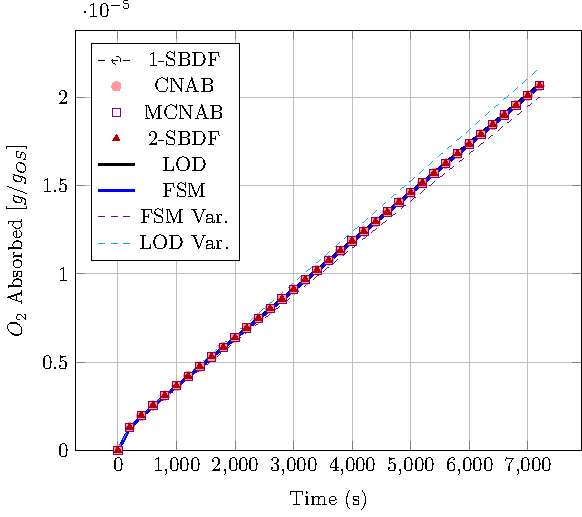
\includegraphics[width=0.48\linewidth,page=1]{Documento_Latex/Tesis_1/Imagenes/rozogafas.pdf}
    }
    \subfloat[]{
    \includegraphics[width=0.48\linewidth,page=2]{Documento_Latex/Tesis_1/Imagenes/rozogafas.pdf}
    }
    \caption{Oxygen absorption profile (a) and  Head-space oxygen concentration (b) obtained by means of the methods IMEX, LOD and FMS with and without variable time step.}
    \label{fig:Comparacion_resultados_metodos}
\end{figure}

The comparison in the results obtained for the profile predictions shows that all constant time step methods give the exact same result, while the methods using a variable time step present a mild deviation from the values obtained by the other methods. To be able to obtain this results with few error using the variable step LOD method a $\eta_{min}=1e-9$ was used. As a consequence of that parameter there was little variation in the time steps taken by this method, which used an average of 1s for its time step, reason why it took a longer computational time to solve the system of equation compared to the FMS with variable step time. The fractional method with variable time step generated the same profiles as the variable step LOD method with less error and in less computational time. This is due to the  decoupling of the reaction and diffusion part of the PDE system to solve. In this way solving the linear diffusive system apart form the non-linear reactive system translates in a higher efficiency when solving the OS film dynamics. For this reason, the FMS with variable step time was the method chosen for the implementation of the computational design tool. Even so, there exist the need to o an study to find the optimal values of the variable time step methodology needed to reduce the error with respect to the constant time step methods, but taking the lowest computational time possible. 

\section{Computational Design Tool Interface}
As explained in the methodology the graphical interface of the computational design tool for OS films was developed  using the library \textit{tkinter} in python. The main window of the develop tool is shown in figure \ref{fig:intefaz_principal}.  

\begin{figure}[ht]
    \centering
    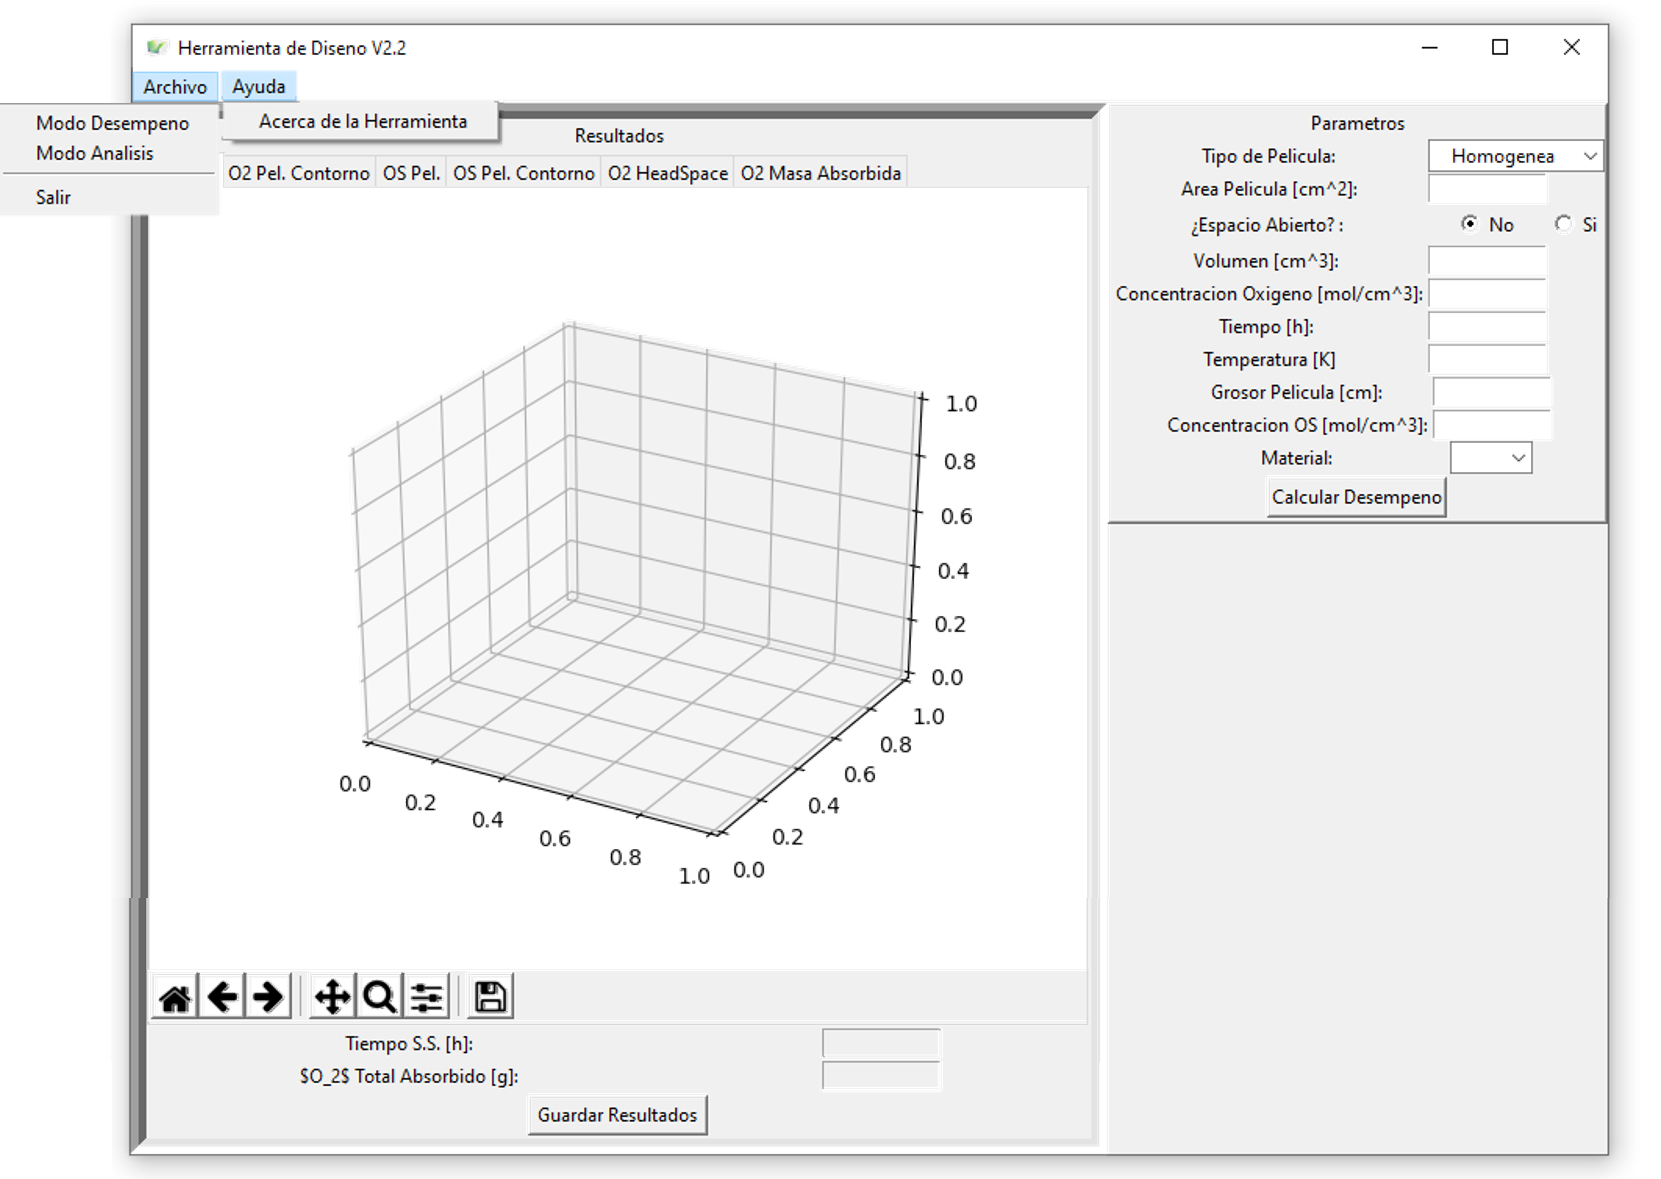
\includegraphics[width=\linewidth]{Documento_Latex/Tesis_1/Imagenes/Interfaz.png}
    \caption{Computational modeling tool main window}
    \label{fig:intefaz_principal}
\end{figure}

This main window is divided in two panels, a parameter panel (right) and a result panel (left). In the superior part, there is the menu bar with two sub menus. The first one of this is the file submenu which contains two the option to select the mode of the tool, the performance and the analysis mode. The performance mode is the one selected by default and corresponds to the mode shown in Figure \ref{fig:intefaz_principal}. This mode enable to model the oxygen uptake performance of a given monolayer (homogeneous) or multilayer film. The second mode, is not yet implemented within the program but it will be in a new version. This mode is thought to enable the user of the tool to study the effect of different parameters over the the performance variables such as headspace oxygen concentration, absorption and time lag. The other sub menu in the superior bar is the help one, which has an unique option, ''About this tool", which opens a sub-window as the one shown in figure \ref{fig:help_window}
 \begin{figure}[H]
     \centering
     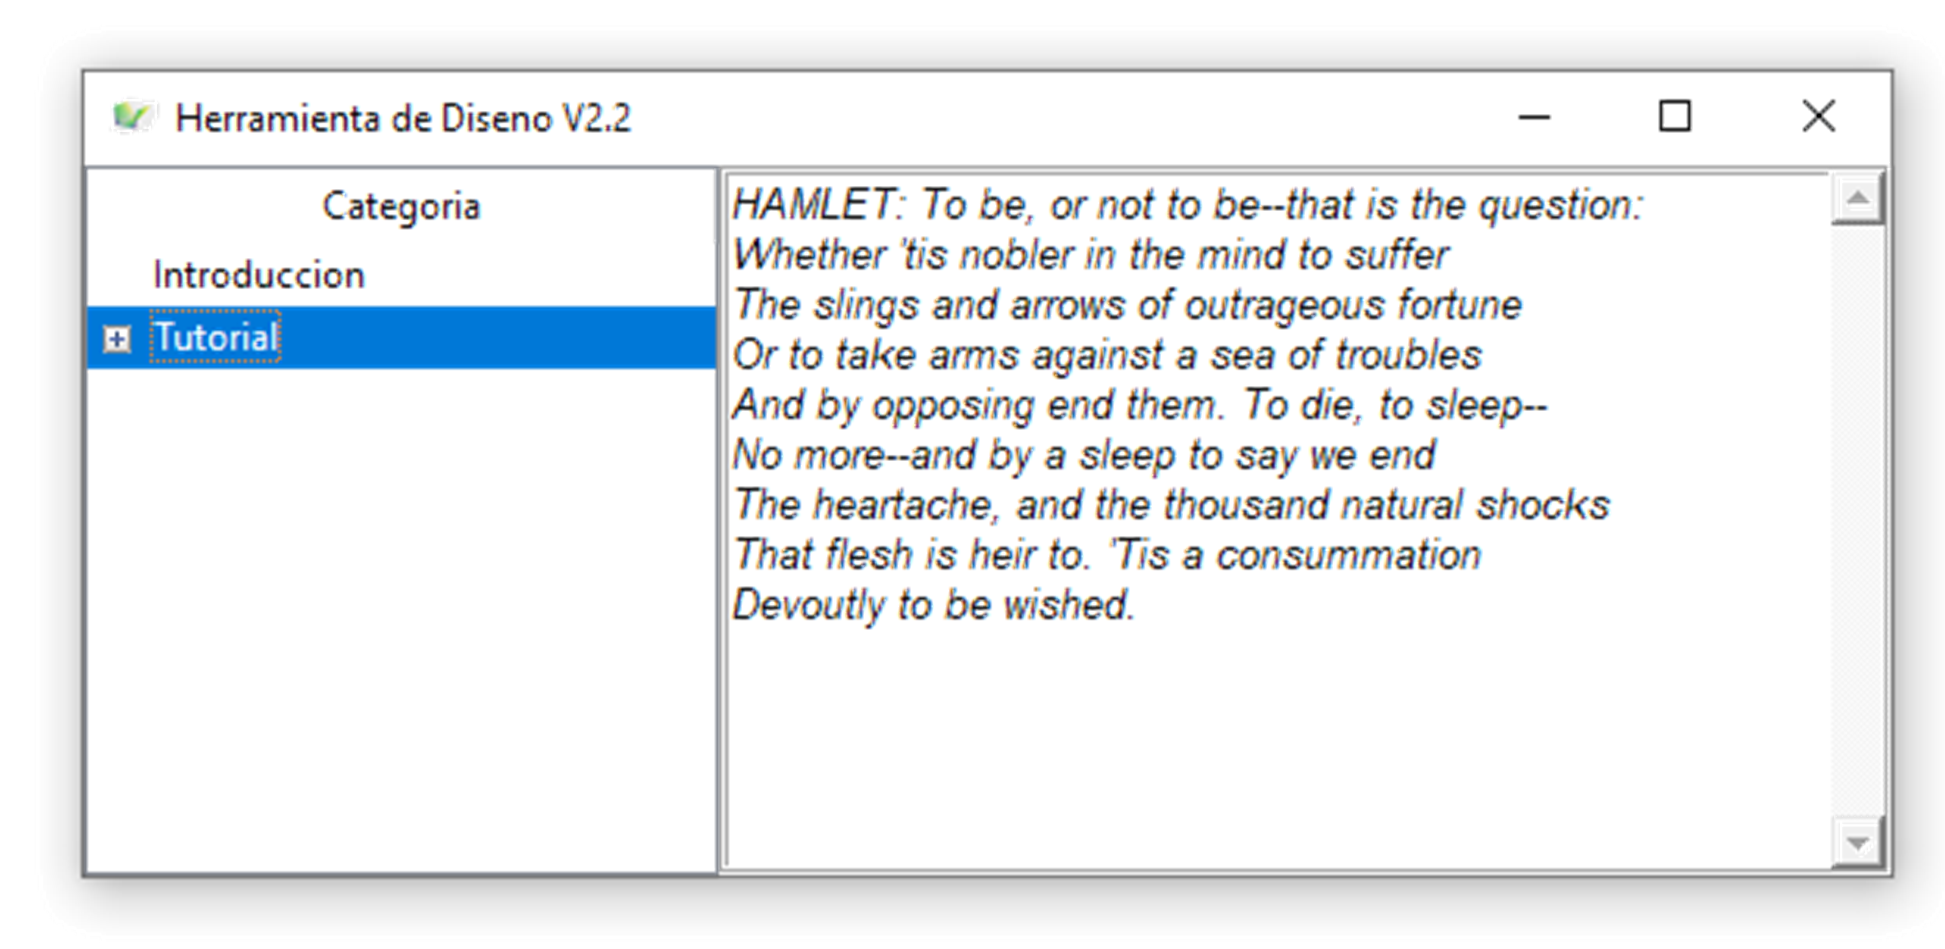
\includegraphics[width=0.8\linewidth]{Documento_Latex/Tesis_1/Imagenes/menu_ayuda.png}
     \caption{''About this tool" sub-window}
     \label{fig:help_window}
 \end{figure}
Even though this information panel is not finished, the idea of this is to present the instructions on how to correctly use the tool,  and additional information such as the different material properties used by the program as well as an explanation on the assumptions made to carry out the programming of the tool. With respect to the instructions on how to use the computational tool made so far, the first thing is to know whether a simulation of a multilayer or a monolayer film is desired. In this order of ideas, if the user wants to simulate a homogeneous film he must select the option homogeneous in the ''type of film:" box. This is the type of film which is  going to be modeled by default. Next the user must insert the film area in $cm^2$ and must select if the film which is going to be simulated is or not in an open space. As the default option the program assumes that the film is going to be within a finite volume of gas and so the volume text box is enable to edition, on the contrary if the user selects the option indicating that the film is in an open space, the volume text box will be disabled. Then, the concentration of oxygen in the surrounding air must be entered in the ''Oxygen Concentration (mol/cm3)" box. In case the film is in an open space the program will assume this concentration as constant, if is not the case then the oxygen concentration will vary according to equation  \ref{eq:headspace}. Then, the user must enter the time interval and the temperature at which the simulation will be done. It should be clarified again that the temperature will be constant through out the whole process given that the simulation model is isothermal. Finally the user must enter the thickness and OS volumetric load, and must select the polymeric material which the film is made of. Once done this, the simulation is ready to start, to do this the button ''Calculate performance" which is in the parameters panel, must be selected. This will open a sub-window containing a progress bar which indicates that the simulation is in progress. When the progress bar is full, the simulation will be finished, and the results obtained are shown in the left panel. This panel contains 6 plots, the first two correspond to the 3D and contour plot of the evolution of oxygen concentration in the film, the next two correspond to the contour 3D and contour plot of the peroxide radical concentration and the final two plots correspond to the head space oxygen concentration profile and total $O_2$ mass absorption profile. An example of how this plots are displayed is shown in figure \ref{fig:resultados herramienta}. 

  \begin{figure}[ht]
            \centering
            \subfloat[]{
            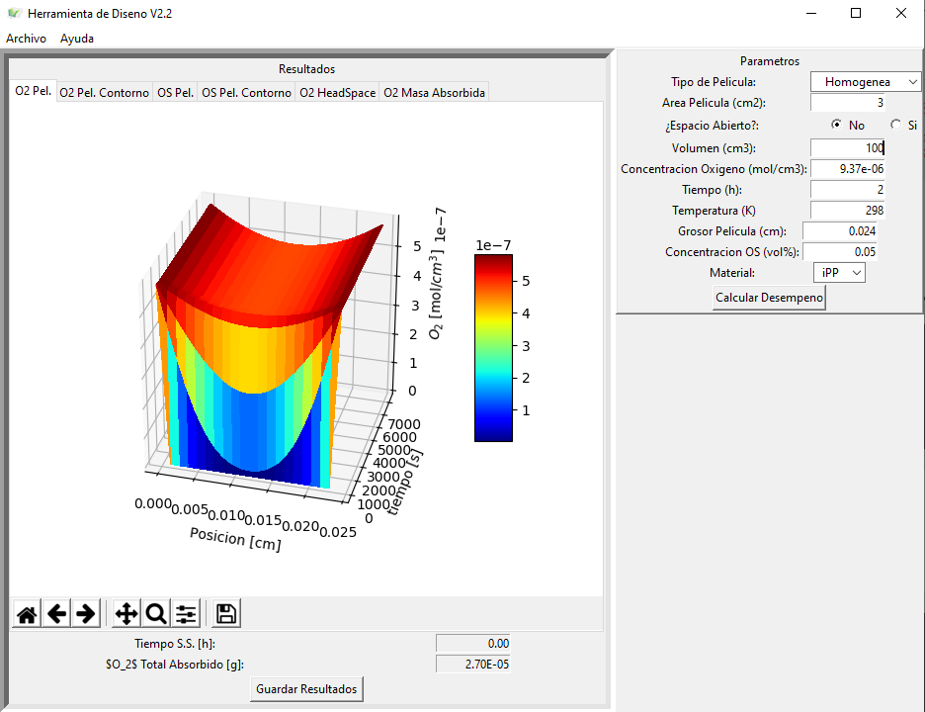
\includegraphics[width=0.3\textwidth]{Documento_Latex/Tesis_1/Imagenes/3d_O2_profile.png}}
            \subfloat[]{
            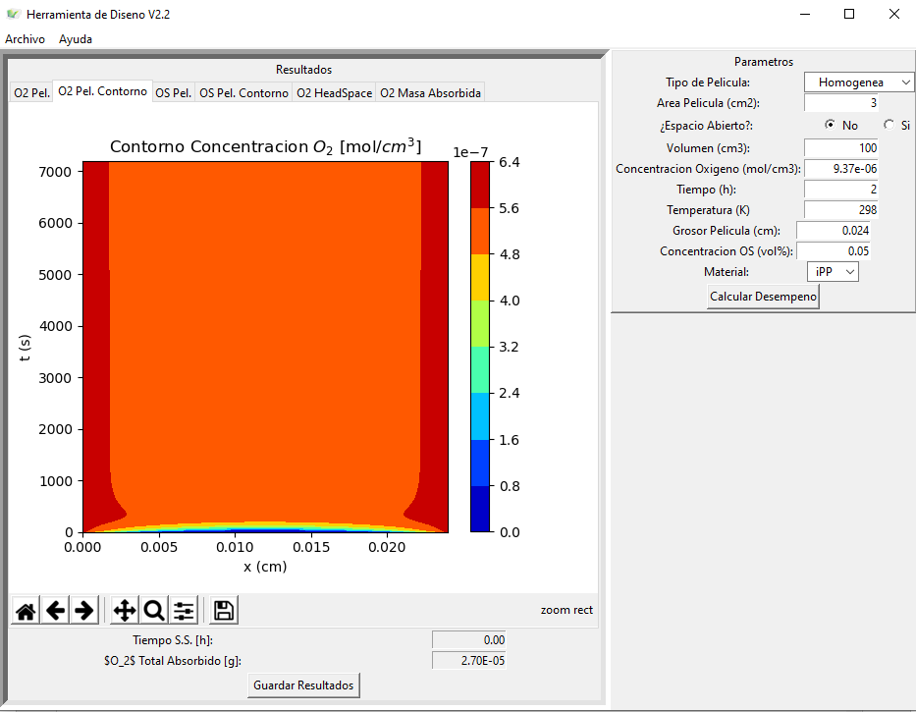
\includegraphics[width=0.3\textwidth]{Documento_Latex/Tesis_1/Imagenes/contour_O2_profile.png}}
            \subfloat[]{            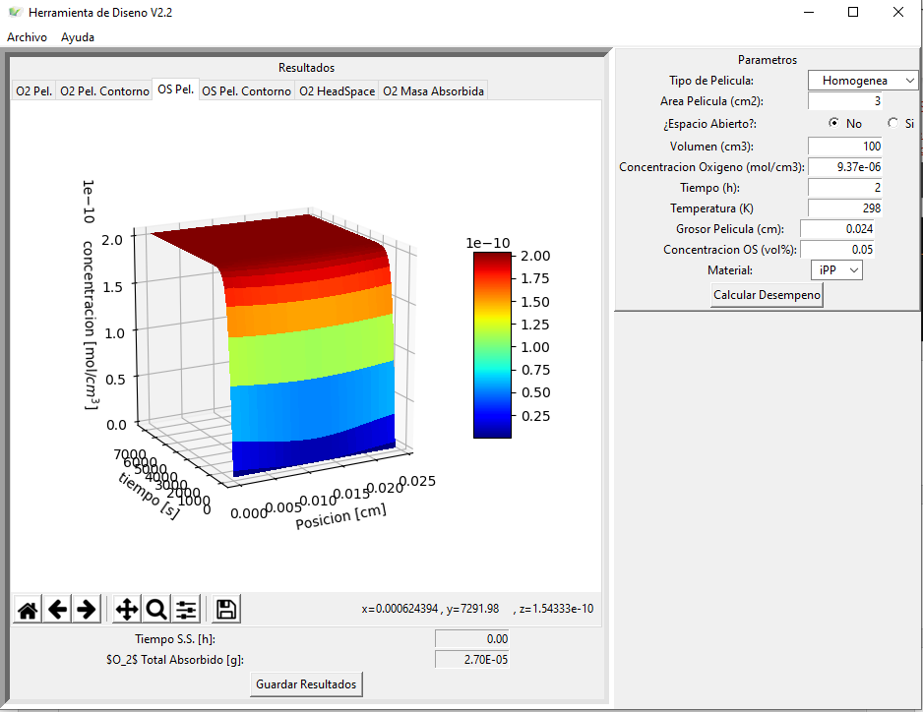
\includegraphics[width=0.3\textwidth]{Documento_Latex/Tesis_1/Imagenes/3d_OS_profile.png}}
    
             \subfloat[]{
             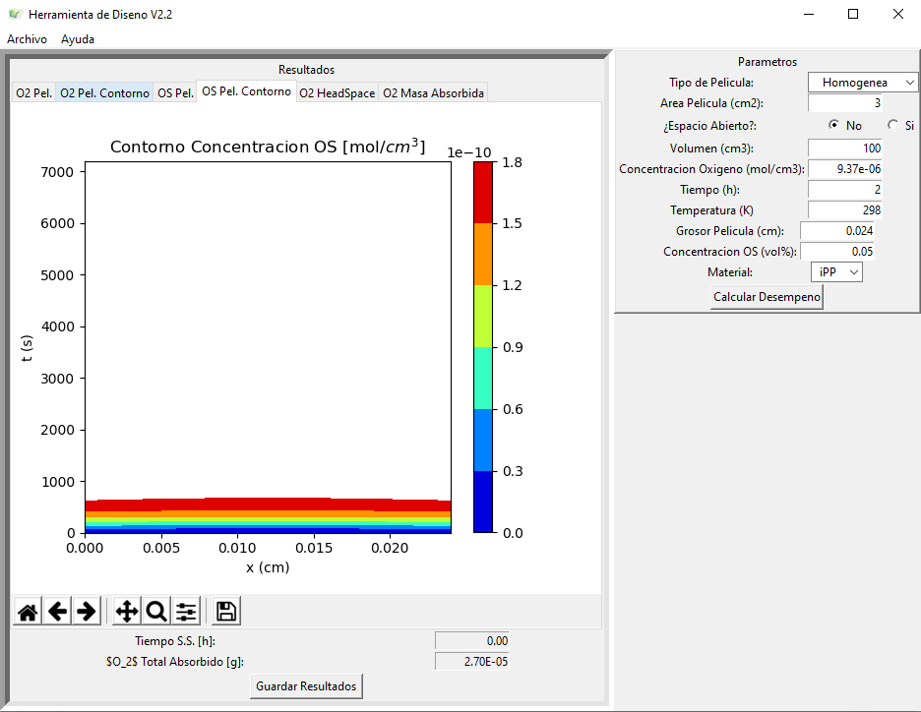
\includegraphics[width=0.3\textwidth]{Documento_Latex/Tesis_1/Imagenes/contour_OS_profile.png}}
            \subfloat[]{
             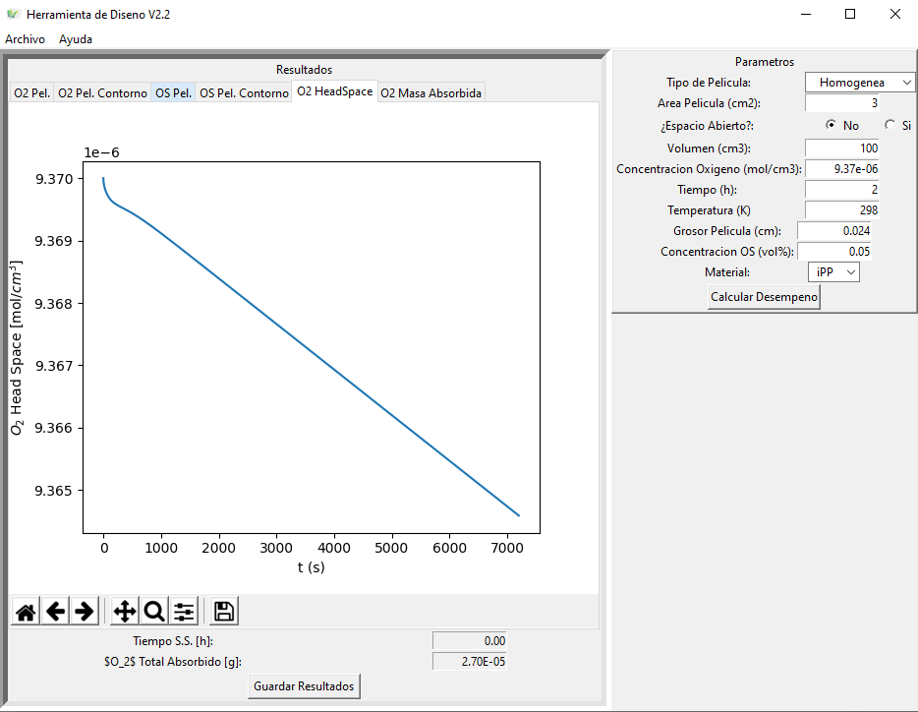
\includegraphics[width=0.3\textwidth]{Documento_Latex/Tesis_1/Imagenes/o2_headspace.png}}
            \subfloat[]{
             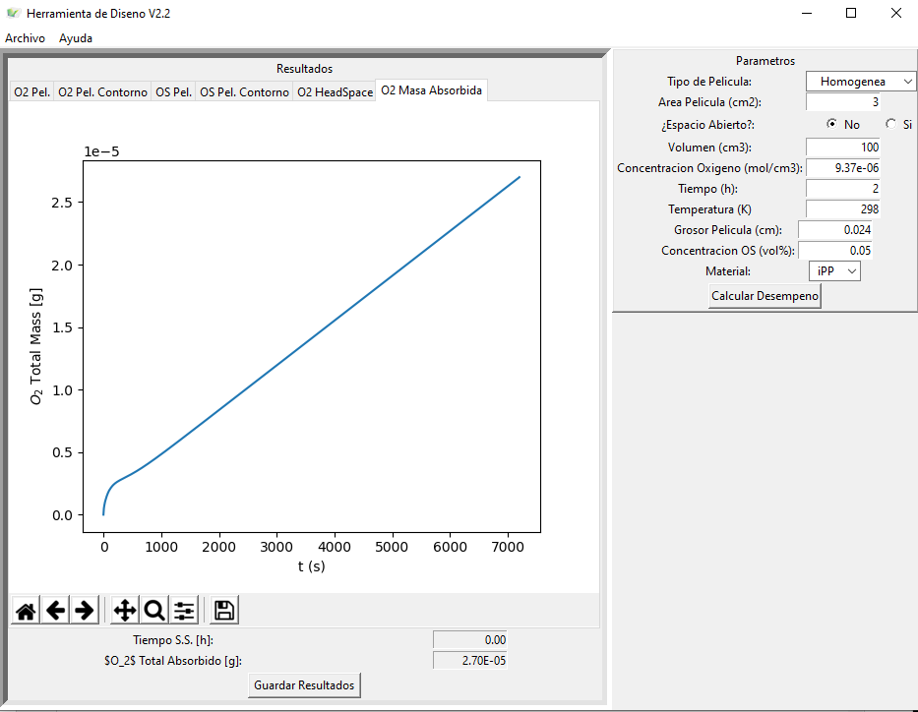
\includegraphics[width=0.3\textwidth]{Documento_Latex/Tesis_1/Imagenes/o2_masa_absorbida.png}}
            \caption{Results displayed by the computational tool, where \textbf{(a)} is the 3d and  \textbf{(b)} contour $O_2$ concentration profile, \textbf{(c)} and \textbf{(d)} are the 3d and contour \ce{POO^.} concentration profile, and  \textbf{(e)} and \textbf{(f)} are the headspace and oxygen absorption profiles.}
            \label{fig:resultados herramienta}
    \end{figure}
On the other hand, if the user wants to make a multilayer film simulation he must select the option multilayer in the ''Type of film" box. When this option is selected, the parameter panel changes, being the main difference that it ask the user how many layers do the film has. Once this number is selected new parameters appear asking to select which of the films are going to be reactive, the thickness of each layer and its corresponding material. Finally when the user select which of the layers is reactive the program ask for the volumetric concentration of OS in each reactive layer (See Figure \ref{fig:multilayer_panel}). With this information, the program is ready to start the simulation by pressing the ''Calculate performance" button. The tool has an additional feature than enables to save the results data in a Excel file by pressing in the button ''Save Results". 

\begin{figure}[H]
    \centering
    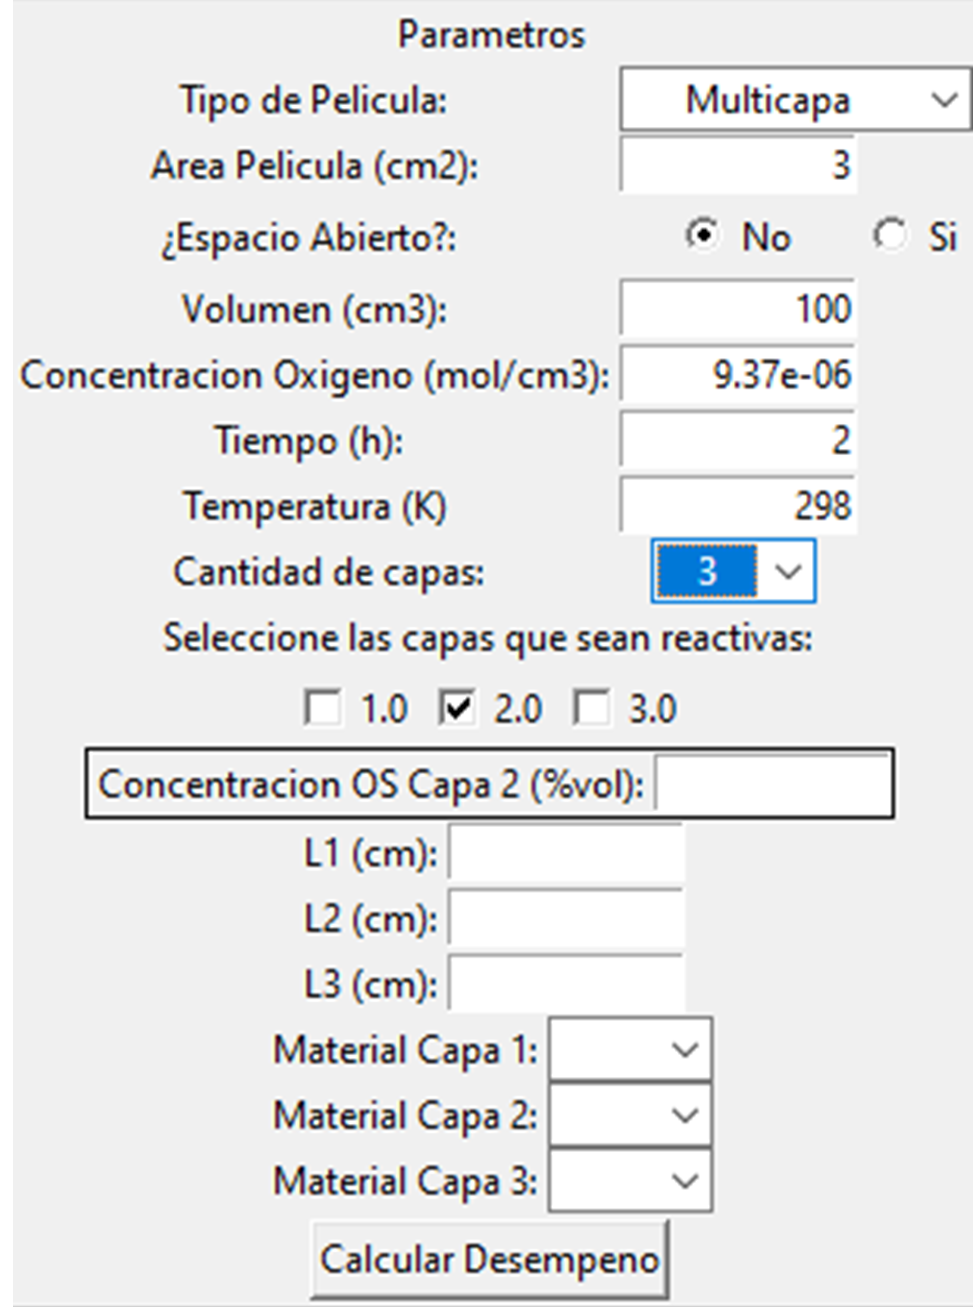
\includegraphics[scale=0.6]{Documento_Latex/Tesis_1/Imagenes/multilayer_panel.png}
    \caption{Multilayer parameter panel for the case of a 3-layer film}
    \label{fig:multilayer_panel}
\end{figure}

\printbibliography
\end{refsection}
\chapter{Conclusions and Future work}
 \section{Conclusions}
The main purpose of an active package is to protect as long as possible the quality an integrity of a product by chemically and physically interacting with it and its surrounding until it reaches the final consumer. This technology been playing a fundamental role in the extension of the shell life of product in the last years. This is the reason why it is a field with a constant investigation growth. Despite the fact that there are different types of active packaging, the packaging time mostly used the type of packaging mostly used commercially are the oxygen scavengers. 

There exist several types of oxygen scavengers which can be used for  diverse kind of food depending on its specific characteristics. In the last few years the Material and Manufacturing investigation group  (CIPP-CIPEM) of \textit{Universidad de los Andes} has been developing a new kind of OS polypropylene film whose active component is linseed oil. This type of OS technology presents a promising in the oxygen scavenging market given its organic nature and the great oxygen uptake capacity of linseed oil. To study the performance of this new OS film,  experimental techniques have been used, but this tend to take several days and are of destructive. As an alternative to the experimental approach, the use of mathematical models and computational tools have been proposed.
 
A a first conclusion of this work is that a first version of a computational design tool for the OS film has been developed. This first version enables a user to study the performance of this new AP technology either present in a multilayer film or a solely film. The user is able to change several parameters of the system studied such as OS load, temperature, material of and dimension of the film among others. The results obtained are displayed in dynamic plots which enable a better visibility of the result profiles, and can be also saved in Excel files for a deeper analysis.

To develop this tool, knowledge about the oxidation kinetics of linseed oil is needed. As a second conclusion, the adjustment of the kinetic model was made by means of the Gauss-Newton technique and this was implemented into the reactive film model. New values of initial concentrations of hydroperoxyde and substrate were obtained, and using the kinetics velocities determined in literature. The new values allow to determine the order of magnitude of the concentration absorption but fail in predicting correctly the times in which reaction such as hydroxide decomposition occurs. 

Finally, in the seek  of implementing a tool which is computationally fast an accurate several numerical techniques were studied. The results showed that the system of PDEs which describes the dynamics of oxidation of the film are stiff, which means that implicit methods are needed to solve them efficiently. As a third conclusion, the fractional step method (FSM) modified with a variable time step was one that presented better results regarding efficiency and accuracy when solving the films dynamics which is why it was selected for the implementation of the computational design tool.
 
\section{Future Work}
There is much more work to be done in the path of developing a complete  computational design tool for the OS film developed by CIPP-CIPEM group. In first place the development of the \textbf{Analysis mode} of the tool must be developed. This mode will enable the user to study directly in the program the effect of varying design parameters over the oxygen scavenging performance of the film. The instruction or ''About this tool" sub-window must also be finished. Given the difficulty on developing an enriched text in Tkinter there exist the possibility of developing the instructions window in another  programming language and couple it latter to the actual interface.  

With respect to the kinetic model adjustment, a deeper study must be made using experimental data obtained in the oxidative TGA technique. this data will enable to make more trustable adjustment and in turn correct the problem of inaccuracy in time prediction. 

Likewise, the implementation of the heterogeneous film model is to be done. This model although it is more complex, describes more accurately the physics of the OS film. This is because the film is not reactive itself but contains spherical actives sites which are reactive. In that sense it is expected that the heterogeneous film model has better results predicting the OS film performance. Finally another addition to the model must be made, regarding oxidation competition between the AP and the edible inside it. Once implemented, the design tool is going to be able to indicate how much longer is a food  shelf life given the OS film in its package. 







\end{document}
